\documentclass[12pt,a4paper, finnish]{report}
\usepackage[finnish]{babel}
\usepackage[utf8x]{inputenc}
\usepackage[T1]{fontenc}
\usepackage{amsmath,amssymb}
\usepackage{theorem}
\usepackage{graphicx}
\usepackage{apropos}
\usepackage{epsfig}
\usepackage{multicol}
\usepackage{amscd}
\usepackage{curves}
\usepackage{epic}
\usepackage{eepic}
\usepackage{float}
\usepackage{import}
\usepackage{rotating}
%\usepackage{makeidx}

\author{Juhani Pitkäranta}
\title{Matematiikan peruskurssi L1}
\date{Elokuu 2005}

\setlength{\parindent}{0mm}
\setlength{\parskip}{\medskipamount}
\setlength{\textwidth}{35em}

\usepackage{jpheader}

\renewcommand{\thechapter}{\Roman{chapter}}
\renewcommand{\thefootnote}{\fnsymbol{footnote}}
\renewcommand{\theequation}{\arabic{equation}}

\theoremheaderfont{\rmfamily\scshape}

%\numberwithin{Thm}{section}
%\numberwithin{Prop}{section}
%\numberwithin{Lem}{section}

%\includeonly{I-0,I-1,I-2,I-3,I-4,I-5,I-6,I-7,I-8,I-9,I-10,I-11,I-12}
%\includeonly{II-0,II-1,II-2,II-3,II-3,II-4,II-5}
\includeonly{II-6}%,II-7,II-8}
%\includeonly{III-0,III-1,III-2,III-3,III-4}
%\includeonly{IV-0,IV-1,IV-2,IV-3,IV-4,IV-5}
%\includeonly{V-0,V-1,V-2,V-3,V-4,V-5,V-6,V-7,V-8,V-9}
%\includeonly{exp-0,exp-1,exp-2,exp-3,exp-4}
%\includeonly{dif-0,dif-1,dif-2,dif-3,dif-4,dif-5,dif-6}
%\includeonly{int-0,int-1,int-2,int-3,int-4,int-5,int-6,int-7,int-8,int-9}
%\includeonly{dy-0,dy-1,dy-2,dy-3,dy-4,dy-5,dy-6,dy-7,dy-8}
%\includeonly{m-0,m-1,m-2,m-3,m-4,m-5,m-6,m-7,m-8}
%\includeonly{udif-0,udif-1,udif-2,udif-3,udif-4,udif-5,udif-6,udif-7,udif-8,udif-9}
%\includeonly{eig-0,eig-1,eig-2,eig-3,eig-4}
%\includeonly{uint-0,uint-1,uint-2,uint-3,uint-4,uint-5,uint-6,uint-7}
%\includeonly{Gauss-0,Gauss-1,Gauss-2,Gauss-3,Gauss-4,Gauss-5}

%\makeindex

\begin{document}
%\maketitle

%\newcommand{\alku}{\setcounter{Exa}{0} \setcounter{equation}{0} \markright{\thesection}}
\newcommand{\alku}{\setcounter{Exa}{0} \setcounter{equation}{0}}
\newcommand{\jatko}{\addtocounter{Exa}{-1}}
\newcommand{\seur}{\addtocounter{Exa}{1}}

%\pagestyle{myheadings}

\chapter{Luvut ja lukujonot}

''Jumala loi luonnolliset luvut --- kaikki muu on ihmisty�t�'' oli saksalaisen matemaatikon 
\index{Kronecker L.}%
\hist{Leopold Kronecker}in (1823-1891) aforismi ja kannanotto koskien matematiikan alkuper��.
--- Ep�ilem�tt� lukum��r�� tai j�rjestyst� kuvaavien sanojen 'yksi', 'kaksi', jne eriytyminen
luonnollisessa kieless� on ollut er�s l�ht�kohta ja perusedellytys matematiikan syntymiselle.
Merkkej� lukujen ja suhteiden tajusta on s�ilynyt jopa 30 000 vuoden takaa, joten matematiikan
voi perustellusti katsoa olevan ihmisen kulttuurissa \kor{sui generis}, omaa lajiaan.
Kulttuuri-ilmi�n� matematiikkaa voi jossain m��rin ymm�rt�� rinnastamalla se muihin
kulttuurin lajeihin. Esimerkiksi jos tarkastellaan matematiikan historiaa ja kumulatiivista
rakennetta, tai k�ytt�tapoja, voi n�hd� monia yhtym�kohtia muihinkin mahtaviin ihmishengen
ilmentymiin, erityisesti luonnollisiin kieliin ja tekniikkaan.

Matematiikkaa voi kuitenkin syvemmin oppia ymm�rt�m��n vain matematiikkaa opiskelemalla.
Opiskelu aloitetaan t�ss� luvussa 'alusta', eli (matemaattisen) \kor{luvun} k�sitteest�. Luvun
punaisena lankana on \kor{reaalilukujen} konstruoiminen l�htien 'j�rjellisist�' eli
\kor{rationaalisista} luvuista. Matematiikan historiassa reaaliluvun k�site on t�smentynyt
lopullisesti vasta 1800-luvulla. Historiallisena ongelmana --- ja edelleen ongelmana
opetuksessa --- on k�sitteeseen v�ist�m�tt� (muodossa tai toisessa) sis�ltyv� 'loputtomuuden'
ajatus. T�ss� tekstiss� reaalilukuja l�hestyt��n rationaalilukujen muodostamien
\kor{lukujonojen}, ja n�iden erikoistapausten, \kor{��rett�mien desimaalilukujen} kautta.
Reaaliluvun k�site tulee t�ll� tavoin liitetyksi 'oikeaan laskemiseen' ja my�s tavanomaisiin
numeromerkint�ihin. P��ttym�tt�m�t lukujonot tulevat jatkossa k�ytt��n monessa muussakin
yhteydess�. Niihin perustuvat viime k�dess� sek� monet laskentamenetelm�t (algoritmit) ett�
reaalilukuihin perustuvan matemaattisen analyysin eli \kor{reaalianalyysin} k�sitteet.  % Luvut ja lukujonot

\section{Katsaus rationaalilukuihin}  \label{ratluvut}
\index{rationaaliluvut|vahv}
\alku
\sectionmark{Rationaaliluvut}

\index{luonnolliset luvut}%
\kor{Luonnollisten lukujen} joukkoa merkitsemme
\[
\N = \{1,2,3,4,\ldots\}.
\]
Yleisemmin 
\index{joukko} \index{alkio (joukon)}%
\kor{joukko} (engl. set) koostuu \kor{alkioista} (engl. element), joita joukon \N\ 
tapauksessa ovat luvut $1$, $2$, $3$ jne. Merkinnät
\[
8 \in \N, \quad \infty \not\in \N
\]
luetaan 'kahdeksan kuuluu \N:ään, 'ääretön ei kuulu \N:ään', tarkoittaen yksinkertaisesti, että
\N:ssä on alkio nimeltä 'kahdeksan' mutta ei alkiota nimeltä 'ääretön'.

Joukko $A = \{1,2,3\}$ on \N\ :n 
\index{osajoukko}%
\kor{osajoukko} (engl. subset). Merkitään
\[
A \subset \N \quad \text{tai} \quad \N \supset A
\]
ja luetaan '$A$ kuuluu/sisältyy \N\ :ään' tai '\N\ sisältää $A$:n'. Yleisesti merkintä 
$A \subset B$ tarkoittaa, että jokainen $A$:n alkio on myös $B$:n alkio, toisin sanoen pätee
\[
x \in A \qimpl x \in B.
\]
Tässä '$\impl$' on logiikan symboleihin kuuluva nk. 
\index{implikaatio}
\kor{implikaationuoli}: Merkintä $P \impl Q$
luetaan '$P$:stä seuraa $Q$', tai 'jos $P$, niin $Q$'. Symboli '$\subset$' (kuuluminen 
osajoukkona) määritellään siis symbolin '$\in$' (kuuluminen alkiona) avulla. Jälkimmäinen 
symboli on nk.\ 
\index{primitiivi}
\kor{primitiivi}, jota ei voi enää määritellä muiden symbolien avulla. Joukoista 
puhuttaessa voi siis merkintöjä $x \in A$ tai $x \not\in A$ pitää kaiken loogisen ajattelun 
lähtökohtana. 
\begin{Exa} Jos $A = \{2,1,1,2,1\}$ ja $B = \{1,2\}$, niin $A \subset B$, sillä jos $x \in A$,
niin on joko $x=1$, jolloin $x \in B$, tai $x=2$, jolloin myöskin $x \in B$. Samalla päättelyllä
nähdään, että pätee myös $B \subset A$. \loppu \end{Exa} 
Jos joukoille $A$ ja $B$ pätee sekä $A \subset B$ että $B \subset A$, kuten esimerkissä, niin 
sanotaan, että $A$ ja $B$ ovat (joukkoina)
\index{samastus '$=$'!a@joukkojen}%
\kor{samat}, ja merkitään $A=B$.\footnote[2]{Jos 
$A \subset B$, ja $A$ ei ole sama kuin $B$, sanotaan että $A$ on $B$:n \kor{aito} 
(engl.\ proper) osajoukko. Joissakin matemaattisissa teksteissä symbolilla '$\subset$' on tämä
rajatumpi merkitys, jolloin mahdollisuus $A=B$ varataan merkinnällä $A \subseteq B$. Tässä 
tekstissä siis pätee $A \subset A$. \index{aito osajoukko|av}} 
Logiikan ja joukko-opin merkintöjä käsitellään hieman laajemmin Luvussa \ref{logiikka}. 
Todettakoon tässä yhteydessä vielä osajoukon määrittelyssä tavallinen merkintä
\[ 
B\ =\ \{\,x \in A \mid E\,\}, 
\]
missä $E$ on jokin \kor{ehto}, joka jokaisen alkion $x \in A$ kohdalla joko toteutuu, jolloin 
$x \in B$, tai ei toteudu, jolloin $x \not\in B$.
\begin{Exa} \kor{Parilliset} ja \kor{parittomat} luonnolliset luvut määritellään $\N$:n osa-
joukkoina \index{parillinen, pariton!a@luku}%
\begin{align*}
A &= \{\,x \in \N \mid x=2\cdot y\,\ \text{jollakin}\ y\in\N\,\}\ =\ \{\,2,4,6,\ \ldots\,\}, \\
B &= \{\,x\in\N \mid x\not\in A\,\}\ =\ \{\,1,3,5,\ \ldots\,\} \loppu
\end{align*} 
\end{Exa}
Esimerkissä on jo viitattu luonnollisten lukujen joukossa (tunnetulla tavalla) määriteltyihin 
\index{laskuoperaatiot!a@rationaalilukujen|(}%
\kor{laskuoperaatioihin}, joita on kaksi:
\begin{align*}
\text{yhteenlasku:} \quad &x \in \N\ \ja\ y \in \N \quad \map \quad 
                             x + y \in \N \quad \quad \text{'$x$ plus $y$'} \\
\text{kertolasku:}  \quad &x \in \N\ \ja\ y \in \N \quad \map \quad 
                             x \cdot y\ \,\in \N \quad \quad \text{'$x$ kertaa $y$'}
\end{align*}
Tässä '$\&$' on logiikan merkintä, luetaan 'ja' (formaalimpi merkintä '$\wedge$'), ja 
'$\map$' tarkoittaa \kor{liittämistä}: Lukuihin $x$ ja $y$, eli \N:n \kor{lukupariin}, liitetään
(yksikäsitteinen) luku $x + y \in \N$, nimeltään $x$:n ja $y$:n \kor{summa}, ja 
$x \cdot y \in \N$, nimeltään $x$:n ja $y$:n \kor{tulo}. Laskuoperaatio tarkoittaa siis 
yksittäisten lukujen $x,y$ tapauksessa 'liittämissääntöä', yleisemmin 'liittämissäännöstöä'. 
Säännöt voidaan ajatella joko joistakin yleisemmistä periaatteista (laskusäännöistä) 
johdetuiksi, tai ne voidaan ymmärtää pelkästään 'luettelona', joka kattaa kaikki lukuparit. Kun
yhteen- ja kertolaskun sisältö on yhteisesti sovittu (ja peruskoulun oppikirjoihin painettu), on
luonnollisten lukujen perustalle rakennettu
\index{algebra}%
\kor{algebra}\footnote[2]{Algebra eli 
'kirjainlaskenta' on numeroilla laskemisen eli \kor{aritmetiikan} abstraktimpi muoto. Algebran
kehitys alkoi arabikulttuurin piirissä 1.\ vuosituhannella jKr.}, jota merkittäköön
$(\N,+,\cdot)$.

Seuraavat hyvin tunnetut peruslait ovat voimassa luonnollisten lukujen laskuoperaatioille:
\begin{itemize}
\item[(L1)] $\quad x+y = y+x$
\item[(L2)] $\quad x \cdot y = y \cdot x$
\item[(L3)] $\quad x+(y+z) = (x+y)+z$
\item[(L4)] $\quad x \cdot (y \cdot z) = (x \cdot y) \cdot z$
\item[(L5)] $\quad x \cdot (y+z) = x \cdot y + x \cdot z$
\item[(L6)] $\quad x \cdot 1 = x \ \ \forall x \in \N$
\end{itemize}
\index{vaihdantalaki} \index{liitzy@liitäntälaki} \index{osittelulaki}%
Tässä (L1),\,(L2) ovat \kor{vaihdantalait}, (L3),\,(L4) ovat \kor{liitäntälait} ja (L5) on 
\kor{osittelulaki}. Viimeksi mainitulla on myös rinnakkainen muoto
\begin{itemize}
\item[(L5')] $\quad\!\! (x+y) \cdot z = x \cdot z + y \cdot z$,
\end{itemize}
joka seuraa yhdistämällä (L2) ja (L5). Laissa (L6) '$\,\forall$' on logiikan symboli, joka 
luetaan 'kaikille'. Tämä laki ilmaisee, että luku  $1$ on kertolaskun nk. \kor{ykkösalkio}. 
Kuten nähdään jäljempänä, laskulait (L1)--(L6) ovat yhteisiä monille algebroille. Yleisemmissä
tarkasteluissa nämä lait otetaankin usein oletetuiksi peruslaeiksi eli
\index{aksiooma}%
\kor{aksioomiksi}.\index{Peano, G.|av} \index{Peanon aksioomat|av}%
\footnote[2]{Luonnollisten lukujen tapauksessa laskulait (L1)--(L6) ovat
johdettavissa luonnollisten lukujen perustana olevista \vahv{Peanon aksioomista}. Aksioomat
esitti italialainen matemaatikko \hist{Giuseppe Peano} (1858--1932) vuonna 1889. Peanon
aksioomat luonnollisille luvuille ovat: (P1) $1\in\N$. \,(P2) Jokaisella $x\in\N$ on
yksikäsitteinen \kor{seuraaja} $x'\in\N$. \,(P3) Luku $1$ ei ole minkään $x\in\N$ seuraaja. \,
(P4) Jokainen $x\in\N$ on korkeintaan yhden luvun seuraaja, ts.\ jos $x,y\in\N$ ja $x'=y'$, niin
$x=y$. \,(P5) Jos $S\subset\N$ ja pätee (i) $1\in S$ ja (ii) $x' \in S$ aina kun $x \in S$,
niin $S=\N$. Aksioomassa (P2) esiintyvä luvun seuraaja on tavanomaisen kielenkäytön mukaan
'seuraava luku'. Aksiooman (P3) mukaan luku $1$ on luonnollisista luvuista 'ensimmäinen', sen
sijaan 'viimeistä' lukua ei ole, koska jokaisella luvulla on seuraaja (aksiooma (P2)) eikä 
mikään luku voi esiintyä seuraajaketjussa kahdesti (aksioomat (P3) ja (P4)). Luonnollisia lukuja
on siis äärettömän monta. Aksiooma (P5) asettaa nk.\ \kor{induktioperiaatteen}, ks.\ Luku
\ref{jono} jäljempänä. 

Luonnollisten lukujen yhteenlasku ja kertolasku määritellään aksioomiin (P1)--(P5) perustuen
asettamalla kummallekin laskuoperaatiolle kaksi aksioomaa. Näiden perusteella minkä tahansa
halutun laskuoperaation tulos on määrättävissä lukujen $\,1$, $1' = 2$, $2' = 3$, jne avulla.
Yhteenlaskun aksioomat: \,(Y1) $\,x+1=x'$, \,(Y2) $\,x+y'=(x+y)'$. Kertolaskun aksioomat: \,
(K1) = (L6), \,(K2) $\,x \cdot y' = x \cdot y + x$.}

Laskulaeissa (L1)--(L6) on oletettu normaalit järjestyssäännöt laskuoperaatioiden yhdistelylle,
eli ensin lasketaan sulkeiden sisällä olevat lausekkeet, ja kertolaskut aina ennen yhteenlaskuja
mikäli sulkeita ei ole. Huomattakoon, että tässä ei ole kyse mistään ylimääräisistä 
olettamuksista, vaan esimerkiksi sääntö
\[
x + y \cdot z\ =\ x + (y \cdot z)
\]
on \pain{sulkeiden} p\pain{ois}j\pain{ättösääntö}, eli kyse on merkintäsopimuksesta. Samaa
operaatiota yhdisteltäessä on  liitäntälakien (L3),\,(L4) perusteella tulos aina sama
operaatioiden järjestyksestä riippumatta, joten sulkeet voidaan jättää pois (merkintäsopimus!)
ja kirjoittaa
\[
x + y + x + \ldots, \quad x \cdot y \cdot z \cdot \ldots
\]
Tavanomaisen lukujen algebran merkintäsopimuksiin kuuluu myös vapaus jättää kertomerkki
merkitsemättä sikäli kuin sekaannuksen vaaraa ei ole:
\[
x \cdot y = xy, \quad x \cdot 2 = 2x, \quad  2\cdot(1+2) = 2(1+2) = 2 \cdot 3 \neq 23.
\]
Peräkkäisiä tuloja laskettaessa on saman luvun $n$-kertaisesta ($n \in \N$) kertolaskusta tapana
käyttää nimitystä \kor{potenssiin korotus} ja käyttää merkintää
\[
\underset{(n\ \text{kpl})}{x \cdot x \cdots x} \quad = \quad x^n \quad 
                              \quad \text{'$x$ potenssiin $n$'} \quad (n \in \N).
\]
   
\subsection*{Kokonaisluvut $\Z$}
\index{kokonaisluvut|vahv}%

\kor{Kokonaislukujen} joukko \Z\ on ensimmäinen askel siinä 'ihmistyössä', jossa 
lukujärjestelmää pyritään laajentamaan lähtökohtana luonnolliset luvut. Laajennus koostuu 
kahdesta osa-askeleesta, joista ensimmäinen on luvun \kor{nolla} ('ei mitään') ja toinen 
\kor{vastaluvun} ('montako puuttuu') käyttöönotto. Näiden ajatusten tuloksena syntyvää 
lukujoukkoa merkitään
\[
\Z = \{\ \ldots,-2,-1,0,1,2,\ \ldots\ \} \quad = \quad \{\ 0,\pm 1, \pm 2,\ \ldots\ \}.
\]
Lukualueen laajennus tehdään aksiomaattisesti olettamalla seuraavat lisäaksioomat, jotka siis
ovat voimassa \Z:ssa mutteivät \N:ssä.
\begin{itemize}
\item[(L7)] $\quad \text{On olemassa \kor{luku}}\ 0,\ 
                   \text{jolle pätee}\ \ x+0 = x\ \ \forall\ x \in \Z.$
\item[(L8)] $\quad \text{Jokaisella}\ x \in \Z\ \text{on \kor{vastaluku}}\ -x,\ 
                   \text{jolle pätee}\ \ x+(-x) = 0.$
\end{itemize}
Lyhennysmerkintä
\[
x + (-y) = x - y \quad \quad \text{'$x$ miinus $y$'}
\]
tuo \Z:aan uuden laskuoperaation, \kor{vähennyslaskun}, jonka tulos on nimeltään lukujen $x$ ja
$y$ \kor{erotus}.  Tässä on siis kyse yhteenlaskun ja 'merkinvaihdon' $x \map -x$ (jonka voi 
myös tulkita laskuoperaatioksi) yhdistämisestä.

Kokonaisluvuilla laskettaessa pidetään selviönä, että luku $0$ samoin kuin vastaluvut
$-1,\ -2, \ldots\,$ ovat yksikäsitteisiä. Tuttuja ovat myös laskusäännöt
$\,-(-x)=x$, $\,0 \cdot x=0\,$ ja $\,(-1) \cdot x = -x$. Näitä oletuksia\,/\,laskusääntöjä ei
tarvitse kuitenkaan sisällyttää kokonaislukujen aksioomiin, sillä ne ovat aksioomien seurauksia:
\begin{Lause}\footnote[2]{Kun matemaattisessa tekstissä halutaan nostaa esiin jokin selkeästi 
muotoiltu, tosi väittämä, esim. siksi että väittämään halutaan myöhemmin viitata tai kun 
halutaan korostaa tuloksen uutuusarvoa, käytetään nimityksiä \kor{Lause} eli \kor{Teoreema} 
(engl.\ Theorem), \kor{Propositio} (engl.\ Proposition), \kor{Apulause} eli \kor{Lemma} 
(engl.\ Lemma) ja \kor{Seurauslause} eli \kor{Korollaari} (engl.\ Corollary). Tässä tekstissä 
käytetään (hieman epäjohdonmukaisesti) nimityksiä Lause, Propositio, Lemma ja Korollaari. 
Propositio on lausetta vähäarvoisempi tai sisällöltään teknisempi väittämä --- nimitystä 
käytetään lähinnä, kun halutaan luokitella lauseita niiden painoarvon mukaan. Lemma on yleensä
välietappi jonkin lauseen/proposition todistamisessa ja korollaari jo todistetun lauseen tai 
proposition suoraviivainen seuraamus. \index{Lause (teoreema)|av}
\index{Propositio (tosi väittämä)|av} \index{Lemma (apulause)|av}
\index{Korollaari (seurauslause)|av}} \label{Z-tuloksia}
Kokonaisluvuille pätee aksioomien (L1)--(L8) perusteella: \vspace{1mm}\newline
(a) \ Luku $0$ on yksikäsitteinen, samoin vastaluku $-x$ jokaisella $x\in\Z$. \newline
(b) \ $-(-x)=x\,\ \forall x\in\Z$. \newline
(c) \ $0 \cdot x = 0\,\ \forall x\in\Z$. \newline
(d) \ $(-1) \cdot x = -x\,\ \forall x\in\Z$. 
\end{Lause}
Lause \ref{Z-tuloksia} tulee todistetuksi seuraavassa luvussa osana yleisempää lausetta,
joten tyydytään tässä todistamaan ainoastaan helpoin osaväittämä (b): Koska aksioomien
(L1) ja (L8) mukaan on
\[
-x+x = x+(-x) = 0,
\]
niin vastaluvun määritelmän mukaisesti on $-(-x)=x$. \loppu
\begin{Exa} Lauseen \ref{Z-tuloksia} laskusäännöt (b) ja (d) yhdistämällä nähdään, että
$(-1)\cdot(-1)=-(-1)=1.$ \loppu \end{Exa}

\subsection*{Lukujärjestelmät}
\index{lukujzy@lukujärjestelmät|vahv}%

Kokonaisluvut on käytännössä ilmaistava jossakin \kor{lukujärjestelmässä}. Tavanomaisin, 
\index{kymmenjzy@kymmenjärjestelmä}%
matematiikan 'äidinkieleksi' vakiintunut on \kor{kymmenjärjestelmä} (engl.\ decimal system), 
jossa kirjoitetaan
\begin{align*}
1+1\ &=\ 2 \quad\ \,\text{'kaksi'}, \\
2+1\ &=\ 3 \quad\ \,\text{'kolme'}, \\
     &\ \vdots \\
8+1\ &=\ 9 \quad\ \,\text{'yhdeksän'}, \\
9+1\ &=\ 10 \quad \text{'kymmenen'}.
\end{align*}
Tässä merkit $0 \ldots 9$ ovat \kor{kymmenjärjestelmän numerot} (engl.\ digits, lat.\ 
digitus = sormi,varvas). Luku 'kymmenen' on luonnollisista luvuista ensimmäinen, jolla ei ole 
ko.\ järjestelmässä omaa symbolia, vaan se merkitään yhdistelmänä 'yksi nolla'. Tämä on 
\index{kantaluku (lukujärjestelmän)}%
järjestelmän \kor{kantaluku}. Kymmenjärjestelmän luvut ilmaistaan tämän jälkeen symbolisesti 
muodossa 
\[
x\ =\ eabcd \ldots\ \in\ \Z,
\]
missä $e$ on \kor{etumerkki} (engl.\ sign), $e=+$ tai $e=-$ (\,'tyhjä' = $+$\,), ja 
$\,a,b,c,d, \ldots$ ovat kymmenjärjestelmän numeroita. Numeroiden lukumäärästä riippuen tulkinta
on
\[
ea = \pm a, \quad eab = \pm (a \cdot 10 + b), \quad 
                 eabc = \pm(a \cdot 10^2 + b \cdot 10 + c), \quad \text{jne.}
\]
Tässä etumerkki on $e$:n mukainen.\footnote[2]{Lukumerkinnän tulkinnan mukaisesti on
$\pm 0abc .. = \pm abc ..$, ts.\ 'etunollat' eivät vaikuta luvun tulkintaan.} 

Yleisemmin jos lukujärjestelmän kantaluku on luku $k \in \N,\ k\neq 1$, niin tämän 
$k$-\kor{järjestelmän} luvuilla $0,1, \ldots, k-1$ on oltava kullakin oma 
numeromerkki.\footnote[2]{Lukujärjestelmien idea keksittiin Kaksoisvirranmaassa noin 4000 vuotta
sitten. Varhaisimmissa järjestelmissä kantaluku oli $60$. Numeromerkit olivat nuolenpäämerkkien
yhdistelmiä.} Jos $a,b,c, \ldots$ ovat tällaisia merkkeja, niin luku $x = eabcd \ldots$ 
tulkitaan samoilla säännöillä kuin edellä. On huomioitava ainoastaan, että luku '10' ei nyt ole
'kymmenen', vaan tällä tarkoitetaan lukua $1\cdot k + 0 = k$. Kantaluvun merkki on siis aina 
'$10$', sen sijaan ääntämistapa (esim.\ 'kymmenen','tusina','tiu') on sovittava erikseen 
kussakin lukujärjestelmässä (ja kussakin kielessä). Ellei mitään ole sovittu, on luettava 
'yksi nolla'. Lukujärjestelmistä kaikkein yksinkertaisin numeromerkistöltään on 
\index{binaarijärjestelmä}%
\kor{binaarijärjestelmä}, jossa kantalukuna on 'ykkösestä seuraava' eli $2$. Binaarijärjestelmän
\index{bitti}%
numeroita eli \kor{bittejä} ovat vain $0$ ja $1$.
\begin{Exa} Kymmenjärjestelmän luku $1253$ voidaan lukea 'yksi kaksi viisi kolme', jolloin 
ainoastaan äännetään luvun 'nimi'. Lukutavassa 'tuhat kaksi sataa viisikymmentä kolme' annetaan
jo luvulle tulkinta: $1253 = $ 'tuhat plus kaksi kertaa sata plus viisi kertaa kymmenen plus 
kolme'. Tässä 'sata' ja 'tuhat' ovat suomen kielessä sovittuja (ja kouluissa opetettuja) 
ääntämistapoja luvuille $100=k^2$ ja $1000=k^3$, kun $k =$ 'kymmenen'. \loppu 
\end{Exa}
\begin{Exa} Lausu kymmenjärjestelmän luku 11 binaarijärjestelmässä. \end{Exa}
\ratk Kymmenjärjestelmässä voidaan kirjoittaa $11 = 1 \cdot 2^3 + 0 \cdot 2^2 + 1 \cdot 2 + 1$. 
Binaarijärjestelmän esitysmuoto saadaan tästä kirjoittamalla merkin '$2$' tilalle '$10$'\,:
\[
11\ =\ 1 \cdot 10^3 + 0 \cdot 10^2 + 1 \cdot 10 + 1\ =\ 1011 \quad 
                                  \text{(binaarijärjestelmä)}. \quad \loppu
\]
\begin{Exa} Laske $7$-järjestelmän lukujen $145$ ja $66$ summa ja muunna tulos 
kymmenjärjestelmään. \end{Exa}
\ratk Kun merkitään $k=7$, niin laskulakeja (L1)--(L6) soveltaen saadaan
\begin{align*}
145+66 &= (1 \cdot k^2 + 4 \cdot k + 5) + (6 \cdot k + 6) \\
       &= 1 \cdot k^2 + (4+6) \cdot k + (5+6) \\
       &= 1 \cdot k^2 + (1 \cdot k + 3) \cdot k + (1 \cdot k + 4) \\
       &= (1+1) \cdot k^2 + (3+1) \cdot k + 4 \\
       &= 2 \cdot k^2 + 4 \cdot k + 4 \\
       &= 244.
\end{align*}
Kymmenjärjestelmässä ilmaistuna lopputulos on $2 \cdot 7^2 + 4 \cdot 7 + 4 = 130$. \loppu

\pagebreak

\subsection*{Rationaaliluvut $\Q$}

Siirryttäessä \Z:sta \kor{rationaalilukujen} joukkoon \Q\ tarvitaan enää yksi lisäaksiooma:
\begin{itemize}
\item[(L9)] $\quad \text{Jokaisella}\ x \neq 0\ \text{on \kor{käänteisluku}}\ x^{-1}\ 
                                                 \text{siten, että}\ \ x \cdot x^{-1} = 1.$
\end{itemize}
Lyhennysmerkintä
\[
x \cdot y^{-1} = x / y = \frac{x}{y} \quad  \quad \text{'$x$ per $y$'}
\]
määrittelee neljännen laskuoperaation, \kor{jakolaskun}, jonka tulos on nimeltään lukujen $x$ ja
$y$ \kor{osamäärä}. Jakolaskussa on siis kyse 'kääntämisoperaation' $y \map y^{-1}$ ja 
kertolaskun $x,y^{-1} \map x \cdot y^{-1}$ yhdistämisestä. Sanotaan, että luku $x$ on tässä
operaatiossa \kor{osoittaja} ja luku $y$ on \kor{nimittäjä} (engl.\ numerator, denominator). 
Jakolaskun määritelmän ja aksioomien (L2),\,(L6) perusteella on
\[
x^{-1} = x^{-1} \cdot 1 = 1 \cdot x^{-1} = 1 / x.
\]
Kun lukujoukkoa \Z\ laajennetaan siten, että laajennetussa joukossa \Q\ pätevät aksioomat 
(L1)-(L9), on tuloksena uusi algebra, jota merkitään $(\Q,+,\cdot)$. Aksiooman (L9) ja
jakolaskun määritelmän mukaisesti \Q:n alkioita ovat ainakin luvut muotoa $x = p/q$, missä
$p \in \Z$ ja $q \in \N$. Osoittautuu (ks.\ Esimerkki\,\ref{kaksi Q-lakia} alla ja
Harj.teht.\,\ref{H-I-1: Q-lakeja}), että lähdettäessä mainittua muotoa olevista luvuista ovat
laskuoperaatioiden $\,x \map -x$, $\,x \map x^{-1}$, $\,x,y \map x+y\,$ ja
$\,x,y \map x \cdot y\,$ aina samaa muotoa, eli muun tyyppisiä lukuja ei \Q:ssa ole.
Rationaalilukujen joukko \Q\ voidaan siten määritellä
\[
\Q = \{\ x = p/q\ \vert\ p \in \Z\ \ja\ q \in \N\ \}.
\]

Aksioomista (L1)-(L9) voidaan johtaa rationaalilukujen kaikki normaalit laskusäännöt.
Seuraavassa kaksi esimerkkiä (ks.\ myös Harj.teht.\,\ref{H-I-1: Q-lakeja}).
\begin{Exa} \label{kaksi Q-lakia}
Vedoten aksioomiin (L1)--(L9) ja Lauseeseen \ref{Z-tuloksia} perustele rationaalilukujen
laskusäännöt
\[
\text{a)}\,\ \frac{0}{q}=0\,\ (q\in\N), \qquad 
\text{b)}\,\ \frac{1}{q_1}\cdot\frac{1}{q_2} = \frac{1}{q_1q_2}\,\ (q_1,q_2\in\N).
\]
\end{Exa}
\ratk a) Lähtien rationaaliluvun määritelmästä ja vedoten Lauseen \ref{Z-tuloksia}
väittämään (c) sekä aksioomiin (L4), (L9) ja (L6) päätellään:
\begin{align*}
0/q = 0 \cdot q^{-1} &= (0 \cdot q)\cdot q^{-1} \\
                     &= 0\cdot(q \cdot q^{-1}) \\
                     &= 0 \cdot 1 \\
                     &= 0.
\end{align*}
b) Väitetään, että $q_1^{-1}q_2^{-1}=(q_1q_2)^{-1}$, ts.\ että $y=q_1^{-1}q_2^{-1}$ on luvun
$x=q_1q_2$ käänteisluku. Tarkistus:
\begin{align*}
x \cdot y = (q_1q_2)\cdot(q_1^{-1}q_2^{-1}) &= (q_1q_2)\cdot(q_2^{-1}q_1^{-1}) \\
                                            &= q_1(q_2q_2^{-1})q_1^{-1} \\
                                            &= q_1 \cdot 1 \cdot q_1^{-1} \\
                                            &= q_1q_1^{-1} = 1. 
\end{align*}
Tässä vedottiin aksioomiin (L2), (L4), (L9) ja (L6). \loppu

Kun käänteisluvun potenssiin korotuksessa sovitaan merkinnästä
\[
(x^{-1})^n = \quad x^{-n}, \quad n \in \N,
\]
voidaan $x^{-1}$ lukea myös '$x$ potenssiin miinus $1$'. Aksioomat (L2),\,(L4),\,(L6) ja (L9)
huomioiden seuraa myös 
\[
x \neq 0\ \ja\ m,n \in \Z\ \ja\ m,n \neq 0 
                         \qimpl x^m \cdot x^n = \begin{cases}
                                                \,x^{m+n}, \quad \text{kun}\,\ m+n \neq 0, \\
                                                \,1, \quad\quad\,\ \ \text{kun}\,\ m+n = 0.
                                                \end{cases}
\]
Tämän säännön yksinkertaistamiseksi on luontevaa \pain{määritellä}:
\[
\boxed{\kehys\quad x^0 = 1, \quad \text{kun}\ x \neq 0\ \ (x\in\Q). \quad }
\]
Tällöin saadaan yleiset laskusäännöt
\[
\boxed{\kehys \quad x^mx^n=x^{m+n}, \quad x^ny^n=(xy)^n, \quad (x^m)^n=x^{mn}, 
                                                         \quad x,y \neq 0,\ m,n\in\Z. \quad} 
\]
Myös $0^n = 0 \ \ \forall\ n \in \N$. Sen sijaan määrittelemättä jäävät $0^0$ ja 
$0^{-n},\ n \in \N$, syystä että $0$:lla ei ole käänteislukua.
\index{laskuoperaatiot!a@rationaalilukujen|)}% 

\subsection*{$\Q$:n järjestysrelaatio}
\index{jzy@järjestysrelaatio!b@$\Q$:n|vahv}%

Rationaaliluvut voidaan tunnetulla tavalla myös \kor{järjestää}, eli voidaan määritellä
\kor{järjestysrelaatio}
\[
<\ : \quad \text{'pienempi kuin'}.
\]
Tällöin syntyvää algebraa voidaan merkitä $(\Q,+,\cdot,<)$. Järjestysrelaatioon liitetään
seuraavat yleiset aksioomat (eli oletetut peruslait):

\pagebreak

\index{jzy@järjestysrelaatio} \index{samastus '$=$'!b@rationaalilukujen}%
\begin{itemize}
\item[(J1)] $\quad \text{Vaihtoehdoista}\ \{x<y,\ x=y,\ x>y\}\ 
                                          \text{on voimassa täsmälleen yksi}.$
\item[(J2)] $\quad x<y\ \ja\ y<z \,\ \impl\,\ x<z$.
\item[(J3)] $\quad x<y \,\ \impl\,\ x+z < y+z \ \ \forall z$.
\item[(J4)] $\quad x > 0 \ \ja\ y > 0 \,\ \impl\,\ x \cdot y\, > 0$.
\end{itemize}
Tässä merkintä $x>y$ ('$x$ suurempi kuin $y$') on merkinnän $y<x$ vaihtoehtoinen muoto.
Käytännössä vertailusta selvitään nopeimmin käyttämällä laskulakeja (L7),\,(L8) ja (L1), sillä
näistä ja aksioomasta (J3) on pääteltävissä, että pätee
\[ 
\begin{cases} \begin{aligned}
x<y &\qekv x-y < 0, \\ x=y &\qekv x-y = 0, \\ x>y &\qekv x-y > 0.
\end{aligned} \end{cases}
\] 
Tässä '$\ekv$' on logiikan symboleihin kuuluva
\index{ekvivalenssi}
\kor{ekvivalenssinuoli}, joka voidaan tässä 
yhteydessä lukea
\[
\text{P} \quad \ekv \quad \text{Q}\ : \quad \text{'P täsmälleen kun Q'}.
\]
Ym.\ kriteerillä voidaan siis vertailukysymys $\,x$ ? $y\,$ selvittää tutkimalla, onko luku 
$x-y$ \kor{positiivinen} ($>0$), \kor{negatiivinen} ($<0$), vai $\,=0$. Perusmuotoisesta
rationaaliluvusta $\,x = p/q,\ (p\in\Z,\ q\in \N)$ puolestaan sovitaan, että vaihtoehdot
$x>0$ ja $x=0$ vastaavat vaihtoehtoja $p\in\N$ ja $p=0$, muulloin on $x<0$. Tämä sopimus on
mahdollinen, koska Esimerkin\,\ref{kaksi Q-lakia} laskusäännön (a) mukaan luvut $0/q$ samastuvat
lukuun $0$\,:
\[
0\ =\ \dfrac{0}{1}\ =\ \dfrac{0}{2}\ =\ \ldots
\]
Toisaalta muita luvun $0$ esiintymismuotoja ei $\Q$:ssa ole, sillä jos $x=p/q=0$, niin seuraa
$\,(p/q) \cdot q = p = 0 \cdot q = 0$ (aksioomat (L4),\,(L2),\,(L9),\,(L6) ja Lauseen
\ref{Z-tuloksia} väittämä (c)). Aksiooma (J1) on näin ollen voimassa. Myös aksioomien (J2)--(J4)
voimassaolo on helposti pääteltävissä (Harj.teht.\,\ref{H-I-1: Q-järjestys}).

\index{relaatio}%
Järjestys ja samastus ovat esimerkkejä (joukko--opillisista) \kor{relaatioista}, joissa on kyse
joukon kahden alkion välisestä 'suhteesta'. Järjestykseen\,/\,samastukseen liittyviä
relaatiosymboleja ovat mainittujen lisäksi myös '$\neq$', '$\le$' ja '$\ge$', jotka määritellään
\begin{align*}
x \neq y \quad &\ekv \quad \text{ei päde}\ \ x=y, \\
x \le y  \quad &\ekv \quad x < y\,\ \text{tai}\,\ x = y, \\
x \ge y  \quad &\ekv \quad x > y\,\ \text{tai}\,\ x = y.
\end{align*}
Merkintä $P \ekv Q$ voidaan tässä lukea '$P$ tarkoittaa samaa kuin $Q$'.

\subsection*{Summa- ja tulomerkinnät}
\index{summamerkintä|vahv} \index{tulomerkintä|vahv}%

Laskettaessa peräkkäin yhteen tai kerrottaessa useita erilaisia lukuja on luvut kätevää 
numeroida eli \kor{indeksoida}, jolloin voidaan käyttää lyhennysmerkintöjä. Nämä ovat 
\begin{align*}
&\text{\kor{Summamerkintä:}} \qquad\, x_1 + x_2 + \ \ldots\  + x_n\ =\ \sum_{i=1}^n x_i \\
&\text{\kor{Tulomerkintä:}} \qquad\qquad\quad x_1 \cdot x_2 \cdot\ \ldots\ \cdot x_n\ 
                                                                    =\ \prod_{i=1}^n x_i
\end{align*}
\index{indeksi!a@summa- ja tulomerkinnän}%
Summamerkinnässä symboli $i$ on nimeltään \kor{summausindeksi}. Tämä saa yleensä (ei aina)
kokonaislukuarvoja, jolloin symboli valitaan tavallisimmin joukosta $\{i,j,k,l,m,n\}$.
Koska kyse on vain lyhennysmerkinnästä, ei symbolin valinta luonnollisesti vaikuta itse 
laskutoimitukseen:
\[
\sum_{i=1}^n a_i = \sum_{j=1}^n a_j = \sum_{k=1}^n a_k = \ldots
\]
Peräkkäisissä tuloissa sanotaan kerrottavia lukuja tulon \kor{tekijöiksi} (engl.\ factor).
Kokonaislukujen peräkkäisiin tuloihin liittyy termi 
\index{kertoma} \index{n@$n$-kertoma}%
$n$-\kor{kertoma} (engl.\ $n$-factorial),
joka merkitään $\,n!\,$ ja määritellään
\[
\quad 0! = 1, \quad 1! = 1, \quad n!\,=\,1 \cdot 2 \ \ldots\ \cdot n\ 
                                      =\ \prod_{k=1}^n k, \quad n = 2,3,\ \ldots
\]

\Harj
\begin{enumerate}

\item
Näytä, että seuraaville joukoille pätee $A=B$, eli $A$ ja $B$ ovat joukkoina samat:
\begin{align*}
&\text{a)}\ \ A=\{3n+2 \mid n\in\Z\}, \quad B=\{3n-7 \mid n\in\Z\} \\
&\text{b)}\ \ A=\{7n+3 \mid n\in\Z\}, \quad B=\{7n-32 \mid n\in\Z\}
\end{align*}

\item
Vedoten aksioomiin (L1)--(L8) ja Lauseen \ref{Z-tuloksia} väittämiin perustele kokonaislukujen
laskusäännöt \ a) $-x+(-y)=-(x+y)$, \ b) $(-x) \cdot y = - x\cdot y$, \
c) $(-x) \cdot (-y) = x \cdot y$.

\item 
Muodosta kantalukuja $k=2$, $k=3$ ja $k=4$ vastaavien lukujärjestelmien kertotaulut.

\item 
Tusinajärjestelmässä on kymmenjärjestelmän merkkien lisäksi käytössä numeromerkit (vasemmalla 
kymmenjärjestelmän merkintä)
\begin{align*}
&10=\diamondsuit \quad \text{'ruutu'} \\
&11=\heartsuit \quad \text{'hertta'} \\
&12=10 \quad \text{'tusina' (kantaluku)}
\end{align*}
Muunna kymmenjärjestelmän luku 155 tusinajärjestelmään ja tusinajärjestelmän luku 
$9\diamondsuit 07\heartsuit$ kymmenjärjestelmään.

\item 
Suorita kymmenjärjestelmään muuntamatta seuraavat tusinajärjestelmän (ks. edellinen tehtävä) 
laskuoperaatiot:
\[
\text{a)}\ \ \heartsuit\heartsuit\diamondsuit + \diamondsuit\diamondsuit\heartsuit \qquad 
\text{b)}\ \  247-19\diamondsuit \qquad 
\text{c)}\ \ 23 \cdot 34
\]

\item
Rusinajärjestelmässä kymmenjärjestelmän luku $7$ äännetään 'rusina', luvut $1 \ldots 6$
merkitään ja äännetään kuten kymmenjärjestelmässä, ja rusinajärjestelmän luvut $100$ ja
$1000$ äännetään 'pulla' ja 'kakku'. Miten merkitään ja lausutaan kymmenjärjestelmän luku $2331$
rusinajärjestelmässä?

\item  \label{H-I-1: Q-lakeja} \index{laskuoperaatiot!a@rationaalilukujen}%
Seuraavissa rationaalilukujen laskusäännöissä on tulos esitetty rationaaliluvun perusmuodossa
olettaen, että $p,p_1,p_2\in\Z$ ja $q,q_1,q_2\in\N$. Perustele säännöt vedoten aksioomiin
(L1)--(L9), Lauseeseen \ref{Z-tuloksia} ja Esimerkin \ref{kaksi Q-lakia} laskusääntöihin.
\begin{align*}
&\text{a) \,Supistus\,(lavennus):} \quad (p \cdot m)/(q \cdot m) = p/q, 
                    \              \quad m\in\Z,\ m\neq 0. \\
&\text{b)   Vastaluku:} \quad -(p/q) = (-p)/q. \\
&\text{c) \,Käänteisluku:} \quad (p/q)^{-1} = \begin{cases}
                                              \,q/p,       &\text{jos}\ p\in\N, \\
                                              \,(-q)/(-p), &\text{jos}\ p\not\in\N,\ p \neq 0.
                                              \end{cases} \\
&\text{d)   Yhteenlasku:} \quad p_1/q_1+p_2/q_2 = (p_1q_2+p_2q_1)/(q_1q_2). \\
&\text{e) \,Kertolasku:} \quad (p_1/q_1)(p_2/q_2) = (p_1p_2)/(q_1q_2).
\end{align*}

\item \label{H-I-1: Q-järjestys}
Vedoten tehtävän \ref{H-I-1: Q-lakeja} laskusääntöihin ja rationaalilukujen järjestysrelaation
määritelmään näytä, että järjestysrelaatiolle ovat voimassa aksioomat (J2), (J3) ja (J4). 

\item
Ratkaise $\Q$:ssa seuraavat yhtälöt\,/\,epäyhtälöt mahdollisimman yksinkertaiseen muotoon. 
Perustele laskun vaiheet aksioomilla (L1)--(L9), (J1)--(J4)\,! \vspace{1mm}\newline
a) \ $2x+7=9x-4 \qquad\quad\,\ $
b) \ $\tfrac{x}{5}+\tfrac{2}{3}<\tfrac{x}{3}+\tfrac{1}{2}$ \newline
c) \ $(x+1)/(x-2)=4 \qquad$
d) \ $(2x-1)/(3x+2)>3$

\item
a) Näytä, että seuraavat päättelysäännöt ovat päteviä sekä kokonaisluvuille ($x_k\in\Z$) että
rationaaliluvuille ($x_k\in\Q$). Voit vedota sekä aksioomiin että niistä johdettuihin
laskusääntöihin
(Lause \ref{Z-tuloksia}, Tehtävä \ref{H-I-1: Q-lakeja}).
\begin{align*}
&\quad\ \ \prod_{k=1}^n x_k = 0 \qekv x_k=0\ \ \text{jollakin}\ \ k\in\{1,\ldots,n\}. \\
&\quad\ \ \prod_{k=1}^n x_k < 0 \qekv 
                               \text{pariton määrä lukuja $x_k$ on negatiivisia, muut}\ >0.
\end{align*}
Soveltaen a-kohdan päätelmiä ratkaise $\Q$:ssa:
\vspace{1mm}
\begin{align*}
&\text{b)}\,\ 2x^2-3x-2 \ge 0 \qquad\,
 \text{c)}\,\ 63x^2-32x \le 63 \qquad
 \text{d)}\,\ 9x^3 \ge 169x \\[1mm]
&\text{e)}\,\ \frac{x+1}{x-1}\,\ge\,\frac{x}{x+1} \qquad\quad
 \text{f)}\,\ \frac{5}{6x-7}\,\le\,x \qquad\qquad
 \text{g)}\,\ 6x+\frac{2x+12}{x^2+x}\,\ge\,13
\end{align*}

\item
Sievennä (ol.\ $n\in\N$)
\[
\text{a)}\ \ \sum_{k=1}^n n \qquad
\text{b)}\ \ \sum_{i=1}^{n^2} \frac{2}{n} - \sum_{j=1}^n 1 - \sum_{k=1}^n 1 \qquad
\text{c)}\ \ \prod_{k=1}^n \left(1+\frac{1}{k}\right)
\]

\item 
Kaksoissumma $\sum_{i=1}^n\sum_{j=1}^m a_{ij}\ (n,m\in\N,\ a_{ij}\in\Q)$ määritellään
\[
\sum_{i=1}^n\sum_{j=1}^m a_{ij} = \sum_{i=1}^n\Bigl(\sum_{j=1}^m a_{ij}\Bigr) 
                                = \sum_{j=1}^m\Bigl(\sum_{i=1}^n a_{ij}\Bigr)
                                = \sum_{j=1}^m\sum_{i=1}^n a_{ij}\,.
\]
a) Näytä, että tässä sulkeiden poisto ja järjestyksen vaihto ovat todella mahdollisia, ts.\ 
että kaksi keskimmäistä lauseketta ovat samat. \vspace{1mm}\newline
b)\,\ Sievennä: $\D \ \sum_{i=1}^n\sum_{j=1}^n (a_i + a_j). \quad\ $
c)\,\ Näytä: $\D \ \Bigl(\,\sum_{i=1}^n a_i \Bigr)^2 = \sum_{i=1}^n\sum_{j=1}^n a_i a_j\,$.

\item (*)  \label{H-I-1: teleskooppisumma} \index{teleskooppisumma}
Summaa $\sum_{k=0}^n a_k$ sanotaan \kor{teleskooppisummaksi}, jos $a_k=b_{k+1}-b_k\ \forall k$, 
missä luvut $b_k,\ k=0 \ldots n+1$,
ovat tunnettuja. \newline
a) Määritä teleskooppisumman arvo lukujen $b_k$ avulla.\newline
b) Mistä nimitys teleskooppisumma?\newline
c) Laske teleskooppi-idealla summat
\[
\sum_{k=0}^n (2k+1) \quad \text{ja} \quad \sum_{k=1}^n\frac{1}{k(k+1)}\,, \quad n\in\N.
\]
d) Näytä teleskooppisummien avulla:\, $\sum_{k=1}^n k^2 = \tfrac{1}{6}n(2n^2+3n+1),\,\ n\in\N$. 

\end{enumerate}  % Rationaaliluvut
\section{Kunta} \label{kunta}
\alku

Rationaaliluvut laskuoperaatioineen ovat esimerkki (toistaiseksi ainoa) algebrallisesta
rakennelmasta nimelt� \kor{kunta} (engl.\ field, ruots.\ kropp, saks.\ K�rper). Jos \K\ on jokin
lukujoukko (voisi olla yleisempikin joukko), niin sanotaan, ett� $(\K,+,\cdot )$ on kunta, jos
ensinn�kin
\index{laskuoperaatiot!ab@kunnan}% 
\begin{itemize}
\item Laskuoperaatiot $\,x,y \map x+y$ ja $\,x,y \map x \cdot y$ on m��ritelty yksik�sitteisesti
$\forall x,y \in \K$ ja p�tee $x+y \in \K$ ja $x \cdot y \in \K$,
\end{itemize}
ja lis�ksi seuraavat \vahv{kunta-aksioomat} ovat voimassa:
\index{kunta-aksioomat}%
\begin{itemize}
\item Vaihdanta-, liit�nt�- ja osittelulait
   \begin{itemize}
   \item[(K1)] $\quad x+y = y+x$
   \item[(K2)] $\quad x \cdot y = y \cdot x$
   \item[(K3)] $\quad x+(y+z) = (x+y)+z$
   \item[(K4)] $\quad x \cdot (y \cdot z) = (x \cdot y) \cdot z$
   \item[(K5)] $\quad x \cdot (y+z) = x \cdot y + x \cdot z$
   \end{itemize}
\item Nolla--alkion ja vasta--alkion olemassaolo
   \begin{itemize}
   \index{nolla-alkio (kunnan)}%
   \item[(K6)] $\quad \text{On olemassa \kor{nolla--alkio}}\ 0 \in \K,\ 
                          \text{jolle p�tee}\ \ x+0 = x\ \ \forall\ x \in \K.$
   \index{vasta-alkio (kunnan)}%   
   \item[(K7)] $\quad \text{Jokaisella}\ x \in \K\ \text{on \kor{vasta--alkio}}\ -x \in \K,\ 
                          \text{jolle p�tee}\ \ x+(-x) = 0.$
   \end{itemize}
\item Ykk�salkion ja k��nteisalkion olemassaolo
   \begin{itemize}
   \index{ykk�salkio (kunnan)}%
   \item[(K8)] $\quad \text{On olemassa \kor{ykk�salkio}}\ 1 \in \K,\ \ 
                          \text{jolle p�tee}\ \ x \cdot 1 = x \ \ \forall x \in \K$.
   \index{kzyzy@k��nteisalkio (kunnan)}%
   \item[(K9)] $\quad \text{Jokaisella}\ x \in \K,\ x \neq 0\ 
                          \text{on \kor{k��nteisalkio}}\ x^{-1} \in \K,\
                          \text{jolle p�tee}$\newline
               \phantom{ai} $x \cdot x^{-1} = 1.$
   \end{itemize}
\item Erotteluaksiooma
   \begin{itemize}
   \item[(K10)] $\quad 0 \neq 1$
   \end{itemize}
\end{itemize}
Aksioomista erillinen alkuoletus katsotaan yleens� $\K$:n laskuoperaatioiden m��ritelm��n
sis�ltyv�ksi. Erillisen� t�m� oletus on huomioitava l�hinn� silloin, kun laskuoperaatiot on
alunperin m��ritelty jossakin suuremmassa joukossa $\A\supset\K$, tai kun tarkasteltavaa joukkoa
$\K$ halutaan laajentaa. T�ll�in on varmistettava, ett� laskuoperaatioiden tulos pysyy joukossa
$\K$, jota tarkastellaan, ks.\ esimerkit j�ljemp�n�.
Peruslaskuoperaatioiden $(+,\cdot)$ lis�ksi kunnassa voidaan aina m��ritell�
yhdistetyt laskuoperaatiot $x,y \map x-y = x+(-y)$ (v�hennyslasku) ja
$x,y \map x/y = x \cdot y^{-1}$ (jakolasku, $y \neq 0$), jolloin on $-x=0-x$ ja $x^{-1}=1/x$.
Koska aksiooma (K10) tarkoittaa 'ei p�de $0=1$', niin kunnassa tarvitaan yleisesti vain
samastusrelaatio (\K:n alkioiden erotteluperiaate), ei
j�rjestysrelaatiota.
\index{samastus '$=$'!c@kunnan|av}%
\footnote[2]{Samastusrelaatiolta '$=$' edellytet��n aina aksioomat \
(S1) $x=x\ \forall x$, \ (S2) $x=y \ \impl\ y=x$ ja (S3) $x=y \,\ja\, y=z \ \impl\ x=z$. Kunnan
samastusrelaatiolta vaaditaan lis�ksi yhteensopivuus laskuoperaatioiden kanssa siten, ett�
laskuoperaation tulos on aina yksik�sitteinen. Vaihdantalakien (K1)--(K2) ja aksiooman (S3)
perusteella t�m� vaatimus toteutuu olettamalla:\newline
(SK1) $x=y \ \impl\ x+z=y+z\ \forall z\,$ ja
(SK2) $x=y \ \impl\ x \cdot z = y \cdot z\ \forall z$.}
\begin{Exa} \label{yksinkertaisin kunta}
Yksinkertaisin mahdollinen kunta saadaan, kun valitaan $\K = \{0,1\}$ (miss� $0\neq 1$) ja 
sovitaan laskus��nn�st� $1+1 = 0$ (!). T�ll�in $-1 = 1$ ja muut laskus��nn�t ovat p��telt�viss�
aksioomista (K1),\,(K2), (K5),\,(K6) ja (K8):
\begin{align*}
0+0 &= 0, \quad 0+1 = 1+0 = 1, \quad 1\,\cdot\,1 = 1, \quad 0\,\cdot\,1 = 1\,\cdot\,0 = 0, \\
0\,\cdot\,0 &= 0\,\cdot\,(1+1) = 0\,\cdot\,1 + 0\,\cdot\,1 = 0.
\end{align*}
N�ill� s��nn�ill� aksioomat (K1)-(K9) ovat kaikki voimassa (samoin oletus (K0)), joten kyseess�
on kunta. 
\loppu
\end{Exa}
\begin{Lause} \label{kuntatuloksia} Jokaisessa kunnassa $(\K,+,\cdot)$ p�tee
\begin{itemize}
\item[(a)] $\quad \text{Nolla--alkio, vasta--alkio, ykk�salkio ja k��nteisalkio ovat
yksik�sitteisi�.}$
\item[(b)] $\quad -(-x) = x \quad \forall x \in \K, \quad\quad 
                  (x^{-1})^{-1} = x \quad \forall x \in \K,\ x \neq 0.$
\item[(c)] $\quad 0 \cdot x = 0 \quad \forall x \in \K$.
\item[(d)] $\quad -x = (-1) \cdot x \quad \forall x \in \K$.
\end{itemize}
\end{Lause}

\tod (a) Oletetaan, ett� $0 \in \K$ ja $\theta \in \K$ ovat kaksi nolla--alkiota. T�ll�in
aksiooman (K6) mukaan on
\[
x = x + 0 \quad \forall x \in \K, \quad \quad y + \theta = y \quad \forall y \in \K.
\]
Kun valitaan $x = \theta$ ja $y = 0$ ja k�ytet��n aksioomaa (K1), seuraa
\[
\theta = \theta + 0 = 0 + \theta = 0,
\]
eli $\theta = 0$. Siis nolla--alkio on yksik�sitteinen. Vasta--alkion yksik�sitteisyyden 
toteamiseksi oletetaan, ett� $a\in\K$ ja $b\in\K$ ovat saman alkion $x \in \K$ 
vasta--alkioita. T�ll�in aksioomien (K6),\,(K3) ja (K1) perusteella on
\[
a=a+0=a+(x+b)=(a+x)+b=(x+a)+b=0+b=b+0=b,
\]
eli $a=b$. Siis vasta--alkiokin on yksik�sitteinen. Muut v�itetyt yksik�sitteisyydet 
seuraavat samanlaisella p��ttelyll�.

(b) V�itt�m�n ensimm�inen osa todistettiin edellisess� luvussa (Lause \ref{Z-tuloksia}(b)).
Toisen osan todistamiseksi sovelletaan aksioomia (K2) ja (K9):
\[
x^{-1} \cdot x = x \cdot x^{-1} = 1\ \ \impl\ \ (x^{-1})^{-1}=x.
\]

(c) Kun merkit��n $0 \cdot x = y\in\K$, niin aksioomien (K6),\,(K2) ja (K5) perusteella
\begin{equation}
y = 0 \cdot x = (0 + 0) \cdot x = 0 \cdot x + 0 \cdot x = y+y.  \tag{$\star$}
\end{equation}
K�ytt�en t�t� tulosta ja kunta--aksioomia p��tell��n:
\begin{align}
0 &= y+(-y)      \tag{K7} \\
  &= (y+y)+(-y)  \tag{$\star$} \\
  &= y+[y+(-y)]  \tag{K3} \\
  &= y+0         \tag{K7} \\
  &= y.          \tag{K6}
\end{align}

(d) Tuloksen (c) ja kunta--aksioomien perusteella
\begin{align}
x + (-1) \cdot x &= x \cdot 1 + x \cdot (-1)  \tag*{(K8),\,(K2)} \\
                 &= x \cdot [1 + (-1)]        \tag{K5} \\
                 &= x \cdot 0                 \tag{K7} \\
                 &= 0. \loppu                 \tag*{(K2),\,(c)}
\end{align}

Yleisess� kunnassa voidaan potenssiin korotus m��ritell� samalla tavoin kuin rationaalilukujen 
kunnassa, vrt.\ edellinen luku.
\begin{Exa} Johda binomikaavat lausekkeille $\ (x+y)^2\ $ ja $\ (x+y)^3\ $ sellaisessa kunnassa
$(\K,+,\cdot)$, jossa p�tee $1+1 = \spadesuit$, $\spadesuit+1 = \clubsuit$. \end{Exa}
\ratk Potenssiin korotuksen m��ritelm�n ja kunta-aksioomien perusteella
\begin{align*}
(x+y)^2\ =\ (x+y) \cdot (x+y)\ &=\ x \cdot x + x \cdot y + y \cdot x + y \cdot y \\
                               &=\ x^2 + (x \cdot y + x \cdot y) + y^2.
\end{align*}
T�ss� on edelleen kunta--aksioomien ja oletuksen perusteella
\[
x \cdot y + x \cdot y\ =\ (x \cdot y) \cdot (1+1)\ 
                       =\ (x \cdot y) \cdot \spadesuit\ =\ \spadesuit \cdot x \cdot y,
\]
joten pyydetty ensimm�inen binomikaava on
\[
(x+y)^2\ =\ x^2 + \spadesuit \cdot x \cdot y + y^2.
\]
Vastaavalla p��ttelyll� saadaan toiseksi kaavaksi
\[
(x+y)^3\ =\ x^3 + \clubsuit \cdot x^2 \cdot y + \clubsuit \cdot x \cdot y^2 + y^3. \loppu
\]
%\begin{Exa} P��ttele, ett� kunnan nolla--alkiolla ei ole k��nteisalkiota. \end{Exa}
%\ratk Lauseen \ref{kuntatuloksia} v�itt�m�n (c) ja erotteluaksiooman (K10) perusteella on 
%$0 \cdot x = 0 \neq 1\ \forall x \in \K$, eli mik��n $x \in \K$ ei t�yt� $0$:n k��nteisalkiolle
%asetettavaa vaatimusta $0 \cdot x = 1$. \loppu

Seuraava kunta--algebran tulos osoittautuu jatkossa hy�dylliseksi
(Harj.teht.\,\ref{H-I-2: kuntakaavat}a).
\begin{Prop} \label{kuntakaava} Jokaisessa kunnassa p�tee
\begin{align*}
x^n-y^n\, &=\, (x-y)\left(x^{n-1}+x^{n-2}y + \ldots + y^{n-1}\right) \\
          &=\, (x-y)\sum_{k=0}^{n-1} x^{n-1-k}y^k, \quad n\in\N.
\end{align*} \end{Prop}
 
\subsection*{J�rjestetty kunta}
\index{jzy@j�rjestetty kunta|vahv}%

Jos kunnassa on m��ritelty j�rjestysrelaatio edellisen luvun aksioomien (J1)-(J4) mukaisesti,
niin sanotaan, ett� kyseess� on \kor{j�rjestetty kunta} (engl. ordered field). J�rjestetyss�
kunnassa jokainen alkio on aksiooman (J1) mukaisesti joko positiivinen ($x>0$), negatiivinen
($x<0$), tai $=0$. Toistaiseksi ainoa esimerkki j�rjestetyst� kunnasta on rationaalilukujen
kunta. 
\addtocounter{Thm}{-2}
\begin{Lause} (jatko) Jokaisessa j�rjestetyss� kunnassa $(\K,+,\cdot,<)$ p�tee
\begin{itemize}
\item[(e)] $\quad x>0\ \ \impl\ \ -x<0, \quad\quad x>0\ \ \impl\ \ x^{-1} > 0$.
\item[(f)] $\quad x>0\ \ \&\ \ y>0 \ \ \impl\ \ x+y>0$.
\item[(g)] $\quad 0 < 1$.
\end{itemize} \end{Lause}
\addtocounter{Thm}{1}
\tod (e) \ Oletetaan, ett� $0<x$. T�ll�in on aksiooman (J3) mukaan my�s 
\[
0+(-x)\ <\ x + (-x), 
\]
mik� kunta-aksioomien mukaan pelkistyy ensimm�iseksi v�itt�m�ksi $-x < 0$. V�itt�m�n toisen 
osan todistamiseksi suljetaan pois aksiooman (J1) j�tt�m�t muut vaihtoehdot. Jos $x^{-1} = 0$,
niin aksioomien (K8),\,(K2) ja tuloksen (c) mukaan on $1 = x \cdot x^{-1} = x \cdot 0 = 0$ eli
$0=1$, mik� on ristiriidassa aksiooman (K10) kanssa. Siis mahdollisuus $x^{-1} = 0$ on pois
suljettu. Jos $x^{-1} < 0$, niin tuloksen (d) ja v�itt�m�n (e) jo todistetun ensimm�isen osan
mukaan on $(-1) \cdot x^{-1} > 0$. T�ll�in aksiooman (J4) ja oletuksen $x>0$ mukaan on my�s 
$(-1) \cdot x^{-1} \cdot x > 0$, mik� sievenee kunta-aksioomien ja mainittujenen tulosten 
perusteella muotoon $1<0$. T�m�kin on mahdotonta aksiooman (J1) ja viel� todistamatta olevan 
v�itt�m�n (g) mukaan, joten sik�li kuin (g) on tosi, j�� ainoaksi vaihtoehdoksi $x^{-1} > 0$.   

(f) P��tell��n ensin aksioomien (J3), (K1) ja (K6) perusteella:
\[
0<y\ \ \impl\ \ x<x+y.
\]
Jatketaan t�st� soveltaen aksioomaa (J3):
\[
0<x\ \ \&\ \ x<x+y\ \ \impl\ \ 0<x+y.
\]

(g) Aksioomien (J1) ja (K10) mukaan on oltava joko $0<1$ tai $1<0$. Jos oletetaan j�lkimm�inen
vaihtoehto, niin aksiooman (J3) mukaan on siin� tapauksessa
\[
1 + (-1) < 0 + (-1),
\]
mik� sievenee aksioomien (K7),\,(K1) ja (K6) perusteella muotoon
\[
0 < -1.
\]
T�ll�in on aksiooman (J4) perusteella oltava my�s
\[
0 < (-1) \cdot (-1).
\]
Mutta v�itt�mien (b),\,(d) perusteella on $1 = -(-1) = (-1) \cdot (-1)$, joten on p��telty,
ett� oletetussa vaihtoehdossa $1<0$ p�tee my�s $0<1$. Aksiooman (J1) mukaan t�m� on kuitenkin 
mahdotonta, joten ainoaksi vaihtoehdoksi j�� $0<1$. P��ttelyss� ei tarvittu viel� avoimena 
olevaa v�itt�m�� (e), joten my�s t�m�n v�itt�m�n todistus tuli samalla loppuun viedyksi. 
\loppu

J�rjestetyss� kunnassa voidaan jokaiseen kunnan alkioon liitt�� 'itseisalkio', eli ko.\ alkion
\index{itseisarvo}%
\kor{itseisarvo} (engl.\ absolute value) m��ritelm�ll�
\[
\abs{x}\ =\ \max \{x,-x\}\ =\ \begin{cases}
                                 \ x,  &\text{jos $x \ge 0$,} \\
                                  -x,   &\text{jos $x < 0$.}
                              \end{cases}
\]       
Itseisarvon avulla on edelleen m��ritelt�viss� kahden luvun v�linen \kor{et�isyys}
\[ d(x,y)\ =\ \abs{x-y}, \]
jolloin sellaiset sanonnat kuin '$y$ on l�hemp�n� $x$:�� kuin $z$' saavat (algebrallisen) 
sis�ll�n. Seuraavaa itseisarvoon liittyv�� tulosta tarvitaan matemaattisessa analyysiss� hyvin
usein.
\begin{Lause} \label{kolmioep�yht�l�} (\vahv{Kolmioep�yht�l�})
\index{kolmioep�yht�l�!a@j�rjestetyn kunnan|emph} J�rjestetyss� kunnassa $(\K,+,\cdot,<)$ p�tee
\[
\boxed{\kehys \quad \abs{\,\abs{x} - \abs{y}\,}\ \ 
             \le\ \ \abs{x+y}\ \ \le\ \ \abs{x} + \abs{y}, \quad x,y \in \K. \quad}
\] 
\end{Lause}
\tod P��tulos on ep�yht�l�ist� j�lkimm�inen, sill� edellinen seuraa kunta--aksioomista,
j�lkimm�isest� ep�yht�l�st� ja itseisarvon m��ritelm�st� p��ttelyll�
\begin{align*}
&\begin{cases}
 \,\abs{x}\ =\ \abs{\,(x+y) + (-y)\,}\ \le\ \abs{x+y} + \abs{-y}\ =\ \abs{x+y} + \abs{y} \\
 \,\abs{y}\ =\ \abs{\,(x+y) + (-x)\,}\ \le\ \abs{x+y} + \abs{-x}\ =\ \abs{x+y} + \abs{x}
\end{cases} \\
& \quad\ \ \qimpl \pm\,(\abs{x}-\abs{y})\ \le\ \abs{x+y}
           \qimpl  \abs{\abs{x}-\abs{y}}\ \le\ \abs{x+y}.
\end{align*}
Kolmioep�yht�l�n j�lkimm�isess� osassa v�itet��n itseisarvon m��ritelm�n perusteella, ett�
\[
\pm(x+y)\ \le\ \abs{x} + \abs{y}.
\]
Koska saman m��ritelm�n mukaan on
\[
\pm x \le \abs{x} = a, \quad \pm y \le \abs{y} =b,
\]
niin n�hd��n, ett� v�itetty ep�yht�l� seuraa v�itt�m�st�
\begin{Lem} J�rjestetyss� kunnassa p�tee 
\[  
x \le a\ \ \ja\ \ y \le b \qimpl x+y \le a+b. 
\] 
\end{Lem}
\tod V�itt�m�ss� on nelj� vaihtoehtoa:\ a) $x<a,\ y<b$,\ b) $x<a,\ y=b$,\ c) $x=a,\ y<b$,\ 
d) $x=a,\ y=b$. Vaihtoehdossa a) on $\,x<a\ \ekv\ a-x>0\,$ ja $\,y<b\ \ekv\ b-y>0$, jolloin
Lauseen \ref{kuntatuloksia} v�itt�m�st� (f) ja kunta-aksioomista seuraa
$(a-x)+(b-y)>0\ \ekv\ x+y<a+b$. My�s vaihtoehdoissa b) ja c) v�ite toteutuu t�ss� muodossa ja
vaihtoehdossa d) muodossa '$=$', kuten n�hd��n helposti. \loppu

\subsection*{Alikunta ja kuntalaajennus}
\index{alikunta|vahv} \index{kuntalaajennus|vahv}%

Sanotaan, ett� kunta $(\A,+,\cdot)$ on kunnan $(\K,+,\cdot)$ \kor{alikunta} (engl.\ subfield),
jos $\A \subset \K$ ja kunnilla on samat laskuoperaatiot, ts.\ kunnan $(\A,+,\cdot)$ 
laskuoperaatiot $=$ kunnan $(\K,+,\cdot)$ operaatiot osajoukkoon $\A$ rajoitettuina. T�ll�in 
kunnilla on my�s yhteiset nolla- ja ykk�salkiot, eli kunnan $(\K,+,\cdot)$ nolla- ja 
ykk�salkioille p�tee $\ 0,1 \in \A$. Nimitt�in jos \K:n nolla--alkio on $0 \in \K$ ja \A:n 
nolla--alkio on $\theta \in \A$, niin jokaisella $x \in \A$ (esim.\ $x=\theta$) voidaan p��tell�
\[
x = x + \theta \ \ \impl \ \ -x + x = -x + x + \theta \ \ 
                     \impl \ \ 0 = 0+\theta = \theta+0 = \theta.
\]
T�ss� $-x \in \K$ on $x$:n vasta--alkio \K:ssa, jolloin p��ttely perustui ensin kunnan 
$(\A,+,\cdot)$ aksioomaan (K6) ja sen j�lkeen kunnan $(\K,+,\cdot)$ aksioomiin (K1),\,(K3), (K6)
ja (K7). Vastaavaan tapaan n�hd��n, ett� ykk�salkio on kunnissa sama. 

Jos kunta $(\A,+,\cdot)$ on kunnan $(\K,+,\cdot)$ alikunta, sanotaan vastaavasti, ett� 
j�lkimm�inen on edellisen \kor{kuntalaajennus}. My�hemmiss� luvuissa tehd��n useita lukualueen
laajennuksia tyyppi� $\Q \ext \K$. N�ille on yhteist�, ett� laajennuksissa syntyy uusia kuntia,
joiden kaikkien yhteinen alikunta on $(\Q,+,\cdot)$. Seuraavassa hyvin varovainen esimerkki
t�llaisesta laajennuksesta.

\begin{Exa} \label{muuan kunta} Sovitaan, ett� on olemassa luku $a$ jolla on ominaisuus
\[
a^2 = a \cdot a = 2.
\]
(Pidet��n tunnettuna, ett� $a\not\in\Q$.) Luvun $a$ ja rationaalilukujen v�lisist�
laskuoperaatioista sovitaan, ett� $1 \cdot a = a$ ja $0 \cdot a = 0\in\Q$ ja lis�ksi
sovitaan, ett� vaihdanta-, liit�nt�- ja osittelulait (K1)--(K5) ovat voimassa my�s, kun
luku $a$ on operaatioissa mukana. N�iden sopimusten nojalla voidaan muodostaa lukujoukko
\[
\K = \{\, z = x + ya \mid x,y \in \Q\,\}.
\]
T�m� on $\Q$:n aito laajennus, sill� $x\in\Q\ \impl x=x+0a\in\K$, mutta $0+1a=a\not\in\Q$.
Tehtyjen sopimusten mukaan on erityisesti $0+0a=0$. Luvulla $0$ ei ole $\K$:ssa muita
esitysmuotoja, sill� jos $x+ya=0$, niin on oltava $y=0\ \impl\ x=0$, koska muuten olisi
$a=-x/y\in\Q$. (Yleisemmin voidaan p��tell�, ett� jokaisen luvun $z\in\K$ esitysmuoto $z=x+ya$
on yksik�sitteinen.)

Jos $z_1 = x_1 + y_1a \in \K$ ja $z_2 = x_2 + y_2a \in \K$ ($x_1,x_2,y_1,y_2 \in \Q$), niin
oletettujen aksioomien (K1)--(K5) ja laskus��nn�n $a^2=2$ nojalla
\begin{align*}
z_1+z_2 &= (x_1+x_2) + (y_1+y_2)a, \\
z_1z_2  &= (x_1x_2 + y_1y_2a^2) + (x_1y_2 + x_2y_1)a = (x_1x_2+2y_2y_2) + (x_1y_2 + x_2y_1)a,
\end{align*}
joten $z_1+z_2\in\K$ ja $z_1z_2\in\K$. Laskuoperaatioita koskeva perusoletus (ensimm�inen
oletus edell�) on siis voimassa. Edelleen n�hd��n, ett� kunta--aksioomista ovat oletettujen
lis�ksi voimassa my�s (K6), (K8) ja (K10) ($0,1\in\Q$) ja (K7) (jos $z = x + ya$, niin 
$-z = -x -ya$). Lopuksi p��tell��n, ett� my�s (K9) on voimassa. Nimitt�in $z z^{-1} = 1$, kun
m��ritell��n 
\[
z^{-1} = (x^2-2y^2)^{-1}\,(x-ya) = \dfrac{x}{x^2-2y^2} - \dfrac{y}{x^2-2y^2}\,a. 
\]
T�ss� on $x^2-2y^2=0$ vain kun $x=y=0$ (koska $(x/y)^2 \neq 2$ kun $x,y\in\Q$ ja $y\neq 0$),
joten jokaisella $z\in\K,\ z \neq 0$ on k��nteisluku $z^{-1}$. On p��telty, ett� $(\K,+,\cdot)$
on kunta ja siis rationaalilukujen kunnan $(Q,+,\cdot)$ aito laajennus.

Kunta $(\K,+,\cdot)$ voidaan my�s j�rjest��. Sovitaan ensinn�kin, ett� $a>0$ (mahdollista,
koska $a^2=(-a)^2$). Yleisemmin n�hd��n, ett� vertailu $z_1<z_2$ ($z_1,z_2\in\K$) palautuu
kunta--algebran avulla aina viime k�dess� luvun $a$ ja rationaaliluvun vertailuksi.
(Esim.\ $7-2a>1-a\ \ekv\ 6-3a>0\ \ekv\ 3/2>a$.) Jos $x\in\Q$, niin ilmeisesti on $x<a$ aina kun
$x \le 0$. Jos taas on $x>0$, niin on my�s $x+a>0\ \ekv\ (x+a)^{-1}>0$, jolloin vertailukysymys
$x\,?\,a$ ratkeaa k�ytt�m�ll� j�rjestysrelaation aksioomaa (J4)\,:
\[
x>a \qekv x-a\,=\,\frac{x^2-a^2}{x+a}\,>\,0 \qekv x^2-a^2>0 \qekv x^2>2.
\]   
J�rjestetyss� kunnassa $(\K,+,\cdot,<)$ luku $a$ sijoittuu siis rationaalilukujen 'v�liin'\,:
Jokaisen luvun $x \in \Q$ kohdalla voidaan ratkaista, onko $a<x$ vai $a>x$, ja t�m� vertailu
perustuu vain rationaalilukujen $0,x,2$ ja $x^2$ vertailuun. \loppu
\end{Exa}

\subsection*{Juuriluvut ja murtopotenssit}

Esimerkin \ref{muuan kunta} kuntaa huomattavasti k�ytt�kelpoisempi kuntalaajennus saadaan
aikaan, kun rationaalilukujen joukko laajennetaan lukujoukoksi, jossa kuntaoperaatioiden
$x,y \map x+y,\,x-y,\,xy,\,x/y$ lis�ksi sallitaan laskuoperaatiot
\[
x \map \sqrt[m]{x}, \quad x>0, \quad m\in\N,\ m \ge 2.
\]
\index{juuriluku}%
T�ss� luvulla $\sqrt[m]{x}$ tarkoitetaan \kor{juurilukua} $y$, joka toteuttaa ehdot
\[
y^m = x\ \ \ja\ \ y>0.
\]
Sopimuksella $\sqrt[1]{x}=x$ tulee juuriluku $\sqrt[m]{x}$ m��ritellyksi $\forall m\in\N$.
Sanotaan, ett� $\sqrt[m]{x}$ on luvun $x$ \kor{neli�juuri}, jos $m=2$
(lyhennysmerkint� $\sqrt{x}$), \kor{kuutiojuuri}, jos $m=3$, tai  yleisemmin $m$:\kor{s juuri},
luetaan '$m$:s juuri $x$'. T�llainen luku voidaan yksinkertaisesti sopia 'olemassa olevaksi'
samaan tapaan kuin meneteltiin Esimerkiss� \ref{muuan kunta} luvun $a\ (=\sqrt{2})$ kohdalla.
Lis�ehto $y>0$ (joka jo viittaa j�rjestysrelaatioon) tarvitaan takaamaan luvun $y$
yksik�sitteisyys, sill� $m$:n ollessa parillinen on $(-y)^m=y^m$. Yksik�sitteisyys mainitulla
lis�ehdolla seuraa identiteetist� (ks.\ Propositio \ref{kuntakaava})
\[
(y_1-y_2)(y_1^{m-1}+y_1^{m-2}y_2+ \ldots + y_2^{m-1}) = y_1^m-y_2^m.
\]
Jos t�ss� oletetetaan, ett� $y_1^m=y_2^m=x$ ja $y_1,\,y_2>0$, niin oikea puoli $=0$ ja vasemmalla
puolella on j�lkimm�inen tekij� $>0$, joten on oltava $y_1-y_2=0$.  

Laskuoperaatioilla $x \map \sqrt[m]{x}$ laajennettua lukujoukkoa, l�ht�kohtana rationaaliluvut,
merkitt�k��n symbolilla $\J$. Joukko $\J$ m��ritell��n yksinkertaisesti koostuvaksi luvuista,
jotka saadaan ��rellisell� m��r�ll� kuntaoperaatioita ja operaatioita $x \map \sqrt[m]{x}$
l�htien luvuista $0,1\in\Z$. T�ll�in on ilmeist�, ett� jos $x,y\in\J$, niin my�s
$x \pm y,\,xy\,,x/y\in\J\ (y \neq 0)$, joten laskuoperaatioita koskeva perusoletus on voimassa.
Lukujen $x\in\J$ 'ulkon�k�' voi kyll�kin olla konstikas.
\begin{Exa}
\[
\left(3+\sqrt{2}
-\sqrt[8]{\frac{\sqrt[6]{5-\sqrt[4]{3}}}{\sqrt[4]{3+\sqrt[3]{2}}}+\frac{1}{\sqrt[7]{7}}}\right)/
\left(2+\sqrt{3}
+\sqrt[8]{\frac{\sqrt[6]{3-\sqrt[4]{5}}}{\sqrt[4]{2+\sqrt[3]{3}}}+\sqrt[7]{7}}\right)
                                                        \ \in\ \J. \loppu
\]
\end{Exa}
Juuriluvuilla laskettaessa oletetaan kunta--algebran laskus��nn�t p�teviksi, ts.\ oletetaan,
ett� $(\J,+,\cdot)$ on kunta. T�st� oletuksesta sek� juuriluvun m��ritelm�st� voidaan johtaa
seuraavat yleiset laskus��nn�t (ol.\ $x,y>0,\ m,n\in\N$):
\[
\text{a)}\ \ \sqrt[m]{x} = \sqrt[mn]{x^n}. \qquad
\text{b)}\ \ \sqrt[m]{x}\sqrt[m]{y} = \sqrt[m]{xy}. \qquad
\text{c)}\ \ \left(\sqrt[m]{x}\right)^{-1} = \sqrt[m]{x^{-1}}.
\]
S��nt�jen perustelemiseksi merkit��n $a=\sqrt[m]{x}$, $b=\sqrt[m]{y}\,$, jolloin on
$a,b>0\ \impl ab,a^{-1}>0$. Juuriluvun m��ritelm��n ja kunta--algebraan vedoten voidaan
t�ll�in p��tell�:
\begin{align*}
&\text{a)}\ \ a^m=x\ \ \impl\ \ \ (a^m)^n = a^{mn} = x^n\ \  \impl\ \ a=\sqrt[mn]{x^n}. \\[1mm]
&\text{b)}\ \ a^m=x\ \ja\ b^m=y\ \ \impl\ \  a^mb^m =(ab)^m = xy\ \ \impl\ \ ab=\sqrt[m]{xy}. \\
&\text{c)}\ \ a^m=x\ \ \impl\ \ (a^m)^{-1} = (a^{-1})^m=x^{-1}\ \ \impl\ \ a^{-1}=\sqrt[m]{x^{-1}}.
\end{align*}

Juuriluvuilla laskemisen s��nn�t saadaan k�tev�sti yhdistetyksi potenssien laskus��nt�ihin
\index{murtopotenssi}%
(vrt.\ edellinen luku), kun m��ritell��n luvun $x>0$ \kor{murtopotenssi} asettamalla
\[
x^{p/q} = \sqrt[q]{x^p}, \quad p\in\Z,\ q\in\N,\ q \ge 2.
\]
T�m� m��rittelee yksiselitteisesti luvun $x^r$ jokaisella $r\in\Q$, sill� jos $r$ esitet��n
perusmuodossa $r=p/q,\ q\in\N$, niin m��ritelm�n ja s��nn�n a) perusteella on
$x^{(pn)/(qn)}=\sqrt[qn]{x^{pn}}=\sqrt[nq]{(x^p)^n}=\sqrt[q]{x^p}=x^{p/q}\ \forall n\in\N$, eli
$x^r$ ei riipu $r$:n esitysmuodosta. S��nn�ist� a)--c) voidaan nyt johtaa murtopotensseille
samat laskus��nn�t kuin kokonaislukupotensseille (Harj.teht.\,\ref{H-I-2: murtopotenssit})\,:
\[
\boxed{\kehys \quad x^rx^s=x^{r+s}, \quad x^ry^r=(xy)^r, \quad (x^r)^s=x^{rs}, 
                                                         \quad x,y>0,\ r,s\in\Q. \quad} 
\]

Luvut $x\in\J,\ x\not\in\Q$ on my�s mahdollista sijoitella rationaalilukujen 'v�leihin' niin,
ett� syntyy j�rjestetty kunta $(\J,+,\cdot,<)$. J�rjestysrelaation m��rittely yleisess�
tapauksessa vaatisi kuitenkin t�h�nastista vakavampia lukuteoreettisia pohdiskeluja, siksi
asiaan ei toistaiseksi puututa. Todettakoon ainoastaan, ett� suotuisissa erikoistapauksissa
vertailu on mahdollista palauttaa suoraan rationaalilukujen vertailuksi samalla tavoin kuin
Esimerkiss� \ref{muuan kunta} edell�. Ideana on t�ll�in purkaa juurilausekkeet p��ttelyll�: Jos
$x,y>0$ ja $m\in\N$, niin $x<y\ \ekv\ x^m<y^m$ (Harj.teht.\,\ref{H-I-2: potenssien j�rjestys}).
\begin{Exa} Kumpi on suurempi, $\,x=\sqrt{\sqrt{2}+5}\,$ vai $\,y=\sqrt[4]{41}$\,? \end{Exa}
\ratk Koska $\,x<y\ \ekv\ x^4<y^4\ (x,y>0)$, niin p��tell��n
\[
x<y \qekv (\sqrt{2}+5)^2 < 41 \qekv 10\sqrt{2}+27 < 41 \qekv 10\sqrt{2} < 14.
\]
Jatkamalla t�st� p��ttelyll� $\,a<b\ \ekv\ a^2<b^2\ (a,b>0)$ n�hd��n, ett�
\[
10\sqrt{2} < 14 \qekv 200 < 196.
\]
Koska viimeinen ep�yht�l� ei toteudu, vaihdetaan ep�yht�l�iden suunnat ja p��tell��n:
$x>y\ \ekv\ 200>196$. Siis $x$ on suurempi. \loppu

\Harj
\begin{enumerate}

\item
Lukujoukossa $\K$ on vain luvut 0,1 ja $\diamondsuit=1+1$ (kaikki kesken��n eri suuria).
M��rittele (jos mahdollista) $\K$:n laskus��nn�t (yhteenlasku, kertolasku, vastaluvut, 
k��nteisluvut) siten, ett� $(\K,+,\cdot)$ on kunta.

\item
\index{nollas��nt�!a@tulon}%
Vedoten kunta--aksioomiin tai Lauseen \ref{kuntatuloksia} v�itt�miin n�yt�, ett� jokaisessa
kunnassa p�tee: \ a) \ $x \cdot y = 0$ $\ \ekv\ $ $x=0$ $\tai$ $y=0$
(\kor{tulon nollas��nt�}), \ \ b) \ $(-x)\cdot (y)=-(x\cdot y)$, \ 
c) \ $(-x)\cdot (-y)=x\cdot y$, \ d) $0$:lla ei ole k��nteisalkiota.

\item \label{H-I-2: kuntakaavat}
N�yt�, ett� jokaisessa kunnassa p�tee \vspace{1mm}\newline
a)\,\ $x^n-y^n = (x-y)\sum_{k=0}^{n-1} x^{n-1-k}y^k,\,\ n\in\N$ \vspace{1mm}\newline
b)\,\ $x^n+y^n = (x+y)\sum_{k=0}^{n-1} (-1)^kx^{n-1-k}y^k,\,\ $ 
      jos $n\in\N$ ja $n$ on pariton \vspace{1mm}\newline
c)\,\ $1+x + \ldots + x^n = (x^{n+1}-1)(x-1)^{-1},\,\ n\in\N,\ x \neq 1$

\item \label{H-I-2: j�rjestysaksioomat}
N�yt�, ett� j�rjestetyn kunnan aksiooma (J3) voidaan korvata aksioomalla
(J3') $x<y \,\ekv\, x-y<0$.

\item \label{H-I-2: j�rjestetyn kunnan v�itteit�}
N�yt�, ett� jokaisessa j�rjestetyss� kunnassa p�tee: \newline
a) \ $x>1\,\ \impl\,\ 0 < x^{-1} < 1$ \newline
b) \ $x>0\ \ja\ y>1\ \impl\ 0 < x/y < x$ \vspace{0.2mm}\newline
c) \ $\abs{x \cdot y}=\abs{x}\cdot\abs{y}$ \vspace{0.2mm}\newline
d) \ $\abs{x^{-1}}=\abs{x}^{-1}$ \newline
e) \ $x^2<y^2\ \ekv\ \abs{x} < \abs{y}$ \newline
f) \ $0 \le x \le a\ \ja\ 0 \le y \le b\ \impl\ 0 \le xy \le ab$

\item \label{H-I-2: potenssien j�rjestys}
L�htien teht�v�n \ref{H-I-2: kuntakaavat} kaavasta a) n�yt�, ett� j�rjestetyss� kunnassa p�tee:
Jos $x>0$, $y>0$ ja $n\in\N,\ n \ge 2$, niin $x<y\ \ekv\ x^n<y^n$.

\item
Aseta luvut $a$, $17/12$ ja $72/51$ suuruusj�rjestykseen Esimerkin \ref{muuan kunta} kunnassa.
Suorita vertailut tarkasti!

\item \label{H-I-2: murtopotenssit}
Perustele murtopotenssien laskus��nn�t \,\ a) $x^rx^s=x^{r+s}$,\,\ b) $x^ry^r=(xy)^r$,
c) $(x^r)^s=x^{rs}$ \ ($x,y>0,\ r,s\in\Q$).

\item
Selvit� ilman laskinta lukujen $x,y\in\J$ suuruusj�rjestys palauttamalla vertailu
rationaalilukujen vertailuksi\,:\vspace{1mm}\newline 
a)\,\ $x=\sqrt[3]{1020},\ \ y=\sqrt{102}, \quad$
b)\,\ $x=\sqrt[3]{3},\ \ y=\sqrt[4]{43/10},$\vspace{1mm}\newline
c)\,\ $x=2-\sqrt{3},\ \ y=1/\sqrt{4\sqrt{3}+7}.$

\item
Olkoon $(\K,+,\cdot,<)$ j�rjestetty kunta. N�yt�: \ a) \ $x+1>x\ \forall x\in\K$. \newline
b) Joukossa $\K$ on ��rett�m�n monta eri alkiota. 

\item (*)
N�yt� k�sinlaskulla, ett� p�tee
\[
\text{a)}\ \ \frac{577}{408}-\frac{1}{400000}\ <\ \sqrt{2}\ <\ \frac{577}{408}\,, \qquad
\text{b)}\ \ \sqrt{2}\ <\ \frac{665857}{470832}\,.
\]

\item (*)
N�yt�, ett� j�rjestetyn kunnan aksiooma (J2) voidaan korvata aksioomalla
(J2') $x>0 \,\ja\, y>0 \,\impl\, x+y>0$.

\item (*)
Halutaan m��ritelll� pienin mahdollinen rationaalilukujen kunnan laajennus $(\K,+,\cdot)$ siten,
ett� $\sqrt{2}\in\K$ ja $\sqrt{3}\in\K$. N�yt�, ett� \ a) $\K$ koostuu luvuista muotoa
$\,x+y\sqrt{2}+z\sqrt{3}+u\sqrt{6},\ x,y,z,u\in\Q$, \ b) kunnassa $(\K,+,\cdot)$ on
m��ritelt�viss� j�rjestysrelaatio, joka perustuu vain rationaalilukujen vertailuun.

\item(*) \label{H-I-2: Big Ben} \index{zzb@\nim!Big Ben}
(Big Ben) Tarkastellaan joukkoa $\K=$\{kellon viisarit\}. Jokainen viisari $v\in\K$ on 
\kor{lukupari} $(r,\theta)$, miss� $r=$ viisarin pituus (yksikk� m) ja $\theta =$ viisarin 
suunta asteina, mitattuna klo 12:sta positiivisena my�t�p�iv��n tai negatiivisena vastap�iv��n.
Sovitaan, ett� \ $(r_1,\theta _1)=(r_2,\theta _2)$, jos joko (i) $r_1=r_2=0$ tai
(ii) $r_1=r_2>0$ ja $\theta _1-\theta _2=k \cdot 360,\ k\in\Z$. Jos $r=0$, sanotaan viisaria
$(r,\theta)$ \kor{nollaviisariksi}, merkit��n\ $0_v$. M��ritell��n viisareiden kertolasku
seuraavasti:
\[
(r_1,\theta _1)\cdot (r_2, \theta _2) = (r_1r_2,\,\theta _1+\theta _2).
\]
a) N�yt�, ett� kertolaskulle p�tee sek� vaihdantalaki ett� liit�nt�laki.
\newline
b) M��rittele ykk�sviisari sek� viisarin $(r, \theta) \neq 0_v$ k��nteisviisari.
\newline
c) Big Ben, jonka minuuttiviisarin pituus on 4 ja tuntiviisarin pituus on 2,
n�ytt�� aikaa noin klo 3. Mik� kellonaika on tarkemmin kyseess� (sekunnin tarkkuus\,!), kun
tiedet��n, ett� my�s Big Benin k��nteiskello Small Ben n�ytt�� samaan aikaan aivan j�rkev��
(vaikkakin toista) kellonaikaa?  --- Huomaa, ett� my�s Small Benin minuuttiviisari on pidempi\,!

\end{enumerate}  % Kunta
\section{Logiikan ja joukko-opin merkinnöistä} \label{logiikka}
\alku
\sectionmark{Logiikka ja joukko-oppi}
\index{logiikka|vahv}

\kor{Logiikassa} (ja yleisemminkin matematiikassa) tarkastellaan väittämiä eli 
\index{propositio (väitelause)}%
\kor{propositioita}\footnote[2]{Proposition sijasta käytetään suomenkielisissä teksteissä usein
termiä \kor{väitelause} tai vain 'lause'. Tässä tekstissä termillä 'lause' on erikoismerkitys 
(= 'teoreema'), termiä 'propositio' sen sijaan käytetään sekä yleis- että erikoismerkityksessä,
ks.\ alaviite Luvussa \ref{ratluvut}. \index{vzy@väitelause|av} \index{lause (väitelause)|av}},
joilla on tietty
\index{totuusarvo}%
\kor{totuusarvo}, joko 'tosi' (totuusarvo = 1, tai T = True) tai 'epätosi'
(totuusarvo = 0, tai F = False).
\begin{Exa} Lausumista
\begin{align*}
A &= \text{'eilen satoi'} \\
B &= \text{'eilen oli pouta'} \\
C &= \text{'huomenna sataa'} \\
D &= \text{'huomenna saisi jo sataa'} \\
E &= \text{'kolme per neljä on pienempi kuin kaksi per kolme'}
\end{align*}
kolmea ensimmäistä voidaan pitää propositioina, sikäli kuin lausumat rajataan tiettyä päivää ja
paikkaa koskeviksi (ja jätetään huomiotta mahdolliset mittausongelmat). Samoin $E$ on 
propositio. Lausuma $D$ ei ole propositio. \loppu \end{Exa} 
Esimerkkiväittämistä $A$ ja $B$ ovat toistensa
\index{looginen!negaatio (komplementti)} \index{negaatio (looginen)}%
\kor{negaatioita} eli \kor{komplementteja}. 
Merkitään $B = \neg A,\ A = \neg B$, tai vähemmän muodollisesti $B = ei(A)$, $A = ei(B)$.
Väittämän $C$ totuusarvo ei ole (tänään) tiedossa --- tämä ei siis ole ongelma logiikassa.

\index{looginen!operaattori} \index{operaattori!a@looginen}%
\kor{Loogisten operaattorien} $\wedge$ ('ja'), $\tai$ ('tai'), $\impl$ ('seuraa'), $\ekv$
('täsmälleen kun') avulla voidaan propositioista johtaa uusia propositioita. Erityisesti jos 
$A$ ja $B$ ovat propositioita, niin $A \wedge B$, $A \tai B$, $A \impl B$ ja $A \ekv B$ ovat
myös propositioita. Näistä kahden ensimmäisen tulkinta on  ilmeinen: $A \wedge B$ on tosi kun
$A$ ja $B$ ovat molemmat tosia, muulloin epätosi, ja $A \tai B$ on tosi täsmälleen kun ainakin
toinen  väittämistä $A,B$ on tosi.  Väittämä $A \wedge \neg A$ on \kor{identtisesti epätosi} 
(epätosi jokaisella $A$), luonnollisella kielellä 'mahdoton'. Tällainen väittämä on
\index{looginen!ristiriita} \index{ristiriita (looginen)} \index{identtisesti (epä)tosi}%
\kor{loogisen ristiriidan} perusmuoto. Väittämä $A \tai \neg A$ on puolestaan 
\kor{identtisesti tosi} (tosi jokaisella $A$), eli suhteessa väittämään $A$ 'mitäänsanomaton'.
\begin{Exa} Jos $A$ on epätosi ja $B$ ja $C$ molemmat tosia, niin $(A \wedge B) \tai C$ on tosi
ja $A \wedge (B \tai C)$ on epätosi. Jälkimmäiset kaksi väittämää eivät siis ole yleisesti 
samanarvoiset (eli sulkeita ei voida poistaa). \loppu \end{Exa}

\subsection*{Implikaatio}
\index{implikaatio|vahv}

Implikaatioväittämän $A \impl B$ looginen tulkinta ei ole aivan ilmeinen. Mahdollisia lukutapoja
ovat ensinnäkin: \index{riittävä ehto} \index{vzy@välttämätön ehto}%
\begin{align*}
A \impl B\ : \quad &\text{$A$:sta seuraa $B$}                 \\
                   &\text{$A$ \kor{implikoi} $B$:n}           \\
                   &\text{jos $A$, niin $B$}                  \\
                   &\text{aina kun $A$, niin $B$}             \\
                   &\text{aina $B$, kun $A$}                  \\
                   &\text{$A$ vain, kun $B$}                  \\
                   &\text{$A$ on $B$:n \kor{riittävä ehto}}   \\
                   &\text{$B$ on $A$:n \kor{välttämätön ehto}}
\end{align*}
Sovelluksissa, myös luonnollisessa kielessä, voidaan implikaatioväittämä usein tulkita niin, 
että $A$ on 'syy' ja $B$ on 'seuraus'. Logiikassa ei mitään 'syyllisyyttä' kuitenkaan 
edellytetä, vaan implikaatio voi olla puhdas sattumakin ('sattumoisin aina $B$ kun $A$'). 
Loogisessa kalkyylissä väittämän $A \impl B$ totuusarvo voidaan laskea tulkinnoista
(ks.\ myös Harj.teht.\,\ref{H-I-3: tautologioita}a)
\begin{align}
A \impl B \quad &\ekv \quad \neg\,(A \wedge \neg B)    \tag{a} \\
                &\ekv \quad \neg A \tai (A \wedge B).  \tag{b}
\end{align}
Tässä $P \ekv Q$ luetaan '$P$:llä ja $Q$:lla on sama totuusarvo', ks.\ ekvivalenssinuolen 
tulkinnat jäljempänä. Implikaation tulkinnan (b) mukaan $A \impl B$ on tosi täsmälleen, kun 
joko $A$ on epätosi tai $A$ ja $B$ ovat molemmat tosia. Erityisesti siis 'mahdottomasta seuraa 
mitä tahansa', eli väittämä $A \impl B$ on tosi jokaisella $B$ (eli $B$:n suhteen 
'mitäänsanomaton'), jos $A$ on epätosi. 
\begin{Exa} Tulkinnoista (a)--(b) nähdään, että väittämä $A \impl A$ on identtisesti tosi, eli
väittämä 'ei sano mitään' $A$:sta.
\loppu \end{Exa}
\begin{Exa} Jos $0$ ja $1$ ovat jonkin kunnan nolla- ja ykkösalkiot, niin propositio
[\,$0 = 1\,\ \impl\,\ \text{kirjoittaja on mainio matemaatikko}$\,] on (loogisesti) tosi. \loppu 
\end{Exa}
Matematiikan lauseet, propositiot, lemmat ja korollaarit ovat tyypillisesti muotoa 'Jos .. 
[oletukset], niin .. [väitös]', eli muotoa $A \impl B$, missä $A$ on \pain{oletus} (oletukset)
ja $B$ on \pain{väitös}. Loogista päättelyä, joka osoittaa lauseen tai vastaavan todeksi 
(sillä matematiikan lauseet ovat tosia!) sanotaan
\index{todistus}%
\kor{todistukseksi} (engl.\ proof). Jos lause
on muotoa $A \impl B$, niin todistaminen (eli proposition $A \impl B$ todeksi näyttäminen)
tapahtuu \pain{olettamalla}, että $A$ on tosi ja \pain{nä}y\pain{ttämällä}, että tällöin myös
$B$ on tosi (riittää, koska $A \impl B$ on tosi, jos $A$ on epätosi!). Tämän nk.
\index{todistus!a@suora, epäsuora}%
\kor{suoran todistuksen} ohella toinen mahdollinen todistustapa on 
\index{epzys@epäsuora todistus}%
\kor{epäsuora todistus}. Epäsuoran todistuksen ideana on näyttää, että jos todistettavan
väittämän  \pain{ne}g\pain{aatio} \pain{on} \pain{tosi}, niin seuraa
\pain{loo}g\pain{inen} \pain{ristiriita} (muotoa '$C$ tosi ja epätosi', missä $C$ on
propositio), jolloin päätellään, että negaation on oltava epätosi ja väittämän siis tosi
(ks.\ Harj.teht. \ref{H-I-3: modus tollens}). Implikaatioväittämän tapauksessa epäsuoran
todistuksen rakenne on seuraava, vrt.\ em.\ tulkinta (a).
\begin{itemize}
\item[(1)] Oletetaan, että $A$ on tosi ja $B$ epätosi (eli $A \impl B$ epätosi).
\item[(2)] Näytetään, että oletus (1) johtaa loogiseen ristiriitaan. Päätellään, että oletus oli
           väärä ja siis $A \impl B$ tosi.
\end{itemize}
Oletusta (1) (tai osaoletusta '$B$ epätosi') sanotaan
\index{vastaoletus}%
\kor{vastaoletukseksi}, ja koko 
todistustavasta käytetään myös nimitystä \kor{todistus vastaoletuksella} (engl. proof by 
contradiction). --- Huomattakoon, että vastaoletus ei nimestään huolimatta ole oletuksen
negaatio vaan pikemminkin 'vastaväitös'. 

Epäsuoraan todistustapaan turvauduttiin itse asiassa jo edellä Lauseen \ref{kuntatuloksia}  
kohdassa (g). Tässä väittämä oli muotoa $A \impl B$, missä
\begin{align*}
A \quad &= \quad \text{aksioomat (K1)--(K10) ja (J1)--(J4)}, \\
B \quad &= \quad 0 < 1.
\end{align*}
Vastaoletus, että $B$ on epätosi, johti loogiseen ristiriitaan '$C$ tosi ja epätosi',
missä $C=$ (K10)$\,\wedge\,$(J1). 

\subsection*{Ekvivalenssi}
\index{ekvivalenssi|vahv}%
 
Jos $A$ ja $B$ ovat propositioita, niin $A \ekv B$ on propositio, joka kertoo, että $A$ ja $B$ 
ovat samanarvoiset eli \kor{ekvivalentit} väittämät. Tämä tarkoittaa yksinkertaisesti, että
väittämien $A$ ja $B$ totuusarvot ovat samat, eli joko molemmat ovat tosia tai molemmat ovat 
epätosia. Ekvivalenssin yleisiä lukutapoja ovat
\begin{align*}
A \ekv B: \quad &\text{$A$ ja $B$ ekvivalentit, samanarvoiset} \\
                &\text{$A$ ja $B$ yhtäpitävät} \\
                &\text{$A$ \kor{silloin ja vain silloin kun} (engl. if and only if) $B$} \\
                &\text{$A$ täsmälleen kun $B$} \\
                &\text{$A$ \kor{joss} (engl. iff) $B$}
\end{align*} 
Ekvivalenssinuolen avulla voidaan esim. ilmaista jokin väittämä toisin sanoin tai merkinnöin, 
tai vain toisessa muodossa. Kyse voi tällöin olla esim.\ jonkin merkintätavan 
\kor{määritelmästä}, tai yleispätevästä toisinnosta eli
\index{looginen!tautologia} \index{tautologia (looginen)}%
\kor{tautologiasta}. 
\begin{Exa} \label{ekvivalensseja}
\begin{align*}
0< x < 1 \quad\quad          &\ekv \quad\quad 0 < x\ \ \wedge\ \ x < 1 \\
A \impl B \quad\quad         &\ekv \quad\quad \neg B \impl \neg A \\
A \impl B \impl C \quad\quad &\ekv \quad\quad A \impl B\ \wedge\ B \impl C \\
A \ekv B \quad\quad          &\ekv \quad\quad A \impl B\ \wedge\ B \impl A \quad \loppu
\end{align*} \end{Exa}
Ensimmäinen esimerkki määrittelee merkinnän $0<x<1$. Toisessa esimerkissä on kyse yleisestä 
(myös hyödyllisestä!) tautologiasta (Harj.teht. \ref{H-I-3: tautologioita}b). Kolmannessa 
esimerkissä määritellään kahden implikaatioväittämän muodostama 
\index{pzyzy@päättelyketju}%
\kor{päättelyketju}\footnote[2]{Jos matemaattinen lause yms.\ on implikaatioväittämä muotoa 
$A \impl B$, niin todistus on tyypillisesti päättelyketju muotoa
$\,A \impl C_1 \impl C_2 \impl \ldots \impl C_n \impl B$, missä osaväittämät
$A \impl C_1,\ C_1 \impl C_2,\ \ldots\ C_n \impl B$ joko ovat ilmeisen tosia, tai tosia muiden 
tunnettujen lauseiden (tai erikseen todistettavien aputulosten) perusteella. Päättelyketjun
määrittely noudattaa tässä matematiikan käytäntöä --- formaalissa logiikassa tällaista
sopimusta ei ole.}. 
Viimeisessä esimerkissä tulkitaan itse väittämä $A \ekv B$. Tämän tulkinnan mukaisesti 
ekvivalenssiväittämä todistetaan osoittamalla erikseen \fbox{\impl} $(\ A \impl B\ )$ ja
\fbox{\limp} $(\ A \limp B\ )$ eli näyttämällä implikaatiot tosiksi molempiin suuntiin.
Jos kyseessä on yksinkertainen tautologia, voidaan myös muodostaa
\index{totuustaulu}%
\kor{totuus}(arvo)\kor{taulu}(kko), jossa käydään läpi kaikki mahdollisuudet.
\begin{Exa} \label{de Morgan logiikassa} Näytä identtisesti tosiksi
\vahv{de Morganin lait}: \vspace{1mm}\newline
a)\,\ $\neg\,(A \tai B)\ \ekv\ \neg A \wedge \neg B \qquad$
b)\,\ $\neg\,(A \wedge B)\ \ekv\ \neg A \tai \neg B$
\end{Exa}
\ratk Totuustaulussa (alla) on merkitty $P = A \tai B$, $Q = A \wedge B$ ja käyty läpi
propositioiden $A,B$ kaikki totuusarvoyhdistelmät  ($4$ kpl). Taulukosta nähdään, että
propositioiden $\neg P$ ja $\neg A \wedge \neg B$, samoin propositioiden $\neg Q$ ja 
\mbox{$\neg A \tai \neg B$} totuusarvot ovat kaikissa tapauksissa samat. Tämä todistaa
väitteet. \loppu

\begin{tabular}{cccccccccccccc}
$A$ & $B$ & $\neg A$ & $\neg B$ &  &  & $P$ & $\neg P$ & $\neg A \wedge \neg B$ & & & 
$Q$ & $\neg Q$ & $\neg A \tai \neg B$ \\ \hline
1 & 1 & 0 & 0 & & & 1 & 0 & 0 & & & 1 & 0 & 0 \\
1 & 0 & 0 & 1 & & & 1 & 0 & 0 & & & 0 & 1 & 1 \\
0 & 1 & 1 & 0 & & & 1 & 0 & 0 & & & 0 & 1 & 1 \\
0 & 0 & 1 & 1 & & & 0 & 1 & 1 & & & 0 & 1 & 1
\end{tabular}

Loogisten operaattorien, samoin järjestys- ja samastusrelaatioiden yms.\ yhteydessä negaation 
merkkinä käytetään yleisesti päälleviivausta.
\begin{Exa}
\begin{align*}
A \not\impl B \,\ &\ekv \,\ \neg\,( A \impl B ) \,\ \ekv \,\ A\,\wedge\,\neg B \\
A \not\impl B \,\ &\not\ekv \,\ A \impl \neg B \\
x \neq y \,\      &\ekv \,\ \neg\,(x=y) \loppu
\end{align*}
\end{Exa}

\subsection*{Predikaatti ja kvanttorit}
\index{predikaatti|vahv} \index{kvanttori|vahv}%

Logiikassa \kor{predikaatti} on sellainen lausuma, jossa on yksi tai useampia vapaita 
\kor{muuttujia}. Predikaatista tulee propositio, kun muuttujat \kor{sidotaan} --- sellaisenaan
predikaatti ei ole propositio. Esimerkiksi jos tarkastellaan rationaalilukuja ja kirjoitetaan
\[
P(x): \quad x>2, \quad\quad\quad Q(x,y): \quad x=y^2,
\]
\index{yksipaikkainen predikaatti} \index{kaksipaikkainen predikaatti}%
niin $P(x)$ on \kor{yksipaikkainen} (so.\ yhden muuttujan sisältävä) predikaatti, nimeltään 
\kor{epäyhtälö} (engl.\ inequality), ja $Q(x,y)$ on \kor{kaksipaikkainen} predikaatti, nimeltään
\kor{yhtälö} (engl.\ equation). Jokaisella muuttujan $x$ arvolla $P(x)$ on propositio, samoin 
$Q(x,y)$ kun molemmat muuttujat kiinnitetään. Esim.\ $P(5/2)$ ja $Q(4,2)$ ovat tosia, $P(1)$ ja
$Q(0,1)$ epätosia. Muuttujien sitominen voi tapahtua myös \kor{kvanttorien} avulla. Kvanttoreita
ovat symbolit '$\forall$' ja '$\exists$', jotka luetaan
\begin{align*}
&\forall \quad \text{'kaikille', 'jokaiselle'}, \\
&\exists \quad \text{'on olemassa'}.
\end{align*}
Esimerkiksi jos $X \subset \Q$, niin ym.\ predikaattiin $P(x)$ liittyviä propostitioita ovat
\[
A: \quad \exists x \in X\ (\,P(x)\,), \quad\quad\quad B: \quad \forall x \in X\ (\,P(x)\,).
\]
Tässä kvanttorien ulottuvuus on merkitty sulkeilla. Jos sulkeet halutaan välttää, niin $A$:n 
vähemän formaali muoto on
\[
A: \quad \exists x \in X\ \,\text{siten, että}\ \,P(x),
\]
missä \,'siten, että'\, voidaan haluttaessa lyhentää muotoon \,'s.e.'\,. Kummassakin 
propositiossa tullaan toimeen ilman sulkeita myös, kun kirjoitetaan yksinkertaisemmin
\[
A: \quad P(x)\ \ \text{jollakin}\ x \in X, \quad\quad\quad B: \quad P(x)\ \ \forall x \in X.
\]
\begin{Exa} Jos $X=\Q$, niin predikaatista $P(x):\,x^2 \neq 2$ johdettu propositio 
$B:\,x^2 \neq 2\ \forall x\in\Q$ on tosi (Harj.teht. \ref{H-I-3: sqrt 2}). \loppu
\end{Exa}
Em.\ propositioiden $A,B$ negaatiot saadaan ymmärrettävämpään muotoon suorittamalla
\pain{ne}g\pain{aation} p\pain{urku} seuraavasti:
\begin{align*}
\neg\,[\,\exists x \in X\,(\,P(x)\,)\,] \quad 
                 &\ekv \quad \forall x \in X\ (\,\neg\,P(x)\,), \\
\neg\,[\,\forall x \in X\ (\,P(x)\,)\,] \quad 
                 &\ekv \quad \exists x \in X\ (\,\neg\,P(x)\,).
\end{align*}
Jälkimmäisen säännön mukaisesti proposition $B:\ P(x)\,\forall x \in X$ näyttämiseen 
\pain{e}p\pain{ätodeksi} riittää löytää yksikin \pain{vastaesimerkki} $ x\in X$, jolle
$P(x)$ on epätosi.
\begin{Exa} Jos $X = \{x \in \Q \mid x < 1\ \}$, niin propositio
\[
A: \quad \forall x \in X\ \exists y \in X\ (y>x)
\]
on tosi. Jos $X = \{x \in \Q \mid x \le 1\}$, niin $A$:n negaatio
\[
\neg A: \quad \exists x \in X\ [\,\not\exists y \in X\ (y>x)\,] \,\ \ekv\,\
              \exists x \in X\ [\,\forall  y\in X\,(\,y \le x\,)\,]
\]
on tosi. \loppu 
\end{Exa}
Formaali kvanttorimerkintä $\forall x \in X$ jätetään matemaattisissa teksteissä usein
merkitsemättä silloin kun on selvää, että kyse on koko tiettyä joukkoa $X$ (esim.\ $X=\Q$)
koskevasta päättelystä.
\begin{Exa} \label{näkymätön kvanttori} Rationaalilukuja koskeva päätelmä
\[
2x^2+x<1\,\ \ekv\,\ -1<x<\tfrac{1}{2}
\]
ratkaisee $\Q$:ssa (oikein!) epäyhtälön $2x^2+x<1$. Päätelmä on muodoltaan predikaatti mutta
tulkittavissa propositioksi, jossa sidonta $\forall x\in\Q$ on sujuvuussyistä 'näkymätön'.
\loppu
\end{Exa} 

\subsection*{Joukko-oppi}
\index{joukko-oppi|vahv}%

Logiikan ohella abstraktin ajattelun perimmäisiä perusteita käsittelee matematiikan laji nimeltä
\kor{joukko-oppi} (engl. set theory). Tässä todettakoon ainoastaan lyhyesti eräiden logiikan ja
joukko-opin perusideoiden välinen yhteys. Ensinnäkin 'mahdottoman väittämän' muotoa 
$A \wedge \neg A$ vastine joukko-opissa on
\index{tyhjä joukko}%
\kor{tyhjä joukko}, jonka symboli on '$\emptyset$'. 
Tyhjässä joukossa ei ole alkioita, eli $x \in \emptyset$ on aina epätosi. 
 
Loogisen negaation $\neg A$ vastine joukko-opissa on joukon $A$ 
\index{komplementti (joukon)}%
\kor{komplementti}, joka merkitään $\complement(A)$ ja määritellään
\[
x \in \complement(A) \quad \ekv \quad x \not\in A.
\]
Käytännössä komplementti on määriteltävä jonkin
\index{universaalijoukko}%
\kor{universaalijoukon}\footnote[2]{Termi 
'universaalijoukko' saattaa herättää mielikuvan joukosta, joka sisältää kirjaimellisesti 
'kaiken'. Tämän tyyppisiä ajatelmia joukko-opissa olikin sen teorian alkuvaiheissa, mutta niiden
huomattiin johtavan paradokseihin, ts.\ loogisiin mahdottomuuksiin. Sittemmin täsmentyneistä 
joukko-opin aksioomista seuraakin, että 'mikään ei sisällä kaikkea'.} $U$ suhteen. Tällä
ymmärretään sellaista joukkoa, johon kaikki tarkasteltavat joukot (mukaan lukien joukkojen 
komplementit) sisältyvät osajoukkoina. 
\begin{Exa} Olkoon $P(x)$ jokin rationaalilukujoukkoon \Q\ liittyvä predikaatti, esim.\ 
$P(x) = x<2$. Tällöin ehto '$P(x)$ tosi' määrittelee \Q:n osajoukon $A$, jota merkitään
$\,A\,=\,\{\,x \in \Q \mid P(x)\,\}$. Universaalijoukoksi on tässä luonnollista ajatella
$U=\Q$, jolloin $A$:n komplementti on
\[
\complement(A)\ =\ \{\,x \in \Q \mid \neg P(x)\,\}\ 
                =\ \{\,x \in \Q \mid x \ge 2\,\}. \loppu 
\] \end{Exa}

Loogisten yhdistelyjen $A \tai B$, $A \wedge B$, $A \impl B$ ja $A \ekv B$ joukko-opilliset
vastineet ovat $A \cup B$, $A \cap B$, $A \subset B$ ja $A=B$, kuten nähdään määritelmistä:
\begin{align*}
x\in A \cup B   &\qekv x \in A\ \tai\ x \in B  \\
x\in A \cap B   &\qekv x \in A\,\ \wedge\,\ x \in B  \\
A \subset B     &\qekv x \in A\ \impl\ x \in B \\
A = B           &\qekv x \in A\ \ekv\ x \in B
\end{align*}
Joukko $A \cup B$ on nimeltään $A$:n ja $B$:n 
\index{unioni (yhdiste)} \index{yhdiste (unioni)}%
\kor{yhdiste} eli \kor{unioni} (engl.\ union)
ja $A \cap B$ on $A$:n ja $B$:n 
\index{leikkaus (joukkojen)}%
\kor{leikkaus} (engl.\ intersection). Jos kahdella joukolla
$A,B$ ei ole yhteisiä alkioita, eli $x \in A\,\wedge\,x \in B$ on epätosi jokaisella $x$, niin 
tämä voidaan ilmaista lyhyesti merkinnällä $A \cap B = \emptyset$. Sanotaan tällöin, että $A$ ja
$B$ ovat \kor{erillisiä} eli 
\index{pistevieraat joukot}%
\kor{pistevieraita} (engl. disjoint).
\begin{Exa} Esimerkin \ref{näkymätön kvanttori} päättely tulkittiin propositioksi ajattelemalla
kvanttorimerkintä $\forall x\in\Q$ lisätyksi. Vielä luontevampi on joukko-opillinen tulkinta:
$\ \{\,x\in\Q \mid 2x^2+x<1\,\}\ =\ \{\,x\in\Q \mid -1<x<\tfrac{1}{2}\,\}$. \loppu
\end{Exa}
\index{de Morganin lait}
\begin{Exa} Todista joukko-opin de Morganin lait (vrt.\ Esimerkki\,\ref{de Morgan logiikassa})
\begin{align*}
\complement(A \cup B) \quad &= \quad \complement(A) \cap \complement(B), \\
\complement(A \cap B) \quad &= \quad \complement(A) \cup \complement(B).
\end{align*}
\end{Exa}
\ratk \ Päättelyketjussa
\begin{align*}
x \in \complement(A \cup B) \quad &\ekv \quad x \not\in (A \cup B) \\
                                  &\ekv \quad \neg\,(\,x \in A\,\tai\,x \in B\,) \\
                                  &\ekv \quad x \not\in A\,\wedge\,x\not\in B \qquad\qquad 
                                         \text{[\,Esim.\,\ref{de Morgan logiikassa}\,a)\,]} \\
                                  &\ekv \quad x\in\complement(A)\,\wedge\,x\in\complement(B) \\
                                  &\ekv \quad x\in\complement(A)\cap\complement(B)
\end{align*}
voidaan edetä molempiin suuntiin, joten joukoilla $\complement(A \cup B)$ ja 
$\complement(A) \cap \complement(B)$ on samat alkiot, ja ensimmäinen väittämä on siis 
todistettu. Toisen väittämän todistus saadaan tästä vaihdoilla $\cup \ext \cap$, 
$\cap \ext\cup$, $\tai \ext \wedge$ ja $\wedge \ext \tai$. \loppu 

\subsection*{Ekvivalenssirelaatio}
\index{ekvivalenssirelaatio|vahv}%

\index{relaatio}%
\kor{Relaatio} on joukko-opillinen 'suhteen' käsite. Jos $R$ on joukossa $A$ määritelty relaatio
ja $x,y \in A$, niin merkintä $x\,R\,y$ luetaan '$x$ on relaatiossa $R$ $y$:n kanssa', tai
sujuvammin vain '$x$ [relaation nimi] $y$'. Relaatioista ovat jo tuttuja käytännössä tärkeimmät, 
eli järjestys- ja samastusrelaatio.
\index{samastus '$=$'!d@yleinen}%
Samastusrelaation on aina oltava \kor{ekvivalenssirelaatio}, jonka aksioomat ovat seuraavat:
\begin{itemize}
\item[(E1)] \ $x\,R\,x\ \ \forall x$
\item[(E2)] \ $x\,R\,y\ \impl\ y\,R\,x$
\item[(E3)] \ $x\,R\,y\ \wedge\ y\,R\,z\ \impl\ x\,R\,z$
\end{itemize}
\index{symmetrisyys!a@relaation} \index{refleksiivisyys (relaation)}
\index{transitiivisuus (relaation)}%
Vaaditut ominaisuudet ovat nimeltään \kor{refleksiivisyys}, \kor{symmetrisyys} ja 
\kor{transitiivisuus}. Esimerkiksi relaatio '$\le$' on refleksiivinen ja transitiivinen muttei 
symmetrinen, ja relaatio '$\neq$' on ainoastaan symmetrinen. Samastusrelaatio 'sama kuin' sen 
sijaan on mitä ilmeisimmin ekvivalenssirelaatio. Esimerkiksi kun kirjoitetaan $x=y=z$ 
(tarkoittaen: \ $x=y$ ja $y=z$), niin on ilmeistä, että $x=z$. Tässä on siis kyse 
transitiivisuudesta.\footnote[2]{Samastusrelaation yleiset aksioomat ovat samat kuin 
ekvivalenssirelaation, vrt.\ alaviite edellisessä luvussa.}
\begin{Exa} Jos $A =$ \{suomalaiset\}, niin seuraavat $A$:ssa määritellyt relaatiot ovat
ekvivalenssirelaatioita:
\begin{align*}
x \sim y         \quad &\ekv \quad \text{$x$ ja $y$ ovat syntyneet samana vuonna}, \\
x\ \heartsuit\ y \quad &\ekv \quad \text{$y=x\,\ $ tai $\,\ y$ on $x$:n puoliso}. \loppu
\end{align*}
\end{Exa}
Joukossa $A$ määritellyllä ekvivalenssirelaatiolla on se ominaisuus, että se jakaa $A$:n
\index{ekvivalenssiluokka}%
\kor{ekvivalenssiluokkiin}. Nämä ovat $A$:n osajoukkoja, joiden sisältämät alkiot ovat kaikki
relaatiossa keskenään. Refleksiivisyysominaisuuden (E1) vuoksi jokainen $A$:n alkio kuuluu 
ainakin yhteen ekvivalenssiluokkaan (mahdollisesti yksinään). Toisaalta 
transitiivisuusominaisuudesta (E3) seuraa, että kaksi ekvivalenssiluokkaa ovat joko täysin samat
tai ne ovat pistevieraita --- siis jokainen $A$:n alkio kuuluu täsmälleen yhteen
ekvivalenssiluokkaan. Jos kyseessä on samastusrelaatio, niin kunkin ekvivalenssiluokan 
sisältämät alkiot 'luokitellaan samoiksi' eli samastetaan keskenään. Tällöin voidaan puhua myös
\index{samastusluokka}%
\kor{samastusluokista}. 
\jatko \begin{Exa} (jatko) Relaation '$\sim$' määräämiä ekvivalenssiluokkia sanotaan 
ikäluokiksi. Relaatio '$\heartsuit$' jakaa $A$:n ekvivalenssiluokkiin joissa on joko yksi alkio
(alaikäiset, sinkut, ym.) tai kaksi alkiota (rekisteröidyt parit). \loppu 
\end{Exa}

\Harj
\begin{enumerate}

\item
Olkoon $A$ propositio 'Sataa', $B$ propositio 'Menen lenkille' ja $C$ propositio 'Minulla on
aikaa'. Kirjoita näiden ja loogisten operaattoreiden avulla mahdollisimman pelkistetysti: \newline
a) \ 'Väsyttää, on pimeää ja TV:stä tulee BB, joten en mene lenkille.' \newline
b) \ 'Menen lenkille, satoi tai paistoi!' \newline
c) \ 'Sataa, joten en mene lenkille.' \newline
d) \ 'Sataa enkä mene lenkille.' \newline
e) \ 'Menen lenkille vain, jos minulla on aikaa.' \newline
f) \ 'Minulla on aikaa eikä sadakaan, mutta en mene lenkille.' \newline
g) \ 'Jos ei sada ja minulla on aikaa, niin menen lenkille.' \newline
h) \ 'Minulla on aikaa vain, jos sateen vuoksi en mene lenkille.'

\item Olkoon $A=$ 'Tänään sataa', $B=$ 'Huomenna on pouta' ja $C=$ 'Tänään on pouta'. a) Jos 
tänään alkanut sade jatkuu huomiseen, niin mitkä ovat propositioiden $\,A \impl B\,$ ja 
$\,B \impl A\,$ totuusarvot\,? b) Riippuuko proposition
$\neg(\neg A \wedge B) \impl \neg C$ totuusarvo siitä, mikä päivä on 'tänään'\,?

\item \label{H-I-3: modus tollens} \index{modus tollens}
Osoita joko totuustaulun avulla tai muuten päättelemällä seuraava propositio 
(nk.\ \kor{modus tollens}) identtisesti todeksi:
$\ [\,(\neg P \impl Q) \wedge \neg Q\,] \impl P$. \newline
Miten tulokseen vedotaan epäsuorassa todistuksessa\,?

\item \label{H-I-3: tautologioita}
Näytä totuustaulun avulla tai muuten päättelemällä identtisesti todeksi: 
\vspace{1mm}\newline
a) \ $\neg\,(A \wedge \neg B)\ \ekv\ \neg A \tai (A \wedge B) \qquad$
b) \ $(A \impl B)\ \ekv\ (\neg B \impl \neg A)$ \newline
c) \ $[\,(A \impl B)\,\wedge\,(B \impl C)\,]\ \impl\ (A \impl C)$ \newline
d) \ $[\,(A \impl C)\wedge(B \impl C)\,]\ \impl\ [\,(A \tai B) \impl C\,]$ \newline
e) \ $[\,(A \wedge B) \impl C\,]\ \ekv\ [\,A \impl (B \impl C)\,]$ \vspace{1mm}\newline
Vertaile totuustaulun avulla: \vspace{1mm}\newline
f) \ $(A \wedge B) \tai C\,\ \text{ja}\,\ A \wedge (B \tai C) \quad\ $  
g) \ $A \not\impl B\,\ \text{ja}\,\ A\impl\neg B$ \vspace{1mm}\newline
Tutki totuustaulun avulla, voiko seuraavat propositiot ilmaista jollakin yksinkertaisemmalla
(ekvivalentilla) tavalla: \vspace{1mm}\newline
h) \ $(A \impl B) \wedge B \quad\ $ 
i) \ $(A \impl B) \impl A \quad\ $ 
j) \ $[\,(A \impl B) \wedge B\,]\,\impl\,A$

\item
Jos seuraavat predikaatit $P(x)$ tulkitaan väittäminä $P(x)\ \forall x\in\Q$, niin mitkä 
väittämistä ovat tosia ja mitkä epätosia\,? \vspace{1mm}\newline
a) \ $2x>3\,\ \impl\,\ x>4/3 \qquad\qquad\qquad\quad$
b) \ $x<-2\,\ \ekv\,\ x^2>4$ \newline
c) \ $3x<4\,\ \impl\,\ x<1\ \tai\ 2x<3 \qquad\quad$
d) \ $x>1\,\ \not\ekv\,\ x>0\ \wedge\ x>1$ \newline
e) \ $x=4/3\ \wedge\ 3x^2<x+4\,\ \impl\,\ x^2+2x+1<0$ \newline
f) \ $2x^2+x\,\le\,1\,\le\,3x-2x^2\,\ \ekv\,\ x=4/3$ \newline

\item
Olkoot $x$ ja $y$ rationaalilukuja. Mitkä seuraavista propositioista ovat tosia\,? \newline
a) \ $\forall x \exists y\ (x \cdot y = 0) \qquad$ 
b) \ $\forall x \exists y\ (x \cdot y = 1)$ \newline
c) \ $\exists y \forall x\ (x \cdot y = 0) \qquad$ 
d) \ $\exists y \forall x\ (x \cdot y = 1)$ \newline
e) \ $\exists y \forall x\ (x \cdot y = x)$ \qquad 
f) \ $\exists y \forall x\ (x \cdot y = y)$ \newline
g) \ $\forall x \exists y\ (y<x) \qquad\quad\,$
h) \ $\exists x \forall y\ (y \ge x)$ \newline
Miten tilanne muuttuu, jos $x$ ja $y$ ovat positiivisia rationaalilukuja\,?

\item
Olkoon $x\in\Q$. Muodosta seuraavien kahden proposition negaatiot auki purettuina. Mitkä näin
syntyvistä neljästä propositiosta ovat tosia? \vspace{1mm}\newline
a) \ $\forall (\eps>0) \exists (x \neq 1) (\abs{x-1}<\eps) \quad$
b) \ $\exists (x \neq 1) \forall (\eps>0) (\abs{x-1}<\eps)$

\item \label{H-I-3: sqrt 2} 
Näytä epäsuoralla todistustavalla: \ a) Ei ole olemassa pienintä positiivista 
rationaalilukua. \ b) $\,x^2 \neq 2\ \forall x\in\Q$. \ c) $\,x^2 \neq 3\ \forall x\in\Q$.

\item
Universaalijoukko $U$ olkoon kymmenen ensimmäisen luonnollisen luvun muodostama joukko 
$\,\{1,2,3,4,5,6,7,8,9,10\}$. Olkoon $A=\{2,5,7,8,10\}$ ja $B=\{2,4,6,8,10\}$. Määritä 
$A \cup B$, $A \cap B$, $\complement(A)$, $\complement(A \cup B)$ ja
$\complement(A) \cap \complement(B)$. 

\item
Todista seuraavat joukko-opilliset väittämät: \newline
a) \ $A \subset B\ \ekv\ A \cup B = B\ \ekv\ A \cap B = A$ \newline
b) \ $A \subset B\ \wedge\ A \subset C\ \ekv\ A \subset B \cap C$ \newline
c) \ $A \subset C\ \wedge\ B \subset C\ \ekv\ A \cup B \subset C$ \newline
d) \ $A \subset B\ \ekv\ A \cap C \subset B \cap C\ \forall C$ \newline
e) \ $\,\emptyset \subset A\ \forall A$

\item Muotoile ja todista Tehtävän \ref{H-I-3: tautologioita} väittämien b)--d)
joukko-opilliset vastineet.

\item
Olkoon $\,A=\{(p,q) \mid p,q\in\Z\}$ (kokonaislukuparien joukko) ja 
$Q=\{(p,q) \in A \mid q \neq 0\}$. Määritellään $Q$:ssa relaatio 
$(p_1,q_1) \sim (p_2,q_2)\ \ekv\ p_1q_2=p_2q_1\,$. Näytä, että kyseessä on $Q$:n 
ekvivalenssirelaatio. Miten tulos liittyy rationaalilukuihin?

\item
Mitä ekvivalenssirelaation ominaisuuksia on seuraavilla, annetuissa joukoissa $A$ määritellyillä
relaatioilla\,? \newline
a) \ $A=\N:\,\ x R y\ \ekv\ x+y$ on parillinen. \newline
b) \ $A=\N:\,\ x R y\ \ekv\ x+y$ on pariton. \newline
c) \ $A=\Q:\,\ x R y\ \ekv\ \abs{x-y} \le 10^{-100}$. \newline 
d) \ $A=\{\,\text{suomalaiset}\,\}:\,\ x R y\ \ekv x$ ja $y$ ovat toisilleen sukua suoraan 
ylenevässä tai alenevassa polvessa.

\item (*) \index{alkuluku}
Luonnollinen luku $k\in\N$ on luvun $n\in\N$ \kor{tekijä}, jos $n=k \cdot m$ jollakin $m\in\N$.
Luku $n$ on \kor{alkuluku}, jos $n$:llä ei ole muita tekijöitä kuin $k=1$ ja $k=n$. Näytä, että
alkuluvuilla ei ole loppua, ts.\ ei ole olemassa suurinta alkulukua.

\end{enumerate}  % Logiikka ja joukko-oppi

\section{Jonon k�site} \label{jono}
\alku

\index{jono}%
\kor{Jono} (engl.\ sequence, ruots.\ f�ljd) on olio muotoa
\[
\{\,a_1, a_2, a_3,\,\ldots\,\}.
\]
Joukosta jonon erottaa ennen muuta j\pain{�r}j\pain{est}y\pain{s}: Jonon j�senet, joita 
\index{termi (jonon)}%
kutsutaan jonon \kor{termeiksi} (vrt. joukon alkio) on 'pantu jonoon' eli j�rjestykseen. 
Matemaattisessa jonossa j�rjestys tarkoittaa vastaavuutta luonnollisten lukujen joukon ja jonon
v�lill�:
\begin{align*}
&1 \map a_1 \\
&2 \map a_2 \\
&\vdots
\end{align*}
T�ss� '$\map$' tarkoittaa j�lleen 'liitt�mist�': Jokaiseen $n \in \N$ liitet��n yksik�sitteinen 
jonon termi ($n$:s termi) $a_n$, jolloin sanotaan, ett� $n$ on ko.\ termin j�rjestysnumero eli 
\index{indeksi!b@jonomerkinn�n}%
\kor{indeksi}. Indeksijoukko on siis koko $\N$, mik� tarkoittaa, ett� jono on 
p\pain{��tt}y\pain{m�t�n}\footnote[2]{'P��ttyv�st� jonosta' muotoa
\[
(\,a_1, a_2,\,\ldots, a_n\,), \quad n \in \N
\]
k�ytet��n t�ss� tekstiss� yleisnimityst� (��rellinen) \kor{j�rjestetty joukko} (tai '$n$ alkion
j�rjestetty joukko'), tapauksissa $n=2,3$ nimi� \kor{pari} ja \kor{kolmikko}. Jonomerkinn�st�
poiketen k�ytet��n t�ss� yhteydess� p��s��nt�isesti kaarisulkeita. --- Kirjallisuudessa 
kaarisulkeilla merkit��n joskus my�s p��ttym�tt�mi� jonoja, samoin merkint�� $<a_n>$ n�kee 
jonoista k�ytett�v�n. \index{jzy@j�rjestetty joukko|av} \index{pari|av} \index{kolmikko|av}}.

Matemaattisen jonoon, niinkuin joukkoonkin, voi periaatteessa sijoittaa mit� tahansa. Jatkossa
tarkastelun kohteena ovat ennen muuta
\index{lukujono}%
\kor{lukujonot}, joille k�ytet��n lyhennysmerkint�j�
\begin{align*}
&\{\,a_n,\ n = 1,2,\,\ldots\,\}, \\
&\{a_n\}_{n=1}^{\infty}, \\
&\{a_n\}.
\end{align*}
Jos jonon termit m��r�ytyv�t tunnettuna, indeksist� riippuvana lausekkeena, voidaan ko.\
lauseke kirjoittaa $a_n$:n paikalle.
\begin{Exa}
\begin{align*}
%&\{\,1,2,3,4,\ \ldots\} = \{n\}_{n=1}^{\infty}, \{k\}_{k=1}^{\infty} \\
&\{\,1,-1,1,-1,\ \ldots\ \} = \{\,(-1)^{n+1},\,\ n=1,2,\ \ldots\ \} \\
&\left\{\,\frac{1}{9}, \frac{1}{16}, \frac{1}{25},\ \ldots\ \right\} 
                        = \left\{\,\frac{1}{(k+2)^2}\,,\ \ k = 1,2,\ \ldots \ \right\} \\
&\{\,1,1,2,6,24,120,720,5040,40320,\ \ldots\ \} = \{\,n!\,\}_{n=0}^{\infty} \loppu
\end{align*}
\end{Exa}
Viimeinen esimerkki on my�s esimerkki yleisemm�st� jonosta muotoa
\[
\{\,a_m, a_{m+1}, a_{m+2},\ \ldots\ \} = \{a_n\}_{n=m}^{\infty}, \quad m \in \Z.
\]
Indeksin vaihdolla t�m� voidaan palauttaa normaalimuotoon:
\[
\{a_n\}_{n=m}^{\infty} = \{a_{m+k-1}\}_{k=1}^{\infty}.
\]
\begin{Exa} \label{rekursio} \index{lukujono!a@palautuva (rekursiivinen)}
\index{palautuva lukujono} \index{rekursiivinen lukujono}
Lukujono
\[
a_0 = \tfrac{1}{2}, \quad a_n = 1 - a_{n-1}^2, \quad n = 1,2, \ldots
\]
on esimerkki \kor{palautuvasta} eli \kor{rekursiivisesta} lukujonosta, joka 'm��rittelee 
itsens�'. T�ss� $a_1 = 3/4,\ a_2 = 7/16,\ a_3 = 207/256,\ \ldots$ \loppu 
\end{Exa} 

\subsection*{Sarja}
\index{sarja|vahv} \index{lukujono!b@sarja|vahv}%

Jos $\{\,a_k,\ k = 1,2,\ \ldots\ \}$ on lukujono ja $\{s_n\}$ toinen lukujono, joka
m��ritell��n
\[
s_n = a_1 + \ldots + a_n = \sum_{k=1}^{n} a_k\,,
\]
niin sanotaan ett� $\{s_n\}$ on \kor{sarja} (engl. series). Sarjan tavanomainen lyhennetty 
merkint�tapa on
\[
\sum_{k=1}^{\infty} a_k \quad \Bigl(\ = \ \ \{\ \sum_{k=1}^{n} a_k\,,\ \ n = 1,2,\ \ldots\ \}\ 
\Bigr).
\]
\index{termi (sarjan)} \index{osasumma (sarjan)}%
Lukuja $a_k$ sanotaan \kor{sarjan termeiksi} ja lukuja $s_n$ \kor{sarjan osasummiksi}. Sarja
tulkitaan siis lukujonoksi, joka muodostuu sarjan osasummista.\footnote[2]{Sarjan tulkinta t�ss�
tekstiss� hieman 'oikoo' sarjan formaalia m��ritelm��, joka kuuluu: Sarja on jonojen $\seq{a_k}$
(sarjan termit) ja $\seq{s_n}$ (osasummat) muodostama j\pain{ono}p\pain{ari}.}
\begin{Exa}
\[
\sum_{k=0}^{\infty} (-1)^k\ =\ \{\ \sum_{k=0}^{n} (-1)^k\,,\ \ n 
                            = 0,1,\ \ldots\ \}\ = \ \{\,1,0,1,0,\ \ldots\ \} \quad \loppu
\] 
\end{Exa}
'Kaikkien sarjojen �iti' on (perusmuotoinen)
\index{geometrinen sarja} \index{sarja!a@geometrinen}%
\kor{geometrinen sarja}, jonka termit ovat $a_k = q^k,\ k = 0,1,\ \ldots$, ts.\ sarja on muotoa 
$\sum_{k=0}^\infty q^k = \{1,1+q,1+q+q^2,\ \ldots\,\}$\footnote[3]{Mukavuussyist� sovittakoon,
ett� geometrisessa sarjassa $\sum_{k=0}^\infty q^k$ ensimm�inen termi on $q^0 = 1$ my�s kun 
$q=0$.}. Osasummille saadaan t�ss� tapauksessa laskukaava
(ks.\ Harj.teht.\,\ref{kunta}:\,\ref{H-I-2: kuntakaavat}\,c)
\[
\boxed{\ s_n = \sum_{k=0}^n q^k\ =\ \dfrac{q^{n+1}-1}{q-1}, \quad q \neq 1.\ }
\]

\subsection*{Induktio}
\index{induktio(periaate)|vahv}%

Luonnollisiin lukuihin ja jonon k�sitteeseen liittyy l�heisesti my�s matemaattinen 
todistusperiaate nimelt� \kor{induktio}. Olkoon $P(n),\ n \in \N$, predikaatti. T�ll�in 
proposition
\[
\mathcal{P}: \quad P(n)\ \ \forall n \in \N
\]
voi tulkita viittaavan v�itt�m�jonoon $\{\,P(1),P(2), \ldots\,\}$. Induktion ideana on muuntaa
t�m� jono palautuvaksi, jolloin jono 'todistaa itsens�' samalla tavoin kuin palautuva lukujono
'laskee itsens�' (vrt. Esimerkki \ref{rekursio} edell�). Idea realisoidaan tarkastelemalla
kahta propositiota:
\begin{align*}
&\mathcal{P}_1\ : \quad P(1), \\
&\mathcal{P}_2\ : \quad P(n) \impl P(n+1)\ \ \forall n \in \N.
\end{align*}
Jos $\mathcal{P}_1$ ja $\mathcal{P}_2$ ovat molemmat tosia, niin $\mathcal{P}_1$ k�ynnist�� 
propositioon $\mathcal{P}_2$ perustuvan 'todistusautomaatin', joten implikaatio
\[
\mathcal{P}_1 \wedge \mathcal{P}_2 \quad \impl \quad \mathcal{P},
\]
joka lausuu nk.\ \kor{induktioperiaatteen}, tuntuu ilmeisen 
todelta.\footnote[2]{Induktioperiaate seuraa Peanon aksioomasta (P5) asettamalla
$S = \{n \in \N \mid P(n)\ \text{tosi}\,\}$, ks.\ alaviite Luvussa \ref{ratluvut}.} 
Induktioperiaatteen mukaan siis v�itt�m�n $\mathcal{P}$ todistamiseksi riitt�� osoittaa, ett�
$\mathcal{P}_1$ ja $\mathcal{P}_2$ ovat molemmat tosia. Proposition $\mathcal{P}_2$ 
\index{induktioaskel, -oletus}%
toteenn�ytt�mist� sanotaan \kor{induktioaskeleeksi} ja todistuksen ko.\ osan l�ht�oletusta 
'$n \in \N$ ja $P(n)$ tosi' \kor{induktio-oletukseksi}.

N�ytet��n induktion avulla oikeaksi seuraava tuttu tulos:
\begin{Prop} \label{binomikaava} (\vahv{Binomikaava}) \index{binomikaava, -kerroin|emph}
Rationaalilukujen kunnassa tai sen laajennuksissa p�tee
\[
(x+y)^n\ =\ \sum_{k=0}^n \binom{n}{k}\, x^{n-k}y^k, \quad n \in \N,
\]
miss� \kor{binomikertoimet} m��ritell��n
\[
\binom{n}{k}\ =\ \dfrac{n!}{k!(n-k)!}.
\]
\end{Prop}
\tod V�itt�m� on muotoa $P(n)\ \forall n \in \N$. T�ss� $P(1)$ on ilmeisen tosi, joten riitt��
suorittaa induktioaskel. Oletetaan siis, ett� $P(n)$ on tosi, ts.\ ett� binomikaava p�tee 
tietyll� (mutta mielivaltaisesti valitulla) $n$:n arvolla. T�ll�in on kunnan aksioomien ja 
oletuksen perusteella
\begin{align*}
(x+y)^{n+1}\ =\ (x+y)(x+y)^n\ 
            &=\ (x+y) \sum_{k=0}^n \binom{n}{k}\, x^{n-k}y^k \\
            &=\ \sum_{k=0}^n \binom{n}{k}\, x^{n-k+1}y^k\ 
                                +\ \sum_{k=0}^n \binom{n}{k}\, x^{n-k}y^{k+1} \\
            &=\ \sum_{k=0}^n \binom{n}{k}\, x^{n+1-k}y^k\ 
                                +\ \sum_{l=1}^{n+1} \binom{n}{l-1}\, x^{n+1-l}y^l.
\end{align*}
T�ss� on j�lkimm�isess� summassa tehty indeksin vaihto $l=k+1$. Kun j�lleen kirjoitetaan $l=k$,
voidaan molemmat summat yhdist�� tulokseksi
\[
(x+y)^{n+1}\ =\ \sum_{k=0}^{n+1} c_k\ x^{n+1-k}y^k,
\]
miss�
\[
c_0 = \binom{n}{0} = 1 = \binom{n+1}{0}, \quad \quad 
c_{n+1} = \binom{n}{n} = 1 = \binom{n+1}{n+1},
\]
ja indeksin arvoilla $k = 1 \ldots n$
\begin{align*}
c_k\ =\ \binom{n}{k} + \binom{n}{k-1}\ 
    &=\ \dfrac{n!}{k!(n-k)!} + \dfrac{n!}{(k-1)!(n-k+1)!} \\
    &=\ \dfrac{n!}{(k-1)!(n-k)!}\ \Bigl(\dfrac{1}{k} + \dfrac{1}{n-k+1} \Bigr) \\
    &=\ \dfrac{n!}{(k-1)!(n-k)!}\ \cdot\ \dfrac{n+1}{k(n-k+1)} \\
    &=\ \dfrac{(n+1)!}{k!(n-k+1)!}\ =\ \binom{n+1}{k}.
\end{align*} 
N�in ollen $P(n+1)$ on tosi ja induktioaskel siis suoritettu. Todistuksessa tarvittiin yleisten
kuntaoperaatioiden lis�ksi luonnollisten lukujen v�lisi� laskuoperaatioita
(mukaan lukien jakolasku), joten todistus on p�tev� rationaalilukujen kunnassa tai sen
laajennuksissa. \loppu

Kuten Proposition \ref{binomikaava} todistuksesta k�y ilmi, binomikertoimet ovat laskettavissa
palautuvasti kaavasta
\[
\binom{n+1}{0}\ =\ \binom{n+1}{n+1}\ =\ 1, \quad \quad 
\binom{n+1}{k}\ =\ \binom{n}{k} + \binom{n}{k-1}\,, \quad k = 1 \ldots n.
\]
Kaava havainnollistuu 
\index{Pascalin kolmio}%
\kor{Pascalin kolmiossa}, jonka avulla kertoimet voidaan m��ritt�� 
k�tev�sti pienill� $n$:n arvoilla:
\begin{align}
                                        &\ 1                                     \notag \\
                                   1\,\ &\ \quad\ 1                              \tag{$n=1$} \\
                             1\ \ \quad &\ 2\,\qquad 1                           \tag{$n=2$} \\
                         1\ \qquad 3\,\ &\ \quad\ 3\,\qquad 1                    \tag{$n=3$} \\
                 1 \qquad\ 4\ \ \quad\, &\ 6\,\qquad 4\,\qquad 1                 \tag{$n=4$} \\
                  1\ \qquad 5\qquad 10\ &\ \quad 10 \qquad 5\,\qquad 1           \tag{$n=5$} \\
       1\ \qquad 6\,\qquad 15\ \ \quad  &20\ \ \quad 15 \qquad 6\,\qquad 1       \tag{$n=6$} \\
    1\,\qquad 7\,\qquad 21\ \ \quad 35\ &\,\ \quad 35 \ \ \quad 21 \qquad 7 \qquad 1  
                                                                                 \tag{$n=7$} \\
1 \qquad 8 \qquad 28 \qquad 56\ \ \quad &70\ \ \quad 56\ \ \quad 28 \qquad 8\,\qquad 1
                                                                                 \tag{$n=8$}
\end{align}
Pascalin kolmion avulla binomikertoimet m��r�ytyv�t pelk�ll� luonnollisten lukujen 
yhteenlaskulla.

Toisena induktion sovelluksena todistetaan usein k�ytetty ep�yht�l�.
\begin{Prop} (\vahv{Bernoullin ep�yht�l�}) \label{Bernoulli} \index{Bernoullin ep�yht�l�|emph}
Rationaalilukujen kunnassa tai sen j�rjestetyiss� laajennuksissa p�tee
\[
\boxed{\kehys\quad (1+x)^n\ >\ 1+nx \quad 
     \text{kun}\ \  n \in \N,\ n \ge 2\ \ \text{ja}\ \ x \ge -1,\ x \neq 0. \quad}
\] 
\end{Prop}
\tod Jos $x>0$, niin ep�yht�l� seuraa helpoiten binomikaavasta:
\[
(1+x)^n\ =\ 1 + \binom{n}{1}\,x\ +\ [\ldots]\ =\ 1 + nx + [\ldots],
\]
miss� $[\ldots] > 0$, kun $x>0$ ja $n \ge 2$. Yleisp�tev�mpi todistus perustuu induktioon,
eik� sek��n ole pitk�: Ensinn�kin
\[
(1+x)^2\ =\ 1+2x+x^2\ > 1+2x, \quad \text{kun}\ x \neq 0,
\]
joten v�itt�m� on tosi, kun $n=2$. Toisaalta jos v�ite on tosi mill� tahansa $n$:n arvolla 
(induktio-oletus, $n \ge 2$), niin
\begin{align*}
(1+x)^{n+1}\ &=\   (1+x)(1+x)^n      \\
             &\ge\ (1+x)(1+nx)       \\ 
             &=\   1 + (n+1)x + nx^2 \\
             &>\   1 + (n+1)x,
\end{align*}
kun $x \ge -1 \impl 1+x \ge 0$ ja $x \neq 0 \impl x^2 > 0$. Induktioperiaatteen mukaan v�itt�m�
on n�in todistettu. \loppu

\subsection*{Numeroituvuus, mahtavuus}
\index{numeroituvuus (joukon)|vahv} \index{mahtavuus (joukon)|vahv}%

Sanotaan, ett� joukot $A$ ja $B$ ovat \kor{yht� mahtavat} (engl. of the same cardinality), jos 
joukkojen v�lill� on olemassa \pain{k��nt�en} y\pain{ksik�sitteinen} \pain{vastaavuus} siten, 
ett� jokaista $A$:n alkiota vastaa yksik�sitteinen $B$:n alkio ja k��nt�en. Vastaavuutta 
merkit��n jatkossa kaksoisnuolella '$\vast$':
\[
A \vast B \qquad \text{(k��nt�en yksik�sitteinen vastaavuus)}. \\
\]
Jos erityisesti $\,A \vast \{\,1,2,\ \ldots\ n\,\}\,$ jollakin $n\in\N$, niin sanotaan, ett� 
$A$ on \kor{��rellinen} (engl.\ finite) joukko. T�ll�in $A$:ssa on t�sm�lleen $n$ alkiota, ja 
$A$ ja $B$ ovat yht� mahtavat t�sm�lleen, kun my�s $B$:ss� on $n$ alkiota. ��rellisen joukon
tapauksessa vastaavuutta $A \vast \{\,1,2,\ \ldots\ n \}$ sanotaan $A$:n alkioiden 
\kor{numeroinniksi} (indeksoinniksi). Numerointi tekee $A$:sta j\pain{�r}j\pain{estet}y\pain{n}
joukon. 
\begin{Exa}
\begin{align*}
A &= \{\,1,2,3,1000\,\} \\
B &= \{\,\text{vuohi V, hevonen H, opiskelija O, professori P}\,\} \\
C &= \{\,\text{linnunradan atomit}\,\}
\end{align*}
Kaikki kolme ovat ��rellisi� joukkoja. Joukot $A$ ja $B$ ovat yht� mahtavat. \loppu 
\end{Exa}
\index{zyzy@��rellinen, ��ret�n joukko}%
Jos joukko ei ole ��rellinen, niin se on \kor{��ret�n} (engl. infinite).
\begin{Exa} \label{numer} Joukot
\begin{align*}
&A = \{\,1,4,9,16,25,36,49,\ \ldots\ \}, \\
&B = \{\,1,100,10000,1000000,\ \ldots\ \}
\end{align*}
ovat molemmat ��rett�mi�. Ne ovat my�s yht� mahtavat, sill� vastaavuuksista
\begin{align*}
n \in \N \quad &\vast \quad n^2 \in A \\
n \in \N \quad &\vast \quad 10^{2n-2} \in B
\end{align*}
n�hd��n, ett� $A \vast \N \vast B$. \loppu \end{Exa}
Esimerkin perusteella pienemm�lt� tai suuremmalta 'tuntumiseen' ei voi luottaa vertailtaessa 
��rett�mien joukkojen mahtavuuksia. Sanonnat kuten 'yht� monta' tai 'sama m��r�' on my�s
selkeint� rajata ��rellisten joukkojen vertailuun.

Esimerkin \ref{numer} joukkojen $A,B$ alkiot voidaan numeroida esitettyjen vastaavuuksien 
perusteella. Yleisesti sanotaan, ett� joukko $A$ on \kor{numeroituva} 
(tai 'numeroituvasti ��ret�n', engl.\ (d)enumerable tai countably infinite), jos $A \vast \N$.
Numeroituvuus siis tarkoittaa, ett� joukon alkiot voidaan j�rjest�� jonoksi.
\begin{Exa} Kokonaislukujoukon $\Z = \{\,0,\pm 1, \pm 2, \ldots\, \}$ er�s jonomuoto on
\[
\{\,0,1,-1,2,-2,\ \ldots\ \}\ \ =\ \ \{\,a_n,\ n = 1,2,\ \ldots\,\},
\]
joten \Z\ on numeroituva. Esimerkiksi luku $-777$ on jonon $1555$:s termi. \loppu 
\end{Exa}
\begin{Exa} Rationaalilukujoukko $\Q$ on esitett�viss� muodossa
\[
\Q\ =\ A_1\ \cup\ A_2\ \cup\ \cdots\ = \ \bigcup_{m=1}^{\infty} A_m,
\]
miss�
\begin{align*}
A_1\,\ &=\ \{\,0\,\}, \\
A_m\   &=\ \bigl\{\,x = p/q \in \Q\,\mid\ \abs{p} + \abs{q} 
                      = m\ \ja\ x \not\in A_k\ \ \text{kun}\ \ k<m\,\bigr\}, \ \ m = 2,3, \ldots
\end{align*}
Osajoukot $A_m$ ovat m��ritelm�n mukaisesti kesken��n pistevieraita 
(\mbox{$A_m \cap A_k = \emptyset$} kun $k<m$), joten jokainen $x \in \Q$ on enint��n yhden 
osajoukon alkio. Toisaalta m��ritelm�st� seuraa my�s, ett� jos $x \in \Q$, niin $x \in A_m$, 
miss� $m\in\N$ on pienin luku, jolle p�tee $m = \abs{p} + \abs{q}$ ja $x = p/q$. N�in ollen 
jokainen $x\in\Q$ on t�sm�lleen yhden osajoukon $A_m$ alkio. Joukot $A_m$ ovat my�s ��rellisi�,
joten jokainen niist� voidaan numeroida erikseen. Jos nyt $A_m$:n alkioiden lukum��r� $= N_m$,
niin mielivaltaiselle $x\in\Q$ saadaan yksik�sitteinen j�rjestysnumero $n$ s��nn�ll�
\[
n = \begin{cases} \begin{aligned}
    1,\  \qquad\qquad\qquad\qquad\quad &\text{jos $x=0$}, \\
    N_1 + \cdots + N_{m-1} + k, \quad  &\text{jos $x$ on $A_m$:n $k$:s alkio},\ \ m \ge 2.
                  \end{aligned}
    \end{cases}
\]
Kaikki rationaaliluvut on n�in j�rjestetty jonoksi, ja voidaan siis todeta, ett� $\Q$ on 
numeroituva. \loppu 
\end{Exa}

Jos joukko on ��ret�n mutta ei numeroituva, sanotaan ett� se on 
\index{ylinumeroituva joukko}%
\kor{ylinumeroituva} (engl.\ uncountable). N�inkin 'mahtavia' joukkoja --- my�s lukujoukkoja ---
on olemassa, kuten tullaan n�kem��n.

\Harj
\begin{enumerate}

\item
N�yt� induktiolla todeksi summakaavat ($n\in\N$) \vspace{1mm}\newline
a) \ $\sum_{k=1}^n k = \frac{1}{2} n(n+1) \qquad\ $
b) \ $\sum_{k=1}^n k^2 = \frac{1}{6} n(n+1)(2n+1)$ \vspace{1mm}\newline 
c) \ $\sum_{k=1}^n k^3 = \frac {1}{4} n^2(n+1)^2 \qquad$
d) \ $\sum_{k=1}^n k^4 = \frac{1}{30} n(n+1)(2n+1)(3n^2+3n-1)$

\item
N�yt� induktiolla seuraavat summakaavat p�teviksi jokaisella $n\in\N$\,:
\begin{align*}
&\text{a)} \quad 1 \cdot 3 + 3 \cdot 5 + \ldots + (2n-1)(2n+1) = \frac{n}{3}(4n^2+6n-1) \\
&\text{b)} \quad \sum_{k=1}^n k^2 2^k = (n^2-2n+3)2^{n+1}-6 \\
&\text{c)} \quad \sum_{k=1}^n kq^{k-1} 
                          = \frac{1-(n+1)q^n+nq^{n+1}}{(1-q)^2}\,, \quad q\in\Q,\ q \neq 1
\end{align*}

\item \label{jono-H4}
M��ritell��n palautuvat lukujonot
\begin{align*}
&\text{a)} \quad a_0=1, \quad a_{n+1} = qa_n + 1, \quad n=0,1\,\ldots \\
&\text{b)} \quad a_0=2, \quad a_{n+1} = \frac{a_n}{2} + \frac{1}{a_n}\,, \quad n=0,1\,\ldots \\
&\text{c)} \quad a_1=3,\ a_2=6,\ a_{n+1} = \frac{na_n+a_{n-1}+3}{n}\,, \quad n=2,3\,\ldots \\
&\text{d)} \quad a_0\in\Q,\ a_0 \not\in \{-1/n \mid n\in\N\}, \quad 
                            a_{n+1} = \frac{a_n}{1+a_n}\,, \quad n=0,1\,\ldots
\end{align*}
N�yt� induktiolla, ett� \ a) $\seq{a_n}$ on geometrinen sarja, \ 
b) $1 \le a_n \le 2\ \forall n$, \newline
c) $a_n < 4n\ \forall n$, \ d) $a_n=a_0/(1+na_0)\ \forall n$.

\item
Laske seuraavien summalausekkeiden arvot ($n\in\N$)\,:
\[
\text{a)}\ \ \sum_{k=0}^n \binom{n}{k} \qquad 
\text{b)}\ \ \sum_{k=0}^n (-1)^k \binom{n}{k} \qquad
\text{c)}\ \ \sum_{k=0}^n 2^k\binom{n}{k} \qquad
\text{d)}\ \ \sum_{k=0}^n 3^{-k}\binom{n}{k}
\]

\item (*)
Olkoon $x\in\Q,\ x>0$. N�yt�, ett� jos jollakin $a\in\Q$ ja $n\in\N,\ n \ge 2$ p�tee 
$1 < x^n \le a$, niin $1 < x < 1+(a-1)/n$. \ \kor{Vihje}: Kirjoita $x=1+y$.

\item (*) a) N�yt�, ett� jos $x\in\Q,\ x> 0$ ja $n\in\N,\ n\ge 3,$ niin
$(1+x)^n > 1+nx+\frac 12 n(n-1)x^2.$ \ b) Millaisia viel� parempia arvioita saadaan, jos 
$n\ge k,\ k=4,5, \ldots$\,? \ c) N�yt�, ett� on olemassa $n\in\N$ siten, ett� p�tee
\[
\frac{(1+10^{-100})^n}{n^{100}} > 10^{100}.
\]

\item (*)
N�yt�, ett� jos joukot $A_1,\,A_2,\,A_3, \ldots$ ovat kesken��n pistevieraita ja numeroituvia,
niin my�s joukko
\[
A = A_1 \cup A_2 \cup \ldots = \bigcup_{n=1}^\infty A_n
\]
on numeroituva. Totea v�itteen p�tevyys suoraan (m��ritt�m�ll� $A$), kun 
$A_n=\{\,x\in\Q \mid n-1 \le \abs{x} < n\,\}$.

\end{enumerate}    % Jonon käsite
\section{Äärettömät desimaaliluvut} \label{desimaaliluvut}
\alku
\index{zyzy@ääretön desimaaliluku|vahv}

Matematiikan arkipäivässä hyvin yleisesti kohdattava lukujono on
\kor{ääretön desimaaliluku}\footnote[2]{Vaihtoehtoinen nimitys on \kor{päättymätön}
desimaaliluku. \index{pzyzy@päättymätön desimaaliluku|av}} (engl.\ infinite decimal). Tämä on
ilmiasultaan merkkijono muotoa
\[
e d_{-m} d_{-m+1} \ldots d_0 . d_1 d_2 d_3 \ldots\ =\ x_0.d_1 d_2 d_3 \ldots\,,
\]
missä
\index{desimaali, -luku, -piste} \index{kokonaisluvut!a@kokonaislukuosa (desim.-luvun)}%
\begin{itemize}
\item[-] $\quad$ '$e$' on \kor{etumerkki}, joko $e = +$ tai $e = -\ $ (\ 'tyhjä' = +\,)
\item[-] $\quad$ '$.$' on \kor{desimaalipiste} 
                           (tai 'desimaalipilkku', $d_0$:n ja $d_1$:n välissä)
\item[-] $\quad \ \ m\in\N\cup\{0\}$
\item[-] $\quad \ \ x_0\ =\ e d_{-m} d_{-m+1} \ldots d_0\,\in\,\Z\ =$\ \ desimaaliluvun 
                    \kor{kokonaislukuosa}
\item[-] $\quad \ \ d_n,\,\ n=1,2,\ldots\ =$\ \ desimaaliluvun \kor{desimaalit}
                    ($d_n\,\in\,\{0, \ldots, 9\}$)
\end{itemize}
\begin{Exa}
\begin{align*}
141&.42135623730950488 \ldots \qquad (\,e = +,\ m = 2,\ x_0 = 141\,) \\
- 0&.00314159265358979 \ldots \qquad (\,e = -,\ m = 0,\ x_0 =0\,) \qquad \loppu
\end{align*}
\end{Exa}

Ääretön desimaaliluku on siis pääosin numerojono, jossa numeroiden lisäksi on erillinen 
etumerkki ja desimaalipiste, jonka sijainti numerojonossa määrittää kokonaislukuosan $x_0$. 
Tällaisen merkkijonon \pain{tulkitaan} \pain{tarkoittavan} rationaalilukujonoa
\[
\{\,x_0, x_1, \ldots\,\} = \{\,x_n\,\}_{n=0}^{\infty}\,,
\]
missä $x_0$ on kokonaislukuosa ja
\[
x_n\ =\ x_0 \pm \bigl(\, d_1 \cdot 10^{-1} + \cdots + d_n \cdot 10^{-n}\,\bigr)
     =\ x_0 \pm \sum_{k=0}^n d_k \cdot 10^{-k}, \quad n\in\N,
\]
missä summalausekkeen etumerkki valitaan $e$:n mukaan. Tulkinnan mukaisesti ääretön
desimaaliluku on siis itse asiassa \pain{sar}j\pain{a}, jonka ensimmäinen termi on $x_0$ ja
muut $\pm d_k \cdot 10^{-k}$, $k=1,2,\ldots\,$ Sarjan osasummat ovat indeksistä $n=1$
lähtien nk.\ 
\index{zyzy@äärellinen desimaaliluku}%
\kor{äärellisiä} (tai päättyviä, ks.\ alaviite) \kor{desimaalilukuja}, jotka jatkossa merkitään
\[
x_n\ =\ x_0. d_1 \ldots d_n \quad (n\in\N).
\]
Tällä tarkoitetaan siis lukua $\,\pm(|x_0| + \sum_{k=0}^n d_k \cdot 10^{-k})$, missä etumerkki
on erikseen asetettu (sama kuin $x_0$:ssa, jos $x_0 \neq 0$). Kirjoittamalla luku muotoon
\[
x_n\ =\ \pm 10^{-n} \left(|x_0| \cdot 10^n + \sum_{k=0}^n d_k \cdot 10^{n-k}\right)
\]
nähdään, että $x_n=p/10^{n}$, missä $p = e d_{-m} \ldots d_0 d_1 \ldots d_n \in \Z$ on 
kokonaisluku. Toisaalta jos lähtökohtana on luku $x=p/10^n,\ p\in\Z$, niin esittämällä $p$ 
kymmenjärjestelmässä nähdään, että $x$ on saatettavissa muotoon $x = x_0.d_1 \ldots d_n$.
Siis ko.\ muotoa olevat äärelliset desimaaliluvut muodostavat täsmälleen $\Q$:n osajoukon 
\[
\Q_n = \{\,p/10^n \mid p \in \Z\,\}.
\]
Kun tämän mukaisesti asetetaan $\Q_0=\Z$, niin pätee
\[
\Z = \Q_0 \subset \Q_1 \subset \Q_2 \subset \ldots \subset \Q.
\]
Lukujoukossa $\Q_n$ luvut ovat tasavälein siten, että peräkkäisten lukujen $x,y$ etäisyys on
$|x-y|=10^{-n}$. Kuvassa on lukujoukkoja $\Q_0,\Q_1,\Q_2$ 
havainnollistettu geometrisesti.\footnote[2]{Lukujen 'geometrisointia' tarkastellaan myöhemmin 
Luvussa \ref{geomluvut}. Tässä vaiheessa pidetään geometrisen havainnollistamisen perusideoita 
tunnettuina.}
\begin{figure}[H]
\setlength{\unitlength}{1cm}
\begin{center}
\begin{picture}(12,3)(0,0)
\path(0,0)(12,0)
\path(0,1)(12,1)
\path(0,2)(12,2)
\multiput(1,0)(5,0){3}{\line(0,1){0.2}}
\multiput(1,1)(5,0){3}{\line(0,1){0.2}}
\multiput(0,1)(0.5,0){25}{\line(0,1){0.1}}
\multiput(1,2)(5,0){3}{\line(0,1){0.2}}
\multiput(0,2)(0.5,0){25}{\line(0,1){0.1}}
\multiput(0,2)(0.05,0){241}{\line(0,1){0.05}}
\put(12.5,0){$\Q_0$}
\put(12.5,1){$\Q_1$}
\put(12.5,2){$\Q_2$}
\put(5.9,-0.5){$0$} \put(0.6,-0.5){$-1$} \put(10.9,-0.5){$1$}
\end{picture}
\end{center}
\end{figure}
Jatkossa äärettömiin desimaalilukuihin viitataan joko tavanomaisilla lukusymboleilla
$x,y,z$ jne., tai vaihtoehtoisesti symboleilla $\x,\y,\z$ jne., kun halutaan tehdä ero 
'oikeisiin' lukuihin, erityisesti rationaalilukuihin. Äärettömien desimaalilukujen joukkoa
merkitään symbolilla $\DD\,$:
\[
\DD = \{\text{äärettömät desimaaliluvut}\}.
\]
Yksittäisen desimaaliluvun tapauksessa pidetään merkkijonoesitystä ko.\ desimaaliluvun 
'nimenä', jolloin merkinnässä
\[
\x\ =\ x_0. d_1 d_2 \ldots\ =\ \{\,x_n\,\}_{n=0}^{\infty} 
\]
ensimmäinen '$=$' nimeää ja toinen tulkitsee (antaa merkityssisällön).
\jatko  \begin{Exa} (jatko) Tehdyin merkintäsopimuksin voidaan kirjoittaa
\begin{align*}
x\ &=\ 141.421356 \ldots \\ 
   &=\ \{\,141,141.4,141.42, \ldots\,\} \\
   &=\ \{\,141,\ \dfrac{1414}{10}\,,\ \dfrac{14142}{100}\,,\ \ldots\,\} \\
   &=\ \{\,x_0,\,x_1,\,x_2,\,\ldots\,\} \\[3mm]
y\ &=\ -0.00314159 \ldots \\
   &=\ \{\,0,\,0.0,\,0.00,\,-0.003,\,-0.0031,\, \ldots\,\} \\
   &=\ \{\,0,\ 0,\ 0,\ -\dfrac{3}{1000}\,,\ -\dfrac{31}{10000}\,,\ \ldots\,\} \\
   &=\ \{\,y_0,\,y_1,\,y_2,\,\ldots\,\} \quad \loppu
\end{align*}
\end{Exa}

Jokainen ääretön desimaaliluku $x\in\DD$ on siis merkitykseltään lukujono 
$\seq{x_n}_{n=0}^\infty\,$, missä $x_n\in\Q_n\ \forall n$. Määritelmänsä mukaisesti lukujono 
$\seq{x_n}$ on määrättävissä asettamalla ensin $x_0\in\Z$ ja sitten $x_1,x_2, \ldots\,$ 
palautuvasti muodossa
\[
x_n\ =\ \begin{cases}
         x_{n-1} + d_n \cdot 10^{-n}, \quad \text{jos $e\ =\ +$}\,, \\
         x_{n-1} - d_n \cdot 10^{-n}, \quad \text{jos $e\ =\,\ $ --}\ ,
        \end{cases}
\]
missä $e$ on $x$:n etumerkki ja $d_n\in\{0, \ldots ,9\}\ \forall n\in\N$. Tämän mukaan on
joko $x_n \ge x_{n-1}\ \forall n\in\N\,$ tai $\,x_n \le x_{n-1}\ \forall n\in\N$, riippuen 
etumerkistä $e$. Tällaiset 'yksitoikkoiset' jonot ovat huomattavan tärkeä lukujonojen
erikoistapaus, joten asetetaan niitä varten
\begin{Def} \label{monotoninen jono} \index{lukujono!c@monotoninen|emph}
\index{monotoninen!a@lukujono|emph}
\index{aidosti kasvava, vähenevä, monotoninen!a@lukujono|emph}
Lukujono $\{\,a_n,\ n=m,m+1, \ldots\,\}$ on
\begin{itemize}
\item[-] \kor{kasvava},\ \ \ \ jos $\ a_{n+1} \ge a_n\ \ \forall n \ge m$
\item[-] \kor{vähenevä},\ \    jos $\ a_{n+1} \le a_n\ \ \forall n \ge m$
\end{itemize}
Lukujono on \kor{aidosti} kasvava, jos $\,a_{n+1} > a_n\ \forall n \ge m$ ja aidosti vähenevä,
jos $\,a_{n+1} < a_n\ \forall n \ge m$. Jos lukujono on (aidosti) kasvava tai vähenevä, se on 
(aidosti) \kor{monotoninen}.
\end{Def}
Ääretön desimaaliluku on siis lukujonona monotoninen: kasvava etumerkin ollessa $e=+$ ja 
vähenevä, kun etumerkki on $e=-$. Seuraavan tuloksen mukaan tämä kasvu tai väheneminen kuitenkin
'hiipuu' nopeasti $n$:n kasvaessa.
\begin{Prop} \label{desim} Jos $x = \{\,x_n\,\}_{n=0}^{\infty} \in \DD$, niin jokaisella
$k\in\N\cup\{0\}$ ja jokaisella $n\in\N$, $n>k$ pätee $\abs{x_n-x_k}<10^{-k}$, tarkemmin
\[
\abs{x_n - x_k}\ \le\ 10^{-k}-10^{-n}.
\]
\end{Prop}
\tod Kun $n > k \ge 0$, on
\begin{align*}
\abs{x_n - x_k}\ =\ \sum_{j=k+1}^n d_j \cdot 10^{-j}\
                 &\le\ \sum_{j=k+1}^n 9 \cdot 10^{-j} \\
                 &=\ 9 \cdot 10^{-k-1} \sum_{i=0}^{n-k-1} \Bigl(\frac{1}{10}\Bigr)^i \\
                 &=\ 10^{-k} \cdot \dfrac{9}{10} \cdot 
                                    \dfrac{1 - (\frac{1}{10})^{n-k}}{1-\frac{1}{10}} \\
                 &=\ 10^{-k} - 10^{-k}\left(\frac{1}{10}\right)^{n-k} \\[2mm] 
                 &=\ 10^{-k}-10^{-n}. \loppu
\end{align*}
Kun Proposition \ref{desim} tuloksen ohella huomioidaan lukujonon $\seq{x_n}$ monotonisuus, niin
nähdään, että jokaiselle äärettömälle desimaaliluvulle $\x=\seq{x_n}$ pätee
\[
0 \le k < n \qimpl \begin{cases} 
                   \,x_k \le x_n < x_k + 10^{-k}, \quad &\text{jos etumerkki $e\ =\ +$}\,, \\
                   \,x_k - 10^{-k} < x_n \le x_k, \quad &\text{jos etumerkki $e\ =\,\ $ --}\,.
                   \end{cases}
\]
Tämän mukaan termien $x_n$ liikkumavara supistuu nopeasti indeksin $n$ kasvaessa.

\subsection*{Jakokulma-algoritmi}
\index{jakokulma-algoritmi|vahv}%

Edellä on todettu, että äärettömät desimaaliluvut ovat lukujonoina $\seq{x_n}$ sekä monotonisia
että 'hiipuvia'. Voi myös käydä niin, että jono $\{x_n\}$ ei ainoastaan 'hiivu', vaan 
\kor{lähestyy rationaalilukua} $x \in \Q$ siinä mielessä, että $\abs{x_n-x}$ tulee yhä 
pienemmäksi $n$:n kasvaessa. Milloin tällainen 'lähestyminen' on yleensä mahdollista, 
selvitetään myöhemmissä luvuissa. Tässä vaiheessa asetetaan kysymys toisin päin: Jos on annettu
$x\in\Q$, niin miten löydetään ääretön desimaaliluku $\x=\seq{x_n}$ siten, että $\abs{x_n-x}$ 
tulee yhä pienemmäksi $n$:n kasvaessa\,? Vastauksen antaa tunnettu 
\kor{jakokulma-algoritmi}\footnote[2]{\kor{Algoritmi} on täsmällinen ja toteutuskelpoinen
(ohjelmointikelpoinen) toimintaohje jonkin laskennallisen päämäärän saavuttamiseksi. Jos 
päämääränä on lukujono $\{\,a_n,\ n=1,2, \ldots\,\}$, on algoritmia seuraamalla saatava 
äärellisellä määrällä laskutoimituksia vastaus kysymykseen $a_n=\,$?, olipa indeksi $n \in \N$
mikä hyvänsä annettu luku. \index{algoritmi|av}}. Algoritmissa konstruoidaan desimaalivastine
luvulle $|x|$ ja varustetaan tämä $x$:n mukaisella etumerkillä, joten voidaan rajoittua
tapaukseen $x \ge 0$. Valitaan tällöin $x_n\in\Q_n,\ n=0,1,2,\ldots$ siten, että jokaisella
$n$ toteutuu ehto
\begin{equation} \label{jakoehto 1}
x_n \le x < x_n + 10^{-n}.
\end{equation}
Jos $x$ ei ole äärellinen desimaaliluku, ts.\ $x\not\in\Q_n\ \forall n$, niin ehdon
\eqref{jakoehto 1} mukaisesti on $x_n < x < x_n+10^{-n}\,\ \forall n$. Jos $x\in\Q_k$
jollakin $k$, niin $x_n\in\Q_n$ myös kun $n>k$, jolloin ehdosta \eqref{jakoehto 1}
seuraa, että $x_n=x$ jokaisella $n \ge k$. Molemmissa tapauksissa $x_n+10^{-n}$ on $x$:ää
lähinnä oleva, $x$:ää aidosti suurempi luku joukossa $\Q_n$. On ilmeistä, että näin
konstruoitu lukujono $\seq{x_n}$ on yksikäsitteinen, toteuttaa
\begin{equation}  \label{jakoehto 2}
\abs{x_n - x}\ <\ 10^{-n}, \quad n=0,1, \ldots
\end{equation}
ja määräytyy yksikäsitteisesti myös tästä ehdosta $x$:n etumerkistä riippumatta.

Jos $x \ge 0$, niin ehdon \eqref{jakoehto 1} toteuttavan lukujonon konstruoiminen 
jakokulma-algoritmilla käy seuraavasti: Olkoon $x = r/s$, missä $r\in\N\cup\{0\}$ ja 
$s \in \N$. Tällöin voidaan ensinnäkin kirjoittaa
\[
\dfrac{r}{s} = x_0 + \dfrac{r_1}{s}\,,
\]
missä $x_0 \in \N \cup \{0\}$ ja $r_1 \in \{\,0, \ldots, s-1\,\}$. Luvut $x_0$ ja $r_1$ ovat
ilmeisen yksikäsitteiset. Koska $0\,\le\,r_1/s\,<\,1\ \impl\ 0\,\le\,10\,r_1/s\,<\,10$, on 
edelleen löydettävissä yksikäsitteiset $d_1 \in \{\,0, \ldots, 9\,\}$ ja 
$r_2 \in \{\,0, \ldots, s-1\,\}$ siten, että
\[
\dfrac{10\,r_1}{s} = d_1 + \dfrac{r_2}{s}\,.
\]
Jatkamalla näin saadaan yleiseksi algoritmiksi
\[
\boxed{\quad \dfrac{10\,r_k}{s} = d_k + \dfrac{r_{k+1}}{s}, \quad 
                     k = 1,2, \ldots \quad \quad \text{(jakokulma-algoritmi)} \quad}
\]
Tässä $d_k \in \{\,0, \ldots, 9\,\}$ ja luvut $r_{k+1} \in \{\,0, \ldots, s-1\,\}$ ovat 
\index{jakojäännös}%
nk.\ \kor{jakojäännöksiä}. Jos algoritmi katkaistaan indeksiin $k=n$, on luvulle $x$ saatu
esitysmuoto
\begin{align*}
x\ =\ x_0 + \dfrac{r_1}{s}\ 
  &=\ x_0 + d_1 \cdot 10^{-1} + 10^{-1} \cdot \dfrac{r_2}{s} \\ 
  &\ \ \vdots \\
  &=\ (\,x_0 + d_1 \cdot 10^{-1} + \ldots + d_n \cdot 10^{-n}\,) 
                                          + 10^{-n} \cdot \dfrac{r_{n+1}}{s} \\
  &=\ x_n + 10^{-n} \cdot \dfrac{r_{n+1}}{s}\ .
\end{align*}
Tässä on $\ 0\,\le\,10^{-n}\,r_{n+1}/s\,<\,10^{-n}$, joten ehto \eqref{jakoehto 1} toteutuu
algoritmin määrittämälle lukujonolle $\{\,x_0,\,x_0.d_1,\,x_0.d_1d_2,\,\ldots\,\} = \seq{x_n}$.

Jos $\x\in\DD$ on jakokulma-algoritmin tuottama desimaalilukuvastine rationaaliluvulle $x$, on
tapana muitta mutkitta kirjoittaa $x = \x$, eli \pain{samastaa} $x$ ja $\x$. Jatkossa
noudatetaan tätä sopimusta. Tämän mukaisesti siis jokaiselle rationaaliluvulle luotu 'kopio'
äärettömien desimaalilukujen joukossa, eli pätee $\DD \supset \Q$.
\begin{Exa} Tehdyn sopimuksen mukaan
\begin{align*}
50/3    &= 16.66666666666666666666666666666666666666 \ldots\,\in \DD, \\
311/125 &= 2.488000000000000000000000000000000000000 \ldots\,\in \DD, \\
245/17  &= 14.41176470588235294117647058823529411764 \ldots\,\in \DD. \quad\loppu 
\end{align*} \end{Exa}
Esimerkissä luku $311/125$ on äärellinen desimaaliluku. Tällaisessa tapauksessa jakojäännös
$r_k = 0$ jollakin $k$ (tässä kun $k=4$), jolloin algoritmi antaa $r_n = d_n = 0$ kun $n \ge k$.
\index{jaksollinen desimaaliluku}%
Muissakin esimerkeissä algoritmin antama desimaaliluku on \kor{jaksollinen}, eli jollakin
$k,m \in \N$ muotoa
\[
\x\ =\ x_0.d_1 d_2 \ldots d_k d_{k+1} \ldots d_{k+m} d_{k+1} \ldots d_{k+m} \ldots,
\]
jolloin jaksollisuus alkaa indeksistä $k+1$ ja jakson pituus $=m$. Jakokulma-algoritmi antaa 
itse asiassa \pain{aina} jaksollisen tuloksen, sillä koska jakojäännöksellä $r_n$ on vain $s-1$
erilaista $0$:sta poikkeavaa arvoa, niin jollakin $n=k+1\in \{\,1, \ldots,s\,\}$ ja 
$m \in \{\,1, \ldots, s-1\,\}$ on oltava $r_{n+m} = r_{n}$. Tällöin algoritmi antaa 
$r_{n+m} = r_n$ ja $d_{n+m} = d_n$ myös kun $n > k+1$, jolloin tulos on ym.\ jaksollista muotoa.
Jaksollisuus alkaa siis viimeistään indeksistä $n=s$ ja jakson pituus on enintään $m=s-1$. 

Jatkossa merkitään jaksollisten desimaalilukujen joukkoa symbolilla $\DD_p\,$:
\[
\DD_p = \{\text{jaksolliset desimaaliluvut}\}.
\]
\index{jaksoton desimaaliluku}%
Jos $x\in\DD$ ja $x\not\in\DD_p$, niin sanotaan, että $x$ on \kor{jaksoton}.

\subsection*{Äärettömät binaariluvut}
\index{zyzy@ääretön desimaaliluku!48@ääretön binaariluku|vahv}%

\kor{Äärettömillä binaariluvuilla} tarkoitetaan merkki/lukujonoja muotoa
\[
x\ =\ eb_m b_{m+1} \ldots b_0 . b_1 b_2 \ldots\ =\ \{x_n\}_{n=0}^{\infty},
\]
\index{bitti}%
missä $b_n$:t ovat binaarijärjestelmän numeroita eli \kor{bittejä}, $b_n \in \{\,0,1\,\}$, ja
\[
x_n\ =\ x_0 \pm \sum_{k=1}^n b_k \cdot 2^{-k},
\]
missä $x_0 = e b_m b_{m+1} \ldots b_0$ on kokonaislukuosa (binaarimuodossa) ja summalausekkeen
etumerkki on sama kuin $x$:ssä. Jos lukujärjestelmän kantalukuna on $8$ tai $16$, puhutaan 
\index{oktaaliluku} \index{heksadesimaaliluku}%
vastaavasti (äärettömistä) \kor{oktaali}- ja \kor{heksadesimaaliluvuista}. Tietokoneiden ja 
laskinten käyttäminä lukujärjestelminä nämä mainitut ovat tavallisia. --- Kaikki mitä edellä
on sanottu äärettömistä desimaaliluvuista, on helposti muunnetavissa mainittuja (ja muitakin)
lukujärjestelmiä koskevaksi.

\subsection*{Desimaaliluvun skaalaus}
\index{skaalaus (desimaaliluvun)|vahv}

Toistaiseksi äärettömille desimaaliluvuille ei määritellä muita laskuoperaatioita kuin
\kor{merkin vaihto} ja \kor{skaalaus} = kertominen luvuilla $10^m,\ m\in\Z$. Skaalaus
luvulla $10^m$ tarkoittaa yksinkertaisesti desimaalipisteen paikan siirtämistä joko $m$
desimaalia eteenpäin ($m>0$) tai $|m|$ numeroa taaksepäin ($m<0$). Jälkimmäisessä tapauksessa
lisätään kokonaislukuosaan tarvittaessa riittävä määrä 'etunollia'. Luvulla $10^0=1$ 
skaalattaessa jää desimaaliluku ennalleen. Skaalaukselle pätevät vaihdanta- ja
liitäntälait 
\[
10^m \cdot (10^n \cdot x) \,=\, 10^{m+n} \cdot x 
                          \,=\, 10^n \cdot (10^m \cdot x), \quad m,n\in\Z.
\]
Kun merkin vaihto tulkitaan samaksi kuin kertominen luvulla $-1$ (kuten kunta-algebrassa),
niin merkin vaihto ja skaalaus yhdistämällä tulee määritellyksi skaalaus luvuilla
$\pm 10^m,\ m\in\Z$. 
\jatko\jatko \begin{Exa} (jatko)
\begin{align*}
 10^{-4} \cdot 141.421356 \ldots\  &=\ 0.0141421356 \ldots \\
 -10^4 \cdot (-0.00314159 \ldots)\ &=\ 31.4159 \ldots
\end{align*}
\end{Exa} \seur

\subsection*{Liukuluvut}
\index{liukuluku|vahv}%

\kor{Liukuluvuiksi} (engl.\ floating point number, ruots.\ flyttal) sanotaan 
kymmenjärjestelmässä äärellisiä desimaalilukuja muotoa
\[
\pm 10^{\beta} \cdot 0 . d_1 \ldots d_n,
\]
missä $\beta\in\Z$ ja $n\in\N$ on \pain{kiinteä}. Numeerisessa laskennassa liukulukuja
käytetään äärettömien desimaalilukujen \kor{approksimaatioina}, eli likimääräisinä
vastineina. Approksimointi tapahtuu kirjoittamalla desimaaliluku ensin skaalaustekijän
avulla muotoon $x=\pm 10^\beta \cdot 0.d_1d_2..$, missä $\beta\in\Z$ ja $d_1 \neq 0$
(mahdollista aina kun $x \neq 0$) ja katkaisemalla näin saatu luku desimaaliin $d_n$.
Sanotaan, että näin saadut numerot $d_1 \ldots d_n$ ovat desimaaliluvun $n$ ensimmäistä 
\index{merkitsevät numerot}%
\kor{merkitsevää numeroa} (engl.\ significant digits), ja että ko.\ liukuluku
on desimaaliluvun
\index{katkaistu desimaaliluku}%
\kor{katkaistu} (engl.\ truncated) muoto. Katkaisun vaihtoehtona 
\index{pyzz@pyöristys (desimaaliluvun)}%
approksimaatiossa voidaan käyttää \kor{pyöristystä} (engl. rounding), yleensä lähimpään
samaa tyyppiä olevaan liukulukuun (nk.\ normaalipyöristys). Tieto desimaalipisteen paikasta
suhteessa ensimmäiseen merkitsevään numeroon sisältyy lukuun $\beta \in \Z$. Kun ääretön
desimaaliluku ilmoitetaan $n$ \kor{merkitsevän numeron tarkkuudella}, tarkoitetaan luvun
(katkaisutua tai pyöristettyä) liukulukuapproksimaatiota.
\begin{Exa} Yhdeksän ($n=9$) merkitsevän numeron tarkkuudella on
\begin{align*}
0.0001414213562373095   \ldots \quad \approx \quad\, 10^{-3} &\cdot 0.141421356 \\
-172/3\ = \ -57.333333333 \ldots \quad \approx \quad   -10^2 &\cdot 0.573333333 
\end{align*} 
Tässä katkaisu ja normaalipyöristys antavat saman tuloksen. \loppu
\end{Exa}

Tietokoneet ja laskimet operoivat numeerisissa laskuissa aina liukuluvuilla, esim.\ 
binaarijärjestelmään perustuvilla. Tällöin sekä merkitsevien numeroiden määrä että $\beta$:n
sisältämien numeroiden määrä on rajoitettu koneelle ominaisesti. Mahdollisia
\index{koneluku}%
\kor{konelukuja} (engl.\ machine numbers) on siten aina äärellinen määrä.
\begin{Exa} Koneluvut ovat muotoa $\ \pm 2^{\beta} \cdot 0 .\,b_1 \ldots b_{30}$, missä 
$\beta = \pm \beta_1 \ldots \beta_{10}$, $b_k, \beta_k \in \{\,0,1\,\}$. Yhden luvun 
tallettamiseen tarvitaan $42$ bittiä (numerot ja etumerkit), ja erilaisia lukuja on
\[
2^{30} \cdot (2^{11} - 1) + 1\ =\ 2197949513729\ \ \text{kpl.} \quad \quad \loppu
\]
\end{Exa}

Tietokoneen/laskimen suorittamia peruslaskuoperaatioita (yhteen-, vähennys-, kerto- ja 
jakolasku) koneluvuilla sanotaan \kor{liukulukuoperaatioiksi} (engl.\ floating point operation,
lyh.\ flop). Nämä poikkeavat hiukan tavanomaisista laskuoperaatioista, koska tulos on yleensä
(etenkin kerto- ja jakolaskuissa) katkaistava tai pyöristettävä koneluvuksi. Laskutoimitusten
\index{pyzz@pyöristys (desimaaliluvun)!pyöristysvirhe}%
likimääräisyydestä aiheutuvat \kor{pyöristysvirheet} (engl.\ roundoff errors) voivat vahvistua
tai kasautua peräkkäisissä laskutoimituksissa. Yksittäisessäkin laskutoimituksessa voi tapahtua
kohtalokas
\index{merkitsevät numerot!merkitsevien numeroiden kato}%
\kor{merkitsevien numeroiden kato}, kuten seuraava yksinkertainen esimerkki osoittaa.
\begin{Exa} Olkoon $a$ ja $b$ annettuja lukuja. Halutaan laskea
\[
x=\frac{1}{a}\left(1-\frac{1}{1+b}\right).
\]
Mikä arvo saadaan $x$:lle, jos $a=10^{-20},\ b=2 \cdot 10^{-20}$, ja koneluvut ovat muotoa 
$\pm 10^{\beta} \cdot 0 . d_1 \ldots d_{15}$ (kymmenjärjestelmä), missä $-99 \le \beta \le 99$\,?
\end{Exa}
\ratk Suoraan annettuun lausekkeeseen perustuva algoritmi on:
\[
y=1+b,\ \ z=1/y,\ \ u=1-z,\ \ x=u/a.
\]
Koska $y$:n tarkka arvo on $\,y = 1.00000000000000000002$,
niin kone sijoittaa muistipaikkaan '$y$' tämän luvun katkaistun (tai pyöristetyn)
liukulukumuodon $y = 10^1 \cdot 0.100000000000000 = 1$. Laskun muut vaiheet ovat tämän jälkeen
virheettömiä, ja lopputulokseksi saadaan $x=0$. \loppu

Esimerkissä vaarattoman näköinen pyöristys johtaa suureen virheeseen lopputuloksessa. Ongelma 
poistuu, jos laskut suoritetaan 
\index{kaksoistarkkuus}%
\kor{kaksoistarkkuudella} (engl.\ double precision), eli käyttämällä liukulukuesitystä, jossa
talletetaan $15$:n sijasta $30$ merkitsevää numeroa. Tällöin saadaan tulos $x=2$, joka on 
varsin lähellä tarkkaa arvoa $x=1.999999999999999999960000000000000000000799999\ldots$
Kaksoistarkkuuteen (tai useampikertaiseen tarkkuuteen) siirtyminen on yleinen menettely
pyöristysvirheiden uhatessa. Toinen vaihtoehto on algoritmin parempi suunnittelu.
\jatko \begin{Exa} (jatko) Laskettava lauseke yksinkertaistuu kunta-algebran keinoin muotoon
\[
x=\frac{b}{a(1+b)}\,.
\]
Tässä approksimaatio $1+b \approx 1$ ei aiheuta merkittävää virhettä. \loppu
\end{Exa}

\Harj
\begin{enumerate}

\item
a) Näytä, että jos luvuilla $p,q\in\N$ ei ole yhteisiä tekijöitä, niin $x=p/q\in\Q$ on 
äärellinen desimaaliluku täsmälleen kun on olemassa $\,m,n\in\N\cup\{0\}\,$ siten, että 
$q=2^m \cdot 5^n$. \ b) Ilmoita luku $x=(2/5)^{10}$ äärellisenä desimaalilukuna. \ 
c) Millaisia rationaalilukuja ovat äärellisten desimaalilukujen vastineet
lukujärjestelmässä, jonka kantaluku on $60$\,? \ d) Luvulla $1111111/5400$ on
$60$-järjestelmässä äärellistä desimaalilukua vastaava esitysmuoto. Määritä tämä
käyttämällä luvuille $n=0 \ldots 59$ symboleja $(n)$ $60$-järjestelmässä.

\item \label{H-I-5: monotonisten jonojen yhdistely}
Näytä, että jos lukujonot $\seq{a_n}$ ja $\seq{b_n}$ ($n\in\N$) ovat kasvavia, niin \
\mbox{a) myös} lukujono $\seq{a_n+b_n}$ on kasvava, \ b) jos lisäksi $a_n \ge 0\ \forall n$ ja
$b_n \ge 0\ \forall n$, niin lukujono $\seq{a_n b_n}$ on kasvava. \ c) Näytä esimerkillä,
että jos b)-kohdassa lisäehto $b_n \ge 0\ \forall n$ poistetaan, niin lukujono $\seq{a_n b_n}$
voi olla aidosti vähenevä.

\item
Desimaaliluvuista $x=\seq{x_n}\in\DD$ ja $y=\seq{y_n}\in\DD$ tiedetään, että
$x=23.4569 \ldots$ ja $y=23.4567 \ldots$ Kuinka suuri luku $x_n-y_n$ on tämän tiedon
perusteella vähintään ja kuinka suuri enintään, kun $n=10$\,?

\item
Muotoile ja todista Proposition \ref{desim} vastine äärettömille binaariluvuille.

\item
Laske jakokulma-algoritmin avulla seuraavien rationaalilukujen vastineet jaksollisina 
desimaalilukuina:
\ a) $1/11$, \ b) $31/13$, \ c) $19/17$.

\item
Jakokulma-algoritmin mukainen luvun $x\in\Q$ vastine äärettömänä desimaalilukuna olkoon
jaksollinen siten, että jakson pituus $=m$ ja jaksollisuus alkaa desimaalista $d_k$. Anna 
esimerkki luvusta $x=r/s,\ r,s\in\N$, jolle pätee \ 
a) $\,m=1,\ k=5$, \,\ b) $\,m=s-1,\ k=s$, \,\ c) $\,m=s-1,\ k=1$.

\item
Kymmenjärjestelmän luku $7/11$ samastuu $2$-kantaisessa lukujärjestelmässä äärettömään 
binaarilukuun ja $3$-kantaisessa järjestelmässä äärettömään triaarilukuun. Määritä nämä 
jakokulma-algoritmilla. \kor{Huomaa}, että jakojäännöstä ei algoritmissa kerrota kymmenellä vaan
kantaluvulla, siis $2$:lla tai $3$:lla. Jatka laskua, kunnes jaksollisuus ilmenee\,!

\item
Halutaan laskea $y=(x+a)^2-(x+b)^2$ kun $x=1/7,\ a=0.1457 \cdot 10^{-6}$ ja 
$b=0.6973 \cdot 10^{-6}$. \ a) Määritä $y$ neljän merkitsevän numeron tarkkuudella muokkaamalla
$y$:n lauseke ensin sellaiseen muotoon, että merkitsevien numeroiden katoa ei tapahdu. \ b) Jos
käytetään alkuperäistä lauseketta, niin millä tarkkuudella laskut on suoritettava, jotta
päästään mainittuun tarkkuuteen lopputuloksessa\,?

\item
Jos $x=7 \cdot 10^{-8}$, niin monenko merkitsevän numeron tarkkuudella on
\[
\text{a)} \quad \frac{1}{8+3x} \approx 0.125 \qquad \text{b)} \quad (1+x)^3 \approx 1+3x\ ?
\]

\item
Muokkaa seuraavat lausekkeet niin, että alttius merkitsevien numeroiden kadolle poistuu. Laske
sitten lausekkeiden arvot kymmenen merkitsevän numeron tarkkuudella.
\begin{align*}
&\text{a)} \quad 10^{20}\left(\frac{1}{1+x}-\frac{1}{1+2x}\right), \quad 
                                                 x = \frac{6}{7} \cdot 10^{-20} \\
&\text{b)} \quad 10^{40}\left(\frac{1}{1+x}-\frac{1}{1-2x}+3x\right), \quad 
                                                 x = \frac{2}{7} \cdot 10^{-20} \\
&\text{c)} \quad 10^{60}\left(\frac{1+x}{1-x}-\frac{1-x}{1+x}-4x\right), \quad
                                                 x = \frac{5}{7} \cdot 10^{-20} \\
&\text{d)} \quad 10^{80}\left(\frac{1+x}{1-x}+\frac{1-x}{1+x}+\frac{2}{1+2x^2}-4\right), \quad
                                                 x = \frac{3}{7} \cdot 10^{-20} \\
&\text{e)} \quad 10^{120}\left(\frac{1+x}{1-x}+\frac{1-x}{1+x}
                                              -\frac{2}{1-2x^2+2x^4}\right), \quad
                                                 x = \frac{4}{7} \cdot 10^{-20}
\end{align*}

\item (*) \index{zzb@\nim!Mummon nelilaskin} 
(Mummon nelilaskin) Nelilaskin pystyy näyttämään luvun, jossa on kahdeksan numeroa, etumerkki
ja mahdollinen desimaalipiste numeroiden välissä, esim.\ $-0.0000999$. Montako erilaista
rationaalilukua laskin kykenee näyttämään tarkasti?

\item (*) \label{H-I-4.8}
Olkoon $x=\seq{x_n}\in\DD$ ja $y=\seq{y_n}\in\DD$. Näytä, että jos $x_k < y_k$ jollakin
$k\in\N\cup\{0\}$, niin a) $x_n < y_n$ jokaisella $n \ge k$, \ b) $x_n \le y_n$ jokaisella $n$.

\item (*)
Ikuisesti laskeva tietokone tuottaa bittijonon $\{b_n\}_{n=1}^\infty$ seuraavalla algoritmilla:

1. Asetetaan $A=0$, $B=1$, $n=0$.\newline
2. Asetetaan 
\begin{align*}
&n\leftarrow n+1 \text{ (uusi arvo=vanha arvo}+1\text{)} \\
&C=\frac{1}{2}(A+B)\quad\text{ja} \\
&b_n=1\,\ \text{ja}\,\ A=C, \quad \text{jos}\ \ 3 \cdot C \le 1 \\
&b_n=0\,\ \text{ja}\,\ B=C, \quad \text{jos}\ \ 3 \cdot C > 1
\end{align*}
Ilmoitetaan $b_n$ ja palataan kohtaan 2.

a) Millaiset luvut $b_n,$ $n=1\ldots 4,$ kone ilmoittaa? \newline
b) Jos laskun lopputulos (iäisen odottelun jälkeen) tulkitaan äärettömänä binaarilukuna 
$\x=0.b_1b_2\ldots$, niin minkä rationaaliluvun $x$ binaariesitys on kyseessä\,? Perustele\,!

\end{enumerate}  % Äärettömät desimaaliluvut
\section{Lukujonon raja-arvo} \label{jonon raja-arvo}
\alku

Tässä ja seuraavissa luvuissa tarkastelun kohteena ovat j\pain{är}j\pain{estet}y\pain{n}
\pain{kunnan} lukujonot $\seq{a_n}$. Oletetaan siis, että $a_n\in\K\ \forall n$, missä 
$(\K,+,\cdot,<)$ on järjestetty kunta; tämä voi olla joko rationaalilukujen kunta tai 
jokin tämän kuntalaajennus, jossa myös järjestysrelaatio on määritelty. Esimerkiksi voi
olla $\K=\J$, vrt.\ Luku \ref{kunta}.

Lukujonon $\{a_n\}$ sanotaan
\index{lukujono!d@suppeneva}%
\kor{suppenevan} eli \kor{konvergoivan} (engl.\ converge)
kohti lukua $a$, jos '$n$:n kasvaessa $a_n$ tulee yhä lähemmäksi $a$:ta'. Täsmällisepi
määritelmä seuraa hieman tuonnempana; tässä vaiheessa riittäköön toteamus, että
suppeneminen tarkoittaa esimerkiksi seuraavaa:
\begin{align*}
\abs{a_n - a}\ &<\ 10^{-1} \quad \text{indeksistä $n=N_1$ alkaen}, \\
\abs{a_n - a}\ &<\ 10^{-2} \quad \text{indeksistä $n=N_2$ alkaen}, \\
               &\ \vdots \\
\abs{a_n - a}\ &<\ 10^{-k} \quad \text{indeksistä $n=N_k$ alkaen}, \\
               &\ \vdots
\end{align*}
Tässä jokainen $N_k$ \pain{on} \pain{äärellinen}, eli $N_k \in \N$ jokaisella $k \in \N$.
Suppenemista on havainnollistettu alla olevissa kuvissa graafisesti\footnote[2]{Lukujen 
graafisen (geometrisen) havainnollistamisen menetelmiä pidetään jälleen tuttuina. Asiaan 
palataan myöhemmin Luvussa II.}.

\begin{figure}[H]
\setlength{\unitlength}{1cm}
\begin{center}
\begin{picture}(12,5)(0,-1)
\path(0,1)(12,1)
\multiput(1,1)(10,0){2}{\line(0,1){0.15}}
\multiput(5.5,1)(1,0){2}{\line(0,1){0.15}}
\put(6,1){\line(0,1){0.15}}
\put(1,3){$\overbrace{\hspace{10cm}}^{\displaystyle{a_n, \ n>N_1}}$}
\put(5,1.5){$\overbrace{\hspace{1cm}}^{\displaystyle{a_n, \ n>N_2}}$}
\put(5.9,0.5){$a$}
\put(0.5,0.5){$a-10^{-1}$} \put(10.5,0.5){$a+10^{-1}$}
\put(4,-1){$a-10^{-2}$} \put(5,-0.5){\vector(1,3){0.5}}
\put(6.65,-1){$a+10^{-2}$} \put(7,-0.5){\vector(-1,3){0.5}}
\end{picture}
\end{center}
\end{figure}

Jos lukujono suppenee kohti $a$:ta, sanotaan lukua $a$ 

jonon \kor{raja-arvo}ksi (engl.\ limit). Myös termiä
\index{limes}%
\kor{limes} käytetään (lat.\ limes = raja). Merkintätapoja ovat
\[
\lim_{n \kohti \infty} a_n\ =\ a \qquad \text{tai} \qquad \lim_n a_n\ =\ a
\]
tai kuten jatkossa useammin:
\[
a_n \kohti a \quad (\text{kun}\ \ n \kohti \infty).
\]
Merkinnöissä '$\lim$' luetaan 'limes' ja symboli '\kohti' luetaan 'suppenee kohti',
'menee kohti' tai 'lähestyy'. 

\begin{figure}[H]
\setlength{\unitlength}{1cm}
\begin{center}
\begin{picture}(14,14)(-2,-0.5)
\put(0,0){\vector(1,0){12}} \put(11.8,-0.5){$n$}
\put(0,0){\vector(0,1){13.5}}
\put(0,2){\line(1,0){12}}
\Thicklines
\put(0,7){\line(1,0){12}}
\thinlines
\put(0,12){\line(1,0){12}}
\put(0,6.5){\line(1,0){12}}
\put(0,7.5){\line(1,0){12}}
\multiput(0.5,0)(0.5,0){23}{\line(0,1){0.1}}
\put(0.44,1){$\scriptstyle{\bullet}$}
\put(0.94,5){$\scriptstyle{\bullet}$}
\put(1.44,9){$\scriptstyle{\bullet}$}
\put(1.84,13){$\scriptstyle{\bullet}$}
\put(2.44,10){$\scriptstyle{\bullet}$}
\put(2.94,7){$\scriptstyle{\bullet}$}
\put(3.44,4){$\scriptstyle{\bullet}$}
\put(3.94,6){$\scriptstyle{\bullet}$}
\put(4.44,8){$\scriptstyle{\bullet}$}
\put(4.94,7){$\scriptstyle{\bullet}$}
\put(5.44,6){$\scriptstyle{\bullet}$}
\put(5.94,6.7){$\scriptstyle{\bullet}$}
\put(6.44,7.2){$\scriptstyle{\bullet}$}
\put(6.94,6.7){$\scriptstyle{\bullet}$}
\put(7.44,7.1){$\scriptstyle{\bullet}$}
\put(7.94,6.75){$\scriptstyle{\bullet}$}
\put(8.44,7.05){$\scriptstyle{\bullet}$}
\put(8.94,7.05){$\scriptstyle{\bullet}$}
\put(9.44,6.8){$\scriptstyle{\bullet}$}
\put(9.94,6.8){$\scriptstyle{\bullet}$}
\put(10.44,7){$\scriptstyle{\bullet}$}
\put(10.94,6.85){$\scriptstyle{\bullet}$}
\put(11.44,7){$\scriptstyle{\bullet}$}
\put(11.94,6.9){$\scriptstyle{\bullet}$}
\dashline{0.2}(2.5,12)(2.5,0)
\dashline{0.2}(6,7)(6,0)
\path(2.5,0)(2.5,-0.5) \put(2.5,-0.5){\vector(1,0){0.5}} \put(3.2,-0.6){$n>N_1$}
\path(6,0)(6,-0.5) \put(6,-0.5){\vector(1,0){0.5}} \put(6.7,-0.6){$n>N_2$}
\put(0.4,-0.5){$1$} \put(0.9,-0.5){$2$} \put(1.4,-0.5){$3$} 
\multiput(0,2)(0,10){2}{\line(-1,0){0.1}}
\multiput(0,6.5)(0,1){2}{\line(-1,0){0.1}}
\put(0,7){\line(-1,0){0.1}} \put(-0.5,6.9){$a$}
\put(-2,8.1){$a+10^{-2}$}
\put(-2,5.5){$a-10^{-2}$}
\put(-1.7,11.9){$a+10^{-1}$}
\put(-1.7,1.9){$a-10^{-1}$}
\put(-0.6,8){\vector(1,-1){0.5}}
\put(-0.6,6){\vector(1,1){0.5}}
\end{picture}
\end{center}
\end{figure}

Suppeneminen on lukujonolle varsin voimakas vaatimus, ja onkin helppo esittää esimerkkejä 
jonoista, jotka eivät suppene kohti mitään lukua. Tällainen on vaikkapa
\index{rajatta kasvava (lukujono)}%
\kor{rajatta kasvava} lukujono $\{a_n\} = \{n\}$. Tässä tapuksessa on tapana kirjoittaa
\[
a_n \kohti \infty\ \ \text{kun}\ \ n \kohti \infty \qquad 
                     \text{tai jopa:} \quad\lim_n a_n = \infty.
\]
Luvallisia luku- ja puhetapoja ovat '$a_n$ lähestyy ääretöntä' tai 'raja-arvo on ääretön'. 
Näiden sanontojen mukaisesti merkintä '$\lim_{n \kohti \infty}$' luetaan yleensä 
'limes $n$ lähestyy ääretöntä', tarkoittaen siis raja-arvoa, kun $n$ kasvaa rajatta.
Vastaavasti jos lukujono on
\index{rajatta vähenevä (lukujono)}%
\kor{rajatta vähenevä}, voidaan kirjoittaa 
$\,a_n \kohti - \infty\,$ tai $\,\lim_n a_n = - \infty$, ja lukea 'raja-arvo on miinus 
ääretön'. Näistä merkintä- ja puhetavoista huolimatta rajatta kasvava tai rajatta vähenevä
lukujono ei ole suppeneva.
\begin{Exa} \label{jonoja} Etsi mahdollinen raja-arvo rationaalilukujonolle
$\seq{a_n}_{n=1}^\infty$, kun \vspace{1mm}\newline
a) \ $a_n = n^2 \qquad\qquad\,$ 
b) \ $a_n = 100-n \qquad\qquad$ 
c) \ $a_n = (-1)^n$ \vspace{1mm}\newline
d) \ $a_n = (n+1)/n \quad$
e) \ $a_n = (10^{100}+ 2n)/(10^{100} + n)$
\end{Exa}
\ratk a) Kyseessä on rajatta kasvava jono: $a_n \kohti \infty$. Raja-arvoa ei siis ole.

b) Tämä jono on rajatta vähenevä: $a_n \kohti - \infty$. Raja-arvoa ei ole.

c) Jonon termit saavat vuorotellen arvoja $+1$ ja $-1$, mutta eivät 'lähesty' kumpaakaan näistä
tai mitään muutakaan lukua. Päätellään, että tälläkään jonolla ei ole raja-arvoa.

d) Tässä on ensimmäinen suppeneva jono: Kirjoittamalla
\[
a_n = 1+\frac{1}{n}
\]
nähdään, että $n$:n kasvaessa termit tulevat yhä lähemmäksi lukua $1$, joten päätellään, että 
$\lim_n a_n = 1$.

e) Tämä jono on myös suppeneva, mutta oikea raja-arvo paljastuu vasta hyvin suurilla indeksin
arvoilla: Jos esimerkiksi tutkitaan jonon termejä indeksin arvoilla 
$n = N, N+1,\ldots,N+10^{10}$, niin saadaan seuraavat tulokset:
\[
N \le n \le N + 10^{10} \quad \impl \quad \begin{cases}
                                          a_n \approx 1, \quad \ \ \text{kun}\ N = 1,        \\
                                          a_n \approx 1, \quad \ \ \text{kun}\ N = 10^{50},  \\
                                          a_n \approx 3/2,\ \      \text{kun}\ N = 10^{100}, \\
                                          a_n \approx 2, \quad \ \ \text{kun}\ N = 10^{120}.
                                          \end{cases}
\]
Vasta viimeinen testi kertoo totuuden: $\lim_n a_n = 2$. \loppu

Esimerkki \ref{jonoja}e) paljastaa, että lukujonon raja-arvoa ei välttämättä heti 'näe' tai 
löydä kokeilemallakaan. Tämäntyyppinen epävarmuus voidaan poistaa vain täsmällisemmällä 
raja-arvon määritelmällä.

\begin{Def} \label{jonon raja} (\vahv{Lukujonon raja-arvo})
\index{lukujonon raja-arvo|emph} \index{lukujono!d@suppeneva|emph}
\index{raja-arvo!a@lukujonon|emph} \index{suppeneminen!a@lukujonon|emph} Lukujono $\{a_n\}$
suppenee kohti raja-arvoa $a$, jos jokaisella $\eps > 0$\footnote[2]{Kreikkalainen kirjain
$\eps$ (luetaan  'epsilon') on matematiikassa hyvin vakiintunut pienen positiivisen luvun
symboli. Toinen usein käytetty symboli on myös kreikkalaiseen kirjaimistoon kuuluva $\delta$
(luetaan 'delta').} on olemassa $N\in\N$ siten, että pätee
\[
\abs{a_n - a}\ < \eps, \quad \text{kun}\ n > N.
\]
\end{Def}
Määritelmän mahdollisimman 'pakattu' muoto on 
\[
\lim_n a_n = a 
    \qekv \forall \eps > 0\ \exists N \in \N\ (\,\abs{a_n-a} < \eps\ \,\forall n > N\,).
\]
Jos $a$:n tilalla on $\infty$, on määritelmässä ehdon $\abs{a_n - a} < \eps$ tilalla oltava ehto
$a_n > M$, missä $M$ on mielivaltaisen suuren luvun symboli. Määritelmän tiivis muoto on tällöin
\[
\lim_n a_n = \infty \qekv \forall M\ \exists N \in \N\ (\,a_n > M\ \,\forall n > N\,).
\]

Määritelmässä \ref{jonon raja} $N$ riippuu yleensä (jokseenkin aina!) $\eps$:sta. Riippuvuuden
voimakkuudella ei ole väliä, kunhan jokaisella p\pain{ositiivisella} $\eps$ on löydettävissä
\pain{äärellinen} indeksi $N$ (eli luku $N\in\N$) siten, että asetettu ehto on voimassa. Ehto
puolestaan merkitsee, että indeksistä $N$ eteenpäin jonon \pain{kaikki} termit pysyvät enintään
$\eps$:n päässä $a$:sta. Kun ehtoa kiristetään antamalla $\eps$:lle yhä pienempiä mutta 
positiivisia arvoja, niin $N$ yleensä kasvaa, mutta pysyy aina äärellisenä. Vastaavasti jos
$\lim_n a_n = \infty$, niin indeksistä $N$ eteen päin jonon kaikki termit ovat lukua $M$
suurempia. Luvun $M$ kasvaessa kasvaa yleensä myös $N$, mutta pysyy äärellisenä jokaisella
$M$:n (äärellisellä) arvolla.

\begin{Lause} \label{raja-arvon yksikäsitteisyys} Jos lukujono $\{a_n\}$ on suppeneva, niin 
raja-arvo $a = \lim_n a_n$ on yksikäsitteinen.
\end{Lause}
\tod Jos $a_n \kohti a$ ja $b \neq a$, niin kolmioepäyhtälön (Lause \ref{kolmioepäyhtälö}) ja 
suppenemisen määritelmän perusteella jokaisella $\eps>0$ on olemassa $N\in\N$ siten, että
pätee
\begin{align*}
\abs{a_n - b}\ &=\ \abs{\,(a_n - a) + (a-b)\,} \\
               &\ge\ \abs{a-b} - \abs{a_n - a} \\
               &>\ \abs{a-b} - \eps, \quad \text{kun}\ n > N.
\end{align*}
Kun tässä valitaan $\eps = \tfrac{1}{2}\abs{a-b}$ (mahdollista, koska 
$a \neq b\ \impl\ \abs{a-b} > 0\,$), niin kyseisellä $\eps$:n arvolla pätee
\[
\abs{a_n - b} > \eps, \quad \text{kun}\ n > N,
\]
joten suppenemisen määritelmän mukaan $a_n \not\kohti b$. On näytetty toteen lauseen
väittämä muodossa
\[
a_n \kohti a\ \ \ja\ \ b \neq a \quad \impl \quad a_n \not\kohti b. \quad \loppu
\]
\jatko \begin{Exa}(jatko) c) $a_n = (-1)^n$. \ Jos valitaan mikä tahansa luku $a$, niin 
$\forall n \in \N$ pätee
\[
\max \{\abs{a_n - a},\ \abs{a_{n+1} - a}\}\ =\ \max \{\abs{1-a},\ \abs{1+a}\}\ \ge\ 1.
\]
Näin ollen jos valitaan $\eps < 1$, niin suppenevuden määritelmän ehto
\[
\abs{a_n - a}\ < \eps, \quad \text{kun}\ n > N
\]
ei ole voimassa millään indeksin $N$ arvolla. Siis Määritelmän \ref{jonon raja} mukaista 
raja-arvoa ei ole olemassa.

d) $a_n = (n+1)/n$. \ Kun $a=1$, pätee
\[
\abs{a_n - a} = \frac{1}{n} < \eps, \quad \text{kun}\ \ n > \frac{1}{\eps}\,.
\]
Näin ollen jos valitaan esimerkiksi $N=$ (lukua $1/\eps$ lähinnä suurempi kokonaisluku),
niin raja-arvon määritelmässä asetettu ehto toteutuu ko.\ $N$:n arvolla. Siis
$a_n \kohti 1$.

e) $a_n = (10^{100}+2n)/(10^{100}+n)$. \ Kun valitaan $a=2$, niin
\[
a_n - a = \dfrac{10^{100}+2n}{10^{100}+n} - 2 
        = - \dfrac{10^{100}}{10^{100}+n} \qimpl \abs{a_n - a} < \frac{10^{100}}{n}\,.
\]
Näin ollen
\[
\abs{a_n - a} < \eps, \quad \text{kun}\ \ n \ge 10^{100} \cdot {\eps}^{-1}.
\]
Siis jos valitaan $N$ esimerkiksi siten, että
\[
10^{100} \cdot {\eps}^{-1}\ \le\ N\ <\ 10^{100} \cdot {\eps}^{-1} + 1,
\]
niin suppenevuuden määritelmässä asetettu vaatimus $\abs{a_n - a} < \eps$ on voimassa, kun 
$n > N$. Vaikka $N$ on hyvin suuri (jo kun $\eps=1$), on $N$ kuitenkin äärellinen jokaisella 
$\eps > 0$, joten määritelmän mukaan $\,a_n \kohti 2$. \loppu 
\end{Exa}

Seuraavaa raja-arvotulosta tarvitaan käytännössä (ja teoriassakin) usein.
\begin{Prop} \label{potenssilimes} $\D \
\lim_{n \kohti \infty} q^n = \begin{cases}     
                                 0,      \quad\,\ \text{jos}\ -1 < q < 1,  \\
                                 \infty, \quad    \text{jos}\ \    q\,> 1.
                             \end{cases} $
\end{Prop}
\tod Jos $q=0$, niin $q^n = 0\ \forall n \in \N$, jolloin $q^n \kohti 0$ raja-arvon määritelmän
mukaan. Jos $0<q<1$, niin $q = 1/(1+x)$, missä $x>0$. Tällöin on Bernoullin epäyhtälön 
(Propositio \ref{Bernoulli}) perusteella
\[
q^n = \frac{1}{(1+x)^n} < \frac{1}{1+nx} < \frac{1}{nx}\,, \quad n \ge 2.
\]
Tässä on jokaisella $\eps>0$
\[
\frac{1}{nx} < \eps, \quad \text{kun}\ \ n > \frac{1}{x \eps}\,,
\]
joten valitsemalla $N\in\N$ siten, että $N \ge (x \eps)^{-1}$ (mahdollista aina kun $x>0$
ja $\eps > 0$), seuraa
\[
0 < q^n < \eps, \quad \text{kun}\ n > N.
\]
Raja-arvon määritelmän perusteella $q^n \kohti 0$. Jos lopulta $-1 < q < 0$, niin
$q^n = (-1)^n (-q)^n$, missä $0 < -q < 1$, joten valisemalla $N$ samalla tavoin kuin
edellä seuraa
\[
-\eps < q^n < \eps, \quad \text{kun}\ n > N.
\]
Jälleen $q^n \kohti 0$ raja-arvon määritelmän perusteella, joten ensimmäinen väittämä on 
todistettu. Tapausta $q>1$ koskeva toinen väittämä todistetaan vastaavalla tavalla,
kirjoittamalla ensin $q = 1+x$ ja käyttämällä Bernoullin epäyhtälöä. \loppu

Lukujonon suppenemisen määritelmästä todettakoon vielä, että siinä asetettua ehtoa 
'jokaisella $\eps>0$' on mahdollista lieventää määritelmän muuttumatta. Esimerkiksi riittää
valita $\eps$ jonosta $\{10^{-k},\ k=0,1,2,\ldots\,\}$, jolloin määritelmäksi tulee
(vrt.\ johdattelu luvun alussa): Jokaisella $k=0,1,2,\ldots$ on olemassa indeksi $N_k\in\N$
siten, että $\abs{a_n-a} < 10^{-k}$ kun $n>N_k$, eli:
\[
\lim_n a_n = a 
\qekv \forall k\in\N\cup\{0\}\ \exists N_k\in\N\ (\,\abs{a_n-a} < 10^{-k}\ \,\forall n > N_k\,).
\]
Tässä voi $10^{-k}$:n tilalla olla yhtä hyvin $q^k,\ 0<q<1$, tai vielä yleisemmin, $\eps$ on
mahdollista poimia mistä tahansa aidosti vähenevästä (ks.\ Määritelmä \ref{monotoninen jono})
lukujonosta $\seq{b_k}$, kunhan on ensin varmistettu Määritelmään \ref{jonon raja} vedoten, että
$\lim_k b_k=0$. Tulos on täsmällisemmin muotoiltuna seuraava. Todistus jätetään
harjoitustehtäväksi (Harj.teht.\,\ref{H-I-6: jonon raja}a).
\begin{Prop} \label{jonon raja 2} Olkoon $\{b_k,\ k=1,2,\ldots\}$ aidosti vähenevä lukujono,
jonka raja-arvo on $\lim_k b_k = 0$. Tällöin lukujonon $\seq{a_n}$ raja-arvo $=a$ täsmälleen
kun jokaisella $k\in\N$ on olemassa indeksi $N_k\in\N$ siten, että $\abs{a_n-a}<b_k$ kun $n>N_k$.
\end{Prop}

\subsection*{Sarjan summa}
\index{sarjan summa|vahv}

Jos sarja $\,\sum_{n=m}^{\infty} a_n$ suppenee (osasummiensa lukujonona, vrt.\ Luku \ref{jono}),
niin raja-arvoa sanotaan \kor{sarjan summaksi}. Raja-arvo merkitään
\[
s\ =\ \lim_{n \kohti \infty}\,\sum_{k=m}^n a_k\ =\ \sum_{k=m}^{\infty} a_k.\footnote[2]{Jos 
sarja on suppeneva, niin asiayhteydestä on selvitettävä, tarkoittaako 
$\,\sum_{n=m}^{\infty} a_n\,$ itse sarjaa vai sen summaa. Esimerkiksi merkintä 
$\sum_{k=m}^\infty a_k = \sum_{k=m}^\infty b_k$ voi tarkoittaa joko, että sarjat ovat samat 
lukujonoina (jolloin ne ovat samat myös termeittäin: $a_k=b_k\ \forall k$), tai ainoastaan, että
sarjojen summat ovat samat.}
\]  
\begin{Exa} \label{geometrinen sarja} Tutki perusmuotoisen geometrisen sarjan suppenemista. \end{Exa}
\ratk Perusmuotoinen geometrinen sarja on lukujono
\[
\{s_n\}\ =\ \{\, \sum_{k=0}^n q^k\,\}\ 
         =\ \begin{cases}
            \{\,n+1,\ n = 0,1, \ldots\,\}, \qquad\qquad\qquad \ \ \text{jos}\ q=1, \\
            \{\,(q^{n+1}-1)/(q-1),\ n = 0,1, \ldots\,\}, \quad \text{jos}\ q \neq 1.
            \end{cases}
\]
Jos $q=1$, niin sarja ei suppene ($s_n \kohti \infty$). Jos $q = -1$, niin 
$\,\{s_n\} = \{\,1,0,1,0 \ldots\,\}$, joten sarja ei suppene tässäkään tapauksessa. Jos 
$\abs{q} > 1$, niin arvioidaan kolmioepäyhtälön avulla
\[
\abs{s_n}\ =\ \dfrac{1}{\abs{q-1}}\,\abs{q^{n+1}-1}\ 
           \ge\ \dfrac{1}{\abs{q-1}}\,\left(\abs{q}^{n+1} - 1\right).
\]
Proposition \ref{potenssilimes} avulla päätellään tästä, että $\abs{s_n} \kohti \infty$, joten
tässäkään tapauksessa sarja ei suppene. Jäljelle jääneessä tapauksessa $-1 < q < 1$ valitaan 
raja-arvokandidaatiksi $\ s = 1/(1-q)$, jolloin
\[
\abs{s_n - s}\ =\ \dfrac{\abs{q}^{n+1}}{\abs{1-q}}\,.
\]
Olkoon $\eps>0$, jolloin on myös $\abs{1-q}\,\eps>0$. Koska $\abs{q}^{n+1} \kohti 0$
(Propositio \ref{potenssilimes}) ja $\abs{1-q}\,\eps>0$, niin lukujonon raja-arvon määritelmän
perusteella on olemassa indeksi $N\in\N$ siten, että
\[
\abs{q}^{n+1} < \abs{1-q}\,\eps \qimpl \abs{s_n-s}<\eps, \quad \text{kun}\ n>N.
\]
Tässä $\eps>0$ oli mielivaltainen ja $N\in\N$, joten lukujonon raja-arvon määritelmän 
perusteella $\ \lim_n s_n = s$. Siis geometrinen sarja suppenee täsmälleen kun $\abs{q} < 1$,
ja raja-arvo on tällöin
\[
\lim_n s_n\ =\ \lim_n\,(\,\sum_{k=0}^n q^k\,)\ =\ \frac{1}{1-q}\,. \quad \loppu
\]

Sarjan summamerkintää käyttäen esimerkin tulos on
\[
\boxed{\quad \sum_{k=0}^{\infty} q^k\ =\ \frac{1}{1-q}\,, \quad |q|<1. \quad}
\]

\subsection*{Rationaalilukujono, jonka raja-arvo ei ole rationaalinen}

Rationaalilukujonon raja-arvon ei tarvitse olla rationaaliluku, sillä Määritelmän
\ref{jonon raja} mukaisesti riittää, että raja-arvo on löydettävissä lukujoukosta
$\K\supset\Q$, jossa laskuoperaatiot ja järjestysrelaatio ovat määriteltyjä niin,
että $(\K,+,\cdot,<)$ on rationaalilukujen kunnan laajennus. Seuraavassa on esimerkki 
rationaalilukujonosta, joka suppenee, kunhan lukujoukkoon $\K\supset\Q$ sisältyy 
myös luku $a=\sqrt{2}$ (vrt.\ Luku \ref{kunta}, Esimerkki \ref{muuan kunta}).
\begin{Exa} \label{sqrt 2} Tarkastellaan palautuvaa rationaalilukujonoa
\[
a_0 = 2, \quad a_{n+1} = \frac{a_n}{2} + \frac{1}{a_n}\,, \quad n = 0,1,\ldots
\]
Palautuskaavasta seuraa, että $a_n>0\ \forall n$ (induktio!) ja että
\[
a_{n+1}^2 -2 = \frac{1}{4 a_n^2}\left(a_n^2 - 2\right)^2, \quad n = 0,1,\ldots
\]
Tästä nähdään (induktio!), että on oltava $a_n^2-2>0\ \forall n$, jolloin voidaan edelleen 
päätellä:
\[
a_{n+1}^2-2\,=\,\frac{a_n^2-2}{4 a_n^2}\,(a_n^2-2)\,
             <\,\frac{a_n^2}{4a_n^2}\,(a_n^2-2)
             =\,\frac{1}{4}\,(a_n^2-2), \quad n=0,1, \ldots
\]
Koska $a_0^2-2 = 2$, niin seuraa (induktio!)
\[
0\,<\,a_n^2-2\,<\,2\cdot 4^{-n}, \quad n=0,1, \ldots
\]
Propositioiden \ref{potenssilimes} ja \ref{jonon raja 2} perusteella seuraa tästä, että
$a_n^2 \kohti 2$.

On päätelty, että $a_n>0\ \forall n$ ja lisäksi, että lukujono $\seq{a_n^2}$ on suppeneva ja
$a_n^2 \kohti 2$. Näytetään nyt, että Määritelmän \ref{jonon raja} mukaisesti on oltava 
$\,\lim_n a_n=a=\sqrt{2}$. Tätä silmällä pitäen kirjoitetaan ensin
\[
a_n^2 - 2 = a_n^2 - a^2 = (a_n + a)(a_n - a).
\]
Koska oli $a_n>0$ ja $a_n^2>2=a^2$ jokaisella $n$, niin $a_n>a\ \forall n$ 
(ks.\ Luku \ref{kunta}). On myös $a>1$, joten seuraa
\begin{align*}
a_n^2-2\,&=\,(a_n+a)(a_n-a)\,>\,2a\,(a_n-a)\,>\,2(a_n-a) \\[1mm]
         &\impl\quad a_n-a\,<\,2^{-1}(a_n^2-2)\,<\,4^{-n}, \quad n=0,1, \ldots
\end{align*}
Siis $\,0<a_n-a<4^{-n}\ \forall n$, joten $\,a_n \kohti a\,$ (vrt.\ päättely edellä).
Lukujonolle $\seq{a_n}$ on näin löydetty ei-rationaalinen raja-arvo $a=\sqrt{2}$. \loppu
\end{Exa}

Esimerkin lukujonolla $\seq{a_n}$ ei voi olla rationaalista raja-arvoa, koska 
$\sqrt{2}\not\in\Q$ ja Lauseen \ref{raja-arvon yksikäsitteisyys} mukaan raja-arvo on
yksikäsitteinen. Rationaalilukujonojen joukossa on siis sellaisia, jotka 
'näyttävät suppenevan', mutta joilla ei kuitenkaan ole raja-arvoa rationaalilukujen
joukossa. Milloin rationaalilukujonolle on yleisemmin löydettävissä raja-arvo 
lukujoukkoa (rationaalilukujen kuntaa) laajentamalla ja milloin ei, on keskeinen kysymys
jatkossa.

\Harj
\begin{enumerate}

\item
Seuraavissa esimerkeissä lukujono $\seq{a_n}$ joko suppenee kohti lukua $a$ tai kasvaa
rajatta. Määritä pienin $N\in\N$ siten, että pätee joko $\abs{a_n-a}<1/100$ tai $a_n>100$,
kun $n>N$\,:
\begin{align*}
&\text{a)}\ \ a_n = \frac{4n-1}{2n+1} \qquad 
 \text{b)}\ \ a_n = \frac{4n+100}{2n+100} \qquad
 \text{c)}\ \ a_n = \frac{3n-10000}{2n+10000} \\
&\text{d)}\ \ a_n = \frac{n^2}{2n+1} \qquad 
 \text{e)}\ \ a_n = \frac{n^2}{3n+100} \qquad\,
 \text{f)}\ \ a_n = \frac{n^2}{4n+10000}
\end{align*}

\item
Olkoon
\[
a_n = \begin{cases} 1/k, &\text{kun}\ n=10^k,\ k\in\N, \\
                    0,   &\text{muulloin ($n\in\N$)},
      \end{cases} \quad
b_n = \begin{cases} 10^{-100}, &\text{kun}\ n=10^k,\ k\in\N, \\
                    0,         &\text{muulloin ($n\in\N$)}.
      \end{cases}
\]
Näytä, että \ a) $a_n \kohti 0$, \ b) \ $\seq{b_n}$ ei suppene kohti mitään lukua.

\item \label{H-I-6: lukujonopari}
Todista, että lukujonoille pätee: \vspace{1mm}\newline
a) \ $\lim_n a_n=a\,\ \impl\,\ \lim_n|a_n|=|a|$. \vspace{1mm}\newline
b) \ $\lim_n a_n=a\ \ja\ a_n \ge b_n \ge a\ \forall n\,\ \impl\,\ \lim_n b_n=a$.
\vspace{1mm}\newline
c) \ $a_n \kohti a\ \ja\ b_n \kohti b\,\ 
                    \ekv\,\ c_n=\max\{\abs{a_n-a},\abs{b_n-b}\} \kohti 0$. \vspace{1mm}\newline
d) \ $a_n \kohti a\ \ja\ b_n \kohti b\,\ 
                    \ekv\,\ (a_n-a)^2+(b_n-b)^2 \kohti 0$. \vspace{1mm}\newline
e) \ $a_n \kohti a\ \ja\ b_n \kohti b\ \ja\ c_n \kohti c\,\
                    \ekv\,\ (a_n-a)^2+(b_n-b)^2+(c_n-c)^2 \kohti 0$.

\item
Lukujonoista $\seq{a_n}$ ja $\seq{b_n}$ tiedetään, että $a_n \kohti a$ ja $b_n \kohti a$ ja
lukujonosta $\seq{c_n}$, että jokaisella $n$ on joko $c_n=a_n$ tai $c_n=b_n$ (ei tiedetä, kumpi).
Näytä, että $c_n \kohti a$.

\item
Olkoon $q\in\Q,\ q>0$. Laske $\displaystyle{\ \lim_n\,q^{-n}\sum_{k=0}^n 2^k}\,$ eri $q$:n 
arvoilla.

\item
Määritä pienimmät Proposition \ref{jonon raja 2} mukaiset luvut $N_k,\ k=1,2,3$, kun
$b_k=10^{-k}$ ja $a_n=0.9^n,\ n\in\N$.

\item (*) \label{H-I-6: jonon raja}
a) Todista Propositio \ref{jonon raja 2}. \ b) Muotoile ja todista Proposition
\ref{jonon raja 2} vastine koskemaan lukujonoa $\seq{a_n}$, joka kasvaa rajatta.

\item (*)
Todista: \ $a_n>0\ \forall n\ \ja\ \lim_n a_n = 0\ \impl\ \exists \max_n\{a_n\}$. Näytä myös 
vastaesimerkillä, että $\,\lim_n a_n = 0\ \not\impl\ \exists \max_n\{a_n\}$.

\item (*)
Olkoon $k\in\N$, $\Q_k = \{\,\text{äärelliset desimaaliluvut muotoa}\ x_0.d_1 \ldots d_k\,\}$,
ja $a_n\in\Q_k\ \forall n\in\N$. Näytä, että jos $\,\lim_n a_n=a$, niin $a\in\Q_k$ ja jollakin
$N\in\N$ pätee: $a_n=a$ kun $n>N$. 

\item (*)
Olkoon $\{\,a_k,\ k=1,2, \ldots\,\}$ rationaalilukujono ja $\{\,N_k,\ k=1,2, \ldots\,\}$ aidosti
kasvava indeksijono (luonnollisten lukujen jono) siten, että $N_1=1$. Määritellään jono
$\seq{b_n}$ asettamalla
\[
b_n=a_k, \quad \text{kun}\ N_k \le n < N_{k+1}, \quad k=1,2, \ldots
\]
Todista: \ $\lim_k a_k=a\ \impl\ \lim_n b_n = a$.

\item (*) \label{H-I-6: sqrt-kunta}
Tarkastellaan kunnassa $(\J,+,\cdot,<)$ (ks.\ Luku \ref{kunta}) palautuvasti määriteltyä
lukujonoa
\[
a_0 = x, \quad a_{n+1} = \frac{1}{2}\left(a_n + \frac{x}{a_n}\right), \quad n=0,1, \ldots
\]
missä $x\in\J,\ x>0$. Näytä: \\ \\
a) $\displaystyle{\quad 
      a_{n+1}^2-x = \frac{1}{4a_n^2}\left(a_n^2-x\right)^2, \quad n=0,1, \ldots}$ \\ \\
b) $\quad a_n\ge\sqrt{x}, \quad n=1,2, \ldots$ \\ \\ 
c) $\quad \lim_n a_n^2 = x.$ \\ \\
d) $\quad \lim_n a_n = \sqrt{x}.$

\end{enumerate}
  % Lukujonon raja-arvo
\section{Suppenevien lukujonojen ominaisuuksia} \label{suppenevat lukujonot}
\alku
\sectionmark{Suppenevat lukujonot}

T�ss� luvussa tarkastellaan suppenevien lukujonojen ominaisuuksia yleiselt� kannalta 
--- 'luku' (mat.) ymm�rret��n samoin kuin edellisess� luvussa.
\begin{Def} \label{rajoitettu jono} \index{lukujono!e@rajoitettu|emph}
\index{rajoitettu!a@lukujono|emph}
Lukujono $\{a_n\}$ on \kor{rajoitettu} (engl.\ bounded),  jos on olemassa luku $C$ siten, ett�
p�tee $\abs{a_n} \le C\ \ \forall n$. 
\end{Def}
\begin{Lause} \label{suppeneva jono on rajoitettu} Suppeneva lukujono on rajoitettu. 
\end{Lause}
\tod Olkoon jono yleist� muotoa $\{a_n\}_{n=m}^{\infty},\ m \in \Z$. Jos p�tee $a_n \kohti a$,
niin suppenemisen m��ritelm�n mukaan $\exists N \in \N$ siten, ett�
\[
\abs{a_n - a} < 1, \quad \text{kun}\ n > N
\]
(M��ritelm�ss� \ref{jonon raja} valittu $\eps = 1$). T�ll�in on kolmioep�yht�l�n mukaan
\begin{align*}
\abs{a_n}\ &=\ \abs{\,(a_n - a) + a\,} \\
           &\le\ \abs{a_n - a} + \abs{a}\ <\ 1 + \abs{a}, \quad \text{kun}\ n > N,
\end{align*}
joten
\[
\abs{a_n}\ \le\ \max\{\,\abs{a_m}, \ldots, \abs{a_N}, \abs{a}+1\,\}\ 
           =\ C \quad \forall n \ge m. \loppu
\]

Seuraavat yleiset laskus��nn�t ovat huomattavan k�ytt�kelposia sek� raja-arvoja
laskettaessa ett� teoreettisemmissa tarkasteluissa.
\begin{Lause} \label{raja-arvojen yhdistelys��nn�t} (\vahv{Raja-arvojen yhdistelys��nn�t})
\index{lukujonon raja-arvo!64@raja-arvojen yhdistely|emph}
Olkoon $\seq{a_n}$ ja $\seq{b_n}$ lukujonoja ja $a,b,\lambda$ lukuja. T�ll�in jos 
$\lim_n a_n = a$ ja $\lim_n b_n = b$, niin p�tee:
\begin{itemize}
\item[(1)] $\quad \lim_n (a_n + b_n)\ =\ a+b$.
\item[(2)] $\quad \lim_n (\lambda a_n)\ =\ \lambda a$.
\item[(3)] $\quad \lim_n (a_n b_n)\ =\ ab$.
\item[(4)] $\quad \lim_n (a_n / b_n)\ =\ a/b \quad\,\ $ lis�ehdoilla: \
                  $b_n \neq 0\ \forall n$ ja $b \neq 0$.
\end{itemize} \end{Lause}
Todistetaan ainoastaan v�itt�m�t (3) ja (4)
(muut ovat helpompia: Harj.teht.\,\ref{H-I-7: todistuksia}).

\pain{V�itt�m�} (3) \ Kirjoitetaan ensin
\begin{align*}
a_n b_n - ab\ &=\ (a_n b_n - a b_n) + (a b_n - ab) \\
              &=\ b_n(a_n - a) + a(b_n - b).
\end{align*} 
Koska $\{b_n\}$ on suppeneva jono, niin Lauseen \ref{suppeneva jono on rajoitettu} mukaan on 
jollakin $C$
\[
\abs{b_n} \le C\ \ \forall n,
\]
jolloin kolmioep�yht�l�n perusteella
\[
\abs{a_n b_n - ab}\ \le\ C \abs{a_n - a} + \abs{a} \abs{b_n - b}.
\]
Jatkossa oletetaan, ett� $C > 0$ ja $\abs{a} > 0$ (jos $C=0$ tai $a=0$, niin p��ttely
yksinkertaistuu). Valitaan mielivaltainen $\eps > 0$, jolloin
\[
\eps_1 = \frac{\eps}{2C} > 0 \quad \text{ja} \quad \eps_2 = \frac{\eps}{2\abs{a}} > 0.
\]
Koska lukujonot $\{a_n\}$ ja $\{b_n\}$ suppenevat, on t�ll�in l�ydett�viss� indeksit 
\mbox{$N_1 \in \N$} ja $N_2 \in \N$, siten ett� 
p�tee
\begin{align*}
\abs{a_n - a}  &< \eps_1\,, \quad \text{kun}\ n > N_1, \\
\abs{b_n\,- b} &< \eps_2\,, \quad \text{kun}\ n > N_2.
\end{align*}
T�ss� molemmat ep�yht�l�t ovat voimassa indeksist� $N = \max\{N_1,N_2\}\in\N$ eteenp�in,
joten p�tee
\[
\abs{a_n b_n - ab}\ <\ C \eps_1 + \abs{a} \eps_2\ 
                    =\ \frac{\eps}{2} + \frac{\eps}{2}\ =\ \eps, \quad \text{kun}\ n > N. 
\]
Koska t�ss� $\eps > 0$ oli mielivaltainen ja $N\in\N$ jokaisella $\eps>0$, niin lukujonon
raja-arvon m��ritelm�n mukaan $a_n b_n \kohti ab$. \loppu

\pain{V�itt�m�} (4) \ T�ss� aloitetaan kirjoittamalla
\begin{align*}
\frac{a_n}{b_n} - \frac{a}{b}\ &=\ \frac{a_n b - a b_n}{b_n b}\
                                =\ \frac{(a_n b - ab) + (ab - ab_n)}{b_n b} \\
                               &=\ \frac{a_n - a}{b_n} - \frac{a(b_n - b)}{b_n b}\,.
\end{align*}
Koska $b_n \kohti b \neq 0$, niin $\exists N_0 \in \N$ siten, ett�
\[
\abs{b_n - b} < \tfrac{1}{2} \abs{b}, \quad \text{kun}\ n > N_0
\]
(raja-arvon m��ritelm�ss� asetettu $\eps = \frac{1}{2} \abs{b},\ N=N_0$). T�ll�in on
kolmioep�yht�l�n nojalla
\[
\abs{b_n}\ \ge\ \abs{b} - \abs{b_n - b}\ >\ \tfrac{1}{2} \abs{b} \quad \forall n >N_0,
\]
joten
\begin{align*}
\abs{\,\frac{a_n}{b_n} - \frac{a}{b}\,}\ 
         &\le\ \frac{\abs{a_n - a}}{\abs{b_n}} + \abs{\,\frac{a}{b_n b}\,}\,\abs{b_n - b} \\
         &<\ \frac{2}{\abs{b}}\,\abs{a_n - a} + \frac{2 \abs{a}}{b^2}\,\abs{b_n - b} \quad 
                                                                         \forall n > N_0.
\end{align*}
T�ss� on oikea puoli $< \eps\ (\eps > 0)$, kun
\begin{align*}
\frac{2}{\abs{b}}\,\abs{a_n - a}\ <\ \frac{\eps}{2} \quad 
        &\text{ja} \quad \frac{2 \abs{a}}{b^2}\,\abs{b_n - b}\ < \frac{\eps}{2}\,, \\
\intertext{eli kun}
\abs{a_n - a} < \frac{\abs{b}}{4}\,\eps = \eps_1 \quad 
        &\text{ja} \quad \abs{b_n - b} < \frac{b^2}{4 \abs{a}}\,\eps = \eps_2\,,
\end{align*}
olettaen ett� t�ss� $a \neq 0$. (Jos $a=0$, p��ttely yksinkertaistuu.) Koska $a_n \kohti a$ ja
$b_n \kohti b$ ja koska $\eps_1, \eps_2 > 0$, niin ensimm�inen ehto toteutuu jostakin indeksist�
$N_1$ ja toinen jostakin indeksist� $N_2$ eteenp�in, jolloin
\[
\abs{\,\frac{a_n}{b_n}-\frac{a}{b}\,}\ <\ \eps, \quad \text{kun}\ n>N = \max\{N_0,N_1,N_2\}\in\N.
\]
T�ss� oli $\eps > 0$ mielivaltainen, joten m��ritelm�n mukaan $a_n/b_n \kohti a/b$. \loppu

\begin{Exa} Laske $\ \lim_n a_n\,$, kun
\[
a_n = \frac{n^2+2n+2}{3n^2+n}\,.
\] \end{Exa}

\ratk Kirjoittamalla $a_n$ muotoon
\[
a_n = \frac{1 + 2 \cdot \tfrac{1}{n} + 2 \cdot \tfrac{1}{n} \cdot \tfrac{1}{n}}{3 + \tfrac{1}{n}}
\]
voidaan suoraan soveltaa Lauseen \ref{raja-arvojen yhdistelys��nn�t} s��nt�j� (1)--(4)\,:
\begin{align*}
\lim_n a_n\ &=\ \frac{\lim_n(1 + 2 \cdot \tfrac{1}{n} 
              + 2 \cdot \tfrac{1}{n} \cdot \tfrac{1}{n})}{\lim_n(3 + \tfrac{1}{n})} \\
            &=\ \frac{\lim_n(1) + 2\,\lim_n(\tfrac{1}{n}) 
              + 2\,\lim_n(\tfrac{1}{n}) \cdot \lim_n(\tfrac{1}{n})}{3 + \lim_n(\tfrac{1}{n})} \\
            &=\ \frac{1 + 2 \cdot 0 + 2 \cdot 0 \cdot 0}{3 + 0} = \frac{1}{3}\,.
\end{align*}
T�ss� tarvittiin siis ainoastaan yht� suoraan m��ritelm�st� todistettavaa raja-arvotulosta
$\ \lim_n (\tfrac{1}{n}) = 0\ $ (vrt.\ Esimerkki \ref{jonoja}d edellisess� luvussa). \loppu

\begin{Exa} Yleinen geometrinen sarja on lukujono 
\[
\sum_{k=0}^{\infty} aq^k\ =\ \{\,\sum_{k=0}^n aq^k,\ \ n=0,1, \ldots\,\}. 
\]
Kun perusmuotoisen sarjan summa tiedet��n (edellisen luvun Esimerkki \ref{geometrinen sarja}),
niin Lauseen \ref{raja-arvojen yhdistelys��nn�t} s��nn�n (2) mukaan yleisen geometrisen
sarjan summa on
\[
\sum_{k=0}^{\infty} aq^k\ =\ a\,\sum_{k=0}^{\infty} q^k\ = \frac{a}{1-q}, \quad |q|<1.
\]
Jos $\abs{q} \ge 1$, niin yleinen geometrinen sarja suppenee vain kun $a=0$. \loppu 
\end{Exa}
\begin{Exa} Edellisen luvun Esimerkiss� \ref{sqrt 2} tarkasteltiin palautuvaa lukujonoa
\[
a_0 = 2, \quad a_{n+1} = \frac{a_n}{2} + \frac{1}{a_n}\,, \quad n = 0,1,\ldots
\] 
Jos oletetaan, ett� $a_n>0\ \forall n$ ja $a_n \kohti a>0$ (vrt.\ edellisen luvun tarkastelut),
niin Lauseen \ref{raja-arvojen yhdistelys��nn�t} mukaan on oltava
\[
a = \lim_n a_{n+1} = \lim_n \left(\frac{a_n}{2} + \frac{1}{a_n}\right) 
                   = \frac{a}{2} + \frac{1}{a}\,.
\]
Siis
\[
a = \frac{a}{2} + \frac{1}{a} \qimpl a^2 = 2.
\]
Koska $a>0$, niin seuraa $a=\sqrt{2}$.  \loppu
\end{Exa}
\begin{Exa} Jos palautuva lukujono
\[
a_{n+1} = qa_n - 1, \quad n=0,1,\ldots
\]
suppenee (jollakin $a_0$) kohti raja-arvoa $a$, niin t�st� oletuksesta seuraa:
\begin{align*}
q=1     &\qimpl a=a-1  \,\ \qimpl 0=1. \\
q\neq 1 &\qimpl a=qa-1 \qimpl a=1/(q-1).
\end{align*}
Siis p��tell��n, ett� jono \pain{ei} suppene (mill��n $a_0$), jos $q=1$, ja ett� muissa
tapauksissa ainoa mahdollinen raja-arvo on $a=1/(q-1)$. Jonoa tarkemmin tutkimalla selvi��, ett� 
\[
a_n = a_0 q^n - \sum_{k=0}^{n-1} q^k, \quad n=1,2,\ldots,
\]
joten jono suppenee alkuarvosta $a_0$ riippumatta t�sm�lleen kun $\abs{q}<1$, ja t�ll�in siis
$a_n \kohti 1/(q-1)$. --- Huomattakoon, ett� p��ttely tapauksessa $q=1$ on itse asiassa ep�suora
todistus v�itt�m�lle: $\seq{a_n}$ ei suppene. (Vrt.\ Luku \ref{logiikka}.) \loppu
\end{Exa}

Seuraavassa viel� kolme v�itt�m��, jotka perustuvat suoraan lukujonon raja-arvon 
m��ritelm��n. V�itt�mist� keskimm�inen tunnetaan '\kor{voileip�lauseena}'.
\begin{Lause} \label{jonotuloksia} \index{lukujonon raja-arvo!68@'voileip�lause'|emph}
Lukujonoille p�tee
\begin{itemize}
\item[V1.] Jos $\,a_n \le b\ \forall n\ (a_n \ge b\ \forall n)$ ja $a_n \kohti a$,
           niin $a \le b\ (a \ge b)$.
\item[V2.] Jos $a_n \kohti c\ \ja\ b_n \kohti c\ \ja\ a_n \le c_n \le b_n\ \forall n$,
           niin $c_n \kohti c$. 
\item[V3.] Jos $a_n \kohti 0$ ja jono $\seq{b_n}$ on rajoitettu, niin $a_n b_n \kohti 0$.
\end{itemize}
\end{Lause}
\tod \ V1. \ Oletetaan, ett� $a_n \le b\ \forall n$, ja tehd��n vastaoletus: 
$\lim_n a_n = a > b$. Merkit��n $\eps = a-b$, jolloin vastaoletuksen perusteella on $\eps > 0$.
Koska $a_n \le b\ \forall n$ (oletus) ja $b = a-\eps,\ \eps > 0$ (vastaoletuksen seuraamus),
niin seuraa $a_n \le a - \eps\ \forall n$ ja siis $\abs{a_n - a} \ge \eps > 0\ \forall n$. 
Suppenevuuden m��ritelm�st� seuraa t�ll�in, ett� $a_n \not\kohti a$. Oletuksen mukaan oli 
kuitenkin $a_n \kohti a$, joten on p��dytty loogiseen ristiriitaan: $a_n \kohti a$ ja 
$a_n \not\kohti a$. Vastaoletus $a>b$ on n�in ollen v��r�, eli on oltava $a \le b$. V�itt�m�n 
ensimm�inen osa on siis todistettu. Toinen osa seuraa, kun jo todistettua v�itt�m��
sovelletaan jonoon $\seq{-a_n}$.

V2. \ Koska $a_n \le c_n \le b_n\ \forall n$, niin
\begin{align*}
a_n-c\,\le\,c_n-c\,\le\,b_n-c\ \ \ja\ \ c-b_n\,&\le\,c-c_n\,\le\,c-a_n \\
                   \impl \quad \abs{c-c_n}\,&\le\,\max\{\abs{a_n-c},\abs{b_n-c}\} \,\ \forall n.
\end{align*}
Koska $a_n \kohti c$ ja $b_n \kohti c$, niin jokaisella $\eps>0$ on olemassa indeksit 
$N_1,N_2\in\N$ siten, ett� $\abs{a_n-c}<\eps$ kun $n>N_1$ ja $\abs{b_n-c}<\eps$ kun $n>N_2$.
T�ll�in
\[
\abs{c-c_n} \le \max\{\abs{a_n-c},\abs{b_n-c}\} < \eps, \quad \text{kun}\ n>N=\max\{N_1,N_2\}.
\]
M��ritelm�n mukaan $c_n \kohti c$.

V3. \ Harjoitusteht�v� (Teht�v� \ref{H-I-7: jonotulos 3}a). \loppu

\begin{Exa} V�itt�m�n (vrt.\ Lauseen \ref{jonotuloksia} v�itt�m�m� V1) 
\[
a_n < b\,\ \forall n\,\ \ja\,\ a_n \kohti a \qimpl a<b
\]
osoittaa v��r�ksi vastaesimerkki $\,a_n=1-1/n,\ n\in\N$, $\,b=1$. \loppu
\end{Exa}
\begin{Exa} Kunnassa $(\J,+,\cdot,<)$ (ks.\ Luku \ref{kunta}) m��ritelty palautuva lukujono
\[
a_0=0, \quad a_{n+1}=\sqrt{a_n + 1}, \quad n=0,1,\ldots
\]
ilmoitetaan suppenevaksi. Mik� on raja-arvo?
\end{Exa}
\ratk Palautuskaavasta seuraa, ett� $a_n \ge 0\ \forall n$ ja ett�
\[
a_{n+1}^2 = a_n + 1, \quad n=0,1,\ldots
\]
Kun merkit��n $\,\lim_n a_n=a$, niin Lauseen \ref{raja-arvojen yhdistelys��nn�t} perusteella
seuraa
\[
\lim_n a_{n+1}^2 = a^2 = \lim_n(a_n + 1) = a+1.
\]
Siis $a^2-a-1=0\ \impl\ a=\tfrac{1}{2}(1\pm\sqrt{5})$. Koska $a_n \ge 0\ \forall n$, niin
on oltava $a \ge 0$ (Lause \ref{jonotuloksia}, v�itt�m� V1). Siis 
$\,\lim_n a_n =\tfrac{1}{2}(1+\sqrt{5})$. \loppu

\subsection*{Jaksolliset desimaaliluvut}
\index{jaksollinen desimaaliluku|vahv}
\index{zyzy@��ret�n desimaaliluku!69@jaksollinen desimaaliluku|vahv}%

Luvussa \ref{desimaaliluvut} todettiin, ett� jokaiseen rationaalilukuun $x \in \Q$ voidaan
liitt�� ��ret�n, jaksollinen desimaaliluku $\x = \{x_n\} \in \DD_p$ kriteerill�
\[
\abs{x - x_n}\ <\ 10^{-n} \quad \forall n.
\]
T�m� merkitsee (vrt.\ Propositio \ref{jonon raja 2}), ett�
\[
\lim_n x_n = x.
\]
Jatkossa on luontevaa hieman v�ljent�� Luvussa \ref{desimaaliluvut} sovittua samastusrelaatiota
rationaalilukujen ja ��rett�mien desimaalilukujen v�lill�. Asetetaan

\begin{Def} \label{samastus QD} Jos $x\in\Q\,$ ja $\x = \{x_n\} \in \DD$, niin
\[
x=\x \qekv \lim_n x_n = x.
\] 
\end{Def}

M��ritelm�n \ref{samastus QD} kriteerill� siis jokainen rationaaliluku samastuu edelleen ainakin
yhteen jaksolliseen desimaalilukuun, nimitt�in jakokulma-algoritmin antamaan. Ent� toisinp�in: 
Jos l�ht�kohtana on jaksollinen desimaaliluku, niin onko t�m� aina samastettavissa johonkin 
rationaalilukuun M��ritelm�n \ref{samastus QD} mukaisesti? Asian tutkimiseksi oletetaan, ett�
desimaaliluku $\x$ on muotoa
\[
\x\ =\ x_0. d_1 \ldots d_k d_{k+1} \ldots d_{k+m} d_{k+1} \ldots d_{k+m} \ldots,
\]
eli jaksollisuus alkaa (viimeist��n) desimaalista n:o $k+1$ ja jakson pituus on $m$.
Tarkastellaan jonoa
$\{x_k, x_{k+m}, x_{k+2m}, \ldots\,\} = \{x_{k+lm},\ l=0,1,\ldots\,\} = \seq{y_l}$. T�lle p�tee
\[
y_{l+1}-y_l\ =\ \sum_{i=k+1}^{k+m} d_i \cdot 10^{-lm-i}\ 
                         =\ 10^{-lm}\,(y_1 - y_0), \quad l = 0,1 \ldots
\]
joten
\begin{align*}
y_{l+1}\ &=\ y_0\ +\ (y_1-y_0)\ +\ \ldots\ +\ (y_{l+1}-y_l) \\
         &=\ y_0\ +\ (y_1 -y_0)\,\sum_{j=0}^l 10^{-jm}, \quad l = 0,1 \ldots
\end{align*}
N�in ollen jono $\seq{y_l}$ suppenee geometrisena sarjana:
\[
\lim_{l \kohti \infty} y_l\ =\ y_0\ +\ \frac{y_1-y_0}{1 - 10^{-m}}\
                            =\ x_k\ +\ \frac{x_{k+m} - x_k}{1 - 10^{-m}}\ =\ x \in \Q.
\]
T�st� ja jonon $\{x_n\}$ monotonisuudesta (vrt.\ Luku \ref{desimaaliluvut}) seuraa, ett� my�s
koko jono $\{x_n\}$ suppenee. Nimitt�in jos esim.\ $\,x > 0$, niin jono $\seq{x_n}$ on kasvava,
jolloin jokaisella $n>k$ p�tee
\[
x_{k+lm}=y_l\ \le\ x_n\ \le\ y_{l+1}=x_{k+(l+1)m},
\]
miss� $l\in\N\cup\{0\}$ on valittu ($n$:st� riippuen) siten, ett�
\[
k + lm\ <\ n\ \le\ k + (l+1)m.
\]
Kun t�ss� $n\kohti\infty$, niin $l\kohti\infty$, jolloin $y_l \kohti x$ ja $y_{l+1} \kohti x$
ja n�in ollen $x_n \kohti x$ (vrt.\ Lause \ref{jonotuloksia}, v�itt�m� V2).
Samastussopimuksen \ref{samastus QD} mukaisesti on siis todistettu (ks.\ my�s Lause 
\ref{raja-arvon yksik�sitteisyys})
\begin{Lause} \label{samastuslause QD} Jokainen jaksollinen desimaaliluku samastuu
M��ritelm�n \ref{samastus QD} mukaisesti yksik�sitteiseen rationaalilukuun. 
\end{Lause}
\begin{Exa}
\[
5.5027027027\ldots\ =\ 5.5 + 10^{-1}\cdot\frac{0.027}{1-10^{-3}}\ 
                    =\ \frac{55}{10}+\frac{27}{9990}\ =\ \frac{1018}{185}\,. \loppu
\]
\end{Exa}
\begin{Exa} \label{samastuksia} Mitk� desimaaliluvut samastuvat lukuihin $0$, $10$ ja $ 3/125$ ? 
\end{Exa}
\ratk Vaihtoehtoja on kaikissa tapauksissa kaksi:
\begin{align*}
0\     &=\ +0.0000000 \ldots\ =\ -0.0000000 \ldots \\
10\    &=\ +10.000000 \ldots\ =\ +9.9999999 \ldots \\
3/125\ &=\ +0.0080000 \ldots\ =\ +0.0079999 \ldots \qquad \loppu
\end{align*}

\subsection*{Desimaalilukujen samastus}

Esimerkin \ref{samastuksia} mukaan on mahdollista, ett� kaksi merkkijonoina erilaista
(eli ei-identtist�) desimaalilukua $\x,\y\in\DD$ samastuu samaan rationaalilukuun $x$. T�ll�in
on luonnollista samastaa $\x$ ja $\y$ my�s kesken��n, eli kirjoittaa $\x=\y$. Jos $\x=\seq{x_n}$
ja $\y=\seq{y_n}$, niin M��ritelm�n \ref{samastus QD} mukaan mainitussa tilanteessa on
$\,\lim_n x_n = \lim_n y_n = x$, jolloin Lauseen \ref{raja-arvojen yhdistelys��nn�t} mukaan on
$\lim_n (x_n-y_n) = 0$. Otetaan t�m� raja-arvoehto yleiseksi samastuskriteeriksi verrattaessa 
��rett�mi� desimaalilukuja suoraan kesken��n:
\begin{Def} \label{samastus DD} \index{samastus '$=$'!e@desimaalilukujen|emph} Kaksi
desimaalilukua $\x = \seq{x_n} \in \DD$ ja $\y = \seq{y_n} \in \DD$ samastetaan kriteerill�
\[
\x = \y \qekv \lim_n\,(x_n - y_n) = 0.
\] 
\end{Def}

Kahden 'eri n�k�isen' desimaaliluvun samastuminen on siis mahdollista ainakin, jos molemmat
samastuvat ��relliseen desimaalilukuun. --- T�m� osoittautuu ainoaksi erikoistapaukseksi:
\begin{Lause} \label{samastuslause DD} Jos desimaaliluvut $\x=\seq{x_n}\in\DD$ ja
$\y=\seq{y_n}\in\DD$ samastuvat kesken��n M��ritelm�n \ref{samastus DD} mukaisesti, niin joko
$\x$ ja $\y$ ovat merkkijonoina identtiset tai $\x=x=\y$, miss� $x$ on ��rellinen desimaaliluku. 
\end{Lause}
\tod Jos $\seq{x_n}=\seq{0}$, niin my�s $\seq{y_n}=\seq{0}$, sill� muuten
$\abs{x_n-y_n} = \abs{y_n} \not\kohti 0$, koska jono $\seq{\abs{y_n}}$ on kasvava. T�ll�in on
siis $\x,\y=\pm 0.000 \ldots\,$ ja $\x=0=\y$. Jatkossa oletetetaan, ett� 
$\seq{x_n} \neq \seq{0}$ ja $\seq{y_n} \neq \seq{0}$. T�ll�in on $\x$:n ja $\y$:n etumerkkien
oltava samat, muuten $\abs{x_n-y_n}=\abs{x_n}+\abs{y_n} \not\kohti 0$. Koska edelleen $\x$ ja
$\y$ voidaan kumpikin skaalata tekij�ll� $\pm 10^m,\ m \in \Z$ samastuskriteerin muuttumatta,
niin voidaan olettaa, ett� $\,0 \le x_n < 1\,$ ja $\,0 \le y_n <1\,$ jokaisella $n$, jolloin
$\x$ ja $\y$ ovat jollakin $k\in\N$ muotoa
\begin{align*}
\x\ &=\ 0.d_1 \ldots d_{k-1} d_k \ldots\ldots d_m \ldots\ldots, \\
\y\ &=\ 0.d_1 \ldots d_{k-1} \tilde{d}_k \ldots\ldots \tilde{d}_m \ldots\ldots,
\end{align*}
miss� $\tilde{d}_k \neq d_k$. T�ll�in on $\,x_n=y_n\,$ kun $n<k$ ja 
$\,x_k-y_k=(d_k-\tilde{d}_k)\,10^{-k}$. Yleisyytt� rajoittamatta voidaan edelleen olettaa, ett� 
$\tilde{d}_k < d_k$ ($d_k \neq 0$). T�ll�in n�hd��n, ett� erotus $\,x_n-y_n$ saa pienimm�n
mahdollisen arvonsa jokaisella $n>k$, kun $d_n=0,\,\tilde{d}_n=9\ \forall n>k$, eli kun
$\x$ ja $\y$ ovat muotoa
\begin{align*}
\x\ &=\ 0.d_1 \ldots d_{k-1} d_k 0 0 0 \ldots \\
\y\ &=\ 0.d_1 \ldots d_{k-1} \tilde{d}_k 9 9 9 \ldots
\end{align*} 
T�ss� tapauksessa on (vrt.\ Propositio \ref{desim})
\begin{align*} \label{I-7: v�litulos}
x_n-y_n &= \left(x_k + 0 \cdot 10^{-k-1} + \ldots + 0 \cdot 10^{-n}\right)
          -\left(y_k + 9 \cdot 10^{-k-1} + \ldots + 9 \cdot 10^{-n}\right) \\
        &= (x_k-y_k) - \left(10^{-k}-10^{-n}\right) \\
        &= (d_k-\tilde{d}_k-1)\,10^{-k} + 10^{-n}, \quad n>k.
\end{align*}
Siis erotuksen $x_n-y_n$ pienin mahdollinen arvo on $10^{-n}$ kun $n \ge k$, ja t�m�
saavutetaan, kun $d_k=\tilde{d}_k+1$ ja $d_n=0$ ja $\tilde{d}_n=9$ jokaisella $n>k$. T�ss�
erikoistapauksessa on siis $x_n=x_k\ \forall n \ge k$ ja $\lim_n y_n=x_k$, jolloin 
$\,\x=x_k=\y\,$ M��ritelm�n \ref{samastus QD} mukaisesti.

Muissa kuin em.\ erikoistapauksessa on oltava joko $d_k-\tilde{d}_k \ge 2$ (tapaus 1),
$d_m \ge 1$ jollakin $m>k$ (tapaus 2) tai $\tilde{d}_m \le 8$ jollakin $m>k$ (tapaus 3). 
Tapauksessa 1 seuraa em.\ tuloksesta, ett� $x_n-y_n > 10^{-k}=\eps>0\ \forall n>k$, jolloin 
$x_n-y_n \not\kohti 0$. Tapauksissa 2 ja 3 on oltava $x_m-y_m \ge 2 \cdot 10^{-m}$
(koska erotuksen pienin arvo oli $10^{-m}$). T�ll�in koska jono $\seq{x_n}$ on kasvava
ja koska $y_n < y_m + 10^{-m}\ \forall n>m$ (Propositio \ref{desim}), niin seuraa, ett�
$x_n-y_n > 10^{-m}=\eps>0$, kun $n>m$. Siis my�s t�ss� tapauksessa $x_n-y_n \not\kohti 0$.
On p��telty, ett� jos $\x$ ja $\y$ eiv�t ole merkkijonoina identtiset, niin oletus
$\lim_n(x_n-y_n)=0$ toteutuu vain edell� kuvatussa erikoistapauksessa, jossa $\x$ ja $\y$ 
samastuvat ��relliseen desimaalilukuun. \loppu

Yhteenvetona rationaalilukujen ja ��rett�mien desimaalilukujen samastuksesta voidaan todeta:
\begin{Kor} \label{rat ja desim samastus} Jokainen rationaaliluku $\,x\,$ samastuu v�hint��n
yhteen ja enint��n kahteen ��rett�m��n desimaalilukuun, jotka ovat jaksollisia.
Samastusvaihtoehtoja on kaksi t�sm�lleen kun $x$ on ��rellinen desimaaliluku. \end{Kor}
\begin{Exa} Mihin ��rett�miin binaarilukuihin samastuu kymmenj�rjestelm�n luku \ 
a) $x = 3/4$, \ b) $y=4/3$\,? 
\end{Exa}
\ratk a) Koska $\,3/4 = 2^{-2}(1 \cdot 2 + 1) = 1 \cdot 2^{-1} + 1 \cdot 2^{-2}$, niin
\[
x\ =\ 0.11000000 \ldots \ =\ 0.10111111 \ldots
\]
Vaihtoehtoja on kaksi, koska $x$ on ��rellinen binaariluku.
 
b) Koska
\begin{align*}
\frac{4}{3}\ =\ \frac{1}{1-\frac{1}{4}}\
             =\ 1+\frac{1}{4}+\frac{1}{4^2}+\ldots\ 
             =\ 1 \cdot 2^0 + 0 \cdot 2^{-1} +1 \cdot 2^{-2} + 0 \cdot 2^{-3} + \ldots\,,
\end{align*}
niin $\,y=1.010101\ldots\,$ T�ss� on vain yksi vaihtoehto. \loppu

\Harj
\begin{enumerate}

\item \label{H-I-7: todistuksia}
Todista Lauseen \ref{raja-arvojen yhdistelys��nn�t} v�itt�m�t (1) ja (2).

\item
M��rit� raja-arvojen yhdistelys��nt�j� hyv�ksi k�ytt�en
\begin{align*}
&\text{a)}\ \ \lim_n \frac{2n^3-100n^2-5000n}{(n+200)^3} \qquad\quad
 \text{b)}\ \ \lim_n \frac{1}{n^3}\left[(n+3)^4-(n-2)^4\right] \\
&\text{c)}\ \ \lim_n \left(\frac{1+2+ \ldots +n}{n+2}-\frac{n}{2}\right) \qquad 
 \text{d)}\ \ \lim_n \left[\frac{(n+2)!-n!}{(n+1)!+(n-1)!}-n\right]
\end{align*}

\item 
Laske lukujonojen (sik�li kuin \kor{luku}jonoja)
\[
a_n=\frac{x^n}{1+x^n}\,, \quad b_n=\frac{x^n}{1+x^{2n}}\,, \quad n=1,2, \ldots\,, 
\]
raja-arvot kaikilla $x$:n rationaalisilla arvoilla.

\item \label{H-I-7: sqrt-kunta}
M��rit� seuraavien palautuvien lukujonojen mahdolliset raja-arvot olettaen, ett�
jonot ovat suppenevia:
\begin{align*}
&\text{a)}\ \ a_{n+1}=-\frac{1}{3}\,a_n+\frac{2n^2}{n^2+1} \qquad\qquad\
 \text{b)}\ \ a_{n+1} = \frac{na_n-8n+3}{2n+5} \\
&\text{c)}\ \ a_{n+2} = \frac{2n}{3n+4} - a_{n+1} - \frac{1}{4}\,a_n \qquad
 \text{d)}\ \ a_{n+1} = \frac{1}{2+a_n} \\[2mm]
&\text{e)}\ \ a_{n+1} = \sqrt{a_n+2} \qquad\qquad\qquad\quad\,\ \
 \text{f)}\ \ a_{n+1} = \sqrt[3]{a_n+6} \\[2mm]
&\text{g)}\ \ a_{n+1} = \frac{3}{4-a_n^2} \qquad\qquad\qquad\qquad\
 \text{h)}\ \ a_{n+1} = \frac{1}{\sqrt{4-a_n^2}}
\end{align*}

\item 
Olkoon $a_n+a \neq 0\ \forall n$ ja $\,\lim_n (a_n+a)^{-1} = b \neq 0$. N�yt�, ett� jono 
$\seq{a_n}$ suppenee ja m��rit� $\lim_n a_n$.

\item \label{H-I-7: jonotulos 3}
a) Todista Lauseen \ref{jonotuloksia} v�itt�m� V3. \vspace{1mm}\newline
b) Olkoon $\seq{a_n}$ rajoitettu jono. Todista, ett� 
   $\displaystyle{\,\lim_n \frac{2n+a_n}{n}=2}$.

\item 
a) Mitk� seuraavista luvuista ovat eri suuria ja mitk� samoja\,? \newline
$1.285714285714285714..\,$, $\frac{11}{9}\,$, $\frac{1287}{1250}\,$, $\frac{9}{7}\,$, 
$1.029599999..\,$, $1.02949999..\,$, \newline
$1.029600000..\,$, $a=$ yksi kokonaista kaksi yhdeks�sosaa. \vspace{2mm}\newline
b) Mitk� seuraavista desimaaliluvuista ovat kaksittain verrattaessa varmasti eri suuret ja mitk�
mahdollisesti samat\,? \newline
$\x=2.41789..,\ \ \y=2.41799..,\ \ \breve{a}=2.41788..,\ \ \breve{b}=2.41798.., \ \ 
 \breve{c}=2.4179..$

\item
M��rit� rationaaliluku $x$ siten, ett� $x=\x$, kun \newline
a) \ $\x=-0.46127127127 \ldots\,$, \ b) \ $\x=2015.201520152015 \ldots$

\item
Er��ss� lukuj�rjestelm�ss�, jossa kirjoitetaan $1+1=2$, muodostavat ��rett�mien desimalilukujen
vastineet joukon $\mathbb L$. T�ss� joukossa on luvulla $\x=0.222\ldots \in \mathbb L$ toinenkin
esitysmuoto. Mik� on ko.\ lukuj�rjestelm�n kantaluku, ja mihin rationaalilukuun $\x$ samastuu?

\item 
Olkoon $x,y\in\Q$ ja $\x,\y\in\DD$. L�htien M��ritelmist� \ref{samastus QD} ja \ref{samastus DD}
ja k�ytt�en ainoastaan raja-arvojen yhdistelys��nt�j� 
(Lause \ref{raja-arvojen yhdistelys��nn�t}) n�yt�, ett� p�tee \
a) \ $\x=x\ \ja\ x=\y\ \,\impl\,\ \x=\y$, \ \ b) \  $\x=\y\ \ja\ \y=y \,\impl\,\ \x=y$.

\item (*)
Todista: \ 
$\displaystyle{\lim_n a_n = a\,\ \impl\,\ \lim_n \frac{a_1+a_2+ \ldots + a_n}{n} = a}$.

\item (*)
M��ritell��n palautuva lukujono
\[
a_1\in\Q, \quad a_{n+1}=\frac{a_n}{1+10^{-n}a_n}\,, \quad n=1,2, \ldots
\]
N�yt�, ett� $\seq{a_n}$ suppenee ja
\[
\lim_n a_n = \frac{9a_1}{a_1+9}\,, 
\]
paitsi er�ill� poikkeuksillisilla $a_1$:n arvoilla --- mill�\,? \newline
\kor{Vihje}: Tutki jonoa $\seq{b_n}=\seq{a_n^{-1}}$\,.

\item (*)
\ a) M��rit� palautuvan lukujonon
\[
a_{n+1}=(2-a_n)^2, \quad n=0,1, \ldots
\]
mahdolliset raja-arvot $\,a=\lim_n a_n$.\, b) Tutkimalla jonoa $\seq{b_n}=\seq{a_n-a}$ p��ttele,
ett� $\,\lim_n a_n = a$ vain kun $a_n=a$ jollakin $n$.\, c) P��ttele, ett� jos $a_0\in\Q$, niin
$\seq{a_n}$ suppenee t�sm�lleen, kun $a_0$ on jokin luvuista $0,1,2,3,4$.

\end{enumerate}  % Suppenevat lukujonot
\section{Monotoniset ja rajoitetut lukujonot}
\label{monotoniset jonot}
\alku
\index{lukujono!c@monotoninen|vahv} \index{lukujono!e@rajoitettu|vahv}
\index{monotoninen!a@lukujono|vahv} \index{rajoitettu!a@lukujono|vahv}

T�ss� luvussa tarkastelun kohteena ovat lukujonot, jotka ovat sek� monotonisia (kasvavia tai 
v�henevi�, M��ritelm� \ref{monotoninen jono}) ett� rajoitettuja (M��ritelm� 
\ref{rajoitettu jono}). T�llaiset lukujonot ovat k�yt�nn�ss� yleisi�, vaikka ne muodostavatkin
vain pienen 'v�hemmist�n' kaikista lukujonoista. T�m�n luvun p��tulos on, ett� monotoniselle
ja rajoitetulle jonolle l�ydet��n aina raja-arvo --- kunhan raja-arvo ja suppeneminen sit� kohti
m��ritell��n sopivasti.
\begin{Exa} \label{desimaaliluku on rajoitettu jono} Jokainen ��ret�n desimaaliluku 
$\x=\seq{x_n}\in\DD$ on lukujonona monotoninen, kuten aiemmin on todettu 
(ks.\ Luku \ref{desimaaliluvut}). Jono $\seq{x_n}$ on my�s rajoitettu, sill� 
$\abs{x_n} \le C = \abs{x_0}+1\ \forall n$ (Propsitio \ref{desim}). \loppu
\end{Exa}
\begin{Exa} \label{kaksi sarjaa} N�yt�, ett� sarja \ a) $\sum_{k=0}^\infty 1/k!\,$, \ 
b) $\sum_{k=1}^\infty 1/k^2\,$ on lukujonona monotoninen ja rajoitettu. \end{Exa}
\ratk Kummassakin tapauksessa kyseeess� on
\index{sarja!b@positiiviterminen}%
\kor{positiiviterminen} sarja eli sarja muotoa $\sum_k a_k$, miss� $a_k>0\ \forall k$.
Positiiviterminen sarja on (osasummiensa) lukujonona aidostikin kasvava, joten riitt��
osoittaa, ett� jonot
\begin{align*}
&\text{a)}\,\ \seq{s_n}\ =\ \left\{\,\sum_{k=0}^n \frac{1}{k!}\,,\ \ n=0,1,2,\,\ldots\,\right\}\
                         =\ \left\{\,1,2,\frac{5}{2}\,,\,\ldots\,\right\}, \\
&\text{b)}\,\ \seq{s_n}\ =\ \left\{\,\sum_{k=1}^n \frac{1}{k^2}\,,\ \ n=1,2,3,\,\ldots\,\right\}\
                         =\ \left\{\,1,\frac{5}{4},\frac{23}{18}\,,\,\ldots\,\right\}
\end{align*}
ovat rajoitettuja. \ a) Kun $n \ge 4$, voidaan arvioida
\begin{align*}
s_n\  =\ \sum_{k=0}^n \frac{1}{k!}\ 
     &=\ 1 + 1 + \frac{1}{2!}\left(1+\frac{1}{3}+\frac{1}{3\cdot 4}+\,\ldots\,
                                                +\frac{1}{3\cdot 4 \cdots n}\,\right) \\
     &\le\ 2 + \frac{1}{2}\left(1+\frac{1}{3}+\frac{1}{3^2}+\,\ldots\,
                                               +\frac{1}{3^{n-2}}\,\right) \\[1mm]
     &<\ 2 + \frac{1}{2}\cdot\frac{1}{1-\frac{1}{3}}\ =\ 2.75.
\end{align*}
Siis $0 < s_n < 2.75\ \forall n$, joten $\seq{s_n}$ on rajoitettu.

b) T�ss� tarvitaan hiukan enemm�n kekseli�isyytt�. Esimerkiksi: Koska
\[
\frac{1}{k^2}\ <\ \frac{1}{(k-1)k}\ =\ \frac{1}{k-1} - \frac{1}{k}, \quad k \ge 2,
\]
niin osasummia voidaan arvioida teleskooppisummien 
(vrt.\ Harj.teht. \ref{ratluvut}:\ref{H-I-1: teleskooppisumma}) avulla seuraavasti:
\begin{align*}
s_n\ &=\ 1 + \sum_{k=2}^n \frac{1}{k^2}\ 
      <\ 1 + \sum_{k=2}^n \left( \frac{1}{k-1} - \frac{1}{k} \right) \\
     &=\ 1 + \left(1 - \frac{1}{2}\right) 
           + \left(\frac{1}{2} - \frac{1}{3}\right) + \ldots
           + \left(\frac{1}{n-1} - \frac{1}{n}\right)         \\
     &=\ 1 + 1 + \left(- \frac{1}{2} + \frac{1}{2}\right) + \ldots 
      + \left(- \frac{1}{n-1} + \frac{1}{n-1}\right) - \frac{1}{n} \\
     &=\ 2 - \frac{1}{n}\ <\ 2, \quad n \ge 3.
\end{align*}
Siis $0 < s_n < 2\ \forall n$, joten $\seq{s_n}$ on rajoitettu. \loppu

\subsection*{Suppeneminen kohti desimaalilukua}
\index{lukujono!d@suppeneva|vahv}

Esimerkin \ref{kaksi sarjaa} sarjoilla ei kummallakaan ole raja-arvoa toistaiseksi 
tunnettujen lukujen joukossa, kuten tullaan n�kem��n. Silti n�m� sarjat 
'n�ytt�v�t suppenevan', kun sarjojen (rationaaliset) osasummat muunnetaan ��rett�miksi 
desimaaliluvuiksi. 
\jatko \begin{Exa} (jatko) a) Osasummat $\,s_1 \ldots s_{12}\,$ ovat
\[
\begin{aligned}
s_1         &= 2 \quad\               =\ 2.0000000000 \ldots \\
s_2         &= \tfrac{5}{2} \quad\    =\ 2.5000000000 \ldots \\
s_3         &= \tfrac{8}{3} \quad\    =\ 2.6666666666 \ldots \\
s_4         &= \tfrac{65}{24} \ \ \   =\ 2.7083333333 \ldots \\
s_5         &= \tfrac{163}{60} \ \    =\ 2.7166666666 \ldots \\
s_6         &= \tfrac{1957}{720} \    =\ 2.7180555555 \ldots \\
\end{aligned} \qquad\quad
\begin{aligned}
s_7\        &= \tfrac{685}{252} \qquad\        =\ 2.7182539682 \ldots \\
s_8\        &= \tfrac{109601}{40320} \quad\    =\ 2.7182787698 \ldots \\
s_9\        &= \tfrac{98641}{36288} \quad\ \   =\ 2.7182815255 \ldots \\
s_{10}      &= \tfrac{9864101}{3628800} \quad  =\ 2.7182818011 \ldots \\
s_{11}      &= \tfrac{13563139}{4989600} \ \   =\ 2.7182818261 \ldots \\
s_{12}      &= \tfrac{260412269}{95800320}\    =\ 2.7182818282 \ldots
\end{aligned}
\]

b) Osasummat indeksin arvoilla $\,n=10^k,\ k=1 \ldots 12\,$ ovat
\[
\begin{aligned}
s_{10}       &=\ 1.5497677311 \ldots \\
s_{100}      &=\ 1.6349839001 \ldots \\
s_{1000}     &=\ 1.6439345666 \ldots \\
s_{10000}    &=\ 1.6448340718 \ldots \\
s_{100000}   &=\ 1.6449240668 \ldots \\
s_{1000000}  &=\ 1.6449330668 \ldots
\end{aligned} \qquad\quad
\begin{aligned}
s_{10000000}      &=\ 1.6449339668 \ldots \\
s_{100000000}     &=\ 1.6449340568 \ldots \\
s_{1000000000}    &=\ 1.6449340658 \ldots \\
s_{10000000000}   &=\ 1.6449340667 \ldots \\
s_{100000000000}  &=\ 1.6449340668 \ldots \\
s_{1000000000000} &=\ 1.6449340668 \ldots \loppu
\end{aligned}
\]
\end{Exa}
Osasummien perusteella n�ytt�� silt�, ett� raja-arvo $s=\lim_n s_n$ (eli sarjan summa) on
esimerkkitapauksessa mahdollista tulkita ��rett�m�ksi desimaaliluvuksi:
\[
\text{a)}\ \ \sum_{k=0}^\infty \frac{1}{k!}\, = 2.71828182 \ldots \qquad
\text{b)}\ \ \sum_{k=1}^\infty \frac{1}{k^2}  = 1.64493406 \ldots
\]
Mutta mit� t�sm�llisemmin tarkoittaa, ett� ��ret�n desimaaliluku on lukujonon raja-arvo?
--- Alkuper�iseen raja-arvon m��ritelm��n (M��ritelm� \ref{jonon raja}) ei voida suoraan
vedota, koska m��ritelm�n ehdossa $\abs{a_n-a}<\eps$ tarvittavaa v�hennyslaskua ja lukujen
vertailua ei ole (ainakaan toistaiseksi) m��ritelty, kun $a\in\DD$. Ratkaistaan ongelma
asettamalla erillinen m��ritelm�.
\begin{Def} \label{jonon raja - desim} \index{lukujonon raja-arvo|emph}
\index{raja-arvo!a@lukujonon|emph} \index{suppeneminen!a@lukujonon|emph}
\index{hajaantuminen!a@lukujonon|emph} Lukujono $\seq{a_n}$ \kor{suppenee kohti} ��ret�nt�
desimaalilukua $\x=\seq{x_n}\in\DD$ t�sm�lleen kun
\[
\lim_n (a_n-x_n) = 0.
\]
Sanotaan t�ll�in, ett� $\x$ on jonon $\seq{a_n}$ \kor{raja-arvo}, ja merkit��n 
$\,\lim_n a_n = \x$ tai $a_n \kohti \x$. Jos lukujonolla on raja-arvo $\x\in\DD$, niin
sanotaan, ett� lukujono \kor{suppenee}, muulloin lukujono \kor{hajaantuu} eli
\kor{divergoi}.
\end{Def}
Huomattakoon, ett� ehdossa $\lim_n(a_n-x_n)=0$ on kyse lukujonon $\seq{a_n-x_n}$ 
tavanomaisesta (rationaalisesta) raja-arvosta M��ritelm�n \ref{jonon raja} mukaisesti. 
Jos my�s jonolla $\seq{a_n}$ on rationaalinen raja-arvo, niin M��ritelm�t
\ref{jonon raja - desim} ja \ref{jonon raja}  ovat sopusoinnussa, sill� jos 
$a_n \kohti x\in\Q$ (M��ritelm� \ref{jonon raja}) ja $x=\x=\seq{x_n}\in\DD$
(M��ritelm� \ref{samastus QD}), niin $a_n-x_n = (a_n-x)+(x-x_n) \kohti 0+0=0$
(Lause \ref{raja-arvojen yhdistelys��nn�t}), eli $a_n \kohti \x$ M��ritelm�n 
\ref{jonon raja - desim} mukaisesti. My�s on voimassa (vrt.\ Lauseet 
\ref{suppeneva jono on rajoitettu} ja \ref{raja-arvon yksik�sitteisyys})
\begin{Lause} \label{raja-arvon yksik�sitteisyys - desim} Jos lukujono $\seq{a_n}$ suppenee
M��ritelm�n \ref{jonon raja - desim} mukaisesti, niin \newline
(i) $\seq{a_n}$ on rajoitettu lukujono, ja (ii) raja-arvo $\lim_n a_n$ on yksik�sitteinen.
\end{Lause}
\tod (i) Kirjoittamalla $\,a_n=(a_n-x_n)+x_n\,$ ja soveltamalla kolmioep�yht�l�� p��tell��n
\[
\abs{a_n} \,\le\, \abs{a_n-x_n}+\abs{x_n} \,\le\, C_1+C_2=C\ \forall n,
\]
sill� $\seq{a_n-x_n}$ on rajoitettu suppenevana jonona (Lause 
\ref{suppeneva jono on rajoitettu}) ja my�s $\seq{x_n}$ on rajoitettu
(ks.\ Esimerkki \ref{desimaaliluku on rajoitettu jono} edell�). Siis $\seq{a_n}$ on
rajoitettu jono. 

(ii) Oletetaan, ett� $a_n \kohti \x = \seq{x_n}\in\DD$ ja $a_n \kohti \y = \seq{y_n}\in\DD$.
T�ll�in $a_n-x_n \kohti 0$ ja $a_n-y_n \kohti 0$ (M��ritelm� \ref{jonon raja - desim}),
jolloin Lauseen \ref{raja-arvojen yhdistelys��nn�t} perusteella
\[
x_n-y_n\ =\ (a_n-y_n)-(a_n-x_n) \,\kohti\, 0.
\]
Siis $\,\lim_n(x_n-y_n)=0$, mik� M��ritelm�n \ref{samastus DD} mukaan tarkoittaa: $\,\x=\y$.
\loppu
\begin{Exa} M��ritelm�n \ref{jonon raja - desim} mukaisesti jokainen ��ret�n desimaaliluku
$\x=\seq{x_n}\,$ 'suppenee itseens�' lukujonona $\seq{a_n}=\seq{x_n}$ (!). \loppu
\end{Exa}

Jatkossa keskeinen kysymys on: Jos lukujonolle $\seq{a_n}$ ei ole osoitettavissa mit��n
ilmeist� (esim.\ rationaalista) raja-arvoa, niin millaisilla ehdoilla voidaan olla varmoja,
ett� M��ritelm�n \ref{jonon raja - desim} mukainen raja-arvo ��rett�m�n� desimaalilukuna on
olemassa? T�sm�llinen vastaus t�h�n kysymykseen saadaan j�ljemp�n� Luvussa \ref{Cauchyn jonot};
t�ss� yhteydess� tyydyt��n osittaiseen vastaukseen. Ensinn�kin, Lauseen
\ref{raja-arvon yksik�sitteisyys - desim} mukaan \pain{v�ltt�m�t�n} ehto raja-arvon
olemassaololle on, ett� $\seq{a_n}$ on rajoitettu. Seuraavan lauseen mukaan \pain{riitt�v�}
ehto on, ett� $\seq{a_n}$ sek� monotoninen ett� rajoitettu. 
\begin{*Lause}\footnote[2]{T�ss� ja jatkossa merkint� (*) lauseen yhteydess� tarkoittaa,
ett� lauseen todistus on tavallista vaativampi looginen konstruktio.} 
\label{monotoninen ja rajoitettu jono} (\vahv{Monotoninen ja rajoitettu lukujono suppenee})
Jokaisella monotonisella ja rajoitetulla lukujonoilla on M��ritelm�n
\ref{jonon raja - desim} mukainen raja-arvo ��rett�m�n� desimaalilukuna.\footnote[3]{Lause
\ref{monotoninen ja rajoitettu jono} on esimerkki olemassaolo- eli \kor{eksistenssilauseesta},
jossa jokin (t�ss� raja-arvo) v�itet��n olemassa olevaksi. --- Paino lauseessa onkin sanalla
'on'. \index{eksistenssilause|av}}
\end{*Lause}
\tod M��ritelm�st� \ref{jonon raja - desim} n�hd��n, ett� jos $a_n \kohti \x$, niin
$-a_n \kohti -\x$. Voidaan sen vuoksi rajoittua tapauksiin, joissa joko (i) $\seq{a_n}$ on
kasvava ja jollakin $N\in\N$ p�tee $a_n \ge 0\ \forall n \ge N$ tai (ii) $\seq{a_n}$ on
v�henev� ja $a_n \ge 0\ \forall n\in\N$, sill� muissa tapauksissa jono $\seq{-a_n}$ on tyyppi�
(i) tai (ii). Olkoon ensin jono tyyppi� (i), ja m��ritell��n jonoon liittyen predikaatti
(vrt.\ Luku \ref{logiikka})
\[
Q(x): \quad a_n < x \ \ \forall n \quad (x \in \Q).
\]
Koska $\seq{a_n}$ on rajoitettu, on l�ydett�viss� $M \in \N$ siten, ett� $\,a_n < M\ \forall n$.
Oletuksien (i) perusteella on silloin $\,0 \le a_n < M\ \forall n \ge N$. T�ll�in voidaan valita
yksik�sitteisesti $x_0 \in \{0,\ldots,M-1\}$ siten, ett� $Q(x_0)$ on ep�tosi ja $Q(x_0 + 1)$ on 
tosi. Koska $Q(x_0)$ on ep�tosi, on $a_n \ge x_0$ jollakin $n$. Olkoon $n=N_0$ pienin t�llainen 
indeksi. T�ll�in koska jono $\seq{a_n}$ on kasvava ja koska $Q(x_0+1)$ on tosi, on 
$\,x_0 \le a_n < x_0 + 1\ \forall n \ge N_0$.

Valitaan seuraavaksi $x_1 = x_0 + d_1 \cdot 10^{-1},\ d_1 \in \{0,1, \ldots, 9\}$ siten, ett�
$Q(x_1)$ on ep�tosi ja $Q(x_1 + 10^{-1})$ on tosi. Koska $Q(x_1)$ on ep�tosi, on $a_n \ge x_1$
jollakin $n$. Olkoon $n=N_1$ pienin t�llainen indeksi ($N_1 \ge N_0$). T�ll�in koska jono 
$\seq{a_n}$ on kasvava ja koska $Q(x_1 + 10^{-1})$ on tosi, on 
$\,x_1 \le a_n < x_1 + 10^{-1}\ \forall n \ge N_1$.

Jatkamalla samalla tavoin saadaan konstruoiduksi kasvava jono $\seq{x_k}$ ja kasvava indeksijono
$\{N_0,N_1, \ldots\,\}$ siten, ett� jokaisella $k$ p�tee
\begin{equation}  \label{suppenemisehto - desim}
x_k \le a_n < x_k + 10^{-k}, \quad \text{kun}\ n \ge N_k. \tag{$\star$}
\end{equation}
Tapauksessa (ii) tullaan samaan tulokseen, kun predikaatti $Q(x)$ m��ritell��n
\[
Q(x): \quad a_n < x \ \ \text{jollakin}\ n \quad (x \in \Q).
\]

Kummassakin tapauksessa (i) ja (ii) on siis konstruoitu ��ret�n desimaaliluku 
$\x=\{x_k,\ k=0,1,\ldots\,\}$ ja indeksijono $\{N_k,\ k=0,1,\ldots\,\}$ siten, ett� p�tee
\[
\abs{a_n-x_k} < 10^{-k}, \quad \text{kun}\ n \ge N_k.
\]
Kun huomioidaan, ett� jonolle $\seq{x_k}$ p�tee (Propositio \ref{desim})
\[
\abs{x_n-x_k} < 10^{-k}, \quad \text{kun}\ n \ge k,
\]
niin kirjoittamalla $a_n-x_n = (a_n-x_k)+(x_k-x_n)$ ja soveltamalla kolmioep�yht�l�� seuraa
kahden viimeksi kirjoitetun ep�yht�l�n perusteella
\[
\abs{a_n-x_n} \,\le\, \abs{a_n-x_k}+\abs{x_n-x_k} \,<\, 2 \cdot 10^{-k}, \quad
                \text{kun}\ n \ge \max\{k,N_k\} = N_k'.
\]
Proposition \ref{jonon raja 2} mukaan t�m� ehto on sama kuin ehto: $\,\lim_n(a_n-x_n)=0$. Siis
$\lim_n a_n = \x = \seq{x_n}$ M��ritelm�n \ref{jonon raja - desim} mukaisesti. \loppu

Kun lukujono $\seq{a_n}$ tunnetaan, niin Lauseen \ref{monotoninen ja rajoitettu jono}
todistuskonstruktiota voidaan seurata algoritmina, joka m��ritt�� raja-arvon
alkaen kokonaislukuosasta ja edeten desimaali kerrallaan.
\jatko\jatko \begin{Exa} (jatko) Raja-arvo $\lim_n s_n = \seq{x_k}\in\DD$ m��r�t��n
valitsemalla luvut $x_k\in\Q_k,\ k=0,1,\ldots\,$ siten, ett� $s_n \ge x_k$ jollakin $n$
ja $s_n < x_k + 10^{-k}\ \forall n$, jolloin ehto \eqref{suppenemisehto - desim} toteutuu 
jollakin $N_k\in\N$ (jokaisella $k$), kun $a_n=s_n$.
 
a) Koska $s_n < 3\ \forall n$ ja $s_1=2\ \impl\ s_n \ge 2\ \forall n \ge 1$, niin $x_0=2$ ja
pienin $N_0$:n arvo, jolla ehto \eqref{suppenemisehto - desim} toteutuu kun $k=0$, on $N_0=1$.
Vastaavasti koska $s_3 < 2.7$, $s_4 > 2.7$ ja ilmeisesti $s_n < 2.8\ \forall n$ (t�m� on 
erikseen varmistettava osasummia arvioimalla, ks.\ Harj.teht.\,\ref{H-I-8: kaksi sarjaa}),
niin $x_1=2.7$ ja indeksin $N_1$ pienin arvo on $N_1=4$. Samalla tavoin n�hd��n lasketuista
osasummista, ett� $x_2=2.71,\,x_3=2.718,\,\ldots,\,x_8=2.71828182$ ja ett� indeksien 
$N_k,\ k=2 \ldots 8$ pienimm�t arvot ehdossa \eqref{suppenemisehto - desim} ovat $N_2=5$,
$N_3=6$, $N_4=7$, $N_5=N_6=9$, $N_7=10$ ja $N_8=11$.

b) Osasummista
\[
\begin{aligned}
s_{21}  &=\ 1.59843081 \ldots \\
s_{22}  &=\ 1.60049693 \ldots \\[2mm]
s_{202} &=\ 1.63999580 \ldots \\
s_{203} &=\ 1.64002007 \ldots
\end{aligned} \qquad\quad
\begin{aligned}
s_{1070}  &=\ 1.64399992 \ldots \\
s_{1071}  &=\ 1.64400079 \ldots \\[2mm]  
s_{29353} &=\ 1.64489999 \ldots \\
s_{29354} &=\ 1.64490000 \ldots
\end{aligned}
\]
on p��telt�viss� (ja varmistettavissa, ks.\ Harj.teht.\,\ref{H-I-8: kaksi sarjaa}), ett�
pienimm�t indeksin $N_k$ arvot, joilla ehdot \eqref{suppenemisehto - desim} toteutuvat 
kun $k=1 \ldots 4\,$, ovat $N_1=22$, $N_2=203$, $N_3=1071$ ja $N_4=29354$. \loppu
\end{Exa} \seur
\begin{Exa} \label{sqrt 2 algoritmina} Luvun \ref{jonon raja-arvo}
Esimerkiss� \ref{sqrt 2} n�ytettiin, ett� palautuvalle rationaalilukujonolle
\[
a_0 = 2, \quad a_{n+1} = \frac{a_n}{2} + \frac{1}{a_n}\,, \quad n = 0,1,\ldots
\]
p�tee $a_n > 0\ \forall n$ ja $a_n^2 > 2\ \forall n$. Palautuskaavasta ja mainituista
tuloksista seuraa my�s, ett�
\[
a_{n+1}-a_n\ =\ \frac{a_n}{2}+\frac{1}{a_n}-a_n\ =\ \frac{1}{2a_n}\,(2-a_n^2)\ <\ 0,
\]
joten $\seq{a_n}$ on aidosti v�henev� ja my�s rajoitettu: $\,0 < a_n \le 2\ \forall n$. Siis
$\seq{a_n}$ suppenee M��ritelm�n \ref{jonon raja - desim} mukaisesti kohti ��ret�nt�
desimaalilukua. Suppeneminen on itse asiassa hyvin nopeaa:
\begin{align*}
a_0\ &=\ 2.000 \ldots \\
a_1\ &=\ 1.5000 \ldots \\
a_2\ &=\ 1.41666 \ldots \\
a_3\ &=\ 1.41421568 \ldots \\
a_4\ &=\ 1.41421356237468 \ldots \\
a_5\ &=\ 1.41421356237309504880168962 \ldots \\
a_6\ &=\ 1.4142135623730950488016887242096980785696 \ldots \\
a_7\ &=\ 1.4142135623730950488016887242096980785696 \ldots \loppu
\end{align*}
\end{Exa}
Esimerkin lukujonosta tiedet��n, ett� se suppenee my�s M��ritelm�n \ref{jonon raja}
mukaisesti kohti lukua $\sqrt{2}$ (ks.\ Luku \ref{jonon raja-arvo}). Edell� todettiin my�s,
ett� M��ritelmien \ref{jonon raja} ja \ref{jonon raja - desim} mukaiset raja-arvot ovat samat,
jos raja-arvo on rationaalinen. On odotettavissa, ett� n�in on laita yleisemminkin, jos
molemmat raja-arvot ovat olemassa. N�in olettaen (asia varmistuu seuraavassa luvussa) saa
abstrakti luku $\sqrt{2}$ konkreettisen 'ilmiasun' ��rett�m�n� desimaalilukuna:
\[
\sqrt{2} =\ 1.4142135623730950488016887242096980785696 \ldots
\]
Algoritmina (haluttaessa laskea $\sqrt{2}\,$:n desimaaleja) esimerkin lukujono $\seq{a_n}$ on
nopeimpia tunnettuja.\footnote[2]{Esimerkin algoritmi tunnettiin jo muinaisessa Babyloniassa 
3000 vuotta sitten. Yalen yliopistossa s�ilytett�v�ss� savitaulussa n:o 7289 on algoritmilla 
laskettu $\sqrt{2}\,$:n approksimaatio $x_3$ l�htien alkuarvosta $x_1$. Laskut on suoritettu
$60$-kantaisessa lukuj�rjestelm�ss� nelj�n merkitsev�n numeron tarkkuudella, jolloin 
tulokseksi on saatu
\[
x_3^*\ =\  1 + 24 \cdot 60^{-1} + 51 \cdot 60^{-2} + 10 \cdot 60^{-3}\ =\ 1.41421296\,..
\]
Katkaisuvirheest� johtuen tuloksen virhe (noin $-6 \cdot 10^{-7}$) sattuu olemaan jopa 
pienempi kuin $x_3$:n tarkan arvon virhe (noin $+21 \cdot 10^{-7}$).} 

\pagebreak

\subsection*{Neperin luku}
\index{Neperin luku|vahv}%

\begin{Prop} \label{Neperin jonot} Lukujonot 
\[
\seq{a_n}\ =\ \left\{\left(1 + \frac{1}{n}\right)^n,\ n = 1,2, \ldots\,\right\}, \quad 
\seq{b_n}\ =\ \left\{\left(1 - \frac{1}{n}\right)^n,\ n = 1,2, \ldots\,\right\} 
\]
ovat kasvavia ja rajoitettuja. Lis�ksi $\ \lim_n a_n b_n = 1$. \end{Prop}
\tod Soveltamalla Bernoullin ep�yht�l�� (Propositio \ref{Bernoulli}) saadaan
\begin{align*}
\frac{a_{n+1}}{a_n}\ &=\ \frac{\bigl(1 + \frac{1}{n+1}\bigr)^{n+1}}{(1 + \frac{1}{n})^n}\
                      =\ \biggl(1 + \frac{1}{n}\biggr) 
                         \Biggl( \frac{1 + \frac{1}{n+1}}{1 + \frac{1}{n}} \Biggr)^{n+1} \\
                     &=\ \biggl(1 + \frac{1}{n}\biggr) 
                         \Biggl[ 1 - \frac{1}{(n+1)^2} \Biggr]^{n+1}\ 
                      >\ \biggl(1 + \frac{1}{n}\biggr)\biggl(1 - \frac{1}{n+1}\biggr)\ =\ 1.
\end{align*}
Siis $a_{n+1} > a_n\ \ \forall n$, eli $\seq{a_n}$ on (aidosti) kasvava jono. Vastaavalla 
p��ttelyll� todetaan (Harj.teht. \ref{H-I-8: Neperin jono}), ett� my�s jono $\seq{b_n}$ on 
aidosti kasvava. T�ll�in koska jokaisella $n \ge 2$ p�tee
\[
1 - \frac{1}{n^2}\ <\ 1 \quad \ekv \quad 1 + \frac{1}{n}\ <\ \frac{1}{1-\frac{1}{n}}\,,
\]
p��tell��n
\[
a_n\ <\ \frac{1}{b_n}\ \le\ \frac{1}{b_2}\ =\ 4 \quad \text{kun}\ n \ge 2.
\]
Siis $1 < a_n < 4$ ja $0 \le b_n < 1$ kaikilla $n$, eli jonot $\seq{a_n}$ ja $\seq{b_n}$ ovat
paitsi kasvavia my�s rajoitettuja. Bernoullin ep�yht�l�st� seuraa lis�ksi
\[
1\ >\ a_n b_n\ =\ \bigl(1 - \frac{1}{n^2}\bigr)^n\ >\ 1 - \frac{1}{n} \quad (n \ge 2),
\]
joten $0 < 1 - a_n b_n < 1/n\ \ \forall n \ge 2$. T�st� ja lukujonon raja-arvon m��ritelm�st�
seuraa v�itt�m�n viimeinen osa. \loppu  

Koska Proposition \ref{Neperin jonot} jonot ovat kasvavia ja rajoitettuja, niin niille
voidaan laskea M��ritelm�n \ref{jonon raja - desim} mukainen raja-arvo ��rett�m�n�
desimaalilukuna. Jonon $\seq{a_n}$ tapauksessa raja-arvo on nk.\ \kor{Neperin luku}, jonka
vakiintunut symboli on $\,e\,$:
\[
\lim_n (1+\tfrac{1}{n})^n = e =\ 2.71828182845905 \ldots
\]
Luku $e$ on jaksoton, eli se ei samastu mihink��n rationaalilukuun. 
\begin{Exa} M��rit� pienimm�t indeksit $N_k,\ k=0\ldots 3\,$ Lauseen
\ref{monotoninen ja rajoitettu jono} todistuskonstruktiossa, kun $a_n=(1+1/n)^n$.
\end{Exa}
\ratk Todistuskonstruktion vertailuluvut ovat
\[
x_0=2, \quad x_1=2.7, \quad x_2=2.71, \quad x_3=2.718, \quad \ldots
\]
Laskemalla jonon $\seq{a_n}$ alkup��n termej� desimaalilukuina todetaan
\[
\begin{aligned}
a_1    &=\ 2.00000000 \ldots \\ 
a_2    &=\ 2.25000000 \ldots \\[2mm] 
a_{73} &=\ 2.69989423 \ldots \\ 
a_{74} &=\ 2.70013967 \ldots
\end{aligned} \qquad\quad
\begin{aligned}
a_{163}   &=\ 2.70999015 \ldots \\
a_{164}   &=\ 2.71004043.. \\[2mm]
a_{4821}  &=\ 2.71799996 \ldots \\
a_{4822}  &=\ 2.71800001 \ldots
\end{aligned}
\]
Siis $\,N_0=1,\ N_1=74,\ N_2=164,\ N_3=4822$. \loppu

Palataan viel� Esimerkin \ref{kaksi sarjaa} positiivitermiseen sarjaan 
$\,\sum_{k=0}^\infty 1/k!\,$. T�m�n sarjan edell� lasketuista osasummista
voi arvella, ett� sarja itse asiassa suppenee kohti Neperin lukua (ja viel�p� nopeasti).
T�m�n arvelun varmistamiseksi riitt�� n�ytt��, ett� jos $\,s_n=\sum_{k=0}^n 1/k!$ ja 
$\,a_n=(1+1/n)^n$, niin $\,\lim_n(s_n-a_n)=0$, vrt.\ Neperin luvun m��ritelm� edell�.
Todistetaan t�m� v�itt�m�, joka samalla antaa nopean algoritmin Neperin luvun desimaalien 
laskemiseksi.
\begin{Prop} \label{e:n sarja}
$\quad \displaystyle{
\lim_n \left[\sum_{k=0}^n \frac{1}{k!}-\left(1+\frac{1}{n}\right)^n\right] = 0.}$
\end{Prop}
\tod Binomikaavan mukaan
\begin{align*}
\left(1+\frac{1}{n}\right)^n 
  &= 1+n\cdot\frac{1}{n}+\frac{n(n-1)}{1\cdot 2}\left(\frac{1}{n}\right)^2
                        +\frac{n(n-1)(n-2)}{1\cdot 2\cdot 3}\left(\frac{1}{n}\right)^3 + \cdots
                        + \left(\frac{1}{n}\right)^n \\
  &=1+1+\frac{1}{2!}\left(1-\frac{1}{n}\right)
                +\frac{1}{3!}\left(1-\frac{1}{n}\right)\left(1-\frac{2}{n}\right) + \ldots \\
  &\qquad\qquad\qquad\quad\quad\ \ \ldots  
       + \frac{1}{n!}\left(1-\frac{1}{n}\right)
                     \left(1-\frac{2}{n}\right)\cdots\left(1-\frac{n-1}{n}\right) \\
  &=\sum_{k=0}^n a_k^{(n)}\,\frac{1}{k!}\,,
\end{align*}
miss�
\[
a_k^{(n)} = \begin{cases} 
            \,1,                                           \quad &\text{kun}\ k=0,1, \\
            \,\prod_{j=1}^{k-1}\left(1-\frac{j}{n}\right), \quad &\text{kun}\ k=2 \ldots n.
            \end{cases} \]
N�hd��n, ett� jokaisella $1 \le m \le n$ p�tee 
\begin{align*}
1\            &\ge\ a_k^{(n)}\ \ge\ a_m^{(n)}\ 
                           \ge\ \left(1-\frac{m-1}{n}\right)^{m-1}, \quad k = 0 \ldots m \\[2mm]
\impl\quad 0\ &\le\ 1-a_k^{(n)}\ \le\ 1-\left(1-\frac{m-1}{n}\right)^{m-1}, \quad k= 0 \ldots m.
\end{align*}
T�m�n sek� arvion (ks.\ Harj.teht.\,\ref{H-I-8: kaksi sarjaa})
\[
\sum_{k=0}^n \frac{1}{k!}\ <\ \sum_{k=0}^m \frac{1}{k!} \,+\, \frac{2}{(m+1)!}\,, \quad 
                           0 \le m < n
\]
perusteella voidaan arvioida
\begin{align*}
0\ \le\ \sum_{k=0}^n \frac{1}{k!}\,-\,\left(1+\frac{1}{n}\right)^n\
       &=\ \sum_{k=0}^n \left(1-a_k^{(n)}\right)\frac{1}{k!} \\
       &=\ \sum_{k=0}^m \left(1-a_k^{(n)}\right)\frac{1}{k!}\ 
                          +\ \sum_{k=m+1}^n \left(1-a_k^{(n)}\right)\frac{1}{k!} \\
       &<\ \left[1-\left(1-\frac{m-1}{n}\right)^{m-1}\right]\,\sum_{k=0}^m \frac{1}{k!}\ 
                          +\ \sum_{k=m+1}^n \frac{1}{k!} \\
       &<\ \left[1-\left(1-\frac{m-1}{n}\right)^{m-1}\right] \cdot 3 \,+\, \frac{2}{(m+1)!}\,,
\end{align*}
miss� $0 \le m < n$. Olkoon nyt $\eps>0$ ja valitaan $m\in\N$ siten, ett�
\[
\frac{2}{(m+1)!}\ <\ \frac{\eps}{2}
\]
(mahdollista, koska $\,2/(m+1)! \kohti 0\,$ kun $m\kohti\infty$). Kun $m$ on n�in kiinnitetty,
valitaan edelleen $N\in\N,\ N \ge m\,$ siten, ett� 
\[
1-\left(1-\frac{m-1}{n}\right)^{m-1}\ <\ \frac{\eps}{6}\,, \quad \text{kun}\ n>N
\]
(mahdollista, koska $\left(1-\frac{m-1}{n}\right)^{m-1} \kohti 1\ 
\impl\ 1-\left(1-\frac{m-1}{n}\right)^{m-1} \kohti 0\,$, kun $n\kohti\infty$). T�ll�in seuraa
\[
0\ \le\ \sum_{k=0}^n \frac{1}{k!}\,-\,\left(1+\frac{1}{n}\right)^n\ <\ \eps, 
                                                        \quad \text{kun}\ n>N.
\]
Koska t�ss� $\eps>0$ oli mielivaltainen ja $N\in\N$ ($N$ riippuu vain $\eps$:sta), niin 
lukujonon raja-arvon m��ritelm�n perusteella seuraa v�ite. \loppu

\Harj
\begin{enumerate}


\item \label{H-I-8: kaksi sarjaa}
Laskemalla summia \ a) $s_n=\sum_{k=0}^n 1/k!\,$, \ b) $s_n=\sum_{k=1}^n 1/k^2\,$ todetaan:
\newline
a) $s_n=2.718281826..$ kun $n=11$, \ b) $s_n=1.644934065..$ kun $n=10^9$.
Vedet��n tuloksista johtop��t�s: $\,\lim_n s_n=s\in\DD$ katkaistuna kahdeksaan merkitsev��n
numeroon on \ a) $s=2.71828182..$ \ b) $s=1.64493406..$ \newline 
Varmista johtop��t�s n�ytt�m�ll� ensin: Jos \ a) $m\in\N\cup\{0\}$, \ b) $m\in\N$, niin
jokaisella $n>m$ p�tee
\[
\text{a)}\ \ s_n < s_m + \frac{m+2}{m+1}\cdot\frac{1}{(m+1)!}\,, \qquad
\text{b)}\ \ s_n < s_m + \frac{1}{m}\,.
\]

\item
N�yt�, ett� positiivitermisen sarjan
\[
\sum_{k=0}^\infty \frac{10^{-k}}{k+1}
\]
osasummien jono on rajoitettu. Laske sarjan summa $x\in\DD$ viiden merkitsev�n numeron 
tarkkuudella ja varmista tulos, ts.\ todista lasketut numerot oikeiksi.

\item
Millaisen desimaalimuodon Lauseen \ref{monotoninen ja rajoitettu jono} todistuskonstruktio
antaa raja-arvoille $\,a=\lim_n (1-1/n)$, $\,b=\lim_n (1+1/n)$, $c=\lim_n (-1+1/n)$ ja
$d=\lim_n (-1-1/n)\,$?

\item \label{H-I-8: Neperin jono}
N�yt�, ett� Proposition \ref{Neperin jonot} lukujono $\seq{b_n}$ on aidosti kasvava.

\item
N�yt�, ett� palautuva lukujono
\[
a_0 = \frac{1}{10}\,, \quad \displaystyle{a_{n+1} = \frac{a_n}{1+a_n^6}\,, \quad n=0,1, \ldots}
\]
on v�henev� ja rajoitettu. Jonolla on my�s rationaalinen raja-arvo --- mik�\,?

\item
N�yt�, ett� palautuva rationaalilukujono
\[
a_0\in\Q, \quad a_{n+1}=\frac{a_n}{1+10^{-n}a_n^2}\,,\quad n=0,1, \ldots
\]
on monotoninen ja rajoitettu. Laske raja-arvo $\,\lim_n a_n\, = a\in\DD$ kuuden 
merkitsev�n numeron tarkkuudella ja perustele tarkkuus, kun \ a) $a_0=1$, \ b) $a_0=3$. 

\pagebreak

\item
Tarkastellaan palautuvaa rationaalilukujonoa
\[
a_0=1, \quad a_{n+1} = 1-\frac{1}{a_n+3}\,, \quad n=0,1,\ldots
\]
a) N�yt� induktiolla: $\,\tfrac{5}{7} < a_n \le \tfrac{3}{4}$, kun $n=1,2,\ldots$ \newline
b) N�yt�: Jonolle $\seq{b_n}=\seq{a_{n+1}-a_n}$ p�tee
\[
b_{n+1} = \frac{b_n}{(a_n+3)(a_{n+1}+3)}\,, \quad n=0,1,\ldots
\]
c) N�yt� induktiolla: $\seq{a_n}$ on aidosti v�henev� lukujono. \newline
d) Laske raja-arvo $\lim_n a_n$ M��ritelm�n \ref{jonon raja} mukaan. \newline
e) P��ttele: M��ritelm�n \ref{jonon raja - desim} mukainen raja-arvo katkaistuna kuuteen
merkitsev��n numeroon on $\lim_n a_n = 0.732050..$ (voit tukeutua laskimeen\,!). 

\item (*)
Er�s algoritmi tunnetun luvun $\pi\ =\ 3.1415926535897932384626433832..$ laskemiseksi
perustuu kaavaan
\[
\pi=\sum_{k=0}^\infty \frac{1}{16^k}
    \left(\frac{4}{8k+1}-\frac{2}{8k+4}-\frac{1}{8k+5}-\frac{1}{8k+6}\right).
\]
Totea sarja positiivitermiseksi ja arvioi, montako $\pi$:n oikeaa desimaalia on 
poimittavissa sarjan osasumman $s_n$ desimaalilukumuodosta, kun a) $n=10$, \ b) $n=15$, \ 
c) $n=20$. (Kaava on keksitty v. 1995.)

\item (*) \label{H-I-8: sqrt-kunta}
N�yt�, ett� seuraavat lukujonot (kunnassa $(\J,+\cdot,<)$, ks.\ Luku \ref{kunta})
ovat monotonisia ja rajoitettuja (\kor{vihje}: induktio!). Laske lukujonoille my�s raja-arvot
(\kor{vihje}: juuriluvun m��ritelm� ja Lause \ref{raja-arvojen yhdistelys��nn�t}). \\[2mm]
a) $\ \ a_0=\sqrt{3}\,, \quad   a_{n+1}=\sqrt{3+a_n}\,,      \quad n=0,1, \ldots$ \\[2mm]
b) $\ \ a_0=\sqrt{3}\,, \quad   a_{n+1}=\sqrt{2a_n}\,,       \quad n=0,1, \ldots$ \\[2mm]
c) $\ \ a_0=\sqrt{5}\,, \quad\, a_{n+1}=\sqrt{2a_n}\,,       \quad n=0,1, \ldots$ \\[2mm]
d) $\ \ a_0=3,          \qquad  a_{n+1}=\sqrt[4]{6+a_n^2}\,, \quad n=0,1, \ldots$  

\item (*)
N�yt�, ett� palautuva lukujono
\[
a_{n+1} = \frac{a_n}{5-a_n}\,, \quad n=0,1, \ldots
\]
on rajoitettu ja er��st� indeksist� alkaen monotoninen, sik�li kuin p�tee
\[
a_0 \neq \frac{4}{1-5^{-n}} \quad \forall n\in\N.
\]
M��rit� my�s t�ll� ehdolla ($a_0$:sta riippuva) raja-arvo $\,\lim_n a_n$. \newline
\kor{Vihje}: Tutki jonoa $\seq{b_n}=\seq{a_n^{-1}}$. 

\end{enumerate} 
  % Monotoniset ja rajoitetut lukujonot
\section{Reaaliluvut} \label{reaaliluvut}
\alku

Aloitetaan m��ritelm�st�.
\begin{Def} \label{reaaliluvut desimaalilukuina} \index{reaaliluvut!a@desimaalilukuina|emph}
(\vahv{Reaaliluvut}) \kor{Reaalilukujen} joukko $\R$ koostuu ��rett�mist� desimaaliluvuista,
ts.\ $\R=\DD$.
\end{Def}
M��ritelm� \ref{reaaliluvut desimaalilukuina} reaaliluvuille ei ole ainoa mahdollinen, sill� on
ilmeist�, ett� esimerkiksi ��rett�m�t binaariluvut voitaisiin yht� hyvin ottaa m��rittelyn
l�ht�kohdaksi. Monia muitakin l�hestymistapoja on, kuten havaitaan tuonnempana. M��ritelm� 
\ref{reaaliluvut desimaalilukuina} antaa joka tapauksessa reaaliluvuille er��n mahdollisen 
tulkinnan, joka jatkossa otetaan l�ht�kohdaksi. 

Yhdess� aiemmin sovitun samastusrelaation (M��ritelm� \ref{samastus DD}) kanssa M��ritelm� 
\ref{reaaliluvut desimaalilukuina} kertoo vasta, milt� reaaliluvut 'n�ytt�v�t' ja miten niit� 
erotellaan. Jotta reaaliluvuilla p��st�isiin my�s laskemaan, on m��ritelt�v� lukujen v�liset
laskuoperaatiot. 

\subsection*{$\R$:n laskuoperaatiot}

Viitaten M��ritelm��n \ref{jonon raja - desim} asetetaan
\begin{Def} \label{reaalilukujen laskutoimitukset}
\index{laskuoperaatiot!b@reaalilukujen|emph}
\index{reaalilux@reaalilukujen!a@laskuoperaatiot|emph}
(\vahv{Reaalilukujen laskutoimitukset}) Jos $\x = \seq{x_n}$ ja $\y = \seq{y_n}$ ovat
reaalilukuja, niin m��ritell��n
\begin{align*}
\text{yhteenlasku:} \quad\quad       \x+\y &= \lim_n\,(x_n+y_n) = \z\in\R. \\
\text{kertolasku:} \ \quad\quad\quad  \x\y &= \lim_n\,x_n y_n = \z\in\R.\\
\text{jakolasku:} \,\ \ \quad\quad   \x/\y &= \lim_n\,x_n / y_n = \z\in\R.
\end{align*} \end{Def}
T�ss� on jakolaskussa oletettava tavalliseen tapaan $\y \neq 0$, eli $y_n \not\kohti 0$
(M��ritelm� \ref{samastus QD}). Ehto merkitsee, ett� jollakin $m$ on  $y_m \neq 0$, jolloin
t�st� indeksist� alkaen on $\abs{y_n} \ge \abs{y_m} > 0,\ n \ge m$ (koska $\seq{\abs{y_n}}$ on
kasvava jono). Jakolaskun m��ritelm� on siis muodollisesti kunnossa, kunhan $\y \neq 0$ ja
jonossa $\seq{x_n/y_n}$ rajoitutaan indekseihin $n \ge m$. Yhteenlaskun m��ritelm�st� n�hd��n,
ett� luvun $\x = \seq{x_n}$ vastaluku on $-\x = \seq{-x_n}$, eli operaatio $\x \map -\x$ vastaa
desimaaliluvun etumerkin vaihtoa, kuten jo Luvussa \ref{desimaaliluvut} sovittiin. V�hennyslasku
m��ritell��n t�m�n j�lkeen normaaliin tapaan, eli $\x-\y=\x+(-\y)=\lim_n(x_n-y_n)\in\R$.

M��ritelm� \ref{reaalilukujen laskutoimitukset} on k�yt�nn�n l�heinen sik�li, ett� se
perustuu suoraan lukujen $\breve{x}$ ja $\breve{y}$ esitysmuotoihin annetussa
lukuj�rjestelm�ss�, t�ss� kymmenj�rjestelm�ss�. Lukujonojen $\seq{x_n+y_n}$, $\seq{x_ny_n}$ ja
$\seq{x_n/y_n}$ termien laskemisen voi ajatella vastaavan likim��r�isi� laskuoperaatioita
liukuluvuilla (vrt.\ Luku \ref{desimaaliluvut}). M��ritelm��n sis�ltyy kuitenkin toistaiseksi
ratkaisematon teoreettinen ongelma: Lukujonojen $\seq{x_n+y_n}$, $\seq{x_ny_n}$ ja
$\seq{x_n/y_n}$ oletetetaan suppenevan kohti reaalilukua (eli ��ret�nt� desimaalilukua), mutta
toistaiseksi t�m� on varmistettu vain monotonisen ja rajoitetun lukujonon osalta
(Lause \ref{monotoninen ja rajoitettu jono}). M��ritelm�n
\ref{reaalilukujen laskutoimitukset} lukujonot ovat kyll� rajoitettuja (mainituin lis�ehdoin
koskien jonoa $\seq{x_n/y_n}$) mutta eiv�t v�ltt�m�tt� monotonisia. M��ritelm�n tueksi
tarvitaankin seuraava lause.
\begin{Lause} \label{monotoninen ja rajoitettu jono - yleistys} Jos $\seq{a_n}$ ja $\seq{b_n}$
ovat monotonisia ja rajoitettuja lukujonoja, niin lukujonot $\seq{a_n+b_n}$ ja $\seq{a_nb_n}$
suppenevat M��ritelm�n \ref{jonon raja - desim} mukaisesti kohti reaalilukua. Jos edelleen
$|b_n| \ge b>0\ \forall n$, niin my�s jono $\seq{a_n/b_n}$ suppenee kohti reaalilukua.
\end{Lause}
\tod \ \underline{Yhteenlasku}. Jos $\seq{a_n}$ ja $\seq{b_n}$ ovat molemmat kasvavia tai
molemmat v�henevi�, niin $\seq{a_n+b_n}$ on vastaavasti kasvava/v�henev�
(Harj.teht.\,\ref{desimaaliluvut}:\ref{H-I-5: monotonisten jonojen yhdistely}), jolloin
$\lim_n(a_n+b_n)\in\R$ on olemassa Lauseen \ref{monotoninen ja rajoitettu jono} perusteella.
Olkoon toinen jonoista kasvava ja toinen v�henev�, esim.\ $\seq{a_n}$ kasvava. Valitaan
$b\in\Q$ siten, ett� $b_n+b \ge 0\ \forall n$ (mahdollista, koska $\seq{b_n}$ on rajoitettu) ja
kirjoitetaan
\[
a_n+b_n = (a_n-b)+(b_n+b).
\]
T�ss� $\seq{b_n+b}$ on rajoitettu ja v�henev� jono, joten Lauseen
\ref{monotoninen ja rajoitettu jono} mukaan se suppenee:
$\lim_n(b_n+b)=\breve{x}=\seq{x_n}\in\R$. Koska $b_n+b \ge 0\ \forall n$, on $\breve{x}$:n
etumerkki $+$ (mahdollisesti $\breve{x}=0$), joten lukujono $\seq{x_n}$ on kasvava.
Koska my�s $\seq{a_n-b}$ on kasvava jono, niin samoin on $\seq{a_n-b+x_n}$, joten
Lauseen \ref{monotoninen ja rajoitettu jono} mukaan 
$\lim_n(a_n-b+x_n)=\breve{y}=\seq{y_n}\in\R$. N�in m��r�tty $\breve{y}$ on lukujonon
$\seq{a_n+b_n}$ raja-arvo M��ritelm�n \ref{jonon raja - desim} mukaisesti, sill� ko.\
m��ritelm�n ja Lauseen \ref{raja-arvojen yhdistelys��nn�t} perusteella
\[
(a_n+b_n)-y_n = [(a_n-b+x_n)-y_n]+(b_n+b-x_n) \kohti 0+0 = 0.
\]
\underline{Kertolasku}. Olkoon $\lim_na_n=\breve{x}=\seq{x_n}\in\R$ ja
$\lim_nb_n=\breve{y}=\seq{y_n}\in\R$. Jos $\breve{x}$:ll� ja $\breve{y}$:ll� on sama etumerkki,
niin jono $\seq{x_ny_n}=\seq{|x_n||y_n|}$ on kasvava (koska $\seq{|x_n|}$ ja $\seq{|y_n|}$, ovat
kasvavia, vrt.\ Harj.teht.\,\ref{desimaaliluvut}:\ref{H-I-5: monotonisten jonojen yhdistely}),
muussa tapauksessa $\seq{x_ny_n}=\seq{-|x_n||y_n|}$ on v�henev� jono. Lauseen
\ref{monotoninen ja rajoitettu jono} mukaan on siis olemassa raja-arvo
$\lim_nx_ny_n=\breve{z}=\seq{z_n}\in\R$. T�m� on my�s lukujonon $\seq{a_nb_n}$ raja-arvo
M��ritelm�n \ref{jonon raja - desim} mukaisesti, sill� ko.\ m��ritelm�n ja Lauseen
\ref{jonotuloksia} (V3) mukaan
\[
a_nb_n-z_n = (a_n-x_n)b_n+(b_n-y_n)x_n+(x_ny_n-z_n) \kohti 0+0+0=0.
\]
\underline{Jakolasku}. Koska $\seq{b_n}$ on monotoninen lukujono, niin tehdyin lis�oletuksin
on jostakin indeksist� $n=m$ alkaen oltava joko $b_n \ge b$ tai $b_n \le -b$. T�ll�in
lukujono $\seq{1/b_n}$ on monotoninen indeksist� $n=m$ alkaen. Kirjoitetaan t�st� indeksist�
eteenp�in $a_n/b_n=a_n(1/b_n)$ ja vedotaan jo k�siteltyyn kertolaskuun. \loppu

Koska M��ritelm�n \ref{reaalilukujen laskutoimitukset} lukujonot $\seq{x_n}$ ja $\seq{y_n}$ ovat
monotonisia ja rajoitettuja, niin Lause \ref{monotoninen ja rajoitettu jono - yleistys} takaa
m��ritelm�n toimivuuden. Havainnollistettakoon lauseen todistuksessa k�ytetty� p��ttely� viel�
laskuesimerkill�.
\begin{Exa} \label{laskuesimerkki desimaaliluvuilla pi ja e} Olkoon
\begin{align*}
\breve{\pi} &= 3.141592653\ldots = \seq{3,3.1,3.14,3.141\ldots} = \seq{p_n}, \\
\breve{e}   &= 2.718281828\ldots = \seq{2,2.7,2.71,2.718\ldots} = \seq{e_n}.
\end{align*}
M��rit� a) $\breve{\pi}+\breve{e}$ ja $\breve{\pi}\breve{e}$, b) $\breve{\pi}-\breve{e}$,
c) $\breve{\pi}/\breve{e}$ M��ritelm�n \ref{reaalilukujen laskutoimitukset} mukaisesti
viiden desimaalin tarkkuudella k�ytt�m�ll� Lauseen \ref{monotoninen ja rajoitettu jono}
todistusta algoritmina.
\end{Exa}
\ratk a) Lukujonot
\[
\seq{p_n+e_n}=\seq{5,5.8,5.85,5.859\ldots}, \quad 
\seq{p_ne_n}=\seq{6,8.37,8.5094,8.537238\ldots}
\]
ovat molemmat kasvavia ja rajoitettuja, joten ne suppenevat kohti reaalilukua
(Lause \ref{monotoninen ja rajoitettu jono}). Lauseen \ref{monotoninen ja rajoitettu jono} 
todistuskonstruktiota algoritmina k�ytt�en saadaan
\[
\breve{\pi}+\breve{e} = 5.85987\,..\,, \quad \breve{\pi}\breve{e}  = 8.53974\,..\,.
\]
b) Lukujono $\seq{p_n-e_n}=\seq{0,0.4,0.43,0.423,\ldots}$ ei ole monotoninen, joten Lause
\ref{monotoninen ja rajoitettu jono} ei sovellu suoraan. Kirjoitetaan sen vuoksi ensin
\[
p_n-e_n = (p_n-3) + (3-e_n).
\]
T�ss� $\seq{3-e_n}$ on rajoitettu ja v�henev� lukujono. Sen raja-arvoksi saadaan Lauseen
\ref{monotoninen ja rajoitettu jono} todistuskonstruktiolla
\[
\lim_n(3-e_n) = 3-\breve{e} = 0.28171\,..
\]
Kun t�m� v�litulos tulkitaan lukujonoksi $\seq{0,0.2,0.28,0.281,\ldots}=\seq{x_n}$, niin
$\seq{p_n-3}$ ja $\seq{x_n}$ ovat molemmat kasvavia lukujonoja. Siis my�s $\seq{(p_n-3)+x_n}$
on kasvava, ja voidaan laskea (algoritmi sama kuin dell�)
\[
\breve{\pi}-\breve{e} = \lim_n[(p_n-3)+x_n] = 0.42331\,.. 
\]
c) Lukujonon $\seq{p_n/e_n}$ ei ole monotoninen, joten Lause
\ref{monotoninen ja rajoitettu jono} ei sovellu t�h�nk��n suoraan. Lasketaan ensin
v�lituloksena v�henev�n lukujonon $\seq{1/e_n}$ raja-arvo:
\[
\lim_n(1/e_n) = 1/\breve{e} = 0.36787\,..
\]
Kun v�litulos tulkitaan lukujonoksi $\seq{x_n}=\seq{0,0.3,0.36,0.367,\ldots}$, niin
$\seq{p_nx_n}$ on kasvava lukujono. T�h�n Lauseen \ref{monotoninen ja rajoitettu jono}
todistuskonstruktio soveltuu ja antaa
\[
\breve{\pi}/\breve{e} = \breve{\pi}(1/\breve{e}) = \lim_n p_nx_n = 1.15572\,.. \loppu
\]

\subsection*{$\R$:n j�rjestysrelaatio}

My�s j�rjestysrelaation m��ritelm� reaaliluvuille on suoraviivainen. 
\begin{Def} \label{reaalilukujen j�rjestys} 
\index{jzy@j�rjestysrelaatio!c@$\R$:n|emph}
\index{reaalilux@reaalilukujen!b@j�rjestysrelaatio|emph}
(\vahv{$\R$:n j�rjestysrelaatio}) Jos $\x=\seq{x_n}\in\R,\ \y=\seq{y_n}\in\R$, niin
$\,\x<\y\,$ t�sm�lleen kun $\,x_n<y_n\,$ jollakin $n\,$ ja $\,\x\neq\y$.
\end{Def}
M��ritelm�n \ref{reaalilukujen j�rjestys} mukaisesti voidaan reaalilukujen
$\x=\seq{x_n}$ ja $\y=\seq{y_n}$ suuruusj�rjestys ratkaista laskennallisesti vertailemalla
lukuja $x_n,y_n,\ n=0,1,\ldots$ Vertailua jatketaan, kunnes tavataan ensimm�inen indeksi, 
jolla $x_n \neq y_n$. (Jollei t�llaista indeksi� tavata, on $\x=\y$.) Jos 
$\abs{x_n-y_n} \ge 2 \cdot 10^{-n}$, on suuruusj�rjestys ratkennut. Muussa tapauksessa,
eli jos $x_n-y_n = \pm 10^{-n}$, on viel� mahdollisuus, ett� $\x$ ja $\y$ samastuvat
kumpikin lukuun $x_n$ tai $y_n$, jolloin on $\x=\y$ (ks.\ Luvun \ref{suppenevat lukujonot}
tarkastelut liittyen Lauseeseen \ref{samastuslause DD}).

M��ritelmist� \ref{reaaliluvut desimaalilukuina}--\ref{reaalilukujen j�rjestys} on
johdettavissa seuraava merkitt�v� tulos. Todistus esitet��n luvun lopussa
(harjoitusteht�vill� tuettuna).
\begin{*Lause} \label{R on kunta} (\vahv{$(\R,+,\cdot,<)$ on j�rjestetty kunta})
Reaalilukujen joukko varustettuna M��ritelm�n \ref{reaalilukujen laskutoimitukset}
mukaisilla laskuoperaatioilla ja M��ritelm�n \ref{reaalilukujen j�rjestys} mukaisella
j�rjestysrelaatiolla on j�rjestetty kunta. 
\end{*Lause}

M��ritelm�st� \ref{reaalilukujen j�rjestys} seuraa v�litt�m�sti, ett� jos
$\x = \seq{x_n} \in \R$, niin
\begin{align*}
\x = 0 \quad &\ekv \quad x_n = 0\ \ \forall n \\
\x < 0 \quad &\ekv \quad x_n < 0\ \ \text{jollakin}\ n \quad (\text{etumerkki}\ e = - ) \\
\x > 0 \quad &\ekv \quad x_n > 0\ \ \text{jollakin}\ n \quad (\text{etumerkki}\ e = + )
\end{align*}
T�m� vertailu siis ratkeaa pelk�st��n $\x$:n etumerkin perusteella, ellei ole $\x=0$. $\R$:n
j�rjestysrelaation m��rittely voidaan vaihtoehtoisesti perustaa t�h�n vertailuun yhdistettyn�
v�hennyslaskuun (vrt.\ $\Q$:n j�rjestysrelaatio, Luku \ref{ratluvut})\,:
\[
\x<\y \,\ \ekv \,\ \x-\y<0.
\]
On ilmeist�, ett� j�rjestysrelaation aksioomista ainakin (J1) (vrt.\ Luku \ref{ratluvut})
on voimassa kummalla tahansa m��ritelm�ll�. 

\subsection*{Reaaliluvut abstrakteina lukuina}
\index{reaaliluvut!b@abstrakteina lukuina|vahv}

Kun reaaliluvuille on m��ritelty sek� laskuoperaatiot ett� j�rjestysrelaatio, voidaan 
reaalilukujen olemus jonoina haluttaesssa 'unohtaa' ja k�sitell� lukuja vain abstrakteina 
lukuina, joilla voi laskea ja joita voi vertailla. T�m�n ajattelutavan mukaisesti pidet��n
jatkossa my�s reaalilukuja 'oikeina' lukuina, joita ei symbolisissa merkinn�iss� en��
erotella rationaaliluvuista. 
\begin{Exa} \label{kertausesimerkkej�} Luvun \ref{monotoniset jonot} tulosten ja 
M��ritelmien \ref{reaaliluvut desimaalilukuina}-- \ref{reaalilukujen laskutoimitukset}
perusteella voidaan nyt kirjoittaa
\begin{align*}
\lim_n \left(1 + \dfrac{1}{n}\right)^n\ =\ \sum_{k=0}^\infty \frac{1}{k!}\    
                                           &= \ 2.71828182845905\,..\ = \ e\in\R, \\ 
\lim_n \left(1 - \dfrac{1}{n}\right)^n\    &= \ 0.36787944117144\,..  = \ \frac{1}{e}\,.
\end{align*}
Ottamalla k�ytt��n toinen hyvin tunnettu reaaliluku $\,\pi\ =\ 3.1415926535897\,..$ voidaan
my�s osoittaa, ett� (vrt.\ Luku \ref{monotoniset jonot})
\[
\sum_{k=1}^\infty \dfrac{1}{k^2}\ = \ 1.64493406684822\,..\ = \ \frac{\pi^2}{6}\,.
\]
\end{Exa}
Reaalilukujen tultua m��ritellyksi j�rjestettyn� kuntana tulee my�s lukujonon raja-arvon 
alkuper�isest� m��ritelm�st� (M��ritelm� \ref{jonon raja}) p�tev�, kun jonon termit ja/tai 
raja-arvo ovat reaalilukuja. Koska lukujonon suppeneminen kohti reaalista raja-arvoa on
aiemmin m��ritelty erikseen (M��ritelm� \ref{jonon raja - desim}), tarvitaan ympyr�n
sulkemiseksi seuraava tulos (todistus luvun lopussa).
\begin{*Lause} \label{suppeneminen kohti reaalilukua} M��ritelm�t \ref{jonon raja} ja 
\ref{jonon raja - desim} lukujonon suppenemiselle kohti reaalilukua ovat yht�pit�v�t. 
\end{*Lause}

\subsection*{Kymmenjako- ja puolituskonstruktiot}
\index{kymmenjakokonstruktio|vahv} \index{puolituskonstruktio|vahv}%

M��ritelm�n \ref{reaaliluvut desimaalilukuina} mukaan reaalilukua voi laskennallisesti 
'vain l�hesty�, ei saavuttaa', paitsi jos luku on rationaalinen. Algoritmisesti voi 
'l�hestyminen' tapahtua esim.\ suoraan M��ritelm��n \ref{reaaliluvut desimaalilukuina} 
perustuen, jolloin lasketaan ensin luvun kokonaislukuosa ja sen j�lkeen desimaaleja yksi
kerrallaan. Tarkastellaan nyt hieman yleisemmin t�t� laskemisen ongelmaa.

Olkoon reaaliluku $a$ m��ritelty yksik�sitteisesti, esimerkiksi asettamalla luvulle jokin 
algebrallinen ehto, m��rittelem�ll� luku jonkin tunnetun jonon raja-arvona, tai jollakin
muulla tavalla. Halutaan konstruoida $\,a\,$ M��ritelm�n \ref{reaaliluvut desimaalilukuina}
mukaisena desimaalilukuna, eli muodossa $a = x_0.d_1 d_2\ldots$  Oletetaan jatkossa, ett� $a$:n
etumerkki on $+$ (muuten konstruoidaan luku $-a\,$). T�ll�in $a$:n kokonaislukosa ja desimaalit
luvuissa $x_n=x_0.d_1 \ldots d_n$ m��rytyv�t seuraamalla toimintaohjetta:
\[
\text{Etsi $\,x_n\in\Q_n\,$ siten, ett� p�tee}\ \ x_n \le a\ \ 
                            \text{ja}\ \ x_n + 10^{-n} > a, \quad n = 0,1, \ldots
\]
Jos $a$ on rationaaliluku, niin toimintaohje on sama kuin jakokulma-algoritmissa (vrt.\ Luku 
\ref{desimaaliluvut}). Yleisemm�n reaaliluvun $a>0$ tapauksessa toimintaohjetta voi pit��
ajatuskonstruktiona, joka \pain{m��rittelee} luvun $a$. Annetaan t�lle nimi
\kor{kymmenjako}konstruktio. --- Kymmenjakokonstruktiota on jo aiemmin k�ytetty Lauseen
\ref{monotoninen ja rajoitettu jono} todistuksessa. Reaaliluvun m��ritelm�n� 
konstruktiota voi pit�� j�rjestysrelaatioon nojaavana M��ritelm�n
\ref{reaaliluvut desimaalilukuina} toisintona tai t�smennyksen�.

Kymmenjakokonstruktion on jo aiemmin todettu toimivan my�s algoritmina (vrt.\ edellisen
luvun esimerkit ja harjoitusteht�v�t). Yleisemmin algoritmi toimii, jos oletetaan, ett�
konstruktioon sis�ltyv�t vertailut ovat laskennallisesti toteutettavissa. N�in on ainakin,
jos oletetaan laskettava luku $a \in \R$ sellaiseksi, ett� mink� tahansa \pain{rationaaliluvun}
$x \in \Q$ kohdalla voidaan selvitt�� \pain{��rellisell�} m��r�ll� \pain{rationaalisia}
operaatioita (laskuoperaatioita ja vertailuja), mik� vaihtoehdoista $a < x$, $a = x$, $a > x$
on voimassa. T�ll�in saadaan ensin $a$:n etumerkki selville vertaamalla lukuun $x=0$, mink�
j�lkeen $a$:n tai $-a$:n kokonaislukuosa ja desimaalit $d_n$ voidaan laskea ym.\ toimintaohjetta
seuraamalla, periaatteessa mihin tahansa haluttuun indeksiin asti. T�llainen
\kor{kymmenjakoalgoritmi} on siis jakokulma-algoritmin yleistys.
\begin{Exa} \label{neli�juuri 2} Konstruoi reaaliluku $a=\sqrt{2}$ kymmenjakoalgoritmilla.
\end{Exa}
\ratk Luvun $a$ ja positiivisen rationaaliluvun $x$ vertailu palutuu rationaaliseksi
ekvivalenssilla
\[
a<x\ \ekv\ 2<x^2.
\]
Koska $1^2<2$ ja $2^2>2$, on ensinn�kin oltava $\ a = 1.d_1d_2d_3\,..\ $ Edelleen koska
$\,1.4^2 = 1.96 < 2$, $\,1.5^2 = 2.25 > 2$, $\,1.41^2 = 1.9881 < 2$, $\,1.42^2 = 2.0164 > 2$,
$\,1.414^2 = 1.999396 < 2$ ja $1.415^2 = 2.002225 > 2$, on $d_1 = 4$, $d_2=1$ ja $d_3=4$.
Jatkamalla t�ll� tavoin on tuloksena (jaksoton) desimaaliluku
$a = 1.4142135623730950488016887\,..$\footnote[2]{Ennen laskimia on neli�juurien k�sinlaskua
esimerkin tapaan harjoiteltu kouluissakin. -- Nykyisin laskimet ja tietokoneet laskevat
neli�juuria kymmenjakoa paljon tehokkaammilla, palautuviin lukujonoihin perustuvilla
algoritmeilla, vrt.\ edellisen luvun Esimerkki \ref{sqrt 2 algoritmina}.} \loppu
\begin{Exa} Laske luku $a = \sqrt{\sqrt{2}+1}\ $ $20$ merkitsev�n numeron tarkkuudella k�ytt�en
kymmenjakoalgoritmia. 
\end{Exa}
\ratk Verrattaessa lukua $a$ rationaalilukuun $x \ge 1$ p�tee
\[
a\,<\,x \qekv \sqrt{2} + 1\,<\,x^2 \qekv \sqrt{2}\,<\,x^2 - 1 \qekv 2\,<\,(x^2 - 1)^2,
\]
joten vertailu palautuu rationaalioperaatioksi. Algoritmia seuraten saadaan
\[
a\ =\ 1.5537739740300373073\,.. \quad \loppu
\]
\index{symbolinen laskenta}%
Esimerkeiss� vertailun $a<x$ palauttaminen rationaaliseksi perustuu \kor{symboliseen} 
(ei-numeeriseen) \kor{laskentaan}, t�ss� algebraan, joka nojaa viime k�dess� reaalilukujen
kunta-aksioomiin, j�rjestysrelaation aksioomiin ja neli�juuren symboliseen m��ritelm��n
$(\sqrt{a})^2 = a$. Kuten n�iss� esimerkeiss�, symbolisen laskennan teht�v�n� on yleens�
yksinkertaistaa tai selkeytt�� laskentateht�v�� ennen varsinaisia numeerisia laskuja.
 
Kymmenjaon vastine voidaan luonnollisesti konstruoida my�s muihin lukuj�rjestelmiin perustuvana. 
Binaarij�rjestelm�n tapauksessa k�ytet��n nimityst� \kor{puolituskonstruktio} (tai 
puolitusmenetelm�, engl.\ bisection). Puolituskonstruktiossa reaaliluku $a \ge 0$ konstruoidaan
binaarimuodossa $a = x_0.b_1b_2b_3\,..$, miss� kokonaislukuosa $x_0$ ja bitit $b_n \in \{0,1\}$
valitaan siten, ett� luvut $x_0$ ja $\,x_n = x_0 + \sum_{k=1}^n b_k \cdot 2^{-k},\ n \in \N,$
toteuttavat  
\[
x_n \le\,a \quad \text{ja} \quad x_n + 2^{-n} >\,a, \quad n = 0,1, \ldots
\]
Yksinkertaisen logiikkansa vuoksi puolitusmenetelm�� k�ytet��n matemaattisten todistusten 
ajatuskonstruktioissa hyvin usein. (Puolituskonstruktio olisi ollut vaihtoehto my�s Lauseen
\ref{monotoninen ja rajoitettu jono} todistuksessa.) Ym.\ lis�oletusten voimassa ollessa voi
konstruktiota k�ytt�� my�s toimivana algoritmina.

\subsection*{Reaalilukujen jonot}
\index{lukujono|vahv}

Reaalilukujen jono-olemuksen 'unohtaminen' on erityisen suositeltavaa silloin, kun tutkitaan 
\kor{reaalilukujonoja} ja niiden suppenemista. J�rjestysrelaatioon sek� (v�h�isess� m��rin)
kunta-algebraan vetoava M��ritelm� \ref{jonon raja} on sellaisenaan p�tev� my�s reaalilukujonon
suppenemisen m��ritelm�n�. Jos reaalilukujonolla on t�m�n m��ritelm�n mukainen raja-arvo
(reaalilukuna), niin sanotaan, ett� jono
\index{suppeneminen!a@lukujonon} \index{hajaantuminen!a@lukujonon}%
\kor{suppenee}, muussa tapauksessa \kor{hajaantuu} (vrt.\ M��ritelm� \ref{jonon raja - desim}). 
\begin{Exa} \label{reaalinen geometrinen sarja} M��rit� perusmuotoisen geometrisen sarjan summa,
kun $q = 1/\sqrt{2}$. 
\end{Exa}
\ratk Luvussa \ref{jonon raja-arvo} johdettu geometrisen sarjan summakaava on p�tev�, kun 
$q \in \R$ ja $\abs{q}<1$. T�ss� on $0<q<1$, joten
\[
\sum_{n=0}^{\infty} \bigl( \frac{1}{\sqrt{2}} \bigr)^n\ 
                      =\ \frac{1}{1-\frac{1}{\sqrt{2}}}\ =\ \frac{\sqrt{2}}{\sqrt{2}-1}\ 
                      =\ 2 + \sqrt{2}\ =\ 3.4142135623730950488 \ldots  \loppu
\]
Esimerkin lasku on j�lleen esimerkki my�s symbolisesta laskennasta, jossa lukua $\sqrt{2}$ 
k�sitell��n abstraktina lukuna pelk�st��n kunnan $(\R,+,\cdot)$ yleisi� ominaisuuksia 
(kunta-aksioomia) ja symbolista m��ritelm�� $\ (\sqrt{2})^2 = 2\ $ hyv�ksi k�ytt�en.

Todettakoon, ett� kaikki Luvuissa \ref{jonon raja-arvo}--\ref{monotoniset jonot} esitetyt
lukujonoja koskevat m��ritelm�t ja v�itt�m�t ovat p�tevi� reaalilukujen kunnassa
$(\R,+,\cdot,<)$ --- syyst�, ett� n�m� perustuvat vain j�rjestetyn kunnan algebraan ja
oletukseen, ett� kunta sis�lt�� rationaaliluvut. 

Esimerkkin� reaalilukujonon suppenemistarkastelusta todistettakoon
\begin{Prop} \label{juurilemma} $\quad \displaystyle{\boxed{\kehys\quad 
\lim_n \sqrt[n]{a}=1 \quad \forall a\in\R,\ a>0. \quad}}$ 
\end{Prop}
\tod Merkit��n $b_n=\sqrt[n]{a}$. Tapauksessa $a=1$ on v�itt�m� ilmeisen tosi ja tapauksessa 
$0<a<1$ p�tee: $\,b_n=1/(1/a)^{1/n} \kohti 1$, jos $(1/a)^{1/n} \kohti 1$ 
(Lause \ref{raja-arvojen yhdistelys��nn�t} reaalilukujonoille). Riitt�� siis tarkastella
tapausta $a>1$. T�ll�in on oltava $b_n>1\ \forall n$ (koska $b_n^n=a>1$), jolloin seuraa
\[
\left(\frac{b_{n+1}}{b_n}\right)^n =\, \frac{1}{b_{n+1}}\frac{b_{n+1}^{n+1}}{b_n^n}
\,=\, \frac{1}{b_{n+1}}\frac{a}{a} \,=\, \frac{1}{b_{n+1}} \,<\, 1. 
\]  
Siis $b_{n+1}/b_n<1\ \forall n$, joten $\seq{b_n}$ on aidosti v�henev� lukujono. Koska 
$\seq{b_n}$ on my�s ilmeisen rajoitettu lukujono, niin $b_n \kohti b\in\R$
(Lause \ref{monotoninen ja rajoitettu jono}), ja koska $\,b_n>1\ \forall n$, niin $\,b \ge 1$
(Propositio \ref{jonotuloksia} (V1) reaalilukujonoille). T�ss� vaihtoehto $b>1$ johtaisi
loogiseen ristiriitaan: $\,a=b_n^n \ge b^n\kohti\infty$. Siis $\,\lim_n b_n=1$. \loppu 

\subsection*{*Lauseiden \ref{R on kunta} ja \ref{suppeneminen kohti reaalilukua} todistukset}

\vahv{Lause \ref{R on kunta}}. \ Kunta-aksioomista todistetaan esimerkkin� ainoastaan 
aksioomien (K4) (kertolaskun liit�nt�laki) ja (K9) (k��nteisalkio) voimassaolo, muut
j�tet��n harjoitusteht�v�ksi (Harj.teht.\,\ref{H-I-9: R:n kunta-aksioomat}). 

\fbox{K4} \ Olkoon $\x = \seq{x_n},\ \y = \seq{y_n},\ \z = \seq{z_n}$ reaalilukuja ja olkoon
edelleen $\x\y = \breve{a} = \seq{a_n} \in \R\ $ ja $\ \y\z = \breve{b} = \seq{b_n} \in \R$. 
T�ll�in aksiooman (K4) sis�lt� on M��ritelmien \ref{reaalilukujen laskutoimitukset}
ja \ref{jonon raja - desim} perusteella
\[
\breve{a}\z\ =\ \x\breve{b} \quad \ekv \quad \lim_n\,(a_n z_n - x_n b_n)\ =\ 0.
\]
Kirjoitetaan t�ss�
\[
a_n z_n - x_n b_n\ =\ (a_n - x_n y_n) z_n + x_n (y_n z_n - b_n).
\]
Koska t�ss� $a_n - x_n y_n \kohti 0\ $ ja $\ y_n z_n - b_n \kohti 0$ (M��ritelm�t 
\ref{reaalilukujen laskutoimitukset} ja \ref{jonon raja - desim}) ja jonot $\seq{x_n}$
ja $\seq{z_n}$ ovat rajoitettuja, niin v�ite $a_n z_n - x_n b_n \kohti 0$ seuraa Lauseen
\ref{raja-arvojen yhdistelys��nn�t} ja Proposition \ref{jonotuloksia} (V3) perusteella.

\fbox{K9} \ Luvun $\x = \seq{x_n} \in \R$ k��nteisluvun $\x^{-1}$ konstruoimiseksi olkoon 
\mbox{$\x \neq 0$}, jolloin jollakin $m \in \N$ on oltava
$\,\abs{x_n} \ge \abs{x_m} > 0\ \ \forall n \ge m$.
T�ll�in jono \seq{\,x_m^{-1}, x_{m+1}^{-1}, \ldots\,}\ on monotoninen ja rajoitettu, jolloin
on olemassa reaaliluku $\,\y = \seq{y_n}\,$ siten, ett� $\,x_n^{-1}-y_n \kohti 0$ 
(Lause \ref{monotoninen ja rajoitettu jono}). Proposition \ref{jonotuloksia} (V3) ja
M��ritelm�n \ref{reaalilukujen laskutoimitukset} perusteella p��tell��n t�ll�in
\[
x_n^{-1} - y_n \kohti 0 \quad \ekv \quad 1 - x_n y_n \kohti 0 \quad \ekv \quad \x\y = 1.
\]
Siis $\y = \x^{-1}$ ja aksiooma (K9) on n�in ollen voimassa. \loppu

J�rjestyrelaation aksiooman (J1) voimassaolo on jo todettu. Aksioomien (J2) ja (J4)
todentaminen j�tet��n harjoitusteht�v�ksi
(Harj.teht.\,\ref{H-I-9: R:n j�rjestysominaisuuksia}cd). Todistetaan siis ainoastaan aksiooman
(J3) voimassaolo.
\begin{Prop} \label{R:n aksiooma (J3)} Reaaliluvuille p�tee: Jos $\x<\y$, niin
$\x+\z<\y+\z\ \forall \z\in\R$.
\end{Prop}
\tod Olkoon $\x=\seq{x_n}\in\R$, $\y=\seq{y_n}\in\R$, $\z=\seq{z_n}\in\R$ ja merkit��n
$\x+\z=\breve{a}=\seq{a_n}\in\R$ ja $\y+\z=\breve{b}=\seq{b_n}\in\R$, jolloin
$x_n+z_n-a_n \kohti 0$ ja $y_n+z_n-b_n \kohti 0$, kun $n\kohti\infty$
(M��ritelm� \ref{reaalilukujen laskutoimitukset}). V�itet��n: Jos $\x<\y$, niin
$\breve{a}<\breve{b}$. Tehd��n vastaoletus: $\breve{a}=\breve{b}$ tai 
$\breve{a}>\breve{b}$. Ensimm�isess� vaihtoehdossa on $\lim_n(a_n-b_n)=0$
(M��ritelm� \ref{samastus DD}), jolloin oletusten ja Lauseen 
\ref{raja-arvojen yhdistelys��nn�t} perusteella seuraa
\[
x_n-y_n \,=\, (x_n+z_n-a_n)-(y_n+z_n-b_n)+(a_n-b_n) \,\kohti\, 0.
\]
Siis $\x=\y$ (M��ritelm� \ref{samastus DD}), mutta t�m� on looginen ristiriita,
koska (J1) on voimassa ja oletettiin $\x<\y$. Toisessa vaihtoehdossa
($\breve{a}>\breve{b}$) on $a_n \ge b_n\ \forall n$
(Harj.teht.\,\ref{H-I-9: R:n j�rjestysominaisuuksia}a) ja samoin
$x_n \le y_n\ \forall n$ (koska $\x<\y$), joten seuraa
\begin{align*}
c_n \,&=\, (x_n+z_n-a_n)-(y_n+z_n-b_n) \\ 
      &=\, (x_n-y_n)+(b_n-a_n) \,\le\, x_n-y_n \,\le\, 0\,\ \forall n.
\end{align*}
Koska t�ss� $c_n \kohti 0$, niin $x_n-y_n \kohti 0$ (Propositio \ref{jonotuloksia} (V2)),
joten on j�lleen p��dytty loogiseen ristiriitaan: $\x<\y$ ja $\x=\y$. Vaihtoehdot
$\breve{a}=\breve{b}$ ja $\breve{a}>\breve{b}$ on n�in muodoin pois suljettu, joten on
oltava $\breve{a}<\breve{b}$. \loppu

\vahv{Lause \ref{suppeneminen kohti reaalilukua}}. \ Perustetaan todistus seuraavaan
v�itt�m��n, joka seuraa helposti M��ritelm�st� \ref{reaalilukujen j�rjestys}
(Harj.teht.\,\ref{H-I-9: R:n j�rjestysominaisuuksia}b).
\begin{Lem} \label{R:n j�rjestyslemma} Jos $\,\x=\seq{x_n}\in\R$, niin 
$\,\abs{\x-x_n} \le 10^{-n}\ \forall n$.
\end{Lem}
Oletetaan, ett� $a_n \kohti \x,\ \x=\seq{x_n}\in\R$ M��ritelm�n \ref{jonon raja} 
mukaisesti ja olkoon $\eps > 0$. T�ll�in on olemassa indeksit $N_1,N_2 \in \N$ siten, ett� 
$\abs{a_n-\x} < \eps/2\,$ kun $n > N_1$ ja $10^{-n} < \eps/2\,$ kun $n > N_2$, jolloin 
(j�rjestetyn kunnan) kolmioep�yht�l�n ja Lemman \ref{R:n j�rjestyslemma} perusteella
\[
\abs{a_n-x_n} \le \abs{a_n-\x} + \abs{\x-x_n} < \abs{a_n-\x} + 10^{-n} 
              < \eps, \quad \text{kun}\ n > \max\,\{N_1,N_2\} = N.
\]
T�ss� $\eps > 0$ oli mielivaltainen, joten M��ritelm�n \ref{jonon raja} mukaan 
$a_n-x_n \kohti 0$, eli $\,a_n \kohti \x$ M��ritelm�n \ref{jonon raja - desim} mukaisesti.
T�m� todistaa v�itt�m�n ensimm�isen osan. Toinen osa todistetaan samankaltaisella 
p��ttelyll�. \loppu

\Harj
\begin{enumerate}

\item \label{H-I-9: R:n kunta-aksioomat} 
N�yt� M��ritelm��n \ref{reaalilukujen laskutoimitukset} perustuen, ett� reaaliluvuille
ovat voimassa: \newline
a) yhteen- ja kertolaskun vaihdantalait (K1,K2) \newline 
b) yhteenlaskun liit�nt�laki (K3) \newline
c) yhteen- ja kertolaskun osittelulaki (K5)

\item \label{H-I-9: R:n j�rjestysominaisuuksia}
Olkoon $\x=\seq{x_n}\in\R$, $\y=\seq{y_n}\in\R$ ja $z=\seq{z_n}\in\R$. N�yt�, ett� M��ritelmien
\ref{reaalilukujen j�rjestys} ja \ref{reaalilukujen laskutoimitukset} perusteella p�tee \newline 
a) \ $\x<\y\ \ekv\ \x \neq \y\ \ja\ x_n \le y_n\ \forall n$ \hspace{5mm}
b) \ $\abs{\x-x_n} \le 10^{-n}\ \forall n$ \newline
c) \ $\x<\y\ \ja\ \y<\z\ \impl\ \x<\z$ \hspace{15mm}\,
d) \ $\x>0\ \ja\ \y>0\ \impl\ \x\y>0$

\item
Tutki, kuinka suuri virhe tehd��n, kun laskettaessa \ a) $e+\pi$, \ b) $e^2/\pi$, \ 
c) $\pi^2-e^2$ \ c) $e^5\pi^6$ katkaistaan $e$ ja $\pi$ ensin $9$ merkitsev��n numeroon
ja laskuoperaatioissa tulos samoin $9$ merkitsev��n numeroon.

\item
Olkoon lukuj�rjestelm�n kantaluku $=k$. K�ytt�en kymmenjakoalgoritmia vastaavaa 
$k$-jakoalgoritmia konstruoi nelj�n merkitsev�n numeron tarkkuudella \ a) $\sqrt[3]{11}$
binaarij�rjestelm�ss�, \ b) $\sqrt{7}$ $3$-kantaisessa j�rjestelm�ss�.

\item (*)
Tiedet��n, ett� $\,\sum_{k=1}^\infty k^{-2}=\pi^2/6$. \,N�yt� t�m�n tiedon perusteella:
\vspace{1mm}\newline
$\D
\text{a)}\,\ \sum_{k=0}^\infty \frac{1}{(2k+1)^2}=\frac{\pi^2}{8} \qquad
\text{b)}\,\ \sum_{k=0}^\infty \frac{(-1)^k}{(k+1)^2}=\frac{\pi^2}{12}$

%\item (*)
%N�yt�, ett� $\,\lim_n \sqrt[n]{n^k}=1\ \forall k\in\N$.

\item (*)
Olkoon $a_k \kohti a\ (k \kohti \infty)$, miss� on desimaalilukumerkinn�in 
\[
a_k=x_0^{(k)}.\,d_1^{(k)}d_2^{(k)}\,\ldots =\seq{x_n^{(k)}} \in\R, \quad a
                                           =x_0.d_1d_2\ldots = \seq{x_n} \in\R.
\]
Todista seuraavat v�itt�m�t: \newline
a) \ Jos $a$ ei ole ��rellinen desimaaliluku, niin jokaisella $n\in\N$ on olemassa indeksi 
$N_n\in\N$ siten, ett� \ $a_k = x_0.d_1 \ldots d_n \ldots\ \forall k>N_n$. \newline
b) \ a-kohdan v�itt�m� ei ole tosi jokaisella $a\in\R$ (vastaesimerkki\,!). \newline
c) \ Jos $a$ on ��rellinen desimaaliluku, niin on olemassa $m\in\N$ ja jokaisella $n \ge m$ 
indeksi $N_n\in\N$ siten, ett� $d_n^{(k)}\in\{0,9\}\ \forall k>N_n$. \newline
d) \ Jokaisella $a\in\R$ p�tee: $\,\lim_k x_k^{(k)}=a$.

\end{enumerate}  % Reaaliluvut
\section{Cauchyn jonot} \label{Cauchyn jonot}
\alku

Tässä luvussa 'lukujono' tarkoittaa reaalilukujen jonoa. Tarkastelun kohteena on lukujonojen
(myös rationaalilukujonojen) teorian edelleen avoin kysymys, joka kuuluu:
Täsmälleen millaisilla, jonoa itseään koskevilla ehdoilla lukujono $\seq{a_n}$ suppenee, ts.\
raja-arvo $\lim_na_n=a$ on olemassa Määritelmän \ref{jonon raja} mukaisesti reaalilukuna?
Toistaiseksi tunnetut suppenemisen ehdot Lauseissa \ref{monotoninen ja rajoitettu jono} ja
\ref{monotoninen ja rajoitettu jono - yleistys} ovat riittäviä, eivät välttämättömiä.
Etsittäessä suppenemiskysymyksen täydellista ratkaisua, ts.\ sekä välttämättömiä että riittäviä
ehtoja suppnemiselle, ratkaisun avaimeksi osoittautuu
\index{Cauchyn!a@jono|emph} \index{lukujono!f@Cauchyn jono|emph}
\begin{Def} \label{Cauchyn jono} (\vahv{Cauchyn}\footnote[2]{Ranskalainen matemaatikko 
\hist{Augustin Louis Cauchy} (1789-1857) kuuluu matemaatikoiden tähtikaartiin kautta
aikojen. Cauchy täsmensi merkittävästi matematiikan käsitteistöä ja loi pohjaa uusille
tutkimussuunnille. Hänen laaja tuotantonsa ulottui myös fysiikkaan, mm.\ kiinteän aineen
kimmoteoriaan. \index{Cauchy, A. L.|av}} 
\vahv{jono}) Lukujono $\{a_n\}$ on \kor{Cauchy} eli \kor{Cauchyn jono}, jos jokaisella
$\eps > 0$ on olemassa $N\in\N$ siten, että pätee
\[
\abs{a_n - a_m}\ < \eps \quad \text{kun}\ \,n,m > N.
\]
\end{Def}

\begin{Exa} Näytä, että sarjan $\,\sum_{k=0}^\infty (-1)^k/(k+1)^2\,$ osasummien jono
\[
\seq{s_n} = \left\{1,\,1-\frac{1}{2^2},\,1-\frac{1}{2^2}+\frac{1}{3^2},\ldots\right\}
          = \left\{1,\,\frac{3}{4},\,\frac{7}{9},\ldots\right\}
\]
on Cauchyn jono. \end{Exa}
\ratk Jos $\,0 \le m < n$, niin kolmioepäyhtälöä soveltaen voidaan arvioida \newline
(ks.\ Harj.teht.\,\ref{monotoniset jonot}:\ref{H-I-8: kaksi sarjaa})
\[
\abs{s_n-s_m} \,=\, \left|\sum_{k=m+1}^n \frac{(-1)^k}{(k+1)^2}\right|
              \,\le\, \sum_{k=m+1}^n \frac{1}{(k+1)^2} \,<\, \frac{1}{m+1}\,.
\]
Näin ollen jos $\eps>0$ ja valitaan $N\in\N$ siten, että $1/(N+1)<\eps$ (mahdollista
jokaisella $\eps>0$), niin
\[
\abs{s_n-s_m} \,<\, \max\left\{\frac{1}{n+1},\,\frac{1}{m+1}\right\} \,<\, \eps,
                    \quad \text{kun}\ n,m >N.
\]
Siis $\seq{s_n}$ on Cauchy. \loppu
\begin{Exa} Jos $a \neq 0$, niin lukujono $\seq{a_n}=\seq{(-1)^n a}$ ei ole Cauchy.
Nimittäin jos $0 < \eps \le 2\abs{a}$, niin Määritelmän \ref{Cauchyn jono} ehto ei
toteudu millään $N\in\N$, koska $\abs{a_n - a_m}=2\abs{a} \ge \eps\,$ aina kun $n-m$
on pariton. \loppu \end{Exa}
 
Cauchyn jonoilla on samankaltaisia ominaisuuksia kuin suppenevilla jonoilla. Näytetään
ensinnäkin:
\begin{Lause} \label{suppeneva jono on Cauchy} Suppeneva jono on Cauchy. \end{Lause}
\tod Jos $\lim_na_n=a\in\R$ Määritelmän \ref{jonon raja} mukaisesti, niin jokaisella $\eps>0$
on olemassa $N\in\N$ siten, että pätee $\abs{a_n - a} < \eps/2\,$ kun $n>N$. Tällöin on
kolmioepäyhtälön nojalla
\begin{align*}
\abs{a_n - a_m}\ &=\ \abs{(a_n - a) + (a - a_m)} \\
                 &\le\ \abs{a_n-a}+\abs{a_m-a}\ <\ \frac{\eps}{2} + \frac{\eps}{2} = \eps, 
                                                   \quad \text{kun}\ n,m > N. \loppu 
\end{align*}%
Suppenevia lukujonoja koskevilla Lauseilla \ref{suppeneva jono on rajoitettu} ja 
\ref{raja-arvojen yhdistelysäännöt} on seuraavat vastineet Cauchyn jonoille:
\begin{Lause} \label{Cauchyn jono on rajoitettu} Cauchyn jono on rajoitettu.
\end{Lause}
\begin{Lause} \label{Cauchyn jonojen yhdistelysäännöt} 
\index{Cauchyn!b@jonojen yhdistely|emph} (\vahv{Cauchyn jonojen yhdistelysäännöt})
Jos lukujonot $\{a_n\}$ ja $\{b_n\}$ ovat Cauchyn jonoja ja $\lambda\in\R$, niin myös lukujonot
$\{a_n + b_n\}$, $\{\lambda a_n\}$ ja $\{a_n b_n\}$ ovat Cauchyn jonoja. Jos lisäksi 
$\abs{b_n} \ge \delta > 0\ \ \forall n$, niin myös $\{a_n/b_n\}$ on Cauchyn jono.
\end{Lause}
Näiden lauseiden todistukset (jotka sivuutetaan, ks.\ Harj.teht.\,\ref{H-I-9: todistuksia})
ovat hyvin samanlaisia kuin mainittujen vastinlauseiden. Esimerkiksi Lauseen 
\ref{Cauchyn jono on rajoitettu} väittämään päädytään, kun vertailukohdaksi otetaan raja-arvon
sijasta jonon termi $a_m$, missä indeksi $m$ valitaan siten, että pätee 
$\abs{a_n - a_m} < 1$ kun $n>m$, vrt.\ Määritelmä \ref{Cauchyn jono} ja Lauseen 
\ref{suppeneva jono on rajoitettu} todistus.

Päätulos jatkossa on
\begin{*Lause} \label{Cauchyn kriteeri} \index{Cauchyn!c@suppenemiskriteeri|emph}
\index{suppeneminen!a@lukujonon|emph} (\vahv{Cauchyn suppenemiskriteeri})
Reaalilukujono $\seq{a_n}$ suppenee kohti reaalilukua täsmälleen kun $\seq{a_n}$ on Cauchy. 
\end{*Lause}
\jatko\jatko \begin{Exa} (jatko) Lauseen \ref{Cauchyn kriteeri} perusteella esimerkin
sarja suppenee. Osasummia riitttävän pitkälle laskemalla selviää, että sarjan summa katkaistuna
$10$ merkitsevään numeroon on
\[
\sum_{k=0}^\infty \frac{(-1)^k}{(k+1)^2} \,=\, 0.8224670334\ldots \loppu
\]
\end{Exa} \seur
Koska jo tiedetään, että jokainen suppeneva jono on Cauchy (Lause 
\ref{suppeneva jono on Cauchy}), niin Lauseen \ref{Cauchyn kriteeri} todistamiseksi riittää
näyttää todeksi implikaatio
\begin{equation} \label{Cauchyn jonon suppenevuus}
\seq{a_n}\ \text{on Cauchy}\ \ \impl\ \ \seq{a_n}\ \text{suppenee}. \tag{$\star$}
\end{equation}
Todistus on useampivaiheinen. Ensin on tutkittava lukujonon raja-arvon määritelmää
tarkemmin \kor{osajonon} käsitteen pohjalta. Seuraavassa nämä tarkastelut ja niihin perustuva
väittämän \eqref{Cauchyn jonon suppenevuus} todistus erotetaan omaksi 
osaluvukseen\footnote[2]{Merkintä (*) luvun tai osaluvun otsikossa kertoo 
(tässä ja jatkossa), että kyse on näkökulmaa laajentavasta --- usein myös muuta tekstiä 
haastavammasta --- tekstin osasta.}.

\subsection*{*Osajonot}

\begin{Def} \index{osajono|emph} \index{lukujono!g@osajono|emph} 
Lukujono $\{b_k\}_{k=1}^{\infty}$ on jonon $\{a_n\}_{n=m}^{\infty}$ \kor{osajono}
(engl.\ subsequence), jos on olemassa indeksit $\ m \le n_1 < n_2 < \ldots\ $ siten, että
\[
b_k = a_{n_k}, \quad k = 1,2, \ldots
\]  \end{Def}

\begin{Exa} Jos $\x = \{x_n\}_{n=p}^{\infty}$ on jaksollinen desimaaliluku, niin jollakin
$m \in \N$ ja riittävän suurella $k \in \N$ osajono
\[
\{x_k, x_{k+m}, x_{k+2m}, \ldots \}\ =\ \{x_{k+(l-1)m}\}_{l=1}^{\infty}
\]
on geometrinen sarja, vrt.\ Luku \ref{jonon raja-arvo}. Tässä siis osajonon indeksinä on $l$ ja
$n_l = k + (l-1)m$. \loppu 
\end{Exa}
\begin{Exa} Lukujono $\{\,a_n = (-1)^n,\ \ n=0,1,2, \ldots\,\}$ ei suppene, mutta sillä on
(kohti rationaalilukua) suppenevia osajonoja, esim.\ $\{\,a_0, a_2, a_4, \ldots\,\}$. \loppu 
\end{Exa}
\begin{Exa} Rajatta kasvavan lukujonon $\seq{n} = \{1,2,3,\ldots\}$ jokainen osajonokin on
rajatta kasvava. \loppu
\end{Exa}
Osajonon käsitettä valaisee hieman seuraava 'lämmittelylause'.
\begin{Lause} \label{suppenevat osajonot} $\lim_na_n=a\in\R$ täsmälleen kun $\lim_k b_k = a\,$
jokaiselle jonon $\{a_n\}$ osajonolle $\{b_k\}$.
\end{Lause}
\tod Väittämän osa \ \fbox{$\impl$} \ on ilmeinen, sillä Määritelmän \ref{jonon raja} 
perusteella osajono suppenee vähintään yhtä nopeasti kuin itse jono. Tästä huolimatta osa 
\fbox{$\limp$} on vieläkin ilmeisempi, sillä osajonoksi kelpaa myös itse jono $\{a_n\}$. \loppu

Seuraava tulos, jossa osajonon käsite on keskeinen, on avain jatkon kannalta. Tuloksessa 
tulkitaan proposition $a_n \kohti a$ negaatio ($a_n \not\kohti a$) Määritelmään \ref{jonon raja}
perustuen. --- Huomattakoon, että kyse ei ole negaatiosta 'ei suppene' (kohti mitään lukua),
koska $a_n \not\kohti a$ on tosi myös, kun $a_n \kohti b \neq a$.
\begin{*Lause} \label{negaatioperiaate} Jos $\seq{a_n}$ on lukujono ja $a\in\R$, niin
$\,a_n \not\kohti a\,$ täsmälleen kun $\exists\,\eps > 0\,$ ja osajono 
$\,\{\,a_{n_1},a_{n_2}, \ldots\,\}\,$ siten, että 
$\,\abs{a_{n_k}-a} \ge \eps\ \ \forall k \in \N$.
\end{*Lause}
\tod Lähdetään raja-arvon määritelmästä (Määritelmä \ref{jonon raja})
\begin{align*}
a_n \kohti a \quad                 &\ekv \quad \forall \eps > 0\ \,\text{pätee}\ [\,\ldots\,]
\intertext{ja ryhdytään negaation purkuun: Ensinnäkin (vrt.\ Luku \ref{logiikka})} 
a_n \not\kohti a \quad             &\ekv \quad \text{jollakin}\ \eps > 0\ \,
                                               \text{ei päde}\ [\,\ldots\,]
\intertext{Tässä on $\,\ [\,\ldots\,]\,=\,[\ \exists N\ \in \N\ $ siten, että 
$\ \{\,\ldots\,\}\ ]$, \ joten}
\text{ei päde}\ [\,\ldots\,] \quad &\ekv \quad \not\exists N \in \N\ \ 
                                               \text{siten, että}\ \{\,\ldots\,\} \\[3mm]
                                   &\ekv \quad ei\,\{\,\ldots\,\}\ \ \forall N \in \N.
\intertext{Tässä on $\,\ \{\,\ldots\,\}\,=\,\{\,\abs{a_n-a} < \eps\ \ \forall n>N\,\}$, \ 
joten}
ei\,\{\,\ldots\,\} \quad           &\ekv \quad \abs{a_n-a} \ge \eps\ \ \text{jollakin}\ n>N.
\end{align*}
Siis on päätelty:
\[
a_n \not\kohti a \quad \ekv \quad \text{jollakin}\ \eps>0\ 
    \text{pätee:}\quad \forall\ N \in \N\ (\,\abs{a_n-a} \ge \eps\ \text{jollakin}\ n>N\,)\,.
\]
Kyseisellä $\eps$ voidaan nyt  menetellä seuraavasti:
\begin{itemize}
\item[1.] Valitaan $\,N=1\ \,\,$   ja $\,n_1>N\,$ siten, että $\,\abs{a_{n_1}-a} \ge \eps$.
\item[2.] Valitaan $\,N=n_1\,$     ja $\,n_2>N\,$ siten, että $\,\abs{a_{n_2}-a} \ge \eps$.
\item[$\ \vdots$]
\end{itemize}
Konstruktiota voidaan jatkaa loputtomasti, joten saadaan osajono
$\{\,a_{n_1},a_{n_2}, \ldots\,\}$ (ks.\ kuva alla). Tällä on vaadittu ominaisuus, joten on
todistettu väittämän osa \ \fbox{$\impl$}\,. Osa \ \fbox{$\limp$} \ on ilmeinen raja-arvon
määritelmän perusteella. \loppu

\begin{figure}[H]
\import{kuvat/}{kuvaI-1.pstex_t}
\end{figure}

Kun Lausetta \ref{negaatioperiaate} sovelletaan Cauchyn jonoon, saadaan johdetuksi 
mielenkiintoinen tulos.
\begin{*Lause} \label{Cauchyn jonon vaihtoehdot} Jos lukujono $\{a_n\}$ on Cauchyn jono, niin 
jokaisella $x\in\R$ on voimassa täsmälleen yksi seuraavista vaihtoehdoista:
\begin{itemize}
\item[1.] $\,a_n \kohti x$.
\item[2.] $\exists\,\eps>0$ ja $N \in \N$ siten, että $\ a_n\ < x - \eps\ $ aina kun $\ n>N$.
\item[3.] $\exists\,\eps>0$ ja $N \in \N$ siten, että $\ a_n\ > x + \eps\ $ aina kun $\ n>N$.
\end{itemize} 
\end{*Lause}
\tod Ensinnäkin on joko $a_n \kohti x$ (vaihtoehto 1) tai $a_n \not\kohti x$.
Jälkimmäisessä vaihtoehdossa on Lauseen \ref{negaatioperiaate} mukaan löydettävissä luku 
$\eps>0$ ja osajono $\{\,b_k = a_{n_k},\ k = 1, 2, \ldots\,\}$ siten, että 
$\,\abs{b_k - x} \ge 2 \eps\ \,\forall k$. (Tässä on luvun $\eps$ tilalle kirjoitettu $2 \eps$
mukavuussyistä.) Koska $\{a_n\}$ on Cauchyn jono, on myös olemassa lukua $\eps$ vastaava
indeksi $N$ siten, että pätee $\abs{a_n - a_m} < \eps$ kun $n,m > N$. Valitaan nyt osajonossa
$\{b_k\}$ indeksi $k$ siten, että $n_k > N$, ja kirjoitetaan
\[
a_n\ =\ b_k + (a_n - b_k).
\]
Tässä on $b_k = a_m,\ m = n_k > N$, joten $\abs{a_n - b_k} < \eps$, kun $n > N$. Myös oli
$\abs{b_k - x} \ge 2 \eps$, joten on oltava joko $b_k \ge x + 2 \eps$ tai $b_k \le x - 2 \eps$.
Jos  $b_k \ge x + 2 \eps$ (kuten kuvassa alla), niin arvioidaan
\[
a_n\ \ge x + 2 \eps - \abs{a_n - a_k}\ >\ x + 2 \eps - \eps\ =\ x + \eps, \quad \text{kun}\ n>N.
\]
Jos  $b_k \le x - 2 \eps$, niin arvioidaan
\[
a_n\ \le x - 2 \eps + \abs{a_n - a_k}\ <\ x - 2 \eps + \eps\ =\ x -\eps, \quad \text{kun}\ n>N.
\]
Lause on näin todistettu. \loppu
\vspace{5mm}
\begin{figure}[H]
\import{kuvat/}{kuvaI-2.pstex_t}
\end{figure}

Lauseen \ref{Cauchyn jonon vaihtoehdot} mukaan Cauchyn jonon on 'valittava puolensa' annetun
luvun --- esimerkiksi rationaaliluvun --- suhteen, ellei ko.\ luku ole jonon raja-arvo.
Käyttäen tätä tulosta 'työhevosena' voidaan nyt todistaa väittämä
\eqref{Cauchyn jonon suppenevuus} ja siis myös Lause \ref{Cauchyn kriteeri}. Todistus on
muuten olennaisesti sama kuin Lauseen \ref{monotoninen ja rajoitettu jono} todistus, paitsi
että monotonisuuden sijasta vedotaan Lauseeseen \ref{Cauchyn jonon vaihtoehdot}. 
\begin{*Lause} \label{Cauchyn jono suppenee} Cauchyn jono suppenee. \end{*Lause}
\tod Olkoon $\seq{a_n}$ Cauchyn jono. Jos $a_n \kohti x\in\Q$, niin lauseen väittämä on tosi
, joten voidaan olettaa, että $\seq{a_n}$ ei suppene kohti rationaalilukua. Tällöin on
ensinnäkin jokaisen kokonaisluvun $x \in \Z$ kohdalla voimassa Lauseen
\ref{Cauchyn jonon vaihtoehdot} vaihtoehdoista joko 2 tai 3. Koska Cauchyn jono on rajoitettu
(Lause \ref{Cauchyn jono on rajoitettu}), niin silloin on löydettävissä yksikäsitteinen
$x_0 \in \Z$ siten, että $a_n > x_0 + \eps_1$ kun $n > N_1$ ja $a_n < x_0 + 1 - \eps_2$ kun
$n > N_2$ (tässä $\eps_1,\eps_2 > 0$ ja $N_1,N_2 \in \N$), jolloin 
\[
x_0\ <\ a_n\ <\ x_0 + 1, \quad \text{kun}\ n>N = \max \{N_1,N_2\}.
\]
Oletetaan jatkossa, että $x_0 \ge 0$ (muussa tapauksessa tutkitaan jonoa $\seq{-a_n}$).
Jatkamalla päättelyä vastaavasti on löydettävissä yksikäsitteiset
$d_k \in \{0,\ldots,9\}$, $ k = 1,2,\ldots$ ja vastaavat äärelliset desimaaliluvut 
$x_k = x_0.d_1 \ldots d_k$ ja indeksit $N_k \in \N$ siten, että pätee
\[
x_k\ <\ a_n\ <\ x_k + 10^{-k}, \quad \text{kun}\ n>N_k, \quad k=0,1,2,\ldots
\]
Tämän mukaan on $\lim_n (a_n-x_n)=0$ eli $\lim_n a_n =\x=\seq{x_n}\in\R$ Määritelmien
\ref{jonon raja - desim} ja \ref{reaaliluvut desimaalilukuina} mukaisesti. Lauseen
\ref{suppeneminen kohti reaalilukua} perusteella $\lim_na_n=\x$ myös Määritelmän
\ref{jonon raja} mukaisesti. \loppu

\subsection*{Reaaliluvut Cauchyn jonoina}
\index{reaalilux@reaalilukujen!a@laskuoperaatiot|vahv}
\index{laskuoperaatiot!b@reaalilukujen|vahv}
\index{reaalilux@reaalilukujen!b@järjestysrelaatio|vahv}
\index{jzy@järjestysrelaatio!c@$\R$:n|vahv}

Määritelmä \ref{jonon raja - desim} tulkitsee äärettömän desimaaliluvun 'suppenevan itseensä'
lukujonona. Tällainen näkökulma voidaan ottaa yleisemminkin rationaalilukujen Cauchyn jonoihin,
jolloin saadaan seuraava vaihtoehtoinen määritelmä reaaliluvuille (vrt.\ Määritelmät
\ref{reaaliluvut desimaalilukuina} ja \ref{samastus DD}).
\begin{Def} \label{reaaliluvut Cauchyn jonoina} \index{reaaliluvut!c@Cauchyn jonoina|emph}
(\vahv{Reaaliluvut Cauchyn jonoina}) Reaaliluvut ovat rationaalilukujen Cauchyn jonoja. Kaksi
reaalilukua $a=\seq{a_n}$ ja $b=\seq{b_n}$ ovat samat täsmälleen kun $\lim_n\,(a_n - b_n) = 0$. 
\end{Def}
Määritelmän mukaisesti reaaliluvut ovat rationaalilukujen Cauchyn jonojen muodostamia 
\pain{ekvivalenssiluokkia} (tai samastusluokkia, vrt.\ Luku \ref{logiikka}), joiden sisällä 
eri jonot samastetaan määritelmän kriteerillä. Jokaiseen samastusluokkaan kuuluu äärettömän
monta erilaista jonoa; esim.\ jonot $\seq{a_n}$ ja $\seq{a_n + n^{-k}}$ kuuluvat samaan
luokkaaan jokaisella $k\in\N$. Ellei kyseessä ole äärellinen desimaaliluku, on samaan 
samastusluokkaan kuuluvista Cauchyn jonoista täsmälleen yksi Määritelmän
\ref{reaaliluvut desimaalilukuina} mukainen reaaliluvun 'edustaja', ts.\ ääretön desimaaliluku.

Määritelmään \ref{reaaliluvut Cauchyn jonoina} perustuen on laskuoperaatioiden määrittely 
reaaliluvuille varsin yksinkertaista: Jos $a=\seq{a_n}$ ja $b=\seq{b_n}$ ovat reaalilukuja 
(eli $\seq{a_n}$ ja $\seq{b_n}$ ovat rationaalilukujen Cauchyn jonoja), niin myös jonot
$\seq{a_n + b_n}$ ja $\seq{a_n b_n}$ ovat Cauchyn jonoja 
(Lause \ref{Cauchyn jonojen yhdistelysäännöt}) ja edustavat sellaisenaan lukuja $a+b$ ja $ab$.
Vastaavasti jos $b \neq 0$ (eli $b_n \not\kohti 0$), niin jostakin indeksistä $n=m$ alkaen on
$\abs{b_n} \ge \delta>0$ (Lause \ref{Cauchyn jonon vaihtoehdot}), jolloin $\seq{a_n/b_n}$ on
ko.\ indeksistä eteenpäin Cauchy (Lause \ref{Cauchyn jonojen yhdistelysäännöt}) ja edustaa
lukua $a/b$.

Myös järjestysrelaation määrittely käy Cauchyn jonojen avulla helposti, sillä jos
$a=\seq{a_n}$, niin vaihtoehdot $a=0$, $a>0$ ja $a<0$ määräytyvät asettamalla $x=0$ Lauseessa
\ref{Cauchyn jonon vaihtoehdot}\,: $\,a=0$ vaihtoehdossa 1, $a<0$ vaihtoehdossa 2, ja $a>0$
vaihtoehdossa 3. Yleisemmin lukujen $a$ ja $b$ suuruusjärjestys ratkaistaan vertaamalla lukua
$a-b=\seq{a_n-b_n}$ lukuun $0$ mainitulla tavalla.

Jos Määritelmä \ref{reaaliluvut Cauchyn jonoina} tulkitaan laskennallisesti, niin yksittäistä
Cauchyn jonoa voi pitää algoritmina, joka tuottaa reaaliluvulle jonon rationaalisia 
approksimaatioita. Algoritmi on yleisesti sitä parempi, mitä nopeammin jono suppenee 
(tai 'suippenee') suhteessa tarvittavien (rationaalisten) laskuoperaatioiden määrään. Cauchyn
jonoille voidaan siis asettaa myös laatukriteereitä!
\begin{Exa} Eräs rationaalilukujen Cauchyn jonojen ekvivalenssiluokka on $\sqrt{2}$. Tähän
luokkaan kuuluva ääretön desimaaliluku, eli lukujono $\{1,1.4,1.414,\ldots\}$ vastaa
algoritmina edellisen luvun Esimerkin \ref{neliöjuuri 2} kymmenjakoalgoritmia. Toinen samaan
ekvivalenssiluokkaan kuuluva lukujono on Luvun \ref{monotoniset jonot} Esimerkissä
\ref{sqrt 2 algoritmina} tarkasteltu. Tämä on algoritmina kymmenjakoa selvästi tehokkaampi.
\loppu \end{Exa}

\subsection*{*Bolzanon--Weierstrassin lause}

Asiayhteyden vuoksi esitettäköön vielä osajonon käsitteeseen liittyvä lause, joka kuuluu
modernin matemaattisen analyysin peruskiviin.

\begin{*Lause} \label{B-W} \index{Bolzanon--Weierstrassin lause|emph}
(\vahv{Bolzano-Weierstrass}\footnote[2]{Bolzanon-Weierstrassin lauseella on monia muotoja.
Perusidean esitti ensimmäisenä t\v{s}ekkiläinen matemaatikko, filosofi ja pappi
\hist{Bernard Bolzano} (1781-1848) v.\ 1817, mutta tulos jäi vähälle huomiolle. Saksalainen
\hist{Karl Weierstrass} (1815-1897), jota on pidetty 'modernin matemaattisen analyysin isänä',
todisti lauseen myöhemmin tuntematta Bolzanon työtä. \index{Bolzano, B.|av} 
\index{Weierstrass, K.|av}}) \ Jokaisella rajoitetulla reaalilukujonolla on suppeneva osajono. 
\end{*Lause}
\tod Todistus on perusidealtaan puolituskonstruktio, jossa looginen päättely nojaa
kaksipaikkaiseen predikaattiin
\[
Q(x,y): \quad x \le a_n \le y \quad 
\text{äärettömän monella indeksin $n$ arvolla.}
\]
Koska $\{a_n\}$ on rajoitettu jono, on löydettävissä luvut $a$ ja $b=a+L$ siten, että $Q(a,b)$
on tosi. Valitaan jokin indeksi $n_1$ siten, että $a \le a_n \le b$ kun $n=n_1$, ja tutkitaan
seuraavaksi, onko $Q(a,(a+b)/2)$ tosi. Jos on, asetetaan $b$:n uudeksi arvoksi $(a+b)/2$. Jos
ei, on proposition $Q((a+b)/2,b)$ oltava tosi (koska $Q(a,b)$ oli tosi). Tässä tapauksessa
asetetaan $a$:n uudeksi arvoksi $(a+b)/2$. Toisen luvuista $a,b$ tultua näin uudelleen
määritellyksi tiedetään, että $Q(a,b)$ on jälleen tosi. Etsitään nyt indeksi $n_2 > n_1$ siten,
että $a \le a_n \le b$ kun $n=n_2$ (mahdollista, koska $Q(a,b)$ oli tosi). Etenemällä samalla
tavoin saadaan konstruoiduksi alkuperäisen jonon osajono
$\{\,b_k = a_{n_k},\ k = 1,2,\ldots\,\}$, jolla on konstruktion perusteella ominaisuus
$\abs{b_k - b_l}\ \le\ 2^{-N} L \quad \text{kun}\ k,l > N$. Näin ollen jos jokaisella $\eps>0$
valitaan $N\in\N$ siten, että $\,2^{-N}L<\eps$, niin 
$\abs{b_k-b_l}<\eps$ kun $\,k,l>N$. Määritelmän \ref{Cauchyn jono} mukaan $\{b_k\}$ on Cauchyn
jono ja näin ollen suppee (Lause \ref{Cauchyn jono suppenee}). \loppu

\subsection*{*Epäkonstruktiivinen päättely}
\index{epzy@epäkonstruktiivinen päättely|vahv}

Lauseen \ref{B-W} todistukseen kätkeytyy filosofinen ongelma,
joka esiintyy matemaattisessa ajattelussa yleisemminkin: Jos predikaatissa $Q(x,y)$
ajatellaan $x$ ja $y$ kiinnitetyiksi (sidotuiksi), niin proposition $P = Q(x,y)$ totuusarvon
selville saamiseksi on käytävä kirjaimellisesti läpi j\pain{okainen} jonon $\seq{a_n}$ termi,
ts.\ on suoritettava \pain{äärettömän} \pain{monta} lukujen vartailua. Tämä ei tietenkään ole 
käytännössä mahdollista. Matemaattisessa analyysissä katsotaan kuitenkin myös tällainen nk.\ 
\kor{epäkonstruktiivinen} päättely luvalliseksi. (Viime kädessä 'luvan' antavat joukko-opin 
perusaksioomat.) Epäkonstruktiiviselle todistukselle on tunnus\-omaista, että todistusta ei voi
seurata 'laskemalla', ellei käytettävissä ole jotakin lisätietoa, ts.\ ellei tehdä 
lisäoletuksia. Esimerkiksi aiemmin esitetty Lauseen \ref{monotoninen ja rajoitettu jono}
todistus on myös epäkonstruktiivinen, sillä tämäkin sisältää kuvitelman kaikkien jonon termien
vertaamisesta kiinteään lukuun. Epäkonstruktiivisia ovat itse asiassa myös Lauseiden 
\ref{negaatioperiaate} ja \ref{Cauchyn jonon vaihtoehdot} todistukset, sillä 
'olemassa olevaksi' väitetty luku $\eps$ konstruoidaan todistuksissa vain loogisena 
välttämättömyytenä. Mitään laskennallisesti toimivaa ideaa luvun määrittämiseksi ei anneta ---
eikä tehtyjen yleisten oletusten puitteissa olisi mahdollistakaan antaa.

Kaikissa mainituissa todistuksissa filosofiset ongelmat poistuvat (tai ainakin vähenevät), jos
oletetaan tarkasteltava lukujono sellaiseksi, että todistuksen sisältämät loogiset askeleet
voidaan toteuttaa (yksi kerrallaan) \pain{äärellisellä} \pain{määrällä} (viime kädessä)
\pain{rationaalisia} laskuoperaatioita tai vertailuja. Tällaista lukujonoa voi kutsua
vaikkapa \kor{ennustettava}ksi. Esimerkiksi Lukujen \ref{jono} --- \ref{reaaliluvut}
esimerkkijonot, tai yleisemmin kaikki 'ennustettavasti määritellyt' yksittäiset lukujonot, ovat
tällaisia. Lisäoletuksen ollessa voimassa voidaan todistuksissa esitettyjä ajatuskonstruktioita
seurata myös laskennallisesti. Lauseen \ref{negaatioperiaate} tapauksessa tämä tapahtuu esim.\ 
hakemalla käypää $\eps$:n arvoa jonosta $\,\{\,\eps_n = 10^{-n},\ n = 1,2, \ldots\,\}$.
Lisäoletuksen perusteella voidaan millä tahansa kiinteällä $n \in \N$ ratkaista äärellisellä
laskutyöllä, onko $\eps = \eps_n$ käypä valinta. Ellei ole, asetetaan $n \leftarrow n+1$, ja 
jatketaan laskemista. Ennustettavuusoletuksen perusteella laskun tiedetään päättyvän johonkin
indeksiin, vaikkei etukäteen tiedetä, mihin. 


\Harj
\begin{enumerate}

\item \label{H-I-9: todistuksia}
a) Todista Lause \ref{Cauchyn jono on rajoitettu}. \newline
b) Todista Lauseen \ref{Cauchyn jonojen yhdistelysäännöt} väittämät koskien lukujonoja
$\seq{a_n+b_n}$ ja $\seq{\lambda a_n}$. \newline
c) Todista Lauseen \ref{Cauchyn jonojen yhdistelysäännöt} väittämä koskien lukujonoa
$\seq{a_n b_n}$. \newline
d) Todista: Jos $\seq{a_n}$ on Cauchy ja $\abs{a_n} \ge \delta>0\ \forall n$, niin 
$\seq{a_n^{-1}}$ on Cauchy. \newline
e) Todista Lauseen \ref{Cauchyn jonojen yhdistelysäännöt} väittämä koskien lukujonoa
$\seq{a_n/b_n}$.

\item
Olkoon $\{a_k,\ k=0,1,\ldots\}$ lukujono ja $b_n=\sum_{k=0}^n 2^{-k}a_k,\ n=0,1,\ldots\,$
Näytä, että jos $\seq{a_k}$ on rajoitettu, niin $\seq{b_n}$ on Cauchy.

\item
Olkoon $\seq{a_n}$ rationaalilukujono. Näytä todeksi tai epätodeksi: \newline
a) \ $a_n^3 \kohti 4\,\ \impl\,\ \seq{a_n}$ on Cauchy, $\quad$
b) \ $a_n^4 \kohti 3\,\ \impl\,\ \seq{a_n}$ on Cauchy.

\item
Jos $\seq{b_k}$ on jonon $\seq{a_n,\ n=1,2, \ldots}$ suppeneva osajono, niin mitkä ovat
mahdolliset osajonon raja-arvot seuraavissa tapauksissa?
\[
\text{a)}\ \ a_n = \frac{(n+1)^n}{(-n)^n} \qquad 
\text{b)}\ \ a_n = \frac{n^3+(-1)^n(n-1)^3}{(n+2)^3+(-1)^n n^3}
\]

\item
a) Olkoon luvun $1/7\,$ $n$:s desimaali $=a_n$ ja luvun $1/17\,$ $n$:s desimaali $=b_n\,$.
Määritä lukujonon $\seq{a_n+b_n}$ suppenevien osajonojen mahdolliset raja-arvot. \
b) Olkoon $d_n =$ tunnetun jaksottoman desimaaliluvun $\pi=3.14159628..\,$ $n$:s desimaali.
Esitä kymmenen lukujonoa, joista vähintään kaksi on jonon $\seq{d_n}$ suppenevia osajonoja.
Perustele!

\item \label{H-I-9: suppenevat osajonot}
a) Näytä Lause \ref{suppenevat osajonot} päteväksi myös, kun $a=\infty$, \ b) Näytä, että
lukujono ei ole rajoitettu täsmälleen kun jonolla on osajono, joka on aidosti monotoninen ja
joko rajatta kasvava tai rajatta vähenevä.

\item (*)
Todista: \ Jos $\seq{a_n}$ ja $\seq{b_n}$ ovat rajoitettuja lukujonoja, niin on olemassa 
aidosti kasvava indeksijono $\seq{n_k}$ siten, että jonot $\seq{a_{n_k}\,,\ k=1,2, \ldots}$
ja $\seq{b_{n_k}\,,\ k=1,2, \ldots}$ ovat molemmat suppenevia.

\item (*) Käyttäen Cauchyn jonoihin perustuvaa reaaliluvun määritelmää näytä, että
$(\R,+,\cdot,<)$ on järjestetty kunta.

\item (*) \index{satunnaisluku(jono)}
\kor{Satunnaisluku}jono on rationaalilukujono $\{a_n,\ n=1,2,\ldots\}$, jolle pätee 
$0 \le a_n \le 1\ \forall n$ ja jolla on ominaisuus: Jos $0 \le x < y \le 1$ ja $N_n =$ niiden
indeksien $k\in\N$ lukumäärä, joille pätee $k \le n$ ja $x \le a_k \le y$ ($n\in\N$), niin
$\lim_n N_n/n = y-x$. Bolzanon-Weierstrassin lauseen mukaan jonolla $\seq{a_n}$ on suppeneva
osajono. Näytä, että pätee vahvempi tulos: Jos $0 \le x \le 1$, niin löytyy osajono, jonka
raja-arvo $=x$. 

\item (*)
Näytä, että jokaisella reaalilukujonolla on monotoninen osajono.

\end{enumerate} % Cauchyn jonot
\section{Reaalilukujen ominaisuuksia}  \label{reaalilukujen ominaisuuksia}
\alku

Tässä luvussa esitellään eräitä reaalilukujoukkoihin liittyviä matemaattisen analyysin 
peruskäsitteitä. Samalla tuodaan esiin myös reaalilukujen yleisiä ominaisuuksia,
vaihtoehtoisia määritelmiä ja luokittelutapoja.

\subsection*{Supremum ja infimum}

\begin{Def} \label{supremum} \index{supremum|emph} \index{pienin yläraja|emph} 
Luku $a \in \R$ on joukon $A \subset \R$ \kor{pienin yläraja} eli
\kor{supremum}, jos pätee
\begin{itemize}
\item[(1)] $\quad x \le a\ \ \forall x \in A$.
\item[(2)] $\quad b<a\,\ \impl\,\ \exists x \in A\ (x>b)$.
\end{itemize}
Merkitään $a = \sup A$. 
\end{Def}
\index{ylzy@yläraja (joukon)}%
Määritelmässä ehto (1) merkitsee, että $a$ on joukon $A$ \kor{yläraja}, ja ehto (2) kertoo, että
jos $b<a$, niin $b$ ei ole yläraja. Ehdot merkitsevät siis yhdessä, että $a$ on ylärajoista 
pienin mahdollinen. Jotta tällainen pienin yläraja voisi olla olemassa, on joukon $A$ oltava
\index{ylhäältä rajoitettu}%
ainakin \kor{ylhäältä rajoitettu} (ehto (1) voimassa jollakin $a \in \R$) ja ei-tyhjä 
(ehto (2) voimassa jollakin $a \in \R$). Sikäli kuin $\sup A$ on olemassa, on määritelmästä 
varsin ilmeistä, että se on yksikäsitteinen. Jos $a=\sup A$ ja $a \in A$, niin sanotaan, että 
\index{maksimi (joukon)}%
$a$ on $A$:n \kor{maksimi} (= suurin luku).

Jos Määritelmässä \ref{supremum} vaihdetaan epäyhtälöiden suunnat, tulee määritellyksi joukon 
\index{infimum} \index{suurin alaraja}%
$A$ \kor{suurin alaraja} eli \kor{infimum}, jota merkitään $\inf A$. Infimum voi olla olemassa
\index{alhaalta rajoitettu}%
vain, jos $A$ on ei-tyhjä ja \kor{alhaalta rajoitettu}, eli jos jollakin $a \in \R$ pätee 
\index{minimi (joukon)}%
$\,x \ge a\ \ \forall x \in A$. Jos $a=\inf A$ ja $a \in A$, niin $a$ on $A$:n \kor{minimi} 
(= pienin luku).
\begin{Exa} Jos $A = \{x \in \R \mid x \le 1\}$, niin Määritelmän \ref{supremum} mukaan 
$\ \sup A = 1$. Koska $1 \in A$, niin kyseessä on myös $A$:n maksimi. Koska $A$ ei ole alhaalta
rajoitettu, ei lukua $\inf A$ ole olemassa. 
\end{Exa}
\begin{Exa} \label{sup-esimerkki} Reaalilukujoukolla $A = \{\,x \in \R \mid x^2 < 2\,\}$ ja 
rationaalilukujoukolla $B = \{\,x \in \Q \mid x^2 \le 2\,\}$ on kummallakin sama pienin yläraja
ja suurin alaraja: $\ \sup A = \sup B = \sqrt{2}$ ja $\ \inf A = \inf B = -\sqrt{2}$. Maksimia
tai minimiä ei kummallakaan joukolla ole. \loppu 
\end{Exa}
Esimerkin \ref{sup-esimerkki} mukaan rajoitetun rationaalilukujoukon pienin yläraja tai suurin
alaraja ei välttämättä ole rationaalinen. Vastaava ilmiö on entuudestaan tuttu lukujonoista:
Rationaalilukujonon raja-arvo ei välttämättä ole rationaalinen. Lukujonoista tiedetään myös,
että kasvavalle ja rajoitetulle rationaalilukujonolle on aina konstruoitavissa raja-arvo 
reaalilukuna (eli äärettömänä desimaalilukuna, ks.\ Lauseen \ref{monotoninen ja rajoitettu jono}
todistuskonstruktio). Vastaavalla tavalla on jokaiselle ei-tyhjälle ja ylhäältä rajoitetulle
reaalilukujoukolle konstruoitavissa pienin yläraja reaalilukuna.
\begin{*Lause} (\vahv{Supremum--lause}) \label{supremum-lause} Jokaisella ei-tyhjällä, ylhäältä
rajoitetulla reaalilukujoukolla on supremum. 
\end{*Lause}
\tod Tarkastellaan oletukset täyttävää joukkoa $A \subset \R$. Koska $A$ on ei-tyhjä, on
olemasssa $c_1 \in \R$ siten, että $x>c_1$ jollakin $x \in A$, ts.\ $c_1$ ei ole $A$:n yläraja.
Koska $A$ on ylhäältä rajoitettu, niin $A$:lla on yläraja $c_2 = c_1 + L \in \R$. Yleisyyttä 
rajoittamatta voidaan edelleen olettaa, että $c_1$ ja $c_2$ ovat rationaalilukuja, tai jopa 
kokonaislukuja. Konstruoidaan nyt kasvava rationaalilukujono $\seq{a_n}$ ja vähenevä 
rationaalilukujono $\seq{b_n}$ puolituskonstruktiolla seuraavasti:
\begin{itemize}
\item[1.] Asetetaan $a_0=c_1$, $b_0=c_2$ ja $n=1$.
\item[2.] Asetetaan $c = (c_1 + c_2)/2$. Jos $c$ on $A$:n yläraja, niin asetetaan $c_2=c$,
          muussa tapauksessa asetetaan $c_1=c$. 
\item[3.] Asetetaan $a_n=c_1,\ b_n=c_2$.
\item[4.] Lisätään indeksin $n$ arvoa yhdellä\ ($n \leftarrow n+1$) ja siirrytään kohtaan 2.
\end{itemize}
Konstruktion mukaisesti jono $\seq{a_n}$ on kasvava ja rajoitettu ja jono $\seq{b_n}$ on
vähenevä ja rajoitettu, ja lisäksi $b_n-a_n=2^{-n}L$. Siis $\seq{a_n}$ ja $\seq{b_n}$
suppenevat kohti yhteistä raja arvoa: $a_n \kohti a$ ja $b_n \kohti a$ jollakin $a\in\R$.
Konstruktion perusteella jokainen $b_n$ on $A$:n yläraja ja mikään $a_n$ ei ole $A$:n yläraja,
joten ilmeinen kandidaatti $A$:n pienimmäksi ylärajaksi on yhteinen raja-arvo $a$. Ensinnäkin
tämä on $A$:n yläraja, sillä jos $x \in A$, niin $x \le b_n\ \forall n$ (koska jokainen $b_n$ 
oli yläraja), jolloin seuraa $\,x \le \lim_n b_n=a$ (Propositio \ref{jonotuloksia} (V1)).
Siis pätee $x \in A\ \impl\ x \le a$, eli $a$ on $A$:n yläraja.

Vielä on näytettävä, että $a$ on ylärajoista pienin, joten olkoon $b<a$. Tällöin koska 
$a_n \kohti a$ ja $a>b$, niin jollakin $n$ on $a_n>b$. Silloin $b$ ei voi olla $A$:n yläraja, 
koska edes $a_n$ ei ole. Siis mikään lukua $a$ pienempi luku ei ole $A$:n yläraja, eli 
$a=\sup A$. \loppu

Jos $A$ on ei-tyhjä, alhaalta rajoitettu reaalilukujoukko, niin on ilmeistä, että 
$B = \{-x \mid x \in A\}$ on ylhäältä rajoitettu ja että $\inf A = - \sup B$. Tästä ja 
Lauseesta \ref{supremum-lause} seuraa välittömästi, että jokaisella ei-tyhjällä, alhaalta 
rajoitetulla reaalilukujoukolla on infimum.

\subsection*{Aksiomaattiset reaaliluvut}
\index{reaaliluvut!d@aksiomaattisina lukuina|vahv}

Edellisessä luvussa esitettyjä, desimaalilukuihin tai Cauchyn jonoihin perustuvia reaaliluvun 
\index{konstruktiivinen (määrittely)}%
määritelmiä sanotaan \kor{konstruktiivisiksi}. Konstruktiivisille määritelmille on 
tunnusomaista, että mitään 'ulkopuolista maailmaa' suhteessa rationaalilukuihin ei oleteta. 
Päätetään vain kutsua tietyn tyyppisiä rationaalilukujen jonoja reaaliluvuiksi, ja määritellään
näiden lukujen väliset laskuoperaatiot sekä samastus- ja järjestysrelaatiot palauttamalla kaikki
operaatiot viime kädessä rationaalisiksi. Konstruktiivisen määrittelyn hyvä puoli on, että se 
muistuttaa reaalilukujen todellista, laskennallista 'määrittelyä' laskinten ja tietokoneiden 
avulla. Toisaalta kun reaaliluvuilla halutaan laskea symbolisesti, on reaaliluvut usein 
helpompaa mieltää suoraan abstrakteina lukuina kuin konkreettisempien lukujen jonoina 
(vrt.\ Esimerkki \ref{reaalinen geometrinen sarja} Luvussa \ref{reaaliluvut}). Abstrakti
\index{aksiomaattinen (määrittely)}%
ajattelu viedään pisimmälle reaalilukujen \kor{aksiomaattisessa} määrittelyssä, jossa
yksinkertaisesti \pain{sovitaan}, että muitakin kuin rationaalilukuja on olemassa. Menettely on
tällöin samankaltainen kuin Luvun \ref{kunta} Esimerkissä \ref{muuan kunta}, jossa luvun
$\sqrt{2}\ $  'olemassaoloon' suhtauduttiin sopimuskysymyksenä. Kuten konstruktiivisia
määritelmiä, myös aksiomaattisia lähestymistapoja reaalilukuihin on monia samanarvoisia.
Määritelmien yhteisenä lähtökohtana on oletus, että reaaliluvut muodostavat järjestetyn kunnan,
joka on rationaalilukujen kunnan laajennus. Nämä oletukset jättävät mahdollisuuden, että
$\R = \Q$, joten tarvitaan vielä aksiooma, joka erottaa joukot toisistaan. Varsin usein
käytetty menettely on tehdä joko Lauseesta \ref{supremum-lause} tai Lauseesta 
\ref{Cauchyn kriteeri} aksiooma, eli asettaa jompi kumpi seuraavista.
\begin{itemize}
\item[(A)] (\vahv{Supremum-aksiooma}) Jokaisella ylhäältä rajoitetulla reaalilukujoukolla on 
           pienin yläraja.\footnote[2]{Supremum-aksioomaan tai supremum-lauseeseen liittyen
           reaaliluvut voidaan määritellä myös ylhäältä rajoitettuina rationaalilukujen
           j\pain{oukkoina}. Tämän nk.\ \kor{Dedekindin leikkauksiin} nojaavan konstruktiivisen
           määritelmän esitti saksalainen matemaatikko \hist{Richard Dedekind} (1831-1916).
           Dedekindin määritelmä on ollut aikanaan suosittu opetuksessakin.
           \index{Dedekind, R.|av} \index{Dedekindin leikkaus|av}
           \index{reaaliluvut!da@Dedekindin leikkauksina|av}} 
\item[(B)] (\vahv{Täydellisyysaksiooma}) Jokainen reaalilukujen Cauchyn jono suppenee kohti 
           reaalilukua.
\end{itemize}
Reaalilukujen em.\ konstruktiivisessa määrittelyssä nämä ovat siis tosia väittämiä. Aksioomina
ne ovat myös keskenään vaihdannaiset: Jos oletetaan (A), niin (B) on tosi väittämä, ja
päinvastoin.

Kuten konstruktiivisessa, myös reaalilukujen aksiomaattisessa määrittelyssä lähtökohtana ovat 
siis aluksi rationaaliluvut. Perustuen aksioomaan (A) tai (B), rationaalilukujen joukko 
\kor{täydennetään} liittämällä joukkoon joko ylhäältä rajoitettujen rationaalilukujoukkojen 
pienimmät ylärajat tai rationaalisten Cauchyn jonojen raja-arvot, jotka siis oletetun aksiooman
mukaan ovat olemassa reaalilukuina. Koska täydentäminen on taka-ajatuksena myös
\index{tzy@täydennyskonstruktio}%
konstruktiivisessa määrittelyssä, niin tätä on tapana kutsua \kor{täydennyskonstruktioksi}.
Rationaaliluvut voi siis täydentää reaaliluvuiksi joko konstruktiivisesti 'rakentamalla' tai
aksiomaattisesti 'olettamalla'.

\subsection*{$\R$ on ylinumeroituva}
\index{ylinumeroituva joukko|vahv}%

Jos $a,b \in \R$ ja $a<b$, niin on helposti nähtävissä, että lukujen $a,b$ väliin voidaan aina
sijoittaa rationaaliluku, ts.\ löytyy $x \in \Q$ jolle pätee $a<x<b$. Samantien lukuja löytyy
ääretön (numeroituva) määrä, eikä konstruktiossa itse asiassa edes tarvita koko joukkoa $\Q$,
vaan esim.\ äärelliset desimaaliluvut (tai äärelliset binaariluvut) riittävät
(Harj.teht.\,\ref{H-I-11: rationaaliluvut välillä}). Tuloksen perusteella sanotaan, että $\Q$
\index{tihzy@tiheä (osajoukko)}%
(tai mainitun tyyppinen $\Q$:n osajoukko) on $\R$:ssä \kor{tiheä} (engl.\ dense). Tästä 
tuloksesta huolimatta on $\R$ joukkoa $\Q$ mahtavampi, sillä pätee (vrt. Luku \ref{jono})
\begin{Lause} \label{R on ylinumeroituva} $\R$ on ylinumeroituva joukko. 
\end{Lause}
\tod Olkoon \seq{x^{(n)}} jono reaalilukuja, joille pätee $0 < x^{(n)} < 1\ \ \forall n$. 
Kirjoitetaan jonon termit äärettöminä desimaalilukuina\,:
\begin{align*}
x^{(1)}\ &= 0.d_1^{(1)}d_2^{(1)}d_3^{(1)} \ldots \\
x^{(2)}\ &= 0.d_1^{(2)}d_2^{(2)}d_3^{(2)} \ldots \\
x^{(3)}\ &= 0.d_1^{(3)}d_2^{(3)}d_3^{(3)} \ldots \\
          &\ \vdots
\end{align*}
Määritellään sitten ääretön desimaaliluku $y = 0.d_1d_2 \ldots\ $ valitsemalla 
\[
d_n \in \{1,\ldots 8\},\ \ d_n \neq d_n^{(n)}, \quad n = 1,2, \ldots
\] 
Tällöin $0<y<1$ ja $y$ ei ole äärellinen desimaaliluku, joten $y$ ei samastu mihinkään muuhun,
merkkijonona vähänkään erilaiseen desimaalilukuun. Konstruktiosta seuraa tällöin, että 
$y \neq x^{(n)}\ \forall n$. Päätellään, että mikään lukujoukon 
$A = \{\,x \in \R \mid 0<x<1\,\}$ numerointiyritys ei kata kaikkia joukon $A$ lukuja, joten 
edes $A$ ei ole numeroituva. \loppu

Olkoon $a,b \in \R$, $a<b$ ja $B = \{\,x \in \R \mid a<x<b\,\}$. Koska
\[
B = \{\,x = a + (b-a)t \mid t \in \R,\ 0<t<1\,\},
\]
niin Lauseen \ref{R on ylinumeroituva} todistuksesta voidaan päätellä, että $B$ on 
ylinumeroituva. Toisin sanoen: kahden eri suuren reaaliluvun väliin mahtuu aina ylinumeroituva
määrä reaalilukuja.

\subsection*{Avoin ja suljettu väli}

\index{vzy@väli}%
Joukko $A\subset\R$ on \kor{väli} (engl.\ interval), jos $A$:ssa on enemmän kuin yksi alkio ja
pätee $\,x,y \in A\ \ja\ x<z<y\ \impl\ z \in A$. Väli voi olla joko
\index{zyzy@äärellinen, ääretön väli}%
\kor{äärellinen}, eli joukkona ylhäältä ja alhaalta rajoitettu, tai \kor{ääretön}
(ylhäältä ja/tai alhaalta rajoittamaton). Äärellisen välin päätyypit ovat
\index{avoin väli} \index{suljettu väli}%
\kor{avoin} ja \kor{suljettu} väli, joiden merkinnät ja määritelmät ovat:
\begin{align*}
\text{Avoin väli:}    \quad &(a,b)\     =\ \{\,x \in \R \mid a<x<b\,\}. \\
\text{Suljettu väli:} \quad &[\,a,b\,]\ =\ \{\,x \in \R \mid a \le x \le b\,\}.
\end{align*}
\index{pzyzy@päätepiste (välin)}%
Tässä $a=\inf A$ ja ja $b=\sup A$ ovat välin \kor{päätepisteet} ($a,b\in\R,\ a<b$). Avoimen
välin vaihtoehtoinen merkintätapa on $]a,b[$. Väli voi myös olla muotoa $(a,b]$ tai $[a,b)$ 
(vaihtoehtoiset merkinnät $]a,b]$ ja $[a,b[\,$), jolloin sanotaan, että väli on
\index{puoliavoin väli}%
\kor{puoliavoin} --- määritelmät ovat ilmeiset. Muita kuin välin päätepisteitä sanotaan välin
\index{siszy@sisäpiste}%
\kor{sisäpisteiksi}. Avoimen välin kaikki pisteet ovat siis sisäpisteitä. Suljettu väli on
aina äärellinen. Muun tyyppiset välit voivat olla myös äärettömiä, jolloin päätepisteen
puuttuminen merkitään symbolilla $\pm\infty$\,:
\begin{align*}
(a,\infty)\  &=\ \{\,x \in \R \mid x>a\,\}, \\ 
(-\infty,b]\ &=\ \{\,x \in \R \mid x \le b\,\}, \\
(-\infty,\infty)\ &=\ \R.
\intertext{Mainittakoon tässä yhteydessä myös yleisesti käytetyt merkinnät}
(0,\infty)\       &=\ \R_+ \quad \text{(positiiviset reaaliluvut, 'R plus')}\,, \\
(-\infty,0)\      &=\ \R_- \quad \text{(negatiiviset reaaliluvut, 'R miinus')}\,.
\end{align*}

\pain{Sul}j\pain{ettu}j\pain{en} välien $[a_n, b_n],\ n =1,2, \ldots$ muodostamaa j\pain{onoa}
sanotaan \kor{sisäkkäiseksi} (engl.\ nested = 'pesitetty'), jos 
$[a_n, b_n] \supset [a_{n+1}, b_{n+1}]\ \ \forall n$. Tällaiseen jonoon liittyen reaaliluvuilla 
on seuraava hauska ominaisuus:
\begin{itemize}
\item[(C)] Jos $\{\,[a_n, b_n],\ n = 1,2, \ldots\,\}$ on jono sisäkkäisiä suljettuja välejä ja
           pätee $b_n - a_n \kohti 0$, niin on olemassa yksikäsitteinen reaaliluku $x$ siten, 
           että $x \in [a_n, b_n]\ \ \forall n \in \N$.
\end{itemize}
Reaalilukujen konstruktiivisen määrittelyn perusteella (C) on tosi väittämä, sillä $x$ määräytyy
jonojen $\seq{a_n}$ (kasvava ja rajoitettu) ja $\seq{b_n}$ (vähenevä ja rajoitettu) yhteisenä 
raja-arvona. Reaalilukujen aksiomaattisessa määrittelyssä tämä tulos voidaan myös ottaa 
perusaksioomaksi (olettaen $a_n,b_n\in\Q$), jolloin edellä mainituista aksioomista (A),\,(B) 
tulee tosia väittämiä.

Jos $x \in \R$ ja $\delta\in\R,\ \delta > 0$, niin $x$:n 
\index{ympzy@($\delta$-)ympäristö}%
$\delta$-\kor{ympäristö} määritellään \pain{avoimena} välinä
\[
U_{\delta}(x)\ =\ (x-\delta,x+\delta).
\]
Termit 'päätepiste' ja 'ympäristö' viittaavat ajatukseen, että reaaliluku on myös miellettävissä
'pisteeksi' jossakin 'paikassa'. Tämä ajatus ei ole peräisin algebrasta vaan \kor{geometriasta},
toisesta matemaattisen ajattelun suuresta päähaarasta. Geometrian perusteita käsitellään 
lähemmin Luvussa II.

\subsection*{Algebralliset ja transkendenttiset luvut}
\index{algebrallinen luku|vahv} \index{transkendenttinen luku|vahv}%

Määritelmänsä perusteella reaaliluvut jakautuvat luonnostaan rationaalisiin ja ei-rationaalisiin
\index{irrationaalinen luku}%
eli \kor{irrationaalisiin} lukuihin. Toinen, myös yleisesti käytetty luokittelutapa on jakaa 
reaaliluvut \kor{algebrallisiin} ja ei-algebrallisiin eli \kor{transkendenttisiin} lukuihin. 
Lukua $x \in \R$ sanotaan algebralliseksi, jos se toteuttaa yhtälön muotoa
\[
\sum_{k=0}^n a_k x^k\ =\ 0,
\]
missä $n \in \N$ ja $a_k \in \Z,\ k = 0,1,\ldots,n$. Luku on siis algebrallinen, jos se on 
jonkin \pain{kokonaislukukertoimisen} p\pain{ol}y\pain{nomin} \pain{nollakohta}.
\begin{Exa} Juuriluvut ja niiden erikoistapauksena rationaaliluvut toteuttavat yhtälön muotoa 
$p x^m - q = 0$, missä $m \in \N$ ja $p,q \in \Z$, joten tällaiset luvut ovat algebrallisia. 
\loppu \end{Exa}
Jos algebrallisten lukujen joukkoa merkitään symbolilla $\A$, niin esimerkin perusteella on siis
\[ 
\Q\ \subset\ \A\ \subset\ \R. 
\]
Kuten $\Q$, myös $\A$ on osoitettavissa numeroituvaksi joukoksi, joten reaalilukujen 'enemmistö'
on transkendenttisia.\footnote[2]{Matematiikan lajia, joka tutkii lukujen, kuten reaalilukujen
tai luonnollisten lukujen, ominaisuuksia mm.\ erilaisten luokittelujen näkökulmasta, sanotaan 
\kor{lukuteoriaksi}. Lukuteorian tunnettuja tuloksia on esimerkiksi, että Neperin luku $e$ on 
transkendenttinen (\hist{Charles Hermite}, 1873), samoin luku $\pi$ 
(\hist{Ferdinand von Lindemann}, 1882). Molempien lukujen irrationaalisuus osoitettiin jo 
1700-luvulla. Sen sijaan niinkään yksinkertaisia väittämiä kuin
\begin{itemize}
\item[P1:] Luku $\,e + \pi\,$ ei ole rationaaliluku.
\item[P2:] Luku $\,e \pi\,$ ei ole rationaaliluku.
\end{itemize}
ei ole vielä tätä kirjoitettaessa (2015) pystytty osoittamaan tosiksi (saati epätosiksi). 
--- Lukuteoria on  tunnettu monista helposti muotoiltavissa olevista, mutta usein vaikeasti 
ratkaistavista matemaattisista pähkinöistään.}

\pagebreak

\Harj
\begin{enumerate}

\item
Määritä seuraavien joukkojen supremum, infimum, maksimi ja minimi, sikäli kuin olemassa\,: 
\newline
a) \ $\{x\in\R \mid (x+1)(x-2)(x+4)>0\}\quad\ $ 
b) \ $\{x\in\R \mid \abs{x}+\abs{x+2}<5\}$ \newline
c) \ $\{x\in\R \mid \abs{x}\abs{x+2}<5\}\qquad\qquad\qquad\ \ $ 
d) \ $\{n/(n+1) \mid n\in\N\}$ \newline 
e) \ $\{(2-3n)/(5+n) \mid n\in\N\}\qquad\qquad\quad\ $
f) \ $\{n^3 2^{-n} \mid n\in\N\}$

\item \label{H-I-11: sup ja inf}
a) Millaisille ei-tyhjille joukoille $A\subset\R$ pätee $\,\inf A = \sup A$\,? \newline
c) Olkoon $A\subset\R$ ylhäältä rajoitettu joukko ja $a=\sup A$. Näytä, että jokaisella
$\eps>0$ on olemassa $x \in A$ siten, että $x > a-\eps$. \newline
c) Näytä, että jos $A,B\subset\R$ ovat molemmat ylhäältä (alhaalta) rajoitettuja ja
$A \subset B$, niin $\sup A \le \sup B$ ($\inf A \ge \inf B$).

\item
Olkoon \ a) $A=\{x\in\R \mid x^3<200\}$, \ b) $A=\{x\in\R \mid x^3<-400\}$. Seuraa Lauseen
\ref{supremum-lause} todistuskonstruktiota algoritmina indeksiin $n=3$ asti valitsemalla 
$c_0$:n ja $c_1$:n alkuarvot siten, että algoritmin tuottamille lukujonoille pätee: \ 
a) $\seq{a_n}=a$, \ b) $\seq{b_n}=a$, missä $\,a=\sup A\,$ äärettömänä binaarilukuna.

\item \label{H-I-11: rationaaliluvut välillä}
Olkoon $a,b\in\R$ ja $a<b$. Näytä, että on olemassa äärettömän monta eri suurta äärellistä 
desimaalilukua $x$, joille pätee $a<x<b$.

\item
Määritä kaikki välit, joilla on ominaisuus: Välin päätepisteet --- sikäli kuin niitä on --- 
sisältyvät joukkoon $\{-1,2\}$.

\item
Anna seuraaville joukoille yksinkertaisempi määritelmä väleinä, eli muodossa $(a,b)$, $[a,b]$,
$(a,b]$ tai $[a,b)$.
\begin{align*}
&\text{a)}\ \ \bigcup_{n=1}^\infty \left(\frac{1}{3n}\,,\ \frac{n}{n+1}\right) \qquad
 \text{b)}\ \ \bigcap_{n=1}^\infty \left(\frac{1}{3n}\,,\ \frac{n+1}{n}\right) \\
&\text{c)}\ \ \bigcap_{n=1}^\infty \left[\,\frac{1}{3n}\,,\ \frac{n}{n+1}\,\right] \qquad
 \text{d)}\ \ \bigcup_{n=1}^\infty \left[\,\frac{1}{3n}\,,\ \frac{n+1}{n}\,\right]
\end{align*}

\item
Näytä: \ a) Jos $x$ on irrationaalinen, niin samoin on $y=(3+x)/(x-2)$. \
b) Jos $x \neq 0$ on algebrallinen luku, niin samoin on $x^{-1}$. \ c) Jos $x>0$ on
algebrallinen luku, niin samoin on $\sqrt[m]{x}\,\ \forall m\in\N,\ m \ge 2$. \
d) Jokainen rationaalikertoimisen polynomin nollakohta on algebrallinen luku.

\item (*)
Olkoon $\{\,[a_n,b_n],\ n=1,2,\ldots\,\}$ jono suljettuja välejä. Näytä, että 
$A=\bigcap_{n=1}^\infty [a_n,b_n]$ on joko tyhjä joukko, sisältää täsmälleen yhden alkion, tai
on suljettu väli.

\end{enumerate} % Reaalilukujen ominaisuuksia
\section{Klassinen sarjaoppi. Potenssisarja} \label{potenssisarja}
\sectionmark{Klassinen sarjaoppi}
\alku
\index{sarjaoppi (klassinen)|vahv}

Kerrattakoon aiemmista luvuista, että merkinnällä
\[
\sum_{k=1}^\infty a_k\ =\ a_1 + a_2 + a_3 + \ldots
\]
tarkoitetaan joko sarjaa, eli lukujonoa 
$\,\{a_1,\,a_1 + a_2,\,\ldots\} = \{s_1,s_2,\,\ldots\}$, tai sikäli kuin $\seq{s_n}$ suppenee
(kohti reaalilukua), myös \kor{sarjan summaa} eli raja-arvoa $\,s = \lim_n s_n$. Kerrattakoon
myös, että lukuja $a_k$ sanotaan sarjan \kor{termeiksi} ja lukujonon $\seq{s_n}$ termejä sarjan
\kor{osasummiksi}. Sarjoilla on paljon käyttöä sovelluksissa ja myös matemaattisessa
ajattelussa. Tässä luvussa tarkastellaan sarjojen suppenevuusteoriaa aiempaa yleisemmältä
kannalta sekä tutkitaan eräitä sarjojen tavallisia erikoistyyppejä. Sarjan termit $a_k$
oletetaan jatkossa reaaliluvuiksi.

\subsection*{Positiiviterminen sarja}
\index{sarja!b@positiiviterminen|vahv}%

Suppenemisteorian kannalta 'ystävällismielisin', sarja on \kor{positiiviterminen}
sarja $\sum_ka_k$, jonka termit ovat positiiviset, tai yleisemmin ei-negatiiviset:
$a_k \ge 0\ \forall k$. Esimerkkejä on tarkasteltu jo Luvussa \ref{monotoniset jonot}.
Positiivitermisen sarjan osasummien jono on kasvava, joten sarja suppenee täsmälleen kun
ko.\ lukujono on rajoitettu (Lause \ref{monotoninen ja rajoitettu jono}).
Suppenemistarkastelua voidaan usein helpottaa edelleen vertaamalla sarjan termejä
yksinkertaisempaan sarjaan, joka jo tiedetään suppenevaksi tai hajaantuvaksi. Seuraavat
vertailuperiaatteet ovat hyödyllisiä.
\begin{Lause} \label{sarjojen vertailu} 
\index{majoranttiperiaate|emph} \index{minoranttiperiaate|emph}
Jos $0 \le a_k \le b_k\ \forall k$, niin pätee
\begin{align*}
\text{\vahv{Majoranttiperiaate:}}\quad &\sum_k b_k\ \text{suppenee} 
                                     \qimpl \sum_k a_k\ \text{suppenee} \\
\text{\vahv{Minoranttiperiaate:}}\quad &\sum_k a_k\ \text{hajaantuu} 
                                     \qimpl \sum_k b_k\ \text{hajaantuu}
\end{align*}
\end{Lause}
\tod Jos sarjojen $\sum_ka_k$ ja $\sum_kb_k$ osasummien jonot ovat vastaavasti $\seq{s_n}$ ja
$\seq{t_n}$, niin oletuksen perusteella on $s_n \le t_n\ \forall n$. Majoranttiperiaate seuraa
tällöin päättelyllä
\[
\seq{t_n}\ \text{suppenee}\ \impl\ \seq{t_n}\ \text{rajoitettu}\ 
                            \impl\ \seq{s_n}\ \text{rajoitettu}\
                            \impl\ \seq{s_n}\ \text{suppenee}.
\]
Minoranttiperiaate seuraa vastaavalla päättelyllä -- tai vain toteamalla vertailuperiaatteet
loogisesti yhtäpitäviksi (vrt.\ Luku \ref{logiikka}). \loppu
\begin{Exa} Suppeneeko vai hajaantuuko sarja
\[
\text{a)}\,\ \sum_{k=1}^\infty \frac{(k+3)^2}{k^4}\,, \quad 
\text{b)}\,\ \sum_{k=0}^\infty\,\frac{2k+50}{k^2 + 1}\ ?
\] 
\end{Exa}
\ratk a) Koska
\[
0 < a_k = \frac{(k+3)^2}{k^4} 
        = \frac{1}{k^2}+\frac{6}{k^3}+\frac{9}{k^4} \le \frac{16}{k^2}, \quad k \ge 1,
\]
ja koska vertailusarja $\sum_{k=1}^\infty 16k^{-2}=16\sum_{k=1}^\infty k^{-2}$ tiedetään 
suppenevaksi (Luku \ref{monotoniset jonot}, Esimerkki \ref{kaksi sarjaa}), niin
majoranttiperiaatteen nojalla sarja suppenee.

b) Kun kirjoitetaan
\[
a_k\ =\ \dfrac{2k+50}{k^2 + 1}\ =\ \dfrac{1}{k} \cdot \dfrac{2 + 50\,k^{-1}}{1 + k^{-2}}\ 
                                =\ \dfrac{1}{k} \cdot c_k\,,
\]
niin nähdään, että $c_k \kohti 2$, joten jostakin indeksistä $k=m$ alkaen (itse asiassa kun 
$k \ge 50$) on $1 \le c_k \le 3$. Tällöin on
\[
\dfrac{1}{k}\ \le\ a_k\ \le\ \dfrac{3}{k}, \quad k=m,\,m+1,\,\ldots\,,
\]
joten päätellään majorantti- ja minoranttiperiaatteiden avulla, että tarkasteltava sarja 
suppenee/hajaantuu täsmälleen kun sarja $\sum_{k=m}^\infty\, 1/k$ suppenee/hajaantuu. Tämä 
vertailusarja osoittautuu hajaantuvaksi (Lause \ref{harmoninen sarja} jäljempänä), joten 
tarkasteltava sarja siis hajaantuu myös. \loppu

\subsection*{Harmoninen, aliharmoninen ja yliharmoninen sarja}

Positiivitermistä sarjaa
\[
\sum_{k=1}^\infty \dfrac{1}{k^\alpha}\ 
                      =\ 1 + \dfrac{1}{2^\alpha} + \dfrac{1}{3^\alpha} + \ldots\,,
\]
\index{sarja!c@harmoninen} \index{sarja!d@ali-, yliharmoninen}
\index{harmoninen sarja} \index{aliharmoninen sarja} \index{yliharmoninen sarja}%
missä $\alpha$ on rationaaliluku\footnote[2]{Toistaiseksi $x^\alpha\ (x \in \R,\ x>0)$ on 
määritelty vain, kun $\alpha \in \Q$.}, sanotaan \kor{harmoniseksi}, jos $\alpha = 1$, 
\kor{aliharmoniseksi}, jos $\alpha < 1$, ja \kor{yliharmoniseksi}, jos $\alpha > 1$. Majorantti-
ja minoranttiperiaatteita käytettäessä tämä sarjatyyppi on usein hyvä vertailukohta. 
\begin{Lause} \label{harmoninen sarja} Harmoninen ja aliharmoninen sarja hajaantuvat. 
Yliharmoninen sarja suppenee. 
\end{Lause}
\tod Tarkastellaan ensin harmonista sarjaa
\[
\sum_{k=1}^\infty \dfrac{1}{k}\ =\ 1 + \dfrac{1}{2} + \dfrac{1}{3} + \ldots\,.
\]
Arvioidaan osasummia $s_4$, $s_8$, $s_{16}$ jne.\ seuraavasti:
\begin{align*}
s_4     &=\ 1 + \dfrac{1}{2} + \left( \dfrac{1}{3} + \dfrac{1}{4} \right)\ 
         >\ \dfrac{3}{2} + 2 \cdot \dfrac{1}{4}\ =\ 2, \\
s_8     &=\ s_4 + \left( \dfrac{1}{5} + \ldots + \dfrac{1}{8} \right)\ 
         >\ 2 + 4 \cdot \dfrac{1}{8}\ =\ \dfrac{5}{2}, \\
        &\ \vdots
\end{align*}
Päätellään, että jos $n = 2^m,\ m \in \N,\ m \ge 2$, niin $s_n > 1 + m/2$, joten harmonisen
sarjan osasummien osajono $\{s_4, s_8, s_{16}, \ldots\}$ on hajaantuva. Siis sarja hajaantuu:
$s_n \kohti \infty$. Tällöin myös aliharmoninen sarja hajaantuu minoranttiperiaatteen nojalla,
sillä lukujen $k^\alpha,\ \alpha \in \Q$ määritelmästä (ks.\ Luku \ref{kunta}) seuraa helposti, 
että $k > k^\alpha\ \ekv\ k^{-\alpha} > k^{-1}$, kun $\alpha < 1$ ja $k \ge 2$.

Yliharmonisen sarjan tapauksessa merkitään $\alpha = 1 + \delta,\ \delta > 0$ ja arvioidaan 
osasummia $s_3, s_7$, jne.\ seuraavasti:
\begin{align*}
s_3\ &=\ 1 + \left( \dfrac{1}{2^\alpha} + \dfrac{1}{3^\alpha} \right)\ 
                            <\ 1 + 2 \cdot \dfrac{1}{2^\alpha}\ =\ 1 + \dfrac{1}{2^\delta}, \\
s_7\ &=\ s_3 + \left( \dfrac{1}{4^\alpha} + \ldots \dfrac{1}{7^\alpha} \right)\ 
                            <\ 1 + \dfrac{1}{2^\delta} + 4 \cdot \dfrac{1}{4^\alpha}\
                            =\ 1 + \dfrac{1}{2^\delta} + \left(\dfrac{1}{2^\delta}\right)^2, \\
     &\ \vdots
\end{align*}
(Tässä on käytetty arviota $(k/j)^\alpha > 1\ \ekv\ k^{-\alpha} < j^{-\alpha}$, kun $k/j>1$ ja
$\alpha > 0$.) Päätellään, että jos $n = 2^m - 1,\ m \in \N,\ m \ge 2$, niin
\[
s_n\ <\ 1 + \dfrac{1}{2^\delta} + \ldots + \left(\dfrac{1}{2^\delta}\right)^{m-1} 
     <\ \ \sum_{k=0}^\infty \left(\dfrac{1}{2^\delta}\right)^k\ 
     =\ \dfrac{2^\delta}{2^\delta - 1}\,.
\]                                                               
Siis sarjan osasummien jono on rajoitettu, joten sarja suppenee. \loppu

Huomautettakoon, että tapauksessa $\,\alpha = 2\,$ Lauseen \ref{harmoninen sarja} väittämä on
jo aiemmin todistettu muilla keinoin (ks.\ Luku \ref{monotoniset jonot}).
\begin{Exa} Yliharmoninen sarja $\sum_{k=1}^\infty k^{-5/4}$ suppenee, mutta suppeneminen on niin
hidasta, että pelkästään osasummia laskemalla ei sarjan summaa saada selville tarkasti.
Paremmilla algoritmeilla
(ks.\ Harj.teht.\,\ref{numeerinen integrointi}:\ref{H-int-9: hidas sarja}) tulos on
\[
s\ =\ \sum_{k=1}^\infty \dfrac{1}{k^{5/4}}\ 
   =\ 1 + \dfrac{1}{2^{5/4}} + \dfrac{1}{3^{5/4}} + \ldots\ =\ 4.5951118258\,.. \loppu
\]
\end{Exa}
\begin{Exa} Hajaantuvan aliharmonisen sarjan $\sum_{k=1}^\infty 1/\sqrt{k}$ osasummille
pätee suurilla $n$:n arvoilla arvio (ks.\ Harj.teht.\,\ref{H-I-12: teleskooppiarvio})
\[
s_n = \sum_{k=1}^n \frac{1}{\sqrt{k}} \,\approx\, 2\sqrt{n}. \loppu
\]
\end{Exa}

\subsection*{Vuorotteleva sarja}
\index{sarja!e@vuorotteleva (alternoiva)|vahv}
\index{vuorotteleva sarja|vahv}
\index{alternoiva sarja|vahv}

Sarjaa sanotaan \kor{vuorotteleva}ksi eli \kor{alternoiva}ksi (engl.\ alternating), jos sen 
termien etumerkki vaihtuu aina indeksistä seuraavaan siirryttäessä. Vuorotteleva sarja on siis
muotoa $\sum_k (-1)^k a_k$, missä jonon $\seq{a_k}$ termit ovat samanmerkkiset.
\begin{Exa} \label{muuan vuorotteleva sarja} Sarja
\[
\sum_{k=0}^\infty (-1)^k \dfrac{1}{\sqrt{k+1}}\ 
=\ \left\{1\,,\ 1-\frac{1}{\sqrt{2}}\,,\ 1-\frac{1}{\sqrt{2}}
                                          +\frac{1}{\sqrt{3}}\,,\,\ldots\,\right\}
\]
on vuorotteleva. \loppu \end{Exa}
Esimerkkisarjaan soveltuu seuraava yleisempi väittämä.
\begin{Lause} \label{alternoiva sarja} Jos vuorottelevalle sarjalle 
$\,\sum_{k=0}^\infty (-1)^k a_k\,$ pätee \ (i) $\,a_k>0\ \forall k$, (ii) jono $\seq{a_k}$
on vähenevä, ts.\ $\,a_0\ \ge\ a_1\ \ge\ a_2\ \ge\ \ldots\,$ ja \ (iii) $\,\lim_k a_k = 0$,
niin sarja suppenee. Lisäksi approksimoitaessa sarjan summaa $s$ osasummilla $s_n$ on voimassa
arvio
\[ 
\abs{s - s_n}\ \le\ a_{n+1}\,. 
\] 
\end{Lause}
\tod Tarkastellaan sarjan osasummia $\,s_n = \sum_{k=0}^n (-1)^k a_k\,$ erikseen parillisilla
ja parittomilla indeksin arvoilla. Koska
\begin{align*}
s_{2n}    &=\ (a_0-a_1) + \ldots + (a_{2n-2}-a_{2n-1}) + a_{2n} \\    
          &=\ a_0 - (a_1 - a_2) - \ldots - (a_{2n-1} - a_{2n}), \\[2mm]
s_{2n+1}\ &=\ (a_0 - a_1) + \ldots + (a_{2n} - a_{2n+1}) \\
          &=\ a_0 - (a_1 - a_2) - \ldots - (a_{2n-1}-a_{2n}) - a_{2n+1}.
\end{align*}
niin oletuksista (i)--(ii) seuraa, että $\,0 \le s_n \le a_0\,$ sekä parillisilla että
parittomilla $n$:n arvoilla. Siis $\seq{s_n}$ on rajoitettu jono. Samoin nähdään, että jono 
$\seq{s_{2n}}$ on vähenevä ja $\seq{s_{2n+1}}$ on kasvava, joten molemmat suppenevat. Koska
edelleen $\,s_{2n} - s_{2n+1} = a_{2n+1} \kohti 0$ oletuksen (iii) mukaan, niin jonoilla
$\seq{s_{2n}}$ ja $\seq{s_{2n+1}}$ on yhteinen raja-arvo. Tästä on helposti pääteltävissä,
että koko jono $\seq{s_n}$ suppenee.

Väittämän toisen osan todistamiseksi olkoon ensin $n$ pariton. Tällöin
\begin{align*}
s - s_n\ &=\ a_{n+1} - (a_{n+2} - a_{n+3}) -\ \ldots \\
         &=\ (a_{n+1} - a_{n+2}) + (a_{n+3} - a_{n+4}) +\ \ldots,
\end{align*}
joten oletusten perusteella $\,0 \le s - s_n \le a_{n+1}$. Jos $n$ on parillinen, niin 
päätellään vastaavasti, että $\,- a_{n+1} \le s - s_n \le 0$. Siis molemmissa tapauksissa pätee
väitetty arvio. \loppu

\jatko \begin{Exa} (jatko) Esimerkkisarja on Lauseen \ref{alternoiva sarja} perusteella
suppeneva. Summaksi saadaan (numeerisin keinoin) $\,s=0.6048986434\,..\,$ Tässä
tapauksessa arvio $\abs{s-s_n} \le a_{n+1}$ tarkentuu suurilla $n$:n arvoilla muotoon
$\abs{s-s_n} \approx \tfrac{1}{2}a_{n+1}$, vrt.\ taulukko alla. (\,Tarkemmin on
osoitettavissa: $\,\lim_n\abs{s-s_n}/a_{n+1}=\tfrac{1}{2}.\,$)
\begin{align*}
s - s_{100}        &=\ -0.049628\,.. \qquad\quad a_{101}\ \ =\ 0.099503\,.. \\
s - s_{101}        &=\ +0.049386\,.. \qquad\quad a_{102}\ \ =\ 0.099014\,.. \\[2mm]
s - s_{1000}       &=\ -0.015799\,.. \qquad\quad a_{1001}\  =\ 0.031606\,.. \\
s - s_{1001}       &=\ +0.015791\,.. \qquad\quad a_{1002}\  =\ 0.031591\,.. \loppu
\end{align*}
\end{Exa}

\subsection*{Cauchyn kriteeri sarjoille}

Mikäli sarja ei ole positiiviterminen tai vuorotteleva, on suppenemisteoriassa yleensä
turvattava Lauseeseen \ref{Cauchyn kriteeri}. Tämän mukaan sarja $\sum_{k=1}^\infty a_k$
suppenee  (kohti reaalilukua) täsmälleen, kun sen osasummien $s_n = \sum_{k=1}^n a_k$
muodostama jono on Cauchyn jono. Koska $s_m - s_n = \sum_{k=n+1}^m a_k$, kun $m>n$, niin
Cauchyn jonon määritelmän perusteella pätee siis
\begin{Lause} (\vahv{Cauchyn kriteeri sarjoille}) \label{Cauchyn sarjakriteeri}
\index{Cauchyn!d@kriteeri sarjoille|emph} Sarja $\sum_{k=1}^n a_k$ suppenee täsmälleen, kun
jokaisella $\eps > 0$ on olemassa $N \in \N$ siten, että pätee
\[ 
\abs{\sum_{k=n+1}^m a_k\,}\ <\ \eps, \quad \text{kun}\ m>n>N. 
\] 
\end{Lause}
Kun kriteerissä valitaan $m=n+1$, niin päädytään seuraaviin ilmeisiin (keskenään loogisesti
yhtäpitäviin) johtopäätöksiin:
\begin{Kor} \label{Cauchyn korollaari 1} Jos sarja $\,\sum_k a_k\,$ suppenee,
niin $\,a_k \kohti 0$. 
\end{Kor}
\begin{Kor} \label{Cauchyn korollaari 2} Jos $\,a_k \not\kohti 0$, niin sarja 
$\,\sum_k a_k\,$ hajaantuu. 
\end{Kor}
Jos sarjan termien etumerkit vaihtelevat, niin sarjan suppenemiskysymyksen voi yrittää
ratkaista yksinkertaisesti vertaamalla positiivitermiseen sarjaan, josta etumerkkien vaihtelu
on poistettu. Onnistuessaan tämä yritys perustuu seuraavaan lauseeseen. Ensin määritelmä:
\begin{Def} \index{itseinen suppeneminen|emph} Sarja $\sum_k a_k$ suppenee \kor{itseisesti}
(engl.\ absolutely), jos sarja $\sum_k \abs{a_k}$ suppenee.
\end{Def}
\begin{Lause} Jos sarja suppenee itseisesti, niin se suppenee. 
\end{Lause}
\tod Kolmioepäyhtälön nojalla on
\[ 
\abs{\sum_{k=n+1}^m a_k\,}\ \le\ \sum_{k=n+1}^m \abs{a_k} \quad (m>n). 
\]
Koska sarja $\sum_k \abs{a_k}$ suppenee, on tässä Lauseen \ref{Cauchyn sarjakriteeri} mukaan
jokaisella $\eps > 0$ löydettävissä $N \in \N$ siten, että oikea puoli $< \eps$ kun $n>N$, 
jolloin saman kriteerin perusteella myös sarja $\sum_k a_k$ suppenee. \loppu
\begin{Exa} Jos $\seq{b_k}$ on lukujono, jolle pätee $\,b_k \in [-1,1]\ \forall k$, niin sarja
\linebreak $\ \sum_{k=1}^\infty b_k/k^2$ suppenee itseisesti (majoranttiperiaate ja Lause 
\ref{harmoninen sarja}). Sarja siis suppenee, valittiinpa luvut $b_k$ väliltä $[-1,1]$ miten
tahansa. \loppu
\end{Exa}
\begin{Exa} Sarja $\,\sum_{k=1}^\infty (-1)^k/\sqrt{k}\,$ suppenee
(Lause \ref{alternoiva sarja}) mutta ei itseisesti (Lause \ref{harmoninen sarja}). \loppu
\end{Exa}

\subsection*{Potenssisarja} 
\index{potenssisarja|vahv} \index{sarja!f@potenssisarja|vahv}%

Sarjaa muotoa
\[
\sum_{k=0}^\infty a_k x^k\ =\ a_0 + a_1\,x + a_2\,x^2 + \ldots
\]
sanotaan \kor{potenssisarja}ksi (engl.\ power series). Luvut $a_k$ ovat nimeltään 
\index{kerroin (potenssisarjan)}%
\kor{potenssisarjan kertoimet}, ja symbolia $x$, joka myös edustaa reaalilukua, sanotaan sarjan
\kor{muuttuja}ksi. Termi 'muuttuja' kertoo, että $x$:n lukuarvo voi vaihdella. Kyseessä ei siis
ole pelkästään lukujono, vaan pikemminkin joukko lukujonoja, missä kertoimet $a_k$ ajatellaan 
kiinnitetyiksi ja muuttujalle $x$ sallitaan erilaisia (reaali)arvoja.\footnote[2]{Tapauksessa
$x=0$ potenssisarja tulkitaan lukujonoksi $\{a_0,a_0,\ldots\}$, eli sarjamerkinnässä sovitaan,
että $0^0=1$.}

Kuten tullaan havaitsemaan, potenssisarja on matematiikassa hyvin keskeinen käsite ja työkalu.
Tässä tutkitaan toistaiseksi vain sarjan suppenemiskysymystä, jonka luonteva muotoilu on: Millä
$x$:n arvoilla sarja suppenee? Koska suppenevan sarjan tapauksessa summa yleensä riippuu $x$:n
arvosta, ilmaistaan tämä kirjoittamalla sarjan summaksi $s(x)$, luetaan '$s$ $x$'.
\begin{Exa} Perusmuotoinen geometrinen sarja $\sum_{k=0}^\infty x^k$ on esimerkki 
potenssisarjasta. Sarja suppenee täsmälleen kun $x \in (-1,1)$, ja sarjan summa on tällöin 
$s(x) = 1/(1-x)$. \loppu 
\end{Exa}
Esimerkin perusteella potenssisarjaa voi pitää geometrisen sarjan yleistyksenä. Osoittautuukin,
että suppenevuustarkasteluissa geometrinen sarja on hyvä vertailukohta. Tällaiseen vertailuun 
perustuu esimerkiksi seuraava, potenssisarjojen suppenemisteorian keskeisin tulos.
\begin{Lause} \vahv{(Potenssisarjan suppeneminen)} \label{suppenemissäde}
\index{potenssisarja!a@suppenemissäde|emph} \index{suppenemissäde|emph} Potenssisarjalle
$\sum_{k=0}^\infty a_k x^k$ on voimassa jokin seuraavista vaihtoehdoista:
\begin{itemize}
\item[(a)] Sarja suppenee vain kun $x=0$.
\item[(b)] $\exists \rho\in\R_+$ siten, että sarja suppenee, myös itseisesti, kun 
           $x\in (-\rho,\rho)$ ja hajaantuu aina kun $\abs{x}>\rho$. Tällöin $\rho$ on sarjan
           \kor{suppenemissäde}.
\item[(c)] Sarja suppenee itseisesti $\forall x\in\R$.
\end{itemize}
\end{Lause}
\tod Riittää osoittaa, että (b) tai (c) toteutuu silloin kun (a) ei. Oletetaan siis, että sarja
suppenee jollakin $x_0 \in \R$, $x_0 \neq 0$. Tällöin on oltava (ks.\ Korollaari
\ref{Cauchyn korollaari 1} ja Lause \ref{suppeneva jono on rajoitettu}\,)
\[
a_nx_0^n\kohti 0 \ \impl \ \abs{a_nx_0^n}\leq C\quad \forall n \quad (C\in\R_+).
\]
Tästä seuraa, että jos $\abs{x}<\abs{x_0}$, niin
\[
\abs{a_nx^n}\leq C\abs{x/x_0}^n,
\]
jolloin majoranttiperiaatteen nojalla sarja suppenee itseisesti geometrisen sarjan 
($q=\abs{x/x_0}<1$) tavoin. Siis on todettu: Jos sarja suppenee kun $x=x_0\neq 0$, niin se 
suppenee itseisesti $\forall x\in (-\abs{x_0},\abs{x_0})$. Tästä seuraa edelleen, että jos sarja
hajaantuu kun $x=x_1$, niin se hajaantuu aina kun $\abs{x}>\abs{x_1}$, sillä muutoin se jo 
todetun perusteella olisi sekä suppeneva että hajaantuva, kun $x=x_1$. On siis päätelty: Jos (a)
ei ole voimassa, niin joko (c) sarja suppenee jokaisella $x \in \R$, jolloin se suppenee 
jokaisella $x \in \R$ myös itseisesti, tai (b) sarja suppenee kun $\abs{x} < \rho$ ja hajaantuu
kun $\abs{x} > \rho$, missä $\rho$ määritellään (vrt.\ Lause \ref{supremum-lause})
\[
\rho=\sup\,\left\{x \in \R \mid \text{sarja $\sum_{k=0}^\infty a_k x^k$ suppenee}\right\}.
\]
Lause on näin todistettu. \loppu

Lauseen vaihtoehdoissa (a), (c) voidaan sopia merkintätavoista
\[
\text{(a)} \,\ \rho=0, \qquad \text{(c)}\,\ \rho=\infty.
\]
Sikäli kuin potenssisarjan suppenemissäde pystytään määräämään, ratkaisee siis
Lause \ref{suppenemissäde} sarjan suppenemiskysymyksen täydellisesti, lukuun ottamatta 
muuttujan arvoja  $x = \rho$ ja $x = -\rho$, kun $\rho \in \R_+\,$. Nämä on selvitettävä 
tapauskohtaisesti, vrt.\ Esimerkki \ref{suppenemisvälejä} jäljempänä. Keskeisimmässä 
laskennallisessa ongelmassa, eli suppenemissäteen määräämisessä, auttaa usein seuraava tulos:
\begin{Lause} \vahv{(Potenssisarjan suppenemissäde)} \label{suppenemissäteen laskukaava}
\index{potenssisarja!a@suppenemissäde|emph} \index{suppenemissäde|emph} Jos potenssisarjassa
\newline
$\sum_{k=0}^\infty a_k x^k$ on $a_k \neq 0\ \forall k\,$ ja on olemassa raja-arvo
\[
\rho=\lim_{k\kohti\infty} \left|\frac{a_k}{a_{k+1}}\right|,
\]
missä $\rho\in\R_+$, $\rho=0$ tai $\rho=\infty$, niin sarjan suppenemissäde $=\rho$.
\end{Lause}
\tod Olkoon ensin $\rho>0$ ja $\abs{x} < \rho$. Valitaan $q$ siten, että $\abs{x} < q < \rho$ 
(esim.\ $q = (\abs{x}+\rho)/2$). Tällöin koska $\abs{a_k}/\abs{a_{k+1}} \kohti \rho$ ja 
$q < \rho$, niin jostakin indeksistä $k=m$ alkaen on $\abs{a_k}/\abs{a_{k+1}} \ge q$ 
(lukujonon suppenemisen määritelmässä valittu $\eps = \rho-q$ ja $m>N$). Tällöin voidaan
päätellä
\[
\abs{a_{k+1}} \le q^{-1}\,\abs{a_k},\quad k = m,m+1, \ldots 
               \qimpl \abs{a_k} \le q^{m-k}\abs{a_m}, \quad k \ge m,
\]
jolloin
\[
\abs{a_k x^k} \le q^{m-k}\abs{a_m}\abs{x}^k = q^m\,\abs{a_m}\left(\frac{\abs{x}}{q}\right)^k 
                                            = C\left(\frac{\abs{x}}{q}\right)^k, \quad k \ge m.
\]
Tässä on $\abs{x}/q < 1$, joten päätellään majoranttiperiaatteen nojalla, että sarja 
$\sum_{k=0}^\infty a_k x^k$ suppenee itseisesti, indeksistä $k=m$ eteenpäin geometrisen sarjan
tavoin. Siis jos $\rho \in \R_+$, niin sarja suppenee itseisesti kun $\abs{x} < \rho$. Jos 
oletettu raja-arvo on $\rho = \infty$, niin ym.\ päättelyssä voidaan $\rho \in \R_+$ valita 
miten tahansa, joten tässä tapauksessa myös suppenemissäde $= \infty$.

Jos $\rho\in\R_+$ ja $\abs{x} > \rho$, niin nähdään samalla tavoin kuin yllä, että indeksin $m$
ollessa riittävän suuri pätee jokaisella $k \ge m$
\[
\abs{a_k x^k} \ge q^{m-k}\abs{a_m}\abs{x}^k = q^m\,\abs{a_m}\left(\frac{\abs{x}}{q}\right)^k 
                                            = C\left(\frac{\abs{x}}{q}\right)^k, \quad k \ge m.
\]
missä nyt $\rho < q < \abs{x}$. Näin ollen $\abs{a_k x^k}\kohti \infty$ kun $k \kohti \infty$, 
jolloin sarja $\sum_k a_k x^k$ hajaantuu (Korollaari \ref{Cauchyn korollaari 2}). Siis jos
$\rho \in \R_+$, niin sarja suppenee kun $\abs{x} < \rho$ ja hajaantuu kun $\abs{x} > \rho$,
eli sarjan suppenemissäde $= \rho$. Jos $\rho = 0$, niin sarja todetaan samalla päättelyllä
hajaantuvaksi aina kun $x \neq 0$, eli tässä tapauksessa suppenemissäde $= 0$. Lause on näin
todistettu. \loppu
\begin{Exa} Määritä potenssisarjan suppenemissäde, kun kertoimet ovat
\[
\text{a) } a_k=k! \quad \text{b) } a_k=(-1)^k (k+1)^{-1}\quad 
\text{c) } a_k=k^2\cdot 3^{-k} \quad \text{d) } a_k=1/k!
\]
\end{Exa}
\ratk Lauseen \ref{suppenemissäteen laskukaava} perusteella
\begin{align*}
\text{a) } \rho &= \lim_k 1/(k+1) = 0 \qquad\quad\,\   
\text{b) } \rho = \lim_k\,(k+2)/(k+1) = 1 \\
\text{c) } \rho &= \lim_k\,3k^2/(k+1)^2 = 3 \qquad     
\text{d) } \rho = \lim_k\,(k+1) = \infty \qquad\loppu
\end{align*}
Jos potenssisarja suppenee, kun $x \in A$, ja hajaantuu, kun $x \not\in A$, niin joukkoa 
$A\ (A\subset\R)$ sanotaan ko.\ sarjan
\index{potenssisarja!ab@suppenemisväli} \index{suppenemisväli}%
\kor{suppenemisväli}ksi. Lauseen \ref{suppenemissäde}
mukaisesti $A$ on jokin vaihtoehdoista $(-\rho,\rho)$, $[-\rho,\rho)$, $(-\rho,\rho]$, 
$[-\rho,\rho]$, missä $\rho=$ suppenemissäde. 
\begin{Exa} \label{suppenemisvälejä} Määritä potenssisarjan  $\sum_{k=0}^\infty a_k x^k$ 
suppenemisväli, kun 
\[
\text{a)}\ a_k = 1 \quad \text{b)}\ a_k = 1/(k+1) \quad 
\text{c)}\ a_k = (-1)^k/(k+1) \quad \text{d)}\ a_k = 1/(k+1)^2
\]
\end{Exa}
\ratk Lauseen \ref{suppenemissäteen laskukaava} laskukaava antaa suppenemissäteeksi $\rho = 1$
kaikissa tapauksissa, joten sarjat suppenevat, kun $\abs{x} < 1$, ja hajaantuvat, kun 
$\abs{x} > 1$. Tapauksissa $x = \pm 1$ esimerkkisarjat edustavat jo entuudestaan tuttuja 
geometrisen, harmonisen, alternoivan ja yliharmonisen sarjan tyyppejä. Tulokset yhdistämällä 
saadaan vastaukseksi
\[
\text{a)}\ (-1,1), \quad \text{b)}\ [-1,1), \quad \text{c)}\ (-1,1], 
\quad \text{d)}\ [-1,1]. \loppu
\]
\begin{Exa} Määritä suppenemisväli potenssisarjalle
\[
\sum_{k=0}^\infty (-1)^k (k^2+1) \dfrac{x^{2k}}{2^k}\ =\ 1 - x^2 + \dfrac{5}{4} x^4 - \ldots
\]
\end{Exa}
\ratk Lauseen \ref{suppenemissäteen laskukaava} laskukaava suppenemissäteelle ei sovellu 
suoraan, koska sarja on muotoa $\sum_{k=0}^\infty a_k x^k$, missä $a_k = 0$ parittomilla 
indeksin arvoilla. Tehtävä ratkeaa kuitenkin yksinkertaisesti vaihtamalla muuttujaksi $t=x^2$,
jolloin sarja saa muodon $\sum_{k=0}^\infty b_k t^k$. Lause \ref{suppenemissäteen laskukaava}
soveltuu tähän sarjaan, sillä
\[
\lim_k \left|\dfrac{b_k}{b_{k+1}}\right|\ 
               =\ \lim_k \dfrac{(k^2 +1)\,2^{-k}}{[(k+1)^2 + 1]\,2^{-k-1}}\ =\ 2.
\]
Siis sarja suppenee, kun $\abs{t} = x^2 < 2$, ja hajaantuu, kun $\abs{t} = x^2 > 2$. 
Suppenemissäde muuttujan $x$ suhteen on näin ollen $\rho = \sqrt{2}$. Muuttujan arvoilla 
$x=\pm\sqrt{2}$ sarja nähdään hajaantuvaksi, joten suppenemisväli on $(-\sqrt{2},\sqrt{2})$.
\loppu
\begin{Exa} Millä arvoilla $x \in \R_+$ suppenee sarja 
\[ 
\sum_{k=0}^\infty \dfrac{x^{2k-1/2}}{k!}\ 
          =\ \dfrac{1}{\sqrt{x}} + x\sqrt{x} + \dfrac{x^3\sqrt{x}}{2} + \ldots \ \ ?
\]
\end{Exa}
\ratk Sikäli kuin sarja suppenee, niin sekä osasummista että raja-arvosta $s(x)$ voidaan
erottaa skaalaustekijä $1/\sqrt{x}$ (vrt.\ Lause \ref{raja-arvojen yhdistelysäännöt}),
jolloin
\[
s(x)\ =\ \dfrac{1}{\sqrt{x}} \sum_{k=0}^\infty \dfrac{(x^2)^k}{k!}\,.
\]
Tässä $\sum_{k=0}^\infty x^{2k}/k!\,$ on tavanomainen potenssisarja, joka suppenee 
$\forall x\in\R$, joten kysytty sarja suppenee jokaisella $x \in \R_+$. \loppu

Päätetään potenssisarjojen ensiesittely tulokseen, jolla on myöhempää käyttöä.
\begin{Lause} \label{potenssisarjan skaalaus} Potenssisarjoilla $\sum_{k=1}^\infty k^m a_k x^k$
on sama suppenemissäde $\forall m\in\Z$. 
\end{Lause}
\tod Olkoon sarjan $\sum_ka_kx^k$ ($m=0$) suppenemissäde joko $\rho\in\R_+$ tai $\rho=\infty$
ja olkoon $0<|x|<\rho$. Valitaan $q\in(0,1)$ siten, että $|x|/q<\rho$ 
(esim.\ $q=2|x|/(|x|+\rho)$, jos $\rho\in\R_+$, tai $q=1/2$, jos $\rho=\infty$), ja
kirjoitetaan
\[
k^m|a_k||x|^k = (k^mq^k)|a_k|\left(\frac{|x|}{q}\right)^k, \quad k \ge 1,\ m\in\Z.
\]
Tässä lukujono $\seq{k^mq^k,\ k=1,2,\ldots}$ on rajoitettu (koska se on suppeneva, ks.\
Harj.teht.\,\ref{H-I-12: raja-arvotulos}), joten jollakin $C\in\R_+$ pätee
\[
k^m|a_k||x|^k \le C|a_k|\left(\frac{|x|}{q}\right)^k, \quad k=1,2,\ldots
\]
Oletuksen mukaan sarja $\sum_k|a_k|(|x|/q)^k$ suppenee (koska oli $|x|/q<\rho$), joten
majoranttiperiaatteen nojalla myös sarja $\sum_kk^m|a_k||x|^k$ suppenee. On päätelty, että jos
sarjan $\sum_ka_kx^k$ supenemissäde on $\rho \neq 0$, niin myös sarja $\sum_kk^ma_kx^k$
suppenee itseisesti aina kun $|x|<\rho$ ja jokaisella $m\in\Z$.

Kirjoittamalla $k^ma_k=b_k,\ a_k=k^{-m}b_k$ nähdään, että em.\ päättely on tarkasteltujen
sarjojen $\sum_ka_kx^k$ ja $\sum_kk^ma_kx^k\ (m\in\Z)$ suhteen symmetrinen, ts.\ jos kumman
tahansa suppenemissäde on $\rho \neq 0$, niin toinenkin suppenee itseisesti kun $|x|<\rho$.
Tästä seuraa, että suppenemissäteiden on oltava kaikissa tapauksissa (myös kun $\rho=0$)
samat, sillä muu johtaisi loogiseen ristiriitaan tehtyjen päätelmien kanssa. \loppu  

\Harj
\begin{enumerate}

\item
Tiedetään, että $a_1=3$, $a_2=5$, $a_3=7$, $a_4=-6$ ja $\sum_{k=1}^\infty a_k=4$. Laske \newline
$\sum_{k=1}^\infty(a_k+a_{k+1}+a_{k+2}+a_{k+3})$.

\item
Luokittele seuraavat sarjat suppeneviksi tai hajaantuviksi. Jos sarjassa on parameri $\alpha$,
niin oleta $\alpha\in\Q$ ja luokittele sarja eri $\alpha$:n arvoilla.
\begin{align*}
&\text{a)}\ \ \sum_{k=1}^\infty \frac{1}{k^2-k+3} \qquad\quad\
 \text{b)}\ \ \sum_{k=1}^\infty \frac{k-1}{k^2+1} \qquad\quad\ \
 \text{c)}\ \ \sum_{k=1}^\infty \frac{100+k}{9901+k-k^3} \\
&\text{d)}\ \ \sum_{k=1}^\infty \frac{\sqrt{k+1}-\sqrt{k}}{k} \qquad 
 \text{e)}\ \ \sum_{k=0}^\infty \frac{1}{\sqrt{k^2+100}} \qquad
 \text{f)}\ \ \sum_{k=1}^\infty \left(\sqrt{\frac{k+1}{k}}-1\right) \\
&\text{g)}\ \ \sum_{k=1}^\infty \frac{\sqrt{k+1}\sqrt[3]{k+2}}{k^2+k+1} \quad\
 \text{h)}\ \ \sum_{k=1}^\infty \frac{1+k!}{(1+k)!} \qquad\quad\
 \text{i)}\ \ \sum_{k=1}^\infty \frac{2+k!}{(2+k)!} \\
&\text{j)}\ \sum_{k=0}^\infty (-1)^k\left(\sqrt{k+7}-\sqrt{k+1}\right) \quad\
 \text{k)}\ \sum_{k=1}^\infty \frac{3(-1)^k+1}{k} \quad\
 \text{l)}\ \sum_{k=1}^\infty \frac{(-1)^k}{\sqrt[100]{k}} \\
&\text{m)}\ \ \sum_{k=1}^\infty \left(\frac{1}{k}-\frac{1}{k+\abs{\alpha}}\right) \qquad
 \text{n)}\ \ \sum_{k=1}^\infty \frac{1}{k^\alpha+k^{2\alpha}} \qquad 
 \text{o)}\ \ \sum_{k=1}^\infty \frac{\sqrt{k^\alpha+1}-1}{k} \\
&\text{p)}\ \ \sum_{k=1}^\infty (\sqrt{k^{2\alpha}+1}-k^\alpha) \qquad
 \text{q)}\ \ \sum_{k=1}^\infty \frac{k^\alpha+1}{k^{2\alpha}+1} \qquad
 \text{r)}\ \ \sum_{k=1}^\infty \frac{(-1)^k k^{4\alpha+3}+1}{k^{\alpha+2}}
\end{align*}

\item
Arvioi, montako termiä on sarjoista otettava seuraavissa laskukaavoissa, jotta $\pi$
saadaan oikein $10$ desimaalin tarkkuudella:
\[
\pi\ =\ \sum_{k=0}^\infty \frac{4(-1)^k}{2k+1}\ 
     =\ 2\sqrt{3}\sum_{k=0}^\infty \frac{(-1)^k}{3^k(2k+1)}\
     =\ 2\sqrt{3}\sqrt{\sum_{k=0}^\infty \frac{(-1)^k}{(k+1)^2}}
\]

\item
a) Näytä vuorotteleva sarja $\sum_{k=0}^\infty (-1)^k/\sqrt{k+1}$ suppenevaksi
majoranttiperiaatteen avulla ryhmittelemällä sarjan peräkkäiset termit yhteen niin, että
sarjasta tulee positiiviterminen. \vspace{1mm}\newline
b) Tarkastellaan sarjaa $\sum_{k=1}^\infty a_k$, missä
\[
a_{2p-1}=\frac{1}{\sqrt{p+1}-1}\,, \quad a_{2p}=-\frac{1}{\sqrt{p+1}+1}\,, \quad p=1,2,\ldots
\]
Mitkä Lauseen \ref{alternoiva sarja} oletuksista ovat voimassa tälle sarjalle\,? Ratkaise
sarjan suppenemiskysymys  ryhmittelemällä sarjan peräkkäiset termit parittain yhteen, eli
tutkimalla sarjaa $\sum_{p=1}^\infty b_p = \sum_{p=1}^\infty (a_{2p-1}+a_{2p})$.

\item
Osoita oikeaksi tai vääräksi: \newline
a) \ $\sum_k a_k$ suppenee $\,\ \impl\,$ $\seq{a_k}$ on rajoitettu jono \newline
b) \ $\sum_k a_k$ suppenee ja $\sum_k b_k$ suppenee $\ \,\impl\,$ $\sum_k(a_k+b_k)$ 
     suppenee \newline
c) \ $\sum_k a_k$ hajaantuu ja $\sum_k b_k$ hajaantuu $\,\ \impl\,$ $\sum_k(a_k+b_k)$ 
     hajaantuu \newline
d) \ $\sum_k a_k$ suppenee ja $\sum_k b_k$ hajaantuu $\,\ \impl\,$ $\sum_k(a_k+b_k)$ 
     hajaantuu \newline
e) \ $\sum_k a_k$ suppenee ja $\seq{b_k}$ rajoitettu $\,\ \impl\,$ $\sum_k a_k b_k$
     suppenee \newline
f) \ $\sum_k \abs{a_k}$ suppenee ja $\seq{b_k}$ rajoitettu $\,\ \impl\,$
     $\sum_k \abs{a_k b_k}$ suppenee \newline
g) \ $\sum_k a_k$ suppenee $\,\ \impl\,$ $\sum_k a_k^2$ suppenee \newline
h) \ $\sum_k a_k^2$ suppenee $\,\ \impl\,$ $\sum_k a_k$ suppenee \newline
i) \ $\,\sum_k a_k$ suppenee itseisesti $\,\ \impl\,$ $\sum_k a_k^4$ suppenee

\item \index{suhdetesti (sarjaopin)}
Klassisen sarjaopin \kor{suhdetesti} positiivitermisille sarjoille on väittämä: Jos on 
olemassa raja-arvo
\[
\lim_k \frac{a_{k+1}}{a_k} = L\in\R,
\]
niin sarja $\sum_k a_k$ suppenee, jos $L<1$, ja hajaantuu, jos $L>1$. Todista!

\item \index{juuritesti (sarjaopin)}
Klassisen sarjaopin \kor{juuritesti} positiivitermisille sarjoille on väittämä: Jos on
olemassa raja-arvo
\[
\lim_k \sqrt[k]{a_k} = L\in\R,
\]
niin sarja $\sum_k a_k$ suppenee, jos $L<1$, ja hajaantuu, jos $L>1$. Todista!

\item \label{H-I-12: raja-arvotulos}
Todista potenssisarjojen teorian (Lauseet \ref{suppenemissäde} ja 
\ref{suppenemissäteen laskukaava}) ja Korollaarin \ref{Cauchyn korollaari 1} avulla
raja-arvotulos
\[
\lim_k k^m q^k = 0, \quad -1 < q < 1,\ m\in\N.
\]

\item
Olkoon potenssisarjojen $\sum_k a_k x^k$ ja $\sum_k b_k x^k$ suppenemissäteet $\rho_1$ ja
$\rho_2$. Mitä varmaa voidaan sanoa sarjan $\sum_k(a_k+b_k)\,x^k$ suppenemissäteestä, jos \ 
a) $\rho_1<\rho_2$, \ b) $\rho_2=\rho_1\in\R_+$, \ c) $\rho_1=\rho_2=\infty$, \
d) $\rho_1=\rho_2=0$\,?

\item
a) Potenssisarjan kertoimista tiedetään, että $k \le a_k \le k^2\ \forall k\in\N$. Mikä on
sarjan suppenemisväli? \newline
b) Potenssisarjan kertoimet ovat $a_k=1$, kun $k=m!\,$ ja $m\in\N$, muulloin on $a_k=0$. Mikä
on sarjan summa $20$ merkitsevän numeron tarkkuudella, kun $x=1/10$, ja mikä on sarjan
suppenemisväli? 

\item
Määritä seuraavien potenssisarjojen suppenemisvälit:
\begin{align*}
&\text{a)}\ \  \sum_{k=0}^\infty \frac{k^2}{k+1}x^k \quad\
 \text{b)}\ \ \sum_{k=0}^\infty (k-2)2^{k+1}x^k \quad\
 \text{c)}\ \  \sum_{k=1}^\infty (-1)^k (\frac{x}{k})^k \\
&\text{d)}\ \ \sum_{k=1}^\infty \frac{1}{\sqrt{k}} x^k \quad\ 
 \text{e)}\ \ \sum_{k=1}^\infty \frac{(-1)^k}{\sqrt{k}} 3^k x^k \quad\
 \text{f)} \ \ \sum_{k=1}^\infty \frac{\sqrt{k+1}}{k^2} 2^k x^k \\
&\text{g)}\ \ \sum_{k=1}^\infty \frac{2^k}{k} x^{2k} \quad\ 
 \text{h)}\ \ \sum_{k=1}^\infty \frac{1}{k^3 3^k} x^{3k} \quad \
 \text{i)}\ \ \sum_{k=1}^\infty \frac{1}{k^{1/3} 3^k} x^{3k}
\end{align*}

\item
Totea seuraavat sarjat joko suppeneviksi tai hajaantuviksi potenssisarjojen teoriaan vedoten:
\[
\text{a)}\,\ \sum_{k=1}^\infty (-1)^k k^{-10} \pi^k e^{-k} \quad\ 
\text{b)}\,\ \sum_{k=1}^\infty \frac{k!}{(3k)^k} \quad\
\text{c)}\,\ \sum_{k=1}^\infty \frac{(2k)^k}{k!}
\]

\item
Määritä muuttujan vaihdolla seuraaville sarjoille joukko $A\subset\R$ siten, että sarja 
suppenee täsmälleen kun $x \in A$:
\[
\text{a)}\ \ \sum_{k=1}^\infty \frac{1}{k} (2x+1)^k \quad
\text{b)}\ \ \sum_{k=1}^\infty (x^2-3x+1)^k \quad 
\text{c)}\ \ \sum_{k=1}^\infty \frac{(-1)^k}{k}(x^2-4x+3)^k
\]

\item
Todista Lause \ref{potenssisarjan skaalaus} Lauseen \ref{suppenemissäteen laskukaava} avulla
siinä tapuksessa, että raja-arvo $\lim_k |a_k/a_{k+1}|$ on olemassa.

\item
Näytä, että sarjoilla $\sum_{k=0}^\infty a_k x^k$, $\sum_{k=0}^\infty (k-2)^2 a_k x^k$ ja 
$\sum_{k=1}^\infty k^{-2}(k+2)^3 a_k x^k$ on kaikilla sama suppenemissäde.

\item (*) \label{H-I-12: teleskooppiarvio}
Näytä, että sarjan $\sum_{k=1}^\infty 1/\sqrt{k}$ osasummille $s_n$ pätee
\[
2\sqrt{n+1}-2 \,<\, s_n \,\le\, 2\sqrt{n}-1, \quad n\in\N.
\]
\kor{Vihje}: Vertaa teleskooppisummiin!

\item (*)
Todista: Jos positiivitermisen sarjan $\sum_k a_k$ termien jono $\seq{a_k}$ on vähenevä ja sarja
suppenee, niin $\,\lim_k ka_k=0$.

\item (*)
Esitä jokin rationaalikertoiminen potenssisarja, jonka suppenemisväli on 
$(-\sqrt[3]{e},\sqrt[3]{e}\,]$ ($e=$ Neperin luku).

\end{enumerate} % Klassinen sarjaoppi

\chapter{Vektorit ja analyyttinen geometria}

Ihmisten luoman matemaattisen kulttuurin peruspilareita on matemaattinen malli nimelt� 
\kor{euklidinen taso}. Termi viittaa kreikkalaisen 
\index{Eukleides}%
\hist{Eukleideen} n. 300 eKr kirjoittamaan teokseen Stoikheia eli 'Alkeet'. Eukleideen
pyrkimyksen� oli asettaa selke�t aksiomaattiset perusteet silloiselle matematiikalle,
erityisesti \kor{geometrian} nimell� tunnetulle matematiikan suuntaukselle. Geometria on ---
toisin kuin edell� tarkasteltu lukujen algebra --- n�k�aistimuksiin hyvin voimakkaasti vetoava
matematiikan laji. Algebra ja geometria edustavat nykyisess�kin matematiikassa kahta
matemaattisen ajattelun suurta p��haaraa.\footnote[2]{Algebran ja geometrian v�linen rajanveto
matematiikassa ei ole aina helppoa. Ongelmaa kuvastaa esim.\ moderni matematiikan laji nimelt�
\kor{algebrallinen geometria}.}

Eukleideen teos on kaikkien aikojen menestynein matematiikan oppikirja, jonka vaikutus
varhaisena aksiomaattisen ajattelun esikuvana on ulottunut matematiikan ulkopuolellekin.
K�yt�nn�n kannalta 'tyhj�st�' teos ei tietenk��n syntynyt, vaan sit� edelsi itse asiassa
vuosituhantinen laskentamenetelmien perinne sek� Egyptiss� ett� Babyloniassa. Esimerkiksi
Egyptiss� geometrisia menetelmi� olivat kehitt�neet (jos historioitsijoihin on uskominen) sek�
maanmittarit ett� papit.

T�ss� luvussa l�hdet��n euklidisen geometrian perusteista tasossa ja avaruudessa ja paneudutaan
tarkastelemaan geometrian pohjalta syntyv�� \kor{vektorin} k�sitett� ja vektoreilla laskemista 
eli \kor{vektorialgebraa}. Vektoreiden avulla geometriset ongelmat on mahdollista 
'algebralisoida' eli muotoilla ja ratkaista vektorialgebran ongelmina. T�llaista --- 
historiallisesti melko my�h�syntyist� --- l�hestymistapaa geometriaan kutsutaan 
\kor{analyyttiseksi} geometriaksi. % Vektorit ja analyyttinen geometria
\section{Euklidinen taso. Geometriset luvut} \label{geomluvut}
\alku
\sectionmark{Euklidinen taso}

Oletetaan l�ht�kohtaisesti tutuiksi mm.\ sellaiset geometrian k�sitteet kuin
\begin{itemize}
\item  \kor{piste}, \kor{suora}, \kor{jana} 
\item  \kor{kulma}, \kor{kolmio}, \kor{$n$-kulmio}, \kor{monikulmio}, \kor{yhdenmuotoisuus}
\item  \kor{suunta} (\kor{puolisuora}, s�de), \kor{yhdensuuntaisuus}, \kor{suunnikas}
\item  \kor{suora kulma}, \kor{Pythagoraan lause}, \kor{suorakulmio}
\item  \kor{ympyr�}, janan \kor{pituusmitta} ('mittatikku')
\end{itemize}
N�iden taustalla ovat euklidisessa geometriassa l�ht�kohtana oletetut perusaksioomat, jotka 
tunnetaan \kor{Hilbertin aksioomina}\footnote[2]{Saksalainen \hist{David Hilbert} (1862-1943)
oli modernin matematiikan suunnann�ytt�j� ja kaikkien aikojen huomattavimpia matemaatikkoja. 
Hilbert tunnetaan mm.\ h�nen v. 1900 asettamistaan ratkaisemattomista matematiikan ongelmista, 
jotka sittemmin on nimetty \kor{Hilbertin ongelmiksi}. Euklidisen geometrian perusaksioomat ovat
per�isin Hilbertin pienest� klassikkoteoksesta ''Grundlagen der Geometrie'' vuodelta 1899. Teos
oli ensimm�inen kattava ja systemaattinen esitys geometrian --- my�s er�iden ep�euklidisten 
geometrioiden ---  aksiomaattisista perusteista. \index{Hilbert, D.|av}}.

\index{euklidinen!a@taso (pisteavaruus) \Ekaksi} \index{pisteavaruus}%
\kor{Euklidisen tason} perusolioita ovat p\pain{isteet}, joista muiden olioiden
(kuten jana, suora ym.) ajatellaan koostuvan. Euklidista tasoa sanotaankin
\kor{pisteavaruudeksi}. Sen symbolinen merkki on \Ekaksi, luetaan 'E kaksi'.
\vspace{5mm}
\begin{figure}[htb]
\begin{center}
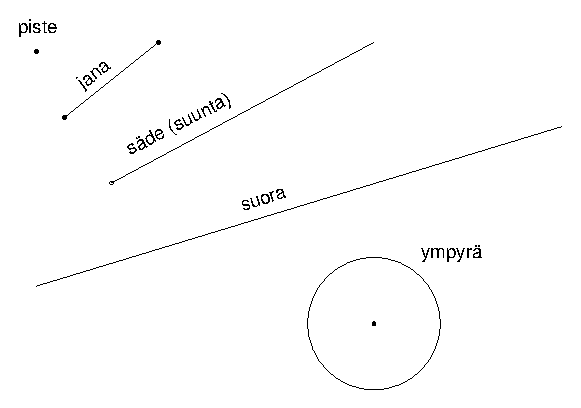
\epsfig{file=kuvat/kuvaII-1.eps}
\end{center}
%\caption{Euklidisen tason olioita}
\label{fig:oliot}
\end{figure}

Sellaiset geometriset operaatiot kuin yhdensuuntaisten suorien piirt�minen, suoran kulman
konstruoiminen, tai annetun geometrisen olion (pistejoukon) \kor{siirto} ja \kor{kierto}
\index{euklidinen liike}%
eli nk.\ \kor{euklidinen liike} (esim.\ janan siirtely pituus s�ilytt�en) tapahtuvat
euklidisessa geometriassa ympyr�viivojen (k�yt�nn�ss� harpin) avulla. My�s suora on 
konstruoitavissa pelk�st��n harppia k�ytt�en, sill� suora on sellaisten pisteiden joukko
eli \kor{ura}, jotka ovat yht� et��ll� kahdesta annetusta pisteest�. --- Viivoitinta 
tarvitaan geometriassa siis vain pisteiden 'massatuotantov�lineen�'. 

\subsection*{Kulma}
\index{kulma|vahv}%

Kulman m��rittelee geometriassa kaksi suuntaa. Konkreettisemmin kulma on ajateltavissa
pistejoukoksi, jonka muodostavat kaksi samasta pisteest� l�htev�� puolisuoraa, tai
vaihtoehtoisesti n�iden puolisuorien rajaamaksi euklidisen tason \kor{sektoriksi}.
J�lkimm�isess� tulkinnassa (ei edellisess�!) on teht�v� ero \kor{sis�kulman} ja 
\kor{ulkokulman} v�lill�. Jos $A$ ja $B$ ovat puolisuorilla olevia pisteit� ja $O$ on 
puolisuorien yhteinen piste eli kulman \kor{k�rki} ($A \neq O$, $B \neq O$), niin kulma
merkit��n $\kulma AOB$. Kuvioon on merkitty sis�kulma (sektoritulkinta!) ympyr�kaarella.  
\begin{figure}[H]
\setlength{\unitlength}{1cm}
\begin{center}
\begin{picture}(6,3)(-2,0)
%\Thicklines
\put(0,0){\line(3,2){4}} \put(0,0){\line(-3,3){3}}
\put(-1.55,1.45){\line(1,1){0.1}} 
\put(2.7,1.8){\line(-2,3){0.04}} \put(2.7,1.8){\line(2,-3){0.04}}
\put(-0.1,-0.5){$O$} \put(2.75,1.4){$A$} \put(-1.85,1.05){$B$}
\put(0,0){\arc{1}{-2.356}{-0.61}}
\end{picture}
\end{center}
\end{figure}
Kulmien vertailussa ja laskuoperaatioissa (my�s kulman mittauksessa j�ljemp�n�) tulkitaan
kulma yleens� sektoriksi. Sanotaan t�ll�in, ett� kaksi kulmaa ovat \kor{yht� suuret}, jos
ne voidaan muuntaa toisikseen euklidisella liikkeell�.\footnote[2]{Kulmien yht�suuruus on
kulmien joukossa m��ritelty ekvivalenssirelaatio, vrt.\ Luku \ref{logiikka}.} 
Yht�suuruus on siis tarkistettavissa geometrisesti. My�s kahden kulman \kor{summa} ja 
\kor{erotus} voidaan m��r�t� geometrisesti siirt�m�ll� toista kulmaa euklidisella liikkeell�
niin, ett� kulmat joutuvat 'vierekk�in' (summa) tai 'p��llekk�in' (erotus). Geometrisella
yhteenlaskulla on esimerkiksi todistettavissa tunnettu kolmion kulmia koskeva v�itt�m�: 
Kulmien summa = \kor{oikokulma} (Harj.teht.\,\ref{H-II-1: kulmat}b).

Jos kahdessa kolmiossa (vastin)kulmat ovat yht� suuret, niin kolmiot ovat
\index{kulma!a@yhdenmuotoisuus} \index{yhdenmuotoisuus}%
\kor{yhdenmuotoiset}. Geometrian perusv�itt�miin kuuluu, ett� yhdenmuotoisissa kolmioissa
vastinsivujen pituuksien suhteet ovat samat. V�itt�m� n�yttelee keskeist� roolia monissa
geometrisissa todistuksissa (ks.\ esim.\ Harj.teht.\,\ref{H-II-1: yhdenmuotoisuus}). 

\subsection*{Geometriset luvut}
\index{geometrinen luku|vahv}%
\index{laskuoperaatiot!ba@geometristen lukujen|vahv}

Kulmien mittalukuja ei euklidisen geometrian perusoperaatioissa tarvita. Sen sijaan janan 
pituuden mittaus harpin ja mittajanan avulla on perusgeometriaa. Operaatio tuo geometriaan 
reaaliluvut (tai ainakin osan niist�) ja my�s lukuihin liittyv�t laskutoimitukset.
L�ht�kohtana pidet��n lukuja $0$ ja $1$:
\[
0\ \vast\ \text{piste}, \quad 1\ \vast\ \text{mittajana}.
\]
Kun tarkastellaan kiinte�� suoraa, jolta valitaan referenssipiste $O$ luvun $0$ vastineeksi, 
niin kahden (janan pituutena) annetun luvun summa ja erotus voidaan m��r�t� geometrisesti:
\begin{figure}[htb]
\begin{center}
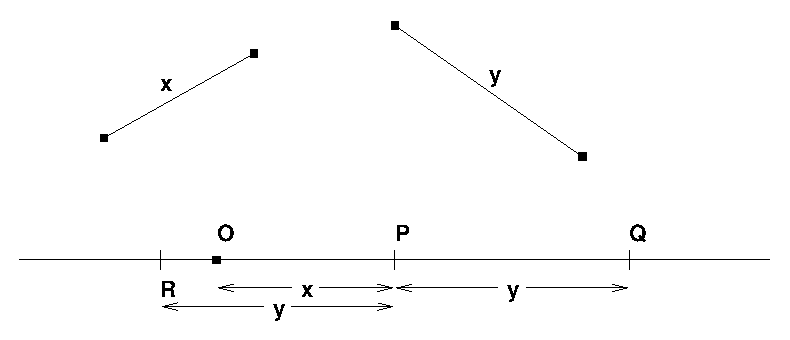
\epsfig{file=kuvat/kuvaII-2.eps}
\end{center}
%\caption{Kahden janan pituuksien summa ja erotus}
%\label{fig:summajaerotus}
\end{figure}

Kuvassa summalla ja erotuksella on geometriset vastineet janoina ja suoran pistein�:
\begin{align*}
\qquad &x+y\ \vast\ OQ\ \vast Q,  \\
\qquad &x-y\ \vast\ OR\ \vast R.
\end{align*}
Kun janan loppupiste on $O$:sta vasemmalle (suuntahan oli m��ritelty!), voidaan $OR$ tulkita 
negatiiviseksi luvuksi $x-y$. N�in on siis lukuj�rjestelm�ss� m��ritelty sek� yhteenlasku ett�
v�hennyslasku. Kun s��nt�j� $+,-$ sovelletaan per�kk�in l�htien luvusta 1 (= mittajana
sijoitettuna suoralle) n�hd��n, ett� mink� tahansa kokonaisluvun $m\in{\Z}$ geometrinen vastine
saadaan ��rellisell� m��r�ll� geometrisia operaatioita. Siis {\Z} on konstruoitu geometrisesti.
My�s mill� tahansa kokonaisluvulla jakaminen onnistuu 'viipaloimalla' luku yhdensuuntaisilla 
suorilla, joita voidaan \pain{tasossa} tuottaa harpilla ja viivoittimella (ks.\ kuvio alla).
\begin{figure}[htb]
\begin{center}
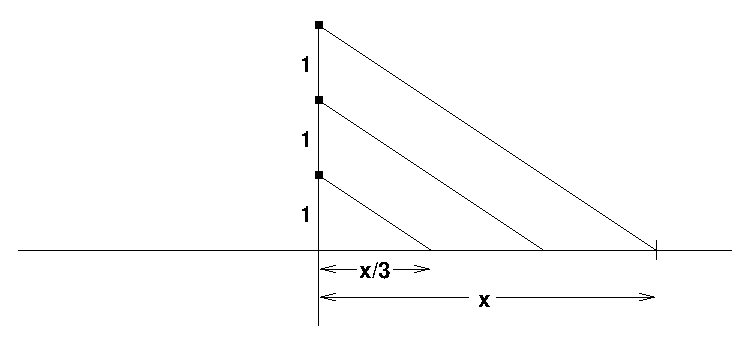
\epsfig{file=kuvat/kuvaII-3.eps}
\end{center}
\end{figure}

\pagebreak

Yleisemmin jos l�ht�kohtana on kaksi mittalukua $x,y$, niin niiden v�linen kerto- ja jakolasku
voidaan suoraan geometrisoida yhdenmuotoisten kolmioiden avulla k�ytt�en suhteita 
\begin{align*}
&\frac{z}{x}\ =\ \frac{y}{1} \quad (z=xy), \\
&\frac{z}{1}\ =\ \frac{x}{y} \quad (z=x/y).
\end{align*}
Kuvassa (alla) on
\begin{alignat*}{3}
OA &\ \vast\ 1,\quad & OB &\ \vast\ y,\quad & BC&\ \vast\ OD\ \vast\ x, \\
OE &\ \vast\ x\cdot y,\quad & AF &\ \vast\ x/y. &&
\end{alignat*} 
\begin{figure}[H]
\setlength{\unitlength}{0.67cm}
\begin{center}
\begin{picture}(12,9)(-3.5,-6)
\put(-2,0){\line(1,0){11}}
\put(-0.1,-0.1){$\bullet$} \put(-0.5,0.5){$O$}
\put(2.9,-0.1){$\bullet$} \put(3,-0.6){$A$}
\put(4.9,-0.1){$\bullet$} \put(4.9,-0.6){$B$}
\put(7.9,1.9){$\bullet$} \put(7.9,2.4){$C$}
\put(4.7,1.1){$\bullet$} \put(4.3,1.4){$F$}
\put(-1.84,-3.26){$\bullet$} \put(-1.5,-3.4){$D$}
\put(-3.02,-5.4){$\bullet$} \put(-2.6,-5.5){$E$}
\put(-3,-4){\line(3,2){11}}
\put(-3.5,-5.67){\line(3,2){12.5}}
\put(-2,-0.5){\line(4,1){11}}
\path(0,0)(-3.5,-6.34)
\put(0,-0.2){$\underbrace{\hspace{2cm}}_1$}
\put(0,0.4){$\overbrace{\hspace{3.33cm}}^y$}
\put(6.8,0.8){$x$}
\put(7.2,1.1){\vector(3,2){1.15}}
\put(6.55,0.7){\vector(-3,-2){1}}
\put(-1.3,-1.6){$x$}
\put(-1.1,-1.3){\line(10,18){0.6}}
\put(-0.5,-0.25){\vector(2,3){0.13}}
\put(-1.3,-1.8){\line(-10,-19){0.6}}
\put(-1.9,-2.92){\vector(-2,-3){0.05}}
\end{picture}
\end{center}
\end{figure}
Jatkossa nimet��n luvut, jotka ovat konstruoitavissa (janan pituutena) ��rellisell� m��r�ll�
geometrisia operaatioita, \kor{geometrisiksi luvuiksi}\footnote[2]{Englanninkielinen termi on 
'constructible numbers'. Suomennos ei ole vakiintunut.}, ja k�ytet��n t�lle lukujoukolle 
symbolia $\G$\,:
\begin{align*}
\G \ = \ \text{\{geometriset luvut\}}. 
\end{align*}
Tiedet��n jo, ett� $\G$ sis�lt�� kaikki rationaaliluvut: $\G\supset\Q$. Lis�ksi tiedet��n, ett�
$\G$ on peruslaskutoimitusten suhteen suljettu:
\[
x,y \in \G \qimpl x+y,\ x-y,\ xy,\ x/y \in \G \quad (y\neq0).
\]
T�m� merkitsee, ett� $(\G,+,\cdot)$ on \pain{kunta}.

Lukujoukon $\G$ muodostamisessa eiv�t geometrian mahdollisuudet lopu aivan 
peruslaskutoimituksiin, sill� Pythagoraan lauseen mukaan my�s operaatiot
\begin{align*}
&x,y\ \map\ \sqrt{x^{2}+y^{2}}, \quad x,y \in \G, \\
&x,y\ \map\ \sqrt{x^{2}-y^{2}}, \quad x,y \in \G,\ x \ge y
\end{align*}
ovat geometrisesti toteutettavissa. Erityisesti on siis vuosituhansia p��nvaivaa aiheuttanut
luku $\sqrt{2}$ geometristen lukujen joukossa:
\begin{figure}[H]
\setlength{\unitlength}{1cm}
\begin{center}
\begin{picture}(2.5,2.5)(-0.5,0)
\path(0,2)(0,0)(2,0)(0,2)
\put(0.8,-0.5){$1$} \put(-0.3,0.9){$1$} \put(0.9,1.1){$\sqrt{2}$}
\path(0.15,0)(0.15,0.15)(0,0.15)
\end{picture}
\end{center}
\end{figure}
Itse asiassa neli�juurioperaatio $\,x\ \map\ \sqrt{x}\,$ on geometrisesti mahdollinen, olipa
mittaluku $x \in \G$ (ajatellaan $x \geq 0$) mik� tahansa:
\begin{figure}[H]
\setlength{\unitlength}{1cm}
\begin{center}
\begin{picture}(7,4.5)(0,-0.5)
\path(3,4)(0,0)(3,0)(3,4)(8.33,0)(3,0)
%\put(3,0){\arc{0.6}{-3.14}{-1.6} \linethickness{0.05cm} \put(-0.12,0.12){\picsquare}}
%\put(3,4){\arc{0.6}{0.8}{2.2} \linethickness{0.1cm} \put(0,-0.15){\picsquare}}
\path(2.85,0)(2.85,0.15)(3,0.15) %\path(2.82,3.76)(3,3.625)(3.18,3.865)
\path(2.91,3.88)(3,3.812)(3.09,3.932)
\put(0,-0.2){$\underbrace{\hspace{3cm}}_{1}$} \put(3,-0.2){$\underbrace{\hspace{5.33cm}}_{x}$}
\put(2.8,1.9){$\left. \begin{array}{c} \vspace{3.4cm} \end{array} \right\} 
                                                                    \scriptstyle{y=\sqrt{x}}$}
\end{picture}
\end{center}
\end{figure}
T�h�n geometrian mahdollisuudet kuitenkin loppuvat, joten $\G$ koostuu kaikkiaan luvuista, jotka
on saatu mittaluvusta $1$ l�htien ��rellisell� m��r�ll� viitt� eri operaatiota: 
$+$, $-$, $\cdot\,$, $/$ ja $\sqrt{ }\,$. Kun $\G$ viel� varustetaan geometrisella 
j�rjestysrelaatiolla (janojen pituuksien vertailu harpin avulla), niin tuloksena on pelk�st��n
geometrisiin operaatioihin perustuva j�rjestetty kunta $(\G,+,\cdot,<)$. T�m� on 
rationaalilukujen kunnan pienin mahdollinen laajennus, joka t�ytt�� ehdon 
$x\in\G\,\ja\,x>0\ \impl\ \sqrt{x}\in\G$ (vrt.\ lukujoukon $\J$ konstruktio Luvussa
\ref{kunta}). On osoitettavissa, ett� kaikki geometriset luvut ovat algebrallisia (!), joten
p�tee
\[ 
\Q\ \subset\ \G\ \subset\ \A\ \subset\ \R.
\]
Kun geometriset luvut sijoitetaan em.\ tavalla kiinte�lle suoralle, voidaan n�iden lukujen 
'v�liin' ajatella sijoitelluksi my�s muut reaaliluvut. N�in ajatellen jokainen reaaliluku saa 
geometrisen vastineen
\index{lukusuora}
\kor{lukusuoran} pisteen�.

\begin{figure}[H]
\setlength{\unitlength}{1cm}
\begin{center}
\begin{picture}(14,2)(-2,0)
\put(-1,0){\line(1,0){13}}
\put(0,0){\line(0,1){0.2}}
\put(5,0){\line(0,1){0.2}}
\put(10,0){\line(0,1){0.2}}
\put(20,0){\line(0,1){0.1}}
\put(2.07,0){\line(0,1){0.1}}
\put(8.6,0){\line(0,1){0.1}}
\put(10.7,0){\line(0,1){0.1}}
\put(2.07,1){\vector(0,-1){0.6}} \put(8.6,1){\vector(0,-1){0.6}}
\put(10.7,1){\vector(0,-1){0.6}}
\put(-0.1,-0.5){$1$} \put(4.9,-0.5){$2$} \put(9.9,-0.5){$3$}
\put(1.8,1.5){$\sqrt{2}$} \put(8.5,1.5){$e$} \put(10.6,1.5){$\pi$} 
%\multiput(0,2)(0,10){2}{\line(-1,0){0.1}}
%\multiput(0,6.5)(0,1){2}{\line(-1,0){0.1}}
%\put(-0.6,8){\vector(1,-1){0.5}}
%\put(-0.6,6){\vector(1,1){0.5}}
\end{picture}
\end{center}
\end{figure}

\subsection*{Kulman mittaluku}
\index{kulma!b@kulman mittaluku|vahv}%

Kulmien k�sittelyss� geometrian mahdollisuudet ovat melko rajalliset. Kulmien yhteen- ja
v�hennyslasku onnistuu geometrisesti, kuten todettiin, ja kulman voi helposti my�s 
puolittaa eli jakaa kahteen yht� suureen osaan geometrian keinoin. Sen sijaan jo kulman
jako kolmeen yht� suureen osaan (��rellisell�) geometrisella konstruktiolla on mahdotonta,
ellei kyse ole erikoisesta (kuten suorasta) kulmasta. Geometrian keinot loppuvat my�s, kun
kulmalle yritet��n m��ritt�� sen suuruutta kuvaava mittaluku. Geometrisesti pystyt��n 
konstruoimaan vain lukujono, jonka raja-arvo mittaluku on, eli mittaluku saadaan selville
vain p��ttym�tt�m�ll� konstruktiolla. 
\begin{multicols}{2} \raggedcolumns
Tarkastellaan kulmaa $\kulma AOB$, miss� pisteet $A$ ja $B$ on sijoitettu $O$-keskisen
\index{yksikk�ympyr�}%
\kor{yksikk�ympyr�n} keh�lle, ts.\ janat $OA$ ja $OB$ ovat valitun mittajanan pituiset
(vastaten lukua $1$ lukusuoralla).
\begin{figure}[H]
\setlength{\unitlength}{1cm}
\begin{center}
\begin{picture}(4.5,3.5)(-0.5,0.3)
\put(2,2){\bigcircle{4}}
\put(2,2){\line(3,1){1.9}}
\put(2,2){\line(1,3){0.63}}
\put(1.9,1.5){$O$} \put(4,2.55){$A$} \put(2.55,4){$B$}
\end{picture}
\end{center}
\end{figure}
\end{multicols}
Kuvion tilanteessa asetetaan kulman $\kulma AOB$ mittaluvuksi yksikk�ympyr�n
\kor{kaarenpituus} pisteiden $A$ ja $B$ v�lill�. Koska vaihtoehtoja on kaksi, on
p��tett�v�, mitataanko sis�- vai ulkokulmaa. Seuraavaksi on ratkaistava vakavampi ongelma:
Miten m��ritell� ympyr�kaaren pituus? Seuraavassa ongelman ratkaisussa yhdistell��n
geometrian ja algebran keinoja.

Koska kulman $\kulma OAB$ puolitus onnistuu geometrisesti, niin saman tien kulma on
jaettavissa $n=2^k$ yht� suureen osaan jokaisella $k\in\N$. Olkoon $k\in\N$ annettu
ja merkit��n jaossa syntyvi� osakulmia $\kulma P_{i-1} O P_i,\ i=1 \ldots n=2^k$,
miss� $P_0=A$, $P_n=B$ ja muutkin pisteet $P_i$ ovat samalla $O$-keskisell�
ympyr�kaarella. Yhdistet��n nyt per�kk�iset pisteet $P_i$ janoilla \kor{murtoviivaksi}
$P_0 \ldots P_n$ ja asetetaan $\,a_k=$ ko.\ murtoviivan pituus, ts.\ $\,a_k=$ janojen 
$P_{i-1}P_i,\ i=1 \ldots n\,$ pituuksien summa. On ilmeist�, ett� lukujonon $\seq{a_k}$
jokainen termi on m��r�tt�viss� geometrisesti l�htien  luvusta $a_0=$ janan $AB$ pituus,
jolloin on $a_k/a_0\in\G\ \forall k$ (mahdollisesti $a_0\not\in\G$). Kuviossa on
konstruoitu murtoviiva $P_0 \ldots P_n$ indekseill� $k=0,1,2$, kun mitattavana on
suora kulma.
\begin{figure}[H]
\setlength{\unitlength}{1cm}
\begin{picture}(6,4.5)(-0.3,-0.5)
\put(0,0){\line(1,0){4}}
\put(0,0){\line(0,1){4}}
\put(0,0){\arc{6}{-1.57}{0}}
\path(3,0)(0,3)
\put(3.1,0.15){$P_0$} \put(0.1,3.15){$P_1$}
\put(1,-0.8){$k=0$}
\put(5,0){\line(1,0){4}}
\put(5,0){\line(0,1){4}}
\put(5,0){\arc{6}{-1.57}{0}}
\path(8,0)(7.121,2.121)(5,3)
\path(5,0)(7.121,2.121)
\put(8.1,0.15){$P_0$} \put(5.1,3.15){$P_2$} \put(7.22,2.27){$P_1$}
\put(6,-0.8){$k=1$}
\put(10,0){\line(1,0){4}}
\put(10,0){\line(0,1){4}}
\put(10,0){\arc{6}{-1.57}{0}}
\path(13,0)(12.772,1.148)(12.121,2.121)(11.148,2.772)(10,3)
\path(10,0)(12.772,1.148) \path(10,0)(12.121,2.121) \path(10,0)(11.148,2.772)
\put(13.1,0.15){$P_0$} \put(10.1,3.15){$P_4$} \put(12.22,2.27){$P_2$}
\put(12.87,1.3){$P_1$} \put(11.25,2.92){$P_3$}
\put(11,-0.8){$k=2$}
%\dashline{0.2}(0.3,3.4)(3.3,1.4)
%\put(1.56,2.8){$P$}
%\path(2.93,0.6)(3.3,0.6)
%\path(2.08,3.1)(2.8,3.1)
\end{picture}
\end{figure}
Pythagoraan lauseeseen vedoten on helppo n�ytt��, ett� lukujono $\seq{a_k}$ on aidosti
kasvava (Harj.teht.\,\ref{H-II-1: suoran kulman mitta}a), ja geometrisin perustein on my�s
osoitettavissa, ett� $\seq{a_k}$ on rajoitettu lukujono 
(Harj.teht.\,\ref{H-II-1: suoran kulman mitta}b). T�m�n j�lkeen on turvattava algebraan: 
Koska $\seq{a_k}$ siis on kasvava ja rajoitettu lukujono, niin on olemassa raja-arvo 
$\lim_k a_k=a\in\R$ (Lause \ref{monotoninen ja rajoitettu jono}, 
M��ritelm� \ref{reaaliluvut desimaalilukuina}). M��ritell��n kaaren $AB$ pituus, eli kulman 
$\kulma AOB$ mittaluku, kyseisen� raja-arvona $a$. 

Mittayksikk�� kulman kaarenpituusmittauksessa sanotaan \kor{radiaaniksi}. Tunnetusti
luku $\,\pi=3.14159..\,$ m��ritell��n yksikk�ympyr�n puolikkaan kaarenpituutena, eli
\[
\boxed{\kehys\quad \pi \,=\, \text{oikokulman mittaluku}. \quad}
\]
Koska $\pi$ on transkendenttinen luku (ks.\ Luku \ref{reaalilukujen ominaisuuksia}), niin
my�s suoran kulman mittaluku ($=\pi/2$) on transkendenttinen, samoin esimerkiksi
tasasivuisen kolmion kulman mittaluku ($=\pi/3$).

Kulmia on perinteisesti mitattu my�s \kor{asteina} ($\aste$), jolloin oikokulman mitaksi
on sovittu $180\aste$. Yleisemmin mittaluvut asteina ja radiaaneina saadaan skaalaamalla
toisistaan:
\[
\boxed{\kehys\quad \text{kulma asteina}\ 
               =\ \frac{180}{\pi}\,\cdot\,\text{(kulma radiaaneina)}. \quad}
\]

\Harj
\begin{enumerate}

\item \label{H-II-1: kulmat}
a) Suoran leikatessa kaksi yhdensuuntaista suoraa syntyy kahdeksan kulmaa. N�yt�, ett�
n�ist� jokainen on yht� suuri kolmen muun kanssa. \newline
b) Todista: Kolmion kulmien summa = oikokulma.

\item \label{H-II-1: yhdenmuotoisuus} \index{keskijana (kolmion)}
a) Jana jakaa suorakulmaisen kolmion kahteen osaan siten, ett� syntyy kolme yhdenmuotoista 
kolmiota. L�htien t�st� ajatuksesta ja kolmioiden yhdenmuotoisuusopista todista Pythagoraan 
lause! \newline
b) Kolmion \kor{keskijana} yhdist�� kolmion k�rjen vastakkaisen sivun keskipisteeseen.
L�htien kolmioiden yhdenmuotoisuusopista todista: Kolmion $ABC$ keskijana $AD$ puolittaa
jokaisen janan $BC$ suuntaisen janan, jonka p��tepisteet ovat sivuilla $AB$ ja $AC$.

\item \index{kultainen leikkaus}
Esit� geometrinen konstruktio (aseina harppi ja viivoitin), jonka tulos on \newline
a) \ ympyr�, joka kulkee annetun kolmen pisteen kautta, \newline
b) \ annetun kolmion sis��n piirretty (suurin mahdollinen) ympyr�, \newline
c) \ suora, joka kulkee annetun pisteen kautta ja sivuaa annettua ympyr��,
d) \ annetun janan $AB$ \kor{kultainen leikkaus} eli janalla oleva piste $C$ siten, ett�
jos $a,b,c$ ovat janojen $AB$, $AC$ ja $CB$ pituudet, niin $\,a/b=b/c$.

\item
Seuraavista luvuista kaksi ei ole geometrisia. Mitk� kolme ovat\,? \vspace{1mm}\newline
a) \ $\sqrt[1024]{17}$ $\quad$ b) \ $\sqrt[3]{512}$ $\quad$ c) \ $\sqrt[6]{343}$ $\quad$
d) \ $\sqrt[3]{7\sqrt{2}+5}$ $\quad$ e) \ $\sqrt[3]{5\sqrt{2}+7}$

\item (*) \label{H-II-1: suoran kulman mitta}
Suoran kulman mittaluku radiaaneina m��ritell��n raja-arvona $\,a=\lim_k a_k$, miss� $4a_k=$ sen 
s��nn�llisen $2^{k+2}$-kulmion piiri, jonka k�rjet ovat yksikk�ympyr�ll�. \vspace{1mm}\newline
a) N�yt�, ett� lukujono $\seq{a_k}_{k=0}^\infty$ on aidosti kasvava. \newline
b) N�yt�, ett� $a_k < 2\ \forall k$. \newline
c) N�yt�, ett� $\seq{a_k}$ on laskettavissa palautuvana lukujonona
\[
a_0=\sqrt{2}, \quad 
a_{k+1}=\frac{2a_k}{\sqrt{2+\sqrt{4-(2^{-k}a_k)^2}}}\,, \quad k=0,1,\ldots
\]
Laske $a_k,\ k=1 \ldots 5$ ja vertaa lukuun $\tfrac{\pi}{2}$.

\end{enumerate} % Euklidinen taso
\section{Tason vektorit} \label{tasonvektorit}
\alku
\index{vektoria@vektori (geometrinen)!a@tason \Ekaksi|vahv}%

\kor{Vektori} on matemaattisena käsitteenä hieman kaksijakoinen. Se voi olla lähtökohtaisesti 
geometrinen olio, jolloin se sovelluksissa ajatellaan usein fysikaalisena, 'maailmassa 
vaikuttavana'. Tällaisia 'fysiikkavektoreita' ovat mm.
\begin{itemize}
\item  paikka, nopeus, kiihtyvyys, kulmanopeus
\item  voima, momentti
\item  X-kentän voimakkuus, X=gravitaatio, sähkö, magneetti...
\end{itemize}
Toisaalta vektori voidaan tulkita myös algebrallisesti, jolloin päädytään geometris-fysikaalista
vektoria yleisempään (myös abstraktimpaan) vektorikäsitteeseen. Jäljempänä nähdään ensimmäisiä
esimerkkejä myös tällaisista 'matematiikkavektoreista' (myöhemmin esimerkkejä tulee paljon 
lisää). Jatkossa lähtökohta vektorin käsitteeseen on kuitenkin aluksi geometrinen.

Euklidisessa tasossa \Ekaksi\, vektori määritellään geometrisesti \kor{suuntajanana}, ts. 
janana, jolla on suunta. Ajatus on tällöin, että jana sisältyy sen toisesta päätepisteestä 
lähtevään puolisuoraan. Puolisuoran ilmaisema suunta kuvataan janan päähän merkityllä
nuolenkärjellä:
\begin{figure}[H]
\setlength{\unitlength}{1cm}
\begin{center}
\begin{picture}(13,6)(0,-0.5)
%\Thicklines
\put(1,3){\line(2,1){5}} \put(0,0){\line(4,1){4}}
\put(9,3){\vector(2,1){3}} \put(12,1){\vector(-4,-1){3}}
\put(0.95,3.1){\line(1,-2){0.1}} \put(0.9,2.5){$A$}
\put(3.95,4.6){\line(1,-2){0.1}} \put(3.9,4.0){$B$}
\put(3.975,1.1){\line(1,-4){0.05}} \put(3.925,0.5){$A$}
\put(0.975,0.35){\line(1,-4){0.05}} \put(0.925,-0.25){$B$}
\put(8.9,2.5){$A$} \put(11.9,4){$B$}\put(11.925,0.5){$A$} \put(8.925,-0.25){$B$}
\put(6.5,4){$\hookrightarrow$}
\put(6.5,0){$\hookrightarrow$}
\end{picture}
\end{center}
\end{figure}
Vektorilla tarkoitetaan täsmällisemmin vain suuntajanan sisältävää \pain{osatietoa} 
\[
\{\text{(janan) pituus, suunta}\}.
\] 
Tiettyyn suuntajanaan liittyvä vektori merkitään $\overrightarrow{AB}$, yleisemmin 
käytetään vektorimerkintöjä $\vec a, \vec b, \vec v$ jne.

Huomattakoon, että vektori $\overrightarrow{AB}$ siis \pain{ei} 'tiedä', missä piste
$A$ sijaitsee euklidisessa tasossa. Näin ollen 'vektoria saa siirtää', kunhan 'ei kierrä
eikä venytä'. (Fysikaalinen vastine: Voiman vaikutus on sama vaikutuspisteestä
riippumatta.) 

Jos tunnetaan vektorit $\vec a=\overrightarrow{AB}$ ja $\vec b=\overrightarrow{BC}$,
niin tunnetaan myös $\vec c=\overrightarrow{AC}$\,:
\begin{figure}[H]
\setlength{\unitlength}{1cm}
\begin{center}
\begin{picture}(6,5)
%\Thicklines
\put(0,0){\vector(2,3){2}} \put(2,3){\vector(4,1){4}} \put(0,0){\vector(3,2){6}}
\put(-0.1,-0.1){$\bullet$} \put(1.9,2.9){$\bullet$} \put(5.9,3.9){$\bullet$}
\put(-0.2,0.3){$A$} \put(1.9,3.2){$B$} \put(5.9,4.2){$C$}
\put(0.9,1.8){$\vec a$} \put(4.8,3.8){$\vec b$} \put(4,2.8){$\vec c$}
\end{picture}
\end{center}
\end{figure}
\index{laskuoperaatiot!c@tason vektoreiden|(}%
Sanotaan, että $\vec c$ on vektoreiden $\vec a, \vec b$ \kor{summavektori} ja merkitään
\[
\vec c=\vec a+\vec b.
\]
Summa määrätään siis geometrisesti kolmiodiagrammilla. Näin määritellylle vektorien 
yhteenlaskulle pätevät tavanomaiset vaihdanta- ja liitäntälait:
\begin{itemize}
\item[(V1)] $\quad \vec a+\vec b = \vec b+\vec a$
\item[(V2)] $\quad (\vec a+\vec b\,)+\vec c = \vec a+(\vec b+\vec c\,)$
\end{itemize}
Tässä ei ole kyse aksioomista (vrt.\ vastaavat kunta-aksioomat, Luku \ref{kunta}) vaan
väittämistä, joiden todistus on geometrinen:
\begin{figure}[H]
\setlength{\unitlength}{1cm}
\begin{center}
\begin{picture}(14,5)
%\Thicklines
\put(0,0){\vector(2,3){2}} \put(2,3){\vector(4,1){4}}
\dashline{0.2}(0,0)(4,1) \dashline{0.2}(4,1)(6,4)
\put(3.9,0.975){\vector(4,1){0.1}} \put(5.9,3.85){\vector(2,3){0.1}}
\put(1.2,2.2){$\vec a$} \put(5.2,4){$\vec b$} \put(3.5,1.1){$\vec b$} \put(5.8,3.3){$\vec a$}

\put(6,0){\vector(2,3){2}} \put(8,3){\vector(4,1){4}}
\dashline{0.2}(6,0)(12,4) \put(11.9,3.933){\vector(3,2){0.1}} \put(12,4){\vector(1,-1){2}}
\put(6,0){\vector(4,1){8}}
\dashline{0.2}(8,3)(14,2) \put(13.9,2.0167){\vector(4,-1){0.1}}
\put(7.2,2.2){$\vec a$} \put(11.2,4){$\vec b$} \put(13.6,2.5){$\vec c$} 
\put(12,1.1){$\vec a+\vec b+\vec c$}
\put(12.9,2.3){$\scriptstyle{\vec b+\vec c}$} \put(11.5,3.3){$\scriptstyle{\vec a+\vec b}$}
\end{picture}
\end{center}
\end{figure}
Vektorin $\vec a = \overrightarrow{AB}$
\index{itseisarvo}%
\kor{itseisarvo} (arkisemmin 'pituus') on
\[
\abs{\vec a}=|\overrightarrow{AB}|=\abs{AB}=\text{janan }AB\text{ pituus}.
\]
Tälle pätee \kor{kolmioepäyhtälö} (vrt.\ Lause \ref{kolmioepäyhtälö})
\index{kolmioepäyhtälö!b@tason vektoreiden}%
\[
\abs{\vec a+\vec b} \le \abs{\vec a}+\abs{\vec b}.
\]
Jos $\lambda \in \R$, niin $\lambda \vec a$ tarkoittaa
\index{skaalaus (vektorin)}%
\kor{skaalattua} vektoria, jolle pätee:
\begin{itemize}
\item[(1)] $\quad |\lambda \vec a|=|\lambda||\vec a|$
\item[(2)] $\quad \lambda \vec a \uparrow\uparrow \vec a,
                                 \text{ jos } \lambda > 0, \text{ ja }
                  \lambda \vec a \uparrow\downarrow \vec a, \text{ jos } \lambda<0$
\end{itemize}
Tässä $\uparrow\uparrow$ tarkoittaa yhdensuuntaisuutta ja $\uparrow\downarrow$ 
vastakkaissuuntaisuutta. Vektorin skaalausta $\vec a \map \lambda \vec a \ (\lambda \in \R)$
sanotaan vektorialgebrassa yleisemmin \kor{skalaarilla kertomiseksi}. Skaalaajia eli
reaalilukuja kutsutaan siis tässä laskuoperaatiossa
\index{skalaari}%
\kor{skalaareiksi}. Skalaarilla kertomisen ja yhteenlaskun
määritelmistä on pääteltävissä (Harj.teht.\,\ref{H-II-1: perusteluja}a), että seuraavat
'luonnonmukaiset' säännöt ovat voimassa (vrt.\ kunta-aksioomat Luvussa \ref{kunta})\,:
\begin{itemize}
\item[(V3)] $\quad (\lambda + \mu)\vec a = \lambda \vec a + \mu \vec a$
\item[(V4)] $\quad \lambda(\mu \vec a\,) = (\lambda \mu)\vec a$
\item[(V5)] $\quad \lambda(\vec a + \vec b\,)= \lambda \vec a + \lambda \vec b$
\item[(V6)] $\quad 1 \vec a =  \vec a$
\end{itemize}
Operaation $\vec a \kohti \lambda \vec a$ määritelmän mukaisesti on $|0 \vec a|=0$.
Tällaista vektoria sanotaan
\index{nollavektori}%
\kor{nollavektoriksi} ja merkitään $\,0 \vec a = \vec 0$.
Nollavektorin suunta on epämääräinen  (ei määritelty). Nollavektori on vektorien
yhteenlaskun nolla-alkio, ts.\ pätee
\begin{itemize}
\item[(V7)] $\quad \vec a + \vec 0 = \vec a\ \forall \vec a$ 
\end{itemize}
Jokaisella vektorilla $\vec a$ on myös
\index{vastavektori}%
\kor{vastavektori} $-\vec a$, jolle pätee
\begin{itemize} 
\item[(V8)] $\quad \vec a + (-\vec a\,) = \vec 0$
\end{itemize}
Nimittäin kun säännössä (V3) valitaan $\lambda=1, \mu=-1$ ja käytetään nollavektorin
määritelmää ja sääntöä (V6), niin seuraa
\[
-\vec a = (-1)\,\vec a.
\]
Vastavektorin avulla tulee määritellyksi myös vektorien vähennyslasku:
\[
\vec a - \vec b = \vec a + (-\vec b\,).
\]
\begin{figure}[H]
\setlength{\unitlength}{1cm}
\begin{center}
\begin{picture}(6,2.3)(2,0.5)
%\Thicklines
\put(4,0){\vector(2,3){2}} \put(4,0){\vector(4,1){4}} \put(8,1){\vector(-1,1){2}}
\dashline{0.2}(4,0)(2,2) \put(2.1,1.9){\vector(-1,1){0.1}} 
\dashline{0.2}(6,3)(2,2) \put(2.1,2.025){\vector(-4,-1){0.1}}
\put(5.8,2.3){$\vec a$} \put(7.6,0.4){$\vec b$} \put(6.5,2.7){$\vec a-\vec b$} 
\put(2.7,1.4){$\vec a+(-\vec b\,)$}
\end{picture}
\end{center}
\end{figure}
Säännöt (V1)--(V8), yhdessä nollavektorin ja vastavektorin määritelmien kanssa, muodostavat
(tason vektoreiden)) \kor{vektorialgebran} laskulait.
\index{laskuoperaatiot!c@tason vektoreiden|)}
\begin{Exa} \label{kolmion keskipiste}
Laskulaeista (V1)--(V8) seuraava identiteetti
\[
\vec a + \frac{2}{3} \left( \frac{1}{2}\vec b - \vec a \right)\ 
             =\ \vec b + \frac{2}{3} \left( \frac{1}{2}\vec a - \vec b \right)\
             =\ \frac{2}{3} \left[ \vec b + \frac{1}{2}\left( \vec a - \vec b \right) \right]\
             =\ \frac{1}{3} \left( \vec a + \vec b \right)
\]
voidaan lukea: Kolmion keskijanat leikkaavat toisensa samassa pisteessä, joka jakaa keskijanat
suhteessa $2:1$ (vrt.\ kuvio). Leikkaupistettä sanotaan 
\index{keskizza@keskiö (kolmion)}%
kolmion \kor{keskiöksi} (keskipisteeksi). \loppu
\begin{figure}[H]
\setlength{\unitlength}{1cm}
\begin{center}
\begin{picture}(6.5,4.6)(0,0)
%\Thicklines
\put(0,0){\vector(1,2){2}} \put(0,0){\vector(1,0){6}}
\path(2,4)(6,0)(1,2)
\drawline(2,4)(3,0) \drawline(0,0)(4,2) \put(0,0){\vector(2,1){2.67}}
\put(1.4,3.5){$\vec a$} \put(5.5,-0.5){$\vec b$}
\put(0,-0.5){$A$} \put(1.9,4.2){$B$} \put(6.2,-0.1){$C$}
\put(1.2,1.2){$\scriptstyle{\frac{1}{3}(\vec a+\vec b\,)}$}
\end{picture}
\end{center}
\end{figure}
\end{Exa}

\subsection*{Vektoriavaruus}
\index{vektoric@vektoriavaruus|vahv}%

Jos tason vektorien joukkoa merkitään symbolilla $V$, niin edellä olevilla määritelmillä on 
syntynyt algebra, joka merkittäköön $(V,\R)$. Laskusääntöjen (V1)--(V8) (yleisemmin:
aksioomien) ollessa voimassa sanotaan, että kyseessä on (lineaarinen) \kor{vektoriavaruus}.
Käsitteeseen siis sisältyvät
\index{laskuoperaatiot!ca@ yleisen vektoriavaruuden}
\begin{itemize}
\item  vektorien muodostama joukko $V$ (jossa operoidaan)
\item  vektorien yhteenlasku (+)
\item  nk. \kor{skalaarien} muodostama \kor{kertojakunta}, tässä = $\R$
\item  skalaarin ja vektorin kertolasku
\end{itemize}
\index{skalaari} \index{kertojakunta}%
Lyhennetty sanonta '$V$ on vektoriavaruus' tarkoittaa koko tätä algebraa, jolloin 
kertojakunta on juuri $\R$, tai muuten asiayhteydestä selvä. Sanonnat \kor{reaalikertoiminen}
vektoriavaruus tai yleisemmin \kor{$\K$-kertoiminen} vektoriavaruus kiinnittävät kertojakunnan
tarkemmin. Kertojakunnan ei siis tarvitse olla $\R$, vaan se voisi olla esim. $\K=\Q$ tai 
$\K=\G=\{\text{geometriset luvut}\}$. Lineaarinen vektoriavaruus on hyvin keskeinen käsite
matematiikassa, ja sillä on keskeinen rooli myös monissa matematiikan sovelluksissa.

\subsection*{Kanta ja koordinaatisto}
\index{kanta|vahv} \index{koordinaatisto|vahv}%

Olkoon $\vec v \in V$ mielivaltainen tason vektori ja $\vec a, \vec b \in V$ kaksi vektoria, 
joille pätee
\[
\vec a, \vec b \neq \vec 0 ,\quad \vec a \neq \lambda \vec b \quad \forall \ \lambda \in \R.
\] 
Tällöin voidaan geometrisella konstruktiolla (ks.\ kuvio) löytää yksikäsitteiset $x,y \in \R$
siten, että
\[
\vec v = x \vec a + y \vec b.
\]
\begin{figure}[H]
\setlength{\unitlength}{1cm}
\begin{center}
\begin{picture}(6,4.5)(0,-0.5)
%\Thicklines
\put(0,0){\vector(1,1){4}} \put(0,0){\vector(1,0){2}} \put(0,0){\vector(3,1){6}}
\put(0,0){\vector(1,0){4}} \put(0,0){\vector(1,1){2}}
\dashline{0.2}(6,2)(2,2) \dashline{0.2}(6,2)(4,0)
\put(3.1,3.6){$\vec b$} \put(0.9,1.6){$y\vec b$} \put(1.5,-0.5){$\vec a$} 
\put(3.3,-0.5){$x\vec a$} \put(5.5,2.2){$\vec v$}
\end{picture}
\end{center}
\end{figure}
Sanotaan tällä perusteella, että $\vec v$ on $\vec a$:n ja $\vec b$:n
\index{lineaariyhdistely}%
\kor{lineaariyhdistely} (lineaarinen yhdistely, \kor{lineaarikombinaatio}) ja että
$x \vec a$ ja $y \vec b$ ovat $\vec v$:n
\index{komponentti (vektorin)}%
(vektori)\kor{komponentit} $\vec a$:n ja $\vec b$:n suuntaan. 

Kun siis kaksi em.\ ehdot täyttävää vektoria on valittu, on koko $V$ esitettävissä muodossa
\[
V=\{x \vec a + y \vec b \mid x,y \in \R\}.
\]
Sanotaan, että vektoripari $\{ \vec a, \vec b \}$ on $V$:n \kor{kanta}\footnote[2]{Kanta on
vektoreiden j\pain{är}j\pain{estett}y joukko, joten merkintä $(\vec a,\vec b)$ olisi
loogisempi. Erinäisten sekaannusten välttämiseksi käytetään tässä yhteydessä kuitenkin
yleisemmin aaltosulkeita.} ja että $x,y$ ovat vektorin $\vec v = x \vec a + y \vec b \in V$
\index{koordinaatti (vektorin)}%
\kor{koordinaatit} kannassa $\{\vec a,\vec b\,\}$. Jos koordinaatit esitetään lukuparina
$(x,y)$ (pari = kahden alkion järjestetty joukko), niin on synnytetty yhteys $V$:n ja
tällaisten lukuparien joukon välille. Merkitään jälkimmäistä joukkoa symbolilla $\Rkaksi$,
äännetään 'R kaksi':
\[
\Rkaksi = \{ (x,y) \mid x \in \R\,\ja\,y \in \R \}.\index{karteesinen tulo|av}%
\footnote[3]{Joukko $\R^2$ voidaan myös  merkitä $\R\times\R$, jolloin käytetään
joukko-opillista \kor{karteesisen tulon} merkintää
\[
A \times B = \{ (x,y) \mid x \in A\,\ja\,y \in B \}.
\] 
Tämä luetaan '$A$:n ja $B$:n karteesinen tulo', tai vain '$A$ risti $B$'. Joukon
$A \times B$ alkiot ovat siis pareja. Näiden välinen samastusrelaatio on
\[
(x_1,y_1) = (x_2,y_2) \qekv  x_1=x_2\ \wedge\ y_1=y_2.
\] }
\]

Em. sopimuksilla on itse asiassa luotu \kor{kääntäen yksikäsitteinen} (=molempiin suuntiin 
yksikäsitteinen)
\index{vastaavuus ($\ensuremath  {\leftrightarrow }$)}%
\kor{vastaavuus} $V$:n ja $\Rkaksi$:n välille. Merkitään tätä: 
\[
V \vast \Rkaksi.
\]
Vastaavuuteen liittyen nimetään $\Rkaksi$ kantaan $\{\vec a, \vec b\,\}$ liittyväksi $V$:n
\index{koordinaattiavaruus}% 
\kor{koordinaatti-avaruudeksi}. Nimitys jo viittaa siihen, että myös $\Rkaksi$ on tulkittavissa
\index{vektorib@vektori (algebrallinen)!a@$\R^2$:n}%
lineaariseksi vektoriavaruudeksi. Nimittäin kaikki vektoriavaruuden laskulait ovat voimassa,
kun yhteenlasku ja skalaarilla kertominen $\Rkaksi$:ssa määritellään
\index{laskuoperaatiot!cb@vektoriavaruuden $(\Rkaksi,\R)$}
\begin{align*}
(x_1,y_1)+(x_2,y_2)& = (x_1+x_2,y_1+y_2), \\
\lambda(x,y) &= (\lambda x, \lambda y).
\end{align*}
Nämä operaatiot myös vastaavat $V$:n laskutoimituksia, sillä
\begin{align*}
\vec v_1=x_1 \vec a + y_1 \vec b, \ \vec v_2= x_2 \vec a + y_2 \vec b \ 
                               &\impl \ \vec v_1 + \vec v_2 = (x_1+x_2)\vec a 
                                                                        + (y_1+y_2)\vec b, \\
\vec v = x \vec a +y \vec b \  &\impl \ \lambda \vec v = (\lambda x)\vec a +(\lambda y)\vec b.
\end{align*}

Vektoriavaruus $(\Rkaksi,\R)$, mainituin laskuoperaatioin, on esimerkki (lajissaan ensimmäinen)
algebrallisten vektoreiden muodostamasta vektoriavaruudesta. Tämä avaruus on
siis geometrisista tulkinnoista vapaa. Toisaalta tulkitsemalla $(\Rkaksi,\R)$ tason vektorien
koordinaattiavaruudeksi (valitussa kannassa) saadaan vektorien laskuoperaatiot muunnetuksi 
algebralliseen muotoon. Esimerkiksi yhteenlaskussa tällainen laskukaavio on
\[
\begin{array}{cccccc}
&\vec v_1   &  &\vec v_2   &     &\vec v_1+\vec v_2 \\
&\downarrow &  &\downarrow &     &\uparrow \\ 
&(x_1,y_1)  &  &(x_2,y_2)  &\map &(x_1+x_2,y_1+y_2)
\end{array}
\]
Kaavion etuna on, että itse laskuoperaatiossa ei tarvita mitään tietoa vektorien 'ulkonäöstä'.
Monia geometrian tuloksia voidaan tällä tavoin johtaa algebran keinoin (vrt.\ Esimerkki 
\ref{kolmion keskipiste} edellä).

Koordinaattiavaruus $\Rkaksi$ voidaan yhtä hyvin liittää myös siihen alkuperäiseen 
pisteavaruuteen $\Ekaksi$, josta koko vektoriajatus oli lähtöisin. Nimittäin jos vektoreita 
ajatellaan $\Ekaksi$:n suuntajanoina, 'joita voi siirrellä', niin voidaan yhtä hyvin ajatella,
että jokainen vektori vastaa yksikäsitteistä suuntajanaa, jonka lähtöpiste on kiinteä piste $O$.
Näin on synnytetty $\Ekaksi$:n ja $V$:n kääntäen yksikäsitteinen vastaavuus:
\[
P \in \Ekaksi \ \leftrightarrow \ \overrightarrow{OP} \in V.
\]
Kun nyt tulkitaan myös edellä valitut kantavektorit $\vec a, \vec b$ pisteestä $O$ alkaviksi
suuntajanoiksi, niin euklidiseen tasoon on luotu \kor{koordinaatisto}\footnote[2]{Ajatuksen 
koordinaatiston avulla tapahtuvasta geometrian aritmetisoimisesta toi matematiikkaan 
ranskalainen filosofi-matemaatikko \hist{Ren\'e Descartes} (1596-1650) tutkielmassaan 
''La g\'eom\'etrie'', joka ilmestyi laajemman filosofisen teoksen liitteenä vuonna 1637. 
Tutkielma merkitsi \kor{analyyttisen geometrian} alkua, ja enteili yleisemminkin geometrian 
'algebralisoitumista' --- trendiä, joka erityisesti tietokoneiden aikakaudella on entisestään
vahvistunut. \index{Descartes, R.|av}}, jota merkitään $\{O,\vec a,\vec b\}$. Pistettä $O$
sanotaan koordinaatiston 
\index{origo}%
\kor{origoksi}.

\begin{figure}[H]
\setlength{\unitlength}{1cm}
\begin{center}
\begin{picture}(6,4)(-2,-0.2)
%\Thicklines
\put(0,0){\vector(3,2){4}} \put(0,0){\vector(-2,3){2}}
\put(-0.1,-0.5){$O$} \put(-1.7,2.8){$\vec a$} \put(3.5,2.6){$\vec b$}
\end{picture}
\end{center}
\end{figure}
\index{koordinaatti (pisteen)}%
Jos $P \in \Ekaksi$ ja $\Vect{OP} = x \vec a + y \vec b$, niin sanotaan, että \kor{pisteen}
$P$ \kor{koordinaatit} valitussa koordinaatistossa $\{O,\vec a,\vec b\,\}$ ovat 
$(x,y)$. Koordinaatiston ollessa kiinitetty voidaan koordinaattiparia $(x,y)$ haluttaessa 
pitää $P$:n 'nimenä', jolloin on lupa kirjoittaa muitta mutkitta
\[
P=(x,y).
\]
Näin on luotu kääntäen yksikäsitteinen vastaavuus $\Ekaksi \ \leftrightarrow \ \Rkaksi$.
\begin{Exa} Olkoon $T$ tason (aito) kolmio, jonka kärkikipisteet ovat $0,A,B$. Merkitään 
$\vec a=\Vect{OA}$, $\vec b=\Vect{OB}$. Tällöin $T$:n kärkipisteet, $T$:n sivujen 
keskipisteet ja $T$:n keskiö koordinaattistossa $\{O,\vec a,\vec b\,\}$ ovat
(vrt.\ Esimerkki \ref{kolmion keskipiste})
\begin{align*}
&\text{kärkipisteet:} \quad O=(0,0), \quad A=(1,0), \quad B=(0,1), \\
&\text{sivujen keskipisteet:} \quad O'=(1/2,1/2), \quad A'=(0,1/2), \quad B'=(1/2,0), \\
&\text{keskiö:} \quad C=(1/3,1/3). \quad\loppu
\end{align*}
\end{Exa}
Koordinaatistoon tarvitaan siis ensinnäkin referenssipiste $O$. Tästä nk. origosta valitaan
kaksi suuntaa, jotka määrääväät vektoreiden $\vec a, \vec b$ suunnat. Vielä päätetään, että 
mitattaessa etäisyyttä $O$:sta on pituusyksikkö $\alpha$ mentäessä $\vec a$:n suuntaan ja 
$\beta$ mentäessä $\vec b$:n suuntaan. Tässä $\alpha,\beta \in \R$ ja $\alpha,\beta>0$. Kun nyt
valitaan $\vec a$ ja $\vec b$ siten, että $|\vec a|=\alpha$ ja $|\vec b|=\beta$, ovat $\vec a$
ja $\vec b$ yksikäsitteisesti määrätyt ja koordinaatisto siis valmis. Origon kautta kulkevia
suoria
\begin{align*}
S_1=\{ P \in \Ekaksi \ | \ \overrightarrow{OP} = \lambda \vec a, \ \lambda \in \R \}, \\
S_2=\{ P \in \Ekaksi \ | \ \overrightarrow{OP} = \mu \vec b, \ \mu \in \R \},
\end{align*}
\index{suuntavektori} \index{koordinaattiakseli}%
joiden \kor{suuntavektoreina} ovat $\vec a, \vec b$, sanotaan \kor{koordinaattiakseleiksi}.
\begin{figure}[H]
\setlength{\unitlength}{1cm}
\begin{center}
\begin{picture}(10,6)(-3,-2)
\Thicklines
\put(0,0){\vector(3,2){4}} \put(0,0){\vector(-1,1){2}}
\thinlines
\put(0.3,-0.1){$O=(0,0)$} \put(-2.1,1.4){$\vec a$} \put(3.5,2.7){$\vec b$}
\put(-3,-2){\line(3,2){8}} \put(2,-2){\line(-1,1){5}}
\put(-1.8,2){$(1,0)$} \put(4,2.2){$(0,1)$}
\put(2.2,-2){$S_1$} \put(-2.5,-2){$S_2$}
\put(-0.07,-0.07){\piste} \put(3.93,2.6){\piste} \put(-2.07,1.93){\piste}
\end{picture}
\end{center}
\end{figure}

\subsection*{Lineaarinen riippumattomuus}
\index{lineaarinen riippumattomuus|vahv}

Koordinaatiston kantavektoreista $\vec a,\vec b$ edellä tehdyt oletukset
($\vec a,\vec b \neq \vec 0$ ja $\vec a,\vec b$ eivät saman- tai vastakkaissuuntaiset) 
voidaan asettaa lyhyemmin ehtona
\begin{equation} \label{lin riippumattomat}
x \vec a + y \vec b = \vec 0 \qimpl x=y=0. \tag{$\star$}
\end{equation}
Jos tason vektoreilla on ominaisuus \eqref{lin riippumattomat}, niin sanotaan, että 
$\{\vec a,\vec b\,\}$ on \kor{lineaarisesti} \kor{riippumaton} (vektori)\kor{systeemi}
(= joukko) tai että $\vec a$ ja $\vec b$ ovat lineaarisesti riippumattomat. Tason
vektoriavaruuden $V$ kannaksi kelpaa siis mikä tahansa lineaarisesti riippumaton
vektorisysteemi $\{\vec a,\vec b\,\}$.

Jos vektorit $\vec a,\vec b$ eivät ole lineaarisesti riippumattomat, niin ne ovat
\index{lineaarinen riippuvuus}%
\kor{lineaarisesti riippuvat}. Ehdon  \eqref{lin riippumattomat} mukaisesti näin on, jos
\[
x\vec a + y\vec b=\vec 0 \quad \text{jollakin}\ (x,y) \neq (0,0).
\]
Tämä ehto puolestaan toteutuu täsmälleen kun joko
(i) $\vec a = \vec 0 \,\impl\, x\vec a+0\vec b=\vec 0$ $\forall x\in\R$,
(ii) $\vec b = \vec 0 \,\impl\, 0\vec a+y\vec b=\vec 0\ \forall y\in\R$, tai
(iii) $\vec a$ ja $\vec b$ ovat yhdensuuntaiset (= saman- tai vastakkaissuuntaiset, ol.\
$\vec a \neq \vec 0$ ja $\vec b \neq \vec 0\,$), jolloin 
$\exists\lambda\in\R,\ \lambda \neq 0$ siten, että $\vec a + \lambda\vec b = \vec 0$. 
\begin{Exa} Tason vektoreista $\vec a, \vec b$ tiedetään, että $\vec a-\vec b$ ja 
$\vec a+2\vec b$ ovat lineaarisesti riippuvat. Voidaanko päätellä, että myös $\vec a$ ja 
$\vec b$ ovat lineaarisesti riippuvat\,? \end{Exa}
\ratk Annetun tiedon mukaan on jollakin $(x,y) \neq (0,0)$
\[
x(\vec a-\vec b)+y(\vec a+2\vec b\,)=\vec 0.
\]
Vektorialgebran säännöillä tämä saadaan muotoon
\[
\vec 0 = (x+y)\vec a+(-x+2y)\vec b = x'\vec a+y'\vec b.
\]
Koska
\[
\begin{cases} \,x' = 0 \\ \,y' = 0 \end{cases} \qekv \begin{cases} \,\ x+y = 0 \\ -x+2y = 0 
\end{cases} \qekv \begin{cases} \,x =0 \\ \,y = 0 \end{cases}
\]
ja tiedetään, että $(x,y) \neq (0,0)$, niin päätellään, että $(x',y') \neq (0,0)$. Koska siis
jollakin $(x',y') \neq (0,0)$ on $x'\vec a+y'\vec b=\vec 0$, niin vastaus on: Voidaan\,! \loppu

\subsection*{Koordinaatiston vaihto}
\index{koordinaatisto!a@koordinaatiston vaihto|vahv}%

Kun tason geometrisia tehtäviä ratkotaan vektorialgebran keinoin, on tehtävään sopivan 
koordinaatiston valinta yleensä ratkaisemisen ensimmäinen askel (vrt.\ Esimerkki 
\ref{kolmion keskipiste} edellä). Jos valittu koordinaatisto osoittautuu ratkaisun kuluessa
epämukavaksi, voidaan suorittaa \kor{koordinaatiston vaihto}. Koordinaatiston vaihto koostuu
\index{origon siirto} \index{kanta!b@kannan vaihto}%
\kor{origon siirrosta} ja vektoriavaruuden \kor{kannan vaihdosta}, tai pelkästään jommasta
kummasta. Kuvassa pisteen $P$ koordinaatit ovat $(x,y)$ koordinaatistossa $\{O,\vec a,\vec b\,\}$
ja $(x',y')$ koordinaatistossa $\{O',\vec c,\vec d\,\}$.
\begin{figure}[H]
\setlength{\unitlength}{1cm}
\begin{center}
\begin{picture}(10,6)(-3,-2)
\Thicklines
\put(-2,-2){\vector(1,1){3}} \put(-2,-2){\vector(-1,1){2}}
\put(4.5,2){\vector(-1,-4){0.5}} \put(4.5,2){\vector(1,0){3}}
\thinlines
\put(-2,-2){\vector(1,2){2.5}} \put(4.5,2){\vector(-4,1){4}}
\put(-1.9,-2.3){$O$} \put(-4.1,-0.6){$\vec a$} \put(1,0.4){$\vec b$}
\put(7.3,2.2){$\vec c$} \put(4.3,0){$\vec d$} \put(4.5,2.2){$O'$}
\put(0.5,3.2){$P=(x,y)=(x',y')$}
\end{picture}
\end{center}
\end{figure}
Vektorien yhteenlaskudiagrammin mukaan on
\[
\Vect{OP}=\Vect{OO'}+\Vect{O'P}\,\ \ekv\,\ x\vec a+y\vec b=\Vect{OO'}+(x'\vec c+y'\vec d\,).
\]
Olkoon tässä $\Vect{OO'}=\alpha\,\vec a+\beta\,\vec b$, eli $O'=(\alpha,\beta)$
koordinaatistossa $\{O,\vec a,\vec b\,\}$, ja
\[
\vec c=\lambda_1\vec a+\mu_1\vec b, \quad \vec d=\lambda_2\vec a+\mu_2\vec d,
\]
eli vektoreiden $\vec c,\vec d\,$ koordinaatit kannassa $\{\vec a,\vec b\}$ ovat
$(\lambda_1,\mu_1)$ ja $(\lambda_2,\mu_2)$. Tällöin em.\ yhtälö sievenee vektorialgebran
säännöillä muotoon
\[
(x-\lambda_1 x'-\lambda_2 y'-\alpha)\,\vec a+(y-\mu_1 x'-\mu_2 y'-\beta)\,\vec b\,=\,\vec 0.
\]
Koska vektorit $\vec a$ ja $\vec b$ ovat lineaarisesti riippumattomat, niin seuraa
\[
\begin{cases} \,x-\lambda_1 x'-\lambda_2 y'-\alpha=0\\ \,y-\mu_1 x'-\mu_2 y'-\beta =0 \end{cases}
\ \ekv \quad
\begin{cases} \,\lambda_1 x'+\lambda_2 y'=x-\alpha \\ \,\mu_1 x'+\mu_2 y'=y-\beta \end{cases}
\]
Ratkaisemalla tästä $(x',y')$ koordinaattien $(x,y)$ avulla --- yhtälöryhmä ratkeaa 
aina kun $\vec c\,$ ja $\vec d$ ovat lineaarisesti riippumattomat --- saadaan selville 
\index{koordinaattimuunnos}%
\kor{koordinaattimuunnoksen} $(x,y) \ext (x',y')$ laskukaavat. Yhtälöryhmästä nähdään myös 
suoraan, miten käänteinen muunnos $(x',y') \ext (x,y)$ on laskettava. 
\begin{Exa} Olkoon
\[
\Vect{OO'}=\vec a - \vec b, \quad \vec c=2\vec a+\vec b, \quad \vec d=\vec a-2\vec b.
\]
Em.\ laskun kulku on tällöin
\begin{align*}
&x\vec a+y\vec b\ =\ (\vec a-\vec b\,)+x'(2\vec a+\vec b\,)+y'(\vec a-2\vec b\,) \\
&\qekv (x-2x'-y'-1)\,\vec a + (y-x'+2y'+1)\,\vec b = \vec 0 \\
&\qekv \begin{cases} \,2x'+y'=x-1 \\ \,x'-2y'=y+1 \end{cases}
\end{align*}
Ratkaisemalla saadaan koordinaattimuunnoksen laskukaavoiksi
\[
\begin{cases} \,x=2x'+y'+1\\ \,y=x'-2y'-1 \end{cases}\ \ekv \quad
\begin{cases} \,x'=\frac{1}{5}(2x+y-1) \\ \,y'=\frac{1}{5}(x-2y-3) \end{cases} \loppu
\]
\end{Exa}

\subsection*{Dimensio. Aliavaruus}
\index{dimensio|vahv} \index{aliavaruus|vahv}

Koska tason vektoriavaruuden kannassa on oltava kaksi lineaarisesti riippumatonta vektoria, niin
sanotaan, että $V$ on $2$-\kor{ulotteinen} vektoriavaruus tai että $V$:n \kor{dimensio}
(ulotteisuus) on $2$. Merkitään
\[
\text{dim } V=2.
\]
Myös koodinaattiavaruus $\Rkaksi$ on vektoriavaruutena $2$-ulotteinen. Nimittäin jos merkitään
\[
\ma=(1,0), \quad \mb=(0,1),
\]
niin $\Rkaksi$:n vektorialgebran mukaan on $(x,y)=x\ma + y\mb$, eli jokainen
$\mv v = (x,y) \in \Rkaksi$ voidaan esittää yksikäsitteisesti $\ma$:n ja $\mb$:n
lineaariyhdistelynä. Siis $\{\ma,\mb\}$ on $\Rkaksi$:n kanta, ja koska kannassa on kaksi
vektoria, niin $\text{dim}(\Rkaksi)=2$.

Tason tai $\Rkaksi$:n vektoreista voidaan muodostaa myös $1$-\kor{ulotteisia} vektoriavaruuksia.
Tason vektoreiden tapauksessa nämä ovat kaikki ilmaistavissa jonkin vektorin
$\vec a \in V, \  \vec a \neq \vec 0$ avulla muodossa
\[
W=\{\vec v = x\vec a,\ x\in\R\}.
\]
Koska ilmeisesti pätee
\begin{align*}
\vec v_1, \vec v_2 \in W &\qimpl \vec v_1 + \vec v_2 \in W, \\
\vec v \in W             &\qimpl \lambda\vec v \in W \ \ \forall\,\lambda \in \R,
\end{align*}
on $W$ itsekin vektoriavaruus. Sen kantaan tarvitaan vain yksi vektori, esim $\vec a$, joten 
$\text{dim } W=1$. Koska myös $W \subset V$, sanotaan, että $W$ on $V$:n (aito) \kor{aliavaruus}
(engl.\ subspace) ja että $\vec a$
\index{virittää (aliavaruus)}%
\kor{virittää} (engl.\ span) $W$:n. Aliavaruuden $W$ geometrinen vastine on origon kautta
kulkeva suora $S\subset\Ekaksi$. Tämä on
\index{pisteavaruus}%
\kor{$1$-ulotteinen pisteavaruus}.
\begin{figure}[H]
\setlength{\unitlength}{1cm}
\begin{center}
\begin{picture}(10,3)
\put(0,0){\line(4,1){10}}
\put(3.9,0.9){$\bullet$} \put(3.9,0.5){$O$}
\Thicklines \put(4,1){\vector(4,1){4}} \thinlines
\put(7.9,1.5){$\vec a$}
\curve(1,0.25,1.3,0.1,1.6,0.1) \put(1.8,0){$S\leftrightarrow W$}
\end{picture}
\end{center}
\end{figure}
Vastaavuus
\[
P \in S \ \leftrightarrow \ \Vect{OP} = x \vec a \in W \ \leftrightarrow \ x \in \R
\]
synnyttää kääntäen yksikäsitteisen vastaavuuden $\R$:n ja pisteavaruuden $S$ välille. Lukujen 
geometrisointi lukusuoran pisteiksi (vrt.\ Luku \ref{geomluvut}) perustui juuri tähän 
vastaavuuteen.
    
\Harj
\begin{enumerate}

\item \label{H-II-1: perusteluja}
a) Perustele vektorialgebran säännöt (V4)--(V6) geometrisesti. \vspace{1mm}\newline
b) Vektoreille pätee kolmioepäyhtälö
$\abs{\vec a+\vec b} \le \abs{\vec a}+\abs{\vec b}$. Päättele geometriaan enempää
turvautumatta, että pätee myös $\,\abs{\vec a}-\abs{\vec b} \le \abs{\vec a+\vec b}$. 
%\vspace{1mm}\newline

\item
Tason vektoreista $\vec a,\vec b$ oletetaan, että $\vec a,\vec b\neq\vec 0$ ja että
$\vec a$ ja $\vec b$ eivät ole yhdensuuntaiset. Millä vektorin $\vec c$ arvoilla voidaan
vektoreita $\vec a+\vec b$, $\vec a+\vec c$ ja $\vec b+2\vec c\,$ 'siirtelemällä' muodostaa
kolmio?

\item
Todista Harjoitustehtävän \ref{geomluvut}:\ref{H-II-1: yhdenmuotoisuus}b väittämä
vektorialgebran avulla.

\item
Nelikulmiossa $ABCD$ on $\Vect{AB} = \vec{a},\ \Vect{AD} = \vec{b}$ ja
$\Vect{BC} = (1/2)(\vec{a} + \vec{b}\,)$. Laske vektorien $\vec{a}$ ja $\vec{b}$
avulla vektori $\Vect{AE}$, missä $E$ on nelikulmion lävistäjien leikkauspiste.

\item
Suunnikkaassa ABCD kärki $A$ yhdistetään sivun $CD$ keskipisteeseen $P$ ja kärki $B$ sivun
$AD$ keskipisteeseen $R$. Yhdysjanat leikatkoot pisteessä $X$. Lausu vektori $\Vect{AX}$
vektoreiden $\vec u=\Vect{AB}$ ja $\vec v=\Vect{AD}$ avulla.

\item
Kolmiossa $ABC$ merkitään $\vec a=\Vect{AB},\ \vec b=\Vect{AC}$. \ a) Päättele geometrisesti,
että vektori $\vec c=\abs{\vec b}\vec a+\abs{\vec a}\vec b$ puolittaa kulman $BAC$. \
b) Piste $D$ on janalla $BC$ ja jana $AD$ puolittaa kulman $BAC$. Todista vektorilaskulla
\kor{kulmanpuolittajalause}: Janojen $BD$ ja $DC$ pituuksien suhde
$=\abs{\vec a}/\abs{\vec b}$.

\item
Olkoot pisteet $M$ ja $N$ kolmioiden $ABC$ ja $DEF$ keskiöt. Näytä, että \newline
$\Vect{AD}+\Vect{BE}+\Vect{CF}=3\Vect{MN}$.

\item
Kolmion $ABC$ sivut $BC$, $CA$ ja $AB$ jakautuvat pisteissä $A^*$, $B^*$ ja $C^*$ suhteessa
$m:n$. Todista, että kolmioiden $ABC$ ja $A^*B^*C^*$ keskiöt yhtyvät.

\item
Olkoon $\{\vec a,\vec b\,\}$ tason vektoriavaruuden kanta ja olkoon $\vec u=2\vec a+3\vec b$,
$\vec v=-3\vec a+2\vec b$ ja $\vec w=-\vec a-2\vec b$. Määritä vektorin $2\vec u-\vec v+\vec w$
koordinaatit kannassa $\{\vec a,\vec b\,\}$. Piirrä kuva!

\item
Vektorit $\vec a,\vec b$ muodostavat tason vektoriavaruuden $V$ kannan. Näytä, että myös 
vektorit $\vec u=\vec a+\vec b$, $\vec v=\vec a-2\vec b$ muodostavat kannan. Laske 
vektorin $\vec w=\vec a-\vec b$ koor\-di\-naa\-tit tässä kannassa.

\item
Kolmiossa $ABC$ piste $O$ puolittaa sivun $AB$, piste $E_1$ jakaa sivun $BC$ suhteessa $1:2$
ja piste $E_2$ sivun $CA$ suhteessa $1:3$. Määritä kolmion kärkipisteiden koordinaatit siinä
koordinaatistossa, jonka origo on piste $O$ ja kantavektorit ovat $\Vect{OE}_1$ ja
$\Vect{OE}_2\,$.

\item 
Jos $\vec a,\vec b$ ovat lineaarisesti riippumattomat tason vektorit, niin millä $t$:n arvoilla
($t\in\R$) vektorit $\vec a-t\vec b$ ja $t\vec a-2\vec b$ ovat myös lineaarisesti
riippumattomat\,?

\item
Pisteen $P$ koordinaatit ovat $(x,y)$ koordinaatistossa $\{O,\vec a,\vec b\,\}$ ja $(x',y')$ 
koordinaatistossa $\{O',\vec c,\vec d\,\}$. Johda koordinaattimuunnoksen laskukaavat molempiin
suuntiin, kun \newline
a) \ $O'=O$, $\,\vec c=\vec a+\vec b\,$ ja $\,\vec d=\vec a-\vec b$. \newline
b) \ $\Vect{O'O}=\vec c+2\vec d$, $\,\vec c=2\vec a+3\vec b\,$ ja $\,\vec d=-\vec a+2\vec b$. 

\item
Olkoon $\vec a=\Vect{OA}$ ja $\vec b=\Vect{OB}$. Johda kordinaattimuunnoksen laskukaavat 
koordinaatistosta $\{O,\vec a,\vec b\,\}$ koordinaatistoon $\{O',\vec c,\vec d\,\}$,
kun $O'=$ kolmion $OAB$ keskiö ja $\vec c=\Vect{O'A},\ \Vect d=\Vect{O'B}$. Mitkä ovat kolmion
kärkipisteiden ja sivujen keskipisteiden koordinaatit jälkimmäisessä koordinaatistossa?

\end{enumerate} % Tason vektorit
\section{Skalaaritulo} \label{skalaaritulo}
\alku
\index{laskuoperaatiot!c@tason vektoreiden|vahv}

Olkoot $\vec a \neq \vec 0$ ja $\vec b \neq \vec 0$ kaksi tason vektoria. Näiden kanssa
samansuuntaiset
\index{yksikkövektori}%
\kor{yksikkövektorit} (yksikön pituiset vektorit) ovat
\[
\vec a^{\,0} = \frac{1}{\abs{\vec a}}\,\vec a=\frac{\vec a}{\left|\vec a\right|}\,, \quad\ 
\vec b^{\,0} = \frac{1}{\abs{\vec b}}\,\vec b=\frac{\vec b}{|\vec b|}\,.
\]
Liitetään jatkossa vektoreihin $\vec a,\vec b$ luku $\kos(\vec a, \vec b) \in \R$, joka 
riippuu vain $\vec a$:n ja $\vec b$:n suunnista, eli vain yksikkövektoreista 
$\vec a^{\,0},\vec b^{\,0}$. Liittäminen tapahtuu geometrisella konstruktiolla seuraavasti:
Olkoon $\vec a^{\,0}=\Vect{OA}$, $\vec b^{\,0} = \Vect{OB}$ ja valitaan pisteiden $O$ ja $A$
kautta kulkevalta suoralta piste $B'$, joka on lähinnä pistettä $B$. Tällöin kulma
$\kulma OB'B$ (tai $\kulma AB'B$, jos $B'=O$) on suora.
\begin{figure}[H]
\setlength{\unitlength}{1cm}
\begin{center}
\begin{picture}(14,3.5)(0,0)
%\Thicklines
\put(0,0){\vector(1,1){2.1}} \put(0,0){\vector(1,0){3}} \dashline{0.2}(2.1,2.1)(2.1,0) 
\put(5,0){\vector(1,0){3}} \put(5,0){\vector(0,1){3}}
\put(11,0){\vector(1,0){3}} \put(11,0){\vector(-1,3){0.95}} \dashline{0.2}(10.05,2.85)(10.05,0) 
\dashline{0.2}(9.5,0)(11,0)
\put(2.8,-0.5){$A$} \put(7.8,-0.5){$A$} \put(13.8,-0.5){$A$}
\put(-0.1,-0.5){$O$} \put(4.9,-0.5){$O=B'$} \put(10.9,-0.5){$O$}
\put(2,-0.5){$B'$} \put(10,-0.5){$B'$}
\put(2.7,0.2){$\vec a^{\,0}$} \put(7.7,0.2){$\vec a^{\,0}$} \put(13.7,0.2){$\vec a^{\,0}$}
\put(1.6,2){$\vec b^{\,0}$} \put(5.2,2.8){$\vec b^{\,0}$} \put(10.25,2.65){$\vec b^{\,0}$}
\put(2.3,2.1){$B$} \put(4.5,2.8){$B$} \put(9.55,2.65){$B$}
\path(2.1,0.15)(1.95,0.15)(1.95,0) \path(5,0.15)(5.15,0.15)(5.15,0) 
\path(10.05,0.15)(10.2,0.15)(10.2,0)
\end{picture}
\end{center}
\end{figure}
Kuvioon liittyen asetetaan:
\[
\kos(\vec a,\vec b) = \kos(\vec a^{\,0}, \vec b^{\,0}) = \left\{ \begin{array}{rl} 
 | \Vect{OB'} |, & \text{jos } \  \Vect{OB'} \ \uparrow \uparrow \ \vec a^{\,0}, \\
              0, & \text{jos } \  \Vect{OB'} = \vec 0, \\
-| \Vect{OB'} |, & \text{jos } \  \Vect{OB'} \ \uparrow \downarrow \ \vec a^{\,0}. 
\end{array} \right.
\]
Luku $\kos(\vec a,\vec b)$ määräytyy siis geometrisesti janan pituutena tai sen vastalukuna,
kun tunnetaan vektorit $\vec a$ ja $\vec b$. Konstruktio on ilmeisen symmetrinen näiden
vektorien suhteen, ts.\ $\kos(\vec a, \vec b)=\kos(\vec b, \vec a)$. Ilmeistä on myös, että
$\kos(\vec a, \vec b)$ ei muutu, jos konstruktioon liittyvää geometrista kuviota
muutetaan euklidisella liikkeellä. Tästä voidaan päätellä, että $\kos(\vec a,\vec b)$
riippuu vain vektoreiden $\vec a,\vec b$ suuntien määräämän \pain{sisäkulman}
\pain{mittaluvusta}. Konstruktiosta nähdään, että sama pätee myös kääntäen: Luku 
$\kos(\vec a,\vec b)$ määrää minitun mittaluvun yksikäsitteisesti.

Jatkossa vektorien $\vec a,\vec b$ suuntien määräämää kulmaa merkitään symbolilla
$\kulma(\vec a,\vec b)$.\footnote[2]{Merkinnässä $\kulma(\vec a,\vec b)$ ei ole tarpeen
tehdä eroa sisä- ja ulkokulman välillä, ts.\ kulmaa ei tarvitse tulkita sektoriksi.
Vrt.\ Luku \ref{geomluvut}.} 
Lukua $\kos(\vec a,\vec b)$ sanotaan tästä lähtien \kor{kulman} $\kulma(\vec a,\vec b)$
\kor{kosiniksi} ja merkitään
\index{kulma!c@kulman kosini}%
\[
\boxed{\kehys\quad \kos(\vec a,\vec b) = \cos\kulma(\vec a,\vec b). \quad}
\]
Koska luku $\cos\kulma(\vec a, \vec b)$ määrää kulmaan $\kulma(\vec a,\vec b)$ liittyen
sisäkulman mittaluvun, niin se määrää myös kulman geometrisen 'ulkonäön'. Erityisesti pätee
\[
\begin{array}{lcll}
\cos\kulma(\vec a, \vec b) = 1 \quad  & \Leftrightarrow \quad & \vec a 
                                  \uparrow \uparrow \vec b \quad   & \text{(nollakulma),} \\
\cos\kulma(\vec a, \vec b) = -1 \quad & \Leftrightarrow \quad & \vec a 
                                  \uparrow \downarrow \vec b \quad & \text{(oikokulma),} \\
\cos\kulma(\vec a, \vec b) = 0 \quad  & \Leftrightarrow \quad & \vec a \perp \vec b \quad 
                                                                   & \text{(suora kulma).}
\end{array}
\]
Tässä on käytetty merkintää $\vec a \perp \vec b$ ilmaisemaan, että vektorit $\vec a$ ja 
\index{ortogonaalisuus!a@vektoreiden} \index{kohtisuoruus (vektoreiden)}%
$\vec b$ ovat \kor{kohtisuorat} eli \kor{ortogonaaliset} ($\kulma(\vec a,\vec b)$ 
= suora kulma). Luvun $\cos\kulma(\vec a,\vec b)$ määritelmän ja Pythagoraan lauseen
perusteella on kaikissa tapauksissa
\begin{equation} \label{skalaari1}
-1 \le \cos\kulma(\vec a, \vec b) \leq 1.
\end{equation}
Määritelmästä nähdään myös, että pätee
\begin{equation} \label{skalaari2}
\cos\kulma(\lambda\vec a,\vec b)=\cos\kulma(\vec a,\lambda\vec b)
                                =\begin{cases}
                                  \ \ \cos\kulma(\vec a,\vec b), \ \ \text{jos}\ \lambda>0, \\
                                     -\cos\kulma(\vec a,\vec b), \ \ \text{jos}\ \lambda<0.
                                 \end{cases}
\end{equation}
\begin{Def} (\vahv{Skalaaritulo}) \label{vektorien skalaaritulo}
\index{skalaaritulo!a@tason vektoreiden|emph} \index{pistetulo|emph}
Vektorien $\vec a, \vec b$ \kor{skalaaritulo} eli \kor{pistetulo} on reaaliluku, joka merkitään
$\vec a \cdot \vec b$, \,luetaan '$a$ piste $b$', ja määritellään
\[
\vec a\cdot\vec b \
                  = \begin{cases} 
                    \,\abs{\vec a} \abs{\vec b}\cos\kulma(\vec a, \vec b), 
                         &\text{jos}\,\ \vec a\neq\vec 0\,\,\ \text{ja}\ \ \vec b\neq\vec 0, \\
                    \,0, &\text{jos}\,\ \vec a = \vec 0\,\ \text{tai}\,\ \vec b = \vec 0.
                    \end{cases}
\]
\end{Def}
Määritelmästä seuraa ensinnäkin
\begin{equation} \label{skalaari3}
\boxed{\kehys\quad \vec a \cdot \vec a = \abs{\vec a}^{2}. \quad}
\end{equation}
Toiseksi on voimassa symmetrialaki
\begin{equation} \label{skalaari4}
\boxed{\kehys\quad \vec a \cdot \vec b = \vec b \cdot \vec a. \quad}
\end{equation}
Kolmanneksi seuraa määritelmästä ja ominaisuudesta \eqref{skalaari2} skalaarilla kertomisen
ja pistetulon välinen osittelulaki
\begin{equation} \label{skalaari5}
\boxed{\kehys\quad (\lambda \vec a) \cdot \vec b 
  = \vec a \cdot (\lambda \vec b) = \lambda ( \vec a \cdot \vec b), \quad \lambda\in\R. \quad}
\end{equation}
Viimeksi mainitun lain perusteella sulkeiden pois jättäminen merkinnässä 
$\lambda \vec a\cdot\vec b$ ei aiheuta sekaannusta. 

Hieman vähemmän ilmeinen skalaaritulon määritelmän seuraamus on pistetulon ja vektorien 
yhteenlaskun välinen osittelulaki
\begin{equation} \label {skalaari6}
\boxed{\kehys\quad \vec a \cdot (\vec b + \vec c\,) 
                        = \vec a \cdot \vec b + \vec a \cdot \vec c. \quad}
\end{equation}
Tämän todistamiseksi tarkastellaan alla olevia kuvioita. \vspace{5mm}\newline
Kuvio 1:
\begin{figure}[H]
\setlength{\unitlength}{1cm}
\begin{center}
\begin{picture}(10,5.2)(-1,-0.5)
%\Thicklines
\put(-1,0){\line(1,0){9.5}} \put(8.7,-0.13){$S$}
\put(0,0){\vector(3,2){6}}
\dashline{0.2}(6,4)(6,0)
\put(0,0){\vector(1,0){3}} \put(0,0){\vector(1,0){6}}
\put(-0.5,-0.5){$O$} \put(6.2,-0.5){$B'$} \put(6.2,3.9){$B$}
\put(2.7,0.2){$\vec a$} \put(5.5,3.9){$\vec b$}
\dashline{0.2}(2,1.33)(2,0)
\multiput(2,0)(4,0){2}{\path(0,0.15)(0.15,0.15)(0.15,0)}
\put(0,-0.1){$\underbrace{\hspace{2cm}}_{\displaystyle{\cos\kulma(\vec a,\vec b)}}$}
\put(0.8,0.9){$1$}
\put(1,1.1){\vector(3,2){0.9}}
\put(0.7,0.9){\vector(-3,-2){0.8}}
\end{picture}
\end{center}
\end{figure}
Kuvio 2: \vspace{2mm}\newline
\begin{figure}[H]
\setlength{\unitlength}{1cm}
\begin{center}
\begin{picture}(14,6)(-0.1,-1.7)
\path(0,0)(5,0) \path(6,0)(13,0)
\put(0,0){\vector(4,1){4}} \put(0,0){\vector(3,4){3}} \put(3,4){\vector(1,-3){1}} 
\put(0,0){\vector(1,0){2}}
\put(-0.1,-0.5){$O$} \put(2.9,-0.5){$B'$} \put(3.9,-0.5){$C'$} \put(5.1,-0.1){$S$}
\dashline{0.2}(3,0)(3,4) \dashline{0.2}(4,0)(4,1)
\put(1.7,-0.5){$\vec a$} \put(2.5,3.7){$\vec b$} \put(4,1.2){$\vec c$} 
\put(3.05,0.35){$\vec b+\vec c$}
\put(2.9,4.2){$B$} \put(4.1,0.9){$C$}
\put(6,0){\vector(1,1){4}} \put(6,0){\vector(3,1){6}} \put(12,2){\vector(-1,1){2}}
\dashline{0.2}(10,0)(10,4) \dashline{0.2}(12,0)(12,2)
\put(5.9,-0.5){$O$} \put(9.9,-0.5){$C'$} \put(11.9,-0.5){$B'$} \put(13.1,-0.1){$S$}
\put(7.7,-0.5){$\vec a$} \put(8.8,3.7){$\vec b+\vec c$} \put(10.5,3.7){$\vec c$} 
\put(11.4,1.9){$\vec b$}
\put(12.1,1.9){$B$} \put(9.9,4.1){$C$}
\put(0.5,-2){$\displaystyle{
\begin{array}{ll}
\abs{\vec a}\abs{\Vect{OC'}} = \abs{\vec a}\abs{\Vect{OB'}} + \abs{\vec a}\abs{\Vect{B'C'}} 
\qquad & \qquad \abs{\vec a}\abs{\Vect{OC'}} = \abs{\vec a}\abs{\Vect{OB'}} 
                                             - \abs{\vec a}\abs{\Vect{B'C'}} \\
         \impl \ \vec a \cdot (\vec b + \vec c\,) = \vec a \cdot \vec b + \vec a \cdot \vec c 
\qquad & \qquad \impl \ \vec a \cdot (\vec b + \vec c\,) 
         = \vec a \cdot \vec b + \vec a \cdot \vec c \hspace{1cm}
\end{array}}$}
\end{picture}
\end{center}
\end{figure}

Kuviossa 1 on $\abs{\Vect{OB'}} = \abs{\cos\kulma(\vec a, \vec b)} \abs{\vec b}$
kolmioiden yhdenmuotoisuuden perusteella, jolloin skalaaritulon määritelmästä seuraa
\[
\vec a \cdot \vec b = \left\{ \begin{array}{rcl}
\abs{\vec a}\abs{\Vect{OB'}},  & \text{jos} & \Vect{OB'} \ \uparrow\uparrow \ \vec a, \\ 
-\abs{\vec a}\abs{\Vect{OB'}}, & \text{jos} & \Vect{OB'} \ \uparrow\downarrow \ \vec a.
\end{array} \right.
\]
Perustuen tähän geometriseen tulkintaan on Kuviossa 2 johdettu osittelulaki \eqref{skalaari6}
tapauksessa $\cos\kulma(\vec a, \vec b)>0$ ja $\cos\kulma(\vec a,\vec b+\vec c)>0$. Muissakin
tapauksissa ($\cos\kulma(\vec a, \vec b) \le 0$ ja/tai $\cos\kulma(\vec a,\vec b+\vec c) \le 0$)
voidaan päättellä vastaavalla tavalla, että osittelulaki \eqref{skalaari6} on voimassa.

Skalaaritulon ominaisuuksia \eqref{skalaari4}, \eqref{skalaari5}, \eqref{skalaari6} 
yhdistelemällä saadaan nk.\
\index{bilineaarisuus}%
\kor{bilineaarisuusominaisuudet}
\begin{equation} \label{skalaari7}
\boxed{\begin{array}{ll}
\ykehys \quad (\lambda \vec a + \mu \vec b) \cdot \vec c 
                    &= \ \lambda\,\vec a \cdot \vec c + \mu\,\vec b \cdot \vec c, \\ 
\akehys \quad\vec a \cdot (\lambda \vec b + \mu \vec c\,)  
                    &= \ \lambda\,\vec a \cdot \vec b + \mu\,\vec a \cdot \vec c,
                                                    \quad \lambda,\mu \in \R. \quad
\end{array}}
\end{equation} 

Skalaaritulo, joka edellä on määritelty geometristen ideoiden pohjalta, on itse asiassa hyvin 
yleinen vektoriavaruuksiin liittyvä käsite. Yleisemmissä yhteyksissä ei skalaaritulolle oleteta
\index{symmetrisyys!b@skalaaritulon}%
lähtökohtaisesti muita ominaisuuksia kuin (i) \kor{symmetrisyys}, eli symmetrialakia 
\eqref{skalaari4} vastaava ominaisuus, (ii) \kor{bilineaarisuus}, eli laskusääntöjen 
\eqref{skalaari7} vastineet, ja
\index{positiividefiniittisyys!a@skalaaritulon}%
(iii) \kor{positiividefiniittisyys}, jonka muotoilu tason vektoreille on
\[
\vec a \cdot \vec a \geq 0 \,\ \forall \vec a \quad \text{ja} \quad
             \vec a \cdot \vec a = 0  \,\impl\, \vec a = \vec 0.
\]
Tämä on ilmeinen em.\ geometrisen määritelmän perusteella (ominaisuus \eqref{skalaari3}).
Määritelmästä ja ominaisuudesta \eqref{skalaari1} seuraa myös, että tason vektoreiden 
skalaaritulolle pätee epäyhtälö
\begin{equation} \label{Cauchy-Schwarz}
\boxed{\kehys\quad\abs{\vec a \cdot \vec b} \leq \abs{\vec a\,} \abs{\vec b\,}. \quad}
\end{equation}
Tällä epäyhtälöllä on yleisempiä --- vähemmän ilmeisiä --- algerallisia ulottuvuuksia, joita
tarkastellaan lähemmin seuraavassa luvussa.
\begin{Exa}
Tason vektoreista $\vec a,\vec b$ ja $\vec u$ tiedetään
\[
\abs{\vec a}=1, \quad \abs{\vec b} = 3, \quad \vec a\cdot\vec b = 2, \quad 
\vec a\cdot\vec u = -2, \quad \vec b\cdot\vec u = 1.
\]
Määritä $\vec u$:n koordinaatit kannassa $\{\vec a,\vec b\}$. \end{Exa}
\ratk Jos merkitään $\vec u = x\vec a + y\vec b$, niin kertomalla skalaarisesti $\vec a$:lla ja
$\vec b$:lla ja käyttämällä bilineaarisuussääntöjä \eqref{skalaari7} ja sääntöjä 
\eqref{skalaari3},\eqref{skalaari4} saadaan
\[
x\vec a + y\vec b = \vec u 
                      \qimpl \begin{cases}
                             \,\abs{\vec a}^2 x + (\vec a\cdot\vec b) y = \vec a\cdot\vec u \\
                             \,(\vec a\cdot\vec b) x + \abs{\vec b}^2 y = \vec b\cdot\vec u
                             \end{cases}
\]
Siis
\[
\begin{cases} \,x + 2y = -2 \\ \,2x + 9y = 1 \end{cases} \impl\quad 
\begin{cases} \,x=-4 \\ \,y=1 \end{cases} \loppu
\]
\jatko \begin{Exa} (jatko) Jaa esimerkin vektori $\vec u$ kahteen komponenttiin siten,
että toinen komponentti on $\vec a$:n suuntainen ja toinen on kohtisuora a) $\vec a$:ta, 
b) $\vec b$:ta  vastaan. 
\end{Exa}
\ratk Halutaan laskea $\vec u_1,\vec u_2$ siten, että $\vec u = \vec u_1 + \vec u_2$, 
$\,\vec u_1 = t\vec a,\ t\in\R$ ja
\[
\text{a)}\,\ \vec u_2\cdot\vec a = (\vec u - t\vec a)\cdot\vec a = 0, \qquad 
\text{b)}\,\ \vec u_2\cdot\vec b = (\vec u - t\vec a)\cdot\vec b = 0.
\]
Esimerkin tiedoin saadaan
\[
\text{a)}\,\ t = \frac{\vec a\cdot\vec u}{\abs{\vec a}^2} = -2, \qquad
\text{b)}\,\ t = \frac{\vec b\cdot\vec u}{\vec a\cdot\vec b} = \frac{1}{2}\,.
\]
Siis $\vec u = \vec u_1 + \vec u_2$, missä
\begin{align*}
&\text{a)}\,\ \vec u_1 = -2\vec a,\quad \vec u_2 
                       = \vec u - \vec u_1 = (-4\vec a + \vec b) + 2\vec a 
                       = -2\vec a + \vec b, \\
&\text{b)}\,\ \vec u_1 = \tfrac{1}{2}\vec a,\quad\ \ \vec u_2 
                       = \vec u - \vec u_1 = (-4\vec a + \vec b) - \tfrac{1}{2}\vec a
                       = -\tfrac{9}{2}\vec a + \vec b. \loppu
\end{align*}
Esimerkin a)-kohdassa on kyse perustehtävästä, jossa annettu vektori $\vec u\in V$
halutaan jakaa kahteen komponenttiin $\vec u_1,\,\vec u_2$ siten, että $\vec u_1$ on
annetun vektorin $\vec a$ suuntainen ja $\vec u_2 \perp \vec u_1$. Tällöin sanotaan,
\index{ortogonaaliprojektio}%
että $\vec u_1$ on $\vec u$:n \kor{ortogonaaliprojektio} $\vec a$:n \kor{suuntaan} eli
$\vec a$:n virittämään $V$:n yksiulotteiseen aliavaruuteen
\[
W=\{\vec v = \lambda \vec a \mid \lambda \in \R\}.
\]
Euklidisessa tasossa aliavaruutta $W$ vastaa origon kautta kulkeva suora.
\begin{figure}[H]
\setlength{\unitlength}{1cm}
\begin{center}
\begin{picture}(9,5)
\path(0,0)(8,2)
\put(2,0.5){\vector(4,1){4}}
\put(2,0.5){\vector(1,1){3.4}}
\put(6,1.5){\vector(-1,4){0.6}}
\put(1.9,0.1){$O$}
\put(5.7,0.9){$\vec u_1$} \put(4.9,3.7){$\vec u$} \put(5.6,3.7){$\vec u_2$}
%\put(6,1.5){\arc{0.6}{-1.8}{-0.3}} \put(6.02,1.58){$\scriptscriptstyle{\bullet}$}
\path(6.16,1.54)(6.12,1.7)(5.96,1.66)
\put(7,2.2){$W\leftrightarrow S\subset E^2$} \curve(6.9,2.3,6.7,2,6.5,1.63)
\end{picture}
\end{center}
\end{figure}

\subsection*{Ortonormeerattu kanta}
\index{kanta!a@ortonormeerattu|vahv}

Luvussa \ref{tasonvektorit} konstruoitiin avaruudelle $V$ kanta käyttäen kahta lineaarisesti 
riippumatonta vektoria. Skalaaritulon tultua määritellyksi saadaan käytännön laskut 
huomattavasti yksinkertaistumaan valitsemalla kantavektorit niin, että ne ovat ortogonaaliset,
ts.\ kantavektorien välinen skalaaritulo $=0$. Jos vielä kantavektorit
\index{normeeraus (vektorin)}  \index{ortogonaalisuus!b@kannan}% 
\kor{normeerataan} yksikkövektoreiksi, niin sanotaan, että näin saatu kanta on
\kor{ortonormeerattu} (muussa tapauksessa vain \kor{ortogonaalinen}). Ortonormeerattu kanta
$\{\vec i, \vec j\}$ on siis sellainen, että pätee
\[
\left\{ \begin{array}{ll}
\vec i \cdot \vec j = 0 & \text{(ortogonaalisuusehto),} \\
\abs{\vec i} = \abs{\vec j} = 1 & \text{(normeerausehto).}
\end{array} \right.
\]
Nämä ehdot toteuttava $\{\vec i, \vec j\}$ on lineaarisesti riippumaton, sillä
\[
x\vec i+y\vec j = \vec 0 \qimpl \begin{cases} 
                                \,x=\vec i\cdot(x\vec i+y\vec j)=\vec i\cdot\vec 0=0, \\ 
                                \,y=\vec j\cdot(x\vec i+y\vec j)=\vec j\cdot\vec 0=0.
                                \end{cases}
\]
Vastaavaa euklidisen tason koordinaatistoa sanotaan
\index{koordinaatisto!b@karteesinen}%
\kor{karteesiseksi}\footnote[2]{Termi on muotoutunut ranskalaisen \hist{Ren\'e Descartes}in
latinankielisestä nimestä \newline
Cartesius, vrt.\ alaviite edellisessä luvussa.} koordinaa\-tis\-toksi.
\begin{figure}[H]
\setlength{\unitlength}{1cm}
\begin{center}
\begin{picture}(7,4)(-1,-1)
\put(-1,0){\vector(1,0){5}} \put(3.8,-0.5){$x$}
\put(0,-1){\vector(0,1){4}} \put(0.2,2.8){$y$}
\put(-0.5,-0.5){$O$}
\put(0,0){\vector(1,0){1}} \put(0.8,-0.6){$\vec i$}
\put(0,0){\vector(0,1){1}} \put(-0.3,0.7){$\vec j$}
\put(2.9,1.4){$\bullet$}
\dashline{0.2}(0,1.5)(3,1.5) \dashline{0.2}(3,1.5)(3,0)
\put(2.9,-0.4){$x$} \put(-0.4,1.4){$y$}
\put(2.9,1.8){$P=(x,y)$}
\end{picture}
\end{center}
\end{figure}
Ortonormeeratussa kannassa $\{\vec i,\vec j\}$ annettujen vektorien skalaaritulo on helposti
laskettavissa: Jos
\[
\vec v_1 = x_1 \vec i + y_1 \vec j, \quad \vec v_2 = x_2 \vec i + y_2 \vec j,
\]
niin skalaaritulon bilineaarisuuden ja symmetrisyyden perusteella
\begin{align*}
\vec v_1 \cdot \vec v_2 &= (x_1 \vec i + y_1 \vec j) \cdot (x_2 \vec i + y_2 \vec j) \\
                        &= x_1x_2\,\vec i \cdot \vec i + (x_1y_2 + x_2y_1)\,\vec i \cdot \vec j 
                                                       + y_1y_2\,\vec j \cdot \vec j.
\end{align*}
Koska tässä on $\vec i\cdot\vec i=\vec j\cdot\vec j=1$ ja $\vec i\cdot\vec j=0$, niin 
laskukaavaksi tulee
\begin{equation} \label{skalaari9}
\boxed{\kehys\quad \vec v_1\cdot\vec v_2 = x_1x_2 + y_1y_2. \quad}
\end{equation}
Tämän mukaan skalaaritulo määräytyy ortonormeeratussa kannassa laskukaaviolla 
(vrt.\ vektorien yhteenlaskun vastaava kaavio edellisessä luvussa)
\[
\begin{array}{cccccc}
&\vec v_1   &  &\vec v_2   &     & \\
&\downarrow &  &\downarrow &     & \\ 
&(x_1,y_1)  &  &(x_2,y_2)  &\map &(x_1x_2+y_1y_2)\,=\,\vec v_1\cdot\vec v_2
\end{array}
\]
Myös vektorin itseisarvon laskeminen käy ortonormeeratussa kannassa helposti, sillä
laskukaavojen \eqref{skalaari3} ja \eqref{skalaari9} mukaan
\begin{equation} \label{skalaari10}
\boxed{\kehys\quad \abs{\vec v\,}^2= \vec v\cdot\vec v=x^2+y^2, \quad 
                                                \vec v=x\vec i+y\vec j. \quad }
\end{equation}
\begin{Exa} Laske $\cos\kulma(\vec a,\vec b)$, kun $\vec a=4\vec i+3\vec j$ ja
$\vec b=2\vec-3\vec j$.
\end{Exa}
\ratk Määritelmän \ref{vektorien skalaaritulo} ja kaavojen
\eqref{skalaari9}--\eqref{skalaari10} perusteella
\[
\cos\kulma(\vec a,\vec b)=\frac{\vec a\cdot\vec b}{\abs{\vec a\,}\abs{\vec b\,}}
                   =\frac{4\cdot 2+3\cdot(-3)}{\sqrt{4^2+3^2}\sqrt{2^2+3^2}}
                   =-\frac{1}{5\sqrt{13}}\,. \loppu
\]

\Harj
\begin{enumerate}

\item
Laske \newline
a) \ $\abs{4\vec a-5\vec b}$, kun $\abs{\vec a}=1$, $\abs{\vec b}=2$ ja 
     $\vec a\cdot\vec b=-\frac{1}{3}\abs{\vec a}\abs{\vec b}$ \newline
b) \ $\vec a\cdot\vec b$, kun $\abs{\vec a+3\vec b}=16$ ja $\abs{\vec a-3\vec b}=2\sqrt{58}$

\item
a) Kolmiossa $ABC$ ovat sivujen $AB$, $AC$ ja $BC$ pituudet $a$, $b$ ja $c$. Näytä skalaaritulon
avulla, että pätee $\,c^2 = a^2+b^2-2ab\cos\kulma BAC$. \newline
b) Nelikulmiossa $ABCD$ on $\cos\kulma BAD=\gamma$ ja sivujen $AB$, $AD$, $BC$ ja $CD$ pituudet
ovat $a$, $b$, $c$ ja $d$. Laske $\cos\kulma BCD$.

\item
Kun $\vec a$ ja $\vec b$ ovat tason vektoreita ja $|\vec a |=|\vec b |$, saa
skalaaritulo $(\vec a+\vec b)\cdot(\vec a-\vec b)$ yksinkertaisen muodon. Millaisen? Mitä 
tulos tarkoittaa geometrisesti, jos $\,\vec a=\Vect{OA}\,$ ja $\,\vec b=\Vect{OB}$, missä \ 
a) $\,OA\,$ ja $\,OB\,$ ovat suunnikkaan kaksi sivua, \ b) $\,O$ on ympyrän keskipiste ja
$A$, $B$ sen kehän pisteitä? Kuva! 

\item
Suorakulmaisessa kolmiossa $ABC$ on suoran kulman kärjestä lähtevä korkeusjana $AD$. Sivujen
$AB$ ja $AC$ pituudet ovat $5$ ja $12$. Laske skalaaritulot $\Vect{AB}\cdot\Vect{DC}$,
$\Vect{BD}\cdot\Vect{CA}$ ja $\Vect{AC}\cdot\Vect{CD}$.

\item
Tason vektoreista $\vec a$ ja $\vec b$ tiedetään, että $|\vec a|=|\vec b|=1$ ja
$\vec a \cdot \vec b =\frac{1}{7}$. Lisäksi tiedetään vektorista $\vec v$,
että $\vec a \cdot \vec v =3$ ja $\vec b \cdot \vec v =-1$. Määritä $\vec v$:n
koordinaatit kannassa $\{\vec a ,\vec b \}$.

\item
Tason koordinaatistossa $\{O,\vec a,\vec b\}$ ovat pisteen $P$ koordinaatit $(2,1)$ ja pisteen
$O'$ koordinaatit $(-1,3)$. Määritä pisteen $P$ koordinaatit koordinaatistossa
$\{O',\vec a+\vec b,\vec a-2\vec b\}$, kun tiedetään, että $\abs{\vec a}=\abs{\vec b}=1$ ja
$\vec a\cdot\vec b=-\frac{1}{3}\,$.

\item
Laske $\abs{\vec a}$, $\abs{\vec b}$ ja $\cos\kulma(\vec a,\vec b)$, kun \newline
a) \ $\vec a=\vec i-\vec j,\,\ \vec b=\vec i+2\vec j\qquad\qquad\quad$ \newline
b) \ $\vec a=-2\vec i+3\vec j,\,\  \vec b=3\vec i-\vec j$ \newline
c) \ $\vec a=-68\vec i+51\vec j,\,\ \vec b=3\vec i+4\vec j\qquad$ \newline
d) \ $\vec a=76\vec i-57\vec j,\,\ \vec b=92\vec i+69\vec j$ \newline
e) \ $\vec a=(3\sqrt{2}+5)\vec i+(5\sqrt{2}-3)\vec j,\ \ $
     $\vec b=(5\sqrt{2}+3)\vec i+(3\sqrt{2}-5)\vec j$

\item
Tason vektoreista $\vec a,\vec b \in V$ tiedetään, että $\abs{\vec a}=1$, $\abs{\vec b}=3$ ja
$\vec a\cdot\vec b=-2$. Millä kertoimien $\lambda,\mu$ arvoilla 
$\{\vec a,\lambda\vec a+\mu\vec b\}$ on $V$:n ortonormeerattu kanta\,?

\item (*)
Näytä skalaarituloa käyttäen, että kolmion korkeusjanat ovat kolmella saman pisteen kautta
kulkevalla suoralla, ts.\ korkeusjanat tai niiden jatkeet leikkaavat samassa pisteessä.

\item (*)
Joukko $S\subset\Ekaksi$ koostuu pisteistä $P$, joiden karteesiset koordinaatit toteuttavat
ehdon
\[
(x-1)^2-(y+2)^2=1.
\]
Olkoot $(\xi,\eta)$ pisteen $P$ koordinaatit toisessa ortonormeeratussa koordinaatistossa,
jonka origo on pisteessä $(x,y)=(1,-2)$ ja kantavektorit
\[
\vec e_1=\frac{1}{\sqrt{2}}(\vec i+\vec j),\ \ \vec e_2=\frac{1}{\sqrt{2}}(\vec i-\vec j).
\]
Jos pisteen $P=(x,y)$ koordinaatit tässä koordinaatistossa ovat $(x',y')$, niin millä
koordinaateille $x',y'$ asetettavalla ehdolla on $P=(x',y') \in S\,$? Piirrä kuva, jossa
näkyvät molemmat koordinaatistot, ja hahmottele kuvaan joukko $S$.

\end{enumerate}

 % Skalaaritulo
\section{*Abstrakti skalaaritulo ja normi} \label{abstrakti skalaaritulo}
\sectionmark{*Abstrakti skalaaritulo}
\alku

Oletetaan l�ht�kohdaksi annettu reaalikertoiminen vektoriavaruus $(U,\R)$ ja siin� m��ritelty
skalaaritulo eli \kor{sis�tulo}, jota merkit��n symbolilla $\scp{\cdot}{\cdot}$. $U$:n alkioita
(vektoreita) merkit��n $\mpu, \mpv$, jne. --- Mit��n hypoteeseja n�iden 'ulkon��st�' ei tehd�.
Skalaaritulosta oletetaan, ett� $\scp{\mpu}{\mpv} \in \R$ on m��ritelty kaikille pareille 
$(\mpu, \mpv),\ \mpu,\mpv \in U$ (eli $(\mpu,\mpv) \in U \times U$, vrt.\ alaviite
Luvussa \ref{tasonvektorit}) ja ett� seuraavat lainalaisuudet ovat voimassa:
\index{skalaaritulo!d@abstrakti}
\begin{enumerate}
\item \kor{Symmetrisyys} \index{symmetrisyys!b@skalaaritulon}
\begin{itemize}
\item[] $\scp{\mpu}{\mpv}=\scp{\mpv}{\mpu} \quad \forall\,\mpu,\mpv \in U.$
\end{itemize}
\item \kor{Bilineaarisuus} \index{bilineaarisuus}
\begin{itemize}
\item[(a)] $\scp{\alpha \mpu + \beta \mpv}{\mw} 
                             = \alpha \scp{\mpu}{\mw} + \beta \scp{\mpv}{\mw}$,
\item[(b)] $\scp{\mpu}{\alpha \mpv + \beta \mw} 
                             = \alpha \scp{\mpu}{\mpv} + \beta \scp{\mpu}{\mw}$
\item[]    $\qquad\qquad\forall\,\mpu,\mpv,\mw \in U,\ \alpha,\beta\in\R.$
\end{itemize}
\item \kor{Positiividefiniittisyys} \index{positiividefiniittisyys!a@skalaaritulon}
\begin{itemize}
\item[(a)] $\scp{\mpu}{\mpu} \ge 0 \quad \forall\,\mpu \in U,$
\item[(b)] $\scp{\mpu}{\mpu} = 0 \ \ekv \ \mpu = \mathbf{0}.$
\end{itemize}
\end{enumerate}
T�ss� $U$:n nollavektoria (vektorien yhteenlaskun nolla-alkiota) on merkitty $\mathbf{0}$:lla.

Oletukset 1--3 ovat yleiset, reaalikertoimisen vektoriavaruuden 
\kor{skalaaritulon aksioomat}.\footnote[2]{Bilineaarisuusvaatimus (b) on aksioomana tarpeeton,
koska se seuraa ehdosta (a) sek� symmetriasta. Positiividefiniittisyysaksiooman osa (b) riitt��
my�s asettaa muodossa '$\impl$', sill� '$\Leftarrow$' seuraa bilineaarisuudesta.} Jos 
$\scp{\cdot}{\cdot}$ on aksioomat 1--3 t�ytt�v� $U$:n skalaaritulo, niin sanotaan, ett� ko.\ 
skalaarituloon liittyv� vektorin $\mpu \in U$ \kor{normi} on 
\[ 
\abs{\mpu} = \scp{\mpu}{\mpu}^{1/2}.
\]
\begin{Exa} Olkoon $U=(\Rkaksi,\R)$ tason vektoriavaruuden $(V,\R)$ ortonormeerattua kantaa
$\{\vec i,\vec j\}$ vastaava koordinaattiavaruus. T�ll�in jos $\mpu=(x_1\,,y_1) \in U$ ja 
$\mpv=(x_2\,,y_2) \in U$, ja vastaavat tason vektorit ovat $\vec u=x_1\vec i+y_1\vec j$ ja
$\vec v=x_2\vec i+y_2\vec j$, niin edellisen luvun p��telmien perusteella aksioomat 1--3 ovat 
voimassa, kun $U$:n skalaaritulo m��ritell��n
\[
\scp{\mpu}{\mpv}=\vec u\cdot\vec v=x_1 x_2 + y_1 y_2. \loppu
\]
\end{Exa}
Asetetaan esimerkkiin viitaten
\begin{Def} \label{R2:n euklidinen skalaaritulo ja normi}
\index{euklidinen!c@skalaaritulo|emph} \index{euklidinen!b@normi|emph}
\index{skalaaritulo!c@$\R^n$:n euklidinen|emph} \index{normi!euklidinen|emph}
Jos $\mpu=(x_1\,,y_1)\in\Rkaksi$ ja $\mpv=(x_2\,,y_2)\in\Rkaksi$, niin sanotaan, ett�
skalaaritulo
\[
\scp{\mpu}{\mpv}=x_1 x_2 + y_1 y_2
\]
on $\Rkaksi$:n (vektoriavaruuden $(\Rkaksi,\R)$) \kor{euklidinen skalaaritulo}. Normi
\[
\abs{\mpu} = \scp{\mpu}{\mpu}^{1/2} = (x^2+y^2)^{1/2}, \quad \mpu=(x,y)\in\Rkaksi
\]
on $\Rkaksi$:n \kor{euklidinen normi}.
\end{Def}
\jatko \begin{Exa} (jatko) Tason vektoreiden skalaaritulolle p�tev� ep�yht�l�
$\abs{\vec u\cdot\vec v\,} \le \abs{\vec u\,}\abs{\vec v\,}$ voidaan kirjoittaa $\Rkaksi$:n
euklidisen skalaaritulon ja normin avulla muodossa
\[
\abs{\scp{\mpu}{\mpv}}\le\abs{\mpu}\abs{\mpv} \quad \forall\,\mpu,\mpv\in\Rkaksi. \loppu
\]
\end{Exa}
Esimerkin ep�yht�l� tarkoittaa auki kirjoitettunaa v�itt�m��
\[
\abs{x_1 x_2 + y_1 y_2} \le \sqrt{x_1^2+y_1^2}\,\sqrt{x_2^2+y_2^2}\ \quad 
                                           \forall\,x_1,\,x_2,\,y_1,\,y_2\in\R.
\]
T�m� on siis tosi geometrisin perustein --- mutta v�itt�m�n� t�m� ei n�yt� lainkaan geometriasta
riippuvalta. Seuraava lause osoittaa, ett� kyseess� ei olekaan geometrinen vaan 
\pain{al}g\pain{ebrallinen} v�itt�m�: Ep�yht�l� on erikoistapaus yleisemm�st�, kaikille 
skalaarituloille p�tev�st� \kor {Cauchyn} tai \kor{Cauchyn--Schwarzin ep�yht�l�st�}. Kyseess� on
kolmioep�yht�l�n ohella matemaattisen analyysin yleisimmin k�ytetty ep�yht�l�.
\begin{Lause} \vahv{(Cauchy--Schwarz)} \label{schwarzR}
\index{Cauchyn!f@--Schwarzin ep�yht�l�|emph} Jokaiselle aksioomat 1--3 toteuttavalle,
reaalikertoimisen vektoriavaruuden $U$ skalaaritulolle p�tee ep�yht�l�
\[
\abs{\scp{\mpu}{\mpv}} \le \abs{\mpu} \abs{\mpv}, \quad 
\]                            
miss� $\abs{\mpu}=\sqrt{\scp{\mpu}{\mpu}}$.
\end{Lause}
\tod Jos $\mpu=\mathbf{0}$, niin $\scp{\mpu}{\mpv}=\scp{\mpu}{\mpu}=0$ bilineaarisuusehtojen
nojalla, joten t�ss� tapauksessa v�itt�m� on tosi muodossa $0 \leq 0$. Oletetaan siis, ett� 
$\mpu \neq \mathbf{0}$, jolloin aksiooman 3 mukaan on $\scp{\mpu}{\mpu} > 0$. T�ll�in saman 
aksiooman mukaan 
\[
\scp{\beta \mpu + \mpv}{\beta \mpu + \mpv} \geq 0 \quad \forall \beta \in \R.
\]
Aksioomien 1--2 perusteella t�m� voidaan kirjoittaa yht�pit�v�sti muotoon
\[
\beta^2\scp{\mpu}{\mpu} + 2 \beta \scp{\mpu}{\mpv} 
                        + \scp{\mpv}{\mpv} \geq 0 \quad \forall \beta \in \R.
\]
Valitsemalla t�ss�
\[
\beta=-\frac{\scp{\mpu}{\mpv}}{\scp{\mpu}{\mpu}}
\]
seuraa
\begin{align*}
-\frac{\scp{\mpu}{\mpv}}{\scp{\mpu}{\mpu}}^2+\scp{\mpv}{\mpv} \geq 0
            &\qekv \scp{\mpu}{\mpv}^2 \ \leq \ \scp{\mpu}{\mpu}\scp{\mpv}{\mpv} \\
            &\qekv \abs{\scp{\mpu}{\mpv}} \ \leq \ \abs{\mpu} \abs{\mpv}. \loppu
\end{align*}

\subsection*{Normi}
\index{normi|vahv}

Edell� kutsuttiin jo vektorin $\mpu$ \pain{normiksi} skalaaritulon avulla m��ritelty�
reaalilukua $\abs{\mpu}=\scp{\mpu}{\mpu}^{1/2}$. Yleisemmin \kor{vekoriavaruuden normi} 
ei edellyt� skalaaritulon m��rittely�, vaan kyse on yleisemm�st� tavasta m��r�t� vektorille
'pituus'. Yleisemp�� vektorin $\mpu$ normia merkit��n symbolilla $\norm{\mpu}$. Vektorin
'normittamisessa' on kyse laskuoperaatiosta (tai mittausoperaatiosta) 
$\mpu \in U \map \norm{\mpu}\in\R$, jonka on t�ytett�v� seuraavat \kor{normin aksioomat}:
\begin{enumerate}
\item \kor{Positiividefiniittisyys} \index{positiividefiniittisyys!b@normin}
\begin{itemize}
\item[(a)] $\norm{\mpu} \ge 0 \quad \forall\,\mpu \in U,$ 
\item[(b)] $\norm{\mpu}=0\,\impl\,\mpu=\mv{0}.$
\end{itemize}
\item \kor{Skaalautuvuus} \index{skaalautuvuus (normin)}
\begin{itemize} 
\item[]$\norm{\alpha\mpu}=\abs{\alpha}\norm{\mpu} \quad \forall\,\mpu\,\in U,\ \alpha\in\R.$
\end{itemize}
\item \kor{Kolmioep�yht�l�} \index{kolmioep�yht�l�!c@normiavaruuden}
\begin{itemize}
\item[] $\norm{\mpu+\mpv} \le \norm{\mpu}+\norm{\mpv} \quad \forall\,\mpu,\mpv \in U.$
\end{itemize}
\end{enumerate}
Valitsemalla $\alpha=0$ aksioomassa 2 n�hd��n, ett� p�tee $\mpu=\mv{0}\,\impl\,\norm{\mpu}=0$.
Aksiooman 1b perusteella t�m� imlikaatio p�tee my�s k��nt�en, joten normille on voimassa
\[
\norm{\mpu}=0\,\ekv\,\mpu=\mv{0}.
\]
\begin{Exa}
Skalaaritulon avulla m��ritellylle normille $\norm{\mpu}=\abs{\mpu}=\scp{\mpu}{\mpu}^{1/2}$
aksioomien 1--2 voimassaolo on ilmeist� skalaaritulon positiividefiniittisyyden ja 
bilineaarisuuden perusteella (skalaaritulon aksioomat 2 ja 3). My�s kolmioep�yht�l� on voimassa 
(Harj.teht.\,\ref{H-II-4: kolmioey}a), joten kyseess� on todella normi. \loppu
\end{Exa}
\begin{Exa} \label{R2:n max-normi} \index{maksiminormia@maksiminormi ($\R^2$:n)}
\index{normi!xa@maksiminormi ($\R^2$:n)}
Avaruuden $\Rkaksi$ nk.\ \kor{maksiminormi} m��ritell��n
\[
\norm{\mpu}=\norm{(x,y)}=\max\{\abs{x},\abs{y}\}.
\]
Aksioomien 1--2 toteutuminen t�lle normille on helposti todettavissa. Aksiooman 3 toteen
n�ytt�miseksi olkoon $\mpu=(x_1\,,y_1)\in\Rkaksi$ ja $\mpv=(x_2\,,y_2)\in\Rkaksi$, jolloin
\[
\norm{\mpu+\mpv}=\max\{\abs{x_1+x_2},\,\abs{y_1+y_2}\}.
\]
Jos t�ss� on $\abs{x_1+x_2}\le\abs{y_1+y_2}$, niin reaalilukujen kunnassa p�tev�n
kolmioep�yht�l�n (Lause \ref{kolmioep�yht�l�}) perusteella voidaan p��tell�:
\begin{align*}
\norm{\mpu+\mpv}\,=\,\abs{y_1+y_2} 
                 &\le\,\abs{y_1}+\abs{y_2} \\
                 &\le\,\max\{\abs{x_1},\,\abs{y_1}\}+\max\{\abs{x_2},\,\abs{y_2}\}
                \,=\,\norm{\mpu}+\norm{\mpv}.
\end{align*}
Jos $\abs{x_1+x_2}>\abs{y_1+y_2}$, niin p��tell��n vastaavasti
\begin{align*}
\norm{\mpu+\mpv}\,=\,\abs{x_1+x_2} 
                 &\le\,\abs{x_1}+\abs{x_2} \\
                 &\le\,\max\{\abs{x_1},\,\abs{y_1}\}+\max\{\abs{x_2},\,\abs{y_2}\}
                \,=\,\norm{\mpu}+\norm{\mpv}.
\end{align*}
Siis kolmioep�yht�l� on voimassa. \loppu
\end{Exa}

Reaalikertoimista vektoriavaruutta, jossa on m��ritelty normi, sanotaan 
(reaalikertoimiseksi)
\index{normiavaruus} \index{siszy@sis�tuloavaruus}%
\kor{normiavaruudeksi}. Jos avaruudessa on m��ritelty my�s sis�tulo ja normi on siit� johdettu,
sanotaan avaruutta \kor{sis�tuloavaruudeksi}.
\begin{Exa} Vektoriavaruus $U=(\Rkaksi,\R)$ varustettuna euklidisella skalaaritulolla
(M��ritelm� \ref{R2:n euklidinen skalaaritulo ja normi}) on sis�tuloavaruus nimelt� 
\kor{euklidinen avaruus} $\Rkaksi$. Maksiminormilla (Esimerkki \ref{R2:n max-normi}) 
varustettuna $U$ on vain normiavaruus, sill� maksiminormi ei ole johdettavissa mist��n
sis�tulosta (Harj.teht.\,\ref{H-II-4: kolmioey}b).
\end{Exa}
\begin{Exa} Hyvin yksinkertainen esimerkki sis�tuloavaruudesta on yksiulotteinen avaruus 
$(U,\R,\cdot)$, miss� $U=\R$. T�ss� avaruudessa tulkitaan $\mpu + \mpv$ reaalilukujen 
yhteenlaskuksi ja $\alpha\mpu$ ja $\scp{\mpu}{\mpv}$ molemmat reaalilukujen kertolaskuksi.
T�ll�in normi $\abs{\mpu}=\mpu$:n itseisarvo, ja Cauchyn--Schwarzin ep�yht�l� toteutuu yht�l�n�
$\abs{\mpu\mpv}=\abs{\mpu}\abs{\mpv}$. \loppu 
\end{Exa}

\Harj
\begin{enumerate}

\item
N�yt� geometriaan vetoamatta, ett� $\Rkaksi$:n euklidiselle skalaaritulolle ovat voimassa
skalaaritulon aksioomat.

\item
Tutki, onko kyseess� $\Rkaksi$:n skalaaritulo, kun $\mpu=(x_1,y_1),\ \mpv = (x_2, y_2)$ ja
m��ritell��n \newline
a) \ $\scp{\mpu}{\mpv}=x_1 y_1 + x_2 y_2$ \newline
b) \ $\scp{\mpu}{\mpv}=2x_1 x_2 + 5y_1 y_2$ \newline
c) \ $\scp{\mpu}{\mpv}=x_1 x_2 - y_1 y_2$ \newline
d) \ $\scp{\mpu}{\mpv}=(x_1+y_1)(x_2+y_2)$ \newline
e) \ $\scp{\mpu}{\mpv}=(x_1+y_1)(x_2+y_2)+y_1 y_2$ \newline
Mink� muodon saa (my�nteisess� tapauksessa) Cauchyn--Schwarzin ep�yht�l�\,?

\item
Olkoon $\{\vec a,\vec b\}$ tason vektoriavaruuden $U=(V,\R)$ kanta. N�yt�, ett� jos vektorin
$\vec v \in V$ koordinaatit ko.\ kannassa ovat $(x,y)$, niin 
$\,\norm{\vec v\,} = \abs{x}+\abs{y}\,$ m��rittelee $U$:n normin.

\item
Olkoon $\mpu=(x,y)\in\Rkaksi$. Mitk� seuraavista ovat vektoriavaruuden $U=(\Rkaksi,\R)$
normeja? \newline
a) \ $\norm{\mpu}=\abs{x+y}$ \newline
b) \ $\norm{\mpu}=\abs{x}+\abs{y}$ \newline
b) \ $\norm{\mpu}=2\abs{x}-\abs{y}$ \newline
c) \ $\norm{\mpu}=0.01\abs{x}+0.003\abs{y}$ \newline
d) \ $\norm{\mpu}=x+\abs{y}$ \newline
e) \ $\norm{\mpu}=\abs{x}+y^2$ \newline
f) \ $\norm{\mpu}=\sqrt{2x^2+3y^2}$ \newline
g) \ $\norm{\mpu}=\sqrt{\abs{xy}}$

\item \label{H-II-4: kolmioey} \index{kolmioep�yht�l�!d@sis�tuloavaruuden}
\index{suunnikasyht�l�}
a) Todista sis�tuloavaruuden normille p�tev� kolmioep�yht�l� muodossa
$\norm{\mpu+\mpv}^2 \le (\norm{\mpu}+\norm{\mpv})^2$. \ b) N�yt�, ett� sis�tuloavaruuden
normille p�tee \kor{suunnikasyht�l�} 
$\norm{\mpu+\mpv}^2+\norm{\mpu-\mpv}^2=2\norm{\mpu}^2+2\norm{\mpv}^2$. P��ttele, ett�
$\Rkaksi$:n maksiminormi $\norm{\mpu}=\norm{(x,y)}=\max\{\abs{x},\abs{y}\}$ ei ole johdettavissa
mist��n sis�tulosta.

\item
Tutki, millainen geometrinen muodonmuutos tapahtuu $\Rkaksi$:n yksikk�ympyr�ss�
$S=\{\mpu=(x,y)\in\Rkaksi \mid \abs{\mpu}=1\}$, kun pisteen et�isyys origosta mitataan 
euklidisen normin sijasta seuraavilla normeilla:
\[
\text{a)}\ \ \norm{\mpu}=\max\{\abs{x},\abs{y}\} \qquad
\text{b)}\ \ \norm{\mpu}=\abs{x}+\abs{y} \qquad
\text{c)}\ \ \norm{\mpu}=\sqrt{4x^2+y^2}
\]

\item (*)
Olkoon $a,b,c,d\in\R$ ja m��ritell��n
\[
\scp{\mpu}{\mpv}\,=\,ax_1x_2+bx_1y_2+cx_2y_1+dy_1y_2\,,
\]
miss� $\mpu=(x_1,y_1)\in\Rkaksi$ ja $\mpv=(x_2,y_2)\in\Rkaksi$. T�sm�lleen mill� luvuille
$a,b,c,d$ asetettavilla ehdoilla $\scp{\cdot}{\cdot}$ on vektoriavaruuden $U=(\Rkaksi,\R)$ 
skalaaritulo?

\end{enumerate} % *Abstrakti skalaaritulo
\section{Funktion käsite. Trigonometriset funktiot} \label{trigonometriset funktiot}
\sectionmark{Trigonometriset funktiot}
\alku

Tässä luvussa esitellään matematiikassa keskeinen käsite \kor{funktio}, sen johdannainen
\kor{reaalifunktio} sekä ensimmäisinä reaalifunktioina \kor{trigonometriset funktiot}.
Osoittautuu, että riittävän yleisesti ja abstraktisti ymmärrettynä  funktioita on esiintynyt
jo aiemmin erinäisillä 'salanimillä'. Reaalifunktioiden osalta ei muita kuin trigonometrisia
funktioita toistaiseksi käsitellä; yleisempi reaalifunktioiden teoria esitetään jäljempänä
Luvuissa IV-VI.

\subsection*{Funktion käsite}
\index{funktio A!a@joukko-opillinen|vahv}

\kor{Funktio} l. \kor{kuvaus} (engl. function, map, mapping) ymmärretään matematiikassa
tavallisimmin kolmikkona muotoa
\[
\{\text{joukko} \ A, \ \text{sääntö} \ f, \ \text{joukko} \ B\}.
\]
Tällä tarkoitetaan, että on jokin sääntö $f$, jonka mukaan määräytyy y\pain{ksikäsitteinen}
$y \in B$ j\pain{okaisella} $x \in A$. Yhteys $x$:n $y$:n välillä merkitään $y=f(x)$ ja
lausutaan '$y$ on $f$ $x$'. Voidaan myös käyttää \pain{liittämisnuolta} ja merkitä 
$x \map f(x) (=y)$. Sanotaan, että $A$ on $f$:n
\index{mzyzy@määrittelyjoukko} \index{maalijoukko}%
\kor{määrittelyjoukko} (tai lähtöjoukko,
engl. domain) ja $B$ \kor{maalijoukko} ja merkitään $f:A \kohti B$. Funktion määrittelyjoukon
alkioihin viitataan yleisnimellä \kor{muuttuja} (engl.\ variable). Jos $y=f(x)$, niin sanotaan,
että $y$ on $f$:n \kor{arvo} (engl.\ value) \kor{$x$:ssä} (tai muuttujan arvolla $x$);
lyhyemmin lausutaan '$f$ $x$:ssä' tai usein myös '$f$ pisteessä $x$'. Maalijoukon osajoukko
\[
\{y \in B \ | \ y=f(x) \ \text{jollakin} \ x \in A\}
\]
\index{arvojoukko} \index{kuva (arvojoukko)}%
on nimeltään $f$:n \kor{arvojoukko} tai $A$:n \kor{kuva} $f$:ssä (engl.\ range, image). Tätä 
merkitään lyhyesti $f(A)$. 
\begin{figure}[H]
\begin{center}
\import{kuvat/}{kuvaII-4.pstex_t}
\end{center}
\end{figure}
\begin{Exa}
Jos $x$ ja $y$ ovat reaalilukuja ja kirjoitetaan $f(x,y)=x^2y-y^3$, tarkoitetaan (ellei 
määrittelyjoukosta toisin sovita) funktiota
\[
\{ \Rkaksi, \ f(x,y)=x^2y-y^3, \ \R \},
\]
joka siis liittää mihin tahansa lukupariin $(x,y)\in\R^2$ laskusäännön ilmaiseman reaaliluvun.
Funktion arvojen määräämisessä tarvitaan tässä tapauksessa ainoastaan reaalilukujen 
kerto- ja vähennyslaskuoperaatioita. Esim.
\begin{align*}
&f(3,-2)=3^2 \cdot (-2) - (-2)^3 = -10, \\
&f(2,\sqrt{2})=2^2\cdot\sqrt{2}-(\sqrt{2})^3=0, \\
&f(\pi,e)=\pi^2 e - e^3=6.74282937.. \loppu
\end{align*}
\end{Exa}

\subsection*{Funktio joukko-opissa}
\index{funktio A!a@joukko-opillinen|vahv}

Hyvin yleisesti ja abstraktisti ajatellen voidaan funktiota pitää 'säännön' sijasta enemmänkin
'luettelona', joka liittää kuhunkin alkioon $x \in A$ yksikäsitteisen ($x$:stä riippuvan)
alkion $y \in B$. Näin ajatellen funktiosta tulee puhtaasti joukko-opillinen käsite: Funktion
määrittelee joukon $A \times B = \{(x,y) \mid x \in A\, \ja\, y \in B\}$ (= $A$:n ja $B$:n
karteesinen tulo, vrt.\ alaviite Luvussa \ref{tasonvektorit}) mikä tahansa osajoukko
$F \subset A \times B$, joka toteuttaa ehdon
\[
\forall x \in A\ [\,(x,y) \in F\,\ \text{täsmälleen yhdellä}\,\ y \in B\,].
\]
Nimittäin tällaista joukkoa vastaa $A$:ssa määritelty funktio $f$, kun tulkitaan
\[
y=f(x)\ \ekv\ (x,y) \in F.
\]
Funktion käsitteen kannalta ei siis ole lopulta lainkaan merkitystä sillä, onko funktio
tunnettu 'lausekkeena' (laskusääntönä) vai pelkkänä 'datana'.\footnote[2]{Käytännössä
'funktiodata' voi perustua esim.\ suoriin mittauksiin tai se voi olla tietokonemalleihin
perustuva laskettu ennuste, kuten sääennustuksissa.} 
\begin{Exa} \pain{Reaaliluku}j\pain{ono} $\{a_1, a_2, \ldots\}$ on tulkittavissa funktioksi
tyyppiä $f: \ \N\kohti\R$. Nimittäin jono on ajateltavissa 'luettelona' $1 \map a_1$, 
$2 \map a_2$, $\ldots$ eli joukkona
\[
F= \{ (1,a_1), (2,a_2),\ldots \} \subset \N \times \Q. \loppu
\]
\end{Exa}
Kaikki tähän asti esiintyneet \pain{laskuo}p\pain{eraatiot} ovat itse asiassa funktioita. 
Funktion voi tällöin mieltää 'laskukoneeksi', joka antaa laskuoperaation lopputuloksen
annetuilla lähtötiedoilla.
\begin{Exa}
Reaalilukujen yhteenlasku ja kertolasku ovat funktioita tyyppiä $f:\ \Rkaksi \map \R$ 
laskusäännöillä
\[
\text{yhteenlasku:} \quad f(x,y)=x+y, \qquad \text{kertolasku:} \quad f(x,y)=xy.
\]
Jakolasku on funktio $f: \{(x,y) \in \Rkaksi \ | \ y \neq 0 \} \kohti \R$ säännöllä
$f(x,y)=x/y$. \loppu
\end{Exa}
\begin{Exa} \label{skalaaritulo funktiona} Edellisessä luvussa liitettiin euklidisen tason
kulmaan $\kulma(\vec a,\vec b)$ geometrisin keinoin määräytyvä reaaliluku, jota merkittiin 
$\cos\kulma(\vec a,\vec b)$. Koska ko.\ luku on yksikäsitteinen, niin kyseessä on funktio 
$\,\cos:\ A \kohti \R$, missä $A=$ kaikkien kulmien joukko. Funktion arvojoukko on 
$[-1,1]\subset\R$. Määrittelyjoukossa voidaan kulmat haluttaessa tulkita tason vektoripareina
$(\vec a,\vec b)$, missä $\vec a,\vec b \neq \vec 0$, tai yksikkövektorien pareina 
($\abs{\vec a}=\abs{\vec b}=1$).  \loppu
\end{Exa}

\subsection*{Reaalifunktio}
\index{funktio A!b@reaalifunktio|vahv}
\index{reaalifunktio|vahv}

'Funktioiden äiti' on \kor{reaalifunktio} eli reaalimuuttujan reaaliarvoinen funktio muotoa
$f: A \kohti \R$, missä $A \subset \R$. Myös termiä 'yhden muuttujan funktio' käytetään usein 
tässä rajatussa merkityksessä. Reaalimuuttujan funktio voidaan kätevästi havainnollistaa
\index{kuvaaja}%
\kor{kuvaajan} (engl.\ graph) avulla. Funktion $f: A \kohti \R$ kuvaaja joukossa
$B \subset A\ (A\subset\R)$ on euklidisen avaruuden $\Ekaksi$ pistejoukko
\[ 
G = \{P = (x,y) \mid y = f(x)\,\ja\, x \in B\},
\]
missä $P$:n koordinaatit $(x,y)$ viittaavat karteesiseen koordinaatistoon (ellei toisin sovita).
Huomattakoon, että jos $f$:n määrittelyjoukko rajataan joukoksi $B$, niin funktion
joukko-opillinen määritelmä on
\[ 
F = \{(x,y)\in\Rkaksi \mid y = f(x)\,\ja\, x \in B\}.
\]
Funktion tulkinta 'käyränä' (eli kuvaajana $G$) siis yksinkertaisesti geometrisoi funktion
abstraktin joukko-opillisen määritelmän.

Kun reaalilukujono tulkitaan funktioksi $f:\ \N\kohti\R$, niin $f$:n kuvaaja on $\Ekaksi$:n
pistejono. Tätä lukujonon kuvaustapaa on edellä jo käytetty Luvuissa \ref{jonon raja-arvo} ja
\ref{Cauchyn jonot}.
\begin{Exa} Alla on kuvattu funktio, jonka laskusääntö on $f(x)=x^2/(x+1)$,
joukoissa $B=[0,4]$ ja $B=[0,4]\cap\N$. Jälkimmäisessä tapauksessa kuvaaja esittää lukujonon
$\seq{a_n}=\{\,n^2/(n+1),\ n=1,2,\ldots\,\}$ alkupäätä. \loppu
\begin{figure}[H]
\setlength{\unitlength}{1cm}
\begin{center}
\begin{picture}(12.5,7.5)(0,-2)
\multiput(0,0)(7,0){2}{
\put(0,0){\vector(1,0){6}} \put(1,-1){\vector(0,1){6}}
\put(1.9,-0.5){$1$} \put(2.9,-0.5){$2$} \put(3.9,-0.5){$3$} \put(4.9,-0.5){$4$} 
\put(5.8,-0.5){$x$} \put(1.2,4.8){$y$}
\multiput(2,0)(1,0){4}{\line(0,-1){0.1}}}
\put(3.6,1.5){$G:\ y=f(x)$}
\put(9,0.5){$\scriptstyle{\bullet}$} \put(10,1.33){$\scriptstyle{\bullet}$}
\put(11,2.25){$\scriptstyle{\bullet}$} \put(12,3.2){$\scriptstyle{\bullet}$}
\put(2.5,-2){$f(x)=\dfrac{x^2}{x+1}$} \put(9.5,-2){$a_n=\dfrac{n^2}{n+1}$}
\put(1,0){
\curve( 
0, 0,
0.5, 0.17,
1, 0.5,
1.5, 0.9,
2, 1.33,
3, 2.25,
4, 3.2)}
\end{picture}
\end{center}
\end{figure}
\end{Exa}
Jos reaalifunktioon liittyy helposti ilmaistavissa oleva laskusääntö, niin funktio
ilmoitetaan tavallisimmin pelkkänä laskusääntönä. Tällöin oletetaan (ellei toisin sovita), että
määrittelyjoukko on suurin $\R$:n osa\-joukko, jossa laskusääntöä voi soveltaa. Yksittäistä
\index{funktioevaluaatio}%
laskusäännön käyttöä, eli laskuoperaatiota $x \map f(x)$ sanotaan \kor{funktioevaluaatioksi}.
Usein tämä onnistuu vain numeerisesti (eli likimäärin),  jolloin käytännössä pystytään vain
laskemaan äärellinen määrä termejä lukujonosta, jonka raja-arvo $=f(x)$.
\begin{Exa} Reaalifunktion $f(x)=x^2/(x^2-2)$ määrittelyjoukko on \newline
$A\ =\ \{x\in\R \mid x^2 \neq 2\}\ 
    =\ (-\infty,-\sqrt{2}) \cup (-\sqrt{2},\sqrt{2}) \cup (\sqrt{2},\infty)$. \loppu
\end{Exa}
\begin{Exa} \pain{Potenssisar}j\pain{a} $\sum_k a_k x^k$ voidaan tulkita reaalifunktioksi, jonka
arvo $x$:ssä on sarjan summa ja määrittelyjoukko on sarjan suppenemisväli. Esimerkiksi funktion
\[
f(x)=\sum_{k=1}^\infty \frac{x^k}{k}
\]
määrittelyjoukko on väli $[-1,1)$, vrt.\ Luku \ref{potenssisarja}. Ellei ole $x=0$, on
funktioevaluaatio $x \map f(x)$ tässä tapauksessa suoritettava numeerisesti, esim.\ 
laskemalla sarjan osasummia. \loppu
\end{Exa}

\pagebreak

\subsection*{Funktiot kosini ja sini}
\index{funktio C!a@$\sin$, $\cos$|vahv}
\index{trigonometriset funktiot|vahv}

Tarkastellaan yksikköympyrää, jonka keskipiste on karteesisen koordinaatiston origossa $O$ ja
jolta on valittu referenssipisteeeksi $A=(1,0)$. Pisteestä $A$ lähtien voidaan yksikköympyrää
kiertää joko \kor{positiiviseen kiertosuuntaan} eli vastapäivään tai
\kor{negatiiviseen kiertosuuntaan} eli myötäpäivään. Edellisessä tapauksessa asetetaan
\index{kulma!d@kiertokulma} \index{kiertokulma}%
\kor{kiertokulman} mitaksi kaarenpituus (= kehää pitkin kuljettu matka), jälkimmäisessä sen
vastaluku. Tällä tavoin kiertokulman mitta voi saada minkä tahansa reaaliarvon, ja jokaista
mittalukua $\alpha$ vastaa yksikäsitteinen kehän piste
\[
P(\alpha)=(x(\alpha),y(\alpha)), \quad \alpha \in \R.
\]
Tässä siis $P$ ei tarkoita yksittäistä pistettä, vaan yksikäsitteistä riippuvuutta 
$\alpha \map P(\alpha)$ eli 'pistearvoista' reaalimuuttujan funktiota. Vastaavasti $x$ ja $y$
tarkoittavat edellä funktioita tyyppiä
\[
x: \ \R \kohti [-1,1], \qquad y: \ \R \kohti [-1,1].
\]
\begin{figure}[H]
\begin{center}
\import{kuvat/}{kuvaII-8.pstex_t}
\end{center}
\end{figure}
Kulman kosinin aiemman määritelmän (ks.\ Luku \ref{skalaaritulo}) mukaisesti on
\[
\cos\kulma AOP(\alpha) = x(\alpha).
\]
Määritellään nyt reaalifunktio cos eli \kor{kosini} vaihtamalla tässä
'kulmamuuttujan' tilalle kiertokulman mittaluku $\alpha$\,:
\[
\cos\alpha = x(\alpha), \quad \alpha\in\R.
\]
Määritellään vastaavasti reaalifunktio sin eli \kor{sini} asettamalla
\[
\sin\alpha = y(\alpha), \quad \alpha \in \R. 
\]
Reaalifunktiot kosini ja sini (määrittelyjoukkona $\R$) ovat \kor{trigonometristen funktioiden}
perustyypit. Yhdenmuotoisten kolmioiden periaatteella nähdään, että määritelmät vastaavat 
tuttuja trigonometrian merkintöjä, kun $0 < \alpha < \pi/2$.
\begin{figure}[H]
\begin{center}
\import{kuvat/}{kuvaII-9.pstex_t}
\end{center}
\end{figure}
Muutamia määritelmistä suoraan seuraavia, tai symmetrian avulla helposti perusteltavia, kosinin
ja sinin ominaisuuksia on lueteltu alla. Nämä ovat voimassa $\forall \alpha \in \R$.
\begin{align}
&\cos(\alpha + 2 \pi) = \cos\alpha, \ \ \sin(\alpha + 2 \pi) = \sin\alpha. \label{trig1} \\
&\cos(-\alpha) = \cos\alpha, \ \ \sin(-\alpha) = -\sin\alpha. \label{trig2} \\
&\cos(\alpha + \pi) = -\cos\alpha, \ \ \sin(\alpha + \pi) = -\sin\alpha. \label{trig3} \\ 
&\sin\alpha = \cos(\pi/2 - \alpha), \ \ \cos\alpha = \sin(\pi/2 - \alpha). \label{trig4} \\
&\cos^2 \alpha + \sin^2 \alpha = 1. \label{trig5}
\end{align}
Näistä ominaisuus \eqref{trig1} (joka seuraa myös \eqref{trig3}:sta) kertoo, että cos ja sin
\index{jaksollinen funktio} \index{funktio B!c@jaksollinen}%
ovat \kor{jaksollisia} (periodisia) funktioita, jaksona $2\pi$ = yksikköympyrän kehän pituus. 
\index{parillinen, pariton!b@funktio} \index{funktio B!b@parillinen, pariton}%
Ominaisuus \eqref{trig2} kertoo, että kosini on \kor{parillinen} (symmetrinen) ja sini 
\kor{pariton} (antisymmetrinen) funktio. Ominaisuus \eqref{trig5} on Pythagoraan lause.
\begin{figure}[H]
\setlength{\unitlength}{1cm}
\begin{picture}(14,4)(-2,-2)
\put(-2,0){\vector(1,0){14}} \put(11.8,-0.4){$x$}
\put(0,-2){\vector(0,1){4}} \put(0.2,1.8){$y$}
%\linethickness{0.5mm}
\multiput(3.14,0)(3.14,0){3}{\drawline(0,-0.1)(0,0.1)}
\put(0.1,-0.4){$0$} \put(3.05,-0.4){$\pi$} \put(6.10,-0.4){$2\pi$} \put(9.20,-0.4){$3\pi$}
\curve(
   -1.5708,    0.0000,
   -1.0708,    0.4794,
   -0.5708,    0.8415,
   -0.0708,    0.9975,
    0.4292,    0.9093,
    0.9292,    0.5985,
    1.4292,    0.1411,
    1.9292,   -0.3508,
    2.4292,   -0.7568,
    2.9292,   -0.9775,
    3.4292,   -0.9589,
    3.9292,   -0.7055,
    4.4292,   -0.2794,
    4.9292,    0.2151,
    5.4292,    0.6570,
    5.9292,    0.9380,
    6.4292,    0.9894,
    6.9292,    0.7985,
    7.4292,    0.4121,
    7.9292,   -0.0752,
    8.4292,   -0.5440,
    8.9292,   -0.8797,
    9.4292,   -1.0000,
    9.9292,   -0.8755,
   10.4292,   -0.5366,
   10.9292,   -0.0663)
\curvedashes[1mm]{0,1,2}
\curve(
   -1.5708,   -1.0000,
   -1.0708,   -0.8776,
   -0.5708,   -0.5403,
   -0.0708,   -0.0707,
    0.4292,    0.4161,
    0.9292,    0.8011,
    1.4292,    0.9900,
    1.9292,    0.9365,
    2.4292,    0.6536,
    2.9292,    0.2108,
    3.4292,   -0.2837,
    3.9292,   -0.7087,
    4.4292,   -0.9602,
    4.9292,   -0.9766,
    5.4292,   -0.7539,
    5.9292,   -0.3466,
    6.4292,    0.1455,
    6.9292,    0.6020,
    7.4292,    0.9111,
    7.9292,    0.9972,
    8.4292,    0.8391,
    8.9292,    0.4755,
    9.4292,   -0.0044,
    9.9292,   -0.4833,
   10.4292,   -0.8439,
   10.9292,   -0.9978)
\put(1,1.2){$y=\sin x$}
\put(5.5,1.2){$y=\cos x$}
\end{picture} 
\end{figure}
Trigonometrisissa funktioevaluaatioissa $x\map\cos x$ ja $x\map\sin x$ on, poikkeuksellisia 
$x$:n arvoja lukuunottamaatta, turvauduttava laskimiin. Laskinta tarvitaan myös, kun halutaan
saada selville, missä kulmassa trigonometrinen funktio saa annetun arvon, ts.\ halutaan 
ratkaista $\alpha$ yhtälöstä $\,\cos\alpha=y\,$ tai $\,\sin\alpha=y\,$, kun tunnetaan
$y\in[-1,1]$. Laskimella saadaan yleensä yhden ratkaisun likiarvo (esim.\ komennolla 
$\cos^{-1} y$ tai $\arccos y$). Muut ratkaisut voidaan tämän jälkeen päätellä laskimeen 
enempää turvautumatta, sillä kosinin ja sinin määritelmien perusteella pätee
\[ \boxed{ \begin{aligned} \quad\ykehys
\cos\alpha=\cos\beta &\qekv \beta=\alpha + n \cdot 2\pi\ 
                            \tai\ \beta=-\alpha + n \cdot 2\pi, \qquad n\in\Z, \\
\sin\alpha=\,\sin\beta &\qekv \beta=\alpha + n \cdot 2\pi\ 
                              \tai\ \beta=\pi-\alpha + n \cdot 2\pi, \quad n\in\Z. \quad\akehys
\end{aligned} } \]
\begin{Exa} Millä kulman $\alpha$ asteluvuilla välillä $[0^{\circ},360^{\circ}]$ on
$\cos 2\alpha=-2/3$ (yhden desimaalin tarkkuus)?
\end{Exa}
\ratk Laskin antaa yhtälölle $\cos x=-2/3$ ratkaisun $x=2.300523.. \vastaa 131.8^{\circ}$,
joten mahdolliset $\alpha$:n arvot ovat
\[ \begin{cases}
\,2\alpha = 131.8^{\circ} + n \cdot 360^{\circ} 
               &\qimpl \alpha = \ 65.9^{\circ} + n \cdot 180^{\circ}, \quad n\in\Z, \\
\,2\alpha = -131.8^{\circ} + m \cdot 360^{\circ} 
               &\qimpl \alpha =  -65.9^{\circ} + m \cdot 180^{\circ}, \quad m\in\Z.
\end{cases} \]
Kysytyt $\alpha$:n arvot suuruusjärjestyksessä ($n=0,\ m=1,\ n=1,\ m=2$)\,:
\[
65.9^{\circ},\ 114.1^{\circ},\ 245.9^{\circ},\ 294.1^{\circ}. \loppu
\]

Perusominaisuuksien \eqref{trig1}--\eqref{trig5} ohella tarvitaan monesti nk.\
\kor{yhteenlaskukaavoja}
\begin{equation} \label{trig6} \boxed{ \begin{aligned}
\ykehys\quad &\cos(\alpha + \beta) 
                    = \cos\alpha\cos\beta - \sin\alpha\sin\beta, \quad  \\
     \akehys &\sin(\alpha + \beta) = \,\sin\alpha\cos\beta + \cos\alpha\sin\beta. 
\end{aligned} } \end{equation}
Nämä ovat voimassa $\forall \alpha, \beta \in \R$. Kaavat on helpointa perustella 
vektorilaskulla, ks.\ kuvio.
\begin{multicols}{2}
\begin{figure}[H]
\setlength{\unitlength}{1cm}
\begin{center}
\begin{picture}(4.5,4.5)(-1.5,0)
\put(2,2){\bigcircle{4}}
\put(2,2){\vector(3,1){1.9}}
\put(2,2){\vector(1,3){0.63}}
\put(2,2){\vector(1,0){2}} \put(2,2){\vector(0,1){2}}
\put(4,2.55){$\vec a$} \put(2.55,4){$\vec b$} \put(4.2,1.9){$\vec i$} \put(1.9,4.2){$\vec j$}
\put(2,2){\arc{2}{-0.32}{0}} \put(3.2,2.1){$\alpha$}
\put(2,2){\arc{1}{-1.25}{0}} \put(2.4,2.4){\begin{turn}{40}$\beta$\end{turn}}
\end{picture}
\end{center}
\end{figure}
\begin{align*}
\vec a &= \cos \alpha \, \vec i + \sin \alpha \, \vec j \\[2mm]
\vec b &= \cos \beta \, \vec i + \sin \beta \, \vec j
\end{align*}
\end{multicols}
Kuvion ja skalaaritulon määritelmän perusteella on
\[
\vec a \cdot \vec b = \cos\alpha\cos\beta + \sin\alpha\sin\beta = \cos(\beta-\alpha).
\]
Vaihtamalla $\alpha \rightarrow -\alpha$ ja käyttämällä symmetriaominaisuuksia \eqref{trig2}
seuraa kaavoista \eqref{trig6} ensimmäinen. Toinen seuraa tämän jälkeen ensimmäisestä sekä
kaavoista \eqref{trig4},\,\eqref{trig2}:
\begin{align*}
\sin(\alpha + \beta) &= \cos\left(\tfrac{\pi}{2} - \alpha - \beta\right) \\[1mm]
                     &= \cos\left(\tfrac{\pi}{2} - \alpha\right) \cos(-\beta) 
                            - \sin\left(\tfrac{\pi}{2} - \alpha\right) \sin(-\beta) \\[1mm]
                     &= \sin \alpha \cos \beta + \cos \alpha \sin \beta.
\end{align*}
Valitsemalla em.\ kaavoissa $\beta = \alpha$ saadaaan monesti kysytyt
\kor{kaksinkertaisen kulman kaavat}:
\begin{equation} \label{trig7} \boxed{ \begin{aligned}
\ykehys\quad \cos 2\alpha &= \cos^2\alpha-\sin^2\alpha \quad \\ 
                          &= 2\cos^2 \alpha - 1 \\
                          &= 1-2\sin^2\alpha, \quad \\
     \akehys \sin 2\alpha &= 2\sin \alpha \cos \alpha.
\end{aligned} } \end{equation}
\begin{Exa} \label{sin kolme alpha} Kaavojen \eqref{trig6},\,\eqref{trig7} ja \eqref{trig5}
perusteella
\begin{align*}
\sin 3\alpha &= \sin (\alpha + 2\alpha) \\
&= \sin \alpha \cos 2\alpha + \cos \alpha \sin 2\alpha \\
&= \sin \alpha(1-2\sin^2 \alpha) + 2\cos^2 \alpha \sin \alpha \\
&= \sin \alpha - 2\sin^3 \alpha + 2(1-\sin^2 \alpha) \sin \alpha \\
&= 3\sin\alpha - 4\sin^3\alpha. \loppu
\end{align*}
\end{Exa}
\begin{Exa} \label{kulman kolmijako}
Laske $\,x = \sin\frac{\pi}{18} = \sin 10\aste$.
\end{Exa}
\ratk Edellisen esimerkin perusteella $x$ toteuttaa kolmannen asteen yhtälön
\[
3x - 4x^3 = \sin 30\aste = \tfrac{1}{2}.
\]
Numeerisin keinoin löydetään ratkaisu $x=0.173648177669303 \ldots$\footnote[2]{Esimerkin luku
$x$ on algebrallinen mutta ei geometrinen, ts.\ $x \not\in\G$ (vrt.\ Luku \ref{geomluvut}). 
Kulmaa $\frac{\pi}{18} = 10\aste$ ei siten ole mahdollista konstruoida geometrisesti.
Yleisestikin gometrisesti konstruoitavissa olevat kulmat ovat melko harva joukko. Esimerkiksi
kulma $3\aste$ voidaan konstruoida (ks.\ Harj.teht. \ref{H-II-5: geometrinen kulma}), sen
sijaan kulmia $2\aste$ ja $1\aste$ ei voida.} \loppu

\subsection*{Tangentti ja kotangentti}
\index{funktio C!b@$\tan$, $\cot$|vahv}
\index{trigonometriset funktiot|vahv}

Muista trigonometrisista funktioista tärkeimmät ovat \kor{tangentti} ($\tan$) ja
\kor{kotangentti} ($\cot$), jotka määritellään
\begin{align*}
\tan\alpha = \frac{\sin\alpha}{\cos\alpha} \qquad 
                     &(\alpha \in \R, \ \alpha \neq (n + \tfrac{1}{2})\pi,\ n \in \Z), \\[3mm]
\cot\alpha = \frac{\cos\alpha}{\sin\alpha} \qquad 
                     &(\alpha \in \R, \ \alpha \neq n \pi, \ n \in \Z).
\end{align*}
\begin{figure}[H]
\setlength{\unitlength}{1cm}
\begin{picture}(14,4.5)(-2.5,-2.5)
\put(-2,0){\vector(1,0){13}} \put(10.8,-0.4){$x$}
\put(0,-2){\vector(0,1){4}} \put(0.2,1.8){$y$}
\multiput(3.14,0)(3.14,0){3}{\drawline(0,-0.1)(0,0.1)}
\put(0.1,-0.4){$0$} \put(3.05,-0.4){$\pi$} \put(6.10,-0.4){$2\pi$} \put(9.20,-0.4){$3\pi$}
\multiput(0,0)(3.14,0){4}{
\curve(
   -1.1,-2,     
   -1.0708,   -1.8305,
   -0.9708,   -1.4617,
   -0.8708,   -1.1872,
   -0.7708,   -0.9712,
   -0.6708,   -0.7936,
   -0.5708,   -0.6421,
   -0.4708,   -0.5090,
   -0.3708,   -0.3888,
   -0.2708,   -0.2776,
   -0.1708,   -0.1725,
   -0.0708,   -0.0709,
    0.0292,    0.0292,
    0.1292,    0.1299,
    0.2292,    0.2333,
    0.3292,    0.3416,
    0.4292,    0.4577,
    0.5292,    0.5848,
    0.6292,    0.7279,
    0.7292,    0.8935,
    0.8292,    1.0917,
    0.9292,    1.3386,
    1.0292,    1.6622,
        1.1,2)}
\curvedashes[1mm]{0,1,2}
\multiput(0,0)(3.14,0){3}{
\curve(
    0.5000,   1.8305,
    0.6000,    1.4617,
    0.7000,    1.1872,
    0.8000,    0.9712,
    0.9000,    0.7936,
    1.0000,    0.6421,
    1.1000,   0.5090,
    1.2000,   0.3888,
    1.3000,    0.2776,
    1.4000,   0.1725,
    1.5000,    0.0709,
    1.6000,  -0.0292,
    1.7000,  -0.1299,
    1.8000,   -0.2333,
    1.9000,   -0.3416,
    2.0000,   -0.4577,
    2.1000,   -0.5848,
    2.2000,   -0.7279,
    2.3000,   -0.8935,
    2.4000,   -1.0917,
    2.5000,   -1.3386,
    2.6000,   -1.6622,
    2.7000,   -2.1154)}
\put(-2.2,-0.4){$y=\tan x$}
\put(1.3,0.5){$y=\cot x$}
\end{picture}
\end{figure}
Tangentin määritelmästä voidaan päätellä, että yhtälöllä $\tan\alpha=y$ on ratkaisu jokaisella
$y\in\R$ ja että ratkaisu on yksikäsitteinen esim.\ lisäehdolla $\alpha \in (-\pi/2,\,\pi/2)$ 
tai $\alpha \in [0,\pi)$. Poikkeuksellisia $y$:n arvoja lukuunottamatta tarvitaan tällaisen
ratkaisun likiarvon hakemiseen laskin (komento $\tan^{-1} y$ tai $\arctan y$). Muut yhtälön 
ratkaisut saadaan perusratkaisusta lisäämällä $\pi$:n monikertoja, sillä tangentilla on
määritelmänsä perusteella ominaisuus
\[
\boxed{\quad\kehys \tan\alpha=\tan\beta \qekv \beta=\alpha + n \cdot \pi, \quad n\in\Z. \quad}
\]

Suoraan kaavasta \eqref{trig5} seuraa tangenttiin liittyvä, usein käyttöön tuleva kaava
\begin{equation} \label{trig8}
\boxed{\quad \frac{\ygehys 1}{\rule[-2mm]{0mm}{2mm} \cos^2 \alpha} = 1 + \tan^2 \alpha. \quad }
\end{equation}
Tangentin avulla saadaan myös joskus tarvittavia \kor{puolen kulman kaavoja}: Kun lähdetään
kaavoista \eqref{trig7} ja käytetään kaavaa \eqref{trig8}, saadaan
\begin{align*}
\sin \alpha &\,=\,2 \sin \frac{\alpha}{2} \cos \frac{\alpha}{2}
             \,=\, 2 \tan \frac{\alpha}{2} \cos^2 \frac{\alpha}{2}
             \,= \frac{2\tan \frac{\alpha}{2}}{1 + \tan^2 \frac{\alpha}{2}}\,, \\
\cos \alpha &\,=\,2\cos^2 \frac{\alpha}{2} - 1
             \,=\,\frac{2}{1+\tan^2 \frac{\alpha}{2}} - 1 
             \,=\,\frac{1 - \tan^2 \frac{\alpha}{2}}{1 + \tan^2 \frac{\alpha}{2}}\,.
\end{align*}
Näin saatiin kaavat \\
\begin{equation} \label{trig9}
\boxed{\quad\left.\begin{array}{ll}
\sin\alpha = \frac{\ykehys \D 2t}{\D 1+t^2} \\ \\
\cos\alpha = \frac{\D 1-t^2}{\D 1+t^2} \\ \\
\tan\alpha = \frac{\D 2t}{\akehys \D 1-t^2}
\end{array}\right\} \ t= \tan \frac{\alpha}{2}\,. \quad}
\end{equation} \\
Näiden mukaan trigonometristen funktioiden arvojen laskemiseen riittää suorittaa ainoastaan yksi
'aidosti trigonometrinen' laskuoperaatio $\alpha \map \tan \frac{\alpha}{2} = t$, minkä jälkeen
tarvitaan vain reaalilukujen kunnan laskuoperaatioita.\footnote[2]{Trigonometristen funktioiden
laskukaavoista \eqref{trig1}--\eqref{trig9} on syytä huomauttaa, että kaikki näissä kaavoissa
esiintyvät laskuoperaatiot, kuten $\alpha\map\sin\alpha$, $\alpha\map\pi/2-\alpha$,
$(\alpha,\beta)\map\alpha+\beta$ tai $\alpha\map\alpha/2$, voidaan toteuttaa geometrisesti, jos
lähtökohtana olevat kulmat tunnetaan geometrisina olioina. Näin ymmärrettynä kaavat 
\eqref{trig1}--\eqref{trig9} ovat siis päteviä, vaikkei kulman mittaa lainkaan määriteltäisi.}

Trigonometrisista funktioista maininnan arvoisia ovat vielä kosinin ja sinin johdannaisfunktiot
\index{funktio C!c@$\sec$, $\csc$}
\kor{sekantti} ($\sec$) ja \kor{kosekantti} ($\csc$):
\begin{align*}
\sec \alpha = \frac{1}{\cos \alpha} \qquad 
                     &(\alpha \in \R, \ \alpha \neq (n + \tfrac{1}{2}) \pi, \ n \in \Z), \\[3mm]
\csc \alpha = \frac{1}{\sin \alpha} \qquad 
                     &(\alpha \in \R, \ \alpha \neq n \pi, \ n \in \Z).
\end{align*}


\subsection*{Sovellusesimerkki: Harmoninen värähtely}
\index{zza@\sov!Harmoninen värähtely|vahv}

Sinin ja kosinin yhdistelmäfunktio $f(x) = A \sin x + B \cos x\ (A,B\in\R)$ on sovelluksissa 
yleinen. Tyypillisesti kyse on 
\index{harmoninen värähtely}%
\pain{harmonisesta} \pain{värähtel}y\pain{stä}, jossa jokin 
fysikaalinen suure $y$ (esim.\ sähköjännite) vaihtelee \pain{aika}muuttujan $t$ mukaan siten, 
että $y(t) = A \sin \omega t + B \sin \omega t$. Suuretta $\omega$  (yksikkö $= 1/$s) sanotaan 
värähtelyn \pain{kulmataa}j\pain{uudeksi}. Mainittuun funktioon $f(x)$ päädytään, kun otetaan 
käyttöön (dimensioton) muuttuja $x=\omega t$.

Tarkasteltava funktio saadaan selvempään muotoon, kun merkitään ensin
\[
R = \sqrt{A^2 + B^2}.
\]
Tällöin on $(A/R)^2+(B/R)^2=1$, eli piste $P=(A/R,B/R)$ on yksikköympyrällä
(ol.\ $(A,B)\neq(0,0)$). Näin ollen jollakin $\alpha\in\R$ pätee
\[
\frac{A}{R} = \cos\alpha, \quad \frac{B}{R} = \sin\alpha \qimpl \tan\alpha = \frac{B}{A}\,.
\]
Näistä viimeinen ehto määrää $\alpha$:n $\,\pi$:n monikertaa vaille 
yksikäsitteisesti. Huomioimalla myös $\sin\alpha$:n tai $\cos\alpha$:n merkki
(kahdesta muusta ehdosta) nähdään, että $\alpha$ on $2\pi$:n monikertaa vaille yksikäsitteinen.
Yhteenlaskukaavan \eqref{trig7} perusteella $f(x)$ voidaan nyt esittää muodossa
\begin{align*}
f(x) &= R(\cos\alpha\sin x + \sin\alpha\cos x) \\
     &= R\sin(x+\alpha) \\
     &= R\sin(x-\beta), \quad \beta=-\alpha.
\end{align*}
Sanotaan tällöin, että $R$ on (esim.\ värähtelyn)
\index{amplitudi} \index{vaihekulma}%
\kor{amplitudi} ja $\alpha$ 
(tai $\beta=-\alpha$) on \kor{vaihekulma} (vaihesiirtymä). Funktion $f$ kuvaaja saadaan siis 
skaalaamalla funktion $\sin x$ kuvaaja amplitudilla $R$ ja siirtämällä skaalattu kuvaaja 
vaihekulman verran $x$-akselin suunnassa.
\begin{figure}[H]
\setlength{\unitlength}{1cm}
\begin{center}
\begin{picture}(6.5,3)(0,-1)
\put(0,0){\vector(1,0){6}} \put(5.8,-0.5){$x$}
\put(1.7,-1){\vector(0,1){3}} \put(1.9,1.8){$y$}
\put(3,0){\line(0,-1){0.1}}   \put(3.1,-0.4){$\beta$}
\put(1.7,1){\line(1,0){0.1}}  \put(2,0.8){R}
\put(3,0){
\curve(
-2.17,-0.22,
   -2, 0.28,
-1.83, 0.70,
-1.67, 0.96,
 -1.5, 0.98,
-1.33, 0.76,
-1.17, 0.36,
   -1,-0.14,
-0.83, -0.6,
-0.67,-0.90,
 -0.5, -1.0,
-0.33,-0.84,
-0.17,-0.48,
    0,    0,
 0.17, 0.48,
 0.33, 0.84,
  0.5,  1.0,
 0.67, 0.90,
 0.83,  0.6,
    1, 0.14,
 1.17,-0.36,
 1.33,-0.76,
  1.5,-0.98,
 1.67,-0.96,
 1.83,-0.70,
    2,-0.28,
 2.17, 0.22)}
\end{picture}
\end{center}
\end{figure}
\begin{Exa} Kirjoita seuraavat funktiot perusmuotoon $f(x)=R\sin(x-\beta)$:
\[
\text{a)}\,\ f(x) = \sin x - \sqrt{3}\,\cos x \qquad \text{b)}\,\ f(x)=-3\sin x - 4\cos x
\]
\end{Exa}
\ratk \ a) \ Tässä on $R=2$, jolloin $\alpha$ ratkeaa ehdoista
\[
\cos\alpha = \frac{1}{2}\,, \quad \sin\alpha = -\frac{\sqrt{3}}{2} \qimpl \alpha 
                                             = -\frac{\pi}{3} + n\cdot 2\pi, \quad n\in\Z.
\]
Siis $f(x) = 2\sin(x-\tfrac{\pi}{3})$.

b) \ Tässä on $R=5$ ja $\tan\alpha=4/3$. Laskin antaa $\alpha=0.927295..\,$ eli 
$\alpha \approx 53.1\aste$, mutta ratkaisu ei ole käypä, koska on $\cos\alpha>0$. Valitaan 
$\alpha=-\pi+0.927295..$ $=-2.214297..\,$ eli $\alpha \approx 53.1\aste-180\aste=-126.9\aste$,
jolloin on edelleen $\tan\alpha=4/3$ ja $\cos\alpha<0$. Siis $f(x)=5\sin(x-\beta)$, missä 
$\beta=2.214297..\,\Vastaa\, 126.9\aste$. \loppu

\Harj
\begin{enumerate}

\item
Psykiatrin vastaanottoa voi kuvata matemaattisesti kolmikkona (psykiatri, potilas, diagnoosi).
Pohdi seuraavissa tapauksissa (kussakin erikseen), millaisilla oletuksilla kyseessä on
funktio: \newline
a) \ psykiatri : potilaat $\kohti$ diagnoosit \newline
b) \ potilas  :  psykiatrit $\kohti$ diagnoosit \newline
c) \ psykiatri : diagnoosit $\kohti$ potilaat \newline
d) \ potilas : diagnoosit $\kohti$ psykiatrit

\item
Funktiot $f$ ja $g$ määritellään laskusäännöillä $f(x,y)=x^5+2x^4y-2x^2y^3$ ja
$g(x,y,z)=(x+y+z)/(1+x^2+y^2+z^2)$, missä $x,y,z\in\R$. Laske $f(2,-3)$, $f(\sqrt{2},\sqrt{2})$,
$g(0,0,0)$ ja $g(1,-2,3)$. 

\item 
Mitkä ovat seuraavien funktioiden määrittelyjoukot ($x,y\in\R$)? 
\[
\text{a)}\,\ f(x)=x^{0} \quad\ \text{b)}\,\ f(x)=\frac{x^2}{x} \quad\ 
\text{c)}\,\ f(x,y)=\frac{x+y}{x^2-y^2}
\]
Voiko nämä funktiot ilmaista määrittelyjoukossaan jollakin yksinkertaisemmalla laskusäännöllä?

\item
Mitä yhteistä ja mitä eroa on seuraavilla reaalifunktioilla? \newline
a) \ $\D{f(x)=\frac{x^4}{x^2}\ \ \text{ja}\ \ g(x)=x^2 \quad\ }$
b) \ $\D{f(x)=\sum_{k=1}^\infty \left(\frac{x}{2}\right)^k\ \text{ja}\ \
               g(x)=\frac{x}{2-x}}$

\item
Mitkä seuraavista joukon $\Rkaksi=\R\times\R$ osajoukoista $F$ ovat funktioita? \newline
a) \ $F=\{(1,2),(2,1),(3,3),(\pi,e),(e,\pi)\}$ \newline
b) \ $F=\{(1,2),(2,3),(3,3),(3,2),(2,1)\}$ \newline
c) \ $F=\{(n,n^2) \mid n\in\Z\}$ \newline
d) \ $F=\{(n^2,n) \mid n\in\Z\}$ \newline
e) \ $F=\{(n^2,n) \mid n\in\N\}$

\item
Tulkitse funktioina (määrittely- ja arvojoukko!) tason vektorien laskuoperaatiot: yhteenlasku,
skalaarilla kertominen ja pistetulo.
 
\item
a) Onko olemassa funktio $f$, jonka määrittelyjoukko $=\R$ ja $\forall x\in\R$ pätee
$f(x)=\sum_{k=0}^\infty x^k$\,? Jos vastaus on myönteinen, niin määrittele $f$! \newline 
b) Yhden reaalimuuttujan sisältävän predikaatin (Luku \ref{logiikka}) voi tulkita funktioksi
ja jopa reaalifunktioksi. Miten?

\item
Olkoon $\sin\alpha=7/25$ ja $\cot\beta=-5/12$. Laske lausekkeen $\sin(\alpha-\beta)$ mahdolliset
arvot.

\item
Nelikulmion sivujen pituudet ovat $1$, $2$, $3$ ja $4$, ja yhden kulman mitta asteina on
$160\aste$. Laske kaikkien nämä ehdot täyttävien nelikulmioiden kolmen muun kulman mitat
$0.1$ asteen tarkkuudella. Piirrä kuviot! 

\item
Ratkaise seuraavat trigonometriset yhtälöt: \newline
a) \ $\sin 2x=\cos 7x\quad\,$ b) \ $\tan 2x=3\tan x\quad\,$ 
c) \ $4\sin^2 x=\tan x$ \newline
d) \ $\abs{\sin x+\abs{\sin x}}=\cos x+\abs{\cos x}\quad\,$ e) \ $\cos 2x=\sin x + \cos x$ 

\item
Ratkaise trigonometrinen epäyhtälö, eli määritä joukko $A\subset\R$ tai $A\subset\Rkaksi$
siten, että epäyhtälö toteutuu täsmälleen kun $x \in A$ tai $(x,y) \in A$\,: \newline
a) \ $\sin\abs{x}<\abs{\sin x}\quad$ b) \ $\abs{\sin 2x}\ge\abs{\sin 3x}\quad$
c) \ $\sin 4x>\cot x-\tan x$ \newline
d) \ $2\sin(x-y^2)>1 \quad$ e) \ $\sin(x-y)+\cos x>0$

\item
a) Johda tangentin yhteenlaskukaava $\ \displaystyle{\,\tan(\alpha + \beta)
   =\frac{\tan\alpha + \tan\beta}{1-\tan\alpha\tan\beta}\,}.$ \vspace{1mm}\newline
b) Tunnetaan $t=\cos\alpha$. Lausu $t$:n avulla $\cos n\alpha$, kun $n=2,3,4,5$. \newline
c) Johda käänteiset yhteenlaskukaavat, joissa $\,\cos x \cos y$, $\,\sin x\sin y\,$ ja \newline
$\,\cos x\sin y\,$ lausutaan $\,\cos{(x\pm y)}$:n ja $\,\sin{(x\pm y)}$:n avulla.

\item \label{H-II-5: trigtuloksia}
a) Näytä, että
\[
\sin\frac{\alpha}{2}=\pm\sqrt{\tfrac{1}{2}(1-\cos\alpha)}, \quad
\cos\frac{\alpha}{2}=\pm\sqrt{\tfrac{1}{2}(1+\cos\alpha)}.
\]
Millä väleillä on molemmissa kaavoissa voimassa etumerkki $+$\,? \newline
b) Johda kaavat
\[
\tan \frac{\alpha}{2}=\frac{\sin \alpha}{1+\cos \alpha}\,, \quad
  \cot \frac{\alpha}{2}=\frac{\sin \alpha}{1-\cos \alpha}\,.
\]

\item
Määritä amplitudi ja vaihekulma: \newline
a) \ $f(x)=3\cos x-4\sin x \quad\ \ \ $ b) \ $f(x)=-4\sin x+\cos x$ \newline
c) \ $f(x)=76\cos x+57\sin x \quad$     d) \ $f(x)\,=\,\sin 2x(\sec x-2\csc x)$

\item
Vaihtovirran kolmen eri vaiheen jännitteet ovat
\[
V_i(t)=V_0\sin(\omega t+\varphi_i),\ \ i=1,2,3, \quad \varphi_2=\varphi_1 + \frac{2\pi}{3}\,,\
                                                      \varphi_3=\varphi_1 + \frac{4\pi}{3}\,.
\]
Määritä vaiheiden 1 ja 2 välisen jännitteen $V_1-V_2$ amplitudi ja vaihekulma. Mikä on 
kaikkien vaiheiden jännitteiden summa?

\item
Saata funktio
\[
f(x) = \sin x + 2\sin(x+\frac{2\pi}{3})+3\sin(x+\frac{4\pi}{3})
\]
muotoon $\,f(x)=R\sin(x+\alpha)$.

\item (*) 
Funktioista puhuttaessa lausutaan $f(x)$ usein '$f$ pisteessä $x$'. Olkoon nyt $x\in\R$ annettu
'piste' ja määritellään 'pistefunktio' $x$ seuraavasti:
\[
x(f)=f(x)\text{ }\forall f\in A,
\]
missä $A=\{$reaalifunktiot, jotka on määritelty pisteessä $x\}$. Onko tällainen 
funktion määrittely todella mahdollinen ja jos on, miten $x(f)$ pitäisi lausua?

\item (*) \label{H-II-5: geometrinen kulma}
Tasakylkinen kolmio, jonka huippukulma $=36\aste$, voidaan jakaa kahteen kolmioon siten, että
molemmat osakolmiot ovat tasakylkisiä. Käyttäen tätä ideaa lähtökohtana laske $x=\sin 3\aste$
tarkasti juurilukujen avulla. Päättele, että kulma $3\aste$ on konstruoitavissa geometrisesti.

\item (*) \label{H-II-5: sinin raja-arvo}
Todista: $\ {\D \sin\frac{\pi}{2^{n+1}} 
               \,\le\, \left(\frac{1}{\sqrt{2}}\right)^n, \quad n=0,1,2, \ldots}$ 

\item (*) \label{H-II-5: minmax}
Määritä funktion $f(x)=\cos^2 x+4\sin x\cos x+3\sin^2 x$ pienin ja suurin arvo sekä minimi-
ja maksimikohdat saattamalla funktio muotoon $f(x)=R\sin(2x+\alpha)+C$.

\end{enumerate} % Trigonometriset funktiot
\section{Avaruuden vektorit. Ristitulo} \label{ristitulo}
\sectionmark{Avaruuden vektorit}
\alku
\index{vektoria@vektori (geometrinen)!b@avaruuden \Ekolme|vahv}


Avaruusgeometrisissa tarkasteluissa klassisena l�ht�kohtana on taaskin
\index{euklidinen!ab@pisteavaruus \Ekolme} \index{pisteavaruus}%
\kor{euklidinen pisteavaruus}, t�ll� kertaa nimelt��n $\Ekolme$, 'E kolme'. Seuraavat
avaruudelliset k�sitteet oletetaan jatkossa (my�s my�hemmiss� luvuissa) tunnetuiksi:
\begin{itemize}
\item piste, (avaruus)jana, \kor{avaruuskolmio}
\item \kor{avaruussuora}, \kor{avaruustaso}, avaruuden puolisuora = \kor{avaruussuunta}
\item \kor{tetraedri}, \kor{suuntaiss�rmi�}, \kor{monitahokas}
\item \kor{suorakulmainen s�rmi�}
\item suorakulmaisen s�rmi�n, suuntaiss�rmi�n ja tetraedrin \kor{tilavuus}
\end{itemize}
\index{laskuoperaatiot!cc@avaruusvektoreiden|(}
\kor{Avaruusvektorin} m��rittelyn l�ht�kohtana on euklidisen avaruusgeometrian perusoletus
(tai perusaksioomien seuraus), ett� geometria jokaisella $\Ekolme$:n avaruustasolla on sama kuin
$\Ekaksi$:ssa. T�ll�in voidaan ensinn�kin mitata avaruusjanan pituus (avaruustasolla, joka 
sis�lt�� janan). Kun pituuteen liitet��n avaruussuunta, tulee m��ritellyksi avaruusvektori 
suuntajanana. Vektori on siis j�lleen yhdistetty tieto pituudesta (= vektorin itseisarvo) ja
suunnasta.

Vektorin kertominen skalaarilla (reaaliluvulla) m��ritell��n kuten tasossa, ts.\ skaalataan
vektorin pituus ja joko s�ilytet��n suunta tai vaihdetaan se vastakkaiseksi, riippuen kertojan
etumerkist�. Vektorien yhteenlaskun m��rittelemiseksi olkoon $O$ $\Ekolme$:n referenssipiste = 
\index{origo}%
\kor{origo} ja $\vec a=\Vect{OA}$ ja $\vec b=\Vect{OB}$ kaksi avaruuden vektoria. T�ll�in on
olemassa avaruustaso $T$, joka kulkee pisteiden $O,A,B$ kautta (t�sm�lleen yksi, jos pisteet 
eiv�t ole samalla avaruussuoralla). Kun siirryt��n tasolle $T$, voidaan $\vec a+\vec b$ 
m��ritell� $T$:n kolmiodiagrammilla, eli avaruuskolmion avulla. My�s avaruusvektoreiden
\index{skalaaritulo!b@avaruusvektoreiden}%
\kor{skalaaritulo} m��ritell��n kuten tasossa:
\[
\vec a \cdot \vec b = \abs{\vec a} \abs{\vec b} \cos \kulma(\vec a, \vec b).
\]
T�ss� geometrinen konstruktio $\kulma(\vec a, \vec b)\map\cos\kulma(\vec a,\vec b)$ toimii
tasolla $T$ oletuksen mukaan kuten $\Ekaksi$:ssa, vrt.\ Luku \ref{skalaaritulo}. Skalaaritulolle
ovat my�s voimassa samat lait kuin tasossa. N�ist� kuitenkin osittelulaki
\[
\vec a \cdot (\vec b + \vec c\,) = \vec a \cdot \vec b + \vec a \cdot \vec c
\]
kaipaa lis�perusteluja, sill� kolmea avaruuden vektoria ei yleisesti voi sijoittaa samaan
tasoon.
\begin{figure}[H]
\begin{center}
\import{kuvat/}{kuvaII-10.pstex_t}
\end{center}
\end{figure}
Kuviossa $C$ ei ole yleisesti samassa tasossa kuin pisteet $O,A,B$. Suorat $l$ ja $l'$ kuitenkin
ovat yhdensuuntaiset (suuntavektori = $\vec a$), jolloin ne voidaan leikata kohtisuorasti
pisteiden $B$ ja $C$ kautta kulkevilla avaruustasoilla (yhdensuuntaiset katkoviivat kuvassa).
Leikkauspisteist� ja pisteist� $O,A,B$ muodostettavat avaruuskolmiot $OB'B$ ja $OC'C$
(ks.\ kuvio) ovat t�ll�in suorakulmaiset. Kun nyt skalaaritulon tasogeometrista m��ritelm�� 
sovelletaan tasoilla, joihin ko.\ kolmiot sis�ltyv�t, ja huomioidaan, ett� avaruuden 
suorakulmiossa $BB'C'C''$ sivujanat $BC''$ ja $B'C'$ ovat yht� pitk�t, niin seuraa 
(vrt.\ Luku \ref{skalaaritulo})
\begin{align*}
\vec a \cdot \vec b + \vec a \cdot \vec c 
       &= \abs{\vec a}\left(\abs{\overrightarrow{OB'}} + \abs{\overrightarrow{BC''}}\right) \\
       &= \abs{\vec a}\left(\abs{\overrightarrow{OB'}} + \abs{\overrightarrow{B'C'}}\right)
          =\abs{\vec a}\abs{\overrightarrow{OC'}} = \vec a \cdot (\vec b + \vec c).
\end{align*}
Siis osittelulaki on p�tev�.
\index{laskuoperaatiot!cc@avaruusvektoreiden|)}

Yhteenlaskun, skalaarilla kertomisen ja skalaaritulon tultua m��ritellyksi joukossa 
$V=\{\text{avaruuden vektorit}\}$ on $(V,\R)$ j�lleen vektoriavaruus ja skalaaritulolla 
(sis�tulolla) $\vec u,\vec v \map \vec u\cdot\vec v$ varustettuna sis�tuloavaruus, 
vrt.\ Luvut \ref{skalaaritulo}--\ref{abstrakti skalaaritulo}. 
Jos $\vec a$, $\vec b$ ja $\vec c$ ovat kolme
avaruuden vektoria, jotka poikkeavat $\vec 0$:sta eiv�tk� ole saman avaruustason suuntaiset,
niin voidaan p��tell� avaruusgeometrisesti (vrt.\ vastaava tasogeometrinen p��ttely Luvussa
\ref{tasonvektorit}), ett� jokainen $\vec v \in V$ voidaan esitt�� yksik�sitteisesti muodossa
$\vec v=x\vec a+y\vec b+z\vec c$, miss� $x,y,z\in\R$. Mainitut ehdot vektoreille 
$\vec a,\vec b,\vec c$ voidaan pelkist�� ehdoksi
\index{lineaarinen riippumattomuus}%
\[
\boxed{\kehys\quad x\vec a+y\vec b+z\vec c=\vec 0 \qimpl x=y=z=0. \quad}
\]
Sanotaan t�ll�in, ett� vektorit $\vec a,\vec b,\vec c$ ovat \kor{lineaarisesti riippumattomat},
ja ett� vektorisysteemi $\{\vec a,\vec b,\vec c\}$ on $V$:n
\index{kanta}%
\kor{kanta}. Siis avaruusvektoreista muodostuva vektoriavaruus on $3$-ulotteinen: dim $V=3$.

Kun jokainen avaruuden vektori $\vec v \in V$ lausutaan annettujen kantavektoreiden 
lineaariyhdistelyn� muodossa $\vec v = x\vec a+y\vec b+z\vec c$, niin syntyy k��nt�en 
yksik�sitteinen vastaavuus $V \leftrightarrow \Rkolme$, miss� $\Rkolme$ ('R kolme') on 
reaalikukukolmikkojen joukko:
\[
\Rkolme\ =\ \{ (x,y,z) \ | \ x \in \R, \ y \in \R, \ z \in \R \}\ =\ \R \times \R \times \R.
\]
\index{vektorib@vektori (algebrallinen)!b@$\R^3$:n}
\index{laskuoperaatiot!cd@vektoriavaruuden $(\R^3,\R)$}%
My�s $\Rkolme$ on vektoriavaruus, jossa vektorien laskuoperaatiot m��ritell��n 
(vrt.\ $\Rkaksi$:n operaatiot)
\begin{align*}
(x_1,y_1,z_1)+(x_2,y_2,z_2)\ &=\ (x_1+x_2,\,y_1+y_2,\,z_1+z_2), \\
             \lambda(x,y,z)\ &=\ (\lambda x,\lambda y,\lambda z) \quad (\lambda\in\R).
\end{align*}

Avaruusvektoreiden muodostaman vektoriavaruuden
\index{kanta!a@ortonormeerattu}%
\kor{ortonormeerattu kanta} on kolmen vektorin 
systeemi $\{\vec i, \vec j, \vec k\}$, joka toteuttaa
\[
\abs{\vec i} = \abs{\vec j} = \abs{\vec k} = 1, \quad 
\vec i \cdot \vec j = \vec j \cdot \vec k = \vec i \cdot \vec k = 0.
\]
Lis�ksi oletetaan yleens�, ett� $\{\vec i, \vec j, \vec k\}$ on nk.
\index{oikeak�tinen (vektori)systeemi}%
\kor{oikeak�tinen 
systeemi}.\footnote[2]{Oikeak�tinen vektorisysteemi muuttuu \kor{vasenk�tiseksi}
(ja vastaavasti vasenk�tinen oikeak�tiseksi), jos yhden vektorin suunta vaihdetaan
vastakkaiseksi. \index{vasenk�tinen vektorisysteemi|av}} T�ll� tarkoitetaan oikeaan k�teen
liittyv�� (funktio)vastaavuutta
\[
(\,\text{peukalo},\,\text{etusormi},\,\text{keskisormi}\,)\ \vast\ (\vec i,\vec j,\vec k)
\]
tai vaihtoehtoisesti
\[
(\,\text{peukalo},\,\text{etusormi},\,\text{keskisormi}\,)\ \vast\ (\vec k,\vec i,\vec j).
\] 
\begin{figure}[H]
\begin{center}
\import{kuvat/}{kuvaII-11.pstex_t}
\end{center}
\end{figure}
Em.\ oletuksin sanotaan $\Ekolme$:n koordinaatistoa $\{O,\vec i,\vec j,\vec k\}$
\index{koordinaatisto!b@karteesinen}% 
\kor{karteesiseksi}. Suoria ja tasoja, joilla koordinaateista kaksi (suora) tai yksi (taso)
\index{koordinaattiakseli} \index{koordinaattiakseli!b@--taso}%
saa arvon $0$, sanotaan \kor{koordinaattiakseleiksi} ja \kor{koordinaattitasoiksi}.
N�m� nimet��n ko.\ suorilla tai tasoilla muuttuvien koordinaattien mukaan, esim.\
$x$-akseli, $xy$-taso.

Avaruuden vektoreiden skalaarituloa vastaa $\Rkolme$:n
\index{euklidinen!c@skalaaritulo} \index{skalaaritulo!c@$\R^n$:n euklidinen}%
\kor{euklidinen skalaaritulo}
(vrt.\ M��ritelm� \ref{R2:n euklidinen skalaaritulo ja normi})
\[
\mpu_1 = (x_1,y_1,z_1), \ \mpu_2 = (x_2,y_2,z_2)\,: \quad
                                    \mpu_1 \cdot \mpu_2 = x_1x_2 + y_1y_2 + z_1z_2.
\]
T�lle ovat voimassa skalaaritulon aksioomat (ks.\ Luku \ref{abstrakti skalaaritulo}), joten
p�tee my�s Cauchyn--Schwarzin ep�yht�l� (Lause \ref{schwarzR})
\[
\abs{\mpu_1\cdot\mpu_2} \le \abs{\mpu_1}\abs{\mpu_2},
\]
eli
\[
\abs{x_1x_2 + y_1y_2 + z_1z_2} \leq (x_1^2+y_1^2+z_1^2)^{1/2}(x_2^2+y_2^2+z_2^2)^{1/2},
\]
miss�
\[
\abs{\mpu}=(x^2+y^2+z^2)^{1/2}, \quad \mpu=(x,y,z)\in\Rkolme
\]
on $\Rkolme$:n
\index{normi!euklidinen} \index{euklidinen!b@normi}%
\kor{euklidinen normi}.
\begin{Exa} Avaruuskolmion k�rjet ovat $A=(-1,1,2)$, $B=(4,-2,3)$ ja $C=(-3,3,3)$. Laske kolmion
kulmien mitat asteina (yhden desimaalin tarkkuus).
\end{Exa}
\ratk Jos $\vec a=\Vect{AB}$ ja $\vec b=\Vect{AC}$, niin skalaaritulon m��ritelm�n mukaan
\[
\cos\kulma BAC = \frac{\vec a\cdot\vec b}{\abs{\vec a}\abs{\vec b}}\,.
\]
T�ss� on $\vec a=5\vec i-3\vec j+\vec k$ ja $\vec b=-2\vec i+2\vec j+\vec k$, joten saadaan
\[
\cos\kulma BAC\ 
  =\ \frac{5 \cdot (-2) + (-3) \cdot 2 +1 \cdot 1}{(5^2+3^2+1^2)^{1/2}(2^2+2^2+1^2)^{1/2}}\
  =\ -\sqrt{\frac{5}{7}}\,.
\]
Vastaavalla tavalla laskien saadaan
\[
\cos\kulma ABC\ =\ \sqrt{\frac{250}{259}}\,, \qquad
\cos\kulma ACB\ =\ \sqrt{\frac{32}{37}}\,.
\]
Laskimen avulla saadaan vastaukseksi: 
\[
\kulma BAC \approx 147.7\aste, \quad \kulma ABC \approx 10.7\aste, \quad
\kulma ACB \approx 21.6\aste. \loppu
\]

\subsection*{Vektorien ristitulo}
\index{laskuoperaatiot!cc@avaruusvektoreiden|vahv}

Avaruuden vektoreille on m��ritelty skalaaritulon ohella toinen kertolaskun luonteinen
operaatio, jota sanotaan \kor{ristituloksi} tai \kor{vektorituloksi} (engl. cross product,
vector product). Jos $V=\{\text{avaruuden vektorit}\}$, niin ristitulo on kuvaus (funktio)
tyyppi�  $V \times V \rightarrow V$, ts. tulos on vektori (t�st� nimitys vektoritulo).
Ristitulo merkit��n $\vec a \times \vec b$, luetaan '$a$ risti $b$'.
\begin{Def} (\vahv{Ristitulo}) \label{ristitulon m��ritelm�}
\index{ristitulo (vektoritulo)|emph} \index{vektoritulo (ristitulo)|emph}
Avaruusvektorien $\,\vec a, \vec b\,$ \kor{ristitulo} eli \kor{vektoritulo} on vektori 
$\vec a \times \vec b$, joka toteuttaa
\begin{enumerate}
\item $\abs{\vec a \times \vec b} = \abs{\vec a}\abs{\vec b}\sin{\kulma(\vec a, \vec b)}$
\item $\vec a \times \vec b \ \perp \ \vec a \,\ \ja \,\ \vec a \times \vec b \ \perp \ \vec b$
\item $\{\vec a,\ \vec b,\ a \times \vec b\} \ \text{on oikeak�tinen systeemi}$.
\end{enumerate}
\end{Def}
S��nn�ss� (1) esiintyv� kulman sini tulkitaan ei-negatiiviseksi, ts.\
\[
\sin\kulma(\vec a,\vec b) = \sin\alpha,
\]
miss� $\alpha$ on \pain{sis�kulman} mittaluku ($0\le\alpha\le\pi$). S��nt� (2) j�tt��
ristitulon suunnalle kaksi vaihtoehtoa, joista valinta suoritetaan s��nn�n (3) ilmaisemalla
oikean k�den s��nn�ll�
\[
(\,\text{peukalo},\,\text{etusormi},\,\text{keskisormi}\,) 
                       \quad \map \quad (\vec a,\ \vec b,\ \vec a \times \vec b).
\]
\begin{figure}[H]
\begin{center}
\import{kuvat/}{kuvaII-14.pstex_t}
\end{center}
\end{figure}
M��ritelm�st� \ref{ristitulon m��ritelm�} seuraa vektoritulolle 'vino' vaihdantalaki
\begin{equation} \label{cross1}
\boxed{\kehys\quad (\vec b \times \vec a) = - (\vec a \times \vec b). \quad}
\end{equation}
Erityisesti on
\[
\vec a \times \vec a = \vec 0
\]
ja yleisemmin
\[
\vec a \times \vec b = \vec 0 \qekv \vec a \parallel \vec b \ \tai \ \vec a = \vec 0 \ 
                                                              \tai \ \vec b = \vec 0.
\]
(T�ss� $\vec a \parallel \vec b$ tarkoittaa: $\vec a \uparrow \uparrow \vec b$ tai 
$\vec a \uparrow \downarrow \vec b$.) Ristitulosta (jollei muuten) voidaan siis p��tell�, ovatko
kaksi nollavektorista poikkeavaa vektoria yhdensuuntaiset.

Vektoritulo ei ole liit�nn�inen:
\[
(\vec a \times \vec b) \times \vec c\ \neq\ \vec a \times (\vec b \times \vec c).
\]
Esim.\ jos $\vec a=\vec i$, $\vec b=\vec i$ ja $\vec c=\vec j$, on vasen puoli $=\vec 0$,
mutta oikea puoli $=-\vec j$.

Jos $\lambda \in \R$ ja $\lambda \geq 0$, niin ristitulon m��ritelm�st� seuraa
\[
(\lambda\vec a) \times \vec b \,=\, \vec a \times (\lambda\vec b) 
                              \,=\, \lambda(\vec a \times \vec b).
\] 
Suuntauss��nn�st� seuraa my�s ett� jos $\vec a$:n tai $\vec b$:n suunta vaihdetaan, niin vaihtuu
my�s $(\vec a \times \vec b)$:n suunta, ts.
\[
(-\vec a) \times \vec b \,=\, \vec a \times (-\vec b) \,=\, - (\vec a \times \vec b).
\]
Yhdist�m�ll� n�m� tulokset todetaan, ett� ristitulon ja skalaarilla kertomisen voi yhdist�� 
normaaleilla osittelulaeilla:
\begin{equation} \label{cross2}
\boxed{\kehys\quad (\lambda \vec a) \times \vec b \,=\, \vec a \times (\lambda \vec b) 
                     \,=\, \lambda (\vec a \times \vec b), \quad \lambda \in \R. \quad}
\end{equation}
Ristitulon ja vektorien yhteenlaskun v�lill� toimivat my�s normaalit osittelulait:
\begin{equation} \label{cross3} \boxed{ \begin{aligned}
\ykehys\quad \vec a \times (\vec b + \vec c) 
                           &= \vec a \times \vec b + \vec a \times \vec c, \\
\akehys (\vec a + \vec b) \times \vec c      
                           &= \vec a \times \vec c + \vec b \times \vec c. \quad
\end{aligned} } \end{equation}
N�m� lait eiv�t kuitenkaan ole m��ritelm�n perusteella ilmeisi�, vaan tarvitaan hieman 
geometrista erittely�: Olkoon $T$ taso, jonka normaalivektori $=\vec a$. T�ll�in 
$\vec a \times \vec b$ voidaan ymm�rt�� kolmivaiheisena geometrisena operaationa:
\begin{itemize}
\item[1.] Projisioidaan vektori $\vec b$ tasolle $T$ (\kor{ortogonaaliprojektio}).
          Tulos $\vec b_T$. \index{ortogonaaliprojektio}
\item[2.] Suoritetaan vektorin $\vec b_T$ \kor{kierto} tasolla $T$ suunnasta $\vec a$ katsottuna
          vastap�iv��n kulman $\pi/2$ verran (vektorin pituus s�ilyy).
          \index{kierto!a@geom.\ kuvaus}
\item[3.] Skaalataan vaiheen 2 tulos kertomalla luvulla $\abs{\vec a}$.
\end{itemize}
Vaiheita 1--2 on havainnollistettu kahdella kuvalla alla. Ensimm�isess� kuvassa tarkkailija on
suunnassa $\vec a \times \vec b$ pisteest� $P$, toisessa suunnassa $\vec a$. Kuviin on merkitty
my�s toisen kuvan tarkkailusuunta.
\begin{figure}[H]
\setlength{\unitlength}{1cm}
\begin{center}
\begin{picture}(12,8.2)(0,1)
\path(0,3)(5,3)
\put(3.9,2.9){$\bullet$}
\put(4,3){\arc{1}{-2.35}{-1.59}}
\put(4,3){\vector(-1,1){3}}
\put(4,3){\vector(0,1){4}}
\put(4,3){\vector(-1,0){3}}
\put(10,3){\vector(-1,1){2}}
\put(10,3){\vector(1,1){2}}
%\put(10,3){\arc{1.5}{-2.3561}{-0.7854}}
\put(10.5,3.5){\line(-1,1){0.15}} \put(10.07,3.71){\line(5,-1){0.2}}
\put(9.5,3.5){\line(1,1){0.15}} \put(9.93,3.71){\line(-5,-1){0.2}}
\put(9.5,3.5){\line(0,1){0.12}} \put(9.5,3.5){\line(1,0){0.12}} 
\put(4.2,6.7){$\vec a$}
\put(1.2,3.2){$\vec b_T$}
\put(1.2,6){$\vec b$}
\put(3.6,3.6){$\alpha$}
\put(4.1,2.5){$P$}
\put(5.2,2.9){$T$}
\dashline{0.2}(1,6)(1,3) \put(1,3){\line(1,2){0.1}} \put(1,3){\line(-1,2){0.1}}
\put(9.9,2.9){$\bullet$}
\put(10.1,2.5){$P$}
\put(11.8,4.3){$\vec b_T$}
\put(8.4,4.8){$\vec a\times\vec b$}
%\put(10,3){\arc{1}{-2.35}{-0.8}}
%\put(9.76,3.41){\vector(-3,-2){0.1}}
\path(10.15,3.15)(10,3.3)(9.85,3.15)
\put(3.87,7.5){$\Downarrow$}
\put(2.7,8.2){\pain{Kuvakulma (b)}}
\put(3.87,-2.5){\begin{turn}{45}
\put(3.87,7.5){$\Downarrow$}
\put(2.7,8.2){\pain{Kuvakulma (a)}}
\end{turn}}
\put(0,1){\parbox{5cm}
         {\begin{center}(a) Tarkkailija suunnassa $\vec a\times\vec b$\end{center}}}
\put(6,1.2){\parbox{8cm}{\begin{center}(b) Tarkkailija suunnassa $\vec a$\end{center}}}
\end{picture}
\end{center}
\end{figure}
Ensimm�isess� kuvassa n�kyy projektio-operaatio $\vec b \map \vec b_T$. Kierto-operaation
(vaihe 2) tulos osoittaa katsojan suuntaan. Toisessa kuvassa ei n�y vektoria $\vec a$, ja 
$\vec b$:st� n�hd��n vain sen projektio $\vec b_T$. Kierto-operaatio n�kyy t�ss� kuvassa.

Olkoon nyt $\,\vec b, \vec c\,$ avaruusvektoreita. T�ll�in yhteenlaskudiagrammi
$\,\vec b + \vec c = \vec d\,$ n�hd��n alla olevan kuvion mukaisena em.\ 
tarkkailutilanteessa (b)\,:
\begin{figure}[H]
\setlength{\unitlength}{1cm}
\begin{center}
\begin{picture}(6,3)(0,0.5)
\put(0,0){\vector(4,1){6}} 
\put(0,0){\vector(1,1){3}}
\put(3,3){\vector(2,-1){3}}
\put(2.1,2.6){$\vec b_T$}
\put(5.5,1.9){$\vec c_T$}
\put(5.5,0.8){$\vec d_T$}
\end{picture}
\end{center}
\end{figure}
Kuvassa n�hd��n vain oikean yhteenlaskudiagrammin (kolmio avaruudessa) projektio tasolle $T$. 
Kuva kuitenkin kertoo, ett� projisoitu diagrammi on tason vektoreiden yhteenlaskudiagrammi, ts.
$\,\vec d_T = \vec b_T + \vec c_T\,$ eli
\[
\text{\kor{projektio}}(\vec b + \vec c) 
                    = \text{\kor{projektio}}(\vec b) + \text{\kor{projektio}}(\vec c).
\]
Toisaalta kierto vaiheessa 2 merkitsee vain koko projisoidun yhteenlaskudiagrammin kiertoa,
jolloin
\[
\text{\kor{kierto}}(\vec b_T + \vec c_T) 
                 = \text{\kor{kierto}}(\vec b_T) + \text{\kor{kierto}}(\vec c_T).
\]
Yhdist�m�ll� n�m� kaksi tulosta seuraa:
\begin{align*}
\text{\kor{kierto}}\,[\text{\kor{projektio}}(\vec b + \vec c\,)]
&= \text{\kor{kierto}}\,[\text{\kor{projektio}}(\vec b\,) + \text{\kor{projektio}}(\vec c\,)] \\
&= \text{\kor{kierto}}\,[\text{\kor{projektio}}(\vec b\,)] 
                                   + \text{\kor{kierto}}\,[\text{\kor{projektio}}(\vec c\,)].
\end{align*}
Kun t�ss� molemmat puolet kerrotaan luvulla $\abs{\vec a}$ ja todetaan, ett�
\[
\abs{\vec a}\, \text{\kor{kierto}}\,[\text{\kor{projektio}}(\Vect{\rule{0mm}{1.5mm}\ldots})] 
                                     \,=\, \vec a \times (\Vect{\rule{0mm}{1.5mm}\ldots}),
\]
niin on todistettu osittelulain \eqref{cross3} edellinen osa. J�lkimm�inen osa seuraa t�st�
sek� vaihdantalaista \eqref{cross1}\,:
\[
(\vec a + \vec b) \times \vec c \,=\, -\vec c \times(\vec a + \vec b)
                                \,=\, -\vec c \times \vec a - \vec c \times \vec b
                                \,=\, \vec a \times \vec c + \vec b \times \vec c.
\]

\subsection*{Ristitulon determinanttikaava}

Ristitulo lasketaan k�yt�nn�ss� ortonormeeratussa kannassa $\{\vec i,\vec j,\vec k\}$. Koska
\begin{align*}
&\vec i \times \vec i = \vec j \times \vec j = \vec k \times \vec k = \vec 0, \\
&\vec i \times \vec j = \vec k, \quad \vec j \times \vec k 
                      = \vec i, \quad \vec k \times \vec i = \vec j, \\
&\vec j \times \vec i = -\vec k, \quad \vec k \times \vec j 
                      = -\vec i, \quad \vec i \times \vec k = -\vec j,
\end{align*}
niin s��nt�jen \eqref{cross2}--\eqref{cross3} perusteella
\begin{align*}
\vec a \times \vec b &= (x_1\vec i + y_1\vec j + z_1\vec k) 
                                            \times (x_2\vec i + y_2\vec j + z_2\vec k) \\
                     &= (y_1z_2-y_2z_1)\vec i - (x_1z_2-x_2z_1)\vec j + (x_1y_2-x_2y_1)\vec k.
\end{align*}
Ilmaistaan t�m� taulukkomuotoisella muistis��nn�ll�
\[
\vec a \times \vec b = \left| \begin{array}{ccc}
\vec i & \vec j & \vec k \\
x_1 & y_1 & z_1 \\
x_2 & y_2 & z_2 
\end{array} \right|.
\]
T�ss� siis toinen ja kolmas vaakarivi muodostuvat $\vec a$:n ja $\vec b$:n koordinaateista.
Kyse on nk.\ 
\index{determinantti|(}%
\kor{kolmirivisest� determinantista}, joka purkautuu ensin s��nn�ll�
\[
\vec a \times \vec b = \left|\begin{array}{cc} 
y_1 & z_1 \\
y_2 & z_2
\end{array} \right| \vec i -
\left|\begin{array}{cc} 
x_1 & z_1 \\
x_2 & z_2
\end{array} \right| \vec j +
\left|\begin{array}{cc} 
x_1 & y_1 \\
x_2 & y_2
\end{array} \right| \vec k,
\]
miss� uudet taulukko-oliot ovat \index{determinantti|)}%
\kor{kaksirivisi� determinantteja}.\footnote[2]{Determinanttioppi on k�sinlaskussa
ennen paljon k�ytetty, oma erikoinen matematiikan lajinsa. T�h�n yhteyteen lainataan 
determinanttiopista vain ristitulon k�sittelyss� tarvittavat muistis��nn�t.} N�m� on saatu 
alkuper�isest� kolmirivisest� poistamalla ne rivit ja sarakkeet, joiden yhtym�kohdassa on 
kertoimena oleva $\vec i$, $\vec j$ tai $\vec k$ --- siis ensimm�inen rivi sek� sarake, 
johon ko.\ vektori sis�ltyy --- huom.\ my�s merkin vaihto kaavan keskimm�isess� termiss�!
Kaksiriviset determinantit puretaan lopulta s��nn�ll�
\[
\left|\begin{array}{cc} 
a_1 & b_1 \\
a_2 & b_2
\end{array} \right| = a_1b_2 - a_2b_1.
\]
\begin{Exa} Jos $\vec a = 3\vec i -6\vec j + 9\vec k$, $\vec b = 2\vec i + 5\vec j - 3\vec k$, 
$\vec c = -\vec i + 2\vec j - 3\vec k$, niin
\begin{align*}
\vec a \times \vec b &= \left| \begin{array}{rrr} \vec i & \vec j & \vec k \\ 3 & -6 & 9 \\ 
                                                          2 & 5 & -3 \end{array} \right| \\
                     &= [(-6)\cdot(-3)-5\cdot 9]\vec i - [3\cdot(-3)-2\cdot 9]\vec j 
                                                       + [3\cdot 5 -2\cdot(-6)]\vec k \\
                     &= -27\vec i -27\vec j + 27\vec k, \\
\vec a \times \vec c &= \left|\begin{array}{rrr} \vec i & \vec j & \vec k \\ 3&-6&9 \\
                                                -1&2&-3 \end{array}\right| = \vec 0. 
\end{align*}
J�lkimm�inen tulos merkitsee, ett� vektorit $\vec a$ ja $\vec c$ ovat yhdensuuntaiset (itse 
asiassa vastakkaissuuntaiset). \loppu
\end{Exa}

\subsection*{Skalaarikolmitulo $\vec a\times\vec b\cdot\vec c$}
\index{skalaarikolmitulo|vahv}
\index{laskuoperaatiot!cc@avaruusvektoreiden|vahv}

Kolmen avaruusvektorin \kor{skalaarikolmitulo} m��ritell��n
\[
\vec a \times \vec b \cdot \vec c \,=\, (\vec a \times \vec b\,) \cdot \vec c\,.
\]
T�ss� on $\vec a \times \vec b$ laskettava ensin, joten sulkeita ei tarvitse merkit�. 
Karteesisessa koordinaatistossa komponenttimuodossa laskettuna on 
\[
\vec a \times \vec b \cdot \vec c = \vec c \cdot (\vec a \times \vec b\,) = 
\left| \begin{array}{ccc}
x_3 & y_3 & z_3 \\
x_1 & y_1 & z_1 \\
x_2 & y_2 & z_2 
\end{array} \right|,
\]
miss� $\,\vec a \leftrightarrow (x_1,y_1,z_1)$, $\,\vec b \leftrightarrow (x_2,y_2,z_2)$ ja 
$\,\vec c \leftrightarrow (x_3,y_3,z_3)$. Determinantin m��ritelm�st� seuraa, ett� rivit voidaan
'kierr�tt��' siten, ett� ensimm�inen rivi joutuu pohjimmaiseksi determinantin arvon muuttumatta:
\[
\left| \begin{array}{ccc}
x_3 & y_3 & z_3 \\
x_1 & y_1 & z_1 \\
x_2 & y_2 & z_2 
\end{array} \right| =
\left| \begin{array}{ccc}
x_1 & y_1 & z_1 \\
x_2 & y_2 & z_2 \\
x_3 & y_3 & z_3 
\end{array} \right|.
\]
N�in ollen p�tee 'pisteen ja ristin vaihtos��nt�'
\[
\boxed{\kehys\quad \vec a \times \vec b \cdot \vec c = \vec a \cdot \vec b \times \vec c. \quad}
\]

\subsection*{Kolmion pinta-ala. Tetraedrin tilavuus}
\index{pinta-ala!a@avaruuskolmion|vahv}
\index{tilavuus!a@tetraedrin|vahv}

Ristitulolla ja skalaarikolmitulolla on fysikaalisten sovellutusten ohella my�s hauskoja
geometrisia k�ytt�kohteita. Esimerkiksi avaruuskolmion (my�s tasokolmion) p\pain{inta-ala}
voidaan m��r�t� k�tev�sti ristitulon avulla, jos tunnetaan kolmion k�rkipisteet karteesisessa
koordinaatistossa. Esimerkki valaiskoon asiaa.
\begin{Exa} \label{avaruuskolmion ala}
Avaruuskolmion k�rjet ovat pisteiss� $A=(1,0,0)$, $B=(1,1,-1)$ ja $C=(0,2,2)$. Mik� on kolmion
pinta-ala?
\end{Exa}
\ratk Tunnetun kolmion pinta-alakaavan ja \newline
vektoritulon m��ritelm�n perusteella:
\begin{multicols}{2} \raggedcolumns
\begin{align*}
\text{ala} &= \frac{1}{2} \cdot \text{kanta} \cdot \text{korkeus} \\
           &= \frac{1}{2}\abs{\Vect{AB}}\abs{\Vect{AC}}\sin\kulma BAC \\
           &= \frac{1}{2}\abs{\Vect{AB}\times\Vect{AC}}.
\end{align*}
\begin{figure}[H]
\setlength{\unitlength}{1cm}
\begin{center}
\begin{picture}(4.5,2.5)(0,0.5)
\put(0,1){\vector(4,-1){4}}
\put(0,1){\vector(3,2){3}}
\put(3,3){\vector(1,-3){1}}
\put(-0.2,0.5){$A$} \put(4.1,-0.2){$B$} \put(3.2,3){$C$}
\end{picture}
\end{center}
\end{figure}
\end{multicols}
T�ss� on $\,\Vect{AB}=\vec j - \vec k, \ \Vect{AC}=-\vec i +2\vec j + 2 \vec k$,
joten
\begin{align*}
\Vect{AB}\times\Vect{AC} = 
\left| \begin{array}{ccc}
\vec i & \vec j & \vec k \\
0 & 1 & -1 \\
-1 & 2 & 2 
\end{array} \right|
&\,=\, \left|\begin{array}{rr} 
1 & -1 \\
2 & 2
\end{array} \right|\,\vec i\ -\
\left|\begin{array}{rr} 
0 & -1 \\
-1 & 2
\end{array} \right|\,\vec j\ +\
\left|\begin{array}{rr} 
0 & 1 \\
-1 & 2
\end{array} \right|\,\vec k \\
&\,=\, (1 \cdot 2 + 1 \cdot 2)\,\vec i - (0 \cdot 2 - 1 \cdot 1)\,\vec j 
                                   +(0 \cdot 2 + 1 \cdot 1)\,\vec k \\
&\,=\, 4\vec i + \vec j + \vec k.
\end{align*}
Siis pinta-ala $=\tfrac{1}{2}\sqrt{4^2 + 1^2 + 1^2}= \frac{3}{2}\sqrt{2}$. \loppu
%Sivutuotteena saatiin pisteitten $A,B,C$ kautta kulkevan tason normaalivektori 
%$\vec n = 4\vec i + \vec j + \vec k$.

Kolmion kolmiulotteinen vastine on tetraedri. T�m�n \pain{tilavuus} saadaan k�tev�sti
lasketuksi skalaarikolmitulon avulla, kun tunnetaan k�rkipisteet karteesisessa 
koordinaatistossa. Esimerkki valaiskoon j�lleen asiaa.
\begin{Exa}
Tetraedrin $K$ k�rkin� ovat pisteet $O=(0,0,0)$, $A=(1,0,0)$, $B=(1,1,-1)$ ja $C=(0,2,2)$.
M��rit� tetraedrin tilavuus $V$.
\end{Exa}
\ratk Tetraedrin tilavuuden tunnettu laskukaava on
\[
V = \frac{1}{3}\,\cdot\, \text{pohjan ala}\,\cdot\,\text{korkeus}.
\]
Jos t�ss� pohjaksi tulkitaan kolmio $ABC$, niin
\[
V = \frac{1}{6}\abs{\Vect{AO}\cdot\Vect{AB}\times\Vect{AC}},
\]
sill�
\[
\text{pohjan ala} = \frac{1}{2}\abs{\Vect{AB} \times \Vect{AC}}, 
\quad \text{korkeus} = \abs{\Vect{AO'}} = \abs{\Vect{AO}}\abs{\cos\kulma OAO'},
\]
miss� $\Vect{AO'}$ on vektorin $\Vect{AO}$ kohtisuora projektio vektorin 
$\Vect{AB} \times \Vect{AC}$ suuntaan, ks.\ kuvio.
\begin{figure}[H]
\setlength{\unitlength}{1cm}
\begin{center}
\begin{picture}(8,4)(-0.1,-3)
\put(0,0){\line(1,-1){3}} \put(0,0){\line(2,-1){7}} \put(0,0){\line(4,-1){8}}
\dashline{0.2}(3,-3)(8,-2)
\path(3,-3)(7,-3.5)(8,-2)
\put(3,-3){\vector(0,1){4}}
\dashline{0.2}(0,0)(3,0)
\put(-0.1,0.2){$O$} \put(2.9,-3.5){$A$} \put(7.9,-1.8){$B$} \put(6.9,-4){$C$}
\put(3.2,-0.1){$O'$}
\put(3.2,0.8){$-\Vect{AB}\times\Vect{AC}$}
\path(2.8,0)(2.8,-0.2)(3,-0.2) \path(3,-2.6)(3.4,-2.5)(3.4,-2.9) 
\path(3,-2.8)(3.2,-2.825)(3.2,-3)
\end{picture}
\end{center}
\end{figure}
Koska
\[
\Vect{AO}\cdot\Vect{AB}\times\Vect{AC} =
\left| \begin{array}{rrr}
-1 & 0 &  0 \\
 0 & 1 & -1 \\
-1 & 2 &  2 
\end{array} \right|
=
(-1) \cdot \left| \begin{array}{rr}
1 & -1 \\
2 & 2
\end{array} \right| = -4,
\]
niin $\,V=\dfrac{1}{6}\cdot\abs{-4}=\dfrac{2}{3}$ \loppu

\subsection*{Suunnikkaan ala. Suuntaiss�rmi�n tilavuus}
\index{pinta-ala!b@avaruussuunnikkaan|vahv}
\index{tilavuus!b@suuntaiss�rmi�n|vahv}

Suunnikas on tason nelikulmio, jonka vastakkaiset sivut ovat yhdensuuntaiset. 
Avaruudessa suunnikkaan kolmiulotteinen vastine on suuntaiss�rmi� eli $6$-tahokas, jonka
sivut ovat suunnikkaita (avaruustasoilla). T�m�n erikoistapaus on suorakulmainen s�rmi�
(sivut suorakulmioita). Jos janat $OA$, $OB$ ja $OC$ ovat suuntaiss�rmi�n kolme s�rm��,
niin sanotaan, ett� vektorit
\[
\vec a=\Vect{OA}, \quad \vec b=\Vect{OB}, \quad \vec c=\Vect{OC}
\]
\index{viritt�� (suunnikas, s�rmi�)}%
\kor{viritt�v�t} ko.\ s�rmi�n. Vastaavasti vektorit $\,\vec a,\vec b$, samoin vektorit
$\,\vec a,\vec c\,$ ja $\,\vec b,\vec c$, viritt�v�t suunnikkaan (avaruustasolla).
Suuntaiss�rmi�n tilavuuden laskukaava on: $\,V=$ pohjan ala $\cdot$ korkeus. T�ss� pohja on
suunnikas, jonka pinta-ala saadaan ristitulon avulla (ala = kanta $\cdot$ korkeus), joten 
s�rmi�n tilavuus saadaan skalaarikolmitulon avulla kuten tetraedrin tapauksessa. Laskukaavat,
kun viritt�j�vektorit tunnetaan:
\[
\boxed{ \begin{aligned}
\rule{0mm}{5mm}\quad &\text{Sunnikkaan pinta-ala} \qquad =\ \abs{\vec a \times \vec b}. \\
\akehys\quad &\text{Suuntaiss�rmi�n tilavuus}\   
                   =\ \abs{\vec a \times \vec b \cdot \vec c\,}. \quad
        \end{aligned} }
\]

\subsection*{Vektorikolmitulo $\vec a \times (\vec b \times \vec c\,)$}
\index{vektorikolmitulo|vahv}
\index{laskuoperaatiot!cc@avaruusvektoreiden|vahv}

Jos $T$ on taso, jonka suuntavektoreina ovat $\vec b, \vec c$ (ol. $\vec b \nparallel \vec c$),
niin vektori $\,\vec b \times \vec c\,$ on tason normaalivektori. N�in ollen 
$\vec a  \times(\vec b \times \vec c\,)$ on j�lleen tason suuntainen, ts.
\[
\vec a  \times(\vec b \times \vec c\,) = \lambda \vec b + \mu \vec c
\]
joillakin $\lambda, \mu \in \R$. Toisaalta t�m� vektori on my�s $\vec a$:ta vasaan kohtisuora,
eli
\[
\vec a \cdot (\lambda \vec b + \mu \vec c\,) 
                     = \lambda (\vec a \cdot \vec b\,) + \mu(\vec a \cdot \vec c\,) = 0.
\]
T�m� toteutuu t�sm�lleen, kun $\lambda = \gamma\,\vec a \cdot \vec c$ ja 
$\mu = - \gamma\,\vec a \cdot \vec b$ jollakin $\gamma \in \R$, joten on p��telty, ett�
\[
\vec a \times (\vec b \times \vec c\,) 
             = \gamma\,[\,(\vec a \cdot \vec c\,)\vec b - (\vec a \cdot \vec b\,)\vec c\,\,].
\]
Tapauksessa $\,\vec a = \vec b = \vec i$, $\vec c = \vec j\,$ t�m� toteutuu, kun $\gamma=1$,
joten p��tell��n, ett� vektorikolmitulolle p�tee purkukaava\footnote[2]{Purkus��nt�� tarkemmin
perusteltaessa olisi my�s n�ytett�v�, ett�  $\gamma$ ei riipu vektoreista $\vec a$, $\vec b$,
$\vec c$. Perustelut sivuutetaan t�ss�, sill� purkus��nt� on n�ytett�viss� oikeaksi my�s
suoraan vektorien komponenttimuodosta.}
\[
\boxed{\kehys\quad \vec a \times (\vec b \times \vec c\,)
                    =(\vec a \cdot \vec c\,)\vec b - (\vec a \cdot \vec b\,)\vec c. \quad}
\]

\Harj
\begin{enumerate}

\item
Vektorin $\vec u$ koordinaatit kannassa $\{\vec i,\vec j,\vec k\}$ ovat $(x,y,z)$. Mitk�
ovat $\vec u\,$:n koordinaatit kannassa $\{\vec i+\vec j,\,\vec j+\vec k,\,\vec i+\vec k\}\,$?

\item
Laske seuraavien avaruusvektorien muodostamat kulmat $\kulma(\vec a,\vec b)$ asteina: \newline
a) \ $\vec a=\vec i,\ \vec b=\vec i+\vec j+\vec k \quad$
b) \ $\vec a=\vec i+\vec j,\ \vec b=\vec j+\vec k$

\item
a) Avaruusvektoreista $\vec a,\vec b,\vec c$ tiedet��n, ett� $\abs{\vec a}=\abs{\vec b}=1$, 
$\abs{\vec c}=2$, $\vec a\perp\vec b$ ja $\kulma(\vec a,\vec c)=\kulma(\vec b,\vec c)=60\aste$.
Mik� on vektorin $\vec u=\vec a+\vec b+\vec c$ pituus\,? \vspace{1mm}\newline
b) M��rit� yksikk�vektorit, jotka muodostavat yht� suuret kulmat vektoreiden $\vec k$, 
$\vec j+\vec k$ ja $\vec i+\vec j+\vec k$ kanssa. \vspace{1mm}\newline
c) Janasta $OP$ ($O=$ origo) tiedet��n, ett� janan pituus on $5$ ja ett� jana muodostaa 
positiivisen $x$-akselin kanssa kulman $\alpha=32\aste$ ja positiivisen $y$-akselin kanssa
kulman $\beta=73\aste$. Laske $P$:n koordinaatit.

\item
a) S��nn�llisen tetraedrin k�rjest� l�htev�t s�rm�vektorit ovat $\vec a$, $\vec b$ ja $\vec c$.
Laske $\cos\kulma(\vec a,\vec b+\vec c)$ ja
$\cos\kulma(\vec a+\vec b+2\vec c,\,2\vec a-\vec b)$. \vspace{1mm}\newline
b) P�yd�ll� oleva A4-kokoinen paperiarkki on suorakulmio $ABCD$, jonka sivun pituuksien suhde
on $|AB|/|BC|=\sqrt{2}$. Arkki taitetaan pitkin l�vist�j�� $AC$ siten, ett� kolmio-osa
$ABC$ j�� p�yd�lle ja osa $ACD$ k��ntyy kolmioksi $ACD'$ p�yd�n pintaa vastaan vastaan
kohtisuoralle tasolle. Laske $\cos\kulma D'AB$.

\item
a) M��rit� kaikki avaruusvektorit $\vec u$, jotka t�ytt�v�t ehdot (1) $\abs{\vec u}=1$, \newline
(2) $\vec u=\lambda(\vec i+\vec j)+\mu(\vec j+\vec k)$ jollakin $(\lambda,\mu)\in\Rkaksi$
ja (3) $\vec u \perp \vec i-2\vec j-\vec k$. \vspace{1mm}\newline
b) Jaa vektori $\vec u=\vec i+2\vec j-3\vec k$ kolmeen komponenttiin, joista yksi on vektorin
$\vec a=2\vec i+\vec j+\vec k$ suuntainen, toinen vektorin $\vec b=2\vec i+3\vec j-3\vec k$
suuntainen ja kolmas kohtisuorassa vektoreita $\vec a$ ja $\vec b$ vastaan. Mik� on luvun
$\sin\kulma(\vec u,\vec v\,)$ pienin arvo, kun $\vec v=\lambda\vec a + \mu\vec b$, 
$(\lambda,\mu)\in\Rkaksi$ $(\vec v\neq\vec 0\,)$\,? \vspace{1mm}\newline
c) Muodosta ortonormeerattu, oikeak�tinen avaruusvektorien kanta $\{\vec a,\vec b,\vec c\,\}$ 
siten, ett� $\vec a$ on vektorin $\vec i+\vec j+\vec k$ suuntainen ja $\vec b$ on $xy$-tason 
suuntainen. M��r�ytyyk� kanta yksik�sitteisesti n�ist� ehdoista?

\item \label{H-I-7:oktaedri}
Sijoita s��nn�llinen oktaedri (= kahdeksansivuinen monitahokas, jonka sivutahkot ovat 
tasasivuisia kolmioita) mukavaan asentoon koordinatistoon siten, ett� yksi k�rki on origossa.
Laske t�st� k�rjest� alkavien s�rmien vektoriesitykset ja n�iden avulla sivutahkojen 
normaalivektorit. Laske edelleen n�iden avulla vierekk�isten sivutahkojen v�linen 
\index{diedrikulma}%
\kor{diedrikulma}, eli kulma, jonka sivutahkot muodostavat yhteisen s�rm�n suunnasta
katsottuna.

\item
Osoita: \ $\vec a+\vec b+\vec c=\vec 0\ \impl\ 
                       \vec a\times\vec b=\vec b\times\vec c=\vec c\times\vec a\,$.

\item
a) Pisteet $(-1,-2,4)$, $(5,-1,0)$, $(2,-3,6)$ ja $(1,-1,1)$ ovat sek� tetraedrin ett�
suuntiass�rmi�n k�rki�. Laske kummankin tilavuus ja pinnan ala. \vspace{1mm}\newline
 b) Tason kolmion kaksi k�rke� ovat pisteiss� $(1,-2)$ ja $(3,3)$. Millaisessa $\Ekaksi$:n
pistejoukossa on kolmannen k�rjen t�sm�lleen oltava, jotta kolmion pinta-ala $=10$\,? Kuva!

\item
P��ttele, ett� avaruusvektorit $\vec a,\,\vec b,\,\vec c$ ovat lineaarisesti riippuvat
t�sm�lleen kun vektoreiden viritt�m�n suuntaiss�rmi�n tilavuus $=0$. Tutki t�ll� kriteerill�
ovatko seuraavat vektorisysteemit lineaarisesti riippumattomat: \vspace{1mm}\newline
a) \ $\{\vec i-\vec j+\vec k,\,3\vec i+2\vec j+\vec k,\,\vec i+\vec j-5\vec k\} \quad$
b) \ $\{\vec i-2\vec k,\,2\vec i-\vec j+3\vec k,\,5\vec i-2\vec j+4\vec k\}$

\item \label{H-II-8: vektorihajotelma}
Olkoon $\vec n$ avaruuden yksikk�vektori. Halutaan esitt�� avaruusvektori $\vec F$ muodossa
$\vec F= \vec F_1 + \vec F_2$, miss� $\vec F_1 || \vec n$ ja $\vec F_2 \perp \vec n$.
N�yt�, ett� $\vec F_1 = (\vec F \cdot \vec n)\vec n$ ja 
$\vec F_2 = -\vec n\times(\vec n\times\vec F)$. 

\item
Todista: \newline
a) \ $\abs{\vec a\times\vec b}^2 = \abs{\vec a}^2\abs{\vec b}^2
                                   -(\vec a\cdot\vec b\,)^2$. \newline
b) \ $\abs{\vec a\times(\vec a\times \vec b\,)}^2
     =\abs{\vec a}^2\bigl[\abs{\vec a}^2\abs{\vec b}^2-(\vec a\cdot\vec b\,)^2\bigr]$. \newline
c) \ $(\vec a\times\vec b\,)\times(\vec b\times\vec c\,)\cdot(\vec c\times\vec a\,)\,
        =\,(\vec a\times\vec b\cdot\vec c\,)^2$.
                                              
\item
a) Vektorit $\vec a,\,\vec b,\,\vec c$ ovat lineaarisesti riippumattomat. Sievenn�
lauseke \newline
$[(\vec a\times\vec b\,)\times(\vec b\times\vec c\,)]\times(\vec c\times\vec a\,)$. Mill� 
ehdolla lauseke on $=\vec 0$\,? \vspace{1mm}\newline
b) M��rit� vektorin $\,(\vec a\times(\vec a\times(\vec a\times(\vec a\times
(\vec a\times(\vec a\times\vec b\,))))))\,$ pituus, kun $\abs{\vec a}=3$, $\abs{\vec b}=1$ ja
$\vec a\cdot\vec b=-2$. \vspace{1mm}\newline
c) M��rit� vektorit $\vec u$, jotka toteuttavat $\,\vec u\cdot\vec j=0\,$ ja
$\,\vec u\times(\vec k\times\vec u)=\vec k$.

\item (*) a) N�yt�, ett� tetraedrin keskijanat, eli k�rjen ja vastakkaisen sivun keski�n 
yhdysjanat, leikkaavat toisensa samassa pisteess� (= tetraedrin keski�). Miss� suhteessa 
keskijanat jakautuvat leikkauspisteess�? \newline
c) Anna kaksi esimerkki� tetraedrista, jonka kaikilla nelj�ll� korkeusjanalla on yhteinen piste.

\item (*)
Pisteet $A=(1,1,4)$, $B=(1,-1,3)$, $C=(-1,-1,2)$ ja $D=(0,-2,2)$ ovat er��ll� avaruustasolla
$T$. Tutki, millainen ko.\ tason kuvio syntyy, kun pisteet yhdistet��n mainitussa
j�rjestyksess� janoilla suljetuksi murtoviivaksi. Onko kyseess� nelikulmio? Valitse haluamasi 
kuvakulma (koordinaatisto) tasossa $T$ ja piirr� kuva!

\item (*)
Pisteet $(-3,-1,4)$, $(0,-1,-2)$, $(2,5,1)$, $(3,2,7)$ ja $(5,1,-2)$ ovat $5$-tahokkaan $K$
k�rkipisteet. Laske $K$:n tilavuus ja pinnan ala.
%Kaikki paitsi kolmas piste ovat tasolla $2x-5y+z=3$ eli kyseess� on pyramidi.

\end{enumerate} % Avaruuden vektorit
\section{Suorien, tasojen ja pintojen geometriaa} \label{suorat ja tasot}
\sectionmark{Suorat, tasot ja pinnat}
\alku

Kun geometrian tehtäviä ratkotaan algebran keinoin käyttäen hyväksi (yleensä karteesista) 
koordinaatistoa, puhutaan
\index{analyyttinen geometria}%
\kor{analyyttisestä geometriasta}. Vektorit, skalaari- ja 
ristituloineen, tarjoavat moniin tehtäviin kätevän apuneuvon.

Jos $O$ on Euklidisen avaruuden ($\Ekaksi$ tai $\Ekolme$) origo ja $P$ on ko.\ avaruuden 
piste, sanotaan vektoria $\overrightarrow{OP}$ tästedes pisteen $P$
\index{paikkavektori}%
\kor{paikkavektoriksi} ja merkitään
\[
\vec r = \overrightarrow{OP} \quad \text{(paikkavektori)}.
\]
Käytetään myös vastaavuusmerkintää
\[ 
\vec r \vastaa P \ \ekv \ \vec r = \overrightarrow{OP}.
\]
\subsection*{Suora}
\index{suora|vahv}

Jos $P_0=(x_0,y_0) \vastaa \vec r_0 = x_0\vec i + y_0\vec j$ on euklidisen tason piste ja 
$\vec v=\alpha\vec i + \beta\vec j$ on tason vektori, $\vec v \neq \vec 0$, niin pistejoukko
\index{parametri(sointi)!a@suoran|(}%
\[
S=\{P \in \Ekaksi \ | \ P \vastaa \vec r = \vec r_0 + t\vec v \quad \text{jollakin} \ t \in \R\}
\]
on suora, jonka
\index{suuntavektori}%
\kor{suuntavektori} $=\vec v$ \ ja joka kulkee pisteen $P_0$ kautta.
\begin{figure}[H]
\setlength{\unitlength}{1cm}
\begin{center}
\begin{picture}(9.5,5.5)(-1,-0.5)
\put(0,0){\vector(0,1){2}} \put(0,0){\vector(2,1){8}}
\Thicklines
\put(0,2){\vector(4,1){3}}
\thinlines
\path(-1,1.75)(9,4.25)
\put(-0.1,1.9){$\bullet$} \put(-0.1,-0.1){$\bullet$} \put(7.9,3.9){$\bullet$}
\put(-0.1,-0.5){$O$} \put(0.2,1.6){$\vec r_0$} \put(-0.1,2.2){$P_0$} \put(2.7,2.9){$\vec v$} 
\put(8.2,3.5){$P$}
\put(7.5,3.2){$\vec r$}
\end{picture}
\end{center}
\end{figure}
Sanotaan, että yhtälö
\begin{equation} \label{suora par}
\vec r = \vec r_0 + t\vec v
\end{equation}
on suoran $S$ \kor{parametrimuotoinen yhtälö} tai \kor{parametrisointi} (parametrisaatio) ja
että $t$ on \kor{parametri}. Yleisemmin näillä termeillä tarkoitetaan, että 
\index{parametri(sointi)!a@suoran|)}%
tarkasteltavan pistejoukon (tässä suoran) jokainen piste saadaan annetusta esitysmuodosta
jollakin parametrin arvolla. Tässä tapauksessa jokaista suoran pistettä vastaa yksikäsitteinen 
parametrin $t$ arvo ja kääntäen, ts.\ parametrisointi \eqref{suora par} luo kääntäen 
yksikäsitteisen vastaavuuden $S\ \vast\ \R$.

Kun kirjoitetaan $\vec r = x \vec i + y \vec j$, niin yhtälölle \eqref{suora par} saadaan 
\kor{koordinaattimuoto}
\begin{equation} \label{suora komp taso}
\left\{ \begin{array}{ll}
x=x_0 + \alpha t, \\
y=y_0 + \beta t.
\end{array} \right.
\end{equation}
Eliminoimalla $t$ seuraa tästä $x$:n ja $y$:n välinen riippuvuus
\begin{equation} \label{suora perus}
ax+by+c=0,
\end{equation}
missä $a=\beta$, $b=-\alpha$ ja $c=-\beta x_0+\alpha y_0$. Tämä on suoran yhtälön
\index{perusmuoto!a@tason suoran yhtälön}%
\kor{perusmuoto} (ei-parametrinen muoto). Perusmuotoisen yhtälön \eqref{suora perus}
voi ilmaista myös vektoreiden avulla, sillä kun asetetaan
\[
\vec n = a \vec i + b \vec j \ \ (= \beta\vec i-\alpha\vec j\,),
\]
niin yhtälö on sama kuin
\begin{equation} \label{suora norm}
\vec n \cdot (\vec r - \vec r_0) = 0.
\end{equation}
Tässä $\vec n$ on $S$:n
\index{normaali(vektori)!a@suoran, käyrän}%
\kor{normaalivektori}, ts.\ $S$:n suuntavektoria $\vec v$ vastaan
kohtisuora ($\vec 0$:sta poikkeava) vektori. Normaalivektorin avulla suoran yhtälö voidaan
siis kirjoittaa suoraan ehtona $\vec r - \vec r_0 \perp \vec n$, kuten geometrisestikin
on helppo päätellä.
%\begin{figure}[H]
%\begin{center}
%\import{kuvat/}{kuvaII-17.pstex_t}
%\end{center}
%\end{figure}
\begin{figure}[H]
\setlength{\unitlength}{1cm}
\begin{center}
\begin{picture}(10,6)(-1,-0.5)
\put(0,0){\vector(1,2){2}} \put(0,0){\vector(2,1){6}} \put(2,4){\vector(1,4){0.3}}
\put(-1,4.75){\line(4,-1){10}} \put(2,4){\vector(4,-1){4}}
\path(1.84,4.04)(1.88,4.2)(2.04,4.16)
\put(5.8,3.2){$\vec r-\vec r_0$}
\put(-0.1,-0.5){$O$} \put(9.3,2.1){$S$}
\put(2,3.55){$\vec r_0$} \put(2.5,5){$\vec n$} \put(5.95,2.55){$\vec r$} 
\end{picture}
\end{center}
\end{figure}
\begin{Exa}
Suoran yhtälöstä $3x-2y+5=0$ nähdään heti, että suoran normaalivektori on
$\vec n=3\vec i -2\vec j$. Siis suoran eräs suuntavektori on $\vec v = 2\vec i + 3\vec j$. 
Koska esimerkiksi $P_0=(1,4)$ on suoralla, saadaan suoralle parametrisoitu esitys
\eqref{suora par}, missä
\[
\vec r_0 = \vec i + 4\vec j, \quad \vec v = 2\vec i + 3 \vec j.
\]
Parametrisoinnin koordinaattimuoto \eqref{suora komp taso} on tässä tapauksessa
\[
\left\{ \begin{array}{ll}
x=1+2t, \\
y=4+3t.
\end{array}\right. 
\]
Mainittu piste $P_0$ vastaa siis tässä parametrin arvoa $t=0$. \loppu
\end{Exa}
Parametrisointi \eqref{suora par} toimii myös avaruussuoralle. Jos
$\vec r_0=x_0\vec i + y_0 \vec j + z_0 \vec k$ ja 
$\vec v = \alpha \vec i + \beta \vec j + \gamma \vec k$, niin koordinaattimuotoiset
suoran yhtälöt ovat
\begin{equation} \label{suora komp avaruus}
\left\{ \begin{array}{ll}
x = x_0 + \alpha t, \\ 
y = y_0 + \beta t, \\
z = z_0 + \gamma t.
\end{array} \right.
\end{equation}
Eliminoimalla $t$ jää jäljelle kaksi ei-parametrista yhtälöä.
\begin{Exa}
Suora kulkee pisteiden $A=(1,1,1)$ ja $B=(1,-2,3)$ kautta. Mikä on suoran yhtälö?
\end{Exa}
\ratk Eräs suoran suuntavektori on
\[
\vec v = \overrightarrow{AB} = -3\vec j + 2\vec k
\]
ja siis eräs parametriesitys on muotoa \eqref{suora par}, missä esimerkiksi
\[
\vec r_0 = \overrightarrow{OA} = \vec i + \vec j + \vec k.
\]
Koordinaattimuodossa
\[
\left\{ \begin{array}{ll}
x=1, \\
y=1-3t, \\
z=1+2t.
\end{array} \right.
\]
Eliminoimalla $t$ saadaan saadaan suoran ei-parametrisiksi yhtälöiksi
\[
\left\{ \begin{array}{ll}
x &= 1, \\
2y+3z &=5.
\end{array} \right.
\]
Nämä voidaan kirjoittaa myös muotoon
\[
\left\{ \begin{array}{ll}
\vec n_1 \cdot (\vec r - \vec r_0)=0, \\
\vec n_2 \cdot (\vec r - \vec r_0)=0,
\end{array} \right.
\]
missä $\vec n_1 = \vec i$ ja $\vec n_2=2\vec j + 3\vec k$ ovat suoran normaalivektoreita.
Tämä vastaa tason suoran yhtälöä \eqref{suora norm}. \loppu
%\begin{figure}[H]
%\begin{center}
%\import{kuvat/}{kuvaII-18.pstex_t}
%\end{center}
%\end{figure}
\begin{figure}[H]
\setlength{\unitlength}{1cm}
\begin{center}
\begin{picture}(10,5.5)(-1,0)
\put(0,0){\vector(1,2){2}} \put(0,0){\vector(2,1){6}} 
\put(2,4){\vector(1,4){0.3}} \put(2,4){\vector(-2,-1){1}}
\put(-2,5){\line(4,-1){11}} \put(2,4){\vector(4,-1){4}}
\path(1.84,4.04)(1.88,4.2)(2.04,4.16)
\path(1.84,4.04)(1.72,3.98)(1.88,3.94)
\Thicklines 
\put(1,4.25){\vector(-4,1){2}} 
\thinlines
\put(0.93,4.18){$\scriptstyle{\bullet}$} \put(-1.07,4.68){$\scriptstyle{\bullet}$}
\put(1,4.4){$A$} \put(-1,4.9){$B$} \put(-0.95,4.25){$\vec v$} 
\put(5.8,3.2){$\vec r-\vec r_0$}
\put(-0.1,-0.5){$O$} \put(9.3,2.1){$S$}
\put(2,3.55){$\vec r_0$} \put(5.95,2.55){$\vec r$} 
\put(2.5,5){$\vec n_1$} \put(0.9,3.1){$\vec n_2$}
\end{picture}
\end{center}
\end{figure}
\begin{Exa}
Hävittäjä A nousee kentältä, joka on pisteessä $(5,7,0)$ (yksikkö=km), suuntaan 
$-\vec i - 2\vec j + \vec k$ ja hävittäjä B nousee toiselta kentältä, joka on pisteessä 
$(1,-9,0)$, suuntaan $-\vec i + \vec j + 2\vec k$. Kuinka lähelle toisiaan koneet voivat joutua
(pahin mahdollinen skenaario)\,?
\end{Exa}
\ratk Tässä on kyse nk. kahden suoran ongelmasta, jossa on etsittävä suorien lyhin etäisyys $d$.
Suorat ovat
\begin{align*}
S_1: \ \vec r &= 5\vec i + 7\vec j + t(-\vec i - 2\vec j + \vec k) =\vec r_1+t\vec v_1, \\
S_2: \ \vec r &= \vec i - 9\vec j + s(-\vec i + \vec j + 2\vec k)\ =\vec r_2+s\vec v_2.
\end{align*}
Lyhin etäisyys on $d=\abs{\overrightarrow{PQ}}$, missä $P \in S_1$, $Q \in S_2$ ja 
vektori $\Vect{PQ}$ on molempia suoria vastaan kohtisuora, ts. 
\[
\Vect{PQ}\cdot\vec v_1=\Vect{PQ}\cdot\vec v_2=0.
\]
Kun tässä $P \vastaa \vec r(t)$ ja $Q \vastaa \vec r(s)$ esitetään parametrisointien
mukaisesti, niin
\begin{align*}
\Vect{PQ} &= \vec r_2-\vec r_1+s\vec v_2-t\vec v_1 \\
                    &= (-4+t-s)\vec i + (-16+2t+s)\vec j + (-t+2s)\vec k,
\end{align*}
joten saadaan yhtälöryhmä
\begin{align*} 
&\begin{cases}
\,-1\cdot(-4+t-s)-2\cdot(-16+2t+s)+1\cdot(-t+2s) = 0 \\
\,-1\cdot(-4+t-s)+1\cdot(-16+2t+s)+2\cdot(-t+2s) = 0
\end{cases} \\
&\quad\qekv \begin{cases}
             \,6t-s = 36 \\ \,t-6s = -12
            \end{cases}
\end{align*}
Ratkaisemalla $t,s$ saadaan
\[
t=\frac{228}{35}\,, \quad s=\frac{108}{35}\,.
\]
Näillä arvoilla on
\[
\overrightarrow{PQ} = \frac{1}{35}(-20\vec i+4\vec j-12\vec k).
\]
Koska komponentin $\vec k$ kerroin on negatiivinen, lentää kone A kohtaamistilanteessa 
korkeammalla. Koneiden etäisyys on siis pahimman skenaarion mukaan
\[
d=\abs{\overrightarrow{PQ}} = 4/ \sqrt{35} \approx 0.676 = 676 \text{ m},
\]
ja pisteet $P$ ja $Q$ saadaan erikseenkin suorien parametriesityksistä:
\begin{align*}
S_1:\ \vec r\left(t=\frac{228}{35}\right) &\vastaa P \approx (-1.514,-6.029,6.514), \\
S_2:\ \vec r\left(s=\frac{108}{35}\right) &\vastaa Q \approx (-2.086,-5.914,6.171). \loppu
\end{align*}

\subsection*{Taso}
\index{taso|vahv}

Tarkastellaan avaruuden tasoa $T$, joka kulkee pisteiden $P_0=(x_0,y_0,z_0)$,
$P_1=(x_1,y_1,z_1)$ ja $P_2=(x_2,y_2,z_2)$ kautta. Oletetaan, että pisteet eivät ole
samalla suoralla, jolloin vektorit
\begin{align*}
\vec v_1 &= \overrightarrow{P_0P_1} = \alpha_1 \vec i + \beta_1 \vec j + \gamma_1 \vec k, \\
\vec v_2 &= \overrightarrow{P_0P_2} = \alpha_2 \vec i + \beta_2 \vec j + \gamma_2 \vec k
\end{align*}
ovat lineaarisesti riippumattomat. Näiden, tason $T$
\index{suuntavektori}%
\kor{suuntavektoreiden} avulla saadaan
tasolle parametrisoitu esitysmuoto
\begin{equation} \label{taso par}
\vec r = \vec r_0 + t_1 \vec v_1 + t_2 \vec v_2, \quad t_1, t_2 \in \R.
\end{equation}
\index{parametri(sointi)!b@tason}%
Tässä siis reaalisia parametreja on kaksi. Jos parametri halutaan nähdä 'yhtenä', niin
parametriksi on tulkittava $\mathbf{t}=(t_1,t_2)\in\Rkaksi$. Parametrisointi \eqref{taso par}
luokin kääntäen yksikäsitteisen vastaavuuden $T\vast\Rkaksi$, ja $\{P_0,\vec v_1,\vec v_2\}$
voidaan tulkita $T$:n koordinaatistoksi, vrt.\ Luku \ref{tasonvektorit}. 

Yhtälön \eqref{taso par} koordinaattimuoto on
\[
\left\{ \begin{array}{lll}
x &= x_0 + \alpha_1 t_1 + \alpha_2 t_2, \\
y &= y_0 + \beta_1 t_1 + \beta_2 t_2,   \\
z &= z_0 + \gamma_1 t_1 + \gamma_2 t_2.
\end{array} \right.
\]
Parametrien eliminointi käy kuitenkin helpommin vektorimuodosta \eqref{taso par}, kun otetaan 
käyttöön vektori
\[
\vec n = \vec v_1 \times \vec v_2.
\]
Tämä on molempia vectoreita $\vec v_1, \vec v_2$ vastaan kohtisuora, eli kyseessä on
tason
\index{normaali(vektori)!b@tason, hypertason}%
\kor{normaalivektori}. Kertomalla yhtälö \eqref{taso par} skalaarisesti vektorilla
$\vec n$ ja huomioimalla, että $\vec n \cdot \vec v_1 = \vec n \cdot \vec v_2 = 0$, seuraa
tasolle yhtälö
\begin{equation} \label{taso norm}
\vec n \cdot (\vec r - \vec r_0)=0,
\end{equation}
joka siis on aivan samaa muotoa kuin tason suoran yhtälö \eqref{suora norm}. Jos
\[
\vec n = a\vec i + b \vec j + c\vec k, \quad d=-\vec n \cdot \vec r_0\,,
\]
niin \eqref{taso norm} on edelleen sama kuin
\begin{equation} \label{taso perus}
ax+by+cz+d=0.
\end{equation}
\index{perusmuoto!b@avaruustason yhtälön}%
Tämä on tason yhtälön \kor{perusmuoto}. Perusmuodosta nähdään siis suoraan, mikä on tason
normaalivektori.\footnote[2]{Tason \kor{normaali} on jokainen avaruussuora, jonka suuntavektori
= tason normaalivektori. Termiä käytetään usein myös normaalivektorista puhuttaessa. Esim:
'Yksikkövektori $\vec n$ on tason normaali.'}
\begin{Exa}
Taso $T_1$ kulkee pisteiden $A=(1,1,2)$, $B=(0,3,-1)$ ja $C=(-2,-2,-3)$ kautta. Taso $T_2$ 
kulkee pisteen $(-1,-1,-1)$ kautta ja sen normaalivektori on 
$\vec n_2 = \vec i - \vec j - \vec k$. Määrää tasojen yhtälöt perusmuodossa \eqref{taso perus}
ja tasojen leikkaussuoran parametriesitys muodoissa \eqref{suora par} ja
\eqref{suora komp avaruus}.
\end{Exa}
\ratk Tason $T_2$ yhtälö on
\[
\vec n_2 \cdot (\vec r + \vec i + \vec j + \vec k) = 0,
\]
eli
\[
T_2: \quad x-y-z-1=0.
\]
Tason $T_1$ normaalivektori on
\[
\vec n_1 = \Vect{AB} \times \Vect{AC} =
\left| \begin{array}{ccc}
\vec i & \vec j & \vec k \\
-1 & 2 & -3 \\
-3 & -3 & -5
\end{array} \right| =
-19\vec i + 4\vec j + 9\vec k,
\]
joten valitsemalla esimerkiksi $\vec r_0 \vastaa A$ saadaan tason $T_1$ yhtälöksi
\[
T_1: \quad \vec n_1 \cdot (\vec r - \vec i - \vec j - 2\vec k) = 0 \qekv -19x+4y+9z-3=0.
\]
Leikkaussuoran $S$ suuntavektori on
\[
\vec v = \vec n_1 \times \vec n_2 =
\left| \begin{array}{ccc}
\vec i & \vec j & \vec k \\
-19 & 4 & 9 \\
1 & -1 & -1 
\end{array} \right| =
5 \vec i - 10 \vec j + 15 \vec k.
\]
Suuntavektoriksi kelpaa myös $\frac{1}{5}\vec v = \vec i - 2 \vec j + 3 \vec k$. Vielä tarvitaan
yksi suoran piste $P_0 \vastaa \vec r_0$. Tämä löydetään esim. tasojen $T_1, T_2$ ja (sopivasti
valitun) kolmannen tason $T_3$ leikkauspisteenä. Valitaan kolmanneksi tasoksi $yz$-taso
\[
T_3: \ x=0,
\]
jolloin $P_0=(x_0,y_0,z_0)$ ratkeaa (jos ratkeaa) yhtälöryhmästä
\[
\left\{ \begin{array}{ll}
-19x_0+4y_0+9z_0 &= \ 3 \\
x_0-y_0-z_0 &= \ 1 \\
x_0 &= \ 0
\end{array} \right.
\]
Ratkaisu on $P_0=(0,-\frac{12}{5},\frac{7}{5})$, ja suoran $S$ parametriesitys näin muodoin 
\[
\vec r = \frac{1}{5}(-12 \vec j + 7 \vec k) + t(\vec i - 2 \vec j + 3 \vec k),
\]
eli koordinaattimuodossa
\[
S: \quad \left\{ \begin{array}{ll}
x &= \ t, \\
y &= \ -\frac{12}{5}-2t, \\
z &= \ \frac{7}{5} + 3t.
\end{array} \right. \loppu
\]
\begin{Exa} \label{pisteen etäisyys tasosta} Määritä annetun pisteen $P=(x_0,y_0,z_0)$ etäisyys
tasosta \newline $T:\ ax+by+cz+d=0$.
\end{Exa}
\ratk Jos $Q$ on pistettä $P$ lähinnä oleva piste tasolla $T$, niin ilmeisesti jollakin $t\in\R$
on $\overrightarrow{PQ}=t\vec n$, missä $\vec n=a\vec i+b\vec j+c\vec k$ on tason 
normaalivektori. Siis $Q=(x_0+ta,y_0+tb,z_0+tc)$ jollakin $t$. Koska $Q \in T$, niin $T$:n
yhtälön perusteella
\[
0\,=\,a(x_0+ta)+b(y_0+tb)+c(y_0+tc)+d\,=\,ax_0+by_0+cz_0+d+t\abs{\vec n}^2.
\]
Ratkaisemalla tästä $t$ saadaan etäisyyden laskukaavaksi
\[
h\,=\,\abs{t}{\abs{\vec n}}\,=\,\frac{\abs{ax_0+by_0+cz_0+d}}{\sqrt{a^2+b^2+c^2}}\,.
\]
Tason pisteen $(x_0,y_0)$ etäisyys suorasta $S:\ ax+by+c=0$ saadaan samasta kaavasta 
asettamalla ensin $c=0$ ja sitten $d$:n tilalle $c$. \loppu

\subsection*{Ympyrä ja pallo}
\index{ympyrä|vahv} \index{pallo(pinta)|vahv}

Ympyrä on (harpin olomuodossa) euklidisen tason alkuperäisiä olioita. Jos ympyrän keskipiste
on $P_0\vastaa\vec r_0$ ja säde $R$, niin \kor{ympyrän} (ympyräviivan) \kor{yhtälö} on
\[
\abs{\vec r-\vec r_0} = R.
\]
Tämä on myös \kor{pallon} (pallopinnan)\footnote[2]{Ympyrällä ja pallolla saatetaan tarkoittaa 
myös euklidisen avaruuden 'täyteistä' joukkoa
\[
K = \{P\vastaa\vec r\, \mid \abs{\vec r-\vec r_0} \le R\}.
\]
Tämän täsmällisempi nimitys tasossa on \kor{kiekko} (engl.\ disc; ympyrä = circle), avaruudessa
\kor{kuula} (engl.\ ball; pallopinta = sphere). \index{kiekko|av} \index{kuula|av}} yhtälö.
Neliöitynä ja koordinaattien avulla kirjoitettuna yhtälöt ovat
\begin{align*}
\text{Ympyrä:} \quad &(x-x_0)^2+(y-y_0)^2=R^2. \\
\text{Pallo:}  \quad &(x-x_0)^2+(y-y_0)^2+(z-z_0)^2=R^2.
\end{align*}
\index{tangentti (käyrän)}%
\kor{Ympyrän tangentti} on suora, jolla on ympyrän kanssa täsmälleen yksi yhteinen piste. 
Sanotaan, että tangentti \kor{sivuaa} ympyrää ko.\ pisteessä. Jos sivuamispiste on annettu
piste $Q$, niin tangentti konstruoidaan geometrisesti piirtämällä ensin suora $S_1$ pisteen
$Q$ ja ympyrän keskipisteen kautta, jolloin tangentti $S_2$ on tätä vastaan kohtisuora. 
Sanotaan, että suora $S_1$ on
\index{normaali(vektori)!a@suoran, käyrän}%
\kor{ympyrän normaali} pisteessä $Q$ tai että suora $S_1$
leikkaa ympyrän \kor{kohtisuorasti}. Yleisemminkin voidaan ympyräviivan ja suoran välinen 
\index{leikkauskulma}%
\kor{leikkauskulma} määritellä ko.\ suoran ja leikkauspisteeseen asetetun tangentin
suuntavektoreiden välisenä kulmana.

Vastaavalla tavalla kuin ympyrän tangentti määritellään
\index{tangenttitaso}%
\kor{pallon tangenttitaso}. Pallon keskipisteen kautta kulkeva suora on
\index{normaali(vektori)!c@pinnan}%
\kor{pallon normaali}, eli se on kohtisuora tangenttitasoa
vastaan pallon ja suoran leikkauspisteessä. Jos pallolla ja tasolla $T$ on enemmän kuin yksi 
yhteinen piste, on yhteisten pisteiden joukko
\index{avaruusympyrä}%
\kor{avaruusympyrä} (ympyrä tasolla $T$). Jos $T$
kulkee pallon keskipisteen kautta, sanotaan leikkausviivaa pallon
\index{isoympyrä}%
\kor{isoympyräksi}.
\kor{Avaruusympyrän tangentti} on ympyrän kanssa samassa tasossa oleva, ympyrää sivuava
avaruussuora.
\begin{Exa} Pallon keskipiste on $(x_0,y_0,z_0)$ ja säde $=R$. Millä ehdolla taso 
$T:\ ax+by+cz+d=0$ sivuaa palloa\,?
\end{Exa}
\ratk Taso $T$ sivuaa palloa täsmälleen, kun pallon keskipisteen etäisyys tasosta $=R$.
Esimerkin \ref{pisteen etäisyys tasosta} perusteella ehto on
\[
\abs{ax_0+by_0+cz_0+d\,} =R\sqrt{a^2+b^2+c^2}. \loppu
\]
\begin{Exa} Yhtälöryhmä
\[ \begin{cases}
\,x^2+y^2+y^2=R^2 \\ \,x+y-z=1
\end{cases} \]
määrittelee origokeskisen pallon ja tason leikkausviivan $S$. Koska tason etäisyys origosta on
$h=1/\sqrt{3}$ (Esimerkki \ref{pisteen etäisyys tasosta}), niin päätellään, että $S$ on 
avaruusympyrä jos $R>1/\sqrt{3}$, piste jos $R=1/\sqrt{3}$, ja tyhjä joukko jos $R<1/\sqrt{3}$.
Ensiksi mainitussa tapauksessa $S$:n keskipiste on origon kautta kulkevalla suoralla, jonka 
suuntavektori on tason normaalivektori $\vec n=\vec i+\vec j-\vec k$. \loppu
\end{Exa}

\subsection*{Lieriö ja kartio}
\index{lieriö|vahv} \index{kartio|vahv}

Olkoon $S$ avaruussuora, joka kulkee pisteen $P_0 \vastaa \vec r_0$ kautta ja jonka suuntavektori
on yksikkövektori $\vec e$. Tällöin pisteen $P \vastaa \vec r$ etäisyys suorasta $S$ voidaan
laskea kaavalla
\[
d = \abs{\vec r-\vec r_0}\abs{\sin\kulma(\vec r-\vec r_0,\vec e\,)} 
  = \abs{(\vec r-\vec r_0)\times\vec e\,}.
\]
Pinta, jolla tämä etäisyys on vakio $=R$ ($R>0$) on nimeltään \kor{lieriö}, tarkemmin
\kor{ympyrälieriö}. Suora $S$ on lieriön \kor{akseli} ja $R=$ lieriön \kor{säde}. Asettamalla
kaavassa $d=R$ ja neliöimällä saadaan lieriön yhtälölle muoto
\begin{equation} \label{lieriön y}
\abs{(\vec r-\vec r_0)\times\vec e\,}^2 = R^2.
\end{equation}
\begin{figure}[H]
\setlength{\unitlength}{1cm}
\begin{picture}(14,5)(-4,-1.5)
\put(0,-1.118){\line(2,1){6}} \put(-0.894,0.671){\line(2,1){6}}
\put(0,0){\vector(2,1){2}} \put(0,0){\vector(4,1){4.472}}
\dashline{0.1}(2.2,1.1)(4.6,2.3) \put(3,1.8){$S$}
\put(4.5,0.8){$\vec r-\vec r_0$}
\put(0,-0.5){$P_0$} \put(-0.07,-0.07){$\scriptstyle{\bullet}$}
\put(1.7,1.1){$\vec e$}
\put(0,0){\vector(-1,1){0.61}} \put(-0.4,0.5){$R$}
\renewcommand{\xscale}{.447} \renewcommand{\yscale}{.894}
\renewcommand{\xscaley}{-.447} \renewcommand{\yscalex}{.223}
\multiput(0,0)(4.6,2.3){2}{
\scaleput(0,0){
\curve(
 0.0,    -1.0,
-0.342, -0.940,
-0.643, -0.766,
-0.866, -0.5,
-0.940, -0.342,
-1.0,    0.0,
-0.940,  0.342,
-0.866,  0.5,
-0.643,  0.766,
-0.342,  0.940,
 0.0,    1.0)}
\curvedashes[1mm]{0,1,2}
\scaleput(0,0){
\curve(
0.0,   -1.0,
0.342, -0.940,
0.643, -0.766,
0.866, -0.5,
0.940, -0.342,
1.0,    0.0,
0.940,  0.342,
0.866,  0.5,
0.643,  0.766,
0.342,  0.940,
0.0,    1.0)}}
\end{picture}
\end{figure}
\begin{Exa} Olkoon lieriön akseli origon kautta kulkeva, yksikkövektorin
$\vec e=\frac{1}{3}(\vec i+2\vec j-2\vec k)$ suuntainen suora ja säde $R=2$. Tällöin on
$\vec r_0=\vec 0$ ja 
\[
\vec r\times\vec e\,=\,\frac{1}{3}\left|\begin{array}{rrr}
                                        \vec i&\ \vec j&\vec k\\x&\ y&z\\1&\ 2&-2
                                        \end{array}\right|
                  \,=\,\frac{1}{3}\left[(-2y-2z)\vec i+(2x+z)\vec j+(2x-y)\vec k\right],
\]
joten lieriön yhtälö on
\begin{align*}
&\qquad \frac{1}{9}[(2y+2z)^2+(2x+z)^2+(2x-y)^2]\,=\,4 \\[1mm]
&\ekv\quad 8x^2+5y^2+5z^2-4xy+4xz+8yz=36. \loppu
\end{align*}
\end{Exa}

Jos yhtälössä \eqref{lieriön y} korvataan ristitulo pistetulolla ja kirjoitetaan $R$:n tilalle
$\gamma\abs{\vec r -\vec r_0}$, missä $\gamma\in(0,1)$, niin yhtälö saa muodon
\begin{equation} \label{kartion y}
\abs{(\vec r-\vec r_0)\cdot\vec e\,}^2 = \gamma^2\abs{\vec r -\vec r_0}^2 \qekv
\abs{\cos\kulma(\vec r-\vec r_0,\vec e\,)}=\gamma.
\end{equation}
Tämä yhtälö määrittelee \kor{kartion}, tarkemmin \kor{ympyräkartion}. Piste 
$P_0\vastaa \vec r_0$ on kartion \kor{kärki}. Kartio koostuu kahdesta
\index{puolikartio}%
\kor{puolikartiosta}, joiden yhtälöt ovat
\[
\cos\kulma(\vec r-\vec r_0,\vec e\,)=\pm\gamma.
\]
\begin{figure}[H]
\setlength{\unitlength}{1cm}
\begin{picture}(14,4)(-4,-0.5)
\put(0,0){\vector(2,1){2}} \put(0,0){\vector(4,1){3.5}}
\put(3.5,0.4){$\vec r-\vec r_0$}
\put(0,-0.5){$P_0$} \put(-0.07,-0.07){$\scriptstyle{\bullet}$} 
\put(1.7,1.1){$\vec e$}
\path(-1,-0.813)(4,3.26) 
\put(0,0){\line(-4,-1){1.3}} \put(3.5,0.875){\line(4,1){1.5}}
\renewcommand{\xscale}{.447} \renewcommand{\yscale}{.894}
\renewcommand{\xscaley}{-.447} \renewcommand{\yscalex}{.223}
\put(4.025,2.012){
\scaleput(0,0){
\curve(
 0.0,    -1.0,
-0.342, -0.940,
-0.643, -0.766,
-0.866, -0.5,
-0.940, -0.342,
-1.0,    0.0,
-0.940,  0.342,
-0.866,  0.5,
-0.643,  0.766,
-0.342,  0.940,
 0.0,    1.0)}
\curvedashes[1mm]{0,1,2}
\scaleput(0,0){
\curve(
0.0,   -1.0,
0.342, -0.940,
0.643, -0.766,
0.866, -0.5,
0.940, -0.342,
1.0,    0.0,
0.940,  0.342,
0.866,  0.5,
0.643,  0.766,
0.342,  0.940,
0.0,    1.0)}}
\end{picture}
\end{figure}
Koordinaattien $x,y,z$ avulla esitettynä yhtälöt \eqref{lieriön y} ja \eqref{kartion y}
voidaan kumpikin kirjoittaa muotoon
\[
Ax^2+By^2+Cz^2+Dxy+Exz+Fyz+Gx+Hy+Iz+J=0,
\]
missä $A,B,$ jne.\ ovat reaalilukuja (vrt.\ esimerkki edellä). Tämä merkitsee, että lieriö ja 
kartio, myös pallo, ovat nk.\ 
\index{toisen asteen pinta}%
\kor{toisen asteen pintoja}. Toisen asteen pinnan ja avaruustason 
(esim.\ koordinaattitason) leikkausviiva on ko.\ tason
\index{toisen asteen käyrä}%
\kor{toisen asteen käyrä}. Tällainen on
esimerkiksi ympyrä. Yleinen toisen asteen käyrän yhtälö $xy$-tasolla on muotoa
\[
Ax^2+By^2+Cxy+Dx+Ey+F=0.
\]
Toisen asteen käyrien ja pintojen yleisempi luokittelu on matemaattinen ongelma, johon palataan
myöhemmin toisessa asiayhteydessä.

\pagebreak
\Harj
\begin{enumerate}

\item
a) Näytä, että yhtälöt esittävät samaa suoraa:
\[
\begin{cases} \,x=3+2t, \\ \,y=-11-6t \end{cases} \quad \text{ja} \quad
\begin{cases} \,x=-1-t, \\ \,y=1+3t \end{cases}
\]
b) Määritä suorien leikkauspiste:
\[
\begin{cases} \,x=3+2t, \\ \,y=-1-3t \end{cases} \quad \text{ja} \quad
\begin{cases} \,x=-1-t, \\ \,y=2(1+t) \end{cases}
\]
c) Määritä suoran $\,x=3+t,\ y=-2-t,\ z=4-2t\,$ ja koordinaattitasojen
leikkauspisteet.

\item
Määritä $\alpha$ siten, että vektori $\,\vec i+2\vec j+\alpha\vec k$ sekä avaruussuorat
\[
2(x-1)=1-y=2z-3 \quad \text{ja} \quad \begin{cases} x=17,\\y=7+3t,\\z=2t \end{cases}
\]
ovat saman tason suuntaiset.

\item
Määritä pisteet $P_1 \in S_1$ ja $P_2 \in S_2$ suorilla $\,S_1:\ x=-y=z$ ja 
$S_2:\ x+y-1=0,\ z=0$ siten, että vektori $\Vect{P_1P_2}$ on yhdensuuntainen vektorin
$2\vec i-\vec j-\vec k$ kanssa.

\item
Suora $S$ kulkee pisteen $(-1,1,3)$ ja sen janan keskipisteen kautta, jonka $xy$- ja $xz$-tasot
leikkaavat suorasta $\,x-1=2(y+1)=z+3$. Määritä $S$:n suuntavektori.

\item
Määritä $\alpha$ siten, että suorat $\,2(x-1)=y+1=2\alpha(z-1)$ ja $x+1=y-1=z$ leikkaavat.
Mikä on suorien lyhin etäisyys, jos $\alpha=1$\,?

\item
Määritä suorien
\[
\vec r=2\vec i+5\vec k+t(\vec i-2\vec j+2\vec k) \quad \text{ja} \quad
\begin{cases} 3x-2y=12\\x+2z=6 \end{cases}
\]
lyhin etäisyys ja lähinnä toisiaan olevat pisteet.

\item
Määritä sen suoran parametrimuotoinen yhtälö, joka leikkaa kohtisuorasti suorat
\[
\begin{cases} x=1+t, \\ y=1-2t, \\ z=t \end{cases} \quad \text{ja} \quad
\begin{cases} x=-1, \\ y=2s, \\ z=1-2s. \end{cases}
\]

\item
Laske pisteen $(2,3,-1)$ etäisyys suorasta
\[
\text{a)}\,\ \vec r=\vec i+2\vec j+3\vec k+t(\vec i-2\vec j+2\vec k) \qquad
\text{b)}\,\ \begin{cases} 3x-y+z=0\\x-2y+8=0 \end{cases}
\]

\item
a) Esitä tason $T$ yhtälö perusmuodossa $\,ax+by+cz+d=0$, kun parametrimuotoiset
yhtälöt ovat
\[ 
T:\ \begin{cases}
     x=2+2t_1+t_2, \\ y=-1+3t_1+2t_2, \\ z=3-t_1+t_2.
     \end{cases}
\]
b) Taso kulkee pisteen $P=(1,-13,-5)$ kautta ja sen suuntavektorit ovat
$\vec v_1=\vec i-\vec j$ ja $\vec v_2=\vec i+\vec j+\vec k$. Onko piste $Q=(3,-1,2)$
tasossa?

\item
Määritä tason yhtälö (perusmuoto!), kun tiedetään, että taso sisältää suoran
$x=3+t,\ y=1-2t,\ z=-2+t$ ja a) kulkee pisteen (0,2,1) kautta, b) on vektorin
$3\vec i+\vec j-2\vec k$ suuntainen

\item
Määritä seuraavien tasojen yhteiset pisteet: \newline
a) \ $x+y-z+2=0,\ 2x+y+2z-4=0,\ x-y+3z-2=0$ \newline
b) \ $x+y+z-6=0,\ x+2y-z-2=0,\  x+4y-5z+5=0$ \newline
c) \ $x+2y-2z-1=0,\ x-y+z-2=0,\ x+5y-5z=0$

\item Taso sisältää suoran $S_1:\ \vec r=(1+t)\vec i+(1+2t)\vec j+(1+3t)\vec k$ ja on suoran
$S_2:\ \vec r=(1+t)\vec i+(-1+t)\vec j+\vec k$ suuntainen. Johda tason yhtälö perusmuodossa.
Johda samoin sen tason yhtälö, joka sisältää suoran $S_2$ ja on $S_1$:n suuntainen.

\item
Johda sen tason yhtälö, joka puolittaa pisteen $P_0=(x_0,y_0,z_0)$ ja tason $T:\ ax+by+cz+d=0$
väliset janat.

\item
Määritä pisteen $(3,4,-2)$ kohtisuora projektio tasolla, jonka normaalivektori on
$\vec i-2\vec j+\vec k$ ja joka kulkee pisteen $(1,1,1)$ kautta.

\item
Määritä pisteen $(3,2,-4)$ peilikuvapiste tason $\,x+y-2z+5=0$ suhteen.

\item 
Määritä origon suurin mahdollinen etäisyys pisteiden $(0,1,0)$ ja $(2,2,-1)$ kautta
kulkevasta tasosta. Mikä taso antaa maksimietäisyyden?

\item
Määritä tasojen $\,x+y+z=3$ ja $3x-2y-z=1$ leikkaussuoran kautta kulkevat tasot, jotka
puolittavat tasojen välisen kulman.

\item
Kheopsin pyramidin (alkuperäinen) korkeus on $147$ m ja neliön muotoisen 
poh\-jan sivun pituus $230$ m. Sijoita pyramidi koordinaatistoon niin, että se
tuntee olonsa mahdollisimman mukavaksi, ja määritä tässä koordinaatistossa pyramidin
sivutasojen yhtälöt, mittayksikkönä $100$ m. Laske myös vierekkäisten sivujen välinen 
diedrikulma (vrt.\ Harj.teht \ref{ristitulo}:\ref{H-I-7:oktaedri}).

\item
Vektorin $2\vec i-\vec j+3\vec k$ suuntaan kulkeva valonsäde heijastuu tasosta $T$ pisteessä
$(1,2,-1)$. Heijastunut säde kulkee pisteen $(2,5,-3)$ kautta. Mikä on tason yhtälö?

\item
Positiivisen $z$-akselin suunnasta tuleva valonsäde osuu pisteessä $(1,2,3)$ tasolla
$3x+2y+z=10$ olevaan peiliin. Määritä heijastuneen säteen suunta. Missä pisteessä heijastunut
säde leikkaa (jos leikkaa) $xy$-tason?

\item
Painovoima vaikuttaa negatiivisen $z$-akselin suuntaan. Pisara putoaa pisteestä $(1,1,3)$ 
tasolle $\,3x-4y+12z=12$ ja alkaa valua tasoa pitkin alaspäin. Missä pisteessä pisara kohtaa
$xy$-tason?

\item
Tasangolta $z=0$ kohoaa vuorenrinne pitkin tasoa $x+2y+4z=0$. Rinteen pisteestä $P$, joka on 
korkeudella $h=10$, lähtee liikkeelle pistemäinen lumivyöry. Se etenee suoraviivaisesti 
rinnettä alas painovoimalakien mukaisesti. Tasangolle saavuttuaan se jatkaa suoraviivaista
liikettään vaakasuoraan, kunnes osuu mökkiin, joka on pisteessä $Q=(10,40,0)$.
Mikä oli piste $P$?

\item \index{zzb@\nim!Haukka ja kaksi kanaa} 
(Haukka ja kaksi kanaa) Universaalikoordinaatistossa maan pinta on 
taso $x+2y-3z=0$. Maan pinnalla käyskentelee kaksi pistemäistä kanaa $A$ ja 
$B$. Kanoja vaanii pistemäinen haukka, joka lentää maan pinnan suuntaisella
tasolla korkeudella $h=5$. Pistemäinen aurinko loistaa suunnassa
$-4\vec i +\vec k $. Hetkellä $H$ tapahtuu seuraavaa: Kanalta $A$ pääsee säikähtynyt 
'kot' sen huomatessa haukan varjon päällään. Kotkotuksen kuulee kana $B$,
joka vilkaisee samassa taivaalle ja näkee haukan suunnassa $\vec i -\vec j +\vec k $.
Määritä vektori $\Vect{AB}$ kyseisellä hetkellä $H$.

\item
Missä kulmassa tason suora $y=4x$ leikkaa ympyräviivan \newline
$x^2+y^2-2x-4y+4=0$\,?

\item
Avaruuskolmion kärjet ovat $(0,0,0)$, $(3,2,1)$ ja $(2,-1,3)$. Laske kolmion sisään piirretyn
(eli kaikkia sivuja sivuavan) ympyrän keskipiste ja säde.

\item
Avaruuden $E^3$ kolmen pisteen paikkavektorit ovat $\vec a$, $\vec b$ ja $\vec c$. Esitä
menettely, jolla voidaan määrittää pisteiden kautta kulkevan ympyrän keskipisteen paikkavektori.
Sovella menettelyä, kun pisteet ovat $(1,2,3)$, $(2,-5,3)$ ja $(-1,3,-6)$. Määritä myös
ympyrän säde ja ympyrän tason normaalivektori.

\item
Määritä avaruusympyrän
\[ \begin{cases}
\,x^2+y^2+z^2=49 \\ \,x+2y-z=10
\end{cases} \]
tangentti pisteessä $(-2,3,-6)$.

\item
Lieriön säde on $R=2$ ja akseli on pisteen $P_0=(1,1,1)$ kautta kulkeva suora, jonka 
suuntavektori on $-\vec i+\vec j+\vec k$. Määritä lieriön yhtälö toisen asteen pinnan yhtälön
perusmuodossa. Mitkä ovat lieriön ja suoran $x=y=z$ leikkauspisteet, ja mikä lieriön piste on
lähinnä origoa?

\item
Lieriöllä ja kartiolla on yhteisenä akselina suora $S:\ x=2y=-2z$ ja kumpikin kulkee pisteen
$(1,0,0)$ kautta. Kartion kärkenä on piste $(-2,-1,1)$. Laske lieriön säde ja kartion
(sivuprofiilin) aukeamiskulma sekä saata kummankin pinnan yhtälöt toisen asteen pinnan
yhtälön perusmuotoon. Määritä edelleen molempien pintojen ja $xy$-tason leikkauskäyrien
yhtälöt ja hahmottele näiden käyrien muoto.

\item (*)
Kuution, jonka sivun pituus $=4$, yksi kärki on origossa ja kolme muuta positiivisilla
koordinaattiakseleilla. Kuutiota katsotaan kaukaa vektorin $\vec i+2\vec j+3\vec k$
osoittamasta suunnasta kuvakulmassa, jossa $z$-akseli näkyy pystysuorana. Laske, millaisena
kuutio näkyy tästä kuvakulmasta. Kuva!

\item (*)
Millä tavoin saadaan selville avaruustasot, jotka sivuavat kolmea annettua palloa? Montako
tällaista tasoa on, jos pallot eivät leikkaa tai sivua toisiaan eikä mikään palloista ole 
toisen sisällä?

\item (*)
Näytä, että yhtälö $K:\ xy+yz+xz=0$ määrittelee kartion, ja määritä se $K$:n piste, joka on
lähinnä pistettä $(-1,2,3)$.

\item (*)
Kartion kärki on origossa, symmetria-akseli on vektorin $\vec i-2\vec j+2\vec k$ suuntainen
ja $y$-akseli on kartiopinnalla. Taso $T$ kulkee pisteen $(1,1,1)$ kautta ja sivuaa kartiota
pitkin avaruussuoraa. Määritä $T$:n yhtälö (kaksi ratkaisua!).

\end{enumerate} % Suorat, tasot ja pinnat
\section{K�yr�viivaiset koordinaatistot} \label{koordinaatistot}
\alku
\index{koordinaatisto!c@k�yr�viivainen|vahv}
\index{kzyyrzy@k�yr�viivaiset koordinaatistot|vahv}

Euklidinen taso ja avaruus ovat matemaattisina k�sittein� aineettomia tai \kor{iso\-trooppisia} 
siin� mieless�, ett� mik��n piste tai suunta ei niiss� ole erikoisasemassa. Erityisesti voidaan
karteesisen koordinaatiston origo, ja my�s koordinaattiakselien suunnat 
ortogonaalisuusehtojen puitteissa, valita mielivaltaisesti, ilman ett� avaruuden geometriset 
lait siit� muuttuisivat. Sovellettaessa geometrista ajattelua fysikaaliseen maailmaan t�rm�t��n
kuitenkin siihen realiteettiin, ett� maailmassa yleens� on materiaa, joka ei jakaudu tasaisesti.
Voi esimerkiksi esiinty� eri materiaalien v�lisi� rajapintoja. Fysikaalinen ongelma voi olla
ei-isotrooppinen my�s siin� vaikuttavien ulkoisten voimien (kuten gravitaation) vuoksi. 
T�llaisissakin tilanteissa ongelmassa voi kuitenkin olla \kor{symmetrioita}, mill� tarkoitetaan,
ett� vaikka koko avaruus ei ole isotrooppinen, niin fysikaalisen ongelman geometria kuitenkin on
johonkin suuntaan tai joihinkin suuntiin liikuttaessa sama. Esimerkiksi 'pannukakkumaailmassa',
jossa puoliavaruus
\[
\mathit{E}_-^{\mathit{3}} = \{P=(x,y,z) \in \Ekolme \ | \ z \leq 0 \}
\]
on homogeenisen materian t�ytt�m� ja muu osa avaruudesta on tyhj�� (tai homogeenista toista 
ainetta), geometria s�ilyy samana liikuttaessa tasoilla, joilla $z=$ vakio. Toisin sanoen: 
geometria on koordinaateista $x,y$ riippumaton. T�ss� on kyseess� \kor{tasosymmetrinen} tilanne.
Hieman realistisemmassa (vaikka edelleen maakeskisess�) 'pallomaailmassa', jossa materian 
t�ytt�m�� palloa ymp�r�i homogeeninen avaruus, geometria on puolestaan \kor{pallosymmetrinen}.
Lopulta 'tekniikan maailmassa', jossa avaruuden homogeenisuuden rikkoo yksin�inen, 
poikkipinnaltaan py�re� kappale (maitohinkki, putki, koaksiaalikaapeli ym.) tilanne on 
\kor{lieri�symmetrinen}.
\begin{figure}[H]
\begin{center}
\import{kuvat/}{kuvaII-19.pstex_t}
\end{center}
\end{figure}
Lieri�symmetrian vastine $\Ekaksi$:ssa on \kor{ympyr�symmetria} (py�r�hdyssymmetria).
\begin{figure}[H]
\begin{center}
\import{kuvat/}{kuvaII-20.pstex_t}
\end{center}
\end{figure}
Em.\ tasosymmetrisess� tilanteessa on karteesinen koordinaatisto probleeman 
geometriaan sopiva, kunhan yksi kantavektoreista (esim.\ $\vec k$) valitaan symmetriatason
normaaliksi. Muissa esimerkkitilanteissa sen sijaan tulee kyseeseen siirtyminen sellaiseen 
\kor{k�yr�viivaiseen} (engl. curvilinear) koordinaatistoon, jossa jokin koordinaateista on vakio 
materiaalirajapinnalla. Koordinaatistoa sanotaan k�yr�viivaiseksi, jos
\index{koordinaattiakseli!a@--viiva}%
\kor{koordinaattiviivat},
eli $\Ekaksi$:n tai $\Ekolme$:n pistejoukot, joilla vain yksi koordinaateista on muuttuva, eiv�t
kaikki ole suoria. Seuraavassa esitell��n fysiikan kolme tavallisinta k�yr�viivaista 
koordinaatistoa, jotka liittyv�t em. esimerkkitilanteisiin. N�m� ovat:
\index{polaarikoordinaatisto|see{napak.}}%
\index{sylinterikoordinaatisto|see{lieri�k.}}%
\begin{itemize}
\item  \kor{napa}- eli \kor{polaarikoordinaatisto} ($\Ekaksi$)
\item  \kor{lieri�}- eli \kor{sylinterikoordinaatisto} ($\Ekolme$)
\item  \kor{pallokoordinaatisto} ($\Ekolme$)
\end{itemize}
T�llaisia koordinaatistoja sovellettaessa (niinkuin yleens�kin matematiikkaa sovellettaessa) 
tehd��n yleens� k�yt�nn�n ongelmatilannetta koskevia yksinkertaistavia olettamuksia eli 
idealisaatioita -- joskus voimakkaita.

\subsection*{Napakoordinaatisto}
\index{napakoordinaatisto|vahv}

Napakoordinaatistossa euklidisen tason pisteen $P$ koordinaatit ilmoitetaan origon ($O$) ja 
$P$:n v�lisell� et�isyydell� $r$ ja nk. 
\index{napakulma}%
\kor{napakulmalla} $\varphi$, joka mittaa vektorin $\overrightarrow{OP}$ ja positiivisen
$x$-akselin (karteesinen koordinaatisto) v�list� kulmaa, positiivisena $x$-akselista l�htien
vastap�iv��n ja negatiivisena my�t�p�iv��n. Kaikki tason pisteet saadaan, kun napakulma
valitaan esim.\ v�lilt� $[0,2\pi)$ tai $(-\pi,\pi]$. Koska origossa napakulma $\varphi$ ei ole
m��ritelty, niin sovitaan, ett� $O=(0,\varphi)\ \forall\varphi$.
\begin{figure}[H]
\begin{center}
\import{kuvat/}{kuvaII-21.pstex_t}
\end{center}
\end{figure}
Muunnoskaavat napakoordinaatistosta karteesiseen ovat
\[
\boxed{\kehys\quad x=r\cos{\varphi}, \quad y=r\sin{\varphi} \quad}
\]
ja p�invastaiseen suuntaan esimerkiksi
\[
\boxed{\kehys\quad r=\sqrt{x^2 + y^2}\,, \quad \sin{\varphi}=y/\sqrt{x^2 + y^2}. \quad}
\]
T�ss� on $\varphi$:n m��r��miseksi osattava 'k��nt��' trigonometrinen sini. Kun huomioidaan my�s
$x$:n ja $y$:n etumerkit, niin kulma $\varphi$ m��r�ytyy yksik�sitteisesti esim.\ v�lill� 
$[0,2\pi)$, kun $r>0$. 
\begin{Exa}
Millainen pistejoukko on
\[
S=\{P=(r,\varphi) \in \Ekaksi \mid r=2\cos\varphi, \ 
                   \varphi\in[-\tfrac{\pi}{2}\,,\tfrac{\pi}{2}]\}\,?
\]
\end{Exa}
\ratk Jos $r > 0$, niin
\begin{align*}
r=2\cos{\varphi} \ &\ekv \ r^2=2r\cos{\varphi} \\
&\ekv x^2+y^2=2x \\
&\ekv (x-1)^2+y^2=1.
\end{align*}
My�s origo on k�yr�ss� mukana $(r=0, \ \varphi=\pm\frac{\pi}{2})$, joten kyseess� on ympyr�,
jonka s�de $=1$ ja keskipiste $=(1,0)$. \loppu
\begin{figure}[H]
\begin{center}
\import{kuvat/}{kuvaII-22.pstex_t}
\end{center}
\end{figure}

\begin{multicols}{2} \raggedcolumns
Napakoordinaatistossa koordinaattiviivat, joilla $r=\text{vakio}$, ovat origokeskisi� ympyr�it�
ja viivat, joilla $\varphi=\text{vakio}$, ovat origosta l�htevi� puolisuoria. Koska n�m� 
leikkaavat toisensa kohtisuorasti (ks.\ kuvio), niin voidaan sanoa, ett� polaarikoordinaatisto
on \kor{suorakulmainen}, vaikkakaan ei suoraviivainen koordinaatisto.
\begin{figure}[H]
\setlength{\unitlength}{1cm}
\begin{center}
\begin{picture}(6,4.5)(-1,-0.5)
\put(-1,0){\line(1,0){5}}
\put(0,-1){\line(0,1){5}}
\put(0,0){\arc{6}{-1.7}{0.15}}
\put(0,0){\line(2,3){2.5}}
\dashline{0.2}(0.3,3.4)(3.3,1.4)
\put(1.59,2.43){$\scriptstyle{\bullet}$}
\put(1.56,2.8){$P$}
\put(3.5,0.5){$r=\text{vakio}$}
\path(2.93,0.6)(3.3,0.6)
\put(3,3){$\varphi=\text{vakio}$}
\path(2.08,3.1)(2.8,3.1)
\end{picture}
\end{center}
\end{figure}
\end{multicols}
Kun napakoordinaatistossa tarkastellaan vektoreita, ilmaistaan n�m� yleens� tarkkailupisteen
$P$ mukana 'py�riv�ss�' kannassa $\{\vec e_r,\vec e_\varphi\}$, miss� kantavektorit ovat 
koordinaattiviivojen yksikk�tangenttivektorit $P$:ss�. Suunnat valitaan siten, ett�
vektorit osoittavat ko.\ koordinaattiviivalla muuttuvan koordinaatin kasvun suuntaan:
\begin{figure}[H]
\setlength{\unitlength}{1cm}
\begin{center}
\begin{picture}(8,4)(0,-0.4)
\put(0,0){\vector(1,0){8}} \put(7.8,-0.4){$x$} \put(-0.07,-0.07){$\scriptstyle{\bullet}$}
\put(0,0){\line(3,1){6}} \put(5.93,1.93){$\scriptstyle{\bullet}$}
\put(6,2){\vector(-1,3){0.33}} \put(6,2){\vector(3,1){1}}
%\put(6,2){\arc{0.6}{-1.9}{-0.35}} \put(6.05,2.1){$\scriptstyle{\bullet}$}
\path(6.15,2.05)(6.1,2.2)(5.95,2.15) 
\put (-0.1,-0.5){$O$} \put(5.95,1.6){$P$}
\put(0,0){\arc{2}{-0.33}{0}} \put(0.95,0.28){\vector(-1,4){0.01}} \put(1.2,0.15){$\varphi$}
\put(5.8,3){$\vec e_\varphi$} \put(7,2){$\vec e_r$}
\end{picture}
\end{center}
\end{figure}
Jos pisteen $P$ napakoordinaatit ovat $(r,\varphi)$, niin kantavektorit ovat (vrt.\ kuva)
\[
\boxed{\kehys\quad \vec e_r=\cos\varphi\vec i+\sin\varphi\vec j, \quad
                   \vec e_\varphi=-\sin\varphi\vec i+\cos\varphi\vec j. \quad}
\]
Jos $P$ ajatellaan kiinnitetyksi, voidaan mik� tahansa tason vektori esitt�� kannassa 
$\{\vec e_r, \vec e_\varphi\}$, eli $\{P,\vec e_r,\vec e_\varphi\}$ on tason koordinaatisto. 
Toisaalta jos $P$:t� muutetaan siten, ett� koordinaatti $\varphi$ muuttuu, niin muuttuvat my�s 
$\vec e_r$ ja $\vec e_\varphi$. Koordinaatisto $\{P, \vec e_r, \vec e_\varphi\}$ poikkeaa siis 
t�ss� mieless� vastaavasta suoraviivaisesta koordinaatistosta $\{P, \vec i, \vec j\}$, jossa 
kantavektorit $\vec i,\vec j$ pysyv�t vakioina referenssipisteen $P$ muuttuessa. 

Tyypillinen fysikaalinen sovellustilanne pisteen $P$ mukana 'py�riv�lle' koordinaatistolle 
$\{P,\vec e_r,\vec e_\varphi\}$ syntyy, kun $P$ edustaa \pain{keskeisvoimakent�ss�} liikkuvaa
kappaletta (esim.\ planeetta, avaruusalus). 
\begin{Exa} \index{zza@\sov!Ceres ja Dawn} \vahv{Ceres ja Dawn}. Karteesisen koordinaatiston
origossa on k��pi�planeetta, ja planeetasta suuntaan $3\vec i+4\vec j$ olevassa pisteess� $P$
on avaruusluotain, jonka massa on $m=1200$ kg. Luotain kiert�� planeettaa tasossa $z=0$
olevalla ympyr�radalla vastap�iv��n positiivisen $z$-akselin suunnasta katsottuna.
Tarkasteluhetkell� luotaimen ionimoottori k�ynnistet��n, jolloin luotaimeen vaikuttaa planeetan
vetovoiman $\vec G=-78\vec e_r$ lis�ksi moottorin ty�nt�voima $\vec T=450(-\vec i + \vec j)$
(yksik�t N=kg\,m/s$^2$). Mihin suuntaan luotaimen liikerata kaartuu, ja mik� on luotaimen
kiihtyvyys liikeradan suuntaan\,?
\end{Exa}
\ratk Pisteess� $P$ on $\vec e_r = \frac{1}{5}(3\vec i + 4\vec j)$, ja luotaimen liikesuunta on 
$\,\vec e_\varphi = \frac{1}{5}(-4\vec i + 3\vec j)$. Koska
\[ \begin{cases}
(\vec T + \vec G) \cdot \vec e_r\,    = \frac{450}{5}[(-1) \cdot 3 + 1 \cdot 4] - 78 = 12, \\
(\vec T + \vec G) \cdot \vec e_\varphi = \frac{450}{5}[(-1)\cdot(-4)+1 \cdot 3] + 0  = 630,
\end{cases} \] 
niin luotaimeen vaikuttava kokonaisvoima koordinaatistossa $\{P,\vec e_r,\vec e_\varphi\}$ on
\[
\vec F = \vec T + \vec G = 12 \vec e_r + 630 \vec e_\varphi 
                         = F_r\vec e_r + F_\varphi\vec e_\varphi.
\]
Koska $F_r>0$, niin rata kaartuu oikealle (poisp�in planeetasta). Ratakiihtyvyys m��r�ytyy
Newtonin liikelaista: $\,a_\varphi = F_\varphi/m \approx$ \underline{\underline{$0.53$ m/s$^2$}}.
\loppu

\subsection*{Lieri�koordinaatisto}
\index{lieri�koordinaatisto|vahv}

\begin{multicols}{2} \raggedcolumns
Lieri�koordinaatisto on napakoordinaatiston vastine kolmessa dimensiossa. Karteesisista 
koordinaateista $x,y,z$ j�tet��n $z$ ennalleen ja muunnetaan $(x,y) \map (r,\varphi)$ samalla 
tavoin kuin napakoordinaatistoon siirrytt�ess�. Lieri�koordinaatiston 'py�rivi�'
kantavektoreita merkit��n $\vec e_r, \vec e_\varphi, \vec e_z$. T�ss� $\vec e_r,\vec e_\varphi$
ovat samat kuin polaarikoordinaatistossa ja $\,\vec e_z = \vec k\,$ kuten karteesisessa 
koordinaatistossa. Kanta $\{\vec e_r,\vec e_\varphi,\vec e_z\}$ on ortonormeerattu oikeak�tinen
systeemi.
\begin{figure}[H]
\setlength{\unitlength}{1cm}
\begin{center}
\begin{picture}(5,6)(-2,-2)
\put(0,0){\vector(1,0){3}} \put(2.8,-0.4){$y$}
\put(0,0){\vector(0,1){4}} \put(0.2,3.8){$z$}
\put(0,0){\vector(-3,-2){2}} \put(-2.3,-1.7){$x$}
\path(0,0)(1.5,-1)(1.5,2)
\dashline{0.1}(1.5,2)(0,3)
\put(1.43,1.93){$\scriptstyle{\bullet}$} 
\put(1.5,2){\vector(4,-3){0.7}} \put(2,1){$\vec e_r$}
\put(1.5,2){\vector(0,1){1}} \put(1.6,3.1){$\vec e_z$}
\put(1.5,2){\vector(2,1){0.8}} \put(2.4,2.3){$\vec e_\varphi$}
\put(1.67,2){\begin{turn}{-90} 
   $\overbrace{\hspace{3cm}}^{\displaystyle{\text{\begin{turn}{90}$z$\end{turn}}}}$ \end{turn}}
\put(-0.4,-0.1){\begin{turn}{-33.7} 
   $\underbrace{\hspace{1.8cm}}_{\displaystyle{\text{\begin{turn}{33.7}$r$\end{turn}}}}$
\end{turn}}
\put(0,0){\arc{0.8}{0.588}{2.56}} 
\put(0.33,-0.23){\vector(1,1){0.01}} \put(-0.15,-0.7){$\varphi$}
%\put(1.5,-1){\arc{0.6}{3.75}{4.7}} \put(1.35,-0.9){$\scriptscriptstyle{\bullet}$}
\path(1.35,-.9)(1.35,-.75)(1.5,-.85)
\end{picture}
\end{center}
\end{figure}
\end{multicols}
\begin{Exa}
\index{ruuviviiva}%
\kor{Ruuviviiva} on avaruuden $\Ekolme$ pistejoukko
\[
S=\{P=(r,\varphi,z) \ | \ r=R, \ z=a\varphi\} \quad (a \neq 0). \loppu
\]
\end{Exa}
Lieri�koordinaatiston koordinaattiviivat ovat $\Ekolme$:n pistejoukkoja, joissa kaksi 
koordinaateista $r,\varphi,z$ saa vakioarvon. N�ille saadaan seuraavat geometriset luonnehdinnat
(vrt.\ kuvio edell�):
\begin{align*}
&S_r\       (\varphi,z\ \text{vakioita}): \quad \text{$z$-akselilta l�htev�, 
                                                      $xy$-tason suuntainen puolisuora}, \\
&S_\varphi\ (r,z \text{vakioita})\,\ :  \quad \text{ympyr� $xy$-tason suuntaisella tasolla}, \\
&S_z\       (r,\varphi\ \text{vakioita})\, : \quad \text{$z$-akselin suuntainen suora}.
\end{align*}
\index{koordinaattiakseli!c@--pinta}%
\kor{Koordinaattipinnoiksi} sanotaan sellaisia $\Ekolme$:n pistejoukkoja, joilla yksi
koordinaateista saa vakioarvon. Lieri�koordinaatistossa n�iden geometriset luonnehdinnat ovat
\begin{align*}
&r=\ \text{vakio}:       \quad\, \text{lieri�, akselina $z$-akseli}, \\
&\varphi=\ \text{vakio}: \quad   \text{$z$-akseliin rajoittuva puolitaso}, \\
&z=\ \text{vakio}:       \quad   \text{$xy$-tason suuntainen taso}.
\end{align*}

\subsection*{Pallokoordinaatisto}
\index{pallokoordinaatisto}

Pisteen $P=(x,y,z)$ \kor{pallokoordinaatit} ovat (ks.\ kuvio)
\begin{itemize}
\item[-] $P\,$:n et�isyys origosta: $\ r=\sqrt{x^2+y^2+z^2}$
\item[-] paikkavektorin $\vec r = \overrightarrow{OP}$ ja positiivisen $z$-akselin 
         (vektorin $\vec k$) muodostama kulma $\theta$, $\ 0 \leq \theta \leq \pi$
\item[-] kulma $\varphi\,,\ 0 \le \varphi < 2\pi$, jonka muodostavat positiivinen $x$-akseli
         (vektori $\vec i$) ja vektorin $\vec r = \overrightarrow{OP}$ ortogonaaliprojektio 
         $xy$-tasolle
\end{itemize}
Koordinaatteja $\theta, \varphi$ sanotaan
\index{pallonpintakoordinaatit}%
\kor{pallonpintakoordinaateiksi}. 
\begin{figure}[H]
\setlength{\unitlength}{1cm}
\begin{center}
\begin{picture}(8,6)(-2,-2)
\put(0,0){\vector(1,0){3}} \put(2.8,-0.4){$y$}
\put(0,0){\vector(0,1){4}} \put(0.2,3.8){$z$}
\put(0,0){\vector(-3,-2){2}} \put(-2.3,-1.7){$x$}
\dashline{0.1}(0,0)(1.5,-1)
\dashline{0.1}(1.5,-1)(1.5,2)
\dashline{0.1}(1.5,2)(0,3)
\put(1.43,1.93){$\scriptstyle{\bullet}$} 
\put(1.5,2){\vector(1,-1){0.65}} \put(2.2,1){$\vec e_\theta$}
\put(1.5,2){\vector(3,4){0.67}} \put(1.6,3.1){$\vec e_r$}
\put(1.5,2){\vector(2,1){0.8}} \put(2.4,2.3){$\vec e_\varphi$}
\put(-1.7,3){\begin{turn}{-90} 
$\underbrace{\hspace{3cm}}_{\displaystyle{\text{\begin{turn}{90}
                                               $r\cos\theta$\end{turn}}}}$ \end{turn}}
\put(-0.7,0){\begin{turn}{-33.7} 
$\underbrace{\hspace{1.8cm}}_{\displaystyle{\text{\begin{turn}{33.7}$r\sin\theta$\end{turn}}}}$
\end{turn}}
\put(0,0){\arc{0.8}{0.588}{2.56}} 
\put(0.33,-0.23){\vector(1,1){0.01}} \put(-0.15,-0.7){$\varphi$}
\path(0,0)(1.5,2)
\put(1.7,2){\begin{rotate}{-127} 
$\overbrace{\hspace{2.5cm}}^{\displaystyle{\text{\begin{turn}{127}$r$\end{turn}}}}$ \end{rotate}}
\put(0,0){\arc{0.8}{-1.57}{-0.93}}
\put(0.1,0.5){$\theta$}
%\put(0,3){\arc{0.6}{0.6}{1.57}} \put(0.03,2.75){$\scriptscriptstyle{\bullet}$}
%\put(1.5,-1){\arc{0.6}{3.75}{4.7}} \put(1.35,-0.9){$\scriptscriptstyle{\bullet}$}
\path(0,2.85)(0.15,2.75)(0.15,2.9)
\path(1.35,-.9)(1.35,-.75)(1.5,-.85)
\put(1.4,2.2){$P$}
\end{picture}
\end{center}
\end{figure}
Muunnoskaavat ovat
\[
\boxed{\quad
\begin{array}{ll}
\ykehys x &= \ r \sin{\theta} \cos{\varphi}, \quad \\
        y &= \ r \sin{\theta} \sin{\varphi}, \\
        z &= \ r \cos{\theta}. \akehys
\end{array}
}
\]

Pallokoordinaatiston koordinaattiviivat ovat seuraavaa tyyppi�:
\begin{align*}
&S_r\ (\theta,\varphi\ \text{vakioita}): \quad \text{origosta l�htev� puolisuora}, \\
&S_\theta\ (r,\varphi\ \text{vakioita}):  \quad \text{origokeskinen, $z$-akseliin rajoittuva
                                                                              puoliympyr�}, \\
&S_\varphi\ (r,\theta\ \text{vakioita}): \quad \text{ympyr� $xy$-tason suuntaisella tasolla}.
\end{align*}
Koordinaattipinnat voidaan luokitella seuraavasti:
\begin{align*}
&r=\ \text{vakio}:       \quad\, \text{origokeskinen pallo}, \\
&\theta=\ \text{vakio}:  \quad   \text{puolikartio, k�rken� origo}, \\
&\varphi=\ \text{vakio}: \quad   \text{$z$-akseliin rajoittuva puolitaso}.
\end{align*}

My�s pallokoordinaatistossa koordinaattiviivat leikkaavat toisensa kohtisuorasti, ts.\
koordinaattiviivojen tangentit (ks.\ edellinen luku) ovat leikkauspisteess� parittain
kohtisuorat. Koordinaattiviivojen yksikk�tangenttivektoreista (tangenttien suuntavektoreista)
muodostettua avaruuden vektorien kantaa merkit��n $\{\vec e_r, \vec e_\theta, \vec e_\varphi\}$
ja m��ritell��n (vrt. kuvio edell�)
\[
\boxed{
\begin{array}{ll}
\ykehys\quad \vec e_r &= \ \sin{\theta} \cos{\varphi} \vec i + \sin{\theta}\sin{\varphi} \vec j 
                                                           + \cos{\theta} \vec k, \quad \\[4pt]
\quad   \vec e_\theta &= \ \cos{\theta} \cos{\varphi} \vec i + \cos{\theta}\sin{\varphi} \vec j 
                                                             - \sin{\theta} \vec k, \\[4pt]
\quad  \vec e_\varphi &= \ -\sin{\varphi} \vec i + \cos{\varphi} \vec j. \akehys
\end{array}
}
\]
T�ss� $\vec e_\varphi$ on sama kuin polaari- ja lieri�koordinaatistoissa ja $\vec e_r$:n 
lauseke seuraa v�litt�m�sti edell� esitetyist� koordinaattien muunnoskaavoista:
\begin{align*}
\vec e_r\,=\,\frac{1}{\abs{\vec r\,}}\vec r\,
               &=\,\frac{1}{r}(x\vec i+y\vec j+z\vec k) \\
               &=\,\sin{\theta} \cos{\varphi} \vec i + \sin{\theta}\sin{\varphi} \vec j 
                                                                  + \cos{\theta} \vec k.
\end{align*}
T�m�n j�lkeen $\vec e_\theta$ on laskettavissa tiedosta, ett� 
$\{\vec e_r,\vec e_\theta,\vec e_\varphi\}$ on ortonormeerattu, oikeak�tinen systeemi: 
\[
\vec e_\theta=\vec e_\varphi\times\vec e_r.
\]
\begin{Exa} Pisteen $P$ karteesiset koordinaatit ovat $(x,y,z)=(-2,-3,-6)$. M��rit� $P$:n
pallokoordinaatit sek� vektorin $\vec v=\vec i-\vec j$ koordinaatit $(v_r,v_\theta,v_\varphi)$
pallokoordinaatiston kannassa $\{\vec e_r,\vec e_\theta,\vec e_\varphi\}$ ko.\ pisteess�.
\end{Exa}
\ratk Jos merkit��n $\vec r=\overrightarrow{OP}=-2\vec i-3\vec j-6\vec k$, niin
$r=\abs{\vec r\,}=7$ ja
\[
\vec e_r = \frac{1}{r}\,\vec r =\frac{1}{7}(-2\vec i-3 \vec j-6\vec k).
\]
T�ll�in
\begin{align*}
\cos\theta\,&= \vec e_r\cdot\vec k = -\frac{6}{7}\,, \quad \sin\theta=\frac{\sqrt{13}}{7}\,, \\
\cos\varphi &= \frac{\vec i\cdot(-2\vec i-3\vec j)}{\sqrt{2^2+3^2}}=-\frac{2}{\sqrt{13}}\,,
                                                 \quad \sin\varphi =-\frac{3}{\sqrt{13}}\,,
\end{align*}
joten $P$:n pallokoordinaatit ovat
\[
(r,\theta,\varphi) \approx (7,\,149.0\aste,\,236.3\aste).
\]
Kantavektoreiden $\vec e_\theta,\vec e_\varphi$ tarkat arvot ovat
\begin{align*}
\vec e_\theta  &=\,-\frac{6}{7}\left(-\frac{2}{\sqrt{13}}\right)\vec i
                  -\frac{6}{7}\left(-\frac{3}{\sqrt{13}}\right)\vec j
                  -\frac{\sqrt{13}}{7}\vec k \\
               &=\,\frac{1}{7\sqrt{13}}\,(12\vec i+18\vec j-13\vec k), \\
\vec e_\varphi &=\,\frac{1}{\sqrt{13}}\,(3\vec i-2\vec j),
\end{align*}
joten kysytyt $\vec v$:n koordinaatit ovat
\begin{align*}
&v_r       = \vec v\cdot\vec e_r       =  \frac{1}{7}          \approx  0.143, \\
&v_\theta  = \vec v\cdot\vec e_\theta  = -\frac{6}{7\sqrt{13}} \approx -0.238, \\
&v_\varphi = \vec v\cdot\vec e_\varphi =  \frac{5}{\sqrt{13}}  \approx  1.387.
\end{align*}
Tarkistus:
\[
v_r^2+v_\theta^2+v_\varphi^2\,=\,\frac{1274}{13 \cdot 49}\,
                              =\,2\,=\,\abs{\vec v\,}^2. \quad\text{OK!} \loppu
\]

%\begin{multicols}{2} \raggedcolumns
\index{zza@\sov!Lentosuunta}
\begin{Exa}: \vahv{Lentosuunta}. Lentokone l�htee p�iv�ntasaajan pisteest� $A:$ $90^\circ$ 
l�ntist� pituutta ja lent�� pitkin isoympyr��, joka kulkeee pisteen  $B:$ $45^\circ$ it�ist�
pituutta, $60^\circ$ pohjoista leveytt�, kautta. M��rit� koneen lentosuunta pisteess� $B$ sek�
kannassa $\{\vec i, \vec j, \vec k\}$ ett� suhteessa ilmansuuntiin pisteess� $B$.
\end{Exa}
\begin{figure}[H]
\begin{center}
\import{kuvat/}{kuvaII-23.pstex_t}
\end{center}
\end{figure}
%\end{multicols}
\ratk Oletetaan pallon s�teeksi $R=1$, jolloin (ks.\ kuva)
\begin{align*}
\Vect{OA} &= - \vec j, \\
\Vect{OB} &= \sin{30^\circ}\cos{45^\circ} \vec i 
+ \sin{30^\circ}\sin{45^\circ} \vec j + \cos{30^\circ} \vec k \\
&= \frac{1}{2\sqrt{2}} \vec i + \frac{1}{2\sqrt{2}} \vec j +
\frac{\sqrt{3}}{2} \vec k.
\end{align*}
Koneen lentorata on tasossa, joka kulkee pisteiden $O, A, B$ kautta, joten tason
normaalivektori on
\[
\vec n = \Vect{OA} \times \Vect{OB} 
       = -\frac{\sqrt{3}}{2}\vec i + \frac{1}{2\sqrt{2}}\vec k.
\]
Koska lentorata pisteess� $B$ on my�s kohtisuorassa vektoria $\Vect{OB}$ vastaan, on
lentosuunnan oltava sama kuin vektorilla
\[
\vec n\times\Vect{OB} 
   = \left|\begin{array}{ccc}
     \vec i & \vec j & \vec k \\
     -\tfrac{\sqrt{3}}{2} & 0 & \tfrac{1}{2\sqrt{2}} \\
     \tfrac{1}{2\sqrt{2}} & \tfrac{1}{2\sqrt{2}} & \tfrac{\sqrt{3}}{2}
     \end{array} \right|
   = -\frac{1}{8}\vec i + \frac{7}{8}\vec j - \frac{1}{4}\sqrt{\frac{3}{2}}\vec k.
\]
T�m�n vektorin pituus on $\sqrt{56}/8$, joten lentosuunnan osoittava yksikk�vektori on
\[
\underline{\underline{\vec v\,^0 = \frac{1}{\sqrt{56}}(-\vec i + 7\vec j -\sqrt{6}\vec k)}}.
\]
It��n osoittava yksikk�vektori pisteess� $B$ on
\[
\vec e_\varphi \,=\, - \sin{45^\circ} \vec i + \cos{45^\circ} \vec j 
               \,=\, \frac{1}{\sqrt{2}}(-\vec i + \vec j),
\]
ja etel��n osoittava yksikk�vektori on
\begin{align*}
\vec e_\theta &= \cos{30^\circ} \cos{45^\circ} \vec i +
\cos{30^\circ} \sin{45^\circ} \vec j - \sin{30^\circ}\vec k \\
&= \frac{1}{2}\sqrt{\frac{3}{2}}\,(\vec i + \vec j) - \frac{1}{2} \vec k.
\end{align*}
Koska
\begin{align*}
\vec v\,^0 \cdot \vec e_\varphi &= \frac{2}{\sqrt{7}}\ \approx\, \cos{41^\circ}, \\
\vec v\,^0 \cdot \vec e_\theta &= \sqrt{\frac{3}{7}}\, \approx\, \cos{49^\circ},
\end{align*}
on lentosuunta $B$:ss� kaakosta hieman it��n p�in. \loppu
\begin{figure}[H]
\begin{center}
\import{kuvat/}{kuvaII-24.pstex_t}
\end{center}
\end{figure}

\Harj
\begin{enumerate}

\item
Seuraavassa on annettu piste $P$ joko karteesisessa, lieri�- tai pallokoordinaatistossa.
Laske $P$:n koordinaatit muissa kahdessa koordinaatistossa (tarkasti, jos mahdollista,
muuten likiarvoina). \vspace{1mm}\newline 
$P=(x,y,z): \quad$ 
a)\, $(1,1,1) \qquad\,$ 
b)\, $(2,3,-1) \qquad$ 
c)\, $(-1,-\sqrt{3},-5)$ \newline
$P=(r,\varphi,z): \quad$
d)\, $(\sqrt{2},\frac{\pi}{2},1) \quad\,$ 
e)\, $(1,\frac{\pi}{3},-1) \qquad$
f)\, $(6\sqrt{2},\frac{7\pi}{4},3)$ \newline
$P=(r,\theta,\varphi): \quad $
g)\, $(1,\frac{\pi}{2},\pi) \qquad$
h)\, $(\sqrt{3},\frac{3\pi}{4},\frac{3\pi}{4}) \quad$
i)\, $(3,\frac{2\pi}{3},\frac{5\pi}{6})$

\item
a) Tutki, millainen on polaarikoordinaattien avulla ilmaistu tasok�yr�
\[
S=\{P=(r,\varphi) \mid r=\cos\varphi+\sin\varphi,\ 
                       \varphi\in[-\tfrac{\pi}{4},\tfrac{3\pi}{4}]\}.
\]
b) Tason ympyr�n $S$ keskipiste on $(x_0,y_0)$ ja s�de $=R$. N�yt�, ett�
$P=(x,y) \in S$ t�sm�lleen kun jollakin $\varphi\in[0,2\pi)$ p�tee
\[ 
\begin{cases} \,x=x_0+R\cos\varphi, \\ \,y=y_0+R\sin\varphi. \end{cases}
\]
Mik� on vastaava v�itt�m� koskien avaruuden pallopintaa, jonka keskipiste on $(x_0,y_0,z_0)$
ja s�de $R$\,?
%$\,S:\ (x-x_0)^2+(y-y_0)^2+(z-z_0)^2=R^2$\,?

\item
Pisteiden $P_1$ ja $P_2$ pallokoordinaatteja $(r_1,\theta_1,\varphi_1)$ ja 
$(r_2,\theta_2,\varphi_2)$ verrataan joukon 
$[0,\infty)\times[0,\pi]\times[0,2\pi)\subset\Rkolme$ alkioina. Luettele tapaukset,
joissa vertailu antaa tuloksen $P_1=P_2$, vaikka koordinaatit eiv�t ole samat.

\item
Pisteess� $P$, jonka karteesiset koordinaatit tunnetaan, vaikuttaa voima $\vec F$.
Muunna $\vec F$ annettuun kantaan ko.\ pisteess�. \vspace{1mm}\newline
a)\, $P=(-2,3,6), \quad \vec F=\vec i-\vec j+\vec k, \quad 
                        \{\vec e_r,\vec e_\varphi,\vec e_z\}$ \newline
b)\, $P=(-2,3,6), \quad \vec F=\vec i+\vec j+\vec k, \quad 
                        \{\vec e_r,\vec e_\theta,\vec e_\varphi\}$ \newline
c)\, $P=(6,-6,-3), \quad \vec F=-9\vec e_r\ \text{(pallok.)}, \quad 
                        \{\vec i,\vec j,\vec k\}$ \newline
d)\, $P=(-6,-6,3), \quad \vec F=-9\vec e_r\ \text{(lieri�k.)}, \quad 
                        \{\vec e_r,\vec e_\theta,\vec e_\varphi\}$ \newline
e)\, $P=(-1,\sqrt{3},-2\sqrt{3}), \quad \vec F=\vec e_\theta-\vec e_\varphi\
                         \text{(pallok.)}, \quad \{\vec i,\vec j,\vec k\}$

\item
Karteesisen koordinaatiston origo on maapallon keskipisteess� ja vektori $\vec k$ osoittaa
pohjoisnavalle p�in. Maapallon pinnalla etel�isen pallonpuoliskon pisteess�, jonka
pallonpintakoordinaatit ovat $\theta=135\aste,\ \varphi=120\aste$, laiva on matkalla
luoteeseen ja lentokone koilliseen. M��rit� laivan ja lentokoneen liikesuunnat
yksikk�vektoreina a) pallokoordinaatistossa vektorien $\{\vec e_\theta,\vec e_\varphi\}$ 
avulla, b) karteesisessa koordinaatistossa vektorien $\{\vec i,\vec j,\vec k\}$ avulla.

\item
Helsingist� $(60^{\circ}N,25^{\circ}E)$ lennet��n lyhint� tiet� Tokioon 
 $(36^{\circ}N,140^{\circ}E)$. Miten pitk� on matka ja mihin 
ilmansuuntaan on Helsingist� l�hdett�v�? Maapallon s�de on $6370$ km.

\item (*)
Pallokoordinaatin $\theta $ avulla ilmaistu puolikartio $\theta =30^{\circ} $
leikataan tasolla $T: y+z-4=0$. Ilmaise syntyv� leikkausk�yr�  $S\subset E^3$ ensin 
pallokoordinaattien $(r,\theta ,\varphi)$ avulla. Muunna sitten k�yr� tason $T$ 
napakoordinaatistoon, jossa origo on pisteess� $(0,0,4)$ ja napakulmaa mitataan sunnasta
$\vec i$, ja edelleen $T$:n vastaavaan karteesiseen koordinaatistoon. Hahmottele k�yr� 
viimeksi mainitussa koordinaatistossa.

\end{enumerate}
 % Käyräviivaiset koordinaatistot

\chapter{Kompleksiluvut}

Siirtyminen reaaliluvista kompleksilukuihin on matemaattisen analyysin merkittävimpiä ja samalla
merkillisimpiä aluevaltauksia. Kyse on lukualueen laajennuksesta, ts. siirtymisestä jälleen 
uudelle 'todellisuuden' tasolle. Vaikka laajennusta voi pitää vain kuvitelmana, niin tämä 
kuvitelma on yksinkertaistanut matemaattista ajattelua siinä määrin, että sillä on lopulta ollut
syvällinen vaikutus kaikkeen matematiikkaan, myös käytännön laskentamenetelmiin. Matemaattisen
analyysin perinteessä lukualueen laajennus korostuu käsitteissä \kor{reaalianalyysi} ja 
\kor{kompleksianalyysi}. Molemmat ovat nykyään hyvin laajoja (ja hieman epämääräisiä) 
matematiikan alueita. Kompleksianalyysin osa-alueista maininnan arvoinen on kompleksimuuttujan
funktioiden teoria eli \kor{funktioteoria}\footnote[2]{Funktioteorian tutkimusperinne on 
Suomessa vahva. Tätä matematiikan suuntausta edusti myös Suomen historian tunnetuin 
matemaatikko, akateemikko \hist{Rolf Nevanlinna} (1895-1980). \index{Nevanlinna, R.|av}}.
 % Kompleksiluvut
\section{Osoitinkunta} \label{osoitinkunta}
\alku
\index{osoitinkunta|vahv}
\index{laskuoperaatiot!d@osoittimien|vahv}

L�ht�kohtana on euklidinen taso ja siihen pystytetty karteesinen koordinaatisto,
koordinaatteina $(x,y)$. Kutsutaan t�ll� kertaa \kor{osoittimeksi} suuntajanaa, jolla on 
tietty pituus ja suunta. Pituutta merkit��n symbolilla $r$ ja suunta mitataan $x$-akselin
suunnasta vastap�iv��n kiert�en
\index{vaihekulma}%
\kor{vaihekulmalla} (napakulmalla) $\varphi$. Merkit��n
\[
\ptp = r \vkulma{\varphi}\,.
\]
\begin{figure}[H]
\begin{center}
\import{kuvat/}{kuvaII-25.pstex_t}
\end{center}
\end{figure}
Osoitin on siis toistaiseksi t�sm�lleen samanlainen olio kuin vektori: sill� on pituus ja 
suunta. Osoittimet my�s samastetaan kuten vektorit. On huomioitava ainoastaan, ett�
$\varphi$ ja $\varphi+2\pi$ vastaavat samaa suuntaa, joten samastuss��nn�t ovat
\index{samastus '$=$'!f@osoittimien}% 
\[
r_1\vkulma{\varphi_1}=r_2\vkulma{\varphi_2} \qekv
\begin{cases}
\,r_1=r_2=0\ \ \text{tai} \\ 
\,r_1=r_2>0\,\ \wedge\,\ \varphi_1-\varphi_2=k \cdot 2\pi,\ \ k\in\Z.
\end{cases}
\]
Tapauksessa $r=0$ samastetaan siis kaikki suunnat, kuten nollavektorissa. Osoitinta
kutsutaankin t�ss� tapauksessa
\index{nollaosoitin}%
\kor{nollaosoittimeksi} ja merkit��n
\[
0 \vkulma{\varphi} = \pointer{0}.
\]
Osoittimien joukkoa merkit��n jatkossa $\Pkunta$:ll�:
\[
\Pkunta=\{\ptp = r\vkulma{\varphi} \mid r\in[0,\infty),\ \varphi\in\R\}.
\]

Osoittimien yhteenlaskuoperaatio $(+)$ m��ritell��n samalla tavoin kuin vektoreille, eli
kolmiodiagrammin avulla:
\begin{figure}[H]
\begin{center}
\import{kuvat/}{kuvaII-26.pstex_t}
\end{center}
\end{figure}
My�s skalaareilla eli reaaliluvuilla kertominen suoritetaan samoin kuin vektoreilla.
Erityisesti jos $\lambda \in \R$ ja $\lambda > 0$, niin
\[
\lambda(r \vkulma{\varphi}) = \lambda r \vkulma{\varphi}\,, \quad \lambda > 0.
\]
Tapauksessa $\lambda=0$ on kertolaskun tulos nollaosoitin. Jos $\lambda \in \R$ ja 
$\lambda < 0$, niin m��ritell��n (vrt. vektorit)
\begin{align*}
\lambda (r \vkulma{\varphi}) &= \abs{\lambda} \cdot (-1) (r \vkulma{\varphi}) \\
                             &= \abs{\lambda} r \vkulma{(\varphi + \pi)}\,, \quad \lambda < 0.
\end{align*}
T�ss� $r\vkulma(\varphi + \pi)$ on yhteenlaskun m��ritelm�n mukaisesti osoittimen 
$\ptp = r \vkulma{\varphi}\,$
\index{vastaosoitin}%
\kor{vastaosoitin}:
\[
-\ptp = (-1)\ptp = r\vkulma{(\varphi + \pi)}\,.
\]
T�h�nastisen perusteella osoittimien yhteenlaskusta ja skaalauksesta muodostuva algebra 
$(\Pkunta,+,\R)$ n�ytt�� yksinkertaisesti tason vektoriavaruudelta. N�in onkin toistaiseksi,
ja vektorianalogia voidaan vied� hiukan pidemm�llekin: Otetaan k�ytt��n tason vektoriavaruuden
ortonormeerattua kantaa $\{\vec i, \vec j\}$ vastaava osoitinkanta, jossa kantaosoittimia
merkitt�k��n
\begin{multicols}{2} \raggedcolumns
\begin{align*}\vec i\ \vast\ \ptr &= 1 \vkulma{0}, \\
\vec j\ \vast\ \pti &= 1 \vkulma{\pi/2}.
\end{align*}
\begin{figure}[H]
\setlength{\unitlength}{1cm}
\begin{center}
\begin{picture}(2,2.5)(0,0)
\put(0,0){\vector(1,0){2}} \put(1.75,-0.5){$\ptr$}
\put(0,0){\vector(0,1){2}} \put(0.2,1.6){$\pti$}
\end{picture}
\end{center}
\end{figure}
\end{multicols}
Jos nyt $\ptp = r \vkulma{\varphi} \in \Pkunta$, niin $\ptp$ voidaan ilmaista kantaosoittimien 
avulla yksik�sitteisesti muodossa
\begin{align} \label{vaellus1}
\ptp = r \vkulma{\varphi}\, &=\, r\cos{\varphi}\,\ptr + r\, \sin{\varphi}\,\pti \notag \\ 
                            &=\, x \ptr + y \pti.
\end{align}
\begin{figure}[H]
\begin{center}
\import{kuvat/}{kuvaII-27.pstex_t}
\end{center}
\end{figure}
Toisaalta jos tunnetaan $\ptp$:n koordinaatit $x,y$ osoitinkannassa, niin esitysmuoto 
$\ptp = r \vkulma{\varphi}$ saadaan lasketuksi kaavoilla
\begin{equation} \label{vaellus2}
r=\sqrt{x^2+y^2}\,, \quad \begin{cases}
                          \,\cos{\varphi} = x/r, \\ \,\sin{\varphi} = y/r.
                          \end{cases}
\end{equation}
T�m�n mukaan $\varphi$ m��r�ytyy $2\pi$:n monikertaa vaille yksik�sitteisesti, jos $r>0$
(eli $(x,y)\neq(0,0)$), joten osoitin m��r�ytyy sovittujen samastuss��nt�jen nojalla
yksik�sitteisesti. Jatkossa k�ytet��n osoittimen eri esityismuodoista nimityksi�
\begin{align*}
\ptp = r \vkulma{\varphi} \qquad\qquad &\text{\kor{polaarimuoto} (polaariesitys)}, \\
\ptp = x \ptr + y \pti    \qquad       &\text{\kor{komponenttimuoto}}.
\end{align*} 
Siirtyminen esitysmuodosta toiseen tapahtuu siis s��nn�ill� \eqref{vaellus1} ja
\eqref{vaellus2}. Koska komponenttiesitys luo k��nt�en yksik�sitteisen vastaavuuden
$\Pkunta \vast \Rkaksi$, niin osoittimia voidaan ajatella abstraktisti my�s reaalilukujen
pareina:
\[
\ptp = x\ptr+y\pti\ \vast\ (x,y)\in\Rkaksi.
\]

Osoittimen komponenttimuoto on erityisen k�tev� yhteenlaskussa:
\[
\boxed{\begin{aligned}
\quad \ptp_1 &= r_1 \vkulma{\theta_1} \ \ja \ \ptp_2 = r_2 \vkulma{\theta_2} \\
             &\impl\ \ptp_1 + \ptp_2 = (r_1 \cos{\theta_1} + r_2 \cos{\theta_2})\,\ptr 
                                     + (r_1 \sin{\theta_1} + r_2 \sin{\theta_2})\,\pti.
                                                                            \akehys\quad
\end{aligned} } \]
Polaarimuotoon p��st��n t�st� takaisin s��nn�ill� (\ref{vaellus2}) --- lopputulosta ei
yleisess� muodossa kannata kirjoittaa.

T�h�n asti osoitinavaruuden ja tason vektoriavaruuden v�linen analogia on t�ydellinen.
Tultaessa osoittimien \pain{kertolaskuun} tiet kuitenkin eroavat. Osoittimille ei m��ritell�
skalaarituloa eik� ristituloakaan, vaan toisen tyyppinen tulo, jota jatkossa sanotaan
\index{osoitintulo}%
\kor{osoitintuloksi}. M��ritelm� on:
\[
\boxed{\kehys\quad \ptp_1 = r_1 \vkulma{\varphi_1} \ \ja \ \ptp_2 = r_2 \vkulma{\varphi} \qimpl 
                 \ptp_1\cdot\ptp_2 = r_1 r_2 \vkulma{(\varphi_1 + \varphi_2)}. \quad}
\]
Osoitintulo on siis funktio tyyppi� $\,\Pkunta \times \Pkunta \kohti \Pkunta$ --- kyse on
hieman omalaatuisesta reaalilukujen kertolaskun (pituudet) ja yhteenlaskun (suunnat)
yhdistelm�st� (vrt.\ Harj.teht.\,\ref{kunta}:\ref{H-I-2: Big Ben}).

Osoitintulon m��ritelm�st� seuraa suoraan normaali vaihdantalaki
\[
\ptp_1\ptp_2 = \ptp_2\ptp_1
\]
(t�ss� j�tetty kertomerkki pois tavalliseen tapaan). My�s liit�nt�laki on voimassa
(Harj.teht.\,\ref{H-III-1: osoitintulon liit�nt�laki}). Lis�ksi n�hd��n, ett�
\index{ykk�sosoitin}%
\kor{ykk�sosoitin}, eli kertolaskun ykk�salkio, on
\[
\pointer{1} = \ptr = 1 \vkulma{0}\,.
\]
Jokaisella $\ptp \in \Pkunta, \ \ptp \neq \pointer{0}$, on my�s
\index{kzyzy@k��nteisosoitin}%
\kor{k��nteisosoitin} $\ptpinv$, joka toteuttaa
\[
\ptp\cdot\ptpinv = \pointer{1} = 1 \vkulma{0}\,.
\]
Nimitt�in jos $\ptp = r \vkulma{\varphi},\ r \neq 0$, niin 
\begin{multicols}{2} \raggedcolumns
\[
\ptpinv = r^{-1}\vkulma{-\varphi}\,.
\]
\begin{figure}[H]
%\begin{center}
\import{kuvat/}{kuvaII-28.pstex_t}
%\end{center}
\end{figure}
\end{multicols}
Osoitintulon m��ritelm�st� seuraa v�litt�m�sti, ett� jokaisella $n\in\N$ p�tee potenssiin 
korotuksen laskus��nt�
\[
\boxed{\kehys\quad (\ptp)^n = r^n\vkulma{n\varphi}. \quad}
\]
Tapauksessa $\ptp\neq\pointer{0}$ t�m� on p�tev� jokaisella $n\in\Z$, kun sovitaan normaaliin 
tapaan, ett�
\[
(\ptp)^0=\pointer{1}, \quad\ (\ptp)^{-n}=[\ptpinv]^n,\ \ n\in\N \quad (\ptp\neq\pointer{0}).
\]
\begin{Exa} M��rit� osoitinyht�l�n $(\ptp)^3=-\ptp$ kaikki ratkaisut.
\end{Exa}
\ratk Osoitintulon m��ritelm�n ja samastuss��nt�jen nojalla p��tell��n
\begin{align*}
      &(\ptp)^3=-\ptp \\[2mm]
\qekv &r^3\vkulma{3\varphi} \,=\, r\vkulma{(\varphi+\pi)} \\[2mm]
\qekv &r^3=r=0 \quad \text{tai} \quad 
       r^3=r>0\ \ \ja\ \ 3\varphi=(\varphi+\pi)+k \cdot 2\pi,\,\ \ k\in\Z \\[1mm]
\qekv &r=0 \quad \text{tai} \quad r=1\ \ \ja\ \ \varphi=\frac{\pi}{2}+k\cdot\pi,\ \ k\in\Z.
\end{align*}
Tapauksessa $r=1$ saadaan erilaisia osoittimia vain $k$:n arvoilla $0,1$, joten ratkaisut
ovat
\[
\ptp=\pointer{0},\ \ptp=\pm\pti. \loppu
\]

Osoitintulon ja osoittimien yhteenlaskun m��ritelmist� seuraa viel�, ett� p�tee my�s
osittelulaki
\[
\ptp \cdot (\ptq_1 + \ptq_2) = \ptp \cdot \ptq_1 + \ptp \cdot \ptq_2\,.
\]
T�m� on seuraus siit�, ett� jos $\ptp = r \vkulma{\varphi}$, niin kertolasku $\ptp \cdot \ptq$
voidaan kirjoittaa muotoon
\[
\ptp \cdot \ptq = r (1\vkulma{\varphi}) \cdot \ptq.
\]
T�ss� osoittimella $(1\vkulma{\varphi})$ kertominen on sama kuin kierto kulman $\varphi$
verran. Sek� t�lle operaatiolle ett� skalaarilla $r$ kertomiselle p�tee yhteenlaskun suhteen 
osittelulaki (vrt.\ ristitulon vastaavan osittelulain todistus Luvussa \ref{ristitulo}), joten 
v�itetty osittelulaki seuraa.

Kun nyt $\Pkunta$:ss� on tullut m��ritellyksi sek� yhteenlasku ett� kertolasku, jotka 
toteuttavat normaalit vaihdanta-, liit�nt�- ja osittelulait, ja lis�ksi on konstruoitu
yhteenlaskun nolla-alkio ja vasta-alkio sek� kertolaskun ykk�salkio ja k��nteisalkio, niin on 
tullut osoitetuksi, ett� $(\Pkunta,+,\cdot)$ on itse asiassa \pain{kunta}. N�hd��n siis, ett� 
osoitintulon mukaan ottaminen muuttaa osoitinalgebran varsin radikaalisti. Osoittimia voikin
luonnehtia 'py�riviksi luvuiksi', joita vain lasketaan yhteen kuten vektoreita. --- Erillist�
skalaarilla kertomisoperaatiota ei osoitintulon m��rittelyn j�lkeen en�� tarvita, sill�
skalaarin $\lambda\in\R$ voi tulkita osoittimeksi
\[
\pointer{\lambda} \,=\, \begin{cases}
                        \,\lambda \vkulma{0},        &\text{jos }\ \lambda \ge 0, \\
                        \,\abs{\lambda}\vkulma{\pi}, &\text{jos }\ \lambda <0,
                        \end{cases}
\]
jolloin skaalaus on osoitintulon erikoistapaus: $\lambda\ptp=\pointer{\lambda}\ptp$.
 
Osoitintulolle saadaan varsin yksinkertainen esitystapa my�s komponenttimuodossa. Nimitt�in
jos
\begin{align*}
\ptp_1 &= r_1 \cos{\varphi_1} \ptr + r_1 \sin{\varphi_1} \pti = x_1 \ptr + y_1 \pti, \\
\ptp_2 &= r_2 \cos{\varphi_2} \ptr + r_2 \sin{\varphi_2} \pti = x_2 \ptr + y_2 \pti,
\end{align*}
niin osoitintulon m��ritelm�st� ja trigonometristen funktioiden yhteenlaskukaavoista 
(ks.\ Luku \ref{trigonometriset funktiot}) seuraa
\begin{align*}
\ptp_1 \cdot \ptp_2 &= r_1r_2 \cos({\varphi_1 + \varphi_2})\,\ptr 
                                + r_1r_2 \sin({\varphi_1 + \varphi_2})\,\pti \\
                    &= r_1r_2 (\cos{\varphi_1} \cos{\varphi_2} 
                                - \sin{\varphi_1} \sin{\varphi_2})\,\ptr \\
                    & \qquad + r_1r_2 (\sin{\varphi_1} \cos{\varphi_2} 
                                + \cos{\varphi_1} \sin{\varphi_2})\,\pti \\
                    &= (x_1x_2-y_1y_2)\ptr + (x_1y_2 + y_1x_2)\pti.
\end{align*}
N�in ollen osoitintuloa vastaa $\Rkaksi$:ss� m��ritelty tulo
\begin{equation} \label{kertolasku}
\boxed{\kehys\quad (x_1,y_1) \cdot (x_2,y_2) = (x_1x_2-y_1y_2,\,x_1y_2 + y_1x_2). \quad}
\end{equation}
Yhdess� jo aiemmin m��ritellyn (vektorien) yhteenlaskun kanssa, ts.
\begin{equation} \label{yhteenlasku}
\boxed{\kehys\quad (x_1,y_1) +(x_2,y_2) = (x_1 + x_2,\,y_1 + y_2) \quad}
\end{equation}
on lukupareista saatu aikaan algebra $(\Rkaksi,+,\cdot)$, joka siis on kunta (!). Kunnan
$(\Rkaksi,+,\cdot)\,$ nolla- ja ykk�salkiot ovat
\[
(0,0)\vastaa\pointer{0}, \quad (1,0)\vastaa\pointer{1}.
\]

\Harj
\begin{enumerate}

\item \label{H-III-1: osoitintulon liit�nt�laki}
Todista osoitintulon liit�nt�laki $\,(\ptp_1\ptp_2)\ptp_3=\ptp_1(\ptp_2\ptp_3)$.

\item
N�yt� suoraan osoitintulon m��ritelm�st�, ett� p�tee: \newline
a) \ $-\ptp=(-\pointer{1})\ptp \quad$ 
b) \ $\pointer{0}\ptp=\pointer{0} \quad$
c) \ $\ptp\ptq=\pointer{0}\ \impl\ \ptp=\pointer{0}\ \tai\ \ptq=\pointer{0}$

\item
M��rit� seuraavien osoitinyht�l�iden kaikki ratkaisut: \newline
a) \ $(\ptp)^2=-\pointer{1} \quad$ 
b) \ $2(\ptp)^3=\pointer{1} \quad$
c) \ $(\ptp)^4+3\ptp=\pointer{0} \quad$
d) \ $(\ptp)^4=4\vkulma\pi$

\item
Olkoon $(x,y)\in\Rkaksi,\ (x,y) \neq (0,0)$. L�htien lukuparien tulon m��ritelm�st� 
m��rit� $(a,b)\in\Rkaksi$ siten, ett� $(x,y)\cdot(a,b)=(1,0)$, ts.\ $(a,b)=(x,y)^{-1}$.
 
\end{enumerate} % Osoitinkunta
\section{Kompleksiluvut ja niill� laskeminen} 
\label{kompleksiluvuilla laskeminen}
\alku
\sectionmark{Kompleksiluvut}
\index{laskuoperaatiot!e@kompleksilukujen|vahv}

\kor{Kompleksilukujen} m��rittelyn l�ht�kohdaksi otetaan matematiikassa usein kunta 
$(\Rkaksi,+,\cdot)$, jossa laskutoimitukset on m��ritelty edellisen luvun s��nn�ill� 
\eqref{yhteenlasku} ja \eqref{kertolasku}. Suoraviivaisin m��ritelm� on yksinkertaisesti sopia,
ett� $(\Rkaksi,+,\cdot)$ itse on kompleksilukujen kunta, ts. kompleksiluvut ovat $\Rkaksi$:n 
lukupareja, joiden v�liset laskutoimitukset on m��ritelty mainitulla tavalla. K�yt�nn�n 
laskurutiineissa k�ytet��n kuitenkin yleens� havainnollisempia kompleksilukujen esitystapoja. 
N�it� ovat edell� kuvattu polaarimuoto (osoitinmuoto) tai sit�kin yleisempi,
komponenttimuodosta johdettu kolmas esitystapa, joka seuraavassa otetaan kompleksilukujen
k�yt�nn�llisen m��rittelyn l�ht�kohdaksi.

Aloitetaan merkitsem�ll� $\Rkaksi$:n '$x$-akselia' symbolilla $\Rkaksi_0$:
\[
\Rkaksi_0 = \{(x,0) \ | \ x \in \R\}.
\]
Havaitaan, ett� $\Rkaksi_0$ sis�lt�� $(\Rkaksi,+,\cdot)$:n nolla-alkion $(0,0)$, samoin 
ykk�salkion $(1,0)$. Lis�ksi jos $(x,0)$, $(y,0)$ ovat mitk� tahansa kaksi $\Rkaksi_0$:n 
alkiota, niin edellisen luvun laskus��nt�jen perusteella n�iden summa, erotus, tulo ja
osam��r� (jos $y \neq 0$) ovat my�s $\Rkaksi_0$:ssa. N�m� tosiasiat yhdess� merkitsev�t, ett� 
$(\Rkaksi_0,+,\cdot)$ on itsekin kunta ja siis $(\Rkaksi,+,\cdot)$:n \pain{alikunta} 
(vrt.\ Luku \ref{kunta}). Toisaalta havaitaan, ett� $\Rkaksi_0$:n ja  $\R$:n v�linen ilmeinen
vastaavuus
\[
(x,0) \in \Rkaksi_0 \ \leftrightarrow \ x \in \R
\]  
ulottuu samanlaisena laskutoimituksiin: Jos $\Rkaksi_0$:ssa suoritetaan laskutoimitus kunnan 
$(\Rkaksi,+,\cdot)$ s��nn�ill�, niin t�t� vastaa $(\R,+,\cdot)$:n laskutoimitus normaalissa 
reaalilukujen kunnassa. Esimerkiksi kertolasku
\[
(x_1,0) \cdot (x_2,0) = (x_1x_2,0)
\]
(sovellettu edellisen luvun s��nt�� \eqref{kertolasku}) vastaa kertolaskua $\R$:ss�, kun 
k�ytet��n em.\ vastaavuusperiaatetta:
\[
\begin{array}{rccccc}
\Rkaksi_0: &(x_1,0) &\cdot &(x_2,0) &= &(x_1x_2,0) \\
&\updownarrow & &\updownarrow & &\updownarrow\\ 
\R: &x_1 &\cdot &x_2 &= &x_1x_2
\end{array}
\]
Sama p�tee yhteelaskulle, joten kunnilla $(\Rkaksi_0,+,\cdot)$ ja $(\R,+,\cdot)$ ei k�yt�nn�n 
laskennan kannalta ole mit��n eroa. Tehd��nkin t�m�n perusteella kunnassa $(\Rkaksi,+,\cdot)$ 
samastussopimus
\[ (x,0) = x \quad \forall x \in \R. \]
T�ll� sopimuksella reaalilukujen kunnasta $(\R,+,\cdot)$ tulee kunnan $(\Rkaksi,+,\cdot)$ 
alikunta. Merkit��n viel� $(0,1)=i$, 
jolloin p�tee
\begin{align*} 
(x,y) = (x,0) + (0,y) &= (x,0) + (y,0)(0,1) \\
                      &= x + yi = x+iy. 
\end{align*}
Kunnan $(\Rkaksi,+,\cdot)$ kertolaskun m��ritelm�n ja tehdyn samastussopimuksen mukaan on
\[ 
i^2 = i \cdot i = (-1,0) = -1. 
\]
\begin{Def} \vahv{(Kompleksiluvut)} \label{kompleksilukujen m��ritelm�}
\index{kompleksiluvut|emph} \index{imaginaariluku $i$|emph}
Kompleksilukujen joukko $\C$ sis�lt�� reaaliluvut ja lis�ksi nk.\ \kor{imaginaariluvun} $i$,
joka toteuttaa
\[
i^2=i \cdot i = -1 \in \R. 
\]
Kompleksiluvut ovat kunta $(\C,+,\cdot)$, miss� jokaisella $z\in\C$ on yksik�sitteinen
esitysmuoto
\[
z=x+iy, \quad x,y \in \R.
\]
Erityisesti on $x+0i=x\in\R$ ja $0+1i=i$.
\end{Def}
M��ritelm�n mukaisesti $(\C,+,\cdot)$ syntyy reaalilukujen kunnan $(\R,+,\cdot)$ laajennuksena,
kun lukujoukkoon $\R$ lis�t��n imaginaariluku $i$ ja huomioidaan kunnan perusaksiooma (K0)
--- vrt.\ Luvun \ref{kunta} Esimerkki \ref{muuan kunta}, jossa kuntaa $(\Q,+,\cdot)$ 
laajennettiin vastaavalla tavalla lis��m�ll� luku $a=\sqrt{2}$. Luvulle $i$ asetettu ehto 
$i^2=-1$ ei toteudu millek��n $i\in\R$, joten $i$ on 'aidosti imaginaarinen' luku. 
Osoitinkunnassa $(\Pkunta, + , \cdot)$ laskus��nt�� $i^2=-1$ vastaa tulos
\[
\pti \cdot \pti = 1 \vkulma{\pi} = -(1 \vkulma{0}) = - \pointer{1}.
\]

M��ritelm�n \ref{kompleksilukujen m��ritelm�} perusteella kompleksiluvuilla voi operoida 
jokseenkin normaalisti, eli reaalilukujen algebrasta tutulla tavalla. Normaalista poikkeaa
vain laskus��nt� $i^2=-1$. Laskennassa kompleksiluvun esitysmuotoja voi vaihdella vapaasti 
edellisen luvun muunnoss��nt�jen puitteissa. Tavallisimmin k�ytet��n joko M��ritelm�n 
\index{perusmuoto!bb@kompleksiluvun}%
\ref{kompleksilukujen m��ritelm�} mukaista kompleksiluvun \kor{perusmuotoa}, tai sitten
polaarimuotoa. Saman luvun eri esitysmuotojen v�lill� k�ytet��n jatkossa joko
vastaavuusmerkint�� '$\vastaa$' tai, sik�li kuin luontevaa, yksinkertaisesti samastusta '$=$'.
\begin{Exa} Saata kompleksiluku $(2+3i)\cdot(5-2i)$ perusmuotoon $x+iy$. \end{Exa}
\ratk M��ritelm�n \ref{kompleksilukujen m��ritelm�} perusteella
\[
(2+3i)\cdot(5-2i) = 2\cdot 5 - 2\cdot 2i + 5\cdot 3i - 3\cdot 2\cdot i^2 = 16+11i. \loppu
\]
\begin{Exa} Olkoon $z=a+ib \neq 0$. Laske $z^{-1}$ perusmuodossa. \end{Exa}
\ratk Jos $z^{-1}=x+iy$, niin on oltava
\begin{align*}
&(a+ib)(x+iy)=1 \\
\ekv \ &(ax-by)+i(bx+ay)=1=1+0i \\
\ekv \ &\left\{ \begin{array}{ll}
ax-by=1 \\
bx+ay=0
\end{array} \right. \\
\ekv \ & x=\frac{a}{a^2+b^2}\,, \quad y=-\frac{b}{a^2+b^2}\,.
\end{align*}
Siis
\[
z^{-1}=\frac{1}{a^2+b^2}(a-ib) = \frac{a}{a^2+b^2} - \frac{b}{a^2+b^2}\,i. \loppu
\]
\begin{Def} \label{kompleksilukujen terminologiaa}
\index{reaaliosa|emph} \index{imaginaariosa|emph} \index{itseisarvo|emph}
\index{vaihekulma|emph} \index{napakulma|emph} \index{liittoluku|emph} \index{konjugaatti|emph}
\index{moduuli (kompleksiluvun)|emph} \index{argumentti (kompleksiluvun)|emph}
Kompleksiluvun
\[
z=x+iy \in \C \ \vastaa \ (x,y) \in \Rkaksi \ \vastaa \ r \vkulma{\varphi} \in \Pkunta
\]
\begin{itemize}
\item[-] \kor{reaaliosa} on $\ \re z = x = r \cos{\varphi}$.
\item[-] \kor{imaginaariosa} on $\ \im z = y = r \sin{\varphi}$.
\item[-] \kor{itseisarvo} (moduuli) on $\ \abs{z}=\sqrt{x^2+y^2}=r$.
\item[-] \kor{vaihekulma} (argumentti, napakulma) on $\ \arg z = \varphi$.
\item[-] \kor{liittoluku} eli \kor{konjugaatti} on 
              $\overline{z}=x-iy \ \vastaa \ (x,-y) \ \vastaa \ r \vkulma{-\varphi}\,$.
\end{itemize}
\end{Def}
Kompleksiluvuilla laskettaessa seuraavia M��ritelm��n \ref{kompleksilukujen terminologiaa} 
liittyvi� kaavoja tarvitaan usein:
\[ \boxed{ \begin{aligned}
\quad\ykehys &\text{(1)} \qquad \overline{z_1+z_2} = \overline{z_1} + \overline{z_2} \\
             &\text{(2)} \qquad \overline{z_1z_2} = \overline{z_1}\,\,\overline{z_2} \\
             &\text{(3)} \qquad z \overline{z} = \abs{z}^2 \\
             &\text{(4)} \qquad \abs{z_1z_2} = \abs{z_1} \abs{z_2} \\
             &\text{(5)} \qquad \abs{z^{-1}} = \abs{z}^{-1} \\
             &\text{(6)} \qquad \abs{\overline{z}} = \abs{z} \\
             &\text{(7)} \qquad z+\overline{z} = 2\,\text{Re} \, z, \quad z-\overline{z} 
                                               = 2i\,\text{Im} \, z \qquad\\
             &\text{(8)} \qquad \overline{\overline{z}} = z \akehys
           \end{aligned} } \]
N�m� voi helposti perustella m��ritelmist� (kaavat (2)--(5) suorimmin polaarimuodosta). 

\jatko \begin{Exa} (jatko) Esimerkiss� laskettiin kompleksiluvun $z \neq 0$ k��nteisluku 
$z^{-1}$. Koska $z \neq 0\,\ekv\,\overline{z} \neq 0$, niin kaavaa (3) k�ytt�en voidaan
p��tell� my�s seuraavasti:
\begin{align*}
           & zz^{-1} = 1 \\
\ekv \quad &\overline{z}(zz^{-1}) = \overline{z} \\
\ekv \quad &(\overline{z}z)z^{-1} = \overline{z} \\
\ekv \quad &\abs{z}^2z^{-1} = \overline{z} \\
\ekv \quad &z^{-1} = \abs{z}^{-2} \overline{z}.
\end{align*}
T�m� vastaa normaalia lavennusmenettely�
\[
z^{-1} = \frac{1}{a+ib} = \frac{(a - ib)}{(a+ib)(a-ib)} 
= \frac{1}{a^2+b^2}(a-ib)\,.
\]
Viel� nopeampi on kuitenkin osoitinlasku:
\[
z = r \vkulma \varphi\ \impl\ z^{-1} = r^{-1} \vkulma{-\varphi} 
  = r^{-2}(r \vkulma{-\varphi}) = \abs{z}^{-2} \overline{z}. \loppu
\]
\end{Exa}
\begin{Exa} Saata $z=(1+i)^7$ perusmuotoon $x+iy$. \end{Exa}
\ratk T�ss�kin polaariesitys on tehokkain: Koska
\[
1+i = r \vkulma{\varphi}\,,\quad \text{miss�}\ \quad r
    = \sqrt{1+1} = \sqrt{2}, \quad \varphi = \frac{\pi}{4}\,, \\
\]
niin
\begin{align*}
(1+i)^7 \ &=\ (\sqrt{2})^7 \vkulma{7\pi/4} \\
          &=\ 8 \sqrt{2}\,\vkulma{-\pi/4} \\
          &=\ 8 \sqrt{2}\,(\cos\tfrac{\pi}{4} - i\,\sin\tfrac{\pi}{4}) \\[1mm]                
          &=\ 8(1-i). \loppu
\end{align*}
Kompleksialgebran kaavoista maininnan arvoinen on viel�
\index{de Moivren kaava}%
\kor{de Moivren kaava}
\[
\boxed{\kehys\quad \text{(9)} \qquad (\cos \varphi + i \sin \varphi)^n 
                                        = \cos n \varphi + i \sin n \varphi. \quad}
\]
T�m� seuraa v�litt�m�sti, kun osoitinlaskennan tulos
\[
(1 \vkulma{\varphi})^n = 1 \vkulma{n \varphi}
\]
esitet��n kompleksilukujen perusmuodossa.
\begin{Exa} de Moivren kaavan ja binomikaavan mukaan
\begin{align*}
\cos 3 \varphi + i \sin 3 \varphi\ &=\ (\cos \varphi + i \sin \varphi)^3 \\
&=\ \cos^3 \varphi + 3i \cos^2 \varphi \sin \varphi + 3 i^2 \cos \varphi \sin^2 \varphi 
                                                    +i^3 \sin^3 \varphi \\
&=\ (\cos^3 \varphi - 3\cos \varphi \sin^2 \varphi) + i(3 \cos^2 \varphi \sin \varphi 
                                                    - \sin^3 \varphi) \\[3mm]
\impl \ &\left\{
\begin{aligned}
\cos 3 \varphi\ &=\ \cos^3 \varphi - 3 \cos \varphi \sin^2 \varphi, \\
\sin 3 \varphi\ &=\ 3 \cos^2 \varphi \sin \varphi - \sin^3 \varphi
\end{aligned} \right.
\end{align*}
(vrt. Luvun \ref{trigonometriset funktiot} Esimerkki \ref{sin kolme alpha}). \loppu
\end{Exa}

\subsection*{Kolmioep�yht�l� $\C$:ss�}
\index{kolmioep�yht�l�!e@kompleksilukujen|vahv}

Kompleksilukujen yhteenlasku on samanlainen operaatio kuin tason vektorien yhteenlasku, ja
my�s kompleksiluvun itseisarvo vastaa vektorin itseisarvoa. T�st� syyst� kompleksiluvuille
p�tee my�s samaa muotoa oleva kolmioep�yht�l� kuin vektoreille:
\[
\boxed{\kehys\quad \abs{\abs{z_1}-\abs{z_2}} \le \abs{z_1 + z_2} \leq \abs{z_1} + \abs{z_2}, 
                                                                 \quad z_1,z_2 \in \C. \quad}
\]

Kolmioep�yht�l� on hyvin keskeinen ty�kalu kompleksilukuihin perustuvassa matemaattisessa
analyysiss� eli \kor{kompleksianalyysiss�}. Tyypillisen� esimerkkin� kolmioep�yht�l�n k�yt�st� 
tarkasteltakoon v�itt�m��, joka koskee yleist�
\index{kompleksimuuttujan!a@polynomi} \index{polynomi (kompleksimuuttujan)}%
\kor{kompleksimuuttujan polynomia} muotoa
\[
p(z) = c_0 + c_1z + \cdots + c_nz^n = \sum_{k=0}^{n} c_k z^k, \quad c_n \neq 0. 
\]
T�ss� siis $z \in \C$ on \kor{kompleksimuuttuja} ja my�s luvut $c_k$, eli polynomin
\index{kerroin (polynomin)} \index{aste (polynomin)}% 
\kor{kertoimet}, ovat kompleksilukuja. Luku $n\in\N\cup\{0\}$ on polynomin \kor{aste}.

Kun kompleksimuuttujan polynomiin sovelletaan kolmioep�yht�l�� sek� em.\ kaavoja (4),\,(5), 
tullaan v�itt�m��n, jonka mukaan polynomin itseisarvo $\abs{p(z)}$ kasvaa riitt�v�n suurilla 
$\abs{z}$:n arvoilla kvalitatiivisesti samalla tavoin kuin polynomin korkeimman asteisen
termin itseisarvo, eli riitt�v�n suurilla $\abs{z}$:n arvoilla
\[ 
\abs{p(z)} \sim \abs{c_n z^n} = \abs{c_n}\abs{z}^n 
\]
(t�ss� on k�ytetty kaavaa (4)). V�itt�m� voidaan muotoilla t�sm�llisemmin esim.\ seuraavasti
(ks.\ my�s Harj.teht.\,\ref{H-III-2: polynomin kasvu}):
\begin{Prop} \label{polynomin kasvu} \vahv{(Polynomin kasvu)} Jos 
$p(z) = \sum_{k=0}^{n} c_k z^k$, miss�  $c_k \in \C$, $n \in \N$ ja $c_n \neq 0$, niin on
olemassa $R \in \R_+\,$ siten, ett� p�tee
\[
\frac{1}{2}\abs{c_n}\abs{z}^n\,\le\,\abs{p(z)}\,\le\,\frac{3}{2}\abs{c_n}\abs{z}^n,\quad 
                                        \text{kun} \ z \in \C\ \text{ja}\ \abs{z} \ge R.
\]
\end{Prop}
\tod Koska $c_n \neq 0$, voidaan kirjoittaa
\[
p(z) = c_n z^n(1 + b_{n-1}z^{-1} + \cdots + b_0z^{-n}),
\]
miss� $b_k = c_k / c_n$. K�ytt�m�ll� kolmioep�yht�l�n ensimm�ist� ja toista osaa muodoissa
\[
\abs{z_1+z_2} \ge \abs{z_1}-\abs{z_2}, \quad -\abs{z_1 + z_2} \geq - \abs{z_1} - \abs{z_2}
\]
sek� kaavoja (4),\,(5), p��tell��n
\begin{align*}
\abs{p(z)} &=   \abs{c_n}\abs{z}^n \abs{1 + b_{n-1}z^{-1} + \cdots + b_0 z^{-n}} \\
           &\ge   \abs{c_n}\abs{z}^n (1 - \abs{b_{n-1}z^{-1} + \cdots + b_0 z^{-n}}) \\
           &\ge \abs{c_n}\abs{z}^n (1 - \abs{b_{n-1}z^{-1}} - \cdots - \abs{b_0 z^{-n}}) \\
           &= \abs{c_n}\abs{z}^n \left(1 - \frac{\abs{b_{n-1}}}{\abs{z}} - \cdots 
                                                     - \frac{\abs{b_0}}{\abs{z}^{n}}\right).
\end{align*}
Kun
\[
\abs{z} \geq \max \{1, \ 2(\abs{b_{n-1}} + \cdots + \abs{b_0}) \} = R,
\]
niin p�tee
\[
\frac{\abs{b_{n-1}}}{\abs{z}} + \cdots + \frac{\abs{b_0}}{\abs{z}^n} \leq
\frac{\abs{b_{n-1}} + \cdots + \abs{b_0}}{\abs{z}} \leq \frac{1}{2}\,,
\]
joten seuraa v�itt�m�n ensimm�inen osa:
\[
\abs{p(z)} \ge \frac{1}{2} \abs{c_n}\abs{z}^n, \quad \text{kun} \ \abs{z} \geq R.
\]
J�lkimm�inen osa seuraa vastaavasti soveltamalla kolmioep�yht�l�n j�lkimm�ist� osaa. \loppu
\begin{Exa} Jos $p(z) = z^5 -4i\,z^3 + 10z + (30+40i)$, niin em.\ todistuksen logiikkaa 
seuraamalla n�hd��n, ett�
\begin{align*}
\abs{p(z)} &\ge \abs{z}^5
                \left(1 - \frac{\abs{5i}}{\abs{z}^2} - \frac{10}{\abs{z}^4} 
                                                     - \frac{\abs{30+40i}}{\abs{z}^5}\right) \\
           &=   \abs{z}^5\left(1 - \frac{5}{\abs{z}^2} - \frac{10}{\abs{z}^4} 
                                                       - \frac{50}{\abs{z}^5}\right) \\
           &\ge \abs{z}^5\left(1 - \frac{5}{\abs{z}} - \frac{10}{\abs{z}} 
                                                     - \frac{50}{\abs{z}}\right) \\
           &=   \abs{z}^5\left(1 - \frac{65}{\abs{z}}\right), \quad \text{kun}\ \abs{z} \ge 1.
\end{align*}
Vastaavasti p��tell��n, ett� $\abs{p(z)}\le\abs{z}^5(1+65\abs{z}^{-1})$, kun $\abs{z} \ge 1$,
joten seuraa
\[
\frac{1}{2}\abs{z}^5\,\le\,\abs{p(z)}\,\le\,\frac{3}{2}\abs{z}^5, \quad 
                                            \text{kun}\ \abs{z} \ge 130 = R. \loppu
\]
\end{Exa}

\Harj
\begin{enumerate}

\item
Muunna seuraavat kompleksiluvut perusmuotoon $x+iy$ annetusta osoitinmuodosta tai 
osoitinmuotoon annetusta perusmuodosta. K�yt� tarvittaessa likiarvoja.
\[
\text{a)}\,\ \sqrt{2}\vkulma{-\tfrac{5\pi}{4}} \quad\
\text{b)}\,\ \sqrt{3}-2i \quad\
\text{c)}\,\ 2\vkulma{700\aste} \quad\
\text{d)}\,\ -3-4i 
\]

\item
Saata seuraavat kompleksiluvut perusmuotoon $x+iy$ ja polaarimuotoon: \newline
a) \ $(1+i)(1-i)^5 \quad$ 
b) \ $(1-i)(1+i\sqrt{3})^{-1} \quad$
c) \ $(\sqrt{2}+1+i)^8$

\item
Laske itseisarvo ja vaihekulma k�ytt�en polaarimuotoa: \newline
a) \ $(1+i)^6 \quad$ 
b) \ $(1-i\sqrt{3})(1-i)^2 \quad$
c) \ $(2-2i)(\sqrt{3}+i)^{-2}$

\item
Olkoon $z=\tfrac{1}{2}(1+i\sqrt{3})$. Mill� $n\in\Z$ p�tee\, a) $z^n=z$, \ b) $z^n=-z$\,?

\item
Kompleksilukujen itseisarvoille p�tee $\abs{z_1 z_2}^2=\abs{z_1}^2\abs{z_2}^2$. Tarkista kaavan
p�tevyys suoraan kompleksilukujen perusmuodosta, eli kirjoittamalla \newline
$z_1=x_1+iy_1\,, \ z_2=x_2+iy_2\,$.

\item
Johda de Moivren kaavan avulla: \newline 
a) $\sin 5x$:lle lauseke $\sin x$:n polynomina, \newline
b) $\sin^5x$:lle lauseke muodossa $\,a\sin x+b\sin 3x+c\sin 5x,\ a,b,c\in\R$.

\item
Jos kompleksilukujen kunnassa on m��ritelty j�rjestysrelaatio, niin ensimm�isen
j�rjestysaksiooman (J1) mukaan on oltava joko $i>0$, $i=0$ tai $i<0$. P��ttele, ett�
j�rjestysrelaatiota ei voi m��ritell�.

\item
M��rit� jokin $R$ siten, ett� p�tee
\[
\abs{z}^5\,\le\,\abs{2z^5+1000z^4-10^4(3+4i)}\,\le\,3\abs{z}^5, \quad 
                                                                    \text{kun} \abs{z} \ge R.
\]

\item (*)
Todista, ett� kaikilla $z_1,z_2\in\C$ p�tee $(1+\abs{z_1}^2)(1+\abs{z_2}^2)\ge\abs{1+z_1z_2}^2$.

\item (*) \label{H-III-2: polynomin kasvu}
N�yt�, ett� Propositon \ref{polynomin kasvu} oletuksin on olemassa $R\in\R_+$ siten, ett�
\[
0.999\abs{c_n}\abs{z}^n\,\le\,\abs{p(z)}\,\le\,1.001\abs{c_n}\abs{z}^n,\quad 
                                        \text{kun} \ z \in \C\ \text{ja}\ \abs{z} \ge R.
\]
Millaisesta viel� yleisemm�st� v�itt�m�st� t�m� on erikoistapaus?

\end{enumerate} % Kompleksiluvut
\section{Algebran peruslause} \label{III-3}
\alku

\index{funktio A!e@kompleksifunktio}%
Kompleksianalyysin alalaji \kor{funktioteoria} tutkii kompleksimuuttujan kompleksiarvoisia 
funktioita tyyppiä
\[
f: \C \kohti \C \quad \text{tai} \quad f: A \kohti \C, \quad A\subset\C.
\]
Yksinkertaisin (vaan ei vähäisin) esimerkki tällaisesta funktiosta on edellisessä luvussa
(Propositio \ref{polynomin kasvu}) tarkasteltu, koko $\C$:ssä määritelty polynomifunktio
\begin{equation} \label{polynomi}
p(z) = \sum_{k=0}^n c_k z^k, \quad c_k \in \C, \ c_n \neq 0.
\end{equation}

Jokainen kompleksimuuttujan kompleksiarvoinen funktio on esitettävissä muodossa
\[
f(z) = \re f(z) + i\,\im f(z) = u(x,y) + iv(x,y), \quad z = x + iy,
\]
missä $u,v$ ovat funktioita tyyppiä $u,v: \Rkaksi\kohti\R$ 
(vrt.\ Luku \ref{trigonometriset funktiot}). Itse $f$ on siis myös tulkittavissa funktioksi
tyyppiä $f: \Rkaksi\kohti\C$. Kompleksimuuttujan funktioita onkin luontevaa ajatella
geometrisesti tasossa määritellyiksi. Tasoa sanotaan tällaisissa tarkasteluissa
\index{kompleksitaso}%
\kor{kompleksitasoksi}. Kompleksitasossa siis piste $(x,y)$ tarkoittaa kompleksilukua
$z = x +iy$.
\begin{figure}[H]
\setlength{\unitlength}{1cm}
\begin{center}
\begin{picture}(8,6)(-1,-1)
\put(-1,0){\vector(1,0){8}} \put(5.5,-0.5){$x=\text{Re}\,z$}
\put(0,-1){\vector(0,1){6}} \put(0.2,4.8){$y=\text{Im}\,z$}
\put(3.9,2.9){$\bullet$} \put(4.2,2.9){$z=x+iy$}
\dashline{0.2}(0,3)(4,3) \dashline{0.2}(4,3)(4,0)
\put(3.9,-0.4){$x$} \put(-0.4,2.9){$y$}
\end{picture}
\end{center}
\end{figure}
Kompleksifunktion
\index{juuri (kompleksifunktion)}%
$f$ \kor{juureksi} (engl. root) tai yksinkertaisesti \kor{nollakohdaksi} 
sanotaan jokaista $z \in \C$, jolle
\[
f(z) = 0.
\]
Reaali- ja imaginaariosiin hajotetusta muodosta juuret $z = x +iy$ saadaan yhtälöryhmän
\[
\begin{cases}
 u(x,y) = 0 \\ v(x,y) = 0
\end{cases}
\]
ratkaisuista.
\begin{Exa} \label{kompleksipolynomin juuret} $f(z) = z^3 +1$. Juuret? \end{Exa}
\ratk Tässä
\begin{align*}
f(x+iy) &= (x+iy)^3 + 1 \\
&= (x^3 -3xy^2 +1) + (3x^2y -y^3)i,
\end{align*}
joten $f$:n nollakohdat ratkeavat yhtälöryhmästä
\[
\left\{ \begin{array}{ll}
x^3 -3xy^2 +1 = 0, \\
3x^2y -y^3 = 0.
\end{array} \right.
\]
Jokaista yhtälöryhmän reaalista ratkaisua $(x,y) \in \Rkaksi$ vastaa $f$:n juuri $x+iy \in \C$.
Juuret löydetään tässä helposti, koska yhtälöryhmän jälkimmäinen yhtälö on kirjoitettavissa 
muotoon $(3x^2-y^2)y=0$. Näin ollen on oltava joko $y=0$ tai 
$y^2 = 3x^2\ \ekv\ y = \pm\sqrt{3}\,x$. Sijoittamalla nämä edelliseen yhtälöön saadaan juuriksi
\begin{multicols}{2} \raggedcolumns
\begin{align*}
(x_1,y_1) = (-1,0)\qquad\,\ &\vastaa\ z_1 = -1, \\[3mm]
(x_2,y_2) = \left(\frac{1}{2}\,,\frac{\sqrt{3}}{2}\right)\quad\,  
                            &\vastaa\ z_2 = \frac{1}{2}\left(1 +i\sqrt{3}\right), \\
(x_3,y_3) = \left(\frac{1}{2}\,,-\frac{\sqrt{3}}{2}\right)\ 
                            &\vastaa\ z_3 = \frac{1}{2}\left(1 -i\sqrt{3}\right).
\end{align*}
\begin{figure}[H]
\setlength{\unitlength}{1cm}
\begin{center}
\begin{picture}(6,6)(-3.5,-3)
\put(-3,0){\vector(1,0){6}} \put(2.5,-0.5){$\text{Re}\,z$}
\put(0,-3){\vector(0,1){6}} \put(0.2,2.8){$\text{Im}\,z$}
\Thicklines
\put(2,0){\line(0,-1){0.3}} \put(1.9,-0.8){$1$}
\put(-2,0){\line(0,-1){0.3}} \put(-2.43,-0.8){$-1$}
\thinlines
\put(0,0){\bigcircle{4}}
\put(-2.1,-0.1){$\bullet$} \put(-1.8,0.2){$z_1$}
\put(0.9,1.63){$\bullet$} \put(1.1,1.8){$z_2$}
\put(0.9,-1.83){$\bullet$} \put(1.1,-2){$z_3$}
\end{picture}
\end{center}
\end{figure}
\end{multicols}

Esimerkissä $f$ oli polynomi astetta 3 ja sille löydettiin kolme juurta. Tulos on
erikoistapaus lauseesta, joka on sekä laajakantoinen että syvällinen:
\begin{*Lause} \vahv{(Algebran peruslause)} \label{algebran pl}
\index{Algebran peruslause|emph} Jos $p \, $ on polynomi muotoa \eqref{polynomi} ja astetta
$n \geq 1$, niin on olemassa $n$ kompleksilukua $z_1, \ldots, z_n$ siten, että pätee
\begin{align*}
p(z) &= c_n(z-z_1) \cdot \cdots \cdot (z-z_n) \\
     &= c_n \prod_{i=1}^n (z-z_i).
\end{align*}
\end{*Lause} 
Lauseen \ref{algebran pl} mukaisessa tulohajotelmassa luvut $z_i$ eivät välttämättä ole eri
suuret, joten polynomissa voi olla tekijä muotoa
\[
(z -z_k)^m, \quad 1 \leq m \leq n,
\]
liittyen juureen $z_k$. Jos $p$:llä on tämä tekijä mutta ei tekijää $(z -z_k)^{m+1}$, niin 
sanotaan, että juuri $z_k$ on \kor{$m$-kertainen} (engl. $m$-fold) tai että juuren 
\index{kertaluku!a@juuren (nollakohdan)}
\kor{kertaluku} (engl. order) on $m$. Jos kertaluku on $m=1$, sanotaan, että juuri on 
\index{yksinkertainen!a@nollakohta (juuri)}%
\kor{yksinkertainen} (engl. simple). Jos samaa juurta edustavat tekijät kootaan yhteen,
saadaan Lauseen \ref{algebran pl} tulohajotelmalle muoto
\begin{equation} \label{tulohajotelma}
p(z) = c_n \prod_{i=1}^ \nu (z -z_i)^{m_i},
\end{equation}
missä nyt $z_i \neq z_j$ kun $i \neq j$, $m_i \in \N$ ja
\[
\sum_{i=1}^ \nu m_i = n.
\]
Erityisesti jos hajotelmassa \eqref{tulohajotelma} on $\nu = n$, eli polynomilla on $n$ eri 
juurta, on kaikkien juurien oltava yksinkertaisia. Tämä tilanne oli Esimerkissä 
\ref{kompleksipolynomin juuret}.

Esimerkissä \ref{kompleksipolynomin juuret} aidosti kompleksiset juuret
($\text{Im}\,z \neq 0$) esiintyivät \kor{konjugaattiparina}. Näin on yleisemmin silloin, kun
(kuten esimerkissä) polynomi on \kor{reaalikertoiminen}, ts. $c_k \in \R$ lausekkeessa
\eqref{polynomi}. Tämä perustuu siihen, että reaalikertoimisen polynomin tapauksessa pätee
(vrt. edellisen luvun kaavat (1)--(2))
\[
\overline{p(z)} = p(\overline{z}) \quad (\text{reaalikertoiminen polynomi}).
\]
Tällöin
\[
p(z) = 0 \ \impl \ p(\overline{z}) = 0,
\]
ja juuret siis 'pariutuvat'. Jos konjugaattiparin muodostavat juuret
\[
z= a \pm ib,
\]
niin polynomissa on tekijänä
\[
(z-a-ib)(z-a+ib) = (z-a)^2 +b^2.
\]
Reaalikertoiminen polynomi voidaan siis aina hajottaa reaalikertoimisiin tekijöihin, jotka
ovat joko muotoa
\begin{align*}
&\text{(a)}\qquad (z-a_k)^m, \quad a_k \in \R,
\intertext{vastaten $m$-kertaista reaalijuurta $z_k=a_k$, tai muotoa}
&\text{(b)}\qquad [(z-a_k)^2+b_k^2\,]^m \quad a_k, b_k \in \R, \ b_k \neq 0,
\end{align*}
vastaten $m$-kertaista konjugaattijuuriparia $z_k=a_k \pm ib_k$.
\jatko \begin{Exa} (jatko) Esimerkin polynomi hajoaa muotoon
\begin{align*}
z^3+1 &= (z+1)(z^2-z+1) \\
&= (z+1)\left[\left(z-\frac{1}{2}\right)^2+\left(\frac{\sqrt{3}}{2}\right)^2\right]. \loppu
\end{align*}
\end{Exa}
'Algebran peruslause' edellä esitetyssä muodossa on itse asiassa oikean 
\kor{Algebran peruslauseen} tekninen seuraamus. Oikea peruslause muotoillaan:
\begin{*Lause} \vahv{(Algebran peruslause -- lyhyt muoto)} \label{algebran peruslause}
\index{Algebran peruslause|emph} Jos  $n \ge 1$, niin polynomilla \eqref{polynomi} on juuri
kompleksitasossa.
\end{*Lause} 
Lauseen \ref{algebran peruslause} perusteella polynomi purkautuu heti tekijöihin Lauseen
\ref{algebran pl} mukaisesti. Nimittäin jos yksi juuri $z_1$ on löydettävissä, niin $p(z)$ 
voidaan kirjoittaa muotoon
\[
p(z) = p(z) - p(z_1) = \sum_{k=1}^n c_k(z^k-z_1^k).
\]
Tässä on kunta-algebran perusteella (Propositio \ref{kuntakaava})
\[
z^k-z_1^k = (z-z_1)(z^{k-1} + z_1z^{k-2} + \ldots + z_1^{k-1}), \quad k = 1 \ldots n,
\]
joten nähdään, että $p(z)$ on kirjoitettavissa muotoon
\[
p(z) = (z-z_1)\,p_1(z),
\]
missä $p_1$ on polynomi astetta $n-1$ ja muotoa 
\[
p_1(z) = c_n z^{n-1} + [\,\text{alempiasteisia termejä}\,]. 
\]
Mikäli $n \geq 2$, on $p_1$:llä puolestaan edelleen juuri Lauseen \ref{algebran peruslause} 
perusteella, jolloin $p_1$:stä on erotettavissa tekijä $(z-z_2)$ jne, ja Lauseen 
\ref{algebran pl} väittämä siis seuraa.

Algebran peruslause on seuraamuksiltaan sen verran mittava, että matematiikkaa --- edes 
sovellettua matematiikkaa --- ilman sitä on nykyisin vaikea kuvitella. Lause on myös hyvin 
elegantti em. 'lyhyen kaavan' mukaan esitettynä. Edes todistusperiaatteen taakse kurkistaminen 
ei eleganssia vähennä, pikemminkin päinvastoin: Algebran peruslauseen voi nykyisin nähdä 
kompleksifunktioiden yleisemmän teorian seurauksena. Tarkemmin sanoen kyse on nk.\ 
\kor{analyyttisten} funktioiden teoriasta. Käsite 'analyyttinen' määritellään myöhemmin
Luvussa \ref{analyyttiset funktiot}; tässä yhteydessä todettakoon vain, että kyse on
äärimmäisen säännöllisistä kompleksifunktioista, esimerkiksi sellaisista kuin juuri polynomit.

Algebran peruslauseen todistuksen perusidea analyyttisten funktioiden teorian avulla
esitettynä on seuraava\footnote[2]{Algebran peruslauseen todistamiseen paneutui mm.\ 
'matemaatikkojen ruhtinaaksi' sanottu saksalainen \hist{Carl Friedrich Gauss} (1777-1855).
Erään hyvin uskottavan todistuksen Gauss esitti väitöskirjassaan v. 1799. Loogisesti täysin
auktoton todistus pystyttiin esittämään vasta myöhemmin 1800-luvulla reaali- ja
kompleksianalyysin kehityttyä riittävästi. --- Myöhemmin Luvussa V.10 esitetään Algebran
peruslauseelle melko suoraviivainen todistus, joka perustuu vain reaalianalyysiin, Propositioon
\ref{polynomin kasvu} ja toiseen kompleksialgebran väittämään, joka on esitetty
harjoitustehtävässä \ref{H-III-3: avaintulos}. \index{Gauss, C.F.|av}}: Tehdään vastaoletus,
että polynomilla $p$ ei ole nollakohtia. Siinä tapauksessa funktio
\[
f(z) = \frac{1}{p(z)}
\]
on koko kompleksitasossa säännöllinen. Itse asiassa $f$ on 'äärimmäisen säännöllinen' eli 
analyyttinen. Kun lisäksi käytetään Proposition \ref{polynomin kasvu} tulosta, niin voidaan 
todeta: Jos $p$:n aste on $n \ge 1$ ja $p$:llä ei ole nollakohtia, niin funktio $f=1/p$
toteuttaa
\begin{enumerate}
\item $f$ on analyyttinen koko kompleksitasossa.
\item $f(z) \rightarrow 0$, kun $\abs{z} \rightarrow \infty$.
\end{enumerate}
On olemassa ainakin yksi funktio, joka toteuttaa nämä molemmat ehdot, nimittäin $f(z) = 0$.
Kysymys kuulukin: Onko muita? Analyyttisten funktioiden teorian antama --- hieman yllättävä ---
vastaus tähän kysymykseen on:
\begin{itemize}
\item[] Ei!
\end{itemize}
Vastaoletus on näin ollen johtanut loogiseen ristiriitaan ja lause siis on tosi.

\subsection*{Kompleksiluvun juuret}
\index{juuri (kompleksiluvun)|vahv}
\index{\ohje!a@--luvun tai osaluvun otsikkoon|vahv}
\index{\ohje!b@--lauseeseen tai määritelmään|emph}
\index{\ohje!c@--tekstiin}
\index{\ohje!d@--alaviitteeseen|av}

Algebran peruslauseen mukaan polynomiyhtälöllä
\begin{equation} \label{kompleksiluvun juuret}
z^n = a, \quad a \in \C,\ n \in \N,\ n \ge 2
\end{equation}
on ainakin yksi juuri. Itse asiassa osoittautuu, että jos $a \neq 0$ (mikä oletetaan), niin 
juuria on tasan $n$ kappaletta, eli kaikki juuret ovat yksinkertaisia. Merkitään niitä kaikkia 
symbolilla
\[
z=a^{1/n}=\sqrt[n]{a},
\]
ja sanotaan, että kyseessä ovat \kor{kompleksiluvun $a$ juuret}. Näitä siis tulee olemaan 
$n$ kpl, ja halutaan laskea ne perusmuotoon
\[
z_k = x_k + iy_k, \quad k=0 \ldots n-1.
\]
Tähän päästään helpoiten polaariesityksen kautta: Kirjoitetaan
\[
a= r \vkulma{\varphi} = r (\cos \varphi + i \sin \varphi),
\]
missä siis $r= \abs{a} \neq 0$. Kun merkitään $z=\abs{z}\vkulma{\psi}$, niin
\begin{align*}
z^n = a &\qekv \abs{z}^n = r \quad\ja\quad n\psi=\varphi+k\cdot 2\pi,\ k\in\Z \\
        &\qekv \abs{z}=\sqrt[n]{r} \quad\ja\quad 
               \psi=\frac{\varphi}{n}+k\cdot\frac{2\pi}{n},\ k\in\Z.
\end{align*}
Erilaisia ratkaisuja saadaan tästä indeksin arvoilla $k=0 \ldots n-1$. Nämä voidaan esittää
muodossa
\begin{align*}
z_k &= \sqrt[n]{r}\vkulma{\tfrac{\varphi}{n}+k\cdot\tfrac{2\pi}{n}} \\
    &= \left(\sqrt[n]{r}\vkulma{\tfrac{\varphi}{n}}\right)
       \left(1\vkulma{k\cdot\tfrac{2\pi}{n}}\right) \\
    &= \left(\sqrt[n]{r}\vkulma{\tfrac{\varphi}{n}}\right)
       \left(1\vkulma{\tfrac{2\pi}{n}}\right)^k \\
    &= z_0\rho^k, \quad k=0 \ldots n-1,
\end{align*}
missä siis
\begin{align*}
z_0  &\,=\,\sqrt[n]{r}\vkulma{\frac{\varphi}{n}} 
      \,=\,\sqrt[n]{r}\left(\cos\frac{\varphi}{n}+i\sin\frac{\varphi}{n}\right), \quad
                             r=|a|,\ \varphi=\arg a, \\
\rho &\,=\, 1\vkulma{\frac{2\pi}{n}} = \cos\frac{2\pi}{n}+i\sin\frac{2\pi}{n}\,.
\end{align*}
Perusmuodossa yhtälön (\ref{kompleksiluvun juuret}) ratkaisut ovat
\[
z_k = \sqrt[n]{r}\left[\cos\left(\frac{\varphi}{n} + k \cdot \frac{2 \pi}{n}\right) + 
 i \sin\left(\frac{\varphi}{n} + k\cdot\frac{2\pi}{n}\right)\right], \quad k = 0 \ldots n-1.
\]
Lähtien perusjuuresta $z_0$ juuret sijaitsevat tasavälein kompleksitason ympyrällä, jonka säde
$= \sqrt[n]{\abs{a}}$. Kuvassa on tapaus $n=8$.
\begin{figure}[H]
\setlength{\unitlength}{1cm}
\begin{center}
\begin{picture}(8,8)(-4,-4)
\put(-4,0){\vector(1,0){8}} \put(3.5,-0.5){$\text{Re}\,z$}
\put(0,-4){\vector(0,1){8}} \put(0.2,3.8){$\text{Im}\,z$}
\put(0,0){\bigcircle{6}}
\put(0,0){\vector(2,1){2.62}} \put(2.57,1.26){$\bullet$} \put(2.85,1.45){$z_0$}
\put(0,0){\vector(1,3){0.92}} \put(0.85,2.74){$\bullet$}
\put(0,0){\vector(-1,2){1.32}} \put(-1.45,2.58){$\bullet$}
\put(0,0){\vector(-3,1){2.82}} \put(-2.94,0.84){$\bullet$}
\put(0,0){\vector(-2,-1){2.62}} \put(-2.77,-1.46){$\bullet$}
\put(0,0){\vector(-1,-3){0.92}} \put(-1.05,-2.94){$\bullet$}
\put(0,0){\vector(1,-2){1.32}} \put(1.25,-2.78){$\bullet$}
\put(0,0){\vector(3,-1){2.82}} \put(2.74,-1.04){$\bullet$}
\put(0,0){\arc{2}{-0.464}{0}} \put(1.2,0.2){$\varphi/n$}
\put(0,0){\arc{1}{-1.249}{-0.464}} \put(0.4,0.55){$\frac{2\pi}{n}$}
\end{picture}
\end{center}
\end{figure}
\jatko \begin{Exa} (jatko) Tässä $a = -1 = 1 \vkulma{\pi}\,$, siis $r=1$, $\varphi = \pi$. 
Juuret ovat
\[
z_k = \cos\left(\frac{\pi}{3}+ k \cdot \frac{2\pi}{3}\right) + i \sin\left(\frac{\pi}{3}
                              + k \cdot \frac{2\pi}{3}\right), \quad k = 0,1,2,
\]
\begin{multicols}{2} \raggedcolumns
\begin{align*}
\text{eli} \quad &\left\{ \begin{array}{ll}
z_0 = \dfrac{1}{2} + \dfrac{\sqrt{3}}{2} i, \\
z_1 = -1, \\
z_2 = \dfrac{1}{2} - \dfrac{\sqrt{3}}{2} i. \quad \loppu
\end{array} \right.
\end{align*}
\begin{figure}[H]
\setlength{\unitlength}{1cm}
\begin{center}
\begin{picture}(6,6)(-3,-3)
\put(-3,0){\vector(1,0){6}} \put(2.5,-0.5){$\text{Re}\,z$}
\put(0,-3){\vector(0,1){6}} \put(0.2,2.8){$\text{Im}\,z$}
\Thicklines
\put(2,0){\line(0,-1){0.3}} \put(1.9,-0.8){$1$}
\put(-2,0){\line(0,-1){0.3}} \put(-2.43,-0.8){$-1$}
\thinlines
\put(0,0){\bigcircle{4}}
\put(-2.1,-0.1){$\bullet$} \put(-1.8,0.2){$z_1$}
\put(1.1,1.47){$\bullet$} \put(1.2,1.7){$z_0$}
\put(1.0,-1.76){$\bullet$} \put(1.1,-2){$z_2$}
\put(0,0){\vector(3,4){1.2}}
\put(0,0){\vector(-1,0){2}}
\put(0,0){\vector(2,-3){1.1}}
\put(0,0){\arc{1.4}{-0.93}{0}} \put(0.7,0.3){$\frac{\pi}{3}$}
\put(0,0){\arc{1}{-3.14}{-0.93}} \put(-0.6,0.8){$\frac{2\pi}{3}$}
\end{picture}
\end{center}
\end{figure}
\end{multicols}
\end{Exa}
\begin{Exa} $\sqrt{i} =\,?$
\end{Exa}
\ratk
Kyseessä on yhtälön $z^2 = i$ ratkaiseminen. Koska $\,i = 1\vkulma{\pi/2}\,$, niin ratkaisut
ovat
\begin{align*}
z_k              &= \cos\left(\frac{\pi}{4} + k \pi\right) + i \sin\left(\frac{\pi}{4}
                                                           + k \pi\right), \quad k=0,1 \\
\impl \ \sqrt{i} &= \pm \frac{1}{\sqrt{2}}(1+i).
\end{align*}
\pain{Tarkistus:} 
\[
(\sqrt{i})^2 = \frac{1}{2}(1+i)^2 = \frac{1}{2}(1-1+2i) = i. \quad \text{OK!} \loppu
\]
\begin{Exa} Ratkaise yhtälö $\ z^2+(2+2i)z-i=0$. \end{Exa}
\ratk Toisen asteen yhtälön ratkaisukaava perustuu vain kunta-algebraan, joten se on pätevä 
myös kompleksikertoimiselle polynomille. Ratkaisut siis ovat
\[
z_{1,2} = -(1+i) \pm\sqrt{(1+i)^2+i} = -(1+i)\pm\sqrt{3i},
\]
eli edellisen esimerkin perusteella
\begin{align*}
z_1 &= -(1+i) + \sqrt{\frac{3}{2}}\,(1+i) = \left(\sqrt{\frac{3}{2}}-1\right)(1+i), \\
z_2 &= -(1+i) - \sqrt{\frac{3}{2}}\,(1+i) = -\left(\sqrt{\frac{3}{2}}+1\right)(1+i). \loppu
\end{align*}

\Harj
\begin{enumerate}

\item
Määritä seuraavien funktioiden kaikki juuret kompleksitasossa jakamalla funktiot reaali- 
ja imaginaariosiin. \newline
a) \ $f(z)=z^2+i \quad$ 
b) \ $f(z)=z^3+8i \quad$ 
c) \ $f(z)=z^2+4\overline{z}-1$

\item
Jos $\re z=\im z=a$, niin millä $a$:n arvoilla pätee $\abs{z-i}<\abs{z-3}$\,? Kuvio!

\item
Tutki, millaiset kompleksitason pistejoukot tulevat määritellyiksi seuraavilla ehdoilla. 
Piirrä kuviot. \newline
a) \ $\abs{z+1+i}^2=2 \quad$ 
b) \ $\abs{z-i} \le 2 \quad$ 
c) \ $\abs{z+i}=\abs{z-1-i}$ \newline
d) \ $\text{Re}[(z-i)/(z+i)]=0$

\item
Jaa polynomi enintään toisen asteen reaalikertoimisiin tekijöihin: \newline
a) \ $z^3+2z^2+3z+2 \quad$ 
b) \ $z^4+2 \quad$ 
c) \ $z^4+2z^3+z^2-2z-2$ \newline
d) \ $z^8-256 \quad$ 
e) \ $(z^4+1)^2-z^4$

\item
Määritä a) kaikki reaalikertoimiset, b) kaikki polynomit $p$ astetta $\le 5$, joilla on
ominaisuudet: $p(0)=1$ ja $p$:n nollakohdat ovat $1$, $i$ ja $-i$.

\item
Määritä seuraavien juurien kaikki arvot: \newline
a) \ $\sqrt[4]{-4} \quad$ 
b) \ $\sqrt[6]{-64} \quad$
c) \ $\sqrt[3]{i-1} \quad$
d) \ $\sqrt{3+4i} \quad$ 
e) \ $\sqrt{-7+24i}$

\item
Juuren $\sqrt[6]{2+3i}\,$ eräs likiarvo on $1.2217+0.2019i$. Piirrä kuva, jossa kaikki juuren
arvot on sijoitettu kompleksitasoon (laskematta erikseen muiden juurien likiarvoja).

\item
Määritä seuraavien yhtälöiden kaikki ratkaisut perusmuodossa $x+iy$. \newline
a) \ $z^2+2iz-i-1=0 \quad$ 
b) \ $z^2-4iz-4+i=0 \quad$
c) \ $z^2-(3+5i)z=4-7i$ \newline
d) \ $z^4-2z^2+4=0 \quad $ 
e) \ $z^4+(1-2i\sqrt{3})z^2-3-i\sqrt{3}=0$

\item
Määritä $a\in\C$ siten, että $z=1+i$ on polynomin $p(z)=z^3+az+1$ juuri, ja laske ja sen
jälkeen muut juuret.

\item (*) a) Juuret $\sqrt[4]{3+4i}\,$ on mahdollista laskea tarkasti perusmuodossa
$z_k=x_k+iy_k\,$ siten, että $x_k$ ja $y_k$ ovat geometrisia lukuja. Laske! \vspace{1mm}\newline
b) Määritä tarkasti ne kompleksiluvut, joiden viides potenssi $=1$. Piirrä kuvio lukujen
sijainnista kompleksitasossa.

\item (*)
Olkoon $p(z)=c_n z^n + \ldots + c_0$ reaalikertoiminen polynomi, $c_n \neq 0$. Näytä, että 
polynomilla on ainakin yksi reaalinen nollakohta, jos joko $n$ on pariton tai $c_n c_0 \le 0$.

\item (*)
Todista, että jos kahdella polynomilla astetta $\le n$ on samat arvot $n+1$ eri kompleksitason
pisteessä, niin polynomit ovat samat.

\item (*) \label{H-III-3: avaintulos}
Olkoon $p(z)$ kompleksimuuttujan polynomi, joka ei ole vakio, ja olkoon $c\in\C$ ja 
$p(c)=a\in\C$. Näytä: \vspace{1mm}\newline
a) On olemassa $m\in\N$ ja $b\in\C,\ b \neq 0$ sekä polynomi $q(z)$ siten, että 
\[
p(z)=a+b(z-c)^m+(z-c)^{m+1}q(z)\ \ \forall z\in\C.
\]
b) Jos a)-kohdan hajotelmassa on $a\neq 0$ ja $q(z)=0$, niin $\abs{p(z)}$ pienenee johonkin
suuntaan $c$:stä lähdettäessä, t.s.\ on olemassa $\rho\in\C,\ \abs{\rho}=1$ ja $\delta>0$
siten, että
\[
\abs{p(c+t\rho)} < \abs{p(c)}, \quad \text{kun}\ 0<t<\delta.
\]
c) Jos a)-kohdan hajotelmassa on $a \neq 0$ ja $q(z) \ne 0$, niin b)-kohdan väittämä on
edelleen tosi. \newline
d) Jos $\abs{p(z)}$ saavuttaa paikallisen minimiarvon $c$:ssä, niin $p(c)=a=0$.

\end{enumerate} % Algebran peruslause
\section{*Kompleksikertoiminen vektoriavaruus}
\alku
\index{vektoric@vektoriavaruus!b@kompleksikertoiminen|vahv}

Luvussa \ref{tasonvektorit} esiteltiin algebra nimeltä (lineaarinen)
vektoriavaruus, symbolisesti $(U,\K)$, missä $U$ on vektorien muodostama joukko ja $\K$ on
nk.\ skalaarien muodostama vektoriavaruuden kertojakunta. Vektoriavaruudessa on määritelty
kaksi laskuoperaatiota, vektorien yhteenlasku ja skalaarilla kertominen, jotka ovat
funktioita tyyppiä

\begin{tabular}{ll}
yhteenlasku: &$U \times U \kohti U$, \\
skalaarilla kertominen: &$\K \times U \kohti U$.
\end{tabular}

Sisätuloavaruudeksi sanotaan vektoriavaruutta, jossa on määritelty myös skalaaritulo
(eli sisätulo, ks.\ Luku \ref{abstrakti skalaaritulo}) funktiona tyyppiä

\begin{tabular}{ll}
skalaaritulo: &$\qquad\qquad\,\ U \times U \kohti \K$.
\end{tabular}

Tähän asti on käsitelty lähinnä tapausta $\K = \R$, jolloin puhutaan \kor{reaalikertoimisesta} 
avaruudesta. Laajennus reaaliluvuista kompleksilukuihin mahdollistaa nyt myös 
\kor{kompleksikertoimisen} vektoriavaruuden, jossa $\K = \C$. Kompleksikertoiminen 
vektoriavaruus ei algebrana oleellisesti poikkea reaalikertoimisesta niin kauan kuin vain 
vektorien yhteenlasku ja skalaarilla kertominen on määritelty. Sen sijaan skalaaritulon 
määrittely funktiona tyyppiä $U \times U \kohti \C$ aiheuttaa teoriaan lisäpiirteitä, jotka on
otettava huomioon. Kompleksikertoimisen sisätuloavaruuden $(U, \C)$ sisätulon 
$\scp{\cdot}{\cdot}$ on toteutettava seuraavat ehdot (vrt.\ Luvun \ref{abstrakti skalaaritulo}
ehdot reaalikertoimiselle tapaukselle)\,:
\begin{enumerate}
\item \kor{Puolisymmetrisyys}
\begin{itemize}
\item[] $\scp{\mpu}{\mpv}=\overline{\scp{\mpv}{\mpu}} \quad \forall \ \mpu,\mpv \in U$.
\end{itemize}
\item \kor{Sekvilineaarisuus} \index{sekvilineaarisuus}
\begin{itemize}
\item[(a)] $\scp{\alpha \mpu + \beta \mpv}{\mw} = \alpha \scp{\mpu}{\mw} 
                                                                + \beta \scp{\mpv}{\mw}$,
\item[(b)] $\scp{\mpu}{\alpha \mpv + \beta \mw} = \overline{\alpha} \scp{\mpu}{\mpv} 
                                                        + \overline{\beta} \scp{\mpu}{\mw}$
\item[] \qquad\qquad $\forall \ \mpu, \mpv, \mw \in U,\ \alpha, \beta \in \C$.
\end{itemize}
\item \kor{Positiividefiniittisyys} \index{positiividefiniittisyys!a@skalaaritulon}
\begin{itemize}
\item[(a)] $\scp{\mpu}{\mpu} \geq 0 \ \forall \ \mpu \in U$,
\item[(b)] $\scp{\mpu}{\mpu} = 0 \ \ekv \ \mpu = \mathbf{0}$.
\end{itemize}
\end{enumerate}
Havaitaan, että reaalikertoimisesta tapauksesta poikkeavat vain symmetriaehto (1) sekä 
sekvilineaarisuusehto (2b) (sekvilineaarinen = $1\frac{1}{2}-$lineaarinen, engl.\ sesquilinear 
-- vrt. bilineaarinen = kaksoislineaarinen, engl.\ bilinear). Itse asissa vain symmetriaehdon
ero on olennainen, sillä (1) \& (2a) $\impl$ (2b) (Harj.teht.\,\ref{H-III-4: skalaaritulo}).
Huomattakoon, että symmetriaehto (1) pitää erikoistapauksena sisällään ehdon
$\scp{\mpu}{\mpv} = \scp{\mpv}{\mpu}$, kun $\scp{\mpu}{\mpv} \in \R$, joten aiemmin asetettuja
reaalikertoimisen tapauksen ehtoja ei erillisinä enää tarvita. Koska ehto (1) myös takaa, että 
$\scp{\mpu}{\mpu}\in\R\,\ \forall \mpu \in U$, niin ehto (3a) on mielekäs. Uusista ehdoista
aksioomina tarpeellisia ovat (1), (2a), (3a) ja (3b):n osa $[\impl]$, sillä (1) \& (2a)
$\impl$ (2b), kuten sanottu, ja (2a) $\impl$ (3b):n osa $[\Leftarrow]$.

Skalaaritulon keskeinen ominaisuus on Cauchyn--Schwarzin epäyhtälö, joka vapautettiin 
geometriasta Luvussa \ref{abstrakti skalaaritulo}. Varmistetaan nyt, että epäyhtälö pätee myös
kompleksikertoimisessa tapauksessa (vrt. Lause \ref{schwarzR}).
\begin{Lause} \label{schwarzC} \index{Cauchyn!f@--Schwarzin epäyhtälö|emph}
Jokaiselle aksioomat 1--3 toteuttavalle kompleksikertoimisen vektoriavaruuden $U$
skalaaritulolle pätee Cauchyn--Schwarzin epäyhtälö
\[
\abs{\scp{\mpu}{\mpv}} \leq \abs{\mpu} \abs{\mpv},
\]
missä
\[
\abs{\mpu}=\scp{\mpu}{\mpu}^{1/2}.
\]
\tod
Tapaus $\mpu = \mathbf{0}$ on jälleen selvä, joten voidaan olettaa $\mpu \neq \mathbf{0}$, 
jolloin on $\scp{\mpu}{\mpu}>0$ aksioomien (3a,b) perusteella. Lähdetään jälleen epäyhtälöstä
\[
\scp{\beta \mpu + \mpv}{\beta \mpu + \mpv} \geq 0,
\]
joka nyt on voimassa $\forall \beta \in \C$ (aksiooma (3a)).

Käyttämällä sekvilineaarisuusehtoja (2a,b), symmetriaehtoa (1) ja Luvun 
\ref{kompleksiluvuilla laskeminen} kaavoja (2),\,(3),\,(7) tämä purkautuu muotoon
\begin{align*}
\scp{\beta \mpu}{\beta \mpu} + \scp{\beta \mpu}{\mpv} + \scp{\mpv}{\beta \mpu} 
                                                      + \scp{\mpv}{\mpv} &\geq 0 \\
\ekv \ \abs{\beta}^2 \scp{\mpu}{\mpu} + 2 \; \text{Re} \; \{ \beta \scp{\mpu}{\mpv} \} 
                                      + \scp{\mpv}{\mpv} &\geq 0.
\end{align*}
Koska tämä on voimassa $\forall \beta \in \C$ ja koska $\scp{\mpu}{\mpu} > 0$, voidaan valita
\[
\beta = - \frac{\overline{\scp{\mpu}{\mpv}}}{\scp{\mpu}{\mpu}}\,,
\]
jolloin Luvun \ref{kompleksiluvuilla laskeminen} kaavojen (3),\,(6) perusteella seuraa
\begin{align*}
&-\frac{\abs{\scp{\mpu}{\mpv}}^2}{\scp{\mpu}{\mpu}} + \scp{\mpv}{\mpv} \geq 0 \\
& \ekv \ \abs{\scp{\mpu}{\mpv}}^2 \leq \scp{\mpu}{\mpu} \scp{\mpv}{\mpv} \\[2mm]
& \ekv \ \abs{\scp{\mpu}{\mpv}} \leq \abs{\mpu} \abs{\mpv}. \quad\loppu
\end{align*}
\end{Lause}
\begin{Exa} Yksinkertaisin esimerkki kompleksikertoimisesta sisätuloavaruudesta on $\C$ itse,
ts.\ $(U, \C)$, missä $U=\C$. Nimittäin koska kompleksilukujen yhteenlasku on samanlainen 
operaatio kuin tason vektoreiden yhteenlasku, ja kertolasku voidaan tulkita myös skalaarilla
kertomiseksi, niin $(\C,\C)$ on vektoriavaruus. Kun tässä avaruudessa määritellään skalaaritulo
\[
\scp{u}{v} = u \overline{v}, \quad u,v \in \C,
\]
toteutuvat em. ehdot 1--3 (vrt. Luvun \ref{kompleksiluvuilla laskeminen} kaavat). 
Cauchyn--Schwarzin epäyhtälö pelkistyy tässä erikoistapauksessa yhtälöksi:
\[
\abs{\scp{u}{v}} = \abs{u \overline{v}} = \abs{u}\abs{v}, \quad u,v \in \C. \loppu
\]
\end{Exa}
\begin{Exa} Kompleksikertoimisia sisätuloavaruuksia ovat myös avaruuksien $(\Rkaksi, \R)$ ja
$(\R^3,\R)$ laajennukset $(\C^2,\C)$ ja $(\C^3,\C)$. Esimerkiksi $(\C^3,\C)$:ssä skalaaritulo
määritellään
\begin{align*}
&\mpu =(u_1,u_2,u_3) \in \C^3, \quad \mpv =(v_1,v_2,v_3) \in \C^3\,: \\
&\scp{\mpu}{\mpv} = \sum_{i=1}^3 u_i \overline{v_i}.
\end{align*}
\end{Exa}
Avaruuden $(\C^n, \C),\ (n=2,3)$ 
\index{euklidinen!b@normi} \index{normi!euklidinen}%
\kor{euklidinen normi} on
\[
\abs{\mpu} = \scp{\mpu}{\mpu}^{1/2} = ( \sum_{i=1}^n \abs{u_i}^2 )^{1/2}. \loppu
\]

\Harj
\begin{enumerate}

\item \label{H-III-4: skalaaritulo}
Näytä, että skalaaritulon sekvilineaarisuusominaisuus (2b) seuraa ehdoista (1) ja (2a).

\item
Ovatko avaruuden $(\C^2,\C)$ vektorit 
\[
\mpu=(3-4i,\,7-i), \ \ \mpv=(2-11i,\,13-9i)
\]
lineaarisesti riippumattomat?
 
\item
Jaa sisätuloavaruuden $(\C^2,\C)$ vektori $\mpu=(1+i,2-3i)$ kahteen komponenttiin siten, että
toinen komponentti on vektorin $\mpv=(1-i,2+i)$ suuntainen ja toinen $\mpv$:tä vastaan
kohtisuora.

\end{enumerate} % *Kompleksikertoiminen vektoriavaruus

\chapter{Reaalimuuttujien funktiot}

Matemaattisten funktioiden päätyypit ovat
\begin{itemize}
\item \kor{yhden} reaali\kor{muuttujan} reaaliarvoiset \kor{funktiot}, eli reaalifunktiot
\item \kor{useamman} reaali\kor{muuttujan} reaaliarvoiset \kor{funktiot}
\item yhden tai useamman reaalimuuttujan \kor{vektoriarvoiset funktiot}
\item \kor{kompleksifunktiot}, eli kompleksimuuttujan kompleksiarvoiset funktiot
\end{itemize}
Tässä luvussa aloitetaan funktoiden tutkimus tarkastelemalla yhden tai useamman, toistaiseksi
kahden tai kolmen, reaalimuuttujan reaaliarvoisia funktioita sekä yhden tai kahden muuttujan
vektoriarvoisia funktioita. Tarkasteltaville funktiotyypeille on yhteistä niiden saama 'näkyvä'
muoto, kun luvut, lukuparit ja lukukolmikot muuttujina tai vektorit funktion arvoina ymmärretään
euklidisten pisteavaruuksien tai vastaavien vektoriavaruuksien olioina.

Funktioiden tutkimus on matematiikassa hyvin keskeistä, siksi myös tähän liittyvä käsitteistö
ja keinovalikoima on huomattavan laaja. Tässä luvussa ei koko 'teknologiaa' oteta vielä käyttöön,
vaan rajoitutaan toistaiseksi kaikkein yksinkertaisimpiin algebran ja geometrian keinoihin.
Toisaalta sovelluksia (etenkin fysiikan sovelluksia) ajatellen tässä luvussa tarkasteltavien
funktioiden tyyppivalikoima on jo melko edustava. Tarkoituksena on tämän valikoiman puitteissa
käydä läpi mm.\ sellaiset funktioiden algebran käsitteet kuin funktioiden 
\kor{algebralliset yhdistelyt}, \kor{yhdistetty funktio}, \kor{käänteisfunktio} ja
\kor{implisiittifunktio}. Selvimmin 'geometrisia funktioita' ovat Luvussa
\ref{parametriset käyrät} esiteltävät \kor{parametriset käyrät} ja \kor{parametriset pinnat}. % Reaalimuuttujien funktiot
\section{Yhden muuttujan funktiot} \label{yhden muuttujan funktiot}
\alku
\index{funktio A!b@reaalifunktio|vahv}
\index{yhden muuttujan funktio|vahv}

Yhden (reaali)muuttujan (reaaliarvoisella) funktiolla eli reaalifunktiolla tarkoitetaan
funktiota tyyppi�
\[
f:\DF_f \kohti \R, \quad \DF_f \subset \R.
\]
\index{mzyzy@m��rittelyjoukko}%
T�ss� $\DF_f$ on $f$:n \kor{m��rittelyjoukko} (l�ht�joukko, engl. domain) ja joukko
\[
\RF_f=\{y\in\R \mid y=f(x)\,\ \text{jollakin}\ x\in\DF_f\}
\]
\index{arvojoukko}%
on $f$:n \kor{arvojoukko} (engl.\ range eli 'kantama').\footnote[2]{Suomenkielisiss�
teksteiss� m��rittely- ja arvojoukoille k�ytet��n my�s merkint�j� $M_f,A_f$.} Funktion $f$ 
\index{kuvaaja}%
\kor{kuvaaja} (engl.\ graph) joukossa $A \subset \DF_f$ on euklidisen tason (yleens�
karteesisen) koordinaatiston avulla m��ritelty pistejoukko
\[
G_{f,A}=\{\,P \vastaa (x,y) \in \R^2 \mid x \in A\,\ja\, y=f(x)\,\} \subset \Ekaksi.
\]
Kuvaajan tarkoituksena on 'geometrisoida' funktio niin, ett� n�k�havainnot tulevat 
mahdollisiksi.\footnote[3]{Kuvaaja on geometrinen vastine reaalifunktion joukko-opilliselle
m��ritelm�lle $\Rkaksi$:n osa\-joukkona, ks.\ Luku \ref{trigonometriset funktiot}.}
Esimerkiksi arvojoukko $\RF_f$ on kuvaajasta helppo hahmottaa, ja sellainen
usein luontevalta tuntuva sanonta kuin '$f$ pisteess� $x$' ($=f(x)$) sis�lt�� my�s 
geometrisointiajatuksen ($x \vastaa P \in E^1$, vrt.\ Luku \ref{tasonvektorit}).
\setlength{\unitlength}{1mm}
\begin{figure}[H]
\begin{center}
\begin{picture}(130,70)(-50,-20)
\put(0,-20){\vector(0,1){70}} \put(3,47){$y$}
\put(-50,0){\vector(1,0){130}} \put(77,-5){$x$}
\spline(-40,10)(-20,30)(0,20)(20,-20)(40,30)(50,39.4)(60,30)
\put(41,30){$\bullet$} \put(-1,30){$\bullet$} \dashline{2}(-1,31)(41,31) 
\put(41,-1){$\bullet$} \dashline{2}(42,31)(42,0)
\dashline{2}(-40,10)(-40,0) \dashline{2}(60,30)(60,0) \dashline{2}(50,37)(0,37) 
\dashline{2}(20,-9)(0,-9)
\put(8,22){\vector(-1,1){7}}\put(10,21){$f$ pisteess� $x$}
\put(50,-9){\vector(-1,1){7}}\put(52,-10){piste $x$}
\put(-40,-12.2){$\underbrace{\hspace{100mm}}_{\D \DF_f}$}
\put(-12,13){$\RF_f \left\{ \begin{array}{c} \vspace{40mm} \end{array} \right.$}
\end{picture}
%\caption{Funktion 'geometrisointi'}
\end{center}
\end{figure}

Reaalimuuttujan funktiota $f$ tutkitaan useimmiten jollakin avoimella, suljetulla tai 
puoliavoimella v�lill�, jolle $f$:n m��rittelyjoukko voidaan haluttaessa ajatella rajatuksi
ko.\ tarkastelussa. Kerrattakoon Luvusta \ref{reaaliluvut} merkinn�t
\begin{align*}
\text{avoin v�li:} \quad       &(a,b)\ =\ \{x\in\R \mid a<x<b\}, \\
\text{suljettu v�li:} \quad    &[a,b]\,\ =\ \{x\in\R \mid a\leq x\leq b\}, \\
\text{puoliavoin v�li:} \quad  &(a,b]\,\ \text{tai}\,\ [a,b)
\intertext{ja my�s yleisess� k�yt�ss� olevat '��rett�m�n v�lin' merkinn�t}
              (0,\infty)\ =\,\ &\{x\in\R \mid x>0\} = \R_+, \\
             (-\infty,0)\ =\,\ &\{x\in\R \mid x<0\} = \R_-, \\
        (-\infty,\infty)\ =\,\ &\R.
\end{align*}
Usein yhden muuttujan reaalifunktioista ilmoitetaan vain laskus��nt� (liitt�miss��nt�)
muodossa 'funktio $f(x)$'. T�ll�in oletetaan (ellei toisin mainita), ett� m��rittelyjoukko
$\DF_f$ on suurin mahdollinen ts.
\[
\DF_f=\{x\in\R \ | \ y=f(x) \text{�m��ritelty yksik�sitteisesti ja } y\in\R\}.
\]
\begin{Exa} \label{reaalifunktioita} \index{funktio B!d@paloittain m��ritelty}
\index{paloittainen!a@funktion m��rittely}
\begin{align*}
&\text{a)}\ \ f(x)=x^4+x^2+1 \qquad 
 \text{b)}\ \ f(x)=x^2/(x-1)^2 \qquad 
 \text{c)}\ \ f(x)=\cot x \\
&\text{d)}\ \ f(x)=x^{3/4} \quad\
 \text{e)}\ \ f(x) = \begin{cases} \,\cos x,     &\text{kun}\ x<0 \\ 
                                   \,x-x^2,\,\   &\text{kun}\ 0 \le x \le 1 \\
                                   \,2-\sqrt{x}, &\text{kun}\ x>1
                      \end{cases} \quad\
 \text{f)}\ \ f(x) = \sum_{k=1}^\infty \frac{x^k}{k^2}
\end{align*}
\begin{itemize}
\item[a)] Polynomi: $\ \DF_f=\R$, $\,\RF_f=[1,\infty)$.
\item[b)] \kor{Rationaalifunktio}: $\ \DF_f=\{x\in\R \mid x \neq 1\}$, $\,\RF_f=[0,\infty)$.
\item[c)] Trigonometrinen funktio: 
           $\ \DF_f=\{x\in\R \mid x/\pi\not\in\Z\}$, $\,\RF_f=\R$.
\item[d)] \kor{Potenssifunktio}: $\ \DF_f=\RF_f=[0,\infty)$.
\item[e)] \kor{Paloittain m��ritelty} funktio: $\ \DF_f = \R$, $\,\RF_f = (-\infty,1]$.
\item[f)] Potenssisarja: M��rittelyjoukko on $\,\DF_f = [-1,1]$
          (vrt.\ Luku \ref{potenssisarja}). Arvojoukko on vaikeampi m��ritt��, mutta
          osoittautuu: $\,\RF_f = [-\tfrac{\pi^2}{12},\tfrac{\pi^2}{6}]$. (Sivuutetaan
          perustelut.) \loppu
\end{itemize}
\end{Exa}
\index{rationaalifunktio} \index{potenssifunktio}%
Esimerkin b-kohdan rationaalifunktion yleisempi muoto on $f(x)=p(x)/q(x)$, miss� $p$ ja $q$
ovat (reaalikertoimisia) polynomeja. M��rittelyjoukko on t�ll�in
$\DF_f=\{x\in\R \mid q(x) \neq 0\}$. Potenssifunktion (esimerkin d-kohta) yleinen muoto on
$f(x)=x^\alpha$, miss� (toistaiseksi) $\alpha\in\Q$. M��rittelyjoukko on joko
$\DF_f=[0,\infty)$ ($\alpha>0,\ \alpha\not\in\N$), 
$\DF_f=(0,\infty)=\R_+$ ($\alpha<0,\ \alpha\not\in\Z$),
$\DF_f=\{x\in\R\ |\ x \neq 0\}$ ($\alpha\in\Z,\ \alpha \le 0$) tai
$\DF_f=\R$ ($\alpha\in\N$). 
\begin{Exa} \label{er��n polynomin arvojoukko} M��rit� funktion $f(x) = x^2-7x+11$ arvojoukko
v�lill� $[1,4]$. \end{Exa}
\ratk Teht�v�n asettelun mukaisesti rajataan funktion m��rittelyjoukko t�ss� v�liksi
$A = [1,4]$, jolloin arvojoukolle luonteva merkint� on $f(A)$. Koska
\[ 
f(x) = \left(x - \dfrac{7}{2}\right)^2 - \dfrac{49}{4} + 11 
                                       = \left(x - \dfrac{7}{2}\right)^2 - \dfrac{5}{4}\,, 
\]
niin $f(A)$:n minimi on
\[ 
f_{\text{min}} = \min\,\{f(x) \mid x \in [1,4]\,\} = f(7/2) = -5/4, 
\]
ja $f(A)$:n maksimi saavutetaan mahdollisimman et��ll� pisteest� $x = 7/2$, eli pisteess� 
$x=1$\,:
\[ 
f_{\text{max}} = \max\,\{f(x) \mid x \in [1,4]\,\} = f(1) = 5. 
\]
T�h�n asti on p��telty: $y \in f(A)\,\impl\,-5/4 \le y \le 5$, eli $f(A) \subset [-5/4,5]$. 
Toisaalta jos $y \in [-5/4,5]$, niin yht�l�ll� $f(x)=y$ on ratkaisu
\[
x = \dfrac{7}{2} - \sqrt{y + \dfrac{5}{4}}\,,
\]
joka on v�lill� $[1,4]$. Siis p�tee $y \in [-5/4,5]\,\impl\,y \in f(A)$, eli 
$[-5/4,5] \subset f(A)$. Koska on sek� $f(A) \subset [-5/4,5]\,$ ett� 
$\,[-5/4,5] \subset f(A)$, niin on 
\[
f(A) = [-5/4,5]. \loppu 
\]
Esimerkiss� on kyse tyypillisest� 'funktiotutkimuksesta', jossa on annettu joukko
$A \subset \DF_f$ (reaalifunktion tapauksessa usein v�li) ja on m��r�tt�v� $B=f(A)$ eli
funktion arvojoukko, kun m��rittelyjoukko rajataan $A$:ksi. Ongelma voi olla asetettu my�s
k��nteisesti niin, ett� tunnetaan joukko $B$, ja on m��r�tt�v� joukko 
$A = \{x \in \DF_f \mid f(x) \in B\}$. Esimerkiksi funktion nollakohtia m��r�tt�ess� on 
ratkaistava k��nteinen ongelma, kun $B=\{0\}$, eli on \pain{ratkaistava} y\pain{ht�l�} 
$f(x)=0$. Jos $B=[0,\infty)$, niin on \pain{ratkaistava} \pain{e}p\pain{�}y\pain{ht�l�}
$f(x) \ge 0$. 
\jatko \begin{Exa} (jatko) Jos esimerkiss� asetetaan $\DF_f=\R$ ja $B=\{0,1\}$, niin
\begin{align*}
A &= \{x\in\R \mid f(x) \in B\} \\
  &= \{x\in\R \mid x^2-7x+11=0\,\tai\,x^2-7x+11=1\} \\
  &= \{2,\,\tfrac{1}{2}(7-\sqrt{5}),\,\tfrac{1}{2}(7+\sqrt{5}),\,5\}. \loppu
\end{align*}
\end{Exa}

\subsection*{Monotoniset funktiot}
\index{funktio B!a@monotoninen|vahv}

Yht�l�it� ja ep�yht�l�it� ratkaistaessa, ja muutenkin funktioita tutkittaessa, on k�yt�nn�ss� 
suurta hy�ty� seuraavasta yhden muuttujan funktioille 'luonnetta' antavasta m��ritelm�st�
(vrt.\ M��ritelm� \ref{monotoninen jono} lukujonoille).
\begin{Def} \label{monotoninen funktio} \index{monotoninen!b@reaalifunktio|emph}
\index{aidosti kasvava, v�henev�, monotoninen!b@reaalifunktio|emph}
Yhden reaalimuuttujan funktio on \kor{kasvava} (engl.\ increasing) \kor{v�lill�}
$A \subset \DF_f$, jos
\[
\forall x_1,x_2 \in A\,\bigl[\,x_1 < x_2 \ \impl \ f(x_1) \leq f(x_2)\,\bigr]
\]
ja \kor{aidosti} (engl. strictly) \kor{kasvava}, jos
\[
\forall x_1,x_2 \in A\,\bigl[\,x_1 < x_2 \ \impl \ f(x_1) < f(x_2)\,\bigr].
\]
Vastaavasti $f$ on \kor{v�henev�} (engl.\ decreasing) \kor{v�lill�} $A \subset \DF_f$, jos
\[
\forall x_1,x_2 \in A\,\bigl[\,x_1 < x_2 \ \impl \ f(x_1) \geq f(x_2)\,\bigr]
\]
ja \kor{aidosti v�henev�}, jos
\[
\forall x_1,x_2 \in A\,\bigl[\,x_1 < x_2 \ \impl \ f(x_1) > f(x_2)\,\bigr].
\]
Jos $f$ on v�lill� A jompaa kumpaa tyyppi�, niin sanotaan, ett� $f$ on ko.\ v�lill� (aidosti) 
\kor{monotoninen}. \end{Def}
\begin{figure}[H]
\setlength{\unitlength}{1mm}
\begin{center}
\begin{picture}(140,45)(0,10)
\put(20,20){\vector(1,0){40}} \put(58,16){$x$}
\put(20,20){\vector(0,1){30}} \put(22,48){$y$}
\put(80,20){\vector(1,0){40}} \put(118,16){$x$}
\put(80,20){\vector(0,1){30}} \put(82,48){$y$} 
\curve(20,30,25,32,30,38)
\drawline(30,38)(40,38)
\drawline(40,38)(45,45)
\curve(80,45,90,32,105,25)
\put(95,32){$y=f(x)$}
\put(35,32){$y=f(x)$}
\put(30,10){$f$ kasvava}
\put(83,10){$f$ aidosti v�henev�}
\end{picture}
%\caption{Esimerkkej�}
\end{center}
\begin{Exa} Identiteetist�
\[
\sqrt{x_1}-\sqrt{x_2}=\frac{x_1-x_2}{\sqrt{x_1}+\sqrt{x_2}}\,, 
                               \quad x_1,x_2 \ge 0, \ x_1 \neq x_2
\]
n�hd��n, ett� funktio $f(x)=\sqrt{x}$ on v�lill� $[0,\infty)$ (eli m��rittelyjoukossaan)
aidosti kasvava. \loppu
\end{Exa}
\end{figure}
\begin{multicols}{2} \raggedcolumns
Jos $f$ on v�lill� $A\subset\DF_f$ aidosti kasvava ja $c\in A$, niin ep�yht�l�ll�
\[
f(x) \leq c
\]
on v�lille $A$ rajattuna helppo ratkaisu:
\[
x\in A \cap (-\infty,a],\ \text{ miss� } f(a)=c.
\]
\begin{figure}[H]
\setlength{\unitlength}{1mm}
\begin{center}
\begin{picture}(40,35)(-5,-5)
\put(-5,0){\vector(1,0){40}} \put(33,-4){$x$}
\put(0,-5){\vector(0,1){30}} \put(2,23){$y$}
\curve(0,2,15,10,30,25)
\drawline(15,10)(15,0)
\drawline(15,10)(0,10)
\put(14,-4){$a$} \put(-4,9){$c$}
\dottedline[$\shortmid$]{1}(1,0.2)(15,0.2)
\end{picture}
%\caption{$f$ aidosti kasvava}
\end{center}
\end{figure}
\end{multicols}
\jatko\begin{Exa} (jatko) Jos $a>0$, niin ep�yht�l�n $\sqrt{x} \le a$ ratkaisu on
\[
\{x\in\R \mid \sqrt{x} \le a\} \,=\, \{x\in[0,\infty) \mid x \le a^2\} 
                               \,=\, [0,a^2\,]. \loppu
\]
\end{Exa}
Jos funktio ei ole koko tarkasteltavalla v�lill� monotoninen, on funktiotutkimuksen
ensimm�inen askel usein v�lin jakaminen sellaisiin osav�leihin, joilla monotonisuus toteutuu.
\begin{Exa}
$f(x)=\sqrt{\abs{x}} \quad (\DF_f=\R)$ on aidosti v�henev� v�lill� $(-\infty,0]$ ja aidosti 
kasvava v�lill� $[0,\infty)$. \loppu
\end{Exa}
\begin{Exa} Jos $f(x) = -x^2+6x+1$, niin kirjoittamalla
\[ f(x) = -(x-3)^2 + 10 \]
n�hd��n, ett� $f$ on aidosti kasvava v�lill� $(-\infty,3]$ ja aidosti v�henev� v�lill� 
$[3,\infty)$. \loppu \end{Exa} 
\begin{Exa}
Trigonometristen funktioiden m��ritelmien (Luku \ref{trigonometriset funktiot}) perusteella 
seuraavat v�itt�m�t ovat uskottavia (my�s tosia).
\begin{itemize}
\item[$\sin x$:] Aidosti monotoninen v�leill� 
                 $[(k-\frac{1}{2})\pi,(k+\frac{1}{2})\pi],\ k\in\Z$\,: kasvava kun $k$ on
                 parillinen ja v�henev� kun $k$ on pariton.
\item[$\cos x$:] Aidosti monotoninen v�leill� $[k\pi,(k+1)\pi],\ k\in\Z$\,: v�henev� kun $k$
                 on parillinen ja kasvava kun $k$ on pariton.
\end{itemize}
\begin{figure}[H]
\setlength{\unitlength}{1cm}
\begin{picture}(14,4)(-2,-2)
\put(-2,0){\vector(1,0){14}} \put(11.8,-0.4){$x$}
\put(0,-2){\vector(0,1){4}} \put(0.2,1.8){$y$}
%\linethickness{0.5mm}
\multiput(3.14,0)(3.14,0){3}{\drawline(0,-0.1)(0,0.1)}
\put(0.1,-0.4){$0$} \put(3.05,-0.4){$\pi$} \put(6.10,-0.4){$2\pi$} \put(9.20,-0.4){$3\pi$}
\curve(
   -1.5708,   -1.0000,
   -1.0708,   -0.8776,
   -0.5708,   -0.5403,
   -0.0708,   -0.0707,
    0.4292,    0.4161,
    0.9292,    0.8011,
    1.4292,    0.9900,
    1.9292,    0.9365,
    2.4292,    0.6536,
    2.9292,    0.2108,
    3.4292,   -0.2837,
    3.9292,   -0.7087,
    4.4292,   -0.9602,
    4.9292,   -0.9766,
    5.4292,   -0.7539,
    5.9292,   -0.3466,
    6.4292,    0.1455,
    6.9292,    0.6020,
    7.4292,    0.9111,
    7.9292,    0.9972,
    8.4292,    0.8391,
    8.9292,    0.4755,
    9.4292,   -0.0044,
    9.9292,   -0.4833,
   10.4292,   -0.8439,
   10.9292,   -0.9978)
\curvedashes[1mm]{0,1,2}
\curve(
   -1.5708,    0.0000,
   -1.0708,    0.4794,
   -0.5708,    0.8415,
   -0.0708,    0.9975,
    0.4292,    0.9093,
    0.9292,    0.5985,
    1.4292,    0.1411,
    1.9292,   -0.3508,
    2.4292,   -0.7568,
    2.9292,   -0.9775,
    3.4292,   -0.9589,
    3.9292,   -0.7055,
    4.4292,   -0.2794,
    4.9292,    0.2151,
    5.4292,    0.6570,
    5.9292,    0.9380,
    6.4292,    0.9894,
    6.9292,    0.7985,
    7.4292,    0.4121,
    7.9292,   -0.0752,
    8.4292,   -0.5440,
    8.9292,   -0.8797,
    9.4292,   -1.0000,
    9.9292,   -0.8755,
   10.4292,   -0.5366,
   10.9292,   -0.0663)
\put(1,1.2){$y=\sin x$}
\put(5.5,1.2){$y=\cos x$}
\end{picture} 
\end{figure}
\begin{itemize}
\item[$\tan x$:] Aidosti kasvava v�leill�
                 $((k-\frac{1}{2})\pi,(k+\frac{1}{2})\pi),�\ k \in \Z$.
\item[$\cot x$:] Aidosti v�henev� v�leill� $((k\pi,(k+1)\pi),�\ k \in \Z$. \loppu
\end{itemize}
\begin{figure}[H]
\setlength{\unitlength}{1cm}
\begin{picture}(14,4)(-2,-2)
\put(-2,0){\vector(1,0){14}} \put(11.8,-0.4){$x$}
\put(0,-2){\vector(0,1){4}} \put(0.2,1.8){$y$}
\multiput(3.14,0)(3.14,0){3}{\drawline(0,-0.1)(0,0.1)}
\put(0.1,-0.4){$0$} \put(3.05,-0.4){$\pi$} \put(6.10,-0.4){$2\pi$} \put(9.20,-0.4){$3\pi$}
\multiput(0,0)(3.14,0){4}{
\curve(
   -1.1,-2,     
   -1.0708,   -1.8305,
   -0.9708,   -1.4617,
   -0.8708,   -1.1872,
   -0.7708,   -0.9712,
   -0.6708,   -0.7936,
   -0.5708,   -0.6421,
   -0.4708,   -0.5090,
   -0.3708,   -0.3888,
   -0.2708,   -0.2776,
   -0.1708,   -0.1725,
   -0.0708,   -0.0709,
    0.0292,    0.0292,
    0.1292,    0.1299,
    0.2292,    0.2333,
    0.3292,    0.3416,
    0.4292,    0.4577,
    0.5292,    0.5848,
    0.6292,    0.7279,
    0.7292,    0.8935,
    0.8292,    1.0917,
    0.9292,    1.3386,
    1.0292,    1.6622,
        1.1,2)}
\curvedashes[1mm]{0,1,2}
\multiput(0,0)(3.14,0){4}{
\curve(
    0.5000,   1.8305,
    0.6000,    1.4617,
    0.7000,    1.1872,
    0.8000,    0.9712,
    0.9000,    0.7936,
    1.0000,    0.6421,
    1.1000,   0.5090,
    1.2000,   0.3888,
    1.3000,    0.2776,
    1.4000,   0.1725,
    1.5000,    0.0709,
    1.6000,  -0.0292,
    1.7000,  -0.1299,
    1.8000,   -0.2333,
    1.9000,   -0.3416,
    2.0000,   -0.4577,
    2.1000,   -0.5848,
    2.2000,   -0.7279,
    2.3000,   -0.8935,
    2.4000,   -1.0917,
    2.5000,   -1.3386,
    2.6000,   -1.6622,
    2.7000,   -2.1154)}
\put(-2.2,-0.4){$y=\tan x$}
\put(1.3,0.5){$y=\cot x$}
\end{picture}
%\caption{Trigonometriset funktiot}
\end{figure}
\end{Exa}

\subsection*{Yhdistetty funktio}
\index{funktio B!e@yhdistetty|vahv}
\index{yhdistetty funktio|vahv}

Kahden funktion $f,g$ \kor{yhdistetty} (engl. composite) \kor{funktio} merkit��n
$f \circ g$ ja m��ritell��n laskus��nn�ll�
\[
(f \circ g)(x)=f(g(x)).
\]
Tavallinen ��nt�mistapa on hieman arkinen 'f pallo g'. 
\begin{Exa}
Palautuva lukujono muotoa
\[
x_0 \in \R, \quad x_n=f(x_{n-1}), \quad n=1,2,\ldots
\]
voidaan tulkita 'sis�kk�isten', ts. yhdistettyjen funktioiden avulla:
\begin{align*}
x_1 &= f(x_0), \\ 
x_2 &= f(x_1) = f(f(x_0))=(f \circ f)(x_0), \\
x_3 &= f(f(f(x_0)))=(f \circ f \circ f)(x_0), \quad \text{jne.} \loppu
\end{align*}
\end{Exa}
%Jos esimerkiksi $f(x)=1/(1+x)$, niin syntyy nk. \kor{ketjumurtoluku}
%\[
%\left.\begin{aligned}
%x_n=\cfrac{1}{1+
%     \cfrac{1}{1+
%      \cfrac{1}{1+\dotsb}
%        }}& \\
%        & \cfrac{\ddots \quad }{1+x_0}
%\end{aligned} \quad \right\} n \text{ kpl} \quad\loppu
%\]
Yhdistetyn funktion m��rittelyjoukko on aina rajattava niin, ett� funktiot eiv�t 'riitele'.
T�ll�in suurimmaksi mahdolliseksi m��rittelyjoukoksi (joka yleens� oletetaan, ellei toisin 
mainita) tulee
\[
\DF_{f\circ g}=\{x \in \DF_g \ | \ g(x) \in \DF_f\} \subset \DF_g.
\]
Jos n�in m��ritelty joukko $\DF_{f \circ g}$ on tyhj�, ei yhdistetty� funktiota voi m��ritell�.
\begin{Exa} M��rittele yhdistetyt funktiot $f \circ g$ ja $g \circ f$, kun 
$f(x)=\sqrt{a-x},\quad$ $g(x)=\sqrt{x-b}\ (a,b\in\R)$. \end{Exa}
\ratk Laskus��nn�t ovat
\[
(f\circ g)(x) = \sqrt{a-\sqrt{x-b}}, \quad (g\circ f)(x) = \sqrt{\sqrt{a-x}-b}.
\]
Koska $\DF_f=(-\infty,a]$, $\DF_g=[b,\infty)$, on
\[
\DF_{\,f \circ g}=\{x \in [b,\infty) \mid \sqrt{x-b} \in (-\infty,a]\,\}.
\]
Jos $a<0$, niin $\DF_{f\circ g}=\emptyset$, muuten
\[
\DF_{f\circ g}\ =\ \{\,x\in\R \mid x \geq b \ \ja \ x-b \leq a^2\,\}\ 
                =\ [b,b+a^2] \quad (a \geq 0).
\]
Siis
\[
\DF_{f\circ g}=\begin{cases}
               \,\emptyset, &\text{ jos } a <0, \\
               \,[b,b+a^2], &\text{ jos } a \geq 0.
               \end{cases}
\]
Vastaavalla tavalla p��tell��n
\begin{align*}
\DF_{g\circ f}&=\{\,x\in (-\infty,a] \ | \ \sqrt{a-x} \in [b,\infty)\,\} \\
              &=\begin{cases}
                \,(-\infty,a],     &\text{ jos } b \le 0, \\
                \,(-\infty,a-b^2], &\text{ jos } b > 0.
                \end{cases} \qquad\quad \loppu
\end{align*}

\subsection*{Muuttujan vaihto}
\index{funktio B!g@muuttujan vaihto|vahv}
\index{muuttujan vaihto (sijoitus)|vahv}

Jos tutkimuskohteena oleva funktio $f$ joukossa $A\subset\DF_f$ on esitett�viss�
yhdistettyn� funktiona $f(x)=g(v(x))$, niin usein auttaa \kor{muuttujan vaihto} eli
\kor{sijoitus} $t=v(x)$. T�ll�in voidaan siirty� tutkimaan (mahdollisesti yksinkertaisempaa)
funktiota $g(t)$ joukossa $B=v(A)$.
\begin{Exa} M��rit� funktion $f(x)=x-7\sqrt{x}+11$ arvojoukko $f(A)$ v�lill� $A=[1,16]$.
\end{Exa}
\ratk Sijoituksella $t=\sqrt{x}$ tutkimuskohteeksi tulee funktio $g(t)=t^2-7t+11$ v�lill�
$B=[1,4]$. Siis $f(A)=g(B)=[-5/4,5]$ (Esimerkki \ref{er��n polynomin arvojoukko}). \loppu


\subsection*{Funktioiden yhdistely laskutoimituksilla}
\index{funktio B!f@yhdistely laskutoimituksilla|vahv}

Reaaliarvoisia funktioita on mahdollista yhdistell� peruslaskutoimituksilla samalla tavoin kuin 
lukujonoja. T�ll�in ajatellaan, ett� kun lukujonoja lasketaan yhteen, kerrotaan ja jaetaan 
termeitt�in, niin funktioita yhdistell��n vastaavalla tavalla \kor{pisteitt�in}. N�in ajatellen
saadaan m��ritellyksi funktioiden v�liset peruslaskutoimitukset. Yhden reaalimuuttujan
funktioille t�sm�llisempi m��ritelm� on seuraava:
\begin{Def} (\vahv{Funktioiden yhdistely}) \label{funktioiden yhdistelys��nn�t}
\index{laskuoperaatiot!f@reaalifunktioiden|emph}
Jos $f:\DF_f \rightarrow \R$, $g:\DF_g\rightarrow\R$, $\DF_f,\DF_g \subset \R$, niin funktiot
$\lambda f$ $(\lambda\in\R)$, $f+g$, $fg$ ja $f/g$ m��ritell��n
\[
\begin{array}{clll}
(1) & (\lambda f)(x)&=\ \lambda f(x), \quad & x \in \DF_f \\ \\
(2) & (f+g)(x)&=\ f(x)+g(x), \quad & x\in \DF_f \cap \DF_g \\ \\ 
(3) & (fg)(x)&=\ f(x)g(x), \quad & x\in \DF_f \cap \DF_g \\ \\
(4) & (f/g)(x)&=\ f(x)/g(x), \quad & x\in \DF_f \cap \DF_g\ \wedge\ g(x) \neq 0
\end{array} 
\]
\end{Def}
Ainoa uusi piirre lukujonoihin n�hden on, ett� funktioita yhdistelt�ess� on m��rittelyjoukkoa 
rajoitettava, ellei ole $\DF_f=\DF_g$. Perusmuotoisten 'jonofunktioiden' tapauksessa t�t�
ongelmaa ei ollut, koska m��rittelyjoukko oli aina sama $(=\N)$. Huomattakoon erityisesti, ett�
funktion $f/g$ m��rittelyjoukko on ym. m��ritelm�n mukaisesti
\[
\DF_{f/g}=\{x\in\R \ | \ x\in\DF_f\ \wedge\ x\in\DF_g\ \wedge\ g(x)\neq 0\}.
\]
T�ss� vaatimus $g(x)\neq 0$ esiintyi jo lukujonojen yhteydess�, vrt. Lause 
\ref{raja-arvojen yhdistelys��nn�t}.
\begin{Exa}
M��ritelm�n \ref{funktioiden yhdistelys��nn�t} s��nn�n (4) mukaisesti on
\[
\tan=\sin/\cos, \quad \cot = \cos/\sin. \loppu
\]
\end{Exa}

\subsection*{Parilliset ja parittomat funktiot}
\index{funktio B!b@parillinen, pariton|vahv}
\index{parillinen, pariton!b@funktio|vahv}

\begin{Def} \label{parilliset ja parittomat funktiot} Jos $f: \DF_f \kohti \R$ ja $f$:n 
m��rittelyjoukko $\DF_f \subset \R$ on origon suhteen symmetrinen, ts. p�tee 
$-x \in \DF_f\ \forall x\in\DF_f$, niin sanotaan, ett� $f$ on \kor{parillinen} (engl. even), jos
\[
f(-x)=f(x) \quad \forall x\in\DF_f,
\]
ja \kor{pariton} (engl. odd), jos
\[
f(-x)=-f(x) \quad \forall x\in\DF_f.
\] \end{Def}
\begin{Exa} Trigonometrisist� funktioista kosini on parillinen ja sini pariton. Potenssifunktio
$f(x) = x^n,\ n \in \Z$, on parillinen/pariton kun $n$ on parillinen/pariton. Funktio 
$f(x)=0\ \forall x\in\DF_f$ (esim.\ $\DF_f=\R$) on funktioista ainoa, joka on sek� parillinen
ett� pariton. \loppu 
\end{Exa}

Yhdistelt�ess� funktioita M��ritelm�n \ref{funktioiden yhdistelys��nn�t} mukaisesti ovat 
seuraavat s��nn�t helposti todennettavissa:
\begin{itemize}
\item[(1)]  $f$ ja $g$ parillisia/parittomia $\ \impl\ $ $f+g$, $\lambda f$ ja $1/f$ 
            parillisia/parittomia
\item[(2a)] $f$ ja $g$ parillisia/parittomia $\ \impl\ $ $fg$ parillinen
\item[(2b)] $f$ parillinen ja $g$ pariton $\ \impl\ $ $fg$ pariton
\end{itemize}
\jatko \begin{Exa} (jatko) Ym.\ s��nt�jen perusteella (ja muutenkin) voidaan p��tell�: 
a) Trigonometriset funktiot $\tan$ ja $\cot$ ovat parittomia. b) Polynomi 
$f(x) = \sum_{k=0}^n a_k x^k$ on parillinen/pariton t�sm�lleen kun $a_k = 0$ jokaisella 
parittomalla/parillisella indeksin $k$ arvolla. \loppu 
\end{Exa} 
Jos funktio on origon suhteen symmetrisesti m��ritelty, mutta parillisuuden suhteen 'ep�puhdas',
niin se voidaan aina esitt�� parillisen ja parittoman funktion summana. Nimitt�in 
$f = f_+ + f_-$, miss�
\[
f_+(x)=\frac{1}{2}[f(x)+f(-x)], \quad f_-(x)=\frac{1}{2}[f(x)-f(-x)].
\]
\begin{Exa}
\[
f(x)\ =\ \begin{cases} 0, & \text{kun } x \leq 0 \\ x, & \text{kun } x > 0 \end{cases}\ \
      =\ \ \frac{1}{2}\,\abs{x} + \frac{1}{2}x\,\quad \forall x \in \R. \loppu
\]
\end{Exa}
\begin{figure}[H]
\setlength{\unitlength}{1mm}
\begin{center}
\begin{picture}(120,35)
\put(18,20){\vector(1,0){24}} \put(41,16){$x$}
\put(30,20){\vector(0,1){12}} \put(32,30){$y$}
\put(48,20){\vector(1,0){24}} \put(71,16){$x$}
\put(60,20){\vector(0,1){12}} \put(62,30){$y$} 
\put(78,20){\vector(1,0){24}} \put(101,16){$x$}
\put(90,20){\vector(0,1){12}} \put(92,30){$y$}
\linethickness{0.5mm}
\curve(18,20,30,20)
\curve(30,20,42,32)
\curve(48,26,60,20)
\curve(60,20,72,26)
\curve(78,14,102,26)
\put(29,5){$f$}
\put(59,5){$f_+$}
\put(89,5){$f_-$}
\end{picture}
%\caption{Funktion esitt�minen parillisen ja parittoman funktion summana}
\end{center}
\end{figure}

\subsection*{Jaksolliset funktiot}

\begin{Def} \index{funktio B!c@jaksollinen|emph} \index{jaksollinen funktio|emph}
\index{periodinen funktio} 
Reaalifunktio $f$ on \kor{jaksollinen} eli \kor{periodinen}, jos jollakin
$a\in\R_+$ p�tee $\,x \pm a\in\DF_f\ \forall x\in\DF_f$ ja
\[
f(x+a)=f(x) \quad \forall x\in\DF_f.
\]
T�ll�in $a$ on $f$:n \kor{jakso}.
\end{Def}
M��ritelm�n mukaisesti my�s jokainen jakson monikerta on jakso. Jaksoista pienin on nimelt��n
\kor{perusjakso} (usein vain 'jaksoksi' sanottu).
\begin{Exa} Funktiot $\,\abs{\sin x}$, $\,\abs{\cos x}$, $\,\tan x$ ja $\,\cot x\,$ ovat 
jaksollisia, \newline (perus)jaksona $a=\pi$. \loppu
\end{Exa} 
\begin{Exa} Jos $\DF_f=\R$, $f$:n jakso on $a=1$ ja $f(x)=x$, kun $x\in[0,1)$, niin
\[
f(x) = x-k, \quad \text{kun}\ x\in[k,k+1),\ k\in\Z.
\]
\end{Exa} 
\begin{figure}[H]
\setlength{\unitlength}{1cm}
\begin{picture}(14,3)(-2,-1)
\put(-2,0){\vector(1,0){14}} \put(11.8,-0.4){$x$}
\put(0,-2){\vector(0,1){4}} \put(0.2,1.8){$y$}
%\multiput(3.14,0)(3.14,0){3}{\drawline(0,-0.1)(0,0.1)}
\multiput(-1,0)(1,0){12}{\line(1,1){1}}
\multiput(-1.07,-0.07)(1,0){12}{$\scriptstyle{\bullet}$}
\put(-1.2,-0.4){$-1$} \put(0.1,-0.4){$0$} \put(1,-0.4){$1$} \put(2,-0.4){$2$}
\end{picture}
\end{figure}

\Harj
\begin{enumerate}

\item
M��rit� algebran keinoin seuraavien reaalifunktioiden arvojoukot: \newline
a) \ $x^2+2x+8,\quad$
b) \ $1-x-4x^2 \quad$
c) \ $1/(2+x+x^2) \quad$
d) \ $1/(1-\sqrt{x})$ \newline
e) \ $x^2/(1-x^2) \quad$
f) \ $(x+1)/(x+2) \quad$
g) \ $\abs{x}+\abs{x+1} \quad$
h) \ $\abs{x}-\abs{x+2}$ \newline
i) \ $\sum_{k=0}^\infty x^k \quad$
j) \ $\sum_{k=0}^\infty (-1)^k 2^k x^k \quad$ 
k) \ $\sum_{k=0}^\infty x^{2k} \quad$
l) \ $\sum_{k=0}^\infty (-1)^k x^{2k}$

\item
Selvit� algebran keinoin, mill� v�leill� seuraavat funktiot ovat aidosti kasvavia ja mill�
aidosti v�henevi�: \,\ a)\, $1/x^4$, \,\ b)\, $x/(x+1)$, \,\ c)\, $\abs{x^2+x-2}$, \newline 
d)\, $1/(x^2+2x+2)$, \,\ e)\, $1/(x^2+3x+2)$, \,\ f)\, $x^4/(2-x^4)$ \,\ 
g)\, $\max\{0,\sin x\}$

\item
Mitk� ovat seuraavien yhdistettyjen funktioiden m��rittely- ja arvojoukot? \newline
a) \ $\sqrt{8-2x} \quad$ 
b) \ $\sqrt{1-x-x^2}\quad$
c) \ $1/(1-\sqrt{2-x}) \quad$
d) \ $\cos(\sin x)$

\item
M��rit� yhdistettyjen funktioiden $f \circ g$ ja $g \circ f$ laskus��nn�t ja m��rittelyjoukot
seuraavissa tapauksissa: \newline
a) \ $f(x)=1/\sqrt{x+1},\,\ g(x)=\sqrt{x-1}$ \newline
b) \ $f(x)=\sqrt{x+1},\,\ g(x)=x/(1-2x) \quad$ \newline
c) \ $f(x)=\sqrt{2x+1},\,\ g(x)=\sin x$

\item
a) Olkoon $f(x)=1-4\sqrt{x}$. Mitk� ovat funktioiden $f \circ f$ ja $f \circ f \circ f$
m��rittelyjoukot? \ b) Olkoon $g(x)=\frac{1}{2}x+1$. Millainen reaalifunktio on 
$f(x)=\lim_n g_n(x)$, miss� $g_1=g$, $g_2=g \circ g$, $g_3=g \circ g \circ g$, jne.\,?

\item
M��rit� algebran keinoin seuraavien funktioiden arvojoukot: \newline
a) \ $1-\sqrt[4]{17x}+\sqrt{x} \quad$
b) \ $2+5x^{48}-x^{96} \quad$
c) \ $x-4\sqrt{x}+3-4\abs{\sqrt{x}-1}$ \newline
d) \ $x^4/(2-x^4) \quad$
e) \ $\cos x-7\sin x \quad$
f) \ $\sin x + \cos 2x \quad$ 
g) \ $2\sin x - \abs{\cos 2x}$ 

\item
a) N�yt�, ett� jos $g$ on kasvava v�lill� $A\subset\DF_g$ ja $f$ on kasvava v�lill� 
$B=g(A)\subset\DF_f$, niin $f \circ g$ on kasvava v�lill� $A$. Sovella v�itt�m�� funktioon
$f(x)=\sqrt{x^2+x-2}$ v�lill� $[1,\infty)$. \newline
b) N�yt�, ett� jos $f$ ja $g$ ovat (aidosti) kasvavia v�lill� $A\subset\DF_f\cap\DF_g$, niin
samoin on funktio $f+g$. Miten on funktion $fg$ laita?

\item
M��rittele $f+g$, $fg$ ja $f/g$ (m��rittelyjoukko ja sievennetty laskus��nt�), kun \ 
a) \ $f(x)=g(x)=x+1$, \ \ 
b) \ $f(x)=\abs{x}+x,\ g(x)=\abs{x}-x$, \newline
c) \ $f(x)=\sin x \sin 2x,\ g(x)=2\cos^3 x$.

\item
N�yt�: a) Funktion jako parilliseen ja parittomaan osaan on yksik�sitteinen.
b) Jos $g$ on parillinen, niin $f \circ g$ on parillinen tai ei m��ritelty.
c) Jos $f$ on parillinen/pariton ja $g$ on pariton, niin $f \circ g$ on parillinen/pariton
   tai ei m��ritelty.

\item
Jaa seuraavat funktiot parilliseen ja parittomaan osaan: \newline
a) \ $f(x)=2+x-3x^2+x^4+x^5+\sin x-3\cos x$ \newline
b) \ $f(x)=|x+1|+|x-1|-x+2x^2$\newline
c) \ $f(x)=\sin(x+\frac{\pi}{4})+\cos(x+\frac{\pi}{3})$

\item \label{H-IV-1: n�ytt�j�}
a) N�yt�, ett� jos $f$ on (aidosti) kasvava/v�henev� v�leill� $A_1$ ja $A_2$ ja
$A_1 \cap A_2 \neq \emptyset$, niin $f$ on (aidosti) kasvava/v�henev� v�lill� 
$A=A_1 \cup A_2$. \newline
b) Olkoon $\DF_f=\R$ ja $f$ (aidosti) kasvava v�lill� $[0,\infty)$. N�yt�, ett� jos lis�ksi
$f$ on parillinen/pariton, niin $f$ on (aidosti) v�henev� v�lill� $(-\infty,0]$\,/\, 
(aidosti) kasvava $\R$:ss�.

\item
Funktio $f(x)=\sin\frac{x}{5}+\cos\frac{x}{7}$ on jaksollinen. Mik� on perusjakso? 

\item
Funktion $g$ jakso on $a=2$ ja $g(x)=1-\abs{x}$, kun $x\in[-1,1]$. M��rit� funktion
$f(x)=g(x)+cx-5$ nollakohdat, kun\, a) $c=1$, \ b) $c=1/2$.

\item
M��ritell��n porrasfunktio
\[
f(x)=k, \quad \text{kun}\ \ 2k-2 \le x < 2k,\ k\in\Z.
\]
M��rit� $a\in\R$ ja jaksollinen funktio $g$ siten, ett� $f(x)=ax+g(x),\ x\in\R$.

\item (*) \label{H-IV-1: funktioalgebran haasteita}
Todista pelkin algebran keinoin: \vspace{1mm}\newline
a) Funktion $f(x)=(3x^2+3)/(x^2+x+1)$ arvojoukko on $\RF_f=[2,6]$. \newline
b) Funktio $f(x)=x^2/(x+1)$ on aidosti kasvava v�leill� $(-\infty,-2]$ ja $[0,\infty)$
ja aidosti v�henev� v�leill� $[-2,-1)$ ja $(-1,0]$.

\end{enumerate} % Yhden muuttujan funktiot
\section{Käänteisfunktio. Implisiittifunktiot} \label{käänteisfunktio}
\sectionmark{Käänteisfunktio} 
\alku
\index{funktio B!i@käänteisfunktio|vahv}
\index{kzyzy@käänteisfunktio|vahv}

Sanotaan, että reaalifunktio $f: \DF_f\kohti\R$ on 1-1 ('yksi yhteen', engl.\
one to one) eli \kor{kääntyvä} (engl.\ invertible) eli
\index{injektio}%
\kor{injektio} eli \kor{injektiivinen}, jos pätee
\[
\forall x_1, x_2 \in \DF_f\ [\,x_1 \neq x_2 \ \impl \ f(x_1) \neq f(x_2)\,].
\]
Jos $f$ on 1-1 ja $y\in \RF_f$, niin yhtälöllä
\[
f(x)=y \quad (x \in \DF_f)
\]
on y\pain{ksikäsitteinen} ratkaisu. Koska jokaiseen $y\in\RF_f$ liittyy tällä tavoin
yksikäsitteinen $x\in\DF_f$, niin kyseessä on funktioriippuvuus $y \map x$, joka
merkitään 
\[
x=f^{-1}(y).
\]
Sanotaan, että $f^{-1}$ (luetaan '$f$ miinus 1', engl.\ '$f$ inverse') on $f$:n
\kor{käänteisfunktio}. Käänteisfunktion määrittelyjoukko on siis $\DF_{\inv{f}}=\RF_f$ ja
arvojoukko $\RF_{\inv{f}}=\DF_f$.
\begin{Exa} Funktiolle $f(x)=1/x\ (\DF_f=\{x\in\R \mid x \neq 0\})$ pätee
\[
f(x_1)-f(x_2)\,=\,\frac{1}{x_1}-\frac{1}{x_2}\,=\,\frac{x_2-x_1}{x_1x_2}\,, \quad 
                                                            x_1\,,x_2 \in \DF_f\,.
\]
Tämän perusteella on $f(x_1)-f(x_2) \neq 0\,$ aina kun $x_1,x_2 \neq 0\,$ ja $x_1 \neq x_2$,
joten $f$ on 1-1. Käänteisfunktio löydetään ratkaisemalla yhtälö $f(x)=y$\,:
\[
x^{-1}=y \qimpl x=y^{-1}, \quad \text{jos}\,\ y \neq 0.
\]
Jos $y=0$, ei yhtälöllä ole ratkaisua, joten käänteisfunktion määrittelyjoukko ($=f$:n 
arvojoukko) $=\{y\in\R \mid y \neq 0\}$, ja $f^{-1}(y)=1/y$. Koska siis $\DF_{f^{-1}}=\DF_f$ ja 
$f^{-1}(y)=f(y)\ \forall y \in \DF_{f^{-1}}=\DF_f$, niin $f^{-1}=f$. \loppu
\end{Exa}

Määritelmän \ref{monotoninen funktio} nojalla on selviö, että jos funktion $f$ 
määrittelyjoukko on \pain{väli} ja $f$ on ko.\ välillä aidosti kasvava tai aidosti vähenevä
(eli aidosti monotoninen), niin $f$ on 1-1. Aito monotonisuus onkin käytännössä tavallisin
injektiivisyyden olomuoto silloin kun funktion määrittelyjoukko on väli (tai väliksi rajattu).
\begin{Exa} \label{x^m:n käänteisfunktio} Näytä, että funktio $f(x)=x^m,\ m\in\N$ on injektio,
kun määrittelyjoukko rajataan väliksi $[0,\infty)$. Määritä käänteisfunktio.
\end{Exa}
\ratk Kirjoitetaan (ks.\ Propositio \ref{kuntakaava})
\[
f(x_1)-f(x_2) \,=\, x_1^m-x_2^m \,=\, (x_1-x_2)(x_1^{m-1}+x_1^{m-2}x_2+\cdots +x_2^{m-1}).
\]
Jos tässä on $x_1\,,x_2 \ge 0$ ja $x_1 \neq x_2$, niin viimeksi kirjoitetun tulon 
jälkimmäisessä tekijässä on jokainen yhteenlaskettava ei-negatiivinen ja ainakin yksi on
positiivinen (koska joko $x_1>0$ tai $x_2>0$), joten ko.\ tekijä on positiivinen. Päätellään,
että $f$ on välillä $[0,\infty)$ aidosti kasvava:
\[
\forall x_1,x_2 \ge 0\,\ [\,x_1<x_2\ \impl\ f(x_1)<f(x_2)\,].
\]
Siis $f$ on injektio, joten yhtälöllä $f(x)=y\ (y\in\R)$ on enintään yksi ratkaisu $x$
välillä $[0,\infty)$. Jos $y<0$, ei ratkaisua ole. Jos $y=0$, on ratkaisu $x=0$. Lopulta
jos $y>0$, on ratkaisu myös olemassa ja merkitään $x=\sqrt[m]{y}$. (Luku $\sqrt[m]{y}\in\R_+$
on laskettavissa esim.\ kymmenjakoalgoritmilla, vrt.\ Luku \ref{reaaliluvut}.) Kysytty
käänteisfunktio on siis $\inv{f}(x)=\sqrt[m]{x}\,$, määrittelyjoukkona
$\DF_{\inv{f}}=\RF_f=[0,\infty)$. \loppu
\jatko \begin{Exa} (jatko) Jos $m$ on p\pain{ariton}, niin $f(x)=x^m,\ \DF_f=\R$, on pariton
ja näin muodoin aidosti kasvava koko $\R$:ssä
(ks.\ Harj.teht. \ref{yhden muuttujan funktiot}:\ref{H-IV-1: näyttöjä}b). Siis $f$ on
injektio. Yhtälöllä $f(x)=y$ on tällöin (yksikäsitteinen) ratkaisu jokaisella $y\in\R$, sillä
jos $y<0$, niin ratkaisu on $x=-\sqrt[m]{-y}$. Käänteisfunktio merkitään yleensä
yksinkertaisesti $f^{-1}(x) = \sqrt[m]{x}$, jolloin siis sovitaan, että
\[
\sqrt[m]{-x}=-\sqrt[m]{x}, \quad \text{kun $x>0$ ja $m$ on pariton}.\footnote[2]{Juurilukujen
määrittelyn laajentaminen mainitulla tavalla ei ole aivan ongelmatonta, kuten nähdään laskusta
\[
1=\sqrt[6]{1}=\sqrt[6]{(-1)^2}=(-1)^{2/6}=(-1)^{1/3}=\sqrt[3]{-1}=-1.
\]
Tämän tyyppisten ristiriitojen välttämiseksi on selvintä sopia, että reaalinen
potenssifunktio $f(x)=x^\alpha$ on määritelty välillä $(-\infty,0)$ vain kun $\alpha\in\Z$.}
\loppu \]
\end{Exa}
Seuraava yleinen sääntö on Määritelmästä \ref{monotoninen funktio} ja käänteisfunktion
määritelmästä helposti johdettavissa (Harj.teht.\,\ref{H-IV-2: todistus}a)\,:
\[
\boxed{
\begin{aligned} 
\quad\ykehys f\,\ &\text{aidosti kasvava/vähenevä välillä}\ A\subset\DF_f \\ 
                  &\qimpl \inv{f}\,\ \text{aidosti kasvava/vähenevä väleillä}\ 
                                                          B \subset f(A). \quad\akehys
\end{aligned} }
\]
\jatko \begin{Exa} (jatko) Koska $f(x)=x^m\ (m\in\N)$ on aidosti kasvava välillä
$A=[0,\infty)$, niin $\inv{f}(x)=\sqrt[m]{x}$ on samoin aidosti kasvava välillä
$[0,\infty)=f(A)$. \loppu
\end{Exa}
Käänteisfunktion määritelmästä helposti todennettavissa ovat myös yleiset funktioalgebran lait
\[
\boxed{ \begin{aligned}
\ykehys\quad(\inv{f} \circ f)(x) &= x \quad \forall x\in \DF_f, \quad\\
            (f \circ \inv{f})(y) &= y \quad \forall y\in \RF_f, \\
                 \inv{(\inv{f})} &= f. \akehys
\end{aligned} }
\]
Käänteisfunktion $\inv{f}$ kuvaaja saadaan vaihtamalla $x$ ja $y$ $f$:n kuvaajassa, eli 
peilaamalla $f$:n kuvaaja suoran $y=x$ suhteen. Kuvassa $f(x)=x^2,\ \DF_f = [0,\infty)$.
\begin{figure}[H]
\setlength{\unitlength}{1cm}
\begin{center}
\begin{picture}(7,6.5)(-1,-1.5)
\put(0,0){\vector(1,0){6}} \put(5.8,-0.4){$x$}
\put(0,-1.5){\vector(0,1){6.5}} \put(0.2,4.8){$y$}
\multiput(1,0)(1,0){2}{\drawline(0,-0.1)(0,0.1)}
\multiput(0,1)(0,1){2}{\drawline(-0.1,0)(0.1,0)}
\put(0.9,-0.5){$1$} \put(1.9,-0.5){$2$}
\put(-0.5,-0.15){$0$} \put(-0.5,0.9){$1$} \put(-0.5,1.9){$2$}
\curve(0,0,1,1,2,4) \put(1.5,4.2){$y=f(x)$}
\curve(0,0,1,1,4,2) \put(4.3,2){$y=\inv{f}(x)$}
\dashline{1}(0,0)(4,4) \put(4,4.2){$y=x$}
\end{picture}
%\caption{Käänteisfunktion $\inv{f}$ kuvaaja, kun $f(x)=x^2$}
\end{center}
\end{figure}
\begin{Exa} \label{algebrallinen käänteisfunktio} Tutki funktion $f(x)=x^5+3x,\ \DF_f=\R$ 
(mahdollista) käänteisfunktiota. \end{Exa}
\ratk Koska $f$ on pariton ja 
\[
f(x_1)-f(x_2)=(x_1-x_2)(x_1^4+x_1^3x_2+x_1^2x_2^2+x_1x_2^3+x_2^4+3),
\]
niin päätellän kuten Esimerkissä \ref{x^m:n käänteisfunktio}, että $f$ on aidosti 
kasvava koko $\R$:ssä. Käänteisfunktio $\inv{f}: \RF_f \kohti \R$ on siis olemassa. Kun
$y \in \RF_f$, niin funktioevaluaatio $y \map x = \inv{f}(y)$ tarkoittaa yhtälön
\[
x^5+3x=y
\]
ratkaisemista. Ratkeavuus jokaisella $y>0$ on osoitettavissa
(Harj.teht.\,\ref{H-IV-2: ratkeavuus kymmenjaolla}), ja koska $f$ on pariton, niin yhtälö
ratkeaa myös jokaisella $y \le 0$, t.s.\ $\RF_f=\DF_{\inv{f}}=\R$. Nähdään myös, että 
esimerkiksi $\inv{f}(0)=0$, $\inv{f}(4)=1$, ja $\inv{f}(-38)=-2$. Sen sijaan vaikkapa lukua
$a=\inv{f}(1)$ ei voi määrätä 'tarkasti' edes juurilukujen avulla, vaan kyseessä on yleisempi
(algebrallinen, vrt.\ Luku \ref{reaalilukujen ominaisuuksia}) luku. Tällaisen luvun
määrittelyssä on tyydyttävä reaaliluvun yleiseen määritelmään, esim.\ äärettömänä
desimaalilukuna (ks.\ Harj.teht.\,\ref{H-IV-2: ratkeavuus kymmenjaolla}). Symbolinen laskenta
luvulla $a$ on toki myös mahdollista, mutta tällainen laskenta määritelmän $a^5 + 3a = 1$
perusteella on varsin rajoitettua. --- Laihan lohdun suokoon tulos
\[
\inv{a}=a^4+3. \loppu
\]

\subsection*{Injektio, surjektio ja bijektio}
\index{injektio|vahv} \index{surjektio|vahv} \index{bijektio|vahv}

Kuten Esimerkissä \ref{x^m:n käänteisfunktio} edellä, on käänteisfunktioita tutkittaessa varsin 
tavallista, että $f$ ei välttämättä ole injektiivinen koko määrittelyjoukossaan, mutta on 
kuitenkin injektio, jos määrittelyjoukkoa sopivasti rajoitetaan. Käänteisfunktiotarkastelujen 
lähtökohdaksi voidaan tällöin ottaa rajoitettu kuvaus
\[
f:A\rightarrow B,
\]
missä $A\subset D_f$ ja $B \supset f(A)$. Yleensä $A$ on $D_f$:n jokin \pain{osaväli}. Joukkoon
$A$ rajattua funktiota voidaan haluttaessa merkitä $f_{|A}$ ja sanoa, että kyseessä on 
\index{rajoittuma (funktion)}%
\kor{f:n rajoittuma $A$:lle}. Jos tässä $B$ on vielä onnistuttu valitsemaan siten, että
$B=f(A)$, niin sanotaan, että $f:A \kohti B$ on \kor{surjektio B:lle} (ransk. sur jeter = 
heittää päälle; englanninkielinen 'f onto B' sisältää saman ajatuksen). Termiä käytetään myös
silloin kun $f$ ei ole injektio. Siis funktiosta $f: A \kohti B$ saadaan surjektio
yksinkertaisesti rajaamalla maalijoukko $f(A)$:ksi. Jos $f:A \kohti B$ ($=f_{|A}$) on sekä
injektio että surjektio, niin sanotaan, että $f:A \kohti B$ on \kor{bijektio} (engl. one to one
and onto). Tällöin myös käänteisfunktio $\inv{f}:B \kohti A$ (tässä siis 
$\inv{f} = (f_{|A})^{-1}$) on bijektio.\footnote[2]{Termit injektio, surjektio ja bijektio eivät
rajoitu reaalifunktioihin, vaan ne voidaan liittää yhtä hyvin yleiseen joukko-opilliseen
funktiokäsitteeseen (ks.\ Luku \ref{trigonometriset funktiot}). Jos $A$ ja $B$ ovat joukkoja,
ja on olemassa bijektio $f:A \kohti B$, niin sanotaan, että $A$:n ja $B$:n välillä on
(bijektion $f$ luoma) \kor{kääntäen yksikäsitteinen vastaavuus} ja merkitään $A \vast B$.
Esim.\ Luvun \ref{tasonvektorit} merkinnässä $\Ekaksi\vast\Rkaksi$ tarkoitetaan tällaista
vastaavuutta annetussa tason koordinaatistossa.
\index{vastaavuus ($\ensuremath  {\leftrightarrow }$)|av}} 
\begin{Exa} Jos $f(x)=x^m$, niin $f:\,[0,\infty)\kohti[0,\infty)$ on bijektio jokaisella
$m\in\N$, samoin esim.\ $f:\,(0,\infty)\kohti(0,\infty)$, $f:\,[0,1]\kohti[0,1]$ ja
$f:\,[1,\infty)\kohti[1,\infty)$ (vrt.\ Esimerkki \ref{x^m:n käänteisfunktio}). \loppu
\end{Exa} 
\begin{Exa} Jos $f(x)=x^2$, niin \vspace{2mm}\newline
$f:\ [-2,3]\kohti[0,10]\ \ $     on funktio, mutta ei injektio eikä surjektio. \newline
$f:\ [-2,3]\kohti[0,9]\quad\,$   on surjektio, ei injektio. \newline
$f:\ [0,3]\kohti[0,10]\quad\,\ $ on injektio, ei surjektio: käänteisfunktio
     $f^{-1}(x)=\sqrt{x}$. 
\newline
$f:\ [0,3]\kohti[0,9]\qquad$     on bijektio: käänteisfunktio $f^{-1}(x)=\sqrt{x}$. \newline
$f:\ [-2,-1]\kohti[1,4]\,\ $     on bijektio: käänteisfunktio $f^{-1}(x)=-\sqrt{x}$. \loppu
\end{Exa}

\subsection*{Trigonometriset käänteisfunktiot}
\index{funktio C!d@$\Arcsin$, $\Arccos$, $\Arctan$, $\Arccot$|vahv}

Trigonometriset funktiot eivät ole injektiivisiä koko määrittelyjoukossaan, joten ne eivät ole 
'kääntyviä' tavallisessa mielessä. Trigonometrisilla käänteisfunktioilla tarkoitetaankin 
tavallisimmin funktioita, jotka saadaan rajoittamalla trigonometrinen funktio joko välille 
$[-\frac{\pi}{2},\frac{\pi}{2}]$ tai $(-\frac{\pi}{2},\frac{\pi}{2})$ ($\sin$, $\tan$) tai 
välille $[0,\pi]$ tai $(0,\pi)$ ($\cos$, $\cot$), jolloin funktio on ko. välillä aidosti 
monotoninen. Näin saatuja käänteisfunktioita sanotaan
\index{arkusfunktiot} \index{syklometriset funktiot}%
\kor{arkusfunktioiksi} tai \kor{syklometrisiksi funktioiksi}. Määritelmät ovat
\begin{alignat*}{2}
x&=\sin y\ \ \ja \ &y \in \left[-\tfrac{\pi}{2},\tfrac{\pi}{2}\right] \ & \ekv\ y=\Arcsin x, \\
x&=\cos y\,\ \ja \ &y \in \left[0,\pi\right]\quad\ \ & \ekv \ y=\Arccos x, \\
x&=\tan y \ \ja \ &y \in \left(-\tfrac{\pi}{2},\tfrac{\pi}{2}\right) \ & \ekv\ y=\Arctan x, \\
x&=\cot y\,\ \ja \ &y \in \left(0,\pi\right)\quad\ & \ekv \ y=\Arccot x.
\end{alignat*}
Nämä luetaan 'arkus sini' jne. Kyseessä ovat trigonometristen käänteisfunktioiden nk.\
\index{pzyzy@päähaara (funktion)}%
\kor{päähaarat}.\footnote[2]{ Muille väleille rajoitettujen trigonometristen funktioiden 
käänteisfunktioista käytetään tässä tekstissä yhteismerkintää $\arcsin$, jne. --- ks.\ tarkempi
määrittely luvun lopussa. Kirjallisuudessa trigonometristen käänteisfunktioiden merkintätavat
ovat hieman kirjavat. Vanhempia päähaarojen merkintöjä ovat $\overline{\text{arc}}$sin, 
$\overline{\text{arc}}$cos, $\overline{\text{arc}}$tan, $\overline{\text{arc}}$cot. Laskimissa
tavallisia merkintöjä $\,\sin^{-1}$, $\,\cos^{-1}$ ja $\,\tan^{-1}$ näkee myös käytettävän 
kirjallisuudessa. --- Tässä tekstissä määritellään $\,\sin^n x=(\sin x)^n\ \forall n\in\Z$,
jolloin $\sin^{-1}x=1/\sin x$.}

Arkusfunktioiden määrittely- ja arvojoukot ovat määritelmien perusteella seuraavat:
\[
\begin{array}{llll}
\Arcsin x &: \quad & \DF_f=[-1,1], \quad & \RF_f=[-\tfrac{\pi}{2},\tfrac{\pi}{2}]. \\
\Arccos x &: \quad & \DF_f=[-1,1], \quad & \RF_f=[0,\pi]. \\
\Arctan x &: \quad & \DF_f=\R, \quad     & \RF_f=(-\tfrac{\pi}{2},\tfrac{\pi}{2}). \\
\Arccot x &: \quad & \DF_f=\R, \quad     & \RF_f=(0,\pi).
\end{array}
\]
Funktiot $\Arcsin$ ja $\Arctan$ ovat määrittelyvälillään aidosti kasvavia (kuten $\sin$ ja
$\tan$), muut kaksi aidosti väheneviä.
\begin{figure}[H]
\setlength{\unitlength}{1.3cm}
\begin{picture}(5,5.4)(-2.2,-2.7)
\put(-2,0){\vector(1,0){4}} \put(2.2,-0.1){$x$}
\put(0,-2){\vector(0,1){4.4292}} \put(0,2.6292){$y$}
\put(-0.9,-2.6){$y=\Arcsin x$}
\put(-1,0){\line(0,1){0.07}} \put(1,0){\line(0,1){0.07}}
\put(0,-1.5708){\line(1,0){0.07}} \put(0,1.5708){\line(1,0){0.07}}
\put(-1.3,-0.4){$-1$} \put(0.95,-0.4){$1$}
\put(0.15,-1.66){$-\tfrac{\pi}{2}$} \put(0.25,1.5){$\tfrac{\pi}{2}$}
\curve(
-1.0000,  -1.5708,
-0.8776,  -1.0708,
-0.5403,  -0.5708,
-0.0707,  -0.0708,
 0.0707,   0.0708,
 0.5403,   0.5708,
 0.8776,   1.0708,
 1.0000,   1.5708)
\put(4,-1.5708){\vector(1,0){4}} \put(8.2,-1.6708){$x$}
\put(6,-1.5708){\vector(0,1){4}} \put(6,2.6292){$y$}
\put(5,-1.5708){\line(0,1){0.07}} \put(7,-1.5708){\line(0,1){0.07}}
\put(6,0){\line(1,0){0.07}} \put(6,1.5708){\line(1,0){0.07}}
\put(4.7,-1.9708){$-1$} \put(6.95,-1.9708){$1$}
\put(6.25,-0.0708){$\tfrac{\pi}{2}$} \put(6.25,1.5292){$\pi$}
\put(5.1,-2.6){$y=\Arccos x$}
\curve(
 5.0000,   1.5708,
 5.0200,   1.3705,
 5.0500,   1.2532,
 5.1000,   1.1198,
 5.1500,   1.0160,
 5.4000,   0.6435,
 5.7000,   0.3047,
 6.0000,   0.0000,
 6.3000,  -0.3047,
 6.6000,  -0.6435,
 6.8500,  -1.0160,
 6.9000,  -1.1198, 
 6.9500,  -1.2532,
 6.9800,  -1.3705,
 7.0000,  -1.5708)
\end{picture} 
\end{figure}

\begin{figure}[H]
\setlength{\unitlength}{1cm}
\begin{picture}(15,4.5)(-2.2,-2)
\put(-1,0){\vector(1,0){12}} \put(11.2,-0.1){$x$}
\put(5,-2){\vector(0,1){4}} \put(5,2.2){$y$}
\put(7.5,1.6){$y=\Arctan x$}
\put(4,0){\line(0,1){0.1}} \put(6,0){\line(0,1){0.1}}
\put(5,-1.5708){\line(1,0){0.1}} \put(5,1.5708){\line(1,0){0.1}}
\put(3.7,-0.4){$-1$} \put(5.95,-0.4){$1$}
\put(5.15,-1.66){$-\tfrac{\pi}{2}$} \put(5.25,1.5){$\tfrac{\pi}{2}$}
\curve(
-0.5000,  -1.3909,
 1.0000,  -1.3258,
 2.0000,  -1.2491,
 3.0000,  -1.1072,
 3.5000,  -0.9828,
 4.0000,  -0.7854,
 4.3000,  -0.6107,
 4.6000,  -0.3805,
 4.8000,  -0.1974,
 5.0000,   0.0000,
 5.2000,   0.1974,
 5.4000,   0.3805,
 5.7000,   0.6107,
 6.0000,   0.7854,
 6.5000,   0.9828,
 7.0000,   1.1072,
 8.0000,   1.2491,
 9.0000,   1.3258,
10.5000,   1.3909) 
\end{picture} 
\end{figure}

Funktiopareista $\,(\Arcsin,\,\Arccos)\,$ ja $\,(\Arctan,\,\Arccot)\,$ riittää sovelluskäyttöön
valita yksi edustaja kummastakin parista (tavallisimmin valitaan $\Arcsin$ ja $\Arctan$), sillä
parien 'jäsentenvälinen' ratkeaa yksinkertaisiin yhteyksiin
\[ 
\boxed{ \begin{aligned}
\ykehys\quad \Arcsin x + \Arccos x &= \frac{\pi}{2} \quad \forall x\in [-1,1], \quad \\
\akehys\quad \Arctan x + \Arccot x &= \frac{\pi}{2} \quad \forall x\in\R.
\end{aligned} }
\]  
Näistä esimerkiksi ensimmäinen seuraa päättelyllä (vrt.\ kuviot edellä)
\begin{align*}
&\begin{cases}
\,\dfrac{\pi}{2}-\Arccos x \in \left[-\dfrac{\pi}{2},\dfrac{\pi}{2}\right] \quad 
                           &\forall x\in[-1,1] \\[2mm]
\,\sin\left(\dfrac{\pi}{2} - \Arccos x\right) = \cos (\Arccos x) = x \quad 
                           &\forall x\in[-1,1]
\end{cases} \\
&\qimpl \frac{\pi}{2}- \Arccos x =\Arcsin x \quad \forall x\in[-1,1].
\end{align*}
\begin{Exa} Hahmottele funktion $\Arcsin(\cos x)$ kuvaaja. \end{Exa}
\ratk Sievennetään ensin $\,y=\Arcsin(\cos x)$\,:
\begin{align*}
y&\,=\,\Arcsin (\cos x) \\[1mm]
 &\,\ekv\ \ y \in \left[-\frac{\pi}{2},\frac{\pi}{2}\right] \ \ja \ \sin y = \cos x \\
 &\,\ekv\ \ y \in \left[-\frac{\pi}{2},\frac{\pi}{2}\right] \ \ja \ 
                                             \sin y = \sin \left(\frac{\pi}{2} -x\right) \\
 &\,\ekv\ \ y \in \left[-\frac{\pi}{2},\frac{\pi}{2}\right] \ \ja \ 
                                    y = \frac{\pi}{2} \pm x + n \cdot 2\pi, \ n\in\Z.
\end{align*}
Tämän perusteella kuvaaja koostuu joukosta suoria rajoitettuna välille 
$y\in[-\tfrac{\pi}{2},\tfrac{\pi}{2}]$ (ks.\ kuvio). \loppu
\begin{figure}[H]
\begin{center}
\setlength{\unitlength}{1cm}
\begin{picture}(14,5.5)(-7,-2)
\put(-7,0){\vector(1,0){14}} \put(6.8,-0.4){$x$}
\put(0,-2.5){\vector(0,1){6}}  \put(0.2,3.3){$y$}
\drawline(-6.8,1.05)(-6.28,1.57)(-3.14,-1.57)(0,1.57)(3.14,-1.57)(6.28,1.57)(6.8,1.05)
\multiput(-1.57,0)(3.14,0){2}{\drawline(0,-0.1)(0,0.1)}
\put(-2,-0.6){$-\tfrac{\pi}{2}$} \put(1.45,-0.6){$\tfrac{\pi}{2}$} 
\put(-0.7,1.4){$\tfrac{\pi}{2}$}
\put(-5.5,1.5){\vector(0,-1){0.5} $n=-1$ $(-)$} \put(-2.5,-1.5){\vector(0,1){0.5} $n=0$ $(+)$} 
\put(0.8,1.5){\vector(0,-1){0.5} $n=0$ $(-)$} \put(3.8,-1.5){\vector(0,1){0.5} $n=-1$ $(+)$}
\end{picture}
\end{center}
\end{figure}

\subsection*{Implisiittifunktio $y(x)$}
\index{funktio B!j@implisiittifunktio|vahv}
\index{implisiittifunktio|vahv}

Jos yhtälöstä muotoa
\[
F(x,y)=0
\]
on $y$ ratkaistavissa yksikäsitteisesti jokaisella $x \in A$ ($A\subset\R$), niin
sanotaan, että yhtälö määrittelee $A$:ssa \kor{implisiittifunktion} $y=f(x)$. Termillä
tarkoitetaan, että funktio on määritelty epäsuorasti eli \kor{implisiittisesti}. Tällöin
\pain{ei} edellytetä, että funktio on kirjoitettavissa suoraan (eli eksplisiittisesti)
tunnettuna lausekkeena. Yhtälössä $F$ on kahden reaalimuuttujan reaaliarvoinen funktio --- 
käytännössä lauseke, jossa $x$ ja $y$ esiintyvät. (Kahden muuttujan funktioita itsenäisinä
olioina käsitellään seuraavassa luvussa.)

Implisiittifunktiota merkittäessä halutaan usein säilyttää 'paikan tuntu' käyttämällä
yleismerkinnän $f(x)$ sijasta merkintää $y(x)$. Tämän mukaisesti siis funktioriippuvuus
$x \map y(x)$ määritellään epäsuoralla laskusäännöllä
\[
F(x,y(x))=0, \quad x \in A.
\]
Yksinkertainen esimerkki implisiittifunktiosta on käänteisfunktio, sillä jos
käänteisfunktion määrittelyssä vaihdetaan $x$ ja $y$, niin määritelmä on
\[
F(x,y)=x-f(y)=0,\,\ y\in\DF_f \qekv y(x)=\inv{f}(x).
\]
--- Itse asiassa myös tavallinen funktio muuttuu 'implisiittiseksi', kun $y=f(x)$ 
kirjoitetaan muotoon $F(x,y)=f(x)-y=0$.
\begin{Exa} Jos $b \neq 0$, niin tason suoran perusmuotoinen yhtälö
\[
ax+by+c=0
\]
voidaan tulkita implisiittifunktion $y(x)=-(ax+c)/b$ määrittelyksi. \loppu
\end{Exa} 
\begin{Exa} \label{muuan implisiittifunktio} Tarkasteltaessa yhtälöä
\[
F(x,y)=x+y+\cos x\sin y=0
\]
osoittautuu (tarkemmat perustelut sivuutetaan), että yhtälöllä on yksikäsitteinen ratkaisu
$y(x)$ jokaisella $x\in\R$, t.s.\ yhtälö määrittelee koko $\R$:ssä implisiittifunktion $y(x)$.
Yhtälöstä on pääteltävissä, että $y(x)=-x$ kun $x=(n+\tfrac{1}{2})\pi$ ja samoin kun
$x=n\pi$, $\,n\in\Z$. Muilla $x$:n arvoilla funktioevaluaatio $x \map y(x)$ on työläämpi, sillä
kyseessä on nk.\ 
\index{transkendenttinen yhtälö}%
\kor{transkendenttinen yhtälö}, joka ratkeaa vain numeerisin keinoin.
Yhtälöstä on myös $x$ ratkaistavissa yksikäsitteisesti jokaisella $y\in\R$. Näin määräytyy
(joskaan ei lausekkeena) funktio $y \map x(y)$, joka on funktion $x \map y(x)$ käänteisfunktio.
\loppu \end{Exa}

\subsection*{Monihaaraiset implisiittifunktiot}
\index{funktio B!j@implisiittifunktio|vahv}
\index{implisiittifunktio|vahv}
\index{monihaarainen implisiittifunktio|vahv}

Implisiittifunktion määrittely-yrityksissä varsin tavallinen on tilanne, että yhtälö $F(x,y)=0$
ratkeaa $y$:n suhteen annetulla $x$, mutta ei yksikäsitteisesti. Olkoon tällaisessa tilanteessa
$A\subset\R$ väli (suljettu, avoin tai puoliavoin) ja tarkastellaan yhtälöä, kun $x \in A$.
Oletetetaan, että on olemassa välille $A$ ominainen indeksijoukko $\Lambda\subset\N$ 
(voi olla myös $\Lambda=\N$) ja funktioj\pain{oukko}
%S_i=\{P \vastaa (x,y) \in \R^2 \mid x \in A \ \ja \ y=f_i(x)\},
\[
\mathcal{Y}=\{y_i, \ i \in \Lambda \}
\]
siten, että pätee
\[
\forall x \in A\ [\,F(x,y)=0\ \ekv\ y\in\{y_i(x),\ i\in\Lambda\}\,].
\]
Sanotaan tällöin, että $\mathcal{Y}$ on yhtälön $F(x,y)=0$ välillä $A$ määrittelemä 
\kor{monihaarainen} (moniarvoinen) \kor{implisiittifunktio}. Monihaarainen implisiittifunktio
ei siis ole funktio vaan sellaisten joukko. Joukon $\mathcal{Y}$ alkioita $y_i$ sanotaan
\index{haara (funktion)}%
$\mathcal{Y}$:n \kor{haaroiksi} (engl. branch).\footnote[2]{Monihaarainen funktio $\mathcal{Y}$
voidaan myös tulkita \kor{joukkoarvoiseksi} määrittelemällä
\[ 
\mathcal{Y}(x) = \{y_i(x),\ i \in \Lambda\},
\]
missä $y_i,\ i \in \Lambda$ ovat $\mathcal{Y}$:n haarat tarkasteltavalla välillä $A$. Koska
$\mathcal{Y}(x)$ on (joukkona) yksikäsitteinen jokaisella $x \in A$, niin $\mathcal{Y}$ on
funktio tyyppiä $\mathcal{Y}: A \kohti \mathcal{B}$, missä maalijoukko $\mathcal{B}$ on
'joukkojen joukko' 
$\mathcal{B} = \{\,\{t_i, \ i \in \Lambda\} \mid t_i \in \R\ \ \forall i \in \Lambda\,\}$.
\index{joukkoarvoinen (funktio)|av}} 
Kuviossa haaroja on kolme välillä $A=[a,b]$.\footnote[3]{Jotta monihaaraisen funktion 
$\mathcal{Y}=\{y_i\}$ haarat $y_i$ olisivat yksiselitteiset, on määrittelyssä estettävä 
'hyppiminen haaralta toiselle'. Ehdon voi tulkita geometris--intuitiivisesti niin, että
kuvaajien $G_i=\{P=(x,y)\in\Ekaksi \mid y=y_i(x)\ \ja\ x \in A\}$ on oltava \kor{yhtenäisiä}
tason pistejoukkoja, ts.\ kuvaajissa ei sallita 'katkoksia'. (Täsmällisemmin tarkoitetaan,
että funktioiden $y_i$ on oltava \kor{jatkuvia}, ks.\ Luku \ref{jatkuvuuden käsite}
jäljempänä.)}
\begin{figure}[H]
\begin{center}
\setlength{\unitlength}{1cm}
\begin{picture}(8,7.5)(-1,-2)
\put(-1,0){\vector(1,0){10}}\put(8.8,-0.4){$x$}
\put(0,-2){\vector(0,1){7.5}}\put(0.2,5.3){$y$}
\put(1,0){\drawline(0,-0.1)(0,0.1)} \put(6,0){\drawline(0,-0.1)(0,0.1)}
\put(0.9,-0.5){$a$} \put(5.9,-0.5){$b$}
\put(0,-0.4){\curve(
    1.0000,   -1.1137,
    1.2000,   -1.1013,
    1.4000,   -1.0586,
    1.6000,   -0.9883,
    1.8000,   -0.9004,
    2.0000,   -0.8108,
    2.2000,   -0.7383,
    2.4000,   -0.7012,
    2.6000,   -0.7129,
    2.8000,   -0.7791,
    3.0000,   -0.8952,
    3.2000,   -1.0466,
    3.4000,   -1.2100,
    3.6000,   -1.3572,
    3.8000,   -1.4598,
    4.0000,   -1.4947,
    4.2000,   -1.4487,
    4.4000,   -1.3217,
    4.6000,   -1.1282,
    4.8000,   -0.8954,
    5.0000,   -0.6600,
    5.2000,   -0.4619,
    5.4000,   -0.3379,
    5.6000,   -0.3146,
    5.8000,   -0.4034,
    6.0000,   -0.5976)}
\put(0,-0.747){\curve(
    1.0000,    3.0000,
    1.2000,    2.8198,
    1.4000,    2.6562,
    1.6000,    2.5080,
    1.8000,    2.3740,
    2.0000,    2.2531,
    2.2000,    2.1440,
    2.4000,    2.0456,
    2.6000,    1.9566,
    2.8000,    1.8760,
    3.0000,    1.8025,
    3.2000,    1.7349,
    3.4000,    1.6720,
    3.6000,    1.6127,
    3.8000,    1.5558,
    4.0000,    1.5000,
    4.2000,    1.4442,
    4.4000,    1.3873,
    4.6000,    1.3280,
    4.8000,    1.2651,
    5.0000,    1.1975,
    5.2000,    1.1240,
    5.4000,    1.0434,
    5.6000,    0.9544,
    5.8000,    0.8560,
    6.0000,    0.7469)}
\put(0,-1.3){\curve(
    1.0000,    4.0000,
    1.2000,    5.1424,
    1.4000,    5.8307,
    1.6000,    6.1511,
    1.8000,    6.1831,
    2.0000,    5.9988,
    2.2000,    5.6630,
    2.4000,    5.2337,
    2.6000,    4.7614,
    2.8000,    4.2895,
    3.0000,    3.8545,
    3.2000,    3.4854,
    3.4000,    3.2042,
    3.6000,    3.0256,
    3.8000,    2.9574,
    4.0000,    3.0000,
    4.2000,    3.1467,
    4.4000,    3.3836,
    4.6000,    3.6898,
    4.8000,    4.0369,
    5.0000,    4.3898,
    5.2000,    4.7058,
    5.4000,    4.9352,
    5.6000,    5.0213,
    5.8000,    4.8999,
    6.0000,    4.5000)}
\put(6,-1.4){$y=y_1(x)$}
\put(6,0.5){$y=y_2(x)$}
\put(6,3.7){$y=y_3(x)$}
\end{picture}
%\caption{Monihaarainen implisiittifunktio}
\end{center}
\end{figure}

\begin{Exa}
Yhtälö $\,x^2+y^2=1\,$ määrittelee välillä $[-1,1]$ kaksihaaraisen implisiittifunktion
$\mathcal{Y}=\{y_+,y_-\}$, missä $y_\pm = \pm \sqrt{1-x^2}$. \loppu
\end{Exa}
\begin{Exa} Millaisen monihaaraisen implisiittifunktion määrittelee yhtälö \newline
$y^4-2y^2+x^2-x=0\,$ eri $\R$:n osaväleillä?
\end{Exa}
\ratk Jos $x\in\R$, niin yhtälön mahdolliset ratkaisut $y\in\R$ ovat
\[
y=\pm\sqrt{1\pm\sqrt{1+x-x^2}}.
\]
Tässä on
\begin{align*}
1+x-x^2 &\ge 0 \qekv \frac{1}{2}(1-\sqrt{5}) \le x \le \frac{1}{2}(1+\sqrt{5}), \\
1+x-x^2 &\ge 1 \qekv 0 \le x \le 1.
\end{align*}

Päätellään, että välillä $[0,1]$ funktio on kaksihaarainen: $\mathcal{Y}=\{y_1\,,\,y_2\}$,
missä
\[
y_1(x)=\sqrt{1+\sqrt{1+x-x^2}}\,, \quad y_2(x)=-\sqrt{1+\sqrt{1+x-x^2}}\,.
\]
Väleillä $\,[\tfrac{1}{2}(1-\sqrt{5}),\,0]\,$ ja $\,[1,\,\tfrac{1}{2}(1+\sqrt{5})]\,$ on
$0 \le 1+x-x^2 \le 1$, joten näillä väleillä funktio on nelihaarainen: 
$\mathcal{Y}=\{y_1\,,\,y_2\,,\,y_3\,,\,y_4\}$, missä $y_1$ ja $y_2$ ovat samat kuin edellä ja
\[
y_3(x)=\sqrt{1-\sqrt{1+x-x^2}}\,, \quad  y_4(x)=-\sqrt{1-\sqrt{1+x-x^2}}\,.
\]
Jos $x\in(-\infty,\,\tfrac{1}{2}(1-\sqrt{5}))$ tai $x\in(\tfrac{1}{2}(1+\sqrt{5}),\,\infty)$,
ei yhtälö toteudu millään $y\in\R$, joten näillä väleillä yhtälö ei määrittele mitään
(reaali)funktiota. \loppu 

\subsection*{Funktiot $\arcsin$, $\arccos$, $\arctan$}
\index{funktio C!e@$\arcsin$, $\arccos$, $\arctan$|vahv}

Funktiomerkinnöillä $\,\arcsin$, $\arccos$ ja $\arctan$ tarkoitetaan yhtälöiden $x-\sin y =0$,
$x-\cos y=0$ ja $x-\tan y=0$ määrittelemiä äärettömän monihaaraisia funktioita,
määrittelyjoukkona joko väli $[-1,1]$ ($\arcsin,\,\arccos$) tai $\R$ ($\arctan$). Esimerkiksi
$\arctan$  määritellään
\[
\arctan = \{y_n, \ n\in\Z\},
\]
missä
\[
y_n(x)= \Arctan x + n\pi.
\]
Tässä $y_0(x)=\Arctan x\,$ on $\,\arctan$:n
\index{pzyzy@päähaara (funktion)}%
\kor{päähaara} (engl.\ principal branch).
\begin{Exa} \label{napakulman kaava} Jos $\varphi(x,y)$ on karteesisen koordinaatiston
pistettä $(x,y)$ vastaava napakulma, $\varphi\in[0,2\pi)$, niin funktioriippuvuus 
$(x,y)\map\varphi(x,y)$ on
\[
\varphi(x,y)=
\begin{cases}
\Arctan(y/x),      &\text{jos}\ \ x>0\ \ja\ y\geq 0, \\
\Arctan(y/x)+\pi,  &\text{jos}\ \ x<0, \\
\Arctan(y/x)+2\pi, &\text{jos}\ \ x>0\ \ja\ y<0, \\
\pi/2,             &\text{jos}\ \ x=0\ \ja\ y>0, \\
3\pi/2,            &\text{jos}\ \ x=0\ \ja\ y<0.
\end{cases}
\]
Tässä tarvittiin siis peräti kolmea $\arctan$:n haaraa (!).
\loppu
\begin{figure}[H]
\begin{center}
% GNUPLOT: LaTeX picture using EEPIC macros
\setlength{\unitlength}{0.240900pt}
\begin{picture}(1500,900)(0,0)
\footnotesize
\thicklines \path(419,169)(439,169)
\thicklines \path(1433,169)(1413,169)
\put(397,169){\makebox(0,0)[r]{$-\frac{\pi}{2}$}}
\thicklines \path(419,295)(439,295)
\thicklines \path(1433,295)(1413,295)
\put(397,295){\makebox(0,0)[r]{0}}
\thicklines \path(419,421)(439,421)
\thicklines \path(1433,421)(1413,421)
\put(397,421){\makebox(0,0)[r]{$\frac{\pi}{2}$}}
\thicklines \path(419,547)(439,547)
\thicklines \path(1433,547)(1413,547)
\put(397,547){\makebox(0,0)[r]{$\pi$}}
\thicklines \path(419,673)(439,673)
\thicklines \path(1433,673)(1413,673)
\put(397,673){\makebox(0,0)[r]{$\frac{3\pi}{2}$}}
\thicklines \path(419,799)(439,799)
\thicklines \path(1433,799)(1413,799)
\put(397,799){\makebox(0,0)[r]{$2\pi$}}
\thicklines \path(520,135)(520,155)
\thicklines \path(520,856)(520,836)
\put(520,90){\makebox(0,0){-4}}
\thicklines \path(723,135)(723,155)
\thicklines \path(723,856)(723,836)
\put(723,90){\makebox(0,0){-2}}
\thicklines \path(926,135)(926,155)
\thicklines \path(926,856)(926,836)
\put(926,90){\makebox(0,0){0}}
\thicklines \path(1129,135)(1129,155)
\thicklines \path(1129,856)(1129,836)
\put(1129,90){\makebox(0,0){2}}
\thicklines \path(1332,135)(1332,155)
\thicklines \path(1332,856)(1332,836)
\put(1332,90){\makebox(0,0){4}}
\thicklines \path(419,135)(1433,135)(1433,856)(419,856)(419,135)
\put(300,495){\makebox(0,0)[l]{\shortstack{$y$}}}
\put(926,23){\makebox(0,0){$x$}}
\thinlines \path(419,437)(419,437)(429,437)(439,438)(450,438)(460,438)(470,439)(480,439)(491,439)(501,440)(511,440)(521,441)(532,441)(542,442)(552,442)(562,443)(573,443)(583,444)(593,445)(603,445)(614,446)(624,447)(634,448)(644,449)(655,450)(665,451)(675,452)(685,453)(696,454)(706,456)(716,457)(726,459)(737,460)(747,462)(757,464)(767,467)(777,469)(788,472)(798,475)(808,478)(818,482)(829,486)(839,490)(849,495)(859,500)(870,506)(880,513)(890,520)(900,527)(911,535)(921,543)
\thinlines \path(921,543)(931,551)(941,559)(952,567)(962,574)(972,581)(982,588)(993,593)(1003,599)(1013,604)(1023,608)(1034,612)(1044,616)(1054,619)(1064,622)(1075,625)(1085,627)(1095,629)(1105,631)(1115,633)(1126,635)(1136,637)(1146,638)(1156,640)(1167,641)(1177,642)(1187,643)(1197,644)(1208,645)(1218,646)(1228,647)(1238,648)(1249,648)(1259,649)(1269,650)(1279,650)(1290,651)(1300,652)(1310,652)(1320,653)(1331,653)(1341,654)(1351,654)(1361,654)(1372,655)(1382,655)(1392,656)(1402,656)(1413,656)(1423,657)(1433,657)

\thicklines \path(921,291)(931,299)(941,307)(952,315)(962,322)(972,329)(982,336)(993,342)(1003,347)(1013,352)(1023,356)(1034,360)(1044,364)(1054,367)(1064,370)(1075,373)(1085,376)(1095,378)(1105,380)(1115,382)(1126,383)(1136,385)(1146,386)(1156,388)(1167,389)(1177,390)(1187,391)(1197,392)(1208,393)(1218,394)(1228,395)(1238,396)(1249,397)(1259,397)(1269,398)(1279,399)(1290,399)(1300,400)(1310,400)(1320,401)(1331,401)(1341,402)(1351,402)(1361,403)(1372,403)(1382,404)(1392,404)(1402,404)(1413,405)(1423,405)(1433,405)

\Thicklines \path(419,689)(419,689)(429,689)(439,689)(450,690)(460,690)(470,690)(480,691)(491,691)(501,691)(511,692)(521,692)(532,693)(542,693)(552,694)(562,695)(573,695)(583,696)(593,696)(603,697)(614,698)(624,699)(634,700)(644,700)(655,701)(665,702)(675,704)(685,705)(696,706)(706,707)(716,709)(726,710)(737,712)(747,714)(757,716)(767,718)(777,721)(788,723)(798,726)(808,730)(818,733)(829,737)(839,742)(849,747)(859,752)(870,758)(880,764)(890,771)(900,779)(911,787)(921,795)

\put(1150,325){$y=\Arctan{x}$}
\put(1150,425){I} \put(1150,675){III} \put(600,475){II} \put(600,725){IV}
\thinlines
\put(25,700){\vector(1,0){200}} %\put(200,670){$x$}
\put(125,600){\vector(0,1){200}} %\put(135,780){$y$}
\put(150,725){I} \put(150,625){IV} \put(50,725){II} \put(50,625){III}
\end{picture}







\end{center}
\end{figure}
\end{Exa}

\Harj
\begin{enumerate}

\item \label{H-IV-2: todistus}
Todista: a) Jos $f$ on välillä $A\subset\DF_f$ aidosti kasvava tai vähenevä, niin samoin
on $f^{-1}$ väleillä $B \subset f(A)$.\, b) Jos $f$ on 1-1 ja pariton, niin samoin on
$\inv{f}$.

\item
a) Funktio $f(x)=x^2+x+2$ on kääntyvä, kun se rajoitetaan välille $(-\infty,a]$ tai välille
$[a,\infty)$. Määritä $a$ ja käänteisfunktio kummallakin välillä. \vspace{1mm}\newline
b) Näytä algebran keinoin, että funktio $f(x)=x^3+2x$ on koko määrittelyjoukossaan ($=\R$)
aidosti kasvava. Määritä $f^{-1}(-1)$, $f^{-1}(3)$, $f^{-1}(10)$, $f^{-1}(12)$ ja 
$f^{-1}(4\sqrt{2})$ tarkasti, jos mahdollista, muuten likimäärin yhden desimaalin
tarkkuudella. \vspace{1mm}\newline
c) Olkoon $f(x)=(1-x^n)^{1/n},\,\ \DF_f=[0,1],\ n\in\N$. Näytä, että $f=\inv{f}$.
\vspace{1mm}\newline
d) Olkoon $f(x)=(ax+b)/(cx+d)$. Millä vakioiden $a,b,c,d$ arvoilla on $f=\inv{f}$\,?

\item
Tarkastellaan funktioita $f: A \kohti R$. Määritä seuraavissa tapauksissa $B$ siten, että
$f: A \kohti B$ on surjektio. Onko $f: A \kohti B$ tällöin myös bijektio? \vspace{1mm}\newline
a) \ $f(x)=-x^5,\ A=(-4,-3]$ \newline
b) \ $f(x)=x^2,\ A=[\sqrt{2}-\sqrt{3}\,,\sqrt{2}+\sqrt{3}\,]$ \newline
c) \ $f(x)=-6x-x^2,\ A=(-5,-2)$ \newline
d) \ $f(x)=(x+5)/(x+2),\ A=[-1,1]$ \newline
e) \ $f(x)=3+2\sin x,\ A=[3\pi/2,11\pi/6]$ \newline
f) \ $f(x)=x+\Arcsin x,\ A=[-1,1]$

\item
Laske tarkka arvo lausekkeelle tai ratkaise yhtälö:
\begin{align*}
&\text{a)}\ \sin\left(\Arccos\left(-\frac{3}{5}\right)\right) \qquad\quad\ \
 \text{b)}\ \cos\left(\Arcsin\left(-\frac{3}{5}\right)\right) \\
&\text{c)}\ \sin\left(\Arctan\left(-\sqrt{3}\right)\right) \qquad\quad\,\
 \text{d)}\ \sin\left(\Arccot\left(-\sqrt{3}\right)\right) \\
&\text{e)}\ \sin\left(\Arctan 2-\Arctan 3\right) \quad\ \ \
 \text{f)}\ \cos\left(\Arccot\frac{2}{5}+\Arctan\frac{3}{7}\right) \\
&\text{g)} \,\ \Arctan x=\frac{\pi}{4}-\Arctan 3 \quad\,\ \
 \text{h)} \,\ \Arccos x=\Arctan 2+\Arccos\frac{3}{4}
\end{align*}

\item
Saata seuraavat funktiot muotoon $R\sin(x+\alpha)$:
\begin{align*}
&\text{a)}\ \ f(x)=\sin x+\sin\left(x-\Arctan\frac{4}{3}\right) \\
&\text{b)}\ \ f(x)=\sqrt{5}\sin\left(x+\Arctan\frac{1}{2}\right)
                +2\sqrt{2}\sin\left(x+\frac{3\pi}{4}\right)+\sqrt{3}\sin(x-\pi)
\end{align*}

\item
Määritä $R$ ja $\alpha$ siten, että
\[
2\sin\left(x+\Arctan 2\sqrt{2}\right)+R\sin(x+\alpha)=6\sin x, \quad x\in\R.
\]

\item
Sievennä lauseke ja piirrä kuvaaja:
\begin{align*}
&\text{a)}\ \ y=\Arccos(\sin x) \qquad\qquad\ \
 \text{b)}\ \ y=\Arctan(\tan x) \\
&\text{c)}\ \ y=\Arcsin\left(2\cos^2 x-1\right) \quad\ 
 \text{d)}\ \ y=\Arctan\frac{2\tan x}{1-\tan^2 x}
\end{align*}

\item
Näytä, että Esimerkin \ref{muuan implisiittifunktio} implisiittifunktio on esitettävissä
muodossa $y(x)=u(x)-x$, missä $u$ on jaksollinen. Mikä on perusjakso? Onko $u(x)$
parillinen/pariton? Hahmottele likimäärin funktion $y(x)$ kuvaaja. 

\item
Seuraavassa on määritelty implisiittifunktioita, mahdollisesti useampihaaraisia. Määritä näiden
haarat funktioina $x \map y(x)$ eri $\R$:n osaväleillä. Hahmottele funktiot myös graafisesti!
\begin{align*}
&\text{a)}\ \ x^2+y^2+6x=0 \qquad\ \ \
 \text{b)}\ \ x^2-y^2-4x=0 \\[1mm]
&\text{c)}\ \ xy^4+3y^2-x=0 \qquad\ \
 \text{d)}\ \ \abs{x}^{2/3}+\abs{y}^{2/3}=1 \\[2mm]
&\text{e)}\ \ x^2-4y^2+y^4=0 \qquad\quad
 \text{f)}\ \ xy^4+3x^3+6y^2-12x=0 \\
&\text{g)}\ \ x^2+\frac{\sin y}{3+\sin y}=0 \qquad\,\
 \text{h)}\ \ \arctan x + \arctan y=\frac{\pi}{4}
\end{align*}

\item
Mitkä ovat monihaaraisen funktion $\arccos(\cos x)$ arvot, kun $x=13\pi/4$\,?

\item
a) Määrittele monihaaraisen funktion $\arcsin=\{y_n\,,\ n\in\Z\}$ haarat päähaaran $y_0$
avulla. \ b) Ilmaise karteesisen koordinaatiston pisteiden ja napakulman välinen riippuvuus
$\varphi(x,y)$ funktioiden $y_n$ avulla.

\item(*) \label{H-IV-2: ratkeavuus kymmenjaolla}
Olkoon $f(x)=x^3+3x$ ja $y\in(0,\infty)$. Todista yhtälön $f(x)=y$ ratkeavuus käyttäen
kymmenjakoalgoritmia (ks.\ Luku \ref{reaaliluvut}). \kor{Vihje}: Lähde tuloksista:
$f$ on aidosti kasvava välillä $[0,\infty)$ ja $\lim_n f(n)=\infty$.

\item (*)
Tutki, millä arvoilla $x\in\R$ tai $(x,y)\in\Rkaksi$ pätee
\begin{align*}
&\text{a)}\ \ 2\Arcsin x=\Arccos(1-2x^2) \\
&\text{b)}\ \ \Arctan x+\Arctan y=\Arctan\frac{x+y}{1-xy} \hspace{4cm}
\end{align*}

\item(*)
Tutki, mitkä seuraavista funktioista tyyppiä $\,f: \N\kohti\Q$ ovat injektioita: \newline
a) \ $f(n)=n^22^{-n}\,\ $ b)\ $f(n)=n^{333}2^{-n}\,\ $ c)\ $f(n)=n^{243}3^{-n}\,\ $ 
d) \ $f(n)=n^{80}3^{-n}$

\end{enumerate} % Käänteisfunktio
\section{Kahden ja kolmen muuttujan funktiot} 
\label{kahden ja kolmen muuttujan funktiot}
\alku
\index{funktio A!c@kahden ja kolmen muuttujan|vahv}
\index{kahden muuttujan funktio|vahv}

\kor{Kahden reaalimuuttujan} funktio on tyyppiä
\[ 
f:\Rkaksi \kohti \R \quad \text{tai} \quad f:A \kohti \R, \quad A\subset\Rkaksi. 
\]
\index{kuvaaja}%
Tällaista funktion \kor{kuvaaja} on Euklidisen avaruuden $\Ekolme$ pistejoukko
\[
G_{f,A}=\{P \vastaa (x,y,z) \in \Rkolme \mid z=f(x,y), \ (x,y)\in A\} \subset \Ekolme,
\]
jonka yleisnimi on \kor{pinta}. Funktiota voidaan 'katsella' esimerkiksi kehittämällä
(yleensä tietokoneen avulla) $G_{f,A}$:n perspektiivikuva. Toinen tapa tehdä kahden muuttujan
funktio geometrisesti havainnolliseksi on piirtää funktion
\index{tasa-arvokäyrä}%
\kor{tasa-arvokäyriä} euklidiseen tasoon. Tasa-arvokäyrä on tason pistejoukko
\[
S_{f,c}=\{P \vastaa (x,y)\in \Rkaksi \mid f(x,y)=c\,\} \subset \Ekaksi \quad (c\in\R).
\]
Kartalla tasa-arvokäyriä ovat \pain{korkeusviivat} ($f=$ maaston 
korkeusfunktio).\footnote[2]{Geometrian käsite \kor{käyrä} on intuitiivisesti ymmärrettynä
'yhtenäinen viiva vailla leveyttä'. Käsitettä on yllättävän vaikea määritellä
täsmällisesti ja samalla yleispätevästi, eikä määrittely edes onnistu pelkin algebran ja 
geometrian keinoin. Sovellustilanteissa kohdataan tyypillisisesti vain käyrien
erikoistapauksia, kuten suoria, toisen asteen käyriä, jne., jolloin käsitteellisiä ongelmia ei
yleensä ole. Tässä ja seuraavissa luvuissa käytetään termiä 'käyrä' intuitiivisesti,
ajatellen lähinnä ongelmattomia erikoistapauksia. --- Termi 'tasa-arvokäyrä' sen sijaan on
sovelluksiakin ajatellen tahallisen huolimaton, sillä kyse voi hyvin olla pistejoukosta, jossa
on 'läiskiä' tai erillisiä pisteitä, tai joukko voi olla tyhjä. Itse asiassa jos $A$ on mikä
tahansa $\Rkaksi$:n osajoukko, niin on helppo määritellä funktio $f$ siten, että $S_{f,c}=A$
annetulla $c$. \index{kzyyrzy@käyrä|av}}
\begin{Exa} \label{saari}
Meren pohjasta kohoavaa saarta kuvaa funktio
\[
h(x,y) = -\frac{1}{10}\,(x^2+2y^2+2xy+4x+14y),
\]
missä $h(x,y)=$ maaston korkeus merenpinnan tasosta (vedenalaisissa osissa $h(x,y)<0$). 
Pituusyksikkö = 100 m. Hahmottele saaren sijainti ja korkeuskäyriä. Missä ja kuinka korkealla 
on saaren korkein kohta?
\end{Exa}
\ratk
Merkitään $\,f(x,y) = -10\,h(x,y)=x^2+2y^2+2xy+4x+14y\,$ ja yritetään ensin kirjoittaa $f$
hieman selkeämpään muotoon
\[
f(x,y)=(x-x_0)^2+2(y-y_0)^2+2(x-x_0)(y-y_0)+c,
\]
eli
\[
f(x,y)=g(\xi,\eta)=\xi^2+2\eta^2+2\xi\eta+c, \quad \begin{cases} \xi=x-x_0,\\ \eta=y-y_0, 
                                                   \end{cases}
\]
missä $x_0,y_0,c\in\R$ on määrättävä. Muunnos $(x,y) \map (\xi,\eta)$ vastaa siis 
koordinaatiston origon siirtoa (toistaiseksi tuntemattomaan) pisteeseen $(x_0,y_0)$.
Vertaamalla $f$:n lausekkeita nähdään, että $x_0,y_0,c$ on valittava siten, että pätee
\begin{align*}
f(x,y) &= x^2+2y^2+2xy-(2x_0+2y_0)x-(2x_0+4y_0)y+(x_0^2+2y_0^2+2x_0y_0+c) \\
       &= x^2+2y^2+2xy+4x+14y \quad \forall (x,y) \in \R^2,
\end{align*}
eli on oltava
\[ \begin{cases} 2x_0+2y_0=-4 \\ 2x_0+4y_0=-14 \\ x_0^2+2y_0^2+2x_0y_0+c=0 \end{cases}
\qekv \begin{cases} x_0=3\\y_0=-5\\c=-29 \end{cases}
\]
Siis $\,\xi=x-3,\ \eta=y+5$, ja
\begin{align*}
f(x,y) = g(\xi,\eta) &= \xi^2+2\eta^2+2\xi\eta-29 \\
                     &=(\xi+\eta)^2+\eta^2-29.
\end{align*}
Viimeksi kirjoitetusta lausekkeesta nähdään, että $g$:n minimikohta $=h$:n maksimikohta on 
pisteessä
\[
(\xi,\eta)=0 \ \ekv \ (x,y)=(3,-5),
\]
ja saaren korkein kohta on 2.9 km meren pinnasta. Saaren rantaviiva on pistejoukko
\[ 
S = \{P \vastaa (x,y) \in \R^2 \mid f(x,y) = 0\}. 
\]
Hahmottelemalla muitakin korkeusviivoja saadaan saaresta yleiskuva. \loppu
\begin{figure}[H]
\begin{center}
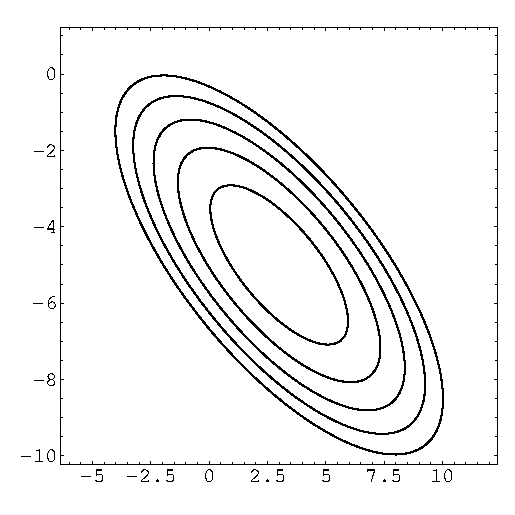
\epsfig{file=kuvat/saari.eps}
\end{center}
\end{figure}
\begin{Exa} Määritä funktion $f(x,y)=x+2y+2$ arvojoukko yksikköneliössä
\[
A=\{(x,y)\in\R^2 \; | \; 0\leq x\leq 1,\; 0\leq y\leq 1\}.
\]
\end{Exa}
\ratk
Tasa-arvokäyrät $S: f(x,y)=c\ $ ovat suoria
%\begin{multicols}{2} \raggedcolumns
\[
x+2y+2=c,
\]
\begin{multicols}{2} \raggedcolumns
joten arvojoukko on (kuva!)
\[
f(A)=[2,5]. \loppu
\]
\begin{figure}[H]
\begin{center}
\import{kuvat/}{kuvaV-1.pstex_t}
\end{center}
\end{figure}
\end{multicols}

\subsection*{Kolmen muuttujan funktiot}
\index{kolmen muuttujan funktio|vahv}

Kolmen reaalimuuttujan funktio on tyyppiä
\[
f:\R^3\kohti\R \quad \text{tai} \quad f:A\kohti\R, \quad A\subset\R^3. 
\]
Kolmen muuttujan funktioita voi havainnollistaa esimerkiksi \pain{vii}p\pain{aloimalla}: 
Valitaan äärellinen joukko muuttujan $z$ arvoja $z_i$ ja tutkitaan kahden muuttujan funktioita
\[
g_i(x,y)=f(x,y,z_i).
\]
\index{zza@\sov!Tomografia}%
\begin{Exa}: \vahv{Tomografia.} \label{tomografia} \ Lääketieteessä paljon käytetyllä 
(tietokone)tomo\-grafialla määritetään nk.\ varjostumafunktio $f$, jonka määrittelyjoukko on
ihmisruumis tai sen osa. Varjostumafunktion arvot ovat reaalilukuja, jotka kertovat
varjostuman tummuusasteen. Funktiosta $f$ saadaan mittausten avulla likimäärin selville
viipaloitujen funktioiden $g_i(x,y)=f(x,y,z_i)$ arvot valituilla (äärellisen monella) $z_i$:n
arvoilla. Funktiot $g_i$ määrätään yhdistämällä suuri joukko erisuuntaisia röntgen(varjo)kuvia 
laskennallisin keinoin (tietokoneen avulla).

Olkoon tarkastelun kohteena (idealisoitu) ihmisen pää
\[
A=\{P \vastaa (x,y,z)\in \R^3 \mid x^2+y^2+z^2\leq 7^2\}
\]
(pituusyksikkö = cm). Tomografiakuvaus tuottakoon varjostumafunktion
\[
f(x,y,z)=1+0.02(2x-3y+6z).
\]
Missä on kirkkainta ja missä tumminta?
\end{Exa}
\ratk Funktio $f$ on saatu käytännössä yhdistelemällä joukko viipalefunktioita
$g_i(x,y)=f(x,y,z_i)$, missä $-7<z_i<7$. Sikäli kuin mittaukset ja niistä lasketut funktiot
$g_i$ ja $f$ katsotaan tarkoiksi, on siis oltava
\[
g_i(x,y)=0.02(2x-3y)+c_i, \quad (x,y) \in A_i\,,
\]
missä $c_i=0.12z_i+1$, ja $A_i$ on kiekon muotoinen leikkauskuvio
\[
A_i=
\{(x,y) \in \R^2 \mid x^2+y^2\leq r_i^2\}, \quad r_i=\sqrt{7^2-z_i^2}.
\]
Funktion $g_i$ tasa-arvokäyrät ovat suoria
\[
2x-3y=\text{vakio},
\]
joten $g_i$:n maksimi ja minimi löytyvät näiden suorien normaalin $3x+2y=0$ ja $A_i$:n 
reunaviivan leikkauspisteistä.
\begin{figure}[H]
\begin{center}
\setlength{\unitlength}{1cm}
\begin{picture}(8,8)(-4,-4)
\put(0,0){\vector(1,0){4}} \put(3.8,-0.4){$x$}
\put(0,0){\vector(0,1){4}} \put(0.2,3.8){$y$}
\put(0,0){\bigcircle{6}}
\multiput(-1,1.5)(1,-1.5){3}{\drawline(-3.5,-2.33)(3.5,2.33)}
\drawline(-2.33,3.5)(2.33,-3.5)
\put(-1.75,2.4){$\bullet$} \put(1.58,-2.6){$\bullet$ $g_i=$max!}
\put(-1.75,3.1){$g_i=$min!}
\put(3,3){$g_i(x,y)=$vakio} \put(2,-4){$3x+2y=0$}
\end{picture}
\end{center}
\end{figure}
Eri viipalekuvia tutkimalla löydetään likimain myös $f$:n maksimi- ja minimiarvot. Tässä
\index{tasa-arvopinta}%
$f$ kuitenkin tunnetaan tarkasti, joten voidaan suoraan tutkia $f$:n \kor{tasa-arvopintoja}.
Nämä ovat tasoja
\[
2x-3y+6z=\text{vakio},
\]
joten voidaan geometrisesti päätellä, että $f$:n maksimi ja minimi löytyvät origon kautta
kulkevan tasa-arvopintojen yhteisen normaalin
\[
\begin{cases} x=2t, \\ y=-3t, \\ z=6t \end{cases}
\]
ja kappaleen reunapinnan
\[
x^2+y^2+z^2=7^2
\]
leikkauspisteistä. Nämä pisteet vastaavat $t$:n arvoja
\[ 
(2t)^2+(-3t)^2+(6t)^2=7^2 \qekv t= \pm 1. 
\]
Varjostuman maksimi- ja minimiarvoiksi päätellään näin muodoin
\begin{alignat*}{3}
&f(2,-3,6)  &\ = 1.98 &= f_{\text{max}}\,, \\
&f(-2,3,-6) &\ = 0.02 &= f_{\text{min}}\,. \qquad\loppu
\end{alignat*}

\subsection*{Funktiot käyräviivaisissa koordinaatistoissa} 
\index{funktio B!h@käyräv.\ koordinaatistoissa|vahv}
\index{muuttujan vaihto (sijoitus)!a@käyräv.\ koordinaatteihin|vahv}
\index{kzyyrzy@käyräviivaiset koordinaatistot!a@--funktiot|vahv}

Kahden ja kolmen reaalimuuttujan funktioita tutkittaessa voi olla apua siirtymisestä 
käyräviivaiseen napa-, lieriö- tai pallokoordinaatistoon silloin kun funktion 
määrittelyjoukon geometria on sellaiseen muunnokseen sopiva. Esimerkiksi, jos kahden
reaalimuuttujan funktio on määritelty pyörähdyssymmetrisessä joukossa $A\subset\Rkaksi$
(voi olla myös $A=\Rkaksi$), voi napakoordinaatteihin siirtyminen auttaa. Siirtyminen tapahtuu
muunnoksella (vrt. Luku \ref{koordinaatistot})
\begin{multicols}{2} \raggedcolumns
\begin{align*}
f(x,y)&=f(r\cos\varphi,r\sin\varphi) \\[2mm]
      &=g(r,\varphi).
\end{align*}
\begin{figure}[H]
\setlength{\unitlength}{1cm}
\begin{center}
\begin{picture}(4,3)(-1,0)
\put(-1,0){\vector(1,0){4}} \put(2.8,-0.4){$x$}
\put(0,0){\vector(0,1){3}} \put(0.2,2.8){$y$}
\put(0,0){\vector(2,3){1.5}}
\arc{1}{5.25}{6.2}
\put(0.5,1.1){$r$} \put(0.5,0.25){$\varphi$} \put(1.45,2.15){$\bullet$ $(x,y)$}
\end{picture}
\end{center}
\end{figure}
\end{multicols}
Huomattakoon, että muunnettu funktio $g$ on itse asiassa yhdistetty funktio
\[
g(r,\varphi)=f(x(r,\varphi),y(r,\varphi)),
\]
missä $x(r,\varphi)=r\cos\varphi,\ y(r,\varphi)=r\sin\varphi$. Siirtyminen 
polaarikoordinaatistosta karteesiseen tapahtuu käänteismuunnoksella
\[
f(x,y)=g(r(x,y),\varphi(x,y)),
\]
missä $\,r(x,y)=\sqrt{x^2+y^2}\,$ ja $\,\varphi(x,y)\,$ on pistettä $(x,y)$ vastaava 
napakulma\footnote[2]{Merkinnöissä $x(r,\varphi)$, $y(r,\varphi)$, $r(x,y)$ ja $\varphi(x,y)$
on alunperin riippumattomista muuttujista $x,y$ tai $r,\varphi$ tehty funktiosymboleja.
Koordinaattimuunnoksissa (myös implisiittifunktioissa, vrt.\ edellinen luku) tällaiset
merkinnät ovat tavallisia, koska ne selkeyttävät laskemista.}
($\varphi$:n laskukaava on hieman konstikas, ks.\ edellisen luvun Esimerkki 
\ref{napakulman kaava}).

Kolmen muuttujan funktioita tarkasteltaessa voidaan siirtyä lieriö- tai 
pallokoordinaatistoon muunnoksilla
\begin{align*}
\text{Lieriö:} \quad  f(x,y,z) &= f(r\cos\varphi,r\sin\varphi,z) =g(r,\varphi,z). \\
\text{Pallo:} \quad\  f(x,y,z) &= f(r\sin\theta\cos\varphi,r\sin\theta\sin\varphi,r\cos\theta)
                                = g(r,\theta,\varphi).
\end{align*}
Lieriökoordinaatiston tapauksessa muunnos $(x,y)\ext(r,\varphi)$, samoin käänteismuunnos
$(r,\varphi)\ext(x,y)$ on sama kuin napakoordinaatistossa. Pallokoordinaatistossa 
käänteismuunnos on
\begin{align*}
g(r,\theta,\varphi) &= g(r(x,y,z),\theta(x,y,z),\varphi(x,y)) \\
&=f(x,y,z),
\end{align*}
missä
\begin{align*}
     r(x,y,z) &= \sqrt{x^2+y^2+z^2}, \\
\theta(x,y,z) &= \Arccos\left(\frac{z}{\sqrt{x^2+y^2+z^2}}\right),
\end{align*}
ja $\varphi(x,y)$ on sama kuin napakoordinaatistossa. Suuntakulma $\theta$ ei ole määritelty
origossa eikä kulma $\varphi$ $z$-akselilla.
\begin{Exa}
Vuoristoisen maaston korkeus merenpinnasta on origon ympäristössä
\[
f(x,y)=x^2-2xy-3y^2+0.2x-0.1y+10
\]
(yksikkö = 100 m). Origossa on kahden tien risteys. Tiet ovat kartalla suoria ja myös niiden
sivuprofiili on suora. Mihin suuntiin tiet kulkevat ja mikä on teiden kaltevuus?
\end{Exa}
\ratk
Siirrytään napakoordinaatistoon:
\[
f(x,y)=h(r,\varphi)=r^2(\cos^2 \varphi-2\cos\varphi\sin\varphi-3\sin^2\varphi) 
                                      + r(0.2\cos\varphi-0.1\sin\varphi) +10.
\]
Tiet noudattavat origosta lähdettäessä puolisuoria $\varphi=\varphi_1$ ja $\varphi=\varphi_2$
(koska ovat kartalla suoria). Koska teiden sivuprofiilikin on suora, on oltava
\[
\cos^2 \varphi-2\cos\varphi\sin\varphi-3\sin^2\varphi=0.
\]
Tässä ei $\,\cos\varphi=0\,$ ole ratkaisu, joten voidaan jakaa $\cos^2\varphi$:lla:
\[
1-2\tan\varphi-3\tan^2\varphi=0 
           \qekv \begin{cases}
                  \,\tan\varphi_1=1/3 \ & \impl \ \ \varphi_1 \approx 18\aste\ 
                                                              \text{tai}\ 198\aste, \\
                  \,\tan\varphi_2=-1 \  & \impl \ \ \varphi_2 =135\aste\
                                                              \text{tai}\ 315\aste.
                  \end{cases}
\]
Kaltevuuskulmat suuntiin $\varphi_1 \approx 18\aste$ ja $\varphi_2=135\aste$ saadaan
ratkaisemalla
\[
\tan\alpha_i=0.2\cos\varphi_i-0.1\sin\varphi_i
                  \qimpl \begin{cases}
                         \,\alpha_1\approx 9\aste, \\
                         \,\alpha_2\approx -12\aste.
                         \end{cases} \qquad\loppu
\]

\begin{Exa}
Etsi (jos mahdollista) pisteet, joissa funktio
\[
f(x,y,z)=xyz(3x^2+3y^2-z^2)/(x^2+y^2)
\]
saavuttaa maksimi- tai minimiarvonsa joukossa
\[
A=\{(x,y,z)\in\R^3 \ | \ x^2+y^2+z^2\leq 96, \ (x,y)\neq (0,0)\}.
\]
\end{Exa}
\ratk Siirrytään pallokoordinaatistoon. Koska pallokoordinaateissa on
\[
x^2+y^2=r^2\sin^2\theta(\cos^2\varphi + \sin^2\varphi)=r^2\sin^2\theta,
\]
niin (vrt.\ Luku \ref{trigonometriset funktiot})
\begin{align*}
f(x,y,z)\,=\,g(r,\theta,\varphi) 
         &=\,r^3\cos\theta\,(3\sin^2\theta-\cos^2\theta)\cos\varphi\sin\varphi \\[2mm]
         &=\,r^3\,(3\cos\theta-4\cos^3\theta)\cos\varphi\sin\varphi \\
         &=-\frac{1}{2}\,r^3\cos 3\theta\sin 2\varphi.
\end{align*}
Funktio $g$ saavuttaa maksimiarvonsa $192\sqrt{6}$ pallon pinnalla $(r=\sqrt{96}=4\sqrt{6})$, 
kun joko $\cos 3\theta=-1$, $\sin 2\varphi=1$ tai $\cos 3\theta=1$, $\sin 2\varphi=-1$. 
Maksimikohtia on neljä:
\[
\begin{array}{llllrr}
(r, & \theta, & \varphi) & (x, & y, & z) \\ \\
(4\sqrt{6}, & \pi/3, & \pi/4) \quad & (\ \: \, 6, &6, &2\sqrt{6}) \\ 
(4\sqrt{6}, & \pi/3, & 5\pi/4) \quad & (-6, &-6, &2\sqrt{6}) \\ 
(4\sqrt{6}, & 2\pi/3, & 3\pi/4) \quad & (-6, & 6, &-2\sqrt{6}) \\ 
(4\sqrt{6}, & 2\pi/3, & 7\pi/4) \quad & (\ \: \, 6, &-6, &-2\sqrt{6})
\end{array}
\]
Minimikohtia (joissa $g=g_{\text{min}}=-192\sqrt{6}$) on samoin neljä. Nämä saadaan vaihtamalla
yhden koordinaatin merkki maksimipisteiden karteesisessa esitysmuodossa. Funktio $g$ saavuttaa
maksimi- tai minimiarvonsa myös pallonpintakoordinaattien arvoilla 
$(\theta,\varphi) \in  \{0,\pi\} \times \{\pi/4,\ 3\pi/4,\ 5\pi/4,\ 7\pi/4\}$. Nämä vastaavat 
kuitenkin karteesisen koordinaatiston pisteitä $(0,0,z)$, jotka ovat alkuperäisen funktion $f$ 
määrittelyjoukon ulkopuolella. \loppu

\subsection*{Usean muuttujan funktioiden yhdistely}
\index{funktio B!e@yhdistetty|vahv}
\index{yhdistetty funktio|vahv}

Useamman reaalimuuttujan reaaliarvoisia funktioita voi yhdistellä yhdistetyiksi funktioiksi 
samoilla periaatteilla kuin yhden muuttujan tapauksessa. Lisäehtona on kuitenkin, että funktiot
ovat tyypiltään yhteensopivia. Esimerkiksi funktioiden $f(x)$ ja $g(x,y)$ yhdistetty funktio 
$F = f \circ g$  voidaan määritellä: 
\[ 
F(x,y) = (f \circ g)(x,y) = f(g(x,y)), \quad \DF_F = \{(x,y) \in \DF_g \mid g(x,y) \in \DF_f\}.
\]
Voidaan myös määritellä yhdistetyt funktiot
\begin{align*}
&G_1(x) = g(x,f(x)),   \quad \DF_{G_1} = \{x \in \DF_f \mid (x,f(x)) \in \DF_g\}, \\
&G_2(y) = g(f(y),y), \,\quad \DF_{G_2} = \{y \in \DF_f \mid (f(y),y)\,\in \DF_g\}, \\
&G_3(x,y) = g(f(x),f(y)),\quad \DF_{G_3} 
                               = \{(x,y) \in \DF_f \times \DF_f \mid (f(x),f(y)) \in \DF_g\}.
\end{align*}
Funktiota $g \circ f$ sen sijaan ei voi määritellä, ei myöskään funktiota $g \circ g$.
\begin{Exa} Jos $f(x) = \sqrt{x},\ \DF_f = [0,\infty)$ ja $g(x,y) = x-y^2,\ \DF_g = \R^2$, niin
\begin{align*}
&F(x,y) = (f \circ g)(x,y) = \sqrt{x-y^2}, \quad \DF_F = \{(x,y) \in \R^2 \mid x \ge y^2\}, \\
&G(x) = g(x,f(x)) = 0, \quad \DF_G = [0,\infty). \loppu
\end{align*} \end{Exa}
\begin{Exa} Määritä funktion $f(x,y) = x^2 + 2y^2 + 2xy + 4x + 14y$ minimiarvo suoralla 
$S:\ y = 2x-5$. (Vrt.\ Esimerkki \ref{saari}.) \end{Exa}
\ratk Kun käytetään suoralla $S$ vallitsevalle funktioriippuvuudelle $x \map y$ 
merkintää $y(x)$, niin kyse on yhdistetystä funktiosta $F(x) = f(x,y(x))$, $\DF_F = \R$.
Koska
\begin{align*}
 F(x) = f(x,2x-5) &= x^2 + 2(2x-5)^2 + 2x(2x-5) + 4x + 14(2x-5) \\[3mm]
                  &= 13x^2 - 18x - 20 \\
                  &= 13\left(x-\dfrac{9}{13}\right)^2 - \dfrac{341}{13}\,,
\end{align*}
niin nähdään, että kysytty minimiarvo on
\[ 
F_{\text{min}} = -\dfrac{341}{13} \approx -26.2. 
\]
Minimikohta on suoran pisteessä $(9/13,-47/13) \approx (0.69,-3.62)$. \loppu

Useamman muuttujan funktioita voidaan yhdistellä myös laskutoimituksin samalla tavoin kuin
yhden muuttujan funktioita (Määritelmä \ref{funktioiden yhdistelysäännöt}).  Ellei
yhdisteltävien funktioiden muuttujien lukumäärä täsmää, on ajateltava, että funktioissa on 
'näkymättömiä' muuttujia. 
\begin{Exa} Jos $f(x) = \tan x\,$ ja $\,g(x,y) = \sin(x+y^2)$, niin kirjoitettaessa
\[ 
F(x,y) = \tan x + \sin (x+y^2) 
\]
tarkoitetaan tämän laskusäännön ilmaisemaa funktiota $F$, määrittelyjoukkona 
\[ 
\DF_F = \{(x,y) \in \R^2 \mid x \neq (n+1/2)\,\pi\,\ \forall n \in \Z\}.
\]
Samaan tulokseen tullaan myös funktioiden yhdistelyn kautta ajattelemalla, että
$F = \tilde{f} + g,\ \DF_F = \DF_{\tilde{f}} \cap \DF_g$, missä $\tilde{f}$ on saatu $f$:stä
lisäämällä toinen muuttuja:
\[ 
\tilde{f}(x,y) = \tan x, \quad \DF_{\tilde{f}} = \DF_f \times \R. \loppu
\] 
\end{Exa}

\subsection*{Kahden muuttujan implisiittifunktiot}
\index{funktio B!j@implisiittifunktio|vahv}
\index{implisiittifunktio|vahv}

Jos $F$ on kolmen muuttujan funktio ja yhtälö
\[
F(x,y,z)=0
\]
ratkeaa $z$:n suhteen, kun $(x,y)\in A\subset\R^2$, niin yhtälö määrittelee $A$:ssa
kahden muuttujan (mahdollisesti monihaaraisen) implisiittifunktion. Jos tälle käytetään
funktiomerkintää $z(x,y)$, niin määritelmä on siis
\[
F(x,y,z(x,y))=0, \quad (x,y)\in A.
\]
\begin{Exa}
Yhtälö $x^2+y^2+z^2=R^2$ määrittelee kaksihaaraisen implisiittifunktion
$z(x,y)=\pm\sqrt{R^2-x^2-y^2}\,$ kiekossa $A:\ x^2+y^2 \le R^2$. \loppu
\end{Exa}
\begin{Exa} Jos $m\in\N,\ m \ge 2$, niin yhtälö
\[
y,z\in\C: \quad y^m=z
\]
määrittelee $m$-haaraisen kompleksifunktion $y=\sqrt[m]{z}$, vrt.\ Luku \ref{III-3}.
Jos kirjoitetaan $z=x+iy$ ja $y=u(x,y)+iv(x,y)$, niin $u$ ja $v$ ovat $m$-haaraisia
funktioita tyyppiä $u,v:\ \Rkaksi\kohti\R$. \loppu
\end{Exa}

\Harj
\begin{enumerate}

\item
Määritä seuraavien funktioiden arvojoukot annetulla janalla $AB$\,: \newline
a) \ $f(x,y)=x^2+2xy-y^2,\,\ A=(1,2),\ B=(-1,3)$ \newline
b) \ $f(x,y,z)=x+xy+yz+z^2,\,\ A=(1,1,1),\ B=(-1,2,-3)$

\item
Määritä seuraavien funktioiden arvojoukot annetussa joukossa $A$: \newline
a) \ $f(x,y)=x+3y-1$, \ $A=$ kolmio, jonka kärjet $(0,1)$, $(4,0)$ ja $(3,4)$ \newline
b) \ $f(x,y,z)=x+2y-3z$, \ $A=\{(x,y,z) \mid (x-1)^2+(y+1)^2+(z-2)^2 \le 9\}$ \newline
c) \ $f(x,y,z)=x+xy+yz+z^2$, \ $A=$ suora $\,2x-2=y+1=4-2z$

\item
Tasangolla $z=0$ on järvi $A=\{(x,y)\in\Rkaksi \mid h(x,y)<0\}$, missä
\[
h(x,y) = 4x^2+y^2+24x+8y
\]
on järven pohjan korkeusprofiili. Tässä $h$ on ilmaistu metreinä ja $x,y$ kilometreinä.
Järven poikki kulkee moottoritie suoraa $y=x+2$ pitkin. Missä on järven syvin kohta ja mikä
on syvyys tässä kohdassa? Hahmottele järven rantaviiva ja laske, missä pisteissä moottoritie
leikkaa rantaviivan.

\item
Muunna seuraavat funktiot napa- tai pallokoordinaatistoon:
\begin{align*}
&\text{a)}\ \ f(x,y)=x+2y \qquad \text{b)}\ \ f(x,y)=xy^2 \qquad 
 \text{c)}\ \ f(x,y)=\frac{xy}{x^2+y^2} \\
&\text{d)}\ \ f(x,y)=\max\{0,x,y\} \qquad
 \text{e)}\ \ f(x,y)=\begin{cases} x^2/y, &\text{kun}\ x > 0\ \text{ja}\ y>0 \\
                                   0,     &\text{muulloin}
                     \end{cases} \\
&\text{f)}\ \ f(x,y)=\begin{cases} xy^2-y^3, &\text{kun}\ 0 \le x \le y \\
                                   0,        &\text{muulloin}
                     \end{cases} \qquad
 \text{g)}\ \ f(x,y,z)=\frac{xyz}{x^2+y^2+z^2} \\
&\text{h)}\ \ f(x,y,z)=\frac{xy^2z^3}{x^2+y^2} \qquad 
 \text{i)}\ \ f(x,y,z)=\begin{cases}
                      \,z^2-xyz, &\text{kun}\ z>0 \\ \,0, &\text{kun}\ z \le 0
                      \end{cases}
\end{align*}

\item
Muunna seuraavat napakoordinaateissa ilmaistut funktiot karteesiseen koordinaatistoon:
\begin{align*}
&\text{a)}\ \ g(r,\varphi)=r^3(\cos\varphi-\sin\varphi) \qquad
 \text{b)}\ \ g(r,\varphi)=\sin 2\varphi-r^2\cos 2\varphi \\
&\text{c)}\ \ g(r,\varphi)=r^2(\tan\varphi+\cot\varphi) \qquad
 \text{c)}\ \ g(r,\varphi)=\frac{\sin\varphi}{2+\cos\varphi}
\end{align*}

\item
Olkoon $f(x,y)=x+y$ ja $g(x,y)=xy,\ (x,y)\in\Rkaksi$. Määrittele sievennettyinä lausekkeina 
(laskusääntöinä) seuraavat yhdistetyt funktiot: \newline
a) \ $f(x,g(x,y))\quad$ b) \ $f(g(x,y),y)\quad$ c) \ $f(g(x,y),g(x,y))$ \newline
d) \ $g(x,f(x,y))\quad$ e) \ $g(f(x,y),y)\quad$ f) \ $g(f(x,y),f(x,y))$ \newline
g) \ $f(f(x,y),f(x,y))\quad$ h) \ $g(g(x,y),g(x,y))$

\item
Olkoon $f(x)=\sqrt{2-x}$ ja $g(x,y)=\sqrt{x-y^2}\ (x,y\in\R)$. Määrittele yhdistetty funktio
$F=f \circ g$ (laskusääntö ja määrittelyjoukko).

\item
Olkoon $f(x)=\sqrt{25-x^2}$ ja $g(x,y)=3x+4y-1\ (x,y\in\R)$. Määritä yhdistetyn funktion
$F=f \circ g$ pienin ja suurin arvo yksikkökiekon neljänneksessä
$A= \{\,(x,y)\in\Rkaksi \mid x \ge 0\,\ja\,y \ge 0\,\ja\,x^2+y^2 \le 1\,\}$.

\item
a) Esitä kompleksifunktion $f(z)=(z+1)^2+(z+i)^2$ reaaliosa, imaginaariosa ja itseisarvo
funktioina tyyppiä $g:\ \Rkaksi \kohti \R$. \vspace{1mm}\newline
b) Määrittele kaksihaaraiset funktiot $u=\{u_1,u_2\}$ ja $v=\{v_1,v_2\}$ siten, että
$u(x,y)+iv(x,y)=\sqrt{z}\ \ \forall z=x+iy\in\C$.

\item
Yhtälö $x+3xyz^2+z^4=0\ (x,y,z\in\R)$ määrittelee implisiittifunktion $z=f(x,y)$. \ a) Laske 
$f$:n arvot pisteissä $(0,0)$, $(2,-1)$ ja $(1,1)$. \ b)  Millaisia ovat $f$:n haarat 
(määrittelyjoukot ja laskusäännöt) yleisemmin?

\item (*)
Vuoristoisen maaston korkeus merenpinnasta on origon $O$ lähellä funktio
\[
f(x,y)=\frac{1}{20}(3x^2-5xy-2y^2)+2.
\]
Origossa on kahden tien $S_1,S_2$ risteys. Tiet ovat maastoon sovitettuja ja vaakasuoria, ja 
lisäksi ne ovat kartallakin suoria. Teiden $S_1,S_2$ poikki kulkee suora rautatie pisteissä
$A\in S_1$, $B\in S_2$. Molemmat pisteet ovat $O$:sta etäisyydellä $1$ (yksikkö = km).
Mikä on suurin pudotuskorkeus laaksoon rautatiesillalta, jonka päät ovat pisteissä $A,B$\,?

\item (*)
Halutaan selvittää, missä pisteissä funktio $f(x,y)=x^2-2xy+3y^2$ saavuttaa suurimman ja 
pienimmän arvonsa\, a) ympyrällä \mbox{$S: x^2+y^2=9$}, \ \ b) kiekossa 
$A=\{(x,y)\in\Rkaksi \mid x^2+y^2 \le 9\}$. Ratkaise ongelma napakoordinaatteja käyttäen 
(vrt.\ Harj.teht.\,\ref{trigonometriset funktiot}:\ref{H-II-5: minmax}).

\item (*)
Funktiosta $f(x)=x-x^3\,$ tiedetään, että välillä $[0,1]$ $f$ saavuttaa suurimman arvonsa
pisteessä $x=1/\sqrt{3}$. Mihin suuntaan origosta lähdettäessä funktio\, a) $f(x,y)=xy^2$,\,
b) $f(x,y,z)=xy^2z^3$ kasvaa nopeimmin suhteessa kuljettuun matkaan?

\item (*) \index{zzb@\nim!Funktio avaimenreiässä} 
(Funktio avaimenreiässä) Olkoon
\[
A=\{\,(x,y,z)\in \R^3 \mid (x,y)\in B_1 \cup B_2,\,\ z\in[0,10]\,\},
\]
missä 
\begin{align*}
B_1 &= \{\,(x,y)\in\Rkaksi \mid x^2+(y-1)^2 \le 2\,\ja\, y \ge 0\,\}, \\
B_2 &= \{\,(x,y)\in\Rkaksi \mid x\in[-1,1]\,\ja\,y\in [-4,0]\,\}.
\end{align*}
Missä $A$:n pisteissä funktio $f(x,y,z)=x-3y+2z$ saavuttaa suurimman ja missä pienimmän arvonsa?

\end{enumerate}

 % Kahden ja kolmen muuttujan funktiot
\section{Parametriset käyrät ja pinnat} \label{parametriset käyrät}
\alku
\index{funktio A!f@parametrinen käyrä ja pinta|vahv}
\index{parametrinen käyrä|vahv}
\index{parametri(sointi)!c@käyrän|vahv}
\index{kzyyrzy@käyrä|vahv}

Tason tai avaruuden \kor{parametriseksi käyräksi} sanotaan \pain{funktiota} muotoa
\[ 
t \in A\ \map\ P(t)\in E^d, 
\]
missä $A \subset \R$ on \pain{väli} (usein suljettu väli) ja $d=2$ tai $d=3$. Muuttujaa $t$ 
sanotaan tässä \kor{parametriksi}. Käyrä on \kor{tasokäyrä} jos $d=2$, \kor{avaruuskäyrä} jos 
$d=3$. Käyttäen jo tutuksi tulleita geometrisia vastaavuuksia voidaan kirjoittaa
\[
P(t)\ \vastaa\ \Vect{OP}(t)\ 
                = \left\{ \begin{array}{lrlll} 
                   x(t)\vec{i}+y(t)\vec{j} & \vastaa & (x(t),y(t)),      & & (d=2) \\
                   x(t)\vec{i}+y(t)\vec{j}+z(t)\vec{k} & \vastaa & (x(t),y(t),z(t)), & & (d=3)
                          \end{array} \right.
\]
missä $x,y,z$ ovat funktioita tyyppiä $f: A \kohti \R$. Tämän mukaisesti parametrinen käyrä 
\index{vektoric@vektoriarvoinen funktio}%
voidaan tulkita reaalimuuttujan \kor{vektoriarvoiseksi} funktioksi, jolloin luonteva esitystapa
on myös vektorimerkintä
\[ 
\vec{r}\,(t)\ =\ \begin{cases} 
   x(t)\vec{i}+y(t)\vec{j},\ \ t \in A,                   &\text{(tasokäyrä)} \\
   x(t)\vec{i}+y(t)\vec{j}+z(t)\vec{k},\ \ t \in A. \quad &\text{(avaruuskäyrä)}
               \end{cases}
\]
Liittyen vastaavuuteen $\mathit{E^d} \vast \R^d$ voidaan parametrinen käyrä esittää yhtä hyvin 
yhtälöryhmänä, esim.\ tasokäyrän tapauksessa
\[ 
(x,y)\ =\ (x(t),y(t)) \qekv 
        \begin{cases} \,x = x(t), \\ \,y = y(t). \end{cases} \quad 
\text{(tasokäyrä)}\footnote[2]{Merkinnöissä $x=x(t)$ ja $y=y(t)$ on symboleja $x,y$ käytetty
kahdessa eri merkityksessä: oikealla funktion, vasemmalla ko.\ funktion arvojoukon alkion
symbolina. Tämän tyyppisiä epäloogisuuksia pidetään matematiikan käytännössä siedettävinä,
syystä että ne yksinkertaistavat merkintöjä.}
\]
\begin{Exa} Reaalimuuttujan funktio $f: [a,b] \kohti \R$ voidaan tulkita parametriseksi
tasokäyräksi
\[ 
\vec{r} = \vec{r}\,(t) = t\vec{i} + f(t)\vec{j} \qekv 
                           \begin{cases} \,x = x(t) = t, \\ \,y = y(t) = f(t),\ \ t \in [a,b]. 
                           \end{cases} \loppu 
\] 
\end{Exa}
\begin{Exa} Luvuista \ref{suorat ja tasot} ja \ref{koordinaatistot} tuttuja parametrisia 
avaruuskäyriä ovat
\begin{align*}
&\text{avaruussuora:}\quad \vec{r}\,(t)\ 
          =\ (x_0 + \alpha t)\vec{i} + (y_0 + \beta t)\vec{j} + (z_0 + \gamma t)\vec{k}\ 
          =\ \vec{r}_0 + t \vec{v}, \quad t \in \R, \\ 
&\text{ruuviviiva:}\quad \begin{cases}
                          \,x = x(\varphi) = R\cos\varphi, \\ 
                          \,y = y(\varphi) = R\sin\varphi, \\ 
                          \,z = z(\varphi) = a\varphi,\ \ \varphi \in \R. \loppu
                         \end{cases} 
\end{align*} 
\end{Exa}
Parametrisen käyrän euklidiseen avaruuteen jättämä 'geometrinen jälki' on arvojoukko 
$S = \{P(t) \vastaa \vec{r}\,(t) \mid t \in A\} \subset E^d$, johon voidaan viitata sellaisilla 
termeillä kuin \kor{käyrä} (engl.\ curve) tai (käyrän) \kor{kaari} (engl.\ arc). 
Yksinkertaisimmillaan $S$ on jostakin pisteestä $A$ alkava ja toiseen pisteeseen $B$ päättyvä,
\index{yksinkertainen!c@käyrä, kaari} \index{kaari (käyrän)}%
itseään leikkaamaton ja yhtenäinen viiva, eli nk.\ \kor{yksinkertainen kaari} (engl.\ 
simple arc). Tällaisia ovat esim.\ jana tai ympyrän kaari. Viiva voi myös olla päättymätön, 
kuten suora, tai umpinainen
\index{suljettu käyrä}%
\kor{suljettu käyrä} (engl.\ closed curve), kuten tason tai 
avaruuden ympyräviiva. Joukko $S$ voi myös olla itseään leikkaava, eli siinä voi olla 
'silmukoita'.\footnote[2]{Muodossa $S = \{P(t) \vastaa \vec{r}\,(t) \mid t \in A\}$
määriteltyjen taso- tai avaruuskäyrien geometrista luokittelua ei todellisuudessa voi
täsmentää ilman funktion $\vec{r}$ koordinaattifunktioile $x,y,z$ asetettavia lisäehtoja.
Vrt.\ käyriä koskeva alaviite edellisessä luvussa.}
Jos lähtökohdaksi otetaan vain tällainen 'viiva' $S$, eli pelkästään geometrinen objekti, niin 
funktiota $\vec{r}\,(t),\ t \in A$, jonka arvojoukko $=S$, sanotaan $S$:n 
\kor{parametriesitykseksi} eli \kor{parametrisoinniksi} (parametrisaatioksi). 
Parametrisoivan funktion $t \in A \map \vec{r}\,(t) \in S$ ei tarvitse olla injektiivinen, ts.\ 
samaan pisteeseen $P \in S$ voidaan päätyä monella (jopa äärettömän monella) parametrin
arvolla.
\begin{Exa} \label{ympyrän parametrisaatio} Tason ympyräviivan 
\[ 
S = \{P \vastaa (x,y) \in \R^2 \mid (x-x_0)^2 + (y-y_0)^2 = R^2\} 
\]
luonteva parametrisointi on
\[ 
\begin{cases} x = x_0 + R \cos t, \\ y = y_0 + R\,\sin t,\ \ t \in [0,2\pi). \end{cases} 
\]
Tässä voi välin $[0,2\pi)$ tilalla olla myös esim.\ $A = (-\pi,\pi]$, $A = [0,2\pi]$ tai
$A = \R$. Kahdessa jälkimmäisessä vaihtoehdossa parametrisointi ei ole injektio. \loppu
\end{Exa}
\begin{Exa} Jos $S$ on avaruussuora, niin tämän tavanomaisin parametrisaatio on 
$\vec{r}\,(t) = \vec{r}_0 + t \vec{v},\ t \in \R$, missä $P_0 \vastaa \vec{r}_0$ on suoran
piste ja $\vec{v} \neq \vec{0}$ suoran suuntavektori (vrt.\ Luku \ref{suorat ja tasot}).
Tällaisiakin parametrisointeja on jo äärettömän monta, mutta mahdollisuudet eivät lopu tähän:
Jos $\vec{r}_0$ ja $\vec{v}$ täyttävät mainitut ehdot, niin parametrisoinniksi voidaan
yleisemmin valita
\[ 
\vec{r}\,(t)\ =\ \vec{r}_0 + f(t)\,\vec{v}, \quad t \in A, 
\]
missä funktion $f: A \kohti \R$ valintaa rajoittaa vain ehto $\RF_f = \R$. Esimerkiksi voidaan 
valita $f(t) = \tan t,\ A = (-\pi/2,\pi/2)$ ($f$ injektio), tai $f(t) = t \sin t,\ A = \R$ 
($f$ ei injektio).  \loppu \end{Exa}
\jatko \begin{Exa} (jatko) Jos halutaan parametrisoida suoralla $S$ oleva jana, jonka 
päätepisteet ovat $A \vastaa \vec{r}_1$ ja $B \vastaa \vec{r}_2$, niin tämä käy muodossa
\[ 
\vec{r}\,(t) = f(t)\,\vec{r}_1 + [1-f(t)]\,\vec{r}_2,\ \ t \in A, 
\]
missä $f$ on funktio tyyppiä $f: A \kohti \R,\ A \subset \R$, ja $\RF_f = [0,1]$.
Yksinkertaisin parametrisointi saadaan, kun valitaan $A = [0,1]$ ja $f(t) = t$. \loppu 
\end{Exa}
Jos tasokäyrän yhtälöistä $x = x(t),\ y = y(t),\ t \in A$ pystytään eliminoimaan parametri
$t$, on tuloksena yhtälö muotoa
\[ 
F(x,y) = 0, 
\]
missä siis $F$ on kahden muuttujan funktio, jolle pätee $F(x(t),y(t)) = 0\,\ \forall t \in A$.
Jos $S = \{P \in \Ekaksi \mid P \vastaa (x(t),y(t))\ \text{jollakin}\ t \in A\}$, niin
sanotaan tällöin, että ym.\ yhtälö on \kor{käyrän} $S$ (tai pistejoukon $S$) \kor{yhtälö}.
Avaruuskäyrän tapauksessa johtaa parametrin eliminointi (onnistuessaan) yhtälöryhmään muotoa
\[ 
\begin{cases} \,F_1(x,y,z) = 0, \\ \,F_2(x,y,z) = 0. \end{cases} 
\]
\begin{Exa} Jos $a,b>0$, niin parametrinen tasokäyrä
\[ 
S:\ \begin{cases} \,x = a\cos t, \\ \,y = b\,\sin t,\ \ t \in [0,2\pi] \end{cases} 
\]
on nimeltään \kor{ellipsi} (tapauksessa $a=b$ ympyrä). Eliminoimalla $t$ saadaan $S$:n
yhtälöksi
\[ 
\frac{x^2}{a^2} + \frac{y^2}{b^2} = 1. \loppu
\]
\end{Exa}

\subsection*{Liikerata}
\index{liikerata|vahv}

Tyypillisessä parametrisen käyrän fysikaalisessa sovellustilanteessa parametri $t$ on 
\pain{aika}muuttuja, $A$ on tarkasteltava \pain{aikaväli}, ja $P(t) \vastaa \vec{r}\,(t)$ on 
liikkuvan pisteen (esim.\ pistemäiseksi ajatellun partikkelin tai liikkuvan kiinteän kappaleen 
pisteen) p\pain{aikka} hetkellä $t$. Tällöin funktion $P(t),\ t \in A$, arvojoukko $S$ on ko.\
pisteen \pain{liikerata} aikavälillä $A$. Funktio $t\map\vec r\,(t),\ t \in A$ on $S$:n
parametrisointi, joka kertoo koko \pain{liikehistorian}. 
\index{zza@\sov!Heittoparaabeli}%
\begin{Exa}: \vahv{Heittoparaabeli}. \label{heittoparaabeli}
Kivi heitetään tornista korkeudelta $h$ alkuvauhdilla $v_0$ ja kulmassa $\alpha$ vaakasuuntaan
nähden. Millainen on lentorata, jos ilmanvastusta ei huomioida?
\end{Exa}
\ratk Tarkastellaan liikettä (avaruustason) koordinaatistossa, jossa $x$ mittaa vaakasuoraa
etäisyyttä lähtöpisteestä ja $y$ korkeutta maan pinnan tasosta. Liikelakien mukaan kiven
paikka $P(t)=(x(t),y(t))$ on lentoajan $t$ funktiona parametrinen käyrä
\[
\begin{cases}
\,x(t)=v_0t\cos\alpha, \\
\,y(t)=h+v_0t\sin\alpha-\tfrac{1}{2}gt^2,
\end{cases}
\]
missä $g=$ maan vetovoiman kiihtyvyys. Eliminoimalla $t$ ja huomioimalla, että
$1/\cos^2\alpha=1+\tan^2\alpha\,$ saadaan lentoradan yhtälö muotoon
\[
y=h+kx-(1+k^2)\frac{x^2}{2a}\,,
\]
\index{paraabeli}%
missä $\,k=\tan\alpha\,$ ja $\,a=v_0^2/g$. Lentorata on \kor{paraabelin} kaari. Kuvan
tapauksessa $\alpha=0$ kivi törmää maahan hetkellä $t=\sqrt{2h/g}$. \loppu
\begin{figure}[H]
\setlength{\unitlength}{1cm}
\begin{center}
\begin{picture}(8,5)(0,0)
\put(0,0){\vector(1,0){8}} \put(7.8,-0.5){$x$}
\put(1,0){\vector(0,1){5}} \put(1.2,4.8){$y$}
\linethickness{0.05cm}
\multiput(0,0)(1,0){2}{\line(0,1){3.7}}
\multiput(0,3.7)(0.4,0){3}{\line(1,0){0.2}}
\multiput(0.2,3.7)(0.2,0){4}{\line(0,-1){0.2}}
\multiput(0.2,3.5)(0.4,0){2}{\line(1,0){0.2}}
\thinlines
\curve(1,3.7,4,2.8,6,0)
\end{picture}
\end{center}
\end{figure}
\index{zza@\sov!Sykloidi}%
\begin{Exa}: \vahv{Sykloidi}. \label{sykloidi}
$R$-säteinen pyörä vierii liukumatta pitkin tasoa siten, että pyörän keskipisteen liikenopeus
on $v_0\vec i$, $v_0=\text{vakio}$. Määritä pyörän ulkokehän pisteen $P$ paikka ajan $t$
funktioina.
\end{Exa}
\ratk Oletetaan, että pyörä vierii pitkin $x$-akselia ja että $P$ on origossa, kun $t=0$. 
Tällöin ratakäyrän parametriesitys on
\begin{multicols}{2} \raggedcolumns
\[
\begin{cases} x(t) = v_0t-R\sin \varphi(t), \\ y(t) = R-R\cos \varphi(t), \end{cases}
\]

\vspace{1mm}

missä $\varphi(t)$ on vierimiskulma. 

\begin{figure}[H]
\setlength{\unitlength}{1cm}
\begin{center}
\begin{picture}(5,3)(-1,0)
\put(0,0){\vector(1,0){4}} \put(3.8,-0.5){$x$}
\put(0,0){\vector(0,1){3}} \put(0.2,2.8){$y$}
\put(2,1.25){\circle{2.5}}
\dashline{0.2}(0,2.5)(4,2.5) \put(-0.5,2.4){$\scriptstyle{2R}$}
\dashline{0.1}(2,1.25)(0.8,1.6)
\put(2,1.25){\vector(1,0){1}} \put(2.6,1.4){$\scriptstyle{v_0\vec i}$}
\dashline{0.1}(2,0)(2,1.25)
\put(2,1.25){\arc{0.6}{1.59}{3.43}}
\put(1.2,0.85){$\scriptstyle{\varphi(t)}$}
\put(1.93,1.18){$\scriptstyle{\bullet}$} \put(0.73,1.53){$\scriptstyle{\bullet}$} 
\put(0.5,1.7){$\scriptstyle{P}$}
\end{picture}
\end{center}
\end{figure}
\end{multicols}
Koska liukumista ei tapahdu, on oltava $\,R\varphi(t)=v_0t$, joten $P$:n paikkavektori
hetkellä $t$ on
\[
\vec r\,(t)=\left[v_0t-R\sin(\frac{v_0t}{R})\right]\,\vec i 
                                      + R\left[1-\cos(\frac{v_0t}{R})\right]\,\vec j.
\]
Jos parametriksi otetaan vierimiskulma $\varphi$, niin liikeradan parametriesitys on
\[ \left\{ \begin{aligned}
x&=x(\varphi)=R(\varphi-\sin\varphi), \\
y&=y(\varphi)=R(1-\cos\varphi).
\end{aligned} \right. \]
\index{sykloidi}%
Tätä sanotaan \kor{sykloidiksi}. \loppu
\begin{figure}[H]
\setlength{\unitlength}{1cm}
\begin{center}
\begin{picture}(8,3)(-0.5,0)
\put(0,0){\vector(1,0){7.5}} \put(7.3,-0.5){$x$}
\put(0,0){\vector(0,1){3}} \put(0.2,2.8){$y$}
\dashline{0.2}(0,2)(7.5,2) \put(-0.5,1.9){$\scriptstyle{2R}$}
\curve(
      0,         0,
    0.0206,    0.1224,
    0.1585,    0.4597,
    0.5025,    0.9293,
    1.0907,    1.4161,
    1.9015,    1.8011,
    2.8589,    1.9900,
    3.8508,    1.9365,
    4.7568,    1.6536,
    5.4775,    1.2108,
    5.9589,    0.7163,
    6.2055,    0.2913,
    6.2794,    0.0398,
    6.2849,    0.0234,
    6.3430,    0.2461,
    6.5620,    0.6534,
    7.0106,    1.1455)
\put(6.05,-0.4){$\scriptstyle{2\pi R}$}
\end{picture}
\end{center}
\end{figure}
\begin{Exa} Pistemäinen partikkeli on hetkellä $t=0$ ($t$:n yksikkö s) pisteessä $(1,1,1)$ 
(yksikkö m) ja liikkuu suoraviivaisesti vakionopeudella (vauhdilla) $v=10$ (yksikkö m/s)
siten, että eräällä ajan hetkellä partikkeli on pisteessä $(2,-1,0)$. Määritä partikkelin
sijainti $(x(t),y(t),z(t))$, kun $t \ge 0$. 
\end{Exa}
\ratk Partikkeli liikkuu suoralla, jonka suuntavektori on 
$(2\vec{i}-\vec{j})-(\vec{i}+\vec{j}+\vec{k})=\vec{i}-2\vec{j}-\vec{k}$. Liikesuuntaan
osoittava yksikkövektori on siis
\[ 
\vec{e} = \dfrac{1}{\sqrt{6}}(\vec{i}-2\vec{j}-\vec{k}),
\]
ja partikkelin paikkavektori hetkellä $t \ge 0$ näin ollen
\[
\vec{r}\,(t) = \vec{i}+\vec{j}+\vec{k} + (vt)\,\vec{e} \qekv
               \begin{cases} 
                \,x(t) = 1 + \dfrac{10t}{\sqrt{6}}, \\[3mm] 
                \,y(t) = 1 - \dfrac{20t}{\sqrt{6}}, \\[3mm] 
                \,z(t) = 1 - \dfrac{10t}{\sqrt{6}}.
               \end{cases} \quad\loppu
\]

\subsection*{Parametriset pinnat}
\index{parametri(sointi)!d@pinnan|vahv}
\index{parametrinen pinta|vahv}

Euklidisen avaruuden $\Ekolme$ \kor{parametriseksi pinnaksi} sanotaan kuvausta (funktiota)
tyyppiä
\[
(u,v) \in A \map P(u,v) \in E^3,
\]
missä $A \subset \R^2$ ja muuttujia $u,v$ sanotaan parametreiksi. Liittyen vastaavuuksiin 
$P \in \Ekolme \vast \vec{r} \in V \vast (x,y,z) \in \R^3$
($V = \{\text{avaruuden vektorit}\}$) voidaan kuvauksen maalijoukoksi yhtä hyvin ajatella $V$
tai $R^3$. Kuvauksesta voidaan tällöin käyttää joko vektorimerkintää
\[
\vec r=\vec r\,(u,v),\quad (u,v)\in A,
\]
tai vastaavaa koordinaattimuotoista esitystä
\[
\begin{cases}
\,x=x(u,v), \\
\,y=y(u,v), \\
\,z=z(u,v), &(u,v)\in A.
\end{cases}
\]
\index{pinta}%
Funktion $(u,v) \in A \map P(u,v) \in \Ekolme$ arvojoukko $S \subset \Ekolme$ on \kor{pinta}
(engl.\ surface) geometrisena oliona.\footnote[2]{Pintojen täsmällisemmässä määrittelyssä
on samat ongelmat kuin käyrien, vrt.\ alaviitteet edellä. Tässä yhteydessä ei mihinkään
täsmennysyrityksiin ryhdytä, vaan nojaudutaan geometriseen intuitioon.}
Itse funktio on tällöin $S$:n eräs \kor{parametrisointi}. Jos lähtökohtana on pinta $S$, niin
parametrisointi pyritään usein valitsemaan siten, että lähtöjoukko $A$ on geometrialtaan 
mahdollisimman yksinkertainen, esim.\ suorakulmio. 
\kor{Pinnan} $S$ \kor{yhtälöksi} sanotaan yhtälöä muotoa
\[ 
F(x,y,z) = 0, 
\]
joka toteutuu jokaisella $(x,y,z) \vastaa P \in S$. Yhtälöön päädytään, jos parametrit $u,v$
pystytään eliminoidaan ym.\ koordinaattimuotoisesta esityksestä. Jos alunperin tunnetaan kolmen
reaalimuuttujan funktio $F$, niin sanotaan yleisemmin, että yhtälö $F(x,y,z) = c\ (c \in \R)$
\index{tasa-arvopinta}%
määrittelee $F$:n \kor{tasa-arvopinnan} (sikäli kuin kyseessä on pinta, ks.\ alaviite).
\begin{Exa} 'Kaikkien pintojen äiti' on \kor{taso}, jonka yleinen parametriesitys on muotoa 
(vrt. Luku \ref{suorat ja tasot})
\[ \begin{cases} 
    \,x(u,v) = x_0 + \alpha_1\,u + \alpha_2\,v, \\ 
    \,y(u,v) = y_0\,+ \beta_1\,u + \beta_2\,v, \\ 
    \,z(u,v) = z_0\,+ \gamma_1\,u\,+ \gamma_2\,v.
   \end{cases} \]
Näin määritellen taso kulkee pisteen $\vec r_0\vastaa (x_0,y_0,z_0)$ kautta ja sen 
suuntavektorit ovat $\vec v_1 = \alpha_1\,\vec i + \beta_1\,\vec j + \gamma_1\,\vec k$ ja 
$\vec v_2 = \alpha_2\,\vec i + \beta_2\,\vec j + \gamma_2\,\vec k$. Eliminoimalla parametrit 
(olettaen $\vec v_1$ ja $\vec v_2$ lineaarisesti riippumattomiksi) saadaan tasolle johdetuksi
yhtälö muotoa $F(x,y,z)=ax+by+cz+d=0$ (vrt.\ Luku \ref{suorat ja tasot}). \loppu
\end{Exa}
\begin{Exa} Jos $f: \DF_f \kohti \R,\ \DF_f \subset \R^2$ on kahden reaalimuuttujan funktio,
niin $f$:n \kor{kuvaaja} joukossa $A\subset\DF_f$ on pinta, jonka yhtälö on
\[
z=f(x,y),\quad (x,y)\in A.
\]
\begin{figure}[H]
\begin{center}
\import{kuvat/}{kuvaDD-1.pstex_t}
\end{center}
\end{figure}
Pinnan luonnollinen parametrisointi on tässä tapauksessa
\[
x=u,\quad y=v,\quad z=f(u,v), \quad (u,v) \in A. \loppu 
 \]
\end{Exa}
\begin{Exa} Avaruuden yleisen pallopinnan yhtälö on
\[ 
(x-x_0)^2 + (y-y_0)^2 + (z-z_0)^2 = R^2. 
\]
Luontevin parametrisointi perustuu pallonpintakoordinaatteihin:
\[ \begin{cases} \,x = x(\theta,\varphi) = x_0 + R \sin \theta \cos \varphi, \\
                 \,y = y(\theta,\varphi) = y_0 + R \sin \theta \sin \varphi, \\
                 \,z = z(\theta,\varphi) 
                   = z_0 + R \cos \theta, \quad (\theta,\varphi) \in [0,\pi] \times [0,2\pi].
   \end{cases} \]
Pallokoordinaatistossa, jonka origo on pisteessä $(x_0,y_0,z_0)$ on pinnan yhtälö kaikkein 
yksinkertaisin: $\,r = R$. \loppu \end{Exa}
\begin{Exa} Jos $a,b,c>0$, niin yhtälö
\[ 
\frac{x^2}{a^2} + \frac{y^2}{b^2} + \frac{z^2}{c^2} = 1 
\]
määrittelee pinnan nimeltä
\index{ellipsoidi}%
\kor{ellipsoidi}. Pallonpintakoordinaatteihin perustuva parametrisointi on
\[ \begin{cases} 
     \,x = a \sin \theta \cos \varphi, \\ 
     \,y = b \sin \theta \sin \varphi, \\ 
     \,z = c \cos \theta, \quad (\theta,\varphi) \in [0,\pi] \times [0,2\pi]. \loppu
   \end{cases} \]
\end{Exa}

\subsection*{Pyörähdyspinnat}
\index{pyzzrzy@pyörähdyspinta|vahv}
\index{kzyyrzy@käyräviivaiset koordinaatistot!b@--pyörähdyspinnat|vahv}

\kor{Pyörähdyspinta} syntyy, kun tasokäyrä pyörähtää tasossa olevan suoran ympäri. Olkoon
käyrä annettu muodossa
\[
K=\{(x,y)\in\R^2 \ | \ y=f(x) \ \ja \ x\in [a,b]\},
\]
missä $f(x)\geq 0 \ \forall x\in [a,b]$. Tällöin käyrän pyörähtäessä $x$-akselin ympäri syntyy 
pinta $S$, jonka luonnolliset parametrit ovat $u=x$ ja $v=\varphi=\text{pyörähdyskulma}$, 
jolloin pinnan parametrisoinniksi tulee
\begin{multicols}{2} \raggedcolumns
\[
\begin{cases}
\,x=u, \\
\,y=f(u)\cos\varphi, \\
\,z=f(u)\sin\varphi,
\end{cases}
\]
missä
\[
(u,\varphi)\in A=[a,b]\times [0,2\pi].
\]
\begin{figure}[H]
\begin{center}
\import{kuvat/}{kuvaDD-2.pstex_t}
\end{center}
\end{figure}
\end{multicols}
Eliminoimalla parametrit $u,\varphi$ saadaan \kor{pyörähdyspinnan yhtälö}
\[
\boxed{\kehys\quad y^2+z^2=[f(x)]^2,\quad x\in [a,b]. \quad}
\]
\begin{Exa} Parametrisoi pyörähdyspinta
\[
S: \quad x^2+y^2=z,\quad z\geq 0.
\] \end{Exa}
\ratk Pinta $S$ syntyy kun $yz$-tason käyrä $\,K=\{(y,z)\in\R^2 \mid z=y^2,\ y \ge 0\}$
pyörähtää $z$-akselin ympäri. Luonteva parametrisointi saadaan lieriökoordinaattien avulla:
\begin{multicols}{2} \raggedcolumns
\[
\begin{cases}
\,x=r\sin\varphi, \\
\,y=r\cos\varphi, \\
\,z=r^2,
\end{cases}
\]
missä
\[
(r,\varphi)\in A=[0,\infty)\times [0,2\pi].
\]
\index{paraboloidi}%
Pinta on (pyörähdys)\kor{paraboloidi}. \loppu
\begin{figure}[H]
\begin{center}
\import{kuvat/}{kuvaDD-3.pstex_t}
\end{center}
\end{figure}
\end{multicols}
Esimerkki on erikoistapaus yleisemmästä pyörähdyspinnasta, joka syntyy, kun $yz$-tason 
käyrä \,$K:\ z=f(y),\ y \in B \subset [0,\infty)$, pyörähtää $z$-akselin ympäri.
Lieriökoordinaatteihin perustuva pinnan (luontevin) parametrisointi on
\[
\begin{cases}
\,x=r\cos\varphi, \\
\,y=r\sin\varphi, \\
\,z=f(r), \quad (r,\varphi) \in A = B \times [0,2\pi].
\end{cases}
\]
Näistä yhtälöistä viimeinen on itse asiassa pinnan yhtälö lierökoordinaateissa (!).
\begin{figure}[H]
\begin{center}
\import{kuvat/}{kuvaDD-4.pstex_t}
\end{center}
\end{figure}

\subsection*{Viivoitinpinnat}
\index{viivoitinpinta|vahv}

\kor{Viivoitinpinta} syntyy, kun suora tai jana liikkuu avaruudessa siten, että suoran/janan
piste $P_0\vastaa\vec r_0$ ja suuntavektori $\vec t$ ovat yhdestä parametrista ($u$) riippuvia.
Pinnan luonnollinen parametrisaatio on tällöin
\begin{align*}
\vec r\,(u,v) &= \vec r_0(u)+v\,\vec t\,(u) \\
              &= x(u,v)\vec i +y(u,v)\vec j+z(u,v)\vec k.
\end{align*}
\index{zza@\sov!Jzyzy@Jäähdytystorni}%
\begin{Exa}: \vahv{Jäähdytystorni}. \label{jäähdytystorni}
Jana, jonka päätepisteet ovat $A=(2,0,0)$ ja $B=(0,1,3)$ pyörähtää $z$-akselin ympäri.
Millainen parametrisoitu pinta syntyy? Kyseessä on myös pyörähdyspinta --- millainen?
\end{Exa}
\ratk Kulman $u$ verran (kuvio) pyörähtänyt suuntajana on
\begin{multicols}{2} \raggedcolumns
\begin{align*}
\vec t\,(u) 
&= \overrightarrow{A'B'} \\
&= (-\sin u\,\vec i + \cos u\,\vec j + 3\vec k) -(2\cos u\,\vec i + 2\sin u\, \vec j) \qquad \\
&=-(2\cos u+\sin u)\vec i + (\cos u-2\sin u)\vec j +3\vec k.
\end{align*}
\begin{figure}[H]
\begin{center}
\import{kuvat/}{kuvaDD-5.pstex_t}
\end{center}
\end{figure}
\end{multicols}
Pinnalle saadaan näin ollen parametrisointi
\begin{align*}
\vec r
&= \vec r\,(u,v)=\vec r_0(u)+v\vec t\,(u) \\
&= 2\cos u\,\vec i+2\sin u\,\vec j +v\vec t\,(u) \\
&= [(2-2v)\cos u-v\sin u]\vec i+[v\cos u +(2-2v)\sin u]\vec j+3v\vec k \\ \\
\ekv \ &\begin{cases}
\,x=(2-2v)\cos u-v\sin u, \\
\,y=v\cos u+(2-2v)\sin u, \\
\,z=3v,
\end{cases} \quad (u,v) \in [0,2\pi] \times [0,1].
\end{align*}
Parametriesityksestä nähdään, että
\begin{align*}
[x(u,v)]^2+[y(u,v)]^2\ &=\ (2-2v)^2+v^2 \\
                       &=\ 5v^2-8v+4.
\end{align*}
Koska tässä $v=z(u,v)/3$, niin nähdään, että pinta voidaan esittää lieriökoordinaatistossa 
muodossa
\begin{align*}
r^2 &=\ \frac{5}{9}\,z^2-\frac{8}{3}\,z+4 \\
    &=\ \frac{5}{9}\left(z-\frac{12}{5}\right)^2 + \frac{4}{5}\,.
\end{align*}
Tämä on pyörähdyspinta, joka syntyy, kun $yz$-tason käyrä
\[
K:\quad y^2-\frac{5}{9}\left(z-\frac{12}{5}\right)^2 =\ \frac{4}{5}\,,\quad z \in [0,3]
\]
pyörähtää $z$-akselin ympäri. Käyrä $K$ on
\index{hyperbeli} \index{hyperboloidi} \index{yksivaippainen hyperboloidi}%
\kor{hyperbelin} kaari, ja pyörähdyspinta on \kor{yksivaippaisen hyperboloidin} osa.
\begin{figure}[H]
\begin{center}
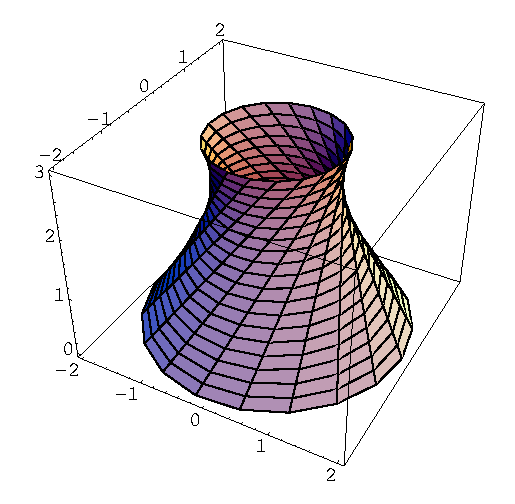
\epsfig{file=kuvat/hyperboloidi.eps}
\end{center}
\end{figure}
Pinnan kapein kohta on korkeudella $z=12/5$. \loppu

\pagebreak

\Harj
\begin{enumerate}

\item
Hahmottele seuraavien parametristen tasokäyrien kulku. Eliminoimalla parametri johda myös
käyrän yhtälö karteesisessa koordinaatistossa.
\begin{align*}
&\text{a)}\ \ x=2-t,\ y=t+1,\ t\in\R \qquad\ \text{b)}\ \ x=t^2,\ y=2-t,\ t\in[0,\infty) \\
&\text{c)}\ \ x=\frac{1}{t}\,,\ y=t-1,\ t\in(0,4) \qquad\,
 \text{d)}\ \ x=\frac{1}{1+t^2}\,,\ y=\frac{t}{1+t^2}\,,\ t\in\R \\
&\text{e)}\ \ \vec r=3\sin\pi t\,\vec i+4\cos\pi t\,\vec j,\ t\in[-1,1] \\[1mm]
&\text{f)}\ \ x=1-\sqrt{4-t^2}\,,\ y=2+t,\ t\in[-2,2] \\[1mm] 
&\text{g)}\ \ \vec r=t\cos t\,\vec i+t\sin t\,\vec j,\ t\in[0,4\pi]
\end{align*}

\item
a) Tasokäyrän eräs parametrisointi on $\vec r=\cos 2t\,\vec i+\sin^2 t\,\vec j,\ t\in\R$. 
Anna käyrälle vaihtoehtoinen, mahdollisimman yksinkertainen parametrisointi.
\vspace{1mm}\newline
b) Totea, että $\,\vec r=(t-1)\vec i+\sqrt{2t-t^2}\,\vec j,\ t\in[0,2]\,$ ja 
$\,\vec r=t\sqrt{2-t^2}\,\vec i+(1-t^2)\vec j$, \newline $t\in[-1,1]$ ovat saman käyrän 
parametrisointeja. Mikä käyrä on kyseessä?

\item \index{Cartesiuksen lehti}
Tasokäyrä $S:\,x^3+y^3=3xy\,$ on nimeltään \kor{Cartesiuksen lehti}. Johda käyrälle
parametriesitys kirjoittamalla $y=tx$. Hahmottele käyrän kulku parametrimuodosta ja merkitse
kuvioon, mitkä käyrän osat vastaavat parametrin arvoja väleillä $(-\infty,-1)$, $(-1,0)$ ja 
$[0,\infty)$. Miksei $t=-1$ vastaa mitään käyrän pistettä?

\item \index{venytetty sykloidi}
Ympyrä, jonka säde on $R=1$, vierii liukumatta pitkin positiivista $x$-akselia. Ympyrän mukana
pyörii siihen kiinnitetty jana, jonka toinen päätepiste on ympyrän keskipisteessä ja keskipiste
on ympyrän kehällä. Määritä janan toisen (ympyrän ulkopuolella olevan) päätepisteen sijainti
parametrisena käyränä $x=x(t),\ y=y(t)$, missä $t$ on ympyrän vierimiskulma mitattuna 
alkutilanteesta, jossa janan päätepisteet ovat $(0,1)$ ja $(0,3)$. Hahmottele käyrä
graafisesti. Missä pisteessä käyrä leikkaa ensimmäisen kerran itsensä? (Käyrää sanotaan 
\kor{venytetyksi sykloidiksi}.)

\item
Parametrisoi tason $T\,:x+y=4$ ja kartion $K:\,xy+yz+xz=0$ leikkauskäyrä ottamalla
parametriksi\, a) $t=x$, \ b) $t=x-y$.

\item
a) Avaruuskäyrän $S$ parametrisointi on $\vec r = \vec r_0+\cos t\,\vec a+\sin t\,\vec b$,
$\,t\in[0,2\pi]$, missä $\vec a$, $\vec b$ ja $\vec r_0$ ovat avaruusvektoreita. Täsmälleen
millä ehdoilla $S$ on avaruusympyrä?
\vspace{1mm}\newline
b) Avaruusympyrän keskipiste on $(1,1,2)$, säde on $R=3$ ja ympyrä on tasossa $x-y-3z+6=0$.
Johda ympyrälle jokin parametrisointi muotoa $\vec r=\vec r_0+\cos t\,\vec a+\sin t\,\vec b$,
$\,t\in[0,2\pi]$.

\item
Näytä, että yhtälöryhmä
$\D \ \begin{cases} \,x^2+y+z=2 \\ \,xy+z=1 \end{cases} $ \vspace{1mm}\newline
määrittelee kaksi leikkaavaa avaruuskäyrää, joista toisen parametrisointi on
$\vec r=t\vec i+(1+t)\vec j+(1-t-t^2)\vec k,\ t\in\R$. Millainen on toinen käyrä?

\item \index{zzb@\nim!Kiukkulintu ja kuulantyöntäjät} (Kiukkulintu ja kuulantyöntäjät)\, 
a) Kiukkulintu lennätetään alkupisteestä $(x,y)$ $=(0,1)$ (pituusyksikkö = cm) venyttämällä 
heittoparaabelissa (ks.\ Esimerkki\,\ref{heittoparaabeli}) vakion $a$ arvoksi $8$ cm ja
tähtäämällä porsaaseen, joka on pisteessä $(4,3)$. Millä $k$:n arvoilla tulee
osuma? \vspace{1mm}\newline 
b) Teekkarit Yrjölä ja Ståhlberg kisaavat kuulantyönnössä. Ratkaise, kumpi voitti, kun
kisaajien parhaissa työnnöissä heittoparaabelin parametrit ovat \newline
Yrjölä:   $\,\ \qquad h=2.00$ m, $\ \alpha=60.0\aste$, $\ a=8.00$ m \newline
Ståhlberg: $\quad h=1.80$ m, $\ \alpha=30.0\aste$, $\ a=6.65$ m

\item
Esitä jokin parametrisointi seuraavien yhtälöiden määräämille pinnoille: \newline
a)\, $x^3y^2z=5,\,\ $ b)\, $(x-z)(x+z)+y+2z=0,\,\ $ c)\, $x\sin z+xy^5+y=1$

\item
a) Johda pinnalle $S$ yhtälö muotoa $F(x,y,z)=0$ parametrisoinnista
\[ 
S:\ \begin{cases}
    \,x=3+2\sin\theta\cos\varphi, \\
    \,y\,=-1+\sin\theta\sin\varphi, \\
    \,z=2+3\cos\theta, \quad (\theta,\varphi)\in\Rkaksi.
    \end{cases}
\]
b) Pallon $K$ keskipiste on $(1,1,1)$ ja säde on $R=2$. Kuvan piirtoa varten halutaan
parametrisoida pallon $xy$-tason yläpuolinen ($z \ge 0$) osa. Esitä parametrisointi!
\vspace{1mm}\newline
c) Pinnan $S$ yhtälö lieriökoordinaateissa on $\,r=\varphi,\ (\varphi,z) \in A$, missä
$A=[0,4\pi]\times[-5,5]$. Parametrisoi $S$ viivoitinpintana. Millainen on $S$:n ja
$xy$-tason leikkauskäyrä? \vspace{1mm}\newline
d) Pinnan yhtälö lieriökoordinaateissa on $r=z^2\abs{\cos\varphi}$. Esitä pinnan yhtälö
karteesisissa koordinaateissa. Millaisia ovat pinnan ja tasojen $z=c$ ($c\in\R$)
leikkauskäyrät?

\item \index{hyperboloidi} \index{kaksivaippainen hyperboloidi}
a) Määritä sen viivoitinpinnan yhtälö (muodossa $F(x,y,z)=0$), joka syntyy, kun suora
$S:\ x=z,\ y=1$ pyörähtää $x$-akselin ympäri. Totea, että sama pinta (nimeltään yksivaippainen
hyperboloidi) syntyy myös, kun eräs $xy$-tason käyrä $K$ pyörähtää $x$-akselin ympäri. 
Hahmottele $K$ graafisesti. \vspace{1mm}\newline 
b) Tasokäyrän $K: x^2-y^2=1$ pyörähtäessä $x$-akselin ympäri syntyy pinta nimeltä
\kor{kaksivaippainen hyperboloidi}. Määritä ko.\ pinnan yhtälö. Missä pisteissä suora
$x=y=z$ leikkaa pinnan?

\item
a) Puolikartion $K$ kärki on origossa, symmetria-akseli on positiivinen $z$-akseli ja
puolisuora $x=2y=3z,\ x \ge 0$ on pinnalla $K$. Parametrisoi $K$ pyörähdyspintana ja
viivoitinpintana. Mikä on $K$:n yhtälö lieriökoordinaatistossa? \vspace{1mm}\newline
b) Parametrisoi kartio $K:\ xy+yz+xz=0\,$ viivoitinpintana.

\item (*) \index{asteroidi} \index{hyposykloidi}
Ympyrän keskipiste on origossa ja säde on $a$. Ympyrää pitkin sen sisäpuolella vierii liukumatta
toinen ympyrä, jonka säde on $b<a$. Tällöin vierivän ympyrän kiinteä piste $P$ piirtää 
tasokäyrän nimeltä \kor{hyposykloidi}. \ a) Näytä, että pisteen $(a,0)$ kautta kulkevan
hyposykloidin parametriesitys on
\[
x=(a-b)\cos t+b\cos\left(\frac{a-b}{b}\,t\right), \quad
y=(a-b)\sin t-b\sin\left(\frac{a-b}{b}\,t\right).
\]
b) Päättele, että tapauksessa $a=2b$ piste $P$ liikkuu pitkin janaa. \newline
c) Näytä, että tapauksessa $a=4b$ parametriesitys yksinkertaistuu muotoon 
\[
x=a\cos^3 t,\ \ y=a\sin^3 t.
\] 
Hahmottele tämän käyrän --- nimeltään \kor{asteroidi} --- kulku. Mikä on asteroidin yhtälö
karteesisissa koordinaateissa? 

\item (*) \index{zzb@\nim!Sotaharjoitus 1}
(Sotaharjoitus 1) Origosta ammutun tykinkuulan lentorata on ajan $t$ funktiona (yksiköt km ja s)
\[ \begin{cases}
x(t)=(\sin\theta\cos\varphi+a)\,t, \\
y(t)=(\sin\theta\sin\varphi+b)\,t, \\
z(t)=(\cos\theta)\,t-0.005\,t^2,
\end{cases} \]
missä $\theta,\varphi$ ovat suuntauskulmat ja $a,b$ ovat tuuliparametreja. Maastoesteet
asettavat suuntaukselle rajoituksen $\tan\theta > 0.2$. Miten suuntaus on valittava 
tuulettomassa säässä ($a=b=0$), jotta ammus osuisi pisteessä $(10,20,0)$ olevaan maaliin? 
Kuinka korkealla ammus käy? Kuinka kauas maalista ammus osuu tällä suuntauksella, jos 
$a=0.002$ ja $b=-0.001$\,? %Miten suuntausta olisi (likimain) muutettava?

\item (*)
Jana, jonka pituus on $20$, liikkuu seuraavasti: Janan keskipiste liikkuu $z$-akselia pitkin
positiiviseen suuntaan vakionopeudella. Liikkuessaan jana pysyy $xy$-tason suuntaisena ja pyörii
tasaisesti (kulmanopeus vakio) siten, että keskipisteen liikkuessa $30$ pituusyksikköä
jana pyörii täyden kierroksen positiivisen $z$-akselin suunnasta katsottuna vastapäivään.
Esitä janan avaruuteen piirtämän viivoitinpinnan $S$ parametrisointi, kun tiedetään lisäksi,
että piste $(1,0,0)$ on tällä pinnalla. Leikkaako suora $z=25,\ x+y=4$ pinnan $S$\,?

\end{enumerate} % Parametriset käyrät ja pinnat
\section{*Funktioavaruus} \label{funktioavaruus}
\alku
\index{funktioavaruus|vahv}

Tarkastellaan \pain{samassa} joukossa $A$ määriteltyjä yhden, kahden tai kolmen 
reaalimuuttujan reaaliarvoisia funktioita ja merkitään näiden joukkoa $V$:llä:
\[ 
V\ =\ \{\,\text{funktiot}\ f:\ A \kohti \R\,\}.
\]
Joukossa $V$ on määritelty funktioiden yhteenlasku $f,g \map f+g$ ja skalaarilla kertominen
$f \map \lambda f$ aiemmin kerrotulla tavalla (Määritelmän \ref{funktioiden yhdistelysäännöt}
säännöt (1) ja (2), kun $A \subset \R$). Näiden laskuoperaatioiden perusteella $V$ on
\index{vektorib@vektori (algebrallinen)!d@funktioavaruuden}%
mahdollista tulkita vektoriavaruudeksi. Samassa joukossa määritellyt funktiot voidaan siis 
mieltää 'vektoreiksi', jolloin puhutaan \kor{funktioavaruudesta} (engl.\ function space). 
\index{nollafunktio}%
Tällaisen avaruuden nolla-alkio on nk.\ (algebrallinen) \kor{nollafunktio}, joka määritellään
\[ 
\mathbf{0}(x) = 0\,\ \forall x \in A .
\]
Äärellinen funktiojoukko $\{ f_i,\ i = 1 \ldots n\} \subset V$ on (albegrallisesti) 
\index{lineaarinen riippumattomuus}%
\kor{lineaarisesti riippumaton}, jos pätee
\[ 
\sum_{i=1}^n \lambda_i f_i = \mathbf{0} \qimpl \lambda_i = 0,\ i = 1 \ldots n. 
\]
\begin{Exa} Enintään kolmannen asteen polynomit (määrittelyjoukko $= \R$) muodostavat 
funktioalgebran yhdistelysääntöjen perusteella funktioavaruuden
\[
V\ =\ \{ f = \lambda_1 f_1 + \lambda_2 f_2 + \lambda_3 f_3 + \lambda_4 f_4 
                                                                   \mid \lambda_i \in \R \},
\]
missä $f_1(x) = 1$, $f_2(x) = x$, $f_3(x) = x^2$ ja  $f_4(x) = x^3$. Algebran
peruslauseesta (ks.\ Luku \ref{III-3}) on helposti pääteltävissä, että funktiot $f_i$ ovat
lineaarisesti riippumattomia, joten $\{f_i,\ i = 1 \ldots 4\}$ on $V$:n kanta. Siis $V$ on
neliulotteinen vektoriavaruus: dim $V = 4$. \loppu \end{Exa}
\begin{Exa} Funktiot muotoa $f(x)=c_1\sin x+c_2\cos x,\ c_1,c_2\in\R$ muodostavat 2-ulotteisen
funktioavaruuden, luonnollisena kantana $\{\sin x,\cos x\}$. \loppu
\end{Exa}
\begin{Exa} Funktioavaruus
\[
V=\{f(x)=c_1+c_2\cos^2 x+c_3\sin^2 x,\ c_i\in\R\}
\]
ei ole 3-ulotteinen, sillä funktiosysteemi $\{f_1\,,f_2\,,f_3\}=\{1,\cos^2 x,\sin^2 x\}$ on 
lineaarisesti riippuva:
\[
f_1-f_2-f_3=\mathbf{0}.
\]
Mikä tahansa pari mainitusta kolmesta funktiosta sen sijaan on lineaarisesti riippumaton,
joten $V$ on 2-ulotteinen, kantana esim.\ $\{1,\cos^2 x\}$. Eräs $V$:n 1-ulotteinen aliavaruus
on
\[
W=\{\lambda\cos 2x \mid \lambda\in\R\},
\]
sillä $\,\cos 2x=2f_2-f_1 \in V$. \loppu
\end{Exa}
\begin{Exa} \label{polynomiavaruus}
Funktioavaruus
\[
V=\{f(x,y)=c_1+c_2x+c_3y+c_4x^2+c_5xy+c_6y^2,\ c_i\in\R\}
\]
koostuu kahden muuttujan polynomeista enintään astetta $2$ ja tämän aliavaruus
\[
W=\{f(x,y)=c_1+c_2x+c_3y,\ c_i\in\R\}
\]
enintään ensimmäisen asteen polynomeista. Funktiosysteemi $\{1,x,y,x^2,xy,y^2\}$ on 
lineaarisesti riippumaton (Harj.teht.\,\ref{H-IV-8: polynomit}), joten dim $V=6$ ja dim $W=3$.
\loppu
\end{Exa} 

\Harj
\begin{enumerate}

\item
Näytä, että funktiot $f_1(x)=x$ ja $f_2(x)=\abs{x}$ ovat lineaarisesti riippumattomat, jos
määrittelyjoukkona on väli $[-1,1]$ ja lineaarisesti riippuvat, jos määrittelyjoukko on
väli $[0,1]$.

\item
Montako alkiota on joukossa $A\subset\R$ oltava, jotta $A$:ssa määritellyt funktiot
$f_i(x)=x^{i-1},\ i=1 \ldots n$ ovat lineaarisesti riippumattomat?

\item
a) Näytä, että $\{1,\sin x,\sin^2 x,\sin^3 x\}$ on erään 4-ulotteisen funktioavaruuden
$V$ kanta (funktioiden määrittelyjoukko $=\R$). \ b) Sikäli kuin 
$f(x)=2+\cos 2x-\sin 3x \in V$, määrää $f$:n koordinaatit (kertoimet) mainitussa kannassa.

\item \label{H-IV-8: polynomit}
Näytä, että Esimerkin \ref{polynomiavaruus} polynomiavaruus $V$ on 6-ulotteinen, ts.\ näytä, että
$c_1+c_2x+c_3y+c_4x^2+c_5xy+c_6y^2=0\,\ \forall\,(x,y)\in\Rkaksi\,\ \impl\,\ c_1 = \ldots 
=c_6=0$.

\item (*) Olkoon $V=\{f(x)=c_1+c_2x+c_3x^2 \mid c_i\in\R\}$. Näytä, että
\[
\scp{f}{g}=f(0)g(0)+f(1)g(1)+f(2)g(2), \quad f,g \in V
\]
määrittelee $V$:n skalaaritulon. Laske funktion $u(x)=2+3x-2x^2$ ortogonaaliprojektio $w$ 
(ko.\ skalaaritulon mielessä) $V$:n aliavaruuteen $W$, jonka kanta on $\{1,x\}$. Piirrä samaan
kuvaan funktioiden $u$ ja $w$ kuvaajat välillä $[0,2]$. Tarkista, että $u-w \perp W$, ts.\ 
$\scp{u-w}{v}=0\ \forall v \in W$.

\end{enumerate} % *Funktioavaruus

\chapter{Jatkuvuus ja derivoituvuus}  \label{jatkuvat funktiot}

Funktion \kor{jatkuvuus} ja \kor{derivoituvuus} ovat käsitteellisiä peruslähtökohtia 
matematiikan suuntauksessa, jota kutsutaan väljästi \kor{analyysiksi}. Jatkuvuudesta, tai 
yleisemmin funktion \kor{säännöllisyydestä} puhuttaessa on kyse funktion arvojen
ennustettavuudesta muuttujan (muuttujien) arvojen vaihdellessa. Jatkuvuuden ja derivoituvuuden
käsitteet tuovat matemaattisten funktioiden teoriaan kokonaan oman 'makunsa' verrattuna
tähän asti tarkasteltuun funktioiden algebraan.

Tässä luvussa tarkastelun kohteena ovat pääosin vain yhden reaalimuuttujan funktiot. Näille
funktioille määritellään ensin jatkuvuus peruskäsitteenä ja jatkuvuuteen läheisesti liittyvä
\kor{funktion raja-arvon} käsite. Pelkkää jatkuvuutta vahvempina säännöllisyyden lajeina
määritellään mm.\ derivoituvuus (Luku \ref{derivaatta}) ja derivoituvuutta vahvemmat 
\kor{sileyden} lajit (Luku \ref{ääriarvot}). Näiden käsitteiden pohjalta luonnehditaan
funktioita, mm.\ esitetään kaksi reaalimuuttujan analyysin keskeistä \kor{väliarvolausetta} ja
tarkastellaan näiden lauseiden seuraamuksia yhtälöiden ja myös yksinkertaisten 
\kor{differentiaaliyhtälöiden} ratkeavuusteoriassa. 

Derivaatta tuo mukanaan myös derivoimissäännöt eli uuden ulottuvuuden funktioalgebraan.
Luvuissa \ref{derivaatta}--\ref{kaarenpituus} johdetaan kaikki keskeiset derivoimissäännöt,
mukaanlukien implisiittifunktiot, potenssisarjan summana määritellyt funktiot ja
(Luvussa \ref{kaarenpituus} erikseen) trigonometriset funktiot. 

Luvussa \ref{kiintopisteiteraatio} tarkastelun kohteena ovat yhtälöitten likimääräisessä
ratkaisussa yleisesti käytettävien algoritmien, \kor{kiintopisteiteraatioiden},
toimintaperiaatteet ja suppenevuusteoria. Luvussa \ref{analyyttiset funktiot} tarkastellaan
lyhyesti jatkuvuuden ja derivoituvuuden käsitteiden laajentamista kompleksifunktioihin ja
määritellään tähän liittyen \kor{analyyttisen} kompleksifunktion käsite. Viimeisessä
osaluvussa todistetaan jatkuvien funktioiden teorian keskeisimpiä väittämiä kuten 
\kor{Weierstrassin lause}. Tässä yhteydessä esitetään myös lyhyesti, miten Algebran peruslause
on todistettavissa kompleksialgebran ja analyysin tuloksia yhdistelemällä.
 % Jatkuvuuvs ja derivoituvuus
\section{Jatkuvuuden k�site} \label{jatkuvuuden k�site}
\alku

Funktion jatkuvuuden ongelma tulee eteen niinkin yksinkertaisessa teht�v�ss� kuin funktion
arvon numeerisessa m��ritt�misess�, eli numeerisessa funktioevaluaatiossa. Tarkastellaan Luvun 
\ref{k��nteisfunktio} Esimerkin \ref{algebrallinen k��nteisfunktio} k��nteisfunktiota, 
joka nyt kirjoitettakoon muotoon
\[
y=f(x) \ \ekv \ y^5+3y=x, \quad x\in\R.
\]
Teht�v�n� olkoon laskea likim��rin luku $a=f(\pi)$, eli evaluoida $f$ numeerisesti $\pi$:ss�. 
T�h�n itse asiassa sis�ltyy kaksi numeerista ongelmaa: Ensinn�kin luvulle $\pi$ ei ole olemassa
'tarkkaa' numeerista arvoa, ja toiseksi yht�l�� ei yleens� voi ratkaista $y$:n suhteen
tarkasti, vaikka $x$ olisi rationaaliluku. K�yt�nn�ss� menetell��n (laskin/tietokone 
menettelee) seuraavasti: Valitaan $\pi$:lle edustaja $x_n$ rationaalilukujonosta $\{x_n\}$,
jolle p�tee $x_n\rightarrow \pi$. Lasketaan $a_n=f(x_n)$ likim��rin k�ytt�m�ll� jotakin
numeerista algoritmia yht�l�n $y^5+y=x_n$ ratkaisuun. Algoritmi tuottaa k�yt�nn�ss�
rationaalilukujonon $\{b_k\}$, jolle p�tee $b_k \kohti a_n$ kun $k\rightarrow\infty$. Poimitaan
t�st� jonosta luvun $a_n$ likiarvoksi $b_m$ jollakin $m$ (esim.\ $m=10$), ja ilmoitetaan
lopputuloksena t�m�n luvun likiarvo ��rellisen� desimaalilukuna (katkaistuna tai py�ristettyn�
liukulukuna). 

Jos em.\ laskussa ei huomioida numeerisia py�ristysvirheit� liukulukulaskennassa, niin 
lopputuloksen $b_m$ virhe koostuu kahdesta osasta:
\[
b_m-f(\pi)\,=\,[b_m-f(x_n)]+[f(x_n)-f(\pi)].
\]
T�ss� ensimm�inen osa on approksimaation $b_m \approx f(x_n)$ virhe, eli kyse on yht�l�n
$y^5+3y=x_n$ ratkaisualgoritmin tarkkuudesta. Virheen j�lkimm�isess� osassa sen sijaan on kyse,
paitsi approksimaation $x_n \approx x$ tarkkuudesta, my�s funktiosta $f$: Kyse on funktion 
j\pain{atkuvuudesta}. Kvalitatiivisesti v�itt�m� '$f$ on jatkuva $x$:ss�' tarkoittaa, ett�
funktioevaluaatio $x \map f(x)$ on luotettava, kun muuttujalle sallitaan pieni vaihtelu, ts.\
p�tee
\[
x_n\approx x \ \impl \ f(x_n)\approx f(x).
\]

Em.\ funktion tapauksessa jatkuvuuskysymys ratkeaa seuraavasti: Koska
\[
\begin{cases}
a^5+a=\pi, \\
a_n^5+a_n=x_n,
\end{cases}
\]
saadaan v�hennyslaskulla (vrt. Luvun \ref{k��nteisfunktio} tarkastelut)
\[
(a-a_n)(a^4+a^3a_n+a^2a_n^2+aa_n^3+a_n^4+3)=\pi-x_n.
\]
T�ss� voidaan turvallisesti olettaa, ett� $a,a_n \ge 0$, joten seuraa
\[
\abs{a_n-a}\le \tfrac{1}{3}\abs{x_n-\pi}\,\ \ekv\,\ 
\abs{f(x_n)-f(\pi)}\le\tfrac{1}{3}\abs{x_n-\pi}.
\]
Jatkuvuudelle on n�in saatu jopa kvantitatiivinen varmistus: Approksimaation $f(x_n)$ $\approx$
$f(\pi)$ virhe on enint��n kolmasosa approksimaation $x_n\approx \pi$ virheest�. 

Esimerkki johdattaa seuraavaan funktion jatkuvuuden m��ritelm��n (vaihtoehtoinen m��ritelm� 
j�ljemp�n�).
\begin{Def} \vahv{(Jatkuvuus: jonokriteeri)}\ \label{funktion jatkuvuus}
\index{jatkuvuus (yhden muuttujan)|emph} \index{epzy@ep�jatkuvuus (funktion)|emph}
Funktio $f:\DF_f\rightarrow\R,\ \DF_f\subset\R$, on \kor{jatkuva} (engl.\ continuous, ruots.\ 
kontinuerlig) \kor{pisteess�} $a\in\DF_f$ (tai $a$:ssa), jos kaikille reaalilukujonoille
$\seq{x_n}$ p�tee
\[
x_n\in\DF_f\ \forall n\,\ \ja\,\ x_n \kohti a\,\ \impl\,\ f(x_n) \kohti f(a).
\]
Jos $f$ ei ole jatkuva pisteess� $a\in\DF_f$, niin $f$ on \kor{ep�jatkuva}
(engl.\ discontinuous) pistees� $a$.
\end{Def}
\begin{Exa} \label{ep�jatkuva funktio} Funktio \
$\D f(x)= \begin{cases} \,x-1, &\text{jos}\ x<\pi \\ \,x, &\text{jos}\ x\ge\pi \end{cases}$
\vspace{1mm}\newline
on ep�jatkuva pisteess� $x=\pi$, sill� jos $x_n \kohti \pi$ ja $x_n<\pi\ \forall n$, niin
$f(x_n)=x_n-1 \kohti \pi-1 \neq f(\pi)=\pi$. Muissa pisteiss� $f$ on jatkuva, sill� jos esim.\
$a<\pi$ ja $x_n \kohti a$, niin jostakin indeksist� $N$ eteenp�in on $\abs{x_n-a}<\pi-a$ 
(lukujonon suppenemisen m��ritelm�ss� valittu $\eps=\pi-a$), jolloin on erityisesti 
$x_n-a < \pi-a\ \ekv\ x_n<\pi$, kun $n>N$. T�ll�in on $f(x_n)=x_n-1,\ n>N$ ja siis
$f(x_n) \kohti a-1=f(a)$. \loppu
\end{Exa}
\begin{Exa} Olkoon $\DF_f=\{a\}$ ($a\in\R$) ja $f(a)=c\in\R$. M��ritelm�n
\ref{funktion jatkuvuus} mukaisesti $f$ on jatkuva pisteess� $a$\,(!). Yleisemmin
reaalifunktio on jatkuva jokaisessa m��rittelyjoukkonsa nk.\ \kor{eristetyss� pisteess�},
ks.\ Harj.teht.\,\ref{H-V-1: eristetty piste}. \loppu
\end{Exa}
Jatkuvuus voidaan m��ritell� my�s suoraan vetoamatta lukujonoihin, jolloin m��ritelm�st� tulee 
lukujonon suppenemisen m��ritelm�� (M��ritelm� \ref{jonon raja}) muistuttava. Vaihtoehtoinen
m��ritelm� on seuraava.
\begin{Def} \vahv{(Jatkuvuus: $(\eps,\delta)$-kriteeri)}\ \label{vaihtoehtoinen jatkuvuus}
\index{jatkuvuus (yhden muuttujan)|emph}
Funktio $f:\DF_f\kohti\R,\ \DF_f\subset\R$, on jatkuva pisteess� $a\in\DF_f$, jos jokaisella
$\eps>0$ on olemassa $\delta>0$ siten, ett� jokaisella $x\in\R$ p�tee
\[
x\in\DF_f\,\ \ja\,\ \abs{x-a}<\delta\,\ \impl\,\ \abs{f(x)-f(a)}<\eps.
\]
\end{Def}
M��ritelmi� \ref{funktion jatkuvuus} ja \ref{vaihtoehtoinen jatkuvuus} verrattaessa ei n�yt�
aivan ilmeiselt�, ett� p�tee (ks.\ todistus luvun lopussa)
\begin{*Lause} \label{jatkuvuuskriteerien yht�pit�vyys} Jatkuvuuden m��ritelm�t
\ref{funktion jatkuvuus} ja \ref{vaihtoehtoinen jatkuvuus} ovat yht�pit�v�t.
\end{*Lause} 
\jatko\jatko \begin{Exa} (jatko) Jos $a\neq\pi$, niin esimerkin funktiolle p�tee
\[
\abs{f(x)-f(a)}=\abs{x-a}, \quad \text{kun}\ \abs{x-a}<\abs{\pi-a},
\]
joten M��ritelm�n \ref{vaihtoehtoinen jatkuvuus} ehto on voimassa, kun valitaan
$\delta=\min\{\eps,\abs{\pi-a}\}>0$. Siis $f$ on jatkuva pisteiss� $a\neq\pi$ M��ritelm�n
\ref{vaihtoehtoinen jatkuvuus} mukaisesti. \loppu
\end{Exa} \seur
\begin{Exa} N�yt�, ett� $f(x)=x^2$ on jatkuva jokaisessa pisteess� $a\in\R$
k�ytt�en jatkuvuuden a) jonokriteeri�,\, b) $(\eps,\delta)$-kriteei�.
\end{Exa}
\ratk \ a) M��ritelm�n \ref{funktion jatkuvuus} mukainen jatkuvuus on seuraus Lauseesta
\ref{raja-arvojen yhdistelys��nn�t}:
\[
x_n \kohti a \qimpl x_n^2 \kohti a^2\,\ \impl\,\ f(x_n) \kohti f(a).
\]
b) Jos $a\in\R$ ja $\abs{x-a} \le 1$, niin kunta-algebran ja kolmioep�yht�l�n nojalla
\begin{align*}
\abs{f(x)-f(a)}\,=\,\abs{x-a}\abs{x+a}\,
                &=\,\abs{x-a}\abs{2a+(x-a)} \\
                &\le\,\abs{x-a}(2\abs{a}+\abs{x-a})\,
                 \le\,\abs{x-a}(2\abs{a}+1).
\end{align*}
N�in ollen jos $\eps>0$, niin p�tee $\abs{f(x)-f(a)}<\eps$ aina kun
$\abs{x-a}<\delta=\min\{1,\eps/(2\abs{a}+1)\}$ (jolloin my�s $\abs{x-a}<1$). Koska t�ss� on
$\delta>0$ aina kun $\eps>0$, niin $f$ on jatkuva $a$:ssa
M��ritelm�n \ref{vaihtoehtoinen jatkuvuus} mukaisesti. \loppu

Jatkuvuuden m��rittely jonokriteerill� (M��ritelm� \ref{funktion jatkuvuus}) on k�tev��
monissa teoreettisissa tarkasteluissa, jotka t�ll� tavoin palautuvat suppenevien
lukujonojen teoriaan. (T�m� teoria on kyll�kin tunnettava, mit� voi pit�� my�s
haittapuolena.) M��ritelm� \ref{vaihtoehtoinen jatkuvuus} on jatkuvuuden perinteisempi
'koulum��ritelm�'. T�m� on usein M��ritelm�� \ref{funktion jatkuvuus} selke�mpi silloin kun
halutaan selvitt��, milt� jatkuvat funktiot 'n�ytt�v�t'. Esimerkiksi seuraava usein k�ytetty
tulos, joka kertoo jatkuvan funktion 'j�ykkyydest�', on t�st� m��ritelm�st� helppo johtaa.
Todistus j�tet��n harjoitusteht�v�ksi (Harj.teht.\,\ref{H-V-1: todistuksia}a).
\begin{Prop} \label{jatkuvan funktion j�ykkyys} Jos $f$ on jatkuva pisteess� $a$ ja $f(a)>0$
($f(a)<0$), niin $\exists\delta>0$ siten, ett� $f(x)>0$ ($f(x)<0$) aina kun 
$x\in(a-\delta,a+\delta) \cap \DF_f\,$.
\end{Prop}

Jatkuvuus yksitt�isess� pisteess� voidaan laajentaa koskemaan joukkoa $A\subset\DF_f$\,:
Funktio on jatkuva $A$:ssa, jos se on jatkuva $A$:n jokaisessa pisteess�. 
Jatkuvuustarkasteluille on kuitenkin tyypillist�, ett� tarkastelu rajoittuu \pain{v�lille} 
$A\subset\DF_f$ siten, ett� funktion ominaisuuksilla v�lin ulkopuolella ei ole lainkaan
merkityst�. Sen vuoksi on tapana asettaa mainitusta yleisest� s��nn�st� hieman poikkeava
\begin{Def} (\vahv{Jatkuvuus v�lill�}) \label{jatkuvuus v�lill�}
\index{jatkuvuus (yhden muuttujan)!a@v�lill�|vahv}
Funktio $f:\DF_f\kohti\R,\ \DF_f\subset\R$, on \kor{jatkuva v�lill�} $A\subset\DF_f$, jos
jokaisella $x \in A$ ja jokaiselle reaalilukujonolle $\seq{x_n}$ p�tee
\[
x_n \in A\ \ja\ x_n \kohti x\,\ \impl\,\ f(x_n) \kohti f(x).
\]
\end{Def}
T�m�n mukaisesti jatkuvuus v�lill� $A$ tarkoittaa samaa kuin M��ritelm�n
\ref{funktion jatkuvuus} mukainen jatkuvuus $A$:n jokaisessa pisteess� siin� tapauksessa, ett�
funktion m��rittelyjoukko rajataan v�liksi $A$. (Jatkuvuuden vaihtoehtoisessa m��ritelm�ss�
\ref{vaihtoehtoinen jatkuvuus} korvataan ehto $\,x\in\DF_f\,$ ehdolla $x\in\DF_f \cap A$.)
Jatkuvuus v�lill� m��ritell��n siis jatkuvuutena 'sis�lt� p�in' ko.\ joukossa. Jos v�li on
avoin, ei t�m� rajaus ole tarpeen, sill� jos $x\in(a,b)=A$ ja $x_n \kohti x$, niin jollakin $N$
p�tee $x_n \in A\ \forall n>N$ (M��ritelm� \ref{jonon raja}, $\eps=\min\{x-a,b-x\}>0$) eli
m��ritelm�n ehto toteutuu indeksist� $N$ eteenp�in joka tapauksessa. Sen sijaan jos v�li on
suljettu, on ehdolla $x_n \in A$ merkityst� v�lin p��tepisteiss� (ei sis�pisteiss�).
\jatko\jatko \jatko \begin{Exa} (jatko) Jos $b>\pi$, on esimerkin funktio $f$ jatkuva v�lill�
$[\pi,b]$ (M��ritelm� \ref{jatkuvuus v�lill�}) vaikka $f$ ei ole jatkuva pisteess� $\pi$
(M��ritelm� \ref{funktion jatkuvuus}). Jos $a<\pi$, on $f$ jatkuva v�lill� $[a,\pi)$ mutta ei
v�lill� $(a,\pi]$. \loppu
\end{Exa} \seur\seur
\begin{Exa} \label{Dirichlet'n funktio} \index{Dirichleta@Dirichlet'n funktio}
Funktio $\D
f(x)=\begin{cases}
     \,1, \ &\text{ jos�} x\in\Q,  \\
     \,0, &\text{ jos } x\in\R, \ x\notin\Q
     \end{cases}$ \vspace{2mm}\newline
on esimerkki 'patologisesta' funktiosta, joka on m��ritelty koko $\R$:ss�, mutta joka ei ole 
miss��n pisteess� jatkuva. Funktion nimi on \kor{Dirichlet'n funktio}.  \loppu
\end{Exa}

\subsection*{Jatkuvien funktioiden yhdistely}

Esimerkin \ref{Dirichlet'n funktio} vastapainoksi voidaan kysy�, millaiset 'normaalit' funktiot 
tyypillisesti ovat jatkuvia. Ensimm�inen tuntuma n�ihin saadaan yhdistelem�ll� yksinkertaisia 
funktioita peruslaskutoimituksilla M��ritelm�n \ref{funktioiden yhdistelys��nn�t} mukaisesti.
Koska funktion jatkuvuudessa on viime k�dess� kyse lukujonon $\seq{f(x_n)}$ suppenemisesta,
on seuraava lause v�lit�n seuraus Lauseesta \ref{raja-arvojen yhdistelys��nn�t}
(Harj.teht.\,\ref{H-V-1: todistuksia}b).
\begin{Lause} (\vahv{Jatkuvuuden yhdistelys��nn�t}) \label{jatkuvuuden yhdistelys��nn�t}
\index{jatkuvuus (yhden muuttujan)!b@yhdistelys��nn�t|emph}
Jos $f:\DF_f\kohti\R$ on jatkuva pisteess� $x\in\DF_f$, niin $\lambda f$ on jatkuva $x$:ss� 
$\forall\lambda\in\R$. Jos lis�ksi $x\in\DF_g$ ja $g:\DF_g\kohti\R$ on jatkuva pisteess� $x$,
niin $f+g$ ja $fg$ ovat jatkuvia $x$:ss�. Jos edelleen $g(x)\neq 0$, niin my�s $f/g$ on
jatkuva $x$:ss�.
\end{Lause}
\begin{Exa} Jokainen polynomi tai rationaalifunktio voidaan m��ritell� palautuvasti
algebrallisena yhdistelm�n� perusfunktioista $f_0(x)=1$ ja $f_1(x)=x$. Koska n�m� ovat
ilmeisen jatkuvia $\R$:ss�, niin p��tell��n Lauseesta \ref{jatkuvuuden yhdistelys��nn�t},
ett� jokainen polynomi on jatkuva $\R$:ss� ja jokainen rationaalifunktio
m��rittelyjoukossaan, eli muualla kuin nimitt�j�ns� nollakohdissa. \loppu 
\end{Exa}
\begin{Exa} \label{trig yhdistely} Jos pidet��n tunnettuna, ett� trigonometriset funktiot
$\sin$ ja $\cos$ ovat jatkuvia $\R$:ss�, niin Lauseen \ref{jatkuvuuden yhdistelys��nn�t}
perusteella funktiot $\tan=\sin/\cos$ ja $\cot=\cos/\sin$ ovat samoin jatkuvia koko
m��rittelyjoukossaan. \loppu 
\end{Exa}
\begin{Lause} (\vahv{Yhdistetyn funktion jatkuvuus}) \label{yhdistetyn funktion jatkuvuus}
\index{jatkuvuus (yhden muuttujan)!c@yhdistetyn funktion|emph}
Jos $g$ on jatkuva pisteess� $x\in\DF_g$, $g(x)\in\DF_f$ ja $f$ on jatkuva pisteess� $g(x)$,
niin yhdistetty funktio $f\circ g$ on jatkuva $x$:ss�.
\end{Lause}
\tod Koska $\,x_n\in\DF_{f \circ g}\ \ekv\ x_n\in\DF_g\,\wedge\,g(x_n)\in\DF_f$, niin
jonokriteerin avulla p��tell��n:
\begin{align*}
x_n \in\DF_{f\circ g}\ \ja\ x_n \kohti x 
           &\qimpl g(x_n)\in\DF_f\ \ja\ x_n\in\DF_g\ \ja\ x_n \kohti x \\
           &\qimpl g(x_n)\in\DF_f\ \ja\ g(x_n) \kohti g(x) \\
           &\qimpl f(g(x_n)) \kohti f(g(x)). \quad\loppu
\end{align*}
\begin{Exa} \label{itseisarvon jatkuvuus} N�yt�, ett� jos $f$ on jatkuva $x$:ss�, niin my�s
$\abs{f}$ on jatkuva $x$:ss�. 
\end{Exa}
\ratk Funktio $g(x)=\abs{x}$ on helposti osoitettavissa jatkuvaksi $\R$:ss� suoraan
jatkuvuuden m��ritelmist� (tai vedoten Propositioon \ref{jatkuvuuspropositio} alla), joten
Lauseen \ref{yhdistetyn funktion jatkuvuus} nojalla yhdistetty funktio 
$(g \circ f)(x) = \abs{f(x)}$ on jatkuva jokaisessa pisteess�, jossa $f$ on jatkuva. \loppu

Jatkuvuuden periytyvyyden p\pain{aloittain} (eli eri v�leill� erilaisilla laskus��nn�ill�)
m��ritellyn funktion osalta ratkaisee
(Harj.teht.\,\ref{H-V-1: todistuksia}c; vrt.\ my�s Esimerkki \ref{ep�jatkuva funktio} edell�).
\begin{Prop} \label{jatkuvuuspropositio}
Olkoon $f_1$ ja $f_2$ jatkuvia avoimella v�lill� $(a,b)$ ja
\[
f(x) = \begin{cases} 
       \,f_1(x), &\text{kun}\ x \in (a,c), \\ 
       \,k, &\text{kun}\ x=c, \\ 
       \,f_2(x), &\text{kun}\ x \in (c,b),
       \end{cases} 
\]
miss� $a<c<b$. T�ll�in $f$ on jatkuva $c$:ss� t�sm�lleen kun $\,f_1(c)=f_2(c)=k$. 
\end{Prop}
\begin{Exa} Funktio
\[ f(x) = \begin{cases}
          \ x+a,\ &\text{kun}\ x \le a, \\ -(x+1)^2,\ &\text{kun}\ x > a 
          \end{cases} 
\] 
on polynomi $f_1(x)=x+a$ v�lill� $(-\infty,a)$ ja polynomi $f_2(x)=-(x+1)^2$ v�lill�
$(a,\infty)$, joten n�ill� v�leill� funktio on jatkuva. Proposition \ref{jatkuvuuspropositio}
mukaan ehto funktion jatkuvuudelle pisteess� $x=a$ (ja siis ehto jatkuvuudelle koko $\R$:ss�)
on
\[
f_1(a)=f_2(a) \qekv a^2+4a+1=0 \qekv a = -2 \pm \sqrt{3}. \loppu
\]
\end{Exa}

\subsection*{Funktio $f(x) = \sqrt[m]{x}$}
\index{jatkuvuus (yhden muuttujan)!d@funktion $\sqrt[m]{x}$|vahv}

Osoitetaan seuraavaksi, ett� funktio�$f:[0,\infty)\rightarrow [0,\infty)$, joka m��ritell��n
\[
f(x)=x^{1/m}=\sqrt[m]{x},\quad m\in\N, \ m\geq 2
\]
on koko m��rittelyv�lill��n jatkuva (kuvassa $f(x)$, kun $m=8$).
\begin{figure}[H]
\begin{center}
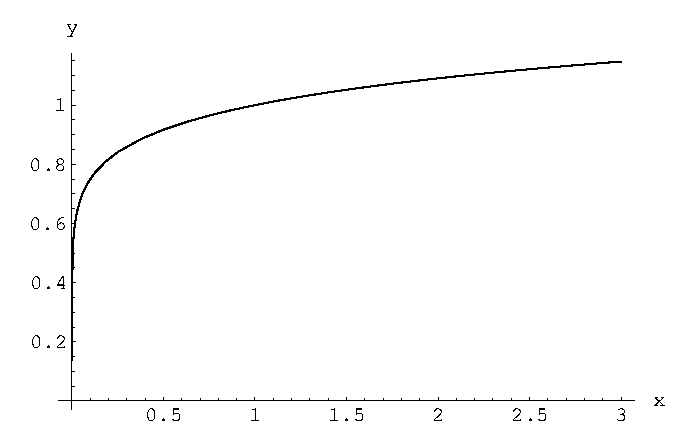
\epsfig{file=plots/8throotx.eps}
%\caption{$y=\sqrt[8]{x}$}
\end{center}
\end{figure}
Aloitetaan pisteest� $x=0$, joka on jatkuvuuden kannalta kriittisin (vrt. kuva). Koska f on 
aidosti kasvava (ks.\ Luku \ref{k��nteisfunktio}, Esimerkki \ref{x^m:n k��nteisfunktio}),
niin jokaisella $a>0$ p�tee
\[
0 \le x < a^m\ \ekv\ 0 \le f(x) < f(a^m) = a.
\]
Jos nyt $x_n\geq 0$ ja $x_n\rightarrow 0$, niin jokaisella $\eps>0$ $\exists N\in\N$ siten,
ett� p�tee
\[
n>N \ \impl \ 0 \le x_n < \eps^m \ \impl\ 0 \le f(x_n) < \eps.
\]
N�in ollen lukujono $\{f(x_n)\}$ on suppeneva ja $f(x_n) \kohti 0=f(0)$, joten $f$ on jatkuva 
$0$:ssa.

Muualla kuin origossa $f$:n jatkuvuus voidaan p��tell� kunta-algebran avulla: Jos 
$x_n \ge 0$ ja $x_n \kohti x>0$, niin merkitsem�ll� $y=f(x)$, $y_n=f(x_n)$ seuraa
\[
x-x_n \,=\, y^m-y_n^m \,=\, (y-y_n)(y^{m-1}+y^{m-1}y_n+\cdots +y_n^{m-1}).
\]
T�ss� on $y_n \ge 0$, $y>0$, joten p��tell��n
\[
\abs{x-x_n}\,\ge\,\abs{y-y_n}y^{m-1} \,\ \ekv\,\ \abs{y-y_n}\,\le\,y^{1-m}\abs{x-x_n}.
\]
N�in ollen $x_n \kohti x \ \impl\ y_n \kohti y$, eli $f$ on jatkuva pisteess� $x$.
\begin{Exa} \label{epsilon ja delta} Olkoon $\eps = 10^{-6}$. M��rit� suurin $\delta$ siten,
ett� M��ritelm�n \ref{vaihtoehtoinen jatkuvuus} ehto toteutuu funktiolle $f(x)=\sqrt[8]{x}$
pisteess� $x=0$.
\end{Exa}
\ratk Koska $f$ on aidosti kasvava v�lill� $[0,\infty)=\DF_f$, niin $\forall x\in\DF_f$ p�tee
$|f(x)-f(0)|=\sqrt[8]{x} < \eps\ \ekv\ 0 \le x < \eps^8\ \ekv\ x\in(-\eps^8,\eps^8)\cap\DF_f$.
Siis $\,\delta_{max} = \eps^8 = 10^{-48}$. \loppu

Funktion $f(x)=x^{1/m}$ jatkuvuuden tultua todetuksi seuraa Lauseesta 
\ref{yhdistetyn funktion jatkuvuus} ja funktion $g(x)=\abs{x}$ jatkuvuudesta, ett� yhdistetty 
funktio $(f\circ g)(x) = \abs{x}^{1/m}$ on jatkuva koko m��rittelyjoukossaan ($= \R$). Kun
huomioidaan my�s Lause \ref{jatkuvuuden yhdistelys��nn�t}, niin seuraa
\begin{Prop} \label{potenssifunktion jatkuvuus}
Funktio $f(x)=\abs{x}^\alpha$, $\alpha=p/q\in\Q$ on koko m��rittelyjoukossaan ($\DF_f=\R$ jos
$\alpha>0$, $\DF_f=\{x\in\R \mid x \neq 0\}$ jos $\alpha \leq 0$) jatkuva.
\end{Prop}
Lauseiden \ref{jatkuvuuden yhdistelys��nn�t}--\ref{yhdistetyn funktion jatkuvuus}, Proposition
\ref{potenssifunktion jatkuvuus} ja Esimerkkien \ref{trig yhdistely} ja
\ref{itseisarvon jatkuvuus} perusteella voidaan vet�� se yleisempi johtop��t�s, ett� kaikki
toistaiseksi tunnetut 'yhden lausekkeen' funktiot ovat jatkuvia koko m��rittelyjoukossaan (!).
\begin{Exa} Ilman tapauskohtaista tarkastelua voidaan esimerkiksi seuraavat funktiot
p��tell� jatkuviksi m��rittelyjoukkonsa jokaisessa pisteess�:
\[
\sqrt[3]{\abs{1-\sqrt{x}\,}}\,, \quad 
\sqrt[6]{\frac{1+\sqrt{x}}{2-x^2}}\,, \quad
\frac{|\sin x|^{3/4}}{x-\pi}\,, \quad 
\frac{\cot x}{\sqrt[4]{x+50\cos(\tan x)}}\,. \loppu
\]
\end{Exa}

\subsection*{Jatkuvien funktioiden p��lauseet}

T�ss� osaluvussa esitet��n kolme matemaattisen analyysin keskeist� lausetta, jotka kaikki
koskevat suljetulla v�lill� jatkuvia funktioita. Ensimm�inen lauseista on my�s ensimm�inen
yhden reaalimuuttujan funktioita koskevista \kor{v�liarvolauseista}, joita on kaikkiaan kolme.
(Muut kaksi esitet��n my�hemmin.) T�ss� esitett�vist� p��lauseista j�lkimm�iset kaksi ovat
erikoistapauksia yleisemmist� v�itt�mist�, jotka perustuvat jatkuvuuden syv�llisemp��n
logiikkaan. N�iden todistuksia ei viel� esitet�, vaan lauseet muotoillaan ja todistetaan
j�ljemp�n� Luvussa \ref{jatkuvuuden logiikka} t�ss� esitetty� yleisemm�ss� muodossa. 
 
Tarkastellaan suljetulla v�lill� $[a,b]$ jatkuvaa funktiota $f$. Olkoon $f(a) \neq f(b)$ ja 
$c < \eta < d$, miss�
\[ 
c = \min \{f(a),f(b)\}, \quad d = \max\{f(a),f(b)\}. 
\]
Koska $f$ on jatkuva, niin tuntuu luonnolliselta ajatella, ett� $f$:n kuvaaja v�lill� $[a,b]$
on 'jatkuva lanka', joka yhdist�� pisteet $A=(a,f(a))$ ja $B=(b,f(b))$. T�m�n intuition
mukaisesti tuntuu selv�lt�, ett� kuvaajan on leikattava suora $y=\eta$ ainakin kerran v�lill�
$(a,b)$. Toisin sanoen, probleemalla
\[ 
x \in [a,b]: \quad f(x) = \eta 
\]
on oltava ainakin yksi ratkaisu $x=\xi \in (a,b)$ jokaisella $\eta \in (c,d)$ (kuva).
\begin{figure}[H]
\setlength{\unitlength}{1cm}
\begin{center}
\begin{picture}(10,6)(-1,-1)
\put(-1,0){\vector(1,0){10}} \put(8.8,-0.4){$x$}
\put(0,-1){\vector(0,1){6}} \put(0.2,4.8){$y$}
\curve(
    1.0000,    1.0000,
    1.5000,    2.7969,
    2.0000,    3.4643,
    2.5000,    3.4174,
    3.0000,    3.0000,
    3.5000,    2.4844,
    4.0000,    2.0714,
    4.5000,    1.8906,
    5.0000,    2.0000,
    5.5000,    2.3862,
    6.0000,    2.9643,
    6.5000,    3.5781,
    7.0000,    4.0000,
    7.5000,    3.9308,
    8.0000,    3.0000)
\put(0.9,0.9){$\bullet$} \put(0.5,0.6){$A$}
\put(7.9,2.9){$\bullet$} \put(8.2,3.1){$B$}
\dashline{0.2}(5.5,0)(5.5,2.39)(0,2.39)
\dashline{0.05}(1,0)(1,1)(0,1)
\dashline{0.05}(8,0)(8,3)(0,3)
\put(0.9,-0.5){$a$} \put(5.4,-0.5){$\xi$} \put(7.9,-0.5){$b$}
\put(-0.4,0.9){$c$} \put(-0.4,2.3){$\eta$} \put(-0.4,2.9){$d$}
\end{picture}
%\caption{V�liarvolauseen v�itt�m�n havainnollistaminen}
\end{center}
\end{figure}
Ym.\ geometriselle intuitiolle vahvistuksen antaa
%\begin{figure}[H]
%\setlength{\unitlength}{1mm}
%\begin{center}
%\begin{picture}(140,45)(0,10)
%\put(20,20){\vector(1,0){40}} \put(58,16){$x$}
%\put(20,20){\vector(0,1){30}} \put(22,48){$y$}
%\put(80,20){\vector(1,0){40}} \put(118,16){$x$}
%\put(80,20){\vector(0,1){30}} \put(82,48){$y$} 
%\curve(25,25,45,32,55,45)
%%\curve(85,45,95,32,115,25)
%%\curve(25,15,45,50,55,45)
%\curve(85,55,95,20,115,32)
%\dashline{1}[0.2](30,20)(30,26)(20,26)
%\dashline{1}[0.2](53,20)(53,41)(20,41)
%\dashline{1}[0.2](87,20)(87,40)(80,40)
%\dashline{1}[0.2](110,20)(110,26)(80,26)
%\put(29,16){$a$} \put(16,25){$c$} \put(52,16){$b$} \put(16,40){$d$}
%\put(86,16){$a$} \put(76,39){$c$} \put(109,16){$b$} \put(76,25){$d$}
%\end{picture}
%\end{center}
%\end{figure}
\begin{Lause} \label{ensimm�inen v�liarvolause}
\vahv{(Ensimm�inen v�liarvolause --- Jatkuvien funktioiden v�liarvolause)}
\index{vzy@v�liarvolauseet!a@jatkuvien funktioiden|emph}
Jos $f:\DF_f\kohti\R$, $\DF_f\subset\R$, on jatkuva v�lill� $[a,b]\subset\DF_f$ ja 
$c=\min\{f(a),f(b)\}<d=\max\{f(a),f(b)\}$ (eli $f(a) \neq f(b)$), niin jokaisella 
$\eta\in (c,d)$ on olemassa $\xi \in (a,b)$ siten, ett� $f(\xi)=\eta$.\footnote[2]{Lause
\ref{ensimm�inen v�liarvolause} varmistaa, ett� v�lill� $[a,b]$ jatkuvan funktion kuvaaja 
\[
G_f=\{P=(x,y) \mid x\in[a,b]\,\ja\,y=f(x)\}
\]
on geometrisen intuition mukainen \kor{k�yr�} eli 'yhten�inen viiva vailla leveytt�'. $G_f$ on
'vailla leveytt�', koska $f(x)$ on yksik�sitteinen $\forall x$ (eli $f$ on funktio), ja
'yhten�inen', koska $f$ on jatkuva. --- Jatkuvuus (yhten�isyyden takaajana) liitet��n k�yr�n
k�sitteeseen yleisemminkin. Esimerkiksi yleisess� parametrisessa k�yr�ss�
$\vec r(t)=x(t)\vec i+y(t)\vec j+z(t)\vec k$ koordinaattifunktiot $x(t),y(t),z(t)$ oletetaan
jatkuviksi tarkasteltavalla v�lill�. Vrt.\ alaviitteet Luvuissa
\ref{k��nteisfunktio}--\ref{parametriset k�yr�t}. \index{kzyyrzy@k�yr�|av}} 
\end{Lause}
Jos $f$ ja $\eta$ t�ytt�v�t Lauseen \ref{ensimm�inen v�liarvolause} ehdot, niin n�hd��n, ett� 
lauseen v�itt�m� seuraa, kun seuraavaa pelkistetymp�� tulosta sovelletaan funktioon 
$g(x)=f(x)-\eta$ tai $g(x)=\eta-f(x)$.
\begin{Lause} \vahv{(Bolzano)} \label{Bolzanon lause} \index{Bolzanon lause|emph}
Jos $f(a)<0$, $f(b)>0$, ja $f$ on jatkuva v�lill� $[a,b]$, niin $f(\xi)=0$ jollakin
$\xi\in (a,b)$.
\end{Lause}
\tod on puhtaasti konstruktiivinen ja toimii k�yt�nn�ss�kin algoritmina, joka 
etsii yhden $f$:n nollakohdista v�lill� $(a,b)$. Tavallisin todistustapa on nk.\  
\pain{haarukointi} eli puolitusmenetelm� (kymmenjakoalgoritmikin toimisi, vrt.\ Luku
\ref{reaaliluvut}). Ensinn�kin voidaan funktioevaluaatioiden (oletetaan tarkoiksi\,!)
perusteella todeta, ett� joko valinnalla $a_1=a$, $b_1=\frac{1}{2}(a+b)$ tai valinnalla 
$a_1=\frac{1}{2}(a+b)$, $b_1=b$ p�tee
\[
f(a_1) \le 0 \ \ja \ f(b_1) \ge 0.
\]
Jos t�ss� on $f(a_1)=0$ tai $f(b_1)=0$, on $\xi$ l�ydetty. Muussa tapauksessa on $f(a_1)<0$ ja
$f(b_1)>0$, jolloin voidaan jatkaa $\xi$:n 'haarukointia' v�lill� $(a_1,b_1)$ samalla
periaatteella. Mik�li konstruktio ei katkea $\xi$:n l�ytymiseen, syntyy kaksi jonoa
$\seq{a_n}$, $\seq{b_n}$. Konstruktion  perusteella $\seq{a_n}$ on kasvava, $\seq{b_n}$ on
v�henev� ja
\[
b_n-a_n=\left(\frac{1}{2}\right)^n(b-a) \kohti 0,
\]
joten jonoilla on yhteinen raja-arvo: $a_n\kohti\xi$ ja $b_n\kohti\xi$ jollakin $\xi\in\R$.
Koska on $a \le a_n \le b\ \forall n$, on my�s oltava $a \le \xi \le b$ 
(Propositio \ref{jonotuloksia}:\,V1), eli $\xi \in [a,b]$. T�ll�in koska $f$ on v�lill� $[a,b]$ 
jatkuva (M��ritelm� \ref{jatkuvuus v�lill�}), p�tee
\[
f(a_n) \kohti f(\xi)\ \ \text{ja}\ \ f(b_n) \kohti f(\xi).
\]
Mutta lukujonojen $\seq{a_n}$ ja $\seq{b_n}$ konstruktion perusteella
\begin{align*}
f(a_n)<0\,\ \forall n \ &\impl \ f(\xi)\le 0, \\
f(b_n)>0\,\ \forall n \ &\impl \ f(\xi)\ge 0
\end{align*}
(Propositio \ref{jonotuloksia}:\,V1), joten on oltava $f(\xi)=0$. T�ss� oli $\xi\in [a,b]$,
mutta koska $f(a)<0$ ja $f(b)>0$, niin $\xi \in (a,b)$. Bolzanon lause on n�in todistettu.
\loppu
\begin{Exa}
Funktiolle $f(x)=x^5+3x\,$ p�tee $f(0)=0$ ja $f(1)=4$, joten Lauseen 
\ref{ensimm�inen v�liarvolause} mukaan yht�l�ll�
\[ 
x^5 + 3x = 2 
\]
on ratkaisu $x=\xi$ v�lill� $(0,1)$. Ratkaisu on itse asiassa yksik�sitteinen, koska 
$f$ on 1-1 (vrt.\ Esimerkki \ref{algebrallinen k��nteisfunktio} Luvussa \ref{k��nteisfunktio}).
\loppu \end{Exa}

Seuraava lause, jolla on my�s yleisempi� muotoja, on reaalianalyysin merkitt�vimpi� tuloksia
(todistus yleisemm�ss� muodossa Luvussa \ref{jatkuvuuden logiikka}).
\begin{*Lause} \vahv{(Weierstrass)} \label{Weierstrassin peruslause}
\index{Weierstrassin lause|emph} 
Suljetulla v�lill� $[a,b]$ jatkuva funktio $f$ saavuttaa ko.\ v�lill� pienimm�n ja suurimman
arvonsa, ts.\ on olemassa $x_1 \in [a,b]$ ja $x_2 \in [a,b]$ siten, ett�
\[ 
f(x_1) = \min\{f(x) \mid x \in [a,b]\}, \quad f(x_2) = \max\{f(x) \mid x \in [a,b]\}. 
\]
\end{*Lause}
\begin{Exa} Funktio
\[
f(x)=\begin{cases} \,x, &\text{kun}\ x \le 0, \\ \,1-x, &\text{kun}\ x>0 \end{cases}
\]
on jatkuva v�lill� $[a,b]$, jos joko $a < b \le 0$ tai $0<a<b$. T�ll�in funktio saavuttaa
maksimi- ja minimiarvonsa v�lin p��tepisteiss�. Muussa tapauksessa, eli jos $a \le 0$ ja
$b>0$, ei $f$ ole jatkuva v�lill� $[a,b]$, sill� jos $x_n\in(0,b]$ ja $x_n \kohti 0$, niin
$f(x_n) \kohti 1 \neq f(0)$. T�ss� tapauksessa $f$ ei my�sk��n saavuta maksimiarvoa
v�lill� $[a,b]$, ainoastaan minimiarvon ($=\min\{f(a),f(b)\}$). \loppu
\end{Exa} 
Yhdist�m�ll� Lauseiden \ref{ensimm�inen v�liarvolause} ja \ref{Weierstrassin peruslause} 
v�itt�m�t tullaan seuraavaan maininnan arvoiseen p��telm��n:
\begin{Kor} \label{er�s jatkuvuuskorollaari} Jos $f$ on jatkuva v�lill� $A=[a,b]$ ja $f$ ei
ole vakio, niin $f(A)$ on suljettu v�li. \end{Kor}

Seuraava lause antaa er��n riitt�v�n kriteerin k��nteisfunktion jatkuvuudelle. Todistus
(hieman yleisemmin muotoillulle lauseelle) esitet��n Luvussa \ref{jatkuvuuden logiikka}.
\begin{*Lause} \label{k��nteisfunktion jatkuvuus}
\index{jatkuvuus (yhden muuttujan)!e@k��nteisfunktion|emph}
\vahv{(K��nteisfunktion jatkuvuus)} Jos $f:[a,b] \kohti [c,d]$ on jatkuva bijektio, niin my�s 
$\inv{f}:[c,d] \kohti [a,b]$ on jatkuva bijektio.
\end{*Lause} 
\begin{Exa} Funktio $f(x)=x^{1/m},\ m \in \N,\ m \ge 2\,$ p��teltiin edell� jatkuvaksi v�lill� 
$[0,\infty)$. T�m� seuraa my�s Lauseesta \ref{k��nteisfunktion jatkuvuus}, sill� $f=\inv{g}$,
miss� $g(x)=x^m$ on jatkuva bijektio $\,g: [0,a] \kohti [0,a^m]$ jokaisella $a>0$. \loppu
\end{Exa}

\subsection*{*Lauseen \ref{jatkuvuuskriteerien yht�pit�vyys} todistus}

Lauseen \ref{jatkuvuuskriteerien yht�pit�vyys} v�itt�m� on kaksiosainen: V�itet��n, ett�
jos $f$ on jatkuva pisteess� $a\in\DF_f$ M��ritelm�n \ref{funktion jatkuvuus}
jonokriteerill�, niin $f$ on jatkuva $a$:ssa my�s M��ritelm�n
\ref{vaihtoehtoinen jatkuvuus} $(\eps,\delta)$-kriteerill� ja ett� t�m�
implikaatio p�tee my�s k��nt�en.
 
\tod\, \fbox{$\impl$} Oletetaan, ett� $f$ on jatkuva pisteess� $a\in\DF_f$  M��ritelm�n 
\ref{funktion jatkuvuus} mukaisesti. Tehd��n vastaoletus: $f$ ei ole jatkuva $a$:ssa
M��ritelm�n \ref{vaihtoehtoinen jatkuvuus} kriteerill�. T�ll�in voidaan
samalla tavoin kuin Lauseen \ref{negaatioperiaate} todistuksessa p��tell�, ett� jollakin 
$\eps>0$ p�tee:
\[
\forall \delta>0 \ \exists x\in\DF_f\ \text{siten, ett�}\ \ 
                   \abs{x-a}<\delta \ \ja\ \abs{f(x)-f(a)}\ge\eps.
\]
Kun nyt $\delta$:n arvoista muodostetaan jono $\{\delta_n\}$, joka suppenee kohti nollaa 
(esim.\ $\delta_n=1/n$), niin vastaavasti on siis l�ydett�viss� jono $\{x_n\}$ siten, ett�
jokaisella $n$
\[
x_n\in\DF_f\ \ja\ \abs{x_n-a}<\delta_n \ \ja \ \abs{f(x_n)-f(a)}\ge\eps.
\]
N�in on l�ydetty jono, jolle p�tee
\[
x_n\in\DF_f\ \ja\ x_n \kohti a\ \ja\ f(x_n) \not\kohti f(a).
\]
T�m� on looginen ristiriita, koska oletettiin, ett� $f$ on jatkuva $a$:ssa M��ritelm�n
\ref{funktion jatkuvuus} mukaisesti. Tehty vastaoletus on siis v��r�, eli $f$ on jatkuva
$a$:ssa M��ritelm�n \ref{vaihtoehtoinen jatkuvuus} kriteerill�. 

\fbox{$\Leftarrow$} Oletetaan, ett� $f$ on jatkuva pisteess� $a\in\DF_f$ M��ritelm�n
\ref{vaihtoehtoinen jatkuvuus} kriteerill�. Olkoon $\eps>0$ ja valitaan $\delta>0$ siten, ett�
M��ritelm�n \ref{vaihtoehtoinen jatkuvuus} ehto on t�ytetty. Edelleen olkoon $\seq{x_n}$
lukujono, jolle p�tee $x_n\in\DF_f\ \forall n$ ja $x_n \kohti a$. T�ll�in jostakin indeksist�
$n=N$ eteenp�in on $\abs{x_n-a}<\delta$ (koska oli $\delta>0$), jolloin tehtyjen oletusten
mukaan on my�s $\abs{f(x_n)-f(a)}<\eps$. On siis l�ydetty indeksi $N\in\N$ siten, ett� p�tee
\[
\abs{f(x_n)-f(a)} < \eps, \quad \text{kun}\ n>N.
\]
T�ss� $\eps>0$ oli mielivaltainen, joten $f(x_n) \kohti f(a)$ (M��ritelm� \ref{jonon raja}).
My�s jono $\seq{x_n}$ oli tehtyjen oletusten puitteissa vapaasti valittu, joten jokaiselle 
t�llaiselle jonolle on voimassa $f(x_n) \kohti f(a)$. Siis $f$ on jatkuva pisteess� $a$
M��ritelm�n \ref{funktion jatkuvuus} kriteerill�. \loppu

\Harj
\begin{enumerate}

\item
Todista suoraan M��ritelm�n \ref{funktion jatkuvuus} ja lukujonoja koskevien tulosten
perusteella kukin seuraavista funktioista joko jatkuvaksi tai ep�jatkuvaksi pisteess� $x=0$.
Hahmottele my�s funktioiden kuvaajat joukossa $A=\DF_f\cap[-1,1]$.
\begin{align*}
&\text{a)}\,\ f(x)=x^7+7x+49 \qquad 
 \text{b)}\,\ f(x)=x^5-6x^3+\frac{x^3+20}{100x^2-1} \\
&\text{c)}\,\ f(x)=\begin{cases} 
                   \,\dfrac{1}{x}\left(\dfrac{1}{1+7x}-\dfrac{1}{1+5x}\right), 
                                                       &\text{kun}\ x \neq 0, \\[2mm]
                   \,2,                                &\text{kun}\ x=0
                   \end{cases} \\
&\text{d)}\,\ f(x)=\begin{cases}
                   \,x\cos\dfrac{1}{x}\,, &\text{kun}\ x \neq 0, \\[2mm]
                   \,0,                   &\text{kun}\ x=0
                   \end{cases} \qquad
 \text{e)}\,\ f(x)=\begin{cases}
                   \,\sin\dfrac{1}{x}\,, &\text{kun}\ x \neq 0, \\[2mm]
                   \,0,                  &\text{kun}\ x=0
                   \end{cases}
\end{align*}

\item \label{abs{x}:n jatkuvuus}
N�yt� funktio $f(x)=1/x$ jatkuvaksi m��rittelyjoukossaan vedoten suoraan a) jatkuvuuden
jonokriteeriin, b) jatkuvuuden $(\eps,\delta)$-kriteeriin.

\item \label{H-V-1: todistuksia}
K�ytt�en a)- kohdassa jatkuvuuden $(\eps,\delta)$-kriteeri�, b)-kohdassa jonokriteeri�
ja c)-kohdassa jompaa kumpaa todista: \vspace{1mm}\newline
a) Propositio \ref{jatkuvan funktion j�ykkyys}. $\quad$
b) Lause \ref{jatkuvuuden yhdistelys��nn�t}. $\quad$
c) Propositio \ref{jatkuvuuspropositio}.

\item \label{H-V-1: eristetty piste} \index{eristetty piste (joukon)}
Sanotaan, ett� $a \in A$ on joukon $A\subset\R$ \kor{eristetty piste}, jos jollakin
$\delta>0$ on $(a-\delta,a+\delta) \cap A = \{a\}$. N�yt�, ett� reaalifunktio on jatkuva
jokaisessa m��rittelyjoukkonsa eristetyss� pisteess�.

\item
Hae sellaiset parametrin $a$ arvot, joilla funktiosta tulee jatkuva koko $\R$:ss�, ja
hahmottele kuvaaja n�ill� $a$:n arvoilla:
\begin{align*}
&\text{a)}\,\ f(x)=\begin{cases}
                   \,x-1, &\text{kun}\ x \le a, \\ \,1-x^2, &\text{kun}\ x>a
                   \end{cases} \qquad
 \text{b)}\,\ f(x)=\begin{cases}
                   \,a-x, &\text{kun}\ x \le -2, \\ \,x^3-4x, &\text{kun}\ x>-2
                   \end{cases} \\
&\text{c)}\,\ f(x)=\begin{cases}
                   \,\dfrac{x^2-4}{x^3-8}\,, &\text{kun}\ x<2, \\[2mm]\,a,&\text{kun}\ x \ge 2
                   \end{cases} \quad\ \
 \text{d)}\,\ f(x)=\begin{cases}
                   \,\sin x, &\text{kun}\ x \le \pi/3, \\ \,\cos ax, &\text{kun}\ x>\pi/3
                   \end{cases} \\
&\text{e)}\,\ f(x)=\begin{cases}
                   \,\dfrac{x^3+4x^2+5x+2}{x^2+3x+2}\,, &\text{kun}\ x<a, \\[2mm] 
                   \,ax-10,                             &\text{kun}\ x \ge a
                   \end{cases}
\end{align*}

\item
Totea Lauseiden \ref{jatkuvuuden yhdistelys��nn�t}--\ref{yhdistetyn funktion jatkuvuus} ja 
Proposition \ref{potenssifunktion jatkuvuus} perusteella seuraavat funktiot jatkuviksi koko 
m��rittelyjoukossaan. --- Mik� m��rittelyjoukko on?
\[
\text{a)}\,\ f(x)=\sqrt{1+\frac{1}{2-x}} \qquad 
\text{b)}\,\ f(x)=\sqrt[4]{1-\frac{1}{\sqrt{2-x}}}
\]

\item
Funktio $f(x)=\sin x$ on aidosti kasvava v�lill� $[-\frac{\pi}{2},\frac{\pi}{2}]$, aidosti
v�henev� v�lill� $[\frac{\pi}{2},\frac{3\pi}{2}]$ ja jatkuva koko $\R$:ss�. T�sm�lleen montako
ratkaisua yht�l�ll� $\,\sin x=y\in[-1,1]$ on n�iden tietojen ja Lauseen 
\ref{ensimm�inen v�liarvolause} perusteella v�lill� $[-\frac{\pi}{2}\,,\frac{\pi}{6}]$ eri
$y$:n arvoilla?

\item
a) Transkendenttisella yht�l�ll� $x=\cos x$ on yksik�sitteinen ratkaisu v�lill� $[0,1]$.
Seuraten Bolzanon lauseen todistuskonstruktiota laske ratkaisulle l�hin ala- ja yl�likiarvo 
��rellisin� binaarilukuina muotoa $p/64,\ p\in\N$. \vspace{1mm}\newline
b) Montako nollakohtaa on funktiolla $f(x)=x-\cos 49x$\,? Jos nollakohtaa etsit��n v�lilt�
$[0,1]$ Bolzanon lauseen todistuksessa k�ytetyll� algoritmilla, niin mik� nollakohdista
l�ytyy?

\pagebreak

\item
a) N�yt�, ett� polynomin $p(x)=x^3-15x+1$ kaikki juuret ovat reaalisia ja sijaitsevat
v�lill� $[-4,4]$. \vspace{1mm}\newline
b) N�yt�, ett� polynomi $f(x)=(x-a)^2(x-b)^2+x$ saa jossakin pisteess� arvon $(a+b)/2$.

\item
N�yt�, ett� jos Bolzanon lauseen todistuskonstruktiossa oletetaan ainoastaan, ett� $f$ on
m��ritelty v�lill� $[a,b]$ ja $f(a)<0,\ f(b)>0$ (eli ei oleteta jatkuvuutta), niin
konstruktio tuottaa t�ss� tapauksessa pisteen $\xi\in[a,b]$, jossa on joko $f(\xi)=0$ tai
--- toinen vaihtoehto? Anna esimerkki funktiosta, jolle konstruktion tulos on $\xi=a$.

\item \label{H-V-1: Weierstrassin seuraus}
Todista Lauseen \ref{ensimm�inen v�liarvolause} ja Weierstrassin lauseen avulla v�itt�m�:
Jos $f$ on jatkuva v�lill� $[a,b]$ ja $f(x) \neq 0\ \forall x\in[a,b]$, niin $\exists c>0$
siten, ett� joko $f(x) \ge c\ \forall x\in[a,b]$ tai $f(x) \le -c\ \forall x\in[a,b]$.

\item (*) \label{H-V-1: pelkistyv� funktio}
Funktio $f$ on jatkuva koko $\R$:ss� ja
\begin{align*}
&f(x) = \frac{1}{x}\cdot\frac{x-1+\sqrt{x^2+1}}{x+1+\sqrt{x^2+1}}\,, \quad 
                                                    \text{kun}\ x \neq 0. \\
\intertext{N�yt�, ett� yksinkertaisempi $f$:n m��ritelm� on}
&f(x) = \frac{1}{1+\sqrt{x^2+1}}\,, \quad x\in\R.
\end{align*}

\item (*) \label{H-V-1: kiintopisteongelmia}
Olkoon $f$ on jatkuva v�lill� $A=[a,b]$. N�yt�, ett� \newline
a) jos $f(A) \subset A$, niin $f(c)=c$ jollakin $c \in A$. \newline
b) jos $f(a)=f(b)$, niin $f(c)=f(c+\tfrac{b-a}{2})$ jollakin $c\in[a,\tfrac{a+b}{2}]$.

\item (*) Olkoon $\{a_k\,,\ k=0,1,2,\ldots\}$ reaalilukujono, jolle p�tee $\lim_k a_k=\infty$
ja olkoon
\[
H(x)= \begin{cases} 
      \,1-\abs{x}, &\text{kun}\ \abs{x} \le 1 \\ \,0, &\text{kun}\ \abs{x}>1
      \end{cases}
\]
N�yt�, ett� funktio
\[
f(x)=\sum_{k=0}^\infty H(x-a_k)
\]
on jatkuva koko $\R$:ss�. Mik� on $f$:n maksimiarvo ja miss� se saavutetaan, kun 
$a_k=(5/4)^k$\,? 



\end{enumerate} % Jatkuvuuden käsite
\section{Funktion raja-arvo} \label{funktion raja-arvo} \alku
 
Jatkuvuuteen liittyy läheisesti käsite \kor{funktion raja-arvo}. Raja-arvo kertoo funktion 
arvojen käyttäytymisestä lähestyttäessä jotakin pistettä $a\in\R$ funktion määrittelyjoukosta 
käsin. Pisteen $a$ ei tarvitse olla määrittelyjoukossa, riittää että sitä voidaan lähestyä 
mielivaltaisen lähelle. Tyypillinen sovellustilanne onkin juuri tällainen. Toisaalta, jos
piste on määrittelyjoukossa, ei raja-arvo silti riipu funktion arvosta tässä pisteessä.

Funktion raja-arvoja on kahdentyyppisiä, varsinaisia eli raja-arvoja ilman lisämääreitä, ja 
\index{toispuolinen raja-arvo}%
\kor{toispuolisia} raja-arvoja (engl. one-sided limit). Määritelmät ovat seuraavat.
\begin{Def} \vahv{(Funktion raja-arvo)}\ \label{funktion raja-arvon määritelmä}
\index{funktion raja-arvo|emph} \index{raja-arvo!b@reaalifunktion|emph}
\index{vasemmanpuoleinen raja-arvo|emph} \index{oikeanpuoleinen raja-arvo|emph}
Funktiolla $f:\DF_f\kohti\R$, $\DF_f\subset\R$, on \kor{pisteessä} $a$ (tai $a$:ssa) 
\kor{raja-arvo} $A\in\R$, jos jokaiselle reaalilukujonolle $\seq{x_n}$ pätee
\[
\bigl(\,x_n\in\DF_f\ \ja\ x_n\neq a\,\bigr)\,\forall n\,\ \ja\,\ x_n\kohti a\,\ 
                          \impl\,\ f(x_n)\kohti A,
\]
ja oletus on voimassa jollekin jonolle $\{x_n\}$. Funktiolla on pisteessä $a$ 
\kor{vasemmanpuoleinen raja-arvo} $A_-\in\R$, jos jokaiselle reaalilukujonolle $\seq{x_n}$
pätee
\[
\bigl(\,x_n\in\DF_f\ \ja\ x_n< a\,\bigr)\,\forall n\,\ \ja\,\ x_n\kohti a\,\ 
                          \impl\,\ f(x_n)\kohti A_-,
\]
ja oletus on voimassa jollekin jonolle $\{x_n\}$. Funktiolla on pisteessä $a$
\kor{oikeanpuoleinen raja-arvo} $A_+\in\R$, jos jokaiselle reaalilukujonolle $\seq{x_n}$
pätee
\[
\bigl(\,x_n\in\DF_f\ \ja\ x_n> a\,\bigr)\,\forall n\,\ \ja\,\ x_n\kohti a\,\
                          \impl\,\ f(x_n)\kohti A_+,
\]
ja oletus on voimassa jollekin jonolle $\{x_n\}$.
\end{Def}
Raja-arvon määritelmän lisäehto 'oletus voimassa jollekin jonolle $\seq{x_n}$' tarkoittaa,
että lähestyminen ($x_n \kohti a$) oletetulla tavalla on mahdollista, ts.\ että $a$ \pain{ei}
\pain{ole} \pain{eristett}y p\pain{iste} joukossa $\DF_f \cup \{a\}$
(ks.\ Harj.teht.\,\ref{jatkuvuuden käsite}:\ref{H-V-1: eristetty piste}). Toispuolisissa
raja-arvoissa lisäehto tarkoittaa vastaavasti, että $a$ ei ole eristetty piste joukossa
$[\DF_f\cap(-\infty,a)]\cup\{a\}$ (vasemmanpuoleinen raja-arvo) tai joukossa
$[\DF_f\cap(a,\infty)]\cup\{a\}$ (oikeanpuoleinen raja-arvo). Eristetyssä pisteessä
raja-arvoa ei siis määritellä, olipa piste määrittelyjoukossa $\DF_f$ tai ei.

Määritelmässä esiintyville raja-arvoille käytetään merkintöjä
\[
A = \lim_{x\kohti a} f(x), \quad A_\pm = \lim_{x\kohti a^\pm} f(x),
\]
tai merkitään (vrt.\ lukujonon raja-arvomerkinnät)
\[
f(x) \kohti A, \quad \text{kun}\ x \kohti a, \qquad 
f(x) \kohti A_\pm, \quad \text{kun}\ x \kohti a^\pm.
\]
Toispuolisille raja-arvoille kätevä merkintätapa on myös
\[
A_+ = f(a^+), \quad A_- = f(a^-).
\]
\begin{Exa} \label{helppo raja-arvo} Määritä $\,\lim_{x \kohti 1}f(x)$, kun 
$f(x)=(x-1)/(x^2+x-2)$.
\end{Exa}
\ratk Määrittelyjoukko on $\DF_f=\{x\in\R \mid x \neq 1\,\ja\,x \neq -2\}$ ja
$f(x)=1/(x+2)\ \forall x\in\DF_f$. Näin ollen jos $x_n\in\DF_f\ \forall n$
($\,\impl\, x_n \neq 1\ \forall n$) ja $x_n \kohti 1$, niin $f(x_n)=1/(x_n+2) \kohti 1/3$.
Siis $\,\lim_{x \kohti 1}f(x)=1/3$ (Määritelmä \ref{funktion raja-arvon määritelmä}). \loppu

Kuten lukujonon, myös funktion raja-arvomerkinnöissä, voi olla $A$:n tai $A_\pm$:n
tilalla $\infty/-\infty$, jolloin tarkoitetaan Määritelmän 
\ref{funktion raja-arvon määritelmä} mukaisesti, että $f(x)$ kasvaa/vähenee rajatta,
kun $x \kohti a$ tai $x \kohti a^\pm$. 
\jatko \begin{Exa} (jatko) Esimerkin funktiolle pätee
\[
\lim_{x \kohti\,-2^-} f(x) = -\infty, \quad \lim_{x \kohti\,-2^+} f(x) = \infty. \loppu
\]
\end{Exa}

Sikäli kuin raja-arvo $\lim_{x \kohti a} f(x)$ on olemassa, yhtyvät myös toispuoliset 
raja-arvot (sikäli kuin määriteltävissä) tähän. Toisaalta on mahdollista, että molemmat 
toispuoliset raja-arvot ovat olemassa pisteessä $a$ mutta eri suuret, jolloin raja-arvoa
pisteessä $a$ ei ole. Mitä tulee jatkuvuuden ja raja-arvon väliseen yhteyteen, nähdään
Määritelmistä \ref{funktion jatkuvuus} ja \ref{funktion raja-arvon määritelmä}, että sikäli
kuin raja-arvo $\lim_{x \kohti a} f(x)$ on määriteltävissä (eli $a$ ei ole eristetty piste
joukossa $\DF_f \cup \{a\}$), pätee
\[ \boxed{ \begin{aligned}
\ykehys\quad f \text{ jatkuva pisteessä } a\in\DF_f \ \ekv \ 
       \lim_{x\kohti a} f(x) = f(a) \quad \\ (\text{$a$ ei eristetty piste}). \quad\akehys
\end{aligned} } \]
Jos $f$:llä on toispuolinen raja-arvo $f(a^+)$ tai $f(a^-)$ ja pätee joko $f(a)=f(a+)$ tai 
\index{oikealta jatkuva} \index{vasemmalta jatkuva}
\index{jatkuvuus (yhden muuttujan)!ea@oikealta, vasemmalta}%
$f(a)=f(a^-)$, niin sanotaan vastaavasti, että $f$ on \kor{oikealta jatkuva} tai 
\kor{vasemmalta jatkuva} pisteessä $a$. Jos $a\in\DF_f$ ja pistettä $a$ voidaan lähestyä 
molemmista suunnista $\DF_f$:stä käsin, niin on ilmeistä, että $f$ on jatkuva $a$:ssa
täsmälleen kun $f$ on sekä vasemmalta että oikealta jatkuva $a$:ssa. Edelleen nähdään, että
$f$ on jatkuva suljetulla välillä $[a,b]$ (Määritelmä \ref{jatkuvuus välillä}) täsmälleen kun
$f$ on jatkuva avoimella välillä $(a,b)$ ja lisäksi oikealta jatkuva $a$:ssa ja vasemmalta
jatkuva $b$:ssä.

Kuten jatkuvuus, myös raja-arvo on määriteltävissä vaihtoehtoisella 
$(\eps,\delta)$-kritee\-rillä, vrt.\ Määritelmä \ref{vaihtoehtoinen jatkuvuus}. Vaihtoehtoinen
määritelmä muotoillaan tässä lauseena raja-arvolle $\lim_{x\kohti a} f(x)= A\in\R$. Todistus
sivuutetaan, sillä se on hyvin samanlainen kuin Lauseen \ref{jatkuvuuskriteerien yhtäpitävyys}
todistus edellisessä luvussa. (Toispuolisille raja-arvoille on muotoiltavissa vastaava tulos,
samoin tapauksille $\lim_{x\kohti a} f(x) = \pm\infty$.)
\begin{*Lause} \vahv{(Raja-arvon $(\eps,\delta)$-kriteeri)} \label{approksimaatiolause}
\index{funktion raja-arvo|emph} \index{raja-arvo!b@reaalifunktion|emph}
Funktiolla $f:\DF_f\kohti\R$, $\DF_f\subset\R$, on raja-arvo $\lim_{x\kohti a} f(x)=A\in\R$
täsmälleen kun $\DF_f\cap[(a-\delta,a)\cup(a,a+\delta)]\neq\emptyset$ $\forall \delta>0$ ja
jokaisella $\eps>0$ on olemassa $\delta>0$ siten, että jokaisella $x\in\R$ pätee
\[
x\in\DF_f \ \ja \ 0<\abs{x-a}<\delta \ \impl \ \abs{f(x)-A}<\eps.
\]
\end{*Lause}
Lukujonoista tiedetään, että suppeneva lukujono on rajoitettu 
(Lause \ref{suppeneva jono on rajoitettu}). Funktiolle, jolla on raja-arvo, pätee Lauseen
\ref{approksimaatiolause} perusteella vastaava tulos:
\begin{Lause} \label{raja-arvo ja rajoitettu funktio} \index{rajoitettu!c@funktio|emph} 
Jos $\lim_{x \kohti a} f(x) = A\in\R$, niin $f$ on \kor{rajoitettu} jossakin pisteen
ympäristössä, ts.\ $\exists \delta>0$ ja $C\in\R_+$ siten, että
\[ 
|f(x)| \le C \quad \forall\ x\in(a-\delta,a+\delta)\cap\DF_f. 
\]
\end{Lause}
\tod Valitaan $\eps=1$ ja vastaava $\delta>0$ niin, että Lauseen \ref{approksimaatiolause}
ehto on voimassa. Tällöin seuraa kolmioepäyhtälöstä, että väittämä on tosi, kun
$C=\abs{A}+1$. \loppu

\subsection*{Funktion approksimointi raja-arvolla}
%\index{funktion approksimointi!a@raja-arvolla|vahv}

Jos funktiosta tunnetaan raja-arvo $A = \lim_{x\kohti a} f(x)$, niin Lauseen 
\ref{approksimaatiolause} mukaan voidaan raja-arvopisteen lähellä käyttää approksimaatiota 
$f(x) \approx A$. Lause ei tosin anna (eikä tehdyin oletuksin voikaan antaa) mitään 
kvantitatiivista tietoa approksimaation tarkkuudesta, koska $\delta$:n riippuvuutta
$\eps$:sta ei tunneta. Tyypillisissä esimerkkitapauksissa funktiosta $f$ kuitenkin yleensä
tiedetään lauseessa oletettua enemmän, jolloin approksimaatiolle on ehkä mahdollista johtaa 
kvantitatiivinen virhearvio tämän lisätiedon perusteella. Likimääräisessä funktioevaluaatiossa
raja-arvotieto voi auttaa etenkin silloin, kun funktion laskukaava suoraan käytettynä on
altis numeerisille pyöristysvirheille raja-arvopisteen lähellä.
\begin{Exa} \label{raja-arvolla approksimointi} Funktio $f(x) = (1-\cos x)/x^2$ on määritelty,
kun $x \neq 0$. Myöhemmin (Luku \ref{kaarenpituus}) osoitetaan, että 
$\lim_{x \kohti 0} f(x) = 1/2$. Tähän tulokseen perustuva approksimaatio
\[
f(0.000000003) \approx \lim_{x \kohti 0} f(x) = 0.5
\]
on huomattavasti turvallisempi kuin $f$:n laskukaavan suora käyttö, sillä lasku\-operaatiossa
$x \map 1-\cos x$ tapahtuu huomattava merkitsevien numeroiden kato, kun $\abs{x}$ on pieni 
(vrt.\ Luku \ref{desimaaliluvut}). Paitsi turvallinen, raja-arvoon perustuva
\mbox{approksimaatio} on tässä tapauksessa myös hyvin tarkka: virhe on alle $10^{-18}$. \loppu
\end{Exa}

\subsection*{Raja-arvojen yhdistely}
\index{funktion raja-arvo!a@raja-arvojen yhdistely|vahv}

Raja-arvojen laskemista helpottavat seuraavat lauseet, jotka ovat Lauseiden 
\ref{jatkuvuuden yhdistelysäännöt} ja \ref{yhdistetyn funktion jatkuvuus} vastineita. 
Todistukset ovat Määritelmän \ref{funktion raja-arvon määritelmä} perusteella suoraviivaisia
(Harj.teht.\,\ref{H-V-2: todistuksia}; ks.\ myös 
Harj.teht.\,\ref{jatkuvuuden käsite}:\ref{H-V-1: eristetty piste}). Lauseet pätevät ilmeisin
muutoksin myös toispuolisille raja-arvoille.
\begin{Lause} \label{funktion raja-arvojen yhdistelysäännöt}
Jos $\lim_{x\kohti a} f(x) = A\in\R$, niin
\begin{align*}
\lim_{x\kohti a} (\lambda f)(x) &= \lambda A \quad \forall \lambda\in\R. \\
\intertext{Jos lisäksi $\lim_{x\kohti a} g(x)=B\in\R$ ja $a$ ei ole joukon
$(\DF_f\cap\DF_g)\cup\{a\}$ eristetty piste, niin}
\lim_{x\kohti a} (f+g)(x)       &=A+B, \\  
\lim_{x\kohti a} (fg)(x)        &=AB.
\intertext{Jos lisäksi $B\neq 0$ ja $a$ ei ole joukon
$\DF_{f/g}\cup\{a\}=\{x\in\DF_f\cap\DF_g \mid g(x) \neq 0\}\cup\{a\}$ eristetty piste, niin}
\lim_{x\kohti a} (f/g)(x)       &=A/B.
\end{align*}
\end{Lause}
\begin{Lause} \label{yhdistetyn funktion raja-arvo} Jos $\lim_{x\kohti a} g(x) = A\in\R$, $f$
on jatkuva pisteessä $x=A$ ja $a$ ei ole joukon $\DF_{f \circ g}\cup\{a\}$ eristetty piste,
niin $\lim_{x\kohti a} (f\circ g)(x) = f(A)$. 
\end{Lause}
\jatko \begin{Exa} (jatko) Koska $g(x) = \sqrt{\abs{x}}$ on jatkuva $\R$:ssä 
(Propositio \ref{potenssifunktion jatkuvuus}), niin esimerkin raja-arvotuloksesta ja Lauseesta
\ref{yhdistetyn funktion raja-arvo} seuraa
\[
\lim_{x \kohti 0} \frac{\sqrt{1-\cos x}}{\abs{x}} 
      = \lim_{x \kohti 0} \sqrt{\frac{1-\cos x}{x^2}} = \frac{1}{\sqrt{2}}\,. \loppu 
\]
\end{Exa}
\begin{Exa} Funktioille $f_0(x)=1$ ja $f_1(x)=x$ ovat voimassa ilmeiset raja-arvotulokset
\[
\lim_{x \kohti a} f_0(x) = 1, \quad \lim_{x \kohti a} f_1(x) = a, \quad a \in \R.
\]
Näiden ja Lauseen \ref{funktion raja-arvojen yhdistelysäännöt} perusteella seuraa
\[
\lim_{x \kohti a} \frac{(x+1)^2}{x+2} = \frac{(a+1)^2}{a+2}\,, \quad \text{kun}\ a \neq -2.
\]
Tulos on selvä myös Lauseen \ref{jatkuvuuden yhdistelysäännöt} perusteella, sillä tämän mukaan
rationaalifunktio $f$ on jatkuva koko määrittelyjoukossaan, jolloin 
$\lim_{x\kohti a} f(x) = f(a)$, kun $a\in\DF_f$. \loppu
\end{Exa}

\subsection*{Raja-arvon laskeminen sijoituksella}
\index{funktion raja-arvo!b@laskeminen sijoituksella|vahv}

Raja-arvon $\,\lim_{x \kohti a} f(x)$ laskemista on usein mahdollista helpottaa tekemällä
\kor{sijoitus} eli \kor{muuttujan vaihto} $\,x=u(t)$. Muuttujaa vaihdettaessa tukeudutaan
seuraavaan lauseeseen, joka on helposti muotoiltavissa myös toispuolista raja-arvoa
koskevaksi (Harj.teht.\,\ref{H-V-2: todistuksia}c).
\begin{Lause} \label{raja-arvo sijoituksella} Olkoon $u:\ U\kohti[a-\delta,a+\delta]$ 
($\delta>0$) jatkuva bijektio, missä $U$ on suljettu väli. Tällöin jos $u(\alpha)=a$, niin
pätee
\[
\lim_{x \kohti a} f(x) = \lim_{t\kohti\alpha} f(u(t)) = \lim_{t\kohti\alpha} F(t)=A,
\]
sikäli kuin raja-arvo oikealla on olemassa ($A\in\R$ tai $A=\pm\infty$).
\end{Lause}
\tod Lauseen \ref{käänteisfunktion jatkuvuus} perusteella myös käänteisfunktio
$u^{-1}:\ [a-\delta,a+\delta] \kohti U$ on jatkuva bijektio. Olkoon nyt $x_n\in\DF_f$,
$x_n \neq a\ \forall n$ ja $x_n \kohti a$. Tällöin jostakin indeksistä eteenpäin on 
$\abs{x_n-a}<\delta$, jolloin voidaan kirjoittaa $\,x_n=u(t_n),\ t_n \in U$. Koska
$u:\ U \kohti [a-\delta,a+\delta]$ on injektio, niin $x_n \neq a\ \impl\ t_n\neq\alpha$.
Koska $u^{-1}$ on jatkuva pisteessä $a$, niin 
$x_n \kohti a\ \impl\ t_n=u^{-1}(x_n) \kohti u^{-1}(a)=\alpha$. Tällöin oletuksen
$\lim_{t\kohti\alpha} F(t)=A$ perusteella pätee $f(x_n)=f(u(t_n))=F(t_n) \kohti A$. On näytetty,
että $\,\lim_{x \kohti a} f(x)=A$ (Määritelmä \ref{funktion raja-arvon määritelmä},
kun $A\in\R$; päättely toimii myös, kun $A=\pm\infty$). \loppu

\begin{Exa} \label{raja-arvo muuttujan vaihdolla} Määritä raja-arvo
$\D \,A=\lim_{x \kohti 81} \frac{\sqrt{x}-9}{\sqrt[4]{x}-3}\,$.
\end{Exa}
\ratk Tässä sopiva sijoitus on $\,\sqrt[4]{x}=t$, jolloin on $\,x=t^4=u(t)$, ja arvoa
$x=81\,(=a)$ vastaa $t=3\,(=\alpha)$. Koska
\[
F(t)=f(t^4)=\frac{t^2-9}{t-3}=t+3=G(t), \quad \text{kun}\ t \neq 3,
\]
niin funktion $G$ jatkuvuuden perusteella on $\lim_{t \kohti 3} F(t)=G(3)=6$. Lauseen
\ref{raja-arvo sijoituksella} oletukset ovat voimassa ($\delta \le 3$), joten kysytty
raja-arvo on $A=6$. \loppu
\begin{Exa} Sijoituksella $x=2t$ saadaan (vrt.\ Luku \ref{trigonometriset funktiot})
\[
\lim_{x \kohti 0^+} \frac{\sin\frac{x}{2}}{\sqrt{1-\cos x}}
  = \lim_{t \kohti 0^+} \frac{\sin t}{\sqrt{1-\cos 2t}}
  = \lim_{t \kohti 0^+} \frac{\sin t}{\sqrt{2\sin^2 t}}
  = \lim_{t \kohti 0^+} \frac{1}{\sqrt{2}} 
  = \frac{1}{\sqrt{2}}\,.
\]
Tässä loppusievennys perustui päättelyyn
$\,t\in(0,\pi]\,\impl\,\sqrt{\sin^2 t}=\sin t$. \loppu
\end{Exa}

Esimerkeissä suoritettiin raja-arvolaskuille hyvin tyypillinen nelivaiheinen lasku\-operaatio
\[
\lim_{x \kohti a} f(x) = \lim_{t\kohti\alpha} f(u(t)) = \lim_{t\kohti\alpha} F(t)
                       = \lim_{t\kohti\alpha} G(t) = G(\alpha).
\]
Tässä
\begin{enumerate}
\item Sijoitetaan $x=u(t)$ [\,tai $v(x)=t\,\impl\,x=u(t)$\,] ja lasketaan $\alpha=u^{-1}(a)$.
\item Sievennetään $f(u(t))$ lausekkeeksi $F(t)$.
\item Pelkistetään $F(t)$ lausekkeeksi $G(t)$, kun $t\neq\alpha$.
\item Lasketaan raja-arvo vedoten $G$:n j\pain{atkuvuuteen} pisteessä $t=\alpha$.
\end{enumerate}
Sikäli kuin muuttujaa ei vaihdeta, lasku supistuu vaiheiksi 3--4 ($F=f,\,t=x$), kuten
Esimerkissä \ref{helppo raja-arvo} edellä.

\subsection*{Funktion jatkaminen}
\index{jatkaminen (funktion)|vahv}

Jos $a\in\R$ ei ole funktion $f$ määrittelyjoukossa, mutta on olemassa (aito) raja-arvo
$\lim_{x\kohti a} f(x)=A\in\R$, niin on luonnollista sisällyttää $a$ määrittelyjoukkoon
asettamalla $f(a)=A$. Näin menetellen $f$:stä tulee Määritelmän \ref{funktion jatkuvuus}
mukaisesti jatkuva pisteessä $a$. Funktion määrittelyjoukon laajentamista tällä tavoin
kutsutaan \kor{funktion jatkamiseksi}.
\begin{Exa} Esimerkissä \ref{helppo raja-arvo} todettiin, että funktiolla
$f(x)=(x-1)/(x^2+x-2)$ on raja-arvo $\lim_{x \kohti 1}f(x)=1/3$. Kun piste $x=1$ sisällytetään
$f$:n määrittelyjoukkoon asettamalla $f(1)=1/3$, niin $f$ tulee jatketuksi funktioksi
$f(x)=1/(x+2)$. Enempää ei määrittelyjoukkoa voi tässä laajentaa jatkamalla, koska
$f$:llä ei ole reaalista (tai yleisempääkään) raja-arvoa, kun $x \kohti -2$. \loppu
\end{Exa}
\begin{Exa} Esimerkin \ref{raja-arvolla approksimointi} raja-arvotiedon
(ja Esimerkin \ref{jatkuvuuden käsite}:\ref{trig yhdistely} tiedon) perusteella funktio
\[ 
f(x) = \begin{cases} \,\dfrac{1-\cos x}{x^2}\,, &\text{kun}\ x \neq 0, \\[2mm]
                     \,\dfrac{1}{2}\,,          &\text{kun}\ x=0
       \end{cases}
\]
on jatkuva $\R$:ssä. Funktion arvo $0$:ssa on määrätty jatkamalla. \loppu
\end{Exa}             

\subsection*{Paloittainen jatkuvuus}
\index{jatkuvuus (yhden muuttujan)!f@paloittainen|vahv} \index{paloittainen!b@jatkuvuus|vahv}

Funktion toispuoliset raja-arvot tulevat käyttöön erityisesti sellaisissa sovellustilanteissa,
joissa (usein fysikaalista perua oleva) funktio on jatkuva muualla paitsi erillisissä 
\index{hyppyepäjatkuvuus}%
pisteissä, joissa sillä on yksinkertainen nk.\ \kor{hyppyepäjatkuvuus}
(engl.\ jump discontinuity). Asetetaan tällaisia käytännön tarpeita silmällä pitäen
\begin{Def}
Funktio $f:\DF_f\kohti\R$, $\DF_f\subset\R$, on välillä $[a,b]$ \kor{paloittain jatkuva} 
(engl.\ piecewise continuous), jos $\exists$ pisteet $c_k$, $k=0\ldots n$, $n\in\N$ siten,
että
\[
a=c_0<c_1<\ldots<c_n=b
\]
ja pätee
\begin{itemize}
\item[(i)] $(c_{k-1},c_k)\subset\DF_f$ ja $f$ on jatkuva välillä
$(c_{k-1},c_k), \quad k=1 \ldots n$,
\item[(ii)] $\exists$ toispuoliset raja-arvot
\begin{align*}
\lim_{x\kohti c_k^+} f(x) &= f(c_k^+), \quad k=0 \ldots n-1, \\ 
\lim_{x\kohti c_k^-} f(x) &= f(c_k^-), \quad k=1 \ldots n.
\end{align*}
\end{itemize}
\end{Def}
Huomattakoon, että raja-arvot $f(c_k^\pm)$ eivät raja-arvon määritelmän mukaisesti riipu $f$:n
mahdollisista arvoista pisteissä $c_k$. Jos molemmat toispuoliset raja-arvot ovat olemassa,
mutta eivät yhdy, on kyseessä hyppyepäjatkuvuus (hyppy= $f(c_k^+)-f(c_k^-)$). Jos yhtyvät, on
funktio pisteessä $c_k$ joko jatkuva tai määriteltävissä jatkuvaksi raja-arvon avulla
(jatkamismenettely).
\begin{Exa} \label{sahafunktio} Olkoon $[x]=$ suurin kokonaisluku, jolle pätee $[x] \le x$.
Funktio $f(x)=x-[x]$, eli
\[
f(x)=x-k,\quad \text{kun } x\in[k,k+1), \quad k\in\Z,
\]
on jokaisella välillä $[a,b]\subset\R$ paloittain jatkuva. Pisteissä $k\in\Z$ funktio
voitaisiin määritellä miten tahansa (tai jättää määrittelemättä) ilman, että sillä 
vaikutettaisiin toispuolisiin raja-arvoihin $f(k^+)=0$ ja $f(k^-)=1$. \loppu
\begin{figure}[H]
\setlength{\unitlength}{1cm}
\begin{center}
\begin{picture}(14,3)(-1,-1)
\put(-1,0){\vector(1,0){14}} \put(12.8,-0.4){$x$}
\put(0,-1){\vector(0,1){3}} \put(0.2,1.8){$y$}
\multiput(0,0)(1,0){12}{\drawline(0,0)(0,-0.1)} \put(0.9,-0.5){$1$} \put(1.9,-0.5){$2$}
\drawline(-0.1,1)(0,1) \put(-0.4,0.9){$1$}
\multiput(0,0)(1,0){12}{\drawline(0,0)(1,1)}
\end{picture}
\end{center}
\end{figure}
\end{Exa}
\index{zza@\sov!Kiihdytys}%
\begin{Exa} \vahv{Kiihdytys}. Auto on paikallaan moottorin käydessä. Ajan hetkellä $t=0$
polkaistaan kaasupoljin pohjaan. Kiihtyvyys $f(t)=$ ?
\end{Exa}
\ratk Idealisoidun matemaattisen mallin mukaan on
\[
f(t)=
\begin{cases}
\,0,              &\text{kun}\ t<0, \\
\,a=\text{vakio}, &\text{kun}\ t\ge 0.
\end{cases}
\]
Todellisuudessa hyppyepäjatkuvuutta ei hetkellä $t=0$ esiinny. Matemaattinen malli (jos hyvä)
riippuukin esimerkissä olennaisesti siitä, millaisessa \pain{aikaskaalassa} tapahtumia
tarkastellaan. Eri skaaloissa funktio $f$ voi näyttää hyvin erilaiselta. \loppu
\begin{figure}[H]
\setlength{\unitlength}{1cm}
\begin{center}
\begin{picture}(14,4)(0,0)
\multiput(0,0)(8,0){2}{
\put(0,1){\vector(1,0){6}} \put(5.8,0.6){$t$}
\put(1,0){\vector(0,1){4}} \put(1.2,3.8){$y$}
}
\multiput(2,1)(1,0){4}{\drawline(0,0)(0,-0.1)} \put(1.7,0.5){$1$ s}
\drawline(0.9,3)(1,3) \put(0.6,2.9){$a$}
\multiput(10,1)(1,0){4}{\drawline(0,0)(0,-0.1)} \put(9.5,0.5){$1$ ms}
\drawline(8.9,3)(9,3) \put(8.6,2.9){$a$}
\dashline{0,2}(9,2.97)(14,2.97)
\spline(1,1)(1.1,3)(1.3,2.9)(1.4,3)(2,3)(3,3)(4,3)(5,3)
\spline(9,1)(9.5,2)(9.7,1.5)(10,2.3)(10.3,2.2)(10.6,2.5)(11,2.7)(11.5,2.8)(12,2.9)(13,2.95)
\put(3,3.3){$y=f(t)$} \put(11,3.3){$y=f(t)$}
\end{picture}
\end{center}
\end{figure}

\subsection*{Raja-arvot $\displaystyle{\lim_{x\kohti\pm\infty}f(x)}$}
\index{funktion raja-arvo|vahv} \index{raja-arvo!b@reaalifunktion|vahv}

Raja-arvo $\lim_{x\kohti\infty} f(x)$ määritellään samoin kuin edellä, eli sijoittamalla
yleiseen määritelmään $a=\infty$. Tällöin $x_n\kohti\infty$ tarkoittaa, että $\{x_n\}$ kasvaa
rajatta. Raja-arvo $\lim_{x\kohti -\infty} f(x)$ määritellään vastaavasti. Lause 
\ref{funktion raja-arvojen yhdistelysäännöt} on pätevä myös raja-arvoille 
$\lim_{x\kohti\pm\infty} f(x)$, samoin Lause \ref{yhdistetyn funktion raja-arvo}, kun 
määrittelyjoukkoa $\DF_{f\circ g}$ koskeva oletus muutetaan joko ehdoksi
$\DF_{f\circ g}\cap(M,\infty)\neq\emptyset\ \forall M\in\R$ (jos $x \kohti \infty$) tai ehdoksi 
$\DF_{f\circ g}\cap(-\infty,M)\neq\emptyset\ \forall M\in\R$ (jos $x \kohti- \infty$).

Raja-arvoja $\lim_{x\kohti\infty} f(x)$ määrättäessä usein kätevä on sijoitus $x=t^{-1}$, eli
siirtyminen tarkastelemaan funktiota $F(t)=f(1/t)$. Koska 
$x\kohti\pm\infty\ \ekv\ t\kohti 0^\pm$, niin raja-arvojen määritelmistä nähdään, että pätee
(vrt.\ Lause \ref{raja-arvo sijoituksella})
\[
\lim_{x\kohti\pm\infty} f(x) = \lim_{t\kohti 0^\pm} F(t) = F(0^\pm), \quad F(t)=f(1/t).
\]
\begin{Exa} (jatko) Muuttujan vaihdolla $x=t^{-1}$ päätellään Propostitioon 
\ref{potenssifunktion jatkuvuus} ja Lauseisiin \ref{jatkuvuuden yhdistelysäännöt} ja 
\ref{yhdistetyn funktion jatkuvuus} vedoten:
\[
\lim_{x\kohti\infty} \frac{\sqrt[3]{x}+\sqrt[4]{x}}{\sqrt[3]{8x+3}} 
                 = \lim_{t\kohti 0^+} \frac{1+\sqrt[12]{t}}{\sqrt[3]{8+3t}}
                 = \frac{1+0}{\sqrt[3]{8+0}} = \frac{1}{2}\,. \loppu
\]
\end{Exa}
Lukujonojen teoriasta tiedetään, että monotoninen ja rajoitettu lukujono suppenee.
Raja-arvoja $\,\lim_{x\kohti\infty}f(x)\,$ koskeva vastaava väittämä on
\begin{Lause} \label{monotonisen funktion raja-arvo} Jos funktio $f$ on monotoninen ja
rajoitettu välillä $[a,\infty)$, niin on olemassa raja-arvo $\lim_{x\kohti\infty}f(x)\in\R$.
\end{Lause}
\tod Olkoon $f$ esim.\ kasvava välillä $[a,\infty)$. Tällöin jos merkitään $y_k=f(k)$,
$k\in\N$ ja $k \ge a$, niin $\seq{y_k}$ on kasvava ja rajoitettu lukujono, joten
$y_k \kohti y\in\R$. Olkoon nyt $\seq{x_n}$ mikä tahansa lukujono, jolle pätee
$x_n\ge a\ \forall n$ ja $x_n\kohti\infty$. Tällöin jos $x_n\in[k,k+1)$, $k\in\N$, niin
$y_k \le f(x_n) \le y_{k+1}$, koska $f$ on kasvava. Tässä $k\kohti\infty$ kun $n\kohti\infty$
(koska $x_n\kohti\infty$), joten päätellään (Propositio \ref{jonotuloksia}[V2]), että
$\lim_nf(x_n)=\lim_ky_k=y$. Koska tämä pätee jokaiselle mainitut ehdot täyttävälle jonolle
$\seq{x_n}$, niin $\,\lim_{x\kohti\infty}f(x)=y$. Jos $f$ on vähenevä välillä $[a,\infty)$, niin
päättely on vastaava. \loppu

\subsection*{Asymptootit}
\index{asymptootti|vahv}

Sanotaan, että funktio $g(x)$ on funktion $f(x)$ \kor{asymptootti}, jos 
\[
\lim_{x\kohti \infty} [f(x)-g(x)]=0, \ \text{ tai }\ \lim_{x\kohti -\infty} [f(x)-g(x)]=0.
\]
Asymptootin ideana on approksimoida funktiota jollakin (mieluiten) yksinkertaisella
funktiolla $g(x)$, kun joko $x$ on hyvin suuri (merkintä $x \gg 1$) tai $-x$ on hyvin suuri 
(merkintä $x \ll -1$)\,:
\[
f(x)\approx g(x), \quad \text{kun}\ x\gg 1\ 
                        \text{tai}\ x\ll -1.\footnote[2]{Asymptootin perinteisempi ja
rajoitetumpi geometrinen määritelmä on tasokäyrään liittyen \pain{suora}, jota 'käyrä lähestyy
äärettömyydessä'. Esimerkiksi käyrän $S:\,y=x^2/(x+1)$ asymptootteja ovat tämän tulkinnan
mukaan suorat $y=x-1$ ja $x=-1$. Jälkimmäinen on nk.\ pystysuora asymptootti, jolla ei ole
funktiovastinetta.}
\]
Kyse on Lauseesta \ref{approksimaatiolause}, joka on yleistettävissä myös raja-arvoja 
$\lim_{x\kohti\pm\infty} f(x)$ koskevaksi: Esimerkiksi jos $\DF_f\cap\DF_g\supset[a,\infty)$ ja
$\lim_{x\kohti\infty} [f(x)-g(x)]=0$, niin jokaisella $\eps>0$ on olemassa $M\in[a,\infty)$
siten, että $\,\abs{f(x)-g(x)}<\eps\ \forall x>M$.
\begin{Exa} Funktion $f(x)=\sqrt{x^2+4x}\,$ eräs asymptootti, kun $|x| \gg 1$, on $g(x)=|x+2|$,
sillä rajoilla $x\kohti\pm\infty\,$ on
\begin{align*}
f(x)-g(x) \,=\, \sqrt{x^2+4x}-|x+2| 
          &\,=\, \frac{x^2+4x-(x+2)^2}{\sqrt{x^2+4x}+|x+2|} \\
          &\,=\, -\frac{4}{\sqrt{x^2+4x}+|x+2|}\ \kohti\ 0. \loppu
\end{align*}
\end{Exa}

\Harj
\begin{enumerate}

\item \label{H-V-2: todistuksia}
a) Todista Lause \ref{funktion raja-arvojen yhdistelysäännöt}. \
b) Todista Lause \ref{yhdistetyn funktion raja-arvo}. \
c) Muotoile ja todista Lauseen \ref{raja-arvo sijoituksella} vastine koskien toispuolista
raja-arvoa $\lim_{x \kohti a^+} f(x)$.

\item
Funktiosta $f$ tiedetään, että $[-1,1]\subset\DF_f$, $f(0)=0$ ja 
$\,\sqrt{2-x^2} \le f(x) \le \sqrt{2+9\abs{x}}$, kun $0 < \abs{x} \le 1$. Näytä, että
$\lim_{x \kohti 0}f(x)=\sqrt{2}$.

\item
a) Funktiosta $f$ tiedetään, että $\,\lim_{x \kohti 0^+}f(x)=A$. Näytä, että jos $f$ on 
parillinen, niin $\,\lim_{x \kohti 0^-}f(x)=A$, ja jos pariton, niin
$\,\lim_{x \kohti 0^-}f(x)=-A$. \newline
b) Funktiosta $f$ tiedetään, että $\,\lim_{x \kohti 0^+}f(x)=A$ ja
$\,\lim_{x \kohti 0^-}f(x)=B$. Laske raja-arvot $\lim_{x \kohti 0^+} f(x^2-x)$ ja
$\lim_{x \kohti 0^-} f(x^2+x^3)$. 

\item
Määritä seuraavat raja-arvot, joko reaalilukuna tai muodossa $\pm\infty$, tai totea 
vaihtoehtoisesti, ettei raja-arvoa ole. Vaihda tarvittaessa muuttujaa.
\begin{align*}
&\text{a)}\ \lim_{x \kohti 4} (x^2-4x+1) \qquad
 \text{b)}\ \lim_{x \kohti 3} \frac{x+3}{x+6} \qquad
 \text{c)}\ \lim_{x\kohti\pi} \frac{(x+\pi)^2}{\pi x} \\[1mm]
&\text{d)}\ \lim_{x \kohti -2} \frac{x^2+2x}{x^2-4} \qquad
 \text{e)}\ \lim_{x \kohti 2} \left(\frac{1}{x-2}-\frac{4}{x^2-4}\right) \qquad
 \text{f)}\ \lim_{x \kohti \frac{\pi}{2}} \frac{\sin(2x+\pi)}{\cot x} \\
&\text{g)}\ \lim_{t \kohti 0} \frac{(t+1)^2-(t-1)^2}{t} \qquad
 \text{h)}\ \lim_{s \kohti 0} \frac{s^2+3s}{(s+2)^2-(s-2)^2} \\
&\text{i)}\ \lim_{x \kohti -3} \abs{x-3} \qquad
 \text{j)}\ \lim_{x \kohti 2} \frac{\abs{x^2-4x+3}}{x^2+2x-3} \qquad
 \text{k)}\ \lim_{x \kohti 1} \frac{\abs{x^2-4x+3}}{x^2+2x-3} \\
&\text{l)}\ \lim_{x \kohti 0} \frac{\sqrt{1+2x+3x^2}-\sqrt{1-x}}{x} \qquad
 \text{m)}\ \lim_{y \kohti 1} \frac{y-4\sqrt{y}+3}{y^2-1} \\
&\text{n)}\ \lim_{x \kohti 0} \frac{\sqrt{2-x}-\sqrt{2+x}}{x\sqrt{x}} \qquad
 \text{o)}\ \lim_{x \kohti 2} \frac{\sqrt{4-4x+x^2}}{x-2} \qquad 
 \text{p)}\ \lim_{t \kohti 8} \frac{t^{2/3}-4}{t^{1/3}-2} \\
&\text{q)}\ \lim_{x \kohti 3^+} \frac{\abs{x-3}}{3-x} \qquad
 \text{r)}\ \lim_{x \kohti 2^-} \frac{\sqrt{4-4x+x^2}}{x-2} \qquad
 \text{s)}\ \lim_{x \kohti \pi^+} \frac{\sqrt{1+\cos x}}{\cos\frac{x}{2}} \\
&\text{t)}\ \lim_{x \kohti -0.4^+} \frac{2x+5}{5x+2} \qquad
 \text{u)}\ \lim_{x \kohti 1^+} \frac{x}{\sqrt{x^2-1}} \qquad
 \text{v)}\ \lim_{x \kohti 1^+} \frac{\sqrt{x^2-x}}{x-x^2} \\
&\text{x)}\ \lim_{x\kohti\infty} \frac{1+x+x^4}{2+30x+200x^3} \qquad
 \text{y)}\ \lim_{x\kohti\infty} \left(\frac{x^2}{x+1}-\frac{x^2}{x-1}\right) \\
&\text{z)}\ \lim_{x \kohti -\infty} \frac{2x-1}{\sqrt{3x^2+x+1}} \qquad
 \text{å)}\ \lim_{x\kohti\infty} \frac{x\sqrt{x+1}\,(1-\sqrt{2x+3})}{7-6x+4x^2} \\[1mm]
&\text{ä)}\ \lim_{x\kohti\infty} \left(\sqrt{x^2+9x}-\sqrt{x^2-5x}\right) \qquad
 \text{ö)}\ \lim_{x \kohti -\infty} \left(\sqrt{x^2-4x}-\sqrt{x^2+10x}\right)
\end{align*}

\item \label{H-V-2: väittämiä}
Todista Määritelmän \ref{funktion raja-arvon määritelmä} ja lukujonojen teorian
avulla: \vspace{1mm}\newline
a) Jos $f$ on monotoninen ja rajoitettu välillä $(a,b)\subset\DF_f$, niin on olemassa
raja-arvot $f(a^+)$ ja $f(b^-)$. \newline
b) Jos $f(x) \le g(x)\ \forall x\in(a,b)\subset\DF_f\cap\DF_g$, niin $f(a^+) \le g(a^+)$ ja
$f(b^-) \le g(b^-)$ sikäli kuin raja-arvot ovat olemassa reaalilukuina.

\item
Laajenna funktion $\,\D f(x)=\frac{x^2-1}{\sqrt{x+3}-2}\,$
määrittelyjoukko väliksi $[-3,\infty)$ jatkamalla. Mikä on jatketun funktion sievennetty
laskusääntö?

\item
Olkoon $f$ määritelty välillä $\,[1,\infty)\,$ ja olkoon $\,y_n=f(n)$, $n\in\N$. Näytä, että
pätee $\,\lim_{x\kohti\infty} f(x)=A\ \impl\ \lim_ny_n=A$. Näytä vastaesimerkillä, että
käänteinen implikaatio ei ole tosi.

\item
Määritä seuraaville funktioille $f(x)$ tai $y(x)$ asymptootti $g(x)$, joka on annettua
muotoa ($a,b\in\R$) ja mahdollisimman tarkka (ellei yksikäsitteinen). Tarkastele erikseen
tapaukset $x\kohti\infty$ ja $x \kohti -\infty$. \vspace{2mm}\newline
a) $\D \,f(x)=\frac{\abs{x+3}}{2x-1}\,, \quad g(x)=a$ \newline
b) $\D \,f(x)=\frac{(x+3)^2}{\abs{3x+1}}\,, \quad g(x)=ax+b$ \vspace{1mm}\newline
c) $\D \,f(x)=\sqrt{2x^2+3x+\cos x}, \quad g(x)=ax+b$ \vspace{3mm}\newline
d) $\D \,f(x)=\frac{1}{\sqrt{3x^2+4x}+\sqrt{x^2+x+1}}\,, \quad g(x)=\frac{a}{x}$ 
                                                         \vspace{1mm}\newline
e) $\D \,f(x)=\frac{\abs{3x+2}}{2x+3}\,, \quad g(x)=a+\frac{b}{x}$ \vspace{2mm}\newline
f) $\D \,9(x-1)^2-16(y+2)^2=25,\ y(x) \ge -2, \quad g(x)=ax+b$ \vspace{3mm}\newline
g) $\D \,(2x^2+1)y+x\,\cos y=(2x+1)^3, \quad g(x)=ax+b$

\item
Funktiolla $f(x)=\sqrt{x^4+8x^3+35x^2+78x+98}$ on asymptootteina toisen asteen polynomeja. 
Koeta löytää mahdollisimman tarkka tällainen asymptootti $p(x)$ ja arvioi approksimaation 
$f(x)\approx p(x)$ virhe, kun $|x|\ge 100$.

\item (*)
Olkoon $a>0$ ja $m,n\in\N$. Laske raja-arvo
$\displaystyle{\,\lim_{x \kohti a} \frac{\sqrt[m]{x}-\sqrt[m]{a}}{\sqrt[n]{x}-\sqrt[n]{a}}\,}$.

\item (*) Reaalifunktiosta $f$ tiedetään, että $f(x)=x+1\ \forall x\in\R,\ x \not\in X$, missä
$X\subset\R$ on äärellinen joukko. Joukkoa $X$ ei tunneta, eikä pisteistä $x \in X$ tiedetä
muuta kuin että $f$ on näissä pisteissä joko määritelty jollakin tuntemattomilla tavalla
(reaaliarvoisena) tai jätetty määrittelemättä. Näytä, että $\,\lim_{x \kohti 0} f(x)=1$.

\end{enumerate} % Funktion raja-arvo
\section{Derivaatta} \label{derivaatta}
\alku

Tarkastellaan funktion $f$ approksimoimista pisteen $a\in\DF_f$ l�hell� perustuen
erilaisiin olettamuksiin funktion ennustettavuudesta. Ensinn�kin jos $f$ jatkuva
pisteess� $a$, niin M��ritelm�n \ref{vaihtoehtoinen jatkuvuus} mukaan $f$ on $a$:n l�hell�
likimain vakio: $f(x) \approx f(a)$ kun $x \approx a$. T�m�n approksimaation virhe on
$a$:n l�hell� tyypillisesti muotoa $f(x)-f(a) \approx L(x-a)$, miss� $L$ on $f$:st� ja $a$:sta
riippuva vakio. Erikoistapauksia (kuten $f(x)=$ vakio tai $f(x)=x^2,\ a=0$) lukuunottamatta
mainittu virhearvio on yleisesti paras mahdollinen.
\begin{Exa} Jos $f(x)=x^3$ ja $a \neq 0$, niin
\[
f(x)-f(a) \,=\, x^3-a^3 \,=\, (x-a)(x^2+ax+a^2) \,=\, (x-a)g(x).
\]
T�ss� $g(x)=x^2+ax+a^2$ on (polynomina) jatkuva, joten pisteen $x=a$ l�hell� on
$f(x)-f(a) \approx L(x-a)$, miss� $L=g(a)=3a^2$. \loppu
\end{Exa} 
Jos jatkuvalle funktiolle halutaan pisteen $a$ l�hell� olennaisesti tarkempi approksimaatio
kuin $f(x) \approx f(a)$, on approksimaation oltava jotakin muuta tyyppi� kuin 
$f(x) \approx A =$ vakio, sill� n�ist� vaihtoehdoista valinta $A=f(a)$ on paras. Koska 
vakio = polynomi astetta $n=0$, niin luonteva seuraava yritys on k�ytt�� approksimaatiossa
polynomia $p$ astetta $n=1$. Kun ennakkoehdoksi asetetaan $p(a)=f(a)$, niin approksimaatio
saa muodon
\[
f(x) \approx f(a) + k(x-a).
\]
T�ss� kerroin $k \in \R$ m��r�t��n (jos mahdollista) niin, ett� virheelle
$g(x)=f(x)-f(a)-k(x-a)$ saadaan $a$:n l�hell� olennaisesti parempi arvio kuin
$\abs{g(x)} \le L\abs{x-a}$. Asetetaan minimiehdoksi
\[
\lim_{x \kohti a}\,\frac{g(x)}{x-a} = 0 
                  \,\ \ekv\,\ \lim_{x \kohti a} \left[\frac{f(x)-f(a)}{x-a}-k\right] = 0
                  \,\ \ekv\,\ \lim_{x \kohti a} \frac{f(x)-f(a)}{x-a} = k.
\]
Riippuen funktiosta $f$ kerroin $k$ siis joko m��r�ytyy t�st� ehdosta yksik�sitteisesti
(raja-arvo oikealla olemassa  reaalilukuna) tai sitten kerrointa ei voi m��r�t�, jolloin
ym.\ approksimaatioyritys katsotaan ep�onnistuneeksi.
\jatko \begin{Exa} (jatko) Esimerkin funktiolle p�tee
\begin{align*}
f(x) &\,=\, f(a)+(x-a)(x^2+ax+a^2) \\
     &\,=\, f(a)+3a^2(x-a)+(x-a)(x^2+ax-2a^2) \\
     &\,=\, f(a)+3a^2(x-a)+(x-a)^2(x+2a).
\end{align*}
Siis jos valitaan $k=3a^2$, niin $g(x)/(x-a)=(x-a)(x+2a) \kohti 0$ kun $x \kohti a$, joten
approksimaatio onnistui. \loppu
\end{Exa}
\begin{Def} \vahv{(Derivaatta)} \label{derivaatan m��ritelm�}
\index{derivaatta|emph} \index{derivoituvuus|emph} \index{linearisaatio (funktion)|emph}
%\index{funktion approksimointi!ab@linearisaatiolla|emph}
Funktio $f:\DF_f\kohti\R$, $\DF_f\subset\R$, on pisteess� $a\in\DF_f$ \kor{derivoituva} 
(engl.\ differentiable), jos $(a-\delta,a+\delta)\subset\DF_f$ jollakin $\delta>0$ ja on
olemassa raja-arvo
\[
\lim_{x\kohti a} \frac{f(x)-f(a)}{x-a} = k \in \R.
\]
Lukua $k$ kutsutaan $f$:n \kor{derivaataksi} (engl. derivative) pisteess� $a$, ja merkit��n 
$k=f'(a)$. Jos $f$ on pisteess� $a$ derivoituva, niin polynomia 
\[ 
p(x) = f(a) + f'(a)(x-a) 
\]
sanotaan $f$:n \kor{linearisoivaksi approksimaatioksi} eli \kor{linearisaatioksi}
pisteess� $a$.
\end{Def}
Linearisoivan approksimaation geometrinen vastine on pisteen $P=(a,f(a))$ kautta kulkeva suora,
jonka
\index{kulmakerroin} \index{tangentti (k�yr�n)}%
\kor{kulmakerroin} on $k=f'(a)\ (=p'(a))$. Sanotaan, ett� ko.\ suora on k�yr�n
$S: y=f(x)$ \kor{tangentti} pisteess� $P$. T�m�n mukaisesti siis 'derivaatta on tangentin
kulmakerroin'.
\begin{figure}[H]
\setlength{\unitlength}{1cm}
\begin{picture}(13,7)(-4,-2)
\put(0,-1.5){\vector(0,1){5.5}} \put(0.2,3.7){$y$}
\put(-2,0){\vector(1,0){10}} \put(7.7,-0.4){$x$}
\curve(0,0,0.5,0.0625,1,0.25,1.5,0.5625,2,1,2.5,1.5625,3,2.25,3.5,3.0625,4,4)
\put(0,-1){\line(1,1){4}}
\put(1.9,-0.4){$a$} \dashline{0.1}(2,0)(2,1)
\put(4.2,4){$S: y=f(x)$} \put(4,2.6){$y=p(x)$}
\put(1.93,0.93){$\scriptstyle{\bullet}$} \put(2.2,0.8){$P$}
\end{picture}
\end{figure}
\jatko \begin{Exa} (jatko) Esimerkin tuloksen perusteella funktio $\,f(x)=x^3\,$ on 
derivoituva jokaisessa pisteess� $a\in\R$ ja $f'(a)=3a^2$. K�yr�n $S: y=x^3$ tangentin
yht�l� pisteess� $x=a$ on siis $y=p(x)=a^3+3a^2(x-a)$. \loppu \end{Exa}
\begin{Exa} \label{ei-derivoituva f} Funktio $f(x)=\abs{x-a}$ ei ole derivoituva pisteess�
$a$, sill�
\[
\frac{f(x)-f(a)}{x-a} \,=\, \begin{cases} 
                            \ \ 1, \quad &\text{kun}\ x>a, \\
                               -1, \quad &\text{kun}\ x<a. 
                            \end{cases} \loppu
\]
\end{Exa}
Jos $f$ on derivoituva pisteess� $a$, niin M��ritelm�n \ref{derivaatan m��ritelm�} ja
Lauseen \ref{funktion raja-arvojen yhdistelys��nn�t} perusteelle p�tee
\[
\lim_{x \kohti a} f(x) \,=\, \lim_{x \kohti a}\left[f(a)+(x-a)\,\frac{f(x)-f(a)}{x-a}\right]
                      \,=\, f(a) + 0 \cdot f'(a) = f(a).
\]
Siis derivoituvuus on jatkuvuutta vahvempi ominaisuus:
\[
\boxed{\kehys\quad f \text{ derivoituva pisteess� } a \ 
                              \impl \ f \text{ jatkuva pisteess� } a. \quad}
\]

\subsection*{Derivaatta operaattorina}

Kun derivaatan m��ritelm�ss� kirjoitetaan $x-a=\Delta x$ ja asetetaan $a$:n tilalle $x$, niin
m��ritelm� saa muodon
\[
f'(x) = \lim_{\Delta x\kohti 0} \frac{f(x+\Delta x)-f(x)}{\Delta x}\,.
\]
Derivaatan muita merkint�j� ovat
\[
\boxed{\quad f'(x)=\frac{\ykehys df}{\akehys dx}=\frac{d}{dx}f=\dif f(x). \quad}
\]
Kahdessa viimeksi kirjoitetussa merkinn�ss� tulkitaan derivaatta kohteestaan erillisen�
\kor{operaattorina} eli 'funktion funktiona':
\[
\dif:f \map f', \quad \dif = \frac{d}{dx}\,.
\]
Operaattoreiksi sanotaan yleisemmin sellaisia funktioita, joiden sek� m��rittely- ett� 
maalijoukkona ovat (esim.\ reaalimuuttujan) funktiot. Derivoinnin suorittavaa
'funktion funktiota' $\dif$ sanotaan
\index{differentiaalioperaattori!a@derivoinnin}%
\kor{differentiaalioperaattoriksi}.

Differentiaalioperaattori voi m��ritelm�ns� mukaisesti toimia vain sellaisissa pisteiss�,
joissa $f$ on derivoituva, ts. $f'$:n m��rittelyjoukossa
\[
\DF_{f'}=\{x\in\DF_f \ | \ f \text{ derivoituva pisteess� } x\}.
\]
Useat tavalliset funktiot ovat derivoituvia 'melkein kaikkialla' niin, ett� $\DF_{f'}$
saadaan $\DF_f$:st� poistamalla enint��n ��rellinen tai numeroituva m��r� pisteit�. 
\begin{Exa} Funktio $f(x)=x-[x]$, miss� $[x]=$ suurin kokonaisluku, jolle p�tee $[x] \le x$,
on derivoituva muualla paitsi pisteiss� $k \in \Z$, eli $D_{f'}=\{x\in\R \mid x\not\in\Z\}$. 
T�ss� joukossa on $f'(x)=1$. (Vrt.\ Esimerkki \ref{sahafunktio} edellisess� luvussa.) \loppu
\end{Exa}

Jos $f$:n derivaatta $f'$ on edelleen derivoituva pisteess� $x$, voidaan m��ritell� $f$:n 
\kor{toinen derivaatta} pisteess� $x$:
\[
f''(x)=\lim_{\Delta x\kohti 0} \frac{f'(x+\Delta x)-f'(x)}{\Delta x} = \dif f'(x)
      = \dif(\dif f(x)) = \dif^2 f(x).
\]
Pisteiss�, joissa $f''$ on edelleen on derivoituva, voidaan m��ritell� kolmas derivaatta
$f'''(x)$ jne. Yleisesti funktion \kor{$n$:s derivaatta} pisteess� $x$ on
\[
f^{(n)}=\frac{d^n}{dx^n}f(x)=\dif^n f(x).
\]
\index{kertaluku!ba@derivaatan}%
Sanotaan, ett� $n$ on derivaatan $f^{(n)}$ \kor{kertaluku}, ja sovitaan, ett� $f^{(0)}=f$.

\subsection*{Derivoimiss��nn�t}
\index{derivoimiss��nn�t!a@summa, tulo, osam��r�|vahv}

Yleisiss� \kor{derivoimiss��nn�iss�} esitet��n laskukaavat funktioiden algebrallisten
johdannaisten 
\[
f,g,\lambda\ \map\ \lambda f,\ f+g,\ fg,\ f/g,\ f \circ g,\ f^{-1}
\]
derivaattojen laskemiseksi $f'$:n ja $g'$:n avulla. Derivoimiss��nn�ist� yksinkertaisimmat
ovat
\begin{align*}
\dif(\lambda f) &= \lambda f', \quad \lambda\in\R, \\
\dif(f+g)       &= f'+g',
\end{align*}
jotka voidaan yhdist�� s��nn�ksi
\begin{equation} \label{D1}
\boxed{\kehys\quad \dif(\alpha f + \beta g)=\alpha \dif f + \beta \dif g, \quad 
                   \alpha,\beta\in\R. \quad}
\end{equation}
\index{lineaarisuus!a@derivoinnin}%
S��nt� \eqref{D1} merkitsee, ett� $\dif$ on \kor{lineaarinen} operaattori. S��nt� on p�tev�
jokaisessa pisteess�, jossa $f$ ja $g$ ovat molemmat derivoituvia, kuten voidaan helposti
todeta raja-arvojen yhdistelys��nt�jen (Lause \ref{funktion raja-arvojen yhdistelys��nn�t})
perusteella. Samoin ehdoin p�tee tulon derivoimiss��nt�
\begin{equation} \label{D2}
\boxed{\kehys\quad \dif(fg)=f'g+fg'. \quad}
\end{equation}
T�m�n perustelemiseksi kirjoitetaan
\begin{multline*}
f(x+\Delta x)g(x+\Delta x)-f(x)g(x) \\
              =[f(x+\Delta x)-f(x)]g(x+\Delta x)+f(x)[g(x+\Delta x)-g(x)],
\end{multline*}
jaetaan puolittain $\Delta x$:ll�, ja sovelletaan mainittuja raja-arvojen 
yhdistelys��nt�j�. Huomioidaan my�s, ett� $g$ on (derivoituvana) jatkuva $x$:ss�. 
\begin{Exa} \label{potderiv 1} L�htem�ll� ilmeisest� derivoimiss��nn�st� $\dif x = 1$ ja 
soveltamalla s��nt�� \eqref{D2} funktiojonoon
$f_1(x) = x,\ f_n(x)=xf_{n-1}(x),\ n = 2,3,\ldots\,$ n�hd��n induktiolla oikeaksi s��nt� 
\[
\dif x^m=mx^{m-1}, \quad m\in\N\cup\{0\}.
\]
Toinen tapa johtaa t�m� tulos on l�hte� suoraan derivaatan m��ritelm�st� ja k�ytt��
binomikaavaan perustuvaa hajotelmaa:
\begin{align*}
\frac{(x+\Delta x)^m-x^m}{\Delta x}\,=\ 
                      &mx^{m-1}+\binom{m}{2}x^{m-2}\Delta x + \ldots +(\Delta x)^{m-1} \\
              \kohti\ &mx^{m-1}, \quad \text{kun}\ \Delta x \kohti 0. \loppu
\end{align*}
\end{Exa}
Kun esimerkin tuloksen ohella huomioidaan my�s s��nt� \eqref{D1}, n�hd��n ett� polynomin
derivaatta on toinen polynomi (astetta alempi).
\begin{Exa}
\begin{align*}
f(x)       &=x^5-4x^4+6x^3+x^2-2x+3 \\
f'(x)      &=5x^4-16x^3+18x^2+2x-2 \\
f''(x)     &=20x^3-48x^2+36x+2 \\
f'''(x)    &=60x^2-96x+36 \\
f^{(4)}(x) &=120x-96 \\
f^{(5)}(x) &=120 \\
f^{(n)}(x) &=0, \quad n\geq 6 \loppu
\end{align*}
\end{Exa}

Jos $f$ ja $g$ ovat $n$ kertaa derivoituvia pisteess� $x$, niin soveltamalla s��nn�n
\eqref{D2} oikealla puolella uudelleen samaa s��nt�� yhdess� s��nn�n \eqref{D1} kanssa
saadaan johdetuksi binomikaavaa (Propositio \ref{binomikaava}) muistuttava
\kor{Leibnizin s��nt�} \index{Leibnizin s��nt�}
\[
\boxed{\quad \dif^n(fg) = \sum_{k=0}^n \binom{\ykehys n}{\akehys k}\,f^{(k)}g^{(n-k)}. \quad}
\]

Jos $\,h(x)=(f/g)(x)$, niin tulon derivoimiss��nt� \eqref{D2} sovellettuna identiteettiin
$h(x)g(x)=f(x)\,$ antaa tuloksen $h'g+hg'=f'$. Pisteiss�, joissa $g(x) \neq 0$, voidaan t�st�
ratkaista $h$:n eli osam��r�n derivoimiss��nn�ksi
\begin{equation} \label{D3}
\boxed{\quad \dif\left(\frac{f}{g}\right)
           =\frac{\ykehys f'}{\akehys g}-\frac{fg'}{g^2}=\frac{f'g-fg'}{g^2}\,. \quad}
\end{equation}
S��nn�st� \eqref{D3} sek� polynomin derivoimiss��nn�st� n�hd��n, ett� jokainen
rationaalifunktio $f=p/q$ ($p$ ja $q$ polynomeja) on koko m��rittelyjoukossaan, eli joukossa
$\{x\in\R \mid q(x) \neq 0\}$, derivoituva mielivaltaisen monta kertaa ja ett� derivaatat ovat
ovat samassa joukossa m��riteltyj� rationaalifunktioita.
\begin{Exa} \label{ratfunktion derivaatta} S��nn�n \eqref{D3} ensimm�isen laskukaavan mukaan
\[
\frac{d}{dx}\left(\frac{x}{1-x^2}\right) = \frac{1}{1-x^2}+\frac{2x^2}{(1-x^2)^2}
                                         = \frac{1+x^2}{(1-x^2)^2}\,. \loppu
\]
\end{Exa}
\begin{Exa} \label{potder 2} Soveltamalla s��nt�� \eqref{D3} tapaukseen $f(x)=1$,
$g(x)=x^m,\ m\in\N$ n�hd��n, ett� Esimerkin \ref{potderiv 1} s��nt� $\dif x^m = mx^{m-1}$ on
p�tev� $\forall m\in\Z$. \loppu
\end{Exa}
\begin{Lause} (\vahv{Yhdistetyn funktion derivaatta}) \label{yhdistetyn funktion derivaatta}
\index{derivoimiss��nn�t!b@yhdistetty funktio|emph}% 
Jos $g$ on derivoituva pisteess� $x$ ja $f$ on derivoituva pisteess� $g(x)$, niin $f \circ g$
on derivoituva pisteess� $x$ ja
\[
\boxed{\kehys\quad \dif f(g(x))=f'(g(x))\,g'(x). \quad}
\]
\end{Lause}
\tod Merkit��n $g(x+\Delta x)-g(x)=\Delta g$. T�ll�in koska $f$ on derivoituva
pisteess� $g(x)$, niin p�tee (vrt.\ derivaatan m��ritelm� edell�)
\[
f(g(x+\Delta x)) = f(g(x)+\Delta g) = f(g(x))+f'(g(x))\Delta g + h(\Delta g)\Delta g,
\]
miss� $h(\Delta g) \kohti 0$, kun $\Delta g \kohti 0$. Koska $g$ on derivoituva pisteess�
$x$ ja koska $\,\Delta x \kohti 0\ \impl\ \Delta g \kohti 0$, niin seuraa
\begin{align*}
\dif (f\circ g)(x) &= \lim_{\Delta x \kohti 0}\,\frac{f(g(x+\Delta x))-f(g(x))}{\Delta x} \\
                   &= \lim_{\Delta x \kohti 0} \left[f'(g(x))\frac{\Delta g}{\Delta x} 
                                     + h(\Delta g)\frac{\Delta g}{\Delta x}\right] \\[2mm]
                   &= f'(g(x))g'(x) + 0 \cdot g'(x) = f'(g(x))g'(x). \loppu
\end{align*}

Soveltamalla Lauseen \ref{yhdistetyn funktion derivaatta} s��nt�� ja Esimerkin \ref{potder 2}
tulosta funktioon $g\circ f$, miss� $g(x)=x^m$, saadaan derivoimiss��nt�
\begin{equation} \label{D4}
\boxed{\kehys\quad \dif[f(x)]^m=m[f(x)]^{m-1}f'(x),\quad m\in\Z. \quad}
\end{equation}
\begin{Exa} Jatkamalla Esimerkist� \ref{ratfunktion derivaatta} s��nn�ill� \eqref{D2},
\eqref{D4} ja \eqref{D1} saadaan
\begin{align*}
\frac{d^2}{dx^2}\left(\frac{x}{1-x^2}\right)=\frac{d}{dx}\left(\frac{1+x^2}{(1-x^2)^2}\right) 
                   &=\frac{2x}{(1-x^2)^2}+(1+x^2)\,\frac{(-2)(-2x)}{(1-x^2)^3} \\
                   &=\frac{6x+2x^3}{(1-x^2)^3}\,. \loppu
\end{align*}
\end{Exa}
Jos $f(x)=x^{m/n}$, $m\in\Z$, $n\in\N$, $x>0$, niin $\,[f(x)]^n=x^m$. Derivoimalla t�ss�
puolittain s��nn�ll� \eqref{D4} saadaan
\[
n[f(x)]^{n-1}f'(x) = mx^{m-1} \qimpl f'(x) = (m/n)\,x^{m/n-1}.
\]
N�in on johdettu yleisen potenssifunktion derivoimiss��nt�
\[ 
\boxed{\kehys\quad \dif x^\alpha = \alpha x^{\alpha-1}, \quad x\in\R_+\,, \ \alpha\in\Q. \quad}
\]

\begin{Exa} Derivoi $\D f(x) = \sqrt[3]{1+\sqrt{x}}$. \end{Exa}
\ratk Potenssifunktion ja yhdistetyn funktion derivoimiss��nt�jen perusteella
\begin{align*}
f'(x) = \frac{1}{3}(1+\sqrt{x})^{-2/3}\cdot\frac{1}{2}\,x^{-1/2}
      &=\,\frac{(1+\sqrt{x})^{1/3}}{6\sqrt{x}\,(1+\sqrt{x})} \\
      &=\,\frac{\sqrt[3]{1+\sqrt{x}}}{6(x+\sqrt{x})}\,, \quad x>0. \loppu
\end{align*}

Yhdistetyn funktion derivoimiss��nn�st� (Lause \ref{yhdistetyn funktion derivaatta}) voi
johtaa my�s yleisen k��nteisfunktion derivoimiss��nn�n: Oletetaan, ett� $f$ on derivoituva
pisteess� $x$ ja ett� k��nteisfunktio $g=\inv{f}$ on derivoituva pisteess� $f(x)$. T�ll�in
identiteetist� $\,g(f(x))=x\,$ seuraa derivoimalla puolittain, ett� $\ g'(f(x))f'(x)=1$.
Siis tehdyin oletuksin ja lis�oletuksella $f'(x) \neq 0$ p�tee
\begin{equation} \label{D5}
\boxed{\quad \dif\inv{f}(y)=\frac{1}{f'(x)},\quad y=f(x). \quad}
\end{equation}
K��nteisfunktion derivoituvuuden perustelee tarkemmin seuraava lause.
\begin{Lause} (\vahv{K��nteisfunktion derivaatta}) \label{k��nteisfunktion derivoituvuus}
\index{derivoimiss��nn�t!c@k��nteisfunktio|emph}%
Olkoon $f: [a-\delta,a+\delta] \kohti U$ jatkuva bijektio jollakin $\delta>0$ ja olkoon
$f$ derivoituvua pisteess� $a$. T�ll�in $\inv{f}: U \kohti [a-\delta,a+\delta]$ on
derivoituva pisteess� $b=f(a)$ t�sm�lleen kun $f'(a) \neq 0$, jolloin 
$\,\dif \inv{f}(b)=1/f'(a)$.
\end{Lause}
\tod Koska $f$ on jatkuva ja $1-1$ v�lill� $[a-\delta,a+\delta]$ ja $f$:n arvojoukko
ko.\ valill� $=U$, niin Lauseen \ref{ensimm�inen v�liarvolause} mukaan p�tee
$[b-\eps,b+\eps] \subset U$, miss�
\[
\eps \,=\, \min\{\,\abs{f(a-\delta)-f(a)},\,\abs{f(a+\delta)-f(a)}\,\} \,>\, 0.
\]
T�ll�in jos $f'(a) \neq 0$, niin tekem�ll� v�lill� $[b-\eps,b+\eps]$ muuttujan
vaihto $y=f(x)$ seuraa lauseiden \ref{raja-arvo sijoituksella} ja
\ref{funktion raja-arvojen yhdistelys��nn�t} perusteella
\[
\lim_{y \kohti b} \frac{\invf(y)-\invf(b)}{y-b} 
           \,=\,\lim_{x \kohti a} \frac{x-a}{f(x)-f(a)}
           \,=\,\left[\lim_{x \kohti a} \frac{f(x)-f(a)}{x-a}\right]^{-1} 
           \,=\, \frac{1}{f'(a)}\,,
\]
joten $\inv{f}$ on derivoituva $b$:ss� ja $\dif\inv{f}(b)=1/f'(a)$ (M��ritelm�
\ref{derivaatan m��ritelm�}). Jos $f'(a)=0$, seuraa Lauseesta \ref{raja-arvo sijoituksella}
vastaavasti, ett�
\[
\lim_{y \kohti b} \left|\frac{\invf(y)-\invf(b)}{y-b}\right|
            \,=\, \lim_{x \kohti a} \left|\frac{x-a}{f(x)-f(a)}\right|
            \,=\ \infty,
\]
joten t�ss� tapauksessa $\invf$ ei ole derivoituva $b$:ss�. \loppu
\begin{Exa} \label{algebrallinen k��nteisfunktio: derivaatta} Funktiolle $f(x)=x^5+3x$ 
Lauseen \ref{k��nteisfunktion derivoituvuus} oletukset ovat voimassa jokaisella $a\in\R$
(my�s jokaisella $\delta>0$, ks.\ Esimerkki \ref{algebrallinen k��nteisfunktio} Luvussa
\ref{k��nteisfunktio}), joten s��nt� \eqref{D5} on soveltuva: 
\[
\dif\inv{f}(y)=\frac{1}{5x^4+3}, \quad y=x^5+3x.
\]

Esimerkiksi $\dif\inv{f}(0)=1/3$, koska $y=0 \impl x=0$. Jos halutaan laskea 
$\dif\inv{f}(1)$, on ensin ratkaistava (numeerisesti) yht�l� $x^5+3x=1$. Jos ratkaisu
merkit��n $x=a$, niin $\dif\inv{f}(1)=1/(5a^4+3)$. \loppu 
\end{Exa}

\subsection*{Implisiittinen derivointi}
\index{implisiittinen derivointi|vahv} \index{derivoimiss��nn�t!d@implisiittifunktio|vahv}

Jos funktio $y(x)$ on m��ritelty implisiittisesti muodossa (vrt.\ Luku \ref{k��nteisfunktio})
\[ 
F(x,y) = 0 \qekv y = y(x), 
\]
niin derivaatta $y'(x)$ on mahdollista laskea derivoimalla puolittain yht�l�
\[ 
F(x,y(x)) = 0.
\]
T�llaista ep�suoraa menettely� sanotaan \kor{implisiittiseksi derivoinniksi}. Toistaiseksi
tunnetuilla derivointis��nn�ill� implisiittinen derivointi onnistuu esim.\ silloin kun
funktio F on (kahden muuttujan) polynomi tai rationaalifunktio.
\jatko \begin{Exa} (jatko) Jos esimerkiss� merkit��n $\inv{f}(x)=y(x)$, niin $y(x)$ voidaan
tulkita implisiittifunktioksi, joka m��r�ytyy yht�l�st� $\,y^5+3y=x$, eli
\[
[y(x)]^5+3y(x)=x, \quad x\in\R.
\]
Kun t�ss� derivoidaan puolittain soveltaen yhdistetyn funktion derivoimiss��nt�� ja s��nt��
\eqref{D1}, niin seuraa
\[ 
\bigl[5[y(x)]^4+3\bigr]\,y'(x)=1\ \impl\ \ y'(x)=\frac{1}{5y^4+3} \quad (y=y(x)). \loppu
\]
\end{Exa}
\begin{Exa} Yht�l� 
\[ 
x^2 + y^2 = 1 
\]
m��rittelee v�lill� $[-1,1]$ kaksihaaraisen implisiittifunktion, jonka kumpikin haara on
derivoituva v�lill� $(-1,1)$. Jos $x\in(-1,1)$, niin $y'(x)$ lasketaan helposti
implisiittisell� dervoinnilla:
\begin{align*}
 \dif[x^2 + (y(x))^2] &= 2x + 2y(x)y'(x) = \dif\,1 = 0
                      &\impl \quad y'(x) = -\,\dfrac{x}{y}\,,\ \ y=y(x).
\end{align*}
Tulos on p�tev� kummallakin implisiittifunktion haaralla
\[ 
y(x) = \pm \sqrt{1-x^2}\,, 
\]
kuten my�s suoralla derivoinnilla voi todeta:
\[
y(x) = \pm\sqrt{1-x^2}\,\ \impl\,\ y'(x) = \pm\left(\frac{-x}{\sqrt{1-x^2}}\right) 
                                         = -\,\frac{x}{y(x)}\,, \quad x \in (-1,1). \loppu
\]
\end{Exa}

\subsection*{Potenssisarjan derivointi}

T�h�nastisten tarkastelujen perusteella voidaan pit�� p��s��nt�n�, ett� tavanomaiset
(algebran keinoin lausekkeina m��ritellyt) funktiot ovat derivoituvia m��rittelyjoukossaan,
lukuunottamatta mahdollisia erillisi� pisteit�, joita voi olla ��rellinen tai joskus
numeroituva m��r�. N�ytet��n luvun lopuksi, ett� p��s��nn�st� eiv�t tee poikkeusta my�sk��n
funktiot, jotka on m��ritelty potenssisarjojen summina. T�llaisten funktioiden my�t�
derivoituvien funktioiden joukko laajenee itse asiassa merkitt�v�sti, kuten my�hemmin tullaan
n�kem��n.

Olkoon reaalifunktio $f$ m��ritelty muodossa
\[
f(x) = \sum_{k=0}^\infty a_k x^k.
\]
Oletetaan, ett� t�ss� potenssisarjan suppenemiss�de on joko $\rho\in\R_+$ tai $\rho=\infty$.
T�ll�in suurin avoin v�li, joka sis�ltyy $f$:n m��rittelyjoukkoon, on $(-\rho,\rho)$
(vrt.\ Luku \ref{potenssisarja}). Jatkossa n�ytet��n, ett� $f$ on derivoituva koko t�ll�
v�lill� ja ett� derivaatta voidaan laskea yksinkertaisesti derivoimalla sarja termeitt�in,
ts.\ p�tee
\[
f'(x) = \sum_{k=1}^\infty k a_k x^{k-1}, \quad x \in (-\rho,\rho).
\]
Derivoinnin tuloksena saadun sarjan suppenemiss�de on my�s $\rho$ (Lause
\ref{potenssisarjan skaalaus}), joten $f'$ on edelleen derivoituva v�lill� $(-\rho,\rho)$,
ja derivoinnin tulos on siis
\[
f''(x) = \sum_{k=2}^\infty k(k-1)\,a_k x^{k-2}, \quad x \in (-\rho,\rho).
\]
My�s t�m�n sarjan suppenemiss�de $=\rho$ (Lause \ref{potenssisarjan skaalaus}),
joten $f''$ on v�lill� $(-\rho,\rho)$ edelleen derivoituva, jne. P��tell��n, ett�
potenssisarjan summana m��ritelty funktio on avoimella suppenemisv�lill��n itse asiassa
mielivaltaisen monta kertaa derivoituva funktio (!). P��telm� perustui siis potenssisarjojen
suppenemisteoriaan ja seuraavaan v�itt�m��n, joka on todistettavissa suoraan derivaatan
m��ritelm�st� l�htien (eli aiempiin derivoimiss��nt�ihin vetoamatta).
\begin{Lause} \label{potenssisarja on derivoituva} \vahv{(Potenssisarjan derivaatta)}\,
\index{potenssisarja!b@derivointi|emph} \index{derivoimiss��nn�t!e@potenssisarja|emph}%
Jos potenssisarjan $\sum_{k=0}^\infty a_k x^k$ suppenemiss�de on $\rho>0$, niin sarjan summana 
m��ritelty funktio $f(x)$ on derivoituva v�lill� $(-\rho,\rho)$ ja ko.\ v�lill� p�tee 
$f'(x)=\sum_{k=1}^\infty k a_k x^{k-1}$. 
\end{Lause}
\tod Olkoon $x\in (-\rho,\rho)$ ja valitaan $\Delta x \neq 0$ siten, ett�
\[
\abs{x}+\abs{\Delta x} \le \rho_0<\rho.
\]
Binomikaavan mukaan
\begin{align*}
(x+\Delta x)^k\ &=\ \sum_{l=0}^k \binom{k}{l} (\Delta x)^l x^{k-l} \\
                &=\ x^k + kx^{k-1}\Delta x + \sum_{l=2}^k \binom{k}{l} (\Delta x)^l x^{k-l}.
\end{align*}
Kirjoitetaan t�ss� viimeinen termi summausindeksin vaihdolla muotoon
\begin{align*}
\sum_{l=2}^k \binom{k}{l} (\Delta x)^l x^{k-l}\ 
              &= \sum_{i=0}^{k-2} \binom{k}{i+2} (\Delta x)^{i+2} x^{k-2-i} \\
              &=\ (\Delta x)^2 \sum_{i=0}^{k-2} \binom{k}{i+2} (\Delta x)^i x^{k-2-i},
\end{align*}
ja edelleen
\[
\sum_{i=0}^{k-2} \binom{k}{i+2} (\Delta x)^i\,x^{k-2-i} 
                = \sum_{i=0}^{k-2} c_i\,\binom{k-2}{i} (\Delta x)^i\,x^{k-2-i},
\]
miss�
\[
c_i = \binom{k}{i+2} \binom{k-2}{i}^{-1} 
    = \frac{k!}{(k-i-2)!\,(i+2)!} \cdot \frac{(k-i-2)!\,i!}{(k-2)!} 
    = \frac{k(k-1)}{(i+1)(i+2)}\,.
\]
Koska
\[
c_i \le \frac{1}{2}\,k(k-1) < \frac{1}{2}\,k^2, \quad i = 0 \ldots k-2,
\]
ja oli $\abs{x}+\abs{\Delta x} \le \rho_0$, niin saadaan jokaisella $k \ge 2$ arvio
\begin{align*}
\left|\frac{(x+\Delta x)^k - x^k}{\Delta x} - kx^{k-1}\right|\ 
 &=\ \abs{\Delta x} \left|\sum_{i=0}^{k-2} c_i\,\binom{k-2}{i} (\Delta x)^i\,x^{k-2-i}\right| \\
 &\le\ \abs{\Delta x} \sum_{i=0}^{k-2} c_i\,\binom{k-2}{i} \abs{\Delta x}^i\,\abs{x}^{k-2-i} \\
 &\le\ \frac{1}{2}k^2\abs{\Delta x} 
               \sum_{i=0}^{k-2} \binom{k-2}{i} \abs{\Delta x}^i\,\abs{x}^{k-2-i} \\
 &= \frac{1}{2}k^2\abs{\Delta x}(\abs{x}+\abs{\Delta x})^{k-2} \\
 &\le \frac{1}{2}k^2\abs{\Delta x}\rho_0^{k-2}.
\end{align*}
N�in ollen
\begin{align*}
\left| \frac{f(x+\Delta x)-f(x)}{\Delta x} - \sum_{k=1}^\infty ka_kx^{k-1} \right|\ 
       &=\ \left|\sum_{k=2}^\infty a_k
                 \left[\frac{(x+\Delta x)^k - x^k}{\Delta x} - kx^{k-1}\right]\right| \\
       &\le\ \sum_{k=2}^\infty \abs{a_k}
             \left|\frac{(x+\Delta x)^k - x^k}{\Delta x} - kx^{k-1}\right| \\
       &\le\ \abs{\Delta x}\sum_{k=2}^\infty \frac{1}{2}k^2\abs{a_k}\rho_0^{k-2}.
\end{align*}
T�ss� oikealla oleva sarja suppenee Lauseen \ref{potenssisarjan skaalaus} perusteella, koska
$\rho_0<\rho$, joten
\[
\left|\frac{f(x+\Delta x)-f(x)}{\Delta x} - \sum_{k=1}^\infty ka_kx^{k-1}\right| 
       \le\ C\,\abs{\Delta x}, \quad\ C = \sum_{k=2}^\infty \frac{1}{2}k^2\abs{a_k}\rho_0^{k-2}.
\]
Saatu arvio on p�tev�, kun $x \in (-\rho,\rho)$ ja $\abs{\Delta x} < \delta$, miss� esim.\ 
\[ 
\delta = \frac{1}{2}\,(\rho-\abs{x}) > 0. 
\]
Siis $f$ on jokaisessa pisteess� $x \in (-\rho,\rho)$ derivoituva ja
\[
f'(x) = \lim_{\Delta x \kohti 0}\,\frac{f(x+\Delta x)-f(x)}{\Delta x}\ 
      =\ \sum_{k=1}^\infty ka_kx^{k-1}. \loppu
\]
\begin{Exa} Laske $\,\sum_{k=1}^\infty k q^k$, kun $\abs{q}<1$. \end{Exa}
\ratk Derivoidaan funktio
\[ 
f(x) = \sum_{k=0}^\infty x^k = \frac{1}{1-x}\,, \quad x \in (-1,1) 
\]
toisaalta Lauseen \ref{potenssisarja on derivoituva} perusteella ja toisaalta 
rationaalifunktiona:
\[ 
f'(x) \,=\, \sum_{k=1}^\infty kx^{k-1} \,=\, \frac{1}{(1-x)^2}\,, \quad x\in(-1,1). 
\]
Valitaan $x=q$ ja kerrotaan puolittain $q$:lla:
\[
q\sum_{k=1}^\infty kq^{k-1} \,=\, \sum_{k=1}^\infty kq^k \,=\, \frac{q}{(1-q)^2}\,. \loppu
\]

\Harj
\begin{enumerate}

\item
Laske suoraan m��ritelm�st� (derivoimiss��nt�j� k�ytt�m�tt�) linearisoiva approksimaatio
seuraaville funktioille pisteess� $a=1$. Piirr� my�s kuva! 
\[
\text{a)}\,\ f(x)=\frac{x}{1+2x} \qquad 
\text{b)}\,\ f(x)=\frac{x}{2+x^2} \qquad
\text{c)}\,\ f(x)=\sqrt{10+6x}
\]

\item
Laske seuraavien funktioiden derivaatat pisteess� $a\in\DF_f$ suoraan derivaatan
m��ritelm�st�:
\[
\text{a)}\,\ f(x)=x^3+3x^2 \qquad 
\text{b)}\,\ f(x)=\frac{1}{x} \qquad
\text{c)}\,\ f(x)=\frac{1}{\sqrt{x}}
\]

\item
Olkoon $f$ derivoituva pisteess� $a$. M��rit� seuraavat raja-arvot $f(a)$:n ja $f'(a)$:n
avulla:
\begin{align*}
&\text{a)}\ \lim_{h \kohti 0} \frac{f(a+h^2)-f(a-h)}{h} \qquad
 \text{b)}\ \lim_{x \kohti a} \frac{xf(a)-af(x)}{x-a} \\
&\text{c)}\ \lim_{t \kohti 0^+} \frac{f(a+\alpha t)-f(a+\beta t)}{t}\,,\,\ \alpha,\beta\in\R
\end{align*}

\item \label{H-V-4: trig-esim}
L�htien derivaatan m��ritelm�st� m��rit� $f'(0)$ tai n�yt�, ett� $f$ ei ole derivoituva
$0$:ssa:
\begin{align*}
&\text{a)}\,\ f(x)=\begin{cases}
                   \,x(1+\sqrt{\abs{x}}\cos\dfrac{1}{x}, &\text{kun}\ x \neq 0, \\[2mm] 
                   \,0,                                  &\text{kun}\ x=0
                   \end{cases} \\[2mm]
&\text{b)}\,\ f(x)=\begin{cases}
                   \,x\sin^2\dfrac{1}{x}\,, &\text{kun}\ x \neq 0, \\[2mm] 
                   \,0,                     &\text{kun}\ x=0
                   \end{cases} \\[2mm]
&\text{c)}\,\ f(x)=\begin{cases}
                   \,1+x\cos\dfrac{1}{x}\sqrt[100]{x\left|\sin\dfrac{1}{x}\right|},
                                            &\text{kun}\ x>0, \\[2mm]
                   \,1+x^2,                 &\text{kun}\ x \le 0
                   \end{cases}
\end{align*}

\item
Palauta osam��r�n derivoimiss��nt� tulon derivoimiss��nt��n johtamalla ensin funktion
$1/f$ derivoimiss��nt� suoraan derivaatan m��ritelm�st�.

\item
Laske kohdissa a)--c) $f^{(n)}(x)$ kun $n=1,2$ ja kohdissa d)--f) derivaatan
$f^{(n)}(x),\ n\in\N$ yleinen lauseke:
\begin{align*}
&\text{a)}\,\ f(x)=\frac{x}{\sqrt{a^2-x^2}} \qquad 
 \text{b)}\,\ f(x)=\frac{1}{\sqrt{x}+1} \qquad
 \text{c)}\,\ f(x)=\sqrt{x+\sqrt{x}} \\
&\text{d)}\,\ f(x)=\frac{1}{1+x} \qquad\quad\ \ 
 \text{e)}\,\ f(x)=\sqrt{x+1} \qquad\
 \text{f)}\,\ f(x)=\frac{1-x}{1+x}
\end{align*}

\item
Tiedet��n, ett� $f(2)=1$, $f'(2)=3$ ja $f''(2)=-1$. Laske
\[
\text{a)}\ \left[\frac{d}{dx}\left(\frac{x^2}{f(x)}\right)\right]_{x=2} \qquad
\text{b)}\ \left[\frac{d}{dx}\left(\frac{f(x)}{x^2}\right)\right]_{x=2} \qquad
\text{c)}\ \left[\frac{d^2}{dx^2}\left(\frac{f(x)}{x^2}\right)\right]_{x=2}
\]

\item
Funktio $f$ m��ritell�n funktion $g(x)=x^2-3x+4$ kaksihaaraisena k��nteisfunktiona. Laske
$f'(2)$ molemmilla haaroilla \ a) ratkaisemalla ensin yht�l� $g(x)=2$ ja k�ytt�m�ll�
k��nteisfunktion derivoimiss��nt��, \ b) ratkaisemalla $\,g(y)=x\,\impl\,y=f(x)$,
derivoimalla ja sijoittamalla $x=2$. 

\item
Seuraavat yht�l�t m��rittelev�t implisiittifunktion $y(x)$. Laske implisiittisell�
derivoinnilla $y'(x)$ annetussa pisteess� $(x,y)=(x,y(x))$\,: \newline
a) \ $2x^2+3y^2=5,\ (x,y)=(1,1)$ \newline
b) \ $2x^2+3y^2=5,\ (x,y)=(1,-1)$ \newline
c) \ $x^2y^3-x^3y^2=12,\ (x,y)=(-1,2)$ \newline
d) \ $(x-1)(x+2y+1)=y^2,\ (x,y)=(2,-1)$

\item
Funktio $g$ on funktion $f$ k��nteisfunktio eli $y=f(x)\,\ekv\, x=g(y)$. Johda
derivoimiss��nt�
\[
g''(y)=-\frac{f''(x)}{[f'(x)]^3}\,, \quad y=f(x)
\]
ja laske s��nn�ll� $g''(1)$, kun $f(x)=x^5+2x+1$.

\item
Laske implisiittisesti derivoimalla $y''$ $x$:n ja $y$:n avulla:
\[
\text{a)}\,\ xy=x+y \qquad \text{b)}\,\ x^2+y^2=1 \qquad \text{c)}\,\ x^3-y^2+y^3=x
\]

\item \label{H-V-3: cos ja sin potenssisarjoina}
a) N�yt�, ett� $\,xy''=y$, kun m��ritell��n
\[
y(x)=\sum_{k=1}^\infty \frac{x^k}{k!(k-1)!}\,, \quad x\in\R.
\]
b) N�yt�, ett� $\,u'=-v$ ja $\,v'=u$, kun m��ritell��n
\[
u(x)=\sum_{k=0}^\infty (-1)^k \frac{x^{2k}}{(2k)!}\,, \quad
v(x)=\sum_{k=0}^\infty (-1)^k \frac{x^{2k+1}}{(2k+1)!}\,, \quad x\in\R.
\]
 
\item
Seuraavat funktiot ovat rationaalifunktioita v�lill� $(-1,1)$. Laske funktioiden lausekkeet
potenssisarjaa $\sum_{k=0}^\infty x^k$ derivoimalla.
\begin{align*}
&\text{a)}\ f(x)=\sum_{k=2}^\infty kx^k \qquad 
 \text{b)}\ f(x)=\sum_{k=3}^\infty (-1)^k kx^k \qquad
 \text{c)}\ f(x)=\sum_{k=1}^\infty k^2 x^k \\
&\text{d)}\ f(x)=\sum_{k=0}^\infty (k+2)^2 x^k \quad\ \
 \text{e)}\ f(x)=\sum_{k=1}^\infty k^3 x^k \quad\ \
 \text{f)}\ f(x)=\sum_{k=0}^\infty (k+1)^3 x^k 
\end{align*}

\item (*)
Todista Leibnizin s��nt�.

\item (*) 
Olkoon $a\in\R$ reaalikertoimisen polynomin $p$ nollakohta ja olkoon $m\in\N,\ m\ge 2$.
N�yt�, ett� $a$ on $m$-kertainen nollakohta t�sm�lleen kun $p^{(k)}(a)=0,\ k=1 \ldots m-1$
ja $p^{(m)}(a) \neq 0$.

\item (*)
a) N�yt�, ett� jos potenssisarja $\sum_k a_k x^k$ suppenee v�lill� $(-\rho,\rho)$ ja
funktio $g$ on derivoituva v�lill� $(a,b)\subset(-\rho,\rho)$, niin funktion
\[
f(x) = \sum_{k=0}^\infty x^k g(x), \quad x\in(a,b)
\]
derivaatta v�lill� $(a,b)$ on laskettavissa derivoimalla sarja
termeitt�in.\vspace{1mm}\newline
b) M��rit� $f'(x)$ ja $f''(x)$ v�lill� $(0,\infty)$, kun
\[
f(x) = \sum_{k=0}^\infty \frac{1}{k!}\,x^{k+\tfrac{1}{2}}, \quad x \ge 0.
\]

\end{enumerate} % Derivaatta
\section{Trigonometristen funktioiden derivointi} \label{kaarenpituus}
\alku

Trigonometriset funktiot reaalifunktioina perustuvat kaarenpituuden k�sitteeseen
(yksikk�ympyr�ll�, ks.\ Luku \ref{trigonometriset funktiot}). K�site on aiemmin m��ritelty
lyhyesti Luvussa \ref{geomluvut}. Seuraavassa tarkastellaan aluksi kaarenpituutta hieman
yleisemm�lt� kannalta ja johdetaan n�iden tarkastelujen pohjalta raja-arvotulos
\[
\lim_{x \kohti 0} \frac{\sin x}{x} = 1.
\]
Trigonometristen funktioiden kaikki derivoimiss��nn�t ovat t�st� perustuloksesta ja Luvun
\ref{derivaatta} s��nn�ist� johdettavissa.

\subsection*{Kaarenpituus}
\index{kaarenpituus|vahv}

Olkoon $f:\DF_f\kohti\R$, $\DF_f\subset\R$, jatkuva suljetulla v�lill� $[a,b]\subset \DF_f$.
Merkit��n
\[
A=(a,f(a)), \quad B=(b,f(b))
\]
ja sanotaan, ett� euklidisen tason k�yr�
\[
S=\{P=(x,y)\in\Ekaksi \mid x\in [a,b] \ \ja \ y=f(x)\}
\]
\index{kaari (k�yr�n)} \index{yksinkertainen!c@k�yr�, kaari}%
on pisteit� $A,B$ yhdist�v� (yksinkertainen) \kor{kaari} (tai k�yr�n kaari, engl.\ arc).
\begin{figure}[H]
\setlength{\unitlength}{1cm}
\begin{center}
\begin{picture}(10,5)(-1,-1)
\put(-1,0){\vector(1,0){10}} \put(8.8,-0.4){$x$}
\put(0,-1){\vector(0,1){5}} \put(0.2,3.8){$y$}
\put(0.9,1.9){$\bullet \ A$} \put(7.9,2.9){$\bullet \ B$}
\curve(
    1.0000,    2.0000,
    1.5000,    2.7635,
    2.0000,    3.0000,
    2.5000,    2.8848,
    3.0000,    2.5679,
    3.5000,    2.1733,
    4.0000,    1.8000,
    4.5000,    1.5211,
    5.0000,    1.3843,
    5.5000,    1.4117,
    6.0000,    1.6000,
    6.5000,    1.9202,
    7.0000,    2.3179,
    7.5000,    2.7130,
    8.0000,    3.0000)
\put(4.5,1.8){$S$}
\end{picture}
\end{center}
\end{figure}
Olkoon edelleen $\{P_0,\ldots,P_n\}$, $n\in\N$, ��rellinen, j�rjestetty pistejoukko kaarella
$S$ siten, ett�
\[
P_i=(x_i,f(x_i)),\quad i=0,\ldots,n,
\]
miss�
\[
a=x_0<x_1<\ldots <x_n=b,
\]
jolloin siis $P_0=A$, $P_n=B$. Merkit��n t�llaista pistejoukkoa symbolisesti $\mathcal{P}$:ll�,
\[
\mathcal{P}=\{P_0,\ldots,P_n\}\subset S,
\]
ja kaikkien t�llaisten pistejoukkojen joukkoa $\mathcal{M}$:ll�. Joukko $\mathcal{M}$ on 
ylinumeroituva, sill� jo pisteell� $P_1$ on ylinumeroituva m��r� vaihtoehtoja.

Pistejoukon $\mathcal{P}\in\mathcal{M}$ kautta kulkevaa murtoviivaa, p��tepistein� $A$ ja $B$, 
sanottakoon pisteist�n $\mathcal{P}$ kautta kulkevaksi kaaren $S$ \kor{oikopoluksi}.
\begin{figure}[H]
\setlength{\unitlength}{1cm}
\begin{center}
\begin{picture}(10,5)(-1,-1)
\put(-1,0){\vector(1,0){10}} \put(8.8,-0.4){$x$}
\put(0,-1){\vector(0,1){5}} \put(0.2,3.8){$y$}
\put(0.9,1.9){$\bullet \ A$} \put(7.9,2.9){$\bullet \ B$}
\curve(
    1.0000,    2.0000,
    1.5000,    2.7635,
    2.0000,    3.0000,
    2.5000,    2.8848,
    3.0000,    2.5679,
    3.5000,    2.1733,
    4.0000,    1.8000,
    4.5000,    1.5211,
    5.0000,    1.3843,
    5.5000,    1.4117,
    6.0000,    1.6000,
    6.5000,    1.9202,
    7.0000,    2.3179,
    7.5000,    2.7130,
    8.0000,    3.0000)
\put(3.7,1.2){$S$}
\put(2.4,2.8){$\bullet$} \put(2.4,3.1){$P_1$}
\put(5.4,1.3){$\bullet$} \put(5.4,0.9){$P_2$}
\path(1,2)(2.5,2.88)(5.5,1.41)(8,3)
\end{picture}
\end{center}
\end{figure}
Jokaisella oikopolulla on (geometrinen) \kor{pituus}, jota merkit��n symbolilla
$s_\mathcal{P}$ ja m��ritell��n
\[
s_\mathcal{P}=\sum_{i=1}^n \sqrt{(x_i-x_{i-1})^2+[f(x_i)-f(x_{i-1})]^2}\,.
\]
\index{suoristuva (k�yr�)}%
Sanotaan, ett� kaari $S$ on \kor{suoristuva} (engl. rectifiable), jos joukko
\[
\mathcal{S}=\{s_\mathcal{P} \ | \ \mathcal{P}\in\mathcal{M}\}
\]
on (reaalilukujoukkona) \pain{ra}j\pain{oitettu}. T�ss� tapauksessa kaarelle $S$ voidaan
m��ritell�  \kor{kaarenpituus}. Nimitt�in, koska rajoitetulla joukolla on pienin yl�raja eli
supremum (vrt.\ Luku \ref{reaalilukujen ominaisuuksia}), niin luontevalta tuntuva m��ritelm� on
\[
\boxed{\kehys\quad S\text{:n pituus} = s = \sup\mathcal{S}. \quad}
\]
Pelk�st��n $f$:n jatkuvuudesta \pain{ei} seuraa, ett� kaari $S$ on suoristuva (vaikka
vasta\-esimerkkej� ei ole aivan helppo l�yt��). Jatkossa tehd��n funktiosta $f$ sen vuoksi 
hieman voimakkaampi oletus, joka takaa kaarenpituuden olemassaolon. Oletus on lievennett�viss�
koskemaan v�lin $[a,b]$ osav�lej� (ks.\ alaviite j�ljemp�n�), joten tavanomaisia funktioita 
ajatellen lis�oletus on melko viaton.
\begin{Lause} \label{kaarenpituuslause}
Jos $f$ on v�lill� $[a,b]$ jatkuva ja lis�ksi monotoninen, niin kaari
$S=\{P=(x,y)\in\Ekaksi \mid x\in [a,b] \ja y=f(x)\}$ on suoristuva, ja kaarenpituudelle $s$
p�tee $\,b-a \,\le\, s \,\le\, b-a + \abs{f(b)-f(a)}$.
\end{Lause}
\tod  Koska $f$ on monotoninen, niin $s_\mathcal{P}$:n lausekkeessa luvut $f(x_i)-f(x_{i-1})$
ovat samanmerkkisi� (tai nollia), jolloin ep�yht�l�� $\,\sqrt{x^2+y^2}\le|x|+|y|\,$ ensin
soveltaen seuraa
\begin{align*}
s_\mathcal{P}\, &\le\, \sum_{i=1}^n [\,(x_i-x_{i-1})+|f(x_i)-f(x_{i-1})|\,] \\
               &=\, \sum_{i=1}^n (x_i-x_{i-1})+\left|\sum_{i=1}^n [f(x_i)-f(x_{i-1})]\right|
             \,=\, b-a+\abs{f(b)-f(a)}.
\end{align*}
Todetaan my�s, ett� $s_\mathcal{P} \ge b-a\ \forall\ \mathcal{P}$, sill� pienin mahdollinen
$s_\mathcal{P}$ (jokaisella $\mathcal{P}$) saadaan, kun $f$ on vakio. Tehdyin oletuksin 
siis p�tee
\[
b-a\ \le\ s_\mathcal{P}\ \le\ b-a+\abs{f(b)-f(a)} \quad \forall\ s_\mathcal{P}\in\mathcal{S}.
\]
Joukolle $\mathcal{S}$ on n�in saatu alaraja ja yl�raja, joten luku $s=\sup\mathcal{S}$ on
olemassa ja saadut rajat p�tev�t my�s t�lle luvulle. \loppu

Ellei $S$ itse satu olemaan murtoviiva (jolloin $s\in\mathcal{S}$), on kaarenpituus m��r�tt�v�
k�yt�nn�ss� konstruoimalla jono $\mathcal{P}_n\in\mathcal{M}$, $n=1,2,\ldots$ niin, ett� 
$s_{\mathcal{P}_n}=s_n\kohti s$, kun $n\kohti\infty$. Esimerkiksi jos valitaan 
$\mathcal{P}_n = \{a + k(b-a)/n,\ k = 0 \ldots n\}$, niin algoritmi toimiikin tavanomaisissa
tapauksissa (vrt.\ Harj.teht.\,\ref{H-V-4: numeerinen
kaarenpituus}).\footnote[2]{Kaarenpituuden laskemiseen palataan my�hemmin toisessa
asiayhteydess�. T�ll�in my�s n�ytet��n, ett� kaarenpituus on tarkasteltavan v�lin suhteen
\kor{additiivinen}, ts.\ jos $a<c<b$, niin $s=s_1+s_2$, miss� $s$, $s_1$ ja $s_2$ ovat
vastaavasti kaarenpituudet v�lill� $[a,b]$, $[a,c]$ ja $[c,b]$. Additiivisuuden ja Lauseen
\ref{kaarenpituuslause} perusteella k�yr�n $S: y=f(x)$ kaaren suoristuvuuteen v�lill� $[a,b]$
riitt�� jatkuvuusoletuksen lis�ksi, ett� v�li $[a,b]$ on jaettavissa ��rellisen moneen
osav�liin, joilla $f$ on monotoninen.}

Jos koko v�lin $[a,b]$ sijasta tarkastellaan v�li� $[a,x]$, $a<x \le b$, ja m��ritell��n
\[
S_x=\{P=(t,f(t)) \ |�\ a\leq t\leq x\},
\]
niin $S_x$:n kaarenpituudesta $s(x)$ tulee v�lill� $[a,b]$ m��ritelty funktio, kun viel� 
asetetaan $s(a)=0$. Koska $s(x_2)-s(x_1)$ t�ll�in merkitsee kaarenpituutta v�lill� $[x_1,x_2]$
(ks.\ alaviite), on Lauseen \ref{kaarenpituuslause} mukaan
\[
s(x_2)-s(x_1)\,\ge\,x_2-x_1,\quad a \le x_1 < x_2 \le b,
\]
joten $s(x)$ on v�lill� $[a,b]$ aidosti kasvava. Lis�ksi n�hd��n Lauseen
\ref{kaarenpituuslause} yl�raja-arviosta, ett� $s(x)$ on jatkuva v�lill� $[a,b]$.

Siirryt��n nyt tarkastelemaan jatkon kannalta t�rke�� erikoistapausta, miss� $[a,b]=[0,1]$ ja 
funktio $f$ m��ritell��n
\[
f(x)=1-\sqrt{1-x^2}, \quad x\in [0,1].
\]
Lauseen \ref{kaarenpituuslause} oletukset toteutuvat t�ll�in, ja $S$ on $x$-akselia origossa
sivuavan 1-s�teisen ympyr�n kaari.
\begin{figure}[H]
\setlength{\unitlength}{1cm}
\begin{center}
\begin{picture}(6,5)(-1,-1)
\put(-1,0){\vector(1,0){6}} \put(4.8,-0.4){$x$}
\put(0,-1){\vector(0,1){5}} \put(0.2,3.8){$y$}
\put(3,0){\line(0,-1){0.15}} \put(2.92,-0.5){$\scriptstyle{1}$}
\put(0,3){\line(-1,0){0.15}} \put(-0.4,2.9){$\scriptstyle{1}$}
\put(0,3){\arc{6}{0}{1.57}}
\put(-0.1,-0.1){$\bullet$} \put(2.9,2.9){$\bullet$}
\path(0,3)(2.25,1.05)(0,1.05)
\dashline{0.1}(2.25,1.05)(2.25,0)
\put(0,1.05){$\overbrace{\hspace{2.25cm}}^x$}
\put(1,0.5){$\scriptstyle{t}$} \put(3,2){$S$} \put(2.18,-0.2){$\scriptstyle{x}$}
\end{picture}
\end{center}
\end{figure}
Kun merkit��n $t=$ kaarenpituus v�lill� $[0,x]$, niin (ks.\ kuvio)
\[
x=\sin t.
\]
Kun $x$:n ja $t$:n v�lille oletetaan t�m� yhteys v�lill� 
$x\in[0,1]\ \ekv\ t\in[0,\tfrac{\pi}{2}]$, niin ko.\ v�lill� voidaan kirjoittaa
\[
f(x) \,=\, 1+\sqrt{1-x^2} \,=\, 1-\cos t
\]
ja arvioida Lauseen \ref{kaarenpituuslause} perusteella
\[
\begin{cases} \,t \ge x, \\ \,t \le x+f(x) \end{cases} \qekv
\begin{cases} \,t \ge \sin t, \\ \,t \le \sin t + 1-\cos t \end{cases}
\]
eli
\[
t-(1-\cos t) \,\le\, \sin t \,\le\, t, \quad t\in[0,\tfrac{\pi}{2}].
\]

T�ss� on viitattu aiemmin (Luku \ref{geomluvut}) sovittuun merkint��n ($\pi$:n m��ritelm�!)
\[
S\text{:n pituus}=\tfrac{\pi}{2}.
\]
Kun saadun ep�yht�l�n vasemmalla puolella k�ytet��n trigonometrian kaavaa
$\,1-\cos t = 2\sin^2\tfrac{t}{2}$ (ks.\ Luku \ref{trigonometriset funktiot}) ja sovelletaan
ep�yht�l�n j�lkimm�ist� osaa, seuraa
\[
t-(1-\cos t) \,=\, t-2\sin^2\tfrac{t}{2} 
             \,\ge\, t-2\left(\tfrac{t}{2}\right)^2 
             \,=\, t-\tfrac{1}{2}t^2, \quad t\in[0,\pi].
\]
Yhdist�m�ll� ep�yht�l�t on tultu p��telm��n
\begin{align*}
t-\tfrac{1}{2}t^2                &\,\le\ \sin t \,\le\ t, \quad t\in[0,\tfrac{\pi}{2}] \\[1mm]
\impl\quad\ 1-\tfrac{1}{2}\,t    &\,\le\, \frac{\sin t}{t} \,\le\, 1,
                                    \quad t\in(0,\tfrac{\pi}{2}] \\
\impl\quad 1-\tfrac{1}{2}\abs{t} &\,\le\, \frac{\sin t}{t} \,\le\, 1, 
                                    \quad 0<\abs{t}\le\tfrac{\pi}{2}.
\end{align*}
T�ss� viimeinen p��ttely perustui funktion $\sin t/t$ parillisuuteen.

Jos nyt $t_n\in [-\tfrac{\pi}{2},\tfrac{\pi}{2}]$, $t_n\neq 0$ ja $t_n\kohti 0$, niin viimeksi
kirjoitetun ep�yht�l�n perusteella
\[
1\ \ge\ \frac{\sin t_n}{t_n}\ \ge\ 1-\tfrac{1}{2}\abs{t_n} \kohti 1.
\]
Raja-arvon m��ritelm�n (M��ritelm� \ref{funktion raja-arvon m��ritelm�}) perusteella on 
johdettu raja-arvotulos
\begin{equation} \label{sinin raja-arvotulos}
\boxed{\quad \lim_{t\kohti 0}\,\frac{\ykehys\sin t}{\akehys t}=1. \quad}
\end{equation}
Kun sovelletaan t�t� tulosta, kaavaa $1-\cos t=2\sin^2\tfrac{t}{2}$ ja raja-arvojen
yhdistelys��nt�j� (Lause \ref{funktion raja-arvojen yhdistelys��nn�t}), niin seuraa
\begin{equation} \label{kosinin raja-arvotulos}
\boxed{\quad \lim_{t\kohti 0}\,\frac{\ykehys 1-\cos t}{\akehys t^2}=\frac{1}{2}\,. \quad}
\end{equation}
Edell� olennaisesti johdettiin my�s seuraavat, kaikilla $t\in\R$ p�tev�t ep�yht�l�t:
\[
\boxed{\kehys\quad \abs{\sin t}\,\le\,\abs{t}, \quad 
                   0\,\le\,1-\cos t \le \frac{1}{2}\,t^2, \quad t\in\R. \quad}
\]
Kun raja-arvotulokset \eqref{sinin raja-arvotulos},\,\eqref{kosinin raja-arvotulos} yhdistet��n
trigonometrisiin yhteenlaskukaavoihin
\begin{align*}
\sin (x+t) &=\sin x\cos t+\cos x\sin t, \\
\cos (x+t) &=\cos x\cos t-\sin x\sin t
\end{align*}
(ks.\ Luku \ref{trigonometriset funktiot}) saadaan yleisemm�t raja-arvotulokset
(Harj.teht.\,\ref{H-V-4: sinin ja kosinin erotusosam��r�t})
\begin{equation} \label{sinin ja kosinin erotusosam��r�t}
\boxed{\begin{aligned}
\quad \lim_{t\kohti 0}\,\frac{\ykehys \sin(x+t)-\sin x}{t} &= \cos x, \\
       \lim_{t\kohti 0}\,\frac{\cos(x+t)-\cos x}{\akehys t}&= -\sin x. \quad
\end{aligned}}
\end{equation}

\subsection*{Trigonometristen funktioiden derivaatat}
\index{derivoimiss��nn�t!f@trigonometriset funktiot|vahv}

Raja-arvotulosten \eqref{sinin ja kosinin erotusosam��r�t} perusteella funktioiden $\sin$ ja 
$\cos$ derivoimiss��nn�t ovat
\[ \boxed{ \begin{aligned}
\quad \dif\sin x &= \cos x, \quad x\in\R, \\
      \dif\cos x &= -\sin x, \quad x\in\R. \quad
\end{aligned} } \]
N�iden s��nt�jen ja Luvun \ref{derivaatta} s��nt�jen perusteella on
\[
\dif\left(\frac{\sin x}{\cos x}\right)=1+\frac{\sin^2 x}{\cos^2 x}\,.
\]
T�m� ja vastaava $\cot$-funktion derivoimiss��nt� annetaan yleens� muodossa
\[ \boxed{ \begin{aligned}
\quad \dif\tan x\ &=\ 1+\tan^{\ykehys 2}x\ =\ \dfrac{1}{\cos^2 x}\,, \\
      \dif\cot x\ &=\ -(1+\cot^2 x)\ =\ -\dfrac{1}{\akehys \sin^2 x}\,. \quad
\end{aligned} } \]

Trigonometristen k��nteisfunktioiden derivaatat voidaan laskea edellisen luvun s��nn�ll�
\eqref{D5}. Esim.\ jos $y\in(-1,1)$ ja $\Arcsin y=x\in(-\tfrac{\pi}{2},\tfrac{\pi}{2})$,
niin mainittu s��nt� yhdess� trigonometrian kaavojen kanssa antaa
\[
\frac{d}{dy}\Arcsin y = \frac{1}{\dif\sin x} 
                      = \frac{1}{\cos x} 
                      = \frac{1}{\sqrt{1-\sin^2 x}}
                      = \frac{1}{\sqrt{1-y^2}}\,.
\]
Kun $\Arccos$ ja $\Arctan$ derivoidaan vastaavalla tavalla on tulos
(Harj.teht.\,\ref{H-V-4: Arccos ja Arctan})\,:
\[ \boxed{ \begin{aligned}
\quad \dif\Arcsin x\ &=\ \dfrac{1}{\sqrt{1-x^2}}\,, \quad x\in (-1,1), \\
      \dif\Arccos x\ &=\ -\dfrac{1}{\sqrt{1-x^2}}\,, \quad x\in (-1,1), \quad \\
      \dif\Arctan x\ &=\ \dfrac{1}{1+x^2}\,, \quad x\in\R.
\end{aligned} } 
\]

Em.\ derivoimiss��nt�jen antamia funktioita edelleen derivoimalla n�hd��n, ett� kaikki 
s��nn�iss� mainitut funktiot ovat mielivaltaisen monta kertaa derivoituvia koko
m��rittelyjoukossaan, jos t�m� koostuu avoimista v�leist�, muuten kaikilla m��rittelyjoukon
avoimilla osav�leill�. Sama p�tee my�s yleisemmille trigonometrisille funktioille, jotka
saadaan yhdistelem�ll� perusfunktioita laskuoperaatioilla tai yhdistettyin� funtioina.
\begin{Exa} Funktioiden $\,\sin\,$ ja $\,\cos\,$ sek� edellisen luvun dervioimiss��nt�jen
nojalla on
\[
\dif\,\frac{\sin x}{1+\cos x} 
       \,=\, \frac{\cos x}{1+\cos x}+\frac{\sin^2x}{(1+\cos x)^2}
       \,=\, \frac{\cos x+\cos^2x+\sin^2x}{(1+\cos x)^2}
       \,=\, \frac{1}{1+\cos x}\,.
\]
Lasku on p�tev� jokaisella $x\in\R$, jolla $\cos x \neq -1$, eli derivoitavan funktion
koko m��rittelyjoukossa. \loppu
\end{Exa}
\begin{Exa} Funktiot $\,u(x)=\cos x\,$ ja $\,v(x)=\sin x\,$ ovat (ainakin er�s) ratkaisu
ongelmaan
\[
\begin{cases} \,u'=-v,\ v'=u, \quad x\in\R \\ \,u(0)=1,\ v(0)=0 \end{cases}
\]
(Ongelma on ratkaistavissa toisellakin tavalla, ks.\
Harj.teht.\,\ref{derivaatta}:\ref{H-V-3: cos ja sin potenssisarjoina}b.) \loppu
\end{Exa}
 

\Harj
\begin{enumerate}

\item \label{H-V-4: numeerinen kaarenpituus}
Tutki, kuinka tarkasti kaaren
\[
S=\{P=(x,y) \mid y=x^2\ \ja\ x\in[0,1]\}
\]
pituus saadaan lasketuksi k�ytt�m�ll� pisteist�� $\{(x_i,f(x_i)),\ i=0 \ldots 10\}$, miss� 
$x_i=i/10$. Tarkka arvo on $s=1.47894..$

\item
Origosta siirryt��n k�yr�� $r=4\cos\varphi$ (napakoordinaatit) seuraten pisteeseen, jonka
$x$-koordinaatti $=3$. Mik� on matkan pituus lyhint� reitti�?

\item \label{H-V-4: sinin ja kosinin erotusosam��r�t}
Johda raja-arvotulokset \eqref{sinin ja kosinin erotusosam��r�t}.

\item
N�yt�, ett� jos $a,b\in\R$ ja $b \neq 0$, niin 
$\,\displaystyle{\lim_{x \kohti 0}\frac{\sin ax}{\sin bx}=\frac{a}{b}}\,$.

\item
M��rit� raja-arvot
\begin{align*}
&\text{a)}\ \lim_{x \kohti 0} \frac{x\sin x}{1-\cos x} \qquad
 \text{b)}\ \lim_{x \kohti 0} \frac{x\sin 2x}{1-\cos 2x} \qquad
 \text{c)}\ \lim_{x \kohti 0^+} \frac{x-\sqrt{x}}{\sqrt{\sin x}} \\
&\text{d)}\ \lim_{x\kohti\frac{\pi}{2}}(1+\cos 2x)\tan^2 x \qquad
 \text{e)}\ \lim_{x\kohti\infty} x\sin\frac{1}{x}
\end{align*}

\item \label{H-V-4: Arccos ja Arctan}
Johda funktioiden $\Arccos$ ja $\Arctan$ derivoimiss��nn�t.

\item
Derivoi ja sievenn� lopputulos:
\begin{align*}
&\text{a)}\ \frac{1-\cos x}{\sin x} \qquad
 \text{b)}\ \frac{1+\cos x}{1-\cos x} \qquad
 \text{c)}\ \frac{\sin x-\cos x}{\sin x+\cos x} \\[1mm]
&\text{d)}\ \Arcsin(\cos x) \qquad
 \text{e)}\ \Arccos(\sin x) \qquad
 \text{f)}\ \Arctan(\cot x)
\end{align*} 

\item
M��rit� implisiittifunktion $y(x)$ derivaatta annetussa pisteess�:
\begin{align*}
&\text{a)}\,\ y+2\sin y+\cos y=x,\ \ (x,y)=(1,0) \\
&\text{b)}\,\ 2x+y-\sqrt{2}\sin(xy)=\frac{\pi}{2}\,,\ \ (x,y)=\left(\frac{\pi}{4}\,,1\right) \\
&\text{c)}\,\ x\sin(xy-y^2)=x^2-1,\ \ (x,y)=(1,1) \\
&\text{d)}\,\ \tan(xy^2)=\frac{2xy}{\pi}\,,\ \ (x,y)=\left(-\pi,\frac{1}{2}\right)
\end{align*}

\item
N�yt� induktiolla, ett� $\dif^n\tan x=p(\tan x)$, miss� $p$ on polynomi astetta $n+1$ ja
muotoa $\,p(t)=n!\,t^{n+1}\,+\,c_{n-1}\,t^{n-1}\,+\,c_{n-3}\,t^{n-3}\,+\,\ldots$

\item
Totea funktio
\[
f(x)=\begin{cases} 
     x^2\sin\dfrac{1}{x^2}\,, &\text{kun}\ x \neq 0, \\ 0, &\text{kun}\ x=0
     \end{cases} \]
esimerkiksi funktiosta, joka on derivoituva jokaisessa pisteess� $x\in\R$, mutta derivaatta
ei ole jokaisessa pisteess� jatkuva. Hahmottele $f$:n ja $f'$:n kuvaajat!

\item (*)
Olkoon $s_n$ k�yr�n $\,S: y=x^n\,$ kaarenpituus v�lill� $[0,1]$, kun $n\in\N$. N�yt�, ett�
$\lim_n s_n = 2$.

\item (*)
N�yt� sopivalla muuttujan vaihdolla: \vspace{1mm}\newline
$\D
\text{a)}\ \ \lim_{x\kohti\infty} x\left(\frac{\pi}{2}-\Arctan x\right)=1 \qquad 
\text{b)}\ \ \lim_{x \kohti 1^-} \frac{\pi-2\Arcsin x}{\sqrt{1-x}}=2\sqrt{2}$

\end{enumerate} % Trigonometristen funktioiden derivointi
\section{��riarvot. Sileys} \label{��riarvot}
\alku

Derivaatta on mit� mainioin ty�kalu, kun halutaan luonnehtia tavallisia reaalifunktioita,
jotka useimmiten ovat derivoituvia 'melkein kaikkialla'. T�ss� ja seuraavassa luvussa
tarkastellaan derivaatan k�ytt�� funktiotutkimuksessa.

\subsection*{Paikalliset ��riarvot}

Aloitetaan m��ritelm�st�.
\begin{Def} \label{paikallinen ��riarvo}
\index{paikallinen maksimi, minimi, ��riarvo|emph}
\index{maksimi (funktion)!a@paikallinen|emph} 
\index{minimi (funktion)!a@paikallinen|emph}
\index{zyzy@��riarvo (paikallinen)|emph}
\index{suhteellinen ��riarvo|emph}
\index{oleellinen ��riarvo(piste)|emph}
\index{epzyozy@ep�oleellinen ��riarvo(piste)|emph}
Funktiolla $f:\DF_f\kohti\R$, $\DF_f\subset\R$, on pisteess� $c\in\DF_f$ \kor{paikallinen} eli
\kor{suhteellinen ��riarvo}, eli $c$ on $f$:n \kor{paikallinen ��riarvopiste} 
(��ri\-arvokohta), jos jollakin $\delta>0$ ja $\forall x\in\R$ p�tee
$(c-\delta,c+\delta)\subset\DF_f$ ja
\begin{align*}
\text{joko:}\quad 0<\abs{x-c}<\delta \ &\impl \ f(x) \le f(c), \\
 \text{tai:}\quad 0<\abs{x-c}<\delta \ &\impl \ f(x) \ge f(c).
\end{align*}
Edellisess� tapauksessa on kyseess� \kor{paikallinen maksimi}, j�lkimm�isess� 
\kor{paikallinen minimi}. Jos lis�ksi jollakin $\delta>0$ on $f(x) \neq f(c)$ aina
kun $0<\abs{x-c}<\delta$, niin ��riarvo (��riarvopiste) on \kor{oleellinen}, muulloin
\kor{ep�oleellinen}.
\end{Def}
\begin{Exa} Funktio
\[
f(x)=\begin{cases}
     \,\sin^2\dfrac{1}{x}\,, &\text{kun}\ x \neq 0, \\[2mm] \,0, &\text{kun}\ x=0
     \end{cases}
\]
saavuttaa pienimm�n arvonsa $f_{min}=0$ pisteess� $x=0$ sek� pisteiss� 
\[
a_n=\frac{1}{n\pi}\,, \quad n\in\Z,\ n \neq 0.
\]
Suurimman arvonsa $f_{max}=1$ funktio saavuttaa pisteiss� 
\[
b_n=\frac{1}{(n+\frac{1}{2})\pi}\,, \quad n\in\Z.
\]
Pisteet $a_n$ ja $b_n$ ovat my�s M��ritelm�n \ref{paikallinen ��riarvo} mukaisia oleellisia
paikallisia minimi- ja maksimikohtia, sill� $f$:n m��rittelyn ja $\sin$-funktion tunnettujen
ominaisuuksien perusteella on $\,0<f(x)<1$ kaikissa muissa kuin mainituissa pisteiss� tai
pisteess� $x=0$. T�ll�in jos esim.\ $c=b_n\,,\ n\in\Z$, niin M��ritelm�n
\ref{paikallinen ��riarvo} paikallisen maksimin ehto on voimassa, kun valitaan $\delta$ siten,
ett� $0<\delta<\abs{b_{n \pm 1}-b_n}$. Pisteess� $x=0$ on $f$:ll� M��ritelm�n
\ref{paikallinen ��riarvo} mukainen ep�oleellinen paikallinen minimi, sill� jos valitaan mik�
tahansa $\delta>0$, niin $a_n\in(0,\delta)$ kun $n>(\pi\delta)^{-1}$, jolloin v�lill�
$(0,\delta)$ on aina pisteit�, joissa $f(x)=f(0)$. \loppu
\end{Exa}
Seuraavan lauseen mukaan derivoituvan funktion paikallinen ��riarvokohta on v�ltt�m�tt� my�s
derivaatan nollakohta. T�h�n liittyen sanotaankin derivaatan nollakohtia funktion
\index{kriittinen piste}%
\kor{kriittisiksi pisteiksi}.
\begin{Lause} \label{��riarvolause}
Jos $c\in\DF_f$ on $f$:n paikallinen ��riarvopiste ja $f$ on derivoituva $c$:ss�, 
niin $f'(c)=0$.
\end{Lause}
\tod V�itt�m�n loogisesti ekvivalentti muoto on: Jos $f$ on $c$:ss� derivoituva ja 
$f'(c) \neq 0$, niin $c$ ei ole $f$:n paikallinen ��riarvopiste. Todistetaan v�itt�m� t�ss�
muodossa, eli oletetaan, ett� $f'(c) = k \neq0$. Derivaatan m��ritelm�n perusteella
(vrt.\ Luku \ref{derivaatta}) $f$ on t�ll�in m��ritelty v�lill� $(c-\delta,c+\delta)$ jollakin
$\delta>0$ ja ko. v�lill� p�tee 
\[
f(x)=f(c)+k(x-c)+g(x),
\]
miss� $\lim_{x\kohti c} g(x)/(x-c) =0$. T�ll�in koska $k \neq 0$, niin Lauseen
\ref{approksimaatiolause} mukaan jollakin $\delta>0$ (vastaten valintaa $\eps=|k|/2>0$
ko.\ lauseessa) p�tee my�s
\[
\abs{g(x)/(x-c)} \le \tfrac{1}{2}\abs{k}\,\ 
   \impl\,\ \abs{g(x)} \le \tfrac{1}{2}\abs{k}\abs{x-c}, \quad \text{kun}\ 0<\abs{x-c}<\delta.
\] 
N�in ollen jos $k>0$, niin kolmioep�yht�l�n nojalla
\[
\begin{cases}
\,f(x)-f(c)\ \ge\ k(x-c) - \frac{k}{2}\,\abs{x-c}
           \ =\ \frac{k}{2}\,(x-c)\ >\ 0 \quad \forall x\in(c,c+\delta), \\
\,f(x)-f(c)\ \le\ k(x-c) + \frac{k}{2}\,\abs{x-c} 
           \ =\ \frac{k}{2}\,(x-c)\ <\ 0 \quad \forall x\in(c-\delta,c).
\end{cases}
\]
Jos $k<0$, p��tell��n samalla tavoin, ett� $f(x)-f(c)<0$ kun $x \in (c,c+\delta)$ ja 
$f(x)-f(c)>0$ kun $x \in (c-\delta,c)$. M��ritelm�n \ref{paikallinen ��riarvo} mukaan 
kummassakaan tapauksessa $c$ ei ole $f$:n paikallinen ��riarvopiste. \loppu
\jatko \begin{Exa} (jatko) Esimerkin funktiolle p�tee
\[
f'(x) = -\frac{2}{x^2}\,\sin\frac{1}{x}\cos\frac{1}{x}\,, \quad \text{kun}\ x \neq 0,
\]
joten $f'(a_n)=f'(b_n)=0$ Lauseen \ref{��riarvolause} v�itt�m�n mukaisesti. Pistees� $x=0$ ei
$f$ ole derivoituva --- t�m�kin on sopusoinnussa Lauseen \ref{��riarvolause} kanssa. \loppu
\end{Exa}
\begin{Exa} \label{kriittiset pisteet: esim} Rationaalifunktio $f(x)=x^2/(x+1)$ on derivoituva
koko m��rittelyjoukossaan, joten $f$:n mahdolliset paikalliset ��riarvokohdat ovat v�ist�m�tt�
kriittisi� pisteit�. Koska
\[
f'(x) \,=\, \frac{2x}{1+x}-\frac{x^2}{(1+x)^2} 
      \,=\, \frac{x^2+2x}{(x+1)^2}\,, \quad x \neq -1,
\]
niin kriittiset pisteet ovat $x=-2$ ja $x=0$. Osoittautuu, ett� edellisess� pisteess� $f$:ll�
on paikallinen maksimi, j�lkimm�isess� paikallinen minimi. (Ks.\ seuraavan luvun Esimerkki
\ref{monotonisuus: esim}.) \loppu
\end{Exa}

\subsection*{��riarvoteht�v�t}
\index{zyzy@��riarvoteht�v�|vahv}

Kysymys funktion paikallisista ��riarvokohdista nousee yleens� esiin osateht�v�n�, kun halutaan
ratkaista \kor{��riarvoteht�v�}: On annettu funktio $f$ ja joukko $A\subset\DF_f$, ja haluttaa
m��ritt�� $f$:n suurin ja/tai pienin arvo $A$:ssa. Sik�li kuin teht�v� ratkeaa, eli 
suurin/pienin arvo on l�ydett�viss�, sanotaan ko.\ arvoa $f$:n
\index{maksimi (funktion)!b@absoluuttinen} \index{minimi (funktion)!b@absoluuttinen}
\index{absoluuttinen maksimi, minimi}%
\kor{absoluuttiseksi} maksimiksi/minimiksi $A$:ssa. Absoluuttinen maksimi ja minimi l�ytyv�t
aina, jos joukko $A$ on \pain{��rellinen}, sill� t�ll�in kyse on vain valinnasta ��rellisess�
joukossa. Jos $A$ on ��ret�n joukko, esim.\ v�li, on tilanne ongelmallisempi. Rajoitutaan t�ss�
sovelluksissa usein esiintyv��n perusteht�v��n, jossa $A$ on \pain{sul}j\pain{ettu} \pain{v�li}
ja $f$ on ko.\ \pain{v�lill�} j\pain{atkuva} M��ritelm�n \ref{jatkuvuus v�lill�} mukaisesti.
T�ll�in ��riarvoteht�v�n ratkeavuuden takaa kummankin ��riarvon osalta Weierstrassin lause
(Lause \ref{Weierstrassin peruslause}).

Jatkuvaa funktiota $f$ ja suljettua v�li� $[a,b]$ koskevan ��riarvoteht�v�n ratkaiseminen
helpottuu k�yt�nn�ss� huomattavasti, jos $f$ on paitsi jatkuva my�s derivoituva tai
'melkein derivoituva' v�lill� $(a,b)$. Tulos on muotoiltavissa Lauseen \ref{��riarvolause}
korollaarina seuraavasti.
\begin{Kor} \label{��riarvokorollaari} Olkoon $f$ on jatkuva v�lill� $[a,b]$ ja olkoon
$X\subset[a,b]$ joukko, jolle p�tee
\begin{align*}
&\text{1.} \ \ a \in X\ \text{ja}\ b \in X, \\
&\text{2.} \,\ \{c\in(a,b) \mid \text{$f$ derivoituva $c$:ss� ja $f'(c)=0$}\} \subset X, \\
&\text{3.} \,\ \{c \in (a,b) \mid \text{$f$ ei derivoituva $c$:ss�}\} \subset X.
\end{align*}
T�ll�in $\D\ \underset{x\in [a,b]}{\max/\min} \; f(x)=\underset{x\in X}{\max/\min} \; f(x)$.
\end{Kor}
Korollaarin \ref{��riarvokorollaari} ehdot t�ytt�v� joukko $X$ siis sis�lt�� v�lin $[a,b]$
p��tepisteet ja lis�ksi kaikki v�lill� $(a,b)$ olevat $f$:n kriittiset pisteet sek� pisteet,
joissa $f$ ei ole derivoituva. Yleens� joukko $X$ voidaan valita niin, ett� se on ��rellinen,
jolloin $f$:n maksimi- ja minimiarvojen haku pelkistyy korollaarin mukaisesti valinnaksi
��rellisess� joukossa $X$. --- Huomattakoon, ett� joukkoon $X$ (sik�li kuin ��rellinen) voidaan
sen m��rittelyn mukaisesti sis�llytt�� my�s sellaisia pisteit�, joissa $f$:n derivoituvuus
on pelk�st��n ep�ilyksen alaista. Haluttaessa vain selvitt�� funktion maksimi- ja minimikohdat
ja -arvot v�lill� $[a,b]$ ei tarkempaa tutkimusta 'ep�illyist�' tarvita. Avoimeksi voidaan my�s
j�tt�� kysymys, ovatko joukkoon $X$ sis�llytett�v�t pisteet $f$:n paikallisia ��riarvokohtia
vai eiv�t.
\begin{Exa} \label{��riarvoesimerkki} M��rit� funktion $f(x) = \max\,\{2-x,\,6x-3x^2\}$ 
maksimi- ja minimikohdat ja -arvot v�lill� $[0,3]$. 
\end{Exa}
\ratk Kysess� on jatkuva ja paloittain polynomiarvoinen funktio. Koska \newline
$2-x = 6x-3x^2\ \ekv\ 3x^2-7x+2=0\ \ekv\ x=\tfrac{1}{3}\ \tai\ x=2$, niin p��tell��n, ett�
\[
f(x) = \begin{cases} 
       \,6x-3x^2,\ &\text{kun}\,\ \tfrac{1}{3} \le x \le 2, \\ 
       \,2-x,\     &\text{kun}\,\ x \le \tfrac{1}{3}\,\ \text{tai}\,\ x \ge 2. 
       \end{cases}
\]
V�leill� $(0,\tfrac{1}{3})$ ja $(2,3)$ on $f'(x)=-1 \neq 0$. V�lill� $(\tfrac{1}{3},2)$ on
$f'(x)=6-6x$, joten t�ll� v�lill� on $f$:ll� kriittinen piste $c=1$. Pisteiss�
$x=\tfrac{1}{3}$ ja $x=2$ ei $f$ mahdollisesti (eik� todellisuudessakaan) ole derivoituva,
muissa v�lin $(0,3)$ pisteiss� on, joten Korollaarissa \ref{��riarvokorollaari} voidaan valita
$X=\{0,\tfrac{1}{3},1,2,3\}$. Laskemalla $f$:n arvot n�iss� pisteiss� todetaan, ett�
$f_{max}=f(1)=3$, $f_{min}=f(3)=-1$. \loppu

Esimerkiss� mahdollisia paikallisia ��riarvokohtia v�lill� $(0,3)$ ovat Lauseen 
\ref{��riarvolause} mukaan pisteet $\tfrac{1}{3},1,2$. Funktion l�hempi tutkimus n�iden
pisteiden ymp�rist�ss� (algebran keinoin tai jatkossa esitett�vin menetelmin) osoittaa, ett�
$c=\tfrac{1}{3}$ on oleellinen paikallinen minimi, $c=1$ on oleellinen paikallinen maksimi ja
$c=2$ ei ole paikallinen ��riarvokohta.

\subsection*{Toispuoliset derivaatat}
\index{derivaatta!toispuolinen|vahv}
\index{toispuolinen derivaatta|vahv}

Jos Esimerkiss� \ref{��riarvoesimerkki} tarkkaillaan niit� pisteit�, joissa $f$ ei ole 
derivoituva, n�hd��n ett� $f$:ll� on n�iss�kin pisteiss� \kor{toispuoliset} (engl. one-sided) 
derivaatat seuraavan m��ritelm�n mieless� (vrt. toispuoliset raja-arvot Luvussa 
\ref{funktion raja-arvo}).
\begin{Def} \label{toispuoliset derivaatat} \index{derivoituvuus!a@vasemmalta, oikealta|emph}
\index{vasemmalta derivoituva|emph} \index{oikealta derivoituva|emph}
Funktio $f:\DF_f\kohti\R$, $\DF_f\subset\R$, on pisteess� $x\in\DF_f$
\kor{vasemmalta derivoituva}, jos $(x-\delta,x]\subset\DF_f$ jollakin $\delta>0$ ja $\exists$
raja-arvo
\[
\dif_-f(x)=\lim_{\Delta x\kohti 0^-} \frac{f(x+\Delta x)-f(x)}{\Delta x},
\]
ja \kor{oikealta derivoituva}, jos $[x,x+\delta)\subset\DF_f$ jollakin $\delta>0$ ja $\exists$ 
raja-arvo
\[
\dif_+f(x)=\lim_{\Delta x\kohti 0^+} \frac{f(x+\Delta x)-f(x)}{\Delta x}.
\]
\end{Def}
M��ritelmien \ref{toispuoliset derivaatat} ja \ref{derivaatan m��ritelm�} perusteella $f$ on
pisteess� $x$ derivoituva t�sm�lleen kun $f$ on $x$:ss� sek� vasemmalta ett� oikealta
derivoituva ja $\dif_-f(x)=\dif_+f(x)$ ($=f'(x)$).

Jos $f$ on pisteess� $c$ jatkuva ja lis�ksi sek� vasemmalta ett� oikealta derivoituva, niin 
p�tee (vrt.\ johdatus derivaattaan Luvussa \ref{derivaatta})
\[
\begin{cases}
\,f(x)=f(x)+\dif_-f(c)(x-c)+g(x), \quad \text{kun}\ x \in (c-\delta,c], \\
\,f(x)=f(x)+\dif_+f(c)(x-c)+g(x), \quad \text{kun}\ x \in [c,c+\delta),
\end{cases}
\]
miss� $g(x)/(x-c) \kohti 0$, kun $x \kohti c^-$ tai $x \kohti c^+$. T�st� n�hd��n oikeaksi
\begin{Lause} \label{��riarvolause 2} Jos $f$ on pisteess� $c$ jatkuva ja lis�ksi sek� 
vasemmalta ett� oikealta derivoituva, niin p�tee
\begin{itemize}
\item[(a)] $\dif_-f(c)\,\dif_+f(c)<0 \ \impl \ f$:ll� on pisteess� $c$ paikallinen ��riarvo,
joka on
\begin{itemize}
\item[-] oleellinen maksimi,\,  jos $\dif_-f(c)>0$ ja $\dif_+f(c)<0$,
\item[-] oleellinen minimi, \ \ jos $\dif_-f(c)<0$ ja $\dif_+f(c)>0$.
\end{itemize}
\item[(b)] $\dif_-f(c)\,\dif_+f(c)>0 \ \impl\ c$ ei ole $f$:n paikallinen ��riarvopiste.
\end{itemize}
\end{Lause}
\jatko \begin{Exa} (jatko) Esimerkiss� on $\dif_-f(\tfrac{1}{3})=-1,\ \dif_+f(\tfrac{1}{3})=4$
ja $\dif_-f(2)=-6,\ \dif_+f(2)=-1$, joten Lauseen \ref{��riarvolause 2} mukaan $f$:ll� on
pisteess�  $x=\tfrac{1}{3}$ oleellinen paikallinen minimi ja $x=2$ ei ole paikallinen
��riarvokohta. \loppu
\end{Exa}
Jos $f$ on pisteess� $c$ derivoituva ja $f'(c) \neq 0$, niin
$\dif_-f(c)\,\dif_+f(c) = [f'(c)]^2 > 0$, joten Lauseen \ref{��riarvolause 2} v�itt�m� (b)
sis�lt�� my�s Lauseen \ref{��riarvolause} v�itt�m�n muodossa
\[
f'(c) \neq 0 \qimpl \text{$f$:ll� ei ole paikallista ��riarvoa $c$:ss�}.
\]
Jos $\dif_-f(c)=0$ tai $\dif_+f(c)=0$ (my�s kun $f'(c)=0$), voi $c$ olla paikallinen
��riarvopiste tai ei, riippuen tapauksesta.
\begin{Exa} Funktioille
$\displaystyle{\
f(x)=\begin{cases}
\,x^2,  &x<0, \\
\,x,    &x\ge 0
     \end{cases} \quad \text{ja} \quad
g(x)=\begin{cases}
-x^2, &x<0, \\
\,x,    &x\ge 0
     \end{cases}}$

p�tee $\dif_-f(0)=\dif_-g(0)=0$ ja $\dif_+f(0)=\dif_+g(0)=1$. Funktiolla $f$ on origossa
(oleellinen) paikallinen minimi, $g$:ll� ei ole paikallista ��riarvoa origossa.
\begin{figure}[H]
\setlength{\unitlength}{1cm}
\begin{center}
\begin{picture}(10,5.5)(0,-2.5)
\multiput(0,0)(6,0){2}{
\put(0,0){\vector(1,0){4}} \put(3.8,-0.4){$x$}
\put(2,-2){\vector(0,1){4}} \put(2.2,1.8){$y$}}
\curve(0.586,2,1,1,1.5,0.25,2,0) \put(2,0){\line(1,1){2}}
\curve(6.586,-2,7,-1,7.5,-0.25,8,0)\drawline(8,0)(10,2)
\put(1.3,-3){$y=f(x)$} \put(7.3,-3){$y=g(x)$}
\end{picture}
\end{center}
\end{figure}
\end{Exa}

\subsection*{Sileys}
\index{sileys(aste)|vahv}

Seuraava m��ritelm� yhdist�v�� suljetulla v�lill� jatkuvuuden 
(M��ritelm� \ref{jatkuvuus v�lill�}) ja derivoituvuuden k�sitteit�.
\begin{Def} \label{sileys}
\index{jatkuvasti derivoituvuus|emph} \index{derivoituvuus!b@jatkuvasti derivoituvuus|emph}
Funktio $f:\DF_f\kohti\R$, $\DF_f\subset\R$ on \kor{jatkuvasti derivoituva} 
(engl.\ continuously differentiable) \kor{suljetulla v�lill�} $[a,b]\subset\DF_f$, jos $f$ on
derivoituva v�lill� $(a,b)$, oikealta derivoituva pisteess� $a$, vasemmalta derivoituva 
pisteess� $b$, ja derivaatta $f'$, m��riteltyn� toispuolisena v�lin $[a,b]$ p��tepisteiss�, on
v�lill� $[a,b]$ jatkuva funktio. Yleisemmin jos $m\in\N$, niin $f$ on v�lill� $[a,b]$ $m$ 
\kor{kertaa jatkuvasti derivoituva}, jos $f$ on $m$ kertaa derivoituva v�lill� $(a,b)$, $m$ 
kertaa oikealta derivoituva pisteess� $a$, $m$ kertaa vasemmalta derivoituva pisteess� $b$, ja
derivaatat $f^{(k)}$, m��riteltyn� toispuolisina v�lin p��tepisteiss�, ovat v�lill� $[a,b]$
jatkuvia, kun $\,k=1 \ldots m$. Edelleen jos $A\subset\DF_f$ on puoliavoin tai avoin v�li,
niin sanotaan, ett� $f$ on $m$ kertaa jatkuvasti derivoituva $A$:ssa, jos $f$ on $m$ kertaa
jatkuvasti derivoituva jokaisella $A$:n suljetulla osav�lill�. 
\end{Def}
Sovellettaessa m��ritelm�� suljetun v�lin tapauksessa, kun $m \ge2$, ajatellaan derivaatat
$f^{(k)}$, $k=1\ldots m-1$ m��ritellyksi v�lin p��tepisteiss� palautuvasti (toispuolisina)
alkaen indeksist� $k=1$. Indeksi� $m=0$ vastaava termi '$0$ kertaa jatkuvasti derivoituva'
tulkitaan pelk�ksi jatkuvuudeksi. 
\begin{Exa} \label{sileysesimerkki} Olkoon $n\in\N$ ja tarkastellaan funktiota
\[
f(x) = \begin{cases} \,0, &\text{kun } x\leq 0, \\ \,x^n, &\text{kun�} x>0. \end{cases}
\]
Derivoimalla pistess� $x=0$ toispuolisesti todetaan, ett� $f$ on t�ss� pistess� (ja siis koko
$\R$:ss�) $n-1$ kertaa derivoituva ja p�tee
\[
f^{(k)}(x) = \begin{cases}
             \,0,                           &\text{kun}\ x \le 0, \\[2mm]
             \,\dfrac{n!}{(n-k)!}\,x^{n-k}, &\text{kun}\ x>0, \quad k=1 \ldots n-1.
             \end{cases}
\]
Koska derivaatat $f^{(k)}(0)=0,\ k=1 \ldots n-1$ ovat $\R$:ss� jatkuvia ja koska $f^{(n-1)}$ 
ei ole derivoituva pisteess� $x=0$, niin p��tell��n, ett� $f$ on $\R$:ss� t�sm�lleen $n-1$
kertaa (ei $n$ kertaa) jatkuvasti derivoituva. \loppu
\end{Exa}
Jos $f$ on $m$ kertaa mutta ei $m+1$ kertaa jatkuvasti derivoituva v�lill� $A$, niin 
indeksi� $m$ kutsutaan usein $f$:n \kor{sileysasteeksi} (engl.\ degree of smoothness), ja 
voidaan my�s sanoa, ett� $f$ on \kor{sile� astetta $m$} ko.\ v�lill�. T�ll�in 'sile� astetta
nolla' tarkoittaa siis pelkk�� jatkuvuutta. Esimerkiss� $f$:n sileysaste ($\R$:ss�) on
$m=n-1$. Jos sileysasteella ei ole yl�rajaa, ts.\ $f$ on '��rett�m�n sile�', niin 
sileysasteeksi voidaan merkit� $m=\infty$. Termill� \kor{sile�} (ilman lis�m��reit�) on usein
juuri t�m� merkitys. Esimerkiss� on $m=\infty$ esim.\ v�lill� $[0,\infty)$.
\begin{Exa} Polynomi on sile� (= '��rett�m�n sile�') jokaisella v�lill�, eli $\R$:ss�, samoin
trigonometriset funktiot $\sin$, $\cos$ ja $\Arctan$. Trigonometrinen funktio $\,\tan\,$ on
sile� v�leill� $((n-\tfrac{1}{2})\pi,(n+\tfrac{1}{2})\pi),\ n\in\Z$. \loppu
\end{Exa}
\begin{Exa} Potenssisarjan summana m��ritelty funktio on sile� v�lill� $(-\rho,\rho)$
(eli v�leill� $[a,b] \subset (-\rho,\rho)$), miss� $\rho=$ sarjan suppenemiss�de, vrt.\ Luku 
\ref{derivaatta}. \loppu
\end{Exa}

Edell� Esimerkiss� \ref{sileysesimerkki} m��ritelty funktio $f$ on
\index{paloittainen!c@sileys}
\kor{paloittain sile�} (engl.\ piecewise smooth) mill� tahansa indeksill� $m\in\N$ mitaten.
T�m� tarkoittaa, ett� olipa $m\in\N$ mik� tahansa, niin $f$ t�ytt�� seuraavan m��ritelm�n ehdot.
\begin{Def} \label{paloittainen sileys} \index{jatkuvasti derivoituvuus|emph}
\index{derivoituvuus!b@jatkuvasti derivoituvuus|emph}
Funktio $f:\DF_f\kohti\R$, $\DF_f\subset\R$ on \kor{$m$ kertaa paloittain jatkuvasti
derivoituva} v�lill� $[a,b]$, jos $\exists$ pisteet $c_k$, $k=0 \ldots n$, $n\in\N$ ja 
funktiot $f_k$, $k=1 \ldots n$ siten, ett� p�tee
\begin{itemize}
\item[(i)]   $a=c_0<c_1<\ldots<c_n=b$\, ja $\,(c_{k-1},c_k)\subset\DF_f, \quad k=1 \ldots n$,
\item[(ii)]  $[c_{k-1},c_k]\subset\DF_{f_k}$ ja $f_k$ on $m$ kertaa jatkuvasti derivoituva
             v�lill� $[c_{k-1},c_k]$, $k=1\ldots n$,
\item[(iii)] $f(x)=f_k(x)$, \,kun $x\in (c_{k-1},c_k), \quad k=1 \ldots n$.
\end{itemize}
\end{Def}
\begin{Exa} Jos $a<0$ ja $b>0$, niin Esimerkin \ref{sileysesimerkki} funktiolle M��ritelm�n 
\ref{paloittainen sileys} ehdot ovat voimassa jokaisella $m\in\N$, kun asetetaan $n=1$,
$c_1=0$, $f_1(x)=0$ ja $f_2(x) = x^n$. \loppu 
\end{Exa}
Jos $f$ on v�lill� $[a,b]$ paloittain sile� astetta $m$ mill� tahansa $m\in\N$, kuten 
Esimerkiss� \ref{sileysesimerkki}, niin voidaan sanoa yksinkertaisesti, ett� $f$ on 
\kor{paloittain sile�} ilman lis�m��reit�. My�s Esimerkin \ref{��riarvoesimerkki} funktio on 
t�t� tyyppi�.
\begin{Exa}
Funktio
\[
f(x)=\begin{cases}
x^3, &x<0, \\
x^5\sqrt{x}, &x\geq 0
\end{cases}
\]
on v�lill� $[-1,1]$ sile� astetta $m=2$ (t�sm�lleen) ja paloittain sile� astetta $m=5$ 
(t�sm�lleen). T�ss� paloittaista sileytt� rajoittaa, ett� $f$ on origossa vain viidesti 
derivoituva oikealta. \loppu
\end{Exa}

\Harj
\begin{enumerate}

\item
Tutki origon laatu mahdollisena paikallisena ��riarvopisteen�:
\begin{align*}
&\text{a)}\ \ f(x)=100+x^{99}-x^{98} \qquad
 \text{b)}\ \ f(x)=x^4-x^3\cos x \\
&\text{c)}\ \ f(x)=\begin{cases}
                  x^3\sin\dfrac{1}{x}\,, &\text{kun}\ x \neq 0, \\[2mm]
                  0,                     &\text{kun}\ x=0
                  \end{cases} \quad\
 \text{d)}\ \ f(x)=\begin{cases} 0.000001, &\text{kun}\ x=0, \\[2mm]
                  x\cos\dfrac{1}{x}\,,    &\text{kun}\ x \neq 0
                  \end{cases}
\end{align*}

\item
M��rit� seuraavien funktioiden maksimi- ja minimiarvot annetulla v�lill� sek� pisteet
joissa maksimi/minimi saavutetaan:
\begin{align*}
&\text{a)}\ f(x)=(x-1)^3(x+1)^3, \quad \text{v�li}\ [-2,4] \\[4mm]
&\text{b)}\ f(x)=\abs{x^5-80x+1}, \quad \text{v�li}\ [-1,1] \\[2mm]
&\text{c)}\ f(x)=\frac{2-x}{5-4x+x^2}\,,\quad \text{v�li}\ [-100,2] \\
&\text{d)}\ f(x)=\begin{cases}
                 8x^2-16x-14, &\text{kun}\ x \le 2, \\ 3x^2-24x+22, &\text{kun}\ x>2,
                 \end{cases} \quad \text{v�li}\ [0,5] \\[1mm]
&\text{e)}\ f(x)=\min\{2x^3-2x,\,3-2x\}, \quad \text{v�li}\ [-1,2] \\[5mm]
&\text{f)}\ f(x)=\abs{\sin x}-\cos x, \quad \text{v�li}\ [0,2\pi] \\[5mm]
&\text{g)}\ f(x)=x+5\sin x, \quad \text{v�li}\ [0,2\pi]
\end{align*}

\item
Mik� on lausekkeen $\sqrt{x}+2\sqrt{y}$ pienin arvo, kun $x,y \ge 0$ ja $x+y=5/6$\,?

\item
Suoran tien varressa, kohtisuorassa tiet� vastaan, on mainostaulu, jonka leveys on $10$ metri�
ja l�hin et�isyys tiell� kulkevien ajoradasta on $20$ m. Mik� on suurin kulma, jossa tiell�
liikkuja taulun n�kee?

\item
Piste $P=(x,y)$ sijaitsee Cartesiuksen lehdell� $\,S: x^3+y^3=3xy$. Mik� on suurin mahdollinen
$x$:n arvo, jos $y \ge 0$\,?

\item 
M��rit� \vspace{1mm}\newline
a) funktion $f(x,y)=(2x-y)(x+y-1)(x-y-1)$ maksimi- ja minimiarvot janalla, jonka p��tepisteet
ovat $(-1,0)$ ja $(3,1)$, \vspace{1mm}\newline
b) funktion $f(x,y)=\abs{x^2+2y}+2x^2$ pienin arvo k�yr�ll� $S:\ xy=1$, \vspace{1mm}\newline
c) funktion $f(x,y,z)=x+y+z(2x+y+z)(x+3y+z)(x+y+4z)$ pienin arvo suoralla $S:\ x=2y=3z$.

\item
Funktio $f$ on m��ritelty yksikk�kiekon nelj�nneksess� 
$A=\{(x,y)\in\R^2 \mid x^2+y^2 \le 1\ \&\ x \ge 0\ \&\ y \ge 0\}$ seuraavasti
(napakoodinaatit!): $f(r,\phi)=(3r^2-2r)(2\phi^2-3\phi +1)$. Miss� $A$:n pisteiss� $f$ 
saavuttaa suurimman ja miss� pienimm�n arvonsa?

\item
M��rit� napa- tai pallokoordinaatistoon siirtym�ll� seuraavien funktioiden maksimi- ja 
minimiarvot annetussa joukossa $A$. Anna my�s karteesisessa koordinaatistossa pisteet, 
joissa n�m� arvot saavutetaan.
\begin{align*}
&\text{a)}\ f(x,y)=x^3y^4,\ \ A=\{(x,y)�\mid x^2+y^2 \le 1\} \\
&\text{b)}\ f(x,y)=x^2y^4,\ \ A=\{(x,y)�\mid x^2+y^2 \le 25\} \\
&\text{c)}\ f(x,y,z)=xyz^3,\ \ A=\{(x,y,z) \mid x^2+y^2+z^2 \le 1\}
\end{align*}

\item
Mik� on funktion 
\[
f(x)=|x-3|^{111/11} + (x+1)^3|x+1| +\max\{1,x^2-2x+2\}
\]
sileysaste v�lill� \ a) $[-2,0]$, \ b) [0,2], \ c) [2,4]\,?

\item
M��rit� seuraavien funktioiden sileysasteet v�lill� $[-1,1]$:
\begin{align*}
&\text{a)}\,\ x^2\abs{\sin x} \qquad
 \text{b)}\,\ \abs{x}^3(1-\cos x) \qquad
 \text{c)}\,\ \sin^2 x\abs{\tan x} \\
&\text{d)}\,\ f(x) = \begin{cases} 
                     \,1-\tfrac{1}{2}x^2, &\text{kun}\ x<0, \\
                     \,\cos x,            &\text{kun}\ x \ge 0
                     \end{cases} \quad\ \
 \text{e)}\,\ f(x) = \begin{cases}
                     \,\sin x,            &\text{kun}\ x \le 0, \\
                     \,x-\tfrac{1}{6}x^3, &\text{kun}\ x>0
                     \end{cases}
\end{align*} 

\item
Olkoon $f_1(x)=2x^3-7x^2+9x$ ja $f_2(x)=ax^2+bx+c$. M��rit� kertoimet $a,b,c$ siten, ett� 
funktio
\[
f(x)=\begin{cases}
     \,f_1(x),  &\text{kun}\ x \le 1, \\ \,f_2(x),  &\text{kun}\ x>1
     \end{cases}
\]
on kahdesti jatkuvasti derivoituva v�lill� $[0,2]$. Piirr� samaan kuvaan $f$:n kuvaaja ko.\
v�lill� sek� katkoviivalla $f_2$:n kuvaaja v�lill� $[0,1]$ ja $f_1$:n kuvaaja v�lill� $[1,2]$.

\item (*)
a) Funktiosta $f: \R \kohti \R$ tiedet��n, ett� $f$ on derivoituva $\R$:ss� ja ett�
\[
\lim_{x \kohti -\infty} f(x)=A_-\,, \quad \lim_{x \kohti\infty} f(x)=A_+\,,
\]
miss� $A_-\in\R$ ja $A_+\in\R$. N�yt�, ett� $f$ saavuttaa $\R$:ss� absoluuttisen
maksimiarvon t�sm�lleen kun jossakin $f$:n kriittisess� pisteess� $c$ on \newline
$f(c) \ge \max\{A_-\,,\,A_+\}$. \ b) Mill� $a$:n arvoilla funktio
\[
f(x)=\frac{x^4+ax^2}{(x^2+7)^2}
\]
saa absoluuttisen maksimiarvon jollakin $x\in\R$\,?

\item (*)
M��rit� funktion $f(x)=4\abs{\cos x}-3\sin x+2\cos x\,$ kriittiset pisteet, derivaatan
ep�jatkuvuuskohdat, paikalliset ��riarvokohdat ja absoluutiset maksimi- ja minimiarvot
v�lill� $[0,2\pi]$. Hahmottele k�yr�n $y=f(x)$ kulku.

\item (*)
M��rittele v�lill� $(0,\infty)$ funktio $g$ siten, ett� funktion $\,f(x)=x+a\sin x\,$
pienin arvo v�lill� $[0,a]$ on $f_{min}=g(a)$. Hahmottele $g$:n kuvaaja.

\item (*) \label{H-V-5: jatkaminen polynomeilla}
a) Olkoon $p_1$ ja $p_2$ polynomeja astetta $\le n$. N�yt�, ett� jos funktio
\[
f(x)=\begin{cases}
     \,p_1(x),  &\text{kun}\ x<a,  \\ \,p_2(x),  &\text{kun}\ x \ge a
     \end{cases}
\]
on $n$ kertaa jatkuvasti derivoituva v�lill� $[a-1,a+1]$, niin $p_1=p_2$.\vspace{1mm}\newline
b) Funktio $f$ olkoon $m$ kertaa jatkuvasti derivoituva v�lill� $[a,b]$. N�yt�, ett� on
olemassa yksik�sitteiset polynomit $p_1$ ja $p_2$ astetta $\le m$ siten, ett� funktio
\[
g(x) = \begin{cases}
       \,p_1(x), &\text{kun}\ x<a, \\ 
       \,f(x), &\text{kun}\ x\in[a,b], \\ 
       \,p_2(x), &\text{kun}\ x>b
       \end{cases}
\]
on $m$ kertaa jatkuvasti derivoituva $\R$:ss�.

\item (*) \index{zzb@\nim!Vasikka-aitaus}
(Vasikka-aitaus) Maanviljelij� haluaa aidata navettansa viereen suorakulmion muotoisen 
aitauksen vasikoiden laidunmaaksi. Aitauksen mitat valitaan aidan kokonaispituuden ($x$ m) 
funktiona siten, ett� laitumen pinta-ala on mahdollisimman suuri ja navetan $40$ m:n pituinen
sein� k�ytet��n hyv�ksi mahdollisimman hyvin. N�in suunnitellussa aitauksessa olkoon
$f(x)$ navetan sein�n suuntaisen ja sein�� vastaan kohtisuoran sivun pituuksien suhde.
M��rit� $f(x)$ v�lill� $(0,\infty)$. Mik� on $f$:n sileysaste v�lill� $[0,\infty)$, kun
asetetaan $f(0)=f(0^+)$\,?

\item (*) \index{zzb@\nim!Pisin heitto?}
(Pisin heitto?) Jos ilmanvastusta ei huomioida, niin ilmaan heitetyn kappaleen lentorata
noudattaa heittoparaabelia 
\[
y=h+kx-(1+k^2)\frac{x^2}{2a}\,,
\]
miss� $x$ mittaa vaakasuoraa et�isyytt� l�ht�pisteest�, $y$ korkeutta maan
pinnan tasosta ja vakiot $h$, $k$ ja $a$ ovat yksitt�iselle heitolle ominaisia
(ks.\ Luku \ref{parametriset k�yr�t}, Esimerkki \ref{heittoparaabeli}). Jos
$h$ ja $a$ kiinnitet��n, niin mill� $k$:n arvolla kappale lent�� pisimm�lle --- ja kuinka
pitk�lle? --- ennen kuin t�rm�� maahan?

\end{enumerate}
 % Ääriarvot. Sileys
\section{Differentiaalilaskun v�liarvolause} \label{v�liarvolause 2}
\alku

Seuraava lause kuuluu matemaattisen analyysin huomattavimpiin ja my�s hyvin usein k�ytettyihin
perustuloksiin. Lause on v�liarvolauseiden sarjan toinen --- vrt.\ Ensimm�inen v�liarvolause 
Luvussa \ref{jatkuvuuden k�site} (Lause \ref{ensimm�inen v�liarvolause}). 
\begin{Lause} \label{toinen v�liarvolause}
\index{Differentiaalilaskun v�liarvolause|emph}
\index{vzy@v�liarvolauseet!b@differentiaalilaskun|emph} 
\vahv{(Toinen v�liarvolause -- Differentiaalilaskun v�liarvolause)} Jos $f:\DF_f\kohti\R$, 
$\DF_f\subset\R$, on jatkuva v�lill� $[a,b]\subset\DF_f$ ja derivoituva v�lill� $(a,b)$, niin 
jollakin $\xi\in (a,b)$ on
\[
f(b)-f(a)=f'(\xi)(b-a).
\]
\end{Lause} 
\vspace{1mm}
\begin{multicols}{2} \raggedcolumns
Lauseen v�itt�m� on geometrisesti hyvin uskottava (vrt.\ kuvio), mutta todistuksessa joudutaan 
kuitenkin tekemisiin jatkuvuuden syv�llisemm�n logiikan kanssa.
\begin{figure}[H]
\setlength{\unitlength}{1cm}
\begin{center}
\begin{picture}(6,3.5)
\put(0,0){\vector(1,0){6}} \put(5.8,-0.4){$x$}
\put(0,0){\vector(0,1){3.5}} \put(0.2,3.3){$y$}
% f(x)=0.5(x+1)+0.2(x-1)(x-2.5)(x-5)
\curve(
    1.0000,    1.0000,
    1.2500,    1.3534,
    1.5000,    1.6000,
    1.7500,    1.7406,
    2.0000,    1.8000,
    2.2500,    1.7969,
    2.5000,    1.7500,
    2.7500,    1.6781,
    3.0000,    1.6000,
    3.2500,    1.5344,
    3.5000,    1.5000,
    3.7500,    1.5156,
    4.0000,    1.6000,
    4.2500,    1.7719,
    4.5000,    2.0500,
    4.7500,    2.4531,
    5.0000,    3.0000)  
\put(0.9,0.85){$\bullet$}\put(4.9,2.85){$\bullet$}
\drawline(1,1)(5,3)
\drawline(3,1.1)(5,2.1)
\dashline{0.2}(4,0)(4,1.6)
\dashline{0.2}(1,1)(1,0) \dashline{0.2}(5,3)(5,0)
\put(0.9,-0.5){$a$} \put(4,-0.5){$\xi$} \put(4.9,-0,5){$b$}
\put(1,2.5){$y=f(x)$}
\end{picture}
\end{center}
\end{figure}
\end{multicols}
Lauseen \ref{toinen v�liarvolause} todistamiseksi palautetaan v�itt�m� ensinn�kin 
yksinkertaisemmaksi m��rittelem�ll�
\[
g(x)=f(x)-f(a)\cdot\frac{b-x}{b-a}-f(b)\cdot\frac{x-a}{b-a}, \quad x\in [a,b].
\]
T�ll�in on $g(a)=g(b)=0$ ja p�tee
\[
f(b)-f(a) = f'(\xi)(b-a) \qekv g'(\xi) = 0.
\]
Lauseen \ref{toinen v�liarvolause} v�itt�m� saa n�in seuraavan pelkistetymm�n muodon 
(vrt.\ Ensimm�inen v�liarvolause ja sen pelkistetty muoto, Bolzanon lause, Luvussa 
\ref{jatkuvuuden k�site})\,:
\begin{Lause} \label{Rollen lause} \vahv{(Rollen lause)} \index{Rollen lause|emph}
Jos $f$ on jatkuva v�lill� $[a,b]$ ja derivoituva v�lill� $(a,b)$ ja $f(a)=f(b)=0$, niin
$f'(\xi)=0$ jollakin $\xi\in (a,b)$. 
\end{Lause}
\tod Koska $f$ on jatkuva v�lill� $[a,b]$, niin Weierstrassin lauseen 
(Lause \ref{Weierstrassin peruslause}) perusteella $f$ saavuttaa minimi- ja maksimiarvonsa 
v�lill� $[a,b]$. Kun suljetaan pois ilmeinen tapaus $f(x)=0 \ \forall x\in [a,b]$ (jolloin
$f'(\xi)=0 \ \forall \xi\in (a,b)$), niin on oltava
\begin{align*}
\text{joko:} \quad f(\xi) &= f_{\text{min}}<0, \quad \xi\in (a,b), \\
\text{tai:} \quad f(\xi) &= f_{\text{max}}>0, \quad \xi\in (a,b).
\end{align*}
Kummassakin tapauksessa on oltava $f'(\xi)=0$ (Lause \ref{��riarvolause}). Lause 
\ref{Rollen lause} on n�in todistettu, ja t�m�n v�litt�m�n� seurauksena my�s Lause 
\ref{toinen v�liarvolause}. --- Huomattakoon, ett� todistus oli verrattain mutkaton vain siksi, 
ett� siin� oli 'kova ydin' (Weierstrassin lause). \loppu
\begin{Exa} Funktio $f(x)=\sqrt{\abs{x}}$ toteuttaa Lauseen \ref{toinen v�liarvolause} ehdot
v�lill� $[0,1]$, ja v�itetty $\xi$ on yksik�sitteinen: $\xi=\tfrac{1}{4}\in(0,1)$. V�lill�
$[-1,1]$ Lauseen \ref{toinen v�liarvolause} ehdot eiv�t toteudu, koska $f$ ei ole derivoituva
pisteess� $x=0$. V�itetty� pistett� $\xi$ (jossa olisi oltava $f'(\xi)=0$) ei t�ss� tapauksessa
my�sk��n ole. \loppu
\end{Exa}
Differentiaalilaskun v�liarvolauseella on hyvin monia k�ytt�muotoja tutkittaessa derivoituvien
(tai 'melkein derivoituvien') funktioiden ominaisuuksia. Jatkossa esitell��n n�ist� 
k�ytt�muodoista keskeisimm�t.

\subsection*{Funktion monotonisuus}
\index{funktio B!a@monotoninen|vahv} \index{monotoninen!b@reaalifunktio|vahv}

Yksinkertaisissa tapauksissa voidaan pelkin algebran keinoin selvitt��, mill� v�leill� annettu
funktio on monotoninen (kasvava tai v�henev�, vrt.\ Luku \ref{yhden muuttujan funktiot}).
Yleisemmin teht�v� helpottuu huomattavasti, kun otetaan k�ytt��n seuraava Lauseesta
\ref{toinen v�liarvolause} johdettava v�itt�m�.
\begin{Lause} \label{monotonisuuskriteeri}
Olkoon $f$ jatkuva v�lill� $[a,b]$ ja olkoon $X\subset (a,b)$ ��rellinen pistejoukko siten,
ett� p�tee
\begin{itemize}
\item[(1)] $f$ on derivoituva jokaisessa pisteess� $x\in (a,b),\ x \notin X$.
\item[(2)] On voimassa $(\star)\ \forall x\in (a,b),\ x\notin X$, miss� ($\star$) on jokin 
           seuraavista vaihtoehdoista:
           \[
           \begin{array}{ll}
           \text{(a)}\quad f'(x)\geq 0, \quad &\text{(b)}\quad f'(x)>0, \\
           \text{(c)}\quad f'(x)\leq 0, \quad &\text{(d)}\quad f'(x)<0. \\ 
           \end{array}
           \]
\end{itemize}
T�ll�in $f$ on (a) kasvava, (b) aidosti kasvava, (c) v�henev�, (d) aidosti v�henev� v�lill� 
$[a,b]$.
\end{Lause}
\tod Ol. $x_1,x_2\in [a,b]$, $x_1<x_2$. Koska joukko $X$ on ��rellinen, niin voidaan valita 
pistejoukko $\{t_1,\ldots,t_{n-1}\}\subset X$ (mahdollisesti tyhj� joukko) siten, ett�
\[
x_1=t_0<t_1<\ldots <t_n=x_2\ \ \text{ja}\ \ (t_{k-1},t_k)\cap X=\emptyset, \ k=1\ldots n.
\]
T�ll�in kun kirjoitetaan $f(x_2)-f(x_1)$ teleskooppisummaksi ja sovelletaan Lausetta
\ref{toinen v�liarvolause}, niin seuraa
\[
f(x_2)-f(x_1) \,=\, \sum_{k=1}^n [f(t_k)-f(t_{k-1})]
              \,=\, \sum_{k=1}^n f'(\xi_k)(t_k-t_{k-1}), \quad \xi_k\in (t_{k-1},t_k),
\]
jolloin tehtyjen oletuksien perusteella p��tell��n
\[
f(x_2)-f(x_1)=\begin{cases}
\ge 0 &\text{(a)}, \\
> 0   &\text{(b)}, \\
\le 0 &\text{(c)}, \\
< 0   &\text{(d)}. \\
\end{cases} \quad\loppu
\]

Sovellettaessa Lausetta \ref{monotonisuuskriteeri} voidaan joukkoon $X$ aina lukea $f'$:n 
nollakohdat, sik�li kuin niit� on ��rellinen m��r�. ��rellinen m��r� $f'$:n nollakohtia ei siis
h�iritse funktion (aitoakaan) monotonisuutta, kunhan $f'$:n merkki ei nollakohdissa vaihdu.
\begin{Exa} Funktio
$\D f(x)=\begin{cases} 
         \,x^3, &\text{kun}\ -1\leq x\leq 1, \\ \,x, &\text{kun} \quad 1<x\leq 2
         \end{cases}$

on jatkuva v�lill� $[-1,2]$ ja derivoituva v�lill� $(-1,2)$ lukuunottamatta pistett� $x=1$.
Kun valitaan $X=\{0,1\}$, niin Lauseen \ref{monotonisuuskriteeri} oletus (b) on voimassa,
joten $f$ on v�lill� $[-1,2]$ aidosti kasvava. \loppu
\end{Exa}
\begin{Exa} \label{monotonisuus: esim} Edellisen luvun Esimerkin
\ref{kriittiset pisteet: esim} mukaan funktiolle $f(x)=x^2/(x+1)$ p�tee: $f'(x)>0$
v�leill� $(-\infty,-2)$ ja $(0,\infty)$ ja $f'(x)<0$ v�leill� $(-2,-1)$ ja $(-1,0)$. Lauseen
\ref{monotonisuuskriteeri} perusteella p��tell��n, ett� $f$ on aidosti kasvava v�leill�
$(-\infty,-2]$ ja $[0,\infty)$ (eli n�iden v�lien suljetuilla osav�leill�) ja vastaavasti
aidosti v�henev� v�leill� $[-2,-1)$ ja $(-1,0]$. 
(Samaan tulokseen tullaan pelkin algebran keinoinkin, mutta ty�l��mmin:
Harj.teht.\,\ref{yhden muuttujan funktiot}:\ref{H-IV-1: funktioalgebran haasteita}b.)
\loppu \end{Exa}

\subsection*{Kriittisen pisteen laatu}
\index{kriittinen piste!a@luokittelu|vahv}

Lauseen \ref{monotonisuuskriteeri} monotonisuuskriteereill� voidaan yleens� selvitt�� helposti,
onko funktion kriittinen piste paikallinen ��riarvokohta (ja mink�laatuinen) vai ei. Nimitt�in
asia selvi�� (ellei $f$ ole poikkeuksellisen 'pahantapainen') tutkimalla derivaatan merkki� 
kriittisen pisteen l�hiymp�rist�ss�. Esimerkiksi jos $f'(x)<0$ v�lill� $(c-\delta_1,c)$ ja 
$f'(x)>0$ v�lill� $(c,\,c+\delta_2)$ joillakin $\delta_1\,,\delta_2>0$, niin $f$ on v�lill� 
$[c-\delta_1,c]$ aidosti v�henev� ja v�lill� $[c,c+\delta_2]$ aidosti kasvava, jolloin $c$:n 
on oltava paikallinen minimikohta. P��ttelyss� riitt��, ett� $f$ on pisteess� $c$ jatkuva, ts.\
derivoituvuutta ei tarvitse olettaa (vrt.\ Lause \ref{��riarvolause 2}).
\jatko \begin{Exa} (jatko) Esimerkiss� $f$:n kriittiset pisteet ovat $-2$ ja $0$. Derivaatan
merkin perusteella p��tell��n, ett� $x=-2$ on $f$:n paikallinen maksimikohta ja $x=0$ on
paikallinen minimikohta. \loppu
\end{Exa}

\subsection*{Funktion (k�yr�n) kaareutuvuus}
\index{kaareutuvuus (funktion, k�yr�n)|vahv}

Jos $f'(x)$:n merkki kertoo, onko $f$ kasvava tai v�henev�, niin $f''(x)$:n merkki puolestaan 
kertoo funktion $f$ (tai k�yr�n $y=f(x)$) \kor{kaareutumissuunnan}. Jos $f$ on derivoituva
avoimella v�lill� $(a,b)$, niin sanotaan, ett� $f$ on ko.\ v�lill� \kor{yl�s}(p�in) 
\kor{kaareutuva} (egl.\ concave up), jos $f'$ on ko.\ v�lill� aidosti kasvava, ja
\kor{alas}(p�in) \kor{kaareutuva} (engl.\ concave down), jos $f'$ on aidosti v�henev� v�lill�
$(a,b)$. Jos $f$ on kahdesti derivoituva, lukuunottamatta mahdollisesti ��rellist�
pistejoukkoa, niin $f$:n kaareutumissuunta voidaan p��tell� $f''$:n merkist� Lauseen
\ref{monotonisuuskriteeri} mukaisesti. Kaareutuvuuden geometrinen tulkinta on ilmeinen,
vrt.\ kuvio.\footnote[2]{Kaareutuvuuden synonyymin� k�ytet��n matemaattisissa teksteiss�
my�s termi� \kor{kuperuus} (yl�s tai alas), mutta t�ll�in saattaa j��d� ep�selv�ksi, kumpaa
kaareutumissuuntaa tarkoitetaan. Kaareutuvuuden (kuperuuden) k�site voidaan m��ritell� 
yleisemmin my�s derivaatoista riippumatta, jolloin k�ytet��n useammin termej� \kor{konveksi}
ja \kor{konkaavi}. Funktiota $f$ sanotaan konveksiksi v�lill� $[a,b]\in\DF_f$, jos $f$:ll� on
ominaisuus
\[ 
f\bigl(\,tx_1 + (1-t)x_2\bigr) \le t f(x_1) + (1-t)f(x_2), \quad 
                   \text{kun}\ x_1,x_2\in[a,b]\ \text{ja}\ t \in [0,1]. 
\]
Jos t�ss� ehdossa ep�yht�l� toteutuu muodossa '$<$' aina kun $x_1 \neq x_2$ ja $t \in (0,1)$,
niin $f$ on v�lill� $[a,b]$ \kor{aidosti konveksi}. Geometrisesti aito konveksisuus
tarkoittaa, ett� jos $x_1,\,x_2\in[a,b]$ ja $x_1 < x_2$, niin funktion $f$ kuvaaja on
pisteiden $(x_1,f(x_1))$ ja $(x_2,f(x_2))$ kautta kulkevan suoran alapuolella avoimella
v�lill� $(x_1,x_2)$. V�lill� $[a,b]$ jatkuva ja v�lill� $(a,b)$ yl�s kaareutuva (riitt�v�sti
derivoituva) funktio on m��ritelmien mukaisesti aidosti konveksi. Alasp�in kaareutuvuutta
vastaava k�site konkaavius m��ritell��n vastaavasti.\index{kuperuus|av}
\index{konveksi, konkaavi|av} \index{aidosti konveksi|av}} 
\begin{figure}[H]
\setlength{\unitlength}{1cm}
\begin{center}
\begin{picture}(10,4.5)(0,-1)
\multiput(0,0)(6,0){2}{
\put(0,0){\vector(1,0){4}} \put(3.8,-0.4){$x$}
\put(0,0){\vector(0,1){3}} \put(0.2,2.8){$y$}
}
\curve(0.5,0.5,2.5,1.3,4,3) \put(1,2){$y=f(x)$}
\curve(6.5,0.5,8,2.8,10,2.6) \put(8,2){$y=f(x)$}
\put(1.3,-1){$f''>0$} \put(7.3,-1){$f''<0$}
\put(0.3,-1.6){(yl�s kaareutuva)} \put(6.4,-1.6){(alas kaareutuva)}
\end{picture}
\end{center}
\end{figure}
Pistett�, jossa kaareutumissuunta vaihtuu, sanotaan (funktion/k�yr�n)
\index{kzyzy@k��nnepiste}
\kor{k��nnepisteeksi} (engl.\ inflection point). Jos $f''$ on jatkuva k��nnepisteess� $c$, niin
on oltava $f''(c)=0$.
\begin{Exa} Derivoimalla todetaan, ett� kolmannen asteen polynomilla 
$f(x)=x^3+ax^2+bx+c\ (a,b,c\in\R)$ on t�sm�lleen yksi k��nnepiste: $\,x=-\tfrac{1}{3}a$.
V�lill� $(-\infty,-\tfrac{1}{3}a)$ $f$ on alas ja v�lill� $(-\tfrac{1}{3}a,\infty)$ yl�s
kaareutuva. \loppu
\end{Exa}

\subsection*{Lipschitz-jatkuvuus}

Luvussa \ref{jatkuvuuden k�site} m��ritelty funktion jatkuvuus voidaan tulkita funktiota
koskevaksi \pain{minimi}oletukseksi, kun halutaan taata fuktioevaluaation $x \map f(x)$
luotettavuus. Seuraavassa esitell��n 'pelkk�� jatkuvuutta' vahvempi jatkuvuuden laji, jolla
jatkossa on silloin t�ll�in (etenkin teoreettista) k�ytt��.
\begin{Def} \label{funktion l-jatkuvuus} \index{Lipschitz-jatkuvuus|emph}
Funktio $f$ on \kor{Lipschitz-jatkuva} eli \kor{Lipschitz}\footnote[2]{\hist{Rudolf Lipschitz}
(1832-1903) oli saksalainen matemaatikko.\index{Lipschitz, R.|av}} \kor{v�lill�}
$[a,b]\subset\DF_f$, jos jollakin $L\in\R_+$ p�tee
\[
\abs{f(x_1)-f(x_2)}\leq L\abs{x_1-x_2} \quad \forall x_1,x_2\in [a,b].
\]
\end{Def}
M��ritelm�n lukua $L$ sanotaan $f$:n \kor{Lipschitz-vakioksi} v�lill� $[a,b]$. Vakio $L$ ei
ole yksik�sitteinen, sill� jos $L$ on $f$:n Lipschitz-vakio, niin m��ritelm�n mukaan samoin
on jokainen $L_1 > L$. Jos $f$ on Lipschitz v�lill� $[a,b]$, niin $f$:n pienin
Lipschitz-vakion arvo on pienin yl�raja (m��ritelm�n perusteella rajoitetulle)
reaalilukujoukolle
\[
A = \left\{ y = \frac{\abs{f(x_1)-f(x_2)}}{\abs{x_1-x_2}}\ 
                              \Big\vert\ x_1,x_2 \in [a,b]\ \ja\ x_1 \neq x_2\right\},
\]
ts.\ $\ L_{min} = \sup A$ (vrt.\ Luku \ref{reaalilukujen ominaisuuksia}).

Lipschitz-jatkuvuus on k�sitteen� l�hell� derivoituvuutta, ja Lipschitz-jatkuvia funktioita
voikin luonnehtia 'melkein derivoituviksi'.
\begin{Exa} Funktio $f(x)=\abs{x}$ on jokaisella v�lill� Lipschitz-jatkuva vakiolla $L=1$
(= pienin $L$:n arvo), sill� kolmioep�yht�l�n nojalla
\[
\abs{f(x_1)-f(x_2)} \,=\, \abs{\abs{x_1}-\abs{x_2}} 
                    \,\le\, \abs{x_1-x_2}, \quad x_1,\,x_2\in\R. \loppu
\]
\end{Exa}
Esimerkin funktio on my�s paloittain jatkuvasti derivoituva jokaisella v�lill�
(M��ritelm� \ref{paloittainen sileys}, $\,m=1$). Yhdess� jatkuvuuden kanssa t�m� on
yleisemminkin riitt�v� tae Lipschitz-jatkuvuudelle:
\begin{Lause} \label{Lipschitz-kriteeri} Jos $f$ on v�lill� $[a,b]$ jatkuva ja paloittain
jatkuvasti derivoituva, niin $f$ on Lipschitz-jatkuva v�lill� $[a,b]$.
\end{Lause}
Todistuksen (Harj.teht.\,\ref{H-V-6: Lipschitz-kriteeri}) johdannoksi n�ytett�k��n toteen
seuraava v�itt�m�, jonka osav�tt�m�n (ii) Lause \ref{Lipschitz-kriteeri} yleist��. Todistus
on tyypillinen esimerkki Diferentiaalilaskun v�liarvolauseen soveltamisesta.
\begin{Lause} \label{Lipschitz-kriteeri 1}
Jos $f$ on v�lill� $[a,b]$ jatkuvasti derivoituva, niin
\begin{align*}
\text{(i)}  \quad 
            &\dif_+f(a) = f'(a^+),\,\ \dif_-f(b) = f'(b^-), \\
\text{(ii)} \quad 
            &\text{$f$ on v�lill� $[a,b]$ Lipschitz-jatkuva vakiolla, jonka pienin arvo on} \\
            &L=\max_{x\in [a,b]} \abs{f'(x)}.
\end{align*}
\end{Lause}
\tod (i) Olkoon $\seq{x_n}$ jono, jolle p�tee $a < x_n \le b\ \forall n$ ja $x_n \kohti a^+$. 
T�ll�in Lauseen \ref{toinen v�liarvolause} mukaan jokaisella $n$ on olemassa 
$\xi_n \in (a,x_n)$ siten, ett�
\[
\frac{f(x_n)-f(a)}{x_n-a} = f'(\xi_n).
\]
T�ss� $\xi_n \kohti a^+$ kun $x_n \kohti a^+$, joten toispuolisen derivaatan $\dif_+f(a)$ 
m��ritelm�n ja $f'$:n oletetun toispuolisen jatkuvuuden perusteella seuraa
\[
\dif_+f(a) = \lim_{x_n\kohti a^+}\,\frac{f(x_n)-f(a)}{x_n-a} 
           = \lim_{x_n\kohti a^+} f'(\xi_n) = f'(a^+).
\]
V�itt�m�n (i) toinen osa todistetaan vastaavasti.

(ii) Jos $x_1,x_2\in [a,b]$ ja $x_1<x_2$, niin Lauseen \ref{toinen v�liarvolause} mukaan
\[
f(x_2)-f(x_1)=f'(\xi)(x_2-x_1),\quad \xi\in (x_1,x_2).
\]
Koska $f'$ on jatkuva v�lill� $[a,b]$, niin Weierstrassin lauseen (Lause
\ref{Weierstrassin peruslause}) mukaan $\abs{f'(x)}$ saavuttaa v�lill� $[a,b]$ maksimiarvonsa.
Kun t�m� merkit��n $=L$, niin n�hd��n, ett� $L$ kelpaa $f$:n Lipschitz-vakion arvoksi.
Valitsemalla $x_1$ ja $x_2$ $\abs{f'(x)}$:n maksimikohdan l�helt� (vrt.\ osav�itt�m�n (i)
todistus) n�hd��n my�s helposti, ett� t�m� $L$:n arvo on pienin mahdollinen. \loppu
\begin{Exa} Jos $0<a<b$, niin funktio $f(x)=\sqrt{x}$ on Lauseen \ref{Lipschitz-kriteeri 1}
mukaan v�lill� $[a,b]$ Lipschitz-jatkuva vakiolla $L=1/(2\sqrt{a})$. V�leill� $[0,b]$ $f$ ei
ole Lipschitz-jatkuva (ainoastaan jatkuva), sill� jos valitaan $x_1=0$ ja $x_2>0$, niin
\[
\frac{\abs{f(x_1)-f(x_2)}}{\abs{x_1-x_2}} = \frac{1}{\sqrt{x_2}} \kohti \infty, \quad
                                            \text{kun}\ x_2 \kohti 0^+. \loppu
\]
\end{Exa}

\subsection*{Differentiaaliyht�l� $y'=f(x)$. Integraalifunktio}
\index{differentiaaliyht�l�|vahv} \index{integraalifunktio|vahv}

Derivoimiss��nt�jen perusteella 'vakion derivaatta on nolla', ts.\ jos $f(x)=C$, $x\in(a,b)$
jollakin $C\in\R$, niin $f'(x)=0,\ x\in(a,b)$. Differentiaalilaskun v�li\-arvo\-lauseesta 
seuraa, ett� v�itt�m� p�tee my�s k��nteisesti muodossa: \pain{vain} vakion derivaatta $=0$. 
T�m� yksinkertainen tulos osoittautuu seuraamuksiltaan huomattavaksi.
\begin{Lause} (\vahv{Integraalilaskun\footnote[2]{\kor{Integraalilaskenta} on matematiikan
laji, jota tarkastellaan perusteellisemmin Luvussa \ref{Integraali}.} peruslause}) 
\label{Integraalilaskun peruslause} \index{Integraalilaskun peruslause|emph}
Jos $f$ on derivoituva v�lill� $(a,b)$ ja $f'(x)=0\ \forall x\in(a,b)$, niin jollakin $C\in\R$
on $f(x)=C,\ x\in(a,b)$.
\end{Lause}
\tod Jos $c\in(a,b)$ ja $x\in(a,b),\ x \neq c$, niin Differentiaalilaskun v�liarvolauseen
oletukset ovat voimassa v�lill� $[c,x]$ ($x>c$) tai v�lill� $[x,c]$ ($x<c$). N�in ollen
$f(x)-f(c)=f'(\xi)(x-c)$ jollakin $\xi\in(c,x)\subset(a,b)$ tai $\xi\in(x,c)\subset(a,b)$.
Koska $f'(\xi)=0\ \forall\xi\in(a,b)$, niin seuraa $f(x)=f(c)=C,\ x\in(a,b)$. \loppu

Lause \ref{Integraalilaskun peruslause} voidaan tulkita v�itt�m�n�, joka koskee hyvin
yksinkertaista (itse asiassa kaikkein yksinkertaisinta) \kor{differentiaaliyht�l��}
\[
y'=0.
\]
T�ss� $y(x)$ on tarkasteltavalla v�lill� $(a,b)$ derivoituva (tuntematon)
funktio\footnote[3]{Differentiaaliyht�l�iss� k�ytet��n yleens� funktiosymbolia $y$ (ei $f$),
koska kyseeess� on ep�suorasti m��ritelty funktio (tai funktiojoukko), vrt.\ 
implisiittifunktiot (Luku \ref{k��nteisfunktio}).}. 
Differentiaaliyht�l�n \kor{ratkaisu} on jokainen funktio $y(x)$, joka toteuttaa yht�l�n ko.\
v�lill�. Lauseen \ref{Integraalilaskun peruslause} mukaan diferentiaaliyht�l�n $y'=0$ jokainen
ratkaisu on vakio, eli ko.\ differentiaaliyht�l�n \kor{yleinen ratkaisu} v�lill� $(a,b)$ on
\[
y(x)=C, \quad x\in(a,b),
\]
miss� $C$ on nk.\ \kor{m��r��m�t�n vakio} ($C\in\R$). 

Em.\ tulos on helposti yleistett�viss� koskemaan differentiaaliyht�l��
\[
y'(x)=f(x), \quad x\in(a,b),
\]
miss� $f$ on tunnettu funktio v�lill� $(a,b)$.
\begin{Kor} \label{toiseksi yksinkertaisin dy} Jos $F$ on v�lill� $(a,b)$ derivoituva funktio
ja $\,F'(x)=f(x)$, $x\in(a,b)$, niin differentiaaliyht�l�n $y'=f(x)$ yleinen ratkaisu v�lill�
$(a,b)$ on
\[
y(x)=F(x)+C, \quad x\in(a,b).
\]
\end{Kor}
\tod Jos $y$ differentiaaliyht�l�n ratkaisu ja merkit��n $u(x)=y(x)-F(x)$, niin
$\,u'(x)=f(x)-f(x)=0$, $x\in(a,b)$, jolloin Lauseen \ref{Integraalilaskun peruslause} mukaan
on oltava
\[
u(x)=C\,\ \ekv\,\ y(x)=F(x)+C, \quad x\in(a,b). \loppu
 \]
\begin{Exa} \label{V-6: dyex1} Differentiaaliyht�l�n
\[
y'=x^3-2x, \quad x\in\R
\]
(t�ss� $(a,b)=(-\infty,\infty)$) ratkaisemiseksi on etsitt�v� funktio $F$, jolle p�tee
$F'(x)=x^3-2x,\ x\in\R$. Derivoimiss��nt�jen perusteella n�hd��n, ett� voidaan valita
$F(x)=\frac{1}{4}x^4-x^2$, joten yleinen ratkaisu on
\[
y(x)=\frac{1}{4}x^4-x^2+C. \loppu
\]
\end{Exa}
\begin{Exa} Mik� on differentiaaliyht�l�n
\[
y''=0, \quad x\in\R
\]
yleinen ($\R$:ss� kahdesti derivoituva) ratkaisu?
\end{Exa}
\ratk Jos merkit��n $u(x)=y'(x)$, niin differentiaaliyht�l� pelkistyy muotoon $u'=0$, joten
$u(x)=C_1\,,\ x\in\R$ (Lause\ref{Integraalilaskun peruslause}), ja n�in ollen
$y'=C_1\,,\ x\in\R$. Korollaarin \ref{toiseksi yksinkertaisin dy} ja derivoimiss��nt�jen mukaan
on t�ll�in oltava
\[
y(x)=C_1x+C_2\,, \quad x\in\R.
\]
T�ss� $C_1$ ja $C_2$ ovat molemmat m��r��m�tt�mi� (toisistaan riippumattomia) vakioita, joten
yleinen ratkaisu koostuu kaikista polynomeista astetta $\le 1$. \loppu

Differentiaaliyht�l�n $y'=f(x)$ ratkaisuja sanotaan funktion $f$ \kor{integraalifunktioiksi}.
Integraalifunktio on siis m��r��m�t�nt� vakiota, nk.\ 
\index{integroimisvakio}%
\kor{integroimisvakiota} vaille
yksik�sitteinen. Sovelluksissa integroimisvakio m��r�ytyy usein (sovelluksesta per�isin
olevasta) 
\index{alkuehto (DY:n)} \index{alkuarvoteht�v�}%
\kor{alkuehdosta} muotoa $y(x_0)=y_0$. Kyseess� on t�ll�in nk.\ \kor{alkuarvoteht�v�}
(engl.\ initial value problem)
\[ \begin{cases}
   \,y'=f(x), \quad x\in(a,b), \\ \,y(x_0)=y_0,
   \end{cases} \]
miss� $x_0\in(a,b)$ ja $y_0\in\R$ on annettu. Ratkaisu on
\[
y(x)=F(x)-F(x_0)+y_0\,,
\]
miss� $F$ on (mik� tahansa) $f$:n integraalifunktio. Ratkaisu on yksik�sitteinen, sill�
$F(x)-F(x_0)$ ei muutu, jos $F$:��n lis�t��n vakio.
\jatko \begin{Exa} (jatko) Alkuarvoteht�v�n
\[ \begin{cases}
   \,y''=0, \quad x\in\R, \\ \,y(1)=0,\ y'(1)=2
   \end{cases} \]
yksik�sitteinen ratkaisu on $y(x)=2x-2$. \loppu
\end{Exa}

Annetun funktion $f$ 'integroiminen' eli integraalifunktion etsiminen on hyvin perinteinen
matematiikan taitolaji, jonka laajempi esittely kuuluu integraalilaskun yhteyteen
(ks.\ Luvut \ref{integraalifunktio}--\ref{osamurtokehitelm�t} j�ljemp�n�). Toistaiseksi
todettakoon ainoastaan, ett� derivoimiss��nt�jen perusteella helposti integroitavissa
ovat mm.\ trigonometriset funktiot $\,\sin\,$ ja $\,\cos$, samoin polynomit (vrt.\ Esimerkki
\ref{V-6: dyex1}). My�s funktio, joka on m��ritelty v�lill� $(-\rho,\rho)$ suppenevan
potenssisarjan summana on ko.\ v�lill� (yll�tt�v�nkin) helposti integroitavissa. Esimerkki
valaiskoon asiaa.
\begin{Exa} Funktion $f(x)=x^2/(1-x)$ integraalifunktio ei ole (lausekkeena) esitett�viss�
toistaiseksi tunnettujen funktioiden avulla. V�lill� $(-1,1)$ on integraalifunktio
kuitenkin m��r�tt�viss�, sill� t�ll� v�lill� p�tee
\[
f(x)=\frac{x^2}{1-x}=x^2\sum_{k=0}^\infty x^k=\sum_{k=0}^\infty x^{k+2}, \quad x\in(-1,1).
\]
Potenssisarjan derivoimiss��nn�n (Lause \ref{potenssisarja on derivoituva}) perusteella
p��tell��n, ett� $f$:n integraalifunktio v�lill� $(-1,1)$ on
\[
F(x)\,=\,C+\sum_{k=0}^\infty \frac{x^{k+3}}{k+3}\,
      =\,C+\frac{x^3}{3}+\frac{x^4}{4}+ \ldots \loppu
\]
\end{Exa}

\subsection*{l'Hospitalin s��nn�t}

\kor{l'Hospitalin s��nn�ill�} tarkoitetaan derivointiin perustuvia raja-arvojen
laskus��nt�j� muotoa
\[
\lim_{x \kohti a^\pm} \frac{f(x)}{g(x)} = \lim_{x \kohti a^\pm} \frac{f'(x)}{g'(x)}\,.
\]
Hankalien raja-arvojen laskemisessa n�m� s��nn�t ovat varteenotettava --- my�s helposti
muistettava --- vaihtoehto esim.\ muuttujan vaihdolle (vrt.\ Luku \ref{funktion raja-arvo}).
S��nn�t p�tev�t lievin lis�ehdoin sellaisissa tapauksissa, joissa $f(a)/g(a)$ on joko muotoa
$0/0$ tai $\infty/\infty$.

l'Hospitalin s��nt�jen taustalla on j�lleen Differentiaalilaskun v�liarvolause, tarkemmin
seuraava nk.\ \kor{yleistetty v�liarvolause}, joka sekin on Rollen lauseesta johdettavissa
(Harj.teht.\,\ref{H-V-6: yleistetty v�liarvolause}).
\begin{Lause} \label{yleistetty v�liarvolause} 
\index{vzy@v�liarvolauseet!b@differentiaalilaskun|emph}
\index{Differentiaalilaskun v�liarvolause!yleistetty v�liarvolause|emph} Jos $f$ ja $g$ ovat
molemmat jatkuvia v�lill� $[a,b]$ ja derivoituvia v�lill� $(a,b)$ ja lis�ksi $g'(x) \neq 0$
$\forall x\in(a,b)$, niin on olemassa $\xi\in(a,b)$ siten, ett�
\[
\frac{f(b)-f(a)}{g(b)-g(a)} = \frac{f'(\xi)}{g'(\xi)}\,.
\]
\end{Lause}
\begin{Lause} (\vahv{l'Hospitalin\footnote[2]{Ranskalainen markiisi ja matemaatikko
\hist{Guillaume de l'Hospital} (1661-1704) tunnetaan ennen muuta h�nen julkaisemastaan
ensimm�isest� differentiaalilaskennan oppikirjasta (1696).
\index{l'Hospital G. de|av}} s��nn�t}) \label{Hospital} \index{l'Hospitalin s��nn�t|emph}
\begin{itemize}
\item[1.] Olkoot $f$ ja $g$ derivoituvia v�lill� $(a,a+\delta),\ \delta>0$, ja olkoon
          $g'(x) \neq 0$ t�ll� v�lill�. Edelleen olkoon
          $\lim_{x \kohti a^+}f(x)=\lim_{x \kohti a^+}g(x) = 0$. T�ll�in p�tee
          \[
          \lim_{x \kohti a^+} \frac{f(x)}{g(x)} = \lim_{x \kohti a^+} \frac{f'(x)}{g'(x)} = A
          \]
          sik�li kuin raja-arvo oikealla on olemassa ($A\in\R$ tai $A=\pm\infty$).
\item[2.] Olkoot $f$ ja $g$ derivoituvia v�lill� $(M,\infty),\ M\in\R$, ja olkoon
          $g'(x) \neq 0$ t�ll� v�lill�. Edelleen olkoon
          $\lim_{x\kohti\infty}f(x)=\lim_{x\kohti\infty}g(x)=0$. T�ll�in p�tee
          \[
          \lim_{x\kohti\infty} \frac{f(x)}{g(x)} = \lim_{x\kohti\infty} \frac{f'(x)}{g'(x)} = A
          \]
          sik�li kuin raja-arvo oikealla on olemassa ($A\in\R$ tai $A=\pm\infty$).
\item[3.] S��nn�t 1--2 ovat p�tevi� my�s, kun funktioiden $f$ ja $g$ raja-arvoja koskevat
          oletukset muutetaan muotoon: $\,\lim|f(x)|=\lim|g(x)|=\infty$.
\end{itemize}
\end{Lause}
\tod \ S��nt� 1. Asetetaan $f(a)=g(a)=0$, jolloin oletusten perusteella $f$ ja $g$ ovat
jatkuvia v�lill� $[a,b]$, kun $a<b<a+\delta$. N�in ollen jos $a<x<a+\delta$, niin
Lauseen \ref{yleistetty v�liarvolause} perusteella p�tee jollakin $\xi\in(a,x)$
\[
\frac{f(x)}{g(x)} = \frac{f(x)-f(a)}{g(x)-g(a)} = \frac{f'(\xi)}{g'(\xi)}\,.
\]
T�ss� $\xi \kohti a^+$ kun $x \kohti a^+$, joten s��nt� seuraa.

S��nt� 2. Tehd��n muuttujan vaihto $x=1/t$ ja sovelletaan 1.\ s��nt��:
\[
\lim_{x\kohti\infty}\frac{f(x)}{g(x)} 
   \,=\, \lim_{t \kohti 0^+} \frac{f(\tfrac{1}{t})}{g(\tfrac{1}{t})}
   \,=\, \lim_{t \kohti 0^+} \frac{-\tfrac{1}{t^2}f'(\tfrac{1}{t})}
                                 {-\tfrac{1}{t^2}g'(\tfrac{1}{t})}
   \,=\, \lim_{t \kohti 0^+} \frac{f'(\tfrac{1}{t})}{g'(\tfrac{1}{t})}
   \,=\, \lim_{x\kohti\infty} \frac{f'(x)}{g'(x)}\,.
\]
S��nt� 3. My�s t�m� perustuu Lauseeseen \ref{yleistetty v�liarvolause}, mutta todistus on
melko ty�l�s. Todistus sivuutetaan (ks.\ Harj.teht\,\ref{H-V-6: Hospital 3}). \loppu

Lauseen \ref{Hospital} s��nn�ill� on ilmeiset vastineensa raja-arvoille 
$\lim_{x \kohti a^-}f(x)/g(x)$ ja $\lim_{x \kohti -\infty}f(x)/g(x)$. S��nn�t ovat samoin p�tev�t
raja-arvolle $\lim_{x \kohti a}f(x)/g(x)$ ($a\in\R$) olettaen, ett� $f$ ja $g$ ovat 
derivoituvia v�leill� $(a-\delta,a)$ ja $(a,a+\delta)$ ja $g'(x) \neq 0$ n�ill� v�leill�.
\begin{Exa} l'Hospitalin 1. s��nn�ll� laskien saadaan 
(vrt.\ Esimerkki \ref{funktion raja-arvo}:\ref{raja-arvo muuttujan vaihdolla})
\[
\lim_{x \kohti 81} \frac{\sqrt{x}-9}{\sqrt[4]{x}-3} 
  \,=\, \lim_{x \kohti 81} \frac{\tfrac{1}{2}x^{-1/2}}{\tfrac{1}{4}x^{-3/4}}
  \,=\, \lim_{x \kohti 81} 2x^{1/4} \,=\, 6.
\] 
Samaa s��nt�� soveltaen seuraa my�s
\[
\lim_{x \kohti 0} \frac{\sin x}{x} \,=\, \lim_{x \kohti 0}\frac{\cos x}{1} \,=\, 1.
\]
T�m� lasku kuitenkin k�tkee keh�p��telm�n: Raja-arvoa laskettaessa k�ytet��n
derivoimiss��nt��, joka perustui ko.\ raja-arvoon (!) (ks.\ Luku \ref{kaarenpituus}). \loppu
\end{Exa}

\Harj
\begin{enumerate}

\item
M��rit� seuraavien funktioiden kriittiset pisteet ja v�lit, joilla funktiot ovat aidosti
kasvavia tai v�henevi�. M��rit� my�s funktioiden absoluuttiset minimi- ja maksimiarvot
m��rittelyjoukossaan, sik�li kuin olemassa. Hahmottele funktioiden kuvaajat.
\begin{align*}
&\text{a)}\ f(x)=1-6x+9x^2-5x^3 \qquad
 \text{b)}\ f(x)=x^4+x \qquad
 \text{c)}\ f(x)=\frac{9+x^2}{1+x} \\
&\text{d)}\ f(x)=\frac{x^4+x+1}{x^4+1} \qquad 
 \text{e)}\ f(x)=x\sqrt{4-x^2} \qquad
 \text{f)}\ f(x)=\sqrt{3x^2-x^3} \\
&\text{g)}\ f(x)=\frac{x^2}{\sqrt{4-x^2}} \qquad
 \text{h)}\ f(x)=\frac{x}{\sqrt{x^4+1}} \qquad
 \text{i)}\ f(x)=x-\sin x \\
&\text{j)}\ f(x)=x+2\cos x \qquad
 \text{k)}\ f(x)=x-\frac{2}{\sin x} \qquad
 \text{l)}\ f(x)=x-2\tan x \\
&\text{m)}\ f(x)=1-\frac{1}{2}x^2-\cos x
\end{align*}

\item
a) M��rit� funktion $f(x)=3x^4-2x^3+15x^2+10x-20$ pienin Lipschitz-vakio v�lill� $[0,6]$. \
b) N�yt�, ett� jos $f$ on Lipscitz-jatkuva v�lill� $[a,b]$ vakiolla $L$, niin k�yr�n
$S: y=f(x)$ kaari v�lill� $[a,b]$ on suoristuva ja kaarenpituudelle p�tee arvio
$s \le \sqrt{1+L^2}\,(b-a)$. \ c) N�yt�, ett� jos $f$ ja $g$ ovat Lipschitz-jatkuvia
v�lill� $[a,b]$ vakioilla $L_1$ ja $L_2$, niin $\alpha f+\beta g$ on v�lill� $[a,b]$
Lipschitz-jatkuva vakiolla $L=\abs{\alpha}L_1+\abs{\beta}L_2$ $(\alpha,\beta\in\R)$.

\item \label{H-V-6: Lipschitz-kriteeri}
N�yt�, ett� jos $f$ on jatkuva ja paloittain jatkuvasti derivoituva v�lill� $[a,b]$, niin
$f$ on v�lill� $[a,b]$ Lipschitz-jatkuva vakiolla, jonka pienin arvo on
$L=\max_{x\in[a,b]} g(x)$, miss� $g(a)=\abs{\dif_+f(a)}$, $\,g(b)=\abs{\dif_-f(b)}$ ja
$g(x)=$ $\max\{\abs{\dif_-f(x)},\,\abs{\dif_+f(x)}\},\ x\in(a,b)$.
Laske tulosta soveltaen funktioiden $\,f(x)=\abs{x-1}+\abs{x}+\abs{x+1}\,$ ja
$\,g(x)=\max\{2x^3-2x,\,-2x^2-4x,\,3-2x\}\,$ pienin Lipschitz-vakio v�lill� $[-2,2]$.

\item
M��rit� seuraavien funktioiden k��nnepisteet ja kaareutumissuunnat eri $\R$:n
osav�leill�: \vspace{1mm}\newline
a) \ $f(x)=3x^5+35x^4+100x^2-200x\ \quad$   b) \ $f(x)=3x^5-10x^4+10x^2$ \newline
c) \ $f(x)=2x^3+x+1-1/x\ \qquad\qquad\quad$ d) \ $f(x)=x/(x^2+1)$

\item
Johda kaava $\,\Arcsin x + \Arccos x=\frac{\pi}{2},\ x\in(-1,1)\,$ derivoimiss��nn�ist� ja
Lauseesta \ref{Integraalilaskun peruslause}.

\item
Ratkaise (yleinen ratkaisu tai alkuarvoteht�v�n ratkaisu) joko lausekkeena tai potenssisarjan
avulla:
\begin{align*}
&\text{a)}\,\ y'=4x^7-5x^3+3,\,\ x\in\R \qquad
 \text{b)}\,\ y'=\frac{x^5-1}{x-1}\,,\,\ x\in(1,\infty),\,\ y(1)=1 \\[1mm]
&\text{c)}\,\ y'=\sqrt{x}-\sqrt[3]{x},\,\ x\in(0,\infty) \quad\,\ \
 \text{d)}\,\ y'=\frac{1}{\sqrt{x}}\,,\,\ x\in(0,\infty),\,\ y(1)=-1 \\[1mm]
&\text{e)}\,\ y'=\sin x+\cos x,\,\ x\in\R \qquad\,\ \
 \text{f)}\,\ y'=\frac{\cot x}{\sin x}\,,\,\ x\in(0,\pi),\,\ y(\tfrac{\pi}{2})=1 \\[1mm]
&\text{g)}\,\ y'=\sum_{k=1}^\infty \frac{x^k}{k}\,,\,\ x\in(-1,1) \qquad\,\
 \text{h)}\,\ y'=\sum_{k=0}^\infty \frac{x^k}{k!}\,,\,\ x\in\R,\,\ y(0)=1 \\
&\text{i)}\,\ y'=\sum_{k=0}^\infty \frac{(-1)^k}{k!}x^k,\,\ x\in\R \qquad\,\ \
 \text{j)}\,\ y'=\frac{1}{1+x}\,,\,\ x\in(-1,1),\,\ y(0)=2 \\
&\text{k)}\,\ y'=\frac{1}{1-x^2}\,,\,\ x\in(-1,1) \qquad\,\
 \text{l)}\,\ y'=\frac{2+3x}{1-x^2}\,,\,\ x\in(-1,1),\,\ y(0)=0
\end{align*}

\item
N�yt�, ett� jos $y(x)$ on $\R$:ss� $n$ kertaa derivoituva ($n\in\N$) ja $y^{(n)}=0$, niin
$y$ on polynomi astetta $\le n$. Mik� on $y(x)$:n lauseke alkuehdoilla $y(x_0)=c_0$,
$y'(x_0)=c_1\,,\ \ldots,\ y^{(n-1)}(x_0)=c_{n-1}$\,?

\item
N�yt� Korollaarin \ref{toiseksi yksinkertaisin dy} avulla, ett� v�lill� $(-1,1)$ p�tee:
\[
\Arctan x=\sum_{k=0}^\infty \frac{(-1)^{k}}{2k+1}\,x^{2k+1}
         = x-\frac{x^3}{3}+\frac{x^5}{5}- \ldots
\]

\item \label{H-V-6: yleistetty v�liarvolause}
Todista Lause \ref{yleistetty v�liarvolause} soveltamalla Rollen lausetta funktioon
\[
h(x) = [f(b)-f(a)][g(x)-g(a)]-[g(b)-g(a)][f(x)-f(a)].
\]
Miksei voi olla $g(a)=g(b)$\,?

\item
Yrit� laskea l'Hospitalin s��nn�ll� raja-arvo $\,\lim_{x\kohti\infty} x/\sqrt{x^2+1}$.

\item
Laske l'Hospitalin s��n�ill�:
\begin{align*}
&\text{a)}\ \lim_{x \kohti -3} \frac{x^2+3x}{x^2-9} \qquad
 \text{b)}\ \lim_{x \kohti 3^-} \frac{\abs{x^2-4x+3}}{2x^2-5x-3} \qquad
 \text{c)}\ \lim_{t \kohti 8} \frac{t^{2/3}-4}{t^{1/3}-2} \\
&\text{d)}\ \lim_{y \kohti 1} \frac{y-4\sqrt{y}+3}{y^2-1} \qquad
 \text{e)}\ \lim_{x\kohti\infty} \frac{2x^2+x+3}{1-x^2} \qquad
 \text{f)}\ \lim_{x \kohti 0} \frac{\sin 2x}{\sin 3x} \\
&\text{g)}\ \lim_{x \kohti 0} \frac{1-\cos 4x}{1-\cos 3x} \qquad
 \text{h)}\ \lim_{x \kohti 0} \frac{x-\sin x}{x^3} \qquad
 \text{i)}\ \lim_{x \kohti 0} \frac{2-x^2-2\cos x}{x^4} \\
&\text{j)}\ \lim_{x \kohti 0} \frac{x-\sin x}{x-\tan x} \qquad
 \text{k)}\ \lim_{x \kohti 0^+} \frac{\sin^2 x}{\abs{x-\tan x}} \qquad
 \text{l)}\ \lim_{t \kohti 0} \frac{3\sin t-\sin 3t}{3\tan t-\tan 3t} \\
&\text{m)}\ \lim_{x \kohti 1^-} \frac{\Arccos x}{\sqrt{1-x^2}} \qquad
 \text{n)}\ \lim_{x \kohti \infty} x(2\Arctan x-\pi)
\end{align*}

\item (*)
Olkoon $f$ ja $g$ Lipschitz-jatkuvia v�lill� $[a,b]$. Todista: \ a) $fg$ on Lipschitz
v�lill� $[a,b]$.\, b) Jos lis�ksi $g(x) \neq 0\ \forall x\in[a,b]$, niin $f/g$ on Lipschitz
v�lill� $[a,b]$.

\item (*)
a) Funktio $y(x)$ on alkuarvoteht�v�n
$y'=\frac{1}{1+x^7}\,,\,\ x\in(-1,1),\,\ y(0)=1$
ratkaisu. Laske $y(\tfrac{1}{2})$ kahdeksan merkitsev�n numeron tarkkuudella.
\vspace{1mm}\newline
b) M��rit� differentiaaliyht�l�n $y'=\frac{1}{\sqrt{x}\,(1+x)}$
yleinen ratkaisu sarjamuotoisena v�lill� $(0,1)$.

\item (*) \label{H-V-6: Hospital 3}
Halutaan todistaa, ett� laskus��nt� 
\[
\lim_{x \kohti a^+} \frac{f'(x)}{g'(x)} = A\in\R \qimpl
\lim_{x \kohti a^+} \frac{f(x)}{g(x)} = A
\]
(Lause \ref{Hospital}: 1.\ s��nt�, kun $A\in\R$) on p�tev� my�s, kun funktioiden $f$ ja $g$
raja-arvoja koskeva oletus muutetaan muotoon: $\,\lim_{x \kohti a^+}\abs{f(x)}=\infty$ ja
$\lim_{x \kohti a^+}\abs{g(x)}=\infty$. Tarkista ja t�ydenn� todistukseksi p��ttely: \newline
Jos $a<x<t<a+\delta$, niin jollakin $\xi\in(x,t)$ p�tee
\begin{align*}
\frac{f(x)-f(t)}{g(x)-g(t)}\,
  &=\, \frac{f'(\xi)}{g'(\xi)} \\[2mm]
\qimpl\ \ \frac{f(x)}{g(x)}-A\,
  &=\, \frac{f'(\xi)}{g'(\xi)}-A
     + \frac{1}{g(x)}\left(f(t)-g(t)\,\frac{f'(\xi)}{g'(\xi)}\right) \\[2mm]
\qimpl \left|\frac{f(x)}{g(x)}-A\right|\,
  &\le\, \left|\frac{f'(\xi)}{g'(\xi)}-A\right|
       + \frac{1}{|g(x)|}\left(|f(t)|+|g(t)|\left|\frac{f'(\xi)}{g'(\xi)}\right|\right).
\end{align*}
Jos nyt $\eps>0$, niin viimeksi kirjoitetussa ep�yht�l�ss� voidaan valita ensin $t$ ja sitten
$x$ niin, ett� ep�yht�l�n oikea puoli on pienempi kuin $\eps$.

\end{enumerate} % Differentiaalilaskun väliarvolause
\section{Kiintopisteiteraatio. Newtonin menetelm�} \label{kiintopisteiteraatio}
\sectionmark{Kiintopisteiteraatio}
\alku
\index{kiintopisteiteraatio|vahv}
\index{suppeneminen!b@kiintopisteiteraation|vahv}

Aiemmin Luvuissa \ref{jono}--\ref{monotoniset jonot} on tarkasteltu esimerkkej� palautuvista
lukujonoista, jotka m��r�ytyv�t alkuarvosta $x_0\in\R$ ja (johonkin reaalifunktioon $f$
liittyen) palautuskaavasta
\begin{equation} \label{kp-iteraatio}
x_{n+1}=f(x_n),\quad n=0,1,\ldots \tag{$\star$}
\end{equation}
Jatkossa tarkastellaan t�llaisia lukujonoja ja niiden suppenemisen ehtoja eiempaa yleisemm�lt�
kannalta.

Oletetaan aluksi, ett� $f$ on jatkuva suljetulla v�lill� $[a,b]$ ja ett� 
$x_n\in [a,b]\ \forall n$. T�ll�in jos jono $\{x_n\}$ on suppeneva, niin on oltava 
\[
x_n\kohti c\in [a,b].
\]
Koska $f$ on v�lill� $[a,b]$ jatkuva, niin
\[
x_n\kohti c \ \impl \ f(x_n)\kohti f(c),
\]
joten kaavan \eqref{kp-iteraatio} mukaan
\[
c=f(c).
\]
Sanotaan, ett� $c$ on $f$:n
\index{kiintopiste}%
\kor{kiintopiste} (engl. fixed point) ja lukujen $x_n$ laskemista 
palautuskaavasta \eqref{kp-iteraatio} sanotaan t�m�n vuoksi \kor{kiintopisteiteraatioksi} 
(lat.\ itero = toistaa, tehd� uudelleen).

Jos halutaan l�yt�� annetun funktion $f$ kiintopiste, niin luonnollinen algoritmi (joskaan ei 
aina toimiva, ks.\ tarkastelut j�ljemp�n�) on kiintopisteiteraatio \eqref{kp-iteraatio}
jostakin alkuarvauksesta $x_0$.
\begin{multicols}{2} \raggedcolumns
\begin{Exa} \label{kp-esim 1} Ratkaise (transkendenttinen) yht�l� $x=\cos x$ 
kiintopisteiteraatiolla. 
\end{Exa}
\ratk Valitaan alkuarvaukseksi $x_0=0$, jolloin saadaan iteraatio 
\[
x_0=0,\quad x_{n+1}=\cos x_n,\quad n=0,1,\ldots
\]
T�m� suppenee hitaahkosti kohti funktion $f(x)=\cos x$ (ainoaa) kiintopistett� 
$c = 0.7390851332..$
\begin{figure}[H]
\setlength{\unitlength}{1cm}
\begin{center}
\begin{picture}(5,4)(-1,-1)
\put(-1,0){\vector(1,0){5}} \put(3.8,-0.4){$x$}
\put(0,-1){\vector(0,1){4}} \put(0.2,2.8){$y$}
\put(-0.5,-0.67){\line(3,4){2.2}} \put(1.4,2.4){$y=x$}
\curve(
   0,       2,
0.75,  1.7552,
 1.5,  1.0806,
2.25, 0.14147,
   3,-0.83229)
\put(2.25,0.5){$y=\cos x$}
\dashline{0.1}(1.1,0)(1.1,1.47) \put(1.05,-0.4){$\scriptstyle{c}$}
\put(1.5,0){\line(0,-1){0.15}} \put(1.45,-0.4){$\scriptstyle{1}$}
\put(0,2){\line(-1,0){0.15}} \put(-0.4,1.9){$\scriptstyle{1}$} 
\put(2.35,0){\line(0,-1){0.15}} \put(2.22,-0.4){$\scriptstyle{\frac{\pi}{2}}$}
\end{picture}
\end{center}
\end{figure}
\end{multicols}
\[
\begin{array}{ll}
x_1=1 \quad        &x_{10}=0.73140404.. \\
x_2=0.5403.. \quad &x_{20}=0.73893775.. \\
x_3=0.8575.. \quad &x_{30}=0.73908229.. \\
%x_4=0.6542.. \quad &x_{40}=0.73908507.. \\
%x_5=0.7934.. \quad &x_{50}=0.73908513.. \\
\ \vdots                 &\ \vdots \qquad \loppu
\end{array}
\]
Esimerkki her�tt�� kysymyksen, millaisilla ehdoilla kiintopisteiteraatio \eqref{kp-iteraatio} 
yleens� suppenee, ja kuinka nopeasti, jos $x_0 \neq c$. (Tapaus $x_0=c$ on triviaali, koska 
t�ll�in $x_n=c\ \forall n$.) Suppenemistarkasteluille suunnan antakoon
\begin{Exa} Olkoon $f$ ensimm�isen asteen polynomi. T�ll�in jos $f(c)=c$, eli $c$ on
kiintopiste, niin jollakin $k \in \R$ on $\,f(x) = c + k(x-c)$, jolloin iteraatiokaavan
\eqref{kp-iteraatio} mukaan on
\[
x_{n+1} - c = k(x_n - c), \quad n = 0,1,\ldots \qimpl x_n-c = k^n(x_0-c), \quad n=1,2,\ldots
\]
Siis $x_n \kohti c$ alkuarvosta $x_0$ riippumatta, jos $\abs{k}<1$. Jos $\abs{k} \ge 1$, niin 
$x_n \kohti c$ vain kun $x_0=c$. \loppu
\end{Exa}
Esimerkin mukaan $f$:n s��nn�llisyys (edes sileys) ei ole sovelias kriteeri
kiintopisteiteraation suppenemiselle, vaan tarvitaan toisen tyyppisi� ehtoja. Seuraavissa
kahdessa lauseessa asetetaan, esimerkin tulosta mukaillen, riitt�v�t ehdot sek�
kiintopisteiteraation suppenemiselle kohti haluttua kiintopistett� $c$ ett� iteraation
ep�onnistumiselle ($ x_n \not\kohti c$).
\begin{Lause} \label{kp-lause 1} Jos (i) funktiolla $f$ on kiintopiste $c$, ja (ii) $f$ on 
m��ritelty v�lill� $[c-a,c+a],\ a>0\,$  ja toteuttaa ehdon
\[
\abs{f(x)-f(c)} \le L\abs{x-c\,}, \quad x \in [c-a,c+a],
\]
miss� $0 \le L<1$\footnote[2]{Ilman lis�ehtoa $L<1$ Lauseen \ref{kp-lause 1} ehtoa (ii)
sanotaan \kor{Lipschitz-ehdoksi pisteess�} $c$, vrt.\ Lipschitz-jatkuvuuden ehto suljetulla
v�lill�: M��ritelm� \ref{funktion l-jatkuvuus}. \index{Lipschitz-ehto (pisteess�)|av}}, niin
\begin{itemize}
\item[(1)] $c$ on $f$:n ainoa kiintopiste v�lill� $[c-a,c+a]$,
\item[(2)] iteraatio \eqref{kp-iteraatio} suppenee kohti kiintopistett� jokaisella 
$x_0\in [c-a,c+a]$ ja p�tee
\[ 
\abs{x_n-c} \le L^n\abs{x_0-c\,}, \quad n=1,2,\ldots 
\]
\end{itemize}
\end{Lause}
\tod (1) \ Jos $c_1\in [c-a,c+a]$ on my�s kiintopiste, niin
\begin{align*}
c=f(c)\ \ja\ c_1=f(c_1) &\qimpl\ \abs{c-c_1}=\abs{f(c)-f(c_1)} \,\le\, L\abs{c-c_1} \\
                        &\qimpl\  (1-L)\,\abs{c-c_1} \le 0.
\end{align*}
Koska on $0 \le L < 1$, niin on oltava $c-c_1=0$.

(2) \ Oletuksien perusteella p�tee ensinn�kin
\[
\abs{f(x)-c\,} = \abs{f(x)-f(c)} \,\le\, L\abs{x-c\,} \le \abs{x-c} \le a, 
                                          \quad \text{kun}\ x\in[c-a,c+a]. 
\]
N�in ollen jos $x_0 \in [c-a,c+a]$, niin  iteraatiolle \eqref{kp-iteraatio} p�tee 
$\,x_n \in [c-a,c+a]\ \forall n$, joten oletuksien perusteella voidaan arvioida
\[
\abs{x_n-c\,} = \abs{f(x_{n-1})-f(c)} \,\le\, L\abs{x_{n-1}-c\,} \,\le\, \ldots\ 
                                      \,\le\, L^n\abs{x_0-c\,}.
\]
Koska $L<1$, niin $x_n \kohti c$. \loppu
\begin{Lause} \label{kp-lause 2} Jos (i) funktiolla $f$ on kiintopiste $c$, ja (ii) $f$ on 
m��ritelty v�lill� $[c-a,c+a],\ a>0\,$ ja toteuttaa ehdon
\[
\abs{f(x)-f(c)} \ge L\abs{x-c\,}, \quad x \in [c-a,c+a],
\]
miss� $L>1$, niin kiintopisteiteraatio \eqref{kp-iteraatio} suppenee kohti kiintopistett� $c$ 
ainoastaan siin� tapauksessa, ett� $x_n=c$ jollakin $n$. 
\end{Lause}
\tod Jos $x_k=c$, niin iteraatiokaavan \eqref{kp-iteraatio} mukaan on $x_n=c\ \forall n \ge k$,
jolloin $x_n \kohti c$. Oletetaan siis, ett� $x_n \neq c\ \forall n$, jolloin v�itt�m� on, ett�
$x_n \not\kohti c$. Jos $\abs{x_n-c\,} > a\ \forall n$, niin t�m� on tosi. Voidaan siis olettaa,
ett� $x_n \in [c-a,c+a]$ jollakin $n$. T�ll�in oletuksien mukaan
\[
\abs{x_{n+1}-c\,} = \abs{f(x_n)-f(c)} \ge L\abs{x_n-c\,}.
\]
Jos $x_{n+1} \in [c-a,c+a]$, voidaan edelleen arvioida $\abs{x_{n+2}-c\,} \ge L^2\abs{x_n-c\,}$,
jne. Koska oletettiin, ett� $x_n \neq c$ ja $L>1$, niin p��tell��n, ett� jollakin 
$m \in \N,\ m>n$ p�tee
\[
\abs{x_m-c\,} \ge L^{m-n}\abs{x_n-c\,} > a.
\]
Edell� on p��telty, ett� jos $x_n \neq c\ \forall n$, niin mist� tahansa indeksist� $N$ 
eteenp�in on aina l�ydett�viss� jokin indeksi $n>N$ siten, ett� $\abs{x_n-c\,} > a$. T�ll�in 
$x_n \not\kohti c$. \loppu

Jos $f$ on derivoituva kiintopisteen ymp�rist�ss� tai ainakin kiintopisteess� (niinkuin usein),
niin Lauseissa \ref{kp-lause 1} ja \ref{kp-lause 2} asetettujen ehtojen p�tevyytt� voidaan 
tutkia helposti derivaatan avulla. Ensinn�kin jos oletetaan, ett� $f$ on jatkuvasti derivoituva
v�lill� $[c-a,c+a]$, niin Differentiaalilaskun v�liarvolauseen mukaan on 
$f(x)-f(c) = f'(\xi)(x-c)$ jollakin $\xi \in (c-a,c+a)$, kun $x \in [c-a,c+a]$. N�in ollen
voidaan p��tell�:
\begin{align*}
&\max_{x \in [c-a,c+a]}\,\abs{f'(x)} = L<1 
                      \qimpl \text{Lauseen \ref{kp-lause 1} ehdot voimassa}. \\
&\min_{x \in [c-a,c+a]}\,\abs{f'(x)} = L>1 
                      \qimpl \text{Lauseen \ref{kp-lause 2} ehdot voimassa}.
\end{align*}
\jatko\jatko \begin{Exa} (jatko) Esimerkiss� on $\abs{f'(x)} = \abs{\sin x} \le L<1$ esim.\
v�lill� $[c-0.5,c+0.5]$. Esimerkin iteraatiolle ovat n�in ollen voimassa Lauseen
\ref{kp-lause 1} ehdot (kun $a=0.5$) indeksist� $n=1$ alkaen. \loppu
\end{Exa} \seur
Jos Lauseiden \ref{kp-lause 1} ja \ref{kp-lause 2} ehdot asetetaan muodossa 'jollakin $a>0$', 
ts.\ v�li� $[c-a,c+a]$ ei kiinnitet� etuk�teen, niin ehtojen toteutumiselle saadaan seuraava 
yksinkertainen kriteeri:
\begin{Prop} \label{kp-prop} Jos $f$ on derivoituva kiintopisteess� $c$, niin p�tee:
\begin{align*}
\abs{f'(c)} < 1 \qekv \text{Lauseen \ref{kp-lause 1} ehdot voimassa jollakin $a>0$}. \\[1mm]
\abs{f'(c)} > 1 \qekv \text{Lauseen \ref{kp-lause 2} ehdot voimassa jollakin $a>0$}.
\end{align*}
\end{Prop}
\tod Jos $\abs{f'(c)}<1$, niin derivaatan m��ritelm�n ja raja-arvon $(\eps,\delta)$-kriteerin 
(Lause \ref{approksimaatiolause}) mukaan jokaisella $\eps>0$ on olemassa $\delta>0$ siten,
ett� p�tee
\[
\left|\frac{f(x)-f(c)}{x-c} - f'(c)\right| < \eps, \quad 
                        \text{kun}\ \abs{x-c} < \delta\ \ja\ x \neq c.
\]
Kun t�ss� valitaan $\eps = (1-\abs{f'(c)})/2>0$ ja k�ytet��n kolmioep�yht�l��, niin n�hd��n, 
ett� Lauseen \ref{kp-lause 1} oletukset ovat voimassa jokaisella $a \in (0,\delta)$ 
(esim.\ $a=\delta/2$), kun valitaan $L = (1+\abs{f'(c)})/2<1$. T�m� todistaa ensimm�isen 
v�itt�m�n osan \fbox{$\impl$}\,. Osa \fbox{$\Leftarrow$} seuraa, kun Lauseen \ref{kp-lause 1}
oletuksen (ii) perusteella p��tell��n, ett� on oltava $|f'(c)| \le L < 1$ (M��ritelm�t
\ref{derivaatan m��ritelm�} ja \ref{funktion raja-arvon m��ritelm�} sek� Lause
\ref{jonotuloksia} [V1]). Toinen v�itt�m� todistetaan vastaavasti. \loppu

Proposition \ref{kp-prop} ja Lauseen \ref{kp-lause 1} mukaisesti kiintopisteiteraatio 
\eqref{kp-iteraatio} suppenee kohti kiintopistett� $c$, jos $\abs{f'(c)}<1$ ja lis�ksi $x_0$ on
\pain{riitt�v�n} \pain{l�hell�} kiintopistett�. Jos taas $\abs{f'(c)}>1$, niin $x_n \kohti c$ on
Lauseen \ref{kp-lause 2} mukaisesti tosi vain siin� (melko onnekkaassa) tapauksessa, ett� 
\index{attraktiivinen (kiintopiste)}%
$x_n=c$ jollakin $n$. N�iden tulosten perusteella kiintopistett� sanotaan \kor{attraktiiviseksi}
\index{hylkiv� (kiintopiste)} \index{repulsiivinen (kiintopiste)}%
(eli puoleensa vet�v�ksi), jos $\abs{f'(c)}<1$ ja \kor{hylkiv�ksi} eli \kor{repulsiiviseksi},
jos $\abs{f'(c)}>1$. Luokittelun ulkopuolelle (tapauskohtaisesti tutkittaviksi) j��v�t siis 
ainoastaan sellaiset kiintopisteet, joissa $f'(c)=\pm 1$.
\begin{Exa}
Funktion $f(x)=\sqrt{x+1}$ ainoa kiintopiste $c$ on
\[
c\geq 0 \ \ja \ c=\sqrt{c+1} \ \ekv \ c=\frac{1}{2}(\sqrt{5}+1).
\]
Koska
\[
f'(x) = \frac{1}{2\sqrt{1+x}}\ \impl\ 0 < f'(c) < \frac{1}{2}\,,
\]
niin kyseess� on attraktiivinen kiintopiste. Tarkempi tutkimus paljastaa, ett� 
kiintopisteiteraatio $x_{n+1}=f(x_n)$ suppenee jokaisella $x_0 \in D_f = [-1,\infty)$. 
\loppu \end{Exa}
\begin{Exa} Funktiolla $f(x)=1-x^2$ on kaksi kiintopistett�:
\[
c=1-c^2 \ \ekv \ c=\frac{1}{2}(-1\pm\sqrt{5}).
\]
Koska $f'(c)=-2c=1\pm\sqrt{5}$, niin n�hd��n, ett� molemmat kiintopisteet ovat hylkivi�. N�in
ollen p��tell��n (Lause \ref{kp-lause 2}), ett� kiintopisteiteraatio
\[
x_0 \in \R, \quad x_{n+1} = 1-x_n^2, \quad n=0,1,\ldots
\]
voi olla suppeneva vain jos $x_n=\frac{1}{2}(1\pm\sqrt{5})$ jollakin $n$. T�m� mahdollisuus on
pois suljettu esim.\ jos $x_0\in\Q$, koska t�ll�in $\seq{x_n}$ on rationaalilukujono. \loppu
\end{Exa}

\subsection*{Asymptoottinen suppenemisnopeus}

Tarkastellaan kiintopisteiteraatiota \eqref{kp-iteraatio} olettaen, ett� (i) $f$ on derivoituva
kiintopisteess� $c$ ja $\abs{f'(c)}<1$, (ii) $x_n \kohti c$, ja (3) $x_n \neq c\ \forall n$. 
T�ll�in iteraatiokaavasta \eqref{kp-iteraatio} ja derivaatan m��ritelm�st� seuraa
\[
\lim_{n\kohti\infty}\frac{x_{n+1}-c}{x_n-c} 
                        = \lim_{n\kohti\infty}\frac{f(x_n)-f(c)}{x_n-c} = f'(c).
\]
T�ll� perusteella voidaan sanoa, ett� luku $q=f'(c)$ m��r�� kiintopisteiteraation 
\index{asymptoottinen suppenemisnopeus}%
\kor{asymptoottisen suppenemisnopeuden}: Suurilla $n$:n arvoilla on likimain
\[
 x_n -c\ \sim\ \text{vakio} \times q^n \quad \text{($n$ suuri)}.
\]
T�st� n�hd��n my�s, ett� jos $q>0$, niin jono $\seq{x_n}$ on asymptoottisesti (eli suurilla $n$)
monotoninen. Jos $q<0$, niin jono on asymptoottisesti 'hyppelehtiv�', vrt.\ kuvio.
\begin{figure}[H]
\setlength{\unitlength}{1cm}
\begin{center}
\begin{picture}(11,6)(0,-2)
\multiput(0,0)(6,0){2}
{
\put(0,0){\vector(1,0){4}} \put(3.8,-0.4){$x$}
\put(0,0){\vector(0,1){4}} \put(0.2,3.8){$y$}
}
\curve(0.5,1.5,2,2.5,4,2.8) \put(0.2,2.6){$y=f(x)$}
\curve(6.5,2.5,7.8,1.5,10,0.6) \put(6.2,2.8){$y=f(x)$}
\put(0,0){\line(1,1){3.5}} \put(6,0){\line(1,1){3.5}} \put(3,3.6){$y=x$} \put(9,3.6){$y=x$}
\put(1,-1.6){$0<q<1$} \put(7,-1.6){$-1<q<0$}
\path(0.8,0)(0.8,1.8)(1.8,1.8)(1.8,2.4)(2.4,2.4)(2.4,2.6)(2.6,2.6)
\dashline{0.1}(1.8,0)(1.8,1.8)
\dashline{0.1}(2.4,0)(2.4,2.4)
\dashline{0.2}(2.7,0)(2.7,2.7)
\put(0.6,-0.6){$x_0$} \put(1.6,-0.6){$x_1$} \put(2.2,-0.6){$x_2$} \put(2.62,-0.3){$c$}
\path(9.4,0)(9.4,0.8)(6.8,0.8)(6.8,2.2)(8.2,2.2)(8.2,1.3)(7.3,1.3)(7.3,1.8)(7.8,1.8)(7.8,1.5)
(7.5,1.5)(7.5,1.7)
\dashline{0.1}(6.8,0)(6.8,0.8)
\dashline{0.1}(8.2,0)(8.2,2.2)
\dashline{0.1}(7.3,0)(7.3,1.3)
\dashline{0.1}(7.8,0)(7.8,1.8)
%\dashline{0.1}(7.5,0)(7.5,1.5)
\dashline{0.2}(7.6,0)(7.6,1.6)
\put(9.2,-0.6){$x_0$} \put(6.6,-0.6){$x_1$} \put(8,-0.6){$x_2$} \put(7.52,-0.3){$c$}
\end{picture}
%\caption{Kiintopisteiteraation geometria}
\end{center}
\end{figure}
\begin{Exa} Esimerkiss� \ref{kp-esim 1} oli $\,f'(c)=-\sin c \approx -0.67$. Suppenemisen 
verkkaisuus ja 'hyppelehtivyys' sai n�in selityksens�. \loppu
\end{Exa} 
Kiintopisteiteraatio $x_{n+1}=f(x_n)$ suppenee asymptoottisesti erityisen nopeasti silloin, kun 
kiintopisteess� on $f'(c)=0$. Jotta my�s t�m� tapaus tulisi tarkemmin tutkituksi, oletettakoon
yleisemmin, ett� jollakin $m\in\N$ ja $A\in\R,\ A \neq 0$ on voimassa
\[
\lim_{x \kohti c}\,\frac{f(x)-f(c)}{(x-c)^m} \,=\, A.
\]
Jos oletetaan samoin kuin edell�, ett� kiintopisteiteraatiolle p�tee $x_n \kohti c$ ja 
$x_n \neq c\ \forall n$, niin oletuksen perusteella p�tee
\[
\lim_{n\kohti\infty} \frac{x_{n+1}-c}{(x_n-c)^m}\ 
                =\ \lim_{n\kohti\infty} \frac{f(x_n)-f(c)}{(x_n-c)^m}\ = A,
\]
jolloin suurilla $n$:n arvoilla on likimain
\[
x_{n+1}-c\ \approx A(x_n-c)^m \quad \text{($n$ suuri)}.
\]
T�m�n perusteella sanotaan, ett� $m$ on suppenemisnopeuden (asymptoottinen) 
\index{kertaluku!aa@suppenemisnopeuden}
\kor{kertaluku}. --- Huomattakoon, ett� jos $f'(c) \neq 0$, niin ym.\ oletus on
(derivaatan m��ritelm�n nojalla, vrt.\ Luku \ref{derivaatta}) voimassa kun $m=1$ ja $A=f'(c)$.
Suppenemista t�ss� tapauksessa (kun $\abs{A}<1$) sanotaankin
\index{lineaarinen suppeneminen} \index{superlineaarinen (suppeneminen)}%
\kor{lineaariseksi} (kertaluku $=1$), ja muissa tapauksissa \kor{superlineaariseksi}.
Superlineaarisista tavallisin on tapaus $m=2$, jolloin sanotaan, ett� kiintopisteiteraatio
suppenee \kor{kvadraattisesti}. \index{kvadraattinen!a@suppeneminen}
\begin{Exa} \label{neli�juuri a} Luvun \ref{monotoniset jonot} Esimerkiss� 
\ref{sqrt 2 algoritmina} tarkasteltiin tapauksessa $a=2$ palautuvaa lukujonoa
\[
x_0=a, \quad x_{n+1} = \frac{1}{2}\left(x_n + \frac{a}{x_n}\right), \quad n=0,1,\ldots
\]
Olkoon nyt yleisemmin $a>0,x_0>0$ ja tulkitaan lukujono kiintopisteiteraatioksi funktiolle 
$f(x)=\frac{1}{2}(x+\frac{a}{x})$. Kiintopisteit� on kaksi: 
\[
c = \frac{1}{2}\left(c + \frac{a}{c}\right)\ \ekv\ c^2=a\ \ekv\ c=\pm\sqrt{a}.
\]
N�ist� vain $c=\sqrt{a}$ on mahdollinen jonon $\seq{x_n}$ raja-arvo, kun $x_0>0$, koska t�ll�in
on $x_n>0\ \forall n$. T�ll� $c$:n arvolla n�hd��n, ett�
\begin{align*}
f(x)-f(c) = \frac{1}{2}\left(x + \frac{a}{x}\right) - \sqrt{a} 
                       &= \frac{1}{2x}\,(x^2-2\sqrt{a}\,x+a) \\
                       &= \frac{1}{2x}\,(x-c)^2.
\end{align*}
T�m�n perusteella $(x-c)^{-2}[f(x)-f(c)] \kohti 1/(2c)$, kun $x \kohti c=\sqrt{a}$.
Siis jos lukujono $\seq{x_n}$ suppenee, niin se suppenee kvadraattisesti. --- Tarkempi
tutkimus osoittaa, ett� $x_n\kohti\sqrt{a}$ aina kun $x_0>0$. \loppu
\end{Exa}

\subsection*{Newtonin menetelm�}
\index{Newtonin menetelm�|vahv}

Jos funktio on derivoituva pisteess� $c$, niin sit� voidaan approksimoida pisteen $c$ 
ymp�rist�ss� perustuen linearisaatioon (vrt. Luku \ref{derivaatta})
\[
f(x)\approx f(c)+f'(c)(x-c).
\]
T�h�n linearisointiajatukseen perustuu ep�lineaaristen yht�l�iden ratkaisussa hyvin yleisesti 
k�ytetty ja tehokas menetelm�, \kor{Newtonin menetelm�}. Newtonin menetelm�ss� etsit��n 
yht�l�lle
\[
f(x)=0
\]
ratkaisua pisteen $x_0$ (alkuarvaus) l�hist�lt�. Algoritmissa $f$ linearisoidaan pisteess� $x_n$
(aluksi $n=0$) ja ratkaistaan linearisoitu yht�l�
\[
f(x_n)+f'(x_n)(x-x_n)=0.
\]
T�m� ratkeaa, jos $f'(x_n)\neq 0$. Kun ratkaisua merkit��n $x=x_{n+1}$, saadaan algoritmiksi
\begin{equation} \label{N-iteraatio}
\boxed{\quad x_{n+1}=x_n-\frac{f(x_n)}{f'(x_n)},\quad n=0,1,2,\ldots \quad} \tag{$\star\star$}
\end{equation}
Laskimien ja tietokoneohjelmien komentojen 'Solve' tai 'FindRoot' takana on yleens� joko t�m�
menetelm� tai jokin sen variaatio, kuten \kor{sekanttimenetelm�}, ks.\ kommentit edemp�n�.
\begin{Exa} \label{neli�juuri a - Newton} Jos $f(x)=x^2-a$, $a>0$, niin Newtonin algoritmi
$f$:n nollakohdan $c=\sqrt{a}$ m��r�miseksi on
\[
x_0>0, \quad x_{n+1}=x_n-\frac{x_n^2-a}{2x_n}
                    =\frac{1}{2}\left(x_n+\frac{a}{x_n}\right),\quad n=0,1,2,\ldots
\]
Esimerkiss� \ref{neli�juuri a} oli siis kyse Newtonin menetelm�st�. \loppu
\end{Exa}
Iteraatiokaavan \eqref{N-iteraatio} mukaisesti Newtonin algoritmi on kiintepistoiteraatio
sovellettuna funktioon
\[
F(x)=x-\frac{f(x)}{f'(x)}.
\]
Algoritmin suosio perustuu siihen, ett� sik�li kuin iteraatio suppenee, suppeneminen on melko
yleisin edellytyksin kvadraattista. Edellytys kvadraattiselle suppenemiselle on, ett� $f$
\index{yksinkertainen!a@nollakohta (juuri)}%
on nollakohdan $c$ l�hell� riitt�v�n s��nn�llinen ja ett� nollakohta on \kor{yksinkertainen},
ts.\ $f'(c) \neq 0$. Seuraavan t�sm�llisen suppenemislauseen todistus perusuu
differentiaalilaskennan v�itt�m��n, jota ei viel� ole k�ytett�viss�. Sen vuoksi todistuksessa
rajoitutaan toistaiseksi erikoistapaukseen, jossa $f$ on polynomi. (Yleisempi todistus,
ks.\ Harj.teht.\,\ref{taylorin lause}:\ref{H-dif-4: Newtonin konvergenssi}.)
\begin{Lause} \label{Newtonin konvergenssi} Jos $f$ on kahdesti jatkuvasti derivoituva v�lill� 
$[c-a,c+a]$ jollakin $a>0$ ja $f(c)=0$ ja $f'(c)\neq 0$, niin Newtonin iteraatio 
\eqref{N-iteraatio} suppenee $c$:t� kohti, kun $x_0$ on $c$:t� riitt�v�n l�hell�, ja p�tee
\[
\lim_{n \kohti \infty} \frac{x_{n+1}-c}{(x_n-c)^2} = \frac{f''(c)}{2f'(c)}\,.
\]
\end{Lause}
\underline{Todistus}, kun $f$ on polynomi: Koska $f(c)=0$, niin $f(x)=(x-c)g(x)$, miss�
$g$ on polynomi, ja samalla perusteella $g(x)-g(c)=(x-c)h(x)$ ja $f'(x)-f'(c)=(x-c)r(x)$,
miss� $h$ ja $r$ ovat polynomeja (Lause \ref{algebran pl}). Derivoimalla n�hd��n, ett�
$f'(c)=g(c)$, joten saadaan hajotelmat
\begin{align*}
f(x)  \,&=\, (x-c)[g(c)+(x-c)h(x)] \,=\, f'(c)(x-c)+(x-c)^2h(x), \\
f'(x) \,&=\, f'(c)+(x-c)r(x).
\end{align*}
Sijoittamalla n�m� $F$:n lausekkeeseen ja huomioimalla, ett� $F(c)=c$, seuraa
\begin{align*}
F(x)-F(c)\ &=\ x-c - \frac{f(x)}{f'(x)} \\
           &=\ x-c - \frac{f'(c)(x-c)+(x-c)^2h(x)}{f'(c)+(x-c)r(x)} \\
           &=\ \frac{(x-c)^2[r(x)-h(x)]}{f'(c)+(x-c)r(x)}\,.
\end{align*}
T�m�n perusteella
\[
\lim_{x \kohti c}\,\frac{F(x)-F(c)}{(x-c)^2} \,=\, \frac{r(c)-h(c)}{f'(c)}\,.
\]
Derivoimalla em.\ $f$:n ja $f'$:n hajotelmia n�hd��n edelleen, ett� $h(c)=\tfrac{1}{2}f''(c)$
ja $r(c)=f''(c)$, joten v�ite seuraa. \loppu

Lauseen \ref{Newtonin konvergenssi} perusteella Newtonin iteraation konvergenssi on lauseen
oletuksin kvadraattista, tai jopa 'superkvadraattista' (jos $f''(c)=0$). Jos $f$ t�ytt��
Lauseen \ref{Newtonin konvergenssi} s��nn�llisyysehdon mutta nollakohta $c$ on
\index{kaksinkertainen nollakohta}%
\kor{kaksinkertainen}, ts.\
\[
f(c)=f'(c)=0, \ f''(c)\neq 0,
\]
niin Newtonin algoritmi suppenee t�ss�kin tapauksessa (riitt�v�n l�helt� $c$:t�), mutta
suppeneminen hidastuu lineaariseksi. Tarkemmin p�tee t�ss� tapauksessa:
$\lim_n (x_{n+1}-c)/(x_n-c) = 1/2$ 
(Harj.teht.\,\ref{H-V-7: moninkertainen nollakohta ja Newton}; vrt.\ my�s Esimerkki
\ref{neli�juuri a}, kun $a=0$). 
\begin{Exa} Ratkaise Esimerkin \ref{kp-esim 1} yht�l� $x=\cos x$ Newtonin menetelm�ll�.
\end{Exa}
\ratk Kun valitaan $\,f(x)=x-\cos x$, niin Lauseen \ref{Newtonin konvergenssi} ehdot ovat
voimassa ja $f''(c)=\cos c \neq 0$, joten Newtonin iteraatio suppenee (sik�li kuin suppenee)
kvadraattisesti. Iteraatiokaava on
\[
x_{n+1}\ =\ x_n - \frac{x_n-\cos x_n}{1+\sin x_n}\
         =\ \frac{x_n\sin x_n+\cos x_n}{1+\sin x_n},\quad n=0,1,2,\ldots
\]
Alkuarvauksella $x_0=0$ on tulos (vrt.\ Esimerkki \ref{kp-esim 1})
\begin{align*}
x_0    &= 0 \\
x_1    &= 1 \\
x_2    &= 0.7503638678.. \\
x_3    &= 0.7391128909.. \\
x_4    &= 0.7390851333.. \\
x_5    &= 0.7390851332.. \\
\vdots & \loppu
\end{align*}

Jos derivaatta $f'$ on nopeasti muuttuva $f$:n nollakohdan l�hell�, voi Newtonin menetelm�
olla hyvin herkk� alkuarvaukselle, eik� iteratio v�ltt�m�tt� suppene lainkaan. Laskentaohjelma
antaa silloin tuloksen 'failed to converge'. T�ll�in yleens� yksinkertaisesti vaihdellaan
alkuarvoa $x_0$, kunnes onni k��ntyy. Toinen mahdollisuus on k�ytt�� jotakin varmempaa
menetelm�� hyv�n alkuarvauksen hakuun, jolloin Newtonin iteraation teht�v�ksi j�� 
'loppukiihdytys'. Esimerkiksi Bolzanon lauseen (Lause \ref{Bolzanon lause}) todistuksessa
k�ytetty puolitus\-konstruktio on aloitusmenetelm�n� oivallinen --- hidas mutta varma.
\begin{Exa}
Jos funktion $f(x)=x/(1+x^2)$ nollakohtaa haetaan Newtonin menetelm�ll�, tulee
iteraatiokaavaksi
\[
x_{n+1}=F(x_n)=-\frac{2x_n^3}{1-x_n^2},\quad n=0,1,2,\ldots
\]
Suppenemisalueen rajalle joudutaan, jos valitaan $x_0=a\neq 0$ siten, ett� $x_1=-a$, jolloin 
iteraatiokaavan mukaan on $x_n=(-1)^na$. N�in k�y siis kun
\[
a=\frac{2a^3}{1-a^2} \ \ja \ a\neq 0 \ \ekv \ a=\pm \frac{1}{\sqrt{3}}\,.
\]
Jos $\abs{x_0}<1/\sqrt{3}$, niin iteraatio suppenee: $x_n\kohti 0$. (Suppenemisnopeuden
kertaluku on $m=3$, sill� $\,\lim_{x \kohti 0}\,x^{-3}F(x)=-2$.) Jos $\abs{x_0}\geq 1/\sqrt{3}$,
on tulos 'failed to converge'. Geometrisestikin n�hd��n, ett� jos $\abs{x_0}>1/\sqrt{3}$, niin
itse asiassa $\abs{x_n}\kohti\infty$ (kuvassa $x_n\kohti -\infty$).
\begin{figure}[H]
\setlength{\unitlength}{1cm}
\begin{center}
\begin{picture}(12,4)(-6,-2)
\put(-6,0){\vector(1,0){12}} \put(5.8,-0.4){$x$}
\put(0,-1.5){\vector(0,1){3.5}} \put(0.2,1.8){$y$}
\curve(
   -6.0000,   -0.6000,
   -5.5000,   -0.6423,
   -5.0000,   -0.6897,
   -4.5000,   -0.7423,
   -4.0000,   -0.8000,
   -3.5000,   -0.8615,
   -3.0000,   -0.9231,
   -2.5000,   -0.9756,
   -2.0000,   -1.0000,
   -1.5000,   -0.9600,
   -1.0000,   -0.8000,
   -0.5000,   -0.4706,
         0,         0,
    0.5000,    0.4706,
    1.0000,    0.8000,
    1.5000,    0.9600,
    2.0000,    1.0000,
    2.5000,    0.9756,
    3.0000,    0.9231,
    3.5000,    0.8615,
    4.0000,    0.8000,
    4.5000,    0.7423,
    5.0000,    0.6897,
    5.5000,    0.6423,
    6.0000,    0.6000)
\multiput(-2,0)(4,0){2}{\drawline(0,0)(0,-0.1)}
\multiput(-1.15,0)(2.3,0){2}{\linethickness{0.6mm} \line(0,-1){0.15}}
\drawline(-1.24,-0.89)(1.55,0)
\drawline(1.55,0.97)(-4.64,0)
\dashline{0.1}(-1.24,0)(-1.24,-0.89)
\dashline{0.1}(1.55,0)(1.55,0.97)
\dashline{0.1}(-4.64,0)(-4.64,-0.72)
\put(-2.4,-0.6){$-1$} \put(1.93,-0.6){$1$}
\put(-1.35,0.15){$x_0$} \put(1.4,-0.4){$x_1$} \put(-4.74,0.15){$x_2$}
\put(-1.05,-1.6){$\underbrace{\hspace{2.3cm}}_{(-\frac{1}{\sqrt{3}},\frac{1}{\sqrt{3}})}$}
\put(1.1,-2.25){= suppenemisv�li}
\end{picture}
%\caption{Newtonin menetelm� funktiolle $f(x)=x/(1+x^2)$}
\end{center}
\end{figure}
\end{Exa}

\subsection*{Sekanttimenetelm�}
\index{sekanttimenetelm�|vahv}

Jos funktion derivoituvuudessa on ongelmia, tai jos derivaattoja on hankala m��r�t�, voidaan
k�ytt�� Newtonin mentelm�n l�hisukulaista, \kor{sekanttimenetelm��}. T�ss� ideana on k�ytt��
pisteiden $(x_{n-1},f(x_{n-1}))$ ja $(x_n,f(x_n))$ kautta kulkevaa suoraa eli k�yr�n $y=f(x)$ 
\index{sekantti (k�yr�n)}%
\kor{sekanttia} funktion approksimointiin m��r�tt�ess� seuraavaa pistett� $x_{n+1}$. Lauseen 
\ref{Newtonin konvergenssi} oletuksilla sekanttimenetelm�n iteraatio suppenee l�hes yht�
nopeasti kuin Newtonin.\footnote[2]{Sekanttimenetelm�n asymptoottinen suppenemisnopeus on
lineaarisen ja
kvadraattisen suppenemisen v�limuoto; tarkemmin on osoitettavissa, ett� Lauseen
\ref{Newtonin konvergenssi} oletuksin p�tee
\[
\lim_n \frac{|x_{n+1}-c|}{|x_n-c|^\alpha} = \left|\frac{f''(c)}{2f'(c)}\right|,
\]
miss� $\alpha=\tfrac{1}{2}(\sqrt{5}+1) \approx 1.62$. (Potenssifunktio
$f(x)=x^\alpha,\ \alpha\not\in\Q$ m��ritell��n j�ljemp�n� Luvussa
\ref{yleinen eksponenttifunktio}.)} Algoritmin k�yntiin saattamiseksi on sekanttimenetelm�ss�
annettava kaksi alkuarvausta $x_0,x_1$.
\begin{figure}[H]
\setlength{\unitlength}{1cm}
\begin{center}
\begin{picture}(12,6)
\drawline(0,2)(5,2) \drawline(7,2)(12,2)
\curve(0.5,1.7,3,3,4,6) \drawline(2,1.8)(4,5)
\curve(7.5,1.7,10,3,11,6) \drawline(11.4,4.55)(8.9,1.8)
\dashline{0.1}(9.9,2)(9.9,2.9)
\dashline{0.1}(3.8,2)(3.8,4.65)
\dashline{0.1}(2.38,2)(2.38,2.43)
\put(2.28,1.6){$x_n$}�\put(3.7,1.6){$x_{n-1}$} \put(9.8,1.6){$x_n$}
\put(2,1){$x_{n+1}$} \put(9,1){$x_{n+1}$}
\dashline{0.1}(2.12,1.3)(2.12,2)
\dashline{0.1}(9.08,1.3)(9.08,2)
\put(1,0){Sekanttimenetelm�} \put(9,0){Newton}
\end{picture}
\end{center}
\end{figure}


\Harj
\begin{enumerate}

\item
Seuraavat yht�l�t voidaan ratkaista kiintopisteiteraatiolla. M��rit� asymptoottiset 
suppenemisnopeudet tarkasti (jos mahdollista) tai yhden desimaalin tarkkuudella:
\begin{align*}
&\text{a)}\ \ x=\frac{12}{1+x} \qquad\ \
 \text{b)}\ \ x=\sqrt{3+x} \qquad
 \text{c)}\ \ x=\frac{1}{2+x^2} \\
&\text{d)}\ \ x=\sqrt[3]{x+9} \qquad 
 \text{e)}\ \ x=\cos\frac{x}{3} \qquad\quad 
 \text{f)}\ \ x=1+\frac{1}{4}\sin x
\end{align*}

\item
Tutki, mitk� polynomin $p(x)=x^3+8x^2-44x-10$ nollakohdista voidaan tarkentaa
kiintopisteiteraatiolla
\[
x_{n+1}=\frac{1}{44}(x_n^3+8x_n^2-10), \quad n=0,1,\ldots
\]
olettaen, ett� k�ytett�viss� on riitt�v�n hyv� alkuarvaus $x_0$. Miten t�h�n 
iteraatiomenetelm��n on p��dytty?

\item
Yht�l�n $x^3+x=1$ reaalista ratkaisua voidaan yritt�� hakea kiintopisteiteraatiolla
hajottamalla yht�l� muotoon
\[
\text{a)}\,\ x=1-x^3 \quad\ 
\text{b)}\,\ x=x^{-2}-x^{-1} \quad\
\text{c)}\,\ x=\sqrt[3]{1-x} \quad\
\text{d)}\,\ x=\frac{1}{1+x^2}
\]
Tutki, miten iteraatiot (asymptoottisesti) suppenevat tai hajaantuvat olettaen, ett�
alkuarvaus on hyvin l�hell� kiintopistett�.

\item
a) Yht�l� $\,x=\cos x\,$ voidaan kirjoittaa muotoon $y=\Arccos y$ ja yritt�� ratkaista 
kiintopisteiteraatiolla $\,y_{n+1}=\Arccos y_n\,$. Toimiiko menetelm�? \newline
b) Jos yht�l� ratkaistaan iteraatiolla $\,x_0=0,\ x_{n+1}=\cos x_n$, niin mit� lukua kohti ja 
kuinka nopeasti iteraatio suppenee, jos funktioevaluaatioissa $x_n \map \cos x_n$ muuttujan
yksikk� on aste, ts.\ $\cos x=\cos x\aste$\,? Kokeile valisemalla laskimeen astemoodi ja
painelemalla \fbox{$\cos$} -- n�pp�int�!

\item
N�yt�, ett� jos $x_0$ on rationaaliluku, niin kiintopisteiteraatio
\[
x_{n+1}=(x_n-2)^2, \quad n=0,1,\ldots
\]
suppenee vain, jos $x_0$ on jokin luvuista $0,1,2,3,4$.

\item
Johda Newtonin iteraatiokaava luvun $\sqrt[m]{a}$ m��r��miseksi funktion $f(x)=x^m-a$
nollakohtana ($a>0,\ m\in\N,\ m \ge 2$). P��ttele suppeneminen kvadraattiseksi. P��ttele my�s 
geometrisesti, ett� iteraatio suppenee aina kun $x_0>0$.

\item
Etsi seuraavien funktioiden nollakohdat annetulta v�lilt� nelj�n desimaalin tarkkuudella
k�ytt�en Newtonin menetelm��:
\begin{align*}
&\text{a)}\ \ f(x)=x^3+2x-1, \quad c\in[0,1] \\
&\text{b)}\ \ f(x)=x^4-8x^2-x+16, \quad c\in[1,3] \\
&\text{c)}\ \ f(x)=\cos x-x^2, \quad c\in(-\infty,\infty) \\
&\text{d)}\ \ f(x)=3\sin x-x-1, \quad c\in[0,\infty)
\end{align*}

\item
Laske seuraavien funktioiden maksimi- ja minimiarvot tarkasti, jos mahdollista, muuten
kuuden desimaalin tarkkuudella:
\[
\text{a)}\,\ \frac{\sin x}{1+x^2} \qquad 
\text{b)}\,\ \frac{\cos x}{1+x^2} \qquad
\text{c)}\,\ f(x)=\begin{cases} 
             \dfrac{\sin x}{x}\,, &\text{kun}\ x \neq 0 \\ \,1, &\text{kun}\ x=0
             \end{cases}
\]

\item
Mill� $a$:n arvoilla yht�l�ll� $\cos x=ax$ on t�sm�lleen kaksi ratkaisua?

\item
Laske (likim��rin)\, a) funktion $f(x,y)=xy^2+y^4$ maksimiarvo ympyr�viivalla
$S:\ x^2+y^2=1$, \, b) funktion $f(x,y)=(x-y)(x+y)^2$ pienin ja suurin arvo ympyr�viivalla 
$x=2\cos t,\, y=1+2\sin t,\, t\in [0,2\pi)$.

\item 
Millaisen algoritmisen muodon saa jakolaskuoperaatio $a \map a^{-1}$, kun se suoritetaan 
soveltamalla Newtonin iteraatiota funktioon $f(x)=x^{-1}-a$\,? Tarvitaanko algoritmissa 
jakolaskuja? Kokeile, kun $a=3$.

\item
Funktioevaluaatio $y \map \Arctan y$ halutaan toteuttaa Newtonin menetelm��n perustuvalla
algoritmilla, joka sis�lt�� $\R$:n kuntaoperaatioiden lis�ksi ainoastaan funktioevaluaatioita 
$x \map \cos x$ ja $x \map \sin x$. Esit� t�llainen algoritmi.

\item
Laske luvulle $\sqrt{2}$ approksimaatio iteroimalla nelj� kertaa sekanttimenetelm�ll�
alkuarvauksista $x_0=2,\ x_1=1.5$ (funktio $f(x)=x^2-2$). Vertaa Newtonin menetelm��n.

\item (*) \label{H-V-7: kontraktiokuvauslause} \index{kontraktio(kuvaus)}
\index{Kontraktiokuvauslause}
Sanotaan, ett� funktio $f$ on \kor{kontraktio} v�lill� $[a,b]$, jos $f$ on v�lill� $[a,b]$
Lipschitz-jatkuva vakiolla $L<1$. Todista \kor{Kontraktiokuvauslause}: Jos $f$ on kontraktio
v�lill� $A=[a,b]$ ja lis�ksi $f(A) \subset A$, niin p�tee:
\begin{itemize}
\item[(i)]  $f$:ll� on t�sm�lleen yksi kiintopiste $c$ v�lill� $A$.
\item[(ii)] Kiintopisteiteraatio $x_{n+1}=f(x_n),\ n=0,1,\ldots$ suppenee kohti $c$:t�
            jokaisella $x_0 \in A$.
\end{itemize}
\kor{Vihje}: Sovella ensin Bolzanon lausetta funktioon $g(x)=f(x)-x$.

\item (*) \label{H-V-7: yksinkertaistettu Newton}
Funktiosta $f$ tiedet��n, ett� $f$ on (tuntemattoman) nollakohdan $c$ l�hell� jatkuvasti
derivoituva ja ett� $f'(c) \neq 0$. Etsit��n nollakohtaa kiintopisteiteraatiolla
\[
x_{n+1}=x_n-kf(x_n), \quad n=0,1,\ldots
\]
N�yt�, ett� jos $x_0$ on riitt�v�n l�hell� $c$:t� ja valitaan $k=1/f'(x_0)$, niin iteraatio
suppenee kohti $c$:t� ainakin lineaarisesti. N�yt� edelleen, ett� rajalla $x_0 \kohti c$
suppeneminen muuttuu superlineaariseksi, ts.\ suurilla $n$ p�tee $x_n-c \sim q^n$, miss�
$q \kohti 0$ kun $x_0 \kohti c$.

\item (*) \label{H-V-7: moninkertainen nollakohta ja Newton}
N�yt�, ett� jos $f$ on polynomi ja $c$ on $f$:n $m$-kertainen nollakohta, $m \ge 2$, niin
Newtonin iteraatio suppenee $c$:t� kohti aina kun alkuarvaus on riitt�v�n l�hell� $c$:t� 
ja suppeneminen on asymptoottisesti lineaarista, tarkemmin 
\[
q = \lim_n \frac{x_{n+1}-c}{x_n-c} = \frac{1}{m}\,.
\] 

\item (*) \label{H-V-7: kuutiollisia iteraatioita} \index{kuutiollinen suppeneminen}
Luku $\sqrt{a}$ voidaan m��r�t� iteraatioilla
\begin{align*}
&\text{a)}\ \ x_{n+1}=\frac{x_n^3+3ax_n}{3x_n^2+a}\,, \quad n=0,1\ldots \\
&\text{b)}\ \ x_{n+1}=\frac{3x_n}{8}+\frac{3a}{4x_n}-\frac{a^2}{8x_n^3}\,, \quad n=0,1,\ldots
\end{align*}
N�yt�, ett� jos $x_n\kohti\sqrt{a}$, niin suppeneminen on kummassakin tapauksessa
\kor{kuutiollista} (kertaluku=3). Onko iteraatioilla muita kiintopisteit� ja mink�laatuisia ne
ovat? Kokeile menetelmi� k�yt�nn�ss�, kun $a=2$, $x_0=1.5$, ja vertaa Esimerkin
\ref{neli�juuri a} kvadraattiseen menetelm��n.

\item (*) \index{zzb@\nim!Laskiainen, 1.\ lasku}
(Laskiainen, 1.\ lasku) Lumilautailija haluaa rakentaa m�en, jota pitkin voi laskea $xy$-tason
origosta pisteeseen $(5,-1)$ nopeinta mahdollista reitti� (gravitaation suunta $-\vec j$, ei
kitkaa). Ryhdy konsultiksi k�ytt�en vanhaa tietoa\footnote[2]{Lyhimm�n ajan k�yr�n eli
\kor{brakistokronin} ongelman ratkaisi sveitsil�inen matemaatikko \hist{Johann Bernoulli}
(1667-1748) v.\ 1697. Ratkaisemisessa kilpaili my�s Johann B:n veli \hist{Jakob} (1654-1705),
jonka mukaan mm.\ Bernoullin ep�yht�l� (Propositio \ref{Bernoulli}) on nimetty.
\index{Bernoulli, J.|av} \index{brakistokroni|av} \index{sykloidi!brakistokroni|av}},
jonka mukaan oikea m�en profiili on sykloidin kaari
\[
\begin{cases} \,x=R(t-\sin t), \\ \,y=-R(1-\cos t). \end{cases}
\]
Laske siis $R$ ja esittele graafisesti ehdotuksesi optimaaliseksi m�eksi.

\end{enumerate} % Kiintopisteiteraatio
\section{Analyyttiset kompleksifunktiot} \label{analyyttiset funktiot}
\alku \sectionmark{Analyyttiset funktiot}
\index{funktio A!e@kompleksifunktio|vahv}

Kompleksifunktiolla tarkoitetaan kompleksimuuttujan kompleksiarvoista funktiota eli
funktiota tyyppiä $f: \DF_f\kohti\C,\ \DF_f\subset\C$. Tällainen on esimerkiksi Luvussa
\ref{III-3} tarkasteltu (koko $\C$:ssä määritelty) polynomi. Koska $z$ on
tulkittavissa tason (kompleksitason) pisteeksi, niin kompleksifunktio voidaan ymmärtää
myös kahden reaalimuuttujan kompleksiarvoisena funktiona kirjoittamalla (vrt.\ Luvun
\ref{III-3} Esimerkki \ref{kompleksipolynomin juuret})
\[
f(x+iy) = u(x,y)+iv(x,y),
\]
missä $u(x,y)=\text{Re}\,f(x+iy)$ ja $v(x,y)=\text{Im}\,f(x+iy)$. Huolimatta tästä erosta
suhteessa yhden reaalimuuttujan funktioihin voidaan kompleksifunktioille määritellä käsitteet
jatkuvuus, raja-arvo ja derivoituvuus aivan samalla tavoin kuin reaalifunktioille. Esimerkiksi
$f$ on jatkuva pisteessä $z\in\DF_f$ täsmälleen kun kaikille kompleksilukujonoille $\seq{z_n}$
pätee (vrt.\ Määritelmä \ref{funktion jatkuvuus})
\[ 
z_n\in\DF_f\ \ja\ z_n \kohti z \qimpl f(z_n) \kohti f(z).
\]
Tässä lukujonojen $\seq{z_n}$ ja $\seq{f(z_n)}$ suppeneminen viittaa Määritelmään
\ref{jonon raja}, joka toimii sellaisenaan myös kompleksilukujen jonoille, kunhan merkinnän
$\abs{\cdot}$ tulkitaan tarkoittavan kompleksiluvun itseisarvoa. Määritelmän mukaan pätee
erityisesti (kuten reaalilukujonoillekin)
\[ 
z_n \kohti z \qekv \abs{z_n - z} \kohti 0.
\]
Jos tässä on $z=0$, niin pätee siis
\[
z_n=r_n\vkulma{\varphi_n} \kohti 0 \qekv r_n \kohti 0.
\]
Tämän mukaan lähestyminen kohti kompleksitason pistettä (tässä origoa) voi tapahtua
äärettömän monesta eri suunnasta ($\varphi_n=\varphi\in[0,2\pi)\ \forall n$) tai suuntia
vaihdellen (esim.\ spiraalimainen lähestyminen). Jatkossa nähdään, että tämä kvalitatiivinen
ero suhteessa reaalilukujonoon (jolla mahdollisia lähestymissuuntia kohti raja-arvoa on vain
kaksi) voi tuottaa kompleksifunktoiden raja-arvotarkasteluissa yllätyksiä.
\begin{Exa} Funktio $f(z)=\overline{z}$ (eli $f(x+iy)=x-iy$) on jatkuva $\C$:ssä, sillä
kompleksialgebran (ks.\ Luku \ref{kompleksiluvuilla laskeminen}) mukaan
\[
\abs{f(z_n)-f(z)} = \abs{\overline{z_n}-\overline{z}} 
                  = \abs{\overline{z_n-z}} = \abs{z_n-z} \kohti 0
\]
aina kun $z_n \kohti z$. \loppu
\end{Exa}
Myös jatkuvuuden vaihtoehtoinen määritelmä (Määritelmä \ref{vaihtoehtoinen jatkuvuus})
toimii sellaisenaan kompleksifunktioille, samoin funktion raja-arvon määritelmä.
Raja-arvon käsitteeseen perustuva funktion derivaatta määritellään myös samoin kuin
reaalifunktioille:
\[ 
f'(z) = \lim_{\Delta z \kohti 0} \frac{f(z + \Delta z) - f(z)}{\Delta z}. 
\]
\index{derivoituvuus}%
Jos raja-arvo on olemassa, niin sanotaan, että $f$ on \kor{derivoituva} pisteessä $z$. 
\begin{Exa} \label{kompleksifunktioiden derivoituvuus} Tutki kompleksifunktioiden
\[ 
\text{a)}\ f(z) = \bar{z}, \quad \text{b)}\ f(x+iy) = x^2 + iy^2, \quad 
\text{c)}\ f(x+iy) = x^2-y^2 + 2ixy 
\]
derivoituvuutta. \end{Exa}
\ratk a) Jos $\Delta z_n = \Delta r_n\vkulma{\varphi_n}
= \Delta r_n(\cos\varphi_n + i\sin\varphi_n) \neq 0$ ($\Delta r_n \neq 0$), niin
\[ 
\frac{f(z + \Delta z_n) - f(z)}{\Delta z_n} 
             = \frac{\cos\varphi_n - i\sin\varphi_n}{\cos\varphi_n + i\sin\varphi_n}. 
\]
Nähdään, ettei vaadittua raja-arvoa ole, eli $f$ ei ole missään pisteessä derivoituva.

b) Jos tässä merkitään $\Delta z_n = \Delta x_n + i\Delta y_n$, niin
\[ 
\frac{f(z + \Delta z_n) - f(z)}{\Delta z_n} 
    = 2\,\frac{x\Delta x_n + iy\Delta y_n}{\Delta x_n + i\Delta y_n}
                           + \frac{(\Delta x_n)^2 + (\Delta y_n)^2}{\Delta x_n + i\Delta y_n}. 
\]
Siirtymällä polaariesitykseen nähdään, että jälkimmäinen termi oikealla $\kohti 0$ aina kun 
$\abs{\Delta z_n} = r_n \kohti 0$. Ensimmäisellä termillä sen sijaan on vain lähestymissuunnasta
riippuvia suunnattuja raja-arvoja, ellei ole $x=y=t$, jolloin ko.\ termi yksinkertaistuu muotoon
$2t$. Päätellään siis, että $f$ on derivoituva ainoastaan kompleksitason suoralla
$z = t(1+i),\ t \in \R$, ja tällä suoralla $f'(z) = 2Rez$. 

c) Tässä esimerkissä ollaan onnekkaampia, sillä $f(x+iy) = (x+iy)^2$, jolloin
\[ 
\frac{f(z + \Delta z) - f(z)}{\Delta z} = \frac{(z+\Delta z)^2 - z^2}{\Delta z} 
                                        = 2z + \Delta z, \quad \Delta z \neq 0. 
\]
Siis $f$ on derivoituva jokaisessa pisteessä $z \in \C$ ja $f'(z) = 2z$. \quad \loppu

Esimerkki kertoo, että kompleksifunktion derivoituvuus on kaikkea muuta kuin 'läpihuutojuttu'
siinäkin tapauksessa, että funktion reaali- ja imaginaariosat ovat säännöllisiä funktioita
(kuten esimerkissä polynomeja). Derivoituvuus onkin kom\-pleksifunktiolle paljon vaativampi
ominaisuus kuin reaalifunktiolle.

Seuraavassa määritelmässä laajennetaan derivoituvuusehto koskemaan kompleksitason
\kor{avointa} osajoukkoa $G\subset\C$.
\begin{Def} (\vahv{Analyyttinen kompleksifunktio}) \label{analyyttinen funktio}
\index{analyyttinen kompleksifunktio|emph} \index{avoin joukko|emph}
\index{ympzy@($\delta$-)ympäristö} 
Kompleksitason osa\-joukko $G\subset\C$ on \kor{avoin}, jos jokaisella $z_0 \in G$ on
\kor{ympäristö}
\[ 
U_{\delta}(z_0) = \{z \in \C \mid \abs{z-z_0}<\delta\},\ \ \delta>0
\]
siten, että $U_{\delta} \subset G$. Kompleksifunktio, joka on derivoituva ei-tyhjässä,
avoimessa joukossa $G\subset\C$, on \kor{analyyttinen} $G$:ssä.
\end{Def}
Analyyttiset funktiot muodostavat kompleksifunktioiden tärkeän ja paljon tutkitun
'vähemmistön'.\footnote[2]{Analyyttisten kompleksifunktioiden teorian tarkempi esittely
kuuluu toisiin yhteyksiin. Mainittakoon teorian tuloksista kuitenkin, että jos $f$ on
analyyttinen $G$:ssä, niin samoin on $f'$, jolloin $f$ on itse asiassa mielivaltaisen monta
kertaa derivoituva $G$:ssä. --- Tämä tulos kertoo osaltaan, että kompleksifunktion analyytisyys
on paljon voimakkaampi ominaisuus kuin reaalifunktion derivoituvuus.}
\jatko \begin{Exa} (jatko) Esimerkissä c-kohdan funktio $f(z) = z^2$ on analyyttinen koko 
kompleksitasossa ($G = \C$), kun taas a- ja b- kohtien funktiot eivät ole analyyttisiä
missään. \loppu 
\end{Exa}
\index{kokonainen funktio}%
Jos $f$ on analyyttinen koko kompleksitasossa, niin sanotaan, että $f$ on  \kor{kokonainen} 
(engl.\ entire) funktio. Kaikki polynomit $p(z)$ (myös kompleksikertoimiset) ovat kokonaisia 
funktioita, sillä polynomin derivoimissääntö perustuu vain kunta-algebraan, joka ei lainkaan 
muutu siirryttäessä reaalimuuttujasta kompleksimuuttujaan (vrt.\ Esimerkki 
\ref{kompleksifunktioiden derivoituvuus}, c-kohta). Algebraan perustuvat myös funktioiden
summan, tulon, osamäärän ja yhdistetyn funktion derivoimissäännöt reaalifunktioille, joten
niissäkin voidaan reaalimuuttujan $x$ tilalle vaihtaa kompeksimuuttuja $z$ säännön 
\index{kompleksimuuttujan!b@rationaalifunktio} \index{rationaalifunktio}%
muuttumatta. Näiden sääntöjen perusteella voidaan erityisesti jokainen (kompleksikertoiminen)
\kor{kompleksimuuttujan rationaalifunktio} derivoida samalla tavoin kuin reaalimuuttujan 
tapauksessa. Rationaalifunktiot ovatkin Määritelmän \ref{analyyttinen funktio} mukaisesti
analyyttisiä koko määrittelyjoukossaan, sillä jos $f(z) = p(z)/q(z)$ ($p$ ja $q$ polynomeja)
ja $z_0\in\DF_f$, niin $q(z_0) \neq 0$, jolloin $q(z) \neq 0$ myös jossakin ympäristössä
$U_{\delta}(z_0)$. Tällöin $U_{\delta}(z_0)\subset\DF_f$, eli $\DF_f$ on avoin joukko.
\begin{Exa} Rationaalifunktiot
\[
f(z) = \frac{1}{z^2 + 1}\,, \quad g(z) = \frac{i}{z^2 + iz}
\]
on määritelty koko kompleksitasossa lukuunottamatta pisteitä $\pm i$ ($f$) ja $0,-i$ ($g$).
Määrittelyjoukot ovat avoimia, ja molemmat funktiot ovat määrittelyjoukossaan derivoituvia,
siis analyyttisiä. Derivaatat lasketaan kuten reaalimuuttujan tapauksessa:
\[ 
f'(z) = -\frac{2z}{(z^2 + 1)^2}\,, \quad g'(z) = -\frac{i(2z+i)}{(z^2 + iz)^2}\,. \loppu 
\] 
\end{Exa}

Jos kompleksifunktio on analyyttinen nollakohtansa ympäristössä, niin nollakohtaa voidaan
etsiä Newtonin iteraatiolla
\[
z_{n+1} = z_n - \frac{f(z_n)}{f'(z_n)}\,, \quad n=0,1,\ldots
\]
Esimerkiksi polynomin yksinkertaista nollakohtaa etsittäessä algoritmi toimii erinomaisesti,
kunhan alkuarvaus on riittävän hyvä
(ks.\ Harj.teht.\,\ref{H-V-8: Newton 1}--\ref{H-V-8: Newton 3}).

\Harj
\begin{enumerate}

\item
Näytä suoraan kompleksifunktion derivaatan määritelmästä, että \newline
a) \ $\dif z^{-1}=-z^{-2},\quad$ b) \ $\dif (z+i)^{-2}=-2(z+i)^{-3}.$

\item
Missä kompleksitason osajoukossa seuraavat funktiot ovat analyyttisiä?
\begin{align*}
&\text{a)}\ \ f(z)=z^3+iz \qquad \text{b)}\ \ f(z)=\frac{z+1}{z^2+z+1} \qquad
 \text{c)}\ \ f(z)=\frac{1}{z^3-8} \\
&\text{d)}\ \ f(z)=\frac{z}{\abs{z}^2} \qquad 
 \text{e)}\ \ f(z)=\frac{\overline{z}}{\abs{z}^2} \qquad
 \text{f)}\ \ f(z)=(z+\overline{z})^2-2\abs{z}^2-\overline{z}^2
\end{align*}

\item \label{H-V-8: Newton 1}
Näytä, että jos $a\in\C,\ a \neq 0$, niin Newtonin iteraatio
\[
z_0\in\C, \quad z_{n+1} = \frac{1}{2}\left(z_n + \frac{a}{z_n}\right), \quad n=0,1,\ldots
\]
(vrt.\ Luku \ref{kiintopisteiteraatio}, Esimerkki \ref{neliöjuuri a}) suppenee kvadraattisesti
kohti funktion $f(z)=z^2-a$ nollakohtaa, jos alkuarvaus $z_0$ on nollakohtaa (kumpaa tahansa)
riittävän lähellä. Kokeile iteraation toimivuuttaa tapauksessa $a=i$ valinnoilla a) $z_0=1$, \
b) $z_0=i$, \ c) $z_0=-1-i$.

\item \label{H-V-8: Newton 2}
Etsi polynomin $f(z)=z^4+z+4$ nollakohdat likimäärin Newtonin menetelmällä. Huomaa, että
Newtonin iteraatio ei tässä tapauksessa suppene reaalisilla alkuarvauksilla --- miksei?

\item (*) \label{H-V-8: Newton 3}
Todista Lauseen \ref{Newtonin konvergenssi} vastine analyyttiselle kompleksifunktiolle
$f(z)$ tapauksessa, jossa $f$ on polynomi.

\end{enumerate} % Analyyttiset kompleksifunktiot
\section{*Jatkuvuuden logiikka} \label{jatkuvuuden logiikka}
\alku

Tässä luvussa todistetaan Luvussa \ref{jatkuvuuden käsite} esitetyt kaksi jatkuvien
funktioiden päälausetta, Weierstrassin lause (Lause \ref{Weierstrassin peruslause}) ja
käänteisfunktion jatkuvuutta koskeva Lause \ref{käänteisfunktion jatkuvuus}. Todistukset
perustuvat Luvussa \ref{Cauchyn jonot} esitettyyn osajonojen teoriaan, ja ne ovat melko
vaativia. Erityisesti rajoitettuja reaalilukujonoja koskeva Bolzanon--Weierstrassin lause
(Lause \ref{B-W}) on todistuksissa ahkerassa käytössä. Weierstrassin lauseen todistuksen
jatkoksi näytetään, että sama todistustekniikka, yhdistettynä eräisiin polynomeja koskeviin
teknisempiin väittämiin, johtaa jopa Algebran peruslauseen todistukseen. Luvun lopussa
määritellään vielä käsite \kor{tasainen jatkuvuus}, jota voi pitää Lipschitz-jatkuvuuden
minimalistisena vastineena. Tasaisen jatkuvuuteen liittyen todistetaan eräs reaalianalyysin
hämmästyttävimmistä lauseista.

Koska tarkoituksena on todistaa Lauseet \ref{Weierstrassin peruslause} ja 
\ref{käänteisfunktion jatkuvuus} hieman yleisemmässä muodossa, määritellään aluksi
suljettua väliä yleisempi \kor{kompaktin} joukon käsite. Asiayhteyden vuoksi esitellään
samalla muitakin $\R$:n nk.\ \kor{topologisia} peruskäsitteitä.
 
\subsection*{Avoimet, suljetut ja kompaktit joukot}

Avointa väliä
\[ 
U_{\delta}(x) = (x-\delta,x+\delta) \quad (\delta>0)
\] 
\index{ympzy@($\delta$-)ympäristö}%
sanotaan pisteen $x \in \R$ (avoimeksi) \kor{ympäristöksi} (tai tarkemmin 
$\delta$-ympäristöksi, engl.\ $\delta$-neighbourhood; vrt.\ vastaava kompleksitason käsite
Määritelmässä \ref{analyyttinen funktio}).
\begin{Def} \label{avoimet ym. joukot}
\index{avoin joukko|emph} \index{suljettu joukko|emph} \index{rajoitettu!b@joukko|emph}
\index{kompakti joukko|emph}
Joukko $A\subset\R$ on
\begin{itemize}
\item[-] \kor{avoin}, jos $\forall x \in A$ pätee
         $\,(x-\delta,x+\delta)\subset A\,\ \text{jollakin}\ \delta>0$,
\item[-] \kor{suljettu}, jos kaikille reaalilukujonoille $\seq{x_n}$ pätee: \newline
         $\,x_n \in A\ \forall n\ \ja\ x_n\kohti x\in\R\ \impl\ x\in A$,
\item[-] \kor{rajoitettu}, jos $\exists C\in\R_+$ siten, että 
         $\,\abs{x} \le C\ \forall x \in A$,
\item[-] \kor{kompakti}, jos $A$ on suljettu ja rajoitettu.
\end{itemize}
\end{Def}
\begin{Exa} Avoin väli $(a,b)$ on avoin joukko, sillä jos $x\in(a,b)$, nii
$U_\delta(x)\subset(a,b)$, kun $0<\delta\le\min\{x-a,b-x\}$. Suljettu väli on vastaavasti
suljettu joukko, sillä jos $x_n\in[a,b]\ \forall n$ ja $x_n \kohti x\in\R$, niin
$a \le x \le b$ (Lause \ref{jonotuloksia} [V1]) eli $x\in[a,b]$. Koska suljettu väli on myös
rajoitettu ($\abs{x} \le C = \max\{\abs{a},\abs{b}\}\ \forall x\in[a,b]$), niin suljettu
väli on kompakti joukko. \loppu
\end{Exa}
\begin{Exa}
\[
\begin{array}{ll}
\left[0,1\right] \cup [2,3]   &\text{on kompakti (ei avoin)}, \\[1mm]
(0,1) \cup (2,3)              &\text{on avoin ja rajoitettu (ei suljettu)}, \\[1mm]
\R                            &\text{on avoin ja suljettu (ei rajoitettu)}, \\[1mm]
[0,1)                         &\text{on rajoitettu (ei avoin eikä suljettu)}, \\[1mm]
\left[0,\infty\right)         &\text{on suljettu (ei avoin eikä rajoitettu)}, \\[1mm]
(0,\infty)                    &\text{on avoin (ei suljettu eikä rajoitettu)}, \\[1mm]
\Q                            &\text{ei avoin, ei suljettu eikä rajoitettu}, \\[1mm]
\emptyset                     &\text{(tyhjä) on avoin ja kompakti}. \qquad\quad\loppu
\end{array}
\]
\end{Exa}

\begin{Def}
\index{komplementti (joukon)|emph} \index{sulkeuma (joukon)|emph}
\index{reuna (joukon, alueen)|emph} \index{siszy@sisäpiste|emph}
Joukon $A\subset\R$
\begin{itemize}
\item[-] \kor{komplementti} on $\ \complement(A)=\{x\in\R \mid x\notin A\}$.
\item[-] \kor{sulkeuma} (engl. closure) on 
\[
\overline{A}=\{x\in\R \mid \exists\ \text{jono}\ \{x_n\}\ \text{siten, että}\ 
                                     x_n\in A\ \forall n\,\ \ja\,\ x_n \kohti x\}.
\]
\item[-] \kor{reuna} (engl. boundary) on 
         $\ \partial A=\overline{A}\cap \overline{\complement(A)}$.
\item[-] \kor{sisäpisteiden joukko} on $\ A_0 = \complement(\,\overline{\complement(A)}\,)$.
\end{itemize}
\end{Def}
Joukon sulkeuma on nimensä mukaisesti suljettu joukko, ja toinen määritelmä onkin:
$\overline{A}$ on pienin suljettu joukko, joka sisältää $A$:n. Sisäpisteiden joukko $A_0$ on
avoin (ks.\ Lause \ref{avoin vs suljettu} jäljempänä); tämän vaihtoehtoisia määritelmiä ovat:
$A_0$ on suurin $A$:n avoin osajoukko, tai
\[ 
A_0 = \{x \in A \mid x \not\in \partial A\}. 
\]
Pätee myös $\,\overline{A} = A_0 \cup \partial A,\ A_0 \cap \partial A = \emptyset$, samoin
pätee
\[ 
A\ \text{suljettu}\ \ekv\ A = \overline{A}\ \ekv\ \partial A \subset A.
\]
\begin{Exa}
Joukkojen
\[
A=(0,1],\quad B=(-1,0)\cup (0,1),\quad C=\Q
\]
sulkeumat, reunat ja sisäpisteiden joukot ovat
\[
\begin{array}{rclrclrcl}
\overline{A} &=& [0,1],\   & \overline{B} &=& [-1,1],\      & \overline{C} &=& \R, \\
  \partial A &=& \{0,1\},\ & \ \partial B &=&  \{-1,0,1\},\ & \ \partial C &=& \R, \\
         A_0 &=& (0,1),    & B_0          &=& B,\           & C_0          &=& \emptyset. 
                                                                           \quad\loppu  
\end{array}
\]
\end{Exa}
Haluttaessa selvittää, onko annettu joukko avoin, suljettu tai kompakti, helpottuu tehtävä
usein huomattavasti seuraavia loogisia väittämiä hyödyntämällä. Väittämistä ensimmäisen voi
tulkita myös suljetun tai avoimen joukon määritelmäksi, jos vain toinen käsitteistä on
määritelty erikseen. 
\begin{Lause} \label{avoin vs suljettu} Pätee
\[ 
A\,\text{ avoin }\ \ekv\ \complement(A)\,\text{ suljettu}, \qquad 
A\,\text{ suljettu }\ \ekv\ \complement(A)\,\text{ avoin}. 
\]
\end{Lause}
\begin{Lause} \label{unionit ja leikkaukset} Pätee
\begin{align*}
&A,B\,\text{ avoimia/suljettuja/kompakteja } \\
& \ \impl\ A\cup B\,\text{ ja } A\cap B\text{ avoimia/suljettuja/kompakteja}.
\end{align*}
\end{Lause}
\tod Väittämiin sisältyy yhteensä kymmenen implikaatioväittämää, joiden todistukset ovat
kaikki melko lyhyitä. Todistetaan esimerkkinä ainoastaan väittämä
$\,A$ avoin $\impl\ \complement (A)$ suljettu\, eli: Jos $A$ on avoin, niin jokaiselle
reaalilukujonolle $\seq{x_n}$ pätee
\[ 
x_n \in \complement(A)\ \forall n\,\ \ja\,\ x_n \kohti x \qimpl x \in \complement (A). 
\]
Tehdään vastaoletus: $x\not\in\complement (A)\ \ekv\ x \in A$. Tällöin 
$(x-\delta,x+\delta) \subset A$ jollakin $\delta>0$, koska $A$ oli avoin. Tällöin koska
$x_n\in\complement(A)\ \forall n$, on oltava
\[ 
\abs{x_n-x} \ge \delta\ \ \forall n \qimpl x_n \not\kohti x.
\]
Tämä on looginen ristiriita, koska oletettiin, että $x_n \kohti x$. \loppu
\begin{Exa} Joukko $A=(-\infty,a)\cup(b,\infty)$ on Lauseen \ref{unionit ja leikkaukset}
(tai suoraan Määritelmän \ref{avoimet ym. joukot}) mukaan avoin. Lauseen
\ref{avoin vs suljettu} mukaisesti komplementti
\[
\complement (A) = \begin{cases} 
                  \,[a,b], &\text{kun}\ a<b, \\ 
                  \,\{a\}, &\text{kun}\ a=b, \\
                  \,\emptyset, &\text{kun}\ a>b
                  \end{cases}
\]
on suljettu. \loppu
\end{Exa}
\begin{Exa} Yhden alkion sisältävä joukko $A=\{a\}$ on Määritelmän \ref{avoimet ym. joukot}
mukaan kompakti, joten Lauseen \ref{unionit ja leikkaukset} mukaan samoin on jokainen kahden,
kolmen, jne.\ alkion joukko. Siis jokainen äärellinen joukko on kompakti. \loppu
\end{Exa}
\begin{Exa} Rationaalifunktion $f(x)=p(x)/q(x)$ ($p$ ja $q$ polynomeja) määrittelyjoukko on
$\DF_f = \complement (A)$, missä $A = \{q\text{:n nollakohdat}\}$. Äärellisenä joukkona $A$
on suljettu (jopa kompakti), joten Lauseen \ref{avoin vs suljettu} mukaan $\DF_f$ on avoin.
\loppu \end{Exa} 

\subsection*{Weierstrassin lause}
\index{Weierstrassin lause|vahv}

Funktion $f$ jatkuvuus suljetulla välillä $[a,b]\subset\DF_f$ tarkoitti Määritelmän
\ref{jatkuvuus välillä} mukaisesti jatkuvuutta 'sisältä päin' ko.\ välillä. Asetetaan
vastaavalla tavalla yleisempi määritelmä.
\begin{Def} \label{jatkuvuus kompaktissa joukossa}
\index{jatkuvuus (yhden muuttujan)!g@kompaktissa joukossa|emph}
Reaaliunktio $f$ on \kor{jatkuva kompaktissa joukossa} $K\subset\DF_f$, jos jokaiselle
reaalilukujonolle $\seq{x_n}$ pätee
\[
x_n \in K\ \forall n\,\ \ja\,\ x_n \kohti x\,\ 
                               \impl\,\ f(x_n) \kohti f(x).\footnote[2]{Huomautettakoon,
että määritelmän ehto toteutuu mille tahansa reaalifunktiolle $f$, jos $K\subset\DF_f$ on
äärellinen (ja siis kompakti) joukko. Vrt.\ alkuperäinen jatkuvuuden määritelmä
(Määritelmä \ref{funktion jatkuvuus}), jonka mukaan funktio on jatkuva määrittelyjoukkonsa
eristetyissä pisteissä.}
\]
\end{Def}
\begin{*Lause} \label{kompaktissa joukossa jatkuva funktio on rajoitettu}
Jos $f$ on jatkuva kompaktissa joukossa $K\subset\DF_f$, niin $f(K)$ on rajoitettu joukko.
\end{*Lause}
\tod Käytetään epäsuoraa todistustapaa, eli tehdään vastaoletus: $f(K)$ ei ole rajoitettu.
Tällöin on olemassa jono $\seq{x_n}$ siten, että
\[
x_n \in K\ \forall n\,\ \ja\,\ \abs{f(x_n)}\kohti\infty.
\]
Koska $A$ on (kompaktina joukkona) rajoitettu, on jono $\seq{x_n}$ rajoitettu. Tällöin
jonolla on Bolzanon--Weierstrassin lauseen (Lauseen \ref{B-W}) mukaan suppeneva osa\-jono. Kun
indeksoidaan tämä osajono jonoksi $\seq{x_k}$, niin pätee siis $x_k \kohti x\in\R$. Koska $K$
on (kompaktina joukkona) suljettu, on oltava $x \in K$. On siis löydetty jono $\seq{x_k}$,
jolle pätee $x_k \in K\ \forall k$ ja $x_k \kohti x \in K$. Tällöin jatkuvuusoletuksen ja
Määritelmän \ref{jatkuvuus kompaktissa joukossa} mukaan on oltava $f(x_k) \kohti f(x)$.
Toisaalta koska alkuperäiselle jonolle $\seq{f(x_n)}$ pätee $\abs{f(x_n)}\kohti\infty$, niin
myös $\abs{f(x_k)}\kohti\infty$. Oletuksista ja vastaoletuksesta seurasi siis, että on
olemassa jono $\seq{x_k}$, jolle pätee sekä $f(x_k) \kohti f(x)\in\R$ että
$\abs{f(x_k)}\kohti\infty$. Tämä on looginen ristiriita, joten lause on todistettu. \loppu
 
Seuraava tulos sisältää erikoistapauksena Weierstrassin lauseen
\ref{Weierstrassin peruslause}.
\begin{*Lause} \label{weierstrass} Jos reaalifunktio $f$ on jatkuva kompaktissa joukossa
$K\subset\DF_f$, niin $f$ saavuttaa $K$:ssa pienimmän ja suurimman arvonsa. 
\end{*Lause}
\tod Koska $f(K)$ on Lauseen \ref{kompaktissa joukossa jatkuva funktio on rajoitettu} mukaan
rajoitettu, niin Lauseen \ref{supremum-lause} mukaan tällä joukolla on supremum:
$\,\sup f(K) = y\in\R$. Supremumin määritelmän (ks.\ Luku \ref{reaalilukujen ominaisuuksia})
mukaisesti on olemassa jono $\seq{y_n}$, jolle pätee $\,y_n \in f(K)\ \forall n$ ja
$y_n \kohti y$. Koska $y_n \in f(K)$, on $f(x_n) = y_n$ jollakin $x_n \in K$. Koska $K$ on
(kompaktina joukkona) rajoitettu, on jono $\seq{x_n}$ on rajoitettu, joten sillä on Lauseen
\ref{B-W} mukaan suppeneva osajono. Indeksoidaan tämä uudelleen jonoksi $\seq{x_k}$, jolloin
pätee $x_k \kohti x\in\R$. Koska $K$ on (kompaktina joukkona) suljettu, niin on oltava
$x \in K$. Tällöin oletuksen ja Määritelmän \ref{jatkuvuus kompaktissa joukossa} mukaan
$f(x_k) \kohti f(x)$. Mutta jono $\seq{f(x_k)}$ on alkuperäisen jonon $\seq{f(x_n)}$ osajono,
joten pätee myös $f(x_k) \kohti y$ (Lause \ref{suppenevat osajonot}). Siis $f(x)=y$ 
(koska lukujonon raja-arvo on yksikäsitteinen). Koska $y$ on $f(K)$:n yläraja, on 
$f(t) \le y\,\ \forall t \in K$ --- siis $f$ saavuttaa joukossa $K$ suurimman arvonsa
pisteessä $x$. Lause on näin todistettu maksimiarvon osalta. Minimiarvon osalta lause
todistetaan joko vastaavalla päättelyllä tai soveltamlla jo todistettua väittämää funktioon
$-f$. \loppu
\begin{Exa} Funktio 
\[ f(x)= \begin{cases} \,1/x,\,\ &\text{kun}\ x>0, \\ \,0, &\text{kun}\ x=0 
         \end{cases} \]on jatkuva (kompaktissa) joukossa $K=[a,b]$, jos $0<a<b$. Tällöin $f$:n maksimimiarvo $K$:ssa
$= f(a)$ ja minimiarvo $= f(b)$. Kompaktilla välillä $[0,1]\subset\DF_f$ ei $f$ ole 
Määritelmän \ref{jatkuvuus kompaktissa joukossa} mukaisesti jatkuva, eikä $f$ myöskään saavuta
maksimiarvoaan tällä välillä (minimiarvo $=0$). Välin $A=(0,1]$ (rajoitettu, ei suljettu)
jokaisessa pisteessä $f$ on jatkuva, mutta $f$ ei saavuta $A$:ssa maksimiarvoaan
(minimiarvo $=1$). Välillä A=(1,2) (rajoitettu, ei suljettu) $f$ ei saavuta kumpaakaan
ääriarvoaan. Välillä $A=[1,\infty)$ (suljettu, ei rajoitettu) $f$ on jatkuva jokaisessa
pisteessä, mutta $f$ ei saavuta $A$:ssa minimiarvoaan (maksimiarvo $=1$). \loppu
\end{Exa}

\subsection*{Algebran peruslause}
\index{Algebran peruslause|vahv}

Käsitteet avoin, suljettu ja kompakti joukko määritellään kompleksitasossa aivan samalla
tavoin kuin $\R$:ssä. Erona on ainoastaan, että avoimen joukon määrittelyssä tarvittava
ympäristö on $\C$:ssä kiekon muotoinen: $\,U_\delta(c)=\{z\in\C \mid \abs{z-c}<\delta\}$
(Määritelmä \ref{analyyttinen funktio}). Lauseet \ref{avoin vs suljettu} ja
\ref{unionit ja leikkaukset} pätevät myös kompleksitasossa.
\begin{Exa} Kiekko $K=\{z\in\C \mid \abs{z} \le R\}$ on suljettu, ts.\ jokaiselle
kompleksilukujonolle $\seq{z_n}$ pätee: 
$z_n \in K\,\forall n\,\ja\,z_n \kohti z\ \impl\ z \in K$. $K$ on myös rajoitettu
($\abs{z} \le C=R\ \forall z \in K$), joten $K$ on kompakti joukko. Komplementti
$\complement(K)=\{z\in\C \mid \abs{z}>R\}$ on avoin joukko. \loppu
\end{Exa}
Kompleksifunktion jatkuvuus määriteltiin edellisessä luvussa vastaavalla tavalla kuin
reaalifunktioille, ja myös jatkuvuus kompaktissa joukossa (Määritelmä 
\ref{jatkuvuus kompaktissa joukossa}) yleistyy vastaavasti koskemaan kompleksifunktioita.
Weierstrassin lauseen vastine kompleksifunktioille on seuraava väittämä, jonka todistus
noudattaa hyvin tarkoin Lauseen \ref{weierstrass} todistuksen logiikkaa.
(Todistus sivuutetaan.)
\begin{*Lause} \label{weierstrass kompleksifunktioille}
Jos $f$ on kompaktissa joukossa $K\subset\C$ jatkuva kompleksiarvoinen funktio, niin
$\abs{f}$ saavuttaa $K$:ssa pienimmän ja suurimman arvonsa.
\end{*Lause}
Algebran peruslauseen (Lause \ref{algebran peruslause}) todistus voidaan perustaa tähän
tulokseen sekä Luvun \ref{III-3} tarkasteluihin: Olkoon $p(z)$ polynomi astetta $n \ge 1$
(ei vakio). Tällöin $\abs{p(z)}$ saavuttaa Lauseen \ref{weierstrass kompleksifunktioille}
mukaan minimiarvonsa kompaktissa joukossa
\[
K=\{z\in\C \ | \ \abs{z}\leq R\}
\]
jokaisella $R \in \R_+$. Koska $\abs{p(z)} \sim \abs{z}^n$, kun $\abs{z}\kohti\infty$ 
(ks.\ Propositio \ref{polynomin kasvu}), niin päätellään, että $R$:n ollessa riittävän suuri
on $\abs{p}$:n minimikohta $K$:ssa samalla $\abs{p}$:n absoluuttinen minimikohta $\C$:ssä. Siis 
$\abs{p}$ saavuttaa jossakin pisteessä $c \in \C$ absoluuttisen minimiarvonsa. Tällöin on
seuraavan väittämän mukaan oltava $p(c)=0$, jolloin Algebran peruslause on todistettu.
\begin{Lause} \label{polynomitulos} Jos kompleksimuuttujan polynomi $p$ ei ole vakio, niin 
$p(c)=0$ jokaisessa pisteessä $c \in \C$, jossa $\abs{p}$:llä on paikallinen minimi. 
\end{Lause}
\tod Ks. Harj.teht.\,\ref{III-3}:\ref{H-III-3: avaintulos}. \loppu

\subsection*{Käänteisfunktion jatkuvuus}
\index{jatkuvuus (yhden muuttujan)!e@käänteisfunktion|vahv}

Seuraava käänteisfunktion jatkuvuuden takaava lause on yleistys Lauseesta 
\ref{käänteisfunktion jatkuvuus}. Todistuksessa on Bolzanon--Weierstrassin lause jälleen
keskeisessä roolissa.
\begin{*Lause} \label{R:n käänteisfunktiolause} Jos $f$ on jatkuva kompaktissa joukossa
$A\subset\DF_f$ ja $f:\,A \kohti B$ on bijektio, niin $B$ on kompakti ja
$\inv{f}:\,B \kohti A$ on samoin jatkuva kompaktissa joukossa $B$.
\end{*Lause}
\tod  Näytetään ensin, että $B$ on kompakti joukko. Lauseen
\ref{kompaktissa joukossa jatkuva funktio on rajoitettu} mukaan $B$ on rajoitettu, joten 
riittää osoittaa, että $B$ on suljettu. Oletetaan siis, että $y_n \in B\ \forall n$ ja 
että $y_n \kohti y\in\R$. Koska $y_n \in B=f(A)$, niin jokaisella $n$ on $y_n=f(x_n)$ jollakin
$x_n \in A$. Koska $A$ on (kompaktina joukkona) rajoitettu, niin jono $\seq{x_n}$ on
rajoitettu, jolloin tällä jonolla on osajono $\seq{x_k}$, joka suppenee: $x_k \kohti x\in\R$
(Lause \ref{B-W}). Koska $A$ on (kompaktina joukkona) suljettu, niin $x \in A$. Tällöin koska
$f$ on $x$:ssä jatkuva Määritelmän \ref{jatkuvuus kompaktissa joukossa} mukaisesti, niin
 $f(x_k) \kohti f(x)$. Mutta $\seq{f(x_k)}=\seq{y_k}$ on jonon $\seq{y_n}$ osajono, joten
$f(x_k)=y_k \kohti y$. Lukujonon raja-arvon yksikäsitteisyyden perusteella on silloin
$f(x)=y$, joten $y \in f(A)=B$. On näytetty, että jokaiselle lukujonolle $\seq{y_n}$ pätee: 
$y_n \in B\ \forall n\,\ \ja\,\ y_n \kohti y\ \impl\ y \in B$. Siis $B$ on suljettu.

Käänteisfunktion $\inv{f}$ väitetyn jatkuvuuden osoittamiseksi on näytettävä: Jos
$y_n \in B,\ n=1,2,\ldots\,$ ja $f(x_n)=y_n\,,\ x_n \in A$, niin pätee
\[
y_n\kohti y \in B \qimpl x_n\kohti x\in A \ \ja \ x=f^{-1}(y).
\]
Koska $x_n \in A$ ja $A$ on kompakti, niin jono $\seq{x_n}$ on rajoitettu, joten jonolla on
suppeneva osajono $\seq{x_k}:\ x_k \kohti x \in \R$. Koska $A$ on kompakti, niin $x \in A$,
jolloin $f$:n jatkuvuuden nojalla $f(x_k) \kohti f(x)$. Mutta jono $\seq{f(x_k)}$ on jonon 
$\seq{f(x_n)} = \seq{y_n}$ osajono, joten oletuksen $y_n \kohti y$ mukaan on oltava myös 
$f(x_k) \kohti y$. Siis $f(x)=y\ \ekv\ x=f^{-1}(y)$. On päätelty, että jonolla $\seq{x_n}$
on ainakin osajono $\seq{x_k}$, jolle pätee $x_k \kohti x \in A$ ja $x = f^{-1}(y)$. Näytetään
nyt, että myös alkuperäiselle jonolle pätee $x_n \kohti x$, jolloin lause on todistettu. 
Tehdään vastaoletus: $x_n \not\kohti x$. Tällöin Lauseen \ref{negaatioperiaate}
mukaan on olemassa toinen osajono $\{x_l\}$ ja $\eps>0$ siten, että pätee
\[
\abs{x_l-x}\geq\eps\quad\forall l\in\N.
\]
Tälläkin osajonolla on kuitenkin suppeneva osajono $\{x_\nu\}$, jolle siis pätee 
$x_\nu\kohti x'\neq x$ kun $\nu\kohti\infty$. Tällöin on jälleen $x'\in A$, koska $A$ on
suljettu, joten $f$:n jatkuvuuden perusteella $f(x_\nu)\kohti f(x')$. Toisaalta koska jono
$\seq{f(x_\nu)}$ on edelleen alkuperäisen jonon $\seq{f(x_n)} = \seq{y_n}$ osajono, niin
oletuksesta $y_n \kohti y$ seuraa, että myös $f(x_\nu) \kohti y$. Siis pätee sekä 
$f(x_\nu) \kohti f(x')$ että $f(x_\nu) \kohti y$, jolloin on oltava $f(x')=y=f(x)$.
Oletuksista ja vastaoletuksesta on näin johdettu päätelmä: On olemassa $x \in A$ ja 
$x' \in A$ siten, että $x \neq x'$ ja $f(x)=f(x')$. Mutta (toistaiseksi käyttämättömän)
oletuksen mukaan $f$ on injektio, joten  $x \neq x'\ \impl\ f(x) \neq f(x')$. Siis
 $f(x)=f(x')$ ja $f(x) \neq f(x')$ --- looginen ristiriita, joka osoittaa tehdyn
vastaoletuksen vääräksi. Siis $x_n \kohti x=f^{-1}(y)$. \loppu
\begin{Exa}
Määritellään funktio $f$ joukossa
\begin{multicols}{2} \raggedcolumns
\[
D_f=A=[-1,0]\cup (1,2]
\]
seuraavasti:
\[
f(x)=\begin{cases}
x &,\text{ kun } x\in [-1,0] \\
x-1 \ &, \text{ kun } x\in (1,2]
\end{cases}
\]
\begin{figure}[H]
\setlength{\unitlength}{1cm}
\begin{center}
\begin{picture}(4,4)(-2,-2)
\put(-2,0){\vector(1,0){4}} \put(1.8,-0.4){$x$}
\put(0,-2){\vector(0,1){4}} \put(0.2,1.8){$y$}
\drawline(-1,-1)(0,0)
\drawline(1,0)(2,1)
\put(-0.1,-0.1){$\bullet$}
\end{picture}
%\caption{$y=f(x)$}
\end{center}
\end{figure}
\end{multicols}
Tällöin $f$ on koko määrittelyjoukossaan jatkuva ja $f:A \kohti [-1,1]$ on bijektio, joten myös 
$\inv{f}:[-1,1] \kohti A$ on bijektio (vrt. Luku \ref{käänteisfunktio}). Mutta \inv{f} ei ole 
jatkuva pisteessä $x=0$. \loppu
\end{Exa}
Esimerkissä on käänteisfunktion jatkuvuuden kannalta ongelmana, että määrittelyjoukon osaväli 
$(1,2]$ ei ole suljettu. Ongelmaa ei voi poistaa ottamalla $x=1$ mukaan määrittelyjoukkoon,
sillä jos asetetaan $f(1)=0$, niin $f(0)=f(1)$, jolloin $f$ ei ole injektio, ja jos asetetaan 
$f(1)=c \neq 0$, niin $f$ ei ole (oikealta) jatkuva pisteessä $x=1$.

\subsection*{Tasainen jatkuvuus}
\index{tasainen jatkuvuus|vahv} \index{jatkuvuus (yhden muuttujan)!h@tasainen|vahv}

Tarkastellaan vielä uutta jatkuvuuden käsitettä, jota voi pitää Luvussa 
\ref{väliarvolause 2} määritellyn Lipschitz-jatkuvuuden minimalistisena vastineena 
(vrt.\ Määritelmä \ref{funktion l-jatkuvuus} ja Lause \ref{tasaisen jatkuvuuden käsite} alla).
\begin{Def} Reaalifunktio $f$ on joukossa $A\subset\DF_f$ \kor{tasaisesti jatkuva} 
(engl. uniformly continuous), jos kaikille reaalilukujonoille $\seq{x_n}$ ja $\seq{t_n}$ pätee
\[
x_n,t_n\in A \ \ja \ x_n-t_n\kohti 0 \ \impl \ f(x_n)-f(t_n)\kohti 0.
\]
\end{Def}
Jos $f$ on tasaisesti jatkuva välillä $(c-\delta,c+\delta)$, $\delta>0$, niin valitsemalla 
$y_n=c$ ym.\ määritelmässä nähdään, että $f$ on jatkuva pisteessä $c$. Tasainen jatkuvuus 
on siis tässä mielessä vahvempi ominaisuus kuin Määritelmän \ref{funktion jatkuvuus} mukainen
\index{pisteittäinen jatkuvuus}%
jatkuvuus, jota myös tavataan sanoa \kor{pisteittäiseksi} (engl. pointwise).
\begin{Exa}
$f(x)=1/x$ on koko määrittelyjoukossaan (pisteittäin) jatkuva, mutta ei tasaisesti jatkuva: 
Esim.\ jos $x_n=1/n$ ja $t_n=2/n$, niin $x_n-t_n \kohti 0$, mutta 
$f(x_n)-f(t_n) = n/2 \not\kohti 0$.
\end{Exa}
Tasaisen jatkuvuuden merkitys näkyy selvemmin seuraavasta tuloksesta, jota voi myös pitää 
tasaisen jatkuvuuden vaihtoehtoisena määritelmänä, vrt. Lause \ref{approksimaatiolause}.
Todistus (joka sivuutetaan) on idealtaan sama kuin Lauseen
\ref{jatkuvuuskriteerien yhtäpitävyys} todistus.
\begin{*Lause} \label{tasaisen jatkuvuuden käsite}
Funktio $f:\DF_f\kohti\R$, $\DF_f\subset\R$, on joukossa $A\subset\DF_f$ tasaisesti jatkuva 
täsmälleen kun jokaisella $\eps>0$ on olemassa $\delta>0$ siten, että $\forall x_1,x_2\in\R$
pätee
\[
x_1,x_2\in A \ \ja \ \abs{x_1-x_2}<\delta \ \impl \ \abs{f(x_1)-f(x_2)}<\eps.
\]
\end{*Lause}
\begin{Exa} Suljetulla välillä $A=[a,b]$ Lipschitz-jatkuva funktio (Määritelmä
\ref{funktion l-jatkuvuus}) on ko.\ välillä myös tasaisesti jatkuva, sillä Lauseen
\ref{tasaisen jatkuvuuden käsite} ehto toteutuu jokaisella $\eps>0$, kun valitaan
$\delta=\eps/L$, missä $L=$ Lipschitz-vakio. \loppu
\end{Exa}
Seuraava lause --- joka jälleen nojaa Bolzanon--Weierstrassin lauseeseen --- kuuluu
tavanomaisen reaalianalyysin hämmästyttävimpiin tuloksiin.
\begin{*Lause} \label{kompaktissa joukossa jatkuva on tasaisesti jatkuva}
Jos reaalifunktio $f$ on jatkuva kompaktissa joukossa $K\subset\DF_f$, niin $f$ on
$K$:ssa tasaisesti jatkuva.
\end{*Lause}
\tod Tehdään vastaoletus: $f$ ei ole $K$:ssa tasaisesti jatkuva. Tällöin on olemassa jonot 
$\{x_n\}$ ja $\{t_n\}$ siten, että
\[
x_n,t_n\in K\ \forall n\,\ \ja\,\ x_n-t_n\kohti 0\,\ \ja\,\ f(x_n)-f(t_n) \not\kohti 0.
\]
Koska $f(x_n)-f(t_n) \not\kohti 0$, niin jonolla $\{f(x_n)-f(t_n)\}$ on Lauseen 
\ref{negaatioperiaate} mukaan osajono $\{f(x_k)-f(t_k)\}$ siten, että jollakin $\eps>0$ pätee
\[
\abs{f(x_k)-f(t_k)} \ge \eps \quad\forall k\in\N.
\]
Mutta jonot $\seq{x_k}$ ja $\seq{t_k}$ ovat rajoitettuja (koska $x_k,t_k \in K$ ja $K$ on
rajoitettu), joten ensinnäkin jonolla $\seq{x_k}$ on suppeneva osajono $\seq{x_l}$
(Lause \ref{B-W}). Kun nyt siirrytään tarkastelemaan jonon $\seq{t_k}$ vastaavaa osajonoa
$\seq{t_l}$, niin tällä on edelleen suppeneva osajono $\seq{t_\nu}$. Mutta tällöin
vastaava jonon $\seq{x_l}$ osajono $\seq{x_\nu}$ suppenee myös (koska on suppenevan jonon
osajono). Näin on löydetty lukuparien $(x_k,t_k)$ muodostamasta jonosta osajono
$\seq{(x_\nu,t_\nu)}$, jossa pätee:  
\[
x_\nu \kohti x\in \R\,\ \ja\,\ t_\nu \kohti t\in\R.
\]
Tässä on oltava $x,t \in K$, koska $K$ on suljettu, ja on myös oltava $x=t$, koska 
$x_n-t_n \kohti 0\ \impl\ x_\nu-t_\nu \kohti 0$. Koska siis $x_\nu \kohti x$ ja 
$t_\nu \kohti x$, $x \in K$, niin $f$:n jatkuvuuden perusteella
\[
f(x_\nu)-f(t_\nu) \kohti f(x)-f(x) = 0.
\]
On siis päätelty, että $f(x_\nu)-f(t_\nu) \kohti 0$, ja toisaalta 
$\abs{f(x_\nu)-f(t_\nu)}\ge\eps>0\ \forall \nu$. Tämä on  looginen ristiriita, joten
vastaoletus on väärä ja lause siis todistettu. \loppu

\Harj
\begin{enumerate}

\item
Mitä ominaisuuksista (avoin, suljettu, rajoitettu, kompakti) on seuraavilla 
$\R$:n osajoukoilla:
\newline
a) \ $A=(0,1) \cup \{\pi\}$ \newline
b) \ $A=[-1000,\,10)$ \newline
c) \ $A=[-1000,\,1000000000000000000000000]$ \newline
d) \ $A=(-0.00000000002,\,0.00000000000000007)$ \newline
e) \ $A=\N$ \newline
f) \ $A=\{\frac{1}{n} \mid n\in\N\}$ \newline
g) \ $A=(-\infty,\,3]$ \newline
h) \ $A=\{\frac{1}{n} \mid n\in\N\}\cup[-1,0]$

\item
Näytä, että jos $A\subset\R$, niin pätee
\[
A\ \text{kompakti} \qimpl \sup A=\max A\,\ \ja\ \inf A=\min A.
\]
Näytä vastaesimerkillä, että implikaatio ei päde kääntäen.

\item
Todista seuraavat Lauseiden \ref{avoin vs suljettu} ja \ref{unionit ja leikkaukset}
osaväittämät: \vspace{1mm}\newline
a) \ $A$ suljettu $\impl$ $\complement(A)$ avoin \newline
b) \ $A$ ja $B$ avoimia $\impl$ $A \cap B$ avoin \newline
c) \ $A$ ja $B$ suljettuja $\impl$ $A \cup B$ suljettu

\item
Määrittele seuraavien joukkojen reuna $\partial A\,$: \vspace{1mm}\newline
a) \ $A=\{1,3,7\} \quad$ 
b) \ $A=\{\frac{1}{n} \mid n\in\N\} \quad$ 
c) \ $A=(0,1)\cap\Q$

\item
Näytä, että jos $f$ on $\R$:ssä jatkuva funktio ja $B\subset\R$ on suljettu joukko, niin
myös $A=\{x\in\R \mid f(x) \in B\}$ on suljettu. Päättele, että erityisesti $f$:n
nollakohtien joukko on suljettu.

\item
Näytä, että yhtälö
\[
8-63y^5+90y^7-35y^9=x
\]
määrittelee välillä $[0,8]$ funktion $y=f(x)$ ja että $f:\ [0,8] \kohti [0,a]$ on jatkuva
bijektio eräällä --- millä? --- $a$:n arvolla.

\item \index{Hzz@Hölder-jatkuvuus}
Funktio $f$ on välillä $[a,b]$ \kor{Hölder--jatkuva indeksillä} $\alpha$,
$\alpha\in(0,1]\cap\Q$, jos jollakin $C\in\R_+$ pätee
\[
|f(x_1)-f(x_2)| \,\le\, C|x_1-x_2|^\alpha, \quad x_1,x_2\in[a,b].
\]
a) Näytä, että välillä $[a,b]$ Hölder--jatkuva funktio
on ko.\ välillä tasaisesti jatkuva. \ b) Näytä, että funktio $f(x)=\sqrt[n]{x},\ n\in\N$ on
välillä $[0,1]$ Hölder--jatkuva täsmälleen indekseillä $0 < \alpha \le 1/n$.

\item (*)
Olkoon $f$ jatkuva välillä $[0,1]$ ja muodostetaan lukujono $\seq{y_n}$ seuraavasti:
\[
y_n = \max_i\{f(i/2^n),\ i=0 \ldots 2^n\}, \quad n=0,1,\ldots
\]
Näytä, että $\seq{y_n}$ on monotonisesti kasvava lukujono ja että
\[
\max_{x\in[0,1]}f(x)=\lim_n y_n\,.
\]
Löytyykö myös $f$:n maksimikohta tällä tavoin (algoritmisesti)\,?

\end{enumerate} % *Jatkuvuuden logiikka

\chapter{Eksponenttifunktio}  \label{eksponenttifunktio}
\index{eksponenttifunktio|vahv}

Tässä luvussa määriteltävää \kor{eksponenttifunktiota} voi syystä pitää
\pain{f}y\pain{siikan} yleisimpänä funktiona. Eksponenttifunktio esiintyy mitä
moninaisimmissa matemaattisissa malleissa, jotka kuvaavat loputonta kasvua tai 
vähenemistä/vaimenemista. Fysiikan ohella tällaisia \kor{eksponentiaalisen kasvun} tai 
\kor{eksponentiaalisen vaimenemisen} malleja on paljon biologiassa, taloustieteissä, ym.

Matemaattisten funktioiden paljoudessakin eksponenttifunktio erottuu siinä määrin 
erikoislaatuisena, että se ansaitsee oman lukunsa. Jatkossa tarkastellaan tämän funktion
ja sen käänteisfunktion, \kor{logaritmifunktion}, matemaattista määrittelyä ja ominaisuuksia
ensin reaalifunktioina (Luvut \ref{yleinen eksponenttifunktio}--\ref{exp(x) ja ln(x)}). Sen
jälkeen laajennetaan eksponenttifunktio kompleksifunktioksi ja tarkastellaan laajennuksen
synnyttämiä johdannaisfunktioita sekä ---  hieman yllättäviä --- yhteyksiä trigonometrisiin
funktioihin (Luku \ref{kompleksinen eksponenttifunktio}). Viimeisessä osaluvussa käydään
lyhyesti läpi eräitä reaalisen eksponenttifunktion sovellusesimerkkejä fysiikassa. %Eksponenttifunktio
\section{Yleinen eksponenttifunktio $E(x)$} \label{yleinen eksponenttifunktio}
\sectionmark{Eksponenttifunktio $E(x)$}
\alku

\begin{Def} \label{reaalinen E(x)} \index{eksponenttifunktio!a@aksioomat|emph}
Reaalifunktio $E$ on \kor{eksponenttifunktio}, jos
\begin{itemize}
\item[(E1)] $E(x)$ on m��ritelty $\forall x\in\R$,
\item[(E2)] $E(0)\neq 0$,
\item[(E3)] $E$ on jatkuva pisteess� $x=0$,
\item[(E4)] $E(x+y)=E(x)E(y)\quad\forall x,y\in\R$.
\end{itemize}
\end{Def}
Eksponenttifunktion keskeisint� aksioomaa E4 voi sovellustilanteissa usein pit�� 
jopa luonnonlakina. My�s aksiooman E3 taustalla voi n�hd� fysikaalisia syit�,
vrt.\ sovellusesimerkit j�ljemp�n� Luvussa \ref{eksponenttifunktio fysiikassa}.
\begin{Lause} \label{eksponenttifunktion ominaisuudet}
Jokaisella eksponenttifunktiolla $E$ on seuraavat ominaisuudet:
\begin{itemize}
\item[(a)] $E(x)>0\quad\forall x\in\R$.
\item[(b)] $E(0)=1$.
\item[(c)] $E$ on jatkuva koko $\R$:ss�.
\item[(d)] Jos $x\in\Q$, niin $E(x)$ m��r�ytyy yksik�sitteisesti luvusta $E(1)=b$ ja
\[
\boxed{\kehys\quad E(x)=b^x\quad\forall x\in\Q. \quad}
\]
\item[(e)] $E$ on $\R$:ssa aidosti kasvava, kun $b=E(1)>1$, ja aidosti v�henev�, kun $b<1$.
           Jos $b=1$, on $E(x)=1\ \forall x\in\R$.
\end{itemize}
\end{Lause}
\tod (a) \ Koska $E(x)\cdot E(-x)=E(x-x)=E(0)\neq 0$ (E4,\,E2), on oltava 
$E(x)\neq 0 \ \forall x\in\R$. Toisaalta on my�s
$E(x)=E(\tfrac{x}{2}+\tfrac{x}{2})=[E(\tfrac{x}{2})]^2 \ge 0$ (E4), joten on oltava
$E(x)>0 \ \forall x\in\R$.

(b) \ Koska $E(0)\neq 0$ (E2) ja $E(0)=E(0+0)=[E(0)]^2$ (E4), on oltava $E(0)=1$.

(c) \ Jos $x_n \kohti x\in\R$, niin $x_n-x \kohti 0\ \impl\ E(x_n-x) \kohti E(0)=1$
(E3,(b)). Aksiooman E4 perusteella p�tee t�ll�in 
\[
E(x_n) = E(x)E(x_n-x) \kohti E(x)\cdot 1 = E(x).
\]
Koska t�m� on tosi jokaiselle reaalilukujonolle, jolle $\lim_n x_n=x\in\R$, niin $E$ on
jatkuva $x$:ss� ja siis koko $\R$:ss�.

(d) \ Jos $E(1)=b$, niin aksiooman E4 mukaan
\begin{align*}
b&=E\left(\sum_{k=1}^n \frac{1}{n}\right)
                          = \left[E\left(\frac{1}{n}\right)\right]^n \quad \forall n\in\N \\
 &\impl \ E\left(\frac{1}{n}\right) = b^{1/n}\quad \forall n\in\N \\
 &\impl \ E\left(\frac{m}{n}\right)
            = E\left(\sum_{k=1}^m \frac{1}{n}\right) 
            = (b^{1/n})^m = b^{m/n}\quad \forall m,n\in\N.
\end{align*}
Koska $E(0)=1=b^{0/n}$ ja
\[
E\left(\frac{m}{n}\right)\cdot E\left(-\frac{m}{n}\right)=E(0)=1 \ 
   \impl \ E\left(-\frac{m}{n}\right) = \left[E\left(\frac{m}{n}\right)\right]^{-1} = b^{-m/n},
\]
niin on osoitettu:
\[
E\left(\frac{m}{n}\right) = b^{m/n} \quad \forall m\in\Z,\ n\in\N \qekv \text{v�ite (d)}.
\]

(e) \ Olkoon $b>1$ ja $x_1<x_2$. Oletetaan ensin, ett� $x_1,x_2\in\Q$, jolloin on
$x=x_2-x_1\in\Q$ ja $x>0$, joten $x=p/q$ jollakin $p,q\in\N$. T�ll�in on v�itt�m�n (d) ja
murtopotenssien laskus��nt�jen perusteella
\[
E(x_1)-E(x_2) \,=\, b^{x_1}-b^{x_2}  \,=\, b^{x_1}\left(1-b^x\right) 
                                    \,=\, b^{x_1}\left(1-\sqrt[q]{b^p}\right).
\]
T�ss� on $\sqrt[q]{b^p}>1$, koska $b>1$, joten $E(x_1)-E(x_2)<0$. On p��telty, ett� jos
$b>1$, niin $\forall x_1,x_2\in\Q$ p�tee: $x_1<x_2\ \impl\ E(x_1)<E(x_2)$.

Seuraavaksi olkoon $x_1,x_2\in\R$ ja $x_1<x_2$ (edelleen $b>1$). Valitaan $t_1,t_2\in\Q$
siten, ett� $x_1<t_1<t_2<x_2$ ja rationaalilukujonot $\seq{\alpha_n}$ ja $\seq{\beta_n}$
siten, ett� $\lim_n\alpha_n=x_1$, $\lim_n\beta_n=x_2$ ja lis�ksi $\alpha_n<x_1\ \forall n$ ja
$\beta_n>x_2\ \forall n$. T�ll�in koska $\alpha_n,t_1,t_2,\beta_n\in\Q$ ja
$\alpha_n<t_1<t_2<\beta_n$, niin aiemman p��ttelyn perusteella on
$E(\alpha_n)<E(t_1)<E(t_2)<E(\beta_n)\ \forall n$. Toisaalta koska $\alpha_n \kohti x_1$ ja
$\beta_n \kohti x_2$, niin v�itt�m�n (c) perusteella $E(\alpha_n) \kohti E(x_1)$ ja
$E(\beta_n) \kohti E(x_2)$. Koska t�ss� on $E(\alpha_n)<E(t_1)\ \forall n$ ja
$E(\beta_n)>E(t_2)\ \forall n$, niin seuraa $E(x_1) \le E(t_1)$ ja $E(x_2) \ge E(t_2)$
(Lause \ref{jonotuloksia} [V1]), joten on n�ytetty, ett�
\[
E(x_1) = \lim_n E(\alpha_n) \le E(t_1) < E(t_2) \le \lim_n E(\beta_n) = E(x_2).
\]
Siis $E(x_1)<E(x_2)$. T�m� perustui vain oletukseen, ett� $x_1,x_2\in\R$ ja $x_1<x_2$, joten
v�itt�m� (e) on todistettu tapauksessa $b>1$. Tapauksessa $b<1$ on todistus vastaava.
Tapauksessa $b=1$ on v�itt�mien (d) ja (c) mukaan $E(x)=1\ \forall x\in\Q$
$\impl\ E(x)=1\ \forall x\in\R$. \loppu

Lauseesta \ref{eksponenttifunktion ominaisuudet} on syyt� huomauttaa, ett� siin� ei oteta
tarkemmin kantaa, millainen eksponenttifunktioiden joukko on. Tulee ainoastaan n�ytetyksi,
ett� funktio $E(x)=1\ \forall x\in\R$ kuuluu joukkoon, jolloin j�� jopa se mahdollisuus, ett�
t�m� on eksponenttifunktioista ainoa (!). Eksponenttifunktion olemassaolokysymys ehdolla
$E(1)=b \neq 1$ onkin oma ongelmansa, jonka ratkaiseminen edellytt�� syv�llisempi�
lukujonoteoreettisia tarkasteluja. N�m� tarkastelut esitet��n luvun lopussa, jolloin tulee
todistetuksi
\begin{*Lause} \label{eksponenttifunktion olemassaolo} Aksioomat E1--E4 toteuttava
eksponenttifunktio $E(x)$ on olemassa ja m��r�ytyy yksik�sitteisesti ehdosta $E(1)=b$
jokaisella $b\in\R_+$.
\end{*Lause}
Jatkossa k�ytet��n eksponenttifunktiolle merkint�� $E(x)=b^x$ my�s kun $x\not\in\Q$. T�ll�in
siis tarkoitetaan funktiota, joka toteuttaa aksioomien E1--E4 lis�ksi ehdon $E(1)=b$.
Mainitun merkinn�n my�t� tulee m��ritellyksi my�s yleinen potenssifunktio
$f(x)=x^\alpha,\ x>0,\ \alpha\in\R$, eli rajoituksesta $\alpha\in\Q$ voidaan luopua.
\begin{Exa} Luku $\pi^\pi$ on eksponenttifunktion $E(x)=\pi^x$ ja potenssifunktion
$f(x)=x^\pi$ yhteinen arvo $\pi$:ss�. Lauseen \ref{eksponenttifunktion ominaisuudet} v�itt�m�n
(c) perusteella $\pi^\pi$ on laskettavissa esimerkiksi raja-arvona $\pi^\pi=\lim_n a_n$, miss�
\begin{align*}
\seq{a_n}\ &=\ \{\,\pi^3,\,\pi^{3.1},\,\pi^{3.14},\,\ldots\,\} \\
           &=\ \{\,\pi^3,\,\sqrt[10]{\pi^{31}}\,,\,\sqrt[100]{\pi^{314}}\,,\,\ldots\,\}.
\end{align*}
Algoritmina t�m� on hitaanpuoleinen (tarkka arvo $\,36.46215960..\,$)\,:
\begin{align*}
a_0 = &31.00627668.. \\
a_1 = &34.76679088.. \\
a_2 = &36.39574388.. \\
a_3 = &36.43743103.. \\
a_4 = &36.45829251.. \\
a_5 = &36.46204884.. \quad \loppu
\end{align*}
\end{Exa}

Eksponenttifunktion $b^x$ keskeiset laskus��nn�t ovat
\[
\boxed{\kehys\quad b^xb^y=b^{x+y}, \quad a^xb^x=(ab)^x, \quad(b^x)^y=b^{xy},
                                                       \quad a,b\in\R_+,\ x,y\in\R. \quad}
\]
N�ist� s��nn�ist� ensimm�inen on perusaksiooma E4, joka yleist�� murtopotensseille tutun
laskus��nn�n $b^xb^y=b^{x+y}\ \forall x,y\in\Q$. Muutkin s��nn�t voi tulkita vastaavien
murtopotenssien laskus��nt�jen (vrt.\ Luku \ref{kunta}) yleistyksiksi. N�iden perustelu
j�tet��n harjoitusteht�viksi (Harj.teht.\,\ref{H-exp-1: s��nt� 1}--\ref{H-exp-1: s��nt� 2}).

Koska eksponenttifunktio $E(x)$ on jatkuva ja aidosti monotoninen, kun $E(1)=b\neq 1$, niin 
Ensimm�isest� v�liarvolauseesta (Lause \ref{ensimm�inen v�liarvolause}) ja ilmeisist� 
raja-arvotuloksista
\[
\lim_{x\kohti\infty} b^x=\begin{cases}
\infty, &\text{jos } b>1, \\
0, &\text{jos } b<1
\end{cases}
\]
on p��telt�viss�:
\[ 
\boxed{\kehys\quad E(x)=b^x\ \ \text{on bijektio}\ \ E:\R\kohti\R_+ 
             \quad \text{jokaisella}\ b\in\R_+,\ b \neq 1. \quad}
\]
\begin{figure}[H]
\setlength{\unitlength}{1cm}
\begin{center}
\begin{picture}(8,6)(-4,-1)
\put(-4,0){\vector(1,0){8}} \put(3.8,-0.4){$x$}
\put(0,-1){\vector(0,1){6}} \put(0.2,4.8){$y$}
\curve(
   -2.0000,    0.1353,
   -1.5000,    0.2231,
   -1.0000,    0.3679,
   -0.5000,    0.6065,
         0,    1.0000,
    0.5000,    1.6487,
    1.0000,    2.7183,
    1.5000,    4.4817)
\curve(
   -2.0000,    4.0000,
   -1.5000,    2.8284,
   -1.0000,    2.0000,
   -0.5000,    1.4142,
         0,    1.0000,
    0.5000,    0.7071,
    1.0000,    0.5000,
    1.5000,    0.3536,
    2.0000,    0.2500,
    2.5000,    0.1768)  
\put(1.5,4){$y=b^x$, $b>1$}
\put(1.5,0.5){$y=b^x$, $b<1$}
\multiput(-1,0)(2,0){2}{\line(0,-1){0.1}}
\put(0,1){\line(-1,0){0.1}}
\put(-1.3,-0.4){$\scriptstyle{-1}$} \put(0.93,-0.4){$\scriptstyle{1}$}
\put(-0.4,0.9){$\scriptstyle{1}$}
\end{picture}
\end{center}
\end{figure}

\subsection*{*Eksponenttifunktion konstruktio}

Jatkossa esitett�v� Lauseen \ref{eksponenttifunktion olemassaolo} todistus on
konstruktiivinen, ts.\ todistuksessa konstruoidaan luku $E(x)\in\R$
jokaisella $x\in\R$ niin, ett� aksioomat E1--E4 sek� lis�ehto $E(1)=b\in\R_+$ toteutuvat.
Koska Lauseen \ref{eksponenttifunktion ominaisuudet} perusteella jo tiedet��n, ett�
$E(x)=b^x\ \forall x\in\Q$, niin riitt�� m��ritell� $E(x)$ my�s irrationaalisilla $x$:n
arvoilla ja varmistaa, ett� n�in m��ritellylle funktiolle aksioomat E3 ja E4 ovat voimassa.
Todistetaan ensin aputulos.
\begin{Lem} \label{exp-aputulos} Jos $b\in\R_+$, niin funktio $F(x)=b^x$, $\DF_F=\Q$, on
jatkuva pisteess� $x=0$, ts.\ jokaiselle rationaalilukujonolle $\seq{x_n}$ p�tee:
$x_n \kohti 0\ \impl\ F(x_n) \kohti 1$.
\end{Lem}
\tod Jos $\seq{x_n}$ on rationaalilukujono, jolle p�tee $x_n \kohti 0$, niin
$\forall k\in\N$ on olemassa indeksi $N_k\in\N$ siten, ett� $\abs{x_n}<1/k\ \forall n>N_k$ 
(M��ritelm� \ref{jonon raja}, $\eps=1/k$). Koska funktio $F(x)=b^x$ on monotoninen $\Q$:ssa
(jopa aidosti, jos $b \neq 1$, ks.\ Lauseen \ref{eksponenttifunktion ominaisuudet} v�itt�m�n
(c) todistus), niin t�ll�in p�tee
\[
\abs{b^{x_n}-1}\, \le \,\abs{b^{1/k}-1}, \quad \text{kun}\ n>N_k.
\]
T�ss� $b^{1/k} \kohti 1$, kun $k \kohti \infty$ (Propositio \ref{juurilemma}), joten
$\forall \eps>0$ on olemassa indeksi $m$ siten, ett� $\abs{b^{1/m}-1}<\eps$. Valitsemalla
$k=m$ seuraa siis
\[
\abs{b^{x_n}-1} < \eps, \quad \text{kun}\ n>N_m\,.
\]
T�ss� $\eps>0$ on mielivaltainen ja $N_m\in\N$, joten lukujonon suppenemisen m��ritelm�n
mukaan $\,b^{x_n} \kohti 1$. \loppu

\vahv{Konstruktio}. \ Halutaan m��ritell� $E(x)$, kun $x\in\R,\ x\not\in\Q$. Koska tiedet��n,
ett� $E$ (sik�li kuin olemasa) on jatkuva $\R$:ss�
(Lause \ref{eksponenttifunktion ominaisuudet} (c)), niin m��rittelyn perustaksi voidaan ottaa
jatkaminen (vrt.\ Luku \ref{funktion raja-arvo})\,: L�htien funktion $b^x$ alkuper�isest�
m��rittelyjoukosta $\Q$ laajennetaan m��rittelyjoukko $\R$:ksi jatkuvuuden perusteella.
T�m� merkitsee, ett� jokaiselle rationaalilukujonolle $\seq{x_n}$ on oltava voimassa
\begin{equation} \label{exp-jatko}
x_n \kohti x\in\R \qimpl \lim_n b^{x_n} \,=\, \lim_n E(x_n) \,=\, E(x).
\end{equation}
Jotta t�m� ehto voisi toimia $E(x)$:n m��ritelm�n�, on ensinn�kin varmistettava, ett� 
$\forall x\in\R$ ja jokaiselle rationaalilukujonolle $\seq{x_n}$ p�tee
\begin{equation} \label{exp-v�ite 1}
x_n \kohti x \qimpl \text{$\seq{E(x_n)}\,$ on Cauchy}.
\end{equation}
Sik�li kuin t�m� on tosi, niin Cauchyn suppenemiskriteerin (Lause \ref{Cauchyn kriteeri})
mukaan $E(x_n) \kohti y\in\R$. T�m� ei kuitenkaan viel� todista funktioriippuvuutta
$x \map y$, sill� on mahdollista, ett� $y$ riippuu jonosta $\seq{x_n}$ eik� vain sen
raja-arvosta $x$. Siksi on viel� n�ytett�v�, ett� jokaisella $x\in\R$ ja kaikille
rationaalilukujonoille $\seq{x_n}$ ja $\seq{x_n'}$ p�tee
\begin{equation} \label{exp-v�ite 2}
x_n,x_n'\in\Q\,\ \ja\ x_n \kohti x\ \ja\ x_n' \kohti x \qimpl E(x_n)-E(x_n') \kohti 0.
\end{equation}
Jos ehdot \eqref{exp-v�ite 1} ja \eqref{exp-v�ite 2} toteutuvat kaikille
rationaalilukujonoille $\seq{x_n}$ ja $\seq{x_n'}$, niin on n�ytetty, ett� jokaisella
$x\in\R$ (my�s kun $x\in\Q$) on olemassa yksik�sitteinen $y\in\R$ siten, ett� jokaiselle
rationaalilukujonolle $\seq{x_n}$ p�tee
\[
x_n \kohti x\in\R \qimpl E(x_n) \kohti y.
\]
T�ll�in $y$ riippuu vain raja-arvosta $x$, jolloin riippuvuus $x \map y$ voidaan ilmaista
funktiosymbolilla $E$, eli  voidaan kirjoittaa $y=E(x)$ jatkamisperiaatteen \eqref{exp-jatko}
mukaisesti.

Jatkamisen perustana olevat v�itt�m�t \eqref{exp-v�ite 1} ja \eqref{exp-v�ite 2}
saadaan todistetuksi vedoten jo todettuun aksiooman E4 p�tevyyteen murtopotenssien
laskus��nt�n� (eli rationaalisilla $x$:n ja $y$:n arvoilla) ja Lemmaan \ref{exp-aputulos}.
Ensinn�kin jos $\seq{x_n}$ on rationaalilukujono, niin (E4):n mukaan
\[
E(x_n)-E(x_m) = E(x_m)[E(x_n-x_m)-1].
\]
Jos t�ss� $x_n \kohti x\in\R$, niin $\seq{x_n}$ on Cauchy, joten $x_n-x_m \kohti 0$, kun 
$n,m \kohti \infty$. T�ll�in my�s $E(x_n-x_m) \kohti 1$ (Lemma \ref{exp-aputulos}). Koska
$\seq{E(x_n)}=\seq{b^{x_n}}$ on ep�ilem�tt� rajoitettu jono, niin p��tell��n
(ks.\ Lause \ref{jonotuloksia} [V3])
\begin{align*}
n,m \kohti \infty &\qimpl [E(x_n-x_m)-1]\ \kohti\ 0 \\
                  &\qimpl E(x_m)[E(x_n-x_m)-1]\ =\ E(x_n)-E(x_m)\ \kohti\ 0,
\end{align*}
mik� todistaa v�itt�m�n \eqref{exp-v�ite 1}. V�itt�m� \eqref{exp-v�ite 2} n�ytet��n toteen 
vastaavalla tavalla l�htien hajotelmasta
\[
E(x_n)-E(x_n') = E(x_n')[E(x_n-x_n')-1].
\]   
Funktio $E(x)$ on n�in m��ritelty yksik�sitteisesti koko $\R$:ss� tunnetun funktion 
$b^x,\ x\in\Q$, $b\in\R_+$ jatkona, jolloin my�s ehto $E(1)=b$ toteutuu. Viel� on osoitettava,
ett� n�in m��ritelty $E$ on eksponenttifunktio.

\vahv{Aksiooma E3}. Jatkuvuuden m��ritelm�n mukaisesti on n�ytett�v�, ett� jokaiselle
reaalilukujonolle $\seq{x_n}$ p�tee
\[
x_n \kohti 0 \qimpl E(x_n) \kohti E(0)=1.
\]
Olkoon siis $\seq{x_n}$ reaalilukujono, jolle $\lim_n x_n=0$. Valitaan rationaalilukujono
$\seq{\alpha_n}$ siten, ett� $\lim_n\alpha_n=0$ ja lis�ksi jokaisella $n$ on joko (i)
$0 \le x_n \le \alpha_n$ tai (ii) $\alpha_n \le x_n \le 0$. Lauseen 
\ref{eksponenttifunktion ominaisuudet} v�itt�m�n (e) mukaan edell� konstruoitu funktio $E$ on
$\R$:ss� monotoninen, sill� todistus perustui vain funktion $F(x)=b^x,\ x\in\Q\,$
ominaisuuksiin sek� jatkuvuusehtoon \eqref{exp-jatko}. Oletuksien (i) tai (ii) ja
monotonisuuden perusteella
\[
\abs{E(x_n)-1} \le \abs{E(\alpha_n)-1}\,\ \forall n.
\]
T�ss� on $\alpha_n\in\Q\ \forall n$ ja $\alpha_n \kohti 0$, joten $E(\alpha_n) \kohti 1$
(Lemma \ref{exp-aputulos}). Siis my�s $E(x_n) \kohti 1$, eli $E$ on jatkuva pisteess� $x=0$.

\vahv{Aksiooma E4}. \ Olkoon $x,y\in\R$ ja $\seq{x_n},\seq{y_n}$ rationaalilukujonoja,
joille p�tee $x_n \kohti x$ ja $y_n \kohti y$. T�ll�in jokaisella $n$ p�tee
$E(x_n+y_n)=E(x_n)E(y_n)$, joten $E$:n m��ritelm�n \eqref{exp-jatko} ja lukujonojen
raja-arvojen yhdistelys��nt�jen perusteella
\begin{align*}
E(x+y)-E(x)E(y) &= \lim_n E(x_n+y_n) - \lim_n E(x_n) \cdot \lim_n E(y_n) \\
                &= \lim_n [E(x_n+y_n)-E(x_n)E(y_n)] \\
                &= \lim_n 0 = 0. \ \loppu
\end{align*}

\Harj
\begin{enumerate}

\item
Tarkista, mitk� eksponenttifunktion aksioomat toteuttaa 
\begin{align*}
&\text{a)}\ \ E(x)=0,\,\ x\in\R, \\
&\text{b)}\ \ E(x)=\begin{cases} 
                   b^x, &\text{jos}\ x\in\Q, \\ 0, &\text{jos}\ x\in\R,\ x\not\in\Q. 
                   \end{cases}
\end{align*}
Mik� tunnettu funktio sis�ltyy j�lkimm�iseen joukkoon?

\item
Olkoon $\alpha\in\R$. N�yt� eksponenttifunktion ominaisuuksiin vedoten, ett� funktio
$f(x)=x^\alpha$ on v�lill� $(0,\infty)$ aidosti kasvava, jos $\alpha>0$, ja aidosti v�henev�,
jos $\alpha<0$.

\item
N�yt�, ett� approksimaation
\[
\pi^e \approx \sqrt[100]{\pi^{271}}\,=\,a
\]
suhteelliselle virheelle p�tee arvio
\[
0\,<\,\frac{\pi^e-a}{\pi^e}\,<\,\sqrt[100]{\pi}-1.
\]

\item \label{H-exp-1: s��nt� 1}
Perustele eksponenttifunktion jatkuvuuteen vedoten laskus��nt� $a^xb^x=(ab)^x$,
$x\in\R,\ a,b\in\R_+$. Oletetaan s��nt� tunnetuksi, kun $x\in\Q$.

\item (*) \label{H-exp-1: s��nt� 2}
Halutaan todistaa laskus��nt� $(b^x)^y=b^{xy}\ (b\in\R_+\,,\ x,y\in\R)$ eli s��nt�
\[
E(x)^y=E(xy), \quad x,y\in\R,
\]
kun $E(x)=b^x$. \ a) N�yt�, ett� jos $y\in\Q$, niin s��nt� seuraa aksioomasta E4. \
b) N�yt� eksponenttifunktion jatkuvuuteen vedoten, ett� s��nt� on p�tev� my�s, kun 
$y\in\R,\ y\not\in\Q$.

\end{enumerate} 
 %Yleinen eksponenttifunktio $E(x)$
\section{Funktiot $e^x$ ja $\ln x$} \label{exp(x) ja ln(x)}
\alku
\index{funktio C!f@$\exp$ ($e^x$, $e^z$)|vahv}

Edellisess� luvussa eksponenttifunktio $E(x)$ konstruoitiin jatkamalla tunnettu funktio
$\,b^x,\ x\in\Q$. T�ll� tavoin tuli varmistetuksi, ett� eksponenttifunktioita on olemassa,
ett� luku $b=E(1)$ m��r�� $E(x)$:n yksik�sitteisesti, ja ett� eksponenttifunktion arvot
voidaan laskea numeerisesti suoraan m��ritelm�st� k�sin. Mit� \pain{ei} tullut varmistetuksi
on esimerkiksi, onko $E(x)$ mahdollisesti my�s derivoituva, eik� vain jatkuva. Yleisemminkin
j�i avoimeksi, kuinka s��nn�llisest� funktiosta on ylip��ns� kyse. Seuraavassa etsit��n
vastausta n�ihin kysymyksiin l�hestym�ll� eksponenttifunktiota toisesta suunnasta.

L�ht�kohdaksi otetaan eksponenttifunktion aksiooman E3 (ks.\ edellinen luku) vahvistaminen
muotoon \index{eksponenttifunktio!a@aksioomat}
\begin{itemize}
\item[(E3')]  $E$ on derivoituva pisteess� $x=0$.
\end{itemize}
Koska tiedet��n, ett� $E(0)=1$ (Lause \ref{eksponenttifunktion ominaisuudet} (b)), niin
aksiooman E3' mukaan on olemassa luku $a\in\R$ siten, ett�
\[
E'(0) \,=\, \lim_{x \kohti 0} \frac{E(x)-1}{x} \,=\, a.
\]
Kun yhdistet��n t�m� tulos ja aksiooma E4, niin seuraa
\[
\lim_{\Delta x \kohti 0} \frac{E(x+\Delta x)-E(x)}{\Delta x}
 \,=\, \lim_{\Delta x \kohti 0} E(x)\,\frac{E(\Delta x)-1}{\Delta x} \,=\, aE(x), \quad x\in\R.
\]
Siis $E$ on derivoituva jokaisessa pisteess� $x\in\R$ ja
\index{derivoimiss��nn�t!g@eksponenttifunktio}%
\[
E'(x)=aE(x), \quad x\in\R.
\]
On p��telty, ett� jos aksioomat E1,\,E2,\,E3',\,E4 toteuttava funktio $E(x)$ on
olemassa, niin t�m� on derivoituva $\R$:ss� ja jollakin $a\in\R$ ratkaisu probleemalle
\[ 
\text{(P)} \quad \begin{cases} \,y'=ay, \quad x\in\R, \\ \,y(0)=1. \end{cases}
\]
T�ss� on kyse alkuarvoteht�v�st�, jossa on ratkaistava differentiaaliyht�l�
$y'=ay$ alkuehdolla $y(0)=1$ (vrt.\ Luvussa \ref{v�liarvolause 2} tarkasteltu
vastaava probleema differentiaaliyht�l�lle $y'=f(x)$).
\index{differentiaaliyht�l�!a@eksponenttifunktion}%
\begin{Lause} \label{exp-dy} Probleemalla (P) on ratkaisu $y(x)=E(x)$, miss�
\[ 
E(x) = \sum_{k=0}^\infty \frac{(ax)^k}{k!} = 1 + ax + \frac{(ax)^2}{2} + \ldots 
\]
T�m� ratkaisu on yksik�sitteinen, ja $E(x)$ on eksponenttifunktio.
\end{Lause}
\tod Potenssisarjan derivoimiss��nn�st� (Lause \ref{potenssisarja on derivoituva}) n�hd��n
v�litt�m�sti, ett� v�itetty $y(x)$ on probleeman (P) ratkaisu. N�hd��n my�s, ett� funktiolla
$E(x)$ on eksponenttifunktiolta vaadittavat ominaisuudet (E1)--(E3), sill� $E(0)=1$ ja $E$
on m��ritelty koko $\R$:ss� suppenevan potenssisarjan summana, siis derivoituvana ja jopa
sile�n� funktiona.

N�ytet��n seuraavaksi, ett� $E(x)$ toteuttaa my�s eksponenttifunktion aksiooman (E4). T�t�
silm�ll� pit�en tarkastellaan ensin funktiota
\[
u(x) = E(x)E(-x), \quad x\in\R.
\]
Koska $E'=aE$, niin tulon derivoimiss��nt�� k�ytt�en todetaan, ett�
\begin{equation} \label{exp-apuy 1}
u'(x)=0, \quad x\in\R.
\end{equation}
Koska $u(0)=1$ ja siis $u'=0$, niin seuraa, ett� $u(x)=1\ \forall x\in\R$
(Lause \ref{Integraalilaskun peruslause}). Siis $E(x)E(-x)=1\ \forall x\in\R$, ja n�in ollen 
$E(x) \neq 0\ \forall x\in\R$ ja
\begin{equation} \label{exp-apuy 2}
E(-x) = [E(x)]^{-1}, \quad x\in\R.
\end{equation}
Olkoon seuraavaksi $t\in\R$ kiinnitetty ja tarkastellaan funktiota
\[
u(x) = E(t+x)E(-t)E(-x), \quad x\in\R.
\]
Derivoimalla muuttujan $x$ suhteen ja k�ytt�m�ll� differentiaaliyht�l�� $E'=aE$ todetaan, ett� 
j�lleen p�tee \eqref{exp-apuy 1}. Koska tuloksen \eqref{exp-apuy 2} mukaan on $u(0)=1$, niin 
p��tell��n kuten edell� ja k�ytt�m�ll� uudelleen tulosta \eqref{exp-apuy 2}, ett�
\[
u(x)=E(t+x)E(-t)E(-x)=1\,\ \ekv\,\ E(t+x)= E(t)E(x), \quad x\in\R.
\]
T�m� p�tee jokaisella $t\in\R$, joten aksiooma E4 on voimassa funktiolle $E(x)$. Siis 
$E(x)$ on eksponenttifunktio (jokaisella $a\in\R$).

En�� on todistamatta probleeman (P) ratkaisun yksik�sitteisyys. T�t� silm�ll� pit�en
olkoon $y(x)$ (P):n (mik� tahansa) ratkaisu ja tarkastellaan funktiota
\[
u(x)=y(x)E(-x), \quad x\in\R.
\]
Derivoimalla ja k�ytt�m�ll� differentiaaliyht�l�it� $y'=ay$ ja $E'=aE$ todetaan, ett� j�lleen 
p�tee \eqref{exp-apuy 1}. Koska $u(0)=1$, niin seuraa
\[
u(x)=y(x)E(-x)=1\,\ \ekv\,\ y(x)=E(x), \quad x\in\R. \loppu
\]

Sanotaan jatkossa \kor{peruseksponenttifunktioksi}, symboli $\,\exp$, probleeman (P) ratkaisua,
kun $a=1$. M��ritelm� potenssisarjana on siis
\[
\boxed{\quad \exp(x) = \sum_{k=0}^\infty \frac{x^{\ygehys k}}{\agehys k!}\,. \quad}
\]
Jos merkit��n $e=\exp(1)$, niin edellisen luvun merkinn�in voidaan kirjoittaa
\[
\boxed{\quad\kehys \exp(x) = e^x. \quad}
\]
T�ss� $e$ on todellakin Neperin luku, sill� p�tee (ks.\ Propositiot \ref{Neperin jonot} ja
\ref{e:n sarja})
\[
\exp(1) = \sum_{k=0}^\infty \frac{1}{k!} = \lim_{n\kohti\infty}\left(1+\frac{1}{n}\right)^n
                                         = e = 2.71828182845905..
\]
T�ss� j�lkimm�inen raja-arvotulos on erikoistapaus yleisemm�st� tuloksesta
(ks.\ Harj.teht.\,\ref{H-exp-2: eksoottisia raja-arvoja})
\[
\boxed{\Akehys\quad \lim_n \Bigl(1+\frac{\ygehys x}{n}\Bigr)^n = e^x, \quad x\in\R. \quad }
\]

Peruseksponenttifunktion $e^x$ m��ritelm�st� seuraa derivoimiss��nt�
\[
\boxed{\kehys\quad \dif e^x = e^x. \quad}
\]
Monet funktion $e^x$ ominaisuuksista voidaan helposti johtaa t�st� s��nn�st� tai 
potenssisarjaesityksest�. Esimerkiksi potenssisarjaesityksest� seuraa 
\[
e^x > x^m/m!\ \ \forall m \in \N, \quad \text{kun}\ x>0, 
\]
mist� on edelleen helposti p��telt�viss� raja-arvotulokset
\begin{equation} \label{exp-raja-arvot}
\boxed{\quad \lim_{x\kohti\infty} x^{\ygehys -\alpha}e^x = \infty 
  \qekv \lim_{x\kohti\infty}x^\alpha e^{-x} = 0 \quad \forall \alpha \in \R_{\agehys}. \quad}
\end{equation}
N�iden mukaan funktio $e^x$ kasvaa nopeammin, ja funktio $e^{-x}$ v�henee nopeammin, kuin mik��n
potenssifunktio, kun $x\kohti\infty$. Potenssisarjan perusteella voidaan my�s $e^x$:n 
numeroarvoja laskea helposti, sill� pienill� $\abs{x}$:n arvoilla (esim.\ kun $\abs{x} \le 1$) 
sarja suppenee nopeasti ja suuremmilla taas voidaan k�ytt�� kaavaa $e^x = (e^{x/n})^n$. 
Derivoimiss��nn�st� (my�s potenssisarjasta) n�hd��n, ett� funktio $e^x$ on $\R$:ss� 
mielivaltaisen monta kertaa derivoituva (sile�) funktio. 
\begin{Exa} Jatka funktio $f(x)=(e^x-1-x)/x^2$ pisteeseen $x=0$.
\end{Exa}
\ratk $e^x$:n potenssisarjasta n�hd��n, ett�
\[
f(x)= \frac{1}{2!} + \frac{x}{3!} + \frac{x^2}{4!} + \ldots\ 
                           =\ \sum_{k=0}^\infty \frac{x^k}{(k+2)!}\,, \quad x \neq 0.
\]
Kun asetetaan $f(0)=1/2$, niin $\forall x\in\R$ p�tee siis
\[
f(x)\,=\,\sum_{k=0}^\infty \frac{x^k}{(k+2)!} 
    \,=\,\begin{cases}
         \,\dfrac{e^x-1-x}{x^2}\,, &\text{kun}\ x \neq 0, \\ \tfrac{1}{2}\,, &\text{kun}\ x=0.
         \end{cases} 
\]
T�ss� potenssisarjan suppenemiss�de on $\rho=\infty$, joten $f$ ei ole vain jatkuva, vaan
$\R$:ss� (my�s pisteess� $x=0$\,!) mielivaltaisen monta kertaa derivoituva. \loppu

Edellisess� luvussa todettiin, ett� yleinen eksponenttifunktio on muotoa $E(x)=b^x$, miss� 
$b=E(1) \in \R_+$. Laskuissa usein k�tev�mpi on peruseksponenttifunktiosta johdettu 
vaihtoehtoinen esitystapa
\[
\boxed{\kehys\quad E(x)=e^{ax}, \quad E(1)=b=e^a. \quad}
\]
Luku $a\in\R$ m��r�ytyy yksik�sitteisesti yht�l�st� $e^a=b$, koska $e^x:\ \R\kohti\R_+$ on 
bijektio. Jokainen eksponenttifunktio on siis muotoa $E(x)=e^{ax}$ jollakin $a\in\R$. 

Todettakoon viel� l�ht�kohtana olleesta probleemasta (P), ett� sen ratkaisuina saadaan siis 
kaikki eksponenttifunktiot $y(x)=e^{ax}$, kun $a$:n arvoa vaihdellaan. Jos ratkaisuksi
halutaan tietty eksponenttifunktio $E(x)$, niin $a$ m��r�ytyy joko em.\ tavalla luvun
$b=E(1)$ kautta tai ehdosta $E'(0)=a$. Jos $a$ on kiinnitetty, niin differentiaaliyht�l�n
$y'=ay$ y\pain{leinen} \pain{ratkaisu} (=kaikkien ratkaisujen joukko) on
(Harj.teht.\,\ref{H-exp-2: exp-dy})
\[
y(x)=Ce^{ax}, \quad C\in\R.
\]
Alkuehdon $y(0)=y_0$ toteuttava ratkaisu on t�m�n mukaan yksik�sitteinen ja saadaan
valitsemalla $C=y_0$.

\subsection*{Logaritmifunktio}
\index{logaritmifunktio|vahv}
\index{funktio C!g@$\log$, $\ln$|vahv}

Koska eksponenttifunktio $E:\R\kohti\R_+$ on bijektio kun $E(1)=b\neq 1$, on sill� 
k��nteisfunktio, jota sanotaan \kor{logaritmifunktioksi}. K��nteisfunktiota merkit��n
symbolilla $\log_b\,$:
\[
y=b^x \ \ekv \ x=\log_b y.
\]
\index{luonnollinen logaritmi}%
Peruseksponenttifunktion $e^x$ k��nteisfunktiota sanotaan \kor{luonnolliseksi logaritmiksi}, 
symbolina $\ln$ (toisinaan $\log$):
\[
\boxed{\kehys\quad y=e^x \ \ekv \ x=\ln y. \quad}
\]
Luonnollinen logaritmi, samoin kuin muutkin logaritmifunktiot, on koko m��rittelyjoukossaan 
($=\R_+$) jatkuva ja aidosti kasvava, ja $\ln x \kohti \infty$ kun $x\kohti\infty$ ja 
$\ln x \kohti -\infty$ kun $x\kohti 0^+$. Sijoituksilla $x = \pm \ln t\ \ekv\ t = e^{\pm x}$ 
voidaan raja-arvotuloksista \eqref{exp-raja-arvot} p��tell�, ett� rajoilla $x\kohti\infty$ ja
$x\kohti 0^+$ funktio $\abs{\ln x}$ kasvaa hitaammin kuin mik��n potenssifunktio:
\begin{equation} \label{ln-raja-arvot}
\boxed{\quad \lim_{\akehys x\kohti\infty}x^{\ykehys -\alpha}\ln x\ =
             \lim_{x\kohti 0^+}x^\alpha \ln x = 0 \quad \forall \alpha\in\R_+. \quad}
\end{equation}
\begin{figure}[H]
\setlength{\unitlength}{1cm}
\begin{center}
\begin{picture}(8,4)(-1,-1)
\put(-1,0){\vector(1,0){8}} \put(6.8,-0.4){$x$}
\put(0,-2){\vector(0,1){5}} \put(0.2,2.8){$y$}
\put(1,0){\line(0,-1){0.1}}
\put(0,1){\line(-1,0){0.1}}
\put(0.93,-0.4){$\scriptstyle{1}$}
\put(-0.4,0.9){$\scriptstyle{1}$}
\put(5,1.3){$\scriptstyle{y=\ln x}$}
\curve(
    0.2500,   -1.3863,
    0.7500,   -0.2877,
    1.2500,    0.2231,
    1.7500,    0.5596,
    2.2500,    0.8109,
    2.7500,    1.0116,
    3.2500,    1.1787,
    3.7500,    1.3218,
    4.2500,    1.4469,
    4.7500,    1.5581,
    5.2500,    1.6582,
    5.7500,    1.7492,
    6.2500,    1.8326,
    6.7500,    1.9095)
\end{picture}
%\caption{$y=\ln x$}
\end{center}
\end{figure}
Eksponentti- ja logaritmifunktioilla laskettaessa k�ytet��n yleisimmin 
peruseksponenttifunktiota $e^x$ ja sen k��nteisfunktiota $\ln x$. Useimmin tarvittavat, suoraan
m��ritelm�st� ja eksponenttifunktion ominaisuuksista seuraavat kaavat ovat
(Harj.teht.\,\ref{H-exp-2: kaavat})\,:
\begin{alignat}{3}
e^{\ln x} &= x,               &\quad &x\in\R_+.            \label{exp-kaava 1}\\
\ln(xy)   &= \ln x + \ln y,   &\quad &x,y\in\R_+.         \label{exp-kaava 2}\\
\ln (1/x) &= -\ln x,          &\quad &x\in\R_+.           \label{exp-kaava 3}\\
\ln x^y   &= y\ln x,          &\quad &x\in\R_+, \ y\in\R. \label{exp-kaava 4}
\end{alignat}
Kaavat \eqref{exp-kaava 1} ja \eqref{exp-kaava 4} yhdist�m�ll� saadaan laskukaava
\begin{equation} \label{exp-kaava 5}
\boxed{\kehys\rule{0mm}{4.5mm}\kehys\quad x^y=e^{y\ln x}, \quad x\in\R_+\,,\ y\in\R. \quad}
\end{equation}
Kaavasta \eqref{exp-kaava 1}, eksponenttifunktion derivoimiss��nn�st� ja yhdistetyn funktion 
derivoimiss��nn�st� saadaan johdetuksi logaritmifunktion $\ln x$ derivoimiss��nt�:
\index{derivoimiss��nn�t!h@logaritmifunktio}% 
\[ 
1=\dif x = \dif e^{\ln x} = e^{\ln x} \dif \ln x 
         = x \dif \ln x \qimpl \dif \ln x = 1/x, \quad x>0. 
\]
T�m�n perusteella on $\dif \ln(-x) = (-1)/(-x) = 1/x,\ x<0$, joten saadaan yleisempi s��nt�
\begin{equation} \label{exp-kaava 6}
\boxed{\kehys\quad \dif \ln \abs{x} = \dfrac{1}{x}\,, \quad x \neq 0. \quad} 
\end{equation}
\begin{Exa} Kaavan \eqref{exp-kaava 5} ja s��nn�n \eqref{exp-kaava 6} perusteella
\[ 
\dif x^x = \dif e^{x\ln x} = e^{x\ln x}\dif(x\ln x) = (\ln x + 1)\,x^x, \quad x>0.
\]
Tuloksesta n�hd��n, ett� $f(x)=x^x$ on aidosti v�henev� v�lill� $(0,1/e]$ ja aidosti kasvava
v�lill� $[1/e,\infty)$. Siis $f$:n absoluuttinen minimiarvo on $f_{min}=f(1/e)=e^{-1/e}$.
Rajalla $x \kohti 0^+$ on $f(0^+)=1$ (Harj.teht.\,\ref{H-exp-2: raja-arvoja}e). \loppu
\end{Exa}
\begin{multicols}{2} \raggedcolumns
\begin{Exa} Matemaatikon m�kki on kahden tien risteyksess�. Selvit� m�kin sijainti, kun 
tiedet��n, ett� kummallakin tiell� on oheinen viitta. 
\vspace{1cm}
\[ 
\boxed{ \rule[-2cm]{0mm}{2.5cm} } \boxed{ \quad x^y = y^x \quad } 
\]
\end{Exa}
\end{multicols}
\ratk Tie \,1\, on ilmeisesti puolisuora $y=x$, $x>0$. Tiell� \,2\, taas ovat esim.\ pisteet 
$(2,4)$ ja $(4,2)$. Teiden leikkauspisteen selvitt�miseksi k�ytet��n ensin kaavoja 
\eqref{exp-kaava 1} ja \eqref{exp-kaava 4} (ol.\ $x,y\in\R_+$):
\[
x^y=y^x\ \ekv\ e^{y\ln x} = e^{x\ln y}\ \ekv\ y\ln x = x\ln y\ 
                                        \ekv\ \ln y/y = \ln x/x.
\]
S��nn�st� \eqref{exp-kaava 6} ja Luvun \ref{derivaatta} derivoimiss��nn�ist� seuraa
\[ 
\dif \ln x/x = x^{-2}(1 - \ln x), \quad x>0, 
\]
joten funktio $f(x)=\ln x/x$ on aidosti kasvava v�lill� $(0,e]$ ja aidosti v�henev� v�lill� 
$[e,\infty)$. N�in ollen, jos $x\in\R_+$ ja $x>1$, $x\neq e$, niin yht�l�ll� $f(y)=f(x)$ on 
kaksi ratkaisua $y$, joista toinen on $y=x$ (ks.\ kuvio). Kun $x=e$ tai $x \le 1$, on ainoa 
ratkaisu $y=x$. P��tell��n, ett� m�kki on pisteess� $(e,e)$. \loppu
\begin{multicols}{2} \raggedcolumns
\begin{figure}[H]
\setlength{\unitlength}{1cm}
\begin{center}
\begin{picture}(5,5)(0,-2)
\put(0,0){\vector(1,0){5}} \put(4.8,-0.4){$x$}
\put(0,-2){\vector(0,1){5}} \put(0.2,2.8){$y$}
\put(1,0){\line(0,-1){0.1}}
\put(0,2){\line(-1,0){0.1}}
\put(1.0,-0.3){$\scriptstyle{1}$}
\put(-0.4,1.9){$\scriptstyle{2}$}
\put(1.0,-1.0){$\scriptstyle{y=2e\,\ln x/x}$}
\dashline{0.1}(2.7183,0)(2.7183,2)
\dashline{0.1}(4.5,1.8171)(1.87,1.8171) \dashline{0.1}(4.5,1.8171)(4.5,0)
\put(2.64,-0.2){$\scriptstyle{e}$} \put(4.42,-0.2){$\scriptstyle{x}$}
%\curve(
%    0.5000,   -1.5367,
%    1.0000,         0,
%    1.5000,    1.4696,
%    2.0000,    1.8842,
%    2.5000,    1.9926,
%    3.0000,    1.9909,
%    3.5000,    1.9459,
%    4.0000,    1.8842,
%    4.5000,    1.8171,
%    5.0000,    1.7500)
\curve(
     0.7500,   -2.0853,
     1.0000,         0,
     1.2500,    0.9705,
     1.5000,    1.4696,
     1.7500,    1.7385,
     2.0000,    1.8842,
     2.2500,    1.9594,
     2.5000,    1.9926,
     2.7500,    1.9999,
     3.0000,    1.9909,
     3.2500,    1.9716,
     3.5000,    1.9459,
     3.7500,    1.9162,
     4.0000,    1.8842,
     4.2500,    1.8509,
     4.5000,    1.8171,
     4.7500,    1.7834,
     5.0000,    1.7500)
\end{picture}
%\caption{$y=(e/x)\ln x$}
\end{center}
\end{figure}
\begin{figure}[H]
\setlength{\unitlength}{1cm}
\begin{center}
\begin{picture}(5,5)(0,0)
\put(0,0){\vector(1,0){5}} \put(4.8,-0.4){$x$}
\put(0,0){\vector(0,1){5}} \put(0.2,4.8){$y$}
\put(1,0){\line(0,-1){0.1}}
\put(0,1){\line(-1,0){0.1}}
\put(0.93,-0.4){$\scriptstyle{1}$}
\put(-0.4,0.9){$\scriptstyle{1}$}
\put(0,0){\line(1,1){4}}
\put(1.4,1){$\scriptstyle{\text{tie 1}}$}
\put(4.7,2){$\scriptstyle{\text{tie 2}}$}
\curve(
   2.7183,             2.7183,
   3.2183,             2.3356,
   3.7183,             2.0981,
   4.2183,             1.9360,
   4.7183,             1.8182)
\curve(
   2.7183,             2.7183,
   2.3356,             3.2183,
   2.0981,             3.7183,
   1.9360,             4.2183,
   1.8182,             4.7183)
\end{picture}
%\caption{$y^x=x^y$}
\end{center}
\end{figure}
\end{multicols}
\begin{Exa}
$f(x)=\ln\left|\dfrac{1-\cos x}{\sin x}\right|, \quad f'(x)=\,$?
\end{Exa}
\ratk S��nn�n \eqref{exp-kaava 6} ja Lukujen \ref{derivaatta}--\ref{kaarenpituus}
derivoimiss��nt�jen perusteella
\begin{align*}
\dif f(x)&=\frac{\sin x}{1-\cos x}\cdot \left[1-\frac{(1-\cos x)\cos x}{\sin^2 x}\right] \\
         &=\frac{\sin x}{1-\cos x}\cdot\frac{\sin^2 x+\cos^2 x-\cos x}{\sin^2 x} \\
         &=\frac{1}{\sin x}\,. \loppu
\end{align*}

Esimerkin tulos, ja muunnoksella $x\hookrightarrow\pi/2-x$ saatava vastaava tulos, on syyt� 
panna korvan taakse:
\[ \boxed{
\begin{aligned}
\ykehys\quad \dif\ln\left|\dfrac{1-\cos x}{\sin x}\right|\ 
                 &=\ \dfrac{1}{\sin x}\,, \quad\quad x\in\R,\ \ \sin x\neq 0, \\[1mm]
             \dif\ln\left|\dfrac{1-\sin x}{\cos x}\right|\ 
                 &=\ -\dfrac{1}{\cos x}\,, \quad x\in\R,\ \ \cos x\neq 0. \quad\akehys
\end{aligned} } \]
T�ss� on itse asiassa
$\,\D \dfrac{1-\cos x}{\sin x} = \dfrac{\sin x}{1+\cos x}=\tan\dfrac{x}{2}\,$
(ks.\ Harj.teht.\,\ref{trigonometriset funktiot}:\ref{H-II-5: trigtuloksia}b).

\Harj
\begin{enumerate}

\item \label{H-exp-2: exp-dy}
N�yt�, ett� differentiaaliyht�l�n $y'=ay$ yleinen ratkaisu $\R$:ss� on $y(x)=Ce^{ax}$.\,
\kor{Vihje}: Tutki funktiota $u(x)=e^{-ax}y(x)$.

\item \label{H-exp-2: kaavat}
a)--d) Perustele laskukaavat (5)--(8).

\item \label{H-exp-2: raja-arvoja}
M��rit� tai n�yt� oikeaksi raja-arvot
\begin{align*}
&\text{a)}\ \lim_{x \kohti 0} \frac{e^{2x}-1-2x}{x^2} \qquad\qquad
 \text{b)}\ \lim_{x \kohti 0} \frac{1-6x+18x^2-e^{-6x}}{x^3} \\
&\text{c)}\ \lim_{x \kohti 0} \frac{3e^x-e^{-x}-2e^{2x}}{x^2} \qquad\
 \text{d)}\ \lim_{x\kohti\infty} x\left(e^{4/x}-e^{1/x}\right) \\[2mm]
&\text{e)}\ \lim_{x \kohti 0^+} x^x=1 \qquad 
 \text{f)}\ \lim_{x \kohti 0^+} x^{x^x}=0 \qquad
 \text{g)}\ \lim_{x \kohti 0^+} x^{\sqrt{x}}=1
\end{align*}

\item
Derivoi seuraavat funktiot: \newline
a) \ $2^x \quad$ 
b) \ $e^{\sqrt{x}} \quad$ 
c) \ $\pi^{1/x} \quad$ 
d) \ $\ln(\ln x)\quad$
e) \ $x^{2x} \quad$ 
f) \ $x^{x^x}$

\item
M��rit� seuraavien funktioiden paikalliset ��riarvokohdat ja absoluuttiset maksimi- ja 
minimarvot, sik�li kuin olemassa. Hahmottele my�s kuvaajat. \newline
a) \ $x\ln x,\quad$ b) \ $\sqrt[10]{\abs{x}}\ln\abs{x},\quad$ c) \ $\abs{x}e^{1/x^2},\quad$
d) \ $x^{-\pi}\ln x,\quad$ e) \ $x^{1/x}$. 

\item
a) \ Mill� $a$:n arvoilla funktio $f(x)=2\ln x +x^2-ax+1$ on aidosti kasvava v�lill�
$(0,\infty)\,$? \newline
b) \ N�yt�, ett� jos $0<a<b$, niin 
$\,\displaystyle{1-\frac{a}{b}\,<\,\ln \frac{b}{a}\,<\,\frac{b}{a}-1}$. \newline
c) \ Todista laskukaavat $\ \log_a b\cdot\log_b a=1\ $ ja $\ \log_b a\cdot\log_c b=\log_c a$.

\item
M��rit� funktion $f(t)=e^{-x}\sin x$ paikalliset ��riarvokohdat sek� absoluuttiset maksimi-
ja minimiarvot v�lill� $[0,\infty)$ sek� hahmottele $f$:n kuvaaja.

\item
P��ttele, ett� kiintopisteiteraatio $x_{n+1}=e^{-x_n},\, n=0,1,\dots$
suppenee jokaisella $x_0\in\R$. M��rit� kiintopiste iteroimalla ensin
kolme kertaa alkuarvauksesta $x_0=0$ ja kiihdytt�m�ll� sen j�lkeen Newtonin menetelm�ll�.

\item
N�yt�, ett� differentiaaliyht�l�n $y''-y'=0$ yleinen ($\R$:ss� kahdesti derivoituva) ratkaisu on
$y(x)=C_1 e^x +C_2\,,\ C_1\,,C_2\in\R$.

\item
a) N�yt�, ett� funktiolle
\[
f(x) = \begin{cases}
       e^{-\frac{1}{x^2}}, &\text{kun}\ x \neq 0 \\ 0, &\text{kun}\ x=0
       \end{cases}
\]
p�tee $f^{(k)}(0)=0\ \forall k\in\N$. Hahmottele funktion kuvaaja. \vspace{1mm}\newline
b) Halutaan m��ritell� funktio $f$ ehdoilla \vspace{2mm}\newline
(i) \   $\,\ f(x)>0\,$ kun $\,x\in(0,1)$ \newline
(ii)\   $\,\ f(x)=0\,$ kun $\,x \le 0\,$ tai $\,x \ge 1$ \newline
(iii) \ $f$ on koko $\R$:ss� sile�, eli mielivaltaisen monta kertaa derivoituva \vspace{2mm}
\newline
N�yt�, ett� er�s vaatimukset t�ytt�v� funktio on
\[
f(x)=\begin{cases} 
     e^{-\frac{1}{x(1-x)}}, &\text{kun}\ x\in(0,1) \\ 0, &\text{muulloin}
     \end{cases}
\]
Hahmottele t�m�n kuvaaja. \vspace{1mm}\newline
c) N�yt�, ett� funktio
\[
f(x)=\begin{cases} 
     0,             &\text{kun}\ x/\pi\in\Z \\ e^{-\cot^2 x}, &\text{muulloin}
     \end{cases}
\]
on koko $\R$:ss� mielivaltaisen monta kertaa derivoituva (sile�) funktio. Hahmottele $f$:n
kuvaaja v�lill� $[0,\pi]$.

\item (*)
Mill� $k$:n arvoilla k�yr�ll� $y=\ln|x|$ ja suoralla $y=k(x-1)+1$ on t�sm�lleen yksi yhteinen
piste?

\item (*)
Mill� $a$:n arvoilla yht�l�ll� $\,e^x=x+ax^2\,$ on reaalisia ratkaisuja a) ei yht��n, 
b) vain yksi, c) t�sm�lleen kaksi, d) kolme tai enemm�n? M��rit� ratkaisut numeerisin keinoin
tapauksissa $a=1$ ja $a=2$.

\item (*)
a) N�yt�, ett�
\[
1+x\,\le\,e^x\,\le\,1+x+(e-2)\,x^2 \quad \forall\,x\in[0,1].
\]
b) Olkoon $a \ge 1$ ja $n\in\N,\ n\ge\ln a$. N�yt�, ett�
\[
1+\frac{\ln a}{n}\,\le\,\sqrt[n]{a}\,\le\,1+\frac{\ln a}{n}+(e-2)\left(\frac{\ln a}{n}\right)^2.
\]
Kuinka suuri on approksimaation $\,\sqrt[n]{a} \approx 1+\ln a/n\,$ virhe todellisuudessa, kun
$a=\pi$ ja $n=100\,$?

\item (*)
N�yt�, ett� differentiaaliyht�l�n $y'=2xy$ yleinen ratkaisu $\R$:ss� on
$y(x)=Ce^{x^2},\ C\in\R$.

\item (*) \index{Hermiten!a@polynomi}
\kor{Hermiten polynomi} $H_n(x)$ m��ritell��n derivoimiskaavalla
\[
D^ne^{-x^2}=H_n(x)e^{-x^2}, \quad n\in\N\cup\{0\}.
\]
N�yt�, ett� p�tee palautuskaava
\[
H_{n+1}(x)=-2xH_n(x)-2nH_{n-1}(x), \quad n\in\N.
\]
 
\item (*) \label{H-exp-2: eksoottisia raja-arvoja}
Tarkastellaan funktioita
\[
f(x)=\left(1+\frac{1}{x}\right)^x,\,\ x\in(0,\infty), \qquad
g(x)=\left(1-\frac{1}{x}\right)^x,\,\ x\in[1,\infty).
\]
a) N�yt�, ett� $f$ ja $g$ ovat m��rittelyv�leill��n aidosti kasvavia. \newline
b) N�yt�, ett�
\begin{align*}
&\lim_{x\kohti\infty}\left(1+\frac{1}{x}\right)^x
    =\lim_{n\kohti\infty}\left(1+\frac{1}{n}\right)^n=e, \\
&\lim_{x\kohti\infty}\left(1-\frac{1}{x}\right)^x
    =\lim_{n\kohti\infty}\left(1-\frac{1}{n}\right)^n=\frac{1}{e}\,.
\end{align*}
c) N�yt�, ett� 
$\,\displaystyle{\lim_{n\kohti\infty}\left(1+\frac{x}{n}\right)^n=e^x\ \forall x\in\R}$.

\item (*) \index{zzb@\nim!Matemaatikon m�kki}
(Matemaatikon m�kki) Matemaatikon m�kki on koordinaatistossa, jonka origo on Helsingiss�,
positiivinen $x$-akseli osoittaa it��n ja pituusyksikk� $=100$ km. M�kki on er��n tien
varressa kohdassa, jossa tie on it�-l�nsi-suuntainen. M��rit� m�kin sijainti, kun tiedet��n,
ett� tien yht�l� on
\[
(2x)^y=y^{3x} \quad (x,y>0)
\]
ja lis�ksi tiedet��n, ett� tien p��tepiste a) on Helsinki, b) ei ole Helsinki.

\item (*) \label{H-exp-2: kosini ja sini} \index{zzb@\nim!Pieni� ihmeit�}
(Pieni� ihmeit�) Olkoon $A\in\R$. Halutaan l�yt�� $\R$:ss� derivoituvat funktiot $u$ ja $v$,
jotka ratkaisevat alkuarvoteht�v�n
\[
\text{(P)} \quad \begin{cases} 
                 \,u'=-v,\,\ v'=u, \quad x\in\R, \\ \,u(0)=A,\,\ v(0)=0. 
                 \end{cases}
\]
a) Totea: Er�s ratkaisu on $u(x)=A\cos x,\ v(x)=A\sin x$. \newline
b) Todista: Jos $u$ ja $v$ ovat mik� tahansa (P):n ratkaisu, niin
\[
[u(x)]^2+[v(x)]^2\,=\,A^2\ \ \forall x\in\R.
\]
c) N�yt�: Jos $A=0$, niin (P):n ainoa ratkaisu on $u(x)=v(x)=0$. \newline
d) P��ttele: a-kohdan ratkaisu on ainoa (P):n ratkaisu. \newline
d) N�yt�: (P):n ratkaisu on my�s
\[
u(x)=A\sum_{k=0}^\infty (-1)^k\frac{x^{2k}}{(2k)!}\,, \qquad
v(x)=A\sum_{k=0}^\infty (-1)^k\frac{x^{2k+1}}{(2k+1)!}\,.
\]
e) P��ttele: Jokaisella $x\in\R$ p�tee
\[
\cos x\,=\,\sum_{k=0}^\infty (-1)^k\frac{x^{2k}}{(2k)!}\,, \qquad
\sin x\,=\,\sum_{k=0}^\infty (-1)^k\frac{x^{2k+1}}{(2k+1)!}\,.
\]

\end{enumerate} %Funktiot $e^x$ ja $\ln x$
\section{Kompleksinen eksponenttifunktio. \\ Hyperboliset funktiot} 
\label{kompleksinen eksponenttifunktio}
\sectionmark{Kompleksinen eksponenttifunktio}
\alku
\index{analyyttinen kompleksifunktio|vahv}
\index{funktio A!e@kompleksifunktio|vahv}

Peruseksponenttifunktio voidaan laajentaa kompleksimuuttujan funktioksi $\exp: \C\kohti\C$
niin, että sen keskeiset ominaisuudet säilyvät. Määritelmä kompleksialueella --- joka toimii
myös reaalimuuttujaan rajoitettuna --- on seuraava.
\begin{Def} \index{kompleksimuuttujan!c@eksponenttifunktio|emph}
\index{funktio C!f@$\exp$ ($e^x$, $e^z$)|emph}
Peruseksponenttifunktio $\exp (z)=e^z$ on funktio, jolla on ominaisuudet (aksioomat)
\index{eksponenttifunktio!a@aksioomat|emph}
\begin{itemize}
\item[(C1)] $\exp (z)$ on määritelty $\forall z\in\C$,
\item[(C2)] $\exp(x+i0)=e^x\ \forall x\in\R$,
\item[(C3)] $\exp(z)$ on derivoituva origossa,
\item[(C4)] $\exp (z_1+z_2)=\exp(z_1)\exp(z_2)\quad\forall z_1,z_2\in\C$.
\end{itemize}
\end{Def}
Aksiooman C2 mukaan $e^z$ on reaalisen eksponenttifunktion laajennus kompleksitasoon.
Aksiooma C3 (vrt.\ Luku \ref{analyyttiset funktiot}) vastaa edellisen luvun aksioomaa E3'.
Kompleksiselle eksponenttifunktille tämä aksiooman muoto on välttämätön, sillä pelkkä
jatkuvuusoletus (vastaten reaalisen eksponenttifunktion aksioomaa E3) ei takaisi funktion
$\exp(z)$ yksikäsitteisyyttä kompleksifunktiona
(ks.\ Harj.teht.\,\ref{H-VII-3: E(z) vaihtoehto}). Aksioomilla C1--C4 sen sijaan $\exp(z)$
tulee yksikäsitteisesti määritellyksi. Osoitetaan tässä ainoastaan, että aksioomien
mukainen funktio $\,\exp(z)\,$ on olemassa, ja annetaan samalla funktiolle koko $\C$:ssä
pätevä laskusääntö.
\begin{Lause} \label{funktio exp(z)}
Funktio
\begin{equation} \label{exp(z):n laskukaava}
\boxed{\kehys\quad e^{x+iy}=e^x(\cos y+i\sin y),\quad z=x+iy\in\C \quad}
\end{equation}
toteuttaa aksioomat C1--C4.
\end{Lause}
\tod (C4) \  Jos $z_1=x_1+iy_1$, $z_2=x_2+iy_2$, niin määritelmän \eqref{exp(z):n laskukaava} 
ja kompleksialgebran laskusääntöjen (ks.\ Luku \ref{kompleksiluvuilla laskeminen})
perusteella 
\begin{align*}
e^{z_1+z_2} &\,=\, e^{x_1+x_2}[1\vkulma(y_1+y_2)] \\
           &\,=\, e^{x_1}\cdot e^{x_2}\cdot (1\vkulma{y_1})\cdot (1\vkulma{y_2}) \\
           &\,=\, [e^{x_1}\cdot (1\vkulma{y_1})]\,[e^{x_2}\cdot (1\vkulma{y_2})] \\
           &\,=\, e^{z_1}\cdot e^{z_2}.
\end{align*}

(C3) \ Käytetään hajotelmia
\begin{align*}
e^x &= 1+x+ r_1(x), \\
\cos y &= 1+ r_2(y), \\
\sin y &= y + r_3(y),
\end{align*}
missä $\lim_{t \kohti 0} t^{-1}r_i(t)=0$ (vrt.\ Luvut \ref{kaarenpituus} ja 
\ref{exp(x) ja ln(x)}). Näiden ja säännön \eqref{exp(z):n laskukaava} perusteella on
\begin{align*}
e^z &= [1+x+r_1(x)]\,[1+iy+r_2(y)+ir_3(y)] \\
    &= 1 + x +iy + r(z) \\
    & = 1+z+r(z), \quad z=x+iy,
\end{align*}
missä jäännöstermille pätee $\,\lim_{z \kohti 0} z^{-1}r(z)=0$. Näin ollen
\[
\lim_{z \kohti 0} \frac{e^z-e^0}{z} = \lim_{z \kohti 0} \frac{e^z-1}{z} 
                                    = \lim_{z \kohti 0} \left(1+\frac{r(z)}{z}\right) = 1.
\]
Siis $e^z$ on origossa derivoituva ja derivaatan arvo $=1$.

(C2) ja (C1) \ Ilmeisiä. \loppu

Funktio $e^z$ on derivoituva, ei ainoastaan origossa (aksiooma C3), vaan koko
kompleksitasossa, sillä ominaisuudet C3--C4 yhdistämällä seuraa
\[
\lim_{\Delta z \kohti 0} \frac{e^{z+\Delta z}-e^z}{\Delta z} 
           = e^z \lim_{\Delta z \kohti 0} \frac{e^{\Delta z}-1}{\Delta z} = e^z, \quad z\in\C.
\]
Derivoimissääntö on siis sama kuin reaaliselle (perus)eksponenttifunktiolle:
\index{derivoimissäännöt!g@eksponenttifunktio}%
\begin{equation} \label{exp(z):n derivaatta}
\boxed{\kehys\quad \dif\,e^z = e^z.\quad}
\end{equation}
Tämän mukaan kompleksifunktio $e^z$ on koko kompleksitasossa analyyttinen eli kokonainen funktio 
(vrt.\ Luku \ref{analyyttiset funktiot}). Tähän ja aksioomaan C2 viitaten sanotaankin,
\index{analyyttinen jatko}%
että $e^z$ on reaalisen eksponenttifunktion \kor{analyyttinen jatko} koko kompleksitasoon.

Derivoimissäännöstä \eqref{exp(z):n derivaatta} (joka siis seuraa suoraan aksioomista 
C3--C4) voidaan myös päätellä, että aksioomien C1--C4 mukainen funktio on yksikäsitteinen.
Nimittäin jos funktio $E(z)$ toteuttaa nämä aksioomat, niin on $DE(z)=E(z)$, jolloin
derivoimalla funktiota $u(z)=E(z)e^{-z}$ todetaan, että $Du(z)=0$ 
(vrt.\ Lauseen \ref{exp-dy} todistus). Koska aksiooman C2 mukaan on $u(0)=1$, on
pääteltävissä (sivuutetaan yksityiskohdat), että $u(z)=1\ \ekv\ E(z)=e^z\ \forall z\in\C$.

Määritelmästä \eqref{exp(z):n laskukaava} nähdään, että
\[
\abs{e^z} = e^x > 0 \quad \forall\ z=x+iy \in \C,
\]
joten kompleksisellakaan eksponenttifunktiolla ei ole nollakohtia. Kun määritelmässä valitaan
$x=\text{Re}\,z=0$, saadaan 
\kor{Eulerin kaava} \index{Eulerin!a@kaava}
\begin{equation} \label{eulerin kaava}
\boxed{\kehys\quad e^{iy}=\cos y + i\sin y,\quad y\in\R. \quad}
\end{equation}
Eulerin kaavaa \eqref{eulerin kaava} käyttäen voidaan trigonometriset funktiot $\cos$ ja $\sin$
lausua kompleksisen eksponenttifunktion avulla:
\begin{equation} \label{sin ja cos exp(z):n avulla}
\boxed{\kehys\quad \cos x=\tfrac{1}{2}\,(e^{ix}+e^{-ix}),\quad 
                   \sin x=\tfrac{1}{2i}\,(e^{ix}-e^{-ix}),\quad x\in\R. \quad}
\end{equation}
Tällä perusteella voidaan $\cos$ ja $\sin$ myös laajentaa kompleksimuuttujan funktioiksi. 
Määritelmät ovat
\index{funktio C!a@$\sin$, $\cos$} \index{kompleksimuuttujan!d@sini ja kosini}%
\begin{equation} \label{sin z ja cos z}
\boxed{\kehys\quad \cos z=\tfrac{1}{2}\,(e^{iz}+e^{-iz})\,,\quad 
                   \sin z=\tfrac{1}{2i}\,(e^{iz}-e^{-iz})\,,\quad z\in\C. \quad}
\end{equation}
Kaikki trigonometrisisille funktioille ominaiset laskusäännöt 
(vrt. Luku \ref{trigonometriset funktiot}) ulottuvat myös kompleksialueelle. Esimerkiksi
säännöt
\begin{align*}
&\cos^2 z+\sin^2 z = 1, \\
&\cos 2z = \cos^2 z-\sin^2 z, \quad \sin 2z = 2\sin z \cos z, \\
&\dif\sin z = \cos z, \quad \dif\cos z = -\sin z
\end{align*}
ovat todennettavissa suoraan määritelmistä \eqref{sin z ja cos z} ja $e^z$:n
derivoimissäännöstä \eqref{exp(z):n derivaatta}. Nähdään myös, että $\sin z$ ja $\cos z$
ovat ($e^z$:n tavoin) analyyttisiä koko kompleksitasossa eli kokonaisia funktioita.
\begin{Exa} Etsi yhtälön $\,\sin z = 2\,$ kaikki ratkaisut kompleksitasosta. 
\end{Exa}
\ratk Kun merkitään $t=e^{iz}$, niin määritelmän \eqref{sin z ja cos z} mukaan
\begin{align*}
\sin z = 2\,\ \ekv\,\ \frac{1}{2i}\,(t-t^{-1}) = 2\,\ &\ekv\,\ t^2-4it-1=0 \\
                                                      &\ekv\,\ t = (2\pm\sqrt{3})i.
\end{align*}
Määritelmän \eqref{exp(z):n laskukaava} ja aksiooman C3 mukaan
\[
t=e^{iz} = e^{-y+ix} = e^{-y}e^{ix}, \quad z=x+iy,
\]
joten on oltava
\[
\begin{cases} \,e^{-y}=\abs{t}=2\pm\sqrt{3}, \\ \,e^{ix}=i  \end{cases} \ekv\quad
\begin{cases} \,y=-\ln(2\pm\sqrt{3}), \\ \,x=\frac{\pi}{2}+2k\pi,\,\ k\in\Z. \end{cases}
\]
Tässä on $\,\ln(2-\sqrt{3})=-\ln(2+\sqrt{3})$, joten ratkaisut ovat
\[ 
z= \frac{\pi}{2}+2k\pi\,\pm\,\ln(\sqrt{3}+2)i, \quad k\in\Z. \loppu
\]

\subsection*{Hyperboliset funktiot}
\index{hyperboliset funktiot|vahv}
\index{funktio C!h@$\sinh$, $\cosh$, $\tanh$|vahv}
\index{funktio C!i@$\arsinh$, $\arcosh$, $\artanh$|vahv}

Hyberboliset funktiot ovat eksponenttifunktion johdannaisia, joilla on samantyyppisiä 
ominaisuuksia kuin trigonometrisillä funktioilla. \kor{Hyberbolinen kosini}, symboli $\cosh$
(cosinus hyperbolicus), ja \kor{hyberbolinen sini}, symboli $\sinh$ (sinus hyperbolicus) 
määritellään (vrt.\ trigonometristen funktioiden määritelmä \eqref{sin z ja cos z})
\begin{equation} \label{sinh ja cosh}
\boxed{\kehys\quad \cosh z=\tfrac{1}{2}(e^{z}+e^{-z}),\quad 
                   \sinh z=\tfrac{1}{2}(e^{z}-e^{-z}),\quad z\in\C. \quad}
\end{equation}
Esimerkiksi seuraavat laskulait ovat määritelmästä todennettavissa (vrt.\ trigonometristen
funktioiden vastaavat):
\index{derivoimissäännöt!i@hyperboliset funktiot}
\begin{align*}
&\cosh^2 z - \sinh^2 z = 1, \\
&\cosh 2z = \cosh^2 z + \sinh^2 z, \quad \sinh 2z = 2\sinh z\cosh z, \\
&\dif\sinh z = \cosh z, \quad \dif\cosh z = \sinh z.
\end{align*}
Reaalisilla muuttujan arvoilla $\cosh x=\frac{1}{2}(e^x+e^{-x})$ on parillinen ja 
$\sinh x=\frac{1}{2}(e^x-e^{-x})$ on pariton funktio. Edellinen on aidosti kasvava välillä 
$[0,\infty)$ ja bijektio kuvauksena $\cosh: [0,\infty)\kohti[1,\infty)$. Jälkimmäinen on 
aidosti kasvava koko $\R$:ssä ja bijektio kuvauksena $\sinh:\R\kohti\R$.
\begin{figure}[H]
\setlength{\unitlength}{1cm}
\begin{picture}(10,5)(-4,-1)
\put(-2,0){\vector(1,0){4}} \put(1.8,-0.4){$x$}
\put(0,-1){\vector(0,1){5}} \put(0.2,3.8){$y$}
\put(1,0){\line(0,-1){0.1}}
\put(0,1){\line(-1,0){0.1}}
\put(0.93,-0.4){$\scriptstyle{1}$}
\put(-0.4,0.83){$\scriptstyle{1}$}
\curve(
   -2.0000,    3.7622,
   -1.5000,    2.3524,
   -1.0000,    1.5431,
   -0.5000,    1.1276,
         0,    1.0000,
    0.5000,    1.1276,
    1.0000,    1.5431,
    1.5000,    2.3524,
    2.0000,    3.7622)
\put(5,1.5){\vector(1,0){4}} \put(8.8,1.1){$x$}
\put(7,-1){\vector(0,1){5}} \put(7.2,3.8){$y$}
\put(8,1.5){\line(0,-1){0.1}}
\put(7,2.5){\line(-1,0){0.1}}
\put(7.93,1.1){$\scriptstyle{1}$}
\put(6.6,2.6){$\scriptstyle{1}$}
\curve(
    5.5000,   -0.6293,
    5.7000,   -0.1984,
    5.9000,    0.1644,
    6.1000,    0.4735,
    6.3000,    0.7414,
    6.5000,    0.9789,
    6.7000,    1.1955,
    6.9000,    1.3998,
    7.1000,    1.6002,
    7.3000,    1.8045,
    7.5000,    2.0211,
    7.7000,    2.2586,
    7.9000,    2.5265,
    8.1000,    2.8356,
    8.3000,    3.1984,
    8.5000,    3.6293)
\end{picture}
\end{figure}

Reaalifunktioiden $\cosh$ ja $\sinh$ käänteisfunktioita ($\cosh$ rajoitettu välille 
$[0,\infty)$ tai $(-\infty,0]$) sanotaan
\index{area-funktiot}%
\kor{area-funktioiksi} ja merkitään arcosh, arsinh. Laskusäännöt saadaan
ratkaisemalla
\begin{align*}
\frac{1}{2}(e^y+e^{-y})=x \ \ekv \ y=\arcosh x, \\
\frac{1}{2}(e^y-e^{-y})=x \ \ekv \ y=\arsinh x.
\end{align*}
Nämä ovat toisen asteen yhtälöitä tuntemattoman $t=e^y$ suhteen, joten $y$ on ilmaistavissa 
logaritmien avulla:
\[ \boxed{
\begin{aligned}
\ykehys\quad y = \arcosh x &= \pm \ln\left(x+\sqrt{x^2-1}\,\right), \quad x \ge 1, \quad \\
             y = \arsinh x &= \ln\left(x+\sqrt{x^2+1}\,\right), \quad x\in\R. \akehys
\end{aligned} } \]
Tässä arcosh:n päähaara $\Arcosh$ saadaan etumerkillä +. Toisen haaran voi 
kirjoittaa myös muotoon
\[
y\ =\ -\ln\left(x+\sqrt{x^2-1}\,\right)\ =\ \ln\frac{1}{x+\sqrt{x^2-1}}\ 
                                         =\ \ln\left(x-\sqrt{x^2-1}\,\right).
\]

\kor{Hyberbolinen tangentti} $\tanh$ (tangens hyperbolicus) määritellään (ol.\ reaalimuuttuja)
\[
\boxed{\quad \tanh x\ =\ \frac{\ykehys\sinh x}{\akehys\cosh x}\ 
                      =\ \frac{e^x-e^{-x}}{e^x+e^{-x}}\ 
                      =\ \frac{1-e^{-2x}}{1+e^{-2x}}\,. \quad}
\]
\begin{figure}[H]
\setlength{\unitlength}{1cm}
\begin{center}
\begin{picture}(8,4)(-4,-2)
\put(-4,0){\vector(1,0){8}} \put(3.8,-0.4){$x$}
\put(0,-2){\vector(0,1){4}} \put(0.2,1.8){$y$}
\put(1,0){\line(0,-1){0.1}}
\put(0,1){\line(-1,0){0.1}}
\put(0.93,-0.4){$\scriptstyle{1}$}
\put(-0.4,0.9){$\scriptstyle{1}$}
\curve(
   -4.0000,   -0.9993,
   -3.5000,   -0.9982,
   -3.0000,   -0.9951,
   -2.5000,   -0.9866,
   -2.0000,   -0.9640,
   -1.5000,   -0.9051,
   -1.0000,   -0.7616,
   -0.5000,   -0.4621,
         0,         0,
    0.5000,    0.4621,
    1.0000,    0.7616,
    1.5000,    0.9051,
    2.0000,    0.9640,
    2.5000,    0.9866,
    3.0000,    0.9951,
    3.5000,    0.9982,
    4.0000,    0.9993)
\end{picture}
%\caption{$y=\tanh x$}
\end{center}
\end{figure}
Hyperbolinen tangentti on bijektio: $\ \tanh:\ \R \kohti (-1,1)$. Käänteisfunktio on
\[
\boxed{\kehys\quad \artanh\,x 
             = \frac{1}{2}\,\ln \left(\frac{1+x}{1-x}\right),\quad \abs{x}<1. \quad}
\]

Myöhempää käyttöä varten todettakoon vielä hyperbolisten käänteisfunktioiden derivoimiskaavat
\index{derivoimissäännöt!i@hyperboliset funktiot}%
\[ \boxed{ \begin{aligned}
\quad &\dif\ln(x+\sqrt{x^2+1}\,)\,=\,\frac{\ygehys 1}{\sqrt{x^2+1}}\,, \quad x\in\R, \\
      &\dif\,\bigl|\ln(x+\sqrt{x^2-1}\,\bigr|\,=\,\frac{\ykehys 1}{\sqrt{x^2-1}}\,, \quad 
                                                             \abs{x}>1, \quad \\[3mm]
      &\dif\,\frac{1}{2}\ln\left|\frac{1+x}{1-x}\right|\,
                               =\,\frac{1}{\akehys 1-x^2}\,, \quad \abs{x}\neq 1.
           \end{aligned} } \]

\subsection*{Kompleksinen logaritmifunktio}
\index{kompleksimuuttujan!e@logaritmifunktio|vahv}
\index{logaritmifunktio|vahv}
\index{funktio C!g@$\log$, $\ln$|vahv}

Kompleksinen (perus)logaritmifunktio määritellään
\[
e^w=z \ \ekv \ w=\log z.
\]
Kun kirjoitetaan $w=u+iv$ ja otetaan $z$:lle polaariesitys $z=r(\cos\varphi+i\sin\varphi)$,
niin yhtälöstä
\[
e^w=z\ \ekv\ e^u(\cos v+i\sin v) = r(\cos\varphi+i\sin\varphi)
\]
nähdään, että on oltava
\[
\begin{cases}
\,e^u=r\ \ekv\ u = \ln r = \ln\abs{z}, \\
\,v=\varphi +2k\pi,\quad k\in\Z.
\end{cases}
\]
Kyseessä on siis äärettömän monihaarainen funktio. Logaritmifunktion $\log z$ määritelmäksi
sovitaan tämän funktion päähaara, jossa $k=0$\,:
\[
\boxed{\kehys\quad \log z = \ln\abs{z}+i\arg z, \quad 0 \le \arg z < 2\pi. \quad}
\]
Näin määritelty funktio ei ole jatkuva positiivisella reaaliakselilla, sillä jos $z_n=x+iy_n$,
$x>0$, niin $z_n\kohti x$, kun $y_n\kohti 0$, mutta
\begin{align*}
y_n\kohti 0^+ \ &\impl \ \log z_n\kohti \ln x, \\
y_n\kohti 0^- \ &\impl \ \log z_n\kohti \ln x+2\pi i.
\end{align*}
Muissa määrittelyjoukon pisteissä $\log z$ on paitsi jatkuva myös derivoituva
(ks.\ Harj.teht.\,\ref{H-exp-3: logaritmin derivaatta}), eli $\log z$ on analyyttinen nk.\
\index{aukileikattu kompleksitaso} \index{kompleksitaso!a@aukileikattu}%
\kor{aukileikatussa kompleksitasossa}, josta origo ja positiivinen reaaliakseli on poistettu.

Johtuen kompleksisen logaritmifunktion haaraisuudesta eivät reaalialueen laskusäännöt yleisty
sellaisenaan. Esimerkiksi tulon logaritmi on em.\ määritelmän perusteella
(vrt. Luku \ref{exp(x) ja ln(x)})
\[
\log (z_1z_2)=\begin{cases}
\,\log z_1+\log z_2\,,           &\text{jos}\,\ 0\leq\arg z_1+\arg z_2<2\pi, \\
\,\log z_1+\log z_2 -2\pi i,\  &\text{muulloin}.
\end{cases}
\]
\begin{Exa} Funktion $\log$ määritelmän mukaisesti
\begin{align*}
&\log(-1)    \,=\, \log(1\vkulma{\pi})           
             \,=\, \ln 1 + \pi i \,=\, \pi i, \\[2mm]
&\log (1+i)  \,=\, \log\left(\sqrt{2}\vkulma{\pi/4}\right)  
             \,=\, \frac{1}{2}\ln 2+\frac{\pi}{4}\,i, \\
&\log (-1-i) \,=\, \log\left(\sqrt{2}\vkulma{5\pi/4}\right) 
             \,=\, \frac{1}{2}\ln 2+\frac{5\pi}{4}\,i.\loppu
\end{align*}
\end{Exa}
Kompleksisen logaritmifunktion avulla voidaan määritellä (vrt.\ edellisen luvun kaava
\eqref{exp-kaava 5})
\[
\boxed{\kehys\quad z^y = e^{y\log z}, \quad z,y\in\C,\ z\neq 0. \quad}
\]
\begin{Exa} Edellisen esimerkin perusteella
\[
(-1)^\pi=e^{\pi\log(-1)}=e^{i\pi^2}=\cos\pi^2+i\sin\pi^2. \loppu
\]
\end{Exa}

\Harj
\begin{enumerate}

\item \label{H-VII-3: E(z) vaihtoehto}
Määritellään funktion $e^x$ laajennus kompleksitasoon kaavalla
\[
\exp(z)=\exp(x+iy)=e^x(\cos ay + i\sin ay),
\]
missä $a\in\R,\ a \neq 1$. Mitkä kompleksisen eksponenttifunktion aksioomista ovat voimassa 
tälle funktiolle?

\item
Tarkista seuraavien kaavojen pätevyys, kun $z\in\C$\,:
\begin{align*}
&\text{a)}\ \ \sin^2 z+\cos^2 z=1, \quad \sin 2z=2\sin z\cos z, \quad \cos 2z=2\cos^2 z-1 \\
&\text{b)}\ \ \dif\sin z=\cos z, \quad \dif\cos z=-\sin z
\end{align*}

\item
a) Lausu $\sinh\frac{x}{2}$ ja $\cosh\frac{x}{2}$ $\cosh x$:n avulla. \newline
b) Millaisilla luvuilla $n$ pätee $\,(\cosh x+\sinh x)^n=\cosh nx+\sinh nx\,$?

\item
a) Määritellään $\coth x=1/\tanh x\ (x\in\R,\ x \neq 0)$. Mikä on funktion 
$f(x)=4\tanh x+\coth x$ arvojoukko? \\
b) Missä pisteessä funktio
$\D f(x)=\frac{\sinh x}{1-a\cosh x}\,, \quad x\in\R$ \vspace{1mm}\newline
saavuttaa suurimman arvonsa, kun $a\in\R,\ a>1$\,?

\item
Näytä, että yhtälöllä $\,\cos x\cosh x+1=0\,$ on äärettömän monta reaalista ratkaisua.

\item
a) Näytä, että funktioilla $\Arcosh$ ja $\arsinh$ on asymptoottina funktio 
$\ln (2x)=\ln x + \ln 2$, kun $x\kohti\infty$. \newline
b) Laske funktioiden $\arsinh x$ ja $\Arcosh x$ derivaatat sekä implisiittisesti
derivoimalla että suoraan ko.\ funktioiden lausekkeista.

\item
Sievennä:
\[
\text{a)}\ \ \Arcosh(\cosh x) \qquad
\text{b)}\ \ \tanh(\Arcosh x) \qquad 
\text{c)}\ \ \artanh\frac{x}{\sqrt{x^2+1}}
\]

\item
Laske seuraavat kompleksiluvut perusmuodossa $x+iy$ (tarkat arvot!): \vspace{1mm} \newline
a) \ $e^z$, $\sinh z$, $\cosh z$ ja $\tanh z$, kun $z=2+3i$ \newline
b) \ $e^z$, $\sin z$, $\cos z$ ja $\tan z$, kun $z=-1-i$ \newline
c) \ $e^z$, $\sin z$, $\cos z$ ja $\tan z$, kun $z=3-2i$ \newline
d) \ $\cosh(\arsinh\frac{4}{3}),\ \tanh(\arsinh\pi),\ \Arcosh\sqrt{2},\ \artanh 1$ \newline 
e) \ $e^i,\ i^e,\ \log i,\ 5^{-i},\ i^{-\pi},\ i^i$

\item
Tietokoneohjelma laskee luvun $(-\pi)^\pi$ numeroarvoksi $-32.9139-15.6897i$. Tarkista lasku! 

\item
Määritä (tarkasti perusmuodossa $x+iy$) seuraavien yhtälöiden kaikki ratkaisut 
kompleksitasossa: \newline
a) \ $e^z=e,\quad$ b) \ $\cos z=-2,\quad$ c) $\cosh z=-1,\quad$ d) \ $\sin z=i$.  

\item
Määritä seuraaville funktioille suurin kompleksitason avoin osajoukko $G$, jossa funktio on 
analyyttinen:
\[
\text{a)}\ \ f(z)=\frac{1}{e^z+1} \qquad \text{b)}\ \ f(z)=\frac{z}{\cos z} \qquad
\text{c)}\ \ f(z)=\frac{1}{z\cosh z+2z}
\]

\item (*) \label{H-exp-3: logaritmin derivaatta}
Johda suoraan derivaatan määritelmästä derivoimssääntö
\[
\dif\log z = \frac{1}{z}\,, \quad z=r\vkulma\varphi,\,\ r>0,\,\ 0<\varphi<2\pi.
\]
\kor{Vihje}: Kirjoita $\Delta z=\Delta r\vkulma(\varphi+\psi)$.

\end{enumerate} %Kompleksinen eksponenttifunktio
\section{Eksponenttifunktion sovellusesimerkkej�}
\label{eksponenttifunktio fysiikassa}
\alku
\index{differentiaaliyht�l�!a@eksponenttifunktion|vahv}

Fysiikassa esiintyy koko joukko nk.\ eksponentiaalisia ilmi�it�, joissa fysikaalisen suureen 
muuttumista paikan ($x$) tai ajan ($t$) funktiona kuvaa eksponenttifunktio. Seuraavassa viisi
esimerkki�.
\index{zza@\sov!Radioaktiivinen hajoaminen}%
\begin{Exa}: \label{radioaktiivisuus} \vahv{Radioaktiivinen hajoaminen}.\ Olkoon $A(t)$ tietty�
lajia olevien radioaktiivisten ytimien lukum��r� hetkell� $t$. Jos merkit��n
\[
A(t)=A_0 E(t),\quad t\geq 0,
\]
miss� $A_0=A(0)$, niin $E(0)=1$. Jos oletetaan, ett� sama laki on sovellettavissa jokaisella 
ajan hetkell�, on oltava
\[
A(t_1+t_2) = A_0 E(t_1+t_2) = A(t_1)E(t_2) = A_0 E(t_1)E(t_2), \quad t_1,t_2 \ge 0.
\]
Siis funktiolla $E(t)$ on ominaisuudet
\[
E(0)=1, \quad E(t_1+t_2)=E(t_1)E(t_2), \quad t_1,t_2 \ge 0.
\]
P��tell��n, ett� $E$ on eksponenttifunktio ja $A(t)$ siis esitett�viss� muodossa
\[ A(t) = A_0 e^{-at}, \quad t \ge 0, \]
miss� $a$ (mittayksikk� 1/s) on ytimille ominainen vakio (dimensiottomana positiivinen). 
\pain{Puoliintumisaika} $t_{1/2}$ m��ritell��n ehdosta $A(t_{1/2}) = A_0/2$, jolloin on oltava
\[ 
e^{-a\,t_{1/2}} = \dfrac{1}{2} \qekv a\,t_{1/2} 
                = \ln 2 \qekv t_{1/2} = \dfrac{\ln 2}{a}\,. \loppu 
\]
\end{Exa} 
\index{zza@\sov!Szy@S�teilyn vaimeneminen}
\begin{Exa}: \label{s�teilyvaimennus} \vahv{S�teilyn vaimeneminen}.\ Olkoon $I(x)$
radioaktiivisen s�teilyn intensiteetti vaimentavassa (homogeenisessa) v�liaineessa kuljetun
matkan $x$ funktiona. Jos merkit��n
\[
I(x)=I_0E(x),\quad x \ge 0,
\]
miss� $I_0=I(0)$, niin p��tell��n samoin kuin edellisess� esimerkiss�, ett� $E$ on 
eksponenttifunktio, eli
\[ 
I(x) = I_0 e^{-ax}, \quad x \ge 0,
\]
miss� $a$ on v�liaineelle ominainen vaimennusvakio (mittayksikk� 1/m). Matka jonka kuluessa 
s�teilyn intensiteetti on vaimentunut puoleen alkuintensiteetist�, eli nk.\ 
p\pain{uoliarvomatka} on
\[ 
d_{1/2} = \dfrac{\ln 2}{a}. \loppu 
\]
\end{Exa}
Em.\ esimerkeiss� nojattiin suoraan eksponenttifunktion perusaksioomaan E4. Useammin
eksponenttifunktioon p��dyt��n sovellustilanteissa niin, ett� tarkasteltavan fysikaalisen
suureen $y(x)$ (tai $y(t)$) todetaan toteuttavan eksponenttifunktion differentiaaliyht�l�n
\begin{equation} \label{dy1}
y' = ay,
\end{equation}
miss� $a$ on (dimensiollinen) vakio. Jos oletetaan, ett� muuttujan ($x$) fysikaalisesti 
relevantit arvot ovat (dimensiottomina) ei-negatiivisia ja ett� tunnetaan arvo $y(0) = y_0$, 
niin kyseess� on alkuarvoteht�v�: On etsitt�v� funktio $y=y(x)$, joka on jatkuva v�lill�
$[0,\infty)$, derivoituva v�lill� $(0,\infty)$ ja toteuttaa
\[
\begin{cases} \,y' = ay, \quad x>0, \\ \,y(0) = y_0. \end{cases}
\]
Ratkaisu on $\,y(x)=y_0 e^{ax},\ x \ge 0$. 
\index{zza@\sov!Szyhkzza@S�hk�piiri: RC}%
\begin{Exa}: \vahv{S�hk�piiri: RC}.\ Kondensaattorin kapasitanssi on $\,C$ ja varaus $q_0$.
Hetkell� $t=0$ (aikayksikk� s) kondensaattoria ryhdyt��n purkamaan vastuksen $R$ l�pi, jolloin
varaus hetkell� $t \ge 0$ on $q(t)$. Matemaattinen malli?
\end{Exa}
\ratk Jos vastuksen l�pi kulkeva virta hetkell� $t$ on $i(t)$, niin piiriyht�l�t ovat
\[ 
q(t)/C = Ri(t), \quad i(t) = -q'(t), \quad t>0. 
\]
Eliminoimalla $i(t)$ p��dyt��n alkuarvoteht�v��n
\[ 
\begin{cases} \,q' = -aq, \quad t>0, \\ \,q(0) = q_0, \end{cases} 
\]
miss� $a = RC$. Ratkaisu on
\[
q(t) = q_0 e^{-t/\tau}, \quad t \ge 0, 
\]
miss� $\tau = 1/(RC)$ on piirille ominainen nk.\ \pain{aikavakio} (mittayksikk� s). \loppu  

Sovelluksissa eksponenttifunktion differentiaaliyht�l�st� \eqref{dy1} esiintyy usein my�s
variaatio
\begin{equation} \label{dy2}
y' = ay + b,
\end{equation}
miss� $a$ ja $b$ ovat vakioita. Olettaen, ett� $a \neq 0$, t�m�n er�s ratkaisu on 
$y_0(x) = -b/a = \text{vakio}$. Kun yleisemp�� ratkaisua haetaan muodossa
$y(x) = y_0(x) + v(x)$, niin todetaan, ett� funktio $v$ toteuttaa eksponenttifunktion
differentiaaliyht�l�n \eqref{dy1}. Differentiaaliyht�l�n \eqref{dy2} yleinen ratkaisu,
kun $a \neq 0$, on siis
\[ 
y(x) = -b/a + C e^{ax}, \quad x\in\R.
\]
Sovellustilanteessa vakio $C$ m��r�t��n alkuehdosta.


\begin{Exa}: \index{zza@\sov!Szyhkzzb@S�hk�piiri: LR}
\vahv{S�hk�piiri: LR}.\ Induktanssi $\,L$ ja vastus $\,R$ on kytketty sarjaan. Hetkell� $t=0$ s
piiri kytket��n vakioj�nnitteeseen $E$, jolloin piiriin syntyy virta $i(t)$ ($i(0)=0$).
Matemaattinen malli vastuksen yli vaikuttavalle j�nnitteelle $y(t)\,$?
\end{Exa}
\ratk Piiriyht�l�t ovat
\[ 
L\,i'(t) + R\,i(t) = E, \quad R\,i(t) = y(t), \quad t>0. 
\]
Eliminoimalla $i(t)$ p��dyt��n differentiaaliyht�l��n \eqref{dy2}, miss�
$a = -R/L,\ b = ER/L$. Alkuarvo on $y(0)=0$. Alkuarvoteht�v�n ratkaisu saadaan valitsemalla
em.\ yleisess� ratkaisussa $C = b/a$, jolloin
\[ 
y(t) = (b/a)(e^{at}-1) = E(1-e^{-t/\tau}), \quad t \ge 0,
\]
miss� $\tau = L/R$ (aikavakio, yksikk� s). \loppu
\index{zza@\sov!Jzyzy@J��htymislaki}%
\begin{Exa}: \vahv{J��htymislaki}.\ Hetkell� $t$ (yksikk� s) on kappaleen l�mp�tila $u(t)$ ja
l�mp�energia $U(t) = cu(t)$ ($c =$ l�mp�kapasiteetti). Miten kappale j��htyy alkul�mp�tilasta
$u(0)=u_0$, jos oletetaan, ett� l�mp�virta ymp�r�iv��n ilmaan on $Q(t) = k[u(t)-u_1]$, miss�
$u_1 < u_0$ on ulkoilman l�mp�tila?
\end{Exa}
\ratk Energian s�ilymislaki on
\begin{align*}
U' = -Q &\qekv cu' = -k(u-u_1) \\
        &\qekv u' = au + b, \quad a = -k/c,\ b = ku_1/c.
\end{align*}
Differentiaaliyht�l�n yleinen ratkaisu $u(t) = -b/a + C e^{at} = u_1 + C e^{at}$ toteuttaa 
alkuehdon $u(0)=u_0$, kun $C=u_0-u_1$, joten
\[ 
u(t) = u_1 + (u_0-u_1) e^{-t/\tau}, \quad t \ge 0, 
\]
miss� $\,\tau = -a^{-1} = c/k\,$ on j��htymisen aikavakio (yksikk� s). \loppu

\Harj
\begin{enumerate}

\item
Plutoniumin Pu$^{239}$ puolintumisaika on $25400$ vuotta. Paljonko $1000$ kg:sta plutoniumia
on j�ljell� miljoonan vuoden kuluttua?

\item
Positiivisen $x$ akselin suuntaan etenev�st� s�teilyst� p��see v�lill� $[0,3]$ olevan
s�teilysuojauksen l�pi $3\%$ s�teilyn intensiteetist�. Suojaus on rakennettu kahdesta
materiaalikerroksesta siten, ett� v�lill� $[0,1]$ olevassa materiaalissa 1 on s�teilyn 
vaimennusvakio kolme kertaa niin suuri kuin v�lill� $[1,3]$ olevassa materiaalissa 2. Paljonko
j�lkimm�ist� materiaalikerrosta on vahvistettava, jotta s�teilyst� p��sisi l�pi ainoastaan
$1\%$\,?
 
\item
Vuotuinen korkoprosentti on $5$ ja korko liitet��n p��omaan a) jatkuvan koronkoron mukaisesti,
b) puolivuosittain. Mik� on eri tavoin saatujen p��omien suhde $50$ vuoden kuluttua?

\item
Keittokattilan alkul�mp�tila on $96\aste$C. Kattilan annetaan ensin j��hty� huoneen l�mm�ss�
($20\aste$C), kunnes sen l�mp�tila on $40\aste$C. T�m�n j�lkeen kattila sijoitetaan 
j��kaappiin, jossa l�mp�tila on $6\aste$C. Jos ensimm�isen j��hdytysvaiheen kesto on $32$ min,
niin kauanko kattilan on oltava j��kaapissa, jotta se on j��htynyt l�mp�tilaan $7\aste$C? 
Oletetaan, ett� huoneessa ja j��kaapissa p�tee sama eksponentiaalinen j��htymislaki.

\item
Kupillinen kahvia, jonka l�mp�tila on aluksi $80\aste$C, j��htyy ulkoilmassa siten, ett� $5$ 
minuutin kuluttua kahvin l�mp�tila on $60\aste$C ja $10$ minuutin kuluttua $44\aste$C. Mik� on
ulkoilman l�mp�tila?
 
\item
Vaakasuoralla maan pinnalla on kuution muotoinen vesis�ili�, jonka s�rm�n pituus on $10$ m.
S�ili� on t�ynn� vett�. Hetkell� $t=0$ avataan s�ili�n pohjaventtiili, jolloin s�ili� alkaa
tyhjenty� nopeudella $kH(t)$, miss� $H(t)$ on veden korkeus s�ili�ss� (yksikk� m) hetkell�
$t$ (yksikk� h=tunti) ja $k$ on venttiilin asennosta riippuva kerroin (yksikk� 
$\text{m}^2/\text{h}$). Tunnin kuluttua venttiilin avaamisesta havaitaan, ett� $8\%$
vedest� on virrannut pois. T�ll�in venttiili� avataan lis��, jolloin virtausnopeus
hetkellisesti kaksinkertaistuu. Venttiili j�tet��n t�m�n j�lkeen uuteen asentoonsa. M��rit�
s�ili�ss� olevan veden m��r� $m(t)$ (kuutiometrein�) ajan $t$ funktiona v�lill� $[0,\infty)$.

\item
Kappale on hetkell� $t=0$ s levossa veden pinnalla ja l�htee vajoamaan noudattaen liikelakia
\[
v'(t)=0.8g-kv(t),
\]
miss� $v$ on vajoamisnopeus, $g=10\,\text{m}/\text{s}^2$ ja $k$ on vakio. M��rit�
$v(t),\ t \ge 0$ (aikayksikk� s), kun tiedet��n, ett� kappale vajoaa hyvin syv�ss� 
vedess� (asymptoottisella) nopeudella  $3.2\ \text{m}/\text{s}$.

\item (*) Edellisess� teht�v�ss� kappaleen vajoamissyvyys ennen pohjakosketusta toteuttaa
\[
\begin{cases} \,h'(t) = v(t), \quad t>0, \\ \,h(0)=0. \end{cases}
\]
Mill� syvyydell� kappaleen vajoamisnopeus on $99.9\ \%$ nopeuden asymptoottisesta arvosta?

\end{enumerate}
 %Eksponenttifunktion sovellusesimerkkejä

\chapter{Yhden muuttujan differentiaalilaskenta} 
\label{yhden muuttujan differentiaalilaskenta}
\chaptermark{Differentiaalilaskenta}

Kun derivaattaa käytetään laskennassa välineenä, puhutaan \kor{differentiaalilaskennasta}
(kirjaimellisesti 'pienten erotusten laskennasta', engl.\ differential calculus). Derivaatan
toivat matematiikkaan toisistaan riippumatta englantilainen fyysikko-matemaatikko
\index{Newton, I.} \index{Leibniz, G. W.}%
\hist{Isaac Newton} (1642-1727) ja saksalainen filosofi-matemaatikko 
\hist{Gottfried Wilhelm Leibniz} (1646-1716) 1600-luvun lopulla. Leibniz on vaikuttanut
huomattavasti vielä nykyisinkin käytössä oleviin differentiaalilaskun
(myös myöhemmin tarkasteltavan integraalilaskun) merkintöihin. 

Koska derivaatta oli alunperinkin fysiikan motivoima käsite (etenkin Newtonin tutkimuksissa),
ei derivaatan soveltuvuudessa fysiikkaan ole ihmettelemistä. Pitkälle 1800-luvulle 
differentiaalilaskennan ja sen pohjalta nousevien matematiikan alojen kehitys olikin 
voimakkaasti sidoksissa fysiikkaan, ja vielä nykyisinkin on yhteys säilynyt vahvana monissa 
matematiikan lajeissa.

Tässä luvussa tarkastellaan yhden muuttujan differentiaalilaskennan soveltamista
käyräteoriassa, fysiikassa (mm.\ liikeopissa) ja funktioiden approksimoinnissa. Funktion
approksimoinnin keskeinen tulos on Luvussa \ref{taylorin lause} esitettävä ja todistettava
\kor{Taylorin lause}. Tässä on kyse linearisoivan approksimaation yleistämisestä
\kor{Taylorin polynomeihin} perustuvaksi yleisemmäksi polynomiapproksimaatioksi. Suotuisissa
oloissa funktio voidaan esittää myös tarkasti \kor{Taylorin sarjana}. Taylorin sarjat ovat
potenssisarjoja --- ja potenssisarjojen teorian kauniiksi lopuksi osoittautuukin, että
jokainen potenssisarja, jonka suppenemissäde on positiivinen, on itse asiassa sarjan summana
määritellyn funktion Taylorin sarja. Viimeisessä osaluvussa esitellään vielä numeerisissa
laskentamenetelmissä yleisesti käytettyjen \kor{interpolaatiopolynomien} teoriaa ja
käyttötapoja. %Yhden muuttujan differentiaalilaskenta
\section{Differentiaali ja muutosnopeus} \label{differentiaali}
\sectionmark{Differentiaali}
\alku

Jos $f$ on derivoituva pisteessä $x$, niin linearisoivan approksimaatioperiaatteen mukaisesti
on likimain
\[
\Delta f(x)=f(x+\Delta x)-f(x)\approx f'(x)\Delta x,
\]
kun $\abs{\Delta x}$ on pieni. Lauseketta $f'(x)\Delta x$ sanotaan $f$:n
\index{differentiaali}%
\kor{differentiaaliksi} pisteessä $x$ ja merkitään
\[
df(x,\Delta x) = f'(x)\Delta x.
\]
Differentiaalin avulla voi siis arvioida likimäärin funktion arvon muutoksen $\Delta f$, joka
vastaa muuttujan pientä muutosta $\Delta x$. Jos approksimaation virhettä merkitään
\[
r(x,\Delta x) = f(x+\Delta x)-f(x)-f'(x)\Delta x,
\]
niin derivaatan määritelmän mukaisesti pätee
\[
\lim_{\Delta x \kohti 0} \frac{r(x,\Delta x)}{\Delta x} = 0.
\]
\begin{Exa}
Neliön muotoista mökkiä, joka on ulkomitoiltaan $6\text{ m}\times 6\text{ m}$, kaupataan 
$36\text{ m}^2$:n mökkinä. Arvioi mökin todellinen lattiapinta-ala differentiaalin avulla
olettaen seinän paksuudeksi $20\text{ cm}$.
\end{Exa}
\ratk Jos $f(x)=x^2$, niin lattiapinta-ala on differentiaalin avulla arvioiden
\[
A=f(x-\Delta x) \approx f(x)-f'(x)\Delta x = x^2-2x\Delta x.
\]
Arvoilla $x=6\text{ m}$, $\Delta x=0.4\text{ m}$ (huom!) saadaan
\[
A\approx 31.2\text{ m}^2.
\]
Approksimaation virhe on tässä tapauksessa tarkasti
\[
r(x,\Delta x) = (\Delta x)^2 = 0.16\text{ m}^2,
\]
eli 'todellinen' lattiapinta-ala on $A\approx 31.4\text{ m}^2$. \loppu

Jäljempänä Luvussa \ref{taylorin lause} näytetään, että differentiaaliin perustuvan
approksimaation virhe on yleisesti suuruusluokkaa $\,\sim (\Delta x)^2\,$ silloin kun
funktio on riittävän säännöllinen (kuten esimerkissä).
\begin{Exa}
Ideaalikaasun adiabaattisissa (äkillisissä) paineen ja tiheyden vaihteluissa pätee tilanyhtälö
\[
p\rho^{-\gamma}=K=\text{vakio},
\]
missä $\gamma$ on kaasulle ominainen vakio ($\gamma>1$). Jos tiheys muuttuu 2\%, niin paljonko
muuttuu paine?
\end{Exa}
\ratk Koska $\,p=K\rho^\gamma=f(\rho)$, niin
\begin{align*}
\Delta p &\approx f'(\rho)\Delta\rho =\gamma K\rho^{\gamma-1}\Delta\rho 
                                    =\gamma p\inv{\rho}\Delta\rho \\
         &\impl \ \frac{\Delta p}{p} \approx \gamma\frac{\Delta\rho}{\rho}
                                     =\underline{\underline{2\gamma\,\%}}. \loppu
\end{align*}

\subsection*{Muutosnopeus} 
\index{muutosnopeus|vahv}

Derivaatan tavallisin tulkinta fysiikan ym.\ sovelluksissa on
\[
\boxed{\kehys\quad \text{Derivaatta}=\text{(hetkellinen) muutosnopeus}. \quad}
\]
Jos $m$ on jokin fysikaalinen suure, joka muuttuu ajan $(t)$ (mittayksikkö s) mukana, eli 
$m=m(t)$, niin hetkellinen muutosnopeus on
\[
\lim_{\Delta t\kohti 0} \frac{m(t+\Delta t)-m(t)}{\Delta t} 
                 = \lim_{\Delta t \kohti 0} \frac{\Delta m}{\Delta t} = m'(t).
\]
Jos $m$:n yksikkö on M, niin muutosnopeuden yksikkö on M/s.
\begin{Exa}
Jos $A=\text{kansantalous}$ (yksikkö E), niin talouskasvu on $A$:n hetkellinen muutosnopeus
(yksikkö E/s). Kun sanotaan 'talouskasvu kiihtyy' tai 'talouskasvu hidastuu', tarkoitetaan 
$A'(t)$:n muutosnopeutta, eli toista derivaattaa $A''(t)$ (yksikkö E/s$^2$). \loppu
\end{Exa}
Jos kappale liikkuu siten, että sen sijainti hetkellä $t$ on $x(t)$ (yksiulotteinen liike),
niin tunnetusti
\[
x'(t)=\text{\pain{no}p\pain{eus}},\quad x''(t)=\text{\pain{kiiht}y\pain{v}yy\pain{s}}.
\]
\begin{Exa}
Kaksimetrinen mies kävelee neljän metrin korkeudella olevan katulampun ali hetkellä $t=0$. 
Määritä miehen varjon kärjen paikka, nopeus ja kiihtyvyys hetkellä $t\geq 0$, kun mies kävelee
vakionopeudella $v_0=2$ m/s. (Ol.\ katu vaakasuora).
\end{Exa}
\ratk Varjon kärjen paikka määräytyy ehdosta (ks.\ kuvio alla)
\[
\frac{x(t)-v_0t}{2}=\frac{x(t)}{4},
\]
%\begin{multicols}{2} \raggedcolumns
joten
\begin{align*}
x(t)&=2v_0t, \\
x'(t)&=2v_0=4\,\text{m}/\text{s}, \\
x''(t)&=0. \quad\loppu
\end{align*}
\begin{figure}[H]
\setlength{\unitlength}{1cm}
\begin{center}
\begin{picture}(7,4)(0,0)
\put(1,0){\vector(1,0){6}} \put(5.3,-0.5){$x(t)$}
\linethickness{0.05cm}
\put(0,0){\line(0,1){3.7}}
\curve(0,3.7,0.5,4,1,3.8)
\curve(1,3.8,0.9,3.75,0.8,3.6)
\put(0.8,3.6){\line(1,0){0.4}}
\curve(1,3.8,1.1,3.75,1.2,3.6)
\thinlines
\dashline{0.2}(1,0)(1,3.6)
\drawline(1,3.6)(5.6,0)
\drawline(3,0)(3,2.0) \put(2.9,1.83){$\bullet$}
\drawline(3,0.7)(2.7,0)
\path(3,1.8)(3.2,1.2)(3.3,1.3)
\path(3,1.8)(2.8,1.3)(2.9,1.2)
\multiput(1,-0.5)(2,0){2}{\line(0,-1){0.2}}
\put(1.5,-0.6){\vector(-1,0){0.5}} \put(2.5,-0.6){\vector(1,0){0.5}} \put(1.8,-0.7){$v_0t$}
\end{picture}
\end{center}
\end{figure}
\index{zza@\sov!Moottori}%
\begin{Exa}: \vahv{Moottori}. Männänvarren, jonka pituus = 2 (mittayksikkö = $10$ cm),
kampiakseliin kiinnitetty pää liikkuu pitkin yksikköympyrää siten, että napakulma hetkellä $t$
on $\varphi(t)=at$ ($a=$ vakio), ja toinen pää (johon mäntä on kiinnitetty) liukuu pitkin
$x$-akselia. a) Arvioi differentiaalin avulla, paljonko mäntä liikkuu kampiakselin pyöriessä
kulmasta $\varphi=30^\circ$ kulmaan $\varphi+\Delta\varphi=31^\circ$. b) Mikä on männän nopeuden 
(vauhdin) maksimiarvo, kun kampiakselin pyörimisnopeus on $3600$ kierrosta/min ? 
\end{Exa}
\begin{figure}[H]
\setlength{\unitlength}{1cm}
%\begin{center}
\begin{picture}(10,4)(0,0)
\put(4,2){\bigcircle{4}}
\put(4,2){\line(1,0){5.156}}
%\dashline{0.2}(4,2)(8.472,2)
\put(3.9,1.89){$\bullet$} \put(5.302,3.302){$\bullet$} \put(9.054,1.9){$\bullet$}
\put(4,2){\arc{0.7}{-0.785}{0}} \put(4.5,2.2){$\varphi(t)$}
\put(4.3,2.8){$1$} \put(7,3){$2$}
\put(9.956,2){\vector(1,0){2}} \put(12.2,1.9){$x$}
\put(9.156,1.8){\line(0,-1){0.4}} \put(8.8,1){$x(\varphi)$}
\thicklines
%\put(4,2){\line(1,2){0.894}} \put(4.894,3.789){\line(2,-1){3.578}}
\path(4,2)(5.414,3.414)(9.156,2)
\multiput(9.156,1.8)(0.8,0){2}{\line(0,1){0.4}}
\multiput(9.156,1.8)(0,0.4){2}{\line(1,0){0.8}}
\end{picture}
\end{figure}
\ratk a) Kampiakselin kiertokulman ollessa $\varphi$ on männän paikka
\[
x(\varphi) = \cos\varphi + \sqrt{4-\sin^2\varphi} 
           = \cos\varphi + \sqrt{\rule{0mm}{4mm}3+\cos^2\varphi}.
\]
Kulman muuttuessa $\Delta\varphi$:n verran on
\[
\Delta x(\varphi) \approx x'(\varphi)\Delta\varphi
= -\left(\sin\varphi + \frac{\cos\varphi\sin\varphi}{\sqrt{3+\cos^2\varphi}}\right)\Delta\varphi.
\]
Arvoilla $\varphi=30^\circ,\ \Delta\varphi=1^\circ \vastaa \pi/180\,$ saadaan
\[
\abs{\Delta x} 
   \approx \frac{1}{2}\left(1+\frac{1}{\sqrt{5}}\right)\frac{\pi}{180}\cdot 10\,\text{cm} 
   \approx  \underline{\underline{1.3\ \text{mm}}}.
\]

b) Kun kirjoitetaan $x(t)=x(\varphi(t))=x(at)$, niin
\begin{align*}
x'(t)  &= a\left(-\sin at - \frac{\cos at\sin at}{\sqrt{3+\cos^2 at}}\right), \\
x''(t) &= a^2\left(-\cos at + \frac{\sin^2 at-\cos^2 at}{\sqrt{3+\cos^2 at}}
                            - \frac{\cos^2 at\,\sin^2 at}{(3+\cos^2 at)^{3/2}}\right).
\end{align*}
Nopeuden $x'(t)$ ääriarvokohdissa on oltava
\[
x''(t)=0\ \ \ekv\ \ \cos at\left(3+\cos^2 at\right)^{3/2} = 3-6\cos^2 at-\cos^4 at.
\]
Neliöimällä puolittain ja merkitsemällä $u=\cos^2 at$ tämä sievenee polynomiyhtälöksi
\[
u^3+u^2-21u+3=0.
\]
Välillä $[0,1]$ tällä on yksikäsitteinen ratkaisu
\[
u = 0.143987..\ \impl\ \cos\varphi(t) = \sqrt{0.143987..} = 0.379456..\ 
                \impl\ \varphi(t) \approx 68\aste.
\]
Tätä vastaa vauhdin maksimiarvo
\[
\abs{x'(t)} = a\sqrt{1-u}\left(1+\sqrt{\frac{u}{3+u}}\right) \approx 1.12\,a.
\]
Annetulla pyörimisnopeudella on $a=60 \cdot 2\pi/$s, joten numeroarvoksi saadaan
\[
v_{max} \approx 1.12 \cdot 120\pi\,\text{s}^{-1} \cdot 10\,\text{cm} 
                          \approx \underline{\underline{42\,\text{m/s}}}. \loppu
\]

\subsection*{Differentiaali ja differentiaaliyhtälöt}
\index{differentiaaliyhtälö!a@eksponenttifunktion|vahv}

Differentiaaleihin perustuva ajattelu on hyvin tavallista silloin, kun luonnonilmiötä 
(tai muuta ilmiötä) kuvaava matemaattinen malli on differentiaaliyhtälö, ja halutaan 
j\pain{ohtaa} tämä yhtälö. Seuraavissa esimerkeissä päädytään eksponenttifunktion
differentiaaliyhtälöön $y'=ay$ fysikaalisesta (tai muusta) lainalaisuudesta muotoa
\[ 
\Delta y(x)\ =\ y(x+\Delta x)-y(x)\ \approx\ ay(x)\Delta x, \quad 
                                       \text{kun}\ \abs{\Delta x}\ \text{pieni}. 
\]
Kun tulkitaan tämän tarkoittavan, että
\[ 
\Delta y(x) = ay(x)\Delta x + r(x,\Delta x), 
\]
missä $\lim_{\Delta x \kohti 0} r(x,\Delta x)/\Delta x = 0$, niin jakamalla $\Delta x$:llä ja 
antamalla $\Delta x \kohti 0$ saadaan 'äärettömän pienille' muutoksille pätevä laki
\[ 
\lim_{\Delta x \kohti 0} \frac{\Delta y}{\Delta x} = \frac{dy}{dx} = ay(x). 
\]
\index{zza@\sov!Radioaktiivinen hajoaminen}%
\begin{Exa}: \vahv{Radioaktiivinen hajoaminen}. Radioaktiivisessa aineessa on yksittäisen
ytimen todennäköisyys hajota (ja niinmuodoin 'kadota') aikavälillä $[t,t+\Delta t]$
verrannollinen aikavälin pituuteen $\Delta t$, kun $\Delta t$ on pieni. Jos radioaktiivisten
(toistaiseksi hajoamattomien) ytimien lukumäärä hetkellä $t$ on $A(t)$, niin saadaan
likimääräiseksi hajoamislaiksi
\[
\frac{A(t+\Delta t)-A(t)}{A(t)}\ =\ \frac{\Delta A}{A(t)}\ \approx\ -a\Delta t,
\]
missä $a$ on ytimille ominainen vakio (dimensiottomana positiivinen, mittayksikkö 1/s). Rajalla
$\Delta t\kohti 0$ saadaan tarkka hajoamislaki
(vrt.\ Esimerkki \ref{eksponenttifunktio fysiikassa}:\,\ref{radioaktiivisuus})
\[
A'(t)=-aA(t) \qimpl A(t) = A(0)\,e^{-at}, \quad t \ge 0. \loppu
\]
\end{Exa}
\index{zza@\sov!Szy@Säteilyn vaimeneminen}%
\begin{Exa}: \vahv{Säteilyn vaimeneminen}. Säteilyn kulkiessa homogeenisessa väliaineessa on
yksityisen hiukkasen todennäköisyys törmätä väliaineen atomiytimeen verrannollinen kuljettuun
matkaan $\Delta x$, kun $\abs{\Delta x}$ on pieni. Jos säteilyn intensiteetti on $I(x)$
(hiukkasta/m$^2$/s), niin säteily vaimenee tällöin törmäysten johdosta määrällä
\[
I(x+\Delta x)-I(x)\ =\ \Delta I\ \approx\ -aI(x)\Delta x,
\]
missä $a$ on aineelle ominainen vakio (dimensiottomana positiivinen, mittayksikkö 1/m). Jos 
tässä oletetaan, että approksimaation virhe on $r(x,\Delta x)$, missä 
$\lim_{\Delta x \kohti 0} r(x,\Delta x)/\Delta x = 0$, niin jakamalla $\Delta x$:llä ja 
antamalla $\Delta x \kohti 0$ saadaan tarkka säteilyn vaimenemislaki
(vrt.\ Esimerkki \ref{eksponenttifunktio fysiikassa}:\,\ref{säteilyvaimennus})
\[
I'(x)=-aI(x) \qimpl I(x) = I(0)\,e^{-ax}, \quad x \ge 0. \loppu 
\]
\end{Exa}
\index{zza@\sov!Koronkorko}%
\begin{Exa}: \vahv{Koronkorko}. Pääoman kasvaessa jatkuvaa (koron)korkoa noudattaa pääoman
määrä $A(t)$ lakia
\[ 
A(t+\Delta t) - A(t)\ =\ \Delta A\ \approx\ aA(t)\Delta t \quad (\Delta t\ \text{pieni}), 
\]
missä $a = \tfrac{p}{100T}$, korkoprosentin ollessa $p$ ajassa $T$ (esim.\ $\,T = 1$ vuosi).
Rajalla $\Delta t \kohti 0$ päädytään pääoman kasvulakiin
\[ 
A'(t) = aA(t) \qimpl A(t) = A(0)\,e^{at}, \quad t \ge 0. \loppu 
\] 
\end{Exa}
\index{zza@\sov!Ilmanpaine}%
\begin{Exa}: \vahv{Ilmanpaine}.\ Määritä ilmanpaine korkeudella $x$ maan pinnasta. Oletetaan 
vakiolämpötila. \end{Exa}
\ratk Jos ilman tiheys korkeudella $x$ on $\rho(x)$, niin voimatasapainon perusteella saadaan
paineen muutoksen ja tiheyden välille yhteys
\[ 
\Delta p = p(x+\Delta x) - p(x) = - g\rho(x) \Delta x + r(x,\Delta x), 
\]
missä $g \approx 10\ \text{m/s}^2$ on maan vetovoiman kiihtyvyys ja 
$r(x,\Delta x)/\Delta x \kohti 0$, kun $\Delta x \kohti 0$. 
\begin{figure}[H]
\setlength{\unitlength}{1cm}
\begin{center}
\begin{picture}(6,4)
\put(0,2){\line(1,0){4} $ \quad x+\Delta x$}
\put(0,1){\line(1,0){4} $\quad x$}
\put(2,0){\vector(0,1){1} $\ p(x)$}
\put(2,3){\vector(0,-1){1} $\ p(x+\Delta x)$}
\put(1.75,1.4){$\rho(x)$}
\end{picture}
%\caption{Paineen differentiaalinen muutos}
\end{center}
\end{figure}
Kaasun tilanyhtälö vakiolämpötilassa on
\[ 
p/\rho = K = \text{vakio}. 
\]
Sijoittamalla tästä $\rho(x) = p(x)/K$ tasapainoyhtälöön ja antamalla $\Delta x \kohti 0$ 
päädytään paineen vähenemislakiin
\[ 
p' = - p/a \qimpl p(x) = p(0) e^{-x/a}, 
\]
missä
\[ 
a\ =\ \dfrac{K}{g}\ =\ \dfrac{p(0)}{\rho(0)g}\ 
      \approx\ \dfrac{10^5\ \text{N/m}^2}{1\ \text{kg/m}^3 \cdot 10\ \text{m/s}^2}\ 
   =\ 10\ \text{km}. 
\]
Paineen puoliarvokorkeus on $\,h_{1/2} = (\ln 2)a \approx 6.9$ km. \loppu

\Harj
\begin{enumerate}

\item
Laske $df(x,\Delta x)=f'(x)\Delta x$ ja $f(x+\Delta x)-f(x)$ kuudella desimaalilla, kun
$\,x=1$, $\Delta x=0.02\,$ ja \ a) \ $f(x)=x^2+200x+700,\quad$ b) \ $f(x)=x^{-2}-x^{-1},$ 
\newline
c) \ $f(x)=e^x,\quad$ d) $f(x)=\ln(1+x),\quad$ e) \ $f(x)=\tan\tfrac{\pi x}{2},\quad$
f) \ $f(x)=x^x$.

\item
Arvioi differentiaalin avulla, paljonko kuution a) tilavuus kasvaa, kun särmä pitenee $p\%$, \ 
b) pinta-ala pienenee, kun tilavuus pienenee $p\%$.

\item
Lentokone lentää suoraan maassa olevan katsojan yli $10$ km:n korkeudella. Lentokoneen
näkyessä vaakatasoon nähden kulmassa $60\aste$ havaitaan, että kulma muuttuu $4.3\aste$
viidessä sekunnissa. Arvioi koneen nopeus käyttäen differentiaalia.

\item
Hiihtäjä, jonka paino on $80$ kg, laskee mäkeä, jonka kaltevuus on vakio. Hiihtäjän nopeus $v$
nousee arvoon $50$ km/h, jolloin painovoima, kitka ja ilmanvastus saavuttavat tasapainon.
Painovoima ja kitkavoima ovat verrannollisia hiihtäjän massaan $m$ ja ilmanvastusvoima on
$F_v=\text{vakio}\times Av^\gamma$, missä $A$ on hiihtäjän efektiivinen poikkipinta-ala ja 
$\gamma \ge 1$ on vakio. \newline
Oletetaan lisäksi, että $m=\text{vakio}\times L^{2.4}$ ja $A=\text{vakio}\times L^{1.2}$, missä 
$L$ on hiihtäjän vatsanympärys. Arvioi tapauksissa a) $\gamma =1$, b) $\gamma=2$, kuinka paljon
prosentteina hiihtäjän laskuvauhti kasvaa tai pienenee hänen lihottuaan $2$ kg. Käytä 
differentiaalia! (Muut olosuhteet, kuten keli, oletetaan vakioksi.)

\item
a) Valmistettaessa $x$ kpl jääkaappeja on tuotantokustannus
\[
K(x)=8000+200x+\max\{0,\,200x-0.5x^2\}.
\]
Arvioi differentiaalin avulla yhden jääkaapin nk.\ marginaalinen tuotantokustannus, eli luku
$K(x+1)-K(x)$, kun $x=200$. \vspace{1mm}\newline
b) Erään valtion verotuksessa on marginaalinen (eli pienen lisätulon) veroprosentti vuositulon
$x$ (yksikkö $10^5$ euroa) funktiona
\[
p(x)=20+10\,\min\{x+3x^2,\,4\}.
\]
Millä vuositulon arvolla marginaalinen veroprosentti $=50$\,? Entä millä vuositulon arvolla
vero on puolet vuositulosta?

\item
a) Kuution pinta-ala kasvaa $50\ \text{cm}^2/\text{s}$. Mikä on tilavuuden kasvunopeus, kun
särmän pituus $=20$ cm? \vspace{1mm}\newline
b) Vesisäiliön tilavuus on $400$ l. Säiliöstä lasketaan vettä niin, että veden määrä
(yksikkö l) säiliössä hetkellä $t$ (yksikkö min) on
\[
V(t)=(20-t)^2, \quad 0 \le t \le 20.
\]
Mikä on veden hetkellinen virtausnopeus säiliöstä silloin, kun säiliö on vettä puolillaan?

\item
Piste $P$ liikkuu pitkin $x$-akselia negatiiviseen suuntaan vakionopeudella $v_1$ ja piste $Q$
liikkuu $y$-akselia pitkin negatiiviseen suuntaan vakionopeudella $v_2$. Hetkellä $t=0$ on
$P=(a,0)$ ja $Q=(0,b)$, missä $a,b>0$. Jos $s(t)$ janan $PQ$ pituus hetkellä $t$, niin millä 
hetkellä on $s'(t)=0$, ja mikä on $s$:n pienin arvo?

\item \index{zzb@\nim!IKEA}
(IKEA) Kaupan pysäköintialueelle tulee aikavälillä $[0,T]$ $Q_{in}(t)$ autoa/h ja alueelta
lähtee $Q_{out}(t)$ autoa/h (hetkellisiä arvoja). Johda differentiaaliyhtälö
(= autojen säilymislaki!) pysäköintialueella olevien autojen määrälle $m(t)$ hetkellä $t$, ja
ratkaise $m(t)$ aikavälillä $\,[0,T]\,$, kun $\,T=6$h, pysäköinti\-alueella on $120$ autoa
hetkellä $t=0$ ja
\[
Q_{in}(t)=200(1-t/T), \quad Q_{out}(t)=270(t/T)^2.
\]
Jos halutaan vain selvittää, millä ajan hetkellä pysäköintialueella on eniten autoja, niin
miten tämä saadaan yksinkertaisimmin selville?

\item (*) \index{zzb@\nim!Lusi}
(Lusi) Moottoritie kapenee kaksikaistaiseksi tieksi L:ssä. Moottoritietä pitkin tulee L:ään
$Q(t)$ autoa/h (hetkellinen arvo), ja L:stä alkavalle kapeammalle tielle mahtuu ajamaan
enintään $Q_0=1800$ autoa/h. Olkoon $m(t)=$ L:ään ruuhkautuneiden autojen määrä hetkellä
$t$ (aikayksikkö =h). Muodosta ruuhkautumisen matemaattinen malli ja ratkaise sen avulla
$m(t)$ aikavälillä $t\in[0,20]$, kun tiedetään, että $m(0)=0$ ja
\[
Q(t)=540+\max\,\{0,\,1440t-180t^2\}.
\]

\item (*) \index{zzb@\nim!Puimakone} 
(Puimakone) Hihnapyörän keskipiste on origossa ja säde on $R=0.3$ (yksikkö m). Hihnapyörää
pyörittää myötäpäivään hihna, joka koskettaa pyörää napakulmissa $\varphi\in[0,\pi]$. Hihnaa
liikutetaan toisella samansäteisellä, moottorikäyttöisellä hihnapyörällä, joka sijaitsee
negatiivisella $y$-akselilla.
\begin{multicols}{2} \raggedcolumns
Olkoon $F(\varphi)$ hihnaa jännittävä voima napakulmassa $\varphi,\ \varphi\in[0,\pi]$ ja
olkoon $\mu$ hihnan ja hihnapyörän välinen kitkakerroin. Tarkastelemalla välillä 
$[\varphi-\Delta\varphi/2,\varphi+\Delta\varphi/2]$ olevan hihnan palan voimatasapainoa johda 
differentiaaliyhtälö
\[
F'(\varphi) = -\mu F(\varphi), \quad \varphi\in(0,\pi)
\]
ja laske hihnaa jännittävät voimat $F_1$ ja $F_2$ hihnapyörien välisissä hihnan osissa
(ks.\ kuva), kun $\mu=0.2$ ja hihnapyörää vääntävä momentti on $M=(F_1-F_2)R=1200$ Nm. 
\begin{figure}[H]
\setlength{\unitlength}{1cm}
\begin{picture}(5,6)(0,0)
\thicklines
\put(3,3){\bigcircle{3}}
\put(4.5,3){\line(0,-1){3}} \put(1.5,3){\line(0,-1){3}}
\put(3,1.5){\vector(-1,0){0.2}}
\put(4.5,0.1){\vector(0,-1){0.1}} \put(1.5,0.1){\vector(0,-1){0.1}}
\put(3,3){\line(1,1){1.061}} \put(3,3){\vector(1,0){2.5}} \put(3,3){\vector(0,1){2.5}}
\thinlines
\put(3.3,3.8){$R$}
\put(3,3){\arc{0.7}{-0.785}{0}} \put(3.6,3.2){$\varphi$}
\put(5.7,2.9){$x$} \put(3.2,5.5){$y$}
\put(1.65,0){$F_2$} \put(4.65,0){$F_1$}
\end{picture}
\end{figure}
\end{multicols}

\end{enumerate} %Differentiaali ja muutosnopeus
\section{Käyrän tangentti ja normaali} \label{derivaatta geometriassa}
\alku \sectionmark{Tangentti ja normaali}
\index{tangentti (käyrän)|vahv} \index{normaali(vektori)!a@suoran, käyrän|vahv}
\index{kzyyrzy@käyrä|vahv} \index{parametrinen käyrä|vahv}

Derivaatan tavanomainen geometrinen tulkinta euklidisessa tasossa on:
\index{kulmakerroin}%
\[
\boxed{\kehys\quad \text{Derivaatta}=\text{tangentin kulmakerroin}. \quad}
\]
Käyrän $y=f(x)$ sivuaja eli \kor{tangentti} pisteessä $(c,f(c))$ on pisteiden $(c,f(c))$ ja 
$(c+\Delta x,f(c+\Delta x))$ kulkevan suoran eli
\index{sekantti (käyrän)}%
\kor{sekantin} 'raja-arvo', kun 
$\Delta x\kohti 0$. Pisteen $(c,f(c))$ kautta kulkeva suora, joka on tangenttia vastaan 
kohtisuora, on käyrän $y=f(x)$ \kor{normaali} ko. pisteessä.
\begin{figure}[H]
\setlength{\unitlength}{1cm}
\begin{center}
\begin{picture}(10,8)(-1,-1)
\put(-1,0){\vector(1,0){10}} \put(8.8,-0.4){$x$}
\put(0,-1){\vector(0,1){8}} \put(0.2,6.8){$y$}
\Thicklines
\curve(
   -1.0000,    0.4586,
   -0.5000,    0.7987,
         0,    1.0117,
    0.5000,    1.1249,
    1.0000,    1.1657,
    1.5000,    1.1614,
    2.0000,    1.1394,
    2.5000,    1.1269,
    3.0000,    1.1514,
    3.5000,    1.2402,
    4.0000,    1.4206,
    4.5000,    1.7200,
    5.0000,    2.1657,
    5.5000,    2.7851,
    6.0000,    3.6054,
    6.5000,    4.6542,
    7.0000,    5.9586)
\thinlines
\put(3.28,0.9){\line(1,1){3.8}}
\put(1.8,0.66){\line(3,1){6}}
\put(2.6,4.5){\line(1,-3){1.3}}
\put(2,4.7){normaali}
\put(7,3){tangentti}
\put(7,5){sekantti}
\dashline{0.1}(3.67,0)(3.67,1.25)
\dashline{0.1}(6,0)(6,3.6)
\put(3.57,-0.5){$c$} \put(5.9,-0.5){$c+\Delta x$}
\put(6.5,6.1){$y=f(x)$}
\end{picture}
%\caption{Derivaatan geometrinen tulkinta}
\end{center}
\end{figure}
Tangentin ja normaalin yhtälöt ovat
\begin{align*}
\text{Tangentti}\,: &\qquad y-f(c) = f'(c)(x-c). \\
\text{Normaali}\,:  &\qquad x-c = -f'(c)(y-f(c)).
\end{align*}
\index{kohtisuora leikkaus!a@käyrien}%
Sanotaan, että kaksi käyrää \kor{leikkaavat kohtisuorasti}, jos leikkauspisteessä tangentit
ovat kohtisuorassa toisiaan vastaan.
\begin{Exa}
Suora kulkee pisteen $(4,0)$ kautta ja leikkaa käyrän $y=x^2$ kohtisuorasti. Suoran yhtälö?
\end{Exa}
\ratk Suora on käyrän normaali leikkauspisteessä. Jos leikkauspiste on $(t,t^2)$, niin suoran 
yhtälö on siis
\[
x-t=-2t(y-t^2).
\]
Tämä kulkee pisteen $(4,0)$ kautta ehdolla
\[
2t^3+t-4=0 \ \impl \ t\approx 1.12817390.
\]
Suoran yhtälö: $\ y=k(x-4)$, $\ k\approx -0.44319409$. \loppu
\begin{Exa} \label{kohtisuora leikkaus} \index{kohtisuora leikkaus!b@käyräparvien}
Näytä, että \kor{käyräparvet} \index{kzyyrzy@käyräparvi}
\[
xy=a,\quad x^2-y^2=b,
\]
missä $a,b\in\R$, $a\neq 0$, leikkaavat toisensa kohtisuorasti.
\end{Exa}
\ratk Yhteisissä pisteissä $(x,y)$ on oltava $x\neq 0$, $y\neq 0$, koska $xy=a\neq 0$. Kun 
merkitään
\[
xy=a \ \ekv \ y=y(x)\quad (x\neq 0),
\]
niin implisiittisesti derivoimalla saadaan
\begin{align*}
\frac{d}{dx}[xy(x)]&=y(x)+xy'(x)=\frac{d}{dx}a=0 \\
&\impl \ y'(x)=-y(x)/x=-y/x.
\end{align*}
Vastaavasti voidaan merkitä
\[
x^2-y^2=b \ \ekv \ y=y(x),
\]
jolloin kyse on kaksihaaraisesta implisiittifunktiosta. Molemmille haaroille pätee 
derivoimissääntö
\begin{align*}
\frac{d}{dx}\left(x^2-[y(x)]^2\right)&= 2x-2y(x)y'(x)=\frac{d}{dx}b=0 \\
&\impl \ y'(x)=x/y(x)=x/y.
\end{align*}
Käyrien yhteisissä pisteissä $(x,y)$ tangenttien kulmakertoimien tulo on siis 
\[
-\frac{y}{x}\cdot\frac{x}{y} = -1,
\]
joten tangentit ovat kaikissa leikkauspisteissä kohtisuorat. \loppu
\index{zza@\sov!Heijastuslaki}%
\begin{Exa}: \vahv{Heijastuslaki}. Halutaan määrittää toistaiseksi tuntemattomalla välillä
$\,A\subset\R\,$ funktio $\,x \in A \map y(x) \ge 0\,$ ja vastaava käyränkaari
\[
S = \{\,(x,y) \in \Rkaksi \mid x \in A\ \ja\ y = y(x) \ge 0\,\}
\]
siten, että jokainen pisteestä $(-c,0)$ lähtenyt ja käyrästä heijastunut valonsäde kulkee
pisteen $(c,0)$ kautta ($c>0$). Muotoile ongelma differentiaaliyhtälöksi muotoa
\[ 
F(x,y,y') = 0, 
\]
\index{ellipsi}%
ja etsi ratkaisuja \kor{ellipsin} kaarien
\[
y=y(x) \ \ekv \ \frac{x^2}{a^2}+\frac{y^2}{b^2}=1
\]
joukosta ($a,b\in\R_+$).
\end{Exa}
\ratk Valonsäteen heijastuessa pisteessä $P=(x,y)$ on tulokulma sama kuin heijastuskulma
käyrän tangenttiin nähden.
\begin{figure}[H]
\setlength{\unitlength}{1cm}
\begin{center}
\begin{picture}(10,5)(-5,-1)
\put(-5,0){\vector(1,0){10}} \put(4.8,-0.4){$x$}
\put(0,0){\vector(0,1){4}} \put(0.2,3.8){$y$}
\path(-4,0)(1,3)(4,0)
\dashline{0.1}(1,3)(4,3)
\put(1,3){\line(5,-1){3}}\put(1,3){\line(-5,1){3}}
\put(4,2.4){\line(-2,3){0.1}}
\put(4,2.4){\line(-3,-2){0.15}}
\put(0,0){\vector(1,0){1}} \put(0,0){\vector(0,1){1}} \put(0.9,-0.5){$\vec i$}
\put(0.2,0.8){$\vec j$}
\multiput(-4,0)(8,0){2}{\line(0,-1){0.1}} \put(-4.4,-0.5){$-c$} \put(3.9,-0.5){$c$}
\put(-4.2,0.2){$A$} \put(3.9,0.2){$B$} \put(0.8,3.3){$P=(x,y)$} \put(4.2,2.2){$\vec t$}
\put(0.9,2.9){$\bullet$}
\put(1,3){\arc{3}{0}{0.197}}
\put(1,3){\arc{1}{0.197}{0.785}}
\put(1,3){\arc{1}{2.6}{3.35}}
\put(2.65,2.75){$\scriptstyle{\beta}$} \put(1.6,2.55){$\alpha$} \put(0.2,2.8){$\alpha$}
\end{picture}
%\caption{Valonsäteen heijastuminen}
\end{center}
\end{figure}
Käyrän tangentin suuntainen vektori heijastuspisteessä on (vrt.\ kuvio)
\[
\vec t=\vec i +y'\vec j,
\]
ja vektorit $\overrightarrow{AP}$ ja $\overrightarrow{PB}$ ovat (kuvio)
\[
\overrightarrow{AP}=(x+c)\vec i+y\vec j,\quad \overrightarrow{PB}=(c-x)\vec i -y\vec j.
\]
Vaadittu heijastusehto on
\begin{align*}
&\frac{\overrightarrow{AP}\cdot\vec t}{\abs{\overrightarrow{AP}}}=
\frac{\overrightarrow{PB}\cdot\vec t}{\abs{\overrightarrow{PB}}} \\
&\ekv \ \frac{(c+x)+yy'}{\sqrt{(c+x)^2+y^2}}=\frac{(c-x)-yy'}{\sqrt{(c-x)^2+y^2}}\,.
\end{align*}
Neliöön korottamalla ja sieventämällä tämä yksinkertaistuu yhtälöksi
\[
F(x,y,y') = xy^2(y')^2-(c^2-x^2+y^2)yy'-xy^2=0.
\]
Kokeillaan, toteutuuko tämä, kun
\[
y^2=b^2-\frac{b^2}{a^2}x^2 \ \impl \ y'=-\frac{b^2}{a^2}\,x/y.
\]
Näillä sijoituksilla differentiaaliyhtälö pelkistyy yhtälöksi
\[
\left(\frac{c^2+b^2}{a^2}-1\right) b^2x=0,
\]
joka toteutuu $\forall x$ ehdolla $\,a^2=c^2+b^2$. Tässä $b\in\R_+$ on vapaasti valittavissa,
joten ongelman ratkaisuja ovat
\[
y=y(x) = b\,\sqrt{1-\frac{x^2}{a^2}}\,,\quad x\in[-a,a]=A,\,\ a=\sqrt{c^2+b^2},\,\ b\in\R_+.
\]
\index{polttopiste (ellipsin)}%
Nämä ovat erimuotoisia ellipsin puolikaaria, joiden \kor{polttopisteinä} ovat $(\pm c,0)$. 
Kuvassa on $c=1$. \loppu
\begin{figure}[H]
\setlength{\unitlength}{1cm}
\begin{center}
\begin{picture}(10,4)(-5,0)
\put(-5,0){\vector(1,0){10}} \put(4.8,-0.4){$x$}
\put(0,0){\vector(0,1){4}} \put(0.2,3.8){$y$}
\curve(
   -4.26,    0,
   -4.2000,    0.4243,
   -4.1000,    0.7714,
   -4.0000,    1.0000,
   -3.9000,    1.1811,
   -3.6000,    1.5875,
   -3.3000,    1.8855,
   -3.0000,    2.1213,
   -2.7000,    2.3141,
   -2.4000,    2.4739,
   -2.1000,    2.6067,
   -1.8000,    2.7166,
   -1.5000,    2.8062,
   -1.2000,    2.8775,
   -0.9000,    2.9317,
   -0.6000,    2.9698,
   -0.3000,    2.9925,
         0,    3.0000,
    0.3000,    2.9925,
    0.6000,    2.9698,
    0.9000,    2.9317,
    1.2000,    2.8775,
    1.5000,    2.8062,
    1.8000,    2.7166,
    2.1000,    2.6067,
    2.4000,    2.4739,
    2.7000,    2.3141,
    3.0000,    2.1213,
    3.3000,    1.8855,
    3.6000,    1.5875,
    3.9000,    1.1811,
    4.0000,    1.0000,
    4.1000,    0.7714,
    4.2000,    0.4243,
    4.26,    0)
\curve(
  -3.3541,                  0,
  -3.3300,             0.1795,
  -3.3000,             0.2683,
  -3.2000,             0.4494,
  -3.1000,             0.5727,
  -3.0000,             0.6708,
  -2.7000,             0.8899,
  -2.4000,             1.0479,
  -1.8000,             1.2657,
  -1.2000,             1.4007,
  -0.6000,             1.4758,
        0,             1.5000,
   0.6000,             1.4758,
   1.2000,             1.4007,
   1.8000,             1.2657,
   2.4000,             1.0479,
   2.7000,             0.8899,
   3.0000,             0.6708,
   3.1000,             0.5727,
   3.2000,             0.4494,
   3.3000,             0.2683,
   3.3300,             0.1795,
   3.3541,                  0)
\multiput(-3,0)(6,0){2}{\line(0,-1){0.1}} \put(-3.4,-0.5){$-1$} \put(2.9,-0.5){$1$}
\put(-0.075,2.925){$\scriptstyle{\bullet}$} \put(0.2,2.6){$1$}
\put(0.5,1.6){$b=\tfrac{1}{2}$} \put(1,3){$b=1$}
\end{picture}
%\caption{$c=1$}
\end{center}
\end{figure}

\subsection*{Parametrisen käyrän tangentti}

Parametrisen käyrän, eli vektoriarvoisen funktion $t \in A\ \map \vec r\,(t) \in \R^d$, missä
$A \subset \R$ ja $d=2$ tai $d=3$ (vrt.\ Luku \ref{parametriset käyrät}), derivaatta $\dvr(t)$ 
määritellään tavanomaiseen tapaan, eli
\[ 
\dvr(t) = \lim_{\Delta t \kohti 0}\dfrac{1}{\Delta t}\left[\vec r\,(t+\Delta t)-\vec r\,(t)\right]
        = \begin{cases} \begin{aligned}
          x'(t)\vec i + y'(t)\vec j \quad\quad\quad\quad\ \ &\text{(tasokäyrä)} \\
          x'(t)\vec i + y'(t)\vec j + z'(t)\vec k \quad     &\text{(avaruuskäyrä)}
          \end{aligned} \end{cases} \]
sellaisissa pisteissä, joissa funktiot $x(t)$, $y(t)$ ja $z(t)$ ovat derivoituvia. Määritelmän
mukaan derivaattavektori on pisteiden $P \vastaa \vec r\,(t)$ ja
$Q \vastaa \vec r\,(t + \Delta t)$ kulkevan suoran suuntavektorin raja-arvo, sikäli kuin pisteet
$P$ ja $Q$ ovat erillisiä $\abs{\Delta t}$:n ollessa riittävän pieni. Viimeksi mainittu ehto on
voimassa ainakin, jos
\begin{equation} \label{pysähtymättömyysehto}
 \abs{\dvr(t)} \neq 0,
\end{equation}
sillä linearisoivan approksimaatioperiaatteen mukaisesti pätee
\[
\abs{\vec r\,(t+\Delta t)-\vec r\,(t)}\ =\ \abs{\dvr(t)}\abs{\Delta t}+g(t,\Delta t), \quad 
                                    \lim_{\Delta t \kohti 0} \frac{g(t,\Delta t)}{\Delta t}=0,
\]
jolloin ehdolla \eqref{pysähtymättömyysehto} on tässä vasen puoli $\neq 0$, kun
$\Delta t \in (-\delta,\delta)$ jollakin (riittävän pienellä) $\delta>0$. Ehdolla 
\eqref{pysähtymättömyysehto} voidaan siis vektori $\dvr(t) \neq \vec 0$ tulkita käyrän 
\index{tangenttivektori (käyrän)}%
$S = \{P(t) \vastaa \vec r\,(t) \mid t \in A\}$ \kor{tangenttivektoriksi} pisteessä 
$P(t) \vastaa \vec r\,(t)$. Vektorin $\dvr(t)$ suuntainen yksikkövektori $\tv(t)$ on nimeltään 
\kor{yksikkötangenttivektori}: \index{yksikkövektori!a@yksikkötangenttivektori}%
\begin{equation} \label{yksikkötangenttivektori} 
\boxed{\kehys\quad \tv(t) = \dfrac{\dvr(t)}{\abs{\dvr(t)}} \quad 
                     (\text{yksikkötangenttivektori}, \,\ \abs{\dvr(t)} \neq 0\,). \quad} 
\end{equation}
Huomattakoon, että yksikkötangenttivektori annetussa käyrän pisteessä $P$ on puhtaasti
g\pain{eometrinen} käsite: Mahdollisia $\tv$:n arvoja (sikäli kuin $\tv$ yleensä on 
määritelty) on vain kaksi. Ehdon \eqref{pysähtymättömyysehto} ollessa voimassa parametrisointi 
valitsee näistä toisen kaavan \eqref{yksikkötangenttivektori} mukaisesti, muuten $\tv$ 
\pain{ei} \pain{rii}p\pain{u} p\pain{arametrisoinnista}. 

Yksikkötangenttivektori voidaan tulkita selkeämmin geometrisesti, kun merkitään
\[
\Delta\vec r=\vec r\,(t+\Delta t)-\vec r\,(t).
\]
Jos pisteet $P \vastaa \vec r\,(t)$ ja $Q \vastaa \vec r\,(t + \Delta t)$ ovat erillisiä, niin 
$\Delta\vec r$ on pisteiden $P$ ja $Q$ kautta kulkevan käyrän sekantin suuntavektori. Ehdon 
\eqref{pysähtymättömyysehto} voimassa ollessa tarkkenee approksimaatio 
$\abs{\Delta\vec r\,} \approx \abs{\dvr(t)}\abs{\Delta t}$ rajalla $\Delta t \kohti 0$, jolloin 
yksikkötangenttivektorin molemmat arvot saadaan toispuolisina raja-arvoina
\begin{multicols}{2} \raggedcolumns
\[
\tv_\pm = \lim_{\Delta t\kohti 0^\pm} \frac{\Delta\vec r}{\abs{\Delta\vec r\,}}\,.
\]
\begin{figure}[H]
\setlength{\unitlength}{1cm}
\begin{center}
\begin{picture}(8,3)(0,1)
\put(0,3){\vector(3,-2){3}}
\put(0,3){\vector(1,0){7}}
\put(3,1){\vector(2,1){4}}
\curve(1,0.8,3,1,5,1.7,7,3,8,4)
\put(3,1){\vector(4,1){3.5}}
\put(6,3.2){$\scriptstyle{\vec r(t+\Delta t)}$}
\put(2.6,1.4){$\scriptstyle{\vec r(t)}$}
\put(6.3,1.5){$\scriptstyle{\tv}$}
\put(5.5,2.5){$\scriptstyle{\Delta\vec r}$}
\put(2.95,0.95){$\scriptstyle{\bullet}$}
\put(6.94,2.93){$\scriptstyle{\bullet}$}
\end{picture}
\end{center}
\end{figure}
\end{multicols}
Tutkittaessa käyrän geometriaa parametrisoinnin avulla asetetaan ehto
\eqref{pysähtymättömyysehto} usein lähtökohtaisesti 'mukavuusehtona' koko tarkasteltavalla 
välillä, jolloin kaava \eqref{yksikkötangenttivektori} on käytettävissä. Tyypillisesti 
oletetaan, että $\vec r\,(t)$:n koordinaattifunktiot $x(t)$, $y(t)$, $z(t)$ ovat
j\pain{atkuvasti} \pain{derivoituvia} suljetulla välillä $A = [a,b]$ ja että ehto
\eqref{pysähtymättömyysehto} on voimassa koko välillä, mukaanlukien päätepisteet, joissa
derivaatta $\dvr$ tulkitaan toispuoliseksi.
\begin{Exa} Ruuviviivan 
$\,\vec r\,(\varphi)=R\cos\varphi\vec i+R\sin\varphi\vec j+a\varphi\vec k\ (R>0,\ a \neq 0)$
yksikkötangenttivektori pisteessä $\,P(\varphi) = (x(\varphi),y(\varphi),z(\varphi))\,$ on
\[ 
\tv(\varphi) = \pm \dfrac{-R\sin\varphi\vec i + R\cos\varphi\vec j + a\vec k}{\sqrt{R^2+a^2}}
                = \pm \dfrac{1}{\sqrt{R^2+a^2}}\,(-y\vec i + x\vec j + a\vec k).  
\]
Tässä on $\,\abs{\dvr(\varphi)} = \sqrt{R^2+a^2} =$ vakio. \loppu 
\end{Exa}
\begin{Exa} Käyrä $\,y=x^2,\,z=x^3\,$ leikkaa tason $T$ kohtisuorasti pisteessä $(1,1,1)$. 
Tason yhtälö? 
\end{Exa}
\ratk Käyrän eräs parametrisointi on 
\[ 
x(t)=t,\ y(t)=t^2,\ z(t)=t^3\ \ekv\ \vec r\,(t) = t\vec i + t^2\vec j + t^3\vec k. 
\]
Taso $T$ kulkee pisteen $(1,1,1) \vastaa \vec r\,(1)$ kautta ja sen normaalivektori on 
$\vec n = \dvr(1) = \vec i + 2\vec j + 3\vec k$, joten tason yhtälö on 
(vrt.\ Luku \ref{suorat ja tasot})
\[ 
(x-1)+2(y-1)+3(z-1) = 0 \qekv x+2y+3z-6 = 0. \loppu 
\]

\subsection*{Nopeusvektori}
\index{nopeusvektori|vahv}

Jos parametrisessa käyrässä $t \map \vec r\,(t)$ parametri $t$ on fysikaalinen aikamuuttuja ja 
$\vec r\,(t)$ on avaruudessa liikkuvan pisteen (partikkelin yms.) paikka hetkellä $t$, niin
ko.\ pisteen \pain{no}p\pain{eus}(vektori) ja \pain {ratano}p\pain{eus} eli \pain{vauhti} 
määritellään:
\[ \boxed{\begin{aligned} 
  \ykehys\quad \text{\pain{No}p\pain{eusvektori}:} \quad   
           &\vec v(t) = \dvr(t) = x'(t)\vec i + y'(t)\vec j + z'(t)\vec k. \quad \\
  \text{\pain{Vauhti}:} \quad\quad\quad\quad\ 
           &v(t) = \abs{\dvr(t)}. \akehys
          \end{aligned} } \]
Aikaparametrisoinnissa ehto \eqref{pysähtymättömyysehto} on siis 'pysähtymiskielto'.
\begin{Exa} \label{ympyräliike} Partikkeli liikkuu pitkin origokeskistä $R$-säteistä 
ympyräviivaa siten, että napakulma hetkellä $t$ on $\varphi(t)$. Nopeus ja vauhti hetkellä 
$t$\,? 
\end{Exa}
\ratk Partikkelin paikkavektori hetkellä $t$ on 
$\vec r\,(t) = R\cos\varphi(t)\vec i + R\sin\varphi(t)\vec j$, joten
\[ 
\vec v(t) = R\varphi'(t)\,[-\sin\varphi(t)\vec i + \cos\varphi(t)\vec j\,] 
          = \begin{cases} \begin{aligned} 
            v(t)\tv_+(t), \quad &\text{jos}\ \varphi'(t) \ge 0, \\
            v(t)\tv_-(t), \quad &\text{jos}\ \varphi'(t) < 0,
            \end{aligned} \end{cases} 
\]
missä $v(t) = R\abs{\varphi'(t)}$ on vauhti ja 
$\tv_\pm(t) = \pm[-\sin\varphi(t)\vec i + \cos\varphi(t)\vec j\,]$ on liikkeen suuntainen
yksikkövektori = liikeradan yksikkötangenttivektori. \loppu
\begin{Exa}: \vahv{Sykloidi}. \index{sykloidi} \index{zza@\sov!Sykloidi}
$R$-säteinen pyörä vierii liukumatta pitkin $x$-akselia siten, että pyörän keskipisteen
liikenopeus on $v_0\vec i$, $v_0=\text{vakio}$. Pyörän ulkokehän piste $P$ on hetkellä $t=0$
origossa. Mikä on $P$:n nopeus ajan funktiona?
\end{Exa}
\ratk 
\begin{multicols}{2} \raggedcolumns
Pisteen $P$ liikerata on sykloidi, jonka aikaparametrisaatio on 
(vrt.\ Luku \ref{parametriset käyrät})
\begin{align*}
x(t) &= v_0t-R\sin \varphi(t), \\
y(t) &= R-R\cos \varphi(t),
\end{align*}
missä
\[
R\varphi(t)=v_0t,
\]
\begin{figure}[H]
\setlength{\unitlength}{1cm}
\begin{center}
\begin{picture}(5,2)(0,1)
\put(0,0){\vector(1,0){4}} \put(3.8,-0.5){$x$}
\put(0,0){\vector(0,1){3}} \put(0.2,2.8){$y$}
\put(2,1.25){\circle{2.5}}
\dashline{0.2}(0,2.5)(4,2.5) \put(-0.5,2.4){$\scriptstyle{2R}$}
\dashline{0.1}(2,1.25)(0.8,1.6)
\put(2,1.25){\vector(1,0){1}} \put(2.6,1.4){$\scriptstyle{v_0\vec i}$}
\dashline{0.1}(2,0)(2,1.25)
\put(2,1.25){\arc{0.6}{1.59}{3.43}}
\put(1.2,0.85){$\scriptstyle{\varphi(t)}$}
\put(1.93,1.18){$\scriptstyle{\bullet}$} \put(0.73,1.53){$\scriptstyle{\bullet}$} 
\put(0.5,1.7){$\scriptstyle{P}$}
\end{picture}
\end{center}
\end{figure}
\end{multicols}
joten $P$:n paikkavektori hetkellä $t$ on
\[
\vec r\,(t)=\left[v_0t-R\sin\frac{v_0t}{R}\right]\,\vec i 
                + R\left[1-\cos\frac{v_0t}{R}\right]\,\vec j.
\]
Nopeus ja vauhti hetkellä $t$ ovat
\begin{align*}
&\vec v(t) = \dvr(t) = v_0\left[\left(1-\cos\frac{v_0t}{R}\right)\vec i 
                                   + \sin\frac{v_0t}{R}\vec j\right], \\
&v(t) = \abs{\dvr(t)} = \abs{v_0}\sqrt{2-2\cos(\frac{v_0t}{R})}
                      = 2\abs{v_0}\Bigl|\sin\dfrac{v_0t}{2R}\Bigr|.
\end{align*}
Vauhdin minimiarvo $v_{\text{min}} = 0$ saavutetaan aina kun piste $P$ koskettaa $x$-akselia ja
maksimiarvo $v_{\text{max}} = 2\abs{v_0}$ aina kun $P$ on korkeudella $2R$. \loppu
\begin{figure}[H]
\setlength{\unitlength}{1cm}
\begin{center}
\begin{picture}(8,3)(-0.5,0)
\put(0,0){\vector(1,0){7.5}} \put(7.3,-0.5){$x$}
\put(0,0){\vector(0,1){3}} \put(0.2,2.8){$y$}
\dashline{0.2}(0,2)(7.5,2) \put(-0.5,1.9){$\scriptstyle{2R}$}
\curve(
      0,         0,
    0.0206,    0.1224,
    0.1585,    0.4597,
    0.5025,    0.9293,
    1.0907,    1.4161,
    1.9015,    1.8011,
    2.8589,    1.9900,
    3.8508,    1.9365,
    4.7568,    1.6536,
    5.4775,    1.2108,
    5.9589,    0.7163,
    6.2055,    0.2913,
    6.2794,    0.0398,
    6.2849,    0.0234,
    6.3430,    0.2461,
    6.5620,    0.6534,
    7.0106,    1.1455)
\put(6.05,-0.4){$\scriptstyle{2\pi R}$}
\end{picture}
\end{center}
\end{figure}

\pagebreak

\Harj
\begin{enumerate}

\item
Määritä seuraavien tasokäyrien tangentin ja normaalin yhtälöt perusmuodossa $ax+by+c=0$
annetussa pisteessä: \newline
a) \ $y=x^3-2x^2+x+1, \quad (x,y)=(2,3)$ \newline
b) \ $y=\ln x, \quad (x,y)=(e,1)$ \newline
c) \ $x^2y^3-x^3y^2=12, \quad (x,y)=(-1,2)$ \newline
d) \ $x\sin(xy-y^2)=x^2-1, \quad (x,y)=(1,1)$ \newline
e) \ $x^y=y^x, \quad (x,y)=(2,4)$

\item
a) Määritä $a,b,c$ siten, että käyrät $y=x^2+ax+b$ ja $y=cx-x^2$ sivuavat toisiaan (eli niillä
on yhteinen tangentti) pisteessä $(1,3)$. \vspace{1mm}\newline
b) Määritä pisteen $(-4,23/2)$ kautta kulkevien käyrän $9y=x^2$ normaalien yhtälöt.
\vspace{1mm}\newline
c) Mihin käyrän $y=x^3$ pisteeseen asetettu normaali leikkaa $x$-akselin pisteessä $(4,0)$?
\vspace{1mm}\newline
d) Määritä käyrien $y=\sinh x$ ja $y=\cosh x$ pisteseen $x=a$ asetettujen tangenttien ja
normaalien leikkauspisteet. \vspace{1mm}\newline
e) Suora kulkee pisteen $(3,0)$ kautta ja leikkaa käyrän $y=e^x$ kohtisuorasti. Määritä suoran
yhtälö, tarvittaessa numeerisin apukeinoin. \vspace{1mm}\newline
f) Mikä suora leikkaa kohtisuorasti käyrät $y=e^x$ ja $y=\ln x$\,? Mikä on käyrien lyhin
etäisyys?

\item \index{logaritminen spiraali}
a) Määritä \kor{logaritmisen spiraalin} $\,r=e^\varphi,\ \varphi\in\R\,$ (napakoordinaatit)
tangentin ja normaalin yhtälöt pisteessä $(r,\varphi)=(1,0)$. \vspace{1mm}\newline
b) Näytä implisiittisellä derivoinnilla, että käyrällä $\,S:\ x^5+x^2y^3+y^5=1\,$
on ainakin yksi vaakasuora (eli $x$-akselin suuntainen) ja yksi pystysuora
($y$-akselin suuntainen) tangentti. Missä käyrän pisteissä nämä sijaitsevat?
 
\item
a) Millä ehdolla käyrät $y=e^{ax}$ ja $y=e^{bx}$ leikkaavat kohtisuorasti? Missä kulmassa
käyrät leikkaavat, jos $a=1$ ja $b=2$\,? \vspace{1mm}\newline
b) Laske käyrien $y=\Arcsin x$ ja $y=\Arccos x$ (tangenttien) välinen kulma käyrien 
leikkauspisteessä. \vspace{1mm}\newline
c) Näytä, että sikäli kuin käyrät $y=ae^x$ ja $y=\sqrt{b-2x}\ $ ($a,b\in\R$) leikkaavat, niin
ne leikkaavat kohtisuorasti. Millä ehdolla käyrät leikkaavat?

\item
Avaruussuora $S$ on avaruuskäyrän
\[
\vec r\,(t)=7\sqrt{2}\cos t\,\vec i+\sqrt{2}\sin t(3\vec i-2\vec j+6\vec k)
\]
tangentti pisteessä $(4,2,-6)$. Määritä $S$:n yhtälö parametrimuodossa.

\item
Määritä seuraavien avaruuskäyrien yksikkötangenttivektori annetussa käyrän pisteessä $P$ sekä
sen avaruustason yhtälö, jonka käyrä leikkaa kohtisuorasti $P$:ssä: \newline
a) \ $\vec r=t^3\,\vec i+(2t-t^2)\,\vec j+(3t-2t^4)\,\vec k,\quad P=(1,1,1)$ \newline
b) \ $\vec r=e^t\,\vec i-\ln(t+1)\,\vec j-\cos t\,\vec k,\quad P=(1,0,-1)$ \newline
c) \ $x=2\sqrt{2}\cos t,\ y=\sqrt{2}\sin t,\ z=4t,\quad P=(-2,1,3\pi)$

\item
Näytä, että ruuviviivan $\vec r\,(t)=\cos t\,\vec i+\sin t\,\vec j+t\,\vec k,\ t\in\R$
tangenttien ja $xy$-tason leikkauspisteet muodostavat tasokäyrän
\[
x=\cos t+t\sin t, \quad y=\sin t-t\cos t, \quad t\in\R.
\]

\item
Tasolla liikuu pistemäinen kappale siten, että hetkellä $t$ kappale on pisteessä 
$P(t)=(x(t),y(t))$, missä $x(t)=\sin f(t)$, $y(t)=1-\cos f(t)$, ja edelleen 
\[
f(t)=\begin{cases} \,t^2(3-t)^2, &\text{kun}\ t\in[0,3], \\ 0, &\text{muulloin}. \end{cases}
\] 
Millä ajan hetkillä kappaleen vauhti (=nopeuden itseisarvo) on suurimmillaan, ja millainen
geometrinen jälki kappaleen liikkeestä jää?

\item (*)
Määritä (tarvittaessa numeerisin keinoin) suoran $S$ yhtälö tiedoista: \newline
a) \ $S$ sivuaa käyriä $y=x^2$ ja $y=\ln x$. \newline
b) \ $S$ leikkaa kohtisuorasti käyrät $y=x^2$ ja $y=\ln x$.

\item (*)
Avaruuskäyrä
\[
S: \quad \begin{cases} \,x^3+2y^3=3x^2yz, \\ \,y^3+z^3=2xy \end{cases}
\]
leikkaa kohtisuorasti avaruustason $T$ pistessä $(1,1,1)$. Määritä $T$:n yhtälö
perusmuodossa $ax+by+cz+d=0$.

\item (*) \index{zzb@\nim!Palloaberraatio}
(Palloaberraatio) Avaruudessa $xy$-tasoa pitkin negatiivisen $y$-akselin suuntaan etenevä
valonsäde heijastuu pisteessä $P$ pallopeilistä 
\[
S:\quad x^2+(y-R)^2+z^2=R^2, \quad 0 \le y \le R, 
\]
jolloin heijastunut säde leikkaa $y$-akselin pisteessä $y=c$. Laske $c$:n lauseke 
$P$:n $x$-koordinaatin funktiona. Totea, että pienillä suhteen $|x|/R$ arvoilla on likimain
$c(x) \approx R/2$ ja että poikkeama (nk.\ palloaberraatio) on likimain
\[
c(x)-\frac{R}{2} \,\approx\, -\frac{3R}{4}\left(\frac{x}{R}\right)^2.
\]

\item (*) \label{H-dif-2: tutka} \index{zzb@\nim!Tutka}
(Tutka) Origosta lähtevät radioaallot  heijastuvat pyörähdyspinnasta, jonka symmetria-akseli on
$y$-kaseli ja profiili $xy$-tasossa on käyrä $y=y(x)$, $x\in \R$. Profiili on valittu siten,
että  heijastuneet aallot kulkevat positiivisen $y$-akselin suuntaan heijastuspisteestä
riippumatta. Näytä, että tämä ehto voidaan esittää differentiaaliyhtälönä 
\[
(xy'-y)^2=x^2+y^2.
\]
Etsi mahdolliset polynomiratkaisut muotoa $y(x)=ax^2+b$.

\item (*) \index{zzb@\nim!Polttolasi}
(Polttolasi) Lasista on valmistettu linssi, jonka optinen akseli (symmetria-akseli) on
$y$-akseli ja profiili $xy$-tasossa on
\[
A=\{(x,y)\in\Rkaksi \mid x\in[-a,a]\ \ja\ f(x) \le y \le b\},
\]
\begin{multicols}{2} \raggedcolumns
missä $f$ on parillinen funktio ja $f(0)=0$. Käyrän $y=f(x)$ muoto halutaan sellaiseksi, että
linssi kokoaa kaikki negatiivisen $y$-akselin suuntaan kulkevat, linssin läpäisseet valonsäteet
pisteeseen $(0,-c)$. Taittumislaki linssin kaarevalla pinnalla on $k\sin\alpha_1=\sin\alpha_2$,
missä $\alpha_1$ on säteen tulokulma (lasissa) pinnan normaalin suhteen, $\alpha_2$ on 
lähtökulma, ja $k>1$ on lasin ja ilman välinen taitekerroin. 
\begin{figure}[H]
\setlength{\unitlength}{1cm}
\begin{picture}(5,5.5)(0,0.5)
\thicklines
\put(3,6){\arc{6}{0.785}{2.356}}
\path(0.879,3.879)(5.121,3.879)
\thinlines
\path(4,5.5)(4,3.172)(3,1)
\path(3.333,5.057)(4.667,1.286)
\put(4,3.172){\arc{1}{1.231}{2.002}} \put(4,3.172){\arc{2.1}{-1.911}{-1.571}}
\put(3.6,4.5){$\alpha_1$} \put(3.75,2.2){$\alpha_2$} 
\put(2.93,0.93){$\scriptstyle{\bullet}$} \put(2.3,0.9){$-c$}
\put(3,3){\vector(1,0){2.5}} \put(3,0.5){\vector(0,1){5}}
\put(5.7,2.9){$x$} \put(3.2,5.5){$y$}
\end{picture}
\end{figure}
\end{multicols}
Näytä, että funktion $y=f(x)$ on toteutettava differentiaaliyhtälö
\[
\left[k^2x^2+(k^2-1)(y+c)^2\right](y')^2-2x(y+c)y'=x^2.
\]

\end{enumerate} %Käyrän tangentti ja normaali
\section{K�yr�n kaarevuus} \label{k�yr�n kaarevuus}
\alku
\index{kaarevuus (k�yr�n)|vahv}
\index{kzyyrzy@k�yr�|vahv}
\index{parametrinen k�yr�|vahv}

Tarkastellaan tason tai avaruuden (parametrisoitua) k�yr��
\[
S=\{P(t) \in \R^d \mid P(t) \vastaa \vec r\,(t),\,\ t\in [a,b]\},
\]
miss�
\[
\vec r\,(t) = \begin{cases}
x(t)\vec i + y(t)\vec j, &(\Rkaksi) \\
x(t)\vec i + y(t)\vec j + z(t)\vec k. &(\Rkolme)
\end{cases}
\]
Jatkossa oletetaan, ett� $x(t)$, $y(t)$ ja $z(t)$ ovat kahdesti jatkuvasti derivoituvia
v�lill� $[a,b]$. Merkit��n lis�ksi $\,\abs{\dvr(t)}=v(t)\,$ ja asetetaan 'pys�htymiskielto'
(vrt.\ edellinen luku)
\begin{equation} \label{derivaattaehto}
v(t)=\abs{\dvr(t)}>0 \quad\forall t\in [a,b].
\end{equation}
K�ytt��n tulevat my�s seuraavat derivoimiss��nn�t vektoriarvoisille funktioille.
\begin{Prop} \label{vektorifunktioiden tulon derivointi} Jos $f$ on derivoituva pisteess�
$t$ ja
\[ 
\vec u(t) = u_1(t)\vec i + u_2(t)\vec j + u_3(t)\vec k, \quad 
\vec v(t) = v_1(t)\vec i + v_2(t)\vec j + v_3(t)\vec k, 
\]
miss� funktiot $u_i$ ja $v_i$ ovat derivoituvia pisteess� $t$, niin p�tee
\[ \boxed{ \begin{aligned}
\quad \frac{\ykehys d}{dt}\left[f(t)\vec u(t)\right] \quad\, 
            &=\,f'(t)\,\vec u(t) + f(t)\,\vec u\,'(t), \\
\frac{d}{dt}\left[\vec u(t)\cdot\vec v(t)\right]\,\          
            &=\,\vec u\,'(t)\cdot\vec v(t) + \vec u(t)\cdot\vec v\,'(t), \\
\frac{d}{\akehys dt}\left[\vec u(t)\times\vec v(t)\right]    
            &=\,\vec u\,'(t)\times\vec v(t) + \vec u(t)\times\vec v\,'(t). \quad
\end{aligned} } \]
\end{Prop}
\tod Kyse on tulon derivoimiss��nn�n (Luku \ref{derivaatta}) yleistyksist�. Esimerkkin�
johdettakoon s��nn�ist� toinen (muut perustellaan vastaavalla tavalla):
\begin{align*} 
\frac{d}{dt}\,\vec u(t)\cdot\vec v(t)\ 
               &=\ \frac{d}{dt}\,\sum_{i=1}^3 u_i(t)\,v_i(t)\ 
                =\ \sum_{i=1}^3 \frac{d}{dt}\,u_i(t)\,v_i(t) \\
               &=\ \sum_{i=1}^3\left[\,u_i'(t)v_i(t)+u_i(t)v_i'(t)\,\right] \\
               &=\ \sum_{i=1}^3 u_i'(t)\,v_i(t) + \sum_{i=1}^3 u_i(t)\,v_i'(t)
                =\ \vec u\,'(t)\cdot\vec v(t) + \vec u(t)\cdot\vec v\,'(t). \loppu
\end{align*}

Kerrattakoon edellisest� luvusta, ett� kun merkit��n
\[
\Delta\vec r=\vec r\,(t+\Delta t)-\vec r\,(t) \approx \dvr(t)\Delta t,
\]
niin ehdon \eqref{derivaattaehto} ollessa voimassa voidaan k�yr�n $S$ yksikk�tangenttivektori
$\tv(t)$ pisteess� $t \in [a,b]$ m��r�t� toispuolisina raja-arvoina
\[
\tv_\pm = \lim_{\Delta t\kohti 0^\pm} \frac{\Delta\vec r}{\abs{\Delta\vec r\,}}, 
                                                             \quad t \in [a,b].
\]
(V�lin p��tepisteiss� on vain toinen raja-arvoista mahdollinen.) Funktion $t \map \vec r\,(t)$ 
ollessa kahdesti jatkuvasti derivoituva v�lill� $[a,b]$ voidaan edelleen laskea 
yksikk�tangenttivektorin derivaatta $\tv\,'(t)$, kun $t \in [a,b]$ (toispuolinen derivaatta
v�lin p��tepisteiss�). Jos k�yr� $S$ on jana, niin $\tv(t)$ on vakio, jolloin 
$\tv\,'(t) = \vec 0,\ t \in [a,b]$. Yleisemmin itseisarvo $\abs{d\tv/dt}$ kertoo, kuinka
\pain{kaareva} k�yr� on ko.\ pisteess�. Kun tangenttivektorin $\tv$  muutosta merkit��n
\[
\Delta\tv=\tv(t+\Delta t)-\tv(t),
\]
niin k�yr�n \kor{kaarevuus} (engl.\ curvature) m��ritell��n raja-arvona
\begin{equation} \label{kaarevuuden peruskaava} \boxed{
\quad \kappa(t)=\frac{\ykehys 1}{\akehys R(t)}
               =\lim_{\Delta t\kohti 0} \frac{\abs{\Delta\tv\,}}{\abs{\Delta\vec r\,}}
               =\frac{1}{v(t)} \left|\frac{d\tv}{dt}\right| \quad \text{(kaarevuus).} \quad }
\end{equation}
T�ss� siis $\,v(t)=\abs{\dvr(t)}$, ja $\,R=1/\kappa\,$ on nimelt��n 
\index{kaarevuuss�de}%
\kor{kaarevuuss�de} (engl.\ radius of curvature).
\begin{figure}[H]
\setlength{\unitlength}{1cm}
\begin{center}
\begin{picture}(8,5)
\put(0,3){\vector(3,-2){3}}
\put(0,3){\vector(1,0){7}}
\put(3,1){\vector(2,1){4}}
\curve(1,0.8,3,1,5,1.7,7,3,8,4)
\put(3,1){\vector(4,1){3.5}}
\put(7,3){\vector(4,3){3}}
\put(6,3.2){$\scriptstyle{\vec r(t+\Delta t)}$}
\put(2.6,1.4){$\scriptstyle{\vec r(t)}$}
\put(6.3,1.5){$\scriptstyle{\tv}$}
\put(9.9,4.7){$\scriptstyle{\tv + \Delta\tv}$}
\put(5.5,2.5){$\scriptstyle{\Delta\vec r}$}
\put(2.95,0.95){$\scriptstyle{\bullet}$}
\put(6.94,2.93){$\scriptstyle{\bullet}$}
\end{picture}
\end{center}
\end{figure}
%\end{multicols}
Samoin kuin yksikk�tangenttivektori, my�s kaarevuus on vain k�yr�n geometriasta, ei 
parametrisoinnista riippuva.
\begin{Exa} Partikkeli liikkuu tasossa pitkin origokeskist� $R$-s�teist� ympyr�rataa siten, 
ett� napakulma hetkell� $t$ on $\varphi(t)$. M��rit� liikeradan kaarevuus pisteess� 
$P(t) \vastaa \vec r\,(t)$, jossa $\varphi'(t) \neq 0$. \end{Exa}
\ratk T�ss� on (vrt.\ Esimerkki \ref{ympyr�liike} edellisess� luvussa)
\[ 
\vec r\,(t) = R[\cos\varphi(t)\vec i + \sin\varphi(t)\vec j\,], \quad  
\tv(t) = \pm[-\sin\varphi(t)\vec i + \cos\varphi(t)\vec j\,], 
\]
joten $v(t)=\abs{\dvr(t)}=R\abs{\varphi'(t)}$ ja $\abs{d\tv/dt}=\abs{\varphi'(t)}$. Kaavan
\eqref{kaarevuuden peruskaava} mukaan kaarevuus on $\kappa(t)=1/R=$ vakio, ja kaarevuuss�de
siis $=R$, kuten odottaa sopikin. \loppu

Vektorin $d\tv/dt$ suuntaista yksikk�vektoria $\vec n$ sanotaan k�yr�n 
\index{pzyzy@p��normaalivektori}%
\kor{p��normaalivektoriksi}. T�m� on todella k�yr�n normaalivektori, eli tangenttivektoria 
vastaan kohtisuora. Nimitt�in koska $\abs{\tv(t)} = 1\ \forall t$, niin 
Proposition \ref{vektorifunktioiden tulon derivointi} s��nn�ill� p��tell��n
\[ 
\tv(t)\cdot\tv(t) = 1 \qimpl \frac{d}{dt}\,\tv(t)\cdot\tv(t) 
                              = 2\,\tv(t)\cdot\tv\,'(t) = \frac{d}{dt}\,1 = 0. 
\]
(Yleisemmin on y\pain{ksikk�vektorin} derivaatta aina vektoria vastaan kohtisuora.) Kaava 
\eqref{kaarevuuden peruskaava} huomioiden on siis p��dytty vektorimuotoiseen kaarevuuden
m��ritelm��n
\begin{equation} \label{kaarevuuskaava a}
\boxed{\quad \frac{\ykehys 1}{\akehys v(t)}\frac{d\tv}{dt}
              =\frac{1}{R}\vec n,\qquad \begin{cases} 
                                       \,1/R=\text{kaarevuus}, \\
                                       \,\vec n=\text{p��normaalivektori}. \quad 
                                       \end{cases}}
\end{equation}
\jatko\begin{Exa} (jatko) T�ss� saadaan kaavasta \eqref{kaarevuuskaava a} odotusten
mukaisesti
\[
\vec n(t) = \frac{R}{v(t)}\frac{d\tv}{dt} 
          = -\cos\varphi(t)\vec i-\sin\varphi(t)\vec j = -\vec r\,(t)/R. \loppu
\]
\end{Exa}
P��normaalivektori $\vec n$ on siis k�yr�n normaalivektoreista (kaksi vaihtoehtoa!) se, joka
osoittaa k�yr�n kaareutumissuuntaan. Kun derivoidaan puolittain yht�l�t
$\vec n(t)\cdot\vec n(t)=1$ ja $\vec n(t)\cdot\tv(t)=0$ ja sovelletaan kavaa
\eqref{kaarevuuskaava a}, niin seuraa
\[
\frac{d\vec n(t)}{dt}\cdot\vec n(t)=0, \quad
\frac{d\vec n(t)}{dt}\cdot\tv(t) = -\vec n(t)\cdot\frac{d\tv(t)}{dt}=-\frac{v(t)}{R}\,.
\]
T�m�n mukaan kaarevuuden m��ritelm�n \eqref{kaarevuuskaava a} voi esitt�� my�s muodossa
\begin{equation} \label{kaarevuuskaava b}
\boxed{\quad \frac{\ykehys 1}{\akehys v(t)}\frac{d\vec n}{dt}
              =-\frac{1}{R}\tv. \quad }
\end{equation}
Johdetaan viel� kaarevuudelle lauseke, jonka arvo m��r�ytyy suoraan derivaatoista $\dvr$ ja 
$\ddvr$. M��ritelm�n ja Proposition \ref{vektorifunktioiden tulon derivointi} ensimm�isen
s��nn�n mukaan on
\[
\frac{1}{R}\vec n\ =\ \frac{1}{\abs{\dvr}}\frac{d}{dt}\left(\frac{1}{\abs{\dvr}}\,\dvr\right)\
             =\ \frac{1}{\abs{\dvr}^2}\,\ddvr+\frac{d}{dt}\left(\frac{1}{\abs{\dvr}}\right)\tv.
\]
Kertomalla t�m� ristiin vektorilla $\tv$ ja ottamalla puolittain itseiarvot saadaan
\[
\frac{1}{R}\ =\ \frac{\abs{\ddvr\times\tv\,}}{\abs{\dvr}^2}\,.
\]
Kun t�h�n viel� sijoitetaan $\tv=\dvr/\abs{\dvr}$, tulee laskukaavaksi
\begin{equation} \label{kaarevuuden laskukaava}
\boxed{\quad \kappa = \frac{\ykehys 1}{\akehys R}
                    =\frac{\abs{\dvr\times\ddvr}}{\abs{\dvr}^3}\,. \quad}
\end{equation}
Tulkitaan t�m� viel� tasok�yr�lle $y=f(x)$. Kun parametrina on $t=x$, niin
$\,\vec r\,(x) = x\vec i + f(x)\vec j$, $\,\dvr = \vec i + f'(x)\vec j$,
$\,\ddvr=f''(x)\vec j$, joten $\,\dvr\times\ddvr=f''(x)\vec k$. Sijoittamalla t�m� kaavaan
\eqref{kaarevuuden laskukaava} todetaan, ett� tasok�yr�n kaarevuus pisteess� $(x,f(x))$ on
\begin{equation} \label{tasok�yr�n kaarevuus}
\boxed{\quad \kappa=\frac{\ykehys 1}{\akehys R}
     =\frac{\abs{f''(x)}}{[1+(f'(x))^2\,]^{3/2}} \quad (\text{tasok�yr� $y=f(x)$}). \quad}
\end{equation}
\index{merkkinen kaarevuus}%
Ilman itseisarvomerkkej� t�t� sanotaan \kor{merkkiseksi} kaarevuudeksi.
\begin{Exa} K�yr�n $S:\ y = x^2$ kaarevuuss�de pisteess� $(x,x^2)$ on kaavan 
\eqref{tasok�yr�n kaarevuus} mukaan
\[ R(x) = \frac{1}{2}\,(1+4x^2)^{3/2}. \loppu \]
\end{Exa}

\subsection*{Kaarevuuskeski�. Evoluutta}
\index{kaarevuuskeski�|vahv} \index{evoluutta|vahv}

Kun parametrisen k�yr�n pisteest� $P(t)\vastaa\vec r\,(t)$ kuljetaan kaarevuuss�teen $R$
pituinen matka p��normaalivektorin $\vec n$ suuntaan, tullaan \kor{kaarevuuskeski��n}. T�m�n
paikkavektori on siis
\[
\boxed{\kehys\quad \vec r_0(t)=\vec r\,(t)+R(t)\vec n(t) \quad\text{(kaarevuuskeski�)}. \quad}
\]
Geometrisesti voidaan tulkita niin, ett� pisteen $P(t)\vastaa\vec r\,(t)$ ymp�rist�ss� k�yr� 
on likimain ympyr�viiva, jonka s�de $=\text{kaarevuuss�de}\ R$ ja keskipiste =
kaarevuuskeski�. Lis�ksi t�m� nk.\
\index{kaarevuusympyr�}%
\kor{kaarevuusympyr�} on tasossa, jonka suuntavektoreina
ovat $\tv$ ja $\vec n$. Kaarevuusympyr�n 'vieriess�' pitkin k�yr�� piirt�� kaarevuuskeski�
toisen k�yr�n, jota sanotaan alkuper�isen k�yr�n \kor{evoluutaksi}.
\begin{Exa} \label{evoluutta} M��rit� k�yr�n $\,y=1/x$, $x>0\,$ evoluutta.
\end{Exa}
\ratk Koska $f'(x)=-1/x^2$, niin k�yr�n (p��)normaalivektori pisteess� $(x,1/x)$ on
\[
\vec n \,=\, (1+x^{-4})^{-1/2}(x^{-2}\vec i + \vec j)
       \,=\, (x^4+1)^{-1/2}(\vec i + x^2\vec j).
\]
Kaarevuus ko. pisteess� on
\[
\frac{1}{R}=\frac{2x^{-3}}{(1+x^{-4})^{3/2}}=\frac{2x^3}{(x^4+1)^{3/2}}.
\]
K�yr�n pistett� $(t,1/t)$ vastaava kaarevuuskeski� $(x(t),y(t))$ on n�in ollen
\begin{align*}
x(t) &\,=\, t+\frac{(t^4+1)^{3/2}}{2t^3}\cdot (t^4+1)^{-1/2} 
      \,=\, \frac{1}{2}(3t+t^{-3}), \\
y(t) &\,=\, t^{-1}+\frac{(t^4+1)^{3/2}}{2t^3}\cdot t^2(t^4+1)^{-1/2} 
      \,=\,\frac{1}{2}(3t^{-1}+t^3).
\end{align*}
T�m� on evoluutan parametriesitys ($t>0$). Suurilla ja pienill� $t$:n arvoilla on likimain
\[ 
\begin{cases}
\,t\gg 1\ \impl\ y\approx\frac{4}{27}x^3, \\
\,t\ll 1\ \impl\ x\approx\frac{4}{27}y^3.
\end{cases}
\]
Pisteess� $(x,y)=(2,2)$ ($t=1$) evoluutalla on nk.\
\index{kzyzy@k��ntymispiste}%
\kor{k��ntymispiste} (engl.\ turn\-ing point). K��ntymispisteess� on $x'(t)=y'(t)=0$, joten
kyseess� on my�s 'pys�htymispiste'. \loppu
\begin{figure}[H]
\setlength{\unitlength}{1cm}
\begin{center}
\begin{picture}(8,8)(-0.5,0)
\put(-0.5,0){\vector(1,0){8}} \put(7.3,-0.5){$x$}
\put(0,-0.5){\vector(0,1){8}} \put(0.2,7.3){$y$}
\curve(
     2,      2,
2.0894,  2.114,
2.2822,2.44343,
2.5221, 2.9855,
2.7857,3.74933,
3.0625,   4.75,
 3.347,6.00582,
3.6362,  7.537)
\curve(
      2,     2,
  2.114,2.0894,
2.44343,2.2822,
 2.9855,2.5221,
3.74933,2.7857,
   4.75,3.0625,
6.00582, 3.347,
  7.537,3.6362)
\curvedashes[0.1cm]{0,1,2}
\curve(
  1,      1,
1.2,0.83333,
1.4,0.71429,
1.6,  0.625,
1.8,0.55556,
  2,    0.5,
2.2,0.45455,
2.4,0.41667,
2.6,0.38462,
2.8,0.35714,
  3,0.33333,
3.2, 0.3125,
3.4,0.29412,
3.6,0.27778,
3.8,0.26316,
  4,   0.25)
\curve(
      1,  1,
0.83333,1.2,
0.71429,1.4,
  0.625,1.6,
0.55556,1.8,
    0.5,  2,
0.45455,2.2,
0.41667,2.4,
0.38462,2.6,
0.35714,2.8,
0.33333,  3,
 0.3125,3.2,
0.29412,3.4,
0.27778,3.6,
0.26316,3.8,
   0.25,  4)
\put(1.1,1.1){$y=1/x$}
\put(1,0){\line(0,-1){0.1}}
\put(0,1){\line(-1,0){0.1}}
\put(0.93,-0.4){$\scriptstyle{1}$}
\put(-0.4,0.9){$\scriptstyle{1}$}
\end{picture}
\end{center}
\end{figure}

\pagebreak
\subsection*{Kaarevuus fysiikassa: kiihtyvyys}
\index{kiihtyvyys|vahv}

Kun parametrisessa k�yr�ss� on kyse liikkuvan pisteen $P(t) \vastaa \vec r(t)$ paikasta ajan 
funktiona, niin $\vec v(t)=\dvr\,(t)=$ nopeusvektori. T�ll�in vektoria
\[ 
\vec a(t) = \vec v\,'(t) = \ddvr(t) = x''(t)\vec i + y''(t)\vec j + z''(t)\vec k 
\]
sanotaan \pain{kiiht}y\pain{v}yy\pain{deksi} hetkell� $t$. Kiihtyvyysvektori voidaan kaartuvalla
ratak�yr�ll� aina esitt�� muodossa
\[ 
\vec a(t) = a_\tau\,\tv + a_n\,\vec n, 
\]
miss� $a_\tau$ on liikeradan suuntainen \pain{tan}g\pain{entiaalikiiht}y\pain{v}yy\pain{s} ja $a_n$
on p��normaalivektorin suuntainen \pain{normaalikiiht}y\pain{v}yy\pain{s}. T�h�n tulokseen 
p��dyt��n, kun kirjoitetaan
\[
\vec v(t)=v(t)\,\tv(t),\quad v(t)=\abs{\vec v(t)}=\abs{\dvr(t)}
\]
ja k�ytet��n Proposition \ref{vektorifunktioiden tulon derivointi} ensimm�ist� s��nt�� sek�
kaavaa \eqref{kaarevuuskaava a}\,:
\begin{align*}
\vec a(t) &= v'(t)\,\tv(t)+v(t)\,\frac{d\tv}{dt} \\
          &=v'(t)\,\tv(t)+\frac{[v(t)]^2}{R}\,\vec n(t).
\end{align*}
T�m�n mukaisesti on siis
\[ \boxed{\kehys\quad a_\tau(t) 
          = v'(t), \quad a_n(t) 
          = \frac{[v(t)]^2}{R} \quad \text{(tangentiaali- ja normaalikiihtyvyys)}. \quad} 
\]
Kiihtyvyyden kannalta voidaan siis liike ajatella hetkellisesti ympyr�liikkeeksi, jossa 
liikerata yhtyy kaarevuusympyr��n.
\index{zza@\sov!Vapaa putoamisliike}%
\begin{Exa}:\ \vahv{Vapaa putoamisliike}. Maan vetovoimakent�ss� hetkell� $t=0$ k�ynnistyv�n
vapaan putoamisliikkeen (Newtonin) liikeyht�l� on
\[ 
\vec a(t) = \ddvr(t) = -g\vec k, \quad t>0, 
\]
miss� $g \approx 9.81$ m/s$^2$. Yht�l� sis�lt�� kolme skalaarista differentiaaliyht�l��:
\[ 
x''(t) = 0, \quad y''(t) = 0, \quad z''(t) = -g. 
\]
N�iden mukaisesti on ensinn�kin oltava
\[ 
x'(t) = \alpha, \quad y'(t) = \beta, \quad z'(t) = -gt + \gamma, 
\]
miss� $\alpha,\beta,\gamma$ ovat (m��r��m�tt�mi�) vakioita. T�st� n�hd��n, ett� on edelleen
oltava (vrt.\ Luku \ref{v�liarvolause 2})
\[ 
x(t) = \alpha\,t + x_0, \quad y(t) = \beta\,t + y_0, \quad 
                              z(t) = -\tfrac{1}{2}\,gt^2 + \gamma\,t + z_0, 
\]
miss� $x_0,y_0,z_0$ ovat j�lleen m��r��m�tt�mi� vakioita. Siis
\begin{align*}
\vec r\,(t)&= \vr_0 + \vec v_0\,t - \tfrac{1}{2}\,gt^2\,\vec k, \quad t>0, \quad \text{miss�} \\
\vec r_0   &= x_0\vec i + y_0\vec j + z_0\vec k = \vr(0^+), \quad 
   \vec v_0 = \alpha\vec i + \beta\vec j + \gamma\vec k = \dvr(0^+) = \vec v(0^+). 
\end{align*}
Jos raja-arvot $\vec r\,(0^+)=\vr_0$ ja $\vec v(0^+) = \vec v_0$ tunnetaan alkuehtoina, on
$\vec r\,(t)$ yksik�sitteisesti m��r�tty, kun $t \ge 0$. Ratak�yr� on t�ll�in paraabeli
avaruustasossa, jonka suuntavektorit ovat $\vec v_0$ ja $\vec k$
(vrt.\ Esimerkki \ref{parametriset k�yr�t}:\,\ref{heittoparaabeli}). \loppu 
\end{Exa}
\index{zza@\sov!Irtoaminen}%
\begin{Exa}:\ \vahv{Irtoaminen}. Kappale, johon vaikuttaa painovoima
\[
\vec G=-mg\vec j \quad (\text{$m=$ massa, $g=$ maan vetovoiman kiihtyvyys})
\]
on levossa origossa ja l�htee siit� kitkattomaan liukuun pitkin k�yr�� 
\[
y=-\frac{1}{3}\,x^3,\quad x\geq 0.
\]
M��rit� kappaleen liikerata muodossa $y=f(x),\ x\ge0$.
\end{Exa}
\ratk Rata noudattaa aluksi k�yr�� $y=-x^3/3$, mutta irtoaa siit�, kun t�m�n radan mukainen 
normaalikiihtyvyys ylitt�� maan vetovoiman kiihtyvyyden normaalin suunnalla. Irtoamisehto on 
siis
\[
\frac{v^2}{R}=-g\vec j\cdot\vec n,
\]
miss� $\vec n$ on (p��)normaalivektori
\[
\vec n=-\frac{1}{\sqrt{1+x^4}}(x^2\vec i + \vec j).
\]
Energiaperiaatteen mukaan on
\[
\frac{1}{2}m[v(x)]^2 = mg\cdot \frac{1}{3}\,x^3,
\]
ja kaarevuus pisteess� $x$ on
\[
\frac{1}{R}=\frac{2x}{(1+x^4)^{3/2}}\,,
\]
joten irtoaminen tapahtuu, kun
\begin{align*}
\frac{2x}{(1+x^4)^{3/2}}\cdot\frac{2}{3}gx^3 &= \frac{g}{(1+x^4)^{1/2}} \\
\ekv \ x^4=3 \ &\ekv \ \underline{\underline{x=\sqrt[4]{3}=1.316074..}}
\end{align*}
Irtoamisen j�lkeen lentorata on paraabeli (vapaa putoamisliike), joten koko liikerata on
muotoa
\[
y=f(x)=\begin{cases}
-x^3/3,     &\text{kun}\ 0\leq x\leq\sqrt[4]{3}, \\
Ax^2+Bx+C,  &\text{kun}\ x>\sqrt[4]{3}.
\end{cases}
\]
Irtoamiskohdassa on maan vetovoima ainoa kappaleeseen vaikuttava ulkoinen voima. Koska t�m� 
voima on jatkuva, ja my�s kappaleeseen vaikuttavan tukivoiman voi olettaa olevan jatkuva 
irtoamiskohdassa (irtoamisesta eteenp�in tukivoima $=0$), niin p��tell��n, ett� 
kiihtyvyysvektori on jatkuva. T�m� merkitsee, ett� funktio $f$ on kahdesti jatkuvasti 
derivoituva my�s irtoamiskohdassa, eli on oltava
\[
f^{(k)}(x_0^+)=f^{(k)}(x_0^-),\quad k=0,1,2 \ , \ x_0=\sqrt[4]{3}.
\]
N�ist� ehdoista voidaan ratkaista vakiot $A,B,C$. Tulos (liikerata) on
\[
y=f(x)=\begin{cases}
-x^3/3,                                         &x\in [0,\sqrt[4]{3}], \\
-\sqrt[4]{3}\,x^2+\sqrt{3}\,x-1/\sqrt[4]{3},\ \ &x\in (\sqrt[4]{3},\infty).
\end{cases}
\]
Kuvassa liuku/lentorata on piirretty yhten�isell� viivalla. Toisen asteen k�yr� ennen
irtoamiskohtaa ja k�yr� $y=-x^3/3$ irtoamiskohdan j�lkeen on merkitty katkoviivalla. \loppu
\begin{figure}[H]
\setlength{\unitlength}{1cm}
\begin{center}
\begin{picture}(8,7)(-0.5,-6)
\put(-0.5,0){\vector(1,0){8}} \put(7.3,-0.5){$x$}
\put(0,-6){\vector(0,1){7}} \put(0.2,0.8){$y$}
\curve(
  0,        -0,
0.4,-0.0026667,
0.8, -0.021333,
1.2,    -0.072,
1.6,  -0.17067,
  2,  -0.33333,
2.4,    -0.576,
2.8,  -0.91467)
\curvedashes[0.1cm]{0,1,2}
\curve(
2.8,  -0.91467,
3.2,   -1.3653,
3.6,    -1.944,
  4,   -2.6667,
4.4,   -3.5493,
4.8,    -4.608,
5.2,   -5.8587)
%5.6,   -7.3173,
%  6,        -9)
\curvedashes[0.1cm]{0,1,2}
\curve(
  0,-0.75984,
0.4,-0.46607,
0.8,-0.27759,
1.2,-0.19439,
1.6,-0.21648,
  2,-0.34386,
2.4,-0.57652,
2.8,-0.91447)
\curvedashes{}
\curve(
2.8,-0.91447,
3.2, -1.3577,
3.6, -1.9062,
  4,   -2.56,
4.4, -3.3191,
4.8, -4.1835,
5.2, -5.1532)
%5.6, -6.2281,
%  6, -7.4083)
\put(2,0){\line(0,1){0.1}}
\put(0,-1){\line(-1,0){0.1}}
\put(1.9,0.2){$1$}
\put(-0.7,-1.1){$-1$}
\put(2.62,-0.885){$\scriptstyle{\bullet}\,\ \text{Irtoamiskohta}$}
\end{picture}
\end{center}
\end{figure}

\Harj
\begin{enumerate}

\item
Olkoon $\vec u(t)$ ja $\vec v(t)$ derivoituvia vektoriarvoisia funktioita. Todista: \newline
a) \ $\vec u(t)\ ||\ \vec v(t)\ \forall t \,\qimpl \vec u\,'\times\vec v=\vec v\,'\times\vec u$ 
\newline
b) \ $\vec u(t) \perp \vec v(t)\ \forall t  \qimpl \vec u\,'\cdot\vec v=-\vec v\,'\cdot\vec u$
 
\item
M��rit� seuraavien tasok�yrien karevuusympyr� (s�de $R$ sek� kaarevuuskeski�) annetussa
k�yr�n pisteess� $P$: \newline
a) \ $y=x^2,\quad P=(1,1)$ \newline
b) \ $y=x^3-2x^2,\quad P=(2,0)$ \newline
c) \ $y=e^x,\quad P=(0,1)$ \newline
d) \ $\vec r=t\cos t\,\vec i+t\sin t\,\vec j,\quad P=(-\pi,0)$ \newline
e) \ $x=t-\sin t,\ y=1-\cos t,\quad P=(\pi,2)$ \newline
f) \ $2x^2+3y^2=5,\quad P=(1,-1)$ \newline
g) \ $x^3-y^3+y^2-3x+2=0,\quad P=(2,2)$ \newline
h) \ $r=e^\varphi,\quad P=(r,\varphi)=(1,0)$

\item
M��rit� seuraavien avaruusk�yrien kaarevuusss�de k�yr�n pisteess�, joka vastaa annettua
parametrin arvoa. M��rit� my�s sen avaruustason yht�l�, jossa kaarevuusympyr� sijaitsee, sek�
kaarevuuskeski�. \newline
a) \ $\vec r=t\,\vec i+t^2\,\vec j+t^3\,\vec k,\quad t=1$ \newline
b) \ $x=\cos t,\ y=\sin t,\ z=(4/\pi)\,t,\quad t=\pi/4$ \newline
c) \ $x=e^t\cos t,\ y=e^t\sin t,\ z=e^t,\quad t=0$

\item \index{oskuloivat k�yr�t}
Sanotaan, ett� tasok�yr�t $S_1$ ja $S_2$ \kor{oskuloivat} (suom.\ suutelevat) pisteess� 
$(x_0,y_0)$, jos k�yrill� on yhteinen kaarevuusympyr� ko.\ pisteess�. \ a) P��ttele, ett� jos 
k�yrien yht�l�t ovat $S_1: y=f(x)$ ja $S_2: y=g(x)$, niin oskulointiehdot ovat
\[
f(x_0)=g(x_0)=y_0\,, \quad f^{(k)}(x_0)=g^{(k)}(x_0),\,\ k=1,2.
\]
b) Etsi sellainen toisen asteen polynomik�yr� $S_1:\ y=ax^2+bx+c$, joka oskuloi k�yr��
$S_2:\ 2x^3+6y^3+xy=0$ pisteess� $(3,-2)$.

\item
M��rit� k�yr�n $y=x^2$ evoluutta. Piirr� kuva!

\item
Pistem�inen kappale liikkuu pitkin ruuviviivaa
\[
x=\cos \varphi,\ \ y=\sin \varphi,\ \ z=\varphi, \quad\varphi \in [0,\infty),
\]
siten, ett� sen ratanopeus (vauhti) on vakio $v_0$. M��rit� kappaleen nopeus
$\vec{v}$ ja kiihtyvyys $\vec{a}$ ajan $t$ funktiona ($t\geq 0$), kun kappale on pisteess� 
$(1,0,0)$ hetkell� $t=0$. M��rit� my�s radan kaarevuuss�de $R$ ja tarkista, ett� p�tee:
$|\vec{a}|=|\vec{v}|^2/R$.

\item
Maaston korkeusprofiili tunturimaastossa on
\[
h(x,y)=40-0.005xy,
\]
miss� pituusyksikk� = m. Retkeilij� heitt�� pisteess� $(x,y)=(0,0)$ olevasta leiripaikastaan
pilaantuneen tomaatin siten, ett� tomaatin l�ht�nopeus on 
\[
\vec v_0=(10\,\text{m}/\text{s})(\vec i-2\vec j+2\vec k).
\]
Miss� pisteess� tomaatti t�rm�� maahan ja mik� on t�ll�in sen vauhti? 
(Oletetaan $\,g=10\text{m}/\text{s}^2$, ei ilmanvastusta eik� tuulikorjausta.)

\item (*)
N�yt�, ett� sykloidin $S: x=R(t-\sin t),\ y=R(1-\cos t),\ t\in\R$ evoluutta on toinen, $S$:n
kanssa yhtenev� sykloidi, joka saadaan siirt�m�ll� $S\,$ vektorin
$-\pi R\vec i-2R\vec j$ verran. Kuva!

\item (*)
Origossa oleva kappale l�htee levosta liukumaan kitkattomasti pitkin k�yr�� 
$y=1-\cosh x,\ x \ge 0$, painovoiman vaikuttaessa suunnassa $-\vec j$. M��rit� kappaleen 
liikerata.

\item (*) \label{H-dif-3: kierevyys}
\index{Frenet'n kanta} \index{kierevyys (k�yr�n)} \index{sivunormaalivektori}
Avaruusk�yr�n pisteeseen $P(t)\vastaa\vec r\,(t)$ liittyv� \kor{Frenet'n kanta} on
vektorisysteemi $\{\tv,\vec n,\vec\nu\}$, miss� $\tv$ ja $\vec n$ ovat yksikk�\-tangentti- ja 
p��normaalivektorit ko.\ pisteess� ja $\vec\nu=\tv\times\vec n$ on \kor{sivunormaalivektori}. 
Avaruusk�yr�n \kor{kierevyys} $\omega$ (engl.\ torsion) m��ritell��n t�ll�in kaavalla
\[
\frac{1}{v(t)}\frac{d\vec\nu}{dt}=-\omega(t)\vec n, \quad v(t)=\abs{\dvr(t)}.
\]
a) N�yt�, ett� $d\vec\nu/dt$ todella on p��normaalivektorin suuntainen. \newline
b) P��ttele, ett� jos avaruusk�yr� on tasok�yr� jollakin avaruustasolla, niin sen kierevyys 
$=0$. \newline
c) Laske ruuviviivan $S:\ x=a\cos t,\ y=a\sin t,\ z=bt$ kierevyys k�yr�n pisteess� $P(t)$.

\item (*) \index{zzb@\nim!Sotaharjoitus 2}
(Sotaharjoitus 2) Tykinammus laukaistaan origosta l�ht�nopeudella 
$\vec v_0=(150\,\text{m}/\text{s})(\vec i+2\vec j+\vec k)$. Lentoradalla ammukseen vaikuttaa 
painovoiman lis�ksi tuuli ja nopeuteen verrannollinen vastusvoima siten, ett� liikeyht�l�t
ovat
\[
\vec v\,'=c\vec i-g\vec k-k\vec v, \quad \dvr=\vec v,
\]
miss� $\vec r\,(t)$ ja $\vec v(t)$ ovat ammuksen paikka- ja nopeusvektorit hetkell� $t$,
$\,g=10$ m/s$^2$, $k=0.01$ s$^{-1}$ ja $c=0.10$ m/s$^2$. Laske, mihin $xy$-tason pisteeseen
($10$ metrin tarkkuus!) ammus putoaa. \kor{Vihje}: Ratkaise liikeyht�l�t erikseen suunnissa
$\vec i,\,\vec j,\,\vec k$ (ensin $\vec v$, sitten $\vec r\,$). Aloita pystysuunnasta lentoajan
selville saamiseksi! 

\end{enumerate} %Käyrän kaarevuus
\section{Taylorin polynomit ja Taylorin lause} \label{taylorin lause}
\sectionmark{Taylorin lause}
\alku

Tässä luvussa tarkastellaan funktioita, jotka ovat annetun pisteen $x_0$ ympäristössä
riittävän sileitä, eli riittävän monta kertaa (jatkuvasti) derivoituvia.
\begin{Def} \index{Taylorin polynomi|emph}
Funktion $f:\DF_f\kohti\R$, $\DF_f\subset\R$, joka on $n$ kertaa derivoituva pisteessä
$x_0\in\DF_f$, \kor{Taylorin polynomi astetta $n$ pisteessä $x_0$} on
\[
\boxed{\kehys\quad T_n(x,x_0)=\sum_{k=0}^n\frac{f^{(k)}(x_0)}{k!}(x-x_0)^k. \quad}
\]
\end{Def}
Määritelmän mukaiset kolme ensimmäistä Taylorin polynomia ovat
\begin{align*}
T_0(x,x_0)\ &=\ f(x_0), \\[2mm]
T_1(x,x_0)\ &=\ f(x_0) + f'(x_0)(x-x_0), \\
T_2(x,x_0)\ &=\ f(x_0) + f'(x_0)(x-x_0) + \frac{1}{2}f''(x_0)(x-x_0)^2.
\end{align*}
Erityisesti siis $\,T_1(x,x_0) = f$:n linearisoiva approksimaatio pisteessä $x_0$.
\begin{Prop}
Funktion $f$ Taylorin polynomi $T_n(x,x_0)$ määräytyy yksikäsitteisesti ehdoista
\[
\frac{d^k}{dx^k}T_n(x,x_0)_{|\,x=x_0}\ =\ f^{(k)}(x_0),\quad k=0\ldots n.
\]
\end{Prop}
\tod Helposti nähdään, että $T_n(x,x_0)$ toteuttaa mainitut ehdot. Jos jokin toinen polynomi 
$p(x)$ toteuttaa samat ehdot, eli
\[
p^{(k)}(x_0)=f^{(k)}(x_0),\quad k=0\ldots n,
\]
niin silloin polynomi
\[
q(x)=T_n(x,x_0)-p(x)=\sum_{k=0}^n a_kx^k
\]
toteuttaa
\[
q^{(k)}(x_0)=0,\quad k=0\ldots n.
\]
Tällöin koska $q^{(n)}(x_0)=n!\,a_n$, seuraa $a_n=0$, jolloin 
$q^{(n-1)}(x_0)=(n-1)!\,a_{n-1} \ \impl \ a_{n-1}=0$, jne. Siis $q=0$, ja näin ollen em.\ 
ehdoista määräytyvä polynomi on yksikäsitteinen. \loppu
\begin{Exa} Määritä seuraavat Taylorin polynomit pisteessä $x_0=0\,$:
\begin{align*} 
&\text{a)}\ \ f(x)=\sqrt[3]{1+x},\ \ n=2 \qquad \text{b)}\ \ f(x)=\tan x,\ \ n=5 \\ 
&\text{c)}\ \ f(x)=\ln (1+x),\ \ n \in \N 
\end{align*}
\begin{align*} 
\text{\ratk} \text{a)} 
&\quad f'(x)=\frac{1}{3}(1+x)^{-2/3}, \quad f''(x)=-\frac{2}{9}(1+x)^{-5/3} \\
&\quad\quad\impl\ f(0)=1,\quad f'(0)=\frac{1}{3},\quad f''(0)=-\frac{2}{9} \\
&\quad\quad\impl\ T_2(x,0)=\underline{\underline{1+\frac{x}{3}-\frac{1}{9}x^2.}}\\ \\
&\text{b)} \quad f'(x)=1/\cos^2 x, \quad f''(x)=2\sin x/\cos^3 x, \\
&\quad\quad f'''(x)= 2/\cos^2 x+6\sin^2 x/\cos^4 x=-4/\cos^2 x + 6/\cos^4 x \\
&\quad\quad f^{(4)}(x)=-8\sin x/\cos^3 x+24\sin x/\cos^5 x \\
&\quad\quad f^{(5)}(x)=-16/\cos^2 x+120\sin^2 x/\cos^6 x \\ 
&\quad\quad\quad\impl \begin{cases} 
                      \,f(0)=f''(0)=f^{(4)}=0, \\ 
                      \,f'(0)=1,\quad f'''(0)=2,\quad f^{(5)}(0)=16 
                      \end{cases} \\
&\quad\quad\quad\impl\ T_5(x,0)=\underline{\underline{x+\frac{1}{3}x^3+\frac{2}{15}x^5.}} \\ \\
&\text{c)} \quad f'(x)=(1+x)^{-1}, \quad f''(x)=-(1+x)^{-2},\quad f'''(x)=2(1+x)^{-3},\\
&\quad\quad\ldots,\quad f^{(k)}=(-1)^{k-1}(k-1)!(1+x)^{-k} \\
&\quad\quad\impl \ f(0)=0,\quad f^{(k)}(0)= (-1)^{k-1}(k-1)!,\quad k=1,2,\ldots, \\
&\quad\quad\impl \ T_n(x,0)
  =\underline{\underline{x-\frac{1}{2}x^2+\frac{1}{3}x^3+\cdots +(-1)^{n-1}\frac{x^n}{n}\,.}} 
                                                                                       \loppu
\end{align*}
\end{Exa}
Taylorin polynomin derivaatta on
\[
\frac{d}{dx} T_n(x,x_0) = f'(x_0) + f''(x_0)(x-x_0) + \ldots 
                                  + \frac{f^{(n-1)}(x_0)}{(n-1)!}(x-x_0)^{n-1}.
\]
Derivoinnin tulos = $f'$:n Taylorin polynomi astetta $n-1$ pisteessä $x_0$, eli lyhyesti:
Taylorin polynomin derivaatta = derivaatan Taylorin polynomi (astetta alempi).

\pagebreak

\jatko\begin{Exa}
(jatko). Esimerkin tuloksista saadaan derivoimalla seuraavat Taylorin polynomit: \vspace{0.5cm}
\newline
\begin{tabular}{rlcl}
a) & $f(x)=(1+x)^{-2/3}$ & : & $T_1(x,0)=1-\frac{2}{3}x$. \\
b) & $f(x)=1/\cos^2 x$ & : & $T_4(x,0)=1+x^2+\frac{2}{3}x^4$. \\
c) & $f(x)=1/(1+x)$ & : & $T_{n-1}(x,0)=1-x+\cdots +(-1)^{n-1}x^{n-1}$. \loppu
\end{tabular}
\end{Exa}

\subsection*{Taylorin lause}
\index{Taylorin lause|vahv}

Taylorin polynomeihin perustuu seuraava huomattava approksimaatiolause. Todistus esitetään
luvun lopussa.
\begin{Lause} (\vahv{Taylorin lause}) \label{Taylor}
Jos $f$ on jatkuva välillä $[a,b]$ ja $n+1$ kertaa derivoituva välillä $(a,b)$, niin jokaisella
$x_0\in(a,b)$ ja $x\in[a,b],\ x \neq x_0$ pätee
\[
f(x)=T_n(x,x_0)+R_n(x),
\]
missä
\[
R_n(x)=\frac{f^{(n+1)}(\xi)}{(n+1)!}\,(x-x_0)^{n+1} \quad 
                \text{jollakin}\,\ \xi\in (x_0,x)\ \text{ tai }\ \xi\in (x,x_0).
\]
\end{Lause}
Taylorin lauseen mukaan funktiota, joka on tietyn pisteen $x_0$ ympäristössä
säännöllinen, voi tässä ympäristössä approksimoida polynomilla --- nimittäin Taylorin
polynomilla --- ja approksimaatio on yleisesti ottaen sitä tarkempi, mitä korkeampi on
polynomin asteluku, ja mitä lähempänä ollaan pistettä $x_0$. Tuloksen voi esittää
kvalitatiivisesti muodossa:
\[
\boxed{\kehys\quad \text{\pain{Sileä} funktio}\ 
               \approx\ \text{polynomi \pain{l}y\pain{h}y\pain{ellä} välillä}. \quad}
\]

Taylorin lauseen tuloksella on perustavaa laatua oleva merkitys lähes kaikessa numeerisessa 
laskennassa, johon sisältyy funktioiden approksimointia. Virhetermille $R_n(x,x_0)$, eli 
\index{jzyzy@jäännöstermi (Lagrangen)}%
Taylorin polynomiapproksimaation nk.\ \kor{jäännöstermille} (engl.\ remainder), tunnetaan
monia muotoja. Lauseen \ref{Taylor} esittämää sanotaan jäännöstermin
\index{Lagrangen!a@jäännöstermi}% 
\kor{Lagrangen}\footnote[2]{Italialais-ranskalainen \hist{Joseph Louis}
(synt.\ Giovanni Luigi) \hist{Lagrange} (1736-1813) oli aikansa huomattavimpia
matemaatikkoja. Erityisesti differentiaalilaskennan (myös integraalilaskennan) kehittämisessä
Lagrangen panos oli merkittävä. Matematiikan ohella Lagrange tutki mekaniikkaa ja saavutti
silläkin alalla pysyvän nimen. \index{Lagrange, J. L.|av} \index{Taylor, B.|av} 

Taylorin polynomit, Taylorin lause, ja erityisesti jäljempämä esitettävät
\kor{Taylorin sarjat} viittaavat englantilaiseen matemaatikkoon \hist{Brook Taylor}iin 
(1685-1731). Nimeään kantavaa lausetta ei Taylor todellisuudessa tuntenut.} muodoksi.

\begin{Exa} \label{Taylor ja exp,cos,sin} Soveltamalla derivointisääntöjä
\[ \begin{cases}
\,D^ke^x=e^x,\quad k=0,1,2,\ldots \\
\,D^{2k}\cos x=(-1)^k\cos x,\quad D^{2k+1}\cos x=(-1)^{k+1}\sin x, \quad k=0,1,2,\ldots \\
\,D^{2k}\sin x=(-1)^k\sin x,\quad D^{2k+1}\sin x=(-1)^k\cos x, \quad k=0,1,2,\ldots
\end{cases} \]
ja Lausetta \ref{Taylor} nähdään, että jos $x\in\R,\ x \neq 0$ ja $n\in\N$, niin funktioille 
$e^x,\ \cos x,\ \sin x$ pätee jollakin $\xi\in(0,x)\ (x>0)$ tai $\xi\in(x,0)\ (x<0)$ 
\newline
\[ \boxed{ \begin{aligned}
         e^x\ &=\ \Bigl(\,1+x+\frac{x^2}{2!}+\cdots +\frac{\ykehys x^n}{n!}\,\Bigr)
                             \,+\,\frac{e^\xi}{(n+1)!}\,x^{n+1}, \\
      \cos x\ &=\ \left(\,1-\frac{x^2}{2!}+\cdots +(-1)^n\frac{x^{2n}}{(2n)!}\,\right) 
                             \,+\,(-1)^{n+1}\frac{\cos\xi}{\akehys (2n+2)!}\,x^{2n+2}, \quad \\ 
\quad \sin x\ &=\ \left(\,x-\frac{x^3}{3!}+\cdots +(-1)^n\frac{x^{2n+1}}{(2n+1)!}\,\right) 
                             \,+\,(-1)^{n+1}\frac{\cos\xi}{(2n+3)!}\,x^{2n+3}. \quad
           \end{aligned} } \]
\newline
Tässä on sulkeilla ympäröity Taylorin polynomit 
\begin{align*}
e^x\,:    \quad &T_n(x,0), \\
\cos x\,: \quad &T_{2n}(x,0)=T_{2n+1}(x,0), \\
\sin x\,: \quad &T_{2n+1}(x,0)=T_{2n+2}(x,0). \loppu
\end{align*}
\end{Exa}

Taylorin lause on muotoiltavissa myös niin, että funktion $(n+1)$-kertaisen derivoituvuuden
sijasta oletetaan ainoastaan $n$-kertainen derivoituvuus ja derivaatan $f^{(n)}$ jatkuvuus.
\begin{Lause} \label{Taylorin approksimaatiolause} Jos $f$ on $n$ kertaa derivoituva välillä
$(a,b)$ ja $f^{(n)}$ on jatkuva ko.\ välillä, niin jäännöstermille $R_n(x)=f(x)-T_n(x,x_0)$
pätee jokaisella $x_0\in(a,b)$
\[
\lim_{x \kohti x_0} \frac{R_n^{(k)}(x)}{(x-x_0)^{n-k}} = 0, \quad k = 0 \ldots n.
\]
\end{Lause}
\tod Tapauksessa $n=0$ väittämä on tosi jatkuvuuden määritelmän nojalla. Jos $n \ge 1$, niin 
oletusten ja Taylorin lauseen perusteella on
\begin{align*}
f(x)\ &=\ T_{n-1}(x,x_0) + \frac{f^{(n)}(\xi)}{n!}(x-x_0)^n \\
      &=\ \left[T_{n-1}(x,x_0) + \frac{f^{(n)}(x_0)}{n!}(x-x_0)^n\right] 
                               + \frac{1}{n!}\,[f^{(n)}(\xi)-f^{(n)}(x_0)]\,(x-x_0)^n \\
      &=\ T_n(x,x_0) + \frac{1}{n!}\,[f^{(n)}(\xi)-f^{(n)}(x_0)]\,(x-x_0)^n, \quad x\in(a,b),
\end{align*} 
missä $\xi=\xi(x)=x_0$, jos $x=x_0$, muulloin $\xi(x)\in(x_0,x)$ tai $\xi\in(x,x_0)$. Siis
\[
R_n(x)\ =\  \frac{1}{n!}\,[f^{(n)}(\xi(x))-f^{(n)}(x_0)]\,(x-x_0)^n,
\]
missä $\xi(x) \kohti x_0$ kun $x \kohti x_0$. Koska $f^{(n)}$ on jatkuva $x_0$:ssa, niin
seuraa
 \[
\lim_{x \kohti x_0} \frac{R_n(x)}{(x-x_0)^n} 
              = \lim_{x \kohti x_0} \frac{1}{n!}\,[f^{(n)}(\xi(x))-f^{(n)}(x_0)] = 0.
\]
Muut väitetyt raja-arvotulokset seuraavat tästä derivoimalla: Koska
\[
f^{(k)}(x) = \left(\frac{d}{dx}\right)^k T_n(x,x_0) + R_n^{(k)}(x), \quad 
                                  x \in (x_0,x_0+a),\ \ k=1 \ldots n,
\]
ja koska tässä $(d/dx)^k\,T_n(x,x_0) = f^{(k)}$:n Taylorin polynomi astetta $n-k$, niin jo 
todistetun perusteella
\[
\lim_{x \kohti x_0} \frac{R_n^{(k)}(x)}{(x-x_0)^{n-k}} = 0, \quad k=1 \ldots n. \loppu
\]

\subsection*{Taylorin polynomien nopea laskeminen}

Joskus $f$:n derivaatat ovat niin hankalia laskea, että Taylorin polynomin saa määrätyksi 
suoremmin muilla menetelmillä, jolloin polynomin avulla voi päinvastoin määrittää derivaatat 
$f^{(k)}(x_0)$, $k=0\ldots n$ (!). Polynomia muilla keinoin määrättäessä riittää, että 
jäännöstermi saadaan riittävän pieneksi, sillä tälläkin kriteerillä polynomi on
yksikäsitteinen:
\begin{Prop} \label{Taylor-prop}
Olkoon funktio $f$ $\,n$ kertaa derivoituva välillä $(a,b)$ ja olkoon $f^{(n)}$ jatkuva
välillä $(a,b)$. Tällöin jos $p$ on polynomi astetta $\le n$ siten, että jollakin
$x_0\in(a,b)$ pätee
\[
\lim_{x \kohti x_0} \frac{f(x)-p(x)}{(x-x_0)^n}=0,
\]
niin $p(x) = f$:n Taylorin polynomi $T_n(x,x_0)$.
\end{Prop}
\tod Kun merkitään $q(x)=p(x)-T_n(x,x_0)$, niin raja-arvojen yhdistelysääntöjen
(Lause \ref{funktion raja-arvojen yhdistelysäännöt}), Lauseen
\ref{Taylorin approksimaatiolause} ja oletuksen mukaan
\[
\lim_{x \kohti x_0} \frac{q(x)}{(x-x_0)^n} 
     \,=\, \lim_{x \kohti x_0} \left[\frac{f(x)-T_n(x,x_0)}{(x-x_0)^n}
                                 - \frac{f(x)-p(x)}{(x-x_0)^n}\right] = 0-0 = 0.
\]
Tämä on mahdollista vain kun $q(x)=0$, koska $q$ on polynomi astetta $\le n$. \loppu

Seuraavissa esimerkeissä käytetään lyhennysmerkintää $[x^m]$ funktiosta muotoa $x^m g(x)$, 
missä $g$ on rajoitettu pisteen $x=0$ ympäristössä.
\begin{Exa} \label{nopea Taylor 1}
$f(x)=(x+1)/\cos x,\quad$ $T_5(x,0)=\ ?$
\end{Exa}
\ratk Koska $\,\cos x=1-\frac{x^2}{2}+\frac{x^4}{24}+[x^6]\,$ ja
$\,1/(1-t)=1+t+t^2+[t^3]$, niin
\begin{align*}
f(x) &= (x+1)\left(1-\frac{x^2}{2}+\frac{x^4}{24}\right)^{-1}(1+[x^6])^{-1} \\
     &= (x+1)\left[1-\left(\frac{x^2}{2}-\frac{x^4}{24}\right)\right]^{-1}+[x^6] \\
     &= (x+1)\left[1+\left(\frac{x^2}{2}-\frac{x^4}{24}\right)
                    +\left(\frac{x^2}{2}-\frac{x^4}{24}\right)^2\right]+[x^6] \\ 
     &= (x+1)\left(1+\frac{1}{2}x^2+\frac{5}{24}x^4\right)+[x^6] \\
     &= \Bigl(1+x+\frac{1}{2}x^2+\frac{1}{2}x^3+\frac{5}{24}x^4+\frac{5}{24}x^5\Bigr)+[x^6].
\end{align*}
Proposition \ref{Taylor-prop} mukaan sulkeissa oleva polynomi $=f$:n Taylorin polynomi 
$T_5(x,0)$. \loppu
\begin{Exa} \label{nopea Taylor 2}
$f(x)=1/(1+x^4e^{x^2}),\quad$ $f^{(8)}(0)=\ ?$
\begin{align*}
\text{\ratk} \quad f(x) &= 1-(x^4e^{x^2})+(x^4e^{x^2})^2+[x^{12}] \hspace{6cm} \\
                        &= 1-x^4\Bigl(1+x^2+\frac{1}{2}x^4+[x^6]\Bigr)
                                           +x^8\left(1+[x^2]\right)^2+[x^{12}] \\
                        &= 1-x^4-x^6+\frac{1}{2}x^8+[x^{10}] = T_8(x,0)+[x^{10}] \\
                        &\impl \ f^{(8)}(0) = \frac{1}{2}\cdot8!=\underline{\underline{20160}}.
                                                                                       \loppu
\end{align*}
\end{Exa}

\subsection*{Taylorin sarjat}
\index{Taylorin sarja|vahv}

Kun jäännöstermi Taylorin lauseessa \ref{Taylor} arvioidaan funktioille $\cos x$ ja $\sin x$, 
niin nähdään, että (ks.\ Esimerkki \ref{Taylor ja exp,cos,sin} edellä)
\begin{alignat*}{2}
\abs{\cos x -T_{2n}(x,0)}   &\leq \frac{1}{(2n+2)!}\abs{x}^{2n+2},\quad &x\in\R, \\
\abs{\sin x -T_{2n+1}(x,0)} &\leq \frac{1}{(2n+3)!}\abs{x}^{2n+3},\quad &x\in\R.
\end{alignat*}
Koska $\abs{x}^n/n!\kohti 0 \ \forall x\in\R$, kun $n\kohti\infty$, niin jokaisella $x\in\R$
pätee
\[ 
\cos x = \lim_{n\kohti\infty}T_{2n}(x,0), \qquad \sin x = \lim_{n\kohti\infty} T_{2n+1}(x,0),
\] 
eli (vrt.\ Harj.teht.\,\ref{exp(x) ja ln(x)}:\ref{H-exp-2: kosini ja sini})
\[
\boxed{\begin{aligned}
\quad\cos x\ &=\ \sum_{k=0}^\infty (-1)^k\frac{x^{2k}}{(2k)!}, \quad x\in\R, \\
     \sin x\ &=\ \sum_{k=0}^\infty (-1)^k\frac{x^{2k+1}}{(2k+1)!}, \quad x\in\R. \quad
\end{aligned}}
\]
\begin{Def}
Jos $f$ on mielivaltaisen monta kertaa derivoituva $x_0$:ssa, niin sarja
\[
\sum_{k=0}^\infty \frac{f^{(k)}(x_0)}{k!}(x-x_0)^k 
\]
on $f$:n \kor{Taylorin sarja} $x_0$:ssa.\footnote[2]{Tapauksessa $x_0=0$ käytetään Taylorin
sarjasta myös nimitystä \kor{Maclaurinin sarja}. \index{Maclaurinin sarja|av}}
\end{Def}
Taylorin sarjojen teoriassa aivan ilmeisesti keskeisin kysymys on: Milloin sarja suppenee
kohti $f(x)$:ää, ts. milloin pätee
\[
f(x)=\lim_{n\kohti\infty} T_n(x,x_0)=\sum_{k=0}^\infty \frac{f^{(k)}(x_0)}{k!}(x-x_0)^k \ ?
\]
Funktioiden $\sin x$ ja $\cos x$ kohdalla vastaus on: Aina, eli jokaisella $x\in\R$ 
(myös jokaisella $x_0 \in \R$). Myös eksponenttifunktion $e^x$ kohdalla vastaus on sama; tälle
Taylorin lause vahvistaa ennestään tunnetun tuloksen (vrt. Luku \ref{exp(x) ja ln(x)})
\[
\boxed{\quad e^x=\sum_{k=0}^\infty \frac{x^k}{k!}, \quad x\in\R. \quad}
\]
Tarkasti ottaen ym. kysymys Taylorin sarjan suppnemisesta sisältää kaksi erillistä
kysymystä, kuten nähdään seuraavasta esimerkistä.
\begin{Exa} \label{outo Taylorin sarja} Funktio
\[
f(x)=\begin{cases}
e^{-1/x^2}, \quad   &\text{kun}\ x \neq 0, \\
0\ ,                &\text{kun}\ x = 0
\end{cases}
\]
on mielivaltaisen monta kertaa derivoituva pisteessä $x=0$ (myös muualla) ja
\[
f^{(k)}(0)=0,\quad k=0,1,2,\ldots\,,
\]
joten $T_n(x,0)=0 \ \forall n$. Tässä tapauksessa siis Taylorin sarja suppenee $\forall x\in\R$,
mutta $\lim_n T_n(x,0) = 0 \neq f(x)$, kun $x \neq 0 $. \loppu
\end{Exa}
Esimerkin mukaan kahdella eri funktiolla voi olla sama Taylorin sarja (esimerkissä funktioilla 
$f$ ja $g=0$), joten Taylorin sarjan kertoimista (tai sarjan summasta) ei voi päätellä 
funktiota, josta sarja on johdettu. Useille 'normaaleille' funktioille $f$ kuitenkin pätee,
että $f$:n Taylorin sarjan summa $=f(x)$ aina kun sarja suppenee. Tällaisia normaalitapauksia
ovat esim.\ rationaalifunktiot.
\begin{Exa}
Funktion $f(x)=1/(1+4x^2)$ Taylorin polynomit origossa ovat
\[
T_{2n}(x,0)=T_{2n+1}(x,0)=\sum_{k=0}^n (-4)^kx^{2k},\quad n=0,1,\ldots
\]
Taylorin sarja eli potenssisarja $\{T_n(x,0), \ n=0,1,2,\ldots\}$ suppenee tässä tapauksessa
täsmälleen kun $\abs{x}<1/2$ (vrt.\ Luku \ref{potenssisarja}), ja tällöin summa $=f(x)$\,:
\[
\sum_{k=0}^\infty (-4)^kx^{2k} = \frac{1}{1+4x^2} 
                               = f(x), \quad x \in (-\tfrac{1}{2},\,\tfrac{1}{2}\,). \loppu
\]
\end{Exa}

Taylorin sarjojen suppenemista tutkittaessa voidaan aina tehdä muuttujan vaihdos 
$x-x_0\hookrightarrow x$, jolloin riittää tarkastella yleistä potenssisarjaa muotoa
\[ 
f(x) = \sum_{k=0}^n a_k x^k. 
\]
Tällaisen sarjan suppenemiskysymys on ratkaistu Luvussa \ref{potenssisarja}: Lauseen 
\ref{suppenemissäde} mukaan sarja suppenee joko (a) vain kun $x=0$ tai (b) välillä 
$(-\rho,\rho)$ (mahdollisesti myös kun $x = \pm \rho$), missä $\rho$ on sarjan suppenemissäde
($\rho \in \R_+$ tai $\rho = \infty$). Luvussa \ref{derivaatta} osoitettiin, että 
potenssisarjan summana määritelty funktio on mielivaltaisen monta kertaa derivoituva välillä 
$(-\rho,\rho)$ ja että derivaatat voidaan laskea derivoimalla sarja termeittäin
(Lause \ref{potenssisarja on derivoituva}). Näin ollen jos potenssisarjan
$\sum_{k=0}^\infty a_k x^k$ suppenemissäde on $\rho>0$ ja $x_0 \in \R$, niin funktio
\[ 
f(x) = \sum_{k=0}^\infty a_k\,(x-x_0)^k 
\]
on määritelty ja mielivaltaisen monta kertaa derivoituva välillä $(x_0-\rho,x_0+\rho)$ 
(koko $\R$:ssä, jos $\rho=\infty$) ja $f$:n derivaatat voidaan laskea derivoimalla sarja 
termeittäin. Kun derivoimispisteeksi valitaan erityisesti $x_0$, saadaan tulos
\[
f^{(k)}(x_0) = k!\,a_k \qekv a_k = \frac{f^{(k)}(x_0)}{k!}, \quad k = 0,1,2, \ldots 
\]
Siis $f(x)$ on esitettävissä muodossa
\[
f(x) = \sum_{k=0}^\infty \frac{f^{(k)}(x_0)}{k!}\,(x-x_0)^k.
\]
On tultu seuraavaan huomionarvoiseen tulokseen:
\begin{Lause} Jos sarja $\,\sum_{k=0}^\infty a_k\,(x-x_0)^k\,$ suppenee välillä 
$(x_0-\rho,x_0+\rho)$, $\rho>0$, niin ko.\ sarja = sarjan summana määritellyn funktion
Taylorin sarja pisteessä $x_0$.
\end{Lause}
\begin{Exa} \label{sinx/x}
Funktion $\,\sin x\,$ Taylorin sarjasta nähdään, että
\[
\sum_{k=0}^\infty (-1)^k\frac{x^{2k}}{(2k+1)!} = f(x) = \begin{cases}
                                                        \ \sin x/x\ , \ \ &x\neq 0, \\
                                                        \ 1\ ,            &x=0.
                                                        \end{cases}
\]
Koska sarja suppenee $\forall x\in\R$, niin kyseessä on sarjan summana määritellyn funktion 
Taylorin sarja origossa. Funktio $f$ on siis mielivaltaisen monta kertaa derivoituva
jokaisessa pisteessä $x\in\R$, origo mukaan lukien (!). \loppu
\end{Exa}
\begin{Exa} Ratkaise Taylorin sarjoilla alkuarvotehtävä
\[ \begin{cases} 
    \,y' = e^{-x^2}, \quad x \in \R, \\
    \,y(0) = 0.
\end{cases} \]
\end{Exa}
\ratk Koska eksponenttifunktion $e^x$ Taylorin sarja suppenee kaikkialla, niin
\[ 
e^{-x^2}\ =\ \sum_{k=0}^\infty \frac{(-x^2)^k}{k!}\ 
          =\ \sum_{k=0}^\infty \frac{(-1)^k}{k!}\,x^{2k}\,, \quad x \in \R. 
\]
Kun valitaan
\[ 
y(x)\ =\ \sum_{k=0}^\infty \frac{(-1)^k}{(2k+1)\,k!}\,x^{2k+1}\ 
      =\ x - \frac{x^3}{18} + \frac{x^5}{600} - \ldots, 
\]
niin nähdään termeittäin derivoimalla, että $y'(x)=e^{-x^2},\ x\in\R$. Koska on myös $y(0)=0$,
niin ratkaisu on tässä. \loppu

\subsection*{Taylorin lauseen todistus}
\index{Taylorin lause|vahv}

Taylorin lauseelle on monia erilaisia todistustapoja. Seuraavassa
'lyhyen kaavan' mukaisessa todistuksessa päättelyn kulmakivi on Rollen lause
(Lause \ref{Rollen lause}).

Olkoon $x_0<x$ (tapaus $x_0>x$ käsitellään vastaavasti) ja tarkastellaan välillä $[x_0,x]$
funktiota $g(t)$, joka määritellään
\[
g(t) = f(t) - T_n(t,x_0) - H(t-x_0)^{n+1}, \quad H = \frac{f(x)-T_n(x,x_0)}{(x-x_0)^{n+1}}\,. 
\]
Tälle pätee $g^{(k)}(x_0)=0,\ k=0 \ldots n$ ja $g(x)=0$. Koska siis $g(x_0)=g(x)=0$, niin
Rollen lauseen mukaan on $g'(\xi_1)=0$ jollakin $\xi_1 \in (x_0,x)\subset(a,b)$. Jos $n \ge 1$,
on myös $g'(x_0)=0$, jolloin saman lauseen mukaan on $g''(\xi_2)=0$ jollakin
$\xi_2 \in (x_0,\xi_1)$. Jos edelleen $n \ge 2$, on myös $g''(x_0)=0$, joten saman lauseen
mukaan on $g'''(\xi_2)=0$ jollakin $\xi_2\in(x_0,\xi_1)$. Jatkamalla samalla tavoin päätellään,
että yleisesti on $g^{(n)}(x_0)=g^{(n)}(\xi_n)=0$ jollakin $\xi_n \in (x_0,\xi_{n-1})$, jolloin
Rollen lauseen mukaan on $g^{(n+1)}(\xi_{n+1})=0$ jollakin 
$\xi_{n+1} \in (x_0,\xi_n) \subset (x_0,x) \subset (a,b)$. Mutta 
$g^{(n+1)}(t) = f^{(n+1)}(t)-H(n+1)!$ --- Siis $f^{(n+1)}(\xi_{n+1})-H(n+1)!=0\ \impl$ väite.
\loppu

\Harj
\begin{enumerate}

\item
Laske funktion $\,f(x)=x^4+3x^3+x^2+2x+8,$ kaikki Taylorin polynomit $T_n(x,2),\ n=0,1,2,\ldots$
ja saata ne polynomin perusmuotoon ($x$:n potenssien mukaan). Piirrä ko.\ polynomien kuvaajat
ja vertaa funktioon $f$.

\item
Laske funktion $f(x)=(x-1)/(x-2)$ Taylorin polynomi $T_3(x,0)$ ja piirrä funktion, Taylorin
polynomin ja jäännöstermin kuvaajat.
 
\item
Määritä seuraaville funktioille Taylorin polynomi $T_n(x,0)$ annettua astetta $n$ ja arvioi 
jäännöstermin Lagrangen muodosta mahdollisimman tarkasti luku 
$\displaystyle{r_n=\max_{x\in[-1,1]}\abs{R_n(x)}}$\,: \newline
a) \ $f(x)=\cosh x,\,\ n=4\qquad\qquad\quad\,$ b) \ $f(x)=e^{-0.2x},\,\ n=3$ \newline
c) \ $f(x)=\sqrt{5+x},\,\ n=3\qquad\qquad\ \ $ d) \ $f(x)=\sqrt[5]{5-x},\,\ n=3$ \newline
e) \ $f(x)=2^x,\,\ n=5\qquad\qquad\qquad\quad$ f) \  $f(x)=\ln(e+x),\,\ n=6$ \newline
g) \ $f(x)=\cot(x+\pi/3),\,\ n=4\qquad$ \      h) \ $f(x)=\sin x-1/\cos x,\,\ n=3$

\item
a) Funktioiden $\cosh x$ ja $\sinh x$ Taylorin polynomit $T_n(x,0)$ voidaan laskea joko suoraan
määritelmästä tai funktioiden $e^x$ ja $e^{-x}$ Taylorin polynomien avulla. Varmista, että
kummallakin tavalla tulos on sama. \vspace{1mm}\newline
b) Näytä, että parillisen (vastaavasti parittoman) funktion Taylorin polynomissa $T_n(x,0)$ on
vain parillisia (parittomia) potensseja.

\item
Todista Taylorin lauseen avulla:
\[
1-\frac{1}{2}x^2\,\le\,\cos x\,\le\,1-\frac{1}{2}x^2+\frac{1}{24}x^4\,, \quad
                                 \text{kun}\ x\in\left[-\frac{\pi}{2}\,,\,\frac{\pi}{2}\right].
\]
Ovatko nämä epäyhtälöt tosia myös välin $[-\pi/2,\,\pi/2]$ ulkopuolella?

\item
Harjoitustehtävässä \ref{ääriarvot}:\ref{H-V-5: jatkaminen polynomeilla}b oletetaan, että
funktio $f$ on $m$ kertaa jatkuvasti derivoituva välillä $[a,b]$. Näytä, että tehtävän
ratkaisu on $p_1(x)=T_m^+(a,x)$, $p_2(x)=T_m^-(b,x)$, missä $T_m^+(a,x)$ ja
$T_m^-(b,x)$ ovat toispuolisten derivaattojen $\dif_+^kf(a)$ ja $\dif_-^kf(b)$ avulla
määritellyt $f$:n Taylorin polynomit.

\item
Laske seuraavien funktioiden Taylorin polynomi $T_n(x,0)$ annettua astetta käyttäen 
mahdollisimman nopeita oikoteitä:
\begin{align*}
&\text{a)}\ \ f(x)=2/(4+x^3), \quad n=12 \qquad
 \text{b)}\ \ f(x)=\cos x^4, \quad n=16 \\
&\text{c)}\ \ f(x)=\Arcsin x^3,\quad n=6 \qquad
 \text{d)}\ \ f(x)=(x^3-x^5)\Arctan x^2, \quad n=7
\end{align*}

\item
Laske seuraavat derivaatat käyttäen hyväksi Taylorin polynomeja:
\newline
a) \ $f(x)=\sin x^8,\,\ f^{(40)}(0)\qquad\qquad\quad$ 
b) \ $f(x)=e^{-x^4},\,\ f^{(20)}(0)$ \newline
c) \ $f(x)=x^2/(1+x^4),\,\ f^{(100)}(0)\qquad\,$
d) \ $f(x)=x^3\ln(2+x^2),\,\ f^{(87)}(0)$ \newline
e) \ $f(x)=e^{x^3}/(1+e^{x^3}),\,\ f^{(9)}(0)\qquad\ $
f) \ $f(x)=\cos(x^2\sin^2 x),\,\ f^{(12)}(0)$ 

\item
Seuraavilla käyrillä on kääntymispiste (vrt.\ edellisen luvun Esimerkki \ref{evoluutta})
annetussa pisteessä $P$. Mihin suuntaan käyrä lähtee pisteestä $P$? \vspace{1mm}\newline
a)\ $x(t)=4t+1/t,\ y(t)=t^2+16/t,\ \ P=(17/2,12)$ \newline
b)\ $\vec r(t) = t^4\vec i + (2-2\cos t - t^2)\vec j + (t^2-t\sinh t)\vec k,\ \ P=(0,0,0)$

\item
Mikä on sarjan
\[
\text{a)}\,\ 1+4+\frac{16}{2!}+\frac{64}{3!}+\frac{256}{4!}+ \ldots \quad\
\text{b)}\,\ 1+\frac{4}{3!}+\frac{16}{5!}+\frac{64}{7!}+ \ldots  
\]
summa?

\item
Esitä seuraavien funktioiden funktioiden Taylorin sarjat
pisteessä $x_0=0\,$: \vspace{1mm}\newline
a) \ $e^{3x+1}\quad$ 
b) \ $\cos(2x^3)\quad$ 
c) \ $\sin(x-\frac{\pi}{4})\quad$ 
d) \ $\cos(2x-\pi)\quad$ 
e) \ $x^2\sin 3x$\vspace{1mm}\newline
f) \ $\sin x\cos x\quad$ 
g) \ $(1+x^3)/(1+x^2)\quad$ 
h) \ $\ln(2+x^2)\quad$ 
i) \ $x^2\ln(1+x)$

\item
Määritä seuraavien funktioiden Taylorin sarja annetussa pisteessä sekä sarjan
suppenemisväli: \vspace{1mm}\newline
a) \ $e^{-2x},\,\ x_0=-1 \qquad$
b) \ $\sin x,\,\ x_0=\tfrac{\pi}{2} \qquad\,\ $
c) \ $\ln x,\,\ x_0=1$ \newline
d) \ $\cos x,\,\ x_0=\pi \qquad\,\ $
e) \ $\cos^2 x,\,\ x_0=\tfrac{\pi}{8} \qquad$ 
f) \ $x/(4+x),\,\ x_0=3$

\item
Olkoon
\[
f(x)= \begin{cases} 
      \dfrac{2\cos x-2}{x^2}\,, &\text{kun}\ x \neq 0, \\[2mm] -1, &\text{kun}\ x=0.
      \end{cases}
\]
Laske $f'(0)$ ja $f''(0)$ \ a) suoraan derivaatan määritelmästä, \ b) $f$:n Taylorin sarjan
avulla.

\item
Seuraavat funktiot $f$ määritellään kukin jatkuvaksi pisteessä $x=0$, jolloin funktiot ovat
tässä pisteessä (ja siis koko $\R$:ssä) mielivaltaisen monta kertaa derivoituvia. Määritä
funktioiden Taylorin sarjat pisteesä $x_0=0$ ja näiden avulla $f(0)$, $f'(0)$ ja $f''(0)$.
\begin{align*}
&\text{a)}\ \ \frac{e^x-1}{x} \qquad 
 \text{b)}\ \ \frac{e^{-2x}-1+2x-2x^2}{x^3} \qquad
 \text{c)}\ \ \frac{\sinh x-x}{x^3} \\
&\text{d)}\ \ \frac{\ln(1+x)-\sin x}{x^2} \qquad
 \text{e)}\ \ \frac{e^{2x}-4e^{-x}-6x+3}{x^2}
\end{align*}

\item
Tiedetään, että
\[
\sum_{k=0}^\infty a_k(x+\pi)^k\,=\,x\cos x, \quad x\in\R.
\]
Laske sarjan kertoimet $a_0$, $a_1$ ja $a_2$.

\item (*) \label{H-dif-4: Newtonin konvergenssi}
Todista Taylorin lauseen avulla Newtonin menetelmän konvergenssia koskeva Lause
\ref{Newtonin konvergenssi} .

\item (*) Potenssisarja $\sum_{k=0}^\infty a_k (x+1)^k$ suppenee pisteen $x=-1$ lähellä,
jolloin sarjan summa on
\[
\sum_{k=0}^\infty a_k (x+1)^k\,=\,\frac{x+2}{x^2+2x+3}\,.
\]
Mitkä ovat kertoimien $a_0$, $a_1$ ja $a_2$ arvot ja mikä on sarjan suppenemisväli?

\end{enumerate} %Taylorin polynomit ja Taylorin lause
\section{Taylorin polynomien sovelluksia} \label{taylorin polynomien sovelluksia}
\alku
\index{Taylorin polynomi|vahv}

T�ss� luvussa tarkastellaan er�it� tavallisia Taylorin polynomien ja Taylorin lauseen 
k�ytt�tapoja funktiotutkimuksessa ja funktioiden approksimoimisessa. Taylorin polynomeja 
laskettaessa tai j��nn�stermi� arvioitaessa voidaan laskuja usein huomattavasti lyhent�� ja 
selkiytt�� k�ytt�m�ll� nk.\ \kor{suuruusluokkamerkint�j�}. Esimakua t�llaisista merkinn�ist� 
on saatu jo edellisen luvun Esimerkeiss� \ref{nopea Taylor 1} ja \ref{nopea Taylor 2}, joissa
k�ytettiin lyhennysmerkint�� $[x^m]$. T�m�n tilalla on tavallisempaa k�ytt�� merkint��
$\ordoO{\abs{x}^m}$, joka luetaan 'suuruusluokkaa $x^m$' tai vain 'oo $x^m$'. Toinen,
merkitykselt��n hiukan voimakkaampi suuruusluokkamerkint� on $o(\abs{x}^m)$, joka luetaan
'pikku oo $x^m$'. N�iss� merkinn�iss� on $\abs{x}^m$ nk.\ vertailufunktio. T�m�n tilalla voi
olla yleisempi, ei-negatiivisia arvoja saava funktio, esim.\ 
$\abs{x-x_0}^\alpha,\ \alpha\in\Q$.
\begin{Def} \label{iso oo ja pikku oo} \vahv{(Suuruusluokkamerkinn�t $\mathcal{O}$ ja $o$)}
\index{suuruusluokkamerkinn�t|emph} 
Jos $f$ ja $g$ on m��ritelty v�lill� $[x_0-a,x_0+a]$ ($a>0$) ja 
$g(x) \ge 0\ \forall\,x\in[x_0-a,x_0+a]$, niin k�ytet��n merkint��
\[
f(x)=\mathcal{O}(g(x)), \quad x\in[x_0-a,x_0+a],
\]
jos on olemassa vakio $C\in\R_+$, siten ett� p�tee
\[
\abs{f(x)}\leq Cg(x) \quad\forall\ x\in[x_0-a,x_0+a].
\]
Jos $g(x)>0\,\ \forall\,x \neq x_0$ ja p�tee $\,\lim_{x\kohti x_0} (f/g)(x)=0$, niin k�ytet��n
merkint��
\[
f(x)=o(g(x)), \quad \text {kun}\ x\kohti x_0.
\]
\end{Def}

Jos merkinn�ll� $\ordoO{..}$ halutaan ainoastaan kertoa, ett� arvio on p�tev� jossakin $x_0$:n 
ymp�rist�ss�, niin t�m� voidaan ilmaista kirjoittamalla, kuten vastaavassa merkinn�ss� $o(..)$,
\[
f(x)=\ordoO{g(x)}, \quad \text{kun}\ x\kohti x_0.
\]
N�iss� merkinn�iss� voi raja-arvon $x_0$ tilalla olla $\pm\infty$, jolloin kyse on $f$:n 
arvioimisesta suurilla $\abs{x}$:n arvoilla. Vertailufunktio on t�ll�in tyypillisesti 
$g(x)=\abs{x}^\alpha$ jollakin $\alpha\in\Q$.

Laskuissa suuruusluokkamerkint�j� on k�tev� k�sitell� kuten funktioita, jolloin niit� voi 
yhdistell� funktioiden tavoin. Esimerkiksi $\,f(x)+o(x^2)$ tarkoittaa funktiota $\,f(x)+g(x)$,
miss� $\,g(x)=o(x^2)$, ja $\,\ordoO{x^2}+\ordoO{y^2}$ tarkoittaa samaa kuin $\ordoO{x^2+y^2}$.
M��ritelm�st� \ref{iso oo ja pikku oo} on helposti todennettavissa seuraavat
suuruusluoka-algebran s��nn�t (Harj.teht.\,\ref{H-VIII-5: suuruusluokka-algebra}). S��nn�iss�
oletetaan, ett� $x,y \ge 0$.
\[ \boxed{ \begin{aligned} 
\ykehys\quad \Ord{x}+\Ord{y} &= \Ord{\max\{x,y\}}, \quad \\
\Ord{x}\Ord{y}               &= \Ord{xy}, \quad \\
\ord{x}\Ord{y}               &= \ord{xy}. \quad
           \end{aligned} } \]
Sovelluksissa kahta j�lkimm�ist� s��nt�� k�ytet��n tavallisimmin muodossa
\[
\Ord{x^\alpha}\Ord{x^\beta}=\Ord{x^{\alpha+\beta}}, \quad
\ord{x^\alpha}\Ord{x^\beta}=\ord{x^{\alpha+\beta}}, \quad x \ge 0,\ \alpha,\beta\in\R.
\]
\begin{Exa} Muuttujan vaihdon $x^2=t$ ja Taylorin lauseen avulla p��tell��n, ett� pisteen
$x=0$ l�hell� (esim.\ v�lill� $[-1,1]$) on
\[
\sqrt{x^2+1} = \sqrt{1+t} = 1+\frac{1}{2}\,t + \Ord{t^2} = 1+\frac{1}{2}\,x^2+\Ord{x^4}.
\]
Suurilla $x$:n arvoilla ($x\kohti\infty$) saadaan muuttujan vaihdolla $x^{-2}=t$ vastaavasti
arvio
\[
\sqrt{x^2+1} = x\sqrt{1+x^{-2}} = x\left(1+\frac{1}{2x^2}+\Ord{x^{-4}}\right)
                                = x+\frac{1}{2x}+\Ord{x^{-3}}. \loppu
\]
\end{Exa}
\begin{Exa} N�yt�, ett� pienill� $|x|$:n arvoilla on
\[
f(x) \,=\, \frac{1-x}{1+2x-x^2+\Ord{|x|^3}} \,=\,1-3x+7x^2+\Ord{|x|^3}.
\]
\ratk Koska pienill� $|t|$:n arvoilla on $1/(1+t)=1-t+t^2+\Ord{|t|^3}$, niin
suuruusluokka-algebra antaa
(vrt.\ edellisen luvun Esimerkit \ref{nopea Taylor 1}--\ref{nopea Taylor 2})
\begin{align*}
f(x)\,&=\, (1-x)\left\{1-\left[2x-x^2+\Ord{|x|^3}\right]
                        +\left[2x-x^2+\Ord{|x|^3}\right]^2+\Ord{|x|^3}\right\} \\
    \,&=\, (1-x)[1-(2x-x^2)+4x^2]+\Ord{|x|^3} \,=\, 1-3x+7x^2+\Ord{|x|^3}. \loppu
\end{align*}
\end{Exa}

\subsection*{Funktion approksimointi}
%\index{funktion approksimointi!b@Taylorin polynomilla|vahv}

Taylorin polynomien avulla voidaan differentiaaliin perustuva approksimaatio
\[
f(x+\Delta x)\approx f(x)+f'(x)\Delta x
\]
(vrt. Luku \ref{differentiaali}) sek� yleist�� ett� tarkentaa: Jos $f$ on $n+1$ kertaa 
jatkuvasti derivoituva pisteen $x$ ymp�rist�ss�, niin
\[
\boxed{\begin{aligned}
\quad f(x+\Delta x)=f(x)
         &+f'(x)\Delta x+\frac{1}{2!}f''(x)(\Delta x)^2 \\
         &+ \cdots + \frac{1}{n!}f^{(n)}(x)(\Delta x)^n+\Ord{\abs{\Delta x}^{n+1}}. \quad
\end{aligned}}
\]
Hyv� arvio approksimaation virheelle, tai ainakin sen suuruusluokalle, on yleens�
\[
\text{virhe}\ =\ \text{tarkka}-\text{approksimaatio}\ 
                     \approx\ \frac{1}{(n+1)!}f^{(n+1)}(x)(\Delta x)^{n+1}.
\]
\begin{Exa} $\sqrt[10]{1000}\ \approx\ ?$ \end{Exa}
\ratk
\[
\sqrt[10]{1000}\ =\ \sqrt[10]{1024-24}\ =\ 2\sqrt[10]{1-\tfrac{3}{128}}\,.
\]
Kun merkit��n $f(x)=\sqrt[10]{1-x}$, niin
\begin{alignat*}{2}
f'(x)&=-\tfrac{1}{10}(1-x)^{-9/10},\quad &f''(x)&=-\tfrac{9}{100}(1-x)^{-19/10}, \\
f'''(x)&=-\tfrac{171}{1000}(1-x)^{-29/10},\quad &f^{(4)}(x)&=-\tfrac{4959}{10000}(1-x)^{-39/10}
\end{alignat*}
\begin{align*}
\impl \ &\sqrt[10]{1000} =2f(\tfrac{3}{128}) \\
&\approx 2\left[1+\left(-\tfrac{1}{10}\right)\cdot\tfrac{3}{128}
                 +\tfrac{1}{2}\cdot\left(-\tfrac{9}{100}\right)\left(\tfrac{3}{128}\right)^2 +
       \tfrac{1}{6}\cdot\left(-\tfrac{171}{1000}\right)\left(\tfrac{3}{128}\right)^3\right] \\
&\approx 2\,(\,1-0.00234275-0.0000247192-0.000000366926\,) \\[2mm]
&= 1.995262327671.
\end{align*}
Virhe (tarkka arvo $-$ likiarvo) on suuruusluokkaa
\[
+\frac{1}{4!}f^{(4)}(0)\cdot (\Delta x)^4 
             = -\tfrac{1653}{80000}\cdot\left(\tfrac{3}{128}\right)^4\approx -6\cdot 10^{-9}.
\]
Oikea 12-desimaalinen arvo on
\[
\sqrt[10]{1000}\approx 1.995262314969. \loppu
\]

\begin{Exa}\ Arvioi $\,\sin 31^\circ\,$ l�htien arvosta $\,\sin 30^\circ = \tfrac{1}{2}$.
\end{Exa}
\ratk Kun $f(x)=\sin x$,\ $x=\tfrac{\pi}{6}$,\ $\Delta x=\tfrac{\pi}{180}$, on
\begin{align*}
f(x+\Delta x) \,&\approx\, \sin x + \cos x\,\Delta x-\tfrac{1}{2}\sin x\,(\Delta x)^2 \\
              \,&=\, \tfrac{1}{2}+\tfrac{\sqrt{3}}{2}\cdot\tfrac{\pi}{180}
                  -\tfrac{1}{2}\cdot\tfrac{1}{2}\cdot\left(\tfrac{\pi}{180}\right)^2\ 
                 \approx\ 0.51503882.
\end{align*}
Virhe (tarkka arvo $-$ likiarvo) on luokkaa
\[
-\frac{1}{3!}\cos x\,(\Delta x)^3\approx -8\cdot 10^{-7}.
\]
Oikea 8-desimaalinen arvo on: $\,\sin 31^\circ\approx 0.51503807$. \loppu

\subsection*{Paikalliset ��riarvot}

Lauseen \ref{��riarvolause} mukaan derivoituvan funktion paikallisessa ��riarvokohdassa on
my�s derivaatan nollakohta. Jos funktio on derivaatan nollakohdan ymp�rist�ss� riitt�v�n 
s��nn�llinen, niin Taylorin polynomien avulla voidaan selvitt��, onko kyseess� todella 
��riarvokohta ja jos, niin mink�laatuinen.
\begin{Lause} \label{Taylorin ��riarvolause}
\index{paikallinen maksimi, minimi, ��riarvo|emph}
\index{maksimi (funktion)!a@paikallinen|emph} 
\index{minimi (funktion)!a@paikallinen|emph}
\index{zyzy@��riarvo (paikallinen)|emph}
\index{kriittinen piste!a@luokittelu|emph}
Jos $f$ on pisteen $c$ ymp�rist�ss� $n$ kertaa jatkuvasti derivoituva, $n\geq 2$, ja p�tee
$\,f^{(k)}(c)=0,\quad k=1\ldots n-1\,$ ja $\,f^{(n)}(c)\neq 0$, niin
\begin{itemize}
\item[a)] jos $n$ on pariton, niin $f$:ll� ei ole $c$:ss� paikallista ��riarvoa,
\item[b)] jos $n$ on parillinen, niin $f$:ll� on $c$:ss�
\begin{itemize}
\item[-] paikallinen minimi, jos $f^{(n)}(c)>0$,
\item[-] paikallinen maksimi, jos $f^{(n)}(c)<0$.
\end{itemize}
\end{itemize}
\end{Lause}
\tod Lauseen \ref{Taylorin approksimaatiolause} ja oletuksien mukaan
\[
f(x)=f(c)+\frac{1}{n!}f^{(n)}(c)(x-c)^n+o(\abs{x-c}^n), \quad \text{kun}\ x \kohti c.
\]
Koska $f^{(n)}(c)\neq 0$, t�m� voidaan kirjoittaa my�s muotoon
\[
f(x)=f(c)+\frac{1}{n!}f^{(n)}(c)\,[\,1+o(1)\,]\,(x-c)^n, \quad \text{kun}\ x\kohti c,
\]
jolloin n�hd��n, ett� riitt�v�n pienell� $\delta$ ($\delta>0$) on oltava
\[
f(x)=f(c)+\frac{1}{n!}f^{(n)}(c)k(x)(x-c)^n,\quad x\in [c-\delta,c+\delta],
\]
miss� esimerkiksi
\[
\frac{1}{2}\leq k(x)\leq \frac{3}{2}\,.
\]
N�in ollen jos $n$ on parillinen ja $f^{n)}(c)>0$, on $f(x)>f(c)$ kun $x\in[c-\delta,c)$ tai
$x\in(c,c+\delta]$, jolloin $c$ on paikallinen minimikohta
(M��ritelm� \ref{paikallinen ��riarvo}). Muissa tapauksissa on p��ttely vastaava
(vrt.\ kuvio). \loppu
\begin{figure}[H]
\setlength{\unitlength}{1cm}
\begin{center}
\begin{picture}(11,4)(0,-2)
\multiput(0,0)(3,0){4}{\vector(1,0){2}}
\multiput(1.8,-0.5)(3,0){4}{$x$}
\multiput(0.9,-0.4)(3,0){4}{$c$}
\multiput(1,0)(3,0){4}{\dashline{0.1}(0,0)(0,1)}
\put(0,-2){\parbox{2cm}{\small $n$ pariton, $f^{(n)}(c)>0$}}
\put(3,-2){\parbox{2cm}{\small $n$ pariton, $f^{(n)}(c)<0$}}
\put(6,-2){\parbox{2cm}{\small $n$ parillinen $f^{(n)}(c)>0$}}
\put(9,-2){\parbox{2cm}{\small $n$ parillinen, $f^{(n)}(c)<0$}}
\curve(
  0,  0.5,
0.2,0.744,
0.4,0.892,
0.6,0.968,
0.8,0.996,
  1,    1,
1.2,1.004,
1.4,1.032,
1.6,1.108,
1.8,1.256,
  2,  1.5)
\curve(
  3,  1.5,
3.2,1.256,
3.4,1.108,
3.6,1.032,
3.8,1.004,
  4,    1,
4.2,0.996,
4.4,0.968,
4.6,0.892,
4.8,0.744,
  5,  0.5)
\curve(
  6,   1.5,
6.2,1.2048,
6.4,1.0648,
6.6,1.0128,
6.8,1.0008,
  7,     1,
7.2,1.0008,
7.4,1.0128,
7.6,1.0648,
7.8,1.2048,
  8,   1.5)
\curve(
  9,   0.5,
9.2,0.7952,
9.4,0.9352,
9.6,0.9872,
9.8,0.9992,
  10,     1,
10.2,0.9992,
10.4,0.9872,
10.6,0.9352,
10.8,0.7952,
  11,   0.5)
\end{picture}
\end{center}
\end{figure}
\begin{Exa}
Tutki mahdollisen ��riarvokohdan laatu seuraavissa tapauksissa: \vspace{2mm}\newline
a) \   $f(x)=\sin x + \cos x, \quad c=\pi/4$ \newline
b) \   $f(x)=e^{-x}+\sin x + \sqrt{1-x^2}, \quad c=0$ \newline
c) \,\ $f(x)=1-\cos x-\sqrt{1+x^2}, \quad c=0$
\begin{align*} 
\text{\ratk} \quad &\text{a)} \quad f'(\pi/4)=0,\quad f''(\pi/4)=-\sqrt{2} \qquad
                                    \qimpl \text{paik.\ maksimi.} \hspace{1cm} \\[1mm]
                   &\text{b)} \quad f'(0)=f''(0)=0,\quad f'''(0)=-2 \quad\,
                                    \qimpl \text{ei ��riarvoa.} \\
                   &\text{c)} \quad f^{(k)}(0)=0,\ k=1 \ldots 3,\ f^{(4)}(0)=5 \,
                                    \qimpl \text{paik.\ minimi.} \loppu
\end{align*}
\end{Exa}

\subsection*{Funktio $\tfrac{f(x)}{g(x)}=\tfrac{0}{0}\,$, kun $x=a$}
%\index{funktion approksimointi!b@Taylorin polynomilla|vahv}

Jos funktiot $f$ ja $g$ ovat pisteen $a$ ymp�rist�ss� s��nn�llisi� ja $f(a)=g(a)=0$, niin
Taylorin lauseen avulla voidaan tutkia, millainen funktio $F(x)=f(x)/g(x)$ on pisteen $a$
ymp�rist�ss�. Ensinn�kin jos halutaan ratkaista raja-arvokysymys
\[
\lim_{x\kohti a} \frac{f(x)}{g(x)}=\,?
\]
niin Taylorin lauseeseen perustuva menettely on seuraava: Oletetaan, ett� $f$ ja $g$ ovat $n$
kertaa jatkuvasti derivoituvia pisteen $a$ ymp�rist�ss� ja ett� p�tee
\[
\frac{f(a)}{g(a)}=\frac{0}{0}\,,\quad \frac{f'(a)}{g'(a)}=\frac{0}{0}\,,\ \ldots,\ 
                                      \frac{f^{(n-1)}(a)}{g^{(n-1)}(a)}=\frac{0}{0}\,, \quad 
                                      \frac{f^{(n)}(a)}{g^{(n)}(a)}=\frac{A}{B}\,,
\]
miss� $A \neq 0$ tai $B \neq 0$. T�ll�in Lauseen \ref{Taylorin approksimaatiolause} mukaan
\[
\frac{f(x)}{g(x)} = \frac{\frac{A}{n!}\,(x-a)^n + \ord{\abs{x-a}^n)}}{\frac{B}{n!}\,(x-a)^n 
                                                + \ord{\abs{x-a}^n)}}
                  = \frac{A+\ord{1}}{B+\ord{1}}, \quad \text{kun}\ x \kohti a.
\]
P��tell��n, ett� jos $A \neq 0$ ja $B=0$, niin $\abs{f(x)/g(x)}\kohti\infty$, kun
$x \kohti a$, jolloin raja-arvoa ei ole (reaalilukuna --- voi olla $\lim=\pm\infty$). Muussa
tapauksessa, eli jos $B \neq 0$, on
\[
\lim_{x \kohti a} \frac{f(x)}{g(x)} = \frac{A}{B} = \frac{f^{(n)}(a)}{g^{(n)}(a)}\,,
\]
ja t�ll�in on yleisemminkin
\[
\lim_{x \kohti a} \frac{f(x)}{g(x)} 
               = \lim_{x \kohti a} \frac{f'(x)}{g'(x)} 
               =\ \ldots\ = \lim_{x \kohti a} \frac{f^{(n)}(x)}{g^{(n)}(x)}\,.
\]
T�m� tulos on siis voimassa (tehtyjen s��nn�llisyysoletusten puitteissa), kunhan ketjun 
\pain{viimeinen} raja-arvo on olemassa. --- Tulos on jo ennest��n tuttu l'Hospitalin
s��nt�n� (Lause \ref{Hospital}).
\begin{Exa} M��rit� raja-arvo 
$\ \displaystyle{\lim_{x \kohti 0} \frac{\sin 2x-2x}{\sinh x-x}\,}$. 
\end{Exa}
\ratk \,Funktiot $f(x)=\sin 2x-2x$ ja $g(x)=\sinh x-x$ ovat sileit� $\R$:ss�. Derivoimalla 
todetaan
\[
\frac{f'(x)}{g'(x)}=\frac{2\cos 2x-2}{\cosh x-1}\,, \quad 
\frac{f''(x)}{g''(x)}=\frac{-4\sin 2x}{\sinh x}\,, \quad
\frac{f'''(x)}{g'''(x)}=\frac{-8\cos 2x}{\cosh x}\,,\ \ldots
\]
Havaitaan, ett� $f^{(k)}(0)=g^{(k)}(0)=0$, kun $k=0,1,2$, ja $f'''(0)=-8,\ g'''(0)=1$. Siis
\[
\lim_{x \kohti 0} \frac{\sin 2x-2x}{\sinh x-x} = \frac{-8}{1} = -8. \loppu
\]

Taylorin lauseen perusteella saadaan siis raja-arvolle $\lim_{x \kohti a} f(x)/g(x)$ sama
laskukaava kuin l'Hospitalin s��nn�ll�. Funktiosta $f(x)/g(x)$ saadaan kuitenkin Taylorin
polynomien avulla selville paljon muutakin. Seuraavassa esimerkki vaativammasta teht�v�n
asettelusta.
\begin{Exa} M��rit� polynomit $p$ ja $q$ siten, ett� v�leill� $[-1,0)$ ja $(0,1]$ p�tee
\[
F(x)=\frac{\sin 2x-2x}{\sinh x-x} \,=\, p(x)+\Ord{x^4},\quad\ 
G(x)=\frac{\sin x}{2x^2}+\frac{\cos x -1}{x^3}=q(x)+\Ord{\abs{x}^5}.
\]
\begin{align*}
\text{\ratk} \quad  \sin 2x -2x\
         &=\ \Bigl(2x-\frac{1}{6}(2x)^3+\frac{1}{120}(2x)^5+\Ord{\abs{x}^7}\Bigr)-2x 
                                                                           \hspace{2cm} \\
         &=\ -\frac{4}{3}x^3+\frac{4}{15}x^5+\Ord{\abs{x}^7}, \\
\sinh x -x \,\ 
         &=\ \Bigl(x+\frac{1}{6}x^3+\frac{1}{120}x^5+\Ord{\abs{x}^7}\Bigr)-x \\
         &=\ \frac{1}{6}x^3+\frac{1}{120}x^5+\Ord{\abs{x}^7} \\
\qimpl \frac{\sin 2x-2x}{\sinh x-x}\ 
         &=\ \frac{-8+\frac{8}{5}x^2+\ordoO{x^4}}{1+\frac{1}{20}x^2+\Ord{x^4}} \\[2mm]
         &=\ -8+2x^2+\Ord{x^4} \,=\, p(x)+\Ord{x^4}. \\[5mm]
\frac{\sin x}{2x^2}+\frac{\cos x -1}{x^3}\ 
         &=\ \frac{1}{2x^2}\Bigl(x-\frac{x^3}{6}+\frac{x^5}{120}+\Ord{\abs{x}^7}\Bigr) \\
         & \quad\ + \frac{1}{x^3}\Bigl(-\frac{1}{2}x^2 +\frac{1}{24}x^4-\frac{1}{720}x^6 + 
                                                      \Ord{x^8}\Bigr) \\
         &=\ -\frac{1}{24}x+\frac{1}{360}x^3+\Ord{\abs{x^5}} \,=\, q(x)+\Ord{\abs{x}^5}.
\end{align*}

\vspace{2mm}

Tuloksista voi p��tell� esimerkiksi raja-arvot
\[
\lim_{x\kohti 0}\left(\frac{\sin 2x-2x}{x^2\sinh x-x^3}+\frac{8}{x^2}\right) = 2, \qquad 
\lim_{x\kohti 0} \left(\frac{\sin x}{2x^3}+\frac{\cos x -1}{x^4}\right)=-\frac{1}{24}\,.
\]
N�hd��n my�s, ett� jos asetetaan (jatkamisperiaatteella) $F(0)=-8$ ja $G(0)=0$, niin $F$:ll�
on pisteess� $x=0$ paikallinen minimi ja $G$ on origon ymp�rist�ss� aidosti v�henev�. \loppu
\end{Exa}

\subsection*{Differenssiapproksimaatiot}
\index{differenssiapproksimaatio|vahv}

Taylorin lauseella on usein keskeinen rooli, kun halutaan johtaa virhearvioita numeerisille
(likim��r�isille) laskentamenetelmille, jotka perustuvat oletettuun funktion s��nn�llisyyteen.
Tarkastellaan esimerkkin� derivaattojen numeerisessa laskemisessa k�ytett�vi� nk.\
\kor{differenssiapproksimaatioita}. N�iss� ei funktiota oleteta tunnetuksi lausekkeena vaan
riitt�� tuntea funktion arvo ��rellisen monessa (tyypillisesti vain muutamassa) pisteess�
tarkasteltavan pisteen l�hell�. Seuraavat kolme ovat differenssiapproksimaatioista
tavallisimmat (ol.\ $h>0$):
\begin{align}
f'(a)  &\,\approx\, \frac{f(a+h)-f(a)}{h}\,, \label{dif1} \tag{\text{a}} \\
f'(a)  &\,\approx\, \frac{f(a+h)-f(a-h)}{2h}\,, \label{dif2} \tag{\text{b}} \\
f''(a) &\,\approx\, \frac{f(a+h)-2f(a)+f(a-h)}{h^2}\,. \label{dif3} \tag{\text{c}}
\end{align}
N�ist� (a) perustuu suoraan derivaatan m��ritelm��n. Approksimaatioita (b) ja (c) sanotaan 
\index{keskeisdifferenssiapproksimaatio}%
\kor{keskeis}differenssiapproksimaatioiksi, syyst� ett� funktio evaluoidaan n�iss� $a$:n
suhteen symmetrisess� pisteist�ss�.

Em.\ approksimaatioille voidaan johtaa virhearvio Taylorin lauseesta olettaen, ett� $f$ on
riitt�v�n s��nn�llinen. Tarkastellaan esimerkkin� approksimaatiota (b), muut j�tet��n
harjoitusteht�viksi (Harj.teht.\,\ref{H-dif-5: virhearvio (a)},\ref{H-dif-5: virhearvio (c)}).
\begin{Prop} \label{keskeisdifferenssin tarkkuus} Jos $f$ on kolmesti jatkuvasti derivoituva
v�lil� $[a-h,a+h]$, niin differenssiapproksimaatiolle (b) p�tee virhearvio
\[
\left|\,f'(a)-\frac{f(a+h)-f(a-h)}{2h}\,\right| \,\le\,\frac{1}{6}M\,h^2, \quad
                                          M=\max_{x\in[a-h,a+h]}|f'''(x)|.
\]
\end{Prop}
\tod Oletuksien perusteella on joillakin $\,\xi_1\in(a,a+h)\,$ ja $\,\xi_2\in(a-h,a)$ 
\begin{align*}
f(a+h) &= f(a)+f'(a)h+\frac{1}{2}f''(a)\,h^2+\frac{1}{6}f'''(\xi_1)\,h^3, \\
f(a-h) &= f(a)-f'(a)h+\frac{1}{2}f''(a)\,h^2-\frac{1}{6}f'''(\xi_2)\,h^3
\end{align*}
(Lause \ref{Taylor}: v�lin $[a,b]$ tilalla v�li $[a-h,a+h]$, $x_0=a$, $x=a \pm h$, $n=2$).
N�ist� seuraa v�hennyslaskulla
\[
f'(a)-\frac{f(a+h)-f(a-h)}{2h} = -\frac{1}{12}\,[f'''(\xi_1)+f'''(\xi_2)]\,h^2.
\]
K�ytt�m�ll� oikealla arviota $|f'''(\xi_1)+f'''(\xi_2)| \le |f'''(\xi_1)|+|f'''(\xi_2)| \le 2M$
seuraa v�ite. \loppu

Proposition \ref{keskeisdifferenssin tarkkuus} perusteella approksimaatio (b) on tarkka
toisen asteen polynomeille (joille $M=0$). Valitsemalla $f(x)=\frac{1}{6}M(x-a)^3$ n�hd��n
my�s, ett� virhearvio on tehdyin oletuksin tarkin mahdollinen.

Yleisesti sanotaan, ett� differenssiapproksimaation (tarkkuuden)
\index{kertaluku!b@tarkkuuden}%
\kor{kertaluku} on $r$, jos
sen virhe on $\mathcal{O}(h^r)$ mutta ei $o(h^r)$ yleiselle, riitt�v�n s��nn�lliselle
funktiolle. Approksimaation (b) kertaluku on siis $r=2$, eli kyseess� on
\kor{toisen kertaluvun} approksimaatio. Approksimaation (c) kertaluku on samoin $r=2$
(Harj.teht.\,\ref{H-dif-5: virhearvio (c)}), sen sijaan (a) on ensimm�isen kertaluvun ($r=1$)
approksimaatio (Harj.teht.\,\ref{H-dif-5: virhearvio (a)}).

\Harj
\begin{enumerate}

\item \label{H-VIII-5: suuruusluokka-algebra}
Perustele suuruusluokka-algebran s��nn�t (ol.\ $x,y \ge 0$)
\[
\Ord{x}+\Ord{y} = \Ord{\max\{x,y\}}, \quad 
\Ord{x}\Ord{y} = \Ord{xy}, \quad
\ord{x}\Ord{y} = \ord{xy}.
\]

\item
Mit� funktion $f$ ominaisuuksia tarkoitetaan seuraavilla merkinn�ill�? \newline
a) \ $f(x)=f(a)+\ord{1}, \quad \text{kun}\,\ x \kohti a$. \newline
b) \ $f(x_1)-f(x_2)=\Ord{\abs{x_1-x_2}}, \quad \text{kun}\,\ x_1,x_2\in[a,b]$. \newline
c) \ $f(x)=f(a)+k(x-a)+o\,(\abs{x-a}), \quad \text{kun}\,\ x \kohti a$.

\item
Anna suuruusluokka-arviot seuraavien approksimaatioiden virheille: \vspace{1mm}\newline
a) \ $\sqrt{x^4+2} \approx \sqrt{2}, \quad \text{kun}\ x \kohti 0$ \vspace{2mm}\newline
b) \ $\sqrt{x^4+3x} \approx \sqrt{3x}, \quad \text{kun}\ x \kohti 0^+$ \vspace{1mm}\newline
c) \ $\sqrt{x^4+4x} \approx x^2, \quad \text{kun}\ x\kohti\pm\infty$ \vspace{1mm}\newline
d) \ $\sqrt{x^4+4x} \approx x^2+2x^{-1} \quad \text{kun}\ x\kohti\infty$ \vspace{0.5mm}\newline
e) \ $x/\sin x \approx 1, \quad \text{kun}\ x \kohti 0$ \vspace{1mm}\newline
f) \ $\ln(1+e^x) \approx x, \quad \text{kun}\ x\kohti\infty$

\item
Arvioi approksimaation $f(x) \approx T_2(x,0)$ virheen itseisarvo v�lill� $[-1/2,\,1/2]$
seuraaville funktioille: \vspace{1mm}\newline
a) \, $\sqrt{1+x}\quad\,\ $ 
b) \, $\sqrt[10]{1+x}\quad\,\ $ 
c) \, $\tan x\quad\,\ $ 
d) \, $\ln(1+x)\quad\,\ $ 
e) \, $e^{\sin x}$   

\item
Arvioi seuraavien funktioapproksimaatioiden virhe:
\begin{align*}
&\text{a)}\ \ \sqrt[3]{8+x} \approx 2+\frac{x}{12}-\frac{x^2}{288}\,, \quad 
                                         \text{kun}\ \abs{x} \le 1 \\
&\text{b)}\ \ \sin x \approx x-\frac{1}{6}x^3, \quad 
                                         \text{kun}\ x\vastaa\alpha\in[0\aste,10\aste] \\
&\text{c)}\ \ \frac{1}{x^4}\left[\frac{1}{\sqrt{1+x^2}}-\sqrt{1-x^2}\right] 
            \approx \frac{1}{2}\,, \quad \text{kun}\ \abs{x} \le 0.15\,\ \text{ja}\,\ x \neq 0
\end{align*}

\item
Jos $T_n(x,0)$ on funktion $f(x)=\cos x$ Taylorin polynomi, niin mill� $a$:n ja $n$:n arvoilla
voidaan taata, ett� \newline
a) \ $\abs{\cos x-T_2(x,0)} \le 10^{-4}$ v�lill� $[-a,a]$, \newline
b) \ $\abs{\cos x-T_n(x,0)} \le 10^{-4}$ v�lill� $[-\pi/2,\,\pi/2]$\,?

\item
a) Laske luvulle $1/\sqrt[4]{e}$ rationaalinen likiarvo approksimoimalla funktiota $e^x$ toisen
asteen Taylorin polynomilla. Arvioi approksimaation virhe Taylorin lauseen avulla ja vertaa
virheen tarkkaan arvoon. \vspace{1mm}\newline
b) Laske luvulle $a=\sqrt[12]{4000}$ rationaalinen likiarvo kirjoittamalla $4000=4096(1-x)$ ja
approksimoimalla funktiota $f(x)=\sqrt[12]{1-x}$ toisen asteen Taylorin polynomilla. Arvioi
approksimaation virhe Taylorin lauseen avulla ja vertaa virheen tarkkaan arvoon.

\item
Suhteellisuusteorian mukaan vauhdilla $v$ liikkuvan partikkelin liike-energia on
\[
E_k = \frac{mc^2}{\sqrt{1-\frac{v^2}{c^2}}}-mc^2,
\]
miss� $m$ on partikkelin massa ja $c \approx 3 \cdot 10^8$ m/s on valon nopeus. Millaisilla 
vauhdin $v$ arvoilla approksimaation $E_k \approx \frac{1}{2} mv^2$ suhteellinen virhe on
enint��n $0.01\%$\,? 

\item 
Seuraavilla funktioilla piste $x=0$ on mahdollinen paikallinen minimi- tai maksimikohta.
Tutki asia derivoimalla!
\[
\text{a)}\ (1-x)e^x \quad\
\text{b)}\ (2-x^2)\cos x \quad\
\text{c)}\ (x-x^4)\sin x \quad\
\text{d)}\ \sqrt{1-x^2}-1/\sqrt{1+x^2}
\]

\item
Mill� $a$:n ja $b$:n arvoilla funktiolla
\[
\text{a)}\ e^x+ax+bx^2 \quad\ 
\text{b)}\ x\sin x+ax^2+bx^4 \quad\ 
\text{c)}\ \sin x+\cos x+ax+bx^2
\]
on paikallinen minimi pisteess� $x=0$\,?

\item
Yht�l� $\,y(\cos y-\sin y)=2\sin x+\cos x+ax+b\,$ m��ritelee pisteen $x=0$ ymp�rist�ss�
funktion $y(x)$. M��rit� vakiot $a$ ja $b$, kun tiedet��n, ett� $y(x)$ saavuttaa pisteess�
$x=0$ paikallisen ��riarvon $y(0)=0$. Onko kyseess� maksimi vai minimi?

\item
M��rit� seuraavat raja-arvot:
\begin{align*}
&\text{a)}\ \ \lim_{x \kohti 0}\frac{\sqrt[7]{1+x}-1}{x} \qquad
 \text{b)}\ \ \lim_{x \kohti 0}\frac{3x}{\tan 4x} \qquad
 \text{c)}\ \ \lim_{x \kohti 0}\frac{ 2\cos x-2+x^2 }{x^4 } \\
&\text{d)}\ \ \lim_{x \kohti 0}\frac{x-\sin x}{x-\tan x} \qquad
 \text{e)}\ \ \lim_{x \kohti 0}\frac{10^x-e^x}{x} \qquad
 \text{f)}\ \ \lim_{x \kohti 0}\frac{1-\cos ax}{1-\cos bx} \\
&\text{g)}\ \ \lim_{x\kohti\pi/2}\frac{\cos 3x}{\pi-2x} \qquad
 \text{h)}\ \ \lim_{t\kohti\pi/2}\frac{\ln\sin t}{\cos t} \qquad
 \text{i)}\ \ \lim_{x \kohti 0^+}\frac{\sin^2 x}{\tan x-x} \\
&\text{j)}\ \ \lim_{x \kohti 1}\frac{\ln(ex)-1}{\sin\pi x} \qquad
 \text{k)}\ \ \lim_{x \kohti -\infty} x\sin\frac{1}{x} \qquad
 \text{l)}\ \ \lim_{x\kohti\infty}x^2\ln(\cos\frac{\pi}{x}) \\[1mm]
&\text{m)}\ \ \lim_{x\kohti\infty} \left[\sqrt{x^2+154x}-\ln(5+e^x)\right] \qquad
 \text{n)}\ \ \lim_{x\kohti\infty}\left(\sqrt[6]{x^6+42x^5+77x}-x\right) \qquad
\end{align*}

\item
M��rit� seuraaville funktioille $f$ mahdollisimman alhaista astetta oleva polynomi $p$
siten, ett� annetulla $m$ ja jollakin $\delta>0$ on $f(x)=p(x)+\Ord{|x|^m}$, kun
$0<|x|<\delta$. Tutki my�s pisteen $x=0$ laatu mahdollisena $f$:n paikallisena
��riarvokohtana, kun asetetaan $f(0)=\lim_{x \kohti 0} f(x)$.
\begin{align*}
&\text{a)}\,\ \frac{1-\cos x}{x^2}\,,\,\ m=7 \qquad
 \text{b)}\,\ \frac{\sin x-x}{x^3}\,,\,\ m=8 \qquad
 \text{c)}\,\ \frac{x^3}{\sin x-x}\,,\,\ m=3 \\
&\text{d)}\,\ \frac{x}{e^x-1}\,,\,\ m=3 \qquad
 \text{e)}\,\ \frac{\ln(1+x)}{x}\,,\,\ m=5 \qquad
 \text{f)}\,\ \frac{\sqrt{1+x}-1}{\sqrt[3]{1-x}-1}\,,\,\ m=3
\end{align*}

\item \label{H-dif-5: virhearvio (a)}
N�yt�, ett� jos $f$ on jatkuva v�lill� $[a,a+h]$ ja
kahdesti derivoituva v�lill� $(a,a+h)$, niin jollakin $\xi\in(a,a+h)$ p�tee
\[
f'(a)-\frac{f(a+h)-f(a)}{h} \,=\, -\frac{1}{2}\,f''(\xi)\,h.
\]

\item (*) \label{H-dif-5: virhearvio (c)}
N�yt� Taylorin lauseen avulla, ett� jos $f$ on nelj�
kertaa jatkuvasti derivoituva v�lill� $[a-h,a+h]$, niin p�tee
\[
\left|\,f''(a)-\frac{f(a+h)-2f(a)+f(a-h)}{h^2}\,\right| 
               \,\le\,\frac{1}{12}\left(\max_{x\in[a-h,a+h]}|f^{(4)}(x)|\right) h^2.
\]
Miten arvio toteutuu funktiolle $f(x)=(x-a)^4$\,?

\item (*)
a) N�yt�, ett� er�ill� (mill�?) $A$:n ja $B$:n arvoilla p�tee
\[
\Arccos x\,=\,A\sqrt{1-x}+B(1-x)^{3/2}+\mathcal{O}\left((1-x)^{5/2}\right),
\quad \text{kun}\ x \kohti 1^-.
\]
b) N�yt�, ett� jos sykloidin yht�l�t $x=R(t-\sin t),\ y=R(1-\cos t)$ eliminoidaan muotoon
$y=y(x)$ (ratkaisemalla $t=t(x)$ ensimm�isest� yht�l�st�), niin origon ymp�rist�ss� p�tee
\[
y(x) = 3\sqrt[3]{\frac{Rx^2}{6}}+\mathcal{O}\left(\sqrt[3]{\frac{x^4}{R}}\,\right).
\]

\item (*)
Olkoon $c$ funktion $f$ yksinkertainen nollakohta ja olkoon $f$ kolme kertaa jatkuvasti
derivoituva $c$:n ymp�rist�ss�. Halutaan m��r�t� $c$ Newtonin menetelm�st� muunnellulla
iteraatiolla $\,x_{n+1}=F(x_n)$, miss�
\[
F(x)=x-\frac{f(x)}{f'(x)}+[f(x)]^2g(x).
\]
Miten $g(x)$ on valittava, jotta iteraation suppeneminen kohti $c$:t� on v�hint��n
kuutiollista? Mill� ehdolla suppeneminen on t�sm�lleen kuutiollista? Sovella menetelm�� 
funktioon $f(x)=x^2-a,\ a>0$
(vrt.\ Harj.teht.\,\ref{kiintopisteiteraatio}:\ref{H-V-7: kuutiollisia iteraatioita}b).

\end{enumerate}
 %Taylorin polynomien sovelluksia
\section{Interpolaatiopolynomit} \label{interpolaatiopolynomit}
\alku
\index{interpolaatiopolynomi|vahv}

Tavallisessa \kor{polynomi-interpolaatiossa} on l�ht�ajatuksena, ett� funktiosta $f$ tunnetaan
vain ��rellinen m��r� pistearvoja:
\[
f(x_i)=f_i,\quad i=0 \ldots n.
\]
N�iden tietojen perusteella halutaan esitt�� $f$ likim��rin polynomina muuallakin kuin
pisteiss� $x_i$, esim.\ jollakin v�lill�. Interpolaatio on kyseess� erityisesti silloin, kun
$f(x)$ halutaan laskea 'v�lipisteiss�' $x \in [\min\{x_i\},\max\{x_i\}]$, muussa tapauksessa
(eli kun $x < \min\{x_i\}$ tai $x > \max\{x_i\}$) sanotaan, ett� kyseess� on
\kor{ekstrapolaatio}. Annetut tiedot voivat olla esim.\ mitattua 'dataa'. Toinen yleinen
sovellustilanne on sellainen, jossa funktio $f$ tunnetaan ep�suorasti, esim.\
differentiaaliyht�l�n ratkaisuna, ja halutaan laskea arvot $f_i$ valituissa pisteiss� $x_i$.
T�ll�in polynomi-interpolaatioista on hy�ty� itse laskenta-algoritmin suunnittelussa.

Funktion polynomiapproksimaatiossa on yleens� perusoletuksena (tai ainakin toivomuksena), ett�
funktio on riitt�v�n s��nn�llinen, jolloin Taylorin lauseen perusteella tiedet��n, ett� 
funktiota voi (ainakin lyhyell� v�lill�) approksimoida hyvin polynomilla, nimitt�in Taylorin
polynomilla. Koska itse Taylorin polynomia ei ym.\ tiedoista voi suoraan m��r�t�, on luontevaa
valita approksimoivaksi polynomiksi $p$ sellainen, joka sopii annettuihin tietoihin, eli
toteuttaa
\begin{equation} \label{interpolaatioehdot}
p(x_i)=f(x_i),\quad i=0 \ldots n.
\end{equation}
Koska t�ss� on ehtoja $n+1$ kpl, on edelleen luonnollista valita $p$:n asteluvuksi $n$, jolloin
$p$:ss� on vapaita kertoimia my�skin $n+1$ kpl. N�in m��ritelty� polynomia $p$ sanotaan $f$:n 
\index{interpolaatiopolynomi!a@Lagrangen} \index{Lagrangen!b@interpolaatio(polynomi)}%
\kor{Lagrangen interpolaatiopolynomiksi} pisteiss� $x_i$. Pisteit� $x_i$ sanotaan t�ss� 
yhteydess� \kor{interpolaatiopisteiksi} ja ehtoja \eqref{interpolaatioehdot} 
\kor{interpolaatioehdoiksi}. N�m�  ehdot todella m��rittelev�t yksik�sitteisen polynomin
astetta $n$:
\begin{Prop} \label{interpolaatiopolynomin yksik�sitteisyys}
Lagrangen interpolaatiopolynomi on yksik�sitteinen.
\end{Prop}
\tod Ehdot \eqref{interpolaatioehdot} toteuttavan interpolaatiopolynomin olemassaolo seuraa 
j�ljemp�n� esitett�v�st� laskukaavasta \eqref{Lagrangen interpolaatiokaava}, joten riitt��
n�ytt�� yksik�sitteisyys. Olkoot siis $p_1$ ja $p_2$ molemmat ehdot \eqref{interpolaatioehdot}
t�ytt�vi� polynomeja astetta $n$. T�ll�in $q(x)=p_1(x)-p_2(x)$ on polynomi enint��n astetta $n$
ja p�tee
\[
q(x_i)=0, \quad i=0 \ldots n,
\]
eli $q$:lla on $n+1$ reaalista nollakohtaa. Algebran peruslauseen mukaan on t�ll�in oltava
$q=0$. Siis $p_1=p_2$, eli ehdot \eqref{interpolaatioehdot} t�ytt�v� polynomi (sik�li kuin
olemassa) on yksik�sitteinen. \loppu

Lagrangen interpolaatiopolynomin approksimaatiovirheelle p�tee seuraava tulos, joka muistuttaa 
Taylorin polynomien virhekaavaa (Lause \ref{Taylor}). J�ljemp�n� n�hd��nkin
(Lause \ref{usean pisteen Taylor}), ett� n�m� kaksi tulosta ovat erikoistapauksia yleisemm�st�
interpolaatiopolynomien virhekaavasta. Jatkossa sanotaan ��rellisen pisteist�n $X$ 
\index{viritt�� (v�li)}%
\kor{viritt�m�ksi} v�liksi suljettua v�li� $[a,b]$, miss� $a = \min \{x \mid x \in X\}$ ja 
$b = \max \{x \mid x \in X\}$.
\begin{Lause} \label{Lagrangen interpolaatiovirhe}
Olkoon $f\,$ jatkuva v�lill� $[a,b]$ ja $n+1$ kertaa derivoituva v�lill� $(a,b)$, miss� $[a,b]$
on pisteen $x$ ja erillisten pisteiden $x_0,\ldots,x_n$ viritt�m� v�li, $n\in\N$. T�ll�in jos
$p$ on $f$:n Lagrangen interpolaatiopolynomi pisteiss� $x_0,\ldots,x_n$, niin jollakin
$\xi \in (a,b)$ p�tee virhekaava
\[
f(x)-p(x)=\frac{1}{(n+1)!}\,f^{(n+1)}(\xi) \prod_{i=0}^n (x-x_i).
\]
\end{Lause}
\tod perustuu samaan ideaan kuin Taylorin lauseen todistus Luvussa \ref{taylorin lause}.
Ensinn�kin jos $x\in\{x_0,\ldots,x_n\}$, on v�itt�m� tosi jokaisella $\xi \in (a,b)$, joten
voidaan olettaa, ett� $x\notin\{x_0,\ldots,x_n\}$. Merkit��n
\[
w(t)=\prod_{i=0}^n (t-x_i)
\]
ja tutkitaan funktiota
\[
g(t)=f(t)-p(t)- Hw(t),\quad H=[f(x)-p(x)]/w(x).
\]
Funktion $g$ nollakohtia ovat interpolointipisteet $x_0,\ldots,x_n$ ja lis�ksi piste $x$. Koska
nollakohtia v�lill� $[a,b]$ on siis ainakin $n+2$ kpl, ja koska n�iden v�liss� on aina 
derivaatan nollakohta (Lause \ref{Rollen lause}), on $g'(t)$:ll� ainakin $n+1$ nollakohtaa
avoimella v�lill� $(a,b)$. T�ll�in $g''$:lla on ainakin $n$ nollakohtaa t�ll� v�lill�, ja
lopulta $g^{(n+1)}$:lla ainakin yksi nollakohta $\xi\in (a,b)$. Mutta t�ll�in
\begin{align*}
0 = g^{(n+1)}(\xi) &= f^{(n+1)}(\xi)-p^{(n+1)}(\xi)-H w^{(n+1)}(\xi) \\
                   &= f^{(n+1)}(\xi)-H (n+1)! \\[2mm]
      \impl\quad H &= \frac{f(x)-p(x)}{w(x)}=\frac{1}{(n+1)!}\,f^{(n+1)}(\xi). \loppu
\end{align*}

Interpolaatioperiaatteista on astelukuun $n=1$ perustuva
\index{lineaarinen interpolaatio}%
\kor{lineaarinen interpolaatio} 
yksinkertaisuutensa vuoksi hyvin yleisesti k�ytetty. Esimerkiksi k�yr�n $y=f(x)$ approksimointi
pisteiden $(x_i,f(x_i))$ kautta kulkevalla murtoviivalla (vaikkapa kuvan piirt�miseksi tai
kaarenpituuden arvioimiseksi) tarkoittaa $f$:n \kor{paloittain lineaarista}
interpolaatiota.
\begin{figure}[H]
\begin{center}
\import{kuvat/}{kuvaipol-1.pstex_t}
\end{center}
\end{figure}
Jos $f$ on kahdesti jatkuvasti derivoituva interpolointiv�lill� $[x_0,x_1]$, niin lineaarisen
interpolaation virhe ko.\ v�lill� on Lauseen \ref{Lagrangen interpolaatiovirhe} mukaan enint��n
\begin{align*}
\max_{x\in [x_0,x_1]} \abs{f(x)-p(x)} 
         &\le \max_{x\in[x_0,x_1]} \left|\frac{1}{2}(x-x_0)(x-x_1)\right|
              \max_{\xi\in[x_0,x_1]}\abs{f''(\xi)} \\
         &= \frac{1}{8}\,(x_1-x_0)^2\max_{x\in [x_0,x_1]} \abs{f''(x)}.
\end{align*}
Jos interpolointi tapahtuu paloittain v�lill� $[a,b]$ ja interpolointipisteiden v�li on
enint��n $h$, niin ko.\ approksimaation maksimivirhe on siis enint��n
\[
\max_{x\in [a,b]} \abs{f(x)-\tilde{f}(x)}\leq\frac{1}{8}\,h^2\max_{x\in [a,b]} \abs{f''(x)}.
\]
T�m� arvio ei ole parannettavissa, sill� jos $f''(x)=$ vakio (eli $f$ on toisen asteen
polynomi) ja interpolointipisteet ovat tasav�liset, niin virhearvion yl�raja totetuu
per�kk�isten interpolointipisteiden puoliv�liss�.

\index{kvadraattinen!b@interpolaatio}%
Jos \kor{kvadraattisessa} (= toisen asteen) interpolaatiossa pisteet $x_0,x_1,x_2$ ovat 
tasav�lein ja v�li $=h$, niin
\[
\max_{x\in [x_0,x_2]} \abs{(x-x_0)(x-x_1)(x-x_2)}
     = \max_{x\in [-h,h]} \abs{x}(h^2-x^2)=\frac{2}{3\sqrt{3}}\,h^3,
\]
joten kvadraattinen interpolaatiovirhe on tasav�listen interpolointipisteiden viritt�m�ll� 
v�lill� enint��n
\[
\max_{x\in [x_0,x_2]} \abs{f(x)-p(x)}
   \le \frac{1}{9\sqrt{3}}\,h^3\max_{x\in [x_0,x_2]} \abs{f'''(x)} \quad (h=x_1-x_0=x_2-x_1).
\]
\begin{Exa}
V�lill� $(0,\infty)$ m��ritelty funktio $E$ toteuttaa ehdot
\[
E'(x) = -\frac{e^{-x}}{x}\,, \quad x>0, \qquad \lim_{x\kohti\infty} E(x)=0.\footnote[2]{Funktio
on nimelt��n \kor{eksponentiaali-integraalifunktio}.
\index{eksponentiaali-integraalifunktio|av}}
\]
Halutaan m��ritt�� $E$:n arvot likim��rin v�lill� $[1,2]$ laskemalla ensin $E$ pisteiss� 
$x_i=1+(i-1)h,\ i=0\ldots n,\ h=1/n$ (oletetetaan, ett� t�m� onnistuu hyvin tarkasti) ja 
k�ytt�m�ll� interpolaatiota muissa pisteiss�. Kuinka suuri on $n$:n oltava, jos k�ytet��n \ 
a) lineaarista, \ b) kvadraattista interpolaatiota ja halutaan, ett� interpolaatiovirhe on 
enint��n $5\cdot 10^{-9}$\,?
\end{Exa} 
\ratk Koska $E'(x) = -e^{-x}/x,\ x>0$, niin
\begin{align*}
E''(x)  &= e^{-x}(\tfrac{1}{x}+\tfrac{1}{x^2}) 
              \qimpl \abs{E''(x)}\leq 2/e,\quad x\in [1,2], \\
E'''(x) &= -e^{-x}(\tfrac{1}{x}+\tfrac{2}{x^2}+\tfrac{2}{x^3}) 
              \qimpl \abs{E'''(x)}\leq 5/e,\quad x\in [1,2].
\end{align*}
N�in ollen riitt�� valita $N=n+1$ siten, ett� p�tee
\begin{align*}
&\text{a)} \quad \frac{1}{8}\cdot\frac{2}{e}\cdot\left(\frac{1}{N-1}\right)^2
                \le 5\cdot 10^{-9} \qekv \underline{\underline{N \ge 4290}}, \\
&\text{b)}\quad \frac{1}{9\sqrt{3}}\cdot\frac{5}{e}\cdot\left(\frac{1}{N-1}\right)^3
                \le 5\cdot 10^{-9} \qekv \underline{\underline{N \ge 288}}. \loppu
\end{align*}

\subsection*{Lagrangen kantapolynomit}
\index{interpolaatiopolynomi!a@Lagrangen|vahv}
\index{Lagrangen!b@interpolaatio(polynomi)|vahv}

\index{polynomisovitus}%
Korkeampiasteisissa polynomi-interpolaatioissa on usein kyse \kor{polynomisovituksesta} 
pisteisiin $(x_i,f(x_i))$, jolloin arvot $f(x_i)$ voivat olla esimerkiksi mitattuja. 
Kehittyneiss� numeerisen ja symbolisen analyysin ohjelmistoissa on t�h�n teht�v��n omat 
komentonsa (esim.\ Mathematica: \verb|Fit|, Matlab: \verb|Polyfit|). K�sin laskettaessa, tai
etenkin haluttaessa tutkia interpolaatiopolynomin ominaisuuksia teoreettiselta kannalta,
voidaan k�ytt�� esitysmuotoa
\begin{equation} \label{Lagrangen interpolaatiokaava}
p(x)=\sum_{i=0}^n f(x_i)L_i(x),
\end{equation}
\index{kantapolynomi (Lagrangen)}%
miss� nk.\ (Lagrangen) \kor{kantapolynomit} $L_i(x)$ (astetta $n$) m��r�ytyv�t 
interpolaatioehdoista
\begin{equation} \label{Lagrangen kantaehdot}
L_i(x_j)=\begin{cases} 
         1, &\text{kun}\  j=i, \\ 0, &\text{kun}\ j\neq i \quad (j \in \{0, \ldots, n\}). 
         \end{cases}
\end{equation}
Helposti on tarkistettavissa, ett� n�m� ehdot toteuttava polynomi on (vrt.\ kuvio)
\[
L_i(x) \,=\, \frac{(x-x_0)\,\cdots\,(x-x_{i-1})(x-x_{i+1})\,\cdots\,(x-x_n)}
               {\,(x_i-x_0)\,\cdots\,(x_i-x_{i-1})(x_i-x_{i+1})\,\cdots\,(x_i-x_n)}
       \,=\, \frac{\prod_{j \neq i} (x-x_j)}{\prod_{j \neq i} (x_i-x_j)}\,.
\]
\begin{figure}[H]
\begin{center}
\import{kuvat/}{kuvaipol-2.pstex_t}
\end{center}
\end{figure}
Ehdoista \eqref{Lagrangen kantaehdot} n�hd��n my�s v�litt�m�sti, ett� polynomi 
\eqref{Lagrangen interpolaatiokaava} t�ytt�� asetetut interpolaatioehdot 
\eqref{interpolaatioehdot}. Lagrangen interpolaatio-ongelman ratkeavuus on siis n�in tullut 
todetuksi.
\begin{Exa} \label{interpolaatioesimerkki}
S��nn�llisest� funktiosta tiedet��n mittaustuloksina
\[
f_1=f(0.1)=1.4491,\quad f_2=f(0.2)=1.4832,\quad f_3=f(0.3)=1.5166.
\]
Arvioi $f(0)$.
\end{Exa}
\ratk Sovitetaan mittaustuloksiin toisen asteen Lagrangen interpolaatiopolynomi $p$ ja
arvioidaan $f(0)\approx p(0)$. T�ss� on $\{x_0,x_1,x_2\}=\{0.1,0.2,0.3\}$, joten
\begin{align*}
p(0) &= 1.4491\cdot\frac{(0-0.2)\cdot (0-0.3)}{(0.1-0.2)\cdot (0.1-0.3)} \\
&+ 1.4832\cdot\frac{(0-0.1)\cdot (0-0.3)}{(0.2-0.1)\cdot (0.2-0.3)} \\
&+ 1.5166\cdot\frac{(0-0.1)\cdot (0-0.2)}{(0.3-0.1)\cdot (0.3-0.2)} \\
&= 3\cdot 1.4491-3\cdot 1.4832+1\cdot 1.5166=\underline{\underline{1.4143}}.
\end{align*}
T�ss� 'mittaustulokset' on itse asiassa saatu funktiosta $f(x)=\sqrt{2+x}$, jolle $f(0)=1.4142$.
\loppu

Kantapolynomeihin perustuva esitysmuoto \eqref{Lagrangen interpolaatiokaava} on erityisen
k�tev� silloin, kun halutaan arvioida funktion \pain{evaluoinnin} \pain{virheiden} 
(esim.\ mittausvirheiden) vaikutus interpolointitulokseen. Nimitt�in jos virheellisten arvojen
$\tilde{f}_i$ (oikea arvo $=f_i$) perusteella lasketaan interpolaatiopolynomi $\tilde{p}$, niin
kaavan \eqref{Lagrangen interpolaatiokaava} mukaan
\[ 
p(x)-\tilde{p}(x) = \sum_{i=0}^n (f_i-\tilde{f}_i) L_i(x). 
\]
Jos erityisesti tiedet��n, ett� $\abs{f_i-\tilde{f}_i} \le \delta,\ i=0,\ldots n$, niin
\[ 
\abs{p(x)-\tilde{p}(x)} \le \delta \sum_{i=0}^n \abs{L_i(x)} = \delta K(x). 
\]
T�ss� m��ritelty virheen vahvistuskerroin $K(x)=\sum_{i=0}^n \abs{L_i(x)}$ siis kertoo, kuinka
paljon evaluointivirheet voivat pahimmillaan vahvistua pisteess� $x$.
\jatko \begin{Exa} (jatko) Esimerkiss� on $L_1(0)=3$, $L_2(0)=-3$ ja $L_3(0)=1$. Siis
$K(0)=3+3+1=7$, eli virheiden vaikutus pisteess� $x=0$ on pahimmassa tapauksessa $7$-kertainen
yksitt�isiin evaluointivirheisiin verrattuna. Jos oletetaan, ett� virheet ovat enint��n
$10^{-4}$ itseisarvoltaan, niin pahin vaihtoehto toteutuu, kun
$f_1-\tilde{f}_1=-(f_2-\tilde{f}_2)=f_3-\tilde{f}_3=\pm 10^{-4}$. \loppu
%\[ 
%\abs{p(0) - \tilde{p}(0)} \le 10^{-4} \cdot (3+3+1) = 7 \cdot 10^{-4}. 
%\]
\end{Exa}

\subsection*{Ekstrapolaatio}
\index{ekstrapolaatio|vahv}

Esimerkiss� \ref{interpolaatioesimerkki} funktiota approksimoitiin interpolaatiopisteiden 
viritt�m�n v�lin ulkopuolella, jolloin sanotaan ett� kyse on \kor{ekstrapolaatiosta}. 
Ekstrapolaatio on vanhastaan hyvin suosittu ja melko yleisp�tev� tapa parantaa numeeristen 
laskujen tarkkuutta. Ekstrapolaatiota voidaan k�ytt�� aina, kun laskettavan suureen voidaan 
otaksua riippuva s��nn�llisell� (eli sile�ll�) tavalla jostakin laskentaan liittyv�st� 
parametrista. Olkoon esimerkiksi laskettava suure reaaliluku $a$, joka m��r�ytyy raja-arvona
\[
a=\lim_{h\kohti 0^+} f(h),
\]
miss� jokainen $f(h)$, $h>0$, on laskettavissa, mutta laskenta tulee yh� ty�l��mm�ksi $h$:n 
pienetess�. Jos nyt voidaan olettaa, ett� funktio $f(x)$ on s��nn�llinen jollakin v�lill� 
$[0,b]$, $b>0$, voidaan numeerisen algoritmin antamia approksimaatioita
\[
a\approx a_n=f(x_n),\quad n=1,2,\ldots\quad (x_n\kohti 0^+)
\]
parantaa ekstrapolaatiolla. N�in syntyy nk.\ \kor{ekstrapolaatiotaulukko}, jossa laskettuihin 
tuloksiin sovitetaan yh� korkeampiasteisia polynomeja $p(x)$, ja arvioidaan kunkin polynomin
avulla $a\approx p(0)$\,:

\begin{center}
\begin{tabular}{lllll}
 & $\text{aste}=0$ & $\text{aste}=1$ & $\text{aste}=2$ & $\text{aste}=3$ \\ \hline \\
$x_1$ & $f(x_1)$ \\
$x_2$ & $f(x_2)$ & $p^{(1,2)}(0)$ \\
$x_3$ & $f(x_3)$ & $p^{(2,3)}(0)$ & $p^{(1,3)}(0)$ \\
$x_4$ & $f(x_4)$ & $p^{(3,4)}(0)$ & $p^{(2,4)}(0)$ & $p^{(1,4)}(0)$
\end{tabular}
\end{center}
T�ss� $p^{(i,j)}(x)$ tarkoittaa pisteisiin $\,x_i\ldots x_j\,$ sovitettua interpolaatiopolynomia
astetta $j-i$ ($p^{(i,i)}(x)=f(x_i)=$ vakio). Osoittautuu, ett� taulukon sarakkeet m��r�ytyv�t
palautuvasti edellisen sarakkeen avulla. Nimitt�in
\begin{equation} \label{Nevillen kaava}
\boxed{\ p^{(i,j)}(x)=\frac{(x_j-x)p^{(i,j-1)}(x)+(x-x_i)p^{(i+1,j)}(x)}{x_j-x_i}\,. \quad}
\end{equation}
T�m� palautuskaava (perustelu induktiolla: Harj.teht.\,\ref{H-dif-6: Nevillen kaava}) helpottaa
taulukon muodostamista huomattavasti.\footnote[2]{Kaavaan \eqref{Nevillen kaava} perustuvaa
ekstrapolaatiotaulukkoa sanotaan \kor{Nevillen kaavioksi}. Ennen tietokoneiden aikaa
t�llaisilla (k�sinlaskua helpottavilla) algoritmisilla keksinn�ill� oli huomattava k�yt�nn�n
merkitys. \index{Nevillen kaavio|av}} 
Seuraavassa esimerkki kaavaan \eqref{Nevillen kaava} perustuvasta 'laskemisen taiteesta'.
\begin{Exa} \label{Neville} \index{Stirlingin kaava}
\kor{Stirlingin kaavan} mukaan $\phi(n)=n!/(\sqrt{2\pi n}\,e^{-n}n^n) \approx 1$ suurilla $n$:n
arvoilla. Ekstrapoloi $\phi(100)$ arvoista $\phi(n)$, $n=5\ldots 9$, kun tiedet��n lis�ksi,
ett� $\phi(n)=f(1/n)$, miss� $f(x)$ on sile� funktio v�lill� $[0,1]$.
\end{Exa}
\ratk Muodostetaan ekstrapolaatiotaulukko

\begin{center}
\begin{tabular}{llllll}
$x_i$  & $f(x_i)$&$\text{aste}=1$&$\text{aste}=2$&$\text{aste}=3$&\text{aste}=4 \\ \hline \\
$1/5$  & $1.0167..$ \\
$1/6$  & $1.0139..$ & $1.00076..$ \\
$1/7$  & $1.0119..$ & $1.00078..$ & $1.000823..$ \\
$1/8$  & $1.0104..$ & $1.00079..$ & $1.000827..$ & $1.000833565..$ \\
$1/9$  & $1.0092..$ & $1.00080..$ & $1.000830..$ & $1.000833632..$ & $1.000833708..$ \\
\end{tabular}
\end{center}
Oletettavasti nelj�nnen asteen interpolaatio antaa tarkimman tuloksen, joten
$\phi(100)\approx\underline{\underline{1.00083371}}$. (Oikea arvo on on $1.000833677..\,$)
\loppu

Esimerkiss� olennaista oli lis�tieto, joka mahdollisti oikean muuttujan valinnan ($x_i=1/n_i$)
ekstrapoloinnissa.

\subsection*{*Yleistetty polynomi-interpolaatio}
\index{interpolaatiopolynomi!b@yleistetty|vahv}

Jos $p$ on polynomi astetta $n$ ja toteuttaa ehdot
\begin{equation} \label{yleiset interpolaatioehdot} 
\begin{aligned}
p^{(k)}(x_i)&= f^{(k)}(x_i),\quad k=0\ldots\nu_i-1,\ \ i=1\ldots m, \\ 
           &\qquad\ \text{miss�}\quad \nu_i \in \N \quad \text{ja} \quad \sum_{i=1}^m \nu_i=n+1,
\end{aligned} \end{equation}
niin sanotaan, ett� $p$ on funktion $f$ \kor{yleistetty interpolaatiopolynomi} pisteiss�
$x_i$. T�ss� ja jatkossa oletetaan, ett� ehdoissa \eqref{yleiset interpolaatioehdot}
esiintyv�t $f$:n derivaatat (jos $\nu_i \ge 2$) ovat olemassa pisteiss� $x_i$. Ehtojen
\eqref{yleiset interpolaatioehdot} mukaisesti interpolaatiopisteiden lukum��r� $m$ voi
yleistetyss� polynomi-interpolaatiossa astetta $n$ olla mik� tahansa v�lill� $1 \le m \le n+1$.
Tapauksessa $m=n+1$ on oltava $\nu_i=1\ \forall i$, jolloin kyseess� on Lagrangen
interpolaatio. Toisessa ��rip��ss� ($m=1$) on taas oltava $\nu_1=n+1$, jolloin $p(x)=f$:n
Taylorin polynomi $T_n(x,x_1)$.
\begin{Prop} Jos $p$ on polynomi astetta $n$, niin $p$ m��r�ytyy ehdoista 
\eqref{yleiset interpolaatioehdot} yksik�sitteisesti. 
\end{Prop}
\tod Interpolaatio-ongelman \eqref{yleiset interpolaatioehdot} ratkeavuus voidaan todeta
samaan tapaan kuin Lagrangen interpolaation tapauksessa, ks.\
Harj.teht.\,\ref{H-dif-6: yleinen interpolaatio-ongelma}. Yksik�sitteisyyden toteamiseksi
riitt�� osoittaa, ett� jos $f^{(k)}(x_i)=0\ \forall i,k$, niin on oltava $p=0$
(vrt.\ Proposition \ref{interpolaatiopolynomin yksik�sitteisyys} todistus). T�ss� tapauksessa
on $x_i$  polynomin $p$ $\,\nu_i$-kertainen nollakohta interpolaatioehtojen
\eqref{yleiset interpolaatioehdot} mukaan, joten on oltava
\[ 
p(x) = q(x)\,\prod_{i=1}^m (x-x_i)^{\nu_i} = q(x)\,w(x), 
\]
miss� $q$ on polynomi. Mutta $p$ on astetta $n$, ja ehtojen \eqref{yleiset interpolaatioehdot}
perusteella $w$ on astetta $n+1$, joten ainoa mahdollisuus on $q=0$, jolloin my�s $p=0$.
\loppu

Seuraava yleinen polynomiapproksimaatiotulos, jonka t�ydellist� todistusta ei esitet�,
sis�lt�� erikoistapauksina sek� Lauseen \ref{Lagrangen interpolaatiovirhe} ett� Taylorin
lauseen \ref{Taylor}.
\begin{Lause} \label{usean pisteen Taylor} \vahv{(Usean pisteen Taylorin lause)} 
\index{Taylorin lause!b@usean pisteen|emph}
Olkoon $f$ jatkuva v�lill� $[a,b]$ ja $n+1$ kertaa derivoituva v�lill� $(a,b)$, miss� $[a,b]$
on pisteen $x$ ja erillisten pisteiden $x_0,\ldots,x_m$ viritt�m� v�li. T�ll�in jos $p$ on
ehdoilla \eqref{yleiset interpolaatioehdot} m��ritelty yleistetty interpolaatiopolynomi
astetta $n$, niin jollakin $\xi \in (a,b)$ p�tee virhekaava
\[
f(x)-p(x) = \frac{1}{(n+1)!}\,f^{(n+1)}(\xi)\,\prod_{i=1}^m (x-x_i)^{\nu_i}.
\]
\end{Lause}
\tod (idea) Jos $x \in \{x_1,\ldots, x_m\}$, on v�ite tosi $\forall\xi$. Olkoon siis 
$x \neq x_i\ \forall i$, ja otetaan tarkastelun kohteeksi funktio 
\[
g(t)=f(t)-p(t)- Hw(t), \quad H=[f(x)-p(x)]/w(x), \quad w(x)=\prod_{i=1}^m (x-x_i)^{\nu_i}.
\]
Koska $w(t)=t^{n+1}+(\text{polynomi astetta}\ n)$, niin $w^{(n+1)}(t)=(n+1)!\ \forall t$, joten
virhekaava v�itt��, ett� $g^{(n+1)}(\xi)=0$ jollakin $\xi \in (a,b)$. Aiemmin t�m� on osoitettu
tapauksissa $m=1,\ \nu_1=n+1$  (Taylorin lause) ja $m=n+1,\ \nu_i=1$
(Lause \ref{Lagrangen interpolaatiovirhe}). Yleisemm�ss�kin tapauksessa on p��ttely vastaava.
Esimerkiksi olkoon 
\[ 
\nu_i=2,\ i=1\ldots m, \quad m \ge 2, \quad n=2m-1. 
\]
T�ll�in koska $g(x_i)=0,\ i=1\ldots m$, ja $g(x)=0$, on pisteiden $x$ ja $x_i,\ i=1\ldots m$,
v�lisill� avoimilla v�leill� kullakin $g'$:n nollakohta (yhteens� $m$ kpl). Toisaalta on my�s 
$g'(x_i)=0,\ i=1\ldots m$, joten $g'$:lla on v�lill� $[a,b]$ ainakin $2m$ nollakohtaa. T�st� 
seuraa (vrt.\ Lauseen \ref{Lagrangen interpolaatiovirhe} todistus), ett� ainakin yhdess�
pisteess� $\xi \in (a,b)$ on $g^{(2m)}(\xi)=g^{(n+1)}(\xi)=0$, eli v�ite on tosi oletetussa
tapauksessa. (Yleinen tapaus sivuutetaan.) \loppu

Edell� tarkastellussa tapauksessa, jossa $\nu_i=2,\ i=1\ldots m$, sanotaan polynomia $p$ 
funktion $f$
\index{interpolaatiopolynomi!c@Hermiten} \index{Hermiten!b@interpolaatio(polynomi)}%
\kor{Hermiten} interpolaatiopolynomiksi pisteiss� $x_i$.
\setcounter{Exa}{0}
\begin{Exa} (jatko) Montako tasav�list� jakopistett� $x_i$ tarvitaan, jos pisteiden v�liss�
k�ytet��n kolmannen asteen Hermiten interpolaatiota?
\end{Exa}
\ratk Lauseen \ref{usean pisteen Taylor} mukaan interpolaatiovirhe v�lill� $[x_i,x_{i+1}]$ on 
enint��n
\begin{align*}
\abs{E(x)-p(x)} &\leq \max_{x\in [x_i,x_{i+1}]} \frac{1}{4!} (x-x_i)^2(x-x_{i+1})^2
                      \max_{\xi\in[x_i,x_{i+1}]}\abs{E^{(4)}(\xi)} \\
                &=    \frac{1}{384}\,h^4\max_{x\in[x_i,x_{i+1}]}\abs{E^{(4)}(x)}.
\end{align*}
V�lill� $[1,2]$ on $\abs{E^{(4)}(x)} \le 16/e$, joten vaadittuun tarkkuuteen riitt��:
\[
\frac{1}{384}\cdot\frac{16}{e}\cdot\left(\frac{1}{N-1}\right)^4\leq 5\cdot 10^{-9} 
           \qekv \underline{\underline{N\geq 43}}. \loppu
\]

\Harj
\begin{enumerate}

\item
Funktiosta $f(x)$ tiedet��n: $f(-0.1)=1.70 \pm 0.05$, $f(0.2)=1.80 \pm 0.03$ ja
$-1 \le f''(x) \le 0$ v�lill� $[-0.1,\,0.2]$. M��rit� mahdollisimman ahdas v�li, jolla $f(0)$
varmasti sijaitsee.

\item
Funktion $e^x$ arvot on laskettu viiden merkitsev�n numeron tarkkuudella (normaalipy�ristys)
v�lin $[0,2]$ pisteiss� $x_i=i/100,\ i=0 \ldots 200$. Arvioi, kuinka suuri on n�ist�
arvoista lasketun a) lineaarisen,\ b) kvadraattisen interpolaation virhe enint��n v�lill� 
$[0,2]$. Arvioi erikseen py�ristysvirheiden vaikutus.

\item
Er��st� v�lill� $(0,\infty)$ m��ritellyst�, s��nn�llisest� funktiosta $F$ tiedet��n, ett�
$F$ saavuttaa absoluuttisen minimiarvonsa v�lill� $[1,2]$. Lis�ksi tiedet��n, ett�
$F(0.5)=\sqrt{\pi}$, $F(1)=1$, $F(1.5)=\frac{1}{2}\sqrt{\pi}$ ja $F(2)=1$. Laske $F$:n
minimikohta ja -arvo likim��rin k�ytt�en a) kvadraattista interpolaatiota pisteiss�
$\{0.5,1,1.5\}$, \ b) kvadraaattista interpolaatiota pisteiss� $\{1,1.5,2\}$, \ c) kolmannen
asteen interpolaatiota kaikissa nelj�ss� pisteess�. (Oletukset t�ytt�� $\Gamma$-funktio, ks.\
Harj.teht.\,\ref{integraalin laajennuksia}:\ref{H-int-7: Gamma} ja Propositio \ref{Gamma(1/2)}.)

\item
Parametrista k�yr�� $\vec r=\vec u(t)=x(t)\vec i+y(t)\vec j,\ t\in[a,b]$, approksimoidaan
pisteiden $(x(t_i),y(t_i)),\ i=0 \ldots n$ kautta kulkevalla murtoviivalla
$\vec r = \vec v(t)=\hat{x}(t)\vec i+\hat{y}(t)\vec j\ (a=t_0 < t_1 < \cdots < t_n = b)$. 
Jos $x(t)$ ja $y(t)$ ovat v�lill� $[a,b]$ kahdesti jatkuvasti derivoituvia, 
$\abs{x''(t)} \le M$, $\abs{y''(t)} \le M$ ja $t_i-t_{i-1} \le h$, niin kuinka suuri on
enint��n $\delta_h=\max_{t\in[a,b]}\abs{\vec u(t)-\vec v(t)}$\,? Vertaa arviota todellisuuteen 
tapauksessa $x(t)=R\cos t,\ y(t)=R\sin t,\ t\in[0,\pi]$.

\item %\index{zzb@\nim!Rukkaus}
Heilurilla varustettu sein�kello j�t�tt�� vuorokaudessa $5$ min $24$ s. Kelloa
rukataan kiert�m�ll� heilurin p��ss� olevaa ruuvia kiinni $5$ t�ytt� kierrosta (jolloin
heilurin varsi hieman lyhenee). Rukkauksen j�lkeen havaitaan kellon edist�v�n $3$ min $36$ s
vuorokaudessa. \ a) Miten kelloa kannattaa seuraavaksi rukata? \ b) Olkoon kellon suhteellinen
edist�m� vuorokaudessa $f(x)$, miss� $x=$ ruuvin kiertym� (kierroksina) oikeasta s��t�asennosta
kiinni p�in. Arvioi, montako sekuntia kello edist�� tai j�t�tt�� vuorokaudessa a-kohdan
rukkauksen j�lkeen, jos oletetaan, ett� $f''(0)=+2 \cdot 10^{-5}$.

\item
Ekstrapoloi luvuista $7! \ldots 10!$ raja-arvo $\,a=\lim_{n\kohti\infty} n!e^nn^{-n-\frac{1}{2}}$
ja vertaa tarkkaan arvoon $a=\sqrt{2\pi}$. (Vrt.\ Esimerkki \ref{Neville}.)

\item 
Todista Lause \ref{usean pisteen Taylor} tapauksessa $m=n=3,\ \nu_1=\nu_3=1,\ \nu_2=2$.

\item
Funktioiden $\sin x$ ja $\cos x$ arvot halutaan m��r�t� v�lill� $[0,\pi/4]$ siten, ett�
funktioiden arvot lasketaan ensin riitt�v�n tarkasti ko.\ v�lin tasav�lisess� pisteist�ss� ja
sen j�lkeen k�ytet��n kolmannen asteen Hermiten interpolaatiota pisteiden v�lill�. Montako
interpolointipistett� tarvitaan, jos virheen sallitaan olevan enint��n $5 \cdot 10^{-9}$\,?

\pagebreak

\item \label{H-dif-6: interpolaatiot ja differessikaavat}
Halutaan laskea numeerisesti funktion $f$ derivaatta $f^{(k)}(a)$ approksimaatiolla
$f^{(k)}(a) \approx p^{(k)}(a)$, miss� $p(x)$ on $f$:n interpolaatiopolynomi. N�yt�, ett�
seuraavissa tapauksissa vaihtoehtoiset interpolaatiot johtavat samaan
differenssiapproksimaatioon --- millaiseen? (Vrt.\ edellinen luku.) \vspace{1mm}\newline
a) $k=1$: Lineaarinen interpolaatio pisteiss� $a \pm h$ tai kvadraattinen interpolaatio
pisteiss� $a$ ja $a \pm h$. \newline
b) $k=2$: Kvadraattinen interpolaatio pisteiss� $a$ ja $a \pm h$ tai yleistetty kolmannen
asteen interpolaatio samoissa pisteiss� lis�ehdolla $p'(a)=f'(a)$. 

\item (*) \label{H-dif-6: Nevillen kaava}
Todista palautuskaava \eqref{Nevillen kaava} induktiolla.

\item (*) \index{zzb@\nim!Rajatieto}
(Rajatieto) Lukujonosta $\seq{a_n}$, miss� $a_n = \sum_{k=1}^n k^{-5/4},\ n=1,2, \ldots\,$
tiedet��n, ett� on olemassa (tuntemattomat) $a,b,c\in\R$ siten, ett� suurilla $n$:n arvoilla
p�tee
\[
a_n=a+n^{-1/4}(b+c n^{-1})+\Ord{n^{-9/4}}. 
\]
Ekstrapoloi raja-arvo $\lim_n a_n=a$ t�m�n tiedon perusteella mahdollisimman tarkasti tuloksista
$a_{100}=3.331779$, $a_{200}=3.532117$, $a_{400}=3.700964$. (Tarkka arvo kuudella
desimaalilla: $a=4.595112$.)

\item (*)  \label{H-dif-6: yleinen interpolaatio-ongelma}
N�yt�, ett� jos interpolaatio-ongelmassa \eqref{yleiset interpolaatioehdot} on
$f^{(k)}(x_i)=1$ kun $i=j$ ja $k=l$ $(1 \le j \le m,\ 0 \le l \le \nu_j-1)$ ja
$f^{(k)}(x_i)=0$ muulloin, niin ongelmalla on ratkaisu
\[
p(x) = L_{j,l}(x) = q(x) \prod_{\substack{i=1 \\ i \neq j}}^m (x-x_i)^{\nu_i},
\]
miss� $q$ on polynomi muotoa $q(x)=\sum_{r=l}^{\nu_j-1} c_r (x-x_j)^r$. P��ttele edelleen, ett�
interpolaatio-ongelman \eqref{yleiset interpolaatioehdot} ratkaisu yleisess� tapauksessa on
\[
p(x) = \sum_{i=1}^m \sum_{k=0}^{\nu_i-1} f^{(k)}(x_i) L_{i,k}(x).
\] 

\end{enumerate} %Interpolaatiopolynomit


\chapter{Integraali}
\label{Integraali}

Yhden reaalimuutujan analyysiss� on \kor{integraalin} k�sitteell� kaksi olomuotoa:
\kor{m��r��m�t�n} ja \kor{m��r�tty} integraali. Edellisell� tarkoitetaan
annetun funktion \kor{integraalifunktiota}, eli kyse on derivoinnin k��nteisoperaatiosta,
johon on jo alustavasti tutustuttu Luvussa \ref{v�liarvolause 2}. T�ss� luvussa, tarkemmin
luvuissa \ref{integraalifunktio}--\ref{osamurtokehitelm�t}, esitell��n aiempaa
systemaattisemmin integraalifunktioiden etsimisess� k�ytetyt  menetelm�t ja funktiotyypit,
jotka n�ill� menetelmill� ovat hallittavissa. Kyseess� on hyvin perinteinen matematiikan
taitolaji, jossa keskeist� roolia n�yttelev�t erilaiset funktioalgebran keinot, kuten
\kor{osittaisintegrointi}, muuttujan vaihto eli \kor{sijoitus} ja \kor{osamurtokehitelm�t}.

Luvuissa \ref{m��r�tty integraali}--\ref{analyysin peruslause} tarkastellaan m��r�tyn
integraalin, tarkemmin \kor{Riemann\-integraalin}, eri m��rittelytapoja ja ominaisuuksia
sek� liittymist� m��r��m�tt�m��n integraaliin \kor{Analyysin peruslauseen} kautta.
Luvussa \ref{integraalin laajennuksia} tarkastellaan Riemannin integraalin k�sitteen
laajennuksia, \kor{ep�oleellisia} integraaleja, ja n�ihin liittyen integraalien ja sarjojen
vertailua. Kahdessa viimeisess� osaluvussa tarkastelun kohteena ovat m��r�ttyyn integraaliin
perustuvat pinta-alan ja kaarenpituuden yksinkertaisimmat laskukaavat sovelluksineen
(Luku \ref{pinta-ala ja kaarenpituus}) ja lopuksi \kor{numeerisen integroinnin} menetelm�t
(Luku \ref{numeerinen integrointi}).  %Integraali
\section{Integraalifunktio} \label{integraalifunktio}
\alku
\index{integraalifunktio|vahv}

Palautettakoon mieliin Luvusta \ref{väliarvolause 2}, että funktiota $F(x)$ sanotaan
funktion $f(x)$ \kor{integraalifunktioksi} avoimella välillä $(a,b)$, jos $F$ on derivoituva
välillä $(a,b)$ ja
\[
F'(x)=f(x),\quad x\in (a,b).
\]
Integraalifunktiota merkitään
\[
F(x)=\int f(x)\, dx.
\]
Hieman erikoinen merkintä viittaa integraalifunktion laskennalliseen määritelmään, joka 
esitetään myöhemmin (Luku \ref{määrätty integraali}). Integraalifunktiota sanotaan myös
\index{mzyzyrzyzy@määräämätön integraali}%
\kor{määräämättömäksi integraaliksi} (engl.\ indefinite integral, antiderivative). Tässä
'määräämätön' viittaa siihen, että integraalifunktio ei ole yksikäsitteinen, vaan siihen 
voidaan lisätä mielivaltainen vakio: Jos yksi integraalifunktio $F$ tunnetaan, niin kaikki 
\index{integroimisvakio}%
integraalifunktiot ovat esitettävissä nk.\ \kor{integroimisvakion} $C$ avulla muodossa
\[
\int f(x)\, dx=F(x)+C.
\]
Määrämätön integraali on siis itse asiassa funktiojoukko. Kyseessä on differentiaaliyhtälön
$\,y'=f(x)\,$ yleinen ratkaisu välillä $(a,b)$ (ks.\ Korollaari 
\ref{toiseksi yksinkertaisin dy}).
\begin{Exa} Määritä funktion
\[
f(x)=\begin{cases} 
     \,1, &\text{kun}\ x \le 2, \\[2mm] 
     \,\dfrac{10}{x}-2x, &\text{kun}\ x>2
     \end{cases}
\]
integraalifunktio $\R$:ssä. \end{Exa}
\ratk Koska $f(2^-)=f(2^+)=1=f(2)$, niin $f$ on jatkuva $\R$:ssä. Tunnettujen 
derivoimissääntöjen (Luku \ref{derivaatta}) perusteella on oltava
\[
F(x) = \begin{cases} 
       \,x+C_1\,, &\text{kun}\ x\in(-\infty,2), \\ 
       \,10\ln x-x^2+C_2\,, &\text{kun}\ x\in(2,\infty),
        \end{cases}
\]
jolloin on $F'(x)=f(x)$, kun $x \neq 2$. Jotta $F$ olisi derivoituva myös pisteessä $x=2$, on
$F$:n oltava tässä pisteessä ainakin jatkuva, eli on oltava
\[
2+C_1 = 10\ln 2-4+C_2 \qimpl C_2 = C_1-10\ln 2+6.
\]
Kirjoittamalla $C_1=C$ on saatu
\[
F(x)=\begin{cases} 
     \,x+C, &\text{kun}\ x \le 2, \\ 
     \,10\ln(x/2)-x^2+6+C, &\text{kun}\ x \ge 2. 
     \end{cases}
\]            
Funktion $F$ toispuoliset derivaatat pisteessä $x=2$ ovat
\[
D_-F(2)=f(2^-), \quad D_+F(2)=f(2^+).
\]
Koska $f(2^-)=f(2^+)$, niin $F$ on derivoituva myös pisteessä $x=2$ ja $F'(2)=f(2)$.
Integraalifunktio on siis löydetty. Kuvassa $f$ ja $F$, kun $C=0$. \loppu
\begin{figure}[H]
\setlength{\unitlength}{1.5cm}
\begin{center}
\begin{picture}(10,3)(-0.5,-0.7)
\put(-0.5,0){\vector(1,0){4}} \put(3.3,-0.35){$x$}
\put(0,-1){\vector(0,1){3}} \put(0.2,1.8){$f(x)$}
\put(0,1){\line(1,0){2}}
\curve(
2.0, 1.0,
2.1, 0.5619,
2.2, 0.1455,
2.3, -0.2522,
2.4, -0.6333,
2.5, -1.0)
\put(-0.3,0.9){$1$}
\put(2,0){\line(0,-1){0.1}} \put(1.9,-0.4){$2$}
\put(4.5,0){\vector(1,0){4}} \put(8.3,-0.35){$x$}
\put(5,-1){\vector(0,1){3}} \put(5.2,1.8){$F(x)$}
\put(5,0){\line(1,1){2}}
\curve(
7.0, 2.0,
7.1, 2.0779,
7.2, 2.1131,
7.3, 2.1076,
7.4, 2.0632,
7.5, 1.9814,
7.6, 1.8636,
7.7, 1.7110,
7.8, 1.5247,
7.9, 1.3056,
8.0, 1.0546,
8.1, 0.7725,
8.2, 0.4600,
8.3, 0.1177)
\put(5,1){\line(-1,0){0.1}} \put(4.7,0.9){$1$}
\put(7,0){\line(0,-1){0.1}} \put(6.9,-0.4){$2$}
\end{picture}
\end{center}
\end{figure}

'Integrointi', ymmärrettynä integraalifunktion etsimisenä, on siis derivoinnin käänteistoimi.
Sekä yksittäisten funktioiden integroimiskaavat että integraalifunktioiden yleisemmät
laskusäännöt ovatkin derivoimissääntöjä 'nurinpäin' luettuna. 
\begin{Exa} Koska (vrt.\ Luku \ref{kompleksinen eksponenttifunktio})
\[
D\ln(x+\sqrt{x^2+1}) = \frac{1}{\sqrt{x^2+1}}, \quad x\in\R,
\]
niin saadaan (koko $\R$:ssä pätevä) integroimissääntö
\[
\int \frac{1}{\sqrt{x^2+1}}\,dx \ =\ \ln(x+\sqrt{x^2+1})+C. \loppu
\]
\end{Exa}

Integrointimenetelmistä yksinkertaisin on 'taulukkomenetelmä' eli kaavakokoelma, joka perustuu
suoraan tunnettuihin derivoimissääntöihin. Seuraavaan taulukkoon on koottu tällaisista
integroimiskaavoista keskeisimmät (ml.\ esimerkin tulos). Nämä voidaan suoraan lukea Lukujen 
\ref{derivaatta}, \ref{kaarenpituus}, \ref{exp(x) ja ln(x)} ja
\ref{kompleksinen eksponenttifunktio} derivoimissäännöistä.

\[ \boxed{\begin{alignedat}[l]{2} \quad
&(1)  \quad \int x^\alpha\,dx & \ = \ 
     & \frac{\ykehys 1}{\alpha +1}\,x^{\alpha+1}+C,\quad \alpha\in\R, \ \alpha\neq -1. \quad \\
&(2)  \quad \int \frac{1}{x}\,dx & \ = \ &\ln\abs{x}+C. \\
&(3)  \quad \int \cos x\,dx & \ = \ & \sin x+C. \\
&(4)  \quad \int \sin x\,dx & \ = \ & -\cos x+C. \\
&(5)  \quad \int e^x \, dx & \ = \ & e^x+C. \\
&(6)  \quad \int \frac{1}{\cos^2 x}\,dx & \ = \ & \tan x+C. \\
&(7)  \quad \int \frac{1}{\sin^2 x}\,dx & \ = \ & -\cot x+C. \\
&(8)  \quad \int \frac{1}{\sqrt{1-x^2}}\,dx & \ = \ & \Arcsin x+C. \\
&(9)  \quad \int \frac{1}{\sqrt{x^2+1}}\,dx & \ = & \ln(x+\sqrt{x^2+1})+C. \quad \\
&(10) \quad \int \frac{1}{\sqrt{x^2-1}}\,dx & \ = \ & \ln\abs{x+\sqrt{x^2-1}}+C. \\
&(11) \quad \int \frac{1}{1+x^2}\,dx & \ = \ & \Arctan x+C. \\
&(12) \quad \int \frac{1}{\akehys 1-x^2}\,dx  & \ = \ & 
                 \frac{1}{2}\ln\left|\frac{1+x}{1-x}\right|+C.
\end{alignedat}} \]

Taulukkoa voitaisiin helposti jatkaa tunnettujen derivoimissääntöjen perusteella. Esimerkiksi
pätee (ks.\ Luku \ref{exp(x) ja ln(x)})\,:

\[ \boxed{\begin{alignedat}[l]{2} \quad
&(13) \quad \int\dfrac{\ykehys 1}{\sin x}\,dx & \ = \ & 
                     \ln\left|\dfrac{1-\cos x}{\sin x}\right|+C. \\
&(14) \quad \int\dfrac{1}{\cos x}\,dx & \ = \ & 
                    -\ln\left|\dfrac{1-\sin x}{\akehys\cos x}\right|+C. \hspace{35mm}
\end{alignedat}} \]

Sääntöjä (1)--(14) voidaan tarkemmin käyttää sellaisilla \pain{avoimilla} \pain{väleillä},
joilla annettu funktio $f$ ja integraalifunktio $F$ ovat molemmat määriteltyjä ja jälkimmäinen
on derivoituva. Esimerkiksi säännöt (3)--(5) ovat päteviä koko $\R$:ssä, sääntö (2) on pätevä 
väleillä $(-\infty,0)$ ja $(0,\infty)$, sääntö (8) välillä $(-1,1)$, ja sääntö (7) väleillä
$(k\pi,(k+1)\pi),\ k\in\Z$. Silloin kun integroimissäännön pätevyys on rajoitettu useammalle
pistevieraalle $\R$:n osavälille (kuten sännöissä (2) ja (7)), ei integroimisvakion tarvitse
olla eri osaväleillä sama.

Taulukkokaavat (9), (10) ja (12) voidaan ilmaista myös hyperbolisten käänteisfunktioiden
$\arsinh$, $\Arcosh$ ja $\artanh$ avulla, sillä pätee
(ks.\ Luku \ref{kompleksinen eksponenttifunktio})
\begin{align*}
&\ln(x+\sqrt{x^2+1}) \,=\, \arsinh x, \quad x\in\R, \\
&\ln|x+\sqrt{x^2-1}|\, = \begin{cases}
                         \,\Arcosh x, &\text{kun}\ x>1, \\ -\Arcosh|x|, &\text{kun}\ x<-1,
                         \end{cases} \\
&\frac{1}{2}\ln\left|\frac{1+x}{1-x}\right|\, = \begin{cases}
                                                \,\artanh x,      &\text{kun}\ |x|<1, \\
                                                \,\artanh\,(1/x), &\text{kun}\ |x|>1.
                                                \end{cases}
\end{align*}  

Integraalifunktion etsiminen --- silloin kun funktio ei löydy suoraan yksinkertaisimpien
derivoimissääntöjen perusteella --- on taitolaji, jota perinteisessä matematiikassa on 
harjoiteltu varsin paljon. Lajilla on urheilullista mielenkiintoa mm.\ siksi, että monien
varsin yksinkertaisten funktioiden, kuten 
\[
\frac{1}{x^4+1}\,, \quad \frac{\sqrt{x^2+1}}{x}
\]
integraalifunktioiden määrittäminen on työlästä. On myös paljon funktioita, esim.\ 
\[
e^{x^2}, \quad
\cos x^2, \quad
\frac{e^x}{x}\,, \quad
\frac{\sin x}{x}\,, \quad
\frac{1}{\ln x}\,, \quad
\sqrt{x}\sin x, \quad
\sqrt{x^4+1}, \quad
\sqrt{1+\sin^2 x},
\]
joiden integraalifunktiot eivät ole nk.\ 
\index{alkeisfunktio}%
\kor{alkeisfunktioita}, eli ne eivät ole 
polynomien tai rationaalifunktioiden, juurilausekkeiden, eksponentti- tai 
logaritmifunktioiden tai trigonometristen funktioiden tai niiden käänteisfuntioiden avulla
ilmaistavissa olevia lausekkeita. Sanotaan tällöin, että funktio ei ole integroitavissa
\index{suljettu muoto (integroinnin)}%
\kor{suljetussa muodossa} (engl.\ in closed form). Tällaisista integraalifunktioista on ennen
puhuttu kunnioittavaan sävyyn, kutsuen niitä mm. 'korkeammiksi transkendenttifunktioiksi'.
Nykyisin laskimet ja tietokoneet, ja niiden myötä numeerisen laskennan helppous, ovat
pudottaneet tällaisetkin funktiot tavallisten kuolevaisten joukkoon.

Tietokoneiden myötä on tullut myös symbolisen laskennan mahdollisuus, mikä on vähentänyt
perinteisen käsityötaidon merkitystä integraalifunktioiden etsinnässä. Tavallisimmat 
integroimissäännöt ja -menetelmät on silti edelleen syytä tuntea, mm.\ koska tällä 
laskutekniikalla on yleisempääkin käyttöä. Tässä ja kahdessa seuraavassa luvussa käydään läpi
integroimistekniikan yleisimmät menetelmät.

\subsection*{Kolme yleistä integroimissääntöä}

Yleisiä derivoimissääntöjä 'nurinpäin' lukemalla saadaan yleisiä integroimissääntöjä. 
Seuraavista kolmesta säännöstä ensimäinen kertoo, että integrointi on derivoinnin tavoin 
\pain{lineaarinen} toimitus. Toinen ja kolmas sääntö ovat yhdistetyn funktion
derivoimissääntöön suoraan perustuvia.
\begin{align*}
&\int f(x)\, dx=F(x)+C\ \ \ja\,\ \int g(x)\, dx=G(x)+C \\
&\impl \quad \left\{ \begin{array}{lr}
     \int\, [\alpha f(x)+\beta g(x)]\, dx
                =\alpha F(x) +\beta G(x) +C,\quad \alpha,\beta\in\R, &\qquad \text{(I-1)} \\
     \int f(ax+b)\, dx 
                =\dfrac{1}{a}\,F(ax+b)+C,\quad a,b\in\R, \ a\neq 0, &\qquad \text{(I-2)} \\[2mm]
     \int f(g(x))g'(x)\, dx = F(g(x))+C.     &\qquad \text{(I-3)}
                     \end{array} \right.
\end{align*}
Näissä säännöissä (kuten säännöissä (1)--(14)) on huomioitava, että integroimisvakio $C$ on nk.\
\index{geneerinen vakio}%
\kor{geneerinen} vakio, joka voi eri yhteyksissä (kuten lausekkeissa $F(x)+C$ ja $G(x)+C$) aina
saada erilaisia arvoja, ellei toisin sovita.
\begin{Exa} \label{E10.1.2}
$\D\int\frac{1}{x^2+x}\, dx=\,?$
\end{Exa}
\ratk Hajotetaan integroitava funktio ensin kahden yksinkertaisemman funktion summaksi:
\begin{align*}
&\frac{1}{x^2+x} \,=\, \frac{1}{x(x+1)} \,=\, \frac{A}{x}+\frac{B}{x+1}
                                         \,=\, \frac{(A+B)x+A}{x(x+1)} \\ 
&\qquad\ \qimpl \begin{cases} \,A+B=0 \\ \,A=1 \end{cases}
         \ekv\quad \begin{cases} \,A=1 \\ \,B=-1  \end{cases} 
         \impl\quad \frac{1}{x^2+x} \,=\, \frac{1}{x}-\frac{1}{x+1} \\[2mm]
&\qquad\ \qimpl \int \frac{1}{x^2+x}\,dx\ 
                \overset{\text{(I-1)}}{=}\ \int \frac{1}{x}\, dx - \int\frac{1}{x+1}\, dx \\
&\hspace{48mm}\ \overset{(2),\,\text{(I-2)}}{=}\ \ln\abs{x}-\ln\abs{x+1}+C\
                    =\ \underline{\underline{\ln\left|\frac{x}{x+1}\right|+C}}. \loppu
\end{align*}
\begin{Exa} Johda taulukkokaava (12). \end{Exa}
\ratk Edellistä esimerkkiä mukaillen lasketaan
\begin{align*}
&\frac{1}{1-x^2} \,=\, \frac{1}{(1+x)(1-x)}
                \,=\, \frac{1}{2}\,\frac{1}{1+x}+\frac{1}{2}\,\frac{1}{1-x} \\
&\ \qimpl \int\frac{1}{1-x^2}\,dx \,=\, \frac{1}{2}\ln|1+x|-\frac{1}{2}\ln|1-x|+C
                                  \,=\, \frac{1}{2}\ln\left|\frac{1+x}{1-x}\right|+C. \loppu
\end{align*}

Esimerkeissä integraalifunktio löydettiin nk.
\index{osamurtokehitelmä}%
\kor{osamurtokehitelmän} avulla. Tämä on
yleisempiinkin rationaalifunktiohin soveltuva menetelmä, kuten nähdään jäljempänä
Luvussa \ref{osamurtokehitelmät}.
\begin{Exa} Säännön (I-3), taulukkokaavan (1) ja derivoimissääntöjen $\dif\ln|x|=1/x$ ja
$\dif\sin x=\cos x$ perusteella
\begin{align*}
&\int \frac{1}{x}\,\ln\abs{x}\,dx = \frac{1}{2}\,(\ln\abs{x})^2 + C, \\
&\int \sin^4 x \cos x\, dx = \frac{1}{5}\,\sin^5 x + C. \loppu
\end{align*}
\end{Exa}
\begin{Exa}
$\D\int\frac{1}{x^2+x+1}\, dx=\,?$
\end{Exa}
\ratk Koska
\[
\frac{1}{x^2+x+1}=\frac{1}{(x+\frac{1}{2})^2+\frac{3}{4}}
                 =\frac{4}{3}\,\frac{1}{(\frac{2x+1}{\sqrt{3}})^2+1}\,,
\]
niin
\begin{align*}
\int\frac{1}{x^2+x+1}\,dx\ 
&\,\ \ \overset{\text{(I-1)}}{=}\ \ 
          \frac{4}{3}\int \frac{1}{(\frac{2x+1}{\sqrt{3}})^2+1}\,dx \\
&\overset{\text{(I-2)},(11)}{=}\ 
          \frac{4}{3}\cdot\frac{\sqrt{3}}{2}\Arctan\left(\frac{2x+1}{\sqrt{3}}\right)+C \\
&\quad\, =\ \ 
 \underline{\underline{\frac{2}{\sqrt{3}}\Arctan\left(\frac{2x+1}{\sqrt{3}}\right)+C}}. \loppu
\end{align*}

\begin{Exa} \label{cos-integraaleja}
$\text{a)}\ \D\int\cos^2 x\, dx=\,? \quad\text{b)}\ \int\cos^3 x\, dx=\,?$
\end{Exa}
\ratk Koska
\[
\cos^2 x=\frac{1}{2}+\frac{1}{2}\cos 2x, \quad \cos^3 x=(1-\sin^2 x)\cos x,
\]
niin
\begin{align*}
&\text{a)}\ \int \cos^2 x\, dx\,=\,\frac{1}{2}\,x+\frac{1}{4}\sin 2x+C\,
                     =\, \underline{\underline{\frac{1}{2}\,(x+\cos x\sin x)+C}}, \\
&\text{b)}\ \int \cos^3 x\, dx\,=\,\int\left(\cos x-\sin^2 x\cos x\right)\,dx\,
                     =\, \underline{\underline{\sin x-\frac{1}{3}\sin^3 x+C}}. \loppu
\end{align*}

\Harj
\begin{enumerate}

\item 
Määritä se funktion $2 x - 3$ integraalifunktio, jonka kuvaaja sivuaa suoraa $x+y = 0$.

\item 
Ratkaise seuraavat alkuarvotehtävät välillä $(-\infty,\infty)$\,: \newline
a) \ $F'(x)=2x^2-\abs{x},\ F(0) = 1$. \newline
b) \ $F'(x)=\abs{x^2+4x},\ F(-4)=0$. \newline
c) \ $F'(x)=\max\{x,\,8x-x^2\},\ F(4)=-1$. \newline
d) \ $F'(x)=\min\{4-4x+x^2,\,40+2x-x^2\},\ F(0)=180$.

\item 
Määritä seuraavien funktioiden integraalifunktiot taulukkokaavoihin (1)--(12) ja sääntöihin
(I-1)--(I-3) vedoten. Muunna funktio tarvittaessa ensin integroinnin kannalta
soveliaampaan muotoon.
\begin{align*}
&\text{a)}\ \ (2x^2 - 5 x + 7)(4x-4) \qquad 
 \text{b)}\ \ \frac{1}{\sqrt{2x + 3}} \qquad
 \text{c)}\ \ \frac{3}{3-\pi x} \qquad
 \text{d)}\ \ \frac{x^2}{4x^3-1} \\
&\text{e)}\ \ \frac{2x^3+x}{(x^4+x^2+1)^3} \qquad
 \text{f)}\ \ \frac{x}{(x^2+1)\sqrt{x^2+1}} \qquad
 \text{g)}\ \ \frac{1}{x\ln\abs{x}} \qquad 
 \text{h)}\ \ \frac{e^x}{e^x+1} \\
&\text{i)}\ \ \frac{1}{x(\ln\abs{x})^2} \qquad
 \text{j)}\ \ \frac{1}{\sqrt{x^2-3}} \qquad
 \text{k)}\ \ \frac{1}{\sqrt{x^2+3}} \qquad 
 \text{l)}\ \ \frac{x+2}{\sqrt{x^2-1}} \\
&\text{m)}\ \ \frac{3x-2}{\sqrt{2x^2+5}} \qquad
 \text{n)}\ \ \frac{1}{x^2+14x+50} \qquad
 \text{o)}\ \ \frac{1}{x^2+14x+48} \\
&\text{p)}\ \ \frac{1}{x^2+2x+10} \qquad
 \text{q)}\ \ \frac{1}{x^2+3x-10} \qquad
 \text{r)}\ \ \frac{2x+1}{x^2+3x-10} \\
&\text{s)}\ \ \sin 2x\,\cos^4 x \qquad
 \text{t)}\ \ \frac{\sin x}{\cos^3 x} \qquad
 \text{u)}\ \ \tan x \qquad
 \text{v)}\ \ \tan^2 x \qquad
 \text{x)}\ \ \tan^3 x \\
&\text{y)}\ \ \frac{e^{\tan x}}{\cos^2 x} \qquad
 \text{z)}\ \ \sin^5 x \qquad
 \text{å)}\ \ \cosh^2 x \qquad 
 \text{ä)}\ \ \tanh x \quad\ \
 \text{ö)}\ \ \frac{\arsinh x}{\sqrt{x^2+1}}
\end{align*}

\item (*)
Määritä $a\in\R$ ja $\R$:ssä jaksollinen funktio $u$ siten, että $y(x)=ax+u(x)$ on 
alkuarvotehtävän $\,y'=\abs{\sin x},\ y(0)=0\,$ ratkaisu.

\item (*)
Olkoon $f(0)=0$ ja $f$:n määritelmä muualla kuin origossa
\[
\text{a)}\ \ f(x)=\frac{x}{\sqrt{\abs{x}}}\,, \qquad
\text{b)}\ \ f(x)=\frac{x}{\abs{x}}\,, \qquad
\text{c)}\ \ f(x)=\frac{1}{x}\left(\sin\frac{1}{x^2}+x^2\cos\frac{1}{x^2}\right).
\]
Konstruoi $f$:n integraalifunktio välillä $(-1,1)$ tai näytä, että ko.\ välillä $f$:llä
ei ole integraalifunktiota.

\end{enumerate} %Integraalifunktio
\section{Osittaisintegrointi ja sijoitus} \label{osittaisintegrointi}
\alku
\index{osittaisintegrointi|vahv}

Integroimistekniikan, eli integraalifunktioiden etsimisen, kaksi keskeisintä yleistä metodia
ovat \kor{osittaisintegrointi} (engl. integration by parts, partial integration) ja 
\kor{sijoitus}(menettely) (engl.\ substitution). Näillä menetelmillä on 'matematiikan kaavoina'
yleisempääkin käyttöä.

Osittaisintegroinnin kaava on yksinkertaisesti tulon derivoimissääntö toisin kirjoitettuna:
\[
\frac{d}{dx}(fg)=f'g+fg' \qekv f'g = \frac{d}{dx}(fg)-fg'
\]
\[
\impl \quad \boxed{\quad \int f'(x)g(x)\, dx=f(x)g(x)-\int f(x)g'(x)\, dx. \quad}
\]
\begin{Exa}\ a) \ $\D\int xe^x\, dx=\,? \quad$ b) \ $\D\int e^x\sin x\, dx=\,?$
\end{Exa}
\ratk
\begin{align*}
\text{a)} \quad   \int xe^x\, dx\, &=\,\int\underbrace{e^x}_{f'(x)}\underbrace{x}_{g(x)}\, dx\,
                                    =\,e^x\cdot x-\int e^x\, dx
                                    =\,\underline{\underline{(x-1)e^x+C}}. \\
     \text{\underline{Tarkistus}:} &\quad \frac{d}{dx}((x-1)e^x)
                                              =e^x+(x-1)e^x=xe^x. \quad\text{OK!} \loppu
\intertext{$\qquad\ $b) \ Valitaan $f'(x)=f(x)=e^x$ ja integroidaan kahdesti osittain:}
F(x)        &= \int e^x\sin x\, dx=e^x\sin x-\int e^x\cos x\, dx \\
            &=e^x\sin x-e^x\cos x-\int e^x\sin x\, dx \\[2mm]
            &=e^x(\sin x -\cos x)-F(x) \\[2mm]
\impl \ F(x)&=\underline{\underline{\frac{1}{2}\,e^x(\sin x-\cos x)+C}}. \loppu
\end{align*}
\begin{Exa} \label{paha integraali} Määritä integraalifunktio 
$\displaystyle{\int \sqrt{a^2+x^2}\,dx}$, \ kun $a>0$. 
\end{Exa}
\ratk Osittain integroimalla \,($f'(x)=1,\ g(x)=\sqrt{a^2+x^2}$\,)\, saadaan ensin
\[
\int \sqrt{a^2+x^2}\,dx = x\sqrt{a^2+x^2} - \int \frac{x^2}{\sqrt{a^2+x^2}}\,dx.
\]
Tässä on
\begin{align*}
-\int\frac{x^2}{\sqrt{a^2+x^2}}\,dx\ 
               &=\ -\int\frac{(x^2+a^2)-a^2}{\sqrt{a^2+x^2}}\,dx \\
               &=\ -\int\sqrt{a^2+x^2}\,dx + \int\frac{a^2}{\sqrt{a^2+x^2}}\,dx,
\end{align*}
joten seuraa (ks.\ edellisen luvun kaavat (9) ja (I-2))
\begin{align*}
2\int \sqrt{a^2+x^2}\,dx\ &=\ x\sqrt{a^2+x^2} + \int \frac{a}{\sqrt{(x/a)^2+1}}\,dx \\
                          &=\ x\sqrt{a^2+x^2} + a^2\ln\bigl[(x/a)+\sqrt{(x/a)^2+1}\,\bigr]+C.
\end{align*}
Kun tässä kirjoitettaan vakion $C$ tilalle $a^2\ln a+C$ (mahdollista, koska $C$ on joka 
tapauksessa määräämätön), saadaan tulos muotoon
\[
\int \sqrt{a^2+x^2}\,dx\ 
  =\ \underline{\underline{\frac{1}{2}\bigl[x\sqrt{a^2+x^2} 
                + a^2\ln\bigl(x + \sqrt{a^2+x^2}\bigr)\bigr]+C}}. \loppu
\]

\subsection*{Reduktiokaavat}
\index{reduktiokaavat (integraalien)|vahv}

Osittain integroimalla voidaan johtaa \kor{reduktiokaavoja} (palautuskaavoja) koko joukolle
integraaleja, joissa on kokonaislukuparametri. Esimerkiksi seuraavat integraalit saadaan tällä
tavoin lasketuksi suljetussa muodossa:
\begin{align*}
&\int x^ne^x\,dx,\quad \int x^n\cos x\,dx,\quad x^n\sin x\,dx,\quad
 \int (1+x^2)^{-n}\, dx,\quad n\in\N, \\
&\int \cos^n x\, dx,\quad \int\sin^n x\, dx,\quad n\in\Z. \\
\end{align*}
Tarkastellaan esimerkkinä integraalia 
\[
I_n(x)=\int \cos^n x\,dx.
\]
Osittain integroimalla saadaan
\begin{align*}
I_n(x) &= \int \cos x\cdot \cos^{n-1} x\, dx \qquad[\,f'(x)=\cos x,\ g(x)=\cos^{n-1}x\,] \\
&=\sin x\cos^{n-1} x + (n-1)\int\sin^2 x\cos^{n-2} x\, dx \\
&=\sin x\cos^{n-1} x + (n-1)\int(1-\cos^2 x)\cos^{n-2}x\,dx \\[1mm]
&=\sin x\cos^{n-1} x + (n-1)I_{n-2}(x)-(n-1)I_n(x).
\end{align*}
Tämän perusteella integraalille $I_n(x)$ pätee reduktiokaava
\begin{equation} \label{reduktio 1}
nI_n(x)-(n-1)I_{n-2}(x)=\sin x\cos^{n-1} x.
\end{equation}
Kaava pätee itse asiassa kun $n\hookrightarrow\alpha$, $\alpha\in\R$, mutta siitä on hyötyä
lähinnä kun $n\in\Z$, jolloin $I_n$ voidaan palauttaa kaavan avulla tapauksiin $n=0,\pm 1$ ja
näin ollen integroida suljetussa muodossa (tapaukseen $n=-1$ soveltuu edellisen luvun 
taulukkokaava (14)).
\begin{Exa}
$\text{a)}\ \D\int\cos^3 x\, dx=\,? \quad\text{b)}\ \int\cos^{-3} x\, dx=\,?$
\end{Exa}
\ratk Indekseillä $n=3$ ja $n=-1$ reduktioaava \eqref{reduktio 1} antaa
\begin{align*}
I_3(x)    &= \frac{1}{3}\sin x\cos^2 x + \frac{2}{3}I_1(x), \\
I_{-3}(x) &= \frac{1}{2}\sin x\cos^{-2} x + \frac{1}{2}I_{-1}(x),
\end{align*}
joten (vrt.\ edellisen luvun Esimerkki \ref{cos-integraaleja})
\begin{align*}
\text{a)}\,\ \int \cos^3 x\, dx 
        &= \frac{1}{3}\sin x\cos^2 x + \frac{2}{3}\int\cos x\, dx \\
        &= \underline{\underline{-\frac{1}{3}\sin^3 x + \sin x+C}}
\intertext{ja edellisen luvun kaavan (14) perusteella}
\text{b)}\,\ \int \cos^{-3} x\, dx 
        &= \frac{1}{2}\sin x\cos^{-2} x + \frac{1}{2}\int\cos^{-1} x\,dx \\
        &=\underline{\underline{\frac{1}{2}\ln\left|
              \frac{\cos x}{1-\sin x}\right|+ \frac{1}{2}\,\frac{\sin x}{\cos^2 x}+C}}. \loppu
\end{align*}

Toisena esimerkkinä tarkasteltakoon integraalia
\[
I_n(x)=\int\frac{1}{(1+x^2)^n}\,dx,\quad n \ge 2.
\]
Pyritään palauttamaan tämä tapaukseen $n=1$, jossa integraalifunktio tunnetaan (edellisen
luvun taulukkokaava (11)). Valitaan $f'(x)=1,\ g(x)=(1+x^2)^{-n}$ ja integroidaan osittain:
\begin{align*}
I_n(x) &= \frac{x}{(1+x^2)^n}+2n\int\frac{x^2}{(1+x^2)^{n+1}}\, dx \quad [x^2=(x^2+1)-1] \\
&= \frac{x}{(1+x^2)^n}+2n I_n(x) - 2n I_{n+1}(x).
\end{align*}
Kirjoittamalla $n$:n tilalle $n-1$ päädytään reduktiokaavaan
\begin{equation} \label{reduktio 2}
I_n(x)=\frac{1}{2n-2}\,\frac{x}{(1+x^2)^{n-1}}+\frac{2n-3}{2n-2}\,I_{n-1}(x).
\end{equation}
\begin{Exa}
Kaavaa \eqref{reduktio 2} kahdesti soveltamalla saadaan
\begin{align*}
\int\frac{1}{(1+x^2)^3}\,dx 
&= \frac{1}{4}\frac{x}{(1+x^2)^2}+\frac{3}{4}\int\frac{1}{(1+x^2)^2}\,dx \\
&= \frac{1}{4}\,\frac{x}{(1+x^2)^2}+\frac{3}{4}
        \left(\frac{1}{2}\,\frac{x}{1+x^2}+\frac{1}{2}\int \frac{1}{1+x^2}\,dx\right) \\
&= \underline{\underline{\frac{1}{4}\,
         \frac{x}{(1+x^2)^2}+\frac{3}{8}\,\frac{x}{1+x^2}+\frac{3}{8}\Arctan x+C}}. \loppu
\end{align*}
\end{Exa}

\subsection*{Sijoitusmenettely}
\index{muuttujan vaihto (sijoitus)!b@integraalissa|vahv}

Sijoituksella tarkoitetaan integroinnissa \pain{muuttu}j\pain{an} \pain{vaihtoa}
(kuten raja-arvoja laskettaessa, vrt.\ Luku \ref{funktion raja-arvo}). Integroinnin 
sijoitusmenettely perustuu seuraavaan tulokseen, joka puolestaan perustuu yhdistetyn funktion
ja käänteisfunktion derivoimissääntöihin.
\begin{Prop} \label{sijoituspropositio}
Olkoon $u:(c,d)\Kohti (a,b)$ bijektio ja olkoon $u$ derivoituva välillä $(c,d)$ ja
käänteisfunktio $v=\inv{u}$ derivoituva välillä $(a,b)$. Tällöin, jos $G(t)$ on funktion
$g(t)=f(u(t))u'(t)$ integraalifunktio välillä $(c,d)$, ts.\
\[
\int f(u(t))u'(t)\, dt=G(t)+C,\quad t\in (c,d),
\]
niin funktion $f(x)$ integraalifunktio välillä $(a,b)$ on
\[
\int f(x)\, dx=G(v(x))+C,\quad x\in (a,b).
\]
\end{Prop}
\tod Jos $x\in (a,b)$ ja $t=v(x) \ \ekv \ x=u(t)$, niin yhdistetyn funktion derivoimissäännön
ja oletuksien perusteella
\begin{align*}
\frac{d}{dx}G(v(x)) &= G'(v(x))v'(x)=G'(t)v'(x) \\
&= f(u(t))u'(t)v'(x).
\end{align*}
Tässä on $u(t)=x$, joten $f(u(t))=f(x)$ ja käänteisfunktion derivoimissäännön
(Luku \ref{derivaatta}, kaava \eqref{D5}) mukaan
\[ 
u'(t)v'(x)=1 \qimpl \text{väite}. \loppu 
\]

Sovelluksissa sijoitus tehdään usein (ehkä useammin) muodossa $v(x)=t$. Mekaanisesti
sijoitusmenettely toimii siis seuraavalla tavalla:

\kor{Ongelma:} $\quad \D\int f(x)\,dx=\,?$
\begin{enumerate}
\item Tehdään sijoitus: $\quad x=u(t) \quad \text{tai} \quad v(x)=t$.
\item Ratkaistaan
      \[
      x=u(t)\ \impl\ t=v(x) \quad \text{tai} \quad v(x)=t \ \impl \ x=u(t).
      \]
\item Sijoitetaan integraaliin
      \[
      x=u(t)\,\ (\text{tai}\ v(x)=t) \quad \text{ja} \quad dx=u'(t)\,dt.
      \]
\item Kirjoitetaan $f(u(t))u'(t)=g(t)$ (mahdollinen sievennys) ja ratkaistaan muunnettu
      ongelma:
      \[
      \int g(t)\,dt = G(t)+C.
      \]
\item Sijoitetaan ratkaisuun $t=v(x)$, jolloin saadaan alkuperäisen ongelman ratkaisu:
      \[
      \int f(x)\, dx=G(v(x))+C.
      \]
\end{enumerate}
Vaiheessa 2 ei haittaa, vaikka käänteisfunktio $v=\inv{u}$ tai $u=\inv{v}$ olisi monihaarainen
(yhtälön $u(t)=x$ tai $v(x)=t$ ratkaisu monikäsitteinen), kunhan Proposition
\ref{sijoituspropositio} oletukset toteutuvat valitulla haaralla. On ainoastaan pidettävä
huolta, ettei laskun eri vaiheissa hypellä haaralta toiselle.
\begin{Exa} $\displaystyle{\int \frac{1}{\sqrt{x}+1}\, dx=\,?}$ 
\end{Exa}
\ratk Tässä on $(a,b) = (0,\infty)$.
\begin{enumerate}
\item Tehdään sijoitus: $\quad v(x) = \sqrt{x} = t \in (0,\infty)$.
\item Ratkaistaan: $\quad \sqrt{x}=t\ \impl\ x=u(t)=t^2$.
\item Sijoitetaan integraaliin: $\quad \sqrt{x}=t,\ dx=2t\,dt$.
\item Ratkaistaan muunnettu ongelma:
\[
\int \frac{2t}{t+1}\,dt \,=\, \int \left(2-\frac{2}{t+1}\right)dt \,=\, 2t - 2\ln(t+1) + C.
\]
\item Alkuperäisen ongelman ratkaisu sijoituksella $t=\sqrt{x}\,$:
\[
\int \frac{1}{\sqrt{x}+1}\,dx \,=\, \underline{\underline{2\sqrt{x} - 2\ln(\sqrt{x}+1) + C}}.
\]
\end{enumerate}
\begin{Exa} \label{rat-palautuva integraali 1}
$\D\int\frac{1}{e^x+1}\, dx=\,?$
\end{Exa}
\ratk Sijoittamalla $\ \D{e^x=t\in(0,\infty)\ \impl\ x=\ln t,\ dx=\frac{1}{t}\,dt}\,$ saadaan
\begin{align*}
\int\frac{1}{e^x+1}\,dx\,
&=\,\int\frac{1}{(t+1)t}\,dt\,
 =\,\ln\left|\frac{t}{t+1}\right|+C\quad 
               (\text{Esimerkki \ \ref{integraalifunktio}:\,\ref{E10.1.2}}) \\
&\impl \ \int\frac{1}{e^x+1}\,dx\,
 =\,\ln\left(\frac{e^x}{e^x+1}\right)+C\,
 =\,\underline{\underline{x-\ln(e^x+1)+C}}. \loppu
\end{align*}

\begin{Exa}
$\D\int\frac{1}{(1+x^2)^2}\,dx=\,?$
\end{Exa}
\ratk Tämän voi laskea reduktiokaavalla \eqref{reduktio 2}. Toinen vaihtoehto on
trigonometrinen sijoitus
\[
x=\tan t, \quad dx=\,\frac{1}{\cos^2 t}\,dt, \quad t\in (-\pi/2,\pi/2).
\]
Koska $\,1+\tan^2 t=1/\cos^2 t$, saadaan muunnetuksi integraaliksi
\begin{align*}
\int\frac{1}{(1+\tan^2 t)^2}\cdot\frac{1}{\cos^2 t}\,dt
       &= \int\cos^2 t\, dt = \frac{1}{2}(t+\sin t\cos t)+C \\
       &= \frac{1}{2}\left(t+\frac{\sin t}{\cos t}\cdot\cos^2 t\right)+C 
        = \frac{1}{2}\left(t+\frac{\tan t}{1+\tan^2 t}\right)+C.
\end{align*}
Ratkaisemalla lopuksi
\[
x=\tan t \ \ja \ t\in (-\pi/2,\pi/2) \qekv t=\Arctan x
\]
saadaan tulos
\[
\int\frac{1}{(1+x^2)^2}\, dx
        =\underline{\underline{\frac{1}{2}\left(\Arctan x + \frac{x}{1+x^2}\right) + C}}.
\]
\underline{Vertailu}: Reduktiokaava \eqref{reduktio 2} on menetelmänä suoraviivaisempi. \loppu
\begin{Exa} \label{rat-palautuva integraali 2} $\D\int\frac{1}{x+1+\sqrt[3]{x+1}}\, dx=\,?$ 
\end{Exa}
\ratk Sijoituksella
\begin{align*}
\sqrt[3]{x+1}=t \ \ekv \ x=t^3-1,\quad dx 
                     &= 3t^2\, dt\quad (x>-1,\ t>0)
\intertext{saadaan}
\int\frac{1}{x+1+\sqrt[3]{x+1}}\, dx = \int\frac{3t^2}{t^3+t}\,dt 
                     &=\int\frac{3t}{t^2+1}\, dt \\
                     &=\frac{3}{2}\ln (t^2+1)+C \\
                     &=\underline{\underline{\frac{3}{2}\ln[(x+1)^{2/3}+1]+C}}.
\end{align*}
Jos välillä $x\in(-\infty,-1)$ tulkitaan $\sqrt[3]{x+1}=-\sqrt[3]{\abs{x+1}}$, niin tulos on
pätevä myös tällä välillä. \loppu

\begin{Exa}
$\D\int \frac{e^x}{\sqrt{x}}\,dx\ =\ ?$ 
\end{Exa}
\ratk Sijoituksella $\ \D{\sqrt{x} = t,\ x = t^2,\ dx = 2t\,dt}\ $ tehtävä muuntuu muotoon
\[ 
\int 2e^{t^2}\,dt\ =\ ? 
\]
Tällä ei ole alkeisfunktioratkaisua (ainoastaan sarjaratkaisu, ks. seuraava luku), joten 
tyydytään tulokseen
\[ 
\int \frac{e^x}{\sqrt{x}}\,dx = 2G(\sqrt{x}), \quad G(t) = \int e^{t^2}\,dt. \loppu 
\]

\Harj
\begin{enumerate}

\item
Laske osittain integroimalla
\begin{align*}
&\text{a)}\ \ \int x\cos x\,dx \qquad
 \text{b)}\ \ \int x^3 e^{-x^2}\,dx \qquad
 \text{c)}\ \ \int x^3\cos(x^2)\,dx \\
&\text{d)}\ \ \int x^2 e^{ax}\,dx,\,\ a\in\R \qquad
 \text{e)}\ \ \int x^\alpha\ln x\,dx,\,\ \alpha\in\R \\
&\text{f)}\ \ \int \Arctan x\,dx \qquad
 \text{g)}\ \ \int \Arcsin x\,dx \qquad
 \text{h)}\ \ \int x\Arctan x\,dx
\end{align*}

\item
Johda osittain integroimalla reduktiokaava annetulle integraalille $I_n(x)$ ja laske kaavan
avulla $I_n(x)$ annetuilla $n$:n arvoilla. \vspace{1mm}\newline
a) \ $\int x^n e^x\,dx,\ n\in\N\cup\{0\},\ \ n=1,2,3$. \newline
b) \ $\int x^n \sin x\,dx,\ n\in\N\cup\{0\},\ \ n=1,2,3$. \newline
c) \ $\int x^n \cos x\,dx,\ n\in\N\cup\{0\},\ \ n=1,2,3$. \newline
d) \ $\int \sin^n x\,dx,\ n\in\Z,\ \ n=-3,4$. \newline
e) \ $\int (\ln x)^n\,dx,\ n\in\N\cup\{0\},\ \ n=1,2$. \newline
f) \ $\int (x^2+1)^{n-1/2}\,dx,\ n\in\Z,\ \ n=-1,2$. \newline
g) \ $\int (x^2-1)^{n-1/2}\,dx,\ n\in\Z,\ \ n=-1,2$. \newline
h) \ $\int (1-x^2)^{n-1/2}\,dx,\ n\in\Z,\ \ n=-1,2$.

\item
Laske annettua sijoitusta käyttäen:
\begin{align*}
&\text{a)}\ \ \int \frac{1}{\sqrt{5-x^2}}\,dx,\ \ x=\sqrt{5}\,t \qquad
 \text{b)}\ \ \int \frac{1}{x^2+2x+3}\,dx,\ \ x+1=\sqrt{2}\,t \\
&\text{c)}\ \ \int e^{\sqrt{x}}\,dx,\ \ x=t^2 \qquad\qquad\quad\,\
 \text{d)}\ \ \int e^{\sqrt[3]{x}}\,dx,\ \ \sqrt[3]{x}=t
\end{align*}

\item
Muunna seuraavat integraalit toiseen muotoon annetulla sijoituksella.
\begin{align*}
&\text{a)}\ \ \int \frac{1}{\sqrt{1+x^4}}\,dx,\ \ x^4=t \qquad
 \text{b)}\ \ \int e^{x^2}\,dx,\ \ x^2=t \\
&\text{c)}\ \ \int \sin(\ln x)\,dx,\ \ x=e^t \qquad\,
 \text{d)}\ \ \int \ln(\tan x)\,dx,\ \ \tan x=t
\end{align*}

\item
Funktioiden $x^\alpha\sin\beta x,\ x^\alpha\cos\beta x,\ x^\alpha e^{\beta x}$
($\alpha,\beta\in\R$) integraalifunktiot ovat alkeisfunktioita vain kun joko $\beta=0$ tai 
$\alpha\in\N\cup\{0\}$. Mitkä seuraavista ovat tämän tiedon perusteella alkeisfunktioita ja 
mitkä eivät?
\begin{align*}
&\text{a)}\ \ \int \cos(x^2)\,dx \qquad
 \text{b)}\ \ \int x^{13}\sqrt{x}\cos\sqrt{x}\,dx \qquad
 \text{c)}\ \ \int x^5 e^{x^4}\,dx \\
&\text{d)}\ \ \int x^7 e^{x^4}\,dx \qquad\,\ \
 \text{e)}\ \ \int \sqrt{\ln x}\,dx \qquad\
 \text{f)}\ \ \int \frac{1}{\ln x}\,dx \\
&\text{g)}\ \ \int \frac{1}{x\sqrt{\ln x}}\,dx \quad\,\ \ 
 \text{h)}\ \ \int \sin(e^x)\,dx \qquad
 \text{i)}\ \ \int \cos x\,\ln x\,dx
\end{align*}

\item (*)
Olkoon $n\in\N\cup\{0\}$ ja $a,b\in\R$. Johda reduktiokaavat integraaleille
\[
I_n(x)=\int x^n e^{ax}\cos bx, \quad J_n(x)=\int x^n e^{ax}\sin bx.
\]

\end{enumerate} %Osittaisintegrointi ja sijoitus
\section{Osamurtokehitelm�t. Sarjamenetelm�} \label{osamurtokehitelm�t}
\alku
\index{osamurtokehitelm�|vahv}

Yleisen rationaalifunktion integraalifunktio on l�ydett�viss� k�ytt�en nk. 
\kor{osamurtokehitelm��} yhdess� edellisen luvun tekniikoiden kanssa. Tarkastellaan yleist�
(reaalikertoimista) rationaalifunktiota
\[
f(x)=\frac{p(x)}{q(x)}=\frac{a_mx^m+\cdots +a_0}{b_nx^n+\cdots b_0},
\]
miss� $m\geq 0$, $n\geq 1$ ja $a_m,b_n\neq 0$. Jos $m\geq n$, suoritetaan ensiksi jakolasku:
\[
\frac{p(x)}{q(x)}=p_0(x)+\frac{p_1(x)}{q(x)}\,,
\]
miss� $p_0$ on polynomi astetta $m-n$,
\[
p_0(x)=c_{m-n}x^{m-n}+\cdots +c_0,
\]
ja jakoj��nn�ksen $p_1(x)$ aste on $n-1$:
\[
p_1(x)=d_{n-1}x^{n-1}+\cdots +d_0.
\]
Jakolasku on suoritettavissa esimerkiksi yksinkertaisesti identifioimalla polynomien kertoimet
yht�l�ss�
\[
p(x)=p_0(x)q(x)+p_1(x),
\]
jolloin tuntemattomille kertoimille $c_{m-n},\ldots,c_0$ ja $d_{n-1},\ldots,d_0$ saadaan
(ratkeava) lineaarinen yht�l�ryhm�. Seuraavassa esimerkiss� k�ytet��n vaihtoehtoista
\index{jakoalgoritmi (polynomien)} \index{polynomien jakoalgoritmi}%
(my�s yleisp�tev��) menetelm��, \kor{polynomien jakoalgoritmia}, joka on etenkin k�sinlaskussa
k�tev�. Algoritmin yleisperiaate on esimerkist� arvattavissa.
\begin{Exa} Laske $p_0$ ja $p_1$, kun $\,\D{f(x)=\frac{x^3+2x^2}{x^2-2x+3}}\,$.
\end{Exa}
\ratk
\begin{align*}
x^3+2x^2                          &= [x(x^2-2x+3)+2x^2-3x]+2x^2 \\
                                  &= x(x^2-2x+3)+4x^2-3x \\
                                  &= x(x^2-2x+3)+[4(x^2-2x+3)+8x-12]-3x \\
                                  &= (x+4)(x^2-2x+3)+5x-12 \\[3mm]
\impl \ \frac{x^3+2x^2}{x^2-2x+3} &= x+4+\frac{5x-12}{x^2-2x+3}
                                   =p_0(x)+\frac{p_1(x)}{q(x)}\,. \loppu
\end{align*}

Kun jakolasku on suoritettu, saadaan integraalin lineaarisuuden nojalla
\[
\int\frac{p(x)}{q(x)}\, dx=\int p_0(x)\, dx+\int\frac{p_1(x)}{q(x)}\, dx.
\]
T�ss� polynomiosan integraalifunktio on heti m��r�tt�viss� (polynomina), joten jatkossa
voidaan rajoittua tutkimaan j�lkimm�ist� termi�, jossa osoittajan aste on pienempi kuin
nimitt�j�n aste. Oletetaan, ett� tunnetaan kaikki�$q$:n (reaaliset ja kompleksiset)
nollakohdat --- n�m�h�n ovat ainakin numeerisesti laskettavissa. Jos nollakohdat
$x_1\ldots x_n$ ovat kaikki reaalisia ja yksinkertaisia, niin saadaan osamurtokehitelm�
(ks.\ Lause \ref{osamurtolause} alla)
\[
\frac{p_1(x)}{q(x)}=\frac{A_1}{x-x_1}+\cdots +\frac{A_n}{x-x_n}\,.
\]
Kertoimet $A_i$ voidaan m��r�t� lineaarisesta yht�l�ryhm�st�, joka syntyy, kun t�m� yht�l�
kerrotaan puolittian $q(x)$:ll� ja identifioidaan polynomien kertoimet vasemmalla ja oikealla.
Helpommin kertoimet kuitenkin lasketaan kirjoittamalla $q(x)=(x-x_i)q_i(x)$, jolloin
kertomalla yht�l� puolittain $(x-x_i)$:ll� seuraa
\[
A_i=\lim_{x\kohti x_i} \left[(x-x_i)\frac{p_1(x)}{q(x)}\right] =\, \frac{p(x_i)}{q_i(x_i)}\,.
\]
Jos $q(x)$:ll� on tekij�n� $(x-a)^k$ vastaten $k$-kertaista reaalijuurta $x_i=a$, niin
osamurtokehitelm�ss� t�t� tekij�� vastaavat yleisemmin termit
\[
(x-a)^k\ \ext\ \frac{A_1}{x-a}+\frac{A_2}{(x-a)^2}+\cdots +\frac{A_k}{(x-a)^k}\,.
\]
N�ist� kukin termi on suoraan integroitavissa. Jos lopuksi $q(x)$:ll� on tekij�n�
$(x^2+ax+b)^k$ vastaten $k$-kertaista kompleksista konjugaattijuuriparia 
(jolloin on $b-a^2/4>0$), niin t�m� tekij� tuottaa osamurtokehitelm��n termit
\[
(x^2+ax+b)^k\ \ext\ \frac{B_1 x+C_1}{x^2+ax+b}
             +\frac{B_2 x+C_2}{(x^2+ax+b)^2}+\cdots + \frac{B_k x+C_k}{(x^2+ax+b)^k}\,.
\]
N�iden integroimiseksi huomataan ensinn�kin, ett�
\[
\frac{Ax+B}{(x^2+ax+b)^l}\,
          =\,\frac{A}{2}\,\frac{2x+a}{(x^2+ax+b)^l}+\frac{B-\frac{1}{2}\,aA}{(x^2+ax+b)^l}\,,
\]
joten
\begin{align*}
\int\frac{Ax+B}{(x^2+ax+b)^l}\,dx\, 
        &=\,\frac{A}{2}\cdot\begin{cases}
                            \ln (x^2+ax+b),                                &\text{jos}\ l=1, \\
                            -\dfrac{1}{l-1}\,\dfrac{1}{(x^2+ax+b)^{l-1}}\,, &\text{jos}\ l>1
                            \end{cases} \\
        &+\,(B-\frac{1}{2}\,aA)\int\frac{1}{(x^2+ax+b)^l}\ dx.
\end{align*}
T�ss� j�ljelle j��nyt integraali on k�sitelt�viss� edellisen luvun menetelmin, sill� kun
kirjoitetaan
\[
x^2+ax+b = \left(x+\frac{a}{2}\right)^2 + D^2, \quad D=\sqrt{b-\frac{a^2}{4}}\,,
\]
niin sijoituksella 
\[
x+\frac{a}{2} = Dt, \quad dx = D dt
\]
saadaan
\[
\int\frac{1}{(x^2+ax+b)^l}\ dx 
        = D^{-2l+1}\int \frac{1}{(t^2+1)^l}\,dt, \quad t=D^{-1}\left(x+\frac{a}{2}\right).
\]

Kun em.\ tulokset yhdistet��n ja huomioidaan edellisen luvun tulokset, voidaan p��tell�, ett�
jokaisen rationaalifunktion integraalifunktio on muotoa
\[
\int \frac{p(x)}{q(x)}\, dx=R(x)+\sum A_iF_i(x)+C,
\]
miss� $R$ on rationaalifunktio (tai polynomi), kertoimet $A_i$ ovat reaalilukuja ja kukin
$F_i$ (enint��n $n$ kpl, $n=q$:n aste) on jokin seuraavista funktiomuodoista:
\[
\ln\abs{x+a_i},\quad\ln(x^2+a_ix+b_i),\quad\Arctan(a_ix+b_i).
\]

On siis p��telty, ett� rationaalifunktio voidaan aina integroida suljetussa muodossa, kun
nimitt�j�polynomin kaikki nollakohdat (kertalukuineen) tunnetaan. P��telm� perustui
oletukseen, ett� osamurtokehitelm� edell� kuvatulla tavalla on aina mahdollinen, ts. ett�
p�tee
\begin{Lause} (\vahv{Rationaalifunktion osamurtohajotelma}) \label{osamurtolause}
\index{rationaalifunktio!a@osamurtohajotelma|emph}
Olkoon $f(x)=p(x)/q(x)$ reaalinen rationaalifunktio, jossa osoittajapolynomin $p$ aste
$<q$:n aste. Olkoon nimitt�j�polynomin $q$ reaalijuuret $x_i,\ i=1 \ldots n_1$ ja
kompleksijuuret $c_j=a_j \pm ib_j,\ j=1 \ldots n_2\,$ ($a_j,b_j\in\R,\ b_j \neq 0$). Edelleen
olkoon n�iden juurien kertaluvut $m_i$, $i=1 \ldots n_1$ ja $\nu_j$, $j=1 \ldots n_2$.
T�ll�in on olemassa kertoimet $A_{ik},B_{jk},C_{jk}\in\R$ siten, ett� jokaisella $x\in\DF_f$
p�tee
\[
f(x) = \sum_{i=1}^{n_1}\sum_{k=1}^{m_i} \frac{A_{ik}}{(x-x_i)^k}
     + \sum_{j=1}^{n_2}\sum_{k=1}^{\nu_j} \frac{B_{jk}x+C_{jk}}{[(x-a_j)^2+b_j^2]^k}\,.
\]
\end{Lause}
\tod Sivuutetaan, ks.\ Harj.teht.\,\ref{H-int-3: osamurtohajotelma}.
\begin{Exa}
$\D\int\frac{x^2}{x^3+x^2+x-3}\, dx\ =\ ?$
\end{Exa}
\ratk Nimitt�j�polynomin er�s juuri on $x_1=1:\ q(x)=x^3+x^2+x-3=(x-1)(x^2+2x+3)$. Muut kaksi
juurta ovat kompleksisia (konjugaattipari), joten osamurtokehitelm� on muotoa
\[
\frac{x^2}{x^3+x^2+x-3}=\frac{A}{x-1}+\frac{Bx+C}{x^2+2x+3}\,.
\]
Kertomalla t�ss� molemmat puolet $q(x)$:ll� saadaan ensin m��r�tyksi kertoimet $A,B,C$, mink�
j�lkeen integrointi onnistuu:
\begin{align*}
&\qquad\qquad x^2= A(x^2+2x+3)+(Bx+C)(x-1)\quad\forall x\in\R \\
&\qekv       (A+B-1)x^2+(2A-B+C)x+(3A-C)=0\quad\forall x\in\R \\
&\qekv       \begin{cases} A+B-1 &= 0 \\ 2A-B+C &= 0 \\ 3A-C &= 0 \end{cases} 
             \qekv \begin{cases} A &= 1/6 \\ B &= 5/6 \\ C &= 1/2 \end{cases} \\[1mm]
&\qimpl\int\frac{x^2}{x^3+x^2+x-3}\,dx \,=\, 
                \frac{1}{6}\int\frac{1}{x-1}\, dx+\frac{1}{6}\int\frac{5x+3}{x^2+2x+3}\, dx \\
&\qquad\qquad=\,\frac{1}{6}\ln\abs{x-1}+\frac{1}{6}\int\left(
                \frac{5}{2}\,\frac{2x+2}{x^2+2x+3}-\frac{2}{x^2+2x+3}\right)dx \\
&\qquad\qquad=\,\frac{1}{6}\ln\abs{x-1}+\frac{5}{12}\int\frac{2x+2}{x^2+2x+3}\,dx
               -\frac{1}{6}\int\frac{1}{(\frac{x+1}{\sqrt{2}})^2+1}\,dx \\
&\qquad\qquad=\,\underline{\underline{\frac{1}{6}\ln\abs{x-1}+\frac{5}{12}\ln(x^2+2x+3)
                            -\frac{\sqrt{2}}{6}\Arctan\left(\frac{x+1}{\sqrt{2}}\right)+C}}.
\end{align*}
Kerroin $A$ olisi voitu m��r�t� my�s suoremmin laskemalla
\[
A\ =\ \lim_{x\kohti 1}\left[(x-1)\frac{x^2}{x^3+x^2+x-3}\right]\ 
   =\ \lim_{x\kohti 1}\frac{x^2}{x^2+2x+3}\ =\ \frac{1}{6}\,. \loppu
\]

\subsection*{Rationaalisiksi palautuvia integraaleja}

Jos $R(x,y)$ on kahden muuttujan rationaalifunktio, niin mm. seuraavat integraalit ovat
palautettavissa rationaalisiksi sopivilla sijoituksilla:
\begin{itemize}
\item[] a)\ $\int R(\sin x,\cos x)\,dx, \quad$ b)\ $\int R(e^x)\,dx$,
\item[] c)\ $\int R(x,\sqrt{1-x^2}\,)\,dx, \quad$ d)\ $\int R(x,\sqrt{x^2+1}\,)\,dx, \quad$
        e)\ $\int R(x,\sqrt{x^2-1}\,)\,dx$,
\item[] f)\ $\int R(x,\sqrt[m]{ax+b}\,)\,dx \quad (a\neq 0,\ m \in \N).$
\end{itemize}

\underline{Tapaus a)}\ \ T�ss� toimii trigonometrinen 'gurusijoitus' 
(vrt.\ Luku \ref{trigonometriset funktiot})
\begin{align*}
\tan\frac{1}{2}x=t \qimpl &\begin{cases}
                        \,\sin x=\dfrac{2t}{1+t^2},\quad \cos x=\dfrac{1-t^2}{1+t^2}\,, \\[5mm] 
                        \,\dfrac{dt}{dx} = \dfrac{1}{2}\left(1+\tan^2\dfrac{1}{2}x\right) 
                                               \qimpl dx = \dfrac{2\, dt}{1+t^2}
                           \end{cases} \\[5mm]
\qimpl \int R(\sin x,\cos x)\,dx\, 
                          &=\, \int R\left(\frac{2t}{1+t^2},\frac{1-t^2}{1+t^2}\right)
                                                                   \frac{2}{1+t^2}\,dt \\
                          &=\, \int Q(t)\, dt,
\end{align*}
miss� $Q$ on rationaalifunktio.

\underline{Tapaus b)}\ \ Sijoituksella (vrt.\ edellisen luvun Esimerkki 
\ref{rat-palautuva integraali 1})
\[
e^x = t \qimpl x=\ln t, \quad dx=\frac{1}{t}\,dt
\]
saadaan integraali muotoon 
\[
\int R(e^x)\,dx \,=\, \int R(t)\frac{1}{t}\,dt \,=\, \int Q(t)\,dt,
\]
miss� $Q$ on j�lleen rationaalifunktio. \\[5mm]
\underline{Tapaus c)}\ \ T�m� palautuu tapaukseen a) sijoituksilla
\[
x=\cos t \quad \text{tai} \quad x=\sin t.
\]

\underline{Tapaukset d) ja e)}\ \ N�m� palautuvat tapaukseen b) sijoituksilla
\[
\text{d)}\ x=\sinh t, \qquad \text{e)}\ x=\cosh t.
\]

\underline{Tapaus f)}\ \ T�ss� toimii sijoitus 
(vrt.\ edellisen luvun Esimerkki \ref{rat-palautuva integraali 2}) 
\begin{align*}
&\sqrt[m]{ax+b}=t \qimpl x = \frac{1}{a}(t^m-b),\quad dx = \frac{m}{a}\,t^{m-1}\, dt \\[3mm]
&\impl \ \int R(x,\sqrt[m]{ax+b}\,)\, dx 
     = \int R\left(\frac{t^m-b}{a},\,t\right)\frac{m}{a}\,t^{m-1}\, dt=\int Q(t)\, dt.
\end{align*}
\begin{Exa}
$\D\int\frac{1}{\sin x}\, dx\ =\ ?$
\end{Exa}
\ratk Sijoituksella $\,\tan\frac{1}{2} x = t\,$ saadaan
\begin{align*}
\int\frac{1}{\sin x}\, dx 
  &= \int\frac{1+t^2}{2t}\cdot\frac{2}{1+t^2}\, dt =\int\frac{1}{t}\, dt \\
  &= \ln\abs{t}+C \\
  &= \ln\left|\tan\frac{1}{2}x\right|+C 
   = \underline{\underline{\ln\left|\frac{1-\cos x}{\sin x}\right|+C}}. \loppu
\end{align*}
\begin{Exa} $\D\int\frac{\sqrt{x^2+1}}{x}\,dx\ =\ ?$
\end{Exa}
\ratk Tehd��n ensin sijoitus
\[
x=\sinh t,\quad dx=\cosh t\, dt,\quad \sqrt{x^2+1}=\cosh t
\]
\begin{align*}
\impl \ \int\frac{\sqrt{x^2+1}}{x}\,dx 
     &= \int\frac{\cosh^2 t}{\sinh t}\,dt = \int\frac{\sinh^2 t + 1}{\sinh t}\,dt \\
     &= \int \sinh t\,dt + \int\frac{1}{\sinh t}\,dt = \cosh t + \int \frac{2}{e^t-e^{-t}}\,dt.
\end{align*}
Tehd��n uusi sijoitus 
\[
e^{t}=u,\quad t=\ln u,\quad \, dt=\frac{1}{u}\,du
\]
\begin{align*}
\impl \ \int \frac{2}{e^t-e^{-t}}\,dt 
               &= \int\frac{2}{u-u^{-1}}\cdot\frac{1}{u}\,du = \int\frac{2}{u^2-1}\,du \\
               &= \ln\left|\frac{u-1}{u+1}\right|+C = \ln\left|\frac{e^t-1}{e^t+1}\right|+C.
\end{align*}
Koska $\,x=\sinh t\ \ekv\ e^t = x+\sqrt{x^2+1}\,$, niin todetaan, ett�
\[
\int\frac{\sqrt{x^2+1}}{x}\,dx 
          = \sqrt{x^2+1}+\ln\left|\frac{x-1+\sqrt{x^2+1}}{x+1+\sqrt{x^2+1}}\right|+C.
\]
Huomioimalla viel�, ett�
(vrt.\ Harj.teht.\,\ref{jatkuvuuden k�site}:\ref{H-V-1: pelkistyv� funktio})
\[
\frac{x-1+\sqrt{x^2+1}}{x+1+\sqrt{x^2+1}} \,=\, \frac{x}{1+\sqrt{x^2+1}}\,, \quad x\in\R,
\]
saadaan lopputulokselle hiukan sievempi muoto:
\[
\int\frac{\sqrt{x^2+1}}{x}\,dx 
          = \underline{\underline{\sqrt{x^2+1}+\ln\frac{|x|}{1+\sqrt{x^2+1}}+C}}. \loppu
\]

\subsection*{Integroinnin sarjamenetelm�}
\index{sarjamenetelm� (integroinnin)|vahv}

Silloin kun funktio on esitett�viss� suppenevan potenssisarjan (Taylorin sarjan, ks.\ Luku
\ref{taylorin lause}) summana, voidaan my�s integraalifunktio esitt�� t�ss� muodossa.
Oletetaan, ett�
\[
f(x)=\sum_{k=0}^\infty a_k(x-x_0)^k,\quad \abs{x-x_0}<\rho \quad (\rho>0).
\]
T�ll�in my�s sarja
\[
F(x)=\sum_{k=0}^\infty \frac{a_k}{k+1}\,(x-x_0)^{k+1}
\]
suppenee, kun $\abs{x-x_0}<\rho$ (Lause \ref{potenssisarjan skaalaus}) ja sarja termeitt�in 
derivoimalla (mik� Lauseen \ref{potenssisarja on derivoituva} mukaan on sallittua) todetaan,
ett�
$F$ on $f$:n integraalifunktio v�lill� $(x_0-\rho,x_0+\rho)$.
\begin{Exa}
$\D\int e^{x^2}\, dx\ =\ ?$
\end{Exa}
\ratk
\[
e^{x^2}=\sum_{k=0}^\infty \frac{1}{k!}\,x^{2k},\quad x \in (-\infty,\infty),
\]
joten
\begin{align*}
\int e^{x^2}\, dx 
      &= \sum_{k=0}^\infty \frac{1}{(2k+1)k!}\,x^{2k+1}+C \\
      &= C+x+\frac{1}{3}\,x^3+\frac{1}{10}\,x^5+\frac{1}{42}\,x^7+..\,,\quad x\in\R. \loppu
\end{align*}
\begin{Exa} M��rit� sarjoja hyv�ksi k�ytt�en
\[
\text{a)}\ \int \frac{e^{-x}}{x}\,dx, \qquad
\text{b)}\ \int \frac{\sin x}{x^4}\,dx.
\]
\end{Exa} 
\ratk L�htien Taylorin sarjoista
\[
e^{-x} = \sum_{k=0}^\infty \frac{(-1)^k}{k!}\,x^k, \quad\
\sin x = \sum_{k=0}^\infty \frac{(-1)^k}{(2k+1)!}\,x^{2k+1}
\]
saadaan
\begin{align*}
\int\frac{e^{-x}}{x}\,dx   
  &= \int \frac{1}{x}\left(1-x+\frac{1}{2!}\,x^2-\frac{1}{3!}\,x^3+\ldots\right)\,dx \\
  &= \int \left(x^{-1}-1+\frac{1}{2!}\,x-\frac{1}{3!}\,x^2+\ldots\right)\,dx \\
  &= \left(\ln\abs{x}-x+\frac{1}{2\cdot 2!}\,x^2-\frac{1}{3\cdot 3!}\,x^3+\ldots\right) + C \\
  &= \ln\abs{x} + C + \sum_{k=1}^\infty \frac{(-1)^k}{k\cdot k!}\,x^k,
\end{align*}
\begin{align*}
\int\frac{\sin x}{x^4}\,dx 
  &= \int \frac{1}{x^4}\left(x-\frac{1}{3!}\,x^3+\frac{1}{5!}\,x^5-\ldots\right)\,dx \\ 
  &= \int \left(x^{-3}-\frac{1}{3!}\,x^{-1}+\frac{1}{5!}\,x-\ldots\right)\,dx \\
  &= \left(-\frac{1}{2}\,x^{-2}-\frac{1}{6}\ln\abs{x}
                               +\frac{1}{2\cdot 5!}\,x^2-\ldots\right) +C \\
  &= -\frac{1}{2x^2}-\frac{1}{6}\ln\abs{x}+C
                    +\sum_{k=1}^\infty \frac{(-1)^{k+1}}{2k(2k+3)!}\,x^{2k}.
\end{align*}
Molemmat tulokset ovat p�tevi� v�leill� $(-\infty,0)$ ja $(0,\infty)$. \loppu

\Harj
\begin{enumerate}

\item
Integroi seuraavat rationaalifunktiot:
\begin{align*}
&\text{a)}\ \ \frac{x^3+2x^2-x+5}{x+2} \qquad
 \text{b)}\ \ \frac{x^2}{x^2+x-2} \qquad
 \text{c)}\ \ \frac{1}{x^3-4x^2+3x} \\
&\text{d)}\ \ \frac{24}{x(x^2-1)(x^2-4)} \qquad
 \text{e)}\ \ \frac{1}{(1-x)^2(1+x)} \qquad
 \text{f)}\ \ \frac{3+x-2x^3}{1-x^3} \\
&\text{g)}\ \ \frac{x^8+1}{x^6+x^4} \qquad
 \text{h)}\ \ \frac{3x^2+1}{(x^2-1)^2} \qquad
 \text{i)}\ \ \frac{1}{x^4+3x^2+2} \qquad
 \text{j)}\ \ \frac{1}{x^4+1} \\
&\text{k)}\ \ \frac{1}{x(x^2+a^2)} \qquad
 \text{l)}\ \ \frac{1}{x^2(x^2-a^2)} \qquad
 \text{m)}\ \ \frac{x^3}{x^3-a^3} \qquad
 \text{n)}\ \ \frac{1}{x^4-a^4}
\end{align*}

\item
Muunna integraali 
\[
\int \frac{1}{x^4}{\sqrt{x^2+a^2}}\,dx, \quad a>0
\]
sijoituksilla \ a) $x=a\sinh t$, \ b) $x=a\tan t$, \ c) $x=a/t$. Valitse vaihtoehdoista
helpoin ja laske integraali suljetussa muodossa.

\item
Integroi sopivalla sijoituksella:
\begin{align*}
&\text{a)}\ \ \frac{e^{3x}}{e^x+2} \qquad
 \text{b)}\ \ \frac{1}{\cosh x} \qquad
 \text{c)}\ \ \frac{1}{1+\sqrt[3]{x}} \qquad
 \text{d)}\ \ \frac{1}{\sqrt{x+1}+\sqrt[4]{x+1}} \\
&\text{e)}\ \ x^2\sqrt{a^2-x^2} \qquad
 \text{f)}\ \ \frac{1}{x\sqrt{1-x^2}} \qquad
 \text{g)}\ \ \frac{1}{x(x^2+1)^{3/2}} \\
&\text{h)}\ \ \frac{1}{5+4\sin x} \qquad
 \text{i)}\ \ \frac{2-\sin x}{2+\cos x} \qquad
 \text{j)}\ \ \frac{1}{5-4\sin x+3\cos x}
\end{align*}

\item
Laske seuraavat integraalit sijoituksella $\,\tan x=t$\,:
\[
\text{a)}\ \ \int \frac{\tan x}{1+2\tan x}\,dx \qquad
\text{b)}\ \ \int \frac{1}{a\cos^2 x+b\sin^2 x}\,dx,\,\ (a,b) \neq (0,0)
\]

\item
Jos $R(x,y)$ on kahden muuttujan rationaalinen lauseke, niin millaisella sijoituksella
integraali
\[
\int R\left(x,\sqrt[m]{\frac{x+a}{x+b}}\right)dx, \quad m\in\N,\ m \ge 2,\ \ a,b\in\R
\]
muuntuu rationaaliseksi? Laske t�ll� tavoin $\D\int\frac{1}{x}\sqrt{\frac{x+1}{x-1}}\,dx$.


\item
Laske seuraavien funktioiden integraalifunktiot potenssisarjojen avulla:
\begin{align*}
&\text{a)}\ \ \frac{\sin x}{x} \qquad
 \text{b)}\ \ \frac{\cosh x}{x} \qquad\,\,
 \text{c)}\ \ \frac{1-\cos x}{x^3} \qquad
 \text{d)}\ \ \frac{\sin x}{x^6} \\
&\text{e)}\ \ x^3 e^{x^3} \qquad
 \text{f)}\ \ \sin x^2 \qquad\ \
 \text{g)}\ \ \frac{\sin x^2}{x^3} \qquad\quad\,\
 \text{h)}\ \ \frac{\cos x^3}{\sqrt{x}}
\end{align*}

\item (*)
Esit� alkeisfunktioina (jos mahdollista) tai potenssisarjoina funktiot $F$ ja $G$ siten,
ett� p�tee
\begin{align*}
&\text{a)}\ \ \int e^x\ln x\,dx = F(x)\ln x + G(x)+C, \quad x\in(0,\infty), \\
&\text{b)}\ \ \int \frac{1}{\sqrt{x}}\,\ln x\,\sin x\,dx
                   = x\sqrt{x}\,[\,F(x)\ln x + G(x)\,]+C, \quad x\in(0,\infty), \\
&\text{c)}\ \ \int \frac{\cos x}{x^2+1}\,dx = F(x)\Arctan x+G(x), \quad x\in\R, \\
&\text{d)}\ \ \int \frac{\sin x}{x^2+1}\,dx = F(x)\ln\,(x^2+1)+G(x), \quad x\in\R.
\end{align*}

\item (*) \label{H-int-3: osamurtohajotelma} \index{rationaalifunktio!a@osamurtohajotelma}
Lauseen \ref{osamurtolause} todistamiseksi tarkastellaan kompleksimuuttujan
rationaalifunktiota $f(z)=p(z)/q(z)$, miss� $q$ on reaalikertoiminen polynomi astetta
$n\in\N$ ja $p$ on reaalikertoiminen polynomi astetta $\le n-1$. \vspace{1mm}\newline
a) Olkoon $c\in\C$ polynomin $q$ yksinkertainen nollakohta ja olkoon 
$q(z)=(z-c)\,q_1(z)$ ja $g(z)=p(z)/q_1(z)$. N�yt�, ett�
\[
f(z) \,=\, \frac{g(c)}{z-c}+\frac{r(z)}{q_1(z)}\,, \quad z\in\DF_f,
\]
miss� $r$ on polynomi astetta $\le n-2$. P��ttele, ett� jos $c=a\in\R$, niin $r$ on
reaalikertoiminen. \newline
b) Olkoon $c=a+ib$ ja $\overline{c}=a-ib$ polynomin $q$ yksinkertaiset kompleksijuuret
($a,b\in\R,\ b \neq 0$) ja kirjoitetaan $q(z)=(z-c)(z-\overline{c})\,q_1(z)$. N�yt�, ett� on
olemassa $A\in\C$ ja $B,C\in\R$ siten, ett� p�tee
\[
f(z) \ =\ \frac{A}{z-c}+\frac{\overline{A}}{z-\overline{c}} +\frac{r(z)}{q_1(z)}
     \ =\ \frac{Bz+C}{(z-a)^2+b^2}+\frac{r(z)}{p_1(z)}, \quad z\in\DF_f,
\]
miss� $r$ on reaalikertoiminen polynomi astetta $\le n-3$. \newline
c) Olkoon $c\in\C$ $q$:n $m$-kertainen juuri ja olkoon $q(z)=(z-c)^mq_1(z)$ ja
$g(z)=p(z)/q_1(z)$. N�yt�, ett� p�tee
\[
f(z) \,=\, \sum_{k=1}^m \frac{A_k}{(z-c)^k}+\frac{r(z)}{p_1(z)}, \quad z\in\DF_f,
\]
miss� $A_k=g^{(m-k)}(c)/(m-k)!$ ja $r$ on polynomi astetta $\le n-m-1$. P��ttele, ett� jos
$c=a\in\R$, niin kertoimet $A_k$ ovat reaaliset ja $r$ on reaalikertoiminen. \newline
d) Olkoon $c=a+ib$ ja $\overline{c}=a-ib$ polynomin $q$ $m$-kertaiset kompleksijuuret
($a,b\in\R,\ b \neq 0$) ja kirjoitetaan $q(z)=(z-c)^m(z-\overline{c})^mq_1(z)$. N�yt�, ett�
on olemassa kertoimet $A_k\in\C$ ja $B_k,C_k\in\R$ siten, ett� p�tee
\begin{align*}
f(z) \,&=\, \sum_{k=1}^m \frac{A_k}{(z-c)^k}
           +\sum_{k=1}^m \frac{\overline{A}_k}{(z-\overline{c})^k}+\frac{r(z)}{q_1(z)} \\
       &=\, \sum_{k=1}^m \frac{B_kz+C_k}{[(z-a)^2+b^2]^k}+\frac{r(z)}{q_1(z)}, \quad z\in\DF_f,
\end{align*}
miss� $r$ on reaalikertoiminen polynomi astetta $\le n-2m-1$. \newline
e) Perustuen kohtien a) ja b) tuloksiin ja Algebran peruslauseeseen, johda Lauseen
\ref{osamurtolause} v�itt�m� siin� tapauksessa, ett� $q$:n kaikki juuret ovat
yksinkertaisia. \newline
f) Todista Lause \ref{osamurtolause} yleisess� tapauksessa perustuen kohtien c) ja d)
tuloksiin ja Algebran peruslauseeseen.


\end{enumerate} %Osamurtokehitelmät. Sarjamenetelmä
\section{Integraalifunktion numeerinen laskeminen. \\ M��r�tty integraali}
\label{m��r�tty integraali}
\sectionmark{M��r�tty integraali}
\alku

Annetun funktion integraalifunktion m��r��miseksi on toistaiseksi tarkasteltu erilaisia
funktioalgebran keinoja. N�iss� funktio on tunnettava laskus��nt�n� eli jonakin
algebrallisena lausekkeena tarkasteltavalla v�lill� tai sen osav�leill�. Sovelluksia
ajatellen t�llainen oletus on melko rajoittava, sill� funktio voi yht� hyvin olla pelkk�
pisteitt�in m��ritelty 'luettelo'. N�in on esimerkiksi, jos funktion arvoja voidaan
k�yt�nn�ss� vain mitata tai jos funktion m��ritelm� on ep�suora niin, ett� funktioevaluaatio
$x \map f(x)$ onnistuu vain numeerisesti. Jos t�llaisella funktiolla on integraalifunktio,
niin luonnollisesti integraalifunktionkaan arvoja ei voida k�yt�nn�ss� laskea muuten kuin
numeerisesti. Mutta miten? --- Jatkossa ratkaistaan t�m� ongelma johtamalla yleisp�tev�
laskukaava numeeriselle funktioevaluaatiolle $x \map F(x)$, miss� $F$ on annetun funktion
integraalifunktio. Laskukaava johdattaa samalla integraalifunktiosta riippumattomaan
\kor{m��r�tyn integraalin} k�sitteeseen.

Oletetaan, ett� $f$ on m��ritelty (reaalifunktiona) v�lill� $[a,b]$, eli jokaiseen
$x\in[a,b]$ liittyy yksik�sitteinen luku $f(x)\in\R$. T�smennet��n $f$:n
integraalifunktion m��ritt�misen ongelma v�lill� $(a,b)$ seuraavasti:
\begin{itemize}
\item[(P)] Etsi funktio $y(x)$, joka on jatkuva v�lill� $[a,b]$, derivoituva v�lill� $(a,b)$
ja toteuttaa
\[
\begin{cases}
\,y'(x)=f(x),\quad x\in (a,b), \\
\,y(a)=0.
\end{cases}
\]
\end{itemize}
T�m�n mukaan etsit��n siis funktiota, joka on $f$:n integraalifunktio v�lill� $(a,b)$ ja
toteuttaa lis�ksi asetetun jatkuvuusehdon ja alkuehdon. Koska derivoituvuus jo takaa
jatkuvuuden v�lill� $(a,b)$, niin jatkuvuusehto merkitsee ainoastaan lis�ehtoja:
$y(x)$ on oikealta jatkuva $a$:ssa ja vasemmalta jatkuva $b$:s�. 

Sik�li kuin probleemalla (P) on ratkaisu, takaa asetettu alkuehto ratkaisun
yksik�sitteisyyden (vrt.\ Korollaari \ref{toiseksi yksinkertaisin dy}). Vaikeampaan
kysymykseen, joka koskee ratkaisun olemassoloa, antaa er��n vastauksen seuraava huomattava
lause.
\begin{*Lause} \label{P:n ratkeavuus} Jos $f$ on jatkuva v�lill� $[a,b]$, niin probleemalla
(P) on ratkaisu.
\end{*Lause}
Lause \ref{P:n ratkeavuus} on keskeinen osav�itt�m� yleisemm�ss� lauseessa, joka tunnetaan
\kor{Analyysin peruslauseen} nimell�. T�m� muotoillaan ja (osittain) todistetaan j�ljemp�n�
Luvussa \ref{analyysin peruslause}. T�ss� luvussa asetetaan kysymys toisin: Jos yksinkertaisesti
\pain{oletetaan}, ett� (P) ratkeaa, niin miten luku $y(x)\in\R$ voidaan k�yt�nn�ss�
\pain{laskea}, kun $x\in(a,b]$ on annettu? Jatkossa tarkastellaan t�t� kysymyst� ensin
tapauksessa $x=b$, jolloin teht�v�n� on siis laskea luku $y(b)$, kun $y(x)$ on m��ritelty
ep�suorasti (P):n ratkaisuna. Koska $y(b)$ on reaaliluku, niin ko.\ lukua ei yleisesti voi
laskea 'tarkasti', vaan k�yt�nn�ss� on tyydytt�v� konstruoimaan $y(b)$ jonkin (viime k�dess�
rationaalisen) lukujonon $\seq{Y_n}$ raja-arvona. Teht�v�n� on siis m��ritt�� algoritmi, jolla
on mahdollista laskea jokaisella $n\in\N$ luku $Y_n$ siten, ett� $\,\lim_nY_n=y(b)$.

Olkoon $n\in\N$ annettu. Lukua $Y_n$ m��r�tt�ess� otetaan l�ht�kohdaksi v�lin $[a,b]$
\index{jako (osav�leihin)}%
\kor{jako osav�leihin} $[x_{k-1},x_k]$, $k=1 \ldots n$, miss� 
$a = x_0 < x_1 < \ldots < x_n = b$. Jako voi olla esim.\ 
\index{tasav�linen jako}%
\kor{tasav�linen}, jolloin on
$x_k=a+kh_n$, miss� $h_n=(b-a)/n$. Yleisemmin osav�lijakoja rajoitetaan ainoastaan ehdolla
\begin{equation} \label{int-4: tiheysehto}
\lim_nh_n=0, \quad \text{miss�}\,\ h_n = \max_{k=1 \ldots n} (x_k-x_{k-1}),\,\ n\in\N.
                                                                       \tag{$\star$}
\end{equation}
T�ss� $h_n$ on osav�lijaon nk.\ 
\index{tiheysparametri}%
\kor{tiheysparametri}. Tasav�lisille jaoille raja-arvoehto
\eqref{int-4: tiheysehto} luonnollisesti toteutuu.

Kun pisteet $x_k,\ k = 0 \ldots n$ on valittu em.\ tavalla, niin (P):n ratkaisulle $y(x)$
voidaan ensinn�kin kirjoittaa
\[
y(b) \,=\, [y(x_n)-y(x_{n-1})]+ \ldots +[y(x_1)-y(x_0)]+y(x_0)
\]
ja alkuehdon $y(x_0)=y(a)=0$ perusteella siis
\[
y(b)=\sum_{k=0}^n [y(x_k)-y(x_{k-1})].
\]
Funktio $y(x)$ toteuttaa Differentiaalilaskun v�liarvolauseen ehdot osav�leill� $\quad$
$[x_{k-1},x_k]$ ja lis�ksi $y'(x)=f(x),\ x\in(x_{k-1},x_k)$. V�liarvolauseen mukaan on t�ll�in
olemassa pisteet $\xi_k\in(x_{k-1},x_k),\ k=1 \ldots n$ siten, ett�
\[
y(x_k)-y(x_{k-1})=f(\xi_k)(x_k-x_{k-1}), \quad k=1\ldots n.
\]
Yhdist�m�ll� kaksi viimeist� tulosta on p��telty, ett� (P):n ratkaisulle p�tee
\[
y(b)=\sum_{k=1}^nf(\xi_k)(x_k-x_{k-1}).
\]
T�m� ei toimi suoraan laskukaavana, koska pisteit� $\xi_k$ ei tunneta, mutta kaava on
luonteva l�ht�kohta approksimatiolle: Korvataan tuntemattomat pisteet $\xi_k$ joillakin
\pain{valituilla} pisteill� $\xi_k\in[x_{k-1},x_k]$, esim.\ $\xi_k=x_{k-1}$ tai
$\xi_k=(x_{k-1}+x_k)/2$. Kun valinta on jokaisella osav�lill� tehty, niin lasketaan
\[
Y_n = \sum_{k=1}^nf(\xi_k)(x_k-x_{k-1}).
\]
N�in muodostuu lukujono $\seq{Y_n}$, jonka $n$:s termi siis lasketaan seuraavasti:
\begin{itemize}
\item[A1.] Valitaan \kor{jakopisteet} $x_k,\ k=0 \ldots n$ niin, ett�
           $a=x_0 < x_1 < \ldots < x_n=b$. \index{jakopiste}%
\item[A2.] Valitaan \kor{v�lipisteet} $\xi_k\in[x_{k-1},x_k],\ k=1 \ldots n$.
           \index{vzy@v�lipiste(ist�)}%
\item[A3.] Lasketaan $Y_n=\sum_{k=1}^n f(\xi_k)(x_k-x_{k-1})$.
\end{itemize}
T�m�n mukaisesti $Y_n$:n laskemiseksi riitt�� suorittaa ��rellinen m��r� laskuoperaatioita:
$n$ kpl (k�yt�nn�ss� yleens� likim��r�isi�) funktioevaluaatioita $x \map f(x)$ ja lis�ksi
$n$ kertolaskua ja $n-1$ yhteenlaskua.

Verrattaessa algoritmilla A1--A3 laskettua lukua $Y_n$ lukuun $y(b)$ on em.\ tarkkaa
$y(b)$:n lauseketta verrattava $Y_n$:n vastaavaan lausekkeeseen (A3). N�iss� v�lipisteet
$\xi_k$ eiv�t ole samat, joten kirjoitettakoon lausekkeessa (A3) $\xi_k$:n tilalle $\eta_k$.
Approksimaatiolle $\,Y_n \approx y(b)$ saadaan t�ll�in virhekaava
\[
y(b)-Y_n \,=\, \sum_{k=1}^n[f(\xi_k)-f(\eta_k)](x_k-x_{k-1}).
\]
Virheen arvioimiseksi on siis pystytt�v� arvioimaan erotuksia $f(\xi_k)-f(\eta_k)$, kun
pisteist� $\xi_k$ ja $\eta_k$ tiedet��n ainoastaan, ett� ne ovat samalla osav�lill�
$[x_{k-1},x_k]$. Arvion onnistumiseksi toivotulla tavalla on ilmeisesti teht�v� jokin
s��nn�llisyys\-oletus funktiosta $f$. --- Yleisesti jos $f$ on riitt�v�n s��nn�llinen, on
$\abs{f(\xi)-f(\eta)}$ enint��n verrannollinen lukuun $\abs{\xi-\eta}$, ts.\
$f(\xi)-f(\eta)=\Ord{\abs{\xi-\eta}}$. T�m�n takaava minimioletus on, ett� $f$ on v�lill�
$[a,b]$ Lipschitz-jatkuva, ts.\ $\exists\,L\in\R_+$ (= $f$:n Lipschitz-vakio) siten, ett�
\[
\abs{f(\xi)-f(\eta)} \le L \abs{\xi-\eta} \quad \forall\ \xi,\eta\in[a,b]
\]
(ks.\ M��ritelm� \ref{funktion l-jatkuvuus} ja my�s Lause \ref{Lipschitz-kriteeri}).

Kun oletetaan $f$:n Lipschitz-jatkuvuus, niin p�tee
\[
\abs{f(\xi_k)-f(\eta_k)} \le L\abs{\xi_k-\eta_k}, \quad k=1 \ldots n.
\]
T�ss� on $\,\abs{\xi_k-\eta_k} \le x_k-x_{k-1}$, koska $\xi_k,\eta_k\in[x_{k-1},x_k]$ ja
edelleen $x_k-x_{k-1} \le h_n$, joten $\,\abs{f(\xi_k)-f(\eta_k)} \le Lh_n,\ k=1 \ldots n$.
Kun k�ytet��n n�it� arvioita yhdess� kolmioep�yht�l�n kanssa em.\ virhekaavassa, niin seuraa
\begin{align*}
\abs{y(b)-Y_n)} \,&\le\, \sum_{k=1}^n \abs{f(\xi_k)-f(\eta_k)}(x_k-x_{k-1}) \\
                  &\le\, Lh_n\sum_{k=1}^n (x_k-x_{k-1}) \,=\, L(b-a)h_n.
\end{align*}

On p��dytty seuraavaan tulokseen.
\begin{Lause} \label{summakaavalause} Olkoon $f$ Lipschitz-jatkuva v�lill� $[a,b]$ vakiolla
$L$ ja olkoon $y(x)$ probleeman (P) ratkaisu. T�ll�in jos $\seq{Y_n}$ on mik� tahansa
algoritmilla A1--A3 laskettu lukujono raja-arvoehdolla \eqref{int-4: tiheysehto}, niin
$\,\lim_nY_n=y(b)$, tarkemmin 
$\abs{y(b)-Y_n} \le L(b-a)h_n\ \forall n\in\N$.\footnote[2]{Kuten n�hd��n j�ljemp�n�
Luvussa \ref{analyysin peruslause}, Lauseen \ref{summakaavalause} raja-arvov�itt�m�
(ilman tarkennusta) on tosi my�s, jos $f$ oletetetaan ainoastaan jatkuvaksi v�lill� $[a,b]$.
Mit��n kvantitatiivista virhearviota approksimaatiolle $Y_n \approx y(b)$ ei pelk�n
jatkuvuusoletuksen perusteella saada.}
\end{Lause}

Edell� laskettiin toistaiseksi (P):n ratkaisu vain pisteess� $x=b$. Tulos on kuitenkin
helposti yleistett�viss�. Nimitt�in jos $y(x)$ on (P):n ratkaisu ja kiinnitet��n $x\in(a,b]$,
niin funktio $y(t),\ t\in[a,x]$ on jatkuva v�lill� $[a,x]$ (koska on jatkuva v�lill�
$[a,b]$) ja ratkaisu alkuarvoteht�v�lle
\[
\begin{cases}
\,y'(t)=f(t),\,\ t\in(a,x), \\ \,y(a)=0.
\end{cases}
\]
Kyseess� on siis probleema (P), miss� muuttujana on $x$:n sijasta $t$ ja $b$:n tilalla on $x$.
N�in muodoin kun tehd��n samat vaihdokset algoritmissa A1--A3, niin saadaan lasketuksi $y(x)$
miss� tahansa halutussa pisteess� $x\in(a,b]$.
\begin{Exa} Ratkaise alkuarvoteht�v� $\,y'(x)=x,\ x>0,\ y(0)=0$ algoritmilla A1--A3.
\end{Exa}
\ratk  Kiinnitet��n $x>0$ ja tarkastellaan v�li� $[0,x]$. Asetetaan jakopisteet $t_k$
tasav�lisesti, eli $t_k=kx/n,\ k=0 \ldots n$, jolloin laskukaavan (A3) mukaan on
\[
Y_n \,=\, \sum_{k=1}^n f(\xi_k)(t_k-t_{k-1}) 
    \,=\, \sum_{k=1}^n \xi_k\,\frac{x}{n}\,.
\]
V�lipisteiden valinnassa kokeiltakoon vaihtoehtoja \ a) $\xi_k=t_k$, \ b) $\xi_k=t_{k-1}$ ja
\ c) $\xi_k=(t_{k-1}+t_k)/2$, \ $k=1 \ldots n$, jolloin saadaan:
\begin{align*}
\text{a)}\ \ Y_n &\,=\, \sum_{k=1}^{n}k\,\frac{x}{n}\cdot\frac{x}{n}
                  \,=\, \frac{x^2}{n^2}\sum_{k=1}^{n} k
                  \,=\, \frac{x^2}{n^2}\cdot\frac{1}{2}\,n(n+1)
                  \,=\, \frac{x^2}{2}+\frac{x^2}{2n}\,. \\
\text{b)}\ \ Y_n &\,=\, \sum_{k=1}^{n}(k-1)\,\frac{x}{n}\cdot\frac{x}{n}
                  \,=\, \frac{x^2}{n^2}\sum_{k=1}^{n} (k-1)
                  \,=\, \frac{x^2}{n^2}\cdot\frac{1}{2}\,n(n-1)
                  \,=\, \frac{x^2}{2}-\frac{x^2}{2n}\,. \\
\text{c)}\ \ Y_n &\,=\, \sum_{k=1}^{n}\frac{1}{2}\left[(k-1)\,\frac{x}{n}+k\,\frac{x}{n}\right]
                                                                            \cdot\frac{x}{n}
                  \,=\, \frac{x^2}{n^2}\sum_{k=1}^{n} \left(k-\frac{1}{2}\right)
                  \,=\, \frac{x�}{n^2}\cdot\frac{1}{2}\,n^2
                  \,=\, \frac{x^2}{2}\,.
\end{align*}
Havaitaan, ett� kaikissa tapauksissa on $\,\lim_nY_n=\tfrac{1}{2}x^2$. Lause
\ref{summakaavalause} soveltuu ($L=1$), joten $\,y(x)=\tfrac{1}{2}x^2,\ x>0$. \loppu

Esimerkiss� p�tee approksimaatiolle $Y_n \approx y(x)$ Lauseen \ref{summakaavalause} mukaan 
virhearvio $\,\abs{y(x)-Y_n} \le x^2/n\,$ ($L=1,\ b-a=x,\ h_n=x/n$). Havaitut virheet ovat
\ a) $y(x)-Y_n=-\tfrac{x^2}{2n}$, \ b) $y(x)-Y_n=\tfrac{x^2}{2n}$, \ $y(x)-Y_n=0$, joten
n�m� ovat arvion kanssa sopusoinnussa.

Jos (P):n ratkaisu $y(x)$ halutaan laskea useammassa pisteess�, voidaan algoritmi A1--A3
k�ynnist�� jokaista laskentapistett� varten erikseen, kuten esimerkiss�. Numeerisesti
laskettaessa algoritmi kannattaa kuitenkin ottaa tehokkaampaan k�ytt��n huomioimalla, ett�
kaavan (A3) mukaan luku $Y_n$ tullaan laskeneeksi k�yt�nn�ss� palautuvasti muodossa
\[
Y_0=0, \quad Y_k=Y_{k-1}+f(\xi_k)(x_k-x_{k-1}), \quad k=1 \ldots n.
\]
Luvut $Y_k=\sum_{i=1}^k f(\xi_i)(x_i-x_{i-1}),\ k=1 \ldots n-1$ saadaan t�ll�in summauksen
v�lituloksina. N�m� ovat algoritmin A1--A3 mukaisia approksimaatioita luvuille $y(x_k)$, kun
jakopistein� ovat $x_i,\ i=0 \ldots k$ v�lill� $[a,x_k]$. Samoin oletuksin kuin edell� my�s
n�iden virhe on $\Ord{h_n}$, tarkemmin $|y(x_k)-Y_k| \le L(x_k-a)h_n,\ k=1 \ldots n-1$.
Luvut $Y_k$ kannattaa siis kaikki huomioida, jolloin saadaan k�sitys funktiosta $y(x)$ koko
tarkasteltavalla v�lill� ilman lis�ty�t�.
\jatko \begin{Exa} (jatko) Kuviossa on valittu $x=2,\ n=4$ ja yhdistetty esimerkin
valinnoilla lasketut pisteet $(x_k,Y_k)$ murtoviivaksi. T�m� esitt�� funktion $y(x)$
kuvaajaa likim��rin v�lill� $[0,2]$. Tulos on tarkin tapauksessa (c), mutta muissakin
tapauksissa tarkkuus kasvaa kiinte�ll� $x$, kun $n\kohti\infty$.
\end{Exa} 
\begin{figure}[H]
\setlength{\unitlength}{0.5cm}
\begin{center}
\begin{picture}(12,11)(1,2.5)
\put(1,0){\vector(1,0){12}} \put(13.5,-0.2){$x$}
\put(1,0){\vector(0,1){12.5}} \put(0.9,13){$y$}
\multiput(1,0)(2.5,0){5}{\line(0,-1){0.1}}
\put(1,5){\line(-1,0){0.1}} \put(1,10){\line(-1,0){0.1}}
\put(0.2,4.7){$1$} \put(0.2,9.7){$2$}
\put(0.8,-1){$0$} \put(5.8,-1){$1$} \put(10.8,-1){$2$}
\path(1,0)(3.5,0.625)(6,2.5)(8.5,5.625)(11,10) \put(11.5,9.9){(c)}
\path(1,0)(3.5,0.781)(6,3.125)(8.5,7.031)(11,12.5) \put(11.5,12.4){(a)}
\path(1,0)(3.5,0.469)(6,1.875)(8.5,4.219)(11,7.5) \put(11.5,7.4){(b)}
\end{picture}
\end{center}
\end{figure}


\subsection*{M��r�tty integraali}
\index{mzyzyrzy@m��r�tty integraali|vahv}

Algoritmin A1--A3 mukaan lasketulla luvulla $y(b)=\lim_nY_n$, miss� $y(x)$ on probleeman (P)
ratkaisu, on matematiikassa oma nimens� ja merkint�ns�: Lukua kutsutaan funktion $f$
\kor{m��r�tyksi} \kor{integraaliksi yli v�lin} $[a,b]$, merkit��n
\[
y(b)=\int_a^b f(x)\,dx
\]
ja luetaan 'integraali $a$:sta $b$:hen $f(x)\,dx$'. Sanotaan edelleen, ett� $a$ on integraalin
\kor{alaraja}, $b$ on \kor{yl�raja} ja $[a,b]$ on \kor{integroimisv�li}. Muuttuja $x$, eli
\kor{integroimismuuttuja}, on 'dummy' (kuten summausindeksi), ts.\ muuttuja voidaan vaihtaa
integraalin merkityksen muuttumatta.

M��r�tty integraali on siis integroitavasta funktiosta $f$ ja integroimisv�list� riippuva
reaaliluku, joka on k�yt�nn�s� laskettavissa lukujonon raja-arvona algoritmin (A1)--(A3)
mukaisesti. Kun $Y_n$:n laskukaavassa (A3) k�ytet��n erotuksille $x_k-x_{k-1}$
lyhenysmerkint�� $\Delta x_k$, niin m��r�tyn integraalin laskeminen edell� esitetyll� tavalla
voidaan tiivist�� \kor{summakaavaksi} \index{summakaava (m��r.\ integraalin)}
\begin{equation} \label{int-4: summakaava}
\boxed{\quad \int_a^b f(x)\,dx = \Lim_n \sum_{k=1}^n f(\xi_k)\Delta x_k. \quad}
\end{equation}
\index{raja-arvo!f@m��r�tyn integraalin}%
T�ss� raja-arvomerkint��n '$\Lim_n$' on sis�llytetty ensinn�kin algoritmissa A1--A3 asetetut
rajoitukset koskien pisteiden $x_k$ ja $\xi_k$ valintaa, toiseksi ehto
\eqref{int-4: tiheysehto} ja kolmanneksi vaatimus, ett� \pain{kaikki} algoritmin (A1)--(A3)
mukaiset lukujonot $\seq{Y_n}$ suppenevat kohti \pain{samaa} raja-arvoa (= m��r�tyn integraalin
arvo). Edell� esitetyn perusteella viimeksi mainittu vaatimus toteutuu (ja summakaava on siis
p�tev�) ainakin oletuksin, ett� probleema (P) on ratkeava (perusoletus toistaiseksi!) ja $f$ on
Lipschitz-jatkuva v�lill� $[a,b]$.

Em.\ oletuksilla probleeman (P) ratkaisulle johdettiin edell� my�s yleisempi laskukaava, joka
voidaan nyt kirjoittaa m��r�ttyn� integraalina:
\begin{equation} \label{int-4: P:n ratkaisukaava}
y(x)=\int_a^x f(t)\,dt, \quad a < x \le b.
\end{equation}
Koska (P):n ratkaisu on (er�s) $f$:n integraalifunktio v�lill� $(a,b)$, niin kaava
\eqref{int-4: P:n ratkaisukaava} yhdess� summakaavan \eqref{int-4: summakaava} kanssa antaa
t�h�nastisesta integroimistekniikasta (my�s derivoimiss��nn�ist�!) riippumattoman menetelm�n
integraalifunktion m��r��miseksi.\footnote[2]{Integraalifunktion merkinn�n '$\int f(x)\,dx$'
taustalla on m��r�tyn integraalin summakaava. Merkinn�n otti k�ytt��n \hist{G.W. Leibniz}
ajatellen summakaavan 'rajank�yntej�' $\sum\hookrightarrow\int$ ja
$\Delta x_k\hookrightarrow dx$, kun $n\kohti\infty$. Leibnizin omien p�iv�kirjamerkint�jen
mukaan integraalimerkinn�n tarkka keksimisp�iv� oli 29.10.1675. \index{Leibniz, G. W.|av}}

Toisaalta jos v�lill� $(a,b)$ tunnetaan $f$:n integraalifunktio $F$ 
(esim.\ alkeisfunktiona tai sarjana) ja $F$ on jatkuva v�lill� $[a,b]$
(v�ltt�m�nt�n lis�oletus!), niin luvun $\int_a^b f(x)\,dx\,$ laskeminen k�y p�ins� suoraan
$F$:n avulla. Nimitt�in n�ill� oletuksilla probleeman (P) ratkaisu on $y(x)=F(x)-F(a)$,
jolloin
\[
\int_a^b f(x)\, dx \,=\, y(b) \,=\,F(b)-F(a).
\]
T�m� tunnettuun integraalifunktioon $F$ perustuva m��r�tyn integraalin laskukaava esitet��n
yleens� \kor{sijoituskaavana} \index{sijoituskaava (m��r.\ integraalin)}
\begin{equation} \label{int-4: sijoituskaava}
\boxed{\kehys\quad \int_a^b f(x)\,dx = \sijoitus{x=a}{x=b} F(t) 
                                     = \sijoitus{a}{b} F(x). \quad}
\end{equation}
T�ss� oikea puoli luetaan 'sijoitus $a$:sta $b$:hen $F(x)$'. Kaava \eqref{int-4: sijoituskaava}
saadaan p�tev�ksi my�s tapauksessa $a>b$, kun \pain{sovitaan}, ett� m��r�tylle integraalille
on voimassa \kor{vaihtos��nt�} \index{vaihtoszyzy@vaihtos��nt�!a@m��r�tyn integraalin}
\begin{equation} \label{int-4: vaihtos��nt�}
\boxed{\quad \int_{a}^b f(x)\, dx=-\int_{b}^a f(x)\, dx. \quad}
\end{equation}
Mukavuussyist� oletetaan t�m� p�tev�ksi my�s kun $a=b$, jolloin tulee sovituksi, ett�
\[
\int_a^a f(x)\, dx=0.
\]

Huomautettakoon m��r�tyn integraalin k�sitteest�, ett� toistaiseksi kyse ei ole muusta kuin
erikoisesta merkinn�st� luvulle $y(b)$ siin� tapauksessa, ett� probleemalla (P) on ratkaisu
$y(x)$. Samaa ajatusta kertaavat my�s sijoituskaava \eqref{int-4: sijoituskaava} ja
vaihtos��nt� \eqref{int-4: vaihtos��nt�}. Seuraavassa luvussa n�hd��n, ett�
m��r�tyst� integraalista tulee (P):n ratkeavuudesta (ja yleisemminkin integraalifunktion
olemassaolosta) riippumaton k�site, kun m��ritelm�ksi otetaan suoraan summakaava
\eqref{int-4: summakaava}, johon edell� p��dyttiin numeerisena laskukaavana luvulle $y(b)$.
My�hemmiss� luvuissa m��r�tyn integraalin k�site saa edelleen lis�� 'eloa' erilaisista
sovelluksista. Kuten tullaan n�kem��n, sovelluksissa m��r�ttyyn integraaliin p��dyt��n
suoraan summakaavan kautta. T�ll�in sijoituskaava \eqref{int-4: sijoituskaava} n�ytt�ytyy
oikotien� integraalin arvon 'tarkkaan' laskemiseen silloin, kun funktiolle $f$ on l�ydett�viss�
(edellisten lukujen menetelmin) v�lill� $[a,b]$ jatkuva integraalifunktio $F$.  

Seuraavassa esitet��n m��r�tyn integraalin kolme keskeist� ominaisuutta. N�m� pysyv�t voimassa,
kun m��rittelyn perustaksi jatkossa otetaan summakaava \eqref{int-4: summakaava}, mutta
toistaiseksi ominaisuudet perustellaan vedoten oletettuun probleeman (P) ratkeavuuteen. 


\subsection*{Additiivisuus. Lineaarisuus. Vertailuperiaate}

Jos probleema (P) on ratkeava, niin jokaisella $c\in(a,b)$ voidaan kirjoittaa
$y(b)=y(c)+[y(b)-y(c)]$ eli m��r�tyn integraalin avulla ilmaistuna
\index{additiivisuus!a@integraalin}%
\begin{equation} \label{int-4: additiivisuuss��nt�}
\boxed{\quad \int_a^b f(x)\,dx = \int_a^c f(x)\,dx + \int_c^b f(x)\,dx. \quad}
\end{equation}
T�m�n s��nn�n perusteella sanotaan, ett� m��r�tty integraali on \kor{additiivinen}
\kor{integroimisv�lin suhteen}. Kun huomiodaan my�s vaihtos��nt� \eqref{int-4: vaihtos��nt�},
niin todetaan, ett� additiivisuuss��nt� \eqref{int-4: additiivisuuss��nt�} on p�tev� lukujen
$a,b,c$ suuruusj�rjestyksest� riippumatta edellytt�en, ett� probleema (P) on ratkaistavissa,
kun $a$:n tilalla on $\min\{a,b,c\}$ ja $b$:n tilalla $\max\{a,b,c\}$.

Olkoon (P):n ratkaisu $F(x)$ ja lis�ksi olkoon (P):ll� ratkaisu $G(x)$, kun $f$:n tilalla on
funktio $g$. T�ll�in jos $\alpha,\beta\in\R$, niin $y(x)=\alpha F(x)+\beta G(x)\,$ on
(P):n ratkaisu, kun $f$:n tilalla on $\alpha f +\beta g$. Erityisesti on siis
$y(b)=\alpha F(b)+\beta G(b)$, eli m��r�tylle integraalille p�tee \kor{lineaarisuuss��nt�}
(vrt.\ m��r��m�tt�m�n integraalin vastaava s��nt� \ref{integraalifunktio}:\,(I-1))
\index{lineaarisuus!b@integroinnin}%
\begin{equation} \label{int-4: lineaarisuuss��nt�}
\boxed{\quad \int_a^b [\alpha f(x)+\beta g(x)]\, dx 
        = \alpha\int_a^b f(x)\, dx + \beta\int_a^b g(x)\, dx, \quad \alpha,\beta\in\R. \quad}
\end{equation}
Jos mainittujen oletusten lis�ksi oletetetaan, ett� ett� $f(x) \le g(x)\ \forall x\in[a,b]$,
niin $F'(x)-G'(x) = f(x)-g(x) \le 0,\ x\in(a,b)$, jolloin $F(x)-G(x)$ on v�henev� v�lill�
$[a,b]$ (Lause \ref{monotonisuuskriteeri}). Erityisesti on $F(b)-G(b) \le F(0)-G(0) = 0$ eli
$F(b) \le G(b)$. N�in ollen m��r�tyille integraaleille p�tee \kor{vertailuperiaate}
\index{vertailuperiaate!a@integraalien}%
\begin{equation} \label{int-4: vertailuperiaate}
\boxed{\quad f(x)\leq g(x)\quad\forall x\in [a,b] 
             \ \impl \ \int_a^b f(x)\,dx \le \int_a^b g(x)\,dx. \quad}
\end{equation}
Koska $\pm f(x) \le \abs{f(x)}$ ja $\int_a^b [\pm f(x)]\,dx = \pm\int_a^b f(x)\,dx$
(lineaarisuuss��nt�!), niin vertailuperiaattetta soveltaen seuraa erityisesti
\begin{equation} \label{int-4: kolmioep�yht�l�}
\boxed{\quad \left|\int_a^b f(x)\, dx\right|\leq \int_a^b\abs{f(x)}\,dx. \quad}
\end{equation}
T�t� sanotaan 
\index{kolmioep�yht�l�!f@integraalien}%
\kor{integraalien kolmioep�yht�l�ksi}.\footnote[2]{Ep�yht�l�
\eqref{int-4: kolmioep�yht�l�} on sukua j�rjestetyn kunnan kolmioep�yht�l�lle, joka p�tee
summakaavan \eqref{int-4: summakaava} ��rellisille summille.}
\begin{Exa} Sijoituskaavan \eqref{int-4: sijoituskaava} perusteella on
\begin{align*}
&\int_0^2 \sin x\, dx=\sijoitus{0}{2}(-\cos x)=\sijoitus{2}{0}\cos x=1-\cos 2, \\
&\int_x^{x^2} t\, dt =\sijoitus{x}{x^2}\frac{1}{2}t^2=\frac{1}{2}(x^4-x^2), \quad x\in\R.
\end{align*}
\end{Exa}
\begin{Exa} Laske $\int_0^2 f(x)\,dx$, kun $f(x)=\max\{\sqrt{x},x^2\}$. \end{Exa}
\ratk Todetaan ensin, ett� $f(x)=\sqrt{x}$ v�lill� $[0,1]$ ja $f(x)=x^2$ v�lill� $[1,2]$.
T�ll�in k�ytt�m�ll� ensin additiivisuuss��nt�� \eqref{int-4: additiivisuuss��nt�} ja sitten
sijoituskaavaa \eqref{int-4: sijoituskaava} saadaan
\[
\int_0^2 f(x)\,dx \,=\, \int_0^1 \sqrt{x}\,dx + \int_1^2 x^2\,dx
                  \,=\, \sijoitus{0}{1}\frac{2}{3}\,x^{3/2}+\sijoitus{1}{2}\frac{1}{3}\,x^3
                  \,=\, 3. \ \loppu
\]
\begin{Exa} M��rit� funktion $f(x)=\min\{3x,4-x^2\}$ integraalifunktio $\R$:ss� k�ytt�en
hyv�ksi m��r�tty� integraalia. \end{Exa}
\ratk Funktio $\,y(x)=\int_0^x f(t)\,dt\,$ on kysytty integraalifunktio lis�ehdolla $y(0)=0$.
Koska $f(x)=3x$, kun $x\in[-4,1]$, ja $f(x)=4-x^2$, kun $x \ge 1$ tai $x \le -4$, niin p�tee
\begin{align*}
x\in[-4,1]       \qimpl y(x) &= \int_0^x 3t\,dt = \sijoitus{0}{x}\frac{3}{2}\,t^2 
                              = \frac{3}{2}\,x^2, \\[1mm]
x\in[1,\infty)   \qimpl y(x) &= y(1)+[y(x)-y(1)] \\[3mm]
                             &= \frac{3}{2}+\int_1^x (4-t^2)\,dt \\
                             &= \frac{3}{2}+\sijoitus{1}{x}\left(4t-\frac{1}{3}\,t^3\right)
                              = -\frac{1}{3}\,x^3 + 4x -\frac{13}{6}\,, \\[2mm]
x\in(-\infty,-4] \qimpl y(x) &= y(-4)+[y(x)-y(-4)] \\[3mm]
                             &= 24+\int_{-4}^x (4-t^2)\,dt \\
                             &= 24+\sijoitus{-4}{x}\left(4t-\frac{1}{3}\,t^3\right)
                              = -\frac{1}{3}\,x^3 + 4x +\frac{56}{3}\,.
\end{align*}
T�ss� $y(1)=3/2$ ja $y(-4)=24$ saatiin ensimm�isest� lausekkeesta. Yleinen integraalifunktio
on $F(x)=y(x)+C,\ C\in\R$, joten
\[
\int f(x)\,dx\,= \begin{cases}
                  -\frac{1}{3}\,x^3 + 4x +\frac{56}{3}+C,  &\text{kun}\,\ x < -4, \\
                 \,\frac{3}{2}\,x^2+C,                     &\text{kun}\ -4 \le x \le 1, \\
                  -\frac{1}{3}\,x^3 + 4x -\frac{13}{6}+C,  &\text{kun}\,\ x>1.
                \end{cases} \quad\loppu
\]
\begin{Exa} Sievenn� lauseke $\D \,\frac{d}{dx}\int_{\sqrt{x}}^{1/\sqrt{x}}e^{-t^2},\ x>0$.
\end{Exa}
\ratk Funktiolla $e^{-t^2}$ on $\R$:ss� sarjamuotoinen integraalifunktio $F(t)$, mutta
sievennyksess� riitt�� tieto, ett� $F(t)$ on olemassa:
\begin{align*}
\frac{d}{dx}\int_{\sqrt{x}}^{1/\sqrt{x}}e^{-t^2}\, dt 
           &\,=\,\frac{d}{dx} [F(\frac{1}{\sqrt{x}})-F(\sqrt{x})] \\
           &\,=\,-\frac{1}{2x\sqrt{x}}f(\frac{1}{\sqrt{x}})-\frac{1}{2\sqrt{x}}f(\sqrt{x}) \\
           &\,=\, -\frac{1}{2\sqrt{x}}\left(\frac{e^{-1/x}}{x}+e^{-x}\right). \loppu
\end{align*}
\begin{Exa} Arvioi virhe approksimaatiossa
$\ \D\int_{10}^{20}\frac{x^4}{x^5+1}\,dx \approx \ln 2$.
\end{Exa}
\ratk Integroimisv�lill� on
\[
\frac{x^4}{x^5+1}=\frac{1}{x}-\frac{1}{x(x^5+1)}\,,
\]
joten lineaarisuuss��nn�n \eqref{int-4: lineaarisuuss��nt�} ja sijoituskaavan
\eqref{int-4: sijoituskaava} nojalla on
\[
\int_{10}^{20}\frac{x^4}{x^5+1}\,dx \,=\, \int_{10}^{20}\frac{1}{x}\,dx-\delta
                                   \,=\, \sijoitus{10}{20}\ln x -\delta
                                   \,=\, \ln 2 - \delta,
\]
miss� on edelleen vertailuperiaatteen \eqref{int-4: vertailuperiaate} ja sijoituskaavan nojalla
\[
0 \,\le\, \delta = \int_{10}^{20}\frac{1}{x(x^5+1)}\,dx
                 \,\le\, \int_{10}^{20}\frac{1}{x^6}\,dx
                 \,=\, \sijoitus{10}{20}-\frac{1}{5x^5}
                 \,<\, 2 \cdot 10^{-6}.
\]
Siis approksimaatio on yl�likiarvo, jonka virhe on alle $2 \cdot 10^{-6}$. \loppu

\Harj
\begin{enumerate}

\item
Ratkaise probleema (P), tai osoita ratkeamattomuus, kun $[a,b]=[0,1]$ ja
\begin{align*}
&\text{a)}\,\ f(x)=\begin{cases} 
                   \,\ln x, &\text{kun}\ x>0, \\ \,0, &\text{kun}\ x=0,
                   \end{cases} \qquad
 \text{b)}\,\ f(x)=\begin{cases} 
                   \,\frac{1}{x}, &\text{kun}\ x>0, \\ \,0, &\text{kun}\ x=0,
                   \end{cases} \\
&\text{c)}\,\ f(x)=\begin{cases} 
                   \,\frac{1}{\sqrt{x}}, &\text{kun}\ x>0, \\ \,1, &\text{kun}\ x=0,
                   \end{cases} \qquad\
 \text{d)}\,\ f(x)=\begin{cases} 
                   \,\frac{1}{\sqrt{|2x-1|}}, &\text{kun}\ x \neq \frac{1}{2}, \\ 
                   \,0,                       &\text{kun}\ x=\frac{1}{2}.
                   \end{cases}
\end{align*} 

\item
Ratkaise alkuarvoteht�v� $\,y'(x)=f(x),\ x>0,\ y(0)=0$ k�ytt�m�ll� algoritmia A1--A3 ja
tasav�lisi� jakoja v�lill� $[0,x]$, kun \ a) $f(x)=x^2$, \newline
b) $f(x)=x^3$, \ c) $f(x)=e^{-x}$, \ d) $f(x)=2^x$. \newline
Lis�tietoja: $\,\sum_{k=1}^n k^2 = \frac{1}{6}\,n(n+1)(2n+1),\,\
\sum_{k=1}^n k^3 = \frac {1}{4}\,n^2(n+1)^2$.

\item
Laske seuraavat raja-arvot tulkitsemalla ne m��r�tyiksi integraaleiksi.
\begin{align*}
&\text{a)}\ \ \lim_{n\kohti\infty} \frac{1}{n^4}\left[1^3+2^3+ \ldots +(4n-1)^3\right] \qquad
 \text{b)}\ \ \lim_{n\kohti\infty} \sum_{k=1}^n \frac{1}{n+k} \\
&\text{c)}\ \ \lim_{n\kohti\infty} \frac{\pi}{n} \sum_{k=1}^{n-1} \sin\frac{k\pi}{n} \qquad
 \text{d)}\ \ \lim_{n\kohti\infty} \frac{1}{n^2} \sum_{k=0}^{n-1} \sqrt{n^2-k^2} \\
&\text{e)}\ \ \lim_{n\kohti\infty} \frac{1}{n^2} \sum_{k=0}^{n} \sqrt{n^2+k^2} \qquad
 \text{f)}\ \ \lim_{n\kohti\infty} \sum_{k=0}^n \frac{n}{n^2+k^2}
\end{align*}

\item
Laske s��nt�jen \eqref{int-4: sijoituskaava}--\eqref{int-4: lineaarisuuss��nt�} avulla tarkasti
(jos mahdollista) tai numeerisena likiarvona:
\begin{align*}
&\text{a)}\,\ \int_{-2}^2 (x^2+3)^2\,dx \qquad
 \text{b)}\,\ \int_4^9 \left(\sqrt{x}-\frac{1}{\sqrt{x}}\right)\,dx \qquad
 \text{c)}\,\ \int_{1}^{10} \frac{1}{x^3+x}\,dx \\
&\text{d)}\,\ \int_{-1}^1 2^x\,dx \qquad
 \text{e)}\,\ \int_0^4 \abs{\sin\theta}\,d\theta \qquad
 \text{f)}\,\ \int_0^\pi \max\{\cos x,\,\sin 2x\}\,dx \\
&\text{g)}\,\ \int_1^2|x^3+x^2-3|\,dx \qquad
 \text{h)}\,\ \int_0^\pi|x-\cos x|\,dx \qquad
 \text{i)}\,\ \int_0^4 \min\{4x,\,e^x\}\,dx
\end{align*}

\item
Laske seuraavien funktioiden derivaatat vapaan muuttujan suhteen.
\begin{align*}
&\text{a)}\ \ \int_\pi^x \sin^3 t\,dt \qquad
 \text{b)}\ \ \int_x^{2\pi}(\sin^2u-u^4 e^{-u})\,du \qquad
 \text{c)}\ \ \int_{x}^{5x} \frac{e^s}{s^2+1}\,ds \\
&\text{d)}\ \ \int_0^{3\sinh 2x} \sqrt{9+t^2}\,dt \qquad
 \text{e)}\ \ \int_{-\pi}^t \frac{\cos y}{1+y^2}\,dy \qquad
 \text{f)}\ \ \int_{\sin\theta}^{\cos\theta} \sqrt{1-x^2}\,dx
\end{align*}

\item
M��rit� seuraavien funktioiden integraalifunktiot $\R$:ss� k�ytt�en hyv�ksi m��r�tty�
integraalia:
\begin{align*}
&\text{a)}\ \ f(x)=|x|-|x-2| \qquad
 \text{b)}\ \ f(x)=|x^2-7x+10| \\
&\text{c)}\,\ f(x)=\max\,\{\,x^2+2x+3,\,9-2x-x^2\}
\end{align*}

\item
M��rit� seuraavien funktioiden pienimm�t arvot ja piirr� funktioiden \newline kuvaajat.
\[
\text{a)}\ \ f(x)=\int_0^1 \abs{x-t}\,dt \qquad
\text{b)}\ \ f(x)=\int_0^\pi (x\cos t-t\cos x)^2\,dt
\]

\item
Todista:
\begin{align*}
&\text{a)}\ \ 1 \le \int_0^1 \frac{1+x^{20}}{1+x^{21}} \le \frac{22}{21} \qquad
 \text{b)}\ \ \frac{2}{\sqrt[4]{e}} \le \int_0^2 e^{x^2-x}\,dx \le 2e^2 \\
&\text{c)}\ \ \int_3^5 \frac{x}{e\ln x}\,dx > 2 \qquad
 \text{d)}\ \ 0 < \int_{50}^{100} \frac{x^3}{x^6+8x+9}\,dx < 1.5 \cdot 10^{-4} \\
&\text{e)}\ \ \int_{100}^{300} \frac{x^5}{x^6+x-1}\,dx 
                               = \ln 3-\delta, \quad 0<\delta<2 \cdot 10^{-11}
\end{align*}

\item (*)
Perustele likim��r�inen laskukaava
\[
\int_1^2 \frac{e^{-x}}{x}\,dx \,\approx\, \ln 2+\sum_{k=1}^n \frac{(-1)^k}{k \cdot k!}(2^k-1),
                                          \quad n\in\N,\,\ n \gg 1
\]
ja arvioi t�m�n virhe, kun $n=10$.

\item (*) 
Olkoon $\D F(x)=\int_0^{2x-x^2} \cos\left(\frac{1}{1+t^2}\right)\,dt, \quad
           G(x)=\int_4^{x^2} e^{t^2}\,dt$. \vspace{2mm}\newline
a) Tutki, saavuttaako $F$ jollakin $x$ pienimm�n tai suurimman arvonsa. \newline
b) Laske raja-arvo $\ \lim_{x \kohti 2} G(x)/(x^3-8)$.

\item (*)
Probleemassa (P) olkoon $[a,b]=[-1,1]$, $f(0)=0$ ja $f$:n m��ritelm� muualla kuin origossa
\[
\text{a)}\,\ f(x)=\frac{1}{x}\left(\sin\frac{1}{x}+x\cos\frac{1}{x}\right), \quad
\text{b)}\,\ f(x)=\frac{1}{x}\left(\sin\frac{1}{x^2}+x^2\cos\frac{1}{x^2}\right).
\]
N�yt�, ett� probleema (P) \ a) ei ratkea, \ b) ratkeaa. 

\end{enumerate} %Integraalifunktion numeerinen laskeminen. Määrätty integraali
\section{Riemannin integraali} \label{riemannin integraali}
\alku
\index{mzyzyrzy@määrätty integraali|vahv}

Tarkastellaan suljetulla välillä $[a,b]$ määriteltyä funktiota $f$, joka olkoon 
\index{rajoitettu!c@funktio}%
\kor{rajoitettu}, ts.\ on olemassa $M\in\R_+$ siten, että pätee
\[
\abs{f(x)}\leq M\quad\forall x\in [a,b].
\]
Välin $[a,b]$ yleistä 
\index{jako (osaväleihin)}%
\kor{jakoa} merkitään jatkossa symbolilla $\X$. Kuten edellisessä luvussa,
jako tarkoittaa äärellistä järjestettyä joukkoa $\X=\{x_0,x_1,\ldots,x_n\}$, missä 
$n\in\N$ ja
\[
a=x_0<x_1<\ldots <x_n=b.
\]
Jaon $\X$ keskeisin parametri on
\index{tiheysparametri}%
\kor{tiheysparametri}, joka määritellään
\[
h_{\X}=\max_{k=1\ldots n} (x_k-x_{k-1}).
\]
Jakoon $\X$ liittyen otetaan vielä käyttöön 
\index{vzy@välipiste(istö)}%
\kor{välipisteistö} $\Xi_\X=\{\xi_1,\ldots,\xi_n\}$,
missä $\xi_k\in [x_{k-1},x_k]$, $k=1\ldots n$ (muuten $\Xi_\X$ on vapaasti valittavissa).

Em. merkinnöin liitetään jokaiseen pariin $(\X,\Xi_\X)$ reaaliluku $\sigma(f,\X,\Xi_\X)$, joka
määritellään
\[
\sigma(f,\X,\Xi_\X)=\sum_{k=1}^n f(\xi_k)(x_k-x_{k-1}).
\]
Edellisen luvun tapaan käytetään raja-arvomerkintää $\Lim_{h_\X\kohti 0} \sigma(f,\X,\Xi_\X)=A$
kuvaamaan sellaista tilannetta, jossa summa lähestyy aina samaa raja-arvoa $A$ ($A\in\R$), kun
$h_\X\kohti 0$. Kuten funktion raja-arvo, myös raja-arvo 'Lim' voidaan määritellä
kahdella tavalla, joko lukujonojen avulla tai '$(\eps,\delta)$-määritelmänä', vrt.\
Määritelmä \ref{funktion raja-arvon määritelmä} ja Lause \ref{approksimaatiolause}.
Jälkimmäinen määrittelytapa muotoiltakoon jälleen lauseena. (Todistus sivuutetaan, vrt.\
Lauseen \ref{approksimaatiolause} todistus.)
\begin{Def} \label{raja-arvo Lim} \index{raja-arvo!f@määrätyn integraalin|emph}
$\ \Lim_{h_\X\kohti 0} \sigma(f,\X,\Xi_\X)=A \in\R,\ $
jos jokaiselle jonolle $\seq{\sigma(f,\X_n,\Xi_{\X_n})}$, jolle pätee $h_{\X_n} \kohti 0$,
on voimassa $\,\lim_{n\kohti\infty} \sigma(f,\X_n,\Xi_{\X_n}) = A$.
\end{Def}
\begin{*Lause} \label{Lim-kriteeri} \vahv{(Lim: $(\eps,\delta)$-kriteeri)} 
$\ \Lim_{h_\X\kohti 0} \sigma(f,\X,\Xi_\X)=A\ $
täsmälleen kun jokaisella $\eps>0$ on olemassa $\delta>0$ siten, että jokaiselle parille
$(\X,\Xi_\X)$, jolle $h_\X<\delta$, pätee
\[
\abs{\sigma(f,\X,\Xi_\X)-A}<\eps.
\]
\end{*Lause}
Määritelmän \ref{raja-arvo Lim} mukaisesti raja-arvo 'Lim' tarkoittaa kaikista mahdollisista
summista $\sigma(f,\X,\Xi)$ poimittujen, ehdon $h_{\X_n} \kohti 0$ täyttävien (ei muita ehtoja!)
\pain{luku}j\pain{ono}j\pain{en} $\seq{\sigma(f,\X_n,\Xi_{\X_n})}$ y\pain{hteistä}
\pain{ra}j\pain{a-arvoa}. Sikäli kuin tällainen yhteinen raja-arvo on olemassa, Määritelmä
\ref{raja-arvo Lim} tarjoaa myös algoritmin sen laskemiseksi: Valitaan mikä tahansa jono
tiheneviä (esim.\ tasavälisiä) jakoja $X_n$, liitetään kuhunkin $\X_n$ jokin välipisteistö 
$\Xi_n$ (esim.\ osavälien keskipisteet tai toinen päätepisteistä) ja lasketaan
$A=\lim_{n}\sigma(f,\X_n,\Xi_{\X_n})=\lim_n A_n$.
% Tässä $A_n$ on laskettavissa jokaisella
%$n\in\N$  ($n$ funktioevaluaatiota ja summaus!), joten kyseessä on toimiva algoritmi.

Edellisessä luvussa todettiin, että jos $f$:llä on välillä $(a,b)$ integraalifunktio $F$, ja $F$
on lisäksi jatkuva välillä $[a,b]$, niin jokaisella $\X$ on olemassa välipisteistö $\Xi_\X$
siten, että pätee
\[
\sigma(f,\X,\Xi_\X)=F(b)-F(a)=\sijoitus{a}{b} F(x)=\int_a^b f(x)\, dx.
\]
Edelleen näytettiin, että sikäli kuin määrätty integraali $\int_a^b f(x)\,dx$ määritellään tällä
tavoin (mainituin
oletuksin) ja lisäksi oletetaan, että $f$ on Lipschitz-jatkuva välillä $[a,b]$, niin sekä
jokaiselle jaolle $X$ että jokaiselle välipisteistölle $\Xi_\X$ pätee
(Lause \ref{summakaavalause})
\[
\sigma(f,\X,\Xi_\X)=\int_a^b f(x)\, dx + \ordoO{h_\X}.
\]
Määritelmän \ref{raja-arvo Lim} (tai Lauseen \ref{Lim-kriteeri}) perusteella todetaan, että
mainituilla (melko voimakkailla) oletuksilla pätee
\[
\Lim_{h_\X\kohti 0} \sigma(f,\X,\Xi_\X)=\int_a^b f(x)\,dx.
\]
Yleisemmin, jos $f$ mahdollisesti ei täytä mainittuja ehtoja, niin tehdään tästä laskukaavasta
integraalifunktiosta riippumaton \pain{määrät}y\pain{n} \pain{inte}g\pain{raalin}
\pain{määritelmä}. 
\begin{Def} \label{Riemannin integraali} \index{Riemannin!a@integraali|emph}
\index{Riemann-integroituvuus|emph} \vahv{(Riemannin\footnote[2]{Saksalainen matemaatikko 
\hist{Georg Friedrich Bernhard Riemann} (1826-1866) on 1800-luvun (ja kaikkienkin aikojen)
matematiikan suuria nimiä. Riemann oli 'puhdas matemaatikko' selvemmin kuin edeltäjänsä,
joista huomattavimmatkin (esim.\ Euler, Lagrange, Cauchy, Gauss) tutkivat matematiikan ohella
fysiikkaa tai muita matematiikan sovelluksia. Riemannin työt koskivat integraalien lisäksi mm.\
kompleksifunktioiden teoriaa (\kor{Riemannin pinnat}), alkulukujen jakautumista, ja geometrian
matemaattisia  perusteita. Monet Riemannin tuloksista olivat uraa uurtavia ja näyttivät suuntaa
myöhemmälle matematiikan tutkimukselle, joka 1800-luvulta lähtien erkaantui yhä selvemmin 
fysiikasta. \index{Riemann, G. F. B.|av}} integraali)} Olkoon $f$ määritelty ja rajoitettu
välillä $[a,b]$. Jos
\[
\Lim_{h_\X\kohti 0} \sigma(f,\X,\Xi_\X)=A\quad (A \in \R),
\]
niin sanotaan, että $f$ on \kor{Riemann-integroituva} (tai integroituva Riemannin mielessä)
välillä $[a,b]$. Lukua $A$ sanotaan $f$:n \kor{Riemannin integraaliksi} (Riemann-integraaliksi)
välillä $[a,b]$ ja merkitään
\[
A=\int_a^b f(x)\, dx.
\]
\end{Def}
Määritelmään liittyen sanotaan summia
\index{Riemannin!b@summa}%
$\sigma(f,\X,\Xi_\X)$ \kor{Riemannin summiksi}. Jatkossa
sanotaan yksinkertaisesti, että $f$ on \kor{integroituva} välillä $[a,b]$, jos $f$ on sekä
määritelty, rajoitettu että Riemann-integroituva ko.\ välillä .
\begin{Exa} \label{Riemann-ex1}
Olkoon $c\in\R$ ja määritellään
\[
f(x)=\begin{cases}
0, &\text{ kun } x<1/2 \\
c, &\text{ kun } x=1/2 \\
1, &\text{ kun } x>1/2
\end{cases}
\]
Tutki $f$:n integroituvuutta välillä $[0,1]$.
\end{Exa}
\ratk Jos $\X=\{x_0,\ldots ,x_n\}$, $n \ge 2$, on välin $[0,1]$ jako, niin jollakin $j\in\N$
on $x_{j-1}<1/2<x_{j+1}$. Tällöin on $f(\xi_k)=0$ kun $k\leq j-1$ ja $f(\xi_k)=1$ kun 
$k\geq j+2$, joten
\begin{align*}
\sigma(f,\X,\Xi_\X) &= \sum_{k=j}^{j+1}f(\xi_k)(x_k-x_{k-1})+\sum_{k=j+2}^n (x_k-x_{k-1}) \\
&=f(\xi_j)(x_j-x_{j-1})+f(\xi_{j+1})(x_{j+1}-x_j)+(1-x_{j+1}).
\end{align*}
Kun $h_\X \kohti 0$, niin $1-x_{j+1} \kohti 1/2$, koska $\,0<x_{j+1}-1/2<x_{j+1}-x_{j-1}<2h_\X$,
ja kolmioepäyhtälön nojalla
\begin{align*}
\abs{f(\xi_j)(x_j-x_{j-1})+f(\xi_{j+1})(x_{j+1}-x_j)} 
                     &\le \max \{\abs{c},1\}(x_{j+1}-x_{j-1}) \\
                     &\le 2\max \{\abs{c},1\} h_\X \kohti 0.
\end{align*}
Siis $f$ on integroituva välillä $[0,1]$ ja $\D\int_0^1 f(x)\, dx=\frac{1}{2}\,$. \loppu

\begin{Exa} \label{Riemann-ex2}
Dirichlet'n funktio
\[
f(x)=\begin{cases}
1, &\text{jos}\ x\in\Q \\
0, &\text{muulloin}
\end{cases}
\]
ei ole integroituva välillä $[0,1]$, sillä jos valitaan $\Xi_\X\subset\Q$, niin 
$\sigma(f,\X,\Xi_\X)=1$ ja jos valitaan $\Xi_\X\cap\Q=\emptyset$, niin $\sigma(f,\X,\Xi_\X)=0$,
olipa $\X$ mikä hyvänsä. \loppu
\end{Exa}
Esimerkeistä nähdään, että kaikki integroituvat funktiot eivät ole jatkuvia eivätkä kaikki
rajoitetut funktiot ole integroituvia. Esimerkissä \ref{Riemann-ex1} integraalin arvo ei riipu
funktion arvosta epäjatkuvuuspisteessä. --- Yleisemminkin pätee, että jos $f$ on välillä $[a,b]$
integroituva, niin integraalin arvo ei muutu, jos $f$ määritellään uudelleen äärellisen monessa
pisteessä (tai jopa suppenevassa jonossa pisteitä, ks.\ 
Harj.teht.\,\ref{H-int-5: funktion poikkeutus}). Integraali on siis 'tunnoton' funktion
yksittäisille pistearvoille samaan tapaan kuin funktion raja-arvo.

Näytetään nyt, että edellisessä luvussa todetut määrätyn integraalin keskeiset ominaisuudet,
eli additiivisuus integroimisvälin suhteen, lineaarisuus integroitavan funktion suhteen ja
integraalien vertialuperiaate, pysyvät voimassa myös Määritelmän \ref{Riemannin integraali}
mukaisille integraaleille.
\begin{Lause} \label{integraalin additiivisuus} \index{additiivisuus!a@integraalin}
\vahv{(Integraalin additiivisuus)} Jos $f$ on integroituva väleillä $[a,b]$ ja $[b,c]$
$(a<b<c)$, niin $f$ on integroituva välillä $[a,c]$, ja
\[
\int_a^c f(x)\, dx=\int_a^b f(x)\, dx+\int_b^c f(x)\, dx.
\]
\end{Lause}
\tod Tarkastellaan Riemannin summia $\sigma(f,\X,\Xi_\X)$ välillä $[a,c]$. Oletetaan aluksi,
että $b\in\X$, ja jaetaan summa kahteen osaan:
\begin{align*}
\sigma(f,\X,\Xi_\X) &= \sum_{k:\,x_k\leq b} f(\xi_k)(x_k-x_{k-1}) 
                         + \sum_{k:\,x_k> b} f(\xi_k)(x_k-x_{k-1}).
\end{align*}
Määritelmien \ref{Riemannin integraali} ja \ref{raja-arvo Lim} mukaan
\begin{align*}
\sum_{k:\,x_k\leq b} f(\xi_k)(x_k-x_{k-1}) 
                &\kohti \int_a^b f(x)\, dx, \quad \text{kun}\ h_\X \kohti 0, \\
\sum_{k:\,x_k> b} f(\xi_k)(x_k-x_{k-1})    
                &\kohti \int_b^c f(x)\, dx, \quad \text{kun}\ h_\X \kohti 0,
\end{align*}
koska $f$ oli integroituva väleillä $[a,b]$ ja $[b,c]$. Päätellään siis, että rajoituksen 
$b\in\X$ ollessa voimassa pätee
\[
h_\X\kohti 0 \ \impl \ \sigma(f,\X,\Xi_\X)\kohti\int_a^b f(x)\, dx+\int_b^c f(x)\, dx.
\]
Tarkastellaan seuraavaksi Riemannin summaa $\sigma(f,\X,\Xi_\X)$, missä $\X=\{x_k\}$ ja 
$x_{m-1}<b<x_m$ jollakin $m$ (jolloin $b\not\in\X$). Verrataan tätä summaan 
$\sigma(f,\X',\Xi_{\X'})$, missä $\X'$ on saatu $\X$:stä lisäämällä vain jakopiste $b$ ja
$\Xi_{\X'}$ on valittu siten, että välipisteet $\xi_k\in \Xi_{\X}$ ja $\xi_l'\in\Xi_{\X'}$ ovat
samat jaoille yhteisillä osaväleillä, eli jos $[x_{k-1},x_k]=[x_{l-1}',x_l']$. Tällöin on
$x_{m-1}'=x_{m-1}$, $x_m'=b$ ja $x_{m+1}'=x_m$, joten
\begin{align*}
\sigma(f,\X,\Xi_\X)&-\sigma(f,\X',\Xi_{\X'}) \\[1mm]
                   &=f(\xi_m)(x_m-x_{m-1})-f(\xi_m')(b-x_m)-f(\xi_{m+1}')(x_{m+1}-b).
\end{align*}
Jos $\abs{f(x)}\leq M \ \forall x\in [a,c]$, niin kolmioepäyhtälöä käyttäen päätellään
\begin{align*}
|\sigma(f,\X,\Xi_\X)-\sigma(f,\X',\Xi_{\X'})|
         &\,\le\, 2M(x_m-x_{m-1}) \\[1mm]
         &\,\le\, 2Mh_\X \kohti 0,\quad \text{kun}\ h_X \kohti 0.
\end{align*}
Summalla $\sigma(f,\X,\Xi_\X)$ on siis sama raja-arvo riippumatta siitä, onko $b\in\X$ tosi vai
ei. \loppu

Kun käytetään edellisessä luvussa sovittua integroimisrajojen vaihtosääntöä
\[
\int_b^a f(x)\, dx=-\int_a^b f(x)\, dx,
\]
niin nähdään, että Lauseen \ref{integraalin additiivisuus} väittämä on tosi lukujen $a,b,c$
suuruussuhteista rippumatta, kunhan $f$ on integroituva väleillä $[\min\{a,b\},\max\{a,b\}]$ ja
$[\min\{b,c\},\max\{b,c\}]$.
\begin{Lause} \label{integraalin lineaarisuus} \index{lineaarisuus!b@integroinnin|emph}
\vahv{(Integraalin lineaarisuus)} Jos $f$ ja $g$ ovat integroituvia välillä $[a,b]$, niin
$\alpha f+\beta g$ on integroituva välillä $[a,b]$ jokaisella $\alpha,\beta\in\R$ ja
\[
\int_a^b [\alpha f(x)+\beta g(x)]\,dx = \alpha\int_a^b f(x)\, dx + \beta\int_a^b g(x)\,dx.
\]
\end{Lause}
\tod Jos $\seq{X_n}$ ja $\seq{\Xi_n}$ ovat jako- ja välipisteistöt välillä $[a,b]$, niin
vastaaville Riemannin summille pätee
\[
\sigma(\alpha f+\beta g,X_n,\Xi_n)\,=\,\alpha\,\sigma(f,X_n,\Xi_n)+\beta\,\sigma(g,X_n,\Xi_n),
                                       \quad \alpha,\beta\in\R.
\]
Väitetty lineaarisuussääntö seuraa tästä Määritelmän \ref{Riemannin integraali} ja lukujonojen
raja-arvojen yhdistelysääntöjen (Lause \ref{raja-arvojen yhdistelysäännöt}) nojalla, kun
oletetaan $\lim_nh_{X_n}=0$. \loppu
\begin{Lause} \label{integraalien vertailuperiaate} \index{vertailuperiaate!a@integraalien|emph}
\vahv{(Integraalien vertailuperiaate)} Jos $f$ ja $g$ ovat integroituvia välillä $[a,b]$,
niin pätee
\[
f(x)\leq g(x)\quad\forall x\in [a,b] \ \impl \ \int_a^b f(x)\, dx\leq\int_a^b g(x)\, dx.
\]
\end{Lause}
\tod Myös tämä väittämä palautuu lukujonojen teoriaan: Vertailuperiaate on ilmeisen pätevä
Riemannin summille $\,\sigma(f,X_n,\Xi_n)\,$ ja $\,\sigma(g,X_n,\Xi_n)$, joten se pätee myös
raja-arvoille (Propositio \ref{jonotuloksia}\,[V1]). \loppu 

 
\subsection*{*Riemannin ylä- ja alaintegraalit}

Määritelmä \ref{Riemannin integraali} Riemann-integroituvuudelle on sikäli konkreettiinen, että
se antaa suoraan myös integraalin numeeriseen laskemiseen soveltuvan algoritmin. Seuraavassa
lähestytään Riemannin integraalia toisella, hieman abstraktimmalla tavalla, mikä
johtaa vaihtoehtoiseen Riemann-integroituvuuden kriteeriin (Lause \ref{Riemann-integroituvuus}).
Jatkossa tämä kriteeri osoittautuu käteväksi erilaisissa teoreettisissa tarkasteluissa
(ks.\ myös Harj.teht.\,\ref{H-int-5: tasavälinen jako}--\ref{H-int-5: itseisarvon ja tulon
integroituvuus}).

Olkoon $f$ välillä $[a,b]$ määritelty ja rajoitettu funktio ja $\X = \{x_k,\ k = 0 \ldots n\}$
välin $[a,b]$ jako. Koska $f$ on rajoitettu, niin joukot 
$Y_k = \{f(x) \mid x \in [x_{k-1},x_k]\}$ ovat rajoitettuja. Siis on olemassa luvut 
(vrt.\ Luku \ref{reaalilukujen ominaisuuksia})
\[ 
\overline{f}_k = \sup Y_k, \quad \underline{f}_k = \inf Y_k, \quad k = 1 \ldots n.  
\]
Funktion $f$ jakoon $\X$ liittyviksi
\index{Riemannin!c@ylä- ja alasumma}%
\kor{Riemannin ylä- ja alasummiksi} sanotaan summia
\begin{align*}
\overline{\sigma}(f,\X)\ 
          &=\ \sum_{k=1}^n \overline{f}_k (x_k-x_{k-1}) \quad\ \text{(yläsumma)}, \\
\underline{\sigma}(f,\X)\ 
          &=\ \sum_{k=1}^n \underline{f}_k (x_k-x_{k-1}) \quad\ \text{(alasumma)}. 
\end{align*}
Huomattakoon, että jos $f$ on jatkuva välillä $[a,b]$, niin $f$ saavuttaa maksimi- ja 
minimiarvonsa jokaisella osavälillä $[x_{k-1},x_k]\subset[a,b]$ 
(Lause \ref{Weierstrassin peruslause}), jolloin $\overline{f}_k=f(\xi_k)$ ja 
$\underline{f}_k=f(\eta_k)$ joillakin $\xi_k,\eta_k\in[x_{k-1},x_k]$. Tässä tapauksessa siis
Riemannin ylä- ja alasummat ovat Riemannin summien erikoistapauksia.

Olkoon nyt $\mathcal{X}$ välin $[a,b]$ kaikkien mahdollisten jakojen $\X$ joukko. Tällöin
reaalilukujoukot $\{\overline{\sigma}(f,\X) \mid \X \in \mathcal{X}\}$ ja 
$\{\underline{\sigma}(f,\X) \mid \X \in \mathcal{X}\}$ ovat rajoitettuja, sillä jos
$\abs{f(x)} \le M,\ x \in [a,b]$, niin $\abs{\overline{f}_k} \le M$ ja 
$\abs{\underline{f}_k} \le M\ \ \forall k$, jolloin
\[ 
\abs{\overline{\sigma}(f,\X)},\ \abs{\underline{\sigma}(f,\X)}\ 
                       \le\ M \sum_{k=1}^n (x_k-x_{k-1})\ =\ M(b-a). 
\]
Mainituilla lukujoukoilla on siis sekä supremum että infimum.
\begin{Def} \label{ylä- ja alaintegraali} \index{Riemannin!d@ylä- ja alaintegraali|emph}
Jos $f$ on määritelty ja rajoitettu välillä $[a,b]$ ja
$\mathcal{X}$ on välin $[a,b]$ kaikkien mahdollisten jakojen $\X$ joukko, niin funktion $f$ 
\kor{Riemannin ylä- ja alaintegraalit} välillä $[a,b]$ määritellään
\begin{align*} \label{ylä- ja alaintegraalit}
\overline{\int_a^b} f(x)\,dx 
       &= \inf_{\X \in \mathcal{X}} \overline{\sigma}(f,\X) \quad\ \text{(yläintegraali)}, \\
\underline{\int_a^b} f(x)\,dx 
       &= \sup_{\X \in \mathcal{X}} \underline{\sigma}(f,\X) \quad\ \text{(alaintegraali)}.
\end{align*}
\end{Def}
Määritelmän \ref{ylä- ja alaintegraali} mukaisesti siis jokainen välillä $[a,b]$ määritelty ja
rajoitettu funktio on ko.\ välillä sekä 'yläintegroituva' että 'alaintegroituva'.
\begin{Exa} Jos $f(x)=1$, kun $x\in\Q$, ja $f(x)=0$ muulloin, niin
\[ 
\overline{\int_0^1} f(x)\, dx = 1, \quad \underline{\int_0^1} f(x)\,dx = 0. \loppu
\]
\end{Exa}
Esimerkki johdattelee seuraavaan hyvin eleganttiin Riemann-integroituvuuden kriteeriin.
Todistus esitetään luvun lopussa.
\begin{*Lause} \label{Riemann-integroituvuus} \vahv{(Riemann-integroituvuus)} 
\index{Riemann-integroituvuus|emph}
Välillä $[a,b]$ määritelty ja rajoitettu funktio $f$ on ko.\ välillä Riemann-integroituva
täsmälleen kun $f$:n ylä- ja alaintegraalit ko.\ välillä ovat samat, jolloin $f$:n Riemannin
integraali $=$ ylä- ja alaintegraalien yhteinen arvo. 
\end{*Lause}

Seuraavassa esitetään kaksi Riemannin ylä- ja alasummia koskevaa väittämää, joilla on
teoreettisissa tarkasteluissa käyttöä yhdessä Lauseen \ref{Riemann-integroituvuus} kanssa.
Ensinnäkin näytetään, että jaon
\index{tihennys (jaon)}%
\kor{tihennyksessä} yläsumma pienenee tai pysyy samana ja
vastaavasti alasumma suurenee tai pysyy samana.
\begin{Lause} \label{jaon tihennys} Jos $X$ ja $X'$ ovat välin $[a,b]$ jakoja ja $X' \supset X$ 
(eli $X'$ on $X$:n tihennys), niin
\[
\underline{\sigma}(f,X) \le \underline{\sigma}(f,X') \le
\overline{\sigma}(f,X') \le \overline{\sigma}(f,X).
\]
\end{Lause}
\tod Tihennys voidaan ajatella suoritetuksi lisäämällä jakoon $X$ yksi piste kerrallaan,
kunnes päädytään jakoon $X'$. Väittämä on tosi, jos se on tosi jokaiselle tällaiselle
osatihennykselle. Olkoon siis $X = \{x_k,\ k = 0 \ldots n\}$ ja olkoon $X'=X\cup\{x_k'\}$,
missä $x_k' \in (x_{k-1},x_k)$. Tällöin jos $\overline{f}_k$ ja $\underline{f}_k$ määritellään
kuten edellä (jakoon $X$ liittyen) ja merkitään
\[
\alpha_k = \sup_{x\in[x_{k-1},\,x_k']} f(x), \quad \beta_k = \sup_{x\in[x_k',\,x_k]} f(x),
\]
niin $\alpha_k \le \overline{f}_k$ ja $\beta_k \le \overline{f}_k$
(vrt.\ Harj.teht.\,\ref{reaalilukujen ominaisuuksia}:\ref{H-I-11: sup ja inf}c), joten
\[
\alpha_k(x_k'-x_{k-1})+\beta_k(x_k-x_k')\,\le\,\overline{f}_k(x_k-x_{k-1}).
\]
Koska jaot ovat samat välin $[x_{k-1},x_k]$ ulkopuolella, niin päätellään, että on oltava
$\overline{\sigma}(f,X') \le \overline{\sigma}(f,X)$. Vastaavalla tavalla näytetään, että
$\underline{\sigma}(f,X) \le \underline{\sigma}(f,X')$. Ylä- ja alasummien määritelmän 
perusteella on myös $\underline{\sigma}(f,X') \le \overline{\sigma}(f,X')$, joten väite 
seuraa. \loppu

Seuraava väittämä konkretisoi ylä- ja alaintegraalit lukujonojen avulla. Väittämä nojaa
oleellisesti edelliseen.  
\begin{*Lause} \label{ylä- ja alaintegraalit raja-arvoina} Olkoon $f$ määritelty ja rajoitettu
välillä $[a,b]$. Tällöin jokaiselle jonolle $\seq{X_n}$ välin $[a,b]$ jakoja, jolle
$h_{X_n} \kohti 0$, pätee
\[
\lim_n \overline{\sigma}(f,X_n)=\overline{\int_a^b} f(x)\,dx, \qquad
\lim_n \underline{\sigma}(f,X_n)=\underline{\int_a^b} f(x)\,dx.
\]
\end{*Lause}
\tod Olkoon $\seq{\X_n}$ oletusten mukainen jono ja olkoon $\eps>0$. Yläintegraalin määritelmän
nojalla on olemassa välin $[a,b]$ jako $X = \{x_k,\ k = 0 \ldots K\}$ siten, että
\[
0\ \le\ \overline{\sigma}(f,X)-\overline{\int_a^b} f(x)\,dx\ <\ \frac{\eps}{2}\,.
\]
Merktitään $X_n'=X_n \cup X$, jolloin $X_n'$ on jakojen $X_n$ ja $X$ tihennys. 
Tihennyksessä $X_n \ext X_n'$ jakautuvat jaon $X_n$ synnyttämistä osaväleistä täsmälleen ne,
joiden sisäpisteenä on ainakin yksi joukon $X$ piste. Tällaisia osavälejä on enintään $K-1$, 
ja näistä kunkin pituus on enintään $h_{X_n}$. Koska vain nämä osavälit vaikuttavat erotukseen
$\overline{\sigma}(f,X_n)-\overline{\sigma}(f,X_n')$, niin merkitsemällä mainittujen osavälien
osuuksia summissa $\overline{\sigma}(f,X_n)$ ja $\overline{\sigma}(f,X_n')$ symboleilla
$\overline{\sigma}_0(f,X_n)$ ja $\overline{\sigma}_0(f,X_n')$ ja olettaen, että
$|f(x)| \le M,\ x\in[a,b]$, voidaan Lauseen \ref{jaon tihennys} ja kolmioepäyhtälöm perusteella
arvioida
\begin{align*}
0\le\overline{\sigma}(f,X_n)-\overline{\sigma}(f,X_n')
 &\,=\,\left|\overline{\sigma}_0(f,X_n)-\overline{\sigma}_0(f,X_n')\right| \\ 
 &\,\le\,\left|\overline{\sigma}_0(f,X_n)\right|+\left|\overline{\sigma}_0(f,X_n')\right|
  \,\le\, (K-1) \cdot 2M \cdot h_{X_n}\,.
\end{align*}
Toisaalta koska $X_n'$ on myös $X$:n tihennys, niin pätee (Lause \ref{jaon tihennys})
\[
\overline{\sigma}(f,X_n')\le\overline{\sigma}(f,X).
\] 
Yhdistämällä epäyhtälöt seuraa
\begin{align*}
\overline{\int_a^b} f(x)\,dx\,
                \le\,\overline{\sigma}(f,X_n)\,
               &\le\,\overline{\sigma}(f,X_n')+2M(K-1)\,h_{X_n} \\[2mm]
               &\le\,\overline{\sigma}(f,X)+2M(K-1)\,h_{X_n} \\
               &<\,\overline{\int_a^b} f(x)\,dx +\frac{\eps}{2}+2M(K-1)\,h_{X_n}\,.
\end{align*}
Koska $h_{X_n} \kohti 0$ kun $n\kohti\infty$ ja koska $K$ on $n$:stä riippumaton, niin tässä 
on $\,2M(K-1\,h_{X_n}<\eps/2\,$ jostakin indeksistä $N$ eteenpäin, jolloin seuraa
\[
\overline{\int_a^b} f(x)\,dx\,\le\,\overline{\sigma}(f,X_n)\,
                                <\,\overline{\int_a^b} f(x)\,dx + \eps, \quad n>N.
\]
Tässä $\eps>0$ oli mielivaltainen ja $N\in\N$, joten lukujonon suppenemisen määritelmän nojalla
on todistettu väittämän yläsummia koskeva osa. Alasummia koskeva osaväittämä todistetaan 
vastaavalla tavalla. \loppu

Esimerkkinä Lauseiden \ref{Riemann-integroituvuus} ja \ref{ylä- ja alaintegraalit raja-arvoina}
soveltamisesta todistettakoon
\begin{Lause} \label{integroituvuus osavälillä} \vahv{(Integroituvuus osavälillä)}
Jos välillä $[a,b]$ määritelty ja rajoitettu funktio $f$ on ko.\ välillä  Riemann-integroituva,
niin $f$ on Riemann-integroituva myös jokaisella osavälillä $[c,d]\subset[a,b]$.
\end{Lause}
\tod Olkoon $\seq{X_n}$ jono välin jakoja siten, että $h_{X_n} \kohti 0$ ja
$c,d \in X_n\ \forall n$. Tällöin $X_n$ sisältää jokaisella $n$ välin $[c,d]$ jaon $X_n'$,
jolle $h_{X_n'} \le h_{X_n} \kohti 0$. Kun merkitään $X_n=$ $\{x_k,\ k=0 \ldots n\}$ ja
$X_n'=\{x_k,\ k=l-1 \ldots m\}$, niin
\begin{align*}
\overline{\sigma}(f,X_n)-\underline{\sigma}(f,X_n)
&\,=\, \sum_{k=1}^n (\overline{f}_k-\underline{f}_k)(x_k-x_{k-1})
 \,\ge\, \sum_{k=l}^m (\overline{f}_k-\underline{f}_k)(x_k-x_{k-1}) \\
&\,=\, \overline{\sigma}(f,X_n')-\underline{\sigma}(f,X_n') \,\ge\,0.
\end{align*}
Koska tässä pätee oletusten ja Lauseiden \ref{Riemann-integroituvuus} ja 
\ref{ylä- ja alaintegraalit raja-arvoina} perusteella 
\[
\overline{\sigma}(f,X_n)-\underline{\sigma}(f,X_n) 
\kohti \overline{\int_a^b} f(x)\,dx - \underline{\int_a^b} f(x)\,dx = 0,
\]
niin $\,\overline{\sigma}(f,X_n')-\underline{\sigma}(f,X_n') \kohti 0$ (Propositio
\ref{jonotuloksia} [V2]). Koska myös $h_{X_n'} \kohti 0$, niin Lauseen
\ref{ylä- ja alaintegraalit raja-arvoina} perusteella $f$:n ylä- ja alaintegraalit välillä 
$[c,d]$ ovat samat, eli $f$ on Riemann-integroituva ko.\ välillä
(Lause \ref{Riemann-integroituvuus}). \loppu

\vahv{Lauseen \ref{Riemann-integroituvuus} todistus}. \ \fbox{$\impl$} Oletetaan, että $f$ on
Riemann-integroituva välillä $[a,b]$ Määritelmän \ref{Riemannin integraali} mukaisesti. Olkoon
$\seq{X_n}$ jono välin $[a,b]$ jakoja, jolle $h_{X_n} \kohti 0$. Valitaan indeksi $n$ ja
merkitään $X_n = \{x_k,\ k = 0 \ldots K\}$. Nyt voidaan jokaisella $k = 1 \ldots K$ valita
$\xi_k,\xi_k'\in[x_{k-1},x_k]$ siten, että pätee
\begin{align*}
0\,&\le\,\overline{f}_k-f(\xi_k)\,<\,2^{-n}, \quad\ 
                \overline{f}_k=\sup_{x\in[x_{k-1},\,x_k]} f(x), \\
0\,&\le\,f(\xi_k')-\underline{f}_k\,<\,2^{-n}, \quad\ 
                \underline{f}_k=\inf_{x\in[x_{k-1},\,x_k]} f(x).
\end{align*}
Tällöin
\begin{align*}
0\,&\le\,\overline{\sigma}(f,X_n)-\sigma(f,\Xi_n,X_n)\,
                                <\,2^{-n}(b-a), \quad\ \Xi_n=\{\xi_k\}, \\
0\,&\le\,\sigma(f,\Xi_n',X_n)-\underline{\sigma}(f,X_n)\,
                                <\,2^{-n}(b-a), \quad\ \Xi_n'=\{\xi_k'\}.
\end{align*}
Koska tässä $\sigma(f,\Xi_n,X_n) \kohti A\in\R$ ja $\sigma(f,\Xi_n',X_n) \kohti A$ oletuksen
mukaan, niin seuraa, että myös $\overline{\sigma}(f,X_n) \kohti A$ ja 
$\underline{\sigma}(f,X_n) \kohti A$. Lauseen \ref{ylä- ja alaintegraalit raja-arvoina} mukaan
$A$ on tällöin $f$:n ylä- ja alaintegraalien yhteinen arvo.

\fbox{$\Leftarrow$} Oletetetaan, että $f$:n ylä- ja alaintegraaleilla välillä $[a,b]$ on
yhteinen arvo $A$. Tällöin jos $\seq{X_n}$ on jono välin $[a,b]$ jakoja ja $h_{X_n} \kohti 0$,
niin Lauseen \ref{ylä- ja alaintegraalit raja-arvoina} perusteella 
$\overline{\sigma}(f,X_n) \kohti A$ ja $\underline{\sigma}(f,X_n) \kohti A$. Tällöin myös 
$\sigma(f,\Xi_{\X_n},X_n) \kohti A\ \forall\,\Xi_{X_n}$, koska 
$\underline{\sigma}(f,X_n)\le\sigma(f,\Xi_{X_n},X_n)\le\overline{\sigma}(f,X_n)$
(Propositio \ref{jonotuloksia}\,[V2]). Siis $f$ on integroituva Määritelmän
\ref{Riemannin integraali} mukaisesti. \loppu

\Harj
\begin{enumerate}

\item
a) Olkoon $f(x)=x^2$, kun $x\in\Z$, ja $f(x)=0$, kun $x\in\R,\ x\not\in\Z$. Näytä, että $f$ on
integroituva jokaisella välillä $[a,b]\subset\R$ ja että $\int_a^b f(x)\,dx=0$. \newline
b) Olkoon $f(x)=1$, kun $x\in\{\,2^{-k},\ k=0,1,\ldots\,\}$ ja $f(x)=0$ muulloin. Laskemalla
yläsummat $\overline{\sigma}(f,X_n)$, missä $X_n$ on välin $[0,1]$ tasavälinen jako $2^n$
osaväliin, näytä, että $\int_0^1 f(x)\,dx=0$.

\item
a) Todista: Jos $f$ on integroituva välillä $[-a,a]$, niin pätee
\begin{align*}
&f\,\ \text{parillinen}   \qimpl \int_{-a}^a f(x)\,dx = 2\int_0^a f(x)\,dx, \\
&f\,\ \text{pariton} \quad\qimpl \int_{-a}^a f(x)\,dx =0.
\end{align*}
b) Todista: Jos $f$ on $L$-jaksoinen ja interoituva välillä $[0,L]$, niin $f$ on integroituva
välillä $[a,a+L]$ jokaisella $a\in\R$ ja
\[
\int_{a}^{a+L} f(x)\,dx=\int_0^L f(x)\,dx.
\]

\item \label{H-int-5: Riemann-1}
Olkoon
$\ \D f(x)= \begin{cases}
            1/x, &\text{kun}\ x>0 \\ 0, &\text{kun}\ x=0
\end{cases}$ \vspace{1mm}\newline
a) Totea, että $f$ on määritelty välillä $[0,1]$ mutta ei rajoitettu. \newline
b) Näytä, että $f$ ei ole Riemann-integroituva välillä $[0,1]$ konstruoimalla jono Riemannin
summia, jolle pätee $\,h_{\X_n} \kohti 0\,$ ja $\,\sigma(\X_n,\Xi_{X_n}) \kohti \infty$.

\item
Näytä, että jos $f$ on integroituva jokaisella välillä $[a,b]\subset\R$ ja integraali jokaisen
välin yli $=0$, niin $f(x)=0$ jokaisessa pisteessä, jossa $f$ on joko vasemmalta tai oikealta
jatkuva.

\item %\label{H-int-5: väittämiä}
Näytä Proposition \ref{jaon tihennys} avulla, että mikään Riemannin alasumma ei voi olla
suurempi kuin yläsumma, ts.\ kaikille välin $[a,b]$ jaoille $\X,\X'$ pätee
$\underline{\sigma}(f,\X)\le\overline{\sigma}(f,\X')$.
%b) Todista Korollaari \ref{integroituvuuskorollaari}. 

\item (*) \label{H-int-5: tasavälinen jako}
Näytä, että Määritelmä \ref{Riemannin integraali} ei muutu, jos välin $[a,b]$ jaot $X_n$
raja-arvossa 'Lim' (Määritelmä \ref{raja-arvo Lim}) rajoitetaan tasavälisiksi. Voidaanko myös
välipisteistöjen $\Xi_{\X_n}$ valintaa rajoittaa (esim.\ $\Xi_{\X_n}\subset\X_n$)
Riemann-integroituvuuden määritelmän muuttumatta?

\item (*) \label{H-int-5: Riemann-2}
Näytä, että jos $f$ on määritelty välillä $[a,b]$ mutta ei ole rajoitettu, niin on olemassa
jono Riemannin summia, jolle pätee $h_{\X_n} \kohti 0$ ja
$\left|\sigma(\X_n,\Xi_{X_n})\right| \kohti \infty$ (vrt.\ Harj.teht. \ref{H-int-5: Riemann-1}).
--- Mikä Määritelmän \ref{Riemannin integraali} oletus on siis tarpeeton?

\item (*) \label{H-int-5: funktion poikkeutus}
Olkoon $X$ suppenevan reaalilukujonon termeistä muodostettu (äärellinen tai numeroituva) joukko,
olkoon $f$ määritelty ja rajoitettu välillä $[a,b]$ ja olkoon $g$ määritelty välillä $[a,b]$
siten, että $g(x)=f(x)$, kun $x \not\in X$. Joukosta $\{g(x) \mid x\in X\cap[a,b]\}\subset\R$ 
tiedetään ainoastaan, että se on rajoitettu. Näytä, että jos $f$ on välillä $[a,b]$ 
Riemann-integroituva, niin samoin on $g$ ja $\int_a^b g(x)\,dx=\int_a^b f(x)\,dx$.

\item (*) \label{H-int-5: monotonisuus ja integroituvuus}
a) Olkoon $f$ määritelty ja rajoitettu välillä $[a,b]$ ja $\mathcal{X}$ välin $[a,b]$ jakojen
joukko. Liitetään jokaiseen $\X = \{x_k,\ k = 0 \ldots n\} \in \mathcal{X}$ luku
\[
\delta(f,\X)=\sum_{k=1}^n (\overline{f}_k-\underline{f}_k),
\]
missä $\overline{f}_k$ ja $\underline{f}_k$ ovat $f$:n supremum ja infimum osavälillä 
$[x_{k-1},x_k]$. Näytä, että jos joukko $\{\delta(f,\X)\,|\,\X \in \mathcal{X}\}$ on 
rajoitettu, niin $f$ on Riemann-integroituva välillä $[a,b]$. \vspace{1mm}\newline
b) Näytä  että jos $f$ on määritelty ja monotoninen (kasvava tai vähenevä) välillä $[a,b]$, niin
$f$ on Riemann-integroituva välillä $[a,b]$.

\item (*) \label{H-int-5: itseisarvon ja tulon integroituvuus}
a) Näytä, että jos $f$ on määritelty, rajoitettu ja Riemann-integroituva välillä $[a,b]$, niin
myös seuraavat funktiot ovat Riemann-integroituvia välillä $[a,b]$:
\[
f_+(x)=\max\{f(x),0\}, \quad f_-(x)=\min\{f(x),0\}.
\]
b) Näytä, että seuraavista väittämistä ensimmäinen on tosi, toinen epätosi:
\begin{align*}
f\ \ \text{Riemann-integroituva}       &\qimpl \abs{f}\,\ \text{Riemann-integroituva}, \\
\abs{f}\,\ \text{Riemann-integroituva} &\qimpl \,f\,\ \ \text{Riemann-integroituva}.
\end{align*}
c) Näytä, että jos $f$ ja $g$ ovat välillä $[a,b]$ määriteltyjä, rajoitettuja ja
Riemann-integroituvia, niin samoin on tulo $fg$. \kor{Vihje}: Kirjoita $f=f_++f_-$,
$g=g_++g_-$ (ks.\ a)-kohta).

\end{enumerate} %Riemannin integraali
\section{Analyysin peruslause} \label{analyysin peruslause}
\alku
Palataan Luvussa \ref{m��r�tty integraali} tarkasteltuun probleemaan (P), jossa etsittiin
annetun funktion $f$ integraalifunktiota $y(x)$ v�lill� $(a,b)$ lis�ehdoilla, ett� $y(x)$ on
jatkuva v�lill� $[a,b]$ ja $y(a)=0$. Kysymys probleeman ratkeavuudesta j�tettiin tuolloin
avoimeksi. N�ytet��n nyt, ett� riitt�v� ehto ratkeavuudelle on, ett� funktio $f$ on
 j\pain{atkuva} \pain{v�lill�} $[a,b]$. Kyseess� on er�s matemaattisen analyysin
perustavimmista tuloksista, ja se tunnetaankin nimell�
\kor{Analyysin peruslause}\footnote[2]{Englanninkielinen nimi on 'The Fundamental Theorem of
Calculus'. Lauseen muotoilut kirjallisuudessa ovat vaihtelevia. --- Usein peruslauseena
esitet��n vain Lauseen \ref{Analyysin peruslause} toinen osav�itt�m�, jolloin lause j��
sis�ll�lt��n melko kevyeksi, ks.\ Lause \ref{Analyysin peruslause 2} j�ljemp�n�.}.
\begin{*Lause} \label{Analyysin peruslause} \vahv{(Analyysin peruslause)}
\index{Analyysin peruslause|emph} \index{Riemann-integroituvuus!b@jatkuvan funktion|emph}
Jos $f$ on jatkuva v�lill� $[a,b]$, niin
\begin{enumerate}
\item $f$ on Riemann-integroituva v�lill� $[a,b]$.
\item Funktio $F(x)=\int_a^x f(t)\, dt$ on jatkuvasti derivoituva v�lill� $[a,b]\,$ ja \\
      $F'(x)=f(x)$ ko.\ v�lill�.
\end{enumerate}
\end{*Lause}
Seuraavassa todistetaan Lauseen \ref{Analyysin peruslause} ensimm�inen (vaativampi) osav�itt�m�
heikennetyss� muodossa, uudistamalla Luvussa \ref{m��r�tty integraali} tehty Lipschitz-oletus
\[
\abs{f(x_1)-f(x_2)}\leq L\abs{x_1-x_2}\quad\forall x_1,x_2\in [a,b].
\]
\begin{Lause} \label{Analyysin peruslause 1} V�lill� $[a,b]$ Lipschitz-jatkuva funktio on
Riemann-integroituva.% ko.\ v�lill�.
\end{Lause}
\tod Olkoon $X_n=\{x_k,\ k=0 \ldots n\}$ v�lin $[a,b]$ jako. Koska $f$ on (ainakin) jatkuva
v�lill� $[a,b]$, niin $f$ saavuttaa v�leill� $[x_{k-1},x_k]$ maksimi- ja minimi-\linebreak
arvonsa (Lause\ref{Weierstrassin peruslause}), joten jakoon $X_n$ liittyv�t Riemannin yl�- ja
alasummat \linebreak (ks.\ edellinen luku) voidaan kirjoittaa
\[
\overline{\sigma}(f,X_n)=\sum_{k=1}^n f(\xi_k)(x_k-x_{k-1}), \quad\,\
\underline{\sigma}(f,X_n)=\sum_{k=1}^n f(\eta_k)(x_k-x_{k-1}),
\]
miss� $\xi_k,\eta_k\in[x_{k-1},x_k]$. T�m�n ja oletetun Lipschitz-jatkuvuuden perusteella on
\begin{align*}
0 \,\le\, \overline{\sigma}(f,X_n)-\underline{\sigma}(f,X_n)
 &\,=\, \sum_{k=1}^n[f(\xi_k)-f(\eta_k)](x_k-x_{k-1}) \\
 &\,\le\, \sum_{k=1}^n L|\xi_k-\eta_k|(x_k-x_{k-1}) \\
 &\,\le\, \sum_{k=1}^n Lh_{X_n}(x_k-x_{k-1}) \,=\, L(b-a)h_{X_n}.
\end{align*}
On p��telty, ett� jos $\seq{X_n}$ on jono jakoja, jolle $h_{X_n} \kohti 0$, niin
\[
\overline{\sigma}(f,X_n)-\underline{\sigma}(f,X_n)\,=\,\mathcal{O}(h_{X_n})\,\kohti\,0.
\]
T�m�n ja Lauseiden \ref{yl�- ja alaintegraalit raja-arvoina} ja \ref{Riemann-integroituvuus}
perusteella seuraa v�ite. \loppu

Analyysin peruslauseen 1.\ v�itt�m�n mukaisesti Lause \ref{Analyysin peruslause 1} on tosi my�s,
jos $f$ on pelk�st��n jatkuva v�lill� $[a,b]$. Todistuksen p��idea on t�ss�kin tapauksessa sama,
mutta todistuksen on nojattava syv�llisemp��n jatkuvuuden logiikkaan, tarkemmin sanoen
\pain{tasaiseen} j\pain{atkuvuuteen} (ks.\ Luku \ref{jatkuvuuden logiikka}). Todettakoon t�ss�
ainoastaan, ett� pelk�n jatkuvuusoletuksen perusteella em.\ todistuskonstruktion
loppup��telm�ksi tulee
\[
\overline{\sigma}(f,X_n)-\underline{\sigma}(f,X_n) = o(1)
                  \,\kohti\,0, \quad \text{kun}\ h_{X_n} \kohti 0.
\]
V�itetty integroituvuus (Analyysin peruslauseen 1.\ v�itt�m�) tulee siis n�inkin todistetuksi.

Analyysin peruslauseen 2. v�itt�m�n todistamiseksi tarkastellaan (sovelluksiakin silm�ll�
pit�en, ks.\ esimerkki j�ljemp�n�) yleisemp�� tilannetta, jossa funktio $f$ on integroituva 
v�lill� $[a,b]$ mutta ei v�ltt�m�tt� jatkuva koko v�lill� $[a,b]$. 
T�ll�inkin funktio $F(x) = \int_a^x f(t)\,dt$ on m��ritelty koko v�lill� $[a,b]$ 
(Lause \ref{integroituvuus osav�lill�}). Seuraavan lauseen toinen v�itt�m� todistaa Lauseen
\ref{Analyysin peruslause} toisen osav�itt�m�n, joten Analyysin peruslause tulee samalla
kokonaaan todistetuksi.
\begin{Lause} \label{Analyysin peruslause 2} Olkoon $f$ m��ritelty, rajoitettu ja
Riemann-integroituva v�lill� $[a,b]$ ja $F(x)=\int_a^x f(t)\,dt$, $\,x\in[a,b]$. T�ll�in p�tee:
\begin{enumerate}
\item Jos $\abs{f(x)}\leq M \ \forall x\in [a,b]$, niin $F$ on v�lill� $[a,b]$ Lipschitz-jatkuva
      vakiolla $L=M$.
\item Jos $f$:ll� on oikeanpuoleinen raja-arvo $f(x^+)$ pisteess� $x\in[a,b)$, niin $F$ on 
      pisteess� $x$ oikealta derivoituva ja $D_+F(x)=f(x^+)$. Vastaavasti jos $f$:ll� on 
      vasemmanpuoleinen raja-arvo $f(x^-)$ pisteess� $x\in(a,b]$, niin $F$ on vasemmalta 
      derivoituva pisteess� $x$ ja $D_-F(x)=f(x^-)$.
\end{enumerate}
\end{Lause}
\tod \ 1. Jos $\,-M \le f(x) \le M,\ x\in[a,b]$, niin integraalien vertailuperiaatteen
(Lause \ref{integraalien vertailuperiaate}) nojalla p�tee jokaisella osav�lill� 
$[x_1,x_2]\subset[a,b]\ (x_1<x_2)$
\[
-M(x_2-x_1) = \int_{x_1}^{x_2} (-M)\,dt \le \int_{x_1}^{x_2} f(t)\,dt 
              \le \int_{x_1}^{x_2} M\,dt = M(x_2-x_1).
\]
Integraalin additiivisuuden (Lause \ref{integraalin additiivisuus}) perusteella seuraa
\[
\abs{F(x_2)-F(x_1)} = \left|\int_{x_1}^{x_2} f(t)\,dt\right| 
                      \le M \abs{x_1-x_2}\ \ \forall x_1,x_2\in[a,b]\ \impl\ \text{v�ite 1.}
\]

2. Olkoon oikeanpuoleinen raja-arvo $f(x^+)$ olemassa pisteess� $x\in[a,b)$ ja olkoon $\eps>0$.
T�ll�in on olemassa $\delta\in(0,b-x]$ siten, ett� $\abs{f(t)-f(x^+)}<\eps$, kun 
$t\in[x,x+\delta)$ (Lause \ref{approksimaatiolause}). T�ll�in jos $0<\Delta x<\delta$, niin
integraalin lineaarisuuden, additiivisuuden ja vertailuperiaatteen nojalla
\begin{multline*}
\left|\frac{F(x+\Delta x)-F(x)}{\Delta x}-f(x^+)\right| 
               \,=\, \left|\frac{1}{\Delta x}\int_x^{x+\Delta x} [f(t)-f(x^+)]\,dt\right| \\
               \,\le\, \frac{1}{\Delta x}\int_x^{x+\Delta x} |f(t)-f(x^+)|\,dt
               \,\le\, \frac{1}{\Delta x}\int_x^{x+\Delta x} \eps\,dt \,=\,\eps.
\end{multline*}
Koska t�ss� $\eps>0$ oli mielivaltainen ja ep�yht�l� on p�tev� jokaisella 
$\Delta x\in(0,\delta)$, miss� $\delta>0$, niin $F$ on m��ritelm�n mukaan oikealta derivoituva
pisteess� $x$ ja $D_+F(x)=f(x^+)$. V�itt�m�n toinen osa todistetaan vastaavasti. \loppu
\begin{Exa}: \vahv{Liikelaki}. \index{zza@\sov!Liikelaki} \label{liikelaki} \ Jos kappaleen
(massa = $m$) suoraviivaisessa liikkeess� vaikuttaa liikesuuntaan voima $f(t)$ ($t$=aika),
niin \pain{liikem��r�n} \pain{s�il}y\pain{mislaki} aikav�lill� $[0,\infty)$ on
\[
mv(t)-mv(0)= \int_0^t f(t')dt',
\]
miss� $v(t)=$ kappaleen nopeus hetkell� $t$ ja oikealla puolella oleva (Riemannin) integraali
on voiman $f$ \pain{im}p\pain{ulssi} aikav�lill� $[0,t]$. Jos $f$ on jatkuva pisteess� $t>0$,
niin Lauseen \ref{Analyysin peruslause 2} perusteella liikem��r�n s�ilymislaista seuraa
(puolittain derivoimalla) \pain{liike}y\pain{ht�l�}
\[
mv'(t)=f(t).
\]
Jos $f$ on pisteess� $t$ ep�jatkuva (fysikaalisesti mahdollista!), ei liikeyht�l� ole (yleens�)
voimassa ko.\ hetkell�. Liikem��r�n s�ilymislaki sen sijaan s�ilytt�� p�tevyytens�, edellytt�en
ainoastaan, ett� $f$ on (Riemann-)integroituva aikav�leill� $[0,t]$. Liikem��r�n
s�ilymislakia voidaan n�in ollen pit�� 'alkuper�isen�' fysiikan lakina ja liikeyht�l�� 
pikemminkin t�m�n seuraamuksena mainitun lis�oletuksen ($f$ jatkuva pisteess� $t$) vallitessa. 
Esimerkiksi jos $v(0)=v_0$ ja
\[
f(t)=\begin{cases}
F,   &\text{ kun } t\in [t_1,t_2], \\
\,0, &\text{ muuten},
\end{cases}
\]
miss� $F \neq 0$ on vakio ja $0<t_1<t_2\,$, niin liikem��r�n s�ilymislain mukainen
(fysikaalisesti oikea!) ratkaisu on
\begin{align*}
v(t) = \begin{cases}
v_0,                         &\text{kun}\,\ t\in [0,t_1], \\[3mm]
v_0+\dfrac{F}{m}\,(t-t_1),   &\text{kun}\,\ t\in [t_1,t_2], \\[3mm]
v_0+\dfrac{F}{m}\,(t_2-t_1), &\text{kun}\,\ t\in [t_2,\infty).
\end{cases}
\end{align*}
Liikeyht�l� $mv'(t)=f(t)$ on t�ss� tapauksessa voimassa v�leill� $(0,t_1)$, $(t_1,t_2)$ ja
$(t_2,\infty)$. Pisteiss� $t_1$ ja $t_2$ nopeus $v(t)$ on Lauseen \ref{Analyysin peruslause 2}
mukaisesti jatkuva (koska $f$ on rajoitettu) ja sek� vasemmalta ett� oikealta derivoituva.
Koska $f$:ll� on n�iss�
pisteiss� hyppyep�jatkuvuus, ovat toispuoliset derivaatat erisuuret, ja n�in ollen $v(t)$ ei
ole derivoituva pisteiss� $t_1$ ja $t_2$. \loppu
\end{Exa}
\begin{figure}[H]
\setlength{\unitlength}{1cm}
\begin{center}
\begin{picture}(10,3)(-1,-0.4)
\put(-1,0){\vector(1,0){10}} \put(8.8,-0.5){$t$}
\put(0,-1){\vector(0,1){4}} \put(0.2,2.8){$v(t)$}
\path(0,1)(3,1)(6,2)(9,2) 
\put(0,1){\line(-1,0){0.1}} \put(-0.5,0.9){$v_0$}
\put(3,0){\line(0,-1){0.1}} \put(2.9,-0.5){$t_1$}
\put(6,0){\line(0,-1){0.1}} \put(5.9,-0.5){$t_2$}
\end{picture}
\end{center}
\end{figure}

\subsection*{Funktion $\,\int_{g_1(x)}^{g_2(x)} f(t)\,dt$ derivaatta}

Integraalin additiivisuuden nojalla otsikon funktio voidaan esitt�� muodossa \linebreak
$\,F(g_2(x))-F(g_1(x))$, miss� $F(x)=\int_a^x f(t)\,dt$. Yhdistetyn funktion derivoimiss��nn�n
ja Lauseen \ref{Analyysin peruslause 2} perusteella p��dyt��n derivoimiss��nt��n
\[
\boxed{\quad \frac{d}{dx}\int_{g_1(x)}^{g_2(x)} f(t)\, dt 
                      = f(g_2(x))g_2'(x)-f(g_1(x))g_1'(x) \quad}
\]
seuraavin oletuksin:
\begin{itemize}
\item[(i)]   $g_1(t)$ ja $g_2(t)$ ovat derivoituvia pisteess� $t=x$.
\item[(ii)]  $f(t)$ on m��ritelty, rajoitettu ja Riemann-integroituva jollakin v�lill� $[a,b]$,
             miss� $\,a<\min\{g_1(x),g_2(x)\}\,$ ja $b>\max\{g_1(x),g_2(x)\}$.
\item[(iii)] $f(t)$ on jatkuva pisteiss� $g_1(x)$ ja $g_2(x)$.
\end{itemize}
\begin{Exa} Jokaisella $x \neq 0$ (my�s kun $x=1$\,(!)) p�tee
\[
\frac{d}{dx}\int_x^{1/x} \frac{e^t}{t}\,dt\,
               =\,-\frac{1}{x^2}\left(x\,e^{1/x}\right)-\frac{e^x}{x}\,
               =\,-\frac{1}{x}(e^x+e^{1/x}),
\]
sill� oletukset (i)--(iii) ovat voimassa. Samasta syyst� p�tee jokaisella $x>0$
\[
\frac{d}{dx}\int_x^{x^2} \frac{e^t}{t}\,dt\,
               =\,2x \cdot \frac{e^{x^2}}{x^2}-\frac{e^x}{x}\,
               =\,\frac{1}{x}(2e^{x^2}-e^x).
\]
Sen sijaan jos $x�\le 0$, niin t�m� lasku ei ole p�tev�, koska t�ll�in ei oletus (ii) 
(tapauksessa $x=0$ ei my�sk��n (iii)) ole voimassa. \loppu
\end{Exa}

\subsection*{Osittaisintegrointi ja sijoitus m��r�tyss� integraalissa}
\index{osittaisintegrointi|vahv}
\index{muuttujan vaihto (sijoitus)!b@integraalissa|vahv}

M��r�tylle integraalille p�tev�t riitt�vin s��nn�llisyysoletuksin seuraavat laskukaavat, 
vrt.\ vastaavat m��r��m�tt�m�n integraalin kaavat Luvussa \ref{osittaisintegrointi}. 
\begin{enumerate}
\item \pain{Osittaisinte}g\pain{rointikaava}
\[
\int_a^b f'(x)g(x)\, dx=\sijoitus{a}{b} f(x)g(x)-\int_a^b f(x)g'(x)\, dx.
\]
\item \pain{Si}j\pain{oituskaava}
\[
\int_a^b f(x)\, dx = \int_\alpha^\beta f(u(t))u'(t)\, dt,\quad u(\alpha)=a, \ u(\beta)=b.
\]
\end{enumerate}
Osittaisintegrointikaava on p�tev� silloin kun $f$ ja $g$ ovat v�lill� $[a,b]$ jatkuvasti 
derivoituvia. T�ll�in $f'g$ ja $fg'$ ovat jatkuvia v�lill� $[a,b]$, jolloin Analyysin
peruslauseen ja integraalin lineaarisuuden perusteella p�tee
\begin{align*}
\int_a^b f'(x)g(x)\,dx+\int_a^b f(x)g'(x)\,dx
            &= \int_a^b [f'(x)g(x)+f(x)g'(x)]\,dx \\     
            &= \int_a^b \frac{d}{dx}\,f(x)g(x)\,dx = \sijoitus{a}{b} f(x)g(x).
\end{align*}

M��r�tyn integraalin sijoituskaava vaatii hieman pitemm�t perustelut. Olkoon esimerkiksi
$\alpha<\beta$ (kaavan p�tevyys ei t�t� edellyt�). T�ll�in on oletettava
\begin{itemize}
\item[(i)] $u$ on jatkuvasti derivoituva v�lill� $[\alpha,\beta]$,
\item[(ii)] $f$ on jatkuva v�lill� $[A,B]$, jolle p�tee
$t\in [\alpha,\beta] \ \impl \ u(t)\in [A,B]$.
\end{itemize}
Kun merkit��n
\[
F(x)=\int_a^x f(s)ds, \quad x\in[A,B],
\]
niin Analyysin peruslauseen mukaan on
\[
F'(x)=f(x),\quad x\in [A,B].
\]
T�ll�in on oletuksien (i)-(ii) perusteella
\[
\frac{d}{dt}F(u(t))=f(u(t))u'(t),\quad t\in [\alpha,\beta],
\]
joten
\begin{align*}
\int_\alpha^\beta f(u(t))u'(t)\, dt &= \sijoitus{\alpha}{\beta} F(u(t)) \\
&= F(u(\beta))-F(u(\alpha)) \\
&= F(b)-F(a)=\int_a^b f(x)\, dx.
\end{align*}
Tapauksessa $\alpha >\beta$ on puhuttava v�list� $[\beta,\alpha]$, muuten perustelut ovat samat.
Huomattakoon, ett� koska funktion $u$ injektiviisytt� ei vaadittu, eiv�t $\alpha$ ja $\beta$
v�ltt�m�tt� ole yksik�sitteiset, vrt.\ kuvio.
\begin{figure}[H]
\setlength{\unitlength}{1cm}
\begin{center}
\begin{picture}(12,6)
\put(0,0){\vector(1,0){12}} \put(11.8,-0.4){$t$}
\put(0,0){\vector(0,1){6}} \put(0.2,5.8){$x$}
% f(x)=0.05(x-2)(x-8)(x-10)+2
\curve(
    1.50,   0.619,
    2.00,   2.000,
    2.50,   3.031,
    3.00,   3.750,
    3.50,   4.194,
    4.00,   4.400,
    4.50,   4.406,
    5.00,   4.250,
    5.50,   3.989,
    6.00,   3.600,
    6.50,   3.181,
    7.00,   2.750,
    7.50,   2.344,
    8.00,   2.000,
    8.50,   1.756,
    9.00,   1.650,
    9.50,   1.719,
   10.00,   2.000,
   10.50,   2.531,
   11.00,   3.350)
%\put(0.9,0.85){$\bullet$}\put(4.9,2.85){$\bullet$}
%\drawline(1,1)(5,3)
%\drawline(3,1.1)(5,2.1)
\dashline{0.2}(0,2)(11,2)
\dashline{0.2}(2,0)(2,2) \dashline{0.2}(8,0)(8,2) \dashline{0.2}(10,0)(10,2)
\dashline{0.2}(0,3.75)(7,3.75)
\dashline{0.2}(3,0)(3,3.75) \dashline{0.2}(5.8,0)(5.8,3.75)
\put(0,1){\line(-1,0){0.1}} \put(0,5){\line(-1,0){0.1}}
\put(-0.6,0.9){$A$} \put(-0.6,4.9){$B$}
\put(-0.45,1.9){$a$} \put(-0.43,3.65){$b$}
\put(1.9,-0.4){$\alpha$} \put(7.9,-0.4){$\alpha$} \put(9.9,-0.4){$\alpha$}
\put(2.9,-0.5){$\beta$} \put(5.71,-0.5){$\beta$}
\put(11,3.6){$x=u(t)$}
\end{picture}
\end{center}
\end{figure}
\begin{Exa}
Kun integraalissa
\[
\int_0^2 \frac{e^{-x}}{1+\sqrt{x}}\, dx
\]
tehd��n sijoitus
\[
\sqrt{x}=t \ge 0\ \ \ekv\ \ x=u(t)=t^2,
\]
niin
\[
dx=u'(t)dt=2tdt
\]
ja
\[
u(\alpha)=0\ \impl \alpha=0, \quad u(\beta)=2\ \impl\ \beta=\sqrt{2},
\]
joten integraali saa muodon
\[
\int_0^2 \frac{e^{-x}}{1+\sqrt{x}}\, dx=\int_0^{\sqrt{2}} \frac{e^{-t^2}}{1+t}\,2t\,dt
                                       =2\int_0^{\sqrt{2}} \frac{te^{-t^2}}{1+t}\,dt. \loppu
\]
\end{Exa}
Esimerkin muunnetussa integraalissa (toisin kuin alkuper�isess�) integroitava funktio on 
s��nn�llinen (sile�) koko integroimisv�lill�. Integroitavan funktion s��nn�llisyys on yleisesti
eduksi silloin, kun integraalin arvo lasketaan numeerisilla menetelmill�, ks.\ Luku 
\ref{numeerinen integrointi} j�ljemp�n�.

\subsection*{Integraalilaskun v�liarvolause}

Seuraava lause on v�liarvolauseiden sarjan kolmas ja viimeinen, vrt.\ Lauseet 
\ref{ensimm�inen v�liarvolause} ja \ref{toinen v�liarvolause}. Verrattuna aiempiin
v�liarvolauseisiin t�m� lause ei ole kovin itsen�inen, sill� se seuraa helposti Analyysin
peruslauseesta ja Differentiaalilaskun v�liarvolauseesta
(Harj.teht.\,\ref{H-int-6: todistuksia}a).
\begin{Lause} \label{kolmas v�liarvolause} \vahv{(Integraalilaskun v�liarvolause)}
\index{vzy@v�liarvolauseet!c@integraalilaskun|emph} \index{Integraalilaskun v�liarvolause|emph}
Jos f on jatkuva v�lill� $[a,b]$, niin jollakin $\xi\in(a,b)$ on
\[
\int_a^b f(x)\,dx = f(\xi)(b-a).
\]
\end{Lause}
Seuraavaa Lauseen \ref{kolmas v�liarvolause} yleisemp�� (my�s itsen�isemp��) muotoa sanotaan
integraalilaskun \kor{yleistetyksi} v�liarvolauseeksi.
\begin{Lause} \label{kolmas v�liarvolause - yleistys}
Jos $f$ on jatkuva v�lill� $[a,b]$, $g$ on Riemann--integroituva v�lill� $[a,b]$ ja joko
$g(x) \ge 0$ tai $g(x) \le 0$ koko v�lill� $[a,b]$, niin jollakin $\xi \in[a,b]$ on
\[
\int_a^b f(x)g(x)\,dx=f(\xi)\int_a^b g(x)\,dx.
\]
\end{Lause}
\tod Jos $g(x)\geq 0$ ja $f_{\text{min}}$ ja $f_{\text{max}}$ ovat $f$:n minimi- ja maksimiarvot
v�lill� $[a,b]$, niin p��tell��n
\begin{align*}
&f_{\text{min}}\,g(x) \le f(x)g(x) \le f_{\text{max}}\,g(x),\quad x\in [a,b] \\[1mm]
&\impl\; f_{\text{min}} \int_a^b g(x)\,dx \le \int_a^b f(x)g(x)\,dx 
                                  \le f_{\text{max}} \int_a^b g(x)\,dx \\
&\impl\; \int_a^b f(x)g(x)\,dx = \eta \int_a^b g(x)\,dx, \quad 
                                    \eta\in [f_{\text{min}},f_{\text{max}}]. 
\end{align*}
Ensimm�isen v�liarvolauseen (Lause \ref{ensimm�inen v�liarvolause}) mukaan on t�ss� 
$\eta=f(\xi)$ jollakin $\xi\in [a,b]$, joten v�ite seuraa. Tapauksessa $g(t)\leq 0$ voidaan
k�ytt�� jo todistettua v�itt�m��, kun $g$:n tilalla on $-g$. \loppu

Funktion $f$ 
\index{keskiarvo!a@funktion}%
\kor{keskiarvoksi} (engl.\ average value) v�lill� $[a,b]$ sanotaan lukua
\[
K(f) = \frac{1}{b-a}\int_a^b f(x)\,dx.
\]
Jos $\,\D g(x) \ge 0\ \forall x\in[a,b]\,\ \text{ja}\,\ \int_a^b g(x)\,dx>0$, niin lukua
\[
K_g(f)= \frac{\int_a^b f(x)g(x)\, dx}{\int_a^b g(x)\,dx}
\]
sanotaan $f$:n \kor{painotetuksi keskiarvoksi} (engl.\ weighted average) v�lill� $[a,b]$ ja
\index{painotettu keskiarvo}%
funktiota $g$ t�ll�in \kor{painofunktioksi}. Lauseen \ref{kolmas v�liarvolause - yleistys}
mukaan v�lill� $[a,b]$ jatkuvalle funktiolle p�tee $K_g(f)=f(\xi)$ jollakin $\xi\in[a,b]$.

\subsection*{Taylorin lauseen integraalimuoto}

Monissa sovelluksissa (esim.\ numeeristen menetelmien virhett� arvioitaessa, ks.\
Harj.teht.\,\ref{H-int-6: virhekaava}) seuraava Taylorin lauseen vaihtoehtoinen
\kor{integraalimuoto} on hyvin k�tev� --- vrt.\ Lause \ref{Taylor}, jota kutsutaan Taylorin
lauseen \kor{v�liarvomuodoksi}.
\begin{Lause} \label{Taylor-integraali} \index{Taylorin lause!a@integraalimuoto|emph}
\vahv{(Taylorin lause -- integraalimuoto)} Jos $f$ on $n+1$ kertaa jatkuvasti derivoituva 
v�lill� $[x_0,x]$ $(x>x_0)$ tai $[x,x_0]$ ($x<x_0$) ja $T_n(x,x_0)$ on $f$:n Taylorin polynomi
astetta $n$ pisteess� $x_0$, niin
\[
f(x)-T_n(x,x_0)=\int_{x_0}^x \frac{1}{n!}(x-t)^n f^{(n+1)}(t)\,dt.
\]
\end{Lause}
\tod L�hdet��n ilmeisest� identiteetist�
\[
f(x)=f(x_0)+\int_{x_0}^x f'(t)\,dt,
\]
joka on sama kuin lauseen v�itt�m� tapauksessa $n=0$. Jos t�ss� $f$ on kahdesti jatkuvasti
derivoituva integroimisv�lill� (oletus tapauksessa $n=1$), voidaan integroida osittain
seuraavasti:
\begin{align*}
f(x) &= f(x_0)-\sijoitus{x_0}{x} (x-t)f'(t)+\int_{x_0}^x (x-t)f''(t)\,dt \\
&= f(x_0)+f'(x_0)(x-x_0)+\int_0^x (x-t)f''(t)\,dt.
\end{align*}
N�in on todistettu v�itt�m� tapauksessa $n=1$. Jatkamalla osittaisintegrointia n�hd��n 
vastaavasti, ett� v�itt�m� on tosi, kun $n=2$, jne.\ (Yleinen todistus:
Harj.teht.\,\ref{H-int-6: todistuksia}b.) \loppu

\Harj
\begin{enumerate}

\item
Jos $f$ jatkuva v�lill� $[a,b]$, niin mik� on funktion
\[
g(x)=\int_a^b [f(t)-x\,]^2\,dt
\]
pienin arvo ja miss� se saavutetaan?

\item
Laske:
\begin{align*}
&\text{a)}\,\ \frac{d}{dx}\int_2^x \frac{\sin t}{t}\,dt \qquad
 \text{b)}\,\ \frac{d}{dt}\int_t^3 \frac{\sin x}{x}\,dx \qquad
 \text{c)}\,\ \frac{d}{dx}\int_{x^2}^x \frac{\sin t}{t}\,dt \\
&\text{d)}\,\ \frac{d}{dx}x^2\int_0^{x^2} \frac{\sin u}{u}\,du \qquad
 \text{e)}\,\ \frac{d}{dt} \int_{-t^{-1}}^t \frac{\cos y}{1+y^2}\,dy \\
&\text{f)}\,\ \frac{d}{d\theta}\int_{\sin\theta}^{\cos\theta} \frac{1}{1-x^2}\,dx \qquad
 \text{g)}\,\ \frac{d}{dx}F(\sqrt{x}),\,\ F(t)=\int_0^t \cos(x^2)\,dx \\
&\text{h)}\,\ H'(2),\,\ H(x)=3x\int_4^{x^2} e^{-\sqrt{t}}\,dt
\end{align*}

\item
Ratkaise $y(x)$:
\[
\text{a)}\ \ y(x)=1-\int_0^x y(t)\,dt \qquad
\text{b)}\ \ y(x)=\pi\left(1+\int_1^x y(t)\,dt\right)
\]

\item
Laske integroimalla osittain kohdissa a)--f) ja sijoituksella kohdissa g)--l):
\begin{align*}
&\text{a)}\ \ \int_0^1 x e^{-x}\,dx \qquad
 \text{b)}\ \ \int_0^\pi x\cos x\,dx \qquad
 \text{c)}\ \ \int_0^\pi x\sin x\,dx \\
&\text{d)}\ \ \int_0^2 \sqrt{x}\ln x\,dx \qquad
 \text{e)}\ \ \int_0^1 \Arctan x\,dx \qquad
 \text{f)}\ \ \int_0^\pi e^{-x}\sin x\,dx \\
&\text{g)}\ \ \int_{-2}^2 \frac{1}{2x^2+4x+3}\,dx \qquad
 \text{h)}\ \ \int_0^{\ln 2} \frac{e^x}{1+e^x}\,dx \qquad
 \text{i)}\ \ \int_1^4 \frac{\sqrt{x}}{\sqrt[4]{x}+1}\,dx \\
&\text{j)}\ \ \int_0^1 \sqrt{\frac{1-x}{1+x}}\,dx \qquad
 \text{k)}\ \ \int_0^{\pi/4} \frac{1}{1+\tan x}\,dx \qquad
 \text{l)}\ \ \int_0^{\pi} \frac{\sin x}{2-\cos x}\,dx
\end{align*}

\item
Olkoon $R>0$ ja $ab \neq 0$. Laske
\[
\text{a)}\ \ \int_0^R x^2\sqrt{R^2-x^2}\,dx, \qquad
\text{b)}\ \ \int_0^{\pi/2} \frac{1}{a^2\cos^2 x+b^2\sin^2 x}\,dx.
\]

\item
Yksinkertaista seuraavat funktiolausekkeet sijoitusta k�ytt�en ($x>0$).
\[
\text{a)}\ \ f(x)=\int_0^x \sqrt{t}\,\sqrt{x^2-t^2}\,dx \qquad
\text{b)}\ \ f(x)=\int_{-x/2}^{x/2} \frac{1}{(x^2-t^2)^{3/2}}\,dt
\]

\item
Laske funktion $f(x)=\sin^2x$ \ a) keskiarvo, \,b) funktiolla $g(x)=x$ painotettu keskiarvo
v�lill� $[0,\pi]$.


\item \label{H-int-6: todistuksia}
a) Todista Integraalilaskun v�liarvolause soveltamalla Differentiaalilaskun v�liarvolausetta
funktioon $F(x)=\int_a^x f(t)\,dt$. \ b) Todista Lause \ref{Taylor-integraali} induktiolla. \
c) Johda Lauseesta \ref{Taylor-integraali} Taylorin lauseen v�liarvomuoto (Lause \ref{Taylor})
k�ytt�m�ll� hyv�ksi Lausetta \ref{kolmas v�liarvolause - yleistys}.

\item (*)
Onko funktiolla $\D\,F(x)=\int_0^{2x-x^2}\cos\left(\frac{1}{1+t^2}\right)dt\,$
suurin tai pienin arvo? Perustele!

\item (*) \index{osittaissummaus}
N�yt� oikeaksi \kor{osittaissummauksen} kaava
\[
\sum_{k=1}^n f_k g_k = \sijoitus{k=1}{k=n} F_k g_k - \sum_{k=1}^{n-1} F_k\,(g_{k+1}-g_k), \quad
                       F_k = \sum_{i=1}^k f_i.
\]             
Mik� on vastaava kaava m��r�tylle integraalille?

\item (*) \label{H-int-6: virhekaava}
Olkoon $f$ kolmesti jatkuvasti derivoituva v�lill� $[a-h,a+h]$. Johda Lauseen
\ref{Taylor-integraali} avulla keskeisdifferenssiapproksimaation virhekaava
\begin{align*}
&f'(a)-\frac{f(a+h)-f(a-h)}{2h} \,=\, -\frac{1}{h}\int_{a-h}^{a+h} k(t)f'''(t)\,dt, \\[2mm]
&\text{miss�}\quad k(t)=\begin{cases}
      \,\frac{1}{2}(a-h-t)^2, &\text{kun}\ \ t\in[\,a-h,a\,], \\
      \,\frac{1}{2}(a+h-t)^2, &\text{kun}\ \ t\in[\,a,a+h\,].
      \end{cases}
\end{align*}
Johda t�st� edelleen virhekaavalle v�liarvomuoto
(vrt.\ Propositio \ref{keskeisdifferenssin tarkkuus}) 
\[
f'(a)-\frac{f(a+h)-f(a-h)}{2h} \,=\, -\frac{1}{6}\,h^2 f'''(\xi), \quad\ \xi\in[a-h,a+h].
\]

\end{enumerate} %Analyysin peruslause
\section{Riemannin integraalin laajennukset} \label{integraalin laajennuksia}
\alku

Riemannin integraalin m��ritelm�ss� on perusoletuksena, ett� integroitava funktio $f$ on sek� 
\pain{m��ritelt}y ett� \pain{ra}j\pain{oitettu} koko integroimisv�lill�, jonka on oltava 
(��rellinen) \pain{sul}j\pain{ettu} v�li. Ilman n�it� rajoituksia ei integraalia voi
yleisesti m��ritell� Riemannin summien (tai yl�- ja alasummien) raja-arvona, ts.\ rajoitukset
ovat v�ltt�m�tt�mi�, jotta $f$ olisi Riemann-integroituva. Monien sovellusten kannalta
kuitenkin mainitut rajoitukset ovat turhan voimakkaita tai jopa keinotekoisia. Esimerkiksi
koska tiedet��n, ett� integraalin arvo ei riipu $f$:n arvoista yksitt�isess� (tai ��rellisen
monessa) pisteess�, niin tuntuu turhalta  ylip��ns� vaatia, ett� $f$ on m��ritelty jokaisessa
integroimisv�lin pisteess�. T�llaisten turhien rajoitusten poistamiseksi on tullut tavaksi
konstruoida Riemannin integraalin m��ritelm�lle erilaisia laajennuksia, joita sanotaan
\index{epzyoi@ep�oleellinen integraali}%
\kor{ep�oleellisiksi} (engl.\ improper, kirjaimellisesti 'sopimaton' tai 'hyvien tapojen
vastainen') Riemannin
integraaleiksi. Laajennukset eiv�t johda kovin selke��n yleiseen integraalin m��ritelm��n, vaan
niiden tarkoituksena on l�hinn� 'paikata' alkuper�ist� m��ritelm�� niin, ett� tavallisimmat
sovelluksissa esiintyv�t tapaukset tulevat katetuiksi. Jatkossa esitet��n n�ist� laajennuksista
tavallisimmat.\footnote[2]{Riemannin integraalin ongelmat havaittiin jo 1800-luvun
j�lkipuoliskolla, jolloin mittojen ja integraalien teoria kehittyi voimakkaasti. Lopullisen
ratkaisun ongelmaan toi ranskalaisen \hist{Henri Lebesgue}n (1875-1941) vuonna 1906 esitt�m�
m��ritelm�, joka on sittemmin tunnettu \kor{Lebesguen integraalina}. Lebesguen integraali
poistaa Riemannin integraalin kauneusvirheet, mutta sen m��rittely vaatii syv�llisempi�
mittateoreettisia pohdiskeluja. \index{Lebesgue, H.|av} \index{Lebesguen integraali|av}}

Jos $f$ on rajoitettu ja Riemann-integroituva v�lill� $[a,b]$, niin funktion
\[
F(x)=\int_a^x f(t)\, dt
\]
Lipschitz-jatkuvuuden (Lause \ref{Analyysin peruslause 2}) perusteella
\[
\int_{a+\eps}^b f(t)\, dt = F(b)-F(a+\eps) = \int_a^b f(t)\, dt + \ordoO{\eps},
\]
kun $0<\eps<b-a$, joten
\[
\int_a^b f(x)\, dx = \lim_{\eps \kohti 0^+} \int_{a+\eps}^b f(x)\, dx.
\]
Oikealla oleva raja-arvo ei riipu $f$:n arvoista pisteess� $a$ --- itse asiassa raja-arvo ei
riipu edes siit�, onko $f$ m��ritelty t�ss� pisteess�. T�m�n perusteella on varsin luontevaa
m��ritell� integraali ko.\ raja-arvona (mik�li olemassa) silloinkin, kun $f$ ei ole pisteess� 
$a$ m��ritelty ja/tai $f$ ei ole rajoitettu ko. pistett� l�hestytt�ess�.
\begin{Exa} \label{ep�oleellinen esim1} Jos $f(x)=1/\sqrt{x-a}$, niin $f$ ei ole v�lill� 
$[a,b]$ rajoitettu (eik� pisteess� $a$ m��ritelty), mutta em.\ raja-arvo on olemassa: 
\begin{align*}
\int_{a+\eps}^b \frac{1}{\sqrt{x-a}}\,dx\ 
                      =\ \sijoitus{x=a+\eps}{x=b} 2\sqrt{x-a}\
                     &=\ 2\sqrt{b-a}-2\sqrt{\eps} \\ 
                     &\kohti\ 2\sqrt{b-a}, \quad \text{kun}\,\ \eps \kohti 0^+. \loppu
\end{align*}
\end{Exa}
Kun em.\ raja-arvomenettely� sovelletaan integroimisv�lin kummassakin p��tepisteess�, tullaan
seuraavaan m��ritelm��n.
\begin{Def} \vahv{(Riemannin integraalin 1. laajennus)} \label{1. R-laajennus}
\index{Riemann-integroituvuus!a@laajennettu|emph} Olkoon $a<c<b$. Jos $f$ on rajoitettu ja
Riemann-integroituva v�leill� $[a+\eps,c]$ ja $[c,b-\eps]$ aina kun $\eps>0$
($\eps<\min\{c-a,b-c\}$), niin m��ritell��n
\[
\int_a^b f(x)\, dx = \lim_{\eps \kohti 0^+} \int_{a+\eps}^c f(x)\,dx
                   + \lim_{\eps \kohti 0^+} \int_c^{b-\eps} f(x)\,dx,
\]
sik�li kuin oikealla puolella olevat raja-arvot ovat olemassa. Sanotaan t�ll�in, ett� $f$ on
integroituva v�lill� $[a,b]$.
\end{Def}
M��ritelm�n voi esitt�� hieman lyhyemmin muodossa
\[
\int_a^b f(x)\,dx = \lim_{\eps_1,\eps_2 \kohti 0^+} \int_{a+\eps_1}^{b-\eps_2} f(x)\,dx,
\]
miss� raja-arvomerkint� oikealla tarkoittaa, ett� $\eps_1 \kohti 0^+$ ja $\eps_2 \kohti 0^+$
toisistaan riippumatta. Jos oletetaan, ett� $f$:ll� on v�lill� $(a,b)$ integraalifunktio $F$,
niin noudattaen lyhennetty� merkint�tapaa on M��ritelm�n \ref{1. R-laajennus} mukaisesti
\[
\int_a^b f(x)\,dx = \lim_{\eps_1,\eps_2 \kohti 0^+}\sijoitus{a+\eps_1}{b-\eps_2} F(x)
                  = F(a^+)-F(b^-).
\]
Siis $f$ on t�ss� tapauksessa integroituva t�sm�lleen kun raja-arvot $F(a^+)$ ja $F(b^-)$ ovat
olemassa eli kun $F$ on jatkuva v�lill� $[a,b]$.
\jatko \begin{Exa} (jatko) Funktiolla $\,f(x)=1/\sqrt{x-a}\,$ on v�lill� $[a,b]$ jatkuva
integraalifunktio $F(x)=2\sqrt{x-a}$. Integraalin arvoa laskettaessa on k�yt�nn�ss�
turvallista (ja hyv�ksytty�) ohittaa M��ritelm�n \ref{1. R-laajennus} raja-arvoprosessi eli
laskea suoraan
\[
\int_a^b \frac{1}{\sqrt{x-a}}\,dx \,=\, \sijoitus{x=a}{x=b} 2\sqrt{x-a} 
                                  \,=\, 2\sqrt{b-a}. \loppu
\]
\end{Exa}

Koska integraalin additiivisuutta on luonnollista pit�� my�s em.\ tavalla laajennettujen
(ep�oleellisten) integraalien ominaisuutena, saadaan v�litt�m�sti seuraava laajennus.
\begin{Def}
\vahv{(Riemannin integraalin 2. laajennus)} \label{2. R-laajennus}
\index{Riemann-integroituvuus!a@laajennettu|emph} Jos $a=c_0<c_1<\ldots <c_n=b$ ja $f$ on
integroituva v�leill� $[c_{k-1},c_k]$, $k=1\ldots n$, niin $f$ on integroituva v�lill� $[a,b]$
ja
\[
\int_a^b f(x)\, dx=\sum_{k=1}^m \int_{c_{k-1}}^{c_k} f(x)\, dx.
\]
\end{Def}
T�m�n m��ritelm�n mukaisesti on esimerkiksi v�lill� $[a,b]$ paloittain jatkuva funktio ko.\ 
v�lill� integroituva. M��ritelm�n mukaisesti integraalin arvo on t�ll�in riippumaton siit�, 
miten $f$ on m��ritelty (tai onko lainkaan m��ritelty) ep�jatkuvuuspisteiss�.
\begin{Exa} Jos $f(x)=k$, kun $k-1 < x < k$, $k=1 \ldots n\,$ ($f(k)$ joko m��ritelty tai ei,
kun $k=0 \ldots n$), niin M��ritelm�n \ref{2. R-laajennus} mukaisesti
\[
\int_0^n f(x)\, dx \,=\, \sum_{k=1}^n \int_{k-1}^k f(x)\, dx
                   \,=\, \sum_{k=1}^n k \,=\, \frac{1}{2}n(n+1). \loppu
\]
\end{Exa}
Lopuksi laajennetaan integraalin k�site koskemaan ��rett�mi� v�lej� $[a,\infty)$, \newline
$(-\infty,b]$ ja $(-\infty,\infty)\,$:
\begin{Def} \vahv{(Riemannin integraalin 3. laajennus)} \label{3. R-laajennus}
\index{Riemann-integroituvuus!a@laajennettu|emph} Jos $f$ on integroituva v�leill� $[a,M]$
jokaisella $M>a$ ja on olemassa raja-arvo
\[
A=\lim_{M\kohti\infty} \int_a^M f(x)\,dx,
\]
niin sanotaan, ett� $f$ on integroituva v�lill� $[a,\infty)$, lukua $A$ sanotaan $f$:n
integraaliksi ko. v�lill�, ja merkit��n
\[
A=\int_a^\infty f(x)\,dx.
\]
Vastaavasti m��ritell��n
\begin{align*}
\int_{-\infty}^b f(x)\, dx 
                 &= \lim_{M\kohti\infty} \int_{-M}^b f(x)\, dx, \\
\int_{-\infty}^\infty f(x)\, dx 
                 &= \int_{-\infty}^c f(x)\, dx + \int_c^\infty f(x)\,dx, \quad c\in\R.
\end{align*}
\end{Def}
\begin{Exa}
Funktio $f(x)=1/(1+x^2)$ on integroituva v�lill� $(-\infty,\infty)$, sill� M��ritelm�n
\ref{3. R-laajennus} mukaisesti
\begin{align*}
\int_{-\infty}^\infty \frac{1}{1+x^2} 
        &\,=\, \int_{-\infty}^0\frac{1}{1+x^2}\,dx + \int_0^\infty \frac{1}{1+x^2}\,dx \\
        &\,=\, \lim_{M \kohti\infty} \int_{-M}^0\frac{1}{1+x^2}\,dx
              +\lim_{M\kohti\infty} \int_0^M \frac{1}{1+x^2}\,dx \\
        &\,=\, \lim_{M\kohti\infty}\sijoitus{-M}{0} \Arctan x
              +\lim_{M\kohti\infty}\sijoitus{0}{M} \Arctan x
         \,=\, \frac{\pi}{2}+\frac{\pi}{2}=\pi. \loppu
\end{align*}
%Symmetria huomioiden ja raja-arvoprosessi ohittaen laskusta tulee lyhyempi:
%\[
%\int_{-\infty}^\infty \frac{1}{1+x^2}\,dx 
%        \,=\, 2\int_0^\infty \frac{1}{1+x^2}\,dx
%        \,=\, 2\sijoitus{0}{\infty} \Arctan x
%        \,=\, 2\left(\frac{\pi}{2}-0\right) \,=\, \pi. \loppu
%\]
\end{Exa}
Jos $f$ on tarkasteltavalla (��rellisell� tai ��rett�m�ll�) v�lill� integroituva joko 
tavanomaisessa tai laajennetussa mieless�, niin sanotaan, ett� $f$:n integraali ko. v�lin yli
\index{suppeneminen!c@integraalin} \index{hajaantuminen!c@integraalin}%
\kor{suppenee}. Jos $f$ ei ole integroituva, niin sanotaan, ett� integraali
\kor{hajaantuu}. Kuten esimerkiss�, integraalin suppeneminen selvi�� helposti
integraalifunktion avulla, sik�li kuin sellainen on integroimsv�lill� l�ydett�viss�. Nimitt�in
M��ritelm�n \ref{3. R-laajennus} mukaan my�s ��rett�mill� integroimisv�leill� $[a,\infty)$,
$(-\infty,b]$ ja $(-\infty,\infty)$ p�tee: jos $f$:n integraalifunktio v�lill� $(a,b)$ on $F$,
niin integraalin $\int_a^b f(x)\,dx$ arvo (sik�li kuin olemassa) on
\[
\int_a^b f(x)\,dx \,=\, \lim_{x \kohti b^+}F(x)-\lim_{x \kohti a^-}F(x),
\]
eli integraali suppenee t�sm�lleen kun molemmat raja-arvot oikealla puolella ovat olemassa.
Mik�li koko integroimisv�lill� toimivaa integraalifunktiota ei l�ydy, voidaan v�li aina jakaa
��relliseen m��r��n osav�lej�, k�ytt�� integraalin additiivisuutta ja tutkia integraalin
suppeneminen kullakin osav�lill� erikseen.
\begin{Exa}
Raja-arvoissa hieman 'oikaisten' voidaan laskea
\begin{align*}
\int_{-\infty}^\infty \frac{1}{1+x^2}\,dx 
           &= \sijoitus{-\infty}{\infty}\Arctan x 
            = \dfrac{\pi}{2}-\left(-\frac{\pi}{2}\right) = \pi \quad \text{(suppenee)}, \\
\int_0^1 \frac{1}{x}
           &= \sijoitus{0}{1} \ln x = \infty \quad \text{(hajaantuu)}.
%\int_0^\infty e^{-x} \, dx                &= \sijoitus{0}{\infty} (-e^{-x})=0-(-1)=1. \\
\intertext{Varomaton on sen sijaan lasku}
\int_{-\infty}^\infty \frac{1}{x^2}\,dx   &= \sijoitus{-\infty}{\infty} -\frac{1}{x} = 0,
\end{align*}
sill� huomaamatta j�i, ett� $F(x)=-1/x$ ei ole funktion $f(x)=1/x^2$ integraalifunktio koko
v�lill� $(-\infty,\infty)$. Jakamalla integraali kahteen osaan v�leille $(-\infty,0]$ ja 
$[0,\infty)$ n�hd��n, ett� se hajaantuu. \loppu
\end{Exa} 

\subsection*{Ep�oleellisten integraalien vertailu}

Silloin kun ep�oleellisen integraalin suppenevuutta ei voida suoraan tutkia integraalifunktion
avulla, tai se on hankalaa, voidaan suppenevuus yleens� selvitt�� vertaamalla integraalia 
yksinkertaisempaan, laskettavissa olevaan integraaliin. Vertailussa l�hdet��n ennest��n
tutusta vertailuperiaatteesta (Lause \ref{integraalien vertailuperiaate})
\[
f(x)\leq g(x)\quad\forall x\in [a,b] \ \impl \ \int_a^b f(x)\, dx\leq\int_a^b g(x)\,dx.
\]
Sovellettaessa t�t� ep�oleellisiin integraaleihin ��rellisell� v�lill� $[a,b]$ riitt��
olettaa, ett� $f(x) \le g(x)$ on voimassa avoimella v�lill� $(a,b)$
(M��ritelm� \ref{1. R-laajennus}) tai avoimilla osav�leill� $\ (c_{k-1},c_k)\subset(a,b)$,
$\,k=1 \ldots n\,$ (M��ritelm� \ref{2. R-laajennus}), sill� koska vertailuperiaate on p�tev�
tavallisille Riemannin integraaleille, se pysyy voimassa my�s m��ritelmien raja-arvoille.
Vertailtaessa integraaleja $\int_a^\infty f(x)\,dx$ ja $\int_a^\infty g(x)\,dx$
(M��ritelm� \ref{3. R-laajennus}) riitt�� vastaavasti olettaa, ett� $f(x) \le g(x)$ v�leill�
$\,(c_{k-1},c_k)$, $\,k=1,2,\ldots$ miss� $\,a=c_0<c_1<\ldots$ ja $\,\lim_kc_k=\infty$.

Tarkastellaan esimerkkin� integraalia $\int_a^\infty f(x)\,dx$.
(Integraali $\int_{-\infty}^b f(x)\,dx$ palautuu t�h�n muuttujan vaihdolla $t=-x$.)
Funktioille, jotka
eiv�t vaihda merkki��n integroimisv�lill� (lukuunottamatta mahdollisia erillisi� pisteit�,
jotka eiv�t vaikuta integraalin arvoon), voi integraalien suppenemistarkasteluissa k�ytt��
seuraavia vertailuperiaatteita, vrt.\ vastaavat periaatteet positiivitermisille sarjoille
(Lause \ref{sarjojen vertailu}). Yksinkertaisuuden vuoksi oletetetaan t�ss� funktiot
m��ritellyksi ja ep�yht�l�t voimassa oleviksi koko v�lill� $[a,\infty)$. 
\begin{Lause} \label{integraalien majorointi ja minorointi}
\index{majoranttiperiaate|emph} \index{minoranttiperiaate|emph}% 
(\vahv{Majorantti- ja minoranttiperiaatteet integraaleille})\newline
Jos $f$ ja $g$ ovat m��riteltyj� v�lill� $[a,\infty)$, integroituvia v�lill� $[a,M]$ jokaisella
$\,M>a\,$ ja $\,0 \le f(x) \le g(x)\ \forall x\in[a,\infty)$, niin p�tee
\begin{align*}
&\int_a^\infty g(x)\,dx\ \text{suppenee} \,\ \qimpl \int_a^\infty f(x)\,dx\ \text{suppenee}, \\
&\int_a^\infty f(x)\,dx\ \text{hajaantuu} \qimpl \int_a^\infty g(x)\,dx\ \text{hajaantuu}.
\end{align*}
\end{Lause}
\tod V�itt�m�t ovat loogisesti ekvivalentteja, joten riitt�� todistaa ensimm�inen.
Oletetaan siis, ett� $\int_a^\infty g(x)\,dx$ suppenee. Koska $f(x) \ge 0$ v�lill�
$[a,\infty)$, niin funktio $F(x)=\int_a^x f(t)\,dt$ on ko.\ v�lill� kasvava:
\[
F(x_2)-F(x_1) \,=\, \int_{x_1}^{x_2} f(t)\,dt \,\ge\, 0, \quad \text{kun}\ a \le x_1 < x_2.
\]
Samasta syyst� $G(x)=\int_a^x g(t)\,dt$ on kasvava v�lill� $[a,\infty)$, ja koska
$f(x) \le g(x),\ x\in[a,\infty)\,$ ja integraali $\int_a^\infty g(t)\,dt\,$ suppenee, niin
voidaan p��tell�:
\[
F(x)\,\le\,G(x)\,\le\,\lim_{x\kohti\infty}G(x)\,=\,\int_a^\infty g(t)\,dt, \quad x\in[a,\infty).
\]
N�in ollen $F(x)$ on v�lill� $[0,\infty)$ sek� kasvava ett� rajoitettu. Lauseen
\ref{monotonisen funktion raja-arvo} mukaan on t�ll�in olemassa raja-arvo
$\,\lim_{x\kohti\infty}F(x)=\int_a^\infty f(x)\,dx$. \loppu
\begin{Exa} Lauseen \ref{integraalien majorointi ja minorointi} perusteella integraali
$\,\int_1^\infty e^{-x}/x\,\,dx\,$ suppenee, sill� v�lill� $[1,\infty)\,$ on
$\,e^{-x}/x \le e^{-x}\,$ ja integraali $\,\int_0^\infty e^{-x}\,dx\,$ suppenee:
\[
\int_1^\infty e^{-x}\,dx\,=\,\sijoitus{1}{\infty} (-e^{-x})\,=\,1. \loppu
\]
\end{Exa}
Lauseen \ref{integraalien majorointi ja minorointi} majorantti- ja minoranttiperiaatteet
yleistyv�t sopivin oletuksin koskemaan muitakin ep�oleellisia integraaleja. Esimerkiksi
olettaen ett� $0 \le f(x) \le g(x)\ \forall x\in(a,b)$, M��ritelm�n \ref{1. R-laajennus}
mukaisille integraaleille p�tee
\[
\int_a^b g(x)\,dx\ \text{suppenee} \qimpl \int_a^b f(x)\,dx\ \text{suppenee}.
\]
\begin{Exa} Integraalia $\,\int_0^1 e^{-x}/x\,\,dx$ voi tutkia muuttujan vaihdolla $t=1/x$,
jolloin Lause \ref{integraalien majorointi ja minorointi} soveltuu. Suorempi p��ttely kuitenkin
riitt��: Integraali hajaantuu, koska $\,e^{-x}/x \ge e^{-1}x^{-1} > 0,\ x\in(0,1]\,$ ja
$\,\int_0^1 x^{-1}\,dx$ hajaantuu. \loppu
\end{Exa}

\subsection*{Cauchyn kriteeri integraaleille}

Seuraava yleinen suppenemiskriteeri toimii kaikille ep�oleellisille integraaleille muotoa
$\,\int_a^\infty f(x)\,dx$, vrt.\ vastaava Cauchyn kriteeri sarjoille
(Lause \ref{Cauchyn sarjakriteeri}).
\begin{Lause} \label{Cauchyn integraalikriteeri} (\vahv{Cauchyn kriteeri integraaleille})
\index{Cauchyn!e@kriteeri integraaleille|emph}
Olkoon $f$ on integroituva v�lill� $[a,M]$ jokaisella $M>a$. T�ll�in integraali
$\int_a^\infty f(x)\, dx$ suppenee t�sm�lleen kun jokaisella $\eps>0$ on olemassa $M>a$ siten,
ett� p�tee
\[
\bigl|\int_{M_1}^{M_2} f(x)\,dx\,\bigr| \,<\, \eps, \quad \text{kun}\ M_1,M_2>M.
\]
\end{Lause}
\tod $\boxed{\impl}\quad$ Jos integraali suppenee ja $M_1,M_2>a$, niin
\begin{align*}
\int_{M_1}^{M_2} f(x)\, dx &= \int_a^{M_2} f(x)\, dx-\int_a^{M_1} f(x)\, dx \\
                            &\kohti \int_a^\infty f(x)\, dx-\int_a^\infty f(x)\, dx=0, \quad 
                                                      \text{kun}\,\ M_1,M_2\kohti\infty,
\end{align*}
joten Cauchyn kriteeri on t�ytetty.

$\boxed{\Leftarrow}\quad$ Oletetaan, ett� Cauchyn kriteeri on t�ytetty ja merkit��n
\[
A_n=\int_a^n f(x)\, dx,\quad n\in\N, \ n>a.
\]
Oletuksen perusteella
\[
A_n-A_m=\int_m^n f(x) \, dx\kohti 0, \quad \text{kun}\,\ n,m\kohti\infty,
\]
joten $\{A_n\}$ on Cauchyn jono, ja siis (Lause \ref{Cauchyn kriteeri})
\[
A_n\kohti A\in\R, \quad \text{kun}\ n\kohti\infty.
\]
K�ytt�m�ll� t�t� tulosta ja vetoamalla uudelleen oletukseen todetaan, ett� jos $\eps>0$, niin
valitsemalla $M\in\R$ ja $n\in\N$ riitt�v�n suuriksi on
\begin{align*}
\bigl|\int_a^M f(x)\, dx-A\,\bigr|\ &\le\ \bigl|\int_a^M f(x)\,dx-A_n\,\bigr|+|A_n-A| \\
                                    &= \bigl|\int_n^M f(x)\,dx\,\bigr|+|A_n-A|<\eps.
\end{align*}
N�in ollen $f$ on integroituva v�lill� $[a,\infty)$:
\[
\lim_{M\kohti\infty}\int_a^M f(x)\,dx = A. \loppu
\]
\begin{Exa}
Suppeneeko vai hajaantuuko integraali $\D\,\int_0^\infty \frac{\cos x}{\sqrt{x}}\,dx$\,?
\end{Exa}
\ratk Jaetaan integraali kahteen osaan:
\[
\int_0^\infty \frac{\cos x}{\sqrt{x}}\,dx = \int_0^{\pi/2} \frac{\cos x}{\sqrt{x}}\,dx
                                          + \int_{\pi/2}^\infty \frac{\cos x}{\sqrt{x}}\,dx.
\]
Integroimalla osittain ensimm�isess� osassa todetaan
\[
\int_0^{\pi/2} \frac{\cos x}{\sqrt{x}}\,dx  
            = \sijoitus{0}{\pi/2} 2\sqrt{x}\cos x + \int_0^{\pi/2} 2\sqrt{x}\sin x\,dx
            = 2 \int_0^{\pi/2} \sqrt{x}\sin x\,dx.
\]
Funktio $f(x)=\sqrt{x}\sin x$ on jatkuva v�lill� $[0,\pi/2]$, joten t�m� osa integraalista
suppenee. Integraalin loppuosassa integroidaan osittain toisin p�in:
\[
\int_{\pi/2}^M \frac{1}{\sqrt{x}}\cos x \, dx 
                   = \sijoitus{\pi/2}{M}\frac{1}{\sqrt{x}}\sin x
                            +\frac{1}{2}\int_{\pi/2}^M x^{-3/2}\sin x\,dx.
\]
T�ss�
\[
\sijoitus{\pi/2}{M}\frac{1}{\sqrt{x}}\sin x \kohti -\sqrt{\frac{2}{\pi}}, \quad
                                                        \text{kun}\,\ M\kohti\infty,
\]
joten suppenemiskysymys siirtyy koskemaan integraalia
\[
\int_{\pi/2}^\infty x^{-3/2}\sin x \, dx.
\]
Kolmioep�yht�l�n (Luku \ref{m��r�tty integraali}, ep�yht�l� \eqref{int-4: kolmioep�yht�l�})
avulla arvioiden todetaan, ett� jos $\,\pi/2<M_1<M_2$, niin
\begin{align*}
\left|\int_{M_1}^{M_2} x^{-3/2}\sin x\,dx\right| 
           &\le \int_{M_1}^{M_2} x^{-3/2}\abs{\sin x\,}\,dx \\
           &\le \int_{M_1}^{M_2} x^{-3/2} \, dx \\
           &= -2\sijoitus{M_1}{M_2} x^{-1/2}\kohti 0, \quad \text{kun}\,\ M_1,M_2\kohti\infty,
\end{align*}
joten Cauchyn kriteerin perusteella my�s t�m� osa integraalista suppenee. Siis vastaus on:
Suppenee! \loppu

\subsection*{Integraalit ja sarjat}
\index{sarjaoppi (klassinen)|vahv}

Edell� on jo n�hty, ett� integraalien $\int_a^\infty f(x)\,dx$ ja sarjojen suppenemisteoriat
muistuttavat toisiaan. Laskennallisemmaltakin kannalta integraalien ja sarjojen yhteys on
merkitt�v�, sill� osoittautuu, ett� integraaalien avulla voidaan sek� yksinkertaistaa
sarjojen suppenemistarkasteluja ett� tehostaa sarjojen summien numeerista laskemista.

Tarkastellaan esimerkkin� sarjaa $\,\sum_{k=1}^\infty f(k)$, miss� oletetaan, ett� $f$ on
m��ritelty v�lill� $\,[1,\infty)\,$ ja lis�ksi jollakin $n\in\N$ p�tee:
\begin{itemize}
\item[(i)]  $f$ on v�henev� v�lill� $\,[n,\infty)$ ja $\,\lim_{x\kohti\infty}f(x)=0$.
\end{itemize}
Oletuksesta (i) seuraa, ett� $f(x) \ge 0$ v�lill� $[n,\infty)$ ja jokaisella $k \ge n$ on
voimassa
\[
f(k+1)\leq f(x)\leq f(k), \quad \text{kun}\,\ x\in [k,k+1].
\]
N�in ollen
\[
\int_k^{k+1} f(k+1)\, dx\ \le\ \int_k^{k+1} f(x)\, dx\ \leq\ \int_{k}^{k+1} f(k)\, dx,
\]
eli
\[
f(k+1)\ \leq\ \int_k^{k+1} f(x)\, dx\ \leq\ f(k).
\]
\begin{figure}[H]
\setlength{\unitlength}{1cm}
\begin{center}
\begin{picture}(11,5)(-1,-1)
\put(-1,0){\vector(1,0){11}} \put(9.8,-0.5){$x$}
\put(0,-1){\vector(0,1){5}} \put(0.2,3.8){$y$}
\curve(4,4,6,2.5,8,1.8)
\dashline{0.1}(5,0)(5,3.13) \dashline{0.1}(6,0)(6,3.13) \dashline{0.1}(6,2.5)(5,2.5)
\dashline{0.1}(6,3.13)(5,3.13)
\put(4.95,3.08){$\scriptstyle{\bullet}$} \put(5.93,2.43){$\scriptstyle{\bullet}$}
\put(2,0){\line(0,-1){0.1}} \put(5,0){\line(0,-1){0.1}} \put(6,0){\line(0,-1){0.1}}
\put(1.9,-0.5){$n$} \put(4.9,-0.5){$k$} \put(5.9,-0.5){$k+1$}
\put(8.2,1.7){$y=f(x)$}
\end{picture}
\end{center}
\end{figure}
Summaamalla em.\ tulos yli indeksien $\,k=n\ldots N-1$ ($N>n$) ja k�ytt�m�ll� integraalin
additiivisuutta saadaan
\[
\sum_{k=n+1}^N f(k) \,\le\, \int_n^N f(x)\,dx \ \le\ \sum_{k=n}^{N-1} f(k)
                                             \ =\, \sum_{k=n+1}^{N-1} f(k) + f(n).
\]
Koska t�ss� $\lim_nf(n)=0$ oletuksen (i) mukaan, niin Cauchyn sarja- ja integraalikriteerien
(Lauseet \ref{Cauchyn sarjakriteeri} ja \ref{Cauchyn integraalikriteeri}) perusteella
p��tell��n, ett� sarja $\sum_{k=1}^\infty f(k)$ suppenee t�sm�lleen kun integraali
$\int_n^\infty f(x)\,dx$ suppenee. Lis�ksi rajalla $N\kohti\infty$ saadaan arviot
\begin{align*}
           &\sum_{k=n+1}^\infty f(k) 
              \,\le\, \int_n^\infty f(x)\,dx \,\le\, \sum_{k=n+1}^\infty f(k) + f(n) \\
\ekv \quad &\int_n^\infty f(x)\,dx - f(n) 
              \,\le\, \sum_{k=n+1}^\infty f(k) \,\le\, \int_n^\infty f(x)\,dx.
\end{align*}
T�st� seuraa sarjan summan laskemisen kannalta mielenkiintoinen tulos:
\begin{align*}
\sum_{k=1}^\infty f(k) &\,=\, \sum_{k=1}^{n} f(k) + \int_n^\infty f(x)\,dx\,-\eps_n \\
                      &\,=\, \sum_{k=1}^{n-1} f(k) + \int_n^\infty f(x)\,dx\,+\delta_n,
\end{align*}
miss� $\,0 \le \eps_n \le f(n)\,$ ja $\,0 \le \delta_n \le f(n)\,$ ($\delta_n=f(n)-\eps_n$).
T�m� tarkoittaa, ett� kun sarjan 'h�nt�' (indeksist� $n$ tai $n+1$ alkaen) lasketaan 
integraalina, niin t�ll� tavoin saatavista approksimaatioista
\begin{align}
\sum_{k=1}^\infty f(k)\ 
         &\approx\ \sum_{k=1}^{n-1} f(k) + \int_n^\infty f(x)\,dx \label{appr a} \tag{a} \\
         &\approx\ \sum_{k=1}^{n} f(k) + \int_n^\infty f(x)\,dx \label{appr b} \tag{b}
\end{align}
\eqref{appr a} antaa sarjan summalle alalikiarvon ja \eqref{appr b} yl�likiarvon, ja kummankin
virhe on enint��n $f(n)=$ sarjan $n$:s termi (= approksimaatioiden erotus). Tulos on siis
p�tev�, mik�li em.\ oletus (i) on voimassa.
%Seuraavaa esimerkki� voi verrata aiempiin suppenemistarkasteluihin Luvussa \ref{potenssisarja}
%(Lause \ref{harmoninen sarja}).
\begin{Exa} \label{sarja vs integraali}
Mill� $\alpha$:n arvoilla ($\alpha\in\R$) sarja $\,\sum_{k=1}^\infty 1/k^\alpha\,$ suppenee?
\end{Exa}
\ratk Sarja ep�ilem�tt� hajaantuu, jos $\alpha \le 0$. Jos $\alpha>0$, niin oletus (i) on
voimassa, kun $n=1$. Integraali $\,\int_1^\infty x^{-\alpha}\,dx\,$ suppenee t�sm�lleen kun
$\alpha>1$, joten sarja suppenee t�sm�lleen samalla ehdolla. \loppu

Esimerkin kysymys ratkaistiin jo aiemmin (Lause \ref{harmoninen sarja}) mutta vaivalloisemmin.
Paitsi yksinkertaistaa suppenemistarkastelun, integraaliin vertaaminen helpottaa usein my�s
sarjan summan numeerista laskemista.
\jatko \begin{Exa} (jatko) Esimerkin suppenevan (yliharmonisen) sarjan summalle p�tee
approksimaation (b) perusteella
\[
\sum_{k=1}^\infty\frac{1}{k^\alpha}\ 
   \approx\ \sum_{k=1}^n\frac{1}{k^\alpha}+\frac{1}{\alpha-1}\,n^{1-\alpha}, \quad \alpha>1.
\]
T�m� on yl�likiarvo, jota voi verrata pelkk��n sarjan katkaisuun eli alalikiarvoon
\[
\sum_{k=1}^\infty\frac{1}{k^\alpha}\ \approx\ \sum_{k=1}^n\frac{1}{k^\alpha}\,.
\]
Edellisen virhe on enint��n $\,n^{-\alpha}$, j�lkimm�isen 
$n^{1-\alpha}/(\alpha-1)+\mathcal{O}(n^{-\alpha})$. Esim.\ jos $\alpha=5/4$, on tarkkuusero
k�yt�nn�ss� dramaattinen, ks.\ Harj.teht.\,\ref{H-int-7: hidas sarja}. \loppu
\end{Exa}
Huomautettakoon, ett� esimerkiss� viel�kin tehokkaampi algoritmivaihtoehto on
approksimaatioiden (a) ja (b) keskiarvo eli
\[
\sum_{k=1}^\infty \frac{1}{k^\alpha} \,\approx\,
\sum_{k=1}^n\frac{1}{k^\alpha}+\frac{1}{\alpha-1}\,n^{1-\alpha}-\frac{1}{2}\,n^{-\alpha}\,.
\]
T�m�n virhe on suuruusluokkaa $\mathcal{O}(n^{-1-\alpha})$
(ks.\ Harj.teht.\,\ref{numeerinen integrointi}:\ref{H-int-9: hidas sarja}).

\pagebreak

\Harj
\begin{enumerate}

\item
Laske tai osoita hajaantuvaksi kohdissa a)--o). Kohdissa p)--�) m��rit� $k$:n arvot ($k\in\R$),
joilla integraali suppenee.
\begin{align*}
&\text{a)}\ \ \int_0^6 \frac{2x}{x^2-4}\,dx \qquad
 \text{b)}\ \ \int_0^6 \frac{2x}{\abs{x^2-4}^{2/3}}\,dx \qquad
 \text{c)}\ \ \int_0^1 \frac{x^5}{(1-x^2)^{3/2}}\,dx \\
&\text{d)}\ \ \int_0^1 x^{-4/5}\ln x\,dx \qquad
 \text{e)}\ \ \int_0^{\pi/2} \tan x\,dx \qquad
 \text{f)}\ \ \int_0^\pi \frac{x}{\cos^2 x}\,dx \\
&\text{g)}\ \ \int_0^2 \frac{x^2}{\sqrt{2x-x^2}}\,dx \qquad
 \text{h)}\ \ \int_{-\infty}^\infty \frac{1}{x^2+7x+12}\,dx \qquad
 \text{i)}\ \ \int_0^\infty \frac{1}{x^3+1}\,dx \\
&\text{j)}\ \ \int_{-\infty}^\infty \frac{1}{x^2+7x+13}\,dx \qquad
 \text{k)}\ \ \int_0^\infty \frac{1}{x^3-1}\,dx \qquad
 \text{l)}\ \ \int_1^\infty \frac{1+\sqrt{x}}{x^2+x}\,dx \\
&\text{m)}\ \ \int_1^\infty \frac{1+\sqrt{x}}{x\sqrt{x}+2x}\,dx \qquad
 \text{n)}\ \ \int_0^\infty \frac{1}{\sqrt{e^x-1}}\,dx \qquad
 \text{o)}\ \ \int_{-\infty}^\infty e^{-\abs{x}}\cos x\,dx \\
&\text{p)}\ \ \int_0^1 \frac{1+x+x^2}{x^k}\,dx \qquad
 \text{q)}\ \ \int_1^\infty \frac{1+x+x^2}{x^k}\,dx \qquad
 \text{r)}\ \ \int_0^\infty \frac{1}{kx^2+1}\,dx \\
&\text{s)}\ \ \int_0^1 \frac{x^{k-1}+x^{-k}}{1+x}\,dx \qquad
 \text{t)}\ \ \int_0^{\pi/2} \sin^k x\,dx \qquad
 \text{u)}\ \ \int_0^\infty x^k e^{-x}\,dx \\
&\text{v)}\ \ \int_0^\infty x^k\sin x\,dx \qquad
 \text{x)}\ \ \int_0^\infty \frac{\abs{k}^x}{\sqrt{e^x+1}}\,dx \qquad
 \text{y)}\ \ \int_0^\infty x^k\ln x\,dx \\
&\text{z)}\ \ \int_0^1 \frac{e^x}{(1-x^2)^k}\,dx \qquad
 \text{�)}\ \ \int_0^\infty \abs{x^2-1}^k e^{-x}\,dx \qquad
 \text{�)}\ \ \int_{-\infty}^\infty \frac{\ln\abs{x}}{\abs{x^3+1}^k}\,dx \\
&\text{�)}\ \ \int_{-\infty}^\infty\left[\sqrt[4]{|\sin x\cos x|}\ e^{|x|}\,(\ln|x|)^8\right]^kdx
\end{align*}

\item
Johda palautuskaava seuraaville integraaleille, kun $n\in\N\cup\{0\}$.
\[
\text{a)}\ \ \int_0^\infty x^n e^{-x}\,dx \qquad
\text{b)}\ \ \int_0^\infty \frac{1}{(x^2+1)^{n+1}}\,dx \qquad
\text{c)}\ \ \int_0^1 (\ln x)^n\,dx
\]

\item
Todista suppeneminen sijoituksella $t=1/x$\,:
\[
\text{a)}\ \ \int_0^1 e^{-1/x}\,dx \qquad
\text{b)}\ \ \int_0^1 \cos\frac{1}{x}\,dx \qquad
\text{c)}\ \ \int_0^\infty \frac{1}{x}\sin\frac{1}{x}\,dx
\]

\item
Sievenn� ja piirr� kuvaaja:
\[
f(x)=\int_0^\pi \frac{x\sin t}{\sqrt{1+2x\cos t+x^2}}\,dx.
\]

\item \label{H-int-7: Gamma} \index{Gammafunktio ($\Gamma$-funktio)}
\kor{Gammafunktio} ($\Gamma$-funktio) m��ritell��n 
\[
\Gamma(x)=\int_0^{\infty} t^{x-1} e^{-t}\,dt.
\]
N�yt� tosiksi seuraavat v�itt�m�t ja hahmottele n�iden perusteella
$\Gamma$-\-funktion kulku. (Kohdassa e) on $\Gamma(1/2)=\sqrt{\pi} \approx 1.77$, ks.\
Propositio \ref{Gamma(1/2)}.) \vspace{1.5mm}\newline
a) \ $\Gamma$ on m��ritelty v�lill� $(0,\infty)$. \newline
b) \ $\Gamma(x+1) = x \Gamma(x)\ \forall x>0$. \newline
c) \ $\Gamma(n)=(n-1)!\,\ \forall n\in\N$. \newline
d) \ $\lim_{x \kohti 0^+} \Gamma(x)=\lim_{x\kohti\infty} \Gamma(x)=\infty$. \newline
e) \ $\Gamma(1/2)=2\,\Gamma(3/2)=\int_{-\infty}^\infty e^{-x^2}\,dx$.
\item
a) Halutaan selvitt��, mill� $\alpha$:n arvoilla ($\alpha\in\R$) sarja
\[
\sum_{k=2}^\infty \frac{1}{k(\ln k)^\alpha}
\]
suppenee. Ratkaise kysymys integraaliin vertaamalla. \vspace{1mm}\newline
b) Olkoon $n\in\N$ suuri luku. Perustele integraalin avulla arviot
\[
\sum_{k=1}^n k^\alpha \,=\,
    \begin{cases}
    \,\frac{1}{\alpha+1}\,n^{\alpha+1}+\mathcal{O}(n^\alpha), &\text{kun}\ \alpha>-1, \\
    \,\ln n+\mathcal{O}(n^{-1}),                               &\text{kun}\ \alpha=-1.
                        \end{cases}
\]
Mik� on j��nn�stermi $\mathcal{O}(n^\alpha)$ tarkasti tapauksissa $\alpha=0$ ja $\alpha=1$\,?

\item \label{H-int-7: hidas sarja}
K�ytett�viss� on tietokone, joka laskee summan $s_n=\sum_{k=1}^n k^{-5/4}$ ajassa $10^{-10}n$
sekuntia. Summien $s_n$ avulla halutaan laskea raja-arvo $s=\lim_ns_n$ kuuden desimaalin
tarkkuudella (virhe < $5 \cdot 10^{-7}$). Arvioi laskenta-aika \newline
a) vuosimiljardeina approksimaatioilla $\,s \approx s_n$, \newline
b) mikrosekunteina approksimaatioilla $\,s \approx s_n+4/\sqrt[4]{n}$.

\item (*) \index{Eulerin!b@vakio}
\kor{Eulerin vakio} $\gamma=0.5772156649..\,$ m��ritell��n
\[
\gamma\,=\,\lim_{n\kohti\infty} \left(\sum_{k=1}^n \frac{1}{k}\,-\,\ln n\right)\,
        =\,\sum_{k=1}^\infty a_k, \quad a_k=\frac{1}{k}-\ln\left(1+\frac{1}{k}\right).
\]
a) Perustele j�lkimm�inen laskukaava sek� ko.\ sarjan suppeneminen. \newline
b) N�yt�, ett� suurilla $n\in\N$ p�tee
   $\,\sum_{k=1}^na_k + \frac{1}{2n} = \gamma + \mathcal{O}(n^{-2})$.
        
\item (*)
Arvioi luku $n!$ sek� ylh��lt� ett� alhaalta vertaamalla lukua 
$\ln(n!) = \ln 1 + \ln 2 + \dots + \ln n$ integraaliin. Kuinka moninumeroinen luku on $1000!$
(kymmenj�rjestelm�ss�)\,?

\end{enumerate} %Riemannin integraalin laajennukset
\section{Pinta-ala ja kaarenpituus} \label{pinta-ala ja kaarenpituus}
\alku
\index{pinta-ala!c@tasoalueen|vahv}

Tässä luvussa tarkastellaan määrätyn integraalin käyttöä kahdessa tasogeometrisessa tehtävässä:
käyrän viivan rajoittaman \kor{tasoalueen} ($\Rkaksi$:n tai $E^2$:n osajoukon) pinta-alan 
määrittämisessä ja yksinkertaisen käyränkaaren kaarenpituuden laskemisessa.

Olkoon $f(x) \ge 0$ välillä $[a,b]$. Tarkastellaan käyrän $y=f(x)$ ja suorien $y=0$, $x=a$ ja
$x=b$ rajaamaa $\Rkaksi$:n osajoukkoa
\[
A = \{\,(x,y) \in \Rkaksi \mid x \in [a,b]\ \ja\ 0 \le y \le f(x)\,\}.
\]
\begin{figure}[H]
\setlength{\unitlength}{1cm}
\begin{center}
\begin{picture}(10,6)(-1,-1)
\put(-1,0){\vector(1,0){10}} \put(8.8,-0.4){$x$}
\put(0,-1){\vector(0,1){6}} \put(0.2,4.8){$y$}
\put(1.5,0){\line(0,1){3.765}} \put(7,0){\line(0,1){3.3179}}
\put(1.4,-0.5){$a$} \put(6.9,-0.5){$b$}
\put(3,1.5){$A$} \put(8,3.7){$y=f(x)$}
\curve(
    1.0000,    3.0000,
    1.5000,    3.7635,
    2.0000,    4.0000,
    2.5000,    3.8848,
    3.0000,    3.5679,
    3.5000,    3.1733,
    4.0000,    2.8000,
    4.5000,    2.5211,
    5.0000,    2.3843,
    5.5000,    2.4117,
    6.0000,    2.6000,
    6.5000,    2.9202,
    7.0000,    3.3179,
    7.5000,    3.7130,
    8.0000,    4.0000)
\end{picture}
\end{center}
\end{figure}
Halutaan määrittää $A$:n pinta-ala. Tämä on ei-negatiivinen reaaliluku, jota merkitään
jatkossa symbolilla $\mu(A)$. --- Kyseessä on itse asiassa funktio tyyppiä
$\mu:\ \mathcal{M} \kohti [0,\infty)$, missä $\mathcal{M}$ koostuu $\Rkaksi$:n osajoukoista,
tarkemmin sanoen sellaisista 
\index{mitta, mitallisuus}%
nk.\ \kor{mitallisista} joukoista, joiden pinta-ala on
määriteltävissä. Lukua $\mu(A)$ sanotaan tämän mukaisesti myös $A$:n (pinta-ala)\kor{mitaksi}
(engl.\ measure)\footnote[2]{Käsitteet 'mitta' ja 'mitallisuus' viittaavat matematiikan lajiin
nimeltä \kor{mittateoria}. Yleisemmän mittateorian perusideoita ei tässä yhteydessä
tarkastella, vaan asiaan palataan myöhemmin usean muuttujan analyysin yhteydessä.}. Ajatellen
toistaiseksi vain oletettua muotoa olevia tasoalueita asetetaan pinta-alamitalle $\mu$ seuraavat
kaksi aksioomaa:
\index{pinta-alamitta!a@tason|(}%
\begin{itemize}
\item[A1.] \kor{Vertailuperiaate}: Jos $0 \le m \le f(x) \le M\ \forall x\in[a,b]$,
           niin \index{vertailuperiaate!b@mittojen}%
           \[ 
           m(b-a) \le \mu(A) \le M(b-a). 
           \]
\item[A2.] \kor{Additiivisuus}: Jos $A_1=\{\,(x,y) \in A \mid x\in[a,c]\,\}$ ja
           $A_2=\{\,(x,y) \in A \mid x\in[b,c]\,\}$, missä $a<c<b$, niin $A$ on mitallinen
           täsmälleen kun $A_1$ ja $A_2$ ovat molemmat mitallisia, ja pätee
           \index{additiivisuus!b@mitan}%
           \[ 
            \mu(A) = \mu(A_1)+\mu(A_2). 
           \]
\end{itemize} 
\begin{figure}[H]
\setlength{\unitlength}{1cm}
\begin{center}
\begin{picture}(10,6)(-1,-1)
\put(-1,0){\vector(1,0){10}} \put(8.8,-0.4){$x$}
\put(0,-1){\vector(0,1){6}} \put(0.2,4.8){$y$}
\put(1.5,0){\line(0,1){3.765}} \put(7,0){\line(0,1){3.3179}} \put(4,0){\line(0,1){2.8}}
\put(1.4,-0.5){$a$} \put(6.9,-0.5){$b$} \put(3.9,-0.5){$c$}
\put(2.6,1.3){$A_1$} \put(5.3,1.3){$A_2$} \put(8,3.7){$y=f(x)$}
\curve(
    1.0000,    3.0000,
    1.5000,    3.7635,
    2.0000,    4.0000,
    2.5000,    3.8848,
    3.0000,    3.5679,
    3.5000,    3.1733,
    4.0000,    2.8000,
    4.5000,    2.5211,
    5.0000,    2.3843,
    5.5000,    2.4117,
    6.0000,    2.6000,
    6.5000,    2.9202,
    7.0000,    3.3179,
    7.5000,    3.7130,
    8.0000,    4.0000)
\end{picture}
\end{center}
\end{figure}
Oletetaan nyt $A$ sellaiseksi, että aksioomien A1--A2 mukainen pinta-alamitta $\mu(A)$ on 
määriteltävissä, ja tutkitaan, mitä tästä seuraa. Ensinnäkin todetaan additiivisuusaksioomaa
A2 toistuvasti soveltamalla, että jos $\X=\{x_k,\ k=0 \ldots n\}$ on välin $[a,b]$ jako 
(ts.\ $a=x_0<x_1< \ldots <x_n=b$), ja merkitään
\[
A_k = \{\,(x,y) \in A \mid x_{k-1} \le x \le x_k\,\}, \quad k = 1 \ldots n,
\]
niin jokainen $A_k$ on mitallinen ja
\[
\mu(A) = \sum_{k=1}^n \mu(A_k).
\]
Vertailuperiaatteen A1 mukaan pätee tässä
\begin{align*}
m_k \le f(x) &\le M_k\ \forall x\in[x_{k-1},x_k] \\[2mm]
             &\qimpl m_k(x_k-x_{k-1}) \le \mu(A_k) \le M_k(x_k-x_{k-1}) \\
             &\qimpl \mu(A_k) = \eta_k (x_k-x_{k-1}), \quad \eta_k\in[m_k,M_k].
\end{align*}
Jos $f$ on jatkuva välillä$[a,b]$, niin Weierstrassin lauseen 
(Lause \ref{Weierstrassin peruslause}) mukaan voidaan tässä valita
\[
m_k = \min_{x\in[x_{k-1},x_k]}\{f(x)\}, \quad M_k = \max_{x\in[x_{k-1},x_k]}\{f(x)\},
\]
jolloin Ensimmäisen väliarvolauseen (Lause \ref{ensimmäinen väliarvolause}) mukaan on olemassa 
$\xi_k\in[x_{k-1},x_k]$ siten, että $f(\xi_k)=\eta_k$.

Yhdistämällä em.\ päätelmät todetaan, että jos $f$ on jatkuva välillä $[a,b]$, niin jokaiseen
välin $[a,b]$ jakoon $\X$ liittyen $\mu(A)$ on ilmaistavissa eräänä ko.\ jakoon liittyvänä 
Riemannin summana:
\[
\mu(A) = \sum_{k=1}^n f(\xi_k)(x_k-x_{k-1}), \quad \xi_k\in[x_{k-1},x_k], \quad k = 1 \ldots n.
\]
Koska Analyysin peruslauseen ja Riemannin integraalin määritelmän mukaan tämän kaavan oikealla
puolella olevat summat lähestyvät määrättyä integraalia $\int_a^b f(x)\,dx$ jaon tihetessä,
riippumatta pisteiden $\xi_k$ valinnasta, niin seuraa, että $\mu(A)$ on määriteltävä kaavalla
\begin{equation} \label{pinta-alakaava}
\boxed{\quad\kehys \mu(A) = \int_a^b f(x)\,dx. \quad}
\end{equation}
Näin määritellylle mitalle aksioomat A1--A2 myös toteutuvat integraalin vastaavien
ominaisuuksien (Lauseet \ref{integraalien vertailuperiaate} ja \ref{integraalin additiivisuus})
perusteella. On siis päätelty, että jos $f$ on jatkuva välillä $[a,b]$, niin $A$ on aksioomien
A1--A2 mukaisesti mitallinen jos (ja vain jos!) mitta määritellään kaavalla
\eqref{pinta-alakaava}. \index{pinta-alamitta!a@tason|)}
\begin{Exa} \label{Arkhimedeen kaava} \index{paraabelin segmentti} \kor{Paraabelin segmentin}
\[
A = \{\,(x,y) \in \Rkaksi \mid x\in[0,2]\ \ja\ 0 \le y \le 2x-x^2\,\}
\]
pinta-ala on kaavan \eqref{pinta-alakaava} mukaisesti\footnote[2]{Paraabelin segmentin
pinta-alan laski ensimmäisenä antiikin huomattavin matemaatikko \hist{Arkhimedes}
(287-212 eKr). Arkhimedeen menetelmä perustui segmenttiä approksimoiviin monikulmioihin, ks.\
Harj.teht.\,\ref{numeerinen integrointi}:\ref{H-int-9: Arkhimedes}. \index{Arkhimedes|av}}
\[
\mu(A) = \int_0^2 (2x-x^2)\,dx = \sijoitus{0}{2}\left(x^2-\frac{1}{3}\,x^3\right) 
                               = \underline{\underline{\frac{4}{3}}}\,. \loppu
\]
\end{Exa}

Laskukaava \eqref{pinta-alakaava} seuraa myös pelkästään olettamalla, että $f$ on välillä
$[a,b]$ rajoitettu ja Riemann-integroituva. Nimittäin jos $\X$ on välin $[a,b]$ jako, niin 
em.\ päätelmien mukaisesti voidaan $\mu(A)$ (sikäli kuin olemassa) arvioida Riemannin
ylä- ja alasummilla (ks.\ Luku \ref{riemannin integraali}):
\[
\underline{\sigma}(f,\X) \le \mu(A) \le \overline{\sigma}(f,\X).
\]
Tällöin seuraa Lauseesta \ref{Riemann-integroituvuus}, että mitta on määriteltävä
kaavalla \eqref{pinta-alakaava}, jolloin aksioomat A1--A2 myös toteutuvat. On päädytty
seuraavaan tulokseen. 
\begin{Lause} Jos $f$ on määritelty, rajoitettu ja Riemann-integroituva välillä $[a,b]$ ja
$f(x) \ge 0,\ x\in[a,b]$, niin tasoalueen
\[
A = \{\,(x,y) \in \Rkaksi \mid x \in [a,b]\ \ja\ 0 \le y \le f(x)\,\}
\]
pinta-ala $\mu(A)$ määräytyy aksioomista A1--A2 yksikäsitteisesti kaavalla
\eqref{pinta-alakaava}.
\end{Lause}
\begin{Exa} Laske ympyräneljänneksen
\[
A = \{\,(x,y) \in \Rkaksi \mid x,y \ge 0\ \ja\ x^2+y^2 \le R^2\,\}
\]
pinta-ala. \end{Exa}
\ratk Kaavan \eqref{pinta-alakaava} mukaan laskien saadaan
\begin{align*}
\mu(A) &= \int_0^R \sqrt{R^2-x^2}\,dx \\
       &\qquad [\ \text{sijoitus}\,\ x=R\sin t,\,\ dx=R\cos t\,dt\ ] \\
       &= \int_0^{\pi/2} R^2\cos^2 t\, dt \\
       &= \sijoitus{0}{\pi/2} \frac{1}{2}\,R^2(t+\sin t \cos t) 
        = \underline{\underline{\frac{1}{4}\,\pi R^2}}. \loppu
\end{align*}
\begin{Exa} Määritä $\mu(A)$, kun
\[
A = \{\,(x,y) \in \Rkaksi \mid x\in[0,2]\ \ja\ 0 \le y \le \max\{x,2e^{-x}\}\,\}.
\]
\end{Exa}
\begin{multicols}{2} \raggedcolumns
\ratk Tässä on ensin ratkaistava
\[
x = 2e^{-x}\ \impl\ x=c \approx 0.852606,
\]
jolloin on (vrt.\ kuva)
\[
f(x) = \begin{cases} 
       \,2e^{-x}, &\text{kun}\ x\in[0,c], \\ x, &\text{kun}\ x\in[c,2].
\end{cases}
\]
\begin{figure}[H]
\setlength{\unitlength}{1.5cm}
\begin{center}
\begin{picture}(10,3)(-0.5,0)
\put(-0.5,0){\vector(1,0){4}} \put(3.3,-0.35){$x$}
\put(0,-0.5){\vector(0,1){3}}
\put(0.8526,0.8526){\line(1,1){1.1474}}
\put(0.8526,0){\line(0,1){0.8526}} \put(2,0){\line(0,1){2}}
\curve(
0.0000, 2.0000,
0.2000, 1.6375,
0.4000, 1.3406,
0.6000, 1.0976,
0.8526, 0.8526)
\put(-0.3,1.9){$2$}
\put(1.9,-0.4){$2$} \put(0.7526,-0.4){$c$}
\end{picture}
\end{center}
\end{figure}
\end{multicols}
Kaavan \eqref{pinta-alakaava} ja integraalin additiivisuuden perusteella saadaan
\begin{align*}
\mu(A) = \int_0^2 f(x)\,dx 
             &= \int_0^c 2e^{-x}\,dx + \int_c^2 x\,dx \\
             &= \sijoitus{0}{c}(-2e^{-x}) + \sijoitus{c}{2}\tfrac{1}{2}x^2 \\
             &= 4-2e^{-c}-\tfrac{1}{2}c^2 \approx \underline{\underline{2.78393}}. \loppu
\end{align*}

Sopimalla pinta-alamitalle lisää ominaisuuksia voidaan integraalien avulla laskea myös 
yleisempien tasoalueiden pinta-aloja. Tarkasteltakoon tässä ainoastaan esimerkkinä kahden
käyrän väliin jäävän alueen pinta-alaa. Olkoon
$0 \le g(x) \le f(x)\ \forall x\in[a,b]$. Halutaan märätä $\mu(A)$, kun
\[
A = \{(x,y)\in\Rkaksi \mid x\in[a,b]\ \ja\ g(x) \le y \le f(x)\}.
\]
\begin{figure}[H]
\setlength{\unitlength}{1cm}
\begin{center}
\begin{picture}(10,6)(-1,-1)
\put(-1,0){\vector(1,0){10}} \put(8.8,-0.4){$x$}
\put(0,-1){\vector(0,1){6}} \put(0.2,4.8){$y$}
\put(1.5,0.9375){\line(0,1){2.8275}} \put(5.5,1.5375){\line(0,1){0.8742}}
\put(1.5,0){\line(0,1){0.1}} \put(5.5,0){\line(0,1){0.1}}
\put(1.4,-0.5){$a$} \put(5.4,-0.5){$b$}
\put(3,2){$A$} \put(6,1.6){$y=g(x)$} \put(3,3.8){$y=f(x)$}
\curve(
    1.0000,    3.0000,
    1.5000,    3.7635,
    2.0000,    4.0000,
    2.5000,    3.8848,
    3.0000,    3.5679,
    3.5000,    3.1733,
    4.0000,    2.8000,
    4.5000,    2.5211,
    5.0000,    2.3843,
    5.5000,    2.4117,
    6.0000,    2.6000,
    6.5000,    2.9202)
\curve(
    1.0000,    1.2000,
    1.2500,    1.0534,
    1.5000,    0.9375,
    1.7500,    0.8344,
    2.0000,    0.7500,
    2.2500,    0.6844,
    2.5000,    0.6375,
    2.7500,    0.6034,
    3.0000,    0.6000,
    3.2500,    0.6034,
    3.5000,    0.6375,
    3.7500,    0.6844,
    4.0000,    0.7500,
    4.2500,    0.8344,
    4.5000,    0.9375,
    4.7500,    1.0534,
    5.0000,    1.2000,
    5.5000,    1.5375,
    6.0000,    1.9500,
    6.5000,    2.4375)
\end{picture}
\end{center}
\end{figure}
Kun merkitään
\begin{align*}
A_1 &= \{(x,y)\in\Rkaksi \mid x\in[a,b]\ \ja\ 0 \le y \le g(x)\}, \\
A_2 &= \{(x,y)\in\Rkaksi \mid x\in[a,b]\ \ja\ 0 \le y \le f(x)\},
\end{align*}
niin olettamalla additiivisuuslaski $\mu(A_2)=\mu(A_1)+\mu(A)$ (pinta-alamitan uusi aksiooma!)
seuraa laskukaava
\[
\mu(A)=\mu(A_2)-\mu(A_1)=\int_a^b [f(x)-g(x)]\,dx.
\]
Tätä voidaan pitää pätevänä aina kun $f$ ja $g$ ovat integroituvia välillä $[a,b]$ ja
$f(x) \ge g(x)\ \forall x\in[a,b]$. Ellei jälkimmäinen oletus ole voimassa, sovelletaan kaavaa 
asettamalla $f$:n tilalle $\max\{f,g\}$ ja $g$:n tilalle $\min\{f,g\}$, jolloin yleiseksi
laskukaavaksi kahden käyrän väliin jäävän alueen pinta-alalle välillä $[a,b]$ tulee
\begin{equation} \label{pinta-alakaava 2}
\boxed{\kehys\quad \mu(A)=\int_a^b \abs{f(x)-g(x)}\,dx. \quad}
\end{equation}
\begin{Exa} Laske käyrien $y=x$ ja $y=2e^{-x}$ väliin jäävän alueen pinta-ala välillä $[0,2]$.
\end{Exa}
\ratk Kaavan \eqref{pinta-alakaava 2} ja edellisen esimerkin perusteella
\begin{align*}
\mu(A) = \int_0^2 \abs{2e^{-x}-x}\,dx &= \int_0^c (2e^{-x}-x)\,dx+\int_c^2(x-2e^{-x})\,dx \\
                                      &= \sijoitus{0}{c}\left(-2e^{-x}-\frac{1}{2}\,x^2\right)
                                       + \sijoitus{c}{2}\left(\frac{1}{2}\,x^2+2e^{-x}\right) \\
                                      &=4+2e^{-2}-4e^{-c}-c^2 
                                       \approx \underline{\underline{1.83852}}. \loppu
\end{align*}                     

\subsection*{Kaarenpituus}
\index{kaarenpituus|vahv}

Luvussa \ref{kaarenpituus} esitetyn määritelmän mukaisesti voidaan kaaren
\[
S = \{\,(x,y) \in \Rkaksi \mid x\in[a,b]\ \ja\ y=f(x)\,\}
\]
\index{kaarenpituusmitta}%
\kor{kaarenpituusmitta} $\mu(S)$ määritellä välin $[a,b]$ jakoihin $\X$ liittyvien summien
\[
\sigma(f,\X) = \sum_{k=1}^n \sqrt{(x_k-x_{k-1})^2+[f(x_k)-f(x_{k-1})]^2}
\]
pienimpänä ylärajana
\[
\mu(S) = \sup_\X \sigma(f,\X),
\]
sikäli kuin summien joukko on rajoitettu. Jos oletetaan, että $f$ on jatkuva välillä $[a,b]$ ja
derivoituva välillä $(a,b)$, niin Differentiaalilaskun väliarvolauseen mukaan on olemassa 
$\,\xi_k\in(x_{k-1},x_k),\ k=1 \ldots n\,$ siten, että
\[
f(x_k)-f(x_{k-1}) = f'(\xi_k)(x_k-x_{k-1}), \quad k=1 \ldots n,
\]
jolloin
\[
\sigma(f,\X) = \sum_{k=1}^n \sqrt{1+[f'(\xi_k)]^2}\,(x_k-x_{k-1}).
\]
Mainituin oletuksin summa $\sigma(f,\X)$ on siis eräs välin $[a,b]$ jakoon $\X$  ja funktioon
$g(x)=\sqrt{1+[f'(x)]^2}\,$ liittyvä Riemannin summa. Päätellään, että sikäli kuin $g$ on
Riemann-integroituva välillä $[a,b]$ (Analyysin peruslauseen mukaan riittää, että $f$ on 
jatkuvasti derivoituva välillä $[a,b]$), on kaarenpituusmitta määriteltävissä ja pätee 
integraalikaava
\begin{equation} \label{kaarenpituuskaava}
\boxed{\kehys\quad \mu(S) = \int_a^b \sqrt{1+[f'(x)]^2}\,dx. \quad}
\end{equation}
\begin{Exa} \label{ympyrän kaari: pituus} Laske kaarenpituus puoliympyrän kaarelle
\[
S = \{\,(x,y) \in \Rkaksi \mid -R \le x \le R\ \ja\ y=\sqrt{R^2-x^2}\,\}.
\]
\end{Exa}
\ratk Tässä on $\,f(x)=\sqrt{R^2-x^2}$, joten kaavan \eqref{kaarenpituuskaava} mukaan on
\[
\mu(S) \,=\, \int_{-R}^R \sqrt{1+\frac{x^2}{R^2-x^2}}\,dx 
       \,=\, \int_{-R}^R \frac{R}{\sqrt{R^2-x^2}}\,dx.
\]
Tämä on suppeneva (epäoleellinen) integraali. Sijoituksella $x=R\cos t,\ t\in[0,\pi]$ saadaan
\[
\mu(S) = \int_\pi^0 (-R)\,dt = \int_0^\pi R\,dt = \underline{\underline{\pi R}}. \loppu
\]
\begin{Exa} Laske käyrän $y=x^2$ kaarenpituus välillä $[0,1]$. \end{Exa}
\ratk Kaavan \eqref{kaarenpituuskaava} ja Luvun \ref{osittaisintegrointi} Esimerkin
\ref{paha integraali} perusteella (sijoitus $2x=t$)
\begin{align*}
\mu(S) = \int_0^1 \sqrt{1+4x^2}\,dx 
      &= \sijoitus{t=0}{t=2}
        \frac{1}{4}\left[t\sqrt{1+t^2}+\ln\left(t+\sqrt{1+t^2}\right)\right] \\
      &= \frac{1}{2}\sqrt{5}+\frac{1}{4}\ln(2+\sqrt{5}) \approx \underline{\underline{1.47894}}. 
                                                                                       \loppu
\end{align*}
\begin{Exa} Käyrän $y=\sin x$ kaarenpituus välillä $[0,\pi]$ on
\[
\mu(S)=\int_0^\pi \sqrt{1+\cos^2 x}\,dx.
\]
Tämä on nk.\ 
\index{elliptinen integraali}%
\kor{elliptinen integraali}, jota ei voi laskea suljetussa muodossa. \loppu
\end{Exa} 
Kuten esimerkeistä nähdään, kaarenpituusintegraali voi olla melko yksinkertaisissakin
tapauksissa hankala tai peräti mahdoton suljetussa muodossa integroimisen kannalta.
Vaihtoehtona on tällöin integraalin laskeminen suoraan numeerisin menetelmin
(ks.\ seuraava luku).

\Harj
\begin{enumerate}

\item
Laske seuraavien tasoalueiden pinta-alat (tarkasti tai likiarvona).
\begin{align*}
&\text{a)}\ \ 0 \le y \le \abs{\cos 3x},\,\ x\in[0,\pi] \qquad
 \text{b)}\ \ 0 \le \min\{x,\cos x\},\,\ x\in[0,\pi/2] \\[1mm]
&\text{c)}\ \ \min\{\cos x,\sin 2x\} \le y \le \max\{\cos x,\sin 2x\},\,\ x\in[0,\pi] \\
&\text{d)}\ \ \abs{x} \le y \le \sqrt{x^2+1}\,,\,\ \abs{x} \le \sqrt{a^2-1}\,,\,\ a>1
\end{align*}

\item
Laske seuraavien käyrien väliin jäävän alueen pinta-ala annetulla välillä 
(tarkasti tai likiarvona). \vspace{1mm}\newline
a) \ $y=\sinh x$, $y=\cosh x$, $[-\ln 2,\ln 2] \qquad$
b) \ $y=\ln x$, $y=e^{x}$, $[1/2,2]$ \newline
c) \ $y=\cos x$, $y=x$, $[0,\pi] \hspace{3.1cm}$
d) \ $y=\sin x$, $y=x^2$, $[0,1]$

\item
Laske likiarvo käyrien $y=e^x$ ja $y=3-x^2$ väliin jäävän rajoitetun taso\-alueen pinta-alalle.

\item \label{H-int-8: ellipsin pinta-ala}
Näytä, että ellipsin
\[
S: \quad \frac{x^2}{a^2}+\frac{y^2}{b^2}=1 \quad (a,b>0)
\]
sisään jäävän alueen pinta-ala on $\mu(A)=\pi ab$.

\item
Laske seuraavien käyrien kaarenpituudet annetulla välillä. \vspace{1mm}\newline
a) \ $y=2\sqrt{x},\,\ [0,4] \qquad\qquad\,$
b) \ $y=\ln x,\,\ [1,e]$ \newline
c) \ $y=\ln\cos x,\,\ [0,\pi/4] \qquad$
d) \ $y=(1-x/3)\sqrt{x}\,,\,\ [0,3]$

\item
Näytä, että ellipsin puolikaaren $\,S:\,(x/a)^2+(y/b)^2=1\ \ja\ y \ge 0\,$ pituus saadaan
(elliptisenä) integraalina
\[
\mu(S)=\int_{-\pi/2}^{\pi/2} \sqrt{a^2\cos^2 t+b^2\sin^2 t}\,dt.
\]

\item (*)
Laske käyrien $y=e^{-|x|}\cos x$ ja $y=e^{-|x|}\sin x$ väliin jäävän tasoalueen pinta-ala.

\item (*)
Laske seuraavien alueiden pinta-alat ($a>0$): \vspace{1mm}\newline
a) \ Sykloidin $\,x=a(t-\sin t),\ y=a(1-\cos t)$ ja $x$-akselin väliin jäävä alue välillä
$x\in[0,2\pi a]$. \newline
b)\, Asteroidin $\,\abs{x}^{2/3}+\abs{y}^{2/3}=a^{2/3}$ sisään jäävä alue.

\item (*)
Laske seuraavien kaarien kaarenpituudet ($a>0$): \vspace{1mm}\newline
a) \ Sykloidin kaari $\,S:\ x=a(t-\sin t),\ y=a(1-\cos t),\ t\in[0,2\pi]$. \newline
b)\, Asteroidin kaari $\,S:\ \abs{x}^{2/3}+\abs{y}^{2/3}=a^{2/3},\ x,y \ge 0$.

\item (*) \label{H-int-8: ketjuviiva} \index{ketjuviiva}
Painovoiman vaikuttaessa suunnassa $-\vec j\,$ noudattaa $xy$-tasolla vapaasti riippuva ketju
\kor{ketjuviivaa}
\[
y=a\cosh\left(\frac{x-b}{a}\right)+c,
\]
missä $a>0$ ja $b,c\in\R$. \vspace{1mm}\newline
a) Laske vakiot $a,b,c$ ja hahmottele kejuviivan kulku, kun ketjun päät ovat pisteissä $(-2,0)$
ja $(2,0)$ ja ketjun pituus $=8$. \vspace{1mm}\newline
b) Jos ketjun päät ovat pisteissä $(-2,4)$ ja $(4,4)$ ja ketju kulkee origon kautta, niin mikä
on ketjun pituus?

\end{enumerate}
 %Pinta-ala ja kaarenpituus
\section{Numeerinen integrointi} \label{numeerinen integrointi}
\alku
\index{numeerinen integrointi|vahv}

\kor{Numeerisella integroinnilla} tarkoitetaan määrätyn integraalin, eli reaaliluvun
\[
I(f,a,b)=\int_a^b f(x)\,dx
\]
laskemista numeerisin keinoin (likimäärin). Jatkossa integroitavalle funktiolle $f$ asetetaan
melko voimakkaita säännöllisyysvaatimuksia. Vähimmäisvaatimus on, että $f$ jatkuva välillä
$[a,b]$, jolloin $f$ on ko.\ välillä myös Riemann-integroituva
(Lause \ref{Analyysin peruslause}).

Numeerisen integroinnin menetelmät ovat yleensä nk.\
\index{kvadratuuri!numeerinen} \index{numeerinen kvadratuuri}%
\kor{numeerisia kvadratuureja}
(tai kvadratuurisääntöjä, engl.\ quadrature rule)\footnote[2]{Kvadratuuri tarkoittaa
kirjaimellisesti 'neliöimistä'. Termi viittaa integraalin ja pinta-alan väliseen yhteyteen.},
joissa integraalia approksimoidaan äärellisenä summana muotoa
\begin{equation} \label{yleinen kvadratuuri}
\int_a^b f(x)\,dx\approx\sum_{i=1}^N w_i f(x_i).
\end{equation}
\index{kvadratuuripiste, -paino}%
Tässä pisteitä $x_i,\ i=1 \ldots N$ (yleensä $x_i\in[a,b]$) sanotaan \kor{kvadratuuripisteiksi}
ja lukuja $w_i$ \kor{kvadratuuripainoiksi}. Kvadratuuripisteitä ja -painoja valittaessa 
integroimisväli jaetaan usein ensin osaväleihin $[x_{k-1},x_k],\ k=1 \ldots n\,$ 
(kuten määrätyn integraalin määrittelyssä alunperin). Tällöin integraalin additiivisuuden
nojalla on
\begin{equation} \label{integraalin hajotelma}
I(f,a,b)=\int_a^b f(x)\,dx = \sum_{k=1}^n \int_{x_{k-1}}^{x_k} f(x)\,dx = \sum_{k=1}^n I_k\,.
\end{equation}
Jos integroitava funktio on säännöllinen ja osavälit $[x_{k-1},x_k]$ riittävän lyhyitä, voidaan
osaintegraalit
\[
I_k=\int_{x_{k-1}}^{x_k} f(x)\,dx
\]
laskea likimäärin käyttämällä suhteellisen yksinkertaista kvadratuuria muotoa 
\eqref{yleinen kvadratuuri}, missä $a=x_{k-1}$ ja $b=x_{k}$. Perustana kvadratuurin
yksinkertaistumiselle lyhyellä välillä on Taylorin lause, jonka mukaan säännöllinen funktio on
likimain (matala-asteinen) polynomi lyhyellä välillä (ks.\ Luku \ref{taylorin lause}). 
Numeerisen integroinnin virheanalyysin lähtöajatuksena onkin juuri vertailu polynomeihin.

Jatkossa ajatellaan väli $[a,b]$ alkuperäisen integroimisvälin lyhyeksi osaväliksi ja $f$ ko.\
välillä (riittävän) säännölliseksi. Tällaisten lähtöoletusten vallitessa yksinkertaisimmat
numeeriset kvadratuurit ovat:

\vspace{3mm}

\begin{tabular}{ll}
\kor{Keskipistesääntö}: \index{keskipistesääntö}
        \quad & $\displaystyle{\int_a^b f(x)\,dx\approx (b-a)f(\frac{a+b}{2})}$. \\ \\
\kor{Puolisuunnikassääntö}: \index{puolisuunnikassääntö}
        \quad & $\displaystyle{\int_a^b f(x)\,dx\approx \frac{1}{2}(b-a)[f(a)+f(b)]}$. \\ \\
\kor{Simpsonin sääntö}: \index{Simpsonin sääntö}
        \quad & $\displaystyle{\int_a^b f(x)\,dx\approx 
                         \frac{1}{6}(b-a)\left[f(a)+4f(\frac{a+b}{2})+f(b)\right]}$.
\end{tabular}

\vspace{4mm}

Näistä etenkin Simpsonin sääntö (osaväleillä käytettynä) on laskinten ja tietokoneiden
yleisesti käyttämä numeerisen integroinnin menetelmä.\footnote[2]{Simpsonin sääntö on
numeerisen integroinnin klassikko, jota on aikanaan käytetty paljon käsinlaskussakin. Säännön
keksi englantilainen matemaatikko \hist{Thomas Simpson} (1710-1761). \index{Simpson, T.|av}}
Puolisuunnikassääntöön viitataan usein myös nimellä
\index{trapetsi}%
\kor{Trapetsi}. Nimensä mukaisesti sääntö
antaa integraalin arvoksi \kor{puolisuunnikkaan} (trapetsin) pinta-alan:
\begin{figure}[H]
\setlength{\unitlength}{1cm}
\begin{center}
\begin{picture}(10,5)(0,0)
\put(0,0){\vector(1,0){9}} \put(8.8,-0.4){$x$}
\put(1.5,-1){\vector(0,1){6}} \put(1.7,4.8){$y$}
\put(3.9,-0.5){$a$} \put(6.9,-0.5){$b$} 
\put(5.3,1.3){$A$} \put(8,3.7){$y=f(x)$}
\thicklines
\put(4,0){\line(0,1){2.8}} \put(7,0){\line(0,1){3.3179}} 
\put(4,0){\line(1,0){3}} \drawline(4,2.8)(7,3.3179)
\thinlines
\curve(
    1.0000,    3.0000,
    1.5000,    3.7635,
    2.0000,    4.0000,
    2.5000,    3.8848,
    3.0000,    3.5679,
    3.5000,    3.1733,
    4.0000,    2.8000,
    4.5000,    2.5211,
    5.0000,    2.3843,
    5.5000,    2.4117,
    6.0000,    2.6000,
    6.5000,    2.9202,
    7.0000,    3.3179,
    7.5000,    3.7130,
    8.0000,    4.0000)
\end{picture}
\end{center}
\end{figure}

Kun ym.\ sääntöjä käytetään osaväleillä hajotelmassa \eqref{integraalin hajotelma}, niin
tuloksena on alkuperäisen integraalin approksimaatio muotoa \eqref{yleinen kvadratuuri}.

Sanotaan tällöin, että kyseessä on \kor{yhdistetty} (engl. composite) kvadratuuri.
\index{yhdistetty!a@keskipistesääntö}%
Esimerkiksi \kor{yhdistetty keskipistesääntö} on kvadratuuri muotoa \eqref{yleinen kvadratuuri},
missä valitaan
\[
x_i=\frac{1}{2}(x_{i-1}+x_i), \quad w_i=x_{i}-x_{i-1}\,, \quad i=1 \ldots n=N.
\]
Yhdistetty keskipistesääntö on siis eräs integraalia approksimoivista Riemannin summista.
Suoraan Riemannin summiin perustuvista approksimaatioista tämä on yleensä tarkin 
(ks.\ virhearviot jäljempänä).

Jos hajotelmassa \eqref{integraalin hajotelma} jako on tasavälinen ja vastaavassa yhdistetyssä
kvadratuurissa \eqref{yleinen kvadratuuri} merkitään $\,h=x_i-x_{i-1}$ (= peräkkäisten
kvadratuuripisteiden väli) ja $f_i=f(x_i)$, niin \kor{yhdistetty trapetsi} saa muodon
\index{yhdistetty!b@trapetsi, Simpson}%
\[
\int_a^b f(x)\,dx\approx h\left[\frac{1}{2}f_0+f_1+\cdots + f_{n-1}+\frac{1}{2}f_n\right]
\]
ja \kor{yhdistetty Simpsonin sääntö} muodon
\[
\int_a^b f(x)\,dx
       \approx \frac{h}{3}\left[\,f_0+4f_1+2f_2+\cdots +2f_{2n-2}+ 4f_{2n-1}+f_{2n}\,\right].
\]
Yhdistetyssä Simpsonin säännössä joka toinen kvadratuuripiste on osavälijaon jakopiste ja joka
toinen (suurimmalla painokertoimella varustettu) on osavälin keskipiste. 

\begin{Exa} \label{Trapetsi vastaan Simpson 1}
Kun integraalia
\[
\int_0^1 xe^{-x^2}/(x+1)\,dx
\]
approksimoidaan käyttäen tasavälistä yhdistettyä trapetsia ja Simpsonia, saadaan seuraavat
tulokset:
\begin{center}
\begin{tabular}{lll}
pisteitä & Trapetsi & Simpson \\ \hline \\
3 & 0.17578506065833 & 0.20372346078015 \\
21 & 0.20230210857337 & 0.20256800959472 \\
201 & 0.20256528212086 & 0.20256794027440 \\
2001 \quad & 0.20256791368608 \quad & 0.20256794026753
\end{tabular}
\end{center}
Tässä Simpson on Trapetsia selvästi nopeampi. Tämä on odotettavissa, koska integroitava funktio
on sileä, ks.\ virhearviot jäljempänä. \loppu
\end{Exa}
\begin{Exa} \label{Trapetsi vastaan Simpson 2}
Sama vertailuasetelma kuin edellisessä esimerkissä. Lasketaan
\[
\int_0^1 e^{-x}/(\sqrt{x}+1)\,dx.
\]
Tulokset ovat tässä tapauksessa:
\begin{center}
\begin{tabular}{lll}
pisteitä & Trapetsi & Simpson \\ \hline \\
3 & 0.47363365 & 0.43418824 \\
21 & 0.40741212 & 0.40604377 \\
201 & 0.40520890 & 0.40516458 \\
2001 \quad & 0.40513820 \quad & 0.40513679
\end{tabular}
\end{center}
Konvergenssi on nyt selvästi hitaampaa kuin edellisessä esimerkissä, eikä eri menetelmillä
ole tässä merkittävää eroa. Syynä on ilmeisesti se, että integroitava funktio on vähemmän
säännöllinen kuin edellisessä esimerkissä (jatkuva, mutta ei jatkuvasti derivoituva
integroimisvälillä). \loppu
\end{Exa}
Em.\ esimerkeissä on merkille pantavaa, että kun Esimerkin 2 integraalissa tehdään sijoitus
$\sqrt{x}=t$, on tuloksena Esimerkin 1 integraali (kertoimella 2). Sijoitus siis kannattaa
tässä tehdä, vaikka se ei muuten (suljetussa muodossa integroimisen kannalta) tee tehtävää 
helpommaksi. Myös osittaisintegroinnilla, sarjakehitelmillä ym. voi usein manipuloida tehtävää
niin, että integroitavasta funktiosta tulee säännöllisempi, jolloin numeeriset kvadratuurit
toimivat paremmin.

\subsection*{Virhearvioista}

Osavälijakoon perustuvan yhdistetyn kvadratuurin virhe arvioidaan ensin erikseen kullakin
osavälillä. Tarkastellaan jatkossa edellä esitettyä kolmea esimerkkiä: Keskipistesääntö, 
Trapetsi ja Simpson.

Arvioitaessa virhettä yksittäisellä osavälillä on ensimmäisenä tehtävänä tutkia, \pain{kuinka} 
\pain{korkea-asteisille} p\pain{ol}y\pain{nomeille} \pain{kvadratuuri} \pain{on} 
\pain{tarkka}, ts. on määrättävä indeksi $m$ siten, että kvadratuuri on tarkka polynomille
astetta $m$ mutta ei astetta $m+1$. Mainituissa esimerkkitapauksissa on tulos seuraava:
\begin{center}
\begin{tabular}{ll}
Sääntö & \hspace{2mm} Tarkka polynomeille astetta \\ \hline \\
Keskipistesääntö & $\quad m=1$ \\ Trapetsi & $\quad m=1$ \\ Simpson & $\quad m=3$
\end{tabular}
\end{center}

Aloitetaan keskipistesäännöstä. Oletetetaan, että funktio $f$ on tarkasteltavalla (osa)välillä
$[a,b]$ kahdesti jatkuvasti derivoituva. Merkitään $c=(a+b)/2$ ja käytetään
integroimisvirheelle symbolia $E(f)\,$:
\[ 
E(f) = \int_a^b f(x)\,dx - (b-a)f(c). 
\]
Integroimisvirheen arvioiminen perustuu kahteen perushavaintoon: Ensinnäkin nähdään, että pätee
\begin{equation} \label{havainto 1}
E(f+g) = E(f)+E(g). \tag{a} 
\end{equation}
(Yleisemmin $E(f)$ on lineaarinen $f$:n suhteen, eli 
$E(\alpha f + \beta g) = \alpha E(f) + \beta E(g)$, $\alpha,\beta \in \R$.) Toinen
perushavainto on em.\ taulukkoon perustuva:
\begin{equation} \label{havainto 2}
f(x) = A + Bx \quad (A,B \in \R) \qimpl E(f)=0. \tag{b}
\end{equation}
Olkoon nyt $p(x)=f$:n Taylorin polynomi astetta $n=1$ pisteessä $c$, eli
\[ 
p(x) = f(c) + f'(c)(x-c). 
\]
Tällöin on havaintojen \eqref{havainto 1}--\eqref{havainto 2} perusteella, ja koska
$(f-p)(c)=0$,
\[
E(f) = E(f-p+p) = E(f-p) + E(p) = E(f-p) = \int_a^b (f-p)(x)\,dx.
\]
Taylorin lauseen (Lause \ref{Taylor}) perusteella on
\[ 
f(x)-p(x) = \frac{1}{2}f''(\xi)(x-c)^2 = f''(\xi)\,\omega(x), \quad x \in [a,b], 
\]
missä $\xi = \xi(x) \in (a,b)$ ja $\,\omega(x)=\tfrac{1}{2}(x-c)^2 \ge 0$. Näin ollen jos
\[ 
M_1 = \min_{x\in[a,b]} f''(x), \quad M_2 = \max_{x\in[a,b]} f''(x), 
\]
niin voidaan päätellä
\begin{align*}
&M_1\,\omega(x) \,\le\, (f-p)(x) \,\le\, M_2\,\omega(x), \quad x \in [a,b] \\[1mm]
&\impl\quad M_1\,\int_a^b \omega(x)\,dx 
                \,\le\, \int_a^b (f-p)(x)\,dx \,\le\, M_2\,\int_a^b \omega(x)\,dx \\
&\ekv\quad \frac{1}{24}\,M_1\,(b-a)^3    
                \,\le\, \int_a^b (f-p)(x)\,dx \,\le\, \frac{1}{24}\,M_2\,(b-a)^3.
\end{align*}
Siis jollakin $\eta \in [M_1,M_2]$ pätee
\[ 
E(f) = \frac{\eta}{24}\,(b-a)^3. 
\]
Koska $f''$ on jatkuva välillä $[a,b]$, niin $M_1=f''(x_1)$ ja $M_2=f''(x_2)$ joillakin
$x_1,x_2\in[a,b]$ (Lause \ref{Weierstrassin peruslause}), jolloin $\eta = f''(\xi)$ jollakin 
$\xi \in [a,b]$ (Lause \ref{ensimmäinen väliarvolause}). Keskipistesäännölle on näin johdettu
virhekaava
\[
\boxed{\quad E(f) = \frac{1}{24}\,(b-a)^3 f''(\xi), \quad \xi \in [a,b]
                                     \quad\text{(Keskipistesääntö)}. \quad}
\]

Trapetsille voidaan johtaa virhekaava vastaavaan tapaan. Tässä tapauksessa on
vertailupolynomiksi $p$ kuitenkin syytä valita Taylorin polynomin sijasta ensimmäisen asteen
interpolaatiopolypainnomi, jolle pätee $p(a)=f(a)$ ja $p(b)=f(b)$
(ks.\ Luku \ref{interpolaatiopolynomit}). Virhekaavaksi saadaan
(Harj.teht.\,\ref{H-int-9: Trapetsin virhekaava})
\[
\boxed{\quad E(f) = - \frac{1}{12}\,(b-a)^3 f''(\xi), \quad \xi \in [a,b] 
                                      \quad \text{(Trapetsi)}. \quad}
\]

Keskipistesäännön ja trapetsin virhekaavoista nähdään, että jos $f$ on ylöspäin kaareutuva
($f''(x)>0$ välillä $[a,b$]), niin keskipistesääntö antaa integraalille liian pienen ja 
Trapetsi liian suuren arvon. Em.\ virheanalyysiin liittyen ilmiön voi selittää niin, että 
keskipistesääntö integroi oikein $f$:n Taylorin polynomin $T_1(x,c)$, kun taas Trapetsi
integroi oikein $f$:n interpolaatiopolynomin, vrt. kuvio.
%\begin{figure}[H]
%\begin{center}
%\import{kuvat/}{kuvaipol-6.pstex_t}
%\end{center}
%\end{figure}
\begin{figure}[H]
\setlength{\unitlength}{1cm}
\begin{center}
\begin{picture}(10,3)(0,0)
\put(2,0){\vector(1,0){7}} \put(8.8,-0.4){$x$}
\put(2,0){\vector(0,1){3}} \put(2.2,2.8){$y$}
\dashline{0.1}(4.0,1.8)(7.0,2.3179) \dashline{0.1}(4.0,1.1306)(7.0,1.7)
\put(4,0){\line(0,1){0.1}} \put(5.5,0){\line(0,1){0.1}} \put(7,0){\line(0,1){0.1}}
\put(3.9,-0.5){$a$} \put(6.9,-0.5){$b$} \put(5.4,-0.5){$c$} 
\put(7.2,1.652){$\scriptstyle{\text{Keskipistesääntö}}$}
\put(7.2,2.316){$\scriptstyle{\text{Trapetsi}}$}
\curve(
    4.0000,    1.8000,
    4.5000,    1.5211,
    5.0000,    1.3843,
    5.5000,    1.4117,
    6.0000,    1.6000,
    6.5000,    1.9202,
    7.0000,    2.3179)
\end{picture}
\end{center}
\end{figure}
Myös Simpsonin säännölle voidaan johtaa virhekaava samantyyppisellä päättelyllä kuin edellä.
Olettaen, että $f$ on neljä kertaa jatkuvasti derivoituva välillä $[a,b]$, saadaan
virhekaavaksi (Harj.teht.\,\ref{H-int-9: Simpsonin 2})
\[
\boxed{\quad E(f) = - \frac{1}{90}\,h^5 f^{(4)}(\xi), 
              \quad h=(b-a)/2, \quad \xi \in [a,b] \quad \text{(Simpson)}. \quad}
\]

Em.\ virhekaavoista voidaan edelleen johtaa virhearvioita yhdistetyille kvadratuureille.
Tarkastellaan jälleen esimerkkinä keskipistesääntöä, rajoittuen tasaväliseen jakoon eli
olettaen väli $[a,b]$ jaetuksi osaväleihin $[x_{k-1},x_k],\ k=1\ldots n$, missä
$x_k-x_{k-1}=h=(b-a)/n\ \forall k$. Olkoon funktio $f$ kahdesti jatkuvasti
derivoituva välillä $[a,b]$, ja olkoon $M_1$ ja $M_2$ $f''$:n minimi- ja maksimiarvot välillä
$[a,b]$. Tällöin jos $E_k(f) =$ keskipistesäännön integrointivirhe osavälillä $[x_{k-1},x_k]$,
niin em.\ virhekaavan perusteella
\[ 
\frac{1}{24}\,M_1 h^3 \le E_k(f) \le \frac{1}{24}\,M_2 h^3. 
\]
Summaamalla yli $k$:n ja huomioimalla, että $\,nh=b-a\,$ saadaan kokonaisvirheelle 
$E(f) = \sum_{k=1}^n E_k(f)$ arviot
\[ 
\frac{1}{24}\,(b-a)M_1 h^2 \le E(f) \le \frac{1}{24}\,(b-a)M_2 h^2. 
\]
Tässä on $M_1=f(x_1),\ M_2=f(x_2)\,$ joillakin $x_1,x_2 \in [a,b]$, joten päädytään 
väliarvomuotoiseen virhekaavaan kuten edellä. Tasavälisen trapetsin ja Simpsonin tapauksessa
menetellään vastaavasti, jolloin tuloksena ovat seuraavat virhekaavat:
\begin{center}
\fbox{\begin{tabular}{ll}
Tasavälinen, yhdistetty kp.-sääntö:    & $E(f)=\ \frac{1}{24}(b-a)f''(\xi)\,h^2$ \ykehys\\ \\
Tasavälinen, yhdistetty trapetsi:      & $E(f)=-\frac{1}{12}(b-a)f''(\xi)\,h^2$ \\ \\
Tasavälinen, yhdistetty Simpson:       & $E(f)=-\frac{1}{180}(b-a)f^{(4)}(\xi)\,h^4 \ $ \akehys
\end{tabular}}
\end{center}
Tässä on kaikissa tapauksissa $\xi \in [a,b]$, ja $h$ on lähimpien kvadratuuripisteiden väli,
eli joko $h=$ osavälin pituus (Keskipistesääntö, Trapetsi), tai $h=$ puolet osavälin
pituudesta (Simpson).

Muun kuin tasavälisen jaon tapauksessa voidaan em.\ yhdistettyjen kvadratuurien virhe arvioida
muodossa $\abs{E(f)} \le \ldots\,$, missä oikealla puolella on $\pm f^{(k)}(\xi)$:n sijasta
$\abs{f^{(k)}(x)}$:n maksimiarvo välillä $[a,b]$ ja $h$ on peräkkäisten kvadratuuripisteiden
\pain{suurin} väli. Yleisesti jos osavälijakoon perustuvan yhdistetyn numeerisen kvadratuurin
virhe on suuruusluokkaa $\ordoO{h^r}$ (integroitavan funktion $f$ ollessa riittävän
säännöllinen), mutta ei luokkaa $\ordoO{h^{r+1}}$ (vaikka $f$ olisi kuinka säännöllinen), niin
sanotaan, että ko. menetelmän (tarkkuuden)
\index{kertaluku!b@tarkkuuden}%
\kor{kertaluku} (engl.\ order of accuracy) on $r$.
Kuten em.\ virhetarkastelusta voi päätellä, on yleisesti $r=m+1$, jos numeerinen kvadratuuri
integroi osaväleillä tarkasti polynomin astetta $m$ mutta ei polynomia astetta $m+1$.
Yhdistetty keskipistesääntö ja trapetsi ovat siis toisen kertaluvun menetelmiä, ja yhdistetyn
Simpsonin kertaluku on $r=4$. Esimerkkejä ensimmäisen kertaluvun menetelmistä ovat Riemannin
summakaavat, joissa kvadratuuripisteet (eli välipisteet $\xi_k$, vrt.\ Luku
\ref{määrätty integraali}) eivät ole osavälien keskipisteitä
(ks.\ Harj.teht\,\ref{H-int-9: Riemannin summa}). Riemannin summiin perustuvista
approksimaatioista yhdistetty keskipistesääntö on siis tarkkuutensa puolesta omassa luokassaan.

\subsection*{Sovellusesimerkki: Adaptiivinen Simpson}
\index{adaptiivinen Simpson|vahv}
\index{zza@\sov!Adaptiivinen Simpson|vahv}

Laskimissa ja numeeris--symbolisissa tietokoneohjelmistoissa numeerisen integroinnin komentojen
(esim. Mathematica: \verb|NIntegrate|) takana on usein yhdistetty Simpson, mahdollisesti myös
korkeamman kertaluvun yhdistettyjä kvadratuureja. Jakoa osaväleihin ei näissä ohjelmissa
yleensä suoriteta tasavälisesti, vaan integroitavaan funktioon sopeutuen \kor{adaptiivisesti}. 
Adaptiivisen Simpsonin menetelmän ideana on selvittää 'nuuskimalla', kuinka suuri on 
integroitavan funktion neljäs derivaatta $f^{(4)}(x)$ tarkasteltavalla osavälillä 
$[x_{k-1},x_k]$. Perusajatus on yksinkertainen: Jos osaväli on lyhyt (niinkuin laskun kuluessa
ennen pitkää on), niin voidaan olettaa, että $f^{(4)}(x)$ on ko.\ välillä likimain vakio $=M_k$.
Tällöin vakio $M_k$ saadaan selville tulkitsemalla itse algoritmin antamia tuloksia 
\index{a posteriori}%
\kor{a posteriori} (eli laskemisen jälkeen) seuraavasti: Sovelletaan ensin Simpsonin sääntöä
välillä $[x_{k-1},x_k]$ -- tulos $I_1$. Jaetaan sitten väli puoliksi ja sovelletaan Simpsonin
sääntöä kummallakin osavälillä erikseen -- tulos $I_2$. Jos nyt integraalin tarkka arvo $=I$ 
välillä $[x_{k-1},x_k]$, niin Simpsonin virhekaavan mukaan
\[
\begin{cases} 
 I-I_1=-\frac{1}{90}M_kh^5, \\ 
 I-I_2=-\frac{1}{90}M_k\cdot 2\cdot\left(\frac{h}{2}\right)^5
\end{cases}
\impl\ M_k=96h^{-5}(I_1-I_2), \quad h=\tfrac{1}{2}(x_k-x_{k-1}).
\]
Todellisuudessa $f^{(4)}$ ei ole aivan vakio edes lyhyellä välillä (jos olisi, saataisiin myös
integraalin tarkka arvo $I$ selville!), mutta saatu arvio on yleensä adaptiivisiin 
tarkoituksiin riittävä: Sen avulla voidaan ohjata algoritmia tihentämään jakoa siellä, missä 
laskun antama luku $M_k$ on itseisarvoltaan suuri. Algoritmi pyrkii tarkemmin tihentämään jakoa
niin, että \pain{virhetihe}y\pain{s}, eli integroimisvirhe osavälillä jaettuna osavälin 
pituudella, on suunnilleen sama jokaisella osavälillä. (Tällainen jako on osoitettavissa 
laskutyön kannalta optimaaliseksi.) 

Adaptiivinen algoritmi toimii käytännössä hämmästyttävän hyvin myös useimmissa sellaisissa
tilanteissa, joissa funktio ei ole lainkaan niin säännöllinen kuin em.\ laskussa oletetaan
(eli neljä kertaa jatkuvasti derivoituva). Näin käy vaikkapa Esimerkin 
\ref{Trapetsi vastaan Simpson 2} integroimistehtävässä, jossa integroitava funktio ei ole
edes jatkuvasti derivoituva ($f(x) \approx 1-\sqrt{x}$ pisteen $x=0$ lähellä). Laskemalla
lukuja $M_k$ ym.\ tavalla algoritmi päätyy tihentämään jakoa voimakkaasti origon lähellä
ja pystyy tämän 'koneälyn' ansiosta laskemaan integraalin arvon vaaditulla tarkkuudella lähes
yhtä nopeasti kuin Esimerkin \ref{Trapetsi vastaan Simpson 1} tilanteessa 
(ks.\ Harj.teht.\,\ref{H-int-9: sqrt-integraali}c).

\Harj
\begin{enumerate}

\item
Integraali $\int_0^1 f(x)\,dx$ lasketaan tasavälisellä, yhdistetyllä Trapetsilla jakamalla
integroimisväli $n$ osaväliin. Laske näin saadun likiarvon virhe tarkasti, kun \
a) $f(x)=x(1-x)$, \ b) $f(x)=e^x$.

\item
Laske seuraaville integraalille likiarvot käyttämällä $11$ pisteen tasavälistä, yhdistettyä
Trapetsia ($10$ osaväliä) ja Simpsonin sääntöä ($5$ osaväliä) ja vertaa tarkkaan arvoon.
\[
\text{a)}\,\ \int_0^1 \frac{1}{1+x^2}\,dx \qquad
\text{b)}\,\ \int_0^1 \frac{4x^3}{1+x}\,dx \qquad
\text{c)}\,\ \int_0^1 \frac{1}{1+\sqrt[4]{x}}\,dx
\]

\item \label{H-int-9: korjattu trapetsi} \index{korjattu trapetsikaava}
Numeerisen integroinnin nk.\ \kor{korjattu trapetsikaava} on
\[
\int_a^b f(x)\,dx \approx \frac{1}{2}(b-a)[f(a)+f(b)]-\frac{1}{12}(b-a)^2[f'(b)-f'(a)].
\]
Näytä, että kaava on tarkka polynomeille astetta $m=3$. Millainen on vastaava yhdistetty
kvadratuuri, jos jako osaväleihin on tasavälinen?

\item \label{H-int-9: Trapetsin virhekaava}
Olkoon $f$ kahdesti jatkuvasti derivoituva välillä $[a,b]$ ja $g=f-p$, missä $p$ on ensimmäisen
asteen (Lagrangen) interpolaatiopolynomi, jolle pätee $p(a)=f(a)$ ja $p(b)=f(b)$. Näytä
osittain integroimalla, että pätee
\[
-\frac{1}{2}\int_a^b (x-a)(b-x)g''(x)\,dx = \int_a^b g(x)\,dx.
\]
Johda Trapetsin virhekaava tästä tuloksesta.

\item \label{H-int-9: Simpson 1}
a) Olkoon $p$ funktion $f$ toisen asteen interpolaatiopolynomi, joka määritellään ehdoilla
$p(a-h)=f(a-h)$, $p(a)=f(a)$ ja $p(a+h)=f(a+h)$ välillä $[a-h,a+h]$. Näytä, että Simpsonin
sääntö ko.\ välillä on sama kuin approksimaatio
\[
\int_{a-h}^{a+h} f(x)\,dx \approx \int_{a-h}^{a+h} p(x)\,dx.
\]
b) Todista Simpsonin säännön virhekaava siinä tapauksessa, että $f^{(4)}$ on vakio 
välillä $[a-h,a+h]$ (eli $f$ on polynomi astetta $4$).

\item \label{H-int-9: Riemannin summa}
Integraalin approksimoiminen Riemannin summalla, jossa välipisteiksi osaväleillä $[x_{k-1},x]$
valitaan $\xi_k=x_{k-1}$, vastaa osaväleillä tehtyä approksimaatiota
$\int_a^b f(x)\,dx \approx (b-a)f(a)$. Johda tälle virhekaava
\[
E(f)=\frac{1}{2}(b-a)^2 f'(\xi), \quad \xi\in[a,b].
\]
Mikä on virhekaava koko välillä, jos jako osaväleihin on tasavälinen?

\item(*) \label{H-int-9: Arkhimedes} \index{zzb@\nim!Arkhimedeen algoritmi}
(Arkhimedeen algoritmi) Suora leikkaa paraabelin $K:\ y=x^2$ pisteissä $(a,a^2)$ ja 
$(b,b^2)$, jolloin suora erottaa paraabelista segmentin $A$ välillä $[a,b]$ ($a<b$). Olkoon 
$A_n$ segmentin pinta-alan $\mu(A)$ likiarvo, joka saadaan jakamalla väli $[a,b]$ tasavälisesti
$2^n$ osaväliin ($n\in\N$) ja käyttämällä yhdistettyä trapetsia. Näytä pelkin algebran keinoin,
että jono $\seq{A_n}$ on geometrinen sarja. Laske $\mu(A)$ ($=\lim_n A_n$) tällä perusteella.

\item (*) \label{H-int-9: Simpsonin 2}
a) (Vrt.\ Tehtävä \ref{H-int-9: Simpson 1}a.) Olkoon $p$ funktion $f$ yleistetty kolmannen
asteen interpolaatiopolynomi, joka määritellään ehdoilla $\,p(a-h)=f(a-h)$, $\,p(a+h)=f(a+h)$,
$\,p(a)=f(a)\,$ ja $\,p'(a)=f'(a)$ välillä $[a-h,a+h]$. Näytä, että Simpsonin sääntö ko.\
välillä on sama kuin approksimaatio
\[
\int_{a-h}^{a+h} f(x)\,dx \approx \int_{a-h}^{a+h} p(x)\,dx.
\]
b) Johda Simpsonin virhekaava. \kor{Vihje}: Lause \ref{usean pisteen Taylor}.

\item (*) \label{H-int-9: korjatun trapetsin virhe}
Olkoon $f$ neljä kertaa jatkuvasti derivoituva välillä $[a,b]$. Johda korjatulle
trapetsikaavalle (Harj.teht.\,\ref{H-int-9: korjattu trapetsi}) virhekaava
\[
E(f) = \frac{1}{720}\,(b-a)^5 f^{(4)}(\xi), \quad \xi\in[a,b].
\]
\kor{Vihje}: Hermiten interpolointi ja Lause \ref{usean pisteen Taylor}!

\item (*) \label{H-int-9: sqrt-integraali}
Tarkastellaan numeerisen integroinnin virhettä laskettaessa integraali $\int_0^1\sqrt{x}\,dx\,$
yhdistetyillä kvadratuureilla, joissa väli $[0,1]$ jaetaan eri tavoilla $n$ 
osaväliin. \vspace{1mm}\newline
\ a) Näytä, että jos jako on tasavälinen, niin sekä yhdistetyn trapetsin että yhdistetyn
Simpsonin virhe on \ $\sim n^{-3/2}$ suurilla $n$:n arvoilla. \newline 
b) Valitaan välin $[0,1]$ jakopisteiksi $x_k=(k/n)^{4/3},\ k=0 \ldots n$ ja käytetään
yhdistettyä trapetsia. Näytä, että virhe $\,=\mathcal{O}(n^{-2}\ln n)$. \newline
c) Valitaan välin $[0,1]$ jakopisteiksi $x_k=(k/n)^{8/3},\ k=0 \ldots n$ ja \mbox{käytetään}
yhdistettyä Simpsonia. Näytä, että virhe $\,=\mathcal{O}(n^{-4}\ln n)$. (Adaptiivinen Simpsonin
algoritmi päätyy likimain tähän jakoon suurilla $n$:n arvoilla.)
 
\item (*) \label{H-int-9: hidas sarja}
(Hitaan sarjan kiihdytys) Suppeneva integraali $\int_n^\infty f(x)\,dx$, missä $n\in\N$ on suuri
luku, voidaan laskea likimäärin käyttämällä joko a) yhdistettyä trapetsia tai b) yhdistettyä,
korjattua trapetsia (Harj.teht.\,\ref{H-int-9: korjattu trapetsi}) välin $[n,\infty)$ jaossa
osaväleihin $\,[k,k+1]$, $k\in\N$, $k \ge n$. Lähtien näistä ajatuksista ja mainittujen
kvadratuurien virhearvioista 
(ks.\ Harj.teht.\,\ref{H-int-9: korjatun trapetsin virhe}) johda seuraavat tulokset, kun
$f(x)=1/x^\alpha,\ \alpha>1$\,:
\begin{align*}
&\text{a)}\,\ \sum_{k=1}^\infty \frac{1}{k^\alpha} \,=\,
 \sum_{k=1}^n \frac{1}{k^\alpha}+\frac{1}{\alpha-1}\,n^{1-\alpha}-\frac{1}{2}\,n^{-\alpha}
 +\Ord{n^{-\alpha-1}}\,. \\
&\text{b)}\,\ \sum_{k=1}^\infty \frac{1}{k^\alpha} \,=\,
 \sum_{k=1}^n \frac{1}{k^\alpha}+\frac{1}{\alpha-1}\,n^{1-\alpha}-\frac{1}{2}\,n^{-\alpha}
 +\frac{\alpha}{12}\,n^{-\alpha-1}+\Ord{n^{-\alpha-3}}\,.
\end{align*}
\kor{Vihje}: Huomioi, että
\begin{align*}
\text{a)}\,\ \sum_{k=n+1}^\infty f(k)
&\,=\, \sum_{k=n}^\infty \frac{1}{2}\,\bigl[\,f(k)+f(k+1)\,\bigr] - \frac{1}{2}\,f(n), \\
\text{b)}\,\ \sum_{k=n+1}^\infty f(k)
&\,=\, \sum_{k=n}^\infty \left(\frac{1}{2}\,\bigl[\,f(k)+f(k+1)\,\bigr]
                             -\frac{1}{12}\,\bigl[\,f'(k+1)-f'(k)\,\bigr]\right) \\
&\quad -\frac{1}{2}\,f(n) - \frac{1}{12}\,f'(n).
\end{align*}

\end{enumerate}
 
 %Numeerinen integrointi

\chapter{Differentiaaliyhtälöt}
\index{differentiaaliyhtälö|vahv}

''Luonnonlait on kirjoitettu matematiikan kielellä'', lausui fyysikko ja tähtitieteilijä
\index{Galilei, G.}%
\hist{Galileo Galilei} (1564-1642). Galilein yhä ajankohtainen lausuma tuo erityisesti mieleen
\kor{differentiaaliyhtälöt}, sillä melkeinpä kaikki luonnonlait ovat sellaisia. Paitsi
luonnonlaeissa, differentiaaliyhtälöitä tavataan nykyisin mitä erilaisimmissa (ihmisen
luomissa) fysiikan, biologian, talousieteen ym.\ matemaattisissa malleissa. --- Tällaisten
'kantaäitinä' voi pitää aiemmin Luvuissa \ref{exp(x) ja ln(x)} ja 
\ref{eksponenttifunktio fysiikassa} tarkasteltua eksponentiaalisen kasvun tai vaimenemisen
mallia.

Tässä luvussa käydään ensin läpi differentiaaliyhtälöihin liittyvät peruskäsitteet
(Luku \ref{DY-käsitteet}), minkä jälkeen tarkastellaan differentiaaliyhtälöiden klassisia
ratkaisumenetelmiä ja näihin liittyviä sovellusesimerkkejä
(Luvut \ref{separoituva DY}--\ref{2. kertaluvun lineaarinen DY}). Differentiaaliyhtälöiden
perinteinen ratkaisemistekniikka on Luvuissa \ref{integraalifunktio}--\ref{osamurtokehitelmät}
läpikäytyyn integroimistekniikkaan pitkälti perustuva (ja tähän tekniikkaan verrattavissa oleva)
matematiikan taitolaji. Joillekin differentiaaliyhtälöiden erikoistyypeille ratkaisut ovat 
löydettävissä pelkällä 'sivistyneellä arvauksella', muissa tapauksissa ratkaiseminen pyritään
palauttamaan 'integroimisiin' eli \kor{kvadratuureihin}.

Differentiaaliyhtälöiden matemaattisessa paljoudessa perinteisin menetelmin ratkeavia voi pitää
harvinaisuuksina, mutta sovelluksissa tällaiset erikoistapaukset ovat kuitenkin melko yleisiä.
Luvuissa \ref{separoituva DY}--\ref{2. kertaluvun lineaarinen DY} käydään läpi näistä 
erikoistapauksista tavallisimmat. Luvussa \ref{DYn numeeriset menetelmät} tarkastellaan
perinteisiä ratkaisumenetelmiä yleispätevämpiä \kor{numeerisia} menetelmiä, joilla
differentiaaliyhtälöiden ja myös useamman yhtälön muodostamien 
\kor{differentiaaliyhtälösysteemien} ratkaisuja voidaan laskea likimäärin. Likimääräisen
ratkaisemisen ideoihin perustuu myös differentiaaliyhtälöiden teorian päälause,
\kor{Picardin--Lindelöfin lause}, joka esitellään Luvussa \ref{Picard-Lindelöfin lause}.
 %Differentiaaliyhtälöt
\section{Differentiaaliyht�l�iden perusk�sitteet} \label{DY-k�sitteet}
\alku

\kor{Differentiaaliyht�l�n} (jatkossa lyhennys DY), tai tarkemmin 
\kor{tavallisen differentiaaliyht�l�n} (engl.\ ordinary differential equation eli ODE) yleinen
muoto on \index{differentiaaliyht�l�!d@yleinen}
\[
F(x,y,y',\ldots,y^{(n)})=0,
\]
miss� $x$ on reaalimuuttuja, $y=y(x)$ on tuntematon reaaliarvoinen funktio, ja $F$ jokin
(tunnettu) $n+2$ reaalimuuttujan lauseke (kyseess� on funktio tyyppi� $F:\R^{n+2}\kohti\R$, 
vrt.\ Luku \ref{kahden ja kolmen muuttujan funktiot}). Kun yht�l� kirjoitetaan tarkemmin
muodossa
\[
F(x,y(x),y'(x),\ldots,y^{(n)}(x))=0,
\]
niin n�hd��n selvemmin, ett� yht�l�ss� on vain yksi vapaa muuttuja ($x$). Nimitys 'tavallinen'
DY tulee juuri t�st� ominaisuudesta. ('Ep�tavallisista' differentiaaliyht�l�ist� ei
toistaiseksi puhuta.)

Ym.\ differentiaaliyht�l�ss� indeksi $n\in\N$ on yht�l�n
\index{kertaluku!c@differentiaaliyht�l�n}%
\kor{kertaluku} (engl.\ order). Jos 
yht�l� kirjoitetaan muotoon
\[
y^{(n)}=f(x,y,\ldots,y^{(n-1)}),
\]
niin t�llaista muotoa sanotaan differentiaaliyht�l�n
\index{differentiaaliyht�l�n!a@normaalimuoto} \index{normaalimuoto!a@DY:n, DY-systeemin}%
\kor{normaalimuodoksi}. Ensimm�isen
kertaluvun differentiaaliyht�l�n normaalimuoto on siis
\[
y'=f(x,y).
\]
Normaalimuoto on matemaattisen teorian kannalta sik�li edullinen, ett� siihen perustuen voidaan
differentiaaliyht�l�n ratkeavuusehdot asettaa paljon helpommin kuin yleisemm�ss� muodossa.

\subsection*{Yksitt�isratkaisu.  Yleinen ratkaisu}
\index{differentiaaliyht�l�n!b@yksitt�isratkaisu, yleinen ratk.|vahv}
\index{yksitt�isratkaisu (DY:n)|vahv}
\index{yleinen ratkaisu (DY:n)|vahv}

Jos differentiaaliyht�l�n kertaluku on $n$, niin sen ratkaisu, tarkemmin 
\kor{yksitt�isratkaisu}, on jokainen funktio $y(x)$, joka on jollakin \pain{avoimella}
\pain{v�lill�} $(a,b)$ (voi olla $\,a=-\infty\,$ ja/tai $\,b=\infty\,$) \pain{$n$} \pain{kertaa} \pain{derivoituva} ja 
toteuttaa yht�l�n ko.\ v�lill�. Differentiaaliyht�l�n \kor{yleisell� ratkaisulla} tarkoitetaan
sellaista \pain{funktio}j\pain{oukkoa}, joka sis�lt�� kaikki (tai 'melkein kaikki', ks.\
huomatukset j�ljemp�n�) ratkaisut. Jos yht�l�n kertaluku on $n$, niin yleinen ratkaisu on
p��s��nt�isesti muotoa
\[
y=Y(x,C_1,\ldots,C_n),
\]
miss� $C_1,\ldots,C_n$ ovat vapaasti (tai esim.\ joiltakin v�leilt� vapaasti) valittavia 
\kor{vakioita}, ja $Y$ on jokin $n+1$:n muuttujan funktio. Sik�li kuin vakiot ovat t�ysin
vapaasti valittavissa, yleinen ratkaisu on siis funktiojoukko
\[
\mathcal{Y}=\{\,y(x)=Y(x,C_1,\ldots,C_n) \ | \ C_1,\ldots,C_n\in\R\,\}.
\]
Differentiaaliyht�l�n 'ratkaisemisella' tarkoitetaan yleens� yleisen ratkaisun m��ritt�mist�. 
\begin{Exa}
Differentiaaliyht�l�iden
\begin{itemize}
\item[a)] $y'=e^{2x}$, $\quad\ \text{b)}\,\ y'=2y$
\end{itemize}
yleiset ratkaisut $\R$:ss� (v�lill� $(-\infty,\infty)$) ovat
\begin{itemize}
\item[a)] $y(x)=\frac{1}{2}\,e^{2x}+C\,\ (C\in\R)$,
          $\quad\ \text{b)}\,\ y(x)=Ce^{2x}\,\ (C\in\R)$. \loppu
\end{itemize}
%T�ss� $C\in\R$ on vapaasti valittavissa ja ratkaisut ovat voimassa koko $\R$:ss�.
\end{Exa}

\begin{Exa} Ratkaise: \ a) \ $y'''=0$, \ \ b) \ $y'''+2y''=0$.
\end{Exa}
\ratk a) Integroimalla saadaan
\begin{align*} y'''(x) = 0 &\qimpl y''(x) = C_1 \\[2mm]
                           &\qimpl y' = C_1 x + C_2 \\
                           &\qimpl y(x) = \frac{1}{2}C_1 x^2 + C_2 x + C_3.
\end{align*}
T�ss� voidaan $C_1$:n tilalle yht� hyvin kirjoittaa $2C_1$, jolloin yleiselle ratkaisulle 
saadaan luontevampi muoto
\[ 
y(x) = C_1 x^2 + C_2 x + C_3 \quad (C_1,C_2,C_3 \in \R). 
\]

b) Ratkaisu voidaan t�ss� keksi� kirjoittamalla ensin $y''(x)=u(x)$, jolloin yht�l� 
yksinkertaistuu muotoon $\,u'+2u=0$. T�m�n yleinen ratkaisu on $\,u(x)=C_1e^{-2x}$. Koska 
$u=y''$, niin integroimalla seuraa
\begin{align*}
y''(x) = C_1 e^{-2x} &\qimpl y'(x)=\int C_1 e^{-2x}\,dx=-\frac{1}{2}C_1e^{-2x}+C_2 \\
                     &\qimpl y(x)=\int y'(x)\,dx=\frac{1}{4}C_1e^{-2x}+C_2x+C_3.
\end{align*}
Kirjoittamalla $C_1$:n tilalle $4C_1$ saadaan yleiselle ratkaisulle muoto
\[
y(x)=C_1e^{-2x}+C_2x+C_3 \quad (C_1,C_2,C_3 \in \R). \loppu
\]

\subsection*{Erikoisratkaisut}
\index{differentiaaliyht�l�n!c@erikoisratkaisu|vahv}
\index{erikoisratkaisu (DY:n)|vahv}

Jos differentiaaliyht�l�ll� on muitakin ratkaisuja kuin yleiseen ratkaisulausekkeeseen 
$y=Y(x,C_1,\ldots,C_n)$ sis�ltyv�t, niin t�llaisia 'yll�tysratkaisuja' sanotaan 
\kor{erikoisratkaisuiksi}. Milloin ratkaisu on 'erikoinen' ja milloin ei, voi riippua
yleisen ratkaisun esitysmuodosta.
\begin{Exa} \label{erikoinen dy}
Differentiaaliyht�l�iden
\begin{itemize}
\item[a)] $y'=y^2,\quad \text{b)}\,\ (y')^2=y$
\end{itemize}
yleiset ratkaisut ovat
\begin{itemize}
\item[a)] $y(x)=\dfrac{1}{C-x}\,,\quad \text{b)}\,\ y(x)=\dfrac{1}{4}(x-C)^2$,
\end{itemize}
kuten saatetaan helposti tarkistaa ($C\in\R$). Yht�l�ill� on my�s ilmeinen ratkaisu,
jota ei saada yleisen ratkaisun lausekkeesta, nimitt�in
\[
y(x)=0.
\]
T�t� on siis pidett�v� erikoisratkaisuna. Tapauksessa a) voi kuitenkin yleisen ratkaisun
esitt�� my�s muodossa
\begin{itemize}
\item[a)] $y(x)=\dfrac{C}{1-Cx}$
\end{itemize}
(aiemmassa ratkaisussa kirjoitettu $C$:n tilalle $1/C$), jolloin $y(x)=0$ sis�ltyy t�h�n
($C=0$). Tapauksessa b) viel�kin 'erikoisempi' ratkaisu on
\[
y(x)=\begin{cases}
\,0,                  &\text{ kun } x\leq C, \\
\,\frac{1}{4}(x-C)^2, &\text{ kun } x>C.
\end{cases} \quad\loppu
\]
\end{Exa}
%\begin{Exa}
%Differentiaaliyht�l�n
%\[
%y'=\sqrt[3]{y^3+1}
%\]
%yleinen ratkaisu koostuu funktioista, jotka eiv�t ole alkeisfunktiota. Yksi 
%alkeisfunktioratkaisu on kuitenkin keksitt�viss�: $y(x)=-1$. T�t� on syyt� ep�ill�
%erikoisratkaisuksi. \loppu
%\end{Exa}

\subsection*{K�yr�parven differentiaaliyht�l�}
\index{differentiaaliyht�l�!e@k�yr�parven|vahv}
\index{kzyyrzy@k�yr�parvi|vahv}

Differentiaaliyht�l�n yleinen ratkaisu voidaan tulkita geometrisesti \kor{k�yr�parveksi} 
(eli k�yrien joukoksi). Jos tunnetaan k�yr�parvi, niin sen differentiaaliyht�l� on 
johdettavissa derivoimalla. Nimitt�in jos k�yr�parven funktiot ovat muotoa 
$y=Y(x,C_1,\ldots,C_n)$, niin derivoimalla $n$ kertaa saadaan $n+1$:n yht�l�n ryhm�, josta 
vakiot $C_1,\ldots,C_n$ ovat (ainakin periaatteessa) eliminoitavissa. T�ll�in saadaan ko.\ 
k�yr�parvelle differentiaaliyht�l� kertalukua $n$.
\begin{Exa}
Mink� differentiaaliyht�l�n yleinen ratkaisu on 
\[ 
\text{a)}\ \ y=(C+x)e^x, \quad\ \text{b)}\ \ y=\frac{C_1}{x+C_2}\ ? 
\]
\end{Exa}
\ratk a) \ Derivoimalla kerran saadaan yht�l�ryhm�
\[
\left\{
\begin{aligned}
y &=Ce^x+xe^x \\
y'&=Ce^x+xe^x+e^x
\end{aligned}
\right.
\]
V�hennyslaskulla saadaan differentiaaliyht�l�ksi
\[
y'-y=e^x.
\]
b) \ Derivoidaan kahdesti:
\[
\begin{cases}
\,y\  =C_1(x+C_2)^{-1} \\
\,y'\,=-C_1(x+C_2)^{-2} \\
\,y'' =2C_1(x+C_2)^{-3}
\end{cases}
\]
Eliminoimalla $C_1$ ja $C_2$ saadaan differentiaaliyht�l�ksi
\[
yy''=2(y')^2. \loppu
\]

\subsection*{Kohtisuorat leikkaajat}
\index{differentiaaliyht�l�!f@kohtisuorien leikkaajien|vahv}
\index{kzyyrzy@k�yr�parvi|vahv}
\index{kohtisuora leikkaus!b@k�yr�parvien|vahv}

Jos yksiparametrisen k�yr�parven $y=Y(x,C)$ differentiaaliyht�l� on 
\[ 
y'=f(x,y), 
\] 
niin ratkaisemalla differentiaaliyht�l�
\[ 
y'=-\frac{1}{f(x,y)} 
\]
l�ydet��n k�yr�parven \kor{kohtisuorat leikkaajat}
(vrt.\ Esimerkki \ref{derivaatta geometriassa}:\ref{kohtisuora leikkaus}).
\begin{Exa}
Ympyr�parven $\,x^2+y^2=C^2\,$ differentiaaliyht�l�ksi saadaan implisiittisesti derivoimalla
\[
x+yy'=0.
\]
Kohtisuorien leikkaajien differentiaaliyht�l�n
\[
x-y/y'=0
\]
yleinen ratkaisu on $y=Cx$, kuten saattoi (geometrisesti) arvata. \loppu
\end{Exa}

\subsection*{Alku- ja reunaehdot}
\index{alkuehto (DY:n)|vahv}
\index{reunaehto|vahv}

Koska differentiaaliyht�l�n ratkaisu sis�lt�� m��r��m�tt�mi� vakioita, tarvitaan 
sovellustilanteissa lis�ehtoja, jotta ratkaisu olisi yksik�sitteinen. Lis�ehdot on p��telt�v� 
sovellustilanteesta, eli ne kuuluvat matemaattiseen malliin samoin kuin itse
differentiaaliyht�l�kin.

Jos differentiaaliyht�l�n kertaluku on $n$, niin ratkaisussa on yleens� $n$ m��r�m�t�nt� 
vakiota, jolloin tarvitaan $n$ lis�ehtoa. Yksinkertaisin tapa asettaa
lis�ehdot on kiinnitt�� jossakin pisteess� $x_0$ derivaattojen $y^{(k)}(x_0)$ arvot, kun
$k=0\ldots n-1$. N�in saadaan
\index{differentiaaliyht�l�n!d@alkuarvoteht�v�} \index{alkuarvoteht�v�}%
\kor{alkuarvoteht�v�} (engl.\ initial value problem)
\[
\left\{
\begin{aligned}
&F(x,y',\ldots,y^{(n)}) = 0,\quad x\in (a,b), \\
&y(x_0)\qquad = A_0, \\
&\quad\vdots \qquad\quad\,\ \vdots \; \; \; \vdots \\
&y^{(n-1)}(x_0) = A_{n-1}.
\end{aligned}
\right.
\]
T�ss� voi olla $x_0\in(a,b)$ tai my�s $x_0=a$ tai $x_0=b$. Jos $x_0$ on v�lin p��tepiste, niin 
alkuehdot on tulkittava derivaattojen $y^{(k)}(x)$ \pain{tois}p\pain{uolisina} 
\pain{ra}j\pain{a-arvoina} (tai toispuolisina derivaattoina) kun $x\kohti a^+$ ($x_0=a$) tai 
$x\kohti b^-$ ($x_0=b$). Edellytys on t�ll�in, ett� differentiaaliyht�l�n ratkaisuille n�m� ovat
olemassa.
\begin{Exa}
Jos kappale (massa $=m$) on hetkell� $t=0$ levossa pisteess� $x_0$, ja kappaleeseen vaikuttaa 
voima $f(t)$ kun $t>0$, niin kappaleen sijainti $x(t)$ hetkell� $t$ saadaan selville 
ratkaisemalla alkuarvoprobleema
\[
\left\{ \begin{aligned}
&mx''(t) = f(t),\quad t>0, \\
&x(0)\, = x_0, \\
&x'(0)  = 0.
\end{aligned} \right.
\]
Alkuehdot voi asettaa t�sm�llisemmin muodossa $x(0^+)=x_0,\ D_+ x(0)=0$. \loppu
\end{Exa}
Lis�ehtoja voidaan my�s asettaa useammassa pisteess�. Alkuarvoteht�v�n ohella tyypillisin on
\index{differentiaaliyht�l�n!e@reuna-arvoteht�v�} \index{reuna-arvoteht�v�}%
\kor{kahden pisteen reuna-arvoteht�v�} (engl. two-point boundary value problem), jossa ehdot
asetetaan tarkasteltavan v�lin p��tepisteiss�. Jos $n=2$, niin kahden pisteen reuna-arvoteht�v�n
normaalimuoto on
\[ \left\{ \begin{aligned}
&y'' =f(x,y,y'),\quad x\in(a,b), \\
&y(a)=A, \ y(b)=B.
\end{aligned} \right. \]
Reunaehtojen asettelussa on t�ss� oletettava, ett� ratkaisu on oikealta jatkuva $a$:ssa ja
vasemmalta jatkuva $b$:ss�. Koska ratkaisu on joka tapauksesa (kahdestikin) derivoituvana
jatkuva v�lill� $(a,b)$, niin lis�oletukset tarkoittavat samaa kuin jatkuvuus v�lill� $[a,b]$.
\begin{Exa}
Ratkaise kahden pisteen reuna-arvoteht�v�
\[
\left\{ \begin{aligned}
&y'''+2y''=0,\quad x\in (0,1), \\
&y(0)=1, \ y'(0)=-1, \ y(1)=0.
\end{aligned} \right.
\]
\end{Exa}
\ratk Yleinen ratkaisu on (ks.\ Esimerkki 2)
\[
y(x)=C_1e^{-2x}+C_2x+C_3,
\]
joten saadaan yht�l�ryhm�
\[ \left\{ \begin{array}{rrrrrrrrr}  y(0)&=&        C_1& &   &+&C_3&=& 1 \\
                                    y'(0)&=&    -2\,C_1&+&C_2& &   &=&-1 \\
                                     y(1)&=&e^{-2}\,C_1&+&C_2&+&C_3&=& 0
\end{array} \right. 
   \qimpl \left\{ \begin{aligned} C_1&=\ 0 \\ C_2&=-1 \\ C_3&=\ 1 \end{aligned} \right. \] 
Ratkaisu on siis $\,y(x)=-x+1$. \loppu 

\subsection*{Differentiaaliyht�l�systeemit}
\index{differentiaaliyht�l�!g@--systeemi|vahv}

\kor{Differentiaaliyht�l�systeemill�} tarkoitetaan useamman differentiaaliyht�l�n muodostamaa
yht�l�ryhm��. 
\index{differentiaaliyht�l�n!a@normaalimuoto} \index{normaalimuoto!a@DY:n, DY-systeemin}%
\kor{Normaalimuotoinen} tavallinen differentiaaliyht�l�systeemi on jollakin
$n\in\N,\ n \ge 2$ muotoa
\[
 \left\{ \begin{aligned} 
         y'_1 &= f_1(x,y_1, \ldots, y_n), \\
         y'_2 &= f_2(x,y_1, \ldots, y_n), \\
              &\vdots \\
         y'_n &= f_n(x,y_1, \ldots, y_n).
         \end{aligned} \right.
\]
T�ss� $x$ on riippumaton muuttuja ja funktiot $y_i(x),\ i=1 \ldots n,$ ovat tuntemattomia.
Ratkaisu (yksitt�inen tai yleinen) on ko.\ systeemin jollakin avoimella v�lill� toteuttavien
funktioiden $y_i$ muodostama (j�rjestetty) joukko
\[
\my(x)=(y_1(x), \ldots y_n(x)).
\]
T�m� on itse asiassa funktioiden muodostama \pain{vektori} eli vektoriarvoinen funktio.
Tapauksissa $n=2,3$ ratkaisu on haluttaessa tulkittavissa tason tai avaruuden parametriseksi 
k�yr�ksi (parametrina t�ss� $x$, vrt.\ Luku \ref{parametriset k�yr�t}).
\index{alkuarvoteht�v�}%
\kor{Alkuarvoteht�v�ss�} vaaditaan, ett� ratkaisu toteuttaa differentiaaliyht�l�iden lis�ksi
$n$ lis�ehtoa muotoa
\[ 
y_i(x_0) = A_i, \quad i = 1 \ldots n.
\]

Normaalimuotoinen korkeamman kertaluvun differentiaaliyht�l�
\[
y^{(n)}=f(x,y',\ldots,y^{(n-1)})
\]
voidaan aina kirjoittaa normaalimuotoiseksi differentiaaliyht�l�systeemiksi. Nimitt�in kun 
kirjoitetaan
\[
y_1=y,\ y_2=y',\ \ldots,\ y_n=y^{(n-1)},
\]
niin n�m� yht�l�t yhdess� differentiaaliyht�l�n kanssa muodostavat systeemin
\[
 \left\{ \begin{aligned} 
         y'_1 \quad  &= y_2, \\
                     &\vdots \\
         y'_{n-1}\,  &= y_n, \\
         y'_n \quad  &= f(x,y_1, \ldots y_n).
         \end{aligned} \right.
\]
T�m� on em.\ normaalimuotoa.
\begin{Exa} Differentiaaliyht�l�n $\,y'''=x^2y^3+x(y')^2+y''\,$ systeemimuoto on
\[
 \left\{ \begin{aligned} 
         y'_1 &= y_2, \\
         y'_2 &= y_3, \\
         y'_3 &= x^2y_1^3+xy_2^2+y_3.
         \end{aligned} \right. \loppu
\]
\end{Exa}

Korkeamman kertaluvun differentiaaliyht�l�n kirjoittaminen systeemimuotoon auttaa sek� 
teoreettisissa tarkasteluissa ett� numeerisissa ratkaisumenetelmiss� (ks.\ Luvut 
\ref{vakikertoimiset ja Eulerin DYt}, \ref{DYn numeeriset menetelm�t},
\ref{Picard-Lindel�fin lause}). Joskus systeemimuoto on edullinen my�s klassisissa
ratkaisumenetelmiss� (ks.\ Luku \ref{toisen kertaluvun dy}).

\subsection*{Ratkaisujen s��nn�llisyys}
\index{differentiaaliyht�l�n!f@ratkaisun s��nn�llisyys|vahv}

Alkuarvoteht�v�� voi pit�� implisiittisen� funktion $y(x)$ m��ritelm�n�, jolloin implisiittisen
derivoinnin avulla on mahdollista laskea ratkaisufunktion korkeampia derivaattoja 
alkuarvopisteess� $x_0$. T�ll� tavoin voidaan usein my�s selvitt��, kuinka s��nn�llinen ratkaisu
on sellaisella v�lill�, jolla se on ($n$ kertaa derivoituvana) olemassa.
\begin{Exa} \label{Airyn DY} Olkoon $a>0$ ja tarkastellaan alkuarvoteht�v��
\[
\begin{cases} \,y'=x+y^2, \quad x\in(-a,a), \\ \,y(0)=0. \end{cases}
\]

Jos oletetaan teht�v� ratkeavaksi (kysymyst� tarkastellaan my�hemmin Luvussa 
\ref{Picard-Lindel�fin lause}), niin differentiaaliyht�l�st� voi p��tell�, ett� ratkaisu on 
ko.\ v�lill� mielivaltaisen monta kertaa derivoituva (sile�). Nimitt�in ensinn�kin, koska
ratkaisu $y(x)$ on v�lill� $(-a,a)$ derivoituva (perusoletus), niin differentiaaliyht�l�n
mukaan se on my�s kahdesti derivoituva:
\[ 
y''(x) = \frac{d}{dx}[x+(y(x))^2] 
       = 1 + 2y(x)y'(x) = 1+2y(x)[x+(y(x))^2], \quad x \in (-a,a). 
\]
T�m�n mukaan $y''$ on edelleen derivoituva v�lill� $(-a,a)$, eli $y$ on kolmesti derivoituva,
jne. P��tell��n, ett� $y(x)$ on mielivaltaisen monta kertaa derivoituva v�lill� $(-a,a)$.
Ratkaisufunktion derivaatat alkuarvopisteess� $x=0$ ovat my�s suoraan laskettavissa, sill�
koska $y(0)=0$ (alkuehto), niin differentiaaliyht�l�n mukaan on oltava $y'(0)=0$, jolloin em.\
lauseke $y''(x)$:lle antaa $y''(0)=1$. Jatkamalla implisiittist� derivointia n�hd��n, ett� 
ratkaisufunktion \pain{kaikki} derivaatat pisteess� $x=0$ m��r�ytyv�t yksik�sitteisesti (!).
\loppu
\end{Exa}

\subsection*{Ratkaiseminen kvadratuureilla}
\index{differentiaaliyht�l�n!g@ratkaiseminen kvadratuureilla|vahv}

Jatkossa tarkastellaan l�hinn� sellaisia diferentiaaliyht�l�iden erkoistapauksia, joille on
mahdollista laskea 'tarkka' ratkaisu palauttamalla teht�v� tunnettujen funktioiden
integraalifunktioiden etsimiseksi. Sanotaan t�ll�in, ett� differentiaaliyht�l� ratkeaa 
\index{kvadratuuri}%
\kor{kvadratuureilla} eli 'integroimisilla'. (Kvadratuuri tarkoittaa sananmukaisesti
'neli�imist�', vrt.\ alaviite Luvussa \ref{numeerinen integrointi}.) Ratkeaminen kvadratuureilla
\pain{ei} edellyt�, ett� integraalifunktiot ovat alkeisfunktioita.
\begin{Exa}
Alkuarvoteht�v�
\[
\left\{ \begin{aligned}
&\,y''' = \sin x/x=1-\frac{x^2}{6}+\frac{x^4}{120}-\ldots,\quad x>0, \\
&\,y(0) =1,\ y'(0)=y''(0)=0
\end{aligned} \right.
\]
ratkeaa kolmella per�kkeisell� kvadratuurilla:
\begin{align*}
y''(x) &= y''(x)-y''(0) =\int_0^x y'''(t)dt =\int_0^x (\sin t / t)dt \\
       &= x-\frac{x^3}{18}+\frac{x^5}{600}-\ldots \\[1mm]
y'(x)  &= y'(x)-y'(0)=\int_0^x y''(t)dt \\
       &= \frac{x^2}{2}-\frac{x^4}{72}+\frac{x^6}{3600}-\ldots
\end{align*}
\begin{align*}
y(x)   &= y(0)+[y(x)-y(0)] = y(0) + \int_0^x y'(t)dt \\
       &= 1+\frac{x^3}{6}-\frac{x^5}{360}+\frac{x^7}{25200}-\ldots \quad\loppu
\end{align*}
\end{Exa}
\jatko\jatko \begin{Exa} (jatko) Esimerkin differentiaaliyht�l� $\,y'=x+y^2\,$ ei ratkea
kvadratuureilla.
\index{Riccatin differentiaaliyht�l�} \index{differentiaaliyht�l�!q@Riccatin}%
(Yht�l� on \kor{Riccatin} tyyppi�,
ks.\ Harj.teht.\,\ref{lineaarinen 1. kertaluvun DY}:\ref{H-dy-4: Riccatin DY}.) \loppu
\end{Exa}
Viimeisess� esimerkiss� ei tarkoiteta, ettei ratkaisuja ole, vaan ainoastaan, ett�
ratkaiseminen ei palaudu 'integroimisiin'. Ratkaisu on t�ll�in m��r�tt�v� muilla keinoin.
Esim.\ jos alkuarvo $y(x_0)$ on tunnettu, voidaan k�ytt�� alkuarvoteht�vien numeerisia
ratkaisumenetelmi� (ks.\ Luku \ref{DYn numeeriset menetelm�t}). My�s Taylorin polynomit 
antavat likim��r�ist� tietoa ratkaisun kulusta (vrt.\ Harj.teht.\,\ref{H-dy-1: DY ja Taylor}).

\Harj
\begin{enumerate}

\item
Tarkista, ett� $y=2x+Ce^{x}$ on differentiaaliyht�l�n $y'=y+2(1-x)$ yleinen ratkaisu. Piirr�
pisteiden $(0,1)$ ja $(0,-1)$ kautta kulkevat ratkaisuk�yr�t.

\item
Ratkaise kvadratuureilla (yleinen ratkaisu tai alkuarvoteht�v�n ratkaisu):
\begin{align*}
&\text{a)}\ \ y''=\sin x \qquad
 \text{b)}\ \ y'''=24x+\cos x \qquad
 \text{c)}\ \ y''=\ln x \\[1mm]
&\text{d)}\ \ y''=\frac{1}{x^2+1}\,,\,\ x\in\R,\,\ y(0)=1,\ y'(0)=0 \\
&\text{e)}\ \ y''=\frac{1}{x^2-2x}\,,\,\ x\in(0,2),\,\ y(1)=y'(1)=0
\end{align*}

\item M��rit� seuraavien differentiaaliyht�l�iden yleiset ratkaisut palauttamalla yht�l�t
ensimm�iseen kertalukuun (sijoitus $u(x)=y^{(k)}(x)$).
\[
\text{a)}\ \ y''-y'=0 \qquad
\text{b)}\ \ 2y'''+3y''=0 \qquad
\text{c)}\ \ y^{(5)}-5y^{(4)} = 0
\]

\item
M��rit� seuraavien k�yr�parvien differentiaaliyht�l�t
\begin{align*}
&\text{a)}\ \ y=\sin(x+C) \qquad
 \text{b)}\ \ y=C_1+C_2\ln\abs{x} \qquad
 \text{c)}\ \ y=C_1+\frac{1}{x+C_2} \\
&\text{d)}\ \ y=(1+C_1)\ln\abs{x+C_2}-C_1 x+C_2 \qquad
 \text{e)}\ \ x=C_1e^y+C_2e^{-y}+3 \\[2mm]
&\text{f)}\ \ \text{$x$-kaselia sivuavat ympyr�t} \qquad
 \text{g)}\ \ \text{suoraa $\,y=x\,$ sivuavat ympyr�t}
\end{align*}

\item 
K�yr�n $y=F(x)$ liukuessa pitkin $y$-akselia muodostuu k�yr�parvi. M��rit� ko.\ parven
kohtisuorat leikkaajat, kun a) $F(x)=e^x$, b) $F(x)=\ln\abs{x}$.

\item
K�yr� $y=u(x)$ leikkaa kohtisuorasti differentiaaliyht�l�n $y'=x+y^2$ ratkaisuk�yr�t.
Mink� differentialiyht�l�n ratkaisu $u$ on?

\item
Esit� normaalimuotoisena differentiaaliyht�l�systeemin�:
\begin{align*}
&\text{a)}\ \ yy''+xy'=0 \qquad
 \text{b)}\ \ y''=(x+y')^2+y''' \qquad
 \text{c)}\ \ y^{(4)}=\frac{y'y''}{1+x+y'''} \\
&\text{d)}\ \ \begin{cases} u'=(u+v)^2, \\ v''=x+uv' \end{cases} \quad
 \text{e)}\ \ \begin{cases} u''=uv, \\ v''=-xuv \end{cases} \quad
 \text{f)}\ \ \begin{cases} u^{(4)}=u''v''+v, \\ v''=x+u'''+2v' \end{cases}
\end{align*}

\item
Alkuarvoteht�v�ll�
\[
\begin{cases} \,y'=xy+\sin y, \quad x\in\R, \\ \,y(x_0)=y_0 \end{cases}
\]
on yksik�sitteinen ratkaisu jokaisella $(x_0,y_0)\in\Rkaksi$. \ a) P��ttele, ett� ratkaisu
on $\R$:ss� mielivaltaisen monta kertaa derivoituva (sile�). \ b) N�yt�, ett� ratkaisuk�yr�
joko sivuaa $x$-akselia tai ei kosketa sit� lainkaan.

\item
Alkuarvoteht�v� $xy'=x+y,\ y(1)=1$ m��rittelee pisteen $P=(1,1)$ kauttaa kulkevan k�yr�n $S$.
M��rit� $S$:n kaarevuuskeski� pisteess� $P$.

\item \label{H-dy-1: DY ja Taylor}
M��rit� alkuarvoteht�v�n ratkaisufunktion $y(x)$ Taylorin polynomi $T_n(x,0)$ yleisell� tai 
annetulla $n$:n arvolla: \newline
a) \ $y''=y,\ y(0)=y'(0)=1$ \newline
b) \ $y''=-y,\ y(0)=1,\ y'(0)=0$ \newline
c) \ $y'=x+y^2,\ y(0)=1;\ n=3$ \newline
d) \ $y'=xy+\sin y,\ y(0)=1;\ n=3$ \newline
e) \ $yy''+y'+y=0,\ y(0)=1,\ y'(0)=0;\ n=4$ \newline
f) \ $y''=yy'-x^2,\ y(0)=y'(0)=1;\ n=4$

\item (*) \index{zzb@\nim!Koirak�yr�}
(Koirak�yr�) Rekan per�vaunu on kiinnitetty vetoautoon akselitapilla, joka on origossa.
Vetoauton nokka osoittaa postiivisen $y$-akselin suuntaan. Per�vaunun keskiviiva on
$x$-akselilla, ja per�vaunun akselin (siis sen jolla py�r�t ovat) keskipiste on pisteess�
$(a,0),\, a > 0$. Vetoauton liikkuessa pitkin positiivista $y$-akselia piirt�� per�vaunun
akselikeski� er��n k�yr�n $y=y(x)$ v�lill� $0<x\le a$. Johda t�lle ''koirak�yr�lle''
differentiaaliyht�l�
\[
y'=-\frac{\sqrt{a^2-x^2}}{x},
\]
ja m��rit� k�yr� $y=y(x)$ t�m�n ratkaisuna. Huomioi my�s alkuehto.

\item (*)
Seuraavat k�yr�parvet on annettu joko parametrimuodossa tai napakoordinaattien avulla.
Johda k�yr�parvien ja niiden kohtisuorien leikkaajien differentiaaliyht�l�t normaalimuodossa
$y'=f(x,y)$.
\begin{align*}
&\text{a)}\ \ \begin{cases} \,x=t+\cos t+C, \\ \,y=1+\sin t \end{cases} \qquad
 \text{b)}\ \ \begin{cases} \,x=e^t+t+C, \\ \,y=2e^t-t+2C \end{cases} \\[2mm]
&\text{c)}\ \ r=C\cos\varphi \qquad
 \text{d)}\ \ r=C\varphi \qquad
 \text{e)}\ \ r=Ce^\varphi
\end{align*}

\item (*) \index{verhok�yr�}
K�yr�� $S:\,y=y_0(x)$ sanotaan yksiparametrisen k�yr�parven $y=Y(x,C)$ \kor{verhok�yr�ksi}
(engl.\ envelope),
jos $S$ sivuaa jokaista parven k�yr�� (eli $S$:ll� ja jokaisella parven k�yr�ll� on yhteinen
piste ja siin� yhteinen tangentti). \vspace{1mm}\newline
a) N�yt�, ett� jos k�yr�parven differentiaaliyht�l� on $F(x,y,y')=0$, niin my�s $y=y_0(x)$ on
t�m�n differentiaaliyht�l�n (erikois)ratkaisu. \newline
b) Suoraparvella $y=Cx+2C^2,\ C\in\R$ on verhok�yr�n� er�s toisen asteen polynomik�yr�
(paraabeli). M��rit� t�m� ja varmista piirt�m�ll� kuvio! 

\item (*) \index{zzb@\nim!Sotaharjoitus 3}
(Sotaharjoitus 3) Tykinkuulan lentorata on parametrinen k�yr� $\vec r=\vec r(t)$ ($t=$ aika).
Lentoradan pisteess� $(x,y,z) \vastaa \vec r\,$ kuulaan vaikuttavat voimat ovat
\begin{align*}
\vec G &= -mg\vec k, \\
\vec T &= T_1(x,y,z,t)\vec i+T_2(x,y,z,t)\vec j, \\
\vec F &= -k\abs{\vec v}\vec v,
\end{align*}
miss� $\vec G$ on painovoima ($m=$ massa, $g=$ maan vetovoiman kiihtyvyys), $\vec T$ edustaa
tuulta ja $\vec F$ vauhdin neli��n verrannollista ilmanvastusvoimaa ($\vec v=\dvr,\ k=$ vakio).
Esit� ammuksen liikeyht�l� $\,m\vec r\,''=\vec G+\vec T+\vec F$ normaalimuotoisena 
differentiaaliyht�l�systeemin� kokoa $n=6$ kirjoittamalla
\[
(x,y,z,x',y',z') = (y_1, \ldots , y_6).
\]

\end{enumerate} %Differentiaaliyhtälöiden peruskäsitteet
\section{Separoituva differentiaaliyht�l�} \label{separoituva DY}
\alku
\index{differentiaaliyht�l�!h@separoituva|vahv}
\index{separoituva DY|vahv}

Ensimm�isen kertaluvun normaalimuotoinen differentiaaliyht�l� on \kor{separoituva}, jos se on
muotoa
\[
y'=\frac{f(x)}{g(y)}\,,
\]
eli jos muuttujat $x$ ja $y$ erottuvat (separoituvat) oikealla puolella. Kirjoittamalla $g(y)$:n
tilalle $1/g(y)$ ja/tai $f(x)$:n tilalle $1/f(x)$ saadaan separoituvuudelle muita 
ilmenemismuotoja. Oletettu muoto on k�tev� l�hinn� ratkeavuusoletuksien muotoilun kannalta.
Jatkossa oletetaan funktioista $f$ ja $g$, ett� joillakin $x_1<x_2$ ja $y_1<y_2$ p�tee
\begin{itemize}
\item[(i)] $f$ on jatkuva v�lill� $[x_1,x_2]$ ja $g$ on jatkuva v�lill� $[y_1,y_2]$,
\item[(ii)] $g(y)\neq 0\quad\forall y\in [y_1,y_2]$.
\end{itemize}
Valitaan nyt $x_0\in (x_1,x_2)$, $y_0\in (y_1,y_2)$ (avoimet v�lit!) ja tarkastellaan 
alkuarvoteht�v��
\begin{equation} \label{separ 1}
\begin{cases} 
\,y'=f(x)/g(y), \quad x\in(x_0-\delta,x_0+\delta) \\ \,y(x_0)=y_0
\end{cases} \tag{$\star$}
\end{equation}
T�ss� valitaan $\delta$ ensinn�kin niin, ett� toteutuu
\[
0 < \delta \le \delta_1 = \min \{x_0-x_1,x_2-x_0\},
\]
jolloin $[x_0-\delta,x_0+\delta]\subset [x_1,x_2]$. Jatkossa tehd��n my�s toinen oletus, joka
koskee alkuarvoteht�v�n \eqref{separ 1} ratkeavuutta. T�m�kin ehto rajoittaa $\delta$:n
valintaa, mutta toistaiseksi j�tet��n avoimeksi, miten. Oletus muotoillaan seuraavasti:
\begin{itemize}
\item[(iii)] Alkuarvoteht�v�ll� \eqref{separ 1} on v�lill� $(x_0-\delta,x_0+\delta)$ 
             derivoituva ratkaisu $y(x)$, ja p�tee 
             $y(x)\in[y_1,y_2]\,\ \forall x\in(x_0-\delta,x_0+\delta)$.
\end{itemize}

Tehtyjen oletuksien (i)--(iii) perusteella funktiot $f(x)$, $y(x)$ ja $g(y(x))$ ovat
jatkuvia v�lill� $(x_0-\delta,x_0+\delta)$ ja $g(y(x)) \neq 0$ ko.\ v�lill�. T�h�n ja Analyysin
peruslauseeseen vedoten voidaan p��tell�
\begin{align*}
y'(x)=\frac{f(x)}{g(y(x))} 
           &\qekv g(y(x))y'(x)=f(x) \\
           &\qekv \frac{d}{dx}\int_{y_0}^{y(x)} g(t)\,dt
                     =\frac{d}{dx}\int_{x_0}^x f(t)\,dt,\quad x\in (x_0-\delta,x_0+\delta)
\end{align*}
eli
\begin{align*}
y'(x)= \frac{f(x)}{g(y(x))} \qekv
       &\frac{d}{dx}[G(y(x))-F(x)]=0,\quad x\in (x_0-\delta,x_0+\delta), \\
       &G(y)=\int_{y_0}^y g(t)dt,\quad F(x)=\int_{x_0}^x f(t)dt.
\end{align*}
T�m�n mukaan on oltava $G(y(x))-F(x)=C=$ vakio v�lill� $(x_0-\delta,x_0+\delta)$
(Lause \ref{Integraalilaskun peruslause}). Toisaalta koska $G(y(x_0))=G(y_0)=0$ ja $F(x_0)=0$,
niin $C=0$, joten on p��telty:
\[
G(y(x))=F(x),\quad x\in (x_0-\delta,x_0+\delta).
\]
Varmistetaan nyt, ett� t�m� yht�l� m��rittelee implisiittisesti funktion $y(x)$. Ensinn�kin
oletuksista (i)--(ii) funktiolle $g$ ja Lauseesta \ref{Weierstrassin peruslause} seuraa, ett�
\[
\text{joko:}\ \  g(y) \ge c>0 \ \ \forall y\in [y_1,y_2], \qquad
\text{tai:}\ \   g(y) \le -c<0\ \ \forall y\in [y_1,y_2].
\]
(T�ss� $c$:n suurin arvo $=|g(y)|$:n minimiarvo v�lill� $[y_1,y_2]$.) T�m�n perusteella funktio
$G(y)$ on joko aidosti kasvava tai aidosti v�henev� v�lill� $[y_1,y_2]$, siis $G$ on 1--1 ko.\
v�lill�.
\begin{figure}[H]
\setlength{\unitlength}{1cm}
\begin{center}
\begin{picture}(14,4)(-1,0)
\multiput(0,0)(7,0){2}{
\put(0,0){\vector(1,0){6}} \put(5.8,0.2){$x$}
\put(0,0){\vector(0,1){4}} \put(0.2,3.8){$y$}
}
\curve(1,1.5,3,2,5,3)
\dashline{0.2}(3,0)(3,2) \dashline{0.2}(3,2)(0,2)
\put(4.55,3.2){$x=G(y)$}
\put(-0.4,1.9){$y_0$} \put(-0.4,1.4){$y_1$} \put(-0.4,2.9){$y_2$}
\put(0,1.5){\line(1,0){0.1}} \put(0,3){\line(1,0){0.1}} 
\put(2.9,-0.5){$x_0$} 
\curve(8,3,10,2,12,1.5)
\dashline{0.2}(10,0)(10,2) \dashline{0.2}(10,2)(7,2)
\put(7.5,3.2){$x=G(y)$}
\put(6.6,1.9){$y_0$} \put(6.6,1.4){$y_1$} \put(6.6,2.9){$y_2$}
\put(7,1.5){\line(1,0){0.1}} \put(7,3){\line(1,0){0.1}}
\put(9.9,-0.5){$x_0$} 
\end{picture}
\end{center}
\end{figure}
Koska siis $G$ on 1--1 v�lill� $[y_1,y_2]$ ja koska oletuksen (iii) mukaan $y(x)\in[y_1,y_2]$
kun $x\in(x_0-\delta,x_0+\delta)$, niin voidaan kirjoittaa
\[
G(y(x))=F(x) \ \ekv�\ y(x)=\inv{G}(F(x)),\quad x\in(x_0-\delta,x_0+\delta).
\]
Oletuksien (i)--(iii) voimassa ollessa on n�in muodoin p��telty:
\[
y'(x)=\frac{f(x)}{g(y(x))} \qekv y(x)=\inv{G}(F(x)),\quad x\in(x_0-\delta,x_0+\delta).
\]
L�htem�ll� saadusta ratkaisukaavasta n�hd��n em.\ p��ttelyketjusta, ett� kaavan mukainen
$y(x)$ on alkuarvoteht�v�n \eqref{separ 1} yksik�sitteinen (derivoituva) ratkaistu, sik�li kuin
oletukseen (iii) sis�ltyv� ehto $y(x)\in[y_1,y_2]\ \forall x\in(x_0-\delta,x_0+\delta)$ on 
voimassa. On siis en�� varmistettava, ett� my�s t�m� ehto toteutuu saadulle (ainoalle 
mahdolliselle) ratkaisulle $y(x)=G^{-1}(F(x))$.

Todetaan ensinn�kin, ett� em.\ arvioista funktiolle $g(y)$ sek� integraalien 
vertailuperiaatteesta (Lause \ref{integraalien vertailuperiaate}) seuraa
\[
\Bigl|\int_{y_0}^{y(x)} g(t)dt\Bigr| \,\ge\, c\,\abs{y(x)-y_0} \quad 
                                            \forall x\in (x_0-\delta,x_0+\delta).
\]
Toisaalta oletuksen (i) ja Lauseiden \ref{Weierstrassin peruslause} ja
\ref{integraalien vertailuperiaate} perusteella p�tee
\[
\Bigl|\int_{x_0}^x f(t)dt\Bigr|\,\le\,M\abs{x-x_0}, \quad x\in[x_1,x_2],
\]
miss� $M=\max_{x\in[x_1,x_2]}|f(x)|$. Yhdist�m�ll� arviot seuraa
\begin{align*}
c\,\abs{y(x)-y_0}        &\,\le\, \abs{G(y(x))} \,=\, \abs{F(x)} \,\le\, M\abs{x-x_0} \\
  \impl \ \abs{y(x)-y_0} &\,\le\, \frac{M}{c}\abs{x-x_0} \,<\, \frac{M\delta}{c}
                                                   \quad \forall x\in (x_0-\delta,x_0+\delta).
\end{align*}
N�in ollen kun valitaan $\delta$ siten, ett� toteutuu
\[
0<\delta\le\min\{\delta_1,\delta_2\}, \quad \delta_2 = \frac{c}{M}\min \{y_0-y_1,y_2-y_0\},
\]
niin oletuksen (iii) toteutuminen on varmistettu ja n�in todistettu
\begin{Lause} \label{separoituvan DY:n ratkaisu} \index{differentiaaliyht�l�n!h@ratkeavuus|emph}
Jos $x_0\in (x_1,x_2)$ ja $\,y_0\in (y_1,y_2)$,
niin oletuksien (i),\,(ii) ollessa voimassa on olemassa $\delta>0$ siten, ett� 
alkuarvoteht�v�ll� \eqref{separ 1} on yksik�sitteinen ratkaisu $y(x)$ v�lill� 
$(x_0-\delta,x_0+\delta)\subset [x_1,x_2]$. Ratkaisukaava ko.\ v�lill� on
\[
\int_{y_0}^{y(x)} g(t)dt = \int_{x_0}^x f(t)dt.
\]
\end{Lause}
Helposti muistettava, muodollinen menettely separoituvan differentiaaliyht�l�n yleisen ratkaisun
hakemiseksi on kaavio
\begin{align*}
\frac{dy}{dx} = \frac{f(x)}{g(y)} \quad &\impl \quad g(y)\,dy = f(x)\,dx \\
                                        &\impl\,\ \int g(y)\,dy = \int f(x)\,dx.
\end{align*}
T�ss� ensimm�inen vaihe on 'separointi' ja toinen 'integrointi'. Menettely on p�tev� Lauseen
\ref{separoituvan DY:n ratkaisu} ehdoin, ja alkuehdon $y(x_0)=y_0$ toteuttava ratkaisu saadaan
siis muuttamalla m��r��m�tt�m�t integraalit m��r�tyiksi.
\begin{Exa} Aiemmin Luvussa \ref{exp(x) ja ln(x)} ratkaistussa alkuarvoteht�v�ss�
\[
\left\{ \begin{aligned}
&y' = y,\quad x\in\R, \\
&y(0) = y_0
\end{aligned} \right.
\]
differentiaaliyht�l� on em.\ separoituvaa tyyppi� ($f(x)=1,\ g(y)=1/y$), joten ratkaisukaava on
Lauseen \ref{separoituvan DY:n ratkaisu} mukaan
\[
\int_{y_0}^{y(x)} \frac{1}{t}\,dt = \int_0^x dt.
\]
Kaava on p�tev�, jos joko $y_0,y(x)\in(0,\infty)$ tai $y_0,y(x)\in(-\infty,0)$, jolloin
ratkaisuksi saadaan
\[
\ln (y/y_0)=x \ \ekv \ y(x)=y_0e^x, \quad x\in\R.
\]
Saatu ratkaisu on k�yp� my�s tapauksessa $y_0=0$, johon  separointimenettely ei sovellu. \loppu
\end{Exa}
\begin{Exa}
M��rit� differentiaaliyht�l�n $\,1+y^2+xyy'=0\,$ yleinen ratkaisu.
\end{Exa}
\ratk Separoimalla ja integroimalla saadaan
\begin{align*}
\frac{ydy}{1+y^2} = -\frac{dx}{x} \ &\impl\ \int \frac{ydy}{1+y^2} = -\int \frac{dx}{x} \\
                                    &\impl\ \frac{1}{2}\ln (1+y^2) = - \ln\abs{x} +C.
\end{align*}
Kun kirjoitetaan $C$:n tilalle $\ln C,\ C>0$, saadaan sievent�m�ll�
\[
x^2(1+y^2)=C^2.
\]
Ratkaisemalla t�st� $y=y(x)$ saadaan kaksihaarainen ratkaisu
\[
y(x)=\pm\frac{1}{x}\sqrt{C^2-x^2},\quad C>0.
\]
T�m� on p�tev� v�leill� $(-C,0)$ ja $(0,C)$. \loppu

Esimerkiss� vaihto $C\ext\ln C$ perustui siihen, ett� $\ln C$ saa kaikki mahdolliset
reaaliarvot, kun $C\in\R_+$. T�llaisilla manipulaatioilla voidaan ratkaisu usein saattaa
yksinkertaisempaan muotoon.
\begin{Exa} \label{muuan separoituva dy}
Ratkaise differentiaaliyht�l� $\,y'=\sin y$.
\end{Exa}
\begin{align*}
\text{\ratk}\quad \frac{dy}{\sin y} = dx 
                       &\qimpl \int\frac{dy}{\sin y} = \int dx \\
                       &\qimpl \ln\Bigl|\tan\frac{1}{2}y\Bigr| = x +\ln C,\quad C>0 \\
                       &\qekv \Bigl|\tan\frac{1}{2}y\Bigr| = Ce^x,\quad C>0 \\
                       &\qekv \tan\frac{1}{2} y = Ce^x,\quad C\neq 0 \quad 
                                                       (\,\pm C \hookrightarrow C) \\[2mm]
                       &\qekv y(x) = 2\arctan(Ce^x), \quad C \neq 0 \\[3mm]
                       &\qekv y(x) = 2\Arctan(Ce^x)+2n\pi, \quad C \neq 0,\ n\in\Z.
\end{align*}

Saatu ratkaisu on k�yp� my�s kun $C=0$, sill� $y(x)=2n\pi$ on alkuper�isen
differentiaaliyht�l�n ratkaisu jokaisella $n\in\Z$. N�m� ratkaisut voidaan lukea yleiseen
ratkaisuun kuuluviksi, vaikka separointimenettely ei niihin suoraan ulotu. Yleiseen ratkaisuun
kuulumattomia erikoisratkaisuja ovat lis�ksi
\[
y(x)=(2n+1)\pi, \quad n\in\Z.
\]
N�m� ovat em.\ ratkaisufunktioiden raja-arvoja, kun $C\kohti\pm\infty$.
\loppu

\subsection*{Autonominen differentiaaliyht�l�}
\index{differentiaaliyht�l�!i@autonominen|vahv}
\index{autonominen DY|vahv}

Separoituvaa differentiaaliyht�l�� muotoa
\[
y'=f(y),
\]
miss� siis $f$ ei riipu vapaasta muuttujasta $x$, sanotaan \kor{autonomiseksi}. Kuten 
Esimerkiss� 3 edell�, jokaista $f$:n nollakohtaa $y_i$ vastaa vakioratkaisu
\[
y(x)=y_i.
\]
T�m� on erikoisratkaisu tai mahdollisesti yleiseen ratkaisulausekkeeseen sis�llytett�viss�
oleva, vrt.\ esimerkit edell�. Separointimenettelyll� ei t�llaisia ratkaisuja saada suoraan,
koska funktio $g(y)=1/f(y)$ ei ole jatkuva $f$:n nollakohtien ymp�rist�ss� 
(vrt.\ Lause \ref{separoituvan DY:n ratkaisu}). 
\begin{Exa} Ratkaise differentiaaliyht�l�t $\,y'=y(1-y)$.
\end{Exa}
\ratk Separoimalla ja integroimalla saadaan
\begin{align*}
dx = \frac{dy}{y(1-y)}\ &\impl\ \int dx = x = \int \frac{1}{y(1-y)}\,dy 
                                            = \int \left(\frac{1}{y}+\frac{1}{1-y}\right)dy \\
                        &\impl\ x = \ln\left|\frac{y}{1-y}\right|+\ln C, \quad C>0.
\end{align*}
T�m�n mukaan on
\begin{align*}
\frac{y}{1-y} = \pm C^{-1}e^x &\qekv y(x) = \frac{e^x}{e^x \pm C}\,, \quad C>0 \\
                              &\qekv y(x) = \frac{e^x}{e^x+C}\,,\quad C\neq 0.
\end{align*}
Rajoitus $C \neq 0$ voidaan poistaa saadusta yleisen ratkaisun lausekkeesta, koska my�s $y(x)=1$
on ratkaisu. T�m� on kaikkien ratkaisujen yhteinen raja-arvo (asymptoottinen ratkaisu), kun
$x\kohti\infty$. Ratkaisu on edelleen my�s $y(x)=0$, joka saadaan yleisen ratkaisulausekkeen
raja-arvona, kun $C\kohti\infty$. \loppu
\begin{Exa}: \vahv{Logistinen kasvumalli}. \index{zza@\sov!Logistinen kasvumalli} \ Jos
fysikaalisen suureen (esim.\ v�kiluvun) kasvua ajan $t$ funktiona kuvaa autonominen
differentiaaliyht�l�
\[
y'=ay-by^2,
\]
miss� $a$ ja $b$ ovat (dimensiottomina) positiivisia vakioita, niin kasvumallia 
(my�s differentiaaliyht�l��) sanotaan
\index{differentiaaliyht�l�!j@logistinen} \index{logistinen DY}%
\kor{logistiseksi}. Sijoituksella $y(t)=(a/b)\,u(t)$ logistinen DY muuntuu muotoon
\[
u'=a(u-u^2).
\]
Ratkaisu separoimalla (vrt.\ edellinen esimerkki):
\[
a\,dt = \frac{du}{u(1-u)} \qimpl u(t)=\frac{e^{at}}{e^{at} + C}\,, \quad C\in\R. 
\]
Ratkaisu on fysikaalisesti j�rkev� (kasvava) vain kun $C>0$. T�ss� tapauksessa voidaan 
kirjoittaa $C=e^{at_0},\ t_0\in\R$. Kun viel� merkit��n $\tau=1/a$ (aikavakio), niin ratkaisut
saadaan muotoon
\[
y(t)=A\,Y\left(\frac{t-t_0}{\tau}\right), \quad A=a/b, \quad \tau=1/a, \quad 
Y(t)=\frac{e^{t}}{e^{t}+1} \quad (t_0\in\R). \loppu
\]
\end{Exa}
\begin{figure}[H]
\setlength{\unitlength}{1cm}
\begin{center}
\begin{picture}(10,5)(0,-0.5)
\put(-1,0){\vector(1,0){12}} \put(10.8,-0.5){$t$}
\put(0,-1){\vector(0,1){5}} \put(0.2,3.8){$y(t)$}
\put(0,3){\line(-1,0){0.1}} \put(-0.6,2.9){$A$}
\put(5,0){\line(0,-1){0.1}} \put(4.9,-0.5){$t_0$}
\put(3,0){\line(0,-1){0.1}} \put(2.6,-0.5){$t_0-\tau$}
\put(7,0){\line(0,-1){0.1}} \put(6.6,-0.5){$t_0+\tau$}
\curve(
-1.0,  0.1423,
 0.0,  0.2276,
 1.0,  0.3576,
 2.0,  0.5473,
 3.0,  0.8068,
 4.0,  1.1326,
 5.0,  1.5000,
 6.0,  1.8674,
 7.0,  2.1932,
 8.0,  2.4527,
 9.0,  2.6424,
10.0,  2.7724,
11.0,  2.8577)
\end{picture}
\end{center}
\end{figure}

\subsection*{Differentiaaliyht�l� $\,y'=f(y/x)$}
\index{differentiaaliyht�l�!k@tasa-asteinen|vahv}
\index{tasa-asteinen DY|vahv}

\kor{Tasa-asteinen} differentiaaliyht�l� $y'=f(y/x)$ muuntuu sijoituksella
\[
u(x)=y(x)/x \ \impl \ y(x)=xu(x) \ \impl \ y'=xu'+u
\]
yht�l�ksi
\[
xu'=f(u)-u.
\]
T�m� on separoituva, joten tasa-asteinen yht�l� on \pain{se}p\pain{aroituvaksi} 
p\pain{alautuva}. Jos $f(u_0)-u_0=0$, niin erikoisratkaisu on
\[
u(x)=u_0 \qimpl y(x)=u_0x.
\]
Yleinen ratkaisu l�ydet��n separoimalla.
\begin{Exa}
Ratkaise differentiaaliyht�l�
\[
y'=\frac{x+y}{x-y}\,.
\]
\end{Exa}
\ratk T�m� on tasa-asteinen, joten tehd��n sijoitus $u=y/x$\,:
\[
\impl\ x\frac{du}{dx} \,=\, \frac{1+u}{1-u}-u \,=\, \frac{1+u^2}{1-u}\,.
\]
Separoimalla ja integroimalla seuraa
\begin{align*}
\int\frac{dx}{x} = \ln\abs{x} &= \int\frac{1-u}{1+u^2}\,du \\
                              &= \Arctan u-\frac{1}{2}\ln (1+u^2)+\ln C \\
              \ekv\ \Arctan u &= \ln\left(\frac{\abs{x}\sqrt{1+u^2}}{C}\right) \\
     \ekv\ \Arctan\frac{y}{x} &= \ln\left(\frac{\sqrt{x^2+y^2}}{C}\right)\quad (C>0).
\end{align*}
Siirtym�ll� napakoordinaatistoon saadaan ratkaisulle helpompi muoto
\[
\varphi = \ln\frac{r}{C} \ \ekv \ r=Ce^\varphi\quad (C>0).
\]
Ratkaisut ovat nk.\
\index{logaritminen spiraali}%
\kor{logaritmisia spiraaleja}. \loppu
\begin{figure}[H]
\setlength{\unitlength}{1cm}
\begin{center}
\begin{picture}(8,4)(-4,-2)
\put(-4,0){\line(1,0){8}}
\put(0,-2){\line(0,1){4}}
\curve(
      0.1,       0,
  0.11971,0.024266,
  0.13741,0.058094,
  0.15039, 0.10288,
  0.15505, 0.15965,
  0.14687, 0.22874,
  0.12031, 0.30945,
 0.068925, 0.39962,
-0.014463, 0.49509,
 -0.13745, 0.58914,
 -0.30749, 0.67188,
 -0.53112, 0.72967,
 -0.81284, 0.74457,
  -1.1537, 0.69406,
  -1.5495, 0.55088,
  -1.9885, 0.28345,
  -2.4491,-0.14321,
  -2.8969,-0.76571,
   -3.282, -1.6195)
\curve(
     -0.1,       -0,
 -0.11971,-0.024266,
 -0.13741,-0.058094,
 -0.15039, -0.10288,
 -0.15505, -0.15965,
 -0.14687, -0.22874,
 -0.12031, -0.30945,
-0.068925, -0.39962,
 0.014463, -0.49509,
  0.13745, -0.58914,
  0.30749, -0.67188,
  0.53112, -0.72967,
  0.81284, -0.74457,
   1.1537, -0.69406,
   1.5495, -0.55088,
   1.9885, -0.28345,
   2.4491,  0.14321,
   2.8969,  0.76571,
    3.282,   1.6195)
\curve(
      0.2,       0,
  0.23941,0.048531,
  0.27481, 0.11619,
  0.30077, 0.20577,
  0.31011,  0.3193,
  0.29374, 0.45747,
  0.24061,  0.6189,
  0.13785, 0.79924,
-0.028925, 0.99018,
  -0.2749,  1.1783,
 -0.61499,  1.3438,
  -1.0622,  1.4593,
  -1.6257,  1.4891,
  -2.3074,  1.3881,
  -3.0989,  1.1018,
  -3.9769, 0.56689)
\curve(
    -0.2,       -0,
-0.23941,-0.048531,
-0.27481, -0.11619,
-0.30077, -0.20577,
-0.31011,  -0.3193,
-0.29374, -0.45747,
-0.24061,  -0.6189,
-0.13785, -0.79924,
0.028925, -0.99018,
  0.2749,  -1.1783,
 0.61499,  -1.3438,
  1.0622,  -1.4593,
  1.6257,  -1.4891,
  2.3074,  -1.3881,
  3.0989,  -1.1018,
  3.9769, -0.56689)
 
\end{picture}
\end{center}
\end{figure}


\subsection*{Differentiaaliyht�l� $\,y'=f(ax+by+c)$}
\index{differentiaaliyht�l�!l@$y'=f(ax+by+c)$|vahv}

Differentiaaliyht�l� $y'=f(ax+by+c)$, miss� $a,b,c\in\R$ ja $b \neq 0$, on my�s separoituvaksi
palautuva. T�ss� luonteva sijoitus on
\[
u=ax+by+c \ \impl \ y=\frac{1}{b}(u-ax-c),
\]
jolloin
\[
\frac{dy}{dx}=\frac{1}{b}\left(\frac{du}{dx}-a\right),
\]
ja n�in ollen $u$:lle saadaan separoituva (itse asiassa autonominen) DY
\[
u'=bf(u)+a.
\]
\begin{Exa}
Ratkaise differentiaaliyht�l�
\[
y'=(x-y)^2+1.
\]
\end{Exa}
\ratk Sijoituksella
\[
x-y=u \ \ekv \ y=x-u \ \impl \ y'=1-u'
\]
saadaan differentiaaliyht�l�ksi
\[
u'=-u^2.
\]
Separoimalla saadaan yleiseksi ratkaisuksi $u(x)=1/(x+C)$, joten alkuper�isen yht�l�n yleinen
ratkaisu on
\[
y(x)=x-\frac{1}{x+C}\,.
\]
T�m�n lis�ksi on muunnetun yht�l�n ratkaisua $u(x)=0$ vastaava erikoisratkaisu
\[
y(x)=x. \loppu
\]

\Harj
\begin{enumerate}

\item 
M��rit� seuraavien separoituvien tai sellaisiksi palautuvien differentiaaliyht�l�iden
yleiset ratkaisut tai ratkaise alkuarvoteht�v�. Alkuarvoteht�v�n tapauksessa selvit� my�s,
mill� v�lill� ratkaisu on p�tev�.
\begin{align*}
&\text{a)}\ \ x^2 y'=y^2 \qquad 
 \text{b)}\ \ y'=-2xy \qquad 
 \text{c)}\ \ y'=(1-y)^2 \qquad
 \text{d)}\ \ y'=y^2-1 \\[2mm]
&\text{e)}\ \ (1+x)y'=1+y \qquad
 \text{f)}\ \ 1+y^2-xy'=0 \qquad
 \text{g)}\ \ (1+x^3)y'=x^2y \\[2mm]
&\text{h)}\ \ (1-x^2)y'=1-y^2 \qquad
 \text{i)}\ \ y'=\tan y \qquad
 \text{j)}\ \ xy'=\cot y \\[2mm]
&\text{k)}\ \ (x-3)y'=-y,\ y(-1)=1 \qquad
 \text{l)}\ \ y'=y^2,\ y(0)=4 \\[2mm]
&\text{m)}\ \ y'+5x^4y^2=0,\ y(0)=1 \qquad
 \text{n)}\ \ y'-5x^4y^2=0,\ y(0)=1 \\[2mm] 
&\text{o)}\ \ y'\Arctan y=1,\ y(1)=1 \qquad
 \text{p)}\ \ y'\sin x=y\ln y,\ y(\pi/2)=1 \\[2mm]
&\text{q)}\ \ (1+e^x)yy'=e^x,\ y(1)=1 \qquad
 \text{r)}\ \ \cos^2 x\cos(\ln y)y'=y,\ y(\pi/4)=2 \\[1mm]
&\text{s)}\ \ y'=\frac{y}{x-y} \qquad
 \text{t)}\ \ (3x+y)y'=y \qquad
 \text{u)}\ \ xyy'=x^2+y^2 \\
&\text{v)}\ \ (2x^2+y^2)y'=2xy \qquad
 \text{x)}\ \ xy'=y+\tan\frac{y-x}{x} \qquad
 \text{y)}\ \ y'=e^{x-2y} \\  
&\text{z)}\ \ xy'=xe^{y/x}+y,\ y(1)=0 \qquad
 \text{�)}\ \ xy'=y\ln\frac{y}{x},\ y(1)=1 \\
&\text{�)}\ \ (x+y)y'=1-x-y,\ y(0)=1 \qquad 
 \text{�)}\ \ y'=(2x+y+3)^2,\ y(0)=0
\end{align*}

\item
Ratkaise alkuarvoteht�v� $\,e^y y'=x+e^y-1,\ y(0)=y_0$ sijoituksella $u=x+e^y$. Mill� $y_0$:n
arvoilla ratkaisu on p�tev� koko $\R$:ss�?

\item
M��rit� differentiaaliyht�l�n $y'=2x\abs{y-1}$ ratkaisuk�yr�t, jotka sivuavat $x$-akselia.

\item
M��rit� seuraavien k�yr�parvien kohtisuorat leikkaajat.
\[
\text{a)}\,\ y=Cx^2 \quad\
\text{b)}\,\ y=e^x+C \quad\
\text{c)}\,\ x^2+2y^2=C^2 \quad\
\text{d)}\,\ e^{x+y}=(x+C)^2
\]

\item
M��rit� k�yr�t, joilla on ominaisuus: k�yr�n ja sen normaalin leikkauspisteen et�isyys ko.\
normaalin ja $x$-akselin leikkauspisteest� $=a=$ vakio.

\item \index{integraaliyht�l�}
M��rit� v�lill� $[0,\infty)$ jatkuva funktio $y(x)$, joka toteuttaa \kor{integraaliyht�l�n}
\[
1+\int_0^x \frac{y(t)}{t^2+1}\,dt = y(x), \quad x \ge 0.
\]

\item \index{zzb@\nim!Hypetia, Utopia ja Apatia}
(Hypetia, Utopia ja Apatia) H:n, U:n ja A:n valtakunnissa oli elintaso $=1$ vuonna 2000 ja
$=1.01$ vuonna 2001. Ennusta ko.\ valtakuntien elintasot vuonna $2100$, kun tiedet��n, ett�
elintason kasvunopeus on H:ssa suoraan verrannollinen elintason neli��n, U:ssa suoraan
verrannollinen elintasoon ja A:ssa k��nt�en verrannollinen elintasoon.

\item 
Vuonna 1960 oli maapallon v�kiluku 3.0 mrd ja ja kasvunopeus tuolloin 50 milj./v. Jos
oletetaan, ett� v�kiluku $y(t) \kohti 12$ mrd kun $t\kohti\infty$, niin mik� olisi v�kiluvun
pit�nyt olla vuonna 2000 logistisen kasvumallin mukaan? (Todellinen v�kiluku oli 6.1 mrd.)

\item
Laskuvarjohypp��j�n putoamisnopeus noudattaa varjon auettua liikelakia $\,mv'=mg-av-bv^2$,
miss� $m=80$ kg, $g=9.8\ \text{m/s}^2$, $a=120$ kg/s ja $b=4.0$ kg/m. M��rit� $v(t),\ t \ge 0$
(aikayksikk� = s), kun varjon aukeamishetkell� $t=0$ putoamisnopeus on $20$ m/s. 
Miten rajanopeus $v_\infty=\lim_{t\kohti\infty}v(t)$ saadaan helpoimmin selville? Hahmottele
$v(t)$ aikav�leill� $[0,1]$ ja $[0,60]$.

\item
Avaruudessa suuntaan $-\vec k$ etenev�t valons�teet heijastuvat py�r�hdyspinnasta
$S:\,z=u(r),\ r=\sqrt{x^2+y^2}\,$ siten, ett� jokainen heijastunut s�de kulkee origon
kautta. Funktion $u(r)$ on t�ll�in toteutettava tasa-asteinen differentiaaliyht�l�
$\,ru'=\sqrt{r^2+u^2}+u$
(vrt.\ Harj.teht.\,\ref{derivaatta geometriassa}:\ref{H-dif-2: tutka}). Ratkaise!

\item (*)
Differentiaaliyht�l�
\[
y'=f\left(\frac{2x-y+1}{x-2y+1}\right)
\]
palautuu tasa-asteiseksi sijoituksilla $x=x_0+t$, $y=y_0+u$, kun $x_0$ ja $y_0$ valitaan
sopivasti. Ratkaise yht�l� t�ll� tavoin, kun $f(x)=x$.

\item (*)
Seuraavat differentiaaliyht�l�t palautuvat tasa-asteisiksi sijoituksilla \newline
$x=t^\alpha$, $y=z^\beta$, kun $\alpha$ ja $\beta$ valitaan sopivasti. Ratkaise! \newline
a)\ \  $42(x^2-xy^2)y'+y^3=0 \quad$ b)\ \ $(x^2y^2-1)y'+2xy^3=0$

\item (*)
Lieri�n muotoisessa astiassa on vett� $200$ litraa. Astian pohjaan avataan aukko, jonka
pinta-ala $=20$ cm$^2$. Vesi purkautuu aukosta nopeudella $v=\sqrt{2gh}$, miss�
$g=9.8$ m/s$^2$ ja $h=$ veden korkeus astiassa kyseisell� hetkell�. (Purkausnopeus oletetaan
samaksi aukon eri kohdissa.) Laske, miss� ajassa astia tyhjenee, kun veden korkeus on aluksi
$\,h=1$ m.

\item (*)
K�yr�ll� $S: y=y(x),\ x \ge 0$, miss� $y(x)$ on jatkuvasti derivoituva v�lill� $[0,\infty)$,
on ominaisuus: K�yr�n kaarenpituus v�lill� $[0,x]$ on sama kuin k�yr�n ja $x$-akselin v�lisen
alueen pinta-ala ko.\ v�lill�. M��rit� kaikki k�yr�t, jotka toteuttavat t�m�n ehdon ja lis�ksi
alkuehdon $y(0)=2$.

\end{enumerate} %Separoituva differentiaaliyhtälö
\section{Palautuvat toisen kertaluvun DY:t}
\label{toisen kertaluvun dy}
\alku

Yleinen toisen kertaluvun normaalimuotoinen differentiaaliyhtälö $y''=f(x,y,y')$ ratkeaa
kvadratuureilla eräissä erikoistapauksissa. Näistä tarkastellaan tässä vain kahta
(sovelluksissa melko yleistä) tapausta, joissa $f$ ei riipu joko $y$:stä tai $x$:stä, jolloin 
differentiaaliyhtälö on joko muotoa $y''=f(x,y')$ tai $y''=f(y,y')$. Kummassakin tapauksessa on
kyse \pain{ensimmäiseen} \pain{kertalukuun} p\pain{alautuvasta} differentiaaliyhtälöstä. Sikäli 
(ja vain sikäli) kuin ko.\ 1.\ kertaluvun DY on separoituva, sellaiseksi palautuva tai muuten
kvadratuureilla ratkaistavissa, ratkeaa alkuperäinen DY kvadratuureilla.

\index{differentiaaliyhtälö!la@$y''=f(x,y')$}%
Differentiaaliyhtälö $y''=f(x,y')$ palautuu välittömästi 1.\ kertalukuun, sillä sijoituksella
$y'=u$ tämä voidaan kirjoittaa ryhmäksi
\[
\begin{cases} \,u'=f(x,u), \\ \,y'=u. \end{cases}
\]
Jos tässä ensimmäinen yhtälö on ratkaistavissa muotoon $u=U(x,C_1)$, ratkeaa jälkimmäinen
yhtälö yhdellä kvadratuurilla muotoon $y(x)=Y(x,C_1,C_2)$. Kvadratuureilla ratkeava on esim.\
muotoa $y''=f(y')$ oleva DY, ks.\ sovellusesimerkki luvun lopussa. Siirrytään tässä
tarkastelemaan mainittua toista erikoistapausta.

\subsection*{Differentiaaliyhtälö $y''=f(y,y')$}
\index{differentiaaliyhtälö!m@$y''=f(y,y')$|vahv}

Tässäkin tapauksessa muunnetaan ratkaistava DY ensin ryhmäksi sijoituksella $y'=u\,$:
\[ 
\begin{cases} \,u'=f(y,u), \\ \,y'=u. \end{cases}
\]
Esitetään tässä $u$ yhdistettynä funktiona muodossa $u=u(x)=U(y(x))=U(y)$. (Jos ratkaisu on
$y=Y(x)$, niin $U(y)=(u \circ Y^{-1})(y)$ väleillä, joilla $Y$ on kääntyvä.)
Mainituin merkinnöin ja em.\ differentiaaliyhtälöiden perusteella seuraa
\begin{align*}
f(y,U(y)) &= \frac{du}{dx} = \frac{d}{dx}U(y(x)) = \frac{dU}{dy}\cdot\frac{dy}{dx} 
                           = \frac{dU}{dy}\cdot u(x) = \frac{dU}{dy}\cdot U(y) \\
          &\qimpl \frac{dU}{dy} =  \frac{f(y,U)}{U}\,.
\end{align*}
Sikäli kuin saatu ensimmäisen kertaluvun DY on ratkaistavissa muotoon $U(y)=V(y,C_1)$, voidaan
edelleen $y$ ratkaista separoituvasta (autonomisesta) yhtälöstä
\[
y' = U(y) = V(y,C_1).
\]
Alkuperäinen toisen kertaluvun DY on näin purettu kahdeksi peräkkäiseksi ensimmäisen
kertaluvun DY:ksi, joista jälkimmäinen on separoituva.

Em.\ ratkaisutavasta saadaan käytännössä helpommin muistettava, kun kirjoitetaan
yksinkertaisesti $u(x)=u(y)$ (eli ajatellaan $y$ muuttujaksi $x$:n sijasta),
ja suoritetaan differentiaaliyhtälöryhmässä muodollinen jakolasku puolittain:
\[ \left. \begin{aligned}
\frac{du}{dx} &= f(y,u)\ \\ \frac{dy}{dx} &= u 
          \end{aligned} \right\} \qimpl \frac{du}{dy} =  \frac{f(y,u)}{u}\,.
\]
\begin{Exa} Ratkaise diferentiaaliyhtälö $\,y''=yy'$. \end{Exa}
\ratk Tässä on $f(y,u)=yu$, joten em.\ ratkaisutavalla saadaan
\begin{align*}
\frac{du}{dy}= y &\qimpl u=\int y\,dy=\frac{1}{2}\,y^2+\frac{C_1}{2} \\
                 &\qekv \frac{dy}{dx}=\frac{1}{2}\,y^2+\frac{C_1}{2}
                  \qimpl x= \int \frac{2}{y^2+C_1}\,dy, \quad C_1\in\R.
\end{align*}
Tästä eteenpäin on eroteltava tapaukset $C_1>0$, $C_1=0$ ja $C_1<0$. Ensinnäkin jos $C_1>0$,
niin kirjoitetaan $C_1$:n tilalle $C_1^2\ (C_1>0)$, jolloin saadaan
\begin{align*}
x &= \frac{2}{C_1^2}\int\frac{1}{(y/C_1)^2+1}\,dy
   = \frac{2}{C_1}\Arctan\frac{y}{C_1}-\frac{2C_2}{C_1} \\
  &\qimpl\quad \underline{\underline{y(x)
                  =C_1\tan\left(\frac{C_1 x}{2}+C_2\right), \quad C_1>0,\ C_2\in\R}}.
\end{align*}
Tapauksessa $C_1<0$ saadaan vastaavasti kirjoittamalla $C_1$:n tilalle $-C_1^2$
\begin{align*}
x &= \frac{2}{C_1^2}\int\frac{1}{(y/C_1)^2-1}\,dy
   = -\frac{2}{C_1}\artanh\frac{y}{C_1}-\frac{2C_2}{C_1} \\
  &\qimpl\quad \underline{\underline{y(x)
                  =-C_1\tanh\left(\frac{C_1 x}{2}+C_2\right), \quad C_1>0,\ C_2\in\R}}.
\end{align*}
Lopulta tapauksessa $C_1=0$ ovat ratkaisut
\[
x = \int \frac{2}{y^2}\,dy = -\frac{2}{y}-C \qimpl \underline{\underline{y(x)
                           = -\frac{2}{x+C}\,, \quad C\in\R}}.
\]
Näiden lisäksi on vielä otettava mukaan autonomisten differentiaaliyhtälöiden
$\,y'=\tfrac{1}{2}(y^2+C_1)\,$ erikoisratkaisut, kun $C_1=-C^2 \le 0\,$:
\[
\underline{\underline{y(x)=C, \quad C\in\R}}. \loppu
\]

\subsection*{Differentiaaliyhtälö $y''=f(y)$}
\index{differentiaaliyhtälö!n@$y''=f(y)$|vahv}

Myös edellä tarkastellun DY-tyypin erikoistapaus $y''=f(y)$ on sovelluksissa yleinen. Em.\
ratkaisukaavion mukaisesti tämä palautuu separoituviksi 1. kertaluvun yhtälöiksi, joten yhtälö
ratkeaa aina kvadratuureilla.
\index{harmoninen värähtely} \index{zza@\sov!Harmoninen värähtely}%
\begin{Exa}: \vahv{Harmoninen värähtely}. \ Kappale, jonka massa $=m$, on kiinnitetty jouseen,
jonka jousivakio $=k$. Hetkellä $t$ kappaleen etäisyys tasapaino\-asemasta on $y(t)$, jolloin
liikeyhtälö on
\[
my''=-ky.
\]
Ratkaise $y(t)$ alkuehdoilla $\,y(0)=0$, $y'(0)=v_0$.
\end{Exa}
\ratk Tässä on $f(y)=-(k/m)y$, joten saadaan
\begin{align*}
\frac{du}{dy} &= \frac{f(y)}{u}=-\frac{ky}{mu} \\
              &\impl\ mu\frac{du}{dy}+ky=0 \\
              &\ekv\ \frac{d}{dy}\left(\frac{1}{2}\,mu^2+\frac{1}{2}\,ky^2\right)=0 \\
              &\ekv\ \frac{1}{2}\,mu^2+\frac{1}{2}\,ky^2=C.
\end{align*}
Tässä välituloksessa on $u=y'=$ kappaleen nopeus, $E_k=\tfrac{1}{2}mu^2=$ 
\pain{liike-ener}g\pain{ia}, ja $E_p=\tfrac{1}{2}ky^2=$ jousen p\pain{otentiaaliener}g\pain{ia}.
Tulos tunnetaan \pain{ener}g\pain{ia}p\pain{eriaatteena}: Kokonaisenergia = vakio. Koska
alkuhetkellä on $y=0,\ u=v_0$, niin on oltava
\[
C=\frac{1}{2}\,mv_0^2.
\]
Jatkamalla saadusta energian säilymislaista tällä $C$:n arvolla, kirjoittamalla
\[
T=\sqrt{\frac{m}{k}},\quad L=v_0T,
\]
olettamalla, että $\abs{y}<L$, ja käyttämällä alkuehtoa $y(0)=0$ saadaan
\[
T\frac{dy}{dt}=\sqrt{L^2-y^2} \qimpl \int_0^{y(t)} \frac{1}{\sqrt{L^2-y^2}}\,dy 
              = \int_0^t \frac{1}{T}\,dt=\frac{t}{T}\,.
\]
Välillä $\,t/T\in(-\pi/2,\pi/2)\,$ ratkaisu on kirjoitettavissa muodossa
\[
\Arcsin (y/L) = t/T\,\ \ekv\,\ y(t)=L\sin (t/T),\quad t/T\in (-\pi/2,\pi/2).
\]
Lopputuloksesta nähdään, että rajoitus $t/T\in (-\pi/2,\pi/2)$ voidaan poistaa. Saatiin siis
kaikkilla $t$:n arvoilla pätevä ratkaisu $\,y(t)=v_0 T\sin(t/T)$, missä $T=\sqrt{m/k}$. \loppu

\begin{Exa}: \vahv{Räjähdys}. \index{zza@\sov!Rzyjzy@Räjähdys} \ Nopeaa kemiallista rekatiota
kuvaa DY-systeemi
\[
u'=3y^2,\,\ y'=u,
\]
missä $u=u(t)$ ja $y=y(t)$ ($t=$ aika). Oletetaan alkuehdot $y(0)=1$ ja $u(0)=0$. Laske
reaktioon kuluva aika $T$, ts.\ määritä suurin $T$ siten, että alkuarvotehtävällä on ratkaisu
välillä $(0,T)$.
\end{Exa}
\ratk Derivoimalla jälkimmäinen yhtälö ja eliminoimalla $u$ nähdään, että $y$ toteuttaa
differentiaaliyhtälön $y''=3y^2$. Ratkaisussa lähdetään kuitenkin alkuperäisestä 
systeemimuodosta, sillä se on valmiiksi ratkaisukaavioon sopiva:
\begin{align*}
\frac{du}{dy}=\frac{3y^2}{u}\ &\impl\ u\frac{du}{dy}-3y^2=0 \\
                              &\ekv\ \frac{d}{dy}\left(\frac{1}{2}\,u^2-y^3\right)=0 \\
                              &\ekv\ \frac{1}{2}\,u^2-y^3=C.
\end{align*}
Koska $y=1$ ja $u=0$, kun $t=0$, niin $C=-1$, joten
\[
u=y'=\sqrt{2}\sqrt{y^3-1}\quad (y\geq 1).
\]
Separoimalla ja integroimalla, ja käyttämällä alkuehtoa $y(0)=1$, saadaan
\[
\frac{1}{\sqrt{2}}\int_1^{y(t)}\frac{dx}{\sqrt{x^3-1}}=\int_{0}^t dx 
                                                      =t\ \ekv\ y(t)=\inv{\Phi}(t),
\]
missä
\[
\Phi(s)=\frac{1}{\sqrt{2}}\int_1^s\frac{dx}{\sqrt{x^3-1}},\quad s\geq 1.
\]
Funktio $\Phi$ ei ole alkeisfunktio, mutta koska $x^3-1=(x-1)(x^2+x+1)>3(x-1)$, kun $x>1$,
niin
\[
\frac{1}{\sqrt{x^3-1}} < \frac{1}{\sqrt{3}}\frac{1}{\sqrt{x-1}}, \quad \text{kun}\ x>1,
\]
joten (majoranttiperiaatteen nojalla, ks.\ Luku \ref{integraalin laajennuksia}) $\Phi(s)$ on
määritelty suppenevana integraalina jokaisella $s>1$. Edelleen koska
\[
\frac{1}{\sqrt{x^3-1}} \sim \frac{1}{x^{3/2}}, \quad \text{kun}\ x \gg 1,
\]
niin $\Phi$:llä on raja-arvo, kun $s\kohti\infty$, ja myös tämä on laskettavissa suppenevana
integraalina:
\[
\lim_{s\kohti\infty} \Phi(s) =\int_1^\infty \frac{dx}{\sqrt{x^3-1}}=\Phi_\infty.
\]
Koska $\Phi'(s)=1/\sqrt{s^3-1}>0$ kun $s>1$, niin $\Phi$ on välillä $[1,\infty)$ aidosti
kasvava. Siis $\Phi:[1,\infty) \map [0,\Phi_\infty)$ on bijektio, ja näin ollen 
$y(t)=\inv{\Phi}(t)$ on myös bijektio:
\begin{multicols}{2} \raggedcolumns
\[
y:[0,T)\Kohti [1,\infty),
\]
missä
\begin{align*}
T = \Phi_\infty &= \frac{1}{\sqrt{2}}\int_1^\infty \frac{dx}{\sqrt{x^3-1}} \\[2mm]
                &\approx \underline{\underline{1.71732}}. \loppu
\end{align*}
\begin{figure}[H]
\setlength{\unitlength}{1cm}
\begin{center}
\begin{picture}(4,4)(-1,0)
\put(0,0){\vector(1,0){3}} \put(2.8,-0.4){$t$}
\put(0,0){\vector(0,1){3}} \put(0.2,2.8){$y$}
\curve(0,1,1.2,1.7,1.6,3)
\dashline{0.2}(1.72,0)(1.72,3)
\put(1,0){\line(0,-1){0.1}}
\put(0,1){\line(-1,0){0.1}}
\put(0.9,-0.5){$1$} \put(-0.4,0.9){$1$} \put(1.7,-0.5){$T$}
\end{picture}
%\caption{$y=\inv{\Phi(\sqrt{2}x)}$}
\end{center}
\end{figure}
\end{multicols}

\subsection*{Sovellusesimerkki: Ketjuviiva}
\index{differentiaaliyhtälö!o@ketjuviivan|vahv}
\index{ketjuviiva|vahv}
\index{zza@\sov!Ketjuviiva|vahv}

\begin{multicols}{2} \raggedcolumns
\pain{Tehtävän kuvaus}

Ketju on asetettu riippumaan siten, että ketjun päät ovat pisteissä $(b,b)$ ja $(-b,b)$, $b>0$,
ja ketju kulkee origon kautta. Gravitaation suunta $=-\vec j$ ja ketjun paino pituusyksikköä 
kohti $=\rho$.
\begin{figure}[H]
\setlength{\unitlength}{1cm}
\begin{center}
\begin{picture}(6,4)(-3,-1)
\put(-3,0){\vector(1,0){6}} \put(2.8,-0.4){$x$}
\put(0,0){\vector(0,1){3}} \put(0.2,2.8){$y$}
\curve(
  -2,       2,
-1.8,  1.5568,
-1.6,  1.1867,
-1.4, 0.88005,
-1.2, 0.62885,
  -1,  0.4265,
-0.8, 0.26771,
-0.6, 0.14832,
-0.4, 0.06521,
-0.2,0.016197,
   0,       0,
 0.2,0.016197,
 0.4, 0.06521,
 0.6, 0.14832,
 0.8, 0.26771,
   1,  0.4265,
 1.2, 0.62885,
 1.4, 0.88005,
 1.6,  1.1867,
 1.8,  1.5568,
   2,       2)
\put(-2.4,-0.5){$-b$} \put(1.9,-0.5){$b$} \put(-0.4,1.9){$b$}
\put(1.9,1.9){$\bullet$} \put(-2.1,1.9){$\bullet$}
\dashline{0.2}(-2,0)(-2,2) \dashline{0.2}(2,0)(2,2)
\put(0,2){\line(-1,0){0.1}}
\end{picture}
\end{center}
\end{figure}
\end{multicols}
\pain {Tehtävä}\ \, Määritä ketjun muoto, eli \kor{ketjuviiva}
\[
y=y(x),\quad x\in [-b,b].
\]
\pain{Ratkaisu} 

Koska tehtävän kuvaus on fysikaalinen, tarvitaan ensin fysikaalisista periaatteista johdettu 
\pain{matemaattinen} \pain{malli}. Tämän johtamiseksi tarkastellaan pientä ketjun palaa välillä
$[x,x+\Delta x]$. Kuvaan on merkitty ketjunpalaan vaikuttavat vaakasuorat sidosvoimat $(T)$,
pystysuorat sidosvoimat $(F)$ ja gravitaatiovoima $(\Delta G)$. Koska kyseessä on ketju, ei
sidosmomentteja (taivutusmomentteja) ole. 
\begin{figure}[H]
\setlength{\unitlength}{1cm}
\begin{center}
\begin{picture}(10,10)(0,0)
\put(0,0){\line(1,0){10}}
\curve(2.6,3.4,4.6,5.1,6.6,7.4)
\curve(3,3,5,4.7,7,7)
\curvedashes[0.15cm]{0,1,2}
\curve(6.8,7.2,7.3,7.8688,7.8, 8.575)
\curve(2.8,3.2,2.3,2.8687,1.8,2.575)
\drawline(2.6,3.4)(3,3) \drawline(6.6,7.4)(7,7)
\dashline{0.1}(6.8,0)(6.8,7.2) \dashline{0.1}(6.8,7.2)(2.8,7.2) \dashline{0.1}(2.8,7.2)(2.8,0)
%\linethickness{0.5mm}
\put(2.8,3.2){\vector(-1,0){2.8}} \put(2.8,3.2){\vector(0,-1){1.8}}
\put(6.8,7.2){\vector(1,0){2.8}} \put(6.8,7.2){\vector(0,1){1.8}}
\put(4.8,4.9){\vector(0,-1){2}} \put(5,3){$\Delta G$}
\put(2.8,7.3){$\overbrace{\hspace{4cm}}^{\textstyle{\Delta x}}$}
\put(1.7,5.1){$\Delta y \begin{cases} \vspace{3.45cm} \end{cases}$}
\put(3,1.4){$F(x)$} \put(0,3.4){$T(x)$}
\put(7,8.7){$F(x+\Delta x)$} \put(7.8,6.7){$T(x+\Delta x)$}
\put(2.7,-0.5){$x$} \put(6.7,-0.5){$x+\Delta x$}
\end{picture}
%\caption{Pieni ketjun pala välillä $[x,x+\Delta x]$}
\end{center}
\end{figure}
Tasapainoyhtälöt ovat
\begin{alignat*}{2}
T(x+\Delta x)-T(x)        &= 0,                      &\quad &\text{(vaakasuunta)} \\
F(x+\Delta x)-F(x)        &= \Delta G,               &\quad &\text{(pystysuunta)} \\
F(x)\Delta x-T(x)\Delta y &= \Ord{\Delta G\Delta x}. &\quad &\text{(momenttitasapaino)} \\
\end{alignat*}
Ketjun palan pituus on likimain (vrt.\ Luku \ref{pinta-ala ja kaarenpituus})
\begin{align*}
\Delta s \cong \sqrt{(\Delta x)^2+(\Delta y)^2} 
                 &= \sqrt{1+\Bigl(\frac{\Delta y}{\Delta x}\Bigr)^2}\,\Delta x \\
                 &\approx \sqrt{1+[y'(x)]^2}\,\Delta x,
\end{align*}
joten gravitaatiovoima $\Delta G$ on likimain
\[
\Delta G=\rho g \Delta s \approx \rho g \sqrt{1+[y'(x)]^2} \Delta x.
\]
Jakamalla $(\Delta x)$:llä saadaan rajalla $\Delta x\kohti 0$ seuraava matemaattinen malli:
\[
\left\{ \begin{aligned}
T' &= 0, \\
F' &= \rho g \sqrt{1+(y')^2}, \\
F-Ty' &= 0.
\end{aligned} \right.
\]
Ensimmäisen ja kolmannen yhtälön perusteella
\[
T(x)=T_0=\text{vakio},\quad F(x)=T_0 y'(x).
\]
Sijoittamalla keskimmäiseen yhtälöön saadaan ketjuviivan differentiaaliyhtälö:
\[
ay''=\sqrt{1+(y')^2},\quad a=\frac{T_0}{\rho g}.
\]
Tästä tulee separoituva sijoituksella $u(x)=y'(x)\,$:
\begin{align*}
au'=\sqrt{1+u^2}\ &\impl\ \int\frac{du}{\sqrt{1+u^2}}=\int\frac{dx}{a} \\
                  &\impl\ \text{arsinh} \, u = \frac{x}{a}-\frac{c}{a}\quad (C=-\frac{c}{a}) \\
                  &\ekv\ u(x) = \sinh \left(\frac{x-c}{a}\right).
\end{align*}
Tästä ja ehdosta $y(0)=0$ seuraa
\[
y(x)=\int_0^x u(t)\,dt = a\cosh \left(\frac{x-c}{a}\right)-a\cosh\frac{c}{a}.
\]
Koska $y(b)=y(-b)$, niin on oltava $c=0$, eli
\[
y(x)=a\left(\cosh\frac{x}{a}-1\right).
\]
Ehto $y(b)=b$ (joka enää on käyttämättä) johtaa transkendenttiseen yhtälöön
\[
\cosh \alpha =\alpha +1,\quad \alpha=b/a.
\]
Ratkaisu (ketjuviiva) on siis
\[
y(x)=\frac{b}{\alpha}\left(\cosh\frac{\alpha x}{b}-1\right),\quad 
                                          \cosh \alpha=\alpha+1, \quad \alpha>0.
\]
Vakion $\alpha$ numeerinen arvo on
\[
\alpha=1.6161375137743..
\]

Em.\ ratkaisusta nähdään, että y\pain{leinen} \pain{ket}j\pain{uviiva} (gravitaation 
vaikuttaessa suunnassa $-\vec j\,$) on muotoa
\[
y(x) = a\cosh\left(\frac{x-c}{a}\right)+C,
\]
missä $a\in\R_+$ ja $c,C\in\R$ ovat määräämättömiä vakioita. Vakiot määräytyvät esimerkiksi
antamalla (kuten esimerkissä) kolme pistettä, joiden kautta ketju kulkee. Tunnettu voi myös
olla ripustuspisteessä vaikuttava vaakasuora tukivoima $T_0$ ja/tai ketjun pituus, joka välillä
$[x_1,x_2]$ on (vrt.\ Luku \ref{pinta-ala ja kaarenpituus})
\begin{align*}
L= \int_{x_1}^{x_2}\sqrt{1+[y'(x)]^2}\,dx 
                &= \int_{x_1}^{x_2}\sqrt{1+\sinh^2\left(\frac{x-c}{a}\right)}\,dx \\
                &= \int_{x_1}^{x_2}\cosh\left(\frac{x-c}{a}\right)\,dx 
                               = a\sijoitus{x_1}{x_2}\sinh\left(\frac{x-c}{a}\right). \loppu
\end{align*}

\Harj
\begin{enumerate}

\item
Ratkaise kvadratuureilla (yleinen ratkaisu tai alkuarvotehtävän ratkaisu). Alkuarvotehtävissä
määritä myös suurin väli, jolla ratkaisu on pätevä.
\begin{align*}
&\text{a)}\ \ y''=(y')^2 \quad
 \text{b)}\ \ 2yy''=1+(y')^2 \quad
 \text{c)}\ \ y^2y''=y' \quad
 \text{d)}\ \ y''=(y')^3e^y \\
&\text{e)}\ \ y'y'''=2(y'')^2 \quad
 \text{f)}\ \ x^2y''=(y')^2 \quad
 \text{g)}\ \ y''=2x(y')^2 \quad
 \text{h)}\ \ x^3y''=2(y')^2 \\
&\text{i)}\ \ (1+y^2)y''=y'+(y')^3,\ y(0)=1,\ y'(0)=-1 \\
&\text{j)}\ \ y''=1-(y')^2,\ y(0)=0,\ y'(0)=-1 \\
&\text{k)}\ \ y^3y''=-1,\ y(0)=1,\ y'(0)=-1 \\
&\text{l)}\ \ \sqrt{y}y''=1,\ y(0)=1,\ y'(0)=-2 \\
&\text{m)}\ \ 3y^2y'y''=-1,\ y(0)=y'(0)=1 \\
&\text{n)}\ \ 2yy''-3(y')^2=4y^2,\ y(0)=2,\ y'(0)=4 \\
&\text{o)}\ \ 2x^2y''y'''=-1,\ y(1)=0,\ y'(1)=1,\ y''(1)=2 \\
&\text{p)}\ \ 2y^{(4)}+3(y'')^2=0,\ y(0)=y'(0)=0,\ y''(0)=y'''(0)=-1
\end{align*}

\item
Määritä se yhtälön $yy''+2(y')^2=0$ ratkaisukäyrä, joka sivuaa suoraa $y=x$ pisteessä $(1,1)$.

\item
Millaisille käyrille $y=y(x)$ pätee: Käyrän kaarenpituus välillä $[0,x]$ on verrannollinen
lukuun $y'(x)\,$?

\item
Määritä käyrät $S: y=y(x)$, joiden (merkkiselle) kaarevuudelle pisteessä $P=(x,y) \in S$ pätee
laskukaava
\[
\kappa \,=\, \frac{y''}{[1+(y')^2]^{3/2}} \,=\, y^{-1}\sin\alpha\cos\alpha,
\]
missä $\alpha\in[0,\pi)$ on käyrän tangentin suuntakulma pisteessä $P$.

\item
Pitkin $x$-akselia liikkuvaan kappaleeseen, jonka massa $=m$, vaikuttaa $x$-akselin suuntainen 
voima $\vec F=f(x)\vec i$, missä $x=x(t)$ on kappaleen paikka hetkellä $t$. Johda 
liikeyhtälöstä $mx''=f(x)$ energiaperiaate
\[
\frac{1}{2}\,mv_2^2-\frac{1}{2}\,mv_1^2\,=\,\int_{x_1}^{x_2} f(x)\,dx,
\]
missä $v_i=$ kappaleen vauhti pisteessä $x_i$ ($i=1,2$).  

\item (*) %\index{zzb@\nim!Heiluri}
Matemaattisessa heilurissa pistemäinen massa heiluu painottoman sauvan (pituus $R$)
varassa, jolloin liikeyhtälö on $R\theta '' = -g \sin\theta$, missä $\theta=\theta(t)$ on
heilahduskulma mitattuna tasapainoasemasta.\vspace{1mm}\newline 
a) Kertomalla liikeyhtälö $\theta'$:lla johda energiaperiaate muotoa $F(\theta,\theta')$=vakio.
\newline
b) Käyttäen a-kohdan tulosta määrää $\theta(t),\, t\ge 0$ alkuehdoilla 
\[
\theta(0)=0,\, \theta'(0) = \frac{1}{T}\,, \quad T=\frac{1}{2}\sqrt{\frac{R}{g}}\,.
\]
(Tässä erikoistapauksessa $\theta(t)$ on alkeisfunktio!)

\item (*) \index{zzb@\nim!Jzy@Jänis ja huuhkaja}
(Jänis ja huuhkaja) Hetkellä $H$ jänis lähtee origosta juoksemaan pitkin positiivista
$y$-akselia vauhdilla $v$ (vakio). Pisteessä $(4,0)$ oleva huuhkaja huomaa samalla hetkellä
jäniksen ja lähtee lentämään matalalla siten, että lentosuunta on koko ajan jänistä kohti.
Johda huuhkajan lentokäyrälle $y=y(x)$ differentiaaliyhtälö kertalukua $2$ olettaen, että 
huuhkajan lentovauhti on a) $v$, b) $2v$. Huomioiden myös alkuehdot määritä
lentokäyrä. Missä pisteessä (jos missään) huuhkaja tavoittaa jäniksen?

\item (*) \label{H-dy-3: nopein liuku} \index{sykloidi!brakistokroni} \index{brakistokroni}
\index{zzb@\nim!Laskiainen, 2.\ lasku}%
(Laskiainen, 2.\ lasku) Lumilautailija laskee origosta pisteeseen $\,P=(a,-b)\,$ pitkin käyrää
$y=-y(x)$ ($a>0$, $b \ge 0$, gravitaation suunta $-\vec j\,$). Jos laskijan alkuvauhti $=0$
eikä kitkaa ole, niin energiaperiaatteen mukaan laskijan vauhti pisteessä $(x,-y(x))$ määräytyy
yhtälöstä $\frac{1}{2}[v(x)]^2=gy(x)$, missä $g$ on maan vetovoiman kiihtyvyys. \ a) Näytä,
että laskuaika pisteeseen $P$ on
\[
t=\int_0^a \sqrt{\frac{1+[y'(x)]^2}{2gy(x)}}\,dx.
\]
b) Tästä lausekkeesta on osoitettavissa, että lasku on nopein mahdollinen, jos $y(x)$ toteuttaa
differentiaaliyhtälön $\,2yy''+1+(y')^2=0$. Näytä, että tämä nopeimman laskun käyrä
(\kor{brakistokroni}) on sykloidin kaari.

\end{enumerate} %Palautuvat toisen kertaluvun DY:t
\section{Ensimmäisen kertaluvun lineaarinen DY} \label{lineaarinen 1. kertaluvun DY}
\sectionmark{\ 1. kertaluvun lineaarinen DY}
\alku
\index{lineaarinen differentiaaliyhtälö!c@1.\ kertaluvun|vahv}

Separoituvan (tai sellaiseksi palautuvan) differentiaaliyhtälön ohella toinen sovelluksissa
hyvin yleinen differentiaaliyhtälön tyyppi on \kor{lineaarinen} DY. Tässä luvussa tarkastelun
kohteena on 1.\ kertaluvun lineaarinen differentiaaliyhtälö, jonka yleinen muoto on
\begin{equation} \label{lin-1: ty}
y'+P(x)y=R(x).
\end{equation}
Tässä $P$ on nk.\
\index{kerroin (DY:n)} \index{oikea puoli (DY:n)}%
\kor{kerroinfunktio}. Sekä $P$ että yhtälön \kor{oikea puoli} eli $R$ oletetaan
j\pain{atkuviksi} välillä $(a,b)$, jolla ratkaisua haetaan. Kuten yleensä, ratkaisulta $y$
edellytetään derivoituvuus välillä $(a,b)$. Koska derivoituvuudesta seuraa jatkuvuus, niin
differentiaaliyhtälöstä nähdään, että edelleen myös $y'$ on jatkuva välillä $(a,b)$.

Kun otetaan käyttöön \kor{operaattori}merkintä
\[
\dyf y=\frac{dy}{dx}+P(x)y\footnote[2]{Tapauksessa $P=0$ on $\dyf=\dif$, vrt.\
Luku \ref{derivaatta}. Yleisemmin voidaan kirjoitaa $\dyf=\dif+P(x)$, jolloin kyse on
operaattorien $f\map\dif f$ ja $f \map P(x)f$ yhteenlaskusta 'funktion funktioina'.},
\]
niin yhtälö \eqref{lin-1: ty} voidaan kirjoittaa lyhyesti
\[
\dyf y=R(x).
\]
Yhtälöä sanotaan lineaariseksi sen vuoksi, että pätee
\[
\dyf(c_1y_1+c_2y_2)=c_1\dyf y_1+c_2\dyf y_2\,, \quad c_1,c_2\in\R,
\]
eli $\dyf$ on
\index{differentiaalioperaattori!b@lineaarisen DY:n}%
\kor{lineaarinen} operaattori.\footnote[3]{Jos operaattori ei ole lineaarinen, niin se on
\kor{epälineaarinen}. Epälineaarinen on vaikkapa operaattori $\dyf(y)=y'+y^2$.
\index{epzy@epälineaarinen operaattori|av}}.

Jos tunnetaan yksikin lineaarisen yhtälön \eqref{lin-1: ty} yksittäisratkaisu $y=y_0(x)$, niin
yhtälön yleisen ratkaisun etsiminen helpottuu huomattavasti. Nimittäin jos $y=y(x)$ on mikä
tahansa toinen ratkaisu, niin yhtälöistä
\[
\left\{ \begin{aligned}
&\dyf y = R(x), \\
&\dyf y_0 = R(x)
\end{aligned} \right.
\]
seuraa $L$:n lineaarisuuden nojalla
\[
0=\dyf y - \dyf y_0 = \dyf(y-y_0),
\]
eli erotus $u(x)=y(x)-y_0(x)$ toteuttaa yksinkertaisemman yhtälön
\begin{equation} \label{lin-1: hy}
y'+P(x)y=0.
\end{equation}
Tätä sanotaan (lineaariseksi 1. kertaluvun) 
\index{lineaarinen differentiaaliyhtälö!a@homogeeninen}
\index{lineaarinen differentiaaliyhtälö!b@täydellinen}%
\kor{homogeeniseksi} yhtälöksi. Jos $R \neq 0$, niin
\index{epzy@epähomogeeninen DY}%
yhtälöä \eqref{lin-1: ty} sanotaan vastaavasti \kor{epähomogeeniseksi} tai, etenkin 
ratkaisemisen yhteydessä, \kor{täydelliseksi} yhtälöksi. On päätelty:
\[
\boxed{\begin{aligned}
\quad\ykehys \text{Lineaarisen}\ 
            &\text{yhtälön \eqref{lin-1: ty} yleinen ratkaisu} \\[2mm]
            &= \ \text{täydellisen yhtälön \eqref{lin-1: ty} yksittäisratkaisu} \\
            &+ \ \text{homogeenisen yhtälön \eqref{lin-1: hy} yleinen ratkaisu}. \quad\akehys
\end{aligned}}
\]
Sikäli kuin yksittäisratkaisu $y_0(x)$ tunnetaan, on jäljellä siis homogeenisen yhtälön
\eqref{lin-1: hy} yleisen ratkaisun etsiminen. Tämä käy helposti, koska yhtälö on separoituva:
Luvun \ref{separoituva DY} menetelmin saadaan ratkaisuksi
\[
y(x)=Ce^{-\int P(x)dx}.
\]
(Tässä ei integraalifunktioon $\int P(x)\,dx$ tarvitse sisällyttää toista määräämätöntä
vakiota $C_1$, koska tämän vaikutus sisältyy jo vakioon $C$ kertoimena $e^{-C_1}$.) Yhtälö
\eqref{lin-1: ty} on näin ratkaistu yhdellä kvadratuurilla:
\[
y(x)=y_0(x)+Ce^{-\int P(x)dx}.
\]

Jos yksityisratkaisua ei tunnetta, ratkeaa yhtälö \pain{kahdella} kvadratuurilla. Nimittäin 
yksittäisratkaisu saadaan aina selville käyttäen 
\index{lineaarinen differentiaaliyhtälö!g@vakio(ide)n variointi} \index{vakio(ide)n variointi}%
\kor{vakion varioinnin} nimellä tunnettua 
(yhden kvadratuurin sisältävää) menettelyä. Vakion variointi tarkoittaa homogeenisen yhtälön
yleisessä ratkaisussa tehtävää muutosta $C \ext C(x)$ ja näin saatavan funktion
\[
y(x)=C(x)e^{-\int P(x)dx}
\]
kokeilua täydellisen yhtälön mahdollisena ratkaisuna. Sijoitus yhtälöön antaa
\[
\dyf y=C'(x)e^{-\int P(x)dx}+C(x)\dyf[e^{-\int P(x)dx}]=R(x).
\]
Tässä on $\dyf[e^{-\int P(x)dx}]=0$, joten saadaan
\begin{align*}
C'(x)e^{-\int P(x)dx} = R(x) &\qekv C'(x)  = \,e^{\int P(x)dx} R(x) \\
                             &\qekv\,C(x)\,= \int e^{\int P(x)dx}R(x)\,dx+C.
\end{align*}
Analyysin peruslauseen nojalla tämä ratkaisu on pätevä välillä $(a,b)$, jolla $P$ ja $R$ ovat
jatkuvia. Kun vakio $C$ jätetään yksittäisratkaisussa kiinnittämättä, voidaan yhtälön
\eqref{lin-1: ty} yleiseksi ratkaisuksi kirjoittaa suoraan
\[
y(x) \,=\, e^{-\int P(x)dx}C(x) \,=\, e^{-\int P(x)dx}\left(C+\int e^{\int P(x)dx}R(x)\,dx\right).
\]
Alkuehdon $y(x_0)=Y_0$ ($x_0\in(a,b)$) toteuttava ratkaisu on yksikäsitteinen ja
kirjoitettavissa suoraan määrättyjen integraalien avulla:
\begin{equation} \label{lin-1: ty-ratk}
y(x)=e^{-\int_{x_0}^x P(t)dt}\left(Y_0+\int_{x_0}^x e^{\int_{x_0}^s P(t)dt}R(s)\,ds\right).
\end{equation}
Jos tässä kiinnitetään vain $x_0$ ja annetaan $Y_0$:n olla muuttuva $(Y_0 \ext C)$, niin saadaan 
jälleen yleinen ratkaisu.
\begin{Exa} Ratkaise differentiaaliyhtälö
\[
y'+\frac{2y}{1-x^2}=\frac{1+x}{(1-x)^3}\,.
\]
\end{Exa}
\ratk Ratkaistaan ensin homogeeninen yhtälö:
\begin{align*}
\frac{dy}{dx}+\frac{2y}{1-x^2}=0 \ &\impl \ \int\frac{dy}{y}=\int\frac{2dx}{x^2-1} \\
&\impl \ \ln\abs{y}=\ln\Bigl|\frac{x-1}{x+1}\Bigr|+\ln\abs{C} \\
&\impl \ y=C\,\frac{x-1}{x+1}\,.
\end{align*}
Yleinen ratkaisu vakion varioinnilla: 
\begin{align*}
y=C(x)\,\frac{x-1}{x+1} \ &\impl \ C'(x)\,\frac{x-1}{x+1}=\frac{1+x}{(1-x)^3} \\
\impl\ C'(x) &= -\frac{(x+1)^2}{(x-1)^4}=-\frac{[(x-1)+2]^2}{(x-1)^4} \\
             &= -\frac{1}{(x-1)^2}-\frac{4}{(x-1)^3}-\frac{4}{(x-1)^4} \\
\impl\ C(x)  &= \frac{1}{x-1}+\frac{2}{(x-1)^2}+\frac{4}{3(x-1)^3}+C \\
             &= \frac{3x^2+1}{3(x-1)^3}+C \\
\impl\ y(x)=C(x)\,\frac{x-1}{x+1}\,
             &=\, \frac{3x^2+1}{3(x-1)^2(x+1)}+C\,\frac{x-1}{x+1}\,.
\end{align*}
Ratkaisu on pätevä väleillä $(-\infty,-1)$, $(-1,1)$ ja $(1,\infty)$. \loppu

\subsection*{Integroivan tekijän menettely}
\index{lineaarinen differentiaaliyhtälö!h@integroivan tekijän menettely|vahv}

Vakion variointia suoraviivaisempi tapa ratkaista yhtälö \eqref{lin-1: ty} on kertoa yhtälö
ensin nk.\ 
 \index{integroiva tekijä (DY:n)}%
\kor{integroivalla tekijällä}, joka määritellään
\[
H(x)= e^{\int P(x)dx}.
\]
Koska $H'=P(x)H$, niin
\[
H(x)[y'+P(x)y\,] = \frac{d}{dx}[H(x)y\,].
\]
Näin ollen, ja koska $H(x)>0\ \forall x$, niin saadaan ratkaisukaavio
\begin{align*}
y'+P(x)y = R(x) &\qekv H(x)[y'+P(x)y] = H(x)R(x) \\[3.5mm]
                &\qekv [H(x)y\,]' = H(x)R(x) \\[1.5mm]
                &\qekv H(x)y(x) = \int H(x)R(x)\,dx \\
                &\qekv y(x) = H(x)^{-1}\int H(x)R(x)\,dx, \quad x\in(a,b).
\end{align*}
Päättely nojaa jälleen Analyysin peruslauseeseen ja tehtyihin jatkuvuusoletuksiin. Lopputulos
on sama kuin edellä, ja alkuarvotehtävän ratkaisu saadaan jälleen vaihtamalla määräämättömät
integraalit määrätyiksi.
\begin{Exa}
Ratkaise differentiaaliyhtälö $\ y'+y\cot x=e^{\cos x}$.
\end{Exa}
\ratk Koska $\int \cot x\,dx=\ln\abs{\sin x}+C$, niin esim.\ välillä $(0,\pi)$ 
(jolla $\cot x$ on jatkuva) voidaan integroivaksi tekijäksi valita
\[
H(x)=e^{\ln\sin x}=\sin x.
\]
Em.\ ratkaisukaaviota seuraten päätellään
\begin{align*}
y'+y\cot x=e^{\cos x} &\qekv y'\sin x+y\cos x = \sin x e^{\cos x} \\[3mm]
                      &\qekv (y\sin x)'=\sin x\,e^{\cos x} \\[1mm]
                      &\qekv y\sin x = \int \sin x\,e^{\cos x}\,dx = -e^{\cos x}+C \\
                      &\qekv y(x)=\frac{C-e^{\cos x}}{\sin x}\,.
\end{align*}
Ratkaisu on pätevä väleillä $(n\pi,(n+1)\pi),\ n\in\Z$. \loppu

\subsection*{Vakiokertoiminen yhtälö}
\index{lineaarinen differentiaaliyhtälö!f@vakiokertoiminen|vahv}
\index{vakiokertoiminen DY|vahv}

Sovelluksissa hyvin yleinen yhtälön \eqref{lin-1: ty} erikoistapaus on \kor{vakiokertoiminen}
1. kertaluvun lineaarinen DY, joka on muotoa
\begin{equation} \label{lin-1: ty-vak}
y'+ay=f(x)\quad (a\in\R,\ a \neq 0).
\end{equation}
(Tapaus $a=0$ sivuutetaan entuudestaan tuttuna.) Tämän ratkaisu alkuehdolla $y(x_0)=Y_0$ on 
ratkaisukaavan \eqref{lin-1: ty-ratk} mukaisesti
\begin{align*}
y(x) &= e^{-a(x-x_0)}\left(Y_0+\int_{x_0}^x e^{a(t-x_0)}f(t)\,dt\right) \\
     &= Y_0e^{-a(x-x_0)} + \int_{x_0}^x e^{a(t-x)}f(t)\,dt.
\end{align*}
Ellei haluta käyttää suoraan tätä kaavaa (yleisessä ratkaisussa $Y_0 \ext C$), niin 
yksittäisratkaisu on usein löydettävissä helposti myös 'sivistyneellä arvauksella'. 
Edellytyksenä on, että $f(x)$ on riittävän yksinkertaista muotoa.
\begin{Exa}
Etsi yhtälölle $\,y'+y=f(x)\,$ yksittäisratkaisu $y_0(x)$, kun
\[
\text{a)}\,\ f(x)=x^2, \quad 
\text{b)}\,\ f(x)=e^x, \quad 
\text{c)}\,\ f(x)=e^{-x}, \quad 
\text{d)}\,\ f(x)=\cos 2x.
\]
\end{Exa}
\ratk a) \ Kokeillaan, olisiko yksittäisratkaisu toisen asteen polynomi muotoa
$y_0(x)=Ax^2+Bx+C$. Sijoitus yhtälöön antaa
\[
Ax^2+(2A+B)x+(B+C)=x^2.
\]
Tämä toteutuu jokaisella $x$, kun
\[
\left\{ \begin{alignedat}{4}
&A & & & & & &=1 \\
2&A & \ + \ &B & & & &=0 \\
& & &B & \ + \ &C & &=0
\end{alignedat} \right. \,\ \ekv \,\
\left\{ \begin{aligned}
A &= 1 \\
B &= -2 \\
C &= 2
\end{aligned} \right.
\]
Siis yksittäisratkaisu on $y_0(x)=x^2-2x+2$.

\ratk b) \ Kokeillaan yksittäisratkaisua muotoa $y_0(x)=Ae^x\,$:
\[
2Ae^x=e^x\quad\forall x \ \ekv \ A=\frac{1}{2}.
\]
Siis $y_0(x)=\tfrac{1}{2}e^x$ toimii.

\ratk c) \ Tässä yritys $y_0(x)=Ae^{-x}$ ei onnistu, sillä tämä sattuu olemaan homogeeniyhtälön
ratkaisu. Yritetään
\[
y_0(x)=Axe^{-x}\,:\quad Ae^{-x}-Axe^{-x}+Axe^{-x}=e^{-x}\ \impl\ A=1.
\]
Siis $y_0(x)=xe^{-x}$ toimii.

\ratk d) \ Yritys: $\,y_0(x)=A\cos 2x + B\sin 2x$
\begin{align*}
&\impl \ (A+2B)\cos 2x + (-2A+B)\sin 2x=\cos 2x \\
&\impl \left\{ \begin{alignedat}{3}
&A & \ + \ 2&B & &=1 \\
-2&A & \ + \ &B & &=0
\end{alignedat} \right. \,\ \ekv \,\ \left\{ \begin{aligned}
A &= 1/5 \\
B &= 2/5
\end{aligned} \right.
\end{align*}
Siis $y_0(x)=\tfrac{1}{5}(\cos 2x+2\sin 2x)$ on yksittäisratkaisu. \loppu \newline

Yksittäisratkaisua etsittäessä on syytä huomioida myös \pain{lineaarisuussääntö}:
\begin{align*}
\dyf y_1 &= f_1(x) \ \ja \ \dyf y_2=f_2(x) \\
&\impl \ \dyf(c_1y_1+c_2y_2)=c_1f_1(x)+c_2f_2(x).
\end{align*}
\jatko \begin{Exa}
(jatko) \ \, Etsi yksittäisratkaisu, kun
\[
\text{e)}\,\ f(x)=4\sin^2 x-5x^2-2, \quad
\text{f)}\,\ f(x)=6\sinh x-10\cos 2x.
\]
\end{Exa}
\ratk Koska
\[
\text{e)}\,\ f(x)=-2\cos 2x-5x^2, \quad
\text{f)}\,\ f(x)=3e^x-3e^{-x}-10\cos 2x,
\]
niin lineaarisuussääntöä ja kohtien a)-d) tuloksia käyttäen saadaan
\begin{align*}
\text{e)}\ \ y_0(x) &= -2\cdot\frac{1}{5}(\cos 2x+2\sin 2x)-5(x^2-2x+2) \\
                    &= -\frac{2}{5}\cos 2x-\frac{4}{5}\sin 2x-5x^2+10x-10, \\[2mm]
\text{f)}\ \ y_0(x) &= 3\cdot\frac{1}{2}\,e^x-3xe^{-x}-10\cdot\frac{1}{5}(\cos 2x+2\sin 2x) \\
             &= \frac{3}{2}\,e^x-3xe^{-x}-2\cos 2x-4\sin 2x. \loppu
\end{align*}

Seuraavan taulukon säännöt ovat em.\ esimerkin yleistyksiä. Taulukossa oletetaan
differentiaaliyhtälö \eqref{lin-1: ty-vak}, missä
$a\neq 0$. Lisäksi $n\in\N\cup\{0\}$ ja $\omega\neq 0$.
\vspace{0.5cm} \newline
\begin{tabular}{|l|l|} \hline
$f(x)$ &$y_0(x)$ muotoa \\ \hline & \\
$x^n$ &$A_nx^n+\cdots + A_0$ \\ & \\
$x^ne^{bx}, \quad b\neq-a$ &$(A_nx^n+\cdots + A_0)e^{bx}$ \\ & \\
$x^ne^{-ax}$ &$Ax^{n+1}e^{-ax}$ \\ & \\
$x^n(A\cos \omega x + B\sin \omega x)$ &$(A_nx^n+\cdots + A_0)\cos \omega x 
                                                   + (B_nx^n+\cdots + B_0)\sin \omega x$ \\ 
& \\ \hline 
\end{tabular}

\subsection*{Jaksolliset ratkaisut}
\index{lineaarinen differentiaaliyhtälö!i@jaksolliset ratkaisut|vahv}
\index{jaksollinen ratkaisu (DY:n)|vahv}

Sovelluksissa yleinen vakikertoimisen yhtälön \eqref{lin-1: ty-vak} erikoistapaus on sellainen,
jossa yhtälön oikea puoli $f$ on j\pain{aksollinen}. Tällöin yhtälölle on löydettävissä 
yksittäisratkaisu $y_p$, joka on samoin jaksollinen, ja $y_p$:n jakso = $f$:n jakso.
(Tapauksessa $a=0$ ei jaksollista ratkaisua yleisesti ole, ks.\ 
Harj.teht.\,\ref{H-dy-4: jaksolliset ratkaisut}.) Olkoon $f$ koko $\R$:ssä  määritelty, jatkuva
ja $L$-jaksoinen funktio. Etsitään $L$-jaksoinen ratkaisu määräämällä tämä yhden jakson
pituisella välillä, esim.\ välillä $[0,L]$. Tällä välillä riittää asettaa jaksollisuusehto
$y(0)=y(L)$, joten on siis löydettävä funktio $y_p$, joka on välillä $[0,L]$ jatkuva, välillä
$(0,L)$ derivoituva ja toteuttaa
\[
\begin{cases} \,y'+ay=f(x), \quad x\in(0,L), \\ \,y(0)=y(L). \end{cases}
\]
Ratkaisu on muotoa $y(x)=Ce^{-ax}+y_0(x)$, missä $y_0$ on jokin differentiaaliyhtälön
yksittäisratkaisu, esim. (vrt.\ ratkaisukaava edellä)
\[
y_0(x)=\int_0^x e^{a(t-x)}f(t)\,dt.
\]
Jaksollisuusehto määrää vakion $C$, jolloin ratkaisuksi saadaan (olettaen $a \neq 0$)
\[
y_p(x)=\frac{y_0(L)-y_0(0)}{1-e^{-aL}}\,e^{-ax}+y_0(x), \quad x\in[0,L].
\]
Kun jatketaan $y_p$ koko $\R$:ään jaksollisuusehdolla $y_p(x \pm L)=y_p(x)$, niin on 
pääteltävissä (Harj.teht.\,\ref{H-dy-4: jaksolliset ratkaisut}a), että näin määritelty $y_p$ on
differentiaaliyhtälön ratkaisu $\R$:ssä. Koska $y_p$ siis on yksittäisratkaisu, niin yleinen
ratkaisu $\R$:ssä on
\[
y(x)=Ce^{-ax}+y_p(x).
\]
Alkuehto $y(x_0)=Y_0$ määrää $C$:n arvoksi $C=(Y_0-y_p(x_0))e^{ax_0}$. 

Sovelluksissa on yleensä $a>0$ ja muuttujan $x$ tilalla \pain{aika} ($t$), jolloin ym.\ 
ratkaisussa on siis kaksi osaa, jaksollinen osa $y_p(t)$ ja nk.\ \pain{transientti}, joka 
'kuolee pois', kun $t\kohti\infty$. Seuraavassa esimerkki sähkötekniikasta.

\index{lineaarinen differentiaaliyhtälö!i@jaksolliset ratkaisut|vahv}%
\index{jaksollinen ratkaisu (DY:n)|vahv}%
\index{zza@\sov!Szyhkzza@Sähköpiiri: RC|vahv}
\subsection*{Sovellusesimerkki: Sähköpiiri RC}
\begin{multicols}{2} %\raggedcolumns
\pain{Tehtävän kuvaus} \vspace{0.2cm} \newline 
Oheisessa sähköpiirissä on sarjaan kytketty vastus ($R$) ja kondensaattori, jonka kapasitanssi
$=C$. Virta piirissä hetkellä $t$ on $i(t)$, kondensaatorin varaus $=y(t)$ ja jännite 
kondensaattorin yli $=u(t)$. 
\begin{figure}[H]
\setlength{\unitlength}{1cm}
\begin{center}
\begin{picture}(7.5,4)(-0.5,-0.5)
\multiput(0,0)(6,0){2}{
\put(-0.5,0){\line(1,0){1}}
\multiput(-0.25,0)(0.25,0){3}{\line(-1,-1){0.25}}
}
\path(0,0)(0,1)
\put(0,1.5){\circle{1}} 
\curve(-0.2,1.45,-0.1,1.55,0,1.5)\curve(0,1.5,0.1,1.45,0.2,1.55)
\path(0,2)(0,3)(1,3)(2,3.5)
\path(2,3)(3,3)(3,3.25)(5,3.25)(5,2.75)(3,2.75)(3,3)
\path(5,3)(6,3)(6,1.6)(6.5,1.6)(5.5,1.6)
\path(6.5,1.4)(5.5,1.4)
\path(6,1.4)(6,0)
\put(0,3.2){$e(t)$} \put(3.8,3.4){$R$} \put(6.1,1.7){$C$} \put(4.7,1.4){$y(t)$} 
\put(5.5,3.2){$i(t)$}
\put(5,3){\vector(1,0){1}}
\curve(6.4,2.7,6.7,1.5,6.4,0.3)
\put(6.4,0.3){\vector(-1,-2){0.01}}
\put(6.9,1.4){$u(t)$}
\end{picture}
\end{center}
\end{figure}
\end{multicols}

\begin{multicols}{2} \raggedcolumns
Piiriä syötetään kokoaaltotasasuunnatulla jännitteellä
\[
e(t)=E\abs{\sin \omega t}.
\]
\begin{figure}[H]
\setlength{\unitlength}{1cm}
\begin{center}
\begin{picture}(5,2)(-0.5,-0.5)
\put(0,0){\vector(1,0){4.5}} \put(4.3,-0.5){$t$}
\put(0,0){\vector(0,1){1.5}} \put(0.2,1.3){$e(t)$}
\multiput(0,0)(1,0){4}{
\setlength{\unitlength}{0.3cm}
\renewcommand{\yscale}{2}
\curve(
  0,       0,
0.2, 0.19867,
0.4, 0.38942,
0.6, 0.56464,
0.8, 0.71736,
  1, 0.84147,
1.2, 0.93204,
1.4, 0.98545,
1.6, 0.99957,
1.8, 0.97385,
  2,  0.9093,
2.2,  0.8085,
2.4, 0.67546,
2.6,  0.5155,
2.8, 0.33499,
  3.14, 0)}
\setlength{\unitlength}{1cm}
\dashline{0.2}(0,0.6)(4,0.6)
\put(-0.4,0.5){$E$}
\end{picture}
\end{center}
\end{figure}
\end{multicols}
\pain{Matemaattinen malli} \ (Ol. kytkin suljettu)
\begin{align*}
Ri(t)+u(t) &= e(t), \\
y(t) &= Cu(t), \\
y'(t) &= i(t).
\end{align*}
\pain{Alkuoletukset} \vspace{0.2cm} \newline
Ajanhetkillä $t\leq t_0$ on $i(t)=q(t)=0$. Kytkin suljetaan hetkellä $t=t_0$, ja pidetään sen
jälkeen suljettuna. \vspace{0.2cm} \newline
\pain{Tehtävä} \vspace{0.2cm} \newline
Määritä kondensaattorin varaus $y(t)$, kun $t \ge t_0\,$. \vspace{0.2cm} \newline
\pain{Ratkaisu} \vspace{0.2cm} \newline
Merkitään $Q=EC$ ja $\tau=RC$ ($\tau=$ aikavakio). Eliminoimalla $i(t)$ ja $u(t)$ saadaan
ratkaistavaksi alkuarvotehtävä
\[
\begin{cases}
\,\tau y'+y = Q\abs{\sin \omega t},\quad t>t_0, \\ \,y(t_0) =0.
\end{cases}
\]
Koska differentiaaliyhtälön oikea puoli on jaksollinen, jaksona
\[
T=\pi/\omega,
\]
on yhtälölle löydettävissä yksittäisratkaisu $y_p$, joka on samoin $T$-jaksoinen. Tämä on
välillä $[0,T]$ jatkuva, välillä $(0,T)$ derivoituva ja toteuttaa
\[
\begin{cases}
\,\tau y_p'+y_p = Q\sin \omega t,\quad t\in (0,T), \\ \,y_p(0) =y_p(T).
\end{cases}
\]
Etsitään ensin differentiaaliyhtälön yksittäisratkaisu $y_0$ välillä $(0,T)\,$:
\begin{align*}
&y_0(t) =A\sin \omega t + B\cos \omega t \\
&\impl \ (A-\tau\omega B)\sin \omega t + (\tau\omega A+B)\cos\omega t 
                                                    = Q\sin \omega t,\quad 0<t<T \\
&\ekv \ \left\{ \begin{alignedat}{3}
&A \ - \ & \tau\omega&B & &=Q \\
\tau\omega&A \ + \ & &B & &=0
\end{alignedat} \right. \\ 
&\ekv \ A=\frac{Q}{k^2+1},\quad B=-\frac{kQ}{k^2+1},\qquad k=\tau\omega.
\end{align*}
(Tässä uusi parametri $k$ on dimensioton). Etsityn $T$-jaksoisen ratkaisun on siis oltava 
välillä $[0,T]$ muotoa
\[
y_p(t)=Ce^{-t/\tau}+\frac{Q}{k^2+1}(\sin \omega t-k\cos \omega t).
\]

Vakio $C$ määräytyy jaksollisuusehdosta:
\begin{align*}
y_p(0)=y_p(T) \ &\ekv \ C-\frac{kQ}{k^2+1} = Ce^{-T/\tau}+\frac{kQ}{k^2+1} \\
&\ekv \ C=\frac{2kQ}{(k^2+1)(1-e^{-T/\tau})}\,.
\end{align*}
Siis välillä $[0,T]$ pätee
\[
y_p(t) = \frac{Q}{k^2+1}
         \left(\frac{2k}{1-e^{-T/\tau}}\,e^{-t/\tau}+\sin \omega t-k\cos \omega t\right),
\]
missä
\[
Q=EC, \quad \tau=RC, \quad T=\frac{\pi}{\omega}\,,\quad k=\tau\omega=\pi\frac{\tau}{T}\,.
\]
Alkuehdon $y(t_0)=0$ toteuttava ratkaisu on
\[
y(t)=-y_p(t_0)e^{-(t-t_0)/\tau}+y_p(t),\quad t\geq t_0.
\]
Jos sattuu olemaan $y_p(t_0)=0$, ei transientti 'herää'. \loppu

\Harj
\begin{enumerate}

\item 
Ratkaise (yleinen ratkaisu tai alkuarvotehtävän ratkaisu):
\begin{align*}
&\text{a)}\ \ y'+2xy=2xe^{-x^2} \qquad
 \text{b)}\ \ (1+x^2)y'-2xy=(1+x^2)^2 \\
&\text{c)}\ \ \cos x y'-\sin x y=xe^x \qquad
 \text{d)}\ \ y'-y=\cosh x \\
&\text{e)}\ \ xy'+2y=x^3,\,\ y(1)=1 \qquad
 \text{f)}\ \ y'+y\cos x=\sin x\cos x,\,\ y(0)=1 \\
&\text{g)}\ \ y'+y\tan x=\sin^3 x,\,\ y(0)=1 \qquad
 \text{h)}\ \ y'+\abs{x-\abs{x}}y=x,\,\ y(0)=0 \\
&\text{i)}\ \ y'+2y=x^3-x,\,\ y(0)=1 \qquad
 \text{j)}\ \ y'-y=e^x-\sin x,\,\ y(0)=0
\end{align*}

\item 
a) Differentiaaliyhtälöllä $y'+P(x)y=(x+1)^2e^x$ on ratkaisu $y=(x^2-1)e^x$. Määritä yleinen
ratkaisu. \newline
b) Olkoon funktiot $f$ ja $g$ derivoituvia ja $f'$ ja $g'$ jatkuvia välillä $(a,b)$,
ja olkoon $f(x) \neq 0\ \forall x\in(a,b)$. Minkä lineaarisen differentiaaliyhtälön yleinen
ratkaisu välillä $(a,b)$ on $y(x)=Cf(x)+g(x),\ C\in\R\,$?

\item
Määritä $\R$:sssä jatkuva funktio $y(x)$, joka toteuttaa yhtälön
\[
2\int_0^x ty(t)\,dt=x^2+y(x), \quad x\in\R.
\]

\item \label{H-dy-4: Bernoullin DY}
\index{differentiaaliyhtälö!q@Bernoullin} \index{Bernoullin differentiaaliyhtälö}
Näytä, että \kor{Bernoullin} DY $\,y'=A(x)y+B(x)y^k\ (k\in\R,\ k \neq 0,\ k \neq 1)$ palautuu 
lineaariseksi sijoituksella $u=y^{1-k}$. Ratkaise tällä periaatteella
\begin{align*}
&\text{a)}\ \ xy'+y=x^3y^2 \qquad\qquad\,\
 \text{b)}\ \ y'+y=y^2(\cos x-\sin x) \\
&\text{c)}\ \ 3y'+y=(1-2x)y^4 \qquad
 \text{d)}\ \ y'+2y/(1-x)=4(x^2-x)\sqrt{y}
\end{align*}

\item
Käyrän $y=y(x)$ pisteeseen $P$ asetetaan tangentti, joka leikkaa $y$-akselin pisteessä $Q$.
Määritä kaikki käyrät, joilla on ominaisuus: kolmion $OPQ$ ($O=$ origo) pinta-ala $=a^2=$ vakio.

\item
Funktio $R(x)$ on jatkuva $\R$:ssä ja $-2x^2 \le R(x) \le x^2\ \forall x\in\R$. Funktio $y(x)$
on alkuarvotehtävän $y'+3x^2y=R(x),\ y(0)=0$ ratkaisu. Mitä arvoja $y(-1)$ voi saada?

\item \label{H-dy-4: jaksolliset ratkaisut}
Olkoon $f$ ja $y_p$ koko $\R$:ssä määriteltyjä, jatkuvia ja $L$-jaksoisia funktioita, ja
lisäksi olkoon $y_p$ differentiaaliyhtälön $\,y'+ay=f(x)\ (a\in\R)$ ratkaisu
välillä $(0,L)$. \vspace{1mm}\newline
a) Näytä, että $y_p'+ay_p=f(x)\ \forall x\in\R$. \newline
b) Olkoon $F$ ja $Y$ $f$:n ja $y_p$:n keskiarvot välillä $[0,L]$. Näytä, että $F=aY$. 
--- Johtopäätös, jos $a=0$\,? 

\item
Olkoon
\[
f(x) = \begin{cases} 
       \,0, &\text{kun}\ x=k\in\Z, \\ \,2x-2k-1, &\text{kun}\ x\in(k,k+1),\ k\in\Z.
       \end{cases}
\]
Määritä funktio $y_p$, joka on (1) jaksollinen, (2) koko $\R$:ssä määritelty ja jatkuva ja 
(3) on differentiaaliyhtälön $\,y'+y=f(x)\,$ ratkaisu väleillä $(k,k+1)$, $k\in\Z$. Hahmottele
$y_p$ graafisesti välillä $[0,2]$. Toteutuuko differentiaaliyhtälö pisteessä $x=1$\,? 

\item (*)
a) Näytä, että alkuarvotehtävän $y'=x+\abs{y},\ y(-2)=1$ ratkaisulla on minimi
$y(\ln 2-1)=\ln 2-1$. \newline
b) Määritä differentiaaliyhtälön $y'=\abs{y-x}$ yleinen ratkaisu. Laske myös $y_1(1)$ ja
$y_2(1)$ yksittäisratkaisuille, jotka toteuttavat ehdot $y_1(-1)=-1/2$ ja $y_2(-1)=1/2$.

\item (*) \label{H-dy-4: Riccatin DY}
\index{differentiaaliyhtälö!q@Riccatin} \index{Riccatin differentiaaliyhtälö}
\kor{Riccatin} DY on muotoa $\,y'=A(x)+B(x)y+C(x)y^2$. Jos tälle tunnetaan yksittäisratkaisu
$y_0$, niin yhtälö palautuu Bernoullin DY:ksi (ks. Tehtävä \ref{H-dy-4: Bernoullin DY}) 
sijoituksella $y=y_0+u$. Ratkaise tällä periaatteella seuraavat differentiaaliyhtälöt annettua
lisätietoa käyttäen. \vspace{1mm}\newline
a) \ $y'=1+x+x^2-(2x+1)y+y^2, \quad y_0(x)=$ polynomi astetta $1$ \newline
b) \ $y'=y^2-x^2y-(x-1)^2, \quad y_0(x)=$ polynomi astetta $2$ \newline
c) \ $x^2y'+(xy-2)^2=0, \quad y_0(x)=a/x\,\ (a\in\R)$

\item (*)
Funktio $y(x)$ on derivoituva välillä $(0,\infty)$, oikealta jatkuva pisteessä $x=0$ ja
$y(0^+)=1$. Lisäksi tiedetään, että $y'(x)+y(x) \ge f(x)$ kun $x>0$, missä $f$ on  välillä
$[0,\infty)$ jatkuva funktio. Näytä, että jokaisella $x>0$ pätee
\[
y(x) \ge e^{-x} + \int_0^x e^{t-x} f(t)\,dt.
\]

\item (*)
Olkoon $\tau>0$. Ratkaise differentiaaliyhtälö
\[
\tau y'+y=\abs{2k-t}, \quad t\in(0,\infty)\cap[2k-1,2k+1], \quad k\in\N\cup\{0\} 
\]
muodossa $y(t)=Ce^{-t/\tau}+y_p(t)$, missä $y_p$ on jaksollinen, jaksona $T=2$. Hahmottele
graafisesti alkuehdon $y(0)=2$ toteuttava ratkaisu $\tau$:n arvoilla $10$, $1$ ja $0.1$.

\end{enumerate} %Ensimmäisen kertaluvun lineaarinen DY
\section{Lineaariset, vakiokertoimiset DY:t.  \\ Eulerin differentiaaliyhtälö} 
\label{vakikertoimiset ja Eulerin DYt}
\sectionmark{Vakiokertoimiset ja Eulerin DY:t}
\alku
\index{lineaarinen differentiaaliyhtälö!d@2.\ kertaluvun|vahv}
\index{lineaarinen differentiaaliyhtälö!f@vakiokertoiminen|vahv}
\index{vakiokertoiminen DY|vahv}

Edellisessä luvussa ratkaistiin jo ensimmäisen kertaluvun lineaarinen ja vakiokertoiminen
differentiaaliyhtälö $y'+ay=f(x)$. Sovelluksissa yleinen on myös vastaava toisen kertaluvun
differentiaaliyhtälö, jonka yleinen muoto on
\begin{equation} \label{linvak-ty}
y''+ay'+by=f(x), \quad a,b\in\R.
\end{equation}
Tämän ratkaisemiseksi tarkastellaan ensin vastaavaa homogeenista yhtälöä
\begin{equation} \label{linvak-hy}
y''+ay'+by=0.
\end{equation}
Kun tämän ratkaisua etsitään yritteellä
\[
y(x)=e^{rx},
\]
niin sijoittamalla yhtälöön saadaan vakion $r$ määrämiseksi
\index{karakteristinen yhtälö (polynomi)!a@differentiaaliyhtälön}%
\kor{karakteristinen yhtälö}
\[
\boxed{\kehys\quad r^2+ar+b=0 \quad\text{(karakteristinen yhtälö).}\quad}
\]
Karakteristisen yhtälön juuret ovat
\[
r=-\frac{a}{2}\pm\sqrt{\frac{a^2}{4}-b}\,,
\]
jolloin on kolme mahdollisuutta:

\underline{1. \ $a^2-4b>0$}. \ Tässä tapauksessa karakteristisella yhtälöllä on kaksi erisuurta 
reaalijuurta $r_1$ ja $r_2$ ja homogeeniyhtälöllä \eqref{linvak-hy} siis ratkaisut
\[
y_1(x)=e^{r_1x},\quad y_2(x)=e^{r_2x}.
\]
Ratkaisu on myös $y(x)=C_1y_1(x)+C_2y_2(x)\ (C_1,C_2\in\R)$, sillä jos yhtälö \eqref{linvak-hy}
kirjoitetaan $\dyf y=0$, niin $\dyf$ on lineaarinen operaattori, jolloin on
$\dyf(C_1y_1+C_2y_2)=C_1\dyf y_1+C_2\dyf y_2=0$. Siis jokainen $y(x)$ muotoa
\[
y(x)=C_1e^{r_1x}+C_2e^{r_2x}, \quad C_1,C_2\in\R
\]
on homogeeniyhtälön \eqref{linvak-hy} ratkaisu. Näytetään nyt, että kyseessä on yhtälön
\eqref{linvak-hy} yleinen ratkaisu eli mikä tahansa ratkaisu on tätä muotoa. Tätä silmällä
pitäen kirjoitetaan ensin karakteristinen yhtälö muotoon
\[
r^2+ar+b \,=\, (r-r_1)(r-r_2) \,=\, r^2-(r_1+r_2)r+r_1r_2 \,=\, 0,
\]
missä siis $a=-r_1-r_2$ ja $b=r_1r_2$. Olkoon $y(x)$ homogeeniyhtälön \eqref{linvak-hy}
ratkaisu. Tällöin derivoimalla funktio $u(x)=y'(x)-r_2y(x)$ todetaan, että
\[
u'-r_1u = y''-(r_1+r_2)y'+r_1r_2y = y''+ay'+by=0.
\]
Siis $u(x)$ ja $y(x)$ ovat ratkaistavissa differentiaaliyhtälöryhmästä
\[
\begin{cases}
\,u'-r_1u=0, \\ \,y'-r_2y=u(x).
\end{cases}
\]
Kun tässä ensimmäisen yhtälön yleinen ratkaisu $u(x)=C_1e^{r_1x}\ (C_1\in\R)$ sijoitetaan
jälkimmäiseen yhtälöön, niin todetaan tämän yksittäisratkaisuksi
$y_0(x)=(r_1-r_2)^{-1}C_1e^{r_1x}$ (vrt.\ edellinen luku) ja yleiseksi ratkaisuksi siis
\[
y(x)=\frac{C_1}{r_1-r_2}\,e^{r_1x}+C_2e^{r_2x}.
\]
Tässä voidaan $C_1$:n tilalle kirjoittaa yhtä hyvin $(r_1-r_2)C_1$, joten todetaan, että
jokainen yhtälön \eqref{linvak-hy} ratkaisu on muotoa $y(x)=C_1e^{r_1x}+C_2e^{r_2x}$,
$C_1,C_2\in\R$. Jokainen tällainen funktio oli myös ratkaisu, joten kyseessä on yleinen
ratkaisu.

\underline{2. \ $a^2-4b=0$}. \ Tässä tapauksessa karakteristisella yhtälöllä on kaksoisjuuri 
$r=-a/2$, joten em.\ yhtälöryhmässä on $r_1=r_2=r$. Kun ensimmäisen yhtälön yleinen ratkaisu
$u(x)=C_1e^{rx}\ (C_1\in\R)$ sijoitetaan jälkimmäiseen, niin tämän yksittäisratkaisu on
$y_0(x)=C_1xe^{rx}$ (vrt.\ edellinen luku) ja yleinen ratkaisu siis
\[
y(x)=(C_1x+C_2)e^{rx},\quad r=-\frac{a}{2}\,.
\]
Tämä on myös yhtälön \eqref{linvak-hy} yleinen ratkaisu.

\underline{3. \ $a^2-4b<0$}. \ Tässä tapauksessa karakteristisen yhtälön juuret muodostavat
konjugaattiparin
\[
r_{1,2}=\alpha\pm i\beta,\quad \alpha=-\frac{a}{2}, \ \beta=\sqrt{b-\frac{a^2}{4}}\,.
\]
Sijoituksella $y(x)=e^{\alpha x}u(x)$ yhtälö \eqref{linvak-hy} muuntuu muotoon
\[
u''+\beta^2 u = 0.
\]
Tämä on ratkaistavissa 1.\ kertalukuun palutuvana DY:nä (ks.\ Luku \ref{toisen kertaluvun dy}),
mutta suoremminkin voi päätellä, että ratkaisuja ovat
$u_1(x)=\cos\beta x$ ja $u_2(x)=\sin\beta x$ ja yleinen ratkaisu siis ilmeisesti
$u(x)=C_1\cos\beta x+C_2\sin\beta x,\ C_1,C_2\in\R$. Näin saadaan yhtälön \eqref{linvak-hy}
yleiseksi ratkaisuksi
\[
\kehys y(x)=e^{\alpha x}(C_1\cos\beta x + C_2\sin\beta x).
\]
\begin{Exa}
Ratkaise reuna-arvotehtävä
\[
\begin{cases}
y''-y'+2y=0,\quad x\in (0,1), \\
y(0)=1, \ y(1)=0.
\end{cases}
\]
\end{Exa}
\ratk Karakteristisen yhtälön $r^2-r-2$ juuret ovat $r_1=2$, $r_2=-1$, joten 
differentiaaliyhtälön yleinen ratkaisu on
\[
y(x)=C_1e^{2x}+C_2e^{-x}.
\]
Reunaehdot toteutuvat, kun
\[
\left\{ \begin{alignedat}{3}
&C_1 \ + \ & &C_2 & &=1 \\
e^2&C_1 \ + \ & e^{-1}&C_2 & &=0
\end{alignedat} \right. \,\ \ekv \,\ 
\begin{cases}
\,C_1=-1/(e^3-1), \\
\,C_2=\,e^3/(e^3-1).
\end{cases}
\]
Siis reuna-arvotehtävän ratkaisu on
\[
y(x)=\frac{1}{e^3-1}(-e^{2x}+e^{3-x}). \loppu
\] 

\subsection*{Täydellinen vakiokertoiminen yhtälö}
\index{lineaarinen differentiaaliyhtälö!b@täydellinen|vahv}

Koska differentiaaliyhtälö \eqref{linvak-ty} on lineaarinen, niin sen ratkaisulle pätee sama
yleisperiaate kuin ensimmäisen kertaluvun lineaariselle DY:lle: Täydellisen yhtälön yleinen
ratkaisu = homogeenisen yhtälön yleinen ratkaisu + täydellisen yhtälön yksittäisratkaisu
$y_0(x)$. Yksittäisratkaisun määräämiseksi tarkastellaan tässä yhteydessä vain 'sivistyneen
arvauksen' menetelmiä, jotka toimivat silloin, kun $f(x)$ yhtälössä \eqref{linvak-ty} on
riittävän yksinkertaista muotoa. (Yleisempi menetelmä esitetään seuraavassa luvussa; ks.\ myös
Harj.teht.\,\ref{H-dy-5: linvak-ty}.)
\begin{Exa}
Ratkaise $y''+y=x^2+2e^{2x}$.
\end{Exa}
\ratk Yritetään yksittäisratkaisua muodossa
\[
y(x)=Ax^2+Bx+C+De^{2x}.
\]
Sijoittamalla yhtälöön todetaan tämä ratkaisuksi kun $A=1$, $B=0$, $C=-2$ ja $D=2/5$.
Homogeenisen yhtälön yleinen ratkaisu on
\[
y(x)=C_1\cos x+C_2\sin x,
\]
joten täydellisen yhtälön yleinen ratkaisu on
\[
y(x)=C_1\cos x+C_2\sin x+x^2-2+\frac{2}{5}e^{2x}. \loppu
\]

Jos yleisemmin yhtälön \eqref{linvak-ty} oikea puoli $R(x)$ on muotoa
\[
\text{a)} \ \, R(x)=x^ne^{\alpha x}, \quad \text{tai} \quad 
\text{b)} \ \, R(x)=x^n(A\cos\omega x + B\sin\omega x),
\]
missä $n\in \{0,1,2,\ldots\}$, $\alpha\in\R$, ja $\omega\in\R$, $\omega\neq 0$, niin yhtälön
\eqref{linvak-ty} yksittäisratkaisu on löydettävissä vastaavasti muodossa
\begin{itemize}
\item[a)] $y(x)=p(x)e^{\alpha x}$,
\item[b)] $y(x)=p(x)\cos\omega x+q(x)\sin\omega x$,
\end{itemize}
missä $p$ ja $q$ ovat polynomeja. Pääsääntöisesti $p$ ja $q$ ovat astetta $n$. Poikkeuksen
muodostavat ne tapaukset, joissa pääsäännön mukainen yrite sattuu olemaan homogeenisen yhtälön
ratkaisu. Tapauksessa a) tämä on mahdollista kun $n=0$ tai $n=1$, tapauksessa b) kun $n=0$. 
Tällöin polynomin astetta on nostettava yhdellä, tapauksessa a) mahdollisesti kahdella, jotta
yksittäisratkaisu löytyisi.
\begin{Exa}
Ratkaise alkuarvotehtävä
\[
\begin{cases} \,y''+2y'+y=e^{-x},\,\ x\in\R, \\ \,y(1)=y'(1)=0. \end{cases}
\]
\end{Exa}
\ratk Karaktristisella yhtälöllä on kaksoisjuuri $r=-1$, joten homogeenisen yhtälön yleinen
ratkaisu on $y(x)=(C_1+C_2x)e^{-x}$. Koska sekä $f(x)=e^{-x}$ että $xe^{-x}$ ovat homogeenisen
yhtälön ratkaisuja, niin yksittäisratkaisua on etsittävä muodossa
\[
y(x)=(Ax^2+Bx+C)\,e^{-x}.
\]
Tämä osoittautuu ratkaisuksi, kun valitaan $A=1/2$ ja $B,C\in\R$, eli saatiin suoraan yleinen
ratkaisu
\[
y(x)=\Bigl(\frac{1}{2}x^2+Bx+C\Bigr)e^{-x}, \quad B,C\in\R.
\]
(Samaan tulokseen olisi tultu, jos yritteessä olisi valittu 'viisaammin' $B=C=0$ ja lisätty 
homogeenisen yhtälön yleinen ratkaisu vasta jälkikäteen.) Alkuehdot toteutuvat, kun
$A=-1$ ja $B=1/2$, joten alkuarvotehtävän ratkaisu on
\[
y(x) = \frac{1}{2}(x-1)^2e^{-x}.  \loppu
\]

\subsection*{Kompleksiarvoiset ratkaisut}
\index{lineaarinen differentiaaliyhtälö!j@kompleksiarvoiset ratkaisut|vahv}
\index{kompleksiarvoinen ratkaisu (DY:n)|vahv}

Vakiokertoimisia differentiaaliyhtälöitä ratkaistaessa on usein kätevää suorittaa laskut 
kompleksiarvoisia funktioita käyttäen silloinkin, kun pyritään reaaliseen lopputulokseen.
Menetelmä on kätevä erityisesti silloin, kun karakteristisen yhtälön juuret ovat 
kompleksilukuja, tai kun täydellisen yhtälön \eqref{linvak-ty} oikealla puolella esiintyy
trigonometrisia funktioita. Kompleksifunktioilla laskettaessa hyväksytään homogeenisen yhtälön
ratkaisuyritteessä
\[
y(x)=e^{rx}
\]
suoraan myös kompleksiset $r$:n arvot. Kyseessä on tällöin reaalimuuttujan kompleksiarvoinen
funktio, jonka derivaatta määritellään normaaliin tapaan eli erotusosamäärän raja-arvona. Kun
derivaatan määritelmässä merkitään po.\ funktion tapauksessa
\[
z=rx,\quad \Delta z=r\Delta x,
\]
niin nähdään, että
\[
\frac{y(x+\Delta x)-y(x)}{\Delta x}=r\,\frac{e^{z+\Delta z}-e^z}{\Delta z}\,.
\]
Tässä $\Delta x\kohti 0 \ \impl \ \Delta z\kohti 0$, joten kompleksifunktion $e^z$ 
derivoimissäännön perusteella (ks.\ Luku \ref{kompleksinen eksponenttifunktio}) voidaan todeta,
että pätee odotetusti
\[
\boxed{\quad \frac{d}{dx}\,e^{rx}=re^{rx},\quad r\in\C. \quad}
\]
\begin{Exa} Ratkaise differentiaaliyhtälö \eqref{linvak-hy} kompleksifunktioiden avulla, kun
$a^2-4b<0$.
\end{Exa}
\ratk Karakteristisen yhtälön juuret ovat $r_{1,2}=\alpha \pm i\beta$, joten yleinen ratkaisu
saadaan aiempaan tapaan ratkaisemalla yhtälöryhmä
\[
\begin{cases}
\,u'-r_1u=0, \\ \,y'-r_2y=u(x).
\end{cases}
\]
Kuten aiemmin (vrt.\ tapaus $r_1,r_2\in\R$ edellä) saadaan yleiseksi ratkaisuksi
\begin{align*}
y(x) &= C_1e^{r_1 x}+C_2e^{r_2 x} \\
     &= e^{\alpha x}(C_1e^{i\beta x}+C_2e^{-i\beta x}),\quad C_1,C_2\in\C.
\end{align*}
--- Huomattakoon, että tässä ei kertoimia $C_1,C_2$ ole syytä rajoittaa reaalisiksi. Kun
huomioidaan Eulerin kaava
\[
e^{\pm i\beta x}=\cos\beta x\pm i\sin \beta x,
\]
niin nähdään, että ratkaisu on esitettävissä yhtäpitävästi muodossa
\begin{align*}
&y(x)=e^{\alpha x}(D_1\cos\beta x+D_2\sin\beta x), \\[1mm]
&\text{missä} \quad
\begin{cases} \,D_1 = C_1+C_2, \\ \,D_2 =i(C_1-C_2). \end{cases}
\end{align*}
Tästä nähdään, että valitsemalla $C_2=\overline{C}_1$ ($= C_1$:n konjugaatti) saadaan yleinen
reaalinen ratkaisu aiemmin esitetyssä muodossa. \loppu

Esimerkin menettelyllä voidaan hakea homogeenisen yhtälön \eqref{linvak-hy} yleinen ratkaisu
myös kompleksikertoimisessa tapauksessa ($a,b\in\C$), mikäli sellainen tilanne eteen tulisi.
Tutkitaan sen sijaan sovelluksissa hyvin yleistä laskentatapaa, jossa reaalikertoimiselle
täydelliselle yhtälölle
\[
\dyf y = y''+ay'+by = \begin{cases} \,\sin\omega x \\ \,\cos\omega x \end{cases}
\]
etsitään yksittäisratkaisu käyttäen hyväksi kompleksifunktioita. Menetelmä perustuu seuraavaan
yksinkertaiseen havaintoon: Jos $f(x)=f_1(x)+if_2(x)$, missä $f_1$ ja $f_2$ ovat reaaliarvoisia,
niin $y$ on yhtälön $\dyf y=f$ yksittäisratkaisu täsmälleen kun $y=y_1+iy_2$, missä
$\dyf y_1=f_1$ ja $\dyf y_2=f_2$. (Tämä on helposti todettavissa $\dyf$:n lineaarisuuden ja
kertoimien $a,b$ reaalisuuden perusteella --- kompleksikertoimisessa tapauksessa sääntö ei 
päde.)
\begin{Exa} Etsi yksittäisratkaisu differentiaaliyhtälölle $y''-y'+y=\sin\omega x$ 
($\omega\neq 0$) käyttäen kompleksifunktioita.
\end{Exa}
\ratk Koska $\sin \omega x = \text{Im} \, (e^{i\omega x})$, niin probleema voidaan ratkaista
etsimällä kompleksiarvoinen yksittäisratkaisu differentiaaliyhtälölle
\[
y''-y'+y=e^{i\omega x},
\]
ja ottamalla ratkaisusta imaginaariosa. Kompleksinen ratkaisu löytyy helposti sijottamalla
yrite $y(x)=Ae^{i\omega x}\ (A\in\C)$ yhtälöön:
\begin{align*}
     &(-\omega^2-i\omega+1)Ae^{i\omega x}=e^{i\omega x}\quad\forall x \\
     &\qimpl A=\frac{1}{1-\omega^2-i\omega}=\frac{1-\omega^2+i\omega}{\omega^4-\omega^2+1} \\
     &\qimpl y(x) \,=\, \frac{1-\omega^2+i\omega}{\omega^4-\omega^2+1}\,e^{i\omega x}
          \,=\, \frac{1-\omega^2+i\omega}{\omega^4-\omega^2+1}\,(\cos\omega x + i\sin\omega x).
\end{align*}
Kysytty ratkaisu on tämän imaginaariosa, eli
\[
y(x)=\frac{1}{\omega^4-\omega^2+1}\,[\,\omega\cos\omega x + (1-\omega^2)\sin\omega x\,]. \loppu
\]

Esimerkissä olisi luonnollisesti tultu toimeen myös reaalisella yritteellä 
$y(x)=A\cos\omega x+B\sin\omega x\ (A,B\in\R)$, mutta laskusta olisi tullut ikävämpi.

\subsection*{Eulerin differentiaaliyhtälö}
\index{lineaarinen differentiaaliyhtälö!fa@Eulerin|vahv}
\index{Eulerin!c@differentiaaliyhtälö|vahv}

Differentiaaliyhtälöä muotoa
\[
x^2y''+axy'+by=f(x)
\]
sanotaan (toisen kertaluvun) \kor{Eulerin} DY-tyypiksi. Perusmuodossa
\[
y''+ax^{-1}y'+bx^{-2}y=x^{-2}f(x)
\]
on $x=0$ kertoimien epäjatkuvuuspiste, joten Eulerin differentiaaliyhtälöä on tarkasteltava
erikseen väleillä $(-\infty,0)$ ja $(0,\infty)$ --- sovelluksissa yleensä välillä $(0,\infty)$.
Kummallakin välillä yhtälö palautuu vakiokertoimiseksi sijoituksella
\[
\abs{x}=e^t \ \ekv \ t=\ln\abs{x},
\]
sillä kun esim. välillä $(0,\infty)$ kirjoitetaan
\[
y(x)=y(e^t)=u(t)=u(\ln x),
\]
niin saadaan
\begin{align*}
y'(x)  &\,=\, \frac{1}{x}u'(\ln x)=\frac{1}{x}u'(t), \\
y''(x) &\,=\, \frac{1}{x^2} u''(\ln x)-\frac{1}{x^2}u'(\ln x)
        \,=\, \frac{1}{x^2}[u''(t)-u'(t)],
\end{align*}
joten yhtälö saadaan vakiokertoimiseen muotoon
\[
u''(t)+(a-1)u'(t)+bu(t)=f(e^t).
\]
Välillä $(-\infty,0)$ tulee oikealle puolelle $f(-e^t)$, muuten tulos on sama.

Homogeenista Eulerin yhtälöä ei käytännössä tarvitse muuntaa vakiokertoimiseksi, sillä
ratkaisua voi etsiä suoraan yritteellä
\[
y(x)=x^r.
\]
Tällöin $r$:n määräämiseksi saadaan toisen asteen karakteristinen yhtälö. Riippuen siitä, 
millaisia juuret ovat, yleiseksi ratkaisuksi tulee jokin seuraavista:
\begin{itemize}
\item[a)] $y(x)=C_1x^{r_1}+C_2x^{r_2}$,
\item[b)] $y(x)=x^r(C_1+C_2\ln\abs{x})$,
\item[c)] $y(x)=x^\alpha[\,C_1\cos (\beta\ln\abs{x})+C_2\sin (\beta\ln\abs{x})\,]$.
\end{itemize}
Tapauksessa a) juuret ovat reaaliset ja erisuuruiset, tapauksessa b) on reaalinen kaksoisjuuri,
ja tapauksessa c) juurina on konjugaattipari $\alpha\pm i\beta$. Väitetyt yleisen ratkaisun
muodot voi päätellä em.\ muunnoksen avulla.

Täydellinen Eulerin yhtälö ratkaistaan suotuisissa tapauksissa 'sivistyneellä arvauksella'.
Arvauksen muodon voi johtaa ajatellen muunnosta vakiokertoimiseen tilanteeseen.
\begin{Exa}
Ratkaise alkuarvotehtävä
\[
\begin{cases} \,x^2y''+3xy'+y=1/x,\,\ x>0, \\ \,y(1)=1,\ y'(1)=0. \end{cases}
\]
\end{Exa}
\ratk Homogeenisessa yhtälössä sijoitus $y(x)=x^r$ johtaa karakteristiseen yhtälöön
\[
r(r-1)+3r+1=r^2+2r+1=0.
\]
Tällä on kaksoisjuuri $r=-1$, joten homogeenisen yhtälön yleinen ratkaisu on
\[
y(x)=\frac{1}{x}(C_1+C_2\ln x).
\]
Koska oikea puoli $f(x)=x^{-1}$ on homogeenisen yhtälön ratkaisu, samoin kuin 
$x^{-1}\ln\abs{x}$, niin täydellisen yhtälön yksittäisratkaisu on etsittävä muodossa
\begin{align*}
y_0(x)   &= Ax^{-1}(\ln x)^2.
\intertext{Kun sijoitetaan yhtälöön tämä sekä derivaatat}
y_0'(x)  &= Ax^{-2}[\,-(\ln x)^2+2\ln x\,], \\
y_0''(x) &= Ax^{-3}[\,2(\ln x)^2-6\ln x+2\,],
\end{align*}
niin saadaan ratkaisu, kun $A=1/2$. Siis yleinen ratkaisu on
\[
y(x)=\frac{1}{x}\left(C_1+C_2\ln x+\frac{1}{2}(\ln x)^2\right).
\]
Alkuehdot toteutuvat, kun valitaan $C_1=C_2=1$. \loppu

\subsection*{Korkeamman kertaluvun vakiokertoimiset DY:t}
\index{lineaarinen differentiaaliyhtälö!e@korkeamman kertaluvun|vahv}

Yleinen lineaarinen, vakiokertoiminen, homogeeninen, $n$:nnen kertaluvun differentiaaliyhtälö
\[
y^{(n)}+a_{n-1}y^{(n-1)}+\cdots +a_0y=0
\]
voidaan ratkaista yritteellä $y(x)=e^{rx}$, kuten tapauksissa $n=1,2$. Saadaan
\index{karakteristinen yhtälö (polynomi)!a@differentiaaliyhtälön}%
karakteristinen yhtälö
\[
r^n+a_{n-1}r^{n-1}+\cdots+a_0=0,
\]
jonka kutakin juurta vastaa juuren kertaluvun mukainen määrä lineaarisesti riippumattomia 
ratkaisuja. Jos kyseessä on $m$-kertainen reaalijuuri, niin nämä ratkaisut ovat
\[
x^ke^{rx},\quad k=0\ldots m-1.
\]
Jos kyseessä on $m$-kertainen konjugaattipari $\alpha\pm i\beta$, niin vastaavat ratkaisut ovat
\[
x^ke^{\alpha x}\cos\beta x,\quad x^ke^{\alpha x}\sin\beta x,\quad k=0\ldots m-1.
\]
Homogeenisen yhtälön yleinen ratkaisu saadaan kaikkien näiden ratkaisujen (yhteensä $n$ kpl)
lineaarisena yhdistelynä.
\begin{Exa}
Ratkaise $\,y'''-y=x^2,\,\ x\in\R$.
\end{Exa}
\ratk Yksittäisratkaisu on $y(x)=-x^2$. Homogeenista yhtälöä ratkaistaessa tulee
karakteristiseksi yhtälöksi $\,r^3-1=0$. Juuret ovat
\[
r_1=1, \quad r_{2,3}= -\frac{1}{2} \pm i\frac{\sqrt{3}}{2}\,,
\]
joten yleinen ratkaisu on
\[
y(x)=C_1e^x
    +e^{-x/2}\left(C_2\cos\frac{\sqrt{3}x}{2}+C_3\sin\frac{\sqrt{3}x}{2}\right)-x^2. \loppu
\]

Kuten esimerkissä, voidaan täydellisen yhtälön ratkaisu usein löytää kokeilemalla. Yleisempiin
menetelmiin ei juuri käytännön tarvetta olekaan. 

Todettakoon lopuksi, että yleinen $n$:nnen kertaluvun homogeeninen Eulerin DY
\[
x^{n}y^{(n)}+a_{n-1}x^{n-1}y^{(n-1)}+ \ldots + a_0y = 0
\]
ratkaistaan yritteellä $y(x)=x^r$ samaan tapaan kuin edellä.

\Harj
\begin{enumerate}

\item
Ratkaise (yleinen ratkaisu kohdissa a)--n), yleinen ratkaisu kaikilla lukupareilla
$(a,b)\in\Rkaksi$ kohdissa o)--t), alku- tai reuna-arvotehtävän ratkaisu 
kohdissa u)--ö)): \vspace{1mm}\newline
a) \ $y''+y'-30y=0 \qquad\qquad$
b) \ $y''+4y'+y= 0$ \newline
c) \ $y''+6y'+10y=0 \qquad\quad\ \ $
d) \ $y''+4y'+6y=0$ \newline
e) \ $y''+4y'+5y=3x-2 \qquad$
f) \ $y''-y'-2y=x^2$ \newline
g) \ $y''-7y'+6y=\sin x \qquad\,\ \ $
h) \ $y''+4y=\sin 3x$ \newline
i) \ $y''+2y'+5y=e^{-x} \qquad\quad\ \ $
j) \ $y''+y'-2y=x+e^x$ \newline
k) \ $y''-4y=xe^{2x} \qquad\qquad\quad\,\ $
l) \ $y''+4y'+4y=(x-1)^2e^{-2x}$ \newline
m) \ $y''-6y'+9y=(xe^x)^3 \quad\ \ $
n) \ $y''+4y'+4y=e^{-2x}+\sin x$ \newline
o) \ $y''+ay'=e^{bx} \qquad\qquad\quad\ \ $
p) \ $y''-a^2y=e^{bx}$ \newline
q) \ $y''+a^2y=e^{bx} \qquad\qquad\quad\,\ $
r) \ $y''+a^2y=\sin bx$ \newline
s) \ $y''+a^2y=x\sin bx \qquad\quad\ \ $
t) \ $y''+2y'+(1+a^2)y=e^{bx}$ \newline
u) \ $y''+2y'+y=0,\,\ y(0)=0,\ y'(0)=1$ \newline
v) \ $y''+2y'+2y=0,\,\ y(0)=1,\ y'(0)=0$ \newline
x) \ $y''-4y'-5y=0,\,\ y(0)=1,\ \lim_{x\kohti\infty}y(x)=0$ \newline
y) \ $y''+3y'+2y=0,\,\ y(0)=y(1)=1$ \newline
x) \ $y''-4y'+5y=\sin x,\,\ y(0)=0,\ y'(0)=-1$ \newline
å) \ $y''-3y'+x^2-1=0,\,\ y(0)=1,\ y'(0)=0$ \newline
ä) \ $y''-5y'+6y=e^x,\,\ y(0)=y(1)=0$ \newline
ö) \ $4y''+8y'+5y=x^2,\,\ y(0)=y(\pi)=1$

\item
Etsi seuraaville differentiaaliyhtälöille ensin kompleksiarvoinen yksittäisratkaisu, kun
yhtälön oikea puoli on $f(x)=e^{i\omega x}$ ($\omega\in\R,\ \omega \neq 0$), ja määritä sen
avulla reaalinen yksittäisratkaisu. \vspace{1mm}\newline
a) \ $y''-2y'+2y=\sin\omega x \qquad$ 
b) \ $y''-3y'+2y=\sin\omega x$ \newline
c) \ $y''+4y'+4y=\cos\omega x \qquad$
d) \ $y''+y'+y=\sin\omega x-2\cos\omega x$

\item \index{zzb@\nim!Resonanssi}
(Resonanssi) Kappaleeseen, jonka massa $=m$ ja paikka $=y(t)$ hetkellä $t$, kohdistuu
jousivoima ja lisäksi ulkoinen kuorma $f(t)$, jolloin $y(t)$ toteuttaa liikeyhälön
$\,my''=-ky+f(t)$. Määritä $y(t),\ t \ge 0$ alkuehdoilla $y(0)=y'(0)=0$, kun
$f(t)=F\sin\omega t$ ($F=$ vakio). Tarkastele erikseen tapaukset \,a) $\,\omega\neq\omega_0\,$
ja \,b) $\omega=\omega_0$, missä $\,\omega_0=\sqrt{k/m}\,$ (nk.\ resonanssitaajuus).

\item \index{zzb@\nim!Tzz@Töyssy}
(Töyssy) Auton etupyörä osuu töyssyyn, jolloin pyörän liikeyhtälö pystysuunnassa on
$\,my''=F_1+F_2$, missä $m=$ pyörän massa, $F_1=-ky$ on jousivoima ja $F_2=-cy'$ on
iskunvaimentimen vastusvoima. Hahmottele ratkaisu $y(t)$ (aikayksikkö s) alkuehdoilla
$y(0)=0$ m, $y'(0)=60$ m/s, kun $m=15$ kg, $k=6 \cdot 10^5$ kg/s$^2$ ja iskunvaimennin on
a) uusi: $c=7500$ kg/s, b) pian vaihdettava: $c=6000$ kg/s,\, c) heti vaihdettava:
$c=4500$ kg/s.

\item
Ratkaise (kohdassa i) kaikilla $(a,b)\in\Rkaksi$): \vspace{1mm}\newline
a) \ $x^2y''-xy'+y=0 \qquad\qquad\ \ $
b) \ $x^2y''-6xy'+7y=0$ \newline
c) \ $x^2y''-2xy'+2y=x \qquad\quad\ \ $
d) \ $x^2y''+xy'-y=(x+1)^2/x^2$ \newline
e) \ $x^2y''+xy'+y=x^3-2x \qquad$
f) \ $x^2y''-3xy'+4y=x^2\ln\abs{x}$ \newline
g) \ $(x^2+2x+1)y''+(x+1)y'+y=x^2$ \newline
h) \ $(3x+2)^2y''+(9x+6)y'-36y=81x+18$ \newline
i) \,\ $x^2y''+(2a+1)xy'+by=0$

\item
a) Määritä kaikki välillä $(0,\infty)$ derivoituvat funktiot, jotka toteuttavat yhtälön
$\,x^2y'(x)=2\int_0^x y(t)\,dt,\ x>0$. \newline
b) Ratkaise differentiaaliyhtälö $\,x^2y'''+2(x^2-x)y''+(x^2-2x+2)y'=x^3$ tekemällä sijoitus
$u=y'/x$.

\item
Ratkaise (yleinen ratkaisu tai alkuarvotehtävän ratkaisu): \vspace{1mm}\newline
a) \ $y^{(5)}+2y'''+y'=0 \qquad\quad\,$
b) \ $y^{(7)}+3y^{(6)}+3y^{(5)}+y^{(4)}=0$ \newline
c) \ $y'''+3y''-2y=\sin x \qquad$
d) \ $y^{(4)}+3y'''+3y''+y'=2e^{-2x}-2x$ \newline
e) \ $y^{(4)}+a^4y=x^2,\,\ a \ge 0$ \newline
f) \ $y'''-(a+2)y''+(2a+1)y'-ay=x+1,\,\ a\in\R$ \newline
g) \ $x^3y'''+2ax^2y''-4a(xy'-y)=0,\,\ a\in\R$ \newline
h) \ $y'''-5y''+17y'-13y=0,\,\ y(0)=y'(0)=0,\ y''(0)=24$ \newline
i) \ $y'''-y''-y'+y=e^x,\,\ y(0)=y'(0)=y''(0)=0$ \newline
j) \ $y'''-ay'=0,\,\ y(0)=0,\ y'(0)=1,\ y''(0)=2,\,\ a\in\R$ \newline
k) \ $x^3y'''+xy'-y=\sqrt{x},\,\ y(1)=1,\ y'(1)=y''(1)=0$

\item (*) \index{zzb@\nim!Pystyammunta}
(Pystyammunta) Luoti ammutaan suoraan ylöspäin lähtönopeudella $800$ m/s. Lennon aikana
luotiin vaikuttaa nopeuteen verrannollinen vastusvoima, jolloin nousukorkeus $y(t)$ toteuttaa
differentiaaliyhtälön
\[
y''+ay'+g=0, 
\]
missä $g=9.8$ m/s$^2$, $a=0.10$ s$^{-1}$ luodin nousuvaiheessa ja $a=0.20$ s$^{-1}$
putoamisvaiheessa. Määritä luodin lennon lakikorkeus, lentoon kuluva aika ja luodin paluunopeus
sen pudotessa maahan. 

\item (*) \label{H-dy-5: linvak-ty}
Vakiokertoimisessa differentiaaliyhtälössä $\,y''+ay'+by=f(x)\,$ olkoon karakteristisen
yhtälön juuret $r_1,r_2\in\C$. Kirjoittamalla differentiaaliyhtälö systeemiksi funktioille $y$
ja $u=y'-r_2y$ näytä, että yhtälön yksittäisratkaisu alkuehdoilla $y(x_0)=y'(x_0)=0$ on
\[
y_0(x)=\int_{x_0}^x e^{r_1(x-t)}\left[\int_{x_0}^t e^{r_2(t-s)}f(s)\,ds\right]dt.
\]
Tarkista kaavan toimivuus, kun $a=-2$, $b=1$, $x_0=0$ ja $f(x)=x^2-4x+2$.

\end{enumerate} %Lineaariset, vakiokertoimiset DY:t. Eulerin differentiaaliyhtälö
\section{*Yleinen 2.\ kertaluvun lineaarinen DY} \label{2. kertaluvun lineaarinen DY}
\sectionmark{\ Yleinen 2. kertaluvun lineaarinen DY}
\alku
\index{lineaarinen differentiaaliyht�l�!d@2.\ kertaluvun|vahv}

Yleinen toisen kertaluvun lineaarinen differentiaaliyht�l� on muotoa
\begin{equation} \label{lin-2: ty}
y''+P(x)y'+Q(x)y=R(x).
\end{equation}
Perusoletus on, ett� sek�
\index{kerroin (DY:n)} \index{oikea puoli (DY:n)}%
\kor{kerroinfunktiot} $P$ ja $Q$ ett� yht�l�n \kor{oikea puoli} $R$ 
ovat jatkuvia tarkasteltavalla v�lill� $(a,b)$. Ratkaisuna pidet��n t�ll�in jokaista ko.\
v�lill� kahdesti derivoituvaa funktiota $y(x)$, joka toteuttaa yht�l�n. --- Yht�l�st� on
t�ll�in luettavissa, ett� my�s $y''$ on jatkuva v�lill� $(a,b)$. Jatkossa tarkastellaan aluksi
yht�l�n \eqref{lin-2: ty} homogeenista erikoistapausta, jossa $R(x)=0$.

\subsection*{Homogeeninen yht�l�: Ratkaisuavaruus}
\index{lineaarinen differentiaaliyht�l�!a@homogeeninen|vahv}
\index{ratkaisuavaruus (DY:n)|vahv}

Kun homogeeninen differentiaaliyht�l� kirjoitetaan
\begin{equation} \label{lin-2: hy}
\dyf y=y''+P(x)y'+Q(x)y=0,
\end{equation}
niin operaattori $\dyf$ on j�lleen lineaarinen:
\index{differentiaalioperaattori!b@lineaarisen DY:n}%
\[
\dyf(c_1y_1+c_2y_2)=c_1\dyf y_1+c_2\dyf y_2, \quad c_1,c_2\in\R.
\]
Siis jos $y_1$ ja $y_2$ ovat yht�l�n \eqref{lin-2: hy} ratkaisuja, niin ratkaisu on my�s mik�
tahansa n�iden lineaarinen yhdistely
\[
y(x)=C_1y_1(x)+C_2y_2(x),\quad C_1,C_2\in\R.
\]
Ratkeavuusteorian keskeisin tulos on, ett� t�m� itse asiassa on yht�l�n \eqref{lin-2: hy}
yleinen ratkaisu edellytt�en ainoastaan, ett� funktiot $y_1$ ja $y_2$ ovat
\index{lineaarinen riippumattomuus}%
\kor{lineaarisesti riippumattomat} v�lill� $(a,b)$. T�ll� tarkoitetaan, ett� p�tee (vrt.\ Luku 
\ref{funktioavaruus})
\[
c_1y_1(x)+c_2y_2(x)=0 \quad \forall x\in (a,b) \ \impl \ c_1=c_2=0.
\]
\index{lineaarinen riippuvuus}%
Jos t�m� ei p�de, niin sanotaan, ett� $y_1$ ja $y_2$ ovat \kor{lineaarisesti riippuvat} v�lill�
$(a,b)$. T�ss� tapauksessa on joko $y_2=cy_1$ tai $y_1=cy_2$ ko.\ v�lill� jollakin $c\in\R$. 
\begin{*Lause} \label{lin-2: lause 1} Jos differentiaaliyht�l�ss� \eqref{lin-2: hy} 
kerroinfunktiot $P$ ja $Q$ ovat jatkuvia v�lill� $(a,b)$, niin yht�l�ll� on ko. v�lill� kaksi
lineaarisesti riippumatonta ratkaisua. Edelleen jos $y_1$ ja $y_2$ ovat mitk� tahansa kaksi
yht�l�n \eqref{lin-2: hy} lineaarisesti riippumatonta ratkaisua v�lill� $(a,b)$, niin yleinen
ratkaisu ko.\ v�lill� on
\[
y(x)=C_1y_1(x)+C_2y_2(x),\quad C_1,C_2\in\R.
\]
\end{*Lause}
\begin{Exa} \label{lin-2: lause 1 - esim}
Eulerin differentiaaliyht�l�n
\[
x^2y''-3xy'-3y=0
\]
perusmuodossa \eqref{lin-2: hy} kerroinfunktiot ovat $P(x)=-3/x$ ja $Q(x)=-3/x^2$. N�m� ovat
jatkuvia v�leill� $(-\infty,0)$ ja $(0,\infty)$, ja n�ill� v�leill� yleinen ratkaisu on
(ks.\ edellinen luku)
\[
y(x)=C_1x+C_2x^3, \quad C_1,C_2\in\R.
\]
Tulos on sopusoinnussa Lauseen \ref{lin-2: lause 1} kanssa, sill� $y_1(x)=x$ ja $y_2(x)=x^3$
ovat lineaarisesti riippumattomat jokaisella v�lill� $(a,b)$:
\[
c_1x+c_2x^3 = 0 \ \ \forall x \in (a,b) \qekv c_1=c_2 = 0. \loppu
\]
\end{Exa}
\jatko \begin{Exa} (jatko) Jos esimerkin differentiaaliyht�l�� $\,x^2y''-3xy'-3y=0$
tarkastellaan v�lill� $(-\infty,\infty)$, niin ratkaisuksi havaitaan my�s
\[
y_3(x) = |x|^3 = \begin{cases} 
                 \,x^3, &\text{kun}\ x \ge 0, \\ \,-x^3, &\text{kun}\ x<0,
                 \end{cases}
\]
sill� t�m� on kahdesti derivoituva ja toteuttaa yht�l�n koko $\R$:ss�. T�t� funktiota ei
kuitenkaan voi ilmaista muodossa $C_1y_1(x)+C_2y_2(x)$, sill� $y_1(x)=x$ ja $y_2(x)=x^3$
(samoin niiden lineaariset yhdistelyt) ovat parittomia, kun taas $y_3$ on parillinen. --- Tulos
ei ole ristiriidassa Lauseen \ref{lin-2: lause 1} kanssa, sill� lauseen oletus
kerroinfunktioiden $P$ ja $Q$ jatkuvuudesta ei toteudu v�lill� $(-\infty,\infty)$. Huomattakoon
my�s, ett� v�leill� $(0,\infty)$ ja $(-\infty,0)$ on $y_3(x)=\pm y_2(x)$, joten n�ill�
v�leill� $y_3$ ei tuo mit��n uutta yleiseen ratkaisuun. \loppu
\end{Exa}
Lauseen \ref{lin-2: lause 1} tulos on tulkittavissa niin, ett� yht�l�n \eqref{lin-2: hy}
ratkaisujen joukko $\mathcal{Y}$ on tehdyin oletuksin \pain{2--ulotteinen} \pain{vektoriavaruus}
(funktioavaruus, vrt.\ Luku \ref{funktioavaruus}). T�m�n avaruuden \pain{kanta} on mik� tahansa
lineaarisesti riippumaton ratkaisupari $\{y_1,y_2\}$, jolloin koko ratkaisuavaruus voidaan
esitt�� muodossa
\[
\mathcal{Y}=\{y=c_1y_1+c_2y_2 \ | \ c_1,c_2\in\R\}.
\]
Lauseen \ref{lin-2: lause 1} (osittainen) todistus esitet��n j�ljemp�n�. T�t� ennen 
tarkastellaan lauseen seuraamuksia ajatellen yht�l�n \eqref{lin-2: hy} ratkaisemista
kvadratuureilla.

\subsection*{Homogeeninen yht�l�: Ratkaiseminen kvadratuureilla}
\index{lineaarinen differentiaaliyht�l�!a@homogeeninen|vahv}

Ensinn�kin joudutaan toteamaan, ett� yht�l� \eqref{lin-2: hy} \pain{ei} aina ratkea
kvadratuureilla. Kvadratuureihin palautumaton on esimerkksi niinkin yksinkertainen yht�l� kuin
\[
y''=xy.
\]
T�m�n huonon uutisen j�lkeen todettakoon, ett� jos yht�l�lle \eqref{lin-2: hy} on 
keksitt�viss� edes y\pain{ksi} ei-triviaali (eli nollasta poikkeava) ratkaisu $y_1$, niin toinen, 
$y_1$:st� lineaarisesti riippumaton ratkaisu --- ja niin muodoin yleinen ratkaisu --- on
konstruoitavissa kvadratuureilla. Jatkossa rajoitutaan t�h�n tapaukseen, eli oletetaan yksi
ratkaisu $y_1 \neq 0$ tunnetuksi.

Jos tunnetaan yht�l�n \eqref{lin-2: hy} ratkaisu $y_1\neq 0$, niin toista ratkaisua voidaan 
etsi� tuttuun tapaan \pain{vakion} \pain{varioinnilla}, eli muodossa
\[
y(x)=C(x)y_1(x).
\]
T�ll�in on 
\[
y' = y_1C'+y_1'C, \quad y'' = y_1C''+2y_1'C'+y_1''C.
\]
Koska $\dyf y_1=0$, seuraa $C$:lle differentiaaliyht�l�
\[
y_1(x)C''+[2y_1'(x)+P(x)y_1(x)]C'=0.
\]
Sijoituksella $u=C'$ t�st� tulee separoituva:
\[
u'+K(x)u=0,\quad K(x)=2\,\frac{y_1'(x)}{y_1(x)}+P(x)=2\frac{d}{dx}\ln\abs{y_1(x)}+P(x).
\]
Separoimalla ja integroimalla saadaan
\begin{align*}
\int\frac{du}{u}  &= -\int K(x)\,dx \\
\ekv \ \ln\abs{u} &= -2\ln\abs{y_1(x)}-\int P(x)\,dx + A \quad (A\in\R).
\end{align*}
Valitsemalla $A=0$ (yksi ratkaisu $u\neq 0$ riitt��!) saadaan
\[
u(x)=\frac{e^{-\int P(x)dx}}{[y_1(x)]^2}=C'(x).
\]
N�in ollen er�s ratkaisu on
\begin{align*}
y_2(x) &= y_1(x)\int u(x)\,dx \\
       &= y_1(x) \int \frac{e^{-\int P(x)dx}}{[y_1(x)]^2}\,dx.
\end{align*}
Ratkaisu on p�tev� ainakin $y_1$:n nollakohtien v�lisill� avoimilla v�leill�. T�llaisilla
v�leill� suhde $u=y_2/y_1$ ei selv�stik��n ole vakio (koska on positiivisen funktion
integraalifunktio), joten l�ydetty ratkaisu on $y_1$:st� lineaarisesti riippumaton.
Homogeenisen yht�l�n \eqref{lin-2: hy} yleinen ratkaisu on t�ll�in (ainakin mainituilla
v�leill�) kirjoitettavissa
\[
y(x)=C_1y_1(x)+C_2y_2(x).
\]
\begin{Exa} \label{lin-2: Ex4}
Differentiaaliyht�l�ll�
\[
y''+xy'-y=0
\]
on ilmeinen ratkaisu $\,y_1(x)=x$, joten etsit��n toista muodossa
\[
y(x)=xC(x) \qimpl y'=xC'+C, \quad y''=xC''+2C'.
\]
Sijoitus yht�l��n antaa
\[
xu'+(x^2+2)u=0, \quad u=C'.
\]
Ratkaisu separoimalla (ol.\ $x>0$):
\begin{align*}
&\int\frac{du}{u} \,=\, \ln u
                  \,=\, -\int\left(x+\frac{2}{x}\right)dx 
                  \,=\, \ln\left(x^{-2}e^{-x^2/2}\right)+\ln A \\
&\qimpl u=C'=Ax^{-2}e^{-x^2/2}.
\end{align*}
Valitsemalla $A=1$, asettamalle ehto $\lim_{x\kohti\infty}C(x)=0$ ja integroimalla osittain
saadaan
\[
C(x) = -\int_x^\infty u(t)\,dt = -x^{-1}e^{-x^2/2}+\int_x^\infty e^{-t^2/2}\,dt.
\]
Yleinen ratkaisu on n�in ollen
\[
y(x) \,=\, C_1x + C_2\,xC(x)
     \,=\, C_1x + C_2\left(-e^{-x^2/2}+x\int_x^\infty e^{-t^2/2}\,dt\right), \quad C_1,C_2\in\R. 
\]
Vaikka laskun v�livaiheissa oletettiin $x>0$, on ratkaisu p�tev� koko $\R$:ss�. \loppu
\end{Exa}

\subsection*{Homogeeninen yht�l�: ratkeavuusteoria}
\index{lineaarinen differentiaaliyht�l�!a@homogeeninen|vahv}

Palataan Lauseeseen \ref{lin-2: lause 1}, jota ei ole todistettu. Lauseen v�itt�mist�
syv�llisin koskee --- kuten tavallista --- ratkaisujen $y_1$ ja $y_2$ olemassaoloa. Jatkossa
johdetaan t�m� tulos, samoin kuin Lauseen  \ref{lin-2: lause 1} muut v�itt�m�t, seuraavasta
peruslauseesta, joka puolestaan on erikoistapaus paljon yleisemm�st� alkuarvoteht�v�n
ratkeavuutta koskevasta v�itt�m�st�. V�itt�m�� ei t�ss� vaiheessa todisteta, vaan asiaan
palataan my�hemmin luvussa \ref{Picard-Lindel�fin lause}. Puheena olevaan erikoistapaukseen
sovellettuna ratkeavuusv�itt�m� on seuraava: 
\begin{*Lause} \label{lin-2: lause 2} \index{differentiaaliyht�l�n!h@ratkeavuus|emph} 
Jos $P$ ja $Q$ ovat jatkuvia v�lill� $(a,b)$ ja $x_0\in (a,b)$, niin alkuarvoteht�v�ll�
\[
\left\{ \begin{aligned}
&y''+P(x)y'+Q(x)y=0,\quad x\in (a,b), \\
&y(x_0)\,=A, \\
&y'(x_0) =B
\end{aligned} \right.
\]
on yksik�sitteinen ratkaisu jokaisella $A,B\in\R$.
\end{*Lause}

Jatkossa siis todistetaan v�itt�m�: \ 
$\text{Lause \ref{lin-2: lause 2}}\ \impl\ \text{Lause \ref{lin-2: lause 1}}$. Todistuksessa
n�yttelee keskeist� roolia seuraava k�site.
\begin{Def} \index{Wronskin determinantti|emph} V�lill� $(a,b)$ derivoituvien funktioiden
$y_1$ ja $y_2$ \kor{Wronskin determinantti} on
\[
W_{12}(x)=\begin{vmatrix}
y_1(x) & y_2(x) \\
y_1'(x) & y_2'(x)
\end{vmatrix} = (y_1y_2'-y_2y_1')(x), \quad x\in(a,b).
\]
\end{Def}
\begin{Prop} \label{lin-2: prop} Jos $y_1$ ja $y_2$ ovat derivoituvia v�lill� $(a,b)$ ja 
$W_{12}(x_0)=(y_1y_2'-y_2y_1')(x_0)\neq 0$ jollakin $x_0\in (a,b)$, niin $y_1$ ja $y_2$ ovat
lineaarisesti riippumattomat v�lill� $(a,b)$.
\end{Prop}
\tod Jos joillakin $c_1,c_2\in\R$ p�tee
\[
c_1y_1(x)+c_2y_2(x)=0,\quad x\in (a,b),
\]
niin derivoimalla seuraa, ett� my�s
\[
c_1y_1'(x)+c_2y_2'(x)=0,\quad x\in (a,b).
\]
Kun n�m� yht�l�t kirjoitetaan pisteess� $x_0$, niin saadaan yht�l�ryhm�
\[ \left\{ \begin{aligned}
\,y_1(x_0)c_1+y_2(x_0)c_2 &= 0, \\ y_1'(x_0)c_1+y_2'(x_0)c_2 &= 0.
           \end{aligned} \right. \]
Koska $W_{12}(x_0)\neq 0$, niin yht�l�ryhm�n ainoa ratkaisu on 
$c_1=c_2=0$.\footnote[2]{Jos $\,a_{ij},x_i,b_i\in\R,\ i,j=1,2$ ja 
$\,W=a_{11}a_{22}-a_{21}a_{12} \neq 0$, niin p�tee
\[
\left\{ \begin{aligned} 
        a_{11}x_1+a_{12}x_2 &= b_1 \\ a_{21}x_1+a_{22}x_2 &= b_2 
        \end{aligned} \right.
\qekv \left\{ \begin{aligned} 
        x_1 &= W^{-1}(a_{22}b_1-a_{12}b_2), \\ x_2 &= W^{-1}(a_{11}b_2-a_{21}b_1). 
        \end{aligned}\right.
\]}
Siis oletuksesta $\,c_1y_1(x)+c_2y_2(x)=0,\ x\in(a,b)\,$ seuraa, ett� $c_1=c_2=0$, joten $y_1$
ja $y_2$ ovat lineaarisesti riippumattomat v�lill� $(a,b)$. \loppu
\begin{Exa} Funktiot $y_1(x)=x^3$ ja $y_2(x)=|x|^3$ ovat (kehdestikin) derivoituvia ja
lineaarisesti riippumattomia $\R$:ss� (vrt.\ Esimerkki \ref{lin-2: lause 1 - esim} edell�).
Laskemalla n�iden funktioiden Wronskin determinantti todetaan, ett�
$W_{12}(x)=0\ \forall x\in\R$. T�m�n (vasta)esimerkin perusteella p��tell��n:
\begin{align*}
&\text{$y_1$ ja $y_2$ lineaarisesti riippumattomat v�lill� $(a,b)$} \\[1mm]
&\qquad\qquad\ \ \not\impl\quad W_{12}(x_0) \neq 0 \quad \text{jollakin}\ x_0\in(a,b). \loppu
\end{align*}
\end{Exa}
Esimerkin perusteella Proposition \ref{lin-2: prop} (implikaatio)v�itt�m� ei p�de k��nt�en. Jos
sen sijaan oletuksia vahvistetaan niin, ett� $y_1$ ja $y_2$ oletetaan differentiaaliyht�l�n
\eqref{lin-2: hy} ratkaisuiksi v�lill� $(a,b)$, niin k��nteinenkin v�itt�m� on tosi. T�llaisella
oletuksella saadaan seuraava, Propositiota \ref{lin-2: prop} huomattavasti vahvempi tulos.
\begin{Lause} \label{lin-2: lause 3} Jos $y_1$ ja $y_2$ ovat differentiaaliyht�l�n 
\eqref{lin-2: hy} ratkaisuja v�lill� $(a,b)$ \ \ ($P$ ja $Q$ jatkuvia v�lill� $(a,b)$) ja 
$W_{12}(x)$ on funktioiden $y_1,y_2$ Wronskin determinantti v�lill� $(a,b)$, niin p�tee
\begin{align*}
      &W_{12}(x_0)=0 \quad \text{jollakin}\ x_0\in (a,b) \\[1mm]
\qekv &W_{12}(x)\ =0 \quad \text{jokaisella}\ x\in(a,b) \\[1mm]
\qekv &\text{$y_1$ ja $y_2$ lineaarisesti riippuvat v�lill� $(a,b)$}.
\end{align*}
\end{Lause}
\tod Oletuksien mukaan
\[
\begin{cases}
y_1''+P(x)y_1'+Q(x)y_1=0,\quad &x\in (a,b), \\
y_2''+P(x)y_2'+Q(x)y_2=0,\quad &x\in (a,b).
\end{cases}
\]
Kertomalla ensimm�inen yht�l� $y_2$:lla ja toinen $y_1$:ll� ja v�hent�m�ll� seuraa
\[
y_1y_2''-y_2y_1''+P(x)(y_1y_2'-y_2y_1')=0,\quad x\in (a,b).
\]
Mutta
\[
y_1y_2''-y_2y_1''=\frac{d}{dx}(y_1y_2'-y_2y_1').
\]
Siis on p��telty, ett� $y(x)=W_{12}(x)$ on jokaisella $x_0\in(a,b)$ ratkaisu alkuarvoteht�v�lle
\begin{equation} \label{Wronskin yht�l�}
\begin{cases}
\,y'+P(x)y=0,\quad x\in (a,b) \\ \,y(x_0)=W_{12}(x_0)
\end{cases}
\end{equation}
Koska ratkaisu on (vrt.\ Luku \ref{lineaarinen 1. kertaluvun DY})
\[
W_{12}(x)=W_{12}(x_0)\,e^{-\int_{x_0}^x P(t)dt},\quad x\in (a,b)
\]
ja koska $e^t \neq 0\ \forall t\in\R$, niin seuraa ensimm�inen osav�itt�m�: \ 
$W_{12}(x_0)=0\ \ekv\ W_{12}(x)=0\,\ \forall x\in(a,b)$.

Tapauksessa $y_1(x)=0\ \forall x\in(a,b)$ on toinenkin osav�itt�m� tosi, joten oletetaan, ett�
$y_1(x_0) \neq 0$ jollakin $x_0\in(a,b)$. T�ll�in on $y_1$:n jatkuvuuden nojalla 
$y_1(x) \neq 0$ jollakin v�lill� $(x_0-\delta,x_0+\delta)\subset(a,b)$, $\delta>0$. T�ll� 
v�lill� $y_2/y_1$ on derivoituva ja
\[
\frac{d}{dx}\left[\frac{y_2(x)}{y_1(x)}\right]=\frac{W_{12}(x)}{[y_1(x)]^2}\,.
\]
N�in ollen jos $\,W_{12}(x)=0\,$ v�lill� $(a,b)$, niin jollakin $C\in\R$ p�tee
\[
\frac{y_2(x)}{y_1(x)}=C\ \ekv\ -Cy_1(x)+y_2(x)= 0 \quad \text{v�lill�}\ (x_0-\delta,x_0+\delta).
\]
Kun merkit��n $\,y(x)=-Cy_1(x)+y_2(x),\ x\in(a,b)$, niin on siis $y(x)=0$ mainitulla osav�lill�,
jolloin on erityisesti $y(x_0)=y'(x_0)=0$. Koska $y$ on my�s differentiaaliyht�l�n 
\eqref{lin-2: hy} ratkaisu v�lill� $(a,b)$, niin $y$ ratkaisee siis Lauseen \ref{lin-2: lause 2}
alkuarvoteht�v�n, kun $A=B=0$. Koska ilmeinen ratkaisu on my�s $y=0$ ja koska ratkaisu on 
mainitun lauseen mukaan yksik�sitteinen, niin on siis oltava 
$\,y(x)=-Cy_1(x)+y_2(x)=0,\ x\in(a,b)$. T�ll�in $y_1$ ja $y_2$ ovat lineaarisesti riippuvat
v�lill� $(a,b)$. P��ttely perustui oletukseen, ett� $\,W_{12}(x)=0\,$ v�lill� $(a,b)$, joten
toisen osav�itt�m�n osa \fbox{$\impl$} tuli todistetuksi. J�ljelle j��v� osa \fbox{$\Leftarrow$}
on jo todistettu, sill� t�m� on Proposition \ref{lin-2: prop} v�itt�m�n loogisesti
ekvivalenttinen muoto. \loppu

Nyt ollaan valmiita esitt�m��n (Lauseeseen \ref{lin-2: lause 2} nojaava)
 
\underline{Lauseen \ref{lin-2: lause 1} todistus} \ Olkoot $y_1$ ja $y_2$ Lauseen 
\ref{lin-2: lause 2} alkuarvoteht�v�n ratkaisut, kun\, a) $A=1,\ B=0$, \ b) $A=0,\ B=1$.
T�ll�in funktioiden $y_1$ ja $y_2$ Wronskin determinantti $x_0$:ssa on
\[
W_{12}(x_0)=\begin{vmatrix}
1 & 0 \\
0 & 1
\end{vmatrix}=1.
\]
Proposition \ref{lin-2: prop} mukaan $y_1$ ja $y_2$ ovat lineaarisesti riippumattomat v�lill�
$(a,b)$, joten ensimm�inen osav�itt�m� on todistettu.

Toisen osav�itt�m�n todistamiseksi oletetaan, ett� $y_1$ ja $y_2$ ovat mitk� tahansa kaksi 
differentiaaliyht�l�n \eqref{lin-2: hy} lineaarisesti riippumatonta ratkaisua v�lill� $(a,b)$
ja ett� $u$ on kolmas saman DY:n ratkaisu. T�ll�in jos voidaan m��ritell� kertoimet $c_1$ ja 
$c_2$ siten, ett� funktiolle $\,y(x)=c_1y_1(x)+c_2y_2(x)\,$ p�tee 
$\,y(x_0)=u(x_0),\ y'(x_0)=u'(x_0)$, niin $u$ ja $y$ ovat saman alkuarvoteht�v�n ratkaisuja,
jolloin Lauseen \ref{lin-2: lause 2} mukaan on oltava $u(x)=y(x),\ x\in(a,b)$. Kertoimet
m��r�ytyv�t yht�l�ryhm�st�
\[ \left\{ \begin{aligned}
y_1(x_0)c_1+y_2(x_0)c_2 &= u(x_0), \\ y'_1(x_0)c_1+y'_2(x_0)c_2 &= u'(x_0).
           \end{aligned} \right. \]
T�m� ratkeaa yksik�sitteisesti ehdolla $\,y_1(x_0)y'_2(x_0)-y'_1(x_0)y_2(x_0) \neq 0$, eli
ehdolla $W_{12}(x_0) \neq 0$, miss� $\,W_{12}\,$ on funktioiden $y_1$ ja $y_2$ Wronskin
determinantti. Mutta oletuksen ja Lauseen \ref{lin-2: lause 3} perusteella
$W_{12}(x_0) \neq 0$ jokaisella $x_0\in(a,b)$. Siis $u$ on esitett�viss� funktioiden $y_1$ ja
$y_2$ lineaarisena yhdistelyn�. \loppu

\subsection*{T�ydellinen yht�l�: vakioiden variointi}
\index{lineaarinen differentiaaliyht�l�!b@t�ydellinen}
\index{lineaarinen differentiaaliyht�l�!g@vakio(ide)n variointi|vahv}
\index{vakio(ide)n variointi|vahv}

Jos homogeenisen yht�l�n \eqref{lin-2: hy} yleinen ratkaisu tunnetaan, niin t�ydellisen
yht�l�n \eqref{lin-2: ty} ratkaisemiseksi riitt�� j�lleen l�yt�� t�lle yksitt�isratkaisu.
Yleinen menetelm� perustuu vakioiden variointiin: Jos homogeenisen yht�l�n yleinen ratkaisu
on $y(x)=C_1y_1(x)+C_2y_2(x)$, niin t�ydelliselle yht�l�lle l�ydet��n yksitt�isratkaisu
muodossa
\[
y(x)=C_1(x)y_1(x)+C_2(x)y_2(x).
\]
T�ll�in
\[
y'=C_1(x)y_1'(x)+C_2(x)y_2'(x)+C_1'(x)y_1(x)+C_2'(x)y_2(x).
\]
T�m�n lausekkeen yksinkertaistamiseksi asetetaan lis�ehto
\[
C_1'(x)y_1(x)+C_2'(x)y_2(x)=0
\]
(osoittautuu mahdolliseksi!), jolloin
\begin{align*}
y'  &= C_1(x)y_1'(x)+C_2(x)y_2'(x), \\
y'' &= C_1(x)y_1''(x)+C_2(x)y_2''(x) +C_1'(x)y_1'(x)+C_2'(x)y_2'(x)
\end{align*}
ja n�in ollen
\begin{align*}
\dyf y &= y''+P(x)y'+Q(x)y \\
       &= C_1(x)\dyf y_1+C_2(x)\dyf y_2+C_1'(x)y_1'(x)+C_2'(x)y_2'(x).
\end{align*}
T�ss� on $\dyf y_1=\dyf y_2=0$, joten oletettu lis�ehto huomioiden on saatu yht�l�ryhm�
\[
\begin{cases}
\,y_1(x)C_1'+y_2(x)C_2'=0, \\
\,y_1'(x)C_1'+y_2'(x)C_2'=R(x).
\end{cases}
\]
Koska t�ss� on (Lause \ref{lin-2: lause 3})
\[
(y_1y_2'-y_2y_1')(x)=W_{12}(x)\neq 0,
\]
niin yht�l�ryhm� ratkeaa:
\[
C_1'=-\frac{y_2(x)R(x)}{W_{12}(x)}\,,\quad C_2'=\frac{y_1(x)R(x)}{W_{12}(x)}\,.
\]
Integroimalla $C_1(x)$ ja $C_2(x)$ n�ist� yht�l�ist� on l�ydetty t�ydellisen yht�l�n
\eqref{lin-2: ty} yksitt�isratkaisu. Yht�l�n \eqref{lin-2: ty} yleiseksi ratkaisuksi tulee n�in
muodoin
\[
y(x)=C_1y_1(x)+C_2y_2(x)
    -y_1(x)\int\frac{y_2(x)R(x)}{W_{12}(x)}\,dx+y_2(x)\int\frac{y_1(x)R(x)}{W_{12}(x)}\,dx.
\]

\begin{Exa}
Ratkaise Eulerin differentiaaliyht�l�
\[
x^2y''+4xy'+2y=f(x), \quad x>0.
\]
\end{Exa}
\ratk Homogeenisen yht�l�n yleinen ratkaisu on (ks.\ edellinen luku)
\[
y(x) \,=\, \frac{C_1}{x}+\frac{C_2}{x^2} \,=\, C_1y_1(x)+C_2y_2(x).
\]
Em.\ laskukaavoissa on
\[
R(x)=\frac{f(x)}{x^2}\,, \quad W_{12}(x)=(y_1y_2'-y_1'y_2)(x)=-\frac{1}{x^4}\,,
\] 
joten vakioiden variointi antaa
\begin{align*}
&C_1'= f(x) \qimpl C_1(x)=\int f(x)\,dx, \\
&C_2'=-xf(x) \qimpl C_2(x)=-\int xf(x)\,dx.
\end{align*}
Yksitt�isratkaisu on siis
\[
y(x) = \frac{1}{x}\int f(x)\,dx - \frac{1}{x^2}\int xf(x)\,dx.
\]
T�m� on my�s yleinen ratkaisu, kun oikealla puolella integraaleihin sis�llytet��n
m��r��m�tt�m�t integroimisvakiot. \loppu


\subsection*{Tunnettuja differentiaaliyht�l�it�}

Toisen kertaluvun lineaarinen, homogeeninen differentiaaliyht�l� on sovelluksissa yleinen
differentiaaliyht�l�n tyyppi. Seuraavassa muutamia tunnettuja differentiaaliyht�l�it�, jotka on
nimetty niit� tutkineiden matemaatikkojen mukaan.
\index{lineaarinen differentiaaliyht�l�!fb@Besselin, Hermiten, Laguerren, $\quad$
       Legendren, T\v{s}eby\v{s}evin}             
%\index{lineaarinen differentiaaliyht�l�!l@Besselin DY}
%\index{lineaarinen differentiaaliyht�l�!l@Hermiten DY}
%\index{lineaarinen differentiaaliyht�l�!l@Laguerren DY}
%\index{lineaarinen differentiaaliyht�l�!l@Legendren DY}
%\index{lineaarinen differentiaaliyht�l�!l@T\v{s}eby\v{s}evin DY}
\index{Besselin differentiaaliyht�l�}
\index{Hermiten!c@differentiaaliyht�l�}
\index{Laguerren differentiaaliyht�l�}
\index{Legendren differentiaaliyht�l�}
\index{Tsebysev@T\v{s}eby\v{s}evin differentiaaliyht�l�}%
\vspace{3mm}\newline
\kor{Legendre}: $\qquad(x^2-1)y''+2xy'-n(n+1)y=0$ \vspace{3mm}\newline
\kor{T\v{s}eby\v{s}ev}: $\qquad (1-x^2)y''-xy'+n^2y=0$ \vspace{3mm}\newline
\kor{Hermite}: $\qquad\ y''-2xy'+2ny=0$ \vspace{3mm}\newline
\kor{Laguerre}: $\qquad xy''+(1-x)y'+ny=0$ \vspace{3mm}\newline
\kor{Bessel}: $\quad\qquad x^2y''+xy'+(x^2-p^2)y=0$ \vspace{3mm}\newline
N�ist� muilla paitsi Besselin differentiaaliyht�l�ll� on ratkaisuna polynomi astetta $n$, kun
$n\in\N\cup\{0\}$ (sovelluksien kannalta kiinnostavin tapaus). Ko.\ polynomit on nimetty
samoin kuin differentiaaliyht�l�t. Besselin differentiaaliyht�l�ss� $p \ge 0$ on reaalinen
paramatetri

\subsection*{Sarjaratkaisut}
\index{lineaarinen differentiaaliyht�l�!k@sarjaratkaisut|vahv}
\index{sarjaratkaisu (lineaarisen DY:n)|vahv}

Jos toisen kertaluvun lineaarisella, homogeenisella differentiaaliyht�l�ll� ei ole yht��n 
'tunnistettavaa' ratkaisua, niin ratkaisemista voidaan yritt�� \kor{sarjamenetelm�ll�}.
T�ll�in ratkaisua etsit��n joko potenssisarjana tai potenssisarjoja sis�lt�v�n� lausekkeena.
Menetelm�n perusidea on sama kuin integroinnin sarjamenetelm�ss� 
(ks.\ Luku \ref{osamurtokehitelm�t}).

Esimerkkin� sarjamenetelm�n soveltamisesta olkoon Besselin differentiaaliyht�l�, jonka
perusmuoto on
\[
y''+\frac{1}{x}y'+(1-\frac{p^2}{x^2})y=0.
\]
Yleinen ratkaisu (sovelluksissa yleens� v�lill� $(0,\infty)$) kirjoitetaan muodossa
\[
y(x)=C_1 J_p(x)+C_2 Y_p(x),
\]
miss� $J_p$ ja $Y_p$ ovat
\index{Besselin funktio}%
\kor{Besselin funktioita}, tarkemmin \kor{ensimm�isen lajin} ($J_p$)
ja \kor{toisen lajin} ($Y_p$) Besselin funktioita. (Tapauksessa $p=1/2$ n�m� ovat 
poikkeuksellisesti alkeisfunktioita, ks.\ Harj.teht.\,\ref{H-dy-6: Besselin erikoistapaus}.)
Funktio $J_p$ on muotoa
\[
J_p(x)=\sum_{k=0}^\infty a_kx^{2k+p}=x^p F(x),
\]
miss� potenssisarja $F(x)=\sum_{k=0}^\infty a_kx^{2k}$ suppenee kaikkialla. Muilla kuin 
kokonaislukuarvoilla on vastaavasti
\[
Y_p(x)=\sum_{k=0}^\infty a_kx^{2k-p}=x^{-p} G(x),\quad p\notin \{0,1,2,\ldots\}
\] 
miss� $G$:n sarja j�lleen suppenee kaikkialla. Jos $p$ on kokonaisluku, niin $Y_p$ sis�lt��
my�s logaritmisen termin muotoa $x^{-p}H(x)\ln\abs{x}$, miss� $H(x)$ on ilmaistavissa 
potenssisarjana.

Olkoon $p=0$, ja yritet��n sarjaratkaisua $y(x)=\sum_{k=0}^\infty a_kx^k$.
Sijoitus yht�l��n antaa
\[
\sum_{k=2}^\infty k(k-1)a_kx^{k-2}+\sum_{k=1}^\infty ka_kx^{k-2}+\sum_{k=0}^\infty a_kx^k=0.
\]
Kun kahdessa ensimm�isess� summassa vaihdetaan summausindeksiksi $k$:n tilalle $k+2$, saadaan
\[
\sum_{k=0}^\infty (k+2)(k+1)a_{k+2}x^k+\bigl[\,a_1x^{-1}+\sum_{k=0}^\infty (k+2)a_{k+2}x^k\,\bigr] 
                                                 + \sum_{k=0}^\infty a_kx^k=0 \quad \forall x
\]
eli yhdist�m�ll� summat
\[
a_1x^{-1}+\sum_{k=0}^\infty [(k+2)^2a_{k+2}+a_k]x^k = 0\quad\forall x.
\]
N�hd��n, ett� t�m� toteutuu, kun valitaan
\begin{align*}
a_1 &= a_3=a_5=\ldots =0 \\
a_0 &= 1,\quad a_{k+2}=-\frac{1}{(k+2)^2}\,a_k,\quad k=0,2,4 \ldots
\end{align*}
Kertoimille $a_{2k}$ saadaan (pienen mietiskelyn j�lkeen) lauseke
\[
a_{2k}=(-1)^k\frac{1}{(k!)^2\cdot 4^k},\quad k=0,1,\ldots
\]
Ratkaisu, nimelt��n $J_0$, on siis
\[
J_0(x)=\sum_{k=0}^\infty (-1)^k\frac{1}{(k!)^2}\left(\frac{x}{2}\right)^{2k}.
\]
T�m� sarja suppenee (ja on termeitt�in derivoitavissa) kaikkialla, joten on l�ydetty
koko $\R$:ss� p�tev� ratkaisu differentiaaliyht�l�lle $xy''+y'+xy=0$. Toisen lajin ratkaisu
$Y_0(x)$ on p�tev� vain erikseen v�leill� $(-\infty,0)$ ja $(0,\infty)$. T�m�kin on 
ilmaistavissa potenssisarjojen avulla (ks. Harj.teht.\,\ref{H-dy-6: Besselin toinen laji}).

\Harj
\begin{enumerate}

\item
Mink� toisen kertaluvun lineaarisen ja homogeenisen differentiaaliyht�l�n ratkaisuja
(jollakin avoimella v�lill�) ovat
a) $y_1(x)=x+1$ ja $y_2(x)=x^2$, b) $y_1(x)=x$ ja $y_2(x)=e^x$, c) $y_1(x)=x^2$ ja 
$y_2(x)=\sin x\,$?

\item
Ratkaise k�ytt�en annettua, yksitt�isratkaisua koskevaa lis�tietoa: \vspace{1mm}\newline
a) \ $xy''-(x+3)y'+y=0; \quad$ polynomi \newline
b) \ $x^2(\ln x-1)y''-xy'+y=0; \quad$ polynomi \newline
c) \ $(x^2-2x-1)y''-(2x-1)y'+2y=0; \quad$ polynomi \newline
d) \ $ y''+(\tan x-2\cot x)y'+2(\cot^2x)y=0; \quad \sin x$ \newline
e) \ $y''+2(1-\tan^2x)y=0; \quad \cos^2x$ \newline
f) \ $(x-2)y''-(4x-7)y'+(4x-6)y=0; \quad e^{ax}$

\item
Differentiaaliyht�l�ll� $\,y''+P(x)y'+Q(x)y=0\,$ on helposti arvattava ei-triviaali ratkaisu,
jos $1+P(x)+Q(x)=0$. Ratkaise t�m�n (ja tarvittaessa toisenkin) arvauksen perusteella:
\vspace{1mm}\newline
a) \ $(x-1)y''-xy'+y=0$ \newline
b) \ $(2x-x^2)y''+(x^2-2)y'+(2-2x)y=0$ \newline
c) \ $y''-(2+2x+x^{-1})y'+(1+2x+x^{-1})y=0$ \newline
d) \ $(x+1)y''-xy'-y=(x+1)^2$ 

\item
Oletetaan, ett� differentiaaliyht�l�n $\,y''+P(x)y'+Q(x)y=0\,$ kerroinfunktioille p�tee:
$P$ on derivoituva ja $P'$ ja $Q$ ovat jatkuvia tarkasteltavalla v�lill� $(a,b)$. T�ll�in
voidaan sijoituksella $y(x)=K(x)u(x)$ muuntaa DY muotoon
\[
u''+I(x)u=0.
\]
Miten $K(x)$ on valittava ja mik� on $I(x)$:n lauseke?

\item
Ratkaise vakioiden varioinnilla:
\vspace{1mm}\newline
a) \ $y''+y=\tan x \qquad\qquad\qquad\,$
b) \ $y''-y=1/(e^x+1)$ \newline
c) \ $y''+2y'+y=1/(x^2+1) \quad\,\ $
d) \ $x^2y''+2xy'-2y=x^2e^x$ \newline
e) \ $y''+5y'+4y=f(x) \qquad\quad\ \ $
f) \ $y''+4y'+4y=f(x)$ \newline
g) \ $y''+4y'+5y=f(x) \qquad\quad\,\ $
h) \ $x^2y''+5xy'+3y=f(x)$ \newline
i) \ $x^2y''+5xy'+4y=f(x) \qquad\ $
j) \ $x^2y''-2y=f(x)$

\item \index{Legendren polynomi}
a) \kor{Legendren polynomi} astetta $n$ m��ritell��n
\[
P_n(x)=\frac{1}{2^n n!}\frac{d^n}{dx^n}\,(x^2-1)^n.
\]
Totea, ett� $P_n$ on polynomi astetta $n$ ja n�yt�, ett� t�m� on Legendren 
differentiaaliyht�l�n ratkaisu $n$:n arvoilla $0,1,2,3$. \vspace{1mm}\newline
b) M��rit� Hermiten ja Laguerren polynomit astetta $n \le 2$, ts.\ kyseisten
differentiaaliyht�l�iden polynomiratkaisut, kun $n=0,1,2$. \vspace{1mm}\newline
M��rit�\, c) Legendren,\, d) T\v{s}eby\v{s}evin,\, e) Hermiten,\, f) Laguerren
DY:n yleinen ratkaisu, kun $n=1$.

\item \label{H-dy-6: Besselin erikoistapaus}
Tapauksessa $p=1/2\,$ Besselin differentiaaliyht�l� on ratkaistavissa alkeisfunktioilla.
M��rit� ratkaisu sijoituksella $\,y(x)=u(x)/\sqrt{x}$.

\item 
Seuraavien differentiaaliyht�l�iden yleinen ratkaisu on esitett�viss� pisteen $x=0$ l�hell� 
muodossa $y(x)=C_1\sum_{k=0}^\infty a_k x^k+C_2\sum_{k=0}^\infty b_k x^k$, miss� $a_0=b_1=1$ ja
$a_1=b_0=0$. M��rit� molempien potenssisarjojen nelj� ensimm�ist� nollasta poikkeavaa
termi�. \vspace{1.5mm}\newline
a) \ $y''+2xy'+5y=0 \quad$
b) \ $y''+2xy+6y=0 \quad$
c) \ $y''+xy'-x^2y=0 \quad$ \newline
d) \ $y''+(x+1)y'+(x-1)y=0 \quad$
e) \ $(1-x^2)y''-xy'+ay=0,\ a\in\R$

\item (*) \index{Tsebysev@T\v{s}eby\v{s}evin polynomi}
\kor{T\v{s}eby\v{s}evin polynomi} astetta $n$ m��ritell��n v�lill� $[-1,1]$ kaavalla
\[
T_n(x)=\cos\,(n\Arccos x), \quad x\in[-1,1].
\]
a) N�yt�, ett� $T_n$ on polynomi astetta $n$ (sijoita $x=\cos\theta$). \ b) N�yt�, ett� $T_n$
on T\v{s}eby\v{s}evin differentiaaliyht�l�n ratkaisu v�lill� $(-1,1)$. \ c) Laske polynomin
$T_5$ kertoimet ja hahmottele $T_5(x)$ graafisesti v�lill� $[-2,2]$. Mitk� ovat $T_5$:n
nollakohdat ja miss� pisteiss� on $T_5(x)=\pm 1\,$?

\item (*) \label{H-dy-6: Besselin toinen laji}
N�yt�, ett� jos $p=0$, niin Besselin differentiaaliyht�l�ll� on v�lill� $(0,\infty)$
(toisen lajin) ratkaisu muotoa $Y_0(x)=J_0(x)\ln x+F(x)$, miss� $F$ on ilmaistavissa kaikkialla
suppenevana potenssisarjana.

\item (*)
N�yt�, ett� differentiaaliyht�l�n $y''=xy$ yleinen ratkaisu on esitett�viss� potenssisarjana
muodossa
\[
y(x)=C_1 \sum_{k=0}^\infty a_k x^{3k} + C_2 \sum_{k=0}^\infty b_k x^{3k+1}, \quad a_0=b_0=1.
\]
M��rittele kerroinjonot $\seq{a_k}$ ja $\seq{b_k}$ palautuvina lukujonoina ja p��ttele, ett�
sarja suppenee kaikkialla. Millainen on yleisemmin differentiaaliyht�l�n $y''=x^my\,$ yleinen
sarjaratkaisu, kun $m\in\N\,$?

\end{enumerate} %*Yleinen toisen kertaluvun lineaarinen DY
\section[Differentiaaliyht�l�iden numeeriset ratkaisumenetelm�t]{Differentiaaliyht�l�iden
numeeriset \\ ratkaisumenetelm�t} 
\label{DYn numeeriset menetelm�t}
\sectionmark{DY:n numeeriset ratkaisumenetelm�t}
\alku
\index{differentiaaliyht�l�n!i@numeerinen ratkaiseminen|vahv}

Edellisiss� luvuissa on kehitelty differentiaaliyht�l�iden ratkaisemistaitoa l�hinn� nk.\
'tarkan' ratkaisemisen n�k�kulmasta. T�m� ratkaisuoppi on hyvin perinteist�, ja sill� on oma
pysyv� arvonsa. --- Etenkin silloin kun ratkaisun voi esitt�� alkeisfunktioden avulla 
suhteellisen yksinkertaisena lausekkeena, on perinteist� ratkaisutapaa vaikea sivuuttaa. 
Sovelluksissa t�rm�t��n kuitenkin hyvin usein differentiaaliyht�l�ihin (ja etenkin 
-systeemeihin), joihin mik��n t�h�n asti tarjotuista resepteist� ei tehoa. Silloin on tyydytt�v�
etsim��n ratkaisu likim��rin \kor{numeerisesti}, k�yt�nn�ss� tietokoneen tai tehokkaan 
laskimen avustuksella.\footnote[2]{Differentiaaliyht�l�it� ratkottiin numeerisesti jo ennen 
tietokoneiden aikaa, mutta ratkaiseminen rajoittui vain hyvin t�rkein� pidettyihin kohteisiin,
kuten tykinammusten lentoratojen m��ritt�miseen. Tietokoneiden aikakaudella 
differentiaaliyht�l�iden numeerisesta ratkaisemisesta on tullut arkip�iv�� mit� erilaisimmilla
tieteen ja tekniikan aloilla. Samalla on ratkaisumenetelmist� kehittynyt laaja menetelm�tiede,
josta on kirjoitettu paksuja kirjoja.} Numeerinen ratkaiseminen siis poikkeaa melkoisesti
perinteisist� menetelmist�, joilla ratkaisu yleens� saadaan (jos saadaan) 'k�sipelill�'. 
Mit��n periaatteellista eroa ei numeerisen ja 'tarkan' ratkaisemisen v�lill� silti ole, sill�
my�s numeerisin keinoin saadaan tarkka ratkaisu, kun ajatellaan algoritmin tuottama 
likim��r�isratkaisujen jono 'loppuun asti' lasketuksi. --- Itse asiassa juuri n�in meneteltiin
Luvussa \ref{m��r�tty integraali}, kun etsittiin yleisp�tev�� ratkaisutapaa 
differentiaaliyht�l�lle $y'=f(x)$.

Jatkossa tarkastellaan lyhyesti \pain{alkuarvoteht�vien} numeerisessa ratkaisussa k�ytett�vien
\index{askelmenetelm�}%
nk.\ \kor{askelmenetelmien} perusiedoita. Otetaan tarkastelun kohteeksi j�lleen ensimm�isen
kertaluvun normaalimuotoinen alkuarvoteht�v�
\begin{equation} \label{dy-7: ivp}
\begin{cases}
\,y'=f(x,y),\quad x>x_0, \\
\,y(x_0)=y_0.
\end{cases}
\end{equation}
Kaikissa askelmenetelmiss� on ideana l�hte� alkuarvopisteest� $x_0$ ja edet� lyhyin 
\pain{askelin}, ensin pisteeseen $x_1$, sitten pisteeseen $x_2$, jne. Jokaisella askeleella
$x_k \kohti x_{k+1}$ lasketaan luku $y_{k+1}$, joka pyrkii olemaan likiarvo tarkan ratkaisun
$y(x)$ arvolle pisteess� $x_{k+1}$:
\[
y_{k+1}\approx y(x_{k+1}),\quad k=0,1,\ldots
\]
Lukua $y_{k+1}$ laskettaessa tunnetaan jo luvut $y_0,y_1, \ldots y_{k}$ (alkuehdosta ja 
aikaisemmilta askelilta), joten $y_{k+1}$ voidaan laskea p\pain{alautuvasti}. Jos laskukaavassa
esiintyy vain edelt�v� luku $y_k$, on kyseess� 
\index{yksiaskelmenetelm�} \index{moniaskelmenetelm�}%
\kor{yksiaskelmenetetelm�}, muussa tapauksessa \kor{moniaskelmenetelm�}.
Erilaiset askelmenetelm�t erottaa siis lopulta toisistaan vain se,
millaista palautuskaavaa tai yleisemp�� algoritmia luvun $y_{k+1}$ laskemisessa k�ytet��n.
Tarkkuutta voidaan s��dell� sek� menetelm�n valinnalla ett�
\index{askelpituus}%
\kor{askelpituuksilla} $x_{k+1}-x_k$ (vrt.\ numeerisen integroinnin menetelm�t Luvussa
\ref{numeerinen integrointi}). Seuraavassa tarkastellaan ensin askelmenetelmist� kaikkein
yksinkertaisinta --- my�s vanhinta.

\subsection*{Eulerin menetelm�}
\index{Eulerin!d@menetelm�|vahv}

\kor{Eulerin menetelm�}\footnote[2]{Sveitsil�inen matemaatikko \hist{Leonhard Euler} 
(1707-1783) on entuudestaan tuttu jo kompleksisesta eksponenttifunktiosta (Eulerin kaava) ja
h�nen mukaansa nimetyst� differentiaaliyht�l�st�. \kor{Eulerin yht�l�t} (vallan toisessa 
merkityksess�) ovat keskeisi� matematiikan lajissa nimelt� \kor{variaatiolaskenta} ja 
(j�lleen toisessa merkityksess�) virtausmekaniikassa. Euler tutki aikansa matematiikkaa ja 
fysiikkaa hyvin laajasti, my�s t�htitiedett�, musiikkia, merenkulkua, ym. Euler oli 1700-luvun
merkitt�vimpi� ja kaikkien aikojen monipuolisimpia matemaatikkoja. \index{Euler, L.|av}} on
yksiaskelmenetelm�, jossa luku $y_{k+1}$ lasketaan palautuskaavasta 
\[
\boxed{\kehys\quad y_{k+1}=y_k+hf(x_k,y_k),\quad h=x_{k+1}-x_k, \quad k=0,1,\ldots \quad}
\]
Kaavan voi johtaa esim.\ seuraavasti: Integroidaan differentiaaliyht�l� $y'=f(x,y)$ puolittain
v�lin $[x_k,\,x_{k+1}]$ yli, jolloin seuraa
\[
y(x_{k+1})=y(x_k)+\int_{x_k}^{x_{k+1}} f(x,y(x))dx.
\]
Oletetaan, ett� $f(x,y(x))=y'(x)$ on likimain vakio v�lill� $[x_k,x_{k+1}]$ ja tehd��n t�h�n
nojaten approksimaatio
\[
\int_{x_k}^{x_{k+1}} f(x,y(x))dx \approx hf(x_k,y(x_k)), \quad h=x_{k+1}-x_k.
\]
(Kyse on yksinkertaisesta numeerisesta integroinnista, vrt.\ Luku 
\ref{numeerinen integrointi}.) Eulerin menetelm��n p��dyt��n, kun tulos
\begin{align*}
&y_{k+1} \approx y_k+hf(x_k,y_k), \quad y_k=y(x_k),\ y_{k+1}=y(x_{k+1})
\intertext{'murjotaan' muotoon}
&y_{k+1} = y_k+hf(x_k,y_k), \quad y_k \approx y(x_k),\ y_{k+1} \approx y(x_{k+1}).
\end{align*}
Jos askelpituus $h$ oletetaan tunnetuksi (esim.\ vakio), niin Eulerin menetelm�n askel koostuu
yhdest� funktioevaluaatiosta, yhdest� kertolaskusta ja kahdesta yhteenlaskusta:
\[
x_k=x_{k-1}+h, \quad t_k=f(x_k,y_k), \quad y_{k+1}=y_k+ht_k.
\]
\begin{Exa} Laske Neperin luvulle $e$ likiarvo $y_n$ ratkaisemalla alkuarvoteht�v� 
$y'=y,\ y(0)=1$ Eulerin menetelm�ll� ja vakioaskelpituudella $h=1/n,\ n\in\N$. Arvioi virhe.
\end{Exa}
\ratk Eulerin menetelm�ll� laskien saadaan
\begin{align*}
y_0=1, \quad &y_k=y_{k-1}+hy_{k-1}=(1+h)y_{k-1}, \quad k=1,2 \ldots \\
      \qimpl &y_n = (1+h)^n = \underline{\underline{\left(1+\frac{1}{n}\right)^n}}.
\intertext{Virheen arvioimiseksi tarkastellaan lauseketta}
             &\ln\frac{y_n}{e} = n\,\ln\left(1+\frac{1}{n}\right)-1.
\end{align*}
Taylorin lauseen (ks.\ Luku \ref{taylorin lause}) mukaan on 
$\,\ln(1+x)=x-\frac{1}{2}x^2+\ordoO{\abs{x}^3}$, joten seuraa
\begin{align*}
\ln\frac{y_n}{e}\,=\,-\frac{1}{2n}+\ordoO{n^{-2}} 
                  &\qimpl \frac{y_n}{e}\,=\,e^{-\frac{1}{2n}+\ordoO{n^{-2}}}
                                       \,=\,1-\frac{1}{2n}+\ordoO{n^{-2}} \\
                  &\qimpl e-y_n = \underline{\underline{\frac{e}{2n}+\ordoO{n^{-2}}}}. \loppu
\end{align*}

\subsection*{Eulerin menetelm�n virhe}

Edell� esimerkiss� saatu virhearvio $\,y_n-y(x_n)=\ordoO{h}\,$ p�tee Eulerin menetelm�lle melko
yleisin edellytyksin. Yleisemm�n virhearvion johtamiseksi olkoon askelpituus $h=$ vakio ja 
kirjoitetaan $Y_k=y(x_k)=y(x_0+kh)$, miss� $y(x)$ on alkuarvoteht�v�n \eqref{dy-7: ivp} 
\index{konsistenssivirhe}%
ratkaisu. Arvioidaan ensin Eulerin menetelm�n nk.\ \kor{konsistenssivirhe}, eli luku $\delta_k$
yht�l�ss�
\[
Y_{k+1}=Y_k+hf(x_k,Y_k)+\delta_k.
\]
Kun merkit��n $\,u(x)=f(x,y(x))=y'(x)$, niin osittain integroimalla seuraa (ks.\ my�s Eulerin
menetelm�n johto edell�)
\begin{align*}
\delta_k &= \int_{x_k}^{x_{k+1}} u(x)\,dx - hu(x_k) \\
         &=\sijoitus{x_k}{x_{k+1}} (x-x_{k+1})u(x) - \int_{x_k}^{x_{k+1}} (x-x_{k+1})u'(x)\,dx
                                                   - hu(x_k) \\
         &= \int_{x_k}^{x_{k+1}} (x_{k+1}-x)y''(x)\,dx.
\end{align*}
Oltetetaan nyt (Oletus \#1), ett� $y$ on kahdesti jatkuvasti derivoituva ja p�tee arvio
$\abs{y''(x)} \le M$ (kyseeseen tulevilla $x$:n arvoilla). T�ll�in konsistenssivirhe on enint��n
\[
\abs{\delta_k} \le \int_{x_k}^{x_{k+1}} (x_{k+1}-x)\,M\,dx = \frac{1}{2}\,Mh^2.
\]
K�ytt�en t�t� arviota ja kolmioep�yht�l�� voidaan nyt p��tell�:
\begin{align*}
&\begin{cases} 
\, Y_{k+1}=Y_k+hf(x_k,Y_k)+\delta_k, \\ \,y_{k+1}=y_k+hf(x_k,y_k)
 \end{cases} \\
&\qimpl \abs{Y_{k+1}-y_{k+1}} \le \abs{Y_k-y_k}+h\abs{f(x_k,Y_k)-f(x_k,y_k)}+\frac{1}{2}\,Mh^2.
\end{align*}
Oletetaan (Oletus \#2), ett� oikealla puolella voidaan k�ytt�� arviota
\[
\abs{f(x,y_1)-f(x,y_2)} \le L\abs{y_1-y_2}
\]
($x=x_k,\,y_1=Y_k,\,y_2=y_k$), miss� $L$ on vakio. T�ll�in seuraa
\[
\abs{Y_{k+1}-y_{k+1}} \le (1+hL)\,\abs{Y_k-y_k} + \frac{1}{2}\,Mh^2.
\]
Soveltamalla t�t� ep�yht�l�� palautuvasti, kun $k=0,1 \ldots\,$ seuraa (induktio!)
\[
\abs{Y_n-y_n}\,\le\,\frac{1}{2}\,Mh^2 \sum_{k=0}^{n-1} (1+hL)^k\,
                 =\,\frac{M}{2L}\bigl[(1+hL)^n-1\bigr]\,h, \quad n=1,2 \ldots
\]
K�ytt�m�ll� t�ss� viel� arviota 
$\,(1+hL)^n \le \bigl(e^{hL}\bigr)^n = e^{Lnh} = e^{L(x_n-x_0)}\,$ saadaan Eulerin menetelm�n 
virhearvioksi tehdyin oletuksin
\begin{equation} \label{Eulerin virhe}
\boxed{\quad
\abs{y(x_n)-y_n} \le \frac{M}{2L}\bigl(e^{L(x_n-x_0)}-1\bigr)\,h, \quad x_n=x_0+nh. \quad}
\end{equation}
\begin{Exa} Alkuarvoteht�v�
\[
\begin{cases} \,y'=e^{-x}+x\sin y, \quad x>0, \\ \,y(0)=1 \end{cases}
\]
ei ratkea perinteisin menetelmin, joten on tyytyminen numeeriseen ratkaisuun.
Differentiaaliyht�l�st� n�hd��n, ett� ratkaisulle p�tee $\abs{y'(x)} \le 1+x$, kun $x \ge 0$.
Derivoimalla implisiittisesti ja k�ytt�m�ll� t�t� arviota seuraa
\[
y''(x)=-e^{-x}+\sin y+xy'\cos y \qimpl \abs{y''(x)} \le 2+x+x^2,\,\ x \ge 0.
\]
Koska edelleen on
\[
\abs{f(x,y_1)-f(x,y_2)}\,=\,x\abs{\sin y_1-\sin y_2}\,\le\,x\abs{y_1-y_2}, \quad x \ge 0,
\]
niin n�hd��n, ett� Eulerin menetelm�n virhearvio \eqref{Eulerin virhe} on p�tev�, kun arviossa
asetetaan
\[
L=x_n=nh, \quad M=2+x_n+x_n^2 \quad (n \ge 1).
\]
Esimerkiksi jos halutaan ratkaisu v�lill� $[0,2]$, niin voidaan valita $L=2,\ M=8$, jolloin
virhe on enint��n
\[
\abs{y(x_n)-y_n} < 2e^4 h < 110 h \quad (x_n \le 2\,).
\]
Todenn�k�isesti virhe on huomattavasti t�t� arviota pienempi. \loppu
\end{Exa}

\subsection*{Differentiaaliyht�l�systeemit}
\index{differentiaaliyht�l�!g@--systeemi|vahv}

Eulerin menetelm�n, samoin kuin muidenkin askelmenetetelmien (ks.\ esimerkit j�ljemp�n�) vahva
puoli sovellusten kannalta on, ett� menetelm�t soveltuvat sellaisenaan my�s normaalimuotoisen 
differentiaaliyht�l�systeemin ratkaisuun, sik�li kuin kyseess� on alkuarvoteht�v�. My�s 
korkeamman kertaluvun differentiaaliyht�l�iden alkuarvoteht�v�t ratkeavat t�ll� tavoin 
kirjoittamalla teht�v� ensin systeemimuotoon, vrt.\ Luku \ref{DY-k�sitteet}. Esimerkki
valaiskoon asiaa.
\begin{Exa} Esit� Eulerin menetelm��n perustuva algoritmi, jolla voidaan ratkaista numeerisesti
alkuarvoteht�v�
\[
\begin{cases} \,y'''=x+yy'y'', \quad x>0, \\ \,y(0)=1,\ y'(0)=y''(0)=0. \end{cases}
\]
\end{Exa}
\ratk Alkuehdoista ja ratkaistavan differentiaaliyht�l�n systeemimuodosta
\[
\begin{cases} \,y'=u, \\ \,u'=v, \\ \,v'=x+yuv \end{cases}
\]
saadaan algoritmiksi
\[
y_0=1,\ u_0=v_0=0, \quad
\begin{cases}
\,y_{k+1}=y_k+hu_k, \\ 
\,u_{k+1}=u_k+hv_k, \\ 
\,v_{k+1}=v_k+h(x_k+y_ku_kv_k), \quad k=0,1 \ldots \loppu
\end{cases}
\]

\subsection*{*Muita askelmenetelmi�}
\index{askelmenetelm�|vahv}

Tavallisten differentiaaliyht�l�iden alkuarvoteht�viss� k�ytett�vien 'mahdollisten menetelmien
luettelo' on nykyisin tavattoman pitk�. Seuraavassa vain muutamia esimerkkej� usein k�ytetyist�
tai muuten hyvin tunnetuista askelmenetelmist�.
\index{implisiittinen Euler} \index{trapetsi} \index{keskipistes��nt�}
\index{klassinen Runge-Kutta} \index{Runge-Kutta (klassinen)}%
\vspace{5mm}\newline
\underline{Implisiittinen Euler} \vspace{2mm}\newline
$y_{k+1}=y_k+hf(x_{k+1},y_{k+1})$ \vspace{5mm}\newline
\underline{Trapetsi} \vspace{2mm}\newline
$y_{k+1}=y_k+\frac{h}{2}\bigl[f(x_k,y_k)+f(x_{k+1},y_{k+1})\bigr]$ \vspace{5mm}\newline
\underline{Keskipistes��nt�} \vspace{2mm}\newline
$y_{k+1}=y_k+hf\left(x_k+\frac{1}{2}h,\,\frac{1}{2}y_k+\frac{1}{2}y_{k+1}\right)$
\vspace{5mm}\newline
\underline{BDF-2} \vspace{2mm}\newline
$y_{k+1}=\frac{4}{3}y_k-\frac{1}{3}y_{k-1}+\frac{2}{3}hf(x_{k+1},y_{k+1})$ \vspace{5mm}\newline
\underline{BDF-3} \vspace{2mm}\newline
$y_{k+1}=\frac{18}{11}y_k-\frac{9}{11}y_{k-1}+\frac{2}{11}y_{k-2}
                         +\frac{6}{11}hf(x_{k+1},y_{k+1})$ \vspace{5mm}\newline
\underline{BDF-4} \vspace{2mm}\newline
$y_{k+1}=\frac{48}{25}y_k-\frac{36}{25}y_{k-1}+\frac{16}{25}y_{k-2}-\frac{3}{25}y_{k-3}
                         +\frac{12}{25}hf(x_{k+1},y_{k+1})$ \vspace{5mm}\newline
\underline{Klassinen Runge-Kutta} \vspace{2mm}\newline
$y_{k+1}=y_k+\frac{h}{6}\bigl(V_1+2V_2+2V_3+V_4\bigr),$ \vspace{2mm}\newline
$\phantom{y_{k+1}=\,} 
V_1=f(x_k,y_k),\ \ 
V_2=f\left(x_k+\frac{1}{2}h,y_k+\frac{1}{2}hV_1\right)$ \vspace{2mm}\newline
$\phantom{y_{k+1}=\,}
V_3=f\left(x_k+\frac{1}{2}h,y_k+\frac{1}{2}hV_2\right),\ \ V_4=f\left(x_k+h,y_k+hV_3\right)$
\vspace{5mm}\newline
\index{kertaluku!b@tarkkuuden}
N�ist� implisiittinen (samoin kuin tavallinen) Eulerin menetelm� on \kor{ensimm�isen kertaluvun}
menetelm�, eli virhe on suotuisissa oloissa luokkaa $\ordoO{h}$. Trapetsi, keskipistes��nt� ja
BDF-2 ovat \kor{toisen kertaluvun} menetelmi� (virhe $\ordoO{h^2}$ riitt�v�n s��nn�llisille 
ratkaisuille), BDF-3 on kertalukua $3$ ja BDF-4 ja klassinen Runge-Kutta molemmat kertalukua 
$4$. Esimerkeist� BDF-2, BDF-3 ja BDF-4 edustavat \pain{moniaskelmenetelmi�} (askelpituus 
oletettu vakioksi). N�iden k�ynnist�miseksi on laskettava ensin erillisell� algoritmilla 
$y_1 \ldots y_{m-1}$ (BDF-$m$). --- Nimi BDF on lyhenne sanoista Backward Differentiation
Formula (ks. Harj.Teht.\,\ref{H-dy-7: BDF}). 

\index{implisiittinen (askel)menetelm�}%
Kaikissa esimerkeiss�, viimeist� lukuun ottamatta, on kyse \kor{implisiittisest�} menetelm�st�.
T�ll� tarkoitetaan, ett� laskettava luku $y_{k+1}$ esiintyy laskukaavassa my�s funktion $f$ 
'alla'. T�ll�in lukua ei saada selville pelk�st��n funktioevaluaatioilla, vaan on ratkaistava
yht�l� (systeemin tapauksessa yht�l�ryhm�) muotoa $y_{k+1}=F(y_{k+1})$. K�yt�nn�ss� t�m� 
ratkaistaan likim��rin, esimerkiksi muutamalla (1--3) Newtonin iteraatiolla tai 
yksinkertaisemmin kiintopisteiteraatiolla: 
\[
t_{j+1}=F(t_j), \quad j=0 \ldots m\,; \quad y_{k+1}=t_{m+1}.
\]
(Vrt.\ Luku \ref{kiintopisteiteraatio} --- yht�l�ryhmien iteratiivisista ratkaisumenetelmist�
tulee puhe my�hemmin.) Iteraation alkuarvoksi voidaan ottaa esim.\ Eulerin menetelm�n antama
$\,t_0=y_k+hf(x_k,y_k)$. 

Implisiittiset menetelm�t kuten implisiittinen Euler ja BDF-$m$ ovat differentiaaliyht�l�iden
'black box'-ratkaisijoina hyvin suosittuja, syyst� ett� ne ovat vaihtelevissa tilanteissa 
suhteellisen varmoja. --- Todettakoon t�ss� ainoastaan, ett� varmuus tulee esiin erityisesti
sellaisissa nk.\
\index{kankeus (DY:n)}%
\kor{kankeissa} (engl.\ stiff) teht�viss�, joissa ratkaisu sis�lt�� nopeasti
(eksponentiaalisesti) vaimenevia transientteja. T�llaisessa teht�v�ss� esimerkiksi 
implisiittinen Euler on tavallista Eulerin menetelm�� huomattavasti varmempi vaihtoehto, vaikka
menetelmien muodollisessa tarkkuudessa ei ole eroa (ks.\ Harj.teht.\,\ref{H-dy-7: kankea DY}).
Sen sijaan teht�viss�, joissa mainitun tyyppisi� erityisongelmia ei esiinny, ovat 
yksinkertaisemmat
\index{eksplisiittinen (askel)menetelm�}%
\kor{eksplisiittiset} menetelm�t (kuten Euler ja klassinen Runge-Kutta)
edelleen varteenotettavia vaihtoehtoja ja my�s k�yt�ss�.

\Harj
\begin{enumerate}

\item \label{H-dy-7: Euler-kokeita} 
Laske seuraavissa alkuarvoteht�viss� Eulerin menetelm�ll� likiarvot luvuille 
$\,y(x_k),\ k=1 \ldots 5$, miss� $x_k=k/5$ (askelpituus $h=0.2$). Vertaa tarkkaan ratkaisuun!
\[
\text{a)}\ \ \begin{cases} \,y'=-y^2, \\ \,y(0)=1 \end{cases}
\text{b)}\ \ \begin{cases} \,y'=y^2, \\ \,y(0)=1 \end{cases}
\text{c)}\ \ \begin{cases} \,y'=-2xy^2, \\ \,y(0)=1 \end{cases}
\text{d)}\ \ \begin{cases} \,y'=2xy^2, \\ \,y(0)=1 \end{cases}
\]

\item
Alkuarvoteht�v�
\[
y(0)=1, \quad y'=\frac{x}{\sqrt{y^2+1}}+\frac{2x^2}{x^2+1}
\]
ratkaistaan numeerisesti v�lill� $[0,10]$ k�ytt�en Eulerin menetelm�� ja vakioaskelpituutta $h$.
Arvioi vakiot $L$ ja $M$ Eulerin menetelm�n virhearviossa ko.\ v�lill�. Mill� askelpituuksilla
voidaan taata, ett� numeerisen ratkaisun suhteellinen virhe ei ylit� yhdess�k��n
laskentapisteess� arvoa $10^{-4}\,$?

\item
Alkuarvoteht�v� $y'=-1/y,\ y(0)=3$ ratkaistaan numeerisesti v�lill� $[0,1]$ k�ytt�en
askelpituutta $h=0.2$. Laske seuraavilla menetelmill� approksimaatio $y_5$ luvulle
$y(1)\,$: Euler, Trapetsi, BDF-2, BDF-3, Klassinen Runge-Kutta. Vertaa tarkkaan arvoon!

\item
Alkuarvoteht�v�ss� $y'=f(x),\ y(0)=0$ klassinen Runge-Kutta-menetelm� pelkistyy er��ksi
tunnetuksi numeerisen integroinnin s��nn�ksi. Mist� s��nn�st� on kyse?

\item \label{H-dy-7: BDF}
Differentiaaliyht�l�n $y'=f(x,y)$ ratkaisumenetelm� BDF-$m$ johdetaan kirjoittamalla yht�l�
pisteess� $x=x_{k+1}$, tekem�ll� approksimaatio
\[
y'(x_{k+1}) \approx \frac{1}{h} \sum_{j=0}^m \alpha_j y_{k+1-j}, \quad y_i=y(x_i) 
\]
ja vaatimalla, ett� t�m� on tarkka polynomeille astetta $\le m$. Tarkista laskemalla kertoimet
$\alpha_j$, ett� tuloksena on todella menetelm� BDF-$2$, kun $m=2$. Millainen menetelm� on 
BDF-$1\,$?

\item \label{H-dy-7: kankea DY}
Olkoon $\tau = 0.02$. Halutaan ratkaista numeerisesti alkuarvoteht�v�
\[
\begin{cases} \,\tau y'+y=\sin x, \quad x>0, \\ \,y(0)=0.1. \end{cases}
\]
Vertaa tavallisen ja implisiittisen Eulerin menetelm�n antamia ratkaisuja laskemalla molemmilla
menetelmill� $\,y_k \approx y(kh),\ k=1 \ldots 5\,$ askelpituuksilla $h=0.01$, $h=0.04$ ja 
$h=0.08$. Hahmottele kaikki ratkaisut graafisesti ja vertaa my�s tarkkaan ratkaisuun! 
(Ks.\ sovellusesimerkki Luvussa \ref{lineaarinen 1. kertaluvun DY}.)

\item
Tasossa liikkuvaan avaruusalukseen vaikuttaa origossa olevan maapallon vetovoima
$\vec F=-(k/r^2)\,\vec e_r$, miss� $k$ on vakio (napakoordinaatisto). Hetkell� $t$ alus on 
paikassa $(x(t),y(t))$ ja sen nopeus on $u(t)\vec i+v(t)\vec j$. Kirjoita aluksen liikeyht�l�
$m\vec r\,''=\vec F$ karteesisessa koordinaatistossa normaalimuotoiseksi
differentiaaliyht�l�systeemiksi ja esit� Eulerin menetelm��n perustuva algoritmi yht�l�iden
numeeriseksi ratkaisemiseksi. Oletetaan tunnetuksi alkuarvot $x_0,y_0,u_0,v_0$ hetkell� $t=0$.

\item (*)
Ratkaistaessa Eulerin menetelm�ll� alkuarvoteht�v��
\[
\begin{cases} \,y'=\dfrac{y^2}{x+y+1}+4x+2, \quad x>0, \\[3mm] \,y(0)=A \end{cases}
\]
askelpituudella $h=0.1$ havaitaan yll�tt�en, ett� saadaan tarkka ratkaisu, ts.\
$y_k=y(x_k)\ \forall k\ (x_k=kh)$. Mik� on $A$:n arvo?

\end{enumerate} %Diferentiaaliyhtälöiden numeeriset ratkaisumenetelmät
\section{*Picardin--Lindelöfin lause} \label{Picard-Lindelöfin lause}
\alku

Palataan tutkimaan ensimmäisen kertaluvun alkuarvotehtävää
\begin{equation} \label{Picard-1}
\begin{cases} \,y'=f(x,y), \\ \,y(x_0)=y_0 \end{cases}
\end{equation}
tällä kertaa teoreettisemmalta kannalta. Asetetaan kysymys: Millä, funktiolle $f$ ja luvuille
$x_0,y_0$, asetettavilla ehdoilla voidaan taata, että alkuarvotehtävällä on yksikäsitteinen
ratkaisu pisteen $x_0$ ympäristössä? Vastauksen antaa seuraava kuuluisa lause.
\begin{*Lause} \label{picard-lindelöf} \index{Picardin--Lindelöfin lause|emph}
\index{differentiaaliyhtälön!h@ratkeavuus|emph}%
\vahv{(Picard--Lindelöf\,\footnote[2]{Picardin--Lindelöfin lauseen alkuperäisversion esitti
ja todisti tässä esitettyä yleisemmässä muodossa ranskalainen matemaatikko \hist{Emile Picard}
(1853-1941) vuonna 1893. Suomalainen matemaatikko \hist{Ernst Lindelöf} (1870-1946) tarkensi
tulosta hiukan myöhemmin. Lauseen väittämän jälkimmäinen osa (koskien ratkeavuutta koko
tarkasteltavalla välillä) on Lindelöfin käsialaa.
\index{Picard, E.|av} \index{Lindelöf, E.|av}})} Olkoon $T=[a,b]\times [c,d]\subset\Rkaksi$ ja
oletetaan, että $f:T\kohti\R$ toteuttaa ehdot
\begin{itemize}
\item[(i)]  Funktio $x \map f(x,y)$ on jatkuva välillä $[a,b]$ jokaisella $y\in[c,d]$.
\item[(ii)] Funktio $y \map f(x,y)$ on jokaisella $x\in[a,b]$ Lipschitz-jatkuva välillä $[c,d]$
            vakiolla, joka ei riipu $x$:stä, ts.\ $\exists L\in\R_+$ siten, että pätee
            \[
            |f(x,y_1)-f(x,y_2)| \le L\abs{y_1-y_2} \quad\forall (x,y_1)\in T, \ (x,y_2)\in T.
            \]
\end{itemize}
Tällöin, jos $(x_0,y_0)\in(a,b)\times(c,d)$, niin on olemassa $\delta>0$ siten, että
alkuarvotehtävällä
\[
\begin{cases} \,y'=f(x,y),\quad x\in (x_0-\delta,x_0+\delta), \\ \,y(x_0)=y_0 \end{cases}
\]
on yksikäsitteinen ratkaisu. Edelleen jos oletukset ovat voimassa, kun välin $[c,d]$ tilalla
on $\R$ ($T=[a,b]\times\R$), niin ratkaisu on olemassa ja yksikäsitteinen koko avoimella
välillä $(a,b)$, kun $(x_0,y_0)\in(a,b)\times\R$.
\end{*Lause}

Seuraavassa käydään lyhyesti läpi Lauseen \ref{picard-lindelöf} todistukset ideat ja
päävaiheet. (Todistuksen tarkkaan läpiviemiseen ovat käsitteelliset eväämme hieman vajavaiset.)
Lähtökohtana on ajatus, että alkuarvotehtävän ratkaisu konstruoidaan nk.\ 
\index{kiintopisteiteraatio!Picardin iteraatio|(} \index{Picardin iteraatio|(}%
\kor{Picardin iteraatiolla}. Tässä puolestaan idea on seuraava: Kun ollaan lähellä pistettä
$x_0$, niin voidaan olettaa, että $y(x)$ on lähellä $y_0$:aa. Ratkaisun ensimmäinen
approksimaatio on tämän mukaan vakio:
\[
y(x)\approx y_0(x)=y_0.
\]

Parannetaan tätä nyt asteittain ratkaisemalla palautuvasti alkuarvotehtävät
\[
\begin{cases}
\,y_k'(x)=f(x,y_{k-1}(x)), \\
\,y_k(x_0)=y_0,\quad k=1,2,\ldots
\end{cases}
\]
Koska tässä $y_{k-1}$ tunnetaan aikaisemmilta iteraatiokierroksilta (tai alkuehdosta), saadaan
jokainen $y_k$ määrätyksi palautuvasti tunnetun funktion integraalina:
\begin{equation} \label{Picard-2}
y_0(x) = y_0, \quad y_k(x) = y_0+\int_{x_0}^x f(t,y_{k-1}(t))dt,\quad k=1,2,\ldots
\end{equation}
Näin on määritelty Picardin iteraatio. --- Huomattakoon, että tässä on itse asiassa kyse
\pain{kiinto}p\pain{isteiteraatiosta}, missä 'pisteen' sijasta etsitään funktiota (vrt.\ Luku
\ref{kiintopisteiteraatio}). Iteraatiota sovelletaan alkuarvotehtävän integroituun muotoon
\[ 
y(x) = y_0+\int_{x_0}^x f(t,y(t))\,dt,
\]
\index{integraaliyhtälö}%
eli Picardin iteraatiossa on kyse tämän \kor{integraaliyhtälön} iteratiivisesta 
ratkaisemisesta. --- Katkaisemalla iteraatio saadaan likimääräinen ratkaisu, kuten
kiintopisteiteraatioissa yleensä.

Picardin iteraatiota voi siis pitää alkuarvotehtävän likimääräisen ratkaisemisen menetelmänä.
Toisin kuin edellisessä luvussa tarkastellut numeeriset menetelmät, Picardin iteraatio on
kuitenkin lähinnä 'ajattelumenetelmä', sillä käytännössä iteraatioon sisältyvät integraalit
tulevat yleensä nopeasti hankaliksi.
\begin{Exa} Laske kaksi ensimmäistä Picardin iteraattia $\,(y_k(x), \ k=1,2\,)$
alkuarvotehtävälle
\[
\begin{cases}
\,y'=x+y^2, \\ \,y(0)=1.
\end{cases}
\]
\end{Exa}
\ratk Tässä on $f(x,y)=x+y^2$, $x_0=0$, $y_0=1$, joten $y_0(x)=1$ ja
\begin{align*}
y_1(x) &= 1+\int_0^x (t+1)\,dt=\underline{\underline{1+x+\frac{1}{2}x^2}}, \\
y_2(x) &= 1+\int_0^x \left[t+\left(1+t+\frac{1}{2}t^2\right)^2\right]dt \\
&= \underline{\underline{1+x+\frac{3}{2}x^2+\frac{2}{3}x^3+\frac{1}{4}x^4+\frac{1}{20}x^5}}.
\end{align*}
Seuraavaa iteraatti $y_3(x)$ olisi jo polynomi astetta $11$. \loppu

Palataan Lauseen \ref{picard-lindelöf} todistukseen, jossa siis ideana on konstruoida
alkuarvotehtävän ratkaisu Picardin iteraatiolla \eqref{Picard-2}. Tarkoituksena on tällöin
osoittaa, että iteraatio suppenee kohti välillä $[x_0-\delta,x_0+\delta]$ jatkuvaa funktiota
$y$, joka toteuttaa
\begin{equation} \label{Picard-3}
y(x)=y_0+\int_{x_0}^x f(t,y(t))dt,\quad x\in [x_0-\delta,x_0+\delta].
\end{equation}
Parametrin $\delta$ valinnalla ($\delta$ riittävän pieni) taataan, että 
$[x_0-\delta,x_0+\delta]\subset[a,b]$ ja että $y(x)$ ei 'karkaa' väliltä $[c,d]$, ts.\ 
$\,(x,y(x)) \in T\ \ \forall x \in [x_0-\delta,x_0+\delta]$ (vrt.\ vastaava ajatus Lauseen 
\ref{separoituvan DY:n ratkaisu} todistuksessa). Tällöin oletuksen (i) mukaan yhdistetty 
funktio $x \map f(x,y(x))$ on jatkuva välillä $[x_0-\delta,x_0+\delta]$, jolloin yhtälöstä 
\eqref{Picard-3} ja Analyysin peruslauseesta seuraa, että $y$ on jatkuvasti derivoituva välillä 
$[x_0-\delta,x_0+\delta]$. Tällöin $y$ on myös alkuarvotehtävän \eqref{Picard-1} ratkaisu 
välillä $(x_0-\delta,x_0+\delta)$.

Iteraation \eqref{Picard-2} suppenemisen toteamiseksi otetaan käyttöön välillä 
$[x_0-\delta,x_0+\delta]$ määriteltyä jatkuvaa funktiota mittaava \kor{maksiminormi}
\index{maksiminormib@maksiminormi (funktion)} \index{normi!xb@maksiminormi (funktion)}%
\[ 
\norm{y} = \max\,\{\,\abs{y(x)} \mid  x_0-\delta \le x \le x_0+\delta\,\}. 
\]
Tälle (niinkuin normeille yleensä, vrt.\ Luku \ref{abstrakti skalaaritulo}) pätee 
\pain{kolmioe}p\pain{ä}y\pain{htälö}
\[
\norm{y_1+y_2} \le \norm{y_1}+\norm{y_2}.
\]

Lähdetään nyt Lauseen \ref{picard-lindelöf} oletuksesta (ii) ja arvioidaan
\begin{align*}
\abs{y_{k+1}(x)-y_k(x)}\ 
     &=\ \left| \int_{x_0}^x [f(t,y_k(t))-f(t,y_{k-1}(t))]\,dt \right| \\ 
     &\le\ \left| \int_{x_0}^x L \abs{y_k(t)-y_{k-1}(t)}\,dt \right| \\[2mm]
     &\le\ L \abs{x-x_0} \norm{y_k-y_{k-1}} \\[4mm]
     &\le\ L\delta\,\norm{y_k-y_{k-1}}, \quad x \in [x_0-\delta,x_0+\delta], \quad k=1,2, \ldots
\end{align*}  
Tulos on kirjoitettavissa
\[
\norm{y_{k+1}-y_k}\ \le\ L\delta\,\norm{y_k-y_{k-1}}, \quad k=1,2,\ldots
\]
Merkitään nyt $q=L\delta$, ja oletetaan jatkossa, että $q < 1$ (järjestettävissä valitsemalla
$\delta<1/L$). Käyttämällä saatua arviota palautuvasti seuraa
\[
\norm{y_{k+1}-y_k}\ \le\ q^k\norm{y_1-y_0}, \quad k=1,2,\ldots
\]
Oletuksen (i) mukaan funtkio $g(x)=f(x,y_0)$ on jatkuva välillä $[a,b]$, joten iteraatiokaavan
\eqref{Picard-2} perusteella
\[
\norm{y_1-y_0} = \max_{x\in[x_0-\delta,x_0+\delta]}\,\Bigl|\int_{x_0}^x f(t,y_0)\,dt\Bigr| 
                 \le C\delta,
\]
missä $C$ on $\abs{g}$:n maksimiarvo välillä $[a,b]$. Yhdistämällä saadut arviot ja käyttämällä
kolmioepäyhtälöä seuraa
\begin{align*}
\norm{y_n-y_k}\ &=\ \norm{(y_n-y_{n-1})+(y_{n-1}-y_{n-2})+ \ldots + (y_{k+1}-y_k)} \\[3mm]
                &\le\ \norm{y_n-y_{n-1}}+ \norm{y_{n-1}-y_{n-2}} + \ldots 
                                                                 + \norm{y_{k+1}-y_k} \\[3mm]
                &\le\ (q^{n-1}+q^{n-2} + \ldots + q^k)\,C\delta \\
                &<\ C\delta q^k\sum_{i=0}^\infty q^i\,
                 =\,\frac{C\delta}{1-q}\,q^k, \quad 0 \le k < n.
\end{align*}
Tästä voidaan päätellä ensinnäkin, että jos $\delta$ on riittävän pieni, niin
$\norm{y_n-y_0} \le C\delta/(1-\delta) \le \min\{y_0-c,\,d-y_0\}\ \forall n$, jolloin
$y_n(x)$:n pako väliltä $[c,d]$ on estetty. Toiseksi päätellään, että jono $\seq{y_k(x)}$ on
Cauchy jokaisella $x \in [x_0-\delta,x_0+\delta]$ ja siis suppenee:
\[ 
y_k(x) \kohti y(x)\in[c,d], \quad x \in [x_0-\delta,x_0+\delta]. 
\]
\index{tasainen suppeneminen}%
On edelleen pääteltävissä, että tämä suppeneminen on itse asiassa \kor{tasaista} välillä
$[x_0-\delta,x_0+\delta]$, ts.\ pätee
\[
\norm{y_k-y}\,=\,\max_{x\in[x_0-\delta,\,x_0+\delta]} \abs{y_k(x)-y(x)} 
                 \kohti\ 0, \quad \text{kun}\ k \kohti \infty,
\]
ja että raja-arvona konstruoitu $y(x)$ on jatkuva välillä $[x_0-\delta,x_0+\delta]$. (Tässä on
todistuksen käsitteellisesti vaativin kohta!) Ottamalla lopuksi iteraatiokaavassa 
\eqref{Picard-2} puolittain raja-arvo, kun $k\kohti\infty$, päätellään, että $y(x)$ ratkaisee 
probleeman \eqref{Picard-3}, jolloin Lauseen \ref{picard-lindelöf} ensimmäisestä väittämästä
on todistettu ratkaisun olemassaoloa koskeva osa. Ratkaisun yksikäsitteisyys on todettavissa
suoraviivaisemmin, ks.\ Harj.teht.\,\ref{H-dy-8: ratkaisun yksikäsitteisyys}. 

Lauseen \ref{picard-lindelöf} toista väittämää todistettaessa ei jonon $\seq{y_k(x)}$ 
pako-ongelmaa ole, joten väli $[x_0-\delta,x_0+\delta]$ voidaan korvata välillä $[a,b]$.
Tarkentamalla em.\ laskua osoittautuu, että voidaan myös arvioida
\[
\abs{y_{k+1}(x)-y_k(x)}\ \le\ C\,\frac{L^k\abs{x-x_0}^k}{k!}\,, \quad x\in[a,b].
\]
Tutkittaessa jonon $\seq{y_k(x)}$ suppenemista tulee siis vertailukohdaksi nyt geometrisen
sarjan sijasta eksponenttifunktion sarja
\[ 
e^{L\abs{x-x_0}} = \sum_{k=0}^\infty \frac{L^k\abs{x-x_0}^k}{k!}\,. 
\]
Tämä suppenee kaikkialla, joten voidaan päätellä samalla tavoin kuin edellä, että funktio
$y(x)=\lim_k y_k(x)$ on integraaliyhtälön \eqref{Picard-3} ratkaisu, tällä kertaa koko välillä
 $[a,b]$. Alkuarvotehtävä \eqref{Picard-1} on näin ratkaistu yksikäsitteisesti välillä $(a,b)$.
\index{kiintopisteiteraatio!Picardin iteraatio|)} \index{Picardin iteraatio|)}

\begin{Exa}
Alkuarvotehtävä
\[
\begin{cases} \,y'=\sin y, \\ \,y(x_0)=y_0 \end{cases}
\]
toteuttaa Lauseen \ref{picard-lindelöf} ehdot, kun $T=\R^2$, sillä $f(y)=\sin y$ on kaikilla 
väleillä Lipschitz-jatkuva vakiolla $L=1$. Alkuarvotehtävällä on siis yksikäsitteinen ratkaisu
välillä $(-\infty,\infty)$ jokaisella $(x_0,y_0)\in\R^2$. Jos valitaan esim.\ $x_0=0$, niin
nähdään, että $y_0$:n eri arvoja vastaavat ratkaisut löytyvät kaikki Esimerkissä 
\ref{separoituva DY}:\ref{muuan separoituva dy} laskettujen ratkaisujen joukosta. Näin on tullut
varmistetuksi, että mainitussa esimerkissä löydettiin kaikki differentiaaliyhtälön $y'=\sin y$
ratkaisut. \loppu
\end{Exa}
\begin{Exa}
Alkuarvotehtävälle
\[
\begin{cases} \,y'=\sqrt{\abs{y}}, \\ \,y(0)=0 \end{cases}
\]
Lauseen \ref{picard-lindelöf} ehdot eivät toteudu millään joukon $T=(a,b)\times(c,d)$
valinnalla, sillä on oltava $0\in(a,b)$, jolloin $f(y)=\sqrt{\abs{y}}$ ei ole Lipschitz-jatkuva
välillä $[a,b]$. Ratkaisu ei olekaan yksikäsitteinen 
(ks.\ Esimerkki \ref{DY-käsitteet}:\,\ref{erikoinen dy}b). \loppu
\end{Exa}
\begin{Exa}
Jos lineaarisessa alkuarvotehtävässä
\[
\begin{cases}
\,y'+P(x)y=R(x), \\ \,y(x_0)=y_0
\end{cases}
\]
$P$ ja $Q$ ovat jatkuvia välillä $[a,b]$, niin Lauseen \ref{picard-lindelöf} ehdot ovat 
voimassa, kun valitaan $T=[a,b]\times\R$. Nimittäin
\begin{itemize}
\item[(i)]  Funktio $x \map f(x,y)=-P(x)y+R(x)$ \ on jatkuva välillä $[a,b]$ jokaisella
            $y\in\R$.
\item[(ii)] $\abs{f(x,y_1)-f(x,y_2)}=\abs{P(x)}\abs{y_1-y_2}\leq L\abs{y_1-y_2},\quad 
             (x,y_1), \ (x,y_2) \in T$, missä $L=\D \max_{x\in [a,b]} \abs{P(x)}$.
\end{itemize}
Alkuarvotehtävä siis ratkeaa yksikäsitteisesti välillä $(a,b)$, kun $x_0\in (a,b)$.
(Sama pääteltiin Luvussa \ref{lineaarinen 1. kertaluvun DY} toisin keinoin.) \loppu
\end{Exa}

\pagebreak
\subsection*{Differentiaaliyhtälösysteemin ratkeavuus}
\index{differentiaaliyhtälön!h@ratkeavuus|vahv}
\index{differentiaaliyhtälö!g@--systeemi|vahv}

Picardin-Lindelöfin lauseen todellinen hienous piilee siinä, että lauseen väittämä voidaan
yleistää hyvin suoraviivaisesti koskemaan yleistä normaalimuotoista 
differentiaaliyhtälösysteemiä (vrt.\ Luku \ref{DY-käsitteet})
\[ \left\{ \begin{aligned} 
           y'_1(x) &= f_1(x,y_1, \ldots, y_n), \\
           y'_2(x) &= f_2(x,y_1, \ldots, y_n), \\
                  &\vdots \\
           y'_n(x) &= f_n(x,y_1 \ldots, y_n).
           \end{aligned} \right. \]
Alkuehdoiksi oletetaan
\[ 
y_i(x_0) = A_i, \quad i = 1 \ldots n, 
\]
missä $x_0\in(a,b)$. Tarkastellaan esimerkkinä alkuarvotehtävää kokoa $n=2\,$:
\begin{equation} \label{Picard-4}
\left\{ \begin{aligned}
&y' = f_1(x,y,u), \\
&u' = f_2(x,y,u), \quad x\in(a,b), \\
&y(x_0)=y_0,\ u(x_0)=u_0.
        \end{aligned} \right.
\end{equation}
Picardin-Lindelöfin lauseen muotoilussa tälle ongelmalle asetetaan 
\[
T=[a,b]\times[c_1,d_1]\times[c_2,d_2]\subset\R^3 \quad 
        \text{tai} \quad T=[a,b]\times\R^2\subset\R^3
\]
ja oletetaan
\begin{itemize}
\item[(i)]  Funktiot $\,x \map f_1(x,y,u)\,$ ja $\,x \map f_2(x,y,u)\,$ ovat jatkuvia välillä
            $[a,b]$ jokaisella $\,(y,u)\in[c_1,d_1]\times[c_2,d_2]\,$ tai jokaisella
            $\,(y,u)\in\Rkaksi$.
\item[(ii)] $f_1$ ja $f_2$ toteuttavat muuttujien $y,u$ suhteen Lipschitz-ehdon: \newline
            Jollakin $L\in\R_+$ pätee
            \begin{align*}
            \abs{f_i(x,y_1,u_1)-f_i(x,y_2,u_2)} 
                     &\le L\max\{\abs{y_1-y_2},\,\abs{u_1-u_2}\}, \quad i=1,2 \\
                     &\qquad\forall (x,y_1,u_1)\in T, \ (x,y_2,u_2)\in T.
            \end{align*}
\end{itemize}
Näillä oletuksilla päädytään vastaavaan väittämään kuin edellä, ts.\ alkuarvotehtävä 
\eqref{Picard-4} ratkeaa yksikäsitteisesti, joko $x_0$:n lähellä välillä 
$(x_0-\delta,x_0+\delta)$, tai vahvemmin oletuksin koko välillä $(a,b)$. Myös todistus on 
perusidealtaan sama kuin edellä: Lähtökohtana on ratkaisun konstruoiminen Picardin iteraatiolla
\[ \left\{ \begin{aligned} 
y_k(x) &= y_0+\int_{x_0}^x f_1(t,y_{k-1}(t),u_{k-1}(t))\,dt, \\
u_k(x) &= u_0+\int_{x_0}^x f_2(t,y_{k-1}(t),u_{k-1}(t))\,dt, \quad k=1,2, \ldots 
           \end{aligned} \right. \]

Palataan lopuksi Luvussa \ref{2. kertaluvun lineaarinen DY} tarkasteltuun toisen kertaluvun
lineaariseen ja homogeeniseen alkuarvotehtävään
\begin{equation} \label{Picard-5}
\begin{cases}
\,y''+P(x)y'+Q(x)y=0, \\ \,y(0)=A, \ y'(0)=B.
\end{cases}
\end{equation}
Kun tässä kirjoitetaan $u=y'$, niin päästään systeemimuotoon \eqref{Picard-4}, missä
\[
f_1(x,y,u)=u, \quad f_2(x,y,u) = -Q(x)y-P(x)u. 
\]
Jos $P$ ja $Q$ ovat jatkuvia välillä $(a,b)$ (kuten oletettiin Luvussa 
\ref{2. kertaluvun lineaarinen DY}), niin $x \map f_1(x,y,u)$ ja $x \map f_2(x,y,u)$ ovat
jatkuvia välillä $[a_1,b_1]$ jokaisella $(y,u)\in\Rkaksi$, kun $[a_1,b_1]\subset(a,b)$. Koska
\begin{align*}
f_1(x,y_1,u_1)-f_1(x,y_2,u_2)\ &=\ u_1-u_2, \\
f_2(x,y_1,u_1)-f_2(x,y_2,u_2)\ &=\ -Q(x)(y_1-y_2)-P(x)(u_1-u_2), 
\end{align*}
niin nähdään, että myös ehto (ii) toteutuu, kun asetetaan
\[ 
L=\max\{1,\,L_1\}, \quad L_1 = \max_{x\in[a_1,b_1]}\bigl\{\abs{P(x)}+\abs{Q(x)}\bigr\}. 
\]
Näin ollen Picardin--Lindelöfin lauseen (vahvemman väittämän) mukaan alkuarvotehtävä 
\eqref{Picard-5} ratkeaa yksikäsitteisesti välillä $(a_1,b_1)$. Koska tämä on totta aina kun
$[a_1,b_1] \subset (a,b)$, niin tehtävällä on yksikäsitteinen ratkaisu koko avoimella välillä
$(a,b)$. Lause \ref{lin-2: lause 2} on näin tullut todistetuksi Picardin--Lindelöfin lauseen
seuraamuksena.

\Harj
\begin{enumerate}

\item
Mitä voidaan Picardin--Lindelöfin lauseen valossa sanoa seuraavien alkuarvotehtävien 
ratkeavuudesta ja ratkaisujen yksikäsitteisyydestä $\R$:ssä tai $\R$:n osaväleillä?
\begin{align*}
&\text{a)}\ \ y'=\cos y+\frac{x}{y^2+1}\,,\,\ y(0)=A\in\R \\
&\text{b)}\ \ y'=\frac{y}{\cosh x}+e^{x-y^2},\,\ y(0)=A\in\R \\ 
&\text{c)}\ \ y'=\frac{y}{\cos x}+e^{x-y^2},\,\ y(0)=A\in\R \\
&\text{d)}\ \ y'=8xy+\frac{\sin(xy)}{x^2+2x-35}\,,\,\ y(0)=A\in\R \\
&\text{e)}\ \ y''=\cos(xy),\,\ y(0)=A\in\R,\ y'(0)=B\in\R
\end{align*}

\item
Määritä seuraaville alkuarvotehtäville kaikki alkupisteen lähiympäristössä pätevät ratkaisut.
Vertaa Picardin--Lindelöfin lauseen väittämään. \vspace{1mm}\newline
a) \ $y'=y^2,\,\ y(0)=1 \qquad\qquad\quad\,\ $
b) \ $y'=y^2,\,\ y(0)=1000$ \newline
c) \ $y'=y\sqrt{\abs{y}},\,\ y(0)=1 \qquad\quad\,\ \ $
d) \ $y'=\sqrt[4]{\abs{y}},\,\ y(0)=1$ \newline 
e) \ $y'=\sqrt[4]{\abs{y}},\,\ y(0)=0.0001 \qquad\,$
f) \ $y'=\sqrt[4]{\abs{y}},\,\ y(0)=0$

\item 
Halutaan laskea Neperin luku $e$ lähtien tiedosta, että $e=y(1)$, missä $y(x)$ ratkaisee
alkuarvotehtävän $\,y'=y,\ y(0)=1$. Millainen laskukaava saadaan luvulle $e$, kun tehtävä 
ratkaistaan Picardin iteraatiolla?

\item 
Laske seuraavissa alkuarvotehtävissä Picardin iteraatit $y_1(x)$ ja $y_2(x)$ ja vertaa 
tarkkaan ratkaisuun. 
(Vrt.\ Harj.teht.\ \ref{DYn numeeriset menetelmät}:\ref{H-dy-7: Euler-kokeita}.)
\[
\text{a)}\ \ \begin{cases} \,y'=-y^2, \\ \,y(0)=1 \end{cases}
\text{b)}\ \ \begin{cases} \,y'=y^2, \\ \,y(0)=1 \end{cases}
\text{c)}\ \ \begin{cases} \,y'=-2xy^2, \\ \,y(0)=1 \end{cases}
\text{d)}\ \ \begin{cases} \,y'=2xy^2, \\ \,y(0)=1 \end{cases}
\]

\item
Laske alkuarvotehtävälle
\[
\text{a)}\ \ \begin{cases} \,y''=-y, \\ \,y(0)=1,\ y'(0)=0 \end{cases} \quad
\text{b)}\ \ \begin{cases} \,y''=-y, \\ \,y(0)=0,\ y'(0)=1 \end{cases}
\]
likimääräinen ratkaisu iteroimalla $2n$ kertaa ($n\in\N$) Picardin iteraatiolla tehtävän
systeemimuodosta.

\item (*) \label{H-dy-8: ratkaisun yksikäsitteisyys}
Näytä, että Lauseen \ref{picard-lindelöf} oletuksin alkuarvotehtävän \eqref{Picard-1} ratkaisu
(jos olemassa) on yksikäsitteinen välillä $(x_0-\delta,x_0+\delta)$, kun $\delta$ on riittävän
pieni. \kor{Vihje}: Oleta $y_1(x)$ ja $y_2(x)$ ratkaisuiksi, lähde tehtävän integraalimuodosta
\eqref{Picard-3}, käytä oletusta (ii) ja valitse $\delta<1/L$.


\end{enumerate} %*Picardin-Lindelöfin lause

\chapter{Matriisit} \label{matriisit}

\begin{quote}
''Jos yhtälöryhmässä on yli $50$ tuntematonta, on ratkaisemisessa syytä käyttää
tietokonetta''.\footnote[2]{Lentokoneen siiven lujuuslaskentaan perehtyneen insinöörin toteamus
alan julkaisussa 1950-luvulla.}
\end{quote}

Monilla insinöörialoilla on ollut pitkä \kor{lineaaristen yhtälöryhmien} ratkaisemisen perinne
jo ennen tietokoneiden aikaa. Myös lineaaristen yhtälöryhmien matematiikassa,
\index{lineaarialgebra}%
\kor{lineaarialgebrassa}, perinteet ovat pitkät. Ne ulottuvat 1700-luvulle, jolloin kehitettiin
\kor{determinantin} käsitteeseen perustuva yhtälöryhmien ratkeavuusteoria ja ratkaisukaavat.
Determinanteilla on vielä nykyäänkin käyttöä teoreettisissa tarkasteluissa, erinäisissä
laskukaavoissa (vrt.\ Luku \ref{ristitulo}) ja yleisemminkin käsinlaskussa silloin, kun
yhtälöryhmän koko on pieni. Muuten determinanttioppia on pidettävä vanhentuneena, syystä että
tämän opin mukaiset laskukaavat eivät sovellu laajamittaiseen numeeriseen käyttöön.
Tietokoneiden aikakaudella lineaarialgebra onkin pitkälti irtaantunut determinanttiperinteestä
ja vanhoista käsinlaskun menetelmistä. 

Tässä luvussa tutkimuksen kohteena on lineaarialgebran avainkäsite, \kor{matriisi}.
Matriiseilla laskemista eli \kor{matriisialgebraa} tarkastellaan ensin Luvussa 
\ref{matriisialgebra}. Tämän jälkeen Luvuissa \ref{inverssi}--\ref{tuettu Gauss} tutkitaan 
lineaarisia yhtälöryhmiä, niiden ratkaisemista \kor{Gaussin algoritmilla} ja ratkaisemiseen 
keskeisesti liittyvää \kor{käänteismatriisin} käsitettä. Luvussa \ref{determinantti} käydään
lyhyesti läpi vanha determinanttioppi laskukaavoineen. Luvuissa 
\ref{lineaarikuvaukset}---\ref{affiinikuvaukset} ovat tutkimuskohteena matriisialgebraan 
perustuvat \kor{lineaarikuvaukset} ja \kor{affiinikuvaukset} sekä näiden geometriset 
sovellutukset, \kor{geometriset kuvaukset}. Viimeisessä osaluvussa esitellään joitakin 
lineaaristen yhtälöryhmien sovellusesimerkkejä perinteisestä insinöörimatematiikasta.
 %Matriisit
\section{Matriisialgebra} \label{matriisialgebra}
\alku
\index{matriisialgebra|vahv}
\index{laskuoperaatiot!g@$n$-vektoreiden, matriisien|vahv}

\index{lineaarinen yhtälöryhmä} \index{yhtzy@yhtälöryhmä!a@lineaarinen}%
Yleinen $m$ yhtälön ja $n$ tuntemattoman \kor{lineaarinen yhtälöryhmä} (-systeemi) on muotoa
\begin{equation} \label{m.1.1}
\begin{cases}
\begin{aligned}
a_{11} x_1 + \,a_{12} x_2 + \ldots + a_{1n} x_n \quad             &= \quad b_1, \\
a_{21} x_1 + \,a_{22} x_2 + \ldots + a_{2n} x_n \quad             &= \quad b_2, \\
\vdots \qquad\quad \vdots \ \ \qquad\quad\quad \vdots \qquad\quad &\ \,\vdots \quad\ \ \vdots \\
a_{m1} x_1 + a_{m2} x_2 + \ldots + a_{mn} x_n \ \               &= \quad b_m.
\end{aligned}
\end{cases}
\end{equation}
\index{kerroin (yhtälöryhmän)}%
Tässä $m,n \in \N$, $\ a_{ij}$:t ovat yhtälöryhmän \kor{kertoimet}, ja myös luvut 
$b_i,\ i = 1 \ldots m$, jotka muodostavat yhtälöryhmän nk. 'oikean puolen' (tai 'vakiotermin'),
oletetaan tunnetuiksi. Tuntemattomia ovat siis $x_i,\ i = 1 \ldots n$, ja ongelmana yleensä
näiden löytäminen, eli yhtälöryhmän \kor{ratkaiseminen}. Jatkossa oletetaan pääsääntöisesti, 
että $\ a_{ij}, x_i, b_i \in \R$. Yleisemmin voitaisiin olettaa, että 
$\ a_{ij}, x_i, b_i \in \K$, missä $\K$ on mikä tahansa kunta, sillä yhtälöryhmää 
kirjoitettaessa ja ratkaistaessa tarvitaan vain kunnan laskuoperaatioita. Esimerkiksi voisi olla 
$\K = \C$ tai (kuten yksinkertaisissa esimerkeissä usein) $\K = \Q$.

Yhtälöryhmän \eqref{m.1.1} sanotaan olevan \kor{kokoa} $m \times n$ ('$m$ kertaa $n$'). 
Yhtälöryhmällä ei välttämättä ole ratkaisua lainkaan, tai ratkaisu voi olla monikäsitteinen. Jos
yhtälöryhmällä on y\pain{ksikäsitteinen} ratkaisu, valittiinpa oikealla puolella olevat luvut
$b_i$ miten tahansa, niin sanotaan, että yhtälöryhmä on
\index{szyzy@säännöllinen yhtälöryhmä}%
\kor{säännöllinen}. Muulloin, eli jos
ratkaisua ei ole jollakin $(b_i)$ tai ratkaisu on monikäsitteinen, yhtälöryhmä on 
\index{singulaarinen yhtälöryhmä}%
epäsäännöllinen eli \kor{singulaarinen}. Yhtälöryhmän säännöllisyys tai singulaarisuus ei siis
riipu luvuista $b_i$ vaan on ainoastaan kerrointaulukon $(a_{ij})$ ominaisuus. Tullaan mäkemään,
että ehto $m=n$ on välttämätön ehto säännöllisyydelle, ts.\ säännöllisessä ryhmässä on 
yhtälöiden lukumäärän ($m$) ja tuntemattomien lukumäärän ($n$) täsmättävä. Tapauksessa $m>n$ 
\index{ylimääräytyvä (yhtälöryhmä)} \index{alimääräytyvä (yhtälöryhmä)}%
sanotaan yhtälöryhmää \eqref{m.1.1} \kor{ylimääräytyväksi} (engl.\ overdetermined), tapauksessa
$m<n$ \kor{alimääräytyväksi} (engl.\ underdetermined). Nämä ovat siis aina singulaarisia 
systeemejä. 
\begin{Exa} Singulaarisia systeemejä tyyppiä $m=n=2$ ovat esimerkiksi
\[
\begin{cases} 
\begin{aligned} x_1 +  x_2 &= b_1, \\ x_1  +  x_2 &= b_2 \end{aligned} 
\end{cases} \quad \text{ja} \quad
\begin{cases}
\begin{aligned} x_1 + 2x_2 &= b_1, \\ 2x_1 + 4x_2 &= b_2. \end{aligned} 
\end{cases} \loppu 
\] 
\end{Exa}

Jatkossa suoritettavien algebrallisten tarkastelujen lähtökohtana on yleinen lineaarinen 
yhtälöryhmä \eqref{m.1.1}. Kirjoitetaan yhtälöryhmä ensinnäkin taulukkomuotoon 
(1. abstraktiovaihe)
\[
\begin{bmatrix} a_{11} x_1\ + & \ldots & +\ a_{1n} x_n \\ \vdots & & \vdots \\ 
                a_{m1} x_1\ + & \ldots & +\ a_{mn} x_n \end{bmatrix} 
   \quad = \quad \begin{bmatrix} b_1 \\ \vdots \\ b_m \end{bmatrix},
\]
eli
\begin{equation} \label{m.1.2}
\mv{y}\ =\ \mv{b},
\end{equation}
missä
\[ 
\mv{b}\ =\ \begin{bmatrix} b_1 \\ \vdots \\ b_m \end{bmatrix}, \qquad
\mv{y}\ =\ \begin{bmatrix} y_1 \\ \vdots \\ y_m \end{bmatrix}, \qquad 
    y_i = \sum_{j=1}^n a_{ij} x_j. 
\]
Tässä $\mv{b},\,\mv{y}$ ovat nk.\
\index{pystyvektori} \index{vektorib@vektori (algebrallinen)!c@$\R^n$:n}%
\kor{pystyvektoreita} (engl.\ column vector). Jatkossa
käytetään pystyvektoreiden symboleina lihavoituja pieniä kirjaimia 
$\mv{a},\mv{b},\mv{x},\mv{y}$, jne.

Ym.\ pystyvektoreissa $\mv{y},\,\mv{b}$ on $m$ vektorin \kor{koko} (tai tyyppi), mikä voidaan 
ilmaista myös termillä $m$\kor{-vektori}. Luvut $b_i,\,y_i$ ovat ko.\ vektoreiden
\index{alkio (vektorin, matriisin)}%
\kor{alkiot} (tai komponentit). Voidaan myös käyttää merkintöjä 
\[
[\mb]_i = b_i, \quad \mb = (b_i), \quad \mb = (b_i)_{i=1}^m.
\]

Termi 'vektori' viittaa siihen, että pystyvektoreille voidaan määritellä vektoreiden 
peruslaskuoperaatiot, eli vektorien yhteenlasku ja skalaarilla kertominen. Määritelmät ovat
\[ 
\mv{x} + \mv{y} = \begin{bmatrix} x_1 + y_1 \\ \vdots \\ x_n + y_n \end{bmatrix}, \qquad
 \lambda \mv{x} = \begin{bmatrix} \lambda x_1 \\ \vdots \\ \lambda x_n \end{bmatrix} \qquad 
                                                                (\lambda \in \R).
\]
Yhteenlaskussa vektoreiden $\mv{x},\,\mv{y}$ on oltava \pain{samaa} \pain{kokoa}, muuten 
yhteenlaskua ei voi määritellä. Laskuoperaatioissa siis lasketaan yhteen ja kerrotaan 
alkioittain, kuten aiemmin tehtiin Luvuissa \ref{tasonvektorit} ja \ref{ristitulo} 
käsiteltäessä $\R^2$:n lukupareja ja $\R^3$:n lukukolmikkoja vektoreina. Pystyvektoreita kokoa
$n$ voidaankin pitää näiden entuudestaan tuttujen 'algebravektoreiden' yleistyksenä. (Lukuparien
tai \mbox{-kolmikoiden} käsittely pystyvektorina ei mitenkään vaikuta vektorioperaatioihin.)
Yhdenmukaisesti aiempien merkintöjen kanssa sovitaan, että pystyvektorit kokoa $n$ muodostavat
vektoriavaruuden nimeltä $\R^n$. Avaruuden $\R^n$
\index{nollavektori}%
\kor{nollavektori} on aiempaan tapaan vektori, jonka kaikki alkiot ovat nollia. Tätä merkitään
symbolilla $\mv{0}$. Avaruuden $\R^n$ luonnollinen
\index{kanta}%
\kor{kanta} saadaan, kun kirjoitetaan
\[ 
\mx = x_1 \me_1 + \ldots + x_n \me_n = \sum_{i=1}^n x_i \me_i, 
\]
jolloin
\[ 
\me_1 = \begin{bmatrix} 1 \\ 0 \\ \vdots \\ 0 \end{bmatrix}, \quad
\me_2 = \begin{bmatrix} 0 \\ 1 \\ \vdots \\ 0 \end{bmatrix}, \quad \ldots \quad
\me_n = \begin{bmatrix} 0 \\ 0 \\ \vdots \\ 1 \end{bmatrix}, 
\]
eli
\[ 
[\me_i]_j\ =\ \delta_{ij} 
           = \begin{cases} 1, \quad \text{jos}\ i=j, \\ 0, \quad \text{jos}\ i \neq j. 
             \end{cases} 
\]
Tässä symboli $\delta_{ij}$ on nk.\
\index{Kroneckerin delta}%
\kor{Kroneckerin delta} (-symboli). Vektoreita $\me_i$ sanotaan $\R^n$:n
\index{yksikkövektori}%
\kor{yksikkövektoreiksi}. Jokainen $\mx \in \R^n$ voidaan siis kirjoittaa 
(ilmeisen yksikäsitteisesti) vektorien $\me_i$
\index{lineaariyhdistely}%
\kor{lineaariyhdistelynä}, eli $\{\me_1, \ldots \me_n\}$ on $\R^n$:n kanta. Koska kannassa on
$n$ vektoria, sanotaan, että $R^n$:n
\index{dimensio}%
\kor{dimensio} on $n$:
\[ 
\text{dim}\,\R^n = n. 
\]

Toistaiseksi ei siis ole väliä, ovatko $\R^n$:n vektorit 'pystyssä' vai 'kumossa', kunhan 
yhtälössä \eqref{m.1.2} vain tulkitaan yhtäsuuruusmerkki normaaliin tapaan, eli
\[
\mv{y} = \mv{b} \quad \ekv \quad y_i = b_i,\ \ i = 1 \ldots n.
\]
Seuraavssa (toisessa) abstraktion vaiheessa kuitenkin tulee ero, kun yhtälössä \eqref{m.1.2} 
kertoimet $a_{ij}$ erotetaan erilliseksi olioksi kirjoittamalla
\[ 
\mv{y}\ =\ \begin{bmatrix} y_1 \\ \vdots \\ y_m \end{bmatrix}\ =\ 
           \begin{bmatrix} a_{11} & \quad & \ldots & \quad & a_{1n} \\ \vdots & & & & \vdots \\ 
                           a_{m1} & \quad & \ldots & \quad & a_{mn} \end{bmatrix}
           \begin{bmatrix} x_1 \\ \\ \vdots \\ \\ x_n \end{bmatrix}\ =\ \mv{A} \mv{x}, 
\]
jolloin alkuperäinen yhtälöryhmä \eqref{m.1.1} tulee kirjoitetuksi muotoon
\begin{equation} \label{m.1.3}
\mv{A} \mv{x}\ =\ \mv{b}.
\end{equation}
\index{matriisi} \index{rivi (matriisin)} \index{sarake (matriisin)}
\index{alkio (vektorin, matriisin)}%
Olio $\mv{A}$, joka siis näyttää kaksiulotteiselta lukutaulukolta, on nimeltään \kor{matriisi}
(engl.\ matrix). Indeksit $m,n$ määräävät, että matriisi on \kor{tyyppiä} tai \kor{kokoa} 
$m \times n$ ('$m$ kertaa $n$'). Tässä $m$ on matriisin (vaaka)\kor{rivien} (engl.\ row) ja $n$ 
\kor{sarakkeiden} (tai pysyrivien, engl.\ column) lukumäärä. Luvut $a_{ij}$ ovat nimeltään 
matriisin \kor{alkiot} tai \kor{elementit}. Näille voidaan myös käyttää merkintää 
$[\mv{A}]_{ij}$, ja voidaan myös kirjoittaa
\[
\mv{A}\ =\ (a_{ij}) \qquad \text{tai} \quad\quad \mv{A}\ 
        =\ (a_{ij},\ i = 1 \ldots m,\ j = 1 \ldots n).
\]
Määritelmän mukaisesti pystyvektori kokoa $m$ ($m$-vektori) on matriisi tyyppiä $m \times 1$.
Jatkossa erotetaan matriisit kuitenkin yleisemmin vektoreista käyttämällä matriisien symboleina
lihavoituja isoja kirjaimia $\mv{A},\,\mv{B}$, jne.

Kuten vektori, matriisikin 'elää' vasta sille määriteltyjen laskuoperaatioiden kautta. Yhtälössä
\eqref{m.1.3} esiityy jo eräs kaikkein keskeisimmistä operaatioista:
\index{matriisin ($\nel$neliömatriisin)!a@ja vektorin kertolasku}%
\pain{matriisin} j\pain{a} \pain{vektorin} \pain{kertolasku}. Vertaamalla yhtälöitä
\eqref{m.1.1}--\eqref{m.1.3} nähdään heti, mikä on tämän kertolaskun määritelmä: $\mv{A}\mv{x}$
on pystyvektori kokoa $m$, jonka alkiot $[\mv{A}\mv{x}]_i$ määritellään
\[ 
\boxed{ \begin{aligned} \quad \ykehys [\mv{A}\mv{x}]_i\ 
    &=\ \sum_{j=1}^n a_{ij} x_j, \quad i = 1 \ldots m, \\
    &\qquad\quad \,\mv{x}\,= (\,x_i,\ i = 1 \ldots n\,), \\
    &\qquad\quad \mv{A}  = (\,a_{ij},\ i = 1 \ldots m,\ j = 1 \ldots n\,). \quad\akehys \\
        \end{aligned} } 
\]
Määritelmän mukaisesti on $\mv{A}$:n sarakkeiden lukumäärän täsmättävä vektorin $\mv{x}$ kokoon,
jotta $\mv{A}\mv{x}$ olisi määritelty. Tämäntyyppiset y\pain{hteenso}p\pain{ivuusehdot}
rajoittavat kaikkia matriisien välisiä laskuoperaatioita.

Toinen matriisin ja vektorin tulon esitysmuoto saadaan, kun merkitään $\mv{a}_j = \mA$:n $j$:s
sarake, ts.
\[ 
\mv{a}_j = \begin{bmatrix} a_{1j} \\ \vdots \\ a_{mj} \end{bmatrix}. 
\]
Kun \mA\ esitetään sarakkeittensa avulla, niin em.\ määritelmästä nähdään, että pätee
\[ 
\boxed{ \quad\kehys\mA = [\ma_1 \ldots \ma_n] \qimpl \mA\mx = \sum_{j=1}^n x_j \mv{a}_j. \quad}
\]
Siis matriisin \mA\ ja vektorin $\mx = (x_i)$ tulo on \mA:n sarakkeiden $\mv{a}_j$ 
lineaarinen yhdistely, kertoimina $x_j$. Erityisesti siis pätee 
\[
\mA = [\mv{a}_1 \ldots \mv{a}_n ] \qimpl \mA\me_k=\ma_k, \quad k=1 \ldots n.
\]
Tästä on puolestaan helppo päätellä seuraava tulos, jolla on käyttöä jatkossa.
\begin{Prop} \label{matriisien yhtäsuuruus} Jos $\mA$ ja $\mB$ ovat matriiseja kokoa 
$m \times n$, niin pätee
\[
\mA\mx=\mB\mx\ \ \forall \mx\in\R^n \qimpl \mA=\mB.
\]
\end{Prop}

\begin{Exa} Laske $\mA\mx$ ja $\mB\mx$, kun 
\[ 
\mv{A} = \begin{rmatrix} 1 & 2 \\ 0 & 1 \end{rmatrix}, \quad 
\mv{B} = \begin{rmatrix} 1 & 3 \\ 2 &-1 \\ 1 & 1 \end{rmatrix}, \quad
\mv{x} = \begin{rmatrix} 1 \\-1 \end{rmatrix}. 
\]
\ratk
\[ 
\begin{aligned} 
\mv{Ax}\ &=\ \begin{rmatrix} 1 \cdot 1 + 2 \cdot (-1) \\ 0 \cdot 1 + 1 \cdot (-1) \end{rmatrix}\ 
 =\ (1) \begin{rmatrix} 1 \\ 0 \end{rmatrix} + (-1) \begin{rmatrix} 2 \\ 1 \end{rmatrix}\ 
 =\ \begin{rmatrix} -1 \\ -1 \end{rmatrix}, \\[3mm]
\mv{Bx}\ &=\ \begin{rmatrix} 1 \cdot 1 + 3 \cdot (-1) \\ 2 \cdot 1 + (-1) \cdot (-1) \\ 
                             1 \cdot 1 + 1 \cdot (-1) \end{rmatrix}\ 
          =\ (1) \begin{rmatrix} 1 \\ 2 \\ 1 \end{rmatrix}
                  + (-1) \begin{rmatrix} 3 \\ -1 \\ 1 \end{rmatrix}\ 
          =\ \begin{rmatrix} -2 \\ 3 \\ 0 \end{rmatrix}. \loppu \end{aligned}
\] 
\end{Exa}

Ym.\ määritelmästä nähdään, että matriisilla kertominen on kerrottavan vektorin suhteen 
lineaarinen laskutoimitus:
\[ 
\mv{A}(\lambda \mv{x} + \mu \mv{y})\ =\ \lambda \mv{Ax} + \mu \mv{Ay} \quad 
                                               \forall\ \lambda,\mu \in \R.
\]
(Tässä luonnollisesti edellytetään, että $\mv{x}$ ja $\mv{y}$ ovat samaa kokoa ja $\mv{A}$:n 
kanssa yhteensopivia).

Matriiseille määritellään skalaarilla kertominen ja samankokoisten matriisien yhteenlasku 
samalla tavoin kuin vektoreille, eli suoritetaan laskuoperaatiot alkioittain. Siis jos
$\mv{A} = (a_{ij})$ ja $\mv{B} = (b_{ij})$ ovat samaa kokoa, niin
\[ 
[\lambda \mv{A}]_{ij}\ =\ \lambda a_{ij}, \quad\quad [\mv{A}+\mv{B}]_{ij}\ =\ a_{ij} + b_{ij}. 
\]
Vektorioperaatiot $\R^n$:ssä voidaan tulkita näiden operaatioiden erikoistapauksiksi 
($\mv{A}$ ja $\mv{B}$ kokoa $n \times 1$). Kuten samankokoiset vektorit, myös samankokoiset 
matriisit muodostavat näillä laskuoperaatioilla varustettuna vektoriavaruuden. Tämän avaruuden
nolla-alkio on nk.\
\index{nollamatriisi}%
\kor{nollamatriisi}, jonka kaikki alkiot ovat nollia (symboli $\mv{0}$).

\subsection*{Matriisitulo}
\index{matriisitulo|vahv}

Kahden matriisin $\mv{A},\,\mv{B}$ tulo eli \kor{matriisitulo} voidaan määritellä, edellyttäen
että matriisit ovat kooltaan yhteensopivat. Olkoon $\mv{x}$ pystyvektori kokoa $n$ ja olkoon 
$\mv{A} = (a_{ij})$ kokoa $m \times p$ ja $\mv{B} = (b_{ij})$ kokoa $p \times n$ 
($m,n,p \in \N$). Tällöin yhdistetty matriisi-vektoritulo $\mv{A}(\mv{Bx})$ on määritelty, kun
$\mv{x} \in \R^n$. Halutaan kirjoittaa tämä muodossa
\begin{equation} \label{m.1.4}
\mA(\mB\mx)\ =\ (\mv{AB})\,\mv{x}, \quad \mx\in\R^n
\end{equation}
ja ottaa tämä matriisitulon $\mv{AB}$ määritelmäksi. Tällöin on oltava
\begin{align*}
[\mv{(AB)x}]_i\ =\ [\mA(\mv{Bx})]_i\ &=\ \sum_{k=1}^p a_{ik}[\mv{Bx}]_k\ 
                                      =\ \sum_{k=1}^p a_{ik}\,\sum_{j=1}^n b_{kj} x_j \\
                                     &=\ \sum_{j=1}^n\,( \sum_{k=1}^p a_{ik} b_{kj}) x_j
                                      =\ \sum_{j=1}^n [\mv{AB}]_{ij}x_j\,.
\end{align*}
Siis nähdään, että \eqref{m.1.4} toteutuu, kun määritellään
\[ \boxed{ \begin{aligned}              
    \quad \ykehys [\mv{AB}]_{ij}\ 
         =\ \sum_{k=1}^p &a_{ik} b_{kj}, \quad i = 1 \ldots m,\ \ j = 1 \ldots n, \quad\quad \\
                  \mv{A} &=  (\,a_{ij},\   i = 1 \ldots m,\    j = 1 \ldots p\,), \\
          \akehys \mv{B} &=  (\,b_{ij},\,\ i = 1 \ldots\,p,\,\ j = 1 \ldots n\,). \\
           \end{aligned} } 
\]
\index{matriisin ($\nel$neliömatriisin)!ab@ja toisen matriisin tulo}%
Matriisitulo on näin määritelty yksikäsitteisesti, sillä Proposition 
\ref{matriisien yhtäsuuruus} mukaan \eqref{m.1.4} voi toteutua vain yhdelle matriisille 
$\mA\mB$. Määritelmästä nähdään, että $(\mv{AB})$:n $j$:s sarake $\ = \mv{Ab}_j$, missä 
$\mv{b}_j=(b_{kj},\ k=1 \ldots p)$ on $\mv{B}$:n $j$:s sarake. Näin ollen jos $\mv{B}$ esitetään
sarakkeittensa avulla, niin matriisitulolle $\mA\mB$ saadaan myös esitysmuoto
\[ 
\boxed{ \quad\kehys \mv{B} 
                 = \begin{bmatrix} \mb_1 & \ldots & \mb_n \end{bmatrix} \quad \impl \quad
          \mA\mB = \begin{bmatrix} \mA\mb_1 & \ldots & \mA\mb_n \end{bmatrix}. \quad } 
\]
Matriisitulo palautuu näin matriisin ja vektorin tuloiksi: Kerrotaan $\mv{B}$:n kukin 
sarakevektori $\mv{A}$:lla ja sijoitetaan tulokset $(\mv{AB})$:n sarakkeiksi. 

Matriisitulon taustalla olevasta sopimuksesta \eqref{m.1.4} voidaan päätellä, että matriisitulo
on liitännäinen. Nimittäin jos $\mv{A},\,\mv{B},\,\mv{C},\,\mv{x}$ ovat kooltaan yhteensopivia,
niin sopimuksen \eqref{m.1.4} mukaan pätee jokaisella $\mx\in\R^n$
\[ 
[\mv{A}(\mv{BC})]\mv{x}\ =\ \mv{A}[(\mv{BC})\mv{x}]\ =\ \mv{A}[\mv{B}(\mv{Cx})] 
                         =\ (\mv{AB})(\mv{Cx})\ =\ [(\mv{AB})\mv{C}]\mv{x}, 
\]
jolloin on oltava (Propositio \ref{matriisien yhtäsuuruus})
\[ 
\boxed{ \quad \rule[-2mm]{0mm}{6mm}\mv{A}(\mv{BC})\ =\ (\mv{AB})\mv{C}. \quad } 
\]
Vaihdannainen matriisitulo ei sen sijaan ole. Nimittäin ensinnäkin tuloon liittyvät 
yhteensopivuussäännöt ovat varsin rajoittavia: Tulot $\mv{AB}$ ja $\mv{BA}$ eivät välttämättä
ole molemmat määriteltyjä, ja vaikka olisivat, eivät välttämättä samaa tyyppiä. Jos $\mv{A}$ ja
$\mv{B}$ ovat molemmat kokoa $n \times n$, eli samankokoisia
\index{neliömatriisi}%
\kor{neliömatriiseja} (engl.\ square matrix), niin asia on näiltä osin kunnossa, mutta
tällöinkin on yleisesti $\mv{AB} \neq \mv{BA}$.

Neliömatriisit ovat lineaaristen yhtälöryhmien algebran kannalta huomattavan tärkeä matriisien
erikoisluokka, josta puhutaan enemmän seuraavassa luvussa. Todettakoon tässä yhteydessä 
kuitenkin, että jos samankokoisten neliömatriisien tapauksessa sattuu olemaan voimassa 
$\mv{AB} = \mv{BA}$, niin sanotaan, että matriisit $\mv{A}$ ja $\mv{B}$ \kor{kommutoivat}\,:
\index{kommutoivat matriisit}%
\[ 
\mv{AB}\ = \mv{BA} \quad \ekv \quad \text{$\mv{A}$ ja $\mv{B}$\, kommutoivat}. \]
Jokainen neliömatriisi kommutoi triviaalisti ainakin itsensä kanssa.
\begin{Exa} Matriisien
\[ 
\mv{A} = \begin{rmatrix} 1 & -1 \\ -1 & 2 \end{rmatrix}, \quad 
\mv{B} = \begin{bmatrix} 0 & 1 \\ 0 & 0 \end{bmatrix}, \quad
\mv{C} = \begin{bmatrix} 1 & 0 \\ 1 & 1 \\ 0 & 1 \end{bmatrix} 
\]
yhdeksästä mahdollisesta keskinäisestä tulosta $\mv{AC}$, $\mv{BC}$ ja $\mv{CC}$ eivät ole 
määriteltyjä, muut ovat:
\begin{gather*}
\mv{AB} = \left[ \mv{A} \begin{rmatrix} 0 \\ 0 \end{rmatrix}\ 
                 \mv{A} \begin{rmatrix} 1 \\ 0 \end{rmatrix} \right] 
        = \begin{rmatrix} 0 & 1 \\ 0 & -1 \end{rmatrix}, \quad 
\mv{BA} = \begin{rmatrix} -1 & 2 \\ 0 & 0 \end{rmatrix}, \\
\mv{CA} = \left[ \mv{C} \begin{rmatrix} 1 \\-1 \end{rmatrix}\ 
                 \mv{C} \begin{rmatrix} -1\\ 2 \end{rmatrix} \right] 
        = \begin{rmatrix} 1 & -1 \\ 0 & 1 \\ -1 & 2 \end{rmatrix}, \quad
\mv{CB} = \begin{rmatrix} 0 & 1 \\ 0 & 1 \\ 0 & 0 \end{rmatrix}, \\
\mv{AA} = \begin{rmatrix} 2 & -3 \\ -3 & 5 \end{rmatrix}, \quad 
\mv{BB} = \begin{rmatrix} 0 & 0 \\ 0 & 0 \end{rmatrix}. \quad \loppu
\end{gather*}                            
\end{Exa}

Esimerkissä neliömatriisit $\mv{A}$ ja $\mv{B}$ siis eivät kommutoi. Neliömatriisille määritelty
tulo $\mv{AA}$ voidaan kirjoittaa  $\mv{A}^2$, ja määritellä yleisemminkin neliömatriisin 
potenssiin korotus:
\[ 
\mA^k = \underbrace{\mv{AA} \cdots \mv{A}}_{k\ \text{kpl}}\,, \quad 
                         k \in \N \quad (\text{$\mv{A}$ neliömatriisi}). 
\]
Esimerkistä nähdään, että neliömatriisin tapauksessa voi olla $\mv{B}^2 = \mv{0}$ 
(= nollamatriisi), vaikka $\mv{B} \neq \mv{0}$.

\subsection*{Matriisin transpoosi}
\index{transpoosi (matriisin)|vahv}

Vielä on määrittelemättä yksi keskeinen matriisialgebran operaatio,
\index{matriisin ($\nel$neliömatriisin)!b@transponointi, transpoosi}%
\kor{transponointi}. Tällä tarkoitetaan yksinkertaisesti matriisin $\mv{A}$ rivien ja
sarakkeiden vaihtoa keskenään. Tulosta merkitään $\mv{A}^T$ ja kutsutaan $\mv{A}$:n
\kor{transpoosiksi}\,:
\[ 
\boxed{ \quad \kehys [\mv{A}^T]_{ij} = [\mv{A}]_{ji}. \quad } 
\]
\jatko \begin{Exa} (jatko) \ Esimerkin matriiseille
\[ 
\mv{A}^T = \mv{A}, \quad \mv{B}^T = \begin{bmatrix} 0 & 0 \\ 1 & 0 \end{bmatrix}, \quad
\mv{C}^T = \begin{bmatrix} 1 & 1 & 0 \\ 0 & 1 & 1 \end{bmatrix}. \quad \loppu
\] 
\end{Exa}
Kuten esimerkissä, neliömatriisin tapauksessa (ei muussa) on mahdollista, että 
$\mv{A}^T = \mv{A}$, jolloin sanotaan, että $\mv{A}$ on \kor{symmetrinen}:
\index{symmetrisyys!c@neliömatriisin} \index{neliömatriisi!a@symmetrinen}%
\[ 
\mv{A}^T = \mA \quad \ekv \quad \mv{A}\,\ \text{symmetrinen}. 
\]

Transponoinnin laskusäännöistä tärkeimmät ovat
\[ 
\boxed{ \quad \kehys (\mv{A}^T)^T = \mv{A}, \quad (\mv{AB})^T =  \mv{B}^T \mv{A}^T. \quad } 
\]
Näistä ensimmäinen on ilmeinen, ja myös jälkimmäisen (tulon transponointisäännön) voi johtaa 
suoraviivaisesti matriisitulon määritelmästä (Harj.teht.\,\ref{H-m-1: todistuksia}a). Kun tulon
transponontisääntöä sovelletaan useampikertaiseen matriisituloon, saadaan yleisempi sääntö
\[ 
(\mA_1 \mA_2 \ldots \mA_n)^T\ =\ \mA_n^T \mA_{n-1}^T \ldots \mA_1^T. 
\]
Siis tulon transpoosi $=$ transpoosien tulo käänteisessä järjestyksessä. 

Muista matriisialgebran laskusäännöistä mainittakoon vielä määritelmien perusteella ilmeiset 
(oletetaan matriisien yhteensopivuus)
\[ 
\begin{aligned}
&\mA + \mB = \mB + \mA, \quad\quad (\mA + \mB) + \mC = \mA + (\mB + \mC), \\ 
&\mA(\lambda \mB) = (\lambda \mA) \mB = \lambda (\mA\mB), \quad \lambda \in \R, \\
&\mA(\mB + \mC) = \mA\mB + \mA\mC, \quad\quad (\mA + \mB) \mC = \mA\mC + \mB\mC, \\
&(\mA + \mB)^T = \mA^T + \mB^T, \quad\quad (\lambda \mA)^T = \lambda \mA^T, \quad \lambda \in \R.
\end{aligned} 
\]

\subsection*{Vaakavektorit --- euklidinen skalaaritulo ja normi}

Kun pystyvektori $\mv{x} = (x_i)_{i=1}^n$ tulkitaan matriisiksi kokoa $n \times 1$, niin tällä
matriisilla on transpoosi, jota merkitään $\mv{x}^T$ ja sanotaan
\index{vaakavektori}%
\kor{vaakavektoriksi} 
(engl.\ row vector). Vektorialgebran kannalta pysty- ja vaakavektoreilla ei ole eroa, joten 
vektoriavaruus $\R^n$ voidaan yhtä hyvin ajatella vaakavektoreista koostuvaksi. Matriisialgebran
kannalta sen sijaan pysty- ja vaakavektorit ovat erilaisia olioita. Erityisen mielenkiintoinen
on matriisitulo $\mv{x}^T \mv{y}$, missä $\mv{y} = (y_i)_{i=1}^n$ on samaa kokoa oleva 
pystyvektori kuin $\mv{x}$. Matriisitulon määritelmän mukaan  $\mv{x}^T \mv{y}$ on matriisi
kokoa $1 \times 1$ eli skalaari:
\[ 
\mv{x}^T \mv{y} = \sum_{i=1}^n x_i y_i\ \in \R. 
\]
Tässä on itse asiassa määritelty matriisialgebran keinoin $\R^n$:n 
\index{euklidinen!c@skalaaritulo} \index{skalaaritulo!c@$\R^n$:n euklidinen}%
\kor{euklidinen skalaaritulo}
\[ 
\boxed{ \quad \scp{\mv{x}}{\mv{y}} = \mv{x}^T \mv{y} = \mv{y}^T \mv{x} 
                                   =  \sum_{i=1}^n x_i y_i, \quad \mv{x},\mv{y} \in \R^n. \quad}
\]
Tämä on aiemmin Luvuissa \ref{tasonvektorit} ja \ref{ristitulo} määriteltyjen $\R^2$:n
ja $\R^3$:n skalaaritulojen yleistys.
\index{Cauchyn!f@--Schwarzin epäyhtälö}%
Cauchyn-Schwarzin epäyhtälö $\R^n$:n euklidiselle skalaaritulolle on (ks.\ Lause \ref{schwarzR})
\[ 
\abs{\scp{\mv{x}}{\mv{y}}} \le \abs{\mv{x}} \abs{\mv{y}}, \quad \mv{x},\mv{y} \in \R^n, 
\]
missä
\[ 
\abs{\mv{x}} = \scp{\mv{x}}{\mv{x}}^{1/2} = (\mv{x}^T \mv{x})^{1/2}  
                                          = \bigl(\,\sum_{i=1}^n x_i^2 \,\bigr)^{1/2}
\]
\index{euklidinen!b@normi} \index{normi!euklidinen}%
on $\R^n$:n \kor{euklidinen normi}. Viitaten näin määriteltyyn skalaarituloon ja normiin 
käytetään avaruudesta $\R^n$ yleisesti nimitystä
\index{euklidinen!d@avaruus $\R^n$}%
\kor{euklidinen avaruus} $\R^n$. Edellä 
määritelty $\R^n$:n luonnollinen kanta $\{\me_1, \ldots, \me_n\}$ on euklidisen avaruuden 
\index{kanta!a@ortonormeerattu}%
kantana \kor{ortonormeerattu}:
\[ 
\scp{\me_i}{\me_j} = \delta_{ij} \quad \text{(Kroneckerin $\delta$)}.
\]

Jos $\mx\in\R^n$, $\my\in\R^m$ ja \mA\ on matriisi kokoa $m \times n$, niin skalaaritulo 
$\scp{\mA\mx}{\my} = (\mA\mx)^T \my$ on määritelty. Tässä on tulon transponointisäännön mukaan
$(\mA\mx)^T = \mx^T \mA^T$, joten pätee
\[ 
\boxed{\quad \kehys \scp{\mA\mx}{\my} = \scp{\mx}{\mA^T \my}. \quad} 
\] 
Huomautettakoon vielä, että jos $\mA$ on kokoa $m \times p$, $\mB$ on kokoa $p \times n$, ja
merkitään $\mA^T=[\ma_1 \ldots \ma_m]$ (eli $\mA$:n $i$:s rivi $=\ma_i^T$) ja 
$\mB=[\mb_1 \ldots \mb_n]$, niin matriisitulon määritelmän perusteella
\[
[\mA\mB]_{ij} = \ma_i^T\mb_j = \scp{\ma_i}{\mb_j}.
\]
Tulo $\mA\mB$ on siis taulukko, joka muodostuu $\mA$:n rivien $\mB$:n sarakkeiden välisistä
($\R^p$:n) skalaarituloista.

\subsection*{Kompleksiset vektorit ja matriisit}
\index{kompleksinen vektori ja matriisi|vahv}

Koska matriisialgebrassa on perimmältään kyse vain matriisialkioiden välisistä 
peruslaskutoimituksista ja niiden yhdistelystä, voidaan matriisialkioiden ajatella kuuluvan 
$\R$:n sijasta mihin tahansa kuntaan $\K$. Yksinkertaisissa laskuesimerkeissä 
(kuten esimerkit edellä) on usein $\K = \Q$. Yleisemmisssä matemaattisissa tarkasteluissa,
samoin monissa sovelluksissa (esim.\ sähkötekniikassa) on sallittava matriisialkioiden 
kompleksiarvoisuus, jolloin $\K = \C$. Tässä tapauksessa pystyvektorit kokoa $n$ muodostavat
euklidisen avaruuden $\C^n$, jonka skalaaritulo on
\[ 
\scp{\mv{x}}{\mv{y}} = \sum_{i=1}^n x_i \bar{y}_i = \mv{x}^T \bar{\mv{y}}. 
\]
Tässä $\bar{\mv{y}}$, yleisemmin $\bar{\mv{A}}$, tarkoittaa kompleksista konjugointia 
alkioittain. 
\begin{Exa} Jos
\[ 
\mx = [\,i,\,1+i,\,2-i\,]^T \in \C^3, \quad \my = [\,1-2i,\,2i,\,-1-i\,]^T \in \C^3, 
\]
niin
\begin{gather*}
\scp{\mx}{\mx} = \abs{\mx}^2 = 1 + (1+1) + (4+1) = 8, \quad 
\scp{\my}{\my} = (1+4) + 4 + (1+1) = 11, \\
\scp{\mx}{\my} = i(1+2i) + (1+i)(-2i) + (2-i)(-1+i) = -1+3i. \quad \loppu
\end{gather*} 
\end{Exa}
Matriisia $\mv{A}^* = \bar{\mv{A}}^T$ sanotaan $\mv{A}$:n
\index{liittomatriisi} \index{matriisin ($\nel$neliömatriisin)!c@liittomatriisi}%
\kor{liittomatriisiksi} (engl.\ adjoint). Jos $\mx \in \C^n$, $\my \in \C^m$ ja \mA\ on
kompleksinen matriisi kokoa $m \times n$, niin liittomatriisin ja $\C^m$:n skalaaritulon
määritelmistä seuraa helposti (vrt. reaalinen tapaus edellä)
\[ 
\boxed{\quad \kehys \scp{\mA\mx}{\my} = \scp{\mx}{\mA^*\my}. \quad} 
\]
Jos $\mv{A} = \{a_{ij}\}_{i,j = 1}^n$ on neliömatriisi ja $\mv{A}^* = \mv{A}$, ts.\ 
$a_{ji} = \bar{a}_{ij}\ \forall i,j$, niin sanotaan, että $\mv{A}$ on
\index{hermiittinen matriisi} \index{neliömatriisi!b@hermiittinen}%
\kor{hermiittinen} (engl.\ Hermitean):
\[ 
\mv{A}^* = \mv{A} \quad \ekv \quad \mv{A}\,\ \text{hermiittinen}. 
\]
Jokainen reaalinen ja symmetrinen matriisi on määritelmän mukaan myös hermiittinen.
\begin{Exa} Yleinen hermiittinen matriisi kokoa $2 \times 2$ on muotoa
\[ 
\mv{A} = \begin{bmatrix} a & c \\ \bar{c} & b \end{bmatrix}, 
\]
missä $a,b \in \R$ ja $c \in \C$. \loppu 
\end{Exa}

\Harj
\begin{enumerate}

\item
Laske $2\mA+3\mB$, $\mA-\mB^T$, $\mA\mB$ ja $\mB\mA$, kun
\[
\mA=\begin{rmatrix} 1&-1&1 \\ -3&2&-1 \\ -2&1&0 \end{rmatrix}, \qquad
\mB=\begin{rmatrix} 1&2&3 \\ 2&4&6 \\ 1&2&3 \end{rmatrix}.
\]

\item
Olkoon
\[
\mA=\begin{bmatrix} 1&1&1\\1&1&1 \end{bmatrix}, \quad
\mB=\begin{rmatrix} 1&1&0\\1&1&0\\1&0&-1 \end{rmatrix}, \quad
\mC=\begin{rmatrix} 0&2\\1&1\\-1&-1 \end{rmatrix}.
\]
Laske $\mA\mB$, $\mA\mC$, $\mB\mC$, $\mC\mA$ ja $\mB\mA^T$. 

\item 
Millä matriisien tyyppiä koskevilla oletuksilla tulot $\mA\mB$ ja $\mB\mA$ ovat \newline
a) molemmat määriteltyjä, b) samaa tyyppiä?

\item
Olkoon 
\[
\ma=[1,3,5,2], \quad \mb=[-1,3,2,4]^T, \quad \mA=((-1)^{i+j},\, i=1,2,\, j=1,2,3,4).
\]
Laske vektorien/matriisien $\ma,\,\mb,\,\mA$ keskinäisistä (kaksittaisista) tuloista kaikki,
jotka ovat määriteltyjä.

\item
Matriisit $\mA$ ja $\mB$ ovat kokoa $10 \times 10$ ja niiden alkiot ovat $a_{ij}=i+j$ ja
$b_{ij}=i-j$. Laske tulomatriisin $\mC=\mA\mB$ alkio $c_{ij}$.

\item
Olkoon
\[
\mA=a\begin{bmatrix} 1&1&1\\1&1&1\\1&1&1 \end{bmatrix}, \quad
\mB=\begin{rmatrix} b&-c&-c\\-c&d&d\\-c&d&d \end{rmatrix}.
\]
Määritä luvut $a,b,c,d$ siten, että $\mA\neq\mv{0}$, $\mB\neq\mv{0}$, $\mA^2=\mA$, $\mB^2=\mB$
ja $\mA\mB=\mv{0}$. 

\item
Määritä matriisi $\mA$, kun tiedetään, että
\[
\mA\begin{bmatrix} 1\\1\\1 \end{bmatrix} = \begin{bmatrix} 1\\3\\4\\2 \end{bmatrix}, \quad
\mA\begin{bmatrix} 1\\1\\0 \end{bmatrix} = \begin{bmatrix} 1\\2\\3\\4 \end{bmatrix}, \quad
\mA\begin{bmatrix} 0\\1\\1 \end{bmatrix} = \begin{bmatrix} 4\\3\\2\\1 \end{bmatrix}.
\]

\item
Hae kaikki matriisit $\mB$, jotka kommutoivat matriisin
\[
\text{a)}\ \ \mA=\begin{rmatrix} 0&1\\0&-1 \end{rmatrix}, \qquad
\text{b)}\ \ \mA=\begin{rmatrix} 1&0\\0&-1 \end{rmatrix}
\]
kanssa. 

\item 
Olkoon $\mA$ ja $\mB$ samaa kokoa olevia neliömatriiseja. Todista: \vspace{1mm}\newline
a) \ $(\mA + \mB)^2=\mA^2+2\mA\mB+\mB^2$ $\ \ekv\ $ $\mA$ ja $\mB$ kommutoivat \newline
b) \ $\mA$ ja $\mB$ symmetriset $\ \not\impl\ $ $\mA\mB$ symmetrinen \newline
c) \ $\mA$ ja $\mB$ symmetriset ja kommutoivat $\ \impl\ $ $\mA\mB$ symmetrinen

\item
Laske \ a) $\mA^k\ \forall k\in\N$, \ b) $\mB=(\mI+\mA)^{100}$, kun
\[
\mA=\begin{bmatrix} 0&1&0&0\\0&0&1&0\\0&0&0&1\\0&0&0&0 \end{bmatrix}, \quad
\mI=\begin{bmatrix} 1&0&0&0\\0&1&0&0\\0&0&1&0\\0&0&0&1 \end{bmatrix}.
\]

\item \label{H-m-1: todistuksia} \index{neliömatriisi!c@vinosymmetrinen}
\index{vinosymmetrinen matriisi}
a) Todista matriisitulon transponointisääntö $(\mA\mB)^T=\mB^T\mA^T$. \vspace{1mm}\newline
b) Näytä, että jokainen neliömatriisi on esitettävissä yksikäsitteisesti muodossa 
$\mA=\mB+\mC$, missä $\mB$ on symmetrinen ja $\mC$ on \kor{vinosymmetrinen}: \newline
$\mC+\mC^T=\mv{0}$.

\item
Olkoon
\[
\mA=\begin{rmatrix} 5&-2&0\\-2&6&2\\0&2&7 \end{rmatrix}, \quad
\mb=\begin{rmatrix} 2\\-1\\3 \end{rmatrix}, \quad
\mx=\begin{bmatrix} x\\y\\z \end{bmatrix}.
\]
Sievennä lauseke $\,f(x,y,z)=\mx^T\mA\mx+\mb^T\mx\,$ toisen asteen polynomiksi.

\item
Laske $\mA\mx$, $\mB\mx$, $\mA\mB$, $(\mA\mB)^*$ ja $\mB^*\mA^*$, kun
\[
\mA=\begin{bmatrix} i&1-i&2+i\\1-i&-2i&3+2i \end{bmatrix}, \quad
\mB=\begin{bmatrix} 2-i&i&-i\\-i&2&1+i\\3i&2+2i&1-i \end{bmatrix}, \quad
\mx=\begin{bmatrix} 3\\3-i\\2+i \end{bmatrix}.
\]

\item (*) \label{H-m-1: matriisin normi} \index{matriisinormi} \index{normi!y@matriisinormi}
Jos reaalinen matriisi $\mA=(a_{ij})$ kokoa $m \times n$ tulkitaan avaruuden $\R^{mn}$
alkiona, niin ko.\ avaruuden euklidista normia vastaa \kor{matriisinormi}
\[
\norm{\mA} = \left(\sum_{i=1}^m\sum_{j=1}^n a_{ij}^2\right)^{1/2}.
\]
Näytä, että pätee $\,\abs{\mA\mx} \le \norm{\mA}\abs{\mx}\ \forall \mx\in\R^n$.

\item (*) 
Olkoon $x\in\R$ ja määritellään
\[
\mA       = \begin{bmatrix} x&1&0&0\\0&x&1&0\\0&0&x&1\\0&0&0&x\end{bmatrix}, \quad
\mI=\begin{bmatrix} 1&0&0&0\\0&1&0&0\\0&0&1&0\\0&0&0&1 \end{bmatrix}, \quad
\exp(\mA) = \mI+\sum_{k=1}^\infty \frac{1}{k!}\,\mA^k.
\]
Laske matriisin $\exp(\mA)$ alkiot $x$:n funktiona.

\item (*) \index{zzb@\nim!Naudat laitumella}
(Naudat laitumella) Nautalaumassa on on $83$ täysin ruskeata eläintä, $77$ sarvipäätä,
$36$ sukupuoleltaan sonnia, $22$ ruskeata sarvipäätä, $15$ ruskeata sonnia, $25$ sarvipäistä
sonnia ja $7$ ruskeata sarvipäistä sonnia. Kaikki lauman eläimet kuuluvat johonkin mainituista
ryhmistä. Montako eläintä laumassa on? \kor{Vihje}: Jaa eläimet pistevieraisiin ryhmiin,
esim.\ ruskeita sarvipäisiä sonneja $x_1$ kpl $\ldots$ ei-ruskeita sarvettomia lehmiä
$x_8$ kpl. Kirjoita lineaarinen yhtälöryhmä ja ratkaise!

\end{enumerate}
 %Matriisialgebra
\section{Neli�matriisit. K��nteismatriisi} \label{inverssi}
\alku
\index{neli�matriisi|vahv}

T�ss� ja seuraavassa luvussa tutkimuskohteena on lineaarinen yht�l�ryhm�
\[
\mA \mx = \mb,
\]
miss� yht�l�it� ja tuntemattomia on yht� monta, eli \mA\ on neli�matriisi kokoa $n \times n$ ja
$\mb \in \R^n\ (n \in \N)$. (Mukavuussyist� ajatellaan \mA\ ja \mb\ reaalisiksi --- tulokset 
jatkossa p�tev�t sellaisinaan my�s kompleksialueella.)

Sek� matriisitulon ett� matriisi-vektoritulon kannalta t�rke� neli�matriisien erikoistapaus on
\index{yksikk�matriisi} \index{identiteettikuvaus, --matriisi}%
\kor{yksikk�matriisi} (engl.\ unit matrix) eli \kor{identiteettimatriisi}, jonka symboli on
$\mI$ ja m��ritelm�
\[
[\mI]_{ij} = (\delta_{ij}) 
           = \begin{bmatrix} 
             1&0&\ldots&0 \\ 0&1&\ldots&0\\ \vdots&\vdots&\ddots&\vdots \\ 0&0&\ldots&1 
             \end{bmatrix} 
           = [\me_1 \ldots \me_n].
\]
Jos $\mA$ ja $\mI$ ovat kokoa $n \times n$ ja $\mx$ on pystyvektori kokoa $n$, niin p�tee
\[
\text{(a)}\ \ \mA\mI=\mI\mA=\mA, \qquad \text{(b)}\ \ \mI\mx=\mx.
\]
Ominaisuuden (a) mukaan $\mI$ on matriisikertolaskun ykk�salkio samankokoisten neli�matriisien 
v�lisiss� operaatioissa --- t�st� nimi 'yksikk�matriisi'. Ominaisuuden (b) mukaan kuvaus 
$\mx \map \mI \mx$ on $\R^n$:n \kor{identiteettikuvaus} --- t�st� nimi 'identiteettimatriisi'.

Jos matriisien kertolaskuun liittyy 'ykk�smatriisi', niin liittyyk� my�s k��nteismatriisi? 
--- T�ss� tullaankin neli�matriisien teorian keskeisimp��n kysymykseen.
\begin{Def} \label{k��nteismatriisin m��ritelm�} \index{kzyzy@k��nteismatriisi|emph}
\index{neli�matriisi!d@s��nn�llinen/singulaarinen|emph}
\index{szyzy@s��nn�llinen matriisi|emph} \index{singulaarinen matriisi|emph}
\index{ei-singulaarinen matriisi|emph} \index{kzyzy@k��ntyv� matriisi}
\index{matriisin ($\nel$neli�matriisin)!d@$\nel$k��nteismatriisi}
Neli�matriisi $\mA$ on \kor{s��nn�llinen} eli \kor{ei-singulaarinen} eli \kor{k��ntyv�}, jos on
olemassa matriisi $\mB$ siten, ett� p�tee
\[
\mA \mB = \mB \mA = \mI.
\]
Sanotaan, ett� $\mB$ on $\mA$:n \kor{k��nteismatriisi} (engl.\ inverse matrix) ja merkit��n
\[
\mB = \mA^{-1}.
\]
Jos $\mA$ ei ole s��nn�llinen, se on ep�s��nn�llinen eli \kor{singulaarinen}.
\end{Def}

K��nteismatriisin symboli $\mA^{-1}$ luetaan yleens� 'A miinus yksi'. Jos $\mA^{-1}$ on
olemassa, niin se on yksik�sitteinen. Nimitt�in jos $\mB$ ja $\mC$ ovat molemmat $\mA$:n
k��nteismatriiseja, niin seuraaan v�itt�m�n mukaan on oltava $\mB=\mC$.
\begin{Prop} \label{m-prop 1} Jos on olemassa matriisit $\mB$ ja $\mC$ kokoa $n \times n$
siten, ett� $\mA\mB=\mI$ ja $\mC\mA=\mI$, niin $\mB=\mC$.
\end{Prop}
\tod Oletuksien ja matriisitulon liit�nn�isyyden perusteella
\[
\mB = \mI \mB = (\mC \mA) \mB = \mC (\mA \mB) = \mC \mI = \mC. \loppu
\]

Jos $\mA$ on s��nn�llinen, niin M��ritelm�st� \ref{k��nteismatriisin m��ritelm�} n�hd��n 
v�litt�m�sti, ett� my�s $\mB=\mA^{-1}$ on s��nn�llinen ja $\mB^{-1}=\mA$. Suorittamalla 
m��ritelm�ss� transponointi n�hd��n my�s, ett�
\[
\mA \mB = \mB \mA = \mI \ \ekv \ \mB^T \mA^T = \mA^T \mB^T = \mI^T = \mI.
\]
Siis: Jos $\mA$ on s��nn�llinen, niin sek� $\mA^{-1}$ ett� $\mA^T$ ovat s��nn�llisi�, ja p�tee
\[
\boxed{\quad\kehys (\mA^{-1})^{-1}=\mA, \qquad (\mA^T)^{-1} = (\mA^{-1})^T. \quad}
\]
Jos $\mA$ ja $\mB$ ovat s��nn�llisi� ja samaa kokoa, niin my�s tulo $\mA \mB$ on s��nn�llinen.
Nimitt�in matriisitulon s��nn�in ja k��nteismatriisin m��ritelm�n perusteella
\begin{align*}
(\mA \mB)(\inv{\mB}\inv{\mA}) &= \mA(\mB \inv{\mB})\inv{\mA} 
                               = \mA \mI \inv{\mA} = \mA \inv{\mA} = \mI, \\
(\inv{\mB}\inv{\mA})(\mA \mB) &= \inv{\mB}(\inv{\mA} \mA)\mB 
                               = \inv{\mB} \mI \mB = \inv{\mB} \mB = \mI,
\end{align*}
joten
\[
\boxed{\quad\kehys \inv{(\mA \mB)} = \inv{\mB} \inv{\mA}. \quad}
\]
Tulos on helposti yleistett�viss� seuraavasti (vrt.\ vastaava transponointis��nt� edellisess�
luvussa)\,:
\begin{Prop} \label{matriisitulon s��nn�llisyys} Jos $\mA_k,\ k=1 \ldots m$ ovat s��nn�llisi�
ja samaa kokoa olevia neli�matriiseja, niin tulo $\mA=\mA_1\mA_2 \cdots \mA_m$ on my�s 
s��nn�llinen ja $\mA^{-1}=\mA_m^{-1}\mA_{m-1}^{-1} \cdots \mA^{-1}$.
\end{Prop} 

Lineaarista yht�l�ryhm�� ratkaistaessa kerroinmatriisin s��nn�llisyys 'ratkaisee' ongelman 
periaatteelliselta kannalta seuraavasti:
\begin{Prop} \label{kerroinmatriisi} Jos yht�l�ryhm�ss� $\mA\mx=\mb$ kerroinmatriisi $\mA$ on
s��nn�llinen neli�matriisi kokoa $n \times n$, niin yht�l�ryhm�ll� on jokaisella $\mb \in \R^n$
yksik�sitteinen ratkaisu
\[
\mx = \inv{\mA} \mb.
\]
\end{Prop}
\tod Merkit��n $\mB=\mA^{-1}$ ja p��tell��n:
\begin{align*}
\text{a)}\,\ \mA\mB=\mI &\qimpl \mA(\mB\mb) = (\mA\mB)\mb = \mI\mb = \mb. \\
\text{b)}\,\ \mB\mA=\mI &\qimpl \mx = \mI\mx = (\mB\mA)\mx = \mB(\mA\mx). 
\end{align*}
T�m�n perusteella todetaan:\, a) $\mx=\mB\mb$ on yht�l�ryhm�n $\mA\mx=\mb$ ratkaisu.\newline
b) Jos $\mA\mx=\mb$, niin $\mx=\mB\mb$, eli t�m� on ainoa mahdollinen ratkaisu. \loppu

Proposition \ref{kerroinmatriisi} mukaan yht�l�ryhm�n $\mA\mx=\mb$ kerroinmatriisin mahdollinen
singulaarisuus paljastuu yh�l�ryhm�� ratkaistaessa:
\begin{Kor} \label{singulaarisuuskriteeri} Jos yht�l�ryhm� $\mA\mx=\mb$ 
($\mA$ kokoa $n \times n$) joko ei ratkea jollakin $\mb\in\R^n$ tai ratkaisu ei ole
yksik�sitteinen, niin $\mA$ on singulaarinen.
\end{Kor}

\subsection*{Neli�matriisin s��nn�llisyyskriteerit}

Proposition \ref{kerroinmatriisi} mukaan kerroinmatriisin $\mA$ s��nn�llisyys takaa
yht�l�ryhm�n $\mA\mx=\mb$ s��nn�llisyyden eli yksik�sitteisen ratkeavuuden jokaisella
$\mb\in\R^n$. T�m� v�itt�m� p�tee my�s k��nt�en, ja itse asiassa p�tee paljon vahvempi tulos:
Jos yht�l�ryhm� $\mA\mx=\mb$ joko ratkeaa yksik�sitteisesti kun $\mb=\mv{0}$ (eli ainoa
ratkaisu on $\mx=\mv{0}$) tai ratkeaa jokaisella $\mb\in\R^n$, niin kummassakin tapauksessa
$\mA$ on s��nn�llinen matriisi. Muotoillaan tulos seuraavasti:
\begin{*Lause} (\vahv{Neli�matriisin s��nn�llisyys}) \label{s��nn�llisyyskriteerit}
\index{matriisin ($\nel$neli�matriisin)!e@$\nel$s��nn�llisyyskriteerit|emph} Jos $\mA$ on
neli�matriisi kokoa $n \times n$, niin seuraavat v�itt�m�t ovat kesken��n yht�pit�v�t.
\begin{itemize}
\item[E0.] $\mA$ on s��nn�llinen matriisi.
\item[E1.] Yht�l�ryhm�n $\mA\mx=\mv{0}$ ainoa ratkaisu on $\mx=\mv{0}$.
\item[E2.] Yht�l�ryhm�ll� $\mA\mx=\mb$ on ratkaisu jokaisella $\mb\in\R^n$.
\end{itemize}
\end{*Lause}
Lause \ref{s��nn�llisyyskriteerit} sis�lt�� kuusi implikaatiov�itt�m��, joista riippumattomia
ovat esim.: E0\,$\impl$\,E1, E0\,$\impl$\,E2, E1\,$\impl$\,E0 ja E2\,$\impl$\,E0. N�ist� 
kaksi ensimm�ist� ovat Propositioon \ref{kerroinmatriisi} sis�ltyvi� ja siis jo selvi�.
Kaksi muuta sen sijaan ovat syv�llisempi�. N�m� sis�ltyv�t erikoistapauksina yleisemp��n
lineaarisia yht�l�ryhmi� koskevaan v�itt�m��n, joka tunnetaan nimell� 
\kor{Lineaarialgebran peruslause}. Yleisemp�� lausetta (joka koskee my�s systeemej� kokoa 
$m \times n,\ m \neq n$) ei t�ss� muotoilla. Todetaan sen sijaan Lauseen
\ref{s��nn�llisyyskriteerit} mielenkiintoinen seuraamus:
\begin{Kor} \label{ihme} Samaa kokoa oleville neli�matriiseille p�tee
\[
\mA\mB=\mI \qimpl \mB\mA=\mI.
\]
\end{Kor}
\tod Jos $\mA\mB=\mI$, niin s��nn�llisyyskriteeri E2 on t�ytetty (ks.\ Proposition
\ref{kerroinmatriisi} todistus, osa a)), joten Lauseen \ref{s��nn�llisyyskriteerit} mukaan
$\mA$ on s��nn�llinen. T�ll�in jos $\mC=\mA^{-1}$, niin $\mA\mB=\mC\mA=\mI$, jolloin on oltava
$\mC=\mB$ (Propositio \ref{m-prop 1}). Siis $\mB\mA=\mI$. \loppu

Korollaarin \ref{ihme} mukaan siis jo ehto $\mA\mB=\mI$ riitt�� takaamaan, ett� $\mB=\mA^{-1}$
ja $\mA=\mB^{-1}$, ts.\ toinen M��ritelm�n \ref{k��nteismatriisin m��ritelm�} ehdoista on
turha (!).

Jatkossa ei Lausetta \ref{s��nn�llisyyskriteerit} pyrit� heti todistamaan, vaan seuraavissa
kahdessa luvussa tarkastellaan ensin lineaarisen yht�l�ryhm�n ratkaisemista algoritmisin
keinoin. Osoittautuu, ett� ratkaisualgoritmin sivutuotteena sadaan my�s Lause
\ref{s��nn�llisyyskriteerit} todistetuksi.\footnote[2]{Lineaarialgebraa k�sittelev�ss�
kirjallisuudessa todistetaan Lineaarialgebran peruslause (ja siihen sis�ltyen Lause
\ref{s��nn�llisyyskriteerit}) yleens� ei-algoritmisesti, abstraktin lineaarialgebran keinoin.}

T�m�n luvun loppuosassa kohdisteaan huomio kahteen neli�matriisien erikoisluokkaan,
\kor{ortogonaali-} ja \kor{kolmio}matriiseihin ja edellisten alaluokkaan
\kor{permutaatio}matriiseihin. Permutaatio- ja kolmiomatriiseilla on jatkossa keskeinen rooli
lineaarisen yht�l�ryhm�n ratkaisualgoritmissa. Kuten n�hd��n, n�iden matriisien osalta
s��nn�llisyyskysymys voidaan ratkaista tukeutumatta Lauseeseen \ref{s��nn�llisyyskriteerit}.
Kolmiomatriisin tapauksessa perustana on seuraavista kahdesta v�itt�m�st� j�lkimm�inen (joka
nojaa edelliseen). T�m� muistuttaa Lauseen \ref{s��nn�llisyyskriteerit} v�itt�m�� E2\,\impl\,E0
mutta perustuu t�t� vahvempiin oletuksiin. Muotoillaan ensin alkuper�inen oletusv�itt�m� E2
toisella tavalla:
\begin{Prop} \label{m-prop 2} P�tee: \ E2 $\ \ekv\ \mA\mB=\mI\ $ jollakin $\mB$.
\end{Prop}
\tod \fbox{$\impl$} Jos E2 on tosi, niin on olemassa vektorit $\mb_k\in\R^n$ siten, ett� 
$\mA\mb_k=\me_k,\ k=1 \ldots n$. T�ll�in jos $\mB=[\mb_1 \ldots \mb_n]$, niin 
$\mA\mB = [\mA\mb_1\,\ldots\,\mA\mb_n] = [\me_1 \ldots \me_n] = \mI$. \
\fbox{$\Leftarrow$} \ Ks. Proposition \ref{kerroinmatriisi} todistus, osa a). \loppu
\begin{Prop} \label{m-prop 3} Jos $\mA$ on kokoa $n \times n$ ja yht�l�ryhm�t $\mA\mx=\mb$
ja $\mA^T\mx=\mb$ ovat molemmat ratkeavia jokaisella $\mb\in\R^n$, niin $\mA$ on s��nn�llinen
matriisi.
\end{Prop}
\tod Oletuksien ja Propostition \ref{m-prop 2} perusteella on olemassa matriisit $\mB$ ja $\mC$
siten, ett� $\mA\mB=\mI$ ja $\mA^T\mC=\mI$. T�ll�in on my�s $(\mA^T\mC)^T=\mC^T\mA=\mI^T=\mI$.
Siis $\mA\mB=\mC^T\mA=\mI$, mist� seuraa (Propositio \ref{m-prop 1}), ett�
$\mB=\mC^T (=\mA^{-1})$, eli $\mA$ on s��nn�llinen. \loppu 
 
\subsection*{Ortogonaalimatriisit}
\index{ortogonaalimatriisi|vahv}
\index{neli�matriisi!e@ortogonaalinen|vahv}
\index{ortogonaalisuus!c@matriisin|vahv}

Erikoisen s��nn�llisten matriisien luokan muodostavat \kor{ortogonaaliset} matriisit. Jos 
neli�matriisi $\mA$ esitet��n sarakkeidensa avulla muodossa
\[
\mA = [\ma_1 \ldots \ma_n],
\]
niin sanotaan, ett� $\mA$ on ortogonaalinen, jos $\{\ma_1,\ldots,\ma_n\}$ on ortonormeerattu 
systeemi $\R^n$:ss�, ts.\
\[
\scp{\ma_i}{\ma_j} = \ma_i^T \cdot \ma_j = \delta_{ij}, \quad i,j=1 \ldots n.
\]  
Matriisitulon m��ritelm�n perusteella (ks.\ edellinen luku) t�m� on sama kuin ehto
\[
\mA^T \mA = \mI.
\]
T�ll�in Korollaarin \ref{ihme} mukaan on my�s $\mA\mA^T = \mI$, eli ortogonaalisessa
matriisissa my�s rivit muodostavat ortonormeeratun systeemin (!) ja $\inv{\mA} = \mA^T$. 
Toisaalta, jos $\mA^T\mA = \mI$, niin
\[
\delta_{ij} = [\mA^T \mA]_{ij} = \ma_i^T \ma_j,
\]
eli $\mA$ on ortogonaalinen. On siis p��dytty (Korollaariin \ref{ihme} ja siis Lauseeseen
\ref{s��nn�llisyyskriteerit} osaksi vedoten) tulokseen
\[
\boxed{\quad\kehys \mA \text{ ortogonaalinen} \ \ekv \ \inv{\mA} = \mA^T. \quad}
\]
Jos $\mA$ on sek� ortogonaalinen ett� \pain{s}y\pain{mmetrinen}, niin $\mA\mA=\mI$. Voidaan
siis todeta (t�ll� kertaa Lauseeseen \ref{s��nn�llisyyskriteerit} vetoamatta), ett� p�tee:
\begin{Prop} \label{ortog ja sym} Jos $\mA$ on ortogonaalinen ja symmetrinen matriisi, niin 
$\mA$ on s��nn�llinen ja $\mA^{-1}=\mA$.
\end{Prop}

\subsection*{Permutaatiomatriisi $\mI_p$}
\index{permutaatiomatriisi|vahv}

Jatkon kannalta erityisen kiinnostava ortogonaalisten matriisien luokka koostuu
\kor{permutaatiomatriiseista}, joissa on samat sarakkeet kuin yksikk�matriisissa $\mI$ mutta
vaihdetussa (permutoidussa) j�rjestyksess�. Permutaatiomatriisi merkit��n
\[
\mI_p = [\me_{i_1}\ \me_{i_2}\ \ldots \me_{i_n}],
\]
miss� $p=(i_1,i_2,\ldots,i_n)$ on j�rjestetyn lukujoukon $(1,2,\ldots,n)$
\index{permutaatio}%
\kor{permutaatio} (eli samatluvut eri j�rjestyksess�).
Permutaatio-opin tunnettu (helppo) tulos on, ett� lukujoukon
$(1,2,\ldots,n)$ erilaisia permutaatioita --- ja siis my�s erilaisia permutaatiomatriiseja
$\mI_p$ kokoa $n \times n$ --- on $n!$ kpl. Jokainen permutaatio $p$ on saavutettavissa
suorittamalla ($p$:st� riippuva) m��r� $m$ per�kk�isi�
\index{parivaihto}%
\kor{parivaihtoja}, joissa kaksi lukua
vaihdetaan kesken��n. Luku $m$ ei ole yksik�sitteinen, koska saman parivaihdon toisto palauttaa
alkuper�isen j�rjestyksen. Sen sijaan on osoitettavissa (vaikka ei aivan helposti), ett�
luvun $m$ parillisuus/parittomuus on permutaatiolle ominainen, ts.\ jokainen permutaatio on
\index{parillinen, pariton!c@permutaatio}%
joko \kor{parillinen} tai \kor{pariton}.  

Jokainen permutaatiomatriisi $\mI_p$ on luonnollisesti ortogonaalinen, ts.\ $\mI_p^T\mI_p=\mI$.
Helposti on n�ht�viss�, ett� my�s $\mI_p$:n rivit saadaan permutoimalla $\mI$:n rivit, eli
$\mI_p^T=\mI_q$, miss� $q$ on toinen lukujen $(1,2,\ldots,n)$ permutaatio ($q=p$, jos $\mI_p$ on
symmetrinen). Koska $\mI=\mI_q^T\mI_q=\mI_p\mI_p^T$, niin $\mI_p^T\mI_p=\mI_p\mI_p^T=\mI$. Siis
on p��telty (Lauseeseen \ref{s��nn�llisyyskriteerit} vetoamatta), ett� $\mI_p^{-1}=\mI_p^T$.
\begin{Exa} Tapauksessa $n=3$ erilaisia permutaatiomatriiseja on $3!=6$ kpl, vastaten
permutaatioita $p=(1,2,3),(2,1,3),(1,3,2),(3,2,1),(2,3,1),(3,1,2)$. N�ist� ensimm�inen ja
kaksi viimeist� ovat parillisia ($0$ tai $2$ parivaihtoa), muut parittomia ($1$ parivaihto).
Kuviosta (merkitty $\bullet=1$ ja $\cdot=0$) n�hd��n, ett� jos $p=(2,3,1)$, niin
$\mI_p^T=\mI_q$, miss� $q=(3,1,2)$.
\[
\begin{bmatrix}
\bullet & \cdot & \cdot \\ 
\cdot & \bullet & \cdot \\
\cdot & \cdot & \bullet
\end{bmatrix}\,\ 
\begin{bmatrix}
\cdot & \bullet & \cdot \\ 
\bullet & \cdot & \cdot  \\
\cdot & \cdot & \bullet
\end{bmatrix}\,\
\begin{bmatrix}
\bullet & \cdot & \cdot \\ 
\cdot & \cdot & \bullet \\
\cdot & \bullet & \cdot
\end{bmatrix}\,\
\begin{bmatrix}
\cdot & \cdot & \bullet \\ 
\cdot & \bullet & \cdot \\
\bullet & \cdot & \cdot
\end{bmatrix}\,\
\begin{bmatrix}
\cdot & \cdot & \bullet \\ 
\bullet & \cdot & \cdot  \\
\cdot & \bullet & \cdot
\end{bmatrix}\,\
\begin{bmatrix}
\cdot & \bullet & \cdot \\ 
\cdot & \cdot & \bullet \\
\bullet & \cdot & \cdot
\end{bmatrix} \loppu
\]
\end{Exa}

Jos $\mA=[\ma_1 \ldots \ma_n]$ on matriisi kokoa $n�\times n$ ja
$\mI_p=[\me_{i_1} \ldots \me_{i_n}]$, niin
\[
\mA\mI_p = [\mA\me_{i_1} \ldots \mA\me_{i_n}] = [\ma_{i_1} \ldots \ma_{i_n}].
\]
Operaatio $\mA \map \mA\mI_p$ siis permutoi $\mA$:n sarakkeet $\mI_p$:n sarakkeiden mukaiseen
j�rjestykseen $p$. Vastaavasti koska $(\mI_p\mA)^T = \mA^T\mI_p^T$, niin p��tell��n, ett�
operaatio $\mA \map \mI_p\mA$ permutoi $\mA^T$:n sarakkeet (eli $\mA$:n rivit) $\mI_p^T$:n
sarakkeiden (eli $\mI_p$:n rivien) mukaiseen j�rjestykseen. Yhteeneveto:
\[
\boxed{\ykehys \begin{aligned}
\quad&\mA\map\mA\mI_p\,: \quad \text{$\mA$:n sarakkeiden permutointi $\mI_p$:n 
                                             sarakkeiden mukaisesti}. \quad \\
     &\mA\map\mI_p\mA\,: \quad \text{$\mA$:n rivien permutointi $\mI_p$:n rivien mukaisesti}.
\end{aligned} \akehys}
\]
\jatko \begin{Exa} (jatko)
\[
\begin{bmatrix} 1&2&3\\4&5&6\\7&8&9 \end{bmatrix}
\begin{bmatrix} 0&1&0\\0&0&1\\1&0&0 \end{bmatrix} =
\begin{bmatrix} 3&1&2\\6&4&5\\9&7&8 \end{bmatrix}, \quad
\begin{bmatrix} 0&1&0\\0&0&1\\1&0&0 \end{bmatrix}
\begin{bmatrix} 1&2&3\\4&5&6\\7&8&9 \end{bmatrix} =
\begin{bmatrix} 4&5&6\\7&8&9\\1&2&3 \end{bmatrix}. \loppu
\]
\end{Exa}
Edellisen luvun matriisialgebran s��nn�ist� voidaan p��tell�, ett� matriisin sarakkeiden
permutointi operaatiolla $\mA\map\mA\mI_p$ toimii yht� hyvin matriiseille kokoa $m \times n$,
$m \neq n$, ja vastaavasti rivien permutointi matriiseille kokoa $n \times m$. Neli�matriisin
tapauksessa n�hd��n my�s, ett� sarakkeiden tai rivien permutoinnissa s��nn�llinen matriisi
s�ilyy s��nn�llisen� (koska s��nn�llisten matriisien tulo on s��nn�llinen). Samoin
singulaarinen matriisi s�ilyy singulaarisena (Harj.teht.\,\ref{H-m-2: pikku v�itt�mi�}d).

Permutaatiomatriisin erikoistapaus on \kor{vaihtomatriisi}, jossa vain kaksi $\mI$:n saraketta
on vaihdettu kesken��n. Jos vaihdetut sarakkeet ovat $\me_k$ ja $\me_m$ ($k<m$), niin
vaihtomatriisi on $\mV = [\,\me_1\,\ldots\,\me_{k-1}\ \me_m\ \me_{k+1}\,\ldots\,\me_{m-1}\,
\me_k\ \me_{m+1}\,\ldots\,\me_n\,]$. T�m� on paitsi ortogonaalinen my�s symmetrinen:
\[
\mV= \begin{bmatrix}
1 \\
& \ddots \\
& & 0 & \hdotsfor{3} & 1 \\
& & & 1 \\
& & & & \ddots \\
& & & & & 1 \\
& & 1 & \hdotsfor{3} & 0 \\
& & & & & & & 1 \\
& & & & & & & & 1 \\
& & & & & & & & &1 \\
\end{bmatrix}
\]
Koska permutaatioon $p$ p��st��n per�kk�isill� parivaihdoilla, niin vastaavasti $\mI_p$
saadaan kertomalla $\mI$ oikealta vastaavilla vaihtomatriiseilla $\mV_i,\ i=1 \ldots m$, eli
\[
\mI_p = \mI\mV_1 \ldots \mV_m = \mV_1 \ldots \mV_m.
\]
Koska jokainen $\mV_i$ on symmetrinen, niin tulon transponointis��nn�n perusteella
\[
\mI_p^{-1} = \mI_p^T = \mV_m \ldots \mV_1.
\]

\subsection*{Kolmiomatriisit}
\index{kolmiomatriisi|vahv}

\begin{Def} \index{ylzy@yl�kolmiomatriisi|emph} \index{alakolmiomatriisi|emph}
\index{diagonaalimatriisi|emph}
\index{neli�matriisi!ea@diagonaalinen|emph}
Neli�matriisi $\mA = (a_{ij})$ on
\begin{itemize}
\item[-] \kor{yl�kolmiomatriisi}, jos $\,a_{ij}=0$, kun $i>j$,
\item[-] \kor{alakolmiomatriisi}, jos $\,a_{ij}=0$, kun $i<j$,
\item[-] \kor{diagonaalinen} l. \kor{diagonaalimatriisi}, jos $\,a_{ij} = 0$, kun $i \neq j$.
\end{itemize}
\end{Def}
\[
\begin{array}{ccc}
\begin{bmatrix} 
\# & \# & \# & \# \\ 0 & \# & \# & \# \\ 0 & 0 & \# & \# \\ 0 & 0 & 0 & \# 
\end{bmatrix} \quad & 
\begin{bmatrix} 
\# & 0 & 0 & 0 \\ \# & \# & 0 & 0 \\ \# & \# & \# & 0 \\ \# & \# & \# & \# 
\end{bmatrix} \quad &
\begin{bmatrix} 
\# & 0 & 0 & 0 \\ 0 & \# & 0 & 0 \\ 0 & 0 & \# & 0 \\ 0 & 0 & 0 & \# 
\end{bmatrix} \\ \\
\text{yl�kolmio}\ \ \ & \text{alakolmio}\ \ & \text{diagonaalinen}
\end{array}
\] 
M��ritelm�n mukaisesti diagonaalimatriisi on molempien kolmiomatriisien
erikoistapaus. M��ritelm�n matriisityypeille k�ytet��n usein erikoissymboleja $\mU$ 
(yl�kolmio, engl.\ Upper triangular), $\mL$ (alakolmio, engl.\ Lower triangular) ja $\mD$ 
(diagonaalimatriisi). Neli�matriisin $\mA$ alkioita $a_{ii}$ sanotaan yleisesti $\mA$:n 
\index{lzy@l�vist�j�, -alkio} \index{diagonaali (matriisin)}%
\kor{l�vist�j�alkioiksi} ja (j�rjestetty�) joukkoa  $(a_{ii},\ i = 1 \ldots n)$ $\mA$:n
\kor{l�vist�j�ksi} eli \kor{diagonaaliksi}. Joukko $(a_{i,i+k},\ i = 1 \ldots n-k)$ on
vastaavasti
\index{ylzy@yl�diagonaali} \index{aladiagonaali}%
$k$:s \kor{yl�diagonaali} ja $(a_{i-k,i},\ i = k+1 \ldots n)$ $k$:s \kor{aladiagonaali}.
Diagonaalimatriisi esitet��n usein l�vist�j�alkioidensa avulla k�ytt�en merkint�� 
\[
\mD = \text{diag} \, (d_i), \quad d_i=[\mD]_{ii}\,.
\]

Kolmiomatriisin s��nn�llisyyskysymyksen ratkaisee
\begin{Lause} \label{kolmiomatriisi} \vahv{(Kolmiomatriisin s��nn�llisyys)}\, 
Jos $\mA = (a_{ij})$ on kolmiomatriisi kokoa $n \times n$, niin $\mA$ on s��nn�llinen 
t�sm�lleen kun l�vist�j�alkiot $a_{ii}$  ovat kaikki nollasta poikkeavat, ja t�ll�in p�tee
\begin{itemize}
\item[(i)]  $\mA$ diagonaalinen/yl�kolmio/alakolmio \\ $\impl$ $\inv{\mA}$ 
            diagonaalinen/yl�kolmio/alakolmio
\item[(ii)] $[\inv{\mA}]_{ii} = 1/a_{ii}, \quad i=1 \ldots n.$
\end{itemize}
\end{Lause}
\tod Diagonaalimatriisin tapauksessa n�hd��n, ett� jos $a_{kk}=0$ jollakin 
$k \in \{1,\ldots,n\}$, niin yht�l�ryhm�ll� $\mA \mx = \mo$ on monik�sitteinen ratkaisu 
$\mx = x_k \me_k,\ x_k\in\R$, joten Korollaarin \ref{singulaarisuuskriteeri} mukaan $\mA$ on 
singulaarinen. Jos $a_{ii} \neq 0$, $i = 1\ldots n$, niin $\mA \inv{\mA} = \inv{\mA} \mA = \mI$
toteutuu v�itteen mukaisella valinnalla, eli
\[
\inv{\mA} = \text{diag} \, (1/a_{ii}).
\]

Oletetaan seuraavaksi, ett� $\mA$ on alakolmiomatriisi, jolloin yht�l�ryhm� $\mA\mx=\mb$ on
auki kirjoitettuna
\[
\begin{cases}
\,a_{11} x_1 &= b_1, \\
\,a_{21} x_1 + a_{22} x_2 &= b_2, \\
\ \vdots & \ \vdots \\
\,a_{n1} x_1 + a_{n2} x_2 + \ldots + a_{nn} x_n &= b_n.
\end{cases}
\]
Jos $a_{ii}\neq 0\ \forall i$, niin yht�l�ryhm� ratkeaa purkamalla se palautuvasti alusta:
\begin{align*}
x_1\ &=\ \inv{a_{11}}b_1\ =\ b_{11}b_1, \\[2mm]
x_2\ &=\ -\inv{a_{22}}a_{21}x_1 + \inv{a_{22}}b_2\ 
      =\ -\inv{a_{22}}a_{21}b_{11}b_1 + \inv{a_{22}}b_2
      =\ b_{21}b_1 + b_{22}b_2,
\end{align*}
ja yleisesti (induktio!)
\[
x_i = \sum_{j=1}^i b_{ij}b_j, \quad i = 1 \ldots n,
\]
miss� $b_{ii} = \inv{a_{ii}}$. Kun asetetaan $b_{ij}=0,\ j>i$, ja $\mB = \{b_{ij}\}$, niin
$\mB$ on siis alakolmiomatriisi, l�vist�j�alkioin $b_{ii}=\inv{a_{ii}}$, ja yht�l�ryhm�n
ratkaisu on
\[
\mx = \mB\mb.
\]
T�h�n siis p��dyttiin olettaen, ett� $a_{ii}\neq 0\ \forall i$. Jos t�m� oletus ei toteudu, 
niin jollakin $k \in \{1, \ldots, n\}$ p�tee: $\,a_{kk} = 0$ ja 
$a_{ii} \neq 0, \ i=1 \ldots k-1$. Silloin n�hd��n em.\ algoritmista, ett� jos valitaan 
$b_i=0, \ i=1 \ldots k-1$, niin on oltava $x_i = 0,\ i=1 \ldots k-1$, jolloin $k$:s yht�l� saa
muodon $0=b_k$. N�in ollen yht�l�ryhm� $\mA\mx=\mb$ ei yleisesti ratkea, joten Korollaarin
\ref{singulaarisuuskriteeri} perusteella $\mA$ on singulaarinen.

Jos $\mA$ on yl�kolmiomatriisi, niin yht�l�ryhm� $\mA\mx=\mb$ purkautuu lopusta lukien:
Ratkaistaan ensin $n$:s yht�l� $a_{nn}x_n=b_n$, sitten $(n-1)$:s yht�l�, jne. T�ss�kin
tapauksessa p��tell��n, ett� $\mA$ on singulaarinen, jos $a_{kk} = 0$ jollakin $k$, muuten
l�ytyy matriisi $\mB$, jolle p�tee $\mA\mB=\mI$. Matriisi $\mB$ on j�lleen samaa tyyppi� kuin
$\mA$ (yl�kolmio), ja l�vist�j�alkiot ovat $b_{ii}=\inv{a_{ii}}$.

Olkoon nyt $\mA$ yleisemmin kolmiomatriisi (yl�- tai alakolmio) ja $\mA$:n l�vist�j�alkiot
nollasta poikkeavat. T�ll�in $\mA^T$ on my�s kolmiomatriisi, jonka l�vist�j�alkiot ovat samat 
kuin $\mA$:n. Em.\ p��ttelyn mukaan yht�l�ryhm�t $\mA\mx=\mb$ ja $\mA^T\mx=\mb$ ovat
molemmat ratkeavia jokaisella $\mb\in\R^n$, joten $\mA$ on s��nn�llinen matriisi
(Propositio \ref{m-prop 3}). Kolmiomatriisin s��nn�llisyyskysymys on n�in ratkaistu Lauseesta
\ref{s��nn�llisyyskriteerit} riippumatta. \loppu

Em.\ todistuksen sivutuotteena saatiin my�s algoritmi kolmiomatriisin $\mA$ k��nteismatriisin
laskemiseksi: Ratkaistaan (todistuksessa esitetyll� tavalla) lineaarinen yht�l�ryhm�
$\mA\mx=\mb$ y\pain{leisell�} $\mb\in\R^n$. Kun ratkaisu esitet��n muodossa
\[
x_i=\sum_{j=1}^n b_{ij}b_j, \quad i=1 \ldots n \qekv \mx=\mB\mb,
\]
niin $\mB=\mA^{-1}$, eli kertoimet $b_{ij}$ ovat k��nteismatriisin alkiot. N�m� tulevat
algoritmin kuluesssa lasketuksi palautuvasti riveitt�in. Vain diagonaalisen (tai muulla tavoin
erikoisen, ks.\ Harj.teht.\,\ref{H-m-2: matriiseja alkioittain}b) matriisin tapauksessa on
k��nteismatriisin $\mA^{-1}$ alkioille mahdollista laskea yksinkertaiset lausekkeet $\mA$:n
alkioiden avulla.

\Harj
\begin{enumerate}

\item \label{H-m-2: pikku v�itt�mi�}
Olkoon $\mA$, $\mB$ ja $\mC$ samaa kokoa olevia neli�matriiseja. Todista: \vspace{1mm}\newline
a) \ $\mA$ s��nn�llinen ja symmetrinen $\ \impl\ $ $\mA^{-1}$ symmetrinen. \newline
b) \ $\mC\mA=\mC\mB$ ja $\mC$ s��nn�llinen $\ \impl\ $ $\mA=\mB$. \newline
c) \ $\mA\mB$ singulaarinen $\ \impl\ $ $\mA$ tai $\mB$ singulaarinen. \newline
d) \ $\mA$ singulaarinen ja $\mB$ s��nn�llinen $\ \impl\ $ 
                                               $\mA\mB$ ja $\mB\mA$ singulaariset. \newline
e) \ $\mA$ ja $\mB$ ortogonaaliset $\ \impl\ $ $\mA\mB$ ortogonaalinen.

\item
Tarkista kokoa $2 \times 2$ olevan matriisin k��nteismatriisin laskus��nt�
\[
\begin{bmatrix} \,a&b\,\\\,c&d\, \end{bmatrix}^{-1}
=\ \frac{1}{D}\begin{rmatrix} d&-b\\-c&a \end{rmatrix}, \quad D=ad-bc \neq 0. 
\]

\item
a) N�yt�, ett� jokainen ortogonaalinen $2 \times 2$-matriisi voidaan kirjoittaa jollakin
$\theta\in\R$ jompaan kumpaan seuraavista muodoista:
\[
\mA=\begin{rmatrix} \cos\theta&\sin\theta\\-\sin\theta&\cos\theta \end{rmatrix}
\quad \text{tai} \quad
\mA=\begin{rmatrix} \cos\theta&\sin\theta\\\sin\theta&-\cos\theta \end{rmatrix}.
\]
b) Olkoon $\mA$ kokoa $3 \times 3$ oleva ortogonaalimatriisi, jonka alkioista tiedet��n:
$a_{11}=\frac{3}{7},\ a_{12}=-\frac{2}{7},\ a_{22}=\frac{6}{7},\ a_{21}<0,\ a_{31}>0,\ a_{13}<0$.
Laske $\mA$ ja $\mA^{-1}$. \vspace{1mm}\newline
c) Totea, ett� yht�l�ryhm�ss�
\[
\begin{cases}
\,\sqrt{\frac 23}\,x_1+\frac 12\,x_2-\frac{1}{2\sqrt{3}}\,x_3          & = 1\\
\,\frac{1}{\sqrt 3}\,x_1-\frac{1}{\sqrt 2}\,x_2+\frac{1}{\sqrt 6}\,x_3 & = 2\\
\,-\frac{1}{2}\,x_2-\frac{\sqrt 3}{2}\,x_3                             & =  3
\end{cases}
\]
kerroinmatriisi on ortogonaalinen. Ratkaise t�t� tietoa k�ytt�en! \vspace{1mm}\newline
d) Matriisilla
\[
\mA=\begin{rmatrix} 1&1&1&1\\1&1&-1&-1&\\1&-1&1&-1\\-1&1&1&-1 \end{rmatrix}
\]
on ominaisuus: $\lambda\mA$ on ortogonaalinen er��ll� $\lambda\in\R$. M��rit� t�t� tietoa
hyv�ksi k�ytt�en vaakavektori $\mx^T$ siten, ett� $\mx^T\mA=[7,13,-3,-9]$.

\item
a) Olkoon $\mH=\mI-\mx\mx^T$, miss� $\mx\in\R^n$, $\mx\neq\mv{0}$ ja $\abs{\mx} \neq 1$. N�yt�,
ett� er��ll� $\lambda\in\R$ p�tee $\mH^{-1}=\mI+\lambda\mx\mx^T$. \newline
b) Olkoon $\mx\in\R^n,\ \mx\neq\mv{0}$ ja $r=2\abs{\mx}^{-2}$. N�yt�, ett� $\mH=\mI-r\,\mx\mx^T$
on symmetrinen ja ortogonaalinen matriisi. \newline
c) N�yt�, ett� jos matriisille $\mA$ p�tee $\mA+\mA^T=\mv{0}$ ja $\mI+\mA$ on s��nn�llinen
matriisi, niin $\mB=(\mI+\mA)^{-1}(\mI-\mA)$ on ortogonaalinen.

\item
Onko joukon $(1,2,\ldots,10)$ permutaatio $(4,6,2,7,9,1,3,10,5,8)$ parillinen vai pariton?

\item 
Matriiseista $\mV_1$ ja $\mV_2$ kokoa $3\times3$ tiedet��n, ett� kertoessaan vasemmalta
matriisin $\mA$ matriisi $\mV_1$ vaihtaa $\mA:$n rivien 1 ja 2 j�rjestyksen ja $\mV_2$ rivien
2 ja 3 j�rjestyksen. Millaisen rivien permutoinnin silloin tuottavat $\mV_1\mV_2$ ja
$\mV_2\mV_1$? M��rit� my�s $\mV_1$ ja $\mV_2$ sek� mainitut tulot.

\item \label{H-m-2: matriiseja alkioittain} 
a) Olkoon $\mA=(a_{ij})$ kokoa $n\times n$ ja $\mD=\text{diag}\{d_i,\, i=1 \ldots n\}$.
M��rit� matriisien $\mA\mD$ ja $\mD\mA$ alkiot. \newline
b) Olkoon $n,k\in\N,\ n \ge 2$, $k \le n$, $\mA=(a_{ij})$ kokoa $n \times n$,
$a_{ii}=a \neq 0$ kun $i \neq k$, $a_{kk}=b \neq 0$, $a_{ik}=c \neq 0$ kun $i>k$ ja $a_{ij}=0$
muulloin. M��rit� k��nteismatriisin $\mA^{-1}$ alkiot.

\item
M��rit� seuraavien kolmiomatriisien k��nteismatriisit ratkaisemalla yleinen lineaarinen
yht�l�ryhm�, jonka kerroinmatriisina on ko.\ matriisi.
\begin{align*}
&\text{a)}\ \ \begin{rmatrix} 3&0\\-5&2 \end{rmatrix} \qquad
 \text{b)}\ \ \begin{rmatrix} 4&0&0\\-2&2&0\\3&1&-1 \end{rmatrix} \qquad
 \text{c)}\ \ \begin{rmatrix} 3&0&-1&1\\0&2&1&1\\0&0&-1&2\\0&0&0&2 \end{rmatrix} \\[1mm]
&\text{d)}\ \ \begin{bmatrix} 
              1&0&0&0&0\\1&1&0&0&0\\0&1&1&0&0\\0&0&1&1&0\\0&0&0&1&1 
              \end{bmatrix} \qquad
 \text{e)}\ \ \begin{bmatrix}
              1&0&0&0&1\\0&1&0&0&1\\0&0&1&0&1\\0&0&0&1&1\\0&0&0&0&2
              \end{bmatrix} \qquad
 \text{f)}\ \ \begin{bmatrix}
              1&0&0&0&0\\1&1&0&0&0\\1&1&1&0&0\\1&1&1&1&0\\1&1&1&1&1
              \end{bmatrix}   
\end{align*}

\item (*) N�yt� Lauseeseen \ref{s��nn�llisyyskriteerit} vedoten, ett� neli�matriiseille
p�tee: \vspace{1mm}\newline
a)\,\ $\mA\mB\,\ \text{s��nn�llinen}\ \qimpl \mA\ \text{ja}\ \mB\ \text{s��nn�lliset}$.\newline
b)\,\ $\mA^2+3\mA+2\mI=\mv{0} \qimpl \mA\,\ \text{s��nn�llinen}$.

\item (*)
N�yt�, ett� on olemassa permutaatiomatriisit $\mU$ ja $\mV$ siten, ett� p�tee
\[
\mA=\begin{bmatrix} 0&2&1&0\\0&1&0&0\\2&2&2&1\\1&2&2&0 \end{bmatrix}
   =\mU \begin{bmatrix} 1&2&2&2\\0&1&2&2\\0&0&1&2\\0&0&0&1 \end{bmatrix} \mV.
\]
Laske k��nteismatriisi $\mA^{-1}$ t�m�n tiedon avulla. Tarkista, ett� $\mA\mA^{-1}=\mI$.

\item (*)
Olkoon $a,b\in\R$ ja $b \neq 0$. N�yt� matriisialgebran avulla, ett� p�tee: 
Differentiaaliyht�l�ll� $\,y''+ay'+by=x^{100}\,$ on yksitt�isratkaisuna polynomi astetta
$100$.
 
\end{enumerate}

 %Neliömatriisit. Käänteismatriisi
\section{Gaussin algoritmi} \label{Gaussin algoritmi}
\alku
\index{Gaussin algoritmi (eliminaatio)|vahv}

Lineaarisia yht�l�ryhmi�, jotka eiv�t ole kooltaan aivan hirmuisia (esim. $n<10^4$) ratkotaan
k�yt�nn�ss� usein \kor{Gaussin algoritmilla} eli \kor{Gaussin eliminaatiolla}. Algoritmilla on
monia variaatioita, ja niill� monia nimi�, mutta p��idea on kaikissa sama.

L�hdet��n ratkaisemaan yht�l�ryhm��
\[
\left\{
\begin{alignedat}{3}
a_{11} &x_1 + a_{12} &x_2 + \ldots + a_{1n}         &x_n  \ &= \ &b_1,    \\
a_{21} &x_1 + a_{22} &x_2 + \ldots + a_{2n}         &x_n  \ &= \ &b_2,    \\
       &\vdots       & \vdots \qquad \qquad \quad \ &\vdots &    &\vdots \\
a_{i1} &x_1 + a_{i2} &x_2 + \ldots + a_{in}         &x_n  \ &= \ &b_i,    \\
       &\vdots       & \vdots \qquad \qquad \quad \ &\vdots &    &\vdots \\
a_{n1} &x_1 + a_{n2} &x_2 + \ldots + a_{nn}         &x_n  \ &= \ &b_n. \
\end{alignedat}
\right.
\]
Gaussin algoritmissa oletetaan, ett� yht�l�ryhm�ll� on ratkaisu $(x_i)$ ja toimitaan ik��nkuin
ratkaisu olisi sijoitettu tuntemattomien paikalle. Ratkaisun ei tarvitse olla yksik�sitteinen
--- t�m� selvi�� algoritmin kuluessa. Samoin selvi��, onko ratkaisua ylip��ns� olemassa.

Gaussin algoritmissa yht�l�ryhm� muunnetaan askelittain yksinkertaisempaan muotoon. Muunnetut
yht�l�ryhm�t ovat alkuper�isen kanssa ekvivalenttisia (eli muunnokset voidaan tehd� molempiin 
suuntiin), joten mit��n informaatiota ei laskentaprosessin kuluessa menetet�.

Olettaen, ett� $a_{11} \neq 0$ (tapaukseen $a_{11} = 0$ palataan my�hemmin), Gaussin algoritmin
ensimm�inen nk.\ 
\index{eliminaatioaskel (Gaussin alg.)}%
\kor{eliminaatioaskel} on: Ratkaistaan 1. yht�l�st�
\[
x_1=-\sum_{j=2}^n \frac{a_{1j}}{a_{11}}\,x_j + \frac{b_1}{a_{11}}
\]
ja sijoitetaan t�m� lauseke muihin yht�l�ihin $x_1$:n paikalle. Sievennysten j�lkeen on 
tuloksena alkuper�isen kanssa ekvivalenttinen yht�l�ryhm� 
\[
\left\{
\begin{alignedat}{2}
a_{11} x_1 + a_{12} &x_2 + \ldots +       a_{1n}  &x_n   &= b_1, \\
       a_{22}^{(1)} &x_2 + \ldots + a_{2n}^{(1)}  &x_n   &= b_2^{(1)}, \\
                    & \vdots \qquad \qquad  \quad \ \vdots & &  \quad \vdots \\
       a_{i2}^{(1)} &x_2 + \ldots + a_{in}^{(1)}  &x_n  &=  b_i^{(1)}, \\
                    & \vdots \qquad \qquad  \quad \ \vdots & &  \quad \vdots \\
       a_{n2}^{(1)} &x_2 + \ldots + a_{nn}^{(1)}  &x_n   &=  b_n^{(1)}. \
\end{alignedat}
\right.
\]
T�ss� ensimm�inen yht�l� on j�tetty alkuper�iseen muotoonsa ja on merkitty
\begin{align*}
a_{ij}^{(1)} &= a_{ij} - a_{i1}a_{1j}/a_{11}, \quad i,j = 2 \ldots n, \\
b_i^{(1)} &= b_i - a_{i1}b_1/a_{11}, \quad i = 2 \ldots n.
\end{align*}
Taulukkomuodossa laskien t�m� muunnos toteutuu, kun kerrotaan 1. yht�l� puolittain luvulla 
$-a_{i1}/a_{11}$, lasketaan tulos puolittain yhteen $i$:nnen yht�l�n kanssa, ja korvataan 
tuloksella aiempi $i$:s yht�l�, $i=2 \ldots n$. 

Ensimm�isen eliminaatioaskeleen j�lkeinen yht�l�ryhm� on matriisimuodossa
\[
\begin{bmatrix}
a_{11} & a_{12}       & \ldots & a_{1n} \\
     0 & a_{22}^{(1)} & \ldots & a_{2n}^{(1)} \\
\vdots & \vdots       &        & \vdots \\
     0 & a_{n2}^{(1)} & \ldots & a_{nn}^{(1)}
\end{bmatrix}
\begin{bmatrix}
x_1 \\ x_2 \\ \vdots \\ x_n
\end{bmatrix} =
\begin{bmatrix}
b_1 \\ \ b_2^{(1)} \\ \vdots \\ \ b_n^{(1)}
\end{bmatrix}.
\]
Koska t�ss� yht�l�ryhm�ss� $x_1$ esiintyy vain ensimm�isess� yht�l�ss�, voidaan t�m� yht�l� 
j�tt�� jatkossa omaan rauhaansa ja tarkastella supistettua yht�l�ryhm��
\[
\begin{bmatrix}
a_{22}^{(1)} & a_{23}^{(1)} & \ldots & a_{2n}^{(1)} \\
a_{33}^{(1)} & a_{33}^{(1)} & \ldots & a_{3n}^{(1)} \\
\vdots & \vdots      &      & \vdots \\
a_{n2}^{(1)} & a_{n3}^{(1)} & \ldots & a_{nn}^{(1)}
\end{bmatrix}
\begin{bmatrix}
x_2 \\ x_3 \\ \vdots \\ x_n
\end{bmatrix} =
\begin{bmatrix}
b_2^{(1)} \\ b_3^{(1)} \\ \vdots \\ b_n^{(1)}
\end{bmatrix}.
\]
Jos $a_{22}^{(1)} \neq 0$, suoritetaan t�h�n yht�l�ryhm��n samanlainen eliminaatiomuunnos kuin
edell�, jolloin se muuntuu muotoon
\[
\begin{bmatrix}
a_{22}^{(1)} & a_{23}^{(1)} & \ldots & a_{2n}^{(1)} \\
0 & a_{33}^{(2)} & \ldots & a_{3n}^{(2)} \\
\vdots & \vdots      &      & \vdots \\
0 & a_{n3}^{(2)} & \ldots & a_{nn}^{(2)}
\end{bmatrix}
\begin{bmatrix}
x_2 \\ x_3 \\ \vdots \\ x_n
\end{bmatrix} =
\begin{bmatrix}
b_2^{(1)} \\ b_3^{(2)} \\ \vdots \\ b_n^{(2)}
\end{bmatrix}.
\]
T�ss� $x_2$ esiintyy vain ensimm�isess� yht�l�ss�, joten yht�l�ryhm� supistuu j�lleen. 
Yleisesti on $k-1$ eliminaatioaskeleen j�lkeen koko yht�l�ryhm� saatu muotoon
\[
\left[\begin{array}{llllll}
a_{11}  &  a_{12} & \ldots & a_{1k} & \ldots & a_{1n} \\
0       &  a_{22}^{(1)} & \ldots & a_{2k}^{(1)} & \ldots & a_{2n}^{(1)} \\
\vdots  & \vdots        & \ddots \\
0       & 0             & \ldots & a_{kk}^{(k-1)} & \ldots & a_{kn}^{(k-1)} \\
\vdots  & \vdots        &        & \vdots \\
0       & 0             & \ldots & a_{nk}^{(k-1)} & \ldots & a_{nn}^{(k-1)}
\end{array}\right]
\begin{bmatrix}
x_1 \\ x_2 \\ \vdots \\ x_k \\ \vdots \\ x_n
\end{bmatrix} =
\left[\begin{array}{l}
b_1 \\ b_2^{(1)} \\ \vdots \\ b_k^{(k-1)} \\ \vdots \\ b_n^{(k-1)}
\end{array}\right].
\]
Edellytyksen� t�h�n muotoon p��semiseksi on siis, ett�
\[
a_{ll}^{(l-1)} \neq 0, \quad l=1 \ldots k-1,
\]
miss� $a_{11}^{(0)}=a_{11}$. Alkiota $a_{kk}^{(k-1)}$ sanotaan seuraavan eli $k$:nnen 
eliminaatioaskeleen
\index{tukialkio (Gaussin alg.)}%
\kor{tukialkioksi} (engl.\ pivot element). Mik�li kaikki tukialkiot ovat
nollasta poikkeavia ja my�s $a_{nn}^{(n-1)} \neq 0$, p��dyt��n $n-1$ askeleen j�lkeen
yht�l�ryhm��n, jonka kerroinmatriisi on s��nn�llinen kolmiomatriisi:
\[
\left[\begin{array}{llllll}
a_{11} & a_{22} & \ldots & a_{1n} \\
0      & a_{22}^{(1)} & \ldots & a_{2n}^{(1)} \\
\vdots & \vdots & \ddots & \vdots \\
0 & 0 & \ldots  & a_{nn}^{(n-1)}
\end{array}\right]
 \begin{bmatrix}
x_1 \\ x_2 \\ \vdots \\ x_n
\end{bmatrix} =
\left[\begin{array}{l}
b_1 \\ b_2^{(1)} \\ \vdots \\ b_n^{(k-1)}
\end{array}\right].
\]
Kuten pian n�hd��n, algoritmin l�pimeno t�ll� tavoin osoittaa, ett� alkuper�isen yht�l�ryhm�n
kerroinmatriisi $\mA$ on s��nn�llinen. Joka tapauksessa muunnettu yht�l�ryhm� ratkeaa helposti
purkamalla se lopusta lukien, vrt.\ Lauseen \ref{kolmiomatriisi} todistus edell�. T�t� 
algoritmin vaihetta kutsutaan
\index{takaisinsijoitus (Gaussin alg.)}%
\kor{takaisinsijoitukseksi}.
\begin{Exa} \label{ristikkoesimerkki} (Ks.\ Luku \ref{yht�l�ryhm�t}, Esimerkki \ref{ristikko}) 
Ratkaise Gaussin eliminaatiolla yht�l�ryhm�
\[
\begin{rmatrix} 3&-1&0&0&-1&1\\1&-3&0&2&-1&1\\0&0&3&1&-1&-1\\0&-2&1&3&-1&-1\\1&-1&1&1&-4&0\\
                -1&1&\ \ 1&\ \ 1&0&-4\end{rmatrix}
\begin{rmatrix} x_1\\x_2\\x_3\\x_4\\x_5\\x_6 \end{rmatrix} 
\ =\ F \begin{rmatrix} 0\\1\\0\\0\\0\\0 \end{rmatrix} 
   + G \begin{rmatrix} 0\\0\\0\\1\\0\\0 \end{rmatrix},
\]
miss� $F,G\in\R$. 
\end{Exa}
\ratk Ratkaisu on $\mx=F\mx_1+G\mx_2$, miss� $\mA\mx_1=\mb_1=[0\ 1\ 0\ 0\ 0\ 0]^T$ ja 
$\mA\mx_2=\mb_2=[0\ 0\ 0\ 1\ 0\ 0]^T$, joten on ratkaistava kaksi lineaarista yht�l�ryhm��. 
Gaussin algoritmilla voidaan molemmat yht�l�ryhm�t k�sitell� samanaikaisesti: Kirjoitetaan 
yht�l�ryhm�t taulukkomuotoon
\[ 
       \left[\begin{array}{rrrrrr} 
             3&-1&0&0&-1&1\\1&-3&0&2&-1&1\\0&0&3&1&-1&-1\\
             0&-2&1&3&-1&-1\\ 1&-1&1&1&-4&0\\-1&1&\ \ 1&\ \ 1&0&-4 
             \end{array} \right.
\left. \left|\begin{array}{rr} 
             \ \ 0&0\\1&0\\0&0\\0&1\\0&0\\0&\ \ 0 
             \end{array} \right. \right]
\]
ja ulotetaan eliminaatio koko taulukkoon. Seuraavassa muunnettu taulukko kunkin 
eliminaatioaskeleen j�lkeen.
\begin{align*}
&(k=1) \qquad \left[\begin{array}{rrrrrr}
                    3&-1&0&0&-1&1\\0&-\frac{8}{3}&0&2&-\frac{2}{3}&\frac{2}{3}\\
                    0&0&3&1&-1&-1\\0&-2&1&3&-1&-11 \\
                    0&-\frac{2}{3}&1&1&-\frac{11}{3}&-\frac{1}{3} \\[0.5mm]
                    0&\frac{2}{3}&1&1&-\frac{1}{3}&-\frac{11}{3} 
                    \end{array} \right.
       \left. \left|\begin{array}{rr} 
                    \ \ 0&0\\1&0\\0&0\\0&1\\0&0\\0&\ \ 0 
                    \end{array} \right. \right] \\[5mm]
&(k=2) \qquad \left[\begin{array}{rrrrrr} 
                    3&-1&0&0&-1&1\\0&-\frac{8}{3}&0&2&-\frac{2}{3}&\frac{2}{3}\\0&0&3&1&-1&-1\\
                    0&0&1&\frac{3}{2}&-\frac{1}{2}&\ \ -\frac{3}{2}\\[0.5mm]
                    0&0&1&\frac{1}{2}&-\frac{7}{2}&-\frac{1}{2}\\[0.5mm]
                    0&0&1&\frac{3}{2}&-\frac{1}{2}&-\frac{7}{2} 
                    \end{array} \right.
       \left. \left|\begin{array}{rr}
                    0&0\\1&0\\0&0\\-\frac{3}{4}&1\\-\frac{1}{4}&0\\ \frac{1}{4} & \ \ 0
                    \end{array} \right. \right] \\[5mm]
&(k=3) \qquad \left[\begin{array}{rrrrrr} 
                    3&-1&0&0&-1&1\\0&-\frac{8}{3}&0&2&-\frac{2}{3}&\frac{2}{3}\\0&0&3&1&-1&-1\\
                    0&0&0&\frac{7}{6}&-\frac{1}{6}&-\frac{7}{6}\\[0.5mm]
                    0&0&0&\frac{1}{6}&-\frac{19}{6}&-\frac{1}{6}\\[0.5mm]
                    0&0&0&\frac{7}{6}&-\frac{1}{6}&-\frac{19}{6} 
                    \end{array} \right.
       \left. \left|\begin{array}{rr}
                    0&0\\1&0\\0&0\\-\frac{3}{4}&1\\-\frac{1}{4}&0\\ \frac{1}{4} & \ \ 0
                    \end{array} \right. \right] \\[5mm]
&(k=4) \qquad \left[\begin{array}{rrrrrr} 
                   3&-1&0&0&-1&1\\0&-\frac{8}{3}&0&2&-\frac{2}{3}&\frac{2}{3}\\0&0&3&1&-1&-1\\
                   0&0&0&\frac{7}{6}&-\frac{1}{6}&-\frac{7}{6}\\[0.5mm]
                   0&0&0&0&-\frac{22}{7}&0\\0&0&0&0&0&\ -2
                   \end{array} \right.
       \left. \left|\begin{array}{rr}
                    0&0\\1&0\\0&0\\-\frac{3}{4}&1\\-\frac{1}{7}&-\frac{1}{7}\\1&-1
                    \end{array} \right. \right]
\end{align*}
Askelta $k=5$ ei t�ss� tapauksessa tarvita, koska on $a_{65}^{(4)}=0$.

Ratkaisu saadaan t�st� takaisinsijoituksella. --- K�ytet��n t�ss� kuitenkin toista, laskuty�n
kannalta samanarvoista mahdollisuutta, jossa eliminaatioalgoritmia k�ytet��n uudelleen 
'takaperin'. Koska kerroinmatriisi on yl�kolmio, niin takaisin p�in eliminoitaessa muuttuu
matriisissa kullakin eliminaatioaskeleella vain tukialkion kohdalla oleva sarake, tai tarkemmin
t�m�n l�vist�j�n yl�puolinen osa. Eliminaatiovaiheet takaisin p�in ovat seuraavat.
\begin{align*}
&(k=5) \qquad \left[\begin{array}{rrrrrr}
                    3&-1&0&0&-1&0\\[0.5mm] 0&-\frac{8}{3}&0&2&-\frac{2}{3}&0\\[0.5mm]
                    0&0&3&1&-1&0\\[0.5mm] 0&0&0&\frac{7}{6}&-\frac{1}{6}&0\\[0.5mm]
                    0&0&0&0&-\frac{22}{7}&0\\0&0&\ \ 0&\ \ 0&0&-2 
                    \end{array} \right.
       \left. \left|\begin{array}{rr}
                    \frac{1}{2}&-\frac{1}{2}\\[0.5mm]\frac{4}{3}&-\frac{1}{3}\\[0.5mm]
                    -\frac{1}{2}&\frac{1}{2}\\[0.5mm]-\frac{4}{3}&\frac{19}{12}\\[0.5mm]
                    \ \ \ -\frac{1}{7}&\ -\frac{1}{7}\\ 1&-1
                    \end{array} \right. \right] \\[5mm]
&(k=4) \qquad \left[\begin{array}{rrrrrr}
                  3&-1&0&0&0&0\\[0.5mm] 0&-\frac{8}{3}&0&2&0&0\\[0.5mm] 0&0&3&1&0&0\\[0.5mm]
                  0&0&0&\frac{7}{6}&0&0\\[0.5mm] 0&0&0&0&-\frac{22}{7}&0\\0&0&\ \ 0&\ \ 0&0&-2 
                  \end{array} \right.
       \left. \left|\begin{array}{rr}
                    \frac{6}{11}&-\frac{5}{11}\\[0.5mm]\frac{15}{11}&-\frac{10}{33}\\[0.5mm]
                    -\frac{5}{11}&\frac{6}{11}\\[0.5mm]\ -\frac{175}{132}&\frac{35}{22}\\[0.5mm]
                    -\frac{1}{7}&-\frac{1}{7}\\ 1&-1
                    \end{array} \right. \right] \\[5mm]
&(k=3) \qquad \left[\begin{array}{rrrrrr} 
                  3&-1&0&0&0&0\\[0.5mm] 0&-\frac{8}{3}&0&0&0&0\\[0.5mm] 0&0&3&0&0&0\\[0.5mm]
                  0&0&0&\frac{7}{6}&0&0\\[0.5mm] 0&0&0&0&-\frac{22}{7}&0\\0&0&\ \ 0&\ \ 0&0&-2 
                  \end{array} \right.
       \left. \left|\begin{array}{rr}
                    \frac{6}{11}&-\frac{5}{11}\\[0.5mm]\frac{40}{11}&-\frac{100}{33}\\[0.5mm]
                    \frac{15}{22}&-\frac{9}{11}\\[0.5mm]-\frac{175}{132}&\frac{35}{22}\\[0.5mm]
                    -\frac{1}{7}&-\frac{1}{7}\\ 1&-1
                    \end{array} \right. \right] \\[5mm]
&(k=2) \qquad \left[\begin{array}{rrrrrr} 
                     3&0&0&0&0&0\\[0.5mm] 0&-\frac{8}{3}&0&0&0&0\\[0.5mm] 0&0&3&0&0&0\\[0.5mm]
                     0&0&0&\frac{7}{6}&0&0\\[0.5mm] 0&0&0&0&-\frac{22}{7}&0\\
                     0&0&\ \ 0&\ \ 0&0&-2 
                    \end{array} \right.
       \left. \left|\begin{array}{rr}
                    -\frac{9}{11}&\frac{15}{22}\\[0.5mm]\frac{40}{11}&-\frac{100}{33}\\[0.5mm]
                    \frac{15}{22}&-\frac{9}{11}\\[0.5mm]-\frac{175}{132}&\frac{35}{22}\\[0.5mm]
                    -\frac{1}{7}&-\frac{1}{7}\\1&-1
                    \end{array} \right. \right]
\intertext{Lopuksi diagonaalisen systeemin ratkaisu:}
&\phantom{(k=2)} \qquad 
              \left[\begin{array}{rrrrrr} 
                    1&\,\ \ 0&\,\ \ 0&\,\ \ 0&\,\ \ 0&\,\ \ 0\\[0.5mm] 0&1&0&0&0&0\\[0.5mm] 
                    0&0&1&0&0&0\\[0.5mm]
                    0&0&0&1&0&0\\[0.5mm] 0&0&0&0&1&0\\[0.5mm] 0&0&0&0&0&1 
                    \end{array} \right.
       \left. \left|\begin{array}{rr}
                    -\frac{3}{11}&\frac{5}{22}\\[0.5mm]-\frac{15}{11}&\frac{25}{22}\\[0.5mm]
                    \frac{5}{22}&\ -\frac{3}{11}\\[0.5mm]\ -\frac{25}{22}&\frac{30}{22}\\[0.5mm]
                    \frac{1}{22}&\frac{1}{22}\\[0.5mm]-\frac{1}{2}&\frac{1}{2}
                    \end{array} \right. \right].
\end{align*}

Kysytty yht�l�ryhm�n ratkaisu on n�in muodoin
\[ 
\begin{bmatrix} x_1\\x_2\\x_3\\x_4\\x_5\\x_6 \end{bmatrix}\ =\
               \frac{F}{22} \begin{rmatrix} -6\\-30\\5\\-25\\1\\-11 \end{rmatrix}
              +\frac{G}{22} \begin{rmatrix} 5\\25\\-6\\30\\1\\11 \end{rmatrix}. \quad \loppu
\]

\subsection*{Gaussin algoritmin ty�m��r�}
\index{Gaussin algoritmi (eliminaatio)!c@ty�m��r�|vahv}

Gaussin algoritmi koostuu siis kahdesta vaiheesta, eliminaatiovaiheesta ja 
takaisinsijoituksesta. Englannin kieless� k�ytet��n my�s termej� 'forward sweep' ja
'backward sweep'. N�ist� ensimm�inen 'pyyhk�isy' on ty�m��r�� (laskenta-aikaa) ajatellen 
huomattavasti raskaampi. T�m� n�hd��n eliminaatiovaiheen yleisest� algoritmimuodosta, joka on
\begin{align*}
a_{ij}^{(k)} &= a_{ij}^{(k-1)} - a_{ik}^{(k-1)}a_{kj}^{(k-1)}/a_{kk}^{(k-1)}, \quad 
                                                                         i,j = k+1 \ldots n, \\
b_i^{(k)} &= b_i^{(k-1)} - a_{ik}^{(k-1)}b_k^{(k-1)}/a_{kk}^{(k-1)}, \quad i = k+1 \ldots n.
\end{align*}
T�ss� on jakolaskut $\,a_{ik}^{(k-1)}/a_{kk}^{(k-1)}\,,\ i=k+1 \ldots n\,$ syyt� laskea ensin,
jolloin algoritmi on ohjelmointikielell�
\begin{align*}
l_{ik}\ &\leftarrow\ a_{ik}/a_{kk}\,, \qquad\ \ i=k+1 \ldots n, \\
a_{ij}\ &\leftarrow\ a_{ij} - l_{ik}a_{kj}\,, \quad\, i,j=k+1 \ldots n, \\
b_i\    &\leftarrow\ b_i - l_{ik}b_k\,, \qquad i=k+1 \ldots n.
\end{align*}
Ty�m��r�� arvioitaessa pidett�k��n ty�yksikk�n� laskuoperaatiota, joka koostuu yhdest� 
kertolaskusta (tai jakolaskusta) ja yhdest� yhteen- tai v�hennyslaskusta. Algoritmista n�hd��n,
ett� algoritmin ty�l�in osa koostuu muunnoksista $\,a_{ij}^{(k)} \leftarrow a_{ij}^{(k-1)}$.
N�iden vaatima ty�m��r� koko eliminaatiovaiheessa on mainittuina operaatioina
\[
W = (n-1)^2+(n-2)^2 + \cdots + 1 = \frac{1}{6}(n-1)n(2n-1).
\]
Muut algoritmin osat, kuten muunnokset $b_i^{(k)} \leftarrow b_i^{(k-1)}$ ja takaisinsijoitukset
ovat ty�m��r�lt��n suuruusluokkaa $\ordoO{n^2}$, joten Gaussin algoritmin ty�m��r� on
\[
\boxed{\quad W\ =\ \frac{1}{3}\,n^3 + \ordoO{n^2}. \quad}
\]
T�st� n�hd��n, ett� esimerkiksi tuhannen yht�l�n yht�l�ryhm�n ($W \approx 0.3 \cdot 10^9$) 
ratkaiseminen tietokoneella ei ole ongelma laskenta-ajan kannalta. Sen sijaan yht�l�ryhm�
kokoa $n=10^6$ ($W \approx 0.3 \cdot 10^{18}$) saattaa jo olla ylivoimainen teht�v�. ---
N�inkin suuria yht�l�ryhmi� ratkotaan nykyisin, mutta silloin k�ytet��n yleens� hyv�ksi
kerroinmatriisin erikoisominaisuuksia. Toinen, perinteisesti suosittu vaihtoehto on k�ytt��
teht�v��n sopivia
\kor{iteratiivisia} (likim��r�isi�) ratkaisutapoja. Suhteessa iteratiivisiin menetelmiin
sanotaan Gaussin algoritmiin perustuvaa ratkaisua \kor{suoraksi} ratkaisutavaksi.
Kohtuullisilla $n$:n arvoilla yht�l�ryhm�n suora ratkaisu Gaussin algoritmilla on edelleen
kilpailukykyinen menetelm�, ja tietokoneiden suorituskyvyn kasvaessa se on my�s voittanut alaa
iteratiivisilta menetelmilt�. Etenkin silloin kun algoritmi menee l�pi em. suoraviivaisella
tavalla se on my�s hyvin helppo ohjelmoida.

\subsection*{Neli�matriisin $LU$-hajotelma}
\index{LU@$LU$-hajotelma (neli�matriisin)|vahv}
\index{matriisin ($\nel$neli�matriisin)!f@$\nel$$LU$-hajotelma|vahv}

Gaussin eliminaatiolla, sik�li kuin se onnistuu edell� kuvatulla tavalla, saadaan yht�l�ryhm�lle
$\mA\mx=\mb$ ratkaisu jokaisella $\mb\in\R^n$, joten Lauseen \ref{s��nn�llisyyskriteerit}
perusteella kerroinmatriisin on oltava s��nn�llinen. Ko.\ lauseeseen (jota ei viel� ole 
todistettu) ei kuitenkaan tarvitse vedota, sill� kerroinmatriisin s��nn�llisyys tulee Gaussin
algoritmilla suoraan todistetuksi. P��ttely on seuraava: Ensinn�kin todetaan, ett� Gaussin
algoritmin eliminaatiovaihe muuntaa alkuper�isen yht�l�ryhm�n
\[
\mA�\mx = \mb
\]
muotoon
\[
\mU \mx = \mc = \mR \mb,
\]
miss� $\mU$ on muunnettu kerroinmatriisi, eli yl�kolmiomatriisi, jonka l�vist�j�alkiot ovat 
$a_{kk}^{(k-1)} \neq 0, \ k=1 \ldots n$. Matriisi $\mR$ ei ole eliminaatiovaiheen j�lkeen 
suoraan n�ht�viss�, mutta se saadaan selville tarkastelemalla yht�l�ryhm��
\[
\mL \my = \mb,
\]
miss� $\mL$ on alakolmiomatriisi, joka m��ritell��n
\[
[\mL]_{ik} = \begin{cases}
\,0, &\text{jos}\ i<k, \\
\,1, &\text{jos}\ i=k, \\
\,l_{ik}=a_{ik}^{(k-1)}/a_{kk}^{(k-1)}\,, &\text{jos}\ i>k.
\end{cases}
\]
T�ss� siis $a_{ik}^{(k-1)}, \ i=k \ldots n$, ovat muunnetun kerroinmatriisin alkioita $k-1$ 
eliminaatioaskeleen j�lkeen:
\[
\begin{array}{ccc}
a_{k-1,k-1}^{(k-2)} \\
0 & a_{kk}^{(k-1)} \\
\vdots & \vdots \\
0 & a_{ik}^{(k-1)} & \rightarrow\ l_{ik} = a_{ik}^{(k-1)}/a_{kk}^{(k-1)} \\
\vdots & \vdots \\
0 & a_{nk}^{(k-1)}
\end{array}
\]
Matriisin $\mL$ muodosta n�hd��n, ett� jos em.\ yht�l�ryhm��n sovelletaan Gaussin algoritmia, 
niin jo eliminaatiovaihe antaa ratkaisun $\my=\mL^{-1}\mb$. Toisaalta n�hd��n vertaamalla 
Gaussin algoritmeja sovellettuna yht�l�ryhmiin $\mL\my=\mb$ ja $\mA\mx=\mb$, ett� 
eliminaatiovaiheen muunnokset $b_i^{(k)} \leftarrow b_i^{(k-1)}$ ovat kummassakin tapauksessa 
t�sm�lleen samat. Siis on p��telty:
\[
\my = \inv{\mL} \mb = \mR \mb.
\]
Koska t�m� p�tee $\forall \mb \in \R^n$, on $\mR=\inv{\mL}$ 
(Propositio \ref{matriisien yht�suuruus}), ja n�in ollen
\[
\mA \mx = \mb \ \ekv \ \mL \mU \mx = \mb
\]
Siis $\mA \mx = \mL \mU \mx \ \forall \mx \in \R^n$, joten
\[
\boxed{\kehys\quad \mA=\mL\mU. \quad}
\]
T�t� sanotaan matriisin \kor{$LU$-hajotelmaksi} (engl. $LU$-decomposition). Sen laskemiseksi ei
siis tarvita muuta kuin Gaussin algoritmin eliminaatiovaihe, kunhan muistetaan tallettaa 
matriisi $\mL$, eli luvut
\[
[\mL]_{ik} = l_{ik} = a_{ik}^{(k-1)}/a_{kk}^{(k-1)}, \quad i=k+1 \ldots n, \ k=1  \ldots n-1.
\]
N�m� tulevat eliminaation kuluessa joka tapauksessa lasketuksi, mutta ilman talletusta $\mL$ ei
j�� n�kyviin (koska yht�l�ryhm�n ratkaisualgoritmi laskee valmiiksi vektorin 
$\inv{\mL} \mb = \mR \mb$).
\jatko \begin{Exa} (jatko) Seuraamalla eliminaatiovaiheita ($k=1\,\ldots\,4$) n�hd��n, ett�
esimerkin yht�l�ryhm�ss� kerroinmatriisin $LU$-hajotelma on
\[
\mA =\begin{rmatrix} 
     1&0&0&0&0&0 \\ \frac{1}{3}&1&0&0&0&0 \\ 0&0&1&0&0&0 \\ 
     0&\frac{3}{4}&\frac{1}{3}&1&0&0 \\[0.5mm]
     \frac{1}{3}&\frac{1}{4}&\frac{1}{3}&\frac{1}{7}&1&0 \\[0.5mm] 
     -\frac{1}{3}&-\frac{1}{4}&\frac{1}{3}&1&0&1
     \end{rmatrix}
     \begin{rmatrix} 
     3&-1&0&0&-1&1\\0&-\frac{8}{3}&0&2&-\frac{2}{3}&\frac{2}{3} \\[0.5mm]
     0&0&3&1&-1&-1\\0&0&0&\frac{7}{6}&-\frac{1}{6}&-\frac{7}{6} \\[0.5mm] 
     0&0&0&0&-\frac{22}{7}&0\\0&0&0&0&0&-2 
     \end{rmatrix} = \mL\mU. \loppu
\]
\end{Exa} 

Matriisin $LU$-hajotelma siis onnistuu Gaussin eliminaatiolla, jos 
$\,a_{kk}^{(k-1)} \neq 0, \ k=1 \ldots n$. T�ll�in $\mL$ ja $\mU$ ovat s��nn�llisi� 
(Lause \ref{kolmiomatriisi}), joten $\mA$ on s��nn�llinen ja
\[
\inv{\mA} = \inv{\mU} \inv{\mL}.
\]
Mainittu tukialkioita koskeva ehto on siis riitt�v� ehto matriisin s��nn�llisyydelle. 
Seuraavassa luvussa n�hd��n, ett� kun Gaussin algoritmia hieman muunnellaan, se ratkaisee 
neli�matriisin s��nn�llisyyskysymyksen yleisess�kin tapauksessa. 

\subsection*{K��nteismatriisin laskeminen}

Sik�li kuin Gaussin eliminaatio yht�l�ryhm�lle $\mA \mx = \mb$ onnistuu edell� kuvatulla tavalla
(tukialkiot $\neq 0$), niin kerroinmatriisi on siis s��nn�llinen, jolloin yht�l�ryhm�n ratkaisu
voidaan kirjoittaa $\mx=\mA^{-1}\mb$. Jos halutaan laskea my�s k��nteismatriisi $\mA^{-1}$
eik� vain ratkaisua $\mx$, niin er�s (etenkin k�sinlaskussa luonteva) menettely on soveltaa
Gaussin algoritmia \pain{s}y\pain{mbolisesti} siten, ett� $\mb$:n alkioille $\,b_i$ ei anneta
numeroarvoja. Algoritmia k�ytt�en ratkaisu saadaan t�ll�in muotoon $\mx = \mB \mb$, jolloin 
on $\mA^{-1}=\mB$.
\begin{Exa} Laske matriisin
\[ 
\mA\ =\ \begin{rmatrix} 1&1&0 \\ 1&0&1 \\ 1&-1&-1 \end{rmatrix} 
\]
k��nteismatriisi. 
\end{Exa}
\ratk Eliminaatiolla ja takaisinsijoituksella saadaan
\begin{align*}
&\begin{rmatrix} 1&1&0 \\ 1&0&1 \\ 1&-1&-1 \end{rmatrix} 
 \begin{rmatrix} x_1 \\ x_2 \\ x_3 \end{rmatrix}\ =\ 
 \begin{rmatrix} b_1 \\ b_2 \\ b_3 \end{rmatrix} \\[5mm] \map \quad 
&\begin{rmatrix} 1&1&0 \\ 0&-1&1 \\ 0&0&-3 \end{rmatrix} 
 \begin{rmatrix} x_1 \\ x_2 \\ x_3 \end{rmatrix}\ =\ 
 \begin{cmatrix}  b_1 \\ -b_1 + b_2 \\ 3b_1 - 2b_2 + b_3 \end{cmatrix} \\[5mm] \map \quad
&\begin{rmatrix} 1&0&0 \\ 0&1&0 \\ 0&0&1 \end{rmatrix}   
 \begin{rmatrix} x_1 \\ x_2 \\ x_3 \end{rmatrix}\ =\ 
 \dfrac{1}{3} \begin{cmatrix}  
              b_1 + b_2 + b_3 \\ 2b_1 - b_2 - b_3 \\ -b_1 + 2b_2 - b_3 
              \end{cmatrix}.
\end{align*}
Tuloksesta voidaan lukea k��nteismatriisi:
\[ 
\begin{rmatrix} x_1 \\ x_2 \\ x_3 \end{rmatrix}\
    =\ \dfrac{1}{3} \begin{rmatrix} 1&1&1 \\ 2&-1&-1 \\ -1&2&-1 \end{rmatrix}
                    \begin{rmatrix} b_1 \\ b_2 \\ b_3 \end{rmatrix}
    =\ \mA^{-1}\mb. \loppu
\]
Edellist� suoraviivaisempi tapa laskea k��nteismatriisi on k�ytt�� hyv�ksi matriisialgebran
identieetti� (vrt.\ Luku \ref{matriisialgebra})
\[
\mA^{-1}\ =\ \mA^{-1} \mI\ =\ \mA^{-1}\,[\me_1 \ldots \me_n]\ 
                           =\  [\mA^{-1}\me_1 \ldots \mA^{-1}\me_n].
\]
T�m�n mukaisesti $\mA^{-1}$:n sarakkeet voidaan laskea ratkaisemalla lineaarinen yht�l�ryhm�
$\mA \mx = \mb$ kun $\mb = \me_i,\ i = 1 \ldots n$. Koska Gaussin algoritmissa voidaan k�sitell�
yht� aikaa useita eri vektoreita $\mb$ (vrt.\ Esimerkki \ref{ristikkoesimerkki}), voidaan my�s 
$\mA^{-1}$:n sarakkeet m��r�t� kaikki yhdell� kertaa. K��nteismatriisin laskeminen voidaan 
t�ll�in kuvata kaksivaiheisena operaationa (eliminaatio ja takaisinsijoitus)
\[
 [\,\mA \mid \mI\ ]\ \map\ [\,\mU \mid \mL^{-1}\,]\ \map\ [\,\mI \mid \mA^{-1}\ ].
\]
Vastaavalla tavalla menetell��n itse asiassa em.\ symbolisessa laskussa, sill� kun kirjoitetaan
$\mb = \sum_{i=1}^n b_i \me_i$, niin p�tee (vrt.\ Luku \ref{matriisialgebra})
\[
\mA^{-1} \mb\ =\ \sum_{i=1}^n b_i \mA^{-1} \me_i\ =\ [\mA^{-1} \me_1 \ldots \mA^{-1} \me_n]\,\mb.
\]

\jatko \begin{Exa} (jatko) Esimerkin lasku toisin organisoituna:
\begin{align*}
[\,\mA \mid \mI\ ]\ 
    &=\  \left[ \begin{array}{rrr} 1&1&0 \\ 1&0&1 \\ 1&-1&-1 \end{array} \left\vert 
                 \begin{array}{rrr} 1&0&0 \\ 0&1&0 \\ 0&0&1 \end{array} \right. \right] \quad 
     \map \quad 
         \left[ \begin{array}{rrr} 1&1&0 \\ 0&-1&1 \\ 0&0&-3 \end{array} \left\vert
                \begin{array}{rrr} 1&0&0 \\ -1&1&0 \\ 1&-2&1 \end{array} \right. \right] \\[5mm]
    &\,\map \quad 
         \left[ \begin{array}{rrr} 1&0&0 \\[0.5mm] 0&1&0 \\[0.5mm] 0&0&1 \end{array} \left\vert
                \begin{array}{rrr} \frac{1}{3} & \frac{1}{3} & \frac{1}{3} \\[0.5mm] 
                                   \frac{2}{3} & -\frac{1}{3} & -\frac{1}{3} \\[0.5mm]
                                  -\frac{1}{3} & \frac{2}{3} & -\frac{1}{3} \end{array} \right.
         \right]\ =\ [\,\mI \mid \mA^{-1}\ ]. \quad \loppu
\end{align*}
\end{Exa}
K��nteismatriisi voidaan my�s laskea k�ytt�en $LU$-hajotelmaan perustuvaa kaavaa
$\mA^{-1}=\mU^{-1}\mL^{-1}$, eli laskemalla ensin ym.\ tavalla erikseen k��nteismatriisit 
$\mL^{-1}$ ja $\mU^{-1}$ ja sitten n�iden tulo. Sek� t�ll� tavoin ett� ym.\ algoritmin 
mukaisesti laskien tulee ty�m��r�ksi $W=n^3+\ordoO{n^2}$ 
(Harj.teht.\,\ref{H-m-3: ty�m��ri� 2}) --- siis noin kolminkertainen ty�m��r� verrattuna
$LU$-hajotelman laskemiseen tai yksitt�isen yht�l�ryhm�n ratkaisuun. Osoittautuukin, ett� 
yht�l�ryhmi� numeerisesti ratkaistaessa ei k��nteismatriisin laskeminen yksinkertaisesti 
kannata. Nimitt�in vaikka ratkaistaisiin useita yht�l�ryhmi� kerroinmatriisin 
pysyess� samana (esim.\ vaihteleva kuormitus ristikkorakenteessa, vrt.\ Luku 
\ref{yht�l�ryhm�t}), niin Gaussin algoritmin eliminaatiovaiheen toistaminen pystyt��n
v�ltt�m��n pelk�n $LU$-hajotelman avulla: Kun hajotelman matriisit $\mL$ ja $\mU$ tallennetaan, 
niin yht�l�ryhm� $\mA \mx = \mb$ voidaan purkaa kahdeksi per�kk�iseksi yht�l�ryhm�ksi:
\[ 
\mL\mU\mx=\mb \qekv \mL \my = \mb, \quad \mU \mx = \my. 
\]
N�m� ratkeavat eteen- ja takaisinsijoituksilla, jolloin yht�l�ryhm�n ratkaisemisen ty�m��r�ksi
tulee $W \sim n^2$ (ks.\ Harj.teht.\,\ref{H-m-3: ty�m��ri� 1}b). Jos $\mA^{-1}$ olisi
tallennettu, olisi ty�m��r� sama, joten k��nteismatriisin laskemisella ei voiteta mit��n (!). 

\Harj
\begin{enumerate}


\item
Kirjoita seuraavat yht�l�ryhm�t taulukkomuotoon ja ratkaise Gaussin algoritmilla. Laske my�s
kerroinmatriisien $LU$-hajotelmat.
\begin{align*}
&\text{a)}\ \ \begin{cases} \,x+y=33 \\ \,2x+4y=100 \end{cases} \qquad\qquad
 \text{b)}\ \ \begin{cases} \,x+ay=1 \\ \,ax+y=2 \end{cases} \quad (a \neq \pm 1) \\[2mm]
&\text{c)}\ \ \begin{cases} 
              \,x_1+3x_2-x_3=4 \\ \,-x_1+x_2+2x_3=7 \\ \,2x_1+6x_2+2x_3=20
              \end{cases} \quad
 \text{d)}\ \ \begin{cases}
              \,x_1+2x_2+3x_3=1 \\ \,x_1+x_2-x_3=2 \\ \,x_1-6x_3=4
              \end{cases} \\[2mm]
&\text{e)}\ \ \begin{cases} 
              \,x_1+x_2+2x_3=-1 \\ \,-x_1+x_2=1 \\ \,3x_1-x_2+3x_3=-3
              \end{cases} \quad\,
 \text{f)}\ \ \begin{cases}
              \,x_1-x_2+4x_3=8 \\ \,x_1-2x_2+3x_3=0 \\ \,-2x_1+4x_2-5x_3=8
              \end{cases} \\[2mm]
&\text{g)}\ \ \begin{cases}
              \,2x_1-x_2=1 \\ \,-x_1+2x_2-x_3=2 \\ \,-x_2+2x_3-x_4=-1 \\ \,-x_3+2x_4=1
              \end{cases} \quad\ \
 \text{h)}\ \ \begin{cases}
              \,2x_1-x_2-x_4=-4 \\ \,-x_1+2x_2-x_3=1 \\ \,-x_2+2x_3-x_4=4 \\ \,-x_1-x_3+3x_4=10
              \end{cases}
\end{align*}

\item
Olkoon
\[
\mA   = \begin{bmatrix} 1&2&3&1\\2&1&1&1\\1&2&1&0\\0&1&1&2 \end{bmatrix}, \quad
\mb_1 = \begin{bmatrix} 1\\1\\1\\1 \end{bmatrix}, \quad
\mb_2 = \begin{bmatrix} 5\\3\\4\\0 \end{bmatrix}
\]
Ratkaise Gaussin algoritmilla yht�l�ryhm�t $\mA\mx=\mb_1$ ja $\mA\mx=\mb_2$ ja laske matriisin
$\mA$ $LU$-hajotelma.

\item
Olkoon
\[
\mA=\begin{bmatrix} 1&0&0&1\\1&1&0&2\\1&0&1&0\\1&1&2&1 \end{bmatrix}.
\]
Laske k��nteismatriisi $\mA^{-1}$ Gaussin algoritmilla \vspace{1mm}\newline 
a) ratkaisemalla yht�l�ryhm� $\mA\mx=\mb$ yleisell� $\mb\in\R^4$ (symbolinen lasku), \newline
b) ratkaisemalla taulukkomuodossa yht�l�ryhm�t $\mA\mx=\me_i,\ i=1 \ldots 4$

\item
N�yt�, ett� jos lineaarisen yht�l�ryhm�n kerroimatriisi $\mA$ on symmetrinen, niin Gaussin 
algoritmi s�ilytt�� symmetrisen� sen matriisin osan, johon eliminaatio ei ole viel� edennyt,
ts.\ $(k-1)$:n eliminaatioaskeleen j�lkeen p�tee
\[
a_{ji}^{(k-1)}=a_{ij}^{(k-1)} \quad \forall\,i,j \ge k.
\]
P��ttele, ett� Gaussin algoritmin vaatima laskuty� on symmetrisen kerroinmatriisin tapauksessa
$W=\frac{1}{6}\,n^3+\ordoO{n^2}$.

\item \label{H-m-3: ty�m��ri� 1}
Olkoon $\mA,\mB$ matriiseja kokoa $n \times n$, $\mL,\mU$ ala- ja yl�kolmiomatriiseja samaa
kokoa ja $\mb\in\R^n$. N�yt� oikeaksi seuraavat laskuoperaatioiden ty�m��ri� koskevat arviot
(ty�yksikk� = kertolasku + yhteenlasku).
\begin{align*}
\text{a)} \qquad\qquad\qquad &\mA,\mb\,\map\ \mA\mb \qquad\qquad\qquad\, n^2+\ordoO{n} \\
\text{b)} \qquad\qquad\qquad &\mL,\mb\ \map\ 
                              \mL^{-1}\mb \qquad\qquad\quad\ \tfrac{1}{2}\,n^2+\ordoO{n} \\
\text{c)} \qquad\qquad\qquad &\mA,\mB \map\ \mA\mB \qquad\qquad\qquad   n^3+\ordoO{n^2} \\
\text{d)} \qquad\qquad\qquad &\mL,\mU\,\map\ 
                              \mL\mU \qquad\qquad\qquad  \tfrac{1}{3}\,n^3+\ordoO{n^2}
\end{align*}

\item (*) \label{H-m-3: ty�m��ri� 2}
N�yt�, ett� laskuoperaation $\mA\map\mA^{-1}$ ty�m��r� Gaussin algoritmin eri vaihtoehdoissa on
($\mA$ kokoa $n \times n$, ty�yksikk� = kertolasku + yhteenlasku)
\begin{align*}
\text{a)} \qquad &[\,\mA \mid \mI\ ]\ \map\ [\,\mI \mid \mA^{-1}\ ] \qquad n^3+\ordoO{n^2} \\
\text{b)} \qquad &\mA\map\mA^{-1}\ = \mU^{-1}\mL^{-1} \qquad\, n^3+\ordoO{n^2}
\end{align*}

\end{enumerate}

 %Gaussin algoritmi
\section[Tuettu Gaussin algoritmi. Singulaariset yht�l�ryhm�t]
{Tuettu Gaussin algoritmi. Singulaariset \\ yht�l�ryhm�t} 
\label{tuettu Gauss}
\sectionmark{Tuettu Gaussin algoritmi}
\alku
\index{Gaussin algoritmi (eliminaatio)!a@tuettu|vahv}
\index{tuettu Gaussin algoritmi|vahv}
\index{singulaarinen yht�l�ryhm�|vahv}

Jos Gaussin algoritmissa tullaan $k-1$ eliminaatioaskeleen j�lkeen tilanteeseen, jossa
tukialkio $a_{kk}^{(k-1)} = 0$, niin algoritmissa p��st��n eteenp�in k�ytt�m�ll� nk.\
\kor{tuentaa} (engl. pivoting). Tuennassa yksinkertaisesti vaihdetaan matriisin rivien
ja/tai sarakkeiden j�rjestyst� (vastaten yht�l�iden tai tuntemattomien j�rjestyksen vaihtoa
yht�l�ryhm�ss�).
Pyrkimyksen� on l�yt�� jokin sellainen 
j�rjestys, jossa tukialkiosta tulee nollasta poikkeava, jolloin Gaussin algoritmia voidaan 
jatkaa. Tarkastellaan aluksi nk.\ \kor{osittaista} eli
\index{rivituenta (Gaussin alg.)}%
\kor{rivituentaa}, jossa menettely on
seuraava: K�yd��n l�pi $k$:nnessa sarakkeessa l�vist�j�n alapuolella olevat alkiot
\[
a_{ik}^{(k-1)}, \quad i=k+1 \ldots n.
\]
Valitaan (jos mahdollista) indeksi $i=l$ siten, ett� $a_{lk}^{(k-1)} \neq 0$, ja suoritetaan
yht�l�ryhm�ss� (eli matriisissa $\mA^{(k-1)}$ ja vektorissa $\mb^{(k-1)}$) rivinvaihto
\[
k\,\text{:s rivi} \ \leftrightarrows\ l\,\text{:s rivi}.
\]
T�m� vastaa yht�l�ryhm�n yht�l�iden j�rjestyksen vaihtoa. Gaussin algoritmista n�hd��n, ett� 
sik�li kuin rivien uudelleen j�rjestely suoritetaan riveill� $i = k \ldots n$, ei j�rjestyksen
vaihto h�iritse itse algoritmia. Toisin sanoen, lopputulos on sama, jos rivit vaihdetaan jo 
alkuper�isess� yht�l�ryhm�ss� ja sen j�lkeen suoritetaan $k-1$ eliminaatioaskelta 
(Harj.teht.\,\ref{H-m-4: tuentakysymys}a). Tukioperaation j�lkeen uusi tukialkio on nollasta
poikkeava, jolloin Gaussin algoritmia voidaan jatkaa.\footnote[2]{\kor{Automaattisessa}
rivituennassa suoritetaan rivien vaihto ennen jokaista eliminaatioaskelta niin, ett�
tukialkioksi tulee alkioista $a_{ik}^{(k-1)},\ i=k \ldots n$ itseisarvoltaan suurin. T�m�
v�hent�� py�ristysvirheiden kasautumista ratkaisulagoritmin kuluessa (liukulukulaskennassa).
Monissa tietokoneohjelmistojen 'black box'--ratkaisijoissa k�ytet��n automaattista rivituentaa
(esim.\ Mathematica: {\tt LinearSolve}).}

Em. tukioperaatio ep�onnistuu vain siin� tapauksessa, ett� on
\[
a_{ik}^{(k-1)} = 0, \quad i = k \ldots n.
\]
Gaussin algoritmi on t�ll�in osoittanut alkuper�isen matriisin $\mA$ singulaariseksi. Nimitt�in
koska t�ll�in tuntematon $x_k$ ei esiinny lainkaan muunnetun yht�l�ryhm�n riveill� 
$i=k \ldots n$, niin yht�l�ryhm�lle $\mA \mx = \mo$ saadaan monik�sitteinen ratkaisu antamalla
$x_k$:lle mielivaltainen arvo, asettamalla $x_{k+1}=\ldots=x_n=0$, ja ratkaisemalla 
$x_i, \ i=1 \ldots k-1\,$ muunnetusta yht�l�ryhm�st� takaisinsijoituksella ($x_k$:n avulla). 
Siis $\mA$ on singulaarinen (Korollaari \ref{singulaarisuuskriteeri}).

Osittaisen tukioperaation ep�onnistuttua (ja siis matriisin osoittauduttua singulaariseksi) 
voidaan Gaussin algoritmia viel� jatkaa k�ytt�m�ll� nk.\ 
\index{tzy@t�ydellinen tuenta (Gaussin alg.)}%
\kor{t�ydellist� tuentaa}, jossa k�yd��n l�pi kaikki matriisialkiot rivist� $k$ ja sarakkeesta
$k$ alkaen, eli alkiot
\[
a_{ij}^{(k-1)}, \quad i,j = k \ldots n.
\]
Oletetaan, ett� jollakin $(l,m)$ on $a_{lm}^{(k-1)} \neq 0$. (Mahdollisesti valitaan alkioista
itseisarvoltaan suurin kuten automaattisessa rivituennassa, vrt.\ alaviite edell�.)
\[
\left.
\begin{matrix} 0 & & \ldots & & a_{km}^{(k-1)} & \ldots & a_{kn}^{(k-1)} \\ 
               \vdots & & & & \vdots & & \\ 
               a_{lk}^{(k-1)} & & \ldots & & a_{lm}^{(k-1)} & & 
               \\ \vdots & & & & & & 
               \\ a_{nk}^{(k-1)} & & & & & & \end{matrix}
\right\rfloor
\]
Suoritetaan t�ll�in rivien ja sarakkeiden vaihto
\[
k\,\text{:s rivi} \ \leftrightarrows\ l\,\text{:s rivi}, \quad k\,\text{:s sarake} \ 
                    \leftrightarrows\ m\,\text{:s sarake}.
\]
Sarakkeiden vaihto vastaa yht�l�ryhm�ss� tuntemattomien uudelleen indeksointia. Indekseihin 
$j \ge k$ sovellettuna t�m�k��n tukioperaatio ei h�iritse itse algoritmia, ts.\ operaatio 
voidaan ajatella suoritetuksi jo yht�l�ryhm�n alkuper�isess� muodossa 
(Harj.teht.\,\ref{H-m-4: tuentakysymys}a). Sik�li kuin tukioperaatio onnistuu oletetulla
tavalla, on operaation j�lkeen uusi tukialkio $a_{lm}^{(k-1)} \neq 0$, jolloin Gaussin
algoritmia voidaan jatkaa. Muussa tapauksessa on tultu tilanteeseen, jossa $a_{ij}^{(k-1)} = 0$
kun $i = k \ldots n\,$ ja $j = 1 \ldots n$. Gaussin algoritmi on t�ll�in p��ttynyt 
\index{perusmuoto!c@singulaarisen yht�l�ryhm�n}
\index{singulaarinen yht�l�ryhm�!perusmuotoinen}%
\kor{perusmuotoiseen singulaariseen yht�l�ryhm��n}, joka on siis jollakin 
$k \in \{0, \ldots, n-1\}$ muotoa
\[
\begin{bmatrix}
u_{11} & \ldots &  & & u_{1n} \\
0 & \ddots \\
\vdots & &  u_{kk} & \ldots & u_{kn} \\
0 & &  0 & \ldots & 0 \\
\vdots &  & \vdots & & \vdots \\
0 & &  0  & \ldots & 0
\end{bmatrix}
\begin{bmatrix}
y_1 \\
\vdots \\
y_k \\
\vdots \\
\vdots \\
y_n
\end{bmatrix} =
\begin{bmatrix}
c_1 \\
\vdots \\
c_k \\
\vdots \\
\vdots \\
c_n \\
\end{bmatrix}.
\]
T�ss� $\mU=\{u_{ij}\}$ on yl�kolmiomatriisi, jonka $n-k$ viimeist� rivi� ovat nollarivej� ja 
$u_{ii} \neq 0$, kun $i=1 \ldots k$ (jos $k=0$, niin $\mU=\mA=\mo$). Kertoimet $u_{ij}$ ja $c_i$
on saatu alkuper�isest�  yht�l�ryhm�st� $\mA \mx = \mb$ tuetulla Gaussin algoritmilla, eli 
eliminaatioita ja tukioperaatioita (rivien ja sarakkeiden vaihtoja) yhdistelem�ll�. Vektori 
$\my$ sis�lt�� alkuper�iset tuntemattomat $x_i$ uudessa, sarakkeiden vaihtojen m��r�m�ss� 
j�rjestyksess�. Jos algoritmin kuluessa on k�ytetty vain rivituentaa, on $\my = \mx$.

Yll�mainitusta perusmuotoisesta yht�l�ryhm�st� n�hd��n, ett� sill� on ratkaisu t�sm�lleen kun
\[
c_{k+1}= \ldots = c_n = 0.
\]
T�ll�in ratkaisu on monik�sitteinen: $y_i, \ i= k+1 \ldots n$, voidaan valita mielivaltaisesti,
mink� j�lkeen $y_1, \ldots, y_k$ m��r�ytyv�t takaisinsijoituksella.
\begin{Exa}
Seuraavassa sovelletaan t�ysin tuettua Gaussin algoritmia singulaariseen yht�l�ryhm��n.
\begin{align*}
\begin{bmatrix}
0&0&3 \\
1&2&0 \\
2&4&0
\end{bmatrix}
\begin{bmatrix} x_1 \\ x_2 \\ x_3 \end{bmatrix} &= 
\begin{bmatrix} b_1 \\ b_2 \\ b_3 \end{bmatrix} \\[5mm]
\begin{bmatrix}
4&2&0 \\
2&1&0 \\
0&0&3
\end{bmatrix}
\begin{bmatrix} x_2 \\ x_1 \\ x_3 \end{bmatrix} &= 
\begin{bmatrix} b_3 \\ b_2 \\ b_1 \end{bmatrix} 
\quad (\text{rivien vaihto}\ 1 \leftrightarrows 3,\ \ 
\text{sarakkeiden vaihto}\ 1 \leftrightarrows 2\,) \\[5mm]
\begin{bmatrix}
4&2&0 \\
0&0&0 \\
0&0&3
\end{bmatrix}
\begin{bmatrix} x_2 \\ x_1 \\ x_3 \end{bmatrix} &= 
\begin{bmatrix} b_3 \\ b_2 - b_3/2 \\ b_1 \end{bmatrix} 
\quad \text{(eliminaatio)} \\[5mm]
\begin{bmatrix}
4&0&2 \\
0&3&0 \\
0&0&0
\end{bmatrix}
\begin{bmatrix} x_2 \\ x_3 \\ x_1 \end{bmatrix} &= 
\begin{bmatrix} b_3 \\ b_1 \\ b_2 - b_3/2 \end{bmatrix} 
\quad (\text{rivien ja sarakkeiden vaihto}\ 2 \leftrightarrows 3\,)
\end{align*}
N�hd��n, ett� saadulla perusmuotoisella yht�l�ryhm�ll� on ratkaisu t�sm�lleen, kun
\[
b_2-b_3/2=0\,\ \ekv\,\ b_3 = 2b_2,
\]
ja yleinen ratkaisu on t�ll�in
\[
\left\{ \begin{aligned} 
x_1\ &=\ t, \\ x_2\ &=\ -t/2 + b_3/4\ =\ (b_2 - t)/2, \\ x_3\ &=\ b_1/3 
\end{aligned} \right. \qquad\quad (t \in \R). \quad\loppu
\]
\end{Exa}
Esimerkin tuloksen olisi voinut n�hd� suoremminkin. Yleisen algoritmin etuna on kuitenkin, ett�
se toimii aina, my�s silloin kun laskija ei 'n�e'.

\subsection*{Neli�atriisin yleinen tulohajotelma}
\index{matriisin ($\nel$neli�matriisin)!g@$\nel$yleinen tulohajotelma|vahv}
\index{tulohajotelma (neli�matriisin)|vahv}

Tuetunkin Gaussin algoritmin avulla voidaan m��r�t� matriisin $\mA$ k��nteismatriisi, sik�li 
kuin $\mA$ on s��nn�llinen. Kun tukioperaatiot ajatellaan tehdyksi ennen Gaussin algoritmin 
soveltamista, niin ensinn�kin rivituennat vastaavat yht�l�ryhm�n muunnosta
\[
\mA\mx=\mb \qekv \mV\mA\mx = \mV\mb,
\]
miss� $\mV=\mI_p$ on rivien lopullista j�rjestyst� $p$ vastaava permutaatiomatriisi.
--- Kerrattakoon Luvusta \ref{inverssi}, ett� jos rivinvaihdot vastaavat vaihtomatriiseja
$\mV_i,\ i=1 \ldots m$, niin
\[
\mV = \mV_m \cdots \mV_2\mV_1
\]
(k��nteinen j�rjestys!) ja $\mV^{-1}=\mV^T=\mV_1\mV_2 \cdots \mV_m$. Sarakkeiden vaihtojen
lopputulos taas vastaa muunnosta $\my=\mW^T\mx\ \ekv\ \mx=\mW\my$, miss� permutaatiomatriisi
$\mW=\mI_q$ vastaa sarakkeiden lopullista j�rjestyst� $q$. Jos sarakkeiden vaihtoja vastaavat
vaihtomatriisit ovat $\mW_i,\ i=1 \ldots l$, niin
\[
\mW=\mW_1\mW_2 \ldots \mW_l
\]
(sama j�rjestys kuin vaihdoissa!) ja $\mW^{-1}=\mW^T=\mW_l\mW_{l-1} \ldots \mW_1$. Kun kaikki
tuennat huomioidaan, niin yht�l�ryhm� muuntuu muotoon
\[
\mA\mx=\mb \qekv \mV\mA\mx=\mV\mb \qekv (\mV\mA\mW)(\mW^T\mx) = \mV\mb \qekv \mB\my=\mc,
\]
miss� $\mc=\mV\mb$ (yht�l�t vaihdetussa j�rjestyksess� $p$), $\my=\mW^T\mx$ (tuntemattomat
vaihdetussa j�rjestyksess� $q$) ja
\[
\mB=\mV\mA\mW\ \ekv\ \mA = \mV^T\mB\mW^T.
\]
Kun muunnettuun yht�l�ryhm��n $\mB\my=\mc$ sovelletaan Gaussin algoritmia, ei tuentaa en�� 
tarvita. Eliminaation lopputuloksena $\mB$ muuntuu yl�kolmiomatriisiksi $\mU$, jolloin on kaksi
vaihtoehtoa:
\begin{itemize}
\item[a)] $[\mU]_{kk} \neq 0,\ k=1\,\ldots\,n$. T�ll�in eliminaatiovaihe menee l�pi 
          kokonaisuudessaan, $\mU$ on s��nn�llinen, $\mB$:lle saadaan $LU$-hajotelma
          \[
          \mB = \mL\mU,
          \]
          ja $\mA$:lle vastaavasti tulohajotelma
          \begin{equation} \label{G-tulohajotelma}
          \boxed{\quad\gehys \mA = \mV^T\mL\mU\mW^T.\quad} \tag{$\star$}
          \end{equation}
          T�ll�in $\mA$ on s��nn�llinen ja
          \[
          \inv{\mA} = \mW\inv{\mU}\inv{\mL}\mV = \mW\inv{\mB}\mV.
          \]
\item[b)] $[\mU]_{ii} \neq 0,\ i=1\,\ldots\,k<n$, $[\mU]_{i,i,}=0,\ i=k \ldots n$
          (ol.\ $\mA\neq\mo$). T�ll�in $\mU$ on em.\ singulaarista perusmuotoa, eli
          $[\mU]_{ij}=0$, kun $i>k, \ j=1 \ldots n$, ja eliminaatioalgoritmi pys�htyy
          riville $k$. Pys�htyminen vastaa sit�, ett� matriisissa $\mL$ astetetaan
          \[
          [\mL]_{ij} = \delta_{ij}, \quad 
                      \text{kun} \quad i \in \{k+1, \ldots, n\}, \ j \in \{1, \ldots, n\}.
          \]
          Kun $\mL$ m��r�t��n muilta osin samalla tavoin kuin s��nn�llisen matriisin 
          tapauksessa, n�hd��n, ett� tulohajotelma \eqref{G-tulohajotelma} on edelleen p�tev�.
\end{itemize}
Kysymys neli�matriisin s��nn�llisyydest� tai singulaarisuudesta on n�in muodoin ratkaistu 
Gaussin algoritmilla seuraavasti: Jokainen neli�matriisi voidaan esitt�� tulomuodossa 
\eqref{G-tulohajotelma}, miss� $\mU$ on yl�kolmiomatriisi ja $\mL,\mV,\mW$ ovat s��nn�llisi�
 matriiseja. Matriisi $\mU$ on joko s��nn�llinen tai singulaarinen, mik� ratkaisee my�s $\mA$:n
laadun.
\jatko
\begin{Exa} (jatko) T�ss� on
\begin{align*}
\mA &= \begin{bmatrix} 0&0&3 \\1&2&0 \\2&4&0 \end{bmatrix}, \quad
\mV  = \begin{bmatrix} 1&0&0\\0&0&1\\0&1&0 \end{bmatrix} 
       \begin{bmatrix} 0&0&1\\0&1&0\\1&0&0 \end{bmatrix}
     = \begin{bmatrix} 0&0&1\\1&0&0\\0&1&0 \end{bmatrix}, \\[5mm]
\mW &= \begin{bmatrix} 0&1&0\\1&0&0\\0&0&1 \end{bmatrix} 
       \begin{bmatrix} 1&0&0\\0&0&1\\0&1&0 \end{bmatrix}
     = \begin{bmatrix} 0&0&1\\1&0&0\\0&1&0 \end{bmatrix}, \quad \mB = \mV\mA\mW 
     = \begin{bmatrix} 4&0&2\\0&3&0\\2&0&1 \end{bmatrix},
\end{align*}
\[
\my=\mW^T\mx = \begin{bmatrix} 0&1&0\\0&0&1\\1&0&0 \end{bmatrix} 
               \begin{bmatrix} x_1 \\ x_2 \\ x_3 \end{bmatrix}
             = \begin{bmatrix} x_2 \\ x_3 \\ x_1 \end{bmatrix}, \quad
\mc = \mV\mb = \begin{bmatrix} b_3 \\ b_1 \\ b_2 \end{bmatrix}.
\]
Muunnetusta yht�l�ryhm�st�
\[
\begin{bmatrix} 4&0&2\\0&3&0\\2&0&1 \end{bmatrix} 
\begin{bmatrix} x_2 \\ x_3 \\ x_1 \end{bmatrix} =
\begin{bmatrix} b_3 \\ b_1 \\ b_2 \end{bmatrix}
\]
p��st��n yl�kolmiomuotoon yhdell� eliminaatioaskeleella. Koska tukioperaatiot on suoritettu jo
etuk�teen, ei niit� en�� eliminaation yhteydess� tarvita. \loppu
\end{Exa}

\subsection*{S��nn�llisyysaste}

Jos $\mA$ on singulaarinen, niin em. tuetun Gaussin algoritmin lopetusindeksi� $k$ sanotaan 
\index{matriisin ($\nel$neli�matriisin)!ca@s��nn�llisyysaste (rangi)}
\index{szyzy@s��nn�llisyysaste (rangi)} \index{rangi (s��nn�llisyysaste)}%
$\mA$:n \kor{s��nn�llisyysasteeksi} eli \kor{rangiksi} (engl. rank), merkit��n $k=r(\mA)$. 
Luku $n-r(\mA)$ siis kertoo, kuinka monta nollarivi� on $\mA$:n tulohajotelman perusmuotoisessa
singulaarisessa yl�kolmiomatriisissa $\mU$. Jos $\mA$ on s��nn�llinen, niin $r(\mA)=n$, jolloin
my�s $r(\mA^T)=n$. Yleisemminkin p�tee
\[
\boxed{\quad r(\mA^T)=r(\mA). \quad}
\]
My�s t�m�n voi perustella Gaussin algoritmin antaman tulohajotelman avulla (sivuutetaan
perustelut).

\subsection*{Yht�l�ryhm� kokoa $m \times n$}

Gaussin algoritmi soveltuu my�s sellaiseen lineaariseen yht�l�ryhm��n $\mA \mx = \mb$, jossa 
yht�l�iden ja tuntemattomien lukum��r�t eiv�t ole samat, ts.\ $\mA$ on kokoa 
$m \times n,\ m \neq n\ (\mb\in\R^m)$.  Kun tuettua Gaussin algoritmia sovelletaan t�llaiseen 
yht�l�ryhm��n, on lopputulos j�lleen muunnettu perusmuotoinen yht�l�ryhm� $\mU \my = \mc$, miss� 
$\mU = \{u_{ij},\ i = 1 \ldots m,\ j = 1 \ldots n\}$ on yl�kolmiomatriisi (ts.\ $u_{ij} = 0$ kun $i>j$), ja jollakin $k$, $\ 0 \le k \le \min\{m,n\}$, p�tee
\[ 
u_{ii} \neq 0,\ \text{kun}\ i = 1 \ldots k, \quad 
u_{ij} = 0,\ \text{kun}\ i = k+1 \ldots m,\ j = 1 \ldots n. 
\]  
\index{matriisin ($\nel$neli�matriisin)!ca@s��nn�llisyysaste (rangi)}
\index{szyzy@s��nn�llisyysaste (rangi)} \index{rangi (s��nn�llisyysaste)}%
Indeksi� $k$ sanotaan j�lleen $\mA$:n \kor{s��nn�llisyysasteeksi} eli \kor{rangiksi}. Jos $k$ on
suurin mahdollinen, eli jos $k = \min\{m,n\}$, niin sanotaan, ett� $\mA$:lla on \kor{t�ysi} 
s��nn�llisyysaste (engl.\ full rank). T�ss� tapauksessa (t�ydellisesti tuettua) Gaussin 
eliminaatiota voidaan jatkaa, kunnes algoritmi t�rm�� matriisin $\mA$ 'laitaan' ($m>n$) tai 
'pohjaan' ($m<n$). Muunnettu yht�l�ryhm� $\mU \my = \mc$ voidaan esitt�� 
\index{lohkomatriisi}%
\kor{lohkomatriisi}muodossa
\[
\begin{rmatrix} \mU_{11} & \mU_{12} \\ \mU_{21} & \mU_{22} \end{rmatrix} 
\begin{rmatrix} \my_1 \\ \my_2 \end{rmatrix}\ =\ \begin{rmatrix} \mc_1 \\ \mc_2 \end{rmatrix},
\]
miss� $\mU_{11} = \{u_{ij},\ i,j = 1 \ldots k\}$ on s��nn�llinen yl�kolmiomatriisi, $\mU_{12}$
on kokoa $k \times (n-k)$, $\mU_{21}$ on nollamatriisi kokoa $(m-k) \times k$, $\mU_{22}$ on 
nollamatriisi kokoa $(m-k) \times (n-k)$, ja $\mc_1$ on $k$-vektori. Koska $\mU_{21}$ ja 
$\mU_{22}$ ovat nollamatriiseja, niin yht�l�ryhm�n avautuu muotoon 
\[
\left\{ \begin{aligned} 
\mU_{11}\,\my_1 + \mU_{12}\,\my_2\ &=\ \mc_1, \\ \mathbf{0}\ &=\ \mc_2. 
\end{aligned} \right.
\]
T�st� n�hd��n, ett� sik�li kuin $k<m$ (n�in on aina kun $m>n$), on yht�l�ryhm�ll� sek� 
v�ltt�m�t�n ett� riitt�v�
\[ 
\text{\kor{ratkeavuusehto}:} \quad \mathbf{0}\ =\ \mc_2. 
\]
Jos $k<n$ (n�in on aina kun $m<n$), ei ratkaisu ole t�ll�k��n ehdolla yksik�sitteinen, sill� 
ratkaisussa voidaan asettaa $\my_1 = \mU_{11}^{-1}(\mc_1 - \mU_{12}\,\my_2)$, olipa 
$\my_2 \in \R^{n-k}$ mik� tahansa. P��tell��n siis erityisesti, ett� yht�l�ryhm� $\mA \mx = \mb$
kokoa $m \times n$, $m \neq n$, on aina singulaarinen: Joko ratkaisua ei ole jokaisella 
$\mb \in \R^m$, tai ratkaisu ei ole yksik�sitteinen. Edellinen tilanne vallitsee aina kun $m>n$,
j�lkimm�inen aina kun $m<n$. 
\begin{Exa} M��rit� singulaarisen yht�l�ryhm�n
\[
\left\{ \begin{array}{rrrrl} 
x_1 & + x_2 & +  x_3 & = & b_1 \\ 2x_1 & + x_2 &        & = & b_2 \\ -x_1 & & + x_3 & = & b_3 \\
    & + x_2 & + 2x_3 & = & b_4 \\   x_1 & - x_2 & - 3x_3 & = & b_5 
\end{array} \right.
\]
ratkeavuusehdot, yleinen ratkaisu ja kerroinmatriisin s��nn�llisyysaste. \end{Exa}
\ratk T�ss� on $m=5$ ja $n=3$. Gaussin algoritmissa selvit��n ilman tuentaa:
\begin{align*}
\begin{rmatrix} 1&1&1\\2&1&0\\-1&0&1\\0&1&2\\1&-1&-3 \end{rmatrix} 
      \begin{rmatrix} b_1\\b_2\\b_3\\b_4\\b_5 \end{rmatrix} \quad &\longmapsto \quad
\begin{rmatrix} 1&1&1\\0&-1&-2\\0&1&2\\0&1&2\\0&-2&-4 \end{rmatrix}
      \begin{rmatrix} b_1\\-2b_1+b_2\\b_1+b_3\\b_4\\-b_1+b_5 \end{rmatrix} \\ 
&\longmapsto \quad 
\begin{rmatrix} 1&1&1\\0&-1&-2\\0&0&0\\0&0&0\\0&0&0 \end{rmatrix} 
     \begin{rmatrix} b_1\\-2b_1+b_2\\-b_1+b_2+b_3\\-2b_1+b_2+b_4\\3b_1-2b_2+b_5 \end{rmatrix}
\end{align*}
Saadun singulaarisen perusmuodon mukaan kerroinmatriisin s��nn�llisyysaste on $k=2$.
Ratkeavuusehdot voidaan lukea yht�l�ryhm�n kolmelta viimeiselt� rivilt�:
\[ \left\{
\begin{array}{rrrrrrl} 
-b_1 & +b_2 & +b_3 & & & = & 0 \\ -2b_1 & +b_2 & & +b_4 & & = & 0 \\ 
3b_1 & -2b_2 & & & +b_5 & = & 0 
\end{array} \right. \]
eli
\[
\begin{rmatrix} 1&0&0&-2&3\\0&1&0&1&-2\\0&0&1&1&-1 \end{rmatrix} 
\begin{rmatrix} b_5\\b_4\\b_3\\b_2\\b_1 \end{rmatrix} = \begin{rmatrix} 0\\0\\0 \end{rmatrix}.
\]
Koska t�ss� vasemmalla oleva matriisi on perusmuotoinen yl�kolmio (ellei olisi, sovellettaisiin
ensin Gaussin algoritmia), niin n�hd��n, ett� $b_1$ ja $b_2$ voidaan valita vapaasti, mink� 
j�lkeen $b_3$, $b_4$ ja $b_5$ m��r�ytyv�t:
\[
\begin{cases}
\,b_3 = b_1-b_2, \\ \,b_4 = 2b_1-b_2, \\ \,b_5 = -3b_1+2b_2.
\end{cases}
\]
N�iden ehtojen voimassa ollessa saadaan yleinen ratkaisu takaisinsijoituksella:
\[
\begin{cases}
\,x_1 = -b_1+b_2+t, \\ x_2 = 2b_1-b_2-2t, \\ x_3 = t 
\end{cases} \quad (t \in \R).
\]
Ratkaisu ei ole yksik�sitteinen, koska kerroinmatriisin s��nn�llisyysaste ei ole t�ysi:
$r(\mA)=2<\min\{m,n\}=3$. \loppu

\subsection*{Lauseen \ref{s��nn�llisyyskriteerit} todistus}

Tulohajotelman \eqref{G-tulohajotelma} perusteella p�tee
\[
\mA\mx=\mb \qekv \mU\my=\mC\mb, \qquad \my=\mW\mx,\ \ \mC=\mL^{-1}\mV.
\]
Jos $\mA$ on singulaarinen, niin $\mU$:n riveist� ainakin $n$:s on nollarivi, jolloin 
yht�l�ryhm�n $\,\mU\my=\mC\mb\,$ $n$:s yht�l� saa muodon $\,0=[\mC\mb]_n\,$. Jos on
$\mb=\mv{0}$, niin yht�l�ryhm�ll� on monik�sitteinen ratkaisu, miss� $y_n$ on vapaasti
valittavissa. Jokaista ratkaisua $\my\neq\mo$ ($y_n \neq 0$) vastaa yht�l�ryhm�n $\mA\mx=\mo$
ratkaisu $\mx=\mW^T\my\neq\mo$. Jos taas $\mb\in\R^n$ valitaan siten, ett� $[\mC\mb]_n \neq 0$,
niin mainittu yht�l� ei toteudu, jolloin on $\mU\my\neq\mC\mb\ \forall\my\in\R^n$. T�ll�in on
my�s $\,\mA\mx\neq\mb$, $\mx=\mW^T\my$, $\my\in\R^n$ (koska $\mU\my=\mC\mb\ \ekv\ \mA\mx=\mb$).
Siis $\,\mA\mx\neq\mb\ \forall\mx\in\R^n$. On p��telty:
\[
\mA\ \text{singulaarinen} 
       \qimpl \begin{cases} 
               \text{\ jollakin $\mx\neq\mv{0}$\,\ \ on} &\mA\mx=\mv{0}, \\
               \text{\ jollakin $\mb\in\R^n$ on}\        &\mA\mx\neq\mb\,\ \forall \mx\in\R^n.
               \end{cases}
\]
N�m� v�itt�m�t ovat samanarvoisia kuin Lauseen \ref{s��nn�llisyyskriteerit} osav�itt�m�t 
E1$\,\impl\,$E0 ja E2$\,\impl\,$E0, jotka siis ovat tosia. Koska E0$\,\impl\,$E1 ja
E0$\,\impl\,$E2 olivat tosia jo Proposition \ref{kerroinmatriisi} mukaan, niin lause on
todistettu. \loppu

\pagebreak

\Harj
\begin{enumerate}

\item \label{H-m-4: tuentakysymys}
a) N�yt�, ett� tuetun Gaussin algoritmin kuluessa suoritetut tukioperaatiot (rivien ja
sarkkeiden vaihdot) voidaan suorittaa ennen eliminaatioita lopputuloksen
muuttumatta. \vspace{1mm}\newline
b) Olkoon $\mA$ matriisi kokoa $n \times n$ ja olkoon $\mA_k$ matriisi kokoa $k \times k$, joka
koostuu $\mA$:n alkioista $a_{ij},\ i,j=1 \ldots k$. N�yt�, ett� yht�l�ryhm� $\mA\mx=\mb$
ratkeaa Gaussin algoritmilla ilman tukioperaatioita t�sm�lleen kun $\mA_k$ on s��nn�llinen
matriisi jokaisella $k=1 \ldots n$.

\item 
Muunna singulaariseen perusmuotoon tuetulla Gaussin algoritmilla, m��rit� ratkaisut tai totea
ratkeamattomuus:
\begin{align*}
&\text{a)}\ \ \begin{rmatrix} 1&2&3\\3&2&1\\1&1&1 \end{rmatrix}
              \begin{rmatrix} x\\y\\z \end{rmatrix} =
              \begin{rmatrix} 8\\4\\3 \end{rmatrix} \qquad
 \text{b)}\ \ \begin{rmatrix} 0&1&1\\1&2&1\\2&4&2 \end{rmatrix}
              \begin{rmatrix} x_1\\x_2\\x_3 \end{rmatrix} =
              \begin{rmatrix} 5\\6\\12 \end{rmatrix} \\[5mm] 
&\text{c)}\ \ \begin{rmatrix} 0&1&-1&1\\1&1&0&0\\1&0&1&-1\\1&2&-1&1 \end{rmatrix}
              \begin{rmatrix} x_1\\x_2\\x_3\\x_4 \end{rmatrix} =
              \begin{rmatrix} -1\\1\\1\\0 \end{rmatrix} \\[5mm]
&\text{d)}\ \ \begin{rmatrix}
              1&0&1&1&0&0\\0&1&1&0&1&2\\1&1&2&1&1&2\\1&0&1&0&1&3\\0&0&0&0&1&3\\1&1&2&0&2&5
              \end{rmatrix}
              \begin{rmatrix} x_1\\x_2\\x_3\\x_4\\x_5\\x_6 \end{rmatrix} =
              \begin{rmatrix} 1\\1\\2\\0\\0\\1 \end{rmatrix}
 \end{align*}

\item
M��rit� $\mA$:n s��nn�llisyysaste, kaikki yht�l�ryhm�n $\mA\mx=\mo$ ratkaisut sek�
tulohajotelma $\mA=\mV^T\mL\mU\mW^T$, kun $\mA=$
\begin{align*}
&\text{a)}\ \ \begin{rmatrix} 1&2&-1\\-2&-4&2\\-1&-2&1 \end{rmatrix} \qquad
 \text{b)}\ \ \begin{rmatrix} 1&1&1\\2&2&1\\3&3&2 \end{rmatrix} \qquad
 \text{c)}\ \ \begin{rmatrix} 2&2&1\\3&3&2\\4&4&3 \end{rmatrix} \\[1mm]
&\text{d)}\ \ \begin{rmatrix} 2&1&1&1\\4&2&2&3\\0&0&0&1\\1&2&2&0 \end{rmatrix} \qquad
 \text{e)}\ \ \begin{rmatrix} 1&1&1&1\\2&1&2&1\\0&1&0&1\\1&0&1&1 \end{rmatrix} \qquad
 \text{f)}\ \ \begin{rmatrix} 1&-2&1&0\\-1&2&-1&1\\2&-4&2&4\\1&1&-1&-1 \end{rmatrix}
\end{align*}

\item
Saata seuraavat yht�l�ryhm�t tuetulla Gaussin algoritmilla singulaariseen perusmuotoon.
M��rit� ratkeavuusehdot ja yleinen ratkaisu sek� edelleen kerroinmatriisin tulohajotelma
$\mA = \mV^T\mL\mU\mW^T$.
\begin{align*}
&\text{a)}\ \ \begin{rmatrix} 1&-2&2\\-1&2&1\\5&-10&4 \end{rmatrix}
              \begin{bmatrix} x_1\\x_2\\x_3 \end{bmatrix}
            = \begin{bmatrix} b_1\\b_2\\b_3 \end{bmatrix} \quad\
 \text{b)}\ \ \begin{rmatrix} 0&1&-4&-3\\1&0&2&1\\3&2&-2&-3\\2&1&0&-1 \end{rmatrix}
              \begin{bmatrix} x_1\\x_2\\x_3\\x_4 \end{bmatrix}
            = \begin{bmatrix} b_1\\b_2\\b_3\\b_4 \end{bmatrix} \\[2mm]
&\text{c)}\ \ \begin{rmatrix}
              1&2&-1&2&2\\2&4&-2&0&4\\-1&-2&1&-2&-2\\-1&-2&0&-3&-3\\-2&-4&4&-2&-2
              \end{rmatrix} 
              \begin{bmatrix} x_1\\x_2\\x_3\\x_4\\x_5 \end{bmatrix}
            = \begin{bmatrix} b_1\\b_2\\b_3\\b_4\\b_5 \end{bmatrix}
\end{align*}

\item
Muunna singulaariseen perusmuotoon ja ratkaise, mik�li mahdollista:
\begin{align*}
&\text{a)}\ \ \begin{rmatrix} 1&0&4\\-1&3&4 \end{rmatrix}
              \begin{rmatrix} x_1\\x_2\\x_3 \end{rmatrix} =
              \begin{rmatrix} 1\\3 \end{rmatrix} \qquad
 \text{b)}\ \ \begin{rmatrix} 2&1\\4&6\\3&5 \end{rmatrix} \begin{rmatrix} x\\y \end{rmatrix} =
              \begin{rmatrix} 1\\4\\-2 \end{rmatrix} \\[3mm]
&\text{c)}\ \ \begin{bmatrix} 1&2&2\\2&4&6\\3&6&8\\1&1&1 \end{bmatrix}
              \begin{bmatrix} x_1\\x_2\\x_3 \end{bmatrix} =
              \begin{bmatrix} 2\\2\\4\\1 \end{bmatrix} \qquad
 \text{d)}\ \ \begin{bmatrix} 2&1&4\\6&3&8\\4&2&7\\2&1&3 \end{bmatrix}
              \begin{bmatrix} x\\y\\z \end{bmatrix} =
              \begin{bmatrix} 0\\4\\1\\1 \end{bmatrix} \\[3mm] 
&\text{e)}\ \ \begin{rmatrix} 1&4&7&-3\\-2&3&-6&1\\0&11&8&-5 \end{rmatrix}
              \begin{rmatrix} x_1\\x_2\\x_3\\x_4 \end{rmatrix} =
              \begin{rmatrix} 1\\3\\5 \end{rmatrix}
\end{align*}

\item 
Olkoon \ a) \ $\D \mA = \begin{rmatrix} 1&2&3&4\\2&3&4&1\\3&4&1&2 \end{rmatrix}$,  \ \ 
b) \ $\D \mA = \begin{rmatrix} 1&3&5&-2\\3&-2&7&5\\2&-5&2&7 \end{rmatrix}$. \vspace{1mm}\newline
M��rit� Gaussin algoritmilla ratkeavuusehdot ja yleinen ratkaisu yht�l�ryhmille $\mA\mx=\mb$
($\mb\in\R^3$) ja $\mA^T\mx=\mb$ ($\mb\in\R^4$).

\end{enumerate} %Tuettu Gaussin algoritmi. Singulaariset yhtälöryhmät
\section{Determinantti} \label{determinantti} 
\alku
\index{determinantti|vahv}

Olkoon $\ma_1,\ldots,\ma_n\in\R^n$ $n$ kappaletta pystyvektoreita kokoa $n$. Asetetaan
\begin{Def} \label{determinantin m��ritelm�} \index{determinanttifunktio|emph}
Reaaliarvoinen funktio $V(\ma_1,\ldots,\ma_n), \ \ma_i\in\R^n$, on (normeerattu)
\kor{determinanttifunktio}, jos p�tee:
\begin{itemize}
\item[(i)]   $V$ on lineaarinen jokaisen vektorin $\ma_i$ suhteen.
\item[(ii)]  Jos j�rjestetty indeksijoukko $(i_1,\ldots,i_n)$ on saatu joukosta $(1,2,\ldots,n)$
             vaihtamalla kahden alkion paikkaa, niin
             \[
             V(\ma_{i_1},\ldots,\ma_{i_n})=-V(\ma_1,\ldots,\ma_n).
             \]
\item[(iii)] Jos $[\me_i]_j=\delta_{ij}$, niin $V(\me_1,\ldots,\me_n)=1$.
\end{itemize}
\end{Def}
\pain{Selityksi�}:
\begin{itemize}
\item[(i)]   Lineaarisuus tarkoittaa, ett� jokaisella 
             $k\in\{1,\ldots,n\}$ ja $\forall\lambda,\mu\in\R$ p�tee
             \begin{align*}
             V(\ma_1,\ldots,\lambda\ma_k &+ \mu\mb_k,\ldots,\ma_n)\\
             &=\lambda V(\ma_1,\ldots,\ma_k,\ldots,\ma_n)
              +\mu V(\ma_1,\ldots,\mb_k,\ldots,\ma_n).
             \end{align*}
\item[(ii)]  \index{vaihtoszyzy@vaihtos��nt�!b@determinantin}%
             T�m� \kor{vaihtos��nt�} tarkoittaa, ett� determinantin arvo vaihtuu vastaluvukseen,
             kun j�rjestetyss� joukossa $(\ma_1,\ldots,\ma_n)$ kahden vektorin paikka 
             vaihdetaan (Luvusta \ref{inverssi} tuttu parivaihto). Jos vaihdettavat vektorit
             ovat samat, ei determinantin arvo luonnollisesti muutu, joten vaihtos��nn�st�
             \index{nollas��nt�!b@determinantin}%
             seuraa \kor{nollas��nt�}
             \[
             \ma_i=\ma_j\,,\,\ i \neq j \qimpl V(\ma_1,\ldots,\ma_n)=0.
             \]
             Jos yleisemmin $p=(i_1,\ldots,i_n)$ on indeksijoukon $(1,\ldots,n)$ permutaatio,
             niin $p$ on joko parillinen tai pariton, eli $p$ saadaan joko parilllisella tai
             parittomalla m��r�ll� parivaihtoja (vrt.\ Luku \ref{inverssi}). Vaihtos��nt�
             yleistyy siis s��nn�ksi: Parillisessa permutaatiossa determinantin arvo s�ilyy,
             parittomassa vaihtuu vastaluvukseen.
\item[(iii)] T�m� on normeerausehto. Ilman t�t� ehtoa determinanttifunktio voitaisiin kertoa
             mielivaltaisella vakiolla, jolloin seuraava v�itt�m� ei olisi tosi.
\end{itemize}
\begin{Prop}
Determinanttifunktio on funktio, ts.\ $V(\ma_1,\ldots\ma_n)\in\R$ on yksik�sitteisesti m��r�tty,
kun $\ma_1,\ldots,\ma_n\in\R^n$.
\end{Prop}
\tod Lasketaan determinanttifunktion arvo annetuilla s��nn�ill� (i)--(iii). Merkit��n 
$[\ma_j]_i=a_{ij}$, jolloin
\[
\ma_j=\sum_{i=1}^n a_{ij}\me_i
\]
ja siis
\[
V(\ma_1,\ldots,\ma_n)=V\Bigl(\,\sum_{i=1}^n a_{i1}\me_i,\ldots,\sum_{i=1}^n a_{in}\me_i\Bigr).
\]
K�ytt�m�ll� toistuvasti lineaarisuusominaisuutta (i) n�hd��n, ett� t�m� purkautuu summaksi
\[
V(\ma_1,\ldots,\ma_n)
=\sum_{i_1=1}^n\cdots\sum_{i_n=1}^n a_{i_11} \cdots a_{i_nn} V(\me_{i_1},\ldots,\me_{i_n}).
\]
T�ss� on $n^n$ termi�, mutta nollas��nn�n perusteella summasta voidaan j�tt�� pois kaikki ne 
termit, joissa sama indeksi $i_k$ esiintyy kahdesti. N�in muodoin
\[
V(\ma_1,\ldots,\ma_n)=\sum_p a_{i_11} \cdots a_{i_nn}V(\me_{i_1},\ldots,\me_{i_n}),
\]
miss� summaus k�y l�pi kaikki joukon $(1,\ldots,n)$ eri permutaatiot $p=(i_1,\ldots,i_n)$
($n!$ kpl). S��nn�ist� (ii) ja (iii) seuraa edelleen, ett� 
$V(\me_{i_1},\ldots,\me_{i_n})=\sigma_p=\pm 1$ riippuen siit�, onko permutaatio $p$ parillinen
vai pariton. Siis
\begin{equation} \label{determinantin laskukaava}
\boxed{\kehys\Ykehys \quad V(\ma_1,\ldots,\ma_n)
                           =\sum_p\sigma_p\,a_{i_11}a_{i_22} \cdots a_{i_nn} \quad}
\end{equation}
ja n�in muodoin $V(\ma_1,\ldots,\ma_n)$ on yksik�sitteisesti m��r�tty. \loppu

Determinanttifunktion ominaisuudet (i)--(iii) voi p��tell� k��nteisesti laskukaavasta
\eqref{determinantin laskukaava}, joten t�m� kaava on k�yp� my�s determinanttifunktion 
m��ritelm�n�. Kaavalle saadaan hieman selke�mpi muoto, kun merkit��n (vrt.\ Luku \ref{inverssi})
\[
\mI_p = [\me_{i_1} \ldots \me_{i_n}], \quad \Lambda_p = \{(i,j) \mid [\mI_p]_{ij}=1\}, \quad
                                                        p=(i_1, \ldots,i_n).
\]
T�ll�in n�hd��n, ett� kaava \eqref{determinantin laskukaava} on sama kuin
\begin{equation} \label{determinantin laskukaava 2}
V(\ma_1,\ldots,\ma_n) = \sum_p \sigma_p \prod_{(i,j)\in\Lambda_p} a_{ij}.
\end{equation}
Determinantin arvoa k�yt�nn�ss� laskettaessa kaavat 
\eqref{determinantin laskukaava}--\eqref{determinantin laskukaava 2} ovat petollisia, sill�
pelkki� kertolaskuja tarvitaan niit� k�ytt�en per�ti $(n-1)n!$ kpl. --- Kaavoja k�ytet��nkin
algoritmeina yleens� vain tapauksissa $n=2$ ja $n=3$. Teoreettista k�ytt�� kaavoilla 
\eqref{determinantin laskukaava}--\eqref{determinantin laskukaava 2} on sen sijaan 
yleisemminkin, kuten n�hd��n jatkossa.

\subsection*{Matriisin determinantti}
\index{matriisin ($\nel$neli�matriisin)!ha@$\nel$determinantti|vahv}

\kor{Matriisin determinantti} m��ritell��n yksinkertaisesti ajattelemalla, ett� 
determinanttifunktiossa $V(\ma_1,\ldots,\ma_n)$ vektorit $\ma_j$ ovat (neli�)matriisin $\mA$ 
sarakkeet. Determinanttia merkit��n $\det\mA$ (toisinaan $\abs{\mA}$), ja m��ritelm� on siis
\[
\det\mA=V(\ma_1,\ldots,\ma_n), \quad \mA=[\ma_1 \ldots \ma_n].
\]
T�m�n mukaisesti on kaavassa \eqref{determinantin laskukaava 2} $\,\sigma_p = \det\mI_p$.

Determinantti on siis m��ritelty vain neli�matriiseille. Jos $\mA$ on annettu taulukkona, niin
determinanttia merkit��n taulukkoa rajoittavin pystyviivoin:
\[
\det\mA=\begin{vmatrix}
a_{11} & \ldots & a_{1n} \\
\vdots &  & \vdots \\
a_{n1} & \ldots & a_{nn}
\end{vmatrix}, \quad \mA=(a_{ij}).
\]
Normeerauss��nn�n (iii) mukaan yksikk�matriisin determinantti on
\[
\det\mI=1.
\]
Kaavasta \eqref{determinantin laskukaava} seuraa my�s helposti s��nt�
\[
\det(\lambda\mA)=\lambda^n\det\mA, \quad \lambda \in \R.
\]
My�s seuraavat kaksi determinantin ominaisuutta ovat m��ritelm�st� johdettavissa, mutta n�m�
ovat v�hemm�n ilmeisi�. --- Kyseess� ovat determinanttiopin keskeisimm�t v�itt�m�t.
\begin{Lause} Matriisin determinantille p�tee
\[
\boxed{\kehys \quad \det\mA\mB = \det\mA\,\det\mB, \quad\ \det\mA^T = \det\mA. \quad}
\]
\end{Lause}
\tod Olkoon $\mA=[\ma_1 \ldots \ma_n]$ ja $\mB=[\mb_1 \ldots \mb_n]=(b_{ij})$. K�ytt�m�ll� Luvun
\ref{matriisialgebra} purkukaavoja voidaan kirjoittaa
\[
\mA\mB 
= [\mA\mb_1 \ldots \mA\mb_n] 
= \Bigl[\,\sum_{i_1=1}^n b_{i_11}\ma_{i_1}\,\ldots\,\sum_{i_n=1}^n b_{i_nn}\ma_{i_n}\Bigr],
\]
jolloin determinantin lineaarisuuss��nn�n (i) perusteella seuraa
\[
\det\mA\mB 
= \sum_{i_1=1}^n\cdots\sum_{i_n=1}^n b_{i_11}\ldots b_{i_nn}\det\,[\ma_{i_1} \ldots \ma_{i_n}].
\]
T�st� summasta voidaan nollas��nn�n perusteella j�lleen j�tt�� pois kaikki termit, joissa sama
indeksi $i_k$ esiintyy kahdesti. J�ljelle j��viss� termeiss� on $p=$ $(i_1,\ldots,i_n)$ joukon 
$(1,\ldots,n)$ permutaatio, jolloin vaihtos��nn�n (ii) mukaan
\[
\det\,[\ma_{i_1} \ldots \ma_{i_n}] = \sigma_p\det\,[\ma_1 \ldots \ma_n] 
                                  = \sigma_p\det\mA, \quad p=(i_1,\ldots,i_n).
\]
T�ss� $\sigma_p$ on m��ritelty kuten kaavassa \eqref{determinantin laskukaava}, joten
\[
\det\mA\mB = \det\mA\,\sum_p \sigma_p\,b_{i_11}\ldots b_{i_nn} = \det\mA\det\mB.
\]

Determinantin transponointis��nn�n todistamiseksi toetaan ensinn�kin, ett� t�m� p�tee kaikille
permutaatiomatriiseille $\mI_p$. Nimitt�in koska $\mI_p^T\mI_p=\mI$, niin jo todistetun tulon
determinanttis��nn�n perusteella on
\[
\det\mI_p^T\det\mI_p = 1.
\]
Koska t�ss� on $\det\mI_p=\pm 1$ ja $\det\mI_p^T=\det\mI_q=\pm 1$, niin p��tell��n, ett� on
oltava $\det\mI_p^T=\det\mI_p$. Kun huomioidaan t�m� ja kirjoitetaan $\mI_p^T=\mI_q$, niin
laskukaavan \eqref{determinantin laskukaava 2} perusteella on
\[
\det\mA^T = \sum_p \det\mI_p \prod_{(i,j)\in\Lambda_p} a_{ji}
          = \sum_q \det\mI_q \prod_{(i,j)\in\Lambda_q} a_{ij} = \det\mA. \loppu
\]

S��nn�st� $\det\mA^T=\det\mA$ voidaan p��tell�, ett� determinantin vaiht�s��nt� ja nollas��nt�
p�tev�t my�s muodossa: $\det\mA$ vaihtuu vastaluvukseen, jos $\mA$:n kaksi rivi� vaihdetaan 
kesken��n, ja $\det\mA=0$, jos $\mA$:n kaksi rivi� ovat samat.
  
Jos $\mA$ on s��nn�llinen matriisi, niin soveltamalla tulon determinanttis��nt�� tuloon 
$\inv{\mA}\mA=\mI$ n�hd��n, ett�
\[
\boxed{\kehys\quad \det\inv{\mA}=\inv{(\det\mA)}. \quad}
\]
N�hd��n my�s, ett� p�tee
\[
\mA \text{ s��nn�llinen } \impl \ \det\mA \neq 0,
\]
mik� on loogisesti sama kuin
\[
\det\mA=0 \ \impl \ \mA \text{ singulaarinen.}
\]
T�m� implikaatio p�tee k��nteiseenkin suuntaan, ja t�ss� onkin determinanttiteorian t�rkein 
tulos sovellutusten kannalta. Itse tulos on suora seuraus edellisen luvun tulohajotelmista, 
tulon determinanttis��nn�st� ja kolmiomatriisin determinanttis��nn�st�, joka esitet��n 
j�ljemp�n� (Propositio \ref{kolmiomatriisin determinantti}).
\begin{Lause} \label{determinanttilause} \index{determinanttikriteeri|emph}
\vahv{(Determinanttikriteeri)} Neli�matriisille p�tee
\[
\mA \text{ singulaarinen } \ekv \ \det\mA=0.
\]
\end{Lause}

\subsection*{Determinantin laskeminen}

Laskukaavaa \eqref{determinantin laskukaava} k�ytet��n yleens� vain tapauksissa $n=2,3\,$:
\begin{align*}
&n=2: \qquad \begin{vmatrix}
a_{11} & a_{12} \\
a_{21} & a_{22} \\
\end{vmatrix}\ =\ a_{11}a_{22}-a_{21}a_{12}\,. \\[2mm]
&n=3: \qquad \begin{vmatrix}
a_{11} & a_{12} & a_{13} \\
a_{21} & a_{22} & a_{23} \\
a_{31} & a_{32} & a_{33}
\end{vmatrix}\
=\ \begin{array}{l} \\ a_{11}a_{22}a_{33}+a_{31}a_{12}a_{23}+a_{21}a_{32}a_{13} \\
                       -a_{31}a_{22}a_{13}-a_{11}a_{32}a_{23}-a_{21}a_{12}a_{33}\,.
\end{array}
\end{align*}

N�m� voi helposti johtaa my�s suoraan  M��ritelm�st� \ref{determinantin m��ritelm�}. Esimerkiksi:
\begin{align*}
\begin{vmatrix} 
a_{11} & a_{12} \\ a_{21} & a_{22} 
\end{vmatrix}\ 
       &=\ V\left(\begin{bmatrix} a_{11}\\a_{21} \end{bmatrix}\,,\,
                  \begin{bmatrix} a_{12}\\a_{22} \end{bmatrix}\right) \\[2mm]
       &=\ V\left(a_{11}\begin{bmatrix} 1\\0 \end{bmatrix}
                 +a_{21}\begin{bmatrix} 0\\1 \end{bmatrix}\,,\
                  a_{12}\begin{bmatrix} 1\\0 \end{bmatrix}
                 +a_{22}\begin{bmatrix} 0\\1 \end{bmatrix}\right) \\[2mm]
       &=\ a_{11}a_{12}\begin{vmatrix} 1&1\\0&0 \end{vmatrix}
          +a_{11}a_{22}\begin{vmatrix} 1&0\\0&1 \end{vmatrix}
          +a_{21}a_{12}\begin{vmatrix} 0&1\\1&0 \end{vmatrix}
          +a_{21}a_{22}\begin{vmatrix} 0&0\\1&1 \end{vmatrix} \\[4mm]
       &=\ a_{11}a_{12}\cdot 0 + a_{11}a_{22}\cdot 1 + a_{21}a_{12}\cdot (-1) 
         + a_{21}a_{22}\cdot 0 
        =\ a_{11}a_{22}-a_{21}a_{12}\,.   
\end{align*} 
Tapauksessa $\,n=3\,$ voi laskukaavan muistaa ryhmittelem�ll� yhteenlaskettavat termit
kaavan \eqref{determinantin laskukaava 2} mukaisesti seuraavasti
\index{Sarrus'n s��nt�}%
(nk. \kor{Sarrus'n s��nt�})\,:
\[
\begin{aligned}
\text{etumerkki } + \qquad
\begin{vmatrix}
\bullet & \cdot & \cdot \\ 
\cdot & \bullet & \cdot \\
\cdot & \cdot & \bullet
\end{vmatrix} \quad
\begin{vmatrix}
\cdot & \bullet & \cdot \\ 
\cdot & \cdot & \bullet \\
\bullet & \cdot & \cdot
\end{vmatrix} \quad
\begin{vmatrix}
\cdot & \cdot & \bullet \\ 
\bullet & \cdot & \cdot  \\
\cdot & \bullet & \cdot
\end{vmatrix} \\[5mm]
\text{etumerkki } - \qquad
\begin{vmatrix}
\cdot & \cdot & \bullet \\ 
\cdot & \bullet & \cdot \\
\bullet & \cdot & \cdot
\end{vmatrix} \quad
\begin{vmatrix}
\bullet & \cdot & \cdot \\ 
\cdot & \cdot & \bullet \\
\cdot & \bullet & \cdot
\end{vmatrix} \quad
\begin{vmatrix}
\cdot & \bullet & \cdot \\ 
\bullet & \cdot & \cdot  \\
\cdot & \cdot & \bullet
\end{vmatrix} \\
\end{aligned}
\]
\begin{Exa}
\[
\begin{detmatrix} 1&1&3 \\ 2&0&2 \\ 3&-1&1 \end{detmatrix} \quad = 
         \quad \begin{array}{l} 
               \\ 1\cdot 0\cdot 1+1\cdot 2\cdot 3+2\cdot (-1)\cdot 3 \\
                  -3\cdot 0\cdot 3-1\cdot (-1)\cdot 2-2\cdot  1\cdot 1 \ =\ 0. 
               \end{array}
\]
Matriisina t�m� on siis singulaarinen. \loppu
\end{Exa}
Sarrus'n s��nt� rajoittuu determinantteihin kokoa $3 \times 3$. Hieman isompia determinantteja
k�sivoimin purettaessa on seuraava nk. \kor{alideterminanttis��nt�} laskukaavoja 
\eqref{determinantin laskukaava}--\eqref{determinantin laskukaava 2} huomattavasti
helppok�ytt�isempi. S��nt� on yleisp�tev�, ja se on my�s k�yp� determinanttifunktion
m��ritelm�n� (ks.\ Harj.teht.\,\ref{H-m-5: alidet-tod}).
\begin{Lause} \label{alideterminanttis��nt�} \index{alideterminanttis��nt�|emph}
\vahv{(Alideterminanttis��nt�)} Jos $\mA$ on neli�matriisi kokoa $n \times n$, niin jokaisella 
$k \in \{1, \ldots, n\}$ p�tee
\begin{align*}
\det\mA &= \sum_{i=1}^n (-1)^{k+i} a_{ik} \det\mA^{(i,k)} \\
        &= \sum_{j=1}^n (-1)^{k+j} a_{kj} \det\mA^{(k,j)},
\end{align*}
miss� $\mA^{(i,j)}$ on matriisi kokoa $(n-1) \times (n-1)$, joka saadaan poistamalla $\mA$:sta
$i$:s rivi ja $j$:s sarake.
\end{Lause}
\tod Tarkastellaan v�itetyist� purkus��nn�ist� ensimm�ist�, kun $k=1$. Determinantin
lineaarisuuss��nn�n (i) perusteella voidaan kirjoittaa
\[
\det\mA = \sum_{i=1}^n a_{i1} \det\mA_i,
\]
miss� $\mA_i$ on saatu matriisista $\mA$ korvaamalla ensimm�inen sarake yksikk�vektorilla
$\me_i$. Vaihdetaan matriisissa $\mA_i$ ensin ensimm�inen ja $i$:s rivi kesken��n ja 
permutoidaan t�m�n j�lkeen rivit n:o $2 \ldots i$ siten, ett� $i$:s rivi siirtyy toiseksi
riviksi muiden rivien j�rjestyksen muuttumatta. J�lkimm�isess� operaatiossa tarvitaan $i-2$
parittaista rivin vaihtoa, joten vaihtoja kertyy kaikkiaan $i-1$ kpl. Jos vaihtojen j�lkeen
saatavaa matriisia merkit��n $\tilde{\mA}_i$, niin on siis 
$\,\det\mA_i=(-1)^{i-1}\det\tilde{\mA}_i$. Vaihtojen seurauksena on $\tilde{\mA}_i\,$:n 
ensimm�inen sarake $=\me_1$ ja $\tilde{\mA}_i^{(1,1)}=\mA^{(i,1)}$. Determinantin laskukaavasta
\eqref{determinantin laskukaava} n�hd��n t�ll�in, ett� 
$\det\tilde{\mA}_i=\det\tilde{\mA}_i^{(1,1)}=\det\mA^{(i,1)}$. Yhdist�m�ll� p��telm�t seuraa
\[ 
\det\mA = \sum_{i=1}^n (-1)^{i-1} a_{i1}\det\mA^{(i,1)} 
        = \sum_{i=1}^n (-1)^{i+1} a_{i1}\det\mA^{(i,1)}.
\]
V�itetyist� purkus��nn�ist� ensimm�inen on n�in todistettu tapauksessa $k=1$. Muut v�itetyt
s��nn�t palautuvat t�h�n tapaukseen vaihto- ja transponointis��nt�jen avulla. \loppu

Determinantteja $\det\mA^{(i,j)}$ sanotaan determinantin $\det\mA$ \kor{alideterminanteiksi} 
--- siit� Lauseen \ref{alideterminanttis��nt�} purkus��nt�jen nimi.
\begin{Exa}
Kun valitaan $k=1$ ja kehitet��n determinantti ensimm�isen sarakkeen mukaan, niin saadaan
\[
\begin{detmatrix}
1&2&-2&1 \\
2&-1&1&1 \\
0&1&0&1 \\
1&0&2&2
\end{detmatrix}=
1 \cdot \begin{detmatrix}
-1&1&1 \\
1&0&1 \\
0&2&2
\end{detmatrix}
-2 \cdot \begin{detmatrix}
2&-2&1 \\
1&0&1 \\
0&2&2
\end{detmatrix}
-1 \cdot \begin{detmatrix}
2&-2&1 \\
-1&1&1 \\
1&0&1
\end{detmatrix}.
\]
Alideterminantit voidaan kehitt�� Sarrus'n s��nn�ll� tai alideterminanttis��nn�ll�. Sovelletaan 
j�lkimm�ist� siten, ett� kaksi ensimm�ist� alideterminanttia kehitet��n ensimm�isen sarakkeen 
mukaan $(k=1)$ ja viimeinen kolmannen rivin mukaan $(k=3)$:
\begin{align*}
&\begin{detmatrix} -1&1&1\\1&0&1\\0&2&2\end{detmatrix} 
   \,=\,(-1)\,\cdot \begin{detmatrix} 0&1\\2&2 \end{detmatrix}
          -1  \cdot \begin{detmatrix} 1&1\\2&2 \end{detmatrix}
   \,=\, (-1) \cdot (-2) -1 \cdot 0 \,\,= 2, \\[3mm]
&\begin{detmatrix} 2&-2&1\\1&0&1\\0&2&2 \end{detmatrix} 
   \,=\,   2 \cdot \begin{detmatrix} 0&1\\2&2 \end{detmatrix}
          -1 \cdot \begin{detmatrix} -2&1\\2&2 \end{detmatrix}
   \,=\, 2 \cdot (-2) - 1 \cdot (-6) \,=\, 2, \\[3mm]
&\begin{detmatrix} 2&-2&1\\-1&1&1\\1&0&1 \end{detmatrix} 
   \,=\,   1 \cdot \begin{detmatrix} -2&1\\1&1\end{detmatrix}
          +1 \cdot \begin{detmatrix} 2&-2\\-1&1\end{detmatrix}
   \,=\, 1 \cdot (-3) + 1 \cdot 0 \,=\, -3.
\end{align*}
Determinantin arvoksi tulee $1\cdot 2-2\cdot 2-1\cdot (-3)=1$. \loppu
\end{Exa}
Alideterminanttis��nn�ll� voidaan yleinen, kokoa $n\times n$ oleva determinantti purkaa lopulta
alideterminanteiksi kokoa $2\times 2$. Tarvittava laskuoperaatioiden m��r� on kuitenkin
edelleen suuruusluokkaa $W \sim n!$ (ks.\ Harj.teht.\,\ref{H-m-5: alidet-ty�}), joten suurilla
$n$:n arvoilla on t�m�kin menetelm� kelvoton --- Miten siis ylip��ns� on mahdollista laskea
esimerkiksi determinantti kokoa $n=100$\,? Vastaukseen johtaa seuraava tulos, joka on helposti
todistettavissa alideterminanttis��nn�ll�.
\begin{Prop} \label{kolmiomatriisin determinantti}
Kolmiomatriisin $\mA=\{a_{ij}\}$ determinantti on matriisin l�vist�j�alkioiden tulo:
\[
\det\mA=\prod_{i=1}^n a_{ii}.
\]
\end{Prop}
\tod Kun alideterminanttis��nn�ss� valitaan $k=1$ ja kehitet��n determinantti joko ensimm�isen
rivin (alakolmio) tai ensimm�isen sarakkeen (yl�kolmio) mukaan, niin $a_{11}$ on ko.\ 
rivin/sarakkeen ainoa nollasta poikkeava alkio, joten Lauseen \ref{alideterminanttis��nt�}
mukaan
\[
\det\mA=a_{11}\det\mA^{(1,1)}.
\]
T�ss� $\mA^{(1,1)}$ on j�lleen kolmiomatriisi, joten sama s��nt� soveltuu yh� uudelleen ja 
johtaa v�itettyyn lopputulokseen. \loppu

Propositioon \ref{kolmiomatriisin determinantti} perustuen voidaan determinantin arvo laskea
--- kuinkas muuten --- Gaussin algoritmilla. Nimitt�in jos algoritmi menee l�pi ilman 
tukioperaatioita (rivien/sarakkeiden vaihtoja), niin se johtaa $LU$-hajotelmaan
\[
\mA=\mL\mU,
\]
miss� $[\mL]_{kk}=1$ ja $[\mU]_{kk}=a_{kk}^{(k-1)},\ k=1 \ldots n$ (vrt. edellinen luku). 
T�ll�in on tulon determinanttis��nn�n ja Proposition \ref{kolmiomatriisin determinantti} mukaan
\[
\det\mA = \det\mL\,\det\mU = \prod_{k=1}^n a_{kk}^{(k-1)}.
\]
Determinantin arvo on siis yksinkertaisesti tukialkioiden tulo Gaussin algoritmin 
eliminaatiovaiheessa (!). Jos eliminaatiovaiheessa tehd��n tukioperaatioita, tulee determinantin
arvoksi
\[
\det\mA=(-1)^m\prod_{k=1}^n[\mU]_{kk},
\]
miss� m on tehtyjen rivien/sarakkeiden vaihtojen kokonaism��r�.

Gaussin algoritmia k�ytt�en tulee siis determinantin laskemisen ty�m��r�ksi 
$W \sim \frac{1}{3}n^3$ (kerto- ja yhteenlaskua) --- eli t�m� on suurilla $n$:n arvoilla
huomattavasti tehokkaampi menetelm� kuin mik��n edell� esitetyist� vaihtoehdoista. Puhtaasti
numeerisissa laskuissa, ja suurilla $n$, determinantilla ei olekaan juuri k�yt�nn�n merkityst�
--- selvitt��h�n Gaussin algoritmi matriisin s��nn�llisyyskysymyksen muutenkin. Determinantin
k�site on kuitenkin k�ytt�kelpoinen erin�isiss� lineaarialgebran teoreettisissa tarkasteluissa,
ja my�s symbolisessa laskennassa determinantilla on k�ytt��. Symbolisen laskennan ongelma voi
olla esimerkiksi sellainen, ett� tarkasteltava matriisi riippuu jostakin parametrista
(muuttujasta) $s$, ts.\ $\mA=(a_{ij}(s))=\mA(s)$, ja halutaan vaikkapa selvitt��, mill� $s$:n
arvoilla $\mA(s)$ on singulaarinen. Jos $\mA$ ei ole kooltaan kovin suuri, niin 
determinanttiehto
\[
\det\mA(s) = 0
\]
on ratkaisun l�ht�kohtana luonnollinen ja (etenkin k�sinlaskussa) usein k�ytetty.

\subsection*{Cramerin s��nt�}

Determinantin muista k�ytt�muodoista on syyt� viel� mainita (ilman todistusta, ks.\ 
Harj.teht.\,\ref{H-m-5: Cramer}) seuraavat kaksi laskus��nt��.

\begin{Lause} (\vahv{Cramerin\footnote[2]{Sveitsil�inen matemaatikko \hist{Gabriel Cramer}
(1704--1752) oli determinanttiteorian uran\-uurtajia teoksellaan ``Introduction
$\grave{\text{a}}$ l'analyse des lignes courbes alg$\acute{\text{e}}$brigues'' (1750).
\index{Cramer, G.|av}} s��nt�}) \label{Cramerin s��nt�} \index{Cramerin s��nt�|emph}
Jos $\mA$ on s��nn�llinen neli�matriisi kokoa $n \times n$, niin yht�l�ryhm�n $\mA \mx = \mb$
ratkaisu on
\[
\mx=(x_i), \quad x_i=\frac{\det\mA^{(i)}}{\det\mA}\,, \quad i=1\,\ldots\,n,
\]
miss� $\mA^{(i)}$ saadaan $\mA$:sta korvaamalla $i$:s sarake $\mb$:ll�.
\end{Lause}
\begin{Lause} \label{k��nteismatriisin determinanttikaava} S��nn�llisen matriisin $\mA$ 
k��nteismatriisi on 
\[
\mA^{-1}=\mB^T, \quad [\mB]_{ij}= (-1)^{i+j}\,\frac{\det\mA^{(ij)}}{\det\mA}\,.
\]
\end{Lause}
Cramerin s��nn�ll� on pienikokoisia yht�l�ryhmi� ratkaistaessa edelleen jonkin verran k�ytt�� 
k�sinlaskussa. Etenkin jos kerroinmatriisin alkiot ovat kokonaislukuja, voidaan s��nn�ll� 
minimoida (k�sinlaskussa vaivalloiset) jakolaskut. My�s symbolisessa (k�sin)laskennassa
\mbox{Cramerin} s��nn�ll� on k�ytt�� samaan tapaan kuin determinantilla yleens�. 
--- Numeerisessa matriisilaskennassa sen sijaan \linebreak Cramerin s��nn�ll� on kyseenalainen
kunnia esiinty� 'maailman huonoimpana' lineaarisen yht�l�ryhm�n ratkaisualgoritmina.

\Harj
\begin{enumerate}

\item \label{H-m-5: ortogonaalisen matriisin determinantti}
N�yt�, ett� ortogonaalisen matriisin determinantilla on vain kaksi mahdollista arvoa:
Joko $\det\mA=1$ tai $\det\mA=-1$.

\item
Laske Sarrus'n s��nn�ll�:
\[
\text{a)}\ \ \begin{detmatrix} 2&3&-1\\-1&2&0\\1&4&3 \end{detmatrix} \qquad
\text{b)}\ \ \begin{detmatrix} 0&-2&-3\\1&0&-2\\3&4&0 \end{detmatrix} \qquad
\text{c)}\ \ \begin{detmatrix} -3&7&2\\-5&4&0\\9&-1&-6 \end{detmatrix}
\]

\item
Olkoon $\alpha,\beta,\gamma\in\R$. Laske
\[
\text{a)}\ \ \begin{detmatrix}
             1&\alpha&\alpha^2\\1&\beta&\beta^2\\1&\gamma&\gamma^2
             \end{detmatrix} \qquad
\text{b)}\ \ \left| \begin{array}{lll}
             \alpha+\beta&\alpha+2\beta&\alpha+3\beta \\
             \alpha+3\beta&\alpha+\beta&\alpha+2\beta \\
             \alpha+2\beta&\alpha+3\beta&\alpha+\beta
             \end{array} \right| \qquad
\text{c)}\ \ \left| \begin{array}{lll}
             2&\alpha&\alpha^2 \\ 1&\alpha^2&\alpha \\ \alpha&\alpha^3&1
             \end{array} \right|
\]

\item
Laske a) alideterminanttikehitelm�ll�, b) ja c) Gaussin algortimilla, d) molemmilla:
\begin{align*}
&\text{a)}\ \ \begin{detmatrix} 1&-1&0&2\\2&1&0&0\\1&1&2&2\\0&0&1&1 \end{detmatrix} \qquad\,\
 \text{b)}\ \ \begin{detmatrix} 5&4&2&1\\2&3&1&-2\\-5&-7&-3&9\\1&-2&-1&4 \end{detmatrix} \\[3mm]
&\text{c)}\ \ \begin{detmatrix}
              2&1&0&0&4\\0&1&1&0&0\\0&0&1&1&0\\0&0&0&1&1\\3&0&0&0&5 
              \end{detmatrix} \qquad
 \text{d)}\ \ \begin{detmatrix} 1&1&4&5\\1&1&5&4\\2&4&1&1\\4&2&1&1 \end{detmatrix}
\end{align*}

\item
Laske $\det\mB$, kun
$\displaystyle{\
\mB=(-5\mA\mA^T)^7 \quad\text{ja} \quad  
\mA=\begin{rmatrix} 13&8&6\\-13&-8&-4\\8&5&5 \end{rmatrix}.
}$

\item
M��rit� kaikki reaaliset tai kompleksiset $\lambda$:n arvot, joilla seuraavat matriisit ovat
singulaarisia.
\begin{align*}
&\text{a)}\ \ \begin{bmatrix} 2-\lambda&-4 \\ 2&6-\lambda \end{bmatrix} \qquad
 \text{b)}\ \ \begin{bmatrix} 
              \lambda-2&3&1 \\ \lambda-4&3&2 \\ \lambda-6&\lambda&3 
              \end{bmatrix} \\[3mm]
&\text{c)}\ \ \begin{bmatrix}
              1&3-\lambda&4 \\ 4-\lambda&2&-1 \\ 1&\lambda-6&2
              \end{bmatrix} \qquad
 \text{d)}\ \ \begin{bmatrix}
              1-\lambda&-1&2 \\ 1&2-\lambda&-13 \\ -2&1&1+\lambda
              \end{bmatrix}
\end{align*}

\item
Olkoon $\ma_1, \ldots, \ma_n\in\R^n$, ja m��ritell��n
\[
\mb_k=\ma_k, \quad \mb_j=\ma_j+\beta_j\ma_k, \quad j=1 \ldots n,\ j \neq k,
\]
miss� $1 \le k \le n$ ja $\beta_j\in\R$. N�yt� determinanttifunktion $V$ ominaisuuksien 
perusteella, ett� p�tee $\,V(\mb_1, \ldots, \mb_n)=V(\ma_1, \ldots, \ma_n)$. Miten t�m� tulos 
liittyy Gaussin algoritmiin sovellettuna matriisiin $\mA=[\ma_1 \ldots \ma_n]^T\,$?

\item \index{neli�matriisi!f@tridiagonaalinen} \index{tridiagonaalinen matriisi}
Neli�matriisi $\mA=(a_{ij})$ olkoon kokoa $n \times n$ ja \kor{tridiagonaalinen}, ts.\
$a_{ij}=0$, kun $\abs{i-j} \ge 2$. Edelleen olkoon $a_{ii}=1,\ i=1 \ldots n$, ja 
$a_{ij}=\lambda$, kun $\abs{i-j}=1$. \ a) N�yt�, ett� determinantille $D_n=\det\mA$ p�tee
palautuskaava $D_n=D_{n-1}-\lambda^2 D_{n-2}$. \ b) Laske $D_n,\ n=2 \ldots 10$, kun
$\lambda=2$. c) Jos $\lambda=1$, niin mill� $n$:n arvoilla $\mA$ on singulaarinen?

\item (*) \label{H-m-5: alidet-ty�}
N�yt�, ett� jos determinantti kokoa $n \ge 3$ lasketaan alideterminanttis��nn�ll�, niin
tarvittava kertolaskujen lukum��r� on
\[
W_n = n!\sum_{k=1}^{n-1} \frac{1}{k!}\,.
\]

\item (*) \label{H-m-5: alidet-tod}
M��ritell��n determinanttifunktio $V(\ma_1,\ldots,\ma_n)=\det[\ma_1 \ldots \ma_n]$ palautuvasti
k�ytt�en Lauseen \ref{alideterminanttis��nt�} ensimm�ist� purkus��nt�� ($k=1$) sek� s��nt��
$\,\det a=a\,$ determinantille kokoa $n=1$. \vspace{1mm}\newline
a) N�yt� induktiolla, ett� mainitulla tavalla m��ritellyll� funktiolla on determinanttifunktion
ominaisuudet (i)--(iii). \vspace{1mm}\newline
b) N�yt�, ett� jos $p=(i_1,\ldots,i_n)$ on joukon $(1,\ldots,n)$ permutaatio ja
$\mI_p=[\me_{i_1} \ldots \me_{i_n}]$, niin a-kohdan m��ritelm�n mukaisesti on joko
$\det\mI_p=1$ tai $\det\mI_p=-1$. P��ttele, ett� edellisess� tapauksessa permutaatio $p$ on
parillinen (eli saavutettavissa parillisella m��r�ll� parivaihtoja) ja j�lkimm�isess� pariton
--- siis jokainen permutaatio on jompaa kumpaa tyyppi�.

\item (*) \label{H-m-5: Cramer}
Valitsemalla $\mb=b_j\me_j,\ j=1 \ldots n\,$ johda Cramerin s��nt� alideterminanttis��nn�st�. 
Todista edelleen Lause \ref{k��nteismatriisin determinanttikaava} l�htien Cramerin s��nn�st�.

\end{enumerate}  %Determinantti
\section{Lineaarikuvaukset} \label{lineaarikuvaukset}
\alku
\index{lineaarikuvaus|vahv}
\index{funktio A!g@lineaarikuvaus|vahv}

Avaruuksien $\R^n$ ja $\R^m$ v�liseksi \kor{lineaarikuvaukseksi} sanotaan funktiota tyyppi�
\[ 
\mv{f}:\ \R^n \kohti \R^m, \quad m,n \in \N, 
\]
($\DF_{\mv{f}}=\R^n,\ \RF_{\mv{f}}\subset\R^m$), jolle on voimassa ehto
\begin{equation} \label{lineaarikuvauksen ehto} 
\mv{f}(\alpha \mx + \beta \my)\ =\ \alpha \mv{f}(\mx) + \beta \mv{f}(\my), \quad 
                                         \mx,\my \in \R^n,\ \alpha,\beta \in \R.
\end{equation}
Lineaarikuvauksia tarkasteltaessa on tapana poiketa hieman tavallisista funktiomerkinn�ist�: 
Lineaarikuvausta merkit��n
\[ 
\mv{f}(\mx) = A \mx \quad \text{(lineaarikuvaus)}. 
\]
Oikealla siis j�tet��n sulkeet pois muuttujan ymp�rilt�, ja t�m� ilmenee my�s lukutavassa: 
Luetaan '$A\,x$' mieluummin kuin '$A$ $x$:ss�'. Lukutavan mukaisesti ajatellaan kuvaamisen 
(eli funktion arvon m��r��misen) tapahtuvan siten, ett� $A$ \kor{operoi} $\mx$:��n. 
Operoinnin voi ymm�rt�� abstraktina kertolaskuna (= matriisin ja vektorin tulo), joka on
vektorien yhteenlaskun ett� skalaarilla kertomisen suhteen \kor{lineaarinen} eli toteutaa
tavanomaiset osittelulait n�iden laskuoperaatioiden suhteen:
\index{lineaarisuus!c@lineaarikuvauksen}
\[ 
\boxed{ \quad\kehys A(\alpha \mx + \beta \my) 
            = \alpha A \mx + \beta A \my \quad \text{(lineaarikuvaus)}. \quad } 
\]
Lineaarikuvausten symboleina k�ytet��n yleens� isoja kirjaimia $A,B$ jne. 

Jos \mA\ on matriisi kokoa $m \times n$, niin matriisialgebran s��nt�jen perusteella on 
ilmeist�, ett� funktio $\mv{f}(\mx) = \mA \mx$ on lineaarikuvaus tyyppi� 
$\mv{f}:\ \R^n \kohti \R^m$. Osoittautuu, ettei muunlaisia, t�t� tyyppi� olevia
lineaarikuvauksia olekaan:
\begin{Prop} \label{lineaarikuvaukset ja matriisit} Jos $\mv{f}:\ \R^n \kohti \R^m$ on 
lineaarikuvaus, niin on olemassa yksik�sitteinen matriisi \mA\ kokoa $m \times n$, siten ett�
$\mv{f}(\mx) = \mA\mx,\ \mx \in \R^n$. \end{Prop}
\tod Kun $\mx \in \R^n$ esitet��n kannan $\{\me_1, \ldots, \me_n\}$ avulla muodossa
\[ 
\mx\ =\ \sum_{i=1}^n x_i \me_i, 
\]
niin $\mv{f}$:n lineaarisuuden ja matriisialgebran s��nt�jen (Luku \ref{matriisialgebra}) 
nojalla
\[ 
\mv{f}(\mx)\ =\ \sum_{i=1}^n x_i \mv{f}(\me_i)\ =\ \mA\mx, \qquad 
                             \mA=[\mv{f}(\me_1) \ldots \mv{f}(\me_n)]. \loppu
\]

Proposition \ref{lineaarikuvaukset ja matriisit} perusteella lineaarikuvausten ja matriisien 
v�lill� on k��nt�en yksik�sitteinen vastaavuus:
\[ 
\text{lineaarikuvaus}\ A:\ \R^n \kohti \R^m \ \ \longleftrightarrow\ \ 
            \text{matriisi}\ \mA\ \text{kokoa}\ m \times n\ \ (A\mx = \mA\mx).
\]
Jos matriisi \mA\ vastaa lineaarikuvausta $A$, niin vastaavuuteen viitataan sanomalla, ett� 
\index{lineaarikuvaus!lineaarikuvauksen matriisi}%
$\mA$ on ko.\ \kor{lineaarikuvauksen matriisi} (tai esitysmatriisi). Esitysmatriisin kautta 
voidaan siis lineaarikuvauksilla laskeminen aina palauttaa matriisialgebraan. Toisaalta voidaan
matriisin ja vektorin kertolasku aina haluttaessa n�hd� lineaarisena kuvauksena, ts.\ er��n 
lineaarikuvauksen laskus��nn�n soveltamisena. Erityisesti kahden matriisin tulo vastaa kahden
lineaarikuvauksen yhdistely�:
\[ 
AB\ \vast\ \mA\mB. 
\]
Yhdistely� koskevat rajoitukset ovat samat kuin matriisitulossa: On oletettava, ett� 
$B:\ \R^n \kohti \R^p$ ja  $A:\ \R^p \kohti \R^m$ joillakin $m,n,p\in\N$, jolloin my�s tulo 
$\mA\mB$ on m��ritelty. 

\index{kzyzy@k��nteiskuvaus}%
Lineaarikuvauksen $A:\ \R^n \kohti \R^m$ \kor{k��nteiskuvauksen} $A^{-1}$ muodollinen
m��ritelm� on
\[ 
A\mx = \my \quad \ekv \quad \mx = A^{-1}\my. 
\]
K��nteiskuvaus on t�ll� tavoin m��ritelt�viss�, mik�li $A$ on 1-1 ('yksi yhteen'), eli toteuttaa
ehdon
\[ 
A\mx_1 = A\mx_2 \quad \impl \quad \mx_1 = \mx_2. 
\]
Koska $A$ on lineaarinen, t�m� on sama kuin ehto
\[ 
A\mx = \mv{0} \quad \impl \quad \mx = \mv{0}. 
\] 
Aiemmista tuloksista (Luku \ref{tuettu Gauss}) voidaan p��tell�, ett� t�m� ehto voi toteutua 
vain jos $m \ge n$ (v�ltt�m�t�n ehto). Jos ehto toteutuu, on $A$ \kor{k��ntyv�}, ja 
k��nteiskuvaus on t�ll�in m��ritelty kuvauksena tyyppi� $A^{-1}:\ \R^m \kohti \R^n$. 
M��rittelyjoukko ei kuitenkaan ole v�ltt�m�tt� koko $\R^m$, sill� k��nteiskuvauksen m��ritelm�n
mukaan $A^{-1}\my$ on m��ritelty vain sellaisille vektoreille $\my \in \R^m$, joille 
$\my = \mA\mx$ jollakin $\mx \in \R^n$, ts.\ yht�l�ryhm�ll� $\mA\mx = \my$ on oltava ratkaisu. 
Aiempien tulosten perustella yht�l�ryhm�n $\mA\mx = \my$ ratkeavuus jokaisella $\my \in \R^m$ on
mahdollinen vain jos $m \le n$ (v�ltt�m�t�n ehto). P��tell��n siis, ett� k��nteiskuvaus $A^{-1}$
on on olemassa ja m��ritelty koko $\R^m$:ss� t�sm�lleen kun $m=n$ ja $A$:n matriisi $\mA$ 
(neli�matriisi) on s��nn�llinen. K��nteiskuvaus on t�ll�in lineaarikuvaus tyyppi� 
$A^{-1}:\,\R^n \kohti \R^n$ (samaa tyyppi� kuin $A$), ja k��nteiskuvauksen matriisi on 
luonnollisesti $\mA^{-1}$.

Lineaarikuvauksen $A:\ \R^n \kohti \R^n$ k��nteiskuvauksen lineaarisuutta k�ytet��n usein
hy�dyksi lineaarisia yht�l�ryhmi� ratkaistaessa. Tyypillinen sovellutustilanne on sellainen,
ett� yht�l�ryhm� $\mA\mx = \mb$ halutaan ratkaista useilla eri $\mb$:n arvoilla \mA:n pysyess� 
samana. Jos ratkaisua merkit��n kuvauksena $\mb \map \mx$ (kuvauksen $\mx\map\mb=\mA\mx$ 
k��nteiskuvaus) ja oletetaan, ett� tunnetaan ratkaisut $\mb_1 \map \mx_1$ ja 
$\mb_2 \map \mx_2$, niin lineaarisuuden perusteella tiedet��n 
(vrt.\ Luku \ref{Gaussin algoritmi}, Esimerkki \ref{ristikkoesimerkki})
\[ 
\alpha \mb_1 + \beta \mb_2\ \longmapsto\ \alpha \mx_1 + \beta \mx_2 \quad (\alpha,\beta \in \R). 
\]

\subsection*{Kannan vaihto $\R^n$:ss�}
\index{kanta!b@kannan vaihto|vahv}

$\R^n$:n vektorisysteemi� (j�rjestetty� joukkoa) $\{\ma_1, \ldots \ma_m\}$ sanotaan 
\index{lineaarinen riippumattomuus}%
\kor{lineaarisesti riippumattomaksi}, jos p�tee
\[ 
x_1 \ma_1 + \ldots + x_m \ma_m\ =\ \mv{0} \quad \impl \quad x_i = 0, \ \ i = 1 \ldots m. 
\]
Jos vektorit $\ma_i$ kootaan matriisin $\mA$ sarakkeiksi ($\mA$ kokoa $n \times m$), niin 
voidaan kirjoittaa $x_1 \ma_1 + \ldots + x_m \ma_m\ = \mA\mx$ 
(vrt.\ Luku \ref{matriisialgebra}), joten lineaarisen riippumattomuuden ehto saa muodon
\[ 
\mx \in \R^m\ \ja\ \mA\mx = \mv{0} \quad \impl \quad \mx = \mv{0}, \quad\quad \mA 
                          = [\ma_1, \ldots, \ma_m]. 
\]
Luvun \ref{tuettu Gauss} tulosten mukaan t�m� ehto voi olla voimassa vain kun $m \le n$. Siis
$\R^n$:ss� on jokainen $n+1$ vektorin (tai useamman vektorin) muodostama systeemi 
\index{lineaarinen riippuvuus}%
\kor{lineaarisesti riippuva}. Toisaalta jos $m=n$, niin lineaarisesti riippumattoman systeemin
muodostaa ainakin $\R^n$:n luonnollinen kanta $\{\me_1, \ldots \me_n\}$, jota ym.\ ehdossa 
vastaa matriisi $\mA=\mI$. Luku $n$ on siis lineaarisen riippumattomuuden kannalta kriittinen
luku, ja t�m� onkin jo aiemmin nimetty avaruuden $\R^n$
\index{dimensio}%
\kor{dimensioksi} (=ulotteisuus). Jos
$m=n$, niin ym.\ ehto toteutuu t�sm�lleen kun $\mA$ on s��nn�llinen matriisi 
(Lause \ref{s��nn�llisyyskriteerit}). N�in ollen, ja koska $\mA$ on s��nn�llinen t�sm�lleen kun
$\mA^T$ on s��nn�llinen (ks.\ Luku \ref{inverssi}), saadaan neli�matriisin s��nn�llisyydelle
seuraavat uudet (geometriset) tulkinnat:
\[ \boxed{ \begin{aligned} 
\ykehys\quad \mA\ \text{s��nn�llinen} \quad 
             &\ekv \quad \text{\mA:n sarakkeet lineaarisesti riippumattomat} \quad \\
\akehys      &\ekv \quad \text{\mA:n rivit lineaarisesti riippumattomat}. \quad
           \end{aligned} } \] 
Jos $\{\ma_1, \ldots, \ma_n\}$ on $\R^n$:n lineaarisesti riippumaton vektorisysteemi, eli 
matriisi $\mA = [\ma_1, \ldots, \ma_n]$ on s��nn�llinen, niin mielivaltainen vektori 
$\mb \in \R^n$ voidaan lausua yksik�sitteisesti vektorien $\ma_i$ lineaarisena yhdistelyn�. 
Nimitt�in kertoimet $x_i$ ratkeavat yksik�sitteisesti yht�l�ryhm�st�
\[ 
\sum_{i=1}^n x_i \ma_i = \mb \quad \ekv \quad \mA\mx = \mb.
\]
T�ll� perusteella voidaan sanoa, ett� jokainen lineaarisesti riippumaton $n$ vektorin systeemi
$\{\ma_1, \ldots, \ma_n\}$ on $\R^n$:n
\index{kanta}%
\kor{kanta}. Jos siis \mA\ on mik� tahansa s��nn�llinen
matriisi kokoa $n \times n$, niin $\mA$:n sarakkeet (my�s rivit) muodostavat $\R^n$:n kannan. 
--- Huomattakoon, ett� t�llainen kanta on
\index{kanta!a@ortonormeerattu}%
\kor{ortonormeerattu}, eli 
$\scp{\ma_i}{\ma_j} = \delta_{ij}$ (Kroneckerin $\delta$), t�sm�lleen kun \mA\ on ortogonaalinen
(vrt.\ Luku \ref{inverssi}). P��tell��n siis, ett� jokainen s��nn�llinen matriisi kokoa 
$n \times n$ edustaa sarakkeittensa (tai riviens�) kautta $\R^n$:n kantaa, ja jokainen 
ortogonaalinen matriisi edustaa ortonormeerattua kantaa.

Jos halutaan suorittaa \kor{kannan vaihto}, l�ht�kohtana $\R^n$:n luonnollinen kanta 
$\{\me_1, \ldots, \me_n\}$, niin vektorin $\mx$ koordinaatit $x'_i$ kannassa 
$\{\ma_1, \ldots \ma_m\}$ ovat siis ratkaistavissa yht�l�ryhm�st�
\[ 
\mA\mx' = \mx \quad \impl \quad \mx' = \mA^{-1}\mx, \quad\quad \mA = [\ma_1, \ldots, \ma_n]. 
\]
Kannan vaihdossa, eli koordinaattimuunnoksessa $\mx \map \mx'$, on siis kyse 
lineaarikuvauksesta. Jos uusikin kanta on ortonormeerattu, niin muunnoksen matriisi on helppo
laskea: $\mA^{-1}=\mA^T$.
\begin{Exa} M��rit� vektorin $x \vec{i} + y \vec{j} + z \vec{k}$ koordinaatit $x',y',z'$ 
kannassa, jonka muodostavat vektorit $\vec{a}_1 = \vec{i} + \vec{j}$, 
$\ \vec{a}_2 = \vec{j} + \vec{k}$ ja $\vec{a}_3 = \vec{i} + \vec{k}$.
\end{Exa}
\ratk 
\[ 
\begin{rmatrix} 1&0&1\\1&1&0\\0&1&1 \end {rmatrix} \begin{rmatrix} x'\\y'\\z' \end{rmatrix} =
\begin{rmatrix} x\\y\\x \end{rmatrix} \quad \impl \quad 
\begin{rmatrix} x'\\y'\\z' \end{rmatrix} =
     \frac{1}{2} \begin{rmatrix} 1&1&-1\\-1&1&1\\1&-1&1 \end{rmatrix} 
                 \begin{rmatrix} x\\y\\z \end{rmatrix}. \loppu
\]
\begin{Exa} \label{pallokoordinaatisto ja matriisit} 
Pallokoordinaatiston pisteess� $P=(r,\theta,\varphi)$ k�ytet��n avaruusvektoreille
kantaa $\{\vec e_r,\vec e_\theta,\vec e_\varphi\}$, miss� (vrt.\ Luku \ref{koordinaatistot})
\[
\left\{\begin{array}{ll}
\vec e_r       &= \ \sin{\theta} \cos{\varphi} \vec i + \sin{\theta}\sin{\varphi} \vec j 
                                                      + \cos{\theta} \vec k, \quad \\[4pt]
\vec e_\theta  &= \ \cos{\theta} \cos{\varphi} \vec i + \cos{\theta}\sin{\varphi} \vec j 
                                                      - \sin{\theta} \vec k, \\[4pt]
\vec e_\varphi &= \ -\sin{\varphi} \vec i + \cos{\varphi} \vec j.
\end{array} \right.
\]
Kun kirjoitetaan
\[
\vec F \,=\, F_1\vec i+F_2\vec j+F_3\vec k
       \,=\, F_r\vec e_r+F_\theta\vec e_\theta+F_\varphi\vec e_\varphi\,,
\]
niin muunnoskaava $(F_r,F_\theta,F_\varphi) \map (F_1,F_2,F_3)$ on matriisimuodossa
\[
\begin{rmatrix}
\sin\theta\cos\varphi&\cos\theta\cos\varphi&-\sin\varphi\\
\sin\theta\sin\varphi&\cos\theta\sin\varphi&\cos\varphi \\
\cos\theta&-\sin\theta&0
\end{rmatrix}
\begin{bmatrix} F_r\\F_\theta\\F_\varphi \end{bmatrix} =
\begin{bmatrix} F_1\\F_2\\F_3 \end{bmatrix}.
\]
Koska $\{\vec e_r,\vec e_\theta,\vec e_\varphi\}$ on ortonormeerattu systeemi, niin
k��nteismuunnos saadaan transponoimalla:
\[
\begin{bmatrix} F_r\\F_\theta\\F_\varphi \end{bmatrix} =
\begin{rmatrix}
\sin\theta\cos\varphi&\sin\theta\sin\varphi&\cos\theta\\
\cos\theta\cos\varphi&\cos\theta\sin\varphi&-\sin\theta \\
-\sin\varphi&\cos\varphi&0
\end{rmatrix}
\begin{bmatrix} F_1\\F_2\\F_3 \end{bmatrix}. \loppu
\]
\end{Exa}

\subsection*{Koordinaatiston kierto}
\index{koordinaatisto!d@koordinaatiston kierto|vahv}
\index{kierto!b@koordinaatiston|vahv}

Edell� todettiin, ett� jos $\mA$ on ortogonaalinen matriisi kokoa $n \times n$, niin $\mA$:n
sarakkeet (my�s rivit) m��rittelev�t $\R^n$:n ortonormeeratun kannan. Sanotaan, ett� ko.\
\index{suunnistus (kannan)} \index{positiivinen suunnistus!a@kannan} 
\index{negatiivisesti!a@suunnistettu (kanta)}%
kanta on \kor{positiivisesti suunnistettu} (tai 'oikeak�tinen'), jos $\det\mA=1$ ja
\kor{negatiivisesti suunnistettu} ('vasenk�tinen'), jos $\det\mA=-1$. (Muita mahdollisia
arvoja ei $\det\mA$:lla ole, ks. Harj.teht. 
\ref{determinantti}:\,\ref{H-m-5: ortogonaalisen matriisin determinantti}). Jos yhden 
kantavektorin suunta vaihdetaan, niin determinanttiopin mukaisesti $\det\mA$:n merkki vaihtuu,
eli kannan suunnistus vaihtuu.
\begin{Exa} Jos $\{\vec a,\vec b,\vec c\,\}$ on avaruusvektoreiden ortonormeerattu kanta, niin
ko.\ vektoreiden koordinaattivektorit kannassa $\{\vec i,\vec j,\vec k\,\}$ muodostavat
$\R^3$:n ortonormeeratun kannan $\{\ma,\mb,\mc\}$, eli matriisi $\mA=[\ma\,\mb\,\mc]$ on
ortogonaalinen (kuten edellisess� esimerkiss�). Geometrisin vektorioperaatioin laskettuna
$\mA$:n determinantti on (vrt.\ Luku \ref{ristitulo})
\[
\det\mA=\det\mA^T=(\vec a\times\vec b)\cdot\vec c=[\,\vec a\,\vec b\,\vec c\,].
\]
Koska $\{\vec a,\vec b,\vec c\,\}$ on ortonormeerattu systeemi, niin on joko 
$\vec c=\vec a\times\vec b$, jolloin $\det\mA=\abs{\vec c\,}^2=1$, tai 
$\vec c=-(\vec a\times\vec b)$, jolloin $\det\mA=-1$. Edellisess� tapauksessa kanta on siis 
positiivisesti, j�lkimm�isess� negatiivisesti suunnistettu. \loppu
\end{Exa}
\begin{Exa} \label{napakoordinaatisto ja matriisit} Napakoordinaatiston kannat 
$\{\vec e_r,\vec e_\varphi\}$ (vrt.\ Luku \ref{koordinaatistot}) kattavat eri $\varphi$:n 
arvoilla kaikki mahdolliset tason vektoreiden ortonormeeratut, positiivisesti suunnistetut
systeemit. N�in ollen kaikki ortogonaaliset matriisit $\mA$ kokoa $2 \times 2$, jotka t�ytt�v�t
ehdon $\det\mA=1$, ovat muotoa
\[
\mA = \begin{rmatrix} 
      \cos\varphi&\sin\varphi\\-\sin\varphi&\cos\varphi
      \end{rmatrix}, \quad \varphi\in[0,2\pi). \loppu
\]
\end{Exa}

Jos $\mA=[\ma_1 \ldots \ma_n]$ on ortogonaalinen matriisi ja $\det\mA=1$, niin kannan vaihtoa
$\{\me_1,\ldots,\me_n\} \ext \{\ma_1,\ldots,\ma_n\}$ sanotaan \kor{koordinaatiston kierroksi}.
Nimitt�in on osoitettavissa, ett� kannan vaihto on t�ll�in toteutettavissa j\pain{atkuvana} 
muunnoksena muotoa
\[
t\in[0,1]\ \map\ \{\ma_1(t),\ldots\,\ma_n(t)\}
\]
siten, ett� seuraavat ehdot toteutuvat:
\begin{itemize}
\item[(i)]   $\ma_i(0)=\me_i$ ja $\ma_i(1)=\ma_i$, $\ i=1 \ldots n$.
\item[(ii)]  Vektorisysteemi $\{\ma_1(t),\ldots,\ma_n(t)\}$ on ortonormeerattu ja positiivisesti
             suunnistettu jokaisella $t\in[0,1]$.
\item[(iii)] Jatkuvuusehto: Funktiot $t\in[0,1]\map\ma_j(t)\in\R^n$ ovat jatkuvia, ts.\
             reaalifunktiot $t \map a_{ij}(t)=[\ma_j(t)]_i,\ i,j=1 \ldots n\,$ ovat jatkuvia 
             v�lill� $[0,1]$. 
\end{itemize}
Ehdot t�ytt�v� muunnos voidaan kuvitella toteutettavan niin, ett� vektorisysteemi�
$\{\me_1,\ldots,\me_n\}$ kierret��n 'j�ykk�n� kappaleena', jolloin ortogonaalisuus ja suunnistus
s�ilyv�t. Perussysteemist� $\{\me_1,\ldots,\me_n\}$ l�htien on siis t�llaisella jatkuvalla 
kierrolla mahdollista p��ty� mihin tahansa annettuun, ortonormeerattuun ja positiivisesti 
suunnistettuun systeemiin $\{\ma_1,\ldots,\ma_n\}$. Jos ko.\ systeemi on negatiivisesti 
suunnistettu, niin jossakin on tapahduttava 'hyppy' (yhden vektorin suunnan vaihto), jolloin 
muunnos ei ole jatkuva. T�m�n v�itt�m�n mukaisesti siis kaikki $\R^n$:n positiivisesti 
suunnistetut ortonormeeratut systeemit ovat kesken��n (samoin negatiivisesti suunnistetut 
\index{kiertoekvivalenssi}%
kesken��n) \kor{kiertoekvivalentteja}. Tapauksessa $n=2$ v�itt�m�n voi todistaa
Esimerkin \ref{napakoordinaatisto ja matriisit} tuloksen perusteella 
(Harj.teht.\,\ref{H-m-6: jatkuva kierto tasossa}). Yleinen tapaus on haastavampi --- tarkemmat
perustelut sivuutetaan.

\subsection*{$\R^n$:n aliavaruudet}
\index{aliavaruus|vahv}

Olkoon annettu $m$ vektoria $\ma_j\in\R^n,\ j=1 \ldots m$ (voi olla $m \le n$ tai $m>n$).
T�ll�in vektorijoukko, joka m��ritell��n
\[
W = \{\mpv\in\R^n \mid \mpv=\sum_{j=1}^m y_j\ma_j\,\ 
                                   \text{jollakin}\,\ [y_1,\ldots,y_m]^T\in\R^m\}
\]
on $\R^n$:n \kor{aliavaruus}, sill� m��ritelyn perusteella p�tee $W\subset\R^n$ ja
\[
\mpv_1,\mpv_2 \in W \qimpl \alpha_1\mpv_1+\alpha_2\mpv_2 \in W \quad 
                                          \forall\ \alpha_1,\alpha_2\in\R.
\]
\index{viritt�� (aliavaruus)}%
Sanotaan, ett� $W$ on vektoreiden $\ma_1,\ldots,\ma_m$ \kor{viritt�m�} avaruus. Jos vektorit
$\ma_i$ ovat lineaarisesti riippumattomat (jolloin on oltava $m \le n$), niin dim W $=m$ ja 
$\{\ma_1,\ldots\ma_m\}$ on $W$:n kanta. Ovatko vektorit $\ma_i$ lineaarisesti riippumattomat vai
eiv�t, selvi�� Gaussin algoritmilla: Muodostetaan vektorit $\ma_j$ sarakkeina matriisi 
$\mA=[\ma_1\,\ldots\,\ma_m]$ ja etsit��n yht�l�ryhm�n $\mA\mx=\mo$ kaikki ratkaisut $\mx\in\R^m$
(vrt.\ Luku \ref{tuettu Gauss}).
\begin{Exa} Ovatko $\R^4$:n vektorit $\ma_1 = [1,2,1,-1]^T$, $\ma_2 = [2,-1,3,-1]^T$ ja 
$\ma_3 = [0,5,-1,-1]^T$ lineaarisesti riippumattomat? 
\end{Exa}
\ratk Muunnetaan yht�l�ryhm� $\mA\mx = \mv{0}$ Gaussin algoritmilla singulaariseen perusmuotoon
$\mU\mx = \mv{0}$:
\[ 
\begin{rmatrix} 1&2&0\\2&-1&5\\1&3&-1\\-1&-1&-1 \end{rmatrix} 
\begin{rmatrix} x_1\\x_2\\x_3 \end{rmatrix}\ =\ 
\begin{rmatrix} 0\\0\\0\\0 \end{rmatrix} \quad \ekv \quad
\begin{rmatrix} 1&2&0\\0&-5&-5\\0&0&0\\0&0&0 \end{rmatrix} 
\begin{rmatrix} x_1\\x_2\\x_3 \end{rmatrix}\ =\ \begin{rmatrix} 0\\0\\0\\0 \end{rmatrix}. 
\]
T�m�n perusteella
\[ 
\mA\mx = \mv{0} \quad \ekv \quad \mx = t\,[-2,1,1]^T,\ t \in \R. 
\] 
Vastaus: Eiv�t, sill� $-2\ma_1+\ma_2+\ma_3 = \mv{0}$. \loppu 

Gaussin algoritmilla selvi�� my�s yleisemmin, mik� on annettujen vektorien
$\ma_j\in\R^n,\ j=1 \ldots m$ viritt�m�n aliavaruuden $W$ dimensio ja mik� ko.\
vektorisysteemin lineaarisesti riippumaton \pain{osas}y\pain{steemi} kelpaa $W$:n kannaksi 
silloin, kun koko systeemi on lineaarisesti riippuva.
\jatko \begin{Exa} (jatko) Esimerkin matriisin $\mA$ sarakkeet viritt�v�t $\R^4$:n aliavaruuden
$W$ ja rivit $\R^3$:n aliavaruuden $U$. M��rit� n�iden aliavaruuksien dimensiot ja kummallekin 
jokin kanta.
\end{Exa}
\ratk
Esimerkin algoritmissa ei tehty rivien eik� sarakkeiden vaihtoja, joten tuloksesta on suoraan 
luettavissa: dim $W=$ dim $U=2$, $W$:n er�s kanta $=\mA$:n sarakkeet $1$ ja $2$ ja $U$:n er�s 
kanta $=\mA$:n rivit $1$ ja $2$, ts.\
\begin{align*}
W &= \{\mpv=\alpha_1[1,2,1,-1]^T+\alpha_2[2,-1,3,-1]^T,\,\ \alpha_1,\alpha_2\in\R\}, \\
U &= \{\mpv=\alpha_1[1,2,0]+\alpha_2[2,-1,5],\,\ \alpha_1,\alpha_2\in\R\}. \loppu
\end{align*}
\begin{Exa} Matriisin
\[
\mA=\begin{rmatrix}
    3&3&0&3&4&1\\1&-3&2&-1&-1&2\\-3&3&-3&0&2&-1\\6&-2&4&2&1&3
    \end{rmatrix}
\]
sarakkeet viritt�v�t $\R^4$:n aliavaruuden $W$ ja rivit $\R^6$:n aliavaruuden $U$. M��rit�
n�iden aliavaruuksien dimensiot ja kummallekin jokin kanta.
\end{Exa}
\ratk Yht�l�ryhm�n
\[
\begin{rmatrix}
3&3&0&3&4&1\\1&-3&2&-1&-1&2\\-3&3&-3&0&2&-1\\6&-2&4&2&1&3
\end{rmatrix}
\begin{bmatrix} x_1\\x_2\\x_3\\x_4\\x_5\\x_6 \end{bmatrix} =
\begin{bmatrix} 0\\0\\0\\0\\0\\0 \end{bmatrix}
\]
singulaariseksi perusmuodoksi saadaan tuetulla Gaussin algoritmilla
\[
\begin{rmatrix}
3&3&4&1&0&3 \\[1mm] 0&-4&-\frac{7}{3}&\frac{5}{3}&2&-2 \\[1mm]
0&0&\frac{5}{2}&\frac{5}{2}&0&0 \\[1mm] 0&0&0&0&0&0
\end{rmatrix} 
\begin{bmatrix} x_1\\x_2\\x_5\\x_6\\x_3\\x_4 \end{bmatrix} =
\begin{bmatrix} 0\\0\\0\\0\\0\\0 \end{bmatrix}.
\]
T�h�n muotoon p��semiseksi ei ole tehty rivinvaihtoja. Sarakkeita sen sijaan on vaihdettu niin,
ett� uusi j�rjestys on $125634$, kuten n�kyy lopputuloksesta. P��tell��n siis: 
dim $W=$ dim $U=3$, $U$:n er��n kannan muodostavat $\mA$:n kolme ensimm�ist� rivi� ja $W$:n 
er��n kannan $\mA$:n sarakkeet $1$, $2$ ja $5$. \loppu  

Em.\ esimerkeiss� matriisin sarakkeiden ja rivien viritt�mien avaruuksien dimensiot ovat samat.
Kyse ei ole sattumasta, vaan dimensiot ovat \pain{aina} samat: dimensioiden yhteinen arvo = 
matriisin s��nn�llisyysaste (ks.\ Luku \ref{tuettu Gauss}).
 
\subsection*{*Ortogonaaliprojektio $\R^n$:ss�}
\index{ortogonaaliprojektio|vahv}

Olkoon $\{\ma_1, \ldots, \ma_m\},\ 1 \le m < n$, lineaarisesti riippumaton vektorisysteemi 
$\R^n$:ss�, ja olkoon $W$ ko.\ vektorien viritt�m� $R^n$:n (aito) aliavaruus:
\[ 
W = \{\mv{v} \in \R^n \mid \mv{v} = \sum_{i=1}^m x_i \ma_i,\ \ x_i \in \R \}. 
\]
T�ll�in jos $\mv{u} \in \R^n$, niin $\mv{u}$:n \kor{ortogonaaliprojektio} aliavaruuteen $W$ 
m��ritell��n vektorina $\mw$, joka toteuttaa
\[ 
\mw \in W\ \ \ja\ \ \scp{\mpu-\mw}{\mpv} = 0\ \ \forall\ \mpv \in W. 
\]
Kirjoittamalla t�ss� $\mpv$ vektoreiden $\ma_1, \ldots, \ma_m$ lineaarikombinaationa 
(mahdollista jokaiselle $\mpv \in W$) ja k�ytt�m�ll� skalaaritulon bilineaarisuutta n�hd��n,
ett� ortogonaalisuusehto riitt�� asettaa vektoreille $\mpv=\ma_i,\ i= 1\,\ldots\,m\,$:
\[ 
\scp{\mpu-\mw}{\mpv} = 0\ \ \forall\ \mpv \in W  
               \qekv \scp{\mpu-\mw}{\ma_i} = 0,\ \ i = 1 \ldots m. 
\]
Ortogonaaliprojektion haku on n�in pelkistetty yht�l�ryhm�ksi. Kun t�ss� kirjoitetaan viel�
$\mw = \sum_{j=1}^m x_j \ma_j$ (mahdollista, koska $\mw \in W$), ja k�ytet��n edelleen 
skalaaritulon bilineaarisuutta ja symmetrisyytt�, niin n�hd��n, ett� kyseess� on seuraava 
lineaarinen yht�l�ryhm� kerroinvektorille $\mx = [x_1, \ldots, x_m]^T\in\R^m$\,:
\[ 
\boxed{\quad\kehys \mA\mx = \mb, \qquad 
              [\mA]_{ij} = \scp{\ma_i}{\ma_j}, \quad [\mb]_i = \scp{\mpu}{\ma_i}, 
                                               \quad i,j = 1 \ldots m. \quad } 
\]
\index{normaalimuoto!b@projektio-ongelman}%
T�t� muotoilua sanotaan projektio-ongelman \kor{normaalimuodoksi}. 

Projektio-ongelmaan p��dyt��n lineaarialgebran sovelluksissa usein minimointiongelman kautta:
Halutaan etsi� annettua vektoria $\mpu\in\R^n$ jonkin \pain{normin} $\norm{\cdot}$ mieless� 
\pain{l�hin} vektori aliavaruudesta $W$, ts.\ halutaan ratkaista minimointiongelma
\[ 
\quad \mpv \in W: \quad \norm{\mpu-\mpv} = \text{min!} 
\]
Jos normi liittyy skalaarituloon $\,\scp{\cdot}{\cdot}\,$ siten, ett� 
$\norm{\mx}^2=\scp{\mx}{\mx}$ (ks.\ Luku \ref{abstrakti skalaaritulo}), niin ongelman ratkaisu
saadaan $\mpu$:n ortogonaaliprojektiona $\mw \in W$ ko.\ skalaaritulon suhteen. Nimitt�in jos
$\mpv \in W$ on mielivaltainen ja merkit��n $\mpv_0 = \mw-\mpv$, niin
$\scp{\mpu-\mw}{\mpv_0}=0$ (koska $\mpv_0 \in W$), joten seuraa
\begin{align*}
\norm{\mpu-\mpv}^2 &=\ \norm{(\mpu-\mw)+\mpv_0)}^2\ 
                    =\ \scp{\,(\mpu-\mw)+\mpv_0\,}{\,(\mpu-\mw)+\mpv_0\,} \\
                   &=\ \abs{\mpu-\mw}^2 + 2\,\scp{\mpu-\mw}{\mpv_0} + \abs{\mpv_0}^2 \\
                   &=\ \abs{\mpu-\mw}^2 + \abs{\mpv_0}^2.
\end{align*}
Siis $\norm{\mpu-\mpv}$:n minimiarvo saavutetaan, kun $\mpv_0=\mv{0}\ \ekv\ \mpv = \mw$.

Projektio-ongelman yksik�sitteisen ratkeavuuden takaa
\begin{Lause} \label{projektiolause} (\vahv{$\R^n$:n projektiolause}) Jos $W \subset \R^n$ on
lineaarisesti riippumattomien vektorien $\ma_1, \ldots, \ma_m$ viritt�m� $\R^n$:n aliavaruus 
($m<n$) ja $\mpu \in \R^n$, niin on olemassa yksik�sitteinen $\mw \in W$ siten, ett� 
$\ \scp{\mpu-\mw}{\mpv} = 0\ \ \forall\ \mpv \in W$. 
\end{Lause}
\tod Lause v�itt��, ett� matriisi $\mA\ = (\scp{\ma_i}{\ma_j})$ 
(neli�matriisi kokoa $m \times m$) on s��nn�llinen. T�m�n n�ytt�miseksi olkoon
$\mw=\sum_{i=1}^m x_i\ma_i$ ja lasketaan ensin
\[ 
\abs{\mw}^2\  =\ \scp{\mw}{\mw}\ =\ \scp{\,\sum_{i=1}^m x_i \ma_i}{\sum_{j=1}^m x_j \ma_j\,}. 
\]
Skalaaritulon bilineaarisuuden ja matriisialgebran nojalla t�m� purkautuu muotoon
\[ 
\abs{\mw}^2\ =\ \sum_{i=1}^m \sum_{j=1}^m \scp{\ma_i}{\ma_j} x_i x_j\ =\ \mx^T \mA\mx. 
\]
T�m�n perusteella p��tell��n seuraavasti:
\[ 
\mA\mx = \mv{0} \qimpl \mx^T \mA\mx = 0 \qimpl \abs{\mw}^2 = 0 \qimpl \mw = \mv{0}. 
\]
Koska $\{\ma_1, \ldots, \ma_m\}$ oli lineaarisesti riippumaton systeemi, niin p��tell��n 
edelleen: $\ \mw=\mv{0}\,\ \impl\,\ \mx=\mv{0}$. \ On siis p��telty:\,
$\mA\mx=\mv{0}\,\ \impl\,\ \mx=\mv{0}$, joten $\mA$ on s��nn�llinen. \loppu

Projektio-ongelman normaalimuodon ratkaisu $\mx = \mA^{-1}\mb$ antaa siis ortogonaaliprojektion
$\mw$ koordinaatit $W$:n kannassa $\{\ma_1, \ldots, \ma_m\}$. Ratkaisua varten on ensin 
laskettava matriisi \mA\ ja vektori \mb. N�m� riippuvat vektoreista $\mpu$ ja $\{\ma_i\}$ sek�
valitusta $\R^n$:n skalaaritulosta, joka  siis voi olla muukin kuin euklidinen. Vektorin $\mb$
riippuvuus vektorista $\mpu$ voidaan purkaa matriisialgebraksi: 
\[ 
\mpu = \sum_{j=1}^n u_j \me_j \qimpl [\mb]_i\ =\ \scp{\mv{u}}{\ma_i}\ 
               =\ \scp{\ma_i}{\mv{u}}\ =\ \sum_{j=1}^n \scp{\ma_i}{\me_j} u_j. 
\]
Siis $\mb = \mB\mpu$, miss� 
\[ 
[\mB]_{ij}\ =\ \scp{\ma_i}{\me_j}, \quad i = 1 \ldots m,\ j = 1 \ldots n. 
\] 
(Euklidisen skalaaritulon tapauksessa on $[\mB]_{ij} = [\ma_i]_j$). T�m�n tulkinnan mukaisesti
ortogonaaliprojektio $\mpu\map\mx$ on lineaarikuvaus tyyppi� $P:\ \R^n \kohti \R^m$ ja $P$:n
matriisi on $\mA^{-1}\mB$.
\begin{Exa} \label{projektioesimerkki} Laske vektorin $\mpu=[0,1,0,0]^T$ ortogonaaliprojektio
euklidisen skalaaritulon suhteen aliavaruuteen $W\subset\R^4$, jonka viritt�v�t vektorit
$\ma_1 = [1,1,1,1]^T$, $\ma_2 = [1,1,1,0]^T$ ja $\ma_3 = [0,1,1,1]^T$. M��rit� my�s 
yksikk�vektori $\mv{n}\in\R^4$, joka on ortogonaalinen aliavaruutta $W$ vastaan. 
\end{Exa}
\ratk  Projektioperiaatteen mukaisesti vektorin $\mw = x_1 \ma_1 + x_2 \ma_2 + x_3 \ma_3$ 
koordinaatit $x_i$ m��r�ytyv�t ratkaisemalla yht�l�ryhm� $\mA\mx = \mb$, miss�
\[ 
\mA=(\,\scp{\ma_i}{\ma_j}\,)=\begin{rmatrix} 4&3&3\\3&3&2\\3&2&3 \end{rmatrix}, \quad
\mb=\mB\mv{u}=\begin{rmatrix} 1&1&1&1\\1&1&1&0\\0&1&1&1 \end{rmatrix} 
              \begin{rmatrix} 0\\1\\0\\0 \end{rmatrix}\ =\ 
              \begin{rmatrix} 1\\1\\1 \end{rmatrix}. 
\]
Ratkaisu on $\,\mx = \frac{1}{2}\,[-1,1,1]^T$, joten kysytty projektio on
\[
\mw\ = \frac{1}{2}(-\ma_1 + \ma_2 + \ma_3)^T\ =\ \frac{1}{2}[0,1,1,0]^T.
\]
Vektori 
\[ 
\mv{n}\ =\ \lambda\,(\mpu-\mw)\ =\ \frac{1}{2}\lambda\,[0,1,-1,0]^T
\]
on ortogonaalinen $W$:t� vastaan, joten kysyttyj� yksikk�vektoreita ovat
\[ 
\mv{n} = \pm \frac{1}{\sqrt{2}}\,[0,1,-1,0]^T. \qquad \loppu 
\]

\Harj
\begin{enumerate}

\item
a) Lineaarikuvaukselle $A:\,\R^3\map\R^3$ p�tee: $A\ma=(0,2,1)$, $A\mb=(1,2,3)$ ja
$A\mc=(1,-1,0)$. Laske $A(3\ma-2\mb+\mc)$. \newline
b) Lineaarikuvaukselle $A:\,\R^2\map\R^2$ p�tee: $A(1,1)=(3,-1)$ ja $A(2,-1)=(1,2)$. Laske
$A$:n matriisi. \newline
c) Funktiolle $\mf:\,\R^3\map\R^3$ p�tee: $\mf(0,1,1)=(1,0,0)$, $\mf(1,0,1)=(1,1,0)$ ja
$\mf(1,-1,0)=(1,1,1)$. Voiko $\mf$ olla lineaarikuvaus?

\item
Olkoon $A:\,\R^n\map\R^n$ lineaarikuvaus ja $\ma_1,\ldots,\ma_m\in\R^n$. \newline
a) N�yt�, ett� jos $\{\ma_1,\ldots,\ma_m\}$ on lineaarisesti riippuva niin samoin on 
$\{A\ma_1,\ldots,A\ma_m\}$. \newline
b) N�yt�, ett� jos $\{A\ma_1,\ldots,A\ma_m\}$ on lineaarisesti riippumaton, siin samoin on
$\{\ma_1,\ldots,\ma_m\}$. \newline
 c) Oletetaan lis�ksi, ett� $A$ on k��ntyv�. N�yt�, ett� t�ll�in $\{\ma_1,\ldots,\ma_m\}$ on 
lineaarisesti riippuva/riippumaton t�sm�lleen kun $\{A\ma_1,\ldots,A\ma_m\}$ on lineaarisesti 
riippuva/riippumaton.

\item
Laske matriisimuotoiset koordinaattien muunnoskaavat $\mx=\mA\mx'$ ja $\mx'=\mB\mx$ seuraaville
$\R^n$:n tai vastaavan geometrisen vektoriavaruuden kannan vaihdoille. \vspace{1mm}\newline
a) \ $\{\me_1,\me_2\} \ext \{\me_1+9\me_2,6\me_1+8\me_2\}$ \vspace{1mm}\newline
b) \ $\{\vec i,\vec j\,\} \ext \{\vec i-2\vec j,3\vec i+\vec j\,\}$ \vspace{0.3mm}\newline
c) \ $\{\me_1,\me_2\} \ext \{\ma,\mb\},\ \ma=[5,-1]^T,\ \mb=[1,5]^T$ \vspace{1mm}\newline
d) \ $\{\ma,\mb\} \ext \{\mc,\md\},\,\ \ma=[1,1]^T,\ \mb=[1,2]^T,\ \mc=[2,1]^T,\ \md=[1,-1]^T$
\vspace{0.5mm}\newline
e) \ $\{\vec i,\vec j,\vec k\,\} \ext \{\vec i+2\vec j,3\vec j+4\vec k,6\vec i+5\vec k\,\}$
\vspace{1mm}\newline
f) \ $\,\{\me_1,\me_2,\me_3\} \ext \{\me_1+\me_2+\me_3,\me_1-\me_2+\me_3,-\me_1+\me_2+\me_3\}$
\vspace{0.8mm}\newline
g) \ $\{\me_1,\ldots,\me_4\} \ext \{\ma_1,\ldots,\,\ma_4\},\,\ \ma_i=\me_1+\ldots+\me_i,\ 
i=1 \ldots 4$ \vspace{1.5mm}\newline
h) \ $\{\me_1,\ldots,\me_n\}\ext\{\me_1+\me_2,\me_2+\me_3,\ldots,\me_{n-1}+\me_n,\me_1+\me_n\},\
     n=7$

\item
Tutki, ovatko seuraavat vektorit lineaarisesti riippumattomat.
\vspace{1mm}\newline
a) \ $[0,0,4,1],\ [2,1,-1,1],\ [1,-1,2,1],\ [1,2,1,1]$ \newline
b) \ $[1,-1,1,-1,1],\ [1,1,1,1,1],\ [1,1,-1,1,1],\ [1,1,1,-1,1]$ \newline
c) \ $[1,1,1,1,1,1,1,1,1],\ [0,1,1,1,1,1,1,1,1,1],\ \ldots,\ [0,0,0,0,0,0,0,0,1]$

\item \label{H-m-6: jatkuva kierto tasossa}
Konstruoi jatkuva, kannan ortonormeerauksen ja suunnistuksen s�ilytt�v� muunnos
$t\in[0,1]\map\{\ma(t),\mb(t)\}$ $\R^2$:n kannasta $\{\me_1,\me_2\}$ annettuun,
ortonormeerattuun ja positiivisesti suunnistettuun kantaan $\{\ma,\mb\}$. \newline
\kor{Vihje}: Esimerkki \ref{napakoordinaatisto ja matriisit}.

\item \label{H-m-6: kiertoja}
N�yt�, ett� seuraavissa $\R^3$:n koordinaattien muunnoskaavoissa on kyse koordinaatiston
kierrosta. Mik� on k��nteinen muunnoskaava? Mink� pisteiden koordinaatit pysyv�t kierrossa
ennallaan?
\begin{align*}
&\text{a)}\ \ \begin{bmatrix} x'\\y'\\z' \end{bmatrix} =
              \frac{1}{7} \begin{rmatrix} 3&-2&6\\2&-6&-3\\6&3&-2 \end{rmatrix}
              \begin{bmatrix} x\\y\\z \end{bmatrix} \\[2mm]
&\text{b)}\ \ \begin{bmatrix} x'\\y'\\z' \end{bmatrix} =
              \frac{1}{15} \begin{rmatrix} 10&-5&10\\-11&-2&10\\-2&-14&-5 \end{rmatrix}
              \begin{bmatrix} x\\y\\z \end{bmatrix}
\end{align*}

\item
Seuraavien matriisien sarakket ja rivit viritt�v�t er��n $\R^n$:n aliavaruuden
($n=3,4,5$ tai $7$). M��rit� tuetulla Gaussin algoritmilla ko.\ avaruuden dimensio ja jokin 
kanta.
\begin{align*}
&\text{a)}\ \ \begin{rmatrix} 1&5&0\\1&2&3\\1&3&2 \end{rmatrix} \qquad
 \text{b)}\ \ \begin{rmatrix} 3&4&-2&1\\2&1&3&-2\\1&-2&8&-5 \end{rmatrix} \\[3mm]
&\text{c)}\ \ \begin{rmatrix} 
              1&2&-3&1&5\\3&0&3&-3&3\\2&-1&4&-3&1\\0&2&-4&2&4 
              \end{rmatrix} \qquad
 \text{d)}\ \ \begin{rmatrix}
              1&0&-1&-1&3&3&5\\1&1&1&2&2&-1&3\\1&2&3&5&1&-5&1\\3&2&1&3&7&2&11
              \end{rmatrix}
\end{align*}

\item (*)
$\R^3$:n yleinen kierretty (ortonormeerattu ja positiivisesti suunnistettu) kanta
$\{\ma,\mb,\mc\}$ syntyy kiert�m�ll� kantaa $\{\me_1,\me_2,\me_3\}$ $x_1$-akselin ymp�ri
kulma $\alpha$, kierron tulosta $x_2$-akselin ymp�ri kulma $\beta$ ja lopuksi n�iden kiertojen
tulosta $x_3$-akselin ymp�ri kulma $\gamma$. M��rit� vektorit $\ma,\mb,\mc$ kulmien
$\,\alpha,\beta,\gamma\,$ avulla. Mill� kulmien arvoilla syntyy a) pallokoordinaattikanta
$\{\me_r,\me_\theta,\me_\varphi\}$ vastaten pallonpintakoordinaatteja $\,\theta,\varphi\,$,\,
b) teht�v�n \ref{H-m-6: kiertoja}a kierretty kanta?

\item (*)
Olkoon $W\subset\R^4$ aliavaruus, jonka viritt�v�t vektorit $\ma=[1,1,1,1]$ ja 
$\mb=[1,1,-1,-1]$. M��rit� vektorin $\mpu=[1,2,-1,3]$ ortogonaaliprojektio aliavaruuteen $W$ \
a) euklidisen skalaaritulon, \ b) skalaaritulon $\scp{\mx}{\my}=x_1y_1+x_2y_2+2x_3y_3+3x_4y_4\,$
mieless�. Millaisen minimointiongelman muotoa
\[
\mx \in W:\ f(\mx)\ =\ \text{min!}
\]
n�m� ortogonaaliprojektiot ratkaisevat?

\end{enumerate}
 %Lineaarikuvaukset
\section{Affiinikuvaukset. Geometriset kuvaukset} \label{affiinikuvaukset} 
\sectionmark{Affiinikuvaukset}
\alku
\index{affiinikuvaus|vahv}
\index{funktio A!h@affiinikuvaus|vahv}

\kor{Affiinikuvaukset} ovat lineaarikuvauksia hieman yleisempi� kuvauksia tyyppi�
\[ 
\mf:\ \R^n \kohti \R^m, \quad \mf(\mx) = \mA\mx + \mb, 
\]
miss� $\mA$ on matriisi kokoa $m \times n$ ja $\mb \in \R^m$. Affiinikuvaukset ovat oma t�rke�
luokkansa lineaaristen ($\mb = \mv{0}$) ja yleisempien
\index{epzy@ep�lineaarinen kuvaus}%
\kor{ep�lineaaristen} (= ei-lineaaristen)
kuvausten v�limaastossa. Ominaisuuksiltaan affiinikuvaukset ovat l�hell� lineaarikuvauksia. 
Esim.\ jos $\mf_1(\mx) = \mA_1 \mx + \mb_1$ on affiinikuvaus tyyppi� 
$\mf_1:\,\R^n \kohti \R^p$ ja $\mf_2(\mx) = \mA_2 \mx + \mb_2$ on affiinikuvaus typpi� 
$\mf_2:\,\R^p \kohti \R^m$, niin yhdistetty kuvaus $\mf_2\circ\mv{f}_1$ on m��ritelty ja my�s 
affiininen:
\[ 
(\mf_2\circ\mf_1)(\mx) = \mA_2(\mA_1\mx + \mb_1) + \mb_2 
                       = \mA_2\mA_1\mx + (\mA_2\mb_1 + \mb_2), \quad \mx \in \R^n. 
\]
Samoin n�hd��n, ett� jos $\mf(\mx) =  \mA\mx + \mb$ on tyyppi� $\mf:\ \R^n \kohti \R^n$, niin 
$\mf$ on k��ntyv� t�sm�lleen kun $\mA$ on s��nn�llinen matriisi, jolloin my�s
\index{kzyzy@k��nteiskuvaus}%
k��nteiskuvaus $\mf^{-1}$ on affiininen.

Edellisess� luvussa todettiin, ett� $\R^n$:n kannan vaihtoa vastaava koordinaattimuunnos on
lineaarikuvaus. Jos kannan vaihtoon yhdistet��n my�s
\index{origon siirto}%
\kor{origon siirto}, niin koordinaattimuunnoksesta tulee affiinikuvaus.
\begin{Exa} Esit� affiinikuvauksina koordinaattien v�liset muunnoskaavat $E^3$:n 
koordinaatistojen $(O,\vec i,\vec j,\vec k\,)$ ja $(O',\vec a,\vec b,\vec c\,)$ v�lill�, kun
ensin mainitussa koordinaatistossa on $O'=(1,-2,2)$ ja
\[
\vec a=\vec i+\vec j-\vec k,\ \ \vec b=\vec j+2\vec k,\ \ \vec c=\vec i+\vec k.
\]
\end{Exa}
\ratk Jos pisteen $P$ koordinaatit ovat $(x,y,z)$ ja $(x',y',z')$, niin on oltava voimassa
\[
x\vec i+y\vec j+z\vec k=\Vect{OO'}+x'\vec a+y'\vec b+z'\vec c.
\]
T�m� on tulkittavissa vektorimuotoiseksi muunnoskaavaksi $(x',y',z') \map (x,y,z)$, jonka
matriisimuoto on affiinikuvaus:
\[
\begin{bmatrix} x\\y\\z \end{bmatrix} = \begin{rmatrix} 1\\-2\\2 \end{rmatrix} +
\begin{rmatrix} 1&0&1\\1&1&0\\-1&2&1 \end{rmatrix} \begin{bmatrix} x'\\y'\\z' \end{bmatrix}.
\]
Ratkaisemalla t�st� $[x',y',z']^T$ saadaan k��nteismuunnokseksi
\[
\begin{bmatrix} x'\\y'\\z' \end{bmatrix} = 
\frac{1}{4}\begin{rmatrix} 1&2&-1\\-1&2&1\\3&-2&1 \end{rmatrix} 
           \begin{bmatrix} x\\y\\z \end{bmatrix} +
\frac{1}{4}\begin{rmatrix} 5\\3\\-9 \end{rmatrix}. \loppu
\]

\subsection*{Geometriset kuvaukset}
\index{geometrinen kuvaus|vahv}

\kor{Geometrisilla kuvauksilla} ymm�rret��n yleens� euklidisen pisteavaruuden $E^2$ tai $E^3$
kuvauksia, joilla on jokin (verrattain yksinkertainen) geometrinen merkitys. 
Koordinaattiavaruuteen palauttamalla voidaan geometriset kuvaukset aina tulkita my�s $\R^2$:n 
tai $\R^3$:n kuvauksina. Jatkossa rajoitutaan yksinkertaisimpiin geometrisiin kuvauksiin,
jotka ovat affiinisia. T�llaisia ovat mm.\ seuraavat kuvaukset $P \map Q$ tyyppi� 
$f:\ \Ekaksi\kohti\Ekaksi$ tai $f:\ \Ekolme\kohti\Ekolme$ tai n�iden yhdistelyt.
\index{suuntaisprojektio} \index{yhdensuuntaisprojektio} \index{peilaus}
\index{skaalaus (homotetia)} \index{homotetia (skaalaus)} \index{translaatio (siirto)}
\index{siirto (translaatio)} \index{kierto!a@geom.\ kuvaus}%
\begin{itemize}
\item[---] \kor{siirto} eli \kor{translaatio}: $\ \Vect{OQ} = \Vect{OP} + \vec{b}\ $ 
           ($\vec{b}$ annettu)
\item[---] \kor{kierto} tasossa origon ymp�ri: $\ \Vect{OQ} = \Vect{OP}$ kierrettyn� kulman 
            $\varphi$ verran vastap�iv��n ($\varphi \in \R$ annettu)
\item[---] \kor{yhdensuuntaisprojektio} avaruustasolle $T$ (tason suoralle $S$) suoran $L$,
           tai vektorin $\vec v=L$:n suuntavektori, suunnassa: $\Q \in T$ tai $Q \in S$ ja
           $\Vect{PQ}=\lambda\vec v,\ \lambda\in\R\ $ ($\,\vec v\,$ ei $T$:n/$S$:n suuntainen)
\item[---] \kor{suuntaisprojektio avaruussuoralle} $S$ tason $T$, tai vektorien
           $\vec v_1,\,\vec v_2=T$:n suuntavektorit, suunnassa : $Q \in S$ ja 
           $\Vect{PQ}=\lambda\vec{a}_1 + \mu\vec{a}_2,\ (\lambda,\mu)\in\R^2$
           ($\,\{\vec v,\vec{a}_1,\vec{a}_2\}$ lineaarisesti riippumaton, $\vec v=S$:n
           suuntavektori)
\item[---] \kor{peilaus} annetun tason (avaruudessa) tai suoran (tasossa) suhteen
\item[---] \kor{skaalaus} eli \kor{homotetia} origon suhteen: 
           $\ \Vect{OQ} = \lambda\,\Vect{OP}\ $ ($\lambda \in \R$ annettu)
\end{itemize}
Geometrirista kuvauksista yksinkertaisimmat ovat siirto ja homotetia, joiden affiinimuodot ovat 
$\mv{f}(\mx) = \mI\mx + \mb$ ja $\mv{f}(\mx)=\lambda\mI\mx$ ($\mI$ yksikk�matriisi). Yleinen
affinikuvaus $\mv{f}(\mx) = \mA\mx + \mb$ on lineaarikuvauksen ja siirron yhdistelm�:
\[ 
\mx \Map \mA\mx \Map \mA\mx + \mb. 
\]
Jos yhdensuuntaisprojektiossa taso $T$/suora $S$ tai suuntaisprojektiossa suora $S$ kulkee
origon kautta, on $\mf(\mo)=\mo$, jolloin projektio on lineaarikuvuas. N�iden projektioiden
erikoistapauksia ovat ortogonaaliprojektiot, joissa projisoidaan tasoa/suoraa vastaan
kohtisuorasti.
\begin{Exa} \label{3d-projektio matriiseilla} Taso $T$ kulkee origon kautta ja sen 
suuntavektorit ovat $\ \vec{v}_1 = \vec{i} + \vec{j}\ $ ja $\ \vec{v}_2 = \vec{j} + \vec{k}$. 
Piste $\ P\ \vastaa\ x_1 \vec{i} + x_2 \vec{j} + x_3 \vec{k}\ \vastaa\ [x_1,x_2,x_3]^T = \mx\ $
projisoidaan kohtisuorasti tason $T$ pisteeksi 
\[ 
Q\ \vastaa\ y_1 \vec{i} + y_2 \vec{j} + y_3 \vec{k}\ =\ z_1 \vec{v}_1 + z_2 \vec{v}_2. 
\]
M��rit� vastaavien lineaarikuvausten
\[ 
A:\ \mx \Map \my = [y_1,y_2,y_3]^T, \quad\quad  B:\ \mx \Map \mz = [z_1,z_2]^T 
\]
matriisit $\mA,\mB$. 
\end{Exa}
\ratk Projektioehto on
\begin{align*}
(x_1 \vec{i} &+ x_2 \vec{j} + x_3 \vec{k} - z_1 \vec{v}_1 - z_2 \vec{v}_2) \cdot \vec{v}_i = 0,
                                                         \quad i = 1,2 \\[2mm]
             &\ekv \quad \left\{ \begin{aligned} 
                                  x_1 + x_2 - 2z_1 - z_2 &= 0 \\ 
                                  x_2 + x_3 -z_1 -2z_2 &= 0 
                                  \end{aligned} \right. \\
             &\ekv \quad \begin{rmatrix} 2&1\\1&2 \end{rmatrix} 
                         \begin{rmatrix} z_1\\z_2 \end{rmatrix}\ =\ 
                         \begin{rmatrix} 1&1&0\\0&1&1 \end{rmatrix} 
                         \begin{rmatrix} x_1\\x_2\\x_3 \end{rmatrix} \\[2mm]
             &\ekv \quad \mC\mz = \mv{D}\mx.
\end{align*}
Siis $\mz = \mB\mx$, miss�
\[ 
\mB\ =\ \mC^{-1}\mv{D}\ =\ \frac{1}{3} \begin{rmatrix} 2&-1\\-1&2 \end{rmatrix} 
                                       \begin{rmatrix} 1&1&0\\0&1&1 \end{rmatrix}\ 
                        =\ \frac{1}{3} \begin{rmatrix} 2&1&-1\\-1&1&2 \end{rmatrix}. 
\]
Koska
\[ y_1 \vec{i} + y_2 \vec{j} + y_3 \vec{k}\ =\ z_1 \vec{v}_1 + z_2 \vec{v}_2\ 
                                            =\ z_1 \vec{i} + (z_1 + z_2) \vec{j} + z_2 \vec{k}, 
\]
niin
\[ \begin{rmatrix} y_1\\y_2\\y_3 \end{rmatrix}\ =\ 
   \begin{rmatrix} 1&0\\1&1\\0&1 \end{rmatrix} \begin{rmatrix} z_1\\z_2 \end{rmatrix}\ =\ 
   \begin{rmatrix} 1&0\\1&1\\0&1 \end{rmatrix} \mB \begin{rmatrix} x_1\\x_2\\x_3 \end{rmatrix}. 
\]
Siis $\my = \mA\mx$, miss�
\[ 
\mA\ =\ \frac{1}{3} \begin{rmatrix} 1&0\\1&1\\0&1 \end{rmatrix} 
                    \begin{rmatrix} 2&1&-1\\-1&1&2 \end{rmatrix}\ =\ 
        \frac{1}{3} \begin{rmatrix} 2&1&-1\\1&2&1\\-1&1&2 \end{rmatrix}. 
\]
\pain{Tarkistus}: Soveltamalla yht�l�ryhm��n $\mA\mx = \mv{0}$ Gaussin algoritmia saadaan 
ratkaisuksi $\mx = t[1,-1,1]^T,\ t\in\R$. T�m� sopii yhteen sen tiedon kanssa, ett� tason $T$
normaalivektori on $\ \vec n = \vec i-\vec j+\vec k$. \quad \loppu

Ortogonaaliprojektion avulla voidaan my�s peilauskuvaus m��ritell� helposti: Jos $P_0$ on
$P$:n projektiopiste, niin $\Vect{OQ} = \Vect{OP} + 2\,\Vect{PP}_0$ m��ritt�� peilikuvan $Q$.
\jatko \begin{Exa} (jatko) Taso $T$ kulkee pisteen $(1,-1,2)$ kautta ja tason suuntavektoreita
ovat $\ \vec{v}_1 = \vec{i} + \vec{j}\ $ ja $\ \vec{v}_2 = \vec{j} + \vec{k}$. M��rit� 
peilauskuvaus $(x_1,x_2,x_3) \triangleq P \Map Q \triangleq (y_1,y_2,y_3)$ 
affiinikuvauksena $\my = \mA\mx + \mb$. 
\end{Exa}
\ratk Merkit��n $\ma = [1,-1,2]^T$ ja olkoon projektiopiste $P_0 \triangleq (z_1,z_2,z_3)$. 
T�ll�in $\mz-\ma = A(\mx-\ma)$, miss� $A$ on edellisess� esimerkiss� laskettu lineaarikuvaus. 
Kun t�m�n matriisia merkit��n nyt symbolilla $\mA_0$, niin on siis
\[ 
\mz - \ma = \mA_0(\mx - \ma), \quad  \mA_0\ =\ \frac{1}{3} \begin{rmatrix} 
                                                           2&1&-1\\1&2&1\\-1&1&2 
                                                           \end{rmatrix}. 
\]
N�in ollen
\begin{align*}
\my\ &=\ \mx + 2(\mz - \mx)\ =\ (2\mA_0-\mI)\mx + 2(\mI-\mA_0)\ma \\[2mm]
     &=\ \frac{1}{3} \begin{rmatrix} 1&2&-2\\2&1&2\\-2&2&1 \end{rmatrix} 
                     \begin{rmatrix} x_1\\x_2\\x_3 \end{rmatrix}
                              + \frac{8}{3} \begin{rmatrix} 1\\-1\\1 \end{rmatrix} \\[2mm]
     &=\ \mA\mx + \mb. \quad\quad \loppu
\end{align*}
\begin{Exa} Tulkitse kierto tasossa lineaarikuvauksina $\mx \map \my = \mA\mx$. \end{Exa}
\ratk  Vektorin kierto tasossa annetun kulman $\varphi$ verran on tulkittavissa joko
lineaarikuvauksena tyyppi� $A: \R^2\kohti\R^2$ tai kompleksitason kuvauksena
$z = x_1 + i x_2 \Map w = y_1 + iy_2$. J�lkimm�isen tulkinnan perusteella on
\begin{align*}
 y_1 + i y_2 &= (\cos\varphi + i \sin\varphi)(x_1 + i x_2) \\ 
             &= (x_1\cos\varphi - x_2\sin\varphi) + i(x_1\sin\varphi + x_2\cos\varphi),
\end{align*}
joten $A$:n matriisi on
\[ 
\mA\ =\ \begin{rmatrix} 
        \cos\varphi & -\sin\varphi \\ \sin\varphi & \cos\varphi 
        \end{rmatrix}. \qquad \loppu 
\]
\index{kierto!a@geom.\ kuvaus}%
My�s pisteen \kor{kierto avaruussuoran ymp�ri} on tulkittavissa affiinikuvauksena: Jos $P_0$ on
$P$:n kohtisuora projektio suoralle $S$ (erikoistapaus yhdensuuntaisprojektiosta 
avaruussuoralle), niin $\Vect{OQ} = \Vect{OP}_0 + \Vect{P_0 Q}$, miss� $\Vect{P_0 Q} =$ vektori
$\Vect{P_0 P}$ kierrettyn� pisteen $P_0$ kautta kulkevassa tasossa, jonka normaali on $S$. 
\jatko \begin{Exa} (jatko) Vektorin $\vec{r} = x_1 \vec{i} + x_2 \vec{j} + x_3 \vec{k}$ 
kiertyess� $x_1$-akselin ymp�ri pysyy komponentti  $x_1$ muuttumattomana ja $[x_2,x_3]^T$
muuntuu kuten tasokierrossa. N�in ollen kierto vastaa lineaarikuvausta 
$\mv{f}(\mx) = \mA\mx$, miss�
\[ 
\mA\ =\ \begin{rmatrix} 
         1&0&0\\0&\cos\varphi&-\sin\varphi\\0&\sin\varphi&\cos\varphi 
         \end{rmatrix}. \qquad \loppu 
\] 
\end{Exa}

Siirron, taso- tai avaruuskierron, peilauksen ja skaalauksen yhdistelmi� $E^n$:ss� 
($n=2$ tai $n=3$) kutsutaan
\index{euklidinen kuvaus}%
\kor{euklidisiksi kuvauksiksi}\footnote[2]{Kuvausta $K \Map \mv{f}(K)$, miss� $\mv{f}$ on
pelk�st��n siirtojen ja kiertojen yhdistelm�, sanotaan \kor{euklidiseksi liikkeeksi},
mekaniikassa (kun $K \subset \Ekolme$ edustaa kiinte�� kappaletta) j�yk�n kappaleen
liikkeeksi. \index{euklidinen liike|av}}. Euklidisen tason kahta pistejoukkoa
$K_1 \subset E^2$ ja $K_2 \subset E^2$ (n�m� voivat olla geometrisia kuvioita kuten kolmioita)
\index{yhdenmuotoisuus}%
sanotaan \kor{yhdenmuotoisiksi}, jos on olemassa euklidinen kuvaus $\mv{f}:\ E^2 \kohti E^2$
siten, ett� $K_2 = \mv{f}(K_1)$. Jos $\mv{f}$ koostuu vain siirroista, kierroista ja
peilauksista, niin sanotaan, ett� $K_1$ ja $\mv{f}(K_2)$ ovat
\index{yhtenevyys}%
\kor{yhtenev�t}.

\subsection*{*$\R^n$:n geometriaa}

Geometrinen ajattelu voidaan ulottaa yleisesti avaruuteen $\R^n$, jolloin $\R^n$:n alkiot ovat
(kuvitellun) euklidisen pisteavaruuden $E^n$ pisteiden vastineita. Sanonta 'pisteess� $\mx$' on
t�ll�in tulkittava niin, ett� piste $P \in E^n$ ja sen vastine $\mx \in \R^n$ 
($=P$:n koordinaatit $\R^n$:n valitussa ortonormeeratussa kannassa) samastetaan, tai
j�lkimm�inen tulkitaan edellisen 'nimeksi'. Kun omaksutaan t�m� ajattelutapa, niin geometrian
pisteet, janat, kolmiot ym.\ voidaan tuoda luontevasti suoraan avaruuteen $\R^n$.

Seuraavassa luetellaan er�it� tavallisimpia geometrian k�sitteit� avaruuteen $\R^n$ tuotuina ja
yleistettyin�:
\begin{itemize}
\item[---] \kor{Piste} on alkio $\ma \in \R^n$. \index{piste ($\R^n$:n)}
\item[---] \kor{Suora} on pistejoukko \index{suora}
           $S = \{\mx \in \R^n \mid \mx = \mx_0 + t\mv{v},\ t \in \R\}$, miss� \\ 
           $\mx_0,\mv{v} \in \R^n$ ja $\mv{v} \neq \mv{0}$.
\item[---] \kor{Hypertaso} (\kor{taso} tapauksessa $n=3$) on pistejoukko \\
           $T = \{\mx \in \R \mid \mx = \mx_0 + \sum_{i=1}^{n-1} t_i \mv{v}_i,\ \mv{t} 
              = (t_i) \in \R^{n-1}\}$, miss� \\
           $\mx_0,\mv{v}_i \in \R^n$ ja $\{\mv{v}_1, \ldots \mv{v}_{n-1}\}$ on lineaarisesti 
           riippumaton. \index{taso!a@hypertaso, $m$-taso} \index{hypertaso}
\item[---] \kor{$m$-taso} ($m$-ulotteinen taso) on pistejoukko \\
           $T = \{\mx \in \R \mid \mx = \mx_0 + \sum_{i=1}^{m} t_i \mv{v}_i,\ \mv{t} 
              = (t_i) \in \R^m\}$, miss� \\
           $2 \le m \le n-1,\ \mx_0,\mv{v}_i \in \R^n$ ja $\{\mv{v}_1, \ldots \mv{v}_m\}$ on 
           lineaarisesti riippumaton.
\item[---] \kor{Jana}  on pistejoukko 
           $S = \{\mx \in \R^n \mid \mx 
              = \lambda\ma_1 + (1-\lambda)\ma_2,\ \lambda \in [0,1]\}$, \\
           miss� $\ma_1,\ma_2 \in \R^n$ ja $\ma_1 \neq \ma_2$. \index{jana ($\R^n$:n)}
\item[---] \kor{Kolmio} on pistejoukko \\
           $K = \{\mx \in \R^n \mid \mx = \sum_{i=1}^3 \lambda_i \ma_i,\ 
                             \lambda_i \in [0,1],\ \ \sum_{i=1}^3 \lambda_i = 1\}$, miss� \\
           $\ma_1,\ma_2,\ma_3 \in \R^n$ ja $\{\ma_2-\ma_1,\ma_3-\ma_1\}$ on lineaarisesti 
           riippumaton. \index{kolmio ($\R^n$:n)}
\item[---] \kor{$m$-simpleksi} ($2�\le m \le n+1$) on pistejoukko \\
           $K = \{\mx \in \R^n \mid \mx 
              = \sum_{i=1}^m \lambda_i \ma_i,\ \lambda_i \in [0,1],\ \ 
                \sum_{i=1}^m \lambda_i = 1\}$, miss� \\
           $\ma_i \in \R^n$ ja $\{\ma_2-\ma_1, \ldots, \ma_m-\ma_1\}$ on lineaarisesti 
           riippumaton. \index{simpleksi}
\item[---] \kor{$m$-suuntaiss�rmi�} ($2 \le m \le n$) on pistejoukko \\
           $K = \{\mx \in \R^n \mid \mx 
              = \mx_0+\sum_{i=1}^m \lambda_i \ma_i,\ \lambda_i \in [0,1]\}$, miss� 
           $\mx_0,\ma_i\in\R^n$ ja $\{\ma_1,\ldots,\ma_m\}$ on lineaarisesti riippumaton
           \index{suuntaiss�rmi� ($\R^n$:n)}
\item[---] \kor{Pallo (kuula)} on pistejoukko 
           $B(\mx_0,R) = \{\mx \in \R^n \mid \abs{\mx-\mx_0} \le R\}$, miss� \\
           $\mx_0 \in \R^n$ ja $R>0$. \index{kuula}
\item[---] \kor{Pallopinta} on pistejoukko $K = \{\mx \in \R^n \mid \abs{\mx-\mx_0} = R\}$, 
           miss� \\
           $\mx_0 \in \R^n$ ja $R>0$. \index{pallo(pinta)}
\item[---] \kor{$n$-suorakulmio} (koordinaatiakselien mukaan suunnattu) on pistejoukko \\
           $K = \{\mx = (x_i) \in \R^n \mid x_i \in [a_i,b_i],\ i = 1 \ldots n\}$, miss� \\
           $a_i,b_i \in \R,\ a_i < b_i,\ i = 1 \ldots n$. \index{n@$n$-suorakulmio}
\end{itemize}
M��ritelmien  mukaisesti hypertaso = $(n-1)$--ulotteinen taso, $2$-simpleksi = jana, 
$3$-simpleksi = kolmio ja $\R^3$:n $4$-simpleksi = tetraedri. Hypertason ja $m$-tason 
m��ritelmiss� sanotaan vektoreita $\mv{v}_i$ ko.\ tason
\index{suuntavektori}%
\kor{suuntavektoreiksi}. Simpleksin 
\index{kzy@k�rkipiste (simpleksin)}%
m��ritelm�ss� pisteet $\ma_i$ ovat simpleksin \kor{k�rkipisteet} (engl.\ vertex). Jos
$n$-suorakulmiossa on $b_i-a_i = a,\ i = 1 \ldots n$, niin kyseess� on 
\index{n@$n$-kuutio}%
\kor{$n$-kuutio} (sivun pituus $\,a$).

Ym.\ m��ritelm�ss� on hypertaso ja $m$-taso esitetty
\index{parametri(sointi)!e@hypertason, $m$-tason}%
\kor{parametrisessa} muodossa suuntavektoreittensa $\mv{v}_i$ avulla. Hypertasolle voidaan my�s
kirjoittaa \kor{hypertason yht�l�} muodossa
\[ 
T:\ \ \scp{\mx-\mx_0}{\mv{n}} = \mv{n}^T(\mx-\mx_0) = 0, 
\]
miss� vektori $\mv{n}$ on $T$:n
\index{normaali(vektori)!b@tason, hypertason}%
\kor{normaali}, eli kohtisuorassa vektoreita $\mv{v}_i$ vastaan.
T�llainen $\mv{n}$ on l�ydett�viss� esim.\ ortogonaaliprojektion avulla, vrt.\ Esimerkki 
\ref{projektioesimerkki} edellisess� luvussa. Yleisemmin voidaan $m$-taso m��ritell� 
yht�l�ryhm�ll�
\[ 
T:\ \ \scp{\mx-\mx_0}{\mv{n}_i} = 0, \quad i = 1 \ldots n-m, 
\]
miss� vektorit $\mv{n}_i$ ovat kesken��n lineaarisesti riippumattomia $T$:n normaalivektoreita.
Hypertasoihin ja $m$-tasoihin liittyvi� geometrisia ongelmia voidaan tyypillisesti ratkaista 
matriisialgebran avulla.
\begin{Exa} Mill� ehdolla hypertasot
\[ 
T_i:\ \ \scp{\mx-\ma_i}{\mv{n}_i} = 0, \quad i = 1, \ldots, n 
\]
leikkaavat t�sm�lleen yhdess� pisteess�? 
\end{Exa}
\ratk Matriisialgebran mukaan tasojen $T_i$ yht�l�t muodostavat lineaarisen yht�l�ryhm�n 
$\mA\mx = \mb$, miss� \mA:n $i$:s rivi $= \mv{n}_i^T$ ja $[\mb]_i = \scp{\ma_i}{\mv{n}_i}$. 
Siis vastaus on: T�sm�lleen sill� ehdolla, ett� $\mA$ on s��nn�llinen eli ett� normaalivektorit
$\mv{n}_i$ muodostavat lineaarisesti riippumattoman systeemin ($\R^n$:n kannan). \loppu  

\subsection*{*Lineaarinen optimointi $\R^n$:ss�}
\index{lineaarinen optimointi|vahv} \index{optimointi!a@lineaarinen optimointi|vahv}

Reaaliarvoisen $\R^n$:n lineaarikuvauksen $L:\ \R^n \kohti \R$ yleinen muoto on
\[ 
L\mx = \ma^T \mx,
\]
miss� $\ma \in \R^n$ (oletetaan jatkossa: $\ma\neq\mv{0}$). T�llaisen funktion maksimi- tai 
minimiarvon etsimist� annetussa joukossa $K \subset \R^n$ sanotaan \kor{lineaarisen optimoinnin}
teht�v�ksi. Jos $T$ on hypertaso, jonka yht�l� on
\[ 
T:\ \ \scp{\ma}{\mx-\mx_0}=\ma^T(\mx-\mx_0)= 0, 
\]
niin $L\mx = \ma^T \mx_0=$ vakio, kun $\mx \in T$, eli t�llaiset hypertasot ovat $L$:n 
\index{tasa-arvopinta}%
\kor{tasa-arvopintoja}. Toisaalta jos tarkastellaan $L$:n arvoja pisteen $\mv{c}$ kautta 
kulkevalla, tasa-arvopintoja vastaan kohtisuoralla suoralla
\[ 
S:\ \ \mx = \mv{c} + t \ma,\ \ t \in \R, 
\]
niin n�hd��n, ett� t�ll� suoralla on
\[
L\mx = L(\mv{c}+t\ma) = \alpha t+\beta, \quad \alpha = \abs{\ma}^2 > 0,\ \beta = \ma^T\mv{c}.
\]
Jos nyt $L$:n tasa-arvopintojen yht�l�ss� valitaan $\mx_0 = \mv{c}+t\ma \in S$, ja merkit��n 
t�t� tasa-arvopintaa (hypertasoa) $T_t$:ll�, niin parametria $t$ vaihtelemalla tulee koko
avaruus $\R^n$ 'pyyhityksi' hypertasoilla $T_t$. T�ll�in n�hd��n heti, ett� jos $L$:ll� on 
pistejoukossa $K$ maksimi- tai minimiarvo, niin t�m�n on oltava vastaavasti pienin\,/\,suurin 
luku reaalilukujoukossa
\[
A = \{t\in\R \mid T_t \cap K \neq \emptyset\}.
\]
Optimointiongelma on n�in 'ratkaistu' geometrisesti. --- Idean soveltaminen k�yt�nt��n kyll�kin
edellytt��, ett� joukko $A$ on m��r�tt�viss�. Seuraavassa esimerkiss� $K$ on geometrisesti 
yksinkertainen ja $n$ kohtuullinen, jolloin ongelma ratkeaa 'k�sipelill�'. 
\begin{Exa} M��rit� funktion $f(x_1,x_2,x_3,x_4) = 2x_1-4x_2+5x_3-6x_4$ pienin ja suurin arvo
$\R^4$:n pallossa
\[
K= \{\mx\in\R^4 \mid \abs{\mx-\mx_0} \le R\}, \quad 
               \text{miss�}\,\ \mx_0=(1,-1,3,2)\,\ \text{ja}\,\ R=3. 
\]
\end{Exa}
\ratk T�ss� on $f(\mx)=L\mx=\ma^T\mx,\ \ma=[2,-4,5,-6]^T,\ \mx=[x_1,x_2,x_3,x_4]^T$. Jos $T_t$
on $\R^4$:n hypertaso, joka kulkee pisteen $P_t \vastaa \mx_0+t\ma$ kautta, niin p�tee
\[
T_t \cap K \neq \emptyset \qekv \abs{t\ma}=\abs{t}\abs{\ma} 
                                          \le 3 \qekv \abs{t}\ 
                                          \le\ \frac{3}{\sqrt{2^2+4^2+5^2+6^2}}\ 
                                          =\ \frac{1}{3}\,.
\]
Siis $\{t\in\R \mid T_t \cap K \neq \emptyset\} = [-1/3,\,1/3]$. Koska hypertasolla $T_t$ on
\[
f(\mx)\ =\ \ma^T(\mx_0+t\ma)\ =\ \ma^T\mx_0+\abs{\ma}^2 t\ =\ 9+81 t, \quad \mx \in T_t\,,
\]
niin
\[
f_{min}=9+81\cdot\left(-\frac{1}{3}\right)=\underline{\underline{-18}}, \quad 
f_{max}=9+81\cdot\frac{1}{3}=\underline{\underline{36}}. \loppu
\]

Sovelluksissa hyvin yleinen on lineaarisen optimoinnin ongelma, jossa $K$ on m��ritelty 
\index{lineaarinen ep�yht�l�}%
\kor{lineaaristen ep�yht�l�iden} avulla muodossa
\[
K = \{\mx\in\R^n \mid \ma_i^T\mx \le c_i\,,\ i=1\,\ldots\,m\},
\]
miss� $\ma_i\in\R^n,\ \ma_i\neq\mv{0}$, ja $c_i\in\R$. Joukkoa $K$ voi luonnehtia geometrisesti
\index{monitahokas ($\R^n$:n)}%
\kor{monitahokkaaksi}, jota hypertasot $T_i\,:\ \ma_i^T\mx=c_i$ rajoittavat (yleens� on $m>n$).
T�llaista ongelmaa on perinteisesti kutsuttu
\index{lineaarinen optimointi!lineaarinen ohjelmointi}%
\kor{lineaarisen ohjelmoinnin} (engl.\ linear programming) ongelmaksi. Ongelman sek� suoraan
(periaatteessa tarkkaan) ett� likim��r�iseen iteratiiviseen ratkaisuun on kehitetty algoritmeja.

\Harj
\begin{enumerate}

\item
Millaiseksi muuntuu \, a) suorakulmio, jonka k�rjet ovat pisteiss� $(1,1)$, $(3,1)$, $(3,2)$ ja
$(1,2)$, \ b) yksikkympyr� $S:\,x^2+y^2=1$ affiinikuvauksessa
\[
\mf(x,y)=\begin{bmatrix} 1&2\\3&4 \end{bmatrix} \begin{bmatrix} x\\y \end{bmatrix} +
         \begin{bmatrix} 5\\6 \end{bmatrix} \ ?
\]
Piirr� kuva! M��rit� my�s k�yr�n $S'=\mf(S)$ yht�l�.

\item
Esit� affiinikuvuaksena: $\mf:\,\R^2\kohti\R^2$ tai $\mf:\,\R^3\kohti\R^3$\,: 
\vspace{1mm}\newline
a) \ Kohtisuora projektio tasossa suoralle $x+2y+1=0$ \newline
b) \ Projektio suoralle $x-3y-2=0$ suoran $y=2x$ suunnassa \newline
c) \ Kierto tasossa pisteen $(2,3)$ ymp�ri $60\aste$ vastap�iv��n \newline
d) \ Projektio tasolle $T:\,x+2z-3y+3=0$ vektorin $\vec i+\vec j-\vec k$ suunnassa \newline
e) \ Peilaus tason $T:\,3x-2y+z-5=0$ suhteen \newline
f) \ Peilaus avaruussuoran $S:\,\vec r=(1+t)\vec i+(t-2)\vec j+(2t-3)\vec k$ suhteen

\item
Taso $T$ kulkee origon kautta ja sen suuntavektoreita ovat $\vec a_1=\vec i+\vec j+\vec k$ ja
$\vec a_2=\vec j-2\vec k$. Suora $S$ kulkee pisteen $(0,1,2)$ kautta ja sen suuntavektori on
$\vec a_3=-\vec i+\vec j+\vec k$. \vspace{1mm}\newline
a) Olkoon $\my=[y_1,y_2,y_3]^T$ vektorin $x_i\vec i+x_2\vec j+x_3\vec k$ koordinaatit kannassa
$\{\vec a_1,\vec a_2,\vec a_3\}$. M��rit� lineaarikuvaus $\mx\map\my$, ts.\ matriisi $\mC$
siten, ett� $\my=\mC\mx$. \newline
b) K�ytt�en a-kohdan tulosta ja matriisialgebraa m��rit� affiinikuvaus $\mf(\mx)=\mA\mx+\mb$,
joka suorittaa pisteen $P=(x_1,x_2,x_3)$ suuntaisprojisoinnin suoralle $S$ tason $T$
suunnassa ($\mf:\,\R^3\kohti\R^3$). \newline
c) M��rittele affiinikuvaus tyyppi� $\mf:\,\R^3\kohti\R^2$, joka suorittaa pisteen
$P=(x_1,x_2,x_3)$ projisoinnin suoran $S$ sunnassa tason $T$ pisteeksi $Q$, joka on ilmoitettu
koordinaatteina kannassa $\{\ma_1,\ma_2\}$. 

\item
Vektori $\vec b$ saadaan vektorista $\vec a=2\vec i+\vec j+2\vec k$ kiert�m�ll� $\vec a$:ta
ensin $x$-akselin ymp�ri kulma $30\aste$ ja n�in saatua vektoria edelleen $y$-akselin ymp�ri
$60\aste$ (kierrot positiivisten koordinaattiakselien suunnasta katsoen vastap�iv��n). M��rit�
kummankin kierto-operaation (lineaarikuvauksia) matriisit, n�iden avulla koko operaation
matriisi $\mA$ ja $\mA$:n avulla vektori $\vec b$. Mit� vektoria mainituilla tavoilla
kierrett�ess� saadaan lopputulokseksi $\vec b=\vec k$\,?

\item
Osoita lineaarikuvaus
\[
\mf(x,y)=\frac{1}{25}\begin{rmatrix} 7&-24\\-24&-7 \end{rmatrix} 
                     \begin{bmatrix} x\\y \end{bmatrix}
\]
peilaukseksi er��n suoran suhteen ja m��rit� suoran yht�l�.

\item
Kolmion $A$ k�rjet ovat pisteiss� $(0,0)$, $(1,0)$ ja $(0,1)$ ja kolmion $B$ k�rjet ovat 
pisteiss� $(-1,1)$, $(-2,2)$ ja $(-3,0)$. M��rit� kaikki kolmiot $C$, joille p�tee $C=\mv{f}(B)$
ja $B=\mv{f}(A)$, miss� $\mv{f}$ on tason affiinikuvaus.

\item
Seuraavat lineaarikuvaukset m��rittelev�t yhdensuuntaisprojektion origon kautta kulkevalle
tasolle $T$ suoran $S$ sunnassa. M��rit� $T$:n yht�l� ja $S$:n suuntavektori.
\begin{align*}
&\text{a)}\ \ \begin{bmatrix} x'\\y'\\z' \end{bmatrix} =
              \frac{1}{5}\begin{rmatrix} 4&1&-3\\1&4&3\\-1&1&2 \end{rmatrix}
                         \begin{bmatrix} x\\y\\z \end{bmatrix} \\[3mm]
&\text{b)}\ \ \begin{bmatrix} x'\\y'\\z' \end{bmatrix} =
              \frac{1}{10}\begin{rmatrix} 7&-6&-9\\-2&6&-6\\-1&-2&7 \end{rmatrix}
                          \begin{bmatrix} x\\y\\z \end{bmatrix} 
\end{align*}

\item 
N�yt�, ett� jos affiinimuunnos $\mf:\,\R^n\kohti\R^n$, miss� $n=2$ tai $n=3$, on k��ntyv�, niin
$\mf$  \vspace{1mm}\newline
a) kuvaa suoran suoraksi ($n=2,3$) ja tason tasoksi ($n=3$) \newline
b) kuvaa janan janaksi ja kolmion kolmioksi \newline
c) kuvaa tetraedrin tetraedriksi ($n=3$), \newline
d) s�ilytt�� suorien ja tasojen yhdensuuntaisuuden, \newline
e) s�ilytt�� kahden yhdensuuntaisen janan pituuksien suhteen. \newline
f) Miten ominaisuus c) muuttuu, jos $\mf$ ei ole k��ntyv�?

\item
Miss� joukon $A\subset\R^4$ pisteess� funktio
\[
f(\mx)=x_1-2x_2-x_3+2x_4
\]
saavuttaa suurimman arvonsa, kun $A$ on \vspace{1mm}\newline
a) yksikk�kkuutio: $A=\{\mx\in\R^4 \mid \abs{x_i} \le 1,\ i=1 \ldots 4\}$, \newline
b) yksikk�pallo: $A=\{\mx\in\R^4 \mid x_1^2+\ldots+x_4^2 \le 1\}$\,?

\item (*)
M��rit� affiinikuvaus $\mf:\,\R^3\kohti\R^3$, joka suorittaa kierron suoran
$S:\ x=1+6t,\ y=1-3t,\ z=-2t\,$ ymp�ri, suunnasta $\vec v=6\vec i-3\vec j-2\vec j$ katsoen
kulman $\varphi$ verran vastap�iv��n. \kor{Vihje}: M��rit� $\mv{f}$ ensin koordinaatistossa,
jossa $S$ on koordinaattiakseli --- ks.\
Harj.teht.\,\ref{lineaarikuvaukset}:\,\ref{H-m-6: kiertoja}a!

\item (*)
Ratkaise lineaarisen optimoinnin teht�v� $f(x,y,z)=x+2y+3x=$max! ehdoilla
\[
\begin{cases}
x \ge 0,\ y \ge 0,\ z \ge 0, \\ 2x+y-2z \le 6, \\ -x+5y+z \le 8, \\ 4x+2y+7z \le 23.
\end{cases}
\]
\kor{Vihje}: Riitt�� tutkia monitahokkaan k�rkipisteet!

\item (*) \index{zzb@\nim!Illaksi kotiin}
(Illaksi kotiin) Liikemies n�kee lentokoneesta kotitalonsa suunnassa
$-2\vec i-3\vec j-\vec k$. Talon perusosa on suorakulmainen s�rmi�, jonka korkeus $=1$ ja
jonka maan pinnalla olevat nurkat ovat $xy$-tason pisteiss� $(0,0)$, $(3,0)$, $(3,2)$ ja
$(0,2)$. Talossa on symmetrinen harjakatto, harjan korkeus $=2$ ja suunta $=\vec i$. R�yst��t
talon sivuilla ja p��dyiss� ulottuvat e�isyydelle $0.2$ seinist�. M��rittele affiinikuvaus
$\mf:\,\R^3\map\R^2$, joka muuntaa kolmiulotteisen todellisuuden liikemiehen n�kem�ksi
projektiokuvaksi (oleta luonteva p��n asento). Piirr� kuva talosta sellaisena kuin liikemies
sen n�kee.

\end{enumerate} %Affiinikuvaukset. Geometriset kuvaukset
\section[Lineaaristen yhtälöryhmien sovellusesimerkkejä]{*Lineaaristen yhtälöryhmien 
perinteisiä \\ sovellusesimerkkejä} 
\label{yhtälöryhmät} 
\sectionmark{Perinteiset lineaariset yhtälöryhmät}
\alku

Tietokoneiden avulla suoritettavalle laajamittaiselle tieteellis-tekniselle laskennalle 
--- esimerkiksi numeeriselle sään ennustamiselle --- on tyypillistä, että huomattava osa 
tietokoneen käyttämästä laskenta-ajasta kuluu suurten lineaaristen yhtälöryhmien ratkaisuun. 
Yhtälöryhmiin päädytään, kun tarkastelun kohteena olevat luonnonlait (säätä ennustettaessa 
virtausmekaniikan perusyhtälöt) \kor{diskretoidaan}, eli muunnetaan numeerisen laskennan 
kannalta soveliaaseen likimääräiseen muotoon. Laskemisen palauttaminen nimenomaan
\pain{lineaarisiksi} yhtälöryhmiksi on malleissa tavallista senkin vuoksi, että lähinnä
vain tämän tyyppisten perustehtävien numeerisen ratkaisemisen tietokone viime kädessä 'osaa'.

Modernien tieteellis-teknisten laskentatehtävien ohella suuren lineaarisen yhtälöryhmän ongelma
on keskeinen myös monissa perinteisemmissä --- usein tietokonetta paljon vanhemmissa --- 
matemaattisissa malleissa, joita esiintyy erityisesti insinööritieteissä. Seuraavassa esitetään
kaksi tällaista klassista sovellusesimerkkiä, toinen sähkötekniikasta ja toinen rakenteiden 
mekaniikasta.

\subsection*{Sähköpiiri: Vastusverkko}
\index{zza@\sov!Szyhkzzc@Sähköpiiri: Vastusverkko|vahv}

\begin{multicols}{2}
\parbox{2in}{Tarkastellaan klassista sähköpiiriä, joka on pelkkien \pain{vastusten} muodostama
verkko. Olkoot verkon solmupisteet $P_i,\ i = 1 \ldots n$, ja olkoot pisteet $P_i,\,P_j$ 
yhdistetty vastuksella $R_{ij}$ (jollei suoraa yhteyttä ole, asetetaan $1/R_{ij}\,=\,0$
yhtälöryhmässä \eqref{m-8.3} jäljempänä). Oheisessa kuvassa on yleinen neljän solmun verkko.}
\begin{figure}[H]
\begin{center}
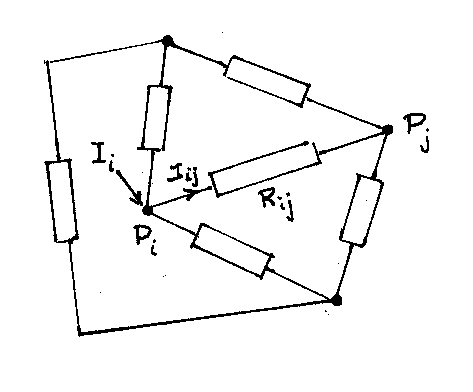
\epsfig{file=kuvat/kuvaM-1.ps}
\end{center}
\end{figure}
\end{multicols}
Jos merkitään $I_{ij} =$ \pain{virta} vastuksen $R_{ij}$ läpi, positiivisena $P_i$:stä poispäin
(vrt.\ kuvio), niin 
\index{Kirchhoffin laki}%
\pain{Kirchhoffin} \pain{lain} (\hist{G.R. Kirchhoff}, 1845) mukaan
\begin{equation} \label{m-8.1}
\sum_{j=1}^n I_{ij}\ =\ I_i, \quad i = 1 \ldots n,
\end{equation}
missä $I_i =$ solmuun $P_i$ ulkoapäin syötetty virta. Toisaalta
\index{Ohmin laki}%
\pain{Ohmin} \pain{lain} (\hist{G.S. Ohm}, 1826) mukaan
\begin{equation} \label{m-8.2}
R_{ij} I_{ij}\ =\ V_i - V_j, \quad i,j = 1 \ldots n,
\end{equation}
missä $V_i =$ j\pain{ännite} solmussa $P_i$. Ohmin lakia \eqref{m-8.2} käyttäen voidaan virrat
$I_{ij}$ yhtälöryhmässä \eqref{m-8.1} lausua jännitteiden avulla, jolloin tuloksena on systeemi
\begin{equation} \label{m-8.3}
\sum_{j=1}^n a_{ij} V_j\ =\ I_i, \quad i = 1 \ldots n,
\end{equation}
missä
\[
a_{ii}\ =\ \sum_{j=1}^n (1/R_{ij}), \quad a_{ij}\ =\ -1/R_{ij},\,\ i \neq j.
\]
Tämä on lineaarinen yhtälöryhmä kokoa $n \times n$, missä $x_i = V_i$, $b_i = I_i$. 
\begin{Exa} Jos nelisolmuisessa verkossa (vrt.\ kuvio edellä) on 
$R_{ij} = R,\ i,j = 1 \ldots 4,\ i \neq j$, niin jännitteille
$V_i$ saadaan yhtälöryhmä
\[ \left\{ \begin{array}{rrrrrrrrl} 3V_1&-& V_2&-& V_3&-& V_4&\ \ =\ \ &RI_1\\
                                    -V_1&+&3V_2&-& V_3&-& V_4&\ \ =\ \ &RI_2\\
                                    -V_1&-& V_2&+&3V_3&-& V_4&\ \ =\ \ &RI_3\\
                                    -V_1&-& V_2&-& V_3&+&3V_4&\ \ =\ \ &RI_4
\end{array} \right. \]
Tämä on singulaarinen systeemi: Jos esim.\ $I_1 = I \neq 0$ ja $I_2 = I_3 = I_4 = 0$, niin 
ratkaisua ei ole. Jos myös $I_1 = 0$, niin $V_i = V,\ i = 1 \ldots 4$ on ratkaisu millä tahansa
$V \in \R$, ts.\ ratkaisuja on äärettömän monta. \loppu 
\end{Exa}
 
Esimerkin singulaarisuusongelma on yhtälöryhmän \eqref{m-8.3} ominaisuus yleisemminkin.
Nimittän kertoimien $a_{ij}$ ym.\ lausekkeista nähdään, että
\[
\sum_{j=1}^n a_{kj}\ =\ \sum_{i=1}^n a_{ik}\ =\ 0, \quad k = 1 \ldots n.
\]
Tästä on kaksi seuraamusta: Ensinnäkin jos yhtälöryhmän \eqref{m-8.3} yhtälöt lasketaan 
puolittain yhteen saadaan
\[
(\sum_{i=1}^n a_{i1})\,V_1 + \ldots + (\sum_{i=1}^n a_{in})\,V_n\ =\ \sum_{i=1}^n I_i,
\]
eli
\begin{equation} \label{m-8.4}
0\ =\ \sum_{i=1}^n I_i.
\end{equation}
Toiseksi nähdään, että jos $\seq{V_i}$ on systeemin \eqref{m-8.4} ratkaisu, niin myös 
$\seq{V_i + V}$ on ratkaisu millä tahansa $V \in \R$, sillä
\[
\sum_{j=1}^n a_{ij} (V_j + V)\ =\ \sum_{j=1}^n a_{ij} V_j\ +\ (\sum_{j=1}^n a_{ij})\,V\ 
                               =\ I_i + 0\ =\ I_i, \quad i = 1 \ldots n.
\]
On siis päätelty: (a) Jos yhtälöryhmällä \eqref{m-8.3} on ratkaisu, niin ehto \eqref{m-8.4} 
toteutuu, ts.\ tämä on \pain{välttämätön} \pain{ehto} ratkeavuudelle. (b) Jos yhtälöryhmä 
\eqref{m-8.3} on ratkeava, niin ratkaisuja on äärettömän monta. Yhtälöryhmä \eqref{m-8.3} on 
siis yleisesti singulaarinen.

Singulaarisuusongelma on merkki siitä, että matemaattista mallia ei ole ajateltu 
(fysikaaliselta kannalta) aivan loppuun asti. --- Ongelmaan onkin yksinkertainen 
'sähkömiehen ratkaisu': \pain{Maadoitetaan} verkon yksi solmu $P_k$. Matemaattisessa mallissa
tämä merkitsee solmussa $P_k$ asetettavia ehtoja
\begin{equation} \label{m-8.5}
V_k\ =\ V_{ref}, \quad I_k\ =\ - \sum_{i \neq k} I_i.
\end{equation}
Ensimmäinen ehto asettaa jännitteelle $V_k$ jonkin valinnaisen referenssiarvon $V_{ref}$, esim.\
$V_{ref} = 0$. Tämä on luvallista, koska fysikaalisesti merkitseviä ovat vain jännite-erot. 
Toisessa ehdossa voidaan $I_k$ tulkita \pain{maadoitusvirraksi}, joka määräytyy fysikaalisesti
siten, että syöttövirtojen tasapainoehto \eqref{m-8.4} (myös fysikaalinen ehto!) toteutuu. Ehto
$V_k = V_{ref}$ poistaa $V_k$:n tuntemattomien joukosta, jolloin yhtälöryhmä \eqref{m-8.3} 
voidaan kirjoittaa muotoon
\[
\sum_{j \neq k} a_{ij} V_j\ =\ I_i - a_{ik} V_{ref}\ = J_i, \quad i = 1 \ldots n.
\]
Tästä voidaan edelleen $k$:s yhtälö poistaa tarpeettomana. Nimittäin koska
\[
\sum_{i=1}^n a_{ij} = 0 \qimpl a_{kj} = - \sum_{i \neq k} a_{ij}, \qquad j = 1 \ldots n,
\]
niin olettamalla yhtälöryhmän \eqref{m-8.3} muut yhtälöt ($i \neq k$) sekä ehdon \eqref{m-8.5}
jälkimmäinen osa toteutuviksi päätellään
\begin{align*}
\sum_{j=1}^n a_{kj} V_j\ &=\ - \sum_{j=1}^n (\sum_{i \neq k} a_{ij})\,V_j \\
                         &=\ - \sum_{i \neq k} (\sum_{j=1}^n a_{ij} V_j)\ 
                          =\ - \sum_{i \neq k} I_i\ =\ I_k.
\end{align*}
(Tässä tehty summeerausjärjestyksen vaihto perustuu yhteenlaskun vaihdantalakiin.) Tuloksen 
perusteella $k$:s yhtälö on muiden yhtälöiden ja lisäehdon \eqref{m-8.5} seuraus, siis 
tarpeeton.

Em. toimenpiteiden jälkeen on sähköpiirin matemaattinen malli supistunut lineaariseksi 
yhtälöryhmäksi kokoa $(n-1) \times (n-1)$. Tapauksessa $V_{ref} = 0$ redusoitu malli saadaan
yksinkertaisesti poistamalla yhtälöryhmän taulukkomuodosta taulukon $k$:s sarake
(vastaten ehtoa $V_k = 0$) ja $k$:s rivi ($k$:nnen yhtälön poisto). Malli saa tällöin muodon 
\begin{equation} \label{m-8.6}
\sum_{j \neq k} a_{ij} V_j\ =\ I_i, \quad i = 1 \ldots n,\ \ i \neq k.
\end{equation}
Osoittautuu (tarkemmat perustelut sivuutetaan), että yhtälöryhmä \eqref{m-8.6} on aina 
säännöllinen.
\jatko \begin{Exa} (jatko) \ Jos asetetaan solmussa $P_4$ maadoitusehto $V_4 = 0$, niin 
tapauksessa $I_1 = I,\ I_2 = I_3 = 0$ on redusoidulla systeemillä
\[ \left\{ \begin{array}{rrrrrrl}  3V_1&-& V_2&-& V_3&\ \ =\ \ &RI\\
                                  -V_1&+&3V_2&-& V_3&\ \ =\ \ & 0\\
                                  -V_1&-& V_2&+&3V_3&\ \ =\ \ &0
\end{array} \right. \] 
(yksikäsitteinen) ratkaisu
\[
V_1 = \frac{1}{2}\,RI, \quad V_2 = \frac{1}{4}\,RI, \quad V_3 = \frac{1}{4}\,RI.
\]
Ratkaisun perusteella solmujen $P_1$ ja $P_4$ välinen efektiivinen vastus (kokonaisvastus) on
\[
R_{eff}\ =\ \frac{V_1 - V_4}{I}\ =\ \frac{1}{2}\,R. \quad \loppu
\] \end{Exa}

\subsection*{Ristikkorakenne}
\index{zza@\sov!Ristikkorakenne|vahv}

Tarkastellaan kimmoisten \pain{sauvo}j\pain{en} muodostamaa ristikkorakennetta, jossa sauvat on
liitetty toisiinsa solmupisteissä $P_i,\ i = 1 \ldots p$. Oletetaan, että liitokset välittävät
sauvasta toiseen vain vetoa/puristusta, eivät vääntöä (esim.\ löysä pulttiliitos). Sauvassa, 
jonka päätepisteet ovat $P_i,\,P_j$, olkoon sauvaa venyttävä \pain{voima}
\[
\vec{F}_{ij}\ =\ F_{ij} \vec{t}_{ij},
\]
missä $\vec{t}_{ij}$ on vektorin $\Vect{P_i P}_j$ suuntainen yksikkövektori 
(kyseessä on puristus, jos $F_{ij} < 0$). Tällöin \pain{voimatasa}p\pain{aino} pisteessä $P_i$
edellyttää, että
\begin{equation} \label{m-8.7}
\sum_{j \in \Lambda_i} \vec{F}_{ij}\,+\,\vec{G}_i\,=\,\vec{0}, \quad i = 1 \ldots p,
\end{equation}
missä $\{\,P_j \mid j \in \Lambda_i\,\}$ on niiden solmupisteiden joukko, joihin $P_i$ on 
yhdistetty sauvalla, ja $\vec{G}_i =$ ulkoinen kuorma solmussa $P_i$.
\begin{figure}[H]
\begin{center}
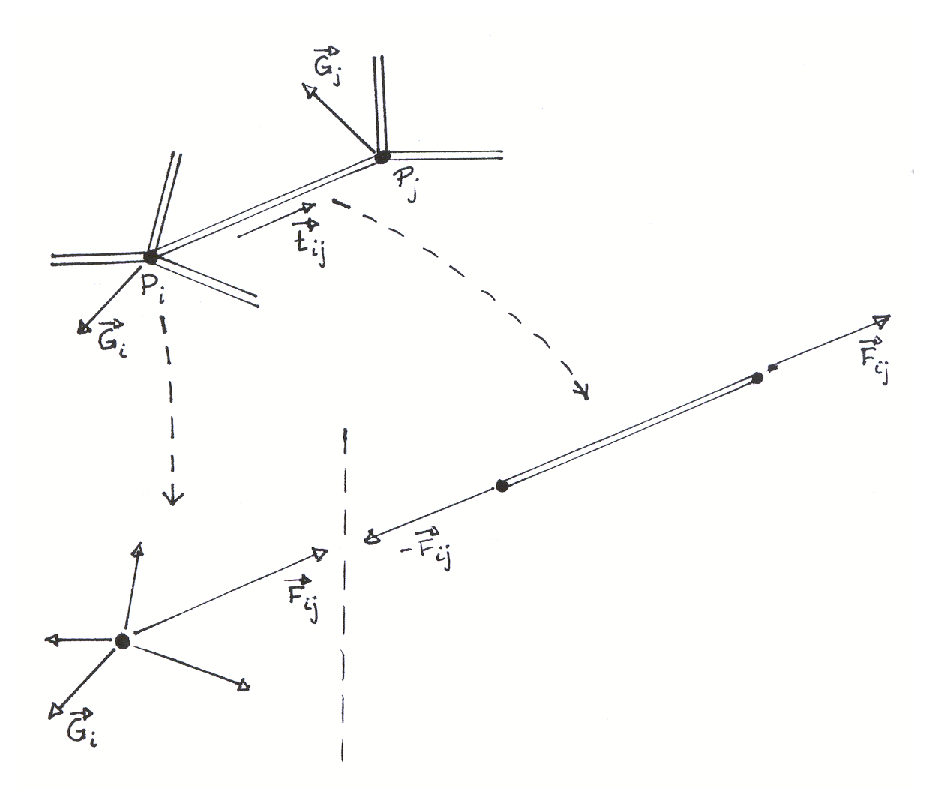
\epsfig{file=kuvat/kuvaM-2.ps}
\end{center}
\end{figure}
Kuvassa kuormitustilaa on purettu kahdeksi nk.\ \pain{va}p\pain{aaka}pp\pain{alekuvioksi}, 
joissa kummasakin vallitsee voimatasapaino. --- Huomattakoon, että liitoksia koskeva 
tasapainoehto \eqref{m-8.7} on hyvin samankaltainen kuin sähköpiirejä koskeva Kirchhoffin laki
\eqref{m-8.1}, joka myös on tasapainoehto (virtoja koskeva).

Kun yhtälöryhmässä \eqref{m-8.7} vektoriyhtälöt puretaan koordinaattimuotoon karteesisessa 
koordinaatistossa, niin skalaaristen yhtälöiden kokonaismääräksi tulee $2p$ tai $3p$ riippuen
siitä, onko kyseessä taso- vai avaruusristikkorakenne. Tuntemattomien $F_{ij}$ lukumäärä on 
luonnollisesti sama kuin sauvojen lukumäärä rakenteessa. Yhtälöryhmä \eqref{m-8.7} voi olla 
suoraan yksikäsitteisesti ratkeava, jolloin sanotaan, että rakenne on 
\pain{staattisesti} \pain{määrä}y\pain{t}y\pain{vä}. Tavallisempi tilanne on kuitenkin, että 
systeemi \eqref{m-8.7} on alimääräytyvä, eli \pain{staattisesti} \pain{määräämätön}. Tällöin 
tarvitaan tasapainolakien lisäksi toinen fysiikan laki,
\index{Hooken laki}%
\pain{Hooken} \pain{laki} 
(\hist{R. Hooke}, 1678). Hooken lain mukaan jokainen sauva käyttäytyy ristikkoa kuormitettaessa
kuten jousi, ts.\ voima $F_{ij}$ on suoraan verrannollinen sauvan \pain{ven}y\pain{mään}.

\mbox{\parbox{2in}{Oletetaan, että ristikkoa kuormitettaessa solmu $P_i$ 
(paikkavektori $\vec{r}_i$) siirtyy paikkaan $Q_i$, ja merkitään \pain{siirt}y\pain{mää} 
$\vec{u}_i = \Vect{P_i Q}_i$. Olettaen, että siirtymät ovat pieniä verrattuna sauvan pituuteen, 
voidaan kunkin sauvan venymä (negatiivinen venymä tarkoittaa puristumaa) laskea likimäärin 
kaavasta (vrt.\ kuvio)}}
\mbox{\parbox{4in}{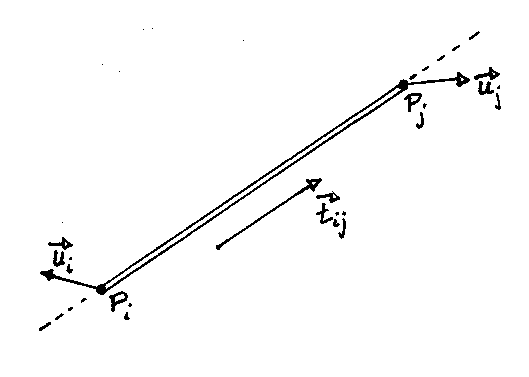
\epsfig{file=kuvat/kuvaM-3.ps}}}
\[
\abs{(\vec{r}_i + \vec{u}_i) - (\vec{r}_j + \vec{u}_j)}\ - \ \abs{\vec{r}_i - \vec{r}_j}\ 
                                     \approx\ (\vec{u}_j - \vec{u}_i) \cdot \vec{t}_{ij}.
\]

(Approksimaatiossa oletetaan, että siirtymien $\vec{u}_i$ ja $\vec{u}_j$ sauvaa vastaan 
kohtisuorat komponentit eivät vaikuta sauvan pituuteen.) Hooken lain mukaan venymä on suoraan
verrannollinen voimaan, eli
\begin{equation} \label{m-8.8}
F_{ij}\ =\ K_{ij} (\vec{u}_j - \vec{u}_i) \cdot \vec{t}_{ij},
\end{equation}
missä $K_{ij}$ on sauvalle ominainen kerroin (jousivakio). --- Huomattakon jälleen analogia 
sähköpiireihin: Siirtymät $\vec{u}_i$ vastaavat jännitteitä, voimat $F_{ij}$ virtoja, ja 
Hooken laki \eqref{m-8.8} vertautuu vastuksia koskevaan Ohmin lakiin. Jos sauvat ovat 
tasapaksuisia ja tehty homogeenisesta materiaalista, on jousivakio $K_{ij}$ suoraan 
verrannollinen sauvan poikkipinta-alaan ja kääntäen verrannollinen sauvan pituuteen. Jousivakio
riippuu myös materiaalin laadusta nk.\ \pain{kimmokertoimen} (materiaalivakio) kautta. 

Hooken lakia \eqref{m-8.8} käyttäen tulee yhtälöryhmästä \eqref{m-8.7} lineaarinen, 
tuntemattomina siirtymävektorien $\vec{u}_i$ koordinaatit. Tuntemattomien määrä on siis joko 
$2p$ (tasoristikko) tai $3p$ (avaruusristikko). Jotta yhtälöryhmästä saataisiin säännöllinen, on
ristikko vielä 'maadoitettava', eli tuettava riittävästi. Tuentaehdot voivat olla esim.\ muotoa 
$\vec{u}_k = \vec{0}$, jolloin solmun $P_k$ siirtyminen rakennetta kuormitettaessa on estetty.
Tällaisessa solmussa ei voimatasapainoehtoja tarvitse kirjoittaa, sillä tasapainosta huolehtivat
(tuntemattomat) tukivoimat, jotka vastaavat sähköpiirin maadoitusvirtoja. Tuentaehdoilla on 
yleisesti estettävä sellaiset siirtymätilat, jotka eivät aiheuta rakenteessa mitään kuormituksia
($F_{ij} = 0\ \forall\ i,j$). Erityisesti koko rakenteen liikkuminen jäykkänä kappaleena on 
matemaattisessa mallissa estettävä. Kun tällaiset riittävät (fysikaalisesti usein ilmeiset)
lisäehdot on asetettu, tulee yhtälöryhmästä \eqref{m-8.7}--\eqref{m-8.8} säännöllinen.
Siirtymät $\vec{u}_i$ voidaan tällöin ratkaista ensin, ja näiden avulla edelleen 
(fysikaalisesti ehkä kiinnostavammat) kuormitukset $F_{ij}$ Hooken laeista \eqref{m-8.8}.

\begin{Exa} \label{ristikko} \ \ 

\parbox{2in}{Oheisessa (taso)ristikossa on sauvoja kahta tyyppiä, jousivakiot $K_1$ ja $K_2$. 
Sauvoja on $7$ kpl ja yhtälöryhmässä \eqref{m-8.7} on $3 \times 2 = 6$ yhtälöä 
(tuetuissa solmuissa $A,\,B$ voimatasapainosta huolehtivat tukivoimat), joten rakenne on 
staattisesti määräämätön. Kun siirtymiä solmuissa $P_i$ merkitään}
\mbox{\parbox{4in}{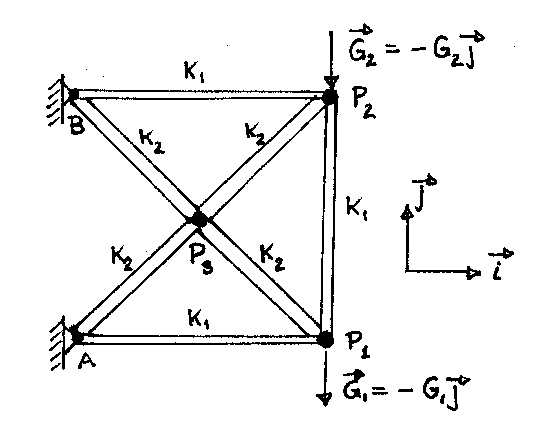
\epsfig{file=kuvat/kuvaM-4.ps}}}
\[
\vec{u}_i\ =\ u_i \vec{i} + v_i \vec{j}, \quad i = 1,2,3,
\]
niin lyhennysmerkinnöin
\[
a   = 1 + 2 K_2 / K_1, \quad b = 2 K_2 / K_1, \quad g_1 = G_1 / K_2, \quad g_2 = - G_2 / K_2
\]
yhtälöryhmä \eqref{m-8.7}--\eqref{m-8.8} saa muodon
\[ \left\{ \begin{array}{rrrrrrrrrrrrl} 
au_1&-&v_1& &    & &    &-& u_3&+& v_3&\quad 
                   = \quad&0\\ u_1&-&av_1& &    &+&bv_2&-& u_3&+& v_3&\quad = \quad&g_1\\
    & &   & &au_2&+& v_2&-& u_3&-& v_3&\quad 
                   = \quad&0\\    &-&bv_1&+& u_2&+&av_2&-& u_3&-& v_3&\quad = \quad&g_2\\
 u_1&-&v_1&+& u_2&+& v_2&-&4u_3& &    &\quad 
                   = \quad&0\\-u_1&+& v_1&+& u_2&+& v_2& &    &-&4v_3&\quad = \quad&0
\end{array} \right. \]

Tämä on säännöllinen ryhmä, josta siirtymät $u_i,\,v_i$ ovat ratkaistavissa. Sauvoja venyttävät
tai puristavat voimat ovat tämän jälkeen laskettavissa Hooken \mbox{laeista \eqref{m-8.8}.} 
Esimerkiksi sauvaa $P_1 P_3$ venyttää (negatiivisena puristaa) voima
\[
F_{13}\ =\ K_2\,[(u_3 - u_1)\vec{i} + (v_3 - v_1)\vec{j}\,] 
                          \cdot \frac{1}{\sqrt{2}}\,(-\vec{i}+\vec{j}) 
        = \frac{K_2}{\sqrt{2}}\,(u_1 - v_1 - u_3 + v_3). \loppu
\] 
\end{Exa}

\Harj
\begin{enumerate}

\item
Vastuspiirin solmut ovat tasasivuisen kolmion $ABC$ kärjet ja kolmion keskipiste $D$. Sivuilla
$AB$, $BC$ ja $CA$ on vastukset $R_1=1$, $R_2=2$ ja $R_3=3$. Kolmion kärjet $A$, $B$ ja $C$
on yhdistetty keskipisteeseen vastuksilla $R_4=R_5=2$ ja $R_6=3$. Olettaen virtasyöttö $I$
solmuun $A$ ja maadoitus solmuun $C$, muodosta lineaarinen yhtälöryhmä solmujen $A,B,D$ 
jännitteille ja laske solmujen $A$ ja $C$ välinen vastus.

\item
Kuution kärjet $P_i,\ i=0 \ldots 7$, on numeroitu siten, että $P_0$ ja $P_7$ ovat vastakkaiset
kärjet kuution yhdellä sivulla. Kärjet ovat solmuja virtapiirissä, jonka johdot kulkevat
pitkin kuution särmiä ja jokaisella särmällä vastus $=R$. Solmujen jännitteistä ($x_i$)
tiedetään, että $x_0=E$ (jännitelähde) ja $x_7=0$. Muodosta lineaarinen yhtälöryhmä
jännitteille $x_i,\ i=1 \ldots 6$. Ratkaise ja laske solmujen $P_0$ ja $P_7$ välinen vastus.

\item (*) \index{zzb@\nim!Silta}
(Silta) Tason ristikkorakenteen solmut $P_1,\ldots,P_7$ ovat pisteissä $(0,0)$, $(1,1)$,
$(2,0)$, $(3,1)$, $(4,0)$, $(5,1)$ ja $(6,0)$. Solmut on yhdistetty sauvoilla siten, että
muodostuu viisi vierekkäistä tasakylkistä ja suorakulmaista kolmiota. Solmu $P_1$ on jäykästi
tuettu ja solmun $P_7$ siirtyminen suuntaan $\vec j$ on estetty, muita tukia ei ole. Solmuihin
$P_3$ ja $P_5$ vaikuttavat kuormat ovat $\vec F_3=-a G\vec j$ ja $\vec F_5=-bG\vec j$, missä
$a,b \ge 0$ ovat dimensiottomia vakioita. Muita kuormia ei ole. Merkitse sauvoja
venyttäviä (negatiivisena puristavia) voimia symboleilla $T_i=x_iG$ ($11$ sauvaa!) ja kirjoita
näiden avulla solmujen tasapainoyhtälöt. Ratkaise systeemi (mahdollista, koska rakenne on
staattisesti määräytyvä), ja vastaa ratkaisun perusteella kysymykseen: Jos jokainen sauva
kestää puristusta $G$:n verran ja vetoa rajattomasti, niin millaiset kuormat ovat mahdollisia
rakenteen romahtamatta? Piirrä kuva $ab$-tasoon!

\end{enumerate} %*Lineaaristen yhtälöryhmien perinteisiä sovellusesimerkkejä

\chapter[Usean muuttujan differentiaalilaskenta]{Usean muuttujan \\ 
differentiaalilaskenta}

Tässä luvussa tarkastelun kohteena ovat \kor{vektorimuuttujan}, eli useamman reaalimuuttujan
funktiot tyyppiä $f:\,\R^n\kohti\R$ ja vektorimuuttujan \kor{vektoriarvoiset} funktiot
tyyppiä $\mf:\,\R^n\kohti\R^m$. Edellisten erikoistapaukset, kahden ja kolmen
\mbox{reaalimuuttujan} funktiot, ovat ennestään tuttuja Luvusta
\ref{kahden ja kolmen muuttujan funktiot}. Myös vektoriarvoisia funktioita on tavattu jo
aiemmin, sillä sekä Luvussa \ref{parametriset käyrät} esitellyt parametriset käyrät ja
parametriset pinnat että Luvuissa \ref{lineaarikuvaukset}--\ref{affiinikuvaukset} käsitellyt
lineaari- ja affiinikuvaukset ovat tällaisten erikoistapauksia. Vektoriarvoisia funktioita ovat
myös tason ja avaruuden \kor{vektorikentät}, joissa vektori ymmärretään
geometris--fysikaalisena 'nuolivektorina'.

Luvussa \ref{usean muuttujan jatkuvuus} yleistetään Luvuista
\ref{jatkuvuuden käsite}--\ref{funktion raja-arvo} tutut jatkuvuuden ja raja-arvon käsitteet
useamman muuttujan funktioille. Tämän jälkeen luvun keskeisen sisällön muodostavat erilaiset
\pain{derivaatan} käsitteen laajennukset useamman muuttujan tilanteisiin ja näihin
laajennuksiin liittyvä laskutekniikka (differentiaalilaskenta) ja sovellukset. Yleisempinä
derivaatan käsitteinä esitellään tässä luvussa \kor{osittaisderivaatat} ja niistä muodostettu
\kor{gradientti} (Luvut \ref{osittaisderivaatat}--\ref{gradientti}), vektorikenttiin liittyvät
\kor{divergenssi} ja \kor{roottori}
(Luvut \ref{divergenssi ja roottori}--\ref{div ja rot käyräviivaisissa}) ja lopulta yleisempiin
vektoriarvoisiin funktioihin eli \kor{epälineaarisiin kuvauksiin} liittyen 
\kor{Jacobin matriisi} (Luku \ref{jacobiaani}). Sovelluksina tarkastellaan mm.\ geometrisia
tehtäviä kuten \kor{pinnan tangenttitason} määrittämistä (Luku \ref{gradientti}), fysiikan 
\kor{osittaisdifferentiaaliyhtälöitä} 
(Luvut \ref{divergenssi ja roottori}--\ref{div ja rot käyräviivaisissa}), 
\kor{epälineaarisia yhtälöryhmiä} ja niiden numeerista ratkaisemista (Luku \ref{jacobiaani})
ja \kor{optimoinnin} ongelmia (Luku \ref{usean muuttujan ääriarvotehtävät}). Luvussa
\ref{käänteisfunktiolause} esitellään kolme epälineaarisiin yhtälöryhmiin liittyvää
\kor{epälineaarisen analyysin} vahvaa lausetta. Viimeisessä osaluvussa
(Luku \ref{usean muuttujan taylorin polynomit}) määritellään \kor{Taylorin polynomi} useamman
muuttujan funktioille.  %Usean muuttujan differentiaalilaskenta
\section{Usean muuttujan funktiot: Jatkuvuus ja raja-arvot} 
\label{usean muuttujan jatkuvuus}
\sectionmark{Usean muuttujan jatkuvuus}
\alku
\index{jatkuvuusb@jatkuvuus (usean muuttujan)|vahv}
\index{funktion raja-arvo|vahv}

Kahden ja kolmen reaalimuuttujan funktioiden algebraa on tarkasteltu aiemmin Luvussa 
\ref{kahden ja kolmen muuttujan funktiot}. Tässä ja seuraavissa luvuissa kohteena ovat kahden
ja kolmen muuttujan funktioiden lisäksi yleisemmät $n$ reaalimuuttujan reaaliarvoiset funktiot 
muotoa
\[
y=f(x_1,\ldots,x_n).
\]
Tässä voi käyttää myös matriisilaskun merkintää
\[
y=f(\mx), \quad \mx\in\R^n
\] 
\index{funktio A!d@$n$ muuttujan (vektorim.)} \index{vektorimuuttujan funktio}%
($\mx$ pysty- tai vaakavektori) ja puhua \kor{vektorimuuttujan} funktiosta. Mahdollista
(ja matemaattisissa teksteissä  tavallistakin) on matriisilaskun merkinnän sijasta käyttää myös
vektorimuuttujalle yksinkertaista symbolia $x$, eli merkitä
\[
y=f(x),\quad x=(x_1,\ldots,x_n)\in\R^n.
\]
Jatkossa käytetään eri merkintätapoja rinnakkain, jolloin matriisialgebran merkinnöissä $\mx$ 
tarkoittaa pystyvektoria. Kahden ja kolmen muuttujan tapauksissa merkitään vektorimuuttuja
vanhaan tapaan $(x,y)$ tai $(x,y,z)$. 

Funktion j\pain{atkuvuuden} ja \pain{ra}j\pain{a}-\pain{arvon} käsitteet, jotka toistaiseksi
on liitetty vain yhden muuttujan funktioihin 
(ks.\ Luvut \ref{jatkuvuuden käsite}--\ref{funktion raja-arvo}), ovat yleistettävissä melko
suoraviivaisesti useamman muuttujan funktioita koskeviksi. Aloitetaan kahden muuttujan
funktioista.

\subsection*{Funktio $f(x,y)$}

Kahden muuttujan funktion jatkuvuuden ja raja-arvon määritelmien alustukseksi tarvitaan
\begin{Def} \label{lukuparijonon suppeneminen} \index{raja-arvo!c@lukuparien jonon|emph}
\index{suppeneminen!ab@lukuparien jonon|emph}
Jono $\seq{(x_n,y_n)}$, missä 
$(x_n,y_n) \in \R^2,\ n\in\N$, \kor{suppenee kohti} (lähestyy) \kor{lukuparia} (pistettä) 
$(x,y)$ täsmälleen kun $x_n \kohti x$ ja $y_n \kohti y$. 
\end{Def}
Kun lukuparien jonon suppenemiselle käytetään aiempaan tapaan merkintää '\kohti', niin on siis 
sovittu:
\[ 
(x_n,y_n) \kohti (x,y) \qekv x_n \kohti x\ \ \ja\ \ y_n \kohti y. 
\]
Tämän kanssa yhtäpitävä sopimus on 
(ks.\ Harj.teht.\,\ref{jonon raja-arvo}:\,\ref{H-I-6: lukujonopari}d)
\[
(x_n,y_n)\kohti(x,y) \qekv (x_n-x)^2+(y_n-y)^2 \kohti 0.
\]
Tämän mukaan siis $(x_n,y_n)\kohti(x,y)$ tarkoittaa yksinkertaisesti, että pisteen
$(x_n,y_n)$ (geometrinen) etäisyys pisteestä $(x,y)$ lähestyy (lukujonona) $0$:aa, kun
$n\kohti\infty$. Jos erityisesti $(x,y)=(0,0)$, niin polaarimuunnoksen $x_n=r_n\cos\varphi_n$,
$y_n=r_n\sin\varphi_n$ perusteella on
\[
(x_n,y_n)\kohti(0,0) \qekv r_n \kohti 0 \qquad \text{(polaarikoordinaatisto)}.
\]
Koska tämä ei aseta mitään rajoituksia jonolle $\seq{\varphi_n}$, niin lähestyminen voi
tapahtua esim.\ pitkin puolisuoraa, jolla $\varphi_n=\varphi=$ vakio, tai se voi olla
suunnaltaan 'hyppelehtivää', esim.\ spiraalimaista. Joka tapauksessa mahdollisia
lähestymis\-\pain{suuntia} (vastaten puolisuoria) on äärettömän monta. --- Tämä on olennainen
ero verrattuna yhden muuttujan tilanteeseen, jossa pistettä voi lähestyä vain kahdesta eri
suunnasta.

Kun kaksiulotteinen 'lähestyminen' $(x_n,y_n)\kohti(x,y)$ on näin määritelty, on
Määritelmien \ref{funktion jatkuvuus} (jatkuvuus) ja \ref{funktion raja-arvon määritelmä}
(funktion raja-arvo) yleistäminen kahden muuttujan tilanteeseen suoraviivaista:
\begin{Def} \label{kahden muuttujan jatkuvuus} 
\index{jatkuvuusb@jatkuvuus (usean muuttujan)!a@funktion $f(x,y)$|emph}
Funktio $f:\ \DF_f\subset\R^2\kohti\R$ on
\kor{jatkuva} pisteessä $(x,y)\in\DF_f$ täsmälleen kun kaikille reaalilukuparien jonoille
$\seq{(x_n,y_n)}$ pätee
\[
(x_n,y_n)\in\DF_f\,\ \forall n\,\ \ja\,\ (x_n,y_n)\kohti(x,y)\,\ 
                                  \impl\,\ f(x_n,y_n) \kohti f(x,y).
\]
\end{Def}
\begin{Def} \label{kahden muuttujan raja-arvo}
\index{raja-arvo!d@kahden muuttujan funktion|emph}
Funktiolla $f(x,y)$ on pisteessä $(a,b)$
\kor{raja-arvo} $A\in\R$, jos jokaiselle reaalilukuparien jonolle $\seq{(x_n,y_n)}$ pätee
\[
(a,b)\neq(x_n,y_n)\in\DF_f\,\ \forall n\,\ \ja\,\ (x_n,y_n) \kohti (a,b)\,\ 
                                             \impl\,\ f(x_n,y_n) \kohti A, 
\]
ja oletus on voimassa jollekin jonolle $\seq{(x_n,y_n)}$. Raja-arvo merkitään
\[
\lim_{(x,y)\kohti(a,b)}f(x,y)=A.
\]
\end{Def}
Kuten yhden muuttujan tapauksessa, Määritelmä \ref{kahden muuttujan raja-arvo} estää raja-arvon
määrittelyn sellaisessa (eristetyssä) pistessä $(a,b)$, jota kohti lähestyminen
$(x_n,y_n)\kohti(a,b)$ joukosta $\DF_f$ käsin ei ole mahdollista lisäehdolla
$(x_n,y_n)\neq(a,b)\ \forall n$. Määritelmässä \ref{kahden muuttujan jatkuvuus} tätä lisäehtoa
ei ole, joten jos $(a,b)\in\DF_f$ on $\DF_f$:n eristetty piste, niin $f$ on jatkuva pisteessä
$(a,b)$ (vrt.\ Harj.teht.\,\ref{jatkuvuuden käsite}:\,\ref{H-V-1: eristetty piste}).
\begin{Exa} \label{udif-1: esim 1} Määritellään funktiot
\[
f_1(x,y)=\frac{x^2y}{x^2+y^2}\,, \quad
f_2(x,y)=\frac{xy}{x^2+y^2}\,, \quad (x,y)\in\R^2,\ (x,y)\neq(0,0).
\]
Tutki, ovatko funktiot jatkuvia origossa, kun asetetaan $f_1(0,0)=f_2(0,0)=0$.
\end{Exa}
\ratk Polaarimuunnoksilla
\begin{align*}
&g_1(r,\varphi) \,=\, f_1(r\cos\varphi,r\sin\varphi) \,=\, r\cos^2\varphi\sin\varphi, \\
&g_2(r,\varphi) \,=\, f_2(r\cos\varphi,r\sin\varphi) \,=\, \cos\varphi\sin\varphi
\end{align*}
päätellään: Jos $(x_n,y_n) \vastaa (r_n,\varphi_n)$, niin
\[
r_n \kohti 0 \qimpl |f_1(x_n,y_n)| \,=\, |g_1(r_n,\varphi_n)|
                                   \,\le\, r_n \,\kohti\, 0 \,=\, f(0,0),
\]
joten $f_1$ on jatkuva pisteessä $(0,0)$. Sen sijaan $f_2$ on epäjatkuva origossa, sillä
$r_n \kohti 0\ \not\impl\ g_2(r_n,\varphi_n) \kohti 0$.  \loppu

Raja-arvoille ja jatkuvuudelle pätevät samanlaiset yhdistelysäännöt kuin yhden muuttujan 
tapauksessa, sillä näiden tulosten taustalla oleva logiikka ja algebra ei olennaisesti riipu 
muuttujien lukumäärästä. Jatkuvuuden yhdistelytulokset ovat seuraavat:
\index{jatkuvuusb@jatkuvuus (usean muuttujan)!b@yhdistelysäännöt|emph}%
\begin{Lause} \label{yhdistelylause 1} Jos $f:\ D_f \kohti \R,\ D_f \subset \R^2$, ja
$g:\ D_g \kohti \R,\ D_g \subset \R^2$, ovat jatkuvia pisteessä $(x,y) \in D_f \cap D_g$, niin 
myös $\lambda f\ (\lambda \in \R)$, $f+g$ ja $fg$ ovat jatkuvia pisteessä $(x,y)$. Jos lisäksi
$g(x,y) \neq 0$, niin myös $f/g$ on jatkuva pisteessä $(x,y)$. 
\end{Lause}
\begin{Lause} \label{yhdistelylause 2} Jos $f: D_f \kohti \R,\ D_f \subset \R^2$, on jatkuva 
pisteessä $(x,y) \in D_f$ ja $g: D_g \kohti \R,\ D_g \subset \R$, on jatkuva pisteessä
$f(x,y)\in\DF_g$, niin yhdistetty funktio $g \circ f$ on jatkuva pisteessä $(x,y)$. 
\end{Lause}

Määritelmän \ref{kahden muuttujan jatkuvuus} mukainen jatkuvuus yksittäisessä pisteessä
laajenee luonnollisella tavalla jatkuvuudeksi joukossa: $f$ on jatkuva joukossa
$A\subset\DF_f$, jos $f$ on jatkuva $A$:n jokaisessa pisteessä. Kuten yhden muuttujan
tapauksessa, tavanomaiset 'yhden lausekkeen funktiot' ovat jatkuvia koko määrittelyjoukossaan.
\jatko \begin{Exa} (jatko) Jos esimerkissä jätetään $f_1(0,0)$ ja $f_2(0,0)$ erikseen
määrittelemättä, niin esimerkin funktiot ovat Lauseen \ref{yhdistelylause 1} perusteella
jatkuvia koko yhteisessä määritelyjoukossaan
\[
\DF_{f_1} = \DF_{f_2} = \{(x,y)\in\R^2 \mid (x,y)\neq(0,0)\}.
\]
Funktiolla $f_1$ on origossa raja-arvo
\[
\lim_{(x,y)\kohti(0,0)}f_1(x,y)=0
\]
(Määritelmä \ref{kahden muuttujan raja-arvo}), joten $f_1$ saadaan origossa (ja siis koko
$\R^2$:ssa) jatkuvaksi asettamalla $f_1(0,0)=0$ (funktion jatkaminen!). Funktiolla $f_2$ ei
tätä raja-arvoa ole, joten $f_2$:n jatkaminen origoon ei ole mahdollista. \loppu
\end{Exa}
\begin{Exa} Rationaalifunktion $f(x,y)=p(x,y)/q(x,y)$ ($p$ ja $q$ polynomeja) määrittelyjoukko
on $\DF_f=\{(x,y)\in\R^2 \mid q(x,y) \ne 0\}$. Lauseen \ref{yhdistelylause 1} mukaan $p$ ja $q$
ovat jatkuvia koko määrittelyjoukossaan ($=\R^2$), samoin $f$. \loppu
\end{Exa}
\begin{Exa} Missä pisteissä funktio $f(x,y) = \sqrt{y-x^2}/(x-y^2)$ on a) määritelty,
b) jatkuva? 
\end{Exa}
\ratk a) Määrittelyjoukko on
$\,D_f = \{\,(x,y) \in \R^2 \mid y \ge x^2\ \ja\ x \neq y^2\,\}$. \newline 
b) Kyseessä on yhdistetty ja yhdistelty funktio $f = (g \circ f_1)/f_2$, missä 
\[ \begin{aligned} &f_1(x,y)=y-x^2,\ D_{f_1} = \R^2, \quad f_2(x,y)=x-y^2,\ D_{f_2} = \R^2, \\
                   &g(t) = \sqrt{t},\ D_g = [0,\infty) \subset \R. 
   \end{aligned} \]
Lauseiden \ref{yhdistelylause 1} ja \ref{yhdistelylause 2} perusteella $f$ on jatkuva koko 
määrittelyjoukossaan. \loppu 

Kuten yhden muuttujan tapauksessa, myös kahden muuttujan funktion jatkuvuus ja raja-arvo
voidaan määritellä vaihtoehtoisesti vetoamatta luku(pari)jonoi\-hin. Vaihtoehtoisessa
'$(\eps,\delta)$-määritelmässä' tarvitaan avointa väliä $(x-\delta,x+\delta)$ vastaava
\index{ympzy@($\delta$-)ympäristö}%
\kor{ympäristö}, tarkemmin \kor{pisteen avoin $\delta$-ympäristö}, jota merkitään
$U_\delta(x,y)$ ($\delta>0$). Kuten yhdessä ulottuvuudessa, tällä tarkoitetaan joukkoa, joka
ympäröi pistettä $\delta$:n verran, tai $\delta$:aan verrannollisen matkan, j\pain{oka}
\pain{suuntaan}. Tyypillisesti $U_\delta(x,y)$ ajatellaan joko neliön tai kiekon muotoiseksi,
eli
\begin{align*}
\text{joko}&: \quad U_\delta(x,y)=(x-\delta,x+\delta)\times(y-\delta,y+\delta), \\
 \text{tai}&: \quad U_\delta(x,y)=\{(x',y')\in\R^2 \mid (x'-x)^2+(y'-y)^2<\delta^2\}.
\end{align*}
Jatkuvuuden vaihtoehtoinen määritelmä on (vrt.\ Määritelmä \ref{vaihtoehtoinen jatkuvuus})
\begin{Def} \label{kahden muuttujan vaihtoehtoinen jatkuvuus}
\index{jatkuvuusb@jatkuvuus (usean muuttujan)!a@funktion $f(x,y)$|emph}
Funktio $f:\ \DF_f\subset\R^2\kohti\R$ on jatkuva pistessä $(x,y)\in\DF_f$ täsmälleen kun
jokaisella $\eps>0$ on olemassa $\delta>0$ siten, että
\[
|f(x',y')-f(x,y)| < \eps\ \ \forall (x',y') \in U_\delta(x,y)\cap\DF_f.
\]
\end{Def}
Määritelmät \ref{kahden muuttujan jatkuvuus} ja \ref{kahden muuttujan vaihtoehtoinen jatkuvuus}
voidaan osoittaa yhtäpitäviksi samaan tapaan kuin yhden muuttujan tapauksessa (vrt.\ Lause
\ref{jatkuvuuskriteerien yhtäpitävyys}).

Ympäristö $U_\delta(x,y)$ on nimensä mukaisesti esimerkki \kor{avoimesta} joukosta, jonka
yleisempi määritelmä on (vrt.\ Määritelmä \ref{analyyttinen funktio} joukoille $A\in\C$)
\begin{Def} \label{avoin joukko} \index{avoin joukko|emph } 
Joukko $A\subset\R^2$ on \kor{avoin}, jos jokaisella$(x,y) \in A$ on olemassa $\delta>0$ siten,
että $U_\delta(x,y) \subset A$.
\end{Def}
 
\subsection*{Funktio $f(x,y,z)$}

Määritelmillä \ref{kahden muuttujan jatkuvuus} ja \ref{kahden muuttujan raja-arvo} on ilmeiset
vastineensa kolmen muuttujan funktioille $f(x,y,z)$. Esimerkiksi jatkuvuusehto pisteessä
$(x,y,z)\in\DF_f$ on \index{jatkuvuusb@jatkuvuus (usean muuttujan)!c@funktion $f(x,y,z)$}%
\[
(x_n,y_n,z_n)\in\DF_f\,\ \forall n\,\ \ja\,\ (x_n,y_n,z_n)\kohti(x,y,z)\,\
                                      \impl\,\ f(x_n,y_n,z_n) \kohti f(x,y,z),
\]
missä (vrt.\ Harj.teht.\,\ref{jonon raja-arvo}:\,\ref{H-I-6: lukujonopari}e)
\begin{align*}
(x_n,y_n,z_n)\kohti(x,y,z) &\qekv x_n \kohti x\ \ja\ y_n \kohti y\ \ja\ z_n \kohti z \\
                           &\qekv (x_n-x)^2+(y_n-y)^2+(z_n-z)^2 \kohti 0.
\end{align*}
Erityisesti jos $(x,y,z)=(0,0,0)$, niin pallokoordinaattimuunnoksen $(x_n,y_n,z_n)$
$\vastaa(r_n,\theta_n\varphi_n)$ perusteella on
\[
(x_n,y_n,z_n)\kohti(0,0,0) \qekv r_n \kohti 0 \qquad \text{(pallokoordinaatisto)}.
\]
\begin{Exa} Täsmälleen millä ehdoilla luvuille $\alpha,\beta,\gamma\in\R$ on
\[
\lim_{(x,y,z)\kohti(0,0,0)}f(x,y,z)=0, \quad \text{kun} \quad
f(x,y,z)=\frac{|x|^\alpha|y|^\beta|z|^\gamma}{x^2+y^2+z^2}\,?
\]
\end{Exa}
\ratk Tehdään pallokoordinaatimuunnos:
\[
f(x,y,z) = g(r,\theta,\varphi) = r^{\alpha+\beta+\gamma-2}|
                                 \sin\theta|^{\alpha+\beta}|\cos\theta|^\gamma
                                 |\cos\varphi|^\alpha|\sin\varphi|^\beta.
\]
Päätellään, että $\,r_n \kohti 0\ \impl\ g(r_n,\theta_n,\varphi_n) \kohti 0\,$ on tosi
täsmälleen ehdoilla
\[
\alpha+\beta+\gamma > 2,\,\ \alpha \ge 0,\,\ \beta \ge 0,\,\ \gamma \ge 0. \loppu
\]

\subsection*{Funktio $f(\mx),\  \mx\in\R^n$}

Yleiselle $n$ muuttujan reaaliarvoiselle funktiolle $f$ jatkuvuuseehto pisteessä
$\mx\in\DF_f$ on
\index{jatkuvuusb@jatkuvuus (usean muuttujan)!d@funktion $f(\mx),\ \mx\in\R^n$}%
\[
\mx_k\in\DF_f\,\ \forall k\,\ \mx_k \kohti \mx\,\ \impl\,\ f(\mx_k) \kohti f(\mx),
\]
\index{suppeneminen!ac@$\R^n$:n jonon} \index{raja-arvo!e@$\R^n$:n jonon}%
missä $\seq{\mx_k}$ on $\R^n$:n vektorijono ja \kor{suppeneminen} $\mx_k \kohti \mx$ kohti
\kor{raja-arvoa} $\mx\in\R^n$ tarkoittaa:
\[
\mx_k \kohti \mx \qekv (\mx_k)_i \kohti (\mx)_i=x_i\,,\,\ i=1 \ldots n
                 \qekv |\mx_k-\mx| \kohti 0,
\]
missä $|\cdot|$ on $\R^n$:n euklidinen normi. Määritelmien
\ref{kahden muuttujan vaihtoehtoinen jatkuvuus} ja \ref{avoin joukko} $n$-ulotteisissa
vastineissa ympäristö $U_\delta(\mx)$ tulkitaan joko $n$-ulotteiseksi kuutioksi, jonka särmän
pituus $=2\delta$, tai $n$-ulotteiseksi kuulaksi, jonka säde $=\delta$.

\subsection*{*Jatkuvuus kompaktissa joukossa}

Asetetaan (vrt.\ Määritelmät \ref{avoimet ym. joukot} ja \ref{jatkuvuus kompaktissa joukossa})
\begin{Def} \label{kompakti joukko - Rn} Joukko $K\subset\R^n$ on
\begin{itemize} \index{suljettu joukko|emph} \index{rajoitettu!b@joukko|emph}
\index{kompakti joukko|emph}
\item[-] \kor{suljettu}, jos kaikille $\R^n$:n vektorijonoille $\seq{\mx_k}$ pätee: \newline
         $\,\mx_k \in K\ \forall k\ \ja\ \mx_k \kohti \mx\in\R^n\ \impl\ \mx \in K$,
\item[-] \kor{rajoitettu}, jos $\exists C\in\R_+$ siten, että 
         $\,|\mx| \le C\ \forall \mx \in K$,
\item[-] \kor{kompakti}, jos $K$ on suljettu ja rajoitettu.
\end{itemize}
\end{Def}
Suljetun joukon vaihtoehtoinen määritelmä on (vrt.\ Lause \ref{avoin vs suljettu})

\begin{Lause} \label{avoin vs suljettu - Rn} \index{komplementti (joukon)|emph}
Joukko $A\subset\R^n$ on suljettu täsmälleen kun $A$:n \kor{komplementti}
$\complement(A)=\{\mx\in\R^n \mid \mx \not\in A\}$ on avoin.
\end{Lause}
\tod Harj.teht.\,\ref{H-udif-1: avoin vs suljettu}.
\begin{Exa} Kompakteja joukkoja $K\subset\R^n$ ovat esimerkiksi (suljettu) $n$-ulot\-teinen
suorakulmainen särmiö
\[
K=[a_1,b_1]\times[a_2,b_2]\times\ldots\times[a_n,b_n]
\]
ja (suljettu) $n$-ulotteinen kuula
\[
K = \{\mx\in\R^n \mid |\mx-\mx_0| \le R\}.
\]
Myös jokainen äärellinen $\R^n$:n osajoukko on kompakti
(Harj.teht.\,\ref{H-udif-1: äärellinen joukko}). \loppu
\end{Exa}
Kompaktin joukon käsite on keskeinen seuraavassa Weierstrassin lauseen
\ref{Weierstrassin peruslause} yleistyksessä, joka tapuksessa $n=1$ on todistettu aiemmin
Lauseena \ref{weierstrass}. Yleisempää todistusta ei esitetä; todettakoon ainoastaan, että
todistuksen logiikka on hyvin samanlainen kuin yhden muuttujan tapauksessa, ks.\ Luku
\ref{jatkuvuuden logiikka}. Asetetaan ensin (vrt.\ Määritelmä
\ref{jatkuvuus kompaktissa joukossa})
\begin{Def} \label{jatkuvuus kompaktissa joukossa - Rn} 
\index{jatkuvuusb@jatkuvuus (usean muuttujan)!e@kompaktissa joukossa|emph}
Funktio $f:\ \DF_f\subset\R^n\kohti\R$ on \kor{jatkuva kompaktissa joukossa} $K\subset\DF_f$,
jos jokaiselle $\R^n$:n vektorijonolle $\seq{\mx_k}$ pätee
\[
\mx_k \in K\ \forall k\,\ \ja\,\ \mx_k \kohti \mx\,\ \impl\,\ f(\mx_k) \kohti f(\mx).
\]
\end{Def}
\begin{*Lause} \label{weierstrass - Rn} \index{Weierstrassin lause|emph}
Jos funktio $f:\ \DF_f\subset\R^n\kohti\R$ on jatkuva
kompaktissa joukossa $K\subset\DF_f$, niin $f$ saavuttaa $K$:ssa pienimmän ja suurimman arvonsa.
\end{*Lause}

\Harj
\begin{enumerate}

\item
Kohdissa a)--h) määritä raja-arvo tai päättele, ettei raja-arvoa ole. Kohdissa i)--j) määritä
kaikki kertoimien $a,b,c$ arvot, joilla raja-arvo on olemassa. Siirtyminen napa- tai 
pallokoordinaatistoon voi auttaa.
\begin{align*}
&\text{a)}\ \lim_{(x,y)\kohti(2,-1)} (xy+y^2) \qquad 
 \text{b)}\ \lim_{(x,y)\kohti(0,0)} \sqrt{x^2+2y^2} \qquad
 \text{c)}\ \lim_{(x,y)\kohti(0,0)} \frac{x^2+y^2}{y} \\
&\text{d)}\ \lim_{(x,y)\kohti(0,0)}\,\frac{x}{x^2+y^2} \qquad\ 
 \text{e)}\ \lim_{(x,y)\kohti(0,0)}\,\frac{y^3}{x^2+y^2} \qquad\quad\ \
 \text{f)}\ \lim_{(x,y)\kohti(0,0)}\,\frac{x^2y^2}{x^2+y^4} \\
&\text{g)}\ \lim_{(x,y)\kohti(0,0)}\,\frac{\sin(xy)}{x^2+y^2} \qquad\ 
 \text{h)}\ \lim_{(x,y,z)\kohti(0,0,0)}\,\frac{\sin(xyz)}{x^2+y^2+z^2} \\
&\text{i)}\ \lim_{(x,y)\kohti(0,0)}\,\frac{xy}{ax^2+bxy+cy^2} \qquad
 \text{j)}\ \lim_{(x,y,z)\kohti(0,0,0)}\ \frac{x^2+y^2-z^2}{ax^2+by^2+cz^2}
\end{align*}

\item
Kohdissa a)--i) jatka funktion $f$ määritelmä niin, että funktiosta tulee jatkuva
mahdollisimman suuressa $\R^2$:n tai $\R^3$:n osajoukossa. Kohdissa j)--m) määritä kaikki
pisteet, joissa $f$ on epäjatkuva. 
\begin{align*}
&\text{a)}\ \ f(x,y)=\frac{x\sqrt[4]{\abs{y}}}{|x|+|y|} \qquad
 \text{b)}\ \ f(x,y)=\frac{\sqrt{(1+x^2)(1+y^2)}-1}{x^2+y^2} \\
&\text{c)}\ \ f(x,y)=\frac{x^3-8y^3}{x-2y} \qquad
 \text{d)}\ \ f(x,y)=\frac{x+y}{x^3+y^3} \qquad
 \text{e)}\ \ f(x,y)=\frac{x^2+y}{x^4-y^2} \\
&\text{f)}\ \ f(x,y)=\frac{\sin(x+y)}{x^2-y^2} \qquad
 \text{g)}\ \ f(x,y)=\frac{\sin(x^3+y^3)}{x+y} \\
&\text{h)}\ \ f(x,y,z)=\frac{1-\cos(xyz)}{x^2y^2z^2} \qquad
 \text{i)}\ \ f(x,y,z)=\frac{x^2-y^2+z^2+2xz}{x+y+z} \\
&\text{j)}\ \ f(x,y)=\begin{cases}
              4x^2+y^2-47, &\text{kun}\ x^2+y^2<25 \\ x^2-2y^2+28, &\text{kun}\ x^2+y^2 \ge 25
              \end{cases} \\
&\text{k)}\ \ f(x,y)=\begin{cases}
                     x^2+xy-2y^2, &\text{kun}\ 0<\abs{y}<x \\ 0, &\text{muulloin}
                     \end{cases} \\
&\text{l)}\ \ f(x,y)=
 \begin{cases}
 y\sin\left(\dfrac{1}{x}+\dfrac{1}{y}\right), &\text{kun}\ x \neq 0\,\ \text{ja}\,\ y \neq 0 \\
 0, &\text{kun}\ x=0\,\ \text{tai}\,\ y=0
 \end{cases} \\
&\text{m)}\ \ f(x,y,z)=\begin{cases}
                       \dfrac{\sin(xyz)}{\sin(xy)}\,, &\text{kun}\ xy \neq 0 \\
                       z, &\text{kun}\ xy=0
                       \end{cases}
\end{align*}

\item (*) \label{H-udif-1: kiero raja-arvo}
Määritellään $f:\,\Rkaksi\map\R$ seuraavasti:
\[
f(x,y)=\begin{cases} 
       \,1, &\text{kun}\ x^2<y<2 x^2\\ \,0, &\text{muulloin}
       \end{cases}
\]
Osoita, että funktiolla on sama raja-arvo origossa lähestyttäessä origoa mitä
tahansa suoraa $S:\ ax+by=0\ (a,b\in\R)$ pitkin, mutta siitä huolimatta ei ole olemassa
raja-arvoa $\,\lim_{(x,y)\to (0,0)} f(x,y)$.

\item (*) \label{H-udif-1: avoin vs suljettu}
Todista Lause \ref{avoin vs suljettu - Rn}.

\item (*)
Olkoon $f(x,y)=p(x,y)/q(x,y)$, missä $p$ ja $q$ ovat määriteltyjä ja jatkuvia koko $\R^2$:ssa
(esim.\ polynomeja). \vspace{1mm}\newline
a) Näytä suoraan Lauseen \ref{kahden muuttujan vaihtoehtoinen jatkuvuus} avulla, että
$\DF_f\subset\R^2$ on avoin. \vspace{1mm}\newline
b) Päättele $\DF_f$ avoimeksi osoittamalla ensin Määritelmään \ref{kompakti joukko - Rn}
nojaten, että $\{(x,y)\in\R^2 \mid q(x,y)=0\}$ on suljettu joukko ja vetoamalla Lauseeseen
\ref{avoin vs suljettu - Rn}.

\item (*) \label{H-udif-1: äärellinen joukko}
Olkoon $\ma_i\in\R^n,\ i=1 \ldots m\,\ (m\in\N)$, $\ma_i\neq\ma_j$ kun $i \neq j$, ja
$\,K=\{\ma_1,\ldots,\ma_m\}$. \vspace{1mm}\newline
a) Näytä, että $K\subset\R^n$ on kompakti joukko. \vspace{1mm}\newline
b) Näytä, että jos $f:\ \DF_f\subset\R^n\kohti\R$ on mikä tahansa funktio, jolle pätee
$\ma_i\in\DF_f,\ i=1 \ldots m$, niin $f$ on jatkuva $K$:ssa Määritelmän
\ref{jatkuvuus kompaktissa joukossa - Rn} mukaisesti. \vspace{1mm}\newline
c) Tarkista, että Lauseen \ref{weierstrass - Rn} väittämä on sopusoinnussa b)-kohdan tuloksen
kanssa.

\end{enumerate} %Usean muuttujan jatkuvuus ja raja-arvot
\section{Osittaisderivaatat} \label{osittaisderivaatat}
\alku
\index{osittaisderivaatta|vahv}

Kahden tai useamman muuttujan funktion \kor{osittaisderivaatalla} (engl. partial derivative) 
tarkoitetaan yksinkertaisesti funktion derivaattaa jonkin muuttujan suhteen muiden muuttujien
pysyessä vakioina raja-arvoprosessissa. Osittaisderivaatan symboli on $\partial$, joka luetaan
samoin kuin tavallinen derivaatta eli 'dee' (engl.\ 'partial'). Esimerkiksi kahden muuttujan
funktion $f(x,y)$ osittaisderivaattoja merkitään
\begin{align*}
\frac{\partial f}{\partial x} (x,y) 
         &= \lim_{\Delta x\kohti 0} \frac{f(x+\Delta x,y)-f(x,y)}{\Delta x}\,, \\
\frac{\partial f}{\partial y} (x,y) 
         &= \lim_{\Delta y\kohti 0} \frac{f(x,y+\Delta y)-f(x,y)}{\Delta y}\,.
\end{align*}
Vähemmän tilaa vieviä (ja laskentaakin nopeuttavia) merkintätapoja ovat
\[
\partial_x f, \ \partial_y f,\quad \text{tai} \quad f_x, \ f_y.
\]
Näistä ensimmäinen merkintätapa viittaa siihen tosiasiaan, että kuten tavallinen derivaatta,
myös osittaisderivaatta on 'funktion funktio' eli operaattori. \mbox{Alaindeksoitu} merkintä on 
tavallinen etenkin silloin, kun muuttujat ovat fysikaalisia paikka- ja aikamuuttujia.

Osittaisderivaatta käyttäytyy monessa suhteessa kuten tavallinen derivaatta. Se on esimerkiksi
derivoitavan funktion suhteen \kor{lineaarinen}:
\index{lineaarisuus!a@derivoinnin}%
\[
\partial_x\bigl[\lambda f(x,y)+\mu g(x,y)\bigr]
              =\lambda\partial_x f(x,y)+\mu\partial_x g(x,y),\quad \lambda,\mu\in\R.
\]
Osittaisderivoinnille pätee myös mm.\ tulon derivoimissääntö
\[
\frac{\partial}{\partial x} (fg)
              =\frac{\partial f}{\partial x} g + f\frac{\partial g}{\partial x}\,,
\]
sillä tämänkin säännön kannalta kyse on tavallisesta derivoinnista yhden valitun muuttujan 
suhteen.
\begin{Exa} \label{osder-esim 1} Funktion
\[
f(x,y) = \begin{cases} 
          \,0, &\text{kun}\ (x,y)=(0,0), \\ \,xy/(x^2+y^2)\,, &\text{muulloin}
         \end{cases}
\]
osittaisderivaatat muualla kuin origossa ovat
\[
f_x(x,y) = \frac{y^3-x^2y}{(x^2+y^2)^2}\,, \quad
f_y(x,y) = \frac{x^3-xy^2}{(x^2+y^2)^2}\,, \quad (x,y)\neq(0,0).
\]
Tässä on käytetty tavallisia (yhden muuttujan) rationaalifunktion derivoimissääntöjä. Koska
$f(x,0)=f(0,y)=0,\ x,y\in\R$, niin $f$:llä on osittaisderivaatat myös origossa:
\[
f_x(0,0)=f_y(0,0)=0. \loppu
\]
\end{Exa}
Esimerkin funktio on origossa epäjatkuva (ks.\ edellinen luku, Esimerkki \ref{udif-1: esim 1}).
--- Siis funktio voi olla epäjatkuva yksittäisessä pisteessä, vaikka
osittaisderivaatat ovat olemassa kaikkialla. Tämä ero yhden muuttujan funktioihin (joille
derivaatan olemassaolo pisteessä takaa jatkuvuuden ko.\ pisteessä) selittyy
sillä, että osittaisderivaattojen raja-arvoissa pistettä lähestytään vain koordinaattiakselien
suunnissa, kun usean muuttujan jatkuvuuden määritelmässä (ks.\ edellinen luku) mahdollisia
lähestymissuuntia on äärettömän monta. Usean muuttujan funktion derivoituvuus eli nk.\
\kor{differentioituvuus} onkin määriteltävä koordinaatistosta riippumattomana
'joka suuntaan derivoituvuutena', jotta se vastaa yhden muuttujan derivoituvuuden käsitettä.
Määritelmä asetetaan seuraavassa luvussa.

Funktion osittaisderivaattoja voidaan (funktioina) derivoida edelleen eri muuttujien suhteen,
jolloin saadaan
\index{kertaluku!d@osittaisderivaatan}%
\kor{toisen kertaluvun} osittaisderivaattoja, näitä derivoimalla
\kor{kolmannen kertaluvun} osittaisderivaattoja, jne. Korkeamman kertaluvun
osittaisderivaattoja merkitään
\begin{align*}
\frac{\partial}{\partial x}\left(\frac{\partial f}{\partial x}\right) 
       &= \frac{\partial^2 f}{\partial x^2}
        =\partial_x(\partial_x f)=(f_x)_x =f_{xx}, \\[1mm]
\frac{\partial}{\partial x}\left(\frac{\partial f}{\partial y}\right) 
       &= \frac{\partial^2 f}{\partial x\partial y}
        =\partial_x(\partial_y f)=(f_y)_x =f_{yx}, \\[1mm]
\frac{\partial}{\partial x}\left(\frac{\partial^2 f}{\partial x\partial y}\right) 
       &= \frac{\partial^3 f}{\partial x^2\partial y}
        =\partial_x^2(\partial_y f)=(f_y)_{xx}=f_{yxx}, \\[1mm]
\frac{\partial^2}{\partial y^2}\left(\frac{\partial^2 f}{\partial x^2}\right) 
       &= \frac{\partial^4 f}{\partial y^2\partial x^2}
        =\partial_y^2(\partial_x^2 f)=(f_{xx})_{yy}=f_{xxyy}\,, \quad \text{jne.}
\end{align*}
\begin{Exa} \label{osder-esim 2} Funktion $f(x,y)=\ln (x^2+y^2)$ osittaiderivaatat toiseen
kertalukuun asti pisteissä $(x,y)\neq(0,0)$ (eli $f$:n määrittelyjoukossa) ovat
\begin{align*}
f_x    &= \frac{2x}{x^2+y^2}\,,\quad f_y=\frac{2y}{x^2+y^2}\, \\
f_{xx} &= \frac{2(y^2-x^2)}{(x^2+y^2)^2}\,,\quad f_{yy} = -f_{xx}, \quad
          f_{xy} = f_{yx}=-\frac{4xy}{(x^2+y^2)^2}\,. \loppu
\end{align*}
\end{Exa}
Esimerkin tuloksessa $\,f_{xy}=f_{yx}\,$ on kyse yleisemmästä osittaisderivoinnin
\kor{vaihtosäännöstä} \index{vaihtoszyzy@vaihtosääntö!c@osittaisderivoinnin}
\index{osittaisderivaatta!a@vaihtosääntö}%
\begin{equation} \label{vaihtosääntö}
\boxed{\quad\kehys f_{xy}=f_{yx} \quad \text{(vaihtosääntö)}.\quad}
\end{equation}
Sääntö on pätevä lievin säännöllisyysehdoin, jotka yleensä voidaan olettaa. Ko.\ ehdot sekä
säännön perustelu esitetään luvun lopussa (Lause \ref{osittaisderivoinnin vaihtosääntö}).
Vaihtosäännön mukaan derivointijärjestys on vapaa myös korkeamman kertaluvun
osittaisderivaatoissa; esim.\ $f_{xxy}=f_{xyx}=f_{yxx}$.

\subsection*{Monen muuttujan osittaisderivaatat}
\index{osittaisderivaatta!b@monen muuttujan|vahv}

Vaihtosääntö \eqref{vaihtosääntö} pätee myös useamman kuin kahden muuttujan tapauksessa, koska
kahden muuttujan suhteen derivoitaessa funktio voidaan ajatella vain ko.\ muuttujista
riippuvaksi. Siis jos funktion $f(x_1,\ldots,x_n)$ osittaiderivaatat
$\partial f/\partial x_k$ ja $\partial^2 f/(\partial x_k\partial x_l)$ ovat olemassa ja
jatkuvia, kun $k,l=1 \ldots n,\ k \neq l$, niin
\[
\frac{\partial^2 f}{\partial x_k\partial x_l}
    =\frac{\partial^2 f}{\partial x_l\partial x_k},\quad k,l\in\{1,\ldots,n\},\,\ k \neq l.
\]
Koska derivointijärjestys näin muodoin on vapaa (lievin ehdoin, jotka yleensä oletetaan),
riittää korkeammissa osittaisderivaatoissa vain tietää, kuinka monta kertaa kunkin muuttujan
suhteen derivoidaan. Yleistä osittaisderivaattaa merkitään tällöin käyttäen nk.\
\index{indeksi!c@moni-indeksi} \index{moni-indeksi}%
\kor{moni-indeksiä} (engl.\ multi-index), eli järjestettyä indeksijoukkoa (indeksivektoria)
muotoa
\[
\alpha=(\alpha_1,\ldots,\alpha_n),\quad \alpha_i\in\N\cup\{0\}.
\]
Tällöin $\partial^\alpha f$ tarkoittaa osittaisderivaattaa
\[
\partial^\alpha f
=\frac{\partial^{\abs{\alpha}} f}{\partial x_1^{\alpha_1}\cdots\partial x_n^{\alpha_n}}
=\partial_1^{\alpha_1}\cdots\partial_n^{\alpha_n} f,
\]
\index{kertaluku!d@osittaisderivaatan}%
missä $\partial_i=\partial/\partial x_i$, ja osittaisderivaatan \kor{kertalukua} on merkitty
\[
\abs{\alpha}=\sum_{i=1}^n \alpha_i.
\]
Jos moni-indeksissä $\alpha$ on $\alpha_k=0$, ei ko.\ muuttujan suhteen derivoida, ts.\
$\partial_k^0 f=f$.
\begin{Exa} Jos $x_1=x$ ja $x_2=y$, niin vaihtosääntö huomioiden
\begin{align*}
\partial^{(1,1)}f(x,y)    &= \partial_x\partial_y f(x,y) = f_{xy}(x,y), \\
\partial^{(0,2)}f(x,y)    &= (\partial_y)^2 f(x,y) = f_{yy}(x,y), \\
\partial^{(2,1)}f(x,y)    &= (\partial_x)^2\partial_y f(x,y) = f_{xxy}(x,y). \loppu
\end{align*}
\end{Exa}
\begin{Exa} Tulon derivoimissääntöä ja lineaarisuussääntöä soveltaen
\begin{align*}
\partial^{(1,1)}(fg)(x,y) &= \partial_x\partial_y (fg)(x,y) \\
                         &= \partial_x\left(f_yg+fg_y\right)(x,y) \\
                         &= \left(f_{xy}g+f_xg_y+f_yg_x+fg_{xy}\right)(x,y). \loppu
\end{align*}
\end{Exa}
\begin{Exa} \vahv{Neliömuoto}. \label{neliömuoto} \index{neliömuoto}
Yleinen $\R^n$:n nk. \kor{neliömuoto} (engl. quadratic form) on funktio muotoa
\[
f(x_1,\ldots,x_n)=\frac{1}{2}\sum_{i,j=1}^n a_{ij}x_ix_j,\quad a_{ij}\in\R,
\]
tai matriisialgebran merkinnöin
\[
f(\mx)=\frac{1}{2}\mx^T\mA\mx,\quad \mx=(x_i), \ \mA=(a_{ij}).
\]
Tässä voidaan olettaa, että $a_{ij}=a_{ji}$ ($\mA$ symmetrinen), koska $f$ riippuu vain 
summista $a_{ij}+a_{ji}$ (\,$a_{ij}x_ix_j+a_{ji}x_jx_i=(a_{ij}+a_{ji})x_ix_j$\,). Kun tehdään tämä
oletus, niin tietystä muuttujasta $x_k$ riippuvat termit erottuvat muodossa
\[
f(x_1,\ldots,x_n)=\frac{1}{2}a_{kk}x_k^2+\sum_{j\neq k} a_{kj} x_kx_j+ [\ldots],
\]
missä $[\ldots]$ ei sisällä muuttujaa $x_k$. Näin ollen
\[
\frac{\partial f}{\partial x_k}=\sum_{j=1}^n a_{kj} x_j = [\mA\mx]_k,\,\ k=1\ldots n
              \qimpl \left(\frac{\partial f}{\partial x_i}\right) = \mA\mx.
\]
Toisen kertaluvun osittaisderivaatat ovat
\[
\left(\frac{\partial^2 f}{\partial x_i\partial x_j}\right) = \left(a_{ij}\right) = \mA.
\]
Korkeamman kertaluvun osittaisderivaatat häviävät. \loppu
\end{Exa}

\subsection*{Osittaisdifferentiaalioperaattorit}
\index{differentiaalioperaattori!c@osittaisderivoinnin|vahv}
\index{osittaisdifferentiaalioperaattori|vahv}

Kun osittaisderivaatoilla lasketaan, on usein kätevää ajatella symbolit $\partial_x$,
$\partial_y$, jne.\ derivoinnin yksittäisistä kohteista irrotetuiksi operaattoreiksi.
Esimerkiksi jos $\partial^\alpha$ ja $\partial^\beta$ ovat $n$ muuttujan
differentaalioperaattoreita, niin riittävän säännöllisille funktioille $f$ pätee vaihtosäännön
perusteella
\[
\partial^\alpha\left[\partial^\beta f(x)\right] = \partial^\beta\left[\partial^\alpha f(x)\right]
                                                = \partial^{\alpha+\beta} f(x).
\]
(Tässä $\alpha+\beta$ on moni-indeksien summa vektoreina.) Tämän voi ilmaista lyhyemmin
pelkästään operaattoreita koskevana laskusääntönä
\[
\partial^\alpha\partial^\beta=\partial^\beta\partial^\alpha=\partial^{\alpha+\beta}.
\]
\index{operaattoritulo} \index{kommutoivat operaattorit}%
Tällöin $\partial^\alpha\partial^\beta$ tarkoitaa \kor{operaattorituloa} eli kaksivaiheista
(yhdistettyä) operaatiota $f \map \partial^\beta f \map \partial^\alpha\partial^\beta f$.
Vaihtosäännön perusteella differentiaalioperaattorit $\partial^\alpha$ ja $\partial^\beta$ siis
\kor{kommutoivat}, eli pätee vaihdantalaki
$\partial^\alpha\partial^\beta=\partial^\beta\partial^\alpha$. --- Huomattakoon, että operaattori
$\partial^\alpha$ on määritelmänsä mukaisesti itsekin $(\abs{\alpha}-1)$-kertainen
operaattoritulo, jonka tekijöitä ovat yksittäiset differentiaalioperaattorit 
$\partial_k=\partial/\partial x_k$.

Operaattoritulon (eli yhdistetyn operaattorin) ohella toinen yleinen
differentiaalioperaattorien yhdistelytapa on
\index{lineaariyhdistely}%
\kor{lineaariyhdistely}. Tässä periaate on sama kuin funktioilla yleensä:
\[
(\lambda\partial^\alpha+\mu\partial^\beta)f=\lambda\partial^\alpha f+\mu\partial^\beta f,\quad 
\lambda,\mu\in\R.
\]
\begin{Exa}
Kun määritellään kahden muuttujan funktioille differentiaalioperaattori
$A=\partial_x+\partial_y$, niin
\begin{align*}
A^2 &= (\partial_x+\partial_y)(\partial_x+\partial_y) \\
    &= \partial_x(\partial_x+\partial_y)+\partial_y(\partial_x+\partial_y) \\
    &= (\partial_x)^2+\partial_x\partial_y+\partial_y\partial_x + (\partial_y)^2 \\
    &= (\partial_x)^2+2\partial_x\partial_y + (\partial_y)^2.
\end{align*}
Tämän mukaisesti on $\,A^2 f= A(Af)=f_{xx}+2f_{xy}+f_{yy}$. Yleisemminkin $A^k,\ k\in\N$
purkautuu binomikaavalla, esim.\
\[
A^3 f=f_{xxx}+3f_{xxy}+3f_{xyy}+f_{yyy}. \loppu
\]
\end{Exa}
Lineaarisen yhdistelyn kaavassa voivat kertoimet $\lambda,\mu$ olla myös muuttuvia, ts.\
\index{muuttuvakertoiminen diff.-oper.}%
funktioita. Muodostettaessa tällaisten \kor{muuttuvakertoimisten} operaattorien tuloja
derivointi kohdistuu myös kertoimiin, jolloin tulos muuttuu vakiokertoimisesta tapauksesta.
Operaattorituloja purettaessa tarvitaan tällöin myös tulon derivoimissääntöä.
\begin{Exa} Määritellään kahden muttujan funktioille differentiaalioperaattorit
$\ A=x\partial_x+y\partial_y\,$ ja $\,B=y^2\partial_x-x^2\partial_y$. Tällöin
\begin{align*}
AB &= (x\partial_x+y\partial_y)(y^2\partial_x-x^2\partial_y) \\
   &= x\partial_x(y^2\partial_x)-x\partial_x(x^2\partial_y)
                                +y\partial_y(y^2\partial_x)-y\partial_y(x^2\partial_y) \\
   &= xy^2(\partial_x)^2-2x^2\partial_y-x^3\partial_x\partial_y+2y^2\partial_x
                        +y^3\partial_y\partial_x-x^2y(\partial_y)^2 \\
   &= xy^2(\partial_x)^2-x^2y(\partial_y)^2+(y^3-x^3)\partial_x\partial_y
                        +2y^2\partial_x-2x^2\partial_y, \\[2mm]
BA &= AB-y^2\partial_x+x^2\partial_y. \loppu
\end{align*}
\end{Exa}
Esimerkissä differentiaalioperaattorit eivät kommutoi, ts. $AB \neq BA$. Muuttuvakertoimisessa
tapauksessa tämä on pääsääntö. Vakiokertoimiset operaattorit sen sijaan kommutoivat aina 
(vaihtosäännön ehdoin).

\subsection*{Ketjusäännöt}
\index{osittaisderivaatta!c@ketjusäännöt|vahv}
\index{ketjusääntö (os.-derivoinnin)|vahv}

Jos funktiossa $f(x_1,\ldots,x_n)$ muuttujista $x_i$ tehdään muuttujan $t$ funktioita, ts.\
$x_i=x_i(t)$, niin saadaan yhdistetty funktio $F(t)=f(x_1(t),\ldots,x_n(t))$. Tälle pätee
seuraava yhdistetyn funktion derivoimissäännön yleistys, josta käytetään nimeä
\kor{ketjusääntö} (engl.\ chain rule).
\begin{equation} \label{ketjusääntö a}
\boxed{
\begin{aligned}
\ykehys &F(t) = f\bigl(x_1(t),\ldots,x_n(t)\bigr) \quad \\
  \quad &\impl \ F'(t) = \sum_{k=1}^n \frac{\partial f}{\partial x_i}\,x_i'(t) 
               \quad \text{(ketjusääntö)}. \quad
\end{aligned}} \tag{2a}
\end{equation}
Jos $t$:n tilalla on vektorimuuttuja $(u_1,\ldots,u_m)$, niin ketjusäännön yleisempi muoto on
\begin{equation} \label{ketjusääntö b}
\boxed{
\begin{aligned} \ykehys\quad 
F(u_1,\ldots,u_m) &= f\bigl(x_1(u_1,\ldots,u_m),\ldots,x_n(u_1,\ldots,u_m)\bigr) \quad \\
\impl \ \frac{\partial F}{\partial u_k} &= \sum_{i=1}^n \frac{\partial f}{\partial x_i}
\frac{\partial x_i}{\partial u_k} \quad \text{(yleinen ketjusääntö)}.
\end{aligned}} \tag{2b}
\end{equation}
Lauseessa \ref{ketjusääntö} jäljempänä esitetään riittävät sännöllisyysehdot ketjusäännön
\eqref{ketjusääntö a} pätevyydelle tapauksessa $n=2$. Vastaavat ehdot ja todistus yleiselle
säännölle \eqref{ketjusääntö b} ($n,m\in\N$) ovat tästä tapauksesta helposti yleistettävissä.
\begin{Exa} Funktio $y(x)$ on alkuarvotehtävän 
\[ \begin{cases} y' = f(x,y), \\ y(0)=1 \end{cases} \]
ratkaisu. Määritä $y$:n Taylorin polynomi $T_2(x,0)$, kun tiedetään, että $f(0,1)=2$,
$f_x(0,1)=-2$ ja $f_y(0,1)=4$.
\end{Exa}
\ratk Differentiaaliyhtälön ja alkuehdon perusteella on $y'(0)=f(0,y(0))=f(0,1)=2$, jolloin
differentiaaliyhtälön ja ketjusäännön \eqref{ketjusääntö a} perusteella on edelleen
\[ 
y''(x) = \frac{d}{dx} f(x,y(x)) = f_x(x,y(x)) + f_y(x,y(x))y'(x), 
\]
joten $y''(0) = -2 + 4 \cdot 2 = 6$. Siis kysytty Taylorin polynomi on
\[ 
T_2(x,0) = y(0) + y'(0)\,x + \tfrac{1}{2}\,y''(0)\,x^2 = 1+2x+3x^2. \loppu 
\]

\subsection*{Implisiittinen (osittais)derivointi}
\index{osittaisderivaatta!d@implisiittinen osittaisdervointi|vahv}
\index{implisiittinen osittaisderivointi|vahv}

Eräs ketjusääntöjen \eqref{ketjusääntö a}--\eqref{ketjusääntö b} sovellus on yleinen 
implisiittisen derivoinnin tai osittaisderivoinnin periaate. Olkoon esimerkiksi $F$ kahden
muuttujan funktio ja oletetaan, että yhtälö
\[
F(x,y)=0
\]
määrittelee derivoituvan funktion $y=y(x)$. Silloin on $F(x,y(x))=0$, joten säännön 
\eqref{ketjusääntö a} perusteella (oletetaan $F$:n riittävä säännöllisyys)
\[
0 = \frac{d}{dx} F(x,y(x)) = F_x(x,y(x))+F_y(x,y(x))y'(x).
\]
Sikäli kuin $F_y(x,y(x))\neq 0$, voidaan tästä ratkaista $y'(x)\,$:
\[
y'(x)=-\frac{F_x(x,y)}{F_y(x,y)}\,, \quad y=y(x).
\]
\begin{Exa} Yhtälö
\[
F(x,y)=xy^3-e^{-xy^2}+y+\sin(y\cos x)=0
\]
määrittelee origon ympäristössä funktion $y(x)$. Jos halutaan laskea $y'(0)$, on ensin
laskettava $y(0)=y_0$ ratkaisemalla (numeerisin keinoin)
\[
y+\sin y=1 \ \impl \ y=y_0.
\]
Tämän jälkeen seuraa ketjusäännöstä \eqref{ketjusääntö a}
\[
F_x(0,y_0)+F_y(0,y_0)y'(0)=0,
\]
missä
\begin{align*}
F_x &= y^3+y^2e^{-xy^2}-y\sin x\cos (y\cos x) \\
F_y &= 3xy^2+2xye^{-xy^2}+1+\cos x\cos (y\cos x) \\
&\impl \ y'(0)=-\frac{y_0^3+y_0^2}{1+\cos y_0}. \loppu
\end{align*}
\end{Exa}

Kun implisiittifunktiossa on useampia muuttujia, voidaan ketjusääntöä \eqref{ketjusääntö b} 
käyttää \kor{implisiittiseen osittaisderivointiin}. Esimerkiksi jos yhtälö
\[
F(x,y,z)=0
\]
määrittelee funktion $z=z(x,y)$, niin säännön \eqref{ketjusääntö b} mukaan pätee
\begin{align*}
0 &= \partial_x F(x,y,z(z,y))=\frac{\partial F}{\partial x} + \frac{\partial F}{\partial z}
\frac{\partial z}{\partial x}, \\
0 &= \partial_y F(x,y,z(z,y))=\frac{\partial F}{\partial y} + \frac{\partial F}{\partial z}
\frac{\partial z}{\partial y}.
\end{align*}
Sikäli kuin on $F_z(x,y,z) \neq 0$, voidaan tästä ratkaista $\partial z/\partial x$ ja
$\partial z/\partial y$.
\begin{Exa} Pisteen $(x,y,z)=(1,2,0)$ ympäristössä määritellään
\[
z=f(x,y) \ \ekv \ 4x^2-y^2+z^2+e^z=1.
\]
Implisiittisesti derivoimalla saadaan
\[
8x+(2z+e^z)\frac{\partial z}{\partial x} = 0,\quad 
-2y+(2z+e^z)\frac{\partial z}{\partial y} = 0.
\]
Tässä on $\partial z / \partial x = f_x(x,y)$ ja $\partial z / \partial y = f_y(x,y)$, joten 
sijoittamalla $x=1$, $y=2$, $z=0$ saadaan
\[
f_x(1,2)=-8,\quad f_y(1,2)=4.
\]
Derivoimalla edelleen implisiittisesti voidaan laskea $f$:n korkeamman kertaluvun 
osittaisderivaattoja. Esimerkiksi
\begin{align*}
0\,&=\,\partial_y\left(8x+(2z+e^z)\pder{z}{x}\right)\,
    =\,(2+e^z)\pder{z}{x}\pder{z}{y}+(2z+e^z)\frac{\partial^2 z}{\partial x \partial y} \\
\impl\ 
    0\,&=\,3\cdot(-8)\cdot 4 + 1\cdot f_{xy}(1,2)\ \impl\ f_{xy}(1,2)= 96. \loppu
\end{align*}
\end{Exa}

\subsection*{Derivointi integraalin alla}
\index{osittaisderivaatta!e@derivointi integraalin alla|vahv}
\index{derivointi integraalin alla|vahv}

Halutaan johtaa derivoimissääntö funktiolle $F$, joka on määritelty integraalin avulla muodossa
\[
F(x) = \int_a^b f(x,t)\,dt.
\]
Koska integraalin lineaarisuuden nojalla pätee
\[
\frac{F(x+\Delta x)-F(x)}{\Delta x} = \int_a^b \frac{f(x+\Delta x,t)-f(x,t)}{\Delta x}\,dt,
\]
niin näyttäisi, että derivointi on vietävissä integraalin alle osittaisderivoinniksi 
muutettuna:
\begin{equation} \label{d-int a}
\boxed{\quad\kehys F(x) =\int_a^b f(x,t)\,dt\,\ \impl\,\ 
                   F'(x)=\int_a^b \partial_x f(x,t)\,dt. \quad} \tag{3a}
\end{equation}
Useamman muuttujan tapauksessa tämä vastaa sääntöä
\begin{equation} \label{d-int b}
\boxed{\quad\kehys \frac{\partial}{\partial x_k}\int_a^b f(x_1,\ldots,x_n,t)\,dt 
              = \int_a^b \frac{\partial}{\partial x_k}f(x_1,\ldots,x_n,t)\,dt. \quad} \tag{3b}
\end{equation}
Säännöt \eqref{d-int a}--\eqref{d-int b} ovat todella voimassa melko yleispätevästi, joten
niitä voidaan pitää (kuten vaihtosääntöä \eqref{vaihtosääntö}) käytännössä sovellettavina
pääsääntöinä, joista on vain harvinaisia poikkeuksia 
(ks.\ Harj.teht.\,\ref{H-udif-1: poikkeus}a). --- Epäselvissä tapauksissa on sääntöjen
\eqref{d-int a}--\eqref{d-int b} perustelussa viime kädessä nojattava suoraan derivaatan
määritelmään (ks.\ Harj.teht.\,\ref{H-udif-1: Gamman derivaatta}). Siinä tapauksessa, että
kyseessä on tavanomainen (Riemannin) integraali välillä $[a,b]$, rittävät takeet säännön
\eqref{d-int a} pätevyydelle antaa Lause \ref{derivointi integraalin alla} alla.
\begin{Exa} $\displaystyle{F(x)=\int_1^2 \frac{e^{-xt}}{t}\,dt, \quad F'(0)=\,?}$ 
\end{Exa}
\ratk Sääntö \eqref{d-int a} on pätevä (ks.\ Lause \ref{derivointi integraalin alla}), joten
\[
F'(0)= \left[\int_1^2 \partial_x\left(\frac{e^{-xt}}{t}\right)\,dt\right]_{x=0} 
     = \left[\int_1^2(-e^{-xt})\,dt\right]_{x=0} = \int_1^2 (-1)\,dt = -1. \loppu
\]

\subsection*{Osittaisderivoinnin sääntöjen perustelut}

Seuraavassa perustellaan osittaisderivoinnin vaihtosääntö \eqref{vaihtosääntö}, ketjusääntö
\eqref{ketjusääntö a} ja derivoinnin ja integroinnin vaihtosääntö \eqref{d-int a}, rajoittuen
viimeksi mainitussa tapauksessa tavalliseen Riemannin integraaliin välillä $[a,b]$.
Jatkuvuusoletuksissa viitataan edellisen luvun määritelmiin.
\begin{Lause} \label{osittaisderivoinnin vaihtosääntö}
\index{osittaisderivaatta!a@vaihtosääntö|emph}
\index{vaihtoszyzy@vaihtosääntö!c@osittaisderivoinnin|emph}
\vahv{(Osittaisderivoinnin vaihtosääntö)} \ Jos kahden muuttujan funktio $f$ on jatkuva ja
osittaisderivaatat $f_x$ ja $f_y$ olemassa ja jatkuvia pisteen $(x,y)$ ympäristössä
$U_\delta(x,y)\subset\DF_f$ ja lisäksi osittaisderivaatat $f_{xy}$ ja $f_{yx}$ ovat olemassa
ko.\ ympäristössä ja jatkuvia pisteessä $(x,y)$, niin $f_{xy}(x,y)=f_{yx}(x,y)$. 
\end{Lause}
\tod Tarkastellaan jonoa $\seq{(\Delta x_n,\Delta y_n)}$, jolle pätee
$(\Delta x_n,\Delta y_n)\kohti(0,0)$ ja
$\abs{\Delta x_n}^2+\abs{\Delta y_n}^2 < \delta^2\ \forall n$, jolloin
$(x+\Delta x_n,y+\Delta y_n) \in U_\delta(x,y)\ \forall n$. Tutkitaan lauseketta
\[
\delta_n[f]=f(x+\Delta x_n,y+\Delta y_n)-f(x,y+\Delta y_n)-f(x+\Delta x_n,y)+f(x,y).
\] 
Ryhmittelemällä tämän lausekkeen termejä eri tavoin, merkitsemällä
\[
F_n(t)=f(t,y+\Delta y_n)-f(t,y), \quad G_n(t)=f(x+\Delta x_n,t)-f(x,t)
\]
ja käyttämällä Differentiaalilaskun väliarvolausetta
(ks.\ Harj.teht.\,\ref{H-udif-2: perusteluja}) seuraa
\begin{align*}
\delta_n[f]\ &=\ F_n(x+\Delta x_n)-F_n(x) \\
             &=\ F_n'(\xi_n)\Delta x_n \\
             &=\ \partial_x [f(t,y+\Delta y_n)-f(t,y)]_{t=\xi_n}\Delta x_n \\
             &=\ [f_x(\xi_n,y+\Delta y_n)-f_x(\xi_n,y)]\Delta x_n \\
             &=\ \bigl[\partial_y [f_x(\xi_n,y)]_{y=\eta_n}\Delta y_n\bigr]\Delta x_n \\
             &=\ f_{xy}(\xi_n,\eta_n)\Delta x_n\Delta y_n, \\[2mm]
\delta_n[f]\ &=\ G_n(y+\Delta y_n)-G_n(y) \\
             &=\ G_n'(\eta'_n)\Delta y_n \\
             &=\ \partial_y [f(x+\Delta x_n,t)-f(x,t)]_{t=\eta'_n}\Delta y_n \\
             &=\ [f_y(x+\Delta x_n,\eta'_n)-f_y(x,\eta'_n)]\Delta y_n \\
             &=\ \bigl[\partial_x [f_y(x,\eta'_n)]_{x=\xi'_n}\Delta x_n\bigr]\Delta y_n \\
             &=\ f_{yx}(\xi'_n,\eta'_n)\Delta x_n\Delta y_n.
\end{align*}
Tässä on $|\xi_n-x|,|\xi'_n-x|\le|\Delta x_n|$ ja $|\eta_n-y|,|\eta'_n-y|\le|\Delta y_n|$
(Harj.teht.\,\ref{H-udif-2: perusteluja}), joten $(\xi_n,\eta_n)\kohti(x,y)$ ja
$(\xi'_n,\eta'_n)\kohti(x,y)$, koska $(\Delta x_n,\Delta y_n)\kohti(0,0)$. Näin ollen ja koska
$f_{xy}$ ja $f_{yx}$ ovat oletuksen mukaan jatkuvia pisteessä $(x,y)$, niin seuraa
\[
f_{xy}(\xi_n,\eta_n) \kohti f_{xy}(x,y) \quad \text{ja} \quad
f_{yx}(\xi'_n,\eta'_n) \kohti f_{yx}(x,y), \quad \text{kun}\ n\kohti\infty.
\]
Mutta em.\ tulosten mukaan on tässä $f_{xy}(\xi_n,\eta_n)=f_{yx}(\xi'_n,\eta'_n)\ \forall n$,
joten on oltava myös $f_{xy}(x,y)=f_{yx}(x,y)$. \loppu

\begin{Lause} \label{ketjusääntö} \index{osittaisderivaatta!c@ketjusäännöt|emph}
\index{ketjusääntö (os.-derivoinnin)|emph}
\vahv{(Ketjusääntö)} Jos yhdistetyssä funktiossa
$\,F(t)=f(x(t),y(t))\,$ $f(x,y)$ on jatkuva pisteen $(x(t),y(t))$ ympäristössä
$U_\delta(x(t),y(t))$, osittaisderivaatat $f_x$ ja $f_y$ ovat olemassa ko.\ ympäristössä ja
jatkuvia pisteessä $(x(t),y(t))$, ja derivaatat $x'(t)$ ja $y'(t)$ ovat olemassa, niin pätee
derivoimissääntö
\[
F'(t)=f_x(x(t),y(t))x'(t)+f_y(x(t),y(t))y'(t).
\]
\end{Lause}
\tod Olkoon $\eps>0$ riittävän pieni (tarkempi ehto hetimiten) ja tarkastellaan jonoa
$\seq{\Delta t_n}$, jolle pätee $0<|\Delta t_n|<\eps\ \forall n$ ja
$\Delta t_n \kohti 0\ (n\kohti\infty)$. Kirjoitetaan $x(t)=x$, $y(t)=y$ ja
$x(t+\Delta t_n)=x+\Delta x_n$, $y(t+\Delta t_n)=y+\Delta y_n$, $n=1,2,\ldots$
Koska $x'(t)$ ja $y'(t)$ ovat olemassa, niin
\[
\Delta x_n = x'(t)\Delta t_n+\ord{|\Delta t_n|}, \quad
\Delta y_n = y'(t)\Delta t_n+\ord{|\Delta t_n|}.
\]
Näin ollen $\eps>0$ voidaan valita niin, että toteutuu $(\Delta x_n)^2+(\Delta y_n)^2<\delta^2$
$\forall n$ kun $|\Delta t_n|<\eps\ \forall n$, jolloin
$(x+\Delta x_n,y+\Delta y_n) \in U_\delta(x,y)\ \forall n$. Olettaen näin pätee
Differentiaalilaskun väliarvolauseen perusteella
\begin{align*}
F(t+\Delta t_n)&-F(t) = f(x+\Delta x_n,y+\Delta y_n)-f(x,y) \\
        &= [f(x+\Delta x_n,y+\Delta y_n)-f(x,y+\Delta y_n)]+[f(x,y+\Delta y_n)-f(x,y)] \\
        &= f_x(\xi_n,y+\Delta y_n)\Delta x_n+f_y(x,\eta_n)\Delta y_n,
\end{align*}
missä $\xi_n\in[x,x+\Delta x_n]$ tai $\xi_n\in[x+\Delta x_n,x]$ ja vastaavasti
$\eta_n\in[y,y+\Delta y_n]$ tai $\eta_n\in[y+\Delta y_n,y]$. (Jos $\Delta x_n=0$, asetetaan
$\xi_n=x$, vast.\ $\eta_n=y$ jos $\Delta y_n=0$.) Jakamalla puolittain $\Delta t_n$:llä
seuraa $\Delta x_n/\Delta t_n \kohti x'(t)$ ja $\Delta y_n/\Delta t_n \kohti y'(t)$, kun
$n\kohti\infty$, ja jatkuvuusoletuksien nojalla $f_x(\xi_n,y+\Delta y_n) \kohti f_x(x,y)$ ja
$f_y(x,\eta_n) \kohti f_y(x,y)$. Näin ollen raja-arvo
$\lim_{\Delta t \kohti 0}[F(t+\Delta t)-F(t)]/\Delta t = F'(t)$ on olemassa ja väitetty
derivoimissääntö on pätevä. \loppu

Seuraavan lauseen jatkuvuusoletuksissa viittataan Määritelmään
\ref{jatkuvuus kompaktissa joukossa - Rn}. Todistus nojaa jatkuvuuden syvällisempään
logiikkaan (tasaiseen jatkuvuuteen, vrt.\ Luku \ref{jatkuvuuden logiikka}). Esitetään
todistuksesta vain helpotettu versio, joka perustuu hieman vahvennettuihin oletuksiin.
\begin{*Lause} \label{derivointi integraalin alla} \index{derivointi integraalin alla|emph}
\index{osittaisderivaatta!e@derivointi integraalin alla|emph}
(\vahv{Derivointi integraalin alla}) Jos
$f(x,t)$ on jatkuva ja $\partial_x f=f_x(x,t)$  olemassa ja jatkuva suorakulmiossa
$K_\delta=[c-\delta,c+\delta]\times[a,b]$ jollakin $\delta>0$,
niin derivoimissääntö \eqref{d-int a} on pätevä, kun $x=c$.
\end{*Lause}
\tod (helpotettu) Oletetaan lisäksi, että $f_x$ toteuttaa Lipschitz-ehdon
\begin{equation} \label{dint-a: L-ehto}
|f_x(x_1,t)-f_x(x_2,t)| \le L|x_1-x_2| \quad 
                        \forall\,(x_1,t),\,(x_2,t) \in K_\delta. \tag{$\star$}
\end{equation}
Jos $0<\abs{\Delta x}\le\delta$, niin oletusten ($f$ jatkuva, $f_x$ olemassa) ja
Differentiaalilaskun väliarvolauseen nojalla
\begin{multline*}
f(c+\Delta x,t)-f(c,t)-f_x(c,t)\Delta x\ =\ [f_x(\xi,t)-f_x(c,t)]\Delta x, \\[1mm]
        \text{missä}\,\ \xi\in(c-\abs{\Delta x},\,c+\abs{\Delta x})\subset(c-\delta,c+\delta).
\end{multline*}
Tämän ja Lipschitz-ehdon \eqref{dint-a: L-ehto} perusteella voidaan arvioida
\[
\left|\frac{f(c+\Delta x,t)-f(c,t)}{\Delta x}-f_x(c,t)\right| 
                \le L\abs{\xi-c} \le L\abs{\Delta x}, \quad t\in[a,b].
\]
Näin ollen, ja koska $f(c+\Delta x,t)$, $f(c,t)$ ja $f_x(c,t)$ ovat ($t$:n suhteen) 
Riemann-integroituvia välillä $[a,b]$ oletusten ja Analyysin peruslauseen nojalla, päätellään
\begin{align*}
&\int_a^b \frac{f(c+\Delta x,t)-f(c,t)}{\Delta x}\,dt 
              = \int_a^b f_x(c,t)\,dt + \ordoO{\abs{\Delta x}} \\
&\qimpl F'(c) = \lim_{\Delta x \kohti 0} \int_a^b \frac{f(c+\Delta x,t)-f(c,t)}{\Delta x}\,dt 
              = \int_a^b f_x(c,t)\,dt. \loppu
\end{align*}

\Harj
\begin{enumerate}

\item
Laske osittaisderivaatat kaikkien muuttujien suhteen:
\begin{align*}\ \
&\text{a)}\ \ xy^3+x\sin(xy) \qquad
 \text{b)}\ \ \ln\sin(x-2y) \qquad
 \text{c)}\ \ \Arcsin\frac{y}{x} \\
&\text{d)}\ \ x^y \qquad
 \text{e)}\ \ \log_y x \qquad
 \text{f)}\ \ z^{xy} \qquad
 \text{g)}\ \ z^{x^y} \qquad
 \text{h)}\ \ e^{xy(s^2+st)}
\end{align*}

\item
Missä pisteissä seuraavilla funktioilla on molemmat osittaisderivaatat?
\[
\text{a)}\ \ \sqrt{x^2+y^2} \qquad
\text{b)}\ \ (x+y)\abs{x+y} \qquad
\text{c)}\ \ \sqrt{|x^2-y^2|}
\]

\item
Laske \vspace{1mm}\newline
a) \ $(3\partial_x-2\partial_y)^2 (x^2+xy), \quad (x,y)=(0,0)$ \vspace{1mm}\newline
b) \ $(\partial_x+\partial_y)(\partial_y+\partial_z)\,xy^2z^3, \quad 
                                                   (x,y,z)=(1,1,1)$ \vspace{1mm}\newline
c) \ $\partial_x xy \partial_y xy^2, \quad (x,y)=(2,1)$ \vspace{1mm}\newline
d) \ $(x\partial_y-y\partial_x)^2 (xy-y^2), \quad (x,y)=(1,1)$ \vspace{1mm}\newline
e) \ $(\partial_1+\ldots+\partial_n)(x_1^2+\ldots+x_n^2), \quad 
                                   (x_1,\ldots,x_n)=(1,2,\ldots,n)$ \vspace{1mm}\newline
f) \ $\partial_1\cdots\partial_n \ln(x_1^2+\ldots+x_n^2), \quad 
                                    (x_1,\ldots,x_n)=(1,1,\ldots,1)$

\item
Laske funktion $f$ osittaisderivaatat annetussa pisteessä $P$. Jos on annettu $m$, laske myös
korkeamman kertaluvun osittaisderivaatat kertalukuun $m$ asti. Kohdissa j)--m) käytä
implisiittistä osittaisderivointia. \vspace{1mm}\newline
a) \ $f(x,y)=x-y+2,\,\ P=(3,2),\,\ m=2$ \vspace{1mm}\newline
b) \ $f(x,y)=xy+x^2,\,\ P=(2,0),\,\ m=2$ \vspace{1mm}\newline
c) \ $f(x,y)=\Arctan(y/x),\,\ P=(-1,1)$ \vspace{1.2mm}\newline
d) \ $f(x,y)=\sin(x\sqrt{y}),\,\ P=(\pi/3,4)$ \vspace{1mm}\newline
e) \ $f(x,y)=1/\sqrt{x^2+y^2},\,\ P=(-3,4)$ \vspace{1.1mm}\newline
f) \ $f(x,y,z)=xyz,\,\ P=(1,-1,2),\,\ m=3$ \vspace{1mm}\newline
g) \ $f(x,y,z)=\ln(1+e^{xyz}),\,\ P=(2,0,-1)$ \vspace{1mm}\newline
h) \ $f(x,y,z)=x^{y\ln z},\,\ P=(e,2,e)$ \vspace{1mm}\newline
i) \ $\,f(x_1,x_2,x_3,x_4)=(x_1-x_2^2)/(x_3+x_4^2),\,\ P=(3,1,-1,-2)$ \vspace{1mm}\newline
j) \ $\,z=f(x,y): \ x^2-2y^2-3yz^3-z=0,\,\ P:\ x=2,\ y=z=-1$ \vspace{1mm}\newline
k) \ $z=f(x,y): \ \cos xyz=\sin(x-y+2z),\,\ P:\ x=y=1,\ z=\pi/2$ \vspace{1mm}\newline
l) \ $\,z=f(x,y): \ 2xz^3-xyz=1,\,\ P:\ x=y=z=1,\,\ m=2$ \vspace{1mm}\newline
m) \ $u=f(x,y,z): \ xyzu+xyu^2+xu^3=1,\,\ P:\ x=u=1,\ z=y=-1$

\item
Laske funktion $f(x,y)$ osittaisderivaattojen avulla lausekkeet $A^2f$, $B^2f$ ja 
$(AB-BA)f$, kun
\begin{align*}
&\text{a)}\ \ A=\partial_x+\partial_y\,,\,\ B=\partial_x-\partial_y \quad\ 
 \text{b)}\ \ A=2\partial_x+\partial_y\,,\,\ B=\partial_x+3\partial_y \\
&\text{c)}\ \ A=y\partial_x\,,\,\ B=x\partial_y \qquad\qquad\ \
 \text{d)}\ \ A=x\partial_x+y\partial_y\,,\,\ B=y\partial_x-x\partial_y
\end{align*}

\item
Näytä, että pätee:
\begin{align*}
&\text{a)}\ \ \left[(\partial_x)^2+(\partial_y)^2\right] \ln(x^2+y^2)=0, \quad (x,y)\neq(0,0) \\
&\text{b)}\ \ \left[(\partial_x)^2+(\partial_y)^2+(\partial_z)^2\right] 
                                     \dfrac{1}{\sqrt{x^2+y^2+z^2}}=0, \quad (x,y,z)\neq(0,0,0)
\end{align*}

\item
Laske sekä suoraan että ketjusäännön avulla: \vspace{1mm}\newline
a) \ $\partial u/\partial t$, kun $u=\sqrt{x^2+y^2}\,,\ x=e^{st},\ y=1+s^2\cos t$ \newline
b) \ $\partial z/\partial x$, kun $z=\Arctan(u/v),\ u=2x+y,\ v=2x-y$ \newline
c) \ $d z/d t$, kun $z=txy^2,\ x=t+\ln(y+t^2),\ y=e^t$

\item
Oletetaan, että tunnetaan funktion $f(x,y)$ osittaisderivaattojen lausekkeet $f_x(x,y)$,
$f_y(x,y)$, $f_{xx}(x,y)$, jne. Laske näiden avulla:
\begin{align*}
&\text{a)}\ \ \frac{\partial}{\partial x} f(2x,3y) \qquad
 \text{b)}\ \ \frac{\partial}{\partial x} f(2y,3x) \qquad
 \text{c)}\ \ \frac{\partial}{\partial y} f(yf(x,t),f(y,t)) \\
&\text{d)}\ \ \frac{\partial^2}{\partial s\partial t} f(t\sin s,t\cos s) \qquad
 \text{e)}\ \ \frac{\partial^3}{\partial t^2\partial s} f(s^2-t,s+t^2)
\end{align*}

\item
Funktiosta $y(x)$ tiedetään, että $y$ toteuttaa välillä $(-a,a)$ differentiaaliyhtälön
$y'=f(x,y)$ ja että $y(0)=0$. Funktiosta $f(x,y)$ tiedetään, että $f$ on origon ympäristössä
säännöllinen ja $f(0,0) = 1$, $f_x(0,0) = -1$, $f_y(0,0) = 2$, $f_{xx}(0,0) = 4$,
$f_{xy}(0,0) = -2$, $f_{yy}(0,0) = -6$. Määritä funktion $y(x)$ kolmannen asteen Taylorin
polynomi $T_3(x,0)$.

\item \index{eksakti differentiaaliyhtälö}
Sanotaan, että differentiaaliyhtälö $f(x,y)+g(x,y)y'=0$ on \kor{eksakti}, jos $f(x,y)=F_x(x,y)$
ja $g(x,y)=F_y(x,y)$ jollakin $F$. Päättele, että eksaktin differentiaaliyhtälön yleinen
ratkaisu on $F(x,y)=C$. Sovella ratkaisuideaa:

a) \ $e^{x^2}(y'+2xy)=0 \qquad\qquad\ $
b) \ $3x^2+6xy^2+(6x^2y+4y^3)y'=0$ \newline
c) \ $ e^{-y}+(1-xe^{-y})y'=0 \qquad$
d) \ $2x(x+\cos^2y)+(2y-x^2\sin 2y)y'=0$

\item
Laske $f'(0)$:
\begin{align*}
&\text{a)}\ \ f(x)=\int_0^1 \frac{e^{xt}}{1+t^2}\,dt \qquad\qquad
 \text{b)}\ \ f(x)=\int_1^2 \ln t\,e^{-xt^2}\,dt \\
&\text{c)}\ \ f(x)=\int_0^\pi \sin xt\cos t\,dt \qquad\
 \text{d)}\ \ f(x)=\int_0^1 \ln(1+xt+t^2)e^{-xt}\,dt
\end{align*}

\item
Funktio $f$ määritellään origon ymäristössä kaavalla
\[
f(x,y)=\int_0^1 \frac{\sin xt\cos yt}{1+x+y+t}\,dt.
\]
Laske $f$:n osittaisderivaatat toiseen kertalukuun asti origossa.

\item \label{H-udif-1: poikkeus}
a) Olkoon $F(x)=\int_0^\infty x^3 e^{-x^2 t}\,dt,\ x\in\R$. Näytä, että $F$ on kaikkialla 
derivoituva, mutta $F'(0)$ ei ole laskettavissa derivoimalla integraalin alla. \newline
b) Totea, että derivoimissäännön \eqref{d-int a} mukaan
\[
\frac{d}{dx} \int_1^\infty \frac{e^{-xt}}{t}\,dt = -\frac{e^{-x}}{x}\,, \quad x>0.
\]
Varmista tulos vaihtamalla integroimismuuttujaksi $s=xt$.

\item
Laske seuraavat integraalit derivoimalla annettua funktiota $F(x),\ x>0$.
\begin{align*}
&\text{a)}\ \ I_n=\int_0^\infty t^n e^{-t}\,dt, \quad n\in\N, \quad 
                    F(x)=\int_0^\infty e^{-xt}\,dt \\
&\text{b)}\ \ I_n=\int_0^\infty \frac{1}{(t^2+1)^n}\,dt, \quad n=2,3,4, \quad
                    F(x)=\int_0^\infty \frac{1}{t^2+x^2}\,dt \\
&\text{c)}\ \ I_n(x)=\int_0^1 t^{x-1}(\ln t)^n\,dt,\quad n\in\N,\quad F(x)=\int_0^1 t^{x-1}\,dt
\end{align*}

\item \label{H-udif-2: perusteluja}
Mihin (yhden muuttujan) funktioihin Lauseen \ref{osittaisderivoinnin vaihtosääntö}
todistuksessa sovelletaan Differentiaalilaskun väliarvolausetta ja millä väleillä? --- Tarkista
väliarvolauseen soveltuvuus lauseen oletusten perusteella, ja tarkista myös päättelyn toimivuus
siinä tapauksessa, että $\Delta x_n=0$ tai $\Delta y_n=0$.

\item(*)
Tutki, mitkä Lauseen \ref{osittaisderivoinnin vaihtosääntö} oletuksista ovat voimassa, kun
$(x,y)=(0,0)$ ja
\[
f(x,y) = \begin{cases}
         0, &\text{kun}\ (x,y)=(0,0) \\[2mm] \dfrac{x^3y-xy^3}{x^2+y^2}\,, &\text{muulloin}
         \end{cases}
\]
Päteekö vaihtosääntö?  

\item (*) 
Näytä, että jos funktio $f(x,y)$ ja osittaisderivaatat $f_x$ ja $f_y$ ovat jatkuvia avoimessa
suorakulmiossa $A=(a,b)\times(c,d)$ ja $f_{xx}=f_{xy}=f_{yx}=f_{yy}=0$ $A$:ssa, niin
$f(x,y)=a+bx+cy,\ (x,y) \in A$ jollakin $(a,b,c)\in\R^3$ (eli $f$ on ensimmäisen asteen
polynomi).

\item (*)
Lentokone lentää ylöspäin pitkin avaruuskäyrää 
\[
S:\ y=x^2,\ z=\frac{1}{3}(2x+y^2),
\]
missä $z>0$ on korkeus maan pinnasta (yksiköt km). Ilman lämpötila lentoradan lähellä on
(yksikkö $^\circ$C)
\[
T(x,y,z)=-10(z^2-z+1)+(2x^2+3y)/(1+z^2).
\]
Ulkoilman lämpötilaa mitataan myös koneessa --- olkoon mittaustulos $T(t)$ hetkellä $t$ (min).
Eräällä hetkellä kone on pisteessä $(1,1,1)$ ja sen vauhti on $6$ km/min. Mikä on kyseisellä
hetkellä mittarilukemasta $T(t)$ laskettu ulkolämpötilan hetkellinen muuttumisnopeus $T'(t)$
(yksikkö $^\circ$C/min)?

\item (*)
Olkoon
\[
F(x,y)=\int_0^\infty \frac{e^{-xt}-e^{-yt}}{t}\,dt, \quad x>0,\ y>0.
\]
Laskemalla $\partial F/\partial x$ ja $\partial F/\partial y$ näytä, että $F(x,y)=\ln(y/x)$.

\item (*)
Laske $y(0)$ ja $y'(0)$, kun $y(x)$ määritellään pisteen $x=0$ ympäristössä kaavalla
\[
\int_0^1 \frac{e^{xyt}}{x+y+t}\,dt = \ln 2.
\]

\item (*) \label{H-udif-1: Gamman derivaatta}
Totea, että laskusäännön \eqref{d-int a} mukaan $\Gamma$-funktion
$\Gamma(x) =\int_0^\infty t^{x-1}e^{-t}\,dt$ derivaatta on
\[
\Gamma'(x)=\int_0^\infty t^{x-1}\ln t\,e^{-t}\,dt, \quad x>0.
\]
Varmista tämä derivoimissääntö suoraan derivaatan määritelmästä näyttämällä, että on olemassa
vain $x$:stä riippuva vakio $C(x)$ siten, että pätee
\[
\left|\,\frac{\Gamma(x+\Delta x)-\Gamma(x)}{\Delta x}
    -\int_0^\infty t^{x-1}\ln t\,e^{-t}\,dt\right|\,\le\,C(x)|\Delta x|,
\]           
kun $\,x>0\,$ ja $\,|\Delta x| \le x/2$. \kor{Vihje}: Todista ensin aputulos:
\[
\abs{e^x-1-x} \le \frac{1}{2}\,x^2 e^{\abs{x}}, \quad x\in\R.
\]

\end{enumerate} %Osittaisderivaatat
\section{Gradientti} \label{gradientti}
\alku
\index{gradientti|vahv}
\index{differentiaalioperaattori!d@gradientti (nabla $\nabla$)|vahv}

Palautettakoon mieliin Luvusta \ref{differentiaali}, ett� jos yhden muuttujan funktio $f$ on
derivoituva pisteess� $x$, niin p�tee
\[
f(x+\Delta x)=f(x)+df(x,\Delta x) + o(\abs{\Delta x}),
\]
miss� $df(x,\Delta x)= f'(x)\Delta x$ on $f$:n differentiaali. Vastaava tulos kahden muuttujan
funktiolle $f(x,y)$ on kehitelm� muotoa
\[
f(x+\Delta x,y+\Delta y)=f(x,y)+df(x,y,\Delta x,\Delta y)+\ord{h}, \quad 
                       h=\sqrt{(\Delta x)^2+(\Delta y)^2}.
\]
Sik�li kuin t�m� on p�tev� jossakin pisteen $(x,y)$ ymp�rist�ss�, sanotaan j�lleen, ett�
$df(x,y,\Delta x,\Delta y)$ on $f$:n
\index{differentiaali}%
\kor{differentiaali} pisteess� $(x,y)$. Differentiaalin
lausekkeen johtamiseksi oletetaan, kuten ketjus��nn�ss� edell� (Lause \ref{ketjus��nt�}), ett�
$f$ on jatkuva pisteen $(x,y)$ ymp�rist�ss� $U_\delta(x,y)$ ja osittaisderivaatat $f_x$ ja $f_y$
ovat olemassa ko.\ ymp�rist�ss�  ja jatkuvia pisteess� $(x,y)$. T�ll�in p�tee
(vrt.\ Lauseen \ref{ketjus��nt�} todistus) 
\begin{align*}
f(x+\Delta x,&y+\Delta y)-f(x,y) \\
             &= [f(x+\Delta x,y+\Delta y)-f(x,y+\Delta y)] + [f(x,y+\Delta y)-f(x,y)] \\
             &= f_x(\xi,y+\Delta y)\Delta x+f_y(x,\eta)\Delta y \\
             &= f_x(x,y)\Delta x + f_y(x,y)\Delta y + r(x,y,\Delta x,\Delta y),
\end{align*}
miss�
\[
r(x,y,\Delta x,\Delta y) = [f_x(\xi,y+\Delta y)-f_x(x,y)]\Delta x 
                         + [f_y(x,\eta)-f_y(x,y)]\Delta y.
\]
Koska t�ss� on $\abs{\xi-x}\le\abs{\Delta x}$ ja $\abs{\eta-y}\le\abs{\Delta y}$ ja $f_x$ ja
$f_y$ ovat jatkuvia pisteess� $(x,y)$, niin $f_x(\xi,y+\Delta y)-f_x(x,y)=\ord{1}$ ja
$f_y(x,\eta)-f_y(x,y)=\ord{1}$, kun $h \kohti 0$. Siis 
(vrt.\ suuruusluokka-algebran s��nn�t Luvussa \ref{taylorin polynomien sovelluksia})
\[
r(x,y,\Delta x,\Delta y) = \ord{1}\Delta x + \ord{1}\Delta y = \ord{h}, \quad
                                           h=\sqrt{(\Delta x)^2+(\Delta y)^2}.
\]
On p��telty, ett� p�tee kehitelm�
\begin{equation} \label{grad-2}
\boxed{\kehys\quad 
f(x+\Delta x,y+\Delta y)=f(x,y)+f_x(x,y)\Delta x+f_y(x,y)\Delta y+o(h). \quad}
\end{equation}
Etsitty differentiaalin lauseke (tehdyin oletuksin) on n�in muodoin
\[ 
df(x,y,\Delta x,\Delta y)) = f_x(x,y)\Delta x + f_y(x,y)\Delta y.  
\]
\begin{Exa} \label{grad-ex1} Arvioi $f(1.01,1.98)$ differentiaalin
$df(1,2,0.01,-0.02)$ avulla, kun $f(x,y)=xy-2y^3$.
\end{Exa}
\ratk T�ss� on $f_x(x,y) = y$ ja $f_y(x,y)=x-6y^2$, joten
\begin{align*}
f(1.01,1.98) &= f(1+0.01,2-0.02) \\
             &\approx f(1,2) + f_x(1,2)\cdot 0.01 + f_y(1,2)\cdot(-0.02) \\
             &= -14 + 2\cdot 0.01 + (-23)\cdot (-0.02) = -13.52.
\end{align*}
Tarkka arvo on $f(1.01,1.98)=-13.524984$. \loppu

Kun differentiaalikehitelm�ss� \eqref{grad-2} otetaan k�ytt��n vektorimerkint�
\[ 
\Delta \vec r = \Delta x\,\vec i + \Delta y\,\vec j, 
\]
ja k�ytet��n my�s muuttujien $x,y$ tilalla vektorimerkint�� $\vec r = x\vec i + y\vec j$, niin
kehitelm� voidaan kirjoittaa muodossa
\begin{equation} \label{grad-3}
f(\vec r + \Delta \vec r) 
         = f(\vec r) + \nabla f(\vec r)\cdot\Delta\vec r + o(\abs{\Delta\vec r}),
\end{equation}
miss� $\nabla f$ on $f$:n \kor{gradientti}, joka m��ritell��n
\[
\boxed{\kehys\quad \nabla f(x,y)=f_x(x,y)\vec i+f_y(x,y)\vec j. \quad}
\]
My�s kolmen muuttujan funktiolle on johdettavissa differentiaalikehitelm� muotoa \eqref{grad-3}
samalla tavoin kuin edell�. T�ll�in on 
$\Delta\vec r = \Delta x\,\vec i + \Delta y\,\vec j + \Delta z\,\vec k$, ja gradientti 
m��ritell��n
\[
\boxed{\kehys\quad \nabla f(x,y,z)=f_x(x,y,z)\vec i+f_y(x,y,z)\vec j+f_z(x,y,x)\vec k. \quad}
\]

Ym.\ tulosten perusteella gradienttia voi pit�� 'yleistettyn� derivaattana'. Yhden muuttujan
derivaattaoperaattoria $\dif=d/dx$ vastaa siis kahden ja kolmen muuttujan tapauksessa 
vektorimuotoinen differentiaalioperaattori
\[
\nabla=\begin{cases}
\vec i\,\partial_x+\vec j\,\partial_y &(d=2), \\
\vec i\,\partial_x+\vec j\,\partial_y+\vec k\,\partial_z &(d=3).
\end{cases}
\]
Gradientille k�ytet��n my�s symbolia 'grad'. Lukutapoja ovat 'gradientti', 'grad' ja 'nabla'.
\begin{Exa} Funktion $f(x,y,z)=x^2+3y^2+xyz$ gradientti on
\begin{align*}
\nabla f &= (\vec i\,\partial_x + \vec j\,\partial_y + \vec k\,\partial_z)(x^2+3y^2+xyz) \\
         &= (2x+yz)\vec i +(6y+xz)\vec j+xy\vec k. \loppu
\end{align*}
\end{Exa}

\subsection*{Monen muuttujan gradientti}
\index{gradientti!a@monen muuttujan|vahv}

Edell� johdetut differentiaalikehitelm�t ovat helposti yleistett�viss� koskemaan yleisemp��
$n$ muuttujan funktioita. T�ll�in on k�tevint� siirty� matriisialgebran merkint�tapoihin, eli
indeksoidaan muuttujat,
\[
x \ext x_1,\quad y \ext x_2,\quad \ldots,
\]
ja kirjoitetaan $\vec r\,$:n paikalle pystyvektori $\mx\,$:
\[
\vec r \ext \begin{bmatrix} x_1 \\ x_2 \\ \vdots \\ x_n \end{bmatrix}=\mx,\quad 
\Delta\vec r \ext \Delta\mx.
\]
N�ill� merkinn�ill� differentiaalikehitelm� \eqref{grad-3} saa muodon
\[
f(\mx+\Delta\mx)
     =f(\mx)+\sum_{k=1}^n \frac{\partial f}{\partial x_k}(\mx)\Delta x_k+o(\abs{\Delta\mx}),
\]
miss� $\abs{\cdot}$ tarkoittaa $\R^n$:n euklidista normia. Tulos voidaan kirjoittaa 
matriisialgebran kielell� muotoon
\begin{equation} \label{grad-4}
\boxed{\begin{aligned}
\ykehys\quad f(\mx+\Delta\mx)&=f(\mx)+\scp{\Nabla f(\mx)}{\Delta\mx}
                              +o(\abs{\Delta\mx}), \\[2mm]
             \Nabla f(\mx)   &=\left[\frac{\partial f}{\partial x_1}(\mx),
                                     \frac{\partial f}{\partial x_2}(\mx),\ldots,
                                     \frac{\partial f}{\partial x_n}(\mx)\right]^T.\Akehys\quad
       \end{aligned} }
\end{equation}

Kehitelm�ss� \eqref{grad-4} on termi
$df(\mx,\Delta\mx) = \scp{\Nabla f(\mx)}{\Delta\mx} = (\Nabla f(\mx))^T\Delta\mx$ 
\index{differentiaali}%
j�lleen \kor{differentiaali}. Muuttujien lukum��r�st� riippumatta voi differentiaalia k�ytt�� 
funktion arvon muutosten arviointiin samaan tapaan kuin Esimerkiss� \ref{grad-ex1} edell�.
\begin{Exa} Ristikkorakenteen (ks.\ Luku \ref{yht�l�ryhm�t}) kuormitus aiheuttaa yksitt�isen 
sauvan p��tepisteiden $P$ ja $Q$ siirtym�t
\begin{align*}
&\vec u = \overrightarrow{PP'}=u_1\vec i+u_2\vec j+u_3\vec k, \\
&\vec v = \overrightarrow{QQ'}=v_1\vec i + v_2\vec j+v_3\vec k.
\end{align*}
Olettaen, ett� $\abs{\vec u},\abs{\vec v}\ll\abs{\vec a}$, $\vec a=\overrightarrow{QP}$,
m��rit� sauvan venym� likim��rin differentiaalin avulla.
\end{Exa}
\ratk Venym� on kuuden muuttujan funktio
\[
f(u_1,u_2,u_3,v_1,v_2,v_3) = \abs{\vec a+\vec u-\vec v}-\abs{\vec a}.
\]
T�ss� on
\begin{align*}
\abs{\vec a+\vec u-\vec v\,}^2\,
             &=\,(\vec a+\vec u-\vec v)\cdot (\vec a+\vec u-\vec v) \\
             &=\,\abs{\vec a\,}^2+2\vec a\cdot(\vec u-\vec v)+\abs{\vec u-\vec v\,}^2,
\end{align*}
joten
\[
f(u_1,\ldots,v_3) 
 =\left[\abs{\vec a}^2+\sum_{k=1}^3 2a_k(u_k-v_k)+\sum_{k=1}^3 (u_k-v_k)^2\right]^{1/2}
                                                 -\ \abs{\vec a}.
\]
T�ll�in on $f(\mo)=0$ ja
\[
\frac{\partial f}{\partial u_k}(\mo)
              =\frac{a_k}{\abs{\vec a}}\,,\quad \frac{\partial f}{\partial v_k}(\mo)
              =-\frac{a_k}{\abs{\vec a}}\,, \quad k=1,2,3,
\]
joten differentiaalikehitelm�n \eqref{grad-4} mukaan
\[ 
f(u_1,\ldots,v_3) \approx \sum_{k=1}^3 \frac{a_k}{\abs{\vec a}}\,(u_k-v_k) 
                        = \underline{\underline{\vec t\cdot (\vec u-\vec v)}},
\]
miss� $\vec t=\vec a/\abs{\vec a\,}$ on $\vec a$:n suuntainen yksikk�vektori. \loppu

\subsection*{Differentioituvuus}
\index{gradientti!b@differentioituvuus|vahv}

Kehitelm� \eqref{grad-4} on p�tev� olettaen, ett� $f$ on jatkuva $\mx$:n ymp�rist�ss�
\[ 
U_\delta(\mx) = \{\mx' \in \R^n \mid |\mx'-\mx|<\delta\}, \quad \delta>0 
\]
ja lis�ksi osittaisderivaatat $\partial f/\partial x_k,\ k=1 \ldots n\,$ ovat olemassa ko.\
ymp�rist�ss� ja jatkuvia pisteess� $\mx$. T�llaisista taustaoletuksista p��st��n eroon, kun
asetetaan seuraava yleisempi \kor{differentioituvuuden} ja samalla gradientin m��ritelm�.
\begin{Def} \label{differentioituvuus} \index{differentioituvuus|emph}
Funktio $f:D_f\kohti\R$, $D_f\subset\R^n$, on \kor{differentioituva} pisteess� $\mx\in D_f$, 
jos $f$ on m��ritelty pisteen $\mx$ jossakin ymp�rist�ss� ja on olemassa pystyvektori 
$\mathbf{h}\in\R^n$ siten, ett� p�tee 
\[
f(\mx+\Delta\mx)= f(\mx)+\mathbf{h}^T\Delta\mx+o(\abs{\Delta\mx}), \quad 
                      \text{kun}\,\ \abs{\Delta\mx}\kohti 0.
\]
T�ll�in $\mathbf{h}$ on $f$:n \kor{gradientti} pisteess� $\mx$, merkit��n
$\mathbf{h}=\Nabla f(\mx)$.
\end{Def}
Jos $f$ on differentioituva, niin gradientti on laskettavissa osittaisderivaattojen avulla
kaavan \eqref{grad-4} mukaisesti:
\begin{Prop} Jos $f$ on differentioituva pisteess� $\mx \in \R^n$, niin osittaisderivaatat
$\partial f/\partial x_k,\ k=1\ldots n\,$ ovat olemassa pistees� $\mx$, ja p�tee
$[\Nabla f(\mx)]_k=\partial f(\mx)/\partial x_k,\ k=1 \ldots n$.
\end{Prop}
\tod Kun kehitelm�ss� \eqref{grad-4} asetetaan $\Delta\mx=\Delta x_k\me_k$ 
($\me_k=$ euklidinen yksikk�vektori), niin kehitelm� voidaan kirjoittaa muotoon
\[
f(x_1,\ldots,x_{k-1},x_k+\Delta x_k,x_{k+1},\ldots,x_n) - f(x_1,\ldots,x_n) 
                  = [\Nabla f(\mx)]_k\Delta x_k+o(\abs{\Delta x_k}).
\]
Jakamalla $(\Delta x_k)$:lla ja antamalla $\Delta x_k\kohti 0$ seuraa
$[\Nabla f(\mx)]_k=\partial f(\mx)/\partial x_k$. \loppu

Yhteenvetona edell� esitetyst� voidaan todeta, ett� funktion jatkuvuus pisteen $\mx$
ymp�rist�ss�, osittaisderivaattojen olemassaolo ko.\ ymp�rist�ss� ja jatkuvuus pisteess� $\mx$
ritt�v�t yhdess� takaamaan differentioituvuuden; toisaalta differentioituvuus pisteess� $\mx$
takaa vain osittaisderivaattojen olemassaolon kyseisess� pisteess�, ei muualla. Vertaamalla
edellisen luvun tarkasteluihin n�hd��nkin nyt, ett� differentioituvuus on usean muuttujan
derivoituvuuden luontevin m��ritelm�. Nimitt�in ensinn�kin kehitelm�n \eqref{grad-4}
perusteella on ilmeist�, ett� differentioituvuudesta seuraa v�litt�m�sti jatkuvuus ko.\
pisteess�, kuten yhden muuttujan tapauksessa (vrt.\ Luku \ref{derivaatta})). Toiseksi n�hd��n,
ett� my�s osittaisderivoinnin ketjus��nt�j� perusteltaessa voidaan ulkofunktiota koskevat
jatkuvuus- ym. oletukset korvata differentioituvuudella. Nimitt�in jos tarkastellaan Lauseen
\ref{ketjus��nt�} funktiota $F(t)=f(x(t),y(t))$, merkit��n $x(t)=x$, $y(t)=y$,
$x(t+\Delta t)=x+\Delta x$, $y(t+\Delta t)=y+\Delta y$ ja oletetaan, ett� $f$ on 
differentioituva pisteess� $(x,y)$, niin kehitelm�n \eqref{grad-2} perusteella
\[
\frac{F(t+\Delta t)-F(t)}{\Delta t} = f_x(x,y)\frac{\Delta x}{\Delta t}
                                    + f_y(x,y)\frac{\Delta y}{\Delta t} 
                                    + (\Delta t)^{-1}\ord{h}.
\]
Jos edelleen derivaatat $x'(t)$ ja $y'(t)$ ovat olemassa, niin t�ss� on
\[
h=\sqrt{(\Delta x)^2+(\Delta y)^2} = \sqrt{[x'(t)]^2+[y'(t)]^2}\Delta t + \ord{\abs{\Delta t}},
\]
joten
\[
(\Delta t)^{-1}\ord{h} = (\Delta t)^{-1}\ord{\abs{\Delta t}} \kohti 0, \quad 
                                                           \text{kun}\ \Delta t \kohti 0.
\]
N�in muodoin seuraa ketjus��nt� $F'(t)=f_x(x,y)x'(t)+f_y(x,y)y'(t)$.

Yhden muuttujan derivoituvuuden ja useamman muuttujan differentioituvuuden vastaavuudesta 
kertoo my�s seuraava Differentiaalilaskun v�liarvolauseen yleistys. Todistus j�tet��n
harjoitusteht�v�ksi (Harj.teht.\,\ref{H-udif-3: differentioituvuus}c).
\begin{Lause} (\vahv{$\R^n$:n v�liarvolause}) \label{v�liarvolause-Rn}
\index{vzy@v�liarvolauseet!d@$\R^n$:n|emph}
Olkoon $\ma,\mb\in\R^n,\ \ma\neq\mb$ ja olkoon $f(\mx)$ jatkuva pisteess� $\mx(t)=t\ma+(1-t)\mb$ 
jokaisella $t\in[0,1]$ ja differentioituva pisteess� $\mx(t)$ jokaisella $t\in(0,1)$. T�ll�in
jollakin $\xi\in(0,1)$ p�tee 
\[
f(\mb)-f(\ma)=\scp{\Nabla f\bigl(\mx(\xi)\bigr)}{\mb-\ma}.
\]
\end{Lause}

\subsection*{Suunnatut derivaatat}
\index{osittaisderivaatta!f@suunnattu derivaatta|vahv}
\index{gradientti!c@suunnattu derivaatta|vahv}
\index{suunnattu derivaatta|vahv}

Gradienttia k�ytet��n usean muuttujan funktioita tutkittaessa samaan tapaan kuin derivaattaa
yhden muuttujan tapauksessa. Gradientin avulla voidaan erityisesti laskea, mill� tavoin
funktion arvot muuttuvat l�hell� annettua pistett� $\mx$, kun ko.\ pisteest� siirryt��n
jonkin $\R^n$:n yksikk�vektorin osoittamaan suuntaan. Nimitt�in jos $\me$ on t�llainen vektori,
eli
\[ 
\me = (e_i), \quad \abs{\me}^2 = \sum_{i=1}^n e_i^2 = 1, 
\]
niin asettamalla $\Delta\mx = \Delta t\,\me$ kehitelm�ss� \eqref{grad-4} saadaan tulos
\begin{equation} \label{grad-6}
f(\mx+\Delta t\,\me)=f(\mx)+\partial_{\me}f(\mx)\Delta t+\ord{\abs{\Delta t}},
\end{equation}
miss� 
\[
\boxed{\quad \partial_{\me}f(\mx)
          =\sum_{k=1}^n e_k\frac{\partial f}{\partial x_k}(\mx)=\scp{\Nabla f(\mx)}{\me}. \quad}
\]
N�in m��ritelty $\partial_{\me}f$ voidaan nimet� $f$:n \kor{suunnatuksi derivaataksi} suuntaan
$\me$, sill� m��ritelm�n \eqref{grad-6} mukaan on
\[
\partial_{\me}f(\mx)=\lim_{\Delta t\kohti 0}\frac{f(\mx+\Delta t\,\me)-f(\mx)}{\Delta t} 
                    = g'_{\me}(0), \quad g_{\me}(t) = f(\mx + t\me). 
\]
Erityisesti jos valitaan $\me=\me_k$ (euklidinen yksikk�vektori), niin 
$\partial_{\me}f = \partial f/\partial x_k$. Siis osittaisderivaatat ovat suunnattujen 
derivaattojen erikoistapauksia.

Kahden tai kolmen muuttujan tapauksessa voidaan kehitelm� \eqref{grad-6} kirjoittaa haluttaessa
muotoon
\[
f(\vec r+\Delta t\,\vec e\,)=f(\vec r\,)+\vec e\cdot\nabla f(\vec r\,)\Delta t+\ord{\abs{\Delta t}},
\]
jolloin suunnattu derivaatta on differentiaalioperaattori
\[
\partial_e = \vec e\cdot\nabla=\begin{cases}
\,e_x\partial_x+e_y\partial y &(d=2), \\
\,e_x\partial_x+e_y\partial y+e_z\partial z &(d=3). 
\end{cases}
\]

Jos monen muuttujan tapauksessa on $\Nabla f(\mx) \neq \boldsymbol{0}$, niin suunnaksi $\me$ 
voidaan valita $\me = \pm [\Nabla f(\mx)]/\abs{\Nabla f(\mx)}$, jolloin on vastaavasti 
$\partial_{\me}f(\mx) = \pm \abs{\Nabla f(\mx)}$. Koska toisaalta Cauchyn-Schwarzin ep�yht�l�n
perusteella on
\[ 
\abs{\partial_{\me}f(\mx)} =   \left|\,\sum_{k=1}^n e_k \frac{\partial f}{x_k}\,\right| 
                           \le \abs{\me}\abs{\Nabla f(\mx)} = \abs{\Nabla f(\mx)}, 
\]
niin on p��telty, ett� suunnatun derivaatan suurin arvo $=\abs{\Nabla f(\mx)}$ gradientin
suuntaan ja pienin arvo $=-\abs{\Nabla f(\mx)}$ vastakkaiseen suuntaan. Siis\,:
\[ \boxed{\begin{aligned}
\quad &\text{Funktio kasvaa voimakkaimmin gradientin suuntaan, v�henee}\quad\ykehys \\
      &\text{voimakkaimmin negatiivisen gradientin suuntaan, ja muuttuu} \\
      &\text{v�hiten suuntiin $\me$, joille $\scp{\Nabla f}{\me}=0$}.\akehys
\end{aligned} } \] 
\begin{Exa} Laske funktion $f(x,y,z)=x^3-2x^2yz+4yz^2-2x-y+z$ derivaatta suuntaan 
$\vec e = (\vec i - 2\vec j - \vec k)/\sqrt{6}$ pisteess� $(1,-1,2)$ sek� m��rit� suunta
$\vec n$, johon funktio kasvaa nopeimmin ko.\ pisteess�.
\end{Exa}
\ratk Gradientti on
\begin{align*}
&\nabla f(x,y,z) = (3x^2-4xyz-2)\vec i + (-2x^2z+4z^2-1)\vec j + (-2x^2y+8yz+1)\vec k \\
&\impl\quad \nabla f(1,-1,2) = 9\vec i + 11\vec j - 13\vec k.
\end{align*}
Derivaatta suuntaan $\vec e$ on
\[ \vec e\cdot\nabla f(1,-1,2) = \frac{1}{\sqrt{6}}\,[1 \cdot 9 -2 \cdot 11 - 1 \cdot (-13)] 
                               = \underline{\underline{0}}. 
\]
Nopeimman kasvun suunta on
\begin{align*}
\vec n = \frac{\nabla f(1,-1,2)}{\abs{\nabla f(1,-1,2)}} 
      &= \frac{1}{\sqrt{371}}\,(9\vec i + 11\vec j -13\vec k) \\
      &\approx \underline{\underline{0.47\vec i + 0.57\vec j - 0.67\vec k}}. \loppu
\end{align*}
\begin{Exa} Kolmion k�rjet ovat pisteiss� $P_1=(1,0)$, $P_2=(0,2)$ ja $P_3=(2,3)$. Kolmion 
kutakin k�rke� liikutetaan sama (pieni) matka $\Delta s$ siten, ett� $P_1$ siirtyy suuntaan 
$\vec j$, $P_2$ suuntaan $-\vec i$ ja $P_3$ suuntaan $\vec e$. Miten suunta $\vec e$ on 
valittava, jotta kolmion pinta-ala \ a) muuttuisi mahdollisimman v�h�n, \ 
b) kasvaisi mahdollisimman paljon, \ c) pienenisi mahdollisimman paljon\,? 
\end{Exa}
\ratk Jos kolmion k�rjet muutoksen j�lkeen ovat $P_1=(x_1,y_1)$, $P_2=(x_2,y_2)$ ja 
$P_3=(x_3,y_3)$, niin pinta-ala on (vrt.\ Luku \ref{ristitulo})
\begin{align*}
f(\mx)=f(x_1,y_1,x_2,y_2,x_3,y_3) 
    &= \frac{1}{2}\begin{vmatrix} x_3-x_1 & y_3-y_1 \\ x_2-x_1 & y_2-y_1 \end{vmatrix} \\ 
    &= \frac{1}{2}\,(x_3-x_1)(y_2-y_1)-\frac{1}{2}\,(x_2-x_1)(y_3-y_1).
\end{align*}
Jos $\,\vec e = \cos\varphi\vec i + \sin\varphi\vec j$, niin k�rkien siirtym�� kuvaa vektori
\[
\Delta \mx = \Delta s\,[0,1,-1,0,\cos\varphi,\sin\varphi]^T.
\]
Funktion $f$ gradientti on
\begin{align*}
           &\Nabla f(\mx) = \frac{1}{2}\,[y_3-y_2,x_2-x_3,y_1-y_3,x_3-x_1,y_2-y_1,x_1-x_2]^T \\
\impl\quad &\Nabla f(1,0,0,2,2,3) = \frac{1}{2}\,[1,-2,-3,1,2,1]^T.
\end{align*}
Differentiaalin avulla arvioitu pinta-alan muutos on siis
\[
\Delta f \approx \scp{\Nabla f(1,0,0,2,2,3)}{\Delta\mx} 
         = \frac{\Delta s}{2}\,(1+2\cos\varphi+\sin\varphi).
\]
Pinta-ala muuttuu v�hiten, kun $1+2\cos\varphi+\sin\varphi=0$, eli kun joko $\vec e=-\vec j$
($\varphi=3\pi/2$) tai $\vec e=(-4\vec i+3\vec j\,)/5$. Pinta-ala muuttuu eniten, kun 
\[
D_\varphi(1+2\cos\varphi+\sin\varphi)=-2\sin\varphi+\cos\varphi=0,
\]
eli kun $\vec e=\pm(2\vec i + \vec j\,)/\sqrt{5}$. N�ihin suuntiin on vastaavasti
$\Delta f \approx \frac{\Delta s}{2}(1\pm\sqrt{5})$.

Vastaus:
\[
\text{a)}\,\ \vec e = -\vec j\,\ \text{tai}\,\ \vec e = \frac{1}{5}(-4\vec i+3\vec j), \,\
\text{b)}\,\ \vec e = \frac{1}{\sqrt{5}}(2\vec i + \vec j), \,\
\text{c)}\,\ \vec e = -\frac{1}{\sqrt{5}}(2\vec i + \vec j). \loppu
\]

\subsection*{Tasa-arvopinnat}
\index{tasa-arvopinta|vahv}

Samaan tapaan kuin derivaatan avulla voidaan m��r�t� k�yr�n tangentti ja normaali 
(vrt.\ Luku \ref{derivaatta geometriassa}), voidaan osittaisderivaattojen avulla m��r�t� 
\index{tangenttitaso} \index{normaali(vektori)!c@pinnan}%
\kor{pinnan tangenttitaso} ja t�m�n tason normaali, eli \kor{pinnan normaali}
(suora tai vektori). Jos pinnan $S\subset\Ekolme$ yht�l� on 
\[ 
S: \ F(x,y,z)=0, 
\]
niin pinnan normaali (ja normaalin avulla tangenttitaso) annetussa pisteess� voidaan laskea 
nopeimmin ajattelemalla, ett� pinta on funktion $F$ \pain{tasa-arvo}p\pain{inta}. On ilmeist�,
ett� yksikk�vektori $\vec t$ on $F$:n tasa-arvopinnan tangenttivektori pisteess�
$(x_0,y_0,z_0)$ t�sm�lleen, kun $F$:n suunnattu derivaatta $\vec t\,$:n suuntaan h�vi�� ko.\
pisteess�, eli kun $\vec t \cdot \nabla F(x_0,y_0,z_0)=0$. T�m�n perusteella on
$\vec n = \nabla F(x_0,y_0,z_0)$ pinnan normaalivektori ko.\ pisteess�. Samaan tulokseen
tullaan, jos tarkasteltava pinta on pisteen $(x_0,y_0,z_0)$ kautta kulkeva $F$:n
tasa-arvopinta, jonka yht�l� on $\,F(x,y,z) = c = F(x_0,y_0,z_0)$. On siis p��telty, ett�
\[ \boxed{ \begin{aligned}
           \ykehys\quad &\vec n = \nabla F(x_0,y_0,x_0)\ 
                            \text{on funktion}\ F\ \text{tasa-arvopinnan} \quad \\
                        &\text{normaalivektori pisteess�}\ (x_0,y_0,z_0). \akehys
           \end{aligned} } 
\]
\begin{Exa} M��rit� pinnan
\[ 
S:\ F(x,y,z) = x^2+y^2+z^2-xy-yz-xz = 1. 
\]
tangenttitason yht�l� pisteess� $(1,1,2)$.
\end{Exa}
\ratk Funktion $F$ gradientti on
\[ 
\nabla F(x,y,z) = (2x-y-z)\vec i + (2y-x-z)\vec j + (2z-y-x)\vec k, 
\]
joten pinnan normaalivektori pisteess� $(1,1,2)$ on
\[ 
\vec n = \nabla F(1,1,2) = -\vec i - \vec j + 2\vec k. 
\]
Tangenttitason yht�l� pisteess� $(1,1,2)\vastaa\vec r_0$ on
\[
T:\ (\vec r-\vec r_0)\cdot\vec n = 0\ \ekv\ \underline{\underline{x+y-2z+2=0}}. \loppu
\]
\begin{Exa} \label{udif-3: pintaesim} Jos pinnan yht�l� on annettu muodossa $S:\ z=f(x,y)$,
niin kirjoittamalla yht�l� muotoon $F(x,y,z)=z-f(x,y)=0$ saadaan normaalivektoriksi pisteess�
$(x,y,z) \in S\,$:
\[
\vec n = \nabla F(x,y,z) = -f_x(x,y)\vec i-f_y(x,y)\vec j+\vec k. \loppu
\]
\end{Exa}
\begin{Exa} M��rit� k�yr�n
\[
\begin{cases} \,x^2-y^2+z^2=1, \\ \,x^2+y^2-2z^2=0 \end{cases}
\]
tangenttivektori pisteess� $(1,1,1)$. \end{Exa}
\ratk Kyseess� on kahden pinnan leikkausk�yr�. Pinnat ovat funktioiden $F_1(x,y,z)=x^2-y^2+z^2$
ja $F_2(x,y,z)=x^2+y^2-2z^2$ tasa-arvopintoja, joiden normaalivektorit pintojen yhteisess� 
pisteess� $(x,y,z)=(1,1,1)$ ovat
\begin{align*}
\vec n_1\,&=\,\nabla F_1(x,y,z)\,
           =\,2x\,\vec i - 2y\,\vec j + 2z\,\vec k\,=\,2(\vec i-\vec j+\vec k), \\
\vec n_2\,&=\,\nabla F_2(x,y,z)\,
           =\,2x\,\vec i + 2y\,\vec j - 4z\,\vec k\,=\,2(\vec i+\vec j-2\vec k).
\end{align*}
Kysytty tangenttivektori $\vec t$ on n�it� vastaan kohtisuora, eli esimerkiksi
\[
\vec t = \frac{1}{4}\,\vec n_1\times\vec n_2 
       = \underline{\underline{\vec i+3\vec j+2\vec k}}. \loppu
\]

\subsection*{Parametrisen pinnan normaali}
\index{normaali(vektori)!c@pinnan|vahv}
\index{parametrinen pinta|vahv}

Tarkastellaan $\R^3$:n parametrisoitua pintaa (vrt.\ Luku \ref{parametriset k�yr�t})
\[
S:\ \vec r=\vec r(u,v)\ \ekv\ 
                        \begin{cases} \,x=x(u,v),\\ \,y=y(u,v), \\ \,z=z(u,v). \end{cases}
\]
Jos oletetaan, ett� t�ss� funktiot $x$, $y$ ja $z$ ovat differentioituvia pisteess� $(u,v)$,
niin on ilmeist�, ett� vektorit
\begin{align*}
\vec t_u &= \lim_{\Delta u\kohti 0} \frac{\vec r(u+\Delta u,v)-\vec r(u,v)}{\Delta u}
          =\frac{\partial\vec r}{\partial u}(u,v), \\
\vec t_v &= \lim_{\Delta v\kohti 0} \frac{\vec r(u,v+\Delta v)-\vec r(u,v)}{\Delta v}
          =\frac{\partial\vec r}{\partial v}(u,v)
\end{align*}
\index{tangenttivektori (pinnan)}%
ovat pinnan tangenttitason suuntaisia eli \kor{pinnan tangenttivektoreita} pisteess� 
$P\vastaa\vec r(u,v)$. Parametrisaatiolta on sopivaa odottaa, ett� n�m� vektorit
ovat lineaarisesti riippumattomat, jolloin pinnan normaalivektori pisteess� $P$ on
\[
\boxed{\quad\kehys 
  \vec n=\frac{\partial \vec r}{\partial u}\times\frac{\partial \vec r}{\partial v} \quad
         \text{(parametrisen pinnan normaali)}. \quad}
\]
\begin{Exa} (Vrt.\ Esimerkki \ref{udif-3: pintaesim}.) Jos pinnan yht�l� on $S:\ z=f(x,y)$,
niin parametrisoidusta esityksest�
\[ 
S:\ \vec r(x,y)\,=\,x\,\vec i+y\,\vec j+f(x,y)\,\vec k
\]
saadaan $S$:n tangentti- ja normaalivektoreiksi pisteess� $(x,y,f(x,y))\,$:
\begin{align*}
\vec t_x\,&=\,\partial_x\vec r(x,y)\,=\,\vec i+f_x(x,y)\,\vec k, \\
\vec t_y\,&=\,\partial_y\vec r(x,y)\,=\,\vec j+f_y(x,y)\,\vec k, \\
\vec n\   &=\,\vec t_x \times \vec t_y\,=\,-f_x(x,y)\,\vec i -f_y(x,y)\,\vec j+\vec k. \loppu
\end{align*}
\end{Exa}
\begin{Exa} (Vrt.\ Esimerkki \ref{parametriset k�yr�t}:\,\ref{j��hdytystorni}.) M��rit�
parametrisen pinnan
\[
S:\ \begin{cases} \,x=(2-2v)\cos u-v\sin u, \\ \,y=v\cos u+(2-2v)\sin u, \\ \,z=3v \end{cases}
\]
normaali pisteess� $(x,y,z)=(2,0,0)$.
\end{Exa}
\ratk Koska $(2,0,0)\vastaa \vec r=2\vec i=\vec r(0,0)$, niin lasketaan
\begin{align*}
\vec t_u(0,0) &\,=\, \frac{\partial\vec r}{\partial u}(0,0)
               \,=\, \frac{\partial x}{\partial u}(0,0)\vec i
                     +\frac{\partial y}{\partial u}(0,0)\vec j
                     +\frac{\partial z}{\partial u}(0,0)\vec k=2\vec j, \\
\vec t_v(0,0) &\,=\, \frac{\partial\vec r}{\partial v}(0,0)
               \,=\, -2\vec i +\vec j +3\vec k \\[2mm]
\impl\ \vec n &\,=\, \vec t_u\times\vec t_v
               \,=\,6\vec i +4\vec k 
               \,\uparrow\uparrow\, \underline{\underline{3\vec i+2\vec k}}. \loppu
\end{align*}

\Harj
\begin{enumerate}

\item
Laske funktion arvolle likiarvo annetussa pisteess� k�ytt�en differentiaalia.
\begin{align*}
&\text{a)}\ \ x^2y^3, \quad (3.1,0.9) \qquad\qquad\qquad\qquad\
 \text{b)}\ \ \Arctan(y/x), \quad (3.01,2.98) \\[0.5mm]
&\text{c)}\ \ 24\,(x^2+xy+y^2)^{-1}, \quad (2.1,1.9) \qquad
 \text{d)}\ \ \sin(\pi xy+\ln y), \quad (0.01,1.05) \\
&\text{e)}\ \ \sqrt{x+2y+3z}\,, \quad (1.9,1.8,1.1) \qquad\,\
 \text{f)}\ \ xe^{y+z^2}, \quad (2.05,-3.92,1.97)
\end{align*}

\item
Suorakulmaisen s�rmi�n muotoisen laatikon s�rm�t on mitattu $1\%$:n tarkkuudella. Arvioi,
kuinka suuri vaikutus ($\%$) mittausvirheill� on enint��n mittausten perusteella
laskettuun laatikon a) tilavuuteen, b) pohjan pinta-alaan, c) l�vist�j��n.

\item
Pisteen $A$ et�isyys tarkkailupisteest� $B$ on pyritty selvitt�m��n kolmiomittauksella
valitsemalla toinen tarkkailupiste $C$ ja mittaamalla kulmat $ABC$ ja $ACB$. Mittaustulokset
ovat: $\kulma ACB=45 \pm 0.1\aste$, $\kulma ABC=105 \pm 0.1\aste$ ja pisteiden $B$ ja $C$
v�limatkaksi on mitattu $265 \pm 0.5$ m. Laske kysytty et�isyys $d$ ja arvioi virhe $\Delta d$
differentiaalin avulla (maksimivirhe).

\item
Tornin korkeus mitataan kulmamittauksella kahdesta pisteest� $A$ ja $B$, jotka ovat
samassa suunnassa tornista katsoen. Mitatut kulmat ovat $50 \pm 1\aste$ ja $35 \pm 1\aste$.
Lis�ksi pisteiden $A$ ja $B$ v�limatkaksi on mitattu $100 \pm 1$ m. Mik� on tornin
korkeuden laskettu arvo ja kuinka suuri voi mittausvirhe korkeintaan olla differentiaalin
perusteella arvioiden?

\item
Suunnistaja, joka on kartan origossa, on matkalla rastille, joka on kartan mukaan suunnassa
$\varphi=30\aste$ (polaarikoordinaatti). Sateen ja hikoilun vuoksi karttapaperi on kutistunut
$x$-suunnassa $1\%$ ja $y$-suunnassa $0.6\%$. Arvioi, kuinka monta $\%$ suunnistajan on syyt�
korjata rastin suuntaa ja kartalta mitattua e�isyytt� p��st�kseen oikeisiin arvoihin.

\item Nelikulmion pinta-ala on funktio $f(\mx) = f(x_1, y_1, x_2, y_2, x_3, y_3, x_4, y_4)$,
miss� $(x_i, y_i)$, $i = 1,\ldots,4$ ovat nelikulmion k�rkipisteet. Laske $\nabla f$ 
pisteess� ${\bf x} = (0,0,1,0,1,1,0,1)$ ja differentiaalin avulla likim��rin sen nelikulmion
pinta-ala, jonka k�rjet ovat pisteiss� $\,(0.03, -0.05)$, $(1.02,-0.02)$, $(0.96, 1.01)$, 
$(-0.01, 0.98)$.

\item \label{H-udif-3: differentioituvuus}
a) Olkoon $f(0,0)=0$ ja $f(x,y)=xy\sin(1/\sqrt{x^2+y^2}\,)$ muulloin. N�yt�, ett� $f$ on
origossa differentioituva mutta $f_x$ ja $f_y$ eiv�t ole origossa jatkuvia.\vspace{1mm}\newline
b) Olkoon $f(x,y)=0$ kun $x=0$ tai $y=0$ ja $f(x,y)=\abs{xy}^\alpha(x^2+y^2)^\beta$ muulloin 
($\alpha,\beta\in\R$). M��rit� $A\subset\R^2$ ja $B\subset\R^2$ siten, ett� $f$ on
differentioituva origossa t�sm�lleen kun $(\alpha,\beta) \in A$ ja differentioituva jokaisessa
pisteess� $(x,y)\in\R^2$ t�sm�lleen kun $(\alpha,\beta) \in B$. \vspace{1mm}\newline
c) Todista Lause \ref{v�liarvolause-Rn} tarkastelemalla funktiota
$F(t)=f\bigl(t\ma+(1-t)\mb\bigr)$.

\item
Laske suunnattu derivaatta annetussa pisteess� sek� annettuun ett� funktion nopeimman kasvun
suuntaan: \vspace{1mm}\newline
a) \ $e^{xy+y},\ \ (0,0),\ \ \vec i+\vec j$ \vspace{0.8mm}\newline
b) \ $\sin(\pi xy)\cos(\pi y^2),\ \ (1,2),\ \ \vec i-2\vec j$ \vspace{0.3mm}\newline
c) \ $xy^2z^3,\ \ (-3,2,1),\ \ 6\vec i-2\vec j+3\vec k$ \vspace{0.8mm}\newline
d) \ $ xy^2+yz^3,\ \ (3,-2,-1),\ \ \vec 2i+\vec 2j-3\vec k$

\item
Seuraavassa on annettu funktio $f(x,y)$ ja piste $(x_0,y_0)$. M��rit� kussakin tapauksessa \,
(i) gradientti $\nabla f(x_0,y_0)$, \, (ii) k�yr�n $f(x,y)=f(x_0,y_0)$ tangentin yht�l�
pisteess� $(x_0,y_0)$, \, (iii) pinnan $z=f(x,y)$ tangenttitason yht�l� pisteess�
$(x_0,y_0,z_0),\ z_0=f(x_0,y_0)$. \vspace{2mm}\newline
a) \ $ f(x,y)=x^2-y^2,\,\ (2,-1)$ \quad
b) \ $f(x,y)=x^2/(x+y),\,\ (1,1)$ \vspace{1mm}\newline
c) \ $f(x,y)=e^{x^2y+x^2},\,\ (2,0)$ \qquad
d) \ $f(x,y)=\ln(x^2+y^2),\,\ (1,-2)$

\item 
M��rit� seuraavien pintojen tangenttitaso annetussa pisteess� $P$ sek� ne pintojen pisteet,
joissa tangenttitaso on $xy$-tason suuntainen. \vspace{2mm}\newline
a) \ $x^2-2xy-y^2+z^2-2x-2y-3z= 0, \quad P=(0,0,0)$ \vspace{1mm}\newline
b) \ $xy+yz-2xz+z^3=1, \quad P=(1,1,1)$ \vspace{1mm}\newline
c) \ $e^{x+2y-z}=x+y^2+2z+1, \quad P=(0,0,0)$

\item
M��rit� seuraavien funktioiden tasa-arvopinnan normaali ja ko.\ pinnan tangenttitason yht�l�
annetussa pisteess�. \vspace{2mm}\newline
a) \ $f(x,y,z)=x^2y+y^2z+z^2x,\ \ (1,-1,1)$ \vspace{1mm}\newline
b) \ $f(x,y,z)=\cos(x+2y+3z),\ \ (\pi/2,\pi,\pi)$ \vspace{1mm}\newline
c) \ $f(x,y,z)=ye^{-x^2},\ \ (0,1,1)$ \vspace{1mm}\newline
d) \ $f(x,y,z)=\sin x\sin 2y\sin 3z\sin(3x-2y+z),\ \ (\pi/6,\pi/6,\pi/6)$

\item
M��rit� avaruusk�yr�n tangenttivektori annetussa pisteess� $P\,$:
\begin{align*}
&\text{a)}\ \ \begin{cases} 
              \,x^2-y^2+2z^2=13, \\ \,3x+2y-z=3,
              \end{cases} \quad P=(-2,3,-3) \\
&\text{b)}\ \ \begin{cases} 
              \,x^3-xyz^3+yz^5=1, \\ \,xy^2+yz+2xz^3=0,
              \end{cases} \quad P=(1,2,-1)
\end{align*}

%\item (*) \label{H-DD-2: tulon ja osam��r�n gradientti}
%a) N�yt�, ett� jos $n$ muuttujan funktiot $f$ ja $g$ ovat differentioituvia pisteess� 
%$\mx\in\R^n$, niin my�s $u=fg$ on differentioituva $\mx$:ss� ja p�tee tulon derivoimiss��nt� 
%$\Nabla u(\mx)=(g\Nabla f+f\Nabla g)(\mx)$. \ b) N�yt�, ett� lis�ehdolla $g(\mx) \neq 0$
%my�s $v=f/g$ on differentioituvua $\mx$:ss�. Mik� on $\Nabla v(\mx)$:n lauseke?

\item (*)
Kepin p��t ovat pisteiss� $A=(1,1,-2)$ ja $B=(-1,-2,4)$. Keppi� liikutetaan niin, ett� sen p��t
liukuvat pitkin k�yri� 
\[
S_1: \begin{cases} \,x^3+y^2+z=0, \\ \,x+y^2+z^3=-5 \end{cases} \ \text{ja} \quad
S_2: \begin{cases} \,x^3+y^2+z=7, \\ \,x+y^2+z^3=67 \end{cases}
\]
(kepin pituus s�ilyy). Olkoon kepin p��t pienen siirron j�lkeen pisteiss� $A' \in S_1$ ja
$B' \in S_2$. Laske suhteen $|AA'|/|BB'|$ raja-arvo, kun $|AA'| \kohti 0$.
 
\item (*)
Suora, jonka er�s piste on $A$, liikkuu siten, ett� suora on koko ajan $xy$-tason suuntainen,
piste $A$ liikkuu vakionopeudella $z$-akselia pitkin yl�sp�in, ja samalla suora py�rii
vakiokulmanopeudella $z$-akselin ymp�ri vastap�iv��n, positiivisen $z$-akselin suunnasta 
katsoen. Suora on $x$ akselin suuntainen t�sm�lleen kun $A$ on jossakin pisteist� 
$(0,0,3n),\ n\in\Z$. M��rit� suoran liikkuessaan piirt�m�n (viivoitin)pinnan parametrinen
esitys sek� ko. pinnan normaali ja tangenttitaso siin� pinnan ja suoran $x=1,\, y=2$ 
leikkauspisteess�, joka on l�hinn� $xy$-tasoa.

\item (*) \index{zzb@\nim!Jyrkin lasku}
(Jyrkin lasku) Tasosta kohoaa tunturi. Sektorissa $\,A:\,0 \le y \le 2x$ on tunturin korkeus
tasosta (yksik�t km)
\[
h(x,y) = e^{(-x^2-2xy+y^2)/100}, \quad (x,y) \in A.
\]
Laskettelija Jyrki l�htee pisteest� $(3,6)$ ja laskee sukset suunnattuina joka hetki niin, ett�
lasku on jyrkin mahdollinen. Laske Jyrkin laskureitti!

\end{enumerate} %Gradientti
\section{Vektorikentät: Divergenssi ja roottori} \label{divergenssi ja roottori}
\sectionmark{Divergenssi ja roottori}
\alku
\index{osittaisdifferentiaalioperaattori!vektorioperaattorit|vahv}

Tässä luvussa tarkastellaan funktioita, jotka riippuvat kahdesta tai kolmesta fysikaalisesta
p\pain{aikka}muuttujasta ($x,y$ tai $x,y,z$), mahdollisesti lisäksi fysikaalisesta
\pain{aika}muuttujasta $t$. Funktiot voivat olla joko \pain{skalaarifunktioita}, eli
reaaliarvoisia (tai skalaariarvoisia, kirjaimellisesti 'skaalaajafunktioita') tai
vektoriarvoisia, eli
\index{vektorikenttä} \index{funktio A!i@vektorikenttä}%
\kor{vektorikenttiä} (engl.\ vector field). Jatkossa ajatellaan ainoastaan fysikaalisia
vektorikenttiä, joissa on joko kaksi (tasokenttä) tai kolme (avaruuskenttä) komponenttia.
Skalaarifunktiot, joita
\index{skalaarikenttä}%
kutsutaan myös \kor{skalaarikentiksi}, voivat siis olla tyyppiä $f(x,y)$, $f(x,y,z)$,
$f(x,y,t)$ tai $f(x,y,z,t)$ (joskus aikamuuttuja halutaan kirjoittaa ensimmäiseksi,
esim.\ $f(t,x,y,z)$) ja vektorikentät esim.\ tyyppiä
\[ 
\vec F(x,y,z,t) = F_1(x,y,z,t)\,\vec i + F_2(x,y,z,t)\,\vec j + F_3(x,y,z,t)\,\vec k. 
\]
Fysikaalisia vektorikenttiä ovat esim. virtaavan nesteen, kaasun, yms.\ nopeusvektoreiden 
muodostama \pain{virtauskenttä}, (esim.\ gravitaatioon liittyvä) \pain{voimakenttä}, 
sähkömagneettisiin ilmiöihin liittyvät \pain{sähkökenttä} ja \pain{ma}g\pain{neettikenttä}, ym.
Tällaiset fysikaaliset kentät ovat joko \pain{staattisia} tai \pain{d}y\pain{naamisia}, riippuen
siitä onko muuttujien joukossa myös aika ($t$) vai ei. Vektorikenttä kuvataan usein graafisesti
'nuolikenttänä' (kuvassa virtauskenttä).

\begin{figure}[H]
\setlength{\unitlength}{1cm}
\begin{center}
\begin{picture}(12,5.5)
\path(0,0.5)(5,0.5)(5,2.5)(7,2.5)(7,0.5)(12,0.5)
\path(0,5)(12,5)
\Thicklines
\multiput(0,1)(0,0.5){8}{\vector(1,0){1}}
\multiput(1.5,1)(0,0.5){8}{\vector(1,0){1}}
\multiput(3,3.5)(0,0.5){3}{\vector(1,0){1}}
\multiput(3,1)(0,0.5){3}{\vector(4,1){0.5}}
\multiput(3,2.5)(0,0.5){2}{\vector(4,1){1}}
\multiput(3.8,1.2)(0,0.5){2}{\vector(1,1){0.5}}
\put(3.8,2.2){\vector(2,1){0.5}}
\multiput(5,3)(0,0.5){4}{\vector(1,0){2}}
\multiput(8,3.5)(0,0.5){3}{\vector(1,0){1}}
\multiput(8,2.5)(0,0.5){2}{\vector(4,-1){1}}
\put(8,2){\vector(2,-1){0.5}}
\put(8.8,1.6){\vector(1,-4){0.15}}
\put(8.6,0.8){\vector(-4,-1){0.5}}
\put(8,1){\vector(-1,3){0.15}}
\multiput(9.5,2.5)(0,0.5){5}{\vector(1,0){1}}
\put(9.5,2){\vector(4,-1){1}}
\multiput(11,1)(0,0.5){8}{\vector(1,0){1}}
\path(5,0.5)(7,0.5)
\multiput(1,0.5)(1,0){11}{\line(-1,-1){0.25}}
\end{picture}
%\caption{Esimerkki virtauskentästä}
\end{center}
\end{figure}
\index{differentiaalioperaattori!c@osittaisderivoinnin}%
Vektorikenttään kohdistuvina differentiaalioperaattorit 
$\,\partial_x,\partial_y,\partial_z,\partial_t\,$ ymmärretään samalla tavoin kuin skalaarin ja
vektorin kertolaskussa, eli operaattorit kohdistuvat vektorikentän jokaiseen komponenttiin. 
Esim.
\[ 
\partial_x\vec F(x,y,z,t) 
        = \pder{F_1}{x}\,\vec i + \pder{F_2}{x}\,\vec j + \pder{F_3}{x}\,\vec k.
\]

\subsection*{Gradienttikentät}
\index{gradienttikenttä|vahv}

Jos $f$ on skalaarifunktio (skalaarikenttä) edellä mainittua tyyppiä, niin funktion
gradientti ymmärretään vain paikkamuuttujiin $x,y$ tai $x,y,z$ kohdistuvana. Gradientti toimii
tällöin differentiaalioperaattorina, joka muuntaa skalaarifunktion vektoriarvoiseksi funktioksi
eli vektorikentäksi. Monet fysikaaliset vektorikentät ovat tällaisia \kor{gradienttikenttiä}.
Jos $\vec F$ on gradienttikenttä ja
\[
\vec F=-\nabla u
\]
(miinusmerkki fysikaalisista mukavuussyistä), niin sanotaan, että $u$ on kentän $\vec F$ 
\index{potentiaali (vektorikentän)} \index{skalaaripotentiaali}%
\kor{(skalaari)potentiaali}.
\begin{Exa} Fysikaalisia esimerkkejä potentiaaleista ja gradienttikentistä ovat esimerkiksi\,:

\vspace{3mm}
\begin{tabular}{ll}
\pain{Potentiaali} & \pain{Gradienttikenttä} \\ \\
$u=$ gravitaatiopotentiaali \hspace{2cm} & $\vec G=-\nabla u=$ gravitaatiokenttä \\ \\
$u=$ sähköpotentiaali & $\vec E=-\nabla u=$ sähkökenttä \\ \\
$u=$ lämpötila & $\vec J=-\lambda\nabla u=$ lämpövirran tiheys
\end{tabular}
\vspace{2mm}

\index{Fourierb@Fourier'n laki}%
Yhteyttä $\vec J=-\lambda\nabla u$ sanotaan lämpöopissa \pain{Fourier'n} \pain{laiksi}. Sen 
mukaan siis lämpöenergia virtaa lämpötilan negatiivisen gradientin $-\nabla u$ suuntaan ja 
virtatiheys (yksikkö W/m$^2$) on gradientin itseisarvoon verrannollinen. 
Verrannollisuuskerrointa sanotaan materiaalin \pain{lämmön}j\pain{ohtavuudeksi}. \loppu
\end{Exa}

\subsection*{Divergenssi ja roottori. Laplacen operaattori}
\index{differentiaalioperaattori!e@divergenssi $\nabla\cdot$|vahv}
\index{differentiaalioperaattori!f@roottori $\nabla\times$|vahv}
\index{differentiaalioperaattori!g@Laplacen operaattori|vahv} 
\index{divergenssi|vahv} \index{roottori|vahv} \index{Laplacen operaattori|vahv}

Differentiaalioperaattori $\nabla=\partial_x\vec i+\partial_y\vec i+\partial_z\vec k$ voidaan 
myös ymmärtää operaattorina, jonka kohteena ovat vektoriarvoiset funktiot eli vektorikentät. 
Tällöin operaattori $\nabla$ operoi kohdefunktioon $\vec F$ joko pistetulon (skalaaritulon) tai
ristitulon (vektoritulon) välityksellä. Kun kohdefunktioksi oletetaan
\[
\vec F(x,y,z)=F_1(x,y,z)\vec i + F_2(x,y,z)\vec j + F_3(x,y,z)\vec k,
\]
niin tulevat näin määritellyksi kentän $\vec F$ \kor{divergenssi} (engl. divergence)
\[
\boxed{\kehys\quad \nabla\cdot\vec F
           =\partial_x F_1+\partial_y F_2+\partial_z F_3 \quad\text{(divergenssi)}\quad}
\]
ja \kor{roottori} (engl.\ curl)
\[
\boxed{\quad \nabla\times\vec F=\begin{vmatrix}
\vec i & \vec j & \vec k \\
\partial_x & \partial_y & \partial_z \\
F_1 & F_2 & F_3
\end{vmatrix} \quad\text{(roottori)}.\quad}
\]
Roottorin laskukaavan purettu muoto on
\[ \nabla \times \vec F = (\partial_y F_3 - \partial_z F_2)\vec i 
                        - (\partial_x F_3 - \partial_z F_1)\vec j
                        + (\partial_x F_2 - \partial_y F_1)\vec k. 
\]
Divergenssiä ja roottoria merkitään myös symboleilla div ja rot (tai $\Vect{\text{rot}}$). 
Tavallisia lukutapoja ovat 'nabla piste' ja 'nabla risti', vastaten gradientin $\nabla f$ 
lukutapaa 'nabla f'.
\begin{Exa} Funktion $\vec F(x,y,z)=x^2\vec i+y^2z\vec j-(2xz+yz^2)\vec k$ divergenssi ja 
roottori ovat
\begin{align*}
\nabla\cdot\vec F  &= 2x+2yz-2x-2yz=0, \\
\nabla\times\vec F &= (\partial_y F_3-\partial_z F_2)\vec i
                     +(\partial_z F_1-\partial_x F_3)\vec j
                     +(\partial_x F_2-\partial_y F_1)\vec k \\
                   &= -(y^2+z^2)\vec i+2z\vec j. \loppu
\end{align*}
\end{Exa}
Piste- ja ristitulojen kautta tulevat määritellyksi myös mm.\ operaattoritulot 
\[
(1)\ \ \nabla\cdot\nabla \qquad (2)\ \ \nabla(\nabla\cdot\,) \qquad
(3)\ \ \nabla\times(\nabla\times\,) \qquad (4)\ \ \nabla\times\nabla
\]
Näistä viimeinen on nollaoperaattori:
\[
\boxed{\kehys\quad \nabla\times\nabla=\vec 0. \quad }
\]
Nollaoperaattori on myös $\nabla\cdot(\nabla\times\,)$, ts.\ pätee (vrt.\ Luku \ref{ristitulo})
\[
\boxed{\kehys\quad \nabla\cdot\nabla\times\vec F = (\nabla\times\nabla)\cdot\vec F = 0. \quad}
\]
Operaattorien (1), (2) ja (3) välillä on yhteys
(Harj.teht.\,\ref{H-udif-4: nablaamissääntöjä}f --- vrt.\ Luku \ref{ristitulo})
\[
\boxed{\kehys\quad \nabla\times(\nabla\times\vec F)=\nabla(\nabla\cdot\vec F)
                                                   -(\nabla\cdot\nabla)\vec F. \quad}
\]
Operaattoria $\nabla\cdot\nabla$, joka voi operoida sekä skalaariin että vektoriin, sanotaan 
\kor{Laplacen operaattoriksi}. Tämä on hyvin yleinen differentiaalioperaattori erilaisissa 
fysiikan laeissa (ks.\ huomautukset jäljempänä), siksi sille on vakiintunut erillinen symboli 
$\Delta$. Myös merkintää $\nabla^2$ käytetään. Lukutapoja ovat 'Laplace' tai 'nabla toiseen'. 
Määritelmä on siis
\begin{align*}
\nabla\cdot\nabla &= (\vec i \, \partial_x+\vec j \, \partial_y +\vec k \, \partial_z)\cdot
                     (\vec i \, \partial_x+\vec j \, \partial_y +\vec k \, \partial_z) \\
                  &=\partial_x^2+\partial_y^2+\partial_z^2=\Delta.
\end{align*}

\subsection*{Operaattorit $\nabla\star$ ja $\vec u\cdot\nabla$}
\index{differentiaalioperaattori!h@$\nabla\star$, $\vec u\cdot\nabla$|vahv}

Yleisiä 'nablaamissääntöjä' voidaan usein yksinkertaistaa käyttämällä operaattorimerkintää
$\nabla\star$, missä '$\star$' voi olla 'piste' ($\nabla\cdot$), 'risti' ($\nabla\times$) tai
'tyhjä' ($\nabla$). Viimeksi mainitussa tapauksessa tulkitaan kohde aina skalaarikentäksi,
ts.\ $\nabla\vec F=\nabla F$. Operaattorimerkintä $\nabla\star$ on kätevä esimerkiksi tulon
derivoimissäännön yleistyksessä: Jos $f=f(x,y,z)$ on skalaarikenttä ja $\vec F$
kolmiulotteinen vektorikenttä, niin pätee
\[
\boxed{\kehys\quad \nabla\star(f\vec F)=\nabla f\star\vec F + f\nabla\star\vec F. \quad}
\] 
(Tapauksessa $\star=$ 'tyhjä' tämä tulkitaan: $\nabla(fF)=F\nabla f+f\nabla F$.)
Perustelu jätetään harjoitustehtäväksi (Harj.teht.\,\ref{H-udif-4: nablaamissääntöjä}abc). 

\index{muuttuvakertoiminen diff.-oper.}%
\kor{Muuttuvakertoimisista} vektoridifferentiaalioperaattoreista on syytä mainita
sovelluksissa yleinen operaattori
\[
\vec u\cdot\nabla  = u_1\partial_x + u_2\partial_y + u_3\partial_z,
\]
missä $\vec u=\vec u(x,y,z)$ (tai $\vec u=\vec u(x,y,z,t)$) on vektorikenttä. Tämä on
skalaarinen operaattori, joka voi kohdistua skalaari- tai vektorikenttään. Edellisessä
(ei jälkimmäisessä) tapauksessa $\vec u\cdot\nabla f$ on laskettavissa myös kaksivaiheisesti:
\[
f \map \nabla f \map \vec u\cdot\nabla f.
\]
Muuttuvakertoimisia operaattoreita yhdisteltäessä on huomioitava, että derivointi kohdistuu 
tällöin myös kertoimiin (vrt.\ Luku \ref{osittaisderivaatat}).

\subsection*{Vectorikentän lähde. Poissonin ja Laplacen yhtälöt}

Kun $\vec F$ on jokin fysikaalinen kenttä, kuten sähkö-, magneetti-, virtaus- ym.\ kenttä, 
sanotaan divergenssiä
\[
\nabla\cdot\vec F=\rho
\]
\index{lzy@lähde (vektorikentän)}%
kentän $\vec F$ \kor{lähteeksi}. Kentän ja lähteen $\rho$ välinen yhteys on tällaisissa 
sovellutuksissa luonnonlaki, jossa lähde tulkitaan kentän $\vec F$ aiheuttajaksi --- siitä nimi
'lähde'. Tyypillinen lähtökohta onkin, että lähde on tunnettu ja kenttä halutaan määrätä. 
Esimerkiksi gravitaatiokenttää määrättäessä on $\rho$ verrannollinen massatiheyteen ja 
sähkökentän tapauksessa varaustiheyteen.

Jos vektorikentän $\vec F$ lähde $\rho$ on tunnettu ja lisäksi tiedetään, että $\vec F$ on 
gradienttikenttä, eli on olemassa potentiaali $u$ siten, että $\vec F = -\nabla u$ 
(näin on esim.\ gravitaatio- ja sähkökentän tapauksessa), niin kentän ja lähteen välinen yhteys
$\nabla\vec F=\rho$ voidaan kirjoittaa muotoon
\[
-\Delta u=\rho.
\]
\index{Poissonin yhtälö}%
Tätä sanotaan \kor{Poissonin yhtälöksi}. Sellaisissa pisteissä, joissa kenttä $\vec F$ on 
\index{lzy@lähteetön vektorikenttä} \index{vektorikenttä!a@lähteetön}%
\kor{lähteetön}, eli $\nabla\cdot\vec F=0$, toteuttaa kentän potentiaali
\index{Laplacen yhtälö}% 
\kor{Laplacen yhtälön}\footnote[2]{Laplacen ja Poissonin yhtälöiden nimet viittaavat 
ranskalaisiin matemaatikko-fyysikkoihin \hist{P.S. de Laplace} (1749-1827) ja 
\hist{S.D. Poisson} (1781-1840), jotka tutkivat tämän tyyppisten yhtälöiden teoriaa. Yhtälöiden
käytännöllisen ratkaisemisen perustan loi samoihin aikoihin vaikuttanut \hist{J.B.J. Fourier} 
(1768-1830). Myös Fourier oli matemaatikko-fysiikko, joka tutki erityisesti 
lämmönjohtumisilmiöitä. Näistä tutkimuksista alkunsa saaneet \kor{Fourier-sarjat} ja 
\kor{Fourier-muunnokset} ovat tehneet Fourier'n nimestä kuolemattoman.
\index{Laplace, P. S. de|av} \index{Poisson, S. D.|av} \index{Fouriera@Fourier, F. B. J.|av} }
\[
\Delta u=0.
\]
\index{harmoninen funktio}%
Funktiota, joka toteuttaa Laplacen yhtälön, sanotaan \kor{harmoniseksi}.
 
Sovellustilanteissa Poissonin tai Laplacen yhtälö esiintyy tyypillisesti
\index{reuna-arvotehtävä}% 
\kor{reuna-arvo\-tehtävässä} (engl.\ boundary value problem), jossa tarkasteltavan (avoimen)
joukon $A$ --- tai niinkuin tällaisissa yhteyksissä useammin sanotaan, \kor{alueen} $A$ 
($A\subset\Rkaksi$ tai $A\subset\Rkolme$) 
\index{reuna (joukon, alueen)} \index{reunaehto}% 
--- \kor{reunalla} $\partial A$ asetetaan jokin \kor{reunaehto}. Sovellustilanteessa reunaehto
määräytyy fysikaalisin perustein. Esimerkiksi jos reunalla asetetaan nk.\ (homogeeninen) 
\index{Dirichletb@Dirichlet'n (reuna)ehto}%
\kor{Dirichlet'n ehto}, niin saadaan reuna-arvotehtävän perusmuoto:
\[
\begin{cases} 
-\Delta u=\rho &\text{$A$:n sisäpisteissä}, \\ \,u=0 &\text{reunalla $\partial A$.}
\end{cases}
\]
Tämä on osoitettavissa tietyin (funktiota $\rho$ ja reunaviivaa/pintaa $S=\partial A$ koskevin) 
säännöllisyysehdoin yksikäsitteisesti ratkeavaksi. Itse ratkaisemisen on yleensä tapahduttava
numeerisin (likimääräisin) keinoin, muutamia poikkeustilanteita lukuun ottamatta.
\begin{Exa}
Jos $A$ on $R$-säteinen kiekko ($A\subset\Rkaksi$) tai kuula ($A\subset\Rkolme$) ja $\rho=Q=$ 
vakio, niin reuna-arvotehtävän
\[
\begin{cases} 
-\Delta u=Q &\text{$A$:n sisäpisteissä}, \\ \,u=0 &\text{reunalla $\partial A$}
\end{cases}
\]
ratkaisu on kummassakin tapauksessa toisen asteen polynomi:
\begin{align*}
A\subset\Rkaksi: \qquad u(x,y)   &= \frac{Q}{4}(R^2-x^2-y^2). \\
A\subset\Rkolme: \quad  u(x,y,z) &= \frac{Q}{6}(R^2-x^2-y^2-z^2). \loppu
\end{align*}
\end{Exa}

Poissonin ja Laplacen yhtälöt ovat esimerkkejä yhtälöistä, joista käytetään yleisnimeä 
\index{osittaisdifferentiaaliyhtälö}
\index{differentiaaliyhtälö!r@osittaisdifferentiaaliyhtälö}%
\kor{osittaisdifferentiaaliyhtälö} (engl.\ partial differential equation, lyh.\ PDE).
Paitsi Poissonin ja Laplacen yhtälöissä, Laplacen operaattori esiintyy monissa muissakin 
fysiikan osittaisdifferentiaaliyhtälöissä. Mainittakoon tässä ainoastaan ajasta riippuvia 
ilmiöitä kuvaavat \kor{diffuusioyhtälö} ja \kor{aaltoyhtälö}, joiden perusmuodot ovat 
(sovelluksissa näistä esiintyy erilaisia variaatioita):
\index{diffuusioyhtälö} \index{aaltoyhtälö}%
\begin{align*}
\text{Diffuusioyhtälö}: \quad   &\,u_t=\Delta u. \\
\text{Aaltoyhtälö}: \qquad\,\   &u_{tt}=\Delta u.
\end{align*}
Diffuusioyhtälön tyyppiä on esimerkiksi (aikariippuva) 
\pain{lämmön}j\pain{ohtumis}y\pain{htälö}. \index{lzy@lämmönjohtumisyhtälö}%

\subsection*{Pyörrekenttä.  Maxwellin yhtälöt}

Fysikaalisen vektorikentän roottoria
\[
\nabla\times\vec F=\vec \omega
\]
\index{pyzz@pyörrekenttä}%
sanotaan kentän $\vec F$ \kor{pyörrekentäksi}. Pyörrekentillä on fysikaalinen merkitys 
esimerkiksi virtausmekaniikassa, mutta erityisen keskeisellä sijalla ne ovat sähkömagneettisten
kenttien teoriassa. Tämä nähdään jo sähkömagneettisten kenttien perusyhtälöistä, 
\kor{Maxwellin yhtälöistä} (\vahv{J.C. Maxwell}, 1864): \index{Maxwellin yhtälöt}
\[
\left\{\begin{aligned}
\nabla\times\vec E &= -\frac{\partial \vec B}{\partial t}\,, \\
\nabla\times\vec H &=  \frac{\partial \vec D}{\partial t}+\vec J, \\[2mm]
\nabla\cdot\vec D &=\rho, \\[3mm]
\nabla\cdot\vec B &= 0.
\end{aligned}\right.
\]
Tässä esiintyvien kenttien nimet ovat:
\begin{align*}
\vec E: \quad &\text{sähkökenttä} \qquad\qquad \vec D: \quad \text{sähkövuon tiheys} \\
\vec H: \quad &\text{magneettikenttä} \qquad\, \vec B: \quad \text{magneettivuon tiheys} \\
\rho  : \quad &\text{varaustiheys} \qquad\qquad \vec J: \quad \text{virtatiheys}
\end{align*}
Maxwellin yhtälöitä ratkaistaessa on huomioitava kenttien $\vec E,\vec D$ ja $\vec H,\vec B$
keskinäinen riippuvuus, joka on väliaineelle ominainen. Yksinkertisimmillaan riippuvuudet ovat
ilmaistavissa kahden materiaalivakion $\epsilon,\mu$ avulla muodossa 
\[
\vec D=\epsilon\vec E, \quad \vec B=\mu\vec H.
\]

\index{pyzz@pyörteetön vektorikenttä} \index{vektorikenttä!b@pyörteetön}%
Vektorikenttää $\vec F$ sanotaan \kor{pyörteettömäksi} sellaisessa alueessa, jossa 
$\nabla\times\vec F=\vec 0$. Kaikki gradienttikentät, eli skalaaripotentiaalin avulla 
ilmaistavat kentät, ovat pyörteettömiä (koska $\nabla\times\nabla=\vec 0$). Maxwellin
yhtälöiden mukaan sähkökenttä $\vec E$ on pyörteetön \pain{stationaarisessa} tilanteessa, jossa
kentät ovat ajasta riippumattomia. Sekä lähteetön että pyörteetön on esimerkiksi 
gravitaatiokenttä tyhjässä (massattomassa) avaruudessa, ja yleisemminkin gradienttikenttä 
lähteettömässä alueessa.

\subsection*{Roottori tasossa}
\index{differentiaalioperaattori!f@roottori $\nabla\times$|vahv}
\index{roottori|vahv}

Jos tason vektorikenttä tulkitaan ($z$-koordinaatista riippumattomaksi ja $xy$-tason
suuntaiseksi) avaruuden vektorikentäksi, niin kentän roottori on
\[
\nabla\times[F_1(x,y)\,\vec i+F_2(x,y)\,\vec j\,] =(\partial_x F_2-\partial_y F_1)\,\vec k.
\]
Tässä on tapana kirjoittaa
\[
\text{rot}\,\vec F = \frac{\partial F_2}{\partial x}-\frac{\partial F_1}{\partial y}
                   \quad (\text{tason vektorikenttä}),
\]
jolloin roottori tasossa tulee määritellyksi skalaarisena operaattorina (kuten div). 
\begin{Exa} Maxwellin yhtälöiden mukaan stationaarisessa tilanteessa magneettikentän $\vec H$
pyörrekenttä on sähkövirran tiheys $\vec J$. Jos oletetetaan tyypillinen sovellustilanne,
jossa virta kulkee suorassa, $z$-akselin suuntaisessa johtimessa, niin $\vec J$ on muotoa
\[
\vec J(x,y,z)=\begin{cases} 
              \,I(x,y)\vec k, &\text{kun}\ (x,y) \in A, \\ \,\vec 0, &\text{muulloin}.
              \end{cases}
\]
Tässä $A\subset\Rkaksi$ edustaa johtimen poikkileikkausta ja $I$ on (skalaarinen) virran tiheys
johtimessa. Magneettikenttä on $xy$-tason suuntainen ja $z$-koordinaatista riippumaton,
ts.\ muotoa $\vec H = H_1(x,y)\vec i + H_2(x,y)\vec j$, jolloin Maxwellin yhtälö 
$\nabla\times\vec H=\vec J$ pelkistyy johtimen poikkipinnalla skalaariseksi yhtälöksi
\[
\text{rot}\,\vec H = \partial_x H_2 - \partial_y H_1 = I(x,y).
\]
Johtimen ulkopuolella magneettikenttä on pyörteetön: $\text{rot}\,\vec H=0$. \loppu
\end{Exa}

\subsection*{*Navier--Stokesin virtausyhtälöt}
\index{Navier--Stokesin yhtälöt|vahv}

Nesteen tai kaasun (esim.\ veden tai ilman) virtausta hallitsevat perusyhtälöt ovat nk.\
\index{szy@säilymislaki}%
\kor{säilymislakeja} (engl.\ conservation laws), jotka ilmaisevat matemaattisesti
(osittaisdifferentiaaliyhtälöinä) \pain{massan}, \pain{liikemäärän} ja \pain{ener}g\pain{ian}
säilymisen virtauksessa. Massan ja liikemäärän säilymislaeissa esiintyvät vektori- ja
skalaarikentät ovat
\begin{align*}
\vec u: \quad &\text{virtausnopeus} \\
     p: \quad &\text{paine} \\
  \rho: \quad &\text{(massa)tiheys}
\end{align*}
Jos virtaavan aineen massatiheys voidaan olettaa vakioksi (esim.\ vesi, monissa
virtaustilanteissa myös ilma) ja lisäksi virtaus on ulkoisista voimista vapaa, niin liikemäärän
ja massan säilymislait voidaan kirjoittaa \kor{Navier--Stokesin yhtälöinä}
(\vahv{C.-L. Navier, G.G. Stokes}, 1822) 
\[
\left\{ \begin{aligned}
\vec u_t-\nu\Delta\vec u+(\vec u\cdot\nabla)\vec u+\rho^{-1}\nabla p &= \vec 0, \\
                                               \nabla\cdot\vec u &=0.
\end{aligned} \right.
\]
Tässä $\nu$ on virtaavan aineen (kinemaattinen) \pain{viskositeetti}.
%\footnote[2]{Virtausmekaniikan yhtälöiden numeerinen ratkaiseminen
%tietokoneilla on nykyisin arkipäivää lentokoneiden aerodynamiikassa, laivojen
%hydrodynamiikassa, meteorologiassa, ym.\ sovelluksissa. Yhtälöihin liittyy silti myös avoimia
%matemaattisia ongelmia. Esimerkiksi Navier--Stokesin yhtälöiden nk.\ globaalia (ajassa ja
%paikassa rajoittamatonta) ratkeavuutta (tai vastaesimerkillä: ratkeamattomuutta) säännöllisestä
%alkutilanteesta ei ole pystytty osoittamaan matemaattisesti. --- Kyseessä on eräs tunnettu
%''miljoonan dollarin ongelma'', jonka ratkaisjalle on yhdysvaltalainen Clay-instituutti
%luvannut mainitun suuruisen palkkion.}

\Harj
\begin{enumerate}

\item
Laske divergenssi ja roottori: \vspace{2mm}\newline
a) \ $x\vec i+y\vec j+z\vec k \qquad$
b) \ $yz\vec i+xz\vec j+xy\vec k \qquad$
c) \ $xy^2\vec i-yz^2\vec j+zx^2\vec k$ \vspace{1mm}\newline
d) \ $f(x)\vec i+g(y)\vec j+h(z)\vec k \qquad$
e) \ $f(y,z)\vec i+g(x,z)\vec j+h(x,y)\vec k$
 
\item 
Olkoon
$\vec F(x,y,z)=(x y-z^2)\,\vec i + x y z \,\vec j + (x-y^2-z^2)\,\vec k$. \vspace{1mm}\newline
a) Laske $\,\nabla\cdot\vec F$, $\,\nabla(\nabla\cdot\vec F)$, $\,\nabla\times\vec F$, 
$\,\nabla\times(\nabla\times\vec F)\,$ ja $\,\Delta \vec F$ ja tarkista, että pätee
$\,\nabla\times(\nabla\times\vec F) 
            = \nabla(\nabla\cdot\vec F)-\Delta\vec F$. \vspace{1mm}\newline
b) Laske $(\vec F\cdot\nabla)\vec F$ ja $(\vec F\times\nabla)\cdot\vec F$.

\item \label{H-udif-4: nablaamissääntöjä}
Olkoon $\vec F$ ja $\vec G$ tason tai avaruuden (mahdollisesti ajasta riippuvia) vektorikenttiä
ja $f$ ja $g$ skalaarikenttiä. Perustele seuraavat säännöt
(oletetaan riittävä derivoituvuus): \vspace{1mm}\newline
a) \ $\nabla(fg)=g\nabla f+f\nabla g\qquad\qquad\qquad\ \ \ $
b) \ $\nabla\cdot(f\vec F)=\vec F\cdot\nabla f+f\,\nabla\cdot\vec F$ \vspace{1mm}\newline
c) \ $\nabla\times(f\vec F)=\nabla f\times\vec F+f\,\nabla\times\vec F\qquad\ $
d) \ $\D\partial_t(\nabla\star\vec F)=\nabla\star\vec F_t$ \vspace{1mm}\newline
e) \ $\nabla\cdot(\vec F\times\vec G)=(\nabla\times\vec F)\cdot\vec G
                                        -(\nabla\times\vec G)\cdot\vec F$ \vspace{1mm}\newline
f) \ $\nabla\times(\nabla\times\vec F)
                  =\nabla(\nabla\cdot\vec F)-\Delta\vec F$ \vspace{1mm}\newline
g) \ $\square(\vec F\circ\vec G) = (\square\vec F)\circ\vec G+\vec F\circ\square\vec G \,\ $
     ja $\,\ \square(f\vec F)=(\square f)\vec F+f\square\vec F$, \newline
     kun $\,\ \square\in\{\partial_x,\partial_y,\partial_z,\partial_t\}\,\ $ ja
     $\,\ \circ\in\{\,\cdot\,,\times\,\}$ \vspace{1mm}\newline
h) \ $(\vec u\,\square)\circ f\vec F 
      = \square f\,\vec u\circ\vec F+f\vec u\circ\,\square\vec F$,\, kun
     $\,\ \square\in\{\partial_x,\partial_y,\partial_z,\partial_t\}\,\ $ ja
     $\,\ \circ\in\{\,\cdot\,,\times\,\}$ \newline

\item
a) Näytä, että seuraavat funktiot ovat määrittelyjoukossaan harmonisia:
\begin{align*}
&xy,\ \ x^2-y^2,\ \ x^3-3xy^2,\ \ x^3y-xy^3,\ \ \ln(x^2+y^2),\ \ \Arctan\frac{y}{x} \\
&e^{ax}(A\sin ay+B\cos ay)\ \ (a,A,B\in\R)
\end{align*}
b) Monen muuttujan Laplacen operaattori määritellään
$\Delta=\partial_1^2+ \ldots + \partial_n^2$. Tutki, millaisille reaalifunktioille $f$ pätee: 
$f\bigl(\abs{\mx})=f(\sqrt{x_1^2 + \ldots + x_n^2}\,\bigr)$ on harmoninen muualla kuin origossa.

\item
Seuraavilla osittaisdifferentiaaliyhtälöillä väitetään olevan annettua muotoa olevia ratkaisuja.
Tarkista väittämät (funktiot $f$ ja $g$ oletetaan kahdesti derivoituviksi).
\vspace{1mm}\newline
a) \ $u_{tt}=c^2u_{xx}\,,\ \ u(x,t)=f(x+ct)+g(x-ct)$ \vspace{1mm}\newline
b) \ $u_{xx}+u_{yy}=2u_{xy}\,,\ \ u(x,y)=xf(x+y)+yg(x+y)$ \vspace{1mm}\newline
c) \ $u_t=u_{xx}\,,\ \ u(x,t)=e^{-\omega^2 t}(A\sin\omega x+B\sin\omega x)\ \ (\omega,A,B\in\R)$
\vspace{1mm}\newline
d) \ $u_t=u_{xx}\,,\ \ u(x,t)=t^{-1/2}e^{-x^2/4t}$ \vspace{1mm}\newline
e) \ $u_t=u_{xx}+u_{yy}\,,\ \ u(x,y,t)=t^{-1}e^{-(x^2+y^2)/4t}$

\item
Näytä, että osittaisdifferentiaaliyhtälön $u_{xy}=0$ yleinen ratkaisu $\R^2$:ssa on
$u(x,y)=f(x)+g(y)$, missä $f:\,\R\kohti\R$ ja $g:\,\R\kohti\R$ ovat mitä tahansa $\R$:ssä 
derivoituvia funktioita.

\item (*)
Todista (olettaen riittävä derivoituvuuus)\,:
\[
\nabla\times(\vec F\times\vec G)=(\nabla\cdot\vec G)\vec F+(\vec G\cdot\nabla)\vec F
                                -(\nabla\cdot\vec F)\vec G-(\vec F\cdot\nabla)\vec G.
\]

\item (*)
Olkoon $A\subset\R^2$ tasasivuinen kolmio, jonka kärjet ovat $(0,0)$, $(a,0)$ ja
$(a/2,\sqrt{3}a/2)$ $(a>0)$. Näytä, että reuna-arvotehtävällä
\[
\begin{cases} 
-\Delta u=Q &\text{$A$:n sisäpisteissä}, \\ \,u=0 &\text{reunalla $\partial A$}
\end{cases}
\]
($Q=$ vakio) on polynomiratkaisu.

\item (*)
Tarkastellaan Maxwellin yhtälöitä homogeenisessa väliaineessa, jossa $\rho=0$, $\vec J=\vec 0$
ja kenttien $\vec D,\vec E$ ja $\vec B,\vec H$ välillä on yhteydet $\vec D=\epsilon\vec E$ ja 
$\vec B=\mu\vec H$ ($\epsilon$ ja $\mu$ materiaalivakioita). Näytä, että kaikki mainitut
kentät, sikäli kuin riittävän säännöllisiä, toteuttavat vektorimuotoisen aaltoyhtälön
\[
\vec F_{tt}=c^2\Delta\vec F,
\]
missä $c=(\epsilon\mu)^{-1/2}$ (= valon nopeus väliaineessa). 

\end{enumerate} %Divergenssi ja roottori
\section{Operaattorit grad, div, rot ja $\Delta$ \\
         käyräviivaisissa koordinaatistoissa}
\label{div ja rot käyräviivaisissa}
\sectionmark{Operaatorit käyräviivaisissa}
\alku
\index{kzyyrzy@käyräviivaiset koordinaatistot!c@--differentiaalioperaattorit|vahv}
\index{osittaisdifferentiaalioperaattori!vektorioperaattorit|vahv}

Fysikaalisten symmetrioiden vuoksi vektorikenttä/skaalaarikenttä halutaan usein esittää 
käyräviivaisessa  polaari-, lieriö- tai pallokoordinaatistossa. Tällöin myös
vektoridifferentiaalioperaattorit on muunnettava karteesisesta ko.\ käyräviivaiseen 
koordinaatistoon. Tarkastellaan esimerkkinä muunnosta tason polaarikoordinaatistoon.

Ensinnäkin on tutkittava, miten operaattorit $\partial_x$ ja $\partial_y$ ilmaistaan
polaarikoordinaatiston vastaavien operaattorien $\partial_r$ ja $\partial_\varphi$ avulla.
Lähtökohtana on ketjusääntö (ks.\ Luku \ref{osittaisderivaatat}), jonka mukaan
\begin{align*}
&u(x,y)=v(r,\varphi)=v(r(x,y),\varphi(x,y)) \\
&\impl \ \begin{cases}
\partial_x u=\dfrac{\partial r}{\partial x}\,\partial_r v
            +\dfrac{\partial \varphi}{\partial x}\,\partial_\varphi v, \\[2mm]
\partial_y u=\dfrac{\partial r}{\partial y}\,\partial_r v
            +\dfrac{\partial \varphi}{\partial y}\,\partial_\varphi v.
\end{cases}
\end{align*}
Tässä on $\,r=r(x,y)=\sqrt{x^2+y^2}\,$, joten
\[
\frac{\partial r}{\partial x}=\frac{x}{r}=\cos\varphi,\quad 
\frac{\partial r}{\partial y}=\frac{y}{r}=\sin\varphi.
\]
Derivoimalla implisiittisesti $x$:n suhteen (implisiittinen osittaisderivointi!) saadaan tällöin
\begin{align*}
x=r\cos\varphi \ &\impl \ 1=\frac{\partial r}{\partial x}\cos\varphi
                           -r\sin\varphi\frac{\partial\varphi}{\partial x} \\
                 &\impl \ 1=\cos^2\varphi-r\sin\varphi\frac{\partial\varphi}{\partial x} \\
                 &\impl \ \frac{\partial\varphi}{\partial x}=-\frac{1}{r}\sin\varphi.
\end{align*}
Vastaavasti derivoimalla $y$:n suhteen saadaan
\begin{align*}
0=\frac{\partial r}{\partial y}\cos\varphi-r\sin\varphi\frac{\partial\varphi}{\partial y} 
&=\sin\varphi\cos\varphi-r\sin\varphi\frac{\partial\varphi}{\partial y} \\
  \impl \ \frac{\partial\varphi}{\partial y} 
&= \frac{1}{r}\cos\varphi.
\end{align*}
Näin on saatu muunnoskaavat
\[
\boxed{
\begin{aligned}
\quad \partial_x &= \cos\varphi\,\partial_r-\frac{1}{r}\sin\varphi\,\partial_\varphi, \quad \\
      \partial_y &= \sin\varphi\,\partial_r+\frac{1}{r}\cos\varphi\,\partial_\varphi.
\end{aligned}}
\]
\begin{multicols}{2} \raggedcolumns
Kun näiden lisäksi huomioidaan kantavektorien $\vec i,\vec j$ ja 
$\vec e_r,\vec e_\varphi$ väliset muunnoskaavat
\[ \begin{cases}
\,\vec i = \cos\varphi \, \vec e_r - \sin\varphi \, \vec e_\varphi, \\
\,\vec j = \sin\varphi \, \vec e_r + \cos\varphi \, \vec e_\varphi,
\end{cases} \]
niin operaattorille $\nabla$ saadaan ensin esitysmuoto 
\begin{figure}[H]
\setlength{\unitlength}{1cm}
\begin{center}
\begin{picture}(4,4)(0,1)
\put(0,0.5){\vector(1,0){4}} \put(0,0.5){\vector(0,1){3.5}}
\put(3.8,0){$x$} \put(0.2,3.8){$y$}
\path(0,0.5)(3,2.5)
\put(3,2.5){\vector(1,0){1}} \put(3,2.5){\vector(0,1){1}}
\put(3.8,2){$\vec i$} \put(3.2,3.3){$\vec j$}
\put(3,2.5){\vector(3,2){0.9}} \put(3,2.5){\vector(-2,3){0.6}}
\put(1.9,3.3){$\vec e_\varphi$} \put(3.8,3.2){$\vec e_r$}
\put(0,0.5){\arc{1}{-0.6}{0}} \put(3,2.5){\arc{1}{-0.6}{0}}
\put(0.6,0.6){$\scriptstyle{\varphi}$} \put(3.6,2.6){$\scriptstyle{\varphi}$}
\end{picture}
\end{center}
\end{figure}
\end{multicols}
\begin{align*}
\nabla \ =\  \vec i\,\partial_x + \vec j\,\partial_y
        &=\ (\cos\varphi\,\vec e_r - \sin\varphi\,\vec e_\varphi)
            (\cos\varphi\,\partial_r -\frac{1}{r}\sin\varphi\,\partial_\varphi) \\
        &+\ (\sin\varphi \,\vec e_r + \cos\varphi \,\vec e_\varphi)
           (\sin\varphi\, \partial_r+\frac{1}{r}\cos\varphi \, \partial_\varphi)
\end{align*}
ja sievennysten jälkeen
\[
\boxed{\kehys\quad 
   \nabla = \vec e_r\,\partial_r+\frac{1}{r}\,\vec e_\varphi\,\partial_\varphi \quad
                                                 \text{(polaarikoordinaatisto).} \quad}
\]
\begin{Exa} Laske funktion $u(x,y)=x/(x^2+y^2)$ gradientti polaarikoordinaatistossa.
\end{Exa}
\ratk Koska
\[
u(x,y)\,=\,\frac{x}{x^2+y^2}\,=\,\frac{r\cos\varphi}{r^2}
                            \,=\,\frac{\cos\varphi}{r}\,=\,v(r,\varphi),
\]
niin em.\ muunnoskaavan mukaan
\[
\nabla u \,=\, \pder{v}{r}\,\vec e_r + \frac{1}{r}\pder{v}{\varphi}\,\vec e_\varphi
         \,=\, \underline{\underline{
                -\frac{1}{r^2}(\cos\varphi\,\vec e_r + \sin\varphi\,\vec e_\varphi)}}. \loppu
\]

Annetun vektorikentän $\vec F$ divergenssin laskemiseksi oletetaan, että $\vec F$ tunnetaan
muodossa
\[
\vec F = F_r(r,\varphi,z)\,\vec e_r + F_\varphi(r,\varphi,z)\,\vec e_\varphi.
\]
Tällöin on
\begin{align*}
\nabla\cdot\vec F \,
    &=\,\left(\vec e_r\,\partial_r+\frac{1}{r}\,\vec e_\varphi\,\partial_\varphi\right)
        \cdot(F_r\vec e_r + F_\varphi\vec e_\varphi) \\[3mm]
    &=\,(\vec e_r\,\partial_r)\cdot(F_r\vec e_r)\,
     +\,(\vec e_r\,\partial_r)\cdot(F_\varphi\vec e_\varphi) \\
    &+\,\frac{1}{r}\,(\vec e_\varphi\,\partial_\varphi)\cdot(F_r\vec e_r)
     +\,\frac{1}{r}\,(\vec e_\varphi\,\partial_\varphi)\cdot(F_\varphi\vec e_\varphi).
\end{align*}
Tässä on huomioitava, että vektorit $\vec e_r$ ja $\vec e_\varphi$ eivät ole vakiovektoreita
vaan riippuvat koordinaatista $\varphi$. Tarvitaan siis myös derivaatat 
$\partial_\varphi\,\vec e_r$ ja $\partial_\varphi\,\vec e_\varphi\,$:
\begin{align*}
&\partial_\varphi\,\vec e_r = \partial_\varphi(\cos\varphi\,\vec i+\sin\varphi\,\vec j)
                            = -\sin\varphi\,\vec i+\cos\varphi\,\vec j, \\
&\partial_\varphi\,\vec e_\varphi =\partial_\varphi(-\sin\varphi\,\vec i+\cos\varphi\,\vec j)
                                  = -\cos\varphi\,\vec i-\sin\varphi\,\vec j,
\end{align*}
eli
\[
 \boxed{\kehys\quad \partial_\varphi \vec e_r = \vec e_\varphi, \quad 
                    \partial_\varphi \vec e_\varphi = -\vec e_r. \quad} 
\]
Käyttämällä näitä kaavoja ja tulon derivoimissääntöjä 
(ks.\ Harj.teht.\,\ref{divergenssi ja roottori}:\,\ref{H-udif-4: nablaamissääntöjä}h)
saadaan ym.\ lauseke puretuksi termeittäin:
\begin{align*}
(\vec e_r\,\partial_r)\cdot(F_r\vec e_r)\,
    &=\,\partial_r F_r\,\vec e_r\cdot\vec e_r+F_r\,\vec e_r\cdot\partial_\varphi\vec e_r
   \,=\,\partial_r F_r+F_r\,\vec e_r\cdot\vec e_\varphi  
   \,=\,\partial_r F_r, \\[2mm]
(\vec e_r\,\partial_r)\cdot(F_\varphi\vec e_\varphi)\,
    &=\,\partial_r F_\varphi\,\vec e_r\cdot\vec e_\varphi
                  +F_\varphi\,\vec e_r\cdot\partial_r\vec e_\varphi
   \,=\, 0, \\ 
\frac{1}{r}\,(\vec e_\varphi\,\partial_\varphi)\cdot(F_r\vec e_r)\,
    &=\,\frac{1}{r}\,\bigl[\partial_\varphi F_r\,\vec e_\varphi\cdot\vec e_r
                       +F_r\,\vec e_\varphi\cdot\partial_\varphi\,\vec e_r\bigr]
   \,=\, \frac{1}{r}\,F_r\,\vec e_\varphi\cdot\vec e_\varphi
   \,=\,\frac{1}{r}\,F_r\,, \\
\frac{1}{r}\,(\vec e_\varphi\,\partial_\varphi)\cdot(F_\varphi\vec e_\varphi)\,
    &=\,\frac{1}{r}\,\bigl[\partial_\varphi F_\varphi\,\vec e_\varphi\cdot\vec e_\varphi
                       +F_\varphi\,\vec e_\varphi\cdot\partial_\varphi\,\vec e_\varphi\bigr]\, \\
    &=\,\frac{1}{r}\,\bigl[\partial_\varphi F_\varphi-F_\varphi\,\vec e_\varphi\cdot\vec e_r\bigr]
   \,=\,\frac{1}{r}\,\partial_\varphi F_\varphi.
\end{align*}
Lopputulos:
\[
\boxed{\kehys\quad \nabla\cdot\vec F = \partial_r F_r + \dfrac{1}{r}\,F_r
                                       + \frac{1}{r}\,\partial_\varphi F_\varphi \quad
                                         \text{(polaarikoordinaatisto)}. \quad}
\]
Kaksi ensimmäistä termiä yhdistämällä saadaa tälle vaihtoehtoinen nk.\ \kor{säilymislakimuoto}
(engl.\ conservation form) 
\[
\boxed{\kehys\quad \nabla\cdot\vec F = \dfrac{1}{r}\,\partial_r(rF_r)
                                       +\frac{1}{r}\,\partial_\varphi F_\varphi \quad
                                        \text{(säilymislakimuoto)}. \quad}
\]
\begin{Exa} Vektorikentän $\,\vec F=r^{-1}\,\vec e_r$ divergenssi muualla kuin origossa on
\[
\nabla\cdot\vec F = \frac{1}{r}\,\partial_r\left(r\cdot\frac{1}{r}\right)=0,
\]
joten kenttä on lähteetön aluessa $A=\{(x,y)\in\Rkaksi \mid (x,y) \neq (0,0)\}$. \loppu
\end{Exa}

Seuraavassa taulukossa esitetään koottuna operaattorien $\nabla$, $\nabla\cdot$, $\nabla\times$
ja $\Delta$ (säilymislakimuotoiset) laskusäännöt lieriö- ja pallokoordinaatistoissa. 
\begin{center}
\begin{tabular}{|ll|}
\hline & \\
\multicolumn{2}{|l|}{$\quad$\vahv{Lieriökoordinaatisto}}  \\ & \\ $\quad\nabla$ 
&= \quad $\vec e_r\,\partial_r+\dfrac{1}{r}\,\vec e_\varphi\,\partial_\varphi
         +\vec e_z\,\partial_z$ \\ & \\ $\quad\nabla\cdot\vec F$ 
&= \quad $\dfrac{1}{r}\,\partial_r(rF_r)+\dfrac{1}{r}\,\partial_\varphi F_\varphi
                       +\partial_z F_z$ \\ & \\ $\quad\nabla\times\vec F$ 
&= \quad $\dfrac{1}{r}\,\begin{vmatrix}
                        \vec e_r & r\vec e_\varphi & \vec e_z \\
                        \partial_r & \partial_\varphi & \partial_z \\
                        F_r & rF_\varphi & F_z
                        \end{vmatrix}$ \\ & \\ $\quad\Delta$ 
&= \quad $\dfrac{1}{r}\,\partial_r(r\partial_r)+\dfrac{1}{r^2}\partial_\varphi^2
                       +\partial_z^2$ \\ & \\ \hline & \\
\multicolumn{2}{|l|}{$\quad$\vahv{Pallokoordinaatisto}}  \\ & \\ $\quad\nabla$ 
&= \quad $\vec e_r \, \partial_r+\dfrac{1}{r}\vec e_\theta \, \partial_\theta
                      +\dfrac{1}{r\sin\theta} \vec e_\varphi \, \partial_\varphi$ \\ & \\
         $\quad\nabla\cdot\vec F$ 
&= \quad $\dfrac{1}{r^2}\partial_r(r^2F_r)
         +\dfrac{1}{r\sin\theta}\partial_\theta(\sin\theta\,F_\theta)
         +\dfrac{1}{r\sin\theta}\partial_\varphi F_\varphi$ \\ & \\ $\quad\nabla\times\vec F$
&= \quad $\dfrac{1}{r^2\sin\theta}\,\begin{vmatrix}
                                    \vec e_r & r\vec e_\theta & r\sin\theta \, \vec e_\varphi \\
                                    \partial_r & \partial_\theta & \partial_\varphi \\
                                    F_r & rF_\theta & r\sin\theta \, F_\varphi
                                    \end{vmatrix}$ \\ & \\ $\quad\Delta$ 
&= \quad $\dfrac{1}{r^2}\partial_r(r^2\partial_r)
          +\dfrac{1}{r^2\sin\theta}\partial_\theta(\sin\theta \, \partial_\theta)
          +\dfrac{1}{r^2\sin^2\theta} \partial_\varphi^2 \quad$ \\ & \\
\hline
\end{tabular}
\end{center}
\index{gradientti!d@käyräv. koordinaateissa}
\index{divergenssi!a@käyräv. koordinaateissa}
\index{roottori!a@käyräv. koordinaateissa}
\index{Laplacen operaattori!a@käyräv. koordinaateissa}
\index{differentiaalioperaattori!d@gradientti (nabla $\nabla$)}
\index{differentiaalioperaattori!e@divergenssi $\nabla\cdot$}
\index{differentiaalioperaattori!f@roottori $\nabla\times$}
\index{differentiaalioperaattori!g@Laplacen operaattori}%
\vspace{2mm}
Taulukon mukaan Laplacen operaattorin muunnos tason karteesisesta koordinaatistosta 
polaarikoordinaatistoon on
\[
\Delta\,=\,\partial_x^2+\partial_y^2\,
        =\,\frac{1}{r}\,\partial_r(r\partial_r)+\frac{1}{r^2}\,\partial_\varphi^2\,
        =\,\partial_r^2+\frac{1}{r}\,\partial_r+\frac{1}{r^2}\,\partial_\varphi^2.
\]
Tähän päädytään sieventämällä edellä kuvatulla tavalla operaattorilauseke
\[
\Delta\,=\,\nabla\cdot\nabla\,
        =\, \left(\vec e_r\,\partial_r+\frac{1}{r}\,\vec e_\varphi\,\partial_\varphi\right)
           \cdot\left(\vec e_r\,\partial_r+\frac{1}{r}\,\vec e_\varphi\,\partial_\varphi\right)
\]
(Harj.teht.\,\ref{H-udif-5: Laplacen operaattori}).
\begin{Exa} Olkoon kenttä $\vec F$ on pallosymmetrinen, eli pallokoordinaatistossa muotoa 
$\vec F = F(r)\vec e_r$. Millainen on funktio $F(r)$, jos kenttä on origon ulkopuolella 
lähteetön?
\end{Exa}
\ratk Taulukon mukaan kentän divergenssi on $\nabla\cdot\vec F = r^{-2}\partial_r(r^2 F(r))$, 
joten origon ulkopuolella ($r>0$) on oltava
\[ 
\partial_r(r^2 F(r)) = 0 \,\ \impl\,\ r^2 F(r) = A \,\ \impl\,\ F(r) = \frac{A}{r^2}, \quad
                                                 A\in\R. \loppu
\]

Polaari- tai pallosymmetrisessä tilanteessa, jossa lähde $\rho$ ja vektorikentän potentiaali $u$
riippuvat vain radiaalikoordinaatista $r$, voidaan Poissonin yhtälö kirjoittaa tavallisena
differentiaaliyhtälönä (vrt.\ taulukko edellä)\,:
\begin{align*}
\text{Polaarisymmetria}:\,\quad &\frac{1}{r}\frac{d}{dr}\left(r\frac{du}{dr}\right)\ \ 
                                                =\, u''+\frac{1}{r}u'=-\rho(r). \\
\text{Pallosymmetria}:   \qquad &\frac{1}{r^2}\frac{d}{dr}\left(r^2\frac{du}{dr}\right)
                                                =\, u''+\frac{2}{r}u'=-\rho(r).
\end{align*}
Nämä ovat molemmat Eulerin tyyppiä (vrt.\ Luku \ref{vakikertoimiset ja Eulerin DYt}), joten ne
ovat ratkaistavissa kvadratuureilla. Nopeimmin ratkaiseminen käy suoraan säilymislakimuodosta.
\begin{Exa}
\begin{multicols}{2} \raggedcolumns
Lämpötila pyöreän vastuslangan poikkipinnalla toteuttaa yhtälön
\[
-\Delta u=Q=\text{vakio}.
\]
Määrää $u$, kun tiedetään, että ulkopinnalla $u(R)=0$.
\begin{figure}[H]
\setlength{\unitlength}{1cm}
\begin{center}
\begin{picture}(3,2)
\put(1,1){\circle{2}}
\dashline{0.2}(1,2)(3,2) \dashline{0.2}(1,0)(3,0)
\put(2.25,0.9){$2R$}
\put(2.5,0.7){\vector(0,-1){0.7}}
\put(2.5,1.3){\vector(0,1){0.7}}
\end{picture}
\end{center}
\end{figure}
\end{multicols}
\end{Exa}
\ratk \ Lähdetään säilymislakimuodosta (polaarisymmetria):
\begin{align*}
&-\frac{1}{r}\frac{d}{dr}(ru')=Q \ \impl \ \frac{d}{dr}(ru')=-Qr \\
&\impl \ ru'=-\frac{1}{2}Qr^2+A \ \impl \ u'=-\frac{1}{2}Qr+\frac{A}{r} \\
&\impl \ u(r)=-\frac{1}{4}Qr^2+A\ln r+B\quad (A,B\in\R) \\
&\impl \ A=0, \ B=\frac{1}{4}QR^2 \\ 
&\impl \ u(r)=\underline{\underline{\frac{1}{4}\,Q(R^2-r^2)}}.
\end{align*}
Karteesisessa koordinaatistossa esitettynä ratkaisu on
\[ 
u(x,y) = \frac{Q}{4}\,(R^2-x^2-y^2). 
\]
Ratkaisusta oli jätettävä pois logaritminen termi $A\ln r = \tfrac{1}{2}A\ln(x^2+y^2)$, syystä
että yhtälö $-\Delta u=Q$ ei muuten toteutuisi origossa (muualla kylläkin). \loppu

\Harj
\begin{enumerate}

\item
Laske vektorikentän
\[
\vec F=(x^2+y^2+z^2)(x\vec i+y\vec j+z\vec k)
\]
divergenssi $\nabla\cdot\vec F$ \ a) karteesisessa koordinaatistossa, \ b) muuntamalla $\vec F$
ensin pallokoordinaatistoon.

\item
Näytä, että seuraavat polaari- tai pallokoordinaatistossa määritellyt funktiot ovat 
määrittelyjoukossaan harmonisia.
\[
\text{a)}\ \ u(r,\varphi)=\frac{\cos\varphi}{r} \qquad
\text{b)}\ \ u(r,\varphi)=\frac{\sin 2\varphi}{r^2} \qquad
\text{c)}\ \ u(r,\theta,\varphi)=\frac{\sin\theta\cos\varphi}{r^2}
\]

\item
Vektorikentästä $\vec F=F_1\vec i+F_2\vec j+F_3\vec k$ tiedetään, että funktiot $F_i$ ovat
$\R^3$:ssa differentioituvia ja että kenttä on $\R^3$:ssa pyörteetön. Määritä kentän karteesiset
komponentit $F_i$, kun tiedetään lisäksi, että kenttä on pallokoordinaatistossa muotoa
\[
\vec F = r^3\sin^2\theta\,\vec e_r + F_\theta(r,\theta,\varphi)\,\vec e_\theta\,.
\]

\item \label{H-udif-5: Laplacen operaattori}
Sievennä Lapalacen operaattorin lauseke polaarikoordinaatistossa, ts.\ näytä, että
\[
\left(\vec e_r\,\partial_r+\frac{1}{r}\,\vec e_\varphi\,\partial_\varphi\right)
        \cdot\left(\vec e_r\,\partial_r+\frac{1}{r}\,\vec e_\varphi\,\partial_\varphi\right)
 \,=\, \dfrac{1}{r}\,\partial_r(r\partial_r)+\dfrac{1}{r^2}\partial_\varphi^2\,.
\]

\item 
Sähköjohtimessa kulkeva virta, jonka tiheys on $\vec J = J(r)\vec e_z$ (lieriökoordinaatisto),
aiheuttaa magneettikentän muotoa $\vec H = H(r)\vec e_\varphi$, missä $H(0) = 0$. Määrää $H(r)$
$J(r)$:n avulla Maxwellin yhtälöstä $\nabla\times\vec H=\vec J$.

\item 
Homogeenisesta materiaalista valmistetussa lieriön tai lieriökuoren muotoisen kappaleen
poikkipinnalla
\[
A = \{(x,y)\in\R^2 \mid R_1^2 \le x^2 + y^2 \le R_2^2 \}
\]
lämpötila $u$ toteuttaa $A$:n sisäpisteissä Poissonin yhtälön $-u_{xx}-u_{yy}=q$, missä $q$ 
riippuu vain polaarikoordinaatista $r$, sekä reunalla $\partial A$ annetut reunaehdot. Määrää
$u$ seuraavissa tapauksissa:
\vspace{1mm}\newline
a) \ $R_1=0,\ R_2=R,\ q(r)=Q= $ vakio, $u(R)=u_0$ \newline
b) \ $R_1=0,\ R_2=R,\ q(r)=Q= $ vakio, $u'(R)=-ku(R)$ \newline 
c) \ $R_1=0,\ R_2=R,\ q(r)=Q(1-r^2/R^2),\ u'(R)=0$ \newline
d) \ $R_1=R,\ R_2=2R,\ q(r)=0, u(R_1)=u_0,\ u'(R_2)=0$ \newline
e) \ $R_1=R,\ R_2=2R,\ q(r)=Q= $ vakio, $u(R_1)=u(R_2)=0$

\item 
Homogeenisesta materiaalista valmistetussa pallon tai pallokuoren muotoisessa kapplaeessa
\[
A = \{(x,y,z)\in\R^3 \mid R_1^2 \le x^2 + y^2 + z^2 \le R_2^2 \}
\]
lämpötila $u$ toteuttaa $A$:n sisäpisteissä Poissonin yhtälön $-\Delta u=q$, missä $q$ riippuu
vain pallokoordinaatista $r$, sekä reunalla $\partial A$ annetut reunaehdot. Määrää $u$ 
edellisen tehtävän tapauksissa.

\item (*)
Johda pallokoordinaatiston kantavektorien derivoimiskaavat
\begin{align*}
\partial_\theta\vec e_r  &= \vec e_\theta\,, \qquad\quad 
                            \partial_\theta\vec e_\theta=-\vec e_r\,, \qquad\,\
                            \partial_\theta\vec e_\varphi=\vec 0\,, \\
\partial_\varphi\vec e_r &= \sin\theta\vec e_\varphi\,, \quad
                            \partial_\varphi\vec e_\theta=\cos\theta\vec e_\varphi\,, \quad
                            \partial_\varphi\vec e_\varphi=-\sin\theta\vec e_r-\cos\theta\vec e_\theta 
\end{align*}
ja näiden avulla gradientin ja Laplacen operaattorin esitysmuodot pallokoordinaatistossa.

\item (*) \index{zzb@\nim!Keplerin laki}
(Keplerin laki) Avaruusalus, jonka massa $=m$, liikkuu tason keskeisvoimakentässä
$\vec F=\nabla(k/r)$ ($k=$ vakio, $r=$ etäisyys origosta) siten, että aluksen
polaarikoordinaatit ovat $r(t)$ ja $\varphi(t)$ hetkellä $t$. Kirjoita aluksen liikeyhtälö
$m\vec r\,''=\vec F$ differentiaaliyhtälösysteeminä funktioille $r(t)$ ja $\varphi(t)$ ja
näytä, että pätee \pain{Ke}p\pain{lerin} \pain{toinen} \pain{laki}
\[
[r(t)]^2\varphi'(t)=\text{vakio}.
\]

\end{enumerate} %Operaattorit grad, div, rot ja Laplace käyräviivaisissa koordinaatistoissa
\section[Ep�lineaariset yht�l�ryhm�t: Jacobin matriisi \\ ja Newtonin menetelm�]
{Ep�lineaariset yht�l�ryhm�t: Jacobin \\ matriisi ja Newtonin menetelm�}
\label{jacobiaani}
\sectionmark{Jacobin matriisi}
\alku

Tarkastellaan yleist� $m$ yht�l�n ja $n$ tuntemattoman yht�l�ryhm�� muotoa
\[
\left\{ \begin{aligned}
&f_1(x_1,\ldots,x_n)\ =0 \\
&\quad\vdots \\
&f_m(x_1,\ldots,x_n)=0
\end{aligned} \right.
\]
miss� funktiot $f_i\,,\ i=1 \ldots m$, ovat $n$ reaalimuuttujan reaaliarvoisia funktioita, eli 
funktioita tyyppi� $f_i\,:\ \DF_{f_i} \kohti \R,\ \DF_{f_i}\subset\R^n$. Yht�l�ryhm� on 
\index{epzy@ep�lineaarinen yht�l�ryhm�} \index{yhtzy@yht�l�ryhm�!b@ep�lineaarinen}
\kor{ep�lineaarinen}, jos se ei ole lineaarinen, eli jos ainakin yksi funktioista $f_i$ on 
ei-affiininen kuvaus (vrt.\ Luku \ref{affiinikuvaukset}). Kun m��ritell��n
\[
\mf = (f_1,\ldots,f_m), \quad \DF_\mf = \DF_{f_1}\cap\DF_{f_2}\cap\cdots\cap\DF_{f_m}\,,
\]
niin ym.\ yht�l�ryhm�n voi kirjoittaa k�tev�sti vektorimuodossa\,:
\[
\mf(\mx)=\mv{0}.
\]
T�ss� siis $\mf$ on funktio (kuvaus) tyyppi� $\,\mf:\ \DF_\mf\kohti\R^m,\ \DF_\mf\subset\R^n$.
\index{funktio A!j@$n$ muuttujan vektoriarvoinen} \index{vektoric@vektoriarvoinen funktio}
\index{vektorimuuttujan funktio}%
T�m� on \kor{vektorimuuttujan vektoriarvoinen} funktio, jonka voi tulkita aiemmin Luvuissa 
\ref{lineaarikuvaukset}--\ref{affiinikuvaukset} m��riteltyjen lineaari- ja affiinikuvausten
\index{vektorikentt�}%
yleistykseksi. My�s termi� \kor{vektorikentt�} (vrt.\ Luku \ref{divergenssi ja roottori}) voi
k�ytt��. Yht�l�ryhmi� matriisialgebran keinoin k�sitelt�ess� tulkitaan $\mf$ tavallisesti
pystyvektoriksi. Kuten n�hd��n jatkossa, matriisialgebraa tarvitaan muun muassa, kun halutaan
m��ritt�� algoritmisin keinoin ko.\ yht�l�ryhm�n \kor{ratkaisut}, eli joukko
\[
X=\{\mx\in\DF_\mf \mid \mf(\mx)=\mv{0}\}.
\]
Yht�l�ryhmi� k�yt�nn�ss� (numeerisesti) ratkaistaessa on tavallisimmin $m=n$. 
\begin{Exa}
Ep�lineaaristen yht�l�ryhmien
\[ 
\text{a)} \ \left\{ \begin{aligned} 
                    &3x+y+z+9=0 \\ &7x+y+3z+27=0 \\ &x^2+y^2+z^2-81=0 
                    \end{aligned} \right.  \qquad
\text{b)} \ \left\{ \begin{aligned} &x+y+z-16=0 \\ &x^2+y^2+z^2-81=0 \end{aligned} \right.
\]
vektorimuotoisia esitystapoja ovat
\begin{align*}
\text{a)}\ \mf(x,y,z)\,&=\,(\,3x+y+z+9,\ 7x+y+3x+27,\ x^2+y^2+z^2-81\,) \\
                       &=\,(0,0,0), \\
\text{b)}\ \mf(x,y,z)\,&=\,(x+y+z-16,\ x^2+y^2+z^2-81\,) \\
                       &=\,(0,0),
\end{align*}
tai pystyvektoreiden avulla
\begin{align*}
&\text{a)}\ \mf(x,y,z) = \begin{bmatrix} 
                         3x+y+z+9 \\ 7x+y+3z+27 \\ x^2+y^2+z^2-81 
                         \end{bmatrix} 
                       = \begin{bmatrix} 0\\0\\0 \end{bmatrix}, \\[3mm]
&\text{b)}\ \mf(x,y,z) = \begin{bmatrix} 
                         x+y+z-16 \\ x^2+y^2+z^2-81 
                         \end{bmatrix}\,=\,\begin{bmatrix} 0\\0 \end{bmatrix}.
\end{align*}
Algebrallisin (tai b-kohdassa geometrisin) keinoin voidaan todeta ratkaisuiksi
\[
\text{a)}\ X = \{\,(0,0,-9),\,(6,-6,3)\,\}, \quad \text{b)}\ X=\emptyset. \loppu
\]
\end{Exa}

\index{differentioituvuus}%
Vektoriarvoista funktiota $\mf$ sanotaan \kor{differentioituvaksi} pisteess� $\mx\in\DF_\mf$,
jos jokainen komponenttifunktio $f_i$ on ko.\ pisteess� differentioituva (M��ritelm�n 
\ref{differentioituvuus} mieless�). Jos $\mf$ on differentioituva, niin yhdist�m�ll� 
komponenttifunktioiden differentiaalikehitelm�t saadaan tulos
\[
\mf(\mx+\Delta\mx)=\mf(\mx)+\mJ\,\mf(\mx)\Delta\mx+\mr(\mx),
\]
miss� $\mJ$ on $\mf$:n \kor{Jacobin}\footnote[2]{Saksalainen matemaatikko \vahv{K.G.J. Jacobi}  
eli vuosina 1804-1851. \index{Jacobi, K. G. J.|av}} \kor{matriisi} (engl. Jacobian)
\index{Jacobin matriisi} \index{differentiaalioperaattori!i@Jacobin matriisi}%
\[
\boxed{\quad \mJ\,\mf(\mx)=\begin{bmatrix} 
                           \dfrac{\ykehys\partial f_1}{\partial x_1}(\mx) & \ldots & 
                           \dfrac{\partial f_1}{\partial x_n}(\mx) \\ \vdots \\ 
                           \dfrac{\partial f_m}{\akehys\partial x_1}(\mx) & \ldots & 
                           \dfrac{\partial f_m}{\partial x_n}(\mx)
                           \end{bmatrix}\quad \text{(Jacobin matriisi)} \quad}
\]
ja j��nn�sfunktiolle $\mr$ p�tee arvio
\[
\abs{\mr(\mx)} = o(\abs{\Delta\mx}), \quad \text{kun}\,\ \abs{\Delta x} \kohti 0.
\]
Tapauksessa $m=1$ Jacobin matriisi on sama kuin transponoitu gradientti, eli
$\mJ f = (\Nabla f)^T$. Tapauksessa $n=1$ Jacobin matriisi puolestaan palautuu
vektoriarvoisen yhden muuttujan funktion (tavalliseksi) derivaataksi.
Tapauksissa $m=2,3$ t�m� on ennest��n tuttu parametrisen k�yr�n
derivaattana (Luku \ref{derivaatta geometriassa}). Jacobin matriisi on siis j�lleen
derivaattak�sitteen yleistys kahdellakin eri tavalla. M��ritelm�st� n�hd��n yleisemmin, ett�
Jacobin matriisi on esitett�viss� joko gradienttien $\nabla f_i$ tai osittaisderivaattojen
$\partial_j\mf$ avulla muodoissa
\[
\mJ\mf \,=\, [\nabla f_1 \ldots \nabla f_m]^T \,=\, [\partial_1\mf \ldots \partial_n\mf].
\]
\begin{Exa} \label{yryhm�-esim}
Kun yht�l�ryhm�
\[ \begin{cases}
    \,x^3-2xy^5-x-2 = 0 \\
   -x^3y+2xy^2+y^5+3 = 0
   \end{cases} \]
kirjoitetaan muotoon $\mf(x,y)=\mo$, $\ \mf=[f_1,f_2]^T$, niin Jacobin matriisi on
\[
\mJ\,\mf(x,y) = \begin{bmatrix}
\partial_x f_1 & \partial_y f_1 \\
\partial_x f_2 & \partial_y f_2
\end{bmatrix} \\
= \begin{bmatrix}
3x^2-2y^5-1 & -10xy^4 \\ -3x^2+2y^2 & -x^3+4xy+5y^4
\end{bmatrix}.
\]
Yht�l�ryhm�n er�s ratkaisu on $(x,y)=(2,1)$. T�ss� pisteess� on
\[
\mJ\,\mf(2,1)=\begin{rmatrix} 9 & -20 \\ -10 & 5 \end{rmatrix}. \loppu
\]
\end{Exa}

Jos $\mf$ on differentioituva pisteess� $\ma$, niin approksimaatiota
\[
\mf(\mx) \approx \mf(\ma) + \mJ\mf(\ma)(\mx-\ma)
\]
\index{linearisaatio (funktion)}% \index{funktion approksimointi!ab@linearisaatiolla}%
sanotaan aiempaan tapaan (vrt.\ Luku \ref{derivaatta}) $\mf$:n \kor{linearisaatioksi} pisteess�
$\ma$. (Oikeammin kyse on 'affinisaatiosta'.) Koska approksimaation virhe on suuruusluokkaa
$\ord{\abs{\mx-\ma}}$ (differentioituvuuden m��ritelm�n mukaisesti), niin johtop��t�s on\,:
\[
\boxed{\quad\kehys \text{Differentioituva kuvaus}\ 
                 \approx\ \text{affiinikuvaus p\pain{aikallisesti}}. \quad}
\]
\jatko \begin{Exa} (jatko) Pisteen $(-1,1)\,\vastaa\,\ma=[-1,1]^T$ ymp�rist�ss� on likimain
\[
\mf(x,y)\,\approx\,\mf(-1,1)+\mJ(-1,1)(\mx-\ma)\,
     =\,\begin{rmatrix} 0\\3 \end{rmatrix}+\begin{rmatrix} 0&10\\-1&2 \end{rmatrix} 
                                           \begin{rmatrix} x+1\\y-1 \end{rmatrix}. \loppu
\]
\end{Exa}

\subsection*{Newtonin menetelm� yht�l�ryhmille}
\index{Newtonin menetelm�!a@yht�l�ryhm�lle|vahv}

Tarkastellaan yht�l�ryhm�� $\mf(\mx)=\mo$, miss� $\mf$ on tyyppi� $\mf:\ \R^n\kohti\R^n$.
Newtonin menetelm�ss� tehd��n yht�l�ryhm�ss� linearisoiva approksimaatio pisteess� $\mx_k$,
eli ratkaistaan
\[
\mf(\mx_k)+\mJ(\mx_k)(\mx-\mx_k)=\mo.
\]
Kun ratkaisua merkit��n $\mx=\mx_{k+1}$, on tuloksena iteraatiokaava
\[
\mJ(\mx_k)(\mx_{k+1}-\mx_k)=-\mf(\mx_k)
\]
eli
\[
\boxed{\kehys\quad \mx_{k+1}=\mx_k-\inv{\mJ(\mx_k)}\,\mf(\mx_k) \quad \text{(Newton)}. \quad}
\]
Perusajatus t�ss� on t�sm�lleen sama kuin yhden yht�l�n ($n=1$) tapauksessa (vrt.\ Luku 
\ref{kiintopisteiteraatio}): kyseess� on
\index{kiintopisteiteraatio}%
\kor{kiintopisteiteraatio} muotoa
\[
\mx_{k+1}=\mF(\mx_k), \quad k=0,1,\ldots,
\]
miss� $\mF(\mx)=\mx-\mJ(\mx)^{-1}\mf(\mx)$. 

Newtonin menetelm� suppenee my�s yht�l�ryhmien ratkaisussa samantapaisin oletuksin kuin yhden 
yht�l�n tapauksessa. --- Kerrattakoon Luvusta \ref{usean muuttujan jatkuvuus}, ett�
vektorijonon $\seq{\mx_k}$ suppeneminen kohti vektoria $\mc\in\R^n$ tarkoittaa:
\[
\mx_k \kohti \mc \qekv \abs{\mx_k-\mc} \kohti 0 \quad (k\kohti\infty),
\]
miss� $\abs{\cdot}$ on $\R^n$:n euklidinen normi. Kuten tapauksessa $n=1$, Newtonin menetelm�n
\index{kvadraattinen!a@suppeneminen}%
suppeneminen on my�s (riitt�vin oletuksin) \kor{kvadraattista} seuraavassa
konvergenssilauseessa l�hemmin m��ritelt�v�ll� tavalla. Lause on todistuksineen varsin
suoraviivainen yleistys Lauseesta \ref{Newtonin konvergenssi}, mutta todistuksen yksityiskohdat
ovat teknisempi�. (Todistus nojaa usean muuttujan Taylorin lauseeseen, ks.\ Luku
\ref{usean muuttujan taylorin polynomit} j�ljemp�n�, vrt.\ my�s
Harj.teht.\,\ref{taylorin lause}:\ref{H-dif-4: Newtonin konvergenssi}.) Sivuutetaan todistus.
\begin{Lause} \label{Newtonin konvergenssi -Rn}
Olkoon $\mf:\DF_\mf\kohti\R^n$, $\DF_\mf\subset\R^n$, $\mf=(f_i)$, ja olkoon $\mf(\mc)=\mo$, 
$\mc\in\R^n$. Olkoot edelleen osittaisderivaatat $\partial^\alpha  f_i(\mx)$ olemassa ja 
jatkuvia pisteen $\mc$ ymp�rist�ss�, kun $i=1\ldots n$ ja $\abs{\alpha}\leq 2$, ja olkoon 
Jacobin matriisi $\mJ\,\mf(\mc)$ s��nn�llinen. T�ll�in Newtonin iteraatio 
$\mx_{k+1}=\mx_k-\inv{\mJ(\mx_k)}\,\mf(\mx_k)$ suppenee kohti $\mc$:t�, mik�li $\abs{\mx_0-\mc}$
on riitt�v�n pieni, ja suppeneminen on kvadraattista:
\[
\abs{\mx_{k+1}-\mc}\leq C\abs{\mx_k-\mc}^2\quad (C=\text{vakio}).
\]
\end{Lause}
\begin{Exa} \label{Newton-2d: ex1} Etsi Newtonin menetelm�ll� ratkaisu yht�l�ryhm�lle 
\[ \begin{cases}
    \,x^3-2xy^5-x=2.04 \\
    -x^3y+2xy^2+y^5=-0.05
\end{cases} \]
pisteen $(-1,1)$ l�helt�. 
\end{Exa}
\ratk T�ss� on
\[
\mf(x,y)= \begin{bmatrix} x^3-2xy^5-x-2.04 \\ -x^3y+2xy^2+y^5+0.05 \end{bmatrix}
\]
ja Jacobin matriisi $\mJ(x,y)$ on sama kuin Esimerkiss� \ref{yryhm�-esim}. Iteraatiokaavan
\[
[x_{k+1},\,y_{k+1}]^T = [x_k,\,y_k]^T -\mJ(x_k,y_k)^{-1}\mf(x_k,y_k)
\]
mukaan laskien saadaan
\begin{align*}
                       (x_0,y_0)\ &=\ (-1,\,1) \\
                       (x_1,y_1)\ &=\ (-0.942,1.004) \\
                       (x_2,y_2)\ &=\ (-0.918940,1.006156) \\
                       (x_3,y_3)\ &=\ (-0.914247,1.006622) \\
                       (x_4,y_4)\ &=\ (-0.914214,1.006633) \\
                       (x_5,y_5)\ &=\ (-0.914216,1.006633) \\
                                  &\vdots \quad \loppu
\end{align*}

Esimerkiss� Newtonin iteraatio suppeni nopeasti, koska alkuarvaus oli l�hell� ratkaisua. Ellei
hyv�� alkuarvausta ole k�ytett�viss�, voidaan ensin koettaa paikallistaa ratkaisut jollakin 
yksinkertaisemmalla menetelm�ll�. Esimerkiksi jos yht�l�ryhm� ei ole kooltaan suuri, voidaan 
kokeilemalla tutkia, miss� funktio
\[
F(\mx)=\sum_{i=1}^n [f_i(\mx)]^2
\]
saa pieni� arvoja. Viel�kin suoraviivaisempi on 'yrityksen ja erehdyksen' menetelm�: Iteroidaan
\index{suppenemisallas}%
vaihtelevilla alkuarvauksilla, kunnes sattumalta osutaan nk.\ \kor{suppenemisaltaaseen}, eli 
riitt�v�n l�helle jotakin ratkisua. Mik�li iteraatio ei suppene esimerkiksi kymmenen kierroksen
j�lkeen, vaihdetaan alkuarvausta.
\begin{Exa}
Ratkaise yht�l�ryhm�
\[
\begin{cases}
\,x^2+y^2= 1 \\ \,e^x+\sin y=1
\end{cases}
\]
\end{Exa}
\ratk T�ss� on
\[
\mf(x,y) = \begin{bmatrix} x^2+y^2-1 \\ e^x+\sin y-1 \end{bmatrix}, \qquad
\mJ\,\mf(x,y) = \begin{bmatrix} 2x & 2y \\ e^x & \cos y \end{bmatrix},
\]
joten Newtonin iteraatio saa muodon
\[
\begin{bmatrix} x_{k+1} \\ y_{k+1}�\end{bmatrix} =
\begin{bmatrix} x_k \\ y_k \end{bmatrix} - 
\inv{\begin{bmatrix} 2x_k & 2y_k \\ e^{x_k} & \cos y^k \end{bmatrix}}
\begin{bmatrix} x_k^2+y_k^2-1 \\ e^{x_k}+\sin y_k-1\end{bmatrix}.
\]
Ratkaisuja on kaksi:
\begin{align*}
A:\quad &(x,y)=(\phantom{-}0.5538..,\, -0.8327..\,) \\
B:\quad &(x,y)=(-0.8089..,\phantom{-}\,0.5879..\,)
\end{align*}
Seuraavassa tuloksia alkuarvauksista riippuen. Merkint� * tarkoittaa ep�onnistumista 
(singulaarinen Jacobin matriisi tai iteraation hajaantuminen).
\[
\begin{array}{lll}
(\phantom{-}1,\phantom{-}0)\kohti A\qquad & 
(\phantom{-}0\phantom{.0},\phantom{-}0)\kohti * \qquad & 
(-\phantom{1}5,\phantom{-}0\phantom{.0})\kohti B \\ 
(\phantom{-}1,\phantom{-}1)\kohti B\qquad & 
(\phantom{-}0.1,\phantom{-}0)\kohti A \qquad & 
(-10,\phantom{-}0\phantom{.0})\kohti B \\
(-1,\phantom{-}1)\kohti B\qquad & 
(-0.1,\phantom{-}0)\kohti * \qquad & 
(\phantom{-1}3,\phantom{-}3\phantom{.0})\kohti B \\
(-1,-1)\kohti B\qquad & 
(\phantom{-}5\phantom{.0},\phantom{-}0)\kohti * \qquad & 
(\phantom{-1}3,-3\phantom{.0})\kohti A \\
(\phantom{-}0,-1)\kohti A\qquad & 
(\phantom{-}0\phantom{.0},\phantom{-}5)\kohti B \qquad & 
(\phantom{-1}3,-1.5)\kohti A \\
(\phantom{-}1,-1)\kohti A\qquad & 
(\phantom{-}0\phantom{.0},-5)\kohti A \qquad & 
(\phantom{-1}3,-1.2)\kohti B \\
\end{array} \loppu
\]

\subsection*{Suuret yht�l�ryhm�t. Jatkamismenettely}
\index{jatkamismenettely (algoritmi)|vahv}

Newtonin menetelm�� k�ytet��n yleisesti my�s hyvin suurien ep�lineaaristen yht�l�ryhmien
ratkaisuun. T�llaiset ongelmat syntyv�t usein osana laajempaa laskentaprosessia, jolloin
on my�s tavallista, ett� hyv� alkuarvaus on tarjolla laskennan aikaisemmista vaiheista.
N�in on  esimerkiksi ratkaistaessa differentiaaliyht�l�systeemeit� numeerisilla
askelmenetelmill� (ks.\ Luku \ref{DYn numeeriset menetelm�t}). 

Jos halutaan vain ratkaista yksitt�inen suurikokoinen yht�l�ryhm� ilman ennakkotietoa
ratkaisun (ratkaisujen) sijainnista, voi toimivan alkuarvauksen l�yt�minen Newtonin
iteraatiolle olla hyvin vaikeaa. T�llaisessa tilanteessa varsin yleisesti k�ytetty on nk.
\kor{jatkamismenettely} (engl.\ continuation method), jossa ratkaistava ongelma 
parametrisoidaan muotoon
\[
P(t),\quad 0\leq t<1.
\]
Oletetaan, ett� $P(1)$ on ongelma, joka varsinaisesti halutaan ratkaista, ja ett� $P(0)$ on 
helppo ratkaista. T�ll�in jatkamismenettelyn ideana on ratkaista per�kk�in
\[
P(t_0),P(t_1),\ldots,P(t_N),\quad t_N=1,
\]
miss� (esimerkiksi) $t_k=k\Delta t$. Jos $\Delta t$ on pieni ja parametrisointi suoritettu 
hyvin, on probleeman $P(t_{k-1})$ ratkaisu hyv� alkuarvaus Newtonin iteraatiolle, kun 
ratkaistaan probleemaa $P(t_k)$. N�in voidaan askelittain edet� lopputilaan
$t_N=1$.\footnote[2]{Jatkamismenettelyyn perustuvan algoritmin suunnittelussa on yleens�
apua probleeman fysikaalisesta taustasta. Esimerkiksi rakenteiden mekaniikan ongelmassa, jossa
halutaan simuloida rakenteen suuria muodonmuutoksia kuormituksen alaisena, on luontevaa
menetelll� kuten koej�rjestelyss�: Parametrisoidaan kuormituksen voimakkuus, eli l�hdet��n
kuormittamattomasta tilasta ja lis�t��n kuormitusta pienin askelin, kunnes p��dyt��n haluttuun
lopputilaan. Parametrin $t$ voi t�ll�in kuvitella koej�rjestelyyn liittyv�ksi 
aikamuuttujaksi. Aikamuuttujan lis��minen (aikaparametrisointi) on luonnollista
yleisemminkin silloin, kun fysiikasta per�isin olevaan ongelmaan etsit��n ajasta riippumatonta
(tasapaino)ratkaisua.}
Ellei parempaa ideaa ole k�ytett�viss�, voi yleisen yht�l�ryhm�n parametrisoida vaikkapa
muunnoksella muotoa
\[
\mf(\mx)=\mo\ \ext\ \\ \mg(\mx)+t\,[\,\mf(\mx)-\mg(\mx)\,]=\mo,
\]
miss� $\mg(\mx)=\mo$ on jokin helposti ratkeava (esim.\ lineaarinen) yht�l�ryhm�.
\begin{Exa} Yht�l�ryhm�lle %[ratk: (x,y)=(5,4)]
\[
\left\{ \begin{aligned}
        &x^3-2y^3+x+2y=10 \\ &x^3+y^3-2xy^2-3x-y=10
        \end{aligned} \right.
\]
antaa Newtonin algoritmi alkuarvauksilla $(x_0,y_0)=(1,1)$ ja $(x_0,y_0)=(-1,-1)$ ratkaisun
$(x,y)=(-2.25872,-2.42834)$. Kokeillaan, l�ytyyk� jokin muu ratkaisu jatkamismenettelyll�:
Parametrisoidaan yht�l�ryhm� muotoon
\[
\mf(t,\mx) = \begin{bmatrix}
             t(x^3-2y^3)+x+2y \\ t(x^3+2y^3-2xy^2)-3x-y
             \end{bmatrix}
           = \begin{bmatrix} 10\\10 \end{bmatrix}
\]
ja ratkaistaan t�m� parametrin arvoilla $t_k=0.2k,\ k=0 \ldots 5$. Kun $k=0$, on ratkaisu
$(x,y)=(-6,8)$. T�st� eteenp�in ($k=1 \ldots 5$) k�ytet��n edellisell� $k$:n arvolla saatua
ratkaisua alkuarvauksena Newtonin iteraatiolle. Tulos:
\begin{center}
\begin{tabular}{ll}
$t$   & $\text{Ratkaisu}$  \\ \hline \\
$0.2$ & $(10.5223,8.55714)$ \\
$0.4$ & $(7.60605,6.14808)$ \\
$0.6$ & $(6.30833,5.07754)$ \\
$0.8$ & $(5.53177,4.43769)$ \\
$1.0$ & $(5.00000,4.00000)$
\end{tabular}
\end{center}
Ratkaisu $(x,y)=(5,4)$ l�ytyy my�s alkuarvauksia vaihtelemalla. Esim.\ $(x_0,y_0)=(3,3)$ tai
jopa $(x_0,y_0)=(0,0)$ johtavat t�h�n. \loppu
\end{Exa}

\subsection*{Yksinkertaistettu Newtonin iteraatio}
\index{Newtonin menetelm�!a@yht�l�ryhm�lle|vahv}
 
Ep�lineearista yht�l�ryhm�� Newtonin menetelm�ll� ratkaistaessa on jokaisella 
iteraatiokierroksella suoritettava seuraavat laskuoperaatiot:
\begin{itemize}
\item[-] Funktioevaluaatio: $\ \mx_k\ \map\ \mf(\mx_k)=\my_k$.
\item[-] Jacobin matriisin \kor{p�ivitys} (engl.\ updating) 
         $\ \mx_k\ \map\ \mJ\mf(\mx_k)=\mA_k$. \index{pzy@p�ivitys (Jacobin matriisin)}
\item[-] Lineaarisen yht�l�ryhm�n ratkaisu: 
         $\ \my_k\map\mpu_k=\mA_k^{-1}\my_k\ (\mA_k\mpu_k=\my_k)$.
\item[-] V�hennyslasku: $\ \mx_k\,,\mpu_k\ \map\ \mx_k-\mpu_k=\mx_{k+1}$.
\end{itemize}
Sek� Jacobin matriisin p�ivitt�minen ett� etenkin lineaarisen yht�l�ryhm�n ratkaiseminen ovat
suhteellisen raskaita operaatioita, jos yht�l�ryhm�n koko on suuri. Hyvin suuria yht�l�ryhmi�
ratkaistaessa saatetaankin p�ivitt�misess� hieman 'laiskotella', ts.\ p�ivityst� ei suoriteta
jokaisella iteraatiokierroksella. T�m� helpottaa my�s lineaaristen yht�l�ryhmien (suoraa) 
ratkaisemista, koska yht�l�ryhmien kerroinmatriisi pysyy samana p�ivityksien v�liss�. Riitt��
silloin laskea Jacobin matriisin $LU$-hajotelma jokaisen p�ivityksen j�lkeen ja pit�� se tallessa
seuraavaan p�ivitykseen asti (vrt.\ Luku \ref{Gaussin algoritmi}). Riippuen siit�, kuinka usein
p�ivitys suoritetaan, saadaan Newtonin menetelm�lle erilaisia variaatioita, joista voidaan 
valita ongelmakohtaisesti tehokkain.

Em.\ variaatioista yksinkertaisimmassa lasketaan Jacobin matriisi vain kerran,
alkuarvauspisteess�. Kun merkit��n $\mA=\mJ(\mx_0)$, niin iteraatiokaavaksi tulee
\[
\mx_{k+1}=\mx_k-\mA^{-1}\mf(\mx_k), \quad k=0,1\ldots
\]
%tai algoritmisemmin kirjoitettuna
%\begin{align*}
%&\mx_k\map\mb_k=\mf(\mx_k), \\
%&\mb_k\map\mpu_k\,:\ \mA\mpu_k=\mb_k, \\ 
%&\mx_{k+1}=\mx_k-\mpu_k\,, \quad k=0,1,\ldots
%\end{align*}
T�m� Newtonin menetelm�n ��rimm�inen yksinkertaistus ei ole aidon Newtonin menetelm�n veroinen
k�yt�nn�ss�, sill� se suppenee (sik�li kuin suppenee) vain lineaarisesti 
(vrt.\ Harj.teht.\,\ref{kiintopisteiteraatio}:\,\ref{H-V-7: yksinkertaistettu Newton},
kun $n=1$). --- Sen sijaan teoreettisten tarkastelujen 'ajattelumenetelm�ksi' t�m� menetelm�
sopii hyvin, ks.\ seuraava luku. 
\begin{Exa} Esimerkin \ref{Newton-2d: ex1} tilanteessa on
\[
\mA=\mJ\mf(-1,1)= \begin{rmatrix} 0&10\\-1&2 \end{rmatrix}, \quad
\mA^{-1}=\frac{1}{10}\begin{rmatrix} 2&-10\\1&0 \end{rmatrix},
\]
joten ym.\ tavalla yksinkertaistetuksi Newtonin iteraatiokaavaksi tulee
\[
\begin{bmatrix} x_{k+1}\\y_{k+1} \end{bmatrix} 
   = \begin{bmatrix} x_k\\y_k \end{bmatrix}
         -\frac{1}{10}\begin{rmatrix} 2&-10\\1&0 \end{rmatrix}
         \left[\begin{array}{l} 
               x_k^3-2x_ky_k^5-x_k-2.04\\-x_k^3y_k+2x_ky_k^2+y_k^5-0.05 
               \end{array}\right].
\]
Iteraatio suppenee, mutta selv�sti aitoa Newtonin iteraatiota hitaammin
(vrt.\ Esimerkki \ref{Newton-2d: ex1}):
\begin{align*}
\qquad (x_0,y_0)\ &=\ (-1,\,1) \\
       (x_1,y_1)\ &=\ (-0.942,1.004) \\
       (x_2,y_2)\ &=\ (-0.929318,1.005191) \\
       (x_3,y_3)\ &=\ (-0.923142,1.005780) \\
       (x_4,y_4)\ &=\ (-0.919696,1.006109) \\
       (x_5,y_5)\ &=\ (-0.917651,1.006304) \\
%      (x_6,y_6)\ &=\ (-0.916395,1.006424) \\
%      (x_7,y_7)\ &=\ (-0.915608,1.006500) \\
                  &\ \vdots \loppu
\end{align*}
%Iteraatio suppenee, mutta selv�sti aitoa Newtonin iteraatiota hitaammin. \loppu
\end{Exa}

\Harj
\begin{enumerate}

\item
Laske seuraavissa tapauksissa $\mf$:n Jakobin matriisi ensimm�isess� annetussa pisteess�,
approksimoi $\mf$ affiinikuvauksella ja laske t�m�n avulla $\mf$:n arvo likim��rin toisessa
annetussa pisteess�. Vertaa tarkkaan arvoon. \vspace{1mm}\newline
a) \   $\mf(x,y)=(x^3+y^3,x^3-y^3),\,\ (1,1),\,\ (0.9,1.1)$ \newline
b) \   $\mf(x,y)=(e^x\sin\pi y,e^{-x}\cos\pi y),\,\ (0,1/3),\,\ (-0.04,0.30)$�\newline
c) \,\ $\mf(x,y,z)=(x^2y,x^2z,y^2-z^2),\,\ (1,3,3)\,\ (0.99,,3.02,2.97)$ \newline
d) \   $\mf(x,y,z)=(x^2+yz,y^2-x\ln z),\,\ (2,2,1),\,\ (1.98,2.01,1.03)$ \newline
e) \,\ $\mf(\mx)=(x_1x_2,\,x_1^2-x_3^2,\,x_2^2+x_3x_4,\,x_2x_4+x_4^2),\,\ (1,2,-2,-1),$ \newline 
       \phantom{e \,\ }  $(1.01,2.02,-2.02,-1.01)$
 
\item 
Yht�l�ryhm�ll�
\[
[\mf(x,y,z)]^T \,=\, [\,x^3 - x^2 y + x z^3,\,xyz + z^2,\,x^3 + y^3 + z^3\,] \,=\, \mb^T
\]
on muuan helppo ratkaisu, kun $\mb^T=[1,2,3]$. Approksimoimalla $\mf$ affiinikuvauksella ko.\ 
ratkaisupisteen l�hell� laske yht�l�ryhm�n ratkaisu likim��rin, kun $\mb=[1.04,1.98,3.02]^T$.

\item
Laske koordinaattimuunnoksien $(r,\varphi,z)\map(x,y,z)$ (lieri�k. $\ext$ karteesinen) ja 
$(r,\theta,\varphi)\map(x,y,z)$ (pallok.\ $\ext$ karteesinen) Jacobin matriisit 
$\mJ(r,\varphi,z)$ ja $\mJ(r,\theta,\varphi)$. Miss� pisteiss� $\mJ$ on singulaarinen matriisi?

\item
Olkoon $\mf$ tyyppi� $\mf: \R^n\kohti\R^p$ ja $\mg$ tyyppi� $\mg: \R^p\kohti\R^m$. Johda
yhdistetyn funktion $\mF(\mx)=(\mg\circ\mf)(\mx)=\mg[\mf(\mx)]$ Jacobin matriisin laskus��nt�
$\mJ\mF(\mx)=\mJ\mg[\mf(\mx)]\mJ\mf(\mx)$. \kor{Vihje}: Ketjus��nt�!

\item
Etsi seuraaville yht�l�ryhmille ratkaisu Newtonin menetelm�ll� l�htien alkuarvauksesta
$(x_0,y_0)=(1,1)$.
\[
\text{a)}\,\ \begin{cases} \,x^4+y^4=2xy^5\\ \,x+x^2+y^4=4 \end{cases} \quad
\text{b)}\,\ \begin{cases} \,x^3+3x=y^4+4y \\ \,\cos\pi x+xye^{-y}=0 \end{cases}
\]

\item
Etsi seuraavien yht�l�ryhmien ratkaisut nelj�n merkitsev�n numeron tarkkuudella k�ytt�en
kaksiulotteista Newtonin menetelm��. Laske a)- ja b)-kohdissa ratkaisu my�s vaihtoehtoisella
tavalla, jossa eliminoidaan ensin toinen tuntemattomista ja k�ytet��n 1-ulotteista Newtonin
menetelm��. \vspace{1mm}\newline
a) \ $y-e^x=0,\,\ x-\sin y=0$ \newline
b) \ $x^2+y^2=1,\,\ y=e^x\ $ (kaksi ratkaisua) \newline 
c) \ $y-\sin x=0,\,\ x^2+(y+1)^2=2\ $ (kaksi ratkaisua) \newline
d) \ $x^2-xy+2y^2=10,\,\ x^3y^2=2\ $ (nelj� ratkaisua) \newline
e) \ $\sin x+\sin y=1,\,\ x^3=y^2<30\ $ (nelj� ratkaisua)

\item 
Selvit� (kaksiulotteista) Newtonin menetelm�� k�ytt�en, miss� pisteiss� Cartesiuksen lehden
$x^3 + y^3 = 3xy$ tangentin ja jonkin koordinaatiakselin v�linen kulma on $45\aste$.

\item
M��rit� likim��rin seuraavien yht�l�ryhmien ratkaisut eliminoimalla ensin yksi tuntemattomista
ja k�ytt�m�ll� sen j�lkeen Newtonin menetelm��.
\[
\text{a)}\ \ \begin{cases} x^2+y^2+z^2=1\\z=xy\\6xz=1 \end{cases} \
\text{b)}\ \ \begin{cases} x^2+y^2+z^2=1\\y=\sin z\\z+z^2+z^3=x+y \end{cases} \
\text{c)}\ \ \begin{cases} x^2+y^4=1\\z=x^3y\\e^x=2y-z \end{cases}
\]

\item
Yht�l�ryhm�ll�
\[
x+yze^x \,=\, x^3+y^3z \,=\, y+e^{xyz} \,=\, 2.1
\]
on ratkaisu pisteen $(0,1,2)$ l�hell�. Iteroi t�st� alkuarvauksesta kolme kertaa Newtonin
menetelm�n yksinkertaistetulla versiolla, jossa Jacobin matriisia ei p�ivitet�. Vertaa oikean 
Newtonin iteraation antamiin tuloksiin.

\item (*)
Etsi jatkamismenettely� ja Newtonin menetelm�� k�ytt�en jokin ratkaisu yht�l�ryhm�lle
\[
\left\{ \begin{aligned}
        &3x^3-y^3+z^3+x-2z+40=0 \\ 
        &4x^3-3y^3-z^3-2x-3y-40=0 \\ 
        &x^3+y^3+z^3-5x-5y+5z-40=0
        \end{aligned} \right.
\] 
% Er�s atkaisu on (5,6,-6).)

\item (*)
M��rit� suora, joka sivuaa kahdessa eri pisteess� k�yr��
\[
K:\ x^2y^2-2xy^3+y^4-4x^2y+6xy^2-2y^3+4x^2-3y^2-12x+y=20.
\]
% K�yr�n yht�l�: 4x+3y+24=(x-y-1)^2(y-2)^2. S: 4x+3y+24=0. Sivuamispisteet (-3,-4) ja (-7.5,2).

\item (*)
(Avaruuspys�k�inti) T�htien v�lisen avaruden pisteess� $P=(x,y,z)$ (pituusyksikk� = valovuosi)
on avaruusasema. Avaruusasemaan vaikuttaa l�himpien t�htien vetovoima $\vec G=-k\nabla u$,
miss� $k$ on vakio ja
\[
u(x,y,z) = \sum_{i=1}^n \frac{m_i}{|P-P_i|}\,,
\]
miss� $m_i$ on t�hden $T_i$ massa ja $P_i$ sijainti. M��rit� avaruuspys�k�inti� varten kaikki
pisteet $P$, joissa $\vec G=\vec 0$, kun $m_i=iM,\ i=1 \ldots n\,$ ($M=$ vakio)
ja \vspace{1mm}\newline
a) \ $n=3,\,\ P_1=(0,0,0),\ P_2=(1,0,0),\ P_3=(0,1,0)$, \newline
b) \ $n=4,\,\ P_1=(0,0,0),\ P_2=(1,0,0),\ P_3=(0,1,0),\ P_4=(0,0,1)$. 
 
\end{enumerate} %Epälineaariset yhtälöryhmät: Jacobin matriisi ja Newtonin menetelmä
\section[K��nteisfunktiolause. Implisiittifunktiolause. \\ Kontraktiokuvauslause]
{K��nteisfunktiolause. Implisiittifunktiolause. \\ Kontraktiokuvauslause}
\label{k��nteisfunktiolause} 
\sectionmark{K��nteisfunktiolause}
\alku

T�ss� luvussa tarkastellaan peruskysymyst� ep�lineaarisen yht�l�ryhm�n ratkeavuudesta, kun 
yht�l�it� ja tuntemattomia on yht� monta. Olkoon $\mf(\mx)=(f_1(\mx),\ldots,f_n(\mx))$, \
$\mx\in\DF_\mf\subset\R^n$ ja tarkastellaan yht�l�ryhm��
\begin{equation} \label{ep�lin yryhm�}
\mf(\mx)=\my, \tag{$\star$}
\end{equation}
miss� $\my\in\R^n$. Sik�li kuin yht�l�ryhm�ll� on yksik�sitteinen ratkaisu $\mx\in\DF_\mf$
jollakin $\my$, voidaan ratkaisu muodollisesti kirjoittaa
\[
\mx = \mf^{-1}(\my),
\]
\index{kzyzy@k��nteisfunktio} \index{funktio B!i@k��nteisfunktio}%
miss� $\mf^{-1}(\my)=(g_1(\my),\ldots,g_n(\my))$ on $\mf$:n \kor{k��nteisfunktio}. Jos
yht�l�ryhm�ll� on yksik�sitteinen jokaisella $\my \in B$ ($B\subset\R^n$) ja
$A=\mf^{-1}(B)=\{\mx\in\DF_\mf\ | \ \mf(\mx) \in B\}$, niin $\mf: A \kohti B$ on bijektio.
\begin{Exa} \label{udif-7: esim 1} Olkoon $\mf(x,y)=(x+y,x^2-y^2),\ \mx=(x,y)\in\R^2$. Kun
merkit��n $\my=(u,v)$, niin yht�l�ryhm� \eqref{ep�lin yryhm�} on
\[
\begin{cases} \,x+y =u, \\ \,x^2-y^2 =v. \end{cases}
\]
J�lkimm�isen yht�l�n muodosta $u(x-y)=v$ n�hd��n, ett� jos $u \neq 0$, niin yht�l�ryhm�ll� on
yksik�sitteinen ratkaisu $x=\frac{1}{2}(u^2+v)/u$, $y=\frac{1}{2}(u^2-v)/u$. Suoralla
$S:\,x+y=0$ on $\mf(x,y)=(0,0)$, joten t�ll� suoralla $\mf$ ei ole 1-1. P��tell��n, ett� jos
$A=\{(x,y)\in\R^2\ | \ x+y \neq 0\}\,$ ja $\,B=\{(u,v)\in\R^2\ |\ u \neq 0\}$, niin
$\mf:\,A \kohti B$ on bijektio ja
\[
\inv{\mf}(\my) \,=\, \left(\frac{u^2+v}{2u}\,,\,\frac{u^2-v}{2u}\right), \quad 
                     \my = (u,v) \in B. \loppu
\]
\end{Exa}

\subsection*{Paikallinen k��nteisfunktio. K��nteisfunktiolause}

Esimerkiss� \ref{udif-7: esim 1} yht�l�ryhm� \eqref{ep�lin yryhm�} ratkesi t�ydellisesti.
Tavallisemmin ep�lineaarisen yht�l�ryhm�n t�ydellinen ratkaiseminen on vaikeaa ellei
mahdotonta, eik� my�sk��n mit��n lineaaristen yht�l�ryhmien teoriaan
verrattavaa yleisemp�� ratkeavuusteoriaa ole. Sen sijaan voidaan suhteellisen yleisin ehdoin
selvitt�� kysymys yht�l�ryhm�n p\pain{aikallisesta} ratkeavuudesta seuraavan (sovelluksissa
tyypillisen, vrt.\ edellinen luku) ongelman asettelun mukaisesti: Jos $\ma \in \DF_\mf$ ja
$\mb=\mf(\ma)$, niin onko (ja mill� ehdoilla) yht�l�ryhm�ll� \eqref{ep�lin yryhm�}
yksik�sitteinen ratkaisu \pain{l�hell�} \pain{$\ma$:ta}, kun $\my$ on samoin \pain{l�hell�}
\pain{$\mb$:t�}\,?
\begin{Def} \label{paikallinen k��ntyvyys} \index{paikallinen k��nteisfunktio|emph}
\index{kzyzy@k��nteisfunktio!a@paikallinen|emph}
Funktio $\mf:\DF_f\kohti\R^n$, $\DF_\mf\subset\R^n$, on \kor{paikallisesti k��ntyv�} 
(engl.\ locally invertible) pisteess� $\ma\in D_\mf$, jos $\exists\delta>0$ siten, ett� $\mf$
on m��ritelty ymp�rist�ss� $U_\delta(\ma)=\{\mx\in\R^n \ | \ \abs{\mx-\ma}<\delta\}$ ja on
t�h�n ymp�rist��n rajoitettuna k��nt�en yksik�sitteinen kuvaus. K��nteisfunktiota
\[
\mx=\inv{\mf}(\my) \ \ekv \ \my=\mf(\mx) \ \ja \ \mx\in U_\delta(\ma)
\]
sanotaan $\mf$:n \kor{paikalliseksi} (lokaaliksi) \kor{k��nteisfunktioksi}.
\end{Def}
\jatko \begin{Exa} (jatko) Ratkaisemalla yht�l�ryhm� $\mf(\mx)=\my$ todettiin esimerkin
funktio $\mf$ k��ntyv�ksi rajoitettuna joukkoon $A=\{(x,y)\in\R^2\ | \ x+y \neq 0\}$.
My�s M��ritelm�n \ref{paikallinen k��ntyvyys} mukaisesti $\mf$ on paikallisesti k��ntyv�
jokaisessa pisteess� $\ma = (a,b) \in A$, sill� $A$ on avoin joukko, jolloin
$\forall (a,b) \in A\ \exists \delta>0$ siten, ett� $U_\delta(a,b) \subset A$, jolloin $\mf$ on
t�h�n ymp�rist��n rajoitettuna 1--1. (Tarkemmin p�tee t�ss�: $U_\delta(a,b) \subset A$
t�sm�lleen kun $\delta \le d$, miss� $d=|a+b|/\sqrt{2}$, on pisteen $P=(a,b)$ et�isyys suorasta
$S: x+y=0$.) \loppu
\end{Exa}

Yhden reaalimuuttujan funktion tapauksessa paikalliselle k��ntyvyydelle voidaan helposti antaa
riitt�v�t ehdot derivaatan avulla. Oletetaan:
\begin{itemize}
\item[(i)]   $f$ on derivoituva v�lill� $(a-\delta,a+\delta)$ jollakin $\delta>0$.
\item[(ii)]  $f'(x)$ on jatkuva pistees� $x=a$.
\item[(iii)] $f'(a) \neq 0$.
\end{itemize}
N�iden oletuksien perusteella on joko $f'(x)>0$ tai $f'(x)<0$ v�lill� $[a-\rho,a+\rho]$
jollakin $\rho\in(0,\delta)$ (Propositio \ref{jatkuvan funktion j�ykkyys}), jolloin $f$ on
ko.\ v�lill� aidosti monotoninen (Lause \ref{monotonisuuskriteeri}) ja siis 1-1. Ehdot
(i)--(iii) ovat siis riitt�v�t $f$:n paikalliselle k��ntyvyydelle pisteess� $a$. Koska $f$ on
n�ill� ehdoilla sek� aidosti monotoninen ett� jatkuva v�lill� $[a-\rho,a+\rho]$, niin
p��tell��n my�s (Lause \ref{ensimm�inen v�liarvolause}): Yht�l�ll� $f(x)=y$ on yksik�sitteinen
ratkaisu v�lill� $[a-\rho,a+\rho]$ aina kun $|y-f(a)|\le\eps$, miss�
$\eps \,=\, \min\{\,|f(a)-f(a-\rho)|,\,|f(a)-f(a+\rho)|\,\} \,>\, 0$. Edelleen ehdoilla
(i)---(iii) p�tee my�s (Lause \ref{k��nteisfunktion derivoituvuus}, $\delta=\rho$): $f$:n
paikallinen k��nteisfunktio $\inv{f}$ on derivoituva pisteess� $b=f(a)$ ja
$\dif\inv{f}(b)=1/f'(a)$.
\begin{Exa} Funktio $f(x)=x^2$ t�ytt�� oletukset (i)--(iii) pisteiss� $a \neq 0$, joten n�iss�
pisteiss� $f$ on paikallisesti k��ntyv�. --- T�m� on selv�� muutenkin, sill� $f$ tiedet��n
k��ntyv�ksi v�leill� $(-\infty,0]$ ja $[0,\infty)$. V�lill� $(-\delta,\delta)$ ei $f$ ole 1-1
mill��n $\delta>0$, joten $f$ ei ole paikallisesti k��ntyv� pisteess� $a=0$. Funktio
$f(x)=x^3$ on sen sijaan 1-1 v�lill� $(-\infty,\infty)$, joten $f$ on paikallisesti k��ntyv�
jokaisessa pisteess�, my�s pisteess� $a=0$, jossa $f'(a)=0$. \loppu
\end{Exa}
Esimerkist� n�hd��n, ett� tapaus $f'(a)=0$ on $f$:n paikallisen k��ntyvyyden kannalta avoin
tapaus, eli $f$ voi olla paikallisesti k��ntyv� pisteess� $a$ tai ei.

\vspace{3mm}

Edell� mainituilla v�itt�mill�, perustuen oletuksiin (i)--(iii), on my�s useamman muuttujan
funktioita koskevat vastineet, jotka seuraavassa kootaan yhdeksi lauseeksi.
T�m�n \kor{K��nteisfunktiolauseen} todistus nojaa keskeisesti toiseen huomattavaan lauseeseen,
\kor{Kontraktiokuvauslauseeseen}, joka esitet��n ja todistetaan j�ljemp�n�.
K��nteiskuvauslauseen todistus esitet��n vasta luvun lopussa.
\begin{*Lause} \label{k��nteiskuvauslause} \index{Kzyzy@K��nteisfunktiolause|emph}
\vahv{(K��nteisfunktiolause)} Oletetaan, ett� funktio $\,\mf:\DF_\mf\kohti\R^n$,
$\DF_\mf\subset\R^n$ t�ytt�� ehdot: (i) $\exists\delta>0$ siten, ett� $f$ on differentioituva
pisteen $\ma$ ymp�rist�ss� $U_\delta(\ma)\subset\DF_\mf$. (ii) Osittaisderivaatat
$\partial f_i(\mx)/\partial x_j,\ i,j=1 \ldots n\,$ ovat jatkuvia pisteess� $\mx=\ma$.
(iii) Jacobin matriisi $\mJ\mf(\mx)=(\partial f_i(\mx)/\partial x_j)$ on s��nn�llinen
pisteess� $\mx=\ma$.
T�ll�in on olemassa $\rho\in(0,\delta)$ ja $\eps>0$ siten, ett� $\mf$ on 1-1 joukossa
$K=\{\mx\in\R^n \ | \ |\mx-\ma| \le \rho\}$ ja yht�l�ryhm�ll� $\,\mf(\mx)=\my\,$ on ratkaisu
$\mx \in K$ aina kun $|\my-\mb|\le\eps$, miss� $\mb=f(\ma)$. Lis�ksi $\mf$:n paikallinen
k��nteisfunktio $\inv{\mf}$ on differentioituva pisteess� $\mb$ ja
$\mJ\,\inv{\mf}(\mb)=\inv{[\mJ\,\mf(\ma)]}$.
\end{*Lause}
Kuviossa on joukot $\,B=\{\my\in\R^n\ | \ |\my-\mb|\le\eps\}\,$ ja $\,\inv{\mf}(B)$ rajattu
yhten�isell� viivalla ja joukot $K$ ja $\mf(K)$ pisteviivalla. Lauseen v�itt�m�n mukaisesti
paikallinen k��nteisfunktio $\mf^{-1}$ on m��ritelty $B$:ss� ja $\mf^{-1}(B) \subset K$.
\begin{figure}[H]
\setlength{\unitlength}{1cm}
\begin{center}
\begin{picture}(14,6)(0,0.5)
\curvedashes[2mm]{0,1,2}
\put(3,3){\bigcircle{6}}
\curvedashes{}
\put(12,3){\circle{3}}
\curvesymbol{$\scriptscriptstyle{\bullet}$}
\put(3,3){\bigcircle[-2]{4}}
\curve(3.9,4.2,7.5,5,11.06,4.18)
\curve(4.08,4.65,7.5,5.5,11.4,4.82)
\put(7.5,5.7){$\mf$} \put(7.5,4.6){$\mf$}
\put(2.9,2.9){$\bullet$} \put(11.9,2.9){$\bullet$}
\put(3,3){\vector(3,1){2.8}} \put(12,3){\vector(1,2){0.68}} \put(3,3){\vector(3,-2){1.65}}
\put(2.9,2.5){$\ma$} \put(11.8,2.5){$\mb$} \put(12.2,4.0){$\eps$} 
\put(5.4,3.9){$\delta$} \put(4.3,2.3){$\rho$}
\Thicklines
\put(11.22,4.89){\vector(2,-1){0.2}}
\put(10.87,4.27){\vector(2,-1){0.2}}
\thinlines
\renewcommand{\yscale}{1.3}
\put(12,3){\bigcircle[-2]{3}}
\renewcommand{\yscale}{1.9}
\renewcommand{\yscalex}{0.5}
\put(3,3){\bigcircle{2}}
\end{picture}
\end{center}
\end{figure}
\jatko\jatko \begin{Exa} (jatko) Esimerkiss� $\mf$:n paikallinen k��ntyvyys voidaan selvitt��
my�s ratkaisematta yht�l�ryhm�� \eqref{ep�lin yryhm�}\,: Lauseen \ref{k��nteiskuvauslause}
mukaan $\mf$ on paikallisesti k��ntyv� pisteess� $(a,b)$ aina kun $a+b \ne 0$, sill�
\[
\mJ\mf(a,b) = \begin{rmatrix} 1&1\\2a&-2b \end{rmatrix} 
              \impl\quad \det\mJ(a,b)=-2(a+b) \neq 0,\ \ \text{kun}\ a+b \neq 0. \loppu
\]
\end{Exa} \seur
\begin{Exa} (Vrt.\ Esimerkki \ref{yryhm�-esim} edellisess� luvussa.) \, K��nteisfunktiolauseen
mukaan yht�l�ryhm�ll�
\[
\mf(x,y)=\my \ \ekv \ \begin{cases}
\ x^3-2xy^5-x= u \\
-x^3y+2xy^2+y^5= v
\end{cases}
\]
on pisteen $\,\ma=(2,1)$ l�hiymp�rist�ss� yksik�sitteinen ratkaisu, kun $|\my-\mb|\le\eps$,
miss� $\mb=(2,3)$ ja $\eps>0$ on riitt�v�n pieni. Pisteen $\mx=\ma$ l�hiymp�rist�ss� on
likimain
\[
\mf(\mx) \,\approx\, \begin{bmatrix} 2\\3 \end{bmatrix}
 + \begin{rmatrix} 9&-20\\-10&5\end{rmatrix} \begin{bmatrix} x-2\\y-1 \end{bmatrix},
\]
joten ehdot $\mf(\mx)=\my$ ja $\my \in B:\,|\my-\mb|\le\eps\,\ekv\,(u-2)^2+(v-3)^2 \le \eps^2$
vastaavat pisteen $\mx=\ma$ l�hell� likimain ehtoa
\begin{align*}
[9(x-2)-20(y-1)]^2+[-10(x-2)+5(y-1)]^2    &\le \eps^2 \\
\qekv 181(x-2)^2-460(x-2)(y-1)+425(y-1)^2 &\le \eps^2.
\end{align*}
T�m�n mukaan joukkoa $\mf^{-1}(B)$ rajaa likimain toisen asteen k�yr� --- Kyseess� on
\index{ellipsi}%
(vino) \kor{ellipsi}, jonka keskipiste on $\ma=(2,1)$, vrt.\ kuvio edell�. \loppu
\end{Exa}

\subsection*{Implisiittifunktiolause}

K��nteisfunktiolauseen hieman yleisempi muoto on \kor{Implisiittifunktiolause}, jossa 
tarkastellaan yht�l�ryhm�� muotoa
\[
\mF(\mx,\my)=\mo,
\]
miss� $\mx\in\R^n$, $\my\in\R^p$ ja $\mF:D_\mF\kohti\R^p$, $D_\mF\subset\R^{n+p}$. Olkoon 
annettu piste $(\mx,\my)=(\ma,\mb)$, jossa $\mF(\ma,\mb)=\mo$. Kysyt��n: Voidaanko $\my$ 
ratkaista yht�l�ryhm�st� muodossa $\my=\mg(\mx)$ pisteen $(\ma,\mb)$ ymp�rist�ss�? 
--- Riitt�v� ehto ratkeavuudelle saadaan j�lleen tutkimalla $\mF$:n Jacobin matriisia
\[
\mJ\,\mF(\mx,\my)=\begin{bmatrix}
\dfrac{\partial F_1}{\partial x_1} & \ldots & \dfrac{\partial F_1}{\partial x_n} & 
\dfrac{\partial F_1}{\partial y_1} & \ldots & \dfrac{\partial F_1}{\partial y_p} \\ \vdots \\
\dfrac{\partial F_p}{\partial x_1} & \ldots & \dfrac{\partial F_p}{\partial x_n} & 
\dfrac{\partial F_p}{\partial y_1} & \ldots & \dfrac{\partial F_p}{\partial y_p}
\end{bmatrix}.
\]
Kun kirjoitetaan t�m� muotoon 
\[
\mJ\,\mF(\mx,\my)=[\mJ_\mx\mF(\mx,\my), \mJ_\my\mF(\mx,\my)],
\]
miss� $\mJ_\mx\mF$ sis�lt�� $\mJ\,\mF$:n ensimm�iset $n$ saraketta, niin ratkeavuuden kannalta
kriittinen on matriisi $\mJ_\my\mF(\ma,\mb)$ (kokoa $p \times p$). Jos t�m� on s��nn�llinen,
niin ratkaiseminen yleens� onnistuu. Tarkemmin muotoiltuna t�m� v�itt�m� on mukaelma Lauseesta
\ref{k��nteiskuvauslause}, ja my�s todistus (jota ei esitet�) noudattaa t�m�n lauseen
todistuksen ajatuskulkua, ks.\ luvun loppu 
\begin{*Lause} \label{implisiittifunktiolause} \index{Implisiittifunktiolause|emph} 
\vahv{(Implisiittifunktiolause)} \ Oletetaan, ett� funktio $\,\mF(\mx,\my)$, \linebreak 
miss� $\mx\in\R^n$, $\my\in\R^p$ ja $\mF:\DF_\mF\kohti\R^p$, $\DF_\mF\subset\R^{n+p}$, t�ytt��
ehdot: \ (i) $\exists\delta>0\,$ siten, ett� $\mF$ on differentioituva pisteen $(\ma,\mb)$
ymp�rist�ss� $U_\delta(\ma,\mb) \subset D_\mF$. \ \linebreak (ii) Osittaisderivaatat
$[\mJ_\mx\mF(\mx,\my)]_{ij}=\partial F_i(\mx,\my)/\partial x_j,\ i=1 \ldots p,\ j=1 \ldots n\,$
ja $\,[\mJ_\my\mF(\mx,\my)]_{ij}=\partial F_i(\mx,\my)/\partial y_j$, $i,j=1 \ldots p\ $ ovat
jatkuvia pisteess� $\,(\mx,\my)=(\ma,\mb)$. (iii) Matriisi $\mJ_\my\mF(\ma,\mb)$ on
s��nn�llinen. T�ll�in on olemassa $\rho\in(0,\delta)$ ja $\eps>0$ siten, ett� yht�l�ryhm�
$\mF(\mx,\my)=\mo$ ratkeaa ehdolla $|\my-\mb|\le\rho\,$ yksi-k�sitteisesti muotoon
$\my=\mg(\mx)$ aina kun $|\mx-\ma|\le\eps$. Lis�ksi $\mg$ on differentioituva pisteess� $\ma$
ja $\mJ\mg(\ma) = -[\mJ_\my\mF(\ma,\mb)]^{-1}\mJ_\mx\mF(\ma,\mb)$.
\end{*Lause}
Lauseen \ref{implisiittifunktiolause} erikoistapaaus on Lause \ref{k��nteiskuvauslause},
kun $\mF(\mx,\my)=\mx-\mf(\my)$ $(p=n)$. Jos $\mg$:n differentioituvuus oletetaan, niin Jacobin
matriisin $\mJ\mg(\ma)$ laskus��nn�n voi johtaa implisiittisell� osittaisderivoinnilla 
(Harj.teht.\,\ref{H-udif-7: implisiittifunktion derivoimiss��nt�}).
\begin{Exa}
Miss� tasok�yr�n $S:\ F(x,y)=x^2-2xy-y^2-1=0\,$ pisteiss� voidaan k�yr�n yht�l�st� ratkaista
paikallisesti a) $y$ $x$:n avulla, \, b) $x$ $y$:n avulla?
\end{Exa}
\ratk \ a) \, Ratkeavuusehto on $F_y(x,y)=-2x-2y\neq 0\ \ekv\ x+y\neq 0$. Koska 
$x+y=0 \ \impl \ F(x,y)=2x^2-1$, niin poikkeuspisteit� ovat ainoastaan 
$(1/\sqrt{2},-1/\sqrt{2})$ ja $(-1/\sqrt{2},1/\sqrt{2})$. Muissa pisteiss� ratkaiseminen
onnistuu.

b) \, Ratkeavuusehto on $F_x(x,y)=2x-2y\neq 0\ \ekv\ y\neq x$. T�m� ehto toteutuu
kaikissa k�yr�n pisteiss� (koska $y=x \ \impl \ F(x,y)=-2x^2-1<0$), joten my�s
ratkaiseminen onnistuu kaikissa pisteiss�. \loppu

\begin{Exa} Yht�l�ryhm�
\[
\begin{cases} \,2x^2+xy-yz=0 \\ \,2xz-2y^2+z^2=0 \end{cases}
\]
ratkaistaan pisteen $(x,y,z)=(1,2,2)$ ymp�rist�ss� muotoon $y=y(x),\ z=z(x)$. Laske
$y'(1)$ ja $z'(1)$.
\end{Exa}
\ratk \ Pisteess� $(x,y,z)=(1,2,2)$ on
\[
\mJ_{y,z}\mF(x,y,z) = \begin{bmatrix} 
                      \partial_y F_1 & \partial_z F_1 \\ \partial_y F_2 & \partial_z F_2 
                      \end{bmatrix} 
                   = \begin{bmatrix} x-z & -y \\ -4y & 2x+2z \end{bmatrix}
                   = \begin{rmatrix} -1&-2\\-8&6 \end{rmatrix}.
\]
T�m� on s��nn�llinen matriisi, joten ratkaiseminen onnistuu v�itetyll� tavalla. Koska 
$\partial_x F_1=4x+y=6$ ja $\partial_x F_2=2z=4$, kun $(x,y,z)=(1,2,2)$, niin saadaan
\[
\mJ\mg(1)=\begin{bmatrix} y'(1)\\z'(1) \end{bmatrix}
         = -\begin{rmatrix} -1&-2\\-8&6 \end{rmatrix}^{-1} \begin{bmatrix} 6\\4 \end{bmatrix}
         = \begin{bmatrix} 2\\2 \end{bmatrix}. 
\]
Samaan tulokseen tullaan, kun derivoidaan implisiittisesti yht�l�t
\[
2x^2+xy(x)-y(x)z(x)=0, \quad 2xz(x)-2[y(x)]^2+[z(x)]^2=0,
\]
asetetaan $(x,y,z)=(1,2,2)$ ja ratkaistaan derivaatat $y'(1)$ ja $z'(1)$ syntyv�st�
(lineaarisesta) yht�l�ryhm�st�. \loppu

\subsection*{*Kontraktiokuvauslause}

\index{kiintopisteiteraatio|(}%
Yht�l�ryhm�n $\mf(\mx)=\my$ paikallisessa ratkeavuusteoriassa l�ht�kohta on sama kuin
ratkaisua k�yt�nn�ss� etsitt�ess�, eli kirjoitetaan yht�l�ryhm� muotoon $\mx=\mF(\mx)$,
jolloin kyse on siit�, onko $\mF$:ll� y\pain{ksik�sitteinen}
\index{kiintopiste}%
\kor{kiintopiste} $\ma$:n l�hell�. Kuten arvata saattaa, $\mF$ pyrit��n valitsemaan niin, ett�
kiintopiste l�ytyy kiintopisteiteraatiolla. Iteraation suppenemiselle, ja samalla kiintopisteen
yksik�sitteisyydelle annetun pisteen $\ma$ l�hiymp�rist�ss�, antaa takeet
\begin{*Lause} \label{kontraktiokuvauslause} \index{Kontraktiokuvauslause|emph}
(\vahv{Kontraktiokuvauslause}\footnote[2]{Kontraktiokuvauslause tunnetaan my�s nimell� 
\kor{Banachin kiintopistelause}, syyst� ett� lause on p�tev� euklidisia avaruuksia $\R^n$ 
yleisemmiss� \kor{Banach-avaruuksissa}. Hyvin monet matemaattisten yht�l�iden ratkavuutta 
koskevat v�itt�m�t nojaavat Kontraktiokuvauslauseeseen sen yleisemmiss� muodoissa. T�llainen
on esimerkiksi differentiaaliyht�l�iden ratkeavuutta koskeva Picardin-Lindel�fin lause
(Luku \ref{Picard-Lindel�fin lause}). \index{Banachin kiintopistelause|av}})
Olkoon $\mF:\DF_\mF\kohti\R^n,\ \DF_\mF\subset\R^n$ ja 
$K=\{\,\mx\in\R^n \mid \abs{\mx-\ma} \le \rho\,\}\subset\DF_\mF$ jollakin $\ma\in\R^n$ ja 
$\rho>0$. T�ll�in jos \index{kontraktio(kuvaus)}%
\begin{itemize}
\item[(i)] $\mF$ on joukkoon $K$ rajoitettuna \kor{kontraktio(kuvaus)}, eli
\[
\abs{\mF(\mx)-\mF(\my)} \le L\abs{\mx-\my}, \quad \mx,\my\in K,\quad \text{miss�}\,\ L<1,
\]
\item[(ii)] $\mF(K)\subset K$,
\end{itemize}
niin
\begin{itemize}
\item[(1)] $\mF$:ll� on $K$:ssa t�sm�lleen yksi kiintopiste $\mc$.
\item[(2)] Kiintopisteiteraatio $\mx_{k+1}=\mF(\mx_k)$, \ $k=0,1,\ldots$ \ 
           \index{suppeneminen!b@kiintopisteiteraation|emph}%
           suppenee kohti $\mc$:t� jokaisella $\mx_0\in K$. \newline
\end{itemize}
\end{*Lause}
\tod Ensinn�kin oletuksesta $(ii)$ seuraa, ett� kiintopisteiteraatiolle $\mx_{k+1}=\mF(\mx_k)$
p�tee
\[
\mx_0\in K \ \impl \ \mx_k\in K \quad \forall k,
\]
joten oletuksen (i) perusteella
\begin{align*}
\abs{\mx_{k+1}-\mx_k} &= \abs{\mF(\mx_k)-\mF(\mx_{k-1})} \\
&\le L\abs{\mx_k-\mx_{k-1}} \\
& \ \ \vdots \\
&\leq L^k \abs{\mx_1-\mx_0}.
\end{align*}
T�st� seuraa, ett� jos $l>k$, niin
\begin{align*}
\abs{\mx_l-\mx_k} &\le \abs{\mx_l-\mx_{l-1}}+\ldots + \abs{\mx_{k+1}-\mx_k} \\
&\le \sum_{i=k}^{l-1} L^i\abs{\mx_1-\mx_0} \\
&\le \abs{\mx_1-\mx_0}\sum_{i=k}^{\infty} L^i \\
&=L^k(1-L)^{-1}\abs{\mx_1-\mx_0}.
\end{align*}
Siis yleisemmin
\[
\abs{\mx_k-\mx_l}<L^{\min \{k,l\}} (1-L)^{-1}\abs{\mx_1-\mx_0}.
\]
\index{Cauchyn!ea@jono $\R^n$:ss�}%
T�m�n mukaan $\{\mx_k\}$ on \kor{$\R^n$:n Cauchyn jono}, ts.\
\[
|\mx_k-\mx_l| \kohti 0, \quad \text{kun}\,\ \min\{k,l\} \kohti \infty.
\]
Kun t�ss� merkit��n $\mx_k = ((\mx_k)_i,\ i=1 \ldots n)$, niin seuraa
\[
|(\mx_k)_i-(\mx_l)_i| \le |\mx_k-\mx_l| \kohti 0, \quad 
               \text{kun}\,\ \min\{k,l\} \kohti \infty, \quad i=1 \ldots n.
\]
Siis reaalilukujono $\{(\mx_k)_i,\ k=0,1,\ldots\}$ on Cauchyn jono jokaisella $i$. Cauchyn
kriteerin (Lause \ref{Cauchyn kriteeri}) mukaan on t�ll�in olemassa reaaliluvut
$c_i,\ i=1 \ldots n$ siten, ett� $\lim_k (\mx_k)_i = c_i,\,\ i=1 \ldots n$, jolloin on my�s
$\lim_k|\mc_k-\mc|=0$, $\mc=(c_i)$ (vrt.\ Luku \ref{usean muuttujan jatkuvuus}). On siis
p��telty, ett� jono $\seq{\mx_k}$ (ja yleisemminkin jokainen $\R^n$:n Cauchyn jono) suppenee:  
\[
\mx_k\kohti \mc\in \R^n.
\]
Mutta koska $K$ on m��ritelm�ns� perusteella suljettu (itse asiassa kompakti, ks.\
M��ritelm� \ref{kompakti joukko - Rn}), niin $\mc\in K$. T�ll�in koska $\mF$ on oletuksen (i)
perusteella $K$:ssa jatkuva, niin seuraa $\mF(x_k)\kohti\mF(\mc)\,$, jolloin iteraatiokaavan 
$\mx_{k+1}=\mF(\mx_k)$ perusteella on $\mc=\mF(\mc)$, eli $\mc$ on kiintopiste. On siis 
osoitettu, ett� ainakin yksi kiintopiste $\mc\in K$ on olemassa, ja ett� kiintopisteiteraatio
suppenee jokaisella $\mx_0\in K$ kohti jotakin $K$:ssa olevaa kiintopistett�. Lopuksi
n�ytet��n, ett� kiintopisteit� on $K$:ssa vain yksi: Olkoot $\mc_1$ ja $\mc_2\,$ $\mF$:n
kiintopisteit� $K$:ssa, eli olkoon $\mc_1=\mF(\mc_1)$, $\mc_2=\mF(\mc_2)$ ja
$\mc_1\,,\mc_2\in K$. Oletuksesta (i) seuraa silloin
\[
\abs{\mc_1-\mc_2} =   \abs{\mF(\mc_1)-\mF(\mc_2)} 
                  \le L\abs{\mc_1-\mc_2} \qekv (1-L)\abs{\mc_1-\mc_2} \le 0.
\]
Koska t�ss� on $1-L>0$ (oletus (i)), niin on oltava $\abs{\mc_1-\mc_2}=0\ \ekv\ \mc_1=\mc_2$. 
Kontraktiokuvauslause on n�in todistettu. \loppu
\index{kiintopisteiteraatio|)}

\subsection*{*K��nteisfunktiolauseen todistus}
\index{Kzyzy@K��nteisfunktiolause|vahv}

L�hdet��n differentiaalikehitelm�st�
\begin{equation} \label{K-lause a}
\mf(\mx)=\mb+\mJ\mf(\ma)(\mx-\ma)+\mr(\mx), \quad \mb=\mf(\ma), \quad \mx\in K, \tag{a}
\end{equation}
miss� $K=\{\mx\in\R^n \ | \ |\mx-\ma|\le\rho\}$, $\,\rho\in(0,\delta)$. T�m�n perusteella on
\begin{equation} \label{K-lause b}
\mf(\mx_1)-\mf(\mx_2)=\mJ\mf(\ma)(\mx_1-\mx_2)+\mr(\mx_1)-\mr(\mx_2), \quad
                                                  \mx_1,\mx_2 \in K. \tag{b}
\end{equation}
Kun t�ss� sovelletaan vasemmalla puolella $\R^n$ v�liarvolausetta
(Lause \ref{v�liarvolause-Rn})  funktioihin $f_i=(\mf)_i$, niin seuraa
\begin{equation} \label{K-lause c}
f_i(\mx_1)-f_i(\mx_2) = [\nabla f_i(\boldsymbol{\xi}_i)]^T(\mx_1-\mx_2),
                                                     \quad i=1�\ldots n, \tag{c}
\end{equation}
miss� $\boldsymbol{\xi}_i\in K$ (tarkemmin $\boldsymbol{\xi}_i=t_i(\mx_1-\mx_2),\ t_i\in(0,1)$).
Jatkuvuusoletuksien perusteella on t�ss� edelleen
\begin{equation} \label{K-lause d}
\nabla f_i(\boldsymbol{\xi}_i) = \nabla f_i(\ma)+\md_i, \quad |\md_i| \kohti 0 \,\ 
                                 \text{kun}\ \rho \kohti 0, \quad i = 1 \ldots n. \tag{d}
\end{equation}
(T�ss� sivuutetaan hieman teknisi� yksityiskohtia.) Yhdist�m�ll� \eqref{K-lause b},
\eqref{K-lause c} ja \eqref{K-lause d} n�hd��n, ett�
\[
\mr(\mx_1)-\mr(\mx_2)\,          =\,[\md_1 \ldots \md_n]^T(\mx_1-\mx_2),% \notag \\
\]
joten Cauchyn--Schwarzin ep�yht�l�n perusteella
\begin{equation} \label{K-lause e}
|\mr(\mx_1-\mr(\mx_2)| \,=\, \Bigl(\sum_{i=1}^n\scp{\md_i}{\mx_1-\mx_2}^2\Bigr)^{1/2}\,
                       \,\le\,L|\mx_1-\mx_2|, \tag{e}
\end{equation}
miss�
\[
L=\bigl(\sum_{i=1}^n|\md_i|^2\bigr)^{1/2} \kohti 0, \quad \text{kun}\ \rho \kohti 0.
\]

Koska $\mJ\mf(\ma)$ on s��nn�llinen, niin yht�l� \eqref{K-lause b} on toisin kirjoitettuna
\begin{equation} \label{K-lause f}
\mx_1-\mx_2 = [\mJ\mf(\ma)]^{-1}[\mf(\mx_1)-\mf(\mx_2)]
             -[\mJ\mf(\ma)]^{-1}[\mr(\mx_1)-\mr(\mx_2)]. \tag{f}
\end{equation}
Kun t�ss� sovelletaan kolmioep�yht�l�� ja arviota \eqref{K-lause e}, niin seuraa
\begin{align} \label{K-lause g}
|\mx_1-\mx_2| 
          &\le |[\mJ\mf(\ma)]^{-1}[\mf(\mx_1)-\mf(\mx_2)]|
              +|[\mJ\mf(\ma)]^{-1}[\mr(\mx_1)-\mr(\mx_2)]|  \notag \\
          &\le C|\mf(\mx_1)-\mf(\mx_2)| + CL|\mx_1-\mx_2|, \quad \mx_1,\mx_2 \in K, \tag{g}
\end{align}
miss� $\,C=\norm{[\mJ\mf(\ma)]^{-1}}$ (ks.\ 
Harj.teht.\,\ref{matriisialgebra}:\ref{H-m-1: matriisin normi}). Koska $\,C\,$ on vain
matriisista $[\mJ\mf(\ma)]^{-1}$ riippuva vakio ja $L \kohti 0$ kun $\rho \kohti 0$, niin
voidaan valita $\rho\in(0,\delta)$ siten, ett� p�tee
\begin{equation} \label{K-lause h}
CL\le\frac{1}{2}\,, \tag{h}
\end{equation}
jolloin ep�yht�l�ist� \eqref{K-lause g} ja \eqref{K-lause h} seuraa
\begin{equation} \label{K-lause i}
|\mx_1-\mx_2| \,\le\, 2C|\mf(\mx_1)-\mf(\mx_2)| \quad \forall\ \mx_1,\mx_2 \in K. \tag{i}
\end{equation}
T�m�n mukaan $\,\forall\,\mx_1,\mx_2 \in K$ p�tee $\mf(\mx_1)=\mf(\mx_2)\,\impl\,\mx_1=\mx_2$,
joten $\mf$ on $K$:ssa 1-1, kun $\rho\in(0,\delta)$ on valittu niin, ett� ehto
\eqref{K-lause h} toteutuu. K��nteisfunktiolauseen 1.\ osav�itt�m� on n�in todistettu.

K��nteisfunktiolauseen toisen v�itt�m�n todistamiseksi osoitetaan, ett� kun $\rho$ on valittu
em.\ tavalla, niin $\exists\,\eps>0$ siten, ett� Kontraktiokuvauslauseen ehdot
toteutuvat, kun $|\my-\mb|\le\eps$ ja ratkaistava yht�l�ryhm� kirjoitetaan muotoon
\[
\mf(\mx)=\my\,\ \ekv\,\ \mx=\mF(\mx), \quad \mF(\mx)=\mx-[\mJ\mf(\ma)]^{-1}[\,\mf(\mx)-\my\,],
                                      \quad \mx \in K.
\]
--- Huomattakoon, ett� kiintopisteiteraatio $\mx_{k+1}=\mF(\mx_k)$ on t�ll�in sama kuin
edellisess� luvussa tarkasteltu yksinkertaistettu Newtonin iteraatio sovellettuna yht�l�ryhm��n
$\mf(\mx)-\my=\mo$ (alkuarvauksella $\mx_0=\ma$).

Deifferentiaalikehitelm�n \eqref{K-lause a} perusteella $\mF$:n lauseke saadaan muotoon
\[
\mF(\mx) = \ma + [\mJ\mf(\ma)]^{-1}(\my-\mb) - [\mJ\mf(\ma)]^{-1}\mr(\mx), \quad \mx \in K.
\]
Kun k�ytet��n arviota \eqref{K-lause e} t�ss� lausekkeessa, niin seuraa
\begin{align} \label{K-lause j}
\abs{\mF(\mx_1)-\mF(\mx_2)}\ 
    &=\ \left|[\mJ\mf(\ma)]^{-1}[\,\mr(\mx_1)-\mr(\mx_2)\,]\right| \notag \\[1mm]
    &\le\ CL\abs{\mx_1-\mx_2}, \quad \mx_1,\mx_2\in K \tag{j}
\end{align}
ja koska $\mr(\ma)=\mo$, niin seuraa my�s
\begin{align} \label{K-lause k}
\abs{\mF(\mx)-\ma}\ 
    &=\ \left|[\mJ\mf(\ma)]^{-1}(\my-\mb)
         -[\mJ\mf(\ma)]^{-1}[\,\mr(\mx)-\mr(\ma)\,]\right| \notag\\[1mm]
    &\le\ C|\my-\mb|+CL|\mx-\ma|, \quad \mx\in K \tag{k}
\end{align}
($C$ kuten edell�). Valitaan nyt $\eps$ siten, ett� toteutuu
\begin{equation} \label{K-lause l}
0<\eps\le\frac{\rho}{2C}\,. \tag{l}
\end{equation}
T�ll�in jos $\abs{\my-\mb}\le\eps$, niin ep�yht�l�ist� \eqref{K-lause j}, \eqref{K-lause k},
\eqref{K-lause h} ja \eqref{K-lause l} seuraa
\[
\begin{cases} 
\,\abs{\mF(\mx_1)-\mF(\mx_2)}\ 
  \le\ \frac{1}{2}\abs{\mx_1-\mx_2}, \quad \mx_1\,,\mx_2 \in K, \\
\,\abs{\mF(\mx)-\ma}\ \le \frac{\rho}{2}+\frac{\rho}{2} = \rho, \quad \mx \in K.
\end{cases}
\]
N�ist� ensimm�isen ehdon mukaan $\mF$ on kontraktiokuvaus $K$:ssa ja toisen ehdon mukaan
$\mF(K) \subset K$, joten Kontraktiokuvauslauseen ehdot ovat t�ytetyt. T�m�n lauseen mukaan
yht�l�ryhm�ll� $\mf(\mx)=\my\,\ekv\,\mx=\mF(\mx)$ on $K$:ssa yksik�sitteinen ratkaisu, kun
$\rho$ ja $\eps$ on valittu em.\ tavalla ja $|\my-\mb|\le\eps$. K��nteisfunktiolauseen
toinen v�itt�m� on n�in todistettu.

Viimeisen osav�itt�m�n todistamiseksi valitaan yht�l�ss� \eqref{K-lause f} 
$\,\mx_1=\mx=\mf^{-1}(\my)$, miss� $\,0<|\my-\mb|\le\eps\,$ (jolloin $\mx\neq\ma$) ja
$\,\mx_2=\ma$, jolloin yht�l� saa muodon
\begin{equation} \label{K-lause m}
\mf^{-1}(\my)-\ma = [\mJ\mf(\ma)]^{-1}(\my-\mb)-[\mJ\mf(\ma)]^{-1}\mr(\mx). \tag{m}
\end{equation}
Ep�yht�l�n \eqref{K-lause i} mukaan on (samoilla $\mx$ ja $\my$)
\[
|\mx-\ma| \le 2C|\my-\mb|.
\]
T�m�n sek� arvion $|[\mJ\mf(\ma)]^{-1}\mr(\mx)| \le C|\mr(\mx)|$ perusteella
\[
\frac{|[\mJ\mf(\ma)]^{-1}\mr(\mx)|}{|\my-\mb|} \le\,
\frac{C|\mr(\mx)|}{|\mx-\ma|}\,\cdot\,\frac{|\mx-\ma|}{|\my-\mb|}
\,\le\, 2C^2\,\frac{|\mr(\mx)|}{|\mx-\ma|}\,.
\]
Koska t�ss� $|\my-\mb| \kohti 0\,\impl\,|\mx-\ma| \kohti 0$ (edellisen ep�yht�l�n mukaan) ja
koska $|\mr(\mx)|/|\mx-\ma| \kohti 0$, kun $|\mx-\ma| \kohti 0$, niin
$|[\mJ\mf(\ma)]^{-1}\mr(\mx)|=\ord{|\my-\mb|}$. Yht�l� \eqref{K-lause m} voidaan siis
kirjoittaa
\[
\mf^{-1}(\my)=\mf^{-1}(\mb)+[\mJ\mf(\ma)]^{-1}(\my-\mb)+\mr(\my), \quad 
                                              |\mr(\my)|=\ord{|\my-\mb|}.
\]
N�in ollen $\mf^{-1}$ on differentioituva pisteess� $\mb$ ja 
$\mJ\mf^{-1}(\mb)=[\mJ\mf(\ma)]^{-1}$. \loppu

\Harj
\begin{enumerate}

\item
Tarkastellaan funktiota $\mf(x,y)=(2x^2-y^2,-x^2+2y^2)$. a) M��rit� $\mf$:n arvojoukko
$\mf(\R^2)$. b) Millaisille joukoille $A\subset\R^2$ p�tee: $f:\,A \kohti f(A)$ on bijektio?
c) N�yt�, ett� $\mf$ on paikallisesti k��ntyv� pisteess� $(a,b)$, jos $ab \neq 0$. Onko t�m�
ehto my�s v�ltt�m�t�n paikalliselle k��ntyvyydelle? d) M��rit� $\mf$:n paikallisten
k��nteisfunktioiden lausekkeet pisteiss� $(1,1)$, $(-1,1)$, $(1,-1)$ ja $(-1,-1)$.

\item
Olkoon $\mf(x,y)=(x-y+e^{x+2y},x+y+e^{x-2y})$ ja olkoon $\mf^{-1}=\mf$:n paikallinen 
k��nteisfunktio origon ymp�rist�ss�. Edelleen olkoon \vspace{1mm}\newline
a) \ $K_a(x_0,y_0)=\{(x,y)\in\R^2 \mid \abs{x-x_0} \le a\ \ja\ \abs{y-y_0} \le a\}$, \newline
b) \ $K_a(x_0,y_0)=\{(x,y)\in\R^2 \mid (x-x_0)^2+(y-y_0)^2 \le a^2\}$, \vspace{1mm}\newline
miss� $a>0$ on pieni luku. Approksimoimalla $\mf$ affiinikuvauksella m��rit� likim��rin joukot
$\mf\bigl(K_a(0,0)\bigr)$ ja $\mf^{-1}\bigl(K_a(1,1)\bigr)$. Piirr� kuviot!

\item
N�yt�, ett� seuraavat funktiot ovat bijektioita kuvauksina $\mf:\,\R^2\kohti\R^2$. M��rit�
k��nteisfunktion lauseke, mik�li mahdollista. M��rit� my�s pisteet, joissa $\mJ\mf$ on 
singulaarinen. \vspace{1mm}\newline
a) \ $\mf(x,y)=(x^3+y^3,x^3-y^3) \quad$ 
b) \ $\mf(x,y)=((x+y)^3,(x-y)^3)$ \newline
c) \ $\mf(x,y)=(x-y,x+y^3) \qquad\ $
d) \ $\mf(x,y)=(e^x-y,x+x^3+y+y^3)$

\item
Olkoon $\mf=(e^x\cos y,e^x\sin y)$. \ a) N�yt�, ett� $\mf$ on kaikkialla paikallisesti 
k��ntyv�. \ b) M��rit� $\mf(A),\ A=\R\times[0,2\pi]$. Onko $\,\mf:\,A\kohti\mf(A)$ 1-1\,? \
\linebreak c) Olkoon $A=\{(x,y)\in\R^2 \ | \ x^2+y^2<R^2\}$. Mik� on suurin $R$:n arvo, jolla
$\mf:\,A\kohti\mf(A)$ on bijektio?

\item
Miss� pisteiss� $(x,y)$ toteutuvat K��nteisfunktiolauseen oletukset funktiolle
$\mf(x,y)=(x^2+2y,y^2-2x)$\,? M��rit� Jacobin matriisi $\mJ\mf^{-1}(u,v)$, $(u,v)=\mf(x,y)$
n�iss� pisteiss�.

\item
Tasossa liikkuvan robotin k�sivarsi koostuu origoon kiinnitetyst� olkavarresta (janasta)
$OP$ ja pisteeseen $P$ kiinnitetyst� kyyn�rvarresta $PQ$. Kummankin varren pituus $=1$.
K�tt� ($Q$) ohjataan s��t�m�ll� olkavarren ja $x$-akselin v�list� napakulmaa $\varphi$ ja
kyyn�rvarren ja olkavarren v�list� kulmaa $\theta$. Kulmat ovat vaihdeltavissa v�leill� 
$\varphi\in[0,\pi]$ ja $\theta\in[-5\pi/6,5\pi/6]$ ($\theta>0$ vastap�iv��n).
\vspace{1mm}\newline
a) \ M��rit� robotin k�den sijainti funktiona $\mf(\varphi,\theta)$. \newline
b) \ Mihin tason pisteisiin k�si ulottuu, eli mik� on $\mf$:n arvojoukko? 
     Kuvio! \newline
c) \ Totea, ett� $\mf$ ei ole 1--1. Miss� pisteiss� 
     $(\varphi,\theta)\in(0,\pi)\times(-5\pi/6,5\pi/6)$ toteutuvat
     K��nteisfunktiolauseen ehdot? \newline
d) \ Robotin k�si halutaan siirt�� pisteest� $(1.4,0.2)$ pisteeseen $(1.42,0.22)$.
     Arvioi differentiaalin avulla, millaisilla kulman muutoksilla $\Delta\varphi$
     ja $\Delta\theta$ t�m� liike saadaan aikaan, kun k�sivarsi on asennossa, jossa
     $\theta<0$.

\item \label{H-udif-7: implisiittifunktion derivoimiss��nt�}
Johda implisiittifunktion $\my=\mg(\mx)$ (Lause \ref{implisiittifunktiolause}) Jacobin
matriisin laskus��nt� implisiittisell� osittaisderivoinnilla yht�l�ryhm�st�
\[
\mF(\mx,\mg(\mx))=\mo \qekv F_i\bigl(\mx,g_1(\mx),\ldots,g_p(\mx)\bigr)=0,\quad i = 1 \ldots p.
\]

\item
Oletetaan, ett� yht�l�ryhm� $F(x,y,u,v)=0,\ G(x,y,u,v)=0$ toteutuu, kun $(x,y,u,v)=(a,b,c,d)$,
ja ett� ko.\ pisteen l�hell� yht�l�ryhm� ratkeaa sek� muotoon $(u,v)=\mg(x,y)$ ett� muotoon
$(x,y)=\mh(u,v)$. Johda Implisiittifunktiolauseen viimeisest� osav�itt�m�st� (ko.\ lauseen
oletuksin) tulos $\mJ\mg(a,b)\mJ\mh(c,d)=\mI$. Mill� muulla tavalla t�m� on p��telt�viss�?

\item
Olkoon $f$ s��nn�llinen funktio tyyppi� $f:\,\R^2\kohti\R$. Jos yht�l�ryhm�
%pisteess� $(x,y,z)=(a,b,c)$ on
\[
\begin{cases} \, f(f(x,y),z)=0 \\ \,f(x,f(y,z))=0 \end{cases}
\]
toteutuu, kun $(x,y,z)=(a,b,c)$, niin millaisella $f$:n osittaisderivaattoja $f_x$ ja $f_y$
koskevalla ehdolla voidaan taata, ett� pisteen $(a,b,c)$ ymp�rist�ss� yht�l�ryhm� ratkeaa
muotoon $x=x(z),\ y=y(z)$\,? 

\item
Olkoon $a,b,c>0$. N�yt�, ett� yht�l�ryhm�
\[
\begin{cases}
\,\dfrac{x^2}{a^2}+\dfrac{y^2}{b^2}+\dfrac{z^2}{c^2}=1 \\[2mm]
\,\dfrac{(2x-a)^2}{a^2}+\dfrac{4y^2}{b^2}=1
\end{cases}
\]
m��rittelee pisteen $P=(a,b,c)$ ymp�rist�ss� parametrisen k�yr�n \newline 
$S:\,x=f(z)\,\ja\,y=g(z)$. Mik� on $S$:n tangenttivektori pisteess� $P$\,?

\item
N�yt�, ett� yht�l� tai yht�l�ryhm� m��rittelee annetun pisteen $P$ ymp�rist�ss� 
implisiittifunktion annettua muotoa sek� ratkaise lis�teht�v�: \vspace{1mm}\newline
a) \ $x^6+2y^4-3x^2y=0,\,\ P=(1,1),\,\ y=f(x)$. \ K�yr�n $y=f(x)$ tangentin yht�l� pisteess� 
$P$\,? \vspace{1mm} \newline
b) \ $\sin(yz)+y^2 e^z=x,\,\ P=(e\pi^2,\pi,1),\,\ z=f(x,y)$. \ Arvioi $f(27,3)$ \newline
differentiaalin avulla. \vspace{1mm}\newline
c) \ $ye^{xz}+\sin(x-y+z)=0,\,\ P=(0,0,0),\,\ z=f(x,y)$. \ Pinnan $z=f(x,y)$ tangenttitason
yht�l� origossa? \vspace{1mm}\newline
d) \ $x=z+y\sin z,\,\ P=(0,0,0),\,\ z=f(x,y)$. \ Laske $f_{xy}(0,0)$. \vspace{1mm}\newline
e) \ $x-y-z+1=0\,\ja\,x^2+y^2-2z=0,\,\ P=(1,1,1),\,\ (x,y)=\mf(z)$. \ 
Geometrinen tulkinta? \vspace{1mm}\newline
f) \ $2x^2+3y^2+z^2=47\,\ja\,x^2+2y^2-z=0,\,\ P=(-2,1,6),\,\ (y,z)=(f(x),g(x))$. Laske
$f'(-2)$ ja $g'(-2)$. \vspace{1mm}\newline
g) \ $y^5+xy+z^2=4\,\ja\,e^{xz}=y^2,\,\ (3,1,0),\,\ (x,y)=(f(z),g(z))$. \ Laske $f'(0)$ ja 
$g'(0)$. \vspace{1mm}\newline
h) \ $2x^2+3y^2+z^2=47\,\ja\,x^2+2y^2-z=0,\,\ P=(-2,1,6),\,\ (y,z)=(f(x),g(x))$. Laske
$f'(-2)$ ja $g'(-2)$.

\item
N�yt�, ett� seuraavat yht�l�ryhm�t m��rittelev�t annettua muotoa olevan implisiittifunktion
$\mg$ annetun pisteen l�hell�, ja laske Jacobin matriisi $\mJ\mg$ ko.\ pisteess�.
\begin{align*}
&\text{a)}\ \ \begin{cases} \,x-u^3-v^3=0 \\ \,y-uv+v^2=0, \end{cases} \quad
              (u,v)=\mg(x,y), \quad (x,y,u,v)=(2,0,1,1) \\
&\text{b)}\ \ \begin{cases} \,xe^y-u^3z+\sin v=0 \\ \,x^3u^2+yv-uz\cos v=0, \end{cases} \quad 
              \begin{aligned} &(u,v)=\mg(x,y,z), \\ &(x,y,z,u,v)=(1,0,1,1,0) \end{aligned} \\
&\text{c)}\ \ \begin{cases} 
              \,xy^2+zu+v^2=3 \\ \,x^3z+2y-uv=2 \\ \,xu+yv-xyz=1,
              \end{cases} \quad 
              \begin{aligned} &(x,y,z)=\mg(u,v), \\ &(x,y,z,u,v)=(1,1,1,1,1) \end{aligned}
\end{align*}

\item (*)
N�yt�, ett� funktio $\mf(x,y)=(2x-xy,4y-xy)$ on paikallisesti k��ntyv� pisteess� $(a,b)$
t�sm�lleen kun $a+2b \neq 4$.

\item (*)
Oletetaan, ett� yht�l� $F(x,y,z)=0$ m��rittelee (Implisiittifunktiolauseen oletuksin)
implisiittifunktiot $x=x(y,z)$, $y=y(z,x)$ ja $z=z(x,y)$. N�yt�, ett� p�tee:
\[
\pder{x}{y}\cdot\pder{y}{z}\cdot\pder{z}{x}=-1.
\]
Tarkista s��nn�n p�tevyys, kun $F(x,y,z)=x^3y^2z-1$. Muotoile ja todista vastaava yleisempi
v�itt�m� koskien yht�l�n $F(x_1,\ldots,x_n)=0$ m��rittelemi� implisiittifunktioita 
($n$ kpl, $n \ge 2$).

\end{enumerate} %Kontraktiokuvuauslause. Käänteisfunktiolause. Implisiittifunktiolause
\section{Usean muuttujan ääriarvotehtävät} \label{usean muuttujan ääriarvotehtävät}
\alku
\index{zyzy@ääriarvotehtävä|vahv}

Aloitetaan määritelmästä.
\begin{Def} \label{usean muuttujan ääriarvot}
\index{paikallinen maksimi, minimi, ääriarvo|emph}
\index{maksimi (funktion)!a@paikallinen|emph}
\index{minimi (funktion)!a@paikallinen|emph}
\index{zyzy@ääriarvo (paikallinen)|emph}
\index{laakapiste|emph}
Funktiolla $f:\DF_f\kohti\R$, $D_f\subset\R^n$, on pisteesä $\mc\in\DF_f$
\kor{paikallinen maksimi}, jos jollakin $\delta>0$ pätee
\[
0<\abs{\mx-\mc}<\delta \ \impl \ x\in\DF_f \text{ ja } f(\mx)<f(\mc),
\]
ja \kor{paikallinen minimi}, jos jollakin $\delta>0$ pätee
\[
0<\abs{\mx-\mc}<\delta \ \impl \ x\in\DF_f \text{ ja } f(\mx)>f(\mc).
\]
Jos $f$:llä on pisteessä $\mc$ paikallinen maksimi tai minimi, niin $f$:llä on 
\kor{paikallinen ääriarvo} pisteessä $\mc$. Jos $\mc\in\DF_f$ ei ole funktion $f$ paikallinen
ääriarvokohta, mutta jollakin $\delta>0$ pätee
\begin{align*}
\text{joko}\,:\quad &0<\abs{\mx-\mc}<\delta\ \impl \ x\in\DF_f \text{ ja } f(\mx) \le f(\mc),\\
\text{tai}\,: \quad &0<\abs{\mx-\mc}<\delta\ \impl \ x\in\DF_f \text{ ja } f(\mx) \ge f(\mc),
\end{align*}
niin sanotaan, että $\mc$ on $f$:n \kor{laakapiste}.
\end{Def}
\begin{Exa} \label{udif-8.1} Funktiolla $f(x,y)=ax^2+by^2$ on origossa paikallinen
ääriarvokohta, jos $ab>0$. Kyseessä on paikallinen minimi, jos $a>0$ ja $b>0$, ja paikallinen
maksimi, jos $a<0$ ja $b<0$. Jos on $ab=0$, niin origo on laakapiste. Tapauksessa $ab<0$ ei
origo ole ääriarvokohta eikä laakapiste. \loppu
\end{Exa}
Funktion paikallista ääriarvoa sanotaan myös
\index{suhteellinen ääriarvo}%
\kor{suhteelliseksi}, jolloin funktion maksimia/minimiä koko tarkastelun kohteena olevassa
joukossa (esim.\ koko määrittelyjoukossa) sanotaan
\index{maksimi (funktion)!b@absoluuttinen} \index{minimi (funktion)!b@absoluuttinen}
\index{absoluuttinen maksimi, minimi} \index{globaali ääriarvo}%
\kor{absoluuttiseksi}. Myös termiä \kor{globaali} ääriarvo käytetään, etenkin jos kyse on 
funktion koko määrittelyjoukosta.
\jatko \begin{Exa} (jatko) Jos joukko $A \subset \R^2$ sisältää origon, niin tapauksessa $ab>0$
on $f(0,0)=0$ funktion absoluuttinen minimi/maksimi $A$:ssa. \loppu
\end{Exa}  

Gradientin avulla voidaan helposti paikallistaa reaaliarvoisen funktion paikalliset minimit ja 
maksimit, jos funktio on differentioituva. Nimittäin Luvun \ref{gradientti} tarkastelujen 
perusteella seuraava tulos on varsin ilmeinen:
\begin{Prop} \label{ääriarvopropositio-Rn}
Jos $f:\DF_f\kohti\R$, $\DF_f\subset\R^n$, on differentioituva pisteessä $\mc\in\DF_f$ ja $\mc$
on$f$:n paikallinen ääriarvo- tai laakapiste, niin $\Nabla f(\mc)=\mo$.
\end{Prop}
\index{kriittinen piste}%
Gradientin nollakohtia sanotaan yleisemmin funktion \kor{kriittisiksi pisteiksi}.
\begin{Exa} \label{saari uudelleen}
Etsi funktion $f(x,y)=x^2+2y^2+2xy+4x+14y$ kriittiset pisteet. 
(Vrt. Luku \ref{kahden ja kolmen muuttujan funktiot}, Esimerkki \ref{saari}.)
\end{Exa} 
\ratk 
\[
\nabla f(x,y)=\vec 0 \qekv \begin{cases} 
                           \,\partial_x f(x,y)= 2x+2y+4=0, \\ 
                           \,\partial_y f(x,y)= 2x+4y+14=0 
                           \end{cases}\ \ekv \quad \begin{cases} \,x=3, \\ \,y=-5. \end{cases}
\]
Ainoa kriittinen piste on siis $(3,-5)$. \loppu

Esimerkissä kriittinen piste on funktion absoluuttinen minimi, kuten selvitettiin Luvussa 
\ref{kahden ja kolmen muuttujan funktiot} pelkin algebran keinoin. --- Kriitisen pisteen
ei yleisemmin tarvitse olla paikallinen ääriarvokohta tai laakapiste. Esimerkiksi funktion
\[
f(x,y)=x^2-y^2
\]
\index{satulapiste}%
kriittinen (origo) on nk.\ \kor{satulapiste} (engl. saddle point) --- termi ei kaivanne
lähempää määrittelyä. Funktion kriittisten pisteiden luokittelu ääriarvokohdiksi,
laakapisteiksi tai satulapisteiksi on ongelma, jonka (algebrallisella) ratkaisulla on
yleisempääkin mielenkiintoa. Asiaan palataan hieman myöhemmin. Tässä yhteydessä rajoitutaan
ääriarvotehtäviin, joissa kriittisten pisteiden luokittelulla ei ole keskeistä merkitystä.

\subsection*{Rajoitettu optimointi} 
\index{rajoitettu optimointi|vahv}

Sovelluksissa esiintyvät usean muuttujan ääriarvotehtävät voidaan yleensä muotoilla 
\kor{rajoitetun optimoinnin} (engl.\ constrained optimization) ongelmina. Tyypillisessä 
rajoitetun optimoinnin ongelmassa halutaan etsiä reaaliarvoisen funktion
$f(\mx),\ \DF_f\subset\R^n$ minimi tai maksimi joukossa $A$, jonka määritelmä asetetaan
muodossa
\[ 
\mx \in A \qekv g_i(\mx) \ge 0, \quad i=1 \ldots m. 
\]
Sovelluksissa kyse on yleensä jonkin käytännön kannalta tärkeän (kuten taloudellisen hyödyn tai
tappion) maksimointi tai minimointi, eli
\index{optimointi} \index{rajoitusehto (optimoinnin)}%
\kor{optimointi}, tehtävän asettelussa väistämättömien \kor{rajoitusehtojen} voimassa ollessa.
--- Optimointialgoritmien suunnittelun (tai käytön)
kannalta on huomion arvoista, että epäyhtälörajoitteisiin voi sisältyä myös yhtälörajoitteita
muodossa
\[ 
g(\mx)= 0 \qekv \begin{cases} \ \ g(\mx) &\ge 0, \\ -g(\mx) &\ge 0. \end{cases} 
\]
\index{lineaarinen rajoite}%
Rajoitteita sanotaan \kor{lineaarisiksi}, jos funktiot $g_i$ ovat ensimmäisen asteen polynomeja
(affiinikuvauksia). Jos myös $f$ on tätä tyyppiä, on kyse
\index{lineaarinen optimointi!lineaarinen ohjelmointi}%
\kor{lineaarisen ohjelmoinnin} ongelmasta, vrt.\ luku \ref{affiinikuvaukset}.

Tarkastellaan esimerkkinä kahden muuttujan tilannetta, jossa optimointiongelman asettelu on
\[
f(x,y)=\min/\max\,! \quad \text{ehdoilla} \quad g_i(x,y) \ge 0, \quad i=1 \ldots m.
\]
Oletetaan jatkossa, että sekä $f$ että rajoitefunktiot $g_i$ ovat määriteltyjä ja 
differentioituvia $\R^2$:ssa. Ongelman voi purkaa kahteen osaan: Ratkaistaan ensin 
\kor{rajoittamaton} ongelma käymällä läpi $f$:n kaikki kriittiset pisteet. Kriittisistä 
\index{kzyypzy@käypä (kriittinen piste)}%
pisteistä \kor{käypiä} ovat ne, joissa asetetut rajoitusehdot ovat voimassa. Oletetaan, että
näitä on äärellinen määrä, jolloin voidaan suorittaa valinta: Valitaan pisteistä se, jossa $f$
saa pienimmän/suurimman arvonsa. 

Optimointitehtävää ei ole vielä ratkaistu, vaan hankalampi vaihe on vasta edessä: On määrättävä
erikseen funktion minimi/maksimi tarkasteltavan joukon $A$
\index{reuna (joukon, alueen)}%
\kor{reunalla} $\partial A$, joka määritellään
\[ 
(x,y) \in \partial A \qekv g_i(x,y)=0 \quad \text{jollakin}\ i. 
\]
Kuvassa on koko optimointiongelma kuvattuna yhden rajoitusehdon ($m=1$) tapauksessa.
\begin{figure}[H]
\setlength{\unitlength}{1cm}
\begin{center}
\begin{picture}(11,7)(0,-2)
\closecurve(1,0.4,6,1.8,5,4,0.3,3.5)
\put(1.12,2.48){$\bullet$} \put(3.12,1.45){$\bullet$} \put(6,1.8){$\bullet$} 
\put(3.15,-0.84){$\bullet$}
\put(0,-2){$\vec\nabla f=\vec 0$} \put(0.2,-1.5){\vector(1,4){1}} 
\put(0.2,-1.5){\vector(1,1){3}} 
\put(0.2,-1.5){\vector(4,1){3}}
\put(2,2.5){$g(x,y)>0$} \put(6.5,4.4){$g(x,y)=0$}
\put(7.8,1.9){\vector(-1,0){1.6}} 
\put(8,1.7){\parbox{3cm}{$f=\min/\max\, ! \,$, kun $g(x,y)=0$}}
\put(3.5,-0.85){(ei käypä)}
\curve(5,4,5.8,4.5,6,4.5,6.3,4.5)
\end{picture}
\end{center}
\end{figure}

\index{sidottu ääriarvotehtävä} \index{zyzy@ääriarvotehtävä!a@sidottu ääriarvotehtävä}%
Optimointiongelmaa yhden tai useamman yhtälörajoitteen alaisena sanotaan \kor{sidotuksi} 
ääriarvotehtäväksi. Kahden muuttujan tapauksessa ongelma ratkeaa luontevasti, jos oletetaan,
että jokainen rajoitusehto määrittelee parametrisen käyrän muotoa
\[ 
g_i(x,y)=0 \ \ekv \ x=x_i(t), \ y=y_i(t),\ t \in \R, \quad i = 1 \ldots m, 
\]
ja oletetaan vielä, että reuna $\partial A$ voidaan pilkkoa käyränkaariksi
\[ 
\partial A_i = \{(x,y) \in \R^2 \mid x = x_i(t),\ y = y_i(t),\ t \in [a_i,b_i]\}, 
\]
jotka yhdessä peittävät $\partial A$:n ja joiden yhteisiä pisteitä ovat enintään päätepisteet
$(x_i(a_i),y_i(a_i))$ ja $(x_i(b_i),y_i(b_i))$. Optimointiongelman jäljellä oleva osa on näillä
oletuksilla palautettu yhden muuttujan rajoitetuiksi optimointiongelmiksi:
\[ 
F_i(t) = f\bigl(x_i(t),y_i(t)\bigr) = \text{min/max\ !} \quad \text{kun} \quad 
                                      a_i \le t \le b_i\,, \quad i = 1 \ldots m.
\]
Nämä ongelmat ratkeavat normaaliin tapaan, eli etsimällä funktioiden $F_i$ kriittiset pisteet
(= derivaatan nollakohdat) avoimilta väleiltä $(a_i,b_i)$ ja tutkimalla erikseen päätepisteet
$a_i,b_i$. Sikäli kuin funktioilla $F_i$ on käypiä kriittisiä pisteitä äärellinen määrä, on 
löydetty äärellinen pistejoukko, josta optimoitavan funktion ääriarvot välttämättä löytyvät.
\begin{Exa} \label{esim: rajoitettu optimointi} Ratkaise rajoitetut optimointitehtävät
\begin{align*} 
&f(x,y) = 6x^2-4xy+9y^2+16x-22y = \text{min\ !} \quad \text{ja} \quad f(x,y) = \text{max\ !} \\
&\text{kun} \quad x \ge 0,\quad  x^2+(y-1)^2 \le 1.
\end{align*}
\end{Exa}
\ratk Kriittisiä pisteitä on yksi:
\[ 
\nabla f(x,y) = \vec 0 \qekv \begin{cases} 
                             \ 12x-4y+16=0, \\ -4x+18y-22=0 \end{cases} 
                       \qekv \begin{cases} \,x=-1, \\ \,y=1. \end{cases} 
\]
Tämä ei ole käypä, joten siirrytään tutkimaan funktiota tarkasteltavan joukon $A$ reunalla 
$\partial A$:
\[ 
(x,y) \in \partial A \qekv x=0 \quad \text{tai} \quad x^2+(y-1)^2=1. 
\]
Tämä jakautuu kahteen osaan:
\begin{align*}
&\partial A_1\,: \quad x=0\,\ \ja\,\ x^2 + (y-1)^2 \le 1 \qekv x=0\,\ \ja\,\ y \in [0,2]. \\
&\partial A_2\,: \quad x^2 + (y-1)^2 = 1\,\ \ja\,\ x \ge 0.
\end{align*}
Reunan osa $\partial A_1$ on jana, jolla
\[ 
F_1(y) = f(0,y) = 9y^2-22y. 
\]
Funktion $F_1$ kriittinen piste $y=11/9$ on käypä, joten merkitään muistiin $f$:n arvo tässä 
pisteessä sekä janan $\partial A_1$ päätepisteissä:
\[
f(0,11/9) = -121/9 = -13.4444.., \quad f(0,0)=0, \quad f(0,2) = -8. 
\]
Siirrytään reunan osalle $\partial A_2$. Tämä on puoliympyrän kaari, joka parametrisoituu 
muodossa
\[ 
x = \sin t, \quad y=1-\cos t, \quad t \in [0,\pi]. 
\]
Tutkittava funktio on näin ollen
\begin{align*}
 F_2(t) &= f(\sin t,1-\cos t) \\
        &= 6\sin^2t+4\sin t\cos t+9\cos^2 t+12\sin t+4\cos t-13, \quad t \in [0,\pi].
\end{align*}
Funktion $F_2$ kriittiset pisteet löytyvät ratkaisemalla yhtälö
\[ 
F_2'(t)= \ldots = -3\sin 2t + 4\cos 2t + 12\cos t - 4\sin t = 0. 
\]
Numeerisin keinoin saadaan ainoaksi käyväksi ratkaisuksi
\[ 
t = 0.927295 .., \quad\ (x(t),y(t)) = (0.800000..,0.400000..) = (4/5,2/5). 
\]
Tässä pisteessä on $F_2(0.927295..) = 8$. Koska reunan osien $\partial A_1$ ja $\partial A_2$
päätepisteet ovat samat, niin on päätelty, että $f$:n pienin ja suurin arvo löytyvät joukosta
$\{-121/9,\,0,\,-8,\,8\}$. Optimointitehtävien ratkaisut ovat siis
\begin{align*}
&f_{\text{min}} = -121/9 = -13.4444.. \quad 
                               \text{pisteessä}\ (x,y) = (0,11/9) = (0,\,1.1111..), \\
&f_{\text{max}} = 8 \quad \text{pisteessä}\ (x,y) = (4/5,\,2/5) = (0.8,\,0.4). \loppu
\end{align*}

\subsection*{Lagrangen kertojien menetelmä}
\index{Lagrangen!c@kertojien menetelmä|vahv}

Edellä esitettyä ratkaisutapaa voi periaatteessa soveltaa useammankin muuttujan rajoitettuun
optimointitehtävään. Ongelmaksi kuitenkin muodostuvat sidotut ääriarvotehtävät, joita joudutaan
ratkaisemaan optimoitaessa kohdefunktiota tarkasteltavan joukon reunalla. Useamman kuin kahden
muuttujan tapauksessa tällaisten tehtävien ratkaiseminen parametrisoimalla, eli vapaiden
muuttujien lukumäärää vähentämällä, on usein hankalaa. Kolmen tai useamman muuttujan sidotuissa 
ääriarvotehtävissä käytetäänkin yleensä toista, paljon elegantimpaa ja yleispätevämpää
menetelmää, jota keksijänsä \hist{J. L. Lagrangen} (1736-1813) mukaan sanotaan 
\kor{Lagrangen kertojien} (engl.\ Lagrange multipliers) \kor{menetelmäksi}. 

Tarkastellaan aluksi jälleen kahden muuttujan tilannetta. Olkoon etsittävä funktion $f(x,y)$ 
paikalliset ääriarvokohdat käyrällä $S$, jonka määrittelee sidosehto $g(x,y)=0$. Olkoon 
$P=(x_0,y_0) \in S$ eräs tällainen ääriarvokohta ja olkoon $\vec t\,$ $S$:n tangenttivektori
pisteessä $P$. Tällöin on oltava
\begin{multicols}{2} \raggedcolumns
\[
\vec t\cdot\nabla f(x_0,y_0)=0.
\]
\begin{figure}[H]
\setlength{\unitlength}{1cm}
\begin{center}
\begin{picture}(4,2)
\curve(0,0,1,0.5,3.5,1.2)
\put(0.9,0.4){$\bullet$}
\put(1,0.5){\vector(3,1){2}}
\put(2.8,1.3){$\vec t$}
\put(0.9,0){$P$}
\put(3.7,1.15){$g(x,y)=0$}
\end{picture}
\end{center}
\end{figure}
\end{multicols}
Toisaalta koska käyrä $g(x,y)=0$ funktion $g$ tasa-arvokäyrä, niin pätee myös 
(vrt.\ Luku \ref{gradientti})
\[
\vec t\cdot\nabla g(x_0,y_0)=0.
\]
Näin ollen, sikäli kuin $\nabla g(x_0,y_0)\neq\vec 0$ (mikä jatkossa oletetaan --- pisteet, 
joissa $g(x_0,y_0)=0$ ja $\nabla g(x_0,y_0)=\vec 0$, on tutkittava erikseen), on oltava jollakin
$\lambda\in\R$
\[
\nabla f(x_0,y_0)+\lambda\nabla g(x_0,y_0)=\vec 0.
\]
Kysyttyjä paikallisia ääriarvopisteitä voidaan siis hakea ratkaisemalla yhtälöryhmä
\[
\begin{cases}
\,f_x(x,y)+\lambda g_x(x,y)=0, \\
\,f_y(x,y)+\lambda g_y(x,y)=0, \\
\,g(x,y)=0.
\end{cases}
\]
Tässä on kolme tuntematonta ja kolme yhtälöä, joten ainakin muodollinen puoli on kunnossa.

Em.\ yhtälöryhmään päädytään helpommin muistettavalla tavalla, kun määritellään funktio
\[
F(x,y,\lambda)=f(x,y)+\lambda g(x,y).
\]
Tässä on siis rajoitusehdossa esiintyvä funktio $g$ tuotu mukaan kertoimella $\lambda$ ---
\kor{Lagrangen kertojalla} --- painotettuna. Ym.\ yhtälöryhmään päädytään nyt yksinkertaisesti,
kun haetaan $F$:n kriittiset pisteet ehdoista
\[
\begin{cases}
\,\partial_x F(x,y,\lambda)=0, \\
\,\partial_y F(x,y,\lambda)=0, \\
\,\partial_\lambda F(x,y,\lambda)=0.
\end{cases}
\]
Em.\ geometrinen perustelu toimii myös kolmen muuttujan tapauksessa. Nimittäin jos 
$P=(x_0,y_0,z_0)$ on funktion $f(x,y,z)$ paikallinen ääriarvopiste pinnalla $S:\,g(x,y,z)=0$,
niin jokaiselle pinnan tangenttivektorille $\vec t$ pisteessä $P$ on oltava voimassa
\[
\vec t\cdot\nabla f(x_0,y_0,z_0)=0.
\]
Tällöin $\nabla f(x_0,y_0,z_0)$ on pinnan $S$ normaali, joten jollakin $\lambda\in\R$
\[
\nabla f(x_0,y_0,z_0)+\lambda\nabla g(x_0,y_0,z_0)=\vec 0
\]
(olettaen, että $\nabla g(x_0,y_0,z_0)\neq\vec 0\,$). Ääriarvopisteet löytyvät tällöin funktion
\[
F(x,y,z,\lambda)=f(x,y,z)+\lambda g(x,y,z)
\]
kriittisten pisteiden joukosta.
\begin{Exa}
Hae funktion $f(x,y,z)=xy+yz-xz$ ääriarvot yksikköpallon pinnalla.
\end{Exa}
\ratk Rajoitusehto on $x^2+y^2+z^2=1$, joten haetaan funktion
\[
F(x,y,z,\lambda)=xy+yz-xz+\lambda(x^2+y^2+z^2-1)
\]
kriittisiä pisteitä:
\[
\begin{cases}
\,\partial_x F =y-z+2\lambda x = 0, \\
\,\partial_y F =x+z+2\lambda y = 0, \\
\,\partial_z F =y-x+2\lambda z = 0, \\
\,\partial_\lambda F =x^2+y^2+z^2-1 = 0.
\end{cases}
\]
Kolme ensimmäistä yhtälöä on matriisimuodossa
\[
\begin{bmatrix} 2\lambda & 1 & -1 \\ 1 & 2\lambda & 1 \\ -1 & 1 & 2\lambda \end{bmatrix}
\begin{bmatrix} x \\ y \\ z \end{bmatrix}=\mo.
\]
Tälle haetaan ei-triviaalia ratkaisua, joten kerroinmatriisin on oltava singulaarinen. 
Kerroinmatriisin determinantti on
\[
\det(\mA)=8\lambda^3-6\lambda-2=2(\lambda-1)(2\lambda+1)^2,
\]
joten on oltava joko $\lambda=1$ tai $\lambda=-1/2$. Kun $\lambda=1$, tulee yhtälöryhmäksi
\[
\begin{rmatrix} 2 & 1 & -1 \\ 1 & 2 & 1 \\ -1 & 1 & 2 \end{rmatrix}
\begin{bmatrix} x \\ y \\ z \end{bmatrix}=\mo \ \underset{\text{(Gauss)}}{\ekv} \ 
\begin{rmatrix} 2 & 1 & -1 \\ 0 & \frac{3}{2} & \frac{3}{2} \\ 0 & 0 & 0 \end{rmatrix}
\begin{bmatrix} x \\ y \\ z \end{bmatrix}=\mo.
\]
Tämän ratkaisu yhdessä rajoitusehdon $x^2+y^2+z^2=1$ kanssa on
\[
(x,y,z)=t(1,-1,1),\quad t=\pm 1/\sqrt{3}\,,
\]
ja funktion $f$ arvo näissä pisteissä on
\[
f\left(\pm\frac{1}{\sqrt{3}},\mp\frac{1}{\sqrt{3}},\pm\frac{1}{\sqrt{3}}\right)
=\underline{\underline{-1}}.
\]
Jos $\lambda=-1/2$, niin yhtälöryhmäksi tulee
\[
\begin{rmatrix} -1 & 1 & -1 \\ 1 & -1 & 1 \\ -1 & 1 & -1 \end{rmatrix}
\begin{bmatrix} x \\ y \\ z \end{bmatrix}=\mo \ \ekv \
\begin{rmatrix} -1 & 1 & -1 \\ 0 & 0 & 0 \\ 0 & 0 & 0 \end{rmatrix}
\begin{bmatrix} x \\ y \\ z \end{bmatrix}=\mo.
\]
Rajoitusehdon toteuttavia ratkaisuja ovat $\,(x,y,z)=(t-s,t,s)$, missä $t,s\in\R$
toteuttavat
\[
(t-s)^2+t^2+s^2=1 \ \ekv \ 2(t^2+s^2-ts)=1.
\]
Funktion $f$ arvoksi näissä pisteissä tulee
\begin{align*}
f(x,y,z) &= (t-s)t+ts-(t-s)s \\
&= t^2+s^2-ts=\underline{\underline{1/2}}.
\end{align*}
Siis
\begin{alignat*}{2}
f_{\min} &= -1  \quad & &\text{pisteissä } \ \pm\frac{1}{\sqrt{3}}(1,-1,1), \\
f_{\max} &= 1/2 \quad & 
         &\text{käyrällä}\ S:\,(x,y,z)=(t-s,t,s),\ \ (t,s)\in\R^2,\ t^2+s^2-ts=1/2.
\end{alignat*}
Maksimipisteet muodostavat yksikköpallon isoympyrän tasolla $T: x-y+z=0$. \loppu

Lagrangen kertojien menetelmä toimii, poikkeustilanteita lukuunottamatta, myös useamman 
rajoitusehdon tapauksessa. Jos on haettava funktion $f(x_1,\ldots,x_n)$ ääriarvot 
rajoitusehdoilla
\[
g_i(x_1,\ldots,x_n)=0,\quad i=1\ldots m<n,
\]
niin nämä löydetään funktion
\[
F(\mx,\boldsymbol{\lambda})=f(\mx)+\sum_{i=1}^m \lambda_i g_i(\mx)
\]
kriittisten pisteiden joukosta. Esimerkiksi tapauksessa $n=3$, $m=2$ on tutkittava funktiota
\[
F(x,y,z,\lambda,\mu)=f(x,y,z)+\lambda g_1(x,y,z)+\mu g_2(x,y,z).
\]
Menetelmän idean voi tässäkin tapauksessa perustella geometrisesti: Rajoitusehtojen voi olettaa
määrittelevän avaruuskäyrän $K$, joka on pintojen
\[
S_1: \ g_1(x,y,z)=0,\quad S_2: \ g_2(x,y,z)=0
\]
leikkaus. Jos pintojen normaalit käyrän pisteessä $(x_0,y_0,z_0)$ ovat
\[
\vec n_i=\nabla g_i(x_0,y_0,z_0),\quad i=1,2,
\]
niin käyrän $K$ tangentti $\vec t$ on näitä kumpaakin vastaan kohtisuora. Ääriarvoehto on samaa
muotoa kuin yhden rajoitusehdon tapauksessa, eli on oltava
\[
\vec t\cdot\nabla f(x_0,y_0,z_0)=0.
\]
Koska tässä $\vec t$ siis on kohtisuorassa vektoreita $\vec n_1$ ja $\vec n_2$ vastaan, niin
sikäli kuin $\vec n_1$ ja $\vec n_2$ ovat lineaarisesti riippumattomat, on oltava
$\nabla f(x_0,y_0,z_0)=\lambda\vec n_1+\mu\vec n_2$ jollakin $(\lambda,\mu)\in\R^2$ eli
\[
\nabla f(x_0,y_0,z_0)=\lambda\nabla g_1(x_0,y_0,z_0)+\mu\nabla g_2(x_0,y_0,z_0).
\]
\begin{Exa}
Minimoi $\,f(x,y,z)=x+2y-z\,$ ehdoilla $x^2+y^2+z^2=12$ ja $x+y+z=1$. 
\end{Exa}
\ratk Etsitään funktion 
\[ 
F(x,y,z,\lambda,\mu)=x+2y-z+\lambda(x^2+y^2+z^2-12)+\mu(x+y+z-1)
\]
kriittiset pisteet:
\[
\begin{cases}
 \,2\lambda x+\mu = -1 \\ 
 \,2\lambda y+\mu = -2 \\ 
 \,2\lambda z+\mu = 1 \\
 \,z^2+y^2+z^2 = 12 \\ 
 \,x+y+z = 1
\end{cases} 
\impl \ \ \begin{cases} \,2\lambda(x+y+z)+3\mu=-2 \\ \,x+y+z=1 \end{cases}
\impl \ \ 2\lambda=-3\mu-2.
\]
Yhtälöryhmän kolmesta ensimmäisestä ja neljännestä yhtälöstä seuraa myös
\[ 
4\lambda^2(x^2+y^2+z^2)=(\mu+1)^2+(\mu+2)^2+(\mu-1)^2=48\lambda^2 . 
\]
Tässä on edellisen tuloksen perusteella $48\lambda^2 = 12(3\mu+2)^2$, joten seuraa
\begin{align*}
105\mu^2+140\mu+42=0\,\ 
                 &\impl\quad\ (\mu,\lambda)=\begin{cases}
                                         (-0.877485, \ \phantom{-}0.316228), \\
                                         (-0.455848, \ -0.316228)
                                         \end{cases} \\
                 &\impl\,\ (x,y,z)=\begin{cases}
                                   (-0.19371, \ -1.77485, \ \phantom{-}2.96856), \\
                                   (\phantom{-}0.86038, \ \phantom{-}2.44152, \ -2.30190).
                                   \end{cases}
\end{align*}
Näistä ensimmäinen piste antaa minimiarvon $f_{\min}=\underline{\underline{-6.71197}}$.
\loppu

Lagrangen kertojien menetelmää käytettäessä ei syntyvän epälineaarisen yhtälöryhmän
ratkaiseminen luonnollisesti aina onnistu käsinlaskulla. Ratkaisut etsitään silloin
numeerisin keinoin, tavallisimmin Newtonin menetelmällä. Numeeriseen ratkaisemiseen
yhdistettynä Lagrangen kertojien menetelmä näyttääkin itse asiassa parhaat puolensa, 
sillä ratkaisualgoritmista tulee tällä tavoin hyvin suoraviivainen ja helposti 
(konevoimin) toteutettava. 
\begin{Exa} Esimerkissä \ref{esim: rajoitettu optimointi} ratkaistiin sidosehdon 
parametrisoinnilla ääriarvotehtävä
\begin{align*}
&f(x,y)=6x^2-4xy+9y^2+16x-22y = \text{max !} \\
&\text{ehdolla} \quad g(x,y)=x^2+(y-1)^2-1=0.
\end{align*}
Lagrangen kertojaa käytettäessä etsitään funktion
\[
F(x,y,\lambda) = 6x^2-4xy+9y^2+16x-22y + \lambda[x^2+(y-1)^2-1]
\]
kriittiset pisteet eli ratkaistaan yhtälöryhmä
\[
\begin{cases}
\,6x-2y+x\lambda-8=0, \\ -2x+9y+(y-1)\lambda-11=0, \\ \,x^2+(y-1)^2-1=0.
\end{cases}
\]
Kun ratkaisussa käytetään Newtonin menetelmää, saadaan iteraatiokaavaksi
\[
\begin{bmatrix} x_{k+1} \\ y_{k+1} \\ \lambda_{k+1} \end{bmatrix}
= \begin{bmatrix} x_k \\ y_k \\ \lambda_k \end{bmatrix}
- \begin{bmatrix} 
  \lambda_k+6 & -2 & x_k \\ -2 & \lambda_k+9 & y_k-1 \\ 2x_k & 2y_k-2 & 0
  \end{bmatrix}^{-1}
  \begin{bmatrix}
  6x_k-2y_k+x_k\lambda_k-8 \\ -2x_k+9y_k+(y_k-1)\lambda_k-11 \\ x_k^2+(y_k-1)^2-1
  \end{bmatrix}.
\]
Alkuarvauksella $(x_0,y_0,\lambda_0)=(1,0.5,0)$ saadaan
\begin{center}
\begin{tabular}{llll}
$k$ & $x_k$      & $y_k$      & $\lambda_k$  \\ \hline \\
$0$ & $1.000000$ & $0.500000$ & $\phantom{-1}0.0000$ \\
$1$ & $1.000000$ & $0.750000$ & $-12.5000$ \\
$2$ & $0.815287$ & $0.136146$ & $-14.9283$ \\
$3$ & $0.818006$ & $0.376563$ & $-14.8590$ \\
$4$ & $0.800355$ & $0.399765$ & $-14.9999$ \\
$5$ & $0.800000$ & $0.400000$ & $-15.0000$
\end{tabular}
\end{center}
\end{Exa}
Suppeneminen oli hieman onnekasta, sillä alkuarvaus osoittautui Lagrangen kertojan osalta
kehnoksi. Parempi alkuarvaus olisi voitu laskea esim.\ seuraavasti (yleisempi menettely: ks.\
Harj.teht.\,\ref{H-udif-8: lambdan alkuarvaus}):
\begin{align*}
&\vec a=\nabla f(x_0,y_0)=26\vec i-17\vec j, \quad \vec b=\nabla g(x_0,y_0)=2\vec i-\vec j, \\
&\vec a+\lambda\vec b \approx \vec 0\,\ \impl\,\ 
\lambda \approx -\frac{\vec a\cdot\vec b}{|\vec b\,|^2} = -13.8 = \lambda_0. \loppu
\end{align*}

\Harj
\begin{enumerate}

\item
Määritä funktion suurin ja pienin arvo annetuilla rajoitusehdoilla. Käytä
sidosehdoissa (mikäli niitä on) parametrisointia. \vspace{1mm}\newline
a) \ $x-x^2+y^2, \quad 0 \le x \le 2,\,\ 0 \le y \le 1$ \newline
b) \ $xy-2x, \quad -1 \le x \le 1,\,\ 0 \le y \le 1$ \newline
c) \ $xy-x^3y^2, \quad 0 \le x,y \le 1$ \newline
d) \ $xy(a-2x-y), \quad \abs{x} \le a,\,\ \abs{y} \le a$ \newline
e) \ $xy(1-x-2y), \quad x,y \ge 0,\,\ x+y \le 1$ \newline 
f) \ $x^2-2y^2-xy-x, \quad x,y \ge -1,\,\ x+y \le 1$ \newline
g) \ $xy-x^2, \quad x^2+y^2 \le 1$ \newline
h) \ $3+x-x^2-y^2, \quad 2x^2+y^2 \le 1$ \newline
i) \ $y^2-2x^2, \quad x^2-y \le 1,\,\ x+y \le 1$ \newline 
j) \ $xy+x-y, \quad x^2+y^2 \le 1,\,\ x+y+1 \ge 0,\,\ x-y-1 \le 0$ \newline
k) \ $x^3+3y^3, \quad 0 \le xy \le 1,\,\ x^2+y^2 \le 4$ \newline
l) \ $\sin x+\sin y-\sin(x+y), \quad 0 \le x,y \le \pi$ \newline
m) \ $\sin x\cos y, \quad x,y \ge 0,\,\ x+y \le 2\pi$ \newline
n) \ $\sin x\sin y\sin(x+y), \quad x,y \ge 0,\,\ x+y \le \pi$ \newline
o) \ $(x-3y)e^y, \quad \abs{x} \le 1,\,\ \abs{y} \le 1$ \newline
p) \ $xe^{-x^2-y^2}, \quad x^2+y^2 \le R^2$ \newline
q) \ $(x+2y)e^{-x^2-y^2}, \quad (x,y)\in\R^2$ \newline
r) \ $xy^2e^{-xy}, \quad x,y \ge 0$ \newline
s) \ $(2x-y)(1+x^2+y^2)^ {-1}, \quad (x,y)\in\R^2$ \newline
t) \ $(1+2x+3y)(1+x^2+y^2)^{-1}, \quad (x,y)\in\R^2$ \newline
u) \ $xy^2+yz^2, \quad x^2+y^2+z^2 \le 1$ \newline
v) \ $xy+yz, \quad x^2+y^2+z^2 \le 1$ \newline
x) \ $xy^2z^3, \quad x^2+y^2+z^2 \le 1$ \newline
y) \ $xyze^{-x^2-2y^2-3z^2}, \quad (x,y,z)\in\R^3$ \newline
z) \ $(x+y+z)e^{-x^2-2y^2-3z^2}, \quad (x,y,z)\in\R^3$ \newline
å) \ $(x+2y+3z+4u)e^{-x^2y^2z^2u^2}, \quad (x,y,z,u)\in\R^4$

\item
Halutaan määrätä funktion $f(x,y,z)=xy+z^2$ minimi- ja maksimiarvo pallopinnalla
$S:\,x^2+y^2+z^2=1$. Ratkaise tehtävä \ a) parametrisoimalla $S$ pallonpintakoordinaateilla, \
b) Lagrangen kertojien avulla. \ c) Mitkä ovat $f$:n minimi- ja maksimiarvot ehdolla
$x^2+y^2+z^2 \le 1$\,?

\item
Määritä Lagrangen kertojien avulla funktion
\[
\text{a)}\ \ f(x,y,z)=x^2+y^2+z^2 \qquad \text{b)}\ \ f(x,y,z)=xy
\]
pienin ja suurin arvo pallon $S_1:\,x^2+y^2+z^2+4x+4y=0$ ja lieriön $S_2:\, x^2+y^2+2x+2y=6$ 
leikkauskäyrällä.

\item
Ratkaise seuraavat sidotut ääriarvotehtävät Lagrangen kertojien avulla. \vspace{1mm}\newline
a) \ $x^2+y^2=$ min!/max! käyrällä $S:\,x^2+8xy+7y^2=45$ \newline
b) \ $x^2+y^2=$ min!/max! käyrällä $S:\,x^4+x^2y^2+5y^4=95$ \newline
c) \ $x^3y^5=$ max! ehdolla $x+y=8$ \newline
d) \ $x+2y-3x=$ min!/max! pallopinnalla $x^2+y^2+z^2=1$ \newline
e) \ $x^2+y^2+z^2=$ min! ehdolla $xyz^2=2$ \newline
f) \ $xyz=$ min!/max! pallopinnalla $x^2+y^2+z^2=12$ \newline
g) \ $x=$ min!/max! käyrällä $S:\,z=x+y\,\ja\,x^2+2y^2+2z^2=8$ \newline
h) \ $x^2+y^2+z^2=$ min!/max! käyrällä $S:\,z^2=x^2+y^2\,\ja\,x-2z=3$ \newline
i) \ $z=$ min!/max! käyrällä $S:\,x^2+y^2=8\,\ja\,x+y+z=1$ \newline
j) \ $x^3+y^3+z^3=$ min!/max! käyrällä $S:\,x+y+z=3\,\ja\,x^2+y^2+z^2=27$ \newline
k) \ $\ma^T\mx=$ min!/max! ehdolla $\abs{\mx}=1\,\ (\ma,\mx\in\R^n)$ \newline
l) \ $x_1^{2m} + \ldots + x_n^{2m}=$ min! ehdolla $x_1 + \ldots + x_n=a \neq 0\,\ (m\in\N)$

\item
Ratkaise Lagrangen kertojaa käyttäen: \vspace{1mm}\newline
a) \ \ Mikä on origon lyhin etäisyys käyrästä $S:\,x^2+8xy+7y^2=45\,$? \newline
b) \   Mikä pinnan $S:\,xy+2yz+3xz=0$ piste $Q$ on lähinnä pistettä 
       $\phantom{\text{b) \ \ }} P=(-2,2,-2)\,$?

\item
Tetraedrin yksi kärki on origossa ja muut kolme kärkeä ovat origosta suuntiin $\vec i$,
$\vec i-\vec j+\vec k$ ja $-\vec i+\vec j+\vec k$. Lisäksi origon etäisyys tetraedrin
vastakkaisesta sivutahkosta $=3$. Mikä on tetraedrin pienin tilavuus näillä ehdoilla?

\item
a) Näytä, että suorakulmaisista särmöistä, joilla on sama sivutahkojen yhteenlaskettu
pinta-ala, kuutio on tilavuudeltaan suurin. \vspace{1mm}\newline
b) Kanneton suorakulmaisen särmiön muotoinen laatikko valmistetaan kahdesta eri materiaalista
siten, että pohjamateriaali on (pintayksikköä kohti) viisi kertaa kalliimpaa kuin laatikon
seinämien materiaali. Miten laatikon mitat on valittava, kun halutaan minimoida 
materiaalikustannukset ehdolla, että laatikon tilavuus $=a^3$\,?

\item
a) Ellipsoidin muotoinen jalokivi
\[
A: \quad \frac{x^2}{a^2}+\frac{y^2}{b^2}+\frac{z^2}{c^2}\,\le\,1
\]
halutaan hioa suorakulmaisen särmiön muotoiseksi. Miten särmiön mitat on valittava, jotta
kiveä menisi hukkaan mahdollisimman vähän? \vspace{1mm}\newline
b) Näytä, että jos $\alpha,\beta$ ja $\gamma$ ovat kolmion kulmat, niin
\[
\sin\frac{\alpha}{2}\sin\frac{\beta}{2}\sin\frac{\gamma}{2}\,\le\,\frac{1}{8}\,.
\]

\item
Laske (tarvittaessa numeerisin keinoin) funktion $f(x,y)=(x-y^2)e^{xy}$ pienin ja suurin
arvo joukossa \ a) $A:\,x^2+y^2 \le 4$, \ b) $A:\,x^4+y^4 \le 16$.

\item (*) \index{aritmeettinen keskiarvo} \index{geometrinen keskiarvo}
          \index{keskiarvo!b@aritmeettinen, geometrinen}
Todista väittämä: Lukujen $a_k \ge 0,\ k=1 \ldots n\,$ \kor{geometrinen keskiarvo} on enintään
yhtä suuri kuin \kor{aritmeettinen keskiarvo}, ts.\ 
\[
\sqrt[n]{a_1 \cdots a_n}\,\le\,\frac{1}{n}(a_1+ \ldots + a_n).
\]
\kor{Vihje}: Aseta sopiva sidosehto!

\item (*)
Etsi funktion $f(x,y,z)=(x+2y)e^{xz}+xyz+y^3$ ääriarvokohdat pallopinnalla
$S:\,(x-3)^2+(y+3)^2+(z+4)^2=16$. Menetelmä: Lagrangen kertojat ja Newton!

\item (*) \label{H-udif-8: lambdan alkuarvaus}
Yleisessä Lagrangen kertojien menetelmässä etsitään funktion
$F(\mx,\boldsymbol{\lambda})=f(\mx)+\sum_{i=1}^m \lambda_i g_i(\mx),\ \mx\in\R^n,\ m<n$
kriittistä pistettä $(\mc,\boldsymbol{\mu})$. Oletetaan, että eräässä $\mc$:n ympäristössä
$U_\delta(\mc)$ vektorit $\Nabla g_i(\mx),\ i=1 \ldots m\,$ ovat lineaarisesti riippumattomat
ja että on käytettävissä alkuarvaus $\mx_0 \in U_\delta(\mc)$. Näytä, että jos alkuarvaus
$\boldsymbol{\lambda}_0$ määrätään $\mx_0$:n avulla laskemalla
\[
|\Nabla f(\mx_0)-\sum_{i=1}^m\lambda_i\Nabla g_i(\mx_0)|^2 = \text{min!} 
                \ \ \impl\ \ (\lambda_i)=\boldsymbol{\lambda}_0,
\]
($|\cdot| = \R^n$:n euklidinen normi), niin pätee:
$\mx_0=\mc\ \impl\ \boldsymbol{\lambda}_0=\boldsymbol{\mu}$. Millaiseen 
$\boldsymbol{\lambda}_0$:n laskukaavaan tämä menettely johtaa tapauksessa $m=1$\,? Sovella
menettelyä sidottuun ääriarvotehtävään
\begin{align*}
&f(x,y,z)=x^2+y^2+z^2 = \text{min!} \\
&\text{ehdoilla} \quad x^3y+xy^3+2=0, \quad x^3y+y^3z+xz^3+1=0,
\end{align*}
kun alkuarvaus on $(x_0,y_0,z_0)=(1,-1,1)$. Määritä $F$:n kriittinen piste likimäärin yhdellä
Newtonin iteraation askeleella.

\end{enumerate}
 %Usean muuttujan ääriarvotehtävät
\section{Usean muuttujan Taylorin polynomit} \label{usean muuttujan taylorin polynomit}
\alku \sectionmark{Usean muuttujan Taylor}
\index{Taylorin polynomi!a@usean muuttujan|vahv}

Tarkastellaan kahden muuttujan funktiota $f=f(x,y)$ pisteit� $(x_0,y_0)$ ja $(x,y)$
yhdist�v�ll� janalla $S$. T�ll� janalla $f$ voidaan tulkita yhden muuttujan funktiona
\[
g(t)=f(x_0+h_xt,y_0+h_yt),\quad t\in [0,1],
\]
miss� on merkitty
\[
h_x=x-x_0,\quad h_y=y-y_0.
\]
\begin{figure}[H]
\setlength{\unitlength}{1cm}
\begin{center}
\begin{picture}(6,3)
\path(0,0)(6,3) \put(3,1.5){\vector(2,1){0.1}}
\put(0.9,0.4){$\bullet$} \put(0.55,0.8){$t=0$} \put(0.8,0){$(x_0,y_0)$}
\put(4.9,2.4){$\bullet$} \put(4.55,2.8){$t=1$} \put(4.8,2){$(x,y)$}
\put(3,1.1){$t$} \put(2.5,1.5){$S$} \curve(2.4,1.6,2.2,1.4,2,1)
\end{picture}
\end{center}
\end{figure}
Oletetaan, ett� funktion $f$ osittaisderivaatat $\partial^\alpha$ ovat kertalukuun 
$\abs{\alpha}=n+1$ asti olemassa ja jatkuvia janalla $S$. T�ll�in voidaan osittaisderivoinnin
ketjus��nn�ist� p��tell�, ett� funktio $g$ on $n+1$ kertaa jatkuvasti derivoituva v�lill� 
$[0,1]$, jolloin Taylorin lauseen mukaan p�tee jokaisella $t\in (0,1]$
\[
g(t)=\sum_{k=0}^n \frac{1}{k!}g^{(k)}(0)\,t^k+\frac{1}{(n+1)!}g^{(n+1)}(\xi)\,t^{n+1},
\]
miss� $\xi\in (0,t)$. Kun erityisesti valitaan $t=1$, on tulos
\begin{equation} \label{udif-9: eq1}
f(x,y)=g(1)=\sum_{k=0}^n\frac{1}{k!}g^{(k)}(0)+\frac{1}{(n+1)!}g^{(n+1)}(\xi). \tag{$\star$}
\end{equation}
T�ss� voidaan derivaatta $g'(t)$ laskea ketjus��nn�n perusteella muodossa
\begin{align*}
g'(t) &= h_x f_x(x_0+h_xt,y_0+h_yt)+h_y f_y(x_0+h_xt,y_0+h_yt) \\
      &=[\,(h_x\partial_x+h_y\partial_y)f\,](x_0+h_xt,y_0+h_yt).
\end{align*}
Soveltamalla t�t� s��nt�� uudelleen n�hd��n, ett�
\[
g^{(k)}(t)=[\,(h_x\partial_x+h_y\partial_y)^kf\,](x_0+h_xt,y_0+h_yt). 
\]
T�ss� $h_x$ ja $h_y$ tulkitaan derivoitaessa vakioiksi (koska derivointi kohdistuu muuttujaan
$t$). Tuloksen perusteella $f(x,y)$:n lauseke \eqref{udif-9: eq1} voidaan tulkita
\kor{kahden muuttujan Taylorin kaavana}
\[
\boxed{\begin{aligned}\ykehys
f(x,y)   &= T_n(x,y,x_0,y_0)+R_n(x,y), \quad \text{miss�} \\
\quad T_n(x,y,x_0,y_0) 
         &= \sum_{k=0}^n \frac{1}{k!}\,[\,(h_x\partial_x+h_y\partial_y)^kf\,](x_0,y_0), \\
R_n(x,y) &=\frac{1}{(n+1)!}\,[\,(h_x\partial_x + h_y\partial_y)^{n+1}f\,](x(\xi),y(\xi)),\\[2mm]
h_x      &= x-x_0,\quad h_y=y-y_0, \\
x(\xi)   &= x_0+h_x\xi,\quad y(\xi)=y_0+h_y\xi,\quad \xi\in (0,1). \akehys\quad
\end{aligned}}
\]
T�ss� $T_n(x,y,x_0,y_0)$ on $f$:n \kor{Taylorin polynomi} astetta $n$ pisteess� $(x_0,y_0)$ ja
\index{jzyzy@j��nn�stermi (Lagrangen)}%
$R_n$ on \kor{j��nn�stermi}. Huomioimalla, ett� (binomikaavan perusteella, vrt.\
Luku \ref{osittaisderivaatat})
\[
(h_x\partial_x+h_y\partial_y)^k f 
        = \sum_{l=0}^k \binom{k}{l}h_x^{k-l}h_y^l\partial_x^{k-l}\partial_y^l f, \quad
          \binom{k}{l}=\frac{k!}{(k-l)!\,l!}\,,
\]
saadaan polynomille $T_n(x,y,x_0,y_0)$ konkreettisempi esitysmuoto
\[
\boxed{\quad T_n(x,y,x_0,y_0)=\sum_{k=0}^n\sum_{l=0}^k \frac{1}{(k-l)!\, l!}\,
   \frac{\partial^k f}{\partial x^{k-l}\partial y^l}(x_0,y_0)\,(x-x_0)^{k-l}(y-y_0)^l. \quad}
\]
T�st� ja helposti todennettavasta derivointikaavasta
\[
\left[\frac{\partial^{i+j}}{\partial x^i\partial y^j}(x-x_0)^m(y-y_0)^n\right]_
                                  {\left|\begin{array}{l} 
                                   \scriptstyle{x=x_0} \\ 
                                   \scriptstyle{y=y_0} \end{array}\right.}
=\begin{cases} m!\,n!, &\text{jos $i=m$ ja $j=n$}, \\ 0, &\text{muulloin} \end{cases}
\]
n�hd��n, ett� polynomi $p(x,y)=T_n(x,y,x_0,y_0)$ toteuttaa ehdot
\[
\partial^\alpha p(x_0,y_0)=\partial^\alpha f(x_0,y_0),\quad \abs{\alpha}\leq n.
\]
Taylorin polynomi my�s m��r�ytyy yksik�sitteisesti n�ist� ehdoista, kuten yhden muuttujan
tapauksessa (vrt.\ Luku \ref{taylorin lause}).
\begin{Exa}
M��r�� funktion
\[
f(x,y)=e^{-x}+xy+y^2+\cos x\,\cos y
\]
Taylorin polynomi $T_2(x,y,0,0)$.
\end{Exa}
\ratk Derivoimalla todetaan
\begin{align*}
&f(0,0)=2, \quad f_x(0,0)=-1, \quad f_y(0,0)=0, \\
&f_{xx}(0,0)=0, \quad f_{xy}(0,0)=f_{yx}(0,0)=f_{yy}(0,0)=1,
\end{align*}
joten
\begin{align*}
T_2(x,y,0,0) &= 2 +(-1) \cdot x + 0 \cdot y
                  +\frac{1}{2!0!} \cdot 0 \cdot x^2 
                  +2\cdot\frac{1}{1!1!} \cdot 1 \cdot xy
                  +\frac{1}{0!2!} \cdot 1 \cdot y^2 \\
             &= 2-x+xy+\frac{1}{2}y^2. \loppu
\end{align*}

Taylorin kaava siis p�tee, kunhan $f$:n osittaisderivaatat ovat kertalukuun $n+1$ asti jatkuvia
tarkastelupisteen $(x,y)$ ja pisteen $(x_0,y_0)$ v�lisell� yhdysjanalla. Taylorin kaava
on siten kahdenkin muuttujan  tapauksessa johtoajatukseltaan yksiulotteinen. Jos halutaan, ett�
kaava p�tee tarkastelupisteen liikkuessa jossakin joukossa $A$ pisteen $(x_0,y_0)$
ymp�rist�ss�, niin onkin oletettava, $f$:n riitt�v�n s��nn�llisyyden lis�ksi, ett� $A$ on
\index{tzy@t�hden muotoinen}%
pisteen $(x_0,y_0)$ suhteen nk. \kor{t�hden muotoinen} (engl.\ star-shaped). T�m� tarkoittaa,
ett� jokaiseen pisteeseen $(x,y)\in A$ on pisteest� $(x_0,y_0)$ 'n�k�yhteys', eli pisteiden
v�linen yhdysjana on kokonaisuudessaan joukossa $A$. N�in ajatellen voidaan Taylorin kaavasta
johtaa seuraava yleinen polynomiapproksimaatiotulos kahden muuttujan funktiolle.
\begin{Lause} \label{Taylor-R2} \index{Taylorin lause!c@kahden muuttujan|emph}
Jos funktion $f=f(x,y)$ osittaisderivaatat ovat kertalukuun $n+1$ asti jatkuvia pisteen 
$(x_0,y_0)$ suhteen t�hden muotoisessa ja kompaktissa joukossa $A$, niin jokaisella 
$(x,y)\in A$ p�tee
\[
f(x,y)=T_n(x,y,x_0,y_0)+\Ord{h^{n+1}}, \quad h=\sqrt{(x-x_0)^2+(y-y_0)^2}.
\]
Jos $f$:n osittaisderivaatat ovat $A$:ssa jatkuvia  kertalukuun $n$ asti, niin 
\[
f(x,y)=T_n(x,y,x_0,y_0)+\ord{h^n}, \quad (x,y) \in A.
\]
\end{Lause}
\tod Jos $f$:n osittaisderivaatat ovat kertalukuun $n+1$ jatkuvia kompaktissa joukossa $A$,
niin ne ovat my�s rajoitettuja (ks.\ Lause \ref{weierstrass - Rn}):
\[
\abs{\partial^\alpha f(x,y)}\leq C_\alpha\quad\forall\,(x,y) \in A,\quad \abs{\alpha}\leq n+1.
\]
Valitsemalla $\,C=\max_{\abs{\alpha}=n+1} C_\alpha\,$ seuraa Taylorin kaavan j��nn�stermille arvio
\begin{align*}
\abs{R_n(x,y)} &\le \frac{C}{(n+1)!}\sum_{l=0}^{n+1} 
                                    \binom{n+1}{l}\abs{x-x_0}^{n+1-l}\abs{y-y_0}^l \\
               &=\frac{C}{(n+1)!}\,\left(\abs{x-x_0}+\abs{y-y_0}\right)^{n+1} \\
               &\le \frac{C(\sqrt{2})^{n+1}}{(n+1)!}\,h^{n+1}=\Ord{h^{n+1}}, \quad (x,y) \in A.
\end{align*}
Astetta heikompien s��nn�llisyysoletusten ollessa voimassa p��tell��n vastaavasti
(vrt.\ Lause \ref{Taylorin approksimaatiolause})
\begin{align*}
f(x,y) &= T_{n-1}(x,y,x_0,y_0)+R_{n-1}(x,y) = T_n(x,y,x_0,y_0)+\ord{h^n}. \loppu
\end{align*}

Tapauksessa $n=1$ Lauseen \ref{Taylor-R2} j�lkimm�inen v�itt�m� on: Jos $f$, $f_x$,
$f_y$ ovat jatkuvia pisteen $(x_0,y_0)$ (t�hden muotoisessa) ymp�rist�ss�, niin
\begin{align*}
f(x,y) &= T_1(x,y,x_0,y_0)+\ord{h} \\
&= f(x_0,y_0)+f_x(x_0,y_0)(x-x_0)+f_y(x_0,y_0)(y-y_0)+\ord{h}.
\end{align*}
Tulos on ennest��n tuttu, sill� tehdyin oletuksin $f$ on differentioituva pisteess� $(x_0,y_0)$
(vrt.\ Luku \ref{gradientti}). Lauseen \ref{Taylor-R2} j�lkimm�ist� v�itt�m�� voidaan k�ytt��
hyv�ksi my�s m��r�tt�essa $f$:n Taylorin polynomia: V�itt�m�n mukaan riitt�� l�yt�� mik�
tahansa polynomi $p(x,y)$, jolle p�tee
\[
f(x,y)-p(x,y)=\ord{h^{n}},\quad h=\sqrt{(x-x_0)^2+(y-y_0)^2}.
\]
T�llainen polynomi on v�ltt�m�tt� yksik�sitteinen --- siis $\ p(x,y)=T_n(x,y,x_0,y_0)$
(vrt.\ Propositio \ref{Taylor-prop}).
\jatko \begin{Exa} (jatko) Esimerkin funktiolle p�tee
\begin{align*}
f(x,y)&=1-x+\frac{1}{2}x^2+\Ord{\abs{x}^3}+xy+y^2
                          +(1-\frac{1}{2}x^2)(1-\frac{1}{2}y^2)+\ordoO{x^4+y^4} \\
&= 2-x+xy+\frac{1}{2}y^2+\Ord{\abs{x}^3+\abs{y}^3} \\
&= 2-x+xy+\frac{1}{2}y^2+\Ord{h^3},
\end{align*}
joten my�s t�ll� perusteella on
\[
T_2(x,y,0,0)=2-x+xy+\frac{1}{2}y^2. \loppu
\]
\end{Exa}

\subsection*{Monen muuttujan Taylorin polynomit}

Em.\ tarkastelut yleistyv�t helposti kolmen ja useamman muuttujan funktioihin. Kolmen muuttujan
funktion $f=f(x,y,z)$ Taylorin polynomi m��ritell��n
\begin{align*}
T_n(x,y,z,x_0,y_0,z_0) 
    &= \sum_{k=0}^n \frac{1}{k!}(h_x\partial_x+h_y\partial_y+h_z\partial_z)^kf(x_0,y_0,z_0), \\
h_x &= x-x_0,\quad h_y=y-y_0,\quad h_z=z-z_0.
\end{align*}
Yleisemmin jos $f=f(\mx)=f(x_1,\ldots,x_d)$, niin $f$:n Taylorin polynomi astetta $n$ pisteess� 
$\ma=(a_1,\ldots,a_d)\in\R^d$ on
\[ \boxed{
\quad T_n(\mx,\ma)
  =\sum_{k=0}^n\frac{1}{k!}\bigl[\bigl(\sum_{i=1}^d h_i\partial_i\bigr)^kf\bigr](\ma),\quad
                               h_i=x_i-a_i,\quad i=1\ldots d. \quad}
\]
Mainittakoon ilman tarkempia perusteluja, ett� t�m� lauseke on purettavissa seuraavaan muotoon,
joka ei ulkon��lt��n juuri poikkea yhden muuttujan tilanteesta
(vrt.\ my�s tapaus $d=2$ edell�):
\[ \boxed{ \begin{aligned}
\quad &T_n(\mx,\ma)=\sum_{\abs{\alpha}\le n}\frac{\ygehys 1}{\alpha !}\,
                             \partial^\alpha f(\ma)\,(\mx-\ma)^\alpha, \quad \\
      &\alpha ! = \prod_{i=1}^d \alpha_i\,!\,, \quad 
                  \mx^\alpha = \prod_{i=1}^d x_i^{\alpha_i}, \\
      &\alpha   = (\alpha_1, \ldots, \alpha_d), \quad \mx = (x_1, \ldots, x_d). \akehys
\end{aligned} } \]
Kaavassa summaus k�y yli kaikkien erilaisten moni-indeksien 
(eli j�rjestettyjen indeksijoukkojen), joille $\abs{\alpha} = \alpha_1 + \ldots \alpha_d \le n$.

Taylorin polynomi  $p(\mx)=T_n(\mx,\ma)$ m��r�ytyy aina my�s yksik�sitteisesti polynomina 
astetta $n$, joka toteuttaa ehdot
\[
\partial^\alpha p(\ma)=\partial^\alpha f(\ma),\quad \abs{\alpha}\leq n.
\]
Sik�li kuin $f$ ja $f$:n osittaisderivaatat kertalukuun $n$ asti ovat jatkuvia pisteen $\ma$
ymp�rist�ss�, niin riitt�� my�s l�yt�� (keinolla mill� hyv�ns�) polynomi $p$ astetta $n$,
jolle p�tee
\[ 
f(\mx) = p(\mx) + \ord{\abs{\mx-\ma}^n}.
\]
T�ll�in on $p(\mx)=T_n(\mx,\ma)$.

\subsection*{Polynomi $T_2(\mx,\ma)$ -- Hessen matriisi}

Monen muuttujan Taylorin polynomeja lasketaan harvemmin astelukua $n=2$ pidemm�lle.
Em.\ kaavan mukaan $f$:n toisen asteen Taylorin polynomi on
\[
T_2(\mx,\ma) 
= f(\ma)+\sum_{i=1}^d \partial_i f(\ma)(x_i-a_i)
        + \frac{1}{2} \sum_{i=1}^d\sum_{j=1}^d \partial_i\partial_j f(\ma)(x_i-a_i)(x_j-a_j).
\]
T�m�n voi esitt�� matriisimuodossa
\[
T_2(\mx,\ma)=f(\ma)+[\Nabla f(\ma)]^T(\mx-\ma)+\frac{1}{2}(\mx-\ma)^T\mH(\ma)(\mx-\ma),
\]
miss� $\Nabla f(\ma)$ on gradientti ja $\mH(\ma)$ on $f$:n toisen kertaluvun
osittaisderivaatoista koostuva nk.\
\index{Hessen matriisi}%
\kor{Hessen matriisi} (engl.\ Hessian)\,:
\[
[\,\mH(\ma)\,]_{ij}=\frac{\partial^2 f}{\partial x_i\partial x_j}(\ma),\quad i,j=1\ldots d.
\]
\begin{Exa}
M��r�� funktion
\[
f(x_1,\ldots,x_d)=\prod_{i=1}^d e^{c_i x_i}
\]
Taylorin polynomi $T_2(\mx,\mo)$.
\end{Exa}
\ratk Koska
\[
f(\mo)=1,\quad \frac{\partial f}{\partial x_i}(\mo)=c_i\,,\quad i=1\ldots d, \quad
\frac{\partial^2 f}{\partial x_i\partial x_j} = c_i c_j\,,\quad i,j=1\ldots d,
\]
niin
\begin{align*}
T_2(\mx,\mo) &= 1+\left(\sum_{i=1}^d x_i\,
                \frac{\partial}{\partial x_i}\right)f(\mo)+\frac{1}{2}\left(\sum_{i=1}^d 
                         x_i\,\frac{\partial}{\partial x_i}\right)^2f(\mo) \\
             &= 1 + \sum_{i=1}^d c_i x_i+\frac{1}{2}\sum_{i,j=1}^d c_i c_j x_i x_j\,.
\end{align*}
Kun merkit��n $\mc=[c_1,\ldots,c_d]^T$ ja $\mH=(c_ic_j)=\mc\mc^T$ 
($=f$:n Hessen matriisi origossa), niin tulos saadaan muotoon
\begin{align*}
T_2(\mx,\mo) \,&=\, 1 + \mc^T\mx + \frac{1}{2} \mx^T\mH\mx \\
             \,&=\, 1 + \mc^T\mx + \frac{1}{2} (\mc^T\mx)^2.
\end{align*}
Lyhyemp�� tiet� samaan tulokseen tullaan, kun huomataan k�ytt�� reaalifunktion
$\exp(x)$ ominaisuuksia:
\begin{align*}
f(\mx) = \exp({\mc^T\mx}) &= 1+\mc^T\mx+\frac{1}{2}(\mc^T\mx)^2+\Ord{\abs{\mc^T\mx}^3} \\
                          &= 1+\mc^T\mx+\frac{1}{2}(\mc^T\mx)^2+\Ord{\abs{\mx}^3}. \loppu
\end{align*}

\Harj
\begin{enumerate}

\item
Laske seuraavien funktioiden Taylorin polynomit annettua astetta $n$ annetussa pisteess�.
K�yt� tilaisuuden tullen apuna yhden muuttujan Taylorin polynomeja.
\vspace{3mm} \newline
a) \ $\D f(x,y)=2x^4-5y^3+2xy^2,\,\ (0,0),\,\ n=3$ \vspace{3mm}\newline
b) \ $\D f(x,y)=\sqrt{x^3y}\,,\,\ (1,4),\,\ n=4$ \vspace{1.5mm}\newline
c) \ $\D f(x,y)=\frac{1}{2+x-2y}\,,\,\ (2,1),\,\ n=3$ \vspace{1.5mm}\newline
d) \ $\D f(x,y)=y^2\ln x,\,\ (1,0),\,\ n=4$ \vspace{3mm}\newline
e) \ $\D f(x,y)=\sin(xy),\,\ (0,0),\,\ n\in\N$ \vspace{3mm}\newline
f) \ $\D f(x,y)=e^{xy}\sin y,\,\ (0,0),\,\ n=3$ \vspace{3mm}\newline
g) \ $\D f(x,y)=\cos(x+\sin y),\,\ (0,0),\,\ n=4$ \vspace{1.5mm}\newline
h) \ $\D f(x,y)=\int_0^{x+y^2-1} e^{-t^2}\,dt+\int_0^{\pi/2} \cos(xt^2+yt)\,dt,\,\ 
                                             (0,1),\,\ n=2$ \vspace{1.5mm}\newline
i) \ $\D x^2+2y^2+3z^2=6\ \ekv\ z=f(x,y),\,\ (1,1,1),\,\ n=2$ \vspace{3mm}\newline
j) \ $\D x+xy^2+2z-\sin z=0\ \ekv\ z=f(x,y),\,\ (0,0,0),\,\ n=2$ \vspace{3mm}\newline
k) \ $\D f(x,y,z)=e^{xyz},\,\ (0,0,0),\,\ n\in\N$ \vspace{1.5mm}\newline
l) \ $\D f(x,y,z)=\frac{1}{x+y+z}\,,\,\ (1,0,0),\,\ n=3$ \vspace{1.5mm}\newline
m) \ $\D f(\mx)=\cos(x_1 + \ldots + x_n),\,\ \mo,\,\ n=2$ \vspace{1.5mm}\newline
n) \ $\D f(\mx)=\frac{1}{x_1 + \ldots + x_n}\,,\,\ (1,\ldots,1),\,\ n=2$

\item
Laske funktion $f(x,y)=\ln(1+x^2+y^2)$ osittaisderivaatta $f_{xxxxxxyy}(0,0)$ Taylorin
polynomien avulla.

\item
Arvioi, kuinka suuri on seuraavien approksimaatioiden virhe enint��n kiekossa
$A:\,x^2+y^2 \le a^2\ (a>0)$.
\begin{align*}
&\text{a)}\ \ e^{x+2y} \approx 1+x+2y \qquad\quad\,
 \text{b)}\ \ e^{x+2y} \approx 1+x+2y+\frac{1}{2}\,x^2+2xy+2y^2 \\
&\text{b)}\ \ \cos(xy)\approx 1-\frac{1}{2}\,x^2y^2 \qquad
 \text{d)}\ \ 2xy+2\cos(x-y) \approx 2+x^2+y^2
\end{align*}

\item
M��rit� funktion toisen asteen Taylorin polynomi ja sen avulla Hessen matriisi
origossa:
\begin{align*}
&\text{a)}\ \ x\sin(x+y) \qquad
 \text{b)}\ \ xy\cos(x-y) \qquad\quad
 \text{c)}\ \ e^{x+y}+e^{x-y} \\
&\text{d)}\ \ \frac{1-x+x^2}{1+y-y^2} \qquad\
 \text{e)}\ \ \cos(x+y-2z) \qquad
 \text{f)}\ \ \frac{e^{xy}+e^{yz}+e^{xz}}{1+x+y+z}
\end{align*}

\item
Yht�l� $x^y = y^x\ \ekv\ y \ln x = x \ln y$ m��rittelee k�yr�n, mahdollisesti useampia, pisteen
$(a, a)$ $(a > 0)$ ymp�rist�ss�. Tutki asiaa approksimoimalla funktiota 
$f(x, y) =  y \ln x - x \ln y$ ensimm�isen, toisen ja kolmannen asteen Taylorin polynomilla 
pisteess� $(a, a)$.

\end{enumerate} %Usean muuttujan Taylorin polynomit

\chapter{Matriisin ominaisarvot ja neli�muodot}

Matriiseja ja matriisialgebraa on aiemmin (Luku \ref{matriisit}) tarkasteltu l�hinn�
lineaaristen yht�l�ryhmien teorian ja ratkaisemisen n�k�kulmasta. T�ss� luvussa avataan
matriisilaskuun ja sen sovelluksiin kokonaan uusi n�k�kulma, kun tarkastelun kohteeksi otetaan
matriisiin liitett�v�t erityiset luvut ja vektorit, nimelt��n \kor{ominaisarvot} ja
\kor{ominaisvektorit}.

Luvussa \ref{matriisin ominaisarvot} m��ritell��n matriisin ominaisarvot ja -vektorit, eli
yhdistettyn� \kor{ominaisparit}, sek� esitet��n ominaisarvoteorian keskeisimm�t v�itt�m�t.
Osoittautuu, ett� yleisen reaalisen matriisin ominaisarvot ja -vektorit voivat olla
komp\-leksisia. Symmetrisen matriisin ominaisarvo-ongelma sen sijaan ratkeaa kokonaan
$\R^n$:ss�, ja osoittautuu, ett� t�ss� tapauksessa ominaisvektoreista voidaan my�s muodostaa
$\R^n$:n ortonormeerattu kanta. T�h�n perustuva matriisin \kor{diagonalisointi} on keskeisell�
sijalla Luvussa \ref{diagonalisointi}, jossa symmetrisen matriisin ominais\-arvoteoriaa
sovelletaan $\R^n$:n \pain{neli�muotoihin}. T�ll� tavoin ensinn�kin ratkeaa (ainakin osittain)
Luvussa \ref{usean muuttujan ��riarvoteht�v�t} avoimeksi j�tetty ongelma: Onko funktion
$f(\mx)$ kriittinen piste paikallinen minimi, maksimi vai ei kumpikaan? Neli�muotoihin liittyen
ratkaistaan Luvussa \ref{diagonalisointi} my�s toisen asteen k�yrien ja ja toisen asteen
pintojen geometrisen luokittelun ongelmat matriisien ominaisarvoteorian avulla.    

Luvussa \ref{pinnan kaarevuus} osoitetaan, ett� symmetriset matriisit ja niiden
ominaisarvoteoria ovat avaimia my�s \kor{pinnan kaarevuuden} k�sitteeseen. Viimeisess�
osaluvussa esitell��n viel� lyhyesti k�site \kor{tensori}, jollaiseksi esim.\ pinnan kaarevuus
on ymm�rrett�viss�. Tensori ja sen erilaiset esiintymismuodot johdattavat pohtimaan uudelleen
my�s vektorin ja skalaarin k�sitteit�.
 %Matriisin ominaisarvot ja neliömuodot
\section{Matriisin ominaisarvot} \label{matriisin ominaisarvot}
\alku

Aloitetaan m��ritelm�st�.
\begin{Def} \index{matriisin ($\nel$neli�matriisin)!i@$\nel$ominaisarvo, -vektori|emph}
Jos $\mA$ on neli�matriisi kokoa $n\times n$, niin kompleksiluku $\lambda\in\C$ on $\mA$:n 
\kor{ominaisarvo} (engl.\ eigenvalue, ruots.\ egenv�rde, saks.\ Eigenwert), ja vektori
$\mx\in\C^n$, $\mx\neq\mo$, on ominaisarvoon $\lambda$ liittyv� \kor{ominaisvektori}
(engl.\ eigenvector), jos p�tee
\[
\mA\mx=\lambda\mx.
\]
\end{Def}
M��ritelm�ss� voi $\mA$ olla yht� hyvin reaalinen kuin kompleksinen matriisi. M��ritelm� siis 
\pain{ei} yksinkertaistu muotoon $\lambda\in\R$, $\mx\in\R^n$ siin�k��n tapauksessa, ett� $\mA$
on reaalinen.

M��ritelm�st� n�hd��n heti, ett� ominaisvektorit eiv�t ole yksik�sitteiset: Jos $\mx$ on 
ominaisvektori, niin samoin on $\alpha\mx$ jokaisella $\alpha\in\C$, $\alpha\neq 0$. 
\index{normeeraus (vektorin)}%
Ominaisvektorit voidaan siis \kor{normeerata} mielivaltaisella tavalla, esimerkiksi ehdolla 
$\abs{\mx}=1$.

\index{ominaisarvo, -vektori, -pari}%
Matriisin ominaisarvot ja -vektorit, eli \kor{ominaisparit} (engl. eigenpair) m��rittelev�� 
yht�l�� $\mA\mx=\lambda\mx$ sanotaan \kor{ominaisarvoyht�l�ksi}. Ominaisparien laskeminen 
aloitetaan m��r�m�ll� t�st� yht�l�st� ensin kaikki ominaisarvot. Ominaisarvojen joukkoa, jota
\index{spektri (matriisin)} \index{matriisin ($\nel$neli�matriisin)!i@$\nel$spektri}%
sanotaan $\mA$:n \kor{spektriksi}, merkit��n jatkossa symbolilla $\sigma(\mA)\,$:
\[
\sigma(\mA)=\{\mA\text{:n ominaisarvot}\} \subset\C.
\]
Spektrin avulla saadaan matriisin s��nn�llisyydelle j�lleen uusi luonnehdinta:
\[
\boxed{\kehys\quad \mA\ \text{s��nn�llinen} \qekv 0\not\in\sigma(\mA). \quad}
\]

Kun ominaisarvoyht�l� kirjoitetaan muotoon
\[
(\mA-\lambda\mI)\mx=\mo
\]
($\mI=\text{yksikk�matriisi}$), niin matriisialgebran ja determinanttiopin mukaan t�ll� on 
ei-triviaali ratkaisu, eli $\lambda\in\sigma(\mA)$, t�sm�llen kun
\[
\det(\mA-\lambda\mI)=0.
\]
T�m� on siis \kor{ominaisarvoehto}. Koska $\lambda$ esiintyy t�ss� ainoastaan 
$(\mA-\lambda\mI)$:n diagonaalilla, niin alideterminanttis��nn�n 
(Lause \ref{alideterminanttis��nt�}) perusteella n�hd��n, ett� ominaisarvoehto purkautuu
yht�l�ksi muotoa
\[
p(\lambda)=0,
\]
miss� $p(\lambda)$ on polynomi astetta $n$, tarkemmin
\[
p(\lambda)=(-1)^n\lambda^n+\{\text{alempiasteisia termej�}\}.
\]
\index{karakteristinen yht�l� (polynomi)!b@neli�matriisin}
\index{matriisin ($\nel$neli�matriisin)!j@$\nel$karakteristinen polynomi}%
Ominaisarvoehtoa $p(\lambda)=0$ sanotaan $\mA$:n \kor{karakteristiseksi yht�l�ksi} ja
polynomia $p(\lambda)=\det(\mA-\lambda\mI)$ $\mA$:n \kor{karakteristiseksi polynomiksi}.
Matriisin $\mA$ ominaisarvot ovat siis $\mA$:n karakteristisen polynomin juuret, ja n�in ollen
$\mA$:n spektri $\sigma(\mA)$ koostuu v�hint��n yhdest� ja enint��n $n$:st� kompleksiluvusta 
(Algebran peruslause). Jos $\mA$ on reaalinen matriisi, niin karakteristinen polynomi
$p(\lambda)$ on reaalikertoiminen, jolloin juuret ovat joko reaalisia tai muodostavat 
konjugaattipareja. Jos $\lambda\in\sigma(\mA)$ on $p(\lambda)$:n $m$-kertainen juuri, niin
lukua $m_a(\lambda)=m$ sanotaan ko. ominaisarvon
\index{kertaluku!e@ominaisarvon} \index{algebrallinen kertaluku}%
\kor{algebralliseksi kertaluvuksi}. Algebran peruslauseen mukaan on
\[
\sum_{\lambda\in\sigma(\mA)} m_a(\lambda)=n.
\]
Jos $m_a(\lambda)=1$, on kyseess�
\index{yksinkertainen!b@ominaisarvo}%
\kor{yksinkertainen} (engl. simple) ominaisarvo. 

Kun ominaisarvo $\lambda\in\sigma(\mA)$ on l�ydetty (mahdollisesti numeerisin apukeinoin),
saadaan vastaavat ominaisvektorit selville ominaisarvoyht�l�st� $(\mA-\lambda\mI)\mx=\mo$, joka
ominaisarvon m��ritelm�n mukaisesti on singulaarinen yht�l�ryhm� $\C^n$:ss�. Kun t�m� 
yht�l�ryhm� saatetaan Gaussin algoritmilla singulaariseen perusmuotoonsa, saadaan kaikki 
ratkaisut selville. Yleisesti jos $\mx_1 \in \C^n$ ja $\mx_2 \in \C^n$ ovat ominaisarvoyht�l�n
ratkaisuja, niin samoin on $\alpha_1\mx_1+\alpha_2\mx_2\ \forall \alpha_1,\alpha_2 \in \C$, 
joten tiettyyn ominaisarvoon liittyv�t ominaisvektorit muodostavat $\C^n$:n aliavaruuden. T�t�
aliavaruutta sanotaan ko.\ ominaisarvoon liittyv�ksi
\index{ominaisavaruus}%
\kor{ominaisavaruudeksi} (engl.\ eigenspace).
Jos ominaisavaruuden dimensio on $\nu$, eli jos samaan ominaisarvoon
$\lambda$ voidaan liitt�� t�sm�lleen $\nu$ lineaarisesti riippumatonta ominaisvektoria, niin
sanotaan, ett� luku $\nu$ (aina $\nu\geq 1$) on ko.\ ominaisarvon
\index{geometrinen kertaluku}%
\kor{geometrinen kertaluku}, ja merkit��n
\[
m_g(\lambda)=\nu.
\]
Jokaiseen ominaisarvoon $\lambda\in\sigma(\mA)$ liittyy siis kaksi kertalukua, algebrallinen
kertaluku $m_a(\lambda)$ ja geometrinen kertaluku $m_g(\lambda)$, jotka molemmat ovat
luonnollisia lukuja. Voidaan my�s osoittaa, ett� aina p�tee
\[ 
m_g(\lambda)\leq m_a(\lambda), \quad \lambda\in\sigma(\mA).
\]
\begin{Exa} \label{eig-ex1}
M��rit� matriisin
\[
\mA=\begin{rmatrix} 2 & 0 & 4 \\ 0 & 6 & 0 \\ 4 & 0 & 2 \end{rmatrix}
\]
ominaisarvot ja ominaisvektorit.
\end{Exa}
\ratk Ominaisarvojen determinanttiehto on
\begin{align*}
\det(\mA-\lambda\mI) &= \begin{vmatrix} 
                        2-\lambda & 0 & 4 \\ 0 & 6-\lambda & 0 \\ 4 & 0 & 2-\lambda 
                        \end{vmatrix} \\ 
                     &= (6-\lambda)(\lambda^2-4\lambda-12) = -(6-\lambda)^2(\lambda+2) = 0
\end{align*}
(determinantti purettu toisen vaaka- tai pystyrivin mukaan), joten ominaisarvot ja niiden 
algebralliset kertaluvut ovat
\[ 
\lambda_1=6, \quad m_a(\lambda_1)=2, \qquad \lambda_2=-2, \quad m_a(\lambda_2)= 1. 
\]
Ominaisvektorit saadaan ratkaisemalla ominaisarvoyht�l� kummallekin ominaisarvolle erikseen:
\begin{align*}
(\mA-\lambda_1\mI)\mx=\mo \ &\ekv \ \begin{rmatrix} 
                                    -4 & 0 & 4 \\ 0 & 0 & 0 \\ 4 & 0 & -4 
                                    \end{rmatrix}
\begin{bmatrix} x_1 \\ x_2 \\ x_3 \end{bmatrix} = \mo \\ \\
&\ekv \ \begin{rmatrix} -4 & 0 & 4 \\ 0 & 0 & 0 \\ 0 & 0 & 0 \end{rmatrix}
\begin{bmatrix} x_1 \\ x_2 \\ x_3 \end{bmatrix} = \mo. \\ \\
(\mA-\lambda_2\mI)\mx=\mo \ &\ekv \ \begin{rmatrix} 
                                    4 & 0 & 4 \\ 0 & 8 & 0 \\ 4 & 0 & 4 
                                    \end{rmatrix}
\begin{bmatrix} x_1 \\ x_2 \\ x_3 \end{bmatrix} = \mo \\ \\
&\ekv \ \begin{rmatrix} 4 & 0 & 4 \\ 0 & 8 & 0 \\ 0 & 0 & 0 \end{rmatrix}
\begin{bmatrix} x_1 \\ x_2 \\ x_3 \end{bmatrix} = \mo.
\end{align*}
N�hd��n, ett�  ominaisarvoon $\lambda_1$ liittyy kaksi lineaarisesti riippumatonta 
ominaisvektoria, esimerkiksi
\[
\mx_1=\begin{rmatrix} 1 \\ 0 \\ 1 \end{rmatrix},\quad 
\mx_2=\begin{rmatrix} 0 \\ 1 \\ 0 \end{rmatrix},
\]
ja ominaisarvoon $\lambda_2$ liittyy yksi lineaarisesti riippumaton ominaisvektori, esimerkiksi
\[
\mx_3=\begin{rmatrix} -1 \\ 0 \\ 1 \end{rmatrix}.
\]
Ominaisarvojen geometriset kertaluvut ovat n�in ollen
\[
m_g(\lambda_1)=2,\quad m_g(\lambda_2)=1. \loppu
\]
\begin{Exa} \label{eig-ex2}
Laske matriisin
\[
\mA=\begin{rmatrix} 1 & 0 & -2 \\ 0 & 1 & -2 \\ 0 & 1 & -1 \end{rmatrix}
\]
ominaisarvot ja ominaisvektorit.
\end{Exa}
\ratk Karakteristinen polynomi on
\[
p(\lambda)=(1-\lambda)(\lambda^2+1),
\]
joten ominaisarvot ovat
\[
\lambda_1=1,\quad \lambda_2=i,\quad \lambda_3=-i.
\]
Samaan tapaan laskien kuin edellisess� esimerkeiss� saadaan ominaisvektoreiksi
\[
\mx_1=\begin{bmatrix} 1 \\ 0 \\ 0 \end{bmatrix},\quad
\mx_2=\begin{bmatrix} 1+i \\ 1+i \\ 1 \end{bmatrix},\quad
\mx_3=\begin{bmatrix} 1-i \\ 1-i \\ 1 \end{bmatrix}.
\]
Ominaisarvojen kertaluvut ovat
\[
m_a(\lambda_i)=m_g(\lambda_i)=1,\quad i=1,2,3. \loppu
\]

\begin{Exa} \label{eig-ex3} Laske diagonaalimatriisin $\mA=\text{diag}\, (d_i, \ i=1\ldots n)$
ominaisarvot ja ominaisvektorit. 
\end{Exa}
\ratk Karakteristinen yht�l� on
\[
\det(\mA-\lambda\mI)=\prod_{i=1}^n (d_i-\lambda)=0.
\]
Jos $d_i\neq d_j$, kun $i\neq j$, niin ominaisarvot ja niiden algebrallisest kertaluvut ovat
\[
\lambda_i=d_i,\quad m_a(\lambda_i)=1,\quad i=1\ldots n.
\]
Jos $d_i=d \ \forall i$ (jolloin $\mA=d\mI$), niin $\mA$:lla on yksi $n$-kertainen ominaisarvo:
\[
\lambda=d,\quad m_a(\lambda)=n.
\]
Jos yleisemmin luku $d$ esiintyy $\mA$:n diagonaalilla t�sm�lleen $m$ kertaa, niin ominaisarvon
$\lambda=d$ algebrallinen kertaluku on $m_a(\lambda)=m$. My�s geometrinen kertaluku on 
$m_g(\lambda)=m$, sill� ominaisarvoyht�l�st� n�hd��n, ett� ominaisvektoreita ovat $\R^n$:n 
peruskantavektorit $\me_i$ jokaisella $i$, jolla $d_i=d$. Erityisesti jos $d_i=d \ \forall i$,
niin jokainen vektori $\mx\in\R^n$, $\mx\neq \mo$, on ominaisvektori. \loppu

T�h�nastisissa esimerkeiss� ovat omainaisarvojen algebralliset ja geometriset kertaluvut olleet
samat. Seuraavasta esimerkist� n�hd��n, ett� n�in ei ole aina.
\begin{Exa} \label{eig-ex4} M��r�� $\mA$:n ominaisarvot ja ominaisvektorit, kun
\[
\mA=\begin{bmatrix} 
    a & 1 \\ & a & 1 \\ & & a & \ddots \\ & & & \ddots & 1 \\ & & & & a 
    \end{bmatrix}
\]
eli
\[
A=(a_{ij})_{i,j=1}^n,\quad a_{ij}
 = \begin{cases} 
   \,a, &\text{kun } i=j, \\ \,1, &\text{kun } j=i+1, \\ \,0, &\text{muulloin}.
   \end{cases}
\]
\end{Exa}
\ratk Kyseess� on kolmiomatriisi, jonka karakteristinen yht�l� on
\[
\det(\mA-\lambda\mI)=(a-\lambda)^n=0.
\]
T�m�n mukaan $\lambda=a$ on $n$-kertainen ominaisarvo ($m_a(\lambda)=n$). Kun $\lambda=a$, niin
ominaisarvoyht�l�t ovat
\[
(\mA-\lambda\mI)\mx=\mo \ \ekv \ \left\{ \begin{aligned}
x_2 &= 0 \\
x_3 &= 0 \\
& \ \, \vdots \\
x_n &= 0
\end{aligned} \right.
\]
joten $\mA$:lla on vain yksi lineaarisesti riippumaton ominaisvektori $\mx=[1,0,\ldots,0]^T$. 
Siis ainoan ominaisarvon geometrinen kertaluku on $m_g(\lambda)=1$. \loppu

Todetaan t�ss� yhteydess� viel� matriisin ominaisvektoreiden lineaarista riippuvuutta
rajoittava yleinen tulos.
\begin{Lause} \label{ominaisvektorien lineaarinen riippumattomuus}
\index{lineaarinen riippumattomuus|emph} Matriisin eri ominaisarvoihin liittyv�t ominaisvektorit
ovat kesken��n lineaarisesti riippumattomat.
\end{Lause}
\tod Olkooon $\mA\ma_i=\lambda_i\ma_i,\ i=1 \ldots m$, miss� $\ma_i\neq\mo$ ja 
$\lambda_i\neq\lambda_j$, kun $i \neq j$. Kun merkit��n
\[
\mB=(\mA-\lambda_1\mI)(\mA-\lambda_2\mI) \cdots (\mA-\lambda_{m-1}\mI) 
   = \prod_{k=1}^{m-1}(\mA-\lambda_k\mI),
\]
niin oletusten perusteella
\[
\mB\ma_j = \prod_{k=1}^{m-1}(\lambda_j-\lambda_k)\,\ma_j 
         = \begin{cases} 
            \,\mo, \quad &j=1 \ldots m-1, \\ 
            \,\prod_{k=1}^{m-1}(\lambda_m-\lambda_k)\,\ma_m, \quad &j=m. 
           \end{cases} 
\]
Oletetaan nyt, ett�
\[
\sum_{j=1}^m x_j\ma_j = \mo.
\]
T�ll�in seuraa
\[
\mo=\mB\sum_{j=1}^m x_j\ma_j\,=\,\sum_{j=1}^m x_j\mB\ma_j\,
                              =\,\prod_{k=1}^{m-1}(\lambda_m-\lambda_k)x_m\ma_m\,,
\]
joten on oltava $x_m=0$. Siis
\[
\sum_{j=1}^{m-1} x_j\ma_j = \mo.
\]
Jos $m=2$, niin t�m� yht�l� toteutuu vain kun $x_1=0$, jolloin on p��telty, ett� $x_1=x_2=0$.
Jos $m>2$, niin kertomalla yht�l� puolittain matriisilla
\[
\mB=\prod_{k=1}^{m-2}(\mA-\lambda_k\mI)
\]
p��tell��n samalla tavoin kuin edell�, ett� $x_{m-1}=0$, jne. Siis vektorit 
$\ma_1, \ldots, \ma_m$ ovat lineaarisesti riippumattomat:
\[
\sum_{j=1}^m x_j\ma_j = \mo \qimpl x_m = x_{m-1} = \ldots = x_1 = 0. \loppu
\]

Lauseella \ref{ominaisvektorien lineaarinen riippumattomuus} on seuraava ilmeinen seuraamus:
\begin{Kor} Jos $\mA$ on kokoa $n\times n$ ja kaikki $\mA$:n ominaisarvot ovat yksinkertaisia,
niin $\mA$:n ominaisvektoreista voidaan muodostaa $\C^n$:n kanta.
\end{Kor}

\subsection*{Symmetrinen matriisi}
\index{neli�matriisi!a@symmetrinen|vahv}

Reaalisen ja symmetrisen matriisin ominaisarvoteoria voidaan pelkist�� seuraavaksi kauniiksi
lauseeksi. Lauseen t�ydellinen todistus sopii paremmin lineaarialgebran laajemman esittelyn
yhteyteen, joten rajoitutaan t�ss� todistamaan vain kaksi lauseeseen sis�ltyv�� (helpompaa)
osav�itt�m��.
\begin{Lause} \label{symmetrisen matriisin ominaisarvoteoria} Olkoon $\mA$ reaalinen ja 
symmetrinen matriisi kokoa $n\times n$. T�ll�in $\mA$:n ominaisarvot ovat reaaliset,
ominaisarvojen algebralliset ja geometriset kertaluvut ovat samat, ja $\mA$:n ominaisvektoreista
voidaan muodostaa $\R^n$:n ortonormeerattu kanta.
\end{Lause}
\tod (osittainen) \ \, Jos
\[
\mA\mx=\lambda\mx,\quad \lambda\in\C,\ \mx\in\C^n,\ \mx\neq\mo,
\]
niin
\[
\scp{\mA\mx}{\mx}=\lambda\scp{\mx}{\mx}=\lambda\abs{\mx}^2,
\]
miss� $\scp{\cdot}{\cdot}$ on $\C^n$:n euklidinen skalaaritulo ja $\abs{\cdot}$ on euklidinen
normi:
\[
\scp{\mx}{\my}=\sum_{i=1}^n x_i\overline{y}_i,\quad \abs{\mx}=\sqrt{\scp{\mx}{\mx}}.
\]
Konjugoimalla saatu yht�l� puolittain saadaan
\[
\overline{\scp{\mA\mx}{\mx}}=\overline{\lambda\abs{\mx}^2}=\overline{\lambda}\abs{\mx}^2.
\]
Mutta $\mA$:n oletetun reaalisuuden ja symmetrian perusteella on
(vrt.\ Luku \ref{matriisialgebra})
\[
\overline{\scp{\mA\mx}{\mx}}=\scp{\mx}{\mA\mx}=\scp{\mA\mx}{\mx},
\]
joten $\lambda\abs{\mx}^2=\overline{\lambda}\abs{\mx}^2$. T�ss� on $\abs{\mx}^2\in\R_+$, joten
$\lambda=\overline{\lambda}$, eli $\lambda\in\R$.

Olkoot $\lambda$ ja $\mu$ $\mA$:n kaksi eri suurta ominaisarvoa ja $\mx$ ja $\my$ vastaavat
ominaisvektorit:
\[
\mA\mx=\lambda\mx\,\ \ja\,\ \mA\my=\mu\my.
\]
Jo todetun perusteella on $\lambda,\mu\in\R$, joten seuraa
\begin{align*}
\scp{\mA\mx}{\my} &= \scp{\lambda\mx}{\my}=\lambda\scp{\mx}{\my}, \\
\scp{\mx}{\mA\my} &= \scp{\mx}{\mu\my}=\mu\scp{\mx}{\my}.
\end{align*}
Mutta koska $\mA$ on reaalinen ja symmetrinen, niin
\[
\scp{\mA\mx}{\my}=\scp{\mx}{\mA\my},
\]
joten seuraa
\[
(\lambda-\mu)\scp{\mx}{\my}=0 \ \impl \ \scp{\mx}{\my}=0.
\]
Yhdist�m�ll� t�h�nastiset p��telm�t on todistettu, ett� $\mA$:n ominaisarvot ovat reaaliset, ja
ett� eri ominaisarvoihin liittyv�t ominaisvektorit ovat ortogonaaliset. Todistuksen loppuosa
sivuutetaan. \loppu

Lauseen \ref{symmetrisen matriisin ominaisarvoteoria} tuloksesta seuraa, ett� reaalisen ja 
symmetrisen matriisin tapauksessa ei kompleksilukuja tarvita my�sk��n ominaisvektoreissa. 
Nimitt�in jos $\mx\in\C^n$ on ominaisvektori ja $\mx=\mpu+i\mpv$, $\mpu,\mpv\in\R^n$, niin 
$\mA$:n, $\lambda$:n, $\mpu$:n ja $\mpv$:n reaalisuuden perusteella
\begin{align*}
\mA\mx=\lambda\mx \ &\ekv \ \mA\mpu+i\mA\mpv=\lambda\mpu+i\lambda\mpv \\
&\ekv \ \mA\mpu=\lambda\mpu \ \ja \ \mA\mpv=\lambda\mpv.
\end{align*}
Reaalisen ja symmetrisen matriisin ominaisarvoyht�l� $\mA\mx=\lambda\mx$ voidaan siis ratkaista
kokonaan $\R^n$:ss�.
\begin{Exa} \label{eig-ex5} Symmetrisen matriisin
\[
\mA=\begin{rmatrix} 2 & 0 & 4 \\ 0 & 6 & 0 \\ 4 & 0 & 2 \end{rmatrix}
\]
ortonormeeratut ominaisvektorit ovat (vrt.\ Esimerkki \ref{eig-ex1})
\[
\mx_1=\frac{1}{\sqrt{2}}[1,0,1]^T, \quad 
\mx_2=[0,1,0]^T, \quad 
\mx_3=\frac{1}{\sqrt{2}}[-1,0,1]^T. \loppu
\]
\end{Exa}

\subsection*{Diagonalisoituva matriisi}
\index{diagonalisointi!a@matriisin|vahv}

Olkoon $\mA$ reaalinen ja symmetrinen matriisi kokoa $n\times n$ ja olkoon $\mC$ reaalinen
matriisi, jonka sarakkeina ovat $\mA$:n ortonormeeratut ominaisvektorit:
\[
\mC=[\mc_1\ldots\mc_n],\quad 
         \mA\mc_i=\lambda_i\mc_i, \quad i=1\ldots n, \quad \scp{\mc_i}{\mc_j}=\delta_{ij}.
\]
T�ss� voidaaan ominaisarvoyht�l�t $\mA\mc_i=\lambda_i\mc_i$ koota matriisiyht�l�ksi
\[
[\mA\mc_1\ldots\mA\mc_n] \,=\, [\lambda_1\mc_1\ldots\lambda_n\mc_n]
                         \,=\, [\mC(\lambda_1\me_1)\ldots\mC(\lambda_n\me_n)]
\]
eli (vrt.\ Luku \ref{matriisialgebra})
\[
\mA\mC=\mC\boldsymbol{\Lambda},
\]
miss� $\boldsymbol{\Lambda}=[\lambda_1\me_1\ldots\lambda_n\me_n]=\text{diag}(\lambda_i)$. Koska
$\mC$ on ortogonaalinen, on $\inv{\mC}=\mC^T$, joten seuraa
\[
\boxed{\kehys\quad \mC^T\mA\mC=\boldsymbol{\Lambda}
                          \qekv \mA=\mC\boldsymbol{\Lambda}\mC^T. \quad}
\]
T�ss� tuloksessa siis $\mC$:n sarakkeina ovat $\mA$:n \pain{ortonormeeratut} ominaisvektorit 
jossakin j�rjestyksess� ja $\boldsymbol{\Lambda}$ on diagonaalimatriisi, jonka l�vist�j�ll� ovat
$\mA$:n ominaisarvot $\mC$:n m��r��m�ss� j�rjestyksess� siten, ett� $\mA\mc_i=\lambda\mc_i$,
$\lambda_i=[\boldsymbol{\Lambda}]_{ii}$. Annetaan t�ss� yhteydess� hieman yleisempi m��ritelm�.
\begin{Def} (\vahv{Similariteettimuunnos}) \label{similaarimuunnos}
\index{similaarisuus|emph} \index{ortogonaalisuus!d@similariteettimuunnoksen|emph}
\index{neli�matriisi!g@diagonalisoituva|emph}
Jos $\mA$ ja $\mB$ ovat 
samankokoisia neli�matriiseja, ja on olemassa s��nn�llinen matriisi $\mC$ siten, ett� 
$\mB=\mC^{-1}\mA\mC$, niin sanotaan, ett� $\mA$ ja $\mB$ ovat \kor{similaariset}, ja kuvausta
$\mA \map \mB$ sanotaan \kor{similariteettimuunnokseksi}. Similariteettimuunnos on 
\kor{ortogonaalinen}, jos $\mC$ on ortogonaalinen matriisi. Jos $\mA$ on similaarinen 
diagonaalimatriisin kanssa, niin sanotaan, ett� $\mA$ on \kor{diagonalisoituva}.
\end{Def}
Reaalinen ja symmetrinen matriisi on siis m��ritelm�n mukaisesti diagonalisoituva, ja t�ss�
tapauksessa matriisi $\mC$ on my�s valittavissa niin, ett� diagonalisoiva similariteettimuunnos
on ortogonaalinen. Yleisemmin voidaan $\mC$:n sarakkeiksi valita mitk� tahansa $n$ lineaarisesti
riippumatonta ominaisvektoria. T�llaisen ominaisvektorisysteemin olemassaolo on my�s
v�ltt�m�t�n ehto sille, ett� matriisi on diagonalisoituva:
\begin{Lause} \label{diagonalisoituva matriisi} Matriisi $\mA$ kokoa $n \times n$ on 
diagonalisoituva t�sm�lleen kun $\mA$:lla on $n$ lineaarisesti riippumatonta ominaisvektoria.
T�ll�in jos matriisin $\mC$ sarakkeina ovat mitk� tahansa $\mA$:n lineaarisesti riippumattomat
ominaisvektorit ja diagonaalimatriisin $\boldsymbol{\Lambda}$ l�vist�j�alkioina ovat vastaavat
ominaisarvot, niin $\mA=\mC\boldsymbol{\Lambda}\mC^{-1}$.
\end{Lause}
\tod Jos $\mA$:lla on lineaarisesti riippumattomat ominaisvektorit $\mc_i\,,\ i=1 \ldots n$,
niin muodostamalla n�m� sarakkeina matriisi $\mC=[\mc_1 \ldots \mc_n]$ todetaan kuten edell�,
ett� $\mA\mC=\mC\boldsymbol{\Lambda}\ \ekv\ \mA=\mC\boldsymbol{\Lambda}\mC^{-1}$, miss�
$\boldsymbol{\Lambda}=\text{diag}\,(\lambda_i)$ ja $\lambda_i=$ ominaisvektoriin $\mc_i$ 
liittyv� ominaisarvo. T�m� todistaa v�itt�m�n osan \fbox{$\Leftarrow$}\,. Osan \fbox{$\impl$} 
todistamiseksi olkoon $\mA=\mC^{-1}\mD\mC$, miss� $\mC$ on s��nn�llinen ja 
$\mD=\text{diag}\,(d_i)$ on diagonaalimatriisi. T�ll�in p�tee
\[
\mD\me_i=d_i\me_i \qekv (\mC^{-1}\mD\mC)(\mC^{-1}\me_i)=d_i\mC^{-1}\me_i, \quad i=1 \ldots n,
\]
joten matriisilla $\mA=\mC^{-1}\mD\mC$ on ominaisvektorit $\mc_i=\mC^{-1}\me_i$ ja vastaavat
ominaisarvot $d_i$. Vektorit $\mc_i$ ovat lineaarisesti riippumattomat, sill�
\[
\sum_{i=1}^n x_i\mc_i=\mo \qekv \mC\sum_{i=1}^n x_i\mc_i=\sum_{i=1}^n x_i\me_i=\mo 
                          \qekv x_i=0,\ i= 1 \ldots n.
\]
Siis $\{d_i,\ i=1 \ldots n\}\subset\sigma(\mA)$ ja $\mA$:lla on $n$ lineaarisesti riippumatonta
ominaisvektoria vastaten n�it� ominaisarvoja. T�ll�in on my�s oltava 
$\{d_i,\ i=1 \ldots n\}=\sigma(\mA)$, sill� muu johtaisi ristiriitaan Lauseen 
\ref{ominaisvektorien lineaarinen riippumattomuus} kanssa. \loppu
\begin{Exa} Matriisilla
\[
\mA=\begin{bmatrix} 1&1\\0&1 \end{bmatrix}
\]
on vain yksi ominaisvektori (Esimerkki \ref{eig-ex4}), joten $\mA$ ei ole diagonalisoituva
(Lause \ref{diagonalisoituva matriisi}). \loppu
\end{Exa}
\begin{Exa}
M��rittele diagonalisoiva muunnos $\mA\map\mD=\inv{\mC}\mA\mC$ matriisille
\[
\mA=\begin{rmatrix} 2 & 0 & 4 \\ 0 & 6 & 0 \\ 4 & 0 & 2 \end{rmatrix}.
\]
\end{Exa}
\ratk saadaan suoraan edellisen luvun Esimerkeist� \ref{eig-ex1} ja \ref{eig-ex5}:
\[
\begin{rmatrix} 6&0&0\\0&6&0\\0&0&-2 \end{rmatrix}=
\begin{rmatrix} 
\frac{1}{\sqrt{2}}&0&\frac{1}{\sqrt{2}}\\0&1&0\\-\frac{1}{\sqrt{2}}&0&\frac{1}{\sqrt{2}} 
\end{rmatrix}
\begin{rmatrix} 2&0&4\\0&6&0\\4&0&2 \end{rmatrix} 
\begin{rmatrix} 
\frac{1}{\sqrt{2}}&0&-\frac{1}{\sqrt{2}}\\0&1&0\\ \frac{1}{\sqrt{2}}&0&\frac{1}{\sqrt{2}} 
\end{rmatrix}.
\]
T�ss� on valittu ortogonaalinen muunnos. Mahdollista on my�s valita $\mC$:n sarakkeiksi
esim.\ vektorit $\mc_1=[1,1,1]^T$, $\mc_2=[1,0,-1]^T$ ja $\mc_3=[0,1,0]^T$, sill� n�m�kin
ovat $\mA$:n lineaarisesti riippumattomia ominaisvektoreita (vastaten ominaisarvoja 
$\lambda_1=6$, $\lambda_2=-2$ ja $\lambda_3=6$, ks.\ edellisen luvun Esimerkki \ref{eig-ex1}).
Kysytyksi muunnokseksi saadaan t�ll� valinnalla
\[
\begin{rmatrix} 6&0&0\\0&-2&0\\0&0&6 \end{rmatrix}=
\begin{rmatrix} 1&1&0\\1&0&1\\1&-1&1 \end{rmatrix}^{-1}
\begin{rmatrix} 2&0&4\\0&6&0\\4&0&2 \end{rmatrix}
\begin{rmatrix} 1&1&0\\1&0&1\\1&-1&1 \end{rmatrix} \loppu
\]

\Harj
\begin{enumerate}

\item
Todista: \vspace{1mm}\newline
a) Jos $\lambda\in\sigma(\mA)$, niin $\lambda^p\in\sigma(\mA^p)\ \forall p\in\N$. \newline
b) Jos $\mA$ on s��nn�llinen ja $\lambda\in\sigma(\mA)$, niin 
   $\lambda^{-1}\in\sigma(\mA^{-1})$.
\newline
c) Jos $\mA$ on reaalinen, niin $\sigma(\mA^T)=\sigma(\mA)$. \newline
d) Jos $1\in\sigma(\mA)$ tai $2\in\sigma(\mA)$, niin $\mB=2\mI-3\mA+\mA^2$ on singulaarinen.

\item 
M��rit� seuraavien matriisien ominaisarvot ja -vektorit sek� ominaisarvojen algebralliset ja
geometriset kertaluvut.
\begin{align*}
&\text{a)}\ \ \begin{rmatrix} 1&-2\\-2&1 \end{rmatrix} \qquad
 \text{b)}\ \ \begin{rmatrix} 1&-1\\1&1 \end{rmatrix} \qquad
 \text{c)}\ \ \begin{rmatrix} 4&4\\-1&0 \end{rmatrix} \\[2mm]
&\text{d)}\ \ \begin{rmatrix} 3&1&1\\1&3&1\\1&1&3 \end{rmatrix} \qquad
 \text{e)}\ \ \begin{rmatrix} -2&1&1\\0&0&4\\0&-1&-4 \end{rmatrix} \qquad
 \text{f)}\ \ \begin{rmatrix} 1&2&1\\0&2&-2\\1&0&3 \end{rmatrix} \\[2mm]
&\text{g)}\ \ \begin{rmatrix} 2&2&3\\4&1&0\\1&-2&0 \end{rmatrix} \qquad
 \text{h)}\ \ \begin{rmatrix} 1&0&0&1\\0&2&0&0\\9&0&3&0\\1&0&0&4 \end{rmatrix} \qquad
 \text{i)}\ \ \begin{rmatrix} 1&0&0&4\\0&1&3&0\\0&2&1&0\\1&0&0&1 \end{rmatrix}
\end{align*}

\item
Olkoon
\[
\mA=\begin{rmatrix} 1&1&0\\0&2&0\\2&1&-1 \end{rmatrix}, \quad
\mB=\begin{bmatrix} 1&t&t\\t&1&t\\t&t&1 \end{bmatrix}, \quad
\mC=\begin{bmatrix}
    \alpha&1&1&\beta \\ 4&\alpha&\beta&2 \\ 4&\beta&\alpha&2 \\ \beta&3&3&\alpha    
    \end{bmatrix}.
\]
a) Matriisin $\mA$ ominaisvektoreita ovat $[1,1,1]^T$, $[1,0,1]^T$ ja $[0,0,1]^T$. Laske t�t�
tietoa hyv�ksi k�ytt�en $\mA^{11}\mx$, kun $\mx=[2,1,1]^T$. \vspace{1mm}\newline
b) Matriisin $\mB$ ominaisarvot ovat reaalifunktioita $t\map\lambda_i(t)$. Hahmottele n�iden
kuvaajat! \vspace{1mm}\newline
c) Matriisilla $\mC$ on ominaisarvo $\lambda$ ja vastaava ominaisvektori $[0,1,-1,0]^T$.
Millainen ehto t�st� seuraa luvuille $\alpha,\beta$ ja $\lambda$\,?

\item
a) N�yt�, ett� jos neli�matriisille p�tee $\mA^2=\mA$, niin $\sigma(\mA)\subset\{0,1\}$. N�yt�
esimerkill�, ett� vaihtoehdot $\sigma(\mA)=\{0\}$, $\sigma(\mA)=\{1\}$ ja $\sigma(\mA)=\{0,1\}$
ovat kaikki mahdollisia. \vspace{1mm}\newline
b) Lineaarikuvaus $\mx\map\mA\mx$, miss� $\mA$ on kokoa $3 \times 3$, vastaa projektiota
tasolle $T:\,x+3y-2z=0$ suoran $S:\,x=y=z$ sunnassa. N�yt�, ett� $\sigma(\mA)=\{0,1\}$ ja
ett� $\mA$:lla on kolme lineaarisesti riippumatonta ominaisvektoria. Mitk� ovat ominaisarvojen
kertaluvut? P�teek� my�s $\mA^2=\mA$\,?
\vspace{1mm} \newline
c) Olkoon $\mA=\ma\ma^T$, miss� $\ma\in\R^n,\ n \ge 2$ ja $\abs{\ma}=1$. N�yt�, ett� 
$\sigma(\mA)=\{0,1\}$. Mitk� ovat ominaisarvojen geometriset kertaluvut?

\item
Matriisilla kokoa $3 \times 3$ on ominaisuus: Matriisin ominaisarvot ovat $\lambda_1=-1$, 
$\lambda_2=1$, $\lambda_3=2$ ja vastaavat ominaisvektorit ovat $[1,1,1]^T$,
$[1,1,-1]^T$ ja $[0,1,2]^T$. Montako erilaista n�m� ehdot t�ytt�v�� matriisia on olemassa?
M��rit� yksi!

\item
Tutki, ovatko seuraavat matriisit $\mA$ diagonalisoituvia. My�nteisess� tapauksessa laske 
matriisille jokin (reaalinen tai kompleksinen) tulohajotelma muotoa $\mA=\mC\mD\mC^{-1}$, miss�
$\mD$ on diagonaalinen.
\begin{align*}
&\text{a)}\ \ \begin{rmatrix} 1&0\\4&-3 \end{rmatrix} \qquad
 \text{b)}\ \ \begin{rmatrix} 3&1\\5&-1 \end{rmatrix} \qquad
 \text{c)}\ \ \begin{rmatrix} -3&2\\-2&1 \end{rmatrix} \qquad
 \text{d)}\ \ \begin{rmatrix} 1&2\\-4&-3 \end{rmatrix} \\[2mm]
&\text{e)}\ \ \begin{rmatrix} 1&1&0\\0&2&0\\-2&5&-1 \end{rmatrix} \qquad
 \text{f)}\ \ \begin{rmatrix} -2&-1&1\\1&1&0\\0&1&0 \end{rmatrix} \qquad
 \text{g)}\ \ \begin{rmatrix} 0&2&0\\-2&2&2\\1&1&0 \end{rmatrix} \\[2mm]
&\text{h)}\ \ \begin{rmatrix} -1&-1&0\\1&-2&3\\1&-2&-6 \end{rmatrix} \qquad
 \text{i)}\ \ \begin{rmatrix} 1&0&0&9\\0&1&0&0\\0&0&1&0\\1&0&0&1 \end{rmatrix} \qquad
 \text{j)}\ \ \begin{rmatrix} 1&0&0&3\\0&1&3&0\\0&1&1&0\\1&0&0&1 \end{rmatrix}
\end{align*}

\item
a) N�yt�, ett� similaarisuus on samaa kokoa olevien neli�matriisien v�linen
ekvivalenssirelaatio. Millainen on ekvivalenssiluokka, joka sis�lt�� yksikk�matriisin 
$\mI$\,? \vspace{1mm}\newline
b) Olkoon $\mA$ ja $\mB$ lineaarikuvauksen $A:\,\R^n\kohti\R^n$ matriisit avaruuden $\R^n$
kahdessa eri kannassa. N�yt�, ett� $\mA$ ja $\mB$ ovat similaariset. 

\item
M��rit� seuraavien matriisien ominaisarvot ja muodosta ominaisvektoreista $\R^2$:n, $\R^3$:n tai
$\R^4$:n ortonormeerattu, positiivisesti suunnistettu kanta.
\begin{align*}
&\text{a)}\ \ \begin{rmatrix} 0&2\\2&0 \end{rmatrix} \qquad
 \text{b)}\ \ \begin{rmatrix} 1&1\\2&2 \end{rmatrix} \qquad
 \text{c)}\ \ \begin{rmatrix} 5&2\\2&8 \end{rmatrix} \qquad
 \text{d)}\ \ \begin{rmatrix} 0&-2\\-2&1 \end{rmatrix} \\[2mm]
&\text{e)}\ \ \begin{rmatrix} 0&-1&-1\\-1&0&1\\-1&1&0 \end{rmatrix} \qquad
 \text{f)}\ \ \begin{rmatrix} 4&2&2\\2&1&1\\2&1&1 \end{rmatrix} \qquad
 \text{g)}\ \ \begin{rmatrix} 1&2&0\\2&1&1\\0&1&1 \end{rmatrix} \\[2mm]
&\text{h)}\ \ \begin{rmatrix} 3&1&1\\1&3&1\\1&1&3 \end{rmatrix} \qquad
 \text{i)}\ \ \begin{rmatrix} 2&0&0&2\\0&1&0&0\\0&0&1&0\\2&0&0&1 \end{rmatrix} \qquad
 \text{j)}\ \ \begin{rmatrix} 1&0&0&2\\0&1&2&0\\0&2&1&0\\2&0&0&1 \end{rmatrix}
\end{align*}

\item (*) \index{Cayleyn--Hamiltonin lause}
\kor{Cayleyn--Hamiltonin lauseen} mukaan neli�matriisi toteuttaa oman karakteristisen
yht�l�ns�, ts.\ jos $p(\lambda)$ on matriisin karakteristinen polynomi, niin $p(\mA)=\mo$. \ 
a) Todista lause siin� tapauksessa, ett� $\mA$ on diagonalisoituva. \ b) N�yt�, ett� lause on
tosi my�s Esimerkin \ref{eig-ex4} ei-diagonalisoituvalle matriisille

\end{enumerate} %Matriisin ominaisarvot
\section{Neli�muotojen luokittelu} \label{diagonalisointi}
\alku
\index{neli�muoto|vahv}

Yleinen $\R^n$:n \kor{neli�muoto} on funktio $f(\mx)=\mx^T\mA\mx,\ \mx\in\R^n$, miss� $\mA$ on
reaalinen ja symmetrinen matriisi kokoa $n\times n$ 
(ks.\ Esimerkki \ref{osittaisderivaatat}:\,\ref{neli�muoto}). T�ss� luvussa tarkastellaan
neli�muodon $f$ luokittelua sen mukaan, mink� merkkisi� arvoja $f$ saa muualla kuin origossa.
Yleisess� tapauksessa luokitteluongelman ratkaisu nojaa edellisess� luvussa esitettyyn
symmetrisen matriisin ominais\-arvoteoriaan ja t�h�n perustuvaan matriisin diagonalisointiin
(Lauseet \ref{symmetrisen matriisin ominaisarvoteoria} ja \ref{diagonalisoituva matriisi}).
T�m� ratkaisu my�s tuottaa neli�muodon \kor{p��akselikoordinaatiston}, jossa neli�muoto
(eli matriisi $\mA$) diagonalisoituu.

Jatkossa luokitellaan ensin neli�muodot ja ratkaistaan luokitteluongelma, rajoittuen
ei-triviaaleihin tapauksiin $\mA\neq\mo$ ja $n \ge 2$. T�m�n j�lkeen tarkastellaan kahta
neli�muotojen teorian sovellusta: $n$ muuttujan funktion kriittisen pisteen luokittelua
mahdollisena paikallisena ��riarvokohtana (Sovellus \#1) ja toisen asteen k�yrien ja pintojen
geometrista luokittelua (Sovellus \#2). 

Jos $\mx\in\R^n$, $\mx\neq\mo$ ja kirjoitetaan $\me=\mx/|\mx|$, niin neli�muodolle
$f(\mx)=\mx^T\mA\mx$ p�tee
\begin{equation} \label{neli�muodon skaalaus}
f(\mx)=f(|\mx|\me)=|\mx|^2\me^T\mA\me=|\mx|^2f(\me). \tag{$\star$}
\end{equation}
T�m�n mukaan nel�muodon arvojen etumerkkej� tutkittaessa riitt�� m��ritt�� $f$:n arvojoukko
$\R^n$:n yksikk�pallolla
\[
B=\{\mx\in\R^n \ | \ \abs{\mx}=1\}.
\]
Arvojoukon $f(B)$ mukaisesti neli�muoto luokitellaan seuraavasti.
\begin{Def} \label{neli�muodon luokittelu} \index{neli�muoto!a@luokittelu|emph}
\index{positiividefiniittisyys!c@neli�muodon|emph}
\index{negatiivisesti!b@definiitti (neli�muoto)|emph}
\index{indefiniitti (neli�muoto)|emph}
\index{semidefiniitti (neli�muoto)|emph}
\index{puolidefiniitti (neli�muoto)|emph}
Neli�muoto $f(\mx)=\mx^T\mA\mx$ on
\begin{itemize}
\item[-] \kor{positiivisesti definiitti}, jos $f(\mx)>0 \quad \forall \mx\in B$,
\item[-] \kor{negatiivisesti definiitti}, jos $f(\mx)<0 \quad \forall \mx\in B$,
\item[-] \kor{positiivisisesti semidefiniitti} (puolidefiniitti), jos 
         $f(\mx)\geq 0 \quad \forall \mx\in B$ ja $f(\mx)=0$ jollakin $\mx\in B$,
\item[-] \kor{negatiivisisesti semidefiniitti}, jos $f(\mx)\leq 0 \quad \forall \mx\in B$ ja
         $f(\mx)=0$ jollakin $\mx\in B$,
\item[-] \kor{indefiniitti} (ei-definiitti), jos $f(\mx)> 0$ ja $f(\my)<0$ joillakin 
         $\mx,\my\in B$.
\end{itemize}\end{Def} 
Yksinkertaisimmassa eli kahden muuttujan tapauksessa neli�muodon definiitisyysongelma
ratkeaa helposti. Kun merkit��n $\mx=(x,y)$ ja $\mA=(a_{ij})$, niin yleinen kahden muuttujan
neli�muoto on funktio
\[
f(x,y)=a_{11}x^2+2a_{12}xy+a_{22}y^2,\quad a_{ij}\in\R.
\]
Definiittisyyslaji saadaan m��r�tyksi esimerkiksi laskemalla suoraan $f$:n arvojoukko 
yksikk�ympyr�ll� $B=\{(x,y)\in\R^2 \ | \ x^2+y^2=1\}$. T�m� k�y parametrisoimalla $B$ muodossa
$x=\cos t,\ y=\sin t,\ t\in [0,2\pi]$, jolloin tutkimuskohteeksi tulee funktio
\[
f(\cos t,\sin t)=F(t)=a_{11}\cos^2 t +2a_{12}\cos t\sin t+a_{22}\sin^2 t.
\]
$F$:n arvojouko $[F_{\text{min}},F_{\text{max}}]$ v�lill� $[0,2\pi]$ m��r�� $f$:n definiittisyyden
lajin.

Toinen laskutapa on m��r�t� $f$:n nollakohdat origon kautta kulkevilla suorilla
$S_t:\ y=tx,\ t\in\R$ ja (erikseen) suoralla $S_y:\ x=0\,$:
\begin{alignat*}{2}
y = tx\ &:\quad &f(x,tx)&=(a_{11}+2a_{12}t+a_{22}t^2)x^2=F(t)x^2 \\
x = 0 \ &:\quad &f(0,y) &= a_{22}y^2.
\end{alignat*}
Sen mukaan, onko $f(x,y)=0$ vain origossa, pitkin yht� suoraa, vai pitkin kahta origossa
leikkaavaa suoraa, on p��telt�viss�, ett� $f$ on vastaavasti definiitti, semidefiniitti tai
indefiniitti.
\begin{Exa} Luokittele neli�muoto $f(x,y)=x^2+axy+4y^2$, kun \newline
a) $a=3$, \ b) $a=4$, \ c) $a=5$.
\end{Exa}
\ratk
\begin{align*}
\text{a)}\quad f(\cos t,\sin t) 
         &= \cos^2 t + 3\cos t\sin t + \sin^2 t \\
         &= (\cos t+\tfrac{3}{2}\sin t)^2 + \tfrac{1}{4}\sin^2 t >0\quad\forall t\in [0,2\pi] \\
         &\impl \ f \text{ on positiivisesti definiitti}. \\[2mm]
\text{b)}\quad\qquad\,\  f(x,y) 
         &=(x+2y)^2 \\
         &\impl \ f \text{ on positiivisesti semidefiniitti}. \\[2mm]
\text{c)}\quad\qquad  f(0,y)\,\ 
         &= 4y^2>0,\text{ kun } y\neq 0, \\
 f(x,tx) &=(1+5t+4t^2)x^2=0,\,\ \text{kun}\,\ t=-1\,\ \text{tai}\,\ t=-1/4 \\
         &\impl \ f \text{ on indefiniitti}. \loppu
\end{align*}

\subsection*{Neli�muodon diagonalisointi}
\index{neli�muoto!b@diagonalisointi|vahv}
\index{diagonalisointi!b@neli�muodon|vahv}

Useamman kuin kahden muuttujan tapauksessa nel�muodon luokitteluongelma ratkeaa luontevimmin
symmetrisen matriisin ominaisarvoteorian avulla: Suoritetaan matriisin $\mA$ diagonalisaatio
\[
\mD=\mC^T\mA\mC \ \ekv \ \mA=\mC\mD\mC^T,
\]
miss� $\mD=\text{diag}\,(\lambda_i)$ koostuu $\mA$:n ominaisarvoista ja $\mC$ 
ortonormeeratuista ominaisvektoreista. T�ll�in $f(\mx)$ saa muodon
\[
f(\mx)=\mx^T\mC\mD\mC^T\mx=(\mC^T\mx)^T\mD(\mC^T\mx).
\]
Siis jos tehd��n $\R^n$:ss� muuttujan vaihto
\[
\my=\mC^T\mx\,\ \ekv\,\ \mx=\mC\my,
\]
niin $f$ saa muodon
\[
f(\mx)=g(\my)=\my^T\mD\my=\sum_{i=1}^n\lambda_iy_i^2.
\]
Neli�muotoa $g(\my)$ sanotaan --- varsin hyv�ll� syyll� --- $f$:n 
\kor{diagonalisoiduksi muodoksi}. Huomattakoon, ett� $\mC$:n ollessa ortogonaalinen s�ilytt��
muunnos $\mx\map\my=\mC^T\mx$ vektorin pituuden:
\[
\abs{\my}^2=\my^T\my=\mx^T\mC\mC^T\mx=\mx^T\mx=\abs{\mx}^2.
\]
M��ritelm�n \ref{neli�muodon luokittelu} mukaisesti neli�muodon luokitteluongelma ratkeaa n�in
$\mA$:n ominaisarvojen avulla seuraavasti:
\vspace{2mm}
\[
\boxed{
\begin{alignedat}{2}
\quad&f(\mx)=\mx^T\mA\mx \ : && \rule{0mm}{7mm} \\ \\
&f\text{ positiivisesti definiitti }&&\ekv \ \lambda>0\quad\forall \lambda\in\sigma(\mA). \\ \\
&f\text{ negatiivisesti definiitti } &&\ekv \ \lambda<0\quad\forall \lambda\in\sigma(\mA).\\ \\
&f\text{ positiivisesti semidefiniitti } &
  &\ekv \ \lambda\geq 0\quad\forall \lambda\in\sigma(\mA)\text{ ja } 0\in\sigma(\mA). \\ \\
&f\text{ negatiivisesti semidefiniitti } &
  &\ekv \ \lambda\leq 0\quad\forall \lambda\in\sigma(\mA)\text{ ja } 0\in\sigma(\mA). \\ \\
&f\text{ indefiniitti } &
  &\ekv \ \lambda,\mu\in\sigma(\mA)\text{ joillakin } \lambda>0\text{ ja }\mu<0. \quad
                                              \rule[-5mm]{0mm}{2mm}
\end{alignedat}}
\]
Kun huomioidaan my�s skaalaustulos \eqref{neli�muodon skaalaus}, niin em.\ luokittelujen
nojalla p�tee erityisesti
\begin{itemize}
\item[-] $f$ positiivisesti definiitti $\,\qimpl f(\mx) \ge \lambda|\mx|^2\ \forall \mx\in\R^n$,
\item[-] $f$ negatiivisesti definiitti $\qimpl f(\mx) \le -\lambda|\mx|^2\ \forall \mx\in\R^n$,
\end{itemize}
miss� $\lambda>0$ on pienin luvuista $|\lambda_i|$, $\lambda_i\in\sigma(\mA)$.
\jatko \begin{Exa} (jatko) Esimerkiss� on
\[
f(x,y) = \mx^T\mA\mx = \begin{bmatrix} x&y \end{bmatrix}
                       \begin{rmatrix} 1&\frac{a}{2}\\\frac{a}{2}&4 \end{rmatrix}
                       \begin{bmatrix} x\\y \end{bmatrix}.
\]
Esimerkin luokitteluihin tapauksissa a) $a=3$, \ b) $a=4$, \ c) $a=5$ p��dyt��n my�s
laskemalla
\[
\text{a)}\,\ \sigma(\mA)=\{\frac{1}{2}(5 \pm 3\sqrt{2})\}, \quad
\text{b)}\,\ \sigma(\mA)=\{0,5\}, \quad
\text{c)}\,\ \sigma(\mA)=\{\frac{1}{2}(5 \pm \sqrt{34}\}. \loppu
\]
\end{Exa} 
\begin{Exa} Luokittele $\R^3$:n neli�muoto $\,f(x,y,z)=x^2+3y^2+z^2+4xz$.
\end{Exa}
\ratk
\begin{align*}
f(x,y,z) &= \begin{bmatrix} x & y & z \end{bmatrix} \begin{rmatrix}
1 & 0 & 2 \\ 0 & 3 & 0 \\ 2 & 0 & 1 \end{rmatrix}\begin{bmatrix} x \\ y \\ z \end{bmatrix} \\
&= \mx^T\mA\mx,\quad \mx=\begin{bmatrix} x & y & z \end{bmatrix}^T.
\end{align*}
T�ss� on $\sigma(2\mA)=\{-2,6\}$ (edellisen luvun Esimerkki \ref{eig-ex1}), joten
$\sigma(\mA)=\{-1,3\}$ ja $f$ on siis indefiniitti. \loppu

\subsection*{Neli�muodon p��akselikoordinaatisto}
\index{neli�muoto!c@p��akselikoordinaatisto|vahv}
\index{pzyzy@p��akselikoordinaatisto|vahv}

Neli�muodon $\mx^T\mA\mx$ definiittisyyslaji voidaan p��tell� pelk�st��n $\mA$:n
ominais\-arvojen avulla, mutta kiinnostava on my�s tieto, millaisessa koordinaatistossa
neli�muoto diagonalisoituu. T�m�n tiedon v�litt�v�t $\mA$:n ortonormeeratut ominaisvektorit,
jotka m��r��v�t diagonalisoivan koordinaattimuunnoksen $\my=\mC^T\mx$. T�m�n mukaisesti
vektorin $\my$ alkiot ovat vektorin $\mx$ koordinaatit kannassa $\{\mc_1, \ldots, \mc_n\}$,
jonka muodostavat $\mC$:n sarakkeet. Jatkossa oletetaan, ett� kanta $\{\mc_1, \ldots, \mc_n\}$
on my�s p\pain{ositiivisesti} \pain{suunnistettu} (tarvittaessa yhden vektorin suunnan vaihto
vastakkaiseksi), jolloin on $\det\mC=1$ ja kannan vaihdossa $\{\me_i\} \ext \{\mc_i\}$ on kyse
\pain{koordinaatiston} \pain{kierrosta} (ks.\ Luku \ref{lineaarikuvaukset}).

Kierretty� koordinaatistoa, jossa neli�muoto $f(\mx)=\mx^T\mA\mx$ diagonalisoituu, sanotaan 
ko.\ neli�muodon \kor{p��akselikoordinaatistoksi}. Kyseisen koordinaatiston kantana toimivat
siis $\mA$:n ortonormeeratut ja positiivisesti suunnistetut ominaisvektorit.
\jatko \begin{Exa} (jatko) Esimerkiss� p��akselikoordinaatiston (ortonormeeratut ja
positiivisesti suunnistetut) kantavektorit ovat
\[
\mc_1=\frac{1}{\sqrt{2}}\begin{bmatrix} 1&0&1 \end{bmatrix}^T, \quad
\mc_2=\begin{bmatrix} 0&1&0 \end{bmatrix}^T, \quad
\mc_3=\frac{1}{\sqrt{2}}\begin{bmatrix} -1&0&1 \end{bmatrix}^T
\]
vastaten $\mA$:n ominaisarvoja $\lambda_1=\lambda_2=3$ ja $\lambda_3=-1$ (vrt.\ edellinen luku).
Kun muunnettuja koordinaatteja merkit��n $\my=(\xi,\eta,\zeta)$, niin koordinaatiston
kiertomuunnos on
\[
\my=\mC^T\mx \qekv \begin{bmatrix} \xi \\ \eta \\ \zeta \end{bmatrix} =
                   \begin{rmatrix} \frac{1}{\sqrt{2}}&0&\frac{1}{\sqrt{2}} \\ 0&1&0 \\
                   -\frac{1}{\sqrt{2}}&0&\frac{1}{\sqrt{2}} \end{rmatrix}
                   \begin{bmatrix} x\\y\\z \end{bmatrix},
\]
ja t�ss� p��akselikoordinaatistossa on siis
\[
f(x,y,z)=g(\xi,\eta,\zeta)=3\xi^2+3\eta^2-\zeta^2. \loppu
\]
\end{Exa}

\subsection*{Sovellus 1: Funktion kriittisen pisteen luokittelu}
\index{kriittinen piste!a@luokittelu|vahv}

Funktion $f(\mx)$ kriittisen pisteen luokittelu mahdollisena paikallisena ��riarvokohtana
(vrt.\ Propositio \ref{��riarvopropositio-Rn}) on kysymys, jote ei toistaiseksi ole tarkastelu.
Palataan nyt t�h�n kysymykseen neli�muotijen teorian valossa. Olkoon $\mc$ funktion $f$
kriittinen piste, ts.\ $\Nabla f(\mc)=\mo$. T�ll�in jos $f$ on $\mc$:n ymp�rist�ss� riitt�v�n
s��nn�llinen, niin usean muuttujan Taylorin kaavan (ks.\ Luku
\ref{usean muuttujan taylorin polynomit}) perusteella p�tee
\[
f(\mx) = f(\mc)+\tfrac{1}{2}(\mx-\mc)^T\mH(\mc)(\mx-\mc)+\ord{\abs{\mx-\mc}^2},
\]
miss� $\mH(\mc)$ on funktion Hessen matriisi pisteess� $\mc\,$:
\[
[\,\mH(\mc)\,]_{ij}=\frac{\partial^2 f}{\partial x_i\partial x_j}(\mc),\quad i,j=1\ldots n.
\]
Sen seikan selvitt�miseksi, onko $\mc$ $f$:n paikallinen ��riarvokohta vai ei, on siis
ilmeisesti ensisijaisesti tutkittava, millaisia arvoja funktio
\[
g(\mx)=\frac{1}{2}(\mx-\mc)^T\mH(\mc)(\mx-\mc)
\]
saa pisteen $\mc$ l�hiymp�rist�ss�. Kun siirret��n origo pisteeseen $\mc$ 
koordinaattimuunnoksella $\mx'=\mx-\mc$, niin tutkimuskohteeksi tulee $\R^n$:n neli�muoto
$h(\mx')=g(\mx'+\mc) = (\mx')^T\mA\mx'$, $\mA=\frac{1}{2}\mH(\mc)$.

Olkoon neli�muoto $h(\mx')$ positiivisesti definiitti. T�ll�in p�tee mainituin oletuksin jollakin
$\delta>0$
\[
f(\mx) \ge f(\mc)+\lambda\abs{\mx-\mc}^2-c_\delta\abs{\mx-\mc}^2, \quad
                               \text{kun}\,\ 0<\abs{\mx-\mc}<\delta,
\]
miss� $\lambda>0$ ja $c_\delta\kohti 0$, kun $\delta\kohti 0$. Siis jos valitaan $\delta>0$ 
siten, ett� $c_\delta\leq \lambda/2$, niin ko.\ $\delta$:n arvolla p�tee
\[
f(\mx) \ge f(\mc)+\frac{1}{2}\lambda\abs{\mx-\mc}^2, \quad 0<\abs{\mx-\mc}<\delta.
\]
N�in ollen $\mc$:ss� on $f$:n paikallinen minimi. Vastaavalla tavalla p��tell��n, ett� $\mc$
on $f$:n paikallinen maksimipiste, jos $h(\mx')$ on negatiivisesti definiitti, ja ett� $\mc$ ei ole 
$f$:n paikallinen ��riarvo- eik� laakapiste, jos $h(\mx')$ on indefiniitti. P��telm�t
yhdistettyin� ovat siis seuraavat.
\begin{Prop} \label{��riarvokriteerit Rn:ss�}
Jos funktiolle $f:A\kohti\R,\ A\subset\R^n$, on pisteen $\mc\in A$ jossakin ymp�rist�ss�
voimassa approksimaatio
\[
f(\mx)=f(\mc)+g(\mx-\mc)+\ord{\abs{\mx-\mc}^2}, \quad \mx \in U_\delta(\ma) \subset A,
\]
miss� $g$ on neli�muoto, niin p�tee
\begin{enumerate}
\item $g$ positiivisesti definiitti $\ \, \impl \ \mc$ on $f$:n paikallinen minimipiste.
\item $g$ negatiivisesti definiitti $\ \impl \ \mc$ on $f$:n paikallinen maksimipiste.
\item $g$ indefiniitti $\impl \ \mc$ ei ole $f$:n paikallinen ��riarvo- eik� laakapiste.
\end{enumerate}
\end{Prop}
Huomattakoon, ett� neli�muodon indefiniittisyys on mahdollinen vain kahden tai useamman 
muuttujan tilanteessa, sill� jos $n=1$, niin $\mx^T\mA\mx=Ax^2$, joten neli�muoto on joko
positiivisesti definiitti ($A>0$), negatiivisesti definiitti ($A<0$) tai $=0$ ($A=0$). Ehto
$f''(c)>0$ on yhden muuttujan analyysista tuttu paikallisen minimin (riitt�v�) ehto. T�m�n
vastine $n$ muuttujan tilanteessa on siis ehto
\[
\mx^T\mA\mx>0\quad\forall\mx\in\R^n,\ \mx\neq\mo\ ;\quad 
            \mA=\left(\frac{\partial^2 f}{\partial x_i\partial x_j}(\mc)\right),
\]
eli toisen derivaatan $f''(c)$ vastine $n$ muuttujan ��riarvotarkastelussa on kaikkien toisen
kertaluvun osittaisderivaattojen muodostama Hessen matriisi.
\begin{Exa}
Tutki, onko seuraavilla funktioilla paikallista ��riarvoa origossa: \vspace{1mm}\newline
a) \ $f(x,y)=\cos x+2y-2e^y,\,\ $ b) \ $f(x,y)=e^{-x^2}e^{-y^2}+3\sin xy$.
\end{Exa}
\ratk \ a) $f(x,y)=-1+(-\frac{1}{2}x^2-y^2)+\ldots$ \ Neli�muoto-osa on negatiivisesti
definiitti. Siis $f$:ll� on origossa paikallinen maksimi. \vspace{1mm}\newline
b) $\displaystyle{f(x,y)=1+(-x^2-y^2+3xy)+\ldots}$ \ Neli�muoto-osa on indefiniitti. Siis
origo ei ole $f$:n paikallinen ��riarvopiste eik� my�sk��n laakapiste. \loppu
\begin{Exa}
Selvit� funktion $\,f(x,y)=x^2+2y^2+2xy+4x+14y\,$ kriittisen pisteen $(3,-5)$ laatu 
(vrt.\ Luvun \ref{usean muuttujan ��riarvoteht�v�t} Esimerkki \ref{saari uudelleen}).
\end{Exa}
\ratk Siirret��n kriittinen piste ensin origoon:
\begin{align*}
&x=3+x',\ y=-5+y' \\
&g(x',y')=f(3+x',-5+y') = (x')^2+2x'y'+2(y')^2-29.
\end{align*}
Koska $g$:n nel�muoto-osa on positiivisesti definiitti, on $f$:ll� on pisteess� $(3,-5)$ 
paikallinen minimi. Funktion muodosta n�hd��n, ett� t�m� on my�s absoluuttinen minimi. \loppu

Propositio \ref{��riarvokriteerit Rn:ss�} j�tt�� avoimeksi tapauksen, jossa neli�muoto $g(\mx')$
on puolidefiniitti. Kuten tapauksessa $n=1$ ($f''(c)=0$), on mahdollisen ��riarvokohdan laatu 
ratkaistava tapauskohtaisesti.
\begin{Exa}
M��rittele kriittisen pisteen $(0,0)$ laatu, kun
\[
f(x,y)=x^2+2xy+y^2+a(x+y)^3+bx^n,\quad a,b\in\R,\quad n\in\{3,4,\ldots\}.
\]
\end{Exa}
\ratk Koska $f$:n neli�muoto-osa
\[
g(x,y)=x^2+2xy+y^2=(x+y)^2
\]
on positiivisesti puolidefiniiti, on tutkimuksia jatkettava ainakin suoralla $y=-x$\,:
\[
f(x,-x)=bx^n.
\]
P��tell��n: Jos $b=0$, on origo laakapiste. Jos $b>0$ ja $n$ on parillinen, on origo $f$:n 
paikallinen minimipiste. Muulloin, eli jos $b<0$ ja $n$ on parillinen, tai jos $b \neq 0$ ja
$n$ on pariton, saa $f$ origon jokaisessa ymp�rist�ss� sek� positiivisia ett� negatiivisia
arvoja, joten origo ei ole paikallinen ��riarvo- eik� laakapiste. \loppu

\subsection*{Sovellus 2: Toisen asteen k�yr�t ja pinnat}
\index{toisen asteen k�yr�|vahv} \index{toisen asteen pinta|vahv}

Palautettakoon mieliin Luvusta \ref{suorat ja tasot}, ett� yleisen \pain{toisen} \pain{asteen}
\pain{k�}y\pain{r�n} yht�l� tasossa on muotoa
\[
Ax^2+By^2+2Cxy+Dx+Ey+F=0,
\]
miss� $A,\ldots,F\in\R$ ja ainakin yksi luvuista $A,B,C$ on nollasta poikkeava, ja yleisen 
\pain{toisen} \pain{asteen} p\pain{innan} yht�l� avaruudessa on muotoa
\[
Ax^2+By^2+Cz^2+2Dxy+2Eyz+2Fxz+Gx+Hy+Iz+J=0,
\]
miss� $A,\ldots,J\in\R$ ja ainakin yksi luvuista $A,\ldots,F$ on nollasta poikkeava. Jos 
merkit��n
\begin{align*}
&\text{Taso:}\qquad\,\ \mA=\begin{bmatrix} A&C\\C&B \end{bmatrix}, \quad 
                       \mx=\begin{bmatrix} x\\y \end{bmatrix}, \quad
                       \ma=\begin{bmatrix} D\\E \end{bmatrix}, \quad c=F, \\[3mm]
&\text{Avaruus:} \quad \mA=\begin{bmatrix} A&D&F\\D&B&E\\F&E&C \end{bmatrix}, \quad 
                       \mx=\begin{bmatrix} x\\y\\z \end{bmatrix}, \quad 
                       \ma=\begin{bmatrix} G\\H\\I \end{bmatrix}, \quad c=J,
\end{align*}
niin toisen asteen k�yr�n ja pinnan yht�l�t saadaan muotoon
\[
\mx^T\mA\mx+\ma^T\mx+c=0.
\]
Suoritetaan t�ss� koordinaattimuunnos
\[
\mx=\mC\my+\mb,
\]
miss� $\my=[\xi,\eta]^T$ (taso) tai $\my=[\xi,\eta,\zeta]^T$ (avaruus), ja $\mC$ ja $\mb$ 
valitaan niin, ett� yht�l� saa muunnetuissa koordinaateissa mahdollisimman yksinkertaisen 
muodon. Ensinn�kin valitaan $\mC$ niin, ett� neli�muoto $\mx^T\mA\mx$ diagonalisoituu, eli 
valitaan $\mC$:n sarakkeiksi $\mA$:n ortonormeeratut ja positiivisesti suunnistetut 
ominaisvektorit. T�ll�in yht�l� saadaan muotoon
\[
\my^T\mD\my+\md^T\my+d=0
\]
miss� $\mD$ on diagonaalinen matriisi (diagonaalilla $\mA$:n ominaisarvot) ja 
\[
\md=\mC^T(2\mA\mb+\ma), \quad d=\mb^T(\mA\mb+\ma)+c.
\]
Jos $\mA$ on s��nn�llinen matriisi, niin m��r�t��n $\mb$ siten, ett� $\md=\mo$, muussa 
tapauksessa saatetaan $\mb$:n valinnalla termi $\md^T\my+d$ mahdollisimman yksinkertaiseen
muotoon. (Jos kyseess� on avaruuden pinta ja $\lambda=0$ on $\mA$:n kaksinkertainen ominaisarvo,
voi yht�l�n yksinkertaistumiseen vaikuttaa my�s $\mC$:n valinnalla, ks.\ 
Harj.teht.\,\ref{H-eig-3: pintojen erikoisluokka}.) Yht�l�n n�in pelkistytty� voidaan sen
m��r��m� k�yr� tai pinta luokitella geometrisesti.

Jos kyseess� on tasok�yr�, niin em.\ muunnokset johtavat yhteen seuraavista perusmuodoista:
\begin{itemize}
\item[1.] $\displaystyle{\quad \frac{\xi^2}{a^2}+\frac{\eta^2}{b^2}=q, \quad 
                                            q\in\{1,0,-1\}, \quad a,b>0.}$ \\[2mm]
\item[2.] $\displaystyle{\quad \frac{\xi^2}{a^2}-\frac{\eta^2}{b^2}=q, \quad 
                                            q\in\{1,0,-1\}, \quad a,b>0.}$ \\[2mm]
\item[3.] $\displaystyle{\quad \eta=a\xi^2 \quad \text{tai} \quad \xi=a\eta^2, \quad 
                                            a\in\R,\ a\neq 0.}$ \\[2mm]
\item[4.] $\displaystyle{\quad \xi^2=a \quad\,\ \text{tai} \quad \eta^2=a, \quad\,\ a\in\R.}$
\end{itemize}
\index{ellipsi} \index{hyperbeli} \index{paraabeli}%
Tapauksessa 1 k�yr� on \kor{ellipsi}, jos $q=1$, muulloin kyseess� on piste ($q=0$) tai tyhj�
joukko ($q=-1$). Tapauksessa 2 k�yr� on \kor{hyperbeli}, jos $q=\pm 1$, muuten kysess� on kaksi
toisensa leikkaavaa suoraa ($q=0$). Tapauksessa 3 k�yr� on \kor{paraabeli}, ja tapauksessa 4 on
kyseess� joko kaksi yhdensuuntaista suoraa ($a>0$), yksi suora ($a=0$), tai tyhj� joukko 
($a<0$). Tapaukseen 1 p��dyt��n kun $\mA$ on definiitti (ominaisarvot samanmerkkiset),
tapaukseen 2 kun $\mA$ on indefiniitti (ominaisarvot erimerkkiset) ja tapauksiin 3 ja 4 kun
$\mA$ on puolidefiniitti (yksi ominaisarvo $=0$).
\begin{Exa}
Etsi sellainen koordinaatisto, jossa funktion
\[
f(x,y)=13x^2-8xy+7y^2-42x+36y
\]
tasa-arvok�yr�t saavat toisen asteen k�yr�n perusmuodon. Kuvio!
\end{Exa}
\ratk Kirjoitetaan tasa-arvok�yr�n $S:\ f(x,y)=c\,$ yht�l� ensin muotoon
\[
\begin{bmatrix} x&y \end{bmatrix}
\begin{rmatrix} 13 & -4 \\ -4 & 7 \end{rmatrix}
\begin{bmatrix} x\\y \end{bmatrix}
+ \begin{bmatrix} -42&36 \end{bmatrix} \begin{bmatrix} x\\y \end{bmatrix} - c = 0.
\]
Matriisin $\ \displaystyle{\mA=\begin{rmatrix} 13 & -4 \\ -4 & 7 \end{rmatrix}}\ $ ominaisarvot
ja ortonormeeratut, positiivisesti suunnistetut ominaisvektroit ovat
\[
\lambda_1=15,\,\ \mc_1=\frac{1}{\sqrt{5}}\begin{bmatrix} 2 \\ -1 \end{bmatrix},\quad
\lambda_2= 5,\,\ \mc_2=\frac{1}{\sqrt{5}}\begin{bmatrix} 1 \\ 2 \end{bmatrix}.
\]
Suoritetaan koordinaattimuunnos kahdessa vaiheessa. Ensin kierto neli�muodon
p��akselikoordinaatistoon $(x',y')$ (edell� $\mb=\mo$)\,: 
\[
\begin{bmatrix} x\\y \end{bmatrix} =
\frac{1}{\sqrt{5}}\begin{rmatrix} 2&1\\-1&2 \end{rmatrix}
\begin{bmatrix} x'\\y' \end{bmatrix} \qekv
\begin{bmatrix} x'\\y' \end{bmatrix} =
\frac{1}{\sqrt{5}}\begin{rmatrix} 2&-1\\1&2 \end{rmatrix}
\begin{bmatrix} x\\y \end{bmatrix}.
\]
Tulos:
\begin{align*}
f(x,y)=c &\qekv 15(x')^2+5(y')^2-\frac{120}{\sqrt{5}}\,x'+\frac{30}{\sqrt{5}}\,y'-c=0 \\
         &\qekv 15\left(x'-\frac{4}{\sqrt{5}}\right)^2
                +5\left(y'+\frac{3}{\sqrt{5}}\right)^2-57-c=0.
\end{align*}
Toinen vaihe on origon siirto, koordinaateiksi
\begin{align*}
\xi &= x'-\frac{4}{\sqrt{5}}\,, \quad \eta=y'+\frac{3}{\sqrt{5}}\,. \\[2mm]
\text{Lopputulos:} \qquad f(x,y) = c \quad
    &\ekv\quad 3\xi^2+\eta^2=\frac{1}{5}(57+c). \hspace{4.2cm}
\end{align*}
T�m�n mukaan tasa-arvok�yr� on joko ellipsi ($c>-57$), piste ($c=-57$) tai tyhj� joukko
($c<-57$). Ellipsien
yhteisi� p��akseleita ovat suorat $\xi=0$ ja $\eta=0$, ja niiden yhteisess� keskipisteess�
\[
(\xi,\eta)=(0,0)\,\ \ekv\,\ (x',y')=(4/\sqrt{5},-3/\sqrt{5})\,\ \ekv\,\ (x,y)=(1,-2)
\]
$f$ saavuttaa absoluuttisen minimiarvonsa $f_{\text{min}}=-57$. \loppu
\vspace{4mm}
\begin{figure}[H]
\setlength{\unitlength}{1cm}
\begin{center}
\begin{picture}(7,8)(-3,-4)
\renewcommand{\xscale}{0.89}
\renewcommand{\xscaley}{0.45}
\renewcommand{\yscale}{0.89}
\renewcommand{\yscalex}{-0.45}
\closecurve( -1.9494,0,
 -1.7494,    1.4897,
 -1.5494,     2.049,
 -1.3494,    2.4367,
 -1.1494,    2.7271,
-0.94936,    2.9489,
-0.74936,     3.117,
-0.54936,    3.2395,
-0.34936,    3.3217,
-0.14936,    3.3665,
0.050641,    3.3752,
 0.25064,    3.3484,
 0.45064,    3.2849,
 0.65064,    3.1828,
 0.85064,     3.038,
  1.0506,     2.844,
  1.2506,    2.5899,
  1.4506,    2.2554,
  1.6506,    1.7961,
  1.8506,    1.0608,
   1.9494,         0,
   1.7494,    -1.4897,
   1.5494,     -2.049,
   1.3494,    -2.4367,
   1.1494,    -2.7271,
  0.94936,    -2.9489,
  0.74936,     -3.117,
  0.54936,    -3.2395,
  0.34936,    -3.3217,
  0.14936,    -3.3665,
-0.050641,    -3.3752,
 -0.25064,    -3.3484,
 -0.45064,    -3.2849,
 -0.65064,    -3.1828,
 -0.85064,     -3.038,
  -1.0506,     -2.844,
  -1.2506,    -2.5899,
  -1.4506,    -2.2554,
  -1.6506,    -1.7961,
  -1.8506,    -1.0608)
\closecurve(
   -1.291,     0,
   -1.091,1.1955,
 -0.89099,1.6181,
 -0.69099,1.8888,
 -0.49099, 2.068,
 -0.29099,2.1785,
-0.090994,2.2305,
  0.10901,2.2281,
  0.30901,2.1711,
  0.50901,2.0549,
  0.70901,1.8687,
  0.90901,1.5878,
    1.109,1.1447,
   1.291,     -0,
   1.091,-1.1955,
 0.89099,-1.6181,
 0.69099,-1.8888,
 0.49099, -2.068,
 0.29099,-2.1785,
0.090994,-2.2305,
-0.10901,-2.2281,
-0.30901,-2.1711,
-0.50901,-2.0549,
-0.70901,-1.8687,
-0.90901,-1.5878,
  -1.109,-1.1447)
\closecurve(
-0.68313,         0,
-0.58313,   0.61634,
-0.48313,   0.83651,
-0.38313,   0.97961,
-0.28313,    1.0768,
-0.18313,    1.1399,
-0.08313,    1.1744,
 0.01687,    1.1829,
 0.11687,    1.1658,
 0.21687,     1.122,
 0.31687,    1.0482,
 0.41687,   0.93737,
 0.51687,   0.77365,
 0.61687,   0.50834,
 0.68313,          0,
 0.58313,   -0.61634,
 0.48313,   -0.83651,
 0.38313,   -0.97961,
 0.28313,    -1.0768,
 0.18313,    -1.1399,
 0.08313,    -1.1744,
-0.01687,    -1.1829,
-0.11687,    -1.1658,
-0.21687,     -1.122,
-0.31687,    -1.0482,
-0.41687,   -0.93737,
-0.51687,   -0.77365,
-0.61687,   -0.50834)
\put(-2,-4){\vector(1,2){4}}
\put(-3,1.5){\vector(2,-1){6}}
\put(-3,2){\vector(1,0){6}}
\put(-1,-4){\vector(0,1){8}}
%\dashline{0.2}(-1,0)(1.5,0) \put(1.4,0){\vector(1,0){0.1}}
%\dashline{0.2}(0,-1)(0,1.5) \put(0,1.4){\vector(0,1){0.1}}
\dashline{0.2}(-1,2)(3,0) \put(3,0){\vector(2,-1){0.1}}
\dashline{0.2}(-1,2)(0,4) \put(0,4){\vector(1,2){0.1}} 
\put(2.8,1.6){$x$} \put(-0.8,3.8){$y$}
\put(2.8,-0.5){$x'$} \put(0.3,4){$y'$}
\put(2.8,-2){$\xi$} \put(2.2,3.8){$\eta$}
%\put(1.3,-0.4){$u$} \put(0.2,1.3){$v$}
\put(0,2){\line(0,1){0.1}} \put(-0.1,2.2){$1$}
\put(-1,3){\line(-1,0){0.1}} \put(-1.4,2.85){$1$}
\path(1.8,2.8)(2.2,2.8) \put(2.3,2.7){$f(x,y)=0$}
\path(0,-1.9)(0.9,-2.9)\put(1,-3){$f(x,y)=-32$}
\end{picture}
\end{center}
\end{figure}

Toisen asteen pinnat voidaan em.\ koordinaattimuunnoksen antaman perusmuodon avulla luokitella
seuraaviin yhdeks��n p��tyyppiin (yht�l�iss� voi koordinaattien j�rjestyst� vaihdella).
\index{ellipsoidi} \index{hyperboloidi} \index{paraboloidi}
\index{lieri�} \index{kartio}
\index{yksivaippainen hyperboloidi} \index{kaksivaippainen hyperboloidi}
\index{elliptinen lieri�} \index{hyperbolinen lieri�} \index{parabolinen lieri�}
\index{elliptinen paraboloidi} \index{hyperbolinen paraboloidi}%
\begin{itemize}
\item[1.] \kor{Ellipsoidi:} \hspace{38mm}
          $\displaystyle{\frac{\xi^2}{a^2}+\frac{\eta^2}{b^2}+\frac{\zeta^2}{c^2}=1.}$
\item[2.] \kor{Yksivaippainen hyperboloidi:} 
          $\displaystyle{\,\ \quad\frac{\xi^2}{a^2}+\frac{\eta^2}{b^2}-\frac{\zeta^2}{c^2}=1.}$
\item[3.] \kor{Kaksivaippainen hyperboloidi:} 
          $\displaystyle{\quad\,\frac{\xi^2}{a^2}+\frac{\eta^2}{b^2}-\frac{\zeta^2}{c^2}=-1.}$
\item[4.] \kor{Kartio:} \hspace{43mm}
          $\displaystyle{\frac{\xi^2}{a^2}+\frac{\eta^2}{b^2}-\frac{\zeta^2}{c^2}=0.}$
\item[5.] \kor{Elliptinen paraboloidi:} \hspace{16mm}\, 
          $\displaystyle\zeta={\frac{\xi^2}{a^2}+\frac{\eta^2}{b^2}}\,.$
\item[6.] \kor{Hyperbolinen paraboloidi:} \hspace{11mm} 
          $\displaystyle{\zeta=\frac{\xi^2}{a^2}-\frac{\eta^2}{b^2}}\,.$
\item[7.] \kor{Elliptinen lieri�:} \hspace{26mm} 
          $\displaystyle{\frac{\xi^2}{a^2}+\frac{\eta^2}{b^2}=1.}$
\item[8.] \kor{Hyperbolinen lieri�:} \hspace{20mm} 
          $\displaystyle{\frac{\xi^2}{a^2}-\frac{\eta^2}{b^2}=1.}$
\item[9.] \kor{Parabolinen lieri�:} \hspace{22mm} 
          $\displaystyle{\kehys\eta=a\xi^2. \phantom{\frac{\xi^2}{a^2}}}$
\end{itemize}
\vspace{3mm}
\index{satulapinta}%
Hyperbolinen paraboloidi on toiselta nimelt��n \kor{satulapinta}.
Tapauksissa 1--4 $\mA$ on s��nn�llinen matriisi, ja tapauksessa 1 ominaisarvot ovat lis�ksi
samanmerkkiset. Tapauksissa 5--8 on $\mA$:lla yksinkertainen ja tapauksessa 9 kaksinkertainen
ominaisarvo $\lambda=0$.
N�iden p��tyyppien lis�ksi toisen asteen pinnan yht�l� voi esitt�� kahta toisensa leikkaavaa
tasoa, kahta yhdensuuntaista tasoa, yht� tasoa, avaruussuoraa, pistett�, tai ei mit��n.
\begin{Exa} Luokittele eri $c$:n arvoilla toisen asteen pinta
\[
5x^2+2y^2+2z^2+2xy-4yz-2xz+10x+2y-2z+c=0.
\]
\end{Exa}
\ratk Matriisin
\[
\mA=\begin{rmatrix} 5&1&-1\\1&2&-2\\-1&-2&2 \end{rmatrix}
\]
karakteristinen yht�l� on
\[
\begin{vmatrix} 5-\lambda &1&-1\\1&2-\lambda &-2\\-1&-2&2-\lambda \end{vmatrix} 
           = -\lambda^3+9\lambda^2-18\lambda=0.
\]
Ominaisarvot ovat $\lambda_1=0$, $\lambda_2=3$ ja $\lambda_3=6$. N�it� vastaavat, 
ortonormeeratut ja positiivisesti suunnistetut ominaisvektorit ovat matriisin $\mC$ sarakkeiksi
koottuna:
\[
\mC= \begin{rmatrix} 
      0 & \frac{1}{\sqrt{3}} & \frac{2}{\sqrt{6}} \\[1mm]
      \frac{1}{\sqrt{2}} & -\frac{1}{\sqrt{3}} & \frac{1}{\sqrt{6}} \\[1mm]
      \frac{1}{\sqrt{2}} & \frac{1}{\sqrt{3}} & -\frac{1}{\sqrt{6}}
     \end{rmatrix}.
\]
Tehd��n ensin koordinaatiston kiertomuunnos $\mC\mx'=\mx\ \ekv\ \mx'=\mC^T\mx$, miss� 
$\mx=[x,y,z]^T,\ \mx'=[x',y',z']^T$, jolloin pinnan yht�l� saadaan muotoon
\begin{align*}
0\,&=\,3(y')^2+6(z')^2+\frac{5}{\sqrt{3}}\,y'+\frac{22}{\sqrt{6}}\,z'+c \\
   &=\,3\left(y'+\frac{1}{\sqrt{3}}\right)^2+6\left(z'+\frac{2}{\sqrt{6}}\right)^2+c-5.
\end{align*}
T�st� p��st��n perusmuotoon origon siirrolla:
\[
\xi=x', \quad \eta=y'+\frac{1}{\sqrt{3}}\,, \quad 
\zeta=z'+\frac{2}{\sqrt{6}} \qimpl 3\eta^2+6\zeta^2=5-c.
\]
T�st� n�hd��n, ett� jos $c<5$, niin pinta on \pain{elli}p\pain{tinen} \pain{lieri�}. Lieri�n
symmetria-akseli on suora $S:\,\eta=\zeta=0$. Suora $S$ kulkee pisteen 
$\,(\xi,\eta,\zeta)=(0,0,0)$ eli pisteen $(x,y,z)=(-1,0,0)$ kautta ja sen suuntavektori 
alkuper�isess� koordinaatistossa on $\mt=[0,1,1]^T\vastaa\vec j+\vec k$ (ominaisarvoa 
$\lambda_1=0$ vastaava $\mA$:n ominaisvektori, joka m��r�� $\xi$-akselin suunnan). Tapauksessa
$c=5$ yht�l� m��rittelee vain suoran $S$ ja tapauksessa $c>5$ ei mit��n. --- Suora $S$ on itse
asiassa tasojen $\,T_1\,:\ x-y+z+1=0\,$ ja $\,T_2\,:\ 2x+y-z+2=0\,$ leikkaussuora, sill� 
alkuper�inen yht�l� on sama kuin
\[
(x-y+z+1)^2+(2x+y-z+2)^2=5-c. \loppu
\]

\pagebreak

\Harj
\begin{enumerate}

\item
Luokittele seuraavat neli�muodot m��ritt�m�ll� a)-kohdassa arvojoukko yksik�ympyr�ll� ja
b)- ja c)-kohdissa sijoituksella $y=tx$. \vspace{1mm}\newline
a)\,\ $3x^2-16xy+16y^2 \qquad$
b)\,\ $4x^2-16xy+16y^2 \qquad$
c)\,\ $5x^2-16xy+16y^2$

\item
M��rit� nel�muodon p��akselikoordinaatisto ja diagonalisoitu muoto: \vspace{1mm}\newline
a)\,\ $f(x,y)=xy \qquad$
b)\,\ $f(x,y)=4x^2-16xy+16y^2$ \newline
c)\,\ $f(x,y)=-3x^2-3y^2+4xy \qquad$
d)\,\ $f(x,y,z)=2x^2+3y^2+2z^2-6xz$ \newline
e)\,\ $f(x,y,z,u)=x^2+y^2+z^2+u^2+2yz+2xu$

\item
M��rit� neli�muoto $f(x,y,z)$, jonka p��akselikoordinaatiston kantavektorit ovat
\[
\mc_1=\frac{1}{7} \begin{rmatrix} 3\\-2\\6 \end{rmatrix}, \quad
\mc_2=\frac{1}{7} \begin{rmatrix} -2\\6\\3 \end{rmatrix}, \quad
\mc_3=\frac{1}{7} \begin{rmatrix} -6\\-3\\2 \end{rmatrix}
\]
ja jonka diagonalisoitu muoto p��akselikoordinaatistossa on
\[
g(\xi,\eta,\zeta)=49\xi^2-98\eta^2+147\zeta^2.
\]

\item 
Tutki, onko origo funktion paikallinen ��riarvokohta:
\begin{align*}
&\text{a)}\ \ f(x,y)=\cos(x-2y)-\sin xy \qquad
 \text{b)}\ \ f(x,y)=e^x y-xe^y+\sin(x-y) \\
&\text{c)}\ \ f(x,y)=1-x+2y+e^{\frac 12 xy} +\sin(x-2y)+2\cos(x+y)\\[1mm]
&\text{d)}\ \ f(x,y)=1+x+2y+(1+x+2y)^{-1}+2\sin(xy)-12\cos y \\
&\text{e)}\ \ f(x,y)=e^{x^2+y^2}\sqrt[3]{7+42xy} \\[1mm]
&\text{f)}\ \ f(x,y,z)=x+y+z+e^{-x-y-z}+(x+y)\sin(x+y)+\cos(y+z)\\[0.5mm]
&\text{g)}\ \ f(x,y,z)=x+y+z-e^{x+y+z}-(x+y)\sin(x+y)+\cos(y+z)
\end{align*}

\item
Luokittele origo funktion kriittisen� pisteen� eri parametrin $a$ arvoilla:
\[
\text{a)}\ \ f(x,y)= \frac{1+x^2+2y^2}{1+axy} \qquad
\text{b)}\ \ f(x,y)= \sin xy +a\cos(x+y)
\]

\item
Etsi seuraavien funktioiden kaikki kriittiset pisteet ja luokittele ne.
\begin{align*}
&\text{a)}\ \ x^2+2y^2-4x+4y \qquad
 \text{b)}\ \ xy-x+y \qquad
 \text{c)}\ \ x^3+y^3-3xy \\[2mm]
&\text{d)}\ \ x^4+y^4-4xy \qquad\qquad\ 
 \text{e)}\ \ \cos(x+y) \qquad
 \text{f)}\ \ \frac{x}{y}+\frac{8}{x}-y \\ 
&\text{g)}\ \ \frac{1}{x-y+x^2+y^2} \qquad\quad\
 \text{h)}\ \ \frac{xy}{1+x+y} \qquad\,\
 \text{i)}\ \ (x-3y)e^{x^2+y^2}
\end{align*}
 
\item
Etsi karteesinen koordinaatisto, jossa seuraavien funktioiden tasa-arvok�yr�t ovat toisen
asteen k�yr�n yksinkertaisinta perusmuotoa. Hahmottele tasa-arvok�yrien kulku.
\vspace{1mm}\newline
a) \ $16x^2+9y^2+24xy \qquad$
b) \ $2x^2+3y^2+2xy \qquad$
c) \ $xy+y^2$ \newline
d) \ $xy+x+2y+1 \qquad$
e) \ $x^2+4xy+4y^2+6x+8y$ \newline
f) \ $2x^2+3y^2+2xy-4x-4y \qquad$
g) \ $3x^2+4xy+y^2+2x$

\item
Etsi seuraaville toisen asteen pinnoille koordinaatisto, jossa pinnan yht�l� pelkistyy
perusmuotoonsa. Luokittele pinnat. \vspace{1mm}\newline
a) \ $xy+yz+xz=0 \qquad$
b) \ $xy-yz+xz=0 \qquad$
c) \ $xy+yz+x+y+z=0$ \newline
d) \ $xy+yx-xz+2x-3y+z+1=0$ \newline
e) \ $x^2+y^2+z^2+8xy+6yz-24y+8z=0$ \newline
f) \ $x^2+y^2+3z^2+2xy+4yz+4xz+x+y+z-18=0$ 

\item (*)
N�yt�, ett� er��ll� $m\in\N$ p�tee: Jos origon l�pi kuljetaan pitkin k�yri�
\[
y=kx^n,\ k\in\R,\ n\in\N,\ n \neq m \quad \text{tai} \quad x=ky^n,\ k\in\R,\ n\in\N,
\]
niin funktiolla $f(x,y)=y^2+3x^{50}y+2x^{100}$ on kullakin k�yr�ll� origossa paikallinen minimi.
N�yt�, ett� origo ei kuitenkaan ole $f$:n paikallinen minimipiste eik� edes laakapiste.

\item \label{H-eig-3: pintojen erikoisluokka}
Toisen asteen pinnan yht�l� $\,\mx^T\mA\mx+\mb^T\mx+c=0,\ \mx^T=[x,y,z]$, on saatettu
koordinatiston kierrolla muotoon
\[
\xi^2+G\xi+H\eta+I\zeta+J=0
\]
($\mA$:lla kaksinkertainen ominaisarvo $\lambda=0$). N�yt�, ett� uudella koordinaatiston
kierrolla ja sen j�lkeen origon siirolla yht�l� saadaan perusmuotoon $\eta'=a(\xi')^2$ tai
$(\xi')^2=a$ ($a\in\R$). Sovella menettely�: \vspace{1mm}\newline
a) \ $x^2+x+2y-2z-4=0 \qquad$
b) \ $(x+y+2z)^2+x+y-z=0$ \newline
c) \ $x^2+y^2+4z^2-2xy+4xz-4yz-1=0$ \newline
d) \ $x^2+4y^2+z^2+4xy+2xz+4yz-4x-3y-4z+4=0$ \newline
e) \ $9x^2+4y^2+z^2-12xy-6xz+4yz+6x-4y+2z+2=0$

\item (*)
M��rit� p��akselikoordinaatisto ja luokittele pinta: \vspace{1mm}\newline
a) \ $17x^2+76y^2+54z^2-60xy+12xz+48yz+4x+16y+36z+6=0$ \newline
b) \ $x^2-68y^2+18z^2+36xy+60xz-96yz-22x-53y+26z+121=0$ \newline
c) \ $13x^2+40y^2+45z^2-36xy+24xz+12yz-34x-17y+44z+124=0$ \newline
d) \ $32x^2-20y^2+135z^2-24xy+156xz-132yz+52x-44y+90z+15=0$ \newline
e) \ $48x^2+117y^2+31z^2-36xy-60xz+96yz-216x-66y+86z+300=0$

\end{enumerate}



 %Neliömuodon diagonalisointi
\section{Pinnan kaarevuus} \label{pinnan kaarevuus}
\alku
\index{kaarevuus (pinnan)|vahv}

Palautettakoon mieliin käyräteoriasta, että \pain{kä}y\pain{rän} \pain{kaarevuus} kertoo, miten
nopeasti käyrän yksikkötangenttivektori, tai vaihtoehtoisesti kaaretumissuuntaan osoittava
päänormaalivektori, muuttuu käyrää pitkin kuljettaessa, ks.\ Luku \ref{käyrän kaarevuus},
kaavat \eqref{kaarevuuskaava a}--\eqref{kaarevuuskaava b}. 
\begin{multicols}{2} \raggedcolumns
Jos halutaan määrätä tasokäyrän kaarevuus annetussa käyrän pisteessä $P$, niin laskukaavojen
kannalta mukavin on koordinaatisto, jonka origo on $P$:ssä ja $x$-akseli käyrän
tangentin suuntainen (kuvio). Olkoon käyrän yhtälö tässä koordinaatistossa $y=f(x)$, missä $f$
on kahdesti jatkuvasti derivoituva pisteen $x=0$ lähellä. Tällöin
käyrän yksikkönormaalivektori $P$:n lähellä on
\[
\vec n(x) = \frac{1}{\sqrt{1+[f'(x)]^2}}\,[-f'(x)\vec i+\vec j\,].
\]
\begin{figure}[H]
\setlength{\unitlength}{1cm}
\begin{center}
\begin{picture}(4,4)(0,0.5)
\curve(0,0,1,1.5,2,1.4)\curve(2,1.4,3,1.5,4,3)
\put(0.9,1.4){$\bullet$}
\put(1,1.5){\vector(3,2){2.4}} \put(1,1.5){\vector(-2,3){1.6}}
\put(1,1.5){\vector(3,2){1.2}} \put(1,1.5){\vector(-2,3){0.8}}
\put(1.1,1.1){$P$} \put(3.1,3.3){$x$} \put(-0.4,4){$y$}
\put(1.9,2.5){$\vec i$} \put(0.4,2.8){$\vec j$}
\put(0.5,0.93){\vector(-3,2){1.2}} \put(-0.7,1.9){$\vec n(x)$}
\end{picture}
\end{center}
\end{figure}
\end{multicols}

Kuvion tilanteessa käyrä on koordinaatistossa $(x,y)$ alaspäin kaartuva $P$:n lähellä
($f''(0)<0$), joten tässä tapauksessa käyrän päänormaalivektori $P$:n lähellä $=-\vec n(x)$.
Kun huomioidaan, että $f'(0)=0$, seuraa derivoimalla
\[
\frac{d\vec n}{dx}(0)=-f''(0)\,\vec i.
\]
Valitussa koordinaatistossa siis käyrän (merkkinen) kaarevuus $P$:ssä on $\kappa=f''(0)$
(vrt.\ Luvun \ref{käyrän kaarevuus} kaavat \eqref{kaarevuuskaava b} ja
\eqref{tasokäyrän kaarevuus} päänormaalivektorille $\vec n$\,).

\vspace{2mm}
\begin{multicols}{2} \raggedcolumns
Tarkastellaan nyt pintaa, jonka yhtälö on $z=f(x,y)$. Vastaavasti kuin edellä oletetaan tässä
koordinaatisto valituksi siten, että $xy$-taso on pinnan tangenttitaso origossa (kuvio).
Oletetaan myös, että $f$:n osittaisderivaatat ovat toiseen kertalukuun asti jatkuvia pisteen
$(x,y)=(0,0)$ lähellä.
\begin{figure}[H]
\begin{center}
\import{kuvat/}{kuvaDD-6.pstex_t}
\end{center}
\end{figure}
\end{multicols}
Oletettuun tilanteeseen voidaan ajatella päästyn siten, että on valittu annetun pinnan jokin
piste $P$, siirretty koordinaatiston origo ko.\ pisteeseen, ja sen jälkeen valittu tässä 
pisteessä (kierretty) koordinaatisto, jossa $xy$-taso on pinnan tangenttitaso $P$:ssä.

Pinnan normaali pisteessä $(x,y,f(x,y))$ on (vrt.\ Luku \ref{gradientti})
\[
\vec n(x,y)=\frac{-f_x\vec i-f_y\vec j+\vec k}{\sqrt{1+f_x^2+f_y^2}}\,.
\]
Kordinaatiston valinnan perusteella on $f_x(0,0)=f_y(0,0)=0$, joten seuraa
\begin{align*}
\frac{\partial\vec n}{\partial x}(0,0) &= -a_{11}\vec i-a_{12}\vec j, \\
\frac{\partial\vec n}{\partial y}(0,0) &= -a_{12}\vec i-a_{22}\vec j,
\end{align*}
missä
\[
\mA=\begin{bmatrix} a_{11} & a_{12} \\ a_{12} & a_{22} \end{bmatrix}
   =\begin{bmatrix} f_{xx}(0,0) & f_{xy}(0,0) \\ f_{xy}(0,0) & f_{yy}(0,0) \end{bmatrix}.
\]

\index{kaarevuusmatriisi}%
Matriisia $\mA$ sanotaan (tehdyin oletuksin) pinnan \kor{kaarevuusmatriisiksi} tarkastellussa
pisteessä ja mainitulla tavalla valituissa koordinaateissa $(x,y)$ pinnan tangenttitasossa.
Luvut $a_{11}$ ja $a_{22}$ ilmaisevat pinnan kaarevuuden koordinaattiakselien suunnassa: Origon 
lähellä käyrät $S_1: \ y=0, \ z=f(x,0)$ ja $S_2: \ x=0, \ z=f(0,y)$ ovat likimain ympyräviivoja,
joiden keskipisteet ovat pisteissä $(0,0,1/a_{11})$ ja $(0,0,1/a_{22})$. Luku $a_{12}$ on pinnan
\index{kierevyys (pinnan)}%
\kor{kierevyys} origossa. Kierevyys kertoo, kuinka nopeasti (ja mihin suuntaan) pinnan normaali
'kaatuu sivulle' koordinaattiviivojen suuntaan kuljettaessa (vrt.\ avaruuskäyrän kierevyys:
Harj.teht.\,\ref{käyrän kaarevuus}:\ref{H-dif-3: kierevyys}).

Kaarevuusmatriisi luonnollisesti riippuu tarkastelun kohteena olevasta pinnan pisteestä, mutta
se riippuu myös valitusta koordinaatistosta $(x,y)$ pinnan tangenttitasossa. Onkin syytä tutkia,
miten kaarevuusmatriisi muuttuu, kun koordinaattiakseleita $x,y$ kierretään $z$-akselin ympäri,
eli kun tehdään koordinaattimuunnos
\[
\mC\begin{bmatrix} \xi \\ \eta \end{bmatrix}=\begin{bmatrix} x \\ y \end{bmatrix} \ \ekv \ 
\begin{bmatrix} \xi \\ \eta \end{bmatrix} = \mC^T \begin{bmatrix} x \\ y \end{bmatrix},
\]
missä $\mC$ on ortogonaalinen matriisi (kokoa $2 \times 2$). Vastaus tähän kysymykseen saadaan,
kun ajatellaan funktio $f(x,y)$ approksimoiduksi origon lähellä Taylorin kaavan mukaisesti:
\[
f(x,y)=\tfrac{1}{2}\,a_{11}\,x^2+\tfrac{1}{2}\,a_{22}\,y^2+a_{12}\,xy+\ldots
\]
Vain kehitelmän näkyvillä termeillä on merkitystä kaarevuuden kannalta, sillä jäännöstermin 
toisen kertaluvun osittaisderivaatat häviävät origossa. Päätellään siis, että kaarevuusmatriisi
muuntuu koordinaatiston kierrossa samalla tavoin kuin neliömuoto. Toisin sanoen, kierretyssä
$(\xi,\eta)$-koordinaatistossa kaarevuusmatriisi on
\[
\mB=\mC^T\mA\mC.
\]
Jos tässä erityisesti valitaan $\mC$:n pystyriveiksi $\mA$:n ortonormeeratut ja positiivisesti
suunnistetut ominaisvektorit, niin $\mB$ on diagonaalinen:
\[
\mB=\begin{bmatrix} \kappa_1 & 0 \\ 0 & \kappa_2 \end{bmatrix}.
\]
\index{pzyzy@pääkaarevuus(koordinaatisto)}%
Sanotaan, että $\,\mB$:n lävistäjäalkiot $\kappa_1,\kappa_2$ ovat pinnan \kor{pääkaarevuudet} 
(engl.\ principal curvatures) tarkasteltavassa pisteessä, ja että koordinaatisto $(\xi,\eta)$ on
ko.\ pisteessä \kor{pääkaarevuuskoordinaatisto}. Kun valitaan $\zeta=z$, niin koordinaatistossa
$(\xi,\eta,\zeta)$ pinnan yhtälö on siis origon ympäristössä muotoa
\[
\zeta=\frac{1}{2}\,\kappa_1\xi^2+\frac{1}{2}\,\kappa_2\eta^2\,+\,\ldots
\]
Riittävän säännöllinen pinta on siis jokaisen pisteensä $P$ lähiympäristössä likimain joko 
(a) \pain{elli}p\pain{tinen} p\pain{araboloidi} ($\kappa_1\kappa_2>0$), (b) p\pain{arabolinen} 
\pain{lieriö} tai \pain{taso} ($\kappa_1\kappa_2=0$; taso jos $\kappa_1=\kappa_2=0$)
tai (c) \pain{h}yp\pain{erbolinen} p\pain{arabolidi}
($\kappa_1\kappa_2<0$), vrt.\ toisen asteen pintojen luokittelu edellä. Tämän
jaottelun mukaisesti sanotaan, että $P$ on pinnan
\index{elliptinen piste (pinnan)} \index{hyperbolinen piste (pinnan)}
\index{parabolinen piste (pinnan)}% 
(a) \kor{elliptinen}, (b) \kor{parabolinen}, tai (c) \kor{hyperbolinen} piste. 

Jos pinnan piste $P$ on pääkaarevuuskoordinaatiston $(\xi,\eta,\zeta)$ origo em.\ tavalla ja 
pintaa tarkastellaan positiivisen $\zeta$-akselin (eli pinnan normaalin) suunnasta, niin 
elliptisessä tapauksessa pinta kaartuu joka suuntaan joko tarkkailijaa kohti (jos $\kappa_1>0$
ja $\kappa_2>0$) tai tarkkailijasta poispäin (jos $\kappa_1<0$ ja $\kappa_2<0$). Hyperbolisessa
tapauksessa pinta kaartuu toiseen pääkaarevuussuuntaan tarkkailijaa kohti ja toiseen 
tarkkailijasta poispäin, eli $P$ on nk.\
\index{satulapiste}%
\kor{satulapiste}. Parabolisessa tapauksessa pinta
taas kaartuu oleellisesti vain toiseen pääkaarevuussuuntaan. Kaikissa tapauksissa kaartuminen
tapahtuu pääkaarevuussuuntiin siten, että $\xi\zeta$-tason ja pinnan leikkausviiva on origon
lähellä likimain ympyräviiva, jonka keskipiste on $Q_1=(0,0,1/\kappa_1)$, ja vastaavasti 
$\eta\zeta$-tason ja pinnan leikkausviiva on likimain ympyräviiva, jonka keskipiste on 
$Q_2=(0,0,1/\kappa_2)$. Lukuja $R_i=1/\abs{\kappa_i}$ (voi olla myös $R_i=\infty$) sanotaan
\index{pzyzy@pääkaarevuussäde} \index{kaarevuussäde} \index{kaarevuuskeskiö}%
tämän mukaisesti \kor{pääkaarevuussäteiksi} ja pisteitä $Q_i$ \kor{kaarevuuskeskiöiksi}.
Kaarevuuskeskiöt voi mieltää geometrisesti niin, että pinnan normaali kiertyy likimain 
kaarevuuskeskiön ympäri, kun normaalin ja pinnan leikkauspiste siirtyy tarkasteltavasta 
pisteestä $P$ vastaavaan pääkaarevuussuuntaan. Tämän mukaisesti piste $P$ on siis elliptinen
täsmälleen kun kaarevuuskeskiöt ovat pinnan samalla puolella ja äärellisen matkan päässä ja 
hyperbolinen täsmälleen kun kaarevuuskeskiöt ovat eri puolilla pintaa ja äärellisen matkan 
päässä.
\begin{Exa} Liikuttaessa pallopinnalla
\[
S:\ (x-x_0)^2+(y-y_0)^2+(z-z_0)^2=R^2
\]
mihin tahansa suuntaan kiertyy pallon keskipisteestä $Q=(x_0,y_0,z_0)$ poispäin osoittava 
normaalivektori $\vec n$ keskipisteen ympäri. Molemmat kaarevuuskeskiöt ovat siis pisteessä $Q$.
Päätellään, että jos karteesisen koordinaatiston $(\xi,\eta,\zeta)$ origo on pallopinnalla ja 
$\xi\eta$-taso on pallopinnan tangenttitaso, niin jokainen tällainen koordinaatisto on 
pääkaarevuuskoordinaatisto. Jos normaalivektori $\vec n$ on valittu mainitulla tavalla, niin 
kaarevuusmatriisi on
\[
\mA=\begin{rmatrix} -\frac{1}{R} & 0 \\[1mm] 0 & -\frac{1}{R} \end{rmatrix}.
\]
Pinnan jokainen piste on elliptinen. \loppu
\end{Exa}
\begin{Exa} \vahv{Torus}. $xy$-tason ympyräviiva
\[
K=\{(x,y)\in\R^2 \mid (x-R)^2+y^2=a^2\}, \quad \text{missä} \quad 0<a<R,
\]
\index{torus}%
pyörähtää avaruudessa $y$-akselin ympäri. Laske näin syntyvän pinnan, \kor{toruksen},
pääkaarevuudet sen $xy$-tasolla olevassa pisteessä $P=(x,y,0)$.
\end{Exa}
\begin{figure}[H]
\setlength{\unitlength}{1cm}
\begin{center}
\begin{picture}(10,6)(-1,-1.5)
\put(-1,0){\vector(1,0){10}} \put(8.8,-0.4){$x$}
\put(0,-1){\vector(0,1){5.8}} \put(0.2,4.6){$y$}
\put(4,0){\bigcircle{4}}
\put(0,3){\line(4,-3){4}} \put(2.4,0){\line(0,1){1.2}}
\put(2.4,1.2){\vector(-4,3){0.8}} \put(2.4,1.2){\vector(3,4){0.6}}
\put(2.65,2){$\vec\tau$} \put(1.35,1.4){$\vec n$}
\put(2.3,-0.4){$x$} \put(3.85,-0.5){$R$} \put(3.2,0.75){$a$} \put(-0.4,2.9){$c$}
\put(1.4,2.1){$d$}
\put(3.9,-0.1){$\bullet$} \put(-0.1,2.9){$\bullet$} \put(2.3,1.1){$\bullet$}
\put(2.65,1.1){$P$} \put(4.05,0.3){$Q_1$} \put(0.15,3.15){$Q_2$}
%\put(1.5,0){\line(0,1){3.765}} \put(7,0){\line(0,1){3.3179}}
%\put(1.4,-0.5){$a$} \put(6.9,-0.5){$b$}
%\put(3,1.5){$A$} \put(8,3.7){$y=f(x)$}
\end{picture}
\end{center}
\end{figure}
\ratk \ Geometrisesti voidaan päätellä, että pääkaarevuussuunnat pisteessä $P$ ovat $\vec\tau$
ja $\vec k$, missä $\,\vec\tau\,$ on $xy$-tason suuntainen $S$:n yksikötangenttivektori ja
$\vec k$ on $xy$-tason normaali. Nimittäin kun pisteestä $P$ liikutaan suuntaan $\,\vec\tau\,$,
kiertyy pinnan normaali pisteen $Q_1=(R,0,0)$ ympäri. Suuntaan $\,\vec k\,$ liikuttaessa
normaali taas kiertyy $y$-akselilla olevan pisteen $Q_2=(0,c,0)$ ympäri (ks.\ kuvio), koska
$y$-akseli on pinnan symmetria-akseli. Pisteet $Q_1,\,Q_2$ ovat siis kaarevuuskeksiöt. Kun
pinnan normaali $\vec n$ valitaan osoittamaan pisteestä $Q_1$ poispäin, niin näin valitussa
pääkaarevuuskoordinaatistossa $(\xi,\eta,\zeta)$ on $Q_1=(0,0,-a)$ ja (ks.\ kuvio)
\[
Q_2 = \begin{cases} (0,0,d), &\text{jos $x<R$}, \\ (0,0,-d), &\text{jos $x>R$}, \end{cases}
\]
missä $d$ on pisteen $P$ etäisyys $y$-akselista suuntaan $\pm\vec n$. Tapauksessa $x<R$ 
päätellään yhdenmuotoisten kolmioiden avulla että (ks.\ kuvio)
\[
\frac{a+d}{R}=\frac{a}{R-x} \qimpl d=\frac{ax}{R-x}\,,
\]
joten pääkaarevuudet ovat tässä tapauksessa
\[
\underline{\underline{\kappa_1=-\frac{1}{a}\,, \quad 
                      \kappa_2=\frac{1}{a}\left(\frac{R}{x}-1\right)}}.
\]
Nämä todetaan päteviksi myös tapauksessa $x \ge R$. Piste $P=(x,y,0)$ on tämän mukaisesti
elliptinen kun $x>R$, parabolinen kun $x=R$, ja hyperbolinen kun $x<R$. \loppu

\begin{Exa}
Määritä pinnan $\,S:\ z=\sin xy\,$ pääkaarevuudet ja pääkaarevuuskoordinaatisto origossa.
\end{Exa}
\ratk \ Pinnan tangenttitaso origossa on $xy$-taso, ja kaarevuusmatriisi origossa on
\[
\mA=\begin{bmatrix} 0 & 1 \\ 1 & 0 \end{bmatrix}.
\]
Tämän ominaisarvot ovat $\lambda_1=+1$ ja $\lambda_2=-1$ sekä vastaavat ominaisvektorit
$[1,1]^T$ ja $[-1,1]^T$. Siis pääkaarevuudet ovat $\kappa_1=+1$ ja $\kappa_2=-1$, ja
pääkaarevuuskoordinaatiston kantavektorit ovat
\[
\vec e_1 = (\vec i + \vec j)/\sqrt{2}, \quad \vec e_2 = (-\vec i + \vec j)/\sqrt{2}.
\]
Tässä koordinaatistossa pinnan yhtälö on sarjamuodossa
\begin{align*}
z &= xy - \frac{(xy)^3}{3!} + \ldots \\
  &= \frac{1}{2}(\xi^2-\eta^2) - \frac{1}{48}(\xi^2-\eta^2)^3 + \ldots
\end{align*}
Pinta on siis origon lähellä likimain hyperbolinen paraboloidi (satulapinta), eli origo on
pinnan hyperbolinen piste. \loppu
\begin{Exa}
Määritä pinnan $S:\ z=xy-y^2\,$ pääkaarevuudet ja -suunnat pisteessä $P=(1,1,0)$.
\end{Exa}
\ratk \ Jos $z(x,y)=xy-y^2$, niin $\,z_x(1,1)=1$ ja $z_y(1,1)=-1$, joten pinnan
yksikkönormaalivektori pisteessä $(1,1,0)$ on
\[
\vec n=\frac{1}{\sqrt{3}}(-\vec i+\vec j+\vec k).
\]
Yksikkötangenttivektoreita ovat
\[
\vec t_1 = \frac{1}{\sqrt{2}}(\vec i+\vec j), \quad
\vec t_2 = \vec n\times\vec t_1=\frac{1}{\sqrt{6}}(-\vec i+\vec j-2\vec k),
\]
ja $\{\vec t_1,\vec t_2,\vec n\}$ on ortonormeerattu, positiivisesti suunnistettu systeemi. 
Suoritetaan koordinaattimuunnos $(x,y,z)\hookrightarrow (\xi,\eta,\zeta)\,$ koordinaatistoon 
$\{P,\vec t_1,\vec t_2,\vec n\}\,$:
\[
\begin{rmatrix} 
      \frac{1}{\sqrt{2}} & -\frac{1}{\sqrt{6}} & -\frac{1}{\sqrt{3}} \\[2mm]
      \frac{1}{\sqrt{2}} &  \frac{1}{\sqrt{6}} &  \frac{1}{\sqrt{3}} \\[2mm]
                       0 & -\frac{2}{\sqrt{6}} &  \frac{1}{\sqrt{3}}
      \end{rmatrix}
\begin{bmatrix} \xi \\[2mm] \eta \\[2mm] \zeta \end{bmatrix} 
= \begin{bmatrix} x-1 \\[2mm] y-1 \\[2mm] z \end{bmatrix} \qekv
\begin{cases}
    \,x &= \frac{\xi}{\sqrt{2}}-\frac{\eta}{\sqrt{6}}-\frac{\zeta}{\sqrt{3}}+1, \\[2mm]
    \,y &= \frac{\xi}{\sqrt{2}}+\frac{\eta}{\sqrt{6}}+\frac{\zeta}{\sqrt{3}}+1, \\[2mm]
    \,z &= \phantom{\frac{\xi}{\sqrt{2}}}-\frac{2\eta}{\sqrt{6}}+\frac{\zeta}{\sqrt{3}}\,.
\end{cases}
\]
Sijoitus yhtälöön $\,z=y(x-y)\,$ antaa
\begin{align*}
&-\frac{2}{\sqrt{6}}\,\eta+\frac{1}{\sqrt{3}}\,\zeta
  =\left(\frac{1}{\sqrt{2}}\,\xi+\frac{1}{\sqrt{6}}\,\eta+\frac{1}{\sqrt{3}}\,\zeta+1\right)
   \left(-\frac{2}{\sqrt{6}}\,\eta-\frac{2}{\sqrt{3}}\,\zeta\right) \\[2mm]
&\ekv \quad 3\sqrt{3}\,\zeta+\sqrt{6}\,\xi\zeta+2\sqrt{2}\,\eta\zeta+\zeta^2
            +\sqrt{3}\,\xi\eta+\eta^2=0.
\end{align*}
Tämä määrää implisiittisesti funktion $\zeta=\zeta(\xi,\eta)$, jolle 
$\zeta(0,0)=\zeta_\xi(0,0)=\zeta_\eta(0,0)=0$. Implisiittisesti derivoimalla saadaan lasketuksi
toisen kertaluvun osittaisderivaatat (vrt.\ Harj.teht.\,\ref{H-eig-3: kaarevuusmatriisi}):
\[
\zeta_{\xi\xi}(0,0)=0,\quad \zeta_{\xi\eta}(0,0)=-\frac{1}{3}\,,\quad 
\zeta_{\eta\eta}(0,0)=-\frac{2}{3\sqrt{3}}\,.
\]
Kaarevuusmatriisi valitussa koordinaatistossa on siis
\[
\mA=\begin{rmatrix} 0 & -\frac{1}{3} \\ -\frac{1}{3} & -\frac{2}{3\sqrt{3}} \end{rmatrix}.
\]
$\mA$:n ominaisarvot ovat 
\[
\lambda_1=\frac{1}{3\sqrt{3}}\,, \quad \lambda_2=-\frac{1}{\sqrt{3}}\,,
\]
ja ominaisvektorit ovat suorilla
\[
\lambda_1:\ \xi+\sqrt{3}\,\eta=0, \quad \lambda_2:\ \sqrt{3}\,\xi-\eta=0.
\]
Näiden suorien suuntavektoreita ovat
\begin{align*}
&\vec v_1 = \sqrt{3}\,\vec t_1-\vec t_2 = \frac{2}{\sqrt{6}}(2\vec i+\vec j+\vec k), \\
&\vec v_2 = \vec t_1+\sqrt{3}\,\vec t_2 = \sqrt{2}\,(\vec j-\vec k).
\end{align*}
Siis pääkaarevuudet ja -suunnat alkuperäisessä koordinaatistossa ovat
\begin{alignat*}{2}
\kappa_1 &=\underline{\underline{\frac{1}{3\sqrt{3}}}}\,,\quad 
         &&\text{suunta }\ \underline{\underline{2\vec i+\vec j+\vec k}}, \\
\kappa_2 &=\underline{\underline{-\frac{1}{\sqrt{3}}}}\,,\quad 
         &&\text{suunta }\ \underline{\underline{\vec j-\vec k}}.
\end{alignat*}
Piste $P$ on pinnan hyperbolinen piste. \loppu

\Harj
\begin{enumerate}

\item 
Määritä pinnan pääkaarevuudet ja pääkaarevuuskoordinaatisto annetussa pisteessä:
\vspace{1mm}\newline
a) \ $z=(x+y)(x-2y),\,\ (0,0,0) \quad\ \ $
b) \ $z=2\sin xy + \cos(x+y),\,\ (0,0,1)$ \newline
c) \ $z=1-x+2y+e^{x-2y},\,\ (0,0,2) \quad\ $
d) \ $x^2+2y^2-2xy+z^2=1,\,\ (0,0,-1)$ \newline
e) \ $\cos(x+y)+\sin(x+y+z)-\cos z=0,\,\ (0,0,0)$

\item
Käyrä $K: y=5\sin x$ pyörähtää avaruudessa $x$-akselin ympäri. Määritä syntyvän pyörähdyspinnan 
pääkaarevuussäteet ja -suunnat pisteessä \vspace{1mm}\newline
a) \ $(\pi/6,5/2,0), \quad$
b) \ $(\pi/2,4,-3), \quad$ 
c) \ $(3\pi/4,-5/2,-5/2)$.

\item \label{H-eig-3: kaarevuusmatriisi}
Tarkastellaan pintaa $\,S: F(x,y,z)=0$, missä $F$:n osittaisderivaatat ovat jatkuvia toiseen
kertalukuun asti. Näytä, että jos taso $T: z=z_0$ on $S$:n tangenttitaso pisteessä
$P=(x_0,y_0,z_0) \in S$ ja $F_z(P) \neq 0$, niin $S$:n kaarevuusmatriisi pisteessä $P$ on
\[
\mA=-\frac{1}{F_z(P)} \begin{bmatrix} F_{xx}(P)&F_{xy}(P)\\F_{xy}(P)&F_{zz}(P) \end{bmatrix}.
\]

\item (*)
Määritä pinnan pääkaarevuudet ja pääkaarevuuskoordinaatisto annetussa pisteessä:
\vspace{1mm}\newline
a) \ $9x^2+4y^2+z^2=14,\,\ (1,-1,1) \quad\ $
b) \ $2x^2-2y^2-z^2=1,\,\ (1,0,-1)$ \newline
c) \ $xy+2yz-3xz=0,\,\ (1,1,1) \qquad\ $
d) \ $xy^2z^3=1,\,\ (1,1,1)$

\item (*)
Suora $S_t$ liikkuu avaruudessa parametrin $t\in\R$ mukaan siten, että suora kulkee pisteen
$(0,0,2t)$ kautta ja suoran suuntavektori on $\vec a(t)=\cos t\,\vec i+\sin t\,\vec j$. Määritä
suoran synnyttämän viivoitinpinnan pääkaarevuudet ja pääkaarevuussuunnat origossa.

\end{enumerate} %Pinnan kaarevuus
\section{*Tensorit, vektorit ja skalaarit}  \label{tensorit}
\sectionmark{*Tensorit}
\alku

Kuten edell� on todettu, on neli�muodolla $\mx^T\mA\mx$ se ominaisuus, ett� koordinaatistoa 
kierrett�ess� neli�muodon matriisi muuntuu similaarisesti:
\[
\mx\hookrightarrow\my=\mC^T\mx \ \impl \ \mA\hookrightarrow\mB=\mC^T\mA\mC.
\]
On my�s n�hty, ett� pinnan kaarevuusmatriisilla on t�m� sama ominaisuus, kun koordinaatiston 
kierto tapahtuu pinnan normaalin ymp�ri. Yleisesti sanotaan sellaista oliota, jolla on 
jokaisessa koordinaatistossa matriisin olomuoto, ja joka muuntuu koordinaatistoa kierrett�ess�
\index{tensori}%
ym.\ s��nn�n mukaan, \kor{tensoriksi}.\footnote[2]{Tensori on matematiikassa t�ss� esitetty�
yleisempi k�site. Tensorit liitet��n, ei ainoastaan karteesisen koordinaatiston kiertoihin,
vaan yleisempien k�yr�viivaisten kordinaatistojen v�lisiin muunnoksiin. Muunnoksiin liittyv�
differentiaalilaskenta, nk.\ \kor{tensorilaskenta}, on oma matematiikan lajinsa. Tensoreilla ja
tensorilaskennalla on paljon k�ytt�� fysiikassa.}
Neli�muoto, matriisinsa kautta n�htyn�, on siis tensori, itse asiassa \kor{symmetrinen tensori}.
My�s pinnan kaarevuus on symmetrinen tensori, ja kaarevuusmatriisin sijasta puhutaankin yleens�
\index{kaarevuustensori}%
\kor{kaarevuustensorista}. N�in puhuen kaarevuus tulee selvemmin ymm�rretyksi pinnan
paikalliseksi geometriseksi ominaisuudeksi, joka vain n�ytt�ytyy erilaisena eri
koordinaatistoissa.

Jos $f=f(x,y,z)$ on kahdesti jatkuvasti derivoituva, niin tietyss� pisteess� laskettu Hessen 
matriisi
\[
\mA=\begin{bmatrix} 
    f_{xx} & f_{xy} & f_{xz} \\ f_{xy} & f_{yy} & f_{yz} \\ f_{xz} & f_{yz} & f_{zz} 
    \end{bmatrix}
\]
muuntuu koordinaatistoa kierrett�ess� ym. similaarisuuss��nn�n mukaisesti. --- T�m� n�hd��n 
approksimoimalla $f$:�� toisen asteen Taylorin polynomilla. Silloin voidaan ajatella, ett� $f$:n
'toinen derivaatta' ei ole mihink��n yksitt�iseen koordinaatistoon sidottu toisten 
osittaisderivaattojen matriisi, vaan pikemmin \pain{tensori}, jonka ilmiasuja n�m� matriisit 
ovat (!).

My�s \pain{lineaarikuvaus} $\,A:\R^n\kohti\R^n$ voidaan ymm�rt�� tensorina, sill� jos
\[
A:\ \mx \map \my \ \ekv \ \my=\mA\mx,
\]
niin n�hd��n, ett� koordinaattimuunnoksessa
\[
\mx=\mC\mx',\quad \my=\mC\my'\quad (\inv{\mC}=\mC^T)
\]
lineaarikuvaus saa muodon
\[
\my'=\mB\mx',\quad \mB=\mC^T\mA\mC.
\]
\index{zza@\sov!Magneettinen permeabiliteetti}%
\begin{Exa} \vahv{Magneettinen permeabiliteetti}.
S�hk�magnetiikassa magneettivuon tiheyden ($\vec B$) ja magneettikent�n voimakkuuden ($\vec H$)
v�linen yksinkertaisin materiaalilaki on
\[
\vec B=\mu\vec H,
\]
miss� materiaalivakio $\mu$ on v�liaineen \pain{ma}g\pain{neettinen} p\pain{ermeabiliteetti}.
T�m� laki on sama kaikissa koordinaatistoissa. Yleisemmin, jos materiaali on ep�isotrooppinen,
voi $\vec B$:n ja $\vec H$:n riippuvuus olla yleisempi lineaarikuvaus muotoa
\[
\mB=\boldsymbol{\mu}\mH \qekv \begin{bmatrix} B_1 \\ B_2 \\ B_3 \end{bmatrix} =
\begin{bmatrix} 
\mu_{11}&\mu_{12}&\mu_{13} \\ \mu_{21}&\mu_{22}&\mu_{23} \\ \mu_{31}&\mu_{32}&\mu_{33} 
\end{bmatrix}
\begin{bmatrix} H_1 \\ H_2 \\ H_3 \end{bmatrix}.
\]
T�ll�in $\boldsymbol{\mu}$ on tensori, eli matriisi $(\mu_{ij})$ muuntuu koordinaatistoa 
kierrett�ess� similaarisesti. \loppu
\end{Exa}
\begin{Exa}
Kahdesti jatkuvasti derivoituvasta funktiosta $f=f(x,y)$ tiedet��n, ett� $f_{xx}(0,0)=24$, 
$f_{yy}(0,0)=-24$ ja $f_{xy}(0,0)=-7$. Laske $f_{\xi\xi}(0,0)$, $f_{\xi\eta}(0,0)$ ja 
$f_{\eta\eta}(0,0)$ koordinaatistossa $(\xi,\eta)$, jonka kantavektorit ovat
\[
\vec e_\xi=\frac{1}{5}(4\vec i + 3\vec j),\quad \vec e_\eta=\frac{1}{5}(-3\vec i +4\vec j).
\]
\end{Exa}
\ratk Koordinaattimuunnos $(x,y)\hookrightarrow (\xi,\eta)$ m��r�ytyy ehdosta
\[
%       &x\vec i+y\vec j=\xi\vec e_\xi+\eta\vec e_\eta
%                =\frac{1}{5}(4\xi-3\eta)\vec i+\frac{1}{5}(3\xi+4\eta)\vec j \\
\begin{bmatrix} x\\y \end{bmatrix}=\frac{1}{5}\begin{rmatrix} 4&-3\\3&4 \end{rmatrix}
\begin{bmatrix} \xi \\ \eta \end{bmatrix}=\mC\begin{bmatrix} \xi \\ \eta \end{bmatrix}.
\]
Koska $f$:n toisen kertaluvun osittaisderivaatat muodostavat tensorin, on
\begin{align*}
\begin{bmatrix} 
f_{\xi\xi}(0,0) & f_{\xi\eta}(0,0) \\ f_{\xi\eta}(0,0) & f_{\eta\eta}(0,0) 
\end{bmatrix}
&=\mC^T\begin{bmatrix} f_{xx}(0,0)&f_{xy}(0,0) \\ f_{xy}(0,0)&f_{yy}(0,0) \end{bmatrix}\mC \\
&=\frac{1}{25}\begin{rmatrix} 4&3\\-3&4 \end{rmatrix} 
              \begin{rmatrix} 24&-7\\-7&-24 \end{rmatrix}
              \begin{rmatrix} 4 & -3 \\ 3 & 4 \end{rmatrix} \\
&=\begin{rmatrix} 0&-25\\-25&0 \end{rmatrix}.
\end{align*}
Siis $f_{\xi\xi}(0,0)=f_{\eta\eta}(0,0)=0$, $f_{\xi\eta}=-25$. --- Er�s oletukset toteuttava 
funktio on
\[
f(x,y)=(4x+3y)(3x-4y)=-25\xi\eta. \loppu
\]

\subsection*{Vektorit}
\index{vektoria@vektori (geometrinen)!a@tason \Ekaksi|vahv}
\index{vektoria@vektori (geometrinen)!b@avaruuden \Ekolme|vahv}

Jos tensori on olio, joka 'n�ytt�� matriisilta' jokaisessa (karteesisessa) koordinaatistossa,
niin tason tai avaruuden vektori voidaan vastaavasti tulkita olioksi, jonka olomuoto on lukupari
tai lukukolmikkko jokaisessa koordinaatistossa. Kuten tensori, t�m� pari tai kolmikko muuntuu
koordinaatistoa kierrett�ess� systemaattisella tavalla. Esimerkiksi jos 
$\vec v=x\vec i + y\vec j + z\vec k$ on avaruusvektori, niin muunnoss��nt� 
$\mx \vastaa (x,y,z) \map (x',y',z') \vastaa \mx'$ siirrytt�ess� kierrettyyn koordinaatistoon,
jonka kantavektorien koordinaatit kannassa $\{\vec i,\vec j,\vec k\}$ ovat 
ortogonaalimatriisin $\mC$ sarakkeet, on (vrt.\ Luku \ref{lineaarikuvaukset})
\[
\mC\mx'=\mx \qekv \mx'=\mC^T\mx.
\]
Siis ei ainoastaan tensorin, vaan my�s vektorin 'perimm�inen olemus' paljastuu vasta 
koordinaatistoa kierrett�ess� (!). --- Havaitaan my�s, ett� symmetrisell� tensorilla ja 
vektorilla on se yhteinen piirre, ett� l�ytyy koordinaatisto, tai koordinaatistoja, joissa 
tensorin/vektorin ilmiasu matriisina/$\R^n$:n alkiona saa mahdollisimman yksinkertaisen muodon.
Symmetrisen tensorin tapauksessa t�m� yksinkertaisin muoto on diagonaalimatriisi. Tason tai 
avaruuden vektorin yksinkertaisin muoto on lukupari $(a,0)$ tai lukukolmikko $(a,0,0)$, miss� 
$a>0$ on vektorin pituus. T�llaiseen koordinaatistoon siirrytt�ess�  palataan itse asiassa 
vektorin alkuper�iseen geometriseen ideaan --- vektorihan oli alunperin suunnattu jana. Vektorin
suunnan pysyvyys koordinaatistoa kierrett�ess� varmistetaan em.\ muunnoss��nn�ll�. Sen mukaan
siis vektorin ilmiasu $\R^n$:n alkiona \pain{ei} ole pysyv�, vaan nimenomaan muuttuu 
koordinaatistoa kierrett�ess�, muunnoss��nn�n ilmaisemalla systemaattisella tavalla.
\begin{Exa} Voidaan kuvitella (etenkin tapauksissa $n=2$ ja $n=3$), ett� euklidinen avaruus 
$\R^n$ on pisteavaruuden $E^n$ koordinaattiavaruus jossakin valitussa (karteesisessa) 
koordinaatistossa. Jos nyt valittua pistett� $P \in E^n$ edustaa vektori $\mx$ (paikkavektori),
niin koordinaatistoa kierrett�ess� $P$:n koordinaatit muuntuvat kaavan $\mx'=\mC^T\mx$
mukaisesti. Muunnoskaava varmistaa, ett� piste 'pysyy paikallaan', eli pisteen paikkavektori on
vektori juuri t�m�n vaatimuksen vuoksi. Vastaavasti jos tarkastellaan funktion $f(\mx)$
muuntumista koordinaatiston kierrossa, niin muunnoss��nn�ll� $g(\mx')=f(\mC\mx')$ tarkoitetaan,
ett� 'funktio pysyy paikallaan', ts.\ funktion arvo tietyss� (paikallaan pysyv�ss�) pisteess�
ei muutu. \loppu \end{Exa}
\begin{Exa} Olkoon $f=f(x,y,z)$ on differentioituva funktio. Kierret��n koordinaatistoa 
muunnoksella $\mC\mx'=\mx\ \ekv\ \mx'=\mC^T\mx\ (\mx=[x,y,z]^T,\ \mx'=[x',y',z']^T)$ ja 
merkit��n $g(\mx')=f(\mx)=f(\mC\mx')$. Olkoon $\nabla f(0,0,0)= a_1\vec i+a_2\vec j+a_3\vec k$.
T�ll�in jos $\ma=[a_1,a_2,a_3]^T$, niin differentioituvuuden m��ritelm�n mukaisesti on
\[
f(x,y,z)=f(0,0,0)+\ma^T\mx + o(\abs{\mx}).
\]
Ketjus��nt�jen perusteella my�s $g$ on differentioituva origossa, joten jollakin 
$\mb=[b_1,b_2,b_2]^T$ on
\[
g(x',y',z')=g(0,0,0)+\mb^T\mx' + o(\abs{\mx'})=f(0,0,0)+\mb^T\mx' + o(\abs{\mx'}).
\]
Kun n�iss� hajotelmissa oletetaan, ett� $\mC\mx'=\mx$, niin $\abs{\mx'}=\abs{\mx}$ ja 
$g(x',y',z')=f(x,y,z)$, joten on oltava
\[
\ma^T\mx=\mb^T\mx'=\mb^T\mC^T\mx=(\mC\mb)^T\mx \qimpl \mC\mb=\ma.
\]
Tulos merkitsee, ett� funktion gradientti (tulkittuna pystyvektorina) muuntuu koordinaatistoa
kierrett�ess� kuten vektori. Samaan tulokseen tullaan my�s laskemalla $g$:n gradientti suoraan
ketjus��nt�jen avulla kaavasta $g(\mx')=f(\mC\mx')$. \loppu
\end{Exa}
Funktion gradientti on jo aiemminkin tulkittu vektoriksi, mutta t�ll�in tulkinta perustui vain
gradientin 'ulkon�k��n' kiinte�ss� koordinaatistossa. Nyt voidaan siis vahvistaa, ett� tulkinta
kest�� my�s koordinaatiston kierron:
\[
\boxed{\quad\kehys \text{Gradientti \kor{on} vektori}. \quad}
\]

\subsection*{Skalaarit}
\index{skalaari|vahv}

Jos tensorin ja vektorin todellinen luonne paljastuu vasta koordinaatiston kierrossa, niin 
samoin on \pain{skalaarin} laita. Skalaari on olio, jonka ilmiasu jokaisessa koordinaatistossa
on luku (t�ss� reaaliluku), ja nimenomaan aina \pain{sama} luku. Esimerkiksi jos 
$f=f(\mx),\ \mx\in\R^n$, on reaaliarvoinen funktio, niin $f$:n  arvo tietyss� 
(kiinte�ksi ajatellussa) pisteess� on skalaari. Vektoriin liittyv� skalaari on vektorin pituus,
koska pituus on reaaliluku, joka ei muutu koordinaatiston kierrossa. Kahteen vektoriin 
$\mx,\my\in\R^n$ liittyv� skalaari on (nimens� mukaisesti) \pain{skalaaritulo}, sill� jos 
$\mx'=\mC^T\mx$ ja $\my'=\mC^T\my$, niin
\[
(\mx')^T\my' = (\mC^T\mx)^T\mC^T\my = \mx^T\mC\mC^T\my = \mx^T\mI\my = \mx^T\my.
\]
Tensoreihin liittyv� mielenkiintoinen skalaari on tensorin \kor{j�lki}:
\begin{Def} \label{tensorin j�lki} \index{jzy@j�lki (tensorin)|emph}
Jos $T$ on $\R^n$:n tensori, jonka matriisi annetussa ortonormeeratussa koordinaatistossa on
$\mA=(a_{ij})$, niin $T$:n \kor{j�lki} (engl.\ trace) on
\[
tr\,T = \sum_{i=1}^n a_{ii}\,.
\]
\end{Def}
\begin{Lause} \label{j�lki on skalaari} Tensorin j�lki on skalaari. \end{Lause}
\tod Olkoon $\mC$ ortogonaalimatriisi kokoa $n \times n$ ja $\mB=\mC^T\mA\mC$. Lause v�itt��,
ett�
\[
\sum_{i=1}^n [\mB]_{ii} = \sum_{i=1}^n [\mA]_ {ii}\,.
\]
L�hdet��n matriisitulon m��ritelm�st� ja vaihdetaan summausj�rjestyst�\,:
\begin{align*}
\sum_{i=1}^n [\mB]_{ii} 
         &= \sum_{i=1}^n\sum_{j=1}^n[\mC^T]_{ij}\,[\mA\mC]_{ji} \\
         &= \sum_{i=1}^n\sum_{j=1}^n[\mC^T]_{ij}\sum_{k=1}^n[\mA]_{jk}\,[\mC]_{ki} \\
         &= \sum_{j=1}^n\sum_{k=1}^n[\mA]_{jk}\left(\sum_{i=1}^n[\mC]_{ki}\,[\mC^T]_{ij}\right).
\end{align*}
T�ss� on $\mC$:n ortogonaalisuuden perusteella
\[
\sum_{i=1}^n[\mC]_{ki}\,[\mC^T]_{ij} = [\mC\mC^T]_{kj} = [\mI]_{kj} = \delta_{kj}\,,
\]
joten
\[
\sum_{i=1}^n [\mB]_{ii} = \sum_{j=1}^n\sum_{k=1}^n[\mA]_{jk}\delta_{kj} 
                        = \sum_{j=1}^n[\mA]_{jj}\,. \loppu
\]

\begin{Exa} Tarkastellaan funktion $u=u(x,y)\,$ 'toista derivaattaa', eli tensoria $T$, jonka
matriisi on
\[
\mA = \begin{bmatrix} u_{xx}(x,y) & u_{xy}(x,y) \\ u_{xy}(x,y) & u_{yy}(x,y) \end{bmatrix}.
\]
Kun koordinaatistoa kierret��n muunnoksella $\mC[\xi,\eta]^T=[x,y]^T$ ja merkit��n 
$v(\xi,\eta)=u(x(\xi,\eta),y(\xi,\eta))$, niin $T$:n matriisi kierretyss� koordinaatistossa on
\[
\begin{bmatrix} 
v_{\xi\xi}(\xi,\eta) & v_{\xi\eta}(\xi,\eta) \\ v_{\xi\eta}(\xi,\eta) & v_{\eta\eta}(\xi,\eta)
\end{bmatrix}
= \mC^T \begin{bmatrix} 
        u_{xx}(x,y) & u_{xy}(x,y) \\ u_{xy}(x,y) & u_{yy}(x,y) 
        \end{bmatrix} \mC.
\]
Lauseen \ref{j�lki on skalaari} mukaan p�tee
\[
(\partial_\xi^2+\partial_\eta^2)v(\xi,\eta)\,=\,(\partial_x^2+\partial_y^2)u(x,y). \loppu
\]
\end{Exa}
Esimerkist� voidaan vet�� se (yleisemminkin $\R^n$:ss� p�tev�) merkitt�v� johtop��t�s, ett�
Laplacen operaattori $\Delta$ 'n�ytt�� samalta' kaikissa karteesisissa koordinaatistoissa.
Koska $\Delta$ my�s operoi sek� skalaareihin ett� vektoreihin kuten skalaari, niin voidaan
kahdessa eri merkityksess� sanoa\,:
\[
\boxed{\quad\kehys \text{$\Delta$ \kor{on skalaarinen operaattori}}. \quad}
\]

\Harj
\begin{enumerate}

\item
Kahdesti jatkuvasti derivoituvasta funktiosta $f(x,y)$ tiedet��n: $f_{xx}(0,0)=0$,
$f_{yy}(0,0)=-2$ ja $f_{xy}(0,0)=2$. Laske $f_{\xi\xi}(0,0)$ ja $f_{\eta\eta}(0,0)$ sellaisessa
kierretyss� koordinaatistossa, jossa $f_{\xi\eta}(0,0)=0$.

\item
Er��ss� materiaalissa magneettikent�n tiheyden ja magneettikent�n voimakkuuden v�lill� on
riippuvuus $\mB=\boldsymbol{\mu}\mH$, miss� $\boldsymbol{\mu}$ on tensori, jonka
matriisiesitys on
\[
\boldsymbol{\mu}= \begin{bmatrix} \mu&0&0 \\ 0&2\mu&0 \\ 0&0&3\mu \end{bmatrix}
\]
koordinaatistossa, jonka kantavektorit ovat
\[
\vec e_1=\frac{1}{5}(3\vec i+ 4\vec j\,), \quad 
\vec e_2=\frac{1}{25}(12\vec i-9\vec j+20\vec k\,), \quad 
\vec e_3=\frac{1}{25}(16\vec i-12\vec j-15\vec k\,). 
\]
Millainen on $\boldsymbol{\mu}$:n esitysmuoto peruskoordinaatiston kannassa
$\{\vec i,\vec j,\vec k\}$\,?

\item
N�yt�, ett� jos $\vec a$ ja $\vec F$ ovat vektorikentti� (eli vektoriarvoisia funktioita),
niin \, a) $\nabla\cdot\vec F$ on skalaarikentt�, \ b) $(\vec a\cdot\nabla)\vec F$ on
vektorikentt�.

\item (*)
a) N�yt�, ett� differentiaalioperaattori
\[
A=a\partial_x^2+b\partial_y^2+c\partial_x\partial_y,
\]
miss� $a$, $b$ ja $c$ ovat skalaareita ($a,b,c\in\R$), s�ilyy muuttumattomana $\Rkaksi$:n
koordinaatiston kierrossa t�sm�lleen kun $a=b$ ja $c=0$,
eli kun $A=a\Delta$. \vspace{1mm}\newline
b) Millaiseksi osittaisdifferentialiyht�l� $u_{xx}-u_{yy}=0$ muuntuu kierretyss� 
koordinaatistossa, jonka kantavektorit ovat
\[
\vec e_1=\frac{1}{\sqrt{2}}(\vec i+\vec j\,), \quad 
\vec e_2=\frac{1}{\sqrt{2}}(-\vec i+\vec j\,)\,?
\]
c) Jos $\vec a=\vec i+\vec j$, niin millaisen muodon differentiaalioperaattori
\[
(\vec a\cdot\nabla)^2 = (\partial_x)^2+(\partial_y)^2+2\partial_x\partial_y
\]
saa b-kohdan kierretyss� koordinaatistossa?

\end{enumerate} %*Tensorit, vektorit ja skalaarit

\chapter{Usean muuttujan integraalilaskenta}

Tämän luvun sisällön muodostavat erilaiset \pain{määrät}y\pain{n} \pain{inte}g\pain{raalin}
käsitteen laajennukset useampiin ulottuvuuksiin ja erilaisiin geometrisiin tilanteisiin.
Tarkasteltavia integraalien lajeja ovat kahden tai useamman muuttujan funktioihin 
liitettävät \kor{taso-} ja \kor{avasuusintegraalit}, \kor{viiva-} eli 
\kor{käyräintegraalit} ja \kor{pintaintegraalit}. Sovelluksina käsitellään mm.\ pinta-alojen,
tilavuuksien, kaarenpituuksien, \kor{paino\-pisteiden}, \kor{hitausmomenttien}, ym.\ laskemista.

Luvussa \ref{tasointegraalit} tarkastellaan aluksi tasointegraalien \kor{mittateoreettisia}
perusteita. Osoittautuu, että tasointegraalissa, samoin muissakin integraalien lajeissa, on
kyse integroimisesta jonkin \kor{mitan} suhteen. Tasointegraaliin liittyvä mitta on $\R^2$:n
osajoukkoihin liitettävä \kor{pinta-alamitta}, joka Luvussa \ref{tasointegraalit} määritellään
tarkemmin \kor{Jordanin} mittana. Paitsi tämän mitan ominaisuuksia ja suhdetta integraaliin,
Luvussa \ref{tasointegraalit} tarkastellaan myös tasointegraalin laskemista numeerisesti 
'suoraan määritelmästä'.

Usean muuttujan integraalilaskun keskeistä sisältöä on väistämättä integraalien klassinen
laskutekniikka, jonka perusta on \kor{Fubinin lause}
(Luku \ref{tasointegraalien laskutekniikka}). Lause palauttaa taso- ja avaruusintegraalit
peräkkäisiksi eli \kor{iteroiduiksi} 1-ulotteisiksi integraaleiksi, jotka voidaan suotuisissa
oloissa laskea suljetussa muodossa. Fubinin lauseen käyttöä tarkastellaan Luvuissa
\ref{tasointegraalien laskutekniikka}--\ref{avaruusintegraalit}. 

Integraalien klassisessa laskutekniikkassa auttaa usein myös \kor{muuttujan vaihto}, esimerkiksi
siirtyminen tason tai avaruuden käyräviivaisiin koordinaatistoihin. Muuttujan vaihdon
laskutekniikkaa tarkastellaan Luvussa \ref{muuttujan vaihto integraaleissa}.

Taso- ja avaruusintegraalien moninaisia sovelluksia käydään läpi Luvussa
\ref{pinta- ja tilavuusintegraalit}. Lopuksi Luvuissa 
\ref{viivaintegraalit}--\ref{pintaintegraalit} tarkastellaan taso- ja avaruuskäyriin sekä
$\R^3$:n kaareviin pintoihin liittyviä viiva- ja pintaintegraaleja sovelluksineen. 

 %Usean muuttujan integraalilaskenta
\section{Pinta-alamitta ja tasointegraalit} \label{tasointegraalit}
\alku \sectionmark{Tasointegraalit}
\index{tasointegraali|vahv}

Tasoalueen p\pain{inta-alan} m��r��mist� m��r�tyn integraalin avulla on tarkasteltu aiemmin
Luvussa \ref{pinta-ala ja kaarenpituus}. T�ss� luvussa tarkastelun kohteena ovat yleisemm�t
\kor{tasointegraalit} muotoa
\begin{equation} \label{integraalimerkint�}
\int_A f\, d\mu=I(f,A,\mu), \tag{$\star$}
\end{equation}
miss� $A\subset\R^2$, $f$ on $A$:ssa m��ritelty (kahden muuttujan) funktio ja $\mu$ on $\R^2$:n
\kor{pinta-alamitta}. Integraali $I(f,A,\mu)$ on tarkemmin \pain{reaaliluku},
joka riippuu funktiosta $f$, joukosta $A$ ja mitasta $\mu$, kuten ilmenee lukutavasta:
$f$\pain{:n} \pain{inte}g\pain{raali} y\pain{li} \pain{$A$:n} \pain{mitan} $\mu$
\pain{suhteen}. --- Kyseess� on ennest��n tutun \pain{m��r�t}y\pain{n} \pain{inte}g\pain{raalin}
yleistys; nimitt�in kuten j�ljemp�n� havaitaan, merkint� \eqref{integraalimerkint�} on p�tev�
my�s, kun $f$ on v�lill� $A=[a,b]$ m��ritelty (integroituva) funktio,
$I(f,A,\mu)=\int_a^b f(x)\,dx$ ja $\mu$ on $\R$:n \kor{pituusmitta}.

\subsection*{Jordanin pinta-alamitta}
\index{pinta-alamitta!a@tason|vahv}
\index{Jordan-mitta!a@pinta-alamitta|vahv}

Koska tasointegraali m��ritell��n suhteessa pinta-alamittaan, on t�m� ensin m��ritelt�v�.
\index{mitta, mitallisuus}%
\kor{Mitta} (engl.\ measure) on yleisemmin \kor{joukkofunktio}, joka liitt�� \kor{mitalliseen}
(engl.\ measurable) joukkoon (t�ss� $\R^2$:n osajoukkoon) reaaliluvun:
\[
\mu:\mathcal{M}\Kohti\R,\quad \mathcal{M}=\{\text{mitalliset joukot $A\subset\R^2$}\}.
\]
Pinta-alamitaksi oletetaan jatkossa \kor{Jordan-mitta}\footnote[2]{Jordan-mittaa sanotaan my�s
\kor{Peanon--Jordanin} mitaksi. Termit viittaavat matemaatikoihin \hist{Camille Jordan}
(ransk.\ 1838-1922) ja \hist{Giuseppe Peano} (ital.\ 1858-1932). \index{Jordan, C.|av}
\index{Peano, G.|av}}, joka jatkossa m��ritell��n niin,
ett� seuraavat kolme aksioomaa toteutuvat. Aksioomista ensimm�isess� asetetaan
\index{perussuorakulmio}%
koordinattiakselien mukaan suunnatun nk.\ \kor{perussuorakulmion} mitta. Muut kaksi ovat
yleisempienkin \kor{positiivisten} mittojen aksioomia (tai aksioomien seurauksia). 
\begin{itemize}
\item[A1.] \kor{Perussuorakulmion mitta}: \ 
           $T=\{(x,y)\in\R^2 \mid x\in[a_1,b_1]\ \ja\ y\in[a_2,b_2]\}$: \\[0.25cm] 
           $\mu(T)=(b_1-a_1)(b_2-a_2)$.
\item[A2.] \kor{Additiivisuus}: \ $A,B\in\mathcal{M} \ \ja\ A \cap B=\emptyset$ \\[0.25cm]
           $\impl \ A \cup B \in \mathcal{M} \ \ja \ \mu(A \cup B)=\mu(A)+\mu(B)$.
           \index{additiivisuus!b@mitan}
\item[A3.] \kor{Positiivisuus}: \ $\mu(A)\geq 0\quad\forall A\in\mathcal{M}$.
           \index{positiivisuus (mitan)}
\end{itemize}
Huomattakoon, ett� aksiooman A1 mukaisesti mitta $\mu$ on l�ht�kohtaisesti
valitusta (karteesisesta) koordinaatistosta riippuva. Mittoja k�sittelev�lle matematiikan
lajille, \kor{mittateorialle}, t�llainen l�ht�kohta on tyypillinen, jolloin mitan
riippumattomuus koordinaatistosta (mik�li tosi) on aina erikseen osoitettava.

Tyhj� joukko $\emptyset$ katsotaan aina mitalliseksi, jolloin aksiooman A2 mukaan on oltava
$\mu(\emptyset)=0$. Yleisemmin jos $A \in \mathcal{M}$ ja $\mu(A)=0$, sanotaan ett� $A$ on
\index{nollamittaisuus}%
\kor{nollamittainen}. Nollamittaiset joukot ovat mittateoriassa t�rke�ll�
sijalla.\footnote[2]{Nollamittaisuuteen liittyy erikoinen matematiikan termi
\kor{melkein kaikkialla} (engl.\ almost everywhere), joka tarkoittaa: muualla kuin
nollamittaisessa (osa)joukossa. \index{melkein kaikkialla|av}}
\begin{Exa} Koordinaattiakselien suuntaiset janat $A=\{a\}\times[b,c]$ ja
$B=[a,b]\times\{c\}$ voidaan tulkita suorakulmion erikoistapauksiksi, jolloin aksiooman A1
mukaan $\mu(A)=\mu(B)=0$. \loppu
\end{Exa}
\begin{Exa} Jos $A=[a_1,b_1]\times[a_2,b_2]$ ja $B=[b_1,c_1]\times[a_2,b_2]$, niin
$A \cup B=[a_1,c_1]\times[a_2,b_2]$, joten aksiooman A1 mukaan on
$\mu(A \cup B)=\mu(A)+\mu(B)$. \loppu
\end{Exa}
J�lkimm�isess� esimerkiss� additiivisuusaksiooma A2 toteutuu, vaikka $A \cap B\neq\emptyset$.
T�m� johtuu siit�, ett� (edellisen esimerkin mukaan) $A \cap B$ on nollamittainen.
--- Yleisemminkin voi aksiooomassa A2 ehdon $\,A \cap B = \emptyset\,$ lievent�� ehdoksi
$\mu(A \cap B)=0$ (ks.\ Jordan-mitan m��rittely j�ljemp�n� ja
Harj.teht.\,\ref{H-uint-1: v�itt�mi�}c).

\subsection*{Integraali yli rajoitetun joukon}
\index{Riemannin!a@integraali|vahv}
\index{Riemann-integroituvuus!c@tasossa|vahv}

Olkoon $A\subset\R^2$ rajoitettu joukko, jolloin se sis�ltyy johonkin perussuorakulmioon:
\[
A \subset T = [a_1,b_1]\times [a_2,b_2]
\]
(ks.\ kuvio alla). Olkoon $f$ $A$:ssa m��ritelty rajoitettu funktio ja olkoon $f_0=$ $f$:n
\index{nollajatko (funktion)}%
\kor{nollajatko} $A$:n ulkopuolelle:
\[
f_0(x,y)=\begin{cases} \,f(x,y), &\text{kun}\ (x,y)\in A, \\ \,0, &\text{muulloin}. \end{cases}
\]
T�ll�in sovitaan ensinn�kin, ett�
\[
\boxed{\kehys\quad \int_A f\, d\mu=\int_T f_0\, d\mu, \quad A \subset T. \quad}
\]
\begin{figure}[H]
\begin{center}
\input{kuvat/kuvaUint-1.pstex_t}
\end{center}
\end{figure}
Kuten m��r�tyss� integraalissa, integraalin $\int_T f_0\,d\mu$ m��rittelyn l�ht�kohtana on
\index{jako (suorakulmioihin)}%
$T$:n \kor{jako} (ositus), t�ss� tapauksessa perussuorakulmion muotoisiin osajoukkoihin:
\begin{align*}
&\mathcal{T}_h=\{T_{kl}, \ k=1,\ldots, m, \ l=1,\ldots, n\}, \\[1mm]
&T_{kl} = [x_{k-1},x_k]\times [y_{l-1},y_l], \quad
\begin{cases} \,a_1 = x_0<x_1<\ldots x_m=b_1, \\ \,a_2 = y_0<y_1<\ldots < y_n=b_2. \end{cases}
\end{align*}
\begin{figure}[H]
\begin{center}
\input{kuvat/kuvaUint-2.pstex_t}
\end{center}
\end{figure}
Jaon (eli suorakulmiojoukon $\mathcal{T}_h$) indeksoinnissa k�ytetty parametri $h$ on j�lleen
\index{tiheysparametri}%
\kor{tiheysparametri}. T�m�n m��ritelm� kahdessa ulottuvuudessa on
\[
h=\max\{h_x,\,h_y\}, \quad h_x=\max_k\{x_k-x_{k-1}\}, \quad h_y=\max_l\{y_l-y_{l-1}\}.
\]
Integraali $\int_T f_0\,d\mu$ m��ritell��n nyt m��r�tyn integraalin tapaan eli
\index{Riemannin!b@summa}%
\kor{Riemannin summien} avulla raja-arvoprosessilla
(vrt.\ M��ritelm�t \ref{Riemannin integraali} ja \ref{raja-arvo Lim})
\[
\int_T f_0\,d\mu = \Lim_{h\kohti 0} \sum_{k=1}^m \sum_{l=1}^n f_0(\xi_{kl},\eta_{kl})\mu(T_{kl}),
\]
miss� $(\xi_{kl},\eta_{kl})\in T_{kl}$. Vaihtoehtoinen, etenkin teoreettisissa tarkasteluissa
k�tev� integroituvuuden kriteeri saadaan, kun m��ritell��n jakoon $\mathcal{T}_h$ liittyen
\index{Riemannin!c@yl�- ja alasumma}%
\begin{align*}
&-\text{\kor{yl�summa}}: \quad \overline{\sigma}_h(f_0,\mathcal{T}_h)
                          =\sum_{k=1}^m\sum_{l=1}^n M_{kl}\,\mu(T_{kl}), \quad
                             M_{kl}=\sup_{(x,y)\in T_{kl}} f_0(x,y), \\
&-\text{\kor{alasumma}}: \quad \underline{\sigma}_h(f_0,\mathcal{T}_h)
                          =\sum_{k=1}^m\sum_{l=1}^n m_{kl}\,\mu(T_{kl}), \quad
                             m_{kl}=\inf_{(x,y)\in T_{kl}} f_0(x,y).
\end{align*}
T�ll�in $f$ on integroituva yli $A$:n t�sm�lleen kun p�tee
(vrt.\ Lause \ref{Riemann-integroituvuus})
\[
\sup_{\mathcal{T}_h} \underline{\sigma}_h(f_0,\mathcal{T}_h) 
                     = \underline{I}(f,\mu,A) = \overline{I}(f,\mu,A)
                     = \inf_{\mathcal{T}_h} \overline{\sigma}_h(f_0,\mathcal{T}_h),
\]
\index{Riemannin!d@yl�- ja alaintegraali}%
ja integraalin arvo = n�iden \kor{ala}- ja \kor{yl�integraalien} yhteinen arvo $I(f,A,\mu)$.

Molemmista m��rittelytavoista n�hd��n, ett� $\int_T f_0\,d\mu$ ei riipu suorakulmion $T$
valinnasta sik�li kuin $T \supset A$ (Harj.teht.\,\ref{H-uint-1: T:n valinta}). --- T�m� tulos
ennakoitiin jo edell�, kun sovittiin: $\,\int_A f\,d\mu = \int_T f_0\,d\mu,\ T \supset A$.

\subsection*{Lineaarisuus. Additiivisuus. Vertailuperiaate}

Jos merkit��n rajoitetun joukon A yli integroituvien funktioiden joukkoa symbolilla
$\mathcal{R}_A$, niin seuraavat yleiset ominaisuudet ovat yhteisi� tasointegraaleille ja 
yksiulotteisille m��r�tyille integraaleille (ks.\ Lauseet
\ref{integraalin additiivisuus}--\ref{integraalien vertailuperiaate}). N�m� ovat voimassa my�s
jatkossa m��ritelt�ville muille integraalityypeille.
\index{lineaarisuus!b@integroinnin}
\index{additiivisuus!a@integraalin}
\index{vertailuperiaate!a@integraalien}%
\[ 
\boxed{ \begin{aligned}
\ykehys\quad &\text{Lineaarisuus}\,: \qquad 
f,g \in \mathcal{R}_A\ \impl\ \alpha f + \beta g \in \mathcal{R}_A \quad
                                         \forall\ \alpha,\beta \in \R \quad \text{ja} \\
&\phantom{\text{Lineaarisuus}\,:} \qquad 
\int_A (\alpha f + \beta g)\,d\mu = \alpha\int_A f\,d\mu + \beta\int_A g\,d\mu. \\[2mm]
&\text{Additiivisuus}\,: \quad 
f\in\mathcal{R}_A\ \ja\ f\in\mathcal{R}_B\ \ja\ A \cap B = \emptyset \\
&\phantom{\text{Additiivisuus}\,:} \quad \impl\ \int_{A \cup B} f\,d\mu 
                                              = \int_A f\,d\mu + \int_B f\,d\mu. \\[2mm]
&\text{Vertailuperiaate}\,: \quad 
f,g \in \mathcal{R}_A\ \ja\ f \le g\,\ A\text{:ssa}\ \impl\ \int_A f\,d\mu \le \int_A\,g\,d\mu. 
        \quad\Akehys \end{aligned} } 
\]
Lineaarisuus ja vertailuperiaate seuraavat suoraan m��ritelm�st�, kuten yksi\-ulotteisessa
tapauksessa (ks.\ Luku \ref{riemannin integraali}). Additiivisuus on johdettavissa
yksinkertaisimmin lineaarisuudesta: Kun merkit��n $f$:n nollajatkoja joukkojen $A$, $B$ ja
$A \cup B$ suhteen vastaavasti symboleilla $f_A$, $f_B$ ja $f_0$, niin p�tee
\[
A \cap B = \emptyset \qimpl f_0=f_A+f_B.
\]
N�in ollen jos $T=[a_1,b_1]\times[a_2,b_2] \supset A \cup B$, niin lineaarisuuden nojalla
\[
\int_T f_0\,d\mu = \int_T f_A\,d\mu + \int_T f_B\,d\mu
   \qekv \int_{A \cup B} f\,d\mu = \int_A f\,d\mu + \int_B f\,d\mu.
\]

\subsection*{Rajoitetun joukon mitta}

Em.\ m��ritelmiss� on integraalin riippuvuus mitasta varsin yksinkertainen, sill� m��ritelmiss�
tarvitaan vain suorakulmioiden $T_{kl}$ mittoja aksiooman A1 mukaisesti. Mutta kun integraali on
kerran m��ritelty k�ytt�en hyv�ksi mitan yksinkertaisimpia ominaisuuksia, voidaankin m��ritell�
yleisemm�n joukon $A$ mitta k�ytt�en hyv�ksi integraalia (!).
Menettely on seuraava: Tarkastellaan funktiota
\[
f(x,y)=1,\quad (x,y)\in A.
\]
\index{karakteristinen funktio}%
T�m�n nollajatkoa sanotaan $A$:n \kor{karakteristiseksi funktioksi} ja merkit��n
\[
\chi_A(x,y)=\begin{cases} 
            \,1, &\text{kun}\ (x,y) \in A, \\ \,0, &\text{kun}\ (x,y) \notin A. 
            \end{cases}
\]
Sik�li kuin $\chi_A$ on Riemann-integroituva yli suorakulmion $T\supset A$, on em.\ 
m��ritelmien mukaan
\[
\int_A d\mu=\int_T \chi_A\,d\mu, \quad T=[a_1,b_1]\times[a_2,b_2]\supset A.
\]
\begin{Def} (\vahv{Jordan-mitta}) \label{Jordan-mitta} \index{pinta-alamitta!a@tason|emph}
\index{Jordan-mitta!a@pinta-alamitta|emph} \index{mitta, mitallisuus!a@Jordan-mitta|emph} 
Rajoitettu joukko $A\subset\R^2$ on \kor{Jordan-mitallinen} t�sm�lleen kun $A$:n
karakteristinen funktio $\chi_A$ on Riemann-integroituva yli suorakulmioiden
$T=[a_1,b_1]\times[a_2,b_2]\supset A$ ja $A$:n \kor{Jordan-mitta} on t�ll�in
\[
\boxed{\kehys\quad \mu(A)=\int_A d\mu. \quad}
\]
\end{Def}
Mitta-aksioomien A1--A3 toteutuminen on t�m�n m��ritelm�n ja em.\ yleisten integraalin
ominaisuuksien perusteella ilmeist�.

Kaikki rajoitetut joukot eiv�t ole mitallisia (ks.\ Harj.teht.\,\ref{H-uint-1: esimerkkej�}a),
mutta jokaiselle rajoitetulle joukolle $A\subset\R^2$ voidaan m��ritell�
\index{ulkomitta (Jordanin)} \index{siszy@sis�mitta (Jordanin)}
\begin{align*}
&\text{\kor{ulkomitta}:} \quad 
            \overline{\mu}(A)=\inf_{\mathcal{T}_h}\overline{\sigma}_h(\chi_A,\mathcal{T}_h), \\
&\text{\kor{sis�mitta}:} \quad 
            \underline{\mu}(A)=\sup_{\mathcal{T}_h}\underline{\sigma}_h(\chi_A,\mathcal{T}_h),
\end{align*}
miss� $\inf$ ja $\sup$ lasketaan yli kaikkien perussuorakulmion $T\supset A$ jakojen. Joukko
$A$ on mitallinen t�sm�lleen kun $\overline{\mu}(A)=\underline{\mu}(A)$.
\begin{figure}[H]
\begin{center}
\input{kuvat/kuvaUint-3.pstex_t}
\end{center}
\end{figure}
Kuviossa on
\begin{align*}
\mu(\raisebox{-0.1cm}{
\epsfig{file=kuvat/kuvaUint-4a.eps}}) 
                      &= \underline{\sigma}_h(\chi_A,\mathcal{T}_h)
                       =\sum_{T_{kl}\in\mathcal{T}_h:\,T_{kl}\subset A} \mu(T_{kl}), \\
\mu(\raisebox{-0.1cm}{
\epsfig{file=kuvat/kuvaUint-4b.eps}}) 
                      &= \overline{\sigma}_h(\chi_A,\mathcal{T}_h)
                         -\underline{\sigma}_h(\chi_A,\mathcal{T}_h).
\end{align*}
\begin{Exa} $A=$ jana, jonka p��tepisteet ovat $(0,0)$ ja $(2,1)$. N�yt�: $\mu(A)=0$.
\end{Exa}
\begin{multicols}{2}
\ratk Jaetaan $T=[0,2]\times[0,1] \supset A$ suorakulmioihin kokoa $h \times h/2$, miss�
$2/h=n\in\N$. T�ll�in on (vrt.\ kuvio)
\[
\overline{\sigma}_h(\chi_A,\mathcal{T}_h) = \frac{2}{h}\cdot\frac{h^2}{2} = h.
\]
N�in ollen $\overline{\mu}(A) \le h=2/n\ \forall n\in\N$, joten $\overline{\mu}(A)=0$ ja siis
$\mu(A)=0$. \loppu
\begin{figure}[H]
\setlength{\unitlength}{1cm}
\begin{center}
\begin{picture}(4,4)
\put(0,1){\vector(1,0){5}} \put(0,1){\vector(0,1){2.5}}
\put(5.3,0.9){$x$} \put(-0.1,3.8){$y$}
\put(3.95,0.6){$\scriptstyle{2}$} \put(-0.4,2.9){$\scriptstyle{1}$}
\put(0.45,0.6){$\scriptstyle{h}$} \put(-0.6,1.2){$\scriptstyle{h/2}$}
\put(0,3){\line(1,0){4}} \put(4,1){\line(0,1){2}}
\multiput(0,1)(0.5,0.25){8}{\line(1,0){0.5}}
\multiput(0,1.25)(0.5,0.25){8}{\line(1,0){0.5}}
\multiput(0,1)(0.5,0.25){8}{\line(0,1){0.25}}
\multiput(0.5,1)(0.5,0.25){8}{\line(0,1){0.25}}
\thicklines
\put(0,1){\line(2,1){4}}
\end{picture}
\end{center}
\end{figure}
\end{multicols}

Mainittakoon viel� seuraava lause, jonka osittainen todistus j�tet��n harjoitusteht�v�ksi
(Harj.teht.\,\ref{H-uint-1: integroituvuus L-ehdolla}). Lauseen jatkuvuusoletus
(jota harjoitusteht�v�ss� on vahvistettu) viittaa M��ritelm��n
\ref{jatkuvuus kompaktissa joukossa - Rn}.
\begin{*Lause} \label{jatkuvan funktion integroituvuus tasossa}
\index{Riemann-integroituvuus!b@jatkuvan funktion|emph}
\index{Riemann-integroituvuus!c@tasossa|emph}
Jos $f$ on jatkuva suorakulmiossa $T=[a,b]\times[c,d]$ ja $A \subset T$ on mitallinen, niin
$f$ on Riemann-integroituva yli $A$:n.
\end{*Lause} 

\subsection*{Siirto-, peilaus- ja kiertoinvarianssi}
\index{Jordan-mitta!a@pinta-alamitta|vahv}
\index{siirtoinvarianssi (mitan)|vahv}
\index{peilausinvarianssi (mitan)|vahv}
\index{kiertoinvarianssi (mitan)|vahv}

Jotta Jordan-mitta vastaisi tavanomaista geometriasta tunnettua pinta-alaa, on mitan oltava
\kor{siirto}-, \kor{peilaus} ja  \kor{kiertoinvariantti}. T�ll� tarkoitetaan, ett� jos $A$ on
mitallinen ja $A'$ on $A$:n kanssa (geometrisesti)
\index{yhtenevyys}%
\kor{yhtenev�}, eli $A'=\mf(A)$, miss� joillakin $a,b,\theta\in\R$ on
\[
\mf(x,y)=(a+x\cos\theta \mp y\sin\theta,\,b+x\sin\theta \pm y\cos\theta),
\]
\begin{figure}[H]
\begin{center}
\input{kuvat/kuvaUint-7.pstex_t}
\end{center}
\end{figure}
niin $\mu(A')=\mu(A)$. Kuvaus $\mf:A \kohti A'$ on affiinimuunnoksen erikoistapaus, joka
\index{siirto (translaatio)} \index{kierto!a@geom.\ kuvaus} \index{peilaus}%
koostuu \kor{siirrosta} (siirtovektori $\vec r_0=a\vec i + b\vec j\,$), \kor{kierrosta}  
(kiertokulma $\theta$) ja mahdollisesta \kor{peilauksesta} (merkin vaihtelu). Yhdistetty�
siirtoa ja kiertoa (kuva) sanotaan
\index{euklidinen liike}%
\kor{euklidiseksi liikkeeksi}.  

Siirto- ja peilausinvarianssi ovat mitan $\mu$ m��ritelm�st� varsin ilmeisi�. Kierron suhteen 
sen sijaan voisi m��ritelm�n koordinaattiriippuvuuden ep�ill� aiheuttavan ongelmia. T�llaisia
ei todellisuudessa ole, vaan p�tee
(ks.\ Harj.teht.\,\ref{H-uint-1: kiertoinvarianssi a},\ref{H-uint-1: kiertoinvarianssi b})
\begin{Lause}
Jordanin pinta-alamitta on siirto-, peilaus- ja kiertoinvariantti, ts. geometrisesti yhtenevien
joukkojen mitat ovat samat.
\end{Lause}

\subsection*{Keskipistes��nt�}
\index{keskipistes��nt�|vahv}

Kuten yhden muuttujan integraaleja, my�s tasointegraaleja voi laskea numeerisesti suoraan 
m��ritelm�st� k�sin, eli approksimoimalla integraalia Riemannin summalla:
\[ 
\int_A f\, d\mu = \int_T f_0\, d\mu 
    \,\approx\, \sum_{k=1}^m \sum_{l=1}^n f_0(\xi_{kl},\eta_{kl})\mu(T_{kl}), \quad T \supset A.
\]
Jos t�ss� valitaan $(\xi_{kl},\eta_{kl})=T_{kl}$:n keskipiste, niin approksimaatiota sanotaan
\index{yhdistetty!a@keskipistes��nt�}%
\kor{yhdistetyksi keskipistes��nn�ksi}. Kuten yhdess� dimensiossa (vrt.\ Luku 
\ref{numeerinen integrointi}), t�m� on Riemannin summiin perustuvista approksimaatioista
yleens� tarkin.
\begin{Exa} Jos $A = [a,b] \times [c,d]$, niin integraali $\int_A x\,d\mu$ saadaan lasketuksi
jakamalla $A\ $ $m \times n$ samankokoiseen suorakulmioon ja k�ytt�m�ll� yhdistetty�
keskipistes��nt��:
\begin{align*}
\int_A x\,d\mu\ 
   &\approx\ \sum_{k=1}^m\sum_{l=1}^n 
    \left[a+\frac{(k-\tfrac{1}{2})(b-a)}{m}\right]\frac{b-a}{m}\cdot\frac{c-d}{n} \\
   &=\, (b-a)(c-d)\left[a + \frac{b-a}{m^2}\sum_{k=1}^m (k-\tfrac{1}{2})\right] \\
   &=\, (b-a)(c-d)[a+\tfrac{1}{2}(b-a)] \,=\, \tfrac{1}{2}(a+b)\mu(A).
\end{align*}
Koska tulos ei riipu parametreista $m,n$, on oltava $\int_A x\,d\mu = \tfrac{1}{2}(a+b)\mu(A)$.
Vastaavalla tavalla laskien saadaan $\int_A y\,d\mu = \tfrac{1}{2}(c+d)\mu(A)$. \loppu
\end{Exa}
Esimerkiss� saatiin jo yhdell� suorakulmiolla ($m=n=1,\ T_{11}=A$) tarkka tulos. Yleisemmin
keskipistes��nt� integroi suorakulmiossa tarkasti ensimm�isen asteen polynomin:
\begin{multicols}{2}
\begin{align*}
f(x,y) &= a_0 + a_1 x + a_2 y \quad (a_0,a_1,a_2 \in \R) \\
       &\impl \ \int_T f\, d\mu=f(x_0,y_0)\mu(T).
\end{align*}
\begin{figure}[H]
\setlength{\unitlength}{1cm}
\begin{center}
\begin{picture}(-3,0.5)(4,2)
\path(0,0)(4,0)(4,2)(0,2)(0,0)
\put(1.9,0.9){$\bullet$} \put(2.2,0.9){$(x_0,y_0)$}
\put(1.9,2.2){$T$}
\end{picture}
\end{center}
\end{figure}
\end{multicols}
T�m�n ominaisuuden ja kahden muuttujan Taylorin kaavan
(Luku \ref{usean muuttujan taylorin polynomit}) perusteella keskipistes��nn�lle on johdettavissa 
virhearvio samaan tapaan kuin yhdess� dimensiossa (Harj.teht.\,\ref{H-uint-1: kp-virhearvio}).
\begin{Exa} \label{keskipistes��nt� tasossa} Olkoon $A = [0,1] \times [0,1]$ ja laskettavana
integraali $\int_A x^2 y^2\,d\mu$. Kun $A$ jaetaan neli�ihin kokoa $h \times h$ ja kussakin 
neli�ss� integroimispisteeksi valitaan (a) vasen alanurkka, (b) keskipiste, niin integraalille
saadaan seuraavat likiarvot (tarkka arvo $=1/9\,$; taulukkoon on merkitty my�s summattavien 
termien lukum��r� $N=h^{-2}$)\,:
\begin{center}
\begin{tabular}{llll}
$h$    & $N$    & Likiarvo (a)  & Likiarvo (b) \\  \hline & \\
0.1    & $10^2$ & 0.081225000.. & 0.110556250.. \\
0.01   & $10^4$ & 0.107813722.. & 0.111105555.. \\
0.001  & $10^6$ & 0.110778138.. & 0.111111055.. \\
0.0001 & $10^8$ & 0.111077781.. & 0.111111110.. \qquad\qquad\loppu
\end{tabular}
\end{center}
\end{Exa}
Jos joukko $A$ on yleisempi joukko kuin suorakulmio, niin Riemannin summiin perustuva
numeerinen approksimaatio
\[ 
\int_A f\,d\mu = \int_T f_0\,d\mu 
                 \approx \sum_{k=1}^m \sum_{l=1}^n f_0(\xi_{kl},\eta_{kl})\mu(T_{kl}) 
\]
\begin{multicols}{2} \raggedcolumns
ei v�ltt�m�tt� ole kovin hyv�, syyst� ett� $f$:n nollajatko $f_0$ on (yleens�) ep�jatkuva 
sellaisissa suorakulmioissa $T_{kl}$, jotka leikkaavat reunaviivaa $\partial A$ (kuvio).
%\begin{multicols}{2} \raggedcolumns
T�ll�in arvio
\[
\int_{T_{kl}} f_0\, d\mu\approx f_0(\xi_{kl},\eta_{kl})\mu(T_{kl})
\]
on p��s��nt�isesti kehno, valittiinpa $(\xi_{kl},\eta_{kl}) \in T_{kl}$ miten hyv�ns�.
\begin{figure}[H]
\begin{center}
\input{kuvat/kuvaUint-10.pstex_t}
\end{center}
\end{figure}
\end{multicols}

\begin{multicols}{2} \raggedcolumns
Jos halutaan parantaa algoritmia, niin on syyt� k�ytt�� tarkempia approksimaatioita
integraaleille
\[
\int_{T_{kl}} f_0\, d\mu=\int_{T_{kl}\cap A} f\, d\mu
\]
silloin kun $T_{kl}\cap\partial A\neq\emptyset$. Esimerkiksi jakoa voidaan paikallisesti
tihent�� ja k�ytt�� samaa algoritmia uudelleen ($T$:n tilalla $T_{kl}$, $A$:n tilalla
$A \cap T_{kl}$).
\begin{figure}[H]
\begin{center}
\input{kuvat/kuvaUint-11.pstex_t}
\end{center}
\end{figure}
\end{multicols}

\subsection*{$\R$:n pituusmitta}
\index{pituusmitta (Jordanin)|vahv}
\index{Jordan-mitta!b@$\R$:n pituusmitta|vahv}
\index{mitta, mitallisuus!a@Jordan-mitta|vahv}

M��ritelt�ess� $\R$:n (Jordanin) \kor{pituusmitta} kirjoitetaan aksiooman A1 tilalle
\begin{itemize}
\item[A1.] \kor{Suljetun v�lin mitta}: $\,\ A=[a,b]: \,\ \mu(A)=b-a$.
\end{itemize}
Muut aksioomat s�ilyv�t ennallaan. Jos $A\subset\R$ on rajoitettu joukko, niin m��ritell��n
\[
\int_A f\,d\mu = \int_T f_0\,d\mu, \quad T=[a,b] \supset A,
\]
miss� $f_0$ on $f$:n nollajatko, ja t�ss� edelleen
\[
\int_T f_0\,d\mu = \Lim_{h \kohti 0} \sum_{k=1}^n f_0(\xi_k)\mu(T_k),
\]
miss� $\,T_k=[x_{k-1},x_k]$, $\,\xi_k \in T_k\,$ ja $\,a=x_0<x_1 < \ldots <x_n=b$. Koska
$\mu(T_k)=x_k-x_{k-1}$, niin t�ss� $\int_T f_0\,d\mu=\int_a^b f_0(x)\,dx\,$ (M��ritelm�
\ref{Riemannin integraali}). M��r�tyss� (Riemannin) integraalissa on siis kyse integroimisesta
$\R$:n pituusmitan suhteen. Rajoitetun joukon $A\subset\R$ Jordan-mitta m��ritell��n kuten
edell�, eli integraalin avulla:
\[
\mu(A)=\int_A d\mu.
\]
\begin{Exa} Jos $A=[0,1]\cup[2,4]$ niin integraalin additiivisuuden (tai suoraan m��ritelm�n)
perusteella
\[
\int_A f\,d\mu = \int_{[0,1]} f\,d\mu+\int_{[2,4]} f\,d\mu 
               = \int_0^1 f(x)\,dx+\int_2^4 f(x)\,dx.
\]
Erityisesti on $\mu(A)=\int_A d\mu = 1+2=3$. \loppu
\end{Exa}

\Harj
\begin{enumerate}

\item \label{H-uint-1: T:n valinta}
N�yt�, ett� jos $T_1$ ja $T_2$ ovat joukon $A\subset\R^2$ sis�lt�vi� perussuorakulmioita, niin
samoin on $T_1 \cap T_2$. P��ttele t�st�, ett� m��ritelm� $\int_A f\,d\mu=\int_T f_0\,d\mu$
antaa saman tuloksen perussuorakulmion $T \supset A$ valinnasta riippumatta.

\item \label{H-uint-1: esimerkkej�}
a) N�yt�, ett� joukko $A=([0,1]\cap\Q)\times[0,1]$ ei ole Jordan-mitallinen. \newline
b) Anna esimerkki joukosta $A$, jolle p�tee $A\subset[0,1]\times[0,1]$, $\overline{\mu}(A)=1$
ja $\underline{\mu}(A)=0.99$.

\item \label{H-uint-1: v�itt�mi�}
Todista seuraavat rajoitettuja joukkoja $A,B\subset\R^2$ koskevat
v�itt�m�t:  \vspace{1mm}\newline 
a) Jos $A \subset B$, niin $\underline{\mu}(A)\le\underline{\mu}(B)$ ja
$\overline{\mu}(A)\le\overline{\mu}(B)$. \vspace{1mm}\newline
b) Jos $\mu(B)=0 $, niin $\underline{\mu}(A \cup B)=\underline{\mu}(A)$ ja
$\overline{\mu}(A \cup B)=\overline{\mu}(A)$. \vspace{1mm}\newline
c) Jos $\mu(A \cap B)=0$, niin 
$\underline{\mu}(A \cup B)=\underline{\mu}(A)+\underline{\mu}(B)$ ja
$\overline{\mu}(A \cup B)=\overline{\mu}(A)+\overline{\mu}(B)$.

\item 
Laske joukon $A = \{(x,y)\in\R^2 \mid x \in [0, 1]\,\ja\, 0 \le y \le x^2\}$ Jordanin 
ulko-ja sis�mitalle approksimaatiot jakamalla $T = [0, 1] \times [0, 1]$ suorakulmioihin kokoa
$h \times h^2\ (h^{-1}\in\N)$ ja n�iden perusteella mitta $\mu(A)$.

\item
Olkoon $A\subset\R^2$ rajoitettu joukko ja $f$ ja $g$ m��riteltyj� ja rajoitettuja $A$:ssa.
N�yt�, ett� jos $f(x,y) \le g(x,y)\ \forall (x,y) \in A$, niin
$\overline{I}(f,\mu,A)\,\le\,\underline{I}(g,\mu,A)$. 

\item \label{H-uint-1: kiertoinvarianssi a}
a) Olkoon $A=$ suorakulmainen kolmio, jonka k�rjet ovat pisteiss� $(0,0)$, $(a, 0)$ ja $(0, b)$.
N�yt� Jordan-mitan m��ritelm�st�, ett� $\mu(A) = \frac{1}{2} |a| |b|$. \vspace{1mm}\newline
b) Vedoten a-kohdan tulokseen ja mitan additiivisuuteen p��ttele, ett� suorakulmion mitta on 
kiertoinvariantti.

\item 
Laske yhdistetty� keskipistes��nt�� k�ytt�en integraali $\int_A (1+x-2 y)\,d\mu$, kun 
$A\subset\R^2$ on $T$:n muotoinen alue, jonka nurkkapisteet ovat $(2,0)$, $(3,0)$, $(3,3)$, 
$(5,3)$, $(5,4)$, $(0,4)$, $(0,3)$ ja $(2,3)$.

\item \label{H-uint-1: toisen asteen integraalit}
Olkoon $A=[-a/2,a/2]\times[-b/2,b/2]$. Jakamalla $A$ samankokoisiin suorakulmioihin ja 
k�ytt�m�ll� yhdistetty� keskipistes��nt�� n�yt� oikeaksi:
\[
\int_A x^2\,d\mu=\frac{1}{12}\,a^3b, \quad
\int_A y^2\,d\mu=\frac{1}{12}\,ab^3, \quad
\int_A \abs{xy}\,d\mu=\frac{1}{16}\,a^2b^2.
\]

\item 
Olkoon $A = [0,1] \times [0,1]$. Laske seuraavat integraalit jakamalla $A$ neli�ihin kokoa 
$h \times h$ ($h^{-1}\in\N$), k�ytt�m�ll� yhdistetty� keskipistes��nt��, ja laskemalla tuloksen
raja-arvo, kun $h \to 0$.
\[
\text{a)}\ \ \int_A xy^2\,d\mu \qquad
\text{b)}\ \ \int_A x^2y^2\,d\mu \qquad
\text{c)}\ \ \int_A e^{x+y}\,d\mu
\]

\item (*)
Luvussa \ref{pinta-ala ja kaarenpituus} v�itettiin, ett� jos
\[
A = \{\,(x,y) \in \R^2 \mid x \in [a,b]\ \ja\ 0 \le y \le f(x)\,\},
\]
miss� $f$ on rajoitettu, ei-negatiivinen ja Riemann-integroituva v�lill� $[a,b]$, niin
$\,\mu(A)=\int_a^b f(x)\,dx$. Todista v�itt�m� uudelleen n�ytt�m�ll�, ett�
\[ 
\underline{\mu}(A) = \underline{\int_a^b} f(x)\,dx, \quad 
\overline{\mu}(A) = \overline{\int_a^b} f(x)\,dx 
\]
ja vetoamalla Lauseeseen \ref{Riemann-integroituvuus}.

\item (*) \label{H-uint-1: integroituvuus L-ehdolla}
Todista Lauseen \ref{jatkuvan funktion integroituvuus tasossa} v�itt�m�, kun jatkuvuuden
sijasta oletetaan, ett� $f$ toteuttaa Lipschitz-jatkuvuusehdon
\[
\abs{f(x_1,y_1)-f(x_2,y_2)} \le L(\abs{x_1-x_2}+\abs{y_1-y_2}), \quad 
                                              (x_1,y_1),\,(x_2,y_2) \in T.
\]
\kor{Vihje}: Vertaa yl�- ja alasummia $\overline{\sigma}(f_0,\mathcal{T}_h)$ ja
$\underline{\sigma}(f_0,\mathcal{T}_h)$ ($\mathcal{T}_h=T$:n ositus).

\item (*) \label{H-uint-1: fplus ja fmiinus}
Olkoon $A\subset\R^2$ rajoitettu joukko ja $f$ m��ritelty $A$:ssa. M��ritell��n
\[
f_+(x,y) = \begin{cases} 
            \,f(x,y), &\text{kun}\ f(x,y)>0, \\ 
            \,0,      &\text{muulloin}. 
           \end{cases}
\]
a) N�yt�: $\ \overline{I}(f_+,A)-\underline{I}(f_+,A) \le \overline{I}(f,A)-\underline{I}(f,A)$.
\vspace{1mm}\newline
b) P��ttele: Jos $f$ on Riemann-integroituva yli $A$:n, niin samoin ovat $f_+$, $f_-=f-f_+$ ja
$|f|$. 

\item (*) \label{H-uint-1: kiertoinvarianssi b}
L�htien teht�v�n \ref{H-uint-1: kiertoinvarianssi a} tuloksesta todista: Jos $A\subset\R^2$ on
rajoitettu, niin $\underline{\mu}(A)$ ja $\overline{\mu}(A)$ ovat kiertoinvariantteja.
P��ttele, ett� jos $A$ on Jordan-mitallinen, niin $\mu(A)$ on kiertoinvariantti.

\item (*)
Integraalille $\int_A f\,d\mu$, miss� $A$ on kolmio, jonka k�rjet ovat $(0,0)$, $(1,0)$ ja
$(0,1)$, ja $f(x,y)=x+2y$, lasketaan likiarvo jakamalla $T=[0,1]\times[0,1] \supset A$
neli�ihin kokoa $h \times h$ ja laskemalla $\int_T f_0\,d\mu$ yhdistetyll� keskipistes��nn�ll�.
a) N�yt�, ett� tuloksena on yl�likiarvo, jonka virhe $=\tfrac{3}{2}h+\Ord{h^2}$. \newline
b) Mik� on integraalin tarkka arvo? 

\item (*) \label{H-uint-1: kp-virhearvio}
Olkoon $f$:n osittaisderivaatat toiseen kertalukuun asti jatkuvia suorakulmiossa
$A=[-a/2,a/2]\times[-b/2,b/2]$. K�ytt�m�ll� Taylorin lausetta, integraalien vertailuperiaatetta
ja teht�v�n \ref{H-uint-1: toisen asteen integraalit} tuloksia n�yt� oikeaksi keskipistes��nn�n
virhearvio
\[
\Bigl|\int_A f\,d\mu - f(0,0)\,ab\,\Bigr|\,\le\,\frac{ab}{24}(M_{11}a^2+M_{22}b^2)
                                                +\frac{1}{16}\,M_{12}\,a^2b^2,
\]
miss� $M_{11}$, $M_{22}$ ja $M_{12}$ ovat osittaisderivaattojen $f_{xx}$, $f_{yy}$ ja $f_{xy}$
itseisarvojen maksimiarvot $A$:ssa. N�yt� edelleen, ett� jos $A$ jaetaan suorakulmioihin
kokoa $h_1 \times h_2\ (a/h_1\in\N,\ b/h_2\in\N)$, niin yhdistetylle keskipistes��nn�lle
p�tee virhearvio
\[
\abs{E(f)}\,\le\,\frac{ab}{24}\left(M_{11}h_1^2+M_{22}h_2^2+\frac{3}{2}\,M_{12}\,h_1h_2\right).
\]
Mik� $E(f)$ on tarkasti, jos $f$ on toisen asteen polynomi ja tunnetaan osittaisderivaattojen
$f_{xx}$, $f_{yy}$ ja $f_{xy}$ (vakio)arvot $F_{11}$, $F_{22}$ ja $F_{12}\,$?

\end{enumerate} %Pinta-alamitta ja tasointegraalit
\section{Tasointegraalien laskutekniikka} \label{tasointegraalien laskutekniikka}
\alku
\index{tasointegraali|vahv}

Tasointegraali on mahdollistaa palauttaa yhden muuttujan integrointitehtäviksi, jolloin 
integraali voidaan suotuisissa oloissa laskea käyttäen hyväksi integraalifunktioita, eli 
suljetussa muodossa. Tässä luvussa tarkastellaan tällaista laskutekniikkaa.

\index{x@$x$-projisoituva (joukko)}%
Tarkastellaan joukkoa $A\subset\R^2$ joka on nk. \kor{$x$-projisoituva}, eli muotoa
\[
A=\{(x,y)\in\R^2 \ | \ x\in [a,b], \ g_1(x)\leq y\leq g_2(x)\},
\]
missä oletetaan, että $g_1$ ja $g_2$ ovat välillä $[a,b]$ rajoitettuja. Olkoon 
$T=[a,b]\times [c,d]$ suorakulmio, joka sisältää $A$:n, ja olkoon $\mathcal{T}_h$ jokin $T$:n
jako.
\begin{figure}[H]
\begin{center}
\import{kuvat/}{kuvaUint-13.pstex_t}
\end{center}
\end{figure}
Olkoon $f$ määritelty $T$:ssä ja rajoitettu, ja tarkastellaan integraalin $\int_A f\, d\mu$
määrittävää Riemannin summaa. Olkoon $\mathcal{T}_h=\{T_{kl},\ k=1 \ldots m,\ l=1 \ldots n\}$
ja valitaan
\[
(\xi_{kl},\eta_{kl})=(\xi_k,\eta_l)\in T_{kl},\quad k=1 \ldots m,\ l=1 \ldots n.
\]
Tällöin summa muodon
\[
\sum_{T_{kl}\in\mathcal{T}_h} f_0(\xi_{kl},\eta_{kl})\mu(T_{kl})
= \sum_{k=1}^m\sum_{l=1}^n f_0(\xi_k,\eta_l)(x_k-x_{k-1})(y_l-y_{l-1}).
\]
Sikäli kuin funktio $y \map f_0(\xi_k,y)$ on Riemann-integroituva välillä $[c,d]$, on
sisemmällä summalla raja-arvo
\[
\sum_{l=1}^n f_0(\xi_k,\eta_l)(y_l-y_{l-1})\ 
                  \underset{h\kohti 0}{\Kohti}\ \int_c^d f_0(\xi_k,y)\,dy
                         = \int_{g_1(\xi_k)}^{g_2(\xi_k)} f(\xi_k,y)\,dy.
\]
Kun merkitään
\[
F(x)=\int_{g_1(x)}^{g_2(x)} f(x,y)\, dy,\quad x\in [a,b],
\]
niin päätellään, että sikäli kuin $F$ on edelleen Riemann-integroituva välillä $[a,b]$, niin
jaon $\mathcal{T}_h$ ollessa riittävän tiheä on likimäärin
\[
\sum_{T_{kl}\in\mathcal{T}_h} f_0(\xi_k,\eta_l)\mu(T_{kl}) 
            \approx \sum_{l=1}^n F(\xi_k)(x_k-x_{k-1}) \approx \int_a^b F(x)\,dx.
\]
Näyttää siis ilmeiseltä, että funktioiden $g_1$, $g_2$ ja $f$ ollessa riittävän säännöllisiä
pätee
\[
h\kohti 0 \ \impl \ 
            \sum_{T_{kl}\in\mathcal{T}_h} f_0(\xi_k,\eta_l)\mu(T_{kl})\kohti\int_a^b F(x)\,dx.
\]
Näin on johdettu (tai ainakin tehty uskottavaksi) laskukaava
\begin{equation} \label{tasopalautus-x}
\boxed{ \begin{aligned}
\ykehys\quad&A=\{(x,y)\in\R^2 \ | \ x\in [a,b], \ g_1(x)\leq y\leq g_2(x)\} \quad\\
            &\impl \quad \int_A f\,d\mu 
                         = \int_a^b\left[\int_{g_1(x)}^{g_2(x)} f(x,y)\,dy\right]dx. \quad
           \end{aligned} } 
\end{equation}
Tämän mukaan siis tasointegraali yli $x$-projisoituvan joukon on laskettavissa peräkkäisinä
\index{iteroitu integraali}%
yksiulotteisina, nk.\ \kor{iteroituina integraaleina}. Kyseessä on \kor{Fubinin lauseen} 
nimellä tunnetun väittämän eräs muoto. Lause muotoillaan täsmällisemmin ja todistetaan luvun 
lopussa.

\index{y@$y$-projisoituva joukko}%
Jos $A\subset\R^2$ on \kor{$y$-projisoituva}, ts. (vrt. kuvio vasemmalla)
\[
A=\{(x,y)\in\R^2 \ | \ y\in [a,b], \ g_1(y)\leq x \leq g_2(y)\}, \\[3mm]
\]
%\vspace{1mm}
\begin{multicols}{2} \raggedcolumns
\begin{figure}[H]
\begin{center}
\input{kuvat/kuvaUint-14.pstex_t}
\end{center}
\end{figure}
\begin{figure}[H]
\begin{center}
\input{kuvat/kuvaUint-15.pstex_t}
\end{center}
\end{figure}
\end{multicols}
niin integrointikaavassa \eqref{tasopalautus-x} on vaihdettava $x$ ja $y$, jolloin kaava saa
muodon
\begin{equation} \label{tasopalautus-y}
\int_A f\,d\mu=\int_a^b\left[\int_{g_1(y)}^{g_2(y)} f(x,y)\,dx\right]dy.
\end{equation}
Jos $A$ ei ole kumpaakaan projisoituvaa tyyppiä, niin kaavoja \eqref{tasopalautus-x} ja 
\eqref{tasopalautus-y} päästään yleensä käyttämään, kun $A$ ensin jaetaan sopiviin osiin 
(vrt.\ kuvio edellä) ja käytetään integraalin additiivisuutta:
\[
\int_A f\,d\mu=\sum_{i=1}^m \int_{A_i} f\,d\mu,\quad A
              =\left(\bigcup_{i=1}^m A_i\right)\cup B, \quad \mu(A_i\cap A_j)
              =\mu(B)=0,\ i\neq j.
\]

Iteraatiokaavojen \eqref{tasopalautus-x}--\eqref{tasopalautus-y} perusteella voidaan 
tasointegraalikin laskea suotuisissa oloissa integraalifunktioiden avulla. Olkoon esimerkiksi
$A$ $x$-projisoituva ja oletetaan, että on löydettävissä funktion $f(x,y)$ integraalifunktio
muuttujan $y$ suhteen, ts. funktio $F(x,y)$, jolle pätee
\[
\frac{\partial}{\partial y} F(x,y)=f(x,y),\quad (x,y)\in A.
\]
Tällöin kaavan \eqref{tasopalautus-x} mukaan
\[
\int_A f(x,y)\,d\mu = \int_a^b\left[\sijoitus{y=g_1(x)}{y=g_2(x)}F(x,y)\right]dx
                    =\int_a^b G(x)\,dx,
\]
missä
\[
G(x)=F(x,g_2(x))-F(x,g_1(x)).
\]
Jos edelleen on löydettävissä funktion $G$ integraalifunktio $H$, niin integraali saadaan
lasketuksi suljetussa muodossa:
\[
\int f\,d\mu=\sijoitus{a}{b} H(x)=H(b)-H(a).
\]
Laskun onnistuminen tällä tavoin riippuu siis paitsi funktiosta $f$, myös funktioista $g_1$ ja
$g_2$, eli $A$:n reunaviivan muodosta. Onnistuminen on taattu esimerkiksi silloin, kun $f$, 
$g_1$ ja $g_2$ ovat polynomeja, sillä tällöin myös $F$, $G$ ja $H$ ovat polynomeja.

Ajatellen iteraatiokaavoja \eqref{tasopalautus-x}--\eqref{tasopalautus-y} käytetään 
tasointegraaleille merkintätapoja
\[
\int_A f\, dxdy\quad\text{tai} \quad \iint_A f\, dxdy.
\]
Näissä siis kirjoitetaan $d\mu=dxdy$, mikä merkintä viittaa 'differentiaalisen suorakulmion' 
$\,[x,x+dx]\times[y,y+dy]$ pinta-alaan. Merkintää käytetään jatkossa.
\begin{Exa} Olkoon $A=[0,1]\times[0,1]$. Laske $\int_A \sqrt{\abs{x-y}}\,dxdy$. \end{Exa}
\ratk \ Kaavan \eqref{tasopalautus-x} mukaan
\begin{align*}
\int_A \sqrt{\abs{x-y}}\,dxdy 
&= \int_0^1 \left[ \int_0^1 \sqrt{\abs{x-y}}\,dy \right] dx \\
&= \int_0^1 \left[ \int_0^x \sqrt{x-y}\,dy + \int_x^1 \sqrt{y-x}\, dy \right] dx \\
&= \int_0^1 \left[ -\frac{2}{3}\sijoitus{y=0}{y=x} (x-y)^{3/2}
                   +\frac{2}{3}\sijoitus{y=x}{y=1} (y-x)^{3/2} \right] dx \\
&= \int_0^1 \frac{2}{3} \left[ x^{3/2}+(1-x)^{3/2} \right] dx \\
&= \sijoitus{0}{1} \frac{4}{15} \left[ x^{5/2}-(1-x)^{5/2} \right] 
 = \underline{\underline{\frac{8}{15}}}\,. \loppu
\end{align*}
\begin{Exa}
$A=\text{kolmio}$, jonka kärjet ovat $(0,0)$, $(1,0)$ ja $(0,1)$. Laske
\begin{multicols}{2} \raggedcolumns
\[
I=\int_A xy^2\,dxdy.
\]
\begin{figure}[H]
\begin{center}
\input{kuvat/kuvaUint-16.pstex_t}
\end{center}
\end{figure}
\end{multicols}
\end{Exa}
\ratk
\begin{align*}
I &= \int_0^1\left[\int_0^{1-x} xy^2\,dy\right] dx \\
  &= \int_0^1 \left[\sijoitus{y=0}{y=1-x} \frac{1}{3}xy^3\right] dx \\
  &= \int_0^1 \frac{1}{3}x(1-x)^3\,dx \\
  &= \sijoitus{0}{1} -\frac{1}{12}x(1-x)^4 + \int_0^1 \frac{1}{12}(1-x)^4\,dx
     \qquad \text{(osittaisintegrointi)} \\
  &= \int_0^1 \frac{1}{12}(1-x)^4\,dx = \sijoitus{0}{1} -\frac{1}{60}(1-x)^5
   = \underline{\underline{\frac{1}{60}}}\,. \loppu
\end{align*}
\begin{Exa} Laske $\mu(A)$, kun $A=\text{$R$-säteinen kiekko}$.
\end{Exa}
\ratk Kaavan \eqref{tasopalautus-x} mukaan
\begin{align*}
\mu(A) = \int_A d\mu 
      &= \int_{-R}^R \left[\int_{-\sqrt{R^2-x^2}}^{\sqrt{R^2-x^2}} dy\right] dx \\
      &= \int_{-R}^R \left[\sijoitus{-\sqrt{R^2-x^2}}{\sqrt{R^2-x^2}} y \right] dx
       = 2\int_{-R}^R \sqrt{R^2-x^2}\,dx.
\end{align*}
Sijoitus $x=R\sin t$, $dx=R\cos t\, dt$, $t\in [-\frac{\pi}{2},\frac{\pi}{2}]\,$ antaa 
\begin{align*}
2\int_{-R}^R \sqrt{R^2-x^2}\,dx &= 2R^2\int_{-\pi/2}^{\pi/2}\cos^2 t\,dt \\
                               &= R^2\sijoitus{-\pi/2}{\pi/2}(t+\sin t\cos t) 
                               = \pi R^2. \loppu
\end{align*}
Esimerkin 3 yleistyksenä nähdään kaavasta \eqref{tasopalautus-x}, että $x$-projisoituvan joukon
pinta-alamitta on laskettavissa kaavalla
\[
\mu(A)=\int_a^b [g_2(x)-g_1(x)]\,dx,
\]
joka on tuttu jo Luvusta \ref{pinta-ala ja kaarenpituus}. Kaavan käyttö vastaa pinta-alan
laskemista 'siivuttamalla' $A$ osiin muotoa 
$\Delta A=\{(x,y)\in A \ | \ x\in [x,x+\Delta x]\}$, jolloin on
$\mu(\Delta A) \approx [g_2(x)-g_1(x)]\Delta x$ pienillä $\Delta x$:n arvoilla ja olettaen,
että $g_1$ ja $g_2$ ovat jatkuvia pisteessä $x$. (Jatkuvuusoletus on lievennettävissä, vrt.\
Luku \ref{pinta-ala ja kaarenpituus}.)

\begin{figure}[H]
\begin{center}
\input{kuvat/kuvaUint-17.pstex_t}
\end{center}
\end{figure}

\subsection*{Epäoleelliset tasointegraalit}
\index{tasointegraali!a@epäoleellinen|vahv}
\index{epzyoi@epäoleellinen integraali|vahv}

Jos tasointegraalissa $\int_A f\,dxdy$ joko $A$ ei ole rajoitettu tai $f$ ei ole $A$:ssa
rajoitettu, voidaan tasointegraalin määrittelyä laajentaa vastaavaan tapaan kuin yksiulotteisen
Riemannin integraalin tapauksessa, vrt.\ Luku \ref{integraalin laajennuksia}. Jos määritelmän
laajennus tuottaa integraalille yksikäsitteisen (reaali)arvon, sanotaan jälleen, että näin
\index{suppeneminen!c@integraalin}%
määritelty \kor{epäoleellinen} integraali \kor{suppenee}. Valaistakoon asiaa ensin esimerkeillä.
\begin{Exa} Olkoon $A=[0,1]\times[0,1]$ ja $B=[0,\infty)\times[0,\infty)$. Laske
\[
\text{a)}\,\ \int_A \frac{y^2}{\sqrt{x}}\,dxdy, \qquad
\text{b)}\,\ \int_B \frac{x}{1+x^2+y^2}\,dxdy.
\]
\end{Exa}
\ratk a) \ Koska $f$ ei ole $A$:ssa rajoitettu (ei edes määritelty, kun $x=0$), niin kyseessä
on epäoleellinen integraali. Tämä voidaan (ainakin yrittää) laskea raja-arvona
\[
\int_A f\,dxdy=\lim_{\eps\kohti 0^+} \int_{A_\eps} f\,dxdy,
\]
missä $A_\eps=[\eps,1]\times [0,1]$. Tässä $\int_{A_\eps} f\,dxdy$ on tavanomainen Riemannin
integraali, joten iteraatiokaava \eqref{tasopalautus-x} soveltuu:
\begin{align*}
\int_{A_\eps} f\,dxdy 
&= \int_\eps^1 \left[ \int_0^1 \frac{y^2}{\sqrt{x}}\,dy \right]dx
 = \int_\eps^1 \frac{1}{\sqrt{x}}\left[ \int_0^1 y^2\,dy \right]dx \\
&= \int_\eps^1 \frac{1}{\sqrt{x}}\left[ \sijoitus{y=0}{y=1} \frac{y^3}{3} \right]dx
 = \int_\eps^1 \frac{1}{3\sqrt{x}}\,dx\,
 = \,\sijoitus{\eps}{1} \frac{2}{3}\sqrt{x}\,\kohti\,\underline{\underline{\frac{2}{3}}}\,,
                                              \quad \text{kun}\ \eps\kohti 0^+.
\end{align*}
Integraali siis suppenee. Oikea integraalin arvo olisi saatu myös luottaen suoraan kaavaan
\eqref{tasopalautus-x} eli ohittamalla raja-arvoprosessi:
\[
\int_A f\,dxdy = \int_0^1\left[\int_0^1 \frac{y^2}{\sqrt{x}}\,dy\right]dx 
               = \int_0^1 \frac{1}{\sqrt{x}}\,dx \cdot \int_0^1 y^2\,dy
               = 2 \cdot \frac{1}{3} = \frac{2}{3}\,.
\]
b) Myös tämä integraali suppenee, ja suoraan kaavaan \eqref{tasopalautus-y} perustuva lasku
\begin{align*}
\int_A \frac{x}{(1+x^2+y^2)^2}\,dxdy 
       &= \int_0^\infty\left[\int_0^\infty \frac{x}{(1+x^2+y^2)^2}\,dx\right]dy \\
       &= \int_0^\infty\left[\,\sijoitus{x=0}{x=\infty}-\frac{1}{2(1+x^2+y^2)}\right]dy \\
       &= \int_0^\infty \frac{1}{2(1+y^2)}\,dy
        = \sijoitus{y=0}{y=\infty}\frac{1}{2}\Arctan y = \frac{\pi}{4}
\end{align*}
antaa oikean tuloksen. Asian voi varmistaa laskemalla ensin
\[
\int_{T_{ab}} \frac{x}{(1+x^2+y^2)^2}\,dxdy 
               = \int_0^b\left[\int_0^a \frac{x}{(1+x^2+y^2)^2}\,dx\right]dy,
\]
missä $T_{ab}=[0,a]\times[0,b]$, ja toteamalla, että tämän integraalin arvo $\kohti\pi/4$ aina
kun $a\kohti\infty$ ja $b\kohti\infty$. \loppu

Esimerkin perusteella kaavat \eqref{tasopalautus-x}--\eqref{tasopalautus-y} näyttävät soveltuvan
suoraan myös epäoleellisiin integraaleihin. Useimmiten näin onkin käytännössä, mutta kyse on
vain pääsäännöstä, kuten seuraava esimerkki osoittaa.
\begin{Exa} Laske säännöillä \eqref{tasopalautus-x} ja \eqref{tasopalautus-y} integraali
\[
I=\int_A f(x,y)\,dxdy, \quad A=[0,\infty)\times[0,1], \quad f(x,y)=xy(2-xy)e^{-xy}.
\]
\end{Exa}
\ratk
\begin{align*}
\text{Sääntö \eqref{tasopalautus-x}}: \quad 
I &= \int_0^\infty \left[ \sijoitus{y=0}{y=1} xy^2e^{-xy}\right]dx
   =\int_0^\infty xe^{-x}=1. \\[2mm]
\text{Sääntö \eqref{tasopalautus-y}}: \quad 
I &= \int_0^1 \left[\lim_{a\kohti\infty}\sijoitus{x=0}{x=a} x^2ye^{-xy}\right]dy
   =\int_0^1 \left[\lim_{a\kohti\infty} a^2ye^{-ay}\right]dy=0. \loppu
\end{align*}
Esimerkin ristiriidan voi pelkistää seuraavaan päättelyketjuun, jossa kysymysmerkillä varustettu
päätelmä (ja vain se!) on väärä:
\begin{align*}
1 &= \int_0^\infty \left[\int_0^1 f(x,y)\,dy\right]dx \\
  &= \lim_{a\kohti\infty} \int_0^a \left[\int_0^1 f(x,y)\,dy\right]dx \\
  &= \lim_{a\kohti\infty} \int_0^1 \left[\int_0^a f(x,y)\,dx\right]dy \\
  &= \int_0^1 \lim_{a\kohti\infty} \left[\int_0^a f(x,y)\,dx\right]dy \qquad \text{(?)} \\
  &= \int_0^1 \left[\int_0^\infty f(x,y)\,dx\right]dy = 0.
\end{align*}

Esimerkissä ongelmaksi osoittautuu integroitavan funktion \pain{merkinvaihtelu}: Jos tämä
sallitaan, eivät iteraatiokaavat \eqref{tasopalautus-x}--\eqref{tasopalautus-y} välttämättä anna
ristiriidattomia tuloksia. Ongelma ratkaistaankin poistamalla merkinvaihtelun mahdollisuus
epäoleellisen integraalin määritelmässä seuraavasti: 

\index{positiivinen osa (funktion)} \index{negatiivinen osa (funktion)}%
Määritellään funktion $f(x,y)$ \kor{positiivinen osa} $f_+$ ja \kor{negatiivinen osa} $f_-$
asettamalla $f$:n määrittelyjoukossa $D_f$
\[
\begin{aligned}
f_+(x,y) &= \begin{cases} 
              \,f(x,y), &\text{kun}\ f(x,y)>0, \\ 
              \,0, &\text{muulloin}, 
            \end{cases} \\
f_-(x,y) &= \begin{cases} -f(x,y), &\text{kun}\ f(x,y)<0, \\ 
                          \,0, &\text{muulloin}. 
            \end{cases}
\end{aligned}
\]
Tällöin jos $A\subset D_f$ on rajoitettu joukko ja $f$ on Riemann-integroituva yli $A$:n, niin
samoin ovat $f_+$ ja $f_-$ (Harj.teht.\,\ref{tasointegraalit}:\ref{H-uint-1: fplus ja fmiinus}).
Koska on myös $f=f_+-f_-$, niin seuraa
\[
\int_A f\,d\mu=\int_A f_+\,d\mu-\int_A f_-\,d\mu.
\]
Jos $A$ ei ole rajoitettu tai $f$ ei ole $A$:ssa rajoitettu, niin otetaan tämä integraalin
\pain{määritelmäksi}, eli asetetaan vaatimus, että $f_+$ ja $f_-$ ovat molemmat integroituvia
yli $A$:n. Funktion merkinvaihtelun mahdollisuus on näin poistettu integraalin laajennetusta
määritelmästä.
\jatko \begin{Exa} (jatko). Tässä on
\[
f_+(x,y)=\begin{cases} 
          \,xy(2-xy)e^{-xy}, &\text{kun } 0 \le xy \le 2, \\ \,0, &\text{muulloin}, 
         \end{cases}
\]
joten kun $A=[0,\infty)\times [0,1]$, saadaan
\begin{align*}
\int_A f_+\,dxdy &= \int_0^1 \left[\int_0^\infty f_+(x,y)\,dx\right]dy \\
                 &= \int_0^1 \left[\int_0^{2/y} xy(2-xy)e^{-xy}\,dx\right]\,dy \\
                 &=\int_0^1 \left[\sijoitus{x=0}{x=2/y} x^2ye^{-xy}\right]dy\,
                \,=\int_0^1 4e^{-2}y^{-1}\,dy.
\end{align*}
Saatu integraali ei suppene, joten $f_+$ ei ole integroituva yli $A$:n, eikä määritelmän mukaan
siis myöskään $f$. \loppu
\end{Exa}
Todettakoon lopuksi, että em.\ määritelmänkään nojalla iteraatiokaavat
\eqref{tasopalautus-x}--\eqref{tasopalautus-y} eivät sovellu epäoleellisiin integraaleihin
aivan yleispätevästi, mutta poikkeukset näistä (pää)säännöistä ovat melko eksoottisia,
ks.\ Harj.teht.\,\ref{Riemann vs Fubini}.

\subsection*{Fubinin lause}

Tarkoituksena on perustella tasointegraalin iteraatiokaava \eqref{tasopalautus-x}. Tässä riittää
rajoittua erikoistapaukseen, jossa $A$ on suorakulmio, eli laskukaavaan
\[
\int_T f\,d\mu = \int_a^b\left[\int_c^d f(x,y)\,dy\right]dx, \quad T = [a,b] \times [c,d].
\]
Nimittäin jos tässä on
\[ 
T \supset A = \{(x,y) \in \R^2 \mid x \in [a,b]\ \ja\ g_1(x) \le y \le g_2(x) \}, 
\]
niin kyse on kaavasta \eqref{tasopalautus-x}, kun valitaan $f=f_0=$ $f$:n nollajatko $A$:n 
ulkopuolelle.
\begin{Lause} \label{Fubini} \index{Fubinin lause|emph} 
\vahv{(Tasointegraalin iteraatiokaava -- Fubinin\footnote[2]{Italialainen matemaatikko
\hist{Guido Fubini} eli vuosina 1897-1943. \index{Fubini, G.|av}} lause)}
Olkoon $f$ määritelty, rajoitettu ja 
Riemann-integroituva suorakulmiossa $T=[a,b]\times [c,d]$. Olkoon edelleen $f(x,y)$ muuttujan
$y$ suhteen Riemann-integroituva välillä $[c,d]$ jokaisella $x \in [a,b]$ ja muuttujan $x$ 
suhteen Riemann-integroituva välillä $[a,b]$ jokaisella $y \in [c,d]$. Tällöin funktiot
\[ 
F(x) = \int_c^d f(x,y)\,dy, \quad G(y) = \int_a^b f(x,y)\,dx 
\]
ovat Riemann-integroituvia väleillä $[a,b]$ ja $[c,d]$, ja pätee
\[ 
\int_T f(x,y)\,dxdy = \int_a^b F(x)\,dx = \int_c^d G(y)\,dy. 
\]
\end{Lause}
\tod Olkoon $\mathcal{T}_h = \{T_{kl},\ k=1\ldots m,\ l=1\ldots n\},\ 
T_{kl}=[x_{k-1},x_k]\times[y_{l-1},y_l]$, suorakulmion $T$ jako, ja olkoon
\[ 
m_{kl} = \inf_{(x,y) \in T_{kl}} f(x,y), \quad M_{kl} = \sup_{(x,y) \in T_{kl}} f(x,y). 
\]
Tällöin $m_{kl} \le f(x,y) \le M_{kl}\ \forall (x,y) \in T_{kl}$, joten integraalien 
vertailuperiaatteen nojalla
\[ 
m_{kl}(y_l-y_{l-1}) \le \int_{y_{l-1}}^{y_l} f(x,y)\,dy 
                    \le M_{kl}(y_l-y_{l-1}) \quad \forall x \in [x_{k-1},x_k]. 
\]
Summaamalla tämä yli indeksin $l$ seuraa
\[ 
m_k\,=\,\sum_{l=1}^n m_{kl}(y_l-y_{l-1}) \le F(x) 
         \le \sum_{l=1}^n M_{kl}(y_l-y_{l-1})\,=\,M_k \quad \forall x \in [x_{k-1},x_k], 
\]
mistä puolestaan seuraa
\begin{align*}
\sum_{k=1}^m\sum_{l=1}^n m_{kl}(x_k-x_{k-1})(y_l-y_{l-1})\,
                &=\,\sum_{k=1}^m m_k(x_k-x_{k-1}) \\
                &\le \underline{\int_a^b}F(x)\,dx\,\le \overline{\int_a^b}F(x)\,dx \\
                &\le\,\sum_{k=1}^m M_k(x_k-x_{k-1}) \\
                &=\,\sum_{k=1}^m\sum_{l=1}^n M_{kl}(x_k-x_{k-1})(y_l-y_{l-1}),
\end{align*}
eli
\[ 
\underline{\sigma}(f,\mathcal{T}_h) \le \underline{\int_a^b}F(x)\,dx 
                    \le \overline{\int_a^b}F(x)\,dx \le \overline{\sigma}(f,\mathcal{T}_h), 
\]
missä $\underline{\sigma}(f,\mathcal{T}_h)$ ja $\overline{\sigma}(f,\mathcal{T}_h)$ ovat
jakoon $\mathcal{T}_h$  liittyvät Riemannin ala- ja yläsummat. Ottamalla tässä vasemmalla
supremum ja oikealla infimum kaikkien jakojen $\mathcal{T}_h$ suhteen seuraa tasointegraalin
määritelmän nojalla (vrt.\ edellinen luku)
\[ 
\int_T f\,d\mu \le \underline{\int_a^b}F(x)\,dx \le \overline{\int_a^b}F(x)\,dx 
                                                \le \int_T f\,d\mu. 
\]
Tämän mukaan $F$:n ylä- ja alaintegraalit välillä $[a,b]$ ovat samat, joten $F$ on välillä
$[a,b]$ Riemann-integroituva (Lause \ref{Riemann-integroituvuus}), ja epäyhtälöketjusta seuraa
myös väitetty (ensimmäinen) laskukaava. Toinen laskukaava perustellaan vastaavasti.  
%\[ 
%\underline{\int_a^b}F(x)\,dx = \overline{\int_a^b}F(x)\,dx 
%                             = \int_a^b F(x)\,dx = \int_T f\,d\mu. \loppu 
%\]

Mainittakoon, että Fubinin lauseessa ei välttämättä tarvita oletuksia funktion $f$ 
integroituvuudesta erikseen muuttujien $x$ ja $y$ suhteen, vaan riittää, että $f$ on 
integroituva yli $T$:n. Tällöin on väittämässä funktiot $F$ ja $G$ määriteltävä joko ylä- tai
alaintegraaleina (mikä tahansa neljästä vaihtoehdosta), muuten lauseen väittämä säilyttää 
pätevyytensä, ja todistuskin pysyy olennaisesti samana (!). Jos siis oletetaan ainoastaan, että
$f$ on Riemann-integroituva yli $T$:n, niin pätee esimerkiksi laskukaava
\[ 
\int_T f\,dxdy = \int_a^b\left[\overline{\int_c^d} f(x,y)\,dy\right]dx. 
\]
Huomautettakoon lopuksi, että Lauseiden \ref{Analyysin peruslause} ja
\ref{jatkuvan funktion integroituvuus tasossa} perusteella Fubinin lauseen ehdot toteutuvat
oletetussa muodossa, jos $f$ on jatkuva suorakulmiossa $T=[a,b]\times[c,d]$.

\Harj
\begin{enumerate}

\item
Olkoon $f(x,y)=e^{x^4-2xy-y^2}$ ja $A=[-1,1]\times[0,2]$. Laske $\int_A f_{xy}(x,y)\,dxdy$.

\item
Laske annetun funktion $f(x,y)$ integraali yli annetun joukon $A$: \vspace{1mm}\newline
a) \ $xy+y^2,\,\ A:\ 0 \le x \le 1\ \ja\ 0 \le y \le 1-x$ \newline
b) \ $(x+y)e^{x+y},\,\ A:\ x,y \ge 0\ \ja\ x+y \le 1$ \newline
c) \ $\cos y,\,\ A:\ 0 \le x \le \pi\ \ja\ \abs{y} \le x$ \newline
d) \ $y^2e^{xy}\,\ A:\ 0 \le x \le 2\ \ja\ x \le y \le 2$ \newline
e) \ $xy^2,\,\ A:\ 0 \le x \le 1\ \ja\ x^2 \le y \le \sqrt{x}$ \newline
f) \ $x\cos y,\,\ A:\ 0 \le x \le 1\ \ja\ 0 \le y \le 1-x^2$ \newline
g) \ $\sqrt{a^2-y^2}\,,\,\ A=$ kolmio, jonka kärjet $(0,0)$, $(0,a)$ ja $(a,a)$ \ ($a>0$)
\newline
h) \ $xy(1+x^4)^{-1},\,\ A=$ kolmio, jonka kärjet $(0,0)$, $(1,0)$ ja $(1,1)$ 

\item
Määritä pinta-ala $\mu(A)$, kun $A$ määritellään annetuilla ehdoilla ($a>0$).
\vspace{1mm}\newline 
a) \ $ax \ge y^2,\,\ x^3 \le ay^2 \qquad\qquad\,$
b) \ $ax \ge y^2,\,\ x^2+y^2 \le a^2$ \newline
c) \ $a^2y \le x^3,\,\ y \ge 3x-2a \qquad\ $
d) \ $x^2-y^2 \le a^2,\,\ |y| \le x/2$ \newline
e) \ $x,y \ge 0,\ ax \ge y^2,\ ay \ge x^2,\ 8xy^2 \le a^3$

\item
Määritä ja luokittele funktion
\[
f(x,y)=\int_A (10-xu-yv^2)^2\,dudv, \quad A=[0,1]\times[0,1]
\]
kriittiset pisteet.

\item
Suppeneeko vai hajaantuuko integraali $\int_A(x-y)^{-1}\,dx$, kun \newline
a) $A=[0,1]\times[0,1]$, \ b) $A=[0,1]\times[-1,0]$\,?

\item
Laske seuraavat integraalit kaikilla arvoila $\alpha\in\R$, joilla integraali suppenee.
\vspace{1mm}
a) \ $\int_A x^\alpha y^\alpha\,dxdy, \quad A=[1,\infty)\times[1,\infty)$ \newline
b) \ $\int_A |x-2y|^\alpha\,dxdy, \quad A=[1,2]\times[0,1]$ \vspace{1mm}\newline
c) \ $\int_A |x-2y|^\alpha\,dxdy, \quad A=[1,2]\times[1,2]$ \vspace{1mm}\newline
d) \ $\int_A x^\alpha ye^{-xy}\,dxdy, \quad A=[0,1]\times[0,\infty)$

\item
Seuraavat integraalit ovat muotoa $\int_A f(x,y)\, dxdy$. Määritä ensin $A$ ja laske sitten
integraalin arvo valitsemalla sopiva integroimisjärjestys!
\begin{align*}
&\text{a)}\ \ \int_0^1\left[\int_x^1 e^{-y^2}\,dy\right]dx \qquad\quad
 \text{b)}\ \ \int_0^{\pi/2}\left[\int_y^{\pi/2} \frac{\sin x}{x}\,dx\right]dy \\
&\text{c)}\ \ \int_0^1\left[\int_{x^2}^x xy^{-1}e^y\,dy\right]dx \qquad
 \text{d)}\ \ \int_0^1\left[\int_x^1 \frac{y^\alpha}{x^2+y^2}\,dy\right]dx\ \ (\alpha>0)
\end{align*}

\item
Tiedetään, että $\int_\R e^{-x^2}\,dx=\sqrt{\pi}$.\footnote[2]{Ks.\ Propositio \ref{Gamma(1/2)}
jäljempänä.} Laske tällä perusteella
\begin{align*}
&\text{a)}\,\ \int_{\R^2} |x|e^{-x^2-y^2}\,dxdy \qquad\quad\ \
 \text{b)}\,\ \int_{\R^2} (x^2+y^2)e^{-x^2-y^2}\,dxdy \\
&\text{c)}\,\ \int_{\R^2} |x+y|e^{-x^2-y^2}\,dxdy \qquad
 \text{d)}\,\ \int_{\R^2} |x-y^2|e^{-|x|-y^2}\,dxdy
\end{align*}

\item (*)
a) Näytä integraaliin vertaamalla, että 2-ulotteinen sarja
\[
\sum_{i=1}^\infty\sum_{j=1}^\infty \frac{1}{(i+j)^\alpha}
\]
suppenee täsmälleen kun $\alpha>2$. \ b) Näytä, että approksimaation
\[
\sum_{i=1}^\infty\sum_{j=1}^\infty \frac{1}{(i+j)^\alpha} \,\approx\,
\sum_{i=1}^N\sum_{j=1}^N \frac{1}{(i+j)^\alpha} \quad (\alpha>2,\ N\in\N)
\]
virhe on luokkaa $\Ord{N^{2-\alpha}}$. \ c) Näytä, että tarkemmin pätee
\[
\sum_{i=1}^\infty\sum_{j=1}^\infty \frac{1}{(i+j)^\alpha} \,=\,
\sum_{i=1}^N\sum_{j=1}^N \frac{1}{(i+j)^\alpha} +
\frac{2-2^{2-\alpha}}{(\alpha-2)(\alpha-1)}\,N^{2-\alpha} + \Ord{N^{1-\alpha}}.
\]

\item (*) \label{Riemann vs Fubini} \index{zzb@\nim!Riemann vastaan Fubini}
(Riemann vastaan Fubini) Järjestetään rationaaliluvut välillä $\,[0,1]\,$ jonoksi
$\,\{ x_n,\ n = 0, 1, 2, \ldots \}\,$ ja määritellään joukossa $A = [0,1] \times [0, \infty)$
funktio $f$ seuraavasti:
\[
f(x,y) = \begin{cases} 
         \,e^{n-y}, &\text{kun}\ \ x = x_n\ \ \text{ja}\ \ y \ge n, \\ \,0, &\text{muulloin}.
         \end{cases}
\]
a) Näytä, että $f$ on Riemann-integroituva yli $A$:n (laajennettu määritelmä).
b) Näytä, että laskukaavoista \eqref{tasopalautus-x}--\eqref{tasopalautus-y} jälkimmäinen
toimii, edellinen ei, ts. 
\[
\int_A f\,dx dy\, = \int_0^\infty \left[\int_0^1 f(x, y)\,dx \right] dy\, \neq \, 
                    \int_0^1 \left[\int_0^\infty f(x, y)\,dy \right] dx.
\]

\end{enumerate} %Tasointegraalien laskutekniikka
\section{Avaruusintegraalit} \label{avaruusintegraalit}
\alku
\index{avaruusintegraali|vahv}

Integraalia muotoa
\[
\int_A f\,d\mu,\quad A\subset\R^3,\quad f=f(x,y,z),
\]
\index{tilavuusmitta} \index{Jordan-mitta!c@tilavuusmitta}
\index{mitta, mitallisuus!a@Jordan-mitta}%
missä $\mu$ on $\R^3$:n \kor{tilavuusmitta}, sanotaan \kor{avaruusintegraaliksi} 
(myös tilavuusintegraaliksi, engl.\ volume integral). Tilavuusmitta ja -integraali määritellään
samalla periaattella kuin tasossa, vain sillä erotuksella, että perussuorakulmion tilalla on
suorakulmainen perussärmiö, jonka mitaksi oletetaan (tilavuusmitan aksiooma)
\[
T=[a_1,b_1] \times [a_2,b_2] \times [a_3,b_3]: \quad \mu(T)=(b_1-a_1)(b_2-a_2)(b_3-a_3).
\]
Jordan-mittana (ulko- ja sisämittojen avulla, vrt. Luku \ref{tasointegraalit}) määritelty 
tilavuusmitta on siirto-, peilaus- ja kiertoinvariantti, ts.\ se on valitusta (karteesisesta)
koordinaatistosta riippumaton.

Kuten tasointegraalit, avaruusintegraalitkin voidaan laskea suoraan numeerisesti integraalin
määritelmästä. Jos $\mathcal{T}_h$ on särmiön $T\supset A$ jako osasärmiöihin, joiden särmät
ovat enintään $h$:n pituiset, vaatii jakoon liittyvän Riemannin summan laskeminen yleisesti
$N\sim h^{-3}$ laskuoperaatiota, kun vastaava luku tasossa on  $N\sim h^{-2}$ ja yhdessä
dimensiossa $N\sim h^{-1}$. Tarkkuus riippuu kaikissa tapauksissa tiheysparametrista $h$
olennaisesti samalla tavalla (esimerkiksi $\text{virhe}\sim h^2$), joten samaan tarkkuuteen
pyrittäessä työmäärä kasvaa voimakkaasti integraalin dimension kasvaessa. (Sama ilmiö vaivaa
kaikkia numeerisen integroinnin menetelmiä --- ja numeerisia laskentamenetelmiä yleisemminkin.)
Riemannin summiin perustuvista menetelmistä
\index{keskipistesääntö} \index{yhdistetty!a@keskipistesääntö}%
tarkin on jälleen (yhdistetty) \kor{keskipistesääntö}, joka integroi kussakin osasärmiössä
tarkasti ensimmäisen asteen polynomin.
\begin{Exa} Olkoon $A = [0,1] \times [0,1] \times [0,1]$ ja laskettava
$\int_A 3x^2 y^2 z^2\,d\mu$. Kun $A$ jaetaan suorakulmaisiin särmiöihin kokoa 
$h \times h \times h$ ja kunkin särmiön yli integroidaan keskipistesäännöllä, niin laskettavaksi
tulee summa, jossa on $N=h^{-3}$ termiä. Tällä tavoin saadaan integraalille seuraavat likiarvot
(tarkka arvo $=1/9$, vrt.\ Esimerkki \ref{tasointegraalit}:\,\ref{keskipistesääntö tasossa})\,:
\begin{center}
\begin{tabular}{lll}
$h$    & $N$       &  Likiarvo  \\  \hline  \\
0.1    & $10^3$    &  0.110279859.. \\
0.01   & $10^6$    &  0.111102777.. \\
0.001  & $10^9$    &  0.111111027.. \\
0.0001 & $10^{12}$ &  0.111111110.. \qquad\qquad\loppu
\end{tabular}
\end{center}
\end{Exa}

Myös avaruusintegraalin voi palauttaa peräkkäisiksi yksiulotteisiksi integraaleiksi, jolloin 
integraalin voi suotuisissa oloissa laskea suljetussa muodossa. Ensinnäkin jos 
$T=[a_1,b_1]\times[a_2,b_2]\times[a_3,b_3]$ on suorakulmainen särmiö, ja merkitään
$Q=[a_1,b_1]\times[a_2,b_2]$, niin seuraten Fubinin lauseen todistuksessa käytettyä ajatusta
saadaan iteraatiokaava
\[ 
\int_T f\,d\mu = \int_Q F(x,y)\,dxdy, \quad F(x,y) = \int_{a_3}^{b_3} f(x,y,z)\,dz. 
\]
Kun tässä edelleen käytetään Fubinin lauseen laskukaavaa, on tuloksena kolminkertainen 
iteraatiokaava
\[
\int_T f\,d\mu = \int_{a_1}^{b_1}\left\{\int_{a_2}^{b_2}\left[\int_{a_3}^{b_3} 
                                                     f(x,y,z)\,dz\right]dy\right\}dx.
\]
\jatko \begin{Exa} (jatko) Esimerkin integraali purkautuu kolmen integraalin tuloksi:
\begin{align*}
\int_{A} f\,d\mu &= \int_0^1\left\{\int_0^1\left[\int_0^1 3x^2 y^2 z^2\,dz\right]dy\right\}dx \\
                 &= 3\int_0^1 x^2\left\{\int_0^1 y^2\left[\int_0^1 z^2\,dz\right]dy\right\}dx \\
                 &= 3\int_0^1 x^2\,dx \int_0^1 y^2\,dy \int_0^1 z^2\,dz
                  = 3\cdot\frac{1}{3}\cdot\frac{1}{3}\cdot\frac{1}{3} = \frac{1}{9}\,. \loppu
\end{align*}
\end{Exa}

Jos $A \subset \R^3$ on yleisempi joukko kuin suorakulmainen särmiö, niin määritellään kuten
tasossa
\[ 
\int_A f\,d\mu = \int_T f_0\,d\mu, 
\]
missä $f_0$ on $f$:n nollajatko suorakulmaiseen särmiöön $T \supset A$. Soveltamalla tässä 
ym.\ iteraatiokaavaa saadaan erilaisia $A$:n muotoon sovitettuja integraalin purkukaavoja.
Esimerkiksi jos $A$ esitetään muodossa
\[
A=\{(x,y,z)\in\R^3 \ | \ x\in B\subset\R \ \ja \ (y,z)\in C(x)\subset\R^2\},
\]
niin saadaan purkukaava
\begin{equation} \label{siivutuskaava}
\int_A f\,d\mu=\int_B\left[\int_{C(x)} f(x,y,z)\,dydz\right]dx, \tag{$\star$}
\end{equation}
missä sisemmän tasointegraalin voi edelleen purkaa edellisen luvun menetelmin. Purkusäännön
\eqref{siivutuskaava} voi havainnollistaa geometrisesti 'siivutusperiaatteena', jossa $A$
jaetaan osiin
\[
\Delta A=\{(x,y,z)\in A \ | \ x\in\Delta B\},
\]
jolloin on likimäärin (vrt. kuvio)
\[
\int_{\Delta A} f\,d\mu\approx\left[\int_{C(x)} f(x,y,z)\,dydz\right]\mu(\Delta B)\quad
                                                     (\mu=\text{pituusmitta}).
\]
\begin{figure}[H]
\begin{center}
\import{kuvat/}{kuvaUint-23.pstex_t}
\end{center}
\end{figure}
Ajatellen, että avaruusintegraali viime kädessä palautuu peräkkäisiksi yksiulotteisiksi 
integraaleiksi, käytetään avaruusintegraaleille usein merkintöjä
\[
\int_A f\,dxdydz\quad\text{tai}\quad \iiint f\,dxdydz,
\]
missä siis on merkitty $d\mu=dxdydz$.\footnote[2]{Sovelluksissa (etenkin fysiikassa)
avaruusintegraalin mittamerkintä on usein $dV$.}
%Tälle 'differentiaaliselle tilavuudelle' käytetään myös
%usein merkintää $dV$ (etenkin fysiikassa).
\begin{Exa}
$A=\text{tetraedri}$, jonka kärjet ovat $(0,0,0)$, $(1,0,0)$, $(0,1,0)$ ja $(0,0,1)$. Laske
$\int_A f\,dxdydz$, kun $f(x,y,z)=xyz$.
\end{Exa}
\ratk Purkukaavan \eqref{siivutuskaava} nojalla on ensinnäkin
\[
\int_A f\,dxdydz = \int_0^1\left[\int_{C(x)} xyz\,dydz\right]dx,
\]
missä $yz$-tason joukko $C(x)$ märäytyy ehdoista $y \ge 0$, $z \ge 0$ ja
\[
x+y+z \le 1\,\ \ekv\,\ y+z \le 1-x,
\]
eli $C(x)$ on kolmio, jonka kärjet ovat pisteissä $(0,0,0)$, $(0,1-x,0)$ ja $(0,0,1-x)$.
Soveltaen sisempään integraaliin edellisen luvun purkusääntöjä saadaan
\begin{align*}
\int_A f\,dxdydz 
&= \int_0^1\left\{\int_0^{1-x}\left[\int_0^{1-x-y} xyz\,dz\right]dy\right\}dx \\
&= \int_0^1\left\{\int_0^{1-x}\left[\sijoitus{z=0}{z=1-x-y}
                                   \frac{1}{2}xyz^2\right]dy\right\}dx \\
&= \int_0^1\left[\int_0^{1-x} \frac{1}{2}xy(1-x-y)^2\,dy\right]dx \\
(\text{os.\ int.}) \quad 
&= \int_0^1\left[\sijoitus{y=0}{y=1-x} -\frac{1}{6}xy(1-x-y)^3 + \int_0^{1-x}
                 \frac{1}{6} x(1-x-y)^3\,dy \right]dx   \\
&= \int_0^1\left[\sijoitus{y=0}{y=1-x} -\frac{1}{24}x(1-x-y)^4 \right]dx \\
&= \int_0^1 \frac{1}{24} x(1-x)^4\,dx \\
(\text{os.\ int.}) \quad
&= \sijoitus{0}{1} -\frac{1}{120}x(1-x)^5 + \int_0^1 \frac{1}{120} (1-x)^5\,dx \\
&= \sijoitus{0}{1} -\frac{1}{720}(1-x)^6 = \underline{\underline{\frac{1}{720}}}\,. \loppu
\end{align*}

Purkusääntö \eqref{siivutuskaava} on erityisen kätevä silloin kun $f$ ei riipu muuttujista
$y,z$. Tällöin integraali palautuu suoraan 1-ulotteiseksi edellyttäen, että joukkojen $C(x)$
pinta-alamitta on helposti määrättävissä:
\[
\int_A f\,dxdydz=\int_B f(x)\,\mu(C(x))\,dx,\quad f=f(x)\quad (\mu=\text{pinta-alamitta}).
\]
\begin{Exa} \label{3-pallon tilavuus} Laske $R$-säteisen pallon tilavuus.
\end{Exa}
\ratk Käytetään purkukaavaa \eqref{siivutuskaava}, jolloin 
\[ 
B=[-R,R], \quad C(x)=\{(y,z)\in\R^2 \ | \ y^2+z^2\leq R^2-x^2\}.
\]
Koska $C(x)$ on kiekko, jonka säde $=\sqrt{R^2-x^2}$, niin $\mu(C(x))=\pi(R^2-x^2)$.
Siis
\[
\mu(A) = \int_A\,d\mu = \int_{-R}^R \pi(R^2-x^2)\,dx 
                      = \sijoitus{-R}{R}\pi\left(R^2 x - \frac{1}{3}\,x^3\right)
                      = \frac{4}{3}\,\pi R^3. \loppu
\]
\begin{Exa} \label{puolipallon momentti} Laske $\int_A x\ dxdydz$, kun 
$A=\{(x,y,z) \ | \ x^2+y^2+z^2\leq R^2, \ x\geq 0\}$ (puolipallo).
\end{Exa}
\ratk Purkukaavassa \eqref{siivutuskaava} on tässä $B = [0,R]$ ja $C(x)$ on sama kuin
edellisessä esimerkissä, joten saadaan
\begin{align*}
\int_A f\,dxdydz &= \int_B f(x)\,\mu(C(x))\,dx \\
&=\int_0^R x\cdot\pi(R^2-x^2)\,dx \\
&=\pi\sijoitus{0}{R} \left(\frac{1}{2}R^2x^2-\frac{1}{4}x^4\right)
 =\underline{\underline{\frac{1}{4}\pi R^4}}. \loppu
\end{align*}
\begin{Exa}
Suorien $x=0$, $y=0$ ja käyrän $y=e^{-x}$ rajaama tasoalue pyörähtää $x$-akselin ympäri,
jolloin syntyy avaruuden $\R^3$ joukko $A$. Laske tilavuus $\mu(A)$.
\end{Exa} 
\ratk $A$ ei ole rajoitettu, joten kyseessä on epäoleellinen integraali. Kaavassa
\eqref{siivutuskaava} on $B=[0,\infty)$ ja $C(x)$ on kiekko, jonka säde $=e^{-x}$, joten
\[
\mu(A)=\int_A dxdydz = \int_0^\infty \pi(e^{-x})^2\,dx
                     = \int_0^\infty \pi e^{-2x}\,dx 
                     = \sijoitus{0}{\infty} -\frac{\pi}{2}e^{-2x} 
                     = \underline{\underline{\frac{\pi}{2}}}\,. \loppu
\]
\begin{Exa} Kaksi $R$-säteistä lieriötä leikkaa kohtisuorasti toisensa. Mikä on molempien
lieriöiden sisään jäävän joukon $A$ tilavuusmitta?
\end{Exa}
\ratk Olkoon toisen lieriön akseli $z$-akseli ja toisen $y$-akseli, jolloin
\[
A=\{(x,y,z)\in\R^3 \mid x^2+y^2 \le R^2\ \ja\ x^2+z^2 \le R^2\}.
\]
Kun leikataan tämä $yz$-tason suuntaisilla tasoilla, niin todetaan, että
\begin{align*}
A    &= \{(x,y,z)\in\R^3 \mid x\in [-R,R]\ \ja\ (y,z)\in C(x)\}, \quad \text{missä} \\[2mm]
C(x) &= \{(y,z)\in\R^2 \ | \ x^2+y^2\leq R^2 \ \ja \ x^2+z^2\leq R^2\} \\
     &= \{(y,z)\in\R^2 \ | \ y^2\leq R^2-x^2 \ \ja \ z^2\leq R^2-x^2\}.
\end{align*}
Poikkileikkaus $C(x)$ on tämän mukaan neliö, jonka sivun pituus $=2\sqrt{R^2-x^2}$.
Kaavan \eqref{siivutuskaava} mukaan on siis
\[
\mu(A) = \int_{-R}^R \mu(C(x))\,dx
       = \int_{-R}^R 4(R^2-x^2)\,dx
       = 4\sijoitus{-R}{R}(R^2x-\frac{1}{3}x^3)
       = \underline{\underline{\frac{16}{3}R^3}}. \loppu
\]

\pagebreak
\subsection*{Avaruusintegraalit $\R^n$:ssä}
\index{avaruusintegraali!a@$n$-ulotteinen|vahv}

Yleinen \kor{$n$-ulotteinen avaruusintegraali} on muotoa $I(f,A,\mu)=\int_A f\,d\mu$,
\index{tilavuusmitta!a@$n$-ulotteinen} \index{Jordan-mitta!d@$n$-ulotteinen tilavuusmitta}
\index{mitta, mitallisuus!a@Jordan-mitta}%
missä $A\subset\R^n$, $f=f(\mx)=f(x_1,\ldots,x_n)$, ja $\mu$ on \kor{$n$-ulotteinen 
tilavuusmitta} (Jordan-mitta). Tämän ominaisuuksiin kuuluu, että $n$-ulotteisen suorakulmaisen
särmiön mitta on (aksiooma)
\[ 
\mu(T)=\prod_{i=1}^n (b_i-a_i), \quad 
                 T=[a_1,b_1] \times [a_2,b_2] \times \cdots \times [a_n,b_n]. 
\]
Integraalin vaihtoehtoiset merkintätavat
\[
\int_A f\,dx_1\cdots dx_n,\quad \iint\cdots\int f\,dx_1\cdots dx_n.
\]
viittaavat jälleen siihen tosiseikkaan, että integraali on palautettavissa peräkkäisiksi 
yksiulotteisiksi integraaleiksi. Iteraatiokaavan perusmuoto tapauksessa $A=T$ on
\[
\int_T f\,d\mu=\int_{a_1}^{b_1}\left[\int_{a_2}^{b_2} \cdots \left[\int_{a_n}^{b_n} 
                                             f(x_1,\ldots,x_n)\,dx_n\right]\cdots\right]dx_1.
\]
\begin{Exa}
Laske neliulotteisen $R$-säteisen pallon (kuulan) tilavuus $\mu(A)$.
\end{Exa}
\ratk Kun kirjoitetaan
\[
A=\{(x_1,x_2,x_3,x_4)\in\R^4 \ | \ x_1\in [-R,R] \ \ja \ (x_2,x_3,x_4)\in C(x_1)\},
\]
niin (vrt. purkukaava \eqref{siivutuskaava} edellä)
\[
\int_A d\mu=\int_{-R}^R \mu(C(x_1))\,dx_1,
\]
missä $\mu$ on $\R^3$:n tilavuusmitta. Tässä $C(x_1)\subset\R^3$ on pallo, jonka säde on 
$\sqrt{R^2-x_1^2}$, joten
\begin{align*}
\mu(A) &= \int_{-R}^R \frac{4}{3}\pi(R^2-x_1^2)^{3/2}\,dx_1\quad (\text{sij. } x_1=R\sin t) \\
       &= \frac{4\pi}{3}R^4\int_{-\pi/2}^{\pi/2} \cos^4 t\,dt
        = \frac{4\pi}{3}R^4\cdot\frac{3\pi}{8}        
        = \underline{\underline{\frac{1}{2}\pi^2 R^4}}. \loppu
\end{align*}

Mitä tulee $n$-ulotteisen Jordan-mitan teoreettisiin ominaisuuksiin, todettakoon ainoastaan
(ilman todistusta), että nämä ominaisuudet ovat vastaavat kuin tasossa. Esimerkiksi mitta on
siirto- ja kiertoinvariantti ja määriteltävissä ylä- ja alaintegraalien avulla, vrt.\ Luku
\ref{tasointegraalit}. Pätee myös Lauseen \ref{jatkuvan funktion integroituvuus tasossa}
yleistys:
\begin{*Lause} \label{jatkuvan funktion integroituvuus Rn:ssä}
\index{Riemann-integroituvuus!b@jatkuvan funktion|emph} Jos $f$ on jatkuva särmiössä
$T=[a_1,b_1] \times [a_2,b_2] \times \cdots \times [a_n,b_n]$ ja $A \subset T$ on mitallinen,
niin $f$ on Riemann-integroituva yli $A$:n.
\end{*Lause} 

\subsection*{*Suuntaissärmiön $K\subset\R^n$ tilavuus}
\index{tilavuus!c@$\R^n$:n suuntaissärmiön|vahv}

Palautettakoon mieliin Luvusta \ref{affiinikuvaukset}, että avaruuden $\R^n$ $n$-ulotteinen
suuntaissärmiö, jonka kärki on pisteessä $\mx_0$ ja kärjestä lähtevät särmävektorit ovat
$\ma_i$, on joukko
\[
K=\{\mx\in\R^n \mid \mx=\mx_0+\sum_{i=1}^n t_i\ma_i,\ t_i\in[0,1],\ i=1 \ldots n\}.
\]
Jos kirjoitetaan $\ma_i=\sum_{j=1}^n a_{ij}\me_j$ ja muodostetaan kertoimista $a_{ij}$ matriisi
$\mA$, niin tapauksissa $n=2$ ja $n=3$ tiedetään, että $K$:n pinta-ala ($n=2$) tai tilavuus
($n=3$) on laskettavissa kaavalla $\mu(K)=\abs{\text{det}\mA}$ (ks.\ Luku \ref{ristitulo}).
Näytetään, että tämä pätee yleisesti.
\begin{Prop} \label{suuntaissärmiön tilavuuskaava} Avaruuden $\R^n$ $n$-ulotteisen 
suuntaissärmiön $K$ tilavuusmitta on $\mu(K)=\abs{\text{det}\mA}$, missä matriisin $\mA$ riveinä
ovat $K$:n särmävektoreiden $\ma_i$ kertoimet $a_{ij}$ kannassa $\{\me_1,\ldots,\me_n\}$.
\end{Prop}
\tod Pidetään tunnettuna, että $\R^n$:n tilavuusmitta on kiertoinvariantti. Tällöin 
kantavektori $\me_n$ voidaan valita vektoreiden $\ma_i,\ i=1 \ldots n-1$ virittämää hypertasoa
(aliavaruutta) vastaan kohtisuoraksi, jolloin on $a_{in}=0$, kun $i=1 \ldots n-1$. Kierto
ei vaikuta myöskään determinantin $\det\mA$ arvoon, sillä kierto vastaa muunnosta
$\mA^T=[\ma_1,\ldots,\ma_n] \ext [\mC\ma_1,\ldots,\mC\ma_n]=\mC\mA^T$ eli $\mA \ext \mA\mC^T$,
missä $\det\mC=1$. Oletetussa koordinaatistossa voidaan suuntaissärmiö esittää muodossa
\[
K=\{\mx\in\R^n \mid \mx=\mx_0+t_n a_{nn}\me_n+\my,\,\ t_n\in[0,1]\,\ja\,\my \in A(t_n)\},
\]
missä $A(t_n)\subset\R^{n-1}$ on $(n-1)$-ulotteinen suuntaissärmiö, jonka särmävektorit ovat 
$\mb_i=\sum_{j=1}^{n-1} a_{ij}\me_j,\ i=1 \ldots n-1$, ja kärki on pisteessä
$\my_0(t_n)=t_n\sum_{j=1}^{n-1} a_{nj}\me_j$. Koska $\R^{n-1}$:n tilavuusmitta on 
siirtoinvariantti, niin joukon $A(t_n)$ mitta on $t_n$:stä riippumaton; merkitään
$\mu(A(t_n))=V_{n-1}$. Purkukaavaa \eqref{siivutuskaava} vastaten $K$:n mitta on tällöin
\[
\mu(K)=\int_0^{\abs{a_{nn}}}\left[\int_{A(t_n)} dx_1 \ldots dx_{n-1}\right]dx_n
      =\abs{a_{nn}}V_{n-1}\,.
\]
Jos merkitään $\mu(K)=V_n$, niin on siis saatu palautuskaava
\[
V_n=\abs{a_{nn}}V_{n-1}\,.
\]
Toisaalta jos merkitään $D_n=\abs{\text{det}\mA}$ ja huomioidaan, että $a_{in}=0$ kun 
$i \neq n$, niin alideterminanttisäännön (Lause \ref{alideterminanttisääntö}) perusteella
saadaan vastaava palautuskaava
\[
D_n=\abs{a_{nn}}D_{n-1}\,.
\]
Koska palautuskaavat ovat samaa muotoa ja koska $V_n=D_n$ kun $n=2,3$, niin päätellään, että
$V_n=D_n\ \forall n$. \loppu

\Harj
\begin{enumerate}

\item
Laske tilavuus $\mu(A)$, kun $A\subset\R^3$ on määritelty annetuilla ehdoilla. 
\vspace{1mm}\newline
a) \ $0 \le x \le 1\ \ja\ 0 \le y \le x\ \ja\ 0 \le z \le 1-x^2$ \newline
b) \ $0 \le y \le 1\ \ja\ 0 \le x \le y\ \ja\ 0 \le z \le 1-x^2$ \newline
c) \ $x,y \ge 0\ \ja\ x+y \le 1\ \ja\ 0 \le z \le 1-x^2-y^2$ \newline
d) \ $1 \le x \le 2\ \ja\ 0 \le y \le x\ \ja\ 0 \le z \le 1/(x+y)$ \newline
e) \ $0 \le z \le 1-x^2-2y^2$ \newline
f) \ $0 \le x \le \sqrt[4]{\pi}\ \ja\ 0 \le y \le x\ \ja\ 0 \le z \le x^2\sin(y^4)$ \newline
g) \ $x^2 \le z \le 1-y^2$ \newline
h) \ $x^2+y^2 \le 8\ \ja\ y-4 \le z \le 8-x$

\item
a)--e) Laske edellisen tehtävän tapauksissa a)--e) integraalit $\,\int_A x\,d\mu$,
$\,\int_A y\,d\mu$ ja $\int_A z\,d\mu$.

\item
Laske $\int_A f(x,y,z)\,dxdydz$ annetuilla $f$ ja $A$: \vspace{1mm}\newline
a) \ $f:\ xyz,\ \ A:\ 0 \le x \le 1\ \ja -2 \le y \le 0\ \ja\ 1 \le z \le 4$ \newline
b) \ $f:\ x^2+y^2+z^2,\ \ A:\ 0 \le x,y,z \le a\ \ (a>0)$ \newline
c) \ $f:\ (1-x-y)^5,\ \ A:\ x,y,z \ge 0\ \ja\ x+y+z \le 1$ \newline
d) \ $f:\ xyz^4,\ \ A:\ x,y,z \ge 0\ \ja\ x+y+z \le 1$ \newline
e) \ $f:\ 3+2xy,\ \ A:\ z \ge 0\ \ja\ x^2+y^2+z^2 \le 4$ \newline
f) \ $f:\ x,\ \ A:\ x,y,z \ge 0\ \ja\ (x/a)+(y/b)+(z/c) \le 1\ \ (a,b,c>0)$ \newline
g) \ $f:\ xy+z^2,\ \ A:\ 0 \le z \le 1-\abs{x}-\abs{y}$ \newline
h) \ $f:\ yz^2e^{-xyz},\ \ A:\ 0 \le x,y,z \le 1$ \newline
i) \ $\,f:\ y,\ \ A:\ 0 \le x,y,z \le 1\ \ja\ 1-y \le z \le 2-x-y$ \newline
j) \ $\,f:\ (x+y+z)^{-3},\ \ A:\ 1 \le z \le 2\ \ja\ 0 \le y \le z\ 
                                                \ja\ 0 \le x \le y+z$ \newline
k) \ $f:\ \cos x\cos y\cos z,\ \ A:\ x,y,z \ge 0\ \ja\ x+y+z \le \pi$

\item
Perustuen joukon $A\subset\R^3$ esitysmuotoon
\[
A=\{(x,y,z)\in\R^3 \ | \ (x,y)\in B\subset\R^2 \ \ja \ z\in C(x,y)\subset\R\,\}
\]
johda purkukaava
\[
\int_A f\,d\mu=\int_B\left[\int_{C(x,y)} f(x,y,z)\,dz\right]dxdy.
\]
Sovella kaavaa, kun $A=\{\,(x,y,z)\in\R^3\ | \ x,y,z \ge 0\ \ja\ x^2+y+z \le 1\,\}$ \ ja
$f(x,y,z)=xy^2$.

\item
Tetredria $K\subset\R^3$ rajoittavat tasot $z=0$, $x=2y$, $x=-y$ ja $y+z=a$ ($a>0$). Laske
$\int_K z^2\,dxdydz$.

\item
Teltan pohja on $xy$-tasolla oleva kiekko, jonka säde on $R=2$ m, ja teltan jokainen
$xz$-tason suuntainen poikkileikkaus on tasakylkinen kolmio, jonka korkeus on $h=2$ m. Laske
teltan tilavuus.

\item \label{H-uint-3: ellipsoidin tilavuus}
Näytä, että ellipsoidin $\,S: x^2/a^2+y^2/b^2+z^2/c^2=1$ sisään jäävän joukon $A\subset\R^3$
tilavuus on $\mu(A)=4\pi abc/3$ 
(vrt.\ Harj.teht.\,\ref{pinta-ala ja kaarenpituus}:\ref{H-int-8: ellipsin pinta-ala}).

\item
Olkoon $a,b>0,\ a \neq b$. Laske lieriöiden $S_1:\,x^2+y^2=a^2$ ja $S_2:\,x^2+z^2=b^2$ sisään
jäävän joukon $A\subset\R^3$ tilavuus $\mu(A)$ yksiulotteisena integraalina. Voiko integraalin
laskea suljetussa muodossa?

\item
Joukko $\{(x,y,z)\in\R^3 \mid \sqrt{x^2+y^2} \le z \le a\}$ edustaa täydessä viinilasissa
olevaa viiniä. Lasiin upotetaan varovasti $R$-säteinen kuula, jolloin viiniä valuu ulos,
kunnes kuula uppoaa kokonaan tai pysähtyy lasiin. Millä suhteen $R/a$ arvolla viiniä valuu
ulos eniten?

\item
Olkoon $A=[0,1]\times[0,1]\times\ldots\times[0,1]\subset\R^n$. Laske 
$\int_A f(\mx)\,dx_1 \ldots dx_n$, kun \vspace{1mm}\newline
a) \ $f(\mx)=\sum_{i=1}^n x_i, \quad$
b) \ $f(\mx)=\prod_{i=1}^n x_i, \quad$
c) \ $f(\mx)=e^{-(x_1+x_2+\,\cdots\,+x_n)}$.

\item
Olkoon $K\subset\R^n$ $n$-simpleksi, jonka kärjet ovat origo ja pisteet $(a,0,\ldots,0)$,
$(0,a,0,\ldots,0),\ \ldots , (0,\ldots,0,a)$ ($a>0$). Näytä, että $K$:n $n$-ulotteinen tilavuus
on $\mu(K)=a^n/n!\,$.

\item
Suuntaissärmiön $K\subset\R^4$ särmävektorit ovat $\,[1,1,1,1]^T$, $\,[0,1,1,0]^T$, \newline
$[0,0,1,1]^T$ ja $[1,1,0,1]^T$. Laske $K$:n neliulotteinen tilavuus $\mu(K)$.

\item (*)
Seuraavissa integraaleissa integroidaan erään joukon $A\subset\R^3$ yli. Määritä ensin $A$ ja
laske sitten integraalin arvo valitsemalla sopiva integroimisjärjestys.
\[
\text{a)}\ \int_0^1\left[\int_z^1\left(\int_0^x e^{x^3}\,dy\right)dx\right]dz \quad
\text{b)}\ \int_0^1\left[\int_0^{1-x}\left(\int_y^1 
                                   \frac{\sin(\pi z)}{z(2-z)}\,dz\right)dy\right]dx
\]

\item (*)
Kolmen $R$-säteisen lieriön akselit leikkaavat toisensa kohtisuorasti samassa pisteessä.
Näytä, että kaikkien kolmen lieriön sisään jäävän joukon $A$ tilavuusmitta on
$\mu(A)=8(2-\sqrt{2})R^3$.

\item (*) 
a) Laske $\R^n$:n $R$-säteisen pallon (kuulan) $n$-ulotteinen tilavuus, kun $n=5$ ja $n=6$. \
b) Millä $n$:n arvolla yksikköpallon ($R=1$) tilavuus on suurin? Perustele!

\end{enumerate} %Avaruusintegraalit
\section[Taso- ja avaruusintegraalien muuntaminen]{Taso- ja avaruusintegraalien \\ 
muuntaminen} 
\label{muuttujan vaihto integraaleissa}
\sectionmark{Integraalien muuntaminen}
\alku
\index{muuttujan vaihto (sijoitus)!b@integraalissa|vahv}

Olkoon $A,B\subset\R^n$, $n\in\N$ ja olkoon $\mpu:B \kohti A$ bijektio (tai 'melkein bijektio',
ks.\ huomautukset j�ljemp�n�).
\begin{figure}[H]
\begin{center}
\import{kuvat/}{kuvaUint-26.pstex_t}
\end{center}
\end{figure}
Halutaan laskea integraali $\int_A f\,d\mu = \int_A f\,dx_1\ldots dx_n$ muunnetussa muodossa
\[
\int_A f\,d\mu=\int_B g\,d\mu', \quad g(\mt)=f(\mpu(\mt)), \quad \mt \in B.
\]
T�ss� $g$ on kuvauksen $\mpu$ v�litt�m� $f$:n vastine $B$:ss�, ja $\mu'$ on toinen, toistaiseksi
tuntematon $\R^n$:n mitta. Kyse on siis muuttujan vaihdosta eli \pain{si}j\pain{oituksesta}
\[
\mx=\mpu(\mt),\quad \mt\in B.
\]
Muunnoksessa on ensinn�kin m��r�tt�v� funktio $g$. Sik�li kuin l�ht�kohtana on
(niinkuin yleens�) tunnettu kuvaus $\mpu$, t�m� on suoraviivainen toimenpide. My�s mitan
$\mu'$ formaali m��rittely on helppoa. Nimitt�in jos $\mpu(\Delta B)=\Delta A \subset A$ ja
valitaan $f(\mx)=1,\ \mx\in \Delta A$ (jolloin $g(\mt)=1,\ \mt\in \Delta B$), on mitan ja
integraalin yhteyden (vrt. Luku \ref{tasointegraalit}) ja oletetun integraalien v�lisen
yhteyden perusteella
\[
\mu'(\Delta B)=\int_{\Delta B} d\mu'=\int_{\Delta A} d\mu=\mu(\Delta A).
\]
Siis $\mu'(\Delta B)=\mu(\Delta A)$, eli $\Delta B$:n mitta m��r�ytyy vastinjoukon
$\Delta A=\mpu(\Delta B)$ Jordan-mittana. --- T�ss� on huomattava, ett� kuvauksen $\mpu$ on
oltava (ainakin l�hes) injektio, jotta $\mu'$ olisi todella mitta. Nimitt�in koska mitta on
additiivinen, niin $B$:n mitallisille osajoukoille on oltava voimassa
\[
\Delta B_1\cap\Delta B_2=\emptyset \qimpl
       \mu'(\Delta B_1\cup\Delta B_2)=\mu'(\Delta B_1)+\mu'(\Delta B_2).
\]
Jos $\mpu$ ei olisi injektio, niin joillakin $\mx_1,\mx_2 \in B$, $\mx_1\neq\mx_2$ olisi
$\mpu(\mx_1)=\mpu(\mx_2)$, tai yleisemmin $\mpu(\Delta B_1)=\mpu(\Delta B_2)=\Delta A$, miss�
$\Delta B_1,\Delta B_2 \subset B$ ja $\Delta B_1 \cap \Delta B_2 =\emptyset$. T�ll�in
$\mu'(\Delta B_1\cup\Delta B_2)=\mu(\Delta A)$ ja
$\mu'(\Delta B_1)+\mu'(\Delta B_2)=2\mu(\Delta A)\neq\mu(\Delta A)$, ellei ole
$\mu(\Delta A)=0$. P��tell��n siis, ett� $\mpu$:n ep�injektiivisyys voidaan sallia
\pain{enint��n} (mitan $\mu'$ suhteen) \pain{nollamittaisessa} j\pain{oukossa}.

Sik�li kuin $\mpu$ on injektio, tai mainitulla tavalla 'melkein', on integraalin
muuntamiskysymys siis periaatteessa ratkaistu. Toistaiseksi ei kuitenkaan ole selv��,
mill� tavoin mitan $\mu'$ avulla voidaan k�yt�nn�ss� laskea (muuten kuin palaamalla 
alkuper�isiin muuttujiin). T�m� laskutekninen kysymys onkin kaikkein keskeisin, sik�li 
kuin muunnoksesta halutaan jotakin hy�ty�.

\subsection*{Muuntosuhde}

Tutkitaan muunnettua integraalia $\int_B g\,d\mu'$. Oletetaan, ett� $B$ on rajoitettu ja
$g(\mt)$ rajoitettu $B$:ss�, jolloin on
(vrt.\ Luvut \ref{tasointegraalit} ja \ref{avaruusintegraalit})
$\int_B g\,d\mu'=\int_T g_0\,d\mu'$, miss� $T \supset B$ on $n$-ulotteinen suorakulmainen
peruss�rmi� ja $g_0=g$:n nollajatko $B$:n ulkopuolelle. Oletetaan jatkossa, ett�
$\mpu:\ T \kohti \mpu(T)$ on (l�hes) injektio ja ett� $\mpu(T')$ on Jordan-mitallinen aina
kun $T' \subset T$ on Jordan-mitallinen. T�ll�in jos $\mathcal{T}_h=\{T_k\}\,$ on $T$:n jako
osas�rmi�ihin, joiden s�rmien pituus on enint��n $h$, niin vastaavasti kuin Jordan-mitan suhteen
integroitaessa p�tee summakaava
\[
\int_T g_0\,d\mu' \,=\, \Lim_{h \kohti 0} \sum_k g_0(\mt_k)\mu'(T_k)
                  \,=\, \Lim_{h \kohti 0} \sum_k g_0(\mt_k)\mu(\mpu(T_k)),
\]
miss� $\mt_k \in T_k$.
\begin{figure}[H]
\begin{center}
\import{kuvat/}{kuvaUint-27.pstex_t}
\end{center}
\end{figure}
Oletetaan nyt, ett� kuvaukselle $\mpu$ on m��ritelt�viss� $T$:ss� jatkuvana funktiona
$J(\mt)$ nk.\ \kor{muuntosuhde} (mittasuhde, suurennussuhde) siten, ett� jokaisella
$T_k\in\mathcal{T}_h$ ja jokaisella $\mt_k \in T_k$ p�tee\footnote[2]{Muuntosuhteen
m��rittely voidaan yleisemmin rajoittaa s�rmi�ihin, joille p�tee $T_k \cap U=\emptyset$,
miss� $\mu'(U)=0$. T�ll�in muuntosuhde ei v�ltt�m�tt� ole koko $T$:ss� jatkuva tai edes
m��ritelty.}
\[
\left|\frac{\mu(\mpu(T_k))}{\mu(T_k)}-J(\mt_k)\right| \,\le\, \eps(h) \kohti 0 \quad 
                                                             \text{kun}\,\ h \kohti 0,
\]
miss� $\eps(h)$ riippuu vain tiheysparametrista $h$ (ei $k$:sta eik� yleisemmin
$\mathcal{T}_h$:sta).

T�m�n perusteella voidaan em.\ summakaavassa kirjoittaa likim��rin
$\mu(\mpu(T_k) \approx J(\mt_k)\mu(T_k)$. Olettaen, ett� $|g_0(\mt)| \le C,\ \mt \in T$
($g$ oli rajoitettu), saadaan t�lle approksimatiolle tehtyjen oletusten perusteella virhearvio
\[
\left|\sum_k g_0(\mt_k)\mu(\mpu(T_k))-\sum_k g_0(\mt_k)J(\mt_k)\mu(T_k)\right|
\le C\eps(h)\sum_k\mu(T_k) = C\eps(h)\mu(T).
\]
Oletukseen $\,\lim_{h \kohti 0}\eps(h)=0\,$ perustuen ja integraalin summakaavaa uudelleen
soveltaen seuraa
\[
\Lim_{h \kohti 0} \sum_k g_0(\mt_k)\mu(\mpu(T_k)) 
          \,=\, \Lim_{h \kohti 0} \sum_k g_0(\mt_k)J(\mt_k)\mu(T_k)
          \,=\, \int_T g_0(\mt)J(\mt)\,d\mu.
\]
T�ss� on edelleen $\int_T g_0(\mt)J(\mt)\,d\mu = \int_B g(\mt)J(\mt)\,d\mu$
(koska $g_0J=(gJ)_0$), joten on p��telty:
\[
\int_A f\,d\mu = \int_B g\,d\mu' = \int_B g(\mt)J(\mt)\,d\mu.
\]
Integraalia $\int_A f\,d\mu$ muunnettaessa on siis muunnosten $f(\mx)=f(\mpu(\mt))=g(\mt)$
ja $A \ext B$, $\mpu(B)=A$, lis�ksi suoritettava paikalliseen muuntosuhteeseen $J(\mt)$
perustuva \pain{mittamuunnos} $d\mu'=J(\mt)\,d\mu$, eli muunnoskaava on
\begin{equation} \label{muuntokaava}
\boxed{\kehys\quad \int_A f(\mx)\,dx_1\ldots dx_n=\int_B g(\mt)J(\mt)\,dt_1\ldots dt_n. \quad}
\tag{$\star$}
\end{equation}
%Siis jos muuntosuhde $J(\mt)$ pystyt��n m��r��m��n (laskutekniikasta j�ljemp�n�), niin
%integraali $\int_A f\,d\mu,\ A\subset\R^n$ muunnetaan muodollisesti sijoituksilla
%\[
%f(\mx) = f(\mpu(\mt)) = g(\mt), \quad d\mu = J(\mt)\,dt_1\cdots dt_n, \quad 
%                                      A \ext B, \quad \mpu(B)=A. \Akehys
%\]
\begin{Exa} Olkoon $A=\{(x,y)\in\R^2 \mid x\in[1,2]\ \ja\ x \le y \le 2x\}$. Laske
$\int_A xy\,dxdy\,$ k�ytt�en sijoitusta $(x,y)=\mpu(\mt)=\mpu(t,s)=(t,st)$.
\end{Exa}
\ratk Ensinn�kin todetaan, ett� $\,A=\mpu(B)$, miss� $\,B=[1,2]\times[1,2]$, ja ett� 
$\mpu:\,B \kohti A$ on bijektio. Muuntosuhteen laskemiseksi tarkastellaan suorakulmiota 
$\Delta T=[t,t+\Delta t]\times[s,s+\Delta s]$, miss� $t,s \ge 1$ ja 
$0 < \Delta t,\Delta s \le h$. T�ll�in on
\begin{align*}
\Delta A\,=\,\mpu(\Delta T)\,
         &=\{(x,y)\in\R^2 \mid t \le x \le t+\Delta t\ \ja\ sx \le y \le (s+\Delta s)x\}\\[1mm]
\impl\quad\mu(\Delta A) 
         &= \int_t^{t+\Delta t}\left(\int_{sx}^{(s+\Delta s)x}\,dy\right)dx\,
          =\,\int_t^{t+\Delta t} (\Delta s)x\,dx \\
         &=\,\frac{1}{2}\Delta s\left[(t+\Delta t)^2-t^2\right]\,
          =\,t\,\Delta t\Delta s + \frac{1}{2}(\Delta t)^2\Delta s.
\end{align*}
Koska $\mu(\Delta A)/\mu(\Delta T)=t+\frac{1}{2}\Delta t = t + \Ord{h}$, niin muuntosuhteen
m��ritelm�n perusteella on $J(t,s)=t$. Siis kaavan \eqref{muuntokaava} mukaan
\[
\int_A f(x,y)\,dxdy = \int_B f(t,st)\,t\,dtds = \int_1^2 t^3\,dt\cdot\int_1^2 s\,ds 
                    = \frac{15}{4}\cdot\frac{3}{2} = \frac{45}{8}\,.
\]
Tarkistus (ilman muuttujan vaihtoa):
\[
\int_A xy\,dxdy = \int_1^2\left[\int_x^{2x} xy\,dy\right]dx
                = \int_1^2\left[\sijoitus{y=x}{y=2x} \frac{1}{2}xy^2\right]dx
                = \int_1^2 \frac{3}{2}x^3\,dx = \frac{45}{8}\,. \loppu
\]
Kuten esimerkiss�, integraalin muuntamisen keskeisin laskutekninen ongelma on muuntosuhteen
m��r��minen. Jatkossa ratkaistaan t�m� ongelma differentiaalilaskennan keinoin. Aloitetaan
yksiulotteisesta integraalista.


\subsection*{Muuntosuhde $\R$:ss�}
\index{muuntosuhde integraalissa!a@$\R$:ss�|vahv}

Olkoon $A=[a,b]$ ja $B=[c,d]$ suljettuja v�lej� ja $u:B \kohti A$ bijektio. Oletetaan, ett�
$u$ on jatkuvasti derivoituva v�lill� $B$. T�ll�in jos $T_k=[t_{k-1},t_k]\subset B$, miss� 
$t_k-t_{k-1} \le h$, niin jollakin $\xi_k\in T_k$ on
(Lause \ref{toinen v�liarvolause}).
\[ 
\mu(u(T_k)) = |u(t_k)-u(t_{k-1})| = |u'(\xi_k)|(t_k-t_{k-1}) = |u'(\xi_k)|\mu(T_k).
\]
T�ss� $u'$ (ja n�in ollen my�s $|u'|$) on jatkuva, joten $|u'(\xi_k)|-|u'(t)|=\ord{1}$
$\forall t \in T_k$, kun $h \kohti 0$.\footnote[2]{P��ttely nojaa t�ss� jatkuvuuden
syv�llisemp��n logiikkaan: Tehdyin oletuksin $|u'|$ on tasaisesti jatkuva v�lill� $[a,b]$
(Lause \ref{kompaktissa joukossa jatkuva on tasaisesti jatkuva}, ks.\ my�s Lause
\ref{tasaisen jatkuvuuden k�site}).} N�in ollen jokaisella $t \in T_k$
\[
\mu(u(T_k)) \,=\, |u'(t)|\mu(T_k)+\ord{1}\mu(T_k), \quad \text{kun}\ h \kohti 0.
\]
Muuntosuhteen m��ritelm�n mukaan on siis $J(t)=\abs{u'(t)}$, jolloin muunnoskaava 
\eqref{muuntokaava} saa muodon
\begin{equation} \label{muuntokaava-R1a}
\int_a^b f(x)\,dx=\int_B f(u(t))\abs{u'(t)}\,dt, \quad u(B)=[a,b]. \tag{a}
\end{equation}
Koska oletettiin, ett� $u:\ B \kohti [a,b]$ on jatkuva bijektio, niin $u$ on v�lill� $B$ joko
aidosti kasvava tai aidosti v�henev�. T�ll�in jos $u(\alpha)=a$ ja $u(\beta)=b$, niin
\begin{alignat*}{2}
&u\text{ kasvava } (u'(x)\geq 0) \ &&\impl \ B=[\alpha,\beta], \\
&u\text{ v�henev� } (u'(x)\leq 0) \ &&\impl \ B=[\beta,\alpha].
\end{alignat*}
Kummassakin tapauksessa kaava \eqref{muuntokaava-R1a} voidaan kirjoittaa muotoon
\begin{equation} \label{muuntokaava-R1b}
\int_a^b f(x)\,dx=\int_B f\bigl(u(t)\bigr)\abs{u'(t)}\,dt=\int_\alpha^\beta f(u(t))u'(t)\,dt.
\tag{b}
\end{equation}
T�ss� (m��r�tyn integraalin vaihtos��nt��n perustuvassa) laskukaavassa on kyse
\pain{si}j\pain{oituksesta} \pain{m��r�t}y\pain{ss�} \pain{inte}g\pain{raalissa}, vrt.\ Luku
\ref{analyysin peruslause}.
Kaava \eqref{muuntokaava-R1b} on (tietyin edellytyksin, ks.\ mainittu luku) p�tev�, vaikka $u$
ei olisikaan bijektio. Sen sijaan kaava \eqref{muuntokaava-R1a} \pain{ei} ole p�tev�, jos $u'$
vaihtaa merkkins� v�lill� $B$.

\begin{multicols}{2} \raggedcolumns
\begin{Exa} Jos integraalissa $\int_0^1 x\,dx$ tehd��n sijoitus $x=u(t)=3t-2t^2$,
niin $u'(t)=3-4t$, $u(0)=0$, $u(1)=1$, ja m��r�tyn integraalin sijoituskaava
\eqref{muuntokaava-R1b} on p�tev�:
\begin{align*}
\int_0^1 x\,dx &= \int_0^1 f(u(t))u'(t)\,dt \\
               &= \int_0^1 (9t-18t^2+8t^3)\,dt \\
               &= \sijoitus{0}{1}(\tfrac{9}{2}t^2-6t^3+2t^4) = \frac{1}{2}\,.
\end{align*}
\end{Exa}
\begin{figure}[H]
\setlength{\unitlength}{1cm}
\begin{center}
\begin{picture}(4,5)(-1,-0.5)
\put(0,0){\vector(1,0){3}} \put(2.8,-0.5){$t$}
\put(0,0){\vector(0,1){3}} \put(0.2,2.8){$x$}
\curve(0,0,1,2,2,2)
\dashline{0.1}(0,2)(2,2) \dashline{0.1}(1,0)(1,2)
\put(2,0){\line(0,-1){0.1}} \put(1.9,-0.5){$1$} \put(0.9,-0.5){$\tfrac{1}{2}$}
\put(0,2){\line(-1,0){0.1}} \put(-0.4,1.85){$1$}
\put(1.5,2.4){$x=u(t)$}
\end{picture}
\end{center}
\end{figure}
\end{multicols}
Sen sijaan kaava \eqref{muuntokaava-R1a} antaa v��r�n tuloksen:
\[
\int_0^1 f(u(t))\abs{u'(t)}\,dt
     =\int_0^{3/4}(9t-18t^2+8t^3)\,dt - \int_{3/4}^1(9t-18t^2+8t^3)\,dt 
     = \frac{49}{64}\,.
\]
Kummallakin tavalla saadaan oikea tulos, jos muunnetuksi integroimisv�liksi valitaan 
$B=[0,\tfrac{1}{2}]$, jolloin $u:B\kohti[0,1]$ on bijektio (vrt.\ kuvio). \loppu

Esimerkist� n�hd��n, ett� m��r�tyn integraalin muunnoskaava \eqref{muuntokaava} antaa
yleisesti v��r�n tuloksen, jos muunnoskuvaus ei ole injektiivinen. Ongelma on hankalampi
useammassa dimensiossa, miss� ep�injektiivisyytt� ei aina ole helppo havaita. Useammassa
dimensiossa ei ongelman poistamiseksi my�sk��n ole mit��n yksinkertaista, m��r�tyn integraalin
sijoituskaavaan verrattavaa oikotiet�.

\subsection*{Muuntosuhde $\R^n$:ss�}
\index{muuntosuhde integraalissa!b@$\R^n$:ss�|vahv}

Tarkastellaan ensin kaksiulotteista muunnosta
\[
\begin{cases}
\,x=u(t,s), \\
\,y=v(t,s), &\mt=(t,s)\in T, \ \mpu=(u,v),
\end{cases}
\]
miss� $T$ on perussuorakulmio. Oletetaan, ett� $u$ ja $v$ ovat jatkuvasti derivoituvia $T$:ss�
(osittaisderivaatat olemassa ja jatkuvia $T$:ss�, M��ritelm�
\ref{jatkuvuus kompaktissa joukossa - Rn}). T�ll�in suorakulmion
$\Delta T=[t_0+\Delta t]\times [s_0+\Delta s]\subset T$ kuvautumista voi tutkia likim��rin
linearisoivalla approksimaatiolla (vrt. Luku \ref{jacobiaani})
\[
\begin{cases}
\,x(t,s)\approx u(t_0,s_0)+u_t(t_0,s_0)(t-t_0)+u_s(t_0,s_0)(s-s_0), \\
\,y(t,s)\approx v(t_0,s_0)\,+v_t(t_0,s_0)(t-t_0)+v_s(t_0,s_0)(s-s_0).
\end{cases}
\]
T�m� on affiinikuvaus, jonka mukaisesti suorakulmio kuvautuu suunnikkaaksi. Suunnikkaan
viritt�v�t vektorit
\begin{align*}
\vec a &= \Delta t\bigl[u_t(t_0,s_0)\vec i + v_t(t_0,s_0)\vec j\,\bigr], \\
\vec b &= \Delta s\bigl[u_s(t_0,s_0)\vec i + v_s(t_0,s_0)\vec j\,\bigr].
\end{align*}
\begin{figure}[H]
\begin{center}
\import{kuvat/}{kuvaUint-28.pstex_t}
\end{center}
\end{figure}
Kun m��ritell��n kuvauksen $\mpu$ Jacobin matriisi (vrt.\ Luku \ref{jacobiaani})
\[
\mJ\mpu(t,s)=\begin{bmatrix} u_t & u_s \\ v_t & v_s \end{bmatrix},
\]
niin n�hd��n, ett� suunnikkaan pinta-ala on
\[
\mu(\Delta A)=\abs{\vec a \times \vec b}=\abs{\det[\mJ\mpu(t_0,s_0)]}\,|\Delta t||\Delta s|.
\]
Koska $\mu(\Delta T)=|\Delta t||\Delta s|$, niin muuntosuhde on t�m�n perusteella
$J(t,s)=|\det[\mJ\mpu(t,s)]|$. Oletetuin s��nn�llisyyehdoin t�m� osoittautuu oikeaksi
tulokseksi (sivuutetaan tarkemmat perustelut), joten tasointegraalin muuntosuhde saadaan
\index{Jacobin determinantti}%
\kor{Jacobin determinantin} $\det[\mJ\mpu(t,s)]$ avulla:
\[
\boxed{\kehys\quad 
       \text{Muuntosuhde = kuvauksen $\mpu$ Jacobin determinantin itseisarvo.} \quad}
\]

Em.\  tulos on p�tev� my�s yleisemmin $n$-ulotteiselle avaruusintegraalille. Nimitt�in jos
$\mpu:\,T \kohti \mpu(T)$ on ep�lineaarinen kuvaus ($T\subset\R^n$ peruss�rmi�), niin t�m�n
linearisaatio pisteess� $\mt$ on $\R^n$:n affiinikuvaus, joka kuvaa suorakulmaisen s�rmi�n
suuntaiss�rmi�ksi. Ko.\ suuntaiss�rmi�n s�rm�vektoreista muodostettu determinantti = $\mpu$:n
Jacobin (matriisin) determinantti pisteess� $\mt$. Koska determinantin itseisarvo on s�rmi�n
tilavuus (Propositio \ref{suuntaiss�rmi�n tilavuuskaava}), niin ym.\ s��nt� on p�tev�. Siis
yleist� $n$-ulotteista integraalia muunnettaessa mitan muunnoskaava on
\[
\boxed{\kehys\quad d\mu=\abs{\det(\mJ\mpu)}\,dt_1\cdots dt_n. \quad}
\]
\begin{Exa}
$A=\text{suunnikas}$, jonka k�rjet ovat $(0,0)$, $(1,0)$, $(2,1)$ ja $(3,1)$. 
Laske $\,\int_A xy\,dxdy$.
\end{Exa}
\begin{multicols}{2} \raggedcolumns
\ratk Tehd��n muuttujan vaihto
\[
\begin{cases}
\,x=u(t,s)=t+2s, \\
\,y=v(t,s)=s,
\end{cases}
\]
\begin{figure}[H]
\begin{center}
\import{kuvat/}{kuvaUint-29.pstex_t}
\end{center}
\end{figure}
\end{multicols}
jolloin $\mpu: B \kohti A$, $B=[0,1]\times [0,1]$ on bijektio ja
\begin{align*}
\mJ=\begin{bmatrix} 1 & 2 \\ 0 & 1 \end{bmatrix} \ &\impl \ J=\abs{\det\mJ}=1 \\
\impl \ \int_A xy\,dxdy &= \int_0^1\left[\int_0^1 (t+2s)s\,ds\right]dt \\
                        &= \int_0^1 \left(\frac{1}{2}t+\frac{2}{3}\right)\,dt
                         = \underline{\underline{\frac{11}{12}}}\,. \loppu
\end{align*}
\begin{Exa} Laske integraali
\[ 
\int_A e^{-x-y-z}\,dxdydz, \quad 
         A = \{(x,y,z) \in \R^3 \mid x+y \ge 0\ \ja\ y+z \ge 0\ \ja\ x+z \ge 0\,\}. 
\]
\end{Exa}
\ratk Tehd��n $A$:n muotoon sopiva muuttujan vaihdos
\[
\begin{cases} \,u = x+y \\ \,v = y+z \\ \,w = x+z \end{cases} 
    \ekv\quad \begin{bmatrix} x\\y\\z \end{bmatrix} =
              \frac{1}{2} \begin{rmatrix} 1&-1&1\\1&1&-1\\-1&1&1 \end{rmatrix}
              \begin{bmatrix} u\\v\\w \end{bmatrix},
\]
jolloin muuntosuhde on
\[
J = \left(\frac{1}{2}\right)^3 \begin{detmatrix} 1&-1&1\\1&1&-1\\-1&1&1 \end{detmatrix} 
  = \frac{1}{2}\,.
\] 
Kuvaus $(u,v,w) \in B \map (x,y,z) \in A$ on ilmeinen bijektio, kun
$B = [0,\infty)\times[0,\infty)\times[0,\infty)$, joten muunnoskaavaa \eqref{muuntokaava}
ja Fubinin s��nt�� soveltaen on tulos
\begin{align*} 
\int_A &e^{-x-y-z}\,dxdydz = \int_B e^{-\frac{1}{2}(u+v+w)}\,\tfrac{1}{2}\,dudvdw \\ 
       &= \frac{1}{2}\int_0^\infty\int_0^\infty\int_0^\infty 
           e^{-\frac{1}{2}u}e^{-\frac{1}{2}v}e^{-\frac{1}{2}w}\,dudvdw
        = \frac{1}{2}\left[\int_0^\infty e^{-\frac{1}{2}u}\,du\right]^3 
        = \underline{\underline{4}}. \loppu
\end{align*}

\subsection*{Integraalit k�yr�viivaisissa koordinaatistoissa}
\index{tasointegraali!c@k�yr�v.\ koordinaateissa|vahv}
\index{avaruusintegraali!b@k�yr�v.\ koordinaateissa|vahv}
\index{muuntosuhde integraalissa!c@k�yr�v.\ koordinaatistoissa|vahv}
\index{kzyyrzy@k�yr�viivaiset koordinaatistot!d@--integraalit|vahv}

Integraalien muunnoskaavat tulevat fysikaalisissa sovelluksissa k�ytt��n useimmin silloin, kun
karteesisesta koordinaatistosta halutaan siirty� k�yr�viivaiseen napa-, lieri�- tai 
pallokoordinaatistoon. Jos tasossa siirryt��n napakoordinaatteihin, niin muunnoksen
\[
x=r\cos\varphi=u(r,\varphi), \quad y=r\sin\varphi=v(r,\varphi)
\]
Jacobin matriisi on
\[
\mJ=\begin{rmatrix} \cos\varphi & -r\sin\varphi \\ \sin\varphi & r\cos\varphi \end{rmatrix}.
\]
T�m�n determinantin itseisarvo on $J=r$, joten muunnoskaavaksi tulee
\[
\boxed{\kehys\quad \int_A f(x,y)\,dxdy=\int_B g(r,\varphi)\,rdrd\varphi. \quad}
\]
Esimerkiksi jos $A=$ origokeskinen, $R$-s�teinen kiekko, niin kaava on p�tev�, kun 
$B=[0,R]\times[0,2\pi]$. Muunnoksen liev�st� ep�injektiivisyydest� ei t�ss� ole haittaa, koska
se rajoittuu nollamittaiseen osajoukkoon ($r=0$, $\varphi=0$ tai $\varphi=2\pi$).
\begin{Exa} Laske $\displaystyle{\int_{\R^2} e^{-x^2-y^2}\,dxdy}$.
\end{Exa}
\ratk Siirryt��n napkoordinaatistoon. Koordinaattimuunnos $\mpu: B \kohti \R^2$ on (melkein)
bijektio, kun valitaan $B=\{(r,\varphi)\in\R^2 \mid r \ge 0,\ 0 \le \varphi \le 2\pi\}$, joten
\begin{align*}
\int_{\R^2} e^{-x^2-y^2}\,dxdy 
&= \int_B e^{-r^2}r\,dr d\varphi \\
&= \int_0^{2\pi} \left[\int_0^\infty e^{-r^2}r\,dr\right]d\varphi
 = 2\pi \sijoitus{0}{\infty} \left(-\frac{1}{2}e^{-r^2}\right)
 = \underline{\underline{\pi}}. \loppu
\end{align*}
Esimerkin integraali laskettuna karteesisessa koordinaatistossa on
\begin{align*}
\int_{\R^2} e^{-x^2-y^2}\,dxdy &= \int_{\R^2} e^{-x^2}\cdot e^{-y^2}\,dxdy \\
&= \left[\int_{-\infty}^\infty e^{-x^2}\,dx\right]
   \left[\int_{-\infty}^\infty e^{-y^2}\,dy\right] 
 = \left[\int_{-\infty}^\infty e^{-x^2}\,dx\right]^2.
\end{align*}
Saatiin siis hauska tulos:
\begin{Prop} \label{Gamma(1/2)} $\ \int_{-\infty}^\infty e^{-x^2}\,dx=\sqrt{\pi}$.
\end{Prop}
Siirrytt�ess� kolmessa dimensiossa lier�koordinaatistoon on muuntosuhde sama kuin tasossa
siirrytt�ess� polaarikoordinaatistoon, eli $J(r,\varphi,z)=r$. Pallokoordinaatistoon
siirrytt�ess� saadaan muuntosuhteeksi
\[ 
J=\abs{\det\mJ\,}=\left|\begin{array}{ccc} 
                  \sin\theta\cos\varphi & r\cos\theta\cos\varphi & -r\sin\theta\sin\varphi \\
                  \sin\theta\sin\varphi & r\cos\theta\sin\varphi & r\sin\theta\cos\varphi \\
                  \cos\theta            & -r\sin\theta           & 0
                  \end{array}\right| = r^2\sin\theta. 
\]
Integraalin muunnoskaavat lieri�- ja pallokoordinaatistoon ovat n�in ollen                                     
\[
\boxed{\begin{aligned}
\ykehys\quad &\text{Lieri�koord.\,:} \qquad 
              \int_A f(x,y,z)\,dxdydz = \int_B g(r,\varphi,z)\,r\,drd\varphi dz \\
             &\text{Pallokoord.\,:} \qquad\    
              \int_A f(x,y,z)\,dxdydz 
                = \int_B g(r,\theta,\varphi)\,r^2\sin\theta\,drd\theta d\varphi \quad\akehys 
\end{aligned}}
\]
\begin{Exa} \label{integraali yli pallokuoren} Laske $I=\int_A(x^2+y^2)\,dxdydz$, kun $A$ on
\index{pallokuori}%
\kor{pallokuori} eli kahden pallopinnan v�liin j��v� alue:
\[
A=\{\,(x,y,z)\in\R^3\ |\ R_1^2 \le x^2+y^2+z^2 \le R_2^2\,\}.
\]
\end{Exa} 
\ratk Lasku k�y helpoiten pallokoordinaattien avulla:
\begin{align*}
I &= \int_0^{2\pi}\left\{\int_0^\pi\left[\int_{R_1}^{R_2}
         r^2\sin^2\theta\cdot r^2\sin\theta\,dr\right]d\theta\right\}d\varphi \\
  &= \int_0^{2\pi}d\varphi\cdot\int_0^\pi\sin^3\theta\,d\theta\cdot\int_{R_1}^{R_2}r^4\,dr
   = 2\pi\cdot\frac{4}{3}\cdot\frac{1}{5}(R_2^5-R_1^5)
   = \underline{\underline{\frac{8\pi}{15}(R_2^5-R_1^5)}}. \loppu
\end{align*}

\Harj
\begin{enumerate}

\item
Muunna integraali $\int_A f(x,y)\,dxdy$ annettua muunnosta $\mpu$ k�ytt�en laskemalla ensin 
tarkasti suhde $\mu(\Delta A)/\mu(\Delta T)$, miss� $\Delta T=[t,t+\Delta t,s,s+\Delta s]$ ja
$\Delta A=\mpu(\Delta T)$, ja muuntosuhde t�m�n raja-arvona, kun 
$\max\{\Delta t,\Delta s\} \kohti 0\,$: 
a) \ $A:\ x\in[1,2]\ \ja\ -x^2 \le y \le 3x^2,\,\ \mpu(t,s)=(t,st^2)$ \newline
b) \ $A:\ x\in[1,\infty)\ \ja\ 1/x^2 \le y \le 2/x^2,\,\ \mpu(t,s)=(t,s/t^2)$

\item
Laske sopivalla muunnoksella: \vspace{1mm}\newline
a) \ $\int_A (x+2y)^4(x-2y)^6\,dxdy,\,\ A:\ \abs{x+2y} \le 1\ \ja\ \abs{x-2y} \le 2$ \newline
b) \ $\int_A (2x+3y)^2(x-5y)^2\,dxdy,\,\ A:\ \abs{2x+3y} \le 4\ \ja\ \abs{x-5y} \le 3$
 
\item
Laske seuraavat integraalit sijoituksella muotoa $x=as\,\cos t,\ y=bs\,\sin t$.
\begin{align*}
&\text{a)}\ \ \int_{\R^2} e^{-3x^2-4y^2}\,dxdy \qquad
 \text{b)}\ \ \int_{\R^2} \frac{1}{(1+x^2+4y^2)^2}\,dxdy \\
&\text{c)}\ \ \int_A \ln\left(1+\frac{x^2}{4}+\frac{y^2}{9}\right)dxdy, \quad
              A:\ x,y \ge 0\ \ja\ 9x^2+4y^2 \le 36
\end{align*}

\item
a) Joukko $A\subset\R^2$ sijaitsee koordinaattinelj�nneksess� $x,y>0$ ja rajoittuu k�yriin
$y^3=ax^2$, $y^3=bx^2$, $x^4=cy^3$ ja $x^4=dy^3$, miss� $0<a<b$ ja $0<c<d$. Laske pinta-ala
$\mu(A)$ sijoituksella $y^3=ux^2,\ x^4=vy^3$. \vspace{1mm}\newline
b) Ratkaise Harj.teht.\,\ref{avaruusintegraalit}:\ref{H-uint-3: ellipsoidin tilavuus} muuttujan
vaihdolla $(x,y,z)=(au,bv,cw)$.

%\item 
%Kappaletta, jonka tiheys $\rho$ on vakio, rajoittavat $xy$-taso, lieri� $x^2+y^2=a^2$ ja 
%paraboloidi $x^2+y^2=az$ ($a>0$). Laske kappaleen massa ja hitausmomentit koordinaatiakselien 
%suhteen k�ytt�en lieri�koordinaatteja.

\item 
Laske integraali $\int_A f\,dxdydz$ lieri�- tai pallokoordinaatteihin
siirtym�ll�: \vspace{1mm}\newline
a)\ \ $A:\ x^2+y^2 \le z \le \sqrt{2-x^2-y^2}, \quad f(x,y,z)=z$ \newline
b)\ \ $A:\ x^2+y^2+z^2 \le 12,\ z \ge x^2+y^2, \quad f(x,y,z)=1$ \newline
c)\ \ $A:\ x^2+y^2+z^2 \le R^2,\ x,y,z \ge 0, \quad f(x,y,z)=x$ \newline
d)\ \ $A:\ x^2 + y^2 + z^2 \le R^2,\ x,y,z\ge 0, \quad f(x,y,z=xyz$ \newline
e)\ \ $A:\ 1 \le x^2+y^2 \le 4,\ 0 \le y \le x,\ 0 \le z \le 1, \quad f(x,y,z)=x^2+y^2$ \newline
f)\,\ \ $A:\ 4 \le x^2+y^2+z^2 \le 9,\ z \ge 0, \quad f(x,y,z)=z$ \newline
g)\ \ $A:\ x^2+y^2 \ge R^2,\ x^2+y^2+z^2 \le R^2, \quad f(x,y,z)=x^2+y^2$

\item 
Puolikartio $z=\sqrt{x^2+y^2}$ jakaa origokeskiset pallot kahteen osaan. Laske n�iden
osien tilavuuksien suhde pallokoordinaattien avulla.

\item (*)
Olkoon $f(x,y)=e^{(y-x)/(y+x)}$ ja $A$ kolmio, jonka k�rjet ovat $(0,0)$, $(1,0)$ ja $(0,1)$.
Laske integraali $\int_A f\,dxdy$ \ a) polaarikoordinaattien avulla, \linebreak
b) sijoituksella $u=y-x,\ v=y+x$.

\item (*)
Laske tasointegraali $\D \int_0^\infty\left[\int_0^x \frac{e^{-x-2y}}{x+2y}\,dy\right]dx$.

\item (*)
Laske tilavuus $\mu(A)$, kun $A\subset\R^3$ m��ritell��n ehdoilla
\[
\frac{x^2}{a^2}+\frac{y^2}{b^2}+\frac{z^2}{c^2} \le 1\ \ja\ z+y \ge b \quad (a,b,c>0).
\]

\item (*)
Olkoon $K$ suuntaiss�rmi�, jonka yksi k�rki on origossa ja origosta l�htevien s�rmien toiset
p��tepisteet ovat $(2,1,1)$, $(-1,2,2)$ ja $(0,-2,1)$. Laske $\int_K xye^z\,dxdydz\,$ sopivalla
muuttujan vaihdolla.

\end{enumerate}  %Taso-ja avaruusintegraalien muuntaminen
\section[Integraalien sovellukset: Tiheys ja kokonaismäärä]
{Integraalien sovellukset: Tiheys ja  \\ kokonaismäärä} 
\label{pinta- ja tilavuusintegraalit}
\sectionmark{Integraalien sovellukset}
\alku

Fysikaalisissa yhteyksissä käytetään tasointegraaleista usein nimeä 
p\pain{intainte}g\pain{raali} ja $\R^3$:n avasuusintegraalista nimeä 
\pain{tilavuusinte}g\pain{raali}. 
\begin{multicols}{2}
Tasointegraalista tulee 'pintaintegraali', kun taso ajatellaan $\R^3$:n (tai $\Ekolme$:n)
avaruustasoksi ja pinta-alamitta ko.\ tasolla määritellyksi Jordan-mitaksi. Fysikaalisesti $A$
voi olla esimerkiksi levymäisen kappaleen sivupinta tai yleisemmän kolmiulotteisen kappaleen
ulkopinnan tasomainen osa.  
\begin{figure}[H]
\begin{center}
\import{kuvat/}{kuvaUint-19.pstex_t}
\end{center}
\end{figure}
\end{multicols}
Ym.\ tavalla  ymmärrettynä tasointegraalista tulee myös matemattisena käsitteenä erikoistapaus 
yleisemmästä \kor{pintaintegraalista} (engl.\ surface integral), jossa pinta voi olla kaareva.
Pintaintegraaleja tässä yleisemmässä merkityksessä käsitellään edempänä Luvussa 
\ref{pintaintegraalit}. Myös yksiulotteinen integraali voidaan tulkita 'avaruudellisesti'
ajattelemalla, että kyseessä on avaruussuoralla määritelty pituusmitta. Näin ymmärrettynä 
yksiulotteinen integraali on erikoistapaus avaruuden (myös tason) käyrään liitettävästä 
\kor{viiva-} eli \kor{käyräintegraalista}. Näitä käsitellään seuraavassa luvussa.

Fysikaalisissa sovelluksissa sanotaan yleensä \pain{alueeksi} (tilavuusintegraalin tapauksessa
joskus 'tilavuudeksi') joukkoa, jonka yli integroidaan. Termi \kor{alue} (engl.\ domain tai 
region) on myös matematiikassa tietyn tyyppisistä joukoista käytetty termi. Jatkossa 
ymmärettäköön alue kuitenkin 'fysikaalisena joukkona'.
 
\subsection*{Tiheys ja kokonaismäärä}
\index{tiheys(funktio)|vahv} \index{kokonaismäärä|vahv}

Olkoon $A\subset\R^d$ joukko tai fysikaalisemmin alue, missä $d\in\{1,2,3\}$. Tyypillisessä
integraalien sovellustilanteessa tunnetaan fysikaalisen suureen \kor{tiheys} 
(tiheysfunktio, jakauma) alueessa $A$ ja tehtävänä on laskea suureen \kor{kokonaismäärä}
kaavasta \index{kokonaismäärä!a@integraalikaava}%
\[
\boxed{\kehys\quad \text{Kokonaismäärä $A$:ssa = tiheyden integraali yli $A$:n.} \quad}
\]
Jos tiheysfunktio $=f$ ja kokonaismäärää merkitään symbolilla $F$, niin laskukaava on siis
\[
F=\int_A f\,d\mu,
\]
missä $\mu$ on $\R^d$:n Jordan-mitta. Tiheysfunktio ja kokonaismäärä voivat olla myös
vektoriarvoisia: Esimerkiksi jos $A\subset\R^3$ ja tiheysfunktio on $A$:ssa määritelty
vektorikettä $\vec f(x,y,z)=f_1(x,y,z)\vec i+f_2(x,y,z)\vec j+f_3(x,y,z)\vec k$, niin 
kokonaismäärä on
\[ 
\vec F=\int_A \vec f\,d\mu=\vec i\int_A f_1\,dxdydz+\vec j\int_A f_2\,dxdydz
                                                   +\vec k\int_A f_3\,dxdydz.
\]

Sovellusesimerkkejä em.\ ajattelusta ovat vaikkapa seuraavat:
\begin{center}
\begin{tabular}{|l|l|}
\hline
\ykehys\ tiheys & kokonaismäärä \\ \hline & \\
$\rho=\text{massatiheys}$ $[\text{kg}/\text{m}^d]$ 
& $m=\text{kokonaismassa}$ $[\text{kg}]$ \\ & \\
$\sigma=\text{varaustiheys}$ $[\text{C}/\text{m}^d]$ 
& $Q=\text{kokonaisvaraus}$ $[\text{C}]$ \\ & \\
$\vec f=\text{voimatiheys}$ $[\text{N}/\text{m}^d]$ 
& $\vec F=\text{kokonaisvoima}$ $[\text{N}]$ \\ & \\ \hline 
\end{tabular}
\end{center}
Jos fysikaalinen suure on jakautunut tasomaiselle (tai yleisemmälle, ks.\ Luku
\index{tiheys(funktio)!a@pinta-, viivatiheys}%
\ref{pintaintegraalit}) pinnalle, niin tiheyttä sanotaan \kor{pintatiheydeksi}
(esim. pintavaraustiheys, yksikkö $\text{C}/\text{m}^2$). Suoralle 
(tai yleisemmälle käyrälle, ks.\ Luku \ref{viivaintegraalit}) jakautuneen suureen
yhteydessä puhutaan vastaavasti \kor{viivatiheydestä} (esim.\ massan viivatiheys
langassa, yksikkö kg/m).
\begin{Exa} Ilman tiheys korkeudella $x$ maanpinnasta olkoon $\rho(x)=\rho_0 e^{-x/a}$, missä
$\rho_0=1\ \text{kg}/\text{m}^3$ ja $a=10$ km. Kuinka paljon ilmaa (yksikkö = kg) on
kuvitellussa, pystysuorassa ja $100$ km korkeassa putkessa, jonka poikkipinta-ala 
$=1\ \text{m}^2\,$?
\end{Exa}
\ratk Ilman massatiheys (viivatiheys) kuvitellussa putkessa on 
\[
f(x)=1\ \text{m}^2 \cdot \rho(x)=e^{-x/a}\,\frac{\text{kg}}{\text{m}},
\]
joten kokonaismassa on
\begin{align*}
m &= 1\,\frac{\text{kg}}{\text{m}} \cdot \int_0^{100\,\text{km}} e^{-x/a}\,dx \\
  &\approx 1\,\frac{\text{kg}}{\text{m}} \cdot \int_0^\infty e^{-x/a}\,dx
   = 1\,\frac{\text{kg}}{\text{m}} \cdot a  
   = 1\,\frac{\text{kg}}{\text{m}} \cdot 10000\,\text{m}
   = \underline{\underline{10000\,\text{kg}}}. \loppu
\end{align*}
\begin{Exa}
Neliön muotoisella metsäaukiolla $A=[0,a]\times[0,a]$ on lumi jakautunut epätasaisesti siten,
että massan pintatiheys on
\[
\rho(x,y)=36\rho_0\left[1+\left(\frac{x+y}{a}\right)^2\right], \quad 
                                     \rho_0=1 \ \text{kg}/\text{m}^2.
\]
Suuriko on lumen kumulatiivinen sademäärä $[\text{cm}]$, jos tasan jakautuneelle lumelle pätee 
$1\ \text{kg}/\text{m}^2 \vastaa 1 \ \text{cm}$?
\end{Exa}
\ratk Lumen kokonaismassa on
\begin{align*}
m &= \int_A \rho\,dxdy 
   = 36\rho_0\int_0^a\int_0^a \left[1+\left(\frac{x+y}{a}\right)^2\right]\,dxdy \\
  &= 36\rho_0\int_0^a\left\{\sijoitus{y=0}{y=a} 
                     \left[y+\frac{a}{3}\left(\frac{x+y}{a}\right)^3\right]\right\}\,dx \\
  &= 36\rho_0\int_0^a\left[a+\frac{1}{3a^2}(x+a)^3-\frac{1}{3a^2}x^3\right]dx \\
  &= 36\rho_0\sijoitus{0}{a} \left[ax+\frac{1}{12a^2}(x+a)^4-\frac{1}{12a^2}x^4\right] \\
  &= 78\rho_0a^2 \vastaa \underline{\underline{78 \ \text{cm}}} \quad 
                                       (\rho_0a^2 \vastaa 1 \ \text{cm}). \loppu
\end{align*}
\begin{Exa} Puolipallon muotoisessa hiekkakasassa $A:\,x^2+y^2+z^2 \le R^2,\ z \ge 0$
on hiekan massatiheys
\[
\rho(x,y,z) = \rho_0+\rho_1(x,y,z)=\rho_0+0.036\rho_0(1-z/R),
\]
missä $\rho_0$ (= vakio) on kuivan hiekan ja $\rho_1$ on hiekkaan sitoutuneen veden
tiheys. Montako prosenttia hiekkakasan koko massasta on vettä?
\end{Exa}
\ratk Kuivan hiekan massa on
\begin{align*}
m_0 &= \int_A \rho_0\,dxdydz = \rho_0\mu(A)=\frac{2}{3}\pi \rho_0R^ 3 
     \approx 0.667\pi\rho_0 R^3
\intertext{ja veden (vrt.\ Esimerkki \ref{avaruusintegraalit}:\,\ref{puolipallon momentti})}
m_1 &= \int_A \rho_1\,dxdydz = 0.036\rho_0\left(\frac{2}{3}\pi R^3-\frac{1}{4}\pi R^3\right)
     = 0.015\pi\rho_0 R^3.
\end{align*}
Veden suhteellinen osuus on siis $0.015/0.682 \approx 0.022$. Vastaus: $2.2\,\%$. \loppu

\subsection*{Kokonaismäärän aksioomat}
\index{kokonaismäärä!b@aksioomat|vahv}

Em.\ esimerkeissä pidettiin tiheyden ja kokonaismäärän välistä integraalikaavaa
'annettuna' eli fysikaalisena lähtöoletuksena. Integraalikaava on kuitenkin mahdollista 
johtaa paljon yksinkertaisemmista oletuksista, joita voidaan pitää edellä käytettyjen
matemaattisten mallien yhteisinä perusaksioomina. Olkoon tiheysfunktio $f$ ja merkitään
kokonaismäärää $A$:ssa ($A\subset\R^d$) symbolilla $F(A)$. Oletetaan:
\index{additiivisuus!c@kokonaismäärän} \index{vertailuperiaate!c@kokonaismäärien}%
\begin{itemize}
\item[A1.] \pain{Additiivisuus}: \ Jos $\mu(A \cap B)=0$, niin $F(A \cup B)=F(A)+F(B)$.
\item[A2.] \pain{Vertailu}p\pain{eriaate}: \ Jos jokaisella $\mx \in A$ pätee
           $m \le f(\mx) \le M$, niin \newline $m\,\mu(A) \le F(A) \le M\mu(A)$.
\end{itemize}
Jos nyt $A\subset\R^d$ ja halutaan määrätä kokonaismäärä $F(A)$, niin tulkitaan
tiheysfunktio $f$ määritellyksi $A$:n ulkopuolella nollajatkona $f_0$. Tällöin jos 
$T \supset A$ on suljettu väli\,/\,perussuorakulmio\,/\,suorakulmainen perussärmiö ja
$\mathcal{T}_h$ on $T$:n jako, niin oletuksista A1--A2 (kun $f=f_0$) seuraa
\[
\underline{\sigma}_h(f_0,\mathcal{T}_h) \le F(A) \le \overline{\sigma}_h(f_0,\mathcal{T}_h),
\]
missä $\underline{\sigma}_h(f_0,\mathcal{T}_h)$ ja $\overline{\sigma}_h(f_0,\mathcal{T}_h)$
ovat jakoon $\mathcal{T}_h$ liittyvät ala- ja yläsummat 
(vrt.\ Luvut \ref{riemannin integraali} ja \ref{tasointegraalit}). Koska tämä arvio on pätevä
jokaisella $\mathcal{T}_h$, niin sikäli kuin $f$ on integroituva yli $A$:n, on oltava
$F(A) = \int_A f\,d\mu$. Integraalikaava siis seuraa oletetuista (sovelluksissa yleensä
helposti hyväksyttävistä) aksioomista A1--A2.
\begin{Exa} Olkoon $A=[a,b]$ ja $F(A)$ käyrän $y=f(x)$ ja $x$-akselin väliin
jäävän tasoalueen pinta-ala. Tällöin jos $f(x) \ge 0\ \forall x \in A$ ja $f$ on 
integroituva välillä $A$, niin aksioomista A1--A2 seuraa integraalikaava 
$F(A)=\int_A f\,dx$. --- Vrt.\ Luvun \ref{pinta-ala ja kaarenpituus} tarkastelut.
\end{Exa} 

\subsection*{Momentti}
\index{momentti (voiman)|vahv}
\index{kokonaismäärä!c@momentti|vahv}

Jos $\vec f=f_1\vec i+f_2\vec j+f_3\vec k$ on voimatiheys $\R^3$:ssa, niin ko.\ voimien
\pain{momenttitihe}y\pain{s} avaruuden pisteen 
$P_0\vastaa \vec r_0=x_0\vec i+y_0\vec j+z_0\vec k$ suhteen pisteessä $(x,y,z)$ on 
$\,\vec m=(\vec r-\vec r_0)\times\vec f$, missä $\vec r=x\vec i+y\vec j+z\vec k$.
Tämän mukaisesti alueeseen $A\subset\R^3$ jakautuneiden voimien \pain{kokonaismomentti}
pisteen $P_0$ suhteen on
\[
\vec M = \int_A \vec m\,d\mu
       = \int_A(\vec r-\vec r_0)\times\vec f\,d\mu,
\]
missä $\mu$ on $\R^3$:n tilavuusmitta. Kaava on pätevä myös, jos $\vec f$ on pintatiheys
avaruustasolla $T$ ($A \subset T$) tai viivatiheys avaruussuoralla $S$ ($A \subset S$),
jolloin $\mu$ on vastaavasti $2$-ulotteinen tai $1$-ulotteinen Jordan-mitta. Esimerkiksi
jos $\vec f$ on pintatiheys $xy$-tason alueessa $A$ ja $P_0=$ origo, niin kokonaismomentin
laskukaava on
\begin{align*}
\vec M &= \int_A (x\vec i+y\vec j\,)\times(f_1\vec i+f_2\vec j+f_3\vec k\,)\,dxdy \\
       &= \vec i\int_A yf_3(x,y)\,dxdy-\vec j\int_A xf_3(x,y)\,dxdy
                                      +\vec k \int_A [xf_2(x,y)-yf_1(x,y)]\,dxdy.
\end{align*}

\begin{Exa} \vahv{Sulkuportti}. \index{zza@\sov!Sulkuportti}
Kanavan sulkuportti on neliön muotoinen, sivun pituus 4 metriä. Portti aukeaa oven tavoin. 
Portin toisella puolen on vettä koko portin korkeudella (4\, m), toisella puolella ei ole
vettä. Määritä porttiin kohdistuva kokonaisvoima ja porttia auki vääntävä momentti $M$.
\end{Exa}
\begin{multicols}{2} \raggedcolumns
\ratk
Porttiin kohdistuu normaalin suuntainen paine (ks.\ kuvio)
\begin{align*}
&\vec f(x,y)=\rho_0g(a-y)\vec k, \quad (x,y)\in A, \\
&A=[0,a]\times [0,a], \quad a=4\,\text{m}, \\
&\rho_0g=1000\,G/\text{m}^3, \quad G \approx 9.8\,\text{N}.
\end{align*}
Porttiin kohdistuva kokonaisvoima on paineen (pintatiheyden) integraali:
\begin{figure}[H]
\begin{center}
\import{kuvat/}{kuvaUint-21.pstex_t}
\end{center}
\end{figure}
\end{multicols}
\begin{align*}
\vec F=\int_A\vec f\, dxdy 
&= 1000\,G\,\text{m}^{-3}\vec k\int_0^a\left[\int_0^a (a-y)\,dy\right]dx \\
&=500\,G\,\text{m}^{-3}a^3\vec k=\underline{\underline{32000\,G\vec k}}.
\end{align*}
Momentin (porttia kiinni vääntävänä positiivinen) $\vec j$-komponentti on
\begin{align*}
M_y &= -\int_A xf_3(x,y)\,dxdy 
     = -1000\,G\,\text{m}^{-3}\int_0^a\left[\int_0^a x(a-y)\,dy\right]dx \\
    &=-1000\,G\,\text{m}^{-3}\cdot\frac{1}{4}a^4=-64000\,G\,\text{m}.
\end{align*}
Siis luukkua auki vääntävä momentti on  
\[
M = -M_y \approx \underline{\underline{6.3\cdot 10^5\,\text{Nm}}}. \loppu
\]

\subsection*{Painopiste. Keskiö}
\index{painopiste|vahv}
\index{keskizzb@keskiö (joukon)|vahv}
\index{kokonaismäärä!d@painopiste, keskiö|vahv}

Tavallisin esimerkki avaruuteen jakautuneesta voimasta on g\pain{ravitaatio},
jonka tiheys on
\[
\vec f(x,y,z)=\rho(x,y,z)g\vec e,\quad (x,y,z)\in A.
\]
Tässä $A$ voi edustaa esimerkiksi kiinteää kappaletta, $\rho=\text{massatiheys}$ 
$[\text{kg}/\text{m}^3]$, $g$ on gravitaation kiihtyvyys (maan pinnalla 
$g\approx 9.8\,\text{m}/\text{s}^2$), ja $\vec e=$ gravitaatiovoiman suuntavektori 
(yksikkövektori). Kokonaisvoiman
\[
\vec G=\int_A\vec f\,dxdydz=mg\vec e,\quad m=\int_A\rho\,dxdydz
\]
ohella kiinnostava on gravitaatiovoimien kokonaismomentti, joka pisteen 
$P_0 \vastaa \vec r_0=x_0\vec i+y_0\vec j+z_0\vec k$ suhteen on
\[
\vec M = \int_A(\vec r-\vec r_0)\times\vec e\,\rho g\,dxdydz 
       = g\left(\int_A (\vec r-\vec r_0)\rho\,dxdydz\right)\times\vec e.
\]
Pistettä $P_0$ sanotaan kappaleen p\pain{aino}p\pain{isteeksi} (engl. center of gravity),
jos painovoimien momentti $P_0$:n suhteen $=\vec 0$ riippumatta vektorista $\vec e$ 
(eli riippumatta kappaleen asennosta suhteessa painovoimakenttään). Näin on täsmälleen
kun
\[
\vec 0 = \int_A (\vec r-\vec r_0)\rho\,dxdydz 
       = \int_A \rho\vec r\,dxdydz - \vec r_0 \int_A \rho\,dxdydz,
\]
joten painopisteen paikkavektori on
\[
\boxed{\kehys\quad \vec r_0 = \frac{1}{m(A)}\int_A \rho\vec r\,dxdydz, \quad 
                                             m(A)=\int_A \rho\,dxdydz. \quad}
\]
Tässä $m(A)=$ kappaleen massa. Painopisteen koordinaatit ovat siis
\[
x_0=\frac{1}{m(A)}\int_A x\rho(x,y,z)\,dxdydz,\quad\text{jne.}
\]
Jos $\rho=\rho_0=$ vakio, niin painopisteen paikkavektori on
\[
\vec r_0 = \frac{1}{\mu(A)}\int_A \vec r\,dxdydz \quad \text{($\rho=$ vakio)}.
\]
Tämän matemaattinen yleistys on joukon $A \subset \R^n$ \kor{keskiö}, joka määritellään
\[
\mx_0 = \frac{1}{\mu(A)}\int_A \mx\,d\mu 
      = \frac{1}{\mu(A)}\sum_{i=1}^n\left(\int_A x_i\,d\mu\right)\me_i,
\]
missä $\mu$ on $n$-ulotteinen Jordan-mitta. Koska funktiot $f_i(\mx)=x_i$ epäilemättä ovat
integroituvia jokaisen mitallisen joukon yli
(Lause \ref{jatkuvan funktion integroituvuus Rn:ssä}), niin joukon $A \subset \R^n$ keskiö on 
määritelty aina kun $A$ on mitallinen ja $\mu(A) \neq 0$.
\begin{Exa} Määritä seuraavien joukkojen keskiöt. 
\begin{align*}
&\text{a)}\,\ A=\{(x,y,z)\in\R^3 \ | \ x^2+y^2\leq R^2 \ \ja \ x\geq 0 \ 
                                                          \ja \ z\in [-H/2,H/2]\,\} \\
&\text{b)}\,\ A=\{(x,y,z)\in\R^3 \ | \ x^2+y^2+z^2\leq R^2 \ \ja \ x\geq 0\,\}
\end{align*}
\end{Exa}
\ratk a)\ Tässä on $\mu(A)=\frac{1}{2}\pi R^2H$ (kuten integroimalla helposti selviää), ja
symmetriasyistä $\int_A y\,dxdydz=\int_A z\,dxdydz=0$, joten $y_0=z_0=0$. Keskiön
$x$-koordinaatti on lieriökoordinaateilla laskien
\begin{align*}
x_0  = \frac{1}{\mu(A)}\int_A x\,dxdydz
    &= \frac{2}{\pi R^2H}\int_0^R\left\{\int_{-\pi/2}^{\pi/2}\left[\int_{-H/2}^{H/2}
         r\cos\varphi \cdot r\,dz\right]d\varphi\right\}dr \\
    &= \frac{2}{\pi R^2H}\cdot\int_0^R r^2\,dr\cdot\int_{-\pi/2}^{\pi/2}\cos\varphi\,d\varphi
                                             \cdot\int_{-H/2}^{H/2} dz \\
    &= \frac{2}{\pi R^2H} \cdot \frac{1}{3}R^3 \cdot 2 \cdot H
     =\underline{\underline{\frac{4}{3\pi}R}}.
\end{align*}
b)\ \, Tässäkin on $y_0=z_0=0$, ja
(ks.\ Esimerkit \ref{avaruusintegraalit}:\,\ref{3-pallon tilavuus}--\ref{puolipallon momentti})
\[
x_0=\frac{1}{\mu(A)}\int_A x\,dxdydz = \frac{3}{2\pi R^3}\cdot\frac{\pi R^4}{4} 
                                     = \underline{\underline{\frac{3}{8}\,R}}. \loppu
\]

\subsection*{Pappuksen sääntö}
\index{Pappuksen (Pappoksen) sääntö|vahv}

Olkoon $A$ $\,xy$-tason alue, jolle pätee $y \ge 0\ \forall (x,y) \in A$.
Halutaan laskea sen pyörähdyskappaleen $V$ tilavuus, joka syntyy $A$:n pyörähtäessä
$x$-akselin ympäri. Olkoon $B=\{x\in\R \mid (x,y)\in A\ \text{jollakin}\ y\in\R\}$.
Tällöin $V$ voidaan esittää muodossa
\begin{align*}
&V = \{(x,y,z)\in\R^3 \mid x \in B\,\ja\,(y,z) \in C(x)\}, \\
&\text{missä}\ \ C(x) = \{(y,z)\in\R^2 \mid \sqrt{y^2+z^2} \in D(x)\}, \\[1mm]
&\text{missä}\ \ D(x) =\{y\in\R \mid (x,y) \in A\} \subset [0,\infty).
\end{align*}
Tämän perusteella on ensinnäkin (vrt.\ Luku \ref{avaruusintegraalit})
\[
\mu(V)=\int_B \mu\bigl(C(x)\bigr)\,dx.
\]
Koska tässä $C(x)$ on ympyräsymmetrinen $yz$-tason origon suhteen, niin
napakoordinaattimuunnoksella $y=r\cos\varphi,\ z=r\sin\varphi$ saadaan
pinta-ala $\mu\bigl(C(x)\bigr)$ lasketuksi muodossa
\[
\mu\bigl(C(x)\bigr)=\int_{r \in D(x)}\int_{\varphi=0}^{2\pi} r\,drd\varphi
                   =2\pi\int_{D(x)} r\,dr
                   =2\pi\int_{D(x)} y\,dy.
\]
Näin ollen
\[
\mu(V) = 2\pi\int_B\left[\int_{D(x)} y\,dy\right]dx = 2\pi\int_A y\,dxdy.
\]
Tässä voidaan vielä kirjoittaa $\int_A y\,dxdy = y_0\mu(A)$, missä $\mu(A)=$ $A$:n
pinta-ala ja $y_0=$ $A$:n keskiön $y$-koordinaatti. Näin muodoin saadaan \kor{Pappuksen}
(Pappoksen) \kor{sääntönä}\footnote[2]{Pappuksen sääntöä on sanottu myös
\kor{Guldinin säännöksi} sveitsiläisen matemaatikon \hist{Paul Guldin}in (1577-1643) mukaan.
Säännön keksi kuitenkin kreikkalainen \hist{Pappos} jo 300-luvulla. \index{Guldin, P.|av}
\index{Guldinin sääntö|av} \index{Pappos|av}} tunnettu laskukaava
\[
\boxed{\kehys\quad \mu(V)=\mu(A) \cdot s, \quad s=2\pi y_0 \quad 
                                          \text{(Pappuksen sääntö)}. \quad}
\]
Tässä $s=\,$ $A$:n keskiön pyörähdyksessä kulkema matka.
\begin{Exa} Kun ympyräviiva $\,K:\ x^2+(y-R)^2=a^2$, missä $R \ge a$, pyörähtää 
$x$-akselin ympäri, niin syntyvän pyörähdyspinnan (toruksen) sisään jäävän alueen
tilavuus on Pappuksen säännön mukaan $\mu(V)=\pi a^2 \cdot 2\pi R = 2\pi^2 a^2 R$.
\loppu
\end{Exa}  

\subsection*{Massamitta. Jordan-mitan yleistykset}
\index{massamitta|vahv}
\index{mitta, mitallisuus!b@massamitta|vahv}

Jos $A \subset \R^3$ edustaa kolmiulotteista kappaletta, jonka massatiheys $\rho$ ei ole vakio,
niin kappaleen painopiste määritellään
\[
\vec r_0=\frac{1}{m(A)}\int_A \vec r\,\rho\,dxdydz, \quad m(A) = \int_A \rho\,dxdydz.
\]
Kun tässä kirjoitetaan $dm=\rho\,dxdydz$, niin painopisteen lauseke voidaan esittää hieman
elegantimmin muodossa
\[
\vec r_0=\frac{1}{m(A)}\int_A \vec r\,dm, \quad m(A)=\int_A dm.
\]
Näin tulee määritellyksi massatiheyteen $\rho$ liitettävä \pain{massamitta} $m$. Kyseessä on 
todellakin (additiivinen ja dimensiottomana positiivinen) mitta, joka siis $A$:n tilavuuden
sijasta mittaa $A$:n sisältämää kokonaismassaa. 

Yleisemmin jos $\rho(\mx)$ on $\R^n$:ssä määritelty ei-negatiivinen funktio, joka on 
integroituva yli joukon $A \subset \R^n$, niin $A$:lle voidaan  määritellä mitta
\[ 
\mu_\rho(A) = \int_A \rho\,d\mu = \int_A d\mu_\rho. 
\]
\index{tiheys(funktio)}%
Funktiota $\rho$ sanotaan tällöin \kor{mitan} $\mu_\rho$ \kor{tiheysfunktioksi}. Rajoitettu
joukko $A \subset \R^n$ katsotaan $\mu_\rho$-mitalliseksi, kun $\rho$ on integroituva 
(tavallisessa tai laajennetussa mielessä) yli $A$:n. --- Jordanin pituus-, pinta-ala- ja
tilavuusmitat voidaan siis nähdä yleisempien mittojen erikoistapauksina: Jordanin mitan 
mukainen joukon 'massasisältö' saadaan asettamalla mitan tiheysfunktioksi $\rho=1$.

\subsection*{Hitausmomentti} 
\index{hitausmomentti|vahv}
\index{kokonaismäärä!e@hitausmomentti|vahv}

Jos $A\subset\R^3$ edustaa kiinteää kappaletta ja $S$ on avaruussuora, niin kappaleen
\pain{hitausmomentti} suoran $S$ suhteen määritellään
\[
I_S=\int_A r^2\rho\,dxdydz = \int_A r^2\,dm,
\]
missä $m$ on edellä määritelty massamitta ($\rho=$ massatiheys) ja $r=r(x,y,z)$ on pisteen 
$(x,y,z)$ etäisyys suorasta $S$. Hitaustiheys kappaleessa on siis
$f=r^2\rho$.\footnote[2]{Hitausmomentti määrittelee fysikaalisesti kappaleen pyörimishitauden
pyörimisakselin $S$ suhteen. Jos $\theta(t)$ on pyörimiskulma ajan hetkellä $t$, niin
pyörimisliikkeen (Newtonin) yhtälö on $I_S\theta''=M_S$, missä $M_S$ on kappaleeseen vaikuttava
momentti $S$:n suuntaan.} 
\begin{multicols}{2} \raggedcolumns
Jos suora kulkee pisteen $P_0\vastaa\vec r_0$ kautta ja sen suuntavektori on yksikkövektori 
$\vec e$, niin (vrt.\ kuvio)
\[
r(x,y,z)=\abs{\vec e\times(\vec r-\vec r_0)}.
\]
\begin{figure}[H]
\begin{center}
\import{kuvat/}{kuvaUint-25.pstex_t}
\end{center}
\end{figure}
\end{multicols}
Olkoon edellä origo kappaleen painopiste ja merkitään $R=$ origon etäisyys suorasta $S$, jolloin
\[ 
\vec e\times(\vec r - \vec r_0) = \vec e\times\vec r - R\vec n, \quad \abs{\vec n\,}=1 
\]
($\vec n=$ vakiovektori), ja näin ollen
\[
r^2\ =\ (\vec e\times\vec r - R\vec n)\cdot(\vec e\times\vec r - R\vec n)\
     =\ \abs{\vec e\times\vec r\,}^2 - 2R\,\vec n\cdot\vec e\times\vec r + R^2.
\]
Kun sijoitetaan tämä em.\ integraalikaavaan, niin saadaan
\[ 
I_S = \int_A \abs{\vec e\times\vec r\,}^2\,dm - 2R\vec n\cdot\vec e\times\int_A \vec r\,dm 
                                              + R^2\int_A dm. 
\]
Tässä ensimmäinen termi $=$ kappaleen hitausmomentti origon kautta kulkevan, suoran $S$ 
suuntaisen suoran $S'$ suhteen, toinen termi $=0$, koska origo on kappaleen painopiste, ja 
kolmas termi $=mR^2$, missä $m=m(A)$ on kappaleen massa. Hitausmomentille on näin saatu 
\kor{Steinerin sääntönä} tunnettu palautuskaava
\index{Steinerin sääntö}%
\[
\boxed{\kehys\quad I_S = I_{S'} + mR^2 \quad \text{(Steinerin sääntö).} \quad } 
\]
Tässä siis $S$ ja $S'$ ovat yhdensuuntaiset suorat, $S'$ kulkee kappaleen painopisteen kautta,
$R=$ suorien välinen etäisyys, ja $m=$ kappaleen massa.
\begin{Exa} Homogeenisen, $R$-säteisen teräskuulan massa $=m$. Laske kuulan hitausmomentti 
a) kuulan keskipisteen kautta kulkevan suoran $S$, \ b) kuulaa sivuavan suoran $S'$ suhteen.
\end{Exa}
\ratk a)\ Symmetriasyistä hitausmomentti on $S$:n suuntavektorista $\vec e$ riippumaton. Kun
valitaan $\vec e=\vec k$ ja huomioidaan, että $m=\rho_0\cdot\frac{4}{3}\pi R^3$, missä $\rho_0$
on kuulan massatiheys, niin (ks.\ edellisen luvun Esimerkki \ref{integraali yli pallokuoren})
\[
I_S = \int_A (x^2+z^2)\rho_0\,dxdydz = \rho_0\cdot\frac{8}{15}\pi R^5
                                     =\underline{\underline{\frac{2}{5}\,mR^2}}.
\]
b)\ Origo on kappaleen painopiste, joten a-kohdan ja Steinerin säännön mukaan
\[ 
I_{S'} = \frac{2}{5}\,mR^2 + mR^2 = \underline{\underline{\frac{7}{5}\,mR^2}}. \loppu 
\]

\subsection*{*Hitaustensori}
\index{hitaustensori|vahv}
\index{tensori!a@hitaustensori|vahv}

Tarkastellaan vielä kappaleen hitausmomentin $I_S$ laskemista matriisialgebran keinoin. Jos
suoran $S$ suuntavektori (yksikkövektori) on $\vec e = e_1\vec i + e_2\vec j + e_3\vec k$, niin
\begin{align*}
\vec e\times\vec r &= \vec e \times(x\vec i + y\vec j + z\vec k) \\
                   &= (e_2 z - e_3 y)\vec i + (e_3 x - e_1 z)\vec j + (e_1 y - e_2 x)\vec k,
\end{align*}
joten
\begin{align*}
I_S = \int_A \abs{\vec e\times\vec r\,}^2\,dm 
   &= \int_A\left[(e_2 z - e_3 y)^2 + (e_3 x - e_1 z)^2 + (e_1 y - e_2 x)^2\right]\,dm \\
   &= \sum_{i=1}^3\sum_{j=1}^3 I_{ij}e_ie_j = \me^T\mI\,\me,
\end{align*}
missä $\me^T = [e_1,e_2,e_3]$ ja $\mI = (I_{ij})$ on symmetrinen nk.\ \pain{hitausmatriisi},
jonka alkiot ovat
\begin{align*}
I_{11}&=\int_A (y^2+z^2)\,dm, \quad I_{22}=\int_A (x^2+z^2)\,dm, \quad 
                                    I_{33}=\int_A (x^2+y^2)\,dm, \\
I_{12}&=I_{21}=-\int_A xy\,dm, \quad I_{13}=I_{31}=-\int_A xz\,dm, \quad 
                                     I_{23}=I_{32}=-\int_A yz\,dm.
\end{align*}
Hitausmomentin määritelmän mukaan lävistäjäalkiot $I_{ii}$ ovat hitausmomentteja 
koordinaattiakselien suhteen. Kun näissä alkioissa kirjoitetaan 
$y^2+z^2=-x^2+(x^2+y^2+z^2)$ jne, niin nähdään, että hitausmomentille $I_S$ pätee myös
laskukaava
\begin{equation} \label{hitausmomentin tensorikaava}
\boxed{\kehys\quad I_S = J_0 - \me^T\mJ\,\me, \quad } \tag{$\star$}
\end{equation}
missä
\[ 
J_0 = \int_A (x^2+y^2+z^2)\,dm,\quad \mJ 
    = \int_A \begin{rmatrix} x^2&xy&xz\\xy&y^2&yz\\xz&yz&z^2 \end{rmatrix} dm. 
\]
Matriisin $\mJ$ alkioita sanotaan \pain{hitaustuloiksi}. Jos siis halutaan laskea kappaleen
hitausmomentti annetun suoran $S$ suhteen, niin ensin on laskettava jossakin koordinaatistossa
hitaustulomatriisi $\mJ$ eli integraalit 
\[ 
J_{11} = \int_A x^2\, dm, \quad J_{12} = \int_A xy\,dm, \quad 
                                J_{13}=\int_A xz\,dm, \quad \text{jne} 
\]
($6$ erilaista). Tämän jälkeen hitausmomentti määräytyy kaavasta
\eqref{hitausmomentin tensorikaava}, missä $\me$ on suoran $S$ suuntainen yksikkövektori
ja $J_0 = J_{11}+J_{22}+J_{33}$.

Jos edellä yksikkövektori $\vec e$ ilmaistaan kierretyssä koordinaatistossa 
$\{\vec i',\vec j', \vec k'\}$ koordinaativektorina $\me'$, niin $\me=\mC\me'$, missä $\mC$ on
ortogonaalinen matriisi (vrt.\ Luku \ref{lineaarikuvaukset}). Kaavassa
\eqref{hitausmomentin tensorikaava} tämä muunnos merkitsee, että $\me$:n tilalle tulee
$\me'$ ja $\mJ$:n tilalle $\mC^T\mJ\mC$ ($J_0$ ei muutu). Hitaustulomatriisi, samoin
hitausmatriisi, muuntuu siis koordinaatistoa kierrettäessä kuten (symmetrinen) tensori,
vrt.\ Luku \ref{tensorit}. Sanotaankin, että kyseessä on \kor{hitaustensori}, jolloin
\pain{hitaus} (pyörimishitaus, vrt.\ alaviite edellä) tulee ymmärretyksi koordinaatiston
kierrosta riippumattomana kappaleen ominaisuutena suhteessa valittuun koordinaatiston origoon
(pyörimiskeskus). Päätellään edelleen, että koordinaatiston kierrolla löytyy
aina \kor{päähitauskoordinaatisto}, jossa hitausmatriisi on diagonaalinen (!). Nimittäin tämä
löytyy ratkaisemalla hitausmatriisin ominaisarvo-ongelma (vrt.\ Luku \ref{diagonalisointi}).
Ominaisarvoja, eli hitausmatriisin
\index{pzyzy@päähitausmomentti}%
lävistäjäalkioita päähitauskoordinaatistossa, sanotaan \kor{päähitausmomenteiksi}.
\begin{Exa} Määritä homogeenisen kuution (sivun pituus $a$, massatiheys $\rho_0$, massa 
$m=\rho_0 a^3$) hitausmomentti lävistäjän suhteen.
\end{Exa}
\ratk Olkoon $A=[-a/2,a/2]\times[-a/2,a/2]\times[-a/2,a/2]$, jolloin symmetrian perusteella on
$I_{ij}=0$ kun $i \neq j$ (päähitauskoordinaatisto). Päähitausmomentit ovat myös symmetrian 
perusteella samansuuruiset, eli jokaisella $i=1,2,3$ on
\[
I_{ii} = \rho_0\int_A (y^2+z^2)\,dxdydz = 2\rho_0\int_A z^2\,dxdydx 
       = 2\rho_0 a^2\int_{-a/2}^{a/2} z^2\,dz = \frac{1}{6}\,ma^2.
\]
Koska hitausmatriisi on diagonaalinen ja lävistäjäalkiot ovat samansuuruiset, niin 
hitausmatriisi on sama kaikissa koordinaatistoissa, joiden origo on kuution
keskipisteessä (painopisteessä). Siis vastaus: $I_S=\underline{\underline{\frac{1}{6}ma^2}}$.
\loppu

\subsection*{*Todennäköisyysmitta}
\index{mitta, mitallisuus!c@todennäköisyysmitta|vahv}

Matematiikan lajissa nimeltä \kor{todennäköisyyslaskenta} tarkastellaan nk.\ 
\index{satunnaismuuttuja}%
\kor{satunnaismuuttujia} $\mx\in\R^n$. Jokaiseen satunnaismuuttujaan liittyy ko.\ muuttujalle
ominainen \kor{todennäköisyysmitta} $P$, jonka tiheysfunktiota $f$ ($f(\mx) \ge 0\ \forall \mx$)
\index{todennäköisyysmitta, -tiheys} \index{tiheys(funktio)!b@todennäköisyystiheys}%
sanotaan \kor{todennäköisyystiheydeksi} tai \kor{-jakaumaksi}. Todennäköisyysmitalta 
edellytetään, että koko $\R^n$ on $P$-mitallinen ja
\[ 
P(\R^n) = \int_{R^n} dP = \int_{\R^n} f\,d\mu = 1. 
\]
Joukon $A \subset  \R^n$ todennäköisyysmittaa sanotaan $A$:n \kor{todennäköisyydeksi}. 
Todennäköisyysmitan avulla määriteltyä $\R^n$:n painopistettä
\[ 
\mx_0 = \int_{\R^n} \mx\,dP = \int_{R^n} \mx\,f(\mx)\,d\mu 
\]
\index{odotusarvo}%
sanotaan (tarkasteltavan satunnaismuuttujan) \kor{odotusarvoksi}.
\begin{Exa} Olkoon $A\subset\R^n$ mitallinen ja $\mu(A)>0$ ($\mu=\R^n$:n tilavuusmitta) ja 
olkoon satunnaismuuttujan $\mx$ todennäköisyystiheys \kor{tasajakauma}
\index{tasajakauma}%
\[
f(\mx)= \begin{cases} 
        1/\mu(A), \quad &\text{jos}\ \mx\in A, \\ 0, \quad &\text{muulloin}.
        \end{cases}
\]
Tällöin on
\[
P(B) = \int_B\,dP = \int_B f(\mx)\,d\mu = \frac{\mu(A \cap B)}{\mu(A)}\,, \quad B\subset\R^n.
\]
Odotusarvo $=A$:n keskiö. \loppu
\end{Exa}

\Harj
\begin{enumerate}

\item
Pullapitkossa, joka sijaitsee $x$-akselilla välillä $[0,a]$, $a=44$ cm, ovat rusinat
jauhautuneet siten, että rusinoiden viivatiheys on
\[
\rho(x) = 1.5\rho_0\left[1+\frac{x}{a}\left(1-\frac{x}{a}\right)\right], \quad 
                                              x\in[0,a], \quad \rho_0=\frac{1}{\text{cm}}\,.
\]
Montako (saman kokoista) rusinaa pullaan on pantu? 

\item 
Pisteen $P_0 \vastaa \vec r_0$ keskietäisyys joukon $A\subset R^2$ pisteistä voidaan määritellä
integraalina $d=\frac{1}{\mu(A)} \int_A \abs{\vec r - \vec r_0}\,d\mu.$ Laske pisteen $(2,0)$ 
keskietäisyys neliöstä $A=[0,1]\times [0,1].$

\item 
Kolmion muotoisen levyn pinnalla $\,A:\,\ x\ge 0\ \ja\ x+|y| \le a$ vaikuttaa pinnan normaalin
suuntainen paine $p=p_0(1-x^2/a^2),\,p_0=$ vakio. Laske paineesta aiheutuva kokonaisvoima sekä
momentti origon suhteen.

\item
Rakennuksen nurkkauksessa on tetraedrin muotoinen hiekkakasa
\[
A = \{(x,y,z)\in\R^3 \mid x,y,z \ge 0\ \ja\ x+y+z \le a\}.
\]
Kasassa massatiheys on
\[
\rho(x,y,z) = \rho_0+\frac{\rho_0}{30}\left(1-\frac{x+y+z}{a}\right)^2,
\]
missä $\rho_0$ (= vakio) on kuivan hiekan massatiheys ja loppuosa tiheydestä edustaa
hiekkaan sitoutunutta vettä. Jos kasan koko massa on $100$ kg, niin montako kiloa kasassa on
vettä?

\item
Kohdissa a)--k) määritä joukon $A$ keskiö, muissa kohdissa kappaleen $A\subset\R^3$ painopiste,
kun massatiheys $\rho$ on annettu ($a>0,\ \rho_0=$ vakio). \vspace{1mm}\newline
a) \ $\ A\subset\R^2:\,\ x,y \ge 0\ \ja\ x+y \le 1$ \newline
b) \ $\ A\subset\R^2:\,\ 0 \le x \le 1\ \ja\,-x^2 \le y \le x^3$ \newline
c) \ $\ A\subset\R^2:\,\ 0 \le x \le 1\ \ja\ x^m \le y \le \sqrt[m]{x}\ \ (m\in\N,\ m \ge 2)$
\newline
d) \ $\ A\subset\R^2:\,\ x=t-\sin t\ \ja\ 0 \le y \le 1-\cos t,\ \ t\in[0,2\pi]$ \newline
e) \ $\ A\subset\R^2:\,\ x^2+y^2 \le a^2\ \ja\ 0 \le y \le x$ \newline
f) \ $\,\ A\subset\R^3:\,\ x,y,z \ge 0\ \ja\ x+2x+3y \le 6$ \newline
g) \ $\ A\subset\R^3:\,\ 0 \le x \le 1\ \ja\ 0 \le y \le x^2\ \ja\ 0 \le z \le xy^2$ \newline
h) \ $\ A\subset\R^3:\,\ 0 \le x,y,z \le 1\ \ja\ x+y+z \le 2$ \newline
i) \ $\,\ A\subset\R^3:\,\ 0 \le x,y,z \le 4\ \ja\ (x-1)^2+(y-2)^2+(z-3)^2 \ge 1$ \newline
j) \ $\,\ A\subset\R^3:\,\ x,y,z \ge 0\ \ja\ x^2+y^2+z^2 \le a^2$ \newline
k) \ $\ A\subset\R^3:\,\ 0 \le y \le x\ \ja\ z \ge 0\ \ja\ x^2+y^2+z^2 \le a^2$ \newline
l) \ $\,\ A:\,\ x,y,z \ge 0\ \ja\ x+y+z \le a,\,\ \rho=\rho_0 z/a$ \newline
m) \ $A:\,\ 0 \le x \le a \ \ja\ a\abs{y} \le x^2\ \ja \abs{z} \le a,\,\ \rho=\rho_0 x/a$ 
\newline
n) \ $\ A:\,\ 0 \le x,y,z \le a,\,\ \rho=\rho_0(x^2+y^2+z^2)/a^2$ \newline
o) \ $\ A:\,\ 0 \le x \le a\ \ja\ y^2+z^2 \le 4x^2,\,\ \rho=\rho_0 x/a$ \newline
p) \ $\ A:\,\ 0 \le x \le a\pi/2\ \ja\ y^2+z^2 \le a^2\cos^2(x/a),\,\ \rho=\rho_0 (x/a)^2$
\newline
q) \ $\ A:\,\ x^2+y^2 \le a^2\ \ja\ 0 \le z \le 2a,\,\ \rho=\rho_0 z$ \newline
r) \ $\ A:\,\ x,y,z \ge 0\ \ja\ x^2+y^2+z^2 \le a^2,\,\ \rho=\rho_0 (x^2+y^2)/a^2$ \newline
s) \ $\ A:\,\ x \ge 0\ \ja\ y^2+z^2 \le a^6/(a^2+x^2)^2,\,\ \rho=\rho_0 x/a$ \newline
t) \ $\ A:\,\ x,y \ge 0\ \ja\ 0 \le z \le e^{-(x+y)/a},\,\ \rho=\rho_0(x^2+y^2)/a^2$

\item 
Kolmion muotoiseen patoluukkuun, jonka kärjet ovat pisteissä $A=(0,0,0)$, $B=(0,0,-L)$ ja 
$C=(0,L,0)$, vaikuttaa veden paine $\vec p\,(y,z)=\rho g z \vec i$. Luukkua ollaan juuri 
avaamassa (hallitusti), jolloin luukkuun vaikuttavat painekuorman lisäksi aukeamista hillitsevä
momentti $\vec M=M\vec k$ ja saranoiden tukivoimat $\vec F_A = F_A \vec i$ ja
$\vec F_B=F_B\vec i$. Laske painekuormituksen kokonaisvoima ja momentti saranan $A$ suhteen ja
näiden avulla edelleen (voima- ja momenttitasapainosta) tuntemattomat suureet $M,\, F_A$ ja
$F_B$.

\item
Seuraavassa on annettu tasoalue $A$. Määritä Pappuksen sääntöä hyväksi käyttäen a-kohdassa
$A$:n keskiö ja muissa kohdissa tilavuus $\mu(V)$, missä $V$ on pyörähdyskappale, joka
syntyy $A$:n pyörähtäessä $x$-akselin ympäri. \vspace{1mm}\newline
a) \ $x^2+y^2 \le R^2,\,\ y \ge 0$. \newline
b) \ Kolmio, jonka kärjet ovat $(2,1)$, $(1,2)$ ja $(4,2)$. \newline
c) \ Suunnikas, jonka kärjet ovat $(3,2)$, $(1,3)$, $(4,6)$ ja $(6,5)$. \newline
d) \ Käyrien $y=x^2$ ja $y=\sqrt{x}$ väliin jäävä alue välillä $x\in[0,1]$. \newline 
e) \ Käyrien $x=\sin y$ ja $x=-\sin y$ väliin jäävä alue välillä $y\in[0,\pi]$. \newline
f) \ Positiivisen $\,y$-akselin ja käyrän $x=e^{-y}$ väliin jäävä alue.

\item
Koordinaattitasojen ja tasojen $z=a$ ja $x+y+z=3a$ ($a>0$) rajaaman kappaleen hitausmomentti
$z$-akselin suhteen on $I_z=kma^2$, missä $m=$ kappaleen massa. Laske kerroin $k$, kun
kappaleen massatiheys on a) $\rho=\rho_0$, b) $\rho=\rho_0(x+y+z)/a\,$ ($\rho_0=$ vakio).

\item
a) Homogeenista kappaletta rajaavat taso $z=a$ ja paraboloidi $\,x^2+y^2=az$, $a>0$. 
Laske lieriökoordinaateilla
kertoimet $k_x$, $k_y$ ja $k_z$ kaavoissa $I_x=k_xma^2$, $I_y=k_yma^2$ ja $I_z=k_zma^2$, missä
$I_x,I_y,I_z$ ovat kappaleen hitausmomentit koordinaattiakselien suhteen ja $m=$ kappaleen
massa. \vspace{1mm}\newline
b) Millä $\alpha$:n arvolla ($\alpha\in\R$) homogeenisen kappaleen 
$A:\ 0 \le z/a \le (r/a)^\alpha$ (lieriökoordinaatit, $a>0$) hitausmomentit kaikkien kolmen
karteesisen koordinaatiakselin suhteen ovat samat? \vspace{1mm}\newline
c) $R$-säteisen kuulan massatiheys pallokoordinaatistossa on $\rho(r)=\rho_0(r/R)^\alpha$
($\rho_0=$ vakio) ja massa $=m$. Millä $\alpha$:n arvolla kuulan hitausmomentti kuulan
keskipisteen kautta kulkevan suoran suhteen on $I_S=\frac{1}{2}mR^2$\,?

\item 
Koivupuusta valmistettu kappale (homogeeninen, tiheys $=500$ kg/m$^3$) on muodoltaan 
suorakulmainen särmiö, jonka särmien pituudet ovat $20$, $30$ ja $60$ cm. Laske kappaleen 
hitausmomentit \ a) särmien, b) lävistäjien suhteen.

\item
$R$-säteisen homogeenisen kuulan keskipiste $=(3a,-2a,6a)$ ja massa $=m$. Määritä jokin
päähitauskoordinaatisto ja päähitausmomentit, kun pyörimiskeskus $=$ origo. \kor{Vihje}: Ks.\
Harj.teht.\,\ref{lineaarikuvaukset}:\,\ref{H-m-6: kiertoja}a.

\item 
Jos $x$ ja $y$ ovat riippumattomia satunnaislukuja, niin todennäköisyys sille, että $(x,y)$ osuu
joukkoon $A\subset\R^2$ on $P(A)=\mu(A \cap B)$ missä $\mu$ on $\R^2$:n pinta-alamitta ja
$B=[0,1]\times[0,1]$. Millä todennäköisyydellä on \newline
a) $x^2+y^2 < 1$, \,\ b) $x+y\ge 3/2$, \,\ c) $x+y=1$\,?

\item (*)
a) Koordinaattitasot ja taso $x+y+z=a>0$ rajaavat homogeenisen kappaleen, jonka massa $=m$.
Määritä kappaleen päähitauskoordinaatisto ja päähitausmomentit, kun pyörimiskeskus
$=$ origo. \vspace{1mm}\newline
b) Kappaleen massa $=m$ ja painopiste on origossa. Näytä, että jos kappaleen hitaustulomatriisi
origon suhteen $=\mJ$, niin hitaustulomatriisi pisteen $P=(x_0,y_0,z_0)$ suhteen on
$\mJ+\ma\ma^T$, missä $\ma^T=[x_0,y_0,z_0]$. \vspace{1mm}\newline
c) Ratkaise a)-kohdan ongelma, kun pyörimiskeskus on painopiste.

\item (*) \index{zzb@\nim!Monumentti}
(Monumentti) Tuntemattoman matemaatikon muistomerkki on tehty umpiraudasta
noudattaen seuraavia ohjeita koordinaatistossa, jossa positiivinen $x$-akseli osoittaa itään
ja positiivinen $y$-akseli pohjoiseen. Maan pinnan taso on $xy$-taso ja pituusyksikkö on metri.
\begin{enumerate}
\item[1.] Idästä katsoen monumentin profiili on suorien $z=0,\, y=2$ ja käyrän $z=y^2$ 
          rajaama alue. 
\item[2.] Päältä katsoen monumentin profiili on vinoneliö, jonka kärjet ovat pisteissä 
          $A=(-\frac{3}{2},0)$, $B=(1,0)$, $C=(0,2)$ ja $D=(\frac{5}{2},2)$.
\item[3.] Monumentin jokainen pystysuora, itä-länsisuuntainen poikkileikkaus on kolmio, jonka 
          kärki on maan pinnalla janalla $BC$ ja tämän kärjen vastainen sivu on vaakasuora.
\end{enumerate}
a) Paljonko monumentti painaa? ($\rho=7800$ kg/m$^3$) \newline
b) Määritä monumentin painopiste. \newline
c) Monumentti tuetaan kiinnittämällä kärki $A$ maahan upotettuun betonipainoon. Kuinka suuri
on tämän vastapainon massan vähintään oltava, jotta monumentti ei kaadu?

\end{enumerate} %Integraalien sovellukset: Tiheys ja kokonaismäärä
\section{Viivaintegraalit} \label{viivaintegraalit}
\alku
\index{viivaintegraali|vahv}

Tässä luvussa tarkastellaan integraaleja muotoa
\[
I(f,S,\mu)=\int_S f\,d\mu,
\]
missä $S\subset\R^2$ tai $S\subset\R^3$ on (tason tai avaruuden) \kor{käyrä} ja $\mu$ on käyrään
liitettävä \kor{kaarenpituusmitta}. Tällaisia integraaleja sanotaan \kor{viivaintegraaleiksi}
(tai käyräintegraaleiksi). Kaarenpituusmitta pitkin suoraa on tavallinen Jordanin pituusmitta. 
Tasokäyrän (kaaren) $S:\,y=f(x)\ \ja\ x\in[a,b]$ tapauksessa kaarenpituusmitta
on määritelty aiemmin (Luku \ref{kaarenpituus}) ja tulkittu myös integraalin avulla
(Luku \ref{pinta-ala ja kaarenpituus}). Seuraavassa yleistetään tämä käsite ja tutkitaan, miten 
viivaintegraaleja --- ja itse kaarenpituusmittoja --- käytännössä lasketaan.

Otetaan sama lähtökohta kuin Luvussa \ref{parametriset käyrät}, eli oletetaan käyrä $S$ 
parametrisoiduksi reaalimuuttujan $t$ avulla välillä $[a,b]$. Tällöin esimerkiksi avaruuskäyrä
on määritelty $\R^3$:n (tai $E^3$:n) pistejoukkona
\[
S=\{(x,y,z) \ | \ x=x(t), \ y=y(t), \ z=z(t), \ t\in [a,b]\}.
\]
Funktiot $x(t)$, $y(t)$, $z(t)$ (tasokäyrän tapauksessa $x(t)$, $y(t)$) oletetaan jatkossa 
ainakin jatkuviksi välillä $[a,b]$, jolloin käyrässä ei ole 'katkoksia'. Funktioiden
säännöllisyysoletuksia lisätään jatkossa tarpeen mukaan.\footnote[2]{Huomautettakoon, että 
mikäli funktiot $x(t)$, $y(t)$ ja $z(t)$ ovat pelkästään jatkuvia, ei käyrän $S$ 'ulkonäöstä'
voi tehdä pitkälle meneviä johtopäätöksiä. Esimerkiksi on konstruoitavissa välillä $[0,1]$ 
jatkuvat funktiot $x(t)$ ja $y(t)$ siten, että
$S=\{(x(t),y(t)) \ | \ t\in [0,1]\}=[0,1]\times [0,1]$ (!).
Ensimmäisenä tällaisen 'täyteiskäyrän' kostruoi \hist{G. Peano} vuonna 1890. 
\index{Peanon käyrä|av}} 

Jos käyrän parametrisointi $t\in[a,b]\mapsto\vec r\,(t)$ on injektio puoliavoimella välillä
\index{yksinkertainen!c@käyrä, kaari} \index{Jordan-käyrä} \index{suljettu käyrä}%
$[a,b)$, niin kyseessä on \kor{yksinkertainen käyrä} eli \kor{Jordan-käyrä}. Jos lisäksi
$\vec r\,(a)=\vec r\,(b)$, niin käyrä on \kor{suljettu}.
\begin{figure}[H]
\begin{center}
\input{kuvat/kuvaUint-30.pstex_t}
\end{center}
\end{figure}
Jatkossa esitettävässä laskutekniikassa käyrän parametrisoinnilta edellytetään vain riittävä
säännöllisyys. Käyrän ei siis tarvitse olla Jordan-käyrä vaan se voi olla itseään leikkaava tai
jopa itsensä päälle kiertyvä.
\begin{Exa}
Yksikköympyrä tai sen kaari voidaan parametrisoida muodossa
\[
S=\{\,(x,y)\in\R^2 \ | \ x=\cos t, \ y=\sin t, \ t\in [a,b]\,\}.
\]
Tämä on Jordan-käyrä (ympyräkaari), jos $b-a<2\pi$, ja suljettu Jordan-käyrä, jos $b-a=2\pi$.
Yleisemmin kyseessä on parametrinen käyrä, jonka voi tulkita esim.\ edustavan tasaista
ympyräliikettä (aikaparametrisointi). \loppu
\end{Exa}
\begin{Exa} Ruuviviiva on avaruuden (ei-suljettu) Jordan-käyrä muotoa
\[
S=\{\,(x,y,z)\in\R^3 \ | \ x=R\cos t, \ y=R\sin t, \ z=ct, \ t\in [a,b]\,\},
\]
missä $R>0$ ja $c \neq 0$. \loppu
\end{Exa}

\subsection*{Kaarenpituusmitta}
\index{kaarenpituusmitta|vahv}

Yleistetään aluksi kaarenpituusmitan käsite Luvusta \ref{kaarenpituus} parametriselle 
avaruuskäyrälle $S = \{(x(t),y(t),z(t)) \mid t \in [a,b]\}$. (Tasokäyrä tulee käsitellyksi
erikoistapauksena $z(t)=0$.) Olkoon $\{t_k, \ k=0,\ldots n\}$ välin $[a,b]$ jako 
($a=t_0<t_1<\ldots<t_n=b,\ n\in\N$), olkoon 
$\mathcal{P}=\{P_k=(x(t_k),y(t_k),z(t_k)),\ k=0,\ldots,n\}$, ja olkoon edelleen 
$S_{\mathcal{P}}$ janoista $P_{k-1}P_k$, $k=1\ldots n\,$ koostuva murtoviiva. Tällöin jos
kaarenpituusmitalle oletetaan perusaksioomat
\begin{itemize}
\item[-] aksiooma 1: $\quad$ janan $AB$ $\text{mitta}=\abs{\overrightarrow{AB}}$,
\item[-] aksiooma 2: $\quad$ mitan additiivisuus murtoviivalla,
\end{itemize}
niin $S_{\mathcal{P}}$:n pituusmitta on
\[
\mu(S_{\mathcal{P}})=\sum_{k=1}^n\abs{\vec r\,(t_k)-\vec r\,(t_{k-1})}.
\]
Kuten aiemmin Luvussa \ref{kaarenpituus}, käyrän $S$ mitta määritellään tällöin
\[
\mu(S)=\sup_{\mathcal{P}} \mu(S_{\mathcal{P}}).
\]
Mitta on määritelty täsmälleen kun reaalilukujoukko $\{\mu(S_{\mathcal{P}})\}$ on rajoitettu,
\index{suoristuva (käyrä)}%
eli $S$ on mitallinen eli \kor{suoristuva} täsmälleen tällä ehdolla.

Ym.\ määritelmästä nähdään, että kaarenpituusmitta muistuttaa Jordan-mittoja sikäli, että 
perusaksioomissa tarvitaan ainoastaan yksinkertaisen perusjoukon (tässä janan) mitta ja 
additiivisuusperiaate. Jordan-mittojen konstruktiota muistuttaa myös kaarenpituuden 
määrittelyssä käytetty approksimaatioperiaate, jonka mukaan käyrää approksimoidaan 
perusjoukkojen äärellisillä yhdistelmillä. 

\subsection*{Kaarenpituusparametrisaatio}
\index{kaarenpituusparametrisaatio|vahv}

Olkoon $S$ suoristuva Jordan-käyrä. Tällöin jos $S(t)$, $t\in [a,b]$ on käyrän $S$ osa, joka
vastaa parametrin arvoja välillä $[a,t]$, niin kaarenpituusmitan määritelmästä ja kuvauksen
$t\mapsto\vec r(t)$ oletetusta injektiivisyydestä seuraa
\[
t_1,t_2\in [a,b] \ \ja \ t_1<t_2 \ 
               \impl \ \mu(S(t_2))-\mu(S(t_1)) \ge \abs{\vec r\,(t_2)-\vec r\,(t_1)} > 0.
\]
\begin{multicols}{2} \raggedcolumns
Näin ollen jos merkitään
\[
s(t)=\mu(S(t)),
\]
niin $s(t)$ on välillä $[a,b]$ aidosti kasvava. 
\begin{figure}[H]
\begin{center}
\import{kuvat/}{kuvaUint-31.pstex_t}
\end{center}
\end{figure}
\end{multicols}
Siis jokaista $s\in [0,\mu(S)]$ vastaa yksikäsitteinen $t\in [a,b]$ siten, että
$\mu(S(t))=s$. Tämän kääntäen yksikäsitteisen vastaavuuden perusteella käyrä $S$ voidaan yhtä
hyvin parametrisoida kaarenpituuden $s$ avulla, eli voidaan kirjoittaa
\[
S=\{P\in E^d \ | \ P\vastaa \vec r=\vec r\,(s), \ 0\leq s\leq\mu(S)\}.
\]
Tätä sanotaan \kor{kaarenpituusparametrisaatioksi}. Sen laskeminen käytännössä on ongelma
sinänsä, eikä siitä olekaan hyötyä viivaintegraaleja käytännössä laskettaessa. Sen sijaan
käyräteorettisten tarkastelujen 'ajatteluparametrisaationa' se on luonnollinen, syystä että
määritelmän perusteella pätee
\[
\abs{\dvr(s)}=1.
\]
Tämän ominaisuuden vuoksi kaarenpituusparametriaatio on 'helpoin' parametrisaatio silloin kun
halutaan tutkia käyrän (parametrisaatiosta riippumattomia) geometrisia ominaisuuksia, vrt.\
Lukujen \ref{derivaatta geometriassa} ja \ref{käyrän kaarevuus} tarkastelut.
Kaarenpituusparametrisaatiota ajatellaan myös yleisessä kaarenpituusmitan merkinnässä
\[
d\mu=ds \quad \text{(kaarenpituusmitta)}.
\]
Tämä merkintä omaksutaan jatkossa.

\pagebreak
\subsection*{Viivaintegraalien laskutekniikka}

Viivaintegraaleja käytännössä laskettaessa lähdetään käyrän tunnetuksi oletetusta 
parametrisaatiosta $t\mapsto\vec r\,(t)$ (joka harvoin on kaarenpituusparametrisaatio) ja 
pyritään tämän avulla 'oikomaan' integraali tavalliseksi määrätyksi integraaliksi yli 
välin $[a,b]$. Tämä tarkoittaa muunnosta
\[
\int_S f\,ds=\int_{[a,b]} g\,d\mu',
\]
missä $g(t)=f(x(t),y(t),z(t))$ ja $\mu'$ on kaarenpituusmitan vastine välillä $[a,b]$. Mitan
$\mu'$ määrittämiseksi menetellään samalla tavoin kuin muuttujan vaihdossa 
(vrt.\ Luku \ref{muuttujan vaihto integraaleissa}). Jos $\Delta S(t)$ on parametriväliä
$[t,t+\Delta t]\subset [a,b]$ vastaava käyrän $S$ osa, niin sikäli kun on määritettävissä
\kor{muuntosuhde} \index{muuntosuhde integraalissa!d@viivaintegraalissa}
\[
J(t)=\lim_{\Delta t\kohti 0^+} \frac{\mu(\Delta S(t))}{\Delta t}\,,
\]
ja lisäksi $J(t)$ on riittävän säännöllinen (esim.\ jatkuva tai paloittain jatkuva), niin
\[
\int_S f\,ds=\int_a^b g(t)J(t)\,dt.
\]
Viivaintegraali on näin palautettu tavalliseksi määrätyksi integraaliksi Jordan-mitan suhteen.

Muuntosuhteen $J(t)$ määräämiseksi oletetaan, että $x(t)$, $y(t)$ ja $z(t)$ ovat jatkuvasti 
derivoituvia välillä $[a,b]$. (Oletus on hiukan lievennettävissä, ks.\ kommentit jäljempänä). 
Olkoon $\Delta S$ käyrän osa välillä $[t,t+\Delta t] \subset [a,b]$ ($\Delta t>0$) ja olkoon
$\{t_j,\ j=0 \ldots n\}$ välin $[t,t+\Delta t]$ jako, ts.\ 
$t=t_0 < t_1 < \ldots < t_n = t+\Delta t$. Tällöin Differentiaalilaskun väliarvolauseen mukaan
\[
x(t_j)-x(t_{j-1})=x'(\xi_j)(t_j-t_{j-1}),\quad \xi_j\in (t_{j-1},t_j).
\]
Koska $x'$ on jatkuva välillä $[a,b]$ ja $\,\xi_j\in[t,t+\Delta t]$, niin tässä
\[
x'(\xi_j) = x'(t) + \ord{1}, \quad \text{kun}\ \Delta t \kohti 0. 
\]
[Tässä nojataan jatkuvuuden syvällisempään logiikkaan (tasaiseen jatkuvuuteen), vrt.\ vastaava
päättely Luvussa \ref{muuttujan vaihto integraaleissa}.] Arvioimalla samalla tavoin
$y(t_j)-y(t_{j-1})$ ja $z(t_j)-z(t_{j-1})$ päätellään, että
\vspace{1mm}
\begin{align*}
&\sqrt{[x(t_j)-x(t_{j-1})]^2+[y(t_j)-y(t_{j-1})]^2+[z(t_j)-z(t_{j-1})]^2} \\[1mm]
&\quad = \sqrt{[x'(t)]^2+[y'(t)]^2 + [z'(t)]^2}\,(t_j-t_{j-1}) 
                                   + \ord{1}(t_j-t_{j-1}), \quad \text{kun}\ \Delta t \kohti 0.
\end{align*}
\vspace{1mm}
Summaamalla yli $j$:n ja käyttämällä kaarenpituuden määritelmää seuraa
\[
\mu(\Delta S)=\abs{\dvr(t)}\Delta t+\ord{\Delta t}, \quad \text{kun}\ \Delta t \kohti 0.
\]
Muuntosuhteen määritelmän nojalla on $J(t)=|\dvr(t)|$. Siis kaarenpituusmitan muunnoskaava 
avaruuskäyrälle on
\[
ds = \abs{\dvr(t)}\,dt = \sqrt{[x'(t)]^2+[y'(t)]^2+[z'(t)]^2}\,dt,
\]
ja viivaintegraalille on saatu laskukaava
\begin{equation} \label{viivaintegraalin kaava}
\boxed{\quad \int_S f\,ds=\int_a^b g(t)\abs{\dvr(t)}\,dt, \quad 
                     g(t)=f(\vec r\,(t)). \quad} \tag{$\star$}
\end{equation}
Kaava on pätevä hieman heikomminkin kuin oletetuin edellytyksin. Esimerkiksi seuraavat oletukset
ovat yhdessä riittävät:
\begin{itemize}
\item[(i)]   $x(t)$, $y(t)$, $z(t)$ ovat jatkuvia välillä $[a,b]$.
\item[(ii)]  $x'(t)$, $y'(t)$ $z'(t)$ ovat olemassa ja jatkuvia avoimilla väleillä 
             $(c_{i-1},c_i)$, $i=1\ldots m$, missä $a=c_0<c_1<\ldots<c_m=b$ $(m\in\N)$.
\item[(iii)] $g(t)\abs{\dvr(t)}$ on (laajennetussa mielessä) Riemann-integroituva välillä
             $[a,b]$.
\end{itemize}
Sovelluksissa ei näitä lievennyksiä pitemmälle ole juuri tarvetta mennä.

Jos kaavassa \eqref{viivaintegraalin kaava} asetetaan $f=1$ $(\impl g=1)$, on tuloksena
kaarenpituuden laskukaava
\[
\boxed{\kehys\quad \mu(S)=\int_a^b \abs{\dvr(t)}\,dt. \quad}
\]
Huomattakoon, että jos käytetään kaarenpituusparametrisaatiota $(t=s)$, niin $a=0$, $b=\mu(S)$
ja $\abs{\dvr(s)}=1$, jolloin kaava saa muodon
\[
\mu(S)=\int_0^{\mu(S)}ds=\sijoitus{0}{\mu(S)} s=\mu(S).
\]
Tämä on luonnollisesti vain tautologia, josta ei ole käytännön hyötyä kaarenpituuden
laskemisessa.
\begin{multicols}{2}
\begin{Exa}
Ohuesta, tasapaksusta ja homogeenisesta langasta valmistettu kierrejousi on avaruuskäyrä 
$x=R\cos t$, $y=R\sin t$, $z=Ht/(12\pi)$,  $0 \le t \le 12\pi$. Laske a) jousen pituus, 
b) hitausmomentti suoran $x=R$, $y=0$ suhteen, kun jousen massa $=m$.
\begin{figure}[H]
\begin{center}
\import{kuvat/}{kuvaUint-33.pstex_t}
\end{center}
\end{figure}
\end{Exa}
\end{multicols}
\ratk a)
\begin{align*}
\mu(S) &= \int_0^{12\pi} \sqrt{[x'(t)]^2+[y'(t)]^2+[z'(t)]^2}\,dt \\
       &= \int_0^{12\pi} \sqrt{R^2+\left(\frac{H}{12\pi}\right)^2}\,dt \\[2mm]
       &= \underline{\underline{\sqrt{(12\pi R)^2+H^2}}}\,.
\end{align*}

b) Olkoon langan massatiheys pituusyksikköä kohti $=\rho_0$, jolloin a-kohdan mukaan 
$m = \rho_0\sqrt{(12\pi R)^2+H^2}$. Hitausmomentti suoran $S:\ x=R,\ y=0$ suhteen on
\begin{align*}
I_S &= \int_S \left[(x-R)^2+y^2\right]\,\rho_0\,ds \\
    &= \int_0^{12\pi} \rho_0 R^2 \left[(1-\cos t)^2 + \sin^2 t\right]
                       \sqrt{R^2+\left(\frac{H}{12\pi}\right)^2}\,dt \\
    &= \frac{mR^2}{12\pi}\int_0^{12\pi}(2-2\cos t)\,dt \\[2mm]
    &= \underline{\underline{2mR^2}}.
\end{align*}

Tähän tulokseen olisi voitu tulla ilman integrointiakin: Koska langan koko massa on
vakioetäisyydellä $R\,$ $z$-akselista, niin hitausmomentti $z$-akselin suhteen on
$I_z=mR^2$, jolloin Steinerin säännöstä (ks.\ edellinen luku) seuraa $I_S=mR^2+mR^2=2mR^2$.
\loppu 

\subsection*{Tasokäyrät}

Tasokäyrän tapauksessa on $\,\abs{\dvr(t)}=\sqrt{[x'(t)]^2+[y'(t)]^2}$.
Jos käyrä on annettu muodossa $y=f(x)$ ja valitaan $t=x$, niin saadaan 
(ennestään tuttu, vrt.\ Luku \ref{pinta-ala ja kaarenpituus}) tulos
$\,\abs{\dvr(x)}=\sqrt{1+[f'(x)]^2}$. Jos taas käyrä on annettu polaarimuodossa
$\,r=f(\varphi)$, niin on luonnollista valita parametriksi $t=\varphi$, jolloin
\begin{align*}
x'(\varphi) &= \frac{d}{d\varphi}[f(\varphi)\cos\varphi]
             = f'(\varphi)\cos\varphi-f(\varphi)\sin\varphi, \\
y'(\varphi) &= \frac{d}{d\varphi}[f(\varphi)\sin\varphi]
             = f'(\varphi)\sin\varphi+f(\varphi)\cos\varphi,
\end{align*}
ja näin ollen
\[
\abs{\dvr(\varphi)}=\sqrt{[x'(\varphi)]^2+[y'(\varphi)]^2}
                   =\sqrt{[f(\varphi)]^2+[f'(\varphi)]^2}.
\]
Laskettaessa viivaintegraaleja tasokäyrien yli voidaan siis käyrän esitysmuodosta riippuen
käyttää mittamuunnoksia
\index{muuntosuhde integraalissa!d@viivaintegraalissa}
\index{kzyyrzy@käyräviivaiset koordinaatistot!d@--integraalit}%
\[ \boxed{
\quad ds=\begin{cases}
\sqrt{[x'(t)]^2+[y'(t)]^2}\,dt &(\,x=x(t), \ y=y(t)\,) \quad\ykehys \\
\sqrt{1+[f'(x)]^2}\,dx &(\,y=f(x)\,) \\
\sqrt{[f(\varphi)]^2+[f'(\varphi)]^2}\,d\varphi &(\,r=f(\varphi)\,) \akehys
\end{cases} } \]
\begin{Exa}
Laske puoliympyrän kaaren $S:\ x^2+y^2=R^2,\ y \ge 0\ $ pituus $\mu(S)$ kolmella eri tavalla.
\end{Exa}
\ratk
(a) \ \, $x=R\cos t$, $\,y=R\sin t$, $\,t\in [0,\pi]$
\[
\impl \mu(S)=\int_0^\pi \sqrt{[x'(t)]^2+[y'(t)]^2}\,dt
            =\int_0^\pi R\,dt=\underline{\underline{\pi R}}.
\]
(b) \ \, $y=\sqrt{R^2-x^2}=f(x)$, $\,x\in [-R,R]$
\begin{align*}
\impl \ \mu(S) &= \int_{-R}^R \sqrt{1+[f'(x)]^2}\,dx=\int_{-R}^R \frac{R}{\sqrt{R^2-x^2}}\,dx \\
               &= \int_{-\pi/2}^{\pi/2} R\,dt
                = \underline{\underline{\pi R}}. \qquad [\,\text{sijoitus}\ x=R\sin t\,]
\end{align*}
(c) \ \, $r=R=f(\varphi)$, $\,\varphi\in [0,\pi]$
\[
\impl \ \mu(S)=\int_0^\pi \sqrt{[f(\varphi)]^2+[f'(\varphi)]^2}\,d\varphi
              =\int_0^\pi R\,d\varphi=\underline{\underline{\pi R}}. \loppu
\]

\begin{multicols}{2}
\begin{Exa}
Logaritmisen spiraalin $r=e^{-\varphi}$ kaarenpituus välillä $\varphi\in [0,\infty)$ on
\begin{align*}
\mu(S) &= \int_0^\infty \sqrt{[f(\varphi)]^2+[f'(\varphi)]^2}\,d\varphi \\
       &= \int_0^\infty \sqrt{2}\,e^{-\varphi}\,d\varphi\
        =\ \underline{\underline{\sqrt{2}}}. \loppu
\end{align*}
\begin{figure}[H]
\begin{center}
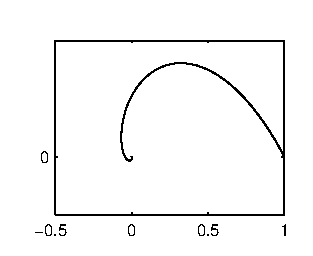
\epsfig{file=kuvat/kuvaUint-32.eps}
\end{center}
\end{figure}
%\end{Exa}
%\end{multicols}
\end{Exa}
\end{multicols}
\begin{Exa}
Laske viivaintegraali $\int_S f\,ds$, kun \ a) $f(x,y)=y$, \ b) $f(x,y)=x$ ja
$S=\{\,(x,y)\in\R^2 \mid y=x^3/3 \ \ja \ x\in [0,1]\,\}$. 
\end{Exa}
\ratk
\begin{align*}
a) \qquad \int_S y\,ds &= \int_0^1 \frac{1}{3}x^3\sqrt{1+x^4}\,dx \\
                       &=\sijoitus{0}{1} \frac{1}{18}(1+x^4)^{3/2}
                        =\underline{\underline{\frac{1}{18}(2\sqrt{2}-1)}}. \\[2mm]
b) \qquad \int_S x\,ds &= \int_0^1 x\sqrt{1+x^4}\,dx \qquad 
                              [\,\text{sijoitus}\ x^2=t, \ x\,dx=\tfrac{1}{2}\,dt\,] \\
                       &=\frac{1}{2}\int_0^1 \sqrt{1+t^2}\,dt \qquad 
                              [\,\text{sijoitus}\ t=\sinh u, \ dt=\cosh u\,du\,] \\
                       &=\frac{1}{2}\int_{0}^{\ln (\sqrt{2}+1)} \cosh^2 u\,du \\
                       &=\frac{1}{8}\int_{0}^{\ln (\sqrt{2}+1)} (e^{2u}+e^{-2u}+2)\,du \\
                       &=\frac{1}{16}\sijoitus{0}{\ln (\sqrt{2}+1)}(e^{2u}-e^{-2u}+4u) 
                        =\underline{\underline{
                         \frac{1}{4}\bigl[\sqrt{2}+\ln(\sqrt{2}+1)\bigr]}}. \loppu
\end{align*}

\Harj
\begin{enumerate}

\item
Rautalanka, jonka pituus $=10\pi$, on taivuteltu noudattamaan pisteestä $(3,0,0)$ lähtien \
a) ruuviviivaa $\,S:\, x=3\cos t,\ y=3\sin t,\ z=4t,\ t \ge 0$, \ b) käyrää
$\,S:\, x=3\cos^2t,\ y=4\sin^2t,\ z=5\sin t\cos t,\ t \ge 0$. Laske langan toinen päätepiste.

\item
Laske viivaintegraali $\int_S f\,ds$ annetuilla $f$ ja $S$\,: \vspace{1mm}\newline
a) \ $f(x,y)=xy, \quad S:\ x=2\cos t,\ y=\sin t,\ t\in[0,\frac{\pi}{2}]$ \newline
b) \ $f(r,\varphi)=r^2\varphi, \quad S:\ r=\varphi,\ \varphi\in[0,4\pi]$ \ (polaarik.) \newline
c) \ $f(x,y,z)=x^2z, \quad S:\ r=1,\ z=\varphi,\ \varphi\in[0,4\pi]$ \ (lieriök.) \newline
d) \ $f(x,y,z)=x^2z^3, \quad S:\ r=1,\ \theta=2\pi/3,\ \varphi\in[0,3\pi]$ \ (pallok.)

\item
Käyrän kaaren $S:\,t\in[a,b]\map\vec r\,(t)$ (matemaattinen) keskiö lasketaan kaavalla
$\vec r_0 = \frac{1}{\mu(S)} \int_S \vec r\,ds$. Sovella kaavaa: \vspace{1mm}\newline
a) \ $\vec r=R\cos t\vec i+R\sin t\vec j,\ t\in[0,\pi]\ $ (puoliympyrä) \newline
b) \ $\vec r=R(t-\sin t)\vec i+R(1-\cos t)\vec j,\ t\in[0,2\pi]\ $ (sykloidin kaari) \newline
c) \ $\vec r=R\cos^3 t\,\vec i+R\sin^3 t\,\vec j,\ t\in[0,\pi/2]\ $ (asteroidin kaari)

\item
Suoran langan pätepisteet ovat $(0,0)$ ja $(2a,0)$ ja langan massatiheys pituusyksikköä kohti
on $\rho(x)=\rho_0(1+x/a)$ ($\rho_0=$ vakio, $a>0$). Lanka taivutetaan noudattamaan origosta
lähtien ympyräviivaa $x^2+y^2=2ay,\ x \ge 0$. Määritä taivutetun langan painopiste.

\item
Lenkkeilijä lähtee pisteestä $(1,0)$ (pituusyksikkö = km) kiertämään pururataa $S: x^2+y^2=1$
vastapäivään. Missä pisteessä lenkkeilijä on tunnin juostuaan, jos hänen juoksuvauhtinsa on \ 
$v(s)=v_0e^{-0.05s}$, missä $v_0=12$ km/h ja $s=$ juostu matka kilometreina?

\item (*)
Esitä seuraavat käyrät kaarenpituusparametrisaation avulla. \vspace{1mm}\newline
a) \ $x=R(t-\sin t),\ y=R(1-\cos t),\ t\in[0,2\pi]$ \newline
b) \ $y=x^2,\ x \ge 0$

\item (*) \index{zzb@\nim!Laskiainen, 3.\ lasku}
(Laskiainen, 3.\ lasku) Näytä, että harjoitustehtävässä
\ref{toisen kertaluvun dy}:\ref{H-dy-3: nopein liuku} lumilautailijan lyhin laskuaika
pisteeseen $P=(a,0)$ ($a>0$) on $t_{min}=\sqrt{2\pi a/g}$.

\item (*)
Lieriöt $L_1: x^2+y^2=R^2$, $L_2: (y-R)^2+z^2=R^2$ ja pallo $K: (x-R)^2+y^2+z^2=R^2$ leikkaavat
toisensa pitkin kolmea avaruuskäyrää. Näytä, että näiden leikkauskäyrien pituudet 
ovat \vspace{1mm}\newline
a) \,\ $\mu(L_1 \cap L_2) = \int_0^{\pi/2} \sqrt{f(\sin t)}\,dt, \quad
                                   f(x)=[1-x^2(1-x)^2]/(2x-x^2)$, \newline
b) \,\ $\mu(L_1 \cap K) = \mu(L_2 \cap K) = \int_{\pi/6}^{\pi/2} \sqrt{g(\sin t)}\,dt, \quad
                                   g(x)=(2x-x^2)/(2x-1)$.

\item (*) \index{zzb@\nim!Kzz@Köysi katolla}
(Köysi katolla) $xy$-tasolle on pystytetty pitkä rakennus, jonka vesikatto on pinnalla
$z = 4-x^2/2$ ja räystäät suorilla $x=\pm 2,\ z=2$.
Rakennuksen yli on heitetty (hyvin taipuisa) köysi siten, että köyden kumpikin pää ulottuu 
$xy$-tasolle. \ a) Mikä on tällaisen köyden minimipituus? \ b) Mikä on köyden
minimipituus sillä lisäehdolla, että köysi tulee räystäiden yli pisteissä $(2, 2, 2)$ ja
$(-2, -2, 2)\,$? \
c) Millaisena tasokäyränä köysi näkyy b-kohdassa, kun sitä katsellaan kaukaa positiivisen
$z$-akselin suunnasta? 

\end{enumerate}
 %Viivaintegaalit
\section{Pintaintegraalit} \label{pintaintegraalit}
\alku
\index{pintaintegraali|vahv}


\kor{Pintaintegraalilla} tarkoitetaan integraalia muotoa
\[
I(f,A,\mu)=\int_A f\,d\mu,
\]

miss� $A$ on pinnan $S \subset \R^ 3$ osa ja $\mu$ 
\index{pinta-alamitta!b@kaarevan pinnan}
\kor{pinta-alamitta pinnalla} $S$.
Jatkossa k�ytet��n kaarevan pinnan pinta-alamitan yhteydess� merkint�� $d\mu=dS$. T�m�n mitan
suhde tason (Jordanin) pinta-alamittaan on samantyyppinen kuin kaarenpituusmitan suhde $\R$:n
pituusmittaan. Pintaintegraali on n�in ajatellen tasointegraalin yleistys, ja etenkin
sovelluksissa termi� saatetaan k�ytt�� tasointegraaleistakin puhuttaessa
(vrt.\ Luku \ref{pinta- ja tilavuusintegraalit}).

Kuten k�yr�n kaarenpituusmitta, voidaan my�s kaarevan pinnan pinta-alamitta m��ritell� pintaa
'oikaisevien' approksimaatioiden kautta. Luonteva menettely on approksimoida pintaa 
\pain{kolmion} \pain{muotoisilla} \pain{taso}p\pain{innoilla}. Kun kolmiot sijoitetaan verkoksi,
jonka solmupisteet ovat pinnalla, niin verkkoa tihennett�ess� tulee kolmioiden yhteenlasketun
pinta-alan l�hesty� $A$:n pinta-alamittaa $\mu(A)$. Jos t�m� sovitaan mitallisuuden 
m��ritelm�ksi, niin pinnan kolmioapproksimaatioita voi k�ytt�� pinta-alan numeeriseen 
laskemiseen 'suoraan m��ritelm�st�'. T�llaisilla approksimaatioilla on muutakin k�ytt��, 
esimerkiksi esitett�ess� pintoja graafisesti (tietokonegrafiikka) tai jopa konstruoitaessa 
todellisia pintoja (esim.\ kaarevat peilipinnat).
\begin{figure}[H]
\begin{center}
\import{kuvat/}{kuvaUint-37.pstex_t}
\end{center}
\end{figure}
Suoran 'numeronmurskauksen' vaihtoehtona pinta-alaa ja pintaintegraaleja on j�lleen mahdollista
k�sitell� my�s differentiaalilaskennan keinoin, jolloin pintaintegraalille saadaan laskukaava
tasointegraalina. Fubinin lauseen avulla t�m� palautuu edelleen yksiulotteisiksi integraaleiksi,
jotka suotuisissa (k�yt�nn�ss� kyll�kin harvinaisissa) oloissa voidaan laskea suljetussa
muodossa. Pintaintegraalin laskukaavaa johdettaessa on luonnollinen l�ht�kohta pinnan 
\index{parametrinen pinta}%
parametrisointi eli esitt�minen \kor{parametrisena pintana}
(vrt.\ Luku \ref{parametriset k�yr�t}). Jos parametrisointi esitet��n vektorimuodossa 
\[
\vec r = \vec r\,(u,v) = x(u,v)\vec i + y(u,v)\vec j + z(u,v)\vec k
\]
ja oletetaan, ett� $(x(u,v),y(u,v),z(u,v)) \in A\ \ekv\ (u,v) \in B \subset \R^2$, niin 
pintaintegraali on muunnettavissa muotoon
\[
\int_A f\,dS=\int_B g\,d\mu', \quad g(u,v)=f(x(u,v),y(u,v),z(u,v)),
\]
miss� $\mu'$ on pinnan $S$ pinta-alamitan vastine parametritasossa. Muunnos parametritasoon on
j�lleen muotoa
\[
d\mu'=J\,dudv,
\]
miss� $J=J(u,v)$ on (yleens� laskettavissa oleva) muuntosuhde. Kun muuntosuhde tunnetaan, on
laskukaava valmis:
\[
\int_A f\,dS=\int_B gJ\,dudv.
\]

Muuntosuhteen laskemiseksi tutkitaan suorakulmion 
\[
\Delta B=[u_0,u_0+\Delta u]\times [v_0,v_0+\Delta v] \subset B
\]
muuntumista. Oletetaan funktiot $x(u,v), y(u,v), z(u,v)$ riitt�v�n s��nn�llisiksi niin, ett� 
voidaan k�ytt�� linearisoivaa approksimaatiota
\[
\vec r\,(u,v) \approx \vec r\,(u_0,v_0)+(u-u_0)\frac{\partial\vec r}{\partial u}(u_0,v_0)
                                       +(v-v_0)\frac{\partial\vec r}{\partial v}(u_0,v_0).
\]
T�m�n mukaisesti $\Delta B$ kuvautuu pintaa pisteess� $P_0\vastaa\vec r\,(u_0,v_0)$ sivuavalle
tangenttitasolle. Kuva on t�m�n tason suunnikas, jonka viritt�v�t vektorit
\[
\vec v_1=\Delta u\,\partial_u\vec r,\quad \vec v_2=\Delta v\,\partial_v\vec r.
\]
Suunnikaan pinta-ala on 
$|\vec v_1\times\vec v_2|=|\partial_u\vec r\times\partial_v\vec r\,||\Delta u||\Delta v|$,
joten p��tell��n, ett� muuntosuhde on\footnote[2]{Muuntosuhteen laskukaava on tarkemmin
perusteltavissa olettaen, ett� funktioiden $x(u,v), y(u,v), z(u,v)$ osittaisderivaatat ovat
jatkuvia perussuorakulmiossa $T \supset B$,}
\[
J=\left|\frac{\partial\vec r}{\partial u}\times\frac{\partial\vec r}{\partial v}\right|.
\]
Jos pinta on annettu muodossa $z=f(x,y)$, eli
$\,\vec r=\vec r\,(x,y)=x\vec i+y\vec j+f(x,y)\vec k$, niin
\begin{align*}
\partial_x\vec r\times\partial_y\vec r 
               &= \begin{vmatrix} 
                  \vec i & \vec j & \vec k \\ 1 & 0 & f_x \\ 0 & 1 & f_y 
                  \end{vmatrix} 
                = -f_x\vec i-f_y\vec j+\vec k \\
\impl \ J(x,y) &= \sqrt{1+[f_x(x,y)]^2+[f_y(x,y)]^2}.
\end{align*}
Koska t�ss� $\vec n=(-f_x\vec i-f_y\vec j+\vec k\,)/J=n_x\vec i+n_y\vec j+n_z\vec k$ on pinnan
yksikk�normaalivektori, niin tuloksen voi esitt�� my�s muodossa $J(x,y)=1/\abs{n_z(x,y)}$.

$R$-s�teisell� pallopinnalla on
\begin{align*}
\vec r = \vec r\,(\theta,\varphi)
      &= R\sin\theta\cos\varphi\,\vec i+R\sin\theta\sin\varphi\,\vec j+R\cos\theta\,\vec k \\
\impl\ J(\theta,\varphi) 
      &= \abs{\partial_\theta\vec r\times\partial_\varphi\vec r\,}
       = R^2\sin\theta.
\end{align*}
Yleisemm�ll� py�r�hdyspinnalla, joka syntyy k�yr�n $K:\,y=f(x),\ x\in[a,b]$ py�r�ht�ess�
$x$-akselin tai k�yr�n $K:\,y=f(z),\ z\in[a,b]$ $z$-akselin ymp�ri (ks.\ kuviot alla) voidaan
muuntosuhde laskea vastaavaan tapaan
(Harj.teht.\,\ref{H-Uint-9: py�r�hdyspintojen muuntosuhteet}). Tulokset koottuna:
\index{muuntosuhde integraalissa!e@pintaintegraalissa}
\index{kzyyrzy@k�yr�viivaiset koordinaatistot!d@--integraalit}%
\vspace{2mm}
\begin{center}
\begin{tabular}{lll}
Pinta & Muuttujat & $\quad$Muuntosuhde \\ \hline \\
$\vec r=\vec r\,(u,v)$ & $u,v$ & $\quad \abs{\partial_u\vec r \times \partial_v\vec r\,}$ \\ \\
$z=f(x,y)$ & $x,y$ & $\quad \sqrt{1+[f_x(x,y)]^2+[f_y(x,y)]^2}$ \\ \\
pallopinta $\,r=R$& $\theta,\varphi$ & $\quad R^2\sin\theta$ \\ \\
\parbox{3.5cm}{py�r�hdyspinta: 
$y=f(x) \hookrightarrow\ \curvearrowleft \negthickspace\negthickspace \longrightarrow_x$} & 
$x,\varphi$ & $\quad |f(x)|\sqrt{1+[f'(x)]^2}$ \\ \\
\parbox{3.5cm}{py�r�hdyspinta: 
$z=f(r) \hookrightarrow$\ \raisebox{-0.2cm}{$\circlearrowleft$}$\negthinspace \negthinspace 
\negmedspace \negthinspace \uparrow^z$} & $r,\varphi$ & $\quad r\sqrt{1+[f'(r)]^2}$

\end{tabular}
\end{center}
\begin{multicols}{2}
\begin{figure}[H]
\vspace{1cm}
\begin{center}
\import{kuvat/}{kuvaDD-2.pstex_t}
\end{center}
\end{figure}
\begin{figure}[H]
\begin{center}
\import{kuvat/}{kuvaDD-4.pstex_t}
\end{center}
\end{figure}
\end{multicols}
\begin{Exa}
$R$-s�teiselle pallopinnalle on jakautunut tasaisesti massa $m$. Laske hitausmomentti 
$z$-akselin suhteen.
\end{Exa}
\ratk
\begin{align*}
I &= \int_A \rho_0(x^2+y^2)\,dS \\
&= \int_B \rho_0 R^2\sin^2\theta\cdot R^2\sin\theta\,d\theta d\varphi 
   \qquad \left(\,B=[0,\pi]\times[0,2\pi]\,\right) \\
&= \rho_0 R^4 \int_0^{2\pi} d\varphi \cdot \int_0^\pi \sin^3 \theta\,d\theta \\
&= 2\pi\rho_0R^4\sijoitus{\theta=0}{\theta=\pi} (-\cos\theta+\frac{1}{3}\cos^3\theta) \\
&= \frac{8\pi}{3}\rho_0 R^4.
\end{align*}
Koska
\begin{align*}
m =\int_A \rho_0\,dS
 &= \rho_0 R^2 \int_0^{2\pi} d\varphi \cdot \int_0^{\pi} \sin\theta\,d\theta \\
 &= \rho_0\cdot 4\pi R^2,
\end{align*}
niin $\displaystyle{I=\underline{\underline{\frac{2}{3}mR^2}}}$. \loppu
\begin{Exa}
Laske $\int_A f\,dS$, kun $f(x,y,z)=xy\ $ ja
\[
A = \left\{(x,y,z)\in\R^3 \mid z=x^2+\frac{1}{2}y^2 \; \ja \; (x,y)\in B\right\},
    \quad B=[0,1]\times [0,1].
\]
\end{Exa}
\ratk
\begin{align*}
\int_A f\,dS &= \int_B xy\sqrt{1+4x^2+y^2}\,dxdy \\
&=\int_0^1 x\left(\int_0^1 y\sqrt{1+4x^2+y^2}\,dy\right)dx \\
&=\int_0^1 x\left[\sijoitus{y=0}{y=1}\frac{1}{3}(1+4x^2+y^2)^{3/2}\right]dx \\
&=\int_0^1 \left[\frac{1}{3}x(2+4x^2)^{3/2}-\frac{1}{3}x(1+4x^2)^{3/2}\right]\,dx
\end{align*}
\begin{align*}
\quad &=\ \sijoitus{0}{1}\left[\frac{1}{60}(2+4x^2)^{5/2}-\frac{1}{60}(1+4x^2)^{5/2}\right] \\
      &= \underline{\underline{\frac{1}{60}\bigl(36\sqrt{6}-25\sqrt{5}-4\sqrt{2}+1\bigr)}}.
\loppu \\
\end{align*}

\begin{multicols}{2} \raggedcolumns
\begin{Exa}
Katkaistun suoran ympyr�kartion korkeus $=h$, pohjan s�de $=R$ ja katkaisukohdassa s�de $=r$.
Laske vaipan ala $\mu(A)$.
\end{Exa}
\begin{figure}[H]
\begin{center}
\import{kuvat/}{kuvaUint-38.pstex_t}
\end{center}
\end{figure}
\end{multicols}
\ratk T�ss� on kyseess� py�r�hdyspinta, joka syntyy, kun jana
\[
K:\,y=f(x)=r+(R-r)\frac{x}{h}, \quad x\in [0,h]
\]
py�r�ht�� $x$-akselin ymp�ri. Parametreilla $(x,\varphi) \in B=[0,1]\times[0,2\pi]$ laskien
saadaan
\begin{align*}
\mu(A) &= \int_B f(x)\sqrt{1+[f'(x)]^2}\,dxd\varphi \\
&= 2\pi \int_0^h\sqrt{1+\left(\frac{R-r}{h}\right)^2}\,\left[\,r+(R-r)\frac{x}{h}\,\right]dx \\
&=\pi(R+r)h\,\sqrt{1+\left(\frac{R-r}{h}\right)^2} \\[3mm]
&=\underline{\underline{\pi(R+r)\sqrt{h^2+(R-r)^2}}}. \Akehys \loppu
\end{align*}

\begin{Exa}
Laske viivoitinpinnan
\[
\vec r\,(u,v)=v[\,\cos (\omega u)\vec i+\sin (\omega u)\vec j\,]+u\vec k, \quad
(u,v)\in [0,H]\times [0,L]
\]
pinta-ala.
\end{Exa}
\begin{multicols}{2} \raggedcolumns
\ratk
\begin{align*}
\partial_u\vec r\times\partial_v\vec r
          &= \begin{detmatrix} 
             \vec i & \vec j & \vec k \\
             -\omega v\sin (\omega u) & \omega v\cos (\omega u) & 1 \\
             \cos (\omega u) & \sin (\omega u) & 0 
             \end{detmatrix} \\
          &= -\sin (\omega u)\vec i+\cos (\omega u)\vec j -\omega v\vec k \\[2mm]
\impl \ J &= \abs{\partial_u\vec r\times\partial_v\vec r\,}=\sqrt{1+\omega^2 v^2}.
\end{align*}
\begin{figure}[H]
\begin{center}
\import{kuvat/}{kuvaUint-39.pstex_t}
\end{center}
\end{figure}
\end{multicols}

\begin{align*}
\mu(A) &= \int_0^H\left(\int_0^L \sqrt{1+\omega^2 v^2}\,dv\right)du \\
&= H\int_0^L \sqrt{1+\omega^2 v^2}\,dv \\
&\qquad [\ \text{sijoitus}\ \ \omega v=\sinh t,\quad dv=\inv{\omega}\cosh t\,dt,\quad 
                              \alpha=\text{arsinh}\, (\omega L)\ ] \\
&=H\inv{\omega}\int_0^\alpha \cosh^2 t\,dt \\
&=H\inv{\omega}\sijoitus{0}{\alpha} \left(\frac{1}{2}\sinh t\cosh t+\frac{1}{2}\,t\right) \\
&=\underline{\underline{
    \frac{1}{2}\left[\ln (\omega L +\sqrt{\omega^2 L^2+1})
                                   +\omega L\sqrt{\omega^2 L^2+1}\right]H\inv{\omega}}}. \loppu
\end{align*}

\subsection*{Avaruuskulma}
\index{avaruuskulma|vahv}

Olkoon $V\subset\R^3$ avaruuden osajoukko, k�yt�nn�ss� esim.\ kiinte� kappale, pinta tai pinnan
osa. M��ritell��n pallokoordinaatistossa joukko $B\subset[0,\pi]\times[0,2\pi]$ ehdolla
\[
B=\{\,(\theta,\varphi)\ | \ P=(r,\theta,\varphi) \in V\ \text{jollakin}\ r>0\,\}.
\]
T�ll�in $V$ n�kyy origosta suuntaan $\vec e_r(\theta,\varphi)$ t�sm�lleen kun
$(\theta,\varphi) \in B$. Olkoon $A$ yksikk�pallon $S$ osa, joka vastaa
pallonpintakoordinaattien $(\theta,\varphi)$ joukkoa $B$. T�ll�in sanotaan, ett� $V$ n�kyy
origosta \kor{avaruuskulmassa} (engl.\ solid angle)
\[
\Omega=\int_A dS=\int_B \sin\theta\,d\theta d\varphi.
\]
T�m�n suurin arvo (kun $A=S$) on $4\pi$.
\begin{Exa}
Miss� avaruuskulmassa lieri�pinta
\[
A=\{(x,y,z)\in\R^2�\; | \; x^2+y^2=R^2, \; 0\leq z\leq H\}
\]
n�kyy origosta?
\end{Exa}
\ratk Kyseisell� pinnalla pallonpintakoordinaatit saavat arvot
\[
(\theta,\varphi) \in B=[\theta_0,\pi/2]\times[0,2\pi],\quad 
                 \cos\theta_0=\frac{R}{\sqrt{R^2+H^2}}\,,
\]
joten
\[
\Omega = \int_B \sin\theta\,d\theta d\varphi
       = \int_0^{2\pi} d\varphi\cdot\int_{\theta_0}^{\pi/2} \sin\theta\,d\theta
       = 2\pi\cos\theta_0
       =\underline{\underline{2\pi\,\frac{H}{\sqrt{R^2+H^2}}}}\,. \loppu
\]

\Harj
\begin{enumerate}

\item \label{H-Uint-9: py�r�hdyspintojen muuntosuhteet} 
Halutaan laskea pinta-alamitan muuntosuhde $J$ py�r�hdyspinnalle, joka syntyy, kun
a) $xy$-tason k�yr� $K: y=f(x)$ py�r�ht�� $x$-akselin ymp�ri, b) $yz$-tason k�yr�
$K: y=f(z)$ py�r�ht�� $z$-akselin ymp�ri. Laske muuntosuhde
parametrisaatioille \vspace{1mm}\newline
a) \ $y=f(x)\cos\varphi,\,\ z=f(x)\sin\varphi$, \newline 
b) \ $x=r\cos\varphi,\,\ y=r\sin\varphi,\,\ z=f(r)$.

\item
Laske sen pinnan ala, jonka lieri� $\,L:\, x^2+y^2=a^2$ ($a>0$) leikkaa \vspace{1mm}\newline
a) kartiosta $\,z^2=x^2+y^2$, \newline
b) satulapinnasta $\,az=xy$, \newline
c) paraboloidista $\,az=x^2+y^2$. 

\item
Laske pinta-ala $\mu(A)$, kun $A$ on \vspace{1mm}\newline
a) joukon $V=\{(x,y,z)\in\R^3 \mid x^2+y^2 \le z \le \sqrt{x^2+y^2}\,\}$ 
   reunapinta $\partial V$, \newline
b) parametrinen pinta $\,x=8u^2,\ y=v^2,\ z=4uv,\ (u,v)\in[0,1]\times[0,3]$.

\item
a) Laske puolipallon (pinnan) keski�. \vspace{1mm}\newline
b) Pinnalle $S:\,x^2+y^2=R^2,\ 0 \le z \le H$ on jakautunut tasaisesti massa $m$. Laske
lieri�koordinaateilla hitausmomentit koordinaattiakselien suhteen.

\item \index{Guldinin s��nt�}
Olkoon $f(x) \ge 0$, kun $x\in[a,b]$ ja $S$ pinta, joka syntyy, kun k�yr�
$K:\,y=f(x)\ \ja\ x\in[a,b]$ py�r�ht�� $x$-akselin ymp�ri. Todista \kor{Guldinin s��nt�}:
$S$:n pinta-ala = $K$:n pituus kertaa $K$:n keski�n py�r�hdyksess� kulkema matka.

\item
Laske, miss� avaruuskulmassa kohde n�kyy origosta: \vspace{1mm}\newline
a) \ $R$-s�teinen kiekko tasolla $z=a>0$, keskipiste $z$-akselilla. \newline
b) \ $R$-s�teinen kuula, jonka keskipisteen et�isyys origosta $=a \ge R$. \newline
c) \ Puolikartion rajaama joukko $A:\,z\ge\sqrt{x^2+y^2}+a,\ a \ge 0$. \newline
d) \ Pararaboloidi $\,z=x^2+y^2+a, \ a\in\R$.

\item (*) \index{Vivian'in ikkuna} 
\kor{Vivian'in ikkunaksi} sanotaan sit� pintaa $A,$ jonka lieri� $x^2+y^2=Rx$ erottaa pallosta
$x^2 + y^2 + z^2 = R^2$. Laske ko.\ pinnan ala.

\item (*)
Olkoon $A\subset\R^3$ lieri�iden
\[
S_1:\ x^2+y^2=R^2, \quad S_2:\ y^2+z^2=R^2, \quad S_3:\ x^2+z^2=R^2
\]
sis��n j��v� joukko. Laske $A$:n reunapinnan $\partial A$ pinta-ala.

\item (*) \index{zzb@\nim!N:s ydinvoimala} 
(N:s ydinvoimala) Voimalaitoksen j��hdytystornin vaipan ulkopinnan parametriesitys on
(vrt.\ Esimerkki \ref{parametriset k�yr�t}:\,\ref{j��hdytystorni})
\[
\begin{cases}
\,x=a[(2-2v)\cos u-v\sin u], \\
\,y=a[v\cos u +(2-2v)\sin u], \\
\,z=3av,
\end{cases}
\]
miss� $a$=50 m ja $(u,v)\in B= [0,2\pi]\times [0,1]$. Vaippa on valmistettu betonista ja sen
paksuus on 20 cm. Laske tarvittavan betonin m��r�lle likiarvo k�ytt�en pintaintegraalia.

\item (*)
a) Levy
\[
A=\{\,(x,y,z) \ | \ \frac{x^2}{a^2}+\frac{y^2}{b^2} \le 1,\ z=c\,\} \quad (a,b,c>0)
\]
n�kyy origosta avaruuskulmassa $\Omega$. Johda $\Omega$:lle laskukaava muotoa
$\Omega=\int_0^{2\pi} f(\varphi)\,d\varphi$. \ b) Laske, miss� avaruuskulmassa avaruusneli�
\[
K=\{\,(x,y,z) \ | \ 0 \le x,y \le 1,\ z=1\,\}
\]
n�kyy origosta.

\end{enumerate} %Pintaintegraalit

\chapter{Gaussin ja Stokesin lauseet}

\kor{Gaussin lause} ja \kor{Stokesin lause} ovat usean muuttujan differentiaali- ja 
integraalilaskun keskeisi� tuloksia. Lauseet tunnetaan enemm�n k�ytt�kelpoisuutensa kuin 
matemaattisen suuruutensa vuoksi, ja niihin viitataankin usein arkisissa yhteyksiss� nimill� 
'Gaussin kaava' ja 'Stokesin kaava'. Hieman yksinkertaistaen n�iss� kaavoissa on kyse 
integraalikaavan
\[
\int_a^b f'(x)\,dx=f(b)-f(a)
\]
yleist�misest� koskemaan useamman (k�yt�nn�ss� yleens� kahden tai kolmen) muuttujan 
vektoriarvoisia funktioita eli \pain{vektorikentti�}. Gaussin lauseeseen (kaavaan) vedotaan 
hyvin usein silloin, kun erilaiset fysiikan \kor{s�ilymislait} halutaan kirjoittaa 
osittaisdifferentiaaliyht�l�itten muotoon. My�s Stokesin lauseella on t�llaista k�ytt�� etenkin
s�hk�magnetiikassa.

Luvussa \ref{polkuintegraalit} tarkastellaan ensin viivaintegraaleille sukua olevia
\kor{polkuintegraaleja}. N�ill� on k�ytt�� Gaussin ja Stokesin lauseiden yhteydess� ja
yleisemminkin fysikaalisten vektorikenttien sovelluksissa. Luvussa \ref{gaussin lause}
johdetaan Gaussin lause tasossa ja avaruudessa ja esitet��n lauseen yleistetty muoto.
L�ht�kohtana ovat taso- ja avaruusintegraaleja koskevat \kor{Greenin kaavat}. Luvussa
\ref{Gaussin lauseen sovelluksia} tarkastellaan esimerkkien valossa Gaussin lauseen k�ytt��,
kun halutaan johtaa fysiikan osittaisdifferentiaaliyht�l�it� tai fysikaalisten vektorikenttien
jatkuvuusehtoja materiaalirajapinnoilla. 

Luvussa \ref{stokesin lause} johdetaan Stokesin lause ensin tasoon rajoittuen. Yleistett�ess�
tulos koskemaan avaruuden pintoja tarvitaan pinnan \kor{suunnistuvuuden} k�site. Luvussa 
\ref{py�rteet�n vektorikentt�} ratkaistaan Stokesin lauseen avulla fysiikassa keskeinen 
vektorikentti� koskeva kysymys: Mill� ehdoilla py�rteet�n kentt� on gradienttikentt� eli 
lausuttavissa skalaaripotentiaalin avulla? 
 %Gaussin ja Stokesin lauseet
\section{Vektorikentät ja polkuintegraalit} \label{polkuintegraalit}
\alku
\index{polkuintegraali|vahv}

Luvussa \ref{viivaintegraalit} tarkasteltiin viivaintegraaleja, joissa tason tai avaruuden
käyrän yli integroidaan kaarenpituusmitan suhteen. Tässä luvussa tarkastelun kohteena on toinen
viivaintegraalien luokka, jolle käytetään jatkossa nimeä \kor{polkuintegraalit}
(engl.\ path integral, suom.\ myös \kor{tieintegraali}). Polkuintegraaleille on ominaista, että
integrointi käyrää pitkin tapahtuu tiettyyn \pain{suuntaan}, siksi nimitys \kor{polku}, jonka
voi tulkita suunnatuksi käyräksi. Suunnan ohella polkuintegraaleille on tyypillistä, että
integrointiin liittyvä mitta \pain{ei} ole kaarenpituusmitta vaan muu yksi\-ulotteinen mitta,
joka on tapauskohtainen. Polun suunta vaikuttaa polkuintegraaliin niin, että jos vain suunta
vaihtuu, eli polku pysyy muuten (käyränä) samana, niin polkuintegraalin arvo vaihtuu
vastaluvukseen. Polun parametrisoinnin kautta tämä vastaa määrätyn integraalin vaihtosääntöä,
ks.\ esimerkit jäljempänä.

Jatkossa rajoitutaan sellaisiin polkuintegraaleihin, jotka sovelluksissa liitetään yleensä
fysikaalisiin vektorikenttiin (kuten voima-, sähkö- ja magneettikenttiin). Vektorikenttiin
liittyvillä polkuintegraaleilla on jatkossa käyttöä myös Gaussin ja Stokesin lauseiden
yhteydessä.\footnote[2]{Matemaattisissa teksteissä erilaisten viivaintegraalien nimet eivät ole
täysin vakiintuneet. Esim.\ saatetaan puhua 'vektorikenttien viivantegraaleista', kun
tarkoitetaan polkuintegraaleja tämän tekstin merkityksessä.}

Erotukseksi käyrästä polku merkitään jatkossa symbolilla $p$ tai tarkemmin
\[
p: A \kohti B,
\]
jolloin merkintä kertoo sekä polun (käyrän) päätepisteet että polun suunnan. Luontevasti
polun suunnan määrittää parametrisointi: suunta on joko parametrin kasvusuunta tai vastakkainen
suunta. Jos polku on parametrisoitu välillä $t\in[a,b]$, niin polku voidaan merkitä tarkemmin
kuten parametrinen käyrä:   
\[ 
p:\ t \in [a,b]\ \map\ \vec r\,(t).
\]
Parametrisoinnin ei tarvitse olla 1--1, joten polku (kuten parametrinen käyrä) voi leikata
itsensä tai kiertyä itsensä päälle.
\begin{figure}[H]
\begin{center}
\import{kuvat/}{kuvaUint-34.pstex_t}
\end{center}
\end{figure}

Jatkossa tarkastelun kohteena ovat tason tai avaruuden polut muotoa $t\in[a,b]\map(x(t),y(t))$
tai $t\in[a,b]\map(x(t),y(t),z(t))$. Funktioiden $x(t)$, $y(t)$, $z(t)$ oletetaan olevan joko
jatkuvasti derivoituvia välillä  $[a,b]$ tai toteuttavan vastaavat, hieman heikommat
säännöllisyysehdot, vrt. Luku \ref{viivaintegraalit}. 

Kuten aiemmin, voidaan laskea \kor{polun pituus} integraalina
\[
\mu(p)=\int_a^b \abs{\vec r\,'(t)}\,dt.
\]
Tässä on kuitenkin kyse jo ennestään tutusta viivaintegraalista, jossa mitta on
kaarenpituusmitta eikä polun suunnalla ole väliä.

Polkuintegraaleja (jatkon kannalta myös merkittävimpiä) ovat
\begin{equation} \label{polkuintegraaleja}
\int_p f\,dx, \quad \int_p f\,dy, \quad \int_p f\,dz, \tag{$\star$}
\end{equation}
missä $f(x,y,z)$ (tasossa $f(x,y)$) on tunnettu funktio. Näihin integraaleihin liittyvä
mitta on tavallinen ($1$-ulotteinen) Jordan-mitta. Jos tunnetaan polun parametrisointi
välillä $t\in[a,b]$, niin esimerkiksi $\int_p f\,dx$ lasketaan yksinkertaisesti kirjoittamalla
$dx=x'(t)dt$ (kuten muuttujan vaihdossa). Jos vielä oletetaan, että $t=a$ vastaa polun
alkupistettä ja $t=b$ loppupistettä, niin saadaan laskukaava
\[
\int_p f\,dx = \int_a^b f(x(t),y(t),z(t)\,x'(t)\,dt.
\]
Parametrisoinnin vaihto vastaa tässä kaavassa (toista) muuttujan vaihtoa, joten parametrisointi
ei vaikuta integraalin arvoon.
\begin{Exa} Tason polku $p$ kulkee pisteestä $(0,0)$ pisteeseen $(1,1)$ pitkin käyrää $y=x^2$
ja polku $-p$ pitkin samaa käyrää pisteesät $(1,1)$ pisteeseen $(0,0)$. Laske
$\int_p xy\,dy$ ja $\int_{-p} xy\,dy$.
\end{Exa}
\ratk Valitaan molemmissa integraaleissa parametriksi $t=x$\,:
\begin{align*}
&\int_p xy\,dy     = \int_0^1 x \cdot x^2 \cdot 2x\,dx = \int_0^1 2x^4\,dx
                  = \underline{\underline{\frac{2}{5}}}\,, \\
&\int_{-p} xy\,dy  = \int_1^0 2x^4\,dx = -\int_0^1 2x^4\,dx 
                  = \underline{\underline{-\frac{2}{5}}}\,. \loppu
\end{align*}

Esimerkin jälkimmäisessä integraalissa käytettiin määrätyn integraalin vaihtosääntöä. --- Itse
asiassa kun vaihtosääntö huomioidaan, niin määrätty integraali on itsekin tulkittavissa
polkuintegraaliksi: $\int_a^b f(x)\,dx = \int_p f\,dx$, missä $p$ on $\R$:n polku, jonka
alkupiste on $a$ ja loppupiste $b$ (!).

\subsection*{Polkuintegraali $\int_p \vec F \cdot d\vec r$}
\index{polkuintegraali!a@työintegraali|vahv}
\index{tyzz@työintegraali|vahv}

Fysiikan sovelluksissa polkuintegraalit liittyvät usein vektorikenttiin. Tyypillinen esimerkki
on \pain{voimakentässä} $\vec F(x,y,z)$ liikkuva (pistemäinen) kappale, jonka liikerata
tunnetaan jollakin aikavälillä $t\in [a,b]$. Tällöin voimakentän kappaleeseen tekemä
\pain{t}y\pain{ö} lasketaan polkuintegraalina pitkin kappaleen kulkemaa liikerataa. Liikerata
tulkitaan siis poluksi $p:t \map \vec r\,(t)$, $t\in [a,b]$. Jos $\vec F=\text{vakio}$, niin
fysiikan lakien mukaan työ $=|\vec F| \cdot s$, missä $s=$ polulla kuljettu matka voiman
vaikutussuunnassa, eli
\[
W=\vec F\cdot[\vec r\,(b)-\vec r\,(a)]\quad (\vec F\text{ vakio}).
\]
Vakiovoimakentän tekemän työn kannalta polkua siis 'mittaa' vektori
\[
\vec\mu(p)=\vec r\,(b)-\vec r\,(a).
\]
Jos tämä tulkitaan polun (vektoriarvoiseksi) mitaksi, niin nähdään, että tämäkin mitta on
additiivinen: Jos $p_1$ ja $p_2$ ovat $p$:n osapolkuja vastaten parametrin arvoja väleillä
$[a,t_0]$ ja $[t_0,b]$, $t_0\in (a,b)$, niin $\vec \mu(p)=\vec \mu(p_1)+\vec\mu(p_2)$,
vrt.\ kuvio.
\begin{figure}[H]
\begin{center}
\import{kuvat/}{kuvaUint-35.pstex_t}
\end{center}
\end{figure}
Entä jos voimakenttä $\vec F$ ei ole vakio, mutta on jatkuva? Tällöin menetellään niinkuin
integraaleissa yleensä: Otetaan käyttöön välin $[a,b]$ jako $\{t_k, \ k=0,\ldots,n\}$,
$a=t_0<t_1<\ldots t_n=b$, jolloin polku $p$ jakautuu peräkkäisiksi osapoluiksi $\Delta p_k$,
$k=1\ldots n\,$ vastaten parametrin arvoja väleillä $[t_{k-1},t_k]$. Koska funktio
$t \map \vec r\,(t)$ on jatkuva, niin osapolkujen $\Delta p_k$ päätepisteet 
$\vec r\,(t_{k-1})=\vec r_{k-1}$ ja $\vec r\,(t_k)=\vec r_k$ tulevat yhä lähemmäksi toisiaan
jaon tihetessä. Tällöin voima $\vec F$ on osapolulla $\Delta p_k$ likimain vakio 
(koska $\vec F$ oli jatkuva), joten voiman tekemä työ tällä osapolulla on likimain
\[
\Delta W_k\approx\vec F(\vec r_{k-1})\cdot\vec\mu(\Delta p_k),\quad 
\vec\mu(\Delta p_k)=\vec r_k-\vec r_{k-1}\,.
\]
Kun jaon tiheysparametri $h=\max_k|\vec r_k-\vec r_{k-1}|\kohti 0$, saadaan voimakentän
tekemälle kokonaistyölle integraalilauseke
\[
W=\Lim_{h\kohti 0}\sum_{k=1}^n\Delta W_k=\int_p \vec F\cdot d\vec\mu.
\]
Tämä on siis tulkittava polkuintegraaliksi vektorimitan $\vec\mu$ suhteen (!). Integraali saa
hieman konkreettisen muodon, kun käytetään merkintää $d\vec\mu=d\vec r$, jolloin työn
integraalikaava siis on
\[
\boxed{\kehys\quad W=\int_p \vec F\cdot d\vec r \quad (\text{työintegraali}). \quad}
\]
Määritelmän mukaisesti $W$:lle saadaan likiarvoja summien avulla. Esimerkiksi
\[
W\approx\sum_{k=1}^n \vec F(\vec r_{k-1})\cdot (\vec r_k-\vec r_{k-1}).
\]
Näin laskettaessa polusta $p$ ei tarvitse tehdä voimakkaita säännöllisyysoletuksia. Esimerkiksi
työ $W$ voidaan laskea, vaikka $p$ ei olisi suoristuva (ts.\ pituusmitta ei määritelty). Tämä
johtuu siitä, että työintegraali mittaa vain siirtymää voiman vaikutussuunnassa, ei
kaarenpituutta.

Jos oletetaan parametrisointi $p: t\in[a,b] \map \vec r\,(t)$, niin työintegraalissa voidaan
kirjoitta $d\vec r=\dvr(t)dt$, jolloin saadaan laskukaava
\[
W=\int_a^b \vec F(\vec r(t))\cdot \dvr(t)\,dt.
\]
Jos taas voimakenttä esitetään koordinaattimuodossa
\[
\vec F(x,y,z)=F_1(x,y,z)\vec i + F_2(x,y,z)\vec j+F_3(x,y,z)\vec k,
\]
niin kirjoittamall $d\vec r=dx\,\vec i+dy\,\vec j+dz\,\vec k$ työintegraali purkautuu
polkuintegraalien \eqref{polkuintegraaleja} summaksi:
\[
W=\int_p (F_1\,dx+F_2\,dy+F_3\,dz).
\]
Riittävän säännöllisellä polulla työintegraalin voi ilmaista kolmannellakin tavalla, sillä
\[
d\vec r = \frac{\dvr(t)}{|\dvr(t)|}|\dvr(t)|dt = \vec t\,ds,
\]
missä $\vec t$ on polun suuntainen yksikkötangenttivektori. Tämän mukaan siis työintegraali
voidaan haluttaessa liittää myös kaarenpituusmittaan laskukaavalla
\[
W = \int_p \vec F\cdot\vec t\,ds.
\]
Kuten kaavan johdosta ilmenee, tässä on $\vec t\,ds=\dvr(t)\,dt$, joten riippuvuus
kaarenpituusmitasta on näennäinen.
\begin{Exa}
Määritä voimakentän
\[
\vec F=(x^2-y)\vec i-2xy\vec j
\]
tekemä työ kappaleen liikkuessa polulla
\[
p: \ x(t)=2\cos t, \ y(t)=\sin t, \ t\in [0,2\pi].
\]
\end{Exa}
\ratk $\quad dx=-2\sin t\,dt,\quad dy=\cos t\,dt, \quad t\in [0,2\pi]$
\begin{align*}
\impl \quad W &= \int_0^{2\pi} [\,(4\cos^2 t-\sin t)(-2\sin t)-(4\cos t\sin t)\cos t\,]\,dt \\
              &= \int_0^{2\pi} (-12\cos^2 t\sin t+2\sin^2 t)\,dt \\
              &= \sijoitus{0}{2\pi} (4\cos^3 t-\cos t\sin t+t) 
               = \underline{\underline{2\pi}}. \loppu
\end{align*}

\subsection*{Gradienttikenttä ja työintegraali}
\index{polkuintegraali!a@työintegraali|vahv}
\index{tyzz@työintegraali|vahv}
\index{gradienttikenttä|vahv}

Jos voimakenttä $\vec F$ on g\pain{radienttikenttä}, eli lausuttavissa skalaaripotentiaalin $u$
avulla muodossa
\[
\vec F=-\nabla u,
\]
niin työintegraali voidaan laskea hyvin yksinkertaisesti. Nimittäin tässä tapauksessa on
derivoinnin ketjusäännön (Luku \ref{osittaisderivaatat}) perusteella
\[
\vec F(\vec r(t))\cdot \dvr(t) = -\nabla u(\vec r(t))\cdot \dvr(t)
                               = -\frac{d}{dt} u(\vec r(t)),
\]
joten
\[
W = \int_a^b \vec F(\vec r(t))\cdot \dvr(t)\,dt 
  = -\sijoitus{a}{b} u(\vec r(t))
  = u(\vec r(a))-u(\vec r(b)).
\]
Siis gradienttikentän työintegraali määräytyy pelkästään polun päätepisteistä:
\[ 
\boxed{ \begin{aligned} \quad\ygehys 
                 &\text{Gradienttikentän tekemä työ} \\
                 &= \text{potentiaaliero polun alku- ja loppupisteiden välillä}. \quad\agehys
           \end{aligned} } 
\]

\jatko \begin{Exa} (jatko). Esimerkissä polun alku- ja loppupisteet ovat samat. Koska
$W\neq 0$, ei esimerkin kenttä $\vec F$ ole gradienttikenttä. Sen sijaan jos esimerkiksi
\[
\vec F=(x^2-y^2)\vec i-2xy\vec j,
\]
niin ilman enempää laskemista selviää, että $W=0$, sillä
\[
\vec F=-\nabla(-\frac{1}{3}x^3+xy^2). \loppu
\]
\end{Exa}

\subsection*{Vektoriarvoiset polkuintegraalit}
\index{polkuintegraali!b@vektoriarvoinen p.-integraali|vahv}

Fysiikan sovelluksissa (esimerkiksi sähkömagnetiikassa) esiintyy myös vektoriarvoisia 
polkuintegraaleja muotoa
\[
\int_p f\,d\vec r\quad\text{tai}\quad\int_p \vec F\times d\vec r.
\]
Nämä voidaan laskea parametrisoinnin avulla samalla periaatteella kuin työintegraalikin.
\jatko \begin{Exa} (jatko) Laske $\int_p x\,d\vec r\,$ ja $\int_p \vec r \times d\vec r\,$,
kun $p$ on esimerkin polku.
\end{Exa}
\ratk
\begin{align*}
\int_p x\,d\vec r\,
&= \int_0^{2\pi} x(t)[x'(t)\vec i+y'(t)\vec j\,]\,dt \\
&= \int_0^{2\pi} 2\cos t\,(-2\sin t\,\vec i+\cos t\,\vec j\,)\,dt \\
&= -\vec i\int_0^{2\pi} 4\cos t\sin t\,dt + \vec j\int_0^{2\pi} 2\cos^2 t\,dt \\
&= -\vec i\sijoitus{0}{2\pi} 2\sin^2 t 
   +\vec j\sijoitus{0}{2\pi}(t+\cos t\sin t)
 = \underline{\underline{2\pi\vec j}}, \\
\int_p \vec r\times d\vec r\, 
&= \int_0^{2\pi} [x(t)\vec i+y(t)\vec j\,]\times[x'(t)\vec i+y'(t)\vec j\,]\,dt \\
&= \int_0^{2\pi}(2\cos t\,\vec i+\sin t\,\vec j\,)\times
               (-2\sin t\,\vec i+\cos t\,\vec j\,)\,dt \\
&= \int_0^{2\pi} (2\cos^2 t+2\sin^2 t)\vec k\, dt
 = \vec k \int_0^{2\pi} 2\,dt
 =\underline{\underline{4\pi\vec k}}. \loppu
\end{align*}

\Harj
\begin{enumerate}

\item
Laske polkuintegraali $\int_p (9x^2y\,dx-11xy^2\,dy)$, kun polku $p$ kulkee origosta 
pisteeseen $(1,1)$ \ a) pitkin käyrää $x(t)=t^2,\ y(t)=t^3$, \ b) pitkin suoraa, \ 
c) pitkin käyrää $\vec r\,(t)=t\vec i+t^\alpha\vec j,\ \alpha>0$.

\item
Laske polkuintegraali $\int_p (xdy-ydx)$, kun polku $p$ kulkee pisteestä $(1,0)$ pitkin
logaritmista spiraalia $r=e^{-\varphi}$ origoon.

\item
Laske polkuintegraali $\int_p [(y-x)\,dx+xy\,dy]$, kun polku polku $p$ on määritelty 
seuraavasti:

a) Pisteestä $(1,0)$ pisteeseen $(-1,0)$ yksikköympyrää pitkin vastapäivään

b) Pisteestä $(1,0)$ pisteeseen $(-1,0)$ yksikköympyrää pitkin myötäpäivään

c) Murtoviiva $ABCD$, missä $A=(1,0)$, $B=(1,1)$, $C=(-1,1)$ ja $D=(-1,0)$

d) Pisteestä $(1,0)$ yksikköympyrää pitkin takaisin lähtöpisteeseen vastapäivään kiertäen

e) Origosta pitkin $x$-akselia pisteeseen $(\pi,0)$ ja takaisin origoon pitkin käyrää $y=\sin x$

f) Pisteestä $(a,0)$ takaisin lähtöpisteeseen kiertäen vastapäivään ellipsiä
   $x^2/a^2+y^2/b^2=1$ ($a,b>0$).

\item 
Laske seuraavat polkuintegraalit.

a) $\int_p \vec F \cdot d\vec r$, kun $\vec F(x,y,z)=\sqrt y\,\vec i+2x\vec j+3y\vec k$ ja
polku kulkee origosta pisteeseen $(3,9,27)$ pitkin käyrää
$\vec r\,(t)=t\vec i+t^2\vec j+t^3\vec k$.

b) $\int_p \vec F\,\cdot\,d\vec r$, kun $\vec F(x,y,z)=x^3\vec i+y^2\vec j+z\vec k$ ja polku
kulkee origosta pisteeseen $(1,1,2)$ pitkin käyrää $S:\,x=y,\ z=x^2+y^2$.

c) $\int_p \vec F \times d\vec r$, kun $\vec F(x,y,z)=xyz\vec i+y^2\vec k$ ja polku $p$ seuraa
tason $x=y$ ja pinnan $z=x^2$ leikkauskäyrää origosta pisteeseen $(2,2,4)$.

\item 
Polun $p$ alkupiste on $(-1,1,-1)$ ja loppupiste $(1,2,3)$. Laske näillä tiedoilla seuraavat
polkuintegraalit (työintegraalit) kirjoittamalla integraalit ensin muotoon 
$\int_p \nabla u \cdot d\vec r$. \vspace{1mm}\newline
a) \ $\int_p (yz\,dx + zx\,dy + xy\,dz) \qquad\qquad\ \ $
b) \ $\int_p (yz^2\,dx+xz^2\,dy+2xyz\,dz)$ \newline
c) \ $\int_p [e^x y\,dx+(e^x+z^2)\,dy+2yz\,dz] \quad\ $
d) \ $\int_p \sin\frac{\pi(x+y+z)}{6}\,(dx+dy+dz)$

\item
Määritellään $g(u,v)=\int_p (y\,dx+2x\,dy)$, missä $p$ kulkee origosta pisteeseen $(u,v)$
suoraa pitkin. Mikä on $g$:n maksimiarvo yksikköympyrällä?

\item (*)
Kappale, jonka massa $=m$, liikkuu aikavälillä $[t_1,t_2]$ pitkin polkua $p:\,t\map\vec r\,(t)$
pisteestä $P_1$ pisteeseen $P_2$. Liikkeen aikana kappaleeseen vaikuttaa voimakenttä $\vec F$.
Johda liikeyhtälöstä $m\vec r\,''=\vec F$ energiaperiaate
\[
\frac{1}{2}\,m(v_2^2-v_1^2)=\int_p \vec F \cdot d\vec r, \quad 
           \text{missä}\ v_i=\abs{\dvr(t_i)},\ i=1,2.
\]
\end{enumerate} %Vektorikentät ja polkuintegraalit
\section{Gaussin lause} \label{gaussin lause}
\alku

Lähdetään tarkastelemaan integraalikaavan
\[
\int_a^b f'(x)\,dx=f(b)-f(a)
\]
yleistämistä, ensin yhdessä dimensiossa. Olkoon $A\subset\R$ äärellinen yhdistelmä 
pistevieraita, suljettuja välejä:
\[
A=\bigcup_{i=1}^n A_i,\quad A_i=[a_i,b_i],\quad A_i\cap A_j=\emptyset,\; i\neq j.
\]
Tällöin ym.\ kaava voidaan kirjoittaa muotoon
\begin{align*}
\int_A f'\,dx &= \sum_{i=1}^n [f(b_i)-f(a_i)] \\
&= \sum_{x\in\partial A} \omega(x)f(x),
\end{align*}
missä $\partial A$ on $A$:n reuna (koostuu pisteistä $a_i$, $b_i$, $i=1\ldots n$) ja $w(x)$ saa
arvoja $\pm 1$ seuraavan säännön mukaan:
\[
\omega(x)=\begin{cases} +1, &\text{jos } (x-\delta,x)\subset A\,\text{ jollakin } \delta>0, \\
                        -1, &\text{jos } (x,x+\delta)\subset A\,\text{ jollakin } \delta>0.
\end{cases}
\]
\begin{figure}[H]
\setlength{\unitlength}{1cm}
\begin{center}
\begin{picture}(10,1.5)
\multiput(0,1)(6,0){2}{\line(1,0){4}} \multiput(2,1)(6,0){2}{\line(0,1){0.1}} 
\multiput(1.9,1.2)(6,0){2}{$x$}
\multiput(0,0)(7.5,0){2}{\multiput(0.5,0.9)(0.2,0){7}{\line(1,1){0.2}}}
\multiput(1,1.2)(7.5,0){2}{$A$}
\put(1,0){$\omega(x)=+1$} \put(7,0){$\omega(x)=-1$}
\end{picture}
\end{center}
\end{figure}
Siirrytään nyt kahteen dimensioon. Olkoon $f=f(x,y)$ määritelty ja jatkuvasti derivoituva 
joukossa $A\subset\R^2$ (josta tehdään hetimiten yksinkertaistavia olettamuksia) ja 
tarkastellaan integraalia
\[
\int_A \frac{\partial f}{\partial x}\,dxdy.
\]
Jatkossa oletetaan, että joukko $A$ on suljettu ja jaettavissa äärellisen moneen yksinkertaista
muotoa olevaan osaan $A_i$ siten, että osat koskettavat toisiaan enintään reunoillaan, ts.
\[
A=\bigcup_{i=1}^n A_i,\quad A_i\cap A_j=\partial A_i\cap \partial A_j, \; i\neq j.
\]
Osat $A_i$ oletetaan edelleen kaikki $y$-projisoituviksi. Tarkemmin sanoen, oletetaan, että
jokainen $A_i$ on muotoa
\[
A_i=\{\,(x,y)\in\R^2 \ | \ a_i(y)\leq x\leq b_i(y) \; \ja \; y\in [c_i,d_i]\,\},
\]
missä funktiot $a_i(y)$, $b_i(y)$ ovat välillä $[c_i,d_i]$  jatkuvia.
\begin{figure}[H]
\begin{center}
\import{kuvat/}{kuvapot-1.pstex_t}
\end{center}
\end{figure}
Joukkoa $A$ koskeva oletus siis on, että $A$:n ositus ym. tavalla on mahdollinen. Ajatellen 
sovelluksissa kohdattavia 'käytännön joukkoja' ei oletus ole kovin rajoittava, vrt.\ kuvio.
\begin{figure}[H]
\begin{center}
\import{kuvat/}{kuvapot-2.pstex_t}
\end{center}
\end{figure}
Kun $A$:n ositus em. tavalla on tehty, voidaan tarkastelun kohteena oleva integraali purkaa
osiin additiivisuusperiaatteella (sillä $\mu(A_i\cap A_j)=0$, $i\neq j$)\,:
\[
\int_A \frac{\partial f}{\partial x}\,dxdy
           =\sum_{i=1}^n \int_{A_i}\frac{\partial f}{\partial x}\,dxdy.
\]
Tässä on Fubinin lauseen mukaan
\begin{align*}
\int_{A_i} \frac{\partial f}{\partial x}\,dxdy 
&= \int_{c_i}^{d_i}\left(\int_{a_i(y)}^{b_i(y)}\frac{\partial f}{\partial x}\,dx\right)dy \\
&=\int_{c_i}^{d_i} [f(b_i(y),y)-f(a_i(y),y)]\,dy = \int_{S_i} \omega_i(x,y)f(x,y)\,dy,
\end{align*}
missä $S_i\subset \partial A_i$ ja funktio $w_i$ määritellään kuten kuviossa.
\begin{figure}[H]
\begin{center}
\import{kuvat/}{kuvapot-3.pstex_t}
\end{center}
\end{figure}
Kun saatu tulos
\[
\int_{A_i} \frac{\partial f}{\partial x}\,dxdy=\int_{S_i}\omega_i(x,y)f(x,y)\,dy
\]
summataan yli $i$:n ja huomataan, että
\[
i\neq j \; \ja \; (x,y)\in S_i\cap S_j \; \impl \; \omega_i(x,y)+\omega_j(x,y)=0,
\]
niin nähdään, että oikealla puolella viivaintegraalit yli osajoukkojen $A_i$ yhteisten 
(eli $A$:n sisään jäävien) reunaviivojen kuomoutuvat. Käyttäen kummallakin puolella integraalin 
additiivisuusperiaatetta saadaan tulos näin ollen muotoon
\[
\int_A \frac{\partial f}{\partial x}\,dxdy=\int_{\partial A} \omega^{(x)}f\,dy,
\]
missä $\omega^{(x)}(x,y)=0\,$ $x$-akselin suuntaisilla reunaviivan $\partial A$ osilla ja muuten
$\omega^{(x)}(x,y)$ saa arvoja $\pm 1$ kuvion mukaisesti.
\begin{figure}[H]
\begin{center}
\import{kuvat/}{kuvapot-4.pstex_t}
\end{center}
\end{figure}
Olettaen, että $A$ on jaettavissa samalla tavoin $x$-projisoituviin osiin, saadaan vastaavasti
integraalikaava
\[
\int_A \frac{\partial f}{\partial y}\,dxdy=\int_{\partial A} \omega^{(y)}f\,dx,
\]
missä $\omega^{(y)}(x,y)=0\ $ $y$-akselin suuntaisilla reunaviivan $\partial A$ osilla ja muuten
$\omega^{(y)}(x,y)$ saa arvoja $\pm 1$ kuvion mukaisesti.
\begin{figure}[H]
\begin{center}
\import{kuvat/}{kuvapot-5.pstex_t}
\end{center}
\end{figure}
Huomattakoon, että saaduissa integraalikaavoissa reunaviivan $\partial A$ yli laskettavat
integraalit ovat p\pain{olkuinte}g\pain{raale}j\pain{a} (vrt. edellinen luku). Nämä purkautuvat
äärellisiksi summiksi, joissa kukin termi on määrätty integraali yli suljetun välin, mitan
ollessa tavallinen $\R$:n pituusmitta. Kaavoissa ei siis edellytetä edes reunaviivan
$\partial A$ suoristuvuutta. Olettamalla reunaviivalle lisää säännöllisyyttä saadaan tulokset
kuitenkin helpommin muistettavaan muotoon. 

Em.\ ositukset jakavat reunaviivan $\partial A$ osiin, jotka ovat joko muotoa
\[
S_i=\{\,(x,y)\in\R^2 \ | \ x=f_i(y) \ \ja \ y\in [a_i,b_i]\,\}
\]
tai muotoa
\[
S_i=\{\,(x,y)\in\R^2 \ | \ y=g_i(x) \ \ja \ x\in [c_i,d_i]\,\}.
\]
Oletetaan tässä, että funktiot $f_i$ ovat jatkuvia suljetuilla väleillä $[a_i,b_i]$ ja että
derivaatat $f'_i$ ovat jatkuvia avoimilla väleillä $(a_i,b_i)$. Vastaavasti oletetaan, että
funktiot $g_i$ ovat jatkuvia suljetuilla väleillä $[c_i,d_i]$ ja derivaatat $g'_i$ jatkuvia
avoimilla väleillä $(c_i,d_i)$. (Nämäkään lisäoletukset eivät ole käytännön kannalta kovin
rajoittava, vrt.\ osituskuvio edellä.) Jatkossa sanottakoon joukkoa $A$, joka totetuttaa kaikki
\index{perusalue}%
tehdyt oletukset \kor{perusalueeksi}. Perusalue on siis joukko, joka on jaettavissa äärellisen
moneen $x$-projisoituvaan osaan, samoin äärellisen moneen $y$-projisoituvaan osaan siten, että
näiden osien reunaviivalla $\partial A$ sijaitsevat reunakäyrät toteuttavat tehdyt
säännöllisyysoletukset. Perusalue on kompakti joukko
(vrt.\ Luku \ref{usean muuttujan jatkuvuus}).
 
Jos $A$ on perusalue, niin reunalla $\partial A$ on, erillisiä pisteitä lukuunottamatta, 
\index{ulkonormaali}%
määritelty reunan \kor{ulkonormaali}, eli reunaa vastaan kohtisuora, joukosta $A$ poispäin
osoittava yksikkövektori, jota merkittäköön
\[
\vec n(x,y)=n_x(x,y)\vec i+n_y(x,y)\vec j,\quad \abs{\vec n}=1.
\]
\begin{figure}[H]
\begin{center}
\import{kuvat/}{kuvapot-6.pstex_t}
\end{center}
\end{figure}
Niissä pisteissä $(x_i,y_i)\in\partial A$, joissa ulkonormaali $\vec n$ on määritelty, on
funktion $\omega^{(x)}$ määritelmän mukaisesti
\[
\omega^{(x)}(x,y) = \begin{cases} 
                      +1,     &\text{jos } n_x(x,y)>0, \\ 
                      \ \ 0,  &\text{jos}\ n_x(x,y)=0, \\
                      -1,     &\text{jos } n_x(x,y)<0,
                    \end{cases} 
\]
ja $\omega^{(y)}(x,y)$ määräytyy vastaavasti $n_y(x,y)$:n perusteella. Kun nämä yhteydet otetaan
lukuun, niin voidaan kirjoittaa (vrt.\ kuvio),
\[
\omega^{(x)}dy=n_x\,ds,\quad \omega^{(y)}dx=n_y\,ds,
\]
\begin{multicols}{2} \raggedcolumns
\begin{figure}[H]
\begin{center}
\import{kuvat/}{kuvapot-7.pstex_t}
\end{center}
\end{figure}
\begin{align*}
\\
\abs{n_x} &= \sin\theta=\frac{dy}{ds} \\
\abs{n_y} &= \cos\theta=\frac{dx}{ds}
\end{align*}
\end{multicols}
\index{Greenin kaavat}%
jolloin saadaan helposti muistettavat \kor{Greenin tasokaavat}
\[
\boxed{\begin{aligned}
\quad \int_A \frac{\ykehys\partial f}{\partial x}\,dxdy &= \int_{\partial A} n_xf\,ds, \\
      \int_A \frac{\partial f}{\akehys\partial y}\,dxdy &= \int_{\partial A} n_yf\,ds.
\end{aligned} \qquad \text{(Greenin tasokaavat)}\quad }
\]
Korostettakoon vielä, että näissä kaavoissa kaarenpituusmitta on otettu käyttöön vain
muistisäännön vuoksi. Todellisuudessa integraalit kaavojen oikealla puolella ovat
polkuintegraaleja.

Tarkastellaan seuraavaksi $A$:ssa määriteltyä vektorikenttää
\[
\vec F(x,y)=F_1(x,y)\vec i+F_2(x,y)\vec j,
\]
joka olkoon jatkuvasti derivoituva. Soveltaen Greenin tasokaavoja saadaan
\begin{align*}
\int_A \nabla\cdot\vec F\,dxdy &= \int_A \frac{\partial F_1}{\partial x}\,dxdy
                                 +\int_A \frac{\partial F_2}{\partial y}\,dxdy \\
                               &= \int_{\partial A} (n_xF_1+n_yF_2)\,ds
                                = \int_{\partial A} \vec n\cdot\vec F\, ds. 
\end{align*}
Näin on johdettu
\begin{Lause} \vahv{(Gaussin lause tasossa}) \label{Gaussin lause tasossa}
\index{Gaussin lause (kaava)|emph} Jos $A \subset \R^2$ on perusalue ja
$\vec F$ on $A$:ssa määritelty, jatkuvasti derivoituva vektorikenttä, niin pätee
\[
\boxed{\kehys\quad \int_A \nabla\cdot\vec F\,dxdy=\int_{\partial A}\vec n\cdot\vec F\,ds. \quad }
\]
\end{Lause}

Lauseen \ref{Gaussin lause tasossa} laskukaavalla, jota sanotaan jatkossa
\kor{Gaussin tasokaavaksi}, on vastine myös kolmessa (ja useammassakin) dimensiossa. Olkoon
$V\subset\R^3$ ja oletetaan, että $V$ on jaettavissa äärellisen moneen $xy$-projisoituvaan,
$yz$-projisoituvaan, ja $xz$-projisoituvaan osaan samaan tapaan kuin edellä. Esimerkiksi
$xy$-projisoituvat osat $V_i$ ovat tällöin muotoa
\[ 
V_i = \{\,(x,y,z) \in \R^3\ | \ (x,y) \in B_i\ \ja\ a_i(x,y) \le z \le b_i(x,y)\,\}. 
\]
Tässä joukot $B_i \subset \R^2$ oletetaan edelleen tason perusalueiksi, ja lisäksi oletetaan,
että funktiot $a_i$ ja $b_i$ ovat $B_i$:ssa jatkuvia ja $B_i$:n sisäpisteissä jatkuvasti 
derivoituvia (osittaisderivaatat jatkuvia). Joukkoa $V$, joka toteuttaa nämä ja vastaavat
oletukset koskien $yz$- ja $xz$-projisoituvia osituksia, sanotaan $\R^3$:n perusalueeksi. Jos
$V$ on nämä ehdot täyttävä, niin vastaavaan tapaan kuin tasossa nähdään oikeaksi
integraalikaava
\[
\int_V \frac{\partial f}{\partial z}\,dxdydz = \int_{\partial V} \omega^{(z)} f\,dxdy,
\]
missä $\omega^{(z)}$ saa arvoja $0,\pm 1$ vastaavalla periaatteella kuin tasossa. Tässä
voidaan kirjoittaa $dxdy=\abs{n_z}dS$, missä $n_z$ on $\partial V$:n yksikkönormaalivektorin
$\,z$-komponentti ja $dS$ viittaa $\partial V$:n pinta-alamittaan 
(vrt.\ Luku \ref{pintaintegraalit}). Kun huomioidaan myös $\omega^{(z)}$:n merkinvaihtelu,
niin integraalikaavalle saadaan muoto
\[
\int_V \frac{\partial f}{\partial z}\,dxdydz = \int_{\partial V} n_z f\,dS,
\]
missä $\vec n$ on $\partial V$:n ulkonormaali (yksikkövektori). Tämä on yksi kolmesta
\index{Greenin kaavat}%
\kor{Greenin avaruuskaavasta} --- muut kaksi ovat ilmeisiä. Yhdistämällä nämä kaavat seuraa
\begin{Lause} \vahv{(Gaussin lause avaruudessa)} \label{Gaussin lause avaruudessa}
\index{Gaussin lause (kaava)|emph} Jos $V\subset\R^3$ on perusalue ja
$\vec F$ on $V$:ssä määritelty, jatkuvasti derivoituva vektorikenttä, niin pätee
\[
\boxed{\quad \int_V \nabla\cdot\vec F\,dxdydz
                    =\int_{\partial V} \vec n\cdot\vec F\,dS. \quad}
\]
\end{Lause}
Myös tässä \kor{Gaussin avaruuskaavassa} pinnan $\partial A$ pinta-alamitta palvelee vain
muistisääntönä. Todellisuudessa kaavan oikea puoli koostuu tasointegraaleista, kuten kaavan
johdosta ilmenee.

Gaussin avaruuskaavassa kirjoitetaan oikea puoli usein muotoon
\[
\int_{\partial A} \vec n\cdot\vec F\,dS = \int_{\partial A} \vec F \cdot d\vec a,
\]
missä $d\vec a=\vec n\,dS$ on 'vektoroitu' mitta. Vastaavasti voidaan tasokaavassa kirjoittaa
\[
\vec n\cdot\vec F\,ds=\vec F\cdot d\vec n,\quad d\vec n=\vec n\,ds.
\]
\begin{Exa} Olkoon $V = \{(x,y,z) \in \R^3 \mid x^2+y^2+z^2 \le R^2\}$ ja 
$\vec F(x,y,z) = x\vec i + 2y\vec j + 3z\vec k$. Laske integraali 
$\int_{\partial V} \vec n\cdot\vec F\,dS$ kahdella eri tavalla.
\end{Exa}
\ratk a) Pinnalla $\partial V$ on $\vec n = (x\vec i + y\vec j + z\vec k)/R$, joten
pallonpintakoordinaattien avulla suoraan laskien saadaan
\begin{align*}
\int_{\partial V} 
\vec n\cdot &\vec F\,dS = \int_{\partial V} R^{-1}(x^2+2y^2+3z^2)\,dS \\
            &= \int_0^\pi\int_0^{2\pi} R^{-1}
               (R^2\sin^2\theta\cos^2\varphi+2R^2\sin^2\theta\sin^2\varphi
                                            +3\cos^2\theta)\,R^2\sin\theta\,d\theta d\varphi \\
            &=   R^3\int_0^\pi \sin^3\theta\,d\theta\,\int_0^{2\pi}\cos^2\varphi\,d\varphi
               +2R^3\int_0^\pi \sin^3\theta\,d\theta\,\int_0^{2\pi}\sin^2\varphi\,d\varphi \\
            &\phantom{=\ R^3\int_0^\pi 
                            \sin^2\theta\,d\theta\,\int_0^{2\pi}\cos^2\varphi\,d\varphi}
               +3R^3\int_0^\pi \cos^2\theta\sin\theta\,d\theta\,\int_0^{2\pi}\,d\varphi \\
            &= R^3\left(\frac{4}{3}\cdot\pi + 2\cdot\frac{4}{3}\cdot\pi 
                                            + 3\cdot\frac{2}{3}\cdot 2\pi\right)
             = \underline{\underline{8\pi\,R^3}}.
\end{align*}

b) Gaussin (avaruus)kaavan mukaan
\begin{align*}
\int_{\partial V} \vec n\cdot\vec F\,dS = \int_V \nabla\cdot\vec F\,dxdydz 
                                       &= \int_V 6\ dxdydz \\ 
                                       &= 6\mu(V) = 6\cdot\frac{4}{3}\,\pi\,R^3 
                                        = \underline{\underline{8\pi\,R^3}}. \loppu
\end{align*}

\subsection*{Yleistetty Gaussin lause}
\index{Gaussin lause (kaava)!a@yleistetty|vahv}

Samaan tapaan kuin edellä johdettaessa Gaussin tasokaava Greenin kaavoista voidaan
päätellä, että Gaussin tasokaava on voimassa myös, jos pistetulon paikalla on kaavan
kummallakin puolella ristitulo, eli kaava pysyy voimassa muunnoksin
\[
\nabla\cdot\vec F \ext \nabla\times\vec F, \quad \vec n\cdot\vec F \ext \vec n\times\vec F.
\]
Edelleen kaava pätee myös muunnoksin
\[
\nabla\cdot\vec F \ext \nabla f, \quad \vec n\cdot\vec F \ext f\vec n.
\]
Gaussin avaruuskaava (Lause \ref{Gaussin lause avaruudessa}) pätee samoin muunnoksin. 
Käyttämällä merkintöjä $d\vec n=\vec n\,ds$ (taso) $d\vec a=\vec n\,dS$ (avaruus) ja 
yleiskertomerkkiä $\ast$ voi tulokset yhdistää muotoon
\[
\boxed{ \begin{aligned}
\ykehys \int_A \nabla\ast\vec F\,dxdy 
                &= \int_{\partial A} d\vec n\ast\vec F \quad \text{(taso)}, \\
\quad \int_V \nabla\ast\vec F\,dxdydz 
                &= \int_{\partial V} d\vec a\ast\vec F \quad \text{(avaruus)}. \akehys\quad
\end{aligned} }
\]
Tapauksessa $\ast=$ 'tyhjä' (skalaarin ja vekorin kertolasku) on tässä vektorikenttä $\vec F$
tulkittava skalaarikentäksi: $\vec F\hookrightarrow f$. Tulokset, jotka siis pätevät Gaussin 
lauseen oletuksin, tunnetaan \kor{yleistettynä Gaussin lauseena}.
\begin{multicols}{2} \raggedcolumns
\begin{Exa}
Veteen upotetun kappaleen $V\subset\R^3$ reunapinnalla $\partial V$ vaikuttaa paine
\[
\vec f(x,y,z)=-\rho_0gz\,\vec n
\]
($\rho_0=$ veden tiheys). Mikä on kappaleeseen kohdistuva kokonaisvoima $\vec F\,$?
\begin{figure}[H]
\begin{center}
\import{kuvat/}{kuvapot-10.pstex_t}
\end{center}
\end{figure}
\end{Exa}
\end{multicols}
\ratk Yleistetyn Gaussin lauseen ($\ast=$ 'tyhjä') mukaan
\begin{align*}
\vec F &= -\rho_0 g \int_{\partial V} z\,\vec n\,dS = -\rho_0 g \int_V \nabla z\,dV \\
       &= -\rho_0 g\,\vec e_z \int_V dV = \underline{\underline{-m(V)g\,\vec e_z}},
\end{align*}
missä $m(V)=$ kappaleen syrjäyttämän vesimäärän massa. Tulos tunnetaan \newline
\pain{Arkhimedeen} \pain{lakina}. \loppu

\Harj
\begin{enumerate}

\item 
a) Laske $\int_A (\partial f/\partial y)\,dxdy$, kun $A$ on origokeskinen yksikkökiekko ja
$f(x,y)=2x-3y^2+(x^2+y^2-1)\sin(1+xy)$. \vspace{1mm}\newline
b) Laske $\int_{\partial A} \vec F \cdot d\vec n$, kun $A$ on ellipsin $\,S:\,x^2/a^2+y^2/b^2=1$
sisään jäävä alue ja $\vec F=(x+e^y)\vec i+(\sin x+2y)\vec j$.

\item 
Olkoon $V=\{(x,y,z)\in\R^3 \mid \abs{x}\le 1\,\ja\,\abs{y}\le 1\,\ja\,\abs{z}\le 1\}$ ja
$\vec F(x,y,z)=x\,\vec i + y^2\,\vec j-\,\vec k$. Laske integraalit 
$\int_{\partial V} d\vec a\cdot\vec F$ ja $\int_{\partial V} d\vec a\times\vec F$ \ 
a) suoraan pintaintegraaleina, \ b) avaruusintegraaleina käyttäen yleistettyä Gaussin lausetta.

\item 
Olkoon $V=\{(x,y,z)\in \R^3 \mid x^2+y^2+z^2\le 1\,\ja\,x\ge 0\,\ja\,y\ge 0\}$.
Laske $\int_{\partial V} [(x+y)\,\vec i -2xz\,\vec j+(y-z)\,\vec k]\times d \vec a$ \ 
a) suoraan, \ b) tilavuusintegraaliksi muuntamalla. 

\item
Laske $\int_{\partial V} \vec F \cdot d\vec a$ ja $\int_{\partial V} \vec F \times d\vec a$, 
kun $\vec F(x,y,z)=3xz^2\vec i-x\vec j-y\vec k\,$ ja
$V=\{(x,y,z)\in\R^3 \mid 0 \le x \le 1 \,\ja\, y \ge 0 \,\ja\, y^2+z^2 \le 1\}$.

\item
Olkoon $\vec F$ säännöllinen vektorikenttä ja $u$ säännöllinen skalaarikenttä perusalueessa
$V\subset\R^3$. Näytä, että $\int_{\partial V} \nabla\times\vec F \cdot d\vec a=0$ ja
$\int_{\partial V} \nabla u\times d\vec a=\vec 0$. 

\item 
Jos $A\subset \R^2$ ja $V\subset \R^3$ ovat perusalueita, niin mikä geometrinen merkitys on
seuraavilla integraaleilla? \vspace{1mm}\newline
$\D
\text{a)}\ \ \frac{1}{2} \int_{\partial A} \vec r \cdot d\vec n \qquad
\text{b)}\ \ \frac{1}{3} \int_{\partial V}\vec r \cdot d\vec a \qquad
\text{c)}\ \ \frac{1}{2\mu(V)} \int_{\partial V} (x^2+y^2+z^2)\,d\vec a$

\item \label{H-pot-1: osittaisintegrointi}
Olkoon $u$, $f$ ja $\vec F$ riittävän säännöllisiä skalaari- ja vektorikenttiä perus\-alueessa
$V\subset\R^3$. Näytä, että pätee
\[
\int_V \nabla u\ast\vec F\,dxdydz = \int_{\partial V} u\,d\vec a\ast\vec F -
\int_V u\nabla\ast\vec F\,dxdydz,
\]
missä $\vec F=f$, jos $\ast=$ 'tyhjä'. Mikä on kaavan $2$-ulotteinen vastine? Entä 
$1$-ulotteinen vastine, kun $V=[a,b]\,$?

\item (*) \index{zzb@\nim!Zeppeliini}
(Zeppeliini) Tyynellä säällä ilman paine $p(x,y,z)$ ja tiheys $\rho(x,y,z)$ toteuttavat
tasapainolain
\[
\frac{\partial p}{\partial z} = -g\rho,
\]
missä $z=$ korkeus maan pinnasta ja $g=$ maan vetovoiman kiihtyvyys. Jos $V\subset\R^3$ on
ilmassa leijuva ilmalaiva, niin päteekö Arkhimedeen laki?

\end{enumerate} %Gaussin lause
\section{Gaussin lauseen sovelluksia} \label{Gaussin lauseen sovelluksia}
\alku

Fysiikassa Gaussin avaruuskaava (Lause \ref{Gaussin lause avaruudessa}) esitet��n usein
muodossa
\[
\int_V \nabla\cdot\vec F\,dV=\int_{\partial V} \vec F\cdot d\vec a,\quad V\subset\R^3,
\]
miss� on merkitty $dV=dxdydz$. Jos $A \subset S$, miss� $S$ on avaruuden pinta, niin
pintaintegraali
\begin{equation} \label{vuokaava}
\phi=\int_A \vec F\cdot d\vec a = \int_A \vec F\cdot\vec n\,dS \tag{$\star$}
\end{equation}
\index{vuo, vuontiheys}%
on vektorikent�n $\vec F$ \kor{vuo} (engl. flux) $A$:n l�pi. Ajatellen t�t� yhteytt�
sanotaan itse vektorikentt�� fysikaalisissa sovelluksissa usein \pain{vuontihe}y\pain{deksi}.
Seuraavassa kahdessa sovellusesimerkiss� johdetaan Gaussin kaavan avulla fysikaalista ilmi�t�
kuvaava \pain{s�il}y\pain{mislaki} osittaisdifferentiaaliyht�l�n muodossa. Ensimm�inen esimerkki
on virtausmekaniikasta ja toinen l�mp�opista.

\subsection*{Sovellusesimerkki: Massan s�ilymislaki virtauksessa}
\index{massan s�ilymislaki|vahv}
\index{szy@s�ilymislaki|vahv}
\index{zza@\sov!Massan s�ilymislaki virtauksessa|vahv}

Tarkastellaan virtaavaa nestett� tai kaasua, jonka nopeus hetkell� $t$ pisteess� $(x,y,z)$ on
$\vec v = \vec v(t,x,y,z)$ (vektorikentt�, yksikk� m/s) ja tiheys on $\rho=\rho(t,x,y,z)$
(skalaarikentt�, yksikk� kg/m$^3$). Olkoon $A \subset S$, miss� $S$ on avaruuden s��nn�llinen
(tai ainakin paloittain s��nn�llinen) pinta. Tarkastellaan $A$:n pient�, l�hes tasomaista palaa
$\Delta A$, jonka pinta-ala $=\Delta S$. Jos oletetaan, ett� $\rho$ ja $\vec v$ ovat
$\Delta A$:n ymp�rist�ss� l�hes vakioita (jatkuvuusoletus!), niin voidaan p��tell�, ett�
(lyhyell�) aikav�lill� $[t,t+\Delta t]$ pinnanpalan $\Delta A$ l�pi menev�t ne hiukkaset, jotka
ovat hetkell� $t$ joukossa
\[
\Delta V 
= \{\,(x,y,z)\vastaa\vec r \mid \vec r=\vec r_0-\tau\vec v,\ r_0\in A,\ \tau\in[0,\Delta t]\,\}.
\]
\begin{figure}[H]
\setlength{\unitlength}{1cm}
\begin{center}
\begin{picture}(11,2)(0,1)
\thicklines
\put(2,1){\line(1,0){4}} \put(1,2){\line(1,0){4}} \put(2,1){\line(-1,1){1}} 
\put(6,1){\line(-1,1){1}}
\put(1,2){\line(2,1){1}} \put(6,1){\line(2,1){1}} \put(5,2){\line(2,1){1}} 
\put(7,1.5){\line(-1,1){1}}
\put(2,2.5){\line(1,0){4}} 
\thinlines
\put(6,1.7){\vector(2,1){1.8}} \put(6,1.7){\vector(1,0){3}}
\put(8.05,2.6){$\vec n$} \put(9.2,1.6){$\vec v$}
\put(3,1.5){\line(1,-1){1}} \put(6.4,1.4){\line(1,-1){0.6}}
\put(4.2,0.4){$\Delta V$} \put(7.2,0.7){$\Delta A$}
\end{picture}
\end{center}
\end{figure}
Olkoon $\vec n$ virtaussuuntaan osoittava $S$:n yksikk�normaalivektori, ts.\
$\vec n\cdot\vec v \ge 0$. Jos oletetaan $\vec v$ vakioksi ja samoin $\vec n$ vakioksi
$\Delta A$:ssa (eli pinta tasoksi), niin $\Delta V$ on n�ill� oletuksilla suuntaiss�rmi�, jonka
poikkipinta-ala virtausta vastaan kohtisuorassa tasossa on
$\Delta S\,\vec v\cdot\vec n/|\vec v\,|$. Jos edellen my�s $\rho$
oletetaan vakioksi, niin $\Delta V$:ss� olevan nesteen/kaasun massa on tehdyin oletuksin
\begin{align*}
\Delta m &=\rho\mu(\Delta V)=\rho\,[\Delta S\,\vec v\cdot\vec n/|\vec v\,|]\,|\vec v\,|\Delta t
                           = \rho\vec v\cdot\vec n\,\Delta S\Delta t \\
         &\impl\quad \frac{\Delta m}{\Delta S\Delta t} = \rho\vec v\cdot\vec n.
\end{align*}
Voidaan olettaa, ett� tehdyt likm��r�istykset ovat voimassa l�hes kaikissa $A$:n pisteiss�,
lukuun ottamatta mahdollista (pinta-alamitan suhteen) nollamittaista osajoukkoa. Muissa kuin
n�iss� poikkeuspisteiss� voidaan mainittujen oletusten my�s olettaa toteutuvan tarkasti
raja-arvoina, kun $\Delta t \kohti 0$ ja $\Delta A$ kutistuu pisteeksi. N�in olettaen voidaan
\pain{massavuo} pinnan $A$ l�pi (yksikk� kg/s) laskea integraalikaavalla \eqref{vuokaava},
miss� \pain{massavuon} \pain{tihe}y\pain{s} (yksikk� kg/m$^2$/s) m��ritell��n
\[
\vec F = \rho\vec v.
\]
Oletetaan nyt, ett� $S$ on suljettu pinta, joka sulkee sis��ns� perusalueen $V\subset\R^3$ 
($S=\partial V$). T�ll�in nesteen/kaasun kokonaismassa $V$:ss� hetkell� $t$ on
\[
m(t) = \int_V \rho(t,x,y,z)\,dV.
\]
Oletetaan, ett� $m(t)$ voi muuttua vain $V$:n reunapinnan l�pi tapahtuvan virtauksen vuoksi
(eli muilla tavoilla massaa ei 'h�vi�' tai 'synny'). T�ll�in on voimassa tasapainolaki
\[
m'(t) = -\int_{\partial V} \rho\vec v\cdot d\vec a,
\]
miss� $d\vec a=\vec n dS$ osoittaa $V$:st� poisp�in, eli $\vec n=V$:n ulkonormaali. Kun t�ss�
oikealla k�yttet��n Gaussin kaavaa ja vasemmalla kirjoitetaan (vrt.\ Luku 
\ref{osittaisderivaatat})
\[
m'(t) = \frac{d}{dt}\int_V \rho(t,x,y,z)\,dV 
      = \int_V \frac{\partial \rho}{\partial t}\,(t,x,y,z)\,dV,
\]
niin tasapainolaki saa muodon
\begin{equation} \label{s�ilymislaki a}
\int_V \bigl[\rho_t+\nabla\cdot(\rho\vec v)\bigr]\,dV=0. \tag{a}
\end{equation}
Olkoon nyt $t\in\R$ kiinte� ajanhetki, $(x,y,z)\in\R^3$ kiinte� piste, ja oletetaan, ett� $\rho$
ja $\vec v$ ovat jatkuvasti derivoituvia (osittaisderivaatat jatkuvia) pisteen
$(t,x,y,z)\in\R^4$ ymp�rist�ss�. T�ll�in jos tasapainolaissa \eqref{s�ilymislaki a} valitaan
$V=B_\eps=\eps$-s�teinen pallo (kuula), jonka keskipiste on $(x,y,z)$, niin
\begin{align*}
0\ &=\ \int_{B_\eps}\bigl[\rho_t+\nabla\cdot(\rho\vec v)\bigr]\,dV \\
   &=\ \bigl[\rho_t+\nabla\cdot(\rho\vec v)\bigr](t,x,y,z)\,\mu(B_\eps)
         + o(1)\mu(B_\eps), \quad \text{kun}\ \eps \kohti 0.
\end{align*}
T�m�n mukaan on tarkasteltavassa pisteess� $(t,x,y,z)$ oltava voimassa
\begin{equation} \label{s�ilymislaki b}
\boxed{\kehys\quad \rho_t + \nabla\cdot(\rho\vec v)=0. \quad} \tag{b}
\end{equation}
T�m� tunnetaan virtausmekaniikan (differentiaalisena) \pain{massan}
\pain{s�il}y\pain{mislakina}. --- Huomattakoon, ett� koska t�t� johdettaessa tehdyt
jatkuvuusoletukset eiv�t ole fysiikan sanelemia, niin s�ilymislain integraalimuoto
\eqref{s�ilymislaki a} (joka p�tee heikommin s��nn�llisyysehdoin jokaiselle perusalueelle $V$)
on luonnonlakina alkuper�isempi kuin differentiaalinen muoto \eqref{s�ilymislaki b}.
Vrt.\ vastaava asetelma Esimerkiss� \ref{analyysin peruslause}:\,\ref{liikelaki}.


\subsection*{Sovellusesimerkki: L�mm�n johtuminen}
\index{szy@s�ilymislaki|vahv}
\index{zza@\sov!Lzy@L�mm�n johtuminen|vahv}

Tarkastellaan l�mm�n johtumisen ongelmaa, kun avaruuden $\R^3$ t�ytt�� fysikaalisilta 
ominaisuuksiltaan tunnettu materiaali. Ongelmaan liittyv�t perussuureet ovat
\pain{l�m}p\pain{�tila} $u=u(t,x,y,z)$, \pain{l�m}p\pain{�vuon} \pain{tihe}y\pain{s} 
$\vec J=\vec J(t,x,y,z)$ (yksikk� W/m$^2$), ja \pain{l�m}p\pain{�l�hteen} \pain{tihe}y\pain{s} 
$\rho(t,x,y,z)$ (yksikk� W/m$^3$). Materiaalikertoimina oletetaan viel� tunnetuiksi materiaalin 
\pain{ominaisl�m}p\pain{�} $c=c(x,y,z,u)$ ja \pain{l�mm�n}j\pain{ohtavuus} 
$\lambda=\lambda(x,y,z,u)$. (T�ss� oletetaan, ett� materiaalikertoimet voivat riippua 
paikkamuuttujien lis�ksi l�mp�tilasta.)

Jos $V\subset\R^3$, niin $V$:n sis�lt�m�n \pain{l�m}p\pain{�ener}g\pain{ian} kokonaism��r�
hetkell� $t$ on (ominaisl�mm�n m��ritelm�)
\[
E(t)=\int_V cu\,dV.
\]
Jos oletetaan, ett� $V$:n energiataseeseen vaikuttavat vain l�mp�l�hde $V$:ss� ja l�mm�n
johtuminen $V$:n reunapinnan l�pi, niin energian tasapainoyht�l� $V$:ss� on
\[
E'(t)= \int_V \rho\,dV - \int_{\partial V} \vec J\cdot d\vec a.
\]
Kun t�ss� kirjoitetaan
\[
E'(t)=\frac{d}{dt}\int_V cu\,dV = \int_V cu_t\,dV, \qquad
      \int_{\partial V} \vec J\cdot d\vec a = \int_V \nabla\cdot\vec J\,dV,
\]
niin tasapainoyht�l� saa muodon
\[
\int_V (cu_t+\nabla\cdot\vec J-\rho)\,dV = 0.
\]
Samanlaisella p��ttelyll� (ja oletuksilla) kuin edellisess� esimerkiss� seuraa t�st� 
differentiaalinen \pain{ener}g\pain{ian} \pain{s�il}y\pain{mislaki}
\[
cu_t+\nabla\cdot\vec J = \rho.
\]
Jos viel� oletetaan l�mm�njohtumisen \pain{Fourier'n} \pain{laki}
\index{Fourierb@Fourier'n laki}%
\[
\vec J = -\lambda \nabla u,
\]
\index{lzy@l�mm�njohtumisyht�l�}%
niin energian s�ilymislaki saa \pain{l�mm�n}j\pain{ohtumis}y\pain{ht�l�n�} tunnetun muodon
\[
\boxed{\kehys\quad cu_t-\nabla\cdot(\lambda\nabla u)=\rho. \quad}
\]
Jos $\rho=0$ ja $c$ ja $\lambda$ ovat vakioita (homogeeninen materiaali, $c$:ll� ja
$\lambda$:lla ei l�mp�tilariippuvuutta), niin l�mm�njohtumisyht�l� yksinkertaistuu muotoon
\[
u_t=k\Delta u, \quad k=\lambda/c.
\]
 
\subsection*{*Vektorikenttien ep�jatkuvuudet}
\index{vektorikentt�!d@ep�jatkuva|vahv}
\index{epzy@ep�jatkuvuus (vektorikent�n)|vahv}

Olkoon vektorikentt� $\vec F$ m��ritelty $\R^3$:ssa ja jatkuvasti derivoituva. 
T�ll�in kent�n l�hde $\rho=\nabla\cdot\vec F$ on $\R^3$:ssa jatkuva, ja Gaussin lauseen mukaan
p�tee
\begin{equation} \label{kentt� ja l�hde}
\int_V \rho\,dV = \int_{\partial V}\vec F\cdot d\vec a \quad (V\subset\R^3\,\ \text{perusalue}).
\end{equation}
Toisaalta, jos mainittujen s��nn�llisyysoletusten lis�ksi oletetaan ainoastaan
\eqref{kentt� ja l�hde}, niin aiemman p��ttelyn mukaisesti seuraa, ett� on oltava
$\nabla\cdot\vec F=\rho$. Siis jos $\vec F$ on $\R^3$:ssa jatkuvasti derivoituva ja $\rho$
jatkuva, niin p�tee
\[
\text{Ehto \eqref{kentt� ja l�hde} voimassa} \qekv \nabla\cdot\vec F = \rho\ \ \R^3:\text{ssa}.
\]

Ent� jos $\vec F$ ei ole jatkuvasti derivoituva, tai $\rho$ ei ole jatkuva, mutta $\vec F$:n ja
$\rho$:n v�lill� on ehdon \eqref{kentt� ja l�hde} mukainen yhteys? --- T�ll�in on luontevaa
sopia, ett� ehto \eqref{kentt� ja l�hde} \pain{m��rittelee} $\rho$:n kent�n $\vec F$ l�hteeksi.
Fysikaalisissa sovelluksissa ajatellaan t�ll�in, ett� ehto \eqref{kentt� ja l�hde} itse asiassa
ilmaisee luonnonlain sen alkuper�isess� muodossa (vrt.\ massan s�ilymislain johto edell�).

Vektorikent�n ja l�hteen v�lisen riippuvuuden esitt�minen integraalimuotoisena 'Gaussin lakina'
\eqref{kentt� ja l�hde} on erityisen hy�dyllist� silloin, kun halutaan johtaa fysikaalisten
vektorikenttien j\pain{atkuvuusehto}j\pain{a} \pain{materiaalira}j\pain{a}p\pain{innoilla}.
Tarkastellaan esimerkkin� t�llaisten ehtojen asettamista tasolla (tasomaisella 
materiaalirajapinnalla). Olkoon $T$ avaruustaso, joka jakaa $\R^3$:n kahteen avoimeen osaan 
$V_1$ ja $V_2$ (eli $\R^3$ jakautuu pistevieraisiin osiin $V_1$, $V_2$ ja $T$), ja olkoon
$\vec F$ paloittain jatkuvasti derivoituva vektorikentt� muotoa
\[
\vec F(x,y,z) = \begin{cases} \,\vec F_1(x,y,z), \quad \text{kun}\ (x,y,z) \in V_1, \\
                              \,\vec F_2(x,y,z), \quad \text{kun}\ (x,y,z) \in V_2,
                \end{cases}
\]
miss� $\vec F_1$ ja $\vec F_2$ ovat molemmat koko $\R^3$:ssa m��riteltyj� ja jatkuvasti
derivoituvia. Olkoon vastaavasti $\,\rho\,$ paloittain jatkuva funktio muotoa
\[
\rho(x,y,z) = \begin{cases} \,\rho_1(x,y,z), \quad \text{kun}\ (x,y,z) \in V_1, \\
                            \,\rho_2(x,y,z), \quad \text{kun}\ (x,y,z) \in V_2,
                \end{cases}
\]
miss� $\,\rho_1$ ja $\,\rho_2$ ovat molemmat koko $\R^3$:ssa m��riteltyj� ja jatkuvia.
\begin{figure}[H]
\setlength{\unitlength}{1cm}
\begin{center}
\begin{picture}(11,4)(0,0.5)
\thicklines
\put(2.2,4){$T$} \put(3,1){$V_1$} \put(6,1){$V_2$} \put(1,2){$\vec F_1,\ \ \rho_1$}
\put(4.5,3.5){$\vec F_2,\ \ \rho_2$}
\put(2,4){\line(1,-1){4}} \put(4.5,1.5){\vector(1,1){1}} \put(5.5,2){$\vec n$} 
\end{picture}
\end{center}
\end{figure}

Em.\ s��nn�llisyysoletuksien lis�ksi oletetaan viel�, ett� kentt�� $\,\vec F\,$ ja funktiota
$\,\rho\,$ sitoo ehto \eqref{kentt� ja l�hde}, ts.\ $\,\rho\,$ on kent�n $\,\vec F\,$ l�hde.
T�ll�in jos ko.\ ehdossa valitaan $V \subset V_1$ tai $V \subset V_2$ niin seuraa, ett� on 
oltava $\nabla\cdot\vec F_i=\rho_i$ $\,V_i$:ss�, $i=1,2$, eli p�tee
\begin{equation} \label{l�hdey-1}
 \nabla\cdot\vec F(x,y,z) = \rho(x,y,z), \quad (x,y,z) \in V_1 \cup V_2.
\end{equation}
Tutkitaan seuraavaksi, mit� ehdosta \eqref{kentt� ja l�hde} seuraa, kun joukko $V$ valitaan
siten, ett� $V \cap\,T \neq \emptyset$. T�t� silm�ll� pit�en tarkastellaan pistett� 
$(x,y,z) \in T$ ja m��ritell��n t�t� pistett� ymp�r�iv� 'pillerirasia' $B_{h,d}$ ehdoilla:
(i) $B_{h,d}$ on suorakulmainen s�rmi�, jonka keskipiste $\,=(x,y,z)$ ja kaksi sivutahkoa ovat
tason $T$ suuntaiset. (ii) $B_{h,d}$:n tasoa $T$ vastaan kohtisuoran s�rm�n pituus $\,=d$. 
(iii) Suorakulmio $T_h = B_{h,d} \cap T$ on $d$:st� riippumaton ja $T_h$:n suurimman sivun
pituus $=h$. 
\begin{figure}[H]
\setlength{\unitlength}{1cm}
\begin{center}
\begin{picture}(11,4)(0,1)
\thicklines
\put(6,1){\line(-4,3){5}} \put(6,1){\line(4,1){4}}
\put(4.5,1.625){\line(0,1){1}} \put(4.5,1.625){\line(-4,3){1.5}} \put(3,2.75){\line(0,1){1}}
\put(4.5,2.625){\line(4,1){2}} \put(4.5,2.625){\line(-4,3){1.5}} \put(3,3.75){\line(4,1){2}}
\put(6.5,3.125){\line(-4,3){1.5}}
\put(4.5,2.125){\line(4,1){2}} \put(6.5,2.625){\line(0,1){0.5}} \put(4.5,1.625){\line(4,1){0.5}}
\put(4.75,3.2){\vector(0,1){1.8}} \put(4.9,5){$\vec n$} \put(9,2){$T$}
\end{picture}
\end{center}
\end{figure}
Valitaan ehdossa \eqref{kentt� ja l�hde} $V=B_{h,d}$, miss� $T_h = B_{h,d} \cap T$ on kiinte� ja
$d \kohti 0$. T�ll�in seuraa
\[
\lim_{d \kohti 0} \int_{\partial B_{h,d}} \vec F\cdot d\vec a
        = \int_{T_h} \vec n\cdot(\vec F_2-\vec F_1)\,d\mu 
        = \lim_{d \kohti 0} \int_{B_{h,d}} \rho\,dV = 0,
\]
miss� $\mu$ on tason $T$ pinta-alamitta ja $\vec n$ on $T$:n yksikk�normaalivektori, joka
osoittaa osajoukon $V_2$ suuntaan (ks.\ kuviot). Kun t�ss� tuloksessa annetaan edelleen 
$h$:n l�hesty� $0$:aa ja huomioidaan kenttien $\vec F_1$ ja $\vec F_2$ jatkuvuus pisteess�
$(x,y,z)$, niin seuraa, ett� on oltava $\vec n\cdot(\vec F_1-\vec F_2)(x,y,z)=0$. T�m� on
voimassa jokaisessa $T$:n pisteess�, joten on p��telty, ett� tasolla $T$ on voimassa
jatkuvuusehto 
\begin{equation} \label{l�hdey-2}
\vec n\cdot\vec F_1(x,y,z) = \vec n\cdot\vec F_2(x,y,z), \quad (x,y,z) \in T.
\end{equation}
Sek� t�m� ett� \eqref{l�hdey-1} ovat siis ehdon \eqref{kentt� ja l�hde} seurauksia 
(tehtyjen s��nn�llisyysoletusten puitteissa).

Toisaalta jos l�hdet��n samoista s��nn�llisyysoletuksista ja oletetaan lis�ksi \eqref{l�hdey-1}
ja \eqref{l�hdey-2}, niin n�ist� yhdess� seuraa \eqref{kentt� ja l�hde}. Nimitt�in jos 
$V$ on perusalue ja $A_i = V \cap V_i \neq \emptyset$, $i=1,2$, niin oletuksen \eqref{l�hdey-1}
ja Gaussin lauseen perusteella voidaan p��tell�
\begin{align*}
\text{\eqref{l�hdey-1}} &\qimpl \sum_{i=1}^2 \int_{A_i} \nabla\cdot\vec F_i\,dV 
                                     = \sum_{i=1}^2 \int_{A_i} \rho_i\,dV = \int_V \rho\,dV \\
                        &\qimpl \sum_{i=1}^2 \int_{\partial A_i} \vec F_i\cdot d\vec a 
                                     = \int_V \rho\,dV.
\end{align*}
Koska t�ss� on
\[ 
\partial A_1 \cup \partial A_2 = \partial V \cup (\partial A_1 \cap \partial A_2), \quad
\partial A_1 \cap \partial A_2 \subset T, 
\]
niin oletuksen \eqref{l�hdey-2} perusteella p��tell��n edelleen
\[
\sum_{i=1}^2 \int_{\partial A_i} \vec F_i\cdot d\vec a 
     = \int_{\partial V} \vec F\cdot d\vec a 
           + \int_{\partial A_1 \cap \partial A_2} \vec n\cdot(\vec F_1-\vec F_2)\,d\mu
     = \int_{\partial V} \vec F\cdot d\vec a.
\]
Siis ehto \eqref{kentt� ja l�hde} on voimassa. N�in on p��telty, ett� tehtyjen
s��nn�llisyysoletusten puitteissa p�tee
\[ \boxed{
\quad \text{Ehto \eqref{kentt� ja l�hde}} \qekv 
      \begin{cases} 
      \ \nabla\cdot\vec F = \rho \quad          &\text{joukossa}\ V_1 \cup V_2, \quad\ykehys \\
      \ \vec n\cdot(\vec F_1-\vec F_2)= 0 \quad &\text{rajapinnalla}\ T. \quad\akehys
      \end{cases} }
\]
Johtop��t�s on sama my�s, jos rajapinta $\partial V_1 \cap \partial V_2$ on osa kaarevaa, 
riitt�v�n s��nn�llist� pintaa $S$. Koskien fysikaalisen vektorikent�n jatkuvuusehtoja
materiaalirajapinnalla on siis p��telty, ett� jos vektorikent�ll� on materiaalirajapinnan
l�heisyydess� paloittain jatkuva l�hde, niin \pain{kent�n} \pain{normaalikom}p\pain{onentti}
\pain{on} j\pain{atkuva} materiaalirajapinnalla. Sen sijaan kent�n tangentiaalikomponentin 
\pain{ei} tarvitse olla jatkuva.

Samaan tapaan kuin ehdossa \eqref{kentt� ja l�hde} voidaan my�s vektorikent�n ja sen 
py�rrekent�n v�linen yhteys esitt�� integraalimuotoisena m��ritelm�n�. Jos $\vec F$ on 
jatkuvasti derivoituva $\R^3$:ssa, niin $\vec F$:n py�rrekentt� on 
$\vec\omega = \nabla\times\vec F$ (vrt.\ Luku \ref{divergenssi ja roottori}). T�ll�in p�tee
yleistetyn Gaussin lauseen perusteella
\begin{equation} \label{kentt� ja py�rre}
\int_V \vec\omega\,dV = \int_{\partial V} d\vec a\times\vec F \quad
                        (V\subset\R^3\,\ \text{perusalue}).
\end{equation}
Jos $\vec F$ ei ole koko $\R^3$:ssa jatkuvasti derivoituva, tai $\vec\omega$ ei ole jatkuva,
niin katsotaan ehto \eqref{kentt� ja py�rre} py�rrekent�n $\vec\omega$ m��ritelm�ksi. Jos nyt
$\vec F$  toteuttaa samat ehdot kuin edell� ja oletetaan, ett� m��ritelm�n
\eqref{kentt� ja py�rre} mukainen py�rrekentt� on muotoa 
\[
\vec\omega(x,y,z) = \begin{cases} \,\vec\omega_1(x,y,z), \quad \text{kun}\ (x,y,z) \in V_1, \\
                                  \,\vec\omega_2(x,y,z), \quad \text{kun}\ (x,y,z) \in V_2,
                    \end{cases}
\]
miss� $\,\vec\omega_1$ ja $\,\vec\omega_2$ ovat molemmat koko $\R^3$:ssa m��riteltyj� ja 
jatkuvia, niin samalla tavoin kuin edell� p��tell��n, ett� p�tee
\[ \boxed{
\quad \text{Ehto \eqref{kentt� ja py�rre}} \qekv 
\begin{cases} 
\ \nabla\times\vec F = \vec\omega \quad         &\text{joukossa}\ V_1 \cup V_2, \quad\ykehys \\
\ \vec n\times(\vec F_1-\vec F_2)= \vec 0 \quad &\text{rajapinnalla}\ T. \quad\akehys
\end{cases} }
\]
T�ss� tapauksessa \pain{kent�n} \pain{tan}g\pain{entiaalikom}p\pain{onentti} \pain{on} 
j\pain{atkuva} materiaalirajapinnalla, sill� tangentiaalikomponentti on (vrt.\ 
Luku \ref{ristitulo})
\[ 
\vec F_t = \vec F - (\vec n\cdot\vec F)\,\vec n = - \vec n\times(\vec n\times\vec F). 
\]
Kent�n normaalikomponentin ei tarvitse olla jatkuva.

\begin{Exa} Staattinen s�hk�kentt� $\vec E$ ja s�hk�vuon tiheys $\vec D$ toteuttavat Maxwellin
yht�l�t (vrt.\ Luku \ref{divergenssi ja roottori})
\[ 
\nabla\times\vec E = \vec 0, \quad \nabla\cdot\vec D = \rho, 
\]
miss� $\,\rho\,$ on varaustiheys. Oletetaan, ett� edell� $V_1$ ja $V_2$ edustavat kahta eri 
materiaalia, joissa vallitsevat materiaalilait ovat
\[ 
\vec D = \epsilon_i\vec E \quad V_i\,\text{:ss�}, \quad i=1,2, 
\]
miss� $\epsilon_i$ (= materiaalin $i$ s�hk�inen permittiivisyys) oletetaan $V_i$:ssa vakioksi.
Jos oletetaan $\rho$ paloittain jatkuvaksi kuten edell�, niin jatkuvuusehdot 
materiaalirajapinnalla ovat
\[
\begin{cases} 
\ \vec n\times(\vec E_1-\vec E_2) = \vec 0, \\ \ \vec n\cdot(\vec D_1-\vec D_2) = 0 
\end{cases}
\qekv \begin{cases} 
      \ \vec n\times\vec E_1 = \vec n\times\vec E_2, \\ 
      \ \epsilon_1\,\vec n\cdot\vec E_1 = \epsilon_2\,\vec n\cdot\vec E_2.
      \end{cases}
\]
S�hk�kent�n tangentiaalikomponentti on siis materiaalirajapinnalla jatkuva. Normaalikomponentti
sen sijaan on ep�jatkuva, ellei ole joko $\epsilon_1 = \epsilon_2$ tai $\vec n\cdot\vec E_i=0$.
\loppu
\end{Exa}
\jatko \begin{Exa} (jatko) Esimerkiss� olkoon 
\[ 
V_1 = \{(x,y,z) \in \R^3 \mid x+y+z<0\}, \quad V_2 = \{(x,y,z) \in \R^3 \mid x+y+z>0\}, 
\]
ja $\,\epsilon_1/\epsilon_2=2$. Laske s�hk�kentt� $\vec E_2(0,0,0)$, kun tiedet��n, ett� 
$\vec E_1(0,0,0)$ $=$ $E(\vec i+2\vec j-\vec k)$.
\end{Exa}
\ratk Materiaalirajapinta on taso $T:\ x+y+z=0$. T�m�n materiaalia $2$ kohti osoittava 
yksikk�normaalivektori on $\vec n = (\vec i+\vec j+\vec k)/\sqrt{3}$, joten
\[
\vec n\cdot\vec E_1(0,0,0) = \frac{2E}{\sqrt{3}}, \quad \vec n\times\vec E_1(0,0,0) 
                           = \frac{E}{\sqrt{3}}(-3\vec i+2\vec j+\vec k).
\]
Jatkuvuusehtojen perusteella on
\[ 
\vec n\cdot\vec E_2(0,0,0) = \frac{\epsilon_1}{\epsilon_2}\,\vec n\cdot\vec E_1(0,0,0), \quad
\vec n\times\vec E_2(0,0,0)=\vec n\times\vec E_1(0,0,0), 
\]
joten
\begin{align*}
\vec E_2(0,0,0) &=[\vec n\cdot\vec E_2(0,0,0)]\,\vec n
                            -\vec n\times[\vec n\times\vec E_2(0,0,0)] \\[3mm]
                &= 2\,[\vec n\cdot\vec E_1(0,0,0)]\,\vec n 
                            - \vec n\times[\vec n\times\vec E_1(0,0,0)] \\[2mm]
                &= \frac{4E}{3}(\vec i+\vec j+\vec k) + \frac{E}{3}\,(\vec i+4\vec j-5\vec k) \\
                &= \underline{\underline{\frac{E}{3}\,(5\vec i + 8\vec j - \vec k\,)}}. \loppu
\end{align*}

\pagebreak
\Harj
\begin{enumerate}

\item
Laske vektorikent�n $\vec F$ vuo origokeskisen, $R$-s�teisen pallopinnan
l�pi: \vspace{1mm}\newline
a) \ $\vec F=x^2y^4z\vec k \qquad $
b) \ $\vec F=x\vec i-2y\vec j+4z\vec k \qquad$
c) \ $\vec F=ye^z\vec i+x^2e^z\vec j+xy\vec k$ \newline
d) \ $\vec F=(x^2+y^2)\vec i+(y^2-z^2)\vec j+z\vec k \qquad$
e) \ $\vec F=x^2\vec i+3yz^2\vec j+(3y^2z+x^2)\vec k$

\item
Laske vektorikent�n $\vec F=x^2\vec i+y^2\vec j+z^2\vec k$ vuo annetun alueen $V\subset\R^3$
reunapinnan $\partial V$ l�pi: \vspace{1mm}\newline
a) \ $V:\ (x-2)^2+y^2+(z-3)^2 \le 9 \quad\,\ $
b) \ $V:\ x^2+y^2+4(z-1)^2 \le 4$ \newline
c) \ $V:\,\ x,y,z \ge 0\,\ja\,x+y+z \le 3 \qquad$
d) \ $V:\ x^2+y^2 \le 2y\,\ja\,0 \le z \le 4$

\item
Tetraedrin muotoista aluetta $V\subset\R^3$ rajoittavat tasot $z=0$, $x=2y$, $x=-y$ ja
$y+z=a$ ($a>0$). Laske vektorikent�n
\[
\vec F=(3xyz+e^{yz})\vec i+(x^2+y^2z)\vec j+(y^2-2yz^2)\vec k
\]
vuo $V$:n reunapinnan $\partial V$ l�pi sis�lt� ulosp�in.

\item
Olkoon $S:\,x^2+y^2+z^2=1$, $B \subset S$ ja
\[
V= \{(x,y,z)\in\R^3 \mid (x,y,z)=t(u,v,w),\ t\in[0,R]\,\ja\,(u,v,w) \in B\}.
\]
Laske $V$:n tilavuus $\mu(V)$ \ a) pallokoordinaattien avulla, \ b) soveltamalla Gaussin 
lausetta vektorikentt��n $\vec F=x\vec i+y\vec j+z\vec k$.

\item
Py�riv�ss� virtauskent�ss� massavuon tiheys pisteess� $\,(x,y,z) \vastaa \vec r\,$ on 
$\vec F=Q\,\vec r\times(2\vec i-\vec j+3\vec k)$, miss� $Q=24$ kg/m$^3$/s ja $\vec r$:n
yksikk� = m. Olkoon $V$ kuutio, jonka yksi k�rki on origossa, origosta l�htev�t s�rm�t ovat 
positiivisilla koordinaattiakseleilla ja sivun pituus on $a=2$ m. Laske massavuo (yksikk� kg/s)
$V$:n kunkin sivutahkon l�pi laskettuna positiivisena kuution sis�lt� ulosp�in.

\item 
Vektorikentt� $\vec F$ ja sen l�hde $\rho$ ovat a) pallokoordinaatistossa, 
b) lieri�koordinaatistossa muotoa $\vec F= F(r)\vec e_r$, $\rho = \rho(r)$. Laske $F(r)$ 
l�hteen $\rho(r)$ avulla k�ytt�m�ll� Gaussin kaavaa sopivasti valitussa alueessa $V$.

\item
Olkoot $u$ ja $v$ s��nn�llisi� funktioita perusalueessa $A\subset\R^2$ tai $V\subset\R^3$.
Soveltamalla Gaussin lausetta vektorikentt��n $\vec F=u\nabla v-v\nabla u$ n�yt�, ett�
\begin{align*}
&\int_A \left(u\Delta v-v\Delta u\right)\,dxdy
                 = \int_{\partial V} \left(u\pder{v}{n}-v\pder{u}{n}\right)ds, \\
&\int_V \left(u\Delta v-v\Delta u\right)\,dxdydz 
                 = \int_{\partial V} \left(u\pder{v}{n}-v\pder{u}{n}\right)dS,
\end{align*}
miss� $\partial/\partial n$ tarkoittaa suunnattua derivaattaa $\partial A$:n tai $\partial V$:n
normaalin suuntaan.

\item \index{zzb@\nim!Autojen s�ilyminen}
(Autojen s�ilyminen) Yksiulotteisessa liikennevirrassa on $\rho(t,x)$ autotiheys tiell�
(yksikk� autoa/km) ja $v(t,x)$ nopeus (yksikk� km/h). \ a) M��rittele autovuo tiell� ja johda
autojen s�ilymislaki. \ b) Pisteess� $x=0$ tie 1 kapenee tieksi 2. Tiell� 1 ($x<0$)
liikennevirta on tasainen: $\rho=26$ autoa/km ja $v=120$ km/h. My�s tiell� 2 liikennevirta on
tasainen ($\rho$ ja $v$ vakioita) siten, ett� tien maksimikapasiteetti $3000$ autoa/h ei ylity.
Voiko t�llaisessa liikennetilanteessa piste $x=0$ olla ruuhkaton? Jos ei, niin monellako
autolla v�hint��n ruuhka kasvaa tunnissa?

\item 
L�mm�njohtumisen perusyht�l�t ovat
\[
\nabla\cdot\vec J = \rho, \quad \vec J = - \lambda \nabla u,
\]
miss� $\vec J$ on l�mp�virran tiheys, $\rho$ l�mp�l�hteen tiheys, $u$ l�mp�tila ja 
$\lambda$ materiaalin l�mm�njohtavuus. Olkoon $\lambda = \lambda_i =$ vakio $V_i$:ssa, 
$i = 1,2$, miss� $\lambda_2 = 3 \lambda_1$ ja
\[
V_{1, 2} = \{\,(x, y, z) \in \R^3 \mid x+2y+2z \lessgtr 0 \,\}.
\]
M��rit� l�mp�virtavektorin $\vec J$ raja-arvo $\vec J_2 (0, 0, 0)$ materiaalin 2 ($V_2$) 
puolelta origoa l�hestytt�ess�, kun tiedet��n, ett� ko. raja-arvo materiaalin 1 puolelta on 
$\vec J_1(0, 0, 0) = J(-\vec i+\vec j+3\vec k)$ ($J$ vakio). L�hde $\rho$ on kummassakin 
materiaalissa vakio ja l�mp�tila $u$ on materiaalirajapinnalla jatkuva.

\item (*)
Olkoon $A\subset\R^2$ tai $V\subset\R^3$ perusalue. N�yt�, ett� jos $u_1$ ja $u_2$ ovat 
reuna-arvoteht�v�n
\[
\begin{cases} 
\,\Delta u=\rho &\text{$A$:ssa ($V$:ss�)}, \\ 
\,u=0 &\text{reunalla $\partial A$ (reunalla $\partial V$)}
\end{cases}
\] 
ratkaisuja ja lis�ksi riitt�v�n s��nn�llisi�, niin funktiolle $u=u_1-u_2$ p�tee
\[
\int_A \abs{\nabla u}^2\,dxdy=0 \quad \left(\int_V \abs{\nabla u}^2\,dxdydz=0\right).
\]
P��ttele, ett� reuna-arvoteht�v�n ratkaisu --- sik�li kuin olemassa ja riitt�v�n s��nn�llinen
--- on yksik�sitteinen.

\end{enumerate} %Gaussin lauseen sovelluksia
\section{Stokesin lause} \label{stokesin lause}
\alku
\index{Stokesin lause|vahv}

Tarkastellaan aluksi tason perusaluetta $A$ (ks.\ Luku \ref{gaussin lause}) ja $A$:ssa
m��ritelty� vektorikentt�� $\vec F(x,y)=F_1(x,y)\vec i + F_2(x,y)\vec j$. Kun tulkitaan $\vec F$
avaruuden vektorikent�ksi, niin $\vec F$:n roottori on
(vrt.\ Luku \ref{divergenssi ja roottori})
\[
\nabla\times\vec F
    =\left(\frac{\partial F_2}{\partial x}- \frac{\partial F_1}{\partial y}\right)\vec k
    =(\text{rot}\,\vec F\,)\,\vec k,
\]
joten Greenin tasokaavojen (ks.\ Luku \ref{gaussin lause}) perusteella
\begin{align*}
\int_A \text{rot}\,\vec F\,dxdy &= \int_{\partial A} (-n_yF_1+n_xF_2)\,ds \\
&= \int_{\partial A} \vec t\cdot\vec F\,ds,
\end{align*}
miss� $\vec t$ on reunan tangenttivektori suunnistettuna kuvan mukaisesti, eli $\vec t$ osoittaa
oikealle reunan ulkonormaalin suunnalta katsottuna. T�t� sanotaan reunan 
\index{positiivinen suunnistus!b@reunan}%
\kor{positiiviseksi suunnistukseksi}.
\begin{figure}[H]
\begin{center}
\import{kuvat/}{kuvapot-11.pstex_t}
\end{center}
\end{figure}
\index{kiertointegraali} \index{polkuintegraali!c@kiertointegraali}%
Integraalia yli $\partial A$:n, em. tavalla laskettuna, sanotaan \kor{kiertointegraaliksi}
ja merkit��n symbolilla $\oint_{\partial A}$. Huomioiden, ett�
(vrt.\ Luku \ref{polkuintegraalit})
\[
\vec t\,ds=d\vec r
\] 
n�hd��n, ett� kiertointegraali on yhdistelm� polkuintegraaleja (itse asiassa ty�integraaleja),
joissa kukin reunan $\partial A$ erillinen osa kierret��n suunnistuksen m��r��m�ll� tavalla.
Tulos mainituin merkinn�in on siis
\begin{equation} \label{Stokesin tasokaava}
\int_A \text{rot}\,\vec F\,dxdy=\oint_{\partial A} \vec F\cdot d\vec r.
\end{equation}

Olkoon seuraavaksi $\vec F$ avaruuden vektorikentt� ja $A$ perusalue avaruustasolla $T$.
Valitaan karteesinen koordinaatisto siten, ett� $T$ on $xy$-taso ja kirjoitetaan t�ss� 
koordinaatistossa $\vec F=F_1\vec i+F_2\vec j+F_3\vec k$ ja 
$\text{rot}\vec F=\partial_x F_2-\partial_y F_1$. T�ll�in n�hd��n, ett� integraalikaava 
\eqref{Stokesin tasokaava} s�ilytt�� p�tevyytens�, koska kaavassa oikealla puolella
on $d\vec r\cdot\vec k=0$, jolloin $\vec F \cdot d\vec r = (F_1\vec i+F_2\vec j) \cdot d\vec r$.
Koska kaavassa vasemmalla puolella voidaan my�s kirjoittaa 
$\,\text{rot}\vec F=(\nabla\times\vec F)\cdot\vec k$, niin voidaan vet�� yleisempi johtop��t�s:
Jos $\vec F$ on jatkuvasti derivoituva avaruuden vektorikentt� ja $A$ on perusalue
avaruustasolla, jonka yksikk�normaalivektori on $\vec n$, niin p�tee integraalikaava
\begin{equation} \label{Stokesin avaruustasokaava}
\int_A (\nabla\times\vec F)\cdot\vec n\,dS = \oint_{\partial A} \vec F\cdot d\vec r.
\end{equation}
T�ss� on normaalin $\vec n$ suunta ja reunan $\partial A$ suunnistus sidottava toisiinsa siten,
ett� kun reunaviivaa katsellaan normaalin $\vec n$ osoittamalta puolelta, niin tilanne on kuvan
mukainen.
\begin{figure}[H]
\begin{center}
\import{kuvat/}{kuvapot-12.pstex_t}
\end{center}
\end{figure}
Kaava \eqref{Stokesin avaruustasokaava} on erikoistapaus viel�kin yleisemm�st� tuloksesta,
joka tunnetaan \linebreak \kor{Stokesin\footnote[2]{\vahv{Sir George Gabriel Stokes} 
(1819-1903) oli englantilainen fyysikko--matemaatikko. \index{Stokes, G. G.|av}} lauseen}
nimell�. Stokesin lauseen mukaan kaava \eqref{Stokesin avaruustasokaava} on tietyin edellytyksin
yleistett�viss� koskemaan my�s avaruuden kaarevia pintoja. T�m� yleisempi tulos on
integraalikaava (Stokesin kaava)
\begin{equation} \label{Stokesin avaruuskaava}
\boxed{\quad \int_A (\nabla\times\vec F)\cdot d\vec a
                              =\oint_{\partial A} \vec F\cdot d\vec r. \quad}
\end{equation}
T�ss� $\vec F$ on avaruuden vektorikentt�, $A$ on (riitt�v�n s��nn�llisen muotoinen) alue
avaruuden (riitt�v�n s��nn�llisell�) pinnalla $S$ ja $d\vec a=\vec n\,dS$, miss� $dS$
viittaa $S$:n pinta-alamittaan ja $\vec n=$ pinnan yksikk�normaalivektori.

Kaavassa \eqref{Stokesin avaruuskaava} edellytet��n, ett� pinnan normaali $\vec n$ ja
reunaviivan $\partial A$ suunnistus on sidottu toisiinsa edell� kuvatulla tavalla.
T�llaisen suunnistuksen j�rjest�minen ei ole ongelma siin� tapauksessa, ett� $A$ on
avaruustasolla. Avaruuden kaarevilla pinnoilla voi kuitenkin ongelmia tulla, ja yleisess�
Stokesin lauseessa pintaa $A$ onkin rajoitettava geometrisella ehdolla: Pinnan on oltava
\index{suunnistuva pinta}%
oletetulla tavalla \kor{suunnistuva}. Tarkastellaan asiaa esimerkkien valossa.

\begin{multicols}{2} \raggedcolumns
\begin{Exa} Puolipallo on suunnistuva (vrt.\ kuvio), joten Stokesin kaava
\eqref{Stokesin avaruuskaava} on sille p�tev�. Kaavan voi my�s todistaa pallokoordinaatteja
k�ytt�en: Olkoon pallo $R$-s�teinen ja
\[
\vec F=F(r,\theta,\varphi)\vec e_r+F_\theta(r,\theta,\varphi)\vec e_\theta
                                  +F_\varphi(r,\theta,\varphi)\vec e_\varphi.
\]
T�ll�in (vrt.\ Luku \ref{divergenssi ja roottori})
\[
\nabla\times\vec F=\frac{1}{r\sin\theta}[\partial_\theta(\sin\theta\,F_\varphi)
                  -\partial_\varphi F_\theta]\vec e_r
                  +[\ldots]\vec e_\theta+ [\ldots]\vec e_\varphi,
\]
\begin{figure}[H]
\begin{center}
\import{kuvat/}{kuvapot-13.pstex_t}
\end{center}
\end{figure}
\end{Exa}
\end{multicols}
joten kun valitaan $\vec n=\vec e_r$ (toinen vaihtoehto olisi $\vec n=-\vec e_r$), niin
\begin{align*}
\int_A (\nabla\times\vec F)\cdot d\vec a
&=\int_0^{\pi/2}\int_0^{2\pi} \frac{1}{R\sin\theta}[\partial_\theta(\sin\theta F_\varphi)
                            -\partial_\varphi F_\theta]\,R^2\sin\theta\,d\theta d\varphi \\
&= R\int_0^{2\pi}
   \left(\int_0^{\pi/2} \partial_\theta (\sin\theta F_\varphi)\,d\theta\right)d\varphi 
    -R \int_0^{\pi/2}\left(\int_0^{2\pi} \partial_\varphi F_\theta\,d\varphi\right)d\theta \\
&= R\int_0^{2\pi}\left[\sijoitus{\theta=0}
                 {\theta=\pi/2}\bigl[\sin\theta\,F_\varphi(\theta,\varphi)\bigr]\right]d\varphi
   -R\int_0^{\pi/2}\left[\sijoitus{\varphi=0}
                   {\varphi=2\pi} F_\theta(\theta,\varphi)\right]d\theta \\
&= R\int_0^{2\pi} F_\varphi(\tfrac{\pi}{2},\varphi)\,d\varphi.
\end{align*}
Reunaviivalla $\partial A$ on $\,\theta=\frac{\pi}{2}\,$ ja
$\,\vec F\cdot d\vec r=\vec F\cdot (R\,d\varphi\,\vec e_\varphi)=RF_\varphi\,d\varphi$,
joten todetaan kaava \eqref{Stokesin avaruuskaava} p�tev�ksi puolipallolle. \loppu

%\pagebreak
\begin{Exa} Toisessa esimerkkitapauksessa tarkastellaan pintaa, joka saadaan poistamalla
suorakulmaisen s�rmi�n ulkopinnasta kaksi vierekk�ist� sivutahkoa, vrt.\ kuvio.
\begin{figure}[H]
\begin{center}
\import{kuvat/}{kuvapot-14.pstex_t}
\end{center}
\end{figure}
T�ss� tapauksessa pinta koostuu tasopinnoista $A_i$, joille kullekin p�tee Stokesin kaava
\eqref{Stokesin avaruuskaava}, eli
\[
\int_{A_i} (\nabla\times\vec F)\cdot d\vec a=\oint_{\partial A_i} \vec F\cdot d\vec r.
\]
Kun normaalin suunta jokaisella osalla valitaan osoittamaan s�rmi�n ulkopuolelle, niin n�hd��n,
ett�
\begin{align*}
\int_A (\nabla\times\vec F)\cdot d\vec a 
&= \sum_{i} \int_{A_i} (\nabla\times\vec F)\cdot d\vec a \\
&= \sum_i \oint_{\partial A_i} \vec F\cdot d\vec r \\
&= \int_{\partial A} \vec F\cdot d\vec r,
\end{align*}
\begin{multicols}{2} \raggedcolumns
\parbox{5cm}{sill� viivaintegraalit osien yhteisten s�rmien $\partial A_i\cap\partial A_j$ yli
kumoutuvat summauksessa, vrt.\ kuvio. Siis kaava \eqref{Stokesin avaruuskaava} on
p�tev� t�ss�kin tapauksessa. Samaan tulokseen tultaisiin my�s poistamalla s�rmi�st� mitk�
sivutahkot tahansa (1--5 kpl). \loppu}
\begin{figure}[H]
\begin{center}
\import{kuvat/}{kuvapot-15.pstex_t}
\end{center}
\end{figure}
\end{multicols}
\end{Exa}
\begin{Exa} Kolmantena esimerkkin� tarkastellaan pintaa, joka saadaan lieri�vaipasta
leikkaamalla vaippa poikki, kiert�m�ll� toista p��t� $180\aste$, ja liitt�m�ll� p��t j�lleen
yhteen.
\begin{figure}[H]
\begin{center}
\import{kuvat/}{kuvapot-16.pstex_t}
\end{center}
\end{figure}
%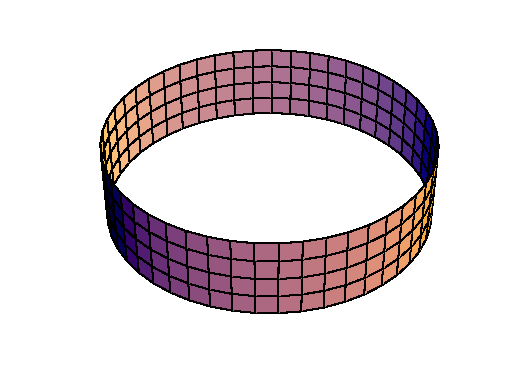
\epsfig{file=kuvat/sylvaippa.eps} $\hookrightarrow$ 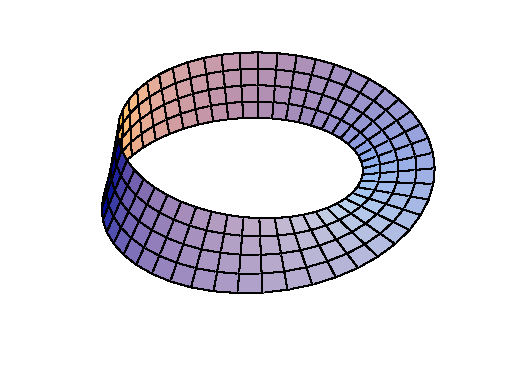
\epsfig{file=kuvat/moebius.eps}
\index{Mzz@M�biuksen nauha}%
Tuloksena oleva pinta on nk. \kor{M�biuksen nauha}\footnote[2]{\hist{August M�bius} (1790--1868)
oli saksalainen matemaatikko. \index{Mzz@M�bius, A.|av}}. M�biuksen nauhalle Stokesin kaava
\eqref{Stokesin avaruuskaava} \pain{ei} ole p�tev�. Sen sijaan kaava on kyll� voimassa, jos
liitossauma j�tet��n avoimeksi ja viivaintegraalit sauman kummallakin puolella huomioidaan
kaavassa \eqref{Stokesin avaruuskaava}. M�biuksen nauhan tapauksessa n�m� saumaintegraalit
lasketaan samansuuntaisina, jolloin ne eiv�t saumaa yhteen liitett�ess� kumoudu, toisin kuin
lieri�pinnan tapauksessa, vrt.\ kuvio.
\begin{figure}[H]
\begin{center}
\import{kuvat/}{kuvapot-17.pstex_t}
\end{center}
\end{figure}
M�biuksen nauha on siis erimerkki ei--suunnistuvasta pinnasta, jolle Stokesin kaava 
\eqref{Stokesin avaruuskaava} ei p�de. M�biuksen nauha on itse asiassa
\index{yksipuolinen pinta}%
\kor{yksipuolinen} pinta, jolla normaalin $\vec n$ suuntaa ei voida valita ristiriidattomasti
niin, ett� se muuttuisi jatkuvasti pintaa pitkin kuljettaessa.
(Jos pinta leikataan auki, niin liimauskohdassa normaali on ep�jatkuva.) \loppu
\end{Exa}

Stokesin lause voidaan yksinkertaisen pinnan tapauksessa todistaa pinnan parametrisaatiota
k�ytt�en, mutta todistus on t�ll�in melko tekninen ja vaatii suhteellisen voimakkaita
s��nn�llisyysoletuksia. L�pin�kyv�mpi ja yleisp�tev�mpi todistus saadaan, kun pintaa
approksimoidaan kolmion muotoisilla tasopinnoilla, samalla tavoin kuin pinta-alamitan
m��rittelyss� (vrt. Luku \ref{pintaintegraalit}). Koska Stokesin tasokaava p�tee jokaiselle
tasokolmiopinnalle, seuraa summaamalla, ett� Stokesin kaava \eqref{Stokesin avaruuskaava}
p�tee my�s kolmioista muodostetulle pinnan $A$ approksimaatiolle --- edellytt�en, ett�
summauksessa viivaintegraalit yli vierekk�isten kolmioiden yhteisten sivujen kumoutuvat.
Suunnistuvuusehto on juuri t�ss�. Sik�li kuin pinta on suunnistuva, saadaan kolmioverkkoa
tihent�m�ll� raja-arvotulos \eqref{Stokesin avaruuskaava} edellytt�en, ett� vektorikentt�
$\vec F$, pinta $A$ (pinnan parametrisaatio), ja reunaviiva $\partial A$ ovat riitt�v�n
s��nn�llisi�. Vektorikent�n osalta riitt��, ett� se on jatkuvasti derivoituva
(todellisuudessa riitt�� hieman v�hempikin), eiv�tk� pintaa $A$ koskevat olettamuksetkaan ole
k�yt�nn�n kannalta kovin rajoittavia, vrt.\ esimerkit edell�.

Stokesin lauseella, kuten Gaussin lauseellakin, on useampiulotteiset vastineensa. N�m� kuuluvat
matematiikan alaan nimelt� \kor{differentiaaligeometria}. T�llaisiin laajempiin yhteyksiin
sijoittuu luontevimmin my�s Stokesin lauseen tarkempi todistus, joka t�ss� sivuutetaan.
\begin{Exa}
Kappale liikkuu voimakent�ss�
\[
\vec F=\frac{F}{a}\,(y\,\vec i-2z\,\vec j+3x\,\vec k\,)
\]
pitkin ympyr�rataa, joka on pallopinnan $x^2+y^2+z^2=a^2$ ja tason $x+y+z=0$ leikkausviiva. 
M��rit� Stokesin lauseen avulla voimakent�n tekem� ty� yhden kierroksen aikana, kun
kiertosuunta on pisteest� $(10,10,10)$ katsottuna my�t�p�iv��n.
\end{Exa}
\ratk Kappaleen liikerata on $\partial A$, miss� $A$ on origokeskinen, $a$-s�teinen kiekko
tasolla $x+y+z=0$. Stokesin lauseen mukaan
\[
W=\oint_{\partial A} \vec F\cdot d\vec r=\int_A (\nabla\times\vec F)\cdot\vec n\,dS.
\]
T�ss� on
\[
\nabla\times\vec F
=\frac{F}{a} \left|\begin{array}{ccc} 
 \vec i & \vec j & \vec k \\ \partial_x & \partial_y & \partial_z \\ y & -2z & 3x
 \end{array}\right|
=\frac{F}{a}(2\vec i-3\vec j -\vec k).
\]
Oletettua kiertosuuntaa vastaa $\,\vec n=-\frac{1}{\sqrt{3}}(\vec i+\vec j+\vec k)$, joten
$(\nabla\times\vec F)\cdot\vec n = \frac{2F}{\sqrt{3}\,a}$. Siis
\[
W = \int_A \frac{2F}{\sqrt{3}\,a}\,dS = \frac{2F}{\sqrt{3}\,a}\mu(A)
  = \frac{2F}{\sqrt{3}\,a}\,\pi a^2 = \underline{\underline{(2\pi/\sqrt{3})\,Fa}}. \loppu
\]

\subsection*{Yleistetty Stokesin lause}
\index{Stokesin lause!a@yleistetty|vahv}

Kuten Gaussin lause, voidaan my�s Stokesin lause yleist�� niin, ett� pistetulon tilalla voi olla
yleisempi vektoritulo, eli joko ristitulo tai skalaarin ja vektorin kertolasku. Yleistetty
Stokesin kaava on
\[
\boxed{\quad \oint_{\partial A} d\vec r\ast\vec F=\int_A (d\vec a\times\nabla)\ast\vec F. \quad}
\]
T�ss� on j�lleen asetettava $\vec F\hookrightarrow f$, kun $\ast=$ `tyhj�'. Yleistetty kaava
p�tee samanlaisin edellytyksin kuin peruskaava \eqref{Stokesin avaruuskaava}, ja sen voi my�s 
perustella samaan tapaan kuin edell�, eli l�htem�ll� kaavan tasomuodosta.

\Harj
\begin{enumerate}

\item 
Olkoon $A=\{(x,y)\in \R^2 \mid x^2+y^2 \le 1\,\ja\,x \ge 0\}$. Laske seuraavat kiertointegraalit
yli $\partial A$:n (vastap�iv��n kiert�en) sek� suoraan viivaintegraaleina ett� muuntamalla ne
ensin tasointegraaleiksi (yleistetty�) Stokesin kaavaa k�ytt�en. \vspace{1mm}\newline
a) \ $\oint_{\partial A} \left[\,y^2\,dx+(x+y^2)\,dy\,\right] \qquad$
b) \ $\oint_{\partial A} (x+y^2)\,d\vec r$ \newline
c) \ $\oint_{\partial A} (xy^2\vec i+\abs{y}\vec j\,) \cdot d\vec r \qquad\qquad$
d) \ $\oint_{\partial_A} (y^3\vec i-x\vec j\,) \times d\vec r$

\item 
Laske $\oint_{\partial A} \vec F\cdot d\vec r$ \ a) suoraan viivaintegraalina, \  
b) Stokesin lauseen avulla, kun $\vec F=x\vec k$ ja $A \subset S$ vastaa 
parametrien arvoja $(u,v)\in [0,1]\times[0,3]$ pinnalla $\,S:\ x=8u^2,\ y=v^2,\ z=4uv$.

\item
N�yt� Stokesin lauseen avulla, ett� jos $S$ on pallon $K:\,x^2+y^2+z^2=R^2$ ja tason 
$T:\,x+y+z=0$ leikkausk�yr�, niin $\oint_S (y\,dx+z\,dy+x\,dz)=\pm\sqrt{3}\pi R^2$.

\item
Laske pintaintegraali $\int_A \nabla\times(\vec k\times\vec r\,) \cdot d\vec a$, kun $S$, 
$A \subset S$ ja $S$:n yksikk�normaalivektorin $\vec n=n_x\vec i+n_y\vec j+n_z\vec k$
suunta on annettu seuraavilla ehdoilla. \vspace{1mm}\newline
a) \ $S:\,z=0, \quad A:\,x^2+y^2 \le 1, \quad n_z \ge 0$ \newline
b) \ $S:\,x^2+y^2+z^2=1, \quad A:\,z \ge 0, \quad n_z \ge 0$ \newline
c) \ $S:\,x^2+y^2+z^2=1, \quad A:\,z \le 0, \quad n_z \le 0$

\item
Halutaan laskea kiertointegraali $\oint_S \vec F \cdot d\vec r$ yli suljetun k�yr�n
$S:\,\vec r=\cos t\,\vec i+\sin t\,\vec j+\sin 2t\,\vec k,\ t\in[0,2\pi]$, kun
$\vec F=(e^x-y^3)\vec i+(e^y+x^3)\vec j+e^z\vec k$. Laske integraali Stokesin kaavan avulla
huomioimalla, ett� $S$ on pinnalla $z=2xy$.

\item
Olkoon $S$ lieri�n $K:(x-1)^2+4y^2=16$ ja tason $T:2x+y+z=3$ \linebreak leikkausk�yr� ja
$\vec F=[\sin(x^2)+y^2+z^2]\vec i+(2xy+z)\vec j+(xz+2yz)\vec k$. Laske \linebreak
$\oint_S \vec F \cdot d\vec r$, kun $S$:n suunnistus on vastap�iv��n kaukaa positiiviselta
$z$-akselilta katsoen.

\item
Valitse pinnalle $A:\,z=9-x^2+y^2,\ x^2+y^2 \le 9$ suunnistus ja laske 
$\int_A \nabla\times\vec F \cdot d\vec a$, kun $\vec F=-y\vec i+x^2\vec j+z\vec k$.

\item
Laske Stokesin kaavan avulla pintaintegraali
\[
\int_{A} \nabla\times[(x-z^2)\vec i+(x^3+z)\vec j+xy\vec k] \cdot d\vec a,
\]
miss� $A$ on kartiopinnan $\,S:\,x^2+y^2=(z-1)^2$ tasojen $z=0$ ja $z=1$ v�liin j��v� osa.

\item 
S�hk�virran tiheys $\vec J$ ja magneettikent�n voimakkuus $\vec H$ ovat lieri�koordinaatistossa
muotoa $\vec J= J(r)\vec e_z$, $\vec H = H(r)\vec e_\varphi$. M��r�� $H(r)$ funktion $J(r)$ 
avulla k�ytt�m�ll� Maxwellin yht�l�� $\nabla\times\vec H = \vec J$ ja Stokesin kaavaa 
sopivasti valitulla pinnalla $A$.

\item
N�yt� yleistetty Stokesin kaava oikeaksi siin� tapauksessa, ett� $\vec F$ on avaruuden
vektorikentt� ja $A \subset T$, miss� $T$ on avaruustaso.

\item
Olkoon $S$ yksinkertainen suljettu k�yr� avaruustasolla $T$, jonka yksikk�normaalivektori on
$\vec n=a\vec i+b\vec j+c\vec k$. N�yt�, ett� $S$:n sis��n j��v�n pinnan $A$ ala on
\[
\mu(A)=\frac{1}{2}\left|\oint_S \bigl[(bz-cy)dx+(cx-az)dy+(ay-bx)dz\bigr]\right|.
\]

\item
M��ritell��n pinta $A$ parametrisaatiolla
\[
A:\quad \begin{cases}
        \,x=\cos 2u(a+bv\sin nu), \\ \,y=\sin 2u(a+bv\sin nu), \\ \,z=bv\cos nu,
        \end{cases} \quad
(u,v) \in \bigl[-\tfrac{\pi}{2},\tfrac{\pi}{2}\,\bigr)\times
          \bigl[-\tfrac{\pi}{2},\tfrac{\pi}{2}\,\bigr],
\]
miss� $0<b<a$ ja $n\in\N$. Millainen on $A$:n reuna $\partial A\,$? Mill� $n$:n arvoilla $A$ on
suunnistuva pinta?

\item (*)
Laske kiertointegraali $\oint_S \vec F \cdot d\vec r$, kun
$\,\vec F=ye^x\vec i+(x^2+e^x)\vec j+e^z\vec k\,$ ja $S$ on suljettu parametrinen k�yr�
\begin{align*}
\vec r \,=\ &(2\cos t-3\sin t)\vec i+(2+3\cos t+6\sin t)\vec j+(1+6\cos t-2\sin t)\vec k, \\
            &\,t\in[0,2\pi].
\end{align*}

\end{enumerate} %Stokesin lause
\section{Pyörteetön vektorikenttä} \label{pyörteetön vektorikenttä}
\alku
\index{pyzz@pyörteetön vektorikenttä|vahv}
\index{vektorikenttä!b@pyörteetön|vahv}

Jos $\vec F$ on fysikaalinen virtaus-, sähkö-, magneetti- ym. kenttä, sanotaan kenttää
$\vec \omega=\nabla\times\vec F$ kentän pyörrekentäksi (vrt.\ Luku 
\ref{divergenssi ja roottori}). Stokesin lause ilmaisee yhteyden kentän $\vec F$ ja pyörrekentän
$\vec\omega$ välillä:
\[
\oint_{\partial A} \vec F\cdot d\vec r=\int_A \vec\omega\cdot d\vec a.
\]
Tällä yhteydellä on paljon käyttöä esimerkiksi sähkömagneetikassa, jossa pyörrekentät ovat 
näkyvässä roolissa jo perusyhtälöissä (Maxwellin yhtälöissä, vrt.\ Luku 
\ref{divergenssi ja roottori}). Jos $\vec F$ on pyörteetön kenttä, eli jos $\vec\omega=\vec 0$,
antaa Stokesin lause tuloksen
\begin{equation} \label{Kpot-1}
\oint_{\partial A} \vec F\cdot d\vec r=0.
\end{equation}
Luvun \ref{polkuintegraalit} termein tämä voidaan lukea: Pyörteettömän vektorikentän tekemä työ
suljettua polkua pitkin = 0. Sanotaan, että kenttä $\vec F$ on tällöin
\index{konservatiivinen vektorikenttä} \index{vektorikenttä!c@konservatiivinen}%
\kor{konservatiivinen} (energian säilyttävä).

Jos $\vec F$ on gradienttikenttä, ts. $\vec F=-\nabla u$, niin $\vec F$ on pyörteetön. Tulos 
\eqref{Kpot-1} on tällöin voimassa --- ja tiedettiin ilman Stokesin lausettakin, sillä 
gradienttikentän tekemä työ = 0, jos polun alku- ja loppupisteet ovat samat, vrt.\ Luku 
\ref{polkuintegraalit}. --- Mutta entä jos kysytäänkin toisin päin: Millainen on riittävän 
säännöllinen, mutta muuten mahdollisimman yleinen vektorikenttä $\vec F$, joka on joko (a)
konservatiivinen tai (b) pyörteetön? Seuraavassa keskitytään vastaamaan näihin kysymyksiin. 
Tarkastellaan aluksi tason vektorikenttiä.

\index{yhtenzy@yhtenäinen (joukko)}%
Olkoon $A\subset\R^2$ \pain{avoin} joukko. Sanotaan, että tällainen joukko on \kor{yhtenäinen}
(engl.\ connected), jos mielivaltaiset kaksi $A$:n pistettä ovat yhdistettävissä jatkuvalla, 
suoristuvalla parametrisella käyrällä, jonka päätepisteet ovat mainitut pisteet ja joka on 
kokonaisuudessaan $A$:ssa. Jatkossa sanotaan avointa ja yhtenäistä joukkoa
\index{alue}%
\kor{alueeksi} (engl.\ domain)\footnote[2]{Alue määritellään hieman yleisemmin joukkona
$B = A \cup S$, missä $A$ on avoin ja yhtenäinen ja $S \subset \partial A$. Jos
$S = \emptyset$, niin $B=A$ on \kor{avoin alue}. Jos $S=\partial A$, niin $B=\overline{A}$ on
\kor{suljettu alue}. \index{avoin alue|av} \index{suljettu alue|av}}. 
\begin{Lause} \label{Lpot-1} \index{gradienttikenttä|emph}
Jos tason vektorikenttä $\vec F$ on jatkuva ja konservatiivinen alueessa $A \subset \R^2$, niin
$\vec F$ on gradienttikenttä, ts.\ $\vec F=-\nabla u$, missä $u$ on $A$:ssa jatkuvasti
derivoituva.
\end{Lause}
\tod Olkoon $\vec r_0\vastaa (x_0,y_0)\in A$ kiinteä ja $\vec r\vastaa (x,y)\in A$ muuttuva 
$A$:n piste. Olkoon edelleen $p$ yksinkertainen, suoristuva parametrinen käyrä (polku) 
$\vec r=\vec r\,(t)$, $t\in [a,b]$, jolle $\vec r\,(a)=\vec r_0$ ja
$\vec r_b=\vec r\vastaa (x,y)$. Määritellään
\[
u(p,x,y)=-\int_p \vec F\cdot d\vec r.
\]
Jos $u$ ei riipu polun $p$ valinnasta, ts. $u(p,x,y)=u(x,y)$, niin jatkamalla polkua pisteestä
$\vec r$ seuraa jatkuvuusoletuksesta, että
\[
u(\vec r+\Delta\vec r\,)=-\vec F(\vec r\,)\cdot\Delta\vec r+o(|\Delta\vec r\,|).
\]
Tämän mukaan $u$ on differentioituva ja $\nabla u=-\vec F$. Riittää siis osoittaa, että
$u(p,x,y)$ riippuu vain polun päätepisteistä. Olkoon $p_1$ ja $p_2$ kaksi polkua joilla on sama
alkupiste $(x_0,y_0)$ ja sama loppupiste $(x,y)$. Jos vastaavat geometriset käyrät ovat $S_1$
ja $S_2$, niin
\[
S_1\cup S_2=\bigcup_i S_i,\quad S_i\subset A,
\]
missä $S_i$:t ovat suljettuja käyriä (vrt.\ kuvio).
\vspace{3mm}
\begin{figure}[H]
\begin{center}
\import{kuvat/}{kuvapot-18.pstex_t}
\end{center}
\end{figure}
Tällöin 
\[
\int_{p_1} \vec F\cdot d\vec r-\int_{p_2} \vec F\cdot d\vec r
                         = \sum_i \oint_{S_i} \vec F\cdot d\vec r.
\]
Koska $\vec F$ on konservatiivinen, on $\oint_{S_i} \vec F\cdot d\vec r=0$, joten
\[
\int_{p_1} \vec F\cdot d\vec r=\int_{p_2} \vec F\cdot d\vec r.
\]
Siis $u(p,x,y)=u(x,y)$ on polun valinnasta riippumaton. \loppu

\index{yhdesti yhtenäinen alue}%
Sanotaan, että alue $A\subset\R^2$ on \kor{yhdesti yhtenäinen} (engl.\ simply connected), jos
pätee $B \subset A$ aina kun $B$ on alue, jolle $\partial B\subset A$. Kun kirjoitetaan
$S=\partial B$, niin ehdon hieman havainnollisempi muotoilu on: $A\subset\R^2$ on yhdesti
yhtenäinen, jos jokainen suljettu käyrä $S \subset A$ voidaan kutistaa pisteeksi niin, että
käyrä pysyy kutistuessaan koko ajan $A$:ssa. Yhdesti yhteinäinen joukko on 'järvi ilman saaria'.
\begin{figure}[H]
\begin{center}
\import{kuvat/}{kuvapot-19.pstex_t}
\end{center}
\end{figure}
Seuraava Stokesin lauseen seurannaistulos on vektorikenttien teorian keskeisimpiä. Tuloksella
on paljon käyttöä fysiikassa.
\begin{Lause} \label{Lpot-2} \index{gradienttikenttä|emph}
Jos tason vektorikenttä $\vec F$ on jatkuvasti derivoituva ja pyörteetön (rot\,$\vec F=0$)
yhdesti yhtenäisessä alueessa $A$, niin $\vec F$ on gradienttikenttä.
\end{Lause}
\tod Kentän potentiaali määritetään polkuintegraalina kuten edellä, jolloin riittää jälleen
osoittaa, että integraalin arvo riippuu vain polun päätepisteistä. Tämän todistamiseksi
valitaan jälleen kaksi polkua, joilla on samat päätepisteet, jolloin (vrt.\ todistus edellä)
\[
\int_{p_1} \vec F\cdot d\vec r-\int_{p_2} \vec F\cdot d\vec r
                               = \sum_i \oint_{S_i} \vec F\cdot d\vec r.
\]
Nytkin on oikea puoli = 0, sillä oletetun yhdesti yhtenäisyyden perusteella käyrien $S_i$ 
sisäänsä sulkemat alueet $A_i$ sisältyvät joukkoon $A$, jolloin Stokesin tasokaavan
(edellinen luvun kaava \eqref{Stokesin tasokaava}) ja $\vec F$:n pyörteettömyyden
perusteella
\[
\oint_{S_i} \vec F\cdot d\vec r=\int_{A_i} \text{rot}\,\vec F\,dxdy=0. \loppu
\]
\vspace{0.2mm}
\begin{multicols}{2} \raggedcolumns
Lauseiden \ref{Lpot-1}--\ref{Lpot-2} todistuksien perusteella gradienttikentän potentiaali
saadaan lasketuksi työintegraalina:
\[
u(\vec r\,)=-\int_{p:\,\vec r_0\,\kohti\,\vec r} \vec F\cdot d\vec r.
\]
\setlength{\unitlength}{1cm}
\begin{center}
\begin{picture}(4,1.5)(0,0.5)
\put(-0.1,-0.1){$\bullet$}
\put(3.9,0.9){$\bullet$}
\spline(0,0)(1,1)(2,1)(3,0)(4,1)
\put(1,0.86){\vector(3,2){0.1}}
\put(0.2,-0.1){$\vec r_0$} \put(3.9,1.2){$\vec r$}
\put(1.2,0.5){$p$}
\end{picture}
\end{center}
\end{multicols}
Laskukaavassa voidaan polku $p$ voidaan valita vapaasti, kunhan se pysyy alueessa $A$
(jossa $\vec F$ on määritelty). Jos $A$:n geometria ei aseta rajoituksia, voidaan polku valita
esimerkiksi seuraamaan koordinaattiakselien suuntaisia suoria, jolloin potentiaalin
laskukaavaksi tulee
\begin{align*}
\vec F(x,y) &= F_1(x,y)\vec i + F_2(x,y)\vec j\,: \\
     u(x,y) &= -\int_{x_0}^x F_1(t,y_0)\,dt-\int_{y_0}^y F_2(x,t)\,dt.
\end{align*}
\begin{Exa}
Onko vektorikenttä
\[
\vec F(x,y)=(x^3-y^3+\cos x)\vec i-(3xy^2+e^{-y})\vec j
\]
gradienttikenttä?
\end{Exa}
\ratk Koska
\[
\text{rot}\, \vec F=-\partial_x(3xy^2+e^{-y})-\partial_y(x^3-y^3+\cos x)=0,
\]
niin $\vec F$ on gradienttikenttä $\R^2$:ssa (Lause \ref{Lpot-2}). Valinnalla $(x_0,y_0)=(0,0)$ 
potentiaaliksi saadaan
\begin{align*}
u(x,y) &= -\int_0^x (t^3+\cos t)\,dt+\int_0^y (3xt^2+e^{-t})\,dt \\
&= -\frac{1}{4}x^4-\sin x+xy^3-e^{-y}+2.
\end{align*}
Yleinen potentiaalifunktio on
\[
u(x,y)=-\frac{1}{4}x^4+xy^3-\sin x-e^{-y}+C\quad (C=\text{vakio}). \loppu
\]
\begin{Exa}
Polaarikoordinaatistossa on määritelty vektorikenttä $\vec F=\frac{1}{r}\,\vec e_\varphi$.
Tutki, onko $\vec F$  gradienttikenttä alueessa $A$, kun \vspace{1mm}\newline
a) $A=\{\,(x,y)\in\R^2 \; | \; x>0 \; \ja \; y>0\,\}$, \newline
b) $A=\{\,(x,y)\in\R^2 \; | \; (x,y)\neq(0,0)\,\}$.
\end{Exa}
\ratk Polaarikoordinaatistossa on (vrt.\ Luku \ref{divergenssi ja roottori})
\[
\vec F=F_r\vec e_r+F_\varphi \vec e_\varphi\,: \quad 
      \text{rot}\,\vec F=\frac{1}{r}\,\partial_r(rF_\varphi)-\frac{1}{r}\,\partial_\varphi F_r.
\]
Tässä on $F_r=0$ ja $F_\varphi=1/r$, joten $\vec F$ on pyörteetön jokaisessa alueessa, joka ei
sisällä origoa.

a) Tässä $A$ on yhdesti yhtenäinen, joten $\vec F$ on gradienttikenttä. Valitsemalla $r_0>0$
voidaan potentiaali $u(x,y)=v(r,\varphi)$ laskea polkuintegraalina
\begin{align*}
v(r,\varphi)
&= -\int_{r_0}^r F_r(t,0)\,dt-\int_0^\varphi F_\varphi(r,t)\,r\,dt \,=\, -\varphi \\ 
&\impl\quad u(x,y) \,=\, -\underline{\underline{\Arcsin\left(\frac{y}{\sqrt{x^2+y^2}}\right)}}.
\end{align*}

b) Tässä $A$ ei ole yhdesti yhtenäinen, joten tutkitaan erikseen, onko $\vec F$ 
konservatiivinen. Valitaan polku $p:\vec r=\vec r(\varphi)$, $0\leq\varphi\leq 2\pi$ siten,
että $\vec r(\varphi)$ kiertää $r_0$-säteisen ympyräviivan:
\[
\vec r(\varphi)=r_0\,\vec e_r,\quad r_0>0,\ 0\leq\varphi\leq 2\pi.
\]
Tällöin polun alku- ja loppupisteet ovat samat, $\vec r(\varphi)\vastaa (x,y)\in A$ jokaisella
$\varphi$ ja
\[
\int_p \vec F\cdot d\vec r=\int_0^{2\pi} \frac{1}{r_0}\cdot r_0\,d\varphi=2\pi\neq 0,
\]
Siis $\vec F$ ei ole $A$:ssa konservatiivinen eikä näin muodoin myöskään gradienttikenttä
$A$:ssa. \loppu

\subsection*{Avaruuden pyörteetön vektorikenttä}

Vertaamalla Lauseen \ref{Lpot-1} todistusta Stokesin lauseen kolmiulotteiseen versioon 
nähdään, että todistus (ja siis myös Lauseen \ref{Lpot-1} väittämä) on sellaisenaan pätevä
myös avaruuden vektorikentälle. Sikäli kuin alueen geometria ei aseta rajoituksia, voidaan
kolmiulotteisen, konservatiivisen vektorikentän 
$\vec F = F_1(x,y,z)\vec i + F_2(x,y,z)\vec j + F_3(x,y,z)\vec k$ potentiaali laskea esimerkiksi
polkuintegraalina
\[
u(x,y,z) = -\int_{x_0}^x F_1(t,y_0,z_0)\,dt -\int_{y_0}^y F_2(x,t,z_0)\,dt
                                            -\int_{z_0}^z F_3(x,y,t)\,dt.
\]
Myös Lause \ref{Lpot-2} yleistyy kolmeen ulottuvuuteen, kunhan yhdesti yhtenäisyys
määritellään sopivasti. Tarkastellaan yksinkertaisia, suljettuja, suoristuvia käyriä
$S\subset A$, joille on löydettävissä Stokesin lauseen ehdot täyttävä pinta $B\subset\R^3$ 
siten, että $\partial B=S$. Jos jokaiselle tällaiselle käyrälle on pinta $B$ vielä määrättävissä
siten, että $B\subset A$, niin aluetta $A$ sanotaan yhdesti yhtenäiseksi. Esimerkiksi
\[
A=\{\,(x,y,z)\in\R^3 \; | \; a^2<x^2+y^2+z^2<R^2\,\} \quad (0 \le a < R)
\]
on yhdesti yhtenäinen (!). Sen sijaan
\[
A=\{\,(x,y,z)\in\R^3 \; | \; x^2+y^2+z^2<R^2 \; \ja \; x^2+y^2>a^2\,\} \quad (0 \le a < R)
\]
ei ole yhdesti yhtenäinen, sillä jos
\[
S=\{\,(x,y,z)\in\R^3 \; | \; x^2+y^2=b^2 \; \ja \; z=0\,\},
\]
niin $S\subset A$, kun $a<b<R$, mutta jos $B\subset\R^3$ on pinta, niin ehdot $S=\partial B$ ja
$B\subset A$ eivät voi yhtä aikaa toteutua.
\begin{Exa}
Pallokoordinaatistossa on määritelty vektorikenttä
\[
\vec F(r,\theta,\varphi)
            =\frac{1}{r^3}(2\cos\theta\,\vec e_r+\sin\theta\,\vec e_\theta),\quad r\neq 0.
\]
Määrää kentän potentiaali, jos sellainen on.
\end{Exa}
\ratk Tässä on $\vec F=F_r\vec e_r+F_\theta\vec e_\theta+F_\varphi\vec e_\varphi$, missä
\[
F_r=2r^{-3}\cos\theta,\quad F_\theta=r^{-3}\sin\theta,\quad F_\varphi=0,
\]
joten (ks.\ Luku \ref{div ja rot käyräviivaisissa})
\[
\nabla\times\vec F = 0\,\vec e_r + 0\,\vec e_\theta
  + \frac{1}{r}[\partial_r(rF_\theta)-\partial_\theta F_r]\vec e_\varphi = \vec 0\quad (r\neq 0).
\]
Koska origon poissulkeminen ei aiheuta yhtenäisyysongelmia kolmessa dimensiossa, niin $\vec F$
on gradienttikenttä. Potentiaali voidaan laskea ottamalla lähtöpisteeksi esimerkisi
$\vec r_0=(r_0,0,0)$, $r_0>0$, ja etenemällä koordinaattiviivojen suuntaisia polkuja:
\begin{align*}
u(r,\theta,\varphi) &= -\int_{r_0}^r F_r(t,0,0)\,dt-\int_0^\theta F_\theta(r,t,0)r\,dt
                                 -\int_0^\varphi F_\varphi(r,\theta,t)r\sin\theta\,dt \\
                    &= -\int_{r_0}^r 2t^{-3}\,dt-\int_0^\theta r^{-2}\sin t\,dt \\
                    &= \sijoitus{r_0}{r}t^{-2}+r^{-2}\sijoitus{0}{\theta} \cos t \\
                    &= r^{-2}\cos\theta+\text{vakio} \; (=-r_0^{-2}).
\end{align*}
Potentiaaliksi kelpaa siis $u(r,\theta,\varphi)=\underline{\underline{r^{-2}\cos\theta}}$. 
\loppu

\Harj
\begin{enumerate}

\item
Totea vektorikenttä $\vec F(x,y)=(y+2x)\vec i+x\vec j$ pyörteettömäksi. Laske tätä havaintoa
hyödyksi käyttäen polkuintegraali $\int_p \vec F \cdot d\vec r$, missä $p$ kulkee pisteestä
$(1,0)$ origon kautta pisteeseen $(1,2)$ pitkin ympyrän kaarta.

\item
Määritä funktio $f$ siten, että $f(0)=1$ ja tason vektorikenttä 
\[
\vec F(x,y)=f(y)[2xy\vec i+x^2(y+1)\vec j\,]
\] 
on pyörteetön. Mikä tällöin on kentän potentiaali?

\item
Osoita seuraavat vektorikentät koko avaruudessa pyörteettömiksi ja määritä kenttien 
potentiaalit.
\vspace{1mm}\newline
a) \ $z\vec i+z\cos y\vec j+(x+\sin y)\vec k \qquad$
b) \ $e^x\sin y\vec j+e^x\cos y\vec j+z\vec k$ \newline
c) \ $2xyz\vec i+x^2z\vec j+x^2y\vec k \qquad$
d) \ $-2xe^{-y}\vec i+(x^2e^{-y}+\sin z)\vec j+y\cos z\vec k$ \newline
e) \ $(x^2+y^2+z^2)(x\vec i+y\vec j+z\vec k)=r^2\vec r$

\item 
Vektorikentästä $\vec F$ tiedetään, että se on koko avaruudessa pyörteetön ja muotoa 
$\vec F(x,y,z)=xy^2\vec i+(\cos z+x^2y)\vec j+yf(z)\vec k$. Määrää kentän 
skalaaripotentiaali ja tämän avulla polkuintegraali $\int_p \vec F\cdot d\vec r$, missä
$p$:n alkupiste on $(0,0,0)$ ja loppupiste $(2,-1,3)$. 

\item (*) \index{zzb@\nim!Hzy@Häiriö kentässä}
(Häiriö kentässä) Tason vektorikenttään $\vec U_0=u_0\vec i$ ($u_0=$ vakio) tuodaan este
\[
A=\{(x,y)\in\R^2 \mid x^2+y^2 \le R^2\},
\] 
jolloin kenttä häiriintyy muotoon $\vec U=u(x,y)\vec i + v(x,y)\vec j$. Häiriintyneestä
kentästä $\vec U$ tiedetään, että se on sekä lähteetön että pyörteetön esteen ulkopuolella,
ts.\ $\text{div}\,\vec U = \text{rot}\,\vec U=0$ muualla kuin $A$:ssa. Lisäksi tiedetään, että
$\vec U \cdot \vec n = 0\,$ reunalla $\partial A$ (eli kun $x^2+y^2=R^2$, $\vec n=\,$
$\partial A$:n normaali) ja että $\vec U(x,y)\kohti\vec U_0$, kun $x^2+y^2\kohti\infty$.
Ongelmana on löytää nämä ehdot täyttävä kenttä $\vec U$. Koska $A$:n ulkopuolinen alue ei
ole yhdesti yhtenäinen, ei $\vec U$ välttämättä ole gradienttikenttä (vaikka onkin 
pyörteetön).

a) Näytä, että problemalla on ratkaisu, jonka napakoordinaattimuoto on
\[
\vec U=-\nabla f(r)\cos\varphi + g(r)\vec e_\varphi
\] 
eli määritä funktiot $f(r),g(r)$ mahdollisimman yleisessä muodossa niin, että annetut ehdot
toteutuvat. (Muita ratkaisuja ei ongelmalla ole). \newline
b) Totea, että em.\ ratkaisusta tulee yksikäsitteinen, kun asetetaan lisäehto muotoa
$v(R,0)=v_0$ (tässä karteesiset koordinaatit).

\end{enumerate} %Pyörteetön vektorikenttä

%\printindex

\end{document}
